\chapter{Basic Concepts}
\label{chap:concepts}

Image segmentation is one of the main challenges in image processing and has been an active field of study for years, which results in many segmentation methods being available. In the following pages, a selection of methods that can perform multi-class segmentation, i.e. segmentation with more than two classes, is presented. As the number of images to be segmented is usually high, and computation time can be a crucial factor, human interaction should remain at a minimum level. Therefore, only methods that, once the segmentation process has been started, work without human interaction were chosen. All methods described here are later used to segment a set of images and compared to the ground truth to measure the quality of the segmentations (see Chapter \textbf{\ref{chap:results}}).
	
	\section{Thresholding}
\label{sec:thresholding}

\textit{Thresholding} \cite[ff. 82]{machine_vision} is the most basic segmentation algorithm there is: Given an input image with dimensions $x \times y$ and intensity values $z$ (for instance, $[0, 255]$ at 8-bit color depth), defined as a function

\[(x, y) \mapsto z = I(x, y), \text{ for } x, y, z \in \mathbb{N}_0,\]

\noindent the thresholding function $T: \mathbb \mathbb{N}_0 \times \mathbb{N}_0 \rightarrow \{0, 1\}$ is defined as follows:

\[ T(I(x, y), \theta) =  \begin{cases}
				1 \text{ if } I(x, y) \, \geq \, \theta \\
			           0 \text{ otherwise}
			     \end{cases}\,.
\]

\noindent This yields a binary segmentation of the image into two classes, given that $\theta$ is chosen properly. The choice of $\theta$ is therefore crucial for the success of the segmentation. One way to find a suitable threshold parameter is automated image histogram analysis, such as in \textit{Otsu thresholding}.\\

\noindent The Otsu thresholding algorithm \cite{Otsu} iterates through all possible values for $\theta$ and calculates the ``between-class variance'' ${\sigma^{2}}_B$ for each $\theta$, defined as

\[ {\sigma^2}_{B} = w_0 \, w_1 (\mu_0 - \mu_1)^2,\]

\noindent where $w_0$ and $w_1$ are the \textit{weights}. These are defined as

\[ w_0 = \sum \limits_{i=1}^{\theta} p_i \text{ and } w_1 = \sum \limits_{i=\theta+1}^{k} p_i \]

\noindent for a histogram of the image consisting of $k$ grayscale intensity bins, which each contain the probability for a pixel being in this bin, $p_i$.\footnote{Here, it is assumed that Otsu's algorithm is applied to a grayscale image. For RGB images, each channel can be thresholded separately using the same algorithm, or the image can be converted to grayscale and then be segmented.} The values $\mu_0$ and $\mu_1$ are the statistical mean values, defined as

\[ \mu_0 = \sum \limits_{i=1}^{\theta} \frac{i \cdot p_i}{w_0} \text{ and } \mu_1 = \sum \limits_{i=\theta + 1}^{k} \frac{i \cdot p_i}{w_1} \,. \]

\noindent The threshold with the maximum between-class variance corresponds to a segmentation in which the pixels of each class have minimum \textbf{within}-class variance: This means that the pixels of each class are very much alike.

\begin {figure}[!ht]
	\begin {subfigure}[t]{0.3\linewidth}
		\scalebox{0.65}{\inputpgf{img}{fig_otsu_histogram.pgf}}
	\end {subfigure}
	\hspace{5.5cm}
	\begin {subfigure}[b]{0.3\linewidth}
		\scalebox{0.65}{\inputpgf{img}{fig_otsu.pgf}}
	\end {subfigure}
		\caption[]{\textbf{Left:} Histogram of an 8-bit grayscale input image. Optimal thresholds found by Otsu's algorithm are marked in orange. \textbf{Right:} Original image (top) and four-way segmentation result (bottom).}
		\label{fig:otsu}
	\end {figure}

\noindent To generalize the normal Otsu algorithm to $n$-class segmentation, the weight and mean formulas are changed to correspond to $n$ classes defined by a set of thresholds $\theta = \{t_1, \dots, t_{n-1}\}$. The between-class variance formula is changed to respect the variances of all classes, so that the best $\theta$ is the one that minimizes the overall within-class variance by maximizing the overall between-class variance

\[ \sigma_B^2 = \sum \limits_{i=1}^{n} w_i (\mu_i - \mu_t)^2 \,. \]

\noindent Here, $w_i$ is the weight of the $i$th class, $\mu_i$ is the mean of that class and $\mu_t$ is the total mean of all classes, i.e. $\sum_{i=1}^{n} w_i \mu_i$. The thresholds can then be applied using

\[ T(I(x, y), \theta) =  \begin{cases}
				n \text{ if } t_{n-1} \, \leq \, I(x, y) \\
				n-1 \text { if } t_{n-2} \, \leq \, I(x, y) \, <  \, t_{n-1}\\
				\dots\\
			           0 \text{ if } I(x, y) \, < \, t_1
			     \end{cases}\,.
\]

\noindent However, this approach doesn't work as well for images whose histograms do not exhibit distinct histogram peaks - for example, due to noise - and also doesn't perform well for cases in which $n$ is large, neither considering the time needed to perform a segmentation\footnote{While variants of Otsu exist that are optimized for speed \cite{otsu_fast}, only the original Otsu algorithm is evaluated here because it is the most common.} nor considering the segmentation quality, due to the method exploiting only the data the histogram provides.

%\noindent The Otsu algorithm belongs to a family of thresholding mechanisms that is called ``global thresholding'' because the same threshold is applied to the entire image. However, there are also local or ``adaptive'' thresholding algorithms which segment different parts of the image with different thresholds. The need for such algorithms often arises when the illumination of the input image is highly irregular, for example when cast shadows overlay part of the image (see \ref{fig:illumination}). One approach is to calculate a threshold for each pixel of the image while examining a neighborhood of size $L \times L$ around the pixel in question, using the mean, the mean of the maximum and minimum values or the median of the resulting local pixel intensity distribution to determine a local threshold.

%\textbf{TODO: are there adaptive thresholds for multi-label purposes?}\\
%Local thresholding, however, is much slower than global thresholding because it has to process the neighborhoods of each pixel, while it also depends on choosing $L$ so that the neighborhoods contain enough pixels of either class, or otherwise the thresholds won't be chosen well. \cite[pp.~84--93]{machine_vision}


\begin{comment}
	\section{Canny Edge Detection}
\label{sec:canny}
The \textit{Canny Edge Detector} \cite{canny} is one of the most famous edge-detection algorithms and actually is a composite algorithm that returns a binary segmentation of an image into edges and non-edges.\\

\noindent First, a Gaussian convolution filter is applied to try and subdue noise in the image. A \textit{convolution} is a matrix operation often used in image processing: A matrix $A$, describing the pixel values of an image, is convolved pixel-wise with a convolution matrix $B$ with dimensions $n \times n$ - that is, for each pixel $p$ of $A$, the pixel's $n \times n$-neighborhood pixel values are summed up while being weighted according to corresponding value in $B$. The resulting sum is then assigned to the output matrix in place of the previous value of the center pixel, which intuitively assumes the distance-weighted average value of its neighborhood. In the case of pixels that lie on the edge of the matrix to be convoluted, out-of-bounds considerations have to be made: A constant value such as zero can be assumed for the pixels in the neighborhood that would lie ``outside'' of the image, the existing image values can be mirrored or clamped to provide a torus-like out-of-bounds handling, or the convolution can be done only on those pixels whose neighborhood fully lies inside of the image, resulting in smaller output images.

The aforementioned ``Gaussian filter'' or ``kernel'' is a matrix whose values are defined so that performing a convolution using that matrix approximates the behavior of the two-dimensional Gaussian function with uniform variances for its $x$- and $y$-dimensions:

\[ f(x, y) = \exp \left(- \left( \frac{\left(x - p_x \right)^2}{2\sigma^2} + \frac{ \left(y - p_y \right)^2}{2\sigma^2} \right) \right), \]

\noindent where $p$ is the center pixel of the current neighborhood. Subsequently, $p_x$ and $p_y$ are the coordinates of this pixel within the matrix and $\sigma$, the standard variance, acts as the smoothing constant. The higher this constant is, the stronger the blur effect becomes.

In Gaussian filters, the $\sigma$ constant is expressed through the dimensions of the matrix - the larger the filter matrix, the stronger the blur effect. An example for a $3 \times 3$ Gaussian filter is the following matrix:

\[ \frac{1}{16} \left [ \begin{tabular}{ccc}
				1& 2& 1\\
				2& 4& 2\\
				1& 2& 1 
			   \end{tabular} \right ]\]

\noindent The coefficient $\frac{1}{16}$ is equal to the sum of the matrix values and ensures that the convolution does not change the average image value. \cite[p. 41]{machine_vision}\\

\noindent As the second step, an gradient-based edge detector filter is applied to the smoothed image. The most famous of these is the \textit{Sobel filter} \cite{sobel}, which approximates the local partial derivatives $\frac{\partial I}{\partial x}$ and $\frac{\partial I}{\partial y}$ of each pixel of the image function $I(x, y)$, using the $3 \times 3$ neighborhood of that pixel. It is given by the following matrices \cite[pp. 113 -- 114]{machine_vision}:

\[ \text{Sobel}_x = \left [ \begin{tabular}{ccc}
				-1& 0& 1\\
				-2& 0& 2\\
				-1& 0& 1 
			   \end{tabular} \right ] \text{ and } 
\text{Sobel}_y = \left [ \begin{tabular}{ccc}
				1& 2& 1\\
				0& 0& 0\\
				-1& -2& 1 
			   \end{tabular} \right ] 
\]

\noindent The result of these convolutions are two images, $G_x$ and $G_y$, which represent the partial local derivatives of each pixel. The gradient image of the original input image $I$ is then defined as

\[G = |\nabla I| = \sqrt{{G_x}^2 + {G_y}^2}.\]

\noindent Additionally, the gradient direction of each pixel can be calculated from the derivative images by measuring the angle between the x-axis and the gradient pixel coordinates by employing the atan2 function:

\[G_\phi = \text{atan2}(G_y, G_x) \]

\noindent Using $G_\phi$, edge thinning via non-maximum suppression is applied to the gradient image as the third step in the algorithm: For each pixel, the gradient direction acts as a criterion to decide which two neighboring pixels, that are each on opposite sides (positive and negative direction of the gradient), should be compared to the current pixel. If the value of the current pixel is not larger than the two neighbors' values, the pixel's value is not a local maximum and is set to zero. The gradient direction angles can either be rounded so that each angle represents one of the north-south, west-east directions and so forth, or linear interpolation can be used.

In the final step, a hysteresis threshold is applied. This process consists of defining two thresholds, $\theta_{high}$ and $\theta_{low}$. The definition for the thresholding function as given in \ref{sec:thresholding} is slightly altered:

\[ T(I(x, y), \theta_{high}, \theta_{low}) =  \begin{cases}
							2 \text{ if } I(x, y) \, \geq \, \theta_{high} \\
							1 \text{ if } I(x, y) \, \geq \, \theta_{low} \text{ and } < \theta_{high} \\
			          				0 \text{ otherwise}
			   			        \end{cases}
\]

\noindent Pixels that have a value of $2$ are called strong pixels because they had values larger than the high threshold, whereas pixels with a value of $1$ are called weak pixels. Finally, the algorithm checks for each pixel if an 8-connected path between that pixel and a strong pixel exists - if not, then the pixel is dropped. This can be done with the help of connected component-finding algorithms by dropping each ``$1$''-component which is not connected to at least one ``2''-value.\\

\noindent The thresholds $\theta_{high}$ and $\theta_{low}$ have to be set by the user, although there exists the possibility to set these by using the Otsu threshold described in \ref{sec:thresholding} . Using this combination approach, $\theta_{high}$ is set to the Otsu threshold value for $I(x, y)$, and $\theta_{low}$ is set to $0.5 * \theta_{high}$. \cite{otsu_combine}

\end {comment}

	\section{K-Means}
K-Means \cite{kmeans} is a general-purpose data clustering algorithm whose aim is to create $k$ data clusters from all $n$-dimensional data points $d = (f_1, f_2, \dots, f_n)$ so that the squared distance from each data point in the cluster to the cluster mean is minimized overall. Mathematically, this translates to

\[ \argmin \limits_{C} \sum \limits_{i=1}^{k} \sum \limits_{d \in C_i} || d - \mu_i||^2  \,,\]

\noindent where $C_i$ for $i=1, \dots, k$ are the $k$ clusters and $\mu_i$ for $i=1, \dots, k$ are the means of the respective clusters. Viewed graphically, this is equal to computing a Voronoi diagram for the data, using the $k$ cluster centroids as the Voronoi cell centers.

The algorithm is initialized with $k$ either random or differently selected cluster centers. Then, the algorithm executes the two steps described in Algorithm \textbf{\ref{alg:kmeans_pseudo}} alternatingly until either a set number of iterations is reached or the overall difference between the current and the last centroid positions falls below a threshold $\epsilon$  (see Figure \textbf{\ref{fig:kmeans}}).

\begin {algorithm}[!ht]
	\caption{K-Means ($\epsilon$, iter\_max)}\label{alg:kmeans_pseudo}
	\begin {algorithmic}[1]
		\State iter = 0
		\State Assign each data point to exactly one of the $k$ clusters by selecting the cluster that has the closest mean distance as defined above.
		\State Calculate new cluster centers by recalculating the cluster means, using all elements assigned to each cluster and calculate the difference $\Delta$ compared to previous iteration.
		\If {$\Delta < \epsilon$ \textbf{or} iter == iter\_max}
			\State \textbf{end}
		\Else
			\State iter += 1
			\State \textbf{goto} step 2
		\EndIf
	\end{algorithmic}
\end{algorithm}

\begin {figure}[!ht]
	\begin {center}
		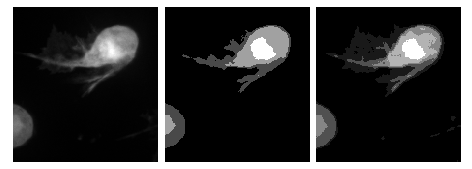
\includegraphics[scale=0.8]{img/fig_kmeans}
	\end{center}
	\caption[Application of the K-Means algorithm to a test image.]{Application of the K-Means algorithm to a test image. \textbf{From left to right}: Input image,  K-Means results with $k=4$, results with $k=6$.}
	\label{fig:kmeans}
\end {figure}

\noindent Obviously, this algorithm can also be used to segment images into $k$ different classes, but since K-Means assigns classes to data by using the distance from the mean, the algorithm output favors segmentations in which the classes have roughly the same size, which isn't necessarily the correct way to classify pixels in arbitrary image data. \textbf{TODO: Citation}



	\section{Gaussian Mixture Models}
\textit{Gaussian Mixture Models} (GMMs) are a subclass of mixture models, that is, probabilistic models which are combined with other models of the same distribution type to form a more complex model that is able to model the distribution of a data set more accurately than a simple model could. In the case of GMMs, the base distributions are often $n$-multivariate Gaussian distributions:

\[ pdf(x) = \mathcal{N}_n (x\,|\,\mu,\, \Sigma) \,. \]

\noindent Here, $pdf(x)$ denotes the \textit{probability density function} of an $n$-dimensional piece of data $x$, while $\mu$ and $\Sigma$ are the $n$-dimensional mean vector and the $n \times n$ covariance matrix of the distribution. Since the shape such a distribution can take is limited, a single Gaussian cannot accurately model a multimodal distribution. Instead, a weighted combination of multiple Gaussians can be used:

\[ pdf_m (x) = \sum \limits_{k=1}^{K} \pi_k \, \mathcal{N}_n (x\,|\, \mu_k, \Sigma_k) \,. \]

\noindent This mixture model consists of $K$ models that each have different parameters $\mu$ and $\Sigma$ and have real weights $\pi_k \in \, (0, 1)$, with $\sum_{i=1}^{k} \pi_i = 1$. \cite[pp. 430]{bishop_pattern}

%\begin {figure}[!ht]
%	\begin{center}
%		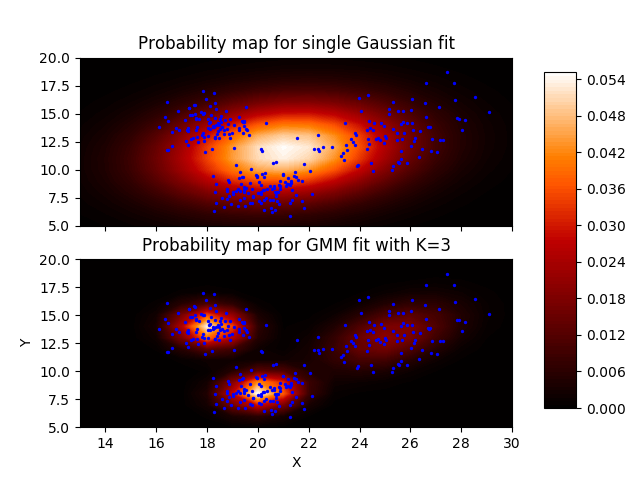
\includegraphics[scale=0.75]{img/fig_normal_vs_gmm}
%	\end{center}
%	\caption[Single Gaussian fit vs. a mixture of Gaussians.]{Comparison of a single Gaussian fit (upper) with a GMM fit, using $K=3$, on a two-dimensional dataset randomly sampled from three Gaussian distributions. The single Gaussian fails to capture the structure of the data, while the GMM succeeds.}
%	\label{fig:normal_vs_gmm}
%\end {figure}

\begin {figure}[!ht]
	\centering
	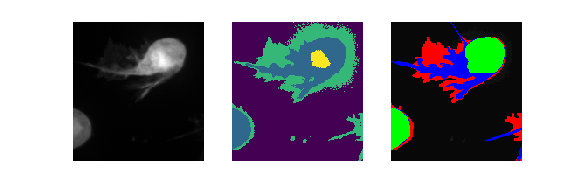
\includegraphics[scale=0.55]{img/fig_gmm_vs_gt}
	\caption[Labels assigned by a GMM.]{\textbf{Left:} Input image. \textbf{Right:} Image labels in arbitrary colors, assigned by a GMM with $K=4$, fitted to the input image.}
	\label{fig:gmm_vs_gt}
\end {figure}

\noindent The parameters of such a mixture model can be calculated by applying the Expectation-Maximization algorithm \cite{em_algorithm}, which can additionally be combined with a K-Means initialization, creating better conditions for finding fitting parameters. GMMs can also be used for segmenting images: Images are intepreted as numerical data in which each pixel position corresponds to an intensity value. If the number of components to be found in the image is known beforehand - as it is in the case of image segmentation - the image can be segmented according to the fitted GMM (see Figure \textbf{\ref{fig:gmm_vs_gt}}). To do this, for each pixel in the image, the posterior probabilities of that pixel in respect to each of the Gaussians is calculated and the Gaussian with the highest probability is chosen as the source distribution of the pixel:

\[ \text{label}_x = \argmax \limits_{k} \, p(\mu_k, \Sigma_k\, | \, x) \]

\noindent This yields a class with which the pixel is labelled.


	\section{Multi-layer Perceptrons}
\textit{Multi-layer Perceptrons} (MLPs), also called \textit{Feedforward Artificial Neuronal Networks} (ANNs) are mathematical functions that try to emulate the way neurons in the brain process information, typically to classify data or perform regression on it. ANNs have recently achieved impressing results on various tasks, such as image classification, sound analysis and regression, typically achieved by very deep networks that used lots of artificial neurons and were fed large datasets exceeding one million samples. ``Deep Learning'' is a blanket term regularly used to describe these processes.

In this section, the concepts behind the optimization of functions via the Gradient Descent algorithm, Neuronal Networks and training of those networks using the Backpropagation algorithm are explained. 


	\subsection {Gradient Descent}
\label{subsec:grad_desc}

\textit{Gradient Descent} is a standard, numeric optimization technique that iteratively optimizes at least once-differentiable, continuous functions. That is, it calculates a vector of parameters $\Theta_{min}$ for a function $f$ of $n$ variables so that

\[ \Theta_{min} = \argmin \limits_{\Theta} f(\Theta) \]

\noindent To find such a $\Theta_{min}$, the approach takes advantage of the fact that the gradient vector of $f$,

\[ \nabla_f = \left [ \frac{\partial f}{\partial \Theta_1}, \dots, \frac{\partial f}{\partial \Theta_n} \right ]^T \, ,\]

the vector of all first partial derivatives of $f$, points into the opposite direction of the fastest change, or put graphically, shows the opposite direction of the ``steepest slope''. By taking steps in the \textit{negative} gradient direction, the function value is minimized step by step, while maximization works the same, only that the function is negated and then minimized, which results in parameters that maximize the original function. The parameter $\eta$ depicts the step size and is typically a value in the range $(0.0, 1.0]$. \cite[pp. 40--42]{optimization_book}\\

Gradient Descent starts with a guess for the parameters in $\Theta$, iteratively evaluates the gradient and updates the parameters accordingly until convergence within arbitrary precision is reached (see Algorithm \textbf{\ref{alg:grad_desc}}).

\begin {algorithm}
	\begin {algorithmic}[1]
		\State $\Theta_0$ = random
		\While {$|f(\Theta_i) - f(\Theta_{i - 1})| > \epsilon$}
			\State $\Theta_i = \Theta_{i-1} - \eta \nabla_f$ 
		\EndWhile
	\end{algorithmic}
	\caption{Gradient Descent scheme for optimizing differentiable functions.}
	\label{alg:grad_desc}
\end{algorithm}

\noindent For convex functions, Gradient Descent always finds the global minimum. For non-convex functions however, the algorithm may get stuck in a local minimum or at saddle points, also called ``false minima'' (see Figure \textbf{\ref{fig:grad_desc}}). Therefore, running the algorithm multiple times with random starting parameters or even taking informed guesses, given knowledge about the form of the function to be optimized, is advised. The step size $\eta$ has to be chosen depending on the shape of the function to minimize. If $\eta$ is too large, the algorithm will overshoot the minimum repeatedly and will never converge. If $\eta$ is too small, convergence will take a long time.\\

\begin {figure}[!ht]
	\begin{center}
		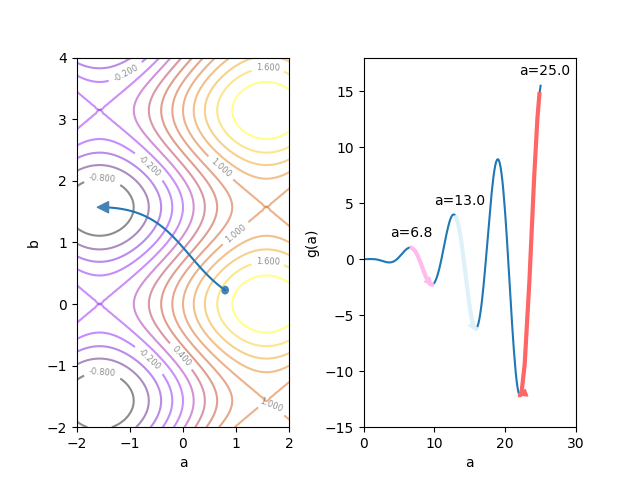
\includegraphics[scale=0.9]{img/fig_grad_desc}
	\end{center}
	\caption[Gradient Descent minimization.]{\textbf{Left:} A contour plot of Gradient Descent minimization of $f(a, b) = \sin(a) + \cos^2(b)$. The blue line shows the search path of the algorithm along the negative gradient while estimating the optimal $\Theta$. \textbf{Right}: Effect of the initial guess for $\Theta$ on the optimization. The function $f(a) = \frac{1}{40}a^2 * \frac{1}{2} \cos(a)$ has multiple local minima in the interval [0, 25]. Only the third guess $a=25$ leads to finding the global minimum, while the other two optimization runs get trapped in local minima.}
	\label{fig:grad_desc}
\end {figure}

\noindent However, a more interesting application of the Gradient Descent algorithm than optimizing functions for which all parameters can be freely changed exists in the context of machine learning, where the function to optimize often has fixed parameters in addition to $\Theta$, such as data from a dataset that is related to the function in some way. In such cases, one can consider one of the subtypes of Gradient Descent. Either one can evaluate the average gradient using all available data samples at once, called \textit{Batch Gradient Descent}, or one can use single data points only - as an approximation of the entire dataset - to perform the updates. This is called \textit{Stochastic Gradient Descent} (SGD) and is preferable if working with datasets that are too large to fit into memory. Alternatively, one can use the average gradient of a subset of data points - this method is often referred to as \textit{Mini-Batch} Stochastic Gradient Descent. For example, consider the function

\[ f(\Theta) =  \theta_1 (x_1 + x_2) + \theta_2 (2x_1 + 3x_2)\]

\noindent with fixed $x_1$, $x_2$ from some dataset $X$. To minimize this function $f$ with respect to the variable parameters $\Theta$ using the dataset and SGD, the algorithm is modified to only take into consideration a single datapoint $x_i = [x_{i1}, x_{i2}]$ at a time chosen at random from $X$. Then, updating $\Theta$ is done by the formula

\[ \Theta_i = \Theta_{i-1} - \eta \nabla_{f_i} \,, \]

\noindent where $f_i$ is the function $f$ evaluated for $x_i$ and $\Theta_{i-1}$. The number of iteration that it takes to consider all datapoints in the dataset is called an \textit{epoch}. Similarily, to use Mini-Batch SGD with a batch size of $n$, an average over the gradients for $n$ datapoints is used:

\[ \Theta_i = \Theta_{i-1} - \eta \left ( \frac{1}{n} \sum \limits_{i=1}^{n} \nabla_{f_i} \right ) \,. \]

\noindent The price that is paid for the relaxed memory cost of SGD is that the traversion towards the minimum becomes noisy for small $n$, as the algorithm approximates the gradient by using only a part of the dataset. For functions with minima in shallow ``valleys'', SGD starts moving in a wild zig-zag pattern near the optimum, further increasing the number of steps the algorithm takes until covergence. To address these problems, a number of optimizations have been proposed.


	\subsubsection {Momentum}
\textit{Momentum} is an optimization for the Gradient Descent algorithm that adds an additional term to the update step, which is dependent on the steepness of the traversed function in previous updates. Using the analogy of a marble rolling down a slope, momentum refers to the inertia of the marble that allows it to jump over saddle points or small holes (local minima) on the bowl's surface rather than stopping abruptly once such a location is reached (see Figure \textbf{\ref{fig:momentum}}). This changes the SGD update formula to

\begin {align}
	& v_i = \gamma v_ {i-1} + \eta \nabla_f\\ 
	& \Theta_i = \Theta_{i-1} - v_i \,,
\end {align} 

\noindent where $v$ is the momentum vector with one entry per gradient element and $\gamma$ is a modifier that changes the influence of the momentum on the update. \textbf{TODO: cite nesterov momentum, heavy ball etc.}

	\begin {figure}[!ht]
		\begin{center}
			\scalebox{0.75}{%% Creator: Matplotlib, PGF backend
%%
%% To include the figure in your LaTeX document, write
%%   \input{<filename>.pgf}
%%
%% Make sure the required packages are loaded in your preamble
%%   \usepackage{pgf}
%%
%% Figures using additional raster images can only be included by \input if
%% they are in the same directory as the main LaTeX file. For loading figures
%% from other directories you can use the `import` package
%%   \usepackage{import}
%% and then include the figures with
%%   \import{<path to file>}{<filename>.pgf}
%%
%% Matplotlib used the following preamble
%%   \usepackage{fontspec}
%%   \setmainfont{DejaVu Serif}
%%   \setsansfont{DejaVu Sans}
%%   \setmonofont{DejaVu Sans Mono}
%%
\begingroup%
\makeatletter%
\begin{pgfpicture}%
\pgfpathrectangle{\pgfpointorigin}{\pgfqpoint{6.400000in}{4.800000in}}%
\pgfusepath{use as bounding box, clip}%
\begin{pgfscope}%
\pgfsetbuttcap%
\pgfsetmiterjoin%
\definecolor{currentfill}{rgb}{1.000000,1.000000,1.000000}%
\pgfsetfillcolor{currentfill}%
\pgfsetlinewidth{0.000000pt}%
\definecolor{currentstroke}{rgb}{1.000000,1.000000,1.000000}%
\pgfsetstrokecolor{currentstroke}%
\pgfsetdash{}{0pt}%
\pgfpathmoveto{\pgfqpoint{0.000000in}{0.000000in}}%
\pgfpathlineto{\pgfqpoint{6.400000in}{0.000000in}}%
\pgfpathlineto{\pgfqpoint{6.400000in}{4.800000in}}%
\pgfpathlineto{\pgfqpoint{0.000000in}{4.800000in}}%
\pgfpathclose%
\pgfusepath{fill}%
\end{pgfscope}%
\begin{pgfscope}%
\pgfsetbuttcap%
\pgfsetmiterjoin%
\definecolor{currentfill}{rgb}{1.000000,1.000000,1.000000}%
\pgfsetfillcolor{currentfill}%
\pgfsetlinewidth{0.000000pt}%
\definecolor{currentstroke}{rgb}{0.000000,0.000000,0.000000}%
\pgfsetstrokecolor{currentstroke}%
\pgfsetstrokeopacity{0.000000}%
\pgfsetdash{}{0pt}%
\pgfpathmoveto{\pgfqpoint{0.800000in}{0.528000in}}%
\pgfpathlineto{\pgfqpoint{2.763636in}{0.528000in}}%
\pgfpathlineto{\pgfqpoint{2.763636in}{4.224000in}}%
\pgfpathlineto{\pgfqpoint{0.800000in}{4.224000in}}%
\pgfpathclose%
\pgfusepath{fill}%
\end{pgfscope}%
\begin{pgfscope}%
\pgfpathrectangle{\pgfqpoint{0.800000in}{0.528000in}}{\pgfqpoint{1.963636in}{3.696000in}} %
\pgfusepath{clip}%
\pgfsetbuttcap%
\pgfsetroundjoin%
\definecolor{currentfill}{rgb}{0.050383,0.029803,0.527975}%
\pgfsetfillcolor{currentfill}%
\pgfsetlinewidth{0.000000pt}%
\definecolor{currentstroke}{rgb}{0.000000,0.000000,0.000000}%
\pgfsetstrokecolor{currentstroke}%
\pgfsetdash{}{0pt}%
\pgfpathmoveto{\pgfqpoint{1.315702in}{2.586655in}}%
\pgfpathlineto{\pgfqpoint{1.315708in}{2.586667in}}%
\pgfpathlineto{\pgfqpoint{1.315702in}{2.586679in}}%
\pgfpathlineto{\pgfqpoint{1.315697in}{2.586667in}}%
\pgfpathclose%
\pgfusepath{fill}%
\end{pgfscope}%
\begin{pgfscope}%
\pgfpathrectangle{\pgfqpoint{0.800000in}{0.528000in}}{\pgfqpoint{1.963636in}{3.696000in}} %
\pgfusepath{clip}%
\pgfsetbuttcap%
\pgfsetroundjoin%
\definecolor{currentfill}{rgb}{0.050383,0.029803,0.527975}%
\pgfsetfillcolor{currentfill}%
\pgfsetlinewidth{0.000000pt}%
\definecolor{currentstroke}{rgb}{0.000000,0.000000,0.000000}%
\pgfsetstrokecolor{currentstroke}%
\pgfsetdash{}{0pt}%
\pgfpathmoveto{\pgfqpoint{1.266116in}{2.693321in}}%
\pgfpathlineto{\pgfqpoint{1.266121in}{2.693333in}}%
\pgfpathlineto{\pgfqpoint{1.266116in}{2.693345in}}%
\pgfpathlineto{\pgfqpoint{1.266110in}{2.693333in}}%
\pgfpathclose%
\pgfusepath{fill}%
\end{pgfscope}%
\begin{pgfscope}%
\pgfpathrectangle{\pgfqpoint{0.800000in}{0.528000in}}{\pgfqpoint{1.963636in}{3.696000in}} %
\pgfusepath{clip}%
\pgfsetbuttcap%
\pgfsetroundjoin%
\definecolor{currentfill}{rgb}{0.050383,0.029803,0.527975}%
\pgfsetfillcolor{currentfill}%
\pgfsetlinewidth{0.000000pt}%
\definecolor{currentstroke}{rgb}{0.000000,0.000000,0.000000}%
\pgfsetstrokecolor{currentstroke}%
\pgfsetdash{}{0pt}%
\pgfpathmoveto{\pgfqpoint{1.365289in}{2.479880in}}%
\pgfpathlineto{\pgfqpoint{1.365354in}{2.480000in}}%
\pgfpathlineto{\pgfqpoint{1.365289in}{2.480134in}}%
\pgfpathlineto{\pgfqpoint{1.365231in}{2.480000in}}%
\pgfpathclose%
\pgfusepath{fill}%
\end{pgfscope}%
\begin{pgfscope}%
\pgfpathrectangle{\pgfqpoint{0.800000in}{0.528000in}}{\pgfqpoint{1.963636in}{3.696000in}} %
\pgfusepath{clip}%
\pgfsetbuttcap%
\pgfsetroundjoin%
\definecolor{currentfill}{rgb}{0.050383,0.029803,0.527975}%
\pgfsetfillcolor{currentfill}%
\pgfsetlinewidth{0.000000pt}%
\definecolor{currentstroke}{rgb}{0.000000,0.000000,0.000000}%
\pgfsetstrokecolor{currentstroke}%
\pgfsetdash{}{0pt}%
\pgfpathmoveto{\pgfqpoint{1.315702in}{2.586470in}}%
\pgfpathlineto{\pgfqpoint{1.315801in}{2.586667in}}%
\pgfpathlineto{\pgfqpoint{1.315702in}{2.586870in}}%
\pgfpathlineto{\pgfqpoint{1.315608in}{2.586667in}}%
\pgfpathclose%
\pgfpathmoveto{\pgfqpoint{1.315697in}{2.586667in}}%
\pgfpathlineto{\pgfqpoint{1.315702in}{2.586679in}}%
\pgfpathlineto{\pgfqpoint{1.315708in}{2.586667in}}%
\pgfpathlineto{\pgfqpoint{1.315702in}{2.586655in}}%
\pgfpathclose%
\pgfusepath{fill}%
\end{pgfscope}%
\begin{pgfscope}%
\pgfpathrectangle{\pgfqpoint{0.800000in}{0.528000in}}{\pgfqpoint{1.963636in}{3.696000in}} %
\pgfusepath{clip}%
\pgfsetbuttcap%
\pgfsetroundjoin%
\definecolor{currentfill}{rgb}{0.050383,0.029803,0.527975}%
\pgfsetfillcolor{currentfill}%
\pgfsetlinewidth{0.000000pt}%
\definecolor{currentstroke}{rgb}{0.000000,0.000000,0.000000}%
\pgfsetstrokecolor{currentstroke}%
\pgfsetdash{}{0pt}%
\pgfpathmoveto{\pgfqpoint{1.266116in}{2.693130in}}%
\pgfpathlineto{\pgfqpoint{1.266210in}{2.693333in}}%
\pgfpathlineto{\pgfqpoint{1.266116in}{2.693530in}}%
\pgfpathlineto{\pgfqpoint{1.266017in}{2.693333in}}%
\pgfpathclose%
\pgfpathmoveto{\pgfqpoint{1.266110in}{2.693333in}}%
\pgfpathlineto{\pgfqpoint{1.266116in}{2.693345in}}%
\pgfpathlineto{\pgfqpoint{1.266121in}{2.693333in}}%
\pgfpathlineto{\pgfqpoint{1.266116in}{2.693321in}}%
\pgfpathclose%
\pgfusepath{fill}%
\end{pgfscope}%
\begin{pgfscope}%
\pgfpathrectangle{\pgfqpoint{0.800000in}{0.528000in}}{\pgfqpoint{1.963636in}{3.696000in}} %
\pgfusepath{clip}%
\pgfsetbuttcap%
\pgfsetroundjoin%
\definecolor{currentfill}{rgb}{0.050383,0.029803,0.527975}%
\pgfsetfillcolor{currentfill}%
\pgfsetlinewidth{0.000000pt}%
\definecolor{currentstroke}{rgb}{0.000000,0.000000,0.000000}%
\pgfsetstrokecolor{currentstroke}%
\pgfsetdash{}{0pt}%
\pgfpathmoveto{\pgfqpoint{1.216529in}{2.799866in}}%
\pgfpathlineto{\pgfqpoint{1.216587in}{2.800000in}}%
\pgfpathlineto{\pgfqpoint{1.216529in}{2.800120in}}%
\pgfpathlineto{\pgfqpoint{1.216464in}{2.800000in}}%
\pgfpathclose%
\pgfusepath{fill}%
\end{pgfscope}%
\begin{pgfscope}%
\pgfpathrectangle{\pgfqpoint{0.800000in}{0.528000in}}{\pgfqpoint{1.963636in}{3.696000in}} %
\pgfusepath{clip}%
\pgfsetbuttcap%
\pgfsetroundjoin%
\definecolor{currentfill}{rgb}{0.050383,0.029803,0.527975}%
\pgfsetfillcolor{currentfill}%
\pgfsetlinewidth{0.000000pt}%
\definecolor{currentstroke}{rgb}{0.000000,0.000000,0.000000}%
\pgfsetstrokecolor{currentstroke}%
\pgfsetdash{}{0pt}%
\pgfpathmoveto{\pgfqpoint{3.745455in}{-2.534940in}}%
\pgfpathlineto{\pgfqpoint{3.745455in}{-2.533333in}}%
\pgfpathlineto{\pgfqpoint{3.745455in}{-2.532190in}}%
\pgfpathlineto{\pgfqpoint{3.744676in}{-2.533333in}}%
\pgfpathclose%
\pgfusepath{fill}%
\end{pgfscope}%
\begin{pgfscope}%
\pgfpathrectangle{\pgfqpoint{0.800000in}{0.528000in}}{\pgfqpoint{1.963636in}{3.696000in}} %
\pgfusepath{clip}%
\pgfsetbuttcap%
\pgfsetroundjoin%
\definecolor{currentfill}{rgb}{0.050383,0.029803,0.527975}%
\pgfsetfillcolor{currentfill}%
\pgfsetlinewidth{0.000000pt}%
\definecolor{currentstroke}{rgb}{0.000000,0.000000,0.000000}%
\pgfsetstrokecolor{currentstroke}%
\pgfsetdash{}{0pt}%
\pgfpathmoveto{\pgfqpoint{3.695868in}{-2.427884in}}%
\pgfpathlineto{\pgfqpoint{3.696254in}{-2.426667in}}%
\pgfpathlineto{\pgfqpoint{3.695868in}{-2.425864in}}%
\pgfpathlineto{\pgfqpoint{3.695277in}{-2.426667in}}%
\pgfpathclose%
\pgfusepath{fill}%
\end{pgfscope}%
\begin{pgfscope}%
\pgfpathrectangle{\pgfqpoint{0.800000in}{0.528000in}}{\pgfqpoint{1.963636in}{3.696000in}} %
\pgfusepath{clip}%
\pgfsetbuttcap%
\pgfsetroundjoin%
\definecolor{currentfill}{rgb}{0.050383,0.029803,0.527975}%
\pgfsetfillcolor{currentfill}%
\pgfsetlinewidth{0.000000pt}%
\definecolor{currentstroke}{rgb}{0.000000,0.000000,0.000000}%
\pgfsetstrokecolor{currentstroke}%
\pgfsetdash{}{0pt}%
\pgfpathmoveto{\pgfqpoint{3.646281in}{-2.320694in}}%
\pgfpathlineto{\pgfqpoint{3.646485in}{-2.320000in}}%
\pgfpathlineto{\pgfqpoint{3.646281in}{-2.319577in}}%
\pgfpathlineto{\pgfqpoint{3.645944in}{-2.320000in}}%
\pgfpathclose%
\pgfusepath{fill}%
\end{pgfscope}%
\begin{pgfscope}%
\pgfpathrectangle{\pgfqpoint{0.800000in}{0.528000in}}{\pgfqpoint{1.963636in}{3.696000in}} %
\pgfusepath{clip}%
\pgfsetbuttcap%
\pgfsetroundjoin%
\definecolor{currentfill}{rgb}{0.050383,0.029803,0.527975}%
\pgfsetfillcolor{currentfill}%
\pgfsetlinewidth{0.000000pt}%
\definecolor{currentstroke}{rgb}{0.000000,0.000000,0.000000}%
\pgfsetstrokecolor{currentstroke}%
\pgfsetdash{}{0pt}%
\pgfpathmoveto{\pgfqpoint{3.596694in}{-2.213349in}}%
\pgfpathlineto{\pgfqpoint{3.596698in}{-2.213333in}}%
\pgfpathlineto{\pgfqpoint{3.596694in}{-2.213325in}}%
\pgfpathlineto{\pgfqpoint{3.596687in}{-2.213333in}}%
\pgfpathclose%
\pgfusepath{fill}%
\end{pgfscope}%
\begin{pgfscope}%
\pgfpathrectangle{\pgfqpoint{0.800000in}{0.528000in}}{\pgfqpoint{1.963636in}{3.696000in}} %
\pgfusepath{clip}%
\pgfsetbuttcap%
\pgfsetroundjoin%
\definecolor{currentfill}{rgb}{0.050383,0.029803,0.527975}%
\pgfsetfillcolor{currentfill}%
\pgfsetlinewidth{0.000000pt}%
\definecolor{currentstroke}{rgb}{0.000000,0.000000,0.000000}%
\pgfsetstrokecolor{currentstroke}%
\pgfsetdash{}{0pt}%
\pgfpathmoveto{\pgfqpoint{1.662810in}{1.839971in}}%
\pgfpathlineto{\pgfqpoint{1.662835in}{1.840000in}}%
\pgfpathlineto{\pgfqpoint{1.662810in}{1.840051in}}%
\pgfpathlineto{\pgfqpoint{1.662796in}{1.840000in}}%
\pgfpathclose%
\pgfusepath{fill}%
\end{pgfscope}%
\begin{pgfscope}%
\pgfpathrectangle{\pgfqpoint{0.800000in}{0.528000in}}{\pgfqpoint{1.963636in}{3.696000in}} %
\pgfusepath{clip}%
\pgfsetbuttcap%
\pgfsetroundjoin%
\definecolor{currentfill}{rgb}{0.050383,0.029803,0.527975}%
\pgfsetfillcolor{currentfill}%
\pgfsetlinewidth{0.000000pt}%
\definecolor{currentstroke}{rgb}{0.000000,0.000000,0.000000}%
\pgfsetstrokecolor{currentstroke}%
\pgfsetdash{}{0pt}%
\pgfpathmoveto{\pgfqpoint{1.613223in}{1.946225in}}%
\pgfpathlineto{\pgfqpoint{1.613573in}{1.946667in}}%
\pgfpathlineto{\pgfqpoint{1.613223in}{1.947388in}}%
\pgfpathlineto{\pgfqpoint{1.613011in}{1.946667in}}%
\pgfpathclose%
\pgfusepath{fill}%
\end{pgfscope}%
\begin{pgfscope}%
\pgfpathrectangle{\pgfqpoint{0.800000in}{0.528000in}}{\pgfqpoint{1.963636in}{3.696000in}} %
\pgfusepath{clip}%
\pgfsetbuttcap%
\pgfsetroundjoin%
\definecolor{currentfill}{rgb}{0.050383,0.029803,0.527975}%
\pgfsetfillcolor{currentfill}%
\pgfsetlinewidth{0.000000pt}%
\definecolor{currentstroke}{rgb}{0.000000,0.000000,0.000000}%
\pgfsetstrokecolor{currentstroke}%
\pgfsetdash{}{0pt}%
\pgfpathmoveto{\pgfqpoint{1.563636in}{2.052514in}}%
\pgfpathlineto{\pgfqpoint{1.564237in}{2.053333in}}%
\pgfpathlineto{\pgfqpoint{1.563636in}{2.054572in}}%
\pgfpathlineto{\pgfqpoint{1.563242in}{2.053333in}}%
\pgfpathclose%
\pgfusepath{fill}%
\end{pgfscope}%
\begin{pgfscope}%
\pgfpathrectangle{\pgfqpoint{0.800000in}{0.528000in}}{\pgfqpoint{1.963636in}{3.696000in}} %
\pgfusepath{clip}%
\pgfsetbuttcap%
\pgfsetroundjoin%
\definecolor{currentfill}{rgb}{0.050383,0.029803,0.527975}%
\pgfsetfillcolor{currentfill}%
\pgfsetlinewidth{0.000000pt}%
\definecolor{currentstroke}{rgb}{0.000000,0.000000,0.000000}%
\pgfsetstrokecolor{currentstroke}%
\pgfsetdash{}{0pt}%
\pgfpathmoveto{\pgfqpoint{1.514050in}{2.158842in}}%
\pgfpathlineto{\pgfqpoint{1.514835in}{2.160000in}}%
\pgfpathlineto{\pgfqpoint{1.514050in}{2.161621in}}%
\pgfpathlineto{\pgfqpoint{1.513492in}{2.160000in}}%
\pgfpathclose%
\pgfusepath{fill}%
\end{pgfscope}%
\begin{pgfscope}%
\pgfpathrectangle{\pgfqpoint{0.800000in}{0.528000in}}{\pgfqpoint{1.963636in}{3.696000in}} %
\pgfusepath{clip}%
\pgfsetbuttcap%
\pgfsetroundjoin%
\definecolor{currentfill}{rgb}{0.050383,0.029803,0.527975}%
\pgfsetfillcolor{currentfill}%
\pgfsetlinewidth{0.000000pt}%
\definecolor{currentstroke}{rgb}{0.000000,0.000000,0.000000}%
\pgfsetstrokecolor{currentstroke}%
\pgfsetdash{}{0pt}%
\pgfpathmoveto{\pgfqpoint{1.464463in}{2.265212in}}%
\pgfpathlineto{\pgfqpoint{1.465377in}{2.266667in}}%
\pgfpathlineto{\pgfqpoint{1.464463in}{2.268555in}}%
\pgfpathlineto{\pgfqpoint{1.463762in}{2.266667in}}%
\pgfpathclose%
\pgfusepath{fill}%
\end{pgfscope}%
\begin{pgfscope}%
\pgfpathrectangle{\pgfqpoint{0.800000in}{0.528000in}}{\pgfqpoint{1.963636in}{3.696000in}} %
\pgfusepath{clip}%
\pgfsetbuttcap%
\pgfsetroundjoin%
\definecolor{currentfill}{rgb}{0.050383,0.029803,0.527975}%
\pgfsetfillcolor{currentfill}%
\pgfsetlinewidth{0.000000pt}%
\definecolor{currentstroke}{rgb}{0.000000,0.000000,0.000000}%
\pgfsetstrokecolor{currentstroke}%
\pgfsetdash{}{0pt}%
\pgfpathmoveto{\pgfqpoint{1.414876in}{2.371628in}}%
\pgfpathlineto{\pgfqpoint{1.415868in}{2.373333in}}%
\pgfpathlineto{\pgfqpoint{1.414876in}{2.375386in}}%
\pgfpathlineto{\pgfqpoint{1.414055in}{2.373333in}}%
\pgfpathclose%
\pgfusepath{fill}%
\end{pgfscope}%
\begin{pgfscope}%
\pgfpathrectangle{\pgfqpoint{0.800000in}{0.528000in}}{\pgfqpoint{1.963636in}{3.696000in}} %
\pgfusepath{clip}%
\pgfsetbuttcap%
\pgfsetroundjoin%
\definecolor{currentfill}{rgb}{0.050383,0.029803,0.527975}%
\pgfsetfillcolor{currentfill}%
\pgfsetlinewidth{0.000000pt}%
\definecolor{currentstroke}{rgb}{0.000000,0.000000,0.000000}%
\pgfsetstrokecolor{currentstroke}%
\pgfsetdash{}{0pt}%
\pgfpathmoveto{\pgfqpoint{1.365289in}{2.478097in}}%
\pgfpathlineto{\pgfqpoint{1.366317in}{2.480000in}}%
\pgfpathlineto{\pgfqpoint{1.365289in}{2.482127in}}%
\pgfpathlineto{\pgfqpoint{1.364372in}{2.480000in}}%
\pgfpathclose%
\pgfpathmoveto{\pgfqpoint{1.365231in}{2.480000in}}%
\pgfpathlineto{\pgfqpoint{1.365289in}{2.480134in}}%
\pgfpathlineto{\pgfqpoint{1.365354in}{2.480000in}}%
\pgfpathlineto{\pgfqpoint{1.365289in}{2.479880in}}%
\pgfpathclose%
\pgfusepath{fill}%
\end{pgfscope}%
\begin{pgfscope}%
\pgfpathrectangle{\pgfqpoint{0.800000in}{0.528000in}}{\pgfqpoint{1.963636in}{3.696000in}} %
\pgfusepath{clip}%
\pgfsetbuttcap%
\pgfsetroundjoin%
\definecolor{currentfill}{rgb}{0.050383,0.029803,0.527975}%
\pgfsetfillcolor{currentfill}%
\pgfsetlinewidth{0.000000pt}%
\definecolor{currentstroke}{rgb}{0.000000,0.000000,0.000000}%
\pgfsetstrokecolor{currentstroke}%
\pgfsetdash{}{0pt}%
\pgfpathmoveto{\pgfqpoint{1.315702in}{2.584623in}}%
\pgfpathlineto{\pgfqpoint{1.316726in}{2.586667in}}%
\pgfpathlineto{\pgfqpoint{1.315702in}{2.588788in}}%
\pgfpathlineto{\pgfqpoint{1.314716in}{2.586667in}}%
\pgfpathclose%
\pgfpathmoveto{\pgfqpoint{1.315608in}{2.586667in}}%
\pgfpathlineto{\pgfqpoint{1.315702in}{2.586870in}}%
\pgfpathlineto{\pgfqpoint{1.315801in}{2.586667in}}%
\pgfpathlineto{\pgfqpoint{1.315702in}{2.586470in}}%
\pgfpathclose%
\pgfusepath{fill}%
\end{pgfscope}%
\begin{pgfscope}%
\pgfpathrectangle{\pgfqpoint{0.800000in}{0.528000in}}{\pgfqpoint{1.963636in}{3.696000in}} %
\pgfusepath{clip}%
\pgfsetbuttcap%
\pgfsetroundjoin%
\definecolor{currentfill}{rgb}{0.050383,0.029803,0.527975}%
\pgfsetfillcolor{currentfill}%
\pgfsetlinewidth{0.000000pt}%
\definecolor{currentstroke}{rgb}{0.000000,0.000000,0.000000}%
\pgfsetstrokecolor{currentstroke}%
\pgfsetdash{}{0pt}%
\pgfpathmoveto{\pgfqpoint{1.266116in}{2.691212in}}%
\pgfpathlineto{\pgfqpoint{1.267102in}{2.693333in}}%
\pgfpathlineto{\pgfqpoint{1.266116in}{2.695377in}}%
\pgfpathlineto{\pgfqpoint{1.265092in}{2.693333in}}%
\pgfpathclose%
\pgfpathmoveto{\pgfqpoint{1.266017in}{2.693333in}}%
\pgfpathlineto{\pgfqpoint{1.266116in}{2.693530in}}%
\pgfpathlineto{\pgfqpoint{1.266210in}{2.693333in}}%
\pgfpathlineto{\pgfqpoint{1.266116in}{2.693130in}}%
\pgfpathclose%
\pgfusepath{fill}%
\end{pgfscope}%
\begin{pgfscope}%
\pgfpathrectangle{\pgfqpoint{0.800000in}{0.528000in}}{\pgfqpoint{1.963636in}{3.696000in}} %
\pgfusepath{clip}%
\pgfsetbuttcap%
\pgfsetroundjoin%
\definecolor{currentfill}{rgb}{0.050383,0.029803,0.527975}%
\pgfsetfillcolor{currentfill}%
\pgfsetlinewidth{0.000000pt}%
\definecolor{currentstroke}{rgb}{0.000000,0.000000,0.000000}%
\pgfsetstrokecolor{currentstroke}%
\pgfsetdash{}{0pt}%
\pgfpathmoveto{\pgfqpoint{1.216529in}{2.797873in}}%
\pgfpathlineto{\pgfqpoint{1.217446in}{2.800000in}}%
\pgfpathlineto{\pgfqpoint{1.216529in}{2.801903in}}%
\pgfpathlineto{\pgfqpoint{1.215501in}{2.800000in}}%
\pgfpathclose%
\pgfpathmoveto{\pgfqpoint{1.216464in}{2.800000in}}%
\pgfpathlineto{\pgfqpoint{1.216529in}{2.800120in}}%
\pgfpathlineto{\pgfqpoint{1.216587in}{2.800000in}}%
\pgfpathlineto{\pgfqpoint{1.216529in}{2.799866in}}%
\pgfpathclose%
\pgfusepath{fill}%
\end{pgfscope}%
\begin{pgfscope}%
\pgfpathrectangle{\pgfqpoint{0.800000in}{0.528000in}}{\pgfqpoint{1.963636in}{3.696000in}} %
\pgfusepath{clip}%
\pgfsetbuttcap%
\pgfsetroundjoin%
\definecolor{currentfill}{rgb}{0.050383,0.029803,0.527975}%
\pgfsetfillcolor{currentfill}%
\pgfsetlinewidth{0.000000pt}%
\definecolor{currentstroke}{rgb}{0.000000,0.000000,0.000000}%
\pgfsetstrokecolor{currentstroke}%
\pgfsetdash{}{0pt}%
\pgfpathmoveto{\pgfqpoint{1.166942in}{2.904614in}}%
\pgfpathlineto{\pgfqpoint{1.167764in}{2.906667in}}%
\pgfpathlineto{\pgfqpoint{1.166942in}{2.908372in}}%
\pgfpathlineto{\pgfqpoint{1.165950in}{2.906667in}}%
\pgfpathclose%
\pgfusepath{fill}%
\end{pgfscope}%
\begin{pgfscope}%
\pgfpathrectangle{\pgfqpoint{0.800000in}{0.528000in}}{\pgfqpoint{1.963636in}{3.696000in}} %
\pgfusepath{clip}%
\pgfsetbuttcap%
\pgfsetroundjoin%
\definecolor{currentfill}{rgb}{0.050383,0.029803,0.527975}%
\pgfsetfillcolor{currentfill}%
\pgfsetlinewidth{0.000000pt}%
\definecolor{currentstroke}{rgb}{0.000000,0.000000,0.000000}%
\pgfsetstrokecolor{currentstroke}%
\pgfsetdash{}{0pt}%
\pgfpathmoveto{\pgfqpoint{1.117355in}{3.011445in}}%
\pgfpathlineto{\pgfqpoint{1.118056in}{3.013333in}}%
\pgfpathlineto{\pgfqpoint{1.117355in}{3.014788in}}%
\pgfpathlineto{\pgfqpoint{1.116442in}{3.013333in}}%
\pgfpathclose%
\pgfusepath{fill}%
\end{pgfscope}%
\begin{pgfscope}%
\pgfpathrectangle{\pgfqpoint{0.800000in}{0.528000in}}{\pgfqpoint{1.963636in}{3.696000in}} %
\pgfusepath{clip}%
\pgfsetbuttcap%
\pgfsetroundjoin%
\definecolor{currentfill}{rgb}{0.050383,0.029803,0.527975}%
\pgfsetfillcolor{currentfill}%
\pgfsetlinewidth{0.000000pt}%
\definecolor{currentstroke}{rgb}{0.000000,0.000000,0.000000}%
\pgfsetstrokecolor{currentstroke}%
\pgfsetdash{}{0pt}%
\pgfpathmoveto{\pgfqpoint{1.067769in}{3.118379in}}%
\pgfpathlineto{\pgfqpoint{1.068326in}{3.120000in}}%
\pgfpathlineto{\pgfqpoint{1.067769in}{3.121158in}}%
\pgfpathlineto{\pgfqpoint{1.066983in}{3.120000in}}%
\pgfpathclose%
\pgfusepath{fill}%
\end{pgfscope}%
\begin{pgfscope}%
\pgfpathrectangle{\pgfqpoint{0.800000in}{0.528000in}}{\pgfqpoint{1.963636in}{3.696000in}} %
\pgfusepath{clip}%
\pgfsetbuttcap%
\pgfsetroundjoin%
\definecolor{currentfill}{rgb}{0.050383,0.029803,0.527975}%
\pgfsetfillcolor{currentfill}%
\pgfsetlinewidth{0.000000pt}%
\definecolor{currentstroke}{rgb}{0.000000,0.000000,0.000000}%
\pgfsetstrokecolor{currentstroke}%
\pgfsetdash{}{0pt}%
\pgfpathmoveto{\pgfqpoint{1.018182in}{3.225428in}}%
\pgfpathlineto{\pgfqpoint{1.018576in}{3.226667in}}%
\pgfpathlineto{\pgfqpoint{1.018182in}{3.227486in}}%
\pgfpathlineto{\pgfqpoint{1.017581in}{3.226667in}}%
\pgfpathclose%
\pgfusepath{fill}%
\end{pgfscope}%
\begin{pgfscope}%
\pgfpathrectangle{\pgfqpoint{0.800000in}{0.528000in}}{\pgfqpoint{1.963636in}{3.696000in}} %
\pgfusepath{clip}%
\pgfsetbuttcap%
\pgfsetroundjoin%
\definecolor{currentfill}{rgb}{0.050383,0.029803,0.527975}%
\pgfsetfillcolor{currentfill}%
\pgfsetlinewidth{0.000000pt}%
\definecolor{currentstroke}{rgb}{0.000000,0.000000,0.000000}%
\pgfsetstrokecolor{currentstroke}%
\pgfsetdash{}{0pt}%
\pgfpathmoveto{\pgfqpoint{0.968595in}{3.332612in}}%
\pgfpathlineto{\pgfqpoint{0.968807in}{3.333333in}}%
\pgfpathlineto{\pgfqpoint{0.968595in}{3.333775in}}%
\pgfpathlineto{\pgfqpoint{0.968245in}{3.333333in}}%
\pgfpathclose%
\pgfusepath{fill}%
\end{pgfscope}%
\begin{pgfscope}%
\pgfpathrectangle{\pgfqpoint{0.800000in}{0.528000in}}{\pgfqpoint{1.963636in}{3.696000in}} %
\pgfusepath{clip}%
\pgfsetbuttcap%
\pgfsetroundjoin%
\definecolor{currentfill}{rgb}{0.050383,0.029803,0.527975}%
\pgfsetfillcolor{currentfill}%
\pgfsetlinewidth{0.000000pt}%
\definecolor{currentstroke}{rgb}{0.000000,0.000000,0.000000}%
\pgfsetstrokecolor{currentstroke}%
\pgfsetdash{}{0pt}%
\pgfpathmoveto{\pgfqpoint{0.919008in}{3.439949in}}%
\pgfpathlineto{\pgfqpoint{0.919022in}{3.440000in}}%
\pgfpathlineto{\pgfqpoint{0.919008in}{3.440029in}}%
\pgfpathlineto{\pgfqpoint{0.918984in}{3.440000in}}%
\pgfpathclose%
\pgfusepath{fill}%
\end{pgfscope}%
\begin{pgfscope}%
\pgfpathrectangle{\pgfqpoint{0.800000in}{0.528000in}}{\pgfqpoint{1.963636in}{3.696000in}} %
\pgfusepath{clip}%
\pgfsetbuttcap%
\pgfsetroundjoin%
\definecolor{currentfill}{rgb}{0.050383,0.029803,0.527975}%
\pgfsetfillcolor{currentfill}%
\pgfsetlinewidth{0.000000pt}%
\definecolor{currentstroke}{rgb}{0.000000,0.000000,0.000000}%
\pgfsetstrokecolor{currentstroke}%
\pgfsetdash{}{0pt}%
\pgfpathmoveto{\pgfqpoint{-1.014876in}{7.493325in}}%
\pgfpathlineto{\pgfqpoint{-1.014868in}{7.493333in}}%
\pgfpathlineto{\pgfqpoint{-1.014876in}{7.493349in}}%
\pgfpathlineto{\pgfqpoint{-1.014880in}{7.493333in}}%
\pgfpathclose%
\pgfusepath{fill}%
\end{pgfscope}%
\begin{pgfscope}%
\pgfpathrectangle{\pgfqpoint{0.800000in}{0.528000in}}{\pgfqpoint{1.963636in}{3.696000in}} %
\pgfusepath{clip}%
\pgfsetbuttcap%
\pgfsetroundjoin%
\definecolor{currentfill}{rgb}{0.050383,0.029803,0.527975}%
\pgfsetfillcolor{currentfill}%
\pgfsetlinewidth{0.000000pt}%
\definecolor{currentstroke}{rgb}{0.000000,0.000000,0.000000}%
\pgfsetstrokecolor{currentstroke}%
\pgfsetdash{}{0pt}%
\pgfpathmoveto{\pgfqpoint{-1.064463in}{7.599577in}}%
\pgfpathlineto{\pgfqpoint{-1.064126in}{7.600000in}}%
\pgfpathlineto{\pgfqpoint{-1.064463in}{7.600694in}}%
\pgfpathlineto{\pgfqpoint{-1.064666in}{7.600000in}}%
\pgfpathclose%
\pgfusepath{fill}%
\end{pgfscope}%
\begin{pgfscope}%
\pgfpathrectangle{\pgfqpoint{0.800000in}{0.528000in}}{\pgfqpoint{1.963636in}{3.696000in}} %
\pgfusepath{clip}%
\pgfsetbuttcap%
\pgfsetroundjoin%
\definecolor{currentfill}{rgb}{0.050383,0.029803,0.527975}%
\pgfsetfillcolor{currentfill}%
\pgfsetlinewidth{0.000000pt}%
\definecolor{currentstroke}{rgb}{0.000000,0.000000,0.000000}%
\pgfsetstrokecolor{currentstroke}%
\pgfsetdash{}{0pt}%
\pgfpathmoveto{\pgfqpoint{-1.114050in}{7.705864in}}%
\pgfpathlineto{\pgfqpoint{-1.113459in}{7.706667in}}%
\pgfpathlineto{\pgfqpoint{-1.114050in}{7.707884in}}%
\pgfpathlineto{\pgfqpoint{-1.114436in}{7.706667in}}%
\pgfpathclose%
\pgfusepath{fill}%
\end{pgfscope}%
\begin{pgfscope}%
\pgfpathrectangle{\pgfqpoint{0.800000in}{0.528000in}}{\pgfqpoint{1.963636in}{3.696000in}} %
\pgfusepath{clip}%
\pgfsetbuttcap%
\pgfsetroundjoin%
\definecolor{currentfill}{rgb}{0.050383,0.029803,0.527975}%
\pgfsetfillcolor{currentfill}%
\pgfsetlinewidth{0.000000pt}%
\definecolor{currentstroke}{rgb}{0.000000,0.000000,0.000000}%
\pgfsetstrokecolor{currentstroke}%
\pgfsetdash{}{0pt}%
\pgfpathmoveto{\pgfqpoint{-1.162858in}{7.813333in}}%
\pgfpathlineto{\pgfqpoint{-1.163636in}{7.814940in}}%
\pgfpathlineto{\pgfqpoint{-1.163636in}{7.813333in}}%
\pgfpathlineto{\pgfqpoint{-1.163636in}{7.812190in}}%
\pgfpathclose%
\pgfusepath{fill}%
\end{pgfscope}%
\begin{pgfscope}%
\pgfpathrectangle{\pgfqpoint{0.800000in}{0.528000in}}{\pgfqpoint{1.963636in}{3.696000in}} %
\pgfusepath{clip}%
\pgfsetbuttcap%
\pgfsetroundjoin%
\definecolor{currentfill}{rgb}{0.050383,0.029803,0.527975}%
\pgfsetfillcolor{currentfill}%
\pgfsetlinewidth{0.000000pt}%
\definecolor{currentstroke}{rgb}{0.000000,0.000000,0.000000}%
\pgfsetstrokecolor{currentstroke}%
\pgfsetdash{}{0pt}%
\pgfpathmoveto{\pgfqpoint{3.745455in}{-2.557564in}}%
\pgfpathlineto{\pgfqpoint{3.745455in}{-2.534940in}}%
\pgfpathlineto{\pgfqpoint{3.744676in}{-2.533333in}}%
\pgfpathlineto{\pgfqpoint{3.745455in}{-2.532190in}}%
\pgfpathlineto{\pgfqpoint{3.745455in}{-2.516082in}}%
\pgfpathlineto{\pgfqpoint{3.733717in}{-2.533333in}}%
\pgfpathclose%
\pgfusepath{fill}%
\end{pgfscope}%
\begin{pgfscope}%
\pgfpathrectangle{\pgfqpoint{0.800000in}{0.528000in}}{\pgfqpoint{1.963636in}{3.696000in}} %
\pgfusepath{clip}%
\pgfsetbuttcap%
\pgfsetroundjoin%
\definecolor{currentfill}{rgb}{0.050383,0.029803,0.527975}%
\pgfsetfillcolor{currentfill}%
\pgfsetlinewidth{0.000000pt}%
\definecolor{currentstroke}{rgb}{0.000000,0.000000,0.000000}%
\pgfsetstrokecolor{currentstroke}%
\pgfsetdash{}{0pt}%
\pgfpathmoveto{\pgfqpoint{3.695868in}{-2.451562in}}%
\pgfpathlineto{\pgfqpoint{3.703764in}{-2.426667in}}%
\pgfpathlineto{\pgfqpoint{3.695868in}{-2.410251in}}%
\pgfpathlineto{\pgfqpoint{3.683795in}{-2.426667in}}%
\pgfpathclose%
\pgfpathmoveto{\pgfqpoint{3.695277in}{-2.426667in}}%
\pgfpathlineto{\pgfqpoint{3.695868in}{-2.425864in}}%
\pgfpathlineto{\pgfqpoint{3.696254in}{-2.426667in}}%
\pgfpathlineto{\pgfqpoint{3.695868in}{-2.427884in}}%
\pgfpathclose%
\pgfusepath{fill}%
\end{pgfscope}%
\begin{pgfscope}%
\pgfpathrectangle{\pgfqpoint{0.800000in}{0.528000in}}{\pgfqpoint{1.963636in}{3.696000in}} %
\pgfusepath{clip}%
\pgfsetbuttcap%
\pgfsetroundjoin%
\definecolor{currentfill}{rgb}{0.050383,0.029803,0.527975}%
\pgfsetfillcolor{currentfill}%
\pgfsetlinewidth{0.000000pt}%
\definecolor{currentstroke}{rgb}{0.000000,0.000000,0.000000}%
\pgfsetstrokecolor{currentstroke}%
\pgfsetdash{}{0pt}%
\pgfpathmoveto{\pgfqpoint{3.646281in}{-2.345528in}}%
\pgfpathlineto{\pgfqpoint{3.653768in}{-2.320000in}}%
\pgfpathlineto{\pgfqpoint{3.646281in}{-2.304428in}}%
\pgfpathlineto{\pgfqpoint{3.633887in}{-2.320000in}}%
\pgfpathclose%
\pgfpathmoveto{\pgfqpoint{3.645944in}{-2.320000in}}%
\pgfpathlineto{\pgfqpoint{3.646281in}{-2.319577in}}%
\pgfpathlineto{\pgfqpoint{3.646485in}{-2.320000in}}%
\pgfpathlineto{\pgfqpoint{3.646281in}{-2.320694in}}%
\pgfpathclose%
\pgfusepath{fill}%
\end{pgfscope}%
\begin{pgfscope}%
\pgfpathrectangle{\pgfqpoint{0.800000in}{0.528000in}}{\pgfqpoint{1.963636in}{3.696000in}} %
\pgfusepath{clip}%
\pgfsetbuttcap%
\pgfsetroundjoin%
\definecolor{currentfill}{rgb}{0.050383,0.029803,0.527975}%
\pgfsetfillcolor{currentfill}%
\pgfsetlinewidth{0.000000pt}%
\definecolor{currentstroke}{rgb}{0.000000,0.000000,0.000000}%
\pgfsetstrokecolor{currentstroke}%
\pgfsetdash{}{0pt}%
\pgfpathmoveto{\pgfqpoint{3.596694in}{-2.239458in}}%
\pgfpathlineto{\pgfqpoint{3.603768in}{-2.213333in}}%
\pgfpathlineto{\pgfqpoint{3.596694in}{-2.198615in}}%
\pgfpathlineto{\pgfqpoint{3.583994in}{-2.213333in}}%
\pgfpathclose%
\pgfpathmoveto{\pgfqpoint{3.596687in}{-2.213333in}}%
\pgfpathlineto{\pgfqpoint{3.596694in}{-2.213325in}}%
\pgfpathlineto{\pgfqpoint{3.596698in}{-2.213333in}}%
\pgfpathlineto{\pgfqpoint{3.596694in}{-2.213349in}}%
\pgfpathclose%
\pgfusepath{fill}%
\end{pgfscope}%
\begin{pgfscope}%
\pgfpathrectangle{\pgfqpoint{0.800000in}{0.528000in}}{\pgfqpoint{1.963636in}{3.696000in}} %
\pgfusepath{clip}%
\pgfsetbuttcap%
\pgfsetroundjoin%
\definecolor{currentfill}{rgb}{0.050383,0.029803,0.527975}%
\pgfsetfillcolor{currentfill}%
\pgfsetlinewidth{0.000000pt}%
\definecolor{currentstroke}{rgb}{0.000000,0.000000,0.000000}%
\pgfsetstrokecolor{currentstroke}%
\pgfsetdash{}{0pt}%
\pgfpathmoveto{\pgfqpoint{3.547107in}{-2.133346in}}%
\pgfpathlineto{\pgfqpoint{3.553765in}{-2.106667in}}%
\pgfpathlineto{\pgfqpoint{3.547107in}{-2.092808in}}%
\pgfpathlineto{\pgfqpoint{3.534120in}{-2.106667in}}%
\pgfpathclose%
\pgfusepath{fill}%
\end{pgfscope}%
\begin{pgfscope}%
\pgfpathrectangle{\pgfqpoint{0.800000in}{0.528000in}}{\pgfqpoint{1.963636in}{3.696000in}} %
\pgfusepath{clip}%
\pgfsetbuttcap%
\pgfsetroundjoin%
\definecolor{currentfill}{rgb}{0.050383,0.029803,0.527975}%
\pgfsetfillcolor{currentfill}%
\pgfsetlinewidth{0.000000pt}%
\definecolor{currentstroke}{rgb}{0.000000,0.000000,0.000000}%
\pgfsetstrokecolor{currentstroke}%
\pgfsetdash{}{0pt}%
\pgfpathmoveto{\pgfqpoint{3.497521in}{-2.027184in}}%
\pgfpathlineto{\pgfqpoint{3.503759in}{-2.000000in}}%
\pgfpathlineto{\pgfqpoint{3.497521in}{-1.987009in}}%
\pgfpathlineto{\pgfqpoint{3.484266in}{-2.000000in}}%
\pgfpathclose%
\pgfusepath{fill}%
\end{pgfscope}%
\begin{pgfscope}%
\pgfpathrectangle{\pgfqpoint{0.800000in}{0.528000in}}{\pgfqpoint{1.963636in}{3.696000in}} %
\pgfusepath{clip}%
\pgfsetbuttcap%
\pgfsetroundjoin%
\definecolor{currentfill}{rgb}{0.050383,0.029803,0.527975}%
\pgfsetfillcolor{currentfill}%
\pgfsetlinewidth{0.000000pt}%
\definecolor{currentstroke}{rgb}{0.000000,0.000000,0.000000}%
\pgfsetstrokecolor{currentstroke}%
\pgfsetdash{}{0pt}%
\pgfpathmoveto{\pgfqpoint{3.447934in}{-1.920964in}}%
\pgfpathlineto{\pgfqpoint{3.453751in}{-1.893333in}}%
\pgfpathlineto{\pgfqpoint{3.447934in}{-1.881216in}}%
\pgfpathlineto{\pgfqpoint{3.434437in}{-1.893333in}}%
\pgfpathclose%
\pgfusepath{fill}%
\end{pgfscope}%
\begin{pgfscope}%
\pgfpathrectangle{\pgfqpoint{0.800000in}{0.528000in}}{\pgfqpoint{1.963636in}{3.696000in}} %
\pgfusepath{clip}%
\pgfsetbuttcap%
\pgfsetroundjoin%
\definecolor{currentfill}{rgb}{0.050383,0.029803,0.527975}%
\pgfsetfillcolor{currentfill}%
\pgfsetlinewidth{0.000000pt}%
\definecolor{currentstroke}{rgb}{0.000000,0.000000,0.000000}%
\pgfsetstrokecolor{currentstroke}%
\pgfsetdash{}{0pt}%
\pgfpathmoveto{\pgfqpoint{3.398347in}{-1.814674in}}%
\pgfpathlineto{\pgfqpoint{3.403740in}{-1.786667in}}%
\pgfpathlineto{\pgfqpoint{3.398347in}{-1.775428in}}%
\pgfpathlineto{\pgfqpoint{3.384639in}{-1.786667in}}%
\pgfpathclose%
\pgfusepath{fill}%
\end{pgfscope}%
\begin{pgfscope}%
\pgfpathrectangle{\pgfqpoint{0.800000in}{0.528000in}}{\pgfqpoint{1.963636in}{3.696000in}} %
\pgfusepath{clip}%
\pgfsetbuttcap%
\pgfsetroundjoin%
\definecolor{currentfill}{rgb}{0.050383,0.029803,0.527975}%
\pgfsetfillcolor{currentfill}%
\pgfsetlinewidth{0.000000pt}%
\definecolor{currentstroke}{rgb}{0.000000,0.000000,0.000000}%
\pgfsetstrokecolor{currentstroke}%
\pgfsetdash{}{0pt}%
\pgfpathmoveto{\pgfqpoint{3.348760in}{-1.708300in}}%
\pgfpathlineto{\pgfqpoint{3.353727in}{-1.680000in}}%
\pgfpathlineto{\pgfqpoint{3.348760in}{-1.669646in}}%
\pgfpathlineto{\pgfqpoint{3.334877in}{-1.680000in}}%
\pgfpathclose%
\pgfusepath{fill}%
\end{pgfscope}%
\begin{pgfscope}%
\pgfpathrectangle{\pgfqpoint{0.800000in}{0.528000in}}{\pgfqpoint{1.963636in}{3.696000in}} %
\pgfusepath{clip}%
\pgfsetbuttcap%
\pgfsetroundjoin%
\definecolor{currentfill}{rgb}{0.050383,0.029803,0.527975}%
\pgfsetfillcolor{currentfill}%
\pgfsetlinewidth{0.000000pt}%
\definecolor{currentstroke}{rgb}{0.000000,0.000000,0.000000}%
\pgfsetstrokecolor{currentstroke}%
\pgfsetdash{}{0pt}%
\pgfpathmoveto{\pgfqpoint{3.299174in}{-1.601822in}}%
\pgfpathlineto{\pgfqpoint{3.303712in}{-1.573333in}}%
\pgfpathlineto{\pgfqpoint{3.299174in}{-1.563870in}}%
\pgfpathlineto{\pgfqpoint{3.285160in}{-1.573333in}}%
\pgfpathclose%
\pgfusepath{fill}%
\end{pgfscope}%
\begin{pgfscope}%
\pgfpathrectangle{\pgfqpoint{0.800000in}{0.528000in}}{\pgfqpoint{1.963636in}{3.696000in}} %
\pgfusepath{clip}%
\pgfsetbuttcap%
\pgfsetroundjoin%
\definecolor{currentfill}{rgb}{0.050383,0.029803,0.527975}%
\pgfsetfillcolor{currentfill}%
\pgfsetlinewidth{0.000000pt}%
\definecolor{currentstroke}{rgb}{0.000000,0.000000,0.000000}%
\pgfsetstrokecolor{currentstroke}%
\pgfsetdash{}{0pt}%
\pgfpathmoveto{\pgfqpoint{3.249587in}{-1.495217in}}%
\pgfpathlineto{\pgfqpoint{3.253695in}{-1.466667in}}%
\pgfpathlineto{\pgfqpoint{3.249587in}{-1.458098in}}%
\pgfpathlineto{\pgfqpoint{3.235500in}{-1.466667in}}%
\pgfpathclose%
\pgfusepath{fill}%
\end{pgfscope}%
\begin{pgfscope}%
\pgfpathrectangle{\pgfqpoint{0.800000in}{0.528000in}}{\pgfqpoint{1.963636in}{3.696000in}} %
\pgfusepath{clip}%
\pgfsetbuttcap%
\pgfsetroundjoin%
\definecolor{currentfill}{rgb}{0.050383,0.029803,0.527975}%
\pgfsetfillcolor{currentfill}%
\pgfsetlinewidth{0.000000pt}%
\definecolor{currentstroke}{rgb}{0.000000,0.000000,0.000000}%
\pgfsetstrokecolor{currentstroke}%
\pgfsetdash{}{0pt}%
\pgfpathmoveto{\pgfqpoint{3.200000in}{-1.388451in}}%
\pgfpathlineto{\pgfqpoint{3.203676in}{-1.360000in}}%
\pgfpathlineto{\pgfqpoint{3.200000in}{-1.352330in}}%
\pgfpathlineto{\pgfqpoint{3.185911in}{-1.360000in}}%
\pgfpathclose%
\pgfusepath{fill}%
\end{pgfscope}%
\begin{pgfscope}%
\pgfpathrectangle{\pgfqpoint{0.800000in}{0.528000in}}{\pgfqpoint{1.963636in}{3.696000in}} %
\pgfusepath{clip}%
\pgfsetbuttcap%
\pgfsetroundjoin%
\definecolor{currentfill}{rgb}{0.050383,0.029803,0.527975}%
\pgfsetfillcolor{currentfill}%
\pgfsetlinewidth{0.000000pt}%
\definecolor{currentstroke}{rgb}{0.000000,0.000000,0.000000}%
\pgfsetstrokecolor{currentstroke}%
\pgfsetdash{}{0pt}%
\pgfpathmoveto{\pgfqpoint{3.150413in}{-1.281477in}}%
\pgfpathlineto{\pgfqpoint{3.153656in}{-1.253333in}}%
\pgfpathlineto{\pgfqpoint{3.150413in}{-1.246566in}}%
\pgfpathlineto{\pgfqpoint{3.136415in}{-1.253333in}}%
\pgfpathclose%
\pgfusepath{fill}%
\end{pgfscope}%
\begin{pgfscope}%
\pgfpathrectangle{\pgfqpoint{0.800000in}{0.528000in}}{\pgfqpoint{1.963636in}{3.696000in}} %
\pgfusepath{clip}%
\pgfsetbuttcap%
\pgfsetroundjoin%
\definecolor{currentfill}{rgb}{0.050383,0.029803,0.527975}%
\pgfsetfillcolor{currentfill}%
\pgfsetlinewidth{0.000000pt}%
\definecolor{currentstroke}{rgb}{0.000000,0.000000,0.000000}%
\pgfsetstrokecolor{currentstroke}%
\pgfsetdash{}{0pt}%
\pgfpathmoveto{\pgfqpoint{3.100826in}{-1.174230in}}%
\pgfpathlineto{\pgfqpoint{3.103634in}{-1.146667in}}%
\pgfpathlineto{\pgfqpoint{3.100826in}{-1.140806in}}%
\pgfpathlineto{\pgfqpoint{3.087044in}{-1.146667in}}%
\pgfpathclose%
\pgfusepath{fill}%
\end{pgfscope}%
\begin{pgfscope}%
\pgfpathrectangle{\pgfqpoint{0.800000in}{0.528000in}}{\pgfqpoint{1.963636in}{3.696000in}} %
\pgfusepath{clip}%
\pgfsetbuttcap%
\pgfsetroundjoin%
\definecolor{currentfill}{rgb}{0.050383,0.029803,0.527975}%
\pgfsetfillcolor{currentfill}%
\pgfsetlinewidth{0.000000pt}%
\definecolor{currentstroke}{rgb}{0.000000,0.000000,0.000000}%
\pgfsetstrokecolor{currentstroke}%
\pgfsetdash{}{0pt}%
\pgfpathmoveto{\pgfqpoint{3.051240in}{-1.066613in}}%
\pgfpathlineto{\pgfqpoint{3.053610in}{-1.040000in}}%
\pgfpathlineto{\pgfqpoint{3.051240in}{-1.035050in}}%
\pgfpathlineto{\pgfqpoint{3.037845in}{-1.040000in}}%
\pgfpathclose%
\pgfusepath{fill}%
\end{pgfscope}%
\begin{pgfscope}%
\pgfpathrectangle{\pgfqpoint{0.800000in}{0.528000in}}{\pgfqpoint{1.963636in}{3.696000in}} %
\pgfusepath{clip}%
\pgfsetbuttcap%
\pgfsetroundjoin%
\definecolor{currentfill}{rgb}{0.050383,0.029803,0.527975}%
\pgfsetfillcolor{currentfill}%
\pgfsetlinewidth{0.000000pt}%
\definecolor{currentstroke}{rgb}{0.000000,0.000000,0.000000}%
\pgfsetstrokecolor{currentstroke}%
\pgfsetdash{}{0pt}%
\pgfpathmoveto{\pgfqpoint{3.001653in}{-0.958478in}}%
\pgfpathlineto{\pgfqpoint{3.003586in}{-0.933333in}}%
\pgfpathlineto{\pgfqpoint{3.001653in}{-0.929296in}}%
\pgfpathlineto{\pgfqpoint{2.988890in}{-0.933333in}}%
\pgfpathclose%
\pgfusepath{fill}%
\end{pgfscope}%
\begin{pgfscope}%
\pgfpathrectangle{\pgfqpoint{0.800000in}{0.528000in}}{\pgfqpoint{1.963636in}{3.696000in}} %
\pgfusepath{clip}%
\pgfsetbuttcap%
\pgfsetroundjoin%
\definecolor{currentfill}{rgb}{0.050383,0.029803,0.527975}%
\pgfsetfillcolor{currentfill}%
\pgfsetlinewidth{0.000000pt}%
\definecolor{currentstroke}{rgb}{0.000000,0.000000,0.000000}%
\pgfsetstrokecolor{currentstroke}%
\pgfsetdash{}{0pt}%
\pgfpathmoveto{\pgfqpoint{2.952066in}{-0.849585in}}%
\pgfpathlineto{\pgfqpoint{2.953560in}{-0.826667in}}%
\pgfpathlineto{\pgfqpoint{2.952066in}{-0.823546in}}%
\pgfpathlineto{\pgfqpoint{2.940303in}{-0.826667in}}%
\pgfpathclose%
\pgfusepath{fill}%
\end{pgfscope}%
\begin{pgfscope}%
\pgfpathrectangle{\pgfqpoint{0.800000in}{0.528000in}}{\pgfqpoint{1.963636in}{3.696000in}} %
\pgfusepath{clip}%
\pgfsetbuttcap%
\pgfsetroundjoin%
\definecolor{currentfill}{rgb}{0.050383,0.029803,0.527975}%
\pgfsetfillcolor{currentfill}%
\pgfsetlinewidth{0.000000pt}%
\definecolor{currentstroke}{rgb}{0.000000,0.000000,0.000000}%
\pgfsetstrokecolor{currentstroke}%
\pgfsetdash{}{0pt}%
\pgfpathmoveto{\pgfqpoint{2.902479in}{-0.739519in}}%
\pgfpathlineto{\pgfqpoint{2.903533in}{-0.720000in}}%
\pgfpathlineto{\pgfqpoint{2.902479in}{-0.717799in}}%
\pgfpathlineto{\pgfqpoint{2.892306in}{-0.720000in}}%
\pgfpathclose%
\pgfusepath{fill}%
\end{pgfscope}%
\begin{pgfscope}%
\pgfpathrectangle{\pgfqpoint{0.800000in}{0.528000in}}{\pgfqpoint{1.963636in}{3.696000in}} %
\pgfusepath{clip}%
\pgfsetbuttcap%
\pgfsetroundjoin%
\definecolor{currentfill}{rgb}{0.050383,0.029803,0.527975}%
\pgfsetfillcolor{currentfill}%
\pgfsetlinewidth{0.000000pt}%
\definecolor{currentstroke}{rgb}{0.000000,0.000000,0.000000}%
\pgfsetstrokecolor{currentstroke}%
\pgfsetdash{}{0pt}%
\pgfpathmoveto{\pgfqpoint{2.852893in}{-0.627492in}}%
\pgfpathlineto{\pgfqpoint{2.853504in}{-0.613333in}}%
\pgfpathlineto{\pgfqpoint{2.852893in}{-0.612055in}}%
\pgfpathlineto{\pgfqpoint{2.845343in}{-0.613333in}}%
\pgfpathclose%
\pgfusepath{fill}%
\end{pgfscope}%
\begin{pgfscope}%
\pgfpathrectangle{\pgfqpoint{0.800000in}{0.528000in}}{\pgfqpoint{1.963636in}{3.696000in}} %
\pgfusepath{clip}%
\pgfsetbuttcap%
\pgfsetroundjoin%
\definecolor{currentfill}{rgb}{0.050383,0.029803,0.527975}%
\pgfsetfillcolor{currentfill}%
\pgfsetlinewidth{0.000000pt}%
\definecolor{currentstroke}{rgb}{0.000000,0.000000,0.000000}%
\pgfsetstrokecolor{currentstroke}%
\pgfsetdash{}{0pt}%
\pgfpathmoveto{\pgfqpoint{2.803306in}{-0.511816in}}%
\pgfpathlineto{\pgfqpoint{2.803475in}{-0.506667in}}%
\pgfpathlineto{\pgfqpoint{2.803306in}{-0.506313in}}%
\pgfpathlineto{\pgfqpoint{2.800457in}{-0.506667in}}%
\pgfpathclose%
\pgfusepath{fill}%
\end{pgfscope}%
\begin{pgfscope}%
\pgfpathrectangle{\pgfqpoint{0.800000in}{0.528000in}}{\pgfqpoint{1.963636in}{3.696000in}} %
\pgfusepath{clip}%
\pgfsetbuttcap%
\pgfsetroundjoin%
\definecolor{currentfill}{rgb}{0.050383,0.029803,0.527975}%
\pgfsetfillcolor{currentfill}%
\pgfsetlinewidth{0.000000pt}%
\definecolor{currentstroke}{rgb}{0.000000,0.000000,0.000000}%
\pgfsetstrokecolor{currentstroke}%
\pgfsetdash{}{0pt}%
\pgfpathmoveto{\pgfqpoint{2.456198in}{0.132936in}}%
\pgfpathlineto{\pgfqpoint{2.459341in}{0.133333in}}%
\pgfpathlineto{\pgfqpoint{2.456198in}{0.139027in}}%
\pgfpathlineto{\pgfqpoint{2.456008in}{0.133333in}}%
\pgfpathclose%
\pgfusepath{fill}%
\end{pgfscope}%
\begin{pgfscope}%
\pgfpathrectangle{\pgfqpoint{0.800000in}{0.528000in}}{\pgfqpoint{1.963636in}{3.696000in}} %
\pgfusepath{clip}%
\pgfsetbuttcap%
\pgfsetroundjoin%
\definecolor{currentfill}{rgb}{0.050383,0.029803,0.527975}%
\pgfsetfillcolor{currentfill}%
\pgfsetlinewidth{0.000000pt}%
\definecolor{currentstroke}{rgb}{0.000000,0.000000,0.000000}%
\pgfsetstrokecolor{currentstroke}%
\pgfsetdash{}{0pt}%
\pgfpathmoveto{\pgfqpoint{2.406612in}{0.238678in}}%
\pgfpathlineto{\pgfqpoint{2.414317in}{0.240000in}}%
\pgfpathlineto{\pgfqpoint{2.406612in}{0.254471in}}%
\pgfpathlineto{\pgfqpoint{2.405979in}{0.240000in}}%
\pgfpathclose%
\pgfusepath{fill}%
\end{pgfscope}%
\begin{pgfscope}%
\pgfpathrectangle{\pgfqpoint{0.800000in}{0.528000in}}{\pgfqpoint{1.963636in}{3.696000in}} %
\pgfusepath{clip}%
\pgfsetbuttcap%
\pgfsetroundjoin%
\definecolor{currentfill}{rgb}{0.050383,0.029803,0.527975}%
\pgfsetfillcolor{currentfill}%
\pgfsetlinewidth{0.000000pt}%
\definecolor{currentstroke}{rgb}{0.000000,0.000000,0.000000}%
\pgfsetstrokecolor{currentstroke}%
\pgfsetdash{}{0pt}%
\pgfpathmoveto{\pgfqpoint{2.357025in}{0.344423in}}%
\pgfpathlineto{\pgfqpoint{2.367290in}{0.346667in}}%
\pgfpathlineto{\pgfqpoint{2.357025in}{0.366378in}}%
\pgfpathlineto{\pgfqpoint{2.355951in}{0.346667in}}%
\pgfpathclose%
\pgfusepath{fill}%
\end{pgfscope}%
\begin{pgfscope}%
\pgfpathrectangle{\pgfqpoint{0.800000in}{0.528000in}}{\pgfqpoint{1.963636in}{3.696000in}} %
\pgfusepath{clip}%
\pgfsetbuttcap%
\pgfsetroundjoin%
\definecolor{currentfill}{rgb}{0.050383,0.029803,0.527975}%
\pgfsetfillcolor{currentfill}%
\pgfsetlinewidth{0.000000pt}%
\definecolor{currentstroke}{rgb}{0.000000,0.000000,0.000000}%
\pgfsetstrokecolor{currentstroke}%
\pgfsetdash{}{0pt}%
\pgfpathmoveto{\pgfqpoint{2.307438in}{0.450170in}}%
\pgfpathlineto{\pgfqpoint{2.319258in}{0.453333in}}%
\pgfpathlineto{\pgfqpoint{2.307438in}{0.476377in}}%
\pgfpathlineto{\pgfqpoint{2.305924in}{0.453333in}}%
\pgfpathclose%
\pgfusepath{fill}%
\end{pgfscope}%
\begin{pgfscope}%
\pgfpathrectangle{\pgfqpoint{0.800000in}{0.528000in}}{\pgfqpoint{1.963636in}{3.696000in}} %
\pgfusepath{clip}%
\pgfsetbuttcap%
\pgfsetroundjoin%
\definecolor{currentfill}{rgb}{0.050383,0.029803,0.527975}%
\pgfsetfillcolor{currentfill}%
\pgfsetlinewidth{0.000000pt}%
\definecolor{currentstroke}{rgb}{0.000000,0.000000,0.000000}%
\pgfsetstrokecolor{currentstroke}%
\pgfsetdash{}{0pt}%
\pgfpathmoveto{\pgfqpoint{2.257851in}{0.555921in}}%
\pgfpathlineto{\pgfqpoint{2.270651in}{0.560000in}}%
\pgfpathlineto{\pgfqpoint{2.257851in}{0.585227in}}%
\pgfpathlineto{\pgfqpoint{2.255898in}{0.560000in}}%
\pgfpathclose%
\pgfusepath{fill}%
\end{pgfscope}%
\begin{pgfscope}%
\pgfpathrectangle{\pgfqpoint{0.800000in}{0.528000in}}{\pgfqpoint{1.963636in}{3.696000in}} %
\pgfusepath{clip}%
\pgfsetbuttcap%
\pgfsetroundjoin%
\definecolor{currentfill}{rgb}{0.050383,0.029803,0.527975}%
\pgfsetfillcolor{currentfill}%
\pgfsetlinewidth{0.000000pt}%
\definecolor{currentstroke}{rgb}{0.000000,0.000000,0.000000}%
\pgfsetstrokecolor{currentstroke}%
\pgfsetdash{}{0pt}%
\pgfpathmoveto{\pgfqpoint{2.208264in}{0.661674in}}%
\pgfpathlineto{\pgfqpoint{2.221682in}{0.666667in}}%
\pgfpathlineto{\pgfqpoint{2.208264in}{0.693334in}}%
\pgfpathlineto{\pgfqpoint{2.205873in}{0.666667in}}%
\pgfpathclose%
\pgfusepath{fill}%
\end{pgfscope}%
\begin{pgfscope}%
\pgfpathrectangle{\pgfqpoint{0.800000in}{0.528000in}}{\pgfqpoint{1.963636in}{3.696000in}} %
\pgfusepath{clip}%
\pgfsetbuttcap%
\pgfsetroundjoin%
\definecolor{currentfill}{rgb}{0.050383,0.029803,0.527975}%
\pgfsetfillcolor{currentfill}%
\pgfsetlinewidth{0.000000pt}%
\definecolor{currentstroke}{rgb}{0.000000,0.000000,0.000000}%
\pgfsetstrokecolor{currentstroke}%
\pgfsetdash{}{0pt}%
\pgfpathmoveto{\pgfqpoint{2.158678in}{0.767430in}}%
\pgfpathlineto{\pgfqpoint{2.172473in}{0.773333in}}%
\pgfpathlineto{\pgfqpoint{2.158678in}{0.800931in}}%
\pgfpathlineto{\pgfqpoint{2.155850in}{0.773333in}}%
\pgfpathclose%
\pgfusepath{fill}%
\end{pgfscope}%
\begin{pgfscope}%
\pgfpathrectangle{\pgfqpoint{0.800000in}{0.528000in}}{\pgfqpoint{1.963636in}{3.696000in}} %
\pgfusepath{clip}%
\pgfsetbuttcap%
\pgfsetroundjoin%
\definecolor{currentfill}{rgb}{0.050383,0.029803,0.527975}%
\pgfsetfillcolor{currentfill}%
\pgfsetlinewidth{0.000000pt}%
\definecolor{currentstroke}{rgb}{0.000000,0.000000,0.000000}%
\pgfsetstrokecolor{currentstroke}%
\pgfsetdash{}{0pt}%
\pgfpathmoveto{\pgfqpoint{2.109091in}{0.873191in}}%
\pgfpathlineto{\pgfqpoint{2.123095in}{0.880000in}}%
\pgfpathlineto{\pgfqpoint{2.109091in}{0.908163in}}%
\pgfpathlineto{\pgfqpoint{2.105828in}{0.880000in}}%
\pgfpathclose%
\pgfusepath{fill}%
\end{pgfscope}%
\begin{pgfscope}%
\pgfpathrectangle{\pgfqpoint{0.800000in}{0.528000in}}{\pgfqpoint{1.963636in}{3.696000in}} %
\pgfusepath{clip}%
\pgfsetbuttcap%
\pgfsetroundjoin%
\definecolor{currentfill}{rgb}{0.050383,0.029803,0.527975}%
\pgfsetfillcolor{currentfill}%
\pgfsetlinewidth{0.000000pt}%
\definecolor{currentstroke}{rgb}{0.000000,0.000000,0.000000}%
\pgfsetstrokecolor{currentstroke}%
\pgfsetdash{}{0pt}%
\pgfpathmoveto{\pgfqpoint{2.059504in}{0.978955in}}%
\pgfpathlineto{\pgfqpoint{2.073595in}{0.986667in}}%
\pgfpathlineto{\pgfqpoint{2.059504in}{1.015126in}}%
\pgfpathlineto{\pgfqpoint{2.055808in}{0.986667in}}%
\pgfpathclose%
\pgfusepath{fill}%
\end{pgfscope}%
\begin{pgfscope}%
\pgfpathrectangle{\pgfqpoint{0.800000in}{0.528000in}}{\pgfqpoint{1.963636in}{3.696000in}} %
\pgfusepath{clip}%
\pgfsetbuttcap%
\pgfsetroundjoin%
\definecolor{currentfill}{rgb}{0.050383,0.029803,0.527975}%
\pgfsetfillcolor{currentfill}%
\pgfsetlinewidth{0.000000pt}%
\definecolor{currentstroke}{rgb}{0.000000,0.000000,0.000000}%
\pgfsetstrokecolor{currentstroke}%
\pgfsetdash{}{0pt}%
\pgfpathmoveto{\pgfqpoint{2.009917in}{1.084723in}}%
\pgfpathlineto{\pgfqpoint{2.024002in}{1.093333in}}%
\pgfpathlineto{\pgfqpoint{2.009917in}{1.121884in}}%
\pgfpathlineto{\pgfqpoint{2.005789in}{1.093333in}}%
\pgfpathclose%
\pgfusepath{fill}%
\end{pgfscope}%
\begin{pgfscope}%
\pgfpathrectangle{\pgfqpoint{0.800000in}{0.528000in}}{\pgfqpoint{1.963636in}{3.696000in}} %
\pgfusepath{clip}%
\pgfsetbuttcap%
\pgfsetroundjoin%
\definecolor{currentfill}{rgb}{0.050383,0.029803,0.527975}%
\pgfsetfillcolor{currentfill}%
\pgfsetlinewidth{0.000000pt}%
\definecolor{currentstroke}{rgb}{0.000000,0.000000,0.000000}%
\pgfsetstrokecolor{currentstroke}%
\pgfsetdash{}{0pt}%
\pgfpathmoveto{\pgfqpoint{1.960331in}{1.190495in}}%
\pgfpathlineto{\pgfqpoint{1.974339in}{1.200000in}}%
\pgfpathlineto{\pgfqpoint{1.960331in}{1.228483in}}%
\pgfpathlineto{\pgfqpoint{1.955772in}{1.200000in}}%
\pgfpathclose%
\pgfusepath{fill}%
\end{pgfscope}%
\begin{pgfscope}%
\pgfpathrectangle{\pgfqpoint{0.800000in}{0.528000in}}{\pgfqpoint{1.963636in}{3.696000in}} %
\pgfusepath{clip}%
\pgfsetbuttcap%
\pgfsetroundjoin%
\definecolor{currentfill}{rgb}{0.050383,0.029803,0.527975}%
\pgfsetfillcolor{currentfill}%
\pgfsetlinewidth{0.000000pt}%
\definecolor{currentstroke}{rgb}{0.000000,0.000000,0.000000}%
\pgfsetstrokecolor{currentstroke}%
\pgfsetdash{}{0pt}%
\pgfpathmoveto{\pgfqpoint{1.910744in}{1.296272in}}%
\pgfpathlineto{\pgfqpoint{1.924620in}{1.306667in}}%
\pgfpathlineto{\pgfqpoint{1.910744in}{1.334955in}}%
\pgfpathlineto{\pgfqpoint{1.905757in}{1.306667in}}%
\pgfpathclose%
\pgfusepath{fill}%
\end{pgfscope}%
\begin{pgfscope}%
\pgfpathrectangle{\pgfqpoint{0.800000in}{0.528000in}}{\pgfqpoint{1.963636in}{3.696000in}} %
\pgfusepath{clip}%
\pgfsetbuttcap%
\pgfsetroundjoin%
\definecolor{currentfill}{rgb}{0.050383,0.029803,0.527975}%
\pgfsetfillcolor{currentfill}%
\pgfsetlinewidth{0.000000pt}%
\definecolor{currentstroke}{rgb}{0.000000,0.000000,0.000000}%
\pgfsetstrokecolor{currentstroke}%
\pgfsetdash{}{0pt}%
\pgfpathmoveto{\pgfqpoint{1.861157in}{1.402054in}}%
\pgfpathlineto{\pgfqpoint{1.874856in}{1.413333in}}%
\pgfpathlineto{\pgfqpoint{1.861157in}{1.441325in}}%
\pgfpathlineto{\pgfqpoint{1.855744in}{1.413333in}}%
\pgfpathclose%
\pgfusepath{fill}%
\end{pgfscope}%
\begin{pgfscope}%
\pgfpathrectangle{\pgfqpoint{0.800000in}{0.528000in}}{\pgfqpoint{1.963636in}{3.696000in}} %
\pgfusepath{clip}%
\pgfsetbuttcap%
\pgfsetroundjoin%
\definecolor{currentfill}{rgb}{0.050383,0.029803,0.527975}%
\pgfsetfillcolor{currentfill}%
\pgfsetlinewidth{0.000000pt}%
\definecolor{currentstroke}{rgb}{0.000000,0.000000,0.000000}%
\pgfsetstrokecolor{currentstroke}%
\pgfsetdash{}{0pt}%
\pgfpathmoveto{\pgfqpoint{1.811570in}{1.507841in}}%
\pgfpathlineto{\pgfqpoint{1.825056in}{1.520000in}}%
\pgfpathlineto{\pgfqpoint{1.811570in}{1.547611in}}%
\pgfpathlineto{\pgfqpoint{1.805734in}{1.520000in}}%
\pgfpathclose%
\pgfusepath{fill}%
\end{pgfscope}%
\begin{pgfscope}%
\pgfpathrectangle{\pgfqpoint{0.800000in}{0.528000in}}{\pgfqpoint{1.963636in}{3.696000in}} %
\pgfusepath{clip}%
\pgfsetbuttcap%
\pgfsetroundjoin%
\definecolor{currentfill}{rgb}{0.050383,0.029803,0.527975}%
\pgfsetfillcolor{currentfill}%
\pgfsetlinewidth{0.000000pt}%
\definecolor{currentstroke}{rgb}{0.000000,0.000000,0.000000}%
\pgfsetstrokecolor{currentstroke}%
\pgfsetdash{}{0pt}%
\pgfpathmoveto{\pgfqpoint{1.761983in}{1.613635in}}%
\pgfpathlineto{\pgfqpoint{1.775226in}{1.626667in}}%
\pgfpathlineto{\pgfqpoint{1.761983in}{1.653829in}}%
\pgfpathlineto{\pgfqpoint{1.755725in}{1.626667in}}%
\pgfpathclose%
\pgfusepath{fill}%
\end{pgfscope}%
\begin{pgfscope}%
\pgfpathrectangle{\pgfqpoint{0.800000in}{0.528000in}}{\pgfqpoint{1.963636in}{3.696000in}} %
\pgfusepath{clip}%
\pgfsetbuttcap%
\pgfsetroundjoin%
\definecolor{currentfill}{rgb}{0.050383,0.029803,0.527975}%
\pgfsetfillcolor{currentfill}%
\pgfsetlinewidth{0.000000pt}%
\definecolor{currentstroke}{rgb}{0.000000,0.000000,0.000000}%
\pgfsetstrokecolor{currentstroke}%
\pgfsetdash{}{0pt}%
\pgfpathmoveto{\pgfqpoint{1.712397in}{1.719435in}}%
\pgfpathlineto{\pgfqpoint{1.725372in}{1.733333in}}%
\pgfpathlineto{\pgfqpoint{1.712397in}{1.759988in}}%
\pgfpathlineto{\pgfqpoint{1.705720in}{1.733333in}}%
\pgfpathclose%
\pgfusepath{fill}%
\end{pgfscope}%
\begin{pgfscope}%
\pgfpathrectangle{\pgfqpoint{0.800000in}{0.528000in}}{\pgfqpoint{1.963636in}{3.696000in}} %
\pgfusepath{clip}%
\pgfsetbuttcap%
\pgfsetroundjoin%
\definecolor{currentfill}{rgb}{0.050383,0.029803,0.527975}%
\pgfsetfillcolor{currentfill}%
\pgfsetlinewidth{0.000000pt}%
\definecolor{currentstroke}{rgb}{0.000000,0.000000,0.000000}%
\pgfsetstrokecolor{currentstroke}%
\pgfsetdash{}{0pt}%
\pgfpathmoveto{\pgfqpoint{1.662810in}{1.825241in}}%
\pgfpathlineto{\pgfqpoint{1.675496in}{1.840000in}}%
\pgfpathlineto{\pgfqpoint{1.662810in}{1.866098in}}%
\pgfpathlineto{\pgfqpoint{1.655717in}{1.840000in}}%
\pgfpathclose%
\pgfpathmoveto{\pgfqpoint{1.662796in}{1.840000in}}%
\pgfpathlineto{\pgfqpoint{1.662810in}{1.840051in}}%
\pgfpathlineto{\pgfqpoint{1.662835in}{1.840000in}}%
\pgfpathlineto{\pgfqpoint{1.662810in}{1.839971in}}%
\pgfpathclose%
\pgfusepath{fill}%
\end{pgfscope}%
\begin{pgfscope}%
\pgfpathrectangle{\pgfqpoint{0.800000in}{0.528000in}}{\pgfqpoint{1.963636in}{3.696000in}} %
\pgfusepath{clip}%
\pgfsetbuttcap%
\pgfsetroundjoin%
\definecolor{currentfill}{rgb}{0.050383,0.029803,0.527975}%
\pgfsetfillcolor{currentfill}%
\pgfsetlinewidth{0.000000pt}%
\definecolor{currentstroke}{rgb}{0.000000,0.000000,0.000000}%
\pgfsetstrokecolor{currentstroke}%
\pgfsetdash{}{0pt}%
\pgfpathmoveto{\pgfqpoint{1.613223in}{1.931056in}}%
\pgfpathlineto{\pgfqpoint{1.625602in}{1.946667in}}%
\pgfpathlineto{\pgfqpoint{1.613223in}{1.972166in}}%
\pgfpathlineto{\pgfqpoint{1.605717in}{1.946667in}}%
\pgfpathclose%
\pgfpathmoveto{\pgfqpoint{1.613011in}{1.946667in}}%
\pgfpathlineto{\pgfqpoint{1.613223in}{1.947388in}}%
\pgfpathlineto{\pgfqpoint{1.613573in}{1.946667in}}%
\pgfpathlineto{\pgfqpoint{1.613223in}{1.946225in}}%
\pgfpathclose%
\pgfusepath{fill}%
\end{pgfscope}%
\begin{pgfscope}%
\pgfpathrectangle{\pgfqpoint{0.800000in}{0.528000in}}{\pgfqpoint{1.963636in}{3.696000in}} %
\pgfusepath{clip}%
\pgfsetbuttcap%
\pgfsetroundjoin%
\definecolor{currentfill}{rgb}{0.050383,0.029803,0.527975}%
\pgfsetfillcolor{currentfill}%
\pgfsetlinewidth{0.000000pt}%
\definecolor{currentstroke}{rgb}{0.000000,0.000000,0.000000}%
\pgfsetstrokecolor{currentstroke}%
\pgfsetdash{}{0pt}%
\pgfpathmoveto{\pgfqpoint{1.563636in}{2.036878in}}%
\pgfpathlineto{\pgfqpoint{1.575693in}{2.053333in}}%
\pgfpathlineto{\pgfqpoint{1.563636in}{2.078198in}}%
\pgfpathlineto{\pgfqpoint{1.555721in}{2.053333in}}%
\pgfpathclose%
\pgfpathmoveto{\pgfqpoint{1.563242in}{2.053333in}}%
\pgfpathlineto{\pgfqpoint{1.563636in}{2.054572in}}%
\pgfpathlineto{\pgfqpoint{1.564237in}{2.053333in}}%
\pgfpathlineto{\pgfqpoint{1.563636in}{2.052514in}}%
\pgfpathclose%
\pgfusepath{fill}%
\end{pgfscope}%
\begin{pgfscope}%
\pgfpathrectangle{\pgfqpoint{0.800000in}{0.528000in}}{\pgfqpoint{1.963636in}{3.696000in}} %
\pgfusepath{clip}%
\pgfsetbuttcap%
\pgfsetroundjoin%
\definecolor{currentfill}{rgb}{0.050383,0.029803,0.527975}%
\pgfsetfillcolor{currentfill}%
\pgfsetlinewidth{0.000000pt}%
\definecolor{currentstroke}{rgb}{0.000000,0.000000,0.000000}%
\pgfsetstrokecolor{currentstroke}%
\pgfsetdash{}{0pt}%
\pgfpathmoveto{\pgfqpoint{1.514050in}{2.142710in}}%
\pgfpathlineto{\pgfqpoint{1.525771in}{2.160000in}}%
\pgfpathlineto{\pgfqpoint{1.514050in}{2.184199in}}%
\pgfpathlineto{\pgfqpoint{1.505728in}{2.160000in}}%
\pgfpathclose%
\pgfpathmoveto{\pgfqpoint{1.513492in}{2.160000in}}%
\pgfpathlineto{\pgfqpoint{1.514050in}{2.161621in}}%
\pgfpathlineto{\pgfqpoint{1.514835in}{2.160000in}}%
\pgfpathlineto{\pgfqpoint{1.514050in}{2.158842in}}%
\pgfpathclose%
\pgfusepath{fill}%
\end{pgfscope}%
\begin{pgfscope}%
\pgfpathrectangle{\pgfqpoint{0.800000in}{0.528000in}}{\pgfqpoint{1.963636in}{3.696000in}} %
\pgfusepath{clip}%
\pgfsetbuttcap%
\pgfsetroundjoin%
\definecolor{currentfill}{rgb}{0.050383,0.029803,0.527975}%
\pgfsetfillcolor{currentfill}%
\pgfsetlinewidth{0.000000pt}%
\definecolor{currentstroke}{rgb}{0.000000,0.000000,0.000000}%
\pgfsetstrokecolor{currentstroke}%
\pgfsetdash{}{0pt}%
\pgfpathmoveto{\pgfqpoint{1.464463in}{2.248551in}}%
\pgfpathlineto{\pgfqpoint{1.475838in}{2.266667in}}%
\pgfpathlineto{\pgfqpoint{1.464463in}{2.290173in}}%
\pgfpathlineto{\pgfqpoint{1.455740in}{2.266667in}}%
\pgfpathclose%
\pgfpathmoveto{\pgfqpoint{1.463762in}{2.266667in}}%
\pgfpathlineto{\pgfqpoint{1.464463in}{2.268555in}}%
\pgfpathlineto{\pgfqpoint{1.465377in}{2.266667in}}%
\pgfpathlineto{\pgfqpoint{1.464463in}{2.265212in}}%
\pgfpathclose%
\pgfusepath{fill}%
\end{pgfscope}%
\begin{pgfscope}%
\pgfpathrectangle{\pgfqpoint{0.800000in}{0.528000in}}{\pgfqpoint{1.963636in}{3.696000in}} %
\pgfusepath{clip}%
\pgfsetbuttcap%
\pgfsetroundjoin%
\definecolor{currentfill}{rgb}{0.050383,0.029803,0.527975}%
\pgfsetfillcolor{currentfill}%
\pgfsetlinewidth{0.000000pt}%
\definecolor{currentstroke}{rgb}{0.000000,0.000000,0.000000}%
\pgfsetstrokecolor{currentstroke}%
\pgfsetdash{}{0pt}%
\pgfpathmoveto{\pgfqpoint{1.414876in}{2.354404in}}%
\pgfpathlineto{\pgfqpoint{1.425894in}{2.373333in}}%
\pgfpathlineto{\pgfqpoint{1.414876in}{2.396122in}}%
\pgfpathlineto{\pgfqpoint{1.405756in}{2.373333in}}%
\pgfpathclose%
\pgfpathmoveto{\pgfqpoint{1.414055in}{2.373333in}}%
\pgfpathlineto{\pgfqpoint{1.414876in}{2.375386in}}%
\pgfpathlineto{\pgfqpoint{1.415868in}{2.373333in}}%
\pgfpathlineto{\pgfqpoint{1.414876in}{2.371628in}}%
\pgfpathclose%
\pgfusepath{fill}%
\end{pgfscope}%
\begin{pgfscope}%
\pgfpathrectangle{\pgfqpoint{0.800000in}{0.528000in}}{\pgfqpoint{1.963636in}{3.696000in}} %
\pgfusepath{clip}%
\pgfsetbuttcap%
\pgfsetroundjoin%
\definecolor{currentfill}{rgb}{0.050383,0.029803,0.527975}%
\pgfsetfillcolor{currentfill}%
\pgfsetlinewidth{0.000000pt}%
\definecolor{currentstroke}{rgb}{0.000000,0.000000,0.000000}%
\pgfsetstrokecolor{currentstroke}%
\pgfsetdash{}{0pt}%
\pgfpathmoveto{\pgfqpoint{1.365289in}{2.460269in}}%
\pgfpathlineto{\pgfqpoint{1.375942in}{2.480000in}}%
\pgfpathlineto{\pgfqpoint{1.365289in}{2.502051in}}%
\pgfpathlineto{\pgfqpoint{1.355777in}{2.480000in}}%
\pgfpathclose%
\pgfpathmoveto{\pgfqpoint{1.364372in}{2.480000in}}%
\pgfpathlineto{\pgfqpoint{1.365289in}{2.482127in}}%
\pgfpathlineto{\pgfqpoint{1.366317in}{2.480000in}}%
\pgfpathlineto{\pgfqpoint{1.365289in}{2.478097in}}%
\pgfpathclose%
\pgfusepath{fill}%
\end{pgfscope}%
\begin{pgfscope}%
\pgfpathrectangle{\pgfqpoint{0.800000in}{0.528000in}}{\pgfqpoint{1.963636in}{3.696000in}} %
\pgfusepath{clip}%
\pgfsetbuttcap%
\pgfsetroundjoin%
\definecolor{currentfill}{rgb}{0.050383,0.029803,0.527975}%
\pgfsetfillcolor{currentfill}%
\pgfsetlinewidth{0.000000pt}%
\definecolor{currentstroke}{rgb}{0.000000,0.000000,0.000000}%
\pgfsetstrokecolor{currentstroke}%
\pgfsetdash{}{0pt}%
\pgfpathmoveto{\pgfqpoint{1.315702in}{2.566147in}}%
\pgfpathlineto{\pgfqpoint{1.325982in}{2.586667in}}%
\pgfpathlineto{\pgfqpoint{1.315702in}{2.607960in}}%
\pgfpathlineto{\pgfqpoint{1.305804in}{2.586667in}}%
\pgfpathclose%
\pgfpathmoveto{\pgfqpoint{1.314716in}{2.586667in}}%
\pgfpathlineto{\pgfqpoint{1.315702in}{2.588788in}}%
\pgfpathlineto{\pgfqpoint{1.316726in}{2.586667in}}%
\pgfpathlineto{\pgfqpoint{1.315702in}{2.584623in}}%
\pgfpathclose%
\pgfusepath{fill}%
\end{pgfscope}%
\begin{pgfscope}%
\pgfpathrectangle{\pgfqpoint{0.800000in}{0.528000in}}{\pgfqpoint{1.963636in}{3.696000in}} %
\pgfusepath{clip}%
\pgfsetbuttcap%
\pgfsetroundjoin%
\definecolor{currentfill}{rgb}{0.050383,0.029803,0.527975}%
\pgfsetfillcolor{currentfill}%
\pgfsetlinewidth{0.000000pt}%
\definecolor{currentstroke}{rgb}{0.000000,0.000000,0.000000}%
\pgfsetstrokecolor{currentstroke}%
\pgfsetdash{}{0pt}%
\pgfpathmoveto{\pgfqpoint{1.266116in}{2.672040in}}%
\pgfpathlineto{\pgfqpoint{1.276015in}{2.693333in}}%
\pgfpathlineto{\pgfqpoint{1.266116in}{2.713853in}}%
\pgfpathlineto{\pgfqpoint{1.255836in}{2.693333in}}%
\pgfpathclose%
\pgfpathmoveto{\pgfqpoint{1.265092in}{2.693333in}}%
\pgfpathlineto{\pgfqpoint{1.266116in}{2.695377in}}%
\pgfpathlineto{\pgfqpoint{1.267102in}{2.693333in}}%
\pgfpathlineto{\pgfqpoint{1.266116in}{2.691212in}}%
\pgfpathclose%
\pgfusepath{fill}%
\end{pgfscope}%
\begin{pgfscope}%
\pgfpathrectangle{\pgfqpoint{0.800000in}{0.528000in}}{\pgfqpoint{1.963636in}{3.696000in}} %
\pgfusepath{clip}%
\pgfsetbuttcap%
\pgfsetroundjoin%
\definecolor{currentfill}{rgb}{0.050383,0.029803,0.527975}%
\pgfsetfillcolor{currentfill}%
\pgfsetlinewidth{0.000000pt}%
\definecolor{currentstroke}{rgb}{0.000000,0.000000,0.000000}%
\pgfsetstrokecolor{currentstroke}%
\pgfsetdash{}{0pt}%
\pgfpathmoveto{\pgfqpoint{1.216529in}{2.777949in}}%
\pgfpathlineto{\pgfqpoint{1.226041in}{2.800000in}}%
\pgfpathlineto{\pgfqpoint{1.216529in}{2.819731in}}%
\pgfpathlineto{\pgfqpoint{1.205876in}{2.800000in}}%
\pgfpathclose%
\pgfpathmoveto{\pgfqpoint{1.215501in}{2.800000in}}%
\pgfpathlineto{\pgfqpoint{1.216529in}{2.801903in}}%
\pgfpathlineto{\pgfqpoint{1.217446in}{2.800000in}}%
\pgfpathlineto{\pgfqpoint{1.216529in}{2.797873in}}%
\pgfpathclose%
\pgfusepath{fill}%
\end{pgfscope}%
\begin{pgfscope}%
\pgfpathrectangle{\pgfqpoint{0.800000in}{0.528000in}}{\pgfqpoint{1.963636in}{3.696000in}} %
\pgfusepath{clip}%
\pgfsetbuttcap%
\pgfsetroundjoin%
\definecolor{currentfill}{rgb}{0.050383,0.029803,0.527975}%
\pgfsetfillcolor{currentfill}%
\pgfsetlinewidth{0.000000pt}%
\definecolor{currentstroke}{rgb}{0.000000,0.000000,0.000000}%
\pgfsetstrokecolor{currentstroke}%
\pgfsetdash{}{0pt}%
\pgfpathmoveto{\pgfqpoint{1.166942in}{2.883878in}}%
\pgfpathlineto{\pgfqpoint{1.176062in}{2.906667in}}%
\pgfpathlineto{\pgfqpoint{1.166942in}{2.925596in}}%
\pgfpathlineto{\pgfqpoint{1.155924in}{2.906667in}}%
\pgfpathclose%
\pgfpathmoveto{\pgfqpoint{1.165950in}{2.906667in}}%
\pgfpathlineto{\pgfqpoint{1.166942in}{2.908372in}}%
\pgfpathlineto{\pgfqpoint{1.167764in}{2.906667in}}%
\pgfpathlineto{\pgfqpoint{1.166942in}{2.904614in}}%
\pgfpathclose%
\pgfusepath{fill}%
\end{pgfscope}%
\begin{pgfscope}%
\pgfpathrectangle{\pgfqpoint{0.800000in}{0.528000in}}{\pgfqpoint{1.963636in}{3.696000in}} %
\pgfusepath{clip}%
\pgfsetbuttcap%
\pgfsetroundjoin%
\definecolor{currentfill}{rgb}{0.050383,0.029803,0.527975}%
\pgfsetfillcolor{currentfill}%
\pgfsetlinewidth{0.000000pt}%
\definecolor{currentstroke}{rgb}{0.000000,0.000000,0.000000}%
\pgfsetstrokecolor{currentstroke}%
\pgfsetdash{}{0pt}%
\pgfpathmoveto{\pgfqpoint{1.117355in}{2.989827in}}%
\pgfpathlineto{\pgfqpoint{1.126078in}{3.013333in}}%
\pgfpathlineto{\pgfqpoint{1.117355in}{3.031449in}}%
\pgfpathlineto{\pgfqpoint{1.105980in}{3.013333in}}%
\pgfpathclose%
\pgfpathmoveto{\pgfqpoint{1.116442in}{3.013333in}}%
\pgfpathlineto{\pgfqpoint{1.117355in}{3.014788in}}%
\pgfpathlineto{\pgfqpoint{1.118056in}{3.013333in}}%
\pgfpathlineto{\pgfqpoint{1.117355in}{3.011445in}}%
\pgfpathclose%
\pgfusepath{fill}%
\end{pgfscope}%
\begin{pgfscope}%
\pgfpathrectangle{\pgfqpoint{0.800000in}{0.528000in}}{\pgfqpoint{1.963636in}{3.696000in}} %
\pgfusepath{clip}%
\pgfsetbuttcap%
\pgfsetroundjoin%
\definecolor{currentfill}{rgb}{0.050383,0.029803,0.527975}%
\pgfsetfillcolor{currentfill}%
\pgfsetlinewidth{0.000000pt}%
\definecolor{currentstroke}{rgb}{0.000000,0.000000,0.000000}%
\pgfsetstrokecolor{currentstroke}%
\pgfsetdash{}{0pt}%
\pgfpathmoveto{\pgfqpoint{1.067769in}{3.095801in}}%
\pgfpathlineto{\pgfqpoint{1.076090in}{3.120000in}}%
\pgfpathlineto{\pgfqpoint{1.067769in}{3.137290in}}%
\pgfpathlineto{\pgfqpoint{1.056047in}{3.120000in}}%
\pgfpathclose%
\pgfpathmoveto{\pgfqpoint{1.066983in}{3.120000in}}%
\pgfpathlineto{\pgfqpoint{1.067769in}{3.121158in}}%
\pgfpathlineto{\pgfqpoint{1.068326in}{3.120000in}}%
\pgfpathlineto{\pgfqpoint{1.067769in}{3.118379in}}%
\pgfpathclose%
\pgfusepath{fill}%
\end{pgfscope}%
\begin{pgfscope}%
\pgfpathrectangle{\pgfqpoint{0.800000in}{0.528000in}}{\pgfqpoint{1.963636in}{3.696000in}} %
\pgfusepath{clip}%
\pgfsetbuttcap%
\pgfsetroundjoin%
\definecolor{currentfill}{rgb}{0.050383,0.029803,0.527975}%
\pgfsetfillcolor{currentfill}%
\pgfsetlinewidth{0.000000pt}%
\definecolor{currentstroke}{rgb}{0.000000,0.000000,0.000000}%
\pgfsetstrokecolor{currentstroke}%
\pgfsetdash{}{0pt}%
\pgfpathmoveto{\pgfqpoint{1.018182in}{3.201802in}}%
\pgfpathlineto{\pgfqpoint{1.026097in}{3.226667in}}%
\pgfpathlineto{\pgfqpoint{1.018182in}{3.243122in}}%
\pgfpathlineto{\pgfqpoint{1.006125in}{3.226667in}}%
\pgfpathclose%
\pgfpathmoveto{\pgfqpoint{1.017581in}{3.226667in}}%
\pgfpathlineto{\pgfqpoint{1.018182in}{3.227486in}}%
\pgfpathlineto{\pgfqpoint{1.018576in}{3.226667in}}%
\pgfpathlineto{\pgfqpoint{1.018182in}{3.225428in}}%
\pgfpathclose%
\pgfusepath{fill}%
\end{pgfscope}%
\begin{pgfscope}%
\pgfpathrectangle{\pgfqpoint{0.800000in}{0.528000in}}{\pgfqpoint{1.963636in}{3.696000in}} %
\pgfusepath{clip}%
\pgfsetbuttcap%
\pgfsetroundjoin%
\definecolor{currentfill}{rgb}{0.050383,0.029803,0.527975}%
\pgfsetfillcolor{currentfill}%
\pgfsetlinewidth{0.000000pt}%
\definecolor{currentstroke}{rgb}{0.000000,0.000000,0.000000}%
\pgfsetstrokecolor{currentstroke}%
\pgfsetdash{}{0pt}%
\pgfpathmoveto{\pgfqpoint{0.968595in}{3.307834in}}%
\pgfpathlineto{\pgfqpoint{0.976101in}{3.333333in}}%
\pgfpathlineto{\pgfqpoint{0.968595in}{3.348944in}}%
\pgfpathlineto{\pgfqpoint{0.956216in}{3.333333in}}%
\pgfpathclose%
\pgfpathmoveto{\pgfqpoint{0.968245in}{3.333333in}}%
\pgfpathlineto{\pgfqpoint{0.968595in}{3.333775in}}%
\pgfpathlineto{\pgfqpoint{0.968807in}{3.333333in}}%
\pgfpathlineto{\pgfqpoint{0.968595in}{3.332612in}}%
\pgfpathclose%
\pgfusepath{fill}%
\end{pgfscope}%
\begin{pgfscope}%
\pgfpathrectangle{\pgfqpoint{0.800000in}{0.528000in}}{\pgfqpoint{1.963636in}{3.696000in}} %
\pgfusepath{clip}%
\pgfsetbuttcap%
\pgfsetroundjoin%
\definecolor{currentfill}{rgb}{0.050383,0.029803,0.527975}%
\pgfsetfillcolor{currentfill}%
\pgfsetlinewidth{0.000000pt}%
\definecolor{currentstroke}{rgb}{0.000000,0.000000,0.000000}%
\pgfsetstrokecolor{currentstroke}%
\pgfsetdash{}{0pt}%
\pgfpathmoveto{\pgfqpoint{0.919008in}{3.413902in}}%
\pgfpathlineto{\pgfqpoint{0.926101in}{3.440000in}}%
\pgfpathlineto{\pgfqpoint{0.919008in}{3.454759in}}%
\pgfpathlineto{\pgfqpoint{0.906322in}{3.440000in}}%
\pgfpathclose%
\pgfpathmoveto{\pgfqpoint{0.918984in}{3.440000in}}%
\pgfpathlineto{\pgfqpoint{0.919008in}{3.440029in}}%
\pgfpathlineto{\pgfqpoint{0.919022in}{3.440000in}}%
\pgfpathlineto{\pgfqpoint{0.919008in}{3.439949in}}%
\pgfpathclose%
\pgfusepath{fill}%
\end{pgfscope}%
\begin{pgfscope}%
\pgfpathrectangle{\pgfqpoint{0.800000in}{0.528000in}}{\pgfqpoint{1.963636in}{3.696000in}} %
\pgfusepath{clip}%
\pgfsetbuttcap%
\pgfsetroundjoin%
\definecolor{currentfill}{rgb}{0.050383,0.029803,0.527975}%
\pgfsetfillcolor{currentfill}%
\pgfsetlinewidth{0.000000pt}%
\definecolor{currentstroke}{rgb}{0.000000,0.000000,0.000000}%
\pgfsetstrokecolor{currentstroke}%
\pgfsetdash{}{0pt}%
\pgfpathmoveto{\pgfqpoint{0.869421in}{3.520012in}}%
\pgfpathlineto{\pgfqpoint{0.876098in}{3.546667in}}%
\pgfpathlineto{\pgfqpoint{0.869421in}{3.560565in}}%
\pgfpathlineto{\pgfqpoint{0.856447in}{3.546667in}}%
\pgfpathclose%
\pgfusepath{fill}%
\end{pgfscope}%
\begin{pgfscope}%
\pgfpathrectangle{\pgfqpoint{0.800000in}{0.528000in}}{\pgfqpoint{1.963636in}{3.696000in}} %
\pgfusepath{clip}%
\pgfsetbuttcap%
\pgfsetroundjoin%
\definecolor{currentfill}{rgb}{0.050383,0.029803,0.527975}%
\pgfsetfillcolor{currentfill}%
\pgfsetlinewidth{0.000000pt}%
\definecolor{currentstroke}{rgb}{0.000000,0.000000,0.000000}%
\pgfsetstrokecolor{currentstroke}%
\pgfsetdash{}{0pt}%
\pgfpathmoveto{\pgfqpoint{0.819835in}{3.626171in}}%
\pgfpathlineto{\pgfqpoint{0.826093in}{3.653333in}}%
\pgfpathlineto{\pgfqpoint{0.819835in}{3.666365in}}%
\pgfpathlineto{\pgfqpoint{0.806592in}{3.653333in}}%
\pgfpathclose%
\pgfusepath{fill}%
\end{pgfscope}%
\begin{pgfscope}%
\pgfpathrectangle{\pgfqpoint{0.800000in}{0.528000in}}{\pgfqpoint{1.963636in}{3.696000in}} %
\pgfusepath{clip}%
\pgfsetbuttcap%
\pgfsetroundjoin%
\definecolor{currentfill}{rgb}{0.050383,0.029803,0.527975}%
\pgfsetfillcolor{currentfill}%
\pgfsetlinewidth{0.000000pt}%
\definecolor{currentstroke}{rgb}{0.000000,0.000000,0.000000}%
\pgfsetstrokecolor{currentstroke}%
\pgfsetdash{}{0pt}%
\pgfpathmoveto{\pgfqpoint{0.770248in}{3.732389in}}%
\pgfpathlineto{\pgfqpoint{0.776084in}{3.760000in}}%
\pgfpathlineto{\pgfqpoint{0.770248in}{3.772159in}}%
\pgfpathlineto{\pgfqpoint{0.756762in}{3.760000in}}%
\pgfpathclose%
\pgfusepath{fill}%
\end{pgfscope}%
\begin{pgfscope}%
\pgfpathrectangle{\pgfqpoint{0.800000in}{0.528000in}}{\pgfqpoint{1.963636in}{3.696000in}} %
\pgfusepath{clip}%
\pgfsetbuttcap%
\pgfsetroundjoin%
\definecolor{currentfill}{rgb}{0.050383,0.029803,0.527975}%
\pgfsetfillcolor{currentfill}%
\pgfsetlinewidth{0.000000pt}%
\definecolor{currentstroke}{rgb}{0.000000,0.000000,0.000000}%
\pgfsetstrokecolor{currentstroke}%
\pgfsetdash{}{0pt}%
\pgfpathmoveto{\pgfqpoint{0.720661in}{3.838675in}}%
\pgfpathlineto{\pgfqpoint{0.726074in}{3.866667in}}%
\pgfpathlineto{\pgfqpoint{0.720661in}{3.877946in}}%
\pgfpathlineto{\pgfqpoint{0.706962in}{3.866667in}}%
\pgfpathclose%
\pgfusepath{fill}%
\end{pgfscope}%
\begin{pgfscope}%
\pgfpathrectangle{\pgfqpoint{0.800000in}{0.528000in}}{\pgfqpoint{1.963636in}{3.696000in}} %
\pgfusepath{clip}%
\pgfsetbuttcap%
\pgfsetroundjoin%
\definecolor{currentfill}{rgb}{0.050383,0.029803,0.527975}%
\pgfsetfillcolor{currentfill}%
\pgfsetlinewidth{0.000000pt}%
\definecolor{currentstroke}{rgb}{0.000000,0.000000,0.000000}%
\pgfsetstrokecolor{currentstroke}%
\pgfsetdash{}{0pt}%
\pgfpathmoveto{\pgfqpoint{0.671074in}{3.945045in}}%
\pgfpathlineto{\pgfqpoint{0.676061in}{3.973333in}}%
\pgfpathlineto{\pgfqpoint{0.671074in}{3.983728in}}%
\pgfpathlineto{\pgfqpoint{0.657198in}{3.973333in}}%
\pgfpathclose%
\pgfusepath{fill}%
\end{pgfscope}%
\begin{pgfscope}%
\pgfpathrectangle{\pgfqpoint{0.800000in}{0.528000in}}{\pgfqpoint{1.963636in}{3.696000in}} %
\pgfusepath{clip}%
\pgfsetbuttcap%
\pgfsetroundjoin%
\definecolor{currentfill}{rgb}{0.050383,0.029803,0.527975}%
\pgfsetfillcolor{currentfill}%
\pgfsetlinewidth{0.000000pt}%
\definecolor{currentstroke}{rgb}{0.000000,0.000000,0.000000}%
\pgfsetstrokecolor{currentstroke}%
\pgfsetdash{}{0pt}%
\pgfpathmoveto{\pgfqpoint{0.621488in}{4.051517in}}%
\pgfpathlineto{\pgfqpoint{0.626046in}{4.080000in}}%
\pgfpathlineto{\pgfqpoint{0.621488in}{4.089505in}}%
\pgfpathlineto{\pgfqpoint{0.607479in}{4.080000in}}%
\pgfpathclose%
\pgfusepath{fill}%
\end{pgfscope}%
\begin{pgfscope}%
\pgfpathrectangle{\pgfqpoint{0.800000in}{0.528000in}}{\pgfqpoint{1.963636in}{3.696000in}} %
\pgfusepath{clip}%
\pgfsetbuttcap%
\pgfsetroundjoin%
\definecolor{currentfill}{rgb}{0.050383,0.029803,0.527975}%
\pgfsetfillcolor{currentfill}%
\pgfsetlinewidth{0.000000pt}%
\definecolor{currentstroke}{rgb}{0.000000,0.000000,0.000000}%
\pgfsetstrokecolor{currentstroke}%
\pgfsetdash{}{0pt}%
\pgfpathmoveto{\pgfqpoint{0.571901in}{4.158116in}}%
\pgfpathlineto{\pgfqpoint{0.576029in}{4.186667in}}%
\pgfpathlineto{\pgfqpoint{0.571901in}{4.195277in}}%
\pgfpathlineto{\pgfqpoint{0.557816in}{4.186667in}}%
\pgfpathclose%
\pgfusepath{fill}%
\end{pgfscope}%
\begin{pgfscope}%
\pgfpathrectangle{\pgfqpoint{0.800000in}{0.528000in}}{\pgfqpoint{1.963636in}{3.696000in}} %
\pgfusepath{clip}%
\pgfsetbuttcap%
\pgfsetroundjoin%
\definecolor{currentfill}{rgb}{0.050383,0.029803,0.527975}%
\pgfsetfillcolor{currentfill}%
\pgfsetlinewidth{0.000000pt}%
\definecolor{currentstroke}{rgb}{0.000000,0.000000,0.000000}%
\pgfsetstrokecolor{currentstroke}%
\pgfsetdash{}{0pt}%
\pgfpathmoveto{\pgfqpoint{0.522314in}{4.264874in}}%
\pgfpathlineto{\pgfqpoint{0.526010in}{4.293333in}}%
\pgfpathlineto{\pgfqpoint{0.522314in}{4.301045in}}%
\pgfpathlineto{\pgfqpoint{0.508223in}{4.293333in}}%
\pgfpathclose%
\pgfusepath{fill}%
\end{pgfscope}%
\begin{pgfscope}%
\pgfpathrectangle{\pgfqpoint{0.800000in}{0.528000in}}{\pgfqpoint{1.963636in}{3.696000in}} %
\pgfusepath{clip}%
\pgfsetbuttcap%
\pgfsetroundjoin%
\definecolor{currentfill}{rgb}{0.050383,0.029803,0.527975}%
\pgfsetfillcolor{currentfill}%
\pgfsetlinewidth{0.000000pt}%
\definecolor{currentstroke}{rgb}{0.000000,0.000000,0.000000}%
\pgfsetstrokecolor{currentstroke}%
\pgfsetdash{}{0pt}%
\pgfpathmoveto{\pgfqpoint{0.472727in}{4.371837in}}%
\pgfpathlineto{\pgfqpoint{0.475990in}{4.400000in}}%
\pgfpathlineto{\pgfqpoint{0.472727in}{4.406809in}}%
\pgfpathlineto{\pgfqpoint{0.458723in}{4.400000in}}%
\pgfpathclose%
\pgfusepath{fill}%
\end{pgfscope}%
\begin{pgfscope}%
\pgfpathrectangle{\pgfqpoint{0.800000in}{0.528000in}}{\pgfqpoint{1.963636in}{3.696000in}} %
\pgfusepath{clip}%
\pgfsetbuttcap%
\pgfsetroundjoin%
\definecolor{currentfill}{rgb}{0.050383,0.029803,0.527975}%
\pgfsetfillcolor{currentfill}%
\pgfsetlinewidth{0.000000pt}%
\definecolor{currentstroke}{rgb}{0.000000,0.000000,0.000000}%
\pgfsetstrokecolor{currentstroke}%
\pgfsetdash{}{0pt}%
\pgfpathmoveto{\pgfqpoint{0.423140in}{4.479069in}}%
\pgfpathlineto{\pgfqpoint{0.425968in}{4.506667in}}%
\pgfpathlineto{\pgfqpoint{0.423140in}{4.512570in}}%
\pgfpathlineto{\pgfqpoint{0.409345in}{4.506667in}}%
\pgfpathclose%
\pgfusepath{fill}%
\end{pgfscope}%
\begin{pgfscope}%
\pgfpathrectangle{\pgfqpoint{0.800000in}{0.528000in}}{\pgfqpoint{1.963636in}{3.696000in}} %
\pgfusepath{clip}%
\pgfsetbuttcap%
\pgfsetroundjoin%
\definecolor{currentfill}{rgb}{0.050383,0.029803,0.527975}%
\pgfsetfillcolor{currentfill}%
\pgfsetlinewidth{0.000000pt}%
\definecolor{currentstroke}{rgb}{0.000000,0.000000,0.000000}%
\pgfsetstrokecolor{currentstroke}%
\pgfsetdash{}{0pt}%
\pgfpathmoveto{\pgfqpoint{0.373554in}{4.586666in}}%
\pgfpathlineto{\pgfqpoint{0.375945in}{4.613333in}}%
\pgfpathlineto{\pgfqpoint{0.373554in}{4.618326in}}%
\pgfpathlineto{\pgfqpoint{0.360136in}{4.613333in}}%
\pgfpathclose%
\pgfusepath{fill}%
\end{pgfscope}%
\begin{pgfscope}%
\pgfpathrectangle{\pgfqpoint{0.800000in}{0.528000in}}{\pgfqpoint{1.963636in}{3.696000in}} %
\pgfusepath{clip}%
\pgfsetbuttcap%
\pgfsetroundjoin%
\definecolor{currentfill}{rgb}{0.050383,0.029803,0.527975}%
\pgfsetfillcolor{currentfill}%
\pgfsetlinewidth{0.000000pt}%
\definecolor{currentstroke}{rgb}{0.000000,0.000000,0.000000}%
\pgfsetstrokecolor{currentstroke}%
\pgfsetdash{}{0pt}%
\pgfpathmoveto{\pgfqpoint{0.323967in}{4.694773in}}%
\pgfpathlineto{\pgfqpoint{0.325920in}{4.720000in}}%
\pgfpathlineto{\pgfqpoint{0.323967in}{4.724079in}}%
\pgfpathlineto{\pgfqpoint{0.311168in}{4.720000in}}%
\pgfpathclose%
\pgfusepath{fill}%
\end{pgfscope}%
\begin{pgfscope}%
\pgfpathrectangle{\pgfqpoint{0.800000in}{0.528000in}}{\pgfqpoint{1.963636in}{3.696000in}} %
\pgfusepath{clip}%
\pgfsetbuttcap%
\pgfsetroundjoin%
\definecolor{currentfill}{rgb}{0.050383,0.029803,0.527975}%
\pgfsetfillcolor{currentfill}%
\pgfsetlinewidth{0.000000pt}%
\definecolor{currentstroke}{rgb}{0.000000,0.000000,0.000000}%
\pgfsetstrokecolor{currentstroke}%
\pgfsetdash{}{0pt}%
\pgfpathmoveto{\pgfqpoint{0.274380in}{4.803623in}}%
\pgfpathlineto{\pgfqpoint{0.275894in}{4.826667in}}%
\pgfpathlineto{\pgfqpoint{0.274380in}{4.829830in}}%
\pgfpathlineto{\pgfqpoint{0.262560in}{4.826667in}}%
\pgfpathclose%
\pgfusepath{fill}%
\end{pgfscope}%
\begin{pgfscope}%
\pgfpathrectangle{\pgfqpoint{0.800000in}{0.528000in}}{\pgfqpoint{1.963636in}{3.696000in}} %
\pgfusepath{clip}%
\pgfsetbuttcap%
\pgfsetroundjoin%
\definecolor{currentfill}{rgb}{0.050383,0.029803,0.527975}%
\pgfsetfillcolor{currentfill}%
\pgfsetlinewidth{0.000000pt}%
\definecolor{currentstroke}{rgb}{0.000000,0.000000,0.000000}%
\pgfsetstrokecolor{currentstroke}%
\pgfsetdash{}{0pt}%
\pgfpathmoveto{\pgfqpoint{0.224793in}{4.913622in}}%
\pgfpathlineto{\pgfqpoint{0.225867in}{4.933333in}}%
\pgfpathlineto{\pgfqpoint{0.224793in}{4.935577in}}%
\pgfpathlineto{\pgfqpoint{0.214528in}{4.933333in}}%
\pgfpathclose%
\pgfusepath{fill}%
\end{pgfscope}%
\begin{pgfscope}%
\pgfpathrectangle{\pgfqpoint{0.800000in}{0.528000in}}{\pgfqpoint{1.963636in}{3.696000in}} %
\pgfusepath{clip}%
\pgfsetbuttcap%
\pgfsetroundjoin%
\definecolor{currentfill}{rgb}{0.050383,0.029803,0.527975}%
\pgfsetfillcolor{currentfill}%
\pgfsetlinewidth{0.000000pt}%
\definecolor{currentstroke}{rgb}{0.000000,0.000000,0.000000}%
\pgfsetstrokecolor{currentstroke}%
\pgfsetdash{}{0pt}%
\pgfpathmoveto{\pgfqpoint{0.175207in}{5.025529in}}%
\pgfpathlineto{\pgfqpoint{0.175839in}{5.040000in}}%
\pgfpathlineto{\pgfqpoint{0.175207in}{5.041322in}}%
\pgfpathlineto{\pgfqpoint{0.167501in}{5.040000in}}%
\pgfpathclose%
\pgfusepath{fill}%
\end{pgfscope}%
\begin{pgfscope}%
\pgfpathrectangle{\pgfqpoint{0.800000in}{0.528000in}}{\pgfqpoint{1.963636in}{3.696000in}} %
\pgfusepath{clip}%
\pgfsetbuttcap%
\pgfsetroundjoin%
\definecolor{currentfill}{rgb}{0.050383,0.029803,0.527975}%
\pgfsetfillcolor{currentfill}%
\pgfsetlinewidth{0.000000pt}%
\definecolor{currentstroke}{rgb}{0.000000,0.000000,0.000000}%
\pgfsetstrokecolor{currentstroke}%
\pgfsetdash{}{0pt}%
\pgfpathmoveto{\pgfqpoint{0.125620in}{5.140973in}}%
\pgfpathlineto{\pgfqpoint{0.125810in}{5.146667in}}%
\pgfpathlineto{\pgfqpoint{0.125620in}{5.147064in}}%
\pgfpathlineto{\pgfqpoint{0.122477in}{5.146667in}}%
\pgfpathclose%
\pgfusepath{fill}%
\end{pgfscope}%
\begin{pgfscope}%
\pgfpathrectangle{\pgfqpoint{0.800000in}{0.528000in}}{\pgfqpoint{1.963636in}{3.696000in}} %
\pgfusepath{clip}%
\pgfsetbuttcap%
\pgfsetroundjoin%
\definecolor{currentfill}{rgb}{0.050383,0.029803,0.527975}%
\pgfsetfillcolor{currentfill}%
\pgfsetlinewidth{0.000000pt}%
\definecolor{currentstroke}{rgb}{0.000000,0.000000,0.000000}%
\pgfsetstrokecolor{currentstroke}%
\pgfsetdash{}{0pt}%
\pgfpathmoveto{\pgfqpoint{-0.221488in}{5.786313in}}%
\pgfpathlineto{\pgfqpoint{-0.218639in}{5.786667in}}%
\pgfpathlineto{\pgfqpoint{-0.221488in}{5.791816in}}%
\pgfpathlineto{\pgfqpoint{-0.221657in}{5.786667in}}%
\pgfpathclose%
\pgfusepath{fill}%
\end{pgfscope}%
\begin{pgfscope}%
\pgfpathrectangle{\pgfqpoint{0.800000in}{0.528000in}}{\pgfqpoint{1.963636in}{3.696000in}} %
\pgfusepath{clip}%
\pgfsetbuttcap%
\pgfsetroundjoin%
\definecolor{currentfill}{rgb}{0.050383,0.029803,0.527975}%
\pgfsetfillcolor{currentfill}%
\pgfsetlinewidth{0.000000pt}%
\definecolor{currentstroke}{rgb}{0.000000,0.000000,0.000000}%
\pgfsetstrokecolor{currentstroke}%
\pgfsetdash{}{0pt}%
\pgfpathmoveto{\pgfqpoint{-0.271074in}{5.892055in}}%
\pgfpathlineto{\pgfqpoint{-0.263525in}{5.893333in}}%
\pgfpathlineto{\pgfqpoint{-0.271074in}{5.907492in}}%
\pgfpathlineto{\pgfqpoint{-0.271686in}{5.893333in}}%
\pgfpathclose%
\pgfusepath{fill}%
\end{pgfscope}%
\begin{pgfscope}%
\pgfpathrectangle{\pgfqpoint{0.800000in}{0.528000in}}{\pgfqpoint{1.963636in}{3.696000in}} %
\pgfusepath{clip}%
\pgfsetbuttcap%
\pgfsetroundjoin%
\definecolor{currentfill}{rgb}{0.050383,0.029803,0.527975}%
\pgfsetfillcolor{currentfill}%
\pgfsetlinewidth{0.000000pt}%
\definecolor{currentstroke}{rgb}{0.000000,0.000000,0.000000}%
\pgfsetstrokecolor{currentstroke}%
\pgfsetdash{}{0pt}%
\pgfpathmoveto{\pgfqpoint{-0.320661in}{5.997799in}}%
\pgfpathlineto{\pgfqpoint{-0.310488in}{6.000000in}}%
\pgfpathlineto{\pgfqpoint{-0.320661in}{6.019519in}}%
\pgfpathlineto{\pgfqpoint{-0.321714in}{6.000000in}}%
\pgfpathclose%
\pgfusepath{fill}%
\end{pgfscope}%
\begin{pgfscope}%
\pgfpathrectangle{\pgfqpoint{0.800000in}{0.528000in}}{\pgfqpoint{1.963636in}{3.696000in}} %
\pgfusepath{clip}%
\pgfsetbuttcap%
\pgfsetroundjoin%
\definecolor{currentfill}{rgb}{0.050383,0.029803,0.527975}%
\pgfsetfillcolor{currentfill}%
\pgfsetlinewidth{0.000000pt}%
\definecolor{currentstroke}{rgb}{0.000000,0.000000,0.000000}%
\pgfsetstrokecolor{currentstroke}%
\pgfsetdash{}{0pt}%
\pgfpathmoveto{\pgfqpoint{-0.370248in}{6.103546in}}%
\pgfpathlineto{\pgfqpoint{-0.358485in}{6.106667in}}%
\pgfpathlineto{\pgfqpoint{-0.370248in}{6.129585in}}%
\pgfpathlineto{\pgfqpoint{-0.371742in}{6.106667in}}%
\pgfpathclose%
\pgfusepath{fill}%
\end{pgfscope}%
\begin{pgfscope}%
\pgfpathrectangle{\pgfqpoint{0.800000in}{0.528000in}}{\pgfqpoint{1.963636in}{3.696000in}} %
\pgfusepath{clip}%
\pgfsetbuttcap%
\pgfsetroundjoin%
\definecolor{currentfill}{rgb}{0.050383,0.029803,0.527975}%
\pgfsetfillcolor{currentfill}%
\pgfsetlinewidth{0.000000pt}%
\definecolor{currentstroke}{rgb}{0.000000,0.000000,0.000000}%
\pgfsetstrokecolor{currentstroke}%
\pgfsetdash{}{0pt}%
\pgfpathmoveto{\pgfqpoint{-0.419835in}{6.209296in}}%
\pgfpathlineto{\pgfqpoint{-0.407072in}{6.213333in}}%
\pgfpathlineto{\pgfqpoint{-0.419835in}{6.238478in}}%
\pgfpathlineto{\pgfqpoint{-0.421768in}{6.213333in}}%
\pgfpathclose%
\pgfusepath{fill}%
\end{pgfscope}%
\begin{pgfscope}%
\pgfpathrectangle{\pgfqpoint{0.800000in}{0.528000in}}{\pgfqpoint{1.963636in}{3.696000in}} %
\pgfusepath{clip}%
\pgfsetbuttcap%
\pgfsetroundjoin%
\definecolor{currentfill}{rgb}{0.050383,0.029803,0.527975}%
\pgfsetfillcolor{currentfill}%
\pgfsetlinewidth{0.000000pt}%
\definecolor{currentstroke}{rgb}{0.000000,0.000000,0.000000}%
\pgfsetstrokecolor{currentstroke}%
\pgfsetdash{}{0pt}%
\pgfpathmoveto{\pgfqpoint{-0.469421in}{6.315050in}}%
\pgfpathlineto{\pgfqpoint{-0.456027in}{6.320000in}}%
\pgfpathlineto{\pgfqpoint{-0.469421in}{6.346613in}}%
\pgfpathlineto{\pgfqpoint{-0.471792in}{6.320000in}}%
\pgfpathclose%
\pgfusepath{fill}%
\end{pgfscope}%
\begin{pgfscope}%
\pgfpathrectangle{\pgfqpoint{0.800000in}{0.528000in}}{\pgfqpoint{1.963636in}{3.696000in}} %
\pgfusepath{clip}%
\pgfsetbuttcap%
\pgfsetroundjoin%
\definecolor{currentfill}{rgb}{0.050383,0.029803,0.527975}%
\pgfsetfillcolor{currentfill}%
\pgfsetlinewidth{0.000000pt}%
\definecolor{currentstroke}{rgb}{0.000000,0.000000,0.000000}%
\pgfsetstrokecolor{currentstroke}%
\pgfsetdash{}{0pt}%
\pgfpathmoveto{\pgfqpoint{-0.519008in}{6.420806in}}%
\pgfpathlineto{\pgfqpoint{-0.505226in}{6.426667in}}%
\pgfpathlineto{\pgfqpoint{-0.519008in}{6.454230in}}%
\pgfpathlineto{\pgfqpoint{-0.521816in}{6.426667in}}%
\pgfpathclose%
\pgfusepath{fill}%
\end{pgfscope}%
\begin{pgfscope}%
\pgfpathrectangle{\pgfqpoint{0.800000in}{0.528000in}}{\pgfqpoint{1.963636in}{3.696000in}} %
\pgfusepath{clip}%
\pgfsetbuttcap%
\pgfsetroundjoin%
\definecolor{currentfill}{rgb}{0.050383,0.029803,0.527975}%
\pgfsetfillcolor{currentfill}%
\pgfsetlinewidth{0.000000pt}%
\definecolor{currentstroke}{rgb}{0.000000,0.000000,0.000000}%
\pgfsetstrokecolor{currentstroke}%
\pgfsetdash{}{0pt}%
\pgfpathmoveto{\pgfqpoint{-0.568595in}{6.526566in}}%
\pgfpathlineto{\pgfqpoint{-0.554597in}{6.533333in}}%
\pgfpathlineto{\pgfqpoint{-0.568595in}{6.561477in}}%
\pgfpathlineto{\pgfqpoint{-0.571838in}{6.533333in}}%
\pgfpathclose%
\pgfusepath{fill}%
\end{pgfscope}%
\begin{pgfscope}%
\pgfpathrectangle{\pgfqpoint{0.800000in}{0.528000in}}{\pgfqpoint{1.963636in}{3.696000in}} %
\pgfusepath{clip}%
\pgfsetbuttcap%
\pgfsetroundjoin%
\definecolor{currentfill}{rgb}{0.050383,0.029803,0.527975}%
\pgfsetfillcolor{currentfill}%
\pgfsetlinewidth{0.000000pt}%
\definecolor{currentstroke}{rgb}{0.000000,0.000000,0.000000}%
\pgfsetstrokecolor{currentstroke}%
\pgfsetdash{}{0pt}%
\pgfpathmoveto{\pgfqpoint{-0.618182in}{6.632330in}}%
\pgfpathlineto{\pgfqpoint{-0.604093in}{6.640000in}}%
\pgfpathlineto{\pgfqpoint{-0.618182in}{6.668451in}}%
\pgfpathlineto{\pgfqpoint{-0.621858in}{6.640000in}}%
\pgfpathclose%
\pgfusepath{fill}%
\end{pgfscope}%
\begin{pgfscope}%
\pgfpathrectangle{\pgfqpoint{0.800000in}{0.528000in}}{\pgfqpoint{1.963636in}{3.696000in}} %
\pgfusepath{clip}%
\pgfsetbuttcap%
\pgfsetroundjoin%
\definecolor{currentfill}{rgb}{0.050383,0.029803,0.527975}%
\pgfsetfillcolor{currentfill}%
\pgfsetlinewidth{0.000000pt}%
\definecolor{currentstroke}{rgb}{0.000000,0.000000,0.000000}%
\pgfsetstrokecolor{currentstroke}%
\pgfsetdash{}{0pt}%
\pgfpathmoveto{\pgfqpoint{-0.667769in}{6.738098in}}%
\pgfpathlineto{\pgfqpoint{-0.653681in}{6.746667in}}%
\pgfpathlineto{\pgfqpoint{-0.667769in}{6.775217in}}%
\pgfpathlineto{\pgfqpoint{-0.671877in}{6.746667in}}%
\pgfpathclose%
\pgfusepath{fill}%
\end{pgfscope}%
\begin{pgfscope}%
\pgfpathrectangle{\pgfqpoint{0.800000in}{0.528000in}}{\pgfqpoint{1.963636in}{3.696000in}} %
\pgfusepath{clip}%
\pgfsetbuttcap%
\pgfsetroundjoin%
\definecolor{currentfill}{rgb}{0.050383,0.029803,0.527975}%
\pgfsetfillcolor{currentfill}%
\pgfsetlinewidth{0.000000pt}%
\definecolor{currentstroke}{rgb}{0.000000,0.000000,0.000000}%
\pgfsetstrokecolor{currentstroke}%
\pgfsetdash{}{0pt}%
\pgfpathmoveto{\pgfqpoint{-0.717355in}{6.843870in}}%
\pgfpathlineto{\pgfqpoint{-0.703342in}{6.853333in}}%
\pgfpathlineto{\pgfqpoint{-0.717355in}{6.881822in}}%
\pgfpathlineto{\pgfqpoint{-0.721894in}{6.853333in}}%
\pgfpathclose%
\pgfusepath{fill}%
\end{pgfscope}%
\begin{pgfscope}%
\pgfpathrectangle{\pgfqpoint{0.800000in}{0.528000in}}{\pgfqpoint{1.963636in}{3.696000in}} %
\pgfusepath{clip}%
\pgfsetbuttcap%
\pgfsetroundjoin%
\definecolor{currentfill}{rgb}{0.050383,0.029803,0.527975}%
\pgfsetfillcolor{currentfill}%
\pgfsetlinewidth{0.000000pt}%
\definecolor{currentstroke}{rgb}{0.000000,0.000000,0.000000}%
\pgfsetstrokecolor{currentstroke}%
\pgfsetdash{}{0pt}%
\pgfpathmoveto{\pgfqpoint{-0.766942in}{6.949646in}}%
\pgfpathlineto{\pgfqpoint{-0.753059in}{6.960000in}}%
\pgfpathlineto{\pgfqpoint{-0.766942in}{6.988300in}}%
\pgfpathlineto{\pgfqpoint{-0.771909in}{6.960000in}}%
\pgfpathclose%
\pgfusepath{fill}%
\end{pgfscope}%
\begin{pgfscope}%
\pgfpathrectangle{\pgfqpoint{0.800000in}{0.528000in}}{\pgfqpoint{1.963636in}{3.696000in}} %
\pgfusepath{clip}%
\pgfsetbuttcap%
\pgfsetroundjoin%
\definecolor{currentfill}{rgb}{0.050383,0.029803,0.527975}%
\pgfsetfillcolor{currentfill}%
\pgfsetlinewidth{0.000000pt}%
\definecolor{currentstroke}{rgb}{0.000000,0.000000,0.000000}%
\pgfsetstrokecolor{currentstroke}%
\pgfsetdash{}{0pt}%
\pgfpathmoveto{\pgfqpoint{-0.816529in}{7.055428in}}%
\pgfpathlineto{\pgfqpoint{-0.802821in}{7.066667in}}%
\pgfpathlineto{\pgfqpoint{-0.816529in}{7.094674in}}%
\pgfpathlineto{\pgfqpoint{-0.821922in}{7.066667in}}%
\pgfpathclose%
\pgfusepath{fill}%
\end{pgfscope}%
\begin{pgfscope}%
\pgfpathrectangle{\pgfqpoint{0.800000in}{0.528000in}}{\pgfqpoint{1.963636in}{3.696000in}} %
\pgfusepath{clip}%
\pgfsetbuttcap%
\pgfsetroundjoin%
\definecolor{currentfill}{rgb}{0.050383,0.029803,0.527975}%
\pgfsetfillcolor{currentfill}%
\pgfsetlinewidth{0.000000pt}%
\definecolor{currentstroke}{rgb}{0.000000,0.000000,0.000000}%
\pgfsetstrokecolor{currentstroke}%
\pgfsetdash{}{0pt}%
\pgfpathmoveto{\pgfqpoint{-0.866116in}{7.161216in}}%
\pgfpathlineto{\pgfqpoint{-0.852619in}{7.173333in}}%
\pgfpathlineto{\pgfqpoint{-0.866116in}{7.200964in}}%
\pgfpathlineto{\pgfqpoint{-0.871933in}{7.173333in}}%
\pgfpathclose%
\pgfusepath{fill}%
\end{pgfscope}%
\begin{pgfscope}%
\pgfpathrectangle{\pgfqpoint{0.800000in}{0.528000in}}{\pgfqpoint{1.963636in}{3.696000in}} %
\pgfusepath{clip}%
\pgfsetbuttcap%
\pgfsetroundjoin%
\definecolor{currentfill}{rgb}{0.050383,0.029803,0.527975}%
\pgfsetfillcolor{currentfill}%
\pgfsetlinewidth{0.000000pt}%
\definecolor{currentstroke}{rgb}{0.000000,0.000000,0.000000}%
\pgfsetstrokecolor{currentstroke}%
\pgfsetdash{}{0pt}%
\pgfpathmoveto{\pgfqpoint{-0.915702in}{7.267009in}}%
\pgfpathlineto{\pgfqpoint{-0.902448in}{7.280000in}}%
\pgfpathlineto{\pgfqpoint{-0.915702in}{7.307184in}}%
\pgfpathlineto{\pgfqpoint{-0.921941in}{7.280000in}}%
\pgfpathclose%
\pgfusepath{fill}%
\end{pgfscope}%
\begin{pgfscope}%
\pgfpathrectangle{\pgfqpoint{0.800000in}{0.528000in}}{\pgfqpoint{1.963636in}{3.696000in}} %
\pgfusepath{clip}%
\pgfsetbuttcap%
\pgfsetroundjoin%
\definecolor{currentfill}{rgb}{0.050383,0.029803,0.527975}%
\pgfsetfillcolor{currentfill}%
\pgfsetlinewidth{0.000000pt}%
\definecolor{currentstroke}{rgb}{0.000000,0.000000,0.000000}%
\pgfsetstrokecolor{currentstroke}%
\pgfsetdash{}{0pt}%
\pgfpathmoveto{\pgfqpoint{-0.965289in}{7.372808in}}%
\pgfpathlineto{\pgfqpoint{-0.952301in}{7.386667in}}%
\pgfpathlineto{\pgfqpoint{-0.965289in}{7.413346in}}%
\pgfpathlineto{\pgfqpoint{-0.971947in}{7.386667in}}%
\pgfpathclose%
\pgfusepath{fill}%
\end{pgfscope}%
\begin{pgfscope}%
\pgfpathrectangle{\pgfqpoint{0.800000in}{0.528000in}}{\pgfqpoint{1.963636in}{3.696000in}} %
\pgfusepath{clip}%
\pgfsetbuttcap%
\pgfsetroundjoin%
\definecolor{currentfill}{rgb}{0.050383,0.029803,0.527975}%
\pgfsetfillcolor{currentfill}%
\pgfsetlinewidth{0.000000pt}%
\definecolor{currentstroke}{rgb}{0.000000,0.000000,0.000000}%
\pgfsetstrokecolor{currentstroke}%
\pgfsetdash{}{0pt}%
\pgfpathmoveto{\pgfqpoint{-1.014876in}{7.478615in}}%
\pgfpathlineto{\pgfqpoint{-1.002176in}{7.493333in}}%
\pgfpathlineto{\pgfqpoint{-1.014876in}{7.519458in}}%
\pgfpathlineto{\pgfqpoint{-1.021950in}{7.493333in}}%
\pgfpathclose%
\pgfpathmoveto{\pgfqpoint{-1.014880in}{7.493333in}}%
\pgfpathlineto{\pgfqpoint{-1.014876in}{7.493349in}}%
\pgfpathlineto{\pgfqpoint{-1.014868in}{7.493333in}}%
\pgfpathlineto{\pgfqpoint{-1.014876in}{7.493325in}}%
\pgfpathclose%
\pgfusepath{fill}%
\end{pgfscope}%
\begin{pgfscope}%
\pgfpathrectangle{\pgfqpoint{0.800000in}{0.528000in}}{\pgfqpoint{1.963636in}{3.696000in}} %
\pgfusepath{clip}%
\pgfsetbuttcap%
\pgfsetroundjoin%
\definecolor{currentfill}{rgb}{0.050383,0.029803,0.527975}%
\pgfsetfillcolor{currentfill}%
\pgfsetlinewidth{0.000000pt}%
\definecolor{currentstroke}{rgb}{0.000000,0.000000,0.000000}%
\pgfsetstrokecolor{currentstroke}%
\pgfsetdash{}{0pt}%
\pgfpathmoveto{\pgfqpoint{-1.064463in}{7.584428in}}%
\pgfpathlineto{\pgfqpoint{-1.052069in}{7.600000in}}%
\pgfpathlineto{\pgfqpoint{-1.064463in}{7.625528in}}%
\pgfpathlineto{\pgfqpoint{-1.071950in}{7.600000in}}%
\pgfpathclose%
\pgfpathmoveto{\pgfqpoint{-1.064666in}{7.600000in}}%
\pgfpathlineto{\pgfqpoint{-1.064463in}{7.600694in}}%
\pgfpathlineto{\pgfqpoint{-1.064126in}{7.600000in}}%
\pgfpathlineto{\pgfqpoint{-1.064463in}{7.599577in}}%
\pgfpathclose%
\pgfusepath{fill}%
\end{pgfscope}%
\begin{pgfscope}%
\pgfpathrectangle{\pgfqpoint{0.800000in}{0.528000in}}{\pgfqpoint{1.963636in}{3.696000in}} %
\pgfusepath{clip}%
\pgfsetbuttcap%
\pgfsetroundjoin%
\definecolor{currentfill}{rgb}{0.050383,0.029803,0.527975}%
\pgfsetfillcolor{currentfill}%
\pgfsetlinewidth{0.000000pt}%
\definecolor{currentstroke}{rgb}{0.000000,0.000000,0.000000}%
\pgfsetstrokecolor{currentstroke}%
\pgfsetdash{}{0pt}%
\pgfpathmoveto{\pgfqpoint{-1.114050in}{7.690251in}}%
\pgfpathlineto{\pgfqpoint{-1.101977in}{7.706667in}}%
\pgfpathlineto{\pgfqpoint{-1.114050in}{7.731562in}}%
\pgfpathlineto{\pgfqpoint{-1.121946in}{7.706667in}}%
\pgfpathclose%
\pgfpathmoveto{\pgfqpoint{-1.114436in}{7.706667in}}%
\pgfpathlineto{\pgfqpoint{-1.114050in}{7.707884in}}%
\pgfpathlineto{\pgfqpoint{-1.113459in}{7.706667in}}%
\pgfpathlineto{\pgfqpoint{-1.114050in}{7.705864in}}%
\pgfpathclose%
\pgfusepath{fill}%
\end{pgfscope}%
\begin{pgfscope}%
\pgfpathrectangle{\pgfqpoint{0.800000in}{0.528000in}}{\pgfqpoint{1.963636in}{3.696000in}} %
\pgfusepath{clip}%
\pgfsetbuttcap%
\pgfsetroundjoin%
\definecolor{currentfill}{rgb}{0.050383,0.029803,0.527975}%
\pgfsetfillcolor{currentfill}%
\pgfsetlinewidth{0.000000pt}%
\definecolor{currentstroke}{rgb}{0.000000,0.000000,0.000000}%
\pgfsetstrokecolor{currentstroke}%
\pgfsetdash{}{0pt}%
\pgfpathmoveto{\pgfqpoint{-1.151899in}{7.813333in}}%
\pgfpathlineto{\pgfqpoint{-1.163636in}{7.837564in}}%
\pgfpathlineto{\pgfqpoint{-1.163636in}{7.814940in}}%
\pgfpathlineto{\pgfqpoint{-1.162858in}{7.813333in}}%
\pgfpathlineto{\pgfqpoint{-1.163636in}{7.812190in}}%
\pgfpathlineto{\pgfqpoint{-1.163636in}{7.796082in}}%
\pgfpathclose%
\pgfusepath{fill}%
\end{pgfscope}%
\begin{pgfscope}%
\pgfpathrectangle{\pgfqpoint{0.800000in}{0.528000in}}{\pgfqpoint{1.963636in}{3.696000in}} %
\pgfusepath{clip}%
\pgfsetbuttcap%
\pgfsetroundjoin%
\definecolor{currentfill}{rgb}{0.050383,0.029803,0.527975}%
\pgfsetfillcolor{currentfill}%
\pgfsetlinewidth{0.000000pt}%
\definecolor{currentstroke}{rgb}{0.000000,0.000000,0.000000}%
\pgfsetstrokecolor{currentstroke}%
\pgfsetdash{}{0pt}%
\pgfpathmoveto{\pgfqpoint{3.695868in}{-2.577413in}}%
\pgfpathlineto{\pgfqpoint{3.725317in}{-2.640000in}}%
\pgfpathlineto{\pgfqpoint{3.745455in}{-2.640000in}}%
\pgfpathlineto{\pgfqpoint{3.745455in}{-2.557564in}}%
\pgfpathlineto{\pgfqpoint{3.733717in}{-2.533333in}}%
\pgfpathlineto{\pgfqpoint{3.745455in}{-2.516082in}}%
\pgfpathlineto{\pgfqpoint{3.745455in}{-2.426667in}}%
\pgfpathlineto{\pgfqpoint{3.745455in}{-2.400242in}}%
\pgfpathlineto{\pgfqpoint{3.707670in}{-2.320000in}}%
\pgfpathlineto{\pgfqpoint{3.695868in}{-2.295227in}}%
\pgfpathlineto{\pgfqpoint{3.657302in}{-2.213333in}}%
\pgfpathlineto{\pgfqpoint{3.646281in}{-2.190196in}}%
\pgfpathlineto{\pgfqpoint{3.606943in}{-2.106667in}}%
\pgfpathlineto{\pgfqpoint{3.596694in}{-2.085151in}}%
\pgfpathlineto{\pgfqpoint{3.556589in}{-2.000000in}}%
\pgfpathlineto{\pgfqpoint{3.547107in}{-1.980092in}}%
\pgfpathlineto{\pgfqpoint{3.506243in}{-1.893333in}}%
\pgfpathlineto{\pgfqpoint{3.497521in}{-1.875020in}}%
\pgfpathlineto{\pgfqpoint{3.455903in}{-1.786667in}}%
\pgfpathlineto{\pgfqpoint{3.447934in}{-1.769933in}}%
\pgfpathlineto{\pgfqpoint{3.405569in}{-1.680000in}}%
\pgfpathlineto{\pgfqpoint{3.398347in}{-1.664835in}}%
\pgfpathlineto{\pgfqpoint{3.355241in}{-1.573333in}}%
\pgfpathlineto{\pgfqpoint{3.348760in}{-1.559723in}}%
\pgfpathlineto{\pgfqpoint{3.304919in}{-1.466667in}}%
\pgfpathlineto{\pgfqpoint{3.299174in}{-1.454600in}}%
\pgfpathlineto{\pgfqpoint{3.254603in}{-1.360000in}}%
\pgfpathlineto{\pgfqpoint{3.249587in}{-1.349465in}}%
\pgfpathlineto{\pgfqpoint{3.204292in}{-1.253333in}}%
\pgfpathlineto{\pgfqpoint{3.200000in}{-1.244319in}}%
\pgfpathlineto{\pgfqpoint{3.153986in}{-1.146667in}}%
\pgfpathlineto{\pgfqpoint{3.150413in}{-1.139162in}}%
\pgfpathlineto{\pgfqpoint{3.103686in}{-1.040000in}}%
\pgfpathlineto{\pgfqpoint{3.100826in}{-1.033994in}}%
\pgfpathlineto{\pgfqpoint{3.053390in}{-0.933333in}}%
\pgfpathlineto{\pgfqpoint{3.051240in}{-0.928816in}}%
\pgfpathlineto{\pgfqpoint{3.003099in}{-0.826667in}}%
\pgfpathlineto{\pgfqpoint{3.001653in}{-0.823628in}}%
\pgfpathlineto{\pgfqpoint{2.952813in}{-0.720000in}}%
\pgfpathlineto{\pgfqpoint{2.952066in}{-0.718430in}}%
\pgfpathlineto{\pgfqpoint{2.902532in}{-0.613333in}}%
\pgfpathlineto{\pgfqpoint{2.902479in}{-0.613223in}}%
\pgfpathlineto{\pgfqpoint{2.852893in}{-0.509468in}}%
\pgfpathlineto{\pgfqpoint{2.851579in}{-0.506667in}}%
\pgfpathlineto{\pgfqpoint{2.803306in}{-0.405754in}}%
\pgfpathlineto{\pgfqpoint{2.800607in}{-0.400000in}}%
\pgfpathlineto{\pgfqpoint{2.753719in}{-0.301965in}}%
\pgfpathlineto{\pgfqpoint{2.749670in}{-0.293333in}}%
\pgfpathlineto{\pgfqpoint{2.704132in}{-0.198103in}}%
\pgfpathlineto{\pgfqpoint{2.698766in}{-0.186667in}}%
\pgfpathlineto{\pgfqpoint{2.654545in}{-0.094174in}}%
\pgfpathlineto{\pgfqpoint{2.647894in}{-0.080000in}}%
\pgfpathlineto{\pgfqpoint{2.604959in}{0.009820in}}%
\pgfpathlineto{\pgfqpoint{2.597052in}{0.026667in}}%
\pgfpathlineto{\pgfqpoint{2.555372in}{0.113874in}}%
\pgfpathlineto{\pgfqpoint{2.546237in}{0.133333in}}%
\pgfpathlineto{\pgfqpoint{2.505785in}{0.217986in}}%
\pgfpathlineto{\pgfqpoint{2.495450in}{0.240000in}}%
\pgfpathlineto{\pgfqpoint{2.456198in}{0.322152in}}%
\pgfpathlineto{\pgfqpoint{2.444687in}{0.346667in}}%
\pgfpathlineto{\pgfqpoint{2.406612in}{0.426370in}}%
\pgfpathlineto{\pgfqpoint{2.393949in}{0.453333in}}%
\pgfpathlineto{\pgfqpoint{2.357025in}{0.530637in}}%
\pgfpathlineto{\pgfqpoint{2.343233in}{0.560000in}}%
\pgfpathlineto{\pgfqpoint{2.307438in}{0.634950in}}%
\pgfpathlineto{\pgfqpoint{2.292539in}{0.666667in}}%
\pgfpathlineto{\pgfqpoint{2.257851in}{0.739308in}}%
\pgfpathlineto{\pgfqpoint{2.241865in}{0.773333in}}%
\pgfpathlineto{\pgfqpoint{2.208264in}{0.843709in}}%
\pgfpathlineto{\pgfqpoint{2.191212in}{0.880000in}}%
\pgfpathlineto{\pgfqpoint{2.158678in}{0.948149in}}%
\pgfpathlineto{\pgfqpoint{2.140577in}{0.986667in}}%
\pgfpathlineto{\pgfqpoint{2.109091in}{1.052628in}}%
\pgfpathlineto{\pgfqpoint{2.089959in}{1.093333in}}%
\pgfpathlineto{\pgfqpoint{2.059504in}{1.157143in}}%
\pgfpathlineto{\pgfqpoint{2.039359in}{1.200000in}}%
\pgfpathlineto{\pgfqpoint{2.009917in}{1.261694in}}%
\pgfpathlineto{\pgfqpoint{1.988775in}{1.306667in}}%
\pgfpathlineto{\pgfqpoint{1.960331in}{1.366278in}}%
\pgfpathlineto{\pgfqpoint{1.938207in}{1.413333in}}%
\pgfpathlineto{\pgfqpoint{1.910744in}{1.470894in}}%
\pgfpathlineto{\pgfqpoint{1.887654in}{1.520000in}}%
\pgfpathlineto{\pgfqpoint{1.861157in}{1.575540in}}%
\pgfpathlineto{\pgfqpoint{1.837114in}{1.626667in}}%
\pgfpathlineto{\pgfqpoint{1.811570in}{1.680216in}}%
\pgfpathlineto{\pgfqpoint{1.786589in}{1.733333in}}%
\pgfpathlineto{\pgfqpoint{1.761983in}{1.784920in}}%
\pgfpathlineto{\pgfqpoint{1.736076in}{1.840000in}}%
\pgfpathlineto{\pgfqpoint{1.712397in}{1.889651in}}%
\pgfpathlineto{\pgfqpoint{1.685576in}{1.946667in}}%
\pgfpathlineto{\pgfqpoint{1.662810in}{1.994407in}}%
\pgfpathlineto{\pgfqpoint{1.635089in}{2.053333in}}%
\pgfpathlineto{\pgfqpoint{1.613223in}{2.099188in}}%
\pgfpathlineto{\pgfqpoint{1.584612in}{2.160000in}}%
\pgfpathlineto{\pgfqpoint{1.563636in}{2.203993in}}%
\pgfpathlineto{\pgfqpoint{1.534147in}{2.266667in}}%
\pgfpathlineto{\pgfqpoint{1.514050in}{2.308821in}}%
\pgfpathlineto{\pgfqpoint{1.483692in}{2.373333in}}%
\pgfpathlineto{\pgfqpoint{1.464463in}{2.413671in}}%
\pgfpathlineto{\pgfqpoint{1.433248in}{2.480000in}}%
\pgfpathlineto{\pgfqpoint{1.414876in}{2.518542in}}%
\pgfpathlineto{\pgfqpoint{1.382814in}{2.586667in}}%
\pgfpathlineto{\pgfqpoint{1.365289in}{2.623434in}}%
\pgfpathlineto{\pgfqpoint{1.332389in}{2.693333in}}%
\pgfpathlineto{\pgfqpoint{1.315702in}{2.728345in}}%
\pgfpathlineto{\pgfqpoint{1.281973in}{2.800000in}}%
\pgfpathlineto{\pgfqpoint{1.266116in}{2.833274in}}%
\pgfpathlineto{\pgfqpoint{1.231566in}{2.906667in}}%
\pgfpathlineto{\pgfqpoint{1.216529in}{2.938222in}}%
\pgfpathlineto{\pgfqpoint{1.181167in}{3.013333in}}%
\pgfpathlineto{\pgfqpoint{1.166942in}{3.043188in}}%
\pgfpathlineto{\pgfqpoint{1.130777in}{3.120000in}}%
\pgfpathlineto{\pgfqpoint{1.117355in}{3.148170in}}%
\pgfpathlineto{\pgfqpoint{1.080395in}{3.226667in}}%
\pgfpathlineto{\pgfqpoint{1.067769in}{3.253169in}}%
\pgfpathlineto{\pgfqpoint{1.030020in}{3.333333in}}%
\pgfpathlineto{\pgfqpoint{1.018182in}{3.358183in}}%
\pgfpathlineto{\pgfqpoint{0.979653in}{3.440000in}}%
\pgfpathlineto{\pgfqpoint{0.968595in}{3.463213in}}%
\pgfpathlineto{\pgfqpoint{0.929292in}{3.546667in}}%
\pgfpathlineto{\pgfqpoint{0.919008in}{3.568257in}}%
\pgfpathlineto{\pgfqpoint{0.878939in}{3.653333in}}%
\pgfpathlineto{\pgfqpoint{0.869421in}{3.673315in}}%
\pgfpathlineto{\pgfqpoint{0.828592in}{3.760000in}}%
\pgfpathlineto{\pgfqpoint{0.819835in}{3.778388in}}%
\pgfpathlineto{\pgfqpoint{0.778252in}{3.866667in}}%
\pgfpathlineto{\pgfqpoint{0.770248in}{3.883473in}}%
\pgfpathlineto{\pgfqpoint{0.727918in}{3.973333in}}%
\pgfpathlineto{\pgfqpoint{0.720661in}{3.988571in}}%
\pgfpathlineto{\pgfqpoint{0.677590in}{4.080000in}}%
\pgfpathlineto{\pgfqpoint{0.671074in}{4.093682in}}%
\pgfpathlineto{\pgfqpoint{0.627267in}{4.186667in}}%
\pgfpathlineto{\pgfqpoint{0.621488in}{4.198805in}}%
\pgfpathlineto{\pgfqpoint{0.576951in}{4.293333in}}%
\pgfpathlineto{\pgfqpoint{0.571901in}{4.303939in}}%
\pgfpathlineto{\pgfqpoint{0.526640in}{4.400000in}}%
\pgfpathlineto{\pgfqpoint{0.522314in}{4.409085in}}%
\pgfpathlineto{\pgfqpoint{0.476334in}{4.506667in}}%
\pgfpathlineto{\pgfqpoint{0.472727in}{4.514242in}}%
\pgfpathlineto{\pgfqpoint{0.426033in}{4.613333in}}%
\pgfpathlineto{\pgfqpoint{0.423140in}{4.619409in}}%
\pgfpathlineto{\pgfqpoint{0.375737in}{4.720000in}}%
\pgfpathlineto{\pgfqpoint{0.373554in}{4.724587in}}%
\pgfpathlineto{\pgfqpoint{0.325446in}{4.826667in}}%
\pgfpathlineto{\pgfqpoint{0.323967in}{4.829774in}}%
\pgfpathlineto{\pgfqpoint{0.275160in}{4.933333in}}%
\pgfpathlineto{\pgfqpoint{0.274380in}{4.934971in}}%
\pgfpathlineto{\pgfqpoint{0.224878in}{5.040000in}}%
\pgfpathlineto{\pgfqpoint{0.224793in}{5.040178in}}%
\pgfpathlineto{\pgfqpoint{0.175207in}{5.144005in}}%
\pgfpathlineto{\pgfqpoint{0.173959in}{5.146667in}}%
\pgfpathlineto{\pgfqpoint{0.125620in}{5.247715in}}%
\pgfpathlineto{\pgfqpoint{0.122985in}{5.253333in}}%
\pgfpathlineto{\pgfqpoint{0.076033in}{5.351501in}}%
\pgfpathlineto{\pgfqpoint{0.072046in}{5.360000in}}%
\pgfpathlineto{\pgfqpoint{0.026446in}{5.455359in}}%
\pgfpathlineto{\pgfqpoint{0.021141in}{5.466667in}}%
\pgfpathlineto{\pgfqpoint{-0.023140in}{5.559285in}}%
\pgfpathlineto{\pgfqpoint{-0.029733in}{5.573333in}}%
\pgfpathlineto{\pgfqpoint{-0.072727in}{5.663276in}}%
\pgfpathlineto{\pgfqpoint{-0.080576in}{5.680000in}}%
\pgfpathlineto{\pgfqpoint{-0.122314in}{5.767327in}}%
\pgfpathlineto{\pgfqpoint{-0.131392in}{5.786667in}}%
\pgfpathlineto{\pgfqpoint{-0.171901in}{5.871437in}}%
\pgfpathlineto{\pgfqpoint{-0.182181in}{5.893333in}}%
\pgfpathlineto{\pgfqpoint{-0.221488in}{5.975600in}}%
\pgfpathlineto{\pgfqpoint{-0.232945in}{6.000000in}}%
\pgfpathlineto{\pgfqpoint{-0.271074in}{6.079816in}}%
\pgfpathlineto{\pgfqpoint{-0.283684in}{6.106667in}}%
\pgfpathlineto{\pgfqpoint{-0.320661in}{6.184081in}}%
\pgfpathlineto{\pgfqpoint{-0.334401in}{6.213333in}}%
\pgfpathlineto{\pgfqpoint{-0.370248in}{6.288392in}}%
\pgfpathlineto{\pgfqpoint{-0.385096in}{6.320000in}}%
\pgfpathlineto{\pgfqpoint{-0.419835in}{6.392748in}}%
\pgfpathlineto{\pgfqpoint{-0.435770in}{6.426667in}}%
\pgfpathlineto{\pgfqpoint{-0.469421in}{6.497146in}}%
\pgfpathlineto{\pgfqpoint{-0.486425in}{6.533333in}}%
\pgfpathlineto{\pgfqpoint{-0.519008in}{6.601585in}}%
\pgfpathlineto{\pgfqpoint{-0.537061in}{6.640000in}}%
\pgfpathlineto{\pgfqpoint{-0.568595in}{6.706062in}}%
\pgfpathlineto{\pgfqpoint{-0.587679in}{6.746667in}}%
\pgfpathlineto{\pgfqpoint{-0.618182in}{6.810576in}}%
\pgfpathlineto{\pgfqpoint{-0.638280in}{6.853333in}}%
\pgfpathlineto{\pgfqpoint{-0.667769in}{6.915125in}}%
\pgfpathlineto{\pgfqpoint{-0.688865in}{6.960000in}}%
\pgfpathlineto{\pgfqpoint{-0.717355in}{7.019707in}}%
\pgfpathlineto{\pgfqpoint{-0.739434in}{7.066667in}}%
\pgfpathlineto{\pgfqpoint{-0.766942in}{7.124322in}}%
\pgfpathlineto{\pgfqpoint{-0.789988in}{7.173333in}}%
\pgfpathlineto{\pgfqpoint{-0.816529in}{7.228967in}}%
\pgfpathlineto{\pgfqpoint{-0.840528in}{7.280000in}}%
\pgfpathlineto{\pgfqpoint{-0.866116in}{7.333641in}}%
\pgfpathlineto{\pgfqpoint{-0.891054in}{7.386667in}}%
\pgfpathlineto{\pgfqpoint{-0.915702in}{7.438344in}}%
\pgfpathlineto{\pgfqpoint{-0.941567in}{7.493333in}}%
\pgfpathlineto{\pgfqpoint{-0.965289in}{7.543073in}}%
\pgfpathlineto{\pgfqpoint{-0.992067in}{7.600000in}}%
\pgfpathlineto{\pgfqpoint{-1.014876in}{7.647829in}}%
\pgfpathlineto{\pgfqpoint{-1.042556in}{7.706667in}}%
\pgfpathlineto{\pgfqpoint{-1.064463in}{7.752609in}}%
\pgfpathlineto{\pgfqpoint{-1.093033in}{7.813333in}}%
\pgfpathlineto{\pgfqpoint{-1.114050in}{7.857413in}}%
\pgfpathlineto{\pgfqpoint{-1.143498in}{7.920000in}}%
\pgfpathlineto{\pgfqpoint{-1.163636in}{7.920000in}}%
\pgfpathlineto{\pgfqpoint{-1.163636in}{7.837564in}}%
\pgfpathlineto{\pgfqpoint{-1.151899in}{7.813333in}}%
\pgfpathlineto{\pgfqpoint{-1.163636in}{7.796082in}}%
\pgfpathlineto{\pgfqpoint{-1.163636in}{7.706667in}}%
\pgfpathlineto{\pgfqpoint{-1.163636in}{7.680242in}}%
\pgfpathlineto{\pgfqpoint{-1.125851in}{7.600000in}}%
\pgfpathlineto{\pgfqpoint{-1.114050in}{7.575227in}}%
\pgfpathlineto{\pgfqpoint{-1.075484in}{7.493333in}}%
\pgfpathlineto{\pgfqpoint{-1.064463in}{7.470196in}}%
\pgfpathlineto{\pgfqpoint{-1.025124in}{7.386667in}}%
\pgfpathlineto{\pgfqpoint{-1.014876in}{7.365151in}}%
\pgfpathlineto{\pgfqpoint{-0.974771in}{7.280000in}}%
\pgfpathlineto{\pgfqpoint{-0.965289in}{7.260092in}}%
\pgfpathlineto{\pgfqpoint{-0.924425in}{7.173333in}}%
\pgfpathlineto{\pgfqpoint{-0.915702in}{7.155020in}}%
\pgfpathlineto{\pgfqpoint{-0.874085in}{7.066667in}}%
\pgfpathlineto{\pgfqpoint{-0.866116in}{7.049933in}}%
\pgfpathlineto{\pgfqpoint{-0.823751in}{6.960000in}}%
\pgfpathlineto{\pgfqpoint{-0.816529in}{6.944835in}}%
\pgfpathlineto{\pgfqpoint{-0.773423in}{6.853333in}}%
\pgfpathlineto{\pgfqpoint{-0.766942in}{6.839723in}}%
\pgfpathlineto{\pgfqpoint{-0.723101in}{6.746667in}}%
\pgfpathlineto{\pgfqpoint{-0.717355in}{6.734600in}}%
\pgfpathlineto{\pgfqpoint{-0.672785in}{6.640000in}}%
\pgfpathlineto{\pgfqpoint{-0.667769in}{6.629465in}}%
\pgfpathlineto{\pgfqpoint{-0.622474in}{6.533333in}}%
\pgfpathlineto{\pgfqpoint{-0.618182in}{6.524319in}}%
\pgfpathlineto{\pgfqpoint{-0.572168in}{6.426667in}}%
\pgfpathlineto{\pgfqpoint{-0.568595in}{6.419162in}}%
\pgfpathlineto{\pgfqpoint{-0.521868in}{6.320000in}}%
\pgfpathlineto{\pgfqpoint{-0.519008in}{6.313994in}}%
\pgfpathlineto{\pgfqpoint{-0.471572in}{6.213333in}}%
\pgfpathlineto{\pgfqpoint{-0.469421in}{6.208816in}}%
\pgfpathlineto{\pgfqpoint{-0.421281in}{6.106667in}}%
\pgfpathlineto{\pgfqpoint{-0.419835in}{6.103628in}}%
\pgfpathlineto{\pgfqpoint{-0.370995in}{6.000000in}}%
\pgfpathlineto{\pgfqpoint{-0.370248in}{5.998430in}}%
\pgfpathlineto{\pgfqpoint{-0.320714in}{5.893333in}}%
\pgfpathlineto{\pgfqpoint{-0.320661in}{5.893223in}}%
\pgfpathlineto{\pgfqpoint{-0.271074in}{5.789468in}}%
\pgfpathlineto{\pgfqpoint{-0.269761in}{5.786667in}}%
\pgfpathlineto{\pgfqpoint{-0.221488in}{5.685754in}}%
\pgfpathlineto{\pgfqpoint{-0.218789in}{5.680000in}}%
\pgfpathlineto{\pgfqpoint{-0.171901in}{5.581965in}}%
\pgfpathlineto{\pgfqpoint{-0.167852in}{5.573333in}}%
\pgfpathlineto{\pgfqpoint{-0.122314in}{5.478103in}}%
\pgfpathlineto{\pgfqpoint{-0.116948in}{5.466667in}}%
\pgfpathlineto{\pgfqpoint{-0.072727in}{5.374174in}}%
\pgfpathlineto{\pgfqpoint{-0.066076in}{5.360000in}}%
\pgfpathlineto{\pgfqpoint{-0.023140in}{5.270180in}}%
\pgfpathlineto{\pgfqpoint{-0.015234in}{5.253333in}}%
\pgfpathlineto{\pgfqpoint{0.026446in}{5.166126in}}%
\pgfpathlineto{\pgfqpoint{0.035581in}{5.146667in}}%
\pgfpathlineto{\pgfqpoint{0.076033in}{5.062014in}}%
\pgfpathlineto{\pgfqpoint{0.086369in}{5.040000in}}%
\pgfpathlineto{\pgfqpoint{0.125620in}{4.957848in}}%
\pgfpathlineto{\pgfqpoint{0.137131in}{4.933333in}}%
\pgfpathlineto{\pgfqpoint{0.175207in}{4.853630in}}%
\pgfpathlineto{\pgfqpoint{0.187870in}{4.826667in}}%
\pgfpathlineto{\pgfqpoint{0.224793in}{4.749363in}}%
\pgfpathlineto{\pgfqpoint{0.238585in}{4.720000in}}%
\pgfpathlineto{\pgfqpoint{0.274380in}{4.645050in}}%
\pgfpathlineto{\pgfqpoint{0.289279in}{4.613333in}}%
\pgfpathlineto{\pgfqpoint{0.323967in}{4.540692in}}%
\pgfpathlineto{\pgfqpoint{0.339953in}{4.506667in}}%
\pgfpathlineto{\pgfqpoint{0.373554in}{4.436291in}}%
\pgfpathlineto{\pgfqpoint{0.390607in}{4.400000in}}%
\pgfpathlineto{\pgfqpoint{0.423140in}{4.331851in}}%
\pgfpathlineto{\pgfqpoint{0.441242in}{4.293333in}}%
\pgfpathlineto{\pgfqpoint{0.472727in}{4.227372in}}%
\pgfpathlineto{\pgfqpoint{0.491859in}{4.186667in}}%
\pgfpathlineto{\pgfqpoint{0.522314in}{4.122857in}}%
\pgfpathlineto{\pgfqpoint{0.542459in}{4.080000in}}%
\pgfpathlineto{\pgfqpoint{0.571901in}{4.018306in}}%
\pgfpathlineto{\pgfqpoint{0.593043in}{3.973333in}}%
\pgfpathlineto{\pgfqpoint{0.621488in}{3.913722in}}%
\pgfpathlineto{\pgfqpoint{0.643611in}{3.866667in}}%
\pgfpathlineto{\pgfqpoint{0.671074in}{3.809106in}}%
\pgfpathlineto{\pgfqpoint{0.694165in}{3.760000in}}%
\pgfpathlineto{\pgfqpoint{0.720661in}{3.704460in}}%
\pgfpathlineto{\pgfqpoint{0.744704in}{3.653333in}}%
\pgfpathlineto{\pgfqpoint{0.770248in}{3.599784in}}%
\pgfpathlineto{\pgfqpoint{0.795229in}{3.546667in}}%
\pgfpathlineto{\pgfqpoint{0.819835in}{3.495080in}}%
\pgfpathlineto{\pgfqpoint{0.845742in}{3.440000in}}%
\pgfpathlineto{\pgfqpoint{0.869421in}{3.390349in}}%
\pgfpathlineto{\pgfqpoint{0.896242in}{3.333333in}}%
\pgfpathlineto{\pgfqpoint{0.919008in}{3.285593in}}%
\pgfpathlineto{\pgfqpoint{0.946730in}{3.226667in}}%
\pgfpathlineto{\pgfqpoint{0.968595in}{3.180812in}}%
\pgfpathlineto{\pgfqpoint{0.997206in}{3.120000in}}%
\pgfpathlineto{\pgfqpoint{1.018182in}{3.076007in}}%
\pgfpathlineto{\pgfqpoint{1.047671in}{3.013333in}}%
\pgfpathlineto{\pgfqpoint{1.067769in}{2.971179in}}%
\pgfpathlineto{\pgfqpoint{1.098126in}{2.906667in}}%
\pgfpathlineto{\pgfqpoint{1.117355in}{2.866329in}}%
\pgfpathlineto{\pgfqpoint{1.148570in}{2.800000in}}%
\pgfpathlineto{\pgfqpoint{1.166942in}{2.761458in}}%
\pgfpathlineto{\pgfqpoint{1.199005in}{2.693333in}}%
\pgfpathlineto{\pgfqpoint{1.216529in}{2.656566in}}%
\pgfpathlineto{\pgfqpoint{1.249429in}{2.586667in}}%
\pgfpathlineto{\pgfqpoint{1.266116in}{2.551655in}}%
\pgfpathlineto{\pgfqpoint{1.299845in}{2.480000in}}%
\pgfpathlineto{\pgfqpoint{1.315702in}{2.446726in}}%
\pgfpathlineto{\pgfqpoint{1.350252in}{2.373333in}}%
\pgfpathlineto{\pgfqpoint{1.365289in}{2.341778in}}%
\pgfpathlineto{\pgfqpoint{1.400651in}{2.266667in}}%
\pgfpathlineto{\pgfqpoint{1.414876in}{2.236812in}}%
\pgfpathlineto{\pgfqpoint{1.451041in}{2.160000in}}%
\pgfpathlineto{\pgfqpoint{1.464463in}{2.131830in}}%
\pgfpathlineto{\pgfqpoint{1.501423in}{2.053333in}}%
\pgfpathlineto{\pgfqpoint{1.514050in}{2.026831in}}%
\pgfpathlineto{\pgfqpoint{1.551798in}{1.946667in}}%
\pgfpathlineto{\pgfqpoint{1.563636in}{1.921817in}}%
\pgfpathlineto{\pgfqpoint{1.602166in}{1.840000in}}%
\pgfpathlineto{\pgfqpoint{1.613223in}{1.816787in}}%
\pgfpathlineto{\pgfqpoint{1.652526in}{1.733333in}}%
\pgfpathlineto{\pgfqpoint{1.662810in}{1.711743in}}%
\pgfpathlineto{\pgfqpoint{1.702879in}{1.626667in}}%
\pgfpathlineto{\pgfqpoint{1.712397in}{1.606685in}}%
\pgfpathlineto{\pgfqpoint{1.753226in}{1.520000in}}%
\pgfpathlineto{\pgfqpoint{1.761983in}{1.501612in}}%
\pgfpathlineto{\pgfqpoint{1.803566in}{1.413333in}}%
\pgfpathlineto{\pgfqpoint{1.811570in}{1.396527in}}%
\pgfpathlineto{\pgfqpoint{1.853900in}{1.306667in}}%
\pgfpathlineto{\pgfqpoint{1.861157in}{1.291429in}}%
\pgfpathlineto{\pgfqpoint{1.904229in}{1.200000in}}%
\pgfpathlineto{\pgfqpoint{1.910744in}{1.186318in}}%
\pgfpathlineto{\pgfqpoint{1.954551in}{1.093333in}}%
\pgfpathlineto{\pgfqpoint{1.960331in}{1.081195in}}%
\pgfpathlineto{\pgfqpoint{2.004868in}{0.986667in}}%
\pgfpathlineto{\pgfqpoint{2.009917in}{0.976061in}}%
\pgfpathlineto{\pgfqpoint{2.055179in}{0.880000in}}%
\pgfpathlineto{\pgfqpoint{2.059504in}{0.870915in}}%
\pgfpathlineto{\pgfqpoint{2.105485in}{0.773333in}}%
\pgfpathlineto{\pgfqpoint{2.109091in}{0.765758in}}%
\pgfpathlineto{\pgfqpoint{2.155785in}{0.666667in}}%
\pgfpathlineto{\pgfqpoint{2.158678in}{0.660591in}}%
\pgfpathlineto{\pgfqpoint{2.206081in}{0.560000in}}%
\pgfpathlineto{\pgfqpoint{2.208264in}{0.555413in}}%
\pgfpathlineto{\pgfqpoint{2.256372in}{0.453333in}}%
\pgfpathlineto{\pgfqpoint{2.257851in}{0.450226in}}%
\pgfpathlineto{\pgfqpoint{2.306658in}{0.346667in}}%
\pgfpathlineto{\pgfqpoint{2.307438in}{0.345029in}}%
\pgfpathlineto{\pgfqpoint{2.356940in}{0.240000in}}%
\pgfpathlineto{\pgfqpoint{2.357025in}{0.239822in}}%
\pgfpathlineto{\pgfqpoint{2.406612in}{0.135995in}}%
\pgfpathlineto{\pgfqpoint{2.407860in}{0.133333in}}%
\pgfpathlineto{\pgfqpoint{2.456198in}{0.032285in}}%
\pgfpathlineto{\pgfqpoint{2.458833in}{0.026667in}}%
\pgfpathlineto{\pgfqpoint{2.505785in}{-0.071501in}}%
\pgfpathlineto{\pgfqpoint{2.509772in}{-0.080000in}}%
\pgfpathlineto{\pgfqpoint{2.555372in}{-0.175359in}}%
\pgfpathlineto{\pgfqpoint{2.560677in}{-0.186667in}}%
\pgfpathlineto{\pgfqpoint{2.604959in}{-0.279285in}}%
\pgfpathlineto{\pgfqpoint{2.611551in}{-0.293333in}}%
\pgfpathlineto{\pgfqpoint{2.654545in}{-0.383276in}}%
\pgfpathlineto{\pgfqpoint{2.662395in}{-0.400000in}}%
\pgfpathlineto{\pgfqpoint{2.704132in}{-0.487327in}}%
\pgfpathlineto{\pgfqpoint{2.713210in}{-0.506667in}}%
\pgfpathlineto{\pgfqpoint{2.753719in}{-0.591437in}}%
\pgfpathlineto{\pgfqpoint{2.763999in}{-0.613333in}}%
\pgfpathlineto{\pgfqpoint{2.803306in}{-0.695600in}}%
\pgfpathlineto{\pgfqpoint{2.814763in}{-0.720000in}}%
\pgfpathlineto{\pgfqpoint{2.852893in}{-0.799816in}}%
\pgfpathlineto{\pgfqpoint{2.865502in}{-0.826667in}}%
\pgfpathlineto{\pgfqpoint{2.902479in}{-0.904081in}}%
\pgfpathlineto{\pgfqpoint{2.916219in}{-0.933333in}}%
\pgfpathlineto{\pgfqpoint{2.952066in}{-1.008392in}}%
\pgfpathlineto{\pgfqpoint{2.966914in}{-1.040000in}}%
\pgfpathlineto{\pgfqpoint{3.001653in}{-1.112748in}}%
\pgfpathlineto{\pgfqpoint{3.017589in}{-1.146667in}}%
\pgfpathlineto{\pgfqpoint{3.051240in}{-1.217146in}}%
\pgfpathlineto{\pgfqpoint{3.068243in}{-1.253333in}}%
\pgfpathlineto{\pgfqpoint{3.100826in}{-1.321585in}}%
\pgfpathlineto{\pgfqpoint{3.118879in}{-1.360000in}}%
\pgfpathlineto{\pgfqpoint{3.150413in}{-1.426062in}}%
\pgfpathlineto{\pgfqpoint{3.169497in}{-1.466667in}}%
\pgfpathlineto{\pgfqpoint{3.200000in}{-1.530576in}}%
\pgfpathlineto{\pgfqpoint{3.220098in}{-1.573333in}}%
\pgfpathlineto{\pgfqpoint{3.249587in}{-1.635125in}}%
\pgfpathlineto{\pgfqpoint{3.270683in}{-1.680000in}}%
\pgfpathlineto{\pgfqpoint{3.299174in}{-1.739707in}}%
\pgfpathlineto{\pgfqpoint{3.321252in}{-1.786667in}}%
\pgfpathlineto{\pgfqpoint{3.348760in}{-1.844322in}}%
\pgfpathlineto{\pgfqpoint{3.371806in}{-1.893333in}}%
\pgfpathlineto{\pgfqpoint{3.398347in}{-1.948967in}}%
\pgfpathlineto{\pgfqpoint{3.422346in}{-2.000000in}}%
\pgfpathlineto{\pgfqpoint{3.447934in}{-2.053641in}}%
\pgfpathlineto{\pgfqpoint{3.472872in}{-2.106667in}}%
\pgfpathlineto{\pgfqpoint{3.497521in}{-2.158344in}}%
\pgfpathlineto{\pgfqpoint{3.523385in}{-2.213333in}}%
\pgfpathlineto{\pgfqpoint{3.547107in}{-2.263073in}}%
\pgfpathlineto{\pgfqpoint{3.573886in}{-2.320000in}}%
\pgfpathlineto{\pgfqpoint{3.596694in}{-2.367829in}}%
\pgfpathlineto{\pgfqpoint{3.624374in}{-2.426667in}}%
\pgfpathlineto{\pgfqpoint{3.646281in}{-2.472609in}}%
\pgfpathlineto{\pgfqpoint{3.674851in}{-2.533333in}}%
\pgfpathclose%
\pgfpathmoveto{\pgfqpoint{3.683795in}{-2.426667in}}%
\pgfpathlineto{\pgfqpoint{3.695868in}{-2.410251in}}%
\pgfpathlineto{\pgfqpoint{3.703764in}{-2.426667in}}%
\pgfpathlineto{\pgfqpoint{3.695868in}{-2.451562in}}%
\pgfpathclose%
\pgfpathmoveto{\pgfqpoint{3.633887in}{-2.320000in}}%
\pgfpathlineto{\pgfqpoint{3.646281in}{-2.304428in}}%
\pgfpathlineto{\pgfqpoint{3.653768in}{-2.320000in}}%
\pgfpathlineto{\pgfqpoint{3.646281in}{-2.345528in}}%
\pgfpathclose%
\pgfpathmoveto{\pgfqpoint{3.583994in}{-2.213333in}}%
\pgfpathlineto{\pgfqpoint{3.596694in}{-2.198615in}}%
\pgfpathlineto{\pgfqpoint{3.603768in}{-2.213333in}}%
\pgfpathlineto{\pgfqpoint{3.596694in}{-2.239458in}}%
\pgfpathclose%
\pgfpathmoveto{\pgfqpoint{3.534120in}{-2.106667in}}%
\pgfpathlineto{\pgfqpoint{3.547107in}{-2.092808in}}%
\pgfpathlineto{\pgfqpoint{3.553765in}{-2.106667in}}%
\pgfpathlineto{\pgfqpoint{3.547107in}{-2.133346in}}%
\pgfpathclose%
\pgfpathmoveto{\pgfqpoint{3.484266in}{-2.000000in}}%
\pgfpathlineto{\pgfqpoint{3.497521in}{-1.987009in}}%
\pgfpathlineto{\pgfqpoint{3.503759in}{-2.000000in}}%
\pgfpathlineto{\pgfqpoint{3.497521in}{-2.027184in}}%
\pgfpathclose%
\pgfpathmoveto{\pgfqpoint{3.434437in}{-1.893333in}}%
\pgfpathlineto{\pgfqpoint{3.447934in}{-1.881216in}}%
\pgfpathlineto{\pgfqpoint{3.453751in}{-1.893333in}}%
\pgfpathlineto{\pgfqpoint{3.447934in}{-1.920964in}}%
\pgfpathclose%
\pgfpathmoveto{\pgfqpoint{3.384639in}{-1.786667in}}%
\pgfpathlineto{\pgfqpoint{3.398347in}{-1.775428in}}%
\pgfpathlineto{\pgfqpoint{3.403740in}{-1.786667in}}%
\pgfpathlineto{\pgfqpoint{3.398347in}{-1.814674in}}%
\pgfpathclose%
\pgfpathmoveto{\pgfqpoint{3.334877in}{-1.680000in}}%
\pgfpathlineto{\pgfqpoint{3.348760in}{-1.669646in}}%
\pgfpathlineto{\pgfqpoint{3.353727in}{-1.680000in}}%
\pgfpathlineto{\pgfqpoint{3.348760in}{-1.708300in}}%
\pgfpathclose%
\pgfpathmoveto{\pgfqpoint{3.285160in}{-1.573333in}}%
\pgfpathlineto{\pgfqpoint{3.299174in}{-1.563870in}}%
\pgfpathlineto{\pgfqpoint{3.303712in}{-1.573333in}}%
\pgfpathlineto{\pgfqpoint{3.299174in}{-1.601822in}}%
\pgfpathclose%
\pgfpathmoveto{\pgfqpoint{3.235500in}{-1.466667in}}%
\pgfpathlineto{\pgfqpoint{3.249587in}{-1.458098in}}%
\pgfpathlineto{\pgfqpoint{3.253695in}{-1.466667in}}%
\pgfpathlineto{\pgfqpoint{3.249587in}{-1.495217in}}%
\pgfpathclose%
\pgfpathmoveto{\pgfqpoint{3.185911in}{-1.360000in}}%
\pgfpathlineto{\pgfqpoint{3.200000in}{-1.352330in}}%
\pgfpathlineto{\pgfqpoint{3.203676in}{-1.360000in}}%
\pgfpathlineto{\pgfqpoint{3.200000in}{-1.388451in}}%
\pgfpathclose%
\pgfpathmoveto{\pgfqpoint{3.136415in}{-1.253333in}}%
\pgfpathlineto{\pgfqpoint{3.150413in}{-1.246566in}}%
\pgfpathlineto{\pgfqpoint{3.153656in}{-1.253333in}}%
\pgfpathlineto{\pgfqpoint{3.150413in}{-1.281477in}}%
\pgfpathclose%
\pgfpathmoveto{\pgfqpoint{3.087044in}{-1.146667in}}%
\pgfpathlineto{\pgfqpoint{3.100826in}{-1.140806in}}%
\pgfpathlineto{\pgfqpoint{3.103634in}{-1.146667in}}%
\pgfpathlineto{\pgfqpoint{3.100826in}{-1.174230in}}%
\pgfpathclose%
\pgfpathmoveto{\pgfqpoint{3.037845in}{-1.040000in}}%
\pgfpathlineto{\pgfqpoint{3.051240in}{-1.035050in}}%
\pgfpathlineto{\pgfqpoint{3.053610in}{-1.040000in}}%
\pgfpathlineto{\pgfqpoint{3.051240in}{-1.066613in}}%
\pgfpathclose%
\pgfpathmoveto{\pgfqpoint{2.988890in}{-0.933333in}}%
\pgfpathlineto{\pgfqpoint{3.001653in}{-0.929296in}}%
\pgfpathlineto{\pgfqpoint{3.003586in}{-0.933333in}}%
\pgfpathlineto{\pgfqpoint{3.001653in}{-0.958478in}}%
\pgfpathclose%
\pgfpathmoveto{\pgfqpoint{2.940303in}{-0.826667in}}%
\pgfpathlineto{\pgfqpoint{2.952066in}{-0.823546in}}%
\pgfpathlineto{\pgfqpoint{2.953560in}{-0.826667in}}%
\pgfpathlineto{\pgfqpoint{2.952066in}{-0.849585in}}%
\pgfpathclose%
\pgfpathmoveto{\pgfqpoint{2.892306in}{-0.720000in}}%
\pgfpathlineto{\pgfqpoint{2.902479in}{-0.717799in}}%
\pgfpathlineto{\pgfqpoint{2.903533in}{-0.720000in}}%
\pgfpathlineto{\pgfqpoint{2.902479in}{-0.739519in}}%
\pgfpathclose%
\pgfpathmoveto{\pgfqpoint{2.845343in}{-0.613333in}}%
\pgfpathlineto{\pgfqpoint{2.852893in}{-0.612055in}}%
\pgfpathlineto{\pgfqpoint{2.853504in}{-0.613333in}}%
\pgfpathlineto{\pgfqpoint{2.852893in}{-0.627492in}}%
\pgfpathclose%
\pgfpathmoveto{\pgfqpoint{2.800457in}{-0.506667in}}%
\pgfpathlineto{\pgfqpoint{2.803306in}{-0.506313in}}%
\pgfpathlineto{\pgfqpoint{2.803475in}{-0.506667in}}%
\pgfpathlineto{\pgfqpoint{2.803306in}{-0.511816in}}%
\pgfpathclose%
\pgfpathmoveto{\pgfqpoint{2.456008in}{0.133333in}}%
\pgfpathlineto{\pgfqpoint{2.456198in}{0.139027in}}%
\pgfpathlineto{\pgfqpoint{2.459341in}{0.133333in}}%
\pgfpathlineto{\pgfqpoint{2.456198in}{0.132936in}}%
\pgfpathclose%
\pgfpathmoveto{\pgfqpoint{2.405979in}{0.240000in}}%
\pgfpathlineto{\pgfqpoint{2.406612in}{0.254471in}}%
\pgfpathlineto{\pgfqpoint{2.414317in}{0.240000in}}%
\pgfpathlineto{\pgfqpoint{2.406612in}{0.238678in}}%
\pgfpathclose%
\pgfpathmoveto{\pgfqpoint{2.355951in}{0.346667in}}%
\pgfpathlineto{\pgfqpoint{2.357025in}{0.366378in}}%
\pgfpathlineto{\pgfqpoint{2.367290in}{0.346667in}}%
\pgfpathlineto{\pgfqpoint{2.357025in}{0.344423in}}%
\pgfpathclose%
\pgfpathmoveto{\pgfqpoint{2.305924in}{0.453333in}}%
\pgfpathlineto{\pgfqpoint{2.307438in}{0.476377in}}%
\pgfpathlineto{\pgfqpoint{2.319258in}{0.453333in}}%
\pgfpathlineto{\pgfqpoint{2.307438in}{0.450170in}}%
\pgfpathclose%
\pgfpathmoveto{\pgfqpoint{2.255898in}{0.560000in}}%
\pgfpathlineto{\pgfqpoint{2.257851in}{0.585227in}}%
\pgfpathlineto{\pgfqpoint{2.270651in}{0.560000in}}%
\pgfpathlineto{\pgfqpoint{2.257851in}{0.555921in}}%
\pgfpathclose%
\pgfpathmoveto{\pgfqpoint{2.205873in}{0.666667in}}%
\pgfpathlineto{\pgfqpoint{2.208264in}{0.693334in}}%
\pgfpathlineto{\pgfqpoint{2.221682in}{0.666667in}}%
\pgfpathlineto{\pgfqpoint{2.208264in}{0.661674in}}%
\pgfpathclose%
\pgfpathmoveto{\pgfqpoint{2.155850in}{0.773333in}}%
\pgfpathlineto{\pgfqpoint{2.158678in}{0.800931in}}%
\pgfpathlineto{\pgfqpoint{2.172473in}{0.773333in}}%
\pgfpathlineto{\pgfqpoint{2.158678in}{0.767430in}}%
\pgfpathclose%
\pgfpathmoveto{\pgfqpoint{2.105828in}{0.880000in}}%
\pgfpathlineto{\pgfqpoint{2.109091in}{0.908163in}}%
\pgfpathlineto{\pgfqpoint{2.123095in}{0.880000in}}%
\pgfpathlineto{\pgfqpoint{2.109091in}{0.873191in}}%
\pgfpathclose%
\pgfpathmoveto{\pgfqpoint{2.055808in}{0.986667in}}%
\pgfpathlineto{\pgfqpoint{2.059504in}{1.015126in}}%
\pgfpathlineto{\pgfqpoint{2.073595in}{0.986667in}}%
\pgfpathlineto{\pgfqpoint{2.059504in}{0.978955in}}%
\pgfpathclose%
\pgfpathmoveto{\pgfqpoint{2.005789in}{1.093333in}}%
\pgfpathlineto{\pgfqpoint{2.009917in}{1.121884in}}%
\pgfpathlineto{\pgfqpoint{2.024002in}{1.093333in}}%
\pgfpathlineto{\pgfqpoint{2.009917in}{1.084723in}}%
\pgfpathclose%
\pgfpathmoveto{\pgfqpoint{1.955772in}{1.200000in}}%
\pgfpathlineto{\pgfqpoint{1.960331in}{1.228483in}}%
\pgfpathlineto{\pgfqpoint{1.974339in}{1.200000in}}%
\pgfpathlineto{\pgfqpoint{1.960331in}{1.190495in}}%
\pgfpathclose%
\pgfpathmoveto{\pgfqpoint{1.905757in}{1.306667in}}%
\pgfpathlineto{\pgfqpoint{1.910744in}{1.334955in}}%
\pgfpathlineto{\pgfqpoint{1.924620in}{1.306667in}}%
\pgfpathlineto{\pgfqpoint{1.910744in}{1.296272in}}%
\pgfpathclose%
\pgfpathmoveto{\pgfqpoint{1.855744in}{1.413333in}}%
\pgfpathlineto{\pgfqpoint{1.861157in}{1.441325in}}%
\pgfpathlineto{\pgfqpoint{1.874856in}{1.413333in}}%
\pgfpathlineto{\pgfqpoint{1.861157in}{1.402054in}}%
\pgfpathclose%
\pgfpathmoveto{\pgfqpoint{1.805734in}{1.520000in}}%
\pgfpathlineto{\pgfqpoint{1.811570in}{1.547611in}}%
\pgfpathlineto{\pgfqpoint{1.825056in}{1.520000in}}%
\pgfpathlineto{\pgfqpoint{1.811570in}{1.507841in}}%
\pgfpathclose%
\pgfpathmoveto{\pgfqpoint{1.755725in}{1.626667in}}%
\pgfpathlineto{\pgfqpoint{1.761983in}{1.653829in}}%
\pgfpathlineto{\pgfqpoint{1.775226in}{1.626667in}}%
\pgfpathlineto{\pgfqpoint{1.761983in}{1.613635in}}%
\pgfpathclose%
\pgfpathmoveto{\pgfqpoint{1.705720in}{1.733333in}}%
\pgfpathlineto{\pgfqpoint{1.712397in}{1.759988in}}%
\pgfpathlineto{\pgfqpoint{1.725372in}{1.733333in}}%
\pgfpathlineto{\pgfqpoint{1.712397in}{1.719435in}}%
\pgfpathclose%
\pgfpathmoveto{\pgfqpoint{1.655717in}{1.840000in}}%
\pgfpathlineto{\pgfqpoint{1.662810in}{1.866098in}}%
\pgfpathlineto{\pgfqpoint{1.675496in}{1.840000in}}%
\pgfpathlineto{\pgfqpoint{1.662810in}{1.825241in}}%
\pgfpathclose%
\pgfpathmoveto{\pgfqpoint{1.605717in}{1.946667in}}%
\pgfpathlineto{\pgfqpoint{1.613223in}{1.972166in}}%
\pgfpathlineto{\pgfqpoint{1.625602in}{1.946667in}}%
\pgfpathlineto{\pgfqpoint{1.613223in}{1.931056in}}%
\pgfpathclose%
\pgfpathmoveto{\pgfqpoint{1.555721in}{2.053333in}}%
\pgfpathlineto{\pgfqpoint{1.563636in}{2.078198in}}%
\pgfpathlineto{\pgfqpoint{1.575693in}{2.053333in}}%
\pgfpathlineto{\pgfqpoint{1.563636in}{2.036878in}}%
\pgfpathclose%
\pgfpathmoveto{\pgfqpoint{1.505728in}{2.160000in}}%
\pgfpathlineto{\pgfqpoint{1.514050in}{2.184199in}}%
\pgfpathlineto{\pgfqpoint{1.525771in}{2.160000in}}%
\pgfpathlineto{\pgfqpoint{1.514050in}{2.142710in}}%
\pgfpathclose%
\pgfpathmoveto{\pgfqpoint{1.455740in}{2.266667in}}%
\pgfpathlineto{\pgfqpoint{1.464463in}{2.290173in}}%
\pgfpathlineto{\pgfqpoint{1.475838in}{2.266667in}}%
\pgfpathlineto{\pgfqpoint{1.464463in}{2.248551in}}%
\pgfpathclose%
\pgfpathmoveto{\pgfqpoint{1.405756in}{2.373333in}}%
\pgfpathlineto{\pgfqpoint{1.414876in}{2.396122in}}%
\pgfpathlineto{\pgfqpoint{1.425894in}{2.373333in}}%
\pgfpathlineto{\pgfqpoint{1.414876in}{2.354404in}}%
\pgfpathclose%
\pgfpathmoveto{\pgfqpoint{1.355777in}{2.480000in}}%
\pgfpathlineto{\pgfqpoint{1.365289in}{2.502051in}}%
\pgfpathlineto{\pgfqpoint{1.375942in}{2.480000in}}%
\pgfpathlineto{\pgfqpoint{1.365289in}{2.460269in}}%
\pgfpathclose%
\pgfpathmoveto{\pgfqpoint{1.305804in}{2.586667in}}%
\pgfpathlineto{\pgfqpoint{1.315702in}{2.607960in}}%
\pgfpathlineto{\pgfqpoint{1.325982in}{2.586667in}}%
\pgfpathlineto{\pgfqpoint{1.315702in}{2.566147in}}%
\pgfpathclose%
\pgfpathmoveto{\pgfqpoint{1.255836in}{2.693333in}}%
\pgfpathlineto{\pgfqpoint{1.266116in}{2.713853in}}%
\pgfpathlineto{\pgfqpoint{1.276015in}{2.693333in}}%
\pgfpathlineto{\pgfqpoint{1.266116in}{2.672040in}}%
\pgfpathclose%
\pgfpathmoveto{\pgfqpoint{1.205876in}{2.800000in}}%
\pgfpathlineto{\pgfqpoint{1.216529in}{2.819731in}}%
\pgfpathlineto{\pgfqpoint{1.226041in}{2.800000in}}%
\pgfpathlineto{\pgfqpoint{1.216529in}{2.777949in}}%
\pgfpathclose%
\pgfpathmoveto{\pgfqpoint{1.155924in}{2.906667in}}%
\pgfpathlineto{\pgfqpoint{1.166942in}{2.925596in}}%
\pgfpathlineto{\pgfqpoint{1.176062in}{2.906667in}}%
\pgfpathlineto{\pgfqpoint{1.166942in}{2.883878in}}%
\pgfpathclose%
\pgfpathmoveto{\pgfqpoint{1.105980in}{3.013333in}}%
\pgfpathlineto{\pgfqpoint{1.117355in}{3.031449in}}%
\pgfpathlineto{\pgfqpoint{1.126078in}{3.013333in}}%
\pgfpathlineto{\pgfqpoint{1.117355in}{2.989827in}}%
\pgfpathclose%
\pgfpathmoveto{\pgfqpoint{1.056047in}{3.120000in}}%
\pgfpathlineto{\pgfqpoint{1.067769in}{3.137290in}}%
\pgfpathlineto{\pgfqpoint{1.076090in}{3.120000in}}%
\pgfpathlineto{\pgfqpoint{1.067769in}{3.095801in}}%
\pgfpathclose%
\pgfpathmoveto{\pgfqpoint{1.006125in}{3.226667in}}%
\pgfpathlineto{\pgfqpoint{1.018182in}{3.243122in}}%
\pgfpathlineto{\pgfqpoint{1.026097in}{3.226667in}}%
\pgfpathlineto{\pgfqpoint{1.018182in}{3.201802in}}%
\pgfpathclose%
\pgfpathmoveto{\pgfqpoint{0.956216in}{3.333333in}}%
\pgfpathlineto{\pgfqpoint{0.968595in}{3.348944in}}%
\pgfpathlineto{\pgfqpoint{0.976101in}{3.333333in}}%
\pgfpathlineto{\pgfqpoint{0.968595in}{3.307834in}}%
\pgfpathclose%
\pgfpathmoveto{\pgfqpoint{0.906322in}{3.440000in}}%
\pgfpathlineto{\pgfqpoint{0.919008in}{3.454759in}}%
\pgfpathlineto{\pgfqpoint{0.926101in}{3.440000in}}%
\pgfpathlineto{\pgfqpoint{0.919008in}{3.413902in}}%
\pgfpathclose%
\pgfpathmoveto{\pgfqpoint{0.856447in}{3.546667in}}%
\pgfpathlineto{\pgfqpoint{0.869421in}{3.560565in}}%
\pgfpathlineto{\pgfqpoint{0.876098in}{3.546667in}}%
\pgfpathlineto{\pgfqpoint{0.869421in}{3.520012in}}%
\pgfpathclose%
\pgfpathmoveto{\pgfqpoint{0.806592in}{3.653333in}}%
\pgfpathlineto{\pgfqpoint{0.819835in}{3.666365in}}%
\pgfpathlineto{\pgfqpoint{0.826093in}{3.653333in}}%
\pgfpathlineto{\pgfqpoint{0.819835in}{3.626171in}}%
\pgfpathclose%
\pgfpathmoveto{\pgfqpoint{0.756762in}{3.760000in}}%
\pgfpathlineto{\pgfqpoint{0.770248in}{3.772159in}}%
\pgfpathlineto{\pgfqpoint{0.776084in}{3.760000in}}%
\pgfpathlineto{\pgfqpoint{0.770248in}{3.732389in}}%
\pgfpathclose%
\pgfpathmoveto{\pgfqpoint{0.706962in}{3.866667in}}%
\pgfpathlineto{\pgfqpoint{0.720661in}{3.877946in}}%
\pgfpathlineto{\pgfqpoint{0.726074in}{3.866667in}}%
\pgfpathlineto{\pgfqpoint{0.720661in}{3.838675in}}%
\pgfpathclose%
\pgfpathmoveto{\pgfqpoint{0.657198in}{3.973333in}}%
\pgfpathlineto{\pgfqpoint{0.671074in}{3.983728in}}%
\pgfpathlineto{\pgfqpoint{0.676061in}{3.973333in}}%
\pgfpathlineto{\pgfqpoint{0.671074in}{3.945045in}}%
\pgfpathclose%
\pgfpathmoveto{\pgfqpoint{0.607479in}{4.080000in}}%
\pgfpathlineto{\pgfqpoint{0.621488in}{4.089505in}}%
\pgfpathlineto{\pgfqpoint{0.626046in}{4.080000in}}%
\pgfpathlineto{\pgfqpoint{0.621488in}{4.051517in}}%
\pgfpathclose%
\pgfpathmoveto{\pgfqpoint{0.557816in}{4.186667in}}%
\pgfpathlineto{\pgfqpoint{0.571901in}{4.195277in}}%
\pgfpathlineto{\pgfqpoint{0.576029in}{4.186667in}}%
\pgfpathlineto{\pgfqpoint{0.571901in}{4.158116in}}%
\pgfpathclose%
\pgfpathmoveto{\pgfqpoint{0.508223in}{4.293333in}}%
\pgfpathlineto{\pgfqpoint{0.522314in}{4.301045in}}%
\pgfpathlineto{\pgfqpoint{0.526010in}{4.293333in}}%
\pgfpathlineto{\pgfqpoint{0.522314in}{4.264874in}}%
\pgfpathclose%
\pgfpathmoveto{\pgfqpoint{0.458723in}{4.400000in}}%
\pgfpathlineto{\pgfqpoint{0.472727in}{4.406809in}}%
\pgfpathlineto{\pgfqpoint{0.475990in}{4.400000in}}%
\pgfpathlineto{\pgfqpoint{0.472727in}{4.371837in}}%
\pgfpathclose%
\pgfpathmoveto{\pgfqpoint{0.409345in}{4.506667in}}%
\pgfpathlineto{\pgfqpoint{0.423140in}{4.512570in}}%
\pgfpathlineto{\pgfqpoint{0.425968in}{4.506667in}}%
\pgfpathlineto{\pgfqpoint{0.423140in}{4.479069in}}%
\pgfpathclose%
\pgfpathmoveto{\pgfqpoint{0.360136in}{4.613333in}}%
\pgfpathlineto{\pgfqpoint{0.373554in}{4.618326in}}%
\pgfpathlineto{\pgfqpoint{0.375945in}{4.613333in}}%
\pgfpathlineto{\pgfqpoint{0.373554in}{4.586666in}}%
\pgfpathclose%
\pgfpathmoveto{\pgfqpoint{0.311168in}{4.720000in}}%
\pgfpathlineto{\pgfqpoint{0.323967in}{4.724079in}}%
\pgfpathlineto{\pgfqpoint{0.325920in}{4.720000in}}%
\pgfpathlineto{\pgfqpoint{0.323967in}{4.694773in}}%
\pgfpathclose%
\pgfpathmoveto{\pgfqpoint{0.262560in}{4.826667in}}%
\pgfpathlineto{\pgfqpoint{0.274380in}{4.829830in}}%
\pgfpathlineto{\pgfqpoint{0.275894in}{4.826667in}}%
\pgfpathlineto{\pgfqpoint{0.274380in}{4.803623in}}%
\pgfpathclose%
\pgfpathmoveto{\pgfqpoint{0.214528in}{4.933333in}}%
\pgfpathlineto{\pgfqpoint{0.224793in}{4.935577in}}%
\pgfpathlineto{\pgfqpoint{0.225867in}{4.933333in}}%
\pgfpathlineto{\pgfqpoint{0.224793in}{4.913622in}}%
\pgfpathclose%
\pgfpathmoveto{\pgfqpoint{0.167501in}{5.040000in}}%
\pgfpathlineto{\pgfqpoint{0.175207in}{5.041322in}}%
\pgfpathlineto{\pgfqpoint{0.175839in}{5.040000in}}%
\pgfpathlineto{\pgfqpoint{0.175207in}{5.025529in}}%
\pgfpathclose%
\pgfpathmoveto{\pgfqpoint{0.122477in}{5.146667in}}%
\pgfpathlineto{\pgfqpoint{0.125620in}{5.147064in}}%
\pgfpathlineto{\pgfqpoint{0.125810in}{5.146667in}}%
\pgfpathlineto{\pgfqpoint{0.125620in}{5.140973in}}%
\pgfpathclose%
\pgfpathmoveto{\pgfqpoint{-0.221657in}{5.786667in}}%
\pgfpathlineto{\pgfqpoint{-0.221488in}{5.791816in}}%
\pgfpathlineto{\pgfqpoint{-0.218639in}{5.786667in}}%
\pgfpathlineto{\pgfqpoint{-0.221488in}{5.786313in}}%
\pgfpathclose%
\pgfpathmoveto{\pgfqpoint{-0.271686in}{5.893333in}}%
\pgfpathlineto{\pgfqpoint{-0.271074in}{5.907492in}}%
\pgfpathlineto{\pgfqpoint{-0.263525in}{5.893333in}}%
\pgfpathlineto{\pgfqpoint{-0.271074in}{5.892055in}}%
\pgfpathclose%
\pgfpathmoveto{\pgfqpoint{-0.321714in}{6.000000in}}%
\pgfpathlineto{\pgfqpoint{-0.320661in}{6.019519in}}%
\pgfpathlineto{\pgfqpoint{-0.310488in}{6.000000in}}%
\pgfpathlineto{\pgfqpoint{-0.320661in}{5.997799in}}%
\pgfpathclose%
\pgfpathmoveto{\pgfqpoint{-0.371742in}{6.106667in}}%
\pgfpathlineto{\pgfqpoint{-0.370248in}{6.129585in}}%
\pgfpathlineto{\pgfqpoint{-0.358485in}{6.106667in}}%
\pgfpathlineto{\pgfqpoint{-0.370248in}{6.103546in}}%
\pgfpathclose%
\pgfpathmoveto{\pgfqpoint{-0.421768in}{6.213333in}}%
\pgfpathlineto{\pgfqpoint{-0.419835in}{6.238478in}}%
\pgfpathlineto{\pgfqpoint{-0.407072in}{6.213333in}}%
\pgfpathlineto{\pgfqpoint{-0.419835in}{6.209296in}}%
\pgfpathclose%
\pgfpathmoveto{\pgfqpoint{-0.471792in}{6.320000in}}%
\pgfpathlineto{\pgfqpoint{-0.469421in}{6.346613in}}%
\pgfpathlineto{\pgfqpoint{-0.456027in}{6.320000in}}%
\pgfpathlineto{\pgfqpoint{-0.469421in}{6.315050in}}%
\pgfpathclose%
\pgfpathmoveto{\pgfqpoint{-0.521816in}{6.426667in}}%
\pgfpathlineto{\pgfqpoint{-0.519008in}{6.454230in}}%
\pgfpathlineto{\pgfqpoint{-0.505226in}{6.426667in}}%
\pgfpathlineto{\pgfqpoint{-0.519008in}{6.420806in}}%
\pgfpathclose%
\pgfpathmoveto{\pgfqpoint{-0.571838in}{6.533333in}}%
\pgfpathlineto{\pgfqpoint{-0.568595in}{6.561477in}}%
\pgfpathlineto{\pgfqpoint{-0.554597in}{6.533333in}}%
\pgfpathlineto{\pgfqpoint{-0.568595in}{6.526566in}}%
\pgfpathclose%
\pgfpathmoveto{\pgfqpoint{-0.621858in}{6.640000in}}%
\pgfpathlineto{\pgfqpoint{-0.618182in}{6.668451in}}%
\pgfpathlineto{\pgfqpoint{-0.604093in}{6.640000in}}%
\pgfpathlineto{\pgfqpoint{-0.618182in}{6.632330in}}%
\pgfpathclose%
\pgfpathmoveto{\pgfqpoint{-0.671877in}{6.746667in}}%
\pgfpathlineto{\pgfqpoint{-0.667769in}{6.775217in}}%
\pgfpathlineto{\pgfqpoint{-0.653681in}{6.746667in}}%
\pgfpathlineto{\pgfqpoint{-0.667769in}{6.738098in}}%
\pgfpathclose%
\pgfpathmoveto{\pgfqpoint{-0.721894in}{6.853333in}}%
\pgfpathlineto{\pgfqpoint{-0.717355in}{6.881822in}}%
\pgfpathlineto{\pgfqpoint{-0.703342in}{6.853333in}}%
\pgfpathlineto{\pgfqpoint{-0.717355in}{6.843870in}}%
\pgfpathclose%
\pgfpathmoveto{\pgfqpoint{-0.771909in}{6.960000in}}%
\pgfpathlineto{\pgfqpoint{-0.766942in}{6.988300in}}%
\pgfpathlineto{\pgfqpoint{-0.753059in}{6.960000in}}%
\pgfpathlineto{\pgfqpoint{-0.766942in}{6.949646in}}%
\pgfpathclose%
\pgfpathmoveto{\pgfqpoint{-0.821922in}{7.066667in}}%
\pgfpathlineto{\pgfqpoint{-0.816529in}{7.094674in}}%
\pgfpathlineto{\pgfqpoint{-0.802821in}{7.066667in}}%
\pgfpathlineto{\pgfqpoint{-0.816529in}{7.055428in}}%
\pgfpathclose%
\pgfpathmoveto{\pgfqpoint{-0.871933in}{7.173333in}}%
\pgfpathlineto{\pgfqpoint{-0.866116in}{7.200964in}}%
\pgfpathlineto{\pgfqpoint{-0.852619in}{7.173333in}}%
\pgfpathlineto{\pgfqpoint{-0.866116in}{7.161216in}}%
\pgfpathclose%
\pgfpathmoveto{\pgfqpoint{-0.921941in}{7.280000in}}%
\pgfpathlineto{\pgfqpoint{-0.915702in}{7.307184in}}%
\pgfpathlineto{\pgfqpoint{-0.902448in}{7.280000in}}%
\pgfpathlineto{\pgfqpoint{-0.915702in}{7.267009in}}%
\pgfpathclose%
\pgfpathmoveto{\pgfqpoint{-0.971947in}{7.386667in}}%
\pgfpathlineto{\pgfqpoint{-0.965289in}{7.413346in}}%
\pgfpathlineto{\pgfqpoint{-0.952301in}{7.386667in}}%
\pgfpathlineto{\pgfqpoint{-0.965289in}{7.372808in}}%
\pgfpathclose%
\pgfpathmoveto{\pgfqpoint{-1.021950in}{7.493333in}}%
\pgfpathlineto{\pgfqpoint{-1.014876in}{7.519458in}}%
\pgfpathlineto{\pgfqpoint{-1.002176in}{7.493333in}}%
\pgfpathlineto{\pgfqpoint{-1.014876in}{7.478615in}}%
\pgfpathclose%
\pgfpathmoveto{\pgfqpoint{-1.071950in}{7.600000in}}%
\pgfpathlineto{\pgfqpoint{-1.064463in}{7.625528in}}%
\pgfpathlineto{\pgfqpoint{-1.052069in}{7.600000in}}%
\pgfpathlineto{\pgfqpoint{-1.064463in}{7.584428in}}%
\pgfpathclose%
\pgfpathmoveto{\pgfqpoint{-1.121946in}{7.706667in}}%
\pgfpathlineto{\pgfqpoint{-1.114050in}{7.731562in}}%
\pgfpathlineto{\pgfqpoint{-1.101977in}{7.706667in}}%
\pgfpathlineto{\pgfqpoint{-1.114050in}{7.690251in}}%
\pgfpathclose%
\pgfusepath{fill}%
\end{pgfscope}%
\begin{pgfscope}%
\pgfpathrectangle{\pgfqpoint{0.800000in}{0.528000in}}{\pgfqpoint{1.963636in}{3.696000in}} %
\pgfusepath{clip}%
\pgfsetbuttcap%
\pgfsetroundjoin%
\definecolor{currentfill}{rgb}{0.423689,0.000646,0.658956}%
\pgfsetfillcolor{currentfill}%
\pgfsetlinewidth{0.000000pt}%
\definecolor{currentstroke}{rgb}{0.000000,0.000000,0.000000}%
\pgfsetstrokecolor{currentstroke}%
\pgfsetdash{}{0pt}%
\pgfpathmoveto{\pgfqpoint{3.547107in}{-2.592811in}}%
\pgfpathlineto{\pgfqpoint{3.569411in}{-2.640000in}}%
\pgfpathlineto{\pgfqpoint{3.596694in}{-2.640000in}}%
\pgfpathlineto{\pgfqpoint{3.646281in}{-2.640000in}}%
\pgfpathlineto{\pgfqpoint{3.695868in}{-2.640000in}}%
\pgfpathlineto{\pgfqpoint{3.725317in}{-2.640000in}}%
\pgfpathlineto{\pgfqpoint{3.695868in}{-2.577413in}}%
\pgfpathlineto{\pgfqpoint{3.674851in}{-2.533333in}}%
\pgfpathlineto{\pgfqpoint{3.646281in}{-2.472609in}}%
\pgfpathlineto{\pgfqpoint{3.624374in}{-2.426667in}}%
\pgfpathlineto{\pgfqpoint{3.596694in}{-2.367829in}}%
\pgfpathlineto{\pgfqpoint{3.573886in}{-2.320000in}}%
\pgfpathlineto{\pgfqpoint{3.547107in}{-2.263073in}}%
\pgfpathlineto{\pgfqpoint{3.523385in}{-2.213333in}}%
\pgfpathlineto{\pgfqpoint{3.497521in}{-2.158344in}}%
\pgfpathlineto{\pgfqpoint{3.472872in}{-2.106667in}}%
\pgfpathlineto{\pgfqpoint{3.447934in}{-2.053641in}}%
\pgfpathlineto{\pgfqpoint{3.422346in}{-2.000000in}}%
\pgfpathlineto{\pgfqpoint{3.398347in}{-1.948967in}}%
\pgfpathlineto{\pgfqpoint{3.371806in}{-1.893333in}}%
\pgfpathlineto{\pgfqpoint{3.348760in}{-1.844322in}}%
\pgfpathlineto{\pgfqpoint{3.321252in}{-1.786667in}}%
\pgfpathlineto{\pgfqpoint{3.299174in}{-1.739707in}}%
\pgfpathlineto{\pgfqpoint{3.270683in}{-1.680000in}}%
\pgfpathlineto{\pgfqpoint{3.249587in}{-1.635125in}}%
\pgfpathlineto{\pgfqpoint{3.220098in}{-1.573333in}}%
\pgfpathlineto{\pgfqpoint{3.200000in}{-1.530576in}}%
\pgfpathlineto{\pgfqpoint{3.169497in}{-1.466667in}}%
\pgfpathlineto{\pgfqpoint{3.150413in}{-1.426062in}}%
\pgfpathlineto{\pgfqpoint{3.118879in}{-1.360000in}}%
\pgfpathlineto{\pgfqpoint{3.100826in}{-1.321585in}}%
\pgfpathlineto{\pgfqpoint{3.068243in}{-1.253333in}}%
\pgfpathlineto{\pgfqpoint{3.051240in}{-1.217146in}}%
\pgfpathlineto{\pgfqpoint{3.017589in}{-1.146667in}}%
\pgfpathlineto{\pgfqpoint{3.001653in}{-1.112748in}}%
\pgfpathlineto{\pgfqpoint{2.966914in}{-1.040000in}}%
\pgfpathlineto{\pgfqpoint{2.952066in}{-1.008392in}}%
\pgfpathlineto{\pgfqpoint{2.916219in}{-0.933333in}}%
\pgfpathlineto{\pgfqpoint{2.902479in}{-0.904081in}}%
\pgfpathlineto{\pgfqpoint{2.865502in}{-0.826667in}}%
\pgfpathlineto{\pgfqpoint{2.852893in}{-0.799816in}}%
\pgfpathlineto{\pgfqpoint{2.814763in}{-0.720000in}}%
\pgfpathlineto{\pgfqpoint{2.803306in}{-0.695600in}}%
\pgfpathlineto{\pgfqpoint{2.763999in}{-0.613333in}}%
\pgfpathlineto{\pgfqpoint{2.753719in}{-0.591437in}}%
\pgfpathlineto{\pgfqpoint{2.713210in}{-0.506667in}}%
\pgfpathlineto{\pgfqpoint{2.704132in}{-0.487327in}}%
\pgfpathlineto{\pgfqpoint{2.662395in}{-0.400000in}}%
\pgfpathlineto{\pgfqpoint{2.654545in}{-0.383276in}}%
\pgfpathlineto{\pgfqpoint{2.611551in}{-0.293333in}}%
\pgfpathlineto{\pgfqpoint{2.604959in}{-0.279285in}}%
\pgfpathlineto{\pgfqpoint{2.560677in}{-0.186667in}}%
\pgfpathlineto{\pgfqpoint{2.555372in}{-0.175359in}}%
\pgfpathlineto{\pgfqpoint{2.509772in}{-0.080000in}}%
\pgfpathlineto{\pgfqpoint{2.505785in}{-0.071501in}}%
\pgfpathlineto{\pgfqpoint{2.458833in}{0.026667in}}%
\pgfpathlineto{\pgfqpoint{2.456198in}{0.032285in}}%
\pgfpathlineto{\pgfqpoint{2.407860in}{0.133333in}}%
\pgfpathlineto{\pgfqpoint{2.406612in}{0.135995in}}%
\pgfpathlineto{\pgfqpoint{2.357025in}{0.239822in}}%
\pgfpathlineto{\pgfqpoint{2.356940in}{0.240000in}}%
\pgfpathlineto{\pgfqpoint{2.307438in}{0.345029in}}%
\pgfpathlineto{\pgfqpoint{2.306658in}{0.346667in}}%
\pgfpathlineto{\pgfqpoint{2.257851in}{0.450226in}}%
\pgfpathlineto{\pgfqpoint{2.256372in}{0.453333in}}%
\pgfpathlineto{\pgfqpoint{2.208264in}{0.555413in}}%
\pgfpathlineto{\pgfqpoint{2.206081in}{0.560000in}}%
\pgfpathlineto{\pgfqpoint{2.158678in}{0.660591in}}%
\pgfpathlineto{\pgfqpoint{2.155785in}{0.666667in}}%
\pgfpathlineto{\pgfqpoint{2.109091in}{0.765758in}}%
\pgfpathlineto{\pgfqpoint{2.105485in}{0.773333in}}%
\pgfpathlineto{\pgfqpoint{2.059504in}{0.870915in}}%
\pgfpathlineto{\pgfqpoint{2.055179in}{0.880000in}}%
\pgfpathlineto{\pgfqpoint{2.009917in}{0.976061in}}%
\pgfpathlineto{\pgfqpoint{2.004868in}{0.986667in}}%
\pgfpathlineto{\pgfqpoint{1.960331in}{1.081195in}}%
\pgfpathlineto{\pgfqpoint{1.954551in}{1.093333in}}%
\pgfpathlineto{\pgfqpoint{1.910744in}{1.186318in}}%
\pgfpathlineto{\pgfqpoint{1.904229in}{1.200000in}}%
\pgfpathlineto{\pgfqpoint{1.861157in}{1.291429in}}%
\pgfpathlineto{\pgfqpoint{1.853900in}{1.306667in}}%
\pgfpathlineto{\pgfqpoint{1.811570in}{1.396527in}}%
\pgfpathlineto{\pgfqpoint{1.803566in}{1.413333in}}%
\pgfpathlineto{\pgfqpoint{1.761983in}{1.501612in}}%
\pgfpathlineto{\pgfqpoint{1.753226in}{1.520000in}}%
\pgfpathlineto{\pgfqpoint{1.712397in}{1.606685in}}%
\pgfpathlineto{\pgfqpoint{1.702879in}{1.626667in}}%
\pgfpathlineto{\pgfqpoint{1.662810in}{1.711743in}}%
\pgfpathlineto{\pgfqpoint{1.652526in}{1.733333in}}%
\pgfpathlineto{\pgfqpoint{1.613223in}{1.816787in}}%
\pgfpathlineto{\pgfqpoint{1.602166in}{1.840000in}}%
\pgfpathlineto{\pgfqpoint{1.563636in}{1.921817in}}%
\pgfpathlineto{\pgfqpoint{1.551798in}{1.946667in}}%
\pgfpathlineto{\pgfqpoint{1.514050in}{2.026831in}}%
\pgfpathlineto{\pgfqpoint{1.501423in}{2.053333in}}%
\pgfpathlineto{\pgfqpoint{1.464463in}{2.131830in}}%
\pgfpathlineto{\pgfqpoint{1.451041in}{2.160000in}}%
\pgfpathlineto{\pgfqpoint{1.414876in}{2.236812in}}%
\pgfpathlineto{\pgfqpoint{1.400651in}{2.266667in}}%
\pgfpathlineto{\pgfqpoint{1.365289in}{2.341778in}}%
\pgfpathlineto{\pgfqpoint{1.350252in}{2.373333in}}%
\pgfpathlineto{\pgfqpoint{1.315702in}{2.446726in}}%
\pgfpathlineto{\pgfqpoint{1.299845in}{2.480000in}}%
\pgfpathlineto{\pgfqpoint{1.266116in}{2.551655in}}%
\pgfpathlineto{\pgfqpoint{1.249429in}{2.586667in}}%
\pgfpathlineto{\pgfqpoint{1.216529in}{2.656566in}}%
\pgfpathlineto{\pgfqpoint{1.199005in}{2.693333in}}%
\pgfpathlineto{\pgfqpoint{1.166942in}{2.761458in}}%
\pgfpathlineto{\pgfqpoint{1.148570in}{2.800000in}}%
\pgfpathlineto{\pgfqpoint{1.117355in}{2.866329in}}%
\pgfpathlineto{\pgfqpoint{1.098126in}{2.906667in}}%
\pgfpathlineto{\pgfqpoint{1.067769in}{2.971179in}}%
\pgfpathlineto{\pgfqpoint{1.047671in}{3.013333in}}%
\pgfpathlineto{\pgfqpoint{1.018182in}{3.076007in}}%
\pgfpathlineto{\pgfqpoint{0.997206in}{3.120000in}}%
\pgfpathlineto{\pgfqpoint{0.968595in}{3.180812in}}%
\pgfpathlineto{\pgfqpoint{0.946730in}{3.226667in}}%
\pgfpathlineto{\pgfqpoint{0.919008in}{3.285593in}}%
\pgfpathlineto{\pgfqpoint{0.896242in}{3.333333in}}%
\pgfpathlineto{\pgfqpoint{0.869421in}{3.390349in}}%
\pgfpathlineto{\pgfqpoint{0.845742in}{3.440000in}}%
\pgfpathlineto{\pgfqpoint{0.819835in}{3.495080in}}%
\pgfpathlineto{\pgfqpoint{0.795229in}{3.546667in}}%
\pgfpathlineto{\pgfqpoint{0.770248in}{3.599784in}}%
\pgfpathlineto{\pgfqpoint{0.744704in}{3.653333in}}%
\pgfpathlineto{\pgfqpoint{0.720661in}{3.704460in}}%
\pgfpathlineto{\pgfqpoint{0.694165in}{3.760000in}}%
\pgfpathlineto{\pgfqpoint{0.671074in}{3.809106in}}%
\pgfpathlineto{\pgfqpoint{0.643611in}{3.866667in}}%
\pgfpathlineto{\pgfqpoint{0.621488in}{3.913722in}}%
\pgfpathlineto{\pgfqpoint{0.593043in}{3.973333in}}%
\pgfpathlineto{\pgfqpoint{0.571901in}{4.018306in}}%
\pgfpathlineto{\pgfqpoint{0.542459in}{4.080000in}}%
\pgfpathlineto{\pgfqpoint{0.522314in}{4.122857in}}%
\pgfpathlineto{\pgfqpoint{0.491859in}{4.186667in}}%
\pgfpathlineto{\pgfqpoint{0.472727in}{4.227372in}}%
\pgfpathlineto{\pgfqpoint{0.441242in}{4.293333in}}%
\pgfpathlineto{\pgfqpoint{0.423140in}{4.331851in}}%
\pgfpathlineto{\pgfqpoint{0.390607in}{4.400000in}}%
\pgfpathlineto{\pgfqpoint{0.373554in}{4.436291in}}%
\pgfpathlineto{\pgfqpoint{0.339953in}{4.506667in}}%
\pgfpathlineto{\pgfqpoint{0.323967in}{4.540692in}}%
\pgfpathlineto{\pgfqpoint{0.289279in}{4.613333in}}%
\pgfpathlineto{\pgfqpoint{0.274380in}{4.645050in}}%
\pgfpathlineto{\pgfqpoint{0.238585in}{4.720000in}}%
\pgfpathlineto{\pgfqpoint{0.224793in}{4.749363in}}%
\pgfpathlineto{\pgfqpoint{0.187870in}{4.826667in}}%
\pgfpathlineto{\pgfqpoint{0.175207in}{4.853630in}}%
\pgfpathlineto{\pgfqpoint{0.137131in}{4.933333in}}%
\pgfpathlineto{\pgfqpoint{0.125620in}{4.957848in}}%
\pgfpathlineto{\pgfqpoint{0.086369in}{5.040000in}}%
\pgfpathlineto{\pgfqpoint{0.076033in}{5.062014in}}%
\pgfpathlineto{\pgfqpoint{0.035581in}{5.146667in}}%
\pgfpathlineto{\pgfqpoint{0.026446in}{5.166126in}}%
\pgfpathlineto{\pgfqpoint{-0.015234in}{5.253333in}}%
\pgfpathlineto{\pgfqpoint{-0.023140in}{5.270180in}}%
\pgfpathlineto{\pgfqpoint{-0.066076in}{5.360000in}}%
\pgfpathlineto{\pgfqpoint{-0.072727in}{5.374174in}}%
\pgfpathlineto{\pgfqpoint{-0.116948in}{5.466667in}}%
\pgfpathlineto{\pgfqpoint{-0.122314in}{5.478103in}}%
\pgfpathlineto{\pgfqpoint{-0.167852in}{5.573333in}}%
\pgfpathlineto{\pgfqpoint{-0.171901in}{5.581965in}}%
\pgfpathlineto{\pgfqpoint{-0.218789in}{5.680000in}}%
\pgfpathlineto{\pgfqpoint{-0.221488in}{5.685754in}}%
\pgfpathlineto{\pgfqpoint{-0.269761in}{5.786667in}}%
\pgfpathlineto{\pgfqpoint{-0.271074in}{5.789468in}}%
\pgfpathlineto{\pgfqpoint{-0.320661in}{5.893223in}}%
\pgfpathlineto{\pgfqpoint{-0.320714in}{5.893333in}}%
\pgfpathlineto{\pgfqpoint{-0.370248in}{5.998430in}}%
\pgfpathlineto{\pgfqpoint{-0.370995in}{6.000000in}}%
\pgfpathlineto{\pgfqpoint{-0.419835in}{6.103628in}}%
\pgfpathlineto{\pgfqpoint{-0.421281in}{6.106667in}}%
\pgfpathlineto{\pgfqpoint{-0.469421in}{6.208816in}}%
\pgfpathlineto{\pgfqpoint{-0.471572in}{6.213333in}}%
\pgfpathlineto{\pgfqpoint{-0.519008in}{6.313994in}}%
\pgfpathlineto{\pgfqpoint{-0.521868in}{6.320000in}}%
\pgfpathlineto{\pgfqpoint{-0.568595in}{6.419162in}}%
\pgfpathlineto{\pgfqpoint{-0.572168in}{6.426667in}}%
\pgfpathlineto{\pgfqpoint{-0.618182in}{6.524319in}}%
\pgfpathlineto{\pgfqpoint{-0.622474in}{6.533333in}}%
\pgfpathlineto{\pgfqpoint{-0.667769in}{6.629465in}}%
\pgfpathlineto{\pgfqpoint{-0.672785in}{6.640000in}}%
\pgfpathlineto{\pgfqpoint{-0.717355in}{6.734600in}}%
\pgfpathlineto{\pgfqpoint{-0.723101in}{6.746667in}}%
\pgfpathlineto{\pgfqpoint{-0.766942in}{6.839723in}}%
\pgfpathlineto{\pgfqpoint{-0.773423in}{6.853333in}}%
\pgfpathlineto{\pgfqpoint{-0.816529in}{6.944835in}}%
\pgfpathlineto{\pgfqpoint{-0.823751in}{6.960000in}}%
\pgfpathlineto{\pgfqpoint{-0.866116in}{7.049933in}}%
\pgfpathlineto{\pgfqpoint{-0.874085in}{7.066667in}}%
\pgfpathlineto{\pgfqpoint{-0.915702in}{7.155020in}}%
\pgfpathlineto{\pgfqpoint{-0.924425in}{7.173333in}}%
\pgfpathlineto{\pgfqpoint{-0.965289in}{7.260092in}}%
\pgfpathlineto{\pgfqpoint{-0.974771in}{7.280000in}}%
\pgfpathlineto{\pgfqpoint{-1.014876in}{7.365151in}}%
\pgfpathlineto{\pgfqpoint{-1.025124in}{7.386667in}}%
\pgfpathlineto{\pgfqpoint{-1.064463in}{7.470196in}}%
\pgfpathlineto{\pgfqpoint{-1.075484in}{7.493333in}}%
\pgfpathlineto{\pgfqpoint{-1.114050in}{7.575227in}}%
\pgfpathlineto{\pgfqpoint{-1.125851in}{7.600000in}}%
\pgfpathlineto{\pgfqpoint{-1.163636in}{7.680242in}}%
\pgfpathlineto{\pgfqpoint{-1.163636in}{7.600000in}}%
\pgfpathlineto{\pgfqpoint{-1.163636in}{7.493333in}}%
\pgfpathlineto{\pgfqpoint{-1.163636in}{7.386667in}}%
\pgfpathlineto{\pgfqpoint{-1.163636in}{7.352672in}}%
\pgfpathlineto{\pgfqpoint{-1.129286in}{7.280000in}}%
\pgfpathlineto{\pgfqpoint{-1.114050in}{7.247897in}}%
\pgfpathlineto{\pgfqpoint{-1.078804in}{7.173333in}}%
\pgfpathlineto{\pgfqpoint{-1.064463in}{7.143115in}}%
\pgfpathlineto{\pgfqpoint{-1.028326in}{7.066667in}}%
\pgfpathlineto{\pgfqpoint{-1.014876in}{7.038326in}}%
\pgfpathlineto{\pgfqpoint{-0.977852in}{6.960000in}}%
\pgfpathlineto{\pgfqpoint{-0.965289in}{6.933529in}}%
\pgfpathlineto{\pgfqpoint{-0.927380in}{6.853333in}}%
\pgfpathlineto{\pgfqpoint{-0.915702in}{6.828726in}}%
\pgfpathlineto{\pgfqpoint{-0.876913in}{6.746667in}}%
\pgfpathlineto{\pgfqpoint{-0.866116in}{6.723916in}}%
\pgfpathlineto{\pgfqpoint{-0.826448in}{6.640000in}}%
\pgfpathlineto{\pgfqpoint{-0.816529in}{6.619099in}}%
\pgfpathlineto{\pgfqpoint{-0.775986in}{6.533333in}}%
\pgfpathlineto{\pgfqpoint{-0.766942in}{6.514275in}}%
\pgfpathlineto{\pgfqpoint{-0.725528in}{6.426667in}}%
\pgfpathlineto{\pgfqpoint{-0.717355in}{6.409445in}}%
\pgfpathlineto{\pgfqpoint{-0.675073in}{6.320000in}}%
\pgfpathlineto{\pgfqpoint{-0.667769in}{6.304608in}}%
\pgfpathlineto{\pgfqpoint{-0.624621in}{6.213333in}}%
\pgfpathlineto{\pgfqpoint{-0.618182in}{6.199764in}}%
\pgfpathlineto{\pgfqpoint{-0.574172in}{6.106667in}}%
\pgfpathlineto{\pgfqpoint{-0.568595in}{6.094915in}}%
\pgfpathlineto{\pgfqpoint{-0.523726in}{6.000000in}}%
\pgfpathlineto{\pgfqpoint{-0.519008in}{5.990058in}}%
\pgfpathlineto{\pgfqpoint{-0.473283in}{5.893333in}}%
\pgfpathlineto{\pgfqpoint{-0.469421in}{5.885196in}}%
\pgfpathlineto{\pgfqpoint{-0.422843in}{5.786667in}}%
\pgfpathlineto{\pgfqpoint{-0.419835in}{5.780327in}}%
\pgfpathlineto{\pgfqpoint{-0.372406in}{5.680000in}}%
\pgfpathlineto{\pgfqpoint{-0.370248in}{5.675452in}}%
\pgfpathlineto{\pgfqpoint{-0.321972in}{5.573333in}}%
\pgfpathlineto{\pgfqpoint{-0.320661in}{5.570571in}}%
\pgfpathlineto{\pgfqpoint{-0.271541in}{5.466667in}}%
\pgfpathlineto{\pgfqpoint{-0.271074in}{5.465684in}}%
\pgfpathlineto{\pgfqpoint{-0.221488in}{5.360992in}}%
\pgfpathlineto{\pgfqpoint{-0.221019in}{5.360000in}}%
\pgfpathlineto{\pgfqpoint{-0.171901in}{5.256539in}}%
\pgfpathlineto{\pgfqpoint{-0.170386in}{5.253333in}}%
\pgfpathlineto{\pgfqpoint{-0.122314in}{5.152075in}}%
\pgfpathlineto{\pgfqpoint{-0.119759in}{5.146667in}}%
\pgfpathlineto{\pgfqpoint{-0.072727in}{5.047599in}}%
\pgfpathlineto{\pgfqpoint{-0.069136in}{5.040000in}}%
\pgfpathlineto{\pgfqpoint{-0.023140in}{4.943113in}}%
\pgfpathlineto{\pgfqpoint{-0.018519in}{4.933333in}}%
\pgfpathlineto{\pgfqpoint{0.026446in}{4.838615in}}%
\pgfpathlineto{\pgfqpoint{0.032093in}{4.826667in}}%
\pgfpathlineto{\pgfqpoint{0.076033in}{4.734107in}}%
\pgfpathlineto{\pgfqpoint{0.082699in}{4.720000in}}%
\pgfpathlineto{\pgfqpoint{0.125620in}{4.629588in}}%
\pgfpathlineto{\pgfqpoint{0.133301in}{4.613333in}}%
\pgfpathlineto{\pgfqpoint{0.175207in}{4.525058in}}%
\pgfpathlineto{\pgfqpoint{0.183898in}{4.506667in}}%
\pgfpathlineto{\pgfqpoint{0.224793in}{4.420518in}}%
\pgfpathlineto{\pgfqpoint{0.234490in}{4.400000in}}%
\pgfpathlineto{\pgfqpoint{0.274380in}{4.315968in}}%
\pgfpathlineto{\pgfqpoint{0.285077in}{4.293333in}}%
\pgfpathlineto{\pgfqpoint{0.323967in}{4.211408in}}%
\pgfpathlineto{\pgfqpoint{0.335659in}{4.186667in}}%
\pgfpathlineto{\pgfqpoint{0.373554in}{4.106838in}}%
\pgfpathlineto{\pgfqpoint{0.386237in}{4.080000in}}%
\pgfpathlineto{\pgfqpoint{0.423140in}{4.002258in}}%
\pgfpathlineto{\pgfqpoint{0.436810in}{3.973333in}}%
\pgfpathlineto{\pgfqpoint{0.472727in}{3.897668in}}%
\pgfpathlineto{\pgfqpoint{0.487378in}{3.866667in}}%
\pgfpathlineto{\pgfqpoint{0.522314in}{3.793069in}}%
\pgfpathlineto{\pgfqpoint{0.537942in}{3.760000in}}%
\pgfpathlineto{\pgfqpoint{0.571901in}{3.688460in}}%
\pgfpathlineto{\pgfqpoint{0.588502in}{3.653333in}}%
\pgfpathlineto{\pgfqpoint{0.621488in}{3.583842in}}%
\pgfpathlineto{\pgfqpoint{0.639057in}{3.546667in}}%
\pgfpathlineto{\pgfqpoint{0.671074in}{3.479215in}}%
\pgfpathlineto{\pgfqpoint{0.689608in}{3.440000in}}%
\pgfpathlineto{\pgfqpoint{0.720661in}{3.374578in}}%
\pgfpathlineto{\pgfqpoint{0.740154in}{3.333333in}}%
\pgfpathlineto{\pgfqpoint{0.770248in}{3.269933in}}%
\pgfpathlineto{\pgfqpoint{0.790697in}{3.226667in}}%
\pgfpathlineto{\pgfqpoint{0.819835in}{3.165279in}}%
\pgfpathlineto{\pgfqpoint{0.841235in}{3.120000in}}%
\pgfpathlineto{\pgfqpoint{0.869421in}{3.060616in}}%
\pgfpathlineto{\pgfqpoint{0.891769in}{3.013333in}}%
\pgfpathlineto{\pgfqpoint{0.919008in}{2.955944in}}%
\pgfpathlineto{\pgfqpoint{0.942299in}{2.906667in}}%
\pgfpathlineto{\pgfqpoint{0.968595in}{2.851264in}}%
\pgfpathlineto{\pgfqpoint{0.992825in}{2.800000in}}%
\pgfpathlineto{\pgfqpoint{1.018182in}{2.746575in}}%
\pgfpathlineto{\pgfqpoint{1.043346in}{2.693333in}}%
\pgfpathlineto{\pgfqpoint{1.067769in}{2.641879in}}%
\pgfpathlineto{\pgfqpoint{1.093865in}{2.586667in}}%
\pgfpathlineto{\pgfqpoint{1.117355in}{2.537174in}}%
\pgfpathlineto{\pgfqpoint{1.144379in}{2.480000in}}%
\pgfpathlineto{\pgfqpoint{1.166942in}{2.432461in}}%
\pgfpathlineto{\pgfqpoint{1.194889in}{2.373333in}}%
\pgfpathlineto{\pgfqpoint{1.216529in}{2.327739in}}%
\pgfpathlineto{\pgfqpoint{1.245396in}{2.266667in}}%
\pgfpathlineto{\pgfqpoint{1.266116in}{2.223010in}}%
\pgfpathlineto{\pgfqpoint{1.295899in}{2.160000in}}%
\pgfpathlineto{\pgfqpoint{1.315702in}{2.118274in}}%
\pgfpathlineto{\pgfqpoint{1.346398in}{2.053333in}}%
\pgfpathlineto{\pgfqpoint{1.365289in}{2.013529in}}%
\pgfpathlineto{\pgfqpoint{1.396893in}{1.946667in}}%
\pgfpathlineto{\pgfqpoint{1.414876in}{1.908777in}}%
\pgfpathlineto{\pgfqpoint{1.447385in}{1.840000in}}%
\pgfpathlineto{\pgfqpoint{1.464463in}{1.804017in}}%
\pgfpathlineto{\pgfqpoint{1.497874in}{1.733333in}}%
\pgfpathlineto{\pgfqpoint{1.514050in}{1.699250in}}%
\pgfpathlineto{\pgfqpoint{1.548359in}{1.626667in}}%
\pgfpathlineto{\pgfqpoint{1.563636in}{1.594476in}}%
\pgfpathlineto{\pgfqpoint{1.598840in}{1.520000in}}%
\pgfpathlineto{\pgfqpoint{1.613223in}{1.489694in}}%
\pgfpathlineto{\pgfqpoint{1.649318in}{1.413333in}}%
\pgfpathlineto{\pgfqpoint{1.662810in}{1.384905in}}%
\pgfpathlineto{\pgfqpoint{1.699793in}{1.306667in}}%
\pgfpathlineto{\pgfqpoint{1.712397in}{1.280109in}}%
\pgfpathlineto{\pgfqpoint{1.750264in}{1.200000in}}%
\pgfpathlineto{\pgfqpoint{1.761983in}{1.175306in}}%
\pgfpathlineto{\pgfqpoint{1.800732in}{1.093333in}}%
\pgfpathlineto{\pgfqpoint{1.811570in}{1.070497in}}%
\pgfpathlineto{\pgfqpoint{1.851197in}{0.986667in}}%
\pgfpathlineto{\pgfqpoint{1.861157in}{0.965680in}}%
\pgfpathlineto{\pgfqpoint{1.901659in}{0.880000in}}%
\pgfpathlineto{\pgfqpoint{1.910744in}{0.860856in}}%
\pgfpathlineto{\pgfqpoint{1.952117in}{0.773333in}}%
\pgfpathlineto{\pgfqpoint{1.960331in}{0.756026in}}%
\pgfpathlineto{\pgfqpoint{2.002573in}{0.666667in}}%
\pgfpathlineto{\pgfqpoint{2.009917in}{0.651190in}}%
\pgfpathlineto{\pgfqpoint{2.053025in}{0.560000in}}%
\pgfpathlineto{\pgfqpoint{2.059504in}{0.546347in}}%
\pgfpathlineto{\pgfqpoint{2.103474in}{0.453333in}}%
\pgfpathlineto{\pgfqpoint{2.109091in}{0.441497in}}%
\pgfpathlineto{\pgfqpoint{2.153920in}{0.346667in}}%
\pgfpathlineto{\pgfqpoint{2.158678in}{0.336641in}}%
\pgfpathlineto{\pgfqpoint{2.204363in}{0.240000in}}%
\pgfpathlineto{\pgfqpoint{2.208264in}{0.231779in}}%
\pgfpathlineto{\pgfqpoint{2.254803in}{0.133333in}}%
\pgfpathlineto{\pgfqpoint{2.257851in}{0.126910in}}%
\pgfpathlineto{\pgfqpoint{2.305240in}{0.026667in}}%
\pgfpathlineto{\pgfqpoint{2.307438in}{0.022035in}}%
\pgfpathlineto{\pgfqpoint{2.355675in}{-0.080000in}}%
\pgfpathlineto{\pgfqpoint{2.357025in}{-0.082845in}}%
\pgfpathlineto{\pgfqpoint{2.406106in}{-0.186667in}}%
\pgfpathlineto{\pgfqpoint{2.406612in}{-0.187732in}}%
\pgfpathlineto{\pgfqpoint{2.456198in}{-0.292445in}}%
\pgfpathlineto{\pgfqpoint{2.456618in}{-0.293333in}}%
\pgfpathlineto{\pgfqpoint{2.505785in}{-0.396897in}}%
\pgfpathlineto{\pgfqpoint{2.507251in}{-0.400000in}}%
\pgfpathlineto{\pgfqpoint{2.555372in}{-0.501361in}}%
\pgfpathlineto{\pgfqpoint{2.557879in}{-0.506667in}}%
\pgfpathlineto{\pgfqpoint{2.604959in}{-0.605836in}}%
\pgfpathlineto{\pgfqpoint{2.608502in}{-0.613333in}}%
\pgfpathlineto{\pgfqpoint{2.654545in}{-0.710322in}}%
\pgfpathlineto{\pgfqpoint{2.659119in}{-0.720000in}}%
\pgfpathlineto{\pgfqpoint{2.704132in}{-0.814819in}}%
\pgfpathlineto{\pgfqpoint{2.709731in}{-0.826667in}}%
\pgfpathlineto{\pgfqpoint{2.753719in}{-0.919327in}}%
\pgfpathlineto{\pgfqpoint{2.760338in}{-0.933333in}}%
\pgfpathlineto{\pgfqpoint{2.803306in}{-1.023845in}}%
\pgfpathlineto{\pgfqpoint{2.810940in}{-1.040000in}}%
\pgfpathlineto{\pgfqpoint{2.852893in}{-1.128374in}}%
\pgfpathlineto{\pgfqpoint{2.861537in}{-1.146667in}}%
\pgfpathlineto{\pgfqpoint{2.902479in}{-1.232914in}}%
\pgfpathlineto{\pgfqpoint{2.912129in}{-1.253333in}}%
\pgfpathlineto{\pgfqpoint{2.952066in}{-1.337463in}}%
\pgfpathlineto{\pgfqpoint{2.962716in}{-1.360000in}}%
\pgfpathlineto{\pgfqpoint{3.001653in}{-1.442023in}}%
\pgfpathlineto{\pgfqpoint{3.013299in}{-1.466667in}}%
\pgfpathlineto{\pgfqpoint{3.051240in}{-1.546593in}}%
\pgfpathlineto{\pgfqpoint{3.063877in}{-1.573333in}}%
\pgfpathlineto{\pgfqpoint{3.100826in}{-1.651172in}}%
\pgfpathlineto{\pgfqpoint{3.114450in}{-1.680000in}}%
\pgfpathlineto{\pgfqpoint{3.150413in}{-1.755762in}}%
\pgfpathlineto{\pgfqpoint{3.165019in}{-1.786667in}}%
\pgfpathlineto{\pgfqpoint{3.200000in}{-1.860361in}}%
\pgfpathlineto{\pgfqpoint{3.215583in}{-1.893333in}}%
\pgfpathlineto{\pgfqpoint{3.249587in}{-1.964969in}}%
\pgfpathlineto{\pgfqpoint{3.266143in}{-2.000000in}}%
\pgfpathlineto{\pgfqpoint{3.299174in}{-2.069587in}}%
\pgfpathlineto{\pgfqpoint{3.316698in}{-2.106667in}}%
\pgfpathlineto{\pgfqpoint{3.348760in}{-2.174213in}}%
\pgfpathlineto{\pgfqpoint{3.367249in}{-2.213333in}}%
\pgfpathlineto{\pgfqpoint{3.398347in}{-2.278849in}}%
\pgfpathlineto{\pgfqpoint{3.417796in}{-2.320000in}}%
\pgfpathlineto{\pgfqpoint{3.447934in}{-2.383494in}}%
\pgfpathlineto{\pgfqpoint{3.468338in}{-2.426667in}}%
\pgfpathlineto{\pgfqpoint{3.497521in}{-2.488148in}}%
\pgfpathlineto{\pgfqpoint{3.518876in}{-2.533333in}}%
\pgfpathclose%
\pgfusepath{fill}%
\end{pgfscope}%
\begin{pgfscope}%
\pgfpathrectangle{\pgfqpoint{0.800000in}{0.528000in}}{\pgfqpoint{1.963636in}{3.696000in}} %
\pgfusepath{clip}%
\pgfsetbuttcap%
\pgfsetroundjoin%
\definecolor{currentfill}{rgb}{0.423689,0.000646,0.658956}%
\pgfsetfillcolor{currentfill}%
\pgfsetlinewidth{0.000000pt}%
\definecolor{currentstroke}{rgb}{0.000000,0.000000,0.000000}%
\pgfsetstrokecolor{currentstroke}%
\pgfsetdash{}{0pt}%
\pgfpathmoveto{\pgfqpoint{3.745455in}{-2.400242in}}%
\pgfpathlineto{\pgfqpoint{3.745455in}{-2.320000in}}%
\pgfpathlineto{\pgfqpoint{3.745455in}{-2.213333in}}%
\pgfpathlineto{\pgfqpoint{3.745455in}{-2.106667in}}%
\pgfpathlineto{\pgfqpoint{3.745455in}{-2.072672in}}%
\pgfpathlineto{\pgfqpoint{3.711104in}{-2.000000in}}%
\pgfpathlineto{\pgfqpoint{3.695868in}{-1.967897in}}%
\pgfpathlineto{\pgfqpoint{3.660622in}{-1.893333in}}%
\pgfpathlineto{\pgfqpoint{3.646281in}{-1.863115in}}%
\pgfpathlineto{\pgfqpoint{3.610144in}{-1.786667in}}%
\pgfpathlineto{\pgfqpoint{3.596694in}{-1.758326in}}%
\pgfpathlineto{\pgfqpoint{3.559670in}{-1.680000in}}%
\pgfpathlineto{\pgfqpoint{3.547107in}{-1.653529in}}%
\pgfpathlineto{\pgfqpoint{3.509199in}{-1.573333in}}%
\pgfpathlineto{\pgfqpoint{3.497521in}{-1.548726in}}%
\pgfpathlineto{\pgfqpoint{3.458731in}{-1.466667in}}%
\pgfpathlineto{\pgfqpoint{3.447934in}{-1.443916in}}%
\pgfpathlineto{\pgfqpoint{3.408266in}{-1.360000in}}%
\pgfpathlineto{\pgfqpoint{3.398347in}{-1.339099in}}%
\pgfpathlineto{\pgfqpoint{3.357805in}{-1.253333in}}%
\pgfpathlineto{\pgfqpoint{3.348760in}{-1.234275in}}%
\pgfpathlineto{\pgfqpoint{3.307346in}{-1.146667in}}%
\pgfpathlineto{\pgfqpoint{3.299174in}{-1.129445in}}%
\pgfpathlineto{\pgfqpoint{3.256891in}{-1.040000in}}%
\pgfpathlineto{\pgfqpoint{3.249587in}{-1.024608in}}%
\pgfpathlineto{\pgfqpoint{3.206439in}{-0.933333in}}%
\pgfpathlineto{\pgfqpoint{3.200000in}{-0.919764in}}%
\pgfpathlineto{\pgfqpoint{3.155990in}{-0.826667in}}%
\pgfpathlineto{\pgfqpoint{3.150413in}{-0.814915in}}%
\pgfpathlineto{\pgfqpoint{3.105544in}{-0.720000in}}%
\pgfpathlineto{\pgfqpoint{3.100826in}{-0.710058in}}%
\pgfpathlineto{\pgfqpoint{3.055101in}{-0.613333in}}%
\pgfpathlineto{\pgfqpoint{3.051240in}{-0.605196in}}%
\pgfpathlineto{\pgfqpoint{3.004661in}{-0.506667in}}%
\pgfpathlineto{\pgfqpoint{3.001653in}{-0.500327in}}%
\pgfpathlineto{\pgfqpoint{2.954224in}{-0.400000in}}%
\pgfpathlineto{\pgfqpoint{2.952066in}{-0.395452in}}%
\pgfpathlineto{\pgfqpoint{2.903790in}{-0.293333in}}%
\pgfpathlineto{\pgfqpoint{2.902479in}{-0.290571in}}%
\pgfpathlineto{\pgfqpoint{2.853359in}{-0.186667in}}%
\pgfpathlineto{\pgfqpoint{2.852893in}{-0.185684in}}%
\pgfpathlineto{\pgfqpoint{2.803306in}{-0.080992in}}%
\pgfpathlineto{\pgfqpoint{2.802837in}{-0.080000in}}%
\pgfpathlineto{\pgfqpoint{2.753719in}{0.023461in}}%
\pgfpathlineto{\pgfqpoint{2.752204in}{0.026667in}}%
\pgfpathlineto{\pgfqpoint{2.704132in}{0.127925in}}%
\pgfpathlineto{\pgfqpoint{2.701577in}{0.133333in}}%
\pgfpathlineto{\pgfqpoint{2.654545in}{0.232401in}}%
\pgfpathlineto{\pgfqpoint{2.650954in}{0.240000in}}%
\pgfpathlineto{\pgfqpoint{2.604959in}{0.336887in}}%
\pgfpathlineto{\pgfqpoint{2.600337in}{0.346667in}}%
\pgfpathlineto{\pgfqpoint{2.555372in}{0.441385in}}%
\pgfpathlineto{\pgfqpoint{2.549726in}{0.453333in}}%
\pgfpathlineto{\pgfqpoint{2.505785in}{0.545893in}}%
\pgfpathlineto{\pgfqpoint{2.499119in}{0.560000in}}%
\pgfpathlineto{\pgfqpoint{2.456198in}{0.650412in}}%
\pgfpathlineto{\pgfqpoint{2.448517in}{0.666667in}}%
\pgfpathlineto{\pgfqpoint{2.406612in}{0.754942in}}%
\pgfpathlineto{\pgfqpoint{2.397920in}{0.773333in}}%
\pgfpathlineto{\pgfqpoint{2.357025in}{0.859482in}}%
\pgfpathlineto{\pgfqpoint{2.347328in}{0.880000in}}%
\pgfpathlineto{\pgfqpoint{2.307438in}{0.964032in}}%
\pgfpathlineto{\pgfqpoint{2.296741in}{0.986667in}}%
\pgfpathlineto{\pgfqpoint{2.257851in}{1.068592in}}%
\pgfpathlineto{\pgfqpoint{2.246159in}{1.093333in}}%
\pgfpathlineto{\pgfqpoint{2.208264in}{1.173162in}}%
\pgfpathlineto{\pgfqpoint{2.195581in}{1.200000in}}%
\pgfpathlineto{\pgfqpoint{2.158678in}{1.277742in}}%
\pgfpathlineto{\pgfqpoint{2.145008in}{1.306667in}}%
\pgfpathlineto{\pgfqpoint{2.109091in}{1.382332in}}%
\pgfpathlineto{\pgfqpoint{2.094440in}{1.413333in}}%
\pgfpathlineto{\pgfqpoint{2.059504in}{1.486931in}}%
\pgfpathlineto{\pgfqpoint{2.043876in}{1.520000in}}%
\pgfpathlineto{\pgfqpoint{2.009917in}{1.591540in}}%
\pgfpathlineto{\pgfqpoint{1.993316in}{1.626667in}}%
\pgfpathlineto{\pgfqpoint{1.960331in}{1.696158in}}%
\pgfpathlineto{\pgfqpoint{1.942761in}{1.733333in}}%
\pgfpathlineto{\pgfqpoint{1.910744in}{1.800785in}}%
\pgfpathlineto{\pgfqpoint{1.892210in}{1.840000in}}%
\pgfpathlineto{\pgfqpoint{1.861157in}{1.905422in}}%
\pgfpathlineto{\pgfqpoint{1.841664in}{1.946667in}}%
\pgfpathlineto{\pgfqpoint{1.811570in}{2.010067in}}%
\pgfpathlineto{\pgfqpoint{1.791122in}{2.053333in}}%
\pgfpathlineto{\pgfqpoint{1.761983in}{2.114721in}}%
\pgfpathlineto{\pgfqpoint{1.740584in}{2.160000in}}%
\pgfpathlineto{\pgfqpoint{1.712397in}{2.219384in}}%
\pgfpathlineto{\pgfqpoint{1.690050in}{2.266667in}}%
\pgfpathlineto{\pgfqpoint{1.662810in}{2.324056in}}%
\pgfpathlineto{\pgfqpoint{1.639520in}{2.373333in}}%
\pgfpathlineto{\pgfqpoint{1.613223in}{2.428736in}}%
\pgfpathlineto{\pgfqpoint{1.588994in}{2.480000in}}%
\pgfpathlineto{\pgfqpoint{1.563636in}{2.533425in}}%
\pgfpathlineto{\pgfqpoint{1.538472in}{2.586667in}}%
\pgfpathlineto{\pgfqpoint{1.514050in}{2.638121in}}%
\pgfpathlineto{\pgfqpoint{1.487954in}{2.693333in}}%
\pgfpathlineto{\pgfqpoint{1.464463in}{2.742826in}}%
\pgfpathlineto{\pgfqpoint{1.437439in}{2.800000in}}%
\pgfpathlineto{\pgfqpoint{1.414876in}{2.847539in}}%
\pgfpathlineto{\pgfqpoint{1.386929in}{2.906667in}}%
\pgfpathlineto{\pgfqpoint{1.365289in}{2.952261in}}%
\pgfpathlineto{\pgfqpoint{1.336423in}{3.013333in}}%
\pgfpathlineto{\pgfqpoint{1.315702in}{3.056990in}}%
\pgfpathlineto{\pgfqpoint{1.285920in}{3.120000in}}%
\pgfpathlineto{\pgfqpoint{1.266116in}{3.161726in}}%
\pgfpathlineto{\pgfqpoint{1.235420in}{3.226667in}}%
\pgfpathlineto{\pgfqpoint{1.216529in}{3.266471in}}%
\pgfpathlineto{\pgfqpoint{1.184925in}{3.333333in}}%
\pgfpathlineto{\pgfqpoint{1.166942in}{3.371223in}}%
\pgfpathlineto{\pgfqpoint{1.134433in}{3.440000in}}%
\pgfpathlineto{\pgfqpoint{1.117355in}{3.475983in}}%
\pgfpathlineto{\pgfqpoint{1.083944in}{3.546667in}}%
\pgfpathlineto{\pgfqpoint{1.067769in}{3.580750in}}%
\pgfpathlineto{\pgfqpoint{1.033459in}{3.653333in}}%
\pgfpathlineto{\pgfqpoint{1.018182in}{3.685524in}}%
\pgfpathlineto{\pgfqpoint{0.982978in}{3.760000in}}%
\pgfpathlineto{\pgfqpoint{0.968595in}{3.790306in}}%
\pgfpathlineto{\pgfqpoint{0.932500in}{3.866667in}}%
\pgfpathlineto{\pgfqpoint{0.919008in}{3.895095in}}%
\pgfpathlineto{\pgfqpoint{0.882025in}{3.973333in}}%
\pgfpathlineto{\pgfqpoint{0.869421in}{3.999891in}}%
\pgfpathlineto{\pgfqpoint{0.831554in}{4.080000in}}%
\pgfpathlineto{\pgfqpoint{0.819835in}{4.104694in}}%
\pgfpathlineto{\pgfqpoint{0.781086in}{4.186667in}}%
\pgfpathlineto{\pgfqpoint{0.770248in}{4.209503in}}%
\pgfpathlineto{\pgfqpoint{0.730621in}{4.293333in}}%
\pgfpathlineto{\pgfqpoint{0.720661in}{4.314320in}}%
\pgfpathlineto{\pgfqpoint{0.680159in}{4.400000in}}%
\pgfpathlineto{\pgfqpoint{0.671074in}{4.419144in}}%
\pgfpathlineto{\pgfqpoint{0.629701in}{4.506667in}}%
\pgfpathlineto{\pgfqpoint{0.621488in}{4.523974in}}%
\pgfpathlineto{\pgfqpoint{0.579246in}{4.613333in}}%
\pgfpathlineto{\pgfqpoint{0.571901in}{4.628810in}}%
\pgfpathlineto{\pgfqpoint{0.528793in}{4.720000in}}%
\pgfpathlineto{\pgfqpoint{0.522314in}{4.733653in}}%
\pgfpathlineto{\pgfqpoint{0.478344in}{4.826667in}}%
\pgfpathlineto{\pgfqpoint{0.472727in}{4.838503in}}%
\pgfpathlineto{\pgfqpoint{0.427898in}{4.933333in}}%
\pgfpathlineto{\pgfqpoint{0.423140in}{4.943359in}}%
\pgfpathlineto{\pgfqpoint{0.377455in}{5.040000in}}%
\pgfpathlineto{\pgfqpoint{0.373554in}{5.048221in}}%
\pgfpathlineto{\pgfqpoint{0.327015in}{5.146667in}}%
\pgfpathlineto{\pgfqpoint{0.323967in}{5.153090in}}%
\pgfpathlineto{\pgfqpoint{0.276578in}{5.253333in}}%
\pgfpathlineto{\pgfqpoint{0.274380in}{5.257965in}}%
\pgfpathlineto{\pgfqpoint{0.226144in}{5.360000in}}%
\pgfpathlineto{\pgfqpoint{0.224793in}{5.362845in}}%
\pgfpathlineto{\pgfqpoint{0.175712in}{5.466667in}}%
\pgfpathlineto{\pgfqpoint{0.175207in}{5.467732in}}%
\pgfpathlineto{\pgfqpoint{0.125620in}{5.572445in}}%
\pgfpathlineto{\pgfqpoint{0.125200in}{5.573333in}}%
\pgfpathlineto{\pgfqpoint{0.076033in}{5.676897in}}%
\pgfpathlineto{\pgfqpoint{0.074567in}{5.680000in}}%
\pgfpathlineto{\pgfqpoint{0.026446in}{5.781361in}}%
\pgfpathlineto{\pgfqpoint{0.023939in}{5.786667in}}%
\pgfpathlineto{\pgfqpoint{-0.023140in}{5.885836in}}%
\pgfpathlineto{\pgfqpoint{-0.026683in}{5.893333in}}%
\pgfpathlineto{\pgfqpoint{-0.072727in}{5.990322in}}%
\pgfpathlineto{\pgfqpoint{-0.077301in}{6.000000in}}%
\pgfpathlineto{\pgfqpoint{-0.122314in}{6.094819in}}%
\pgfpathlineto{\pgfqpoint{-0.127913in}{6.106667in}}%
\pgfpathlineto{\pgfqpoint{-0.171901in}{6.199327in}}%
\pgfpathlineto{\pgfqpoint{-0.178520in}{6.213333in}}%
\pgfpathlineto{\pgfqpoint{-0.221488in}{6.303845in}}%
\pgfpathlineto{\pgfqpoint{-0.229122in}{6.320000in}}%
\pgfpathlineto{\pgfqpoint{-0.271074in}{6.408374in}}%
\pgfpathlineto{\pgfqpoint{-0.279719in}{6.426667in}}%
\pgfpathlineto{\pgfqpoint{-0.320661in}{6.512914in}}%
\pgfpathlineto{\pgfqpoint{-0.330311in}{6.533333in}}%
\pgfpathlineto{\pgfqpoint{-0.370248in}{6.617463in}}%
\pgfpathlineto{\pgfqpoint{-0.380898in}{6.640000in}}%
\pgfpathlineto{\pgfqpoint{-0.419835in}{6.722023in}}%
\pgfpathlineto{\pgfqpoint{-0.431481in}{6.746667in}}%
\pgfpathlineto{\pgfqpoint{-0.469421in}{6.826593in}}%
\pgfpathlineto{\pgfqpoint{-0.482059in}{6.853333in}}%
\pgfpathlineto{\pgfqpoint{-0.519008in}{6.931172in}}%
\pgfpathlineto{\pgfqpoint{-0.532632in}{6.960000in}}%
\pgfpathlineto{\pgfqpoint{-0.568595in}{7.035762in}}%
\pgfpathlineto{\pgfqpoint{-0.583201in}{7.066667in}}%
\pgfpathlineto{\pgfqpoint{-0.618182in}{7.140361in}}%
\pgfpathlineto{\pgfqpoint{-0.633765in}{7.173333in}}%
\pgfpathlineto{\pgfqpoint{-0.667769in}{7.244969in}}%
\pgfpathlineto{\pgfqpoint{-0.684324in}{7.280000in}}%
\pgfpathlineto{\pgfqpoint{-0.717355in}{7.349587in}}%
\pgfpathlineto{\pgfqpoint{-0.734880in}{7.386667in}}%
\pgfpathlineto{\pgfqpoint{-0.766942in}{7.454213in}}%
\pgfpathlineto{\pgfqpoint{-0.785431in}{7.493333in}}%
\pgfpathlineto{\pgfqpoint{-0.816529in}{7.558849in}}%
\pgfpathlineto{\pgfqpoint{-0.835977in}{7.600000in}}%
\pgfpathlineto{\pgfqpoint{-0.866116in}{7.663494in}}%
\pgfpathlineto{\pgfqpoint{-0.886520in}{7.706667in}}%
\pgfpathlineto{\pgfqpoint{-0.915702in}{7.768148in}}%
\pgfpathlineto{\pgfqpoint{-0.937058in}{7.813333in}}%
\pgfpathlineto{\pgfqpoint{-0.965289in}{7.872811in}}%
\pgfpathlineto{\pgfqpoint{-0.987592in}{7.920000in}}%
\pgfpathlineto{\pgfqpoint{-1.014876in}{7.920000in}}%
\pgfpathlineto{\pgfqpoint{-1.064463in}{7.920000in}}%
\pgfpathlineto{\pgfqpoint{-1.114050in}{7.920000in}}%
\pgfpathlineto{\pgfqpoint{-1.143498in}{7.920000in}}%
\pgfpathlineto{\pgfqpoint{-1.114050in}{7.857413in}}%
\pgfpathlineto{\pgfqpoint{-1.093033in}{7.813333in}}%
\pgfpathlineto{\pgfqpoint{-1.064463in}{7.752609in}}%
\pgfpathlineto{\pgfqpoint{-1.042556in}{7.706667in}}%
\pgfpathlineto{\pgfqpoint{-1.014876in}{7.647829in}}%
\pgfpathlineto{\pgfqpoint{-0.992067in}{7.600000in}}%
\pgfpathlineto{\pgfqpoint{-0.965289in}{7.543073in}}%
\pgfpathlineto{\pgfqpoint{-0.941567in}{7.493333in}}%
\pgfpathlineto{\pgfqpoint{-0.915702in}{7.438344in}}%
\pgfpathlineto{\pgfqpoint{-0.891054in}{7.386667in}}%
\pgfpathlineto{\pgfqpoint{-0.866116in}{7.333641in}}%
\pgfpathlineto{\pgfqpoint{-0.840528in}{7.280000in}}%
\pgfpathlineto{\pgfqpoint{-0.816529in}{7.228967in}}%
\pgfpathlineto{\pgfqpoint{-0.789988in}{7.173333in}}%
\pgfpathlineto{\pgfqpoint{-0.766942in}{7.124322in}}%
\pgfpathlineto{\pgfqpoint{-0.739434in}{7.066667in}}%
\pgfpathlineto{\pgfqpoint{-0.717355in}{7.019707in}}%
\pgfpathlineto{\pgfqpoint{-0.688865in}{6.960000in}}%
\pgfpathlineto{\pgfqpoint{-0.667769in}{6.915125in}}%
\pgfpathlineto{\pgfqpoint{-0.638280in}{6.853333in}}%
\pgfpathlineto{\pgfqpoint{-0.618182in}{6.810576in}}%
\pgfpathlineto{\pgfqpoint{-0.587679in}{6.746667in}}%
\pgfpathlineto{\pgfqpoint{-0.568595in}{6.706062in}}%
\pgfpathlineto{\pgfqpoint{-0.537061in}{6.640000in}}%
\pgfpathlineto{\pgfqpoint{-0.519008in}{6.601585in}}%
\pgfpathlineto{\pgfqpoint{-0.486425in}{6.533333in}}%
\pgfpathlineto{\pgfqpoint{-0.469421in}{6.497146in}}%
\pgfpathlineto{\pgfqpoint{-0.435770in}{6.426667in}}%
\pgfpathlineto{\pgfqpoint{-0.419835in}{6.392748in}}%
\pgfpathlineto{\pgfqpoint{-0.385096in}{6.320000in}}%
\pgfpathlineto{\pgfqpoint{-0.370248in}{6.288392in}}%
\pgfpathlineto{\pgfqpoint{-0.334401in}{6.213333in}}%
\pgfpathlineto{\pgfqpoint{-0.320661in}{6.184081in}}%
\pgfpathlineto{\pgfqpoint{-0.283684in}{6.106667in}}%
\pgfpathlineto{\pgfqpoint{-0.271074in}{6.079816in}}%
\pgfpathlineto{\pgfqpoint{-0.232945in}{6.000000in}}%
\pgfpathlineto{\pgfqpoint{-0.221488in}{5.975600in}}%
\pgfpathlineto{\pgfqpoint{-0.182181in}{5.893333in}}%
\pgfpathlineto{\pgfqpoint{-0.171901in}{5.871437in}}%
\pgfpathlineto{\pgfqpoint{-0.131392in}{5.786667in}}%
\pgfpathlineto{\pgfqpoint{-0.122314in}{5.767327in}}%
\pgfpathlineto{\pgfqpoint{-0.080576in}{5.680000in}}%
\pgfpathlineto{\pgfqpoint{-0.072727in}{5.663276in}}%
\pgfpathlineto{\pgfqpoint{-0.029733in}{5.573333in}}%
\pgfpathlineto{\pgfqpoint{-0.023140in}{5.559285in}}%
\pgfpathlineto{\pgfqpoint{0.021141in}{5.466667in}}%
\pgfpathlineto{\pgfqpoint{0.026446in}{5.455359in}}%
\pgfpathlineto{\pgfqpoint{0.072046in}{5.360000in}}%
\pgfpathlineto{\pgfqpoint{0.076033in}{5.351501in}}%
\pgfpathlineto{\pgfqpoint{0.122985in}{5.253333in}}%
\pgfpathlineto{\pgfqpoint{0.125620in}{5.247715in}}%
\pgfpathlineto{\pgfqpoint{0.173959in}{5.146667in}}%
\pgfpathlineto{\pgfqpoint{0.175207in}{5.144005in}}%
\pgfpathlineto{\pgfqpoint{0.224793in}{5.040178in}}%
\pgfpathlineto{\pgfqpoint{0.224878in}{5.040000in}}%
\pgfpathlineto{\pgfqpoint{0.274380in}{4.934971in}}%
\pgfpathlineto{\pgfqpoint{0.275160in}{4.933333in}}%
\pgfpathlineto{\pgfqpoint{0.323967in}{4.829774in}}%
\pgfpathlineto{\pgfqpoint{0.325446in}{4.826667in}}%
\pgfpathlineto{\pgfqpoint{0.373554in}{4.724587in}}%
\pgfpathlineto{\pgfqpoint{0.375737in}{4.720000in}}%
\pgfpathlineto{\pgfqpoint{0.423140in}{4.619409in}}%
\pgfpathlineto{\pgfqpoint{0.426033in}{4.613333in}}%
\pgfpathlineto{\pgfqpoint{0.472727in}{4.514242in}}%
\pgfpathlineto{\pgfqpoint{0.476334in}{4.506667in}}%
\pgfpathlineto{\pgfqpoint{0.522314in}{4.409085in}}%
\pgfpathlineto{\pgfqpoint{0.526640in}{4.400000in}}%
\pgfpathlineto{\pgfqpoint{0.571901in}{4.303939in}}%
\pgfpathlineto{\pgfqpoint{0.576951in}{4.293333in}}%
\pgfpathlineto{\pgfqpoint{0.621488in}{4.198805in}}%
\pgfpathlineto{\pgfqpoint{0.627267in}{4.186667in}}%
\pgfpathlineto{\pgfqpoint{0.671074in}{4.093682in}}%
\pgfpathlineto{\pgfqpoint{0.677590in}{4.080000in}}%
\pgfpathlineto{\pgfqpoint{0.720661in}{3.988571in}}%
\pgfpathlineto{\pgfqpoint{0.727918in}{3.973333in}}%
\pgfpathlineto{\pgfqpoint{0.770248in}{3.883473in}}%
\pgfpathlineto{\pgfqpoint{0.778252in}{3.866667in}}%
\pgfpathlineto{\pgfqpoint{0.819835in}{3.778388in}}%
\pgfpathlineto{\pgfqpoint{0.828592in}{3.760000in}}%
\pgfpathlineto{\pgfqpoint{0.869421in}{3.673315in}}%
\pgfpathlineto{\pgfqpoint{0.878939in}{3.653333in}}%
\pgfpathlineto{\pgfqpoint{0.919008in}{3.568257in}}%
\pgfpathlineto{\pgfqpoint{0.929292in}{3.546667in}}%
\pgfpathlineto{\pgfqpoint{0.968595in}{3.463213in}}%
\pgfpathlineto{\pgfqpoint{0.979653in}{3.440000in}}%
\pgfpathlineto{\pgfqpoint{1.018182in}{3.358183in}}%
\pgfpathlineto{\pgfqpoint{1.030020in}{3.333333in}}%
\pgfpathlineto{\pgfqpoint{1.067769in}{3.253169in}}%
\pgfpathlineto{\pgfqpoint{1.080395in}{3.226667in}}%
\pgfpathlineto{\pgfqpoint{1.117355in}{3.148170in}}%
\pgfpathlineto{\pgfqpoint{1.130777in}{3.120000in}}%
\pgfpathlineto{\pgfqpoint{1.166942in}{3.043188in}}%
\pgfpathlineto{\pgfqpoint{1.181167in}{3.013333in}}%
\pgfpathlineto{\pgfqpoint{1.216529in}{2.938222in}}%
\pgfpathlineto{\pgfqpoint{1.231566in}{2.906667in}}%
\pgfpathlineto{\pgfqpoint{1.266116in}{2.833274in}}%
\pgfpathlineto{\pgfqpoint{1.281973in}{2.800000in}}%
\pgfpathlineto{\pgfqpoint{1.315702in}{2.728345in}}%
\pgfpathlineto{\pgfqpoint{1.332389in}{2.693333in}}%
\pgfpathlineto{\pgfqpoint{1.365289in}{2.623434in}}%
\pgfpathlineto{\pgfqpoint{1.382814in}{2.586667in}}%
\pgfpathlineto{\pgfqpoint{1.414876in}{2.518542in}}%
\pgfpathlineto{\pgfqpoint{1.433248in}{2.480000in}}%
\pgfpathlineto{\pgfqpoint{1.464463in}{2.413671in}}%
\pgfpathlineto{\pgfqpoint{1.483692in}{2.373333in}}%
\pgfpathlineto{\pgfqpoint{1.514050in}{2.308821in}}%
\pgfpathlineto{\pgfqpoint{1.534147in}{2.266667in}}%
\pgfpathlineto{\pgfqpoint{1.563636in}{2.203993in}}%
\pgfpathlineto{\pgfqpoint{1.584612in}{2.160000in}}%
\pgfpathlineto{\pgfqpoint{1.613223in}{2.099188in}}%
\pgfpathlineto{\pgfqpoint{1.635089in}{2.053333in}}%
\pgfpathlineto{\pgfqpoint{1.662810in}{1.994407in}}%
\pgfpathlineto{\pgfqpoint{1.685576in}{1.946667in}}%
\pgfpathlineto{\pgfqpoint{1.712397in}{1.889651in}}%
\pgfpathlineto{\pgfqpoint{1.736076in}{1.840000in}}%
\pgfpathlineto{\pgfqpoint{1.761983in}{1.784920in}}%
\pgfpathlineto{\pgfqpoint{1.786589in}{1.733333in}}%
\pgfpathlineto{\pgfqpoint{1.811570in}{1.680216in}}%
\pgfpathlineto{\pgfqpoint{1.837114in}{1.626667in}}%
\pgfpathlineto{\pgfqpoint{1.861157in}{1.575540in}}%
\pgfpathlineto{\pgfqpoint{1.887654in}{1.520000in}}%
\pgfpathlineto{\pgfqpoint{1.910744in}{1.470894in}}%
\pgfpathlineto{\pgfqpoint{1.938207in}{1.413333in}}%
\pgfpathlineto{\pgfqpoint{1.960331in}{1.366278in}}%
\pgfpathlineto{\pgfqpoint{1.988775in}{1.306667in}}%
\pgfpathlineto{\pgfqpoint{2.009917in}{1.261694in}}%
\pgfpathlineto{\pgfqpoint{2.039359in}{1.200000in}}%
\pgfpathlineto{\pgfqpoint{2.059504in}{1.157143in}}%
\pgfpathlineto{\pgfqpoint{2.089959in}{1.093333in}}%
\pgfpathlineto{\pgfqpoint{2.109091in}{1.052628in}}%
\pgfpathlineto{\pgfqpoint{2.140577in}{0.986667in}}%
\pgfpathlineto{\pgfqpoint{2.158678in}{0.948149in}}%
\pgfpathlineto{\pgfqpoint{2.191212in}{0.880000in}}%
\pgfpathlineto{\pgfqpoint{2.208264in}{0.843709in}}%
\pgfpathlineto{\pgfqpoint{2.241865in}{0.773333in}}%
\pgfpathlineto{\pgfqpoint{2.257851in}{0.739308in}}%
\pgfpathlineto{\pgfqpoint{2.292539in}{0.666667in}}%
\pgfpathlineto{\pgfqpoint{2.307438in}{0.634950in}}%
\pgfpathlineto{\pgfqpoint{2.343233in}{0.560000in}}%
\pgfpathlineto{\pgfqpoint{2.357025in}{0.530637in}}%
\pgfpathlineto{\pgfqpoint{2.393949in}{0.453333in}}%
\pgfpathlineto{\pgfqpoint{2.406612in}{0.426370in}}%
\pgfpathlineto{\pgfqpoint{2.444687in}{0.346667in}}%
\pgfpathlineto{\pgfqpoint{2.456198in}{0.322152in}}%
\pgfpathlineto{\pgfqpoint{2.495450in}{0.240000in}}%
\pgfpathlineto{\pgfqpoint{2.505785in}{0.217986in}}%
\pgfpathlineto{\pgfqpoint{2.546237in}{0.133333in}}%
\pgfpathlineto{\pgfqpoint{2.555372in}{0.113874in}}%
\pgfpathlineto{\pgfqpoint{2.597052in}{0.026667in}}%
\pgfpathlineto{\pgfqpoint{2.604959in}{0.009820in}}%
\pgfpathlineto{\pgfqpoint{2.647894in}{-0.080000in}}%
\pgfpathlineto{\pgfqpoint{2.654545in}{-0.094174in}}%
\pgfpathlineto{\pgfqpoint{2.698766in}{-0.186667in}}%
\pgfpathlineto{\pgfqpoint{2.704132in}{-0.198103in}}%
\pgfpathlineto{\pgfqpoint{2.749670in}{-0.293333in}}%
\pgfpathlineto{\pgfqpoint{2.753719in}{-0.301965in}}%
\pgfpathlineto{\pgfqpoint{2.800607in}{-0.400000in}}%
\pgfpathlineto{\pgfqpoint{2.803306in}{-0.405754in}}%
\pgfpathlineto{\pgfqpoint{2.851579in}{-0.506667in}}%
\pgfpathlineto{\pgfqpoint{2.852893in}{-0.509468in}}%
\pgfpathlineto{\pgfqpoint{2.902479in}{-0.613223in}}%
\pgfpathlineto{\pgfqpoint{2.902532in}{-0.613333in}}%
\pgfpathlineto{\pgfqpoint{2.952066in}{-0.718430in}}%
\pgfpathlineto{\pgfqpoint{2.952813in}{-0.720000in}}%
\pgfpathlineto{\pgfqpoint{3.001653in}{-0.823628in}}%
\pgfpathlineto{\pgfqpoint{3.003099in}{-0.826667in}}%
\pgfpathlineto{\pgfqpoint{3.051240in}{-0.928816in}}%
\pgfpathlineto{\pgfqpoint{3.053390in}{-0.933333in}}%
\pgfpathlineto{\pgfqpoint{3.100826in}{-1.033994in}}%
\pgfpathlineto{\pgfqpoint{3.103686in}{-1.040000in}}%
\pgfpathlineto{\pgfqpoint{3.150413in}{-1.139162in}}%
\pgfpathlineto{\pgfqpoint{3.153986in}{-1.146667in}}%
\pgfpathlineto{\pgfqpoint{3.200000in}{-1.244319in}}%
\pgfpathlineto{\pgfqpoint{3.204292in}{-1.253333in}}%
\pgfpathlineto{\pgfqpoint{3.249587in}{-1.349465in}}%
\pgfpathlineto{\pgfqpoint{3.254603in}{-1.360000in}}%
\pgfpathlineto{\pgfqpoint{3.299174in}{-1.454600in}}%
\pgfpathlineto{\pgfqpoint{3.304919in}{-1.466667in}}%
\pgfpathlineto{\pgfqpoint{3.348760in}{-1.559723in}}%
\pgfpathlineto{\pgfqpoint{3.355241in}{-1.573333in}}%
\pgfpathlineto{\pgfqpoint{3.398347in}{-1.664835in}}%
\pgfpathlineto{\pgfqpoint{3.405569in}{-1.680000in}}%
\pgfpathlineto{\pgfqpoint{3.447934in}{-1.769933in}}%
\pgfpathlineto{\pgfqpoint{3.455903in}{-1.786667in}}%
\pgfpathlineto{\pgfqpoint{3.497521in}{-1.875020in}}%
\pgfpathlineto{\pgfqpoint{3.506243in}{-1.893333in}}%
\pgfpathlineto{\pgfqpoint{3.547107in}{-1.980092in}}%
\pgfpathlineto{\pgfqpoint{3.556589in}{-2.000000in}}%
\pgfpathlineto{\pgfqpoint{3.596694in}{-2.085151in}}%
\pgfpathlineto{\pgfqpoint{3.606943in}{-2.106667in}}%
\pgfpathlineto{\pgfqpoint{3.646281in}{-2.190196in}}%
\pgfpathlineto{\pgfqpoint{3.657302in}{-2.213333in}}%
\pgfpathlineto{\pgfqpoint{3.695868in}{-2.295227in}}%
\pgfpathlineto{\pgfqpoint{3.707670in}{-2.320000in}}%
\pgfpathclose%
\pgfusepath{fill}%
\end{pgfscope}%
\begin{pgfscope}%
\pgfpathrectangle{\pgfqpoint{0.800000in}{0.528000in}}{\pgfqpoint{1.963636in}{3.696000in}} %
\pgfusepath{clip}%
\pgfsetbuttcap%
\pgfsetroundjoin%
\definecolor{currentfill}{rgb}{0.744232,0.218288,0.520524}%
\pgfsetfillcolor{currentfill}%
\pgfsetlinewidth{0.000000pt}%
\definecolor{currentstroke}{rgb}{0.000000,0.000000,0.000000}%
\pgfsetstrokecolor{currentstroke}%
\pgfsetdash{}{0pt}%
\pgfpathmoveto{\pgfqpoint{3.051240in}{-2.569163in}}%
\pgfpathlineto{\pgfqpoint{3.084769in}{-2.640000in}}%
\pgfpathlineto{\pgfqpoint{3.100826in}{-2.640000in}}%
\pgfpathlineto{\pgfqpoint{3.150413in}{-2.640000in}}%
\pgfpathlineto{\pgfqpoint{3.200000in}{-2.640000in}}%
\pgfpathlineto{\pgfqpoint{3.249587in}{-2.640000in}}%
\pgfpathlineto{\pgfqpoint{3.299174in}{-2.640000in}}%
\pgfpathlineto{\pgfqpoint{3.348760in}{-2.640000in}}%
\pgfpathlineto{\pgfqpoint{3.398347in}{-2.640000in}}%
\pgfpathlineto{\pgfqpoint{3.447934in}{-2.640000in}}%
\pgfpathlineto{\pgfqpoint{3.497521in}{-2.640000in}}%
\pgfpathlineto{\pgfqpoint{3.547107in}{-2.640000in}}%
\pgfpathlineto{\pgfqpoint{3.569411in}{-2.640000in}}%
\pgfpathlineto{\pgfqpoint{3.547107in}{-2.592811in}}%
\pgfpathlineto{\pgfqpoint{3.518876in}{-2.533333in}}%
\pgfpathlineto{\pgfqpoint{3.497521in}{-2.488148in}}%
\pgfpathlineto{\pgfqpoint{3.468338in}{-2.426667in}}%
\pgfpathlineto{\pgfqpoint{3.447934in}{-2.383494in}}%
\pgfpathlineto{\pgfqpoint{3.417796in}{-2.320000in}}%
\pgfpathlineto{\pgfqpoint{3.398347in}{-2.278849in}}%
\pgfpathlineto{\pgfqpoint{3.367249in}{-2.213333in}}%
\pgfpathlineto{\pgfqpoint{3.348760in}{-2.174213in}}%
\pgfpathlineto{\pgfqpoint{3.316698in}{-2.106667in}}%
\pgfpathlineto{\pgfqpoint{3.299174in}{-2.069587in}}%
\pgfpathlineto{\pgfqpoint{3.266143in}{-2.000000in}}%
\pgfpathlineto{\pgfqpoint{3.249587in}{-1.964969in}}%
\pgfpathlineto{\pgfqpoint{3.215583in}{-1.893333in}}%
\pgfpathlineto{\pgfqpoint{3.200000in}{-1.860361in}}%
\pgfpathlineto{\pgfqpoint{3.165019in}{-1.786667in}}%
\pgfpathlineto{\pgfqpoint{3.150413in}{-1.755762in}}%
\pgfpathlineto{\pgfqpoint{3.114450in}{-1.680000in}}%
\pgfpathlineto{\pgfqpoint{3.100826in}{-1.651172in}}%
\pgfpathlineto{\pgfqpoint{3.063877in}{-1.573333in}}%
\pgfpathlineto{\pgfqpoint{3.051240in}{-1.546593in}}%
\pgfpathlineto{\pgfqpoint{3.013299in}{-1.466667in}}%
\pgfpathlineto{\pgfqpoint{3.001653in}{-1.442023in}}%
\pgfpathlineto{\pgfqpoint{2.962716in}{-1.360000in}}%
\pgfpathlineto{\pgfqpoint{2.952066in}{-1.337463in}}%
\pgfpathlineto{\pgfqpoint{2.912129in}{-1.253333in}}%
\pgfpathlineto{\pgfqpoint{2.902479in}{-1.232914in}}%
\pgfpathlineto{\pgfqpoint{2.861537in}{-1.146667in}}%
\pgfpathlineto{\pgfqpoint{2.852893in}{-1.128374in}}%
\pgfpathlineto{\pgfqpoint{2.810940in}{-1.040000in}}%
\pgfpathlineto{\pgfqpoint{2.803306in}{-1.023845in}}%
\pgfpathlineto{\pgfqpoint{2.760338in}{-0.933333in}}%
\pgfpathlineto{\pgfqpoint{2.753719in}{-0.919327in}}%
\pgfpathlineto{\pgfqpoint{2.709731in}{-0.826667in}}%
\pgfpathlineto{\pgfqpoint{2.704132in}{-0.814819in}}%
\pgfpathlineto{\pgfqpoint{2.659119in}{-0.720000in}}%
\pgfpathlineto{\pgfqpoint{2.654545in}{-0.710322in}}%
\pgfpathlineto{\pgfqpoint{2.608502in}{-0.613333in}}%
\pgfpathlineto{\pgfqpoint{2.604959in}{-0.605836in}}%
\pgfpathlineto{\pgfqpoint{2.557879in}{-0.506667in}}%
\pgfpathlineto{\pgfqpoint{2.555372in}{-0.501361in}}%
\pgfpathlineto{\pgfqpoint{2.507251in}{-0.400000in}}%
\pgfpathlineto{\pgfqpoint{2.505785in}{-0.396897in}}%
\pgfpathlineto{\pgfqpoint{2.456618in}{-0.293333in}}%
\pgfpathlineto{\pgfqpoint{2.456198in}{-0.292445in}}%
\pgfpathlineto{\pgfqpoint{2.406612in}{-0.187732in}}%
\pgfpathlineto{\pgfqpoint{2.406106in}{-0.186667in}}%
\pgfpathlineto{\pgfqpoint{2.357025in}{-0.082845in}}%
\pgfpathlineto{\pgfqpoint{2.355675in}{-0.080000in}}%
\pgfpathlineto{\pgfqpoint{2.307438in}{0.022035in}}%
\pgfpathlineto{\pgfqpoint{2.305240in}{0.026667in}}%
\pgfpathlineto{\pgfqpoint{2.257851in}{0.126910in}}%
\pgfpathlineto{\pgfqpoint{2.254803in}{0.133333in}}%
\pgfpathlineto{\pgfqpoint{2.208264in}{0.231779in}}%
\pgfpathlineto{\pgfqpoint{2.204363in}{0.240000in}}%
\pgfpathlineto{\pgfqpoint{2.158678in}{0.336641in}}%
\pgfpathlineto{\pgfqpoint{2.153920in}{0.346667in}}%
\pgfpathlineto{\pgfqpoint{2.109091in}{0.441497in}}%
\pgfpathlineto{\pgfqpoint{2.103474in}{0.453333in}}%
\pgfpathlineto{\pgfqpoint{2.059504in}{0.546347in}}%
\pgfpathlineto{\pgfqpoint{2.053025in}{0.560000in}}%
\pgfpathlineto{\pgfqpoint{2.009917in}{0.651190in}}%
\pgfpathlineto{\pgfqpoint{2.002573in}{0.666667in}}%
\pgfpathlineto{\pgfqpoint{1.960331in}{0.756026in}}%
\pgfpathlineto{\pgfqpoint{1.952117in}{0.773333in}}%
\pgfpathlineto{\pgfqpoint{1.910744in}{0.860856in}}%
\pgfpathlineto{\pgfqpoint{1.901659in}{0.880000in}}%
\pgfpathlineto{\pgfqpoint{1.861157in}{0.965680in}}%
\pgfpathlineto{\pgfqpoint{1.851197in}{0.986667in}}%
\pgfpathlineto{\pgfqpoint{1.811570in}{1.070497in}}%
\pgfpathlineto{\pgfqpoint{1.800732in}{1.093333in}}%
\pgfpathlineto{\pgfqpoint{1.761983in}{1.175306in}}%
\pgfpathlineto{\pgfqpoint{1.750264in}{1.200000in}}%
\pgfpathlineto{\pgfqpoint{1.712397in}{1.280109in}}%
\pgfpathlineto{\pgfqpoint{1.699793in}{1.306667in}}%
\pgfpathlineto{\pgfqpoint{1.662810in}{1.384905in}}%
\pgfpathlineto{\pgfqpoint{1.649318in}{1.413333in}}%
\pgfpathlineto{\pgfqpoint{1.613223in}{1.489694in}}%
\pgfpathlineto{\pgfqpoint{1.598840in}{1.520000in}}%
\pgfpathlineto{\pgfqpoint{1.563636in}{1.594476in}}%
\pgfpathlineto{\pgfqpoint{1.548359in}{1.626667in}}%
\pgfpathlineto{\pgfqpoint{1.514050in}{1.699250in}}%
\pgfpathlineto{\pgfqpoint{1.497874in}{1.733333in}}%
\pgfpathlineto{\pgfqpoint{1.464463in}{1.804017in}}%
\pgfpathlineto{\pgfqpoint{1.447385in}{1.840000in}}%
\pgfpathlineto{\pgfqpoint{1.414876in}{1.908777in}}%
\pgfpathlineto{\pgfqpoint{1.396893in}{1.946667in}}%
\pgfpathlineto{\pgfqpoint{1.365289in}{2.013529in}}%
\pgfpathlineto{\pgfqpoint{1.346398in}{2.053333in}}%
\pgfpathlineto{\pgfqpoint{1.315702in}{2.118274in}}%
\pgfpathlineto{\pgfqpoint{1.295899in}{2.160000in}}%
\pgfpathlineto{\pgfqpoint{1.266116in}{2.223010in}}%
\pgfpathlineto{\pgfqpoint{1.245396in}{2.266667in}}%
\pgfpathlineto{\pgfqpoint{1.216529in}{2.327739in}}%
\pgfpathlineto{\pgfqpoint{1.194889in}{2.373333in}}%
\pgfpathlineto{\pgfqpoint{1.166942in}{2.432461in}}%
\pgfpathlineto{\pgfqpoint{1.144379in}{2.480000in}}%
\pgfpathlineto{\pgfqpoint{1.117355in}{2.537174in}}%
\pgfpathlineto{\pgfqpoint{1.093865in}{2.586667in}}%
\pgfpathlineto{\pgfqpoint{1.067769in}{2.641879in}}%
\pgfpathlineto{\pgfqpoint{1.043346in}{2.693333in}}%
\pgfpathlineto{\pgfqpoint{1.018182in}{2.746575in}}%
\pgfpathlineto{\pgfqpoint{0.992825in}{2.800000in}}%
\pgfpathlineto{\pgfqpoint{0.968595in}{2.851264in}}%
\pgfpathlineto{\pgfqpoint{0.942299in}{2.906667in}}%
\pgfpathlineto{\pgfqpoint{0.919008in}{2.955944in}}%
\pgfpathlineto{\pgfqpoint{0.891769in}{3.013333in}}%
\pgfpathlineto{\pgfqpoint{0.869421in}{3.060616in}}%
\pgfpathlineto{\pgfqpoint{0.841235in}{3.120000in}}%
\pgfpathlineto{\pgfqpoint{0.819835in}{3.165279in}}%
\pgfpathlineto{\pgfqpoint{0.790697in}{3.226667in}}%
\pgfpathlineto{\pgfqpoint{0.770248in}{3.269933in}}%
\pgfpathlineto{\pgfqpoint{0.740154in}{3.333333in}}%
\pgfpathlineto{\pgfqpoint{0.720661in}{3.374578in}}%
\pgfpathlineto{\pgfqpoint{0.689608in}{3.440000in}}%
\pgfpathlineto{\pgfqpoint{0.671074in}{3.479215in}}%
\pgfpathlineto{\pgfqpoint{0.639057in}{3.546667in}}%
\pgfpathlineto{\pgfqpoint{0.621488in}{3.583842in}}%
\pgfpathlineto{\pgfqpoint{0.588502in}{3.653333in}}%
\pgfpathlineto{\pgfqpoint{0.571901in}{3.688460in}}%
\pgfpathlineto{\pgfqpoint{0.537942in}{3.760000in}}%
\pgfpathlineto{\pgfqpoint{0.522314in}{3.793069in}}%
\pgfpathlineto{\pgfqpoint{0.487378in}{3.866667in}}%
\pgfpathlineto{\pgfqpoint{0.472727in}{3.897668in}}%
\pgfpathlineto{\pgfqpoint{0.436810in}{3.973333in}}%
\pgfpathlineto{\pgfqpoint{0.423140in}{4.002258in}}%
\pgfpathlineto{\pgfqpoint{0.386237in}{4.080000in}}%
\pgfpathlineto{\pgfqpoint{0.373554in}{4.106838in}}%
\pgfpathlineto{\pgfqpoint{0.335659in}{4.186667in}}%
\pgfpathlineto{\pgfqpoint{0.323967in}{4.211408in}}%
\pgfpathlineto{\pgfqpoint{0.285077in}{4.293333in}}%
\pgfpathlineto{\pgfqpoint{0.274380in}{4.315968in}}%
\pgfpathlineto{\pgfqpoint{0.234490in}{4.400000in}}%
\pgfpathlineto{\pgfqpoint{0.224793in}{4.420518in}}%
\pgfpathlineto{\pgfqpoint{0.183898in}{4.506667in}}%
\pgfpathlineto{\pgfqpoint{0.175207in}{4.525058in}}%
\pgfpathlineto{\pgfqpoint{0.133301in}{4.613333in}}%
\pgfpathlineto{\pgfqpoint{0.125620in}{4.629588in}}%
\pgfpathlineto{\pgfqpoint{0.082699in}{4.720000in}}%
\pgfpathlineto{\pgfqpoint{0.076033in}{4.734107in}}%
\pgfpathlineto{\pgfqpoint{0.032093in}{4.826667in}}%
\pgfpathlineto{\pgfqpoint{0.026446in}{4.838615in}}%
\pgfpathlineto{\pgfqpoint{-0.018519in}{4.933333in}}%
\pgfpathlineto{\pgfqpoint{-0.023140in}{4.943113in}}%
\pgfpathlineto{\pgfqpoint{-0.069136in}{5.040000in}}%
\pgfpathlineto{\pgfqpoint{-0.072727in}{5.047599in}}%
\pgfpathlineto{\pgfqpoint{-0.119759in}{5.146667in}}%
\pgfpathlineto{\pgfqpoint{-0.122314in}{5.152075in}}%
\pgfpathlineto{\pgfqpoint{-0.170386in}{5.253333in}}%
\pgfpathlineto{\pgfqpoint{-0.171901in}{5.256539in}}%
\pgfpathlineto{\pgfqpoint{-0.221019in}{5.360000in}}%
\pgfpathlineto{\pgfqpoint{-0.221488in}{5.360992in}}%
\pgfpathlineto{\pgfqpoint{-0.271074in}{5.465684in}}%
\pgfpathlineto{\pgfqpoint{-0.271541in}{5.466667in}}%
\pgfpathlineto{\pgfqpoint{-0.320661in}{5.570571in}}%
\pgfpathlineto{\pgfqpoint{-0.321972in}{5.573333in}}%
\pgfpathlineto{\pgfqpoint{-0.370248in}{5.675452in}}%
\pgfpathlineto{\pgfqpoint{-0.372406in}{5.680000in}}%
\pgfpathlineto{\pgfqpoint{-0.419835in}{5.780327in}}%
\pgfpathlineto{\pgfqpoint{-0.422843in}{5.786667in}}%
\pgfpathlineto{\pgfqpoint{-0.469421in}{5.885196in}}%
\pgfpathlineto{\pgfqpoint{-0.473283in}{5.893333in}}%
\pgfpathlineto{\pgfqpoint{-0.519008in}{5.990058in}}%
\pgfpathlineto{\pgfqpoint{-0.523726in}{6.000000in}}%
\pgfpathlineto{\pgfqpoint{-0.568595in}{6.094915in}}%
\pgfpathlineto{\pgfqpoint{-0.574172in}{6.106667in}}%
\pgfpathlineto{\pgfqpoint{-0.618182in}{6.199764in}}%
\pgfpathlineto{\pgfqpoint{-0.624621in}{6.213333in}}%
\pgfpathlineto{\pgfqpoint{-0.667769in}{6.304608in}}%
\pgfpathlineto{\pgfqpoint{-0.675073in}{6.320000in}}%
\pgfpathlineto{\pgfqpoint{-0.717355in}{6.409445in}}%
\pgfpathlineto{\pgfqpoint{-0.725528in}{6.426667in}}%
\pgfpathlineto{\pgfqpoint{-0.766942in}{6.514275in}}%
\pgfpathlineto{\pgfqpoint{-0.775986in}{6.533333in}}%
\pgfpathlineto{\pgfqpoint{-0.816529in}{6.619099in}}%
\pgfpathlineto{\pgfqpoint{-0.826448in}{6.640000in}}%
\pgfpathlineto{\pgfqpoint{-0.866116in}{6.723916in}}%
\pgfpathlineto{\pgfqpoint{-0.876913in}{6.746667in}}%
\pgfpathlineto{\pgfqpoint{-0.915702in}{6.828726in}}%
\pgfpathlineto{\pgfqpoint{-0.927380in}{6.853333in}}%
\pgfpathlineto{\pgfqpoint{-0.965289in}{6.933529in}}%
\pgfpathlineto{\pgfqpoint{-0.977852in}{6.960000in}}%
\pgfpathlineto{\pgfqpoint{-1.014876in}{7.038326in}}%
\pgfpathlineto{\pgfqpoint{-1.028326in}{7.066667in}}%
\pgfpathlineto{\pgfqpoint{-1.064463in}{7.143115in}}%
\pgfpathlineto{\pgfqpoint{-1.078804in}{7.173333in}}%
\pgfpathlineto{\pgfqpoint{-1.114050in}{7.247897in}}%
\pgfpathlineto{\pgfqpoint{-1.129286in}{7.280000in}}%
\pgfpathlineto{\pgfqpoint{-1.163636in}{7.352672in}}%
\pgfpathlineto{\pgfqpoint{-1.163636in}{7.280000in}}%
\pgfpathlineto{\pgfqpoint{-1.163636in}{7.173333in}}%
\pgfpathlineto{\pgfqpoint{-1.163636in}{7.066667in}}%
\pgfpathlineto{\pgfqpoint{-1.163636in}{6.960000in}}%
\pgfpathlineto{\pgfqpoint{-1.163636in}{6.853333in}}%
\pgfpathlineto{\pgfqpoint{-1.163636in}{6.746667in}}%
\pgfpathlineto{\pgfqpoint{-1.163636in}{6.640000in}}%
\pgfpathlineto{\pgfqpoint{-1.163636in}{6.533333in}}%
\pgfpathlineto{\pgfqpoint{-1.163636in}{6.426667in}}%
\pgfpathlineto{\pgfqpoint{-1.163636in}{6.329197in}}%
\pgfpathlineto{\pgfqpoint{-1.159283in}{6.320000in}}%
\pgfpathlineto{\pgfqpoint{-1.114050in}{6.224563in}}%
\pgfpathlineto{\pgfqpoint{-1.108735in}{6.213333in}}%
\pgfpathlineto{\pgfqpoint{-1.064463in}{6.119925in}}%
\pgfpathlineto{\pgfqpoint{-1.058187in}{6.106667in}}%
\pgfpathlineto{\pgfqpoint{-1.014876in}{6.015285in}}%
\pgfpathlineto{\pgfqpoint{-1.007641in}{6.000000in}}%
\pgfpathlineto{\pgfqpoint{-0.965289in}{5.910643in}}%
\pgfpathlineto{\pgfqpoint{-0.957096in}{5.893333in}}%
\pgfpathlineto{\pgfqpoint{-0.915702in}{5.805997in}}%
\pgfpathlineto{\pgfqpoint{-0.906553in}{5.786667in}}%
\pgfpathlineto{\pgfqpoint{-0.866116in}{5.701348in}}%
\pgfpathlineto{\pgfqpoint{-0.856011in}{5.680000in}}%
\pgfpathlineto{\pgfqpoint{-0.816529in}{5.596697in}}%
\pgfpathlineto{\pgfqpoint{-0.805470in}{5.573333in}}%
\pgfpathlineto{\pgfqpoint{-0.766942in}{5.492043in}}%
\pgfpathlineto{\pgfqpoint{-0.754931in}{5.466667in}}%
\pgfpathlineto{\pgfqpoint{-0.717355in}{5.387386in}}%
\pgfpathlineto{\pgfqpoint{-0.704393in}{5.360000in}}%
\pgfpathlineto{\pgfqpoint{-0.667769in}{5.282727in}}%
\pgfpathlineto{\pgfqpoint{-0.653856in}{5.253333in}}%
\pgfpathlineto{\pgfqpoint{-0.618182in}{5.178065in}}%
\pgfpathlineto{\pgfqpoint{-0.603320in}{5.146667in}}%
\pgfpathlineto{\pgfqpoint{-0.568595in}{5.073400in}}%
\pgfpathlineto{\pgfqpoint{-0.552786in}{5.040000in}}%
\pgfpathlineto{\pgfqpoint{-0.519008in}{4.968732in}}%
\pgfpathlineto{\pgfqpoint{-0.502253in}{4.933333in}}%
\pgfpathlineto{\pgfqpoint{-0.469421in}{4.864062in}}%
\pgfpathlineto{\pgfqpoint{-0.451722in}{4.826667in}}%
\pgfpathlineto{\pgfqpoint{-0.419835in}{4.759388in}}%
\pgfpathlineto{\pgfqpoint{-0.401191in}{4.720000in}}%
\pgfpathlineto{\pgfqpoint{-0.370248in}{4.654713in}}%
\pgfpathlineto{\pgfqpoint{-0.350662in}{4.613333in}}%
\pgfpathlineto{\pgfqpoint{-0.320661in}{4.550034in}}%
\pgfpathlineto{\pgfqpoint{-0.300134in}{4.506667in}}%
\pgfpathlineto{\pgfqpoint{-0.271074in}{4.445353in}}%
\pgfpathlineto{\pgfqpoint{-0.249608in}{4.400000in}}%
\pgfpathlineto{\pgfqpoint{-0.221488in}{4.340669in}}%
\pgfpathlineto{\pgfqpoint{-0.199082in}{4.293333in}}%
\pgfpathlineto{\pgfqpoint{-0.171901in}{4.235983in}}%
\pgfpathlineto{\pgfqpoint{-0.148558in}{4.186667in}}%
\pgfpathlineto{\pgfqpoint{-0.122314in}{4.131294in}}%
\pgfpathlineto{\pgfqpoint{-0.098035in}{4.080000in}}%
\pgfpathlineto{\pgfqpoint{-0.072727in}{4.026602in}}%
\pgfpathlineto{\pgfqpoint{-0.047514in}{3.973333in}}%
\pgfpathlineto{\pgfqpoint{-0.023140in}{3.921908in}}%
\pgfpathlineto{\pgfqpoint{0.003007in}{3.866667in}}%
\pgfpathlineto{\pgfqpoint{0.026446in}{3.817211in}}%
\pgfpathlineto{\pgfqpoint{0.053526in}{3.760000in}}%
\pgfpathlineto{\pgfqpoint{0.076033in}{3.712512in}}%
\pgfpathlineto{\pgfqpoint{0.104044in}{3.653333in}}%
\pgfpathlineto{\pgfqpoint{0.125620in}{3.607810in}}%
\pgfpathlineto{\pgfqpoint{0.154560in}{3.546667in}}%
\pgfpathlineto{\pgfqpoint{0.175207in}{3.503105in}}%
\pgfpathlineto{\pgfqpoint{0.205076in}{3.440000in}}%
\pgfpathlineto{\pgfqpoint{0.224793in}{3.398398in}}%
\pgfpathlineto{\pgfqpoint{0.255590in}{3.333333in}}%
\pgfpathlineto{\pgfqpoint{0.274380in}{3.293688in}}%
\pgfpathlineto{\pgfqpoint{0.306103in}{3.226667in}}%
\pgfpathlineto{\pgfqpoint{0.323967in}{3.188976in}}%
\pgfpathlineto{\pgfqpoint{0.356615in}{3.120000in}}%
\pgfpathlineto{\pgfqpoint{0.373554in}{3.084261in}}%
\pgfpathlineto{\pgfqpoint{0.407126in}{3.013333in}}%
\pgfpathlineto{\pgfqpoint{0.423140in}{2.979544in}}%
\pgfpathlineto{\pgfqpoint{0.457635in}{2.906667in}}%
\pgfpathlineto{\pgfqpoint{0.472727in}{2.874824in}}%
\pgfpathlineto{\pgfqpoint{0.508144in}{2.800000in}}%
\pgfpathlineto{\pgfqpoint{0.522314in}{2.770102in}}%
\pgfpathlineto{\pgfqpoint{0.558651in}{2.693333in}}%
\pgfpathlineto{\pgfqpoint{0.571901in}{2.665377in}}%
\pgfpathlineto{\pgfqpoint{0.609157in}{2.586667in}}%
\pgfpathlineto{\pgfqpoint{0.621488in}{2.560649in}}%
\pgfpathlineto{\pgfqpoint{0.659662in}{2.480000in}}%
\pgfpathlineto{\pgfqpoint{0.671074in}{2.455920in}}%
\pgfpathlineto{\pgfqpoint{0.710165in}{2.373333in}}%
\pgfpathlineto{\pgfqpoint{0.720661in}{2.351187in}}%
\pgfpathlineto{\pgfqpoint{0.760668in}{2.266667in}}%
\pgfpathlineto{\pgfqpoint{0.770248in}{2.246453in}}%
\pgfpathlineto{\pgfqpoint{0.811169in}{2.160000in}}%
\pgfpathlineto{\pgfqpoint{0.819835in}{2.141716in}}%
\pgfpathlineto{\pgfqpoint{0.861669in}{2.053333in}}%
\pgfpathlineto{\pgfqpoint{0.869421in}{2.036976in}}%
\pgfpathlineto{\pgfqpoint{0.912168in}{1.946667in}}%
\pgfpathlineto{\pgfqpoint{0.919008in}{1.932234in}}%
\pgfpathlineto{\pgfqpoint{0.962666in}{1.840000in}}%
\pgfpathlineto{\pgfqpoint{0.968595in}{1.827490in}}%
\pgfpathlineto{\pgfqpoint{1.013163in}{1.733333in}}%
\pgfpathlineto{\pgfqpoint{1.018182in}{1.722743in}}%
\pgfpathlineto{\pgfqpoint{1.063658in}{1.626667in}}%
\pgfpathlineto{\pgfqpoint{1.067769in}{1.617994in}}%
\pgfpathlineto{\pgfqpoint{1.114153in}{1.520000in}}%
\pgfpathlineto{\pgfqpoint{1.117355in}{1.513242in}}%
\pgfpathlineto{\pgfqpoint{1.164646in}{1.413333in}}%
\pgfpathlineto{\pgfqpoint{1.166942in}{1.408488in}}%
\pgfpathlineto{\pgfqpoint{1.215138in}{1.306667in}}%
\pgfpathlineto{\pgfqpoint{1.216529in}{1.303732in}}%
\pgfpathlineto{\pgfqpoint{1.265629in}{1.200000in}}%
\pgfpathlineto{\pgfqpoint{1.266116in}{1.198973in}}%
\pgfpathlineto{\pgfqpoint{1.315702in}{1.094277in}}%
\pgfpathlineto{\pgfqpoint{1.316149in}{1.093333in}}%
\pgfpathlineto{\pgfqpoint{1.365289in}{0.989655in}}%
\pgfpathlineto{\pgfqpoint{1.366703in}{0.986667in}}%
\pgfpathlineto{\pgfqpoint{1.414876in}{0.885029in}}%
\pgfpathlineto{\pgfqpoint{1.417256in}{0.880000in}}%
\pgfpathlineto{\pgfqpoint{1.464463in}{0.780400in}}%
\pgfpathlineto{\pgfqpoint{1.467808in}{0.773333in}}%
\pgfpathlineto{\pgfqpoint{1.514050in}{0.675769in}}%
\pgfpathlineto{\pgfqpoint{1.518358in}{0.666667in}}%
\pgfpathlineto{\pgfqpoint{1.563636in}{0.571135in}}%
\pgfpathlineto{\pgfqpoint{1.568907in}{0.560000in}}%
\pgfpathlineto{\pgfqpoint{1.613223in}{0.466498in}}%
\pgfpathlineto{\pgfqpoint{1.619454in}{0.453333in}}%
\pgfpathlineto{\pgfqpoint{1.662810in}{0.361858in}}%
\pgfpathlineto{\pgfqpoint{1.670000in}{0.346667in}}%
\pgfpathlineto{\pgfqpoint{1.712397in}{0.257215in}}%
\pgfpathlineto{\pgfqpoint{1.720545in}{0.240000in}}%
\pgfpathlineto{\pgfqpoint{1.761983in}{0.152570in}}%
\pgfpathlineto{\pgfqpoint{1.771088in}{0.133333in}}%
\pgfpathlineto{\pgfqpoint{1.811570in}{0.047921in}}%
\pgfpathlineto{\pgfqpoint{1.821630in}{0.026667in}}%
\pgfpathlineto{\pgfqpoint{1.861157in}{-0.056730in}}%
\pgfpathlineto{\pgfqpoint{1.872171in}{-0.080000in}}%
\pgfpathlineto{\pgfqpoint{1.910744in}{-0.161384in}}%
\pgfpathlineto{\pgfqpoint{1.922711in}{-0.186667in}}%
\pgfpathlineto{\pgfqpoint{1.960331in}{-0.266040in}}%
\pgfpathlineto{\pgfqpoint{1.973249in}{-0.293333in}}%
\pgfpathlineto{\pgfqpoint{2.009917in}{-0.370700in}}%
\pgfpathlineto{\pgfqpoint{2.023786in}{-0.400000in}}%
\pgfpathlineto{\pgfqpoint{2.059504in}{-0.475362in}}%
\pgfpathlineto{\pgfqpoint{2.074321in}{-0.506667in}}%
\pgfpathlineto{\pgfqpoint{2.109091in}{-0.580027in}}%
\pgfpathlineto{\pgfqpoint{2.124856in}{-0.613333in}}%
\pgfpathlineto{\pgfqpoint{2.158678in}{-0.684694in}}%
\pgfpathlineto{\pgfqpoint{2.175389in}{-0.720000in}}%
\pgfpathlineto{\pgfqpoint{2.208264in}{-0.789365in}}%
\pgfpathlineto{\pgfqpoint{2.225920in}{-0.826667in}}%
\pgfpathlineto{\pgfqpoint{2.257851in}{-0.894038in}}%
\pgfpathlineto{\pgfqpoint{2.276451in}{-0.933333in}}%
\pgfpathlineto{\pgfqpoint{2.307438in}{-0.998713in}}%
\pgfpathlineto{\pgfqpoint{2.326980in}{-1.040000in}}%
\pgfpathlineto{\pgfqpoint{2.357025in}{-1.103392in}}%
\pgfpathlineto{\pgfqpoint{2.377508in}{-1.146667in}}%
\pgfpathlineto{\pgfqpoint{2.406612in}{-1.208073in}}%
\pgfpathlineto{\pgfqpoint{2.428035in}{-1.253333in}}%
\pgfpathlineto{\pgfqpoint{2.456198in}{-1.312756in}}%
\pgfpathlineto{\pgfqpoint{2.478560in}{-1.360000in}}%
\pgfpathlineto{\pgfqpoint{2.505785in}{-1.417442in}}%
\pgfpathlineto{\pgfqpoint{2.529084in}{-1.466667in}}%
\pgfpathlineto{\pgfqpoint{2.555372in}{-1.522131in}}%
\pgfpathlineto{\pgfqpoint{2.579607in}{-1.573333in}}%
\pgfpathlineto{\pgfqpoint{2.604959in}{-1.626823in}}%
\pgfpathlineto{\pgfqpoint{2.630129in}{-1.680000in}}%
\pgfpathlineto{\pgfqpoint{2.654545in}{-1.731517in}}%
\pgfpathlineto{\pgfqpoint{2.680649in}{-1.786667in}}%
\pgfpathlineto{\pgfqpoint{2.704132in}{-1.836214in}}%
\pgfpathlineto{\pgfqpoint{2.731168in}{-1.893333in}}%
\pgfpathlineto{\pgfqpoint{2.753719in}{-1.940913in}}%
\pgfpathlineto{\pgfqpoint{2.781686in}{-2.000000in}}%
\pgfpathlineto{\pgfqpoint{2.803306in}{-2.045615in}}%
\pgfpathlineto{\pgfqpoint{2.832203in}{-2.106667in}}%
\pgfpathlineto{\pgfqpoint{2.852893in}{-2.150320in}}%
\pgfpathlineto{\pgfqpoint{2.882719in}{-2.213333in}}%
\pgfpathlineto{\pgfqpoint{2.902479in}{-2.255027in}}%
\pgfpathlineto{\pgfqpoint{2.933233in}{-2.320000in}}%
\pgfpathlineto{\pgfqpoint{2.952066in}{-2.359736in}}%
\pgfpathlineto{\pgfqpoint{2.983746in}{-2.426667in}}%
\pgfpathlineto{\pgfqpoint{3.001653in}{-2.464448in}}%
\pgfpathlineto{\pgfqpoint{3.034258in}{-2.533333in}}%
\pgfpathclose%
\pgfusepath{fill}%
\end{pgfscope}%
\begin{pgfscope}%
\pgfpathrectangle{\pgfqpoint{0.800000in}{0.528000in}}{\pgfqpoint{1.963636in}{3.696000in}} %
\pgfusepath{clip}%
\pgfsetbuttcap%
\pgfsetroundjoin%
\definecolor{currentfill}{rgb}{0.744232,0.218288,0.520524}%
\pgfsetfillcolor{currentfill}%
\pgfsetlinewidth{0.000000pt}%
\definecolor{currentstroke}{rgb}{0.000000,0.000000,0.000000}%
\pgfsetstrokecolor{currentstroke}%
\pgfsetdash{}{0pt}%
\pgfpathmoveto{\pgfqpoint{3.745455in}{-2.072672in}}%
\pgfpathlineto{\pgfqpoint{3.745455in}{-2.000000in}}%
\pgfpathlineto{\pgfqpoint{3.745455in}{-1.893333in}}%
\pgfpathlineto{\pgfqpoint{3.745455in}{-1.786667in}}%
\pgfpathlineto{\pgfqpoint{3.745455in}{-1.680000in}}%
\pgfpathlineto{\pgfqpoint{3.745455in}{-1.573333in}}%
\pgfpathlineto{\pgfqpoint{3.745455in}{-1.466667in}}%
\pgfpathlineto{\pgfqpoint{3.745455in}{-1.360000in}}%
\pgfpathlineto{\pgfqpoint{3.745455in}{-1.253333in}}%
\pgfpathlineto{\pgfqpoint{3.745455in}{-1.146667in}}%
\pgfpathlineto{\pgfqpoint{3.745455in}{-1.049197in}}%
\pgfpathlineto{\pgfqpoint{3.741101in}{-1.040000in}}%
\pgfpathlineto{\pgfqpoint{3.695868in}{-0.944563in}}%
\pgfpathlineto{\pgfqpoint{3.690553in}{-0.933333in}}%
\pgfpathlineto{\pgfqpoint{3.646281in}{-0.839925in}}%
\pgfpathlineto{\pgfqpoint{3.640005in}{-0.826667in}}%
\pgfpathlineto{\pgfqpoint{3.596694in}{-0.735285in}}%
\pgfpathlineto{\pgfqpoint{3.589459in}{-0.720000in}}%
\pgfpathlineto{\pgfqpoint{3.547107in}{-0.630643in}}%
\pgfpathlineto{\pgfqpoint{3.538915in}{-0.613333in}}%
\pgfpathlineto{\pgfqpoint{3.497521in}{-0.525997in}}%
\pgfpathlineto{\pgfqpoint{3.488371in}{-0.506667in}}%
\pgfpathlineto{\pgfqpoint{3.447934in}{-0.421348in}}%
\pgfpathlineto{\pgfqpoint{3.437829in}{-0.400000in}}%
\pgfpathlineto{\pgfqpoint{3.398347in}{-0.316697in}}%
\pgfpathlineto{\pgfqpoint{3.387289in}{-0.293333in}}%
\pgfpathlineto{\pgfqpoint{3.348760in}{-0.212043in}}%
\pgfpathlineto{\pgfqpoint{3.336749in}{-0.186667in}}%
\pgfpathlineto{\pgfqpoint{3.299174in}{-0.107386in}}%
\pgfpathlineto{\pgfqpoint{3.286211in}{-0.080000in}}%
\pgfpathlineto{\pgfqpoint{3.249587in}{-0.002727in}}%
\pgfpathlineto{\pgfqpoint{3.235674in}{0.026667in}}%
\pgfpathlineto{\pgfqpoint{3.200000in}{0.101935in}}%
\pgfpathlineto{\pgfqpoint{3.185139in}{0.133333in}}%
\pgfpathlineto{\pgfqpoint{3.150413in}{0.206600in}}%
\pgfpathlineto{\pgfqpoint{3.134604in}{0.240000in}}%
\pgfpathlineto{\pgfqpoint{3.100826in}{0.311268in}}%
\pgfpathlineto{\pgfqpoint{3.084071in}{0.346667in}}%
\pgfpathlineto{\pgfqpoint{3.051240in}{0.415938in}}%
\pgfpathlineto{\pgfqpoint{3.033540in}{0.453333in}}%
\pgfpathlineto{\pgfqpoint{3.001653in}{0.520612in}}%
\pgfpathlineto{\pgfqpoint{2.983009in}{0.560000in}}%
\pgfpathlineto{\pgfqpoint{2.952066in}{0.625287in}}%
\pgfpathlineto{\pgfqpoint{2.932480in}{0.666667in}}%
\pgfpathlineto{\pgfqpoint{2.902479in}{0.729966in}}%
\pgfpathlineto{\pgfqpoint{2.881952in}{0.773333in}}%
\pgfpathlineto{\pgfqpoint{2.852893in}{0.834647in}}%
\pgfpathlineto{\pgfqpoint{2.831426in}{0.880000in}}%
\pgfpathlineto{\pgfqpoint{2.803306in}{0.939331in}}%
\pgfpathlineto{\pgfqpoint{2.780900in}{0.986667in}}%
\pgfpathlineto{\pgfqpoint{2.753719in}{1.044017in}}%
\pgfpathlineto{\pgfqpoint{2.730376in}{1.093333in}}%
\pgfpathlineto{\pgfqpoint{2.704132in}{1.148706in}}%
\pgfpathlineto{\pgfqpoint{2.679854in}{1.200000in}}%
\pgfpathlineto{\pgfqpoint{2.654545in}{1.253398in}}%
\pgfpathlineto{\pgfqpoint{2.629332in}{1.306667in}}%
\pgfpathlineto{\pgfqpoint{2.604959in}{1.358092in}}%
\pgfpathlineto{\pgfqpoint{2.578811in}{1.413333in}}%
\pgfpathlineto{\pgfqpoint{2.555372in}{1.462789in}}%
\pgfpathlineto{\pgfqpoint{2.528292in}{1.520000in}}%
\pgfpathlineto{\pgfqpoint{2.505785in}{1.567488in}}%
\pgfpathlineto{\pgfqpoint{2.477774in}{1.626667in}}%
\pgfpathlineto{\pgfqpoint{2.456198in}{1.672190in}}%
\pgfpathlineto{\pgfqpoint{2.427258in}{1.733333in}}%
\pgfpathlineto{\pgfqpoint{2.406612in}{1.776895in}}%
\pgfpathlineto{\pgfqpoint{2.376742in}{1.840000in}}%
\pgfpathlineto{\pgfqpoint{2.357025in}{1.881602in}}%
\pgfpathlineto{\pgfqpoint{2.326228in}{1.946667in}}%
\pgfpathlineto{\pgfqpoint{2.307438in}{1.986312in}}%
\pgfpathlineto{\pgfqpoint{2.275715in}{2.053333in}}%
\pgfpathlineto{\pgfqpoint{2.257851in}{2.091024in}}%
\pgfpathlineto{\pgfqpoint{2.225203in}{2.160000in}}%
\pgfpathlineto{\pgfqpoint{2.208264in}{2.195739in}}%
\pgfpathlineto{\pgfqpoint{2.174692in}{2.266667in}}%
\pgfpathlineto{\pgfqpoint{2.158678in}{2.300456in}}%
\pgfpathlineto{\pgfqpoint{2.124183in}{2.373333in}}%
\pgfpathlineto{\pgfqpoint{2.109091in}{2.405176in}}%
\pgfpathlineto{\pgfqpoint{2.073674in}{2.480000in}}%
\pgfpathlineto{\pgfqpoint{2.059504in}{2.509898in}}%
\pgfpathlineto{\pgfqpoint{2.023167in}{2.586667in}}%
\pgfpathlineto{\pgfqpoint{2.009917in}{2.614623in}}%
\pgfpathlineto{\pgfqpoint{1.972661in}{2.693333in}}%
\pgfpathlineto{\pgfqpoint{1.960331in}{2.719351in}}%
\pgfpathlineto{\pgfqpoint{1.922157in}{2.800000in}}%
\pgfpathlineto{\pgfqpoint{1.910744in}{2.824080in}}%
\pgfpathlineto{\pgfqpoint{1.871653in}{2.906667in}}%
\pgfpathlineto{\pgfqpoint{1.861157in}{2.928813in}}%
\pgfpathlineto{\pgfqpoint{1.821151in}{3.013333in}}%
\pgfpathlineto{\pgfqpoint{1.811570in}{3.033547in}}%
\pgfpathlineto{\pgfqpoint{1.770649in}{3.120000in}}%
\pgfpathlineto{\pgfqpoint{1.761983in}{3.138284in}}%
\pgfpathlineto{\pgfqpoint{1.720149in}{3.226667in}}%
\pgfpathlineto{\pgfqpoint{1.712397in}{3.243024in}}%
\pgfpathlineto{\pgfqpoint{1.669650in}{3.333333in}}%
\pgfpathlineto{\pgfqpoint{1.662810in}{3.347766in}}%
\pgfpathlineto{\pgfqpoint{1.619152in}{3.440000in}}%
\pgfpathlineto{\pgfqpoint{1.613223in}{3.452510in}}%
\pgfpathlineto{\pgfqpoint{1.568656in}{3.546667in}}%
\pgfpathlineto{\pgfqpoint{1.563636in}{3.557257in}}%
\pgfpathlineto{\pgfqpoint{1.518160in}{3.653333in}}%
\pgfpathlineto{\pgfqpoint{1.514050in}{3.662006in}}%
\pgfpathlineto{\pgfqpoint{1.467666in}{3.760000in}}%
\pgfpathlineto{\pgfqpoint{1.464463in}{3.766758in}}%
\pgfpathlineto{\pgfqpoint{1.417172in}{3.866667in}}%
\pgfpathlineto{\pgfqpoint{1.414876in}{3.871512in}}%
\pgfpathlineto{\pgfqpoint{1.366680in}{3.973333in}}%
\pgfpathlineto{\pgfqpoint{1.365289in}{3.976268in}}%
\pgfpathlineto{\pgfqpoint{1.316189in}{4.080000in}}%
\pgfpathlineto{\pgfqpoint{1.315702in}{4.081027in}}%
\pgfpathlineto{\pgfqpoint{1.266116in}{4.185723in}}%
\pgfpathlineto{\pgfqpoint{1.265669in}{4.186667in}}%
\pgfpathlineto{\pgfqpoint{1.216529in}{4.290345in}}%
\pgfpathlineto{\pgfqpoint{1.215115in}{4.293333in}}%
\pgfpathlineto{\pgfqpoint{1.166942in}{4.394971in}}%
\pgfpathlineto{\pgfqpoint{1.164562in}{4.400000in}}%
\pgfpathlineto{\pgfqpoint{1.117355in}{4.499600in}}%
\pgfpathlineto{\pgfqpoint{1.114010in}{4.506667in}}%
\pgfpathlineto{\pgfqpoint{1.067769in}{4.604231in}}%
\pgfpathlineto{\pgfqpoint{1.063460in}{4.613333in}}%
\pgfpathlineto{\pgfqpoint{1.018182in}{4.708865in}}%
\pgfpathlineto{\pgfqpoint{1.012911in}{4.720000in}}%
\pgfpathlineto{\pgfqpoint{0.968595in}{4.813502in}}%
\pgfpathlineto{\pgfqpoint{0.962364in}{4.826667in}}%
\pgfpathlineto{\pgfqpoint{0.919008in}{4.918142in}}%
\pgfpathlineto{\pgfqpoint{0.911818in}{4.933333in}}%
\pgfpathlineto{\pgfqpoint{0.869421in}{5.022785in}}%
\pgfpathlineto{\pgfqpoint{0.861273in}{5.040000in}}%
\pgfpathlineto{\pgfqpoint{0.819835in}{5.127430in}}%
\pgfpathlineto{\pgfqpoint{0.810730in}{5.146667in}}%
\pgfpathlineto{\pgfqpoint{0.770248in}{5.232079in}}%
\pgfpathlineto{\pgfqpoint{0.760188in}{5.253333in}}%
\pgfpathlineto{\pgfqpoint{0.720661in}{5.336730in}}%
\pgfpathlineto{\pgfqpoint{0.709647in}{5.360000in}}%
\pgfpathlineto{\pgfqpoint{0.671074in}{5.441384in}}%
\pgfpathlineto{\pgfqpoint{0.659107in}{5.466667in}}%
\pgfpathlineto{\pgfqpoint{0.621488in}{5.546040in}}%
\pgfpathlineto{\pgfqpoint{0.608569in}{5.573333in}}%
\pgfpathlineto{\pgfqpoint{0.571901in}{5.650700in}}%
\pgfpathlineto{\pgfqpoint{0.558032in}{5.680000in}}%
\pgfpathlineto{\pgfqpoint{0.522314in}{5.755362in}}%
\pgfpathlineto{\pgfqpoint{0.507497in}{5.786667in}}%
\pgfpathlineto{\pgfqpoint{0.472727in}{5.860027in}}%
\pgfpathlineto{\pgfqpoint{0.456962in}{5.893333in}}%
\pgfpathlineto{\pgfqpoint{0.423140in}{5.964694in}}%
\pgfpathlineto{\pgfqpoint{0.406429in}{6.000000in}}%
\pgfpathlineto{\pgfqpoint{0.373554in}{6.069365in}}%
\pgfpathlineto{\pgfqpoint{0.355898in}{6.106667in}}%
\pgfpathlineto{\pgfqpoint{0.323967in}{6.174038in}}%
\pgfpathlineto{\pgfqpoint{0.305367in}{6.213333in}}%
\pgfpathlineto{\pgfqpoint{0.274380in}{6.278713in}}%
\pgfpathlineto{\pgfqpoint{0.254838in}{6.320000in}}%
\pgfpathlineto{\pgfqpoint{0.224793in}{6.383392in}}%
\pgfpathlineto{\pgfqpoint{0.204310in}{6.426667in}}%
\pgfpathlineto{\pgfqpoint{0.175207in}{6.488073in}}%
\pgfpathlineto{\pgfqpoint{0.153784in}{6.533333in}}%
\pgfpathlineto{\pgfqpoint{0.125620in}{6.592756in}}%
\pgfpathlineto{\pgfqpoint{0.103258in}{6.640000in}}%
\pgfpathlineto{\pgfqpoint{0.076033in}{6.697442in}}%
\pgfpathlineto{\pgfqpoint{0.052734in}{6.746667in}}%
\pgfpathlineto{\pgfqpoint{0.026446in}{6.802131in}}%
\pgfpathlineto{\pgfqpoint{0.002211in}{6.853333in}}%
\pgfpathlineto{\pgfqpoint{-0.023140in}{6.906823in}}%
\pgfpathlineto{\pgfqpoint{-0.048311in}{6.960000in}}%
\pgfpathlineto{\pgfqpoint{-0.072727in}{7.011517in}}%
\pgfpathlineto{\pgfqpoint{-0.098831in}{7.066667in}}%
\pgfpathlineto{\pgfqpoint{-0.122314in}{7.116214in}}%
\pgfpathlineto{\pgfqpoint{-0.149350in}{7.173333in}}%
\pgfpathlineto{\pgfqpoint{-0.171901in}{7.220913in}}%
\pgfpathlineto{\pgfqpoint{-0.199868in}{7.280000in}}%
\pgfpathlineto{\pgfqpoint{-0.221488in}{7.325615in}}%
\pgfpathlineto{\pgfqpoint{-0.250385in}{7.386667in}}%
\pgfpathlineto{\pgfqpoint{-0.271074in}{7.430320in}}%
\pgfpathlineto{\pgfqpoint{-0.300901in}{7.493333in}}%
\pgfpathlineto{\pgfqpoint{-0.320661in}{7.535027in}}%
\pgfpathlineto{\pgfqpoint{-0.351415in}{7.600000in}}%
\pgfpathlineto{\pgfqpoint{-0.370248in}{7.639736in}}%
\pgfpathlineto{\pgfqpoint{-0.401928in}{7.706667in}}%
\pgfpathlineto{\pgfqpoint{-0.419835in}{7.744448in}}%
\pgfpathlineto{\pgfqpoint{-0.452440in}{7.813333in}}%
\pgfpathlineto{\pgfqpoint{-0.469421in}{7.849163in}}%
\pgfpathlineto{\pgfqpoint{-0.502951in}{7.920000in}}%
\pgfpathlineto{\pgfqpoint{-0.519008in}{7.920000in}}%
\pgfpathlineto{\pgfqpoint{-0.568595in}{7.920000in}}%
\pgfpathlineto{\pgfqpoint{-0.618182in}{7.920000in}}%
\pgfpathlineto{\pgfqpoint{-0.667769in}{7.920000in}}%
\pgfpathlineto{\pgfqpoint{-0.717355in}{7.920000in}}%
\pgfpathlineto{\pgfqpoint{-0.766942in}{7.920000in}}%
\pgfpathlineto{\pgfqpoint{-0.816529in}{7.920000in}}%
\pgfpathlineto{\pgfqpoint{-0.866116in}{7.920000in}}%
\pgfpathlineto{\pgfqpoint{-0.915702in}{7.920000in}}%
\pgfpathlineto{\pgfqpoint{-0.965289in}{7.920000in}}%
\pgfpathlineto{\pgfqpoint{-0.987592in}{7.920000in}}%
\pgfpathlineto{\pgfqpoint{-0.965289in}{7.872811in}}%
\pgfpathlineto{\pgfqpoint{-0.937058in}{7.813333in}}%
\pgfpathlineto{\pgfqpoint{-0.915702in}{7.768148in}}%
\pgfpathlineto{\pgfqpoint{-0.886520in}{7.706667in}}%
\pgfpathlineto{\pgfqpoint{-0.866116in}{7.663494in}}%
\pgfpathlineto{\pgfqpoint{-0.835977in}{7.600000in}}%
\pgfpathlineto{\pgfqpoint{-0.816529in}{7.558849in}}%
\pgfpathlineto{\pgfqpoint{-0.785431in}{7.493333in}}%
\pgfpathlineto{\pgfqpoint{-0.766942in}{7.454213in}}%
\pgfpathlineto{\pgfqpoint{-0.734880in}{7.386667in}}%
\pgfpathlineto{\pgfqpoint{-0.717355in}{7.349587in}}%
\pgfpathlineto{\pgfqpoint{-0.684324in}{7.280000in}}%
\pgfpathlineto{\pgfqpoint{-0.667769in}{7.244969in}}%
\pgfpathlineto{\pgfqpoint{-0.633765in}{7.173333in}}%
\pgfpathlineto{\pgfqpoint{-0.618182in}{7.140361in}}%
\pgfpathlineto{\pgfqpoint{-0.583201in}{7.066667in}}%
\pgfpathlineto{\pgfqpoint{-0.568595in}{7.035762in}}%
\pgfpathlineto{\pgfqpoint{-0.532632in}{6.960000in}}%
\pgfpathlineto{\pgfqpoint{-0.519008in}{6.931172in}}%
\pgfpathlineto{\pgfqpoint{-0.482059in}{6.853333in}}%
\pgfpathlineto{\pgfqpoint{-0.469421in}{6.826593in}}%
\pgfpathlineto{\pgfqpoint{-0.431481in}{6.746667in}}%
\pgfpathlineto{\pgfqpoint{-0.419835in}{6.722023in}}%
\pgfpathlineto{\pgfqpoint{-0.380898in}{6.640000in}}%
\pgfpathlineto{\pgfqpoint{-0.370248in}{6.617463in}}%
\pgfpathlineto{\pgfqpoint{-0.330311in}{6.533333in}}%
\pgfpathlineto{\pgfqpoint{-0.320661in}{6.512914in}}%
\pgfpathlineto{\pgfqpoint{-0.279719in}{6.426667in}}%
\pgfpathlineto{\pgfqpoint{-0.271074in}{6.408374in}}%
\pgfpathlineto{\pgfqpoint{-0.229122in}{6.320000in}}%
\pgfpathlineto{\pgfqpoint{-0.221488in}{6.303845in}}%
\pgfpathlineto{\pgfqpoint{-0.178520in}{6.213333in}}%
\pgfpathlineto{\pgfqpoint{-0.171901in}{6.199327in}}%
\pgfpathlineto{\pgfqpoint{-0.127913in}{6.106667in}}%
\pgfpathlineto{\pgfqpoint{-0.122314in}{6.094819in}}%
\pgfpathlineto{\pgfqpoint{-0.077301in}{6.000000in}}%
\pgfpathlineto{\pgfqpoint{-0.072727in}{5.990322in}}%
\pgfpathlineto{\pgfqpoint{-0.026683in}{5.893333in}}%
\pgfpathlineto{\pgfqpoint{-0.023140in}{5.885836in}}%
\pgfpathlineto{\pgfqpoint{0.023939in}{5.786667in}}%
\pgfpathlineto{\pgfqpoint{0.026446in}{5.781361in}}%
\pgfpathlineto{\pgfqpoint{0.074567in}{5.680000in}}%
\pgfpathlineto{\pgfqpoint{0.076033in}{5.676897in}}%
\pgfpathlineto{\pgfqpoint{0.125200in}{5.573333in}}%
\pgfpathlineto{\pgfqpoint{0.125620in}{5.572445in}}%
\pgfpathlineto{\pgfqpoint{0.175207in}{5.467732in}}%
\pgfpathlineto{\pgfqpoint{0.175712in}{5.466667in}}%
\pgfpathlineto{\pgfqpoint{0.224793in}{5.362845in}}%
\pgfpathlineto{\pgfqpoint{0.226144in}{5.360000in}}%
\pgfpathlineto{\pgfqpoint{0.274380in}{5.257965in}}%
\pgfpathlineto{\pgfqpoint{0.276578in}{5.253333in}}%
\pgfpathlineto{\pgfqpoint{0.323967in}{5.153090in}}%
\pgfpathlineto{\pgfqpoint{0.327015in}{5.146667in}}%
\pgfpathlineto{\pgfqpoint{0.373554in}{5.048221in}}%
\pgfpathlineto{\pgfqpoint{0.377455in}{5.040000in}}%
\pgfpathlineto{\pgfqpoint{0.423140in}{4.943359in}}%
\pgfpathlineto{\pgfqpoint{0.427898in}{4.933333in}}%
\pgfpathlineto{\pgfqpoint{0.472727in}{4.838503in}}%
\pgfpathlineto{\pgfqpoint{0.478344in}{4.826667in}}%
\pgfpathlineto{\pgfqpoint{0.522314in}{4.733653in}}%
\pgfpathlineto{\pgfqpoint{0.528793in}{4.720000in}}%
\pgfpathlineto{\pgfqpoint{0.571901in}{4.628810in}}%
\pgfpathlineto{\pgfqpoint{0.579246in}{4.613333in}}%
\pgfpathlineto{\pgfqpoint{0.621488in}{4.523974in}}%
\pgfpathlineto{\pgfqpoint{0.629701in}{4.506667in}}%
\pgfpathlineto{\pgfqpoint{0.671074in}{4.419144in}}%
\pgfpathlineto{\pgfqpoint{0.680159in}{4.400000in}}%
\pgfpathlineto{\pgfqpoint{0.720661in}{4.314320in}}%
\pgfpathlineto{\pgfqpoint{0.730621in}{4.293333in}}%
\pgfpathlineto{\pgfqpoint{0.770248in}{4.209503in}}%
\pgfpathlineto{\pgfqpoint{0.781086in}{4.186667in}}%
\pgfpathlineto{\pgfqpoint{0.819835in}{4.104694in}}%
\pgfpathlineto{\pgfqpoint{0.831554in}{4.080000in}}%
\pgfpathlineto{\pgfqpoint{0.869421in}{3.999891in}}%
\pgfpathlineto{\pgfqpoint{0.882025in}{3.973333in}}%
\pgfpathlineto{\pgfqpoint{0.919008in}{3.895095in}}%
\pgfpathlineto{\pgfqpoint{0.932500in}{3.866667in}}%
\pgfpathlineto{\pgfqpoint{0.968595in}{3.790306in}}%
\pgfpathlineto{\pgfqpoint{0.982978in}{3.760000in}}%
\pgfpathlineto{\pgfqpoint{1.018182in}{3.685524in}}%
\pgfpathlineto{\pgfqpoint{1.033459in}{3.653333in}}%
\pgfpathlineto{\pgfqpoint{1.067769in}{3.580750in}}%
\pgfpathlineto{\pgfqpoint{1.083944in}{3.546667in}}%
\pgfpathlineto{\pgfqpoint{1.117355in}{3.475983in}}%
\pgfpathlineto{\pgfqpoint{1.134433in}{3.440000in}}%
\pgfpathlineto{\pgfqpoint{1.166942in}{3.371223in}}%
\pgfpathlineto{\pgfqpoint{1.184925in}{3.333333in}}%
\pgfpathlineto{\pgfqpoint{1.216529in}{3.266471in}}%
\pgfpathlineto{\pgfqpoint{1.235420in}{3.226667in}}%
\pgfpathlineto{\pgfqpoint{1.266116in}{3.161726in}}%
\pgfpathlineto{\pgfqpoint{1.285920in}{3.120000in}}%
\pgfpathlineto{\pgfqpoint{1.315702in}{3.056990in}}%
\pgfpathlineto{\pgfqpoint{1.336423in}{3.013333in}}%
\pgfpathlineto{\pgfqpoint{1.365289in}{2.952261in}}%
\pgfpathlineto{\pgfqpoint{1.386929in}{2.906667in}}%
\pgfpathlineto{\pgfqpoint{1.414876in}{2.847539in}}%
\pgfpathlineto{\pgfqpoint{1.437439in}{2.800000in}}%
\pgfpathlineto{\pgfqpoint{1.464463in}{2.742826in}}%
\pgfpathlineto{\pgfqpoint{1.487954in}{2.693333in}}%
\pgfpathlineto{\pgfqpoint{1.514050in}{2.638121in}}%
\pgfpathlineto{\pgfqpoint{1.538472in}{2.586667in}}%
\pgfpathlineto{\pgfqpoint{1.563636in}{2.533425in}}%
\pgfpathlineto{\pgfqpoint{1.588994in}{2.480000in}}%
\pgfpathlineto{\pgfqpoint{1.613223in}{2.428736in}}%
\pgfpathlineto{\pgfqpoint{1.639520in}{2.373333in}}%
\pgfpathlineto{\pgfqpoint{1.662810in}{2.324056in}}%
\pgfpathlineto{\pgfqpoint{1.690050in}{2.266667in}}%
\pgfpathlineto{\pgfqpoint{1.712397in}{2.219384in}}%
\pgfpathlineto{\pgfqpoint{1.740584in}{2.160000in}}%
\pgfpathlineto{\pgfqpoint{1.761983in}{2.114721in}}%
\pgfpathlineto{\pgfqpoint{1.791122in}{2.053333in}}%
\pgfpathlineto{\pgfqpoint{1.811570in}{2.010067in}}%
\pgfpathlineto{\pgfqpoint{1.841664in}{1.946667in}}%
\pgfpathlineto{\pgfqpoint{1.861157in}{1.905422in}}%
\pgfpathlineto{\pgfqpoint{1.892210in}{1.840000in}}%
\pgfpathlineto{\pgfqpoint{1.910744in}{1.800785in}}%
\pgfpathlineto{\pgfqpoint{1.942761in}{1.733333in}}%
\pgfpathlineto{\pgfqpoint{1.960331in}{1.696158in}}%
\pgfpathlineto{\pgfqpoint{1.993316in}{1.626667in}}%
\pgfpathlineto{\pgfqpoint{2.009917in}{1.591540in}}%
\pgfpathlineto{\pgfqpoint{2.043876in}{1.520000in}}%
\pgfpathlineto{\pgfqpoint{2.059504in}{1.486931in}}%
\pgfpathlineto{\pgfqpoint{2.094440in}{1.413333in}}%
\pgfpathlineto{\pgfqpoint{2.109091in}{1.382332in}}%
\pgfpathlineto{\pgfqpoint{2.145008in}{1.306667in}}%
\pgfpathlineto{\pgfqpoint{2.158678in}{1.277742in}}%
\pgfpathlineto{\pgfqpoint{2.195581in}{1.200000in}}%
\pgfpathlineto{\pgfqpoint{2.208264in}{1.173162in}}%
\pgfpathlineto{\pgfqpoint{2.246159in}{1.093333in}}%
\pgfpathlineto{\pgfqpoint{2.257851in}{1.068592in}}%
\pgfpathlineto{\pgfqpoint{2.296741in}{0.986667in}}%
\pgfpathlineto{\pgfqpoint{2.307438in}{0.964032in}}%
\pgfpathlineto{\pgfqpoint{2.347328in}{0.880000in}}%
\pgfpathlineto{\pgfqpoint{2.357025in}{0.859482in}}%
\pgfpathlineto{\pgfqpoint{2.397920in}{0.773333in}}%
\pgfpathlineto{\pgfqpoint{2.406612in}{0.754942in}}%
\pgfpathlineto{\pgfqpoint{2.448517in}{0.666667in}}%
\pgfpathlineto{\pgfqpoint{2.456198in}{0.650412in}}%
\pgfpathlineto{\pgfqpoint{2.499119in}{0.560000in}}%
\pgfpathlineto{\pgfqpoint{2.505785in}{0.545893in}}%
\pgfpathlineto{\pgfqpoint{2.549726in}{0.453333in}}%
\pgfpathlineto{\pgfqpoint{2.555372in}{0.441385in}}%
\pgfpathlineto{\pgfqpoint{2.600337in}{0.346667in}}%
\pgfpathlineto{\pgfqpoint{2.604959in}{0.336887in}}%
\pgfpathlineto{\pgfqpoint{2.650954in}{0.240000in}}%
\pgfpathlineto{\pgfqpoint{2.654545in}{0.232401in}}%
\pgfpathlineto{\pgfqpoint{2.701577in}{0.133333in}}%
\pgfpathlineto{\pgfqpoint{2.704132in}{0.127925in}}%
\pgfpathlineto{\pgfqpoint{2.752204in}{0.026667in}}%
\pgfpathlineto{\pgfqpoint{2.753719in}{0.023461in}}%
\pgfpathlineto{\pgfqpoint{2.802837in}{-0.080000in}}%
\pgfpathlineto{\pgfqpoint{2.803306in}{-0.080992in}}%
\pgfpathlineto{\pgfqpoint{2.852893in}{-0.185684in}}%
\pgfpathlineto{\pgfqpoint{2.853359in}{-0.186667in}}%
\pgfpathlineto{\pgfqpoint{2.902479in}{-0.290571in}}%
\pgfpathlineto{\pgfqpoint{2.903790in}{-0.293333in}}%
\pgfpathlineto{\pgfqpoint{2.952066in}{-0.395452in}}%
\pgfpathlineto{\pgfqpoint{2.954224in}{-0.400000in}}%
\pgfpathlineto{\pgfqpoint{3.001653in}{-0.500327in}}%
\pgfpathlineto{\pgfqpoint{3.004661in}{-0.506667in}}%
\pgfpathlineto{\pgfqpoint{3.051240in}{-0.605196in}}%
\pgfpathlineto{\pgfqpoint{3.055101in}{-0.613333in}}%
\pgfpathlineto{\pgfqpoint{3.100826in}{-0.710058in}}%
\pgfpathlineto{\pgfqpoint{3.105544in}{-0.720000in}}%
\pgfpathlineto{\pgfqpoint{3.150413in}{-0.814915in}}%
\pgfpathlineto{\pgfqpoint{3.155990in}{-0.826667in}}%
\pgfpathlineto{\pgfqpoint{3.200000in}{-0.919764in}}%
\pgfpathlineto{\pgfqpoint{3.206439in}{-0.933333in}}%
\pgfpathlineto{\pgfqpoint{3.249587in}{-1.024608in}}%
\pgfpathlineto{\pgfqpoint{3.256891in}{-1.040000in}}%
\pgfpathlineto{\pgfqpoint{3.299174in}{-1.129445in}}%
\pgfpathlineto{\pgfqpoint{3.307346in}{-1.146667in}}%
\pgfpathlineto{\pgfqpoint{3.348760in}{-1.234275in}}%
\pgfpathlineto{\pgfqpoint{3.357805in}{-1.253333in}}%
\pgfpathlineto{\pgfqpoint{3.398347in}{-1.339099in}}%
\pgfpathlineto{\pgfqpoint{3.408266in}{-1.360000in}}%
\pgfpathlineto{\pgfqpoint{3.447934in}{-1.443916in}}%
\pgfpathlineto{\pgfqpoint{3.458731in}{-1.466667in}}%
\pgfpathlineto{\pgfqpoint{3.497521in}{-1.548726in}}%
\pgfpathlineto{\pgfqpoint{3.509199in}{-1.573333in}}%
\pgfpathlineto{\pgfqpoint{3.547107in}{-1.653529in}}%
\pgfpathlineto{\pgfqpoint{3.559670in}{-1.680000in}}%
\pgfpathlineto{\pgfqpoint{3.596694in}{-1.758326in}}%
\pgfpathlineto{\pgfqpoint{3.610144in}{-1.786667in}}%
\pgfpathlineto{\pgfqpoint{3.646281in}{-1.863115in}}%
\pgfpathlineto{\pgfqpoint{3.660622in}{-1.893333in}}%
\pgfpathlineto{\pgfqpoint{3.695868in}{-1.967897in}}%
\pgfpathlineto{\pgfqpoint{3.711104in}{-2.000000in}}%
\pgfpathclose%
\pgfusepath{fill}%
\end{pgfscope}%
\begin{pgfscope}%
\pgfpathrectangle{\pgfqpoint{0.800000in}{0.528000in}}{\pgfqpoint{1.963636in}{3.696000in}} %
\pgfusepath{clip}%
\pgfsetbuttcap%
\pgfsetroundjoin%
\definecolor{currentfill}{rgb}{0.944844,0.507658,0.302433}%
\pgfsetfillcolor{currentfill}%
\pgfsetlinewidth{0.000000pt}%
\definecolor{currentstroke}{rgb}{0.000000,0.000000,0.000000}%
\pgfsetstrokecolor{currentstroke}%
\pgfsetdash{}{0pt}%
\pgfpathmoveto{\pgfqpoint{1.514050in}{-2.553510in}}%
\pgfpathlineto{\pgfqpoint{1.555006in}{-2.640000in}}%
\pgfpathlineto{\pgfqpoint{1.563636in}{-2.640000in}}%
\pgfpathlineto{\pgfqpoint{1.613223in}{-2.640000in}}%
\pgfpathlineto{\pgfqpoint{1.662810in}{-2.640000in}}%
\pgfpathlineto{\pgfqpoint{1.712397in}{-2.640000in}}%
\pgfpathlineto{\pgfqpoint{1.761983in}{-2.640000in}}%
\pgfpathlineto{\pgfqpoint{1.811570in}{-2.640000in}}%
\pgfpathlineto{\pgfqpoint{1.861157in}{-2.640000in}}%
\pgfpathlineto{\pgfqpoint{1.910744in}{-2.640000in}}%
\pgfpathlineto{\pgfqpoint{1.960331in}{-2.640000in}}%
\pgfpathlineto{\pgfqpoint{2.009917in}{-2.640000in}}%
\pgfpathlineto{\pgfqpoint{2.059504in}{-2.640000in}}%
\pgfpathlineto{\pgfqpoint{2.109091in}{-2.640000in}}%
\pgfpathlineto{\pgfqpoint{2.158678in}{-2.640000in}}%
\pgfpathlineto{\pgfqpoint{2.208264in}{-2.640000in}}%
\pgfpathlineto{\pgfqpoint{2.257851in}{-2.640000in}}%
\pgfpathlineto{\pgfqpoint{2.307438in}{-2.640000in}}%
\pgfpathlineto{\pgfqpoint{2.357025in}{-2.640000in}}%
\pgfpathlineto{\pgfqpoint{2.406612in}{-2.640000in}}%
\pgfpathlineto{\pgfqpoint{2.456198in}{-2.640000in}}%
\pgfpathlineto{\pgfqpoint{2.505785in}{-2.640000in}}%
\pgfpathlineto{\pgfqpoint{2.555372in}{-2.640000in}}%
\pgfpathlineto{\pgfqpoint{2.604959in}{-2.640000in}}%
\pgfpathlineto{\pgfqpoint{2.654545in}{-2.640000in}}%
\pgfpathlineto{\pgfqpoint{2.704132in}{-2.640000in}}%
\pgfpathlineto{\pgfqpoint{2.753719in}{-2.640000in}}%
\pgfpathlineto{\pgfqpoint{2.803306in}{-2.640000in}}%
\pgfpathlineto{\pgfqpoint{2.852893in}{-2.640000in}}%
\pgfpathlineto{\pgfqpoint{2.902479in}{-2.640000in}}%
\pgfpathlineto{\pgfqpoint{2.952066in}{-2.640000in}}%
\pgfpathlineto{\pgfqpoint{3.001653in}{-2.640000in}}%
\pgfpathlineto{\pgfqpoint{3.051240in}{-2.640000in}}%
\pgfpathlineto{\pgfqpoint{3.084769in}{-2.640000in}}%
\pgfpathlineto{\pgfqpoint{3.051240in}{-2.569163in}}%
\pgfpathlineto{\pgfqpoint{3.034258in}{-2.533333in}}%
\pgfpathlineto{\pgfqpoint{3.001653in}{-2.464448in}}%
\pgfpathlineto{\pgfqpoint{2.983746in}{-2.426667in}}%
\pgfpathlineto{\pgfqpoint{2.952066in}{-2.359736in}}%
\pgfpathlineto{\pgfqpoint{2.933233in}{-2.320000in}}%
\pgfpathlineto{\pgfqpoint{2.902479in}{-2.255027in}}%
\pgfpathlineto{\pgfqpoint{2.882719in}{-2.213333in}}%
\pgfpathlineto{\pgfqpoint{2.852893in}{-2.150320in}}%
\pgfpathlineto{\pgfqpoint{2.832203in}{-2.106667in}}%
\pgfpathlineto{\pgfqpoint{2.803306in}{-2.045615in}}%
\pgfpathlineto{\pgfqpoint{2.781686in}{-2.000000in}}%
\pgfpathlineto{\pgfqpoint{2.753719in}{-1.940913in}}%
\pgfpathlineto{\pgfqpoint{2.731168in}{-1.893333in}}%
\pgfpathlineto{\pgfqpoint{2.704132in}{-1.836214in}}%
\pgfpathlineto{\pgfqpoint{2.680649in}{-1.786667in}}%
\pgfpathlineto{\pgfqpoint{2.654545in}{-1.731517in}}%
\pgfpathlineto{\pgfqpoint{2.630129in}{-1.680000in}}%
\pgfpathlineto{\pgfqpoint{2.604959in}{-1.626823in}}%
\pgfpathlineto{\pgfqpoint{2.579607in}{-1.573333in}}%
\pgfpathlineto{\pgfqpoint{2.555372in}{-1.522131in}}%
\pgfpathlineto{\pgfqpoint{2.529084in}{-1.466667in}}%
\pgfpathlineto{\pgfqpoint{2.505785in}{-1.417442in}}%
\pgfpathlineto{\pgfqpoint{2.478560in}{-1.360000in}}%
\pgfpathlineto{\pgfqpoint{2.456198in}{-1.312756in}}%
\pgfpathlineto{\pgfqpoint{2.428035in}{-1.253333in}}%
\pgfpathlineto{\pgfqpoint{2.406612in}{-1.208073in}}%
\pgfpathlineto{\pgfqpoint{2.377508in}{-1.146667in}}%
\pgfpathlineto{\pgfqpoint{2.357025in}{-1.103392in}}%
\pgfpathlineto{\pgfqpoint{2.326980in}{-1.040000in}}%
\pgfpathlineto{\pgfqpoint{2.307438in}{-0.998713in}}%
\pgfpathlineto{\pgfqpoint{2.276451in}{-0.933333in}}%
\pgfpathlineto{\pgfqpoint{2.257851in}{-0.894038in}}%
\pgfpathlineto{\pgfqpoint{2.225920in}{-0.826667in}}%
\pgfpathlineto{\pgfqpoint{2.208264in}{-0.789365in}}%
\pgfpathlineto{\pgfqpoint{2.175389in}{-0.720000in}}%
\pgfpathlineto{\pgfqpoint{2.158678in}{-0.684694in}}%
\pgfpathlineto{\pgfqpoint{2.124856in}{-0.613333in}}%
\pgfpathlineto{\pgfqpoint{2.109091in}{-0.580027in}}%
\pgfpathlineto{\pgfqpoint{2.074321in}{-0.506667in}}%
\pgfpathlineto{\pgfqpoint{2.059504in}{-0.475362in}}%
\pgfpathlineto{\pgfqpoint{2.023786in}{-0.400000in}}%
\pgfpathlineto{\pgfqpoint{2.009917in}{-0.370700in}}%
\pgfpathlineto{\pgfqpoint{1.973249in}{-0.293333in}}%
\pgfpathlineto{\pgfqpoint{1.960331in}{-0.266040in}}%
\pgfpathlineto{\pgfqpoint{1.922711in}{-0.186667in}}%
\pgfpathlineto{\pgfqpoint{1.910744in}{-0.161384in}}%
\pgfpathlineto{\pgfqpoint{1.872171in}{-0.080000in}}%
\pgfpathlineto{\pgfqpoint{1.861157in}{-0.056730in}}%
\pgfpathlineto{\pgfqpoint{1.821630in}{0.026667in}}%
\pgfpathlineto{\pgfqpoint{1.811570in}{0.047921in}}%
\pgfpathlineto{\pgfqpoint{1.771088in}{0.133333in}}%
\pgfpathlineto{\pgfqpoint{1.761983in}{0.152570in}}%
\pgfpathlineto{\pgfqpoint{1.720545in}{0.240000in}}%
\pgfpathlineto{\pgfqpoint{1.712397in}{0.257215in}}%
\pgfpathlineto{\pgfqpoint{1.670000in}{0.346667in}}%
\pgfpathlineto{\pgfqpoint{1.662810in}{0.361858in}}%
\pgfpathlineto{\pgfqpoint{1.619454in}{0.453333in}}%
\pgfpathlineto{\pgfqpoint{1.613223in}{0.466498in}}%
\pgfpathlineto{\pgfqpoint{1.568907in}{0.560000in}}%
\pgfpathlineto{\pgfqpoint{1.563636in}{0.571135in}}%
\pgfpathlineto{\pgfqpoint{1.518358in}{0.666667in}}%
\pgfpathlineto{\pgfqpoint{1.514050in}{0.675769in}}%
\pgfpathlineto{\pgfqpoint{1.467808in}{0.773333in}}%
\pgfpathlineto{\pgfqpoint{1.464463in}{0.780400in}}%
\pgfpathlineto{\pgfqpoint{1.417256in}{0.880000in}}%
\pgfpathlineto{\pgfqpoint{1.414876in}{0.885029in}}%
\pgfpathlineto{\pgfqpoint{1.366703in}{0.986667in}}%
\pgfpathlineto{\pgfqpoint{1.365289in}{0.989655in}}%
\pgfpathlineto{\pgfqpoint{1.316149in}{1.093333in}}%
\pgfpathlineto{\pgfqpoint{1.315702in}{1.094277in}}%
\pgfpathlineto{\pgfqpoint{1.266116in}{1.198973in}}%
\pgfpathlineto{\pgfqpoint{1.265629in}{1.200000in}}%
\pgfpathlineto{\pgfqpoint{1.216529in}{1.303732in}}%
\pgfpathlineto{\pgfqpoint{1.215138in}{1.306667in}}%
\pgfpathlineto{\pgfqpoint{1.166942in}{1.408488in}}%
\pgfpathlineto{\pgfqpoint{1.164646in}{1.413333in}}%
\pgfpathlineto{\pgfqpoint{1.117355in}{1.513242in}}%
\pgfpathlineto{\pgfqpoint{1.114153in}{1.520000in}}%
\pgfpathlineto{\pgfqpoint{1.067769in}{1.617994in}}%
\pgfpathlineto{\pgfqpoint{1.063658in}{1.626667in}}%
\pgfpathlineto{\pgfqpoint{1.018182in}{1.722743in}}%
\pgfpathlineto{\pgfqpoint{1.013163in}{1.733333in}}%
\pgfpathlineto{\pgfqpoint{0.968595in}{1.827490in}}%
\pgfpathlineto{\pgfqpoint{0.962666in}{1.840000in}}%
\pgfpathlineto{\pgfqpoint{0.919008in}{1.932234in}}%
\pgfpathlineto{\pgfqpoint{0.912168in}{1.946667in}}%
\pgfpathlineto{\pgfqpoint{0.869421in}{2.036976in}}%
\pgfpathlineto{\pgfqpoint{0.861669in}{2.053333in}}%
\pgfpathlineto{\pgfqpoint{0.819835in}{2.141716in}}%
\pgfpathlineto{\pgfqpoint{0.811169in}{2.160000in}}%
\pgfpathlineto{\pgfqpoint{0.770248in}{2.246453in}}%
\pgfpathlineto{\pgfqpoint{0.760668in}{2.266667in}}%
\pgfpathlineto{\pgfqpoint{0.720661in}{2.351187in}}%
\pgfpathlineto{\pgfqpoint{0.710165in}{2.373333in}}%
\pgfpathlineto{\pgfqpoint{0.671074in}{2.455920in}}%
\pgfpathlineto{\pgfqpoint{0.659662in}{2.480000in}}%
\pgfpathlineto{\pgfqpoint{0.621488in}{2.560649in}}%
\pgfpathlineto{\pgfqpoint{0.609157in}{2.586667in}}%
\pgfpathlineto{\pgfqpoint{0.571901in}{2.665377in}}%
\pgfpathlineto{\pgfqpoint{0.558651in}{2.693333in}}%
\pgfpathlineto{\pgfqpoint{0.522314in}{2.770102in}}%
\pgfpathlineto{\pgfqpoint{0.508144in}{2.800000in}}%
\pgfpathlineto{\pgfqpoint{0.472727in}{2.874824in}}%
\pgfpathlineto{\pgfqpoint{0.457635in}{2.906667in}}%
\pgfpathlineto{\pgfqpoint{0.423140in}{2.979544in}}%
\pgfpathlineto{\pgfqpoint{0.407126in}{3.013333in}}%
\pgfpathlineto{\pgfqpoint{0.373554in}{3.084261in}}%
\pgfpathlineto{\pgfqpoint{0.356615in}{3.120000in}}%
\pgfpathlineto{\pgfqpoint{0.323967in}{3.188976in}}%
\pgfpathlineto{\pgfqpoint{0.306103in}{3.226667in}}%
\pgfpathlineto{\pgfqpoint{0.274380in}{3.293688in}}%
\pgfpathlineto{\pgfqpoint{0.255590in}{3.333333in}}%
\pgfpathlineto{\pgfqpoint{0.224793in}{3.398398in}}%
\pgfpathlineto{\pgfqpoint{0.205076in}{3.440000in}}%
\pgfpathlineto{\pgfqpoint{0.175207in}{3.503105in}}%
\pgfpathlineto{\pgfqpoint{0.154560in}{3.546667in}}%
\pgfpathlineto{\pgfqpoint{0.125620in}{3.607810in}}%
\pgfpathlineto{\pgfqpoint{0.104044in}{3.653333in}}%
\pgfpathlineto{\pgfqpoint{0.076033in}{3.712512in}}%
\pgfpathlineto{\pgfqpoint{0.053526in}{3.760000in}}%
\pgfpathlineto{\pgfqpoint{0.026446in}{3.817211in}}%
\pgfpathlineto{\pgfqpoint{0.003007in}{3.866667in}}%
\pgfpathlineto{\pgfqpoint{-0.023140in}{3.921908in}}%
\pgfpathlineto{\pgfqpoint{-0.047514in}{3.973333in}}%
\pgfpathlineto{\pgfqpoint{-0.072727in}{4.026602in}}%
\pgfpathlineto{\pgfqpoint{-0.098035in}{4.080000in}}%
\pgfpathlineto{\pgfqpoint{-0.122314in}{4.131294in}}%
\pgfpathlineto{\pgfqpoint{-0.148558in}{4.186667in}}%
\pgfpathlineto{\pgfqpoint{-0.171901in}{4.235983in}}%
\pgfpathlineto{\pgfqpoint{-0.199082in}{4.293333in}}%
\pgfpathlineto{\pgfqpoint{-0.221488in}{4.340669in}}%
\pgfpathlineto{\pgfqpoint{-0.249608in}{4.400000in}}%
\pgfpathlineto{\pgfqpoint{-0.271074in}{4.445353in}}%
\pgfpathlineto{\pgfqpoint{-0.300134in}{4.506667in}}%
\pgfpathlineto{\pgfqpoint{-0.320661in}{4.550034in}}%
\pgfpathlineto{\pgfqpoint{-0.350662in}{4.613333in}}%
\pgfpathlineto{\pgfqpoint{-0.370248in}{4.654713in}}%
\pgfpathlineto{\pgfqpoint{-0.401191in}{4.720000in}}%
\pgfpathlineto{\pgfqpoint{-0.419835in}{4.759388in}}%
\pgfpathlineto{\pgfqpoint{-0.451722in}{4.826667in}}%
\pgfpathlineto{\pgfqpoint{-0.469421in}{4.864062in}}%
\pgfpathlineto{\pgfqpoint{-0.502253in}{4.933333in}}%
\pgfpathlineto{\pgfqpoint{-0.519008in}{4.968732in}}%
\pgfpathlineto{\pgfqpoint{-0.552786in}{5.040000in}}%
\pgfpathlineto{\pgfqpoint{-0.568595in}{5.073400in}}%
\pgfpathlineto{\pgfqpoint{-0.603320in}{5.146667in}}%
\pgfpathlineto{\pgfqpoint{-0.618182in}{5.178065in}}%
\pgfpathlineto{\pgfqpoint{-0.653856in}{5.253333in}}%
\pgfpathlineto{\pgfqpoint{-0.667769in}{5.282727in}}%
\pgfpathlineto{\pgfqpoint{-0.704393in}{5.360000in}}%
\pgfpathlineto{\pgfqpoint{-0.717355in}{5.387386in}}%
\pgfpathlineto{\pgfqpoint{-0.754931in}{5.466667in}}%
\pgfpathlineto{\pgfqpoint{-0.766942in}{5.492043in}}%
\pgfpathlineto{\pgfqpoint{-0.805470in}{5.573333in}}%
\pgfpathlineto{\pgfqpoint{-0.816529in}{5.596697in}}%
\pgfpathlineto{\pgfqpoint{-0.856011in}{5.680000in}}%
\pgfpathlineto{\pgfqpoint{-0.866116in}{5.701348in}}%
\pgfpathlineto{\pgfqpoint{-0.906553in}{5.786667in}}%
\pgfpathlineto{\pgfqpoint{-0.915702in}{5.805997in}}%
\pgfpathlineto{\pgfqpoint{-0.957096in}{5.893333in}}%
\pgfpathlineto{\pgfqpoint{-0.965289in}{5.910643in}}%
\pgfpathlineto{\pgfqpoint{-1.007641in}{6.000000in}}%
\pgfpathlineto{\pgfqpoint{-1.014876in}{6.015285in}}%
\pgfpathlineto{\pgfqpoint{-1.058187in}{6.106667in}}%
\pgfpathlineto{\pgfqpoint{-1.064463in}{6.119925in}}%
\pgfpathlineto{\pgfqpoint{-1.108735in}{6.213333in}}%
\pgfpathlineto{\pgfqpoint{-1.114050in}{6.224563in}}%
\pgfpathlineto{\pgfqpoint{-1.159283in}{6.320000in}}%
\pgfpathlineto{\pgfqpoint{-1.163636in}{6.329197in}}%
\pgfpathlineto{\pgfqpoint{-1.163636in}{6.320000in}}%
\pgfpathlineto{\pgfqpoint{-1.163636in}{6.213333in}}%
\pgfpathlineto{\pgfqpoint{-1.163636in}{6.106667in}}%
\pgfpathlineto{\pgfqpoint{-1.163636in}{6.000000in}}%
\pgfpathlineto{\pgfqpoint{-1.163636in}{5.893333in}}%
\pgfpathlineto{\pgfqpoint{-1.163636in}{5.786667in}}%
\pgfpathlineto{\pgfqpoint{-1.163636in}{5.680000in}}%
\pgfpathlineto{\pgfqpoint{-1.163636in}{5.573333in}}%
\pgfpathlineto{\pgfqpoint{-1.163636in}{5.466667in}}%
\pgfpathlineto{\pgfqpoint{-1.163636in}{5.360000in}}%
\pgfpathlineto{\pgfqpoint{-1.163636in}{5.253333in}}%
\pgfpathlineto{\pgfqpoint{-1.163636in}{5.146667in}}%
\pgfpathlineto{\pgfqpoint{-1.163636in}{5.040000in}}%
\pgfpathlineto{\pgfqpoint{-1.163636in}{4.933333in}}%
\pgfpathlineto{\pgfqpoint{-1.163636in}{4.826667in}}%
\pgfpathlineto{\pgfqpoint{-1.163636in}{4.720000in}}%
\pgfpathlineto{\pgfqpoint{-1.163636in}{4.613333in}}%
\pgfpathlineto{\pgfqpoint{-1.163636in}{4.506667in}}%
\pgfpathlineto{\pgfqpoint{-1.163636in}{4.400000in}}%
\pgfpathlineto{\pgfqpoint{-1.163636in}{4.293333in}}%
\pgfpathlineto{\pgfqpoint{-1.163636in}{4.186667in}}%
\pgfpathlineto{\pgfqpoint{-1.163636in}{4.080000in}}%
\pgfpathlineto{\pgfqpoint{-1.163636in}{3.973333in}}%
\pgfpathlineto{\pgfqpoint{-1.163636in}{3.866667in}}%
\pgfpathlineto{\pgfqpoint{-1.163636in}{3.760000in}}%
\pgfpathlineto{\pgfqpoint{-1.163636in}{3.653333in}}%
\pgfpathlineto{\pgfqpoint{-1.163636in}{3.546667in}}%
\pgfpathlineto{\pgfqpoint{-1.163636in}{3.440000in}}%
\pgfpathlineto{\pgfqpoint{-1.163636in}{3.333333in}}%
\pgfpathlineto{\pgfqpoint{-1.163636in}{3.226667in}}%
\pgfpathlineto{\pgfqpoint{-1.163636in}{3.120000in}}%
\pgfpathlineto{\pgfqpoint{-1.163636in}{3.099915in}}%
\pgfpathlineto{\pgfqpoint{-1.122636in}{3.013333in}}%
\pgfpathlineto{\pgfqpoint{-1.114050in}{2.995208in}}%
\pgfpathlineto{\pgfqpoint{-1.072122in}{2.906667in}}%
\pgfpathlineto{\pgfqpoint{-1.064463in}{2.890500in}}%
\pgfpathlineto{\pgfqpoint{-1.021608in}{2.800000in}}%
\pgfpathlineto{\pgfqpoint{-1.014876in}{2.785791in}}%
\pgfpathlineto{\pgfqpoint{-0.971094in}{2.693333in}}%
\pgfpathlineto{\pgfqpoint{-0.965289in}{2.681081in}}%
\pgfpathlineto{\pgfqpoint{-0.920580in}{2.586667in}}%
\pgfpathlineto{\pgfqpoint{-0.915702in}{2.576371in}}%
\pgfpathlineto{\pgfqpoint{-0.870067in}{2.480000in}}%
\pgfpathlineto{\pgfqpoint{-0.866116in}{2.471659in}}%
\pgfpathlineto{\pgfqpoint{-0.819554in}{2.373333in}}%
\pgfpathlineto{\pgfqpoint{-0.816529in}{2.366947in}}%
\pgfpathlineto{\pgfqpoint{-0.769042in}{2.266667in}}%
\pgfpathlineto{\pgfqpoint{-0.766942in}{2.262234in}}%
\pgfpathlineto{\pgfqpoint{-0.718530in}{2.160000in}}%
\pgfpathlineto{\pgfqpoint{-0.717355in}{2.157521in}}%
\pgfpathlineto{\pgfqpoint{-0.668018in}{2.053333in}}%
\pgfpathlineto{\pgfqpoint{-0.667769in}{2.052806in}}%
\pgfpathlineto{\pgfqpoint{-0.618182in}{1.948123in}}%
\pgfpathlineto{\pgfqpoint{-0.617492in}{1.946667in}}%
\pgfpathlineto{\pgfqpoint{-0.568595in}{1.843452in}}%
\pgfpathlineto{\pgfqpoint{-0.566960in}{1.840000in}}%
\pgfpathlineto{\pgfqpoint{-0.519008in}{1.738779in}}%
\pgfpathlineto{\pgfqpoint{-0.516429in}{1.733333in}}%
\pgfpathlineto{\pgfqpoint{-0.469421in}{1.634106in}}%
\pgfpathlineto{\pgfqpoint{-0.465899in}{1.626667in}}%
\pgfpathlineto{\pgfqpoint{-0.419835in}{1.529432in}}%
\pgfpathlineto{\pgfqpoint{-0.415368in}{1.520000in}}%
\pgfpathlineto{\pgfqpoint{-0.370248in}{1.424757in}}%
\pgfpathlineto{\pgfqpoint{-0.364838in}{1.413333in}}%
\pgfpathlineto{\pgfqpoint{-0.320661in}{1.320081in}}%
\pgfpathlineto{\pgfqpoint{-0.314309in}{1.306667in}}%
\pgfpathlineto{\pgfqpoint{-0.271074in}{1.215405in}}%
\pgfpathlineto{\pgfqpoint{-0.263780in}{1.200000in}}%
\pgfpathlineto{\pgfqpoint{-0.221488in}{1.110727in}}%
\pgfpathlineto{\pgfqpoint{-0.213251in}{1.093333in}}%
\pgfpathlineto{\pgfqpoint{-0.171901in}{1.006049in}}%
\pgfpathlineto{\pgfqpoint{-0.162723in}{0.986667in}}%
\pgfpathlineto{\pgfqpoint{-0.122314in}{0.901370in}}%
\pgfpathlineto{\pgfqpoint{-0.112195in}{0.880000in}}%
\pgfpathlineto{\pgfqpoint{-0.072727in}{0.796690in}}%
\pgfpathlineto{\pgfqpoint{-0.061667in}{0.773333in}}%
\pgfpathlineto{\pgfqpoint{-0.023140in}{0.692009in}}%
\pgfpathlineto{\pgfqpoint{-0.011140in}{0.666667in}}%
\pgfpathlineto{\pgfqpoint{0.026446in}{0.587327in}}%
\pgfpathlineto{\pgfqpoint{0.039387in}{0.560000in}}%
\pgfpathlineto{\pgfqpoint{0.076033in}{0.482644in}}%
\pgfpathlineto{\pgfqpoint{0.089913in}{0.453333in}}%
\pgfpathlineto{\pgfqpoint{0.125620in}{0.377961in}}%
\pgfpathlineto{\pgfqpoint{0.140439in}{0.346667in}}%
\pgfpathlineto{\pgfqpoint{0.175207in}{0.273277in}}%
\pgfpathlineto{\pgfqpoint{0.190965in}{0.240000in}}%
\pgfpathlineto{\pgfqpoint{0.224793in}{0.168592in}}%
\pgfpathlineto{\pgfqpoint{0.241490in}{0.133333in}}%
\pgfpathlineto{\pgfqpoint{0.274380in}{0.063906in}}%
\pgfpathlineto{\pgfqpoint{0.292014in}{0.026667in}}%
\pgfpathlineto{\pgfqpoint{0.323967in}{-0.040781in}}%
\pgfpathlineto{\pgfqpoint{0.342539in}{-0.080000in}}%
\pgfpathlineto{\pgfqpoint{0.373554in}{-0.145468in}}%
\pgfpathlineto{\pgfqpoint{0.393063in}{-0.186667in}}%
\pgfpathlineto{\pgfqpoint{0.423140in}{-0.250157in}}%
\pgfpathlineto{\pgfqpoint{0.443586in}{-0.293333in}}%
\pgfpathlineto{\pgfqpoint{0.472727in}{-0.354846in}}%
\pgfpathlineto{\pgfqpoint{0.494110in}{-0.400000in}}%
\pgfpathlineto{\pgfqpoint{0.522314in}{-0.459536in}}%
\pgfpathlineto{\pgfqpoint{0.544632in}{-0.506667in}}%
\pgfpathlineto{\pgfqpoint{0.571901in}{-0.564227in}}%
\pgfpathlineto{\pgfqpoint{0.595155in}{-0.613333in}}%
\pgfpathlineto{\pgfqpoint{0.621488in}{-0.668919in}}%
\pgfpathlineto{\pgfqpoint{0.645677in}{-0.720000in}}%
\pgfpathlineto{\pgfqpoint{0.671074in}{-0.773611in}}%
\pgfpathlineto{\pgfqpoint{0.696198in}{-0.826667in}}%
\pgfpathlineto{\pgfqpoint{0.720661in}{-0.878305in}}%
\pgfpathlineto{\pgfqpoint{0.746720in}{-0.933333in}}%
\pgfpathlineto{\pgfqpoint{0.770248in}{-0.982999in}}%
\pgfpathlineto{\pgfqpoint{0.797240in}{-1.040000in}}%
\pgfpathlineto{\pgfqpoint{0.819835in}{-1.087694in}}%
\pgfpathlineto{\pgfqpoint{0.847761in}{-1.146667in}}%
\pgfpathlineto{\pgfqpoint{0.869421in}{-1.192390in}}%
\pgfpathlineto{\pgfqpoint{0.898281in}{-1.253333in}}%
\pgfpathlineto{\pgfqpoint{0.919008in}{-1.297086in}}%
\pgfpathlineto{\pgfqpoint{0.948801in}{-1.360000in}}%
\pgfpathlineto{\pgfqpoint{0.968595in}{-1.401784in}}%
\pgfpathlineto{\pgfqpoint{0.999320in}{-1.466667in}}%
\pgfpathlineto{\pgfqpoint{1.018182in}{-1.506482in}}%
\pgfpathlineto{\pgfqpoint{1.049839in}{-1.573333in}}%
\pgfpathlineto{\pgfqpoint{1.067769in}{-1.611181in}}%
\pgfpathlineto{\pgfqpoint{1.100357in}{-1.680000in}}%
\pgfpathlineto{\pgfqpoint{1.117355in}{-1.715881in}}%
\pgfpathlineto{\pgfqpoint{1.150875in}{-1.786667in}}%
\pgfpathlineto{\pgfqpoint{1.166942in}{-1.820582in}}%
\pgfpathlineto{\pgfqpoint{1.201393in}{-1.893333in}}%
\pgfpathlineto{\pgfqpoint{1.216529in}{-1.925283in}}%
\pgfpathlineto{\pgfqpoint{1.251910in}{-2.000000in}}%
\pgfpathlineto{\pgfqpoint{1.266116in}{-2.029986in}}%
\pgfpathlineto{\pgfqpoint{1.302427in}{-2.106667in}}%
\pgfpathlineto{\pgfqpoint{1.315702in}{-2.134689in}}%
\pgfpathlineto{\pgfqpoint{1.352944in}{-2.213333in}}%
\pgfpathlineto{\pgfqpoint{1.365289in}{-2.239393in}}%
\pgfpathlineto{\pgfqpoint{1.403460in}{-2.320000in}}%
\pgfpathlineto{\pgfqpoint{1.414876in}{-2.344098in}}%
\pgfpathlineto{\pgfqpoint{1.453976in}{-2.426667in}}%
\pgfpathlineto{\pgfqpoint{1.464463in}{-2.448803in}}%
\pgfpathlineto{\pgfqpoint{1.504491in}{-2.533333in}}%
\pgfpathclose%
\pgfusepath{fill}%
\end{pgfscope}%
\begin{pgfscope}%
\pgfpathrectangle{\pgfqpoint{0.800000in}{0.528000in}}{\pgfqpoint{1.963636in}{3.696000in}} %
\pgfusepath{clip}%
\pgfsetbuttcap%
\pgfsetroundjoin%
\definecolor{currentfill}{rgb}{0.944844,0.507658,0.302433}%
\pgfsetfillcolor{currentfill}%
\pgfsetlinewidth{0.000000pt}%
\definecolor{currentstroke}{rgb}{0.000000,0.000000,0.000000}%
\pgfsetstrokecolor{currentstroke}%
\pgfsetdash{}{0pt}%
\pgfpathmoveto{\pgfqpoint{3.745455in}{-1.049197in}}%
\pgfpathlineto{\pgfqpoint{3.745455in}{-1.040000in}}%
\pgfpathlineto{\pgfqpoint{3.745455in}{-0.933333in}}%
\pgfpathlineto{\pgfqpoint{3.745455in}{-0.826667in}}%
\pgfpathlineto{\pgfqpoint{3.745455in}{-0.720000in}}%
\pgfpathlineto{\pgfqpoint{3.745455in}{-0.613333in}}%
\pgfpathlineto{\pgfqpoint{3.745455in}{-0.506667in}}%
\pgfpathlineto{\pgfqpoint{3.745455in}{-0.400000in}}%
\pgfpathlineto{\pgfqpoint{3.745455in}{-0.293333in}}%
\pgfpathlineto{\pgfqpoint{3.745455in}{-0.186667in}}%
\pgfpathlineto{\pgfqpoint{3.745455in}{-0.080000in}}%
\pgfpathlineto{\pgfqpoint{3.745455in}{0.026667in}}%
\pgfpathlineto{\pgfqpoint{3.745455in}{0.133333in}}%
\pgfpathlineto{\pgfqpoint{3.745455in}{0.240000in}}%
\pgfpathlineto{\pgfqpoint{3.745455in}{0.346667in}}%
\pgfpathlineto{\pgfqpoint{3.745455in}{0.453333in}}%
\pgfpathlineto{\pgfqpoint{3.745455in}{0.560000in}}%
\pgfpathlineto{\pgfqpoint{3.745455in}{0.666667in}}%
\pgfpathlineto{\pgfqpoint{3.745455in}{0.773333in}}%
\pgfpathlineto{\pgfqpoint{3.745455in}{0.880000in}}%
\pgfpathlineto{\pgfqpoint{3.745455in}{0.986667in}}%
\pgfpathlineto{\pgfqpoint{3.745455in}{1.093333in}}%
\pgfpathlineto{\pgfqpoint{3.745455in}{1.200000in}}%
\pgfpathlineto{\pgfqpoint{3.745455in}{1.306667in}}%
\pgfpathlineto{\pgfqpoint{3.745455in}{1.413333in}}%
\pgfpathlineto{\pgfqpoint{3.745455in}{1.520000in}}%
\pgfpathlineto{\pgfqpoint{3.745455in}{1.626667in}}%
\pgfpathlineto{\pgfqpoint{3.745455in}{1.733333in}}%
\pgfpathlineto{\pgfqpoint{3.745455in}{1.840000in}}%
\pgfpathlineto{\pgfqpoint{3.745455in}{1.946667in}}%
\pgfpathlineto{\pgfqpoint{3.745455in}{2.053333in}}%
\pgfpathlineto{\pgfqpoint{3.745455in}{2.160000in}}%
\pgfpathlineto{\pgfqpoint{3.745455in}{2.180085in}}%
\pgfpathlineto{\pgfqpoint{3.704455in}{2.266667in}}%
\pgfpathlineto{\pgfqpoint{3.695868in}{2.284792in}}%
\pgfpathlineto{\pgfqpoint{3.653940in}{2.373333in}}%
\pgfpathlineto{\pgfqpoint{3.646281in}{2.389500in}}%
\pgfpathlineto{\pgfqpoint{3.603426in}{2.480000in}}%
\pgfpathlineto{\pgfqpoint{3.596694in}{2.494209in}}%
\pgfpathlineto{\pgfqpoint{3.552912in}{2.586667in}}%
\pgfpathlineto{\pgfqpoint{3.547107in}{2.598919in}}%
\pgfpathlineto{\pgfqpoint{3.502398in}{2.693333in}}%
\pgfpathlineto{\pgfqpoint{3.497521in}{2.703629in}}%
\pgfpathlineto{\pgfqpoint{3.451885in}{2.800000in}}%
\pgfpathlineto{\pgfqpoint{3.447934in}{2.808341in}}%
\pgfpathlineto{\pgfqpoint{3.401372in}{2.906667in}}%
\pgfpathlineto{\pgfqpoint{3.398347in}{2.913053in}}%
\pgfpathlineto{\pgfqpoint{3.350860in}{3.013333in}}%
\pgfpathlineto{\pgfqpoint{3.348760in}{3.017766in}}%
\pgfpathlineto{\pgfqpoint{3.300348in}{3.120000in}}%
\pgfpathlineto{\pgfqpoint{3.299174in}{3.122479in}}%
\pgfpathlineto{\pgfqpoint{3.249837in}{3.226667in}}%
\pgfpathlineto{\pgfqpoint{3.249587in}{3.227194in}}%
\pgfpathlineto{\pgfqpoint{3.200000in}{3.331877in}}%
\pgfpathlineto{\pgfqpoint{3.199310in}{3.333333in}}%
\pgfpathlineto{\pgfqpoint{3.150413in}{3.436548in}}%
\pgfpathlineto{\pgfqpoint{3.148779in}{3.440000in}}%
\pgfpathlineto{\pgfqpoint{3.100826in}{3.541221in}}%
\pgfpathlineto{\pgfqpoint{3.098248in}{3.546667in}}%
\pgfpathlineto{\pgfqpoint{3.051240in}{3.645894in}}%
\pgfpathlineto{\pgfqpoint{3.047717in}{3.653333in}}%
\pgfpathlineto{\pgfqpoint{3.001653in}{3.750568in}}%
\pgfpathlineto{\pgfqpoint{2.997186in}{3.760000in}}%
\pgfpathlineto{\pgfqpoint{2.952066in}{3.855243in}}%
\pgfpathlineto{\pgfqpoint{2.946657in}{3.866667in}}%
\pgfpathlineto{\pgfqpoint{2.902479in}{3.959919in}}%
\pgfpathlineto{\pgfqpoint{2.896127in}{3.973333in}}%
\pgfpathlineto{\pgfqpoint{2.852893in}{4.064595in}}%
\pgfpathlineto{\pgfqpoint{2.845598in}{4.080000in}}%
\pgfpathlineto{\pgfqpoint{2.803306in}{4.169273in}}%
\pgfpathlineto{\pgfqpoint{2.795069in}{4.186667in}}%
\pgfpathlineto{\pgfqpoint{2.753719in}{4.273951in}}%
\pgfpathlineto{\pgfqpoint{2.744541in}{4.293333in}}%
\pgfpathlineto{\pgfqpoint{2.704132in}{4.378630in}}%
\pgfpathlineto{\pgfqpoint{2.694013in}{4.400000in}}%
\pgfpathlineto{\pgfqpoint{2.654545in}{4.483310in}}%
\pgfpathlineto{\pgfqpoint{2.643485in}{4.506667in}}%
\pgfpathlineto{\pgfqpoint{2.604959in}{4.587991in}}%
\pgfpathlineto{\pgfqpoint{2.592958in}{4.613333in}}%
\pgfpathlineto{\pgfqpoint{2.555372in}{4.692673in}}%
\pgfpathlineto{\pgfqpoint{2.542431in}{4.720000in}}%
\pgfpathlineto{\pgfqpoint{2.505785in}{4.797356in}}%
\pgfpathlineto{\pgfqpoint{2.491905in}{4.826667in}}%
\pgfpathlineto{\pgfqpoint{2.456198in}{4.902039in}}%
\pgfpathlineto{\pgfqpoint{2.441379in}{4.933333in}}%
\pgfpathlineto{\pgfqpoint{2.406612in}{5.006723in}}%
\pgfpathlineto{\pgfqpoint{2.390854in}{5.040000in}}%
\pgfpathlineto{\pgfqpoint{2.357025in}{5.111408in}}%
\pgfpathlineto{\pgfqpoint{2.340329in}{5.146667in}}%
\pgfpathlineto{\pgfqpoint{2.307438in}{5.216094in}}%
\pgfpathlineto{\pgfqpoint{2.289804in}{5.253333in}}%
\pgfpathlineto{\pgfqpoint{2.257851in}{5.320781in}}%
\pgfpathlineto{\pgfqpoint{2.239279in}{5.360000in}}%
\pgfpathlineto{\pgfqpoint{2.208264in}{5.425468in}}%
\pgfpathlineto{\pgfqpoint{2.188755in}{5.466667in}}%
\pgfpathlineto{\pgfqpoint{2.158678in}{5.530157in}}%
\pgfpathlineto{\pgfqpoint{2.138232in}{5.573333in}}%
\pgfpathlineto{\pgfqpoint{2.109091in}{5.634846in}}%
\pgfpathlineto{\pgfqpoint{2.087709in}{5.680000in}}%
\pgfpathlineto{\pgfqpoint{2.059504in}{5.739536in}}%
\pgfpathlineto{\pgfqpoint{2.037186in}{5.786667in}}%
\pgfpathlineto{\pgfqpoint{2.009917in}{5.844227in}}%
\pgfpathlineto{\pgfqpoint{1.986663in}{5.893333in}}%
\pgfpathlineto{\pgfqpoint{1.960331in}{5.948919in}}%
\pgfpathlineto{\pgfqpoint{1.936141in}{6.000000in}}%
\pgfpathlineto{\pgfqpoint{1.910744in}{6.053611in}}%
\pgfpathlineto{\pgfqpoint{1.885620in}{6.106667in}}%
\pgfpathlineto{\pgfqpoint{1.861157in}{6.158305in}}%
\pgfpathlineto{\pgfqpoint{1.835099in}{6.213333in}}%
\pgfpathlineto{\pgfqpoint{1.811570in}{6.262999in}}%
\pgfpathlineto{\pgfqpoint{1.784578in}{6.320000in}}%
\pgfpathlineto{\pgfqpoint{1.761983in}{6.367694in}}%
\pgfpathlineto{\pgfqpoint{1.734057in}{6.426667in}}%
\pgfpathlineto{\pgfqpoint{1.712397in}{6.472390in}}%
\pgfpathlineto{\pgfqpoint{1.683537in}{6.533333in}}%
\pgfpathlineto{\pgfqpoint{1.662810in}{6.577086in}}%
\pgfpathlineto{\pgfqpoint{1.633018in}{6.640000in}}%
\pgfpathlineto{\pgfqpoint{1.613223in}{6.681784in}}%
\pgfpathlineto{\pgfqpoint{1.582498in}{6.746667in}}%
\pgfpathlineto{\pgfqpoint{1.563636in}{6.786482in}}%
\pgfpathlineto{\pgfqpoint{1.531979in}{6.853333in}}%
\pgfpathlineto{\pgfqpoint{1.514050in}{6.891181in}}%
\pgfpathlineto{\pgfqpoint{1.481461in}{6.960000in}}%
\pgfpathlineto{\pgfqpoint{1.464463in}{6.995881in}}%
\pgfpathlineto{\pgfqpoint{1.430943in}{7.066667in}}%
\pgfpathlineto{\pgfqpoint{1.414876in}{7.100582in}}%
\pgfpathlineto{\pgfqpoint{1.380425in}{7.173333in}}%
\pgfpathlineto{\pgfqpoint{1.365289in}{7.205283in}}%
\pgfpathlineto{\pgfqpoint{1.329908in}{7.280000in}}%
\pgfpathlineto{\pgfqpoint{1.315702in}{7.309986in}}%
\pgfpathlineto{\pgfqpoint{1.279391in}{7.386667in}}%
\pgfpathlineto{\pgfqpoint{1.266116in}{7.414689in}}%
\pgfpathlineto{\pgfqpoint{1.228874in}{7.493333in}}%
\pgfpathlineto{\pgfqpoint{1.216529in}{7.519393in}}%
\pgfpathlineto{\pgfqpoint{1.178358in}{7.600000in}}%
\pgfpathlineto{\pgfqpoint{1.166942in}{7.624098in}}%
\pgfpathlineto{\pgfqpoint{1.127842in}{7.706667in}}%
\pgfpathlineto{\pgfqpoint{1.117355in}{7.728803in}}%
\pgfpathlineto{\pgfqpoint{1.077327in}{7.813333in}}%
\pgfpathlineto{\pgfqpoint{1.067769in}{7.833510in}}%
\pgfpathlineto{\pgfqpoint{1.026812in}{7.920000in}}%
\pgfpathlineto{\pgfqpoint{1.018182in}{7.920000in}}%
\pgfpathlineto{\pgfqpoint{0.968595in}{7.920000in}}%
\pgfpathlineto{\pgfqpoint{0.919008in}{7.920000in}}%
\pgfpathlineto{\pgfqpoint{0.869421in}{7.920000in}}%
\pgfpathlineto{\pgfqpoint{0.819835in}{7.920000in}}%
\pgfpathlineto{\pgfqpoint{0.770248in}{7.920000in}}%
\pgfpathlineto{\pgfqpoint{0.720661in}{7.920000in}}%
\pgfpathlineto{\pgfqpoint{0.671074in}{7.920000in}}%
\pgfpathlineto{\pgfqpoint{0.621488in}{7.920000in}}%
\pgfpathlineto{\pgfqpoint{0.571901in}{7.920000in}}%
\pgfpathlineto{\pgfqpoint{0.522314in}{7.920000in}}%
\pgfpathlineto{\pgfqpoint{0.472727in}{7.920000in}}%
\pgfpathlineto{\pgfqpoint{0.423140in}{7.920000in}}%
\pgfpathlineto{\pgfqpoint{0.373554in}{7.920000in}}%
\pgfpathlineto{\pgfqpoint{0.323967in}{7.920000in}}%
\pgfpathlineto{\pgfqpoint{0.274380in}{7.920000in}}%
\pgfpathlineto{\pgfqpoint{0.224793in}{7.920000in}}%
\pgfpathlineto{\pgfqpoint{0.175207in}{7.920000in}}%
\pgfpathlineto{\pgfqpoint{0.125620in}{7.920000in}}%
\pgfpathlineto{\pgfqpoint{0.076033in}{7.920000in}}%
\pgfpathlineto{\pgfqpoint{0.026446in}{7.920000in}}%
\pgfpathlineto{\pgfqpoint{-0.023140in}{7.920000in}}%
\pgfpathlineto{\pgfqpoint{-0.072727in}{7.920000in}}%
\pgfpathlineto{\pgfqpoint{-0.122314in}{7.920000in}}%
\pgfpathlineto{\pgfqpoint{-0.171901in}{7.920000in}}%
\pgfpathlineto{\pgfqpoint{-0.221488in}{7.920000in}}%
\pgfpathlineto{\pgfqpoint{-0.271074in}{7.920000in}}%
\pgfpathlineto{\pgfqpoint{-0.320661in}{7.920000in}}%
\pgfpathlineto{\pgfqpoint{-0.370248in}{7.920000in}}%
\pgfpathlineto{\pgfqpoint{-0.419835in}{7.920000in}}%
\pgfpathlineto{\pgfqpoint{-0.469421in}{7.920000in}}%
\pgfpathlineto{\pgfqpoint{-0.502951in}{7.920000in}}%
\pgfpathlineto{\pgfqpoint{-0.469421in}{7.849163in}}%
\pgfpathlineto{\pgfqpoint{-0.452440in}{7.813333in}}%
\pgfpathlineto{\pgfqpoint{-0.419835in}{7.744448in}}%
\pgfpathlineto{\pgfqpoint{-0.401928in}{7.706667in}}%
\pgfpathlineto{\pgfqpoint{-0.370248in}{7.639736in}}%
\pgfpathlineto{\pgfqpoint{-0.351415in}{7.600000in}}%
\pgfpathlineto{\pgfqpoint{-0.320661in}{7.535027in}}%
\pgfpathlineto{\pgfqpoint{-0.300901in}{7.493333in}}%
\pgfpathlineto{\pgfqpoint{-0.271074in}{7.430320in}}%
\pgfpathlineto{\pgfqpoint{-0.250385in}{7.386667in}}%
\pgfpathlineto{\pgfqpoint{-0.221488in}{7.325615in}}%
\pgfpathlineto{\pgfqpoint{-0.199868in}{7.280000in}}%
\pgfpathlineto{\pgfqpoint{-0.171901in}{7.220913in}}%
\pgfpathlineto{\pgfqpoint{-0.149350in}{7.173333in}}%
\pgfpathlineto{\pgfqpoint{-0.122314in}{7.116214in}}%
\pgfpathlineto{\pgfqpoint{-0.098831in}{7.066667in}}%
\pgfpathlineto{\pgfqpoint{-0.072727in}{7.011517in}}%
\pgfpathlineto{\pgfqpoint{-0.048311in}{6.960000in}}%
\pgfpathlineto{\pgfqpoint{-0.023140in}{6.906823in}}%
\pgfpathlineto{\pgfqpoint{0.002211in}{6.853333in}}%
\pgfpathlineto{\pgfqpoint{0.026446in}{6.802131in}}%
\pgfpathlineto{\pgfqpoint{0.052734in}{6.746667in}}%
\pgfpathlineto{\pgfqpoint{0.076033in}{6.697442in}}%
\pgfpathlineto{\pgfqpoint{0.103258in}{6.640000in}}%
\pgfpathlineto{\pgfqpoint{0.125620in}{6.592756in}}%
\pgfpathlineto{\pgfqpoint{0.153784in}{6.533333in}}%
\pgfpathlineto{\pgfqpoint{0.175207in}{6.488073in}}%
\pgfpathlineto{\pgfqpoint{0.204310in}{6.426667in}}%
\pgfpathlineto{\pgfqpoint{0.224793in}{6.383392in}}%
\pgfpathlineto{\pgfqpoint{0.254838in}{6.320000in}}%
\pgfpathlineto{\pgfqpoint{0.274380in}{6.278713in}}%
\pgfpathlineto{\pgfqpoint{0.305367in}{6.213333in}}%
\pgfpathlineto{\pgfqpoint{0.323967in}{6.174038in}}%
\pgfpathlineto{\pgfqpoint{0.355898in}{6.106667in}}%
\pgfpathlineto{\pgfqpoint{0.373554in}{6.069365in}}%
\pgfpathlineto{\pgfqpoint{0.406429in}{6.000000in}}%
\pgfpathlineto{\pgfqpoint{0.423140in}{5.964694in}}%
\pgfpathlineto{\pgfqpoint{0.456962in}{5.893333in}}%
\pgfpathlineto{\pgfqpoint{0.472727in}{5.860027in}}%
\pgfpathlineto{\pgfqpoint{0.507497in}{5.786667in}}%
\pgfpathlineto{\pgfqpoint{0.522314in}{5.755362in}}%
\pgfpathlineto{\pgfqpoint{0.558032in}{5.680000in}}%
\pgfpathlineto{\pgfqpoint{0.571901in}{5.650700in}}%
\pgfpathlineto{\pgfqpoint{0.608569in}{5.573333in}}%
\pgfpathlineto{\pgfqpoint{0.621488in}{5.546040in}}%
\pgfpathlineto{\pgfqpoint{0.659107in}{5.466667in}}%
\pgfpathlineto{\pgfqpoint{0.671074in}{5.441384in}}%
\pgfpathlineto{\pgfqpoint{0.709647in}{5.360000in}}%
\pgfpathlineto{\pgfqpoint{0.720661in}{5.336730in}}%
\pgfpathlineto{\pgfqpoint{0.760188in}{5.253333in}}%
\pgfpathlineto{\pgfqpoint{0.770248in}{5.232079in}}%
\pgfpathlineto{\pgfqpoint{0.810730in}{5.146667in}}%
\pgfpathlineto{\pgfqpoint{0.819835in}{5.127430in}}%
\pgfpathlineto{\pgfqpoint{0.861273in}{5.040000in}}%
\pgfpathlineto{\pgfqpoint{0.869421in}{5.022785in}}%
\pgfpathlineto{\pgfqpoint{0.911818in}{4.933333in}}%
\pgfpathlineto{\pgfqpoint{0.919008in}{4.918142in}}%
\pgfpathlineto{\pgfqpoint{0.962364in}{4.826667in}}%
\pgfpathlineto{\pgfqpoint{0.968595in}{4.813502in}}%
\pgfpathlineto{\pgfqpoint{1.012911in}{4.720000in}}%
\pgfpathlineto{\pgfqpoint{1.018182in}{4.708865in}}%
\pgfpathlineto{\pgfqpoint{1.063460in}{4.613333in}}%
\pgfpathlineto{\pgfqpoint{1.067769in}{4.604231in}}%
\pgfpathlineto{\pgfqpoint{1.114010in}{4.506667in}}%
\pgfpathlineto{\pgfqpoint{1.117355in}{4.499600in}}%
\pgfpathlineto{\pgfqpoint{1.164562in}{4.400000in}}%
\pgfpathlineto{\pgfqpoint{1.166942in}{4.394971in}}%
\pgfpathlineto{\pgfqpoint{1.215115in}{4.293333in}}%
\pgfpathlineto{\pgfqpoint{1.216529in}{4.290345in}}%
\pgfpathlineto{\pgfqpoint{1.265669in}{4.186667in}}%
\pgfpathlineto{\pgfqpoint{1.266116in}{4.185723in}}%
\pgfpathlineto{\pgfqpoint{1.315702in}{4.081027in}}%
\pgfpathlineto{\pgfqpoint{1.316189in}{4.080000in}}%
\pgfpathlineto{\pgfqpoint{1.365289in}{3.976268in}}%
\pgfpathlineto{\pgfqpoint{1.366680in}{3.973333in}}%
\pgfpathlineto{\pgfqpoint{1.414876in}{3.871512in}}%
\pgfpathlineto{\pgfqpoint{1.417172in}{3.866667in}}%
\pgfpathlineto{\pgfqpoint{1.464463in}{3.766758in}}%
\pgfpathlineto{\pgfqpoint{1.467666in}{3.760000in}}%
\pgfpathlineto{\pgfqpoint{1.514050in}{3.662006in}}%
\pgfpathlineto{\pgfqpoint{1.518160in}{3.653333in}}%
\pgfpathlineto{\pgfqpoint{1.563636in}{3.557257in}}%
\pgfpathlineto{\pgfqpoint{1.568656in}{3.546667in}}%
\pgfpathlineto{\pgfqpoint{1.613223in}{3.452510in}}%
\pgfpathlineto{\pgfqpoint{1.619152in}{3.440000in}}%
\pgfpathlineto{\pgfqpoint{1.662810in}{3.347766in}}%
\pgfpathlineto{\pgfqpoint{1.669650in}{3.333333in}}%
\pgfpathlineto{\pgfqpoint{1.712397in}{3.243024in}}%
\pgfpathlineto{\pgfqpoint{1.720149in}{3.226667in}}%
\pgfpathlineto{\pgfqpoint{1.761983in}{3.138284in}}%
\pgfpathlineto{\pgfqpoint{1.770649in}{3.120000in}}%
\pgfpathlineto{\pgfqpoint{1.811570in}{3.033547in}}%
\pgfpathlineto{\pgfqpoint{1.821151in}{3.013333in}}%
\pgfpathlineto{\pgfqpoint{1.861157in}{2.928813in}}%
\pgfpathlineto{\pgfqpoint{1.871653in}{2.906667in}}%
\pgfpathlineto{\pgfqpoint{1.910744in}{2.824080in}}%
\pgfpathlineto{\pgfqpoint{1.922157in}{2.800000in}}%
\pgfpathlineto{\pgfqpoint{1.960331in}{2.719351in}}%
\pgfpathlineto{\pgfqpoint{1.972661in}{2.693333in}}%
\pgfpathlineto{\pgfqpoint{2.009917in}{2.614623in}}%
\pgfpathlineto{\pgfqpoint{2.023167in}{2.586667in}}%
\pgfpathlineto{\pgfqpoint{2.059504in}{2.509898in}}%
\pgfpathlineto{\pgfqpoint{2.073674in}{2.480000in}}%
\pgfpathlineto{\pgfqpoint{2.109091in}{2.405176in}}%
\pgfpathlineto{\pgfqpoint{2.124183in}{2.373333in}}%
\pgfpathlineto{\pgfqpoint{2.158678in}{2.300456in}}%
\pgfpathlineto{\pgfqpoint{2.174692in}{2.266667in}}%
\pgfpathlineto{\pgfqpoint{2.208264in}{2.195739in}}%
\pgfpathlineto{\pgfqpoint{2.225203in}{2.160000in}}%
\pgfpathlineto{\pgfqpoint{2.257851in}{2.091024in}}%
\pgfpathlineto{\pgfqpoint{2.275715in}{2.053333in}}%
\pgfpathlineto{\pgfqpoint{2.307438in}{1.986312in}}%
\pgfpathlineto{\pgfqpoint{2.326228in}{1.946667in}}%
\pgfpathlineto{\pgfqpoint{2.357025in}{1.881602in}}%
\pgfpathlineto{\pgfqpoint{2.376742in}{1.840000in}}%
\pgfpathlineto{\pgfqpoint{2.406612in}{1.776895in}}%
\pgfpathlineto{\pgfqpoint{2.427258in}{1.733333in}}%
\pgfpathlineto{\pgfqpoint{2.456198in}{1.672190in}}%
\pgfpathlineto{\pgfqpoint{2.477774in}{1.626667in}}%
\pgfpathlineto{\pgfqpoint{2.505785in}{1.567488in}}%
\pgfpathlineto{\pgfqpoint{2.528292in}{1.520000in}}%
\pgfpathlineto{\pgfqpoint{2.555372in}{1.462789in}}%
\pgfpathlineto{\pgfqpoint{2.578811in}{1.413333in}}%
\pgfpathlineto{\pgfqpoint{2.604959in}{1.358092in}}%
\pgfpathlineto{\pgfqpoint{2.629332in}{1.306667in}}%
\pgfpathlineto{\pgfqpoint{2.654545in}{1.253398in}}%
\pgfpathlineto{\pgfqpoint{2.679854in}{1.200000in}}%
\pgfpathlineto{\pgfqpoint{2.704132in}{1.148706in}}%
\pgfpathlineto{\pgfqpoint{2.730376in}{1.093333in}}%
\pgfpathlineto{\pgfqpoint{2.753719in}{1.044017in}}%
\pgfpathlineto{\pgfqpoint{2.780900in}{0.986667in}}%
\pgfpathlineto{\pgfqpoint{2.803306in}{0.939331in}}%
\pgfpathlineto{\pgfqpoint{2.831426in}{0.880000in}}%
\pgfpathlineto{\pgfqpoint{2.852893in}{0.834647in}}%
\pgfpathlineto{\pgfqpoint{2.881952in}{0.773333in}}%
\pgfpathlineto{\pgfqpoint{2.902479in}{0.729966in}}%
\pgfpathlineto{\pgfqpoint{2.932480in}{0.666667in}}%
\pgfpathlineto{\pgfqpoint{2.952066in}{0.625287in}}%
\pgfpathlineto{\pgfqpoint{2.983009in}{0.560000in}}%
\pgfpathlineto{\pgfqpoint{3.001653in}{0.520612in}}%
\pgfpathlineto{\pgfqpoint{3.033540in}{0.453333in}}%
\pgfpathlineto{\pgfqpoint{3.051240in}{0.415938in}}%
\pgfpathlineto{\pgfqpoint{3.084071in}{0.346667in}}%
\pgfpathlineto{\pgfqpoint{3.100826in}{0.311268in}}%
\pgfpathlineto{\pgfqpoint{3.134604in}{0.240000in}}%
\pgfpathlineto{\pgfqpoint{3.150413in}{0.206600in}}%
\pgfpathlineto{\pgfqpoint{3.185139in}{0.133333in}}%
\pgfpathlineto{\pgfqpoint{3.200000in}{0.101935in}}%
\pgfpathlineto{\pgfqpoint{3.235674in}{0.026667in}}%
\pgfpathlineto{\pgfqpoint{3.249587in}{-0.002727in}}%
\pgfpathlineto{\pgfqpoint{3.286211in}{-0.080000in}}%
\pgfpathlineto{\pgfqpoint{3.299174in}{-0.107386in}}%
\pgfpathlineto{\pgfqpoint{3.336749in}{-0.186667in}}%
\pgfpathlineto{\pgfqpoint{3.348760in}{-0.212043in}}%
\pgfpathlineto{\pgfqpoint{3.387289in}{-0.293333in}}%
\pgfpathlineto{\pgfqpoint{3.398347in}{-0.316697in}}%
\pgfpathlineto{\pgfqpoint{3.437829in}{-0.400000in}}%
\pgfpathlineto{\pgfqpoint{3.447934in}{-0.421348in}}%
\pgfpathlineto{\pgfqpoint{3.488371in}{-0.506667in}}%
\pgfpathlineto{\pgfqpoint{3.497521in}{-0.525997in}}%
\pgfpathlineto{\pgfqpoint{3.538915in}{-0.613333in}}%
\pgfpathlineto{\pgfqpoint{3.547107in}{-0.630643in}}%
\pgfpathlineto{\pgfqpoint{3.589459in}{-0.720000in}}%
\pgfpathlineto{\pgfqpoint{3.596694in}{-0.735285in}}%
\pgfpathlineto{\pgfqpoint{3.640005in}{-0.826667in}}%
\pgfpathlineto{\pgfqpoint{3.646281in}{-0.839925in}}%
\pgfpathlineto{\pgfqpoint{3.690553in}{-0.933333in}}%
\pgfpathlineto{\pgfqpoint{3.695868in}{-0.944563in}}%
\pgfpathlineto{\pgfqpoint{3.741101in}{-1.040000in}}%
\pgfpathclose%
\pgfusepath{fill}%
\end{pgfscope}%
\begin{pgfscope}%
\pgfpathrectangle{\pgfqpoint{0.800000in}{0.528000in}}{\pgfqpoint{1.963636in}{3.696000in}} %
\pgfusepath{clip}%
\pgfsetbuttcap%
\pgfsetroundjoin%
\definecolor{currentfill}{rgb}{0.976265,0.868016,0.143351}%
\pgfsetfillcolor{currentfill}%
\pgfsetlinewidth{0.000000pt}%
\definecolor{currentstroke}{rgb}{0.000000,0.000000,0.000000}%
\pgfsetstrokecolor{currentstroke}%
\pgfsetdash{}{0pt}%
\pgfpathmoveto{\pgfqpoint{-1.114050in}{-2.640000in}}%
\pgfpathlineto{\pgfqpoint{-1.064463in}{-2.640000in}}%
\pgfpathlineto{\pgfqpoint{-1.014876in}{-2.640000in}}%
\pgfpathlineto{\pgfqpoint{-0.965289in}{-2.640000in}}%
\pgfpathlineto{\pgfqpoint{-0.915702in}{-2.640000in}}%
\pgfpathlineto{\pgfqpoint{-0.866116in}{-2.640000in}}%
\pgfpathlineto{\pgfqpoint{-0.816529in}{-2.640000in}}%
\pgfpathlineto{\pgfqpoint{-0.766942in}{-2.640000in}}%
\pgfpathlineto{\pgfqpoint{-0.717355in}{-2.640000in}}%
\pgfpathlineto{\pgfqpoint{-0.667769in}{-2.640000in}}%
\pgfpathlineto{\pgfqpoint{-0.618182in}{-2.640000in}}%
\pgfpathlineto{\pgfqpoint{-0.568595in}{-2.640000in}}%
\pgfpathlineto{\pgfqpoint{-0.519008in}{-2.640000in}}%
\pgfpathlineto{\pgfqpoint{-0.469421in}{-2.640000in}}%
\pgfpathlineto{\pgfqpoint{-0.419835in}{-2.640000in}}%
\pgfpathlineto{\pgfqpoint{-0.370248in}{-2.640000in}}%
\pgfpathlineto{\pgfqpoint{-0.320661in}{-2.640000in}}%
\pgfpathlineto{\pgfqpoint{-0.271074in}{-2.640000in}}%
\pgfpathlineto{\pgfqpoint{-0.221488in}{-2.640000in}}%
\pgfpathlineto{\pgfqpoint{-0.171901in}{-2.640000in}}%
\pgfpathlineto{\pgfqpoint{-0.122314in}{-2.640000in}}%
\pgfpathlineto{\pgfqpoint{-0.072727in}{-2.640000in}}%
\pgfpathlineto{\pgfqpoint{-0.023140in}{-2.640000in}}%
\pgfpathlineto{\pgfqpoint{0.026446in}{-2.640000in}}%
\pgfpathlineto{\pgfqpoint{0.076033in}{-2.640000in}}%
\pgfpathlineto{\pgfqpoint{0.125620in}{-2.640000in}}%
\pgfpathlineto{\pgfqpoint{0.175207in}{-2.640000in}}%
\pgfpathlineto{\pgfqpoint{0.224793in}{-2.640000in}}%
\pgfpathlineto{\pgfqpoint{0.274380in}{-2.640000in}}%
\pgfpathlineto{\pgfqpoint{0.323967in}{-2.640000in}}%
\pgfpathlineto{\pgfqpoint{0.373554in}{-2.640000in}}%
\pgfpathlineto{\pgfqpoint{0.423140in}{-2.640000in}}%
\pgfpathlineto{\pgfqpoint{0.472727in}{-2.640000in}}%
\pgfpathlineto{\pgfqpoint{0.522314in}{-2.640000in}}%
\pgfpathlineto{\pgfqpoint{0.571901in}{-2.640000in}}%
\pgfpathlineto{\pgfqpoint{0.621488in}{-2.640000in}}%
\pgfpathlineto{\pgfqpoint{0.671074in}{-2.640000in}}%
\pgfpathlineto{\pgfqpoint{0.720661in}{-2.640000in}}%
\pgfpathlineto{\pgfqpoint{0.770248in}{-2.640000in}}%
\pgfpathlineto{\pgfqpoint{0.819835in}{-2.640000in}}%
\pgfpathlineto{\pgfqpoint{0.869421in}{-2.640000in}}%
\pgfpathlineto{\pgfqpoint{0.919008in}{-2.640000in}}%
\pgfpathlineto{\pgfqpoint{0.968595in}{-2.640000in}}%
\pgfpathlineto{\pgfqpoint{1.018182in}{-2.640000in}}%
\pgfpathlineto{\pgfqpoint{1.067769in}{-2.640000in}}%
\pgfpathlineto{\pgfqpoint{1.117355in}{-2.640000in}}%
\pgfpathlineto{\pgfqpoint{1.166942in}{-2.640000in}}%
\pgfpathlineto{\pgfqpoint{1.216529in}{-2.640000in}}%
\pgfpathlineto{\pgfqpoint{1.266116in}{-2.640000in}}%
\pgfpathlineto{\pgfqpoint{1.315702in}{-2.640000in}}%
\pgfpathlineto{\pgfqpoint{1.365289in}{-2.640000in}}%
\pgfpathlineto{\pgfqpoint{1.414876in}{-2.640000in}}%
\pgfpathlineto{\pgfqpoint{1.464463in}{-2.640000in}}%
\pgfpathlineto{\pgfqpoint{1.514050in}{-2.640000in}}%
\pgfpathlineto{\pgfqpoint{1.555006in}{-2.640000in}}%
\pgfpathlineto{\pgfqpoint{1.514050in}{-2.553510in}}%
\pgfpathlineto{\pgfqpoint{1.504491in}{-2.533333in}}%
\pgfpathlineto{\pgfqpoint{1.464463in}{-2.448803in}}%
\pgfpathlineto{\pgfqpoint{1.453976in}{-2.426667in}}%
\pgfpathlineto{\pgfqpoint{1.414876in}{-2.344098in}}%
\pgfpathlineto{\pgfqpoint{1.403460in}{-2.320000in}}%
\pgfpathlineto{\pgfqpoint{1.365289in}{-2.239393in}}%
\pgfpathlineto{\pgfqpoint{1.352944in}{-2.213333in}}%
\pgfpathlineto{\pgfqpoint{1.315702in}{-2.134689in}}%
\pgfpathlineto{\pgfqpoint{1.302427in}{-2.106667in}}%
\pgfpathlineto{\pgfqpoint{1.266116in}{-2.029986in}}%
\pgfpathlineto{\pgfqpoint{1.251910in}{-2.000000in}}%
\pgfpathlineto{\pgfqpoint{1.216529in}{-1.925283in}}%
\pgfpathlineto{\pgfqpoint{1.201393in}{-1.893333in}}%
\pgfpathlineto{\pgfqpoint{1.166942in}{-1.820582in}}%
\pgfpathlineto{\pgfqpoint{1.150875in}{-1.786667in}}%
\pgfpathlineto{\pgfqpoint{1.117355in}{-1.715881in}}%
\pgfpathlineto{\pgfqpoint{1.100357in}{-1.680000in}}%
\pgfpathlineto{\pgfqpoint{1.067769in}{-1.611181in}}%
\pgfpathlineto{\pgfqpoint{1.049839in}{-1.573333in}}%
\pgfpathlineto{\pgfqpoint{1.018182in}{-1.506482in}}%
\pgfpathlineto{\pgfqpoint{0.999320in}{-1.466667in}}%
\pgfpathlineto{\pgfqpoint{0.968595in}{-1.401784in}}%
\pgfpathlineto{\pgfqpoint{0.948801in}{-1.360000in}}%
\pgfpathlineto{\pgfqpoint{0.919008in}{-1.297086in}}%
\pgfpathlineto{\pgfqpoint{0.898281in}{-1.253333in}}%
\pgfpathlineto{\pgfqpoint{0.869421in}{-1.192390in}}%
\pgfpathlineto{\pgfqpoint{0.847761in}{-1.146667in}}%
\pgfpathlineto{\pgfqpoint{0.819835in}{-1.087694in}}%
\pgfpathlineto{\pgfqpoint{0.797240in}{-1.040000in}}%
\pgfpathlineto{\pgfqpoint{0.770248in}{-0.982999in}}%
\pgfpathlineto{\pgfqpoint{0.746720in}{-0.933333in}}%
\pgfpathlineto{\pgfqpoint{0.720661in}{-0.878305in}}%
\pgfpathlineto{\pgfqpoint{0.696198in}{-0.826667in}}%
\pgfpathlineto{\pgfqpoint{0.671074in}{-0.773611in}}%
\pgfpathlineto{\pgfqpoint{0.645677in}{-0.720000in}}%
\pgfpathlineto{\pgfqpoint{0.621488in}{-0.668919in}}%
\pgfpathlineto{\pgfqpoint{0.595155in}{-0.613333in}}%
\pgfpathlineto{\pgfqpoint{0.571901in}{-0.564227in}}%
\pgfpathlineto{\pgfqpoint{0.544632in}{-0.506667in}}%
\pgfpathlineto{\pgfqpoint{0.522314in}{-0.459536in}}%
\pgfpathlineto{\pgfqpoint{0.494110in}{-0.400000in}}%
\pgfpathlineto{\pgfqpoint{0.472727in}{-0.354846in}}%
\pgfpathlineto{\pgfqpoint{0.443586in}{-0.293333in}}%
\pgfpathlineto{\pgfqpoint{0.423140in}{-0.250157in}}%
\pgfpathlineto{\pgfqpoint{0.393063in}{-0.186667in}}%
\pgfpathlineto{\pgfqpoint{0.373554in}{-0.145468in}}%
\pgfpathlineto{\pgfqpoint{0.342539in}{-0.080000in}}%
\pgfpathlineto{\pgfqpoint{0.323967in}{-0.040781in}}%
\pgfpathlineto{\pgfqpoint{0.292014in}{0.026667in}}%
\pgfpathlineto{\pgfqpoint{0.274380in}{0.063906in}}%
\pgfpathlineto{\pgfqpoint{0.241490in}{0.133333in}}%
\pgfpathlineto{\pgfqpoint{0.224793in}{0.168592in}}%
\pgfpathlineto{\pgfqpoint{0.190965in}{0.240000in}}%
\pgfpathlineto{\pgfqpoint{0.175207in}{0.273277in}}%
\pgfpathlineto{\pgfqpoint{0.140439in}{0.346667in}}%
\pgfpathlineto{\pgfqpoint{0.125620in}{0.377961in}}%
\pgfpathlineto{\pgfqpoint{0.089913in}{0.453333in}}%
\pgfpathlineto{\pgfqpoint{0.076033in}{0.482644in}}%
\pgfpathlineto{\pgfqpoint{0.039387in}{0.560000in}}%
\pgfpathlineto{\pgfqpoint{0.026446in}{0.587327in}}%
\pgfpathlineto{\pgfqpoint{-0.011140in}{0.666667in}}%
\pgfpathlineto{\pgfqpoint{-0.023140in}{0.692009in}}%
\pgfpathlineto{\pgfqpoint{-0.061667in}{0.773333in}}%
\pgfpathlineto{\pgfqpoint{-0.072727in}{0.796690in}}%
\pgfpathlineto{\pgfqpoint{-0.112195in}{0.880000in}}%
\pgfpathlineto{\pgfqpoint{-0.122314in}{0.901370in}}%
\pgfpathlineto{\pgfqpoint{-0.162723in}{0.986667in}}%
\pgfpathlineto{\pgfqpoint{-0.171901in}{1.006049in}}%
\pgfpathlineto{\pgfqpoint{-0.213251in}{1.093333in}}%
\pgfpathlineto{\pgfqpoint{-0.221488in}{1.110727in}}%
\pgfpathlineto{\pgfqpoint{-0.263780in}{1.200000in}}%
\pgfpathlineto{\pgfqpoint{-0.271074in}{1.215405in}}%
\pgfpathlineto{\pgfqpoint{-0.314309in}{1.306667in}}%
\pgfpathlineto{\pgfqpoint{-0.320661in}{1.320081in}}%
\pgfpathlineto{\pgfqpoint{-0.364838in}{1.413333in}}%
\pgfpathlineto{\pgfqpoint{-0.370248in}{1.424757in}}%
\pgfpathlineto{\pgfqpoint{-0.415368in}{1.520000in}}%
\pgfpathlineto{\pgfqpoint{-0.419835in}{1.529432in}}%
\pgfpathlineto{\pgfqpoint{-0.465899in}{1.626667in}}%
\pgfpathlineto{\pgfqpoint{-0.469421in}{1.634106in}}%
\pgfpathlineto{\pgfqpoint{-0.516429in}{1.733333in}}%
\pgfpathlineto{\pgfqpoint{-0.519008in}{1.738779in}}%
\pgfpathlineto{\pgfqpoint{-0.566960in}{1.840000in}}%
\pgfpathlineto{\pgfqpoint{-0.568595in}{1.843452in}}%
\pgfpathlineto{\pgfqpoint{-0.617492in}{1.946667in}}%
\pgfpathlineto{\pgfqpoint{-0.618182in}{1.948123in}}%
\pgfpathlineto{\pgfqpoint{-0.667769in}{2.052806in}}%
\pgfpathlineto{\pgfqpoint{-0.668018in}{2.053333in}}%
\pgfpathlineto{\pgfqpoint{-0.717355in}{2.157521in}}%
\pgfpathlineto{\pgfqpoint{-0.718530in}{2.160000in}}%
\pgfpathlineto{\pgfqpoint{-0.766942in}{2.262234in}}%
\pgfpathlineto{\pgfqpoint{-0.769042in}{2.266667in}}%
\pgfpathlineto{\pgfqpoint{-0.816529in}{2.366947in}}%
\pgfpathlineto{\pgfqpoint{-0.819554in}{2.373333in}}%
\pgfpathlineto{\pgfqpoint{-0.866116in}{2.471659in}}%
\pgfpathlineto{\pgfqpoint{-0.870067in}{2.480000in}}%
\pgfpathlineto{\pgfqpoint{-0.915702in}{2.576371in}}%
\pgfpathlineto{\pgfqpoint{-0.920580in}{2.586667in}}%
\pgfpathlineto{\pgfqpoint{-0.965289in}{2.681081in}}%
\pgfpathlineto{\pgfqpoint{-0.971094in}{2.693333in}}%
\pgfpathlineto{\pgfqpoint{-1.014876in}{2.785791in}}%
\pgfpathlineto{\pgfqpoint{-1.021608in}{2.800000in}}%
\pgfpathlineto{\pgfqpoint{-1.064463in}{2.890500in}}%
\pgfpathlineto{\pgfqpoint{-1.072122in}{2.906667in}}%
\pgfpathlineto{\pgfqpoint{-1.114050in}{2.995208in}}%
\pgfpathlineto{\pgfqpoint{-1.122636in}{3.013333in}}%
\pgfpathlineto{\pgfqpoint{-1.163636in}{3.099915in}}%
\pgfpathlineto{\pgfqpoint{-1.163636in}{3.013333in}}%
\pgfpathlineto{\pgfqpoint{-1.163636in}{2.906667in}}%
\pgfpathlineto{\pgfqpoint{-1.163636in}{2.800000in}}%
\pgfpathlineto{\pgfqpoint{-1.163636in}{2.693333in}}%
\pgfpathlineto{\pgfqpoint{-1.163636in}{2.586667in}}%
\pgfpathlineto{\pgfqpoint{-1.163636in}{2.480000in}}%
\pgfpathlineto{\pgfqpoint{-1.163636in}{2.373333in}}%
\pgfpathlineto{\pgfqpoint{-1.163636in}{2.266667in}}%
\pgfpathlineto{\pgfqpoint{-1.163636in}{2.160000in}}%
\pgfpathlineto{\pgfqpoint{-1.163636in}{2.053333in}}%
\pgfpathlineto{\pgfqpoint{-1.163636in}{1.946667in}}%
\pgfpathlineto{\pgfqpoint{-1.163636in}{1.840000in}}%
\pgfpathlineto{\pgfqpoint{-1.163636in}{1.733333in}}%
\pgfpathlineto{\pgfqpoint{-1.163636in}{1.626667in}}%
\pgfpathlineto{\pgfqpoint{-1.163636in}{1.520000in}}%
\pgfpathlineto{\pgfqpoint{-1.163636in}{1.413333in}}%
\pgfpathlineto{\pgfqpoint{-1.163636in}{1.306667in}}%
\pgfpathlineto{\pgfqpoint{-1.163636in}{1.200000in}}%
\pgfpathlineto{\pgfqpoint{-1.163636in}{1.093333in}}%
\pgfpathlineto{\pgfqpoint{-1.163636in}{0.986667in}}%
\pgfpathlineto{\pgfqpoint{-1.163636in}{0.880000in}}%
\pgfpathlineto{\pgfqpoint{-1.163636in}{0.773333in}}%
\pgfpathlineto{\pgfqpoint{-1.163636in}{0.666667in}}%
\pgfpathlineto{\pgfqpoint{-1.163636in}{0.560000in}}%
\pgfpathlineto{\pgfqpoint{-1.163636in}{0.453333in}}%
\pgfpathlineto{\pgfqpoint{-1.163636in}{0.346667in}}%
\pgfpathlineto{\pgfqpoint{-1.163636in}{0.240000in}}%
\pgfpathlineto{\pgfqpoint{-1.163636in}{0.133333in}}%
\pgfpathlineto{\pgfqpoint{-1.163636in}{0.026667in}}%
\pgfpathlineto{\pgfqpoint{-1.163636in}{-0.080000in}}%
\pgfpathlineto{\pgfqpoint{-1.163636in}{-0.186667in}}%
\pgfpathlineto{\pgfqpoint{-1.163636in}{-0.293333in}}%
\pgfpathlineto{\pgfqpoint{-1.163636in}{-0.400000in}}%
\pgfpathlineto{\pgfqpoint{-1.163636in}{-0.506667in}}%
\pgfpathlineto{\pgfqpoint{-1.163636in}{-0.613333in}}%
\pgfpathlineto{\pgfqpoint{-1.163636in}{-0.720000in}}%
\pgfpathlineto{\pgfqpoint{-1.163636in}{-0.826667in}}%
\pgfpathlineto{\pgfqpoint{-1.163636in}{-0.933333in}}%
\pgfpathlineto{\pgfqpoint{-1.163636in}{-1.040000in}}%
\pgfpathlineto{\pgfqpoint{-1.163636in}{-1.146667in}}%
\pgfpathlineto{\pgfqpoint{-1.163636in}{-1.253333in}}%
\pgfpathlineto{\pgfqpoint{-1.163636in}{-1.360000in}}%
\pgfpathlineto{\pgfqpoint{-1.163636in}{-1.466667in}}%
\pgfpathlineto{\pgfqpoint{-1.163636in}{-1.573333in}}%
\pgfpathlineto{\pgfqpoint{-1.163636in}{-1.680000in}}%
\pgfpathlineto{\pgfqpoint{-1.163636in}{-1.786667in}}%
\pgfpathlineto{\pgfqpoint{-1.163636in}{-1.893333in}}%
\pgfpathlineto{\pgfqpoint{-1.163636in}{-2.000000in}}%
\pgfpathlineto{\pgfqpoint{-1.163636in}{-2.106667in}}%
\pgfpathlineto{\pgfqpoint{-1.163636in}{-2.213333in}}%
\pgfpathlineto{\pgfqpoint{-1.163636in}{-2.320000in}}%
\pgfpathlineto{\pgfqpoint{-1.163636in}{-2.426667in}}%
\pgfpathlineto{\pgfqpoint{-1.163636in}{-2.533333in}}%
\pgfpathlineto{\pgfqpoint{-1.163636in}{-2.640000in}}%
\pgfpathclose%
\pgfusepath{fill}%
\end{pgfscope}%
\begin{pgfscope}%
\pgfpathrectangle{\pgfqpoint{0.800000in}{0.528000in}}{\pgfqpoint{1.963636in}{3.696000in}} %
\pgfusepath{clip}%
\pgfsetbuttcap%
\pgfsetroundjoin%
\definecolor{currentfill}{rgb}{0.976265,0.868016,0.143351}%
\pgfsetfillcolor{currentfill}%
\pgfsetlinewidth{0.000000pt}%
\definecolor{currentstroke}{rgb}{0.000000,0.000000,0.000000}%
\pgfsetstrokecolor{currentstroke}%
\pgfsetdash{}{0pt}%
\pgfpathmoveto{\pgfqpoint{3.745455in}{2.180085in}}%
\pgfpathlineto{\pgfqpoint{3.745455in}{2.266667in}}%
\pgfpathlineto{\pgfqpoint{3.745455in}{2.373333in}}%
\pgfpathlineto{\pgfqpoint{3.745455in}{2.480000in}}%
\pgfpathlineto{\pgfqpoint{3.745455in}{2.586667in}}%
\pgfpathlineto{\pgfqpoint{3.745455in}{2.693333in}}%
\pgfpathlineto{\pgfqpoint{3.745455in}{2.800000in}}%
\pgfpathlineto{\pgfqpoint{3.745455in}{2.906667in}}%
\pgfpathlineto{\pgfqpoint{3.745455in}{3.013333in}}%
\pgfpathlineto{\pgfqpoint{3.745455in}{3.120000in}}%
\pgfpathlineto{\pgfqpoint{3.745455in}{3.226667in}}%
\pgfpathlineto{\pgfqpoint{3.745455in}{3.333333in}}%
\pgfpathlineto{\pgfqpoint{3.745455in}{3.440000in}}%
\pgfpathlineto{\pgfqpoint{3.745455in}{3.546667in}}%
\pgfpathlineto{\pgfqpoint{3.745455in}{3.653333in}}%
\pgfpathlineto{\pgfqpoint{3.745455in}{3.760000in}}%
\pgfpathlineto{\pgfqpoint{3.745455in}{3.866667in}}%
\pgfpathlineto{\pgfqpoint{3.745455in}{3.973333in}}%
\pgfpathlineto{\pgfqpoint{3.745455in}{4.080000in}}%
\pgfpathlineto{\pgfqpoint{3.745455in}{4.186667in}}%
\pgfpathlineto{\pgfqpoint{3.745455in}{4.293333in}}%
\pgfpathlineto{\pgfqpoint{3.745455in}{4.400000in}}%
\pgfpathlineto{\pgfqpoint{3.745455in}{4.506667in}}%
\pgfpathlineto{\pgfqpoint{3.745455in}{4.613333in}}%
\pgfpathlineto{\pgfqpoint{3.745455in}{4.720000in}}%
\pgfpathlineto{\pgfqpoint{3.745455in}{4.826667in}}%
\pgfpathlineto{\pgfqpoint{3.745455in}{4.933333in}}%
\pgfpathlineto{\pgfqpoint{3.745455in}{5.040000in}}%
\pgfpathlineto{\pgfqpoint{3.745455in}{5.146667in}}%
\pgfpathlineto{\pgfqpoint{3.745455in}{5.253333in}}%
\pgfpathlineto{\pgfqpoint{3.745455in}{5.360000in}}%
\pgfpathlineto{\pgfqpoint{3.745455in}{5.466667in}}%
\pgfpathlineto{\pgfqpoint{3.745455in}{5.573333in}}%
\pgfpathlineto{\pgfqpoint{3.745455in}{5.680000in}}%
\pgfpathlineto{\pgfqpoint{3.745455in}{5.786667in}}%
\pgfpathlineto{\pgfqpoint{3.745455in}{5.893333in}}%
\pgfpathlineto{\pgfqpoint{3.745455in}{6.000000in}}%
\pgfpathlineto{\pgfqpoint{3.745455in}{6.106667in}}%
\pgfpathlineto{\pgfqpoint{3.745455in}{6.213333in}}%
\pgfpathlineto{\pgfqpoint{3.745455in}{6.320000in}}%
\pgfpathlineto{\pgfqpoint{3.745455in}{6.426667in}}%
\pgfpathlineto{\pgfqpoint{3.745455in}{6.533333in}}%
\pgfpathlineto{\pgfqpoint{3.745455in}{6.640000in}}%
\pgfpathlineto{\pgfqpoint{3.745455in}{6.746667in}}%
\pgfpathlineto{\pgfqpoint{3.745455in}{6.853333in}}%
\pgfpathlineto{\pgfqpoint{3.745455in}{6.960000in}}%
\pgfpathlineto{\pgfqpoint{3.745455in}{7.066667in}}%
\pgfpathlineto{\pgfqpoint{3.745455in}{7.173333in}}%
\pgfpathlineto{\pgfqpoint{3.745455in}{7.280000in}}%
\pgfpathlineto{\pgfqpoint{3.745455in}{7.386667in}}%
\pgfpathlineto{\pgfqpoint{3.745455in}{7.493333in}}%
\pgfpathlineto{\pgfqpoint{3.745455in}{7.600000in}}%
\pgfpathlineto{\pgfqpoint{3.745455in}{7.706667in}}%
\pgfpathlineto{\pgfqpoint{3.745455in}{7.813333in}}%
\pgfpathlineto{\pgfqpoint{3.745455in}{7.920000in}}%
\pgfpathlineto{\pgfqpoint{3.695868in}{7.920000in}}%
\pgfpathlineto{\pgfqpoint{3.646281in}{7.920000in}}%
\pgfpathlineto{\pgfqpoint{3.596694in}{7.920000in}}%
\pgfpathlineto{\pgfqpoint{3.547107in}{7.920000in}}%
\pgfpathlineto{\pgfqpoint{3.497521in}{7.920000in}}%
\pgfpathlineto{\pgfqpoint{3.447934in}{7.920000in}}%
\pgfpathlineto{\pgfqpoint{3.398347in}{7.920000in}}%
\pgfpathlineto{\pgfqpoint{3.348760in}{7.920000in}}%
\pgfpathlineto{\pgfqpoint{3.299174in}{7.920000in}}%
\pgfpathlineto{\pgfqpoint{3.249587in}{7.920000in}}%
\pgfpathlineto{\pgfqpoint{3.200000in}{7.920000in}}%
\pgfpathlineto{\pgfqpoint{3.150413in}{7.920000in}}%
\pgfpathlineto{\pgfqpoint{3.100826in}{7.920000in}}%
\pgfpathlineto{\pgfqpoint{3.051240in}{7.920000in}}%
\pgfpathlineto{\pgfqpoint{3.001653in}{7.920000in}}%
\pgfpathlineto{\pgfqpoint{2.952066in}{7.920000in}}%
\pgfpathlineto{\pgfqpoint{2.902479in}{7.920000in}}%
\pgfpathlineto{\pgfqpoint{2.852893in}{7.920000in}}%
\pgfpathlineto{\pgfqpoint{2.803306in}{7.920000in}}%
\pgfpathlineto{\pgfqpoint{2.753719in}{7.920000in}}%
\pgfpathlineto{\pgfqpoint{2.704132in}{7.920000in}}%
\pgfpathlineto{\pgfqpoint{2.654545in}{7.920000in}}%
\pgfpathlineto{\pgfqpoint{2.604959in}{7.920000in}}%
\pgfpathlineto{\pgfqpoint{2.555372in}{7.920000in}}%
\pgfpathlineto{\pgfqpoint{2.505785in}{7.920000in}}%
\pgfpathlineto{\pgfqpoint{2.456198in}{7.920000in}}%
\pgfpathlineto{\pgfqpoint{2.406612in}{7.920000in}}%
\pgfpathlineto{\pgfqpoint{2.357025in}{7.920000in}}%
\pgfpathlineto{\pgfqpoint{2.307438in}{7.920000in}}%
\pgfpathlineto{\pgfqpoint{2.257851in}{7.920000in}}%
\pgfpathlineto{\pgfqpoint{2.208264in}{7.920000in}}%
\pgfpathlineto{\pgfqpoint{2.158678in}{7.920000in}}%
\pgfpathlineto{\pgfqpoint{2.109091in}{7.920000in}}%
\pgfpathlineto{\pgfqpoint{2.059504in}{7.920000in}}%
\pgfpathlineto{\pgfqpoint{2.009917in}{7.920000in}}%
\pgfpathlineto{\pgfqpoint{1.960331in}{7.920000in}}%
\pgfpathlineto{\pgfqpoint{1.910744in}{7.920000in}}%
\pgfpathlineto{\pgfqpoint{1.861157in}{7.920000in}}%
\pgfpathlineto{\pgfqpoint{1.811570in}{7.920000in}}%
\pgfpathlineto{\pgfqpoint{1.761983in}{7.920000in}}%
\pgfpathlineto{\pgfqpoint{1.712397in}{7.920000in}}%
\pgfpathlineto{\pgfqpoint{1.662810in}{7.920000in}}%
\pgfpathlineto{\pgfqpoint{1.613223in}{7.920000in}}%
\pgfpathlineto{\pgfqpoint{1.563636in}{7.920000in}}%
\pgfpathlineto{\pgfqpoint{1.514050in}{7.920000in}}%
\pgfpathlineto{\pgfqpoint{1.464463in}{7.920000in}}%
\pgfpathlineto{\pgfqpoint{1.414876in}{7.920000in}}%
\pgfpathlineto{\pgfqpoint{1.365289in}{7.920000in}}%
\pgfpathlineto{\pgfqpoint{1.315702in}{7.920000in}}%
\pgfpathlineto{\pgfqpoint{1.266116in}{7.920000in}}%
\pgfpathlineto{\pgfqpoint{1.216529in}{7.920000in}}%
\pgfpathlineto{\pgfqpoint{1.166942in}{7.920000in}}%
\pgfpathlineto{\pgfqpoint{1.117355in}{7.920000in}}%
\pgfpathlineto{\pgfqpoint{1.067769in}{7.920000in}}%
\pgfpathlineto{\pgfqpoint{1.026812in}{7.920000in}}%
\pgfpathlineto{\pgfqpoint{1.067769in}{7.833510in}}%
\pgfpathlineto{\pgfqpoint{1.077327in}{7.813333in}}%
\pgfpathlineto{\pgfqpoint{1.117355in}{7.728803in}}%
\pgfpathlineto{\pgfqpoint{1.127842in}{7.706667in}}%
\pgfpathlineto{\pgfqpoint{1.166942in}{7.624098in}}%
\pgfpathlineto{\pgfqpoint{1.178358in}{7.600000in}}%
\pgfpathlineto{\pgfqpoint{1.216529in}{7.519393in}}%
\pgfpathlineto{\pgfqpoint{1.228874in}{7.493333in}}%
\pgfpathlineto{\pgfqpoint{1.266116in}{7.414689in}}%
\pgfpathlineto{\pgfqpoint{1.279391in}{7.386667in}}%
\pgfpathlineto{\pgfqpoint{1.315702in}{7.309986in}}%
\pgfpathlineto{\pgfqpoint{1.329908in}{7.280000in}}%
\pgfpathlineto{\pgfqpoint{1.365289in}{7.205283in}}%
\pgfpathlineto{\pgfqpoint{1.380425in}{7.173333in}}%
\pgfpathlineto{\pgfqpoint{1.414876in}{7.100582in}}%
\pgfpathlineto{\pgfqpoint{1.430943in}{7.066667in}}%
\pgfpathlineto{\pgfqpoint{1.464463in}{6.995881in}}%
\pgfpathlineto{\pgfqpoint{1.481461in}{6.960000in}}%
\pgfpathlineto{\pgfqpoint{1.514050in}{6.891181in}}%
\pgfpathlineto{\pgfqpoint{1.531979in}{6.853333in}}%
\pgfpathlineto{\pgfqpoint{1.563636in}{6.786482in}}%
\pgfpathlineto{\pgfqpoint{1.582498in}{6.746667in}}%
\pgfpathlineto{\pgfqpoint{1.613223in}{6.681784in}}%
\pgfpathlineto{\pgfqpoint{1.633018in}{6.640000in}}%
\pgfpathlineto{\pgfqpoint{1.662810in}{6.577086in}}%
\pgfpathlineto{\pgfqpoint{1.683537in}{6.533333in}}%
\pgfpathlineto{\pgfqpoint{1.712397in}{6.472390in}}%
\pgfpathlineto{\pgfqpoint{1.734057in}{6.426667in}}%
\pgfpathlineto{\pgfqpoint{1.761983in}{6.367694in}}%
\pgfpathlineto{\pgfqpoint{1.784578in}{6.320000in}}%
\pgfpathlineto{\pgfqpoint{1.811570in}{6.262999in}}%
\pgfpathlineto{\pgfqpoint{1.835099in}{6.213333in}}%
\pgfpathlineto{\pgfqpoint{1.861157in}{6.158305in}}%
\pgfpathlineto{\pgfqpoint{1.885620in}{6.106667in}}%
\pgfpathlineto{\pgfqpoint{1.910744in}{6.053611in}}%
\pgfpathlineto{\pgfqpoint{1.936141in}{6.000000in}}%
\pgfpathlineto{\pgfqpoint{1.960331in}{5.948919in}}%
\pgfpathlineto{\pgfqpoint{1.986663in}{5.893333in}}%
\pgfpathlineto{\pgfqpoint{2.009917in}{5.844227in}}%
\pgfpathlineto{\pgfqpoint{2.037186in}{5.786667in}}%
\pgfpathlineto{\pgfqpoint{2.059504in}{5.739536in}}%
\pgfpathlineto{\pgfqpoint{2.087709in}{5.680000in}}%
\pgfpathlineto{\pgfqpoint{2.109091in}{5.634846in}}%
\pgfpathlineto{\pgfqpoint{2.138232in}{5.573333in}}%
\pgfpathlineto{\pgfqpoint{2.158678in}{5.530157in}}%
\pgfpathlineto{\pgfqpoint{2.188755in}{5.466667in}}%
\pgfpathlineto{\pgfqpoint{2.208264in}{5.425468in}}%
\pgfpathlineto{\pgfqpoint{2.239279in}{5.360000in}}%
\pgfpathlineto{\pgfqpoint{2.257851in}{5.320781in}}%
\pgfpathlineto{\pgfqpoint{2.289804in}{5.253333in}}%
\pgfpathlineto{\pgfqpoint{2.307438in}{5.216094in}}%
\pgfpathlineto{\pgfqpoint{2.340329in}{5.146667in}}%
\pgfpathlineto{\pgfqpoint{2.357025in}{5.111408in}}%
\pgfpathlineto{\pgfqpoint{2.390854in}{5.040000in}}%
\pgfpathlineto{\pgfqpoint{2.406612in}{5.006723in}}%
\pgfpathlineto{\pgfqpoint{2.441379in}{4.933333in}}%
\pgfpathlineto{\pgfqpoint{2.456198in}{4.902039in}}%
\pgfpathlineto{\pgfqpoint{2.491905in}{4.826667in}}%
\pgfpathlineto{\pgfqpoint{2.505785in}{4.797356in}}%
\pgfpathlineto{\pgfqpoint{2.542431in}{4.720000in}}%
\pgfpathlineto{\pgfqpoint{2.555372in}{4.692673in}}%
\pgfpathlineto{\pgfqpoint{2.592958in}{4.613333in}}%
\pgfpathlineto{\pgfqpoint{2.604959in}{4.587991in}}%
\pgfpathlineto{\pgfqpoint{2.643485in}{4.506667in}}%
\pgfpathlineto{\pgfqpoint{2.654545in}{4.483310in}}%
\pgfpathlineto{\pgfqpoint{2.694013in}{4.400000in}}%
\pgfpathlineto{\pgfqpoint{2.704132in}{4.378630in}}%
\pgfpathlineto{\pgfqpoint{2.744541in}{4.293333in}}%
\pgfpathlineto{\pgfqpoint{2.753719in}{4.273951in}}%
\pgfpathlineto{\pgfqpoint{2.795069in}{4.186667in}}%
\pgfpathlineto{\pgfqpoint{2.803306in}{4.169273in}}%
\pgfpathlineto{\pgfqpoint{2.845598in}{4.080000in}}%
\pgfpathlineto{\pgfqpoint{2.852893in}{4.064595in}}%
\pgfpathlineto{\pgfqpoint{2.896127in}{3.973333in}}%
\pgfpathlineto{\pgfqpoint{2.902479in}{3.959919in}}%
\pgfpathlineto{\pgfqpoint{2.946657in}{3.866667in}}%
\pgfpathlineto{\pgfqpoint{2.952066in}{3.855243in}}%
\pgfpathlineto{\pgfqpoint{2.997186in}{3.760000in}}%
\pgfpathlineto{\pgfqpoint{3.001653in}{3.750568in}}%
\pgfpathlineto{\pgfqpoint{3.047717in}{3.653333in}}%
\pgfpathlineto{\pgfqpoint{3.051240in}{3.645894in}}%
\pgfpathlineto{\pgfqpoint{3.098248in}{3.546667in}}%
\pgfpathlineto{\pgfqpoint{3.100826in}{3.541221in}}%
\pgfpathlineto{\pgfqpoint{3.148779in}{3.440000in}}%
\pgfpathlineto{\pgfqpoint{3.150413in}{3.436548in}}%
\pgfpathlineto{\pgfqpoint{3.199310in}{3.333333in}}%
\pgfpathlineto{\pgfqpoint{3.200000in}{3.331877in}}%
\pgfpathlineto{\pgfqpoint{3.249587in}{3.227194in}}%
\pgfpathlineto{\pgfqpoint{3.249837in}{3.226667in}}%
\pgfpathlineto{\pgfqpoint{3.299174in}{3.122479in}}%
\pgfpathlineto{\pgfqpoint{3.300348in}{3.120000in}}%
\pgfpathlineto{\pgfqpoint{3.348760in}{3.017766in}}%
\pgfpathlineto{\pgfqpoint{3.350860in}{3.013333in}}%
\pgfpathlineto{\pgfqpoint{3.398347in}{2.913053in}}%
\pgfpathlineto{\pgfqpoint{3.401372in}{2.906667in}}%
\pgfpathlineto{\pgfqpoint{3.447934in}{2.808341in}}%
\pgfpathlineto{\pgfqpoint{3.451885in}{2.800000in}}%
\pgfpathlineto{\pgfqpoint{3.497521in}{2.703629in}}%
\pgfpathlineto{\pgfqpoint{3.502398in}{2.693333in}}%
\pgfpathlineto{\pgfqpoint{3.547107in}{2.598919in}}%
\pgfpathlineto{\pgfqpoint{3.552912in}{2.586667in}}%
\pgfpathlineto{\pgfqpoint{3.596694in}{2.494209in}}%
\pgfpathlineto{\pgfqpoint{3.603426in}{2.480000in}}%
\pgfpathlineto{\pgfqpoint{3.646281in}{2.389500in}}%
\pgfpathlineto{\pgfqpoint{3.653940in}{2.373333in}}%
\pgfpathlineto{\pgfqpoint{3.695868in}{2.284792in}}%
\pgfpathlineto{\pgfqpoint{3.704455in}{2.266667in}}%
\pgfpathclose%
\pgfusepath{fill}%
\end{pgfscope}%
\begin{pgfscope}%
\pgfpathrectangle{\pgfqpoint{0.800000in}{0.528000in}}{\pgfqpoint{1.963636in}{3.696000in}} %
\pgfusepath{clip}%
\pgfsetbuttcap%
\pgfsetmiterjoin%
\definecolor{currentfill}{rgb}{0.274510,0.509804,0.705882}%
\pgfsetfillcolor{currentfill}%
\pgfsetlinewidth{1.003750pt}%
\definecolor{currentstroke}{rgb}{0.274510,0.509804,0.705882}%
\pgfsetstrokecolor{currentstroke}%
\pgfsetdash{}{0pt}%
\pgfpathmoveto{\pgfqpoint{3.471987in}{5.671193in}}%
\pgfpathcurveto{\pgfqpoint{3.473289in}{5.671193in}}{\pgfqpoint{3.474537in}{5.672306in}}{\pgfqpoint{3.475458in}{5.674286in}}%
\pgfpathcurveto{\pgfqpoint{3.476378in}{5.676266in}}{\pgfqpoint{3.476896in}{5.678952in}}{\pgfqpoint{3.476896in}{5.681753in}}%
\pgfpathcurveto{\pgfqpoint{3.476896in}{5.684553in}}{\pgfqpoint{3.476378in}{5.687240in}}{\pgfqpoint{3.475458in}{5.689220in}}%
\pgfpathcurveto{\pgfqpoint{3.474537in}{5.691200in}}{\pgfqpoint{3.473289in}{5.692313in}}{\pgfqpoint{3.471987in}{5.692313in}}%
\pgfpathcurveto{\pgfqpoint{3.470685in}{5.692313in}}{\pgfqpoint{3.469436in}{5.691200in}}{\pgfqpoint{3.468515in}{5.689220in}}%
\pgfpathcurveto{\pgfqpoint{3.467595in}{5.687240in}}{\pgfqpoint{3.467078in}{5.684553in}}{\pgfqpoint{3.467078in}{5.681753in}}%
\pgfpathcurveto{\pgfqpoint{3.467078in}{5.678952in}}{\pgfqpoint{3.467595in}{5.676266in}}{\pgfqpoint{3.468515in}{5.674286in}}%
\pgfpathcurveto{\pgfqpoint{3.469436in}{5.672306in}}{\pgfqpoint{3.470685in}{5.671193in}}{\pgfqpoint{3.471987in}{5.671193in}}%
\pgfpathclose%
\pgfusepath{stroke,fill}%
\end{pgfscope}%
\begin{pgfscope}%
\pgfsetbuttcap%
\pgfsetroundjoin%
\definecolor{currentfill}{rgb}{0.000000,0.000000,0.000000}%
\pgfsetfillcolor{currentfill}%
\pgfsetlinewidth{0.803000pt}%
\definecolor{currentstroke}{rgb}{0.000000,0.000000,0.000000}%
\pgfsetstrokecolor{currentstroke}%
\pgfsetdash{}{0pt}%
\pgfsys@defobject{currentmarker}{\pgfqpoint{0.000000in}{-0.048611in}}{\pgfqpoint{0.000000in}{0.000000in}}{%
\pgfpathmoveto{\pgfqpoint{0.000000in}{0.000000in}}%
\pgfpathlineto{\pgfqpoint{0.000000in}{-0.048611in}}%
\pgfusepath{stroke,fill}%
}%
\begin{pgfscope}%
\pgfsys@transformshift{0.800000in}{0.528000in}%
\pgfsys@useobject{currentmarker}{}%
\end{pgfscope}%
\end{pgfscope}%
\begin{pgfscope}%
\pgftext[x=0.800000in,y=0.430778in,,top]{\sffamily\fontsize{10.000000}{12.000000}\selectfont −100}%
\end{pgfscope}%
\begin{pgfscope}%
\pgfsetbuttcap%
\pgfsetroundjoin%
\definecolor{currentfill}{rgb}{0.000000,0.000000,0.000000}%
\pgfsetfillcolor{currentfill}%
\pgfsetlinewidth{0.803000pt}%
\definecolor{currentstroke}{rgb}{0.000000,0.000000,0.000000}%
\pgfsetstrokecolor{currentstroke}%
\pgfsetdash{}{0pt}%
\pgfsys@defobject{currentmarker}{\pgfqpoint{0.000000in}{-0.048611in}}{\pgfqpoint{0.000000in}{0.000000in}}{%
\pgfpathmoveto{\pgfqpoint{0.000000in}{0.000000in}}%
\pgfpathlineto{\pgfqpoint{0.000000in}{-0.048611in}}%
\pgfusepath{stroke,fill}%
}%
\begin{pgfscope}%
\pgfsys@transformshift{1.290909in}{0.528000in}%
\pgfsys@useobject{currentmarker}{}%
\end{pgfscope}%
\end{pgfscope}%
\begin{pgfscope}%
\pgftext[x=1.290909in,y=0.430778in,,top]{\sffamily\fontsize{10.000000}{12.000000}\selectfont 0}%
\end{pgfscope}%
\begin{pgfscope}%
\pgfsetbuttcap%
\pgfsetroundjoin%
\definecolor{currentfill}{rgb}{0.000000,0.000000,0.000000}%
\pgfsetfillcolor{currentfill}%
\pgfsetlinewidth{0.803000pt}%
\definecolor{currentstroke}{rgb}{0.000000,0.000000,0.000000}%
\pgfsetstrokecolor{currentstroke}%
\pgfsetdash{}{0pt}%
\pgfsys@defobject{currentmarker}{\pgfqpoint{0.000000in}{-0.048611in}}{\pgfqpoint{0.000000in}{0.000000in}}{%
\pgfpathmoveto{\pgfqpoint{0.000000in}{0.000000in}}%
\pgfpathlineto{\pgfqpoint{0.000000in}{-0.048611in}}%
\pgfusepath{stroke,fill}%
}%
\begin{pgfscope}%
\pgfsys@transformshift{1.781818in}{0.528000in}%
\pgfsys@useobject{currentmarker}{}%
\end{pgfscope}%
\end{pgfscope}%
\begin{pgfscope}%
\pgftext[x=1.781818in,y=0.430778in,,top]{\sffamily\fontsize{10.000000}{12.000000}\selectfont 100}%
\end{pgfscope}%
\begin{pgfscope}%
\pgfsetbuttcap%
\pgfsetroundjoin%
\definecolor{currentfill}{rgb}{0.000000,0.000000,0.000000}%
\pgfsetfillcolor{currentfill}%
\pgfsetlinewidth{0.803000pt}%
\definecolor{currentstroke}{rgb}{0.000000,0.000000,0.000000}%
\pgfsetstrokecolor{currentstroke}%
\pgfsetdash{}{0pt}%
\pgfsys@defobject{currentmarker}{\pgfqpoint{0.000000in}{-0.048611in}}{\pgfqpoint{0.000000in}{0.000000in}}{%
\pgfpathmoveto{\pgfqpoint{0.000000in}{0.000000in}}%
\pgfpathlineto{\pgfqpoint{0.000000in}{-0.048611in}}%
\pgfusepath{stroke,fill}%
}%
\begin{pgfscope}%
\pgfsys@transformshift{2.272727in}{0.528000in}%
\pgfsys@useobject{currentmarker}{}%
\end{pgfscope}%
\end{pgfscope}%
\begin{pgfscope}%
\pgftext[x=2.272727in,y=0.430778in,,top]{\sffamily\fontsize{10.000000}{12.000000}\selectfont 200}%
\end{pgfscope}%
\begin{pgfscope}%
\pgfsetbuttcap%
\pgfsetroundjoin%
\definecolor{currentfill}{rgb}{0.000000,0.000000,0.000000}%
\pgfsetfillcolor{currentfill}%
\pgfsetlinewidth{0.803000pt}%
\definecolor{currentstroke}{rgb}{0.000000,0.000000,0.000000}%
\pgfsetstrokecolor{currentstroke}%
\pgfsetdash{}{0pt}%
\pgfsys@defobject{currentmarker}{\pgfqpoint{0.000000in}{-0.048611in}}{\pgfqpoint{0.000000in}{0.000000in}}{%
\pgfpathmoveto{\pgfqpoint{0.000000in}{0.000000in}}%
\pgfpathlineto{\pgfqpoint{0.000000in}{-0.048611in}}%
\pgfusepath{stroke,fill}%
}%
\begin{pgfscope}%
\pgfsys@transformshift{2.763636in}{0.528000in}%
\pgfsys@useobject{currentmarker}{}%
\end{pgfscope}%
\end{pgfscope}%
\begin{pgfscope}%
\pgftext[x=2.763636in,y=0.430778in,,top]{\sffamily\fontsize{10.000000}{12.000000}\selectfont 300}%
\end{pgfscope}%
\begin{pgfscope}%
\pgftext[x=1.781818in,y=0.240809in,,top]{\sffamily\fontsize{10.000000}{12.000000}\selectfont a}%
\end{pgfscope}%
\begin{pgfscope}%
\pgfsetbuttcap%
\pgfsetroundjoin%
\definecolor{currentfill}{rgb}{0.000000,0.000000,0.000000}%
\pgfsetfillcolor{currentfill}%
\pgfsetlinewidth{0.803000pt}%
\definecolor{currentstroke}{rgb}{0.000000,0.000000,0.000000}%
\pgfsetstrokecolor{currentstroke}%
\pgfsetdash{}{0pt}%
\pgfsys@defobject{currentmarker}{\pgfqpoint{-0.048611in}{0.000000in}}{\pgfqpoint{0.000000in}{0.000000in}}{%
\pgfpathmoveto{\pgfqpoint{0.000000in}{0.000000in}}%
\pgfpathlineto{\pgfqpoint{-0.048611in}{0.000000in}}%
\pgfusepath{stroke,fill}%
}%
\begin{pgfscope}%
\pgfsys@transformshift{0.800000in}{0.528000in}%
\pgfsys@useobject{currentmarker}{}%
\end{pgfscope}%
\end{pgfscope}%
\begin{pgfscope}%
\pgftext[x=0.321308in,y=0.475238in,left,base]{\sffamily\fontsize{10.000000}{12.000000}\selectfont −200}%
\end{pgfscope}%
\begin{pgfscope}%
\pgfsetbuttcap%
\pgfsetroundjoin%
\definecolor{currentfill}{rgb}{0.000000,0.000000,0.000000}%
\pgfsetfillcolor{currentfill}%
\pgfsetlinewidth{0.803000pt}%
\definecolor{currentstroke}{rgb}{0.000000,0.000000,0.000000}%
\pgfsetstrokecolor{currentstroke}%
\pgfsetdash{}{0pt}%
\pgfsys@defobject{currentmarker}{\pgfqpoint{-0.048611in}{0.000000in}}{\pgfqpoint{0.000000in}{0.000000in}}{%
\pgfpathmoveto{\pgfqpoint{0.000000in}{0.000000in}}%
\pgfpathlineto{\pgfqpoint{-0.048611in}{0.000000in}}%
\pgfusepath{stroke,fill}%
}%
\begin{pgfscope}%
\pgfsys@transformshift{0.800000in}{1.056000in}%
\pgfsys@useobject{currentmarker}{}%
\end{pgfscope}%
\end{pgfscope}%
\begin{pgfscope}%
\pgftext[x=0.321308in,y=1.003238in,left,base]{\sffamily\fontsize{10.000000}{12.000000}\selectfont −150}%
\end{pgfscope}%
\begin{pgfscope}%
\pgfsetbuttcap%
\pgfsetroundjoin%
\definecolor{currentfill}{rgb}{0.000000,0.000000,0.000000}%
\pgfsetfillcolor{currentfill}%
\pgfsetlinewidth{0.803000pt}%
\definecolor{currentstroke}{rgb}{0.000000,0.000000,0.000000}%
\pgfsetstrokecolor{currentstroke}%
\pgfsetdash{}{0pt}%
\pgfsys@defobject{currentmarker}{\pgfqpoint{-0.048611in}{0.000000in}}{\pgfqpoint{0.000000in}{0.000000in}}{%
\pgfpathmoveto{\pgfqpoint{0.000000in}{0.000000in}}%
\pgfpathlineto{\pgfqpoint{-0.048611in}{0.000000in}}%
\pgfusepath{stroke,fill}%
}%
\begin{pgfscope}%
\pgfsys@transformshift{0.800000in}{1.584000in}%
\pgfsys@useobject{currentmarker}{}%
\end{pgfscope}%
\end{pgfscope}%
\begin{pgfscope}%
\pgftext[x=0.321308in,y=1.531238in,left,base]{\sffamily\fontsize{10.000000}{12.000000}\selectfont −100}%
\end{pgfscope}%
\begin{pgfscope}%
\pgfsetbuttcap%
\pgfsetroundjoin%
\definecolor{currentfill}{rgb}{0.000000,0.000000,0.000000}%
\pgfsetfillcolor{currentfill}%
\pgfsetlinewidth{0.803000pt}%
\definecolor{currentstroke}{rgb}{0.000000,0.000000,0.000000}%
\pgfsetstrokecolor{currentstroke}%
\pgfsetdash{}{0pt}%
\pgfsys@defobject{currentmarker}{\pgfqpoint{-0.048611in}{0.000000in}}{\pgfqpoint{0.000000in}{0.000000in}}{%
\pgfpathmoveto{\pgfqpoint{0.000000in}{0.000000in}}%
\pgfpathlineto{\pgfqpoint{-0.048611in}{0.000000in}}%
\pgfusepath{stroke,fill}%
}%
\begin{pgfscope}%
\pgfsys@transformshift{0.800000in}{2.112000in}%
\pgfsys@useobject{currentmarker}{}%
\end{pgfscope}%
\end{pgfscope}%
\begin{pgfscope}%
\pgftext[x=0.409673in,y=2.059238in,left,base]{\sffamily\fontsize{10.000000}{12.000000}\selectfont −50}%
\end{pgfscope}%
\begin{pgfscope}%
\pgfsetbuttcap%
\pgfsetroundjoin%
\definecolor{currentfill}{rgb}{0.000000,0.000000,0.000000}%
\pgfsetfillcolor{currentfill}%
\pgfsetlinewidth{0.803000pt}%
\definecolor{currentstroke}{rgb}{0.000000,0.000000,0.000000}%
\pgfsetstrokecolor{currentstroke}%
\pgfsetdash{}{0pt}%
\pgfsys@defobject{currentmarker}{\pgfqpoint{-0.048611in}{0.000000in}}{\pgfqpoint{0.000000in}{0.000000in}}{%
\pgfpathmoveto{\pgfqpoint{0.000000in}{0.000000in}}%
\pgfpathlineto{\pgfqpoint{-0.048611in}{0.000000in}}%
\pgfusepath{stroke,fill}%
}%
\begin{pgfscope}%
\pgfsys@transformshift{0.800000in}{2.640000in}%
\pgfsys@useobject{currentmarker}{}%
\end{pgfscope}%
\end{pgfscope}%
\begin{pgfscope}%
\pgftext[x=0.614413in,y=2.587238in,left,base]{\sffamily\fontsize{10.000000}{12.000000}\selectfont 0}%
\end{pgfscope}%
\begin{pgfscope}%
\pgfsetbuttcap%
\pgfsetroundjoin%
\definecolor{currentfill}{rgb}{0.000000,0.000000,0.000000}%
\pgfsetfillcolor{currentfill}%
\pgfsetlinewidth{0.803000pt}%
\definecolor{currentstroke}{rgb}{0.000000,0.000000,0.000000}%
\pgfsetstrokecolor{currentstroke}%
\pgfsetdash{}{0pt}%
\pgfsys@defobject{currentmarker}{\pgfqpoint{-0.048611in}{0.000000in}}{\pgfqpoint{0.000000in}{0.000000in}}{%
\pgfpathmoveto{\pgfqpoint{0.000000in}{0.000000in}}%
\pgfpathlineto{\pgfqpoint{-0.048611in}{0.000000in}}%
\pgfusepath{stroke,fill}%
}%
\begin{pgfscope}%
\pgfsys@transformshift{0.800000in}{3.168000in}%
\pgfsys@useobject{currentmarker}{}%
\end{pgfscope}%
\end{pgfscope}%
\begin{pgfscope}%
\pgftext[x=0.526047in,y=3.115238in,left,base]{\sffamily\fontsize{10.000000}{12.000000}\selectfont 50}%
\end{pgfscope}%
\begin{pgfscope}%
\pgfsetbuttcap%
\pgfsetroundjoin%
\definecolor{currentfill}{rgb}{0.000000,0.000000,0.000000}%
\pgfsetfillcolor{currentfill}%
\pgfsetlinewidth{0.803000pt}%
\definecolor{currentstroke}{rgb}{0.000000,0.000000,0.000000}%
\pgfsetstrokecolor{currentstroke}%
\pgfsetdash{}{0pt}%
\pgfsys@defobject{currentmarker}{\pgfqpoint{-0.048611in}{0.000000in}}{\pgfqpoint{0.000000in}{0.000000in}}{%
\pgfpathmoveto{\pgfqpoint{0.000000in}{0.000000in}}%
\pgfpathlineto{\pgfqpoint{-0.048611in}{0.000000in}}%
\pgfusepath{stroke,fill}%
}%
\begin{pgfscope}%
\pgfsys@transformshift{0.800000in}{3.696000in}%
\pgfsys@useobject{currentmarker}{}%
\end{pgfscope}%
\end{pgfscope}%
\begin{pgfscope}%
\pgftext[x=0.437682in,y=3.643238in,left,base]{\sffamily\fontsize{10.000000}{12.000000}\selectfont 100}%
\end{pgfscope}%
\begin{pgfscope}%
\pgfsetbuttcap%
\pgfsetroundjoin%
\definecolor{currentfill}{rgb}{0.000000,0.000000,0.000000}%
\pgfsetfillcolor{currentfill}%
\pgfsetlinewidth{0.803000pt}%
\definecolor{currentstroke}{rgb}{0.000000,0.000000,0.000000}%
\pgfsetstrokecolor{currentstroke}%
\pgfsetdash{}{0pt}%
\pgfsys@defobject{currentmarker}{\pgfqpoint{-0.048611in}{0.000000in}}{\pgfqpoint{0.000000in}{0.000000in}}{%
\pgfpathmoveto{\pgfqpoint{0.000000in}{0.000000in}}%
\pgfpathlineto{\pgfqpoint{-0.048611in}{0.000000in}}%
\pgfusepath{stroke,fill}%
}%
\begin{pgfscope}%
\pgfsys@transformshift{0.800000in}{4.224000in}%
\pgfsys@useobject{currentmarker}{}%
\end{pgfscope}%
\end{pgfscope}%
\begin{pgfscope}%
\pgftext[x=0.437682in,y=4.171238in,left,base]{\sffamily\fontsize{10.000000}{12.000000}\selectfont 150}%
\end{pgfscope}%
\begin{pgfscope}%
\pgftext[x=0.265752in,y=2.376000in,,bottom,rotate=90.000000]{\sffamily\fontsize{10.000000}{12.000000}\selectfont b}%
\end{pgfscope}%
\begin{pgfscope}%
\pgfpathrectangle{\pgfqpoint{0.800000in}{0.528000in}}{\pgfqpoint{1.963636in}{3.696000in}} %
\pgfusepath{clip}%
\pgfsetrectcap%
\pgfsetroundjoin%
\pgfsetlinewidth{1.505625pt}%
\definecolor{currentstroke}{rgb}{1.000000,1.000000,1.000000}%
\pgfsetstrokecolor{currentstroke}%
\pgfsetdash{}{0pt}%
\pgfpathmoveto{\pgfqpoint{2.773636in}{3.056815in}}%
\pgfpathlineto{\pgfqpoint{2.715281in}{2.917550in}}%
\pgfpathlineto{\pgfqpoint{2.679210in}{2.749129in}}%
\pgfpathlineto{\pgfqpoint{2.615415in}{2.541521in}}%
\pgfpathlineto{\pgfqpoint{2.570518in}{2.380804in}}%
\pgfpathlineto{\pgfqpoint{2.559843in}{2.313359in}}%
\pgfpathlineto{\pgfqpoint{2.501674in}{2.144525in}}%
\pgfpathlineto{\pgfqpoint{2.416490in}{1.949885in}}%
\pgfpathlineto{\pgfqpoint{2.397313in}{1.878871in}}%
\pgfpathlineto{\pgfqpoint{2.372577in}{1.798373in}}%
\pgfpathlineto{\pgfqpoint{2.358973in}{1.747997in}}%
\pgfpathlineto{\pgfqpoint{2.361346in}{1.763922in}}%
\pgfpathlineto{\pgfqpoint{2.341253in}{1.688639in}}%
\pgfpathlineto{\pgfqpoint{2.345682in}{1.725230in}}%
\pgfpathlineto{\pgfqpoint{2.319540in}{1.649352in}}%
\pgfpathlineto{\pgfqpoint{2.322239in}{1.664610in}}%
\pgfpathlineto{\pgfqpoint{2.303912in}{1.598971in}}%
\pgfpathlineto{\pgfqpoint{2.290120in}{1.555408in}}%
\pgfpathlineto{\pgfqpoint{2.266692in}{1.492510in}}%
\pgfpathlineto{\pgfqpoint{2.272484in}{1.523608in}}%
\pgfpathlineto{\pgfqpoint{2.279261in}{1.572125in}}%
\pgfpathlineto{\pgfqpoint{2.270680in}{1.543330in}}%
\pgfpathlineto{\pgfqpoint{2.272566in}{1.644608in}}%
\pgfpathlineto{\pgfqpoint{2.242370in}{1.567398in}}%
\pgfpathlineto{\pgfqpoint{2.223559in}{1.515600in}}%
\pgfpathlineto{\pgfqpoint{2.225622in}{1.524120in}}%
\pgfpathlineto{\pgfqpoint{2.225622in}{1.635710in}}%
\pgfpathlineto{\pgfqpoint{2.201259in}{1.571894in}}%
\pgfpathlineto{\pgfqpoint{2.207573in}{1.639709in}}%
\pgfpathlineto{\pgfqpoint{2.203822in}{1.625817in}}%
\pgfpathlineto{\pgfqpoint{2.179226in}{1.562926in}}%
\pgfpathlineto{\pgfqpoint{2.182881in}{1.579282in}}%
\pgfpathlineto{\pgfqpoint{2.159550in}{1.521014in}}%
\pgfpathlineto{\pgfqpoint{2.164597in}{1.543596in}}%
\pgfpathlineto{\pgfqpoint{2.159020in}{1.525979in}}%
\pgfpathlineto{\pgfqpoint{2.165552in}{1.603926in}}%
\pgfpathlineto{\pgfqpoint{2.169283in}{1.621346in}}%
\pgfpathlineto{\pgfqpoint{2.134072in}{1.542567in}}%
\pgfpathlineto{\pgfqpoint{2.141789in}{1.601763in}}%
\pgfpathlineto{\pgfqpoint{2.118616in}{1.545206in}}%
\pgfpathlineto{\pgfqpoint{2.120419in}{1.551880in}}%
\pgfpathlineto{\pgfqpoint{2.126408in}{1.632278in}}%
\pgfpathlineto{\pgfqpoint{2.130924in}{1.654325in}}%
\pgfpathlineto{\pgfqpoint{2.076852in}{1.529351in}}%
\pgfpathlineto{\pgfqpoint{2.084437in}{1.603401in}}%
\pgfpathlineto{\pgfqpoint{2.065653in}{1.557554in}}%
\pgfpathlineto{\pgfqpoint{2.070983in}{1.579568in}}%
\pgfpathlineto{\pgfqpoint{2.047849in}{1.519682in}}%
\pgfpathlineto{\pgfqpoint{2.050939in}{1.629268in}}%
\pgfpathlineto{\pgfqpoint{2.055495in}{1.710822in}}%
\pgfpathlineto{\pgfqpoint{2.061351in}{1.737387in}}%
\pgfpathlineto{\pgfqpoint{2.057892in}{1.725406in}}%
\pgfpathlineto{\pgfqpoint{2.062698in}{1.751208in}}%
\pgfpathlineto{\pgfqpoint{2.048177in}{1.711223in}}%
\pgfpathlineto{\pgfqpoint{2.048347in}{1.711928in}}%
\pgfpathlineto{\pgfqpoint{2.024219in}{1.655598in}}%
\pgfpathlineto{\pgfqpoint{2.026973in}{1.666162in}}%
\pgfpathlineto{\pgfqpoint{2.033921in}{1.719458in}}%
\pgfpathlineto{\pgfqpoint{2.004828in}{1.655695in}}%
\pgfpathlineto{\pgfqpoint{2.011783in}{1.693041in}}%
\pgfpathlineto{\pgfqpoint{1.989777in}{1.642759in}}%
\pgfpathlineto{\pgfqpoint{1.990103in}{1.643820in}}%
\pgfpathlineto{\pgfqpoint{2.003436in}{1.764223in}}%
\pgfpathlineto{\pgfqpoint{2.010847in}{1.799722in}}%
\pgfpathlineto{\pgfqpoint{1.995967in}{1.757495in}}%
\pgfpathlineto{\pgfqpoint{2.001377in}{1.815595in}}%
\pgfpathlineto{\pgfqpoint{2.006574in}{1.858528in}}%
\pgfpathlineto{\pgfqpoint{2.004592in}{1.850927in}}%
\pgfpathlineto{\pgfqpoint{2.013409in}{1.937156in}}%
\pgfpathlineto{\pgfqpoint{2.009549in}{1.920944in}}%
\pgfpathlineto{\pgfqpoint{1.981693in}{1.854467in}}%
\pgfpathlineto{\pgfqpoint{1.986474in}{1.888693in}}%
\pgfpathlineto{\pgfqpoint{1.952574in}{1.812289in}}%
\pgfpathlineto{\pgfqpoint{1.951148in}{1.807348in}}%
\pgfpathlineto{\pgfqpoint{1.957355in}{1.853100in}}%
\pgfpathlineto{\pgfqpoint{1.959652in}{1.863383in}}%
\pgfpathlineto{\pgfqpoint{1.964005in}{1.915320in}}%
\pgfpathlineto{\pgfqpoint{1.923357in}{1.816033in}}%
\pgfpathlineto{\pgfqpoint{1.925432in}{1.890328in}}%
\pgfpathlineto{\pgfqpoint{1.904098in}{1.840521in}}%
\pgfpathlineto{\pgfqpoint{1.880817in}{1.788471in}}%
\pgfpathlineto{\pgfqpoint{1.882845in}{1.795496in}}%
\pgfpathlineto{\pgfqpoint{1.883608in}{1.877419in}}%
\pgfpathlineto{\pgfqpoint{1.885001in}{1.882764in}}%
\pgfpathlineto{\pgfqpoint{1.890160in}{1.915349in}}%
\pgfpathlineto{\pgfqpoint{1.872238in}{1.872581in}}%
\pgfpathlineto{\pgfqpoint{1.879292in}{1.904451in}}%
\pgfpathlineto{\pgfqpoint{1.873610in}{1.887500in}}%
\pgfpathlineto{\pgfqpoint{1.862150in}{1.858199in}}%
\pgfpathlineto{\pgfqpoint{1.866151in}{1.875386in}}%
\pgfpathlineto{\pgfqpoint{1.870985in}{1.927290in}}%
\pgfpathlineto{\pgfqpoint{1.875457in}{1.953970in}}%
\pgfpathlineto{\pgfqpoint{1.870298in}{1.937675in}}%
\pgfpathlineto{\pgfqpoint{1.874828in}{1.978220in}}%
\pgfpathlineto{\pgfqpoint{1.878004in}{2.026939in}}%
\pgfpathlineto{\pgfqpoint{1.879692in}{2.035574in}}%
\pgfpathlineto{\pgfqpoint{1.879692in}{2.096018in}}%
\pgfpathlineto{\pgfqpoint{1.866370in}{2.057352in}}%
\pgfpathlineto{\pgfqpoint{1.868802in}{2.100870in}}%
\pgfpathlineto{\pgfqpoint{1.863280in}{2.078858in}}%
\pgfpathlineto{\pgfqpoint{1.865996in}{2.098298in}}%
\pgfpathlineto{\pgfqpoint{1.858360in}{2.072273in}}%
\pgfpathlineto{\pgfqpoint{1.824006in}{1.981116in}}%
\pgfpathlineto{\pgfqpoint{1.825636in}{1.987846in}}%
\pgfpathlineto{\pgfqpoint{1.826765in}{2.048508in}}%
\pgfpathlineto{\pgfqpoint{1.810553in}{2.005447in}}%
\pgfpathlineto{\pgfqpoint{1.810907in}{2.006803in}}%
\pgfpathlineto{\pgfqpoint{1.814302in}{2.052378in}}%
\pgfpathlineto{\pgfqpoint{1.817734in}{2.075415in}}%
\pgfpathlineto{\pgfqpoint{1.820731in}{2.129487in}}%
\pgfpathlineto{\pgfqpoint{1.810550in}{2.099116in}}%
\pgfpathlineto{\pgfqpoint{1.812829in}{2.139901in}}%
\pgfpathlineto{\pgfqpoint{1.808133in}{2.123091in}}%
\pgfpathlineto{\pgfqpoint{1.809747in}{2.131198in}}%
\pgfpathlineto{\pgfqpoint{1.810613in}{2.177662in}}%
\pgfpathlineto{\pgfqpoint{1.807847in}{2.166237in}}%
\pgfpathlineto{\pgfqpoint{1.783206in}{2.109936in}}%
\pgfpathlineto{\pgfqpoint{1.783789in}{2.112543in}}%
\pgfpathlineto{\pgfqpoint{1.785441in}{2.156891in}}%
\pgfpathlineto{\pgfqpoint{1.781967in}{2.144029in}}%
\pgfpathlineto{\pgfqpoint{1.753242in}{2.071444in}}%
\pgfpathlineto{\pgfqpoint{1.754603in}{2.077069in}}%
\pgfpathlineto{\pgfqpoint{1.738584in}{2.040466in}}%
\pgfpathlineto{\pgfqpoint{1.739838in}{2.097413in}}%
\pgfpathlineto{\pgfqpoint{1.742035in}{2.107674in}}%
\pgfpathlineto{\pgfqpoint{1.731745in}{2.079037in}}%
\pgfpathlineto{\pgfqpoint{1.734249in}{2.123866in}}%
\pgfpathlineto{\pgfqpoint{1.725333in}{2.099928in}}%
\pgfpathlineto{\pgfqpoint{1.727784in}{2.111375in}}%
\pgfpathlineto{\pgfqpoint{1.731197in}{2.141918in}}%
\pgfpathlineto{\pgfqpoint{1.719867in}{2.112947in}}%
\pgfpathlineto{\pgfqpoint{1.721847in}{2.121804in}}%
\pgfpathlineto{\pgfqpoint{1.717800in}{2.109389in}}%
\pgfpathlineto{\pgfqpoint{1.720209in}{2.120636in}}%
\pgfpathlineto{\pgfqpoint{1.723562in}{2.150645in}}%
\pgfpathlineto{\pgfqpoint{1.719913in}{2.138770in}}%
\pgfpathlineto{\pgfqpoint{1.725331in}{2.171733in}}%
\pgfpathlineto{\pgfqpoint{1.725331in}{2.218561in}}%
\pgfpathlineto{\pgfqpoint{1.713460in}{2.186690in}}%
\pgfpathlineto{\pgfqpoint{1.714638in}{2.192440in}}%
\pgfpathlineto{\pgfqpoint{1.690670in}{2.132805in}}%
\pgfpathlineto{\pgfqpoint{1.693810in}{2.166528in}}%
\pgfpathlineto{\pgfqpoint{1.691571in}{2.159015in}}%
\pgfpathlineto{\pgfqpoint{1.672888in}{2.114141in}}%
\pgfpathlineto{\pgfqpoint{1.679232in}{2.149813in}}%
\pgfpathlineto{\pgfqpoint{1.674368in}{2.136067in}}%
\pgfpathlineto{\pgfqpoint{1.675566in}{2.187902in}}%
\pgfpathlineto{\pgfqpoint{1.677611in}{2.197224in}}%
\pgfpathlineto{\pgfqpoint{1.677611in}{2.197224in}}%
\pgfpathlineto{\pgfqpoint{1.677611in}{2.197224in}}%
\pgfpathlineto{\pgfqpoint{1.674538in}{2.187225in}}%
\pgfpathlineto{\pgfqpoint{1.676826in}{2.197277in}}%
\pgfpathlineto{\pgfqpoint{1.677916in}{2.202151in}}%
\pgfpathlineto{\pgfqpoint{1.679001in}{2.241007in}}%
\pgfpathlineto{\pgfqpoint{1.680877in}{2.252857in}}%
\pgfpathlineto{\pgfqpoint{1.682644in}{2.279963in}}%
\pgfpathlineto{\pgfqpoint{1.662981in}{2.235970in}}%
\pgfpathlineto{\pgfqpoint{1.665232in}{2.251081in}}%
\pgfpathlineto{\pgfqpoint{1.639848in}{2.180074in}}%
\pgfpathlineto{\pgfqpoint{1.642756in}{2.194945in}}%
\pgfpathlineto{\pgfqpoint{1.643690in}{2.243632in}}%
\pgfpathlineto{\pgfqpoint{1.628273in}{2.209841in}}%
\pgfpathlineto{\pgfqpoint{1.631256in}{2.234360in}}%
\pgfpathlineto{\pgfqpoint{1.627412in}{2.222893in}}%
\pgfpathlineto{\pgfqpoint{1.619519in}{2.203180in}}%
\pgfpathlineto{\pgfqpoint{1.622614in}{2.228744in}}%
\pgfpathlineto{\pgfqpoint{1.612493in}{2.205116in}}%
\pgfpathlineto{\pgfqpoint{1.613593in}{2.244521in}}%
\pgfpathlineto{\pgfqpoint{1.616252in}{2.264918in}}%
\pgfpathlineto{\pgfqpoint{1.610320in}{2.248583in}}%
\pgfpathlineto{\pgfqpoint{1.614679in}{2.288808in}}%
\pgfpathlineto{\pgfqpoint{1.615276in}{2.352926in}}%
\pgfpathlineto{\pgfqpoint{1.617653in}{2.377883in}}%
\pgfpathlineto{\pgfqpoint{1.617884in}{2.402710in}}%
\pgfpathlineto{\pgfqpoint{1.609695in}{2.372917in}}%
\pgfpathlineto{\pgfqpoint{1.611915in}{2.397005in}}%
\pgfpathlineto{\pgfqpoint{1.612878in}{2.411776in}}%
\pgfpathlineto{\pgfqpoint{1.592943in}{2.365319in}}%
\pgfpathlineto{\pgfqpoint{1.582661in}{2.339028in}}%
\pgfpathlineto{\pgfqpoint{1.586833in}{2.407959in}}%
\pgfpathlineto{\pgfqpoint{1.585293in}{2.401071in}}%
\pgfpathlineto{\pgfqpoint{1.573676in}{2.365190in}}%
\pgfpathlineto{\pgfqpoint{1.574922in}{2.384296in}}%
\pgfpathlineto{\pgfqpoint{1.573878in}{2.379814in}}%
\pgfpathlineto{\pgfqpoint{1.569225in}{2.365115in}}%
\pgfpathlineto{\pgfqpoint{1.558532in}{2.339598in}}%
\pgfpathlineto{\pgfqpoint{1.559483in}{2.365122in}}%
\pgfpathlineto{\pgfqpoint{1.558011in}{2.359672in}}%
\pgfpathlineto{\pgfqpoint{1.561076in}{2.396084in}}%
\pgfpathlineto{\pgfqpoint{1.559793in}{2.392154in}}%
\pgfpathlineto{\pgfqpoint{1.560212in}{2.414676in}}%
\pgfpathlineto{\pgfqpoint{1.546647in}{2.383680in}}%
\pgfpathlineto{\pgfqpoint{1.547981in}{2.399603in}}%
\pgfpathlineto{\pgfqpoint{1.544354in}{2.387798in}}%
\pgfpathlineto{\pgfqpoint{1.545731in}{2.401243in}}%
\pgfpathlineto{\pgfqpoint{1.538585in}{2.382058in}}%
\pgfpathlineto{\pgfqpoint{1.539993in}{2.416530in}}%
\pgfpathlineto{\pgfqpoint{1.540410in}{2.418890in}}%
\pgfpathlineto{\pgfqpoint{1.531124in}{2.395697in}}%
\pgfpathlineto{\pgfqpoint{1.531739in}{2.398844in}}%
\pgfpathlineto{\pgfqpoint{1.533409in}{2.420819in}}%
\pgfpathlineto{\pgfqpoint{1.526871in}{2.402816in}}%
\pgfpathlineto{\pgfqpoint{1.527862in}{2.420564in}}%
\pgfpathlineto{\pgfqpoint{1.523613in}{2.407528in}}%
\pgfpathlineto{\pgfqpoint{1.524681in}{2.423910in}}%
\pgfpathlineto{\pgfqpoint{1.524453in}{2.422844in}}%
\pgfpathlineto{\pgfqpoint{1.509253in}{2.380776in}}%
\pgfpathlineto{\pgfqpoint{1.499199in}{2.358058in}}%
\pgfpathlineto{\pgfqpoint{1.501426in}{2.421155in}}%
\pgfpathlineto{\pgfqpoint{1.492585in}{2.397309in}}%
\pgfpathlineto{\pgfqpoint{1.494116in}{2.412256in}}%
\pgfpathlineto{\pgfqpoint{1.493577in}{2.410260in}}%
\pgfpathlineto{\pgfqpoint{1.478002in}{2.373648in}}%
\pgfpathlineto{\pgfqpoint{1.482874in}{2.428047in}}%
\pgfpathlineto{\pgfqpoint{1.482736in}{2.427494in}}%
\pgfpathlineto{\pgfqpoint{1.480479in}{2.420570in}}%
\pgfpathlineto{\pgfqpoint{1.480786in}{2.421839in}}%
\pgfpathlineto{\pgfqpoint{1.482178in}{2.432515in}}%
\pgfpathlineto{\pgfqpoint{1.475004in}{2.412853in}}%
\pgfpathlineto{\pgfqpoint{1.476975in}{2.443036in}}%
\pgfpathlineto{\pgfqpoint{1.475679in}{2.438548in}}%
\pgfpathlineto{\pgfqpoint{1.476437in}{2.442426in}}%
\pgfpathlineto{\pgfqpoint{1.476437in}{2.442426in}}%
\pgfpathlineto{\pgfqpoint{1.476679in}{2.443508in}}%
\pgfpathlineto{\pgfqpoint{1.478806in}{2.470496in}}%
\pgfpathlineto{\pgfqpoint{1.471543in}{2.450841in}}%
\pgfpathlineto{\pgfqpoint{1.473430in}{2.475244in}}%
\pgfpathlineto{\pgfqpoint{1.468005in}{2.459605in}}%
\pgfpathlineto{\pgfqpoint{1.455501in}{2.430684in}}%
\pgfpathlineto{\pgfqpoint{1.456771in}{2.437175in}}%
\pgfpathlineto{\pgfqpoint{1.450529in}{2.423495in}}%
\pgfpathlineto{\pgfqpoint{1.453776in}{2.456373in}}%
\pgfpathlineto{\pgfqpoint{1.454232in}{2.472704in}}%
\pgfpathlineto{\pgfqpoint{1.452187in}{2.466244in}}%
\pgfpathlineto{\pgfqpoint{1.453203in}{2.473515in}}%
\pgfpathlineto{\pgfqpoint{1.452390in}{2.470506in}}%
\pgfpathlineto{\pgfqpoint{1.448037in}{2.459702in}}%
\pgfpathlineto{\pgfqpoint{1.444146in}{2.447778in}}%
\pgfpathlineto{\pgfqpoint{1.444646in}{2.451072in}}%
\pgfpathlineto{\pgfqpoint{1.445975in}{2.481081in}}%
\pgfpathlineto{\pgfqpoint{1.440026in}{2.466396in}}%
\pgfpathlineto{\pgfqpoint{1.441640in}{2.509120in}}%
\pgfpathlineto{\pgfqpoint{1.440668in}{2.505257in}}%
\pgfpathlineto{\pgfqpoint{1.436246in}{2.491251in}}%
\pgfpathlineto{\pgfqpoint{1.437509in}{2.523668in}}%
\pgfpathlineto{\pgfqpoint{1.435645in}{2.516997in}}%
\pgfpathlineto{\pgfqpoint{1.435645in}{2.529299in}}%
\pgfpathlineto{\pgfqpoint{1.435200in}{2.527123in}}%
\pgfpathlineto{\pgfqpoint{1.431981in}{2.516022in}}%
\pgfpathlineto{\pgfqpoint{1.423543in}{2.494046in}}%
\pgfpathlineto{\pgfqpoint{1.424311in}{2.498066in}}%
\pgfpathlineto{\pgfqpoint{1.425156in}{2.505632in}}%
\pgfpathlineto{\pgfqpoint{1.420281in}{2.493997in}}%
\pgfpathlineto{\pgfqpoint{1.421467in}{2.503554in}}%
\pgfpathlineto{\pgfqpoint{1.415954in}{2.491219in}}%
\pgfpathlineto{\pgfqpoint{1.416919in}{2.497316in}}%
\pgfpathlineto{\pgfqpoint{1.413360in}{2.488630in}}%
\pgfpathlineto{\pgfqpoint{1.414479in}{2.512633in}}%
\pgfpathlineto{\pgfqpoint{1.411067in}{2.503907in}}%
\pgfpathlineto{\pgfqpoint{1.412599in}{2.523651in}}%
\pgfpathlineto{\pgfqpoint{1.410655in}{2.517688in}}%
\pgfpathlineto{\pgfqpoint{1.412312in}{2.537543in}}%
\pgfpathlineto{\pgfqpoint{1.406169in}{2.521774in}}%
\pgfpathlineto{\pgfqpoint{1.406764in}{2.525532in}}%
\pgfpathlineto{\pgfqpoint{1.406764in}{2.525532in}}%
\pgfpathlineto{\pgfqpoint{1.406764in}{2.525532in}}%
\pgfpathlineto{\pgfqpoint{1.405046in}{2.520261in}}%
\pgfpathlineto{\pgfqpoint{1.406237in}{2.528792in}}%
\pgfpathlineto{\pgfqpoint{1.397424in}{2.506430in}}%
\pgfpathlineto{\pgfqpoint{1.397703in}{2.518082in}}%
\pgfpathlineto{\pgfqpoint{1.393620in}{2.507388in}}%
\pgfpathlineto{\pgfqpoint{1.394015in}{2.528200in}}%
\pgfpathlineto{\pgfqpoint{1.391442in}{2.521621in}}%
\pgfpathlineto{\pgfqpoint{1.392940in}{2.544673in}}%
\pgfpathlineto{\pgfqpoint{1.391951in}{2.541245in}}%
\pgfpathlineto{\pgfqpoint{1.392039in}{2.550708in}}%
\pgfpathlineto{\pgfqpoint{1.388481in}{2.541823in}}%
\pgfpathlineto{\pgfqpoint{1.389542in}{2.551819in}}%
\pgfpathlineto{\pgfqpoint{1.387026in}{2.544891in}}%
\pgfpathlineto{\pgfqpoint{1.387563in}{2.549702in}}%
\pgfpathlineto{\pgfqpoint{1.381845in}{2.538307in}}%
\pgfpathlineto{\pgfqpoint{1.382198in}{2.539956in}}%
\pgfpathlineto{\pgfqpoint{1.383245in}{2.555434in}}%
\pgfpathlineto{\pgfqpoint{1.384733in}{2.568876in}}%
\pgfpathlineto{\pgfqpoint{1.375598in}{2.544783in}}%
\pgfpathlineto{\pgfqpoint{1.375684in}{2.553963in}}%
\pgfpathlineto{\pgfqpoint{1.374709in}{2.550885in}}%
\pgfpathlineto{\pgfqpoint{1.372036in}{2.544506in}}%
\pgfpathlineto{\pgfqpoint{1.372509in}{2.551763in}}%
\pgfpathlineto{\pgfqpoint{1.370169in}{2.546051in}}%
\pgfpathlineto{\pgfqpoint{1.370495in}{2.547449in}}%
\pgfpathlineto{\pgfqpoint{1.371422in}{2.566734in}}%
\pgfpathlineto{\pgfqpoint{1.369302in}{2.561042in}}%
\pgfpathlineto{\pgfqpoint{1.369896in}{2.579419in}}%
\pgfpathlineto{\pgfqpoint{1.366554in}{2.569779in}}%
\pgfpathlineto{\pgfqpoint{1.366897in}{2.574373in}}%
\pgfpathlineto{\pgfqpoint{1.366273in}{2.572062in}}%
\pgfpathlineto{\pgfqpoint{1.360038in}{2.560733in}}%
\pgfpathlineto{\pgfqpoint{1.360723in}{2.570643in}}%
\pgfpathlineto{\pgfqpoint{1.357827in}{2.564163in}}%
\pgfpathlineto{\pgfqpoint{1.358178in}{2.565878in}}%
\pgfpathlineto{\pgfqpoint{1.358648in}{2.570081in}}%
\pgfpathlineto{\pgfqpoint{1.358054in}{2.568150in}}%
\pgfpathlineto{\pgfqpoint{1.353733in}{2.557790in}}%
\pgfpathlineto{\pgfqpoint{1.354197in}{2.564025in}}%
\pgfpathlineto{\pgfqpoint{1.349832in}{2.553726in}}%
\pgfpathlineto{\pgfqpoint{1.350535in}{2.557006in}}%
\pgfpathlineto{\pgfqpoint{1.351212in}{2.561553in}}%
\pgfpathlineto{\pgfqpoint{1.350682in}{2.560093in}}%
\pgfpathlineto{\pgfqpoint{1.351480in}{2.574863in}}%
\pgfpathlineto{\pgfqpoint{1.350461in}{2.572287in}}%
\pgfpathlineto{\pgfqpoint{1.346275in}{2.562453in}}%
\pgfpathlineto{\pgfqpoint{1.346457in}{2.563044in}}%
\pgfpathlineto{\pgfqpoint{1.348432in}{2.597326in}}%
\pgfpathlineto{\pgfqpoint{1.346329in}{2.590791in}}%
\pgfpathlineto{\pgfqpoint{1.346602in}{2.594960in}}%
\pgfpathlineto{\pgfqpoint{1.343273in}{2.586790in}}%
\pgfpathlineto{\pgfqpoint{1.343249in}{2.601498in}}%
\pgfpathlineto{\pgfqpoint{1.343208in}{2.601276in}}%
\pgfpathlineto{\pgfqpoint{1.338523in}{2.590052in}}%
\pgfpathlineto{\pgfqpoint{1.338594in}{2.590855in}}%
\pgfpathlineto{\pgfqpoint{1.338679in}{2.595413in}}%
\pgfpathlineto{\pgfqpoint{1.337684in}{2.592673in}}%
\pgfpathlineto{\pgfqpoint{1.336849in}{2.590375in}}%
\pgfpathlineto{\pgfqpoint{1.336893in}{2.595162in}}%
\pgfpathlineto{\pgfqpoint{1.333620in}{2.588622in}}%
\pgfpathlineto{\pgfqpoint{1.333883in}{2.604441in}}%
\pgfpathlineto{\pgfqpoint{1.332182in}{2.600470in}}%
\pgfpathlineto{\pgfqpoint{1.332538in}{2.609172in}}%
\pgfpathlineto{\pgfqpoint{1.331321in}{2.605211in}}%
\pgfpathlineto{\pgfqpoint{1.327956in}{2.598005in}}%
\pgfpathlineto{\pgfqpoint{1.327810in}{2.610111in}}%
\pgfpathlineto{\pgfqpoint{1.327540in}{2.609110in}}%
\pgfpathlineto{\pgfqpoint{1.324546in}{2.602008in}}%
\pgfpathlineto{\pgfqpoint{1.324842in}{2.605353in}}%
\pgfpathlineto{\pgfqpoint{1.325163in}{2.610630in}}%
\pgfpathlineto{\pgfqpoint{1.324570in}{2.608908in}}%
\pgfpathlineto{\pgfqpoint{1.320779in}{2.599837in}}%
\pgfpathlineto{\pgfqpoint{1.321231in}{2.603535in}}%
\pgfpathlineto{\pgfqpoint{1.321354in}{2.607980in}}%
\pgfpathlineto{\pgfqpoint{1.321566in}{2.609878in}}%
\pgfpathlineto{\pgfqpoint{1.321369in}{2.609239in}}%
\pgfpathlineto{\pgfqpoint{1.321369in}{2.609239in}}%
\pgfpathlineto{\pgfqpoint{1.320525in}{2.607269in}}%
\pgfpathlineto{\pgfqpoint{1.320525in}{2.607269in}}%
\pgfpathlineto{\pgfqpoint{1.320525in}{2.607269in}}%
\pgfpathlineto{\pgfqpoint{1.321111in}{2.614318in}}%
\pgfpathlineto{\pgfqpoint{1.319977in}{2.611084in}}%
\pgfpathlineto{\pgfqpoint{1.317747in}{2.605713in}}%
\pgfpathlineto{\pgfqpoint{1.317959in}{2.608882in}}%
\pgfpathlineto{\pgfqpoint{1.318039in}{2.611718in}}%
\pgfpathlineto{\pgfqpoint{1.317105in}{2.609397in}}%
\pgfpathlineto{\pgfqpoint{1.316509in}{2.608062in}}%
\pgfpathlineto{\pgfqpoint{1.316509in}{2.608062in}}%
\pgfpathlineto{\pgfqpoint{1.316509in}{2.608062in}}%
\pgfpathlineto{\pgfqpoint{1.316775in}{2.609849in}}%
\pgfpathlineto{\pgfqpoint{1.316107in}{2.608284in}}%
\pgfpathlineto{\pgfqpoint{1.316107in}{2.608284in}}%
\pgfpathlineto{\pgfqpoint{1.315832in}{2.607613in}}%
\pgfpathlineto{\pgfqpoint{1.316017in}{2.608276in}}%
\pgfpathlineto{\pgfqpoint{1.316017in}{2.608276in}}%
\pgfpathlineto{\pgfqpoint{1.316666in}{2.615191in}}%
\pgfpathlineto{\pgfqpoint{1.315991in}{2.614672in}}%
\pgfpathlineto{\pgfqpoint{1.316252in}{2.620542in}}%
\pgfpathlineto{\pgfqpoint{1.315081in}{2.618036in}}%
\pgfpathlineto{\pgfqpoint{1.314705in}{2.616999in}}%
\pgfpathlineto{\pgfqpoint{1.314705in}{2.616999in}}%
\pgfpathlineto{\pgfqpoint{1.314705in}{2.616999in}}%
\pgfpathlineto{\pgfqpoint{1.314820in}{2.619752in}}%
\pgfpathlineto{\pgfqpoint{1.313696in}{2.617140in}}%
\pgfpathlineto{\pgfqpoint{1.313473in}{2.616512in}}%
\pgfpathlineto{\pgfqpoint{1.313473in}{2.616512in}}%
\pgfpathlineto{\pgfqpoint{1.313473in}{2.616512in}}%
\pgfpathlineto{\pgfqpoint{1.313634in}{2.617418in}}%
\pgfpathlineto{\pgfqpoint{1.313634in}{2.617418in}}%
\pgfpathlineto{\pgfqpoint{1.313634in}{2.617418in}}%
\pgfpathlineto{\pgfqpoint{1.313049in}{2.616083in}}%
\pgfpathlineto{\pgfqpoint{1.313049in}{2.616083in}}%
\pgfpathlineto{\pgfqpoint{1.313049in}{2.616083in}}%
\pgfpathlineto{\pgfqpoint{1.312714in}{2.621454in}}%
\pgfpathlineto{\pgfqpoint{1.312208in}{2.620192in}}%
\pgfpathlineto{\pgfqpoint{1.312300in}{2.620709in}}%
\pgfpathlineto{\pgfqpoint{1.312300in}{2.620709in}}%
\pgfpathlineto{\pgfqpoint{1.312421in}{2.621575in}}%
\pgfpathlineto{\pgfqpoint{1.312421in}{2.621575in}}%
\pgfpathlineto{\pgfqpoint{1.312421in}{2.621575in}}%
\pgfpathlineto{\pgfqpoint{1.311387in}{2.619377in}}%
\pgfpathlineto{\pgfqpoint{1.311559in}{2.621651in}}%
\pgfpathlineto{\pgfqpoint{1.311559in}{2.621651in}}%
\pgfpathlineto{\pgfqpoint{1.311673in}{2.622420in}}%
\pgfpathlineto{\pgfqpoint{1.311673in}{2.622420in}}%
\pgfpathlineto{\pgfqpoint{1.311673in}{2.622420in}}%
\pgfpathlineto{\pgfqpoint{1.310301in}{2.619823in}}%
\pgfpathlineto{\pgfqpoint{1.310474in}{2.622388in}}%
\pgfpathlineto{\pgfqpoint{1.309979in}{2.625524in}}%
\pgfpathlineto{\pgfqpoint{1.309642in}{2.624596in}}%
\pgfpathlineto{\pgfqpoint{1.308800in}{2.622572in}}%
\pgfpathlineto{\pgfqpoint{1.308950in}{2.624252in}}%
\pgfpathlineto{\pgfqpoint{1.308950in}{2.624252in}}%
\pgfpathlineto{\pgfqpoint{1.309041in}{2.625336in}}%
\pgfpathlineto{\pgfqpoint{1.309041in}{2.625336in}}%
\pgfusepath{stroke}%
\end{pgfscope}%
\begin{pgfscope}%
\pgfsetrectcap%
\pgfsetmiterjoin%
\pgfsetlinewidth{0.803000pt}%
\definecolor{currentstroke}{rgb}{0.000000,0.000000,0.000000}%
\pgfsetstrokecolor{currentstroke}%
\pgfsetdash{}{0pt}%
\pgfpathmoveto{\pgfqpoint{0.800000in}{0.528000in}}%
\pgfpathlineto{\pgfqpoint{0.800000in}{4.224000in}}%
\pgfusepath{stroke}%
\end{pgfscope}%
\begin{pgfscope}%
\pgfsetrectcap%
\pgfsetmiterjoin%
\pgfsetlinewidth{0.803000pt}%
\definecolor{currentstroke}{rgb}{0.000000,0.000000,0.000000}%
\pgfsetstrokecolor{currentstroke}%
\pgfsetdash{}{0pt}%
\pgfpathmoveto{\pgfqpoint{2.763636in}{0.528000in}}%
\pgfpathlineto{\pgfqpoint{2.763636in}{4.224000in}}%
\pgfusepath{stroke}%
\end{pgfscope}%
\begin{pgfscope}%
\pgfsetrectcap%
\pgfsetmiterjoin%
\pgfsetlinewidth{0.803000pt}%
\definecolor{currentstroke}{rgb}{0.000000,0.000000,0.000000}%
\pgfsetstrokecolor{currentstroke}%
\pgfsetdash{}{0pt}%
\pgfpathmoveto{\pgfqpoint{0.800000in}{0.528000in}}%
\pgfpathlineto{\pgfqpoint{2.763636in}{0.528000in}}%
\pgfusepath{stroke}%
\end{pgfscope}%
\begin{pgfscope}%
\pgfsetrectcap%
\pgfsetmiterjoin%
\pgfsetlinewidth{0.803000pt}%
\definecolor{currentstroke}{rgb}{0.000000,0.000000,0.000000}%
\pgfsetstrokecolor{currentstroke}%
\pgfsetdash{}{0pt}%
\pgfpathmoveto{\pgfqpoint{0.800000in}{4.224000in}}%
\pgfpathlineto{\pgfqpoint{2.763636in}{4.224000in}}%
\pgfusepath{stroke}%
\end{pgfscope}%
\begin{pgfscope}%
\pgfsetbuttcap%
\pgfsetmiterjoin%
\definecolor{currentfill}{rgb}{1.000000,1.000000,1.000000}%
\pgfsetfillcolor{currentfill}%
\pgfsetlinewidth{0.000000pt}%
\definecolor{currentstroke}{rgb}{0.000000,0.000000,0.000000}%
\pgfsetstrokecolor{currentstroke}%
\pgfsetstrokeopacity{0.000000}%
\pgfsetdash{}{0pt}%
\pgfpathmoveto{\pgfqpoint{3.156364in}{0.528000in}}%
\pgfpathlineto{\pgfqpoint{5.120000in}{0.528000in}}%
\pgfpathlineto{\pgfqpoint{5.120000in}{4.224000in}}%
\pgfpathlineto{\pgfqpoint{3.156364in}{4.224000in}}%
\pgfpathclose%
\pgfusepath{fill}%
\end{pgfscope}%
\begin{pgfscope}%
\pgfpathrectangle{\pgfqpoint{3.156364in}{0.528000in}}{\pgfqpoint{1.963636in}{3.696000in}} %
\pgfusepath{clip}%
\pgfsetbuttcap%
\pgfsetroundjoin%
\definecolor{currentfill}{rgb}{0.050383,0.029803,0.527975}%
\pgfsetfillcolor{currentfill}%
\pgfsetlinewidth{0.000000pt}%
\definecolor{currentstroke}{rgb}{0.000000,0.000000,0.000000}%
\pgfsetstrokecolor{currentstroke}%
\pgfsetdash{}{0pt}%
\pgfpathmoveto{\pgfqpoint{3.672066in}{2.586655in}}%
\pgfpathlineto{\pgfqpoint{3.672072in}{2.586667in}}%
\pgfpathlineto{\pgfqpoint{3.672066in}{2.586679in}}%
\pgfpathlineto{\pgfqpoint{3.672061in}{2.586667in}}%
\pgfpathclose%
\pgfusepath{fill}%
\end{pgfscope}%
\begin{pgfscope}%
\pgfpathrectangle{\pgfqpoint{3.156364in}{0.528000in}}{\pgfqpoint{1.963636in}{3.696000in}} %
\pgfusepath{clip}%
\pgfsetbuttcap%
\pgfsetroundjoin%
\definecolor{currentfill}{rgb}{0.050383,0.029803,0.527975}%
\pgfsetfillcolor{currentfill}%
\pgfsetlinewidth{0.000000pt}%
\definecolor{currentstroke}{rgb}{0.000000,0.000000,0.000000}%
\pgfsetstrokecolor{currentstroke}%
\pgfsetdash{}{0pt}%
\pgfpathmoveto{\pgfqpoint{3.622479in}{2.693321in}}%
\pgfpathlineto{\pgfqpoint{3.622485in}{2.693333in}}%
\pgfpathlineto{\pgfqpoint{3.622479in}{2.693345in}}%
\pgfpathlineto{\pgfqpoint{3.622474in}{2.693333in}}%
\pgfpathclose%
\pgfusepath{fill}%
\end{pgfscope}%
\begin{pgfscope}%
\pgfpathrectangle{\pgfqpoint{3.156364in}{0.528000in}}{\pgfqpoint{1.963636in}{3.696000in}} %
\pgfusepath{clip}%
\pgfsetbuttcap%
\pgfsetroundjoin%
\definecolor{currentfill}{rgb}{0.050383,0.029803,0.527975}%
\pgfsetfillcolor{currentfill}%
\pgfsetlinewidth{0.000000pt}%
\definecolor{currentstroke}{rgb}{0.000000,0.000000,0.000000}%
\pgfsetstrokecolor{currentstroke}%
\pgfsetdash{}{0pt}%
\pgfpathmoveto{\pgfqpoint{3.721653in}{2.479880in}}%
\pgfpathlineto{\pgfqpoint{3.721718in}{2.480000in}}%
\pgfpathlineto{\pgfqpoint{3.721653in}{2.480134in}}%
\pgfpathlineto{\pgfqpoint{3.721595in}{2.480000in}}%
\pgfpathclose%
\pgfusepath{fill}%
\end{pgfscope}%
\begin{pgfscope}%
\pgfpathrectangle{\pgfqpoint{3.156364in}{0.528000in}}{\pgfqpoint{1.963636in}{3.696000in}} %
\pgfusepath{clip}%
\pgfsetbuttcap%
\pgfsetroundjoin%
\definecolor{currentfill}{rgb}{0.050383,0.029803,0.527975}%
\pgfsetfillcolor{currentfill}%
\pgfsetlinewidth{0.000000pt}%
\definecolor{currentstroke}{rgb}{0.000000,0.000000,0.000000}%
\pgfsetstrokecolor{currentstroke}%
\pgfsetdash{}{0pt}%
\pgfpathmoveto{\pgfqpoint{3.672066in}{2.586470in}}%
\pgfpathlineto{\pgfqpoint{3.672164in}{2.586667in}}%
\pgfpathlineto{\pgfqpoint{3.672066in}{2.586870in}}%
\pgfpathlineto{\pgfqpoint{3.671971in}{2.586667in}}%
\pgfpathclose%
\pgfpathmoveto{\pgfqpoint{3.672061in}{2.586667in}}%
\pgfpathlineto{\pgfqpoint{3.672066in}{2.586679in}}%
\pgfpathlineto{\pgfqpoint{3.672072in}{2.586667in}}%
\pgfpathlineto{\pgfqpoint{3.672066in}{2.586655in}}%
\pgfpathclose%
\pgfusepath{fill}%
\end{pgfscope}%
\begin{pgfscope}%
\pgfpathrectangle{\pgfqpoint{3.156364in}{0.528000in}}{\pgfqpoint{1.963636in}{3.696000in}} %
\pgfusepath{clip}%
\pgfsetbuttcap%
\pgfsetroundjoin%
\definecolor{currentfill}{rgb}{0.050383,0.029803,0.527975}%
\pgfsetfillcolor{currentfill}%
\pgfsetlinewidth{0.000000pt}%
\definecolor{currentstroke}{rgb}{0.000000,0.000000,0.000000}%
\pgfsetstrokecolor{currentstroke}%
\pgfsetdash{}{0pt}%
\pgfpathmoveto{\pgfqpoint{3.622479in}{2.693130in}}%
\pgfpathlineto{\pgfqpoint{3.622574in}{2.693333in}}%
\pgfpathlineto{\pgfqpoint{3.622479in}{2.693530in}}%
\pgfpathlineto{\pgfqpoint{3.622381in}{2.693333in}}%
\pgfpathclose%
\pgfpathmoveto{\pgfqpoint{3.622474in}{2.693333in}}%
\pgfpathlineto{\pgfqpoint{3.622479in}{2.693345in}}%
\pgfpathlineto{\pgfqpoint{3.622485in}{2.693333in}}%
\pgfpathlineto{\pgfqpoint{3.622479in}{2.693321in}}%
\pgfpathclose%
\pgfusepath{fill}%
\end{pgfscope}%
\begin{pgfscope}%
\pgfpathrectangle{\pgfqpoint{3.156364in}{0.528000in}}{\pgfqpoint{1.963636in}{3.696000in}} %
\pgfusepath{clip}%
\pgfsetbuttcap%
\pgfsetroundjoin%
\definecolor{currentfill}{rgb}{0.050383,0.029803,0.527975}%
\pgfsetfillcolor{currentfill}%
\pgfsetlinewidth{0.000000pt}%
\definecolor{currentstroke}{rgb}{0.000000,0.000000,0.000000}%
\pgfsetstrokecolor{currentstroke}%
\pgfsetdash{}{0pt}%
\pgfpathmoveto{\pgfqpoint{3.572893in}{2.799866in}}%
\pgfpathlineto{\pgfqpoint{3.572951in}{2.800000in}}%
\pgfpathlineto{\pgfqpoint{3.572893in}{2.800120in}}%
\pgfpathlineto{\pgfqpoint{3.572828in}{2.800000in}}%
\pgfpathclose%
\pgfusepath{fill}%
\end{pgfscope}%
\begin{pgfscope}%
\pgfpathrectangle{\pgfqpoint{3.156364in}{0.528000in}}{\pgfqpoint{1.963636in}{3.696000in}} %
\pgfusepath{clip}%
\pgfsetbuttcap%
\pgfsetroundjoin%
\definecolor{currentfill}{rgb}{0.050383,0.029803,0.527975}%
\pgfsetfillcolor{currentfill}%
\pgfsetlinewidth{0.000000pt}%
\definecolor{currentstroke}{rgb}{0.000000,0.000000,0.000000}%
\pgfsetstrokecolor{currentstroke}%
\pgfsetdash{}{0pt}%
\pgfpathmoveto{\pgfqpoint{6.101818in}{-2.534940in}}%
\pgfpathlineto{\pgfqpoint{6.101818in}{-2.533333in}}%
\pgfpathlineto{\pgfqpoint{6.101818in}{-2.532190in}}%
\pgfpathlineto{\pgfqpoint{6.101040in}{-2.533333in}}%
\pgfpathclose%
\pgfusepath{fill}%
\end{pgfscope}%
\begin{pgfscope}%
\pgfpathrectangle{\pgfqpoint{3.156364in}{0.528000in}}{\pgfqpoint{1.963636in}{3.696000in}} %
\pgfusepath{clip}%
\pgfsetbuttcap%
\pgfsetroundjoin%
\definecolor{currentfill}{rgb}{0.050383,0.029803,0.527975}%
\pgfsetfillcolor{currentfill}%
\pgfsetlinewidth{0.000000pt}%
\definecolor{currentstroke}{rgb}{0.000000,0.000000,0.000000}%
\pgfsetstrokecolor{currentstroke}%
\pgfsetdash{}{0pt}%
\pgfpathmoveto{\pgfqpoint{6.052231in}{-2.427884in}}%
\pgfpathlineto{\pgfqpoint{6.052618in}{-2.426667in}}%
\pgfpathlineto{\pgfqpoint{6.052231in}{-2.425864in}}%
\pgfpathlineto{\pgfqpoint{6.051641in}{-2.426667in}}%
\pgfpathclose%
\pgfusepath{fill}%
\end{pgfscope}%
\begin{pgfscope}%
\pgfpathrectangle{\pgfqpoint{3.156364in}{0.528000in}}{\pgfqpoint{1.963636in}{3.696000in}} %
\pgfusepath{clip}%
\pgfsetbuttcap%
\pgfsetroundjoin%
\definecolor{currentfill}{rgb}{0.050383,0.029803,0.527975}%
\pgfsetfillcolor{currentfill}%
\pgfsetlinewidth{0.000000pt}%
\definecolor{currentstroke}{rgb}{0.000000,0.000000,0.000000}%
\pgfsetstrokecolor{currentstroke}%
\pgfsetdash{}{0pt}%
\pgfpathmoveto{\pgfqpoint{6.002645in}{-2.320694in}}%
\pgfpathlineto{\pgfqpoint{6.002848in}{-2.320000in}}%
\pgfpathlineto{\pgfqpoint{6.002645in}{-2.319577in}}%
\pgfpathlineto{\pgfqpoint{6.002308in}{-2.320000in}}%
\pgfpathclose%
\pgfusepath{fill}%
\end{pgfscope}%
\begin{pgfscope}%
\pgfpathrectangle{\pgfqpoint{3.156364in}{0.528000in}}{\pgfqpoint{1.963636in}{3.696000in}} %
\pgfusepath{clip}%
\pgfsetbuttcap%
\pgfsetroundjoin%
\definecolor{currentfill}{rgb}{0.050383,0.029803,0.527975}%
\pgfsetfillcolor{currentfill}%
\pgfsetlinewidth{0.000000pt}%
\definecolor{currentstroke}{rgb}{0.000000,0.000000,0.000000}%
\pgfsetstrokecolor{currentstroke}%
\pgfsetdash{}{0pt}%
\pgfpathmoveto{\pgfqpoint{5.953058in}{-2.213349in}}%
\pgfpathlineto{\pgfqpoint{5.953062in}{-2.213333in}}%
\pgfpathlineto{\pgfqpoint{5.953058in}{-2.213325in}}%
\pgfpathlineto{\pgfqpoint{5.953050in}{-2.213333in}}%
\pgfpathclose%
\pgfusepath{fill}%
\end{pgfscope}%
\begin{pgfscope}%
\pgfpathrectangle{\pgfqpoint{3.156364in}{0.528000in}}{\pgfqpoint{1.963636in}{3.696000in}} %
\pgfusepath{clip}%
\pgfsetbuttcap%
\pgfsetroundjoin%
\definecolor{currentfill}{rgb}{0.050383,0.029803,0.527975}%
\pgfsetfillcolor{currentfill}%
\pgfsetlinewidth{0.000000pt}%
\definecolor{currentstroke}{rgb}{0.000000,0.000000,0.000000}%
\pgfsetstrokecolor{currentstroke}%
\pgfsetdash{}{0pt}%
\pgfpathmoveto{\pgfqpoint{4.019174in}{1.839971in}}%
\pgfpathlineto{\pgfqpoint{4.019198in}{1.840000in}}%
\pgfpathlineto{\pgfqpoint{4.019174in}{1.840051in}}%
\pgfpathlineto{\pgfqpoint{4.019160in}{1.840000in}}%
\pgfpathclose%
\pgfusepath{fill}%
\end{pgfscope}%
\begin{pgfscope}%
\pgfpathrectangle{\pgfqpoint{3.156364in}{0.528000in}}{\pgfqpoint{1.963636in}{3.696000in}} %
\pgfusepath{clip}%
\pgfsetbuttcap%
\pgfsetroundjoin%
\definecolor{currentfill}{rgb}{0.050383,0.029803,0.527975}%
\pgfsetfillcolor{currentfill}%
\pgfsetlinewidth{0.000000pt}%
\definecolor{currentstroke}{rgb}{0.000000,0.000000,0.000000}%
\pgfsetstrokecolor{currentstroke}%
\pgfsetdash{}{0pt}%
\pgfpathmoveto{\pgfqpoint{3.969587in}{1.946225in}}%
\pgfpathlineto{\pgfqpoint{3.969937in}{1.946667in}}%
\pgfpathlineto{\pgfqpoint{3.969587in}{1.947388in}}%
\pgfpathlineto{\pgfqpoint{3.969374in}{1.946667in}}%
\pgfpathclose%
\pgfusepath{fill}%
\end{pgfscope}%
\begin{pgfscope}%
\pgfpathrectangle{\pgfqpoint{3.156364in}{0.528000in}}{\pgfqpoint{1.963636in}{3.696000in}} %
\pgfusepath{clip}%
\pgfsetbuttcap%
\pgfsetroundjoin%
\definecolor{currentfill}{rgb}{0.050383,0.029803,0.527975}%
\pgfsetfillcolor{currentfill}%
\pgfsetlinewidth{0.000000pt}%
\definecolor{currentstroke}{rgb}{0.000000,0.000000,0.000000}%
\pgfsetstrokecolor{currentstroke}%
\pgfsetdash{}{0pt}%
\pgfpathmoveto{\pgfqpoint{3.920000in}{2.052514in}}%
\pgfpathlineto{\pgfqpoint{3.920600in}{2.053333in}}%
\pgfpathlineto{\pgfqpoint{3.920000in}{2.054572in}}%
\pgfpathlineto{\pgfqpoint{3.919606in}{2.053333in}}%
\pgfpathclose%
\pgfusepath{fill}%
\end{pgfscope}%
\begin{pgfscope}%
\pgfpathrectangle{\pgfqpoint{3.156364in}{0.528000in}}{\pgfqpoint{1.963636in}{3.696000in}} %
\pgfusepath{clip}%
\pgfsetbuttcap%
\pgfsetroundjoin%
\definecolor{currentfill}{rgb}{0.050383,0.029803,0.527975}%
\pgfsetfillcolor{currentfill}%
\pgfsetlinewidth{0.000000pt}%
\definecolor{currentstroke}{rgb}{0.000000,0.000000,0.000000}%
\pgfsetstrokecolor{currentstroke}%
\pgfsetdash{}{0pt}%
\pgfpathmoveto{\pgfqpoint{3.870413in}{2.158842in}}%
\pgfpathlineto{\pgfqpoint{3.871199in}{2.160000in}}%
\pgfpathlineto{\pgfqpoint{3.870413in}{2.161621in}}%
\pgfpathlineto{\pgfqpoint{3.869856in}{2.160000in}}%
\pgfpathclose%
\pgfusepath{fill}%
\end{pgfscope}%
\begin{pgfscope}%
\pgfpathrectangle{\pgfqpoint{3.156364in}{0.528000in}}{\pgfqpoint{1.963636in}{3.696000in}} %
\pgfusepath{clip}%
\pgfsetbuttcap%
\pgfsetroundjoin%
\definecolor{currentfill}{rgb}{0.050383,0.029803,0.527975}%
\pgfsetfillcolor{currentfill}%
\pgfsetlinewidth{0.000000pt}%
\definecolor{currentstroke}{rgb}{0.000000,0.000000,0.000000}%
\pgfsetstrokecolor{currentstroke}%
\pgfsetdash{}{0pt}%
\pgfpathmoveto{\pgfqpoint{3.820826in}{2.265212in}}%
\pgfpathlineto{\pgfqpoint{3.821740in}{2.266667in}}%
\pgfpathlineto{\pgfqpoint{3.820826in}{2.268555in}}%
\pgfpathlineto{\pgfqpoint{3.820126in}{2.266667in}}%
\pgfpathclose%
\pgfusepath{fill}%
\end{pgfscope}%
\begin{pgfscope}%
\pgfpathrectangle{\pgfqpoint{3.156364in}{0.528000in}}{\pgfqpoint{1.963636in}{3.696000in}} %
\pgfusepath{clip}%
\pgfsetbuttcap%
\pgfsetroundjoin%
\definecolor{currentfill}{rgb}{0.050383,0.029803,0.527975}%
\pgfsetfillcolor{currentfill}%
\pgfsetlinewidth{0.000000pt}%
\definecolor{currentstroke}{rgb}{0.000000,0.000000,0.000000}%
\pgfsetstrokecolor{currentstroke}%
\pgfsetdash{}{0pt}%
\pgfpathmoveto{\pgfqpoint{3.771240in}{2.371628in}}%
\pgfpathlineto{\pgfqpoint{3.772232in}{2.373333in}}%
\pgfpathlineto{\pgfqpoint{3.771240in}{2.375386in}}%
\pgfpathlineto{\pgfqpoint{3.770418in}{2.373333in}}%
\pgfpathclose%
\pgfusepath{fill}%
\end{pgfscope}%
\begin{pgfscope}%
\pgfpathrectangle{\pgfqpoint{3.156364in}{0.528000in}}{\pgfqpoint{1.963636in}{3.696000in}} %
\pgfusepath{clip}%
\pgfsetbuttcap%
\pgfsetroundjoin%
\definecolor{currentfill}{rgb}{0.050383,0.029803,0.527975}%
\pgfsetfillcolor{currentfill}%
\pgfsetlinewidth{0.000000pt}%
\definecolor{currentstroke}{rgb}{0.000000,0.000000,0.000000}%
\pgfsetstrokecolor{currentstroke}%
\pgfsetdash{}{0pt}%
\pgfpathmoveto{\pgfqpoint{3.721653in}{2.478097in}}%
\pgfpathlineto{\pgfqpoint{3.722680in}{2.480000in}}%
\pgfpathlineto{\pgfqpoint{3.721653in}{2.482127in}}%
\pgfpathlineto{\pgfqpoint{3.720735in}{2.480000in}}%
\pgfpathclose%
\pgfpathmoveto{\pgfqpoint{3.721595in}{2.480000in}}%
\pgfpathlineto{\pgfqpoint{3.721653in}{2.480134in}}%
\pgfpathlineto{\pgfqpoint{3.721718in}{2.480000in}}%
\pgfpathlineto{\pgfqpoint{3.721653in}{2.479880in}}%
\pgfpathclose%
\pgfusepath{fill}%
\end{pgfscope}%
\begin{pgfscope}%
\pgfpathrectangle{\pgfqpoint{3.156364in}{0.528000in}}{\pgfqpoint{1.963636in}{3.696000in}} %
\pgfusepath{clip}%
\pgfsetbuttcap%
\pgfsetroundjoin%
\definecolor{currentfill}{rgb}{0.050383,0.029803,0.527975}%
\pgfsetfillcolor{currentfill}%
\pgfsetlinewidth{0.000000pt}%
\definecolor{currentstroke}{rgb}{0.000000,0.000000,0.000000}%
\pgfsetstrokecolor{currentstroke}%
\pgfsetdash{}{0pt}%
\pgfpathmoveto{\pgfqpoint{3.672066in}{2.584623in}}%
\pgfpathlineto{\pgfqpoint{3.673090in}{2.586667in}}%
\pgfpathlineto{\pgfqpoint{3.672066in}{2.588788in}}%
\pgfpathlineto{\pgfqpoint{3.671080in}{2.586667in}}%
\pgfpathclose%
\pgfpathmoveto{\pgfqpoint{3.671971in}{2.586667in}}%
\pgfpathlineto{\pgfqpoint{3.672066in}{2.586870in}}%
\pgfpathlineto{\pgfqpoint{3.672164in}{2.586667in}}%
\pgfpathlineto{\pgfqpoint{3.672066in}{2.586470in}}%
\pgfpathclose%
\pgfusepath{fill}%
\end{pgfscope}%
\begin{pgfscope}%
\pgfpathrectangle{\pgfqpoint{3.156364in}{0.528000in}}{\pgfqpoint{1.963636in}{3.696000in}} %
\pgfusepath{clip}%
\pgfsetbuttcap%
\pgfsetroundjoin%
\definecolor{currentfill}{rgb}{0.050383,0.029803,0.527975}%
\pgfsetfillcolor{currentfill}%
\pgfsetlinewidth{0.000000pt}%
\definecolor{currentstroke}{rgb}{0.000000,0.000000,0.000000}%
\pgfsetstrokecolor{currentstroke}%
\pgfsetdash{}{0pt}%
\pgfpathmoveto{\pgfqpoint{3.622479in}{2.691212in}}%
\pgfpathlineto{\pgfqpoint{3.623465in}{2.693333in}}%
\pgfpathlineto{\pgfqpoint{3.622479in}{2.695377in}}%
\pgfpathlineto{\pgfqpoint{3.621455in}{2.693333in}}%
\pgfpathclose%
\pgfpathmoveto{\pgfqpoint{3.622381in}{2.693333in}}%
\pgfpathlineto{\pgfqpoint{3.622479in}{2.693530in}}%
\pgfpathlineto{\pgfqpoint{3.622574in}{2.693333in}}%
\pgfpathlineto{\pgfqpoint{3.622479in}{2.693130in}}%
\pgfpathclose%
\pgfusepath{fill}%
\end{pgfscope}%
\begin{pgfscope}%
\pgfpathrectangle{\pgfqpoint{3.156364in}{0.528000in}}{\pgfqpoint{1.963636in}{3.696000in}} %
\pgfusepath{clip}%
\pgfsetbuttcap%
\pgfsetroundjoin%
\definecolor{currentfill}{rgb}{0.050383,0.029803,0.527975}%
\pgfsetfillcolor{currentfill}%
\pgfsetlinewidth{0.000000pt}%
\definecolor{currentstroke}{rgb}{0.000000,0.000000,0.000000}%
\pgfsetstrokecolor{currentstroke}%
\pgfsetdash{}{0pt}%
\pgfpathmoveto{\pgfqpoint{3.572893in}{2.797873in}}%
\pgfpathlineto{\pgfqpoint{3.573810in}{2.800000in}}%
\pgfpathlineto{\pgfqpoint{3.572893in}{2.801903in}}%
\pgfpathlineto{\pgfqpoint{3.571865in}{2.800000in}}%
\pgfpathclose%
\pgfpathmoveto{\pgfqpoint{3.572828in}{2.800000in}}%
\pgfpathlineto{\pgfqpoint{3.572893in}{2.800120in}}%
\pgfpathlineto{\pgfqpoint{3.572951in}{2.800000in}}%
\pgfpathlineto{\pgfqpoint{3.572893in}{2.799866in}}%
\pgfpathclose%
\pgfusepath{fill}%
\end{pgfscope}%
\begin{pgfscope}%
\pgfpathrectangle{\pgfqpoint{3.156364in}{0.528000in}}{\pgfqpoint{1.963636in}{3.696000in}} %
\pgfusepath{clip}%
\pgfsetbuttcap%
\pgfsetroundjoin%
\definecolor{currentfill}{rgb}{0.050383,0.029803,0.527975}%
\pgfsetfillcolor{currentfill}%
\pgfsetlinewidth{0.000000pt}%
\definecolor{currentstroke}{rgb}{0.000000,0.000000,0.000000}%
\pgfsetstrokecolor{currentstroke}%
\pgfsetdash{}{0pt}%
\pgfpathmoveto{\pgfqpoint{3.523306in}{2.904614in}}%
\pgfpathlineto{\pgfqpoint{3.524127in}{2.906667in}}%
\pgfpathlineto{\pgfqpoint{3.523306in}{2.908372in}}%
\pgfpathlineto{\pgfqpoint{3.522313in}{2.906667in}}%
\pgfpathclose%
\pgfusepath{fill}%
\end{pgfscope}%
\begin{pgfscope}%
\pgfpathrectangle{\pgfqpoint{3.156364in}{0.528000in}}{\pgfqpoint{1.963636in}{3.696000in}} %
\pgfusepath{clip}%
\pgfsetbuttcap%
\pgfsetroundjoin%
\definecolor{currentfill}{rgb}{0.050383,0.029803,0.527975}%
\pgfsetfillcolor{currentfill}%
\pgfsetlinewidth{0.000000pt}%
\definecolor{currentstroke}{rgb}{0.000000,0.000000,0.000000}%
\pgfsetstrokecolor{currentstroke}%
\pgfsetdash{}{0pt}%
\pgfpathmoveto{\pgfqpoint{3.473719in}{3.011445in}}%
\pgfpathlineto{\pgfqpoint{3.474420in}{3.013333in}}%
\pgfpathlineto{\pgfqpoint{3.473719in}{3.014788in}}%
\pgfpathlineto{\pgfqpoint{3.472805in}{3.013333in}}%
\pgfpathclose%
\pgfusepath{fill}%
\end{pgfscope}%
\begin{pgfscope}%
\pgfpathrectangle{\pgfqpoint{3.156364in}{0.528000in}}{\pgfqpoint{1.963636in}{3.696000in}} %
\pgfusepath{clip}%
\pgfsetbuttcap%
\pgfsetroundjoin%
\definecolor{currentfill}{rgb}{0.050383,0.029803,0.527975}%
\pgfsetfillcolor{currentfill}%
\pgfsetlinewidth{0.000000pt}%
\definecolor{currentstroke}{rgb}{0.000000,0.000000,0.000000}%
\pgfsetstrokecolor{currentstroke}%
\pgfsetdash{}{0pt}%
\pgfpathmoveto{\pgfqpoint{3.424132in}{3.118379in}}%
\pgfpathlineto{\pgfqpoint{3.424690in}{3.120000in}}%
\pgfpathlineto{\pgfqpoint{3.424132in}{3.121158in}}%
\pgfpathlineto{\pgfqpoint{3.423347in}{3.120000in}}%
\pgfpathclose%
\pgfusepath{fill}%
\end{pgfscope}%
\begin{pgfscope}%
\pgfpathrectangle{\pgfqpoint{3.156364in}{0.528000in}}{\pgfqpoint{1.963636in}{3.696000in}} %
\pgfusepath{clip}%
\pgfsetbuttcap%
\pgfsetroundjoin%
\definecolor{currentfill}{rgb}{0.050383,0.029803,0.527975}%
\pgfsetfillcolor{currentfill}%
\pgfsetlinewidth{0.000000pt}%
\definecolor{currentstroke}{rgb}{0.000000,0.000000,0.000000}%
\pgfsetstrokecolor{currentstroke}%
\pgfsetdash{}{0pt}%
\pgfpathmoveto{\pgfqpoint{3.374545in}{3.225428in}}%
\pgfpathlineto{\pgfqpoint{3.374940in}{3.226667in}}%
\pgfpathlineto{\pgfqpoint{3.374545in}{3.227486in}}%
\pgfpathlineto{\pgfqpoint{3.373945in}{3.226667in}}%
\pgfpathclose%
\pgfusepath{fill}%
\end{pgfscope}%
\begin{pgfscope}%
\pgfpathrectangle{\pgfqpoint{3.156364in}{0.528000in}}{\pgfqpoint{1.963636in}{3.696000in}} %
\pgfusepath{clip}%
\pgfsetbuttcap%
\pgfsetroundjoin%
\definecolor{currentfill}{rgb}{0.050383,0.029803,0.527975}%
\pgfsetfillcolor{currentfill}%
\pgfsetlinewidth{0.000000pt}%
\definecolor{currentstroke}{rgb}{0.000000,0.000000,0.000000}%
\pgfsetstrokecolor{currentstroke}%
\pgfsetdash{}{0pt}%
\pgfpathmoveto{\pgfqpoint{3.324959in}{3.332612in}}%
\pgfpathlineto{\pgfqpoint{3.325171in}{3.333333in}}%
\pgfpathlineto{\pgfqpoint{3.324959in}{3.333775in}}%
\pgfpathlineto{\pgfqpoint{3.324608in}{3.333333in}}%
\pgfpathclose%
\pgfusepath{fill}%
\end{pgfscope}%
\begin{pgfscope}%
\pgfpathrectangle{\pgfqpoint{3.156364in}{0.528000in}}{\pgfqpoint{1.963636in}{3.696000in}} %
\pgfusepath{clip}%
\pgfsetbuttcap%
\pgfsetroundjoin%
\definecolor{currentfill}{rgb}{0.050383,0.029803,0.527975}%
\pgfsetfillcolor{currentfill}%
\pgfsetlinewidth{0.000000pt}%
\definecolor{currentstroke}{rgb}{0.000000,0.000000,0.000000}%
\pgfsetstrokecolor{currentstroke}%
\pgfsetdash{}{0pt}%
\pgfpathmoveto{\pgfqpoint{3.275372in}{3.439949in}}%
\pgfpathlineto{\pgfqpoint{3.275386in}{3.440000in}}%
\pgfpathlineto{\pgfqpoint{3.275372in}{3.440029in}}%
\pgfpathlineto{\pgfqpoint{3.275347in}{3.440000in}}%
\pgfpathclose%
\pgfusepath{fill}%
\end{pgfscope}%
\begin{pgfscope}%
\pgfpathrectangle{\pgfqpoint{3.156364in}{0.528000in}}{\pgfqpoint{1.963636in}{3.696000in}} %
\pgfusepath{clip}%
\pgfsetbuttcap%
\pgfsetroundjoin%
\definecolor{currentfill}{rgb}{0.050383,0.029803,0.527975}%
\pgfsetfillcolor{currentfill}%
\pgfsetlinewidth{0.000000pt}%
\definecolor{currentstroke}{rgb}{0.000000,0.000000,0.000000}%
\pgfsetstrokecolor{currentstroke}%
\pgfsetdash{}{0pt}%
\pgfpathmoveto{\pgfqpoint{1.341488in}{7.493325in}}%
\pgfpathlineto{\pgfqpoint{1.341495in}{7.493333in}}%
\pgfpathlineto{\pgfqpoint{1.341488in}{7.493349in}}%
\pgfpathlineto{\pgfqpoint{1.341483in}{7.493333in}}%
\pgfpathclose%
\pgfusepath{fill}%
\end{pgfscope}%
\begin{pgfscope}%
\pgfpathrectangle{\pgfqpoint{3.156364in}{0.528000in}}{\pgfqpoint{1.963636in}{3.696000in}} %
\pgfusepath{clip}%
\pgfsetbuttcap%
\pgfsetroundjoin%
\definecolor{currentfill}{rgb}{0.050383,0.029803,0.527975}%
\pgfsetfillcolor{currentfill}%
\pgfsetlinewidth{0.000000pt}%
\definecolor{currentstroke}{rgb}{0.000000,0.000000,0.000000}%
\pgfsetstrokecolor{currentstroke}%
\pgfsetdash{}{0pt}%
\pgfpathmoveto{\pgfqpoint{1.291901in}{7.599577in}}%
\pgfpathlineto{\pgfqpoint{1.292238in}{7.600000in}}%
\pgfpathlineto{\pgfqpoint{1.291901in}{7.600694in}}%
\pgfpathlineto{\pgfqpoint{1.291697in}{7.600000in}}%
\pgfpathclose%
\pgfusepath{fill}%
\end{pgfscope}%
\begin{pgfscope}%
\pgfpathrectangle{\pgfqpoint{3.156364in}{0.528000in}}{\pgfqpoint{1.963636in}{3.696000in}} %
\pgfusepath{clip}%
\pgfsetbuttcap%
\pgfsetroundjoin%
\definecolor{currentfill}{rgb}{0.050383,0.029803,0.527975}%
\pgfsetfillcolor{currentfill}%
\pgfsetlinewidth{0.000000pt}%
\definecolor{currentstroke}{rgb}{0.000000,0.000000,0.000000}%
\pgfsetstrokecolor{currentstroke}%
\pgfsetdash{}{0pt}%
\pgfpathmoveto{\pgfqpoint{1.242314in}{7.705864in}}%
\pgfpathlineto{\pgfqpoint{1.242904in}{7.706667in}}%
\pgfpathlineto{\pgfqpoint{1.242314in}{7.707884in}}%
\pgfpathlineto{\pgfqpoint{1.241928in}{7.706667in}}%
\pgfpathclose%
\pgfusepath{fill}%
\end{pgfscope}%
\begin{pgfscope}%
\pgfpathrectangle{\pgfqpoint{3.156364in}{0.528000in}}{\pgfqpoint{1.963636in}{3.696000in}} %
\pgfusepath{clip}%
\pgfsetbuttcap%
\pgfsetroundjoin%
\definecolor{currentfill}{rgb}{0.050383,0.029803,0.527975}%
\pgfsetfillcolor{currentfill}%
\pgfsetlinewidth{0.000000pt}%
\definecolor{currentstroke}{rgb}{0.000000,0.000000,0.000000}%
\pgfsetstrokecolor{currentstroke}%
\pgfsetdash{}{0pt}%
\pgfpathmoveto{\pgfqpoint{1.193505in}{7.813333in}}%
\pgfpathlineto{\pgfqpoint{1.192727in}{7.814940in}}%
\pgfpathlineto{\pgfqpoint{1.192727in}{7.813333in}}%
\pgfpathlineto{\pgfqpoint{1.192727in}{7.812190in}}%
\pgfpathclose%
\pgfusepath{fill}%
\end{pgfscope}%
\begin{pgfscope}%
\pgfpathrectangle{\pgfqpoint{3.156364in}{0.528000in}}{\pgfqpoint{1.963636in}{3.696000in}} %
\pgfusepath{clip}%
\pgfsetbuttcap%
\pgfsetroundjoin%
\definecolor{currentfill}{rgb}{0.050383,0.029803,0.527975}%
\pgfsetfillcolor{currentfill}%
\pgfsetlinewidth{0.000000pt}%
\definecolor{currentstroke}{rgb}{0.000000,0.000000,0.000000}%
\pgfsetstrokecolor{currentstroke}%
\pgfsetdash{}{0pt}%
\pgfpathmoveto{\pgfqpoint{6.101818in}{-2.557564in}}%
\pgfpathlineto{\pgfqpoint{6.101818in}{-2.534940in}}%
\pgfpathlineto{\pgfqpoint{6.101040in}{-2.533333in}}%
\pgfpathlineto{\pgfqpoint{6.101818in}{-2.532190in}}%
\pgfpathlineto{\pgfqpoint{6.101818in}{-2.516082in}}%
\pgfpathlineto{\pgfqpoint{6.090080in}{-2.533333in}}%
\pgfpathclose%
\pgfusepath{fill}%
\end{pgfscope}%
\begin{pgfscope}%
\pgfpathrectangle{\pgfqpoint{3.156364in}{0.528000in}}{\pgfqpoint{1.963636in}{3.696000in}} %
\pgfusepath{clip}%
\pgfsetbuttcap%
\pgfsetroundjoin%
\definecolor{currentfill}{rgb}{0.050383,0.029803,0.527975}%
\pgfsetfillcolor{currentfill}%
\pgfsetlinewidth{0.000000pt}%
\definecolor{currentstroke}{rgb}{0.000000,0.000000,0.000000}%
\pgfsetstrokecolor{currentstroke}%
\pgfsetdash{}{0pt}%
\pgfpathmoveto{\pgfqpoint{6.052231in}{-2.451562in}}%
\pgfpathlineto{\pgfqpoint{6.060128in}{-2.426667in}}%
\pgfpathlineto{\pgfqpoint{6.052231in}{-2.410251in}}%
\pgfpathlineto{\pgfqpoint{6.040159in}{-2.426667in}}%
\pgfpathclose%
\pgfpathmoveto{\pgfqpoint{6.051641in}{-2.426667in}}%
\pgfpathlineto{\pgfqpoint{6.052231in}{-2.425864in}}%
\pgfpathlineto{\pgfqpoint{6.052618in}{-2.426667in}}%
\pgfpathlineto{\pgfqpoint{6.052231in}{-2.427884in}}%
\pgfpathclose%
\pgfusepath{fill}%
\end{pgfscope}%
\begin{pgfscope}%
\pgfpathrectangle{\pgfqpoint{3.156364in}{0.528000in}}{\pgfqpoint{1.963636in}{3.696000in}} %
\pgfusepath{clip}%
\pgfsetbuttcap%
\pgfsetroundjoin%
\definecolor{currentfill}{rgb}{0.050383,0.029803,0.527975}%
\pgfsetfillcolor{currentfill}%
\pgfsetlinewidth{0.000000pt}%
\definecolor{currentstroke}{rgb}{0.000000,0.000000,0.000000}%
\pgfsetstrokecolor{currentstroke}%
\pgfsetdash{}{0pt}%
\pgfpathmoveto{\pgfqpoint{6.002645in}{-2.345528in}}%
\pgfpathlineto{\pgfqpoint{6.010131in}{-2.320000in}}%
\pgfpathlineto{\pgfqpoint{6.002645in}{-2.304428in}}%
\pgfpathlineto{\pgfqpoint{5.990251in}{-2.320000in}}%
\pgfpathclose%
\pgfpathmoveto{\pgfqpoint{6.002308in}{-2.320000in}}%
\pgfpathlineto{\pgfqpoint{6.002645in}{-2.319577in}}%
\pgfpathlineto{\pgfqpoint{6.002848in}{-2.320000in}}%
\pgfpathlineto{\pgfqpoint{6.002645in}{-2.320694in}}%
\pgfpathclose%
\pgfusepath{fill}%
\end{pgfscope}%
\begin{pgfscope}%
\pgfpathrectangle{\pgfqpoint{3.156364in}{0.528000in}}{\pgfqpoint{1.963636in}{3.696000in}} %
\pgfusepath{clip}%
\pgfsetbuttcap%
\pgfsetroundjoin%
\definecolor{currentfill}{rgb}{0.050383,0.029803,0.527975}%
\pgfsetfillcolor{currentfill}%
\pgfsetlinewidth{0.000000pt}%
\definecolor{currentstroke}{rgb}{0.000000,0.000000,0.000000}%
\pgfsetstrokecolor{currentstroke}%
\pgfsetdash{}{0pt}%
\pgfpathmoveto{\pgfqpoint{5.953058in}{-2.239458in}}%
\pgfpathlineto{\pgfqpoint{5.960132in}{-2.213333in}}%
\pgfpathlineto{\pgfqpoint{5.953058in}{-2.198615in}}%
\pgfpathlineto{\pgfqpoint{5.940358in}{-2.213333in}}%
\pgfpathclose%
\pgfpathmoveto{\pgfqpoint{5.953050in}{-2.213333in}}%
\pgfpathlineto{\pgfqpoint{5.953058in}{-2.213325in}}%
\pgfpathlineto{\pgfqpoint{5.953062in}{-2.213333in}}%
\pgfpathlineto{\pgfqpoint{5.953058in}{-2.213349in}}%
\pgfpathclose%
\pgfusepath{fill}%
\end{pgfscope}%
\begin{pgfscope}%
\pgfpathrectangle{\pgfqpoint{3.156364in}{0.528000in}}{\pgfqpoint{1.963636in}{3.696000in}} %
\pgfusepath{clip}%
\pgfsetbuttcap%
\pgfsetroundjoin%
\definecolor{currentfill}{rgb}{0.050383,0.029803,0.527975}%
\pgfsetfillcolor{currentfill}%
\pgfsetlinewidth{0.000000pt}%
\definecolor{currentstroke}{rgb}{0.000000,0.000000,0.000000}%
\pgfsetstrokecolor{currentstroke}%
\pgfsetdash{}{0pt}%
\pgfpathmoveto{\pgfqpoint{5.903471in}{-2.133346in}}%
\pgfpathlineto{\pgfqpoint{5.910129in}{-2.106667in}}%
\pgfpathlineto{\pgfqpoint{5.903471in}{-2.092808in}}%
\pgfpathlineto{\pgfqpoint{5.890483in}{-2.106667in}}%
\pgfpathclose%
\pgfusepath{fill}%
\end{pgfscope}%
\begin{pgfscope}%
\pgfpathrectangle{\pgfqpoint{3.156364in}{0.528000in}}{\pgfqpoint{1.963636in}{3.696000in}} %
\pgfusepath{clip}%
\pgfsetbuttcap%
\pgfsetroundjoin%
\definecolor{currentfill}{rgb}{0.050383,0.029803,0.527975}%
\pgfsetfillcolor{currentfill}%
\pgfsetlinewidth{0.000000pt}%
\definecolor{currentstroke}{rgb}{0.000000,0.000000,0.000000}%
\pgfsetstrokecolor{currentstroke}%
\pgfsetdash{}{0pt}%
\pgfpathmoveto{\pgfqpoint{5.853884in}{-2.027184in}}%
\pgfpathlineto{\pgfqpoint{5.860123in}{-2.000000in}}%
\pgfpathlineto{\pgfqpoint{5.853884in}{-1.987009in}}%
\pgfpathlineto{\pgfqpoint{5.840630in}{-2.000000in}}%
\pgfpathclose%
\pgfusepath{fill}%
\end{pgfscope}%
\begin{pgfscope}%
\pgfpathrectangle{\pgfqpoint{3.156364in}{0.528000in}}{\pgfqpoint{1.963636in}{3.696000in}} %
\pgfusepath{clip}%
\pgfsetbuttcap%
\pgfsetroundjoin%
\definecolor{currentfill}{rgb}{0.050383,0.029803,0.527975}%
\pgfsetfillcolor{currentfill}%
\pgfsetlinewidth{0.000000pt}%
\definecolor{currentstroke}{rgb}{0.000000,0.000000,0.000000}%
\pgfsetstrokecolor{currentstroke}%
\pgfsetdash{}{0pt}%
\pgfpathmoveto{\pgfqpoint{5.804298in}{-1.920964in}}%
\pgfpathlineto{\pgfqpoint{5.810114in}{-1.893333in}}%
\pgfpathlineto{\pgfqpoint{5.804298in}{-1.881216in}}%
\pgfpathlineto{\pgfqpoint{5.790801in}{-1.893333in}}%
\pgfpathclose%
\pgfusepath{fill}%
\end{pgfscope}%
\begin{pgfscope}%
\pgfpathrectangle{\pgfqpoint{3.156364in}{0.528000in}}{\pgfqpoint{1.963636in}{3.696000in}} %
\pgfusepath{clip}%
\pgfsetbuttcap%
\pgfsetroundjoin%
\definecolor{currentfill}{rgb}{0.050383,0.029803,0.527975}%
\pgfsetfillcolor{currentfill}%
\pgfsetlinewidth{0.000000pt}%
\definecolor{currentstroke}{rgb}{0.000000,0.000000,0.000000}%
\pgfsetstrokecolor{currentstroke}%
\pgfsetdash{}{0pt}%
\pgfpathmoveto{\pgfqpoint{5.754711in}{-1.814674in}}%
\pgfpathlineto{\pgfqpoint{5.760104in}{-1.786667in}}%
\pgfpathlineto{\pgfqpoint{5.754711in}{-1.775428in}}%
\pgfpathlineto{\pgfqpoint{5.741003in}{-1.786667in}}%
\pgfpathclose%
\pgfusepath{fill}%
\end{pgfscope}%
\begin{pgfscope}%
\pgfpathrectangle{\pgfqpoint{3.156364in}{0.528000in}}{\pgfqpoint{1.963636in}{3.696000in}} %
\pgfusepath{clip}%
\pgfsetbuttcap%
\pgfsetroundjoin%
\definecolor{currentfill}{rgb}{0.050383,0.029803,0.527975}%
\pgfsetfillcolor{currentfill}%
\pgfsetlinewidth{0.000000pt}%
\definecolor{currentstroke}{rgb}{0.000000,0.000000,0.000000}%
\pgfsetstrokecolor{currentstroke}%
\pgfsetdash{}{0pt}%
\pgfpathmoveto{\pgfqpoint{5.705124in}{-1.708300in}}%
\pgfpathlineto{\pgfqpoint{5.710091in}{-1.680000in}}%
\pgfpathlineto{\pgfqpoint{5.705124in}{-1.669646in}}%
\pgfpathlineto{\pgfqpoint{5.691241in}{-1.680000in}}%
\pgfpathclose%
\pgfusepath{fill}%
\end{pgfscope}%
\begin{pgfscope}%
\pgfpathrectangle{\pgfqpoint{3.156364in}{0.528000in}}{\pgfqpoint{1.963636in}{3.696000in}} %
\pgfusepath{clip}%
\pgfsetbuttcap%
\pgfsetroundjoin%
\definecolor{currentfill}{rgb}{0.050383,0.029803,0.527975}%
\pgfsetfillcolor{currentfill}%
\pgfsetlinewidth{0.000000pt}%
\definecolor{currentstroke}{rgb}{0.000000,0.000000,0.000000}%
\pgfsetstrokecolor{currentstroke}%
\pgfsetdash{}{0pt}%
\pgfpathmoveto{\pgfqpoint{5.655537in}{-1.601822in}}%
\pgfpathlineto{\pgfqpoint{5.660075in}{-1.573333in}}%
\pgfpathlineto{\pgfqpoint{5.655537in}{-1.563870in}}%
\pgfpathlineto{\pgfqpoint{5.641524in}{-1.573333in}}%
\pgfpathclose%
\pgfusepath{fill}%
\end{pgfscope}%
\begin{pgfscope}%
\pgfpathrectangle{\pgfqpoint{3.156364in}{0.528000in}}{\pgfqpoint{1.963636in}{3.696000in}} %
\pgfusepath{clip}%
\pgfsetbuttcap%
\pgfsetroundjoin%
\definecolor{currentfill}{rgb}{0.050383,0.029803,0.527975}%
\pgfsetfillcolor{currentfill}%
\pgfsetlinewidth{0.000000pt}%
\definecolor{currentstroke}{rgb}{0.000000,0.000000,0.000000}%
\pgfsetstrokecolor{currentstroke}%
\pgfsetdash{}{0pt}%
\pgfpathmoveto{\pgfqpoint{5.605950in}{-1.495217in}}%
\pgfpathlineto{\pgfqpoint{5.610058in}{-1.466667in}}%
\pgfpathlineto{\pgfqpoint{5.605950in}{-1.458098in}}%
\pgfpathlineto{\pgfqpoint{5.591863in}{-1.466667in}}%
\pgfpathclose%
\pgfusepath{fill}%
\end{pgfscope}%
\begin{pgfscope}%
\pgfpathrectangle{\pgfqpoint{3.156364in}{0.528000in}}{\pgfqpoint{1.963636in}{3.696000in}} %
\pgfusepath{clip}%
\pgfsetbuttcap%
\pgfsetroundjoin%
\definecolor{currentfill}{rgb}{0.050383,0.029803,0.527975}%
\pgfsetfillcolor{currentfill}%
\pgfsetlinewidth{0.000000pt}%
\definecolor{currentstroke}{rgb}{0.000000,0.000000,0.000000}%
\pgfsetstrokecolor{currentstroke}%
\pgfsetdash{}{0pt}%
\pgfpathmoveto{\pgfqpoint{5.556364in}{-1.388451in}}%
\pgfpathlineto{\pgfqpoint{5.560040in}{-1.360000in}}%
\pgfpathlineto{\pgfqpoint{5.556364in}{-1.352330in}}%
\pgfpathlineto{\pgfqpoint{5.542275in}{-1.360000in}}%
\pgfpathclose%
\pgfusepath{fill}%
\end{pgfscope}%
\begin{pgfscope}%
\pgfpathrectangle{\pgfqpoint{3.156364in}{0.528000in}}{\pgfqpoint{1.963636in}{3.696000in}} %
\pgfusepath{clip}%
\pgfsetbuttcap%
\pgfsetroundjoin%
\definecolor{currentfill}{rgb}{0.050383,0.029803,0.527975}%
\pgfsetfillcolor{currentfill}%
\pgfsetlinewidth{0.000000pt}%
\definecolor{currentstroke}{rgb}{0.000000,0.000000,0.000000}%
\pgfsetstrokecolor{currentstroke}%
\pgfsetdash{}{0pt}%
\pgfpathmoveto{\pgfqpoint{5.506777in}{-1.281477in}}%
\pgfpathlineto{\pgfqpoint{5.510019in}{-1.253333in}}%
\pgfpathlineto{\pgfqpoint{5.506777in}{-1.246566in}}%
\pgfpathlineto{\pgfqpoint{5.492779in}{-1.253333in}}%
\pgfpathclose%
\pgfusepath{fill}%
\end{pgfscope}%
\begin{pgfscope}%
\pgfpathrectangle{\pgfqpoint{3.156364in}{0.528000in}}{\pgfqpoint{1.963636in}{3.696000in}} %
\pgfusepath{clip}%
\pgfsetbuttcap%
\pgfsetroundjoin%
\definecolor{currentfill}{rgb}{0.050383,0.029803,0.527975}%
\pgfsetfillcolor{currentfill}%
\pgfsetlinewidth{0.000000pt}%
\definecolor{currentstroke}{rgb}{0.000000,0.000000,0.000000}%
\pgfsetstrokecolor{currentstroke}%
\pgfsetdash{}{0pt}%
\pgfpathmoveto{\pgfqpoint{5.457190in}{-1.174230in}}%
\pgfpathlineto{\pgfqpoint{5.459997in}{-1.146667in}}%
\pgfpathlineto{\pgfqpoint{5.457190in}{-1.140806in}}%
\pgfpathlineto{\pgfqpoint{5.443408in}{-1.146667in}}%
\pgfpathclose%
\pgfusepath{fill}%
\end{pgfscope}%
\begin{pgfscope}%
\pgfpathrectangle{\pgfqpoint{3.156364in}{0.528000in}}{\pgfqpoint{1.963636in}{3.696000in}} %
\pgfusepath{clip}%
\pgfsetbuttcap%
\pgfsetroundjoin%
\definecolor{currentfill}{rgb}{0.050383,0.029803,0.527975}%
\pgfsetfillcolor{currentfill}%
\pgfsetlinewidth{0.000000pt}%
\definecolor{currentstroke}{rgb}{0.000000,0.000000,0.000000}%
\pgfsetstrokecolor{currentstroke}%
\pgfsetdash{}{0pt}%
\pgfpathmoveto{\pgfqpoint{5.407603in}{-1.066613in}}%
\pgfpathlineto{\pgfqpoint{5.409974in}{-1.040000in}}%
\pgfpathlineto{\pgfqpoint{5.407603in}{-1.035050in}}%
\pgfpathlineto{\pgfqpoint{5.394208in}{-1.040000in}}%
\pgfpathclose%
\pgfusepath{fill}%
\end{pgfscope}%
\begin{pgfscope}%
\pgfpathrectangle{\pgfqpoint{3.156364in}{0.528000in}}{\pgfqpoint{1.963636in}{3.696000in}} %
\pgfusepath{clip}%
\pgfsetbuttcap%
\pgfsetroundjoin%
\definecolor{currentfill}{rgb}{0.050383,0.029803,0.527975}%
\pgfsetfillcolor{currentfill}%
\pgfsetlinewidth{0.000000pt}%
\definecolor{currentstroke}{rgb}{0.000000,0.000000,0.000000}%
\pgfsetstrokecolor{currentstroke}%
\pgfsetdash{}{0pt}%
\pgfpathmoveto{\pgfqpoint{5.358017in}{-0.958478in}}%
\pgfpathlineto{\pgfqpoint{5.359949in}{-0.933333in}}%
\pgfpathlineto{\pgfqpoint{5.358017in}{-0.929296in}}%
\pgfpathlineto{\pgfqpoint{5.345254in}{-0.933333in}}%
\pgfpathclose%
\pgfusepath{fill}%
\end{pgfscope}%
\begin{pgfscope}%
\pgfpathrectangle{\pgfqpoint{3.156364in}{0.528000in}}{\pgfqpoint{1.963636in}{3.696000in}} %
\pgfusepath{clip}%
\pgfsetbuttcap%
\pgfsetroundjoin%
\definecolor{currentfill}{rgb}{0.050383,0.029803,0.527975}%
\pgfsetfillcolor{currentfill}%
\pgfsetlinewidth{0.000000pt}%
\definecolor{currentstroke}{rgb}{0.000000,0.000000,0.000000}%
\pgfsetstrokecolor{currentstroke}%
\pgfsetdash{}{0pt}%
\pgfpathmoveto{\pgfqpoint{5.308430in}{-0.849585in}}%
\pgfpathlineto{\pgfqpoint{5.309923in}{-0.826667in}}%
\pgfpathlineto{\pgfqpoint{5.308430in}{-0.823546in}}%
\pgfpathlineto{\pgfqpoint{5.296667in}{-0.826667in}}%
\pgfpathclose%
\pgfusepath{fill}%
\end{pgfscope}%
\begin{pgfscope}%
\pgfpathrectangle{\pgfqpoint{3.156364in}{0.528000in}}{\pgfqpoint{1.963636in}{3.696000in}} %
\pgfusepath{clip}%
\pgfsetbuttcap%
\pgfsetroundjoin%
\definecolor{currentfill}{rgb}{0.050383,0.029803,0.527975}%
\pgfsetfillcolor{currentfill}%
\pgfsetlinewidth{0.000000pt}%
\definecolor{currentstroke}{rgb}{0.000000,0.000000,0.000000}%
\pgfsetstrokecolor{currentstroke}%
\pgfsetdash{}{0pt}%
\pgfpathmoveto{\pgfqpoint{5.258843in}{-0.739519in}}%
\pgfpathlineto{\pgfqpoint{5.259896in}{-0.720000in}}%
\pgfpathlineto{\pgfqpoint{5.258843in}{-0.717799in}}%
\pgfpathlineto{\pgfqpoint{5.248669in}{-0.720000in}}%
\pgfpathclose%
\pgfusepath{fill}%
\end{pgfscope}%
\begin{pgfscope}%
\pgfpathrectangle{\pgfqpoint{3.156364in}{0.528000in}}{\pgfqpoint{1.963636in}{3.696000in}} %
\pgfusepath{clip}%
\pgfsetbuttcap%
\pgfsetroundjoin%
\definecolor{currentfill}{rgb}{0.050383,0.029803,0.527975}%
\pgfsetfillcolor{currentfill}%
\pgfsetlinewidth{0.000000pt}%
\definecolor{currentstroke}{rgb}{0.000000,0.000000,0.000000}%
\pgfsetstrokecolor{currentstroke}%
\pgfsetdash{}{0pt}%
\pgfpathmoveto{\pgfqpoint{5.209256in}{-0.627492in}}%
\pgfpathlineto{\pgfqpoint{5.209868in}{-0.613333in}}%
\pgfpathlineto{\pgfqpoint{5.209256in}{-0.612055in}}%
\pgfpathlineto{\pgfqpoint{5.201707in}{-0.613333in}}%
\pgfpathclose%
\pgfusepath{fill}%
\end{pgfscope}%
\begin{pgfscope}%
\pgfpathrectangle{\pgfqpoint{3.156364in}{0.528000in}}{\pgfqpoint{1.963636in}{3.696000in}} %
\pgfusepath{clip}%
\pgfsetbuttcap%
\pgfsetroundjoin%
\definecolor{currentfill}{rgb}{0.050383,0.029803,0.527975}%
\pgfsetfillcolor{currentfill}%
\pgfsetlinewidth{0.000000pt}%
\definecolor{currentstroke}{rgb}{0.000000,0.000000,0.000000}%
\pgfsetstrokecolor{currentstroke}%
\pgfsetdash{}{0pt}%
\pgfpathmoveto{\pgfqpoint{5.159669in}{-0.511816in}}%
\pgfpathlineto{\pgfqpoint{5.159839in}{-0.506667in}}%
\pgfpathlineto{\pgfqpoint{5.159669in}{-0.506313in}}%
\pgfpathlineto{\pgfqpoint{5.156821in}{-0.506667in}}%
\pgfpathclose%
\pgfusepath{fill}%
\end{pgfscope}%
\begin{pgfscope}%
\pgfpathrectangle{\pgfqpoint{3.156364in}{0.528000in}}{\pgfqpoint{1.963636in}{3.696000in}} %
\pgfusepath{clip}%
\pgfsetbuttcap%
\pgfsetroundjoin%
\definecolor{currentfill}{rgb}{0.050383,0.029803,0.527975}%
\pgfsetfillcolor{currentfill}%
\pgfsetlinewidth{0.000000pt}%
\definecolor{currentstroke}{rgb}{0.000000,0.000000,0.000000}%
\pgfsetstrokecolor{currentstroke}%
\pgfsetdash{}{0pt}%
\pgfpathmoveto{\pgfqpoint{4.812562in}{0.132936in}}%
\pgfpathlineto{\pgfqpoint{4.815705in}{0.133333in}}%
\pgfpathlineto{\pgfqpoint{4.812562in}{0.139027in}}%
\pgfpathlineto{\pgfqpoint{4.812372in}{0.133333in}}%
\pgfpathclose%
\pgfusepath{fill}%
\end{pgfscope}%
\begin{pgfscope}%
\pgfpathrectangle{\pgfqpoint{3.156364in}{0.528000in}}{\pgfqpoint{1.963636in}{3.696000in}} %
\pgfusepath{clip}%
\pgfsetbuttcap%
\pgfsetroundjoin%
\definecolor{currentfill}{rgb}{0.050383,0.029803,0.527975}%
\pgfsetfillcolor{currentfill}%
\pgfsetlinewidth{0.000000pt}%
\definecolor{currentstroke}{rgb}{0.000000,0.000000,0.000000}%
\pgfsetstrokecolor{currentstroke}%
\pgfsetdash{}{0pt}%
\pgfpathmoveto{\pgfqpoint{4.762975in}{0.238678in}}%
\pgfpathlineto{\pgfqpoint{4.770681in}{0.240000in}}%
\pgfpathlineto{\pgfqpoint{4.762975in}{0.254471in}}%
\pgfpathlineto{\pgfqpoint{4.762343in}{0.240000in}}%
\pgfpathclose%
\pgfusepath{fill}%
\end{pgfscope}%
\begin{pgfscope}%
\pgfpathrectangle{\pgfqpoint{3.156364in}{0.528000in}}{\pgfqpoint{1.963636in}{3.696000in}} %
\pgfusepath{clip}%
\pgfsetbuttcap%
\pgfsetroundjoin%
\definecolor{currentfill}{rgb}{0.050383,0.029803,0.527975}%
\pgfsetfillcolor{currentfill}%
\pgfsetlinewidth{0.000000pt}%
\definecolor{currentstroke}{rgb}{0.000000,0.000000,0.000000}%
\pgfsetstrokecolor{currentstroke}%
\pgfsetdash{}{0pt}%
\pgfpathmoveto{\pgfqpoint{4.713388in}{0.344423in}}%
\pgfpathlineto{\pgfqpoint{4.723654in}{0.346667in}}%
\pgfpathlineto{\pgfqpoint{4.713388in}{0.366378in}}%
\pgfpathlineto{\pgfqpoint{4.712315in}{0.346667in}}%
\pgfpathclose%
\pgfusepath{fill}%
\end{pgfscope}%
\begin{pgfscope}%
\pgfpathrectangle{\pgfqpoint{3.156364in}{0.528000in}}{\pgfqpoint{1.963636in}{3.696000in}} %
\pgfusepath{clip}%
\pgfsetbuttcap%
\pgfsetroundjoin%
\definecolor{currentfill}{rgb}{0.050383,0.029803,0.527975}%
\pgfsetfillcolor{currentfill}%
\pgfsetlinewidth{0.000000pt}%
\definecolor{currentstroke}{rgb}{0.000000,0.000000,0.000000}%
\pgfsetstrokecolor{currentstroke}%
\pgfsetdash{}{0pt}%
\pgfpathmoveto{\pgfqpoint{4.663802in}{0.450170in}}%
\pgfpathlineto{\pgfqpoint{4.675622in}{0.453333in}}%
\pgfpathlineto{\pgfqpoint{4.663802in}{0.476377in}}%
\pgfpathlineto{\pgfqpoint{4.662288in}{0.453333in}}%
\pgfpathclose%
\pgfusepath{fill}%
\end{pgfscope}%
\begin{pgfscope}%
\pgfpathrectangle{\pgfqpoint{3.156364in}{0.528000in}}{\pgfqpoint{1.963636in}{3.696000in}} %
\pgfusepath{clip}%
\pgfsetbuttcap%
\pgfsetroundjoin%
\definecolor{currentfill}{rgb}{0.050383,0.029803,0.527975}%
\pgfsetfillcolor{currentfill}%
\pgfsetlinewidth{0.000000pt}%
\definecolor{currentstroke}{rgb}{0.000000,0.000000,0.000000}%
\pgfsetstrokecolor{currentstroke}%
\pgfsetdash{}{0pt}%
\pgfpathmoveto{\pgfqpoint{4.614215in}{0.555921in}}%
\pgfpathlineto{\pgfqpoint{4.627014in}{0.560000in}}%
\pgfpathlineto{\pgfqpoint{4.614215in}{0.585227in}}%
\pgfpathlineto{\pgfqpoint{4.612262in}{0.560000in}}%
\pgfpathclose%
\pgfusepath{fill}%
\end{pgfscope}%
\begin{pgfscope}%
\pgfpathrectangle{\pgfqpoint{3.156364in}{0.528000in}}{\pgfqpoint{1.963636in}{3.696000in}} %
\pgfusepath{clip}%
\pgfsetbuttcap%
\pgfsetroundjoin%
\definecolor{currentfill}{rgb}{0.050383,0.029803,0.527975}%
\pgfsetfillcolor{currentfill}%
\pgfsetlinewidth{0.000000pt}%
\definecolor{currentstroke}{rgb}{0.000000,0.000000,0.000000}%
\pgfsetstrokecolor{currentstroke}%
\pgfsetdash{}{0pt}%
\pgfpathmoveto{\pgfqpoint{4.564628in}{0.661674in}}%
\pgfpathlineto{\pgfqpoint{4.578046in}{0.666667in}}%
\pgfpathlineto{\pgfqpoint{4.564628in}{0.693334in}}%
\pgfpathlineto{\pgfqpoint{4.562237in}{0.666667in}}%
\pgfpathclose%
\pgfusepath{fill}%
\end{pgfscope}%
\begin{pgfscope}%
\pgfpathrectangle{\pgfqpoint{3.156364in}{0.528000in}}{\pgfqpoint{1.963636in}{3.696000in}} %
\pgfusepath{clip}%
\pgfsetbuttcap%
\pgfsetroundjoin%
\definecolor{currentfill}{rgb}{0.050383,0.029803,0.527975}%
\pgfsetfillcolor{currentfill}%
\pgfsetlinewidth{0.000000pt}%
\definecolor{currentstroke}{rgb}{0.000000,0.000000,0.000000}%
\pgfsetstrokecolor{currentstroke}%
\pgfsetdash{}{0pt}%
\pgfpathmoveto{\pgfqpoint{4.515041in}{0.767430in}}%
\pgfpathlineto{\pgfqpoint{4.528837in}{0.773333in}}%
\pgfpathlineto{\pgfqpoint{4.515041in}{0.800931in}}%
\pgfpathlineto{\pgfqpoint{4.512214in}{0.773333in}}%
\pgfpathclose%
\pgfusepath{fill}%
\end{pgfscope}%
\begin{pgfscope}%
\pgfpathrectangle{\pgfqpoint{3.156364in}{0.528000in}}{\pgfqpoint{1.963636in}{3.696000in}} %
\pgfusepath{clip}%
\pgfsetbuttcap%
\pgfsetroundjoin%
\definecolor{currentfill}{rgb}{0.050383,0.029803,0.527975}%
\pgfsetfillcolor{currentfill}%
\pgfsetlinewidth{0.000000pt}%
\definecolor{currentstroke}{rgb}{0.000000,0.000000,0.000000}%
\pgfsetstrokecolor{currentstroke}%
\pgfsetdash{}{0pt}%
\pgfpathmoveto{\pgfqpoint{4.465455in}{0.873191in}}%
\pgfpathlineto{\pgfqpoint{4.479459in}{0.880000in}}%
\pgfpathlineto{\pgfqpoint{4.465455in}{0.908163in}}%
\pgfpathlineto{\pgfqpoint{4.462192in}{0.880000in}}%
\pgfpathclose%
\pgfusepath{fill}%
\end{pgfscope}%
\begin{pgfscope}%
\pgfpathrectangle{\pgfqpoint{3.156364in}{0.528000in}}{\pgfqpoint{1.963636in}{3.696000in}} %
\pgfusepath{clip}%
\pgfsetbuttcap%
\pgfsetroundjoin%
\definecolor{currentfill}{rgb}{0.050383,0.029803,0.527975}%
\pgfsetfillcolor{currentfill}%
\pgfsetlinewidth{0.000000pt}%
\definecolor{currentstroke}{rgb}{0.000000,0.000000,0.000000}%
\pgfsetstrokecolor{currentstroke}%
\pgfsetdash{}{0pt}%
\pgfpathmoveto{\pgfqpoint{4.415868in}{0.978955in}}%
\pgfpathlineto{\pgfqpoint{4.429959in}{0.986667in}}%
\pgfpathlineto{\pgfqpoint{4.415868in}{1.015126in}}%
\pgfpathlineto{\pgfqpoint{4.412172in}{0.986667in}}%
\pgfpathclose%
\pgfusepath{fill}%
\end{pgfscope}%
\begin{pgfscope}%
\pgfpathrectangle{\pgfqpoint{3.156364in}{0.528000in}}{\pgfqpoint{1.963636in}{3.696000in}} %
\pgfusepath{clip}%
\pgfsetbuttcap%
\pgfsetroundjoin%
\definecolor{currentfill}{rgb}{0.050383,0.029803,0.527975}%
\pgfsetfillcolor{currentfill}%
\pgfsetlinewidth{0.000000pt}%
\definecolor{currentstroke}{rgb}{0.000000,0.000000,0.000000}%
\pgfsetstrokecolor{currentstroke}%
\pgfsetdash{}{0pt}%
\pgfpathmoveto{\pgfqpoint{4.366281in}{1.084723in}}%
\pgfpathlineto{\pgfqpoint{4.380366in}{1.093333in}}%
\pgfpathlineto{\pgfqpoint{4.366281in}{1.121884in}}%
\pgfpathlineto{\pgfqpoint{4.362153in}{1.093333in}}%
\pgfpathclose%
\pgfusepath{fill}%
\end{pgfscope}%
\begin{pgfscope}%
\pgfpathrectangle{\pgfqpoint{3.156364in}{0.528000in}}{\pgfqpoint{1.963636in}{3.696000in}} %
\pgfusepath{clip}%
\pgfsetbuttcap%
\pgfsetroundjoin%
\definecolor{currentfill}{rgb}{0.050383,0.029803,0.527975}%
\pgfsetfillcolor{currentfill}%
\pgfsetlinewidth{0.000000pt}%
\definecolor{currentstroke}{rgb}{0.000000,0.000000,0.000000}%
\pgfsetstrokecolor{currentstroke}%
\pgfsetdash{}{0pt}%
\pgfpathmoveto{\pgfqpoint{4.316694in}{1.190495in}}%
\pgfpathlineto{\pgfqpoint{4.330703in}{1.200000in}}%
\pgfpathlineto{\pgfqpoint{4.316694in}{1.228483in}}%
\pgfpathlineto{\pgfqpoint{4.312136in}{1.200000in}}%
\pgfpathclose%
\pgfusepath{fill}%
\end{pgfscope}%
\begin{pgfscope}%
\pgfpathrectangle{\pgfqpoint{3.156364in}{0.528000in}}{\pgfqpoint{1.963636in}{3.696000in}} %
\pgfusepath{clip}%
\pgfsetbuttcap%
\pgfsetroundjoin%
\definecolor{currentfill}{rgb}{0.050383,0.029803,0.527975}%
\pgfsetfillcolor{currentfill}%
\pgfsetlinewidth{0.000000pt}%
\definecolor{currentstroke}{rgb}{0.000000,0.000000,0.000000}%
\pgfsetstrokecolor{currentstroke}%
\pgfsetdash{}{0pt}%
\pgfpathmoveto{\pgfqpoint{4.267107in}{1.296272in}}%
\pgfpathlineto{\pgfqpoint{4.280984in}{1.306667in}}%
\pgfpathlineto{\pgfqpoint{4.267107in}{1.334955in}}%
\pgfpathlineto{\pgfqpoint{4.262121in}{1.306667in}}%
\pgfpathclose%
\pgfusepath{fill}%
\end{pgfscope}%
\begin{pgfscope}%
\pgfpathrectangle{\pgfqpoint{3.156364in}{0.528000in}}{\pgfqpoint{1.963636in}{3.696000in}} %
\pgfusepath{clip}%
\pgfsetbuttcap%
\pgfsetroundjoin%
\definecolor{currentfill}{rgb}{0.050383,0.029803,0.527975}%
\pgfsetfillcolor{currentfill}%
\pgfsetlinewidth{0.000000pt}%
\definecolor{currentstroke}{rgb}{0.000000,0.000000,0.000000}%
\pgfsetstrokecolor{currentstroke}%
\pgfsetdash{}{0pt}%
\pgfpathmoveto{\pgfqpoint{4.217521in}{1.402054in}}%
\pgfpathlineto{\pgfqpoint{4.231220in}{1.413333in}}%
\pgfpathlineto{\pgfqpoint{4.217521in}{1.441325in}}%
\pgfpathlineto{\pgfqpoint{4.212108in}{1.413333in}}%
\pgfpathclose%
\pgfusepath{fill}%
\end{pgfscope}%
\begin{pgfscope}%
\pgfpathrectangle{\pgfqpoint{3.156364in}{0.528000in}}{\pgfqpoint{1.963636in}{3.696000in}} %
\pgfusepath{clip}%
\pgfsetbuttcap%
\pgfsetroundjoin%
\definecolor{currentfill}{rgb}{0.050383,0.029803,0.527975}%
\pgfsetfillcolor{currentfill}%
\pgfsetlinewidth{0.000000pt}%
\definecolor{currentstroke}{rgb}{0.000000,0.000000,0.000000}%
\pgfsetstrokecolor{currentstroke}%
\pgfsetdash{}{0pt}%
\pgfpathmoveto{\pgfqpoint{4.167934in}{1.507841in}}%
\pgfpathlineto{\pgfqpoint{4.181420in}{1.520000in}}%
\pgfpathlineto{\pgfqpoint{4.167934in}{1.547611in}}%
\pgfpathlineto{\pgfqpoint{4.162097in}{1.520000in}}%
\pgfpathclose%
\pgfusepath{fill}%
\end{pgfscope}%
\begin{pgfscope}%
\pgfpathrectangle{\pgfqpoint{3.156364in}{0.528000in}}{\pgfqpoint{1.963636in}{3.696000in}} %
\pgfusepath{clip}%
\pgfsetbuttcap%
\pgfsetroundjoin%
\definecolor{currentfill}{rgb}{0.050383,0.029803,0.527975}%
\pgfsetfillcolor{currentfill}%
\pgfsetlinewidth{0.000000pt}%
\definecolor{currentstroke}{rgb}{0.000000,0.000000,0.000000}%
\pgfsetstrokecolor{currentstroke}%
\pgfsetdash{}{0pt}%
\pgfpathmoveto{\pgfqpoint{4.118347in}{1.613635in}}%
\pgfpathlineto{\pgfqpoint{4.131590in}{1.626667in}}%
\pgfpathlineto{\pgfqpoint{4.118347in}{1.653829in}}%
\pgfpathlineto{\pgfqpoint{4.112089in}{1.626667in}}%
\pgfpathclose%
\pgfusepath{fill}%
\end{pgfscope}%
\begin{pgfscope}%
\pgfpathrectangle{\pgfqpoint{3.156364in}{0.528000in}}{\pgfqpoint{1.963636in}{3.696000in}} %
\pgfusepath{clip}%
\pgfsetbuttcap%
\pgfsetroundjoin%
\definecolor{currentfill}{rgb}{0.050383,0.029803,0.527975}%
\pgfsetfillcolor{currentfill}%
\pgfsetlinewidth{0.000000pt}%
\definecolor{currentstroke}{rgb}{0.000000,0.000000,0.000000}%
\pgfsetstrokecolor{currentstroke}%
\pgfsetdash{}{0pt}%
\pgfpathmoveto{\pgfqpoint{4.068760in}{1.719435in}}%
\pgfpathlineto{\pgfqpoint{4.081735in}{1.733333in}}%
\pgfpathlineto{\pgfqpoint{4.068760in}{1.759988in}}%
\pgfpathlineto{\pgfqpoint{4.062083in}{1.733333in}}%
\pgfpathclose%
\pgfusepath{fill}%
\end{pgfscope}%
\begin{pgfscope}%
\pgfpathrectangle{\pgfqpoint{3.156364in}{0.528000in}}{\pgfqpoint{1.963636in}{3.696000in}} %
\pgfusepath{clip}%
\pgfsetbuttcap%
\pgfsetroundjoin%
\definecolor{currentfill}{rgb}{0.050383,0.029803,0.527975}%
\pgfsetfillcolor{currentfill}%
\pgfsetlinewidth{0.000000pt}%
\definecolor{currentstroke}{rgb}{0.000000,0.000000,0.000000}%
\pgfsetstrokecolor{currentstroke}%
\pgfsetdash{}{0pt}%
\pgfpathmoveto{\pgfqpoint{4.019174in}{1.825241in}}%
\pgfpathlineto{\pgfqpoint{4.031859in}{1.840000in}}%
\pgfpathlineto{\pgfqpoint{4.019174in}{1.866098in}}%
\pgfpathlineto{\pgfqpoint{4.012081in}{1.840000in}}%
\pgfpathclose%
\pgfpathmoveto{\pgfqpoint{4.019160in}{1.840000in}}%
\pgfpathlineto{\pgfqpoint{4.019174in}{1.840051in}}%
\pgfpathlineto{\pgfqpoint{4.019198in}{1.840000in}}%
\pgfpathlineto{\pgfqpoint{4.019174in}{1.839971in}}%
\pgfpathclose%
\pgfusepath{fill}%
\end{pgfscope}%
\begin{pgfscope}%
\pgfpathrectangle{\pgfqpoint{3.156364in}{0.528000in}}{\pgfqpoint{1.963636in}{3.696000in}} %
\pgfusepath{clip}%
\pgfsetbuttcap%
\pgfsetroundjoin%
\definecolor{currentfill}{rgb}{0.050383,0.029803,0.527975}%
\pgfsetfillcolor{currentfill}%
\pgfsetlinewidth{0.000000pt}%
\definecolor{currentstroke}{rgb}{0.000000,0.000000,0.000000}%
\pgfsetstrokecolor{currentstroke}%
\pgfsetdash{}{0pt}%
\pgfpathmoveto{\pgfqpoint{3.969587in}{1.931056in}}%
\pgfpathlineto{\pgfqpoint{3.981966in}{1.946667in}}%
\pgfpathlineto{\pgfqpoint{3.969587in}{1.972166in}}%
\pgfpathlineto{\pgfqpoint{3.962081in}{1.946667in}}%
\pgfpathclose%
\pgfpathmoveto{\pgfqpoint{3.969374in}{1.946667in}}%
\pgfpathlineto{\pgfqpoint{3.969587in}{1.947388in}}%
\pgfpathlineto{\pgfqpoint{3.969937in}{1.946667in}}%
\pgfpathlineto{\pgfqpoint{3.969587in}{1.946225in}}%
\pgfpathclose%
\pgfusepath{fill}%
\end{pgfscope}%
\begin{pgfscope}%
\pgfpathrectangle{\pgfqpoint{3.156364in}{0.528000in}}{\pgfqpoint{1.963636in}{3.696000in}} %
\pgfusepath{clip}%
\pgfsetbuttcap%
\pgfsetroundjoin%
\definecolor{currentfill}{rgb}{0.050383,0.029803,0.527975}%
\pgfsetfillcolor{currentfill}%
\pgfsetlinewidth{0.000000pt}%
\definecolor{currentstroke}{rgb}{0.000000,0.000000,0.000000}%
\pgfsetstrokecolor{currentstroke}%
\pgfsetdash{}{0pt}%
\pgfpathmoveto{\pgfqpoint{3.920000in}{2.036878in}}%
\pgfpathlineto{\pgfqpoint{3.932057in}{2.053333in}}%
\pgfpathlineto{\pgfqpoint{3.920000in}{2.078198in}}%
\pgfpathlineto{\pgfqpoint{3.912085in}{2.053333in}}%
\pgfpathclose%
\pgfpathmoveto{\pgfqpoint{3.919606in}{2.053333in}}%
\pgfpathlineto{\pgfqpoint{3.920000in}{2.054572in}}%
\pgfpathlineto{\pgfqpoint{3.920600in}{2.053333in}}%
\pgfpathlineto{\pgfqpoint{3.920000in}{2.052514in}}%
\pgfpathclose%
\pgfusepath{fill}%
\end{pgfscope}%
\begin{pgfscope}%
\pgfpathrectangle{\pgfqpoint{3.156364in}{0.528000in}}{\pgfqpoint{1.963636in}{3.696000in}} %
\pgfusepath{clip}%
\pgfsetbuttcap%
\pgfsetroundjoin%
\definecolor{currentfill}{rgb}{0.050383,0.029803,0.527975}%
\pgfsetfillcolor{currentfill}%
\pgfsetlinewidth{0.000000pt}%
\definecolor{currentstroke}{rgb}{0.000000,0.000000,0.000000}%
\pgfsetstrokecolor{currentstroke}%
\pgfsetdash{}{0pt}%
\pgfpathmoveto{\pgfqpoint{3.870413in}{2.142710in}}%
\pgfpathlineto{\pgfqpoint{3.882135in}{2.160000in}}%
\pgfpathlineto{\pgfqpoint{3.870413in}{2.184199in}}%
\pgfpathlineto{\pgfqpoint{3.862092in}{2.160000in}}%
\pgfpathclose%
\pgfpathmoveto{\pgfqpoint{3.869856in}{2.160000in}}%
\pgfpathlineto{\pgfqpoint{3.870413in}{2.161621in}}%
\pgfpathlineto{\pgfqpoint{3.871199in}{2.160000in}}%
\pgfpathlineto{\pgfqpoint{3.870413in}{2.158842in}}%
\pgfpathclose%
\pgfusepath{fill}%
\end{pgfscope}%
\begin{pgfscope}%
\pgfpathrectangle{\pgfqpoint{3.156364in}{0.528000in}}{\pgfqpoint{1.963636in}{3.696000in}} %
\pgfusepath{clip}%
\pgfsetbuttcap%
\pgfsetroundjoin%
\definecolor{currentfill}{rgb}{0.050383,0.029803,0.527975}%
\pgfsetfillcolor{currentfill}%
\pgfsetlinewidth{0.000000pt}%
\definecolor{currentstroke}{rgb}{0.000000,0.000000,0.000000}%
\pgfsetstrokecolor{currentstroke}%
\pgfsetdash{}{0pt}%
\pgfpathmoveto{\pgfqpoint{3.820826in}{2.248551in}}%
\pgfpathlineto{\pgfqpoint{3.832202in}{2.266667in}}%
\pgfpathlineto{\pgfqpoint{3.820826in}{2.290173in}}%
\pgfpathlineto{\pgfqpoint{3.812103in}{2.266667in}}%
\pgfpathclose%
\pgfpathmoveto{\pgfqpoint{3.820126in}{2.266667in}}%
\pgfpathlineto{\pgfqpoint{3.820826in}{2.268555in}}%
\pgfpathlineto{\pgfqpoint{3.821740in}{2.266667in}}%
\pgfpathlineto{\pgfqpoint{3.820826in}{2.265212in}}%
\pgfpathclose%
\pgfusepath{fill}%
\end{pgfscope}%
\begin{pgfscope}%
\pgfpathrectangle{\pgfqpoint{3.156364in}{0.528000in}}{\pgfqpoint{1.963636in}{3.696000in}} %
\pgfusepath{clip}%
\pgfsetbuttcap%
\pgfsetroundjoin%
\definecolor{currentfill}{rgb}{0.050383,0.029803,0.527975}%
\pgfsetfillcolor{currentfill}%
\pgfsetlinewidth{0.000000pt}%
\definecolor{currentstroke}{rgb}{0.000000,0.000000,0.000000}%
\pgfsetstrokecolor{currentstroke}%
\pgfsetdash{}{0pt}%
\pgfpathmoveto{\pgfqpoint{3.771240in}{2.354404in}}%
\pgfpathlineto{\pgfqpoint{3.782258in}{2.373333in}}%
\pgfpathlineto{\pgfqpoint{3.771240in}{2.396122in}}%
\pgfpathlineto{\pgfqpoint{3.762120in}{2.373333in}}%
\pgfpathclose%
\pgfpathmoveto{\pgfqpoint{3.770418in}{2.373333in}}%
\pgfpathlineto{\pgfqpoint{3.771240in}{2.375386in}}%
\pgfpathlineto{\pgfqpoint{3.772232in}{2.373333in}}%
\pgfpathlineto{\pgfqpoint{3.771240in}{2.371628in}}%
\pgfpathclose%
\pgfusepath{fill}%
\end{pgfscope}%
\begin{pgfscope}%
\pgfpathrectangle{\pgfqpoint{3.156364in}{0.528000in}}{\pgfqpoint{1.963636in}{3.696000in}} %
\pgfusepath{clip}%
\pgfsetbuttcap%
\pgfsetroundjoin%
\definecolor{currentfill}{rgb}{0.050383,0.029803,0.527975}%
\pgfsetfillcolor{currentfill}%
\pgfsetlinewidth{0.000000pt}%
\definecolor{currentstroke}{rgb}{0.000000,0.000000,0.000000}%
\pgfsetstrokecolor{currentstroke}%
\pgfsetdash{}{0pt}%
\pgfpathmoveto{\pgfqpoint{3.721653in}{2.460269in}}%
\pgfpathlineto{\pgfqpoint{3.732306in}{2.480000in}}%
\pgfpathlineto{\pgfqpoint{3.721653in}{2.502051in}}%
\pgfpathlineto{\pgfqpoint{3.712141in}{2.480000in}}%
\pgfpathclose%
\pgfpathmoveto{\pgfqpoint{3.720735in}{2.480000in}}%
\pgfpathlineto{\pgfqpoint{3.721653in}{2.482127in}}%
\pgfpathlineto{\pgfqpoint{3.722680in}{2.480000in}}%
\pgfpathlineto{\pgfqpoint{3.721653in}{2.478097in}}%
\pgfpathclose%
\pgfusepath{fill}%
\end{pgfscope}%
\begin{pgfscope}%
\pgfpathrectangle{\pgfqpoint{3.156364in}{0.528000in}}{\pgfqpoint{1.963636in}{3.696000in}} %
\pgfusepath{clip}%
\pgfsetbuttcap%
\pgfsetroundjoin%
\definecolor{currentfill}{rgb}{0.050383,0.029803,0.527975}%
\pgfsetfillcolor{currentfill}%
\pgfsetlinewidth{0.000000pt}%
\definecolor{currentstroke}{rgb}{0.000000,0.000000,0.000000}%
\pgfsetstrokecolor{currentstroke}%
\pgfsetdash{}{0pt}%
\pgfpathmoveto{\pgfqpoint{3.672066in}{2.566147in}}%
\pgfpathlineto{\pgfqpoint{3.682345in}{2.586667in}}%
\pgfpathlineto{\pgfqpoint{3.672066in}{2.607960in}}%
\pgfpathlineto{\pgfqpoint{3.662167in}{2.586667in}}%
\pgfpathclose%
\pgfpathmoveto{\pgfqpoint{3.671080in}{2.586667in}}%
\pgfpathlineto{\pgfqpoint{3.672066in}{2.588788in}}%
\pgfpathlineto{\pgfqpoint{3.673090in}{2.586667in}}%
\pgfpathlineto{\pgfqpoint{3.672066in}{2.584623in}}%
\pgfpathclose%
\pgfusepath{fill}%
\end{pgfscope}%
\begin{pgfscope}%
\pgfpathrectangle{\pgfqpoint{3.156364in}{0.528000in}}{\pgfqpoint{1.963636in}{3.696000in}} %
\pgfusepath{clip}%
\pgfsetbuttcap%
\pgfsetroundjoin%
\definecolor{currentfill}{rgb}{0.050383,0.029803,0.527975}%
\pgfsetfillcolor{currentfill}%
\pgfsetlinewidth{0.000000pt}%
\definecolor{currentstroke}{rgb}{0.000000,0.000000,0.000000}%
\pgfsetstrokecolor{currentstroke}%
\pgfsetdash{}{0pt}%
\pgfpathmoveto{\pgfqpoint{3.622479in}{2.672040in}}%
\pgfpathlineto{\pgfqpoint{3.632378in}{2.693333in}}%
\pgfpathlineto{\pgfqpoint{3.622479in}{2.713853in}}%
\pgfpathlineto{\pgfqpoint{3.612200in}{2.693333in}}%
\pgfpathclose%
\pgfpathmoveto{\pgfqpoint{3.621455in}{2.693333in}}%
\pgfpathlineto{\pgfqpoint{3.622479in}{2.695377in}}%
\pgfpathlineto{\pgfqpoint{3.623465in}{2.693333in}}%
\pgfpathlineto{\pgfqpoint{3.622479in}{2.691212in}}%
\pgfpathclose%
\pgfusepath{fill}%
\end{pgfscope}%
\begin{pgfscope}%
\pgfpathrectangle{\pgfqpoint{3.156364in}{0.528000in}}{\pgfqpoint{1.963636in}{3.696000in}} %
\pgfusepath{clip}%
\pgfsetbuttcap%
\pgfsetroundjoin%
\definecolor{currentfill}{rgb}{0.050383,0.029803,0.527975}%
\pgfsetfillcolor{currentfill}%
\pgfsetlinewidth{0.000000pt}%
\definecolor{currentstroke}{rgb}{0.000000,0.000000,0.000000}%
\pgfsetstrokecolor{currentstroke}%
\pgfsetdash{}{0pt}%
\pgfpathmoveto{\pgfqpoint{3.572893in}{2.777949in}}%
\pgfpathlineto{\pgfqpoint{3.582405in}{2.800000in}}%
\pgfpathlineto{\pgfqpoint{3.572893in}{2.819731in}}%
\pgfpathlineto{\pgfqpoint{3.562240in}{2.800000in}}%
\pgfpathclose%
\pgfpathmoveto{\pgfqpoint{3.571865in}{2.800000in}}%
\pgfpathlineto{\pgfqpoint{3.572893in}{2.801903in}}%
\pgfpathlineto{\pgfqpoint{3.573810in}{2.800000in}}%
\pgfpathlineto{\pgfqpoint{3.572893in}{2.797873in}}%
\pgfpathclose%
\pgfusepath{fill}%
\end{pgfscope}%
\begin{pgfscope}%
\pgfpathrectangle{\pgfqpoint{3.156364in}{0.528000in}}{\pgfqpoint{1.963636in}{3.696000in}} %
\pgfusepath{clip}%
\pgfsetbuttcap%
\pgfsetroundjoin%
\definecolor{currentfill}{rgb}{0.050383,0.029803,0.527975}%
\pgfsetfillcolor{currentfill}%
\pgfsetlinewidth{0.000000pt}%
\definecolor{currentstroke}{rgb}{0.000000,0.000000,0.000000}%
\pgfsetstrokecolor{currentstroke}%
\pgfsetdash{}{0pt}%
\pgfpathmoveto{\pgfqpoint{3.523306in}{2.883878in}}%
\pgfpathlineto{\pgfqpoint{3.532426in}{2.906667in}}%
\pgfpathlineto{\pgfqpoint{3.523306in}{2.925596in}}%
\pgfpathlineto{\pgfqpoint{3.512287in}{2.906667in}}%
\pgfpathclose%
\pgfpathmoveto{\pgfqpoint{3.522313in}{2.906667in}}%
\pgfpathlineto{\pgfqpoint{3.523306in}{2.908372in}}%
\pgfpathlineto{\pgfqpoint{3.524127in}{2.906667in}}%
\pgfpathlineto{\pgfqpoint{3.523306in}{2.904614in}}%
\pgfpathclose%
\pgfusepath{fill}%
\end{pgfscope}%
\begin{pgfscope}%
\pgfpathrectangle{\pgfqpoint{3.156364in}{0.528000in}}{\pgfqpoint{1.963636in}{3.696000in}} %
\pgfusepath{clip}%
\pgfsetbuttcap%
\pgfsetroundjoin%
\definecolor{currentfill}{rgb}{0.050383,0.029803,0.527975}%
\pgfsetfillcolor{currentfill}%
\pgfsetlinewidth{0.000000pt}%
\definecolor{currentstroke}{rgb}{0.000000,0.000000,0.000000}%
\pgfsetstrokecolor{currentstroke}%
\pgfsetdash{}{0pt}%
\pgfpathmoveto{\pgfqpoint{3.473719in}{2.989827in}}%
\pgfpathlineto{\pgfqpoint{3.482442in}{3.013333in}}%
\pgfpathlineto{\pgfqpoint{3.473719in}{3.031449in}}%
\pgfpathlineto{\pgfqpoint{3.462344in}{3.013333in}}%
\pgfpathclose%
\pgfpathmoveto{\pgfqpoint{3.472805in}{3.013333in}}%
\pgfpathlineto{\pgfqpoint{3.473719in}{3.014788in}}%
\pgfpathlineto{\pgfqpoint{3.474420in}{3.013333in}}%
\pgfpathlineto{\pgfqpoint{3.473719in}{3.011445in}}%
\pgfpathclose%
\pgfusepath{fill}%
\end{pgfscope}%
\begin{pgfscope}%
\pgfpathrectangle{\pgfqpoint{3.156364in}{0.528000in}}{\pgfqpoint{1.963636in}{3.696000in}} %
\pgfusepath{clip}%
\pgfsetbuttcap%
\pgfsetroundjoin%
\definecolor{currentfill}{rgb}{0.050383,0.029803,0.527975}%
\pgfsetfillcolor{currentfill}%
\pgfsetlinewidth{0.000000pt}%
\definecolor{currentstroke}{rgb}{0.000000,0.000000,0.000000}%
\pgfsetstrokecolor{currentstroke}%
\pgfsetdash{}{0pt}%
\pgfpathmoveto{\pgfqpoint{3.424132in}{3.095801in}}%
\pgfpathlineto{\pgfqpoint{3.432454in}{3.120000in}}%
\pgfpathlineto{\pgfqpoint{3.424132in}{3.137290in}}%
\pgfpathlineto{\pgfqpoint{3.412410in}{3.120000in}}%
\pgfpathclose%
\pgfpathmoveto{\pgfqpoint{3.423347in}{3.120000in}}%
\pgfpathlineto{\pgfqpoint{3.424132in}{3.121158in}}%
\pgfpathlineto{\pgfqpoint{3.424690in}{3.120000in}}%
\pgfpathlineto{\pgfqpoint{3.424132in}{3.118379in}}%
\pgfpathclose%
\pgfusepath{fill}%
\end{pgfscope}%
\begin{pgfscope}%
\pgfpathrectangle{\pgfqpoint{3.156364in}{0.528000in}}{\pgfqpoint{1.963636in}{3.696000in}} %
\pgfusepath{clip}%
\pgfsetbuttcap%
\pgfsetroundjoin%
\definecolor{currentfill}{rgb}{0.050383,0.029803,0.527975}%
\pgfsetfillcolor{currentfill}%
\pgfsetlinewidth{0.000000pt}%
\definecolor{currentstroke}{rgb}{0.000000,0.000000,0.000000}%
\pgfsetstrokecolor{currentstroke}%
\pgfsetdash{}{0pt}%
\pgfpathmoveto{\pgfqpoint{3.374545in}{3.201802in}}%
\pgfpathlineto{\pgfqpoint{3.382461in}{3.226667in}}%
\pgfpathlineto{\pgfqpoint{3.374545in}{3.243122in}}%
\pgfpathlineto{\pgfqpoint{3.362488in}{3.226667in}}%
\pgfpathclose%
\pgfpathmoveto{\pgfqpoint{3.373945in}{3.226667in}}%
\pgfpathlineto{\pgfqpoint{3.374545in}{3.227486in}}%
\pgfpathlineto{\pgfqpoint{3.374940in}{3.226667in}}%
\pgfpathlineto{\pgfqpoint{3.374545in}{3.225428in}}%
\pgfpathclose%
\pgfusepath{fill}%
\end{pgfscope}%
\begin{pgfscope}%
\pgfpathrectangle{\pgfqpoint{3.156364in}{0.528000in}}{\pgfqpoint{1.963636in}{3.696000in}} %
\pgfusepath{clip}%
\pgfsetbuttcap%
\pgfsetroundjoin%
\definecolor{currentfill}{rgb}{0.050383,0.029803,0.527975}%
\pgfsetfillcolor{currentfill}%
\pgfsetlinewidth{0.000000pt}%
\definecolor{currentstroke}{rgb}{0.000000,0.000000,0.000000}%
\pgfsetstrokecolor{currentstroke}%
\pgfsetdash{}{0pt}%
\pgfpathmoveto{\pgfqpoint{3.324959in}{3.307834in}}%
\pgfpathlineto{\pgfqpoint{3.332465in}{3.333333in}}%
\pgfpathlineto{\pgfqpoint{3.324959in}{3.348944in}}%
\pgfpathlineto{\pgfqpoint{3.312580in}{3.333333in}}%
\pgfpathclose%
\pgfpathmoveto{\pgfqpoint{3.324608in}{3.333333in}}%
\pgfpathlineto{\pgfqpoint{3.324959in}{3.333775in}}%
\pgfpathlineto{\pgfqpoint{3.325171in}{3.333333in}}%
\pgfpathlineto{\pgfqpoint{3.324959in}{3.332612in}}%
\pgfpathclose%
\pgfusepath{fill}%
\end{pgfscope}%
\begin{pgfscope}%
\pgfpathrectangle{\pgfqpoint{3.156364in}{0.528000in}}{\pgfqpoint{1.963636in}{3.696000in}} %
\pgfusepath{clip}%
\pgfsetbuttcap%
\pgfsetroundjoin%
\definecolor{currentfill}{rgb}{0.050383,0.029803,0.527975}%
\pgfsetfillcolor{currentfill}%
\pgfsetlinewidth{0.000000pt}%
\definecolor{currentstroke}{rgb}{0.000000,0.000000,0.000000}%
\pgfsetstrokecolor{currentstroke}%
\pgfsetdash{}{0pt}%
\pgfpathmoveto{\pgfqpoint{3.275372in}{3.413902in}}%
\pgfpathlineto{\pgfqpoint{3.282465in}{3.440000in}}%
\pgfpathlineto{\pgfqpoint{3.275372in}{3.454759in}}%
\pgfpathlineto{\pgfqpoint{3.262686in}{3.440000in}}%
\pgfpathclose%
\pgfpathmoveto{\pgfqpoint{3.275347in}{3.440000in}}%
\pgfpathlineto{\pgfqpoint{3.275372in}{3.440029in}}%
\pgfpathlineto{\pgfqpoint{3.275386in}{3.440000in}}%
\pgfpathlineto{\pgfqpoint{3.275372in}{3.439949in}}%
\pgfpathclose%
\pgfusepath{fill}%
\end{pgfscope}%
\begin{pgfscope}%
\pgfpathrectangle{\pgfqpoint{3.156364in}{0.528000in}}{\pgfqpoint{1.963636in}{3.696000in}} %
\pgfusepath{clip}%
\pgfsetbuttcap%
\pgfsetroundjoin%
\definecolor{currentfill}{rgb}{0.050383,0.029803,0.527975}%
\pgfsetfillcolor{currentfill}%
\pgfsetlinewidth{0.000000pt}%
\definecolor{currentstroke}{rgb}{0.000000,0.000000,0.000000}%
\pgfsetstrokecolor{currentstroke}%
\pgfsetdash{}{0pt}%
\pgfpathmoveto{\pgfqpoint{3.225785in}{3.520012in}}%
\pgfpathlineto{\pgfqpoint{3.232462in}{3.546667in}}%
\pgfpathlineto{\pgfqpoint{3.225785in}{3.560565in}}%
\pgfpathlineto{\pgfqpoint{3.212810in}{3.546667in}}%
\pgfpathclose%
\pgfusepath{fill}%
\end{pgfscope}%
\begin{pgfscope}%
\pgfpathrectangle{\pgfqpoint{3.156364in}{0.528000in}}{\pgfqpoint{1.963636in}{3.696000in}} %
\pgfusepath{clip}%
\pgfsetbuttcap%
\pgfsetroundjoin%
\definecolor{currentfill}{rgb}{0.050383,0.029803,0.527975}%
\pgfsetfillcolor{currentfill}%
\pgfsetlinewidth{0.000000pt}%
\definecolor{currentstroke}{rgb}{0.000000,0.000000,0.000000}%
\pgfsetstrokecolor{currentstroke}%
\pgfsetdash{}{0pt}%
\pgfpathmoveto{\pgfqpoint{3.176198in}{3.626171in}}%
\pgfpathlineto{\pgfqpoint{3.182456in}{3.653333in}}%
\pgfpathlineto{\pgfqpoint{3.176198in}{3.666365in}}%
\pgfpathlineto{\pgfqpoint{3.162956in}{3.653333in}}%
\pgfpathclose%
\pgfusepath{fill}%
\end{pgfscope}%
\begin{pgfscope}%
\pgfpathrectangle{\pgfqpoint{3.156364in}{0.528000in}}{\pgfqpoint{1.963636in}{3.696000in}} %
\pgfusepath{clip}%
\pgfsetbuttcap%
\pgfsetroundjoin%
\definecolor{currentfill}{rgb}{0.050383,0.029803,0.527975}%
\pgfsetfillcolor{currentfill}%
\pgfsetlinewidth{0.000000pt}%
\definecolor{currentstroke}{rgb}{0.000000,0.000000,0.000000}%
\pgfsetstrokecolor{currentstroke}%
\pgfsetdash{}{0pt}%
\pgfpathmoveto{\pgfqpoint{3.126612in}{3.732389in}}%
\pgfpathlineto{\pgfqpoint{3.132448in}{3.760000in}}%
\pgfpathlineto{\pgfqpoint{3.126612in}{3.772159in}}%
\pgfpathlineto{\pgfqpoint{3.113126in}{3.760000in}}%
\pgfpathclose%
\pgfusepath{fill}%
\end{pgfscope}%
\begin{pgfscope}%
\pgfpathrectangle{\pgfqpoint{3.156364in}{0.528000in}}{\pgfqpoint{1.963636in}{3.696000in}} %
\pgfusepath{clip}%
\pgfsetbuttcap%
\pgfsetroundjoin%
\definecolor{currentfill}{rgb}{0.050383,0.029803,0.527975}%
\pgfsetfillcolor{currentfill}%
\pgfsetlinewidth{0.000000pt}%
\definecolor{currentstroke}{rgb}{0.000000,0.000000,0.000000}%
\pgfsetstrokecolor{currentstroke}%
\pgfsetdash{}{0pt}%
\pgfpathmoveto{\pgfqpoint{3.077025in}{3.838675in}}%
\pgfpathlineto{\pgfqpoint{3.082437in}{3.866667in}}%
\pgfpathlineto{\pgfqpoint{3.077025in}{3.877946in}}%
\pgfpathlineto{\pgfqpoint{3.063326in}{3.866667in}}%
\pgfpathclose%
\pgfusepath{fill}%
\end{pgfscope}%
\begin{pgfscope}%
\pgfpathrectangle{\pgfqpoint{3.156364in}{0.528000in}}{\pgfqpoint{1.963636in}{3.696000in}} %
\pgfusepath{clip}%
\pgfsetbuttcap%
\pgfsetroundjoin%
\definecolor{currentfill}{rgb}{0.050383,0.029803,0.527975}%
\pgfsetfillcolor{currentfill}%
\pgfsetlinewidth{0.000000pt}%
\definecolor{currentstroke}{rgb}{0.000000,0.000000,0.000000}%
\pgfsetstrokecolor{currentstroke}%
\pgfsetdash{}{0pt}%
\pgfpathmoveto{\pgfqpoint{3.027438in}{3.945045in}}%
\pgfpathlineto{\pgfqpoint{3.032424in}{3.973333in}}%
\pgfpathlineto{\pgfqpoint{3.027438in}{3.983728in}}%
\pgfpathlineto{\pgfqpoint{3.013562in}{3.973333in}}%
\pgfpathclose%
\pgfusepath{fill}%
\end{pgfscope}%
\begin{pgfscope}%
\pgfpathrectangle{\pgfqpoint{3.156364in}{0.528000in}}{\pgfqpoint{1.963636in}{3.696000in}} %
\pgfusepath{clip}%
\pgfsetbuttcap%
\pgfsetroundjoin%
\definecolor{currentfill}{rgb}{0.050383,0.029803,0.527975}%
\pgfsetfillcolor{currentfill}%
\pgfsetlinewidth{0.000000pt}%
\definecolor{currentstroke}{rgb}{0.000000,0.000000,0.000000}%
\pgfsetstrokecolor{currentstroke}%
\pgfsetdash{}{0pt}%
\pgfpathmoveto{\pgfqpoint{2.977851in}{4.051517in}}%
\pgfpathlineto{\pgfqpoint{2.982409in}{4.080000in}}%
\pgfpathlineto{\pgfqpoint{2.977851in}{4.089505in}}%
\pgfpathlineto{\pgfqpoint{2.963843in}{4.080000in}}%
\pgfpathclose%
\pgfusepath{fill}%
\end{pgfscope}%
\begin{pgfscope}%
\pgfpathrectangle{\pgfqpoint{3.156364in}{0.528000in}}{\pgfqpoint{1.963636in}{3.696000in}} %
\pgfusepath{clip}%
\pgfsetbuttcap%
\pgfsetroundjoin%
\definecolor{currentfill}{rgb}{0.050383,0.029803,0.527975}%
\pgfsetfillcolor{currentfill}%
\pgfsetlinewidth{0.000000pt}%
\definecolor{currentstroke}{rgb}{0.000000,0.000000,0.000000}%
\pgfsetstrokecolor{currentstroke}%
\pgfsetdash{}{0pt}%
\pgfpathmoveto{\pgfqpoint{2.928264in}{4.158116in}}%
\pgfpathlineto{\pgfqpoint{2.932393in}{4.186667in}}%
\pgfpathlineto{\pgfqpoint{2.928264in}{4.195277in}}%
\pgfpathlineto{\pgfqpoint{2.914179in}{4.186667in}}%
\pgfpathclose%
\pgfusepath{fill}%
\end{pgfscope}%
\begin{pgfscope}%
\pgfpathrectangle{\pgfqpoint{3.156364in}{0.528000in}}{\pgfqpoint{1.963636in}{3.696000in}} %
\pgfusepath{clip}%
\pgfsetbuttcap%
\pgfsetroundjoin%
\definecolor{currentfill}{rgb}{0.050383,0.029803,0.527975}%
\pgfsetfillcolor{currentfill}%
\pgfsetlinewidth{0.000000pt}%
\definecolor{currentstroke}{rgb}{0.000000,0.000000,0.000000}%
\pgfsetstrokecolor{currentstroke}%
\pgfsetdash{}{0pt}%
\pgfpathmoveto{\pgfqpoint{2.878678in}{4.264874in}}%
\pgfpathlineto{\pgfqpoint{2.882374in}{4.293333in}}%
\pgfpathlineto{\pgfqpoint{2.878678in}{4.301045in}}%
\pgfpathlineto{\pgfqpoint{2.864587in}{4.293333in}}%
\pgfpathclose%
\pgfusepath{fill}%
\end{pgfscope}%
\begin{pgfscope}%
\pgfpathrectangle{\pgfqpoint{3.156364in}{0.528000in}}{\pgfqpoint{1.963636in}{3.696000in}} %
\pgfusepath{clip}%
\pgfsetbuttcap%
\pgfsetroundjoin%
\definecolor{currentfill}{rgb}{0.050383,0.029803,0.527975}%
\pgfsetfillcolor{currentfill}%
\pgfsetlinewidth{0.000000pt}%
\definecolor{currentstroke}{rgb}{0.000000,0.000000,0.000000}%
\pgfsetstrokecolor{currentstroke}%
\pgfsetdash{}{0pt}%
\pgfpathmoveto{\pgfqpoint{2.829091in}{4.371837in}}%
\pgfpathlineto{\pgfqpoint{2.832354in}{4.400000in}}%
\pgfpathlineto{\pgfqpoint{2.829091in}{4.406809in}}%
\pgfpathlineto{\pgfqpoint{2.815086in}{4.400000in}}%
\pgfpathclose%
\pgfusepath{fill}%
\end{pgfscope}%
\begin{pgfscope}%
\pgfpathrectangle{\pgfqpoint{3.156364in}{0.528000in}}{\pgfqpoint{1.963636in}{3.696000in}} %
\pgfusepath{clip}%
\pgfsetbuttcap%
\pgfsetroundjoin%
\definecolor{currentfill}{rgb}{0.050383,0.029803,0.527975}%
\pgfsetfillcolor{currentfill}%
\pgfsetlinewidth{0.000000pt}%
\definecolor{currentstroke}{rgb}{0.000000,0.000000,0.000000}%
\pgfsetstrokecolor{currentstroke}%
\pgfsetdash{}{0pt}%
\pgfpathmoveto{\pgfqpoint{2.779504in}{4.479069in}}%
\pgfpathlineto{\pgfqpoint{2.782332in}{4.506667in}}%
\pgfpathlineto{\pgfqpoint{2.779504in}{4.512570in}}%
\pgfpathlineto{\pgfqpoint{2.765709in}{4.506667in}}%
\pgfpathclose%
\pgfusepath{fill}%
\end{pgfscope}%
\begin{pgfscope}%
\pgfpathrectangle{\pgfqpoint{3.156364in}{0.528000in}}{\pgfqpoint{1.963636in}{3.696000in}} %
\pgfusepath{clip}%
\pgfsetbuttcap%
\pgfsetroundjoin%
\definecolor{currentfill}{rgb}{0.050383,0.029803,0.527975}%
\pgfsetfillcolor{currentfill}%
\pgfsetlinewidth{0.000000pt}%
\definecolor{currentstroke}{rgb}{0.000000,0.000000,0.000000}%
\pgfsetstrokecolor{currentstroke}%
\pgfsetdash{}{0pt}%
\pgfpathmoveto{\pgfqpoint{2.729917in}{4.586666in}}%
\pgfpathlineto{\pgfqpoint{2.732308in}{4.613333in}}%
\pgfpathlineto{\pgfqpoint{2.729917in}{4.618326in}}%
\pgfpathlineto{\pgfqpoint{2.716500in}{4.613333in}}%
\pgfpathclose%
\pgfusepath{fill}%
\end{pgfscope}%
\begin{pgfscope}%
\pgfpathrectangle{\pgfqpoint{3.156364in}{0.528000in}}{\pgfqpoint{1.963636in}{3.696000in}} %
\pgfusepath{clip}%
\pgfsetbuttcap%
\pgfsetroundjoin%
\definecolor{currentfill}{rgb}{0.050383,0.029803,0.527975}%
\pgfsetfillcolor{currentfill}%
\pgfsetlinewidth{0.000000pt}%
\definecolor{currentstroke}{rgb}{0.000000,0.000000,0.000000}%
\pgfsetstrokecolor{currentstroke}%
\pgfsetdash{}{0pt}%
\pgfpathmoveto{\pgfqpoint{2.680331in}{4.694773in}}%
\pgfpathlineto{\pgfqpoint{2.682284in}{4.720000in}}%
\pgfpathlineto{\pgfqpoint{2.680331in}{4.724079in}}%
\pgfpathlineto{\pgfqpoint{2.667531in}{4.720000in}}%
\pgfpathclose%
\pgfusepath{fill}%
\end{pgfscope}%
\begin{pgfscope}%
\pgfpathrectangle{\pgfqpoint{3.156364in}{0.528000in}}{\pgfqpoint{1.963636in}{3.696000in}} %
\pgfusepath{clip}%
\pgfsetbuttcap%
\pgfsetroundjoin%
\definecolor{currentfill}{rgb}{0.050383,0.029803,0.527975}%
\pgfsetfillcolor{currentfill}%
\pgfsetlinewidth{0.000000pt}%
\definecolor{currentstroke}{rgb}{0.000000,0.000000,0.000000}%
\pgfsetstrokecolor{currentstroke}%
\pgfsetdash{}{0pt}%
\pgfpathmoveto{\pgfqpoint{2.630744in}{4.803623in}}%
\pgfpathlineto{\pgfqpoint{2.632258in}{4.826667in}}%
\pgfpathlineto{\pgfqpoint{2.630744in}{4.829830in}}%
\pgfpathlineto{\pgfqpoint{2.618923in}{4.826667in}}%
\pgfpathclose%
\pgfusepath{fill}%
\end{pgfscope}%
\begin{pgfscope}%
\pgfpathrectangle{\pgfqpoint{3.156364in}{0.528000in}}{\pgfqpoint{1.963636in}{3.696000in}} %
\pgfusepath{clip}%
\pgfsetbuttcap%
\pgfsetroundjoin%
\definecolor{currentfill}{rgb}{0.050383,0.029803,0.527975}%
\pgfsetfillcolor{currentfill}%
\pgfsetlinewidth{0.000000pt}%
\definecolor{currentstroke}{rgb}{0.000000,0.000000,0.000000}%
\pgfsetstrokecolor{currentstroke}%
\pgfsetdash{}{0pt}%
\pgfpathmoveto{\pgfqpoint{2.581157in}{4.913622in}}%
\pgfpathlineto{\pgfqpoint{2.582231in}{4.933333in}}%
\pgfpathlineto{\pgfqpoint{2.581157in}{4.935577in}}%
\pgfpathlineto{\pgfqpoint{2.570891in}{4.933333in}}%
\pgfpathclose%
\pgfusepath{fill}%
\end{pgfscope}%
\begin{pgfscope}%
\pgfpathrectangle{\pgfqpoint{3.156364in}{0.528000in}}{\pgfqpoint{1.963636in}{3.696000in}} %
\pgfusepath{clip}%
\pgfsetbuttcap%
\pgfsetroundjoin%
\definecolor{currentfill}{rgb}{0.050383,0.029803,0.527975}%
\pgfsetfillcolor{currentfill}%
\pgfsetlinewidth{0.000000pt}%
\definecolor{currentstroke}{rgb}{0.000000,0.000000,0.000000}%
\pgfsetstrokecolor{currentstroke}%
\pgfsetdash{}{0pt}%
\pgfpathmoveto{\pgfqpoint{2.531570in}{5.025529in}}%
\pgfpathlineto{\pgfqpoint{2.532203in}{5.040000in}}%
\pgfpathlineto{\pgfqpoint{2.531570in}{5.041322in}}%
\pgfpathlineto{\pgfqpoint{2.523865in}{5.040000in}}%
\pgfpathclose%
\pgfusepath{fill}%
\end{pgfscope}%
\begin{pgfscope}%
\pgfpathrectangle{\pgfqpoint{3.156364in}{0.528000in}}{\pgfqpoint{1.963636in}{3.696000in}} %
\pgfusepath{clip}%
\pgfsetbuttcap%
\pgfsetroundjoin%
\definecolor{currentfill}{rgb}{0.050383,0.029803,0.527975}%
\pgfsetfillcolor{currentfill}%
\pgfsetlinewidth{0.000000pt}%
\definecolor{currentstroke}{rgb}{0.000000,0.000000,0.000000}%
\pgfsetstrokecolor{currentstroke}%
\pgfsetdash{}{0pt}%
\pgfpathmoveto{\pgfqpoint{2.481983in}{5.140973in}}%
\pgfpathlineto{\pgfqpoint{2.482173in}{5.146667in}}%
\pgfpathlineto{\pgfqpoint{2.481983in}{5.147064in}}%
\pgfpathlineto{\pgfqpoint{2.478841in}{5.146667in}}%
\pgfpathclose%
\pgfusepath{fill}%
\end{pgfscope}%
\begin{pgfscope}%
\pgfpathrectangle{\pgfqpoint{3.156364in}{0.528000in}}{\pgfqpoint{1.963636in}{3.696000in}} %
\pgfusepath{clip}%
\pgfsetbuttcap%
\pgfsetroundjoin%
\definecolor{currentfill}{rgb}{0.050383,0.029803,0.527975}%
\pgfsetfillcolor{currentfill}%
\pgfsetlinewidth{0.000000pt}%
\definecolor{currentstroke}{rgb}{0.000000,0.000000,0.000000}%
\pgfsetstrokecolor{currentstroke}%
\pgfsetdash{}{0pt}%
\pgfpathmoveto{\pgfqpoint{2.134876in}{5.786313in}}%
\pgfpathlineto{\pgfqpoint{2.137724in}{5.786667in}}%
\pgfpathlineto{\pgfqpoint{2.134876in}{5.791816in}}%
\pgfpathlineto{\pgfqpoint{2.134707in}{5.786667in}}%
\pgfpathclose%
\pgfusepath{fill}%
\end{pgfscope}%
\begin{pgfscope}%
\pgfpathrectangle{\pgfqpoint{3.156364in}{0.528000in}}{\pgfqpoint{1.963636in}{3.696000in}} %
\pgfusepath{clip}%
\pgfsetbuttcap%
\pgfsetroundjoin%
\definecolor{currentfill}{rgb}{0.050383,0.029803,0.527975}%
\pgfsetfillcolor{currentfill}%
\pgfsetlinewidth{0.000000pt}%
\definecolor{currentstroke}{rgb}{0.000000,0.000000,0.000000}%
\pgfsetstrokecolor{currentstroke}%
\pgfsetdash{}{0pt}%
\pgfpathmoveto{\pgfqpoint{2.085289in}{5.892055in}}%
\pgfpathlineto{\pgfqpoint{2.092839in}{5.893333in}}%
\pgfpathlineto{\pgfqpoint{2.085289in}{5.907492in}}%
\pgfpathlineto{\pgfqpoint{2.084677in}{5.893333in}}%
\pgfpathclose%
\pgfusepath{fill}%
\end{pgfscope}%
\begin{pgfscope}%
\pgfpathrectangle{\pgfqpoint{3.156364in}{0.528000in}}{\pgfqpoint{1.963636in}{3.696000in}} %
\pgfusepath{clip}%
\pgfsetbuttcap%
\pgfsetroundjoin%
\definecolor{currentfill}{rgb}{0.050383,0.029803,0.527975}%
\pgfsetfillcolor{currentfill}%
\pgfsetlinewidth{0.000000pt}%
\definecolor{currentstroke}{rgb}{0.000000,0.000000,0.000000}%
\pgfsetstrokecolor{currentstroke}%
\pgfsetdash{}{0pt}%
\pgfpathmoveto{\pgfqpoint{2.035702in}{5.997799in}}%
\pgfpathlineto{\pgfqpoint{2.045876in}{6.000000in}}%
\pgfpathlineto{\pgfqpoint{2.035702in}{6.019519in}}%
\pgfpathlineto{\pgfqpoint{2.034649in}{6.000000in}}%
\pgfpathclose%
\pgfusepath{fill}%
\end{pgfscope}%
\begin{pgfscope}%
\pgfpathrectangle{\pgfqpoint{3.156364in}{0.528000in}}{\pgfqpoint{1.963636in}{3.696000in}} %
\pgfusepath{clip}%
\pgfsetbuttcap%
\pgfsetroundjoin%
\definecolor{currentfill}{rgb}{0.050383,0.029803,0.527975}%
\pgfsetfillcolor{currentfill}%
\pgfsetlinewidth{0.000000pt}%
\definecolor{currentstroke}{rgb}{0.000000,0.000000,0.000000}%
\pgfsetstrokecolor{currentstroke}%
\pgfsetdash{}{0pt}%
\pgfpathmoveto{\pgfqpoint{1.986116in}{6.103546in}}%
\pgfpathlineto{\pgfqpoint{1.997879in}{6.106667in}}%
\pgfpathlineto{\pgfqpoint{1.986116in}{6.129585in}}%
\pgfpathlineto{\pgfqpoint{1.984622in}{6.106667in}}%
\pgfpathclose%
\pgfusepath{fill}%
\end{pgfscope}%
\begin{pgfscope}%
\pgfpathrectangle{\pgfqpoint{3.156364in}{0.528000in}}{\pgfqpoint{1.963636in}{3.696000in}} %
\pgfusepath{clip}%
\pgfsetbuttcap%
\pgfsetroundjoin%
\definecolor{currentfill}{rgb}{0.050383,0.029803,0.527975}%
\pgfsetfillcolor{currentfill}%
\pgfsetlinewidth{0.000000pt}%
\definecolor{currentstroke}{rgb}{0.000000,0.000000,0.000000}%
\pgfsetstrokecolor{currentstroke}%
\pgfsetdash{}{0pt}%
\pgfpathmoveto{\pgfqpoint{1.936529in}{6.209296in}}%
\pgfpathlineto{\pgfqpoint{1.949292in}{6.213333in}}%
\pgfpathlineto{\pgfqpoint{1.936529in}{6.238478in}}%
\pgfpathlineto{\pgfqpoint{1.934596in}{6.213333in}}%
\pgfpathclose%
\pgfusepath{fill}%
\end{pgfscope}%
\begin{pgfscope}%
\pgfpathrectangle{\pgfqpoint{3.156364in}{0.528000in}}{\pgfqpoint{1.963636in}{3.696000in}} %
\pgfusepath{clip}%
\pgfsetbuttcap%
\pgfsetroundjoin%
\definecolor{currentfill}{rgb}{0.050383,0.029803,0.527975}%
\pgfsetfillcolor{currentfill}%
\pgfsetlinewidth{0.000000pt}%
\definecolor{currentstroke}{rgb}{0.000000,0.000000,0.000000}%
\pgfsetstrokecolor{currentstroke}%
\pgfsetdash{}{0pt}%
\pgfpathmoveto{\pgfqpoint{1.886942in}{6.315050in}}%
\pgfpathlineto{\pgfqpoint{1.900337in}{6.320000in}}%
\pgfpathlineto{\pgfqpoint{1.886942in}{6.346613in}}%
\pgfpathlineto{\pgfqpoint{1.884571in}{6.320000in}}%
\pgfpathclose%
\pgfusepath{fill}%
\end{pgfscope}%
\begin{pgfscope}%
\pgfpathrectangle{\pgfqpoint{3.156364in}{0.528000in}}{\pgfqpoint{1.963636in}{3.696000in}} %
\pgfusepath{clip}%
\pgfsetbuttcap%
\pgfsetroundjoin%
\definecolor{currentfill}{rgb}{0.050383,0.029803,0.527975}%
\pgfsetfillcolor{currentfill}%
\pgfsetlinewidth{0.000000pt}%
\definecolor{currentstroke}{rgb}{0.000000,0.000000,0.000000}%
\pgfsetstrokecolor{currentstroke}%
\pgfsetdash{}{0pt}%
\pgfpathmoveto{\pgfqpoint{1.837355in}{6.420806in}}%
\pgfpathlineto{\pgfqpoint{1.851137in}{6.426667in}}%
\pgfpathlineto{\pgfqpoint{1.837355in}{6.454230in}}%
\pgfpathlineto{\pgfqpoint{1.834548in}{6.426667in}}%
\pgfpathclose%
\pgfusepath{fill}%
\end{pgfscope}%
\begin{pgfscope}%
\pgfpathrectangle{\pgfqpoint{3.156364in}{0.528000in}}{\pgfqpoint{1.963636in}{3.696000in}} %
\pgfusepath{clip}%
\pgfsetbuttcap%
\pgfsetroundjoin%
\definecolor{currentfill}{rgb}{0.050383,0.029803,0.527975}%
\pgfsetfillcolor{currentfill}%
\pgfsetlinewidth{0.000000pt}%
\definecolor{currentstroke}{rgb}{0.000000,0.000000,0.000000}%
\pgfsetstrokecolor{currentstroke}%
\pgfsetdash{}{0pt}%
\pgfpathmoveto{\pgfqpoint{1.787769in}{6.526566in}}%
\pgfpathlineto{\pgfqpoint{1.801766in}{6.533333in}}%
\pgfpathlineto{\pgfqpoint{1.787769in}{6.561477in}}%
\pgfpathlineto{\pgfqpoint{1.784526in}{6.533333in}}%
\pgfpathclose%
\pgfusepath{fill}%
\end{pgfscope}%
\begin{pgfscope}%
\pgfpathrectangle{\pgfqpoint{3.156364in}{0.528000in}}{\pgfqpoint{1.963636in}{3.696000in}} %
\pgfusepath{clip}%
\pgfsetbuttcap%
\pgfsetroundjoin%
\definecolor{currentfill}{rgb}{0.050383,0.029803,0.527975}%
\pgfsetfillcolor{currentfill}%
\pgfsetlinewidth{0.000000pt}%
\definecolor{currentstroke}{rgb}{0.000000,0.000000,0.000000}%
\pgfsetstrokecolor{currentstroke}%
\pgfsetdash{}{0pt}%
\pgfpathmoveto{\pgfqpoint{1.738182in}{6.632330in}}%
\pgfpathlineto{\pgfqpoint{1.752271in}{6.640000in}}%
\pgfpathlineto{\pgfqpoint{1.738182in}{6.668451in}}%
\pgfpathlineto{\pgfqpoint{1.734506in}{6.640000in}}%
\pgfpathclose%
\pgfusepath{fill}%
\end{pgfscope}%
\begin{pgfscope}%
\pgfpathrectangle{\pgfqpoint{3.156364in}{0.528000in}}{\pgfqpoint{1.963636in}{3.696000in}} %
\pgfusepath{clip}%
\pgfsetbuttcap%
\pgfsetroundjoin%
\definecolor{currentfill}{rgb}{0.050383,0.029803,0.527975}%
\pgfsetfillcolor{currentfill}%
\pgfsetlinewidth{0.000000pt}%
\definecolor{currentstroke}{rgb}{0.000000,0.000000,0.000000}%
\pgfsetstrokecolor{currentstroke}%
\pgfsetdash{}{0pt}%
\pgfpathmoveto{\pgfqpoint{1.688595in}{6.738098in}}%
\pgfpathlineto{\pgfqpoint{1.702682in}{6.746667in}}%
\pgfpathlineto{\pgfqpoint{1.688595in}{6.775217in}}%
\pgfpathlineto{\pgfqpoint{1.684487in}{6.746667in}}%
\pgfpathclose%
\pgfusepath{fill}%
\end{pgfscope}%
\begin{pgfscope}%
\pgfpathrectangle{\pgfqpoint{3.156364in}{0.528000in}}{\pgfqpoint{1.963636in}{3.696000in}} %
\pgfusepath{clip}%
\pgfsetbuttcap%
\pgfsetroundjoin%
\definecolor{currentfill}{rgb}{0.050383,0.029803,0.527975}%
\pgfsetfillcolor{currentfill}%
\pgfsetlinewidth{0.000000pt}%
\definecolor{currentstroke}{rgb}{0.000000,0.000000,0.000000}%
\pgfsetstrokecolor{currentstroke}%
\pgfsetdash{}{0pt}%
\pgfpathmoveto{\pgfqpoint{1.639008in}{6.843870in}}%
\pgfpathlineto{\pgfqpoint{1.653022in}{6.853333in}}%
\pgfpathlineto{\pgfqpoint{1.639008in}{6.881822in}}%
\pgfpathlineto{\pgfqpoint{1.634470in}{6.853333in}}%
\pgfpathclose%
\pgfusepath{fill}%
\end{pgfscope}%
\begin{pgfscope}%
\pgfpathrectangle{\pgfqpoint{3.156364in}{0.528000in}}{\pgfqpoint{1.963636in}{3.696000in}} %
\pgfusepath{clip}%
\pgfsetbuttcap%
\pgfsetroundjoin%
\definecolor{currentfill}{rgb}{0.050383,0.029803,0.527975}%
\pgfsetfillcolor{currentfill}%
\pgfsetlinewidth{0.000000pt}%
\definecolor{currentstroke}{rgb}{0.000000,0.000000,0.000000}%
\pgfsetstrokecolor{currentstroke}%
\pgfsetdash{}{0pt}%
\pgfpathmoveto{\pgfqpoint{1.589421in}{6.949646in}}%
\pgfpathlineto{\pgfqpoint{1.603305in}{6.960000in}}%
\pgfpathlineto{\pgfqpoint{1.589421in}{6.988300in}}%
\pgfpathlineto{\pgfqpoint{1.584455in}{6.960000in}}%
\pgfpathclose%
\pgfusepath{fill}%
\end{pgfscope}%
\begin{pgfscope}%
\pgfpathrectangle{\pgfqpoint{3.156364in}{0.528000in}}{\pgfqpoint{1.963636in}{3.696000in}} %
\pgfusepath{clip}%
\pgfsetbuttcap%
\pgfsetroundjoin%
\definecolor{currentfill}{rgb}{0.050383,0.029803,0.527975}%
\pgfsetfillcolor{currentfill}%
\pgfsetlinewidth{0.000000pt}%
\definecolor{currentstroke}{rgb}{0.000000,0.000000,0.000000}%
\pgfsetstrokecolor{currentstroke}%
\pgfsetdash{}{0pt}%
\pgfpathmoveto{\pgfqpoint{1.539835in}{7.055428in}}%
\pgfpathlineto{\pgfqpoint{1.553543in}{7.066667in}}%
\pgfpathlineto{\pgfqpoint{1.539835in}{7.094674in}}%
\pgfpathlineto{\pgfqpoint{1.534442in}{7.066667in}}%
\pgfpathclose%
\pgfusepath{fill}%
\end{pgfscope}%
\begin{pgfscope}%
\pgfpathrectangle{\pgfqpoint{3.156364in}{0.528000in}}{\pgfqpoint{1.963636in}{3.696000in}} %
\pgfusepath{clip}%
\pgfsetbuttcap%
\pgfsetroundjoin%
\definecolor{currentfill}{rgb}{0.050383,0.029803,0.527975}%
\pgfsetfillcolor{currentfill}%
\pgfsetlinewidth{0.000000pt}%
\definecolor{currentstroke}{rgb}{0.000000,0.000000,0.000000}%
\pgfsetstrokecolor{currentstroke}%
\pgfsetdash{}{0pt}%
\pgfpathmoveto{\pgfqpoint{1.490248in}{7.161216in}}%
\pgfpathlineto{\pgfqpoint{1.503744in}{7.173333in}}%
\pgfpathlineto{\pgfqpoint{1.490248in}{7.200964in}}%
\pgfpathlineto{\pgfqpoint{1.484431in}{7.173333in}}%
\pgfpathclose%
\pgfusepath{fill}%
\end{pgfscope}%
\begin{pgfscope}%
\pgfpathrectangle{\pgfqpoint{3.156364in}{0.528000in}}{\pgfqpoint{1.963636in}{3.696000in}} %
\pgfusepath{clip}%
\pgfsetbuttcap%
\pgfsetroundjoin%
\definecolor{currentfill}{rgb}{0.050383,0.029803,0.527975}%
\pgfsetfillcolor{currentfill}%
\pgfsetlinewidth{0.000000pt}%
\definecolor{currentstroke}{rgb}{0.000000,0.000000,0.000000}%
\pgfsetstrokecolor{currentstroke}%
\pgfsetdash{}{0pt}%
\pgfpathmoveto{\pgfqpoint{1.440661in}{7.267009in}}%
\pgfpathlineto{\pgfqpoint{1.453916in}{7.280000in}}%
\pgfpathlineto{\pgfqpoint{1.440661in}{7.307184in}}%
\pgfpathlineto{\pgfqpoint{1.434423in}{7.280000in}}%
\pgfpathclose%
\pgfusepath{fill}%
\end{pgfscope}%
\begin{pgfscope}%
\pgfpathrectangle{\pgfqpoint{3.156364in}{0.528000in}}{\pgfqpoint{1.963636in}{3.696000in}} %
\pgfusepath{clip}%
\pgfsetbuttcap%
\pgfsetroundjoin%
\definecolor{currentfill}{rgb}{0.050383,0.029803,0.527975}%
\pgfsetfillcolor{currentfill}%
\pgfsetlinewidth{0.000000pt}%
\definecolor{currentstroke}{rgb}{0.000000,0.000000,0.000000}%
\pgfsetstrokecolor{currentstroke}%
\pgfsetdash{}{0pt}%
\pgfpathmoveto{\pgfqpoint{1.391074in}{7.372808in}}%
\pgfpathlineto{\pgfqpoint{1.404062in}{7.386667in}}%
\pgfpathlineto{\pgfqpoint{1.391074in}{7.413346in}}%
\pgfpathlineto{\pgfqpoint{1.384417in}{7.386667in}}%
\pgfpathclose%
\pgfusepath{fill}%
\end{pgfscope}%
\begin{pgfscope}%
\pgfpathrectangle{\pgfqpoint{3.156364in}{0.528000in}}{\pgfqpoint{1.963636in}{3.696000in}} %
\pgfusepath{clip}%
\pgfsetbuttcap%
\pgfsetroundjoin%
\definecolor{currentfill}{rgb}{0.050383,0.029803,0.527975}%
\pgfsetfillcolor{currentfill}%
\pgfsetlinewidth{0.000000pt}%
\definecolor{currentstroke}{rgb}{0.000000,0.000000,0.000000}%
\pgfsetstrokecolor{currentstroke}%
\pgfsetdash{}{0pt}%
\pgfpathmoveto{\pgfqpoint{1.341488in}{7.478615in}}%
\pgfpathlineto{\pgfqpoint{1.354187in}{7.493333in}}%
\pgfpathlineto{\pgfqpoint{1.341488in}{7.519458in}}%
\pgfpathlineto{\pgfqpoint{1.334414in}{7.493333in}}%
\pgfpathclose%
\pgfpathmoveto{\pgfqpoint{1.341483in}{7.493333in}}%
\pgfpathlineto{\pgfqpoint{1.341488in}{7.493349in}}%
\pgfpathlineto{\pgfqpoint{1.341495in}{7.493333in}}%
\pgfpathlineto{\pgfqpoint{1.341488in}{7.493325in}}%
\pgfpathclose%
\pgfusepath{fill}%
\end{pgfscope}%
\begin{pgfscope}%
\pgfpathrectangle{\pgfqpoint{3.156364in}{0.528000in}}{\pgfqpoint{1.963636in}{3.696000in}} %
\pgfusepath{clip}%
\pgfsetbuttcap%
\pgfsetroundjoin%
\definecolor{currentfill}{rgb}{0.050383,0.029803,0.527975}%
\pgfsetfillcolor{currentfill}%
\pgfsetlinewidth{0.000000pt}%
\definecolor{currentstroke}{rgb}{0.000000,0.000000,0.000000}%
\pgfsetstrokecolor{currentstroke}%
\pgfsetdash{}{0pt}%
\pgfpathmoveto{\pgfqpoint{1.291901in}{7.584428in}}%
\pgfpathlineto{\pgfqpoint{1.304295in}{7.600000in}}%
\pgfpathlineto{\pgfqpoint{1.291901in}{7.625528in}}%
\pgfpathlineto{\pgfqpoint{1.284414in}{7.600000in}}%
\pgfpathclose%
\pgfpathmoveto{\pgfqpoint{1.291697in}{7.600000in}}%
\pgfpathlineto{\pgfqpoint{1.291901in}{7.600694in}}%
\pgfpathlineto{\pgfqpoint{1.292238in}{7.600000in}}%
\pgfpathlineto{\pgfqpoint{1.291901in}{7.599577in}}%
\pgfpathclose%
\pgfusepath{fill}%
\end{pgfscope}%
\begin{pgfscope}%
\pgfpathrectangle{\pgfqpoint{3.156364in}{0.528000in}}{\pgfqpoint{1.963636in}{3.696000in}} %
\pgfusepath{clip}%
\pgfsetbuttcap%
\pgfsetroundjoin%
\definecolor{currentfill}{rgb}{0.050383,0.029803,0.527975}%
\pgfsetfillcolor{currentfill}%
\pgfsetlinewidth{0.000000pt}%
\definecolor{currentstroke}{rgb}{0.000000,0.000000,0.000000}%
\pgfsetstrokecolor{currentstroke}%
\pgfsetdash{}{0pt}%
\pgfpathmoveto{\pgfqpoint{1.242314in}{7.690251in}}%
\pgfpathlineto{\pgfqpoint{1.254386in}{7.706667in}}%
\pgfpathlineto{\pgfqpoint{1.242314in}{7.731562in}}%
\pgfpathlineto{\pgfqpoint{1.234418in}{7.706667in}}%
\pgfpathclose%
\pgfpathmoveto{\pgfqpoint{1.241928in}{7.706667in}}%
\pgfpathlineto{\pgfqpoint{1.242314in}{7.707884in}}%
\pgfpathlineto{\pgfqpoint{1.242904in}{7.706667in}}%
\pgfpathlineto{\pgfqpoint{1.242314in}{7.705864in}}%
\pgfpathclose%
\pgfusepath{fill}%
\end{pgfscope}%
\begin{pgfscope}%
\pgfpathrectangle{\pgfqpoint{3.156364in}{0.528000in}}{\pgfqpoint{1.963636in}{3.696000in}} %
\pgfusepath{clip}%
\pgfsetbuttcap%
\pgfsetroundjoin%
\definecolor{currentfill}{rgb}{0.050383,0.029803,0.527975}%
\pgfsetfillcolor{currentfill}%
\pgfsetlinewidth{0.000000pt}%
\definecolor{currentstroke}{rgb}{0.000000,0.000000,0.000000}%
\pgfsetstrokecolor{currentstroke}%
\pgfsetdash{}{0pt}%
\pgfpathmoveto{\pgfqpoint{1.204465in}{7.813333in}}%
\pgfpathlineto{\pgfqpoint{1.192727in}{7.837564in}}%
\pgfpathlineto{\pgfqpoint{1.192727in}{7.814940in}}%
\pgfpathlineto{\pgfqpoint{1.193505in}{7.813333in}}%
\pgfpathlineto{\pgfqpoint{1.192727in}{7.812190in}}%
\pgfpathlineto{\pgfqpoint{1.192727in}{7.796082in}}%
\pgfpathclose%
\pgfusepath{fill}%
\end{pgfscope}%
\begin{pgfscope}%
\pgfpathrectangle{\pgfqpoint{3.156364in}{0.528000in}}{\pgfqpoint{1.963636in}{3.696000in}} %
\pgfusepath{clip}%
\pgfsetbuttcap%
\pgfsetroundjoin%
\definecolor{currentfill}{rgb}{0.050383,0.029803,0.527975}%
\pgfsetfillcolor{currentfill}%
\pgfsetlinewidth{0.000000pt}%
\definecolor{currentstroke}{rgb}{0.000000,0.000000,0.000000}%
\pgfsetstrokecolor{currentstroke}%
\pgfsetdash{}{0pt}%
\pgfpathmoveto{\pgfqpoint{6.052231in}{-2.577413in}}%
\pgfpathlineto{\pgfqpoint{6.081680in}{-2.640000in}}%
\pgfpathlineto{\pgfqpoint{6.101818in}{-2.640000in}}%
\pgfpathlineto{\pgfqpoint{6.101818in}{-2.557564in}}%
\pgfpathlineto{\pgfqpoint{6.090080in}{-2.533333in}}%
\pgfpathlineto{\pgfqpoint{6.101818in}{-2.516082in}}%
\pgfpathlineto{\pgfqpoint{6.101818in}{-2.426667in}}%
\pgfpathlineto{\pgfqpoint{6.101818in}{-2.400242in}}%
\pgfpathlineto{\pgfqpoint{6.064033in}{-2.320000in}}%
\pgfpathlineto{\pgfqpoint{6.052231in}{-2.295227in}}%
\pgfpathlineto{\pgfqpoint{6.013666in}{-2.213333in}}%
\pgfpathlineto{\pgfqpoint{6.002645in}{-2.190196in}}%
\pgfpathlineto{\pgfqpoint{5.963306in}{-2.106667in}}%
\pgfpathlineto{\pgfqpoint{5.953058in}{-2.085151in}}%
\pgfpathlineto{\pgfqpoint{5.912953in}{-2.000000in}}%
\pgfpathlineto{\pgfqpoint{5.903471in}{-1.980092in}}%
\pgfpathlineto{\pgfqpoint{5.862607in}{-1.893333in}}%
\pgfpathlineto{\pgfqpoint{5.853884in}{-1.875020in}}%
\pgfpathlineto{\pgfqpoint{5.812267in}{-1.786667in}}%
\pgfpathlineto{\pgfqpoint{5.804298in}{-1.769933in}}%
\pgfpathlineto{\pgfqpoint{5.761933in}{-1.680000in}}%
\pgfpathlineto{\pgfqpoint{5.754711in}{-1.664835in}}%
\pgfpathlineto{\pgfqpoint{5.711605in}{-1.573333in}}%
\pgfpathlineto{\pgfqpoint{5.705124in}{-1.559723in}}%
\pgfpathlineto{\pgfqpoint{5.661283in}{-1.466667in}}%
\pgfpathlineto{\pgfqpoint{5.655537in}{-1.454600in}}%
\pgfpathlineto{\pgfqpoint{5.610966in}{-1.360000in}}%
\pgfpathlineto{\pgfqpoint{5.605950in}{-1.349465in}}%
\pgfpathlineto{\pgfqpoint{5.560656in}{-1.253333in}}%
\pgfpathlineto{\pgfqpoint{5.556364in}{-1.244319in}}%
\pgfpathlineto{\pgfqpoint{5.510350in}{-1.146667in}}%
\pgfpathlineto{\pgfqpoint{5.506777in}{-1.139162in}}%
\pgfpathlineto{\pgfqpoint{5.460049in}{-1.040000in}}%
\pgfpathlineto{\pgfqpoint{5.457190in}{-1.033994in}}%
\pgfpathlineto{\pgfqpoint{5.409754in}{-0.933333in}}%
\pgfpathlineto{\pgfqpoint{5.407603in}{-0.928816in}}%
\pgfpathlineto{\pgfqpoint{5.359463in}{-0.826667in}}%
\pgfpathlineto{\pgfqpoint{5.358017in}{-0.823628in}}%
\pgfpathlineto{\pgfqpoint{5.309177in}{-0.720000in}}%
\pgfpathlineto{\pgfqpoint{5.308430in}{-0.718430in}}%
\pgfpathlineto{\pgfqpoint{5.258896in}{-0.613333in}}%
\pgfpathlineto{\pgfqpoint{5.258843in}{-0.613223in}}%
\pgfpathlineto{\pgfqpoint{5.209256in}{-0.509468in}}%
\pgfpathlineto{\pgfqpoint{5.207943in}{-0.506667in}}%
\pgfpathlineto{\pgfqpoint{5.159669in}{-0.405754in}}%
\pgfpathlineto{\pgfqpoint{5.156971in}{-0.400000in}}%
\pgfpathlineto{\pgfqpoint{5.110083in}{-0.301965in}}%
\pgfpathlineto{\pgfqpoint{5.106034in}{-0.293333in}}%
\pgfpathlineto{\pgfqpoint{5.060496in}{-0.198103in}}%
\pgfpathlineto{\pgfqpoint{5.055130in}{-0.186667in}}%
\pgfpathlineto{\pgfqpoint{5.010909in}{-0.094174in}}%
\pgfpathlineto{\pgfqpoint{5.004258in}{-0.080000in}}%
\pgfpathlineto{\pgfqpoint{4.961322in}{0.009820in}}%
\pgfpathlineto{\pgfqpoint{4.953415in}{0.026667in}}%
\pgfpathlineto{\pgfqpoint{4.911736in}{0.113874in}}%
\pgfpathlineto{\pgfqpoint{4.902601in}{0.133333in}}%
\pgfpathlineto{\pgfqpoint{4.862149in}{0.217986in}}%
\pgfpathlineto{\pgfqpoint{4.851813in}{0.240000in}}%
\pgfpathlineto{\pgfqpoint{4.812562in}{0.322152in}}%
\pgfpathlineto{\pgfqpoint{4.801051in}{0.346667in}}%
\pgfpathlineto{\pgfqpoint{4.762975in}{0.426370in}}%
\pgfpathlineto{\pgfqpoint{4.750312in}{0.453333in}}%
\pgfpathlineto{\pgfqpoint{4.713388in}{0.530637in}}%
\pgfpathlineto{\pgfqpoint{4.699597in}{0.560000in}}%
\pgfpathlineto{\pgfqpoint{4.663802in}{0.634950in}}%
\pgfpathlineto{\pgfqpoint{4.648903in}{0.666667in}}%
\pgfpathlineto{\pgfqpoint{4.614215in}{0.739308in}}%
\pgfpathlineto{\pgfqpoint{4.598229in}{0.773333in}}%
\pgfpathlineto{\pgfqpoint{4.564628in}{0.843709in}}%
\pgfpathlineto{\pgfqpoint{4.547575in}{0.880000in}}%
\pgfpathlineto{\pgfqpoint{4.515041in}{0.948149in}}%
\pgfpathlineto{\pgfqpoint{4.496940in}{0.986667in}}%
\pgfpathlineto{\pgfqpoint{4.465455in}{1.052628in}}%
\pgfpathlineto{\pgfqpoint{4.446323in}{1.093333in}}%
\pgfpathlineto{\pgfqpoint{4.415868in}{1.157143in}}%
\pgfpathlineto{\pgfqpoint{4.395723in}{1.200000in}}%
\pgfpathlineto{\pgfqpoint{4.366281in}{1.261694in}}%
\pgfpathlineto{\pgfqpoint{4.345139in}{1.306667in}}%
\pgfpathlineto{\pgfqpoint{4.316694in}{1.366278in}}%
\pgfpathlineto{\pgfqpoint{4.294571in}{1.413333in}}%
\pgfpathlineto{\pgfqpoint{4.267107in}{1.470894in}}%
\pgfpathlineto{\pgfqpoint{4.244017in}{1.520000in}}%
\pgfpathlineto{\pgfqpoint{4.217521in}{1.575540in}}%
\pgfpathlineto{\pgfqpoint{4.193478in}{1.626667in}}%
\pgfpathlineto{\pgfqpoint{4.167934in}{1.680216in}}%
\pgfpathlineto{\pgfqpoint{4.142952in}{1.733333in}}%
\pgfpathlineto{\pgfqpoint{4.118347in}{1.784920in}}%
\pgfpathlineto{\pgfqpoint{4.092440in}{1.840000in}}%
\pgfpathlineto{\pgfqpoint{4.068760in}{1.889651in}}%
\pgfpathlineto{\pgfqpoint{4.041940in}{1.946667in}}%
\pgfpathlineto{\pgfqpoint{4.019174in}{1.994407in}}%
\pgfpathlineto{\pgfqpoint{3.991452in}{2.053333in}}%
\pgfpathlineto{\pgfqpoint{3.969587in}{2.099188in}}%
\pgfpathlineto{\pgfqpoint{3.940976in}{2.160000in}}%
\pgfpathlineto{\pgfqpoint{3.920000in}{2.203993in}}%
\pgfpathlineto{\pgfqpoint{3.890511in}{2.266667in}}%
\pgfpathlineto{\pgfqpoint{3.870413in}{2.308821in}}%
\pgfpathlineto{\pgfqpoint{3.840056in}{2.373333in}}%
\pgfpathlineto{\pgfqpoint{3.820826in}{2.413671in}}%
\pgfpathlineto{\pgfqpoint{3.789612in}{2.480000in}}%
\pgfpathlineto{\pgfqpoint{3.771240in}{2.518542in}}%
\pgfpathlineto{\pgfqpoint{3.739177in}{2.586667in}}%
\pgfpathlineto{\pgfqpoint{3.721653in}{2.623434in}}%
\pgfpathlineto{\pgfqpoint{3.688752in}{2.693333in}}%
\pgfpathlineto{\pgfqpoint{3.672066in}{2.728345in}}%
\pgfpathlineto{\pgfqpoint{3.638337in}{2.800000in}}%
\pgfpathlineto{\pgfqpoint{3.622479in}{2.833274in}}%
\pgfpathlineto{\pgfqpoint{3.587930in}{2.906667in}}%
\pgfpathlineto{\pgfqpoint{3.572893in}{2.938222in}}%
\pgfpathlineto{\pgfqpoint{3.537531in}{3.013333in}}%
\pgfpathlineto{\pgfqpoint{3.523306in}{3.043188in}}%
\pgfpathlineto{\pgfqpoint{3.487141in}{3.120000in}}%
\pgfpathlineto{\pgfqpoint{3.473719in}{3.148170in}}%
\pgfpathlineto{\pgfqpoint{3.436758in}{3.226667in}}%
\pgfpathlineto{\pgfqpoint{3.424132in}{3.253169in}}%
\pgfpathlineto{\pgfqpoint{3.386384in}{3.333333in}}%
\pgfpathlineto{\pgfqpoint{3.374545in}{3.358183in}}%
\pgfpathlineto{\pgfqpoint{3.336016in}{3.440000in}}%
\pgfpathlineto{\pgfqpoint{3.324959in}{3.463213in}}%
\pgfpathlineto{\pgfqpoint{3.285656in}{3.546667in}}%
\pgfpathlineto{\pgfqpoint{3.275372in}{3.568257in}}%
\pgfpathlineto{\pgfqpoint{3.235303in}{3.653333in}}%
\pgfpathlineto{\pgfqpoint{3.225785in}{3.673315in}}%
\pgfpathlineto{\pgfqpoint{3.184956in}{3.760000in}}%
\pgfpathlineto{\pgfqpoint{3.176198in}{3.778388in}}%
\pgfpathlineto{\pgfqpoint{3.134615in}{3.866667in}}%
\pgfpathlineto{\pgfqpoint{3.126612in}{3.883473in}}%
\pgfpathlineto{\pgfqpoint{3.084281in}{3.973333in}}%
\pgfpathlineto{\pgfqpoint{3.077025in}{3.988571in}}%
\pgfpathlineto{\pgfqpoint{3.033953in}{4.080000in}}%
\pgfpathlineto{\pgfqpoint{3.027438in}{4.093682in}}%
\pgfpathlineto{\pgfqpoint{2.983631in}{4.186667in}}%
\pgfpathlineto{\pgfqpoint{2.977851in}{4.198805in}}%
\pgfpathlineto{\pgfqpoint{2.933314in}{4.293333in}}%
\pgfpathlineto{\pgfqpoint{2.928264in}{4.303939in}}%
\pgfpathlineto{\pgfqpoint{2.883003in}{4.400000in}}%
\pgfpathlineto{\pgfqpoint{2.878678in}{4.409085in}}%
\pgfpathlineto{\pgfqpoint{2.832697in}{4.506667in}}%
\pgfpathlineto{\pgfqpoint{2.829091in}{4.514242in}}%
\pgfpathlineto{\pgfqpoint{2.782397in}{4.613333in}}%
\pgfpathlineto{\pgfqpoint{2.779504in}{4.619409in}}%
\pgfpathlineto{\pgfqpoint{2.732101in}{4.720000in}}%
\pgfpathlineto{\pgfqpoint{2.729917in}{4.724587in}}%
\pgfpathlineto{\pgfqpoint{2.681810in}{4.826667in}}%
\pgfpathlineto{\pgfqpoint{2.680331in}{4.829774in}}%
\pgfpathlineto{\pgfqpoint{2.631524in}{4.933333in}}%
\pgfpathlineto{\pgfqpoint{2.630744in}{4.934971in}}%
\pgfpathlineto{\pgfqpoint{2.581242in}{5.040000in}}%
\pgfpathlineto{\pgfqpoint{2.581157in}{5.040178in}}%
\pgfpathlineto{\pgfqpoint{2.531570in}{5.144005in}}%
\pgfpathlineto{\pgfqpoint{2.530322in}{5.146667in}}%
\pgfpathlineto{\pgfqpoint{2.481983in}{5.247715in}}%
\pgfpathlineto{\pgfqpoint{2.479348in}{5.253333in}}%
\pgfpathlineto{\pgfqpoint{2.432397in}{5.351501in}}%
\pgfpathlineto{\pgfqpoint{2.428410in}{5.360000in}}%
\pgfpathlineto{\pgfqpoint{2.382810in}{5.455359in}}%
\pgfpathlineto{\pgfqpoint{2.377505in}{5.466667in}}%
\pgfpathlineto{\pgfqpoint{2.333223in}{5.559285in}}%
\pgfpathlineto{\pgfqpoint{2.326631in}{5.573333in}}%
\pgfpathlineto{\pgfqpoint{2.283636in}{5.663276in}}%
\pgfpathlineto{\pgfqpoint{2.275787in}{5.680000in}}%
\pgfpathlineto{\pgfqpoint{2.234050in}{5.767327in}}%
\pgfpathlineto{\pgfqpoint{2.224972in}{5.786667in}}%
\pgfpathlineto{\pgfqpoint{2.184463in}{5.871437in}}%
\pgfpathlineto{\pgfqpoint{2.174183in}{5.893333in}}%
\pgfpathlineto{\pgfqpoint{2.134876in}{5.975600in}}%
\pgfpathlineto{\pgfqpoint{2.123419in}{6.000000in}}%
\pgfpathlineto{\pgfqpoint{2.085289in}{6.079816in}}%
\pgfpathlineto{\pgfqpoint{2.072679in}{6.106667in}}%
\pgfpathlineto{\pgfqpoint{2.035702in}{6.184081in}}%
\pgfpathlineto{\pgfqpoint{2.021963in}{6.213333in}}%
\pgfpathlineto{\pgfqpoint{1.986116in}{6.288392in}}%
\pgfpathlineto{\pgfqpoint{1.971268in}{6.320000in}}%
\pgfpathlineto{\pgfqpoint{1.936529in}{6.392748in}}%
\pgfpathlineto{\pgfqpoint{1.920593in}{6.426667in}}%
\pgfpathlineto{\pgfqpoint{1.886942in}{6.497146in}}%
\pgfpathlineto{\pgfqpoint{1.869939in}{6.533333in}}%
\pgfpathlineto{\pgfqpoint{1.837355in}{6.601585in}}%
\pgfpathlineto{\pgfqpoint{1.819303in}{6.640000in}}%
\pgfpathlineto{\pgfqpoint{1.787769in}{6.706062in}}%
\pgfpathlineto{\pgfqpoint{1.768685in}{6.746667in}}%
\pgfpathlineto{\pgfqpoint{1.738182in}{6.810576in}}%
\pgfpathlineto{\pgfqpoint{1.718084in}{6.853333in}}%
\pgfpathlineto{\pgfqpoint{1.688595in}{6.915125in}}%
\pgfpathlineto{\pgfqpoint{1.667499in}{6.960000in}}%
\pgfpathlineto{\pgfqpoint{1.639008in}{7.019707in}}%
\pgfpathlineto{\pgfqpoint{1.616930in}{7.066667in}}%
\pgfpathlineto{\pgfqpoint{1.589421in}{7.124322in}}%
\pgfpathlineto{\pgfqpoint{1.566376in}{7.173333in}}%
\pgfpathlineto{\pgfqpoint{1.539835in}{7.228967in}}%
\pgfpathlineto{\pgfqpoint{1.515836in}{7.280000in}}%
\pgfpathlineto{\pgfqpoint{1.490248in}{7.333641in}}%
\pgfpathlineto{\pgfqpoint{1.465310in}{7.386667in}}%
\pgfpathlineto{\pgfqpoint{1.440661in}{7.438344in}}%
\pgfpathlineto{\pgfqpoint{1.414797in}{7.493333in}}%
\pgfpathlineto{\pgfqpoint{1.391074in}{7.543073in}}%
\pgfpathlineto{\pgfqpoint{1.364296in}{7.600000in}}%
\pgfpathlineto{\pgfqpoint{1.341488in}{7.647829in}}%
\pgfpathlineto{\pgfqpoint{1.313808in}{7.706667in}}%
\pgfpathlineto{\pgfqpoint{1.291901in}{7.752609in}}%
\pgfpathlineto{\pgfqpoint{1.263331in}{7.813333in}}%
\pgfpathlineto{\pgfqpoint{1.242314in}{7.857413in}}%
\pgfpathlineto{\pgfqpoint{1.212865in}{7.920000in}}%
\pgfpathlineto{\pgfqpoint{1.192727in}{7.920000in}}%
\pgfpathlineto{\pgfqpoint{1.192727in}{7.837564in}}%
\pgfpathlineto{\pgfqpoint{1.204465in}{7.813333in}}%
\pgfpathlineto{\pgfqpoint{1.192727in}{7.796082in}}%
\pgfpathlineto{\pgfqpoint{1.192727in}{7.706667in}}%
\pgfpathlineto{\pgfqpoint{1.192727in}{7.680242in}}%
\pgfpathlineto{\pgfqpoint{1.230512in}{7.600000in}}%
\pgfpathlineto{\pgfqpoint{1.242314in}{7.575227in}}%
\pgfpathlineto{\pgfqpoint{1.280879in}{7.493333in}}%
\pgfpathlineto{\pgfqpoint{1.291901in}{7.470196in}}%
\pgfpathlineto{\pgfqpoint{1.331239in}{7.386667in}}%
\pgfpathlineto{\pgfqpoint{1.341488in}{7.365151in}}%
\pgfpathlineto{\pgfqpoint{1.381592in}{7.280000in}}%
\pgfpathlineto{\pgfqpoint{1.391074in}{7.260092in}}%
\pgfpathlineto{\pgfqpoint{1.431939in}{7.173333in}}%
\pgfpathlineto{\pgfqpoint{1.440661in}{7.155020in}}%
\pgfpathlineto{\pgfqpoint{1.482279in}{7.066667in}}%
\pgfpathlineto{\pgfqpoint{1.490248in}{7.049933in}}%
\pgfpathlineto{\pgfqpoint{1.532613in}{6.960000in}}%
\pgfpathlineto{\pgfqpoint{1.539835in}{6.944835in}}%
\pgfpathlineto{\pgfqpoint{1.582941in}{6.853333in}}%
\pgfpathlineto{\pgfqpoint{1.589421in}{6.839723in}}%
\pgfpathlineto{\pgfqpoint{1.633263in}{6.746667in}}%
\pgfpathlineto{\pgfqpoint{1.639008in}{6.734600in}}%
\pgfpathlineto{\pgfqpoint{1.683579in}{6.640000in}}%
\pgfpathlineto{\pgfqpoint{1.688595in}{6.629465in}}%
\pgfpathlineto{\pgfqpoint{1.733890in}{6.533333in}}%
\pgfpathlineto{\pgfqpoint{1.738182in}{6.524319in}}%
\pgfpathlineto{\pgfqpoint{1.784196in}{6.426667in}}%
\pgfpathlineto{\pgfqpoint{1.787769in}{6.419162in}}%
\pgfpathlineto{\pgfqpoint{1.834496in}{6.320000in}}%
\pgfpathlineto{\pgfqpoint{1.837355in}{6.313994in}}%
\pgfpathlineto{\pgfqpoint{1.884792in}{6.213333in}}%
\pgfpathlineto{\pgfqpoint{1.886942in}{6.208816in}}%
\pgfpathlineto{\pgfqpoint{1.935082in}{6.106667in}}%
\pgfpathlineto{\pgfqpoint{1.936529in}{6.103628in}}%
\pgfpathlineto{\pgfqpoint{1.985368in}{6.000000in}}%
\pgfpathlineto{\pgfqpoint{1.986116in}{5.998430in}}%
\pgfpathlineto{\pgfqpoint{2.035650in}{5.893333in}}%
\pgfpathlineto{\pgfqpoint{2.035702in}{5.893223in}}%
\pgfpathlineto{\pgfqpoint{2.085289in}{5.789468in}}%
\pgfpathlineto{\pgfqpoint{2.086603in}{5.786667in}}%
\pgfpathlineto{\pgfqpoint{2.134876in}{5.685754in}}%
\pgfpathlineto{\pgfqpoint{2.137575in}{5.680000in}}%
\pgfpathlineto{\pgfqpoint{2.184463in}{5.581965in}}%
\pgfpathlineto{\pgfqpoint{2.188512in}{5.573333in}}%
\pgfpathlineto{\pgfqpoint{2.234050in}{5.478103in}}%
\pgfpathlineto{\pgfqpoint{2.239415in}{5.466667in}}%
\pgfpathlineto{\pgfqpoint{2.283636in}{5.374174in}}%
\pgfpathlineto{\pgfqpoint{2.290288in}{5.360000in}}%
\pgfpathlineto{\pgfqpoint{2.333223in}{5.270180in}}%
\pgfpathlineto{\pgfqpoint{2.341130in}{5.253333in}}%
\pgfpathlineto{\pgfqpoint{2.382810in}{5.166126in}}%
\pgfpathlineto{\pgfqpoint{2.391944in}{5.146667in}}%
\pgfpathlineto{\pgfqpoint{2.432397in}{5.062014in}}%
\pgfpathlineto{\pgfqpoint{2.442732in}{5.040000in}}%
\pgfpathlineto{\pgfqpoint{2.481983in}{4.957848in}}%
\pgfpathlineto{\pgfqpoint{2.493495in}{4.933333in}}%
\pgfpathlineto{\pgfqpoint{2.531570in}{4.853630in}}%
\pgfpathlineto{\pgfqpoint{2.544233in}{4.826667in}}%
\pgfpathlineto{\pgfqpoint{2.581157in}{4.749363in}}%
\pgfpathlineto{\pgfqpoint{2.594949in}{4.720000in}}%
\pgfpathlineto{\pgfqpoint{2.630744in}{4.645050in}}%
\pgfpathlineto{\pgfqpoint{2.645643in}{4.613333in}}%
\pgfpathlineto{\pgfqpoint{2.680331in}{4.540692in}}%
\pgfpathlineto{\pgfqpoint{2.696316in}{4.506667in}}%
\pgfpathlineto{\pgfqpoint{2.729917in}{4.436291in}}%
\pgfpathlineto{\pgfqpoint{2.746970in}{4.400000in}}%
\pgfpathlineto{\pgfqpoint{2.779504in}{4.331851in}}%
\pgfpathlineto{\pgfqpoint{2.797605in}{4.293333in}}%
\pgfpathlineto{\pgfqpoint{2.829091in}{4.227372in}}%
\pgfpathlineto{\pgfqpoint{2.848222in}{4.186667in}}%
\pgfpathlineto{\pgfqpoint{2.878678in}{4.122857in}}%
\pgfpathlineto{\pgfqpoint{2.898823in}{4.080000in}}%
\pgfpathlineto{\pgfqpoint{2.928264in}{4.018306in}}%
\pgfpathlineto{\pgfqpoint{2.949407in}{3.973333in}}%
\pgfpathlineto{\pgfqpoint{2.977851in}{3.913722in}}%
\pgfpathlineto{\pgfqpoint{2.999975in}{3.866667in}}%
\pgfpathlineto{\pgfqpoint{3.027438in}{3.809106in}}%
\pgfpathlineto{\pgfqpoint{3.050528in}{3.760000in}}%
\pgfpathlineto{\pgfqpoint{3.077025in}{3.704460in}}%
\pgfpathlineto{\pgfqpoint{3.101068in}{3.653333in}}%
\pgfpathlineto{\pgfqpoint{3.126612in}{3.599784in}}%
\pgfpathlineto{\pgfqpoint{3.151593in}{3.546667in}}%
\pgfpathlineto{\pgfqpoint{3.176198in}{3.495080in}}%
\pgfpathlineto{\pgfqpoint{3.202106in}{3.440000in}}%
\pgfpathlineto{\pgfqpoint{3.225785in}{3.390349in}}%
\pgfpathlineto{\pgfqpoint{3.252605in}{3.333333in}}%
\pgfpathlineto{\pgfqpoint{3.275372in}{3.285593in}}%
\pgfpathlineto{\pgfqpoint{3.303093in}{3.226667in}}%
\pgfpathlineto{\pgfqpoint{3.324959in}{3.180812in}}%
\pgfpathlineto{\pgfqpoint{3.353570in}{3.120000in}}%
\pgfpathlineto{\pgfqpoint{3.374545in}{3.076007in}}%
\pgfpathlineto{\pgfqpoint{3.404035in}{3.013333in}}%
\pgfpathlineto{\pgfqpoint{3.424132in}{2.971179in}}%
\pgfpathlineto{\pgfqpoint{3.454489in}{2.906667in}}%
\pgfpathlineto{\pgfqpoint{3.473719in}{2.866329in}}%
\pgfpathlineto{\pgfqpoint{3.504934in}{2.800000in}}%
\pgfpathlineto{\pgfqpoint{3.523306in}{2.761458in}}%
\pgfpathlineto{\pgfqpoint{3.555368in}{2.693333in}}%
\pgfpathlineto{\pgfqpoint{3.572893in}{2.656566in}}%
\pgfpathlineto{\pgfqpoint{3.605793in}{2.586667in}}%
\pgfpathlineto{\pgfqpoint{3.622479in}{2.551655in}}%
\pgfpathlineto{\pgfqpoint{3.656209in}{2.480000in}}%
\pgfpathlineto{\pgfqpoint{3.672066in}{2.446726in}}%
\pgfpathlineto{\pgfqpoint{3.706616in}{2.373333in}}%
\pgfpathlineto{\pgfqpoint{3.721653in}{2.341778in}}%
\pgfpathlineto{\pgfqpoint{3.757014in}{2.266667in}}%
\pgfpathlineto{\pgfqpoint{3.771240in}{2.236812in}}%
\pgfpathlineto{\pgfqpoint{3.807405in}{2.160000in}}%
\pgfpathlineto{\pgfqpoint{3.820826in}{2.131830in}}%
\pgfpathlineto{\pgfqpoint{3.857787in}{2.053333in}}%
\pgfpathlineto{\pgfqpoint{3.870413in}{2.026831in}}%
\pgfpathlineto{\pgfqpoint{3.908162in}{1.946667in}}%
\pgfpathlineto{\pgfqpoint{3.920000in}{1.921817in}}%
\pgfpathlineto{\pgfqpoint{3.958529in}{1.840000in}}%
\pgfpathlineto{\pgfqpoint{3.969587in}{1.816787in}}%
\pgfpathlineto{\pgfqpoint{4.008889in}{1.733333in}}%
\pgfpathlineto{\pgfqpoint{4.019174in}{1.711743in}}%
\pgfpathlineto{\pgfqpoint{4.059243in}{1.626667in}}%
\pgfpathlineto{\pgfqpoint{4.068760in}{1.606685in}}%
\pgfpathlineto{\pgfqpoint{4.109590in}{1.520000in}}%
\pgfpathlineto{\pgfqpoint{4.118347in}{1.501612in}}%
\pgfpathlineto{\pgfqpoint{4.159930in}{1.413333in}}%
\pgfpathlineto{\pgfqpoint{4.167934in}{1.396527in}}%
\pgfpathlineto{\pgfqpoint{4.210264in}{1.306667in}}%
\pgfpathlineto{\pgfqpoint{4.217521in}{1.291429in}}%
\pgfpathlineto{\pgfqpoint{4.260592in}{1.200000in}}%
\pgfpathlineto{\pgfqpoint{4.267107in}{1.186318in}}%
\pgfpathlineto{\pgfqpoint{4.310914in}{1.093333in}}%
\pgfpathlineto{\pgfqpoint{4.316694in}{1.081195in}}%
\pgfpathlineto{\pgfqpoint{4.361231in}{0.986667in}}%
\pgfpathlineto{\pgfqpoint{4.366281in}{0.976061in}}%
\pgfpathlineto{\pgfqpoint{4.411542in}{0.880000in}}%
\pgfpathlineto{\pgfqpoint{4.415868in}{0.870915in}}%
\pgfpathlineto{\pgfqpoint{4.461848in}{0.773333in}}%
\pgfpathlineto{\pgfqpoint{4.465455in}{0.765758in}}%
\pgfpathlineto{\pgfqpoint{4.512149in}{0.666667in}}%
\pgfpathlineto{\pgfqpoint{4.515041in}{0.660591in}}%
\pgfpathlineto{\pgfqpoint{4.562445in}{0.560000in}}%
\pgfpathlineto{\pgfqpoint{4.564628in}{0.555413in}}%
\pgfpathlineto{\pgfqpoint{4.612736in}{0.453333in}}%
\pgfpathlineto{\pgfqpoint{4.614215in}{0.450226in}}%
\pgfpathlineto{\pgfqpoint{4.663022in}{0.346667in}}%
\pgfpathlineto{\pgfqpoint{4.663802in}{0.345029in}}%
\pgfpathlineto{\pgfqpoint{4.713304in}{0.240000in}}%
\pgfpathlineto{\pgfqpoint{4.713388in}{0.239822in}}%
\pgfpathlineto{\pgfqpoint{4.762975in}{0.135995in}}%
\pgfpathlineto{\pgfqpoint{4.764223in}{0.133333in}}%
\pgfpathlineto{\pgfqpoint{4.812562in}{0.032285in}}%
\pgfpathlineto{\pgfqpoint{4.815197in}{0.026667in}}%
\pgfpathlineto{\pgfqpoint{4.862149in}{-0.071501in}}%
\pgfpathlineto{\pgfqpoint{4.866136in}{-0.080000in}}%
\pgfpathlineto{\pgfqpoint{4.911736in}{-0.175359in}}%
\pgfpathlineto{\pgfqpoint{4.917041in}{-0.186667in}}%
\pgfpathlineto{\pgfqpoint{4.961322in}{-0.279285in}}%
\pgfpathlineto{\pgfqpoint{4.967914in}{-0.293333in}}%
\pgfpathlineto{\pgfqpoint{5.010909in}{-0.383276in}}%
\pgfpathlineto{\pgfqpoint{5.018758in}{-0.400000in}}%
\pgfpathlineto{\pgfqpoint{5.060496in}{-0.487327in}}%
\pgfpathlineto{\pgfqpoint{5.069574in}{-0.506667in}}%
\pgfpathlineto{\pgfqpoint{5.110083in}{-0.591437in}}%
\pgfpathlineto{\pgfqpoint{5.120363in}{-0.613333in}}%
\pgfpathlineto{\pgfqpoint{5.159669in}{-0.695600in}}%
\pgfpathlineto{\pgfqpoint{5.171127in}{-0.720000in}}%
\pgfpathlineto{\pgfqpoint{5.209256in}{-0.799816in}}%
\pgfpathlineto{\pgfqpoint{5.221866in}{-0.826667in}}%
\pgfpathlineto{\pgfqpoint{5.258843in}{-0.904081in}}%
\pgfpathlineto{\pgfqpoint{5.272583in}{-0.933333in}}%
\pgfpathlineto{\pgfqpoint{5.308430in}{-1.008392in}}%
\pgfpathlineto{\pgfqpoint{5.323278in}{-1.040000in}}%
\pgfpathlineto{\pgfqpoint{5.358017in}{-1.112748in}}%
\pgfpathlineto{\pgfqpoint{5.373952in}{-1.146667in}}%
\pgfpathlineto{\pgfqpoint{5.407603in}{-1.217146in}}%
\pgfpathlineto{\pgfqpoint{5.424607in}{-1.253333in}}%
\pgfpathlineto{\pgfqpoint{5.457190in}{-1.321585in}}%
\pgfpathlineto{\pgfqpoint{5.475243in}{-1.360000in}}%
\pgfpathlineto{\pgfqpoint{5.506777in}{-1.426062in}}%
\pgfpathlineto{\pgfqpoint{5.525861in}{-1.466667in}}%
\pgfpathlineto{\pgfqpoint{5.556364in}{-1.530576in}}%
\pgfpathlineto{\pgfqpoint{5.576462in}{-1.573333in}}%
\pgfpathlineto{\pgfqpoint{5.605950in}{-1.635125in}}%
\pgfpathlineto{\pgfqpoint{5.627046in}{-1.680000in}}%
\pgfpathlineto{\pgfqpoint{5.655537in}{-1.739707in}}%
\pgfpathlineto{\pgfqpoint{5.677616in}{-1.786667in}}%
\pgfpathlineto{\pgfqpoint{5.705124in}{-1.844322in}}%
\pgfpathlineto{\pgfqpoint{5.728170in}{-1.893333in}}%
\pgfpathlineto{\pgfqpoint{5.754711in}{-1.948967in}}%
\pgfpathlineto{\pgfqpoint{5.778709in}{-2.000000in}}%
\pgfpathlineto{\pgfqpoint{5.804298in}{-2.053641in}}%
\pgfpathlineto{\pgfqpoint{5.829236in}{-2.106667in}}%
\pgfpathlineto{\pgfqpoint{5.853884in}{-2.158344in}}%
\pgfpathlineto{\pgfqpoint{5.879749in}{-2.213333in}}%
\pgfpathlineto{\pgfqpoint{5.903471in}{-2.263073in}}%
\pgfpathlineto{\pgfqpoint{5.930249in}{-2.320000in}}%
\pgfpathlineto{\pgfqpoint{5.953058in}{-2.367829in}}%
\pgfpathlineto{\pgfqpoint{5.980738in}{-2.426667in}}%
\pgfpathlineto{\pgfqpoint{6.002645in}{-2.472609in}}%
\pgfpathlineto{\pgfqpoint{6.031214in}{-2.533333in}}%
\pgfpathclose%
\pgfpathmoveto{\pgfqpoint{6.040159in}{-2.426667in}}%
\pgfpathlineto{\pgfqpoint{6.052231in}{-2.410251in}}%
\pgfpathlineto{\pgfqpoint{6.060128in}{-2.426667in}}%
\pgfpathlineto{\pgfqpoint{6.052231in}{-2.451562in}}%
\pgfpathclose%
\pgfpathmoveto{\pgfqpoint{5.990251in}{-2.320000in}}%
\pgfpathlineto{\pgfqpoint{6.002645in}{-2.304428in}}%
\pgfpathlineto{\pgfqpoint{6.010131in}{-2.320000in}}%
\pgfpathlineto{\pgfqpoint{6.002645in}{-2.345528in}}%
\pgfpathclose%
\pgfpathmoveto{\pgfqpoint{5.940358in}{-2.213333in}}%
\pgfpathlineto{\pgfqpoint{5.953058in}{-2.198615in}}%
\pgfpathlineto{\pgfqpoint{5.960132in}{-2.213333in}}%
\pgfpathlineto{\pgfqpoint{5.953058in}{-2.239458in}}%
\pgfpathclose%
\pgfpathmoveto{\pgfqpoint{5.890483in}{-2.106667in}}%
\pgfpathlineto{\pgfqpoint{5.903471in}{-2.092808in}}%
\pgfpathlineto{\pgfqpoint{5.910129in}{-2.106667in}}%
\pgfpathlineto{\pgfqpoint{5.903471in}{-2.133346in}}%
\pgfpathclose%
\pgfpathmoveto{\pgfqpoint{5.840630in}{-2.000000in}}%
\pgfpathlineto{\pgfqpoint{5.853884in}{-1.987009in}}%
\pgfpathlineto{\pgfqpoint{5.860123in}{-2.000000in}}%
\pgfpathlineto{\pgfqpoint{5.853884in}{-2.027184in}}%
\pgfpathclose%
\pgfpathmoveto{\pgfqpoint{5.790801in}{-1.893333in}}%
\pgfpathlineto{\pgfqpoint{5.804298in}{-1.881216in}}%
\pgfpathlineto{\pgfqpoint{5.810114in}{-1.893333in}}%
\pgfpathlineto{\pgfqpoint{5.804298in}{-1.920964in}}%
\pgfpathclose%
\pgfpathmoveto{\pgfqpoint{5.741003in}{-1.786667in}}%
\pgfpathlineto{\pgfqpoint{5.754711in}{-1.775428in}}%
\pgfpathlineto{\pgfqpoint{5.760104in}{-1.786667in}}%
\pgfpathlineto{\pgfqpoint{5.754711in}{-1.814674in}}%
\pgfpathclose%
\pgfpathmoveto{\pgfqpoint{5.691241in}{-1.680000in}}%
\pgfpathlineto{\pgfqpoint{5.705124in}{-1.669646in}}%
\pgfpathlineto{\pgfqpoint{5.710091in}{-1.680000in}}%
\pgfpathlineto{\pgfqpoint{5.705124in}{-1.708300in}}%
\pgfpathclose%
\pgfpathmoveto{\pgfqpoint{5.641524in}{-1.573333in}}%
\pgfpathlineto{\pgfqpoint{5.655537in}{-1.563870in}}%
\pgfpathlineto{\pgfqpoint{5.660075in}{-1.573333in}}%
\pgfpathlineto{\pgfqpoint{5.655537in}{-1.601822in}}%
\pgfpathclose%
\pgfpathmoveto{\pgfqpoint{5.591863in}{-1.466667in}}%
\pgfpathlineto{\pgfqpoint{5.605950in}{-1.458098in}}%
\pgfpathlineto{\pgfqpoint{5.610058in}{-1.466667in}}%
\pgfpathlineto{\pgfqpoint{5.605950in}{-1.495217in}}%
\pgfpathclose%
\pgfpathmoveto{\pgfqpoint{5.542275in}{-1.360000in}}%
\pgfpathlineto{\pgfqpoint{5.556364in}{-1.352330in}}%
\pgfpathlineto{\pgfqpoint{5.560040in}{-1.360000in}}%
\pgfpathlineto{\pgfqpoint{5.556364in}{-1.388451in}}%
\pgfpathclose%
\pgfpathmoveto{\pgfqpoint{5.492779in}{-1.253333in}}%
\pgfpathlineto{\pgfqpoint{5.506777in}{-1.246566in}}%
\pgfpathlineto{\pgfqpoint{5.510019in}{-1.253333in}}%
\pgfpathlineto{\pgfqpoint{5.506777in}{-1.281477in}}%
\pgfpathclose%
\pgfpathmoveto{\pgfqpoint{5.443408in}{-1.146667in}}%
\pgfpathlineto{\pgfqpoint{5.457190in}{-1.140806in}}%
\pgfpathlineto{\pgfqpoint{5.459997in}{-1.146667in}}%
\pgfpathlineto{\pgfqpoint{5.457190in}{-1.174230in}}%
\pgfpathclose%
\pgfpathmoveto{\pgfqpoint{5.394208in}{-1.040000in}}%
\pgfpathlineto{\pgfqpoint{5.407603in}{-1.035050in}}%
\pgfpathlineto{\pgfqpoint{5.409974in}{-1.040000in}}%
\pgfpathlineto{\pgfqpoint{5.407603in}{-1.066613in}}%
\pgfpathclose%
\pgfpathmoveto{\pgfqpoint{5.345254in}{-0.933333in}}%
\pgfpathlineto{\pgfqpoint{5.358017in}{-0.929296in}}%
\pgfpathlineto{\pgfqpoint{5.359949in}{-0.933333in}}%
\pgfpathlineto{\pgfqpoint{5.358017in}{-0.958478in}}%
\pgfpathclose%
\pgfpathmoveto{\pgfqpoint{5.296667in}{-0.826667in}}%
\pgfpathlineto{\pgfqpoint{5.308430in}{-0.823546in}}%
\pgfpathlineto{\pgfqpoint{5.309923in}{-0.826667in}}%
\pgfpathlineto{\pgfqpoint{5.308430in}{-0.849585in}}%
\pgfpathclose%
\pgfpathmoveto{\pgfqpoint{5.248669in}{-0.720000in}}%
\pgfpathlineto{\pgfqpoint{5.258843in}{-0.717799in}}%
\pgfpathlineto{\pgfqpoint{5.259896in}{-0.720000in}}%
\pgfpathlineto{\pgfqpoint{5.258843in}{-0.739519in}}%
\pgfpathclose%
\pgfpathmoveto{\pgfqpoint{5.201707in}{-0.613333in}}%
\pgfpathlineto{\pgfqpoint{5.209256in}{-0.612055in}}%
\pgfpathlineto{\pgfqpoint{5.209868in}{-0.613333in}}%
\pgfpathlineto{\pgfqpoint{5.209256in}{-0.627492in}}%
\pgfpathclose%
\pgfpathmoveto{\pgfqpoint{5.156821in}{-0.506667in}}%
\pgfpathlineto{\pgfqpoint{5.159669in}{-0.506313in}}%
\pgfpathlineto{\pgfqpoint{5.159839in}{-0.506667in}}%
\pgfpathlineto{\pgfqpoint{5.159669in}{-0.511816in}}%
\pgfpathclose%
\pgfpathmoveto{\pgfqpoint{4.812372in}{0.133333in}}%
\pgfpathlineto{\pgfqpoint{4.812562in}{0.139027in}}%
\pgfpathlineto{\pgfqpoint{4.815705in}{0.133333in}}%
\pgfpathlineto{\pgfqpoint{4.812562in}{0.132936in}}%
\pgfpathclose%
\pgfpathmoveto{\pgfqpoint{4.762343in}{0.240000in}}%
\pgfpathlineto{\pgfqpoint{4.762975in}{0.254471in}}%
\pgfpathlineto{\pgfqpoint{4.770681in}{0.240000in}}%
\pgfpathlineto{\pgfqpoint{4.762975in}{0.238678in}}%
\pgfpathclose%
\pgfpathmoveto{\pgfqpoint{4.712315in}{0.346667in}}%
\pgfpathlineto{\pgfqpoint{4.713388in}{0.366378in}}%
\pgfpathlineto{\pgfqpoint{4.723654in}{0.346667in}}%
\pgfpathlineto{\pgfqpoint{4.713388in}{0.344423in}}%
\pgfpathclose%
\pgfpathmoveto{\pgfqpoint{4.662288in}{0.453333in}}%
\pgfpathlineto{\pgfqpoint{4.663802in}{0.476377in}}%
\pgfpathlineto{\pgfqpoint{4.675622in}{0.453333in}}%
\pgfpathlineto{\pgfqpoint{4.663802in}{0.450170in}}%
\pgfpathclose%
\pgfpathmoveto{\pgfqpoint{4.612262in}{0.560000in}}%
\pgfpathlineto{\pgfqpoint{4.614215in}{0.585227in}}%
\pgfpathlineto{\pgfqpoint{4.627014in}{0.560000in}}%
\pgfpathlineto{\pgfqpoint{4.614215in}{0.555921in}}%
\pgfpathclose%
\pgfpathmoveto{\pgfqpoint{4.562237in}{0.666667in}}%
\pgfpathlineto{\pgfqpoint{4.564628in}{0.693334in}}%
\pgfpathlineto{\pgfqpoint{4.578046in}{0.666667in}}%
\pgfpathlineto{\pgfqpoint{4.564628in}{0.661674in}}%
\pgfpathclose%
\pgfpathmoveto{\pgfqpoint{4.512214in}{0.773333in}}%
\pgfpathlineto{\pgfqpoint{4.515041in}{0.800931in}}%
\pgfpathlineto{\pgfqpoint{4.528837in}{0.773333in}}%
\pgfpathlineto{\pgfqpoint{4.515041in}{0.767430in}}%
\pgfpathclose%
\pgfpathmoveto{\pgfqpoint{4.462192in}{0.880000in}}%
\pgfpathlineto{\pgfqpoint{4.465455in}{0.908163in}}%
\pgfpathlineto{\pgfqpoint{4.479459in}{0.880000in}}%
\pgfpathlineto{\pgfqpoint{4.465455in}{0.873191in}}%
\pgfpathclose%
\pgfpathmoveto{\pgfqpoint{4.412172in}{0.986667in}}%
\pgfpathlineto{\pgfqpoint{4.415868in}{1.015126in}}%
\pgfpathlineto{\pgfqpoint{4.429959in}{0.986667in}}%
\pgfpathlineto{\pgfqpoint{4.415868in}{0.978955in}}%
\pgfpathclose%
\pgfpathmoveto{\pgfqpoint{4.362153in}{1.093333in}}%
\pgfpathlineto{\pgfqpoint{4.366281in}{1.121884in}}%
\pgfpathlineto{\pgfqpoint{4.380366in}{1.093333in}}%
\pgfpathlineto{\pgfqpoint{4.366281in}{1.084723in}}%
\pgfpathclose%
\pgfpathmoveto{\pgfqpoint{4.312136in}{1.200000in}}%
\pgfpathlineto{\pgfqpoint{4.316694in}{1.228483in}}%
\pgfpathlineto{\pgfqpoint{4.330703in}{1.200000in}}%
\pgfpathlineto{\pgfqpoint{4.316694in}{1.190495in}}%
\pgfpathclose%
\pgfpathmoveto{\pgfqpoint{4.262121in}{1.306667in}}%
\pgfpathlineto{\pgfqpoint{4.267107in}{1.334955in}}%
\pgfpathlineto{\pgfqpoint{4.280984in}{1.306667in}}%
\pgfpathlineto{\pgfqpoint{4.267107in}{1.296272in}}%
\pgfpathclose%
\pgfpathmoveto{\pgfqpoint{4.212108in}{1.413333in}}%
\pgfpathlineto{\pgfqpoint{4.217521in}{1.441325in}}%
\pgfpathlineto{\pgfqpoint{4.231220in}{1.413333in}}%
\pgfpathlineto{\pgfqpoint{4.217521in}{1.402054in}}%
\pgfpathclose%
\pgfpathmoveto{\pgfqpoint{4.162097in}{1.520000in}}%
\pgfpathlineto{\pgfqpoint{4.167934in}{1.547611in}}%
\pgfpathlineto{\pgfqpoint{4.181420in}{1.520000in}}%
\pgfpathlineto{\pgfqpoint{4.167934in}{1.507841in}}%
\pgfpathclose%
\pgfpathmoveto{\pgfqpoint{4.112089in}{1.626667in}}%
\pgfpathlineto{\pgfqpoint{4.118347in}{1.653829in}}%
\pgfpathlineto{\pgfqpoint{4.131590in}{1.626667in}}%
\pgfpathlineto{\pgfqpoint{4.118347in}{1.613635in}}%
\pgfpathclose%
\pgfpathmoveto{\pgfqpoint{4.062083in}{1.733333in}}%
\pgfpathlineto{\pgfqpoint{4.068760in}{1.759988in}}%
\pgfpathlineto{\pgfqpoint{4.081735in}{1.733333in}}%
\pgfpathlineto{\pgfqpoint{4.068760in}{1.719435in}}%
\pgfpathclose%
\pgfpathmoveto{\pgfqpoint{4.012081in}{1.840000in}}%
\pgfpathlineto{\pgfqpoint{4.019174in}{1.866098in}}%
\pgfpathlineto{\pgfqpoint{4.031859in}{1.840000in}}%
\pgfpathlineto{\pgfqpoint{4.019174in}{1.825241in}}%
\pgfpathclose%
\pgfpathmoveto{\pgfqpoint{3.962081in}{1.946667in}}%
\pgfpathlineto{\pgfqpoint{3.969587in}{1.972166in}}%
\pgfpathlineto{\pgfqpoint{3.981966in}{1.946667in}}%
\pgfpathlineto{\pgfqpoint{3.969587in}{1.931056in}}%
\pgfpathclose%
\pgfpathmoveto{\pgfqpoint{3.912085in}{2.053333in}}%
\pgfpathlineto{\pgfqpoint{3.920000in}{2.078198in}}%
\pgfpathlineto{\pgfqpoint{3.932057in}{2.053333in}}%
\pgfpathlineto{\pgfqpoint{3.920000in}{2.036878in}}%
\pgfpathclose%
\pgfpathmoveto{\pgfqpoint{3.862092in}{2.160000in}}%
\pgfpathlineto{\pgfqpoint{3.870413in}{2.184199in}}%
\pgfpathlineto{\pgfqpoint{3.882135in}{2.160000in}}%
\pgfpathlineto{\pgfqpoint{3.870413in}{2.142710in}}%
\pgfpathclose%
\pgfpathmoveto{\pgfqpoint{3.812103in}{2.266667in}}%
\pgfpathlineto{\pgfqpoint{3.820826in}{2.290173in}}%
\pgfpathlineto{\pgfqpoint{3.832202in}{2.266667in}}%
\pgfpathlineto{\pgfqpoint{3.820826in}{2.248551in}}%
\pgfpathclose%
\pgfpathmoveto{\pgfqpoint{3.762120in}{2.373333in}}%
\pgfpathlineto{\pgfqpoint{3.771240in}{2.396122in}}%
\pgfpathlineto{\pgfqpoint{3.782258in}{2.373333in}}%
\pgfpathlineto{\pgfqpoint{3.771240in}{2.354404in}}%
\pgfpathclose%
\pgfpathmoveto{\pgfqpoint{3.712141in}{2.480000in}}%
\pgfpathlineto{\pgfqpoint{3.721653in}{2.502051in}}%
\pgfpathlineto{\pgfqpoint{3.732306in}{2.480000in}}%
\pgfpathlineto{\pgfqpoint{3.721653in}{2.460269in}}%
\pgfpathclose%
\pgfpathmoveto{\pgfqpoint{3.662167in}{2.586667in}}%
\pgfpathlineto{\pgfqpoint{3.672066in}{2.607960in}}%
\pgfpathlineto{\pgfqpoint{3.682345in}{2.586667in}}%
\pgfpathlineto{\pgfqpoint{3.672066in}{2.566147in}}%
\pgfpathclose%
\pgfpathmoveto{\pgfqpoint{3.612200in}{2.693333in}}%
\pgfpathlineto{\pgfqpoint{3.622479in}{2.713853in}}%
\pgfpathlineto{\pgfqpoint{3.632378in}{2.693333in}}%
\pgfpathlineto{\pgfqpoint{3.622479in}{2.672040in}}%
\pgfpathclose%
\pgfpathmoveto{\pgfqpoint{3.562240in}{2.800000in}}%
\pgfpathlineto{\pgfqpoint{3.572893in}{2.819731in}}%
\pgfpathlineto{\pgfqpoint{3.582405in}{2.800000in}}%
\pgfpathlineto{\pgfqpoint{3.572893in}{2.777949in}}%
\pgfpathclose%
\pgfpathmoveto{\pgfqpoint{3.512287in}{2.906667in}}%
\pgfpathlineto{\pgfqpoint{3.523306in}{2.925596in}}%
\pgfpathlineto{\pgfqpoint{3.532426in}{2.906667in}}%
\pgfpathlineto{\pgfqpoint{3.523306in}{2.883878in}}%
\pgfpathclose%
\pgfpathmoveto{\pgfqpoint{3.462344in}{3.013333in}}%
\pgfpathlineto{\pgfqpoint{3.473719in}{3.031449in}}%
\pgfpathlineto{\pgfqpoint{3.482442in}{3.013333in}}%
\pgfpathlineto{\pgfqpoint{3.473719in}{2.989827in}}%
\pgfpathclose%
\pgfpathmoveto{\pgfqpoint{3.412410in}{3.120000in}}%
\pgfpathlineto{\pgfqpoint{3.424132in}{3.137290in}}%
\pgfpathlineto{\pgfqpoint{3.432454in}{3.120000in}}%
\pgfpathlineto{\pgfqpoint{3.424132in}{3.095801in}}%
\pgfpathclose%
\pgfpathmoveto{\pgfqpoint{3.362488in}{3.226667in}}%
\pgfpathlineto{\pgfqpoint{3.374545in}{3.243122in}}%
\pgfpathlineto{\pgfqpoint{3.382461in}{3.226667in}}%
\pgfpathlineto{\pgfqpoint{3.374545in}{3.201802in}}%
\pgfpathclose%
\pgfpathmoveto{\pgfqpoint{3.312580in}{3.333333in}}%
\pgfpathlineto{\pgfqpoint{3.324959in}{3.348944in}}%
\pgfpathlineto{\pgfqpoint{3.332465in}{3.333333in}}%
\pgfpathlineto{\pgfqpoint{3.324959in}{3.307834in}}%
\pgfpathclose%
\pgfpathmoveto{\pgfqpoint{3.262686in}{3.440000in}}%
\pgfpathlineto{\pgfqpoint{3.275372in}{3.454759in}}%
\pgfpathlineto{\pgfqpoint{3.282465in}{3.440000in}}%
\pgfpathlineto{\pgfqpoint{3.275372in}{3.413902in}}%
\pgfpathclose%
\pgfpathmoveto{\pgfqpoint{3.212810in}{3.546667in}}%
\pgfpathlineto{\pgfqpoint{3.225785in}{3.560565in}}%
\pgfpathlineto{\pgfqpoint{3.232462in}{3.546667in}}%
\pgfpathlineto{\pgfqpoint{3.225785in}{3.520012in}}%
\pgfpathclose%
\pgfpathmoveto{\pgfqpoint{3.162956in}{3.653333in}}%
\pgfpathlineto{\pgfqpoint{3.176198in}{3.666365in}}%
\pgfpathlineto{\pgfqpoint{3.182456in}{3.653333in}}%
\pgfpathlineto{\pgfqpoint{3.176198in}{3.626171in}}%
\pgfpathclose%
\pgfpathmoveto{\pgfqpoint{3.113126in}{3.760000in}}%
\pgfpathlineto{\pgfqpoint{3.126612in}{3.772159in}}%
\pgfpathlineto{\pgfqpoint{3.132448in}{3.760000in}}%
\pgfpathlineto{\pgfqpoint{3.126612in}{3.732389in}}%
\pgfpathclose%
\pgfpathmoveto{\pgfqpoint{3.063326in}{3.866667in}}%
\pgfpathlineto{\pgfqpoint{3.077025in}{3.877946in}}%
\pgfpathlineto{\pgfqpoint{3.082437in}{3.866667in}}%
\pgfpathlineto{\pgfqpoint{3.077025in}{3.838675in}}%
\pgfpathclose%
\pgfpathmoveto{\pgfqpoint{3.013562in}{3.973333in}}%
\pgfpathlineto{\pgfqpoint{3.027438in}{3.983728in}}%
\pgfpathlineto{\pgfqpoint{3.032424in}{3.973333in}}%
\pgfpathlineto{\pgfqpoint{3.027438in}{3.945045in}}%
\pgfpathclose%
\pgfpathmoveto{\pgfqpoint{2.963843in}{4.080000in}}%
\pgfpathlineto{\pgfqpoint{2.977851in}{4.089505in}}%
\pgfpathlineto{\pgfqpoint{2.982409in}{4.080000in}}%
\pgfpathlineto{\pgfqpoint{2.977851in}{4.051517in}}%
\pgfpathclose%
\pgfpathmoveto{\pgfqpoint{2.914179in}{4.186667in}}%
\pgfpathlineto{\pgfqpoint{2.928264in}{4.195277in}}%
\pgfpathlineto{\pgfqpoint{2.932393in}{4.186667in}}%
\pgfpathlineto{\pgfqpoint{2.928264in}{4.158116in}}%
\pgfpathclose%
\pgfpathmoveto{\pgfqpoint{2.864587in}{4.293333in}}%
\pgfpathlineto{\pgfqpoint{2.878678in}{4.301045in}}%
\pgfpathlineto{\pgfqpoint{2.882374in}{4.293333in}}%
\pgfpathlineto{\pgfqpoint{2.878678in}{4.264874in}}%
\pgfpathclose%
\pgfpathmoveto{\pgfqpoint{2.815086in}{4.400000in}}%
\pgfpathlineto{\pgfqpoint{2.829091in}{4.406809in}}%
\pgfpathlineto{\pgfqpoint{2.832354in}{4.400000in}}%
\pgfpathlineto{\pgfqpoint{2.829091in}{4.371837in}}%
\pgfpathclose%
\pgfpathmoveto{\pgfqpoint{2.765709in}{4.506667in}}%
\pgfpathlineto{\pgfqpoint{2.779504in}{4.512570in}}%
\pgfpathlineto{\pgfqpoint{2.782332in}{4.506667in}}%
\pgfpathlineto{\pgfqpoint{2.779504in}{4.479069in}}%
\pgfpathclose%
\pgfpathmoveto{\pgfqpoint{2.716500in}{4.613333in}}%
\pgfpathlineto{\pgfqpoint{2.729917in}{4.618326in}}%
\pgfpathlineto{\pgfqpoint{2.732308in}{4.613333in}}%
\pgfpathlineto{\pgfqpoint{2.729917in}{4.586666in}}%
\pgfpathclose%
\pgfpathmoveto{\pgfqpoint{2.667531in}{4.720000in}}%
\pgfpathlineto{\pgfqpoint{2.680331in}{4.724079in}}%
\pgfpathlineto{\pgfqpoint{2.682284in}{4.720000in}}%
\pgfpathlineto{\pgfqpoint{2.680331in}{4.694773in}}%
\pgfpathclose%
\pgfpathmoveto{\pgfqpoint{2.618923in}{4.826667in}}%
\pgfpathlineto{\pgfqpoint{2.630744in}{4.829830in}}%
\pgfpathlineto{\pgfqpoint{2.632258in}{4.826667in}}%
\pgfpathlineto{\pgfqpoint{2.630744in}{4.803623in}}%
\pgfpathclose%
\pgfpathmoveto{\pgfqpoint{2.570891in}{4.933333in}}%
\pgfpathlineto{\pgfqpoint{2.581157in}{4.935577in}}%
\pgfpathlineto{\pgfqpoint{2.582231in}{4.933333in}}%
\pgfpathlineto{\pgfqpoint{2.581157in}{4.913622in}}%
\pgfpathclose%
\pgfpathmoveto{\pgfqpoint{2.523865in}{5.040000in}}%
\pgfpathlineto{\pgfqpoint{2.531570in}{5.041322in}}%
\pgfpathlineto{\pgfqpoint{2.532203in}{5.040000in}}%
\pgfpathlineto{\pgfqpoint{2.531570in}{5.025529in}}%
\pgfpathclose%
\pgfpathmoveto{\pgfqpoint{2.478841in}{5.146667in}}%
\pgfpathlineto{\pgfqpoint{2.481983in}{5.147064in}}%
\pgfpathlineto{\pgfqpoint{2.482173in}{5.146667in}}%
\pgfpathlineto{\pgfqpoint{2.481983in}{5.140973in}}%
\pgfpathclose%
\pgfpathmoveto{\pgfqpoint{2.134707in}{5.786667in}}%
\pgfpathlineto{\pgfqpoint{2.134876in}{5.791816in}}%
\pgfpathlineto{\pgfqpoint{2.137724in}{5.786667in}}%
\pgfpathlineto{\pgfqpoint{2.134876in}{5.786313in}}%
\pgfpathclose%
\pgfpathmoveto{\pgfqpoint{2.084677in}{5.893333in}}%
\pgfpathlineto{\pgfqpoint{2.085289in}{5.907492in}}%
\pgfpathlineto{\pgfqpoint{2.092839in}{5.893333in}}%
\pgfpathlineto{\pgfqpoint{2.085289in}{5.892055in}}%
\pgfpathclose%
\pgfpathmoveto{\pgfqpoint{2.034649in}{6.000000in}}%
\pgfpathlineto{\pgfqpoint{2.035702in}{6.019519in}}%
\pgfpathlineto{\pgfqpoint{2.045876in}{6.000000in}}%
\pgfpathlineto{\pgfqpoint{2.035702in}{5.997799in}}%
\pgfpathclose%
\pgfpathmoveto{\pgfqpoint{1.984622in}{6.106667in}}%
\pgfpathlineto{\pgfqpoint{1.986116in}{6.129585in}}%
\pgfpathlineto{\pgfqpoint{1.997879in}{6.106667in}}%
\pgfpathlineto{\pgfqpoint{1.986116in}{6.103546in}}%
\pgfpathclose%
\pgfpathmoveto{\pgfqpoint{1.934596in}{6.213333in}}%
\pgfpathlineto{\pgfqpoint{1.936529in}{6.238478in}}%
\pgfpathlineto{\pgfqpoint{1.949292in}{6.213333in}}%
\pgfpathlineto{\pgfqpoint{1.936529in}{6.209296in}}%
\pgfpathclose%
\pgfpathmoveto{\pgfqpoint{1.884571in}{6.320000in}}%
\pgfpathlineto{\pgfqpoint{1.886942in}{6.346613in}}%
\pgfpathlineto{\pgfqpoint{1.900337in}{6.320000in}}%
\pgfpathlineto{\pgfqpoint{1.886942in}{6.315050in}}%
\pgfpathclose%
\pgfpathmoveto{\pgfqpoint{1.834548in}{6.426667in}}%
\pgfpathlineto{\pgfqpoint{1.837355in}{6.454230in}}%
\pgfpathlineto{\pgfqpoint{1.851137in}{6.426667in}}%
\pgfpathlineto{\pgfqpoint{1.837355in}{6.420806in}}%
\pgfpathclose%
\pgfpathmoveto{\pgfqpoint{1.784526in}{6.533333in}}%
\pgfpathlineto{\pgfqpoint{1.787769in}{6.561477in}}%
\pgfpathlineto{\pgfqpoint{1.801766in}{6.533333in}}%
\pgfpathlineto{\pgfqpoint{1.787769in}{6.526566in}}%
\pgfpathclose%
\pgfpathmoveto{\pgfqpoint{1.734506in}{6.640000in}}%
\pgfpathlineto{\pgfqpoint{1.738182in}{6.668451in}}%
\pgfpathlineto{\pgfqpoint{1.752271in}{6.640000in}}%
\pgfpathlineto{\pgfqpoint{1.738182in}{6.632330in}}%
\pgfpathclose%
\pgfpathmoveto{\pgfqpoint{1.684487in}{6.746667in}}%
\pgfpathlineto{\pgfqpoint{1.688595in}{6.775217in}}%
\pgfpathlineto{\pgfqpoint{1.702682in}{6.746667in}}%
\pgfpathlineto{\pgfqpoint{1.688595in}{6.738098in}}%
\pgfpathclose%
\pgfpathmoveto{\pgfqpoint{1.634470in}{6.853333in}}%
\pgfpathlineto{\pgfqpoint{1.639008in}{6.881822in}}%
\pgfpathlineto{\pgfqpoint{1.653022in}{6.853333in}}%
\pgfpathlineto{\pgfqpoint{1.639008in}{6.843870in}}%
\pgfpathclose%
\pgfpathmoveto{\pgfqpoint{1.584455in}{6.960000in}}%
\pgfpathlineto{\pgfqpoint{1.589421in}{6.988300in}}%
\pgfpathlineto{\pgfqpoint{1.603305in}{6.960000in}}%
\pgfpathlineto{\pgfqpoint{1.589421in}{6.949646in}}%
\pgfpathclose%
\pgfpathmoveto{\pgfqpoint{1.534442in}{7.066667in}}%
\pgfpathlineto{\pgfqpoint{1.539835in}{7.094674in}}%
\pgfpathlineto{\pgfqpoint{1.553543in}{7.066667in}}%
\pgfpathlineto{\pgfqpoint{1.539835in}{7.055428in}}%
\pgfpathclose%
\pgfpathmoveto{\pgfqpoint{1.484431in}{7.173333in}}%
\pgfpathlineto{\pgfqpoint{1.490248in}{7.200964in}}%
\pgfpathlineto{\pgfqpoint{1.503744in}{7.173333in}}%
\pgfpathlineto{\pgfqpoint{1.490248in}{7.161216in}}%
\pgfpathclose%
\pgfpathmoveto{\pgfqpoint{1.434423in}{7.280000in}}%
\pgfpathlineto{\pgfqpoint{1.440661in}{7.307184in}}%
\pgfpathlineto{\pgfqpoint{1.453916in}{7.280000in}}%
\pgfpathlineto{\pgfqpoint{1.440661in}{7.267009in}}%
\pgfpathclose%
\pgfpathmoveto{\pgfqpoint{1.384417in}{7.386667in}}%
\pgfpathlineto{\pgfqpoint{1.391074in}{7.413346in}}%
\pgfpathlineto{\pgfqpoint{1.404062in}{7.386667in}}%
\pgfpathlineto{\pgfqpoint{1.391074in}{7.372808in}}%
\pgfpathclose%
\pgfpathmoveto{\pgfqpoint{1.334414in}{7.493333in}}%
\pgfpathlineto{\pgfqpoint{1.341488in}{7.519458in}}%
\pgfpathlineto{\pgfqpoint{1.354187in}{7.493333in}}%
\pgfpathlineto{\pgfqpoint{1.341488in}{7.478615in}}%
\pgfpathclose%
\pgfpathmoveto{\pgfqpoint{1.284414in}{7.600000in}}%
\pgfpathlineto{\pgfqpoint{1.291901in}{7.625528in}}%
\pgfpathlineto{\pgfqpoint{1.304295in}{7.600000in}}%
\pgfpathlineto{\pgfqpoint{1.291901in}{7.584428in}}%
\pgfpathclose%
\pgfpathmoveto{\pgfqpoint{1.234418in}{7.706667in}}%
\pgfpathlineto{\pgfqpoint{1.242314in}{7.731562in}}%
\pgfpathlineto{\pgfqpoint{1.254386in}{7.706667in}}%
\pgfpathlineto{\pgfqpoint{1.242314in}{7.690251in}}%
\pgfpathclose%
\pgfusepath{fill}%
\end{pgfscope}%
\begin{pgfscope}%
\pgfpathrectangle{\pgfqpoint{3.156364in}{0.528000in}}{\pgfqpoint{1.963636in}{3.696000in}} %
\pgfusepath{clip}%
\pgfsetbuttcap%
\pgfsetroundjoin%
\definecolor{currentfill}{rgb}{0.423689,0.000646,0.658956}%
\pgfsetfillcolor{currentfill}%
\pgfsetlinewidth{0.000000pt}%
\definecolor{currentstroke}{rgb}{0.000000,0.000000,0.000000}%
\pgfsetstrokecolor{currentstroke}%
\pgfsetdash{}{0pt}%
\pgfpathmoveto{\pgfqpoint{5.903471in}{-2.592811in}}%
\pgfpathlineto{\pgfqpoint{5.925774in}{-2.640000in}}%
\pgfpathlineto{\pgfqpoint{5.953058in}{-2.640000in}}%
\pgfpathlineto{\pgfqpoint{6.002645in}{-2.640000in}}%
\pgfpathlineto{\pgfqpoint{6.052231in}{-2.640000in}}%
\pgfpathlineto{\pgfqpoint{6.081680in}{-2.640000in}}%
\pgfpathlineto{\pgfqpoint{6.052231in}{-2.577413in}}%
\pgfpathlineto{\pgfqpoint{6.031214in}{-2.533333in}}%
\pgfpathlineto{\pgfqpoint{6.002645in}{-2.472609in}}%
\pgfpathlineto{\pgfqpoint{5.980738in}{-2.426667in}}%
\pgfpathlineto{\pgfqpoint{5.953058in}{-2.367829in}}%
\pgfpathlineto{\pgfqpoint{5.930249in}{-2.320000in}}%
\pgfpathlineto{\pgfqpoint{5.903471in}{-2.263073in}}%
\pgfpathlineto{\pgfqpoint{5.879749in}{-2.213333in}}%
\pgfpathlineto{\pgfqpoint{5.853884in}{-2.158344in}}%
\pgfpathlineto{\pgfqpoint{5.829236in}{-2.106667in}}%
\pgfpathlineto{\pgfqpoint{5.804298in}{-2.053641in}}%
\pgfpathlineto{\pgfqpoint{5.778709in}{-2.000000in}}%
\pgfpathlineto{\pgfqpoint{5.754711in}{-1.948967in}}%
\pgfpathlineto{\pgfqpoint{5.728170in}{-1.893333in}}%
\pgfpathlineto{\pgfqpoint{5.705124in}{-1.844322in}}%
\pgfpathlineto{\pgfqpoint{5.677616in}{-1.786667in}}%
\pgfpathlineto{\pgfqpoint{5.655537in}{-1.739707in}}%
\pgfpathlineto{\pgfqpoint{5.627046in}{-1.680000in}}%
\pgfpathlineto{\pgfqpoint{5.605950in}{-1.635125in}}%
\pgfpathlineto{\pgfqpoint{5.576462in}{-1.573333in}}%
\pgfpathlineto{\pgfqpoint{5.556364in}{-1.530576in}}%
\pgfpathlineto{\pgfqpoint{5.525861in}{-1.466667in}}%
\pgfpathlineto{\pgfqpoint{5.506777in}{-1.426062in}}%
\pgfpathlineto{\pgfqpoint{5.475243in}{-1.360000in}}%
\pgfpathlineto{\pgfqpoint{5.457190in}{-1.321585in}}%
\pgfpathlineto{\pgfqpoint{5.424607in}{-1.253333in}}%
\pgfpathlineto{\pgfqpoint{5.407603in}{-1.217146in}}%
\pgfpathlineto{\pgfqpoint{5.373952in}{-1.146667in}}%
\pgfpathlineto{\pgfqpoint{5.358017in}{-1.112748in}}%
\pgfpathlineto{\pgfqpoint{5.323278in}{-1.040000in}}%
\pgfpathlineto{\pgfqpoint{5.308430in}{-1.008392in}}%
\pgfpathlineto{\pgfqpoint{5.272583in}{-0.933333in}}%
\pgfpathlineto{\pgfqpoint{5.258843in}{-0.904081in}}%
\pgfpathlineto{\pgfqpoint{5.221866in}{-0.826667in}}%
\pgfpathlineto{\pgfqpoint{5.209256in}{-0.799816in}}%
\pgfpathlineto{\pgfqpoint{5.171127in}{-0.720000in}}%
\pgfpathlineto{\pgfqpoint{5.159669in}{-0.695600in}}%
\pgfpathlineto{\pgfqpoint{5.120363in}{-0.613333in}}%
\pgfpathlineto{\pgfqpoint{5.110083in}{-0.591437in}}%
\pgfpathlineto{\pgfqpoint{5.069574in}{-0.506667in}}%
\pgfpathlineto{\pgfqpoint{5.060496in}{-0.487327in}}%
\pgfpathlineto{\pgfqpoint{5.018758in}{-0.400000in}}%
\pgfpathlineto{\pgfqpoint{5.010909in}{-0.383276in}}%
\pgfpathlineto{\pgfqpoint{4.967914in}{-0.293333in}}%
\pgfpathlineto{\pgfqpoint{4.961322in}{-0.279285in}}%
\pgfpathlineto{\pgfqpoint{4.917041in}{-0.186667in}}%
\pgfpathlineto{\pgfqpoint{4.911736in}{-0.175359in}}%
\pgfpathlineto{\pgfqpoint{4.866136in}{-0.080000in}}%
\pgfpathlineto{\pgfqpoint{4.862149in}{-0.071501in}}%
\pgfpathlineto{\pgfqpoint{4.815197in}{0.026667in}}%
\pgfpathlineto{\pgfqpoint{4.812562in}{0.032285in}}%
\pgfpathlineto{\pgfqpoint{4.764223in}{0.133333in}}%
\pgfpathlineto{\pgfqpoint{4.762975in}{0.135995in}}%
\pgfpathlineto{\pgfqpoint{4.713388in}{0.239822in}}%
\pgfpathlineto{\pgfqpoint{4.713304in}{0.240000in}}%
\pgfpathlineto{\pgfqpoint{4.663802in}{0.345029in}}%
\pgfpathlineto{\pgfqpoint{4.663022in}{0.346667in}}%
\pgfpathlineto{\pgfqpoint{4.614215in}{0.450226in}}%
\pgfpathlineto{\pgfqpoint{4.612736in}{0.453333in}}%
\pgfpathlineto{\pgfqpoint{4.564628in}{0.555413in}}%
\pgfpathlineto{\pgfqpoint{4.562445in}{0.560000in}}%
\pgfpathlineto{\pgfqpoint{4.515041in}{0.660591in}}%
\pgfpathlineto{\pgfqpoint{4.512149in}{0.666667in}}%
\pgfpathlineto{\pgfqpoint{4.465455in}{0.765758in}}%
\pgfpathlineto{\pgfqpoint{4.461848in}{0.773333in}}%
\pgfpathlineto{\pgfqpoint{4.415868in}{0.870915in}}%
\pgfpathlineto{\pgfqpoint{4.411542in}{0.880000in}}%
\pgfpathlineto{\pgfqpoint{4.366281in}{0.976061in}}%
\pgfpathlineto{\pgfqpoint{4.361231in}{0.986667in}}%
\pgfpathlineto{\pgfqpoint{4.316694in}{1.081195in}}%
\pgfpathlineto{\pgfqpoint{4.310914in}{1.093333in}}%
\pgfpathlineto{\pgfqpoint{4.267107in}{1.186318in}}%
\pgfpathlineto{\pgfqpoint{4.260592in}{1.200000in}}%
\pgfpathlineto{\pgfqpoint{4.217521in}{1.291429in}}%
\pgfpathlineto{\pgfqpoint{4.210264in}{1.306667in}}%
\pgfpathlineto{\pgfqpoint{4.167934in}{1.396527in}}%
\pgfpathlineto{\pgfqpoint{4.159930in}{1.413333in}}%
\pgfpathlineto{\pgfqpoint{4.118347in}{1.501612in}}%
\pgfpathlineto{\pgfqpoint{4.109590in}{1.520000in}}%
\pgfpathlineto{\pgfqpoint{4.068760in}{1.606685in}}%
\pgfpathlineto{\pgfqpoint{4.059243in}{1.626667in}}%
\pgfpathlineto{\pgfqpoint{4.019174in}{1.711743in}}%
\pgfpathlineto{\pgfqpoint{4.008889in}{1.733333in}}%
\pgfpathlineto{\pgfqpoint{3.969587in}{1.816787in}}%
\pgfpathlineto{\pgfqpoint{3.958529in}{1.840000in}}%
\pgfpathlineto{\pgfqpoint{3.920000in}{1.921817in}}%
\pgfpathlineto{\pgfqpoint{3.908162in}{1.946667in}}%
\pgfpathlineto{\pgfqpoint{3.870413in}{2.026831in}}%
\pgfpathlineto{\pgfqpoint{3.857787in}{2.053333in}}%
\pgfpathlineto{\pgfqpoint{3.820826in}{2.131830in}}%
\pgfpathlineto{\pgfqpoint{3.807405in}{2.160000in}}%
\pgfpathlineto{\pgfqpoint{3.771240in}{2.236812in}}%
\pgfpathlineto{\pgfqpoint{3.757014in}{2.266667in}}%
\pgfpathlineto{\pgfqpoint{3.721653in}{2.341778in}}%
\pgfpathlineto{\pgfqpoint{3.706616in}{2.373333in}}%
\pgfpathlineto{\pgfqpoint{3.672066in}{2.446726in}}%
\pgfpathlineto{\pgfqpoint{3.656209in}{2.480000in}}%
\pgfpathlineto{\pgfqpoint{3.622479in}{2.551655in}}%
\pgfpathlineto{\pgfqpoint{3.605793in}{2.586667in}}%
\pgfpathlineto{\pgfqpoint{3.572893in}{2.656566in}}%
\pgfpathlineto{\pgfqpoint{3.555368in}{2.693333in}}%
\pgfpathlineto{\pgfqpoint{3.523306in}{2.761458in}}%
\pgfpathlineto{\pgfqpoint{3.504934in}{2.800000in}}%
\pgfpathlineto{\pgfqpoint{3.473719in}{2.866329in}}%
\pgfpathlineto{\pgfqpoint{3.454489in}{2.906667in}}%
\pgfpathlineto{\pgfqpoint{3.424132in}{2.971179in}}%
\pgfpathlineto{\pgfqpoint{3.404035in}{3.013333in}}%
\pgfpathlineto{\pgfqpoint{3.374545in}{3.076007in}}%
\pgfpathlineto{\pgfqpoint{3.353570in}{3.120000in}}%
\pgfpathlineto{\pgfqpoint{3.324959in}{3.180812in}}%
\pgfpathlineto{\pgfqpoint{3.303093in}{3.226667in}}%
\pgfpathlineto{\pgfqpoint{3.275372in}{3.285593in}}%
\pgfpathlineto{\pgfqpoint{3.252605in}{3.333333in}}%
\pgfpathlineto{\pgfqpoint{3.225785in}{3.390349in}}%
\pgfpathlineto{\pgfqpoint{3.202106in}{3.440000in}}%
\pgfpathlineto{\pgfqpoint{3.176198in}{3.495080in}}%
\pgfpathlineto{\pgfqpoint{3.151593in}{3.546667in}}%
\pgfpathlineto{\pgfqpoint{3.126612in}{3.599784in}}%
\pgfpathlineto{\pgfqpoint{3.101068in}{3.653333in}}%
\pgfpathlineto{\pgfqpoint{3.077025in}{3.704460in}}%
\pgfpathlineto{\pgfqpoint{3.050528in}{3.760000in}}%
\pgfpathlineto{\pgfqpoint{3.027438in}{3.809106in}}%
\pgfpathlineto{\pgfqpoint{2.999975in}{3.866667in}}%
\pgfpathlineto{\pgfqpoint{2.977851in}{3.913722in}}%
\pgfpathlineto{\pgfqpoint{2.949407in}{3.973333in}}%
\pgfpathlineto{\pgfqpoint{2.928264in}{4.018306in}}%
\pgfpathlineto{\pgfqpoint{2.898823in}{4.080000in}}%
\pgfpathlineto{\pgfqpoint{2.878678in}{4.122857in}}%
\pgfpathlineto{\pgfqpoint{2.848222in}{4.186667in}}%
\pgfpathlineto{\pgfqpoint{2.829091in}{4.227372in}}%
\pgfpathlineto{\pgfqpoint{2.797605in}{4.293333in}}%
\pgfpathlineto{\pgfqpoint{2.779504in}{4.331851in}}%
\pgfpathlineto{\pgfqpoint{2.746970in}{4.400000in}}%
\pgfpathlineto{\pgfqpoint{2.729917in}{4.436291in}}%
\pgfpathlineto{\pgfqpoint{2.696316in}{4.506667in}}%
\pgfpathlineto{\pgfqpoint{2.680331in}{4.540692in}}%
\pgfpathlineto{\pgfqpoint{2.645643in}{4.613333in}}%
\pgfpathlineto{\pgfqpoint{2.630744in}{4.645050in}}%
\pgfpathlineto{\pgfqpoint{2.594949in}{4.720000in}}%
\pgfpathlineto{\pgfqpoint{2.581157in}{4.749363in}}%
\pgfpathlineto{\pgfqpoint{2.544233in}{4.826667in}}%
\pgfpathlineto{\pgfqpoint{2.531570in}{4.853630in}}%
\pgfpathlineto{\pgfqpoint{2.493495in}{4.933333in}}%
\pgfpathlineto{\pgfqpoint{2.481983in}{4.957848in}}%
\pgfpathlineto{\pgfqpoint{2.442732in}{5.040000in}}%
\pgfpathlineto{\pgfqpoint{2.432397in}{5.062014in}}%
\pgfpathlineto{\pgfqpoint{2.391944in}{5.146667in}}%
\pgfpathlineto{\pgfqpoint{2.382810in}{5.166126in}}%
\pgfpathlineto{\pgfqpoint{2.341130in}{5.253333in}}%
\pgfpathlineto{\pgfqpoint{2.333223in}{5.270180in}}%
\pgfpathlineto{\pgfqpoint{2.290288in}{5.360000in}}%
\pgfpathlineto{\pgfqpoint{2.283636in}{5.374174in}}%
\pgfpathlineto{\pgfqpoint{2.239415in}{5.466667in}}%
\pgfpathlineto{\pgfqpoint{2.234050in}{5.478103in}}%
\pgfpathlineto{\pgfqpoint{2.188512in}{5.573333in}}%
\pgfpathlineto{\pgfqpoint{2.184463in}{5.581965in}}%
\pgfpathlineto{\pgfqpoint{2.137575in}{5.680000in}}%
\pgfpathlineto{\pgfqpoint{2.134876in}{5.685754in}}%
\pgfpathlineto{\pgfqpoint{2.086603in}{5.786667in}}%
\pgfpathlineto{\pgfqpoint{2.085289in}{5.789468in}}%
\pgfpathlineto{\pgfqpoint{2.035702in}{5.893223in}}%
\pgfpathlineto{\pgfqpoint{2.035650in}{5.893333in}}%
\pgfpathlineto{\pgfqpoint{1.986116in}{5.998430in}}%
\pgfpathlineto{\pgfqpoint{1.985368in}{6.000000in}}%
\pgfpathlineto{\pgfqpoint{1.936529in}{6.103628in}}%
\pgfpathlineto{\pgfqpoint{1.935082in}{6.106667in}}%
\pgfpathlineto{\pgfqpoint{1.886942in}{6.208816in}}%
\pgfpathlineto{\pgfqpoint{1.884792in}{6.213333in}}%
\pgfpathlineto{\pgfqpoint{1.837355in}{6.313994in}}%
\pgfpathlineto{\pgfqpoint{1.834496in}{6.320000in}}%
\pgfpathlineto{\pgfqpoint{1.787769in}{6.419162in}}%
\pgfpathlineto{\pgfqpoint{1.784196in}{6.426667in}}%
\pgfpathlineto{\pgfqpoint{1.738182in}{6.524319in}}%
\pgfpathlineto{\pgfqpoint{1.733890in}{6.533333in}}%
\pgfpathlineto{\pgfqpoint{1.688595in}{6.629465in}}%
\pgfpathlineto{\pgfqpoint{1.683579in}{6.640000in}}%
\pgfpathlineto{\pgfqpoint{1.639008in}{6.734600in}}%
\pgfpathlineto{\pgfqpoint{1.633263in}{6.746667in}}%
\pgfpathlineto{\pgfqpoint{1.589421in}{6.839723in}}%
\pgfpathlineto{\pgfqpoint{1.582941in}{6.853333in}}%
\pgfpathlineto{\pgfqpoint{1.539835in}{6.944835in}}%
\pgfpathlineto{\pgfqpoint{1.532613in}{6.960000in}}%
\pgfpathlineto{\pgfqpoint{1.490248in}{7.049933in}}%
\pgfpathlineto{\pgfqpoint{1.482279in}{7.066667in}}%
\pgfpathlineto{\pgfqpoint{1.440661in}{7.155020in}}%
\pgfpathlineto{\pgfqpoint{1.431939in}{7.173333in}}%
\pgfpathlineto{\pgfqpoint{1.391074in}{7.260092in}}%
\pgfpathlineto{\pgfqpoint{1.381592in}{7.280000in}}%
\pgfpathlineto{\pgfqpoint{1.341488in}{7.365151in}}%
\pgfpathlineto{\pgfqpoint{1.331239in}{7.386667in}}%
\pgfpathlineto{\pgfqpoint{1.291901in}{7.470196in}}%
\pgfpathlineto{\pgfqpoint{1.280879in}{7.493333in}}%
\pgfpathlineto{\pgfqpoint{1.242314in}{7.575227in}}%
\pgfpathlineto{\pgfqpoint{1.230512in}{7.600000in}}%
\pgfpathlineto{\pgfqpoint{1.192727in}{7.680242in}}%
\pgfpathlineto{\pgfqpoint{1.192727in}{7.600000in}}%
\pgfpathlineto{\pgfqpoint{1.192727in}{7.493333in}}%
\pgfpathlineto{\pgfqpoint{1.192727in}{7.386667in}}%
\pgfpathlineto{\pgfqpoint{1.192727in}{7.352672in}}%
\pgfpathlineto{\pgfqpoint{1.227078in}{7.280000in}}%
\pgfpathlineto{\pgfqpoint{1.242314in}{7.247897in}}%
\pgfpathlineto{\pgfqpoint{1.277559in}{7.173333in}}%
\pgfpathlineto{\pgfqpoint{1.291901in}{7.143115in}}%
\pgfpathlineto{\pgfqpoint{1.328037in}{7.066667in}}%
\pgfpathlineto{\pgfqpoint{1.341488in}{7.038326in}}%
\pgfpathlineto{\pgfqpoint{1.378512in}{6.960000in}}%
\pgfpathlineto{\pgfqpoint{1.391074in}{6.933529in}}%
\pgfpathlineto{\pgfqpoint{1.428983in}{6.853333in}}%
\pgfpathlineto{\pgfqpoint{1.440661in}{6.828726in}}%
\pgfpathlineto{\pgfqpoint{1.479451in}{6.746667in}}%
\pgfpathlineto{\pgfqpoint{1.490248in}{6.723916in}}%
\pgfpathlineto{\pgfqpoint{1.529916in}{6.640000in}}%
\pgfpathlineto{\pgfqpoint{1.539835in}{6.619099in}}%
\pgfpathlineto{\pgfqpoint{1.580377in}{6.533333in}}%
\pgfpathlineto{\pgfqpoint{1.589421in}{6.514275in}}%
\pgfpathlineto{\pgfqpoint{1.630835in}{6.426667in}}%
\pgfpathlineto{\pgfqpoint{1.639008in}{6.409445in}}%
\pgfpathlineto{\pgfqpoint{1.681291in}{6.320000in}}%
\pgfpathlineto{\pgfqpoint{1.688595in}{6.304608in}}%
\pgfpathlineto{\pgfqpoint{1.731743in}{6.213333in}}%
\pgfpathlineto{\pgfqpoint{1.738182in}{6.199764in}}%
\pgfpathlineto{\pgfqpoint{1.782192in}{6.106667in}}%
\pgfpathlineto{\pgfqpoint{1.787769in}{6.094915in}}%
\pgfpathlineto{\pgfqpoint{1.832638in}{6.000000in}}%
\pgfpathlineto{\pgfqpoint{1.837355in}{5.990058in}}%
\pgfpathlineto{\pgfqpoint{1.883080in}{5.893333in}}%
\pgfpathlineto{\pgfqpoint{1.886942in}{5.885196in}}%
\pgfpathlineto{\pgfqpoint{1.933520in}{5.786667in}}%
\pgfpathlineto{\pgfqpoint{1.936529in}{5.780327in}}%
\pgfpathlineto{\pgfqpoint{1.983957in}{5.680000in}}%
\pgfpathlineto{\pgfqpoint{1.986116in}{5.675452in}}%
\pgfpathlineto{\pgfqpoint{2.034392in}{5.573333in}}%
\pgfpathlineto{\pgfqpoint{2.035702in}{5.570571in}}%
\pgfpathlineto{\pgfqpoint{2.084823in}{5.466667in}}%
\pgfpathlineto{\pgfqpoint{2.085289in}{5.465684in}}%
\pgfpathlineto{\pgfqpoint{2.134876in}{5.360992in}}%
\pgfpathlineto{\pgfqpoint{2.135345in}{5.360000in}}%
\pgfpathlineto{\pgfqpoint{2.184463in}{5.256539in}}%
\pgfpathlineto{\pgfqpoint{2.185978in}{5.253333in}}%
\pgfpathlineto{\pgfqpoint{2.234050in}{5.152075in}}%
\pgfpathlineto{\pgfqpoint{2.236605in}{5.146667in}}%
\pgfpathlineto{\pgfqpoint{2.283636in}{5.047599in}}%
\pgfpathlineto{\pgfqpoint{2.287227in}{5.040000in}}%
\pgfpathlineto{\pgfqpoint{2.333223in}{4.943113in}}%
\pgfpathlineto{\pgfqpoint{2.337844in}{4.933333in}}%
\pgfpathlineto{\pgfqpoint{2.382810in}{4.838615in}}%
\pgfpathlineto{\pgfqpoint{2.388456in}{4.826667in}}%
\pgfpathlineto{\pgfqpoint{2.432397in}{4.734107in}}%
\pgfpathlineto{\pgfqpoint{2.439063in}{4.720000in}}%
\pgfpathlineto{\pgfqpoint{2.481983in}{4.629588in}}%
\pgfpathlineto{\pgfqpoint{2.489665in}{4.613333in}}%
\pgfpathlineto{\pgfqpoint{2.531570in}{4.525058in}}%
\pgfpathlineto{\pgfqpoint{2.540262in}{4.506667in}}%
\pgfpathlineto{\pgfqpoint{2.581157in}{4.420518in}}%
\pgfpathlineto{\pgfqpoint{2.590853in}{4.400000in}}%
\pgfpathlineto{\pgfqpoint{2.630744in}{4.315968in}}%
\pgfpathlineto{\pgfqpoint{2.641441in}{4.293333in}}%
\pgfpathlineto{\pgfqpoint{2.680331in}{4.211408in}}%
\pgfpathlineto{\pgfqpoint{2.692023in}{4.186667in}}%
\pgfpathlineto{\pgfqpoint{2.729917in}{4.106838in}}%
\pgfpathlineto{\pgfqpoint{2.742601in}{4.080000in}}%
\pgfpathlineto{\pgfqpoint{2.779504in}{4.002258in}}%
\pgfpathlineto{\pgfqpoint{2.793174in}{3.973333in}}%
\pgfpathlineto{\pgfqpoint{2.829091in}{3.897668in}}%
\pgfpathlineto{\pgfqpoint{2.843742in}{3.866667in}}%
\pgfpathlineto{\pgfqpoint{2.878678in}{3.793069in}}%
\pgfpathlineto{\pgfqpoint{2.894306in}{3.760000in}}%
\pgfpathlineto{\pgfqpoint{2.928264in}{3.688460in}}%
\pgfpathlineto{\pgfqpoint{2.944866in}{3.653333in}}%
\pgfpathlineto{\pgfqpoint{2.977851in}{3.583842in}}%
\pgfpathlineto{\pgfqpoint{2.995421in}{3.546667in}}%
\pgfpathlineto{\pgfqpoint{3.027438in}{3.479215in}}%
\pgfpathlineto{\pgfqpoint{3.045971in}{3.440000in}}%
\pgfpathlineto{\pgfqpoint{3.077025in}{3.374578in}}%
\pgfpathlineto{\pgfqpoint{3.096518in}{3.333333in}}%
\pgfpathlineto{\pgfqpoint{3.126612in}{3.269933in}}%
\pgfpathlineto{\pgfqpoint{3.147060in}{3.226667in}}%
\pgfpathlineto{\pgfqpoint{3.176198in}{3.165279in}}%
\pgfpathlineto{\pgfqpoint{3.197598in}{3.120000in}}%
\pgfpathlineto{\pgfqpoint{3.225785in}{3.060616in}}%
\pgfpathlineto{\pgfqpoint{3.248132in}{3.013333in}}%
\pgfpathlineto{\pgfqpoint{3.275372in}{2.955944in}}%
\pgfpathlineto{\pgfqpoint{3.298662in}{2.906667in}}%
\pgfpathlineto{\pgfqpoint{3.324959in}{2.851264in}}%
\pgfpathlineto{\pgfqpoint{3.349188in}{2.800000in}}%
\pgfpathlineto{\pgfqpoint{3.374545in}{2.746575in}}%
\pgfpathlineto{\pgfqpoint{3.399710in}{2.693333in}}%
\pgfpathlineto{\pgfqpoint{3.424132in}{2.641879in}}%
\pgfpathlineto{\pgfqpoint{3.450228in}{2.586667in}}%
\pgfpathlineto{\pgfqpoint{3.473719in}{2.537174in}}%
\pgfpathlineto{\pgfqpoint{3.500742in}{2.480000in}}%
\pgfpathlineto{\pgfqpoint{3.523306in}{2.432461in}}%
\pgfpathlineto{\pgfqpoint{3.551253in}{2.373333in}}%
\pgfpathlineto{\pgfqpoint{3.572893in}{2.327739in}}%
\pgfpathlineto{\pgfqpoint{3.601759in}{2.266667in}}%
\pgfpathlineto{\pgfqpoint{3.622479in}{2.223010in}}%
\pgfpathlineto{\pgfqpoint{3.652262in}{2.160000in}}%
\pgfpathlineto{\pgfqpoint{3.672066in}{2.118274in}}%
\pgfpathlineto{\pgfqpoint{3.702761in}{2.053333in}}%
\pgfpathlineto{\pgfqpoint{3.721653in}{2.013529in}}%
\pgfpathlineto{\pgfqpoint{3.753257in}{1.946667in}}%
\pgfpathlineto{\pgfqpoint{3.771240in}{1.908777in}}%
\pgfpathlineto{\pgfqpoint{3.803749in}{1.840000in}}%
\pgfpathlineto{\pgfqpoint{3.820826in}{1.804017in}}%
\pgfpathlineto{\pgfqpoint{3.854237in}{1.733333in}}%
\pgfpathlineto{\pgfqpoint{3.870413in}{1.699250in}}%
\pgfpathlineto{\pgfqpoint{3.904722in}{1.626667in}}%
\pgfpathlineto{\pgfqpoint{3.920000in}{1.594476in}}%
\pgfpathlineto{\pgfqpoint{3.955204in}{1.520000in}}%
\pgfpathlineto{\pgfqpoint{3.969587in}{1.489694in}}%
\pgfpathlineto{\pgfqpoint{4.005682in}{1.413333in}}%
\pgfpathlineto{\pgfqpoint{4.019174in}{1.384905in}}%
\pgfpathlineto{\pgfqpoint{4.056157in}{1.306667in}}%
\pgfpathlineto{\pgfqpoint{4.068760in}{1.280109in}}%
\pgfpathlineto{\pgfqpoint{4.106628in}{1.200000in}}%
\pgfpathlineto{\pgfqpoint{4.118347in}{1.175306in}}%
\pgfpathlineto{\pgfqpoint{4.157096in}{1.093333in}}%
\pgfpathlineto{\pgfqpoint{4.167934in}{1.070497in}}%
\pgfpathlineto{\pgfqpoint{4.207561in}{0.986667in}}%
\pgfpathlineto{\pgfqpoint{4.217521in}{0.965680in}}%
\pgfpathlineto{\pgfqpoint{4.258023in}{0.880000in}}%
\pgfpathlineto{\pgfqpoint{4.267107in}{0.860856in}}%
\pgfpathlineto{\pgfqpoint{4.308481in}{0.773333in}}%
\pgfpathlineto{\pgfqpoint{4.316694in}{0.756026in}}%
\pgfpathlineto{\pgfqpoint{4.358936in}{0.666667in}}%
\pgfpathlineto{\pgfqpoint{4.366281in}{0.651190in}}%
\pgfpathlineto{\pgfqpoint{4.409388in}{0.560000in}}%
\pgfpathlineto{\pgfqpoint{4.415868in}{0.546347in}}%
\pgfpathlineto{\pgfqpoint{4.459838in}{0.453333in}}%
\pgfpathlineto{\pgfqpoint{4.465455in}{0.441497in}}%
\pgfpathlineto{\pgfqpoint{4.510284in}{0.346667in}}%
\pgfpathlineto{\pgfqpoint{4.515041in}{0.336641in}}%
\pgfpathlineto{\pgfqpoint{4.560727in}{0.240000in}}%
\pgfpathlineto{\pgfqpoint{4.564628in}{0.231779in}}%
\pgfpathlineto{\pgfqpoint{4.611167in}{0.133333in}}%
\pgfpathlineto{\pgfqpoint{4.614215in}{0.126910in}}%
\pgfpathlineto{\pgfqpoint{4.661604in}{0.026667in}}%
\pgfpathlineto{\pgfqpoint{4.663802in}{0.022035in}}%
\pgfpathlineto{\pgfqpoint{4.712038in}{-0.080000in}}%
\pgfpathlineto{\pgfqpoint{4.713388in}{-0.082845in}}%
\pgfpathlineto{\pgfqpoint{4.762470in}{-0.186667in}}%
\pgfpathlineto{\pgfqpoint{4.762975in}{-0.187732in}}%
\pgfpathlineto{\pgfqpoint{4.812562in}{-0.292445in}}%
\pgfpathlineto{\pgfqpoint{4.812982in}{-0.293333in}}%
\pgfpathlineto{\pgfqpoint{4.862149in}{-0.396897in}}%
\pgfpathlineto{\pgfqpoint{4.863615in}{-0.400000in}}%
\pgfpathlineto{\pgfqpoint{4.911736in}{-0.501361in}}%
\pgfpathlineto{\pgfqpoint{4.914243in}{-0.506667in}}%
\pgfpathlineto{\pgfqpoint{4.961322in}{-0.605836in}}%
\pgfpathlineto{\pgfqpoint{4.964865in}{-0.613333in}}%
\pgfpathlineto{\pgfqpoint{5.010909in}{-0.710322in}}%
\pgfpathlineto{\pgfqpoint{5.015483in}{-0.720000in}}%
\pgfpathlineto{\pgfqpoint{5.060496in}{-0.814819in}}%
\pgfpathlineto{\pgfqpoint{5.066095in}{-0.826667in}}%
\pgfpathlineto{\pgfqpoint{5.110083in}{-0.919327in}}%
\pgfpathlineto{\pgfqpoint{5.116702in}{-0.933333in}}%
\pgfpathlineto{\pgfqpoint{5.159669in}{-1.023845in}}%
\pgfpathlineto{\pgfqpoint{5.167304in}{-1.040000in}}%
\pgfpathlineto{\pgfqpoint{5.209256in}{-1.128374in}}%
\pgfpathlineto{\pgfqpoint{5.217901in}{-1.146667in}}%
\pgfpathlineto{\pgfqpoint{5.258843in}{-1.232914in}}%
\pgfpathlineto{\pgfqpoint{5.268493in}{-1.253333in}}%
\pgfpathlineto{\pgfqpoint{5.308430in}{-1.337463in}}%
\pgfpathlineto{\pgfqpoint{5.319080in}{-1.360000in}}%
\pgfpathlineto{\pgfqpoint{5.358017in}{-1.442023in}}%
\pgfpathlineto{\pgfqpoint{5.369663in}{-1.466667in}}%
\pgfpathlineto{\pgfqpoint{5.407603in}{-1.546593in}}%
\pgfpathlineto{\pgfqpoint{5.420241in}{-1.573333in}}%
\pgfpathlineto{\pgfqpoint{5.457190in}{-1.651172in}}%
\pgfpathlineto{\pgfqpoint{5.470814in}{-1.680000in}}%
\pgfpathlineto{\pgfqpoint{5.506777in}{-1.755762in}}%
\pgfpathlineto{\pgfqpoint{5.521382in}{-1.786667in}}%
\pgfpathlineto{\pgfqpoint{5.556364in}{-1.860361in}}%
\pgfpathlineto{\pgfqpoint{5.571947in}{-1.893333in}}%
\pgfpathlineto{\pgfqpoint{5.605950in}{-1.964969in}}%
\pgfpathlineto{\pgfqpoint{5.622506in}{-2.000000in}}%
\pgfpathlineto{\pgfqpoint{5.655537in}{-2.069587in}}%
\pgfpathlineto{\pgfqpoint{5.673062in}{-2.106667in}}%
\pgfpathlineto{\pgfqpoint{5.705124in}{-2.174213in}}%
\pgfpathlineto{\pgfqpoint{5.723613in}{-2.213333in}}%
\pgfpathlineto{\pgfqpoint{5.754711in}{-2.278849in}}%
\pgfpathlineto{\pgfqpoint{5.774159in}{-2.320000in}}%
\pgfpathlineto{\pgfqpoint{5.804298in}{-2.383494in}}%
\pgfpathlineto{\pgfqpoint{5.824702in}{-2.426667in}}%
\pgfpathlineto{\pgfqpoint{5.853884in}{-2.488148in}}%
\pgfpathlineto{\pgfqpoint{5.875240in}{-2.533333in}}%
\pgfpathclose%
\pgfusepath{fill}%
\end{pgfscope}%
\begin{pgfscope}%
\pgfpathrectangle{\pgfqpoint{3.156364in}{0.528000in}}{\pgfqpoint{1.963636in}{3.696000in}} %
\pgfusepath{clip}%
\pgfsetbuttcap%
\pgfsetroundjoin%
\definecolor{currentfill}{rgb}{0.423689,0.000646,0.658956}%
\pgfsetfillcolor{currentfill}%
\pgfsetlinewidth{0.000000pt}%
\definecolor{currentstroke}{rgb}{0.000000,0.000000,0.000000}%
\pgfsetstrokecolor{currentstroke}%
\pgfsetdash{}{0pt}%
\pgfpathmoveto{\pgfqpoint{6.101818in}{-2.400242in}}%
\pgfpathlineto{\pgfqpoint{6.101818in}{-2.320000in}}%
\pgfpathlineto{\pgfqpoint{6.101818in}{-2.213333in}}%
\pgfpathlineto{\pgfqpoint{6.101818in}{-2.106667in}}%
\pgfpathlineto{\pgfqpoint{6.101818in}{-2.072672in}}%
\pgfpathlineto{\pgfqpoint{6.067467in}{-2.000000in}}%
\pgfpathlineto{\pgfqpoint{6.052231in}{-1.967897in}}%
\pgfpathlineto{\pgfqpoint{6.016986in}{-1.893333in}}%
\pgfpathlineto{\pgfqpoint{6.002645in}{-1.863115in}}%
\pgfpathlineto{\pgfqpoint{5.966508in}{-1.786667in}}%
\pgfpathlineto{\pgfqpoint{5.953058in}{-1.758326in}}%
\pgfpathlineto{\pgfqpoint{5.916034in}{-1.680000in}}%
\pgfpathlineto{\pgfqpoint{5.903471in}{-1.653529in}}%
\pgfpathlineto{\pgfqpoint{5.865562in}{-1.573333in}}%
\pgfpathlineto{\pgfqpoint{5.853884in}{-1.548726in}}%
\pgfpathlineto{\pgfqpoint{5.815094in}{-1.466667in}}%
\pgfpathlineto{\pgfqpoint{5.804298in}{-1.443916in}}%
\pgfpathlineto{\pgfqpoint{5.764630in}{-1.360000in}}%
\pgfpathlineto{\pgfqpoint{5.754711in}{-1.339099in}}%
\pgfpathlineto{\pgfqpoint{5.714168in}{-1.253333in}}%
\pgfpathlineto{\pgfqpoint{5.705124in}{-1.234275in}}%
\pgfpathlineto{\pgfqpoint{5.663710in}{-1.146667in}}%
\pgfpathlineto{\pgfqpoint{5.655537in}{-1.129445in}}%
\pgfpathlineto{\pgfqpoint{5.613255in}{-1.040000in}}%
\pgfpathlineto{\pgfqpoint{5.605950in}{-1.024608in}}%
\pgfpathlineto{\pgfqpoint{5.562803in}{-0.933333in}}%
\pgfpathlineto{\pgfqpoint{5.556364in}{-0.919764in}}%
\pgfpathlineto{\pgfqpoint{5.512354in}{-0.826667in}}%
\pgfpathlineto{\pgfqpoint{5.506777in}{-0.814915in}}%
\pgfpathlineto{\pgfqpoint{5.461908in}{-0.720000in}}%
\pgfpathlineto{\pgfqpoint{5.457190in}{-0.710058in}}%
\pgfpathlineto{\pgfqpoint{5.411465in}{-0.613333in}}%
\pgfpathlineto{\pgfqpoint{5.407603in}{-0.605196in}}%
\pgfpathlineto{\pgfqpoint{5.361025in}{-0.506667in}}%
\pgfpathlineto{\pgfqpoint{5.358017in}{-0.500327in}}%
\pgfpathlineto{\pgfqpoint{5.310588in}{-0.400000in}}%
\pgfpathlineto{\pgfqpoint{5.308430in}{-0.395452in}}%
\pgfpathlineto{\pgfqpoint{5.260154in}{-0.293333in}}%
\pgfpathlineto{\pgfqpoint{5.258843in}{-0.290571in}}%
\pgfpathlineto{\pgfqpoint{5.209723in}{-0.186667in}}%
\pgfpathlineto{\pgfqpoint{5.209256in}{-0.185684in}}%
\pgfpathlineto{\pgfqpoint{5.159669in}{-0.080992in}}%
\pgfpathlineto{\pgfqpoint{5.159201in}{-0.080000in}}%
\pgfpathlineto{\pgfqpoint{5.110083in}{0.023461in}}%
\pgfpathlineto{\pgfqpoint{5.108568in}{0.026667in}}%
\pgfpathlineto{\pgfqpoint{5.060496in}{0.127925in}}%
\pgfpathlineto{\pgfqpoint{5.057940in}{0.133333in}}%
\pgfpathlineto{\pgfqpoint{5.010909in}{0.232401in}}%
\pgfpathlineto{\pgfqpoint{5.007318in}{0.240000in}}%
\pgfpathlineto{\pgfqpoint{4.961322in}{0.336887in}}%
\pgfpathlineto{\pgfqpoint{4.956701in}{0.346667in}}%
\pgfpathlineto{\pgfqpoint{4.911736in}{0.441385in}}%
\pgfpathlineto{\pgfqpoint{4.906089in}{0.453333in}}%
\pgfpathlineto{\pgfqpoint{4.862149in}{0.545893in}}%
\pgfpathlineto{\pgfqpoint{4.855482in}{0.560000in}}%
\pgfpathlineto{\pgfqpoint{4.812562in}{0.650412in}}%
\pgfpathlineto{\pgfqpoint{4.804881in}{0.666667in}}%
\pgfpathlineto{\pgfqpoint{4.762975in}{0.754942in}}%
\pgfpathlineto{\pgfqpoint{4.754284in}{0.773333in}}%
\pgfpathlineto{\pgfqpoint{4.713388in}{0.859482in}}%
\pgfpathlineto{\pgfqpoint{4.703692in}{0.880000in}}%
\pgfpathlineto{\pgfqpoint{4.663802in}{0.964032in}}%
\pgfpathlineto{\pgfqpoint{4.653105in}{0.986667in}}%
\pgfpathlineto{\pgfqpoint{4.614215in}{1.068592in}}%
\pgfpathlineto{\pgfqpoint{4.602523in}{1.093333in}}%
\pgfpathlineto{\pgfqpoint{4.564628in}{1.173162in}}%
\pgfpathlineto{\pgfqpoint{4.551945in}{1.200000in}}%
\pgfpathlineto{\pgfqpoint{4.515041in}{1.277742in}}%
\pgfpathlineto{\pgfqpoint{4.501372in}{1.306667in}}%
\pgfpathlineto{\pgfqpoint{4.465455in}{1.382332in}}%
\pgfpathlineto{\pgfqpoint{4.450803in}{1.413333in}}%
\pgfpathlineto{\pgfqpoint{4.415868in}{1.486931in}}%
\pgfpathlineto{\pgfqpoint{4.400239in}{1.520000in}}%
\pgfpathlineto{\pgfqpoint{4.366281in}{1.591540in}}%
\pgfpathlineto{\pgfqpoint{4.349680in}{1.626667in}}%
\pgfpathlineto{\pgfqpoint{4.316694in}{1.696158in}}%
\pgfpathlineto{\pgfqpoint{4.299125in}{1.733333in}}%
\pgfpathlineto{\pgfqpoint{4.267107in}{1.800785in}}%
\pgfpathlineto{\pgfqpoint{4.248574in}{1.840000in}}%
\pgfpathlineto{\pgfqpoint{4.217521in}{1.905422in}}%
\pgfpathlineto{\pgfqpoint{4.198028in}{1.946667in}}%
\pgfpathlineto{\pgfqpoint{4.167934in}{2.010067in}}%
\pgfpathlineto{\pgfqpoint{4.147485in}{2.053333in}}%
\pgfpathlineto{\pgfqpoint{4.118347in}{2.114721in}}%
\pgfpathlineto{\pgfqpoint{4.096947in}{2.160000in}}%
\pgfpathlineto{\pgfqpoint{4.068760in}{2.219384in}}%
\pgfpathlineto{\pgfqpoint{4.046413in}{2.266667in}}%
\pgfpathlineto{\pgfqpoint{4.019174in}{2.324056in}}%
\pgfpathlineto{\pgfqpoint{3.995883in}{2.373333in}}%
\pgfpathlineto{\pgfqpoint{3.969587in}{2.428736in}}%
\pgfpathlineto{\pgfqpoint{3.945357in}{2.480000in}}%
\pgfpathlineto{\pgfqpoint{3.920000in}{2.533425in}}%
\pgfpathlineto{\pgfqpoint{3.894835in}{2.586667in}}%
\pgfpathlineto{\pgfqpoint{3.870413in}{2.638121in}}%
\pgfpathlineto{\pgfqpoint{3.844317in}{2.693333in}}%
\pgfpathlineto{\pgfqpoint{3.820826in}{2.742826in}}%
\pgfpathlineto{\pgfqpoint{3.793803in}{2.800000in}}%
\pgfpathlineto{\pgfqpoint{3.771240in}{2.847539in}}%
\pgfpathlineto{\pgfqpoint{3.743293in}{2.906667in}}%
\pgfpathlineto{\pgfqpoint{3.721653in}{2.952261in}}%
\pgfpathlineto{\pgfqpoint{3.692786in}{3.013333in}}%
\pgfpathlineto{\pgfqpoint{3.672066in}{3.056990in}}%
\pgfpathlineto{\pgfqpoint{3.642283in}{3.120000in}}%
\pgfpathlineto{\pgfqpoint{3.622479in}{3.161726in}}%
\pgfpathlineto{\pgfqpoint{3.591784in}{3.226667in}}%
\pgfpathlineto{\pgfqpoint{3.572893in}{3.266471in}}%
\pgfpathlineto{\pgfqpoint{3.541288in}{3.333333in}}%
\pgfpathlineto{\pgfqpoint{3.523306in}{3.371223in}}%
\pgfpathlineto{\pgfqpoint{3.490796in}{3.440000in}}%
\pgfpathlineto{\pgfqpoint{3.473719in}{3.475983in}}%
\pgfpathlineto{\pgfqpoint{3.440308in}{3.546667in}}%
\pgfpathlineto{\pgfqpoint{3.424132in}{3.580750in}}%
\pgfpathlineto{\pgfqpoint{3.389823in}{3.653333in}}%
\pgfpathlineto{\pgfqpoint{3.374545in}{3.685524in}}%
\pgfpathlineto{\pgfqpoint{3.339342in}{3.760000in}}%
\pgfpathlineto{\pgfqpoint{3.324959in}{3.790306in}}%
\pgfpathlineto{\pgfqpoint{3.288863in}{3.866667in}}%
\pgfpathlineto{\pgfqpoint{3.275372in}{3.895095in}}%
\pgfpathlineto{\pgfqpoint{3.238389in}{3.973333in}}%
\pgfpathlineto{\pgfqpoint{3.225785in}{3.999891in}}%
\pgfpathlineto{\pgfqpoint{3.187917in}{4.080000in}}%
\pgfpathlineto{\pgfqpoint{3.176198in}{4.104694in}}%
\pgfpathlineto{\pgfqpoint{3.137449in}{4.186667in}}%
\pgfpathlineto{\pgfqpoint{3.126612in}{4.209503in}}%
\pgfpathlineto{\pgfqpoint{3.086985in}{4.293333in}}%
\pgfpathlineto{\pgfqpoint{3.077025in}{4.314320in}}%
\pgfpathlineto{\pgfqpoint{3.036523in}{4.400000in}}%
\pgfpathlineto{\pgfqpoint{3.027438in}{4.419144in}}%
\pgfpathlineto{\pgfqpoint{2.986064in}{4.506667in}}%
\pgfpathlineto{\pgfqpoint{2.977851in}{4.523974in}}%
\pgfpathlineto{\pgfqpoint{2.935609in}{4.613333in}}%
\pgfpathlineto{\pgfqpoint{2.928264in}{4.628810in}}%
\pgfpathlineto{\pgfqpoint{2.885157in}{4.720000in}}%
\pgfpathlineto{\pgfqpoint{2.878678in}{4.733653in}}%
\pgfpathlineto{\pgfqpoint{2.834708in}{4.826667in}}%
\pgfpathlineto{\pgfqpoint{2.829091in}{4.838503in}}%
\pgfpathlineto{\pgfqpoint{2.784262in}{4.933333in}}%
\pgfpathlineto{\pgfqpoint{2.779504in}{4.943359in}}%
\pgfpathlineto{\pgfqpoint{2.733819in}{5.040000in}}%
\pgfpathlineto{\pgfqpoint{2.729917in}{5.048221in}}%
\pgfpathlineto{\pgfqpoint{2.683379in}{5.146667in}}%
\pgfpathlineto{\pgfqpoint{2.680331in}{5.153090in}}%
\pgfpathlineto{\pgfqpoint{2.632942in}{5.253333in}}%
\pgfpathlineto{\pgfqpoint{2.630744in}{5.257965in}}%
\pgfpathlineto{\pgfqpoint{2.582507in}{5.360000in}}%
\pgfpathlineto{\pgfqpoint{2.581157in}{5.362845in}}%
\pgfpathlineto{\pgfqpoint{2.532076in}{5.466667in}}%
\pgfpathlineto{\pgfqpoint{2.531570in}{5.467732in}}%
\pgfpathlineto{\pgfqpoint{2.481983in}{5.572445in}}%
\pgfpathlineto{\pgfqpoint{2.481564in}{5.573333in}}%
\pgfpathlineto{\pgfqpoint{2.432397in}{5.676897in}}%
\pgfpathlineto{\pgfqpoint{2.430930in}{5.680000in}}%
\pgfpathlineto{\pgfqpoint{2.382810in}{5.781361in}}%
\pgfpathlineto{\pgfqpoint{2.380303in}{5.786667in}}%
\pgfpathlineto{\pgfqpoint{2.333223in}{5.885836in}}%
\pgfpathlineto{\pgfqpoint{2.329680in}{5.893333in}}%
\pgfpathlineto{\pgfqpoint{2.283636in}{5.990322in}}%
\pgfpathlineto{\pgfqpoint{2.279063in}{6.000000in}}%
\pgfpathlineto{\pgfqpoint{2.234050in}{6.094819in}}%
\pgfpathlineto{\pgfqpoint{2.228451in}{6.106667in}}%
\pgfpathlineto{\pgfqpoint{2.184463in}{6.199327in}}%
\pgfpathlineto{\pgfqpoint{2.177844in}{6.213333in}}%
\pgfpathlineto{\pgfqpoint{2.134876in}{6.303845in}}%
\pgfpathlineto{\pgfqpoint{2.127242in}{6.320000in}}%
\pgfpathlineto{\pgfqpoint{2.085289in}{6.408374in}}%
\pgfpathlineto{\pgfqpoint{2.076645in}{6.426667in}}%
\pgfpathlineto{\pgfqpoint{2.035702in}{6.512914in}}%
\pgfpathlineto{\pgfqpoint{2.026053in}{6.533333in}}%
\pgfpathlineto{\pgfqpoint{1.986116in}{6.617463in}}%
\pgfpathlineto{\pgfqpoint{1.975465in}{6.640000in}}%
\pgfpathlineto{\pgfqpoint{1.936529in}{6.722023in}}%
\pgfpathlineto{\pgfqpoint{1.924883in}{6.746667in}}%
\pgfpathlineto{\pgfqpoint{1.886942in}{6.826593in}}%
\pgfpathlineto{\pgfqpoint{1.874305in}{6.853333in}}%
\pgfpathlineto{\pgfqpoint{1.837355in}{6.931172in}}%
\pgfpathlineto{\pgfqpoint{1.823732in}{6.960000in}}%
\pgfpathlineto{\pgfqpoint{1.787769in}{7.035762in}}%
\pgfpathlineto{\pgfqpoint{1.773163in}{7.066667in}}%
\pgfpathlineto{\pgfqpoint{1.738182in}{7.140361in}}%
\pgfpathlineto{\pgfqpoint{1.722599in}{7.173333in}}%
\pgfpathlineto{\pgfqpoint{1.688595in}{7.244969in}}%
\pgfpathlineto{\pgfqpoint{1.672039in}{7.280000in}}%
\pgfpathlineto{\pgfqpoint{1.639008in}{7.349587in}}%
\pgfpathlineto{\pgfqpoint{1.621484in}{7.386667in}}%
\pgfpathlineto{\pgfqpoint{1.589421in}{7.454213in}}%
\pgfpathlineto{\pgfqpoint{1.570933in}{7.493333in}}%
\pgfpathlineto{\pgfqpoint{1.539835in}{7.558849in}}%
\pgfpathlineto{\pgfqpoint{1.520386in}{7.600000in}}%
\pgfpathlineto{\pgfqpoint{1.490248in}{7.663494in}}%
\pgfpathlineto{\pgfqpoint{1.469844in}{7.706667in}}%
\pgfpathlineto{\pgfqpoint{1.440661in}{7.768148in}}%
\pgfpathlineto{\pgfqpoint{1.419305in}{7.813333in}}%
\pgfpathlineto{\pgfqpoint{1.391074in}{7.872811in}}%
\pgfpathlineto{\pgfqpoint{1.368771in}{7.920000in}}%
\pgfpathlineto{\pgfqpoint{1.341488in}{7.920000in}}%
\pgfpathlineto{\pgfqpoint{1.291901in}{7.920000in}}%
\pgfpathlineto{\pgfqpoint{1.242314in}{7.920000in}}%
\pgfpathlineto{\pgfqpoint{1.212865in}{7.920000in}}%
\pgfpathlineto{\pgfqpoint{1.242314in}{7.857413in}}%
\pgfpathlineto{\pgfqpoint{1.263331in}{7.813333in}}%
\pgfpathlineto{\pgfqpoint{1.291901in}{7.752609in}}%
\pgfpathlineto{\pgfqpoint{1.313808in}{7.706667in}}%
\pgfpathlineto{\pgfqpoint{1.341488in}{7.647829in}}%
\pgfpathlineto{\pgfqpoint{1.364296in}{7.600000in}}%
\pgfpathlineto{\pgfqpoint{1.391074in}{7.543073in}}%
\pgfpathlineto{\pgfqpoint{1.414797in}{7.493333in}}%
\pgfpathlineto{\pgfqpoint{1.440661in}{7.438344in}}%
\pgfpathlineto{\pgfqpoint{1.465310in}{7.386667in}}%
\pgfpathlineto{\pgfqpoint{1.490248in}{7.333641in}}%
\pgfpathlineto{\pgfqpoint{1.515836in}{7.280000in}}%
\pgfpathlineto{\pgfqpoint{1.539835in}{7.228967in}}%
\pgfpathlineto{\pgfqpoint{1.566376in}{7.173333in}}%
\pgfpathlineto{\pgfqpoint{1.589421in}{7.124322in}}%
\pgfpathlineto{\pgfqpoint{1.616930in}{7.066667in}}%
\pgfpathlineto{\pgfqpoint{1.639008in}{7.019707in}}%
\pgfpathlineto{\pgfqpoint{1.667499in}{6.960000in}}%
\pgfpathlineto{\pgfqpoint{1.688595in}{6.915125in}}%
\pgfpathlineto{\pgfqpoint{1.718084in}{6.853333in}}%
\pgfpathlineto{\pgfqpoint{1.738182in}{6.810576in}}%
\pgfpathlineto{\pgfqpoint{1.768685in}{6.746667in}}%
\pgfpathlineto{\pgfqpoint{1.787769in}{6.706062in}}%
\pgfpathlineto{\pgfqpoint{1.819303in}{6.640000in}}%
\pgfpathlineto{\pgfqpoint{1.837355in}{6.601585in}}%
\pgfpathlineto{\pgfqpoint{1.869939in}{6.533333in}}%
\pgfpathlineto{\pgfqpoint{1.886942in}{6.497146in}}%
\pgfpathlineto{\pgfqpoint{1.920593in}{6.426667in}}%
\pgfpathlineto{\pgfqpoint{1.936529in}{6.392748in}}%
\pgfpathlineto{\pgfqpoint{1.971268in}{6.320000in}}%
\pgfpathlineto{\pgfqpoint{1.986116in}{6.288392in}}%
\pgfpathlineto{\pgfqpoint{2.021963in}{6.213333in}}%
\pgfpathlineto{\pgfqpoint{2.035702in}{6.184081in}}%
\pgfpathlineto{\pgfqpoint{2.072679in}{6.106667in}}%
\pgfpathlineto{\pgfqpoint{2.085289in}{6.079816in}}%
\pgfpathlineto{\pgfqpoint{2.123419in}{6.000000in}}%
\pgfpathlineto{\pgfqpoint{2.134876in}{5.975600in}}%
\pgfpathlineto{\pgfqpoint{2.174183in}{5.893333in}}%
\pgfpathlineto{\pgfqpoint{2.184463in}{5.871437in}}%
\pgfpathlineto{\pgfqpoint{2.224972in}{5.786667in}}%
\pgfpathlineto{\pgfqpoint{2.234050in}{5.767327in}}%
\pgfpathlineto{\pgfqpoint{2.275787in}{5.680000in}}%
\pgfpathlineto{\pgfqpoint{2.283636in}{5.663276in}}%
\pgfpathlineto{\pgfqpoint{2.326631in}{5.573333in}}%
\pgfpathlineto{\pgfqpoint{2.333223in}{5.559285in}}%
\pgfpathlineto{\pgfqpoint{2.377505in}{5.466667in}}%
\pgfpathlineto{\pgfqpoint{2.382810in}{5.455359in}}%
\pgfpathlineto{\pgfqpoint{2.428410in}{5.360000in}}%
\pgfpathlineto{\pgfqpoint{2.432397in}{5.351501in}}%
\pgfpathlineto{\pgfqpoint{2.479348in}{5.253333in}}%
\pgfpathlineto{\pgfqpoint{2.481983in}{5.247715in}}%
\pgfpathlineto{\pgfqpoint{2.530322in}{5.146667in}}%
\pgfpathlineto{\pgfqpoint{2.531570in}{5.144005in}}%
\pgfpathlineto{\pgfqpoint{2.581157in}{5.040178in}}%
\pgfpathlineto{\pgfqpoint{2.581242in}{5.040000in}}%
\pgfpathlineto{\pgfqpoint{2.630744in}{4.934971in}}%
\pgfpathlineto{\pgfqpoint{2.631524in}{4.933333in}}%
\pgfpathlineto{\pgfqpoint{2.680331in}{4.829774in}}%
\pgfpathlineto{\pgfqpoint{2.681810in}{4.826667in}}%
\pgfpathlineto{\pgfqpoint{2.729917in}{4.724587in}}%
\pgfpathlineto{\pgfqpoint{2.732101in}{4.720000in}}%
\pgfpathlineto{\pgfqpoint{2.779504in}{4.619409in}}%
\pgfpathlineto{\pgfqpoint{2.782397in}{4.613333in}}%
\pgfpathlineto{\pgfqpoint{2.829091in}{4.514242in}}%
\pgfpathlineto{\pgfqpoint{2.832697in}{4.506667in}}%
\pgfpathlineto{\pgfqpoint{2.878678in}{4.409085in}}%
\pgfpathlineto{\pgfqpoint{2.883003in}{4.400000in}}%
\pgfpathlineto{\pgfqpoint{2.928264in}{4.303939in}}%
\pgfpathlineto{\pgfqpoint{2.933314in}{4.293333in}}%
\pgfpathlineto{\pgfqpoint{2.977851in}{4.198805in}}%
\pgfpathlineto{\pgfqpoint{2.983631in}{4.186667in}}%
\pgfpathlineto{\pgfqpoint{3.027438in}{4.093682in}}%
\pgfpathlineto{\pgfqpoint{3.033953in}{4.080000in}}%
\pgfpathlineto{\pgfqpoint{3.077025in}{3.988571in}}%
\pgfpathlineto{\pgfqpoint{3.084281in}{3.973333in}}%
\pgfpathlineto{\pgfqpoint{3.126612in}{3.883473in}}%
\pgfpathlineto{\pgfqpoint{3.134615in}{3.866667in}}%
\pgfpathlineto{\pgfqpoint{3.176198in}{3.778388in}}%
\pgfpathlineto{\pgfqpoint{3.184956in}{3.760000in}}%
\pgfpathlineto{\pgfqpoint{3.225785in}{3.673315in}}%
\pgfpathlineto{\pgfqpoint{3.235303in}{3.653333in}}%
\pgfpathlineto{\pgfqpoint{3.275372in}{3.568257in}}%
\pgfpathlineto{\pgfqpoint{3.285656in}{3.546667in}}%
\pgfpathlineto{\pgfqpoint{3.324959in}{3.463213in}}%
\pgfpathlineto{\pgfqpoint{3.336016in}{3.440000in}}%
\pgfpathlineto{\pgfqpoint{3.374545in}{3.358183in}}%
\pgfpathlineto{\pgfqpoint{3.386384in}{3.333333in}}%
\pgfpathlineto{\pgfqpoint{3.424132in}{3.253169in}}%
\pgfpathlineto{\pgfqpoint{3.436758in}{3.226667in}}%
\pgfpathlineto{\pgfqpoint{3.473719in}{3.148170in}}%
\pgfpathlineto{\pgfqpoint{3.487141in}{3.120000in}}%
\pgfpathlineto{\pgfqpoint{3.523306in}{3.043188in}}%
\pgfpathlineto{\pgfqpoint{3.537531in}{3.013333in}}%
\pgfpathlineto{\pgfqpoint{3.572893in}{2.938222in}}%
\pgfpathlineto{\pgfqpoint{3.587930in}{2.906667in}}%
\pgfpathlineto{\pgfqpoint{3.622479in}{2.833274in}}%
\pgfpathlineto{\pgfqpoint{3.638337in}{2.800000in}}%
\pgfpathlineto{\pgfqpoint{3.672066in}{2.728345in}}%
\pgfpathlineto{\pgfqpoint{3.688752in}{2.693333in}}%
\pgfpathlineto{\pgfqpoint{3.721653in}{2.623434in}}%
\pgfpathlineto{\pgfqpoint{3.739177in}{2.586667in}}%
\pgfpathlineto{\pgfqpoint{3.771240in}{2.518542in}}%
\pgfpathlineto{\pgfqpoint{3.789612in}{2.480000in}}%
\pgfpathlineto{\pgfqpoint{3.820826in}{2.413671in}}%
\pgfpathlineto{\pgfqpoint{3.840056in}{2.373333in}}%
\pgfpathlineto{\pgfqpoint{3.870413in}{2.308821in}}%
\pgfpathlineto{\pgfqpoint{3.890511in}{2.266667in}}%
\pgfpathlineto{\pgfqpoint{3.920000in}{2.203993in}}%
\pgfpathlineto{\pgfqpoint{3.940976in}{2.160000in}}%
\pgfpathlineto{\pgfqpoint{3.969587in}{2.099188in}}%
\pgfpathlineto{\pgfqpoint{3.991452in}{2.053333in}}%
\pgfpathlineto{\pgfqpoint{4.019174in}{1.994407in}}%
\pgfpathlineto{\pgfqpoint{4.041940in}{1.946667in}}%
\pgfpathlineto{\pgfqpoint{4.068760in}{1.889651in}}%
\pgfpathlineto{\pgfqpoint{4.092440in}{1.840000in}}%
\pgfpathlineto{\pgfqpoint{4.118347in}{1.784920in}}%
\pgfpathlineto{\pgfqpoint{4.142952in}{1.733333in}}%
\pgfpathlineto{\pgfqpoint{4.167934in}{1.680216in}}%
\pgfpathlineto{\pgfqpoint{4.193478in}{1.626667in}}%
\pgfpathlineto{\pgfqpoint{4.217521in}{1.575540in}}%
\pgfpathlineto{\pgfqpoint{4.244017in}{1.520000in}}%
\pgfpathlineto{\pgfqpoint{4.267107in}{1.470894in}}%
\pgfpathlineto{\pgfqpoint{4.294571in}{1.413333in}}%
\pgfpathlineto{\pgfqpoint{4.316694in}{1.366278in}}%
\pgfpathlineto{\pgfqpoint{4.345139in}{1.306667in}}%
\pgfpathlineto{\pgfqpoint{4.366281in}{1.261694in}}%
\pgfpathlineto{\pgfqpoint{4.395723in}{1.200000in}}%
\pgfpathlineto{\pgfqpoint{4.415868in}{1.157143in}}%
\pgfpathlineto{\pgfqpoint{4.446323in}{1.093333in}}%
\pgfpathlineto{\pgfqpoint{4.465455in}{1.052628in}}%
\pgfpathlineto{\pgfqpoint{4.496940in}{0.986667in}}%
\pgfpathlineto{\pgfqpoint{4.515041in}{0.948149in}}%
\pgfpathlineto{\pgfqpoint{4.547575in}{0.880000in}}%
\pgfpathlineto{\pgfqpoint{4.564628in}{0.843709in}}%
\pgfpathlineto{\pgfqpoint{4.598229in}{0.773333in}}%
\pgfpathlineto{\pgfqpoint{4.614215in}{0.739308in}}%
\pgfpathlineto{\pgfqpoint{4.648903in}{0.666667in}}%
\pgfpathlineto{\pgfqpoint{4.663802in}{0.634950in}}%
\pgfpathlineto{\pgfqpoint{4.699597in}{0.560000in}}%
\pgfpathlineto{\pgfqpoint{4.713388in}{0.530637in}}%
\pgfpathlineto{\pgfqpoint{4.750312in}{0.453333in}}%
\pgfpathlineto{\pgfqpoint{4.762975in}{0.426370in}}%
\pgfpathlineto{\pgfqpoint{4.801051in}{0.346667in}}%
\pgfpathlineto{\pgfqpoint{4.812562in}{0.322152in}}%
\pgfpathlineto{\pgfqpoint{4.851813in}{0.240000in}}%
\pgfpathlineto{\pgfqpoint{4.862149in}{0.217986in}}%
\pgfpathlineto{\pgfqpoint{4.902601in}{0.133333in}}%
\pgfpathlineto{\pgfqpoint{4.911736in}{0.113874in}}%
\pgfpathlineto{\pgfqpoint{4.953415in}{0.026667in}}%
\pgfpathlineto{\pgfqpoint{4.961322in}{0.009820in}}%
\pgfpathlineto{\pgfqpoint{5.004258in}{-0.080000in}}%
\pgfpathlineto{\pgfqpoint{5.010909in}{-0.094174in}}%
\pgfpathlineto{\pgfqpoint{5.055130in}{-0.186667in}}%
\pgfpathlineto{\pgfqpoint{5.060496in}{-0.198103in}}%
\pgfpathlineto{\pgfqpoint{5.106034in}{-0.293333in}}%
\pgfpathlineto{\pgfqpoint{5.110083in}{-0.301965in}}%
\pgfpathlineto{\pgfqpoint{5.156971in}{-0.400000in}}%
\pgfpathlineto{\pgfqpoint{5.159669in}{-0.405754in}}%
\pgfpathlineto{\pgfqpoint{5.207943in}{-0.506667in}}%
\pgfpathlineto{\pgfqpoint{5.209256in}{-0.509468in}}%
\pgfpathlineto{\pgfqpoint{5.258843in}{-0.613223in}}%
\pgfpathlineto{\pgfqpoint{5.258896in}{-0.613333in}}%
\pgfpathlineto{\pgfqpoint{5.308430in}{-0.718430in}}%
\pgfpathlineto{\pgfqpoint{5.309177in}{-0.720000in}}%
\pgfpathlineto{\pgfqpoint{5.358017in}{-0.823628in}}%
\pgfpathlineto{\pgfqpoint{5.359463in}{-0.826667in}}%
\pgfpathlineto{\pgfqpoint{5.407603in}{-0.928816in}}%
\pgfpathlineto{\pgfqpoint{5.409754in}{-0.933333in}}%
\pgfpathlineto{\pgfqpoint{5.457190in}{-1.033994in}}%
\pgfpathlineto{\pgfqpoint{5.460049in}{-1.040000in}}%
\pgfpathlineto{\pgfqpoint{5.506777in}{-1.139162in}}%
\pgfpathlineto{\pgfqpoint{5.510350in}{-1.146667in}}%
\pgfpathlineto{\pgfqpoint{5.556364in}{-1.244319in}}%
\pgfpathlineto{\pgfqpoint{5.560656in}{-1.253333in}}%
\pgfpathlineto{\pgfqpoint{5.605950in}{-1.349465in}}%
\pgfpathlineto{\pgfqpoint{5.610966in}{-1.360000in}}%
\pgfpathlineto{\pgfqpoint{5.655537in}{-1.454600in}}%
\pgfpathlineto{\pgfqpoint{5.661283in}{-1.466667in}}%
\pgfpathlineto{\pgfqpoint{5.705124in}{-1.559723in}}%
\pgfpathlineto{\pgfqpoint{5.711605in}{-1.573333in}}%
\pgfpathlineto{\pgfqpoint{5.754711in}{-1.664835in}}%
\pgfpathlineto{\pgfqpoint{5.761933in}{-1.680000in}}%
\pgfpathlineto{\pgfqpoint{5.804298in}{-1.769933in}}%
\pgfpathlineto{\pgfqpoint{5.812267in}{-1.786667in}}%
\pgfpathlineto{\pgfqpoint{5.853884in}{-1.875020in}}%
\pgfpathlineto{\pgfqpoint{5.862607in}{-1.893333in}}%
\pgfpathlineto{\pgfqpoint{5.903471in}{-1.980092in}}%
\pgfpathlineto{\pgfqpoint{5.912953in}{-2.000000in}}%
\pgfpathlineto{\pgfqpoint{5.953058in}{-2.085151in}}%
\pgfpathlineto{\pgfqpoint{5.963306in}{-2.106667in}}%
\pgfpathlineto{\pgfqpoint{6.002645in}{-2.190196in}}%
\pgfpathlineto{\pgfqpoint{6.013666in}{-2.213333in}}%
\pgfpathlineto{\pgfqpoint{6.052231in}{-2.295227in}}%
\pgfpathlineto{\pgfqpoint{6.064033in}{-2.320000in}}%
\pgfpathclose%
\pgfusepath{fill}%
\end{pgfscope}%
\begin{pgfscope}%
\pgfpathrectangle{\pgfqpoint{3.156364in}{0.528000in}}{\pgfqpoint{1.963636in}{3.696000in}} %
\pgfusepath{clip}%
\pgfsetbuttcap%
\pgfsetroundjoin%
\definecolor{currentfill}{rgb}{0.744232,0.218288,0.520524}%
\pgfsetfillcolor{currentfill}%
\pgfsetlinewidth{0.000000pt}%
\definecolor{currentstroke}{rgb}{0.000000,0.000000,0.000000}%
\pgfsetstrokecolor{currentstroke}%
\pgfsetdash{}{0pt}%
\pgfpathmoveto{\pgfqpoint{5.407603in}{-2.569163in}}%
\pgfpathlineto{\pgfqpoint{5.441133in}{-2.640000in}}%
\pgfpathlineto{\pgfqpoint{5.457190in}{-2.640000in}}%
\pgfpathlineto{\pgfqpoint{5.506777in}{-2.640000in}}%
\pgfpathlineto{\pgfqpoint{5.556364in}{-2.640000in}}%
\pgfpathlineto{\pgfqpoint{5.605950in}{-2.640000in}}%
\pgfpathlineto{\pgfqpoint{5.655537in}{-2.640000in}}%
\pgfpathlineto{\pgfqpoint{5.705124in}{-2.640000in}}%
\pgfpathlineto{\pgfqpoint{5.754711in}{-2.640000in}}%
\pgfpathlineto{\pgfqpoint{5.804298in}{-2.640000in}}%
\pgfpathlineto{\pgfqpoint{5.853884in}{-2.640000in}}%
\pgfpathlineto{\pgfqpoint{5.903471in}{-2.640000in}}%
\pgfpathlineto{\pgfqpoint{5.925774in}{-2.640000in}}%
\pgfpathlineto{\pgfqpoint{5.903471in}{-2.592811in}}%
\pgfpathlineto{\pgfqpoint{5.875240in}{-2.533333in}}%
\pgfpathlineto{\pgfqpoint{5.853884in}{-2.488148in}}%
\pgfpathlineto{\pgfqpoint{5.824702in}{-2.426667in}}%
\pgfpathlineto{\pgfqpoint{5.804298in}{-2.383494in}}%
\pgfpathlineto{\pgfqpoint{5.774159in}{-2.320000in}}%
\pgfpathlineto{\pgfqpoint{5.754711in}{-2.278849in}}%
\pgfpathlineto{\pgfqpoint{5.723613in}{-2.213333in}}%
\pgfpathlineto{\pgfqpoint{5.705124in}{-2.174213in}}%
\pgfpathlineto{\pgfqpoint{5.673062in}{-2.106667in}}%
\pgfpathlineto{\pgfqpoint{5.655537in}{-2.069587in}}%
\pgfpathlineto{\pgfqpoint{5.622506in}{-2.000000in}}%
\pgfpathlineto{\pgfqpoint{5.605950in}{-1.964969in}}%
\pgfpathlineto{\pgfqpoint{5.571947in}{-1.893333in}}%
\pgfpathlineto{\pgfqpoint{5.556364in}{-1.860361in}}%
\pgfpathlineto{\pgfqpoint{5.521382in}{-1.786667in}}%
\pgfpathlineto{\pgfqpoint{5.506777in}{-1.755762in}}%
\pgfpathlineto{\pgfqpoint{5.470814in}{-1.680000in}}%
\pgfpathlineto{\pgfqpoint{5.457190in}{-1.651172in}}%
\pgfpathlineto{\pgfqpoint{5.420241in}{-1.573333in}}%
\pgfpathlineto{\pgfqpoint{5.407603in}{-1.546593in}}%
\pgfpathlineto{\pgfqpoint{5.369663in}{-1.466667in}}%
\pgfpathlineto{\pgfqpoint{5.358017in}{-1.442023in}}%
\pgfpathlineto{\pgfqpoint{5.319080in}{-1.360000in}}%
\pgfpathlineto{\pgfqpoint{5.308430in}{-1.337463in}}%
\pgfpathlineto{\pgfqpoint{5.268493in}{-1.253333in}}%
\pgfpathlineto{\pgfqpoint{5.258843in}{-1.232914in}}%
\pgfpathlineto{\pgfqpoint{5.217901in}{-1.146667in}}%
\pgfpathlineto{\pgfqpoint{5.209256in}{-1.128374in}}%
\pgfpathlineto{\pgfqpoint{5.167304in}{-1.040000in}}%
\pgfpathlineto{\pgfqpoint{5.159669in}{-1.023845in}}%
\pgfpathlineto{\pgfqpoint{5.116702in}{-0.933333in}}%
\pgfpathlineto{\pgfqpoint{5.110083in}{-0.919327in}}%
\pgfpathlineto{\pgfqpoint{5.066095in}{-0.826667in}}%
\pgfpathlineto{\pgfqpoint{5.060496in}{-0.814819in}}%
\pgfpathlineto{\pgfqpoint{5.015483in}{-0.720000in}}%
\pgfpathlineto{\pgfqpoint{5.010909in}{-0.710322in}}%
\pgfpathlineto{\pgfqpoint{4.964865in}{-0.613333in}}%
\pgfpathlineto{\pgfqpoint{4.961322in}{-0.605836in}}%
\pgfpathlineto{\pgfqpoint{4.914243in}{-0.506667in}}%
\pgfpathlineto{\pgfqpoint{4.911736in}{-0.501361in}}%
\pgfpathlineto{\pgfqpoint{4.863615in}{-0.400000in}}%
\pgfpathlineto{\pgfqpoint{4.862149in}{-0.396897in}}%
\pgfpathlineto{\pgfqpoint{4.812982in}{-0.293333in}}%
\pgfpathlineto{\pgfqpoint{4.812562in}{-0.292445in}}%
\pgfpathlineto{\pgfqpoint{4.762975in}{-0.187732in}}%
\pgfpathlineto{\pgfqpoint{4.762470in}{-0.186667in}}%
\pgfpathlineto{\pgfqpoint{4.713388in}{-0.082845in}}%
\pgfpathlineto{\pgfqpoint{4.712038in}{-0.080000in}}%
\pgfpathlineto{\pgfqpoint{4.663802in}{0.022035in}}%
\pgfpathlineto{\pgfqpoint{4.661604in}{0.026667in}}%
\pgfpathlineto{\pgfqpoint{4.614215in}{0.126910in}}%
\pgfpathlineto{\pgfqpoint{4.611167in}{0.133333in}}%
\pgfpathlineto{\pgfqpoint{4.564628in}{0.231779in}}%
\pgfpathlineto{\pgfqpoint{4.560727in}{0.240000in}}%
\pgfpathlineto{\pgfqpoint{4.515041in}{0.336641in}}%
\pgfpathlineto{\pgfqpoint{4.510284in}{0.346667in}}%
\pgfpathlineto{\pgfqpoint{4.465455in}{0.441497in}}%
\pgfpathlineto{\pgfqpoint{4.459838in}{0.453333in}}%
\pgfpathlineto{\pgfqpoint{4.415868in}{0.546347in}}%
\pgfpathlineto{\pgfqpoint{4.409388in}{0.560000in}}%
\pgfpathlineto{\pgfqpoint{4.366281in}{0.651190in}}%
\pgfpathlineto{\pgfqpoint{4.358936in}{0.666667in}}%
\pgfpathlineto{\pgfqpoint{4.316694in}{0.756026in}}%
\pgfpathlineto{\pgfqpoint{4.308481in}{0.773333in}}%
\pgfpathlineto{\pgfqpoint{4.267107in}{0.860856in}}%
\pgfpathlineto{\pgfqpoint{4.258023in}{0.880000in}}%
\pgfpathlineto{\pgfqpoint{4.217521in}{0.965680in}}%
\pgfpathlineto{\pgfqpoint{4.207561in}{0.986667in}}%
\pgfpathlineto{\pgfqpoint{4.167934in}{1.070497in}}%
\pgfpathlineto{\pgfqpoint{4.157096in}{1.093333in}}%
\pgfpathlineto{\pgfqpoint{4.118347in}{1.175306in}}%
\pgfpathlineto{\pgfqpoint{4.106628in}{1.200000in}}%
\pgfpathlineto{\pgfqpoint{4.068760in}{1.280109in}}%
\pgfpathlineto{\pgfqpoint{4.056157in}{1.306667in}}%
\pgfpathlineto{\pgfqpoint{4.019174in}{1.384905in}}%
\pgfpathlineto{\pgfqpoint{4.005682in}{1.413333in}}%
\pgfpathlineto{\pgfqpoint{3.969587in}{1.489694in}}%
\pgfpathlineto{\pgfqpoint{3.955204in}{1.520000in}}%
\pgfpathlineto{\pgfqpoint{3.920000in}{1.594476in}}%
\pgfpathlineto{\pgfqpoint{3.904722in}{1.626667in}}%
\pgfpathlineto{\pgfqpoint{3.870413in}{1.699250in}}%
\pgfpathlineto{\pgfqpoint{3.854237in}{1.733333in}}%
\pgfpathlineto{\pgfqpoint{3.820826in}{1.804017in}}%
\pgfpathlineto{\pgfqpoint{3.803749in}{1.840000in}}%
\pgfpathlineto{\pgfqpoint{3.771240in}{1.908777in}}%
\pgfpathlineto{\pgfqpoint{3.753257in}{1.946667in}}%
\pgfpathlineto{\pgfqpoint{3.721653in}{2.013529in}}%
\pgfpathlineto{\pgfqpoint{3.702761in}{2.053333in}}%
\pgfpathlineto{\pgfqpoint{3.672066in}{2.118274in}}%
\pgfpathlineto{\pgfqpoint{3.652262in}{2.160000in}}%
\pgfpathlineto{\pgfqpoint{3.622479in}{2.223010in}}%
\pgfpathlineto{\pgfqpoint{3.601759in}{2.266667in}}%
\pgfpathlineto{\pgfqpoint{3.572893in}{2.327739in}}%
\pgfpathlineto{\pgfqpoint{3.551253in}{2.373333in}}%
\pgfpathlineto{\pgfqpoint{3.523306in}{2.432461in}}%
\pgfpathlineto{\pgfqpoint{3.500742in}{2.480000in}}%
\pgfpathlineto{\pgfqpoint{3.473719in}{2.537174in}}%
\pgfpathlineto{\pgfqpoint{3.450228in}{2.586667in}}%
\pgfpathlineto{\pgfqpoint{3.424132in}{2.641879in}}%
\pgfpathlineto{\pgfqpoint{3.399710in}{2.693333in}}%
\pgfpathlineto{\pgfqpoint{3.374545in}{2.746575in}}%
\pgfpathlineto{\pgfqpoint{3.349188in}{2.800000in}}%
\pgfpathlineto{\pgfqpoint{3.324959in}{2.851264in}}%
\pgfpathlineto{\pgfqpoint{3.298662in}{2.906667in}}%
\pgfpathlineto{\pgfqpoint{3.275372in}{2.955944in}}%
\pgfpathlineto{\pgfqpoint{3.248132in}{3.013333in}}%
\pgfpathlineto{\pgfqpoint{3.225785in}{3.060616in}}%
\pgfpathlineto{\pgfqpoint{3.197598in}{3.120000in}}%
\pgfpathlineto{\pgfqpoint{3.176198in}{3.165279in}}%
\pgfpathlineto{\pgfqpoint{3.147060in}{3.226667in}}%
\pgfpathlineto{\pgfqpoint{3.126612in}{3.269933in}}%
\pgfpathlineto{\pgfqpoint{3.096518in}{3.333333in}}%
\pgfpathlineto{\pgfqpoint{3.077025in}{3.374578in}}%
\pgfpathlineto{\pgfqpoint{3.045971in}{3.440000in}}%
\pgfpathlineto{\pgfqpoint{3.027438in}{3.479215in}}%
\pgfpathlineto{\pgfqpoint{2.995421in}{3.546667in}}%
\pgfpathlineto{\pgfqpoint{2.977851in}{3.583842in}}%
\pgfpathlineto{\pgfqpoint{2.944866in}{3.653333in}}%
\pgfpathlineto{\pgfqpoint{2.928264in}{3.688460in}}%
\pgfpathlineto{\pgfqpoint{2.894306in}{3.760000in}}%
\pgfpathlineto{\pgfqpoint{2.878678in}{3.793069in}}%
\pgfpathlineto{\pgfqpoint{2.843742in}{3.866667in}}%
\pgfpathlineto{\pgfqpoint{2.829091in}{3.897668in}}%
\pgfpathlineto{\pgfqpoint{2.793174in}{3.973333in}}%
\pgfpathlineto{\pgfqpoint{2.779504in}{4.002258in}}%
\pgfpathlineto{\pgfqpoint{2.742601in}{4.080000in}}%
\pgfpathlineto{\pgfqpoint{2.729917in}{4.106838in}}%
\pgfpathlineto{\pgfqpoint{2.692023in}{4.186667in}}%
\pgfpathlineto{\pgfqpoint{2.680331in}{4.211408in}}%
\pgfpathlineto{\pgfqpoint{2.641441in}{4.293333in}}%
\pgfpathlineto{\pgfqpoint{2.630744in}{4.315968in}}%
\pgfpathlineto{\pgfqpoint{2.590853in}{4.400000in}}%
\pgfpathlineto{\pgfqpoint{2.581157in}{4.420518in}}%
\pgfpathlineto{\pgfqpoint{2.540262in}{4.506667in}}%
\pgfpathlineto{\pgfqpoint{2.531570in}{4.525058in}}%
\pgfpathlineto{\pgfqpoint{2.489665in}{4.613333in}}%
\pgfpathlineto{\pgfqpoint{2.481983in}{4.629588in}}%
\pgfpathlineto{\pgfqpoint{2.439063in}{4.720000in}}%
\pgfpathlineto{\pgfqpoint{2.432397in}{4.734107in}}%
\pgfpathlineto{\pgfqpoint{2.388456in}{4.826667in}}%
\pgfpathlineto{\pgfqpoint{2.382810in}{4.838615in}}%
\pgfpathlineto{\pgfqpoint{2.337844in}{4.933333in}}%
\pgfpathlineto{\pgfqpoint{2.333223in}{4.943113in}}%
\pgfpathlineto{\pgfqpoint{2.287227in}{5.040000in}}%
\pgfpathlineto{\pgfqpoint{2.283636in}{5.047599in}}%
\pgfpathlineto{\pgfqpoint{2.236605in}{5.146667in}}%
\pgfpathlineto{\pgfqpoint{2.234050in}{5.152075in}}%
\pgfpathlineto{\pgfqpoint{2.185978in}{5.253333in}}%
\pgfpathlineto{\pgfqpoint{2.184463in}{5.256539in}}%
\pgfpathlineto{\pgfqpoint{2.135345in}{5.360000in}}%
\pgfpathlineto{\pgfqpoint{2.134876in}{5.360992in}}%
\pgfpathlineto{\pgfqpoint{2.085289in}{5.465684in}}%
\pgfpathlineto{\pgfqpoint{2.084823in}{5.466667in}}%
\pgfpathlineto{\pgfqpoint{2.035702in}{5.570571in}}%
\pgfpathlineto{\pgfqpoint{2.034392in}{5.573333in}}%
\pgfpathlineto{\pgfqpoint{1.986116in}{5.675452in}}%
\pgfpathlineto{\pgfqpoint{1.983957in}{5.680000in}}%
\pgfpathlineto{\pgfqpoint{1.936529in}{5.780327in}}%
\pgfpathlineto{\pgfqpoint{1.933520in}{5.786667in}}%
\pgfpathlineto{\pgfqpoint{1.886942in}{5.885196in}}%
\pgfpathlineto{\pgfqpoint{1.883080in}{5.893333in}}%
\pgfpathlineto{\pgfqpoint{1.837355in}{5.990058in}}%
\pgfpathlineto{\pgfqpoint{1.832638in}{6.000000in}}%
\pgfpathlineto{\pgfqpoint{1.787769in}{6.094915in}}%
\pgfpathlineto{\pgfqpoint{1.782192in}{6.106667in}}%
\pgfpathlineto{\pgfqpoint{1.738182in}{6.199764in}}%
\pgfpathlineto{\pgfqpoint{1.731743in}{6.213333in}}%
\pgfpathlineto{\pgfqpoint{1.688595in}{6.304608in}}%
\pgfpathlineto{\pgfqpoint{1.681291in}{6.320000in}}%
\pgfpathlineto{\pgfqpoint{1.639008in}{6.409445in}}%
\pgfpathlineto{\pgfqpoint{1.630835in}{6.426667in}}%
\pgfpathlineto{\pgfqpoint{1.589421in}{6.514275in}}%
\pgfpathlineto{\pgfqpoint{1.580377in}{6.533333in}}%
\pgfpathlineto{\pgfqpoint{1.539835in}{6.619099in}}%
\pgfpathlineto{\pgfqpoint{1.529916in}{6.640000in}}%
\pgfpathlineto{\pgfqpoint{1.490248in}{6.723916in}}%
\pgfpathlineto{\pgfqpoint{1.479451in}{6.746667in}}%
\pgfpathlineto{\pgfqpoint{1.440661in}{6.828726in}}%
\pgfpathlineto{\pgfqpoint{1.428983in}{6.853333in}}%
\pgfpathlineto{\pgfqpoint{1.391074in}{6.933529in}}%
\pgfpathlineto{\pgfqpoint{1.378512in}{6.960000in}}%
\pgfpathlineto{\pgfqpoint{1.341488in}{7.038326in}}%
\pgfpathlineto{\pgfqpoint{1.328037in}{7.066667in}}%
\pgfpathlineto{\pgfqpoint{1.291901in}{7.143115in}}%
\pgfpathlineto{\pgfqpoint{1.277559in}{7.173333in}}%
\pgfpathlineto{\pgfqpoint{1.242314in}{7.247897in}}%
\pgfpathlineto{\pgfqpoint{1.227078in}{7.280000in}}%
\pgfpathlineto{\pgfqpoint{1.192727in}{7.352672in}}%
\pgfpathlineto{\pgfqpoint{1.192727in}{7.280000in}}%
\pgfpathlineto{\pgfqpoint{1.192727in}{7.173333in}}%
\pgfpathlineto{\pgfqpoint{1.192727in}{7.066667in}}%
\pgfpathlineto{\pgfqpoint{1.192727in}{6.960000in}}%
\pgfpathlineto{\pgfqpoint{1.192727in}{6.853333in}}%
\pgfpathlineto{\pgfqpoint{1.192727in}{6.746667in}}%
\pgfpathlineto{\pgfqpoint{1.192727in}{6.640000in}}%
\pgfpathlineto{\pgfqpoint{1.192727in}{6.533333in}}%
\pgfpathlineto{\pgfqpoint{1.192727in}{6.426667in}}%
\pgfpathlineto{\pgfqpoint{1.192727in}{6.329197in}}%
\pgfpathlineto{\pgfqpoint{1.197080in}{6.320000in}}%
\pgfpathlineto{\pgfqpoint{1.242314in}{6.224563in}}%
\pgfpathlineto{\pgfqpoint{1.247629in}{6.213333in}}%
\pgfpathlineto{\pgfqpoint{1.291901in}{6.119925in}}%
\pgfpathlineto{\pgfqpoint{1.298176in}{6.106667in}}%
\pgfpathlineto{\pgfqpoint{1.341488in}{6.015285in}}%
\pgfpathlineto{\pgfqpoint{1.348722in}{6.000000in}}%
\pgfpathlineto{\pgfqpoint{1.391074in}{5.910643in}}%
\pgfpathlineto{\pgfqpoint{1.399267in}{5.893333in}}%
\pgfpathlineto{\pgfqpoint{1.440661in}{5.805997in}}%
\pgfpathlineto{\pgfqpoint{1.449811in}{5.786667in}}%
\pgfpathlineto{\pgfqpoint{1.490248in}{5.701348in}}%
\pgfpathlineto{\pgfqpoint{1.500353in}{5.680000in}}%
\pgfpathlineto{\pgfqpoint{1.539835in}{5.596697in}}%
\pgfpathlineto{\pgfqpoint{1.550893in}{5.573333in}}%
\pgfpathlineto{\pgfqpoint{1.589421in}{5.492043in}}%
\pgfpathlineto{\pgfqpoint{1.601433in}{5.466667in}}%
\pgfpathlineto{\pgfqpoint{1.639008in}{5.387386in}}%
\pgfpathlineto{\pgfqpoint{1.651971in}{5.360000in}}%
\pgfpathlineto{\pgfqpoint{1.688595in}{5.282727in}}%
\pgfpathlineto{\pgfqpoint{1.702508in}{5.253333in}}%
\pgfpathlineto{\pgfqpoint{1.738182in}{5.178065in}}%
\pgfpathlineto{\pgfqpoint{1.753043in}{5.146667in}}%
\pgfpathlineto{\pgfqpoint{1.787769in}{5.073400in}}%
\pgfpathlineto{\pgfqpoint{1.803577in}{5.040000in}}%
\pgfpathlineto{\pgfqpoint{1.837355in}{4.968732in}}%
\pgfpathlineto{\pgfqpoint{1.854110in}{4.933333in}}%
\pgfpathlineto{\pgfqpoint{1.886942in}{4.864062in}}%
\pgfpathlineto{\pgfqpoint{1.904642in}{4.826667in}}%
\pgfpathlineto{\pgfqpoint{1.936529in}{4.759388in}}%
\pgfpathlineto{\pgfqpoint{1.955172in}{4.720000in}}%
\pgfpathlineto{\pgfqpoint{1.986116in}{4.654713in}}%
\pgfpathlineto{\pgfqpoint{2.005702in}{4.613333in}}%
\pgfpathlineto{\pgfqpoint{2.035702in}{4.550034in}}%
\pgfpathlineto{\pgfqpoint{2.056229in}{4.506667in}}%
\pgfpathlineto{\pgfqpoint{2.085289in}{4.445353in}}%
\pgfpathlineto{\pgfqpoint{2.106756in}{4.400000in}}%
\pgfpathlineto{\pgfqpoint{2.134876in}{4.340669in}}%
\pgfpathlineto{\pgfqpoint{2.157281in}{4.293333in}}%
\pgfpathlineto{\pgfqpoint{2.184463in}{4.235983in}}%
\pgfpathlineto{\pgfqpoint{2.207805in}{4.186667in}}%
\pgfpathlineto{\pgfqpoint{2.234050in}{4.131294in}}%
\pgfpathlineto{\pgfqpoint{2.258328in}{4.080000in}}%
\pgfpathlineto{\pgfqpoint{2.283636in}{4.026602in}}%
\pgfpathlineto{\pgfqpoint{2.308850in}{3.973333in}}%
\pgfpathlineto{\pgfqpoint{2.333223in}{3.921908in}}%
\pgfpathlineto{\pgfqpoint{2.359370in}{3.866667in}}%
\pgfpathlineto{\pgfqpoint{2.382810in}{3.817211in}}%
\pgfpathlineto{\pgfqpoint{2.409889in}{3.760000in}}%
\pgfpathlineto{\pgfqpoint{2.432397in}{3.712512in}}%
\pgfpathlineto{\pgfqpoint{2.460407in}{3.653333in}}%
\pgfpathlineto{\pgfqpoint{2.481983in}{3.607810in}}%
\pgfpathlineto{\pgfqpoint{2.510924in}{3.546667in}}%
\pgfpathlineto{\pgfqpoint{2.531570in}{3.503105in}}%
\pgfpathlineto{\pgfqpoint{2.561440in}{3.440000in}}%
\pgfpathlineto{\pgfqpoint{2.581157in}{3.398398in}}%
\pgfpathlineto{\pgfqpoint{2.611954in}{3.333333in}}%
\pgfpathlineto{\pgfqpoint{2.630744in}{3.293688in}}%
\pgfpathlineto{\pgfqpoint{2.662467in}{3.226667in}}%
\pgfpathlineto{\pgfqpoint{2.680331in}{3.188976in}}%
\pgfpathlineto{\pgfqpoint{2.712979in}{3.120000in}}%
\pgfpathlineto{\pgfqpoint{2.729917in}{3.084261in}}%
\pgfpathlineto{\pgfqpoint{2.763490in}{3.013333in}}%
\pgfpathlineto{\pgfqpoint{2.779504in}{2.979544in}}%
\pgfpathlineto{\pgfqpoint{2.813999in}{2.906667in}}%
\pgfpathlineto{\pgfqpoint{2.829091in}{2.874824in}}%
\pgfpathlineto{\pgfqpoint{2.864507in}{2.800000in}}%
\pgfpathlineto{\pgfqpoint{2.878678in}{2.770102in}}%
\pgfpathlineto{\pgfqpoint{2.915014in}{2.693333in}}%
\pgfpathlineto{\pgfqpoint{2.928264in}{2.665377in}}%
\pgfpathlineto{\pgfqpoint{2.965520in}{2.586667in}}%
\pgfpathlineto{\pgfqpoint{2.977851in}{2.560649in}}%
\pgfpathlineto{\pgfqpoint{3.016025in}{2.480000in}}%
\pgfpathlineto{\pgfqpoint{3.027438in}{2.455920in}}%
\pgfpathlineto{\pgfqpoint{3.066529in}{2.373333in}}%
\pgfpathlineto{\pgfqpoint{3.077025in}{2.351187in}}%
\pgfpathlineto{\pgfqpoint{3.117031in}{2.266667in}}%
\pgfpathlineto{\pgfqpoint{3.126612in}{2.246453in}}%
\pgfpathlineto{\pgfqpoint{3.167533in}{2.160000in}}%
\pgfpathlineto{\pgfqpoint{3.176198in}{2.141716in}}%
\pgfpathlineto{\pgfqpoint{3.218033in}{2.053333in}}%
\pgfpathlineto{\pgfqpoint{3.225785in}{2.036976in}}%
\pgfpathlineto{\pgfqpoint{3.268532in}{1.946667in}}%
\pgfpathlineto{\pgfqpoint{3.275372in}{1.932234in}}%
\pgfpathlineto{\pgfqpoint{3.319030in}{1.840000in}}%
\pgfpathlineto{\pgfqpoint{3.324959in}{1.827490in}}%
\pgfpathlineto{\pgfqpoint{3.369526in}{1.733333in}}%
\pgfpathlineto{\pgfqpoint{3.374545in}{1.722743in}}%
\pgfpathlineto{\pgfqpoint{3.420022in}{1.626667in}}%
\pgfpathlineto{\pgfqpoint{3.424132in}{1.617994in}}%
\pgfpathlineto{\pgfqpoint{3.470516in}{1.520000in}}%
\pgfpathlineto{\pgfqpoint{3.473719in}{1.513242in}}%
\pgfpathlineto{\pgfqpoint{3.521010in}{1.413333in}}%
\pgfpathlineto{\pgfqpoint{3.523306in}{1.408488in}}%
\pgfpathlineto{\pgfqpoint{3.571502in}{1.306667in}}%
\pgfpathlineto{\pgfqpoint{3.572893in}{1.303732in}}%
\pgfpathlineto{\pgfqpoint{3.621993in}{1.200000in}}%
\pgfpathlineto{\pgfqpoint{3.622479in}{1.198973in}}%
\pgfpathlineto{\pgfqpoint{3.672066in}{1.094277in}}%
\pgfpathlineto{\pgfqpoint{3.672513in}{1.093333in}}%
\pgfpathlineto{\pgfqpoint{3.721653in}{0.989655in}}%
\pgfpathlineto{\pgfqpoint{3.723067in}{0.986667in}}%
\pgfpathlineto{\pgfqpoint{3.771240in}{0.885029in}}%
\pgfpathlineto{\pgfqpoint{3.773620in}{0.880000in}}%
\pgfpathlineto{\pgfqpoint{3.820826in}{0.780400in}}%
\pgfpathlineto{\pgfqpoint{3.824171in}{0.773333in}}%
\pgfpathlineto{\pgfqpoint{3.870413in}{0.675769in}}%
\pgfpathlineto{\pgfqpoint{3.874722in}{0.666667in}}%
\pgfpathlineto{\pgfqpoint{3.920000in}{0.571135in}}%
\pgfpathlineto{\pgfqpoint{3.925270in}{0.560000in}}%
\pgfpathlineto{\pgfqpoint{3.969587in}{0.466498in}}%
\pgfpathlineto{\pgfqpoint{3.975818in}{0.453333in}}%
\pgfpathlineto{\pgfqpoint{4.019174in}{0.361858in}}%
\pgfpathlineto{\pgfqpoint{4.026364in}{0.346667in}}%
\pgfpathlineto{\pgfqpoint{4.068760in}{0.257215in}}%
\pgfpathlineto{\pgfqpoint{4.076909in}{0.240000in}}%
\pgfpathlineto{\pgfqpoint{4.118347in}{0.152570in}}%
\pgfpathlineto{\pgfqpoint{4.127452in}{0.133333in}}%
\pgfpathlineto{\pgfqpoint{4.167934in}{0.047921in}}%
\pgfpathlineto{\pgfqpoint{4.177994in}{0.026667in}}%
\pgfpathlineto{\pgfqpoint{4.217521in}{-0.056730in}}%
\pgfpathlineto{\pgfqpoint{4.228535in}{-0.080000in}}%
\pgfpathlineto{\pgfqpoint{4.267107in}{-0.161384in}}%
\pgfpathlineto{\pgfqpoint{4.279074in}{-0.186667in}}%
\pgfpathlineto{\pgfqpoint{4.316694in}{-0.266040in}}%
\pgfpathlineto{\pgfqpoint{4.329613in}{-0.293333in}}%
\pgfpathlineto{\pgfqpoint{4.366281in}{-0.370700in}}%
\pgfpathlineto{\pgfqpoint{4.380149in}{-0.400000in}}%
\pgfpathlineto{\pgfqpoint{4.415868in}{-0.475362in}}%
\pgfpathlineto{\pgfqpoint{4.430685in}{-0.506667in}}%
\pgfpathlineto{\pgfqpoint{4.465455in}{-0.580027in}}%
\pgfpathlineto{\pgfqpoint{4.481219in}{-0.613333in}}%
\pgfpathlineto{\pgfqpoint{4.515041in}{-0.684694in}}%
\pgfpathlineto{\pgfqpoint{4.531752in}{-0.720000in}}%
\pgfpathlineto{\pgfqpoint{4.564628in}{-0.789365in}}%
\pgfpathlineto{\pgfqpoint{4.582284in}{-0.826667in}}%
\pgfpathlineto{\pgfqpoint{4.614215in}{-0.894038in}}%
\pgfpathlineto{\pgfqpoint{4.632815in}{-0.933333in}}%
\pgfpathlineto{\pgfqpoint{4.663802in}{-0.998713in}}%
\pgfpathlineto{\pgfqpoint{4.683344in}{-1.040000in}}%
\pgfpathlineto{\pgfqpoint{4.713388in}{-1.103392in}}%
\pgfpathlineto{\pgfqpoint{4.733872in}{-1.146667in}}%
\pgfpathlineto{\pgfqpoint{4.762975in}{-1.208073in}}%
\pgfpathlineto{\pgfqpoint{4.784398in}{-1.253333in}}%
\pgfpathlineto{\pgfqpoint{4.812562in}{-1.312756in}}%
\pgfpathlineto{\pgfqpoint{4.834924in}{-1.360000in}}%
\pgfpathlineto{\pgfqpoint{4.862149in}{-1.417442in}}%
\pgfpathlineto{\pgfqpoint{4.885448in}{-1.466667in}}%
\pgfpathlineto{\pgfqpoint{4.911736in}{-1.522131in}}%
\pgfpathlineto{\pgfqpoint{4.935971in}{-1.573333in}}%
\pgfpathlineto{\pgfqpoint{4.961322in}{-1.626823in}}%
\pgfpathlineto{\pgfqpoint{4.986492in}{-1.680000in}}%
\pgfpathlineto{\pgfqpoint{5.010909in}{-1.731517in}}%
\pgfpathlineto{\pgfqpoint{5.037013in}{-1.786667in}}%
\pgfpathlineto{\pgfqpoint{5.060496in}{-1.836214in}}%
\pgfpathlineto{\pgfqpoint{5.087532in}{-1.893333in}}%
\pgfpathlineto{\pgfqpoint{5.110083in}{-1.940913in}}%
\pgfpathlineto{\pgfqpoint{5.138050in}{-2.000000in}}%
\pgfpathlineto{\pgfqpoint{5.159669in}{-2.045615in}}%
\pgfpathlineto{\pgfqpoint{5.188567in}{-2.106667in}}%
\pgfpathlineto{\pgfqpoint{5.209256in}{-2.150320in}}%
\pgfpathlineto{\pgfqpoint{5.239082in}{-2.213333in}}%
\pgfpathlineto{\pgfqpoint{5.258843in}{-2.255027in}}%
\pgfpathlineto{\pgfqpoint{5.289597in}{-2.320000in}}%
\pgfpathlineto{\pgfqpoint{5.308430in}{-2.359736in}}%
\pgfpathlineto{\pgfqpoint{5.340110in}{-2.426667in}}%
\pgfpathlineto{\pgfqpoint{5.358017in}{-2.464448in}}%
\pgfpathlineto{\pgfqpoint{5.390622in}{-2.533333in}}%
\pgfpathclose%
\pgfusepath{fill}%
\end{pgfscope}%
\begin{pgfscope}%
\pgfpathrectangle{\pgfqpoint{3.156364in}{0.528000in}}{\pgfqpoint{1.963636in}{3.696000in}} %
\pgfusepath{clip}%
\pgfsetbuttcap%
\pgfsetroundjoin%
\definecolor{currentfill}{rgb}{0.744232,0.218288,0.520524}%
\pgfsetfillcolor{currentfill}%
\pgfsetlinewidth{0.000000pt}%
\definecolor{currentstroke}{rgb}{0.000000,0.000000,0.000000}%
\pgfsetstrokecolor{currentstroke}%
\pgfsetdash{}{0pt}%
\pgfpathmoveto{\pgfqpoint{6.101818in}{-2.072672in}}%
\pgfpathlineto{\pgfqpoint{6.101818in}{-2.000000in}}%
\pgfpathlineto{\pgfqpoint{6.101818in}{-1.893333in}}%
\pgfpathlineto{\pgfqpoint{6.101818in}{-1.786667in}}%
\pgfpathlineto{\pgfqpoint{6.101818in}{-1.680000in}}%
\pgfpathlineto{\pgfqpoint{6.101818in}{-1.573333in}}%
\pgfpathlineto{\pgfqpoint{6.101818in}{-1.466667in}}%
\pgfpathlineto{\pgfqpoint{6.101818in}{-1.360000in}}%
\pgfpathlineto{\pgfqpoint{6.101818in}{-1.253333in}}%
\pgfpathlineto{\pgfqpoint{6.101818in}{-1.146667in}}%
\pgfpathlineto{\pgfqpoint{6.101818in}{-1.049197in}}%
\pgfpathlineto{\pgfqpoint{6.097465in}{-1.040000in}}%
\pgfpathlineto{\pgfqpoint{6.052231in}{-0.944563in}}%
\pgfpathlineto{\pgfqpoint{6.046916in}{-0.933333in}}%
\pgfpathlineto{\pgfqpoint{6.002645in}{-0.839925in}}%
\pgfpathlineto{\pgfqpoint{5.996369in}{-0.826667in}}%
\pgfpathlineto{\pgfqpoint{5.953058in}{-0.735285in}}%
\pgfpathlineto{\pgfqpoint{5.945823in}{-0.720000in}}%
\pgfpathlineto{\pgfqpoint{5.903471in}{-0.630643in}}%
\pgfpathlineto{\pgfqpoint{5.895278in}{-0.613333in}}%
\pgfpathlineto{\pgfqpoint{5.853884in}{-0.525997in}}%
\pgfpathlineto{\pgfqpoint{5.844735in}{-0.506667in}}%
\pgfpathlineto{\pgfqpoint{5.804298in}{-0.421348in}}%
\pgfpathlineto{\pgfqpoint{5.794193in}{-0.400000in}}%
\pgfpathlineto{\pgfqpoint{5.754711in}{-0.316697in}}%
\pgfpathlineto{\pgfqpoint{5.743652in}{-0.293333in}}%
\pgfpathlineto{\pgfqpoint{5.705124in}{-0.212043in}}%
\pgfpathlineto{\pgfqpoint{5.693113in}{-0.186667in}}%
\pgfpathlineto{\pgfqpoint{5.655537in}{-0.107386in}}%
\pgfpathlineto{\pgfqpoint{5.642575in}{-0.080000in}}%
\pgfpathlineto{\pgfqpoint{5.605950in}{-0.002727in}}%
\pgfpathlineto{\pgfqpoint{5.592038in}{0.026667in}}%
\pgfpathlineto{\pgfqpoint{5.556364in}{0.101935in}}%
\pgfpathlineto{\pgfqpoint{5.541502in}{0.133333in}}%
\pgfpathlineto{\pgfqpoint{5.506777in}{0.206600in}}%
\pgfpathlineto{\pgfqpoint{5.490968in}{0.240000in}}%
\pgfpathlineto{\pgfqpoint{5.457190in}{0.311268in}}%
\pgfpathlineto{\pgfqpoint{5.440435in}{0.346667in}}%
\pgfpathlineto{\pgfqpoint{5.407603in}{0.415938in}}%
\pgfpathlineto{\pgfqpoint{5.389903in}{0.453333in}}%
\pgfpathlineto{\pgfqpoint{5.358017in}{0.520612in}}%
\pgfpathlineto{\pgfqpoint{5.339373in}{0.560000in}}%
\pgfpathlineto{\pgfqpoint{5.308430in}{0.625287in}}%
\pgfpathlineto{\pgfqpoint{5.288844in}{0.666667in}}%
\pgfpathlineto{\pgfqpoint{5.258843in}{0.729966in}}%
\pgfpathlineto{\pgfqpoint{5.238316in}{0.773333in}}%
\pgfpathlineto{\pgfqpoint{5.209256in}{0.834647in}}%
\pgfpathlineto{\pgfqpoint{5.187789in}{0.880000in}}%
\pgfpathlineto{\pgfqpoint{5.159669in}{0.939331in}}%
\pgfpathlineto{\pgfqpoint{5.137264in}{0.986667in}}%
\pgfpathlineto{\pgfqpoint{5.110083in}{1.044017in}}%
\pgfpathlineto{\pgfqpoint{5.086740in}{1.093333in}}%
\pgfpathlineto{\pgfqpoint{5.060496in}{1.148706in}}%
\pgfpathlineto{\pgfqpoint{5.036217in}{1.200000in}}%
\pgfpathlineto{\pgfqpoint{5.010909in}{1.253398in}}%
\pgfpathlineto{\pgfqpoint{4.985696in}{1.306667in}}%
\pgfpathlineto{\pgfqpoint{4.961322in}{1.358092in}}%
\pgfpathlineto{\pgfqpoint{4.935175in}{1.413333in}}%
\pgfpathlineto{\pgfqpoint{4.911736in}{1.462789in}}%
\pgfpathlineto{\pgfqpoint{4.884656in}{1.520000in}}%
\pgfpathlineto{\pgfqpoint{4.862149in}{1.567488in}}%
\pgfpathlineto{\pgfqpoint{4.834138in}{1.626667in}}%
\pgfpathlineto{\pgfqpoint{4.812562in}{1.672190in}}%
\pgfpathlineto{\pgfqpoint{4.783621in}{1.733333in}}%
\pgfpathlineto{\pgfqpoint{4.762975in}{1.776895in}}%
\pgfpathlineto{\pgfqpoint{4.733106in}{1.840000in}}%
\pgfpathlineto{\pgfqpoint{4.713388in}{1.881602in}}%
\pgfpathlineto{\pgfqpoint{4.682592in}{1.946667in}}%
\pgfpathlineto{\pgfqpoint{4.663802in}{1.986312in}}%
\pgfpathlineto{\pgfqpoint{4.632078in}{2.053333in}}%
\pgfpathlineto{\pgfqpoint{4.614215in}{2.091024in}}%
\pgfpathlineto{\pgfqpoint{4.581567in}{2.160000in}}%
\pgfpathlineto{\pgfqpoint{4.564628in}{2.195739in}}%
\pgfpathlineto{\pgfqpoint{4.531056in}{2.266667in}}%
\pgfpathlineto{\pgfqpoint{4.515041in}{2.300456in}}%
\pgfpathlineto{\pgfqpoint{4.480546in}{2.373333in}}%
\pgfpathlineto{\pgfqpoint{4.465455in}{2.405176in}}%
\pgfpathlineto{\pgfqpoint{4.430038in}{2.480000in}}%
\pgfpathlineto{\pgfqpoint{4.415868in}{2.509898in}}%
\pgfpathlineto{\pgfqpoint{4.379531in}{2.586667in}}%
\pgfpathlineto{\pgfqpoint{4.366281in}{2.614623in}}%
\pgfpathlineto{\pgfqpoint{4.329025in}{2.693333in}}%
\pgfpathlineto{\pgfqpoint{4.316694in}{2.719351in}}%
\pgfpathlineto{\pgfqpoint{4.278520in}{2.800000in}}%
\pgfpathlineto{\pgfqpoint{4.267107in}{2.824080in}}%
\pgfpathlineto{\pgfqpoint{4.228017in}{2.906667in}}%
\pgfpathlineto{\pgfqpoint{4.217521in}{2.928813in}}%
\pgfpathlineto{\pgfqpoint{4.177514in}{3.013333in}}%
\pgfpathlineto{\pgfqpoint{4.167934in}{3.033547in}}%
\pgfpathlineto{\pgfqpoint{4.127013in}{3.120000in}}%
\pgfpathlineto{\pgfqpoint{4.118347in}{3.138284in}}%
\pgfpathlineto{\pgfqpoint{4.076513in}{3.226667in}}%
\pgfpathlineto{\pgfqpoint{4.068760in}{3.243024in}}%
\pgfpathlineto{\pgfqpoint{4.026014in}{3.333333in}}%
\pgfpathlineto{\pgfqpoint{4.019174in}{3.347766in}}%
\pgfpathlineto{\pgfqpoint{3.975516in}{3.440000in}}%
\pgfpathlineto{\pgfqpoint{3.969587in}{3.452510in}}%
\pgfpathlineto{\pgfqpoint{3.925019in}{3.546667in}}%
\pgfpathlineto{\pgfqpoint{3.920000in}{3.557257in}}%
\pgfpathlineto{\pgfqpoint{3.874524in}{3.653333in}}%
\pgfpathlineto{\pgfqpoint{3.870413in}{3.662006in}}%
\pgfpathlineto{\pgfqpoint{3.824029in}{3.760000in}}%
\pgfpathlineto{\pgfqpoint{3.820826in}{3.766758in}}%
\pgfpathlineto{\pgfqpoint{3.773536in}{3.866667in}}%
\pgfpathlineto{\pgfqpoint{3.771240in}{3.871512in}}%
\pgfpathlineto{\pgfqpoint{3.723044in}{3.973333in}}%
\pgfpathlineto{\pgfqpoint{3.721653in}{3.976268in}}%
\pgfpathlineto{\pgfqpoint{3.672553in}{4.080000in}}%
\pgfpathlineto{\pgfqpoint{3.672066in}{4.081027in}}%
\pgfpathlineto{\pgfqpoint{3.622479in}{4.185723in}}%
\pgfpathlineto{\pgfqpoint{3.622033in}{4.186667in}}%
\pgfpathlineto{\pgfqpoint{3.572893in}{4.290345in}}%
\pgfpathlineto{\pgfqpoint{3.571478in}{4.293333in}}%
\pgfpathlineto{\pgfqpoint{3.523306in}{4.394971in}}%
\pgfpathlineto{\pgfqpoint{3.520925in}{4.400000in}}%
\pgfpathlineto{\pgfqpoint{3.473719in}{4.499600in}}%
\pgfpathlineto{\pgfqpoint{3.470374in}{4.506667in}}%
\pgfpathlineto{\pgfqpoint{3.424132in}{4.604231in}}%
\pgfpathlineto{\pgfqpoint{3.419824in}{4.613333in}}%
\pgfpathlineto{\pgfqpoint{3.374545in}{4.708865in}}%
\pgfpathlineto{\pgfqpoint{3.369275in}{4.720000in}}%
\pgfpathlineto{\pgfqpoint{3.324959in}{4.813502in}}%
\pgfpathlineto{\pgfqpoint{3.318728in}{4.826667in}}%
\pgfpathlineto{\pgfqpoint{3.275372in}{4.918142in}}%
\pgfpathlineto{\pgfqpoint{3.268182in}{4.933333in}}%
\pgfpathlineto{\pgfqpoint{3.225785in}{5.022785in}}%
\pgfpathlineto{\pgfqpoint{3.217637in}{5.040000in}}%
\pgfpathlineto{\pgfqpoint{3.176198in}{5.127430in}}%
\pgfpathlineto{\pgfqpoint{3.167093in}{5.146667in}}%
\pgfpathlineto{\pgfqpoint{3.126612in}{5.232079in}}%
\pgfpathlineto{\pgfqpoint{3.116551in}{5.253333in}}%
\pgfpathlineto{\pgfqpoint{3.077025in}{5.336730in}}%
\pgfpathlineto{\pgfqpoint{3.066011in}{5.360000in}}%
\pgfpathlineto{\pgfqpoint{3.027438in}{5.441384in}}%
\pgfpathlineto{\pgfqpoint{3.015471in}{5.466667in}}%
\pgfpathlineto{\pgfqpoint{2.977851in}{5.546040in}}%
\pgfpathlineto{\pgfqpoint{2.964933in}{5.573333in}}%
\pgfpathlineto{\pgfqpoint{2.928264in}{5.650700in}}%
\pgfpathlineto{\pgfqpoint{2.914396in}{5.680000in}}%
\pgfpathlineto{\pgfqpoint{2.878678in}{5.755362in}}%
\pgfpathlineto{\pgfqpoint{2.863860in}{5.786667in}}%
\pgfpathlineto{\pgfqpoint{2.829091in}{5.860027in}}%
\pgfpathlineto{\pgfqpoint{2.813326in}{5.893333in}}%
\pgfpathlineto{\pgfqpoint{2.779504in}{5.964694in}}%
\pgfpathlineto{\pgfqpoint{2.762793in}{6.000000in}}%
\pgfpathlineto{\pgfqpoint{2.729917in}{6.069365in}}%
\pgfpathlineto{\pgfqpoint{2.712261in}{6.106667in}}%
\pgfpathlineto{\pgfqpoint{2.680331in}{6.174038in}}%
\pgfpathlineto{\pgfqpoint{2.661731in}{6.213333in}}%
\pgfpathlineto{\pgfqpoint{2.630744in}{6.278713in}}%
\pgfpathlineto{\pgfqpoint{2.611202in}{6.320000in}}%
\pgfpathlineto{\pgfqpoint{2.581157in}{6.383392in}}%
\pgfpathlineto{\pgfqpoint{2.560674in}{6.426667in}}%
\pgfpathlineto{\pgfqpoint{2.531570in}{6.488073in}}%
\pgfpathlineto{\pgfqpoint{2.510147in}{6.533333in}}%
\pgfpathlineto{\pgfqpoint{2.481983in}{6.592756in}}%
\pgfpathlineto{\pgfqpoint{2.459622in}{6.640000in}}%
\pgfpathlineto{\pgfqpoint{2.432397in}{6.697442in}}%
\pgfpathlineto{\pgfqpoint{2.409098in}{6.746667in}}%
\pgfpathlineto{\pgfqpoint{2.382810in}{6.802131in}}%
\pgfpathlineto{\pgfqpoint{2.358575in}{6.853333in}}%
\pgfpathlineto{\pgfqpoint{2.333223in}{6.906823in}}%
\pgfpathlineto{\pgfqpoint{2.308053in}{6.960000in}}%
\pgfpathlineto{\pgfqpoint{2.283636in}{7.011517in}}%
\pgfpathlineto{\pgfqpoint{2.257533in}{7.066667in}}%
\pgfpathlineto{\pgfqpoint{2.234050in}{7.116214in}}%
\pgfpathlineto{\pgfqpoint{2.207013in}{7.173333in}}%
\pgfpathlineto{\pgfqpoint{2.184463in}{7.220913in}}%
\pgfpathlineto{\pgfqpoint{2.156495in}{7.280000in}}%
\pgfpathlineto{\pgfqpoint{2.134876in}{7.325615in}}%
\pgfpathlineto{\pgfqpoint{2.105979in}{7.386667in}}%
\pgfpathlineto{\pgfqpoint{2.085289in}{7.430320in}}%
\pgfpathlineto{\pgfqpoint{2.055463in}{7.493333in}}%
\pgfpathlineto{\pgfqpoint{2.035702in}{7.535027in}}%
\pgfpathlineto{\pgfqpoint{2.004949in}{7.600000in}}%
\pgfpathlineto{\pgfqpoint{1.986116in}{7.639736in}}%
\pgfpathlineto{\pgfqpoint{1.954436in}{7.706667in}}%
\pgfpathlineto{\pgfqpoint{1.936529in}{7.744448in}}%
\pgfpathlineto{\pgfqpoint{1.903924in}{7.813333in}}%
\pgfpathlineto{\pgfqpoint{1.886942in}{7.849163in}}%
\pgfpathlineto{\pgfqpoint{1.853413in}{7.920000in}}%
\pgfpathlineto{\pgfqpoint{1.837355in}{7.920000in}}%
\pgfpathlineto{\pgfqpoint{1.787769in}{7.920000in}}%
\pgfpathlineto{\pgfqpoint{1.738182in}{7.920000in}}%
\pgfpathlineto{\pgfqpoint{1.688595in}{7.920000in}}%
\pgfpathlineto{\pgfqpoint{1.639008in}{7.920000in}}%
\pgfpathlineto{\pgfqpoint{1.589421in}{7.920000in}}%
\pgfpathlineto{\pgfqpoint{1.539835in}{7.920000in}}%
\pgfpathlineto{\pgfqpoint{1.490248in}{7.920000in}}%
\pgfpathlineto{\pgfqpoint{1.440661in}{7.920000in}}%
\pgfpathlineto{\pgfqpoint{1.391074in}{7.920000in}}%
\pgfpathlineto{\pgfqpoint{1.368771in}{7.920000in}}%
\pgfpathlineto{\pgfqpoint{1.391074in}{7.872811in}}%
\pgfpathlineto{\pgfqpoint{1.419305in}{7.813333in}}%
\pgfpathlineto{\pgfqpoint{1.440661in}{7.768148in}}%
\pgfpathlineto{\pgfqpoint{1.469844in}{7.706667in}}%
\pgfpathlineto{\pgfqpoint{1.490248in}{7.663494in}}%
\pgfpathlineto{\pgfqpoint{1.520386in}{7.600000in}}%
\pgfpathlineto{\pgfqpoint{1.539835in}{7.558849in}}%
\pgfpathlineto{\pgfqpoint{1.570933in}{7.493333in}}%
\pgfpathlineto{\pgfqpoint{1.589421in}{7.454213in}}%
\pgfpathlineto{\pgfqpoint{1.621484in}{7.386667in}}%
\pgfpathlineto{\pgfqpoint{1.639008in}{7.349587in}}%
\pgfpathlineto{\pgfqpoint{1.672039in}{7.280000in}}%
\pgfpathlineto{\pgfqpoint{1.688595in}{7.244969in}}%
\pgfpathlineto{\pgfqpoint{1.722599in}{7.173333in}}%
\pgfpathlineto{\pgfqpoint{1.738182in}{7.140361in}}%
\pgfpathlineto{\pgfqpoint{1.773163in}{7.066667in}}%
\pgfpathlineto{\pgfqpoint{1.787769in}{7.035762in}}%
\pgfpathlineto{\pgfqpoint{1.823732in}{6.960000in}}%
\pgfpathlineto{\pgfqpoint{1.837355in}{6.931172in}}%
\pgfpathlineto{\pgfqpoint{1.874305in}{6.853333in}}%
\pgfpathlineto{\pgfqpoint{1.886942in}{6.826593in}}%
\pgfpathlineto{\pgfqpoint{1.924883in}{6.746667in}}%
\pgfpathlineto{\pgfqpoint{1.936529in}{6.722023in}}%
\pgfpathlineto{\pgfqpoint{1.975465in}{6.640000in}}%
\pgfpathlineto{\pgfqpoint{1.986116in}{6.617463in}}%
\pgfpathlineto{\pgfqpoint{2.026053in}{6.533333in}}%
\pgfpathlineto{\pgfqpoint{2.035702in}{6.512914in}}%
\pgfpathlineto{\pgfqpoint{2.076645in}{6.426667in}}%
\pgfpathlineto{\pgfqpoint{2.085289in}{6.408374in}}%
\pgfpathlineto{\pgfqpoint{2.127242in}{6.320000in}}%
\pgfpathlineto{\pgfqpoint{2.134876in}{6.303845in}}%
\pgfpathlineto{\pgfqpoint{2.177844in}{6.213333in}}%
\pgfpathlineto{\pgfqpoint{2.184463in}{6.199327in}}%
\pgfpathlineto{\pgfqpoint{2.228451in}{6.106667in}}%
\pgfpathlineto{\pgfqpoint{2.234050in}{6.094819in}}%
\pgfpathlineto{\pgfqpoint{2.279063in}{6.000000in}}%
\pgfpathlineto{\pgfqpoint{2.283636in}{5.990322in}}%
\pgfpathlineto{\pgfqpoint{2.329680in}{5.893333in}}%
\pgfpathlineto{\pgfqpoint{2.333223in}{5.885836in}}%
\pgfpathlineto{\pgfqpoint{2.380303in}{5.786667in}}%
\pgfpathlineto{\pgfqpoint{2.382810in}{5.781361in}}%
\pgfpathlineto{\pgfqpoint{2.430930in}{5.680000in}}%
\pgfpathlineto{\pgfqpoint{2.432397in}{5.676897in}}%
\pgfpathlineto{\pgfqpoint{2.481564in}{5.573333in}}%
\pgfpathlineto{\pgfqpoint{2.481983in}{5.572445in}}%
\pgfpathlineto{\pgfqpoint{2.531570in}{5.467732in}}%
\pgfpathlineto{\pgfqpoint{2.532076in}{5.466667in}}%
\pgfpathlineto{\pgfqpoint{2.581157in}{5.362845in}}%
\pgfpathlineto{\pgfqpoint{2.582507in}{5.360000in}}%
\pgfpathlineto{\pgfqpoint{2.630744in}{5.257965in}}%
\pgfpathlineto{\pgfqpoint{2.632942in}{5.253333in}}%
\pgfpathlineto{\pgfqpoint{2.680331in}{5.153090in}}%
\pgfpathlineto{\pgfqpoint{2.683379in}{5.146667in}}%
\pgfpathlineto{\pgfqpoint{2.729917in}{5.048221in}}%
\pgfpathlineto{\pgfqpoint{2.733819in}{5.040000in}}%
\pgfpathlineto{\pgfqpoint{2.779504in}{4.943359in}}%
\pgfpathlineto{\pgfqpoint{2.784262in}{4.933333in}}%
\pgfpathlineto{\pgfqpoint{2.829091in}{4.838503in}}%
\pgfpathlineto{\pgfqpoint{2.834708in}{4.826667in}}%
\pgfpathlineto{\pgfqpoint{2.878678in}{4.733653in}}%
\pgfpathlineto{\pgfqpoint{2.885157in}{4.720000in}}%
\pgfpathlineto{\pgfqpoint{2.928264in}{4.628810in}}%
\pgfpathlineto{\pgfqpoint{2.935609in}{4.613333in}}%
\pgfpathlineto{\pgfqpoint{2.977851in}{4.523974in}}%
\pgfpathlineto{\pgfqpoint{2.986064in}{4.506667in}}%
\pgfpathlineto{\pgfqpoint{3.027438in}{4.419144in}}%
\pgfpathlineto{\pgfqpoint{3.036523in}{4.400000in}}%
\pgfpathlineto{\pgfqpoint{3.077025in}{4.314320in}}%
\pgfpathlineto{\pgfqpoint{3.086985in}{4.293333in}}%
\pgfpathlineto{\pgfqpoint{3.126612in}{4.209503in}}%
\pgfpathlineto{\pgfqpoint{3.137449in}{4.186667in}}%
\pgfpathlineto{\pgfqpoint{3.176198in}{4.104694in}}%
\pgfpathlineto{\pgfqpoint{3.187917in}{4.080000in}}%
\pgfpathlineto{\pgfqpoint{3.225785in}{3.999891in}}%
\pgfpathlineto{\pgfqpoint{3.238389in}{3.973333in}}%
\pgfpathlineto{\pgfqpoint{3.275372in}{3.895095in}}%
\pgfpathlineto{\pgfqpoint{3.288863in}{3.866667in}}%
\pgfpathlineto{\pgfqpoint{3.324959in}{3.790306in}}%
\pgfpathlineto{\pgfqpoint{3.339342in}{3.760000in}}%
\pgfpathlineto{\pgfqpoint{3.374545in}{3.685524in}}%
\pgfpathlineto{\pgfqpoint{3.389823in}{3.653333in}}%
\pgfpathlineto{\pgfqpoint{3.424132in}{3.580750in}}%
\pgfpathlineto{\pgfqpoint{3.440308in}{3.546667in}}%
\pgfpathlineto{\pgfqpoint{3.473719in}{3.475983in}}%
\pgfpathlineto{\pgfqpoint{3.490796in}{3.440000in}}%
\pgfpathlineto{\pgfqpoint{3.523306in}{3.371223in}}%
\pgfpathlineto{\pgfqpoint{3.541288in}{3.333333in}}%
\pgfpathlineto{\pgfqpoint{3.572893in}{3.266471in}}%
\pgfpathlineto{\pgfqpoint{3.591784in}{3.226667in}}%
\pgfpathlineto{\pgfqpoint{3.622479in}{3.161726in}}%
\pgfpathlineto{\pgfqpoint{3.642283in}{3.120000in}}%
\pgfpathlineto{\pgfqpoint{3.672066in}{3.056990in}}%
\pgfpathlineto{\pgfqpoint{3.692786in}{3.013333in}}%
\pgfpathlineto{\pgfqpoint{3.721653in}{2.952261in}}%
\pgfpathlineto{\pgfqpoint{3.743293in}{2.906667in}}%
\pgfpathlineto{\pgfqpoint{3.771240in}{2.847539in}}%
\pgfpathlineto{\pgfqpoint{3.793803in}{2.800000in}}%
\pgfpathlineto{\pgfqpoint{3.820826in}{2.742826in}}%
\pgfpathlineto{\pgfqpoint{3.844317in}{2.693333in}}%
\pgfpathlineto{\pgfqpoint{3.870413in}{2.638121in}}%
\pgfpathlineto{\pgfqpoint{3.894835in}{2.586667in}}%
\pgfpathlineto{\pgfqpoint{3.920000in}{2.533425in}}%
\pgfpathlineto{\pgfqpoint{3.945357in}{2.480000in}}%
\pgfpathlineto{\pgfqpoint{3.969587in}{2.428736in}}%
\pgfpathlineto{\pgfqpoint{3.995883in}{2.373333in}}%
\pgfpathlineto{\pgfqpoint{4.019174in}{2.324056in}}%
\pgfpathlineto{\pgfqpoint{4.046413in}{2.266667in}}%
\pgfpathlineto{\pgfqpoint{4.068760in}{2.219384in}}%
\pgfpathlineto{\pgfqpoint{4.096947in}{2.160000in}}%
\pgfpathlineto{\pgfqpoint{4.118347in}{2.114721in}}%
\pgfpathlineto{\pgfqpoint{4.147485in}{2.053333in}}%
\pgfpathlineto{\pgfqpoint{4.167934in}{2.010067in}}%
\pgfpathlineto{\pgfqpoint{4.198028in}{1.946667in}}%
\pgfpathlineto{\pgfqpoint{4.217521in}{1.905422in}}%
\pgfpathlineto{\pgfqpoint{4.248574in}{1.840000in}}%
\pgfpathlineto{\pgfqpoint{4.267107in}{1.800785in}}%
\pgfpathlineto{\pgfqpoint{4.299125in}{1.733333in}}%
\pgfpathlineto{\pgfqpoint{4.316694in}{1.696158in}}%
\pgfpathlineto{\pgfqpoint{4.349680in}{1.626667in}}%
\pgfpathlineto{\pgfqpoint{4.366281in}{1.591540in}}%
\pgfpathlineto{\pgfqpoint{4.400239in}{1.520000in}}%
\pgfpathlineto{\pgfqpoint{4.415868in}{1.486931in}}%
\pgfpathlineto{\pgfqpoint{4.450803in}{1.413333in}}%
\pgfpathlineto{\pgfqpoint{4.465455in}{1.382332in}}%
\pgfpathlineto{\pgfqpoint{4.501372in}{1.306667in}}%
\pgfpathlineto{\pgfqpoint{4.515041in}{1.277742in}}%
\pgfpathlineto{\pgfqpoint{4.551945in}{1.200000in}}%
\pgfpathlineto{\pgfqpoint{4.564628in}{1.173162in}}%
\pgfpathlineto{\pgfqpoint{4.602523in}{1.093333in}}%
\pgfpathlineto{\pgfqpoint{4.614215in}{1.068592in}}%
\pgfpathlineto{\pgfqpoint{4.653105in}{0.986667in}}%
\pgfpathlineto{\pgfqpoint{4.663802in}{0.964032in}}%
\pgfpathlineto{\pgfqpoint{4.703692in}{0.880000in}}%
\pgfpathlineto{\pgfqpoint{4.713388in}{0.859482in}}%
\pgfpathlineto{\pgfqpoint{4.754284in}{0.773333in}}%
\pgfpathlineto{\pgfqpoint{4.762975in}{0.754942in}}%
\pgfpathlineto{\pgfqpoint{4.804881in}{0.666667in}}%
\pgfpathlineto{\pgfqpoint{4.812562in}{0.650412in}}%
\pgfpathlineto{\pgfqpoint{4.855482in}{0.560000in}}%
\pgfpathlineto{\pgfqpoint{4.862149in}{0.545893in}}%
\pgfpathlineto{\pgfqpoint{4.906089in}{0.453333in}}%
\pgfpathlineto{\pgfqpoint{4.911736in}{0.441385in}}%
\pgfpathlineto{\pgfqpoint{4.956701in}{0.346667in}}%
\pgfpathlineto{\pgfqpoint{4.961322in}{0.336887in}}%
\pgfpathlineto{\pgfqpoint{5.007318in}{0.240000in}}%
\pgfpathlineto{\pgfqpoint{5.010909in}{0.232401in}}%
\pgfpathlineto{\pgfqpoint{5.057940in}{0.133333in}}%
\pgfpathlineto{\pgfqpoint{5.060496in}{0.127925in}}%
\pgfpathlineto{\pgfqpoint{5.108568in}{0.026667in}}%
\pgfpathlineto{\pgfqpoint{5.110083in}{0.023461in}}%
\pgfpathlineto{\pgfqpoint{5.159201in}{-0.080000in}}%
\pgfpathlineto{\pgfqpoint{5.159669in}{-0.080992in}}%
\pgfpathlineto{\pgfqpoint{5.209256in}{-0.185684in}}%
\pgfpathlineto{\pgfqpoint{5.209723in}{-0.186667in}}%
\pgfpathlineto{\pgfqpoint{5.258843in}{-0.290571in}}%
\pgfpathlineto{\pgfqpoint{5.260154in}{-0.293333in}}%
\pgfpathlineto{\pgfqpoint{5.308430in}{-0.395452in}}%
\pgfpathlineto{\pgfqpoint{5.310588in}{-0.400000in}}%
\pgfpathlineto{\pgfqpoint{5.358017in}{-0.500327in}}%
\pgfpathlineto{\pgfqpoint{5.361025in}{-0.506667in}}%
\pgfpathlineto{\pgfqpoint{5.407603in}{-0.605196in}}%
\pgfpathlineto{\pgfqpoint{5.411465in}{-0.613333in}}%
\pgfpathlineto{\pgfqpoint{5.457190in}{-0.710058in}}%
\pgfpathlineto{\pgfqpoint{5.461908in}{-0.720000in}}%
\pgfpathlineto{\pgfqpoint{5.506777in}{-0.814915in}}%
\pgfpathlineto{\pgfqpoint{5.512354in}{-0.826667in}}%
\pgfpathlineto{\pgfqpoint{5.556364in}{-0.919764in}}%
\pgfpathlineto{\pgfqpoint{5.562803in}{-0.933333in}}%
\pgfpathlineto{\pgfqpoint{5.605950in}{-1.024608in}}%
\pgfpathlineto{\pgfqpoint{5.613255in}{-1.040000in}}%
\pgfpathlineto{\pgfqpoint{5.655537in}{-1.129445in}}%
\pgfpathlineto{\pgfqpoint{5.663710in}{-1.146667in}}%
\pgfpathlineto{\pgfqpoint{5.705124in}{-1.234275in}}%
\pgfpathlineto{\pgfqpoint{5.714168in}{-1.253333in}}%
\pgfpathlineto{\pgfqpoint{5.754711in}{-1.339099in}}%
\pgfpathlineto{\pgfqpoint{5.764630in}{-1.360000in}}%
\pgfpathlineto{\pgfqpoint{5.804298in}{-1.443916in}}%
\pgfpathlineto{\pgfqpoint{5.815094in}{-1.466667in}}%
\pgfpathlineto{\pgfqpoint{5.853884in}{-1.548726in}}%
\pgfpathlineto{\pgfqpoint{5.865562in}{-1.573333in}}%
\pgfpathlineto{\pgfqpoint{5.903471in}{-1.653529in}}%
\pgfpathlineto{\pgfqpoint{5.916034in}{-1.680000in}}%
\pgfpathlineto{\pgfqpoint{5.953058in}{-1.758326in}}%
\pgfpathlineto{\pgfqpoint{5.966508in}{-1.786667in}}%
\pgfpathlineto{\pgfqpoint{6.002645in}{-1.863115in}}%
\pgfpathlineto{\pgfqpoint{6.016986in}{-1.893333in}}%
\pgfpathlineto{\pgfqpoint{6.052231in}{-1.967897in}}%
\pgfpathlineto{\pgfqpoint{6.067467in}{-2.000000in}}%
\pgfpathclose%
\pgfusepath{fill}%
\end{pgfscope}%
\begin{pgfscope}%
\pgfpathrectangle{\pgfqpoint{3.156364in}{0.528000in}}{\pgfqpoint{1.963636in}{3.696000in}} %
\pgfusepath{clip}%
\pgfsetbuttcap%
\pgfsetroundjoin%
\definecolor{currentfill}{rgb}{0.944844,0.507658,0.302433}%
\pgfsetfillcolor{currentfill}%
\pgfsetlinewidth{0.000000pt}%
\definecolor{currentstroke}{rgb}{0.000000,0.000000,0.000000}%
\pgfsetstrokecolor{currentstroke}%
\pgfsetdash{}{0pt}%
\pgfpathmoveto{\pgfqpoint{3.870413in}{-2.553510in}}%
\pgfpathlineto{\pgfqpoint{3.911370in}{-2.640000in}}%
\pgfpathlineto{\pgfqpoint{3.920000in}{-2.640000in}}%
\pgfpathlineto{\pgfqpoint{3.969587in}{-2.640000in}}%
\pgfpathlineto{\pgfqpoint{4.019174in}{-2.640000in}}%
\pgfpathlineto{\pgfqpoint{4.068760in}{-2.640000in}}%
\pgfpathlineto{\pgfqpoint{4.118347in}{-2.640000in}}%
\pgfpathlineto{\pgfqpoint{4.167934in}{-2.640000in}}%
\pgfpathlineto{\pgfqpoint{4.217521in}{-2.640000in}}%
\pgfpathlineto{\pgfqpoint{4.267107in}{-2.640000in}}%
\pgfpathlineto{\pgfqpoint{4.316694in}{-2.640000in}}%
\pgfpathlineto{\pgfqpoint{4.366281in}{-2.640000in}}%
\pgfpathlineto{\pgfqpoint{4.415868in}{-2.640000in}}%
\pgfpathlineto{\pgfqpoint{4.465455in}{-2.640000in}}%
\pgfpathlineto{\pgfqpoint{4.515041in}{-2.640000in}}%
\pgfpathlineto{\pgfqpoint{4.564628in}{-2.640000in}}%
\pgfpathlineto{\pgfqpoint{4.614215in}{-2.640000in}}%
\pgfpathlineto{\pgfqpoint{4.663802in}{-2.640000in}}%
\pgfpathlineto{\pgfqpoint{4.713388in}{-2.640000in}}%
\pgfpathlineto{\pgfqpoint{4.762975in}{-2.640000in}}%
\pgfpathlineto{\pgfqpoint{4.812562in}{-2.640000in}}%
\pgfpathlineto{\pgfqpoint{4.862149in}{-2.640000in}}%
\pgfpathlineto{\pgfqpoint{4.911736in}{-2.640000in}}%
\pgfpathlineto{\pgfqpoint{4.961322in}{-2.640000in}}%
\pgfpathlineto{\pgfqpoint{5.010909in}{-2.640000in}}%
\pgfpathlineto{\pgfqpoint{5.060496in}{-2.640000in}}%
\pgfpathlineto{\pgfqpoint{5.110083in}{-2.640000in}}%
\pgfpathlineto{\pgfqpoint{5.159669in}{-2.640000in}}%
\pgfpathlineto{\pgfqpoint{5.209256in}{-2.640000in}}%
\pgfpathlineto{\pgfqpoint{5.258843in}{-2.640000in}}%
\pgfpathlineto{\pgfqpoint{5.308430in}{-2.640000in}}%
\pgfpathlineto{\pgfqpoint{5.358017in}{-2.640000in}}%
\pgfpathlineto{\pgfqpoint{5.407603in}{-2.640000in}}%
\pgfpathlineto{\pgfqpoint{5.441133in}{-2.640000in}}%
\pgfpathlineto{\pgfqpoint{5.407603in}{-2.569163in}}%
\pgfpathlineto{\pgfqpoint{5.390622in}{-2.533333in}}%
\pgfpathlineto{\pgfqpoint{5.358017in}{-2.464448in}}%
\pgfpathlineto{\pgfqpoint{5.340110in}{-2.426667in}}%
\pgfpathlineto{\pgfqpoint{5.308430in}{-2.359736in}}%
\pgfpathlineto{\pgfqpoint{5.289597in}{-2.320000in}}%
\pgfpathlineto{\pgfqpoint{5.258843in}{-2.255027in}}%
\pgfpathlineto{\pgfqpoint{5.239082in}{-2.213333in}}%
\pgfpathlineto{\pgfqpoint{5.209256in}{-2.150320in}}%
\pgfpathlineto{\pgfqpoint{5.188567in}{-2.106667in}}%
\pgfpathlineto{\pgfqpoint{5.159669in}{-2.045615in}}%
\pgfpathlineto{\pgfqpoint{5.138050in}{-2.000000in}}%
\pgfpathlineto{\pgfqpoint{5.110083in}{-1.940913in}}%
\pgfpathlineto{\pgfqpoint{5.087532in}{-1.893333in}}%
\pgfpathlineto{\pgfqpoint{5.060496in}{-1.836214in}}%
\pgfpathlineto{\pgfqpoint{5.037013in}{-1.786667in}}%
\pgfpathlineto{\pgfqpoint{5.010909in}{-1.731517in}}%
\pgfpathlineto{\pgfqpoint{4.986492in}{-1.680000in}}%
\pgfpathlineto{\pgfqpoint{4.961322in}{-1.626823in}}%
\pgfpathlineto{\pgfqpoint{4.935971in}{-1.573333in}}%
\pgfpathlineto{\pgfqpoint{4.911736in}{-1.522131in}}%
\pgfpathlineto{\pgfqpoint{4.885448in}{-1.466667in}}%
\pgfpathlineto{\pgfqpoint{4.862149in}{-1.417442in}}%
\pgfpathlineto{\pgfqpoint{4.834924in}{-1.360000in}}%
\pgfpathlineto{\pgfqpoint{4.812562in}{-1.312756in}}%
\pgfpathlineto{\pgfqpoint{4.784398in}{-1.253333in}}%
\pgfpathlineto{\pgfqpoint{4.762975in}{-1.208073in}}%
\pgfpathlineto{\pgfqpoint{4.733872in}{-1.146667in}}%
\pgfpathlineto{\pgfqpoint{4.713388in}{-1.103392in}}%
\pgfpathlineto{\pgfqpoint{4.683344in}{-1.040000in}}%
\pgfpathlineto{\pgfqpoint{4.663802in}{-0.998713in}}%
\pgfpathlineto{\pgfqpoint{4.632815in}{-0.933333in}}%
\pgfpathlineto{\pgfqpoint{4.614215in}{-0.894038in}}%
\pgfpathlineto{\pgfqpoint{4.582284in}{-0.826667in}}%
\pgfpathlineto{\pgfqpoint{4.564628in}{-0.789365in}}%
\pgfpathlineto{\pgfqpoint{4.531752in}{-0.720000in}}%
\pgfpathlineto{\pgfqpoint{4.515041in}{-0.684694in}}%
\pgfpathlineto{\pgfqpoint{4.481219in}{-0.613333in}}%
\pgfpathlineto{\pgfqpoint{4.465455in}{-0.580027in}}%
\pgfpathlineto{\pgfqpoint{4.430685in}{-0.506667in}}%
\pgfpathlineto{\pgfqpoint{4.415868in}{-0.475362in}}%
\pgfpathlineto{\pgfqpoint{4.380149in}{-0.400000in}}%
\pgfpathlineto{\pgfqpoint{4.366281in}{-0.370700in}}%
\pgfpathlineto{\pgfqpoint{4.329613in}{-0.293333in}}%
\pgfpathlineto{\pgfqpoint{4.316694in}{-0.266040in}}%
\pgfpathlineto{\pgfqpoint{4.279074in}{-0.186667in}}%
\pgfpathlineto{\pgfqpoint{4.267107in}{-0.161384in}}%
\pgfpathlineto{\pgfqpoint{4.228535in}{-0.080000in}}%
\pgfpathlineto{\pgfqpoint{4.217521in}{-0.056730in}}%
\pgfpathlineto{\pgfqpoint{4.177994in}{0.026667in}}%
\pgfpathlineto{\pgfqpoint{4.167934in}{0.047921in}}%
\pgfpathlineto{\pgfqpoint{4.127452in}{0.133333in}}%
\pgfpathlineto{\pgfqpoint{4.118347in}{0.152570in}}%
\pgfpathlineto{\pgfqpoint{4.076909in}{0.240000in}}%
\pgfpathlineto{\pgfqpoint{4.068760in}{0.257215in}}%
\pgfpathlineto{\pgfqpoint{4.026364in}{0.346667in}}%
\pgfpathlineto{\pgfqpoint{4.019174in}{0.361858in}}%
\pgfpathlineto{\pgfqpoint{3.975818in}{0.453333in}}%
\pgfpathlineto{\pgfqpoint{3.969587in}{0.466498in}}%
\pgfpathlineto{\pgfqpoint{3.925270in}{0.560000in}}%
\pgfpathlineto{\pgfqpoint{3.920000in}{0.571135in}}%
\pgfpathlineto{\pgfqpoint{3.874722in}{0.666667in}}%
\pgfpathlineto{\pgfqpoint{3.870413in}{0.675769in}}%
\pgfpathlineto{\pgfqpoint{3.824171in}{0.773333in}}%
\pgfpathlineto{\pgfqpoint{3.820826in}{0.780400in}}%
\pgfpathlineto{\pgfqpoint{3.773620in}{0.880000in}}%
\pgfpathlineto{\pgfqpoint{3.771240in}{0.885029in}}%
\pgfpathlineto{\pgfqpoint{3.723067in}{0.986667in}}%
\pgfpathlineto{\pgfqpoint{3.721653in}{0.989655in}}%
\pgfpathlineto{\pgfqpoint{3.672513in}{1.093333in}}%
\pgfpathlineto{\pgfqpoint{3.672066in}{1.094277in}}%
\pgfpathlineto{\pgfqpoint{3.622479in}{1.198973in}}%
\pgfpathlineto{\pgfqpoint{3.621993in}{1.200000in}}%
\pgfpathlineto{\pgfqpoint{3.572893in}{1.303732in}}%
\pgfpathlineto{\pgfqpoint{3.571502in}{1.306667in}}%
\pgfpathlineto{\pgfqpoint{3.523306in}{1.408488in}}%
\pgfpathlineto{\pgfqpoint{3.521010in}{1.413333in}}%
\pgfpathlineto{\pgfqpoint{3.473719in}{1.513242in}}%
\pgfpathlineto{\pgfqpoint{3.470516in}{1.520000in}}%
\pgfpathlineto{\pgfqpoint{3.424132in}{1.617994in}}%
\pgfpathlineto{\pgfqpoint{3.420022in}{1.626667in}}%
\pgfpathlineto{\pgfqpoint{3.374545in}{1.722743in}}%
\pgfpathlineto{\pgfqpoint{3.369526in}{1.733333in}}%
\pgfpathlineto{\pgfqpoint{3.324959in}{1.827490in}}%
\pgfpathlineto{\pgfqpoint{3.319030in}{1.840000in}}%
\pgfpathlineto{\pgfqpoint{3.275372in}{1.932234in}}%
\pgfpathlineto{\pgfqpoint{3.268532in}{1.946667in}}%
\pgfpathlineto{\pgfqpoint{3.225785in}{2.036976in}}%
\pgfpathlineto{\pgfqpoint{3.218033in}{2.053333in}}%
\pgfpathlineto{\pgfqpoint{3.176198in}{2.141716in}}%
\pgfpathlineto{\pgfqpoint{3.167533in}{2.160000in}}%
\pgfpathlineto{\pgfqpoint{3.126612in}{2.246453in}}%
\pgfpathlineto{\pgfqpoint{3.117031in}{2.266667in}}%
\pgfpathlineto{\pgfqpoint{3.077025in}{2.351187in}}%
\pgfpathlineto{\pgfqpoint{3.066529in}{2.373333in}}%
\pgfpathlineto{\pgfqpoint{3.027438in}{2.455920in}}%
\pgfpathlineto{\pgfqpoint{3.016025in}{2.480000in}}%
\pgfpathlineto{\pgfqpoint{2.977851in}{2.560649in}}%
\pgfpathlineto{\pgfqpoint{2.965520in}{2.586667in}}%
\pgfpathlineto{\pgfqpoint{2.928264in}{2.665377in}}%
\pgfpathlineto{\pgfqpoint{2.915014in}{2.693333in}}%
\pgfpathlineto{\pgfqpoint{2.878678in}{2.770102in}}%
\pgfpathlineto{\pgfqpoint{2.864507in}{2.800000in}}%
\pgfpathlineto{\pgfqpoint{2.829091in}{2.874824in}}%
\pgfpathlineto{\pgfqpoint{2.813999in}{2.906667in}}%
\pgfpathlineto{\pgfqpoint{2.779504in}{2.979544in}}%
\pgfpathlineto{\pgfqpoint{2.763490in}{3.013333in}}%
\pgfpathlineto{\pgfqpoint{2.729917in}{3.084261in}}%
\pgfpathlineto{\pgfqpoint{2.712979in}{3.120000in}}%
\pgfpathlineto{\pgfqpoint{2.680331in}{3.188976in}}%
\pgfpathlineto{\pgfqpoint{2.662467in}{3.226667in}}%
\pgfpathlineto{\pgfqpoint{2.630744in}{3.293688in}}%
\pgfpathlineto{\pgfqpoint{2.611954in}{3.333333in}}%
\pgfpathlineto{\pgfqpoint{2.581157in}{3.398398in}}%
\pgfpathlineto{\pgfqpoint{2.561440in}{3.440000in}}%
\pgfpathlineto{\pgfqpoint{2.531570in}{3.503105in}}%
\pgfpathlineto{\pgfqpoint{2.510924in}{3.546667in}}%
\pgfpathlineto{\pgfqpoint{2.481983in}{3.607810in}}%
\pgfpathlineto{\pgfqpoint{2.460407in}{3.653333in}}%
\pgfpathlineto{\pgfqpoint{2.432397in}{3.712512in}}%
\pgfpathlineto{\pgfqpoint{2.409889in}{3.760000in}}%
\pgfpathlineto{\pgfqpoint{2.382810in}{3.817211in}}%
\pgfpathlineto{\pgfqpoint{2.359370in}{3.866667in}}%
\pgfpathlineto{\pgfqpoint{2.333223in}{3.921908in}}%
\pgfpathlineto{\pgfqpoint{2.308850in}{3.973333in}}%
\pgfpathlineto{\pgfqpoint{2.283636in}{4.026602in}}%
\pgfpathlineto{\pgfqpoint{2.258328in}{4.080000in}}%
\pgfpathlineto{\pgfqpoint{2.234050in}{4.131294in}}%
\pgfpathlineto{\pgfqpoint{2.207805in}{4.186667in}}%
\pgfpathlineto{\pgfqpoint{2.184463in}{4.235983in}}%
\pgfpathlineto{\pgfqpoint{2.157281in}{4.293333in}}%
\pgfpathlineto{\pgfqpoint{2.134876in}{4.340669in}}%
\pgfpathlineto{\pgfqpoint{2.106756in}{4.400000in}}%
\pgfpathlineto{\pgfqpoint{2.085289in}{4.445353in}}%
\pgfpathlineto{\pgfqpoint{2.056229in}{4.506667in}}%
\pgfpathlineto{\pgfqpoint{2.035702in}{4.550034in}}%
\pgfpathlineto{\pgfqpoint{2.005702in}{4.613333in}}%
\pgfpathlineto{\pgfqpoint{1.986116in}{4.654713in}}%
\pgfpathlineto{\pgfqpoint{1.955172in}{4.720000in}}%
\pgfpathlineto{\pgfqpoint{1.936529in}{4.759388in}}%
\pgfpathlineto{\pgfqpoint{1.904642in}{4.826667in}}%
\pgfpathlineto{\pgfqpoint{1.886942in}{4.864062in}}%
\pgfpathlineto{\pgfqpoint{1.854110in}{4.933333in}}%
\pgfpathlineto{\pgfqpoint{1.837355in}{4.968732in}}%
\pgfpathlineto{\pgfqpoint{1.803577in}{5.040000in}}%
\pgfpathlineto{\pgfqpoint{1.787769in}{5.073400in}}%
\pgfpathlineto{\pgfqpoint{1.753043in}{5.146667in}}%
\pgfpathlineto{\pgfqpoint{1.738182in}{5.178065in}}%
\pgfpathlineto{\pgfqpoint{1.702508in}{5.253333in}}%
\pgfpathlineto{\pgfqpoint{1.688595in}{5.282727in}}%
\pgfpathlineto{\pgfqpoint{1.651971in}{5.360000in}}%
\pgfpathlineto{\pgfqpoint{1.639008in}{5.387386in}}%
\pgfpathlineto{\pgfqpoint{1.601433in}{5.466667in}}%
\pgfpathlineto{\pgfqpoint{1.589421in}{5.492043in}}%
\pgfpathlineto{\pgfqpoint{1.550893in}{5.573333in}}%
\pgfpathlineto{\pgfqpoint{1.539835in}{5.596697in}}%
\pgfpathlineto{\pgfqpoint{1.500353in}{5.680000in}}%
\pgfpathlineto{\pgfqpoint{1.490248in}{5.701348in}}%
\pgfpathlineto{\pgfqpoint{1.449811in}{5.786667in}}%
\pgfpathlineto{\pgfqpoint{1.440661in}{5.805997in}}%
\pgfpathlineto{\pgfqpoint{1.399267in}{5.893333in}}%
\pgfpathlineto{\pgfqpoint{1.391074in}{5.910643in}}%
\pgfpathlineto{\pgfqpoint{1.348722in}{6.000000in}}%
\pgfpathlineto{\pgfqpoint{1.341488in}{6.015285in}}%
\pgfpathlineto{\pgfqpoint{1.298176in}{6.106667in}}%
\pgfpathlineto{\pgfqpoint{1.291901in}{6.119925in}}%
\pgfpathlineto{\pgfqpoint{1.247629in}{6.213333in}}%
\pgfpathlineto{\pgfqpoint{1.242314in}{6.224563in}}%
\pgfpathlineto{\pgfqpoint{1.197080in}{6.320000in}}%
\pgfpathlineto{\pgfqpoint{1.192727in}{6.329197in}}%
\pgfpathlineto{\pgfqpoint{1.192727in}{6.320000in}}%
\pgfpathlineto{\pgfqpoint{1.192727in}{6.213333in}}%
\pgfpathlineto{\pgfqpoint{1.192727in}{6.106667in}}%
\pgfpathlineto{\pgfqpoint{1.192727in}{6.000000in}}%
\pgfpathlineto{\pgfqpoint{1.192727in}{5.893333in}}%
\pgfpathlineto{\pgfqpoint{1.192727in}{5.786667in}}%
\pgfpathlineto{\pgfqpoint{1.192727in}{5.680000in}}%
\pgfpathlineto{\pgfqpoint{1.192727in}{5.573333in}}%
\pgfpathlineto{\pgfqpoint{1.192727in}{5.466667in}}%
\pgfpathlineto{\pgfqpoint{1.192727in}{5.360000in}}%
\pgfpathlineto{\pgfqpoint{1.192727in}{5.253333in}}%
\pgfpathlineto{\pgfqpoint{1.192727in}{5.146667in}}%
\pgfpathlineto{\pgfqpoint{1.192727in}{5.040000in}}%
\pgfpathlineto{\pgfqpoint{1.192727in}{4.933333in}}%
\pgfpathlineto{\pgfqpoint{1.192727in}{4.826667in}}%
\pgfpathlineto{\pgfqpoint{1.192727in}{4.720000in}}%
\pgfpathlineto{\pgfqpoint{1.192727in}{4.613333in}}%
\pgfpathlineto{\pgfqpoint{1.192727in}{4.506667in}}%
\pgfpathlineto{\pgfqpoint{1.192727in}{4.400000in}}%
\pgfpathlineto{\pgfqpoint{1.192727in}{4.293333in}}%
\pgfpathlineto{\pgfqpoint{1.192727in}{4.186667in}}%
\pgfpathlineto{\pgfqpoint{1.192727in}{4.080000in}}%
\pgfpathlineto{\pgfqpoint{1.192727in}{3.973333in}}%
\pgfpathlineto{\pgfqpoint{1.192727in}{3.866667in}}%
\pgfpathlineto{\pgfqpoint{1.192727in}{3.760000in}}%
\pgfpathlineto{\pgfqpoint{1.192727in}{3.653333in}}%
\pgfpathlineto{\pgfqpoint{1.192727in}{3.546667in}}%
\pgfpathlineto{\pgfqpoint{1.192727in}{3.440000in}}%
\pgfpathlineto{\pgfqpoint{1.192727in}{3.333333in}}%
\pgfpathlineto{\pgfqpoint{1.192727in}{3.226667in}}%
\pgfpathlineto{\pgfqpoint{1.192727in}{3.120000in}}%
\pgfpathlineto{\pgfqpoint{1.192727in}{3.099915in}}%
\pgfpathlineto{\pgfqpoint{1.233727in}{3.013333in}}%
\pgfpathlineto{\pgfqpoint{1.242314in}{2.995208in}}%
\pgfpathlineto{\pgfqpoint{1.284242in}{2.906667in}}%
\pgfpathlineto{\pgfqpoint{1.291901in}{2.890500in}}%
\pgfpathlineto{\pgfqpoint{1.334756in}{2.800000in}}%
\pgfpathlineto{\pgfqpoint{1.341488in}{2.785791in}}%
\pgfpathlineto{\pgfqpoint{1.385270in}{2.693333in}}%
\pgfpathlineto{\pgfqpoint{1.391074in}{2.681081in}}%
\pgfpathlineto{\pgfqpoint{1.435783in}{2.586667in}}%
\pgfpathlineto{\pgfqpoint{1.440661in}{2.576371in}}%
\pgfpathlineto{\pgfqpoint{1.486297in}{2.480000in}}%
\pgfpathlineto{\pgfqpoint{1.490248in}{2.471659in}}%
\pgfpathlineto{\pgfqpoint{1.536809in}{2.373333in}}%
\pgfpathlineto{\pgfqpoint{1.539835in}{2.366947in}}%
\pgfpathlineto{\pgfqpoint{1.587322in}{2.266667in}}%
\pgfpathlineto{\pgfqpoint{1.589421in}{2.262234in}}%
\pgfpathlineto{\pgfqpoint{1.637834in}{2.160000in}}%
\pgfpathlineto{\pgfqpoint{1.639008in}{2.157521in}}%
\pgfpathlineto{\pgfqpoint{1.688345in}{2.053333in}}%
\pgfpathlineto{\pgfqpoint{1.688595in}{2.052806in}}%
\pgfpathlineto{\pgfqpoint{1.738182in}{1.948123in}}%
\pgfpathlineto{\pgfqpoint{1.738872in}{1.946667in}}%
\pgfpathlineto{\pgfqpoint{1.787769in}{1.843452in}}%
\pgfpathlineto{\pgfqpoint{1.789403in}{1.840000in}}%
\pgfpathlineto{\pgfqpoint{1.837355in}{1.738779in}}%
\pgfpathlineto{\pgfqpoint{1.839934in}{1.733333in}}%
\pgfpathlineto{\pgfqpoint{1.886942in}{1.634106in}}%
\pgfpathlineto{\pgfqpoint{1.890465in}{1.626667in}}%
\pgfpathlineto{\pgfqpoint{1.936529in}{1.529432in}}%
\pgfpathlineto{\pgfqpoint{1.940995in}{1.520000in}}%
\pgfpathlineto{\pgfqpoint{1.986116in}{1.424757in}}%
\pgfpathlineto{\pgfqpoint{1.991525in}{1.413333in}}%
\pgfpathlineto{\pgfqpoint{2.035702in}{1.320081in}}%
\pgfpathlineto{\pgfqpoint{2.042055in}{1.306667in}}%
\pgfpathlineto{\pgfqpoint{2.085289in}{1.215405in}}%
\pgfpathlineto{\pgfqpoint{2.092584in}{1.200000in}}%
\pgfpathlineto{\pgfqpoint{2.134876in}{1.110727in}}%
\pgfpathlineto{\pgfqpoint{2.143113in}{1.093333in}}%
\pgfpathlineto{\pgfqpoint{2.184463in}{1.006049in}}%
\pgfpathlineto{\pgfqpoint{2.193641in}{0.986667in}}%
\pgfpathlineto{\pgfqpoint{2.234050in}{0.901370in}}%
\pgfpathlineto{\pgfqpoint{2.244169in}{0.880000in}}%
\pgfpathlineto{\pgfqpoint{2.283636in}{0.796690in}}%
\pgfpathlineto{\pgfqpoint{2.294696in}{0.773333in}}%
\pgfpathlineto{\pgfqpoint{2.333223in}{0.692009in}}%
\pgfpathlineto{\pgfqpoint{2.345224in}{0.666667in}}%
\pgfpathlineto{\pgfqpoint{2.382810in}{0.587327in}}%
\pgfpathlineto{\pgfqpoint{2.395750in}{0.560000in}}%
\pgfpathlineto{\pgfqpoint{2.432397in}{0.482644in}}%
\pgfpathlineto{\pgfqpoint{2.446277in}{0.453333in}}%
\pgfpathlineto{\pgfqpoint{2.481983in}{0.377961in}}%
\pgfpathlineto{\pgfqpoint{2.496803in}{0.346667in}}%
\pgfpathlineto{\pgfqpoint{2.531570in}{0.273277in}}%
\pgfpathlineto{\pgfqpoint{2.547328in}{0.240000in}}%
\pgfpathlineto{\pgfqpoint{2.581157in}{0.168592in}}%
\pgfpathlineto{\pgfqpoint{2.597853in}{0.133333in}}%
\pgfpathlineto{\pgfqpoint{2.630744in}{0.063906in}}%
\pgfpathlineto{\pgfqpoint{2.648378in}{0.026667in}}%
\pgfpathlineto{\pgfqpoint{2.680331in}{-0.040781in}}%
\pgfpathlineto{\pgfqpoint{2.698902in}{-0.080000in}}%
\pgfpathlineto{\pgfqpoint{2.729917in}{-0.145468in}}%
\pgfpathlineto{\pgfqpoint{2.749426in}{-0.186667in}}%
\pgfpathlineto{\pgfqpoint{2.779504in}{-0.250157in}}%
\pgfpathlineto{\pgfqpoint{2.799950in}{-0.293333in}}%
\pgfpathlineto{\pgfqpoint{2.829091in}{-0.354846in}}%
\pgfpathlineto{\pgfqpoint{2.850473in}{-0.400000in}}%
\pgfpathlineto{\pgfqpoint{2.878678in}{-0.459536in}}%
\pgfpathlineto{\pgfqpoint{2.900996in}{-0.506667in}}%
\pgfpathlineto{\pgfqpoint{2.928264in}{-0.564227in}}%
\pgfpathlineto{\pgfqpoint{2.951518in}{-0.613333in}}%
\pgfpathlineto{\pgfqpoint{2.977851in}{-0.668919in}}%
\pgfpathlineto{\pgfqpoint{3.002040in}{-0.720000in}}%
\pgfpathlineto{\pgfqpoint{3.027438in}{-0.773611in}}%
\pgfpathlineto{\pgfqpoint{3.052562in}{-0.826667in}}%
\pgfpathlineto{\pgfqpoint{3.077025in}{-0.878305in}}%
\pgfpathlineto{\pgfqpoint{3.103083in}{-0.933333in}}%
\pgfpathlineto{\pgfqpoint{3.126612in}{-0.982999in}}%
\pgfpathlineto{\pgfqpoint{3.153604in}{-1.040000in}}%
\pgfpathlineto{\pgfqpoint{3.176198in}{-1.087694in}}%
\pgfpathlineto{\pgfqpoint{3.204124in}{-1.146667in}}%
\pgfpathlineto{\pgfqpoint{3.225785in}{-1.192390in}}%
\pgfpathlineto{\pgfqpoint{3.254644in}{-1.253333in}}%
\pgfpathlineto{\pgfqpoint{3.275372in}{-1.297086in}}%
\pgfpathlineto{\pgfqpoint{3.305164in}{-1.360000in}}%
\pgfpathlineto{\pgfqpoint{3.324959in}{-1.401784in}}%
\pgfpathlineto{\pgfqpoint{3.355683in}{-1.466667in}}%
\pgfpathlineto{\pgfqpoint{3.374545in}{-1.506482in}}%
\pgfpathlineto{\pgfqpoint{3.406202in}{-1.573333in}}%
\pgfpathlineto{\pgfqpoint{3.424132in}{-1.611181in}}%
\pgfpathlineto{\pgfqpoint{3.456721in}{-1.680000in}}%
\pgfpathlineto{\pgfqpoint{3.473719in}{-1.715881in}}%
\pgfpathlineto{\pgfqpoint{3.507239in}{-1.786667in}}%
\pgfpathlineto{\pgfqpoint{3.523306in}{-1.820582in}}%
\pgfpathlineto{\pgfqpoint{3.557757in}{-1.893333in}}%
\pgfpathlineto{\pgfqpoint{3.572893in}{-1.925283in}}%
\pgfpathlineto{\pgfqpoint{3.608274in}{-2.000000in}}%
\pgfpathlineto{\pgfqpoint{3.622479in}{-2.029986in}}%
\pgfpathlineto{\pgfqpoint{3.658791in}{-2.106667in}}%
\pgfpathlineto{\pgfqpoint{3.672066in}{-2.134689in}}%
\pgfpathlineto{\pgfqpoint{3.709308in}{-2.213333in}}%
\pgfpathlineto{\pgfqpoint{3.721653in}{-2.239393in}}%
\pgfpathlineto{\pgfqpoint{3.759824in}{-2.320000in}}%
\pgfpathlineto{\pgfqpoint{3.771240in}{-2.344098in}}%
\pgfpathlineto{\pgfqpoint{3.810340in}{-2.426667in}}%
\pgfpathlineto{\pgfqpoint{3.820826in}{-2.448803in}}%
\pgfpathlineto{\pgfqpoint{3.860855in}{-2.533333in}}%
\pgfpathclose%
\pgfusepath{fill}%
\end{pgfscope}%
\begin{pgfscope}%
\pgfpathrectangle{\pgfqpoint{3.156364in}{0.528000in}}{\pgfqpoint{1.963636in}{3.696000in}} %
\pgfusepath{clip}%
\pgfsetbuttcap%
\pgfsetroundjoin%
\definecolor{currentfill}{rgb}{0.944844,0.507658,0.302433}%
\pgfsetfillcolor{currentfill}%
\pgfsetlinewidth{0.000000pt}%
\definecolor{currentstroke}{rgb}{0.000000,0.000000,0.000000}%
\pgfsetstrokecolor{currentstroke}%
\pgfsetdash{}{0pt}%
\pgfpathmoveto{\pgfqpoint{6.101818in}{-1.049197in}}%
\pgfpathlineto{\pgfqpoint{6.101818in}{-1.040000in}}%
\pgfpathlineto{\pgfqpoint{6.101818in}{-0.933333in}}%
\pgfpathlineto{\pgfqpoint{6.101818in}{-0.826667in}}%
\pgfpathlineto{\pgfqpoint{6.101818in}{-0.720000in}}%
\pgfpathlineto{\pgfqpoint{6.101818in}{-0.613333in}}%
\pgfpathlineto{\pgfqpoint{6.101818in}{-0.506667in}}%
\pgfpathlineto{\pgfqpoint{6.101818in}{-0.400000in}}%
\pgfpathlineto{\pgfqpoint{6.101818in}{-0.293333in}}%
\pgfpathlineto{\pgfqpoint{6.101818in}{-0.186667in}}%
\pgfpathlineto{\pgfqpoint{6.101818in}{-0.080000in}}%
\pgfpathlineto{\pgfqpoint{6.101818in}{0.026667in}}%
\pgfpathlineto{\pgfqpoint{6.101818in}{0.133333in}}%
\pgfpathlineto{\pgfqpoint{6.101818in}{0.240000in}}%
\pgfpathlineto{\pgfqpoint{6.101818in}{0.346667in}}%
\pgfpathlineto{\pgfqpoint{6.101818in}{0.453333in}}%
\pgfpathlineto{\pgfqpoint{6.101818in}{0.560000in}}%
\pgfpathlineto{\pgfqpoint{6.101818in}{0.666667in}}%
\pgfpathlineto{\pgfqpoint{6.101818in}{0.773333in}}%
\pgfpathlineto{\pgfqpoint{6.101818in}{0.880000in}}%
\pgfpathlineto{\pgfqpoint{6.101818in}{0.986667in}}%
\pgfpathlineto{\pgfqpoint{6.101818in}{1.093333in}}%
\pgfpathlineto{\pgfqpoint{6.101818in}{1.200000in}}%
\pgfpathlineto{\pgfqpoint{6.101818in}{1.306667in}}%
\pgfpathlineto{\pgfqpoint{6.101818in}{1.413333in}}%
\pgfpathlineto{\pgfqpoint{6.101818in}{1.520000in}}%
\pgfpathlineto{\pgfqpoint{6.101818in}{1.626667in}}%
\pgfpathlineto{\pgfqpoint{6.101818in}{1.733333in}}%
\pgfpathlineto{\pgfqpoint{6.101818in}{1.840000in}}%
\pgfpathlineto{\pgfqpoint{6.101818in}{1.946667in}}%
\pgfpathlineto{\pgfqpoint{6.101818in}{2.053333in}}%
\pgfpathlineto{\pgfqpoint{6.101818in}{2.160000in}}%
\pgfpathlineto{\pgfqpoint{6.101818in}{2.180085in}}%
\pgfpathlineto{\pgfqpoint{6.060818in}{2.266667in}}%
\pgfpathlineto{\pgfqpoint{6.052231in}{2.284792in}}%
\pgfpathlineto{\pgfqpoint{6.010304in}{2.373333in}}%
\pgfpathlineto{\pgfqpoint{6.002645in}{2.389500in}}%
\pgfpathlineto{\pgfqpoint{5.959789in}{2.480000in}}%
\pgfpathlineto{\pgfqpoint{5.953058in}{2.494209in}}%
\pgfpathlineto{\pgfqpoint{5.909275in}{2.586667in}}%
\pgfpathlineto{\pgfqpoint{5.903471in}{2.598919in}}%
\pgfpathlineto{\pgfqpoint{5.858762in}{2.693333in}}%
\pgfpathlineto{\pgfqpoint{5.853884in}{2.703629in}}%
\pgfpathlineto{\pgfqpoint{5.808249in}{2.800000in}}%
\pgfpathlineto{\pgfqpoint{5.804298in}{2.808341in}}%
\pgfpathlineto{\pgfqpoint{5.757736in}{2.906667in}}%
\pgfpathlineto{\pgfqpoint{5.754711in}{2.913053in}}%
\pgfpathlineto{\pgfqpoint{5.707224in}{3.013333in}}%
\pgfpathlineto{\pgfqpoint{5.705124in}{3.017766in}}%
\pgfpathlineto{\pgfqpoint{5.656712in}{3.120000in}}%
\pgfpathlineto{\pgfqpoint{5.655537in}{3.122479in}}%
\pgfpathlineto{\pgfqpoint{5.606200in}{3.226667in}}%
\pgfpathlineto{\pgfqpoint{5.605950in}{3.227194in}}%
\pgfpathlineto{\pgfqpoint{5.556364in}{3.331877in}}%
\pgfpathlineto{\pgfqpoint{5.555674in}{3.333333in}}%
\pgfpathlineto{\pgfqpoint{5.506777in}{3.436548in}}%
\pgfpathlineto{\pgfqpoint{5.505142in}{3.440000in}}%
\pgfpathlineto{\pgfqpoint{5.457190in}{3.541221in}}%
\pgfpathlineto{\pgfqpoint{5.454611in}{3.546667in}}%
\pgfpathlineto{\pgfqpoint{5.407603in}{3.645894in}}%
\pgfpathlineto{\pgfqpoint{5.404080in}{3.653333in}}%
\pgfpathlineto{\pgfqpoint{5.358017in}{3.750568in}}%
\pgfpathlineto{\pgfqpoint{5.353550in}{3.760000in}}%
\pgfpathlineto{\pgfqpoint{5.308430in}{3.855243in}}%
\pgfpathlineto{\pgfqpoint{5.303020in}{3.866667in}}%
\pgfpathlineto{\pgfqpoint{5.258843in}{3.959919in}}%
\pgfpathlineto{\pgfqpoint{5.252491in}{3.973333in}}%
\pgfpathlineto{\pgfqpoint{5.209256in}{4.064595in}}%
\pgfpathlineto{\pgfqpoint{5.201962in}{4.080000in}}%
\pgfpathlineto{\pgfqpoint{5.159669in}{4.169273in}}%
\pgfpathlineto{\pgfqpoint{5.151433in}{4.186667in}}%
\pgfpathlineto{\pgfqpoint{5.110083in}{4.273951in}}%
\pgfpathlineto{\pgfqpoint{5.100904in}{4.293333in}}%
\pgfpathlineto{\pgfqpoint{5.060496in}{4.378630in}}%
\pgfpathlineto{\pgfqpoint{5.050377in}{4.400000in}}%
\pgfpathlineto{\pgfqpoint{5.010909in}{4.483310in}}%
\pgfpathlineto{\pgfqpoint{4.999849in}{4.506667in}}%
\pgfpathlineto{\pgfqpoint{4.961322in}{4.587991in}}%
\pgfpathlineto{\pgfqpoint{4.949322in}{4.613333in}}%
\pgfpathlineto{\pgfqpoint{4.911736in}{4.692673in}}%
\pgfpathlineto{\pgfqpoint{4.898795in}{4.720000in}}%
\pgfpathlineto{\pgfqpoint{4.862149in}{4.797356in}}%
\pgfpathlineto{\pgfqpoint{4.848269in}{4.826667in}}%
\pgfpathlineto{\pgfqpoint{4.812562in}{4.902039in}}%
\pgfpathlineto{\pgfqpoint{4.797743in}{4.933333in}}%
\pgfpathlineto{\pgfqpoint{4.762975in}{5.006723in}}%
\pgfpathlineto{\pgfqpoint{4.747217in}{5.040000in}}%
\pgfpathlineto{\pgfqpoint{4.713388in}{5.111408in}}%
\pgfpathlineto{\pgfqpoint{4.696692in}{5.146667in}}%
\pgfpathlineto{\pgfqpoint{4.663802in}{5.216094in}}%
\pgfpathlineto{\pgfqpoint{4.646167in}{5.253333in}}%
\pgfpathlineto{\pgfqpoint{4.614215in}{5.320781in}}%
\pgfpathlineto{\pgfqpoint{4.595643in}{5.360000in}}%
\pgfpathlineto{\pgfqpoint{4.564628in}{5.425468in}}%
\pgfpathlineto{\pgfqpoint{4.545119in}{5.466667in}}%
\pgfpathlineto{\pgfqpoint{4.515041in}{5.530157in}}%
\pgfpathlineto{\pgfqpoint{4.494595in}{5.573333in}}%
\pgfpathlineto{\pgfqpoint{4.465455in}{5.634846in}}%
\pgfpathlineto{\pgfqpoint{4.444072in}{5.680000in}}%
\pgfpathlineto{\pgfqpoint{4.415868in}{5.739536in}}%
\pgfpathlineto{\pgfqpoint{4.393550in}{5.786667in}}%
\pgfpathlineto{\pgfqpoint{4.366281in}{5.844227in}}%
\pgfpathlineto{\pgfqpoint{4.343027in}{5.893333in}}%
\pgfpathlineto{\pgfqpoint{4.316694in}{5.948919in}}%
\pgfpathlineto{\pgfqpoint{4.292505in}{6.000000in}}%
\pgfpathlineto{\pgfqpoint{4.267107in}{6.053611in}}%
\pgfpathlineto{\pgfqpoint{4.241984in}{6.106667in}}%
\pgfpathlineto{\pgfqpoint{4.217521in}{6.158305in}}%
\pgfpathlineto{\pgfqpoint{4.191462in}{6.213333in}}%
\pgfpathlineto{\pgfqpoint{4.167934in}{6.262999in}}%
\pgfpathlineto{\pgfqpoint{4.140941in}{6.320000in}}%
\pgfpathlineto{\pgfqpoint{4.118347in}{6.367694in}}%
\pgfpathlineto{\pgfqpoint{4.090421in}{6.426667in}}%
\pgfpathlineto{\pgfqpoint{4.068760in}{6.472390in}}%
\pgfpathlineto{\pgfqpoint{4.039901in}{6.533333in}}%
\pgfpathlineto{\pgfqpoint{4.019174in}{6.577086in}}%
\pgfpathlineto{\pgfqpoint{3.989381in}{6.640000in}}%
\pgfpathlineto{\pgfqpoint{3.969587in}{6.681784in}}%
\pgfpathlineto{\pgfqpoint{3.938862in}{6.746667in}}%
\pgfpathlineto{\pgfqpoint{3.920000in}{6.786482in}}%
\pgfpathlineto{\pgfqpoint{3.888343in}{6.853333in}}%
\pgfpathlineto{\pgfqpoint{3.870413in}{6.891181in}}%
\pgfpathlineto{\pgfqpoint{3.837825in}{6.960000in}}%
\pgfpathlineto{\pgfqpoint{3.820826in}{6.995881in}}%
\pgfpathlineto{\pgfqpoint{3.787307in}{7.066667in}}%
\pgfpathlineto{\pgfqpoint{3.771240in}{7.100582in}}%
\pgfpathlineto{\pgfqpoint{3.736789in}{7.173333in}}%
\pgfpathlineto{\pgfqpoint{3.721653in}{7.205283in}}%
\pgfpathlineto{\pgfqpoint{3.686271in}{7.280000in}}%
\pgfpathlineto{\pgfqpoint{3.672066in}{7.309986in}}%
\pgfpathlineto{\pgfqpoint{3.635754in}{7.386667in}}%
\pgfpathlineto{\pgfqpoint{3.622479in}{7.414689in}}%
\pgfpathlineto{\pgfqpoint{3.585238in}{7.493333in}}%
\pgfpathlineto{\pgfqpoint{3.572893in}{7.519393in}}%
\pgfpathlineto{\pgfqpoint{3.534722in}{7.600000in}}%
\pgfpathlineto{\pgfqpoint{3.523306in}{7.624098in}}%
\pgfpathlineto{\pgfqpoint{3.484206in}{7.706667in}}%
\pgfpathlineto{\pgfqpoint{3.473719in}{7.728803in}}%
\pgfpathlineto{\pgfqpoint{3.433690in}{7.813333in}}%
\pgfpathlineto{\pgfqpoint{3.424132in}{7.833510in}}%
\pgfpathlineto{\pgfqpoint{3.383175in}{7.920000in}}%
\pgfpathlineto{\pgfqpoint{3.374545in}{7.920000in}}%
\pgfpathlineto{\pgfqpoint{3.324959in}{7.920000in}}%
\pgfpathlineto{\pgfqpoint{3.275372in}{7.920000in}}%
\pgfpathlineto{\pgfqpoint{3.225785in}{7.920000in}}%
\pgfpathlineto{\pgfqpoint{3.176198in}{7.920000in}}%
\pgfpathlineto{\pgfqpoint{3.126612in}{7.920000in}}%
\pgfpathlineto{\pgfqpoint{3.077025in}{7.920000in}}%
\pgfpathlineto{\pgfqpoint{3.027438in}{7.920000in}}%
\pgfpathlineto{\pgfqpoint{2.977851in}{7.920000in}}%
\pgfpathlineto{\pgfqpoint{2.928264in}{7.920000in}}%
\pgfpathlineto{\pgfqpoint{2.878678in}{7.920000in}}%
\pgfpathlineto{\pgfqpoint{2.829091in}{7.920000in}}%
\pgfpathlineto{\pgfqpoint{2.779504in}{7.920000in}}%
\pgfpathlineto{\pgfqpoint{2.729917in}{7.920000in}}%
\pgfpathlineto{\pgfqpoint{2.680331in}{7.920000in}}%
\pgfpathlineto{\pgfqpoint{2.630744in}{7.920000in}}%
\pgfpathlineto{\pgfqpoint{2.581157in}{7.920000in}}%
\pgfpathlineto{\pgfqpoint{2.531570in}{7.920000in}}%
\pgfpathlineto{\pgfqpoint{2.481983in}{7.920000in}}%
\pgfpathlineto{\pgfqpoint{2.432397in}{7.920000in}}%
\pgfpathlineto{\pgfqpoint{2.382810in}{7.920000in}}%
\pgfpathlineto{\pgfqpoint{2.333223in}{7.920000in}}%
\pgfpathlineto{\pgfqpoint{2.283636in}{7.920000in}}%
\pgfpathlineto{\pgfqpoint{2.234050in}{7.920000in}}%
\pgfpathlineto{\pgfqpoint{2.184463in}{7.920000in}}%
\pgfpathlineto{\pgfqpoint{2.134876in}{7.920000in}}%
\pgfpathlineto{\pgfqpoint{2.085289in}{7.920000in}}%
\pgfpathlineto{\pgfqpoint{2.035702in}{7.920000in}}%
\pgfpathlineto{\pgfqpoint{1.986116in}{7.920000in}}%
\pgfpathlineto{\pgfqpoint{1.936529in}{7.920000in}}%
\pgfpathlineto{\pgfqpoint{1.886942in}{7.920000in}}%
\pgfpathlineto{\pgfqpoint{1.853413in}{7.920000in}}%
\pgfpathlineto{\pgfqpoint{1.886942in}{7.849163in}}%
\pgfpathlineto{\pgfqpoint{1.903924in}{7.813333in}}%
\pgfpathlineto{\pgfqpoint{1.936529in}{7.744448in}}%
\pgfpathlineto{\pgfqpoint{1.954436in}{7.706667in}}%
\pgfpathlineto{\pgfqpoint{1.986116in}{7.639736in}}%
\pgfpathlineto{\pgfqpoint{2.004949in}{7.600000in}}%
\pgfpathlineto{\pgfqpoint{2.035702in}{7.535027in}}%
\pgfpathlineto{\pgfqpoint{2.055463in}{7.493333in}}%
\pgfpathlineto{\pgfqpoint{2.085289in}{7.430320in}}%
\pgfpathlineto{\pgfqpoint{2.105979in}{7.386667in}}%
\pgfpathlineto{\pgfqpoint{2.134876in}{7.325615in}}%
\pgfpathlineto{\pgfqpoint{2.156495in}{7.280000in}}%
\pgfpathlineto{\pgfqpoint{2.184463in}{7.220913in}}%
\pgfpathlineto{\pgfqpoint{2.207013in}{7.173333in}}%
\pgfpathlineto{\pgfqpoint{2.234050in}{7.116214in}}%
\pgfpathlineto{\pgfqpoint{2.257533in}{7.066667in}}%
\pgfpathlineto{\pgfqpoint{2.283636in}{7.011517in}}%
\pgfpathlineto{\pgfqpoint{2.308053in}{6.960000in}}%
\pgfpathlineto{\pgfqpoint{2.333223in}{6.906823in}}%
\pgfpathlineto{\pgfqpoint{2.358575in}{6.853333in}}%
\pgfpathlineto{\pgfqpoint{2.382810in}{6.802131in}}%
\pgfpathlineto{\pgfqpoint{2.409098in}{6.746667in}}%
\pgfpathlineto{\pgfqpoint{2.432397in}{6.697442in}}%
\pgfpathlineto{\pgfqpoint{2.459622in}{6.640000in}}%
\pgfpathlineto{\pgfqpoint{2.481983in}{6.592756in}}%
\pgfpathlineto{\pgfqpoint{2.510147in}{6.533333in}}%
\pgfpathlineto{\pgfqpoint{2.531570in}{6.488073in}}%
\pgfpathlineto{\pgfqpoint{2.560674in}{6.426667in}}%
\pgfpathlineto{\pgfqpoint{2.581157in}{6.383392in}}%
\pgfpathlineto{\pgfqpoint{2.611202in}{6.320000in}}%
\pgfpathlineto{\pgfqpoint{2.630744in}{6.278713in}}%
\pgfpathlineto{\pgfqpoint{2.661731in}{6.213333in}}%
\pgfpathlineto{\pgfqpoint{2.680331in}{6.174038in}}%
\pgfpathlineto{\pgfqpoint{2.712261in}{6.106667in}}%
\pgfpathlineto{\pgfqpoint{2.729917in}{6.069365in}}%
\pgfpathlineto{\pgfqpoint{2.762793in}{6.000000in}}%
\pgfpathlineto{\pgfqpoint{2.779504in}{5.964694in}}%
\pgfpathlineto{\pgfqpoint{2.813326in}{5.893333in}}%
\pgfpathlineto{\pgfqpoint{2.829091in}{5.860027in}}%
\pgfpathlineto{\pgfqpoint{2.863860in}{5.786667in}}%
\pgfpathlineto{\pgfqpoint{2.878678in}{5.755362in}}%
\pgfpathlineto{\pgfqpoint{2.914396in}{5.680000in}}%
\pgfpathlineto{\pgfqpoint{2.928264in}{5.650700in}}%
\pgfpathlineto{\pgfqpoint{2.964933in}{5.573333in}}%
\pgfpathlineto{\pgfqpoint{2.977851in}{5.546040in}}%
\pgfpathlineto{\pgfqpoint{3.015471in}{5.466667in}}%
\pgfpathlineto{\pgfqpoint{3.027438in}{5.441384in}}%
\pgfpathlineto{\pgfqpoint{3.066011in}{5.360000in}}%
\pgfpathlineto{\pgfqpoint{3.077025in}{5.336730in}}%
\pgfpathlineto{\pgfqpoint{3.116551in}{5.253333in}}%
\pgfpathlineto{\pgfqpoint{3.126612in}{5.232079in}}%
\pgfpathlineto{\pgfqpoint{3.167093in}{5.146667in}}%
\pgfpathlineto{\pgfqpoint{3.176198in}{5.127430in}}%
\pgfpathlineto{\pgfqpoint{3.217637in}{5.040000in}}%
\pgfpathlineto{\pgfqpoint{3.225785in}{5.022785in}}%
\pgfpathlineto{\pgfqpoint{3.268182in}{4.933333in}}%
\pgfpathlineto{\pgfqpoint{3.275372in}{4.918142in}}%
\pgfpathlineto{\pgfqpoint{3.318728in}{4.826667in}}%
\pgfpathlineto{\pgfqpoint{3.324959in}{4.813502in}}%
\pgfpathlineto{\pgfqpoint{3.369275in}{4.720000in}}%
\pgfpathlineto{\pgfqpoint{3.374545in}{4.708865in}}%
\pgfpathlineto{\pgfqpoint{3.419824in}{4.613333in}}%
\pgfpathlineto{\pgfqpoint{3.424132in}{4.604231in}}%
\pgfpathlineto{\pgfqpoint{3.470374in}{4.506667in}}%
\pgfpathlineto{\pgfqpoint{3.473719in}{4.499600in}}%
\pgfpathlineto{\pgfqpoint{3.520925in}{4.400000in}}%
\pgfpathlineto{\pgfqpoint{3.523306in}{4.394971in}}%
\pgfpathlineto{\pgfqpoint{3.571478in}{4.293333in}}%
\pgfpathlineto{\pgfqpoint{3.572893in}{4.290345in}}%
\pgfpathlineto{\pgfqpoint{3.622033in}{4.186667in}}%
\pgfpathlineto{\pgfqpoint{3.622479in}{4.185723in}}%
\pgfpathlineto{\pgfqpoint{3.672066in}{4.081027in}}%
\pgfpathlineto{\pgfqpoint{3.672553in}{4.080000in}}%
\pgfpathlineto{\pgfqpoint{3.721653in}{3.976268in}}%
\pgfpathlineto{\pgfqpoint{3.723044in}{3.973333in}}%
\pgfpathlineto{\pgfqpoint{3.771240in}{3.871512in}}%
\pgfpathlineto{\pgfqpoint{3.773536in}{3.866667in}}%
\pgfpathlineto{\pgfqpoint{3.820826in}{3.766758in}}%
\pgfpathlineto{\pgfqpoint{3.824029in}{3.760000in}}%
\pgfpathlineto{\pgfqpoint{3.870413in}{3.662006in}}%
\pgfpathlineto{\pgfqpoint{3.874524in}{3.653333in}}%
\pgfpathlineto{\pgfqpoint{3.920000in}{3.557257in}}%
\pgfpathlineto{\pgfqpoint{3.925019in}{3.546667in}}%
\pgfpathlineto{\pgfqpoint{3.969587in}{3.452510in}}%
\pgfpathlineto{\pgfqpoint{3.975516in}{3.440000in}}%
\pgfpathlineto{\pgfqpoint{4.019174in}{3.347766in}}%
\pgfpathlineto{\pgfqpoint{4.026014in}{3.333333in}}%
\pgfpathlineto{\pgfqpoint{4.068760in}{3.243024in}}%
\pgfpathlineto{\pgfqpoint{4.076513in}{3.226667in}}%
\pgfpathlineto{\pgfqpoint{4.118347in}{3.138284in}}%
\pgfpathlineto{\pgfqpoint{4.127013in}{3.120000in}}%
\pgfpathlineto{\pgfqpoint{4.167934in}{3.033547in}}%
\pgfpathlineto{\pgfqpoint{4.177514in}{3.013333in}}%
\pgfpathlineto{\pgfqpoint{4.217521in}{2.928813in}}%
\pgfpathlineto{\pgfqpoint{4.228017in}{2.906667in}}%
\pgfpathlineto{\pgfqpoint{4.267107in}{2.824080in}}%
\pgfpathlineto{\pgfqpoint{4.278520in}{2.800000in}}%
\pgfpathlineto{\pgfqpoint{4.316694in}{2.719351in}}%
\pgfpathlineto{\pgfqpoint{4.329025in}{2.693333in}}%
\pgfpathlineto{\pgfqpoint{4.366281in}{2.614623in}}%
\pgfpathlineto{\pgfqpoint{4.379531in}{2.586667in}}%
\pgfpathlineto{\pgfqpoint{4.415868in}{2.509898in}}%
\pgfpathlineto{\pgfqpoint{4.430038in}{2.480000in}}%
\pgfpathlineto{\pgfqpoint{4.465455in}{2.405176in}}%
\pgfpathlineto{\pgfqpoint{4.480546in}{2.373333in}}%
\pgfpathlineto{\pgfqpoint{4.515041in}{2.300456in}}%
\pgfpathlineto{\pgfqpoint{4.531056in}{2.266667in}}%
\pgfpathlineto{\pgfqpoint{4.564628in}{2.195739in}}%
\pgfpathlineto{\pgfqpoint{4.581567in}{2.160000in}}%
\pgfpathlineto{\pgfqpoint{4.614215in}{2.091024in}}%
\pgfpathlineto{\pgfqpoint{4.632078in}{2.053333in}}%
\pgfpathlineto{\pgfqpoint{4.663802in}{1.986312in}}%
\pgfpathlineto{\pgfqpoint{4.682592in}{1.946667in}}%
\pgfpathlineto{\pgfqpoint{4.713388in}{1.881602in}}%
\pgfpathlineto{\pgfqpoint{4.733106in}{1.840000in}}%
\pgfpathlineto{\pgfqpoint{4.762975in}{1.776895in}}%
\pgfpathlineto{\pgfqpoint{4.783621in}{1.733333in}}%
\pgfpathlineto{\pgfqpoint{4.812562in}{1.672190in}}%
\pgfpathlineto{\pgfqpoint{4.834138in}{1.626667in}}%
\pgfpathlineto{\pgfqpoint{4.862149in}{1.567488in}}%
\pgfpathlineto{\pgfqpoint{4.884656in}{1.520000in}}%
\pgfpathlineto{\pgfqpoint{4.911736in}{1.462789in}}%
\pgfpathlineto{\pgfqpoint{4.935175in}{1.413333in}}%
\pgfpathlineto{\pgfqpoint{4.961322in}{1.358092in}}%
\pgfpathlineto{\pgfqpoint{4.985696in}{1.306667in}}%
\pgfpathlineto{\pgfqpoint{5.010909in}{1.253398in}}%
\pgfpathlineto{\pgfqpoint{5.036217in}{1.200000in}}%
\pgfpathlineto{\pgfqpoint{5.060496in}{1.148706in}}%
\pgfpathlineto{\pgfqpoint{5.086740in}{1.093333in}}%
\pgfpathlineto{\pgfqpoint{5.110083in}{1.044017in}}%
\pgfpathlineto{\pgfqpoint{5.137264in}{0.986667in}}%
\pgfpathlineto{\pgfqpoint{5.159669in}{0.939331in}}%
\pgfpathlineto{\pgfqpoint{5.187789in}{0.880000in}}%
\pgfpathlineto{\pgfqpoint{5.209256in}{0.834647in}}%
\pgfpathlineto{\pgfqpoint{5.238316in}{0.773333in}}%
\pgfpathlineto{\pgfqpoint{5.258843in}{0.729966in}}%
\pgfpathlineto{\pgfqpoint{5.288844in}{0.666667in}}%
\pgfpathlineto{\pgfqpoint{5.308430in}{0.625287in}}%
\pgfpathlineto{\pgfqpoint{5.339373in}{0.560000in}}%
\pgfpathlineto{\pgfqpoint{5.358017in}{0.520612in}}%
\pgfpathlineto{\pgfqpoint{5.389903in}{0.453333in}}%
\pgfpathlineto{\pgfqpoint{5.407603in}{0.415938in}}%
\pgfpathlineto{\pgfqpoint{5.440435in}{0.346667in}}%
\pgfpathlineto{\pgfqpoint{5.457190in}{0.311268in}}%
\pgfpathlineto{\pgfqpoint{5.490968in}{0.240000in}}%
\pgfpathlineto{\pgfqpoint{5.506777in}{0.206600in}}%
\pgfpathlineto{\pgfqpoint{5.541502in}{0.133333in}}%
\pgfpathlineto{\pgfqpoint{5.556364in}{0.101935in}}%
\pgfpathlineto{\pgfqpoint{5.592038in}{0.026667in}}%
\pgfpathlineto{\pgfqpoint{5.605950in}{-0.002727in}}%
\pgfpathlineto{\pgfqpoint{5.642575in}{-0.080000in}}%
\pgfpathlineto{\pgfqpoint{5.655537in}{-0.107386in}}%
\pgfpathlineto{\pgfqpoint{5.693113in}{-0.186667in}}%
\pgfpathlineto{\pgfqpoint{5.705124in}{-0.212043in}}%
\pgfpathlineto{\pgfqpoint{5.743652in}{-0.293333in}}%
\pgfpathlineto{\pgfqpoint{5.754711in}{-0.316697in}}%
\pgfpathlineto{\pgfqpoint{5.794193in}{-0.400000in}}%
\pgfpathlineto{\pgfqpoint{5.804298in}{-0.421348in}}%
\pgfpathlineto{\pgfqpoint{5.844735in}{-0.506667in}}%
\pgfpathlineto{\pgfqpoint{5.853884in}{-0.525997in}}%
\pgfpathlineto{\pgfqpoint{5.895278in}{-0.613333in}}%
\pgfpathlineto{\pgfqpoint{5.903471in}{-0.630643in}}%
\pgfpathlineto{\pgfqpoint{5.945823in}{-0.720000in}}%
\pgfpathlineto{\pgfqpoint{5.953058in}{-0.735285in}}%
\pgfpathlineto{\pgfqpoint{5.996369in}{-0.826667in}}%
\pgfpathlineto{\pgfqpoint{6.002645in}{-0.839925in}}%
\pgfpathlineto{\pgfqpoint{6.046916in}{-0.933333in}}%
\pgfpathlineto{\pgfqpoint{6.052231in}{-0.944563in}}%
\pgfpathlineto{\pgfqpoint{6.097465in}{-1.040000in}}%
\pgfpathclose%
\pgfusepath{fill}%
\end{pgfscope}%
\begin{pgfscope}%
\pgfpathrectangle{\pgfqpoint{3.156364in}{0.528000in}}{\pgfqpoint{1.963636in}{3.696000in}} %
\pgfusepath{clip}%
\pgfsetbuttcap%
\pgfsetroundjoin%
\definecolor{currentfill}{rgb}{0.976265,0.868016,0.143351}%
\pgfsetfillcolor{currentfill}%
\pgfsetlinewidth{0.000000pt}%
\definecolor{currentstroke}{rgb}{0.000000,0.000000,0.000000}%
\pgfsetstrokecolor{currentstroke}%
\pgfsetdash{}{0pt}%
\pgfpathmoveto{\pgfqpoint{1.242314in}{-2.640000in}}%
\pgfpathlineto{\pgfqpoint{1.291901in}{-2.640000in}}%
\pgfpathlineto{\pgfqpoint{1.341488in}{-2.640000in}}%
\pgfpathlineto{\pgfqpoint{1.391074in}{-2.640000in}}%
\pgfpathlineto{\pgfqpoint{1.440661in}{-2.640000in}}%
\pgfpathlineto{\pgfqpoint{1.490248in}{-2.640000in}}%
\pgfpathlineto{\pgfqpoint{1.539835in}{-2.640000in}}%
\pgfpathlineto{\pgfqpoint{1.589421in}{-2.640000in}}%
\pgfpathlineto{\pgfqpoint{1.639008in}{-2.640000in}}%
\pgfpathlineto{\pgfqpoint{1.688595in}{-2.640000in}}%
\pgfpathlineto{\pgfqpoint{1.738182in}{-2.640000in}}%
\pgfpathlineto{\pgfqpoint{1.787769in}{-2.640000in}}%
\pgfpathlineto{\pgfqpoint{1.837355in}{-2.640000in}}%
\pgfpathlineto{\pgfqpoint{1.886942in}{-2.640000in}}%
\pgfpathlineto{\pgfqpoint{1.936529in}{-2.640000in}}%
\pgfpathlineto{\pgfqpoint{1.986116in}{-2.640000in}}%
\pgfpathlineto{\pgfqpoint{2.035702in}{-2.640000in}}%
\pgfpathlineto{\pgfqpoint{2.085289in}{-2.640000in}}%
\pgfpathlineto{\pgfqpoint{2.134876in}{-2.640000in}}%
\pgfpathlineto{\pgfqpoint{2.184463in}{-2.640000in}}%
\pgfpathlineto{\pgfqpoint{2.234050in}{-2.640000in}}%
\pgfpathlineto{\pgfqpoint{2.283636in}{-2.640000in}}%
\pgfpathlineto{\pgfqpoint{2.333223in}{-2.640000in}}%
\pgfpathlineto{\pgfqpoint{2.382810in}{-2.640000in}}%
\pgfpathlineto{\pgfqpoint{2.432397in}{-2.640000in}}%
\pgfpathlineto{\pgfqpoint{2.481983in}{-2.640000in}}%
\pgfpathlineto{\pgfqpoint{2.531570in}{-2.640000in}}%
\pgfpathlineto{\pgfqpoint{2.581157in}{-2.640000in}}%
\pgfpathlineto{\pgfqpoint{2.630744in}{-2.640000in}}%
\pgfpathlineto{\pgfqpoint{2.680331in}{-2.640000in}}%
\pgfpathlineto{\pgfqpoint{2.729917in}{-2.640000in}}%
\pgfpathlineto{\pgfqpoint{2.779504in}{-2.640000in}}%
\pgfpathlineto{\pgfqpoint{2.829091in}{-2.640000in}}%
\pgfpathlineto{\pgfqpoint{2.878678in}{-2.640000in}}%
\pgfpathlineto{\pgfqpoint{2.928264in}{-2.640000in}}%
\pgfpathlineto{\pgfqpoint{2.977851in}{-2.640000in}}%
\pgfpathlineto{\pgfqpoint{3.027438in}{-2.640000in}}%
\pgfpathlineto{\pgfqpoint{3.077025in}{-2.640000in}}%
\pgfpathlineto{\pgfqpoint{3.126612in}{-2.640000in}}%
\pgfpathlineto{\pgfqpoint{3.176198in}{-2.640000in}}%
\pgfpathlineto{\pgfqpoint{3.225785in}{-2.640000in}}%
\pgfpathlineto{\pgfqpoint{3.275372in}{-2.640000in}}%
\pgfpathlineto{\pgfqpoint{3.324959in}{-2.640000in}}%
\pgfpathlineto{\pgfqpoint{3.374545in}{-2.640000in}}%
\pgfpathlineto{\pgfqpoint{3.424132in}{-2.640000in}}%
\pgfpathlineto{\pgfqpoint{3.473719in}{-2.640000in}}%
\pgfpathlineto{\pgfqpoint{3.523306in}{-2.640000in}}%
\pgfpathlineto{\pgfqpoint{3.572893in}{-2.640000in}}%
\pgfpathlineto{\pgfqpoint{3.622479in}{-2.640000in}}%
\pgfpathlineto{\pgfqpoint{3.672066in}{-2.640000in}}%
\pgfpathlineto{\pgfqpoint{3.721653in}{-2.640000in}}%
\pgfpathlineto{\pgfqpoint{3.771240in}{-2.640000in}}%
\pgfpathlineto{\pgfqpoint{3.820826in}{-2.640000in}}%
\pgfpathlineto{\pgfqpoint{3.870413in}{-2.640000in}}%
\pgfpathlineto{\pgfqpoint{3.911370in}{-2.640000in}}%
\pgfpathlineto{\pgfqpoint{3.870413in}{-2.553510in}}%
\pgfpathlineto{\pgfqpoint{3.860855in}{-2.533333in}}%
\pgfpathlineto{\pgfqpoint{3.820826in}{-2.448803in}}%
\pgfpathlineto{\pgfqpoint{3.810340in}{-2.426667in}}%
\pgfpathlineto{\pgfqpoint{3.771240in}{-2.344098in}}%
\pgfpathlineto{\pgfqpoint{3.759824in}{-2.320000in}}%
\pgfpathlineto{\pgfqpoint{3.721653in}{-2.239393in}}%
\pgfpathlineto{\pgfqpoint{3.709308in}{-2.213333in}}%
\pgfpathlineto{\pgfqpoint{3.672066in}{-2.134689in}}%
\pgfpathlineto{\pgfqpoint{3.658791in}{-2.106667in}}%
\pgfpathlineto{\pgfqpoint{3.622479in}{-2.029986in}}%
\pgfpathlineto{\pgfqpoint{3.608274in}{-2.000000in}}%
\pgfpathlineto{\pgfqpoint{3.572893in}{-1.925283in}}%
\pgfpathlineto{\pgfqpoint{3.557757in}{-1.893333in}}%
\pgfpathlineto{\pgfqpoint{3.523306in}{-1.820582in}}%
\pgfpathlineto{\pgfqpoint{3.507239in}{-1.786667in}}%
\pgfpathlineto{\pgfqpoint{3.473719in}{-1.715881in}}%
\pgfpathlineto{\pgfqpoint{3.456721in}{-1.680000in}}%
\pgfpathlineto{\pgfqpoint{3.424132in}{-1.611181in}}%
\pgfpathlineto{\pgfqpoint{3.406202in}{-1.573333in}}%
\pgfpathlineto{\pgfqpoint{3.374545in}{-1.506482in}}%
\pgfpathlineto{\pgfqpoint{3.355683in}{-1.466667in}}%
\pgfpathlineto{\pgfqpoint{3.324959in}{-1.401784in}}%
\pgfpathlineto{\pgfqpoint{3.305164in}{-1.360000in}}%
\pgfpathlineto{\pgfqpoint{3.275372in}{-1.297086in}}%
\pgfpathlineto{\pgfqpoint{3.254644in}{-1.253333in}}%
\pgfpathlineto{\pgfqpoint{3.225785in}{-1.192390in}}%
\pgfpathlineto{\pgfqpoint{3.204124in}{-1.146667in}}%
\pgfpathlineto{\pgfqpoint{3.176198in}{-1.087694in}}%
\pgfpathlineto{\pgfqpoint{3.153604in}{-1.040000in}}%
\pgfpathlineto{\pgfqpoint{3.126612in}{-0.982999in}}%
\pgfpathlineto{\pgfqpoint{3.103083in}{-0.933333in}}%
\pgfpathlineto{\pgfqpoint{3.077025in}{-0.878305in}}%
\pgfpathlineto{\pgfqpoint{3.052562in}{-0.826667in}}%
\pgfpathlineto{\pgfqpoint{3.027438in}{-0.773611in}}%
\pgfpathlineto{\pgfqpoint{3.002040in}{-0.720000in}}%
\pgfpathlineto{\pgfqpoint{2.977851in}{-0.668919in}}%
\pgfpathlineto{\pgfqpoint{2.951518in}{-0.613333in}}%
\pgfpathlineto{\pgfqpoint{2.928264in}{-0.564227in}}%
\pgfpathlineto{\pgfqpoint{2.900996in}{-0.506667in}}%
\pgfpathlineto{\pgfqpoint{2.878678in}{-0.459536in}}%
\pgfpathlineto{\pgfqpoint{2.850473in}{-0.400000in}}%
\pgfpathlineto{\pgfqpoint{2.829091in}{-0.354846in}}%
\pgfpathlineto{\pgfqpoint{2.799950in}{-0.293333in}}%
\pgfpathlineto{\pgfqpoint{2.779504in}{-0.250157in}}%
\pgfpathlineto{\pgfqpoint{2.749426in}{-0.186667in}}%
\pgfpathlineto{\pgfqpoint{2.729917in}{-0.145468in}}%
\pgfpathlineto{\pgfqpoint{2.698902in}{-0.080000in}}%
\pgfpathlineto{\pgfqpoint{2.680331in}{-0.040781in}}%
\pgfpathlineto{\pgfqpoint{2.648378in}{0.026667in}}%
\pgfpathlineto{\pgfqpoint{2.630744in}{0.063906in}}%
\pgfpathlineto{\pgfqpoint{2.597853in}{0.133333in}}%
\pgfpathlineto{\pgfqpoint{2.581157in}{0.168592in}}%
\pgfpathlineto{\pgfqpoint{2.547328in}{0.240000in}}%
\pgfpathlineto{\pgfqpoint{2.531570in}{0.273277in}}%
\pgfpathlineto{\pgfqpoint{2.496803in}{0.346667in}}%
\pgfpathlineto{\pgfqpoint{2.481983in}{0.377961in}}%
\pgfpathlineto{\pgfqpoint{2.446277in}{0.453333in}}%
\pgfpathlineto{\pgfqpoint{2.432397in}{0.482644in}}%
\pgfpathlineto{\pgfqpoint{2.395750in}{0.560000in}}%
\pgfpathlineto{\pgfqpoint{2.382810in}{0.587327in}}%
\pgfpathlineto{\pgfqpoint{2.345224in}{0.666667in}}%
\pgfpathlineto{\pgfqpoint{2.333223in}{0.692009in}}%
\pgfpathlineto{\pgfqpoint{2.294696in}{0.773333in}}%
\pgfpathlineto{\pgfqpoint{2.283636in}{0.796690in}}%
\pgfpathlineto{\pgfqpoint{2.244169in}{0.880000in}}%
\pgfpathlineto{\pgfqpoint{2.234050in}{0.901370in}}%
\pgfpathlineto{\pgfqpoint{2.193641in}{0.986667in}}%
\pgfpathlineto{\pgfqpoint{2.184463in}{1.006049in}}%
\pgfpathlineto{\pgfqpoint{2.143113in}{1.093333in}}%
\pgfpathlineto{\pgfqpoint{2.134876in}{1.110727in}}%
\pgfpathlineto{\pgfqpoint{2.092584in}{1.200000in}}%
\pgfpathlineto{\pgfqpoint{2.085289in}{1.215405in}}%
\pgfpathlineto{\pgfqpoint{2.042055in}{1.306667in}}%
\pgfpathlineto{\pgfqpoint{2.035702in}{1.320081in}}%
\pgfpathlineto{\pgfqpoint{1.991525in}{1.413333in}}%
\pgfpathlineto{\pgfqpoint{1.986116in}{1.424757in}}%
\pgfpathlineto{\pgfqpoint{1.940995in}{1.520000in}}%
\pgfpathlineto{\pgfqpoint{1.936529in}{1.529432in}}%
\pgfpathlineto{\pgfqpoint{1.890465in}{1.626667in}}%
\pgfpathlineto{\pgfqpoint{1.886942in}{1.634106in}}%
\pgfpathlineto{\pgfqpoint{1.839934in}{1.733333in}}%
\pgfpathlineto{\pgfqpoint{1.837355in}{1.738779in}}%
\pgfpathlineto{\pgfqpoint{1.789403in}{1.840000in}}%
\pgfpathlineto{\pgfqpoint{1.787769in}{1.843452in}}%
\pgfpathlineto{\pgfqpoint{1.738872in}{1.946667in}}%
\pgfpathlineto{\pgfqpoint{1.738182in}{1.948123in}}%
\pgfpathlineto{\pgfqpoint{1.688595in}{2.052806in}}%
\pgfpathlineto{\pgfqpoint{1.688345in}{2.053333in}}%
\pgfpathlineto{\pgfqpoint{1.639008in}{2.157521in}}%
\pgfpathlineto{\pgfqpoint{1.637834in}{2.160000in}}%
\pgfpathlineto{\pgfqpoint{1.589421in}{2.262234in}}%
\pgfpathlineto{\pgfqpoint{1.587322in}{2.266667in}}%
\pgfpathlineto{\pgfqpoint{1.539835in}{2.366947in}}%
\pgfpathlineto{\pgfqpoint{1.536809in}{2.373333in}}%
\pgfpathlineto{\pgfqpoint{1.490248in}{2.471659in}}%
\pgfpathlineto{\pgfqpoint{1.486297in}{2.480000in}}%
\pgfpathlineto{\pgfqpoint{1.440661in}{2.576371in}}%
\pgfpathlineto{\pgfqpoint{1.435783in}{2.586667in}}%
\pgfpathlineto{\pgfqpoint{1.391074in}{2.681081in}}%
\pgfpathlineto{\pgfqpoint{1.385270in}{2.693333in}}%
\pgfpathlineto{\pgfqpoint{1.341488in}{2.785791in}}%
\pgfpathlineto{\pgfqpoint{1.334756in}{2.800000in}}%
\pgfpathlineto{\pgfqpoint{1.291901in}{2.890500in}}%
\pgfpathlineto{\pgfqpoint{1.284242in}{2.906667in}}%
\pgfpathlineto{\pgfqpoint{1.242314in}{2.995208in}}%
\pgfpathlineto{\pgfqpoint{1.233727in}{3.013333in}}%
\pgfpathlineto{\pgfqpoint{1.192727in}{3.099915in}}%
\pgfpathlineto{\pgfqpoint{1.192727in}{3.013333in}}%
\pgfpathlineto{\pgfqpoint{1.192727in}{2.906667in}}%
\pgfpathlineto{\pgfqpoint{1.192727in}{2.800000in}}%
\pgfpathlineto{\pgfqpoint{1.192727in}{2.693333in}}%
\pgfpathlineto{\pgfqpoint{1.192727in}{2.586667in}}%
\pgfpathlineto{\pgfqpoint{1.192727in}{2.480000in}}%
\pgfpathlineto{\pgfqpoint{1.192727in}{2.373333in}}%
\pgfpathlineto{\pgfqpoint{1.192727in}{2.266667in}}%
\pgfpathlineto{\pgfqpoint{1.192727in}{2.160000in}}%
\pgfpathlineto{\pgfqpoint{1.192727in}{2.053333in}}%
\pgfpathlineto{\pgfqpoint{1.192727in}{1.946667in}}%
\pgfpathlineto{\pgfqpoint{1.192727in}{1.840000in}}%
\pgfpathlineto{\pgfqpoint{1.192727in}{1.733333in}}%
\pgfpathlineto{\pgfqpoint{1.192727in}{1.626667in}}%
\pgfpathlineto{\pgfqpoint{1.192727in}{1.520000in}}%
\pgfpathlineto{\pgfqpoint{1.192727in}{1.413333in}}%
\pgfpathlineto{\pgfqpoint{1.192727in}{1.306667in}}%
\pgfpathlineto{\pgfqpoint{1.192727in}{1.200000in}}%
\pgfpathlineto{\pgfqpoint{1.192727in}{1.093333in}}%
\pgfpathlineto{\pgfqpoint{1.192727in}{0.986667in}}%
\pgfpathlineto{\pgfqpoint{1.192727in}{0.880000in}}%
\pgfpathlineto{\pgfqpoint{1.192727in}{0.773333in}}%
\pgfpathlineto{\pgfqpoint{1.192727in}{0.666667in}}%
\pgfpathlineto{\pgfqpoint{1.192727in}{0.560000in}}%
\pgfpathlineto{\pgfqpoint{1.192727in}{0.453333in}}%
\pgfpathlineto{\pgfqpoint{1.192727in}{0.346667in}}%
\pgfpathlineto{\pgfqpoint{1.192727in}{0.240000in}}%
\pgfpathlineto{\pgfqpoint{1.192727in}{0.133333in}}%
\pgfpathlineto{\pgfqpoint{1.192727in}{0.026667in}}%
\pgfpathlineto{\pgfqpoint{1.192727in}{-0.080000in}}%
\pgfpathlineto{\pgfqpoint{1.192727in}{-0.186667in}}%
\pgfpathlineto{\pgfqpoint{1.192727in}{-0.293333in}}%
\pgfpathlineto{\pgfqpoint{1.192727in}{-0.400000in}}%
\pgfpathlineto{\pgfqpoint{1.192727in}{-0.506667in}}%
\pgfpathlineto{\pgfqpoint{1.192727in}{-0.613333in}}%
\pgfpathlineto{\pgfqpoint{1.192727in}{-0.720000in}}%
\pgfpathlineto{\pgfqpoint{1.192727in}{-0.826667in}}%
\pgfpathlineto{\pgfqpoint{1.192727in}{-0.933333in}}%
\pgfpathlineto{\pgfqpoint{1.192727in}{-1.040000in}}%
\pgfpathlineto{\pgfqpoint{1.192727in}{-1.146667in}}%
\pgfpathlineto{\pgfqpoint{1.192727in}{-1.253333in}}%
\pgfpathlineto{\pgfqpoint{1.192727in}{-1.360000in}}%
\pgfpathlineto{\pgfqpoint{1.192727in}{-1.466667in}}%
\pgfpathlineto{\pgfqpoint{1.192727in}{-1.573333in}}%
\pgfpathlineto{\pgfqpoint{1.192727in}{-1.680000in}}%
\pgfpathlineto{\pgfqpoint{1.192727in}{-1.786667in}}%
\pgfpathlineto{\pgfqpoint{1.192727in}{-1.893333in}}%
\pgfpathlineto{\pgfqpoint{1.192727in}{-2.000000in}}%
\pgfpathlineto{\pgfqpoint{1.192727in}{-2.106667in}}%
\pgfpathlineto{\pgfqpoint{1.192727in}{-2.213333in}}%
\pgfpathlineto{\pgfqpoint{1.192727in}{-2.320000in}}%
\pgfpathlineto{\pgfqpoint{1.192727in}{-2.426667in}}%
\pgfpathlineto{\pgfqpoint{1.192727in}{-2.533333in}}%
\pgfpathlineto{\pgfqpoint{1.192727in}{-2.640000in}}%
\pgfpathclose%
\pgfusepath{fill}%
\end{pgfscope}%
\begin{pgfscope}%
\pgfpathrectangle{\pgfqpoint{3.156364in}{0.528000in}}{\pgfqpoint{1.963636in}{3.696000in}} %
\pgfusepath{clip}%
\pgfsetbuttcap%
\pgfsetroundjoin%
\definecolor{currentfill}{rgb}{0.976265,0.868016,0.143351}%
\pgfsetfillcolor{currentfill}%
\pgfsetlinewidth{0.000000pt}%
\definecolor{currentstroke}{rgb}{0.000000,0.000000,0.000000}%
\pgfsetstrokecolor{currentstroke}%
\pgfsetdash{}{0pt}%
\pgfpathmoveto{\pgfqpoint{6.101818in}{2.180085in}}%
\pgfpathlineto{\pgfqpoint{6.101818in}{2.266667in}}%
\pgfpathlineto{\pgfqpoint{6.101818in}{2.373333in}}%
\pgfpathlineto{\pgfqpoint{6.101818in}{2.480000in}}%
\pgfpathlineto{\pgfqpoint{6.101818in}{2.586667in}}%
\pgfpathlineto{\pgfqpoint{6.101818in}{2.693333in}}%
\pgfpathlineto{\pgfqpoint{6.101818in}{2.800000in}}%
\pgfpathlineto{\pgfqpoint{6.101818in}{2.906667in}}%
\pgfpathlineto{\pgfqpoint{6.101818in}{3.013333in}}%
\pgfpathlineto{\pgfqpoint{6.101818in}{3.120000in}}%
\pgfpathlineto{\pgfqpoint{6.101818in}{3.226667in}}%
\pgfpathlineto{\pgfqpoint{6.101818in}{3.333333in}}%
\pgfpathlineto{\pgfqpoint{6.101818in}{3.440000in}}%
\pgfpathlineto{\pgfqpoint{6.101818in}{3.546667in}}%
\pgfpathlineto{\pgfqpoint{6.101818in}{3.653333in}}%
\pgfpathlineto{\pgfqpoint{6.101818in}{3.760000in}}%
\pgfpathlineto{\pgfqpoint{6.101818in}{3.866667in}}%
\pgfpathlineto{\pgfqpoint{6.101818in}{3.973333in}}%
\pgfpathlineto{\pgfqpoint{6.101818in}{4.080000in}}%
\pgfpathlineto{\pgfqpoint{6.101818in}{4.186667in}}%
\pgfpathlineto{\pgfqpoint{6.101818in}{4.293333in}}%
\pgfpathlineto{\pgfqpoint{6.101818in}{4.400000in}}%
\pgfpathlineto{\pgfqpoint{6.101818in}{4.506667in}}%
\pgfpathlineto{\pgfqpoint{6.101818in}{4.613333in}}%
\pgfpathlineto{\pgfqpoint{6.101818in}{4.720000in}}%
\pgfpathlineto{\pgfqpoint{6.101818in}{4.826667in}}%
\pgfpathlineto{\pgfqpoint{6.101818in}{4.933333in}}%
\pgfpathlineto{\pgfqpoint{6.101818in}{5.040000in}}%
\pgfpathlineto{\pgfqpoint{6.101818in}{5.146667in}}%
\pgfpathlineto{\pgfqpoint{6.101818in}{5.253333in}}%
\pgfpathlineto{\pgfqpoint{6.101818in}{5.360000in}}%
\pgfpathlineto{\pgfqpoint{6.101818in}{5.466667in}}%
\pgfpathlineto{\pgfqpoint{6.101818in}{5.573333in}}%
\pgfpathlineto{\pgfqpoint{6.101818in}{5.680000in}}%
\pgfpathlineto{\pgfqpoint{6.101818in}{5.786667in}}%
\pgfpathlineto{\pgfqpoint{6.101818in}{5.893333in}}%
\pgfpathlineto{\pgfqpoint{6.101818in}{6.000000in}}%
\pgfpathlineto{\pgfqpoint{6.101818in}{6.106667in}}%
\pgfpathlineto{\pgfqpoint{6.101818in}{6.213333in}}%
\pgfpathlineto{\pgfqpoint{6.101818in}{6.320000in}}%
\pgfpathlineto{\pgfqpoint{6.101818in}{6.426667in}}%
\pgfpathlineto{\pgfqpoint{6.101818in}{6.533333in}}%
\pgfpathlineto{\pgfqpoint{6.101818in}{6.640000in}}%
\pgfpathlineto{\pgfqpoint{6.101818in}{6.746667in}}%
\pgfpathlineto{\pgfqpoint{6.101818in}{6.853333in}}%
\pgfpathlineto{\pgfqpoint{6.101818in}{6.960000in}}%
\pgfpathlineto{\pgfqpoint{6.101818in}{7.066667in}}%
\pgfpathlineto{\pgfqpoint{6.101818in}{7.173333in}}%
\pgfpathlineto{\pgfqpoint{6.101818in}{7.280000in}}%
\pgfpathlineto{\pgfqpoint{6.101818in}{7.386667in}}%
\pgfpathlineto{\pgfqpoint{6.101818in}{7.493333in}}%
\pgfpathlineto{\pgfqpoint{6.101818in}{7.600000in}}%
\pgfpathlineto{\pgfqpoint{6.101818in}{7.706667in}}%
\pgfpathlineto{\pgfqpoint{6.101818in}{7.813333in}}%
\pgfpathlineto{\pgfqpoint{6.101818in}{7.920000in}}%
\pgfpathlineto{\pgfqpoint{6.052231in}{7.920000in}}%
\pgfpathlineto{\pgfqpoint{6.002645in}{7.920000in}}%
\pgfpathlineto{\pgfqpoint{5.953058in}{7.920000in}}%
\pgfpathlineto{\pgfqpoint{5.903471in}{7.920000in}}%
\pgfpathlineto{\pgfqpoint{5.853884in}{7.920000in}}%
\pgfpathlineto{\pgfqpoint{5.804298in}{7.920000in}}%
\pgfpathlineto{\pgfqpoint{5.754711in}{7.920000in}}%
\pgfpathlineto{\pgfqpoint{5.705124in}{7.920000in}}%
\pgfpathlineto{\pgfqpoint{5.655537in}{7.920000in}}%
\pgfpathlineto{\pgfqpoint{5.605950in}{7.920000in}}%
\pgfpathlineto{\pgfqpoint{5.556364in}{7.920000in}}%
\pgfpathlineto{\pgfqpoint{5.506777in}{7.920000in}}%
\pgfpathlineto{\pgfqpoint{5.457190in}{7.920000in}}%
\pgfpathlineto{\pgfqpoint{5.407603in}{7.920000in}}%
\pgfpathlineto{\pgfqpoint{5.358017in}{7.920000in}}%
\pgfpathlineto{\pgfqpoint{5.308430in}{7.920000in}}%
\pgfpathlineto{\pgfqpoint{5.258843in}{7.920000in}}%
\pgfpathlineto{\pgfqpoint{5.209256in}{7.920000in}}%
\pgfpathlineto{\pgfqpoint{5.159669in}{7.920000in}}%
\pgfpathlineto{\pgfqpoint{5.110083in}{7.920000in}}%
\pgfpathlineto{\pgfqpoint{5.060496in}{7.920000in}}%
\pgfpathlineto{\pgfqpoint{5.010909in}{7.920000in}}%
\pgfpathlineto{\pgfqpoint{4.961322in}{7.920000in}}%
\pgfpathlineto{\pgfqpoint{4.911736in}{7.920000in}}%
\pgfpathlineto{\pgfqpoint{4.862149in}{7.920000in}}%
\pgfpathlineto{\pgfqpoint{4.812562in}{7.920000in}}%
\pgfpathlineto{\pgfqpoint{4.762975in}{7.920000in}}%
\pgfpathlineto{\pgfqpoint{4.713388in}{7.920000in}}%
\pgfpathlineto{\pgfqpoint{4.663802in}{7.920000in}}%
\pgfpathlineto{\pgfqpoint{4.614215in}{7.920000in}}%
\pgfpathlineto{\pgfqpoint{4.564628in}{7.920000in}}%
\pgfpathlineto{\pgfqpoint{4.515041in}{7.920000in}}%
\pgfpathlineto{\pgfqpoint{4.465455in}{7.920000in}}%
\pgfpathlineto{\pgfqpoint{4.415868in}{7.920000in}}%
\pgfpathlineto{\pgfqpoint{4.366281in}{7.920000in}}%
\pgfpathlineto{\pgfqpoint{4.316694in}{7.920000in}}%
\pgfpathlineto{\pgfqpoint{4.267107in}{7.920000in}}%
\pgfpathlineto{\pgfqpoint{4.217521in}{7.920000in}}%
\pgfpathlineto{\pgfqpoint{4.167934in}{7.920000in}}%
\pgfpathlineto{\pgfqpoint{4.118347in}{7.920000in}}%
\pgfpathlineto{\pgfqpoint{4.068760in}{7.920000in}}%
\pgfpathlineto{\pgfqpoint{4.019174in}{7.920000in}}%
\pgfpathlineto{\pgfqpoint{3.969587in}{7.920000in}}%
\pgfpathlineto{\pgfqpoint{3.920000in}{7.920000in}}%
\pgfpathlineto{\pgfqpoint{3.870413in}{7.920000in}}%
\pgfpathlineto{\pgfqpoint{3.820826in}{7.920000in}}%
\pgfpathlineto{\pgfqpoint{3.771240in}{7.920000in}}%
\pgfpathlineto{\pgfqpoint{3.721653in}{7.920000in}}%
\pgfpathlineto{\pgfqpoint{3.672066in}{7.920000in}}%
\pgfpathlineto{\pgfqpoint{3.622479in}{7.920000in}}%
\pgfpathlineto{\pgfqpoint{3.572893in}{7.920000in}}%
\pgfpathlineto{\pgfqpoint{3.523306in}{7.920000in}}%
\pgfpathlineto{\pgfqpoint{3.473719in}{7.920000in}}%
\pgfpathlineto{\pgfqpoint{3.424132in}{7.920000in}}%
\pgfpathlineto{\pgfqpoint{3.383175in}{7.920000in}}%
\pgfpathlineto{\pgfqpoint{3.424132in}{7.833510in}}%
\pgfpathlineto{\pgfqpoint{3.433690in}{7.813333in}}%
\pgfpathlineto{\pgfqpoint{3.473719in}{7.728803in}}%
\pgfpathlineto{\pgfqpoint{3.484206in}{7.706667in}}%
\pgfpathlineto{\pgfqpoint{3.523306in}{7.624098in}}%
\pgfpathlineto{\pgfqpoint{3.534722in}{7.600000in}}%
\pgfpathlineto{\pgfqpoint{3.572893in}{7.519393in}}%
\pgfpathlineto{\pgfqpoint{3.585238in}{7.493333in}}%
\pgfpathlineto{\pgfqpoint{3.622479in}{7.414689in}}%
\pgfpathlineto{\pgfqpoint{3.635754in}{7.386667in}}%
\pgfpathlineto{\pgfqpoint{3.672066in}{7.309986in}}%
\pgfpathlineto{\pgfqpoint{3.686271in}{7.280000in}}%
\pgfpathlineto{\pgfqpoint{3.721653in}{7.205283in}}%
\pgfpathlineto{\pgfqpoint{3.736789in}{7.173333in}}%
\pgfpathlineto{\pgfqpoint{3.771240in}{7.100582in}}%
\pgfpathlineto{\pgfqpoint{3.787307in}{7.066667in}}%
\pgfpathlineto{\pgfqpoint{3.820826in}{6.995881in}}%
\pgfpathlineto{\pgfqpoint{3.837825in}{6.960000in}}%
\pgfpathlineto{\pgfqpoint{3.870413in}{6.891181in}}%
\pgfpathlineto{\pgfqpoint{3.888343in}{6.853333in}}%
\pgfpathlineto{\pgfqpoint{3.920000in}{6.786482in}}%
\pgfpathlineto{\pgfqpoint{3.938862in}{6.746667in}}%
\pgfpathlineto{\pgfqpoint{3.969587in}{6.681784in}}%
\pgfpathlineto{\pgfqpoint{3.989381in}{6.640000in}}%
\pgfpathlineto{\pgfqpoint{4.019174in}{6.577086in}}%
\pgfpathlineto{\pgfqpoint{4.039901in}{6.533333in}}%
\pgfpathlineto{\pgfqpoint{4.068760in}{6.472390in}}%
\pgfpathlineto{\pgfqpoint{4.090421in}{6.426667in}}%
\pgfpathlineto{\pgfqpoint{4.118347in}{6.367694in}}%
\pgfpathlineto{\pgfqpoint{4.140941in}{6.320000in}}%
\pgfpathlineto{\pgfqpoint{4.167934in}{6.262999in}}%
\pgfpathlineto{\pgfqpoint{4.191462in}{6.213333in}}%
\pgfpathlineto{\pgfqpoint{4.217521in}{6.158305in}}%
\pgfpathlineto{\pgfqpoint{4.241984in}{6.106667in}}%
\pgfpathlineto{\pgfqpoint{4.267107in}{6.053611in}}%
\pgfpathlineto{\pgfqpoint{4.292505in}{6.000000in}}%
\pgfpathlineto{\pgfqpoint{4.316694in}{5.948919in}}%
\pgfpathlineto{\pgfqpoint{4.343027in}{5.893333in}}%
\pgfpathlineto{\pgfqpoint{4.366281in}{5.844227in}}%
\pgfpathlineto{\pgfqpoint{4.393550in}{5.786667in}}%
\pgfpathlineto{\pgfqpoint{4.415868in}{5.739536in}}%
\pgfpathlineto{\pgfqpoint{4.444072in}{5.680000in}}%
\pgfpathlineto{\pgfqpoint{4.465455in}{5.634846in}}%
\pgfpathlineto{\pgfqpoint{4.494595in}{5.573333in}}%
\pgfpathlineto{\pgfqpoint{4.515041in}{5.530157in}}%
\pgfpathlineto{\pgfqpoint{4.545119in}{5.466667in}}%
\pgfpathlineto{\pgfqpoint{4.564628in}{5.425468in}}%
\pgfpathlineto{\pgfqpoint{4.595643in}{5.360000in}}%
\pgfpathlineto{\pgfqpoint{4.614215in}{5.320781in}}%
\pgfpathlineto{\pgfqpoint{4.646167in}{5.253333in}}%
\pgfpathlineto{\pgfqpoint{4.663802in}{5.216094in}}%
\pgfpathlineto{\pgfqpoint{4.696692in}{5.146667in}}%
\pgfpathlineto{\pgfqpoint{4.713388in}{5.111408in}}%
\pgfpathlineto{\pgfqpoint{4.747217in}{5.040000in}}%
\pgfpathlineto{\pgfqpoint{4.762975in}{5.006723in}}%
\pgfpathlineto{\pgfqpoint{4.797743in}{4.933333in}}%
\pgfpathlineto{\pgfqpoint{4.812562in}{4.902039in}}%
\pgfpathlineto{\pgfqpoint{4.848269in}{4.826667in}}%
\pgfpathlineto{\pgfqpoint{4.862149in}{4.797356in}}%
\pgfpathlineto{\pgfqpoint{4.898795in}{4.720000in}}%
\pgfpathlineto{\pgfqpoint{4.911736in}{4.692673in}}%
\pgfpathlineto{\pgfqpoint{4.949322in}{4.613333in}}%
\pgfpathlineto{\pgfqpoint{4.961322in}{4.587991in}}%
\pgfpathlineto{\pgfqpoint{4.999849in}{4.506667in}}%
\pgfpathlineto{\pgfqpoint{5.010909in}{4.483310in}}%
\pgfpathlineto{\pgfqpoint{5.050377in}{4.400000in}}%
\pgfpathlineto{\pgfqpoint{5.060496in}{4.378630in}}%
\pgfpathlineto{\pgfqpoint{5.100904in}{4.293333in}}%
\pgfpathlineto{\pgfqpoint{5.110083in}{4.273951in}}%
\pgfpathlineto{\pgfqpoint{5.151433in}{4.186667in}}%
\pgfpathlineto{\pgfqpoint{5.159669in}{4.169273in}}%
\pgfpathlineto{\pgfqpoint{5.201962in}{4.080000in}}%
\pgfpathlineto{\pgfqpoint{5.209256in}{4.064595in}}%
\pgfpathlineto{\pgfqpoint{5.252491in}{3.973333in}}%
\pgfpathlineto{\pgfqpoint{5.258843in}{3.959919in}}%
\pgfpathlineto{\pgfqpoint{5.303020in}{3.866667in}}%
\pgfpathlineto{\pgfqpoint{5.308430in}{3.855243in}}%
\pgfpathlineto{\pgfqpoint{5.353550in}{3.760000in}}%
\pgfpathlineto{\pgfqpoint{5.358017in}{3.750568in}}%
\pgfpathlineto{\pgfqpoint{5.404080in}{3.653333in}}%
\pgfpathlineto{\pgfqpoint{5.407603in}{3.645894in}}%
\pgfpathlineto{\pgfqpoint{5.454611in}{3.546667in}}%
\pgfpathlineto{\pgfqpoint{5.457190in}{3.541221in}}%
\pgfpathlineto{\pgfqpoint{5.505142in}{3.440000in}}%
\pgfpathlineto{\pgfqpoint{5.506777in}{3.436548in}}%
\pgfpathlineto{\pgfqpoint{5.555674in}{3.333333in}}%
\pgfpathlineto{\pgfqpoint{5.556364in}{3.331877in}}%
\pgfpathlineto{\pgfqpoint{5.605950in}{3.227194in}}%
\pgfpathlineto{\pgfqpoint{5.606200in}{3.226667in}}%
\pgfpathlineto{\pgfqpoint{5.655537in}{3.122479in}}%
\pgfpathlineto{\pgfqpoint{5.656712in}{3.120000in}}%
\pgfpathlineto{\pgfqpoint{5.705124in}{3.017766in}}%
\pgfpathlineto{\pgfqpoint{5.707224in}{3.013333in}}%
\pgfpathlineto{\pgfqpoint{5.754711in}{2.913053in}}%
\pgfpathlineto{\pgfqpoint{5.757736in}{2.906667in}}%
\pgfpathlineto{\pgfqpoint{5.804298in}{2.808341in}}%
\pgfpathlineto{\pgfqpoint{5.808249in}{2.800000in}}%
\pgfpathlineto{\pgfqpoint{5.853884in}{2.703629in}}%
\pgfpathlineto{\pgfqpoint{5.858762in}{2.693333in}}%
\pgfpathlineto{\pgfqpoint{5.903471in}{2.598919in}}%
\pgfpathlineto{\pgfqpoint{5.909275in}{2.586667in}}%
\pgfpathlineto{\pgfqpoint{5.953058in}{2.494209in}}%
\pgfpathlineto{\pgfqpoint{5.959789in}{2.480000in}}%
\pgfpathlineto{\pgfqpoint{6.002645in}{2.389500in}}%
\pgfpathlineto{\pgfqpoint{6.010304in}{2.373333in}}%
\pgfpathlineto{\pgfqpoint{6.052231in}{2.284792in}}%
\pgfpathlineto{\pgfqpoint{6.060818in}{2.266667in}}%
\pgfpathclose%
\pgfusepath{fill}%
\end{pgfscope}%
\begin{pgfscope}%
\pgfpathrectangle{\pgfqpoint{3.156364in}{0.528000in}}{\pgfqpoint{1.963636in}{3.696000in}} %
\pgfusepath{clip}%
\pgfsetbuttcap%
\pgfsetmiterjoin%
\definecolor{currentfill}{rgb}{0.274510,0.509804,0.705882}%
\pgfsetfillcolor{currentfill}%
\pgfsetlinewidth{1.003750pt}%
\definecolor{currentstroke}{rgb}{0.274510,0.509804,0.705882}%
\pgfsetstrokecolor{currentstroke}%
\pgfsetdash{}{0pt}%
\pgfpathmoveto{\pgfqpoint{5.901398in}{5.798488in}}%
\pgfpathcurveto{\pgfqpoint{5.902700in}{5.798488in}}{\pgfqpoint{5.903949in}{5.799601in}}{\pgfqpoint{5.904869in}{5.801581in}}%
\pgfpathcurveto{\pgfqpoint{5.905790in}{5.803561in}}{\pgfqpoint{5.906307in}{5.806247in}}{\pgfqpoint{5.906307in}{5.809048in}}%
\pgfpathcurveto{\pgfqpoint{5.906307in}{5.811848in}}{\pgfqpoint{5.905790in}{5.814535in}}{\pgfqpoint{5.904869in}{5.816515in}}%
\pgfpathcurveto{\pgfqpoint{5.903949in}{5.818495in}}{\pgfqpoint{5.902700in}{5.819608in}}{\pgfqpoint{5.901398in}{5.819608in}}%
\pgfpathcurveto{\pgfqpoint{5.900096in}{5.819608in}}{\pgfqpoint{5.898847in}{5.818495in}}{\pgfqpoint{5.897927in}{5.816515in}}%
\pgfpathcurveto{\pgfqpoint{5.897006in}{5.814535in}}{\pgfqpoint{5.896489in}{5.811848in}}{\pgfqpoint{5.896489in}{5.809048in}}%
\pgfpathcurveto{\pgfqpoint{5.896489in}{5.806247in}}{\pgfqpoint{5.897006in}{5.803561in}}{\pgfqpoint{5.897927in}{5.801581in}}%
\pgfpathcurveto{\pgfqpoint{5.898847in}{5.799601in}}{\pgfqpoint{5.900096in}{5.798488in}}{\pgfqpoint{5.901398in}{5.798488in}}%
\pgfpathclose%
\pgfusepath{stroke,fill}%
\end{pgfscope}%
\begin{pgfscope}%
\pgfsetbuttcap%
\pgfsetroundjoin%
\definecolor{currentfill}{rgb}{0.000000,0.000000,0.000000}%
\pgfsetfillcolor{currentfill}%
\pgfsetlinewidth{0.803000pt}%
\definecolor{currentstroke}{rgb}{0.000000,0.000000,0.000000}%
\pgfsetstrokecolor{currentstroke}%
\pgfsetdash{}{0pt}%
\pgfsys@defobject{currentmarker}{\pgfqpoint{0.000000in}{-0.048611in}}{\pgfqpoint{0.000000in}{0.000000in}}{%
\pgfpathmoveto{\pgfqpoint{0.000000in}{0.000000in}}%
\pgfpathlineto{\pgfqpoint{0.000000in}{-0.048611in}}%
\pgfusepath{stroke,fill}%
}%
\begin{pgfscope}%
\pgfsys@transformshift{3.156364in}{0.528000in}%
\pgfsys@useobject{currentmarker}{}%
\end{pgfscope}%
\end{pgfscope}%
\begin{pgfscope}%
\pgftext[x=3.156364in,y=0.430778in,,top]{\sffamily\fontsize{10.000000}{12.000000}\selectfont −100}%
\end{pgfscope}%
\begin{pgfscope}%
\pgfsetbuttcap%
\pgfsetroundjoin%
\definecolor{currentfill}{rgb}{0.000000,0.000000,0.000000}%
\pgfsetfillcolor{currentfill}%
\pgfsetlinewidth{0.803000pt}%
\definecolor{currentstroke}{rgb}{0.000000,0.000000,0.000000}%
\pgfsetstrokecolor{currentstroke}%
\pgfsetdash{}{0pt}%
\pgfsys@defobject{currentmarker}{\pgfqpoint{0.000000in}{-0.048611in}}{\pgfqpoint{0.000000in}{0.000000in}}{%
\pgfpathmoveto{\pgfqpoint{0.000000in}{0.000000in}}%
\pgfpathlineto{\pgfqpoint{0.000000in}{-0.048611in}}%
\pgfusepath{stroke,fill}%
}%
\begin{pgfscope}%
\pgfsys@transformshift{3.647273in}{0.528000in}%
\pgfsys@useobject{currentmarker}{}%
\end{pgfscope}%
\end{pgfscope}%
\begin{pgfscope}%
\pgftext[x=3.647273in,y=0.430778in,,top]{\sffamily\fontsize{10.000000}{12.000000}\selectfont 0}%
\end{pgfscope}%
\begin{pgfscope}%
\pgfsetbuttcap%
\pgfsetroundjoin%
\definecolor{currentfill}{rgb}{0.000000,0.000000,0.000000}%
\pgfsetfillcolor{currentfill}%
\pgfsetlinewidth{0.803000pt}%
\definecolor{currentstroke}{rgb}{0.000000,0.000000,0.000000}%
\pgfsetstrokecolor{currentstroke}%
\pgfsetdash{}{0pt}%
\pgfsys@defobject{currentmarker}{\pgfqpoint{0.000000in}{-0.048611in}}{\pgfqpoint{0.000000in}{0.000000in}}{%
\pgfpathmoveto{\pgfqpoint{0.000000in}{0.000000in}}%
\pgfpathlineto{\pgfqpoint{0.000000in}{-0.048611in}}%
\pgfusepath{stroke,fill}%
}%
\begin{pgfscope}%
\pgfsys@transformshift{4.138182in}{0.528000in}%
\pgfsys@useobject{currentmarker}{}%
\end{pgfscope}%
\end{pgfscope}%
\begin{pgfscope}%
\pgftext[x=4.138182in,y=0.430778in,,top]{\sffamily\fontsize{10.000000}{12.000000}\selectfont 100}%
\end{pgfscope}%
\begin{pgfscope}%
\pgfsetbuttcap%
\pgfsetroundjoin%
\definecolor{currentfill}{rgb}{0.000000,0.000000,0.000000}%
\pgfsetfillcolor{currentfill}%
\pgfsetlinewidth{0.803000pt}%
\definecolor{currentstroke}{rgb}{0.000000,0.000000,0.000000}%
\pgfsetstrokecolor{currentstroke}%
\pgfsetdash{}{0pt}%
\pgfsys@defobject{currentmarker}{\pgfqpoint{0.000000in}{-0.048611in}}{\pgfqpoint{0.000000in}{0.000000in}}{%
\pgfpathmoveto{\pgfqpoint{0.000000in}{0.000000in}}%
\pgfpathlineto{\pgfqpoint{0.000000in}{-0.048611in}}%
\pgfusepath{stroke,fill}%
}%
\begin{pgfscope}%
\pgfsys@transformshift{4.629091in}{0.528000in}%
\pgfsys@useobject{currentmarker}{}%
\end{pgfscope}%
\end{pgfscope}%
\begin{pgfscope}%
\pgftext[x=4.629091in,y=0.430778in,,top]{\sffamily\fontsize{10.000000}{12.000000}\selectfont 200}%
\end{pgfscope}%
\begin{pgfscope}%
\pgfsetbuttcap%
\pgfsetroundjoin%
\definecolor{currentfill}{rgb}{0.000000,0.000000,0.000000}%
\pgfsetfillcolor{currentfill}%
\pgfsetlinewidth{0.803000pt}%
\definecolor{currentstroke}{rgb}{0.000000,0.000000,0.000000}%
\pgfsetstrokecolor{currentstroke}%
\pgfsetdash{}{0pt}%
\pgfsys@defobject{currentmarker}{\pgfqpoint{0.000000in}{-0.048611in}}{\pgfqpoint{0.000000in}{0.000000in}}{%
\pgfpathmoveto{\pgfqpoint{0.000000in}{0.000000in}}%
\pgfpathlineto{\pgfqpoint{0.000000in}{-0.048611in}}%
\pgfusepath{stroke,fill}%
}%
\begin{pgfscope}%
\pgfsys@transformshift{5.120000in}{0.528000in}%
\pgfsys@useobject{currentmarker}{}%
\end{pgfscope}%
\end{pgfscope}%
\begin{pgfscope}%
\pgftext[x=5.120000in,y=0.430778in,,top]{\sffamily\fontsize{10.000000}{12.000000}\selectfont 300}%
\end{pgfscope}%
\begin{pgfscope}%
\pgftext[x=4.138182in,y=0.240809in,,top]{\sffamily\fontsize{10.000000}{12.000000}\selectfont a}%
\end{pgfscope}%
\begin{pgfscope}%
\pgfsetbuttcap%
\pgfsetroundjoin%
\definecolor{currentfill}{rgb}{0.000000,0.000000,0.000000}%
\pgfsetfillcolor{currentfill}%
\pgfsetlinewidth{0.803000pt}%
\definecolor{currentstroke}{rgb}{0.000000,0.000000,0.000000}%
\pgfsetstrokecolor{currentstroke}%
\pgfsetdash{}{0pt}%
\pgfsys@defobject{currentmarker}{\pgfqpoint{-0.048611in}{0.000000in}}{\pgfqpoint{0.000000in}{0.000000in}}{%
\pgfpathmoveto{\pgfqpoint{0.000000in}{0.000000in}}%
\pgfpathlineto{\pgfqpoint{-0.048611in}{0.000000in}}%
\pgfusepath{stroke,fill}%
}%
\begin{pgfscope}%
\pgfsys@transformshift{3.156364in}{0.528000in}%
\pgfsys@useobject{currentmarker}{}%
\end{pgfscope}%
\end{pgfscope}%
\begin{pgfscope}%
\pgfsetbuttcap%
\pgfsetroundjoin%
\definecolor{currentfill}{rgb}{0.000000,0.000000,0.000000}%
\pgfsetfillcolor{currentfill}%
\pgfsetlinewidth{0.803000pt}%
\definecolor{currentstroke}{rgb}{0.000000,0.000000,0.000000}%
\pgfsetstrokecolor{currentstroke}%
\pgfsetdash{}{0pt}%
\pgfsys@defobject{currentmarker}{\pgfqpoint{-0.048611in}{0.000000in}}{\pgfqpoint{0.000000in}{0.000000in}}{%
\pgfpathmoveto{\pgfqpoint{0.000000in}{0.000000in}}%
\pgfpathlineto{\pgfqpoint{-0.048611in}{0.000000in}}%
\pgfusepath{stroke,fill}%
}%
\begin{pgfscope}%
\pgfsys@transformshift{3.156364in}{1.056000in}%
\pgfsys@useobject{currentmarker}{}%
\end{pgfscope}%
\end{pgfscope}%
\begin{pgfscope}%
\pgfsetbuttcap%
\pgfsetroundjoin%
\definecolor{currentfill}{rgb}{0.000000,0.000000,0.000000}%
\pgfsetfillcolor{currentfill}%
\pgfsetlinewidth{0.803000pt}%
\definecolor{currentstroke}{rgb}{0.000000,0.000000,0.000000}%
\pgfsetstrokecolor{currentstroke}%
\pgfsetdash{}{0pt}%
\pgfsys@defobject{currentmarker}{\pgfqpoint{-0.048611in}{0.000000in}}{\pgfqpoint{0.000000in}{0.000000in}}{%
\pgfpathmoveto{\pgfqpoint{0.000000in}{0.000000in}}%
\pgfpathlineto{\pgfqpoint{-0.048611in}{0.000000in}}%
\pgfusepath{stroke,fill}%
}%
\begin{pgfscope}%
\pgfsys@transformshift{3.156364in}{1.584000in}%
\pgfsys@useobject{currentmarker}{}%
\end{pgfscope}%
\end{pgfscope}%
\begin{pgfscope}%
\pgfsetbuttcap%
\pgfsetroundjoin%
\definecolor{currentfill}{rgb}{0.000000,0.000000,0.000000}%
\pgfsetfillcolor{currentfill}%
\pgfsetlinewidth{0.803000pt}%
\definecolor{currentstroke}{rgb}{0.000000,0.000000,0.000000}%
\pgfsetstrokecolor{currentstroke}%
\pgfsetdash{}{0pt}%
\pgfsys@defobject{currentmarker}{\pgfqpoint{-0.048611in}{0.000000in}}{\pgfqpoint{0.000000in}{0.000000in}}{%
\pgfpathmoveto{\pgfqpoint{0.000000in}{0.000000in}}%
\pgfpathlineto{\pgfqpoint{-0.048611in}{0.000000in}}%
\pgfusepath{stroke,fill}%
}%
\begin{pgfscope}%
\pgfsys@transformshift{3.156364in}{2.112000in}%
\pgfsys@useobject{currentmarker}{}%
\end{pgfscope}%
\end{pgfscope}%
\begin{pgfscope}%
\pgfsetbuttcap%
\pgfsetroundjoin%
\definecolor{currentfill}{rgb}{0.000000,0.000000,0.000000}%
\pgfsetfillcolor{currentfill}%
\pgfsetlinewidth{0.803000pt}%
\definecolor{currentstroke}{rgb}{0.000000,0.000000,0.000000}%
\pgfsetstrokecolor{currentstroke}%
\pgfsetdash{}{0pt}%
\pgfsys@defobject{currentmarker}{\pgfqpoint{-0.048611in}{0.000000in}}{\pgfqpoint{0.000000in}{0.000000in}}{%
\pgfpathmoveto{\pgfqpoint{0.000000in}{0.000000in}}%
\pgfpathlineto{\pgfqpoint{-0.048611in}{0.000000in}}%
\pgfusepath{stroke,fill}%
}%
\begin{pgfscope}%
\pgfsys@transformshift{3.156364in}{2.640000in}%
\pgfsys@useobject{currentmarker}{}%
\end{pgfscope}%
\end{pgfscope}%
\begin{pgfscope}%
\pgfsetbuttcap%
\pgfsetroundjoin%
\definecolor{currentfill}{rgb}{0.000000,0.000000,0.000000}%
\pgfsetfillcolor{currentfill}%
\pgfsetlinewidth{0.803000pt}%
\definecolor{currentstroke}{rgb}{0.000000,0.000000,0.000000}%
\pgfsetstrokecolor{currentstroke}%
\pgfsetdash{}{0pt}%
\pgfsys@defobject{currentmarker}{\pgfqpoint{-0.048611in}{0.000000in}}{\pgfqpoint{0.000000in}{0.000000in}}{%
\pgfpathmoveto{\pgfqpoint{0.000000in}{0.000000in}}%
\pgfpathlineto{\pgfqpoint{-0.048611in}{0.000000in}}%
\pgfusepath{stroke,fill}%
}%
\begin{pgfscope}%
\pgfsys@transformshift{3.156364in}{3.168000in}%
\pgfsys@useobject{currentmarker}{}%
\end{pgfscope}%
\end{pgfscope}%
\begin{pgfscope}%
\pgfsetbuttcap%
\pgfsetroundjoin%
\definecolor{currentfill}{rgb}{0.000000,0.000000,0.000000}%
\pgfsetfillcolor{currentfill}%
\pgfsetlinewidth{0.803000pt}%
\definecolor{currentstroke}{rgb}{0.000000,0.000000,0.000000}%
\pgfsetstrokecolor{currentstroke}%
\pgfsetdash{}{0pt}%
\pgfsys@defobject{currentmarker}{\pgfqpoint{-0.048611in}{0.000000in}}{\pgfqpoint{0.000000in}{0.000000in}}{%
\pgfpathmoveto{\pgfqpoint{0.000000in}{0.000000in}}%
\pgfpathlineto{\pgfqpoint{-0.048611in}{0.000000in}}%
\pgfusepath{stroke,fill}%
}%
\begin{pgfscope}%
\pgfsys@transformshift{3.156364in}{3.696000in}%
\pgfsys@useobject{currentmarker}{}%
\end{pgfscope}%
\end{pgfscope}%
\begin{pgfscope}%
\pgfsetbuttcap%
\pgfsetroundjoin%
\definecolor{currentfill}{rgb}{0.000000,0.000000,0.000000}%
\pgfsetfillcolor{currentfill}%
\pgfsetlinewidth{0.803000pt}%
\definecolor{currentstroke}{rgb}{0.000000,0.000000,0.000000}%
\pgfsetstrokecolor{currentstroke}%
\pgfsetdash{}{0pt}%
\pgfsys@defobject{currentmarker}{\pgfqpoint{-0.048611in}{0.000000in}}{\pgfqpoint{0.000000in}{0.000000in}}{%
\pgfpathmoveto{\pgfqpoint{0.000000in}{0.000000in}}%
\pgfpathlineto{\pgfqpoint{-0.048611in}{0.000000in}}%
\pgfusepath{stroke,fill}%
}%
\begin{pgfscope}%
\pgfsys@transformshift{3.156364in}{4.224000in}%
\pgfsys@useobject{currentmarker}{}%
\end{pgfscope}%
\end{pgfscope}%
\begin{pgfscope}%
\pgfpathrectangle{\pgfqpoint{3.156364in}{0.528000in}}{\pgfqpoint{1.963636in}{3.696000in}} %
\pgfusepath{clip}%
\pgfsetrectcap%
\pgfsetroundjoin%
\pgfsetlinewidth{1.505625pt}%
\definecolor{currentstroke}{rgb}{1.000000,1.000000,1.000000}%
\pgfsetstrokecolor{currentstroke}%
\pgfsetdash{}{0pt}%
\pgfpathmoveto{\pgfqpoint{5.130000in}{2.000935in}}%
\pgfpathlineto{\pgfqpoint{4.961446in}{1.640554in}}%
\pgfpathlineto{\pgfqpoint{4.776223in}{1.344480in}}%
\pgfpathlineto{\pgfqpoint{4.623497in}{1.115827in}}%
\pgfpathlineto{\pgfqpoint{4.506603in}{0.998573in}}%
\pgfpathlineto{\pgfqpoint{4.401628in}{0.886345in}}%
\pgfpathlineto{\pgfqpoint{4.330128in}{0.917880in}}%
\pgfpathlineto{\pgfqpoint{4.291455in}{1.008836in}}%
\pgfpathlineto{\pgfqpoint{4.279587in}{1.188674in}}%
\pgfpathlineto{\pgfqpoint{4.273327in}{1.478570in}}%
\pgfpathlineto{\pgfqpoint{4.275972in}{1.750145in}}%
\pgfpathlineto{\pgfqpoint{4.282796in}{2.051161in}}%
\pgfpathlineto{\pgfqpoint{4.288414in}{2.306139in}}%
\pgfpathlineto{\pgfqpoint{4.253483in}{2.430171in}}%
\pgfpathlineto{\pgfqpoint{4.193010in}{2.452958in}}%
\pgfpathlineto{\pgfqpoint{4.103712in}{2.383854in}}%
\pgfpathlineto{\pgfqpoint{3.996008in}{2.255418in}}%
\pgfpathlineto{\pgfqpoint{3.906441in}{2.172864in}}%
\pgfpathlineto{\pgfqpoint{3.834621in}{2.119840in}}%
\pgfpathlineto{\pgfqpoint{3.780550in}{2.091418in}}%
\pgfpathlineto{\pgfqpoint{3.741447in}{2.113288in}}%
\pgfpathlineto{\pgfqpoint{3.713172in}{2.180321in}}%
\pgfpathlineto{\pgfqpoint{3.693176in}{2.280657in}}%
\pgfpathlineto{\pgfqpoint{3.684501in}{2.396762in}}%
\pgfpathlineto{\pgfqpoint{3.678858in}{2.518672in}}%
\pgfpathlineto{\pgfqpoint{3.676385in}{2.631211in}}%
\pgfpathlineto{\pgfqpoint{3.674145in}{2.725994in}}%
\pgfpathlineto{\pgfqpoint{3.669309in}{2.795312in}}%
\pgfpathlineto{\pgfqpoint{3.665052in}{2.838630in}}%
\pgfpathlineto{\pgfqpoint{3.655424in}{2.853934in}}%
\pgfpathlineto{\pgfqpoint{3.643615in}{2.845316in}}%
\pgfpathlineto{\pgfqpoint{3.626814in}{2.818875in}}%
\pgfpathlineto{\pgfqpoint{3.608893in}{2.781367in}}%
\pgfpathlineto{\pgfqpoint{3.591231in}{2.741334in}}%
\pgfpathlineto{\pgfqpoint{3.575569in}{2.699554in}}%
\pgfpathlineto{\pgfqpoint{3.562158in}{2.663387in}}%
\pgfpathlineto{\pgfqpoint{3.552318in}{2.639618in}}%
\pgfpathlineto{\pgfqpoint{3.549160in}{2.634944in}}%
\pgfpathlineto{\pgfqpoint{3.551419in}{2.646588in}}%
\pgfpathlineto{\pgfqpoint{3.553358in}{2.657139in}}%
\pgfpathlineto{\pgfqpoint{3.558099in}{2.677179in}}%
\pgfpathlineto{\pgfqpoint{3.562205in}{2.694959in}}%
\pgfpathlineto{\pgfqpoint{3.565514in}{2.707295in}}%
\pgfpathlineto{\pgfqpoint{3.570398in}{2.724136in}}%
\pgfpathlineto{\pgfqpoint{3.575832in}{2.742384in}}%
\pgfpathlineto{\pgfqpoint{3.581393in}{2.760491in}}%
\pgfpathlineto{\pgfqpoint{3.585043in}{2.770854in}}%
\pgfpathlineto{\pgfqpoint{3.587185in}{2.776716in}}%
\pgfpathlineto{\pgfqpoint{3.588648in}{2.768877in}}%
\pgfpathlineto{\pgfqpoint{3.589450in}{2.761111in}}%
\pgfpathlineto{\pgfqpoint{3.590156in}{2.754570in}}%
\pgfpathlineto{\pgfqpoint{3.589721in}{2.745038in}}%
\pgfpathlineto{\pgfqpoint{3.588428in}{2.732627in}}%
\pgfpathlineto{\pgfqpoint{3.587026in}{2.713926in}}%
\pgfpathlineto{\pgfqpoint{3.586038in}{2.698787in}}%
\pgfpathlineto{\pgfqpoint{3.585281in}{2.686320in}}%
\pgfpathlineto{\pgfqpoint{3.584465in}{2.673407in}}%
\pgfpathlineto{\pgfqpoint{3.584694in}{2.666397in}}%
\pgfpathlineto{\pgfqpoint{3.587513in}{2.668267in}}%
\pgfpathlineto{\pgfqpoint{3.590773in}{2.673720in}}%
\pgfpathlineto{\pgfqpoint{3.596235in}{2.685580in}}%
\pgfpathlineto{\pgfqpoint{3.602511in}{2.700275in}}%
\pgfpathlineto{\pgfqpoint{3.607454in}{2.709536in}}%
\pgfpathlineto{\pgfqpoint{3.611650in}{2.717392in}}%
\pgfpathlineto{\pgfqpoint{3.615600in}{2.724908in}}%
\pgfpathlineto{\pgfqpoint{3.618366in}{2.724242in}}%
\pgfpathlineto{\pgfqpoint{3.620359in}{2.715989in}}%
\pgfpathlineto{\pgfqpoint{3.621160in}{2.706312in}}%
\pgfpathlineto{\pgfqpoint{3.621368in}{2.696814in}}%
\pgfpathlineto{\pgfqpoint{3.620981in}{2.685989in}}%
\pgfpathlineto{\pgfqpoint{3.620434in}{2.675956in}}%
\pgfpathlineto{\pgfqpoint{3.619794in}{2.666434in}}%
\pgfpathlineto{\pgfqpoint{3.620431in}{2.661434in}}%
\pgfpathlineto{\pgfqpoint{3.620946in}{2.656974in}}%
\pgfpathlineto{\pgfqpoint{3.623626in}{2.658100in}}%
\pgfpathlineto{\pgfqpoint{3.626923in}{2.661935in}}%
\pgfpathlineto{\pgfqpoint{3.629725in}{2.663003in}}%
\pgfpathlineto{\pgfqpoint{3.632858in}{2.665785in}}%
\pgfpathlineto{\pgfqpoint{3.635338in}{2.666923in}}%
\pgfpathlineto{\pgfqpoint{3.637305in}{2.667387in}}%
\pgfpathlineto{\pgfqpoint{3.638952in}{2.665108in}}%
\pgfpathlineto{\pgfqpoint{3.640097in}{2.662030in}}%
\pgfpathlineto{\pgfqpoint{3.640981in}{2.657480in}}%
\pgfpathlineto{\pgfqpoint{3.641589in}{2.652590in}}%
\pgfusepath{stroke}%
\end{pgfscope}%
\begin{pgfscope}%
\pgfsetrectcap%
\pgfsetmiterjoin%
\pgfsetlinewidth{0.803000pt}%
\definecolor{currentstroke}{rgb}{0.000000,0.000000,0.000000}%
\pgfsetstrokecolor{currentstroke}%
\pgfsetdash{}{0pt}%
\pgfpathmoveto{\pgfqpoint{3.156364in}{0.528000in}}%
\pgfpathlineto{\pgfqpoint{3.156364in}{4.224000in}}%
\pgfusepath{stroke}%
\end{pgfscope}%
\begin{pgfscope}%
\pgfsetrectcap%
\pgfsetmiterjoin%
\pgfsetlinewidth{0.803000pt}%
\definecolor{currentstroke}{rgb}{0.000000,0.000000,0.000000}%
\pgfsetstrokecolor{currentstroke}%
\pgfsetdash{}{0pt}%
\pgfpathmoveto{\pgfqpoint{5.120000in}{0.528000in}}%
\pgfpathlineto{\pgfqpoint{5.120000in}{4.224000in}}%
\pgfusepath{stroke}%
\end{pgfscope}%
\begin{pgfscope}%
\pgfsetrectcap%
\pgfsetmiterjoin%
\pgfsetlinewidth{0.803000pt}%
\definecolor{currentstroke}{rgb}{0.000000,0.000000,0.000000}%
\pgfsetstrokecolor{currentstroke}%
\pgfsetdash{}{0pt}%
\pgfpathmoveto{\pgfqpoint{3.156364in}{0.528000in}}%
\pgfpathlineto{\pgfqpoint{5.120000in}{0.528000in}}%
\pgfusepath{stroke}%
\end{pgfscope}%
\begin{pgfscope}%
\pgfsetrectcap%
\pgfsetmiterjoin%
\pgfsetlinewidth{0.803000pt}%
\definecolor{currentstroke}{rgb}{0.000000,0.000000,0.000000}%
\pgfsetstrokecolor{currentstroke}%
\pgfsetdash{}{0pt}%
\pgfpathmoveto{\pgfqpoint{3.156364in}{4.224000in}}%
\pgfpathlineto{\pgfqpoint{5.120000in}{4.224000in}}%
\pgfusepath{stroke}%
\end{pgfscope}%
\begin{pgfscope}%
\pgfpathrectangle{\pgfqpoint{5.440000in}{0.720000in}}{\pgfqpoint{0.320000in}{3.360000in}} %
\pgfusepath{clip}%
\pgfsetbuttcap%
\pgfsetmiterjoin%
\definecolor{currentfill}{rgb}{1.000000,1.000000,1.000000}%
\pgfsetfillcolor{currentfill}%
\pgfsetlinewidth{0.010037pt}%
\definecolor{currentstroke}{rgb}{1.000000,1.000000,1.000000}%
\pgfsetstrokecolor{currentstroke}%
\pgfsetdash{}{0pt}%
\pgfpathmoveto{\pgfqpoint{5.440000in}{0.720000in}}%
\pgfpathlineto{\pgfqpoint{5.440000in}{1.025455in}}%
\pgfpathlineto{\pgfqpoint{5.440000in}{3.774545in}}%
\pgfpathlineto{\pgfqpoint{5.440000in}{4.080000in}}%
\pgfpathlineto{\pgfqpoint{5.760000in}{4.080000in}}%
\pgfpathlineto{\pgfqpoint{5.760000in}{3.774545in}}%
\pgfpathlineto{\pgfqpoint{5.760000in}{1.025455in}}%
\pgfpathlineto{\pgfqpoint{5.760000in}{0.720000in}}%
\pgfpathclose%
\pgfusepath{stroke,fill}%
\end{pgfscope}%
\begin{pgfscope}%
\pgfpathrectangle{\pgfqpoint{5.440000in}{0.720000in}}{\pgfqpoint{0.320000in}{3.360000in}} %
\pgfusepath{clip}%
\pgfsetbuttcap%
\pgfsetroundjoin%
\definecolor{currentfill}{rgb}{0.050383,0.029803,0.527975}%
\pgfsetfillcolor{currentfill}%
\pgfsetlinewidth{0.000000pt}%
\definecolor{currentstroke}{rgb}{0.000000,0.000000,0.000000}%
\pgfsetstrokecolor{currentstroke}%
\pgfsetdash{}{0pt}%
\pgfpathmoveto{\pgfqpoint{5.440000in}{0.720000in}}%
\pgfpathlineto{\pgfqpoint{5.760000in}{0.720000in}}%
\pgfpathlineto{\pgfqpoint{5.760000in}{1.025455in}}%
\pgfpathlineto{\pgfqpoint{5.440000in}{1.025455in}}%
\pgfpathlineto{\pgfqpoint{5.440000in}{0.720000in}}%
\pgfusepath{fill}%
\end{pgfscope}%
\begin{pgfscope}%
\pgfpathrectangle{\pgfqpoint{5.440000in}{0.720000in}}{\pgfqpoint{0.320000in}{3.360000in}} %
\pgfusepath{clip}%
\pgfsetbuttcap%
\pgfsetroundjoin%
\definecolor{currentfill}{rgb}{0.050383,0.029803,0.527975}%
\pgfsetfillcolor{currentfill}%
\pgfsetlinewidth{0.000000pt}%
\definecolor{currentstroke}{rgb}{0.000000,0.000000,0.000000}%
\pgfsetstrokecolor{currentstroke}%
\pgfsetdash{}{0pt}%
\pgfpathmoveto{\pgfqpoint{5.440000in}{1.025455in}}%
\pgfpathlineto{\pgfqpoint{5.760000in}{1.025455in}}%
\pgfpathlineto{\pgfqpoint{5.760000in}{1.330909in}}%
\pgfpathlineto{\pgfqpoint{5.440000in}{1.330909in}}%
\pgfpathlineto{\pgfqpoint{5.440000in}{1.025455in}}%
\pgfusepath{fill}%
\end{pgfscope}%
\begin{pgfscope}%
\pgfpathrectangle{\pgfqpoint{5.440000in}{0.720000in}}{\pgfqpoint{0.320000in}{3.360000in}} %
\pgfusepath{clip}%
\pgfsetbuttcap%
\pgfsetroundjoin%
\definecolor{currentfill}{rgb}{0.050383,0.029803,0.527975}%
\pgfsetfillcolor{currentfill}%
\pgfsetlinewidth{0.000000pt}%
\definecolor{currentstroke}{rgb}{0.000000,0.000000,0.000000}%
\pgfsetstrokecolor{currentstroke}%
\pgfsetdash{}{0pt}%
\pgfpathmoveto{\pgfqpoint{5.440000in}{1.330909in}}%
\pgfpathlineto{\pgfqpoint{5.760000in}{1.330909in}}%
\pgfpathlineto{\pgfqpoint{5.760000in}{1.636364in}}%
\pgfpathlineto{\pgfqpoint{5.440000in}{1.636364in}}%
\pgfpathlineto{\pgfqpoint{5.440000in}{1.330909in}}%
\pgfusepath{fill}%
\end{pgfscope}%
\begin{pgfscope}%
\pgfpathrectangle{\pgfqpoint{5.440000in}{0.720000in}}{\pgfqpoint{0.320000in}{3.360000in}} %
\pgfusepath{clip}%
\pgfsetbuttcap%
\pgfsetroundjoin%
\definecolor{currentfill}{rgb}{0.050383,0.029803,0.527975}%
\pgfsetfillcolor{currentfill}%
\pgfsetlinewidth{0.000000pt}%
\definecolor{currentstroke}{rgb}{0.000000,0.000000,0.000000}%
\pgfsetstrokecolor{currentstroke}%
\pgfsetdash{}{0pt}%
\pgfpathmoveto{\pgfqpoint{5.440000in}{1.636364in}}%
\pgfpathlineto{\pgfqpoint{5.760000in}{1.636364in}}%
\pgfpathlineto{\pgfqpoint{5.760000in}{1.941818in}}%
\pgfpathlineto{\pgfqpoint{5.440000in}{1.941818in}}%
\pgfpathlineto{\pgfqpoint{5.440000in}{1.636364in}}%
\pgfusepath{fill}%
\end{pgfscope}%
\begin{pgfscope}%
\pgfpathrectangle{\pgfqpoint{5.440000in}{0.720000in}}{\pgfqpoint{0.320000in}{3.360000in}} %
\pgfusepath{clip}%
\pgfsetbuttcap%
\pgfsetroundjoin%
\definecolor{currentfill}{rgb}{0.050383,0.029803,0.527975}%
\pgfsetfillcolor{currentfill}%
\pgfsetlinewidth{0.000000pt}%
\definecolor{currentstroke}{rgb}{0.000000,0.000000,0.000000}%
\pgfsetstrokecolor{currentstroke}%
\pgfsetdash{}{0pt}%
\pgfpathmoveto{\pgfqpoint{5.440000in}{1.941818in}}%
\pgfpathlineto{\pgfqpoint{5.760000in}{1.941818in}}%
\pgfpathlineto{\pgfqpoint{5.760000in}{2.247273in}}%
\pgfpathlineto{\pgfqpoint{5.440000in}{2.247273in}}%
\pgfpathlineto{\pgfqpoint{5.440000in}{1.941818in}}%
\pgfusepath{fill}%
\end{pgfscope}%
\begin{pgfscope}%
\pgfpathrectangle{\pgfqpoint{5.440000in}{0.720000in}}{\pgfqpoint{0.320000in}{3.360000in}} %
\pgfusepath{clip}%
\pgfsetbuttcap%
\pgfsetroundjoin%
\definecolor{currentfill}{rgb}{0.050383,0.029803,0.527975}%
\pgfsetfillcolor{currentfill}%
\pgfsetlinewidth{0.000000pt}%
\definecolor{currentstroke}{rgb}{0.000000,0.000000,0.000000}%
\pgfsetstrokecolor{currentstroke}%
\pgfsetdash{}{0pt}%
\pgfpathmoveto{\pgfqpoint{5.440000in}{2.247273in}}%
\pgfpathlineto{\pgfqpoint{5.760000in}{2.247273in}}%
\pgfpathlineto{\pgfqpoint{5.760000in}{2.552727in}}%
\pgfpathlineto{\pgfqpoint{5.440000in}{2.552727in}}%
\pgfpathlineto{\pgfqpoint{5.440000in}{2.247273in}}%
\pgfusepath{fill}%
\end{pgfscope}%
\begin{pgfscope}%
\pgfpathrectangle{\pgfqpoint{5.440000in}{0.720000in}}{\pgfqpoint{0.320000in}{3.360000in}} %
\pgfusepath{clip}%
\pgfsetbuttcap%
\pgfsetroundjoin%
\definecolor{currentfill}{rgb}{0.423689,0.000646,0.658956}%
\pgfsetfillcolor{currentfill}%
\pgfsetlinewidth{0.000000pt}%
\definecolor{currentstroke}{rgb}{0.000000,0.000000,0.000000}%
\pgfsetstrokecolor{currentstroke}%
\pgfsetdash{}{0pt}%
\pgfpathmoveto{\pgfqpoint{5.440000in}{2.552727in}}%
\pgfpathlineto{\pgfqpoint{5.760000in}{2.552727in}}%
\pgfpathlineto{\pgfqpoint{5.760000in}{2.858182in}}%
\pgfpathlineto{\pgfqpoint{5.440000in}{2.858182in}}%
\pgfpathlineto{\pgfqpoint{5.440000in}{2.552727in}}%
\pgfusepath{fill}%
\end{pgfscope}%
\begin{pgfscope}%
\pgfpathrectangle{\pgfqpoint{5.440000in}{0.720000in}}{\pgfqpoint{0.320000in}{3.360000in}} %
\pgfusepath{clip}%
\pgfsetbuttcap%
\pgfsetroundjoin%
\definecolor{currentfill}{rgb}{0.744232,0.218288,0.520524}%
\pgfsetfillcolor{currentfill}%
\pgfsetlinewidth{0.000000pt}%
\definecolor{currentstroke}{rgb}{0.000000,0.000000,0.000000}%
\pgfsetstrokecolor{currentstroke}%
\pgfsetdash{}{0pt}%
\pgfpathmoveto{\pgfqpoint{5.440000in}{2.858182in}}%
\pgfpathlineto{\pgfqpoint{5.760000in}{2.858182in}}%
\pgfpathlineto{\pgfqpoint{5.760000in}{3.163636in}}%
\pgfpathlineto{\pgfqpoint{5.440000in}{3.163636in}}%
\pgfpathlineto{\pgfqpoint{5.440000in}{2.858182in}}%
\pgfusepath{fill}%
\end{pgfscope}%
\begin{pgfscope}%
\pgfpathrectangle{\pgfqpoint{5.440000in}{0.720000in}}{\pgfqpoint{0.320000in}{3.360000in}} %
\pgfusepath{clip}%
\pgfsetbuttcap%
\pgfsetroundjoin%
\definecolor{currentfill}{rgb}{0.944844,0.507658,0.302433}%
\pgfsetfillcolor{currentfill}%
\pgfsetlinewidth{0.000000pt}%
\definecolor{currentstroke}{rgb}{0.000000,0.000000,0.000000}%
\pgfsetstrokecolor{currentstroke}%
\pgfsetdash{}{0pt}%
\pgfpathmoveto{\pgfqpoint{5.440000in}{3.163636in}}%
\pgfpathlineto{\pgfqpoint{5.760000in}{3.163636in}}%
\pgfpathlineto{\pgfqpoint{5.760000in}{3.469091in}}%
\pgfpathlineto{\pgfqpoint{5.440000in}{3.469091in}}%
\pgfpathlineto{\pgfqpoint{5.440000in}{3.163636in}}%
\pgfusepath{fill}%
\end{pgfscope}%
\begin{pgfscope}%
\pgfpathrectangle{\pgfqpoint{5.440000in}{0.720000in}}{\pgfqpoint{0.320000in}{3.360000in}} %
\pgfusepath{clip}%
\pgfsetbuttcap%
\pgfsetroundjoin%
\definecolor{currentfill}{rgb}{0.976265,0.868016,0.143351}%
\pgfsetfillcolor{currentfill}%
\pgfsetlinewidth{0.000000pt}%
\definecolor{currentstroke}{rgb}{0.000000,0.000000,0.000000}%
\pgfsetstrokecolor{currentstroke}%
\pgfsetdash{}{0pt}%
\pgfpathmoveto{\pgfqpoint{5.440000in}{3.469091in}}%
\pgfpathlineto{\pgfqpoint{5.760000in}{3.469091in}}%
\pgfpathlineto{\pgfqpoint{5.760000in}{3.774545in}}%
\pgfpathlineto{\pgfqpoint{5.440000in}{3.774545in}}%
\pgfpathlineto{\pgfqpoint{5.440000in}{3.469091in}}%
\pgfusepath{fill}%
\end{pgfscope}%
\begin{pgfscope}%
\pgfpathrectangle{\pgfqpoint{5.440000in}{0.720000in}}{\pgfqpoint{0.320000in}{3.360000in}} %
\pgfusepath{clip}%
\pgfsetbuttcap%
\pgfsetroundjoin%
\definecolor{currentfill}{rgb}{0.940015,0.975158,0.131326}%
\pgfsetfillcolor{currentfill}%
\pgfsetlinewidth{0.000000pt}%
\definecolor{currentstroke}{rgb}{0.000000,0.000000,0.000000}%
\pgfsetstrokecolor{currentstroke}%
\pgfsetdash{}{0pt}%
\pgfpathmoveto{\pgfqpoint{5.440000in}{3.774545in}}%
\pgfpathlineto{\pgfqpoint{5.760000in}{3.774545in}}%
\pgfpathlineto{\pgfqpoint{5.760000in}{4.080000in}}%
\pgfpathlineto{\pgfqpoint{5.440000in}{4.080000in}}%
\pgfpathlineto{\pgfqpoint{5.440000in}{3.774545in}}%
\pgfusepath{fill}%
\end{pgfscope}%
\begin{pgfscope}%
\pgfsetbuttcap%
\pgfsetroundjoin%
\definecolor{currentfill}{rgb}{0.000000,0.000000,0.000000}%
\pgfsetfillcolor{currentfill}%
\pgfsetlinewidth{0.803000pt}%
\definecolor{currentstroke}{rgb}{0.000000,0.000000,0.000000}%
\pgfsetstrokecolor{currentstroke}%
\pgfsetdash{}{0pt}%
\pgfsys@defobject{currentmarker}{\pgfqpoint{0.000000in}{0.000000in}}{\pgfqpoint{0.048611in}{0.000000in}}{%
\pgfpathmoveto{\pgfqpoint{0.000000in}{0.000000in}}%
\pgfpathlineto{\pgfqpoint{0.048611in}{0.000000in}}%
\pgfusepath{stroke,fill}%
}%
\begin{pgfscope}%
\pgfsys@transformshift{5.760000in}{0.720000in}%
\pgfsys@useobject{currentmarker}{}%
\end{pgfscope}%
\end{pgfscope}%
\begin{pgfscope}%
\pgftext[x=5.857222in,y=0.667238in,left,base]{\sffamily\fontsize{10.000000}{12.000000}\selectfont \(\displaystyle {10^{-4}}\)}%
\end{pgfscope}%
\begin{pgfscope}%
\pgfsetbuttcap%
\pgfsetroundjoin%
\definecolor{currentfill}{rgb}{0.000000,0.000000,0.000000}%
\pgfsetfillcolor{currentfill}%
\pgfsetlinewidth{0.803000pt}%
\definecolor{currentstroke}{rgb}{0.000000,0.000000,0.000000}%
\pgfsetstrokecolor{currentstroke}%
\pgfsetdash{}{0pt}%
\pgfsys@defobject{currentmarker}{\pgfqpoint{0.000000in}{0.000000in}}{\pgfqpoint{0.048611in}{0.000000in}}{%
\pgfpathmoveto{\pgfqpoint{0.000000in}{0.000000in}}%
\pgfpathlineto{\pgfqpoint{0.048611in}{0.000000in}}%
\pgfusepath{stroke,fill}%
}%
\begin{pgfscope}%
\pgfsys@transformshift{5.760000in}{1.330909in}%
\pgfsys@useobject{currentmarker}{}%
\end{pgfscope}%
\end{pgfscope}%
\begin{pgfscope}%
\pgftext[x=5.857222in,y=1.278148in,left,base]{\sffamily\fontsize{10.000000}{12.000000}\selectfont \(\displaystyle {10^{-2}}\)}%
\end{pgfscope}%
\begin{pgfscope}%
\pgfsetbuttcap%
\pgfsetroundjoin%
\definecolor{currentfill}{rgb}{0.000000,0.000000,0.000000}%
\pgfsetfillcolor{currentfill}%
\pgfsetlinewidth{0.803000pt}%
\definecolor{currentstroke}{rgb}{0.000000,0.000000,0.000000}%
\pgfsetstrokecolor{currentstroke}%
\pgfsetdash{}{0pt}%
\pgfsys@defobject{currentmarker}{\pgfqpoint{0.000000in}{0.000000in}}{\pgfqpoint{0.048611in}{0.000000in}}{%
\pgfpathmoveto{\pgfqpoint{0.000000in}{0.000000in}}%
\pgfpathlineto{\pgfqpoint{0.048611in}{0.000000in}}%
\pgfusepath{stroke,fill}%
}%
\begin{pgfscope}%
\pgfsys@transformshift{5.760000in}{1.941818in}%
\pgfsys@useobject{currentmarker}{}%
\end{pgfscope}%
\end{pgfscope}%
\begin{pgfscope}%
\pgftext[x=5.857222in,y=1.889057in,left,base]{\sffamily\fontsize{10.000000}{12.000000}\selectfont \(\displaystyle {10^{0}}\)}%
\end{pgfscope}%
\begin{pgfscope}%
\pgfsetbuttcap%
\pgfsetroundjoin%
\definecolor{currentfill}{rgb}{0.000000,0.000000,0.000000}%
\pgfsetfillcolor{currentfill}%
\pgfsetlinewidth{0.803000pt}%
\definecolor{currentstroke}{rgb}{0.000000,0.000000,0.000000}%
\pgfsetstrokecolor{currentstroke}%
\pgfsetdash{}{0pt}%
\pgfsys@defobject{currentmarker}{\pgfqpoint{0.000000in}{0.000000in}}{\pgfqpoint{0.048611in}{0.000000in}}{%
\pgfpathmoveto{\pgfqpoint{0.000000in}{0.000000in}}%
\pgfpathlineto{\pgfqpoint{0.048611in}{0.000000in}}%
\pgfusepath{stroke,fill}%
}%
\begin{pgfscope}%
\pgfsys@transformshift{5.760000in}{2.552727in}%
\pgfsys@useobject{currentmarker}{}%
\end{pgfscope}%
\end{pgfscope}%
\begin{pgfscope}%
\pgftext[x=5.857222in,y=2.499966in,left,base]{\sffamily\fontsize{10.000000}{12.000000}\selectfont \(\displaystyle {10^{2}}\)}%
\end{pgfscope}%
\begin{pgfscope}%
\pgfsetbuttcap%
\pgfsetroundjoin%
\definecolor{currentfill}{rgb}{0.000000,0.000000,0.000000}%
\pgfsetfillcolor{currentfill}%
\pgfsetlinewidth{0.803000pt}%
\definecolor{currentstroke}{rgb}{0.000000,0.000000,0.000000}%
\pgfsetstrokecolor{currentstroke}%
\pgfsetdash{}{0pt}%
\pgfsys@defobject{currentmarker}{\pgfqpoint{0.000000in}{0.000000in}}{\pgfqpoint{0.048611in}{0.000000in}}{%
\pgfpathmoveto{\pgfqpoint{0.000000in}{0.000000in}}%
\pgfpathlineto{\pgfqpoint{0.048611in}{0.000000in}}%
\pgfusepath{stroke,fill}%
}%
\begin{pgfscope}%
\pgfsys@transformshift{5.760000in}{3.163636in}%
\pgfsys@useobject{currentmarker}{}%
\end{pgfscope}%
\end{pgfscope}%
\begin{pgfscope}%
\pgftext[x=5.857222in,y=3.110875in,left,base]{\sffamily\fontsize{10.000000}{12.000000}\selectfont \(\displaystyle {10^{4}}\)}%
\end{pgfscope}%
\begin{pgfscope}%
\pgfsetbuttcap%
\pgfsetroundjoin%
\definecolor{currentfill}{rgb}{0.000000,0.000000,0.000000}%
\pgfsetfillcolor{currentfill}%
\pgfsetlinewidth{0.803000pt}%
\definecolor{currentstroke}{rgb}{0.000000,0.000000,0.000000}%
\pgfsetstrokecolor{currentstroke}%
\pgfsetdash{}{0pt}%
\pgfsys@defobject{currentmarker}{\pgfqpoint{0.000000in}{0.000000in}}{\pgfqpoint{0.048611in}{0.000000in}}{%
\pgfpathmoveto{\pgfqpoint{0.000000in}{0.000000in}}%
\pgfpathlineto{\pgfqpoint{0.048611in}{0.000000in}}%
\pgfusepath{stroke,fill}%
}%
\begin{pgfscope}%
\pgfsys@transformshift{5.760000in}{3.774545in}%
\pgfsys@useobject{currentmarker}{}%
\end{pgfscope}%
\end{pgfscope}%
\begin{pgfscope}%
\pgftext[x=5.857222in,y=3.721784in,left,base]{\sffamily\fontsize{10.000000}{12.000000}\selectfont \(\displaystyle {10^{6}}\)}%
\end{pgfscope}%
\begin{pgfscope}%
\pgftext[x=6.200780in,y=2.400000in,,top,rotate=90.000000]{\sffamily\fontsize{10.000000}{12.000000}\selectfont Error}%
\end{pgfscope}%
\begin{pgfscope}%
\pgfsetbuttcap%
\pgfsetmiterjoin%
\pgfsetlinewidth{0.803000pt}%
\definecolor{currentstroke}{rgb}{0.000000,0.000000,0.000000}%
\pgfsetstrokecolor{currentstroke}%
\pgfsetdash{}{0pt}%
\pgfpathmoveto{\pgfqpoint{5.440000in}{0.720000in}}%
\pgfpathlineto{\pgfqpoint{5.440000in}{1.025455in}}%
\pgfpathlineto{\pgfqpoint{5.440000in}{3.774545in}}%
\pgfpathlineto{\pgfqpoint{5.440000in}{4.080000in}}%
\pgfpathlineto{\pgfqpoint{5.760000in}{4.080000in}}%
\pgfpathlineto{\pgfqpoint{5.760000in}{3.774545in}}%
\pgfpathlineto{\pgfqpoint{5.760000in}{1.025455in}}%
\pgfpathlineto{\pgfqpoint{5.760000in}{0.720000in}}%
\pgfpathclose%
\pgfusepath{stroke}%
\end{pgfscope}%
\end{pgfpicture}%
\makeatother%
\endgroup%
}
		\end{center}
		\caption[The effect of momentum on SGD.]{The effect of momentum on SGD, applied to fitting a line to a noisy two-dimensional dataset with $\eta = 0.1$. \textbf{Left:} Standard SGD. Near the optimum, the algorithm begins zig-zagging and takes many steps to converge. \textbf{Right:} SGD with momentum and $\gamma = 0.85$. Although the algorithm overshoots the minimum a few times, the number of steps until convergence is much smaller.}
		\label{fig:momentum}
	\end {figure}


	\subsubsection {Learning Rate Decay}
Another optimization that is often used is \textit{Learning Rate decay}, also called \textit{Learning Rate Annealing}. It exchanges the fixed learning rate $\eta$ with a learning rate that is a function of the iteration number so that based on how long the optimization has been running, the step size becomes smaller. This has the benefit of being able to take large steps towards the minimum initially, but to allow the search to be narrowed down when near the minimum and avoid convergence problems caused by a high learning rate. The most popular of these is the \textit{step decay}, which reduces the learning rate by some factor $\zeta$ in every $x$th iteration. Let $i$ be a variable counting the number of iterations. The learning rate in an iteration is then given by

\[ \eta_i = \eta_{i-1}\, {\zeta}^{\left \lfloor \frac{i}{x} \right \rfloor} \,. \]

\noindent The SGD update then works as before, only that after each iteration, $\eta$ is calculated anew given the above formula.




	\subsection{The Perceptron Algorithm}
\label{subsec:perceptron_algo}

A single-layer network consisting of just one neuron is called ``Perceptron''. The idea for the Perceptron was first proposed by Rosenblatt \cite{rosenblatt_report, rosenblatt_book}, who used it to perform binary classifications, using what is now called the ``Perceptron algorithm''. Given a linearly separable set of $m$ data points of dimension $n$, one can construct a $(n+1) \times m$ input matrix $x$. The last entry in every column is set to $1$ to simplify the notation later on.

The \textit{Perceptron classifier}, the function that decides which class a given sample belongs to, then takes the form of the function

\[ d(x) = h(w^{T}x), \label{eq:perc_class} \]

\noindent where $w$ is a vector of dimension $n+1$ and contains the $n$ \textit{weights} and the \textit{bias} value. The function $h$ is the \textit{activation function}, which is defined as 

\[ h(a) =  \begin{cases}
		+1 \text{ if } a \geq 0 \\
	   	 -1 \text{ otherwise}
	    \end{cases}\]

\noindent and maps its input to one of two possible classes.\\

\noindent The task of \textit{training} is defined as finding values for $w_1, \dots, w_{n+1}$ so that each data point is classified correctly by the resulting line, plane or (hyper-)plane. To this account, there needs to be a $m$-dimensional vector $t$ containing the \textit{labels} of each data point to verify the correctness of $w$. These labels are integers that indicate which class each data point belongs to. In the case of the Perceptron algorithm, the labels are either $1$ for the first class $C_1$ or $-1$ for the second class, $C_2$. If all data points are classified correctly by some $w$, then it holds that

\[ w^T x_n \, t_n > 0 \,\,\forall\, x_n \in x \label{eq:perceptron_label} \]

\noindent Using this definition of correctness, a correctness measure can be formulated, which is known as the \textit{Perceptron criterion}. Functions of this kind are also called \textit{error functions} or \textit{loss functions}. This particular loss function is given by

\[ E_p(w) = - \sum \limits_{n \in \mathcal{M}} w^T x_n\, t_n, \label{eq:perc_error}\]

\noindent where $\mathcal{M}$ is the set of all data points that were misclassfied, meaning that evaluating equation \textbf{\ref{eq:perceptron_label}} for that data yields a value $< 0$. \cite[pp. 192--194]{bishop_pattern}\\

\noindent The correct Perceptron weights can then be determined by some arbitrary learning algorithm, although here, the Gradient Descent scheme (see Algorithm \textbf{\ref{alg:grad_desc}}) is applied to the error function \textbf{\ref{eq:perc_error}}. Either (Batch) Gradient Descent or Stochastic Gradient Descent can be used.

Either way, the gradient of $E_p$ has to be calculated. The Perceptron criterion only depends on the weights $w$, so the gradient vector has the shape

\[ \nabla_E = \left[ \frac{\partial E_p}{\partial w_1}, \frac{\partial E_p}{\partial w_2}, \dots, \frac{\partial E_p}{\partial w_{n+1}} \right ]^T \,. \]

\noindent Taking the partial derivatives in respect to $w$ gives the following definition of the gradient:

\begin{align}
 	\nabla_E &= \frac{\partial E_p}{\partial w}\\
		    &= \frac{\partial}{\partial w} \left (- \sum \limits_{n \in \mathcal{M}} w^T x_n t_n \right ) \\
 		    &= -\sum \limits_{n \in \mathcal{M}} x_n t_n \,.
\end{align}

\noindent If SGD is used, this is reduced to

\[ \nabla_E = -x_n t_n \]

\noindent for some previously misclassified point $x_n \in \mathcal{M}$ in the dataset. Hence, the update rule for the Perceptron becomes

\[w_i = w_{i - 1} + \eta x_n t_n \,. \]

\noindent Using this update rule leads to the training algorithm shown in \textbf{\ref{alg:perceptron_algorithm}}, which is applied to an example dataset in Figure \textbf{\ref{fig:perceptron}}.

\begin {figure}[!ht]
	\begin{center}
		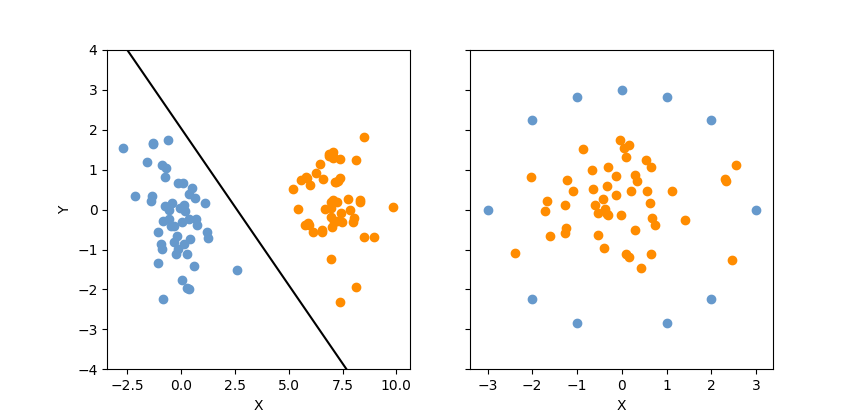
\includegraphics[scale=0.6]{img/fig_perceptron}
	\end{center}
	\caption[Separating two datasets with the Perceptron algorithm.]{\textbf{Left}: Separating two datasets with the Perceptron algorithm in $\mathbb{R}^2$. The correct classification boundary takes the form of a line, i.e. $0 = w^{T}x = w_0 x + w_1 y + w_2$. The line pictured is given by $w = (-2.285, -2.908, 5.938)$, the weights after 19 iterations. \textbf{Right}: A not-linearly separable data set on which the algorithm would never converge, because it is based on finding linear classifiers and thus cannot separate the data correctly.}
	\label{fig:perceptron}
\end {figure}

\begin {algorithm}
	\begin {algorithmic}[1]
		\State $w$ = random
		\While {true}
			\For{$x_i$ in $x$}
				\If{$w^T x_i t_i \leq 0$}
					\State $w$ += $\eta x_i t_i$
				\EndIf

				\If{$w^T x_i t_i > 0$ for all $x_i$ in $x$}
					\State stop
				\EndIf
			\EndFor
		\EndWhile
	\end{algorithmic}
	\caption[Stochastic Descent used for finding Perceptron weights.]{Stochastic Gradient Descent applied to the task of finding the Perceptron weights $w$. $x$ is assumed to be linearly separable.}
	\label{alg:perceptron_algorithm}
\end{algorithm}



		\subsection{Multiple Neurons and Backpropagation}
\label{subsec:mlp_backprop}
While the Perceptron algorithm works fine for linear problems, those are only a small subset of real-world problems (see Figure \textbf{\ref{fig:perceptron}}). The solution to this problem is to add more neurons to the model, which form a network that consists of layers that pass the outputs of neurons from previous layers through \textit{non-linear} activation functions and then use the results as inputs. These layers are referred to as the ``input layer'', the initial layer, the ``output layer'', the last layer, and ``hidden layers'', which are all the layers in-between.

	\subsubsection{Multi-Layer Perceptrons}
The resulting networks are called \textit{Multi-Layer Perceptrons} (MLPs), \textit{Feedforward Artificial Neural Networks}(ANNs), or, in the case of a multitude of layers, \textit{Deep Neural Networks}, and are much more powerful than simple Perceptrons, as they can approximate haphazard continuous functions that operate on closed and bounded subsets of $\mathbb{R}^n$ given that the network possesses at least one hidden layer of neurons. This capability makes using MLPs for learning real-life problems feasible. \cite{universal_approx, universal_approx2}\\

\noindent Again, each neuron in the network computes a weighted sum of its $i$ inputs, just like in Equation \textbf{\ref{eq:perc_class}}, although indexing has been added to identify neurons and weights in the entire network:

\[ a_j^{(l)} = \sum \limits_{i} w^{(l)}_{ji}\,\, z_i^{(l-1)} + b^{(l)}_{j} \,. \]

\noindent Here, $z_i$ are the input values to the current neuron. Note that these either are the direct inputs $x_i$ to the network, or outputs of previous neurons, depending on where in the network the term is evaluated. The variable $w$ is the matrix of weights, and $w^{(l)}_{ji}$ denotes the weight of the connection from the $i$th neuron in the previous layer $l - 1$ to the $j$th neuron in the  layer $l$. The term $b$ is the bias weight associated with the neuron $j$. The bias can also be made part of the weight matrix by introducing an additional input dimension with a value of $1$, like it was done for the Perceptron algorithm in Section \textbf{\ref{subsec:perceptron_algo}}.

Afterwards, the sum $a^{(l)}_j$ is passed into an activation function $h$ to produce the output, also called activation, of the $j$th neuron in the $l$th layer, $z_j^{(l)}$:

\[ z_j^{(l)} = h \left ( a^{(l)}_j \right ) \]

\noindent The activations of the input layer are simply the input values $x_1 \dots x_n$. Expanding the term for the 2-layer network shown in Figure \textbf{\ref{fig:mlp}} gives the following formula for the $k$th network output $\text{out}_k$:

\[ \text{out}_k = \sigma \left ( \sum \limits_{j=1}^{4} w^{(2)}_{kj}\,\, h \left ( \sum \limits_{i=1}^{3} w^{(1)}_{ji} x_i \right ) \right ) \label{eq:mlp_out} \,. \]

\noindent Here, \textbf{$\sigma$} is an output function that is applied in the last layer of the network, and is dependent on the task the network is supposed to fulfill: For regression problems, i.e. fitting a function to a set of data and then predicting new values using that function, the identity function can be used. For binary classification problems in which a value is supposed to be mapped to a class $C_1$ or another class $C_2$, instead of using a step function like in the original Perceptron, one instead uses the \textit{Sigmoid} function and interprets the output as

\[ \sigma_{\text{sig}}(x_i) = \begin{cases}
				x_i \in C_1 \text{ if } \frac{1}{1 + e^{-x_i}} \geq 0.5 \\
				x_i \in C_2 \text{ else }\\
			 \end{cases} \,.
\]

\noindent Also, the choice of the activation function $h(w, x)$ is different from the Perceptron: It is not chosen to be the Heaviside step function, but instead, to be a non-linear, continuous and differentiable function, such as the general Sigmoid function and its derivative:

\begin {align}
	 h(x) &= \frac{1}{1 + e^{-x}}\\
	\frac{\partial h}{\partial x} &= h(x)(1 - h(x)) \,.
\end {align}

\afterpage{
	\begin {figure}[!ht]
		\begin{center}
			\def\svgwidth{0.8\columnwidth}
			\input{img/mlp.pdf_tex}
		\end{center}
		\caption[A simple Multi-Layer Perceptron.]{An MLP with one hidden layer, forming an acyclic directed graph, where connections are color-coded per layer by the receiving neuron. The layer count $L$ starts at the layer after the input layer\protect\footnotemark. Therefore, $L = 2$ with three inputs $x_i$ and neuron counts $D^{(1)} = 4$ and $D^{(2)} = 2$. The variables $b^{(1)}$ and $b^{(2)}$ refer to the biases for the neurons in the layers $(1)$ or $(2)$, respectively. Each neuron has its own, changeable bias value, but for the sake of cleanness, the connections from the biases to each neuron of their corresponding layer are not shown.}
		\label{fig:mlp}
	\end {figure}

	\footnotetext{There is no consensus on which method of counting is the most appropriate. Sometimes, only the number of hidden layers or even all layers are counted. \cite[pp. 229]{bishop_pattern}}
}

\noindent The goal of training an MLP is - as previously for the Perceptron - finding specific weights so that all inputs are classified correctly, or at least, so that the network makes only few mistakes. Therefore, a loss function is added to the end of the network, measuring the correctness of the output. Instead of the Perceptron criterion from Equation \textbf{\ref{eq:perc_error}}, a more general loss function is employed which compares the difference between the output $\sigma(x)$ of the network for a sample $x$ and the preferred output for $x$, i.e. the label or \textit{ground truth} of $x$. Typically, in binary classification problems, Sigmoid outputs are used together with the \textit{Cross-Entropy} loss function, which is defined as follows: \footnote{The error is only given as a function of $w$ because both the input $x$ and its ground-truth $t$ are fixed in the particular case presented here.}

\[ \text{CE}(w) =  -t \, \ln (\text{out}_x) + (1 - t) \ln (1 - \text{out}_x). \]

\noindent For multi-class classifications, an adaption of the Cross-Entropy loss can be used, which is further described in Section \textbf{\ref{subsec:cross_ent}}. \cite[pp. 232-236]{bishop_pattern}\\

	\subsubsection{The Backpropagation algorithm}
Training a network with multiple layers is harder than training a Perceptron because the influence of each of the weights in any layer of the network on the error function has to be computed when using gradient-based optimization methods, while the output of the network no longer is the result of a single function, but instead, a composition of a usually large number of functions (see Equation \textbf{\ref{eq:mlp_out}}). Although it is generally possible to manually formulate a derivative term for the partial derivatives of the entire network, this becomes more and more cumbersome as the network grows in size.\\

Luckily, there exists an iterative algorithm called \textit{Backpropagation} \cite{backprop} that finds the gradient of the loss with respect to each weight so that an optimization method can be applied to change every weight. The algorithm makes use of the fact that each neuron can be viewed largely independently from the rest of the network. Remembering that the analytic way of obtaining the derivative of a composition of functions 

\[ (f \circ g)(x) = f(g(x)) \]

\noindent with respect to some $x$ is to apply the chain rule

\[ \frac{\partial f}{\partial x} =\frac{\partial f}{\partial g} \frac{\partial g}{\partial x} \, , \]

\noindent one can see that this concept can also be applied to neurons in a network, because using the output value of a neuron in a previous layer as the input for a node is nothing else than function composition.\\

\noindent Backpropagation thus starts with a \textit{forward pass}, which means that an input vector $x$ is passed through the network and the corresponding sums $a_j$ and activations $z_j$ are calculated and stored. Comparing the final outputs to the ground truth in the loss layer, the network is then traversed in the opposite direction in what is called a \textit{backward pass}, aiming to obtain the influence of each weight in each layer on the final loss, that is, the gradient of the loss function with respect to the weights. After this first phase, the partial derivatives for each weight are known and the weights are updated in a second phase, in which an optimization algorithm like Gradient Descent is used as described in Section \textbf{\ref{subsec:grad_desc}}. The algorithm then repeats this process anew until convergence.\\

\noindent The central idea of the backward pass is that when traversing the network from the output layer to the input layer, the derivatives of the loss function with respect to the weights of the layer closest to the output of the network depend on outputs of the neurons in the layers that precede that layer. This relationship recursively continues backwards throughout the network and is described by the formula

\begin {align}
	\frac{\partial E}{\partial w_{ji}} &= \frac{\partial E}{\partial a_j} \frac{\partial a_j}{\partial w_{ji}} \label{eq:backprop_recur}
\end {align}

\noindent where $E$ is the loss function of the network.\footnote{Because the formula concerns a particular weight $w_{ji}^{(l)}$ in a particular layer $l$, the $l$-superscript is omitted for convenience.} According to the chain rule, the influence of the weight $w_{ji}$ on the loss is equal to the influence of the weighted sum $a_j$ on the loss function multiplied by the influence of the weight $w_{ji}$ on $a_j$. Taking the partial derivative of the weighted sum $a_j$ with respect to the weight $w_{ji}$ means that

\begin {align}
	\frac{\partial a_j}{\partial w_{ji}} &= \frac{\partial}{\partial w_{ji}} \bigg ( \sum \limits_{k} w_{jk} z_k \bigg ) \,,
\end {align}

\noindent where $k$ is the number of neurons in the previous layer $l-1$. Because when $k = i$, it holds that

\[ \frac{\partial}{\partial w_{ji}} \bigg ( w_{jk} z_k \bigg ) = z_i \]

\noindent and for $k \neq i$ it holds that 

\[ \frac{\partial}{\partial w_{ji}} \bigg ( w_{jk} z_k \bigg ) = 0 \,. \]

\noindent  Therefore the derivative of the entire sum is

\[ \frac{\partial}{\partial w_{ji}} \bigg ( \sum \limits_{k} w_{jk} z_k \bigg ) = z_i \,. \]

\noindent In literature, the term $\frac{\partial E}{\partial a_j}$ is often denoted as $\delta_j^{(l)}$, the ``error'' of the neuron $j$ in layer $l$. Using this notation, Equation \textbf{\ref{eq:backprop_recur}} can then be written as

\[ \frac{\partial E}{\partial w_{ji}} = \delta_j^{(l)} z_i \,. \]

\noindent Since $z_i$, the activation from the input end of the connection that is multiplied with $w_{ji}$, is already known for all neurons due to being stored during the forward pass, the only thing that needs to be computed to figure out the loss gradient are the $\delta$-values. The computation of $\delta_j^{(l)}$ depends on the position of the neuron in the network:

\[ \delta_j^{(l)} =  \begin{cases}
				\displaystyle \frac{\partial E}{\partial a_j} \text{ if neuron } j^{(l)} \text{ is an output neuron} \\
			           h'(a_j) \sum \limits_{k} w_{kj} \, \delta_k^{(l+1)} \text{ otherwise}
			     \end{cases} \,.
\]

\noindent In the case that $j$ is an output neuron, the partial derivative is calculated directly. Otherwise, ${\delta_j}^{(l)}$ depends on the $\delta$-values in deeper layers (see Figure \textbf{\ref{fig:backprop}}). The definition of $\delta$ for hidden neurons is also the reason why a differentiable function must be chosen as the activation $h$. The Backpropagation algorithm continues backwards through the network until the entire weight gradient is known and a single (Stochastic) Gradient Descent step can be taken towards the loss function minimum (see Algorithm \textbf{\ref{alg:backprop}}).

\noindent The main advantage of the algorithm is that it scales linearly with the number of weights, i.e. the algorithm is in $\mathcal{O}(\#w)$. Furthermore, the fact that all $\delta^{(l)}$-values of a layer have to be calculated to calculate all $\delta^{(l-1)}$-values in the layer that precedes it naturally leads to vectorizing the algorithm layerwise in efficient implementations. \cite{nielsen_book, ng_lecture}\cite[pp. 241-245]{bishop_pattern}\\

\begin {algorithm}[!ht]
	\begin {algorithmic}[1]
		\While {loss $\geq \epsilon$}
			\State Input a data sample to the network and forward it through the entire network to calculate the current loss.
			\State Calculate $\delta$ for all output units in the last layer.	
			\State Use the $\delta$ values from the last layer to recursively calculate all other deltas in the network, going back one layer at a time.
			\State Calculate all partial derivatives with respect to the weights, so that a single Gradient Descent step can be taken.
		\EndWhile
	\end{algorithmic}
	\caption[The Backprogation algorithm.]{The Backpropagation algorithm training loop. The algorithms runs until manually aborted or until some loss threshold $\epsilon$ is reached.}
	\label{alg:backprop}
\end{algorithm}


\afterpage{
	\begin {figure}[!ht]
		\begin{center}
			\def\svgwidth{0.8\columnwidth}
			\input{img/backprop.pdf_tex}
		\end{center}
		\caption[Backpropagation calculations.]{Backpropagation calculations, applied to a hidden layer $l$.\protect\footnotemark$\,$ Operations during the forward pass are shown in blue, while operations during the backward pass are orange. The central neuron is the only neuron in the layer $l$, while there are two neurons each in the hidden layers $l-1$ and $l+1$. The forward pass calculates the weighted sum $a_1^{(l)}$ and the activation $h(a_1^{(l)})$. Once the backward pass reaches the neuron again, it calculates $\delta_1^{(l)}$ and the partial derivatives of the weights of layer $l$, that is, the weights of the connections that flow into the central neuron in the forward pass, using the backpropagated value $\delta_k^{(l+1)}$.}
		\label{fig:backprop}
	\end {figure}

	\footnotetext{This example is based on a visualization in \cite{karpathy_lecture}.}
}

\noindent Depending on how deep the networks are, i.e. how many hidden layers there are and how many neurons there are in these hidden layers, neural networks can learn very complex classification boundaries. The role of the non-linear activation functions in neural networks is to combine the linear classificators that all neurons implement in a non-linear way, giving the network its advantage over simpler, linear models like the Perceptron (see Figure \textbf{\ref{fig:mlp_trick}}).\\

\begin {figure}[!ht]
	\begin {subfigure}[b]{0.3\linewidth}
		\scalebox{1.0}{%% Creator: Matplotlib, PGF backend
%%
%% To include the figure in your LaTeX document, write
%%   \input{<filename>.pgf}
%%
%% Make sure the required packages are loaded in your preamble
%%   \usepackage{pgf}
%%
%% Figures using additional raster images can only be included by \input if
%% they are in the same directory as the main LaTeX file. For loading figures
%% from other directories you can use the `import` package
%%   \usepackage{import}
%% and then include the figures with
%%   \import{<path to file>}{<filename>.pgf}
%%
%% Matplotlib used the following preamble
%%   \usepackage{fontspec}
%%   \setmainfont{DejaVu Serif}
%%   \setsansfont{DejaVu Sans}
%%   \setmonofont{DejaVu Sans Mono}
%%
\begingroup%
\makeatletter%
\begin{pgfpicture}%
\pgfpathrectangle{\pgfpointorigin}{\pgfqpoint{6.510000in}{1.550000in}}%
\pgfusepath{use as bounding box, clip}%
\begin{pgfscope}%
\pgfsetbuttcap%
\pgfsetmiterjoin%
\definecolor{currentfill}{rgb}{1.000000,1.000000,1.000000}%
\pgfsetfillcolor{currentfill}%
\pgfsetlinewidth{0.000000pt}%
\definecolor{currentstroke}{rgb}{1.000000,1.000000,1.000000}%
\pgfsetstrokecolor{currentstroke}%
\pgfsetdash{}{0pt}%
\pgfpathmoveto{\pgfqpoint{0.000000in}{0.000000in}}%
\pgfpathlineto{\pgfqpoint{6.510000in}{0.000000in}}%
\pgfpathlineto{\pgfqpoint{6.510000in}{1.550000in}}%
\pgfpathlineto{\pgfqpoint{0.000000in}{1.550000in}}%
\pgfpathclose%
\pgfusepath{fill}%
\end{pgfscope}%
\begin{pgfscope}%
\pgfsetbuttcap%
\pgfsetmiterjoin%
\definecolor{currentfill}{rgb}{1.000000,1.000000,1.000000}%
\pgfsetfillcolor{currentfill}%
\pgfsetlinewidth{0.000000pt}%
\definecolor{currentstroke}{rgb}{0.000000,0.000000,0.000000}%
\pgfsetstrokecolor{currentstroke}%
\pgfsetstrokeopacity{0.000000}%
\pgfsetdash{}{0pt}%
\pgfpathmoveto{\pgfqpoint{0.584722in}{0.387222in}}%
\pgfpathlineto{\pgfqpoint{1.556778in}{0.387222in}}%
\pgfpathlineto{\pgfqpoint{1.556778in}{1.365000in}}%
\pgfpathlineto{\pgfqpoint{0.584722in}{1.365000in}}%
\pgfpathclose%
\pgfusepath{fill}%
\end{pgfscope}%
\begin{pgfscope}%
\pgfpathrectangle{\pgfqpoint{0.584722in}{0.387222in}}{\pgfqpoint{0.972056in}{0.977778in}} %
\pgfusepath{clip}%
\pgfsetbuttcap%
\pgfsetroundjoin%
\definecolor{currentfill}{rgb}{0.960000,0.895056,0.816000}%
\pgfsetfillcolor{currentfill}%
\pgfsetlinewidth{1.003750pt}%
\definecolor{currentstroke}{rgb}{0.960000,0.895056,0.816000}%
\pgfsetstrokecolor{currentstroke}%
\pgfsetdash{}{0pt}%
\pgfpathmoveto{\pgfqpoint{1.165798in}{0.632376in}}%
\pgfpathcurveto{\pgfqpoint{1.171621in}{0.632376in}}{\pgfqpoint{1.177208in}{0.634690in}}{\pgfqpoint{1.181326in}{0.638808in}}%
\pgfpathcurveto{\pgfqpoint{1.185444in}{0.642926in}}{\pgfqpoint{1.187758in}{0.648512in}}{\pgfqpoint{1.187758in}{0.654336in}}%
\pgfpathcurveto{\pgfqpoint{1.187758in}{0.660160in}}{\pgfqpoint{1.185444in}{0.665746in}}{\pgfqpoint{1.181326in}{0.669864in}}%
\pgfpathcurveto{\pgfqpoint{1.177208in}{0.673982in}}{\pgfqpoint{1.171621in}{0.676296in}}{\pgfqpoint{1.165798in}{0.676296in}}%
\pgfpathcurveto{\pgfqpoint{1.159974in}{0.676296in}}{\pgfqpoint{1.154387in}{0.673982in}}{\pgfqpoint{1.150269in}{0.669864in}}%
\pgfpathcurveto{\pgfqpoint{1.146151in}{0.665746in}}{\pgfqpoint{1.143837in}{0.660160in}}{\pgfqpoint{1.143837in}{0.654336in}}%
\pgfpathcurveto{\pgfqpoint{1.143837in}{0.648512in}}{\pgfqpoint{1.146151in}{0.642926in}}{\pgfqpoint{1.150269in}{0.638808in}}%
\pgfpathcurveto{\pgfqpoint{1.154387in}{0.634690in}}{\pgfqpoint{1.159974in}{0.632376in}}{\pgfqpoint{1.165798in}{0.632376in}}%
\pgfpathclose%
\pgfusepath{stroke,fill}%
\end{pgfscope}%
\begin{pgfscope}%
\pgfpathrectangle{\pgfqpoint{0.584722in}{0.387222in}}{\pgfqpoint{0.972056in}{0.977778in}} %
\pgfusepath{clip}%
\pgfsetbuttcap%
\pgfsetroundjoin%
\definecolor{currentfill}{rgb}{0.960000,0.859517,0.737199}%
\pgfsetfillcolor{currentfill}%
\pgfsetlinewidth{1.003750pt}%
\definecolor{currentstroke}{rgb}{0.960000,0.859517,0.737199}%
\pgfsetstrokecolor{currentstroke}%
\pgfsetdash{}{0pt}%
\pgfpathmoveto{\pgfqpoint{1.058174in}{0.823801in}}%
\pgfpathcurveto{\pgfqpoint{1.064829in}{0.823801in}}{\pgfqpoint{1.071212in}{0.826446in}}{\pgfqpoint{1.075918in}{0.831151in}}%
\pgfpathcurveto{\pgfqpoint{1.080624in}{0.835857in}}{\pgfqpoint{1.083268in}{0.842241in}}{\pgfqpoint{1.083268in}{0.848896in}}%
\pgfpathcurveto{\pgfqpoint{1.083268in}{0.855551in}}{\pgfqpoint{1.080624in}{0.861935in}}{\pgfqpoint{1.075918in}{0.866641in}}%
\pgfpathcurveto{\pgfqpoint{1.071212in}{0.871346in}}{\pgfqpoint{1.064829in}{0.873991in}}{\pgfqpoint{1.058174in}{0.873991in}}%
\pgfpathcurveto{\pgfqpoint{1.051519in}{0.873991in}}{\pgfqpoint{1.045135in}{0.871346in}}{\pgfqpoint{1.040429in}{0.866641in}}%
\pgfpathcurveto{\pgfqpoint{1.035723in}{0.861935in}}{\pgfqpoint{1.033079in}{0.855551in}}{\pgfqpoint{1.033079in}{0.848896in}}%
\pgfpathcurveto{\pgfqpoint{1.033079in}{0.842241in}}{\pgfqpoint{1.035723in}{0.835857in}}{\pgfqpoint{1.040429in}{0.831151in}}%
\pgfpathcurveto{\pgfqpoint{1.045135in}{0.826446in}}{\pgfqpoint{1.051519in}{0.823801in}}{\pgfqpoint{1.058174in}{0.823801in}}%
\pgfpathclose%
\pgfusepath{stroke,fill}%
\end{pgfscope}%
\begin{pgfscope}%
\pgfpathrectangle{\pgfqpoint{0.584722in}{0.387222in}}{\pgfqpoint{0.972056in}{0.977778in}} %
\pgfusepath{clip}%
\pgfsetbuttcap%
\pgfsetroundjoin%
\definecolor{currentfill}{rgb}{0.960000,0.831877,0.675914}%
\pgfsetfillcolor{currentfill}%
\pgfsetlinewidth{1.003750pt}%
\definecolor{currentstroke}{rgb}{0.960000,0.831877,0.675914}%
\pgfsetstrokecolor{currentstroke}%
\pgfsetdash{}{0pt}%
\pgfpathmoveto{\pgfqpoint{1.032954in}{0.803443in}}%
\pgfpathcurveto{\pgfqpoint{1.040189in}{0.803443in}}{\pgfqpoint{1.047130in}{0.806317in}}{\pgfqpoint{1.052246in}{0.811434in}}%
\pgfpathcurveto{\pgfqpoint{1.057363in}{0.816551in}}{\pgfqpoint{1.060238in}{0.823491in}}{\pgfqpoint{1.060238in}{0.830727in}}%
\pgfpathcurveto{\pgfqpoint{1.060238in}{0.837963in}}{\pgfqpoint{1.057363in}{0.844903in}}{\pgfqpoint{1.052246in}{0.850020in}}%
\pgfpathcurveto{\pgfqpoint{1.047130in}{0.855137in}}{\pgfqpoint{1.040189in}{0.858011in}}{\pgfqpoint{1.032954in}{0.858011in}}%
\pgfpathcurveto{\pgfqpoint{1.025718in}{0.858011in}}{\pgfqpoint{1.018777in}{0.855137in}}{\pgfqpoint{1.013661in}{0.850020in}}%
\pgfpathcurveto{\pgfqpoint{1.008544in}{0.844903in}}{\pgfqpoint{1.005669in}{0.837963in}}{\pgfqpoint{1.005669in}{0.830727in}}%
\pgfpathcurveto{\pgfqpoint{1.005669in}{0.823491in}}{\pgfqpoint{1.008544in}{0.816551in}}{\pgfqpoint{1.013661in}{0.811434in}}%
\pgfpathcurveto{\pgfqpoint{1.018777in}{0.806317in}}{\pgfqpoint{1.025718in}{0.803443in}}{\pgfqpoint{1.032954in}{0.803443in}}%
\pgfpathclose%
\pgfusepath{stroke,fill}%
\end{pgfscope}%
\begin{pgfscope}%
\pgfpathrectangle{\pgfqpoint{0.584722in}{0.387222in}}{\pgfqpoint{0.972056in}{0.977778in}} %
\pgfusepath{clip}%
\pgfsetbuttcap%
\pgfsetroundjoin%
\definecolor{currentfill}{rgb}{0.960000,0.895056,0.816000}%
\pgfsetfillcolor{currentfill}%
\pgfsetlinewidth{1.003750pt}%
\definecolor{currentstroke}{rgb}{0.960000,0.895056,0.816000}%
\pgfsetstrokecolor{currentstroke}%
\pgfsetdash{}{0pt}%
\pgfpathmoveto{\pgfqpoint{1.172847in}{0.553974in}}%
\pgfpathcurveto{\pgfqpoint{1.178671in}{0.553974in}}{\pgfqpoint{1.184257in}{0.556288in}}{\pgfqpoint{1.188375in}{0.560406in}}%
\pgfpathcurveto{\pgfqpoint{1.192493in}{0.564524in}}{\pgfqpoint{1.194807in}{0.570111in}}{\pgfqpoint{1.194807in}{0.575934in}}%
\pgfpathcurveto{\pgfqpoint{1.194807in}{0.581758in}}{\pgfqpoint{1.192493in}{0.587345in}}{\pgfqpoint{1.188375in}{0.591463in}}%
\pgfpathcurveto{\pgfqpoint{1.184257in}{0.595581in}}{\pgfqpoint{1.178671in}{0.597895in}}{\pgfqpoint{1.172847in}{0.597895in}}%
\pgfpathcurveto{\pgfqpoint{1.167023in}{0.597895in}}{\pgfqpoint{1.161437in}{0.595581in}}{\pgfqpoint{1.157319in}{0.591463in}}%
\pgfpathcurveto{\pgfqpoint{1.153201in}{0.587345in}}{\pgfqpoint{1.150887in}{0.581758in}}{\pgfqpoint{1.150887in}{0.575934in}}%
\pgfpathcurveto{\pgfqpoint{1.150887in}{0.570111in}}{\pgfqpoint{1.153201in}{0.564524in}}{\pgfqpoint{1.157319in}{0.560406in}}%
\pgfpathcurveto{\pgfqpoint{1.161437in}{0.556288in}}{\pgfqpoint{1.167023in}{0.553974in}}{\pgfqpoint{1.172847in}{0.553974in}}%
\pgfpathclose%
\pgfusepath{stroke,fill}%
\end{pgfscope}%
\begin{pgfscope}%
\pgfpathrectangle{\pgfqpoint{0.584722in}{0.387222in}}{\pgfqpoint{0.972056in}{0.977778in}} %
\pgfusepath{clip}%
\pgfsetbuttcap%
\pgfsetroundjoin%
\definecolor{currentfill}{rgb}{0.960000,0.895056,0.816000}%
\pgfsetfillcolor{currentfill}%
\pgfsetlinewidth{1.003750pt}%
\definecolor{currentstroke}{rgb}{0.960000,0.895056,0.816000}%
\pgfsetstrokecolor{currentstroke}%
\pgfsetdash{}{0pt}%
\pgfpathmoveto{\pgfqpoint{1.169637in}{0.664488in}}%
\pgfpathcurveto{\pgfqpoint{1.175461in}{0.664488in}}{\pgfqpoint{1.181047in}{0.666802in}}{\pgfqpoint{1.185165in}{0.670920in}}%
\pgfpathcurveto{\pgfqpoint{1.189284in}{0.675038in}}{\pgfqpoint{1.191598in}{0.680625in}}{\pgfqpoint{1.191598in}{0.686448in}}%
\pgfpathcurveto{\pgfqpoint{1.191598in}{0.692272in}}{\pgfqpoint{1.189284in}{0.697859in}}{\pgfqpoint{1.185165in}{0.701977in}}%
\pgfpathcurveto{\pgfqpoint{1.181047in}{0.706095in}}{\pgfqpoint{1.175461in}{0.708409in}}{\pgfqpoint{1.169637in}{0.708409in}}%
\pgfpathcurveto{\pgfqpoint{1.163813in}{0.708409in}}{\pgfqpoint{1.158227in}{0.706095in}}{\pgfqpoint{1.154109in}{0.701977in}}%
\pgfpathcurveto{\pgfqpoint{1.149991in}{0.697859in}}{\pgfqpoint{1.147677in}{0.692272in}}{\pgfqpoint{1.147677in}{0.686448in}}%
\pgfpathcurveto{\pgfqpoint{1.147677in}{0.680625in}}{\pgfqpoint{1.149991in}{0.675038in}}{\pgfqpoint{1.154109in}{0.670920in}}%
\pgfpathcurveto{\pgfqpoint{1.158227in}{0.666802in}}{\pgfqpoint{1.163813in}{0.664488in}}{\pgfqpoint{1.169637in}{0.664488in}}%
\pgfpathclose%
\pgfusepath{stroke,fill}%
\end{pgfscope}%
\begin{pgfscope}%
\pgfpathrectangle{\pgfqpoint{0.584722in}{0.387222in}}{\pgfqpoint{0.972056in}{0.977778in}} %
\pgfusepath{clip}%
\pgfsetbuttcap%
\pgfsetroundjoin%
\definecolor{currentfill}{rgb}{0.960000,0.818746,0.646798}%
\pgfsetfillcolor{currentfill}%
\pgfsetlinewidth{1.003750pt}%
\definecolor{currentstroke}{rgb}{0.960000,0.818746,0.646798}%
\pgfsetstrokecolor{currentstroke}%
\pgfsetdash{}{0pt}%
\pgfpathmoveto{\pgfqpoint{0.995274in}{0.965390in}}%
\pgfpathcurveto{\pgfqpoint{1.002770in}{0.965390in}}{\pgfqpoint{1.009960in}{0.968368in}}{\pgfqpoint{1.015261in}{0.973669in}}%
\pgfpathcurveto{\pgfqpoint{1.020561in}{0.978969in}}{\pgfqpoint{1.023539in}{0.986159in}}{\pgfqpoint{1.023539in}{0.993655in}}%
\pgfpathcurveto{\pgfqpoint{1.023539in}{1.001151in}}{\pgfqpoint{1.020561in}{1.008341in}}{\pgfqpoint{1.015261in}{1.013642in}}%
\pgfpathcurveto{\pgfqpoint{1.009960in}{1.018942in}}{\pgfqpoint{1.002770in}{1.021921in}}{\pgfqpoint{0.995274in}{1.021921in}}%
\pgfpathcurveto{\pgfqpoint{0.987778in}{1.021921in}}{\pgfqpoint{0.980588in}{1.018942in}}{\pgfqpoint{0.975287in}{1.013642in}}%
\pgfpathcurveto{\pgfqpoint{0.969987in}{1.008341in}}{\pgfqpoint{0.967009in}{1.001151in}}{\pgfqpoint{0.967009in}{0.993655in}}%
\pgfpathcurveto{\pgfqpoint{0.967009in}{0.986159in}}{\pgfqpoint{0.969987in}{0.978969in}}{\pgfqpoint{0.975287in}{0.973669in}}%
\pgfpathcurveto{\pgfqpoint{0.980588in}{0.968368in}}{\pgfqpoint{0.987778in}{0.965390in}}{\pgfqpoint{0.995274in}{0.965390in}}%
\pgfpathclose%
\pgfusepath{stroke,fill}%
\end{pgfscope}%
\begin{pgfscope}%
\pgfpathrectangle{\pgfqpoint{0.584722in}{0.387222in}}{\pgfqpoint{0.972056in}{0.977778in}} %
\pgfusepath{clip}%
\pgfsetbuttcap%
\pgfsetroundjoin%
\definecolor{currentfill}{rgb}{0.960000,0.682856,0.345490}%
\pgfsetfillcolor{currentfill}%
\pgfsetlinewidth{1.003750pt}%
\definecolor{currentstroke}{rgb}{0.960000,0.682856,0.345490}%
\pgfsetstrokecolor{currentstroke}%
\pgfsetdash{}{0pt}%
\pgfpathmoveto{\pgfqpoint{0.916056in}{0.568475in}}%
\pgfpathcurveto{\pgfqpoint{0.925847in}{0.568475in}}{\pgfqpoint{0.935238in}{0.572364in}}{\pgfqpoint{0.942160in}{0.579287in}}%
\pgfpathcurveto{\pgfqpoint{0.949083in}{0.586210in}}{\pgfqpoint{0.952973in}{0.595601in}}{\pgfqpoint{0.952973in}{0.605391in}}%
\pgfpathcurveto{\pgfqpoint{0.952973in}{0.615182in}}{\pgfqpoint{0.949083in}{0.624573in}}{\pgfqpoint{0.942160in}{0.631496in}}%
\pgfpathcurveto{\pgfqpoint{0.935238in}{0.638418in}}{\pgfqpoint{0.925847in}{0.642308in}}{\pgfqpoint{0.916056in}{0.642308in}}%
\pgfpathcurveto{\pgfqpoint{0.906266in}{0.642308in}}{\pgfqpoint{0.896875in}{0.638418in}}{\pgfqpoint{0.889952in}{0.631496in}}%
\pgfpathcurveto{\pgfqpoint{0.883029in}{0.624573in}}{\pgfqpoint{0.879140in}{0.615182in}}{\pgfqpoint{0.879140in}{0.605391in}}%
\pgfpathcurveto{\pgfqpoint{0.879140in}{0.595601in}}{\pgfqpoint{0.883029in}{0.586210in}}{\pgfqpoint{0.889952in}{0.579287in}}%
\pgfpathcurveto{\pgfqpoint{0.896875in}{0.572364in}}{\pgfqpoint{0.906266in}{0.568475in}}{\pgfqpoint{0.916056in}{0.568475in}}%
\pgfpathclose%
\pgfusepath{stroke,fill}%
\end{pgfscope}%
\begin{pgfscope}%
\pgfpathrectangle{\pgfqpoint{0.584722in}{0.387222in}}{\pgfqpoint{0.972056in}{0.977778in}} %
\pgfusepath{clip}%
\pgfsetbuttcap%
\pgfsetroundjoin%
\definecolor{currentfill}{rgb}{0.960000,0.895056,0.816000}%
\pgfsetfillcolor{currentfill}%
\pgfsetlinewidth{1.003750pt}%
\definecolor{currentstroke}{rgb}{0.960000,0.895056,0.816000}%
\pgfsetstrokecolor{currentstroke}%
\pgfsetdash{}{0pt}%
\pgfpathmoveto{\pgfqpoint{1.224205in}{0.698841in}}%
\pgfpathcurveto{\pgfqpoint{1.230029in}{0.698841in}}{\pgfqpoint{1.235615in}{0.701155in}}{\pgfqpoint{1.239733in}{0.705273in}}%
\pgfpathcurveto{\pgfqpoint{1.243851in}{0.709391in}}{\pgfqpoint{1.246165in}{0.714977in}}{\pgfqpoint{1.246165in}{0.720801in}}%
\pgfpathcurveto{\pgfqpoint{1.246165in}{0.726625in}}{\pgfqpoint{1.243851in}{0.732211in}}{\pgfqpoint{1.239733in}{0.736329in}}%
\pgfpathcurveto{\pgfqpoint{1.235615in}{0.740448in}}{\pgfqpoint{1.230029in}{0.742761in}}{\pgfqpoint{1.224205in}{0.742761in}}%
\pgfpathcurveto{\pgfqpoint{1.218381in}{0.742761in}}{\pgfqpoint{1.212795in}{0.740448in}}{\pgfqpoint{1.208677in}{0.736329in}}%
\pgfpathcurveto{\pgfqpoint{1.204559in}{0.732211in}}{\pgfqpoint{1.202245in}{0.726625in}}{\pgfqpoint{1.202245in}{0.720801in}}%
\pgfpathcurveto{\pgfqpoint{1.202245in}{0.714977in}}{\pgfqpoint{1.204559in}{0.709391in}}{\pgfqpoint{1.208677in}{0.705273in}}%
\pgfpathcurveto{\pgfqpoint{1.212795in}{0.701155in}}{\pgfqpoint{1.218381in}{0.698841in}}{\pgfqpoint{1.224205in}{0.698841in}}%
\pgfpathclose%
\pgfusepath{stroke,fill}%
\end{pgfscope}%
\begin{pgfscope}%
\pgfpathrectangle{\pgfqpoint{0.584722in}{0.387222in}}{\pgfqpoint{0.972056in}{0.977778in}} %
\pgfusepath{clip}%
\pgfsetbuttcap%
\pgfsetroundjoin%
\definecolor{currentfill}{rgb}{0.960000,0.791728,0.586890}%
\pgfsetfillcolor{currentfill}%
\pgfsetlinewidth{1.003750pt}%
\definecolor{currentstroke}{rgb}{0.960000,0.791728,0.586890}%
\pgfsetstrokecolor{currentstroke}%
\pgfsetdash{}{0pt}%
\pgfpathmoveto{\pgfqpoint{0.985444in}{0.846747in}}%
\pgfpathcurveto{\pgfqpoint{0.993449in}{0.846747in}}{\pgfqpoint{1.001127in}{0.849928in}}{\pgfqpoint{1.006787in}{0.855588in}}%
\pgfpathcurveto{\pgfqpoint{1.012448in}{0.861248in}}{\pgfqpoint{1.015628in}{0.868926in}}{\pgfqpoint{1.015628in}{0.876931in}}%
\pgfpathcurveto{\pgfqpoint{1.015628in}{0.884936in}}{\pgfqpoint{1.012448in}{0.892614in}}{\pgfqpoint{1.006787in}{0.898274in}}%
\pgfpathcurveto{\pgfqpoint{1.001127in}{0.903934in}}{\pgfqpoint{0.993449in}{0.907115in}}{\pgfqpoint{0.985444in}{0.907115in}}%
\pgfpathcurveto{\pgfqpoint{0.977439in}{0.907115in}}{\pgfqpoint{0.969761in}{0.903934in}}{\pgfqpoint{0.964101in}{0.898274in}}%
\pgfpathcurveto{\pgfqpoint{0.958441in}{0.892614in}}{\pgfqpoint{0.955261in}{0.884936in}}{\pgfqpoint{0.955261in}{0.876931in}}%
\pgfpathcurveto{\pgfqpoint{0.955261in}{0.868926in}}{\pgfqpoint{0.958441in}{0.861248in}}{\pgfqpoint{0.964101in}{0.855588in}}%
\pgfpathcurveto{\pgfqpoint{0.969761in}{0.849928in}}{\pgfqpoint{0.977439in}{0.846747in}}{\pgfqpoint{0.985444in}{0.846747in}}%
\pgfpathclose%
\pgfusepath{stroke,fill}%
\end{pgfscope}%
\begin{pgfscope}%
\pgfpathrectangle{\pgfqpoint{0.584722in}{0.387222in}}{\pgfqpoint{0.972056in}{0.977778in}} %
\pgfusepath{clip}%
\pgfsetbuttcap%
\pgfsetroundjoin%
\definecolor{currentfill}{rgb}{0.960000,0.895056,0.816000}%
\pgfsetfillcolor{currentfill}%
\pgfsetlinewidth{1.003750pt}%
\definecolor{currentstroke}{rgb}{0.960000,0.895056,0.816000}%
\pgfsetstrokecolor{currentstroke}%
\pgfsetdash{}{0pt}%
\pgfpathmoveto{\pgfqpoint{1.109649in}{0.955064in}}%
\pgfpathcurveto{\pgfqpoint{1.115473in}{0.955064in}}{\pgfqpoint{1.121059in}{0.957378in}}{\pgfqpoint{1.125177in}{0.961496in}}%
\pgfpathcurveto{\pgfqpoint{1.129295in}{0.965614in}}{\pgfqpoint{1.131609in}{0.971200in}}{\pgfqpoint{1.131609in}{0.977024in}}%
\pgfpathcurveto{\pgfqpoint{1.131609in}{0.982848in}}{\pgfqpoint{1.129295in}{0.988434in}}{\pgfqpoint{1.125177in}{0.992552in}}%
\pgfpathcurveto{\pgfqpoint{1.121059in}{0.996671in}}{\pgfqpoint{1.115473in}{0.998984in}}{\pgfqpoint{1.109649in}{0.998984in}}%
\pgfpathcurveto{\pgfqpoint{1.103825in}{0.998984in}}{\pgfqpoint{1.098239in}{0.996671in}}{\pgfqpoint{1.094121in}{0.992552in}}%
\pgfpathcurveto{\pgfqpoint{1.090003in}{0.988434in}}{\pgfqpoint{1.087689in}{0.982848in}}{\pgfqpoint{1.087689in}{0.977024in}}%
\pgfpathcurveto{\pgfqpoint{1.087689in}{0.971200in}}{\pgfqpoint{1.090003in}{0.965614in}}{\pgfqpoint{1.094121in}{0.961496in}}%
\pgfpathcurveto{\pgfqpoint{1.098239in}{0.957378in}}{\pgfqpoint{1.103825in}{0.955064in}}{\pgfqpoint{1.109649in}{0.955064in}}%
\pgfpathclose%
\pgfusepath{stroke,fill}%
\end{pgfscope}%
\begin{pgfscope}%
\pgfpathrectangle{\pgfqpoint{0.584722in}{0.387222in}}{\pgfqpoint{0.972056in}{0.977778in}} %
\pgfusepath{clip}%
\pgfsetbuttcap%
\pgfsetroundjoin%
\definecolor{currentfill}{rgb}{0.960000,0.748309,0.490619}%
\pgfsetfillcolor{currentfill}%
\pgfsetlinewidth{1.003750pt}%
\definecolor{currentstroke}{rgb}{0.960000,0.748309,0.490619}%
\pgfsetstrokecolor{currentstroke}%
\pgfsetdash{}{0pt}%
\pgfpathmoveto{\pgfqpoint{0.970781in}{0.648758in}}%
\pgfpathcurveto{\pgfqpoint{0.979542in}{0.648758in}}{\pgfqpoint{0.987945in}{0.652239in}}{\pgfqpoint{0.994139in}{0.658434in}}%
\pgfpathcurveto{\pgfqpoint{1.000334in}{0.664628in}}{\pgfqpoint{1.003815in}{0.673031in}}{\pgfqpoint{1.003815in}{0.681792in}}%
\pgfpathcurveto{\pgfqpoint{1.003815in}{0.690553in}}{\pgfqpoint{1.000334in}{0.698956in}}{\pgfqpoint{0.994139in}{0.705151in}}%
\pgfpathcurveto{\pgfqpoint{0.987945in}{0.711345in}}{\pgfqpoint{0.979542in}{0.714826in}}{\pgfqpoint{0.970781in}{0.714826in}}%
\pgfpathcurveto{\pgfqpoint{0.962020in}{0.714826in}}{\pgfqpoint{0.953617in}{0.711345in}}{\pgfqpoint{0.947423in}{0.705151in}}%
\pgfpathcurveto{\pgfqpoint{0.941228in}{0.698956in}}{\pgfqpoint{0.937747in}{0.690553in}}{\pgfqpoint{0.937747in}{0.681792in}}%
\pgfpathcurveto{\pgfqpoint{0.937747in}{0.673031in}}{\pgfqpoint{0.941228in}{0.664628in}}{\pgfqpoint{0.947423in}{0.658434in}}%
\pgfpathcurveto{\pgfqpoint{0.953617in}{0.652239in}}{\pgfqpoint{0.962020in}{0.648758in}}{\pgfqpoint{0.970781in}{0.648758in}}%
\pgfpathclose%
\pgfusepath{stroke,fill}%
\end{pgfscope}%
\begin{pgfscope}%
\pgfpathrectangle{\pgfqpoint{0.584722in}{0.387222in}}{\pgfqpoint{0.972056in}{0.977778in}} %
\pgfusepath{clip}%
\pgfsetbuttcap%
\pgfsetroundjoin%
\definecolor{currentfill}{rgb}{0.960000,0.741239,0.474941}%
\pgfsetfillcolor{currentfill}%
\pgfsetlinewidth{1.003750pt}%
\definecolor{currentstroke}{rgb}{0.960000,0.741239,0.474941}%
\pgfsetstrokecolor{currentstroke}%
\pgfsetdash{}{0pt}%
\pgfpathmoveto{\pgfqpoint{0.930206in}{0.871475in}}%
\pgfpathcurveto{\pgfqpoint{0.939084in}{0.871475in}}{\pgfqpoint{0.947599in}{0.875002in}}{\pgfqpoint{0.953877in}{0.881279in}}%
\pgfpathcurveto{\pgfqpoint{0.960154in}{0.887557in}}{\pgfqpoint{0.963681in}{0.896072in}}{\pgfqpoint{0.963681in}{0.904950in}}%
\pgfpathcurveto{\pgfqpoint{0.963681in}{0.913827in}}{\pgfqpoint{0.960154in}{0.922342in}}{\pgfqpoint{0.953877in}{0.928620in}}%
\pgfpathcurveto{\pgfqpoint{0.947599in}{0.934897in}}{\pgfqpoint{0.939084in}{0.938425in}}{\pgfqpoint{0.930206in}{0.938425in}}%
\pgfpathcurveto{\pgfqpoint{0.921329in}{0.938425in}}{\pgfqpoint{0.912813in}{0.934897in}}{\pgfqpoint{0.906536in}{0.928620in}}%
\pgfpathcurveto{\pgfqpoint{0.900259in}{0.922342in}}{\pgfqpoint{0.896731in}{0.913827in}}{\pgfqpoint{0.896731in}{0.904950in}}%
\pgfpathcurveto{\pgfqpoint{0.896731in}{0.896072in}}{\pgfqpoint{0.900259in}{0.887557in}}{\pgfqpoint{0.906536in}{0.881279in}}%
\pgfpathcurveto{\pgfqpoint{0.912813in}{0.875002in}}{\pgfqpoint{0.921329in}{0.871475in}}{\pgfqpoint{0.930206in}{0.871475in}}%
\pgfpathclose%
\pgfusepath{stroke,fill}%
\end{pgfscope}%
\begin{pgfscope}%
\pgfpathrectangle{\pgfqpoint{0.584722in}{0.387222in}}{\pgfqpoint{0.972056in}{0.977778in}} %
\pgfusepath{clip}%
\pgfsetbuttcap%
\pgfsetroundjoin%
\definecolor{currentfill}{rgb}{0.960000,0.895056,0.816000}%
\pgfsetfillcolor{currentfill}%
\pgfsetlinewidth{1.003750pt}%
\definecolor{currentstroke}{rgb}{0.960000,0.895056,0.816000}%
\pgfsetstrokecolor{currentstroke}%
\pgfsetdash{}{0pt}%
\pgfpathmoveto{\pgfqpoint{1.123845in}{0.747002in}}%
\pgfpathcurveto{\pgfqpoint{1.129668in}{0.747002in}}{\pgfqpoint{1.135255in}{0.749316in}}{\pgfqpoint{1.139373in}{0.753434in}}%
\pgfpathcurveto{\pgfqpoint{1.143491in}{0.757553in}}{\pgfqpoint{1.145805in}{0.763139in}}{\pgfqpoint{1.145805in}{0.768963in}}%
\pgfpathcurveto{\pgfqpoint{1.145805in}{0.774787in}}{\pgfqpoint{1.143491in}{0.780373in}}{\pgfqpoint{1.139373in}{0.784491in}}%
\pgfpathcurveto{\pgfqpoint{1.135255in}{0.788609in}}{\pgfqpoint{1.129668in}{0.790923in}}{\pgfqpoint{1.123845in}{0.790923in}}%
\pgfpathcurveto{\pgfqpoint{1.118021in}{0.790923in}}{\pgfqpoint{1.112434in}{0.788609in}}{\pgfqpoint{1.108316in}{0.784491in}}%
\pgfpathcurveto{\pgfqpoint{1.104198in}{0.780373in}}{\pgfqpoint{1.101884in}{0.774787in}}{\pgfqpoint{1.101884in}{0.768963in}}%
\pgfpathcurveto{\pgfqpoint{1.101884in}{0.763139in}}{\pgfqpoint{1.104198in}{0.757553in}}{\pgfqpoint{1.108316in}{0.753434in}}%
\pgfpathcurveto{\pgfqpoint{1.112434in}{0.749316in}}{\pgfqpoint{1.118021in}{0.747002in}}{\pgfqpoint{1.123845in}{0.747002in}}%
\pgfpathclose%
\pgfusepath{stroke,fill}%
\end{pgfscope}%
\begin{pgfscope}%
\pgfpathrectangle{\pgfqpoint{0.584722in}{0.387222in}}{\pgfqpoint{0.972056in}{0.977778in}} %
\pgfusepath{clip}%
\pgfsetbuttcap%
\pgfsetroundjoin%
\definecolor{currentfill}{rgb}{0.960000,0.866585,0.752872}%
\pgfsetfillcolor{currentfill}%
\pgfsetlinewidth{1.003750pt}%
\definecolor{currentstroke}{rgb}{0.960000,0.866585,0.752872}%
\pgfsetstrokecolor{currentstroke}%
\pgfsetdash{}{0pt}%
\pgfpathmoveto{\pgfqpoint{1.051096in}{0.919352in}}%
\pgfpathcurveto{\pgfqpoint{1.057594in}{0.919352in}}{\pgfqpoint{1.063827in}{0.921934in}}{\pgfqpoint{1.068422in}{0.926529in}}%
\pgfpathcurveto{\pgfqpoint{1.073017in}{0.931124in}}{\pgfqpoint{1.075599in}{0.937357in}}{\pgfqpoint{1.075599in}{0.943856in}}%
\pgfpathcurveto{\pgfqpoint{1.075599in}{0.950354in}}{\pgfqpoint{1.073017in}{0.956587in}}{\pgfqpoint{1.068422in}{0.961182in}}%
\pgfpathcurveto{\pgfqpoint{1.063827in}{0.965777in}}{\pgfqpoint{1.057594in}{0.968359in}}{\pgfqpoint{1.051096in}{0.968359in}}%
\pgfpathcurveto{\pgfqpoint{1.044597in}{0.968359in}}{\pgfqpoint{1.038364in}{0.965777in}}{\pgfqpoint{1.033769in}{0.961182in}}%
\pgfpathcurveto{\pgfqpoint{1.029174in}{0.956587in}}{\pgfqpoint{1.026593in}{0.950354in}}{\pgfqpoint{1.026593in}{0.943856in}}%
\pgfpathcurveto{\pgfqpoint{1.026593in}{0.937357in}}{\pgfqpoint{1.029174in}{0.931124in}}{\pgfqpoint{1.033769in}{0.926529in}}%
\pgfpathcurveto{\pgfqpoint{1.038364in}{0.921934in}}{\pgfqpoint{1.044597in}{0.919352in}}{\pgfqpoint{1.051096in}{0.919352in}}%
\pgfpathclose%
\pgfusepath{stroke,fill}%
\end{pgfscope}%
\begin{pgfscope}%
\pgfpathrectangle{\pgfqpoint{0.584722in}{0.387222in}}{\pgfqpoint{0.972056in}{0.977778in}} %
\pgfusepath{clip}%
\pgfsetbuttcap%
\pgfsetroundjoin%
\definecolor{currentfill}{rgb}{0.960000,0.645966,0.263694}%
\pgfsetfillcolor{currentfill}%
\pgfsetlinewidth{1.003750pt}%
\definecolor{currentstroke}{rgb}{0.960000,0.645966,0.263694}%
\pgfsetstrokecolor{currentstroke}%
\pgfsetdash{}{0pt}%
\pgfpathmoveto{\pgfqpoint{0.860115in}{0.690953in}}%
\pgfpathcurveto{\pgfqpoint{0.870440in}{0.690953in}}{\pgfqpoint{0.880345in}{0.695056in}}{\pgfqpoint{0.887646in}{0.702357in}}%
\pgfpathcurveto{\pgfqpoint{0.894947in}{0.709659in}}{\pgfqpoint{0.899050in}{0.719563in}}{\pgfqpoint{0.899050in}{0.729888in}}%
\pgfpathcurveto{\pgfqpoint{0.899050in}{0.740214in}}{\pgfqpoint{0.894947in}{0.750118in}}{\pgfqpoint{0.887646in}{0.757420in}}%
\pgfpathcurveto{\pgfqpoint{0.880345in}{0.764721in}}{\pgfqpoint{0.870440in}{0.768824in}}{\pgfqpoint{0.860115in}{0.768824in}}%
\pgfpathcurveto{\pgfqpoint{0.849789in}{0.768824in}}{\pgfqpoint{0.839885in}{0.764721in}}{\pgfqpoint{0.832583in}{0.757420in}}%
\pgfpathcurveto{\pgfqpoint{0.825282in}{0.750118in}}{\pgfqpoint{0.821180in}{0.740214in}}{\pgfqpoint{0.821180in}{0.729888in}}%
\pgfpathcurveto{\pgfqpoint{0.821180in}{0.719563in}}{\pgfqpoint{0.825282in}{0.709659in}}{\pgfqpoint{0.832583in}{0.702357in}}%
\pgfpathcurveto{\pgfqpoint{0.839885in}{0.695056in}}{\pgfqpoint{0.849789in}{0.690953in}}{\pgfqpoint{0.860115in}{0.690953in}}%
\pgfpathclose%
\pgfusepath{stroke,fill}%
\end{pgfscope}%
\begin{pgfscope}%
\pgfpathrectangle{\pgfqpoint{0.584722in}{0.387222in}}{\pgfqpoint{0.972056in}{0.977778in}} %
\pgfusepath{clip}%
\pgfsetbuttcap%
\pgfsetroundjoin%
\definecolor{currentfill}{rgb}{0.960000,0.699421,0.382218}%
\pgfsetfillcolor{currentfill}%
\pgfsetlinewidth{1.003750pt}%
\definecolor{currentstroke}{rgb}{0.960000,0.699421,0.382218}%
\pgfsetstrokecolor{currentstroke}%
\pgfsetdash{}{0pt}%
\pgfpathmoveto{\pgfqpoint{0.907573in}{0.737848in}}%
\pgfpathcurveto{\pgfqpoint{0.917113in}{0.737848in}}{\pgfqpoint{0.926264in}{0.741638in}}{\pgfqpoint{0.933010in}{0.748384in}}%
\pgfpathcurveto{\pgfqpoint{0.939756in}{0.755130in}}{\pgfqpoint{0.943547in}{0.764281in}}{\pgfqpoint{0.943547in}{0.773822in}}%
\pgfpathcurveto{\pgfqpoint{0.943547in}{0.783362in}}{\pgfqpoint{0.939756in}{0.792513in}}{\pgfqpoint{0.933010in}{0.799259in}}%
\pgfpathcurveto{\pgfqpoint{0.926264in}{0.806005in}}{\pgfqpoint{0.917113in}{0.809795in}}{\pgfqpoint{0.907573in}{0.809795in}}%
\pgfpathcurveto{\pgfqpoint{0.898032in}{0.809795in}}{\pgfqpoint{0.888882in}{0.806005in}}{\pgfqpoint{0.882136in}{0.799259in}}%
\pgfpathcurveto{\pgfqpoint{0.875389in}{0.792513in}}{\pgfqpoint{0.871599in}{0.783362in}}{\pgfqpoint{0.871599in}{0.773822in}}%
\pgfpathcurveto{\pgfqpoint{0.871599in}{0.764281in}}{\pgfqpoint{0.875389in}{0.755130in}}{\pgfqpoint{0.882136in}{0.748384in}}%
\pgfpathcurveto{\pgfqpoint{0.888882in}{0.741638in}}{\pgfqpoint{0.898032in}{0.737848in}}{\pgfqpoint{0.907573in}{0.737848in}}%
\pgfpathclose%
\pgfusepath{stroke,fill}%
\end{pgfscope}%
\begin{pgfscope}%
\pgfpathrectangle{\pgfqpoint{0.584722in}{0.387222in}}{\pgfqpoint{0.972056in}{0.977778in}} %
\pgfusepath{clip}%
\pgfsetbuttcap%
\pgfsetroundjoin%
\definecolor{currentfill}{rgb}{0.960000,0.895056,0.816000}%
\pgfsetfillcolor{currentfill}%
\pgfsetlinewidth{1.003750pt}%
\definecolor{currentstroke}{rgb}{0.960000,0.895056,0.816000}%
\pgfsetstrokecolor{currentstroke}%
\pgfsetdash{}{0pt}%
\pgfpathmoveto{\pgfqpoint{1.323482in}{0.832857in}}%
\pgfpathcurveto{\pgfqpoint{1.329306in}{0.832857in}}{\pgfqpoint{1.334892in}{0.835171in}}{\pgfqpoint{1.339010in}{0.839289in}}%
\pgfpathcurveto{\pgfqpoint{1.343129in}{0.843407in}}{\pgfqpoint{1.345442in}{0.848993in}}{\pgfqpoint{1.345442in}{0.854817in}}%
\pgfpathcurveto{\pgfqpoint{1.345442in}{0.860641in}}{\pgfqpoint{1.343129in}{0.866227in}}{\pgfqpoint{1.339010in}{0.870345in}}%
\pgfpathcurveto{\pgfqpoint{1.334892in}{0.874464in}}{\pgfqpoint{1.329306in}{0.876777in}}{\pgfqpoint{1.323482in}{0.876777in}}%
\pgfpathcurveto{\pgfqpoint{1.317658in}{0.876777in}}{\pgfqpoint{1.312072in}{0.874464in}}{\pgfqpoint{1.307954in}{0.870345in}}%
\pgfpathcurveto{\pgfqpoint{1.303836in}{0.866227in}}{\pgfqpoint{1.301522in}{0.860641in}}{\pgfqpoint{1.301522in}{0.854817in}}%
\pgfpathcurveto{\pgfqpoint{1.301522in}{0.848993in}}{\pgfqpoint{1.303836in}{0.843407in}}{\pgfqpoint{1.307954in}{0.839289in}}%
\pgfpathcurveto{\pgfqpoint{1.312072in}{0.835171in}}{\pgfqpoint{1.317658in}{0.832857in}}{\pgfqpoint{1.323482in}{0.832857in}}%
\pgfpathclose%
\pgfusepath{stroke,fill}%
\end{pgfscope}%
\begin{pgfscope}%
\pgfpathrectangle{\pgfqpoint{0.584722in}{0.387222in}}{\pgfqpoint{0.972056in}{0.977778in}} %
\pgfusepath{clip}%
\pgfsetbuttcap%
\pgfsetroundjoin%
\definecolor{currentfill}{rgb}{0.960000,0.761720,0.520354}%
\pgfsetfillcolor{currentfill}%
\pgfsetlinewidth{1.003750pt}%
\definecolor{currentstroke}{rgb}{0.960000,0.761720,0.520354}%
\pgfsetstrokecolor{currentstroke}%
\pgfsetdash{}{0pt}%
\pgfpathmoveto{\pgfqpoint{0.960818in}{0.806634in}}%
\pgfpathcurveto{\pgfqpoint{0.969352in}{0.806634in}}{\pgfqpoint{0.977538in}{0.810025in}}{\pgfqpoint{0.983573in}{0.816059in}}%
\pgfpathcurveto{\pgfqpoint{0.989608in}{0.822094in}}{\pgfqpoint{0.992998in}{0.830280in}}{\pgfqpoint{0.992998in}{0.838814in}}%
\pgfpathcurveto{\pgfqpoint{0.992998in}{0.847349in}}{\pgfqpoint{0.989608in}{0.855535in}}{\pgfqpoint{0.983573in}{0.861569in}}%
\pgfpathcurveto{\pgfqpoint{0.977538in}{0.867604in}}{\pgfqpoint{0.969352in}{0.870995in}}{\pgfqpoint{0.960818in}{0.870995in}}%
\pgfpathcurveto{\pgfqpoint{0.952284in}{0.870995in}}{\pgfqpoint{0.944098in}{0.867604in}}{\pgfqpoint{0.938063in}{0.861569in}}%
\pgfpathcurveto{\pgfqpoint{0.932028in}{0.855535in}}{\pgfqpoint{0.928637in}{0.847349in}}{\pgfqpoint{0.928637in}{0.838814in}}%
\pgfpathcurveto{\pgfqpoint{0.928637in}{0.830280in}}{\pgfqpoint{0.932028in}{0.822094in}}{\pgfqpoint{0.938063in}{0.816059in}}%
\pgfpathcurveto{\pgfqpoint{0.944098in}{0.810025in}}{\pgfqpoint{0.952284in}{0.806634in}}{\pgfqpoint{0.960818in}{0.806634in}}%
\pgfpathclose%
\pgfusepath{stroke,fill}%
\end{pgfscope}%
\begin{pgfscope}%
\pgfpathrectangle{\pgfqpoint{0.584722in}{0.387222in}}{\pgfqpoint{0.972056in}{0.977778in}} %
\pgfusepath{clip}%
\pgfsetbuttcap%
\pgfsetroundjoin%
\definecolor{currentfill}{rgb}{0.960000,0.812356,0.632629}%
\pgfsetfillcolor{currentfill}%
\pgfsetlinewidth{1.003750pt}%
\definecolor{currentstroke}{rgb}{0.960000,0.812356,0.632629}%
\pgfsetstrokecolor{currentstroke}%
\pgfsetdash{}{0pt}%
\pgfpathmoveto{\pgfqpoint{1.031219in}{0.681827in}}%
\pgfpathcurveto{\pgfqpoint{1.038838in}{0.681827in}}{\pgfqpoint{1.046147in}{0.684855in}}{\pgfqpoint{1.051534in}{0.690242in}}%
\pgfpathcurveto{\pgfqpoint{1.056922in}{0.695630in}}{\pgfqpoint{1.059949in}{0.702939in}}{\pgfqpoint{1.059949in}{0.710558in}}%
\pgfpathcurveto{\pgfqpoint{1.059949in}{0.718177in}}{\pgfqpoint{1.056922in}{0.725486in}}{\pgfqpoint{1.051534in}{0.730874in}}%
\pgfpathcurveto{\pgfqpoint{1.046147in}{0.736261in}}{\pgfqpoint{1.038838in}{0.739289in}}{\pgfqpoint{1.031219in}{0.739289in}}%
\pgfpathcurveto{\pgfqpoint{1.023599in}{0.739289in}}{\pgfqpoint{1.016291in}{0.736261in}}{\pgfqpoint{1.010903in}{0.730874in}}%
\pgfpathcurveto{\pgfqpoint{1.005515in}{0.725486in}}{\pgfqpoint{1.002488in}{0.718177in}}{\pgfqpoint{1.002488in}{0.710558in}}%
\pgfpathcurveto{\pgfqpoint{1.002488in}{0.702939in}}{\pgfqpoint{1.005515in}{0.695630in}}{\pgfqpoint{1.010903in}{0.690242in}}%
\pgfpathcurveto{\pgfqpoint{1.016291in}{0.684855in}}{\pgfqpoint{1.023599in}{0.681827in}}{\pgfqpoint{1.031219in}{0.681827in}}%
\pgfpathclose%
\pgfusepath{stroke,fill}%
\end{pgfscope}%
\begin{pgfscope}%
\pgfpathrectangle{\pgfqpoint{0.584722in}{0.387222in}}{\pgfqpoint{0.972056in}{0.977778in}} %
\pgfusepath{clip}%
\pgfsetbuttcap%
\pgfsetroundjoin%
\definecolor{currentfill}{rgb}{0.960000,0.874428,0.770262}%
\pgfsetfillcolor{currentfill}%
\pgfsetlinewidth{1.003750pt}%
\definecolor{currentstroke}{rgb}{0.960000,0.874428,0.770262}%
\pgfsetstrokecolor{currentstroke}%
\pgfsetdash{}{0pt}%
\pgfpathmoveto{\pgfqpoint{1.083042in}{0.759686in}}%
\pgfpathcurveto{\pgfqpoint{1.089361in}{0.759686in}}{\pgfqpoint{1.095423in}{0.762197in}}{\pgfqpoint{1.099892in}{0.766665in}}%
\pgfpathcurveto{\pgfqpoint{1.104361in}{0.771134in}}{\pgfqpoint{1.106871in}{0.777196in}}{\pgfqpoint{1.106871in}{0.783516in}}%
\pgfpathcurveto{\pgfqpoint{1.106871in}{0.789835in}}{\pgfqpoint{1.104361in}{0.795897in}}{\pgfqpoint{1.099892in}{0.800366in}}%
\pgfpathcurveto{\pgfqpoint{1.095423in}{0.804834in}}{\pgfqpoint{1.089361in}{0.807345in}}{\pgfqpoint{1.083042in}{0.807345in}}%
\pgfpathcurveto{\pgfqpoint{1.076722in}{0.807345in}}{\pgfqpoint{1.070660in}{0.804834in}}{\pgfqpoint{1.066192in}{0.800366in}}%
\pgfpathcurveto{\pgfqpoint{1.061723in}{0.795897in}}{\pgfqpoint{1.059212in}{0.789835in}}{\pgfqpoint{1.059212in}{0.783516in}}%
\pgfpathcurveto{\pgfqpoint{1.059212in}{0.777196in}}{\pgfqpoint{1.061723in}{0.771134in}}{\pgfqpoint{1.066192in}{0.766665in}}%
\pgfpathcurveto{\pgfqpoint{1.070660in}{0.762197in}}{\pgfqpoint{1.076722in}{0.759686in}}{\pgfqpoint{1.083042in}{0.759686in}}%
\pgfpathclose%
\pgfusepath{stroke,fill}%
\end{pgfscope}%
\begin{pgfscope}%
\pgfpathrectangle{\pgfqpoint{0.584722in}{0.387222in}}{\pgfqpoint{0.972056in}{0.977778in}} %
\pgfusepath{clip}%
\pgfsetbuttcap%
\pgfsetroundjoin%
\definecolor{currentfill}{rgb}{0.960000,0.895056,0.816000}%
\pgfsetfillcolor{currentfill}%
\pgfsetlinewidth{1.003750pt}%
\definecolor{currentstroke}{rgb}{0.960000,0.895056,0.816000}%
\pgfsetstrokecolor{currentstroke}%
\pgfsetdash{}{0pt}%
\pgfpathmoveto{\pgfqpoint{1.109342in}{0.727214in}}%
\pgfpathcurveto{\pgfqpoint{1.115166in}{0.727214in}}{\pgfqpoint{1.120752in}{0.729528in}}{\pgfqpoint{1.124871in}{0.733646in}}%
\pgfpathcurveto{\pgfqpoint{1.128989in}{0.737764in}}{\pgfqpoint{1.131303in}{0.743350in}}{\pgfqpoint{1.131303in}{0.749174in}}%
\pgfpathcurveto{\pgfqpoint{1.131303in}{0.754998in}}{\pgfqpoint{1.128989in}{0.760584in}}{\pgfqpoint{1.124871in}{0.764702in}}%
\pgfpathcurveto{\pgfqpoint{1.120752in}{0.768820in}}{\pgfqpoint{1.115166in}{0.771134in}}{\pgfqpoint{1.109342in}{0.771134in}}%
\pgfpathcurveto{\pgfqpoint{1.103518in}{0.771134in}}{\pgfqpoint{1.097932in}{0.768820in}}{\pgfqpoint{1.093814in}{0.764702in}}%
\pgfpathcurveto{\pgfqpoint{1.089696in}{0.760584in}}{\pgfqpoint{1.087382in}{0.754998in}}{\pgfqpoint{1.087382in}{0.749174in}}%
\pgfpathcurveto{\pgfqpoint{1.087382in}{0.743350in}}{\pgfqpoint{1.089696in}{0.737764in}}{\pgfqpoint{1.093814in}{0.733646in}}%
\pgfpathcurveto{\pgfqpoint{1.097932in}{0.729528in}}{\pgfqpoint{1.103518in}{0.727214in}}{\pgfqpoint{1.109342in}{0.727214in}}%
\pgfpathclose%
\pgfusepath{stroke,fill}%
\end{pgfscope}%
\begin{pgfscope}%
\pgfpathrectangle{\pgfqpoint{0.584722in}{0.387222in}}{\pgfqpoint{0.972056in}{0.977778in}} %
\pgfusepath{clip}%
\pgfsetbuttcap%
\pgfsetroundjoin%
\definecolor{currentfill}{rgb}{0.960000,0.895056,0.816000}%
\pgfsetfillcolor{currentfill}%
\pgfsetlinewidth{1.003750pt}%
\definecolor{currentstroke}{rgb}{0.960000,0.895056,0.816000}%
\pgfsetstrokecolor{currentstroke}%
\pgfsetdash{}{0pt}%
\pgfpathmoveto{\pgfqpoint{1.134431in}{0.729371in}}%
\pgfpathcurveto{\pgfqpoint{1.140255in}{0.729371in}}{\pgfqpoint{1.145841in}{0.731685in}}{\pgfqpoint{1.149959in}{0.735803in}}%
\pgfpathcurveto{\pgfqpoint{1.154077in}{0.739921in}}{\pgfqpoint{1.156391in}{0.745507in}}{\pgfqpoint{1.156391in}{0.751331in}}%
\pgfpathcurveto{\pgfqpoint{1.156391in}{0.757155in}}{\pgfqpoint{1.154077in}{0.762742in}}{\pgfqpoint{1.149959in}{0.766860in}}%
\pgfpathcurveto{\pgfqpoint{1.145841in}{0.770978in}}{\pgfqpoint{1.140255in}{0.773292in}}{\pgfqpoint{1.134431in}{0.773292in}}%
\pgfpathcurveto{\pgfqpoint{1.128607in}{0.773292in}}{\pgfqpoint{1.123021in}{0.770978in}}{\pgfqpoint{1.118903in}{0.766860in}}%
\pgfpathcurveto{\pgfqpoint{1.114784in}{0.762742in}}{\pgfqpoint{1.112471in}{0.757155in}}{\pgfqpoint{1.112471in}{0.751331in}}%
\pgfpathcurveto{\pgfqpoint{1.112471in}{0.745507in}}{\pgfqpoint{1.114784in}{0.739921in}}{\pgfqpoint{1.118903in}{0.735803in}}%
\pgfpathcurveto{\pgfqpoint{1.123021in}{0.731685in}}{\pgfqpoint{1.128607in}{0.729371in}}{\pgfqpoint{1.134431in}{0.729371in}}%
\pgfpathclose%
\pgfusepath{stroke,fill}%
\end{pgfscope}%
\begin{pgfscope}%
\pgfpathrectangle{\pgfqpoint{0.584722in}{0.387222in}}{\pgfqpoint{0.972056in}{0.977778in}} %
\pgfusepath{clip}%
\pgfsetbuttcap%
\pgfsetroundjoin%
\definecolor{currentfill}{rgb}{0.960000,0.742331,0.477365}%
\pgfsetfillcolor{currentfill}%
\pgfsetlinewidth{1.003750pt}%
\definecolor{currentstroke}{rgb}{0.960000,0.742331,0.477365}%
\pgfsetstrokecolor{currentstroke}%
\pgfsetdash{}{0pt}%
\pgfpathmoveto{\pgfqpoint{0.964249in}{0.651646in}}%
\pgfpathcurveto{\pgfqpoint{0.973109in}{0.651646in}}{\pgfqpoint{0.981607in}{0.655166in}}{\pgfqpoint{0.987872in}{0.661431in}}%
\pgfpathcurveto{\pgfqpoint{0.994137in}{0.667696in}}{\pgfqpoint{0.997657in}{0.676194in}}{\pgfqpoint{0.997657in}{0.685053in}}%
\pgfpathcurveto{\pgfqpoint{0.997657in}{0.693913in}}{\pgfqpoint{0.994137in}{0.702411in}}{\pgfqpoint{0.987872in}{0.708676in}}%
\pgfpathcurveto{\pgfqpoint{0.981607in}{0.714941in}}{\pgfqpoint{0.973109in}{0.718461in}}{\pgfqpoint{0.964249in}{0.718461in}}%
\pgfpathcurveto{\pgfqpoint{0.955390in}{0.718461in}}{\pgfqpoint{0.946892in}{0.714941in}}{\pgfqpoint{0.940627in}{0.708676in}}%
\pgfpathcurveto{\pgfqpoint{0.934362in}{0.702411in}}{\pgfqpoint{0.930842in}{0.693913in}}{\pgfqpoint{0.930842in}{0.685053in}}%
\pgfpathcurveto{\pgfqpoint{0.930842in}{0.676194in}}{\pgfqpoint{0.934362in}{0.667696in}}{\pgfqpoint{0.940627in}{0.661431in}}%
\pgfpathcurveto{\pgfqpoint{0.946892in}{0.655166in}}{\pgfqpoint{0.955390in}{0.651646in}}{\pgfqpoint{0.964249in}{0.651646in}}%
\pgfpathclose%
\pgfusepath{stroke,fill}%
\end{pgfscope}%
\begin{pgfscope}%
\pgfpathrectangle{\pgfqpoint{0.584722in}{0.387222in}}{\pgfqpoint{0.972056in}{0.977778in}} %
\pgfusepath{clip}%
\pgfsetbuttcap%
\pgfsetroundjoin%
\definecolor{currentfill}{rgb}{0.960000,0.895056,0.816000}%
\pgfsetfillcolor{currentfill}%
\pgfsetlinewidth{1.003750pt}%
\definecolor{currentstroke}{rgb}{0.960000,0.895056,0.816000}%
\pgfsetstrokecolor{currentstroke}%
\pgfsetdash{}{0pt}%
\pgfpathmoveto{\pgfqpoint{1.115317in}{0.848486in}}%
\pgfpathcurveto{\pgfqpoint{1.121141in}{0.848486in}}{\pgfqpoint{1.126727in}{0.850800in}}{\pgfqpoint{1.130846in}{0.854918in}}%
\pgfpathcurveto{\pgfqpoint{1.134964in}{0.859036in}}{\pgfqpoint{1.137278in}{0.864622in}}{\pgfqpoint{1.137278in}{0.870446in}}%
\pgfpathcurveto{\pgfqpoint{1.137278in}{0.876270in}}{\pgfqpoint{1.134964in}{0.881856in}}{\pgfqpoint{1.130846in}{0.885974in}}%
\pgfpathcurveto{\pgfqpoint{1.126727in}{0.890093in}}{\pgfqpoint{1.121141in}{0.892406in}}{\pgfqpoint{1.115317in}{0.892406in}}%
\pgfpathcurveto{\pgfqpoint{1.109493in}{0.892406in}}{\pgfqpoint{1.103907in}{0.890093in}}{\pgfqpoint{1.099789in}{0.885974in}}%
\pgfpathcurveto{\pgfqpoint{1.095671in}{0.881856in}}{\pgfqpoint{1.093357in}{0.876270in}}{\pgfqpoint{1.093357in}{0.870446in}}%
\pgfpathcurveto{\pgfqpoint{1.093357in}{0.864622in}}{\pgfqpoint{1.095671in}{0.859036in}}{\pgfqpoint{1.099789in}{0.854918in}}%
\pgfpathcurveto{\pgfqpoint{1.103907in}{0.850800in}}{\pgfqpoint{1.109493in}{0.848486in}}{\pgfqpoint{1.115317in}{0.848486in}}%
\pgfpathclose%
\pgfusepath{stroke,fill}%
\end{pgfscope}%
\begin{pgfscope}%
\pgfpathrectangle{\pgfqpoint{0.584722in}{0.387222in}}{\pgfqpoint{0.972056in}{0.977778in}} %
\pgfusepath{clip}%
\pgfsetbuttcap%
\pgfsetroundjoin%
\definecolor{currentfill}{rgb}{0.960000,0.895056,0.816000}%
\pgfsetfillcolor{currentfill}%
\pgfsetlinewidth{1.003750pt}%
\definecolor{currentstroke}{rgb}{0.960000,0.895056,0.816000}%
\pgfsetstrokecolor{currentstroke}%
\pgfsetdash{}{0pt}%
\pgfpathmoveto{\pgfqpoint{1.249709in}{0.829988in}}%
\pgfpathcurveto{\pgfqpoint{1.255533in}{0.829988in}}{\pgfqpoint{1.261119in}{0.832302in}}{\pgfqpoint{1.265238in}{0.836420in}}%
\pgfpathcurveto{\pgfqpoint{1.269356in}{0.840538in}}{\pgfqpoint{1.271670in}{0.846124in}}{\pgfqpoint{1.271670in}{0.851948in}}%
\pgfpathcurveto{\pgfqpoint{1.271670in}{0.857772in}}{\pgfqpoint{1.269356in}{0.863359in}}{\pgfqpoint{1.265238in}{0.867477in}}%
\pgfpathcurveto{\pgfqpoint{1.261119in}{0.871595in}}{\pgfqpoint{1.255533in}{0.873909in}}{\pgfqpoint{1.249709in}{0.873909in}}%
\pgfpathcurveto{\pgfqpoint{1.243885in}{0.873909in}}{\pgfqpoint{1.238299in}{0.871595in}}{\pgfqpoint{1.234181in}{0.867477in}}%
\pgfpathcurveto{\pgfqpoint{1.230063in}{0.863359in}}{\pgfqpoint{1.227749in}{0.857772in}}{\pgfqpoint{1.227749in}{0.851948in}}%
\pgfpathcurveto{\pgfqpoint{1.227749in}{0.846124in}}{\pgfqpoint{1.230063in}{0.840538in}}{\pgfqpoint{1.234181in}{0.836420in}}%
\pgfpathcurveto{\pgfqpoint{1.238299in}{0.832302in}}{\pgfqpoint{1.243885in}{0.829988in}}{\pgfqpoint{1.249709in}{0.829988in}}%
\pgfpathclose%
\pgfusepath{stroke,fill}%
\end{pgfscope}%
\begin{pgfscope}%
\pgfpathrectangle{\pgfqpoint{0.584722in}{0.387222in}}{\pgfqpoint{0.972056in}{0.977778in}} %
\pgfusepath{clip}%
\pgfsetbuttcap%
\pgfsetroundjoin%
\definecolor{currentfill}{rgb}{0.960000,0.895056,0.816000}%
\pgfsetfillcolor{currentfill}%
\pgfsetlinewidth{1.003750pt}%
\definecolor{currentstroke}{rgb}{0.960000,0.895056,0.816000}%
\pgfsetstrokecolor{currentstroke}%
\pgfsetdash{}{0pt}%
\pgfpathmoveto{\pgfqpoint{1.268133in}{0.981896in}}%
\pgfpathcurveto{\pgfqpoint{1.273957in}{0.981896in}}{\pgfqpoint{1.279543in}{0.984210in}}{\pgfqpoint{1.283661in}{0.988328in}}%
\pgfpathcurveto{\pgfqpoint{1.287779in}{0.992447in}}{\pgfqpoint{1.290093in}{0.998033in}}{\pgfqpoint{1.290093in}{1.003857in}}%
\pgfpathcurveto{\pgfqpoint{1.290093in}{1.009681in}}{\pgfqpoint{1.287779in}{1.015267in}}{\pgfqpoint{1.283661in}{1.019385in}}%
\pgfpathcurveto{\pgfqpoint{1.279543in}{1.023503in}}{\pgfqpoint{1.273957in}{1.025817in}}{\pgfqpoint{1.268133in}{1.025817in}}%
\pgfpathcurveto{\pgfqpoint{1.262309in}{1.025817in}}{\pgfqpoint{1.256723in}{1.023503in}}{\pgfqpoint{1.252605in}{1.019385in}}%
\pgfpathcurveto{\pgfqpoint{1.248486in}{1.015267in}}{\pgfqpoint{1.246173in}{1.009681in}}{\pgfqpoint{1.246173in}{1.003857in}}%
\pgfpathcurveto{\pgfqpoint{1.246173in}{0.998033in}}{\pgfqpoint{1.248486in}{0.992447in}}{\pgfqpoint{1.252605in}{0.988328in}}%
\pgfpathcurveto{\pgfqpoint{1.256723in}{0.984210in}}{\pgfqpoint{1.262309in}{0.981896in}}{\pgfqpoint{1.268133in}{0.981896in}}%
\pgfpathclose%
\pgfusepath{stroke,fill}%
\end{pgfscope}%
\begin{pgfscope}%
\pgfpathrectangle{\pgfqpoint{0.584722in}{0.387222in}}{\pgfqpoint{0.972056in}{0.977778in}} %
\pgfusepath{clip}%
\pgfsetbuttcap%
\pgfsetroundjoin%
\definecolor{currentfill}{rgb}{0.960000,0.614936,0.194892}%
\pgfsetfillcolor{currentfill}%
\pgfsetlinewidth{1.003750pt}%
\definecolor{currentstroke}{rgb}{0.960000,0.614936,0.194892}%
\pgfsetstrokecolor{currentstroke}%
\pgfsetdash{}{0pt}%
\pgfpathmoveto{\pgfqpoint{0.798633in}{0.890365in}}%
\pgfpathcurveto{\pgfqpoint{0.809389in}{0.890365in}}{\pgfqpoint{0.819705in}{0.894638in}}{\pgfqpoint{0.827310in}{0.902243in}}%
\pgfpathcurveto{\pgfqpoint{0.834915in}{0.909849in}}{\pgfqpoint{0.839188in}{0.920165in}}{\pgfqpoint{0.839188in}{0.930920in}}%
\pgfpathcurveto{\pgfqpoint{0.839188in}{0.941675in}}{\pgfqpoint{0.834915in}{0.951992in}}{\pgfqpoint{0.827310in}{0.959597in}}%
\pgfpathcurveto{\pgfqpoint{0.819705in}{0.967202in}}{\pgfqpoint{0.809389in}{0.971475in}}{\pgfqpoint{0.798633in}{0.971475in}}%
\pgfpathcurveto{\pgfqpoint{0.787878in}{0.971475in}}{\pgfqpoint{0.777562in}{0.967202in}}{\pgfqpoint{0.769957in}{0.959597in}}%
\pgfpathcurveto{\pgfqpoint{0.762351in}{0.951992in}}{\pgfqpoint{0.758078in}{0.941675in}}{\pgfqpoint{0.758078in}{0.930920in}}%
\pgfpathcurveto{\pgfqpoint{0.758078in}{0.920165in}}{\pgfqpoint{0.762351in}{0.909849in}}{\pgfqpoint{0.769957in}{0.902243in}}%
\pgfpathcurveto{\pgfqpoint{0.777562in}{0.894638in}}{\pgfqpoint{0.787878in}{0.890365in}}{\pgfqpoint{0.798633in}{0.890365in}}%
\pgfpathclose%
\pgfusepath{stroke,fill}%
\end{pgfscope}%
\begin{pgfscope}%
\pgfpathrectangle{\pgfqpoint{0.584722in}{0.387222in}}{\pgfqpoint{0.972056in}{0.977778in}} %
\pgfusepath{clip}%
\pgfsetbuttcap%
\pgfsetroundjoin%
\definecolor{currentfill}{rgb}{0.960000,0.889596,0.803894}%
\pgfsetfillcolor{currentfill}%
\pgfsetlinewidth{1.003750pt}%
\definecolor{currentstroke}{rgb}{0.960000,0.889596,0.803894}%
\pgfsetstrokecolor{currentstroke}%
\pgfsetdash{}{0pt}%
\pgfpathmoveto{\pgfqpoint{1.099446in}{0.753894in}}%
\pgfpathcurveto{\pgfqpoint{1.105406in}{0.753894in}}{\pgfqpoint{1.111121in}{0.756262in}}{\pgfqpoint{1.115335in}{0.760476in}}%
\pgfpathcurveto{\pgfqpoint{1.119549in}{0.764689in}}{\pgfqpoint{1.121917in}{0.770405in}}{\pgfqpoint{1.121917in}{0.776365in}}%
\pgfpathcurveto{\pgfqpoint{1.121917in}{0.782324in}}{\pgfqpoint{1.119549in}{0.788040in}}{\pgfqpoint{1.115335in}{0.792253in}}%
\pgfpathcurveto{\pgfqpoint{1.111121in}{0.796467in}}{\pgfqpoint{1.105406in}{0.798835in}}{\pgfqpoint{1.099446in}{0.798835in}}%
\pgfpathcurveto{\pgfqpoint{1.093487in}{0.798835in}}{\pgfqpoint{1.087771in}{0.796467in}}{\pgfqpoint{1.083558in}{0.792253in}}%
\pgfpathcurveto{\pgfqpoint{1.079344in}{0.788040in}}{\pgfqpoint{1.076976in}{0.782324in}}{\pgfqpoint{1.076976in}{0.776365in}}%
\pgfpathcurveto{\pgfqpoint{1.076976in}{0.770405in}}{\pgfqpoint{1.079344in}{0.764689in}}{\pgfqpoint{1.083558in}{0.760476in}}%
\pgfpathcurveto{\pgfqpoint{1.087771in}{0.756262in}}{\pgfqpoint{1.093487in}{0.753894in}}{\pgfqpoint{1.099446in}{0.753894in}}%
\pgfpathclose%
\pgfusepath{stroke,fill}%
\end{pgfscope}%
\begin{pgfscope}%
\pgfpathrectangle{\pgfqpoint{0.584722in}{0.387222in}}{\pgfqpoint{0.972056in}{0.977778in}} %
\pgfusepath{clip}%
\pgfsetbuttcap%
\pgfsetroundjoin%
\definecolor{currentfill}{rgb}{0.960000,0.895056,0.816000}%
\pgfsetfillcolor{currentfill}%
\pgfsetlinewidth{1.003750pt}%
\definecolor{currentstroke}{rgb}{0.960000,0.895056,0.816000}%
\pgfsetstrokecolor{currentstroke}%
\pgfsetdash{}{0pt}%
\pgfpathmoveto{\pgfqpoint{1.115570in}{1.202402in}}%
\pgfpathcurveto{\pgfqpoint{1.121394in}{1.202402in}}{\pgfqpoint{1.126980in}{1.204716in}}{\pgfqpoint{1.131098in}{1.208834in}}%
\pgfpathcurveto{\pgfqpoint{1.135217in}{1.212952in}}{\pgfqpoint{1.137530in}{1.218538in}}{\pgfqpoint{1.137530in}{1.224362in}}%
\pgfpathcurveto{\pgfqpoint{1.137530in}{1.230186in}}{\pgfqpoint{1.135217in}{1.235772in}}{\pgfqpoint{1.131098in}{1.239890in}}%
\pgfpathcurveto{\pgfqpoint{1.126980in}{1.244008in}}{\pgfqpoint{1.121394in}{1.246322in}}{\pgfqpoint{1.115570in}{1.246322in}}%
\pgfpathcurveto{\pgfqpoint{1.109746in}{1.246322in}}{\pgfqpoint{1.104160in}{1.244008in}}{\pgfqpoint{1.100042in}{1.239890in}}%
\pgfpathcurveto{\pgfqpoint{1.095924in}{1.235772in}}{\pgfqpoint{1.093610in}{1.230186in}}{\pgfqpoint{1.093610in}{1.224362in}}%
\pgfpathcurveto{\pgfqpoint{1.093610in}{1.218538in}}{\pgfqpoint{1.095924in}{1.212952in}}{\pgfqpoint{1.100042in}{1.208834in}}%
\pgfpathcurveto{\pgfqpoint{1.104160in}{1.204716in}}{\pgfqpoint{1.109746in}{1.202402in}}{\pgfqpoint{1.115570in}{1.202402in}}%
\pgfpathclose%
\pgfusepath{stroke,fill}%
\end{pgfscope}%
\begin{pgfscope}%
\pgfpathrectangle{\pgfqpoint{0.584722in}{0.387222in}}{\pgfqpoint{0.972056in}{0.977778in}} %
\pgfusepath{clip}%
\pgfsetbuttcap%
\pgfsetroundjoin%
\definecolor{currentfill}{rgb}{0.960000,0.895056,0.816000}%
\pgfsetfillcolor{currentfill}%
\pgfsetlinewidth{1.003750pt}%
\definecolor{currentstroke}{rgb}{0.960000,0.895056,0.816000}%
\pgfsetstrokecolor{currentstroke}%
\pgfsetdash{}{0pt}%
\pgfpathmoveto{\pgfqpoint{1.287568in}{0.823229in}}%
\pgfpathcurveto{\pgfqpoint{1.293392in}{0.823229in}}{\pgfqpoint{1.298978in}{0.825543in}}{\pgfqpoint{1.303096in}{0.829661in}}%
\pgfpathcurveto{\pgfqpoint{1.307214in}{0.833779in}}{\pgfqpoint{1.309528in}{0.839365in}}{\pgfqpoint{1.309528in}{0.845189in}}%
\pgfpathcurveto{\pgfqpoint{1.309528in}{0.851013in}}{\pgfqpoint{1.307214in}{0.856599in}}{\pgfqpoint{1.303096in}{0.860717in}}%
\pgfpathcurveto{\pgfqpoint{1.298978in}{0.864835in}}{\pgfqpoint{1.293392in}{0.867149in}}{\pgfqpoint{1.287568in}{0.867149in}}%
\pgfpathcurveto{\pgfqpoint{1.281744in}{0.867149in}}{\pgfqpoint{1.276158in}{0.864835in}}{\pgfqpoint{1.272040in}{0.860717in}}%
\pgfpathcurveto{\pgfqpoint{1.267922in}{0.856599in}}{\pgfqpoint{1.265608in}{0.851013in}}{\pgfqpoint{1.265608in}{0.845189in}}%
\pgfpathcurveto{\pgfqpoint{1.265608in}{0.839365in}}{\pgfqpoint{1.267922in}{0.833779in}}{\pgfqpoint{1.272040in}{0.829661in}}%
\pgfpathcurveto{\pgfqpoint{1.276158in}{0.825543in}}{\pgfqpoint{1.281744in}{0.823229in}}{\pgfqpoint{1.287568in}{0.823229in}}%
\pgfpathclose%
\pgfusepath{stroke,fill}%
\end{pgfscope}%
\begin{pgfscope}%
\pgfpathrectangle{\pgfqpoint{0.584722in}{0.387222in}}{\pgfqpoint{0.972056in}{0.977778in}} %
\pgfusepath{clip}%
\pgfsetbuttcap%
\pgfsetroundjoin%
\definecolor{currentfill}{rgb}{0.960000,0.895056,0.816000}%
\pgfsetfillcolor{currentfill}%
\pgfsetlinewidth{1.003750pt}%
\definecolor{currentstroke}{rgb}{0.960000,0.895056,0.816000}%
\pgfsetstrokecolor{currentstroke}%
\pgfsetdash{}{0pt}%
\pgfpathmoveto{\pgfqpoint{1.191142in}{0.813672in}}%
\pgfpathcurveto{\pgfqpoint{1.196966in}{0.813672in}}{\pgfqpoint{1.202552in}{0.815986in}}{\pgfqpoint{1.206670in}{0.820104in}}%
\pgfpathcurveto{\pgfqpoint{1.210788in}{0.824223in}}{\pgfqpoint{1.213102in}{0.829809in}}{\pgfqpoint{1.213102in}{0.835633in}}%
\pgfpathcurveto{\pgfqpoint{1.213102in}{0.841457in}}{\pgfqpoint{1.210788in}{0.847043in}}{\pgfqpoint{1.206670in}{0.851161in}}%
\pgfpathcurveto{\pgfqpoint{1.202552in}{0.855279in}}{\pgfqpoint{1.196966in}{0.857593in}}{\pgfqpoint{1.191142in}{0.857593in}}%
\pgfpathcurveto{\pgfqpoint{1.185318in}{0.857593in}}{\pgfqpoint{1.179732in}{0.855279in}}{\pgfqpoint{1.175614in}{0.851161in}}%
\pgfpathcurveto{\pgfqpoint{1.171496in}{0.847043in}}{\pgfqpoint{1.169182in}{0.841457in}}{\pgfqpoint{1.169182in}{0.835633in}}%
\pgfpathcurveto{\pgfqpoint{1.169182in}{0.829809in}}{\pgfqpoint{1.171496in}{0.824223in}}{\pgfqpoint{1.175614in}{0.820104in}}%
\pgfpathcurveto{\pgfqpoint{1.179732in}{0.815986in}}{\pgfqpoint{1.185318in}{0.813672in}}{\pgfqpoint{1.191142in}{0.813672in}}%
\pgfpathclose%
\pgfusepath{stroke,fill}%
\end{pgfscope}%
\begin{pgfscope}%
\pgfpathrectangle{\pgfqpoint{0.584722in}{0.387222in}}{\pgfqpoint{0.972056in}{0.977778in}} %
\pgfusepath{clip}%
\pgfsetbuttcap%
\pgfsetroundjoin%
\definecolor{currentfill}{rgb}{0.960000,0.895056,0.816000}%
\pgfsetfillcolor{currentfill}%
\pgfsetlinewidth{1.003750pt}%
\definecolor{currentstroke}{rgb}{0.960000,0.895056,0.816000}%
\pgfsetstrokecolor{currentstroke}%
\pgfsetdash{}{0pt}%
\pgfpathmoveto{\pgfqpoint{1.153918in}{0.610061in}}%
\pgfpathcurveto{\pgfqpoint{1.159742in}{0.610061in}}{\pgfqpoint{1.165328in}{0.612375in}}{\pgfqpoint{1.169447in}{0.616493in}}%
\pgfpathcurveto{\pgfqpoint{1.173565in}{0.620611in}}{\pgfqpoint{1.175879in}{0.626198in}}{\pgfqpoint{1.175879in}{0.632022in}}%
\pgfpathcurveto{\pgfqpoint{1.175879in}{0.637845in}}{\pgfqpoint{1.173565in}{0.643432in}}{\pgfqpoint{1.169447in}{0.647550in}}%
\pgfpathcurveto{\pgfqpoint{1.165328in}{0.651668in}}{\pgfqpoint{1.159742in}{0.653982in}}{\pgfqpoint{1.153918in}{0.653982in}}%
\pgfpathcurveto{\pgfqpoint{1.148094in}{0.653982in}}{\pgfqpoint{1.142508in}{0.651668in}}{\pgfqpoint{1.138390in}{0.647550in}}%
\pgfpathcurveto{\pgfqpoint{1.134272in}{0.643432in}}{\pgfqpoint{1.131958in}{0.637845in}}{\pgfqpoint{1.131958in}{0.632022in}}%
\pgfpathcurveto{\pgfqpoint{1.131958in}{0.626198in}}{\pgfqpoint{1.134272in}{0.620611in}}{\pgfqpoint{1.138390in}{0.616493in}}%
\pgfpathcurveto{\pgfqpoint{1.142508in}{0.612375in}}{\pgfqpoint{1.148094in}{0.610061in}}{\pgfqpoint{1.153918in}{0.610061in}}%
\pgfpathclose%
\pgfusepath{stroke,fill}%
\end{pgfscope}%
\begin{pgfscope}%
\pgfpathrectangle{\pgfqpoint{0.584722in}{0.387222in}}{\pgfqpoint{0.972056in}{0.977778in}} %
\pgfusepath{clip}%
\pgfsetbuttcap%
\pgfsetroundjoin%
\definecolor{currentfill}{rgb}{0.960000,0.763665,0.524668}%
\pgfsetfillcolor{currentfill}%
\pgfsetlinewidth{1.003750pt}%
\definecolor{currentstroke}{rgb}{0.960000,0.763665,0.524668}%
\pgfsetstrokecolor{currentstroke}%
\pgfsetdash{}{0pt}%
\pgfpathmoveto{\pgfqpoint{0.957433in}{0.842490in}}%
\pgfpathcurveto{\pgfqpoint{0.965934in}{0.842490in}}{\pgfqpoint{0.974088in}{0.845867in}}{\pgfqpoint{0.980099in}{0.851878in}}%
\pgfpathcurveto{\pgfqpoint{0.986110in}{0.857889in}}{\pgfqpoint{0.989487in}{0.866043in}}{\pgfqpoint{0.989487in}{0.874544in}}%
\pgfpathcurveto{\pgfqpoint{0.989487in}{0.883045in}}{\pgfqpoint{0.986110in}{0.891199in}}{\pgfqpoint{0.980099in}{0.897211in}}%
\pgfpathcurveto{\pgfqpoint{0.974088in}{0.903222in}}{\pgfqpoint{0.965934in}{0.906599in}}{\pgfqpoint{0.957433in}{0.906599in}}%
\pgfpathcurveto{\pgfqpoint{0.948932in}{0.906599in}}{\pgfqpoint{0.940778in}{0.903222in}}{\pgfqpoint{0.934766in}{0.897211in}}%
\pgfpathcurveto{\pgfqpoint{0.928755in}{0.891199in}}{\pgfqpoint{0.925378in}{0.883045in}}{\pgfqpoint{0.925378in}{0.874544in}}%
\pgfpathcurveto{\pgfqpoint{0.925378in}{0.866043in}}{\pgfqpoint{0.928755in}{0.857889in}}{\pgfqpoint{0.934766in}{0.851878in}}%
\pgfpathcurveto{\pgfqpoint{0.940778in}{0.845867in}}{\pgfqpoint{0.948932in}{0.842490in}}{\pgfqpoint{0.957433in}{0.842490in}}%
\pgfpathclose%
\pgfusepath{stroke,fill}%
\end{pgfscope}%
\begin{pgfscope}%
\pgfpathrectangle{\pgfqpoint{0.584722in}{0.387222in}}{\pgfqpoint{0.972056in}{0.977778in}} %
\pgfusepath{clip}%
\pgfsetbuttcap%
\pgfsetroundjoin%
\definecolor{currentfill}{rgb}{0.960000,0.679964,0.339077}%
\pgfsetfillcolor{currentfill}%
\pgfsetlinewidth{1.003750pt}%
\definecolor{currentstroke}{rgb}{0.960000,0.679964,0.339077}%
\pgfsetstrokecolor{currentstroke}%
\pgfsetdash{}{0pt}%
\pgfpathmoveto{\pgfqpoint{0.889486in}{0.726179in}}%
\pgfpathcurveto{\pgfqpoint{0.899319in}{0.726179in}}{\pgfqpoint{0.908751in}{0.730085in}}{\pgfqpoint{0.915705in}{0.737039in}}%
\pgfpathcurveto{\pgfqpoint{0.922658in}{0.743992in}}{\pgfqpoint{0.926565in}{0.753424in}}{\pgfqpoint{0.926565in}{0.763258in}}%
\pgfpathcurveto{\pgfqpoint{0.926565in}{0.773091in}}{\pgfqpoint{0.922658in}{0.782523in}}{\pgfqpoint{0.915705in}{0.789476in}}%
\pgfpathcurveto{\pgfqpoint{0.908751in}{0.796430in}}{\pgfqpoint{0.899319in}{0.800337in}}{\pgfqpoint{0.889486in}{0.800337in}}%
\pgfpathcurveto{\pgfqpoint{0.879652in}{0.800337in}}{\pgfqpoint{0.870220in}{0.796430in}}{\pgfqpoint{0.863267in}{0.789476in}}%
\pgfpathcurveto{\pgfqpoint{0.856314in}{0.782523in}}{\pgfqpoint{0.852407in}{0.773091in}}{\pgfqpoint{0.852407in}{0.763258in}}%
\pgfpathcurveto{\pgfqpoint{0.852407in}{0.753424in}}{\pgfqpoint{0.856314in}{0.743992in}}{\pgfqpoint{0.863267in}{0.737039in}}%
\pgfpathcurveto{\pgfqpoint{0.870220in}{0.730085in}}{\pgfqpoint{0.879652in}{0.726179in}}{\pgfqpoint{0.889486in}{0.726179in}}%
\pgfpathclose%
\pgfusepath{stroke,fill}%
\end{pgfscope}%
\begin{pgfscope}%
\pgfpathrectangle{\pgfqpoint{0.584722in}{0.387222in}}{\pgfqpoint{0.972056in}{0.977778in}} %
\pgfusepath{clip}%
\pgfsetbuttcap%
\pgfsetroundjoin%
\definecolor{currentfill}{rgb}{0.960000,0.806603,0.619873}%
\pgfsetfillcolor{currentfill}%
\pgfsetlinewidth{1.003750pt}%
\definecolor{currentstroke}{rgb}{0.960000,0.806603,0.619873}%
\pgfsetstrokecolor{currentstroke}%
\pgfsetdash{}{0pt}%
\pgfpathmoveto{\pgfqpoint{0.967985in}{1.064737in}}%
\pgfpathcurveto{\pgfqpoint{0.975714in}{1.064737in}}{\pgfqpoint{0.983128in}{1.067808in}}{\pgfqpoint{0.988593in}{1.073273in}}%
\pgfpathcurveto{\pgfqpoint{0.994058in}{1.078738in}}{\pgfqpoint{0.997129in}{1.086151in}}{\pgfqpoint{0.997129in}{1.093880in}}%
\pgfpathcurveto{\pgfqpoint{0.997129in}{1.101609in}}{\pgfqpoint{0.994058in}{1.109022in}}{\pgfqpoint{0.988593in}{1.114488in}}%
\pgfpathcurveto{\pgfqpoint{0.983128in}{1.119953in}}{\pgfqpoint{0.975714in}{1.123023in}}{\pgfqpoint{0.967985in}{1.123023in}}%
\pgfpathcurveto{\pgfqpoint{0.960257in}{1.123023in}}{\pgfqpoint{0.952843in}{1.119953in}}{\pgfqpoint{0.947378in}{1.114488in}}%
\pgfpathcurveto{\pgfqpoint{0.941913in}{1.109022in}}{\pgfqpoint{0.938842in}{1.101609in}}{\pgfqpoint{0.938842in}{1.093880in}}%
\pgfpathcurveto{\pgfqpoint{0.938842in}{1.086151in}}{\pgfqpoint{0.941913in}{1.078738in}}{\pgfqpoint{0.947378in}{1.073273in}}%
\pgfpathcurveto{\pgfqpoint{0.952843in}{1.067808in}}{\pgfqpoint{0.960257in}{1.064737in}}{\pgfqpoint{0.967985in}{1.064737in}}%
\pgfpathclose%
\pgfusepath{stroke,fill}%
\end{pgfscope}%
\begin{pgfscope}%
\pgfpathrectangle{\pgfqpoint{0.584722in}{0.387222in}}{\pgfqpoint{0.972056in}{0.977778in}} %
\pgfusepath{clip}%
\pgfsetbuttcap%
\pgfsetroundjoin%
\definecolor{currentfill}{rgb}{0.960000,0.806278,0.619154}%
\pgfsetfillcolor{currentfill}%
\pgfsetlinewidth{1.003750pt}%
\definecolor{currentstroke}{rgb}{0.960000,0.806278,0.619154}%
\pgfsetstrokecolor{currentstroke}%
\pgfsetdash{}{0pt}%
\pgfpathmoveto{\pgfqpoint{1.022534in}{0.698356in}}%
\pgfpathcurveto{\pgfqpoint{1.030269in}{0.698356in}}{\pgfqpoint{1.037688in}{0.701429in}}{\pgfqpoint{1.043157in}{0.706899in}}%
\pgfpathcurveto{\pgfqpoint{1.048627in}{0.712368in}}{\pgfqpoint{1.051700in}{0.719788in}}{\pgfqpoint{1.051700in}{0.727522in}}%
\pgfpathcurveto{\pgfqpoint{1.051700in}{0.735257in}}{\pgfqpoint{1.048627in}{0.742677in}}{\pgfqpoint{1.043157in}{0.748146in}}%
\pgfpathcurveto{\pgfqpoint{1.037688in}{0.753616in}}{\pgfqpoint{1.030269in}{0.756689in}}{\pgfqpoint{1.022534in}{0.756689in}}%
\pgfpathcurveto{\pgfqpoint{1.014799in}{0.756689in}}{\pgfqpoint{1.007380in}{0.753616in}}{\pgfqpoint{1.001910in}{0.748146in}}%
\pgfpathcurveto{\pgfqpoint{0.996441in}{0.742677in}}{\pgfqpoint{0.993368in}{0.735257in}}{\pgfqpoint{0.993368in}{0.727522in}}%
\pgfpathcurveto{\pgfqpoint{0.993368in}{0.719788in}}{\pgfqpoint{0.996441in}{0.712368in}}{\pgfqpoint{1.001910in}{0.706899in}}%
\pgfpathcurveto{\pgfqpoint{1.007380in}{0.701429in}}{\pgfqpoint{1.014799in}{0.698356in}}{\pgfqpoint{1.022534in}{0.698356in}}%
\pgfpathclose%
\pgfusepath{stroke,fill}%
\end{pgfscope}%
\begin{pgfscope}%
\pgfpathrectangle{\pgfqpoint{0.584722in}{0.387222in}}{\pgfqpoint{0.972056in}{0.977778in}} %
\pgfusepath{clip}%
\pgfsetbuttcap%
\pgfsetroundjoin%
\definecolor{currentfill}{rgb}{0.960000,0.895056,0.816000}%
\pgfsetfillcolor{currentfill}%
\pgfsetlinewidth{1.003750pt}%
\definecolor{currentstroke}{rgb}{0.960000,0.895056,0.816000}%
\pgfsetstrokecolor{currentstroke}%
\pgfsetdash{}{0pt}%
\pgfpathmoveto{\pgfqpoint{1.186196in}{0.669802in}}%
\pgfpathcurveto{\pgfqpoint{1.192020in}{0.669802in}}{\pgfqpoint{1.197606in}{0.672116in}}{\pgfqpoint{1.201724in}{0.676234in}}%
\pgfpathcurveto{\pgfqpoint{1.205842in}{0.680352in}}{\pgfqpoint{1.208156in}{0.685938in}}{\pgfqpoint{1.208156in}{0.691762in}}%
\pgfpathcurveto{\pgfqpoint{1.208156in}{0.697586in}}{\pgfqpoint{1.205842in}{0.703172in}}{\pgfqpoint{1.201724in}{0.707290in}}%
\pgfpathcurveto{\pgfqpoint{1.197606in}{0.711408in}}{\pgfqpoint{1.192020in}{0.713722in}}{\pgfqpoint{1.186196in}{0.713722in}}%
\pgfpathcurveto{\pgfqpoint{1.180372in}{0.713722in}}{\pgfqpoint{1.174786in}{0.711408in}}{\pgfqpoint{1.170668in}{0.707290in}}%
\pgfpathcurveto{\pgfqpoint{1.166549in}{0.703172in}}{\pgfqpoint{1.164236in}{0.697586in}}{\pgfqpoint{1.164236in}{0.691762in}}%
\pgfpathcurveto{\pgfqpoint{1.164236in}{0.685938in}}{\pgfqpoint{1.166549in}{0.680352in}}{\pgfqpoint{1.170668in}{0.676234in}}%
\pgfpathcurveto{\pgfqpoint{1.174786in}{0.672116in}}{\pgfqpoint{1.180372in}{0.669802in}}{\pgfqpoint{1.186196in}{0.669802in}}%
\pgfpathclose%
\pgfusepath{stroke,fill}%
\end{pgfscope}%
\begin{pgfscope}%
\pgfpathrectangle{\pgfqpoint{0.584722in}{0.387222in}}{\pgfqpoint{0.972056in}{0.977778in}} %
\pgfusepath{clip}%
\pgfsetbuttcap%
\pgfsetroundjoin%
\definecolor{currentfill}{rgb}{0.960000,0.892100,0.809445}%
\pgfsetfillcolor{currentfill}%
\pgfsetlinewidth{1.003750pt}%
\definecolor{currentstroke}{rgb}{0.960000,0.892100,0.809445}%
\pgfsetstrokecolor{currentstroke}%
\pgfsetdash{}{0pt}%
\pgfpathmoveto{\pgfqpoint{1.063783in}{1.009117in}}%
\pgfpathcurveto{\pgfqpoint{1.069680in}{1.009117in}}{\pgfqpoint{1.075337in}{1.011461in}}{\pgfqpoint{1.079507in}{1.015631in}}%
\pgfpathcurveto{\pgfqpoint{1.083677in}{1.019801in}}{\pgfqpoint{1.086020in}{1.025458in}}{\pgfqpoint{1.086020in}{1.031355in}}%
\pgfpathcurveto{\pgfqpoint{1.086020in}{1.037253in}}{\pgfqpoint{1.083677in}{1.042910in}}{\pgfqpoint{1.079507in}{1.047080in}}%
\pgfpathcurveto{\pgfqpoint{1.075337in}{1.051250in}}{\pgfqpoint{1.069680in}{1.053593in}}{\pgfqpoint{1.063783in}{1.053593in}}%
\pgfpathcurveto{\pgfqpoint{1.057885in}{1.053593in}}{\pgfqpoint{1.052228in}{1.051250in}}{\pgfqpoint{1.048058in}{1.047080in}}%
\pgfpathcurveto{\pgfqpoint{1.043888in}{1.042910in}}{\pgfqpoint{1.041545in}{1.037253in}}{\pgfqpoint{1.041545in}{1.031355in}}%
\pgfpathcurveto{\pgfqpoint{1.041545in}{1.025458in}}{\pgfqpoint{1.043888in}{1.019801in}}{\pgfqpoint{1.048058in}{1.015631in}}%
\pgfpathcurveto{\pgfqpoint{1.052228in}{1.011461in}}{\pgfqpoint{1.057885in}{1.009117in}}{\pgfqpoint{1.063783in}{1.009117in}}%
\pgfpathclose%
\pgfusepath{stroke,fill}%
\end{pgfscope}%
\begin{pgfscope}%
\pgfpathrectangle{\pgfqpoint{0.584722in}{0.387222in}}{\pgfqpoint{0.972056in}{0.977778in}} %
\pgfusepath{clip}%
\pgfsetbuttcap%
\pgfsetroundjoin%
\definecolor{currentfill}{rgb}{0.960000,0.895056,0.816000}%
\pgfsetfillcolor{currentfill}%
\pgfsetlinewidth{1.003750pt}%
\definecolor{currentstroke}{rgb}{0.960000,0.895056,0.816000}%
\pgfsetstrokecolor{currentstroke}%
\pgfsetdash{}{0pt}%
\pgfpathmoveto{\pgfqpoint{1.188800in}{0.966442in}}%
\pgfpathcurveto{\pgfqpoint{1.194624in}{0.966442in}}{\pgfqpoint{1.200210in}{0.968756in}}{\pgfqpoint{1.204329in}{0.972874in}}%
\pgfpathcurveto{\pgfqpoint{1.208447in}{0.976992in}}{\pgfqpoint{1.210761in}{0.982578in}}{\pgfqpoint{1.210761in}{0.988402in}}%
\pgfpathcurveto{\pgfqpoint{1.210761in}{0.994226in}}{\pgfqpoint{1.208447in}{0.999812in}}{\pgfqpoint{1.204329in}{1.003930in}}%
\pgfpathcurveto{\pgfqpoint{1.200210in}{1.008049in}}{\pgfqpoint{1.194624in}{1.010362in}}{\pgfqpoint{1.188800in}{1.010362in}}%
\pgfpathcurveto{\pgfqpoint{1.182976in}{1.010362in}}{\pgfqpoint{1.177390in}{1.008049in}}{\pgfqpoint{1.173272in}{1.003930in}}%
\pgfpathcurveto{\pgfqpoint{1.169154in}{0.999812in}}{\pgfqpoint{1.166840in}{0.994226in}}{\pgfqpoint{1.166840in}{0.988402in}}%
\pgfpathcurveto{\pgfqpoint{1.166840in}{0.982578in}}{\pgfqpoint{1.169154in}{0.976992in}}{\pgfqpoint{1.173272in}{0.972874in}}%
\pgfpathcurveto{\pgfqpoint{1.177390in}{0.968756in}}{\pgfqpoint{1.182976in}{0.966442in}}{\pgfqpoint{1.188800in}{0.966442in}}%
\pgfpathclose%
\pgfusepath{stroke,fill}%
\end{pgfscope}%
\begin{pgfscope}%
\pgfpathrectangle{\pgfqpoint{0.584722in}{0.387222in}}{\pgfqpoint{0.972056in}{0.977778in}} %
\pgfusepath{clip}%
\pgfsetbuttcap%
\pgfsetroundjoin%
\definecolor{currentfill}{rgb}{0.960000,0.895056,0.816000}%
\pgfsetfillcolor{currentfill}%
\pgfsetlinewidth{1.003750pt}%
\definecolor{currentstroke}{rgb}{0.960000,0.895056,0.816000}%
\pgfsetstrokecolor{currentstroke}%
\pgfsetdash{}{0pt}%
\pgfpathmoveto{\pgfqpoint{1.150340in}{0.495291in}}%
\pgfpathcurveto{\pgfqpoint{1.156164in}{0.495291in}}{\pgfqpoint{1.161750in}{0.497605in}}{\pgfqpoint{1.165868in}{0.501723in}}%
\pgfpathcurveto{\pgfqpoint{1.169986in}{0.505842in}}{\pgfqpoint{1.172300in}{0.511428in}}{\pgfqpoint{1.172300in}{0.517252in}}%
\pgfpathcurveto{\pgfqpoint{1.172300in}{0.523076in}}{\pgfqpoint{1.169986in}{0.528662in}}{\pgfqpoint{1.165868in}{0.532780in}}%
\pgfpathcurveto{\pgfqpoint{1.161750in}{0.536898in}}{\pgfqpoint{1.156164in}{0.539212in}}{\pgfqpoint{1.150340in}{0.539212in}}%
\pgfpathcurveto{\pgfqpoint{1.144516in}{0.539212in}}{\pgfqpoint{1.138930in}{0.536898in}}{\pgfqpoint{1.134812in}{0.532780in}}%
\pgfpathcurveto{\pgfqpoint{1.130694in}{0.528662in}}{\pgfqpoint{1.128380in}{0.523076in}}{\pgfqpoint{1.128380in}{0.517252in}}%
\pgfpathcurveto{\pgfqpoint{1.128380in}{0.511428in}}{\pgfqpoint{1.130694in}{0.505842in}}{\pgfqpoint{1.134812in}{0.501723in}}%
\pgfpathcurveto{\pgfqpoint{1.138930in}{0.497605in}}{\pgfqpoint{1.144516in}{0.495291in}}{\pgfqpoint{1.150340in}{0.495291in}}%
\pgfpathclose%
\pgfusepath{stroke,fill}%
\end{pgfscope}%
\begin{pgfscope}%
\pgfpathrectangle{\pgfqpoint{0.584722in}{0.387222in}}{\pgfqpoint{0.972056in}{0.977778in}} %
\pgfusepath{clip}%
\pgfsetbuttcap%
\pgfsetroundjoin%
\definecolor{currentfill}{rgb}{0.960000,0.895056,0.816000}%
\pgfsetfillcolor{currentfill}%
\pgfsetlinewidth{1.003750pt}%
\definecolor{currentstroke}{rgb}{0.960000,0.895056,0.816000}%
\pgfsetstrokecolor{currentstroke}%
\pgfsetdash{}{0pt}%
\pgfpathmoveto{\pgfqpoint{1.397266in}{0.857373in}}%
\pgfpathcurveto{\pgfqpoint{1.403090in}{0.857373in}}{\pgfqpoint{1.408676in}{0.859687in}}{\pgfqpoint{1.412794in}{0.863805in}}%
\pgfpathcurveto{\pgfqpoint{1.416912in}{0.867923in}}{\pgfqpoint{1.419226in}{0.873509in}}{\pgfqpoint{1.419226in}{0.879333in}}%
\pgfpathcurveto{\pgfqpoint{1.419226in}{0.885157in}}{\pgfqpoint{1.416912in}{0.890743in}}{\pgfqpoint{1.412794in}{0.894861in}}%
\pgfpathcurveto{\pgfqpoint{1.408676in}{0.898980in}}{\pgfqpoint{1.403090in}{0.901293in}}{\pgfqpoint{1.397266in}{0.901293in}}%
\pgfpathcurveto{\pgfqpoint{1.391442in}{0.901293in}}{\pgfqpoint{1.385856in}{0.898980in}}{\pgfqpoint{1.381738in}{0.894861in}}%
\pgfpathcurveto{\pgfqpoint{1.377620in}{0.890743in}}{\pgfqpoint{1.375306in}{0.885157in}}{\pgfqpoint{1.375306in}{0.879333in}}%
\pgfpathcurveto{\pgfqpoint{1.375306in}{0.873509in}}{\pgfqpoint{1.377620in}{0.867923in}}{\pgfqpoint{1.381738in}{0.863805in}}%
\pgfpathcurveto{\pgfqpoint{1.385856in}{0.859687in}}{\pgfqpoint{1.391442in}{0.857373in}}{\pgfqpoint{1.397266in}{0.857373in}}%
\pgfpathclose%
\pgfusepath{stroke,fill}%
\end{pgfscope}%
\begin{pgfscope}%
\pgfpathrectangle{\pgfqpoint{0.584722in}{0.387222in}}{\pgfqpoint{0.972056in}{0.977778in}} %
\pgfusepath{clip}%
\pgfsetbuttcap%
\pgfsetroundjoin%
\definecolor{currentfill}{rgb}{0.960000,0.809126,0.625467}%
\pgfsetfillcolor{currentfill}%
\pgfsetlinewidth{1.003750pt}%
\definecolor{currentstroke}{rgb}{0.960000,0.809126,0.625467}%
\pgfsetstrokecolor{currentstroke}%
\pgfsetdash{}{0pt}%
\pgfpathmoveto{\pgfqpoint{0.986596in}{0.957699in}}%
\pgfpathcurveto{\pgfqpoint{0.994277in}{0.957699in}}{\pgfqpoint{1.001645in}{0.960750in}}{\pgfqpoint{1.007076in}{0.966182in}}%
\pgfpathcurveto{\pgfqpoint{1.012507in}{0.971613in}}{\pgfqpoint{1.015559in}{0.978981in}}{\pgfqpoint{1.015559in}{0.986662in}}%
\pgfpathcurveto{\pgfqpoint{1.015559in}{0.994343in}}{\pgfqpoint{1.012507in}{1.001710in}}{\pgfqpoint{1.007076in}{1.007142in}}%
\pgfpathcurveto{\pgfqpoint{1.001645in}{1.012573in}}{\pgfqpoint{0.994277in}{1.015625in}}{\pgfqpoint{0.986596in}{1.015625in}}%
\pgfpathcurveto{\pgfqpoint{0.978915in}{1.015625in}}{\pgfqpoint{0.971548in}{1.012573in}}{\pgfqpoint{0.966116in}{1.007142in}}%
\pgfpathcurveto{\pgfqpoint{0.960685in}{1.001710in}}{\pgfqpoint{0.957633in}{0.994343in}}{\pgfqpoint{0.957633in}{0.986662in}}%
\pgfpathcurveto{\pgfqpoint{0.957633in}{0.978981in}}{\pgfqpoint{0.960685in}{0.971613in}}{\pgfqpoint{0.966116in}{0.966182in}}%
\pgfpathcurveto{\pgfqpoint{0.971548in}{0.960750in}}{\pgfqpoint{0.978915in}{0.957699in}}{\pgfqpoint{0.986596in}{0.957699in}}%
\pgfpathclose%
\pgfusepath{stroke,fill}%
\end{pgfscope}%
\begin{pgfscope}%
\pgfpathrectangle{\pgfqpoint{0.584722in}{0.387222in}}{\pgfqpoint{0.972056in}{0.977778in}} %
\pgfusepath{clip}%
\pgfsetbuttcap%
\pgfsetroundjoin%
\definecolor{currentfill}{rgb}{0.960000,0.853600,0.724079}%
\pgfsetfillcolor{currentfill}%
\pgfsetlinewidth{1.003750pt}%
\definecolor{currentstroke}{rgb}{0.960000,0.853600,0.724079}%
\pgfsetstrokecolor{currentstroke}%
\pgfsetdash{}{0pt}%
\pgfpathmoveto{\pgfqpoint{1.031100in}{0.964130in}}%
\pgfpathcurveto{\pgfqpoint{1.037883in}{0.964130in}}{\pgfqpoint{1.044390in}{0.966826in}}{\pgfqpoint{1.049187in}{0.971622in}}%
\pgfpathcurveto{\pgfqpoint{1.053984in}{0.976419in}}{\pgfqpoint{1.056679in}{0.982926in}}{\pgfqpoint{1.056679in}{0.989709in}}%
\pgfpathcurveto{\pgfqpoint{1.056679in}{0.996493in}}{\pgfqpoint{1.053984in}{1.003000in}}{\pgfqpoint{1.049187in}{1.007797in}}%
\pgfpathcurveto{\pgfqpoint{1.044390in}{1.012593in}}{\pgfqpoint{1.037883in}{1.015289in}}{\pgfqpoint{1.031100in}{1.015289in}}%
\pgfpathcurveto{\pgfqpoint{1.024316in}{1.015289in}}{\pgfqpoint{1.017809in}{1.012593in}}{\pgfqpoint{1.013013in}{1.007797in}}%
\pgfpathcurveto{\pgfqpoint{1.008216in}{1.003000in}}{\pgfqpoint{1.005521in}{0.996493in}}{\pgfqpoint{1.005521in}{0.989709in}}%
\pgfpathcurveto{\pgfqpoint{1.005521in}{0.982926in}}{\pgfqpoint{1.008216in}{0.976419in}}{\pgfqpoint{1.013013in}{0.971622in}}%
\pgfpathcurveto{\pgfqpoint{1.017809in}{0.966826in}}{\pgfqpoint{1.024316in}{0.964130in}}{\pgfqpoint{1.031100in}{0.964130in}}%
\pgfpathclose%
\pgfusepath{stroke,fill}%
\end{pgfscope}%
\begin{pgfscope}%
\pgfpathrectangle{\pgfqpoint{0.584722in}{0.387222in}}{\pgfqpoint{0.972056in}{0.977778in}} %
\pgfusepath{clip}%
\pgfsetbuttcap%
\pgfsetroundjoin%
\definecolor{currentfill}{rgb}{0.960000,0.714925,0.416596}%
\pgfsetfillcolor{currentfill}%
\pgfsetlinewidth{1.003750pt}%
\definecolor{currentstroke}{rgb}{0.960000,0.714925,0.416596}%
\pgfsetstrokecolor{currentstroke}%
\pgfsetdash{}{0pt}%
\pgfpathmoveto{\pgfqpoint{0.896549in}{0.916986in}}%
\pgfpathcurveto{\pgfqpoint{0.905849in}{0.916986in}}{\pgfqpoint{0.914770in}{0.920681in}}{\pgfqpoint{0.921346in}{0.927257in}}%
\pgfpathcurveto{\pgfqpoint{0.927922in}{0.933834in}}{\pgfqpoint{0.931617in}{0.942754in}}{\pgfqpoint{0.931617in}{0.952054in}}%
\pgfpathcurveto{\pgfqpoint{0.931617in}{0.961354in}}{\pgfqpoint{0.927922in}{0.970275in}}{\pgfqpoint{0.921346in}{0.976851in}}%
\pgfpathcurveto{\pgfqpoint{0.914770in}{0.983427in}}{\pgfqpoint{0.905849in}{0.987122in}}{\pgfqpoint{0.896549in}{0.987122in}}%
\pgfpathcurveto{\pgfqpoint{0.887249in}{0.987122in}}{\pgfqpoint{0.878328in}{0.983427in}}{\pgfqpoint{0.871752in}{0.976851in}}%
\pgfpathcurveto{\pgfqpoint{0.865176in}{0.970275in}}{\pgfqpoint{0.861481in}{0.961354in}}{\pgfqpoint{0.861481in}{0.952054in}}%
\pgfpathcurveto{\pgfqpoint{0.861481in}{0.942754in}}{\pgfqpoint{0.865176in}{0.933834in}}{\pgfqpoint{0.871752in}{0.927257in}}%
\pgfpathcurveto{\pgfqpoint{0.878328in}{0.920681in}}{\pgfqpoint{0.887249in}{0.916986in}}{\pgfqpoint{0.896549in}{0.916986in}}%
\pgfpathclose%
\pgfusepath{stroke,fill}%
\end{pgfscope}%
\begin{pgfscope}%
\pgfpathrectangle{\pgfqpoint{0.584722in}{0.387222in}}{\pgfqpoint{0.972056in}{0.977778in}} %
\pgfusepath{clip}%
\pgfsetbuttcap%
\pgfsetroundjoin%
\definecolor{currentfill}{rgb}{0.960000,0.895056,0.816000}%
\pgfsetfillcolor{currentfill}%
\pgfsetlinewidth{1.003750pt}%
\definecolor{currentstroke}{rgb}{0.960000,0.895056,0.816000}%
\pgfsetstrokecolor{currentstroke}%
\pgfsetdash{}{0pt}%
\pgfpathmoveto{\pgfqpoint{1.278352in}{0.963400in}}%
\pgfpathcurveto{\pgfqpoint{1.284175in}{0.963400in}}{\pgfqpoint{1.289762in}{0.965714in}}{\pgfqpoint{1.293880in}{0.969832in}}%
\pgfpathcurveto{\pgfqpoint{1.297998in}{0.973951in}}{\pgfqpoint{1.300312in}{0.979537in}}{\pgfqpoint{1.300312in}{0.985361in}}%
\pgfpathcurveto{\pgfqpoint{1.300312in}{0.991185in}}{\pgfqpoint{1.297998in}{0.996771in}}{\pgfqpoint{1.293880in}{1.000889in}}%
\pgfpathcurveto{\pgfqpoint{1.289762in}{1.005007in}}{\pgfqpoint{1.284175in}{1.007321in}}{\pgfqpoint{1.278352in}{1.007321in}}%
\pgfpathcurveto{\pgfqpoint{1.272528in}{1.007321in}}{\pgfqpoint{1.266941in}{1.005007in}}{\pgfqpoint{1.262823in}{1.000889in}}%
\pgfpathcurveto{\pgfqpoint{1.258705in}{0.996771in}}{\pgfqpoint{1.256391in}{0.991185in}}{\pgfqpoint{1.256391in}{0.985361in}}%
\pgfpathcurveto{\pgfqpoint{1.256391in}{0.979537in}}{\pgfqpoint{1.258705in}{0.973951in}}{\pgfqpoint{1.262823in}{0.969832in}}%
\pgfpathcurveto{\pgfqpoint{1.266941in}{0.965714in}}{\pgfqpoint{1.272528in}{0.963400in}}{\pgfqpoint{1.278352in}{0.963400in}}%
\pgfpathclose%
\pgfusepath{stroke,fill}%
\end{pgfscope}%
\begin{pgfscope}%
\pgfpathrectangle{\pgfqpoint{0.584722in}{0.387222in}}{\pgfqpoint{0.972056in}{0.977778in}} %
\pgfusepath{clip}%
\pgfsetbuttcap%
\pgfsetroundjoin%
\definecolor{currentfill}{rgb}{0.960000,0.895056,0.816000}%
\pgfsetfillcolor{currentfill}%
\pgfsetlinewidth{1.003750pt}%
\definecolor{currentstroke}{rgb}{0.960000,0.895056,0.816000}%
\pgfsetstrokecolor{currentstroke}%
\pgfsetdash{}{0pt}%
\pgfpathmoveto{\pgfqpoint{1.101666in}{0.897128in}}%
\pgfpathcurveto{\pgfqpoint{1.107490in}{0.897128in}}{\pgfqpoint{1.113076in}{0.899442in}}{\pgfqpoint{1.117194in}{0.903560in}}%
\pgfpathcurveto{\pgfqpoint{1.121312in}{0.907678in}}{\pgfqpoint{1.123626in}{0.913264in}}{\pgfqpoint{1.123626in}{0.919088in}}%
\pgfpathcurveto{\pgfqpoint{1.123626in}{0.924912in}}{\pgfqpoint{1.121312in}{0.930498in}}{\pgfqpoint{1.117194in}{0.934616in}}%
\pgfpathcurveto{\pgfqpoint{1.113076in}{0.938734in}}{\pgfqpoint{1.107490in}{0.941048in}}{\pgfqpoint{1.101666in}{0.941048in}}%
\pgfpathcurveto{\pgfqpoint{1.095842in}{0.941048in}}{\pgfqpoint{1.090255in}{0.938734in}}{\pgfqpoint{1.086137in}{0.934616in}}%
\pgfpathcurveto{\pgfqpoint{1.082019in}{0.930498in}}{\pgfqpoint{1.079705in}{0.924912in}}{\pgfqpoint{1.079705in}{0.919088in}}%
\pgfpathcurveto{\pgfqpoint{1.079705in}{0.913264in}}{\pgfqpoint{1.082019in}{0.907678in}}{\pgfqpoint{1.086137in}{0.903560in}}%
\pgfpathcurveto{\pgfqpoint{1.090255in}{0.899442in}}{\pgfqpoint{1.095842in}{0.897128in}}{\pgfqpoint{1.101666in}{0.897128in}}%
\pgfpathclose%
\pgfusepath{stroke,fill}%
\end{pgfscope}%
\begin{pgfscope}%
\pgfpathrectangle{\pgfqpoint{0.584722in}{0.387222in}}{\pgfqpoint{0.972056in}{0.977778in}} %
\pgfusepath{clip}%
\pgfsetbuttcap%
\pgfsetroundjoin%
\definecolor{currentfill}{rgb}{0.960000,0.756369,0.508489}%
\pgfsetfillcolor{currentfill}%
\pgfsetlinewidth{1.003750pt}%
\definecolor{currentstroke}{rgb}{0.960000,0.756369,0.508489}%
\pgfsetstrokecolor{currentstroke}%
\pgfsetdash{}{0pt}%
\pgfpathmoveto{\pgfqpoint{0.973388in}{0.686258in}}%
\pgfpathcurveto{\pgfqpoint{0.982013in}{0.686258in}}{\pgfqpoint{0.990286in}{0.689685in}}{\pgfqpoint{0.996385in}{0.695784in}}%
\pgfpathcurveto{\pgfqpoint{1.002485in}{0.701883in}}{\pgfqpoint{1.005911in}{0.710156in}}{\pgfqpoint{1.005911in}{0.718781in}}%
\pgfpathcurveto{\pgfqpoint{1.005911in}{0.727407in}}{\pgfqpoint{1.002485in}{0.735680in}}{\pgfqpoint{0.996385in}{0.741779in}}%
\pgfpathcurveto{\pgfqpoint{0.990286in}{0.747878in}}{\pgfqpoint{0.982013in}{0.751305in}}{\pgfqpoint{0.973388in}{0.751305in}}%
\pgfpathcurveto{\pgfqpoint{0.964762in}{0.751305in}}{\pgfqpoint{0.956489in}{0.747878in}}{\pgfqpoint{0.950390in}{0.741779in}}%
\pgfpathcurveto{\pgfqpoint{0.944291in}{0.735680in}}{\pgfqpoint{0.940864in}{0.727407in}}{\pgfqpoint{0.940864in}{0.718781in}}%
\pgfpathcurveto{\pgfqpoint{0.940864in}{0.710156in}}{\pgfqpoint{0.944291in}{0.701883in}}{\pgfqpoint{0.950390in}{0.695784in}}%
\pgfpathcurveto{\pgfqpoint{0.956489in}{0.689685in}}{\pgfqpoint{0.964762in}{0.686258in}}{\pgfqpoint{0.973388in}{0.686258in}}%
\pgfpathclose%
\pgfusepath{stroke,fill}%
\end{pgfscope}%
\begin{pgfscope}%
\pgfpathrectangle{\pgfqpoint{0.584722in}{0.387222in}}{\pgfqpoint{0.972056in}{0.977778in}} %
\pgfusepath{clip}%
\pgfsetbuttcap%
\pgfsetroundjoin%
\definecolor{currentfill}{rgb}{0.960000,0.844235,0.703316}%
\pgfsetfillcolor{currentfill}%
\pgfsetlinewidth{1.003750pt}%
\definecolor{currentstroke}{rgb}{0.960000,0.844235,0.703316}%
\pgfsetstrokecolor{currentstroke}%
\pgfsetdash{}{0pt}%
\pgfpathmoveto{\pgfqpoint{1.065962in}{0.667437in}}%
\pgfpathcurveto{\pgfqpoint{1.072945in}{0.667437in}}{\pgfqpoint{1.079642in}{0.670211in}}{\pgfqpoint{1.084579in}{0.675149in}}%
\pgfpathcurveto{\pgfqpoint{1.089516in}{0.680086in}}{\pgfqpoint{1.092290in}{0.686783in}}{\pgfqpoint{1.092290in}{0.693765in}}%
\pgfpathcurveto{\pgfqpoint{1.092290in}{0.700747in}}{\pgfqpoint{1.089516in}{0.707444in}}{\pgfqpoint{1.084579in}{0.712382in}}%
\pgfpathcurveto{\pgfqpoint{1.079642in}{0.717319in}}{\pgfqpoint{1.072945in}{0.720093in}}{\pgfqpoint{1.065962in}{0.720093in}}%
\pgfpathcurveto{\pgfqpoint{1.058980in}{0.720093in}}{\pgfqpoint{1.052283in}{0.717319in}}{\pgfqpoint{1.047346in}{0.712382in}}%
\pgfpathcurveto{\pgfqpoint{1.042409in}{0.707444in}}{\pgfqpoint{1.039635in}{0.700747in}}{\pgfqpoint{1.039635in}{0.693765in}}%
\pgfpathcurveto{\pgfqpoint{1.039635in}{0.686783in}}{\pgfqpoint{1.042409in}{0.680086in}}{\pgfqpoint{1.047346in}{0.675149in}}%
\pgfpathcurveto{\pgfqpoint{1.052283in}{0.670211in}}{\pgfqpoint{1.058980in}{0.667437in}}{\pgfqpoint{1.065962in}{0.667437in}}%
\pgfpathclose%
\pgfusepath{stroke,fill}%
\end{pgfscope}%
\begin{pgfscope}%
\pgfpathrectangle{\pgfqpoint{0.584722in}{0.387222in}}{\pgfqpoint{0.972056in}{0.977778in}} %
\pgfusepath{clip}%
\pgfsetbuttcap%
\pgfsetroundjoin%
\definecolor{currentfill}{rgb}{0.960000,0.750984,0.496550}%
\pgfsetfillcolor{currentfill}%
\pgfsetlinewidth{1.003750pt}%
\definecolor{currentstroke}{rgb}{0.960000,0.750984,0.496550}%
\pgfsetstrokecolor{currentstroke}%
\pgfsetdash{}{0pt}%
\pgfpathmoveto{\pgfqpoint{0.947588in}{0.821821in}}%
\pgfpathcurveto{\pgfqpoint{0.956304in}{0.821821in}}{\pgfqpoint{0.964664in}{0.825284in}}{\pgfqpoint{0.970827in}{0.831447in}}%
\pgfpathcurveto{\pgfqpoint{0.976990in}{0.837610in}}{\pgfqpoint{0.980453in}{0.845970in}}{\pgfqpoint{0.980453in}{0.854686in}}%
\pgfpathcurveto{\pgfqpoint{0.980453in}{0.863402in}}{\pgfqpoint{0.976990in}{0.871762in}}{\pgfqpoint{0.970827in}{0.877926in}}%
\pgfpathcurveto{\pgfqpoint{0.964664in}{0.884089in}}{\pgfqpoint{0.956304in}{0.887552in}}{\pgfqpoint{0.947588in}{0.887552in}}%
\pgfpathcurveto{\pgfqpoint{0.938872in}{0.887552in}}{\pgfqpoint{0.930511in}{0.884089in}}{\pgfqpoint{0.924348in}{0.877926in}}%
\pgfpathcurveto{\pgfqpoint{0.918185in}{0.871762in}}{\pgfqpoint{0.914722in}{0.863402in}}{\pgfqpoint{0.914722in}{0.854686in}}%
\pgfpathcurveto{\pgfqpoint{0.914722in}{0.845970in}}{\pgfqpoint{0.918185in}{0.837610in}}{\pgfqpoint{0.924348in}{0.831447in}}%
\pgfpathcurveto{\pgfqpoint{0.930511in}{0.825284in}}{\pgfqpoint{0.938872in}{0.821821in}}{\pgfqpoint{0.947588in}{0.821821in}}%
\pgfpathclose%
\pgfusepath{stroke,fill}%
\end{pgfscope}%
\begin{pgfscope}%
\pgfpathrectangle{\pgfqpoint{0.584722in}{0.387222in}}{\pgfqpoint{0.972056in}{0.977778in}} %
\pgfusepath{clip}%
\pgfsetbuttcap%
\pgfsetroundjoin%
\definecolor{currentfill}{rgb}{0.960000,0.895056,0.816000}%
\pgfsetfillcolor{currentfill}%
\pgfsetlinewidth{1.003750pt}%
\definecolor{currentstroke}{rgb}{0.960000,0.895056,0.816000}%
\pgfsetstrokecolor{currentstroke}%
\pgfsetdash{}{0pt}%
\pgfpathmoveto{\pgfqpoint{1.276547in}{0.858075in}}%
\pgfpathcurveto{\pgfqpoint{1.282370in}{0.858075in}}{\pgfqpoint{1.287957in}{0.860389in}}{\pgfqpoint{1.292075in}{0.864507in}}%
\pgfpathcurveto{\pgfqpoint{1.296193in}{0.868625in}}{\pgfqpoint{1.298507in}{0.874212in}}{\pgfqpoint{1.298507in}{0.880036in}}%
\pgfpathcurveto{\pgfqpoint{1.298507in}{0.885859in}}{\pgfqpoint{1.296193in}{0.891446in}}{\pgfqpoint{1.292075in}{0.895564in}}%
\pgfpathcurveto{\pgfqpoint{1.287957in}{0.899682in}}{\pgfqpoint{1.282370in}{0.901996in}}{\pgfqpoint{1.276547in}{0.901996in}}%
\pgfpathcurveto{\pgfqpoint{1.270723in}{0.901996in}}{\pgfqpoint{1.265136in}{0.899682in}}{\pgfqpoint{1.261018in}{0.895564in}}%
\pgfpathcurveto{\pgfqpoint{1.256900in}{0.891446in}}{\pgfqpoint{1.254586in}{0.885859in}}{\pgfqpoint{1.254586in}{0.880036in}}%
\pgfpathcurveto{\pgfqpoint{1.254586in}{0.874212in}}{\pgfqpoint{1.256900in}{0.868625in}}{\pgfqpoint{1.261018in}{0.864507in}}%
\pgfpathcurveto{\pgfqpoint{1.265136in}{0.860389in}}{\pgfqpoint{1.270723in}{0.858075in}}{\pgfqpoint{1.276547in}{0.858075in}}%
\pgfpathclose%
\pgfusepath{stroke,fill}%
\end{pgfscope}%
\begin{pgfscope}%
\pgfpathrectangle{\pgfqpoint{0.584722in}{0.387222in}}{\pgfqpoint{0.972056in}{0.977778in}} %
\pgfusepath{clip}%
\pgfsetbuttcap%
\pgfsetroundjoin%
\definecolor{currentfill}{rgb}{0.816000,0.888000,0.960000}%
\pgfsetfillcolor{currentfill}%
\pgfsetlinewidth{1.003750pt}%
\definecolor{currentstroke}{rgb}{0.816000,0.888000,0.960000}%
\pgfsetstrokecolor{currentstroke}%
\pgfsetdash{}{0pt}%
\pgfpathmoveto{\pgfqpoint{1.348480in}{1.162659in}}%
\pgfpathcurveto{\pgfqpoint{1.354304in}{1.162659in}}{\pgfqpoint{1.359890in}{1.164973in}}{\pgfqpoint{1.364008in}{1.169091in}}%
\pgfpathcurveto{\pgfqpoint{1.368127in}{1.173209in}}{\pgfqpoint{1.370440in}{1.178795in}}{\pgfqpoint{1.370440in}{1.184619in}}%
\pgfpathcurveto{\pgfqpoint{1.370440in}{1.190443in}}{\pgfqpoint{1.368127in}{1.196029in}}{\pgfqpoint{1.364008in}{1.200148in}}%
\pgfpathcurveto{\pgfqpoint{1.359890in}{1.204266in}}{\pgfqpoint{1.354304in}{1.206580in}}{\pgfqpoint{1.348480in}{1.206580in}}%
\pgfpathcurveto{\pgfqpoint{1.342656in}{1.206580in}}{\pgfqpoint{1.337070in}{1.204266in}}{\pgfqpoint{1.332952in}{1.200148in}}%
\pgfpathcurveto{\pgfqpoint{1.328834in}{1.196029in}}{\pgfqpoint{1.326520in}{1.190443in}}{\pgfqpoint{1.326520in}{1.184619in}}%
\pgfpathcurveto{\pgfqpoint{1.326520in}{1.178795in}}{\pgfqpoint{1.328834in}{1.173209in}}{\pgfqpoint{1.332952in}{1.169091in}}%
\pgfpathcurveto{\pgfqpoint{1.337070in}{1.164973in}}{\pgfqpoint{1.342656in}{1.162659in}}{\pgfqpoint{1.348480in}{1.162659in}}%
\pgfpathclose%
\pgfusepath{stroke,fill}%
\end{pgfscope}%
\begin{pgfscope}%
\pgfpathrectangle{\pgfqpoint{0.584722in}{0.387222in}}{\pgfqpoint{0.972056in}{0.977778in}} %
\pgfusepath{clip}%
\pgfsetbuttcap%
\pgfsetroundjoin%
\definecolor{currentfill}{rgb}{0.816000,0.888000,0.960000}%
\pgfsetfillcolor{currentfill}%
\pgfsetlinewidth{1.003750pt}%
\definecolor{currentstroke}{rgb}{0.816000,0.888000,0.960000}%
\pgfsetstrokecolor{currentstroke}%
\pgfsetdash{}{0pt}%
\pgfpathmoveto{\pgfqpoint{1.209615in}{1.247123in}}%
\pgfpathcurveto{\pgfqpoint{1.215439in}{1.247123in}}{\pgfqpoint{1.221025in}{1.249437in}}{\pgfqpoint{1.225143in}{1.253555in}}%
\pgfpathcurveto{\pgfqpoint{1.229261in}{1.257673in}}{\pgfqpoint{1.231575in}{1.263259in}}{\pgfqpoint{1.231575in}{1.269083in}}%
\pgfpathcurveto{\pgfqpoint{1.231575in}{1.274907in}}{\pgfqpoint{1.229261in}{1.280493in}}{\pgfqpoint{1.225143in}{1.284612in}}%
\pgfpathcurveto{\pgfqpoint{1.221025in}{1.288730in}}{\pgfqpoint{1.215439in}{1.291044in}}{\pgfqpoint{1.209615in}{1.291044in}}%
\pgfpathcurveto{\pgfqpoint{1.203791in}{1.291044in}}{\pgfqpoint{1.198205in}{1.288730in}}{\pgfqpoint{1.194087in}{1.284612in}}%
\pgfpathcurveto{\pgfqpoint{1.189969in}{1.280493in}}{\pgfqpoint{1.187655in}{1.274907in}}{\pgfqpoint{1.187655in}{1.269083in}}%
\pgfpathcurveto{\pgfqpoint{1.187655in}{1.263259in}}{\pgfqpoint{1.189969in}{1.257673in}}{\pgfqpoint{1.194087in}{1.253555in}}%
\pgfpathcurveto{\pgfqpoint{1.198205in}{1.249437in}}{\pgfqpoint{1.203791in}{1.247123in}}{\pgfqpoint{1.209615in}{1.247123in}}%
\pgfpathclose%
\pgfusepath{stroke,fill}%
\end{pgfscope}%
\begin{pgfscope}%
\pgfpathrectangle{\pgfqpoint{0.584722in}{0.387222in}}{\pgfqpoint{0.972056in}{0.977778in}} %
\pgfusepath{clip}%
\pgfsetbuttcap%
\pgfsetroundjoin%
\definecolor{currentfill}{rgb}{0.816000,0.888000,0.960000}%
\pgfsetfillcolor{currentfill}%
\pgfsetlinewidth{1.003750pt}%
\definecolor{currentstroke}{rgb}{0.816000,0.888000,0.960000}%
\pgfsetstrokecolor{currentstroke}%
\pgfsetdash{}{0pt}%
\pgfpathmoveto{\pgfqpoint{1.070750in}{1.271460in}}%
\pgfpathcurveto{\pgfqpoint{1.076574in}{1.271460in}}{\pgfqpoint{1.082160in}{1.273774in}}{\pgfqpoint{1.086278in}{1.277892in}}%
\pgfpathcurveto{\pgfqpoint{1.090396in}{1.282010in}}{\pgfqpoint{1.092710in}{1.287596in}}{\pgfqpoint{1.092710in}{1.293420in}}%
\pgfpathcurveto{\pgfqpoint{1.092710in}{1.299244in}}{\pgfqpoint{1.090396in}{1.304830in}}{\pgfqpoint{1.086278in}{1.308949in}}%
\pgfpathcurveto{\pgfqpoint{1.082160in}{1.313067in}}{\pgfqpoint{1.076574in}{1.315381in}}{\pgfqpoint{1.070750in}{1.315381in}}%
\pgfpathcurveto{\pgfqpoint{1.064926in}{1.315381in}}{\pgfqpoint{1.059340in}{1.313067in}}{\pgfqpoint{1.055222in}{1.308949in}}%
\pgfpathcurveto{\pgfqpoint{1.051104in}{1.304830in}}{\pgfqpoint{1.048790in}{1.299244in}}{\pgfqpoint{1.048790in}{1.293420in}}%
\pgfpathcurveto{\pgfqpoint{1.048790in}{1.287596in}}{\pgfqpoint{1.051104in}{1.282010in}}{\pgfqpoint{1.055222in}{1.277892in}}%
\pgfpathcurveto{\pgfqpoint{1.059340in}{1.273774in}}{\pgfqpoint{1.064926in}{1.271460in}}{\pgfqpoint{1.070750in}{1.271460in}}%
\pgfpathclose%
\pgfusepath{stroke,fill}%
\end{pgfscope}%
\begin{pgfscope}%
\pgfpathrectangle{\pgfqpoint{0.584722in}{0.387222in}}{\pgfqpoint{0.972056in}{0.977778in}} %
\pgfusepath{clip}%
\pgfsetbuttcap%
\pgfsetroundjoin%
\definecolor{currentfill}{rgb}{0.816000,0.888000,0.960000}%
\pgfsetfillcolor{currentfill}%
\pgfsetlinewidth{1.003750pt}%
\definecolor{currentstroke}{rgb}{0.816000,0.888000,0.960000}%
\pgfsetstrokecolor{currentstroke}%
\pgfsetdash{}{0pt}%
\pgfpathmoveto{\pgfqpoint{0.931885in}{1.247123in}}%
\pgfpathcurveto{\pgfqpoint{0.937709in}{1.247123in}}{\pgfqpoint{0.943295in}{1.249437in}}{\pgfqpoint{0.947413in}{1.253555in}}%
\pgfpathcurveto{\pgfqpoint{0.951531in}{1.257673in}}{\pgfqpoint{0.953845in}{1.263259in}}{\pgfqpoint{0.953845in}{1.269083in}}%
\pgfpathcurveto{\pgfqpoint{0.953845in}{1.274907in}}{\pgfqpoint{0.951531in}{1.280493in}}{\pgfqpoint{0.947413in}{1.284612in}}%
\pgfpathcurveto{\pgfqpoint{0.943295in}{1.288730in}}{\pgfqpoint{0.937709in}{1.291044in}}{\pgfqpoint{0.931885in}{1.291044in}}%
\pgfpathcurveto{\pgfqpoint{0.926061in}{1.291044in}}{\pgfqpoint{0.920475in}{1.288730in}}{\pgfqpoint{0.916357in}{1.284612in}}%
\pgfpathcurveto{\pgfqpoint{0.912239in}{1.280493in}}{\pgfqpoint{0.909925in}{1.274907in}}{\pgfqpoint{0.909925in}{1.269083in}}%
\pgfpathcurveto{\pgfqpoint{0.909925in}{1.263259in}}{\pgfqpoint{0.912239in}{1.257673in}}{\pgfqpoint{0.916357in}{1.253555in}}%
\pgfpathcurveto{\pgfqpoint{0.920475in}{1.249437in}}{\pgfqpoint{0.926061in}{1.247123in}}{\pgfqpoint{0.931885in}{1.247123in}}%
\pgfpathclose%
\pgfusepath{stroke,fill}%
\end{pgfscope}%
\begin{pgfscope}%
\pgfpathrectangle{\pgfqpoint{0.584722in}{0.387222in}}{\pgfqpoint{0.972056in}{0.977778in}} %
\pgfusepath{clip}%
\pgfsetbuttcap%
\pgfsetroundjoin%
\definecolor{currentfill}{rgb}{0.598253,0.779127,0.960000}%
\pgfsetfillcolor{currentfill}%
\pgfsetlinewidth{1.003750pt}%
\definecolor{currentstroke}{rgb}{0.598253,0.779127,0.960000}%
\pgfsetstrokecolor{currentstroke}%
\pgfsetdash{}{0pt}%
\pgfpathmoveto{\pgfqpoint{0.793020in}{1.154790in}}%
\pgfpathcurveto{\pgfqpoint{0.800931in}{1.154790in}}{\pgfqpoint{0.808519in}{1.157933in}}{\pgfqpoint{0.814112in}{1.163527in}}%
\pgfpathcurveto{\pgfqpoint{0.819706in}{1.169121in}}{\pgfqpoint{0.822849in}{1.176709in}}{\pgfqpoint{0.822849in}{1.184619in}}%
\pgfpathcurveto{\pgfqpoint{0.822849in}{1.192530in}}{\pgfqpoint{0.819706in}{1.200118in}}{\pgfqpoint{0.814112in}{1.205712in}}%
\pgfpathcurveto{\pgfqpoint{0.808519in}{1.211306in}}{\pgfqpoint{0.800931in}{1.214449in}}{\pgfqpoint{0.793020in}{1.214449in}}%
\pgfpathcurveto{\pgfqpoint{0.785109in}{1.214449in}}{\pgfqpoint{0.777521in}{1.211306in}}{\pgfqpoint{0.771927in}{1.205712in}}%
\pgfpathcurveto{\pgfqpoint{0.766334in}{1.200118in}}{\pgfqpoint{0.763191in}{1.192530in}}{\pgfqpoint{0.763191in}{1.184619in}}%
\pgfpathcurveto{\pgfqpoint{0.763191in}{1.176709in}}{\pgfqpoint{0.766334in}{1.169121in}}{\pgfqpoint{0.771927in}{1.163527in}}%
\pgfpathcurveto{\pgfqpoint{0.777521in}{1.157933in}}{\pgfqpoint{0.785109in}{1.154790in}}{\pgfqpoint{0.793020in}{1.154790in}}%
\pgfpathclose%
\pgfusepath{stroke,fill}%
\end{pgfscope}%
\begin{pgfscope}%
\pgfpathrectangle{\pgfqpoint{0.584722in}{0.387222in}}{\pgfqpoint{0.972056in}{0.977778in}} %
\pgfusepath{clip}%
\pgfsetbuttcap%
\pgfsetroundjoin%
\definecolor{currentfill}{rgb}{0.265929,0.612964,0.960000}%
\pgfsetfillcolor{currentfill}%
\pgfsetlinewidth{1.003750pt}%
\definecolor{currentstroke}{rgb}{0.265929,0.612964,0.960000}%
\pgfsetstrokecolor{currentstroke}%
\pgfsetdash{}{0pt}%
\pgfpathmoveto{\pgfqpoint{0.654155in}{0.825061in}}%
\pgfpathcurveto{\pgfqpoint{0.664466in}{0.825061in}}{\pgfqpoint{0.674357in}{0.829158in}}{\pgfqpoint{0.681648in}{0.836449in}}%
\pgfpathcurveto{\pgfqpoint{0.688939in}{0.843741in}}{\pgfqpoint{0.693036in}{0.853631in}}{\pgfqpoint{0.693036in}{0.863943in}}%
\pgfpathcurveto{\pgfqpoint{0.693036in}{0.874254in}}{\pgfqpoint{0.688939in}{0.884145in}}{\pgfqpoint{0.681648in}{0.891436in}}%
\pgfpathcurveto{\pgfqpoint{0.674357in}{0.898727in}}{\pgfqpoint{0.664466in}{0.902824in}}{\pgfqpoint{0.654155in}{0.902824in}}%
\pgfpathcurveto{\pgfqpoint{0.643843in}{0.902824in}}{\pgfqpoint{0.633953in}{0.898727in}}{\pgfqpoint{0.626661in}{0.891436in}}%
\pgfpathcurveto{\pgfqpoint{0.619370in}{0.884145in}}{\pgfqpoint{0.615273in}{0.874254in}}{\pgfqpoint{0.615273in}{0.863943in}}%
\pgfpathcurveto{\pgfqpoint{0.615273in}{0.853631in}}{\pgfqpoint{0.619370in}{0.843741in}}{\pgfqpoint{0.626661in}{0.836449in}}%
\pgfpathcurveto{\pgfqpoint{0.633953in}{0.829158in}}{\pgfqpoint{0.643843in}{0.825061in}}{\pgfqpoint{0.654155in}{0.825061in}}%
\pgfpathclose%
\pgfusepath{stroke,fill}%
\end{pgfscope}%
\begin{pgfscope}%
\pgfpathrectangle{\pgfqpoint{0.584722in}{0.387222in}}{\pgfqpoint{0.972056in}{0.977778in}} %
\pgfusepath{clip}%
\pgfsetbuttcap%
\pgfsetroundjoin%
\definecolor{currentfill}{rgb}{0.000000,0.480000,0.960000}%
\pgfsetfillcolor{currentfill}%
\pgfsetlinewidth{1.003750pt}%
\definecolor{currentstroke}{rgb}{0.000000,0.480000,0.960000}%
\pgfsetstrokecolor{currentstroke}%
\pgfsetdash{}{0pt}%
\pgfpathmoveto{\pgfqpoint{0.931885in}{0.411063in}}%
\pgfpathcurveto{\pgfqpoint{0.944545in}{0.411063in}}{\pgfqpoint{0.956689in}{0.416093in}}{\pgfqpoint{0.965641in}{0.425046in}}%
\pgfpathcurveto{\pgfqpoint{0.974594in}{0.433998in}}{\pgfqpoint{0.979624in}{0.446141in}}{\pgfqpoint{0.979624in}{0.458802in}}%
\pgfpathcurveto{\pgfqpoint{0.979624in}{0.471462in}}{\pgfqpoint{0.974594in}{0.483606in}}{\pgfqpoint{0.965641in}{0.492558in}}%
\pgfpathcurveto{\pgfqpoint{0.956689in}{0.501510in}}{\pgfqpoint{0.944545in}{0.506540in}}{\pgfqpoint{0.931885in}{0.506540in}}%
\pgfpathcurveto{\pgfqpoint{0.919224in}{0.506540in}}{\pgfqpoint{0.907081in}{0.501510in}}{\pgfqpoint{0.898129in}{0.492558in}}%
\pgfpathcurveto{\pgfqpoint{0.889176in}{0.483606in}}{\pgfqpoint{0.884146in}{0.471462in}}{\pgfqpoint{0.884146in}{0.458802in}}%
\pgfpathcurveto{\pgfqpoint{0.884146in}{0.446141in}}{\pgfqpoint{0.889176in}{0.433998in}}{\pgfqpoint{0.898129in}{0.425046in}}%
\pgfpathcurveto{\pgfqpoint{0.907081in}{0.416093in}}{\pgfqpoint{0.919224in}{0.411063in}}{\pgfqpoint{0.931885in}{0.411063in}}%
\pgfpathclose%
\pgfusepath{stroke,fill}%
\end{pgfscope}%
\begin{pgfscope}%
\pgfpathrectangle{\pgfqpoint{0.584722in}{0.387222in}}{\pgfqpoint{0.972056in}{0.977778in}} %
\pgfusepath{clip}%
\pgfsetbuttcap%
\pgfsetroundjoin%
\definecolor{currentfill}{rgb}{0.332048,0.646024,0.960000}%
\pgfsetfillcolor{currentfill}%
\pgfsetlinewidth{1.003750pt}%
\definecolor{currentstroke}{rgb}{0.332048,0.646024,0.960000}%
\pgfsetstrokecolor{currentstroke}%
\pgfsetdash{}{0pt}%
\pgfpathmoveto{\pgfqpoint{0.793020in}{0.506010in}}%
\pgfpathcurveto{\pgfqpoint{0.802900in}{0.506010in}}{\pgfqpoint{0.812377in}{0.509935in}}{\pgfqpoint{0.819364in}{0.516922in}}%
\pgfpathcurveto{\pgfqpoint{0.826350in}{0.523908in}}{\pgfqpoint{0.830276in}{0.533385in}}{\pgfqpoint{0.830276in}{0.543266in}}%
\pgfpathcurveto{\pgfqpoint{0.830276in}{0.553146in}}{\pgfqpoint{0.826350in}{0.562623in}}{\pgfqpoint{0.819364in}{0.569610in}}%
\pgfpathcurveto{\pgfqpoint{0.812377in}{0.576596in}}{\pgfqpoint{0.802900in}{0.580522in}}{\pgfqpoint{0.793020in}{0.580522in}}%
\pgfpathcurveto{\pgfqpoint{0.783139in}{0.580522in}}{\pgfqpoint{0.773662in}{0.576596in}}{\pgfqpoint{0.766676in}{0.569610in}}%
\pgfpathcurveto{\pgfqpoint{0.759689in}{0.562623in}}{\pgfqpoint{0.755764in}{0.553146in}}{\pgfqpoint{0.755764in}{0.543266in}}%
\pgfpathcurveto{\pgfqpoint{0.755764in}{0.533385in}}{\pgfqpoint{0.759689in}{0.523908in}}{\pgfqpoint{0.766676in}{0.516922in}}%
\pgfpathcurveto{\pgfqpoint{0.773662in}{0.509935in}}{\pgfqpoint{0.783139in}{0.506010in}}{\pgfqpoint{0.793020in}{0.506010in}}%
\pgfpathclose%
\pgfusepath{stroke,fill}%
\end{pgfscope}%
\begin{pgfscope}%
\pgfpathrectangle{\pgfqpoint{0.584722in}{0.387222in}}{\pgfqpoint{0.972056in}{0.977778in}} %
\pgfusepath{clip}%
\pgfsetbuttcap%
\pgfsetroundjoin%
\definecolor{currentfill}{rgb}{0.055222,0.507611,0.960000}%
\pgfsetfillcolor{currentfill}%
\pgfsetlinewidth{1.003750pt}%
\definecolor{currentstroke}{rgb}{0.055222,0.507611,0.960000}%
\pgfsetstrokecolor{currentstroke}%
\pgfsetdash{}{0pt}%
\pgfpathmoveto{\pgfqpoint{1.209615in}{0.415143in}}%
\pgfpathcurveto{\pgfqpoint{1.221194in}{0.415143in}}{\pgfqpoint{1.232299in}{0.419743in}}{\pgfqpoint{1.240487in}{0.427930in}}%
\pgfpathcurveto{\pgfqpoint{1.248674in}{0.436117in}}{\pgfqpoint{1.253274in}{0.447223in}}{\pgfqpoint{1.253274in}{0.458802in}}%
\pgfpathcurveto{\pgfqpoint{1.253274in}{0.470380in}}{\pgfqpoint{1.248674in}{0.481486in}}{\pgfqpoint{1.240487in}{0.489673in}}%
\pgfpathcurveto{\pgfqpoint{1.232299in}{0.497861in}}{\pgfqpoint{1.221194in}{0.502461in}}{\pgfqpoint{1.209615in}{0.502461in}}%
\pgfpathcurveto{\pgfqpoint{1.198037in}{0.502461in}}{\pgfqpoint{1.186931in}{0.497861in}}{\pgfqpoint{1.178743in}{0.489673in}}%
\pgfpathcurveto{\pgfqpoint{1.170556in}{0.481486in}}{\pgfqpoint{1.165956in}{0.470380in}}{\pgfqpoint{1.165956in}{0.458802in}}%
\pgfpathcurveto{\pgfqpoint{1.165956in}{0.447223in}}{\pgfqpoint{1.170556in}{0.436117in}}{\pgfqpoint{1.178743in}{0.427930in}}%
\pgfpathcurveto{\pgfqpoint{1.186931in}{0.419743in}}{\pgfqpoint{1.198037in}{0.415143in}}{\pgfqpoint{1.209615in}{0.415143in}}%
\pgfpathclose%
\pgfusepath{stroke,fill}%
\end{pgfscope}%
\begin{pgfscope}%
\pgfpathrectangle{\pgfqpoint{0.584722in}{0.387222in}}{\pgfqpoint{0.972056in}{0.977778in}} %
\pgfusepath{clip}%
\pgfsetbuttcap%
\pgfsetroundjoin%
\definecolor{currentfill}{rgb}{0.816000,0.888000,0.960000}%
\pgfsetfillcolor{currentfill}%
\pgfsetlinewidth{1.003750pt}%
\definecolor{currentstroke}{rgb}{0.816000,0.888000,0.960000}%
\pgfsetstrokecolor{currentstroke}%
\pgfsetdash{}{0pt}%
\pgfpathmoveto{\pgfqpoint{1.348480in}{0.521306in}}%
\pgfpathcurveto{\pgfqpoint{1.354304in}{0.521306in}}{\pgfqpoint{1.359890in}{0.523619in}}{\pgfqpoint{1.364008in}{0.527738in}}%
\pgfpathcurveto{\pgfqpoint{1.368127in}{0.531856in}}{\pgfqpoint{1.370440in}{0.537442in}}{\pgfqpoint{1.370440in}{0.543266in}}%
\pgfpathcurveto{\pgfqpoint{1.370440in}{0.549090in}}{\pgfqpoint{1.368127in}{0.554676in}}{\pgfqpoint{1.364008in}{0.558794in}}%
\pgfpathcurveto{\pgfqpoint{1.359890in}{0.562912in}}{\pgfqpoint{1.354304in}{0.565226in}}{\pgfqpoint{1.348480in}{0.565226in}}%
\pgfpathcurveto{\pgfqpoint{1.342656in}{0.565226in}}{\pgfqpoint{1.337070in}{0.562912in}}{\pgfqpoint{1.332952in}{0.558794in}}%
\pgfpathcurveto{\pgfqpoint{1.328834in}{0.554676in}}{\pgfqpoint{1.326520in}{0.549090in}}{\pgfqpoint{1.326520in}{0.543266in}}%
\pgfpathcurveto{\pgfqpoint{1.326520in}{0.537442in}}{\pgfqpoint{1.328834in}{0.531856in}}{\pgfqpoint{1.332952in}{0.527738in}}%
\pgfpathcurveto{\pgfqpoint{1.337070in}{0.523619in}}{\pgfqpoint{1.342656in}{0.521306in}}{\pgfqpoint{1.348480in}{0.521306in}}%
\pgfpathclose%
\pgfusepath{stroke,fill}%
\end{pgfscope}%
\begin{pgfscope}%
\pgfsetbuttcap%
\pgfsetroundjoin%
\definecolor{currentfill}{rgb}{0.000000,0.000000,0.000000}%
\pgfsetfillcolor{currentfill}%
\pgfsetlinewidth{0.803000pt}%
\definecolor{currentstroke}{rgb}{0.000000,0.000000,0.000000}%
\pgfsetstrokecolor{currentstroke}%
\pgfsetdash{}{0pt}%
\pgfsys@defobject{currentmarker}{\pgfqpoint{0.000000in}{-0.048611in}}{\pgfqpoint{0.000000in}{0.000000in}}{%
\pgfpathmoveto{\pgfqpoint{0.000000in}{0.000000in}}%
\pgfpathlineto{\pgfqpoint{0.000000in}{-0.048611in}}%
\pgfusepath{stroke,fill}%
}%
\begin{pgfscope}%
\pgfsys@transformshift{0.723587in}{0.387222in}%
\pgfsys@useobject{currentmarker}{}%
\end{pgfscope}%
\end{pgfscope}%
\begin{pgfscope}%
\pgftext[x=0.723587in,y=0.290000in,,top]{\sffamily\fontsize{10.000000}{12.000000}\selectfont −2.5}%
\end{pgfscope}%
\begin{pgfscope}%
\pgfsetbuttcap%
\pgfsetroundjoin%
\definecolor{currentfill}{rgb}{0.000000,0.000000,0.000000}%
\pgfsetfillcolor{currentfill}%
\pgfsetlinewidth{0.803000pt}%
\definecolor{currentstroke}{rgb}{0.000000,0.000000,0.000000}%
\pgfsetstrokecolor{currentstroke}%
\pgfsetdash{}{0pt}%
\pgfsys@defobject{currentmarker}{\pgfqpoint{0.000000in}{-0.048611in}}{\pgfqpoint{0.000000in}{0.000000in}}{%
\pgfpathmoveto{\pgfqpoint{0.000000in}{0.000000in}}%
\pgfpathlineto{\pgfqpoint{0.000000in}{-0.048611in}}%
\pgfusepath{stroke,fill}%
}%
\begin{pgfscope}%
\pgfsys@transformshift{1.070750in}{0.387222in}%
\pgfsys@useobject{currentmarker}{}%
\end{pgfscope}%
\end{pgfscope}%
\begin{pgfscope}%
\pgftext[x=1.070750in,y=0.290000in,,top]{\sffamily\fontsize{10.000000}{12.000000}\selectfont 0.0}%
\end{pgfscope}%
\begin{pgfscope}%
\pgfsetbuttcap%
\pgfsetroundjoin%
\definecolor{currentfill}{rgb}{0.000000,0.000000,0.000000}%
\pgfsetfillcolor{currentfill}%
\pgfsetlinewidth{0.803000pt}%
\definecolor{currentstroke}{rgb}{0.000000,0.000000,0.000000}%
\pgfsetstrokecolor{currentstroke}%
\pgfsetdash{}{0pt}%
\pgfsys@defobject{currentmarker}{\pgfqpoint{0.000000in}{-0.048611in}}{\pgfqpoint{0.000000in}{0.000000in}}{%
\pgfpathmoveto{\pgfqpoint{0.000000in}{0.000000in}}%
\pgfpathlineto{\pgfqpoint{0.000000in}{-0.048611in}}%
\pgfusepath{stroke,fill}%
}%
\begin{pgfscope}%
\pgfsys@transformshift{1.417913in}{0.387222in}%
\pgfsys@useobject{currentmarker}{}%
\end{pgfscope}%
\end{pgfscope}%
\begin{pgfscope}%
\pgftext[x=1.417913in,y=0.290000in,,top]{\sffamily\fontsize{10.000000}{12.000000}\selectfont 2.5}%
\end{pgfscope}%
\begin{pgfscope}%
\pgfsetbuttcap%
\pgfsetroundjoin%
\definecolor{currentfill}{rgb}{0.000000,0.000000,0.000000}%
\pgfsetfillcolor{currentfill}%
\pgfsetlinewidth{0.803000pt}%
\definecolor{currentstroke}{rgb}{0.000000,0.000000,0.000000}%
\pgfsetstrokecolor{currentstroke}%
\pgfsetdash{}{0pt}%
\pgfsys@defobject{currentmarker}{\pgfqpoint{-0.048611in}{0.000000in}}{\pgfqpoint{0.000000in}{0.000000in}}{%
\pgfpathmoveto{\pgfqpoint{0.000000in}{0.000000in}}%
\pgfpathlineto{\pgfqpoint{-0.048611in}{0.000000in}}%
\pgfusepath{stroke,fill}%
}%
\begin{pgfscope}%
\pgfsys@transformshift{0.584722in}{0.506044in}%
\pgfsys@useobject{currentmarker}{}%
\end{pgfscope}%
\end{pgfscope}%
\begin{pgfscope}%
\pgftext[x=0.150247in,y=0.453283in,left,base]{\sffamily\fontsize{10.000000}{12.000000}\selectfont −2.5}%
\end{pgfscope}%
\begin{pgfscope}%
\pgfsetbuttcap%
\pgfsetroundjoin%
\definecolor{currentfill}{rgb}{0.000000,0.000000,0.000000}%
\pgfsetfillcolor{currentfill}%
\pgfsetlinewidth{0.803000pt}%
\definecolor{currentstroke}{rgb}{0.000000,0.000000,0.000000}%
\pgfsetstrokecolor{currentstroke}%
\pgfsetdash{}{0pt}%
\pgfsys@defobject{currentmarker}{\pgfqpoint{-0.048611in}{0.000000in}}{\pgfqpoint{0.000000in}{0.000000in}}{%
\pgfpathmoveto{\pgfqpoint{0.000000in}{0.000000in}}%
\pgfpathlineto{\pgfqpoint{-0.048611in}{0.000000in}}%
\pgfusepath{stroke,fill}%
}%
\begin{pgfscope}%
\pgfsys@transformshift{0.584722in}{0.863943in}%
\pgfsys@useobject{currentmarker}{}%
\end{pgfscope}%
\end{pgfscope}%
\begin{pgfscope}%
\pgftext[x=0.266621in,y=0.811181in,left,base]{\sffamily\fontsize{10.000000}{12.000000}\selectfont 0.0}%
\end{pgfscope}%
\begin{pgfscope}%
\pgfsetbuttcap%
\pgfsetroundjoin%
\definecolor{currentfill}{rgb}{0.000000,0.000000,0.000000}%
\pgfsetfillcolor{currentfill}%
\pgfsetlinewidth{0.803000pt}%
\definecolor{currentstroke}{rgb}{0.000000,0.000000,0.000000}%
\pgfsetstrokecolor{currentstroke}%
\pgfsetdash{}{0pt}%
\pgfsys@defobject{currentmarker}{\pgfqpoint{-0.048611in}{0.000000in}}{\pgfqpoint{0.000000in}{0.000000in}}{%
\pgfpathmoveto{\pgfqpoint{0.000000in}{0.000000in}}%
\pgfpathlineto{\pgfqpoint{-0.048611in}{0.000000in}}%
\pgfusepath{stroke,fill}%
}%
\begin{pgfscope}%
\pgfsys@transformshift{0.584722in}{1.221841in}%
\pgfsys@useobject{currentmarker}{}%
\end{pgfscope}%
\end{pgfscope}%
\begin{pgfscope}%
\pgftext[x=0.266621in,y=1.169079in,left,base]{\sffamily\fontsize{10.000000}{12.000000}\selectfont 2.5}%
\end{pgfscope}%
\begin{pgfscope}%
\pgfsetrectcap%
\pgfsetmiterjoin%
\pgfsetlinewidth{0.803000pt}%
\definecolor{currentstroke}{rgb}{0.000000,0.000000,0.000000}%
\pgfsetstrokecolor{currentstroke}%
\pgfsetdash{}{0pt}%
\pgfpathmoveto{\pgfqpoint{0.584722in}{0.387222in}}%
\pgfpathlineto{\pgfqpoint{0.584722in}{1.365000in}}%
\pgfusepath{stroke}%
\end{pgfscope}%
\begin{pgfscope}%
\pgfsetrectcap%
\pgfsetmiterjoin%
\pgfsetlinewidth{0.803000pt}%
\definecolor{currentstroke}{rgb}{0.000000,0.000000,0.000000}%
\pgfsetstrokecolor{currentstroke}%
\pgfsetdash{}{0pt}%
\pgfpathmoveto{\pgfqpoint{1.556778in}{0.387222in}}%
\pgfpathlineto{\pgfqpoint{1.556778in}{1.365000in}}%
\pgfusepath{stroke}%
\end{pgfscope}%
\begin{pgfscope}%
\pgfsetrectcap%
\pgfsetmiterjoin%
\pgfsetlinewidth{0.803000pt}%
\definecolor{currentstroke}{rgb}{0.000000,0.000000,0.000000}%
\pgfsetstrokecolor{currentstroke}%
\pgfsetdash{}{0pt}%
\pgfpathmoveto{\pgfqpoint{0.584722in}{0.387222in}}%
\pgfpathlineto{\pgfqpoint{1.556778in}{0.387222in}}%
\pgfusepath{stroke}%
\end{pgfscope}%
\begin{pgfscope}%
\pgfsetrectcap%
\pgfsetmiterjoin%
\pgfsetlinewidth{0.803000pt}%
\definecolor{currentstroke}{rgb}{0.000000,0.000000,0.000000}%
\pgfsetstrokecolor{currentstroke}%
\pgfsetdash{}{0pt}%
\pgfpathmoveto{\pgfqpoint{0.584722in}{1.365000in}}%
\pgfpathlineto{\pgfqpoint{1.556778in}{1.365000in}}%
\pgfusepath{stroke}%
\end{pgfscope}%
\begin{pgfscope}%
\pgfsetbuttcap%
\pgfsetmiterjoin%
\definecolor{currentfill}{rgb}{1.000000,1.000000,1.000000}%
\pgfsetfillcolor{currentfill}%
\pgfsetlinewidth{0.000000pt}%
\definecolor{currentstroke}{rgb}{0.000000,0.000000,0.000000}%
\pgfsetstrokecolor{currentstroke}%
\pgfsetstrokeopacity{0.000000}%
\pgfsetdash{}{0pt}%
\pgfpathmoveto{\pgfqpoint{1.776778in}{0.387222in}}%
\pgfpathlineto{\pgfqpoint{2.748833in}{0.387222in}}%
\pgfpathlineto{\pgfqpoint{2.748833in}{1.365000in}}%
\pgfpathlineto{\pgfqpoint{1.776778in}{1.365000in}}%
\pgfpathclose%
\pgfusepath{fill}%
\end{pgfscope}%
\begin{pgfscope}%
\pgfpathrectangle{\pgfqpoint{1.776778in}{0.387222in}}{\pgfqpoint{0.972056in}{0.977778in}} %
\pgfusepath{clip}%
\pgfsetbuttcap%
\pgfsetroundjoin%
\definecolor{currentfill}{rgb}{0.960000,0.702864,0.389853}%
\pgfsetfillcolor{currentfill}%
\pgfsetlinewidth{1.003750pt}%
\definecolor{currentstroke}{rgb}{0.960000,0.702864,0.389853}%
\pgfsetstrokecolor{currentstroke}%
\pgfsetdash{}{0pt}%
\pgfpathmoveto{\pgfqpoint{2.357853in}{0.626218in}}%
\pgfpathcurveto{\pgfqpoint{2.365310in}{0.626218in}}{\pgfqpoint{2.372463in}{0.629181in}}{\pgfqpoint{2.377735in}{0.634454in}}%
\pgfpathcurveto{\pgfqpoint{2.383008in}{0.639727in}}{\pgfqpoint{2.385971in}{0.646879in}}{\pgfqpoint{2.385971in}{0.654336in}}%
\pgfpathcurveto{\pgfqpoint{2.385971in}{0.661793in}}{\pgfqpoint{2.383008in}{0.668945in}}{\pgfqpoint{2.377735in}{0.674218in}}%
\pgfpathcurveto{\pgfqpoint{2.372463in}{0.679491in}}{\pgfqpoint{2.365310in}{0.682454in}}{\pgfqpoint{2.357853in}{0.682454in}}%
\pgfpathcurveto{\pgfqpoint{2.350396in}{0.682454in}}{\pgfqpoint{2.343244in}{0.679491in}}{\pgfqpoint{2.337971in}{0.674218in}}%
\pgfpathcurveto{\pgfqpoint{2.332698in}{0.668945in}}{\pgfqpoint{2.329735in}{0.661793in}}{\pgfqpoint{2.329735in}{0.654336in}}%
\pgfpathcurveto{\pgfqpoint{2.329735in}{0.646879in}}{\pgfqpoint{2.332698in}{0.639727in}}{\pgfqpoint{2.337971in}{0.634454in}}%
\pgfpathcurveto{\pgfqpoint{2.343244in}{0.629181in}}{\pgfqpoint{2.350396in}{0.626218in}}{\pgfqpoint{2.357853in}{0.626218in}}%
\pgfpathclose%
\pgfusepath{stroke,fill}%
\end{pgfscope}%
\begin{pgfscope}%
\pgfpathrectangle{\pgfqpoint{1.776778in}{0.387222in}}{\pgfqpoint{0.972056in}{0.977778in}} %
\pgfusepath{clip}%
\pgfsetbuttcap%
\pgfsetroundjoin%
\definecolor{currentfill}{rgb}{0.960000,0.670239,0.317514}%
\pgfsetfillcolor{currentfill}%
\pgfsetlinewidth{1.003750pt}%
\definecolor{currentstroke}{rgb}{0.960000,0.670239,0.317514}%
\pgfsetstrokecolor{currentstroke}%
\pgfsetdash{}{0pt}%
\pgfpathmoveto{\pgfqpoint{2.250229in}{0.820494in}}%
\pgfpathcurveto{\pgfqpoint{2.257762in}{0.820494in}}{\pgfqpoint{2.264987in}{0.823486in}}{\pgfqpoint{2.270313in}{0.828813in}}%
\pgfpathcurveto{\pgfqpoint{2.275639in}{0.834139in}}{\pgfqpoint{2.278632in}{0.841364in}}{\pgfqpoint{2.278632in}{0.848896in}}%
\pgfpathcurveto{\pgfqpoint{2.278632in}{0.856428in}}{\pgfqpoint{2.275639in}{0.863653in}}{\pgfqpoint{2.270313in}{0.868979in}}%
\pgfpathcurveto{\pgfqpoint{2.264987in}{0.874306in}}{\pgfqpoint{2.257762in}{0.877298in}}{\pgfqpoint{2.250229in}{0.877298in}}%
\pgfpathcurveto{\pgfqpoint{2.242697in}{0.877298in}}{\pgfqpoint{2.235472in}{0.874306in}}{\pgfqpoint{2.230146in}{0.868979in}}%
\pgfpathcurveto{\pgfqpoint{2.224820in}{0.863653in}}{\pgfqpoint{2.221827in}{0.856428in}}{\pgfqpoint{2.221827in}{0.848896in}}%
\pgfpathcurveto{\pgfqpoint{2.221827in}{0.841364in}}{\pgfqpoint{2.224820in}{0.834139in}}{\pgfqpoint{2.230146in}{0.828813in}}%
\pgfpathcurveto{\pgfqpoint{2.235472in}{0.823486in}}{\pgfqpoint{2.242697in}{0.820494in}}{\pgfqpoint{2.250229in}{0.820494in}}%
\pgfpathclose%
\pgfusepath{stroke,fill}%
\end{pgfscope}%
\begin{pgfscope}%
\pgfpathrectangle{\pgfqpoint{1.776778in}{0.387222in}}{\pgfqpoint{0.972056in}{0.977778in}} %
\pgfusepath{clip}%
\pgfsetbuttcap%
\pgfsetroundjoin%
\definecolor{currentfill}{rgb}{0.960000,0.654957,0.283631}%
\pgfsetfillcolor{currentfill}%
\pgfsetlinewidth{1.003750pt}%
\definecolor{currentstroke}{rgb}{0.960000,0.654957,0.283631}%
\pgfsetstrokecolor{currentstroke}%
\pgfsetdash{}{0pt}%
\pgfpathmoveto{\pgfqpoint{2.225009in}{0.802192in}}%
\pgfpathcurveto{\pgfqpoint{2.232577in}{0.802192in}}{\pgfqpoint{2.239835in}{0.805199in}}{\pgfqpoint{2.245186in}{0.810550in}}%
\pgfpathcurveto{\pgfqpoint{2.250537in}{0.815901in}}{\pgfqpoint{2.253544in}{0.823160in}}{\pgfqpoint{2.253544in}{0.830727in}}%
\pgfpathcurveto{\pgfqpoint{2.253544in}{0.838294in}}{\pgfqpoint{2.250537in}{0.845553in}}{\pgfqpoint{2.245186in}{0.850904in}}%
\pgfpathcurveto{\pgfqpoint{2.239835in}{0.856255in}}{\pgfqpoint{2.232577in}{0.859262in}}{\pgfqpoint{2.225009in}{0.859262in}}%
\pgfpathcurveto{\pgfqpoint{2.217442in}{0.859262in}}{\pgfqpoint{2.210183in}{0.856255in}}{\pgfqpoint{2.204832in}{0.850904in}}%
\pgfpathcurveto{\pgfqpoint{2.199481in}{0.845553in}}{\pgfqpoint{2.196475in}{0.838294in}}{\pgfqpoint{2.196475in}{0.830727in}}%
\pgfpathcurveto{\pgfqpoint{2.196475in}{0.823160in}}{\pgfqpoint{2.199481in}{0.815901in}}{\pgfqpoint{2.204832in}{0.810550in}}%
\pgfpathcurveto{\pgfqpoint{2.210183in}{0.805199in}}{\pgfqpoint{2.217442in}{0.802192in}}{\pgfqpoint{2.225009in}{0.802192in}}%
\pgfpathclose%
\pgfusepath{stroke,fill}%
\end{pgfscope}%
\begin{pgfscope}%
\pgfpathrectangle{\pgfqpoint{1.776778in}{0.387222in}}{\pgfqpoint{0.972056in}{0.977778in}} %
\pgfusepath{clip}%
\pgfsetbuttcap%
\pgfsetroundjoin%
\definecolor{currentfill}{rgb}{0.960000,0.697138,0.377157}%
\pgfsetfillcolor{currentfill}%
\pgfsetlinewidth{1.003750pt}%
\definecolor{currentstroke}{rgb}{0.960000,0.697138,0.377157}%
\pgfsetstrokecolor{currentstroke}%
\pgfsetdash{}{0pt}%
\pgfpathmoveto{\pgfqpoint{2.364903in}{0.547767in}}%
\pgfpathcurveto{\pgfqpoint{2.372373in}{0.547767in}}{\pgfqpoint{2.379538in}{0.550735in}}{\pgfqpoint{2.384820in}{0.556017in}}%
\pgfpathcurveto{\pgfqpoint{2.390103in}{0.561299in}}{\pgfqpoint{2.393071in}{0.568464in}}{\pgfqpoint{2.393071in}{0.575934in}}%
\pgfpathcurveto{\pgfqpoint{2.393071in}{0.583405in}}{\pgfqpoint{2.390103in}{0.590570in}}{\pgfqpoint{2.384820in}{0.595852in}}%
\pgfpathcurveto{\pgfqpoint{2.379538in}{0.601134in}}{\pgfqpoint{2.372373in}{0.604102in}}{\pgfqpoint{2.364903in}{0.604102in}}%
\pgfpathcurveto{\pgfqpoint{2.357432in}{0.604102in}}{\pgfqpoint{2.350267in}{0.601134in}}{\pgfqpoint{2.344985in}{0.595852in}}%
\pgfpathcurveto{\pgfqpoint{2.339703in}{0.590570in}}{\pgfqpoint{2.336735in}{0.583405in}}{\pgfqpoint{2.336735in}{0.575934in}}%
\pgfpathcurveto{\pgfqpoint{2.336735in}{0.568464in}}{\pgfqpoint{2.339703in}{0.561299in}}{\pgfqpoint{2.344985in}{0.556017in}}%
\pgfpathcurveto{\pgfqpoint{2.350267in}{0.550735in}}{\pgfqpoint{2.357432in}{0.547767in}}{\pgfqpoint{2.364903in}{0.547767in}}%
\pgfpathclose%
\pgfusepath{stroke,fill}%
\end{pgfscope}%
\begin{pgfscope}%
\pgfpathrectangle{\pgfqpoint{1.776778in}{0.387222in}}{\pgfqpoint{0.972056in}{0.977778in}} %
\pgfusepath{clip}%
\pgfsetbuttcap%
\pgfsetroundjoin%
\definecolor{currentfill}{rgb}{0.960000,0.708705,0.402805}%
\pgfsetfillcolor{currentfill}%
\pgfsetlinewidth{1.003750pt}%
\definecolor{currentstroke}{rgb}{0.960000,0.708705,0.402805}%
\pgfsetstrokecolor{currentstroke}%
\pgfsetdash{}{0pt}%
\pgfpathmoveto{\pgfqpoint{2.361693in}{0.658382in}}%
\pgfpathcurveto{\pgfqpoint{2.369136in}{0.658382in}}{\pgfqpoint{2.376276in}{0.661339in}}{\pgfqpoint{2.381539in}{0.666602in}}%
\pgfpathcurveto{\pgfqpoint{2.386802in}{0.671866in}}{\pgfqpoint{2.389759in}{0.679005in}}{\pgfqpoint{2.389759in}{0.686448in}}%
\pgfpathcurveto{\pgfqpoint{2.389759in}{0.693892in}}{\pgfqpoint{2.386802in}{0.701031in}}{\pgfqpoint{2.381539in}{0.706294in}}%
\pgfpathcurveto{\pgfqpoint{2.376276in}{0.711558in}}{\pgfqpoint{2.369136in}{0.714515in}}{\pgfqpoint{2.361693in}{0.714515in}}%
\pgfpathcurveto{\pgfqpoint{2.354249in}{0.714515in}}{\pgfqpoint{2.347110in}{0.711558in}}{\pgfqpoint{2.341847in}{0.706294in}}%
\pgfpathcurveto{\pgfqpoint{2.336584in}{0.701031in}}{\pgfqpoint{2.333626in}{0.693892in}}{\pgfqpoint{2.333626in}{0.686448in}}%
\pgfpathcurveto{\pgfqpoint{2.333626in}{0.679005in}}{\pgfqpoint{2.336584in}{0.671866in}}{\pgfqpoint{2.341847in}{0.666602in}}%
\pgfpathcurveto{\pgfqpoint{2.347110in}{0.661339in}}{\pgfqpoint{2.354249in}{0.658382in}}{\pgfqpoint{2.361693in}{0.658382in}}%
\pgfpathclose%
\pgfusepath{stroke,fill}%
\end{pgfscope}%
\begin{pgfscope}%
\pgfpathrectangle{\pgfqpoint{1.776778in}{0.387222in}}{\pgfqpoint{0.972056in}{0.977778in}} %
\pgfusepath{clip}%
\pgfsetbuttcap%
\pgfsetroundjoin%
\definecolor{currentfill}{rgb}{0.960000,0.654890,0.283481}%
\pgfsetfillcolor{currentfill}%
\pgfsetlinewidth{1.003750pt}%
\definecolor{currentstroke}{rgb}{0.960000,0.654890,0.283481}%
\pgfsetstrokecolor{currentstroke}%
\pgfsetdash{}{0pt}%
\pgfpathmoveto{\pgfqpoint{2.187329in}{0.965120in}}%
\pgfpathcurveto{\pgfqpoint{2.194897in}{0.965120in}}{\pgfqpoint{2.202156in}{0.968127in}}{\pgfqpoint{2.207507in}{0.973478in}}%
\pgfpathcurveto{\pgfqpoint{2.212858in}{0.978829in}}{\pgfqpoint{2.215865in}{0.986088in}}{\pgfqpoint{2.215865in}{0.993655in}}%
\pgfpathcurveto{\pgfqpoint{2.215865in}{1.001223in}}{\pgfqpoint{2.212858in}{1.008482in}}{\pgfqpoint{2.207507in}{1.013833in}}%
\pgfpathcurveto{\pgfqpoint{2.202156in}{1.019184in}}{\pgfqpoint{2.194897in}{1.022191in}}{\pgfqpoint{2.187329in}{1.022191in}}%
\pgfpathcurveto{\pgfqpoint{2.179762in}{1.022191in}}{\pgfqpoint{2.172503in}{1.019184in}}{\pgfqpoint{2.167152in}{1.013833in}}%
\pgfpathcurveto{\pgfqpoint{2.161801in}{1.008482in}}{\pgfqpoint{2.158794in}{1.001223in}}{\pgfqpoint{2.158794in}{0.993655in}}%
\pgfpathcurveto{\pgfqpoint{2.158794in}{0.986088in}}{\pgfqpoint{2.161801in}{0.978829in}}{\pgfqpoint{2.167152in}{0.973478in}}%
\pgfpathcurveto{\pgfqpoint{2.172503in}{0.968127in}}{\pgfqpoint{2.179762in}{0.965120in}}{\pgfqpoint{2.187329in}{0.965120in}}%
\pgfpathclose%
\pgfusepath{stroke,fill}%
\end{pgfscope}%
\begin{pgfscope}%
\pgfpathrectangle{\pgfqpoint{1.776778in}{0.387222in}}{\pgfqpoint{0.972056in}{0.977778in}} %
\pgfusepath{clip}%
\pgfsetbuttcap%
\pgfsetroundjoin%
\definecolor{currentfill}{rgb}{0.960000,0.567226,0.089105}%
\pgfsetfillcolor{currentfill}%
\pgfsetlinewidth{1.003750pt}%
\definecolor{currentstroke}{rgb}{0.960000,0.567226,0.089105}%
\pgfsetstrokecolor{currentstroke}%
\pgfsetdash{}{0pt}%
\pgfpathmoveto{\pgfqpoint{2.108112in}{0.576109in}}%
\pgfpathcurveto{\pgfqpoint{2.115878in}{0.576109in}}{\pgfqpoint{2.123326in}{0.579194in}}{\pgfqpoint{2.128818in}{0.584686in}}%
\pgfpathcurveto{\pgfqpoint{2.134309in}{0.590177in}}{\pgfqpoint{2.137394in}{0.597626in}}{\pgfqpoint{2.137394in}{0.605391in}}%
\pgfpathcurveto{\pgfqpoint{2.137394in}{0.613157in}}{\pgfqpoint{2.134309in}{0.620606in}}{\pgfqpoint{2.128818in}{0.626097in}}%
\pgfpathcurveto{\pgfqpoint{2.123326in}{0.631588in}}{\pgfqpoint{2.115878in}{0.634674in}}{\pgfqpoint{2.108112in}{0.634674in}}%
\pgfpathcurveto{\pgfqpoint{2.100346in}{0.634674in}}{\pgfqpoint{2.092897in}{0.631588in}}{\pgfqpoint{2.087406in}{0.626097in}}%
\pgfpathcurveto{\pgfqpoint{2.081915in}{0.620606in}}{\pgfqpoint{2.078829in}{0.613157in}}{\pgfqpoint{2.078829in}{0.605391in}}%
\pgfpathcurveto{\pgfqpoint{2.078829in}{0.597626in}}{\pgfqpoint{2.081915in}{0.590177in}}{\pgfqpoint{2.087406in}{0.584686in}}%
\pgfpathcurveto{\pgfqpoint{2.092897in}{0.579194in}}{\pgfqpoint{2.100346in}{0.576109in}}{\pgfqpoint{2.108112in}{0.576109in}}%
\pgfpathclose%
\pgfusepath{stroke,fill}%
\end{pgfscope}%
\begin{pgfscope}%
\pgfpathrectangle{\pgfqpoint{1.776778in}{0.387222in}}{\pgfqpoint{0.972056in}{0.977778in}} %
\pgfusepath{clip}%
\pgfsetbuttcap%
\pgfsetroundjoin%
\definecolor{currentfill}{rgb}{0.960000,0.741175,0.474800}%
\pgfsetfillcolor{currentfill}%
\pgfsetlinewidth{1.003750pt}%
\definecolor{currentstroke}{rgb}{0.960000,0.741175,0.474800}%
\pgfsetstrokecolor{currentstroke}%
\pgfsetdash{}{0pt}%
\pgfpathmoveto{\pgfqpoint{2.416261in}{0.693021in}}%
\pgfpathcurveto{\pgfqpoint{2.423628in}{0.693021in}}{\pgfqpoint{2.430695in}{0.695948in}}{\pgfqpoint{2.435904in}{0.701158in}}%
\pgfpathcurveto{\pgfqpoint{2.441114in}{0.706367in}}{\pgfqpoint{2.444041in}{0.713434in}}{\pgfqpoint{2.444041in}{0.720801in}}%
\pgfpathcurveto{\pgfqpoint{2.444041in}{0.728169in}}{\pgfqpoint{2.441114in}{0.735235in}}{\pgfqpoint{2.435904in}{0.740445in}}%
\pgfpathcurveto{\pgfqpoint{2.430695in}{0.745654in}}{\pgfqpoint{2.423628in}{0.748581in}}{\pgfqpoint{2.416261in}{0.748581in}}%
\pgfpathcurveto{\pgfqpoint{2.408893in}{0.748581in}}{\pgfqpoint{2.401827in}{0.745654in}}{\pgfqpoint{2.396617in}{0.740445in}}%
\pgfpathcurveto{\pgfqpoint{2.391408in}{0.735235in}}{\pgfqpoint{2.388481in}{0.728169in}}{\pgfqpoint{2.388481in}{0.720801in}}%
\pgfpathcurveto{\pgfqpoint{2.388481in}{0.713434in}}{\pgfqpoint{2.391408in}{0.706367in}}{\pgfqpoint{2.396617in}{0.701158in}}%
\pgfpathcurveto{\pgfqpoint{2.401827in}{0.695948in}}{\pgfqpoint{2.408893in}{0.693021in}}{\pgfqpoint{2.416261in}{0.693021in}}%
\pgfpathclose%
\pgfusepath{stroke,fill}%
\end{pgfscope}%
\begin{pgfscope}%
\pgfpathrectangle{\pgfqpoint{1.776778in}{0.387222in}}{\pgfqpoint{0.972056in}{0.977778in}} %
\pgfusepath{clip}%
\pgfsetbuttcap%
\pgfsetroundjoin%
\definecolor{currentfill}{rgb}{0.960000,0.635803,0.241160}%
\pgfsetfillcolor{currentfill}%
\pgfsetlinewidth{1.003750pt}%
\definecolor{currentstroke}{rgb}{0.960000,0.635803,0.241160}%
\pgfsetstrokecolor{currentstroke}%
\pgfsetdash{}{0pt}%
\pgfpathmoveto{\pgfqpoint{2.177500in}{0.848232in}}%
\pgfpathcurveto{\pgfqpoint{2.185111in}{0.848232in}}{\pgfqpoint{2.192412in}{0.851256in}}{\pgfqpoint{2.197793in}{0.856637in}}%
\pgfpathcurveto{\pgfqpoint{2.203175in}{0.862019in}}{\pgfqpoint{2.206199in}{0.869320in}}{\pgfqpoint{2.206199in}{0.876931in}}%
\pgfpathcurveto{\pgfqpoint{2.206199in}{0.884542in}}{\pgfqpoint{2.203175in}{0.891843in}}{\pgfqpoint{2.197793in}{0.897225in}}%
\pgfpathcurveto{\pgfqpoint{2.192412in}{0.902607in}}{\pgfqpoint{2.185111in}{0.905631in}}{\pgfqpoint{2.177500in}{0.905631in}}%
\pgfpathcurveto{\pgfqpoint{2.169889in}{0.905631in}}{\pgfqpoint{2.162588in}{0.902607in}}{\pgfqpoint{2.157206in}{0.897225in}}%
\pgfpathcurveto{\pgfqpoint{2.151824in}{0.891843in}}{\pgfqpoint{2.148800in}{0.884542in}}{\pgfqpoint{2.148800in}{0.876931in}}%
\pgfpathcurveto{\pgfqpoint{2.148800in}{0.869320in}}{\pgfqpoint{2.151824in}{0.862019in}}{\pgfqpoint{2.157206in}{0.856637in}}%
\pgfpathcurveto{\pgfqpoint{2.162588in}{0.851256in}}{\pgfqpoint{2.169889in}{0.848232in}}{\pgfqpoint{2.177500in}{0.848232in}}%
\pgfpathclose%
\pgfusepath{stroke,fill}%
\end{pgfscope}%
\begin{pgfscope}%
\pgfpathrectangle{\pgfqpoint{1.776778in}{0.387222in}}{\pgfqpoint{0.972056in}{0.977778in}} %
\pgfusepath{clip}%
\pgfsetbuttcap%
\pgfsetroundjoin%
\definecolor{currentfill}{rgb}{0.960000,0.712332,0.410848}%
\pgfsetfillcolor{currentfill}%
\pgfsetlinewidth{1.003750pt}%
\definecolor{currentstroke}{rgb}{0.960000,0.712332,0.410848}%
\pgfsetstrokecolor{currentstroke}%
\pgfsetdash{}{0pt}%
\pgfpathmoveto{\pgfqpoint{2.301705in}{0.948990in}}%
\pgfpathcurveto{\pgfqpoint{2.309139in}{0.948990in}}{\pgfqpoint{2.316271in}{0.951943in}}{\pgfqpoint{2.321528in}{0.957201in}}%
\pgfpathcurveto{\pgfqpoint{2.326785in}{0.962458in}}{\pgfqpoint{2.329739in}{0.969589in}}{\pgfqpoint{2.329739in}{0.977024in}}%
\pgfpathcurveto{\pgfqpoint{2.329739in}{0.984459in}}{\pgfqpoint{2.326785in}{0.991590in}}{\pgfqpoint{2.321528in}{0.996848in}}%
\pgfpathcurveto{\pgfqpoint{2.316271in}{1.002105in}}{\pgfqpoint{2.309139in}{1.005059in}}{\pgfqpoint{2.301705in}{1.005059in}}%
\pgfpathcurveto{\pgfqpoint{2.294270in}{1.005059in}}{\pgfqpoint{2.287138in}{1.002105in}}{\pgfqpoint{2.281881in}{0.996848in}}%
\pgfpathcurveto{\pgfqpoint{2.276624in}{0.991590in}}{\pgfqpoint{2.273670in}{0.984459in}}{\pgfqpoint{2.273670in}{0.977024in}}%
\pgfpathcurveto{\pgfqpoint{2.273670in}{0.969589in}}{\pgfqpoint{2.276624in}{0.962458in}}{\pgfqpoint{2.281881in}{0.957201in}}%
\pgfpathcurveto{\pgfqpoint{2.287138in}{0.951943in}}{\pgfqpoint{2.294270in}{0.948990in}}{\pgfqpoint{2.301705in}{0.948990in}}%
\pgfpathclose%
\pgfusepath{stroke,fill}%
\end{pgfscope}%
\begin{pgfscope}%
\pgfpathrectangle{\pgfqpoint{1.776778in}{0.387222in}}{\pgfqpoint{0.972056in}{0.977778in}} %
\pgfusepath{clip}%
\pgfsetbuttcap%
\pgfsetroundjoin%
\definecolor{currentfill}{rgb}{0.960000,0.604814,0.172447}%
\pgfsetfillcolor{currentfill}%
\pgfsetlinewidth{1.003750pt}%
\definecolor{currentstroke}{rgb}{0.960000,0.604814,0.172447}%
\pgfsetstrokecolor{currentstroke}%
\pgfsetdash{}{0pt}%
\pgfpathmoveto{\pgfqpoint{2.162837in}{0.652828in}}%
\pgfpathcurveto{\pgfqpoint{2.170518in}{0.652828in}}{\pgfqpoint{2.177886in}{0.655880in}}{\pgfqpoint{2.183318in}{0.661311in}}%
\pgfpathcurveto{\pgfqpoint{2.188749in}{0.666743in}}{\pgfqpoint{2.191801in}{0.674111in}}{\pgfqpoint{2.191801in}{0.681792in}}%
\pgfpathcurveto{\pgfqpoint{2.191801in}{0.689474in}}{\pgfqpoint{2.188749in}{0.696841in}}{\pgfqpoint{2.183318in}{0.702273in}}%
\pgfpathcurveto{\pgfqpoint{2.177886in}{0.707705in}}{\pgfqpoint{2.170518in}{0.710757in}}{\pgfqpoint{2.162837in}{0.710757in}}%
\pgfpathcurveto{\pgfqpoint{2.155155in}{0.710757in}}{\pgfqpoint{2.147787in}{0.707705in}}{\pgfqpoint{2.142356in}{0.702273in}}%
\pgfpathcurveto{\pgfqpoint{2.136924in}{0.696841in}}{\pgfqpoint{2.133872in}{0.689474in}}{\pgfqpoint{2.133872in}{0.681792in}}%
\pgfpathcurveto{\pgfqpoint{2.133872in}{0.674111in}}{\pgfqpoint{2.136924in}{0.666743in}}{\pgfqpoint{2.142356in}{0.661311in}}%
\pgfpathcurveto{\pgfqpoint{2.147787in}{0.655880in}}{\pgfqpoint{2.155155in}{0.652828in}}{\pgfqpoint{2.162837in}{0.652828in}}%
\pgfpathclose%
\pgfusepath{stroke,fill}%
\end{pgfscope}%
\begin{pgfscope}%
\pgfpathrectangle{\pgfqpoint{1.776778in}{0.387222in}}{\pgfqpoint{0.972056in}{0.977778in}} %
\pgfusepath{clip}%
\pgfsetbuttcap%
\pgfsetroundjoin%
\definecolor{currentfill}{rgb}{0.960000,0.610455,0.184955}%
\pgfsetfillcolor{currentfill}%
\pgfsetlinewidth{1.003750pt}%
\definecolor{currentstroke}{rgb}{0.960000,0.610455,0.184955}%
\pgfsetstrokecolor{currentstroke}%
\pgfsetdash{}{0pt}%
\pgfpathmoveto{\pgfqpoint{2.122262in}{0.876033in}}%
\pgfpathcurveto{\pgfqpoint{2.129931in}{0.876033in}}{\pgfqpoint{2.137286in}{0.879080in}}{\pgfqpoint{2.142709in}{0.884503in}}%
\pgfpathcurveto{\pgfqpoint{2.148132in}{0.889925in}}{\pgfqpoint{2.151178in}{0.897281in}}{\pgfqpoint{2.151178in}{0.904950in}}%
\pgfpathcurveto{\pgfqpoint{2.151178in}{0.912618in}}{\pgfqpoint{2.148132in}{0.919974in}}{\pgfqpoint{2.142709in}{0.925397in}}%
\pgfpathcurveto{\pgfqpoint{2.137286in}{0.930819in}}{\pgfqpoint{2.129931in}{0.933866in}}{\pgfqpoint{2.122262in}{0.933866in}}%
\pgfpathcurveto{\pgfqpoint{2.114593in}{0.933866in}}{\pgfqpoint{2.107238in}{0.930819in}}{\pgfqpoint{2.101815in}{0.925397in}}%
\pgfpathcurveto{\pgfqpoint{2.096392in}{0.919974in}}{\pgfqpoint{2.093346in}{0.912618in}}{\pgfqpoint{2.093346in}{0.904950in}}%
\pgfpathcurveto{\pgfqpoint{2.093346in}{0.897281in}}{\pgfqpoint{2.096392in}{0.889925in}}{\pgfqpoint{2.101815in}{0.884503in}}%
\pgfpathcurveto{\pgfqpoint{2.107238in}{0.879080in}}{\pgfqpoint{2.114593in}{0.876033in}}{\pgfqpoint{2.122262in}{0.876033in}}%
\pgfpathclose%
\pgfusepath{stroke,fill}%
\end{pgfscope}%
\begin{pgfscope}%
\pgfpathrectangle{\pgfqpoint{1.776778in}{0.387222in}}{\pgfqpoint{0.972056in}{0.977778in}} %
\pgfusepath{clip}%
\pgfsetbuttcap%
\pgfsetroundjoin%
\definecolor{currentfill}{rgb}{0.960000,0.694791,0.371954}%
\pgfsetfillcolor{currentfill}%
\pgfsetlinewidth{1.003750pt}%
\definecolor{currentstroke}{rgb}{0.960000,0.694791,0.371954}%
\pgfsetstrokecolor{currentstroke}%
\pgfsetdash{}{0pt}%
\pgfpathmoveto{\pgfqpoint{2.315900in}{0.740774in}}%
\pgfpathcurveto{\pgfqpoint{2.323376in}{0.740774in}}{\pgfqpoint{2.330546in}{0.743744in}}{\pgfqpoint{2.335832in}{0.749031in}}%
\pgfpathcurveto{\pgfqpoint{2.341118in}{0.754317in}}{\pgfqpoint{2.344089in}{0.761487in}}{\pgfqpoint{2.344089in}{0.768963in}}%
\pgfpathcurveto{\pgfqpoint{2.344089in}{0.776438in}}{\pgfqpoint{2.341118in}{0.783609in}}{\pgfqpoint{2.335832in}{0.788895in}}%
\pgfpathcurveto{\pgfqpoint{2.330546in}{0.794181in}}{\pgfqpoint{2.323376in}{0.797151in}}{\pgfqpoint{2.315900in}{0.797151in}}%
\pgfpathcurveto{\pgfqpoint{2.308424in}{0.797151in}}{\pgfqpoint{2.301254in}{0.794181in}}{\pgfqpoint{2.295968in}{0.788895in}}%
\pgfpathcurveto{\pgfqpoint{2.290682in}{0.783609in}}{\pgfqpoint{2.287712in}{0.776438in}}{\pgfqpoint{2.287712in}{0.768963in}}%
\pgfpathcurveto{\pgfqpoint{2.287712in}{0.761487in}}{\pgfqpoint{2.290682in}{0.754317in}}{\pgfqpoint{2.295968in}{0.749031in}}%
\pgfpathcurveto{\pgfqpoint{2.301254in}{0.743744in}}{\pgfqpoint{2.308424in}{0.740774in}}{\pgfqpoint{2.315900in}{0.740774in}}%
\pgfpathclose%
\pgfusepath{stroke,fill}%
\end{pgfscope}%
\begin{pgfscope}%
\pgfpathrectangle{\pgfqpoint{1.776778in}{0.387222in}}{\pgfqpoint{0.972056in}{0.977778in}} %
\pgfusepath{clip}%
\pgfsetbuttcap%
\pgfsetroundjoin%
\definecolor{currentfill}{rgb}{0.960000,0.677933,0.334575}%
\pgfsetfillcolor{currentfill}%
\pgfsetlinewidth{1.003750pt}%
\definecolor{currentstroke}{rgb}{0.960000,0.677933,0.334575}%
\pgfsetstrokecolor{currentstroke}%
\pgfsetdash{}{0pt}%
\pgfpathmoveto{\pgfqpoint{2.243151in}{0.915520in}}%
\pgfpathcurveto{\pgfqpoint{2.250666in}{0.915520in}}{\pgfqpoint{2.257874in}{0.918506in}}{\pgfqpoint{2.263187in}{0.923819in}}%
\pgfpathcurveto{\pgfqpoint{2.268501in}{0.929133in}}{\pgfqpoint{2.271487in}{0.936341in}}{\pgfqpoint{2.271487in}{0.943856in}}%
\pgfpathcurveto{\pgfqpoint{2.271487in}{0.951370in}}{\pgfqpoint{2.268501in}{0.958578in}}{\pgfqpoint{2.263187in}{0.963892in}}%
\pgfpathcurveto{\pgfqpoint{2.257874in}{0.969205in}}{\pgfqpoint{2.250666in}{0.972191in}}{\pgfqpoint{2.243151in}{0.972191in}}%
\pgfpathcurveto{\pgfqpoint{2.235637in}{0.972191in}}{\pgfqpoint{2.228429in}{0.969205in}}{\pgfqpoint{2.223115in}{0.963892in}}%
\pgfpathcurveto{\pgfqpoint{2.217801in}{0.958578in}}{\pgfqpoint{2.214816in}{0.951370in}}{\pgfqpoint{2.214816in}{0.943856in}}%
\pgfpathcurveto{\pgfqpoint{2.214816in}{0.936341in}}{\pgfqpoint{2.217801in}{0.929133in}}{\pgfqpoint{2.223115in}{0.923819in}}%
\pgfpathcurveto{\pgfqpoint{2.228429in}{0.918506in}}{\pgfqpoint{2.235637in}{0.915520in}}{\pgfqpoint{2.243151in}{0.915520in}}%
\pgfpathclose%
\pgfusepath{stroke,fill}%
\end{pgfscope}%
\begin{pgfscope}%
\pgfpathrectangle{\pgfqpoint{1.776778in}{0.387222in}}{\pgfqpoint{0.972056in}{0.977778in}} %
\pgfusepath{clip}%
\pgfsetbuttcap%
\pgfsetroundjoin%
\definecolor{currentfill}{rgb}{0.960000,0.553067,0.057709}%
\pgfsetfillcolor{currentfill}%
\pgfsetlinewidth{1.003750pt}%
\definecolor{currentstroke}{rgb}{0.960000,0.553067,0.057709}%
\pgfsetstrokecolor{currentstroke}%
\pgfsetdash{}{0pt}%
\pgfpathmoveto{\pgfqpoint{2.052170in}{0.700487in}}%
\pgfpathcurveto{\pgfqpoint{2.059968in}{0.700487in}}{\pgfqpoint{2.067447in}{0.703585in}}{\pgfqpoint{2.072960in}{0.709099in}}%
\pgfpathcurveto{\pgfqpoint{2.078474in}{0.714612in}}{\pgfqpoint{2.081572in}{0.722091in}}{\pgfqpoint{2.081572in}{0.729888in}}%
\pgfpathcurveto{\pgfqpoint{2.081572in}{0.737686in}}{\pgfqpoint{2.078474in}{0.745165in}}{\pgfqpoint{2.072960in}{0.750678in}}%
\pgfpathcurveto{\pgfqpoint{2.067447in}{0.756192in}}{\pgfqpoint{2.059968in}{0.759290in}}{\pgfqpoint{2.052170in}{0.759290in}}%
\pgfpathcurveto{\pgfqpoint{2.044373in}{0.759290in}}{\pgfqpoint{2.036894in}{0.756192in}}{\pgfqpoint{2.031380in}{0.750678in}}%
\pgfpathcurveto{\pgfqpoint{2.025867in}{0.745165in}}{\pgfqpoint{2.022769in}{0.737686in}}{\pgfqpoint{2.022769in}{0.729888in}}%
\pgfpathcurveto{\pgfqpoint{2.022769in}{0.722091in}}{\pgfqpoint{2.025867in}{0.714612in}}{\pgfqpoint{2.031380in}{0.709099in}}%
\pgfpathcurveto{\pgfqpoint{2.036894in}{0.703585in}}{\pgfqpoint{2.044373in}{0.700487in}}{\pgfqpoint{2.052170in}{0.700487in}}%
\pgfpathclose%
\pgfusepath{stroke,fill}%
\end{pgfscope}%
\begin{pgfscope}%
\pgfpathrectangle{\pgfqpoint{1.776778in}{0.387222in}}{\pgfqpoint{0.972056in}{0.977778in}} %
\pgfusepath{clip}%
\pgfsetbuttcap%
\pgfsetroundjoin%
\definecolor{currentfill}{rgb}{0.960000,0.582989,0.124056}%
\pgfsetfillcolor{currentfill}%
\pgfsetlinewidth{1.003750pt}%
\definecolor{currentstroke}{rgb}{0.960000,0.582989,0.124056}%
\pgfsetstrokecolor{currentstroke}%
\pgfsetdash{}{0pt}%
\pgfpathmoveto{\pgfqpoint{2.099628in}{0.744672in}}%
\pgfpathcurveto{\pgfqpoint{2.107359in}{0.744672in}}{\pgfqpoint{2.114774in}{0.747743in}}{\pgfqpoint{2.120240in}{0.753210in}}%
\pgfpathcurveto{\pgfqpoint{2.125707in}{0.758676in}}{\pgfqpoint{2.128778in}{0.766091in}}{\pgfqpoint{2.128778in}{0.773822in}}%
\pgfpathcurveto{\pgfqpoint{2.128778in}{0.781552in}}{\pgfqpoint{2.125707in}{0.788967in}}{\pgfqpoint{2.120240in}{0.794433in}}%
\pgfpathcurveto{\pgfqpoint{2.114774in}{0.799900in}}{\pgfqpoint{2.107359in}{0.802971in}}{\pgfqpoint{2.099628in}{0.802971in}}%
\pgfpathcurveto{\pgfqpoint{2.091898in}{0.802971in}}{\pgfqpoint{2.084483in}{0.799900in}}{\pgfqpoint{2.079017in}{0.794433in}}%
\pgfpathcurveto{\pgfqpoint{2.073550in}{0.788967in}}{\pgfqpoint{2.070479in}{0.781552in}}{\pgfqpoint{2.070479in}{0.773822in}}%
\pgfpathcurveto{\pgfqpoint{2.070479in}{0.766091in}}{\pgfqpoint{2.073550in}{0.758676in}}{\pgfqpoint{2.079017in}{0.753210in}}%
\pgfpathcurveto{\pgfqpoint{2.084483in}{0.747743in}}{\pgfqpoint{2.091898in}{0.744672in}}{\pgfqpoint{2.099628in}{0.744672in}}%
\pgfpathclose%
\pgfusepath{stroke,fill}%
\end{pgfscope}%
\begin{pgfscope}%
\pgfpathrectangle{\pgfqpoint{1.776778in}{0.387222in}}{\pgfqpoint{0.972056in}{0.977778in}} %
\pgfusepath{clip}%
\pgfsetbuttcap%
\pgfsetroundjoin%
\definecolor{currentfill}{rgb}{0.960000,0.808813,0.624774}%
\pgfsetfillcolor{currentfill}%
\pgfsetlinewidth{1.003750pt}%
\definecolor{currentstroke}{rgb}{0.960000,0.808813,0.624774}%
\pgfsetstrokecolor{currentstroke}%
\pgfsetdash{}{0pt}%
\pgfpathmoveto{\pgfqpoint{2.515538in}{0.827644in}}%
\pgfpathcurveto{\pgfqpoint{2.522744in}{0.827644in}}{\pgfqpoint{2.529656in}{0.830507in}}{\pgfqpoint{2.534752in}{0.835603in}}%
\pgfpathcurveto{\pgfqpoint{2.539848in}{0.840698in}}{\pgfqpoint{2.542711in}{0.847611in}}{\pgfqpoint{2.542711in}{0.854817in}}%
\pgfpathcurveto{\pgfqpoint{2.542711in}{0.862024in}}{\pgfqpoint{2.539848in}{0.868936in}}{\pgfqpoint{2.534752in}{0.874032in}}%
\pgfpathcurveto{\pgfqpoint{2.529656in}{0.879127in}}{\pgfqpoint{2.522744in}{0.881990in}}{\pgfqpoint{2.515538in}{0.881990in}}%
\pgfpathcurveto{\pgfqpoint{2.508331in}{0.881990in}}{\pgfqpoint{2.501419in}{0.879127in}}{\pgfqpoint{2.496323in}{0.874032in}}%
\pgfpathcurveto{\pgfqpoint{2.491228in}{0.868936in}}{\pgfqpoint{2.488364in}{0.862024in}}{\pgfqpoint{2.488364in}{0.854817in}}%
\pgfpathcurveto{\pgfqpoint{2.488364in}{0.847611in}}{\pgfqpoint{2.491228in}{0.840698in}}{\pgfqpoint{2.496323in}{0.835603in}}%
\pgfpathcurveto{\pgfqpoint{2.501419in}{0.830507in}}{\pgfqpoint{2.508331in}{0.827644in}}{\pgfqpoint{2.515538in}{0.827644in}}%
\pgfpathclose%
\pgfusepath{stroke,fill}%
\end{pgfscope}%
\begin{pgfscope}%
\pgfpathrectangle{\pgfqpoint{1.776778in}{0.387222in}}{\pgfqpoint{0.972056in}{0.977778in}} %
\pgfusepath{clip}%
\pgfsetbuttcap%
\pgfsetroundjoin%
\definecolor{currentfill}{rgb}{0.960000,0.618441,0.202664}%
\pgfsetfillcolor{currentfill}%
\pgfsetlinewidth{1.003750pt}%
\definecolor{currentstroke}{rgb}{0.960000,0.618441,0.202664}%
\pgfsetstrokecolor{currentstroke}%
\pgfsetdash{}{0pt}%
\pgfpathmoveto{\pgfqpoint{2.152873in}{0.809966in}}%
\pgfpathcurveto{\pgfqpoint{2.160524in}{0.809966in}}{\pgfqpoint{2.167862in}{0.813006in}}{\pgfqpoint{2.173272in}{0.818415in}}%
\pgfpathcurveto{\pgfqpoint{2.178682in}{0.823825in}}{\pgfqpoint{2.181722in}{0.831164in}}{\pgfqpoint{2.181722in}{0.838814in}}%
\pgfpathcurveto{\pgfqpoint{2.181722in}{0.846465in}}{\pgfqpoint{2.178682in}{0.853803in}}{\pgfqpoint{2.173272in}{0.859213in}}%
\pgfpathcurveto{\pgfqpoint{2.167862in}{0.864623in}}{\pgfqpoint{2.160524in}{0.867662in}}{\pgfqpoint{2.152873in}{0.867662in}}%
\pgfpathcurveto{\pgfqpoint{2.145223in}{0.867662in}}{\pgfqpoint{2.137884in}{0.864623in}}{\pgfqpoint{2.132475in}{0.859213in}}%
\pgfpathcurveto{\pgfqpoint{2.127065in}{0.853803in}}{\pgfqpoint{2.124025in}{0.846465in}}{\pgfqpoint{2.124025in}{0.838814in}}%
\pgfpathcurveto{\pgfqpoint{2.124025in}{0.831164in}}{\pgfqpoint{2.127065in}{0.823825in}}{\pgfqpoint{2.132475in}{0.818415in}}%
\pgfpathcurveto{\pgfqpoint{2.137884in}{0.813006in}}{\pgfqpoint{2.145223in}{0.809966in}}{\pgfqpoint{2.152873in}{0.809966in}}%
\pgfpathclose%
\pgfusepath{stroke,fill}%
\end{pgfscope}%
\begin{pgfscope}%
\pgfpathrectangle{\pgfqpoint{1.776778in}{0.387222in}}{\pgfqpoint{0.972056in}{0.977778in}} %
\pgfusepath{clip}%
\pgfsetbuttcap%
\pgfsetroundjoin%
\definecolor{currentfill}{rgb}{0.960000,0.639664,0.249722}%
\pgfsetfillcolor{currentfill}%
\pgfsetlinewidth{1.003750pt}%
\definecolor{currentstroke}{rgb}{0.960000,0.639664,0.249722}%
\pgfsetstrokecolor{currentstroke}%
\pgfsetdash{}{0pt}%
\pgfpathmoveto{\pgfqpoint{2.223274in}{0.681892in}}%
\pgfpathcurveto{\pgfqpoint{2.230877in}{0.681892in}}{\pgfqpoint{2.238169in}{0.684912in}}{\pgfqpoint{2.243544in}{0.690288in}}%
\pgfpathcurveto{\pgfqpoint{2.248920in}{0.695663in}}{\pgfqpoint{2.251941in}{0.702956in}}{\pgfqpoint{2.251941in}{0.710558in}}%
\pgfpathcurveto{\pgfqpoint{2.251941in}{0.718160in}}{\pgfqpoint{2.248920in}{0.725452in}}{\pgfqpoint{2.243544in}{0.730828in}}%
\pgfpathcurveto{\pgfqpoint{2.238169in}{0.736204in}}{\pgfqpoint{2.230877in}{0.739224in}}{\pgfqpoint{2.223274in}{0.739224in}}%
\pgfpathcurveto{\pgfqpoint{2.215672in}{0.739224in}}{\pgfqpoint{2.208380in}{0.736204in}}{\pgfqpoint{2.203004in}{0.730828in}}%
\pgfpathcurveto{\pgfqpoint{2.197628in}{0.725452in}}{\pgfqpoint{2.194608in}{0.718160in}}{\pgfqpoint{2.194608in}{0.710558in}}%
\pgfpathcurveto{\pgfqpoint{2.194608in}{0.702956in}}{\pgfqpoint{2.197628in}{0.695663in}}{\pgfqpoint{2.203004in}{0.690288in}}%
\pgfpathcurveto{\pgfqpoint{2.208380in}{0.684912in}}{\pgfqpoint{2.215672in}{0.681892in}}{\pgfqpoint{2.223274in}{0.681892in}}%
\pgfpathclose%
\pgfusepath{stroke,fill}%
\end{pgfscope}%
\begin{pgfscope}%
\pgfpathrectangle{\pgfqpoint{1.776778in}{0.387222in}}{\pgfqpoint{0.972056in}{0.977778in}} %
\pgfusepath{clip}%
\pgfsetbuttcap%
\pgfsetroundjoin%
\definecolor{currentfill}{rgb}{0.960000,0.675331,0.328806}%
\pgfsetfillcolor{currentfill}%
\pgfsetlinewidth{1.003750pt}%
\definecolor{currentstroke}{rgb}{0.960000,0.675331,0.328806}%
\pgfsetstrokecolor{currentstroke}%
\pgfsetdash{}{0pt}%
\pgfpathmoveto{\pgfqpoint{2.275097in}{0.755158in}}%
\pgfpathcurveto{\pgfqpoint{2.282618in}{0.755158in}}{\pgfqpoint{2.289832in}{0.758146in}}{\pgfqpoint{2.295149in}{0.763463in}}%
\pgfpathcurveto{\pgfqpoint{2.300467in}{0.768781in}}{\pgfqpoint{2.303455in}{0.775995in}}{\pgfqpoint{2.303455in}{0.783516in}}%
\pgfpathcurveto{\pgfqpoint{2.303455in}{0.791036in}}{\pgfqpoint{2.300467in}{0.798250in}}{\pgfqpoint{2.295149in}{0.803568in}}%
\pgfpathcurveto{\pgfqpoint{2.289832in}{0.808886in}}{\pgfqpoint{2.282618in}{0.811874in}}{\pgfqpoint{2.275097in}{0.811874in}}%
\pgfpathcurveto{\pgfqpoint{2.267577in}{0.811874in}}{\pgfqpoint{2.260363in}{0.808886in}}{\pgfqpoint{2.255045in}{0.803568in}}%
\pgfpathcurveto{\pgfqpoint{2.249727in}{0.798250in}}{\pgfqpoint{2.246739in}{0.791036in}}{\pgfqpoint{2.246739in}{0.783516in}}%
\pgfpathcurveto{\pgfqpoint{2.246739in}{0.775995in}}{\pgfqpoint{2.249727in}{0.768781in}}{\pgfqpoint{2.255045in}{0.763463in}}%
\pgfpathcurveto{\pgfqpoint{2.260363in}{0.758146in}}{\pgfqpoint{2.267577in}{0.755158in}}{\pgfqpoint{2.275097in}{0.755158in}}%
\pgfpathclose%
\pgfusepath{stroke,fill}%
\end{pgfscope}%
\begin{pgfscope}%
\pgfpathrectangle{\pgfqpoint{1.776778in}{0.387222in}}{\pgfqpoint{0.972056in}{0.977778in}} %
\pgfusepath{clip}%
\pgfsetbuttcap%
\pgfsetroundjoin%
\definecolor{currentfill}{rgb}{0.960000,0.684885,0.349990}%
\pgfsetfillcolor{currentfill}%
\pgfsetlinewidth{1.003750pt}%
\definecolor{currentstroke}{rgb}{0.960000,0.684885,0.349990}%
\pgfsetstrokecolor{currentstroke}%
\pgfsetdash{}{0pt}%
\pgfpathmoveto{\pgfqpoint{2.301398in}{0.720899in}}%
\pgfpathcurveto{\pgfqpoint{2.308896in}{0.720899in}}{\pgfqpoint{2.316089in}{0.723878in}}{\pgfqpoint{2.321391in}{0.729181in}}%
\pgfpathcurveto{\pgfqpoint{2.326693in}{0.734483in}}{\pgfqpoint{2.329673in}{0.741675in}}{\pgfqpoint{2.329673in}{0.749174in}}%
\pgfpathcurveto{\pgfqpoint{2.329673in}{0.756673in}}{\pgfqpoint{2.326693in}{0.763865in}}{\pgfqpoint{2.321391in}{0.769167in}}%
\pgfpathcurveto{\pgfqpoint{2.316089in}{0.774470in}}{\pgfqpoint{2.308896in}{0.777449in}}{\pgfqpoint{2.301398in}{0.777449in}}%
\pgfpathcurveto{\pgfqpoint{2.293899in}{0.777449in}}{\pgfqpoint{2.286707in}{0.774470in}}{\pgfqpoint{2.281404in}{0.769167in}}%
\pgfpathcurveto{\pgfqpoint{2.276102in}{0.763865in}}{\pgfqpoint{2.273123in}{0.756673in}}{\pgfqpoint{2.273123in}{0.749174in}}%
\pgfpathcurveto{\pgfqpoint{2.273123in}{0.741675in}}{\pgfqpoint{2.276102in}{0.734483in}}{\pgfqpoint{2.281404in}{0.729181in}}%
\pgfpathcurveto{\pgfqpoint{2.286707in}{0.723878in}}{\pgfqpoint{2.293899in}{0.720899in}}{\pgfqpoint{2.301398in}{0.720899in}}%
\pgfpathclose%
\pgfusepath{stroke,fill}%
\end{pgfscope}%
\begin{pgfscope}%
\pgfpathrectangle{\pgfqpoint{1.776778in}{0.387222in}}{\pgfqpoint{0.972056in}{0.977778in}} %
\pgfusepath{clip}%
\pgfsetbuttcap%
\pgfsetroundjoin%
\definecolor{currentfill}{rgb}{0.960000,0.698181,0.379469}%
\pgfsetfillcolor{currentfill}%
\pgfsetlinewidth{1.003750pt}%
\definecolor{currentstroke}{rgb}{0.960000,0.698181,0.379469}%
\pgfsetstrokecolor{currentstroke}%
\pgfsetdash{}{0pt}%
\pgfpathmoveto{\pgfqpoint{2.326486in}{0.723173in}}%
\pgfpathcurveto{\pgfqpoint{2.333954in}{0.723173in}}{\pgfqpoint{2.341117in}{0.726140in}}{\pgfqpoint{2.346398in}{0.731420in}}%
\pgfpathcurveto{\pgfqpoint{2.351678in}{0.736701in}}{\pgfqpoint{2.354645in}{0.743864in}}{\pgfqpoint{2.354645in}{0.751331in}}%
\pgfpathcurveto{\pgfqpoint{2.354645in}{0.758799in}}{\pgfqpoint{2.351678in}{0.765962in}}{\pgfqpoint{2.346398in}{0.771243in}}%
\pgfpathcurveto{\pgfqpoint{2.341117in}{0.776523in}}{\pgfqpoint{2.333954in}{0.779490in}}{\pgfqpoint{2.326486in}{0.779490in}}%
\pgfpathcurveto{\pgfqpoint{2.319019in}{0.779490in}}{\pgfqpoint{2.311856in}{0.776523in}}{\pgfqpoint{2.306575in}{0.771243in}}%
\pgfpathcurveto{\pgfqpoint{2.301295in}{0.765962in}}{\pgfqpoint{2.298328in}{0.758799in}}{\pgfqpoint{2.298328in}{0.751331in}}%
\pgfpathcurveto{\pgfqpoint{2.298328in}{0.743864in}}{\pgfqpoint{2.301295in}{0.736701in}}{\pgfqpoint{2.306575in}{0.731420in}}%
\pgfpathcurveto{\pgfqpoint{2.311856in}{0.726140in}}{\pgfqpoint{2.319019in}{0.723173in}}{\pgfqpoint{2.326486in}{0.723173in}}%
\pgfpathclose%
\pgfusepath{stroke,fill}%
\end{pgfscope}%
\begin{pgfscope}%
\pgfpathrectangle{\pgfqpoint{1.776778in}{0.387222in}}{\pgfqpoint{0.972056in}{0.977778in}} %
\pgfusepath{clip}%
\pgfsetbuttcap%
\pgfsetroundjoin%
\definecolor{currentfill}{rgb}{0.960000,0.601810,0.165787}%
\pgfsetfillcolor{currentfill}%
\pgfsetlinewidth{1.003750pt}%
\definecolor{currentstroke}{rgb}{0.960000,0.601810,0.165787}%
\pgfsetstrokecolor{currentstroke}%
\pgfsetdash{}{0pt}%
\pgfpathmoveto{\pgfqpoint{2.156305in}{0.656063in}}%
\pgfpathcurveto{\pgfqpoint{2.163993in}{0.656063in}}{\pgfqpoint{2.171368in}{0.659118in}}{\pgfqpoint{2.176804in}{0.664554in}}%
\pgfpathcurveto{\pgfqpoint{2.182240in}{0.669991in}}{\pgfqpoint{2.185295in}{0.677365in}}{\pgfqpoint{2.185295in}{0.685053in}}%
\pgfpathcurveto{\pgfqpoint{2.185295in}{0.692742in}}{\pgfqpoint{2.182240in}{0.700116in}}{\pgfqpoint{2.176804in}{0.705552in}}%
\pgfpathcurveto{\pgfqpoint{2.171368in}{0.710989in}}{\pgfqpoint{2.163993in}{0.714043in}}{\pgfqpoint{2.156305in}{0.714043in}}%
\pgfpathcurveto{\pgfqpoint{2.148617in}{0.714043in}}{\pgfqpoint{2.141242in}{0.710989in}}{\pgfqpoint{2.135806in}{0.705552in}}%
\pgfpathcurveto{\pgfqpoint{2.130370in}{0.700116in}}{\pgfqpoint{2.127315in}{0.692742in}}{\pgfqpoint{2.127315in}{0.685053in}}%
\pgfpathcurveto{\pgfqpoint{2.127315in}{0.677365in}}{\pgfqpoint{2.130370in}{0.669991in}}{\pgfqpoint{2.135806in}{0.664554in}}%
\pgfpathcurveto{\pgfqpoint{2.141242in}{0.659118in}}{\pgfqpoint{2.148617in}{0.656063in}}{\pgfqpoint{2.156305in}{0.656063in}}%
\pgfpathclose%
\pgfusepath{stroke,fill}%
\end{pgfscope}%
\begin{pgfscope}%
\pgfpathrectangle{\pgfqpoint{1.776778in}{0.387222in}}{\pgfqpoint{0.972056in}{0.977778in}} %
\pgfusepath{clip}%
\pgfsetbuttcap%
\pgfsetroundjoin%
\definecolor{currentfill}{rgb}{0.960000,0.702514,0.389077}%
\pgfsetfillcolor{currentfill}%
\pgfsetlinewidth{1.003750pt}%
\definecolor{currentstroke}{rgb}{0.960000,0.702514,0.389077}%
\pgfsetstrokecolor{currentstroke}%
\pgfsetdash{}{0pt}%
\pgfpathmoveto{\pgfqpoint{2.307373in}{0.842325in}}%
\pgfpathcurveto{\pgfqpoint{2.314831in}{0.842325in}}{\pgfqpoint{2.321984in}{0.845288in}}{\pgfqpoint{2.327257in}{0.850562in}}%
\pgfpathcurveto{\pgfqpoint{2.332531in}{0.855835in}}{\pgfqpoint{2.335494in}{0.862988in}}{\pgfqpoint{2.335494in}{0.870446in}}%
\pgfpathcurveto{\pgfqpoint{2.335494in}{0.877904in}}{\pgfqpoint{2.332531in}{0.885057in}}{\pgfqpoint{2.327257in}{0.890331in}}%
\pgfpathcurveto{\pgfqpoint{2.321984in}{0.895604in}}{\pgfqpoint{2.314831in}{0.898567in}}{\pgfqpoint{2.307373in}{0.898567in}}%
\pgfpathcurveto{\pgfqpoint{2.299915in}{0.898567in}}{\pgfqpoint{2.292762in}{0.895604in}}{\pgfqpoint{2.287488in}{0.890331in}}%
\pgfpathcurveto{\pgfqpoint{2.282215in}{0.885057in}}{\pgfqpoint{2.279252in}{0.877904in}}{\pgfqpoint{2.279252in}{0.870446in}}%
\pgfpathcurveto{\pgfqpoint{2.279252in}{0.862988in}}{\pgfqpoint{2.282215in}{0.855835in}}{\pgfqpoint{2.287488in}{0.850562in}}%
\pgfpathcurveto{\pgfqpoint{2.292762in}{0.845288in}}{\pgfqpoint{2.299915in}{0.842325in}}{\pgfqpoint{2.307373in}{0.842325in}}%
\pgfpathclose%
\pgfusepath{stroke,fill}%
\end{pgfscope}%
\begin{pgfscope}%
\pgfpathrectangle{\pgfqpoint{1.776778in}{0.387222in}}{\pgfqpoint{0.972056in}{0.977778in}} %
\pgfusepath{clip}%
\pgfsetbuttcap%
\pgfsetroundjoin%
\definecolor{currentfill}{rgb}{0.960000,0.770134,0.539012}%
\pgfsetfillcolor{currentfill}%
\pgfsetlinewidth{1.003750pt}%
\definecolor{currentstroke}{rgb}{0.960000,0.770134,0.539012}%
\pgfsetstrokecolor{currentstroke}%
\pgfsetdash{}{0pt}%
\pgfpathmoveto{\pgfqpoint{2.441765in}{0.824427in}}%
\pgfpathcurveto{\pgfqpoint{2.449064in}{0.824427in}}{\pgfqpoint{2.456065in}{0.827326in}}{\pgfqpoint{2.461226in}{0.832488in}}%
\pgfpathcurveto{\pgfqpoint{2.466387in}{0.837649in}}{\pgfqpoint{2.469287in}{0.844650in}}{\pgfqpoint{2.469287in}{0.851948in}}%
\pgfpathcurveto{\pgfqpoint{2.469287in}{0.859247in}}{\pgfqpoint{2.466387in}{0.866248in}}{\pgfqpoint{2.461226in}{0.871409in}}%
\pgfpathcurveto{\pgfqpoint{2.456065in}{0.876570in}}{\pgfqpoint{2.449064in}{0.879470in}}{\pgfqpoint{2.441765in}{0.879470in}}%
\pgfpathcurveto{\pgfqpoint{2.434466in}{0.879470in}}{\pgfqpoint{2.427465in}{0.876570in}}{\pgfqpoint{2.422304in}{0.871409in}}%
\pgfpathcurveto{\pgfqpoint{2.417143in}{0.866248in}}{\pgfqpoint{2.414243in}{0.859247in}}{\pgfqpoint{2.414243in}{0.851948in}}%
\pgfpathcurveto{\pgfqpoint{2.414243in}{0.844650in}}{\pgfqpoint{2.417143in}{0.837649in}}{\pgfqpoint{2.422304in}{0.832488in}}%
\pgfpathcurveto{\pgfqpoint{2.427465in}{0.827326in}}{\pgfqpoint{2.434466in}{0.824427in}}{\pgfqpoint{2.441765in}{0.824427in}}%
\pgfpathclose%
\pgfusepath{stroke,fill}%
\end{pgfscope}%
\begin{pgfscope}%
\pgfpathrectangle{\pgfqpoint{1.776778in}{0.387222in}}{\pgfqpoint{0.972056in}{0.977778in}} %
\pgfusepath{clip}%
\pgfsetbuttcap%
\pgfsetroundjoin%
\definecolor{currentfill}{rgb}{0.960000,0.797901,0.600578}%
\pgfsetfillcolor{currentfill}%
\pgfsetlinewidth{1.003750pt}%
\definecolor{currentstroke}{rgb}{0.960000,0.797901,0.600578}%
\pgfsetstrokecolor{currentstroke}%
\pgfsetdash{}{0pt}%
\pgfpathmoveto{\pgfqpoint{2.460188in}{0.976585in}}%
\pgfpathcurveto{\pgfqpoint{2.467421in}{0.976585in}}{\pgfqpoint{2.474358in}{0.979458in}}{\pgfqpoint{2.479473in}{0.984572in}}%
\pgfpathcurveto{\pgfqpoint{2.484587in}{0.989687in}}{\pgfqpoint{2.487460in}{0.996624in}}{\pgfqpoint{2.487460in}{1.003857in}}%
\pgfpathcurveto{\pgfqpoint{2.487460in}{1.011089in}}{\pgfqpoint{2.484587in}{1.018027in}}{\pgfqpoint{2.479473in}{1.023141in}}%
\pgfpathcurveto{\pgfqpoint{2.474358in}{1.028255in}}{\pgfqpoint{2.467421in}{1.031129in}}{\pgfqpoint{2.460188in}{1.031129in}}%
\pgfpathcurveto{\pgfqpoint{2.452956in}{1.031129in}}{\pgfqpoint{2.446018in}{1.028255in}}{\pgfqpoint{2.440904in}{1.023141in}}%
\pgfpathcurveto{\pgfqpoint{2.435790in}{1.018027in}}{\pgfqpoint{2.432916in}{1.011089in}}{\pgfqpoint{2.432916in}{1.003857in}}%
\pgfpathcurveto{\pgfqpoint{2.432916in}{0.996624in}}{\pgfqpoint{2.435790in}{0.989687in}}{\pgfqpoint{2.440904in}{0.984572in}}%
\pgfpathcurveto{\pgfqpoint{2.446018in}{0.979458in}}{\pgfqpoint{2.452956in}{0.976585in}}{\pgfqpoint{2.460188in}{0.976585in}}%
\pgfpathclose%
\pgfusepath{stroke,fill}%
\end{pgfscope}%
\begin{pgfscope}%
\pgfpathrectangle{\pgfqpoint{1.776778in}{0.387222in}}{\pgfqpoint{0.972056in}{0.977778in}} %
\pgfusepath{clip}%
\pgfsetbuttcap%
\pgfsetroundjoin%
\definecolor{currentfill}{rgb}{0.960000,0.545194,0.040254}%
\pgfsetfillcolor{currentfill}%
\pgfsetlinewidth{1.003750pt}%
\definecolor{currentstroke}{rgb}{0.960000,0.545194,0.040254}%
\pgfsetstrokecolor{currentstroke}%
\pgfsetdash{}{0pt}%
\pgfpathmoveto{\pgfqpoint{1.990689in}{0.901453in}}%
\pgfpathcurveto{\pgfqpoint{1.998504in}{0.901453in}}{\pgfqpoint{2.006000in}{0.904558in}}{\pgfqpoint{2.011525in}{0.910084in}}%
\pgfpathcurveto{\pgfqpoint{2.017051in}{0.915609in}}{\pgfqpoint{2.020156in}{0.923105in}}{\pgfqpoint{2.020156in}{0.930920in}}%
\pgfpathcurveto{\pgfqpoint{2.020156in}{0.938735in}}{\pgfqpoint{2.017051in}{0.946231in}}{\pgfqpoint{2.011525in}{0.951757in}}%
\pgfpathcurveto{\pgfqpoint{2.006000in}{0.957283in}}{\pgfqpoint{1.998504in}{0.960387in}}{\pgfqpoint{1.990689in}{0.960387in}}%
\pgfpathcurveto{\pgfqpoint{1.982874in}{0.960387in}}{\pgfqpoint{1.975378in}{0.957283in}}{\pgfqpoint{1.969852in}{0.951757in}}%
\pgfpathcurveto{\pgfqpoint{1.964326in}{0.946231in}}{\pgfqpoint{1.961222in}{0.938735in}}{\pgfqpoint{1.961222in}{0.930920in}}%
\pgfpathcurveto{\pgfqpoint{1.961222in}{0.923105in}}{\pgfqpoint{1.964326in}{0.915609in}}{\pgfqpoint{1.969852in}{0.910084in}}%
\pgfpathcurveto{\pgfqpoint{1.975378in}{0.904558in}}{\pgfqpoint{1.982874in}{0.901453in}}{\pgfqpoint{1.990689in}{0.901453in}}%
\pgfpathclose%
\pgfusepath{stroke,fill}%
\end{pgfscope}%
\begin{pgfscope}%
\pgfpathrectangle{\pgfqpoint{1.776778in}{0.387222in}}{\pgfqpoint{0.972056in}{0.977778in}} %
\pgfusepath{clip}%
\pgfsetbuttcap%
\pgfsetroundjoin%
\definecolor{currentfill}{rgb}{0.960000,0.682999,0.345808}%
\pgfsetfillcolor{currentfill}%
\pgfsetlinewidth{1.003750pt}%
\definecolor{currentstroke}{rgb}{0.960000,0.682999,0.345808}%
\pgfsetstrokecolor{currentstroke}%
\pgfsetdash{}{0pt}%
\pgfpathmoveto{\pgfqpoint{2.291502in}{0.748073in}}%
\pgfpathcurveto{\pgfqpoint{2.299005in}{0.748073in}}{\pgfqpoint{2.306202in}{0.751054in}}{\pgfqpoint{2.311507in}{0.756360in}}%
\pgfpathcurveto{\pgfqpoint{2.316812in}{0.761665in}}{\pgfqpoint{2.319793in}{0.768862in}}{\pgfqpoint{2.319793in}{0.776365in}}%
\pgfpathcurveto{\pgfqpoint{2.319793in}{0.783867in}}{\pgfqpoint{2.316812in}{0.791064in}}{\pgfqpoint{2.311507in}{0.796370in}}%
\pgfpathcurveto{\pgfqpoint{2.306202in}{0.801675in}}{\pgfqpoint{2.299005in}{0.804656in}}{\pgfqpoint{2.291502in}{0.804656in}}%
\pgfpathcurveto{\pgfqpoint{2.283999in}{0.804656in}}{\pgfqpoint{2.276802in}{0.801675in}}{\pgfqpoint{2.271497in}{0.796370in}}%
\pgfpathcurveto{\pgfqpoint{2.266192in}{0.791064in}}{\pgfqpoint{2.263211in}{0.783867in}}{\pgfqpoint{2.263211in}{0.776365in}}%
\pgfpathcurveto{\pgfqpoint{2.263211in}{0.768862in}}{\pgfqpoint{2.266192in}{0.761665in}}{\pgfqpoint{2.271497in}{0.756360in}}%
\pgfpathcurveto{\pgfqpoint{2.276802in}{0.751054in}}{\pgfqpoint{2.283999in}{0.748073in}}{\pgfqpoint{2.291502in}{0.748073in}}%
\pgfpathclose%
\pgfusepath{stroke,fill}%
\end{pgfscope}%
\begin{pgfscope}%
\pgfpathrectangle{\pgfqpoint{1.776778in}{0.387222in}}{\pgfqpoint{0.972056in}{0.977778in}} %
\pgfusepath{clip}%
\pgfsetbuttcap%
\pgfsetroundjoin%
\definecolor{currentfill}{rgb}{0.960000,0.745031,0.483349}%
\pgfsetfillcolor{currentfill}%
\pgfsetlinewidth{1.003750pt}%
\definecolor{currentstroke}{rgb}{0.960000,0.745031,0.483349}%
\pgfsetstrokecolor{currentstroke}%
\pgfsetdash{}{0pt}%
\pgfpathmoveto{\pgfqpoint{2.307626in}{1.196616in}}%
\pgfpathcurveto{\pgfqpoint{2.314984in}{1.196616in}}{\pgfqpoint{2.322042in}{1.199540in}}{\pgfqpoint{2.327245in}{1.204743in}}%
\pgfpathcurveto{\pgfqpoint{2.332448in}{1.209946in}}{\pgfqpoint{2.335371in}{1.217004in}}{\pgfqpoint{2.335371in}{1.224362in}}%
\pgfpathcurveto{\pgfqpoint{2.335371in}{1.231720in}}{\pgfqpoint{2.332448in}{1.238778in}}{\pgfqpoint{2.327245in}{1.243981in}}%
\pgfpathcurveto{\pgfqpoint{2.322042in}{1.249184in}}{\pgfqpoint{2.314984in}{1.252108in}}{\pgfqpoint{2.307626in}{1.252108in}}%
\pgfpathcurveto{\pgfqpoint{2.300267in}{1.252108in}}{\pgfqpoint{2.293210in}{1.249184in}}{\pgfqpoint{2.288007in}{1.243981in}}%
\pgfpathcurveto{\pgfqpoint{2.282803in}{1.238778in}}{\pgfqpoint{2.279880in}{1.231720in}}{\pgfqpoint{2.279880in}{1.224362in}}%
\pgfpathcurveto{\pgfqpoint{2.279880in}{1.217004in}}{\pgfqpoint{2.282803in}{1.209946in}}{\pgfqpoint{2.288007in}{1.204743in}}%
\pgfpathcurveto{\pgfqpoint{2.293210in}{1.199540in}}{\pgfqpoint{2.300267in}{1.196616in}}{\pgfqpoint{2.307626in}{1.196616in}}%
\pgfpathclose%
\pgfusepath{stroke,fill}%
\end{pgfscope}%
\begin{pgfscope}%
\pgfpathrectangle{\pgfqpoint{1.776778in}{0.387222in}}{\pgfqpoint{0.972056in}{0.977778in}} %
\pgfusepath{clip}%
\pgfsetbuttcap%
\pgfsetroundjoin%
\definecolor{currentfill}{rgb}{0.960000,0.788998,0.580837}%
\pgfsetfillcolor{currentfill}%
\pgfsetlinewidth{1.003750pt}%
\definecolor{currentstroke}{rgb}{0.960000,0.788998,0.580837}%
\pgfsetstrokecolor{currentstroke}%
\pgfsetdash{}{0pt}%
\pgfpathmoveto{\pgfqpoint{2.479624in}{0.817837in}}%
\pgfpathcurveto{\pgfqpoint{2.486877in}{0.817837in}}{\pgfqpoint{2.493835in}{0.820719in}}{\pgfqpoint{2.498965in}{0.825848in}}%
\pgfpathcurveto{\pgfqpoint{2.504094in}{0.830977in}}{\pgfqpoint{2.506976in}{0.837935in}}{\pgfqpoint{2.506976in}{0.845189in}}%
\pgfpathcurveto{\pgfqpoint{2.506976in}{0.852443in}}{\pgfqpoint{2.504094in}{0.859401in}}{\pgfqpoint{2.498965in}{0.864530in}}%
\pgfpathcurveto{\pgfqpoint{2.493835in}{0.869659in}}{\pgfqpoint{2.486877in}{0.872541in}}{\pgfqpoint{2.479624in}{0.872541in}}%
\pgfpathcurveto{\pgfqpoint{2.472370in}{0.872541in}}{\pgfqpoint{2.465412in}{0.869659in}}{\pgfqpoint{2.460282in}{0.864530in}}%
\pgfpathcurveto{\pgfqpoint{2.455153in}{0.859401in}}{\pgfqpoint{2.452271in}{0.852443in}}{\pgfqpoint{2.452271in}{0.845189in}}%
\pgfpathcurveto{\pgfqpoint{2.452271in}{0.837935in}}{\pgfqpoint{2.455153in}{0.830977in}}{\pgfqpoint{2.460282in}{0.825848in}}%
\pgfpathcurveto{\pgfqpoint{2.465412in}{0.820719in}}{\pgfqpoint{2.472370in}{0.817837in}}{\pgfqpoint{2.479624in}{0.817837in}}%
\pgfpathclose%
\pgfusepath{stroke,fill}%
\end{pgfscope}%
\begin{pgfscope}%
\pgfpathrectangle{\pgfqpoint{1.776778in}{0.387222in}}{\pgfqpoint{0.972056in}{0.977778in}} %
\pgfusepath{clip}%
\pgfsetbuttcap%
\pgfsetroundjoin%
\definecolor{currentfill}{rgb}{0.960000,0.737746,0.467198}%
\pgfsetfillcolor{currentfill}%
\pgfsetlinewidth{1.003750pt}%
\definecolor{currentstroke}{rgb}{0.960000,0.737746,0.467198}%
\pgfsetstrokecolor{currentstroke}%
\pgfsetdash{}{0pt}%
\pgfpathmoveto{\pgfqpoint{2.383197in}{0.807822in}}%
\pgfpathcurveto{\pgfqpoint{2.390573in}{0.807822in}}{\pgfqpoint{2.397647in}{0.810753in}}{\pgfqpoint{2.402862in}{0.815968in}}%
\pgfpathcurveto{\pgfqpoint{2.408078in}{0.821183in}}{\pgfqpoint{2.411008in}{0.828257in}}{\pgfqpoint{2.411008in}{0.835633in}}%
\pgfpathcurveto{\pgfqpoint{2.411008in}{0.843008in}}{\pgfqpoint{2.408078in}{0.850082in}}{\pgfqpoint{2.402862in}{0.855298in}}%
\pgfpathcurveto{\pgfqpoint{2.397647in}{0.860513in}}{\pgfqpoint{2.390573in}{0.863443in}}{\pgfqpoint{2.383197in}{0.863443in}}%
\pgfpathcurveto{\pgfqpoint{2.375822in}{0.863443in}}{\pgfqpoint{2.368748in}{0.860513in}}{\pgfqpoint{2.363533in}{0.855298in}}%
\pgfpathcurveto{\pgfqpoint{2.358317in}{0.850082in}}{\pgfqpoint{2.355387in}{0.843008in}}{\pgfqpoint{2.355387in}{0.835633in}}%
\pgfpathcurveto{\pgfqpoint{2.355387in}{0.828257in}}{\pgfqpoint{2.358317in}{0.821183in}}{\pgfqpoint{2.363533in}{0.815968in}}%
\pgfpathcurveto{\pgfqpoint{2.368748in}{0.810753in}}{\pgfqpoint{2.375822in}{0.807822in}}{\pgfqpoint{2.383197in}{0.807822in}}%
\pgfpathclose%
\pgfusepath{stroke,fill}%
\end{pgfscope}%
\begin{pgfscope}%
\pgfpathrectangle{\pgfqpoint{1.776778in}{0.387222in}}{\pgfqpoint{0.972056in}{0.977778in}} %
\pgfusepath{clip}%
\pgfsetbuttcap%
\pgfsetroundjoin%
\definecolor{currentfill}{rgb}{0.960000,0.694019,0.370241}%
\pgfsetfillcolor{currentfill}%
\pgfsetlinewidth{1.003750pt}%
\definecolor{currentstroke}{rgb}{0.960000,0.694019,0.370241}%
\pgfsetstrokecolor{currentstroke}%
\pgfsetdash{}{0pt}%
\pgfpathmoveto{\pgfqpoint{2.345974in}{0.603826in}}%
\pgfpathcurveto{\pgfqpoint{2.353451in}{0.603826in}}{\pgfqpoint{2.360623in}{0.606797in}}{\pgfqpoint{2.365911in}{0.612085in}}%
\pgfpathcurveto{\pgfqpoint{2.371198in}{0.617372in}}{\pgfqpoint{2.374169in}{0.624544in}}{\pgfqpoint{2.374169in}{0.632022in}}%
\pgfpathcurveto{\pgfqpoint{2.374169in}{0.639499in}}{\pgfqpoint{2.371198in}{0.646671in}}{\pgfqpoint{2.365911in}{0.651959in}}%
\pgfpathcurveto{\pgfqpoint{2.360623in}{0.657246in}}{\pgfqpoint{2.353451in}{0.660217in}}{\pgfqpoint{2.345974in}{0.660217in}}%
\pgfpathcurveto{\pgfqpoint{2.338496in}{0.660217in}}{\pgfqpoint{2.331324in}{0.657246in}}{\pgfqpoint{2.326037in}{0.651959in}}%
\pgfpathcurveto{\pgfqpoint{2.320749in}{0.646671in}}{\pgfqpoint{2.317779in}{0.639499in}}{\pgfqpoint{2.317779in}{0.632022in}}%
\pgfpathcurveto{\pgfqpoint{2.317779in}{0.624544in}}{\pgfqpoint{2.320749in}{0.617372in}}{\pgfqpoint{2.326037in}{0.612085in}}%
\pgfpathcurveto{\pgfqpoint{2.331324in}{0.606797in}}{\pgfqpoint{2.338496in}{0.603826in}}{\pgfqpoint{2.345974in}{0.603826in}}%
\pgfpathclose%
\pgfusepath{stroke,fill}%
\end{pgfscope}%
\begin{pgfscope}%
\pgfpathrectangle{\pgfqpoint{1.776778in}{0.387222in}}{\pgfqpoint{0.972056in}{0.977778in}} %
\pgfusepath{clip}%
\pgfsetbuttcap%
\pgfsetroundjoin%
\definecolor{currentfill}{rgb}{0.960000,0.620961,0.208251}%
\pgfsetfillcolor{currentfill}%
\pgfsetlinewidth{1.003750pt}%
\definecolor{currentstroke}{rgb}{0.960000,0.620961,0.208251}%
\pgfsetstrokecolor{currentstroke}%
\pgfsetdash{}{0pt}%
\pgfpathmoveto{\pgfqpoint{2.149488in}{0.845718in}}%
\pgfpathcurveto{\pgfqpoint{2.157133in}{0.845718in}}{\pgfqpoint{2.164466in}{0.848755in}}{\pgfqpoint{2.169872in}{0.854161in}}%
\pgfpathcurveto{\pgfqpoint{2.175277in}{0.859567in}}{\pgfqpoint{2.178315in}{0.866900in}}{\pgfqpoint{2.178315in}{0.874544in}}%
\pgfpathcurveto{\pgfqpoint{2.178315in}{0.882189in}}{\pgfqpoint{2.175277in}{0.889522in}}{\pgfqpoint{2.169872in}{0.894928in}}%
\pgfpathcurveto{\pgfqpoint{2.164466in}{0.900334in}}{\pgfqpoint{2.157133in}{0.903371in}}{\pgfqpoint{2.149488in}{0.903371in}}%
\pgfpathcurveto{\pgfqpoint{2.141843in}{0.903371in}}{\pgfqpoint{2.134510in}{0.900334in}}{\pgfqpoint{2.129105in}{0.894928in}}%
\pgfpathcurveto{\pgfqpoint{2.123699in}{0.889522in}}{\pgfqpoint{2.120661in}{0.882189in}}{\pgfqpoint{2.120661in}{0.874544in}}%
\pgfpathcurveto{\pgfqpoint{2.120661in}{0.866900in}}{\pgfqpoint{2.123699in}{0.859567in}}{\pgfqpoint{2.129105in}{0.854161in}}%
\pgfpathcurveto{\pgfqpoint{2.134510in}{0.848755in}}{\pgfqpoint{2.141843in}{0.845718in}}{\pgfqpoint{2.149488in}{0.845718in}}%
\pgfpathclose%
\pgfusepath{stroke,fill}%
\end{pgfscope}%
\begin{pgfscope}%
\pgfpathrectangle{\pgfqpoint{1.776778in}{0.387222in}}{\pgfqpoint{0.972056in}{0.977778in}} %
\pgfusepath{clip}%
\pgfsetbuttcap%
\pgfsetroundjoin%
\definecolor{currentfill}{rgb}{0.960000,0.572326,0.100411}%
\pgfsetfillcolor{currentfill}%
\pgfsetlinewidth{1.003750pt}%
\definecolor{currentstroke}{rgb}{0.960000,0.572326,0.100411}%
\pgfsetstrokecolor{currentstroke}%
\pgfsetdash{}{0pt}%
\pgfpathmoveto{\pgfqpoint{2.081541in}{0.734018in}}%
\pgfpathcurveto{\pgfqpoint{2.089296in}{0.734018in}}{\pgfqpoint{2.096734in}{0.737099in}}{\pgfqpoint{2.102217in}{0.742582in}}%
\pgfpathcurveto{\pgfqpoint{2.107700in}{0.748065in}}{\pgfqpoint{2.110781in}{0.755503in}}{\pgfqpoint{2.110781in}{0.763258in}}%
\pgfpathcurveto{\pgfqpoint{2.110781in}{0.771012in}}{\pgfqpoint{2.107700in}{0.778450in}}{\pgfqpoint{2.102217in}{0.783933in}}%
\pgfpathcurveto{\pgfqpoint{2.096734in}{0.789416in}}{\pgfqpoint{2.089296in}{0.792497in}}{\pgfqpoint{2.081541in}{0.792497in}}%
\pgfpathcurveto{\pgfqpoint{2.073787in}{0.792497in}}{\pgfqpoint{2.066349in}{0.789416in}}{\pgfqpoint{2.060866in}{0.783933in}}%
\pgfpathcurveto{\pgfqpoint{2.055383in}{0.778450in}}{\pgfqpoint{2.052302in}{0.771012in}}{\pgfqpoint{2.052302in}{0.763258in}}%
\pgfpathcurveto{\pgfqpoint{2.052302in}{0.755503in}}{\pgfqpoint{2.055383in}{0.748065in}}{\pgfqpoint{2.060866in}{0.742582in}}%
\pgfpathcurveto{\pgfqpoint{2.066349in}{0.737099in}}{\pgfqpoint{2.073787in}{0.734018in}}{\pgfqpoint{2.081541in}{0.734018in}}%
\pgfpathclose%
\pgfusepath{stroke,fill}%
\end{pgfscope}%
\begin{pgfscope}%
\pgfpathrectangle{\pgfqpoint{1.776778in}{0.387222in}}{\pgfqpoint{0.972056in}{0.977778in}} %
\pgfusepath{clip}%
\pgfsetbuttcap%
\pgfsetroundjoin%
\definecolor{currentfill}{rgb}{0.960000,0.652713,0.278654}%
\pgfsetfillcolor{currentfill}%
\pgfsetlinewidth{1.003750pt}%
\definecolor{currentstroke}{rgb}{0.960000,0.652713,0.278654}%
\pgfsetstrokecolor{currentstroke}%
\pgfsetdash{}{0pt}%
\pgfpathmoveto{\pgfqpoint{2.160041in}{1.065326in}}%
\pgfpathcurveto{\pgfqpoint{2.167614in}{1.065326in}}{\pgfqpoint{2.174877in}{1.068335in}}{\pgfqpoint{2.180232in}{1.073690in}}%
\pgfpathcurveto{\pgfqpoint{2.185586in}{1.079044in}}{\pgfqpoint{2.188595in}{1.086308in}}{\pgfqpoint{2.188595in}{1.093880in}}%
\pgfpathcurveto{\pgfqpoint{2.188595in}{1.101453in}}{\pgfqpoint{2.185586in}{1.108716in}}{\pgfqpoint{2.180232in}{1.114071in}}%
\pgfpathcurveto{\pgfqpoint{2.174877in}{1.119426in}}{\pgfqpoint{2.167614in}{1.122434in}}{\pgfqpoint{2.160041in}{1.122434in}}%
\pgfpathcurveto{\pgfqpoint{2.152468in}{1.122434in}}{\pgfqpoint{2.145205in}{1.119426in}}{\pgfqpoint{2.139850in}{1.114071in}}%
\pgfpathcurveto{\pgfqpoint{2.134496in}{1.108716in}}{\pgfqpoint{2.131487in}{1.101453in}}{\pgfqpoint{2.131487in}{1.093880in}}%
\pgfpathcurveto{\pgfqpoint{2.131487in}{1.086308in}}{\pgfqpoint{2.134496in}{1.079044in}}{\pgfqpoint{2.139850in}{1.073690in}}%
\pgfpathcurveto{\pgfqpoint{2.145205in}{1.068335in}}{\pgfqpoint{2.152468in}{1.065326in}}{\pgfqpoint{2.160041in}{1.065326in}}%
\pgfpathclose%
\pgfusepath{stroke,fill}%
\end{pgfscope}%
\begin{pgfscope}%
\pgfpathrectangle{\pgfqpoint{1.776778in}{0.387222in}}{\pgfqpoint{0.972056in}{0.977778in}} %
\pgfusepath{clip}%
\pgfsetbuttcap%
\pgfsetroundjoin%
\definecolor{currentfill}{rgb}{0.960000,0.637183,0.244220}%
\pgfsetfillcolor{currentfill}%
\pgfsetlinewidth{1.003750pt}%
\definecolor{currentstroke}{rgb}{0.960000,0.637183,0.244220}%
\pgfsetstrokecolor{currentstroke}%
\pgfsetdash{}{0pt}%
\pgfpathmoveto{\pgfqpoint{2.214589in}{0.698835in}}%
\pgfpathcurveto{\pgfqpoint{2.222197in}{0.698835in}}{\pgfqpoint{2.229495in}{0.701858in}}{\pgfqpoint{2.234875in}{0.707237in}}%
\pgfpathcurveto{\pgfqpoint{2.240254in}{0.712617in}}{\pgfqpoint{2.243277in}{0.719914in}}{\pgfqpoint{2.243277in}{0.727522in}}%
\pgfpathcurveto{\pgfqpoint{2.243277in}{0.735131in}}{\pgfqpoint{2.240254in}{0.742428in}}{\pgfqpoint{2.234875in}{0.747808in}}%
\pgfpathcurveto{\pgfqpoint{2.229495in}{0.753187in}}{\pgfqpoint{2.222197in}{0.756210in}}{\pgfqpoint{2.214589in}{0.756210in}}%
\pgfpathcurveto{\pgfqpoint{2.206981in}{0.756210in}}{\pgfqpoint{2.199684in}{0.753187in}}{\pgfqpoint{2.194304in}{0.747808in}}%
\pgfpathcurveto{\pgfqpoint{2.188924in}{0.742428in}}{\pgfqpoint{2.185902in}{0.735131in}}{\pgfqpoint{2.185902in}{0.727522in}}%
\pgfpathcurveto{\pgfqpoint{2.185902in}{0.719914in}}{\pgfqpoint{2.188924in}{0.712617in}}{\pgfqpoint{2.194304in}{0.707237in}}%
\pgfpathcurveto{\pgfqpoint{2.199684in}{0.701858in}}{\pgfqpoint{2.206981in}{0.698835in}}{\pgfqpoint{2.214589in}{0.698835in}}%
\pgfpathclose%
\pgfusepath{stroke,fill}%
\end{pgfscope}%
\begin{pgfscope}%
\pgfpathrectangle{\pgfqpoint{1.776778in}{0.387222in}}{\pgfqpoint{0.972056in}{0.977778in}} %
\pgfusepath{clip}%
\pgfsetbuttcap%
\pgfsetroundjoin%
\definecolor{currentfill}{rgb}{0.960000,0.717946,0.423295}%
\pgfsetfillcolor{currentfill}%
\pgfsetlinewidth{1.003750pt}%
\definecolor{currentstroke}{rgb}{0.960000,0.717946,0.423295}%
\pgfsetstrokecolor{currentstroke}%
\pgfsetdash{}{0pt}%
\pgfpathmoveto{\pgfqpoint{2.378251in}{0.663777in}}%
\pgfpathcurveto{\pgfqpoint{2.385673in}{0.663777in}}{\pgfqpoint{2.392792in}{0.666725in}}{\pgfqpoint{2.398040in}{0.671973in}}%
\pgfpathcurveto{\pgfqpoint{2.403288in}{0.677221in}}{\pgfqpoint{2.406237in}{0.684340in}}{\pgfqpoint{2.406237in}{0.691762in}}%
\pgfpathcurveto{\pgfqpoint{2.406237in}{0.699184in}}{\pgfqpoint{2.403288in}{0.706303in}}{\pgfqpoint{2.398040in}{0.711551in}}%
\pgfpathcurveto{\pgfqpoint{2.392792in}{0.716799in}}{\pgfqpoint{2.385673in}{0.719747in}}{\pgfqpoint{2.378251in}{0.719747in}}%
\pgfpathcurveto{\pgfqpoint{2.370830in}{0.719747in}}{\pgfqpoint{2.363711in}{0.716799in}}{\pgfqpoint{2.358463in}{0.711551in}}%
\pgfpathcurveto{\pgfqpoint{2.353215in}{0.706303in}}{\pgfqpoint{2.350266in}{0.699184in}}{\pgfqpoint{2.350266in}{0.691762in}}%
\pgfpathcurveto{\pgfqpoint{2.350266in}{0.684340in}}{\pgfqpoint{2.353215in}{0.677221in}}{\pgfqpoint{2.358463in}{0.671973in}}%
\pgfpathcurveto{\pgfqpoint{2.363711in}{0.666725in}}{\pgfqpoint{2.370830in}{0.663777in}}{\pgfqpoint{2.378251in}{0.663777in}}%
\pgfpathclose%
\pgfusepath{stroke,fill}%
\end{pgfscope}%
\begin{pgfscope}%
\pgfpathrectangle{\pgfqpoint{1.776778in}{0.387222in}}{\pgfqpoint{0.972056in}{0.977778in}} %
\pgfusepath{clip}%
\pgfsetbuttcap%
\pgfsetroundjoin%
\definecolor{currentfill}{rgb}{0.960000,0.695005,0.372428}%
\pgfsetfillcolor{currentfill}%
\pgfsetlinewidth{1.003750pt}%
\definecolor{currentstroke}{rgb}{0.960000,0.695005,0.372428}%
\pgfsetstrokecolor{currentstroke}%
\pgfsetdash{}{0pt}%
\pgfpathmoveto{\pgfqpoint{2.255838in}{1.003169in}}%
\pgfpathcurveto{\pgfqpoint{2.263313in}{1.003169in}}{\pgfqpoint{2.270483in}{1.006139in}}{\pgfqpoint{2.275769in}{1.011424in}}%
\pgfpathcurveto{\pgfqpoint{2.281055in}{1.016710in}}{\pgfqpoint{2.284025in}{1.023880in}}{\pgfqpoint{2.284025in}{1.031355in}}%
\pgfpathcurveto{\pgfqpoint{2.284025in}{1.038830in}}{\pgfqpoint{2.281055in}{1.046000in}}{\pgfqpoint{2.275769in}{1.051286in}}%
\pgfpathcurveto{\pgfqpoint{2.270483in}{1.056572in}}{\pgfqpoint{2.263313in}{1.059542in}}{\pgfqpoint{2.255838in}{1.059542in}}%
\pgfpathcurveto{\pgfqpoint{2.248363in}{1.059542in}}{\pgfqpoint{2.241193in}{1.056572in}}{\pgfqpoint{2.235907in}{1.051286in}}%
\pgfpathcurveto{\pgfqpoint{2.230621in}{1.046000in}}{\pgfqpoint{2.227652in}{1.038830in}}{\pgfqpoint{2.227652in}{1.031355in}}%
\pgfpathcurveto{\pgfqpoint{2.227652in}{1.023880in}}{\pgfqpoint{2.230621in}{1.016710in}}{\pgfqpoint{2.235907in}{1.011424in}}%
\pgfpathcurveto{\pgfqpoint{2.241193in}{1.006139in}}{\pgfqpoint{2.248363in}{1.003169in}}{\pgfqpoint{2.255838in}{1.003169in}}%
\pgfpathclose%
\pgfusepath{stroke,fill}%
\end{pgfscope}%
\begin{pgfscope}%
\pgfpathrectangle{\pgfqpoint{1.776778in}{0.387222in}}{\pgfqpoint{0.972056in}{0.977778in}} %
\pgfusepath{clip}%
\pgfsetbuttcap%
\pgfsetroundjoin%
\definecolor{currentfill}{rgb}{0.960000,0.754825,0.505067}%
\pgfsetfillcolor{currentfill}%
\pgfsetlinewidth{1.003750pt}%
\definecolor{currentstroke}{rgb}{0.960000,0.754825,0.505067}%
\pgfsetstrokecolor{currentstroke}%
\pgfsetdash{}{0pt}%
\pgfpathmoveto{\pgfqpoint{2.380856in}{0.960744in}}%
\pgfpathcurveto{\pgfqpoint{2.388191in}{0.960744in}}{\pgfqpoint{2.395227in}{0.963658in}}{\pgfqpoint{2.400413in}{0.968845in}}%
\pgfpathcurveto{\pgfqpoint{2.405600in}{0.974031in}}{\pgfqpoint{2.408514in}{0.981067in}}{\pgfqpoint{2.408514in}{0.988402in}}%
\pgfpathcurveto{\pgfqpoint{2.408514in}{0.995737in}}{\pgfqpoint{2.405600in}{1.002773in}}{\pgfqpoint{2.400413in}{1.007960in}}%
\pgfpathcurveto{\pgfqpoint{2.395227in}{1.013146in}}{\pgfqpoint{2.388191in}{1.016061in}}{\pgfqpoint{2.380856in}{1.016061in}}%
\pgfpathcurveto{\pgfqpoint{2.373521in}{1.016061in}}{\pgfqpoint{2.366485in}{1.013146in}}{\pgfqpoint{2.361298in}{1.007960in}}%
\pgfpathcurveto{\pgfqpoint{2.356112in}{1.002773in}}{\pgfqpoint{2.353197in}{0.995737in}}{\pgfqpoint{2.353197in}{0.988402in}}%
\pgfpathcurveto{\pgfqpoint{2.353197in}{0.981067in}}{\pgfqpoint{2.356112in}{0.974031in}}{\pgfqpoint{2.361298in}{0.968845in}}%
\pgfpathcurveto{\pgfqpoint{2.366485in}{0.963658in}}{\pgfqpoint{2.373521in}{0.960744in}}{\pgfqpoint{2.380856in}{0.960744in}}%
\pgfpathclose%
\pgfusepath{stroke,fill}%
\end{pgfscope}%
\begin{pgfscope}%
\pgfpathrectangle{\pgfqpoint{1.776778in}{0.387222in}}{\pgfqpoint{0.972056in}{0.977778in}} %
\pgfusepath{clip}%
\pgfsetbuttcap%
\pgfsetroundjoin%
\definecolor{currentfill}{rgb}{0.960000,0.678414,0.335641}%
\pgfsetfillcolor{currentfill}%
\pgfsetlinewidth{1.003750pt}%
\definecolor{currentstroke}{rgb}{0.960000,0.678414,0.335641}%
\pgfsetstrokecolor{currentstroke}%
\pgfsetdash{}{0pt}%
\pgfpathmoveto{\pgfqpoint{2.342396in}{0.488920in}}%
\pgfpathcurveto{\pgfqpoint{2.349909in}{0.488920in}}{\pgfqpoint{2.357116in}{0.491906in}}{\pgfqpoint{2.362429in}{0.497218in}}%
\pgfpathcurveto{\pgfqpoint{2.367742in}{0.502531in}}{\pgfqpoint{2.370727in}{0.509738in}}{\pgfqpoint{2.370727in}{0.517252in}}%
\pgfpathcurveto{\pgfqpoint{2.370727in}{0.524765in}}{\pgfqpoint{2.367742in}{0.531972in}}{\pgfqpoint{2.362429in}{0.537285in}}%
\pgfpathcurveto{\pgfqpoint{2.357116in}{0.542598in}}{\pgfqpoint{2.349909in}{0.545583in}}{\pgfqpoint{2.342396in}{0.545583in}}%
\pgfpathcurveto{\pgfqpoint{2.334882in}{0.545583in}}{\pgfqpoint{2.327675in}{0.542598in}}{\pgfqpoint{2.322362in}{0.537285in}}%
\pgfpathcurveto{\pgfqpoint{2.317050in}{0.531972in}}{\pgfqpoint{2.314064in}{0.524765in}}{\pgfqpoint{2.314064in}{0.517252in}}%
\pgfpathcurveto{\pgfqpoint{2.314064in}{0.509738in}}{\pgfqpoint{2.317050in}{0.502531in}}{\pgfqpoint{2.322362in}{0.497218in}}%
\pgfpathcurveto{\pgfqpoint{2.327675in}{0.491906in}}{\pgfqpoint{2.334882in}{0.488920in}}{\pgfqpoint{2.342396in}{0.488920in}}%
\pgfpathclose%
\pgfusepath{stroke,fill}%
\end{pgfscope}%
\begin{pgfscope}%
\pgfpathrectangle{\pgfqpoint{1.776778in}{0.387222in}}{\pgfqpoint{0.972056in}{0.977778in}} %
\pgfusepath{clip}%
\pgfsetbuttcap%
\pgfsetroundjoin%
\definecolor{currentfill}{rgb}{0.960000,0.850090,0.716298}%
\pgfsetfillcolor{currentfill}%
\pgfsetlinewidth{1.003750pt}%
\definecolor{currentstroke}{rgb}{0.960000,0.850090,0.716298}%
\pgfsetstrokecolor{currentstroke}%
\pgfsetdash{}{0pt}%
\pgfpathmoveto{\pgfqpoint{2.589322in}{0.852537in}}%
\pgfpathcurveto{\pgfqpoint{2.596428in}{0.852537in}}{\pgfqpoint{2.603244in}{0.855360in}}{\pgfqpoint{2.608269in}{0.860385in}}%
\pgfpathcurveto{\pgfqpoint{2.613294in}{0.865410in}}{\pgfqpoint{2.616118in}{0.872227in}}{\pgfqpoint{2.616118in}{0.879333in}}%
\pgfpathcurveto{\pgfqpoint{2.616118in}{0.886440in}}{\pgfqpoint{2.613294in}{0.893256in}}{\pgfqpoint{2.608269in}{0.898281in}}%
\pgfpathcurveto{\pgfqpoint{2.603244in}{0.903306in}}{\pgfqpoint{2.596428in}{0.906129in}}{\pgfqpoint{2.589322in}{0.906129in}}%
\pgfpathcurveto{\pgfqpoint{2.582215in}{0.906129in}}{\pgfqpoint{2.575399in}{0.903306in}}{\pgfqpoint{2.570374in}{0.898281in}}%
\pgfpathcurveto{\pgfqpoint{2.565349in}{0.893256in}}{\pgfqpoint{2.562525in}{0.886440in}}{\pgfqpoint{2.562525in}{0.879333in}}%
\pgfpathcurveto{\pgfqpoint{2.562525in}{0.872227in}}{\pgfqpoint{2.565349in}{0.865410in}}{\pgfqpoint{2.570374in}{0.860385in}}%
\pgfpathcurveto{\pgfqpoint{2.575399in}{0.855360in}}{\pgfqpoint{2.582215in}{0.852537in}}{\pgfqpoint{2.589322in}{0.852537in}}%
\pgfpathclose%
\pgfusepath{stroke,fill}%
\end{pgfscope}%
\begin{pgfscope}%
\pgfpathrectangle{\pgfqpoint{1.776778in}{0.387222in}}{\pgfqpoint{0.972056in}{0.977778in}} %
\pgfusepath{clip}%
\pgfsetbuttcap%
\pgfsetroundjoin%
\definecolor{currentfill}{rgb}{0.960000,0.649543,0.271626}%
\pgfsetfillcolor{currentfill}%
\pgfsetlinewidth{1.003750pt}%
\definecolor{currentstroke}{rgb}{0.960000,0.649543,0.271626}%
\pgfsetstrokecolor{currentstroke}%
\pgfsetdash{}{0pt}%
\pgfpathmoveto{\pgfqpoint{2.178652in}{0.958080in}}%
\pgfpathcurveto{\pgfqpoint{2.186232in}{0.958080in}}{\pgfqpoint{2.193502in}{0.961092in}}{\pgfqpoint{2.198862in}{0.966452in}}%
\pgfpathcurveto{\pgfqpoint{2.204221in}{0.971811in}}{\pgfqpoint{2.207233in}{0.979082in}}{\pgfqpoint{2.207233in}{0.986662in}}%
\pgfpathcurveto{\pgfqpoint{2.207233in}{0.994241in}}{\pgfqpoint{2.204221in}{1.001512in}}{\pgfqpoint{2.198862in}{1.006872in}}%
\pgfpathcurveto{\pgfqpoint{2.193502in}{1.012231in}}{\pgfqpoint{2.186232in}{1.015243in}}{\pgfqpoint{2.178652in}{1.015243in}}%
\pgfpathcurveto{\pgfqpoint{2.171072in}{1.015243in}}{\pgfqpoint{2.163801in}{1.012231in}}{\pgfqpoint{2.158442in}{1.006872in}}%
\pgfpathcurveto{\pgfqpoint{2.153082in}{1.001512in}}{\pgfqpoint{2.150070in}{0.994241in}}{\pgfqpoint{2.150070in}{0.986662in}}%
\pgfpathcurveto{\pgfqpoint{2.150070in}{0.979082in}}{\pgfqpoint{2.153082in}{0.971811in}}{\pgfqpoint{2.158442in}{0.966452in}}%
\pgfpathcurveto{\pgfqpoint{2.163801in}{0.961092in}}{\pgfqpoint{2.171072in}{0.958080in}}{\pgfqpoint{2.178652in}{0.958080in}}%
\pgfpathclose%
\pgfusepath{stroke,fill}%
\end{pgfscope}%
\begin{pgfscope}%
\pgfpathrectangle{\pgfqpoint{1.776778in}{0.387222in}}{\pgfqpoint{0.972056in}{0.977778in}} %
\pgfusepath{clip}%
\pgfsetbuttcap%
\pgfsetroundjoin%
\definecolor{currentfill}{rgb}{0.960000,0.673034,0.323712}%
\pgfsetfillcolor{currentfill}%
\pgfsetlinewidth{1.003750pt}%
\definecolor{currentstroke}{rgb}{0.960000,0.673034,0.323712}%
\pgfsetstrokecolor{currentstroke}%
\pgfsetdash{}{0pt}%
\pgfpathmoveto{\pgfqpoint{2.223155in}{0.961331in}}%
\pgfpathcurveto{\pgfqpoint{2.230681in}{0.961331in}}{\pgfqpoint{2.237900in}{0.964322in}}{\pgfqpoint{2.243222in}{0.969643in}}%
\pgfpathcurveto{\pgfqpoint{2.248543in}{0.974965in}}{\pgfqpoint{2.251533in}{0.982184in}}{\pgfqpoint{2.251533in}{0.989709in}}%
\pgfpathcurveto{\pgfqpoint{2.251533in}{0.997235in}}{\pgfqpoint{2.248543in}{1.004454in}}{\pgfqpoint{2.243222in}{1.009776in}}%
\pgfpathcurveto{\pgfqpoint{2.237900in}{1.015097in}}{\pgfqpoint{2.230681in}{1.018087in}}{\pgfqpoint{2.223155in}{1.018087in}}%
\pgfpathcurveto{\pgfqpoint{2.215629in}{1.018087in}}{\pgfqpoint{2.208411in}{1.015097in}}{\pgfqpoint{2.203089in}{1.009776in}}%
\pgfpathcurveto{\pgfqpoint{2.197767in}{1.004454in}}{\pgfqpoint{2.194777in}{0.997235in}}{\pgfqpoint{2.194777in}{0.989709in}}%
\pgfpathcurveto{\pgfqpoint{2.194777in}{0.982184in}}{\pgfqpoint{2.197767in}{0.974965in}}{\pgfqpoint{2.203089in}{0.969643in}}%
\pgfpathcurveto{\pgfqpoint{2.208411in}{0.964322in}}{\pgfqpoint{2.215629in}{0.961331in}}{\pgfqpoint{2.223155in}{0.961331in}}%
\pgfpathclose%
\pgfusepath{stroke,fill}%
\end{pgfscope}%
\begin{pgfscope}%
\pgfpathrectangle{\pgfqpoint{1.776778in}{0.387222in}}{\pgfqpoint{0.972056in}{0.977778in}} %
\pgfusepath{clip}%
\pgfsetbuttcap%
\pgfsetroundjoin%
\definecolor{currentfill}{rgb}{0.960000,0.598606,0.158684}%
\pgfsetfillcolor{currentfill}%
\pgfsetlinewidth{1.003750pt}%
\definecolor{currentstroke}{rgb}{0.960000,0.598606,0.158684}%
\pgfsetstrokecolor{currentstroke}%
\pgfsetdash{}{0pt}%
\pgfpathmoveto{\pgfqpoint{2.088605in}{0.923037in}}%
\pgfpathcurveto{\pgfqpoint{2.096300in}{0.923037in}}{\pgfqpoint{2.103681in}{0.926095in}}{\pgfqpoint{2.109123in}{0.931536in}}%
\pgfpathcurveto{\pgfqpoint{2.114564in}{0.936978in}}{\pgfqpoint{2.117622in}{0.944359in}}{\pgfqpoint{2.117622in}{0.952054in}}%
\pgfpathcurveto{\pgfqpoint{2.117622in}{0.959750in}}{\pgfqpoint{2.114564in}{0.967131in}}{\pgfqpoint{2.109123in}{0.972573in}}%
\pgfpathcurveto{\pgfqpoint{2.103681in}{0.978014in}}{\pgfqpoint{2.096300in}{0.981071in}}{\pgfqpoint{2.088605in}{0.981071in}}%
\pgfpathcurveto{\pgfqpoint{2.080909in}{0.981071in}}{\pgfqpoint{2.073528in}{0.978014in}}{\pgfqpoint{2.068086in}{0.972573in}}%
\pgfpathcurveto{\pgfqpoint{2.062645in}{0.967131in}}{\pgfqpoint{2.059588in}{0.959750in}}{\pgfqpoint{2.059588in}{0.952054in}}%
\pgfpathcurveto{\pgfqpoint{2.059588in}{0.944359in}}{\pgfqpoint{2.062645in}{0.936978in}}{\pgfqpoint{2.068086in}{0.931536in}}%
\pgfpathcurveto{\pgfqpoint{2.073528in}{0.926095in}}{\pgfqpoint{2.080909in}{0.923037in}}{\pgfqpoint{2.088605in}{0.923037in}}%
\pgfpathclose%
\pgfusepath{stroke,fill}%
\end{pgfscope}%
\begin{pgfscope}%
\pgfpathrectangle{\pgfqpoint{1.776778in}{0.387222in}}{\pgfqpoint{0.972056in}{0.977778in}} %
\pgfusepath{clip}%
\pgfsetbuttcap%
\pgfsetroundjoin%
\definecolor{currentfill}{rgb}{0.960000,0.800995,0.607440}%
\pgfsetfillcolor{currentfill}%
\pgfsetlinewidth{1.003750pt}%
\definecolor{currentstroke}{rgb}{0.960000,0.800995,0.607440}%
\pgfsetstrokecolor{currentstroke}%
\pgfsetdash{}{0pt}%
\pgfpathmoveto{\pgfqpoint{2.470407in}{0.958117in}}%
\pgfpathcurveto{\pgfqpoint{2.477632in}{0.958117in}}{\pgfqpoint{2.484563in}{0.960987in}}{\pgfqpoint{2.489672in}{0.966096in}}%
\pgfpathcurveto{\pgfqpoint{2.494781in}{0.971205in}}{\pgfqpoint{2.497651in}{0.978135in}}{\pgfqpoint{2.497651in}{0.985361in}}%
\pgfpathcurveto{\pgfqpoint{2.497651in}{0.992586in}}{\pgfqpoint{2.494781in}{0.999516in}}{\pgfqpoint{2.489672in}{1.004625in}}%
\pgfpathcurveto{\pgfqpoint{2.484563in}{1.009734in}}{\pgfqpoint{2.477632in}{1.012605in}}{\pgfqpoint{2.470407in}{1.012605in}}%
\pgfpathcurveto{\pgfqpoint{2.463182in}{1.012605in}}{\pgfqpoint{2.456252in}{1.009734in}}{\pgfqpoint{2.451143in}{1.004625in}}%
\pgfpathcurveto{\pgfqpoint{2.446034in}{0.999516in}}{\pgfqpoint{2.443163in}{0.992586in}}{\pgfqpoint{2.443163in}{0.985361in}}%
\pgfpathcurveto{\pgfqpoint{2.443163in}{0.978135in}}{\pgfqpoint{2.446034in}{0.971205in}}{\pgfqpoint{2.451143in}{0.966096in}}%
\pgfpathcurveto{\pgfqpoint{2.456252in}{0.960987in}}{\pgfqpoint{2.463182in}{0.958117in}}{\pgfqpoint{2.470407in}{0.958117in}}%
\pgfpathclose%
\pgfusepath{stroke,fill}%
\end{pgfscope}%
\begin{pgfscope}%
\pgfpathrectangle{\pgfqpoint{1.776778in}{0.387222in}}{\pgfqpoint{0.972056in}{0.977778in}} %
\pgfusepath{clip}%
\pgfsetbuttcap%
\pgfsetroundjoin%
\definecolor{currentfill}{rgb}{0.960000,0.701245,0.386264}%
\pgfsetfillcolor{currentfill}%
\pgfsetlinewidth{1.003750pt}%
\definecolor{currentstroke}{rgb}{0.960000,0.701245,0.386264}%
\pgfsetstrokecolor{currentstroke}%
\pgfsetdash{}{0pt}%
\pgfpathmoveto{\pgfqpoint{2.293721in}{0.890956in}}%
\pgfpathcurveto{\pgfqpoint{2.301182in}{0.890956in}}{\pgfqpoint{2.308338in}{0.893920in}}{\pgfqpoint{2.313613in}{0.899196in}}%
\pgfpathcurveto{\pgfqpoint{2.318889in}{0.904471in}}{\pgfqpoint{2.321853in}{0.911627in}}{\pgfqpoint{2.321853in}{0.919088in}}%
\pgfpathcurveto{\pgfqpoint{2.321853in}{0.926549in}}{\pgfqpoint{2.318889in}{0.933705in}}{\pgfqpoint{2.313613in}{0.938980in}}%
\pgfpathcurveto{\pgfqpoint{2.308338in}{0.944256in}}{\pgfqpoint{2.301182in}{0.947220in}}{\pgfqpoint{2.293721in}{0.947220in}}%
\pgfpathcurveto{\pgfqpoint{2.286260in}{0.947220in}}{\pgfqpoint{2.279104in}{0.944256in}}{\pgfqpoint{2.273829in}{0.938980in}}%
\pgfpathcurveto{\pgfqpoint{2.268553in}{0.933705in}}{\pgfqpoint{2.265589in}{0.926549in}}{\pgfqpoint{2.265589in}{0.919088in}}%
\pgfpathcurveto{\pgfqpoint{2.265589in}{0.911627in}}{\pgfqpoint{2.268553in}{0.904471in}}{\pgfqpoint{2.273829in}{0.899196in}}%
\pgfpathcurveto{\pgfqpoint{2.279104in}{0.893920in}}{\pgfqpoint{2.286260in}{0.890956in}}{\pgfqpoint{2.293721in}{0.890956in}}%
\pgfpathclose%
\pgfusepath{stroke,fill}%
\end{pgfscope}%
\begin{pgfscope}%
\pgfpathrectangle{\pgfqpoint{1.776778in}{0.387222in}}{\pgfqpoint{0.972056in}{0.977778in}} %
\pgfusepath{clip}%
\pgfsetbuttcap%
\pgfsetroundjoin%
\definecolor{currentfill}{rgb}{0.960000,0.610598,0.185273}%
\pgfsetfillcolor{currentfill}%
\pgfsetlinewidth{1.003750pt}%
\definecolor{currentstroke}{rgb}{0.960000,0.610598,0.185273}%
\pgfsetstrokecolor{currentstroke}%
\pgfsetdash{}{0pt}%
\pgfpathmoveto{\pgfqpoint{2.165443in}{0.689866in}}%
\pgfpathcurveto{\pgfqpoint{2.173112in}{0.689866in}}{\pgfqpoint{2.180467in}{0.692913in}}{\pgfqpoint{2.185889in}{0.698335in}}%
\pgfpathcurveto{\pgfqpoint{2.191312in}{0.703758in}}{\pgfqpoint{2.194359in}{0.711113in}}{\pgfqpoint{2.194359in}{0.718781in}}%
\pgfpathcurveto{\pgfqpoint{2.194359in}{0.726450in}}{\pgfqpoint{2.191312in}{0.733805in}}{\pgfqpoint{2.185889in}{0.739227in}}%
\pgfpathcurveto{\pgfqpoint{2.180467in}{0.744650in}}{\pgfqpoint{2.173112in}{0.747696in}}{\pgfqpoint{2.165443in}{0.747696in}}%
\pgfpathcurveto{\pgfqpoint{2.157775in}{0.747696in}}{\pgfqpoint{2.150420in}{0.744650in}}{\pgfqpoint{2.144997in}{0.739227in}}%
\pgfpathcurveto{\pgfqpoint{2.139575in}{0.733805in}}{\pgfqpoint{2.136528in}{0.726450in}}{\pgfqpoint{2.136528in}{0.718781in}}%
\pgfpathcurveto{\pgfqpoint{2.136528in}{0.711113in}}{\pgfqpoint{2.139575in}{0.703758in}}{\pgfqpoint{2.144997in}{0.698335in}}%
\pgfpathcurveto{\pgfqpoint{2.150420in}{0.692913in}}{\pgfqpoint{2.157775in}{0.689866in}}{\pgfqpoint{2.165443in}{0.689866in}}%
\pgfpathclose%
\pgfusepath{stroke,fill}%
\end{pgfscope}%
\begin{pgfscope}%
\pgfpathrectangle{\pgfqpoint{1.776778in}{0.387222in}}{\pgfqpoint{0.972056in}{0.977778in}} %
\pgfusepath{clip}%
\pgfsetbuttcap%
\pgfsetroundjoin%
\definecolor{currentfill}{rgb}{0.960000,0.655708,0.285294}%
\pgfsetfillcolor{currentfill}%
\pgfsetlinewidth{1.003750pt}%
\definecolor{currentstroke}{rgb}{0.960000,0.655708,0.285294}%
\pgfsetstrokecolor{currentstroke}%
\pgfsetdash{}{0pt}%
\pgfpathmoveto{\pgfqpoint{2.258018in}{0.665237in}}%
\pgfpathcurveto{\pgfqpoint{2.265584in}{0.665237in}}{\pgfqpoint{2.272841in}{0.668243in}}{\pgfqpoint{2.278190in}{0.673593in}}%
\pgfpathcurveto{\pgfqpoint{2.283540in}{0.678942in}}{\pgfqpoint{2.286546in}{0.686199in}}{\pgfqpoint{2.286546in}{0.693765in}}%
\pgfpathcurveto{\pgfqpoint{2.286546in}{0.701331in}}{\pgfqpoint{2.283540in}{0.708588in}}{\pgfqpoint{2.278190in}{0.713938in}}%
\pgfpathcurveto{\pgfqpoint{2.272841in}{0.719287in}}{\pgfqpoint{2.265584in}{0.722293in}}{\pgfqpoint{2.258018in}{0.722293in}}%
\pgfpathcurveto{\pgfqpoint{2.250452in}{0.722293in}}{\pgfqpoint{2.243195in}{0.719287in}}{\pgfqpoint{2.237846in}{0.713938in}}%
\pgfpathcurveto{\pgfqpoint{2.232496in}{0.708588in}}{\pgfqpoint{2.229490in}{0.701331in}}{\pgfqpoint{2.229490in}{0.693765in}}%
\pgfpathcurveto{\pgfqpoint{2.229490in}{0.686199in}}{\pgfqpoint{2.232496in}{0.678942in}}{\pgfqpoint{2.237846in}{0.673593in}}%
\pgfpathcurveto{\pgfqpoint{2.243195in}{0.668243in}}{\pgfqpoint{2.250452in}{0.665237in}}{\pgfqpoint{2.258018in}{0.665237in}}%
\pgfpathclose%
\pgfusepath{stroke,fill}%
\end{pgfscope}%
\begin{pgfscope}%
\pgfpathrectangle{\pgfqpoint{1.776778in}{0.387222in}}{\pgfqpoint{0.972056in}{0.977778in}} %
\pgfusepath{clip}%
\pgfsetbuttcap%
\pgfsetroundjoin%
\definecolor{currentfill}{rgb}{0.960000,0.613467,0.191635}%
\pgfsetfillcolor{currentfill}%
\pgfsetlinewidth{1.003750pt}%
\definecolor{currentstroke}{rgb}{0.960000,0.613467,0.191635}%
\pgfsetstrokecolor{currentstroke}%
\pgfsetdash{}{0pt}%
\pgfpathmoveto{\pgfqpoint{2.139643in}{0.825796in}}%
\pgfpathcurveto{\pgfqpoint{2.147305in}{0.825796in}}{\pgfqpoint{2.154654in}{0.828840in}}{\pgfqpoint{2.160072in}{0.834257in}}%
\pgfpathcurveto{\pgfqpoint{2.165490in}{0.839675in}}{\pgfqpoint{2.168534in}{0.847024in}}{\pgfqpoint{2.168534in}{0.854686in}}%
\pgfpathcurveto{\pgfqpoint{2.168534in}{0.862348in}}{\pgfqpoint{2.165490in}{0.869697in}}{\pgfqpoint{2.160072in}{0.875115in}}%
\pgfpathcurveto{\pgfqpoint{2.154654in}{0.880533in}}{\pgfqpoint{2.147305in}{0.883577in}}{\pgfqpoint{2.139643in}{0.883577in}}%
\pgfpathcurveto{\pgfqpoint{2.131981in}{0.883577in}}{\pgfqpoint{2.124632in}{0.880533in}}{\pgfqpoint{2.119214in}{0.875115in}}%
\pgfpathcurveto{\pgfqpoint{2.113797in}{0.869697in}}{\pgfqpoint{2.110752in}{0.862348in}}{\pgfqpoint{2.110752in}{0.854686in}}%
\pgfpathcurveto{\pgfqpoint{2.110752in}{0.847024in}}{\pgfqpoint{2.113797in}{0.839675in}}{\pgfqpoint{2.119214in}{0.834257in}}%
\pgfpathcurveto{\pgfqpoint{2.124632in}{0.828840in}}{\pgfqpoint{2.131981in}{0.825796in}}{\pgfqpoint{2.139643in}{0.825796in}}%
\pgfpathclose%
\pgfusepath{stroke,fill}%
\end{pgfscope}%
\begin{pgfscope}%
\pgfpathrectangle{\pgfqpoint{1.776778in}{0.387222in}}{\pgfqpoint{0.972056in}{0.977778in}} %
\pgfusepath{clip}%
\pgfsetbuttcap%
\pgfsetroundjoin%
\definecolor{currentfill}{rgb}{0.960000,0.787444,0.577392}%
\pgfsetfillcolor{currentfill}%
\pgfsetlinewidth{1.003750pt}%
\definecolor{currentstroke}{rgb}{0.960000,0.787444,0.577392}%
\pgfsetstrokecolor{currentstroke}%
\pgfsetdash{}{0pt}%
\pgfpathmoveto{\pgfqpoint{2.468602in}{0.852669in}}%
\pgfpathcurveto{\pgfqpoint{2.475860in}{0.852669in}}{\pgfqpoint{2.482821in}{0.855553in}}{\pgfqpoint{2.487953in}{0.860685in}}%
\pgfpathcurveto{\pgfqpoint{2.493085in}{0.865817in}}{\pgfqpoint{2.495968in}{0.872778in}}{\pgfqpoint{2.495968in}{0.880036in}}%
\pgfpathcurveto{\pgfqpoint{2.495968in}{0.887293in}}{\pgfqpoint{2.493085in}{0.894255in}}{\pgfqpoint{2.487953in}{0.899387in}}%
\pgfpathcurveto{\pgfqpoint{2.482821in}{0.904518in}}{\pgfqpoint{2.475860in}{0.907402in}}{\pgfqpoint{2.468602in}{0.907402in}}%
\pgfpathcurveto{\pgfqpoint{2.461344in}{0.907402in}}{\pgfqpoint{2.454383in}{0.904518in}}{\pgfqpoint{2.449251in}{0.899387in}}%
\pgfpathcurveto{\pgfqpoint{2.444119in}{0.894255in}}{\pgfqpoint{2.441236in}{0.887293in}}{\pgfqpoint{2.441236in}{0.880036in}}%
\pgfpathcurveto{\pgfqpoint{2.441236in}{0.872778in}}{\pgfqpoint{2.444119in}{0.865817in}}{\pgfqpoint{2.449251in}{0.860685in}}%
\pgfpathcurveto{\pgfqpoint{2.454383in}{0.855553in}}{\pgfqpoint{2.461344in}{0.852669in}}{\pgfqpoint{2.468602in}{0.852669in}}%
\pgfpathclose%
\pgfusepath{stroke,fill}%
\end{pgfscope}%
\begin{pgfscope}%
\pgfpathrectangle{\pgfqpoint{1.776778in}{0.387222in}}{\pgfqpoint{0.972056in}{0.977778in}} %
\pgfusepath{clip}%
\pgfsetbuttcap%
\pgfsetroundjoin%
\definecolor{currentfill}{rgb}{0.816000,0.888000,0.960000}%
\pgfsetfillcolor{currentfill}%
\pgfsetlinewidth{1.003750pt}%
\definecolor{currentstroke}{rgb}{0.816000,0.888000,0.960000}%
\pgfsetstrokecolor{currentstroke}%
\pgfsetdash{}{0pt}%
\pgfpathmoveto{\pgfqpoint{2.540536in}{1.158240in}}%
\pgfpathcurveto{\pgfqpoint{2.547532in}{1.158240in}}{\pgfqpoint{2.554242in}{1.161019in}}{\pgfqpoint{2.559189in}{1.165966in}}%
\pgfpathcurveto{\pgfqpoint{2.564136in}{1.170913in}}{\pgfqpoint{2.566915in}{1.177623in}}{\pgfqpoint{2.566915in}{1.184619in}}%
\pgfpathcurveto{\pgfqpoint{2.566915in}{1.191615in}}{\pgfqpoint{2.564136in}{1.198326in}}{\pgfqpoint{2.559189in}{1.203272in}}%
\pgfpathcurveto{\pgfqpoint{2.554242in}{1.208219in}}{\pgfqpoint{2.547532in}{1.210999in}}{\pgfqpoint{2.540536in}{1.210999in}}%
\pgfpathcurveto{\pgfqpoint{2.533540in}{1.210999in}}{\pgfqpoint{2.526829in}{1.208219in}}{\pgfqpoint{2.521883in}{1.203272in}}%
\pgfpathcurveto{\pgfqpoint{2.516936in}{1.198326in}}{\pgfqpoint{2.514156in}{1.191615in}}{\pgfqpoint{2.514156in}{1.184619in}}%
\pgfpathcurveto{\pgfqpoint{2.514156in}{1.177623in}}{\pgfqpoint{2.516936in}{1.170913in}}{\pgfqpoint{2.521883in}{1.165966in}}%
\pgfpathcurveto{\pgfqpoint{2.526829in}{1.161019in}}{\pgfqpoint{2.533540in}{1.158240in}}{\pgfqpoint{2.540536in}{1.158240in}}%
\pgfpathclose%
\pgfusepath{stroke,fill}%
\end{pgfscope}%
\begin{pgfscope}%
\pgfpathrectangle{\pgfqpoint{1.776778in}{0.387222in}}{\pgfqpoint{0.972056in}{0.977778in}} %
\pgfusepath{clip}%
\pgfsetbuttcap%
\pgfsetroundjoin%
\definecolor{currentfill}{rgb}{0.741154,0.850577,0.960000}%
\pgfsetfillcolor{currentfill}%
\pgfsetlinewidth{1.003750pt}%
\definecolor{currentstroke}{rgb}{0.741154,0.850577,0.960000}%
\pgfsetstrokecolor{currentstroke}%
\pgfsetdash{}{0pt}%
\pgfpathmoveto{\pgfqpoint{2.401671in}{1.242390in}}%
\pgfpathcurveto{\pgfqpoint{2.408750in}{1.242390in}}{\pgfqpoint{2.415540in}{1.245203in}}{\pgfqpoint{2.420545in}{1.250209in}}%
\pgfpathcurveto{\pgfqpoint{2.425551in}{1.255214in}}{\pgfqpoint{2.428364in}{1.262004in}}{\pgfqpoint{2.428364in}{1.269083in}}%
\pgfpathcurveto{\pgfqpoint{2.428364in}{1.276162in}}{\pgfqpoint{2.425551in}{1.282952in}}{\pgfqpoint{2.420545in}{1.287958in}}%
\pgfpathcurveto{\pgfqpoint{2.415540in}{1.292964in}}{\pgfqpoint{2.408750in}{1.295776in}}{\pgfqpoint{2.401671in}{1.295776in}}%
\pgfpathcurveto{\pgfqpoint{2.394592in}{1.295776in}}{\pgfqpoint{2.387802in}{1.292964in}}{\pgfqpoint{2.382796in}{1.287958in}}%
\pgfpathcurveto{\pgfqpoint{2.377790in}{1.282952in}}{\pgfqpoint{2.374978in}{1.276162in}}{\pgfqpoint{2.374978in}{1.269083in}}%
\pgfpathcurveto{\pgfqpoint{2.374978in}{1.262004in}}{\pgfqpoint{2.377790in}{1.255214in}}{\pgfqpoint{2.382796in}{1.250209in}}%
\pgfpathcurveto{\pgfqpoint{2.387802in}{1.245203in}}{\pgfqpoint{2.394592in}{1.242390in}}{\pgfqpoint{2.401671in}{1.242390in}}%
\pgfpathclose%
\pgfusepath{stroke,fill}%
\end{pgfscope}%
\begin{pgfscope}%
\pgfpathrectangle{\pgfqpoint{1.776778in}{0.387222in}}{\pgfqpoint{0.972056in}{0.977778in}} %
\pgfusepath{clip}%
\pgfsetbuttcap%
\pgfsetroundjoin%
\definecolor{currentfill}{rgb}{0.603583,0.781792,0.960000}%
\pgfsetfillcolor{currentfill}%
\pgfsetlinewidth{1.003750pt}%
\definecolor{currentstroke}{rgb}{0.603583,0.781792,0.960000}%
\pgfsetstrokecolor{currentstroke}%
\pgfsetdash{}{0pt}%
\pgfpathmoveto{\pgfqpoint{2.262806in}{1.266161in}}%
\pgfpathcurveto{\pgfqpoint{2.270035in}{1.266161in}}{\pgfqpoint{2.276969in}{1.269033in}}{\pgfqpoint{2.282081in}{1.274145in}}%
\pgfpathcurveto{\pgfqpoint{2.287193in}{1.279257in}}{\pgfqpoint{2.290065in}{1.286191in}}{\pgfqpoint{2.290065in}{1.293420in}}%
\pgfpathcurveto{\pgfqpoint{2.290065in}{1.300650in}}{\pgfqpoint{2.287193in}{1.307584in}}{\pgfqpoint{2.282081in}{1.312696in}}%
\pgfpathcurveto{\pgfqpoint{2.276969in}{1.317808in}}{\pgfqpoint{2.270035in}{1.320680in}}{\pgfqpoint{2.262806in}{1.320680in}}%
\pgfpathcurveto{\pgfqpoint{2.255576in}{1.320680in}}{\pgfqpoint{2.248642in}{1.317808in}}{\pgfqpoint{2.243530in}{1.312696in}}%
\pgfpathcurveto{\pgfqpoint{2.238418in}{1.307584in}}{\pgfqpoint{2.235546in}{1.300650in}}{\pgfqpoint{2.235546in}{1.293420in}}%
\pgfpathcurveto{\pgfqpoint{2.235546in}{1.286191in}}{\pgfqpoint{2.238418in}{1.279257in}}{\pgfqpoint{2.243530in}{1.274145in}}%
\pgfpathcurveto{\pgfqpoint{2.248642in}{1.269033in}}{\pgfqpoint{2.255576in}{1.266161in}}{\pgfqpoint{2.262806in}{1.266161in}}%
\pgfpathclose%
\pgfusepath{stroke,fill}%
\end{pgfscope}%
\begin{pgfscope}%
\pgfpathrectangle{\pgfqpoint{1.776778in}{0.387222in}}{\pgfqpoint{0.972056in}{0.977778in}} %
\pgfusepath{clip}%
\pgfsetbuttcap%
\pgfsetroundjoin%
\definecolor{currentfill}{rgb}{0.450046,0.705023,0.960000}%
\pgfsetfillcolor{currentfill}%
\pgfsetlinewidth{1.003750pt}%
\definecolor{currentstroke}{rgb}{0.450046,0.705023,0.960000}%
\pgfsetstrokecolor{currentstroke}%
\pgfsetdash{}{0pt}%
\pgfpathmoveto{\pgfqpoint{2.123940in}{1.241204in}}%
\pgfpathcurveto{\pgfqpoint{2.131334in}{1.241204in}}{\pgfqpoint{2.138426in}{1.244142in}}{\pgfqpoint{2.143654in}{1.249370in}}%
\pgfpathcurveto{\pgfqpoint{2.148882in}{1.254598in}}{\pgfqpoint{2.151819in}{1.261690in}}{\pgfqpoint{2.151819in}{1.269083in}}%
\pgfpathcurveto{\pgfqpoint{2.151819in}{1.276477in}}{\pgfqpoint{2.148882in}{1.283569in}}{\pgfqpoint{2.143654in}{1.288797in}}%
\pgfpathcurveto{\pgfqpoint{2.138426in}{1.294025in}}{\pgfqpoint{2.131334in}{1.296962in}}{\pgfqpoint{2.123940in}{1.296962in}}%
\pgfpathcurveto{\pgfqpoint{2.116547in}{1.296962in}}{\pgfqpoint{2.109455in}{1.294025in}}{\pgfqpoint{2.104227in}{1.288797in}}%
\pgfpathcurveto{\pgfqpoint{2.098999in}{1.283569in}}{\pgfqpoint{2.096062in}{1.276477in}}{\pgfqpoint{2.096062in}{1.269083in}}%
\pgfpathcurveto{\pgfqpoint{2.096062in}{1.261690in}}{\pgfqpoint{2.098999in}{1.254598in}}{\pgfqpoint{2.104227in}{1.249370in}}%
\pgfpathcurveto{\pgfqpoint{2.109455in}{1.244142in}}{\pgfqpoint{2.116547in}{1.241204in}}{\pgfqpoint{2.123940in}{1.241204in}}%
\pgfpathclose%
\pgfusepath{stroke,fill}%
\end{pgfscope}%
\begin{pgfscope}%
\pgfpathrectangle{\pgfqpoint{1.776778in}{0.387222in}}{\pgfqpoint{0.972056in}{0.977778in}} %
\pgfusepath{clip}%
\pgfsetbuttcap%
\pgfsetroundjoin%
\definecolor{currentfill}{rgb}{0.283583,0.621792,0.960000}%
\pgfsetfillcolor{currentfill}%
\pgfsetlinewidth{1.003750pt}%
\definecolor{currentstroke}{rgb}{0.283583,0.621792,0.960000}%
\pgfsetstrokecolor{currentstroke}%
\pgfsetdash{}{0pt}%
\pgfpathmoveto{\pgfqpoint{1.985075in}{1.156085in}}%
\pgfpathcurveto{\pgfqpoint{1.992643in}{1.156085in}}{\pgfqpoint{1.999901in}{1.159091in}}{\pgfqpoint{2.005253in}{1.164442in}}%
\pgfpathcurveto{\pgfqpoint{2.010604in}{1.169793in}}{\pgfqpoint{2.013610in}{1.177052in}}{\pgfqpoint{2.013610in}{1.184619in}}%
\pgfpathcurveto{\pgfqpoint{2.013610in}{1.192187in}}{\pgfqpoint{2.010604in}{1.199445in}}{\pgfqpoint{2.005253in}{1.204796in}}%
\pgfpathcurveto{\pgfqpoint{1.999901in}{1.210147in}}{\pgfqpoint{1.992643in}{1.213154in}}{\pgfqpoint{1.985075in}{1.213154in}}%
\pgfpathcurveto{\pgfqpoint{1.977508in}{1.213154in}}{\pgfqpoint{1.970249in}{1.210147in}}{\pgfqpoint{1.964898in}{1.204796in}}%
\pgfpathcurveto{\pgfqpoint{1.959547in}{1.199445in}}{\pgfqpoint{1.956541in}{1.192187in}}{\pgfqpoint{1.956541in}{1.184619in}}%
\pgfpathcurveto{\pgfqpoint{1.956541in}{1.177052in}}{\pgfqpoint{1.959547in}{1.169793in}}{\pgfqpoint{1.964898in}{1.164442in}}%
\pgfpathcurveto{\pgfqpoint{1.970249in}{1.159091in}}{\pgfqpoint{1.977508in}{1.156085in}}{\pgfqpoint{1.985075in}{1.156085in}}%
\pgfpathclose%
\pgfusepath{stroke,fill}%
\end{pgfscope}%
\begin{pgfscope}%
\pgfpathrectangle{\pgfqpoint{1.776778in}{0.387222in}}{\pgfqpoint{0.972056in}{0.977778in}} %
\pgfusepath{clip}%
\pgfsetbuttcap%
\pgfsetroundjoin%
\definecolor{currentfill}{rgb}{0.101154,0.530577,0.960000}%
\pgfsetfillcolor{currentfill}%
\pgfsetlinewidth{1.003750pt}%
\definecolor{currentstroke}{rgb}{0.101154,0.530577,0.960000}%
\pgfsetstrokecolor{currentstroke}%
\pgfsetdash{}{0pt}%
\pgfpathmoveto{\pgfqpoint{1.846210in}{0.834706in}}%
\pgfpathcurveto{\pgfqpoint{1.853964in}{0.834706in}}{\pgfqpoint{1.861401in}{0.837786in}}{\pgfqpoint{1.866884in}{0.843269in}}%
\pgfpathcurveto{\pgfqpoint{1.872366in}{0.848752in}}{\pgfqpoint{1.875447in}{0.856189in}}{\pgfqpoint{1.875447in}{0.863943in}}%
\pgfpathcurveto{\pgfqpoint{1.875447in}{0.871696in}}{\pgfqpoint{1.872366in}{0.879133in}}{\pgfqpoint{1.866884in}{0.884616in}}%
\pgfpathcurveto{\pgfqpoint{1.861401in}{0.890099in}}{\pgfqpoint{1.853964in}{0.893179in}}{\pgfqpoint{1.846210in}{0.893179in}}%
\pgfpathcurveto{\pgfqpoint{1.838457in}{0.893179in}}{\pgfqpoint{1.831020in}{0.890099in}}{\pgfqpoint{1.825537in}{0.884616in}}%
\pgfpathcurveto{\pgfqpoint{1.820054in}{0.879133in}}{\pgfqpoint{1.816974in}{0.871696in}}{\pgfqpoint{1.816974in}{0.863943in}}%
\pgfpathcurveto{\pgfqpoint{1.816974in}{0.856189in}}{\pgfqpoint{1.820054in}{0.848752in}}{\pgfqpoint{1.825537in}{0.843269in}}%
\pgfpathcurveto{\pgfqpoint{1.831020in}{0.837786in}}{\pgfqpoint{1.838457in}{0.834706in}}{\pgfqpoint{1.846210in}{0.834706in}}%
\pgfpathclose%
\pgfusepath{stroke,fill}%
\end{pgfscope}%
\begin{pgfscope}%
\pgfpathrectangle{\pgfqpoint{1.776778in}{0.387222in}}{\pgfqpoint{0.972056in}{0.977778in}} %
\pgfusepath{clip}%
\pgfsetbuttcap%
\pgfsetroundjoin%
\definecolor{currentfill}{rgb}{0.000000,0.480000,0.960000}%
\pgfsetfillcolor{currentfill}%
\pgfsetlinewidth{1.003750pt}%
\definecolor{currentstroke}{rgb}{0.000000,0.480000,0.960000}%
\pgfsetstrokecolor{currentstroke}%
\pgfsetdash{}{0pt}%
\pgfpathmoveto{\pgfqpoint{2.123940in}{0.428648in}}%
\pgfpathcurveto{\pgfqpoint{2.131937in}{0.428648in}}{\pgfqpoint{2.139608in}{0.431825in}}{\pgfqpoint{2.145263in}{0.437480in}}%
\pgfpathcurveto{\pgfqpoint{2.150918in}{0.443134in}}{\pgfqpoint{2.154095in}{0.450805in}}{\pgfqpoint{2.154095in}{0.458802in}}%
\pgfpathcurveto{\pgfqpoint{2.154095in}{0.466799in}}{\pgfqpoint{2.150918in}{0.474469in}}{\pgfqpoint{2.145263in}{0.480124in}}%
\pgfpathcurveto{\pgfqpoint{2.139608in}{0.485779in}}{\pgfqpoint{2.131937in}{0.488956in}}{\pgfqpoint{2.123940in}{0.488956in}}%
\pgfpathcurveto{\pgfqpoint{2.115943in}{0.488956in}}{\pgfqpoint{2.108273in}{0.485779in}}{\pgfqpoint{2.102618in}{0.480124in}}%
\pgfpathcurveto{\pgfqpoint{2.096963in}{0.474469in}}{\pgfqpoint{2.093786in}{0.466799in}}{\pgfqpoint{2.093786in}{0.458802in}}%
\pgfpathcurveto{\pgfqpoint{2.093786in}{0.450805in}}{\pgfqpoint{2.096963in}{0.443134in}}{\pgfqpoint{2.102618in}{0.437480in}}%
\pgfpathcurveto{\pgfqpoint{2.108273in}{0.431825in}}{\pgfqpoint{2.115943in}{0.428648in}}{\pgfqpoint{2.123940in}{0.428648in}}%
\pgfpathclose%
\pgfusepath{stroke,fill}%
\end{pgfscope}%
\begin{pgfscope}%
\pgfpathrectangle{\pgfqpoint{1.776778in}{0.387222in}}{\pgfqpoint{0.972056in}{0.977778in}} %
\pgfusepath{clip}%
\pgfsetbuttcap%
\pgfsetroundjoin%
\definecolor{currentfill}{rgb}{0.068417,0.514208,0.960000}%
\pgfsetfillcolor{currentfill}%
\pgfsetlinewidth{1.003750pt}%
\definecolor{currentstroke}{rgb}{0.068417,0.514208,0.960000}%
\pgfsetstrokecolor{currentstroke}%
\pgfsetdash{}{0pt}%
\pgfpathmoveto{\pgfqpoint{1.985075in}{0.513905in}}%
\pgfpathcurveto{\pgfqpoint{1.992862in}{0.513905in}}{\pgfqpoint{2.000331in}{0.516999in}}{\pgfqpoint{2.005837in}{0.522505in}}%
\pgfpathcurveto{\pgfqpoint{2.011343in}{0.528010in}}{\pgfqpoint{2.014436in}{0.535479in}}{\pgfqpoint{2.014436in}{0.543266in}}%
\pgfpathcurveto{\pgfqpoint{2.014436in}{0.551052in}}{\pgfqpoint{2.011343in}{0.558521in}}{\pgfqpoint{2.005837in}{0.564027in}}%
\pgfpathcurveto{\pgfqpoint{2.000331in}{0.569533in}}{\pgfqpoint{1.992862in}{0.572627in}}{\pgfqpoint{1.985075in}{0.572627in}}%
\pgfpathcurveto{\pgfqpoint{1.977289in}{0.572627in}}{\pgfqpoint{1.969820in}{0.569533in}}{\pgfqpoint{1.964314in}{0.564027in}}%
\pgfpathcurveto{\pgfqpoint{1.958808in}{0.558521in}}{\pgfqpoint{1.955714in}{0.551052in}}{\pgfqpoint{1.955714in}{0.543266in}}%
\pgfpathcurveto{\pgfqpoint{1.955714in}{0.535479in}}{\pgfqpoint{1.958808in}{0.528010in}}{\pgfqpoint{1.964314in}{0.522505in}}%
\pgfpathcurveto{\pgfqpoint{1.969820in}{0.516999in}}{\pgfqpoint{1.977289in}{0.513905in}}{\pgfqpoint{1.985075in}{0.513905in}}%
\pgfpathclose%
\pgfusepath{stroke,fill}%
\end{pgfscope}%
\begin{pgfscope}%
\pgfpathrectangle{\pgfqpoint{1.776778in}{0.387222in}}{\pgfqpoint{0.972056in}{0.977778in}} %
\pgfusepath{clip}%
\pgfsetbuttcap%
\pgfsetroundjoin%
\definecolor{currentfill}{rgb}{0.000000,0.480000,0.960000}%
\pgfsetfillcolor{currentfill}%
\pgfsetlinewidth{1.003750pt}%
\definecolor{currentstroke}{rgb}{0.000000,0.480000,0.960000}%
\pgfsetstrokecolor{currentstroke}%
\pgfsetdash{}{0pt}%
\pgfpathmoveto{\pgfqpoint{2.401671in}{0.428925in}}%
\pgfpathcurveto{\pgfqpoint{2.409594in}{0.428925in}}{\pgfqpoint{2.417194in}{0.432073in}}{\pgfqpoint{2.422797in}{0.437676in}}%
\pgfpathcurveto{\pgfqpoint{2.428400in}{0.443278in}}{\pgfqpoint{2.431548in}{0.450878in}}{\pgfqpoint{2.431548in}{0.458802in}}%
\pgfpathcurveto{\pgfqpoint{2.431548in}{0.466725in}}{\pgfqpoint{2.428400in}{0.474325in}}{\pgfqpoint{2.422797in}{0.479928in}}%
\pgfpathcurveto{\pgfqpoint{2.417194in}{0.485531in}}{\pgfqpoint{2.409594in}{0.488679in}}{\pgfqpoint{2.401671in}{0.488679in}}%
\pgfpathcurveto{\pgfqpoint{2.393747in}{0.488679in}}{\pgfqpoint{2.386147in}{0.485531in}}{\pgfqpoint{2.380544in}{0.479928in}}%
\pgfpathcurveto{\pgfqpoint{2.374942in}{0.474325in}}{\pgfqpoint{2.371793in}{0.466725in}}{\pgfqpoint{2.371793in}{0.458802in}}%
\pgfpathcurveto{\pgfqpoint{2.371793in}{0.450878in}}{\pgfqpoint{2.374942in}{0.443278in}}{\pgfqpoint{2.380544in}{0.437676in}}%
\pgfpathcurveto{\pgfqpoint{2.386147in}{0.432073in}}{\pgfqpoint{2.393747in}{0.428925in}}{\pgfqpoint{2.401671in}{0.428925in}}%
\pgfpathclose%
\pgfusepath{stroke,fill}%
\end{pgfscope}%
\begin{pgfscope}%
\pgfpathrectangle{\pgfqpoint{1.776778in}{0.387222in}}{\pgfqpoint{0.972056in}{0.977778in}} %
\pgfusepath{clip}%
\pgfsetbuttcap%
\pgfsetroundjoin%
\definecolor{currentfill}{rgb}{0.388417,0.674208,0.960000}%
\pgfsetfillcolor{currentfill}%
\pgfsetlinewidth{1.003750pt}%
\definecolor{currentstroke}{rgb}{0.388417,0.674208,0.960000}%
\pgfsetstrokecolor{currentstroke}%
\pgfsetdash{}{0pt}%
\pgfpathmoveto{\pgfqpoint{2.540536in}{0.515142in}}%
\pgfpathcurveto{\pgfqpoint{2.547994in}{0.515142in}}{\pgfqpoint{2.555148in}{0.518106in}}{\pgfqpoint{2.560422in}{0.523380in}}%
\pgfpathcurveto{\pgfqpoint{2.565696in}{0.528653in}}{\pgfqpoint{2.568659in}{0.535807in}}{\pgfqpoint{2.568659in}{0.543266in}}%
\pgfpathcurveto{\pgfqpoint{2.568659in}{0.550724in}}{\pgfqpoint{2.565696in}{0.557878in}}{\pgfqpoint{2.560422in}{0.563152in}}%
\pgfpathcurveto{\pgfqpoint{2.555148in}{0.568426in}}{\pgfqpoint{2.547994in}{0.571389in}}{\pgfqpoint{2.540536in}{0.571389in}}%
\pgfpathcurveto{\pgfqpoint{2.533077in}{0.571389in}}{\pgfqpoint{2.525923in}{0.568426in}}{\pgfqpoint{2.520649in}{0.563152in}}%
\pgfpathcurveto{\pgfqpoint{2.515376in}{0.557878in}}{\pgfqpoint{2.512412in}{0.550724in}}{\pgfqpoint{2.512412in}{0.543266in}}%
\pgfpathcurveto{\pgfqpoint{2.512412in}{0.535807in}}{\pgfqpoint{2.515376in}{0.528653in}}{\pgfqpoint{2.520649in}{0.523380in}}%
\pgfpathcurveto{\pgfqpoint{2.525923in}{0.518106in}}{\pgfqpoint{2.533077in}{0.515142in}}{\pgfqpoint{2.540536in}{0.515142in}}%
\pgfpathclose%
\pgfusepath{stroke,fill}%
\end{pgfscope}%
\begin{pgfscope}%
\pgfsetbuttcap%
\pgfsetroundjoin%
\definecolor{currentfill}{rgb}{0.000000,0.000000,0.000000}%
\pgfsetfillcolor{currentfill}%
\pgfsetlinewidth{0.803000pt}%
\definecolor{currentstroke}{rgb}{0.000000,0.000000,0.000000}%
\pgfsetstrokecolor{currentstroke}%
\pgfsetdash{}{0pt}%
\pgfsys@defobject{currentmarker}{\pgfqpoint{0.000000in}{-0.048611in}}{\pgfqpoint{0.000000in}{0.000000in}}{%
\pgfpathmoveto{\pgfqpoint{0.000000in}{0.000000in}}%
\pgfpathlineto{\pgfqpoint{0.000000in}{-0.048611in}}%
\pgfusepath{stroke,fill}%
}%
\begin{pgfscope}%
\pgfsys@transformshift{1.915643in}{0.387222in}%
\pgfsys@useobject{currentmarker}{}%
\end{pgfscope}%
\end{pgfscope}%
\begin{pgfscope}%
\pgftext[x=1.915643in,y=0.290000in,,top]{\sffamily\fontsize{10.000000}{12.000000}\selectfont −2.5}%
\end{pgfscope}%
\begin{pgfscope}%
\pgfsetbuttcap%
\pgfsetroundjoin%
\definecolor{currentfill}{rgb}{0.000000,0.000000,0.000000}%
\pgfsetfillcolor{currentfill}%
\pgfsetlinewidth{0.803000pt}%
\definecolor{currentstroke}{rgb}{0.000000,0.000000,0.000000}%
\pgfsetstrokecolor{currentstroke}%
\pgfsetdash{}{0pt}%
\pgfsys@defobject{currentmarker}{\pgfqpoint{0.000000in}{-0.048611in}}{\pgfqpoint{0.000000in}{0.000000in}}{%
\pgfpathmoveto{\pgfqpoint{0.000000in}{0.000000in}}%
\pgfpathlineto{\pgfqpoint{0.000000in}{-0.048611in}}%
\pgfusepath{stroke,fill}%
}%
\begin{pgfscope}%
\pgfsys@transformshift{2.262806in}{0.387222in}%
\pgfsys@useobject{currentmarker}{}%
\end{pgfscope}%
\end{pgfscope}%
\begin{pgfscope}%
\pgftext[x=2.262806in,y=0.290000in,,top]{\sffamily\fontsize{10.000000}{12.000000}\selectfont 0.0}%
\end{pgfscope}%
\begin{pgfscope}%
\pgfsetbuttcap%
\pgfsetroundjoin%
\definecolor{currentfill}{rgb}{0.000000,0.000000,0.000000}%
\pgfsetfillcolor{currentfill}%
\pgfsetlinewidth{0.803000pt}%
\definecolor{currentstroke}{rgb}{0.000000,0.000000,0.000000}%
\pgfsetstrokecolor{currentstroke}%
\pgfsetdash{}{0pt}%
\pgfsys@defobject{currentmarker}{\pgfqpoint{0.000000in}{-0.048611in}}{\pgfqpoint{0.000000in}{0.000000in}}{%
\pgfpathmoveto{\pgfqpoint{0.000000in}{0.000000in}}%
\pgfpathlineto{\pgfqpoint{0.000000in}{-0.048611in}}%
\pgfusepath{stroke,fill}%
}%
\begin{pgfscope}%
\pgfsys@transformshift{2.609968in}{0.387222in}%
\pgfsys@useobject{currentmarker}{}%
\end{pgfscope}%
\end{pgfscope}%
\begin{pgfscope}%
\pgftext[x=2.609968in,y=0.290000in,,top]{\sffamily\fontsize{10.000000}{12.000000}\selectfont 2.5}%
\end{pgfscope}%
\begin{pgfscope}%
\pgfsetbuttcap%
\pgfsetroundjoin%
\definecolor{currentfill}{rgb}{0.000000,0.000000,0.000000}%
\pgfsetfillcolor{currentfill}%
\pgfsetlinewidth{0.803000pt}%
\definecolor{currentstroke}{rgb}{0.000000,0.000000,0.000000}%
\pgfsetstrokecolor{currentstroke}%
\pgfsetdash{}{0pt}%
\pgfsys@defobject{currentmarker}{\pgfqpoint{-0.048611in}{0.000000in}}{\pgfqpoint{0.000000in}{0.000000in}}{%
\pgfpathmoveto{\pgfqpoint{0.000000in}{0.000000in}}%
\pgfpathlineto{\pgfqpoint{-0.048611in}{0.000000in}}%
\pgfusepath{stroke,fill}%
}%
\begin{pgfscope}%
\pgfsys@transformshift{1.776778in}{0.506044in}%
\pgfsys@useobject{currentmarker}{}%
\end{pgfscope}%
\end{pgfscope}%
\begin{pgfscope}%
\pgfsetbuttcap%
\pgfsetroundjoin%
\definecolor{currentfill}{rgb}{0.000000,0.000000,0.000000}%
\pgfsetfillcolor{currentfill}%
\pgfsetlinewidth{0.803000pt}%
\definecolor{currentstroke}{rgb}{0.000000,0.000000,0.000000}%
\pgfsetstrokecolor{currentstroke}%
\pgfsetdash{}{0pt}%
\pgfsys@defobject{currentmarker}{\pgfqpoint{-0.048611in}{0.000000in}}{\pgfqpoint{0.000000in}{0.000000in}}{%
\pgfpathmoveto{\pgfqpoint{0.000000in}{0.000000in}}%
\pgfpathlineto{\pgfqpoint{-0.048611in}{0.000000in}}%
\pgfusepath{stroke,fill}%
}%
\begin{pgfscope}%
\pgfsys@transformshift{1.776778in}{0.863943in}%
\pgfsys@useobject{currentmarker}{}%
\end{pgfscope}%
\end{pgfscope}%
\begin{pgfscope}%
\pgfsetbuttcap%
\pgfsetroundjoin%
\definecolor{currentfill}{rgb}{0.000000,0.000000,0.000000}%
\pgfsetfillcolor{currentfill}%
\pgfsetlinewidth{0.803000pt}%
\definecolor{currentstroke}{rgb}{0.000000,0.000000,0.000000}%
\pgfsetstrokecolor{currentstroke}%
\pgfsetdash{}{0pt}%
\pgfsys@defobject{currentmarker}{\pgfqpoint{-0.048611in}{0.000000in}}{\pgfqpoint{0.000000in}{0.000000in}}{%
\pgfpathmoveto{\pgfqpoint{0.000000in}{0.000000in}}%
\pgfpathlineto{\pgfqpoint{-0.048611in}{0.000000in}}%
\pgfusepath{stroke,fill}%
}%
\begin{pgfscope}%
\pgfsys@transformshift{1.776778in}{1.221841in}%
\pgfsys@useobject{currentmarker}{}%
\end{pgfscope}%
\end{pgfscope}%
\begin{pgfscope}%
\pgfsetrectcap%
\pgfsetmiterjoin%
\pgfsetlinewidth{0.803000pt}%
\definecolor{currentstroke}{rgb}{0.000000,0.000000,0.000000}%
\pgfsetstrokecolor{currentstroke}%
\pgfsetdash{}{0pt}%
\pgfpathmoveto{\pgfqpoint{1.776778in}{0.387222in}}%
\pgfpathlineto{\pgfqpoint{1.776778in}{1.365000in}}%
\pgfusepath{stroke}%
\end{pgfscope}%
\begin{pgfscope}%
\pgfsetrectcap%
\pgfsetmiterjoin%
\pgfsetlinewidth{0.803000pt}%
\definecolor{currentstroke}{rgb}{0.000000,0.000000,0.000000}%
\pgfsetstrokecolor{currentstroke}%
\pgfsetdash{}{0pt}%
\pgfpathmoveto{\pgfqpoint{2.748833in}{0.387222in}}%
\pgfpathlineto{\pgfqpoint{2.748833in}{1.365000in}}%
\pgfusepath{stroke}%
\end{pgfscope}%
\begin{pgfscope}%
\pgfsetrectcap%
\pgfsetmiterjoin%
\pgfsetlinewidth{0.803000pt}%
\definecolor{currentstroke}{rgb}{0.000000,0.000000,0.000000}%
\pgfsetstrokecolor{currentstroke}%
\pgfsetdash{}{0pt}%
\pgfpathmoveto{\pgfqpoint{1.776778in}{0.387222in}}%
\pgfpathlineto{\pgfqpoint{2.748833in}{0.387222in}}%
\pgfusepath{stroke}%
\end{pgfscope}%
\begin{pgfscope}%
\pgfsetrectcap%
\pgfsetmiterjoin%
\pgfsetlinewidth{0.803000pt}%
\definecolor{currentstroke}{rgb}{0.000000,0.000000,0.000000}%
\pgfsetstrokecolor{currentstroke}%
\pgfsetdash{}{0pt}%
\pgfpathmoveto{\pgfqpoint{1.776778in}{1.365000in}}%
\pgfpathlineto{\pgfqpoint{2.748833in}{1.365000in}}%
\pgfusepath{stroke}%
\end{pgfscope}%
\begin{pgfscope}%
\pgfsetbuttcap%
\pgfsetmiterjoin%
\definecolor{currentfill}{rgb}{1.000000,1.000000,1.000000}%
\pgfsetfillcolor{currentfill}%
\pgfsetlinewidth{0.000000pt}%
\definecolor{currentstroke}{rgb}{0.000000,0.000000,0.000000}%
\pgfsetstrokecolor{currentstroke}%
\pgfsetstrokeopacity{0.000000}%
\pgfsetdash{}{0pt}%
\pgfpathmoveto{\pgfqpoint{2.968833in}{0.387222in}}%
\pgfpathlineto{\pgfqpoint{3.940889in}{0.387222in}}%
\pgfpathlineto{\pgfqpoint{3.940889in}{1.365000in}}%
\pgfpathlineto{\pgfqpoint{2.968833in}{1.365000in}}%
\pgfpathclose%
\pgfusepath{fill}%
\end{pgfscope}%
\begin{pgfscope}%
\pgfpathrectangle{\pgfqpoint{2.968833in}{0.387222in}}{\pgfqpoint{0.972056in}{0.977778in}} %
\pgfusepath{clip}%
\pgfsetbuttcap%
\pgfsetroundjoin%
\definecolor{currentfill}{rgb}{0.960000,0.678904,0.336728}%
\pgfsetfillcolor{currentfill}%
\pgfsetlinewidth{1.003750pt}%
\definecolor{currentstroke}{rgb}{0.960000,0.678904,0.336728}%
\pgfsetstrokecolor{currentstroke}%
\pgfsetdash{}{0pt}%
\pgfpathmoveto{\pgfqpoint{3.549909in}{0.619224in}}%
\pgfpathcurveto{\pgfqpoint{3.559220in}{0.619224in}}{\pgfqpoint{3.568152in}{0.622924in}}{\pgfqpoint{3.574737in}{0.629508in}}%
\pgfpathcurveto{\pgfqpoint{3.581321in}{0.636093in}}{\pgfqpoint{3.585021in}{0.645024in}}{\pgfqpoint{3.585021in}{0.654336in}}%
\pgfpathcurveto{\pgfqpoint{3.585021in}{0.663648in}}{\pgfqpoint{3.581321in}{0.672579in}}{\pgfqpoint{3.574737in}{0.679164in}}%
\pgfpathcurveto{\pgfqpoint{3.568152in}{0.685748in}}{\pgfqpoint{3.559220in}{0.689448in}}{\pgfqpoint{3.549909in}{0.689448in}}%
\pgfpathcurveto{\pgfqpoint{3.540597in}{0.689448in}}{\pgfqpoint{3.531665in}{0.685748in}}{\pgfqpoint{3.525081in}{0.679164in}}%
\pgfpathcurveto{\pgfqpoint{3.518496in}{0.672579in}}{\pgfqpoint{3.514797in}{0.663648in}}{\pgfqpoint{3.514797in}{0.654336in}}%
\pgfpathcurveto{\pgfqpoint{3.514797in}{0.645024in}}{\pgfqpoint{3.518496in}{0.636093in}}{\pgfqpoint{3.525081in}{0.629508in}}%
\pgfpathcurveto{\pgfqpoint{3.531665in}{0.622924in}}{\pgfqpoint{3.540597in}{0.619224in}}{\pgfqpoint{3.549909in}{0.619224in}}%
\pgfpathclose%
\pgfusepath{stroke,fill}%
\end{pgfscope}%
\begin{pgfscope}%
\pgfpathrectangle{\pgfqpoint{2.968833in}{0.387222in}}{\pgfqpoint{0.972056in}{0.977778in}} %
\pgfusepath{clip}%
\pgfsetbuttcap%
\pgfsetroundjoin%
\definecolor{currentfill}{rgb}{0.960000,0.895056,0.816000}%
\pgfsetfillcolor{currentfill}%
\pgfsetlinewidth{1.003750pt}%
\definecolor{currentstroke}{rgb}{0.960000,0.895056,0.816000}%
\pgfsetstrokecolor{currentstroke}%
\pgfsetdash{}{0pt}%
\pgfpathmoveto{\pgfqpoint{3.442285in}{0.826936in}}%
\pgfpathcurveto{\pgfqpoint{3.448109in}{0.826936in}}{\pgfqpoint{3.453695in}{0.829250in}}{\pgfqpoint{3.457813in}{0.833368in}}%
\pgfpathcurveto{\pgfqpoint{3.461931in}{0.837486in}}{\pgfqpoint{3.464245in}{0.843072in}}{\pgfqpoint{3.464245in}{0.848896in}}%
\pgfpathcurveto{\pgfqpoint{3.464245in}{0.854720in}}{\pgfqpoint{3.461931in}{0.860306in}}{\pgfqpoint{3.457813in}{0.864424in}}%
\pgfpathcurveto{\pgfqpoint{3.453695in}{0.868542in}}{\pgfqpoint{3.448109in}{0.870856in}}{\pgfqpoint{3.442285in}{0.870856in}}%
\pgfpathcurveto{\pgfqpoint{3.436461in}{0.870856in}}{\pgfqpoint{3.430875in}{0.868542in}}{\pgfqpoint{3.426757in}{0.864424in}}%
\pgfpathcurveto{\pgfqpoint{3.422638in}{0.860306in}}{\pgfqpoint{3.420325in}{0.854720in}}{\pgfqpoint{3.420325in}{0.848896in}}%
\pgfpathcurveto{\pgfqpoint{3.420325in}{0.843072in}}{\pgfqpoint{3.422638in}{0.837486in}}{\pgfqpoint{3.426757in}{0.833368in}}%
\pgfpathcurveto{\pgfqpoint{3.430875in}{0.829250in}}{\pgfqpoint{3.436461in}{0.826936in}}{\pgfqpoint{3.442285in}{0.826936in}}%
\pgfpathclose%
\pgfusepath{stroke,fill}%
\end{pgfscope}%
\begin{pgfscope}%
\pgfpathrectangle{\pgfqpoint{2.968833in}{0.387222in}}{\pgfqpoint{0.972056in}{0.977778in}} %
\pgfusepath{clip}%
\pgfsetbuttcap%
\pgfsetroundjoin%
\definecolor{currentfill}{rgb}{0.960000,0.895056,0.816000}%
\pgfsetfillcolor{currentfill}%
\pgfsetlinewidth{1.003750pt}%
\definecolor{currentstroke}{rgb}{0.960000,0.895056,0.816000}%
\pgfsetstrokecolor{currentstroke}%
\pgfsetdash{}{0pt}%
\pgfpathmoveto{\pgfqpoint{3.417065in}{0.808767in}}%
\pgfpathcurveto{\pgfqpoint{3.422889in}{0.808767in}}{\pgfqpoint{3.428475in}{0.811081in}}{\pgfqpoint{3.432593in}{0.815199in}}%
\pgfpathcurveto{\pgfqpoint{3.436711in}{0.819317in}}{\pgfqpoint{3.439025in}{0.824903in}}{\pgfqpoint{3.439025in}{0.830727in}}%
\pgfpathcurveto{\pgfqpoint{3.439025in}{0.836551in}}{\pgfqpoint{3.436711in}{0.842137in}}{\pgfqpoint{3.432593in}{0.846255in}}%
\pgfpathcurveto{\pgfqpoint{3.428475in}{0.850373in}}{\pgfqpoint{3.422889in}{0.852687in}}{\pgfqpoint{3.417065in}{0.852687in}}%
\pgfpathcurveto{\pgfqpoint{3.411241in}{0.852687in}}{\pgfqpoint{3.405655in}{0.850373in}}{\pgfqpoint{3.401536in}{0.846255in}}%
\pgfpathcurveto{\pgfqpoint{3.397418in}{0.842137in}}{\pgfqpoint{3.395104in}{0.836551in}}{\pgfqpoint{3.395104in}{0.830727in}}%
\pgfpathcurveto{\pgfqpoint{3.395104in}{0.824903in}}{\pgfqpoint{3.397418in}{0.819317in}}{\pgfqpoint{3.401536in}{0.815199in}}%
\pgfpathcurveto{\pgfqpoint{3.405655in}{0.811081in}}{\pgfqpoint{3.411241in}{0.808767in}}{\pgfqpoint{3.417065in}{0.808767in}}%
\pgfpathclose%
\pgfusepath{stroke,fill}%
\end{pgfscope}%
\begin{pgfscope}%
\pgfpathrectangle{\pgfqpoint{2.968833in}{0.387222in}}{\pgfqpoint{0.972056in}{0.977778in}} %
\pgfusepath{clip}%
\pgfsetbuttcap%
\pgfsetroundjoin%
\definecolor{currentfill}{rgb}{0.960000,0.609029,0.181795}%
\pgfsetfillcolor{currentfill}%
\pgfsetlinewidth{1.003750pt}%
\definecolor{currentstroke}{rgb}{0.960000,0.609029,0.181795}%
\pgfsetstrokecolor{currentstroke}%
\pgfsetdash{}{0pt}%
\pgfpathmoveto{\pgfqpoint{3.556958in}{0.537522in}}%
\pgfpathcurveto{\pgfqpoint{3.567145in}{0.537522in}}{\pgfqpoint{3.576916in}{0.541570in}}{\pgfqpoint{3.584120in}{0.548773in}}%
\pgfpathcurveto{\pgfqpoint{3.591323in}{0.555976in}}{\pgfqpoint{3.595370in}{0.565747in}}{\pgfqpoint{3.595370in}{0.575934in}}%
\pgfpathcurveto{\pgfqpoint{3.595370in}{0.586121in}}{\pgfqpoint{3.591323in}{0.595893in}}{\pgfqpoint{3.584120in}{0.603096in}}%
\pgfpathcurveto{\pgfqpoint{3.576916in}{0.610299in}}{\pgfqpoint{3.567145in}{0.614347in}}{\pgfqpoint{3.556958in}{0.614347in}}%
\pgfpathcurveto{\pgfqpoint{3.546771in}{0.614347in}}{\pgfqpoint{3.537000in}{0.610299in}}{\pgfqpoint{3.529797in}{0.603096in}}%
\pgfpathcurveto{\pgfqpoint{3.522594in}{0.595893in}}{\pgfqpoint{3.518546in}{0.586121in}}{\pgfqpoint{3.518546in}{0.575934in}}%
\pgfpathcurveto{\pgfqpoint{3.518546in}{0.565747in}}{\pgfqpoint{3.522594in}{0.555976in}}{\pgfqpoint{3.529797in}{0.548773in}}%
\pgfpathcurveto{\pgfqpoint{3.537000in}{0.541570in}}{\pgfqpoint{3.546771in}{0.537522in}}{\pgfqpoint{3.556958in}{0.537522in}}%
\pgfpathclose%
\pgfusepath{stroke,fill}%
\end{pgfscope}%
\begin{pgfscope}%
\pgfpathrectangle{\pgfqpoint{2.968833in}{0.387222in}}{\pgfqpoint{0.972056in}{0.977778in}} %
\pgfusepath{clip}%
\pgfsetbuttcap%
\pgfsetroundjoin%
\definecolor{currentfill}{rgb}{0.960000,0.702935,0.390010}%
\pgfsetfillcolor{currentfill}%
\pgfsetlinewidth{1.003750pt}%
\definecolor{currentstroke}{rgb}{0.960000,0.702935,0.390010}%
\pgfsetstrokecolor{currentstroke}%
\pgfsetdash{}{0pt}%
\pgfpathmoveto{\pgfqpoint{3.553748in}{0.652546in}}%
\pgfpathcurveto{\pgfqpoint{3.562739in}{0.652546in}}{\pgfqpoint{3.571364in}{0.656118in}}{\pgfqpoint{3.577721in}{0.662476in}}%
\pgfpathcurveto{\pgfqpoint{3.584079in}{0.668833in}}{\pgfqpoint{3.587651in}{0.677457in}}{\pgfqpoint{3.587651in}{0.686448in}}%
\pgfpathcurveto{\pgfqpoint{3.587651in}{0.695440in}}{\pgfqpoint{3.584079in}{0.704064in}}{\pgfqpoint{3.577721in}{0.710421in}}%
\pgfpathcurveto{\pgfqpoint{3.571364in}{0.716779in}}{\pgfqpoint{3.562739in}{0.720351in}}{\pgfqpoint{3.553748in}{0.720351in}}%
\pgfpathcurveto{\pgfqpoint{3.544757in}{0.720351in}}{\pgfqpoint{3.536133in}{0.716779in}}{\pgfqpoint{3.529775in}{0.710421in}}%
\pgfpathcurveto{\pgfqpoint{3.523418in}{0.704064in}}{\pgfqpoint{3.519846in}{0.695440in}}{\pgfqpoint{3.519846in}{0.686448in}}%
\pgfpathcurveto{\pgfqpoint{3.519846in}{0.677457in}}{\pgfqpoint{3.523418in}{0.668833in}}{\pgfqpoint{3.529775in}{0.662476in}}%
\pgfpathcurveto{\pgfqpoint{3.536133in}{0.656118in}}{\pgfqpoint{3.544757in}{0.652546in}}{\pgfqpoint{3.553748in}{0.652546in}}%
\pgfpathclose%
\pgfusepath{stroke,fill}%
\end{pgfscope}%
\begin{pgfscope}%
\pgfpathrectangle{\pgfqpoint{2.968833in}{0.387222in}}{\pgfqpoint{0.972056in}{0.977778in}} %
\pgfusepath{clip}%
\pgfsetbuttcap%
\pgfsetroundjoin%
\definecolor{currentfill}{rgb}{0.960000,0.895056,0.816000}%
\pgfsetfillcolor{currentfill}%
\pgfsetlinewidth{1.003750pt}%
\definecolor{currentstroke}{rgb}{0.960000,0.895056,0.816000}%
\pgfsetstrokecolor{currentstroke}%
\pgfsetdash{}{0pt}%
\pgfpathmoveto{\pgfqpoint{3.379385in}{0.971695in}}%
\pgfpathcurveto{\pgfqpoint{3.385209in}{0.971695in}}{\pgfqpoint{3.390795in}{0.974009in}}{\pgfqpoint{3.394913in}{0.978127in}}%
\pgfpathcurveto{\pgfqpoint{3.399031in}{0.982245in}}{\pgfqpoint{3.401345in}{0.987831in}}{\pgfqpoint{3.401345in}{0.993655in}}%
\pgfpathcurveto{\pgfqpoint{3.401345in}{0.999479in}}{\pgfqpoint{3.399031in}{1.005065in}}{\pgfqpoint{3.394913in}{1.009184in}}%
\pgfpathcurveto{\pgfqpoint{3.390795in}{1.013302in}}{\pgfqpoint{3.385209in}{1.015616in}}{\pgfqpoint{3.379385in}{1.015616in}}%
\pgfpathcurveto{\pgfqpoint{3.373561in}{1.015616in}}{\pgfqpoint{3.367975in}{1.013302in}}{\pgfqpoint{3.363857in}{1.009184in}}%
\pgfpathcurveto{\pgfqpoint{3.359739in}{1.005065in}}{\pgfqpoint{3.357425in}{0.999479in}}{\pgfqpoint{3.357425in}{0.993655in}}%
\pgfpathcurveto{\pgfqpoint{3.357425in}{0.987831in}}{\pgfqpoint{3.359739in}{0.982245in}}{\pgfqpoint{3.363857in}{0.978127in}}%
\pgfpathcurveto{\pgfqpoint{3.367975in}{0.974009in}}{\pgfqpoint{3.373561in}{0.971695in}}{\pgfqpoint{3.379385in}{0.971695in}}%
\pgfpathclose%
\pgfusepath{stroke,fill}%
\end{pgfscope}%
\begin{pgfscope}%
\pgfpathrectangle{\pgfqpoint{2.968833in}{0.387222in}}{\pgfqpoint{0.972056in}{0.977778in}} %
\pgfusepath{clip}%
\pgfsetbuttcap%
\pgfsetroundjoin%
\definecolor{currentfill}{rgb}{0.960000,0.808665,0.624447}%
\pgfsetfillcolor{currentfill}%
\pgfsetlinewidth{1.003750pt}%
\definecolor{currentstroke}{rgb}{0.960000,0.808665,0.624447}%
\pgfsetstrokecolor{currentstroke}%
\pgfsetdash{}{0pt}%
\pgfpathmoveto{\pgfqpoint{3.300167in}{0.577423in}}%
\pgfpathcurveto{\pgfqpoint{3.307585in}{0.577423in}}{\pgfqpoint{3.314699in}{0.580370in}}{\pgfqpoint{3.319944in}{0.585615in}}%
\pgfpathcurveto{\pgfqpoint{3.325189in}{0.590859in}}{\pgfqpoint{3.328136in}{0.597974in}}{\pgfqpoint{3.328136in}{0.605391in}}%
\pgfpathcurveto{\pgfqpoint{3.328136in}{0.612809in}}{\pgfqpoint{3.325189in}{0.619923in}}{\pgfqpoint{3.319944in}{0.625168in}}%
\pgfpathcurveto{\pgfqpoint{3.314699in}{0.630413in}}{\pgfqpoint{3.307585in}{0.633360in}}{\pgfqpoint{3.300167in}{0.633360in}}%
\pgfpathcurveto{\pgfqpoint{3.292750in}{0.633360in}}{\pgfqpoint{3.285636in}{0.630413in}}{\pgfqpoint{3.280391in}{0.625168in}}%
\pgfpathcurveto{\pgfqpoint{3.275146in}{0.619923in}}{\pgfqpoint{3.272199in}{0.612809in}}{\pgfqpoint{3.272199in}{0.605391in}}%
\pgfpathcurveto{\pgfqpoint{3.272199in}{0.597974in}}{\pgfqpoint{3.275146in}{0.590859in}}{\pgfqpoint{3.280391in}{0.585615in}}%
\pgfpathcurveto{\pgfqpoint{3.285636in}{0.580370in}}{\pgfqpoint{3.292750in}{0.577423in}}{\pgfqpoint{3.300167in}{0.577423in}}%
\pgfpathclose%
\pgfusepath{stroke,fill}%
\end{pgfscope}%
\begin{pgfscope}%
\pgfpathrectangle{\pgfqpoint{2.968833in}{0.387222in}}{\pgfqpoint{0.972056in}{0.977778in}} %
\pgfusepath{clip}%
\pgfsetbuttcap%
\pgfsetroundjoin%
\definecolor{currentfill}{rgb}{0.960000,0.694216,0.370679}%
\pgfsetfillcolor{currentfill}%
\pgfsetlinewidth{1.003750pt}%
\definecolor{currentstroke}{rgb}{0.960000,0.694216,0.370679}%
\pgfsetstrokecolor{currentstroke}%
\pgfsetdash{}{0pt}%
\pgfpathmoveto{\pgfqpoint{3.608316in}{0.686455in}}%
\pgfpathcurveto{\pgfqpoint{3.617425in}{0.686455in}}{\pgfqpoint{3.626162in}{0.690074in}}{\pgfqpoint{3.632603in}{0.696515in}}%
\pgfpathcurveto{\pgfqpoint{3.639044in}{0.702956in}}{\pgfqpoint{3.642663in}{0.711692in}}{\pgfqpoint{3.642663in}{0.720801in}}%
\pgfpathcurveto{\pgfqpoint{3.642663in}{0.729910in}}{\pgfqpoint{3.639044in}{0.738647in}}{\pgfqpoint{3.632603in}{0.745088in}}%
\pgfpathcurveto{\pgfqpoint{3.626162in}{0.751529in}}{\pgfqpoint{3.617425in}{0.755148in}}{\pgfqpoint{3.608316in}{0.755148in}}%
\pgfpathcurveto{\pgfqpoint{3.599207in}{0.755148in}}{\pgfqpoint{3.590471in}{0.751529in}}{\pgfqpoint{3.584030in}{0.745088in}}%
\pgfpathcurveto{\pgfqpoint{3.577589in}{0.738647in}}{\pgfqpoint{3.573970in}{0.729910in}}{\pgfqpoint{3.573970in}{0.720801in}}%
\pgfpathcurveto{\pgfqpoint{3.573970in}{0.711692in}}{\pgfqpoint{3.577589in}{0.702956in}}{\pgfqpoint{3.584030in}{0.696515in}}%
\pgfpathcurveto{\pgfqpoint{3.590471in}{0.690074in}}{\pgfqpoint{3.599207in}{0.686455in}}{\pgfqpoint{3.608316in}{0.686455in}}%
\pgfpathclose%
\pgfusepath{stroke,fill}%
\end{pgfscope}%
\begin{pgfscope}%
\pgfpathrectangle{\pgfqpoint{2.968833in}{0.387222in}}{\pgfqpoint{0.972056in}{0.977778in}} %
\pgfusepath{clip}%
\pgfsetbuttcap%
\pgfsetroundjoin%
\definecolor{currentfill}{rgb}{0.960000,0.895056,0.816000}%
\pgfsetfillcolor{currentfill}%
\pgfsetlinewidth{1.003750pt}%
\definecolor{currentstroke}{rgb}{0.960000,0.895056,0.816000}%
\pgfsetstrokecolor{currentstroke}%
\pgfsetdash{}{0pt}%
\pgfpathmoveto{\pgfqpoint{3.369555in}{0.854971in}}%
\pgfpathcurveto{\pgfqpoint{3.375379in}{0.854971in}}{\pgfqpoint{3.380965in}{0.857285in}}{\pgfqpoint{3.385084in}{0.861403in}}%
\pgfpathcurveto{\pgfqpoint{3.389202in}{0.865521in}}{\pgfqpoint{3.391516in}{0.871107in}}{\pgfqpoint{3.391516in}{0.876931in}}%
\pgfpathcurveto{\pgfqpoint{3.391516in}{0.882755in}}{\pgfqpoint{3.389202in}{0.888341in}}{\pgfqpoint{3.385084in}{0.892459in}}%
\pgfpathcurveto{\pgfqpoint{3.380965in}{0.896577in}}{\pgfqpoint{3.375379in}{0.898891in}}{\pgfqpoint{3.369555in}{0.898891in}}%
\pgfpathcurveto{\pgfqpoint{3.363731in}{0.898891in}}{\pgfqpoint{3.358145in}{0.896577in}}{\pgfqpoint{3.354027in}{0.892459in}}%
\pgfpathcurveto{\pgfqpoint{3.349909in}{0.888341in}}{\pgfqpoint{3.347595in}{0.882755in}}{\pgfqpoint{3.347595in}{0.876931in}}%
\pgfpathcurveto{\pgfqpoint{3.347595in}{0.871107in}}{\pgfqpoint{3.349909in}{0.865521in}}{\pgfqpoint{3.354027in}{0.861403in}}%
\pgfpathcurveto{\pgfqpoint{3.358145in}{0.857285in}}{\pgfqpoint{3.363731in}{0.854971in}}{\pgfqpoint{3.369555in}{0.854971in}}%
\pgfpathclose%
\pgfusepath{stroke,fill}%
\end{pgfscope}%
\begin{pgfscope}%
\pgfpathrectangle{\pgfqpoint{2.968833in}{0.387222in}}{\pgfqpoint{0.972056in}{0.977778in}} %
\pgfusepath{clip}%
\pgfsetbuttcap%
\pgfsetroundjoin%
\definecolor{currentfill}{rgb}{0.960000,0.895056,0.816000}%
\pgfsetfillcolor{currentfill}%
\pgfsetlinewidth{1.003750pt}%
\definecolor{currentstroke}{rgb}{0.960000,0.895056,0.816000}%
\pgfsetstrokecolor{currentstroke}%
\pgfsetdash{}{0pt}%
\pgfpathmoveto{\pgfqpoint{3.493760in}{0.955064in}}%
\pgfpathcurveto{\pgfqpoint{3.499584in}{0.955064in}}{\pgfqpoint{3.505170in}{0.957378in}}{\pgfqpoint{3.509288in}{0.961496in}}%
\pgfpathcurveto{\pgfqpoint{3.513407in}{0.965614in}}{\pgfqpoint{3.515720in}{0.971200in}}{\pgfqpoint{3.515720in}{0.977024in}}%
\pgfpathcurveto{\pgfqpoint{3.515720in}{0.982848in}}{\pgfqpoint{3.513407in}{0.988434in}}{\pgfqpoint{3.509288in}{0.992552in}}%
\pgfpathcurveto{\pgfqpoint{3.505170in}{0.996671in}}{\pgfqpoint{3.499584in}{0.998984in}}{\pgfqpoint{3.493760in}{0.998984in}}%
\pgfpathcurveto{\pgfqpoint{3.487936in}{0.998984in}}{\pgfqpoint{3.482350in}{0.996671in}}{\pgfqpoint{3.478232in}{0.992552in}}%
\pgfpathcurveto{\pgfqpoint{3.474114in}{0.988434in}}{\pgfqpoint{3.471800in}{0.982848in}}{\pgfqpoint{3.471800in}{0.977024in}}%
\pgfpathcurveto{\pgfqpoint{3.471800in}{0.971200in}}{\pgfqpoint{3.474114in}{0.965614in}}{\pgfqpoint{3.478232in}{0.961496in}}%
\pgfpathcurveto{\pgfqpoint{3.482350in}{0.957378in}}{\pgfqpoint{3.487936in}{0.955064in}}{\pgfqpoint{3.493760in}{0.955064in}}%
\pgfpathclose%
\pgfusepath{stroke,fill}%
\end{pgfscope}%
\begin{pgfscope}%
\pgfpathrectangle{\pgfqpoint{2.968833in}{0.387222in}}{\pgfqpoint{0.972056in}{0.977778in}} %
\pgfusepath{clip}%
\pgfsetbuttcap%
\pgfsetroundjoin%
\definecolor{currentfill}{rgb}{0.960000,0.834736,0.682252}%
\pgfsetfillcolor{currentfill}%
\pgfsetlinewidth{1.003750pt}%
\definecolor{currentstroke}{rgb}{0.960000,0.834736,0.682252}%
\pgfsetstrokecolor{currentstroke}%
\pgfsetdash{}{0pt}%
\pgfpathmoveto{\pgfqpoint{3.354892in}{0.655492in}}%
\pgfpathcurveto{\pgfqpoint{3.361867in}{0.655492in}}{\pgfqpoint{3.368557in}{0.658263in}}{\pgfqpoint{3.373489in}{0.663195in}}%
\pgfpathcurveto{\pgfqpoint{3.378421in}{0.668127in}}{\pgfqpoint{3.381193in}{0.674817in}}{\pgfqpoint{3.381193in}{0.681792in}}%
\pgfpathcurveto{\pgfqpoint{3.381193in}{0.688767in}}{\pgfqpoint{3.378421in}{0.695457in}}{\pgfqpoint{3.373489in}{0.700389in}}%
\pgfpathcurveto{\pgfqpoint{3.368557in}{0.705321in}}{\pgfqpoint{3.361867in}{0.708093in}}{\pgfqpoint{3.354892in}{0.708093in}}%
\pgfpathcurveto{\pgfqpoint{3.347917in}{0.708093in}}{\pgfqpoint{3.341227in}{0.705321in}}{\pgfqpoint{3.336295in}{0.700389in}}%
\pgfpathcurveto{\pgfqpoint{3.331363in}{0.695457in}}{\pgfqpoint{3.328592in}{0.688767in}}{\pgfqpoint{3.328592in}{0.681792in}}%
\pgfpathcurveto{\pgfqpoint{3.328592in}{0.674817in}}{\pgfqpoint{3.331363in}{0.668127in}}{\pgfqpoint{3.336295in}{0.663195in}}%
\pgfpathcurveto{\pgfqpoint{3.341227in}{0.658263in}}{\pgfqpoint{3.347917in}{0.655492in}}{\pgfqpoint{3.354892in}{0.655492in}}%
\pgfpathclose%
\pgfusepath{stroke,fill}%
\end{pgfscope}%
\begin{pgfscope}%
\pgfpathrectangle{\pgfqpoint{2.968833in}{0.387222in}}{\pgfqpoint{0.972056in}{0.977778in}} %
\pgfusepath{clip}%
\pgfsetbuttcap%
\pgfsetroundjoin%
\definecolor{currentfill}{rgb}{0.960000,0.895056,0.816000}%
\pgfsetfillcolor{currentfill}%
\pgfsetlinewidth{1.003750pt}%
\definecolor{currentstroke}{rgb}{0.960000,0.895056,0.816000}%
\pgfsetstrokecolor{currentstroke}%
\pgfsetdash{}{0pt}%
\pgfpathmoveto{\pgfqpoint{3.314318in}{0.882989in}}%
\pgfpathcurveto{\pgfqpoint{3.320141in}{0.882989in}}{\pgfqpoint{3.325728in}{0.885303in}}{\pgfqpoint{3.329846in}{0.889421in}}%
\pgfpathcurveto{\pgfqpoint{3.333964in}{0.893539in}}{\pgfqpoint{3.336278in}{0.899126in}}{\pgfqpoint{3.336278in}{0.904950in}}%
\pgfpathcurveto{\pgfqpoint{3.336278in}{0.910773in}}{\pgfqpoint{3.333964in}{0.916360in}}{\pgfqpoint{3.329846in}{0.920478in}}%
\pgfpathcurveto{\pgfqpoint{3.325728in}{0.924596in}}{\pgfqpoint{3.320141in}{0.926910in}}{\pgfqpoint{3.314318in}{0.926910in}}%
\pgfpathcurveto{\pgfqpoint{3.308494in}{0.926910in}}{\pgfqpoint{3.302907in}{0.924596in}}{\pgfqpoint{3.298789in}{0.920478in}}%
\pgfpathcurveto{\pgfqpoint{3.294671in}{0.916360in}}{\pgfqpoint{3.292357in}{0.910773in}}{\pgfqpoint{3.292357in}{0.904950in}}%
\pgfpathcurveto{\pgfqpoint{3.292357in}{0.899126in}}{\pgfqpoint{3.294671in}{0.893539in}}{\pgfqpoint{3.298789in}{0.889421in}}%
\pgfpathcurveto{\pgfqpoint{3.302907in}{0.885303in}}{\pgfqpoint{3.308494in}{0.882989in}}{\pgfqpoint{3.314318in}{0.882989in}}%
\pgfpathclose%
\pgfusepath{stroke,fill}%
\end{pgfscope}%
\begin{pgfscope}%
\pgfpathrectangle{\pgfqpoint{2.968833in}{0.387222in}}{\pgfqpoint{0.972056in}{0.977778in}} %
\pgfusepath{clip}%
\pgfsetbuttcap%
\pgfsetroundjoin%
\definecolor{currentfill}{rgb}{0.960000,0.802654,0.611118}%
\pgfsetfillcolor{currentfill}%
\pgfsetlinewidth{1.003750pt}%
\definecolor{currentstroke}{rgb}{0.960000,0.802654,0.611118}%
\pgfsetstrokecolor{currentstroke}%
\pgfsetdash{}{0pt}%
\pgfpathmoveto{\pgfqpoint{3.507956in}{0.740623in}}%
\pgfpathcurveto{\pgfqpoint{3.515471in}{0.740623in}}{\pgfqpoint{3.522680in}{0.743609in}}{\pgfqpoint{3.527995in}{0.748924in}}%
\pgfpathcurveto{\pgfqpoint{3.533309in}{0.754238in}}{\pgfqpoint{3.536295in}{0.761447in}}{\pgfqpoint{3.536295in}{0.768963in}}%
\pgfpathcurveto{\pgfqpoint{3.536295in}{0.776478in}}{\pgfqpoint{3.533309in}{0.783687in}}{\pgfqpoint{3.527995in}{0.789002in}}%
\pgfpathcurveto{\pgfqpoint{3.522680in}{0.794316in}}{\pgfqpoint{3.515471in}{0.797302in}}{\pgfqpoint{3.507956in}{0.797302in}}%
\pgfpathcurveto{\pgfqpoint{3.500440in}{0.797302in}}{\pgfqpoint{3.493231in}{0.794316in}}{\pgfqpoint{3.487917in}{0.789002in}}%
\pgfpathcurveto{\pgfqpoint{3.482602in}{0.783687in}}{\pgfqpoint{3.479616in}{0.776478in}}{\pgfqpoint{3.479616in}{0.768963in}}%
\pgfpathcurveto{\pgfqpoint{3.479616in}{0.761447in}}{\pgfqpoint{3.482602in}{0.754238in}}{\pgfqpoint{3.487917in}{0.748924in}}%
\pgfpathcurveto{\pgfqpoint{3.493231in}{0.743609in}}{\pgfqpoint{3.500440in}{0.740623in}}{\pgfqpoint{3.507956in}{0.740623in}}%
\pgfpathclose%
\pgfusepath{stroke,fill}%
\end{pgfscope}%
\begin{pgfscope}%
\pgfpathrectangle{\pgfqpoint{2.968833in}{0.387222in}}{\pgfqpoint{0.972056in}{0.977778in}} %
\pgfusepath{clip}%
\pgfsetbuttcap%
\pgfsetroundjoin%
\definecolor{currentfill}{rgb}{0.960000,0.895056,0.816000}%
\pgfsetfillcolor{currentfill}%
\pgfsetlinewidth{1.003750pt}%
\definecolor{currentstroke}{rgb}{0.960000,0.895056,0.816000}%
\pgfsetstrokecolor{currentstroke}%
\pgfsetdash{}{0pt}%
\pgfpathmoveto{\pgfqpoint{3.435207in}{0.921895in}}%
\pgfpathcurveto{\pgfqpoint{3.441031in}{0.921895in}}{\pgfqpoint{3.446617in}{0.924209in}}{\pgfqpoint{3.450735in}{0.928327in}}%
\pgfpathcurveto{\pgfqpoint{3.454853in}{0.932445in}}{\pgfqpoint{3.457167in}{0.938032in}}{\pgfqpoint{3.457167in}{0.943856in}}%
\pgfpathcurveto{\pgfqpoint{3.457167in}{0.949679in}}{\pgfqpoint{3.454853in}{0.955266in}}{\pgfqpoint{3.450735in}{0.959384in}}%
\pgfpathcurveto{\pgfqpoint{3.446617in}{0.963502in}}{\pgfqpoint{3.441031in}{0.965816in}}{\pgfqpoint{3.435207in}{0.965816in}}%
\pgfpathcurveto{\pgfqpoint{3.429383in}{0.965816in}}{\pgfqpoint{3.423797in}{0.963502in}}{\pgfqpoint{3.419678in}{0.959384in}}%
\pgfpathcurveto{\pgfqpoint{3.415560in}{0.955266in}}{\pgfqpoint{3.413246in}{0.949679in}}{\pgfqpoint{3.413246in}{0.943856in}}%
\pgfpathcurveto{\pgfqpoint{3.413246in}{0.938032in}}{\pgfqpoint{3.415560in}{0.932445in}}{\pgfqpoint{3.419678in}{0.928327in}}%
\pgfpathcurveto{\pgfqpoint{3.423797in}{0.924209in}}{\pgfqpoint{3.429383in}{0.921895in}}{\pgfqpoint{3.435207in}{0.921895in}}%
\pgfpathclose%
\pgfusepath{stroke,fill}%
\end{pgfscope}%
\begin{pgfscope}%
\pgfpathrectangle{\pgfqpoint{2.968833in}{0.387222in}}{\pgfqpoint{0.972056in}{0.977778in}} %
\pgfusepath{clip}%
\pgfsetbuttcap%
\pgfsetroundjoin%
\definecolor{currentfill}{rgb}{0.960000,0.895056,0.816000}%
\pgfsetfillcolor{currentfill}%
\pgfsetlinewidth{1.003750pt}%
\definecolor{currentstroke}{rgb}{0.960000,0.895056,0.816000}%
\pgfsetstrokecolor{currentstroke}%
\pgfsetdash{}{0pt}%
\pgfpathmoveto{\pgfqpoint{3.244226in}{0.707928in}}%
\pgfpathcurveto{\pgfqpoint{3.250050in}{0.707928in}}{\pgfqpoint{3.255636in}{0.710242in}}{\pgfqpoint{3.259754in}{0.714360in}}%
\pgfpathcurveto{\pgfqpoint{3.263872in}{0.718478in}}{\pgfqpoint{3.266186in}{0.724065in}}{\pgfqpoint{3.266186in}{0.729888in}}%
\pgfpathcurveto{\pgfqpoint{3.266186in}{0.735712in}}{\pgfqpoint{3.263872in}{0.741299in}}{\pgfqpoint{3.259754in}{0.745417in}}%
\pgfpathcurveto{\pgfqpoint{3.255636in}{0.749535in}}{\pgfqpoint{3.250050in}{0.751849in}}{\pgfqpoint{3.244226in}{0.751849in}}%
\pgfpathcurveto{\pgfqpoint{3.238402in}{0.751849in}}{\pgfqpoint{3.232816in}{0.749535in}}{\pgfqpoint{3.228698in}{0.745417in}}%
\pgfpathcurveto{\pgfqpoint{3.224579in}{0.741299in}}{\pgfqpoint{3.222266in}{0.735712in}}{\pgfqpoint{3.222266in}{0.729888in}}%
\pgfpathcurveto{\pgfqpoint{3.222266in}{0.724065in}}{\pgfqpoint{3.224579in}{0.718478in}}{\pgfqpoint{3.228698in}{0.714360in}}%
\pgfpathcurveto{\pgfqpoint{3.232816in}{0.710242in}}{\pgfqpoint{3.238402in}{0.707928in}}{\pgfqpoint{3.244226in}{0.707928in}}%
\pgfpathclose%
\pgfusepath{stroke,fill}%
\end{pgfscope}%
\begin{pgfscope}%
\pgfpathrectangle{\pgfqpoint{2.968833in}{0.387222in}}{\pgfqpoint{0.972056in}{0.977778in}} %
\pgfusepath{clip}%
\pgfsetbuttcap%
\pgfsetroundjoin%
\definecolor{currentfill}{rgb}{0.960000,0.895056,0.816000}%
\pgfsetfillcolor{currentfill}%
\pgfsetlinewidth{1.003750pt}%
\definecolor{currentstroke}{rgb}{0.960000,0.895056,0.816000}%
\pgfsetstrokecolor{currentstroke}%
\pgfsetdash{}{0pt}%
\pgfpathmoveto{\pgfqpoint{3.291684in}{0.751861in}}%
\pgfpathcurveto{\pgfqpoint{3.297508in}{0.751861in}}{\pgfqpoint{3.303094in}{0.754175in}}{\pgfqpoint{3.307212in}{0.758293in}}%
\pgfpathcurveto{\pgfqpoint{3.311330in}{0.762411in}}{\pgfqpoint{3.313644in}{0.767998in}}{\pgfqpoint{3.313644in}{0.773822in}}%
\pgfpathcurveto{\pgfqpoint{3.313644in}{0.779646in}}{\pgfqpoint{3.311330in}{0.785232in}}{\pgfqpoint{3.307212in}{0.789350in}}%
\pgfpathcurveto{\pgfqpoint{3.303094in}{0.793468in}}{\pgfqpoint{3.297508in}{0.795782in}}{\pgfqpoint{3.291684in}{0.795782in}}%
\pgfpathcurveto{\pgfqpoint{3.285860in}{0.795782in}}{\pgfqpoint{3.280274in}{0.793468in}}{\pgfqpoint{3.276156in}{0.789350in}}%
\pgfpathcurveto{\pgfqpoint{3.272038in}{0.785232in}}{\pgfqpoint{3.269724in}{0.779646in}}{\pgfqpoint{3.269724in}{0.773822in}}%
\pgfpathcurveto{\pgfqpoint{3.269724in}{0.767998in}}{\pgfqpoint{3.272038in}{0.762411in}}{\pgfqpoint{3.276156in}{0.758293in}}%
\pgfpathcurveto{\pgfqpoint{3.280274in}{0.754175in}}{\pgfqpoint{3.285860in}{0.751861in}}{\pgfqpoint{3.291684in}{0.751861in}}%
\pgfpathclose%
\pgfusepath{stroke,fill}%
\end{pgfscope}%
\begin{pgfscope}%
\pgfpathrectangle{\pgfqpoint{2.968833in}{0.387222in}}{\pgfqpoint{0.972056in}{0.977778in}} %
\pgfusepath{clip}%
\pgfsetbuttcap%
\pgfsetroundjoin%
\definecolor{currentfill}{rgb}{0.960000,0.737706,0.467110}%
\pgfsetfillcolor{currentfill}%
\pgfsetlinewidth{1.003750pt}%
\definecolor{currentstroke}{rgb}{0.960000,0.737706,0.467110}%
\pgfsetstrokecolor{currentstroke}%
\pgfsetdash{}{0pt}%
\pgfpathmoveto{\pgfqpoint{3.707593in}{0.822745in}}%
\pgfpathcurveto{\pgfqpoint{3.716099in}{0.822745in}}{\pgfqpoint{3.724258in}{0.826124in}}{\pgfqpoint{3.730272in}{0.832138in}}%
\pgfpathcurveto{\pgfqpoint{3.736286in}{0.838153in}}{\pgfqpoint{3.739666in}{0.846311in}}{\pgfqpoint{3.739666in}{0.854817in}}%
\pgfpathcurveto{\pgfqpoint{3.739666in}{0.863323in}}{\pgfqpoint{3.736286in}{0.871481in}}{\pgfqpoint{3.730272in}{0.877496in}}%
\pgfpathcurveto{\pgfqpoint{3.724258in}{0.883510in}}{\pgfqpoint{3.716099in}{0.886890in}}{\pgfqpoint{3.707593in}{0.886890in}}%
\pgfpathcurveto{\pgfqpoint{3.699088in}{0.886890in}}{\pgfqpoint{3.690929in}{0.883510in}}{\pgfqpoint{3.684915in}{0.877496in}}%
\pgfpathcurveto{\pgfqpoint{3.678900in}{0.871481in}}{\pgfqpoint{3.675521in}{0.863323in}}{\pgfqpoint{3.675521in}{0.854817in}}%
\pgfpathcurveto{\pgfqpoint{3.675521in}{0.846311in}}{\pgfqpoint{3.678900in}{0.838153in}}{\pgfqpoint{3.684915in}{0.832138in}}%
\pgfpathcurveto{\pgfqpoint{3.690929in}{0.826124in}}{\pgfqpoint{3.699088in}{0.822745in}}{\pgfqpoint{3.707593in}{0.822745in}}%
\pgfpathclose%
\pgfusepath{stroke,fill}%
\end{pgfscope}%
\begin{pgfscope}%
\pgfpathrectangle{\pgfqpoint{2.968833in}{0.387222in}}{\pgfqpoint{0.972056in}{0.977778in}} %
\pgfusepath{clip}%
\pgfsetbuttcap%
\pgfsetroundjoin%
\definecolor{currentfill}{rgb}{0.960000,0.895056,0.816000}%
\pgfsetfillcolor{currentfill}%
\pgfsetlinewidth{1.003750pt}%
\definecolor{currentstroke}{rgb}{0.960000,0.895056,0.816000}%
\pgfsetstrokecolor{currentstroke}%
\pgfsetdash{}{0pt}%
\pgfpathmoveto{\pgfqpoint{3.344929in}{0.816854in}}%
\pgfpathcurveto{\pgfqpoint{3.350753in}{0.816854in}}{\pgfqpoint{3.356339in}{0.819168in}}{\pgfqpoint{3.360457in}{0.823286in}}%
\pgfpathcurveto{\pgfqpoint{3.364575in}{0.827404in}}{\pgfqpoint{3.366889in}{0.832990in}}{\pgfqpoint{3.366889in}{0.838814in}}%
\pgfpathcurveto{\pgfqpoint{3.366889in}{0.844638in}}{\pgfqpoint{3.364575in}{0.850224in}}{\pgfqpoint{3.360457in}{0.854342in}}%
\pgfpathcurveto{\pgfqpoint{3.356339in}{0.858461in}}{\pgfqpoint{3.350753in}{0.860775in}}{\pgfqpoint{3.344929in}{0.860775in}}%
\pgfpathcurveto{\pgfqpoint{3.339105in}{0.860775in}}{\pgfqpoint{3.333519in}{0.858461in}}{\pgfqpoint{3.329401in}{0.854342in}}%
\pgfpathcurveto{\pgfqpoint{3.325283in}{0.850224in}}{\pgfqpoint{3.322969in}{0.844638in}}{\pgfqpoint{3.322969in}{0.838814in}}%
\pgfpathcurveto{\pgfqpoint{3.322969in}{0.832990in}}{\pgfqpoint{3.325283in}{0.827404in}}{\pgfqpoint{3.329401in}{0.823286in}}%
\pgfpathcurveto{\pgfqpoint{3.333519in}{0.819168in}}{\pgfqpoint{3.339105in}{0.816854in}}{\pgfqpoint{3.344929in}{0.816854in}}%
\pgfpathclose%
\pgfusepath{stroke,fill}%
\end{pgfscope}%
\begin{pgfscope}%
\pgfpathrectangle{\pgfqpoint{2.968833in}{0.387222in}}{\pgfqpoint{0.972056in}{0.977778in}} %
\pgfusepath{clip}%
\pgfsetbuttcap%
\pgfsetroundjoin%
\definecolor{currentfill}{rgb}{0.960000,0.817376,0.643761}%
\pgfsetfillcolor{currentfill}%
\pgfsetlinewidth{1.003750pt}%
\definecolor{currentstroke}{rgb}{0.960000,0.817376,0.643761}%
\pgfsetstrokecolor{currentstroke}%
\pgfsetdash{}{0pt}%
\pgfpathmoveto{\pgfqpoint{3.415330in}{0.683135in}}%
\pgfpathcurveto{\pgfqpoint{3.422602in}{0.683135in}}{\pgfqpoint{3.429578in}{0.686025in}}{\pgfqpoint{3.434721in}{0.691167in}}%
\pgfpathcurveto{\pgfqpoint{3.439863in}{0.696310in}}{\pgfqpoint{3.442752in}{0.703285in}}{\pgfqpoint{3.442752in}{0.710558in}}%
\pgfpathcurveto{\pgfqpoint{3.442752in}{0.717831in}}{\pgfqpoint{3.439863in}{0.724806in}}{\pgfqpoint{3.434721in}{0.729949in}}%
\pgfpathcurveto{\pgfqpoint{3.429578in}{0.735091in}}{\pgfqpoint{3.422602in}{0.737981in}}{\pgfqpoint{3.415330in}{0.737981in}}%
\pgfpathcurveto{\pgfqpoint{3.408057in}{0.737981in}}{\pgfqpoint{3.401082in}{0.735091in}}{\pgfqpoint{3.395939in}{0.729949in}}%
\pgfpathcurveto{\pgfqpoint{3.390797in}{0.724806in}}{\pgfqpoint{3.387907in}{0.717831in}}{\pgfqpoint{3.387907in}{0.710558in}}%
\pgfpathcurveto{\pgfqpoint{3.387907in}{0.703285in}}{\pgfqpoint{3.390797in}{0.696310in}}{\pgfqpoint{3.395939in}{0.691167in}}%
\pgfpathcurveto{\pgfqpoint{3.401082in}{0.686025in}}{\pgfqpoint{3.408057in}{0.683135in}}{\pgfqpoint{3.415330in}{0.683135in}}%
\pgfpathclose%
\pgfusepath{stroke,fill}%
\end{pgfscope}%
\begin{pgfscope}%
\pgfpathrectangle{\pgfqpoint{2.968833in}{0.387222in}}{\pgfqpoint{0.972056in}{0.977778in}} %
\pgfusepath{clip}%
\pgfsetbuttcap%
\pgfsetroundjoin%
\definecolor{currentfill}{rgb}{0.960000,0.842568,0.699620}%
\pgfsetfillcolor{currentfill}%
\pgfsetlinewidth{1.003750pt}%
\definecolor{currentstroke}{rgb}{0.960000,0.842568,0.699620}%
\pgfsetstrokecolor{currentstroke}%
\pgfsetdash{}{0pt}%
\pgfpathmoveto{\pgfqpoint{3.467153in}{0.757737in}}%
\pgfpathcurveto{\pgfqpoint{3.473989in}{0.757737in}}{\pgfqpoint{3.480547in}{0.760454in}}{\pgfqpoint{3.485381in}{0.765288in}}%
\pgfpathcurveto{\pgfqpoint{3.490215in}{0.770122in}}{\pgfqpoint{3.492931in}{0.776679in}}{\pgfqpoint{3.492931in}{0.783516in}}%
\pgfpathcurveto{\pgfqpoint{3.492931in}{0.790352in}}{\pgfqpoint{3.490215in}{0.796909in}}{\pgfqpoint{3.485381in}{0.801744in}}%
\pgfpathcurveto{\pgfqpoint{3.480547in}{0.806578in}}{\pgfqpoint{3.473989in}{0.809294in}}{\pgfqpoint{3.467153in}{0.809294in}}%
\pgfpathcurveto{\pgfqpoint{3.460316in}{0.809294in}}{\pgfqpoint{3.453759in}{0.806578in}}{\pgfqpoint{3.448925in}{0.801744in}}%
\pgfpathcurveto{\pgfqpoint{3.444091in}{0.796909in}}{\pgfqpoint{3.441375in}{0.790352in}}{\pgfqpoint{3.441375in}{0.783516in}}%
\pgfpathcurveto{\pgfqpoint{3.441375in}{0.776679in}}{\pgfqpoint{3.444091in}{0.770122in}}{\pgfqpoint{3.448925in}{0.765288in}}%
\pgfpathcurveto{\pgfqpoint{3.453759in}{0.760454in}}{\pgfqpoint{3.460316in}{0.757737in}}{\pgfqpoint{3.467153in}{0.757737in}}%
\pgfpathclose%
\pgfusepath{stroke,fill}%
\end{pgfscope}%
\begin{pgfscope}%
\pgfpathrectangle{\pgfqpoint{2.968833in}{0.387222in}}{\pgfqpoint{0.972056in}{0.977778in}} %
\pgfusepath{clip}%
\pgfsetbuttcap%
\pgfsetroundjoin%
\definecolor{currentfill}{rgb}{0.960000,0.796126,0.596642}%
\pgfsetfillcolor{currentfill}%
\pgfsetlinewidth{1.003750pt}%
\definecolor{currentstroke}{rgb}{0.960000,0.796126,0.596642}%
\pgfsetstrokecolor{currentstroke}%
\pgfsetdash{}{0pt}%
\pgfpathmoveto{\pgfqpoint{3.493453in}{0.720437in}}%
\pgfpathcurveto{\pgfqpoint{3.501074in}{0.720437in}}{\pgfqpoint{3.508384in}{0.723465in}}{\pgfqpoint{3.513773in}{0.728854in}}%
\pgfpathcurveto{\pgfqpoint{3.519162in}{0.734243in}}{\pgfqpoint{3.522190in}{0.741553in}}{\pgfqpoint{3.522190in}{0.749174in}}%
\pgfpathcurveto{\pgfqpoint{3.522190in}{0.756795in}}{\pgfqpoint{3.519162in}{0.764105in}}{\pgfqpoint{3.513773in}{0.769494in}}%
\pgfpathcurveto{\pgfqpoint{3.508384in}{0.774883in}}{\pgfqpoint{3.501074in}{0.777911in}}{\pgfqpoint{3.493453in}{0.777911in}}%
\pgfpathcurveto{\pgfqpoint{3.485832in}{0.777911in}}{\pgfqpoint{3.478522in}{0.774883in}}{\pgfqpoint{3.473134in}{0.769494in}}%
\pgfpathcurveto{\pgfqpoint{3.467745in}{0.764105in}}{\pgfqpoint{3.464717in}{0.756795in}}{\pgfqpoint{3.464717in}{0.749174in}}%
\pgfpathcurveto{\pgfqpoint{3.464717in}{0.741553in}}{\pgfqpoint{3.467745in}{0.734243in}}{\pgfqpoint{3.473134in}{0.728854in}}%
\pgfpathcurveto{\pgfqpoint{3.478522in}{0.723465in}}{\pgfqpoint{3.485832in}{0.720437in}}{\pgfqpoint{3.493453in}{0.720437in}}%
\pgfpathclose%
\pgfusepath{stroke,fill}%
\end{pgfscope}%
\begin{pgfscope}%
\pgfpathrectangle{\pgfqpoint{2.968833in}{0.387222in}}{\pgfqpoint{0.972056in}{0.977778in}} %
\pgfusepath{clip}%
\pgfsetbuttcap%
\pgfsetroundjoin%
\definecolor{currentfill}{rgb}{0.960000,0.780800,0.562660}%
\pgfsetfillcolor{currentfill}%
\pgfsetlinewidth{1.003750pt}%
\definecolor{currentstroke}{rgb}{0.960000,0.780800,0.562660}%
\pgfsetstrokecolor{currentstroke}%
\pgfsetdash{}{0pt}%
\pgfpathmoveto{\pgfqpoint{3.518542in}{0.721683in}}%
\pgfpathcurveto{\pgfqpoint{3.526405in}{0.721683in}}{\pgfqpoint{3.533946in}{0.724807in}}{\pgfqpoint{3.539506in}{0.730367in}}%
\pgfpathcurveto{\pgfqpoint{3.545066in}{0.735927in}}{\pgfqpoint{3.548190in}{0.743469in}}{\pgfqpoint{3.548190in}{0.751331in}}%
\pgfpathcurveto{\pgfqpoint{3.548190in}{0.759194in}}{\pgfqpoint{3.545066in}{0.766736in}}{\pgfqpoint{3.539506in}{0.772296in}}%
\pgfpathcurveto{\pgfqpoint{3.533946in}{0.777856in}}{\pgfqpoint{3.526405in}{0.780980in}}{\pgfqpoint{3.518542in}{0.780980in}}%
\pgfpathcurveto{\pgfqpoint{3.510679in}{0.780980in}}{\pgfqpoint{3.503137in}{0.777856in}}{\pgfqpoint{3.497578in}{0.772296in}}%
\pgfpathcurveto{\pgfqpoint{3.492018in}{0.766736in}}{\pgfqpoint{3.488894in}{0.759194in}}{\pgfqpoint{3.488894in}{0.751331in}}%
\pgfpathcurveto{\pgfqpoint{3.488894in}{0.743469in}}{\pgfqpoint{3.492018in}{0.735927in}}{\pgfqpoint{3.497578in}{0.730367in}}%
\pgfpathcurveto{\pgfqpoint{3.503137in}{0.724807in}}{\pgfqpoint{3.510679in}{0.721683in}}{\pgfqpoint{3.518542in}{0.721683in}}%
\pgfpathclose%
\pgfusepath{stroke,fill}%
\end{pgfscope}%
\begin{pgfscope}%
\pgfpathrectangle{\pgfqpoint{2.968833in}{0.387222in}}{\pgfqpoint{0.972056in}{0.977778in}} %
\pgfusepath{clip}%
\pgfsetbuttcap%
\pgfsetroundjoin%
\definecolor{currentfill}{rgb}{0.960000,0.841898,0.698133}%
\pgfsetfillcolor{currentfill}%
\pgfsetlinewidth{1.003750pt}%
\definecolor{currentstroke}{rgb}{0.960000,0.841898,0.698133}%
\pgfsetstrokecolor{currentstroke}%
\pgfsetdash{}{0pt}%
\pgfpathmoveto{\pgfqpoint{3.348360in}{0.659230in}}%
\pgfpathcurveto{\pgfqpoint{3.355209in}{0.659230in}}{\pgfqpoint{3.361778in}{0.661951in}}{\pgfqpoint{3.366620in}{0.666794in}}%
\pgfpathcurveto{\pgfqpoint{3.371463in}{0.671636in}}{\pgfqpoint{3.374184in}{0.678205in}}{\pgfqpoint{3.374184in}{0.685053in}}%
\pgfpathcurveto{\pgfqpoint{3.374184in}{0.691902in}}{\pgfqpoint{3.371463in}{0.698471in}}{\pgfqpoint{3.366620in}{0.703313in}}%
\pgfpathcurveto{\pgfqpoint{3.361778in}{0.708156in}}{\pgfqpoint{3.355209in}{0.710877in}}{\pgfqpoint{3.348360in}{0.710877in}}%
\pgfpathcurveto{\pgfqpoint{3.341512in}{0.710877in}}{\pgfqpoint{3.334943in}{0.708156in}}{\pgfqpoint{3.330101in}{0.703313in}}%
\pgfpathcurveto{\pgfqpoint{3.325258in}{0.698471in}}{\pgfqpoint{3.322537in}{0.691902in}}{\pgfqpoint{3.322537in}{0.685053in}}%
\pgfpathcurveto{\pgfqpoint{3.322537in}{0.678205in}}{\pgfqpoint{3.325258in}{0.671636in}}{\pgfqpoint{3.330101in}{0.666794in}}%
\pgfpathcurveto{\pgfqpoint{3.334943in}{0.661951in}}{\pgfqpoint{3.341512in}{0.659230in}}{\pgfqpoint{3.348360in}{0.659230in}}%
\pgfpathclose%
\pgfusepath{stroke,fill}%
\end{pgfscope}%
\begin{pgfscope}%
\pgfpathrectangle{\pgfqpoint{2.968833in}{0.387222in}}{\pgfqpoint{0.972056in}{0.977778in}} %
\pgfusepath{clip}%
\pgfsetbuttcap%
\pgfsetroundjoin%
\definecolor{currentfill}{rgb}{0.960000,0.892693,0.810760}%
\pgfsetfillcolor{currentfill}%
\pgfsetlinewidth{1.003750pt}%
\definecolor{currentstroke}{rgb}{0.960000,0.892693,0.810760}%
\pgfsetstrokecolor{currentstroke}%
\pgfsetdash{}{0pt}%
\pgfpathmoveto{\pgfqpoint{3.499428in}{0.848300in}}%
\pgfpathcurveto{\pgfqpoint{3.505302in}{0.848300in}}{\pgfqpoint{3.510935in}{0.850633in}}{\pgfqpoint{3.515088in}{0.854786in}}%
\pgfpathcurveto{\pgfqpoint{3.519241in}{0.858939in}}{\pgfqpoint{3.521575in}{0.864573in}}{\pgfqpoint{3.521575in}{0.870446in}}%
\pgfpathcurveto{\pgfqpoint{3.521575in}{0.876319in}}{\pgfqpoint{3.519241in}{0.881953in}}{\pgfqpoint{3.515088in}{0.886106in}}%
\pgfpathcurveto{\pgfqpoint{3.510935in}{0.890259in}}{\pgfqpoint{3.505302in}{0.892593in}}{\pgfqpoint{3.499428in}{0.892593in}}%
\pgfpathcurveto{\pgfqpoint{3.493555in}{0.892593in}}{\pgfqpoint{3.487922in}{0.890259in}}{\pgfqpoint{3.483769in}{0.886106in}}%
\pgfpathcurveto{\pgfqpoint{3.479616in}{0.881953in}}{\pgfqpoint{3.477282in}{0.876319in}}{\pgfqpoint{3.477282in}{0.870446in}}%
\pgfpathcurveto{\pgfqpoint{3.477282in}{0.864573in}}{\pgfqpoint{3.479616in}{0.858939in}}{\pgfqpoint{3.483769in}{0.854786in}}%
\pgfpathcurveto{\pgfqpoint{3.487922in}{0.850633in}}{\pgfqpoint{3.493555in}{0.848300in}}{\pgfqpoint{3.499428in}{0.848300in}}%
\pgfpathclose%
\pgfusepath{stroke,fill}%
\end{pgfscope}%
\begin{pgfscope}%
\pgfpathrectangle{\pgfqpoint{2.968833in}{0.387222in}}{\pgfqpoint{0.972056in}{0.977778in}} %
\pgfusepath{clip}%
\pgfsetbuttcap%
\pgfsetroundjoin%
\definecolor{currentfill}{rgb}{0.960000,0.785656,0.573427}%
\pgfsetfillcolor{currentfill}%
\pgfsetlinewidth{1.003750pt}%
\definecolor{currentstroke}{rgb}{0.960000,0.785656,0.573427}%
\pgfsetstrokecolor{currentstroke}%
\pgfsetdash{}{0pt}%
\pgfpathmoveto{\pgfqpoint{3.633820in}{0.822586in}}%
\pgfpathcurveto{\pgfqpoint{3.641607in}{0.822586in}}{\pgfqpoint{3.649077in}{0.825680in}}{\pgfqpoint{3.654583in}{0.831186in}}%
\pgfpathcurveto{\pgfqpoint{3.660089in}{0.836692in}}{\pgfqpoint{3.663183in}{0.844161in}}{\pgfqpoint{3.663183in}{0.851948in}}%
\pgfpathcurveto{\pgfqpoint{3.663183in}{0.859735in}}{\pgfqpoint{3.660089in}{0.867204in}}{\pgfqpoint{3.654583in}{0.872711in}}%
\pgfpathcurveto{\pgfqpoint{3.649077in}{0.878217in}}{\pgfqpoint{3.641607in}{0.881311in}}{\pgfqpoint{3.633820in}{0.881311in}}%
\pgfpathcurveto{\pgfqpoint{3.626034in}{0.881311in}}{\pgfqpoint{3.618564in}{0.878217in}}{\pgfqpoint{3.613058in}{0.872711in}}%
\pgfpathcurveto{\pgfqpoint{3.607552in}{0.867204in}}{\pgfqpoint{3.604458in}{0.859735in}}{\pgfqpoint{3.604458in}{0.851948in}}%
\pgfpathcurveto{\pgfqpoint{3.604458in}{0.844161in}}{\pgfqpoint{3.607552in}{0.836692in}}{\pgfqpoint{3.613058in}{0.831186in}}%
\pgfpathcurveto{\pgfqpoint{3.618564in}{0.825680in}}{\pgfqpoint{3.626034in}{0.822586in}}{\pgfqpoint{3.633820in}{0.822586in}}%
\pgfpathclose%
\pgfusepath{stroke,fill}%
\end{pgfscope}%
\begin{pgfscope}%
\pgfpathrectangle{\pgfqpoint{2.968833in}{0.387222in}}{\pgfqpoint{0.972056in}{0.977778in}} %
\pgfusepath{clip}%
\pgfsetbuttcap%
\pgfsetroundjoin%
\definecolor{currentfill}{rgb}{0.960000,0.895056,0.816000}%
\pgfsetfillcolor{currentfill}%
\pgfsetlinewidth{1.003750pt}%
\definecolor{currentstroke}{rgb}{0.960000,0.895056,0.816000}%
\pgfsetstrokecolor{currentstroke}%
\pgfsetdash{}{0pt}%
\pgfpathmoveto{\pgfqpoint{3.652244in}{0.981896in}}%
\pgfpathcurveto{\pgfqpoint{3.658068in}{0.981896in}}{\pgfqpoint{3.663654in}{0.984210in}}{\pgfqpoint{3.667772in}{0.988328in}}%
\pgfpathcurveto{\pgfqpoint{3.671890in}{0.992447in}}{\pgfqpoint{3.674204in}{0.998033in}}{\pgfqpoint{3.674204in}{1.003857in}}%
\pgfpathcurveto{\pgfqpoint{3.674204in}{1.009681in}}{\pgfqpoint{3.671890in}{1.015267in}}{\pgfqpoint{3.667772in}{1.019385in}}%
\pgfpathcurveto{\pgfqpoint{3.663654in}{1.023503in}}{\pgfqpoint{3.658068in}{1.025817in}}{\pgfqpoint{3.652244in}{1.025817in}}%
\pgfpathcurveto{\pgfqpoint{3.646420in}{1.025817in}}{\pgfqpoint{3.640834in}{1.023503in}}{\pgfqpoint{3.636716in}{1.019385in}}%
\pgfpathcurveto{\pgfqpoint{3.632598in}{1.015267in}}{\pgfqpoint{3.630284in}{1.009681in}}{\pgfqpoint{3.630284in}{1.003857in}}%
\pgfpathcurveto{\pgfqpoint{3.630284in}{0.998033in}}{\pgfqpoint{3.632598in}{0.992447in}}{\pgfqpoint{3.636716in}{0.988328in}}%
\pgfpathcurveto{\pgfqpoint{3.640834in}{0.984210in}}{\pgfqpoint{3.646420in}{0.981896in}}{\pgfqpoint{3.652244in}{0.981896in}}%
\pgfpathclose%
\pgfusepath{stroke,fill}%
\end{pgfscope}%
\begin{pgfscope}%
\pgfpathrectangle{\pgfqpoint{2.968833in}{0.387222in}}{\pgfqpoint{0.972056in}{0.977778in}} %
\pgfusepath{clip}%
\pgfsetbuttcap%
\pgfsetroundjoin%
\definecolor{currentfill}{rgb}{0.960000,0.895056,0.816000}%
\pgfsetfillcolor{currentfill}%
\pgfsetlinewidth{1.003750pt}%
\definecolor{currentstroke}{rgb}{0.960000,0.895056,0.816000}%
\pgfsetstrokecolor{currentstroke}%
\pgfsetdash{}{0pt}%
\pgfpathmoveto{\pgfqpoint{3.182744in}{0.908960in}}%
\pgfpathcurveto{\pgfqpoint{3.188568in}{0.908960in}}{\pgfqpoint{3.194155in}{0.911274in}}{\pgfqpoint{3.198273in}{0.915392in}}%
\pgfpathcurveto{\pgfqpoint{3.202391in}{0.919510in}}{\pgfqpoint{3.204705in}{0.925096in}}{\pgfqpoint{3.204705in}{0.930920in}}%
\pgfpathcurveto{\pgfqpoint{3.204705in}{0.936744in}}{\pgfqpoint{3.202391in}{0.942330in}}{\pgfqpoint{3.198273in}{0.946448in}}%
\pgfpathcurveto{\pgfqpoint{3.194155in}{0.950566in}}{\pgfqpoint{3.188568in}{0.952880in}}{\pgfqpoint{3.182744in}{0.952880in}}%
\pgfpathcurveto{\pgfqpoint{3.176921in}{0.952880in}}{\pgfqpoint{3.171334in}{0.950566in}}{\pgfqpoint{3.167216in}{0.946448in}}%
\pgfpathcurveto{\pgfqpoint{3.163098in}{0.942330in}}{\pgfqpoint{3.160784in}{0.936744in}}{\pgfqpoint{3.160784in}{0.930920in}}%
\pgfpathcurveto{\pgfqpoint{3.160784in}{0.925096in}}{\pgfqpoint{3.163098in}{0.919510in}}{\pgfqpoint{3.167216in}{0.915392in}}%
\pgfpathcurveto{\pgfqpoint{3.171334in}{0.911274in}}{\pgfqpoint{3.176921in}{0.908960in}}{\pgfqpoint{3.182744in}{0.908960in}}%
\pgfpathclose%
\pgfusepath{stroke,fill}%
\end{pgfscope}%
\begin{pgfscope}%
\pgfpathrectangle{\pgfqpoint{2.968833in}{0.387222in}}{\pgfqpoint{0.972056in}{0.977778in}} %
\pgfusepath{clip}%
\pgfsetbuttcap%
\pgfsetroundjoin%
\definecolor{currentfill}{rgb}{0.960000,0.825442,0.661645}%
\pgfsetfillcolor{currentfill}%
\pgfsetlinewidth{1.003750pt}%
\definecolor{currentstroke}{rgb}{0.960000,0.825442,0.661645}%
\pgfsetstrokecolor{currentstroke}%
\pgfsetdash{}{0pt}%
\pgfpathmoveto{\pgfqpoint{3.483558in}{0.749457in}}%
\pgfpathcurveto{\pgfqpoint{3.490693in}{0.749457in}}{\pgfqpoint{3.497538in}{0.752293in}}{\pgfqpoint{3.502584in}{0.757338in}}%
\pgfpathcurveto{\pgfqpoint{3.507629in}{0.762384in}}{\pgfqpoint{3.510465in}{0.769229in}}{\pgfqpoint{3.510465in}{0.776365in}}%
\pgfpathcurveto{\pgfqpoint{3.510465in}{0.783500in}}{\pgfqpoint{3.507629in}{0.790345in}}{\pgfqpoint{3.502584in}{0.795391in}}%
\pgfpathcurveto{\pgfqpoint{3.497538in}{0.800436in}}{\pgfqpoint{3.490693in}{0.803272in}}{\pgfqpoint{3.483558in}{0.803272in}}%
\pgfpathcurveto{\pgfqpoint{3.476422in}{0.803272in}}{\pgfqpoint{3.469577in}{0.800436in}}{\pgfqpoint{3.464531in}{0.795391in}}%
\pgfpathcurveto{\pgfqpoint{3.459486in}{0.790345in}}{\pgfqpoint{3.456650in}{0.783500in}}{\pgfqpoint{3.456650in}{0.776365in}}%
\pgfpathcurveto{\pgfqpoint{3.456650in}{0.769229in}}{\pgfqpoint{3.459486in}{0.762384in}}{\pgfqpoint{3.464531in}{0.757338in}}%
\pgfpathcurveto{\pgfqpoint{3.469577in}{0.752293in}}{\pgfqpoint{3.476422in}{0.749457in}}{\pgfqpoint{3.483558in}{0.749457in}}%
\pgfpathclose%
\pgfusepath{stroke,fill}%
\end{pgfscope}%
\begin{pgfscope}%
\pgfpathrectangle{\pgfqpoint{2.968833in}{0.387222in}}{\pgfqpoint{0.972056in}{0.977778in}} %
\pgfusepath{clip}%
\pgfsetbuttcap%
\pgfsetroundjoin%
\definecolor{currentfill}{rgb}{0.960000,0.895056,0.816000}%
\pgfsetfillcolor{currentfill}%
\pgfsetlinewidth{1.003750pt}%
\definecolor{currentstroke}{rgb}{0.960000,0.895056,0.816000}%
\pgfsetstrokecolor{currentstroke}%
\pgfsetdash{}{0pt}%
\pgfpathmoveto{\pgfqpoint{3.499681in}{1.202402in}}%
\pgfpathcurveto{\pgfqpoint{3.505505in}{1.202402in}}{\pgfqpoint{3.511091in}{1.204716in}}{\pgfqpoint{3.515209in}{1.208834in}}%
\pgfpathcurveto{\pgfqpoint{3.519328in}{1.212952in}}{\pgfqpoint{3.521642in}{1.218538in}}{\pgfqpoint{3.521642in}{1.224362in}}%
\pgfpathcurveto{\pgfqpoint{3.521642in}{1.230186in}}{\pgfqpoint{3.519328in}{1.235772in}}{\pgfqpoint{3.515209in}{1.239890in}}%
\pgfpathcurveto{\pgfqpoint{3.511091in}{1.244008in}}{\pgfqpoint{3.505505in}{1.246322in}}{\pgfqpoint{3.499681in}{1.246322in}}%
\pgfpathcurveto{\pgfqpoint{3.493857in}{1.246322in}}{\pgfqpoint{3.488271in}{1.244008in}}{\pgfqpoint{3.484153in}{1.239890in}}%
\pgfpathcurveto{\pgfqpoint{3.480035in}{1.235772in}}{\pgfqpoint{3.477721in}{1.230186in}}{\pgfqpoint{3.477721in}{1.224362in}}%
\pgfpathcurveto{\pgfqpoint{3.477721in}{1.218538in}}{\pgfqpoint{3.480035in}{1.212952in}}{\pgfqpoint{3.484153in}{1.208834in}}%
\pgfpathcurveto{\pgfqpoint{3.488271in}{1.204716in}}{\pgfqpoint{3.493857in}{1.202402in}}{\pgfqpoint{3.499681in}{1.202402in}}%
\pgfpathclose%
\pgfusepath{stroke,fill}%
\end{pgfscope}%
\begin{pgfscope}%
\pgfpathrectangle{\pgfqpoint{2.968833in}{0.387222in}}{\pgfqpoint{0.972056in}{0.977778in}} %
\pgfusepath{clip}%
\pgfsetbuttcap%
\pgfsetroundjoin%
\definecolor{currentfill}{rgb}{0.960000,0.754218,0.503720}%
\pgfsetfillcolor{currentfill}%
\pgfsetlinewidth{1.003750pt}%
\definecolor{currentstroke}{rgb}{0.960000,0.754218,0.503720}%
\pgfsetstrokecolor{currentstroke}%
\pgfsetdash{}{0pt}%
\pgfpathmoveto{\pgfqpoint{3.671679in}{0.814023in}}%
\pgfpathcurveto{\pgfqpoint{3.679944in}{0.814023in}}{\pgfqpoint{3.687872in}{0.817307in}}{\pgfqpoint{3.693717in}{0.823151in}}%
\pgfpathcurveto{\pgfqpoint{3.699561in}{0.828996in}}{\pgfqpoint{3.702845in}{0.836924in}}{\pgfqpoint{3.702845in}{0.845189in}}%
\pgfpathcurveto{\pgfqpoint{3.702845in}{0.853454in}}{\pgfqpoint{3.699561in}{0.861382in}}{\pgfqpoint{3.693717in}{0.867227in}}%
\pgfpathcurveto{\pgfqpoint{3.687872in}{0.873071in}}{\pgfqpoint{3.679944in}{0.876355in}}{\pgfqpoint{3.671679in}{0.876355in}}%
\pgfpathcurveto{\pgfqpoint{3.663414in}{0.876355in}}{\pgfqpoint{3.655486in}{0.873071in}}{\pgfqpoint{3.649641in}{0.867227in}}%
\pgfpathcurveto{\pgfqpoint{3.643797in}{0.861382in}}{\pgfqpoint{3.640513in}{0.853454in}}{\pgfqpoint{3.640513in}{0.845189in}}%
\pgfpathcurveto{\pgfqpoint{3.640513in}{0.836924in}}{\pgfqpoint{3.643797in}{0.828996in}}{\pgfqpoint{3.649641in}{0.823151in}}%
\pgfpathcurveto{\pgfqpoint{3.655486in}{0.817307in}}{\pgfqpoint{3.663414in}{0.814023in}}{\pgfqpoint{3.671679in}{0.814023in}}%
\pgfpathclose%
\pgfusepath{stroke,fill}%
\end{pgfscope}%
\begin{pgfscope}%
\pgfpathrectangle{\pgfqpoint{2.968833in}{0.387222in}}{\pgfqpoint{0.972056in}{0.977778in}} %
\pgfusepath{clip}%
\pgfsetbuttcap%
\pgfsetroundjoin%
\definecolor{currentfill}{rgb}{0.960000,0.812071,0.631999}%
\pgfsetfillcolor{currentfill}%
\pgfsetlinewidth{1.003750pt}%
\definecolor{currentstroke}{rgb}{0.960000,0.812071,0.631999}%
\pgfsetstrokecolor{currentstroke}%
\pgfsetdash{}{0pt}%
\pgfpathmoveto{\pgfqpoint{3.575253in}{0.807876in}}%
\pgfpathcurveto{\pgfqpoint{3.582614in}{0.807876in}}{\pgfqpoint{3.589675in}{0.810801in}}{\pgfqpoint{3.594880in}{0.816006in}}%
\pgfpathcurveto{\pgfqpoint{3.600085in}{0.821211in}}{\pgfqpoint{3.603009in}{0.828272in}}{\pgfqpoint{3.603009in}{0.835633in}}%
\pgfpathcurveto{\pgfqpoint{3.603009in}{0.842994in}}{\pgfqpoint{3.600085in}{0.850054in}}{\pgfqpoint{3.594880in}{0.855259in}}%
\pgfpathcurveto{\pgfqpoint{3.589675in}{0.860464in}}{\pgfqpoint{3.582614in}{0.863389in}}{\pgfqpoint{3.575253in}{0.863389in}}%
\pgfpathcurveto{\pgfqpoint{3.567892in}{0.863389in}}{\pgfqpoint{3.560831in}{0.860464in}}{\pgfqpoint{3.555626in}{0.855259in}}%
\pgfpathcurveto{\pgfqpoint{3.550421in}{0.850054in}}{\pgfqpoint{3.547497in}{0.842994in}}{\pgfqpoint{3.547497in}{0.835633in}}%
\pgfpathcurveto{\pgfqpoint{3.547497in}{0.828272in}}{\pgfqpoint{3.550421in}{0.821211in}}{\pgfqpoint{3.555626in}{0.816006in}}%
\pgfpathcurveto{\pgfqpoint{3.560831in}{0.810801in}}{\pgfqpoint{3.567892in}{0.807876in}}{\pgfqpoint{3.575253in}{0.807876in}}%
\pgfpathclose%
\pgfusepath{stroke,fill}%
\end{pgfscope}%
\begin{pgfscope}%
\pgfpathrectangle{\pgfqpoint{2.968833in}{0.387222in}}{\pgfqpoint{0.972056in}{0.977778in}} %
\pgfusepath{clip}%
\pgfsetbuttcap%
\pgfsetroundjoin%
\definecolor{currentfill}{rgb}{0.960000,0.668490,0.313636}%
\pgfsetfillcolor{currentfill}%
\pgfsetlinewidth{1.003750pt}%
\definecolor{currentstroke}{rgb}{0.960000,0.668490,0.313636}%
\pgfsetstrokecolor{currentstroke}%
\pgfsetdash{}{0pt}%
\pgfpathmoveto{\pgfqpoint{3.538029in}{0.596398in}}%
\pgfpathcurveto{\pgfqpoint{3.547477in}{0.596398in}}{\pgfqpoint{3.556538in}{0.600152in}}{\pgfqpoint{3.563219in}{0.606832in}}%
\pgfpathcurveto{\pgfqpoint{3.569899in}{0.613512in}}{\pgfqpoint{3.573653in}{0.622574in}}{\pgfqpoint{3.573653in}{0.632022in}}%
\pgfpathcurveto{\pgfqpoint{3.573653in}{0.641469in}}{\pgfqpoint{3.569899in}{0.650531in}}{\pgfqpoint{3.563219in}{0.657211in}}%
\pgfpathcurveto{\pgfqpoint{3.556538in}{0.663891in}}{\pgfqpoint{3.547477in}{0.667645in}}{\pgfqpoint{3.538029in}{0.667645in}}%
\pgfpathcurveto{\pgfqpoint{3.528582in}{0.667645in}}{\pgfqpoint{3.519520in}{0.663891in}}{\pgfqpoint{3.512840in}{0.657211in}}%
\pgfpathcurveto{\pgfqpoint{3.506160in}{0.650531in}}{\pgfqpoint{3.502406in}{0.641469in}}{\pgfqpoint{3.502406in}{0.632022in}}%
\pgfpathcurveto{\pgfqpoint{3.502406in}{0.622574in}}{\pgfqpoint{3.506160in}{0.613512in}}{\pgfqpoint{3.512840in}{0.606832in}}%
\pgfpathcurveto{\pgfqpoint{3.519520in}{0.600152in}}{\pgfqpoint{3.528582in}{0.596398in}}{\pgfqpoint{3.538029in}{0.596398in}}%
\pgfpathclose%
\pgfusepath{stroke,fill}%
\end{pgfscope}%
\begin{pgfscope}%
\pgfpathrectangle{\pgfqpoint{2.968833in}{0.387222in}}{\pgfqpoint{0.972056in}{0.977778in}} %
\pgfusepath{clip}%
\pgfsetbuttcap%
\pgfsetroundjoin%
\definecolor{currentfill}{rgb}{0.960000,0.895056,0.816000}%
\pgfsetfillcolor{currentfill}%
\pgfsetlinewidth{1.003750pt}%
\definecolor{currentstroke}{rgb}{0.960000,0.895056,0.816000}%
\pgfsetstrokecolor{currentstroke}%
\pgfsetdash{}{0pt}%
\pgfpathmoveto{\pgfqpoint{3.341544in}{0.852584in}}%
\pgfpathcurveto{\pgfqpoint{3.347368in}{0.852584in}}{\pgfqpoint{3.352954in}{0.854898in}}{\pgfqpoint{3.357072in}{0.859016in}}%
\pgfpathcurveto{\pgfqpoint{3.361190in}{0.863134in}}{\pgfqpoint{3.363504in}{0.868721in}}{\pgfqpoint{3.363504in}{0.874544in}}%
\pgfpathcurveto{\pgfqpoint{3.363504in}{0.880368in}}{\pgfqpoint{3.361190in}{0.885955in}}{\pgfqpoint{3.357072in}{0.890073in}}%
\pgfpathcurveto{\pgfqpoint{3.352954in}{0.894191in}}{\pgfqpoint{3.347368in}{0.896505in}}{\pgfqpoint{3.341544in}{0.896505in}}%
\pgfpathcurveto{\pgfqpoint{3.335720in}{0.896505in}}{\pgfqpoint{3.330134in}{0.894191in}}{\pgfqpoint{3.326015in}{0.890073in}}%
\pgfpathcurveto{\pgfqpoint{3.321897in}{0.885955in}}{\pgfqpoint{3.319583in}{0.880368in}}{\pgfqpoint{3.319583in}{0.874544in}}%
\pgfpathcurveto{\pgfqpoint{3.319583in}{0.868721in}}{\pgfqpoint{3.321897in}{0.863134in}}{\pgfqpoint{3.326015in}{0.859016in}}%
\pgfpathcurveto{\pgfqpoint{3.330134in}{0.854898in}}{\pgfqpoint{3.335720in}{0.852584in}}{\pgfqpoint{3.341544in}{0.852584in}}%
\pgfpathclose%
\pgfusepath{stroke,fill}%
\end{pgfscope}%
\begin{pgfscope}%
\pgfpathrectangle{\pgfqpoint{2.968833in}{0.387222in}}{\pgfqpoint{0.972056in}{0.977778in}} %
\pgfusepath{clip}%
\pgfsetbuttcap%
\pgfsetroundjoin%
\definecolor{currentfill}{rgb}{0.960000,0.895056,0.816000}%
\pgfsetfillcolor{currentfill}%
\pgfsetlinewidth{1.003750pt}%
\definecolor{currentstroke}{rgb}{0.960000,0.895056,0.816000}%
\pgfsetstrokecolor{currentstroke}%
\pgfsetdash{}{0pt}%
\pgfpathmoveto{\pgfqpoint{3.273597in}{0.741297in}}%
\pgfpathcurveto{\pgfqpoint{3.279421in}{0.741297in}}{\pgfqpoint{3.285007in}{0.743611in}}{\pgfqpoint{3.289125in}{0.747729in}}%
\pgfpathcurveto{\pgfqpoint{3.293243in}{0.751847in}}{\pgfqpoint{3.295557in}{0.757434in}}{\pgfqpoint{3.295557in}{0.763258in}}%
\pgfpathcurveto{\pgfqpoint{3.295557in}{0.769082in}}{\pgfqpoint{3.293243in}{0.774668in}}{\pgfqpoint{3.289125in}{0.778786in}}%
\pgfpathcurveto{\pgfqpoint{3.285007in}{0.782904in}}{\pgfqpoint{3.279421in}{0.785218in}}{\pgfqpoint{3.273597in}{0.785218in}}%
\pgfpathcurveto{\pgfqpoint{3.267773in}{0.785218in}}{\pgfqpoint{3.262187in}{0.782904in}}{\pgfqpoint{3.258069in}{0.778786in}}%
\pgfpathcurveto{\pgfqpoint{3.253951in}{0.774668in}}{\pgfqpoint{3.251637in}{0.769082in}}{\pgfqpoint{3.251637in}{0.763258in}}%
\pgfpathcurveto{\pgfqpoint{3.251637in}{0.757434in}}{\pgfqpoint{3.253951in}{0.751847in}}{\pgfqpoint{3.258069in}{0.747729in}}%
\pgfpathcurveto{\pgfqpoint{3.262187in}{0.743611in}}{\pgfqpoint{3.267773in}{0.741297in}}{\pgfqpoint{3.273597in}{0.741297in}}%
\pgfpathclose%
\pgfusepath{stroke,fill}%
\end{pgfscope}%
\begin{pgfscope}%
\pgfpathrectangle{\pgfqpoint{2.968833in}{0.387222in}}{\pgfqpoint{0.972056in}{0.977778in}} %
\pgfusepath{clip}%
\pgfsetbuttcap%
\pgfsetroundjoin%
\definecolor{currentfill}{rgb}{0.960000,0.895056,0.816000}%
\pgfsetfillcolor{currentfill}%
\pgfsetlinewidth{1.003750pt}%
\definecolor{currentstroke}{rgb}{0.960000,0.895056,0.816000}%
\pgfsetstrokecolor{currentstroke}%
\pgfsetdash{}{0pt}%
\pgfpathmoveto{\pgfqpoint{3.352097in}{1.071920in}}%
\pgfpathcurveto{\pgfqpoint{3.357921in}{1.071920in}}{\pgfqpoint{3.363507in}{1.074234in}}{\pgfqpoint{3.367625in}{1.078352in}}%
\pgfpathcurveto{\pgfqpoint{3.371743in}{1.082470in}}{\pgfqpoint{3.374057in}{1.088056in}}{\pgfqpoint{3.374057in}{1.093880in}}%
\pgfpathcurveto{\pgfqpoint{3.374057in}{1.099704in}}{\pgfqpoint{3.371743in}{1.105290in}}{\pgfqpoint{3.367625in}{1.109409in}}%
\pgfpathcurveto{\pgfqpoint{3.363507in}{1.113527in}}{\pgfqpoint{3.357921in}{1.115841in}}{\pgfqpoint{3.352097in}{1.115841in}}%
\pgfpathcurveto{\pgfqpoint{3.346273in}{1.115841in}}{\pgfqpoint{3.340686in}{1.113527in}}{\pgfqpoint{3.336568in}{1.109409in}}%
\pgfpathcurveto{\pgfqpoint{3.332450in}{1.105290in}}{\pgfqpoint{3.330136in}{1.099704in}}{\pgfqpoint{3.330136in}{1.093880in}}%
\pgfpathcurveto{\pgfqpoint{3.330136in}{1.088056in}}{\pgfqpoint{3.332450in}{1.082470in}}{\pgfqpoint{3.336568in}{1.078352in}}%
\pgfpathcurveto{\pgfqpoint{3.340686in}{1.074234in}}{\pgfqpoint{3.346273in}{1.071920in}}{\pgfqpoint{3.352097in}{1.071920in}}%
\pgfpathclose%
\pgfusepath{stroke,fill}%
\end{pgfscope}%
\begin{pgfscope}%
\pgfpathrectangle{\pgfqpoint{2.968833in}{0.387222in}}{\pgfqpoint{0.972056in}{0.977778in}} %
\pgfusepath{clip}%
\pgfsetbuttcap%
\pgfsetroundjoin%
\definecolor{currentfill}{rgb}{0.960000,0.837380,0.688115}%
\pgfsetfillcolor{currentfill}%
\pgfsetlinewidth{1.003750pt}%
\definecolor{currentstroke}{rgb}{0.960000,0.837380,0.688115}%
\pgfsetstrokecolor{currentstroke}%
\pgfsetdash{}{0pt}%
\pgfpathmoveto{\pgfqpoint{3.406645in}{0.701397in}}%
\pgfpathcurveto{\pgfqpoint{3.413573in}{0.701397in}}{\pgfqpoint{3.420219in}{0.704150in}}{\pgfqpoint{3.425118in}{0.709049in}}%
\pgfpathcurveto{\pgfqpoint{3.430018in}{0.713948in}}{\pgfqpoint{3.432770in}{0.720594in}}{\pgfqpoint{3.432770in}{0.727522in}}%
\pgfpathcurveto{\pgfqpoint{3.432770in}{0.734451in}}{\pgfqpoint{3.430018in}{0.741097in}}{\pgfqpoint{3.425118in}{0.745996in}}%
\pgfpathcurveto{\pgfqpoint{3.420219in}{0.750895in}}{\pgfqpoint{3.413573in}{0.753648in}}{\pgfqpoint{3.406645in}{0.753648in}}%
\pgfpathcurveto{\pgfqpoint{3.399716in}{0.753648in}}{\pgfqpoint{3.393071in}{0.750895in}}{\pgfqpoint{3.388171in}{0.745996in}}%
\pgfpathcurveto{\pgfqpoint{3.383272in}{0.741097in}}{\pgfqpoint{3.380520in}{0.734451in}}{\pgfqpoint{3.380520in}{0.727522in}}%
\pgfpathcurveto{\pgfqpoint{3.380520in}{0.720594in}}{\pgfqpoint{3.383272in}{0.713948in}}{\pgfqpoint{3.388171in}{0.709049in}}%
\pgfpathcurveto{\pgfqpoint{3.393071in}{0.704150in}}{\pgfqpoint{3.399716in}{0.701397in}}{\pgfqpoint{3.406645in}{0.701397in}}%
\pgfpathclose%
\pgfusepath{stroke,fill}%
\end{pgfscope}%
\begin{pgfscope}%
\pgfpathrectangle{\pgfqpoint{2.968833in}{0.387222in}}{\pgfqpoint{0.972056in}{0.977778in}} %
\pgfusepath{clip}%
\pgfsetbuttcap%
\pgfsetroundjoin%
\definecolor{currentfill}{rgb}{0.960000,0.696048,0.374740}%
\pgfsetfillcolor{currentfill}%
\pgfsetlinewidth{1.003750pt}%
\definecolor{currentstroke}{rgb}{0.960000,0.696048,0.374740}%
\pgfsetstrokecolor{currentstroke}%
\pgfsetdash{}{0pt}%
\pgfpathmoveto{\pgfqpoint{3.570307in}{0.657508in}}%
\pgfpathcurveto{\pgfqpoint{3.579391in}{0.657508in}}{\pgfqpoint{3.588104in}{0.661118in}}{\pgfqpoint{3.594528in}{0.667541in}}%
\pgfpathcurveto{\pgfqpoint{3.600951in}{0.673965in}}{\pgfqpoint{3.604561in}{0.682678in}}{\pgfqpoint{3.604561in}{0.691762in}}%
\pgfpathcurveto{\pgfqpoint{3.604561in}{0.700846in}}{\pgfqpoint{3.600951in}{0.709560in}}{\pgfqpoint{3.594528in}{0.715983in}}%
\pgfpathcurveto{\pgfqpoint{3.588104in}{0.722407in}}{\pgfqpoint{3.579391in}{0.726016in}}{\pgfqpoint{3.570307in}{0.726016in}}%
\pgfpathcurveto{\pgfqpoint{3.561223in}{0.726016in}}{\pgfqpoint{3.552509in}{0.722407in}}{\pgfqpoint{3.546086in}{0.715983in}}%
\pgfpathcurveto{\pgfqpoint{3.539662in}{0.709560in}}{\pgfqpoint{3.536053in}{0.700846in}}{\pgfqpoint{3.536053in}{0.691762in}}%
\pgfpathcurveto{\pgfqpoint{3.536053in}{0.682678in}}{\pgfqpoint{3.539662in}{0.673965in}}{\pgfqpoint{3.546086in}{0.667541in}}%
\pgfpathcurveto{\pgfqpoint{3.552509in}{0.661118in}}{\pgfqpoint{3.561223in}{0.657508in}}{\pgfqpoint{3.570307in}{0.657508in}}%
\pgfpathclose%
\pgfusepath{stroke,fill}%
\end{pgfscope}%
\begin{pgfscope}%
\pgfpathrectangle{\pgfqpoint{2.968833in}{0.387222in}}{\pgfqpoint{0.972056in}{0.977778in}} %
\pgfusepath{clip}%
\pgfsetbuttcap%
\pgfsetroundjoin%
\definecolor{currentfill}{rgb}{0.960000,0.895056,0.816000}%
\pgfsetfillcolor{currentfill}%
\pgfsetlinewidth{1.003750pt}%
\definecolor{currentstroke}{rgb}{0.960000,0.895056,0.816000}%
\pgfsetstrokecolor{currentstroke}%
\pgfsetdash{}{0pt}%
\pgfpathmoveto{\pgfqpoint{3.447894in}{1.009395in}}%
\pgfpathcurveto{\pgfqpoint{3.453718in}{1.009395in}}{\pgfqpoint{3.459304in}{1.011709in}}{\pgfqpoint{3.463422in}{1.015827in}}%
\pgfpathcurveto{\pgfqpoint{3.467540in}{1.019945in}}{\pgfqpoint{3.469854in}{1.025531in}}{\pgfqpoint{3.469854in}{1.031355in}}%
\pgfpathcurveto{\pgfqpoint{3.469854in}{1.037179in}}{\pgfqpoint{3.467540in}{1.042765in}}{\pgfqpoint{3.463422in}{1.046884in}}%
\pgfpathcurveto{\pgfqpoint{3.459304in}{1.051002in}}{\pgfqpoint{3.453718in}{1.053316in}}{\pgfqpoint{3.447894in}{1.053316in}}%
\pgfpathcurveto{\pgfqpoint{3.442070in}{1.053316in}}{\pgfqpoint{3.436484in}{1.051002in}}{\pgfqpoint{3.432365in}{1.046884in}}%
\pgfpathcurveto{\pgfqpoint{3.428247in}{1.042765in}}{\pgfqpoint{3.425933in}{1.037179in}}{\pgfqpoint{3.425933in}{1.031355in}}%
\pgfpathcurveto{\pgfqpoint{3.425933in}{1.025531in}}{\pgfqpoint{3.428247in}{1.019945in}}{\pgfqpoint{3.432365in}{1.015827in}}%
\pgfpathcurveto{\pgfqpoint{3.436484in}{1.011709in}}{\pgfqpoint{3.442070in}{1.009395in}}{\pgfqpoint{3.447894in}{1.009395in}}%
\pgfpathclose%
\pgfusepath{stroke,fill}%
\end{pgfscope}%
\begin{pgfscope}%
\pgfpathrectangle{\pgfqpoint{2.968833in}{0.387222in}}{\pgfqpoint{0.972056in}{0.977778in}} %
\pgfusepath{clip}%
\pgfsetbuttcap%
\pgfsetroundjoin%
\definecolor{currentfill}{rgb}{0.960000,0.895056,0.816000}%
\pgfsetfillcolor{currentfill}%
\pgfsetlinewidth{1.003750pt}%
\definecolor{currentstroke}{rgb}{0.960000,0.895056,0.816000}%
\pgfsetstrokecolor{currentstroke}%
\pgfsetdash{}{0pt}%
\pgfpathmoveto{\pgfqpoint{3.572911in}{0.966442in}}%
\pgfpathcurveto{\pgfqpoint{3.578735in}{0.966442in}}{\pgfqpoint{3.584321in}{0.968756in}}{\pgfqpoint{3.588440in}{0.972874in}}%
\pgfpathcurveto{\pgfqpoint{3.592558in}{0.976992in}}{\pgfqpoint{3.594872in}{0.982578in}}{\pgfqpoint{3.594872in}{0.988402in}}%
\pgfpathcurveto{\pgfqpoint{3.594872in}{0.994226in}}{\pgfqpoint{3.592558in}{0.999812in}}{\pgfqpoint{3.588440in}{1.003930in}}%
\pgfpathcurveto{\pgfqpoint{3.584321in}{1.008049in}}{\pgfqpoint{3.578735in}{1.010362in}}{\pgfqpoint{3.572911in}{1.010362in}}%
\pgfpathcurveto{\pgfqpoint{3.567087in}{1.010362in}}{\pgfqpoint{3.561501in}{1.008049in}}{\pgfqpoint{3.557383in}{1.003930in}}%
\pgfpathcurveto{\pgfqpoint{3.553265in}{0.999812in}}{\pgfqpoint{3.550951in}{0.994226in}}{\pgfqpoint{3.550951in}{0.988402in}}%
\pgfpathcurveto{\pgfqpoint{3.550951in}{0.982578in}}{\pgfqpoint{3.553265in}{0.976992in}}{\pgfqpoint{3.557383in}{0.972874in}}%
\pgfpathcurveto{\pgfqpoint{3.561501in}{0.968756in}}{\pgfqpoint{3.567087in}{0.966442in}}{\pgfqpoint{3.572911in}{0.966442in}}%
\pgfpathclose%
\pgfusepath{stroke,fill}%
\end{pgfscope}%
\begin{pgfscope}%
\pgfpathrectangle{\pgfqpoint{2.968833in}{0.387222in}}{\pgfqpoint{0.972056in}{0.977778in}} %
\pgfusepath{clip}%
\pgfsetbuttcap%
\pgfsetroundjoin%
\definecolor{currentfill}{rgb}{0.960000,0.575684,0.107857}%
\pgfsetfillcolor{currentfill}%
\pgfsetlinewidth{1.003750pt}%
\definecolor{currentstroke}{rgb}{0.960000,0.575684,0.107857}%
\pgfsetstrokecolor{currentstroke}%
\pgfsetdash{}{0pt}%
\pgfpathmoveto{\pgfqpoint{3.534451in}{0.477361in}}%
\pgfpathcurveto{\pgfqpoint{3.545030in}{0.477361in}}{\pgfqpoint{3.555178in}{0.481564in}}{\pgfqpoint{3.562658in}{0.489045in}}%
\pgfpathcurveto{\pgfqpoint{3.570139in}{0.496525in}}{\pgfqpoint{3.574342in}{0.506673in}}{\pgfqpoint{3.574342in}{0.517252in}}%
\pgfpathcurveto{\pgfqpoint{3.574342in}{0.527831in}}{\pgfqpoint{3.570139in}{0.537978in}}{\pgfqpoint{3.562658in}{0.545459in}}%
\pgfpathcurveto{\pgfqpoint{3.555178in}{0.552939in}}{\pgfqpoint{3.545030in}{0.557143in}}{\pgfqpoint{3.534451in}{0.557143in}}%
\pgfpathcurveto{\pgfqpoint{3.523872in}{0.557143in}}{\pgfqpoint{3.513725in}{0.552939in}}{\pgfqpoint{3.506244in}{0.545459in}}%
\pgfpathcurveto{\pgfqpoint{3.498764in}{0.537978in}}{\pgfqpoint{3.494560in}{0.527831in}}{\pgfqpoint{3.494560in}{0.517252in}}%
\pgfpathcurveto{\pgfqpoint{3.494560in}{0.506673in}}{\pgfqpoint{3.498764in}{0.496525in}}{\pgfqpoint{3.506244in}{0.489045in}}%
\pgfpathcurveto{\pgfqpoint{3.513725in}{0.481564in}}{\pgfqpoint{3.523872in}{0.477361in}}{\pgfqpoint{3.534451in}{0.477361in}}%
\pgfpathclose%
\pgfusepath{stroke,fill}%
\end{pgfscope}%
\begin{pgfscope}%
\pgfpathrectangle{\pgfqpoint{2.968833in}{0.387222in}}{\pgfqpoint{0.972056in}{0.977778in}} %
\pgfusepath{clip}%
\pgfsetbuttcap%
\pgfsetroundjoin%
\definecolor{currentfill}{rgb}{0.960000,0.707715,0.400610}%
\pgfsetfillcolor{currentfill}%
\pgfsetlinewidth{1.003750pt}%
\definecolor{currentstroke}{rgb}{0.960000,0.707715,0.400610}%
\pgfsetstrokecolor{currentstroke}%
\pgfsetdash{}{0pt}%
\pgfpathmoveto{\pgfqpoint{3.781377in}{0.845676in}}%
\pgfpathcurveto{\pgfqpoint{3.790303in}{0.845676in}}{\pgfqpoint{3.798865in}{0.849222in}}{\pgfqpoint{3.805176in}{0.855534in}}%
\pgfpathcurveto{\pgfqpoint{3.811488in}{0.861846in}}{\pgfqpoint{3.815034in}{0.870407in}}{\pgfqpoint{3.815034in}{0.879333in}}%
\pgfpathcurveto{\pgfqpoint{3.815034in}{0.888259in}}{\pgfqpoint{3.811488in}{0.896821in}}{\pgfqpoint{3.805176in}{0.903132in}}%
\pgfpathcurveto{\pgfqpoint{3.798865in}{0.909444in}}{\pgfqpoint{3.790303in}{0.912990in}}{\pgfqpoint{3.781377in}{0.912990in}}%
\pgfpathcurveto{\pgfqpoint{3.772451in}{0.912990in}}{\pgfqpoint{3.763890in}{0.909444in}}{\pgfqpoint{3.757578in}{0.903132in}}%
\pgfpathcurveto{\pgfqpoint{3.751266in}{0.896821in}}{\pgfqpoint{3.747720in}{0.888259in}}{\pgfqpoint{3.747720in}{0.879333in}}%
\pgfpathcurveto{\pgfqpoint{3.747720in}{0.870407in}}{\pgfqpoint{3.751266in}{0.861846in}}{\pgfqpoint{3.757578in}{0.855534in}}%
\pgfpathcurveto{\pgfqpoint{3.763890in}{0.849222in}}{\pgfqpoint{3.772451in}{0.845676in}}{\pgfqpoint{3.781377in}{0.845676in}}%
\pgfpathclose%
\pgfusepath{stroke,fill}%
\end{pgfscope}%
\begin{pgfscope}%
\pgfpathrectangle{\pgfqpoint{2.968833in}{0.387222in}}{\pgfqpoint{0.972056in}{0.977778in}} %
\pgfusepath{clip}%
\pgfsetbuttcap%
\pgfsetroundjoin%
\definecolor{currentfill}{rgb}{0.960000,0.895056,0.816000}%
\pgfsetfillcolor{currentfill}%
\pgfsetlinewidth{1.003750pt}%
\definecolor{currentstroke}{rgb}{0.960000,0.895056,0.816000}%
\pgfsetstrokecolor{currentstroke}%
\pgfsetdash{}{0pt}%
\pgfpathmoveto{\pgfqpoint{3.370707in}{0.964701in}}%
\pgfpathcurveto{\pgfqpoint{3.376531in}{0.964701in}}{\pgfqpoint{3.382117in}{0.967015in}}{\pgfqpoint{3.386236in}{0.971133in}}%
\pgfpathcurveto{\pgfqpoint{3.390354in}{0.975252in}}{\pgfqpoint{3.392668in}{0.980838in}}{\pgfqpoint{3.392668in}{0.986662in}}%
\pgfpathcurveto{\pgfqpoint{3.392668in}{0.992486in}}{\pgfqpoint{3.390354in}{0.998072in}}{\pgfqpoint{3.386236in}{1.002190in}}%
\pgfpathcurveto{\pgfqpoint{3.382117in}{1.006308in}}{\pgfqpoint{3.376531in}{1.008622in}}{\pgfqpoint{3.370707in}{1.008622in}}%
\pgfpathcurveto{\pgfqpoint{3.364883in}{1.008622in}}{\pgfqpoint{3.359297in}{1.006308in}}{\pgfqpoint{3.355179in}{1.002190in}}%
\pgfpathcurveto{\pgfqpoint{3.351061in}{0.998072in}}{\pgfqpoint{3.348747in}{0.992486in}}{\pgfqpoint{3.348747in}{0.986662in}}%
\pgfpathcurveto{\pgfqpoint{3.348747in}{0.980838in}}{\pgfqpoint{3.351061in}{0.975252in}}{\pgfqpoint{3.355179in}{0.971133in}}%
\pgfpathcurveto{\pgfqpoint{3.359297in}{0.967015in}}{\pgfqpoint{3.364883in}{0.964701in}}{\pgfqpoint{3.370707in}{0.964701in}}%
\pgfpathclose%
\pgfusepath{stroke,fill}%
\end{pgfscope}%
\begin{pgfscope}%
\pgfpathrectangle{\pgfqpoint{2.968833in}{0.387222in}}{\pgfqpoint{0.972056in}{0.977778in}} %
\pgfusepath{clip}%
\pgfsetbuttcap%
\pgfsetroundjoin%
\definecolor{currentfill}{rgb}{0.960000,0.895056,0.816000}%
\pgfsetfillcolor{currentfill}%
\pgfsetlinewidth{1.003750pt}%
\definecolor{currentstroke}{rgb}{0.960000,0.895056,0.816000}%
\pgfsetstrokecolor{currentstroke}%
\pgfsetdash{}{0pt}%
\pgfpathmoveto{\pgfqpoint{3.415211in}{0.967749in}}%
\pgfpathcurveto{\pgfqpoint{3.421035in}{0.967749in}}{\pgfqpoint{3.426621in}{0.970063in}}{\pgfqpoint{3.430739in}{0.974181in}}%
\pgfpathcurveto{\pgfqpoint{3.434857in}{0.978299in}}{\pgfqpoint{3.437171in}{0.983886in}}{\pgfqpoint{3.437171in}{0.989709in}}%
\pgfpathcurveto{\pgfqpoint{3.437171in}{0.995533in}}{\pgfqpoint{3.434857in}{1.001120in}}{\pgfqpoint{3.430739in}{1.005238in}}%
\pgfpathcurveto{\pgfqpoint{3.426621in}{1.009356in}}{\pgfqpoint{3.421035in}{1.011670in}}{\pgfqpoint{3.415211in}{1.011670in}}%
\pgfpathcurveto{\pgfqpoint{3.409387in}{1.011670in}}{\pgfqpoint{3.403801in}{1.009356in}}{\pgfqpoint{3.399683in}{1.005238in}}%
\pgfpathcurveto{\pgfqpoint{3.395564in}{1.001120in}}{\pgfqpoint{3.393251in}{0.995533in}}{\pgfqpoint{3.393251in}{0.989709in}}%
\pgfpathcurveto{\pgfqpoint{3.393251in}{0.983886in}}{\pgfqpoint{3.395564in}{0.978299in}}{\pgfqpoint{3.399683in}{0.974181in}}%
\pgfpathcurveto{\pgfqpoint{3.403801in}{0.970063in}}{\pgfqpoint{3.409387in}{0.967749in}}{\pgfqpoint{3.415211in}{0.967749in}}%
\pgfpathclose%
\pgfusepath{stroke,fill}%
\end{pgfscope}%
\begin{pgfscope}%
\pgfpathrectangle{\pgfqpoint{2.968833in}{0.387222in}}{\pgfqpoint{0.972056in}{0.977778in}} %
\pgfusepath{clip}%
\pgfsetbuttcap%
\pgfsetroundjoin%
\definecolor{currentfill}{rgb}{0.960000,0.895056,0.816000}%
\pgfsetfillcolor{currentfill}%
\pgfsetlinewidth{1.003750pt}%
\definecolor{currentstroke}{rgb}{0.960000,0.895056,0.816000}%
\pgfsetstrokecolor{currentstroke}%
\pgfsetdash{}{0pt}%
\pgfpathmoveto{\pgfqpoint{3.280660in}{0.930094in}}%
\pgfpathcurveto{\pgfqpoint{3.286484in}{0.930094in}}{\pgfqpoint{3.292070in}{0.932408in}}{\pgfqpoint{3.296189in}{0.936526in}}%
\pgfpathcurveto{\pgfqpoint{3.300307in}{0.940644in}}{\pgfqpoint{3.302621in}{0.946230in}}{\pgfqpoint{3.302621in}{0.952054in}}%
\pgfpathcurveto{\pgfqpoint{3.302621in}{0.957878in}}{\pgfqpoint{3.300307in}{0.963464in}}{\pgfqpoint{3.296189in}{0.967583in}}%
\pgfpathcurveto{\pgfqpoint{3.292070in}{0.971701in}}{\pgfqpoint{3.286484in}{0.974015in}}{\pgfqpoint{3.280660in}{0.974015in}}%
\pgfpathcurveto{\pgfqpoint{3.274836in}{0.974015in}}{\pgfqpoint{3.269250in}{0.971701in}}{\pgfqpoint{3.265132in}{0.967583in}}%
\pgfpathcurveto{\pgfqpoint{3.261014in}{0.963464in}}{\pgfqpoint{3.258700in}{0.957878in}}{\pgfqpoint{3.258700in}{0.952054in}}%
\pgfpathcurveto{\pgfqpoint{3.258700in}{0.946230in}}{\pgfqpoint{3.261014in}{0.940644in}}{\pgfqpoint{3.265132in}{0.936526in}}%
\pgfpathcurveto{\pgfqpoint{3.269250in}{0.932408in}}{\pgfqpoint{3.274836in}{0.930094in}}{\pgfqpoint{3.280660in}{0.930094in}}%
\pgfpathclose%
\pgfusepath{stroke,fill}%
\end{pgfscope}%
\begin{pgfscope}%
\pgfpathrectangle{\pgfqpoint{2.968833in}{0.387222in}}{\pgfqpoint{0.972056in}{0.977778in}} %
\pgfusepath{clip}%
\pgfsetbuttcap%
\pgfsetroundjoin%
\definecolor{currentfill}{rgb}{0.960000,0.876834,0.775596}%
\pgfsetfillcolor{currentfill}%
\pgfsetlinewidth{1.003750pt}%
\definecolor{currentstroke}{rgb}{0.960000,0.876834,0.775596}%
\pgfsetstrokecolor{currentstroke}%
\pgfsetdash{}{0pt}%
\pgfpathmoveto{\pgfqpoint{3.662463in}{0.962004in}}%
\pgfpathcurveto{\pgfqpoint{3.668657in}{0.962004in}}{\pgfqpoint{3.674598in}{0.964465in}}{\pgfqpoint{3.678978in}{0.968845in}}%
\pgfpathcurveto{\pgfqpoint{3.683358in}{0.973225in}}{\pgfqpoint{3.685819in}{0.979166in}}{\pgfqpoint{3.685819in}{0.985361in}}%
\pgfpathcurveto{\pgfqpoint{3.685819in}{0.991555in}}{\pgfqpoint{3.683358in}{0.997496in}}{\pgfqpoint{3.678978in}{1.001876in}}%
\pgfpathcurveto{\pgfqpoint{3.674598in}{1.006256in}}{\pgfqpoint{3.668657in}{1.008717in}}{\pgfqpoint{3.662463in}{1.008717in}}%
\pgfpathcurveto{\pgfqpoint{3.656268in}{1.008717in}}{\pgfqpoint{3.650327in}{1.006256in}}{\pgfqpoint{3.645947in}{1.001876in}}%
\pgfpathcurveto{\pgfqpoint{3.641567in}{0.997496in}}{\pgfqpoint{3.639106in}{0.991555in}}{\pgfqpoint{3.639106in}{0.985361in}}%
\pgfpathcurveto{\pgfqpoint{3.639106in}{0.979166in}}{\pgfqpoint{3.641567in}{0.973225in}}{\pgfqpoint{3.645947in}{0.968845in}}%
\pgfpathcurveto{\pgfqpoint{3.650327in}{0.964465in}}{\pgfqpoint{3.656268in}{0.962004in}}{\pgfqpoint{3.662463in}{0.962004in}}%
\pgfpathclose%
\pgfusepath{stroke,fill}%
\end{pgfscope}%
\begin{pgfscope}%
\pgfpathrectangle{\pgfqpoint{2.968833in}{0.387222in}}{\pgfqpoint{0.972056in}{0.977778in}} %
\pgfusepath{clip}%
\pgfsetbuttcap%
\pgfsetroundjoin%
\definecolor{currentfill}{rgb}{0.960000,0.895056,0.816000}%
\pgfsetfillcolor{currentfill}%
\pgfsetlinewidth{1.003750pt}%
\definecolor{currentstroke}{rgb}{0.960000,0.895056,0.816000}%
\pgfsetstrokecolor{currentstroke}%
\pgfsetdash{}{0pt}%
\pgfpathmoveto{\pgfqpoint{3.485777in}{0.897128in}}%
\pgfpathcurveto{\pgfqpoint{3.491601in}{0.897128in}}{\pgfqpoint{3.497187in}{0.899442in}}{\pgfqpoint{3.501305in}{0.903560in}}%
\pgfpathcurveto{\pgfqpoint{3.505423in}{0.907678in}}{\pgfqpoint{3.507737in}{0.913264in}}{\pgfqpoint{3.507737in}{0.919088in}}%
\pgfpathcurveto{\pgfqpoint{3.507737in}{0.924912in}}{\pgfqpoint{3.505423in}{0.930498in}}{\pgfqpoint{3.501305in}{0.934616in}}%
\pgfpathcurveto{\pgfqpoint{3.497187in}{0.938734in}}{\pgfqpoint{3.491601in}{0.941048in}}{\pgfqpoint{3.485777in}{0.941048in}}%
\pgfpathcurveto{\pgfqpoint{3.479953in}{0.941048in}}{\pgfqpoint{3.474367in}{0.938734in}}{\pgfqpoint{3.470248in}{0.934616in}}%
\pgfpathcurveto{\pgfqpoint{3.466130in}{0.930498in}}{\pgfqpoint{3.463816in}{0.924912in}}{\pgfqpoint{3.463816in}{0.919088in}}%
\pgfpathcurveto{\pgfqpoint{3.463816in}{0.913264in}}{\pgfqpoint{3.466130in}{0.907678in}}{\pgfqpoint{3.470248in}{0.903560in}}%
\pgfpathcurveto{\pgfqpoint{3.474367in}{0.899442in}}{\pgfqpoint{3.479953in}{0.897128in}}{\pgfqpoint{3.485777in}{0.897128in}}%
\pgfpathclose%
\pgfusepath{stroke,fill}%
\end{pgfscope}%
\begin{pgfscope}%
\pgfpathrectangle{\pgfqpoint{2.968833in}{0.387222in}}{\pgfqpoint{0.972056in}{0.977778in}} %
\pgfusepath{clip}%
\pgfsetbuttcap%
\pgfsetroundjoin%
\definecolor{currentfill}{rgb}{0.960000,0.863654,0.746374}%
\pgfsetfillcolor{currentfill}%
\pgfsetlinewidth{1.003750pt}%
\definecolor{currentstroke}{rgb}{0.960000,0.863654,0.746374}%
\pgfsetstrokecolor{currentstroke}%
\pgfsetdash{}{0pt}%
\pgfpathmoveto{\pgfqpoint{3.357499in}{0.694465in}}%
\pgfpathcurveto{\pgfqpoint{3.363948in}{0.694465in}}{\pgfqpoint{3.370133in}{0.697027in}}{\pgfqpoint{3.374693in}{0.701587in}}%
\pgfpathcurveto{\pgfqpoint{3.379253in}{0.706147in}}{\pgfqpoint{3.381815in}{0.712332in}}{\pgfqpoint{3.381815in}{0.718781in}}%
\pgfpathcurveto{\pgfqpoint{3.381815in}{0.725230in}}{\pgfqpoint{3.379253in}{0.731416in}}{\pgfqpoint{3.374693in}{0.735976in}}%
\pgfpathcurveto{\pgfqpoint{3.370133in}{0.740536in}}{\pgfqpoint{3.363948in}{0.743098in}}{\pgfqpoint{3.357499in}{0.743098in}}%
\pgfpathcurveto{\pgfqpoint{3.351050in}{0.743098in}}{\pgfqpoint{3.344865in}{0.740536in}}{\pgfqpoint{3.340304in}{0.735976in}}%
\pgfpathcurveto{\pgfqpoint{3.335744in}{0.731416in}}{\pgfqpoint{3.333182in}{0.725230in}}{\pgfqpoint{3.333182in}{0.718781in}}%
\pgfpathcurveto{\pgfqpoint{3.333182in}{0.712332in}}{\pgfqpoint{3.335744in}{0.706147in}}{\pgfqpoint{3.340304in}{0.701587in}}%
\pgfpathcurveto{\pgfqpoint{3.344865in}{0.697027in}}{\pgfqpoint{3.351050in}{0.694465in}}{\pgfqpoint{3.357499in}{0.694465in}}%
\pgfpathclose%
\pgfusepath{stroke,fill}%
\end{pgfscope}%
\begin{pgfscope}%
\pgfpathrectangle{\pgfqpoint{2.968833in}{0.387222in}}{\pgfqpoint{0.972056in}{0.977778in}} %
\pgfusepath{clip}%
\pgfsetbuttcap%
\pgfsetroundjoin%
\definecolor{currentfill}{rgb}{0.960000,0.779737,0.560303}%
\pgfsetfillcolor{currentfill}%
\pgfsetlinewidth{1.003750pt}%
\definecolor{currentstroke}{rgb}{0.960000,0.779737,0.560303}%
\pgfsetstrokecolor{currentstroke}%
\pgfsetdash{}{0pt}%
\pgfpathmoveto{\pgfqpoint{3.450073in}{0.664055in}}%
\pgfpathcurveto{\pgfqpoint{3.457953in}{0.664055in}}{\pgfqpoint{3.465510in}{0.667185in}}{\pgfqpoint{3.471082in}{0.672757in}}%
\pgfpathcurveto{\pgfqpoint{3.476653in}{0.678328in}}{\pgfqpoint{3.479784in}{0.685886in}}{\pgfqpoint{3.479784in}{0.693765in}}%
\pgfpathcurveto{\pgfqpoint{3.479784in}{0.701644in}}{\pgfqpoint{3.476653in}{0.709202in}}{\pgfqpoint{3.471082in}{0.714773in}}%
\pgfpathcurveto{\pgfqpoint{3.465510in}{0.720345in}}{\pgfqpoint{3.457953in}{0.723475in}}{\pgfqpoint{3.450073in}{0.723475in}}%
\pgfpathcurveto{\pgfqpoint{3.442194in}{0.723475in}}{\pgfqpoint{3.434637in}{0.720345in}}{\pgfqpoint{3.429065in}{0.714773in}}%
\pgfpathcurveto{\pgfqpoint{3.423494in}{0.709202in}}{\pgfqpoint{3.420363in}{0.701644in}}{\pgfqpoint{3.420363in}{0.693765in}}%
\pgfpathcurveto{\pgfqpoint{3.420363in}{0.685886in}}{\pgfqpoint{3.423494in}{0.678328in}}{\pgfqpoint{3.429065in}{0.672757in}}%
\pgfpathcurveto{\pgfqpoint{3.434637in}{0.667185in}}{\pgfqpoint{3.442194in}{0.664055in}}{\pgfqpoint{3.450073in}{0.664055in}}%
\pgfpathclose%
\pgfusepath{stroke,fill}%
\end{pgfscope}%
\begin{pgfscope}%
\pgfpathrectangle{\pgfqpoint{2.968833in}{0.387222in}}{\pgfqpoint{0.972056in}{0.977778in}} %
\pgfusepath{clip}%
\pgfsetbuttcap%
\pgfsetroundjoin%
\definecolor{currentfill}{rgb}{0.960000,0.895056,0.816000}%
\pgfsetfillcolor{currentfill}%
\pgfsetlinewidth{1.003750pt}%
\definecolor{currentstroke}{rgb}{0.960000,0.895056,0.816000}%
\pgfsetstrokecolor{currentstroke}%
\pgfsetdash{}{0pt}%
\pgfpathmoveto{\pgfqpoint{3.331699in}{0.832726in}}%
\pgfpathcurveto{\pgfqpoint{3.337523in}{0.832726in}}{\pgfqpoint{3.343109in}{0.835040in}}{\pgfqpoint{3.347227in}{0.839158in}}%
\pgfpathcurveto{\pgfqpoint{3.351345in}{0.843276in}}{\pgfqpoint{3.353659in}{0.848862in}}{\pgfqpoint{3.353659in}{0.854686in}}%
\pgfpathcurveto{\pgfqpoint{3.353659in}{0.860510in}}{\pgfqpoint{3.351345in}{0.866096in}}{\pgfqpoint{3.347227in}{0.870214in}}%
\pgfpathcurveto{\pgfqpoint{3.343109in}{0.874333in}}{\pgfqpoint{3.337523in}{0.876646in}}{\pgfqpoint{3.331699in}{0.876646in}}%
\pgfpathcurveto{\pgfqpoint{3.325875in}{0.876646in}}{\pgfqpoint{3.320289in}{0.874333in}}{\pgfqpoint{3.316170in}{0.870214in}}%
\pgfpathcurveto{\pgfqpoint{3.312052in}{0.866096in}}{\pgfqpoint{3.309738in}{0.860510in}}{\pgfqpoint{3.309738in}{0.854686in}}%
\pgfpathcurveto{\pgfqpoint{3.309738in}{0.848862in}}{\pgfqpoint{3.312052in}{0.843276in}}{\pgfqpoint{3.316170in}{0.839158in}}%
\pgfpathcurveto{\pgfqpoint{3.320289in}{0.835040in}}{\pgfqpoint{3.325875in}{0.832726in}}{\pgfqpoint{3.331699in}{0.832726in}}%
\pgfpathclose%
\pgfusepath{stroke,fill}%
\end{pgfscope}%
\begin{pgfscope}%
\pgfpathrectangle{\pgfqpoint{2.968833in}{0.387222in}}{\pgfqpoint{0.972056in}{0.977778in}} %
\pgfusepath{clip}%
\pgfsetbuttcap%
\pgfsetroundjoin%
\definecolor{currentfill}{rgb}{0.960000,0.790656,0.584514}%
\pgfsetfillcolor{currentfill}%
\pgfsetlinewidth{1.003750pt}%
\definecolor{currentstroke}{rgb}{0.960000,0.790656,0.584514}%
\pgfsetstrokecolor{currentstroke}%
\pgfsetdash{}{0pt}%
\pgfpathmoveto{\pgfqpoint{3.660658in}{0.850970in}}%
\pgfpathcurveto{\pgfqpoint{3.668366in}{0.850970in}}{\pgfqpoint{3.675759in}{0.854033in}}{\pgfqpoint{3.681210in}{0.859483in}}%
\pgfpathcurveto{\pgfqpoint{3.686660in}{0.864934in}}{\pgfqpoint{3.689723in}{0.872327in}}{\pgfqpoint{3.689723in}{0.880036in}}%
\pgfpathcurveto{\pgfqpoint{3.689723in}{0.887744in}}{\pgfqpoint{3.686660in}{0.895137in}}{\pgfqpoint{3.681210in}{0.900588in}}%
\pgfpathcurveto{\pgfqpoint{3.675759in}{0.906038in}}{\pgfqpoint{3.668366in}{0.909101in}}{\pgfqpoint{3.660658in}{0.909101in}}%
\pgfpathcurveto{\pgfqpoint{3.652949in}{0.909101in}}{\pgfqpoint{3.645556in}{0.906038in}}{\pgfqpoint{3.640105in}{0.900588in}}%
\pgfpathcurveto{\pgfqpoint{3.634655in}{0.895137in}}{\pgfqpoint{3.631592in}{0.887744in}}{\pgfqpoint{3.631592in}{0.880036in}}%
\pgfpathcurveto{\pgfqpoint{3.631592in}{0.872327in}}{\pgfqpoint{3.634655in}{0.864934in}}{\pgfqpoint{3.640105in}{0.859483in}}%
\pgfpathcurveto{\pgfqpoint{3.645556in}{0.854033in}}{\pgfqpoint{3.652949in}{0.850970in}}{\pgfqpoint{3.660658in}{0.850970in}}%
\pgfpathclose%
\pgfusepath{stroke,fill}%
\end{pgfscope}%
\begin{pgfscope}%
\pgfpathrectangle{\pgfqpoint{2.968833in}{0.387222in}}{\pgfqpoint{0.972056in}{0.977778in}} %
\pgfusepath{clip}%
\pgfsetbuttcap%
\pgfsetroundjoin%
\definecolor{currentfill}{rgb}{0.236026,0.598013,0.960000}%
\pgfsetfillcolor{currentfill}%
\pgfsetlinewidth{1.003750pt}%
\definecolor{currentstroke}{rgb}{0.236026,0.598013,0.960000}%
\pgfsetstrokecolor{currentstroke}%
\pgfsetdash{}{0pt}%
\pgfpathmoveto{\pgfqpoint{3.732591in}{1.147329in}}%
\pgfpathcurveto{\pgfqpoint{3.742481in}{1.147329in}}{\pgfqpoint{3.751966in}{1.151258in}}{\pgfqpoint{3.758959in}{1.158251in}}%
\pgfpathcurveto{\pgfqpoint{3.765952in}{1.165244in}}{\pgfqpoint{3.769881in}{1.174730in}}{\pgfqpoint{3.769881in}{1.184619in}}%
\pgfpathcurveto{\pgfqpoint{3.769881in}{1.194509in}}{\pgfqpoint{3.765952in}{1.203995in}}{\pgfqpoint{3.758959in}{1.210987in}}%
\pgfpathcurveto{\pgfqpoint{3.751966in}{1.217980in}}{\pgfqpoint{3.742481in}{1.221909in}}{\pgfqpoint{3.732591in}{1.221909in}}%
\pgfpathcurveto{\pgfqpoint{3.722702in}{1.221909in}}{\pgfqpoint{3.713216in}{1.217980in}}{\pgfqpoint{3.706223in}{1.210987in}}%
\pgfpathcurveto{\pgfqpoint{3.699230in}{1.203995in}}{\pgfqpoint{3.695301in}{1.194509in}}{\pgfqpoint{3.695301in}{1.184619in}}%
\pgfpathcurveto{\pgfqpoint{3.695301in}{1.174730in}}{\pgfqpoint{3.699230in}{1.165244in}}{\pgfqpoint{3.706223in}{1.158251in}}%
\pgfpathcurveto{\pgfqpoint{3.713216in}{1.151258in}}{\pgfqpoint{3.722702in}{1.147329in}}{\pgfqpoint{3.732591in}{1.147329in}}%
\pgfpathclose%
\pgfusepath{stroke,fill}%
\end{pgfscope}%
\begin{pgfscope}%
\pgfpathrectangle{\pgfqpoint{2.968833in}{0.387222in}}{\pgfqpoint{0.972056in}{0.977778in}} %
\pgfusepath{clip}%
\pgfsetbuttcap%
\pgfsetroundjoin%
\definecolor{currentfill}{rgb}{0.816000,0.888000,0.960000}%
\pgfsetfillcolor{currentfill}%
\pgfsetlinewidth{1.003750pt}%
\definecolor{currentstroke}{rgb}{0.816000,0.888000,0.960000}%
\pgfsetstrokecolor{currentstroke}%
\pgfsetdash{}{0pt}%
\pgfpathmoveto{\pgfqpoint{3.593726in}{1.247123in}}%
\pgfpathcurveto{\pgfqpoint{3.599550in}{1.247123in}}{\pgfqpoint{3.605136in}{1.249437in}}{\pgfqpoint{3.609254in}{1.253555in}}%
\pgfpathcurveto{\pgfqpoint{3.613373in}{1.257673in}}{\pgfqpoint{3.615686in}{1.263259in}}{\pgfqpoint{3.615686in}{1.269083in}}%
\pgfpathcurveto{\pgfqpoint{3.615686in}{1.274907in}}{\pgfqpoint{3.613373in}{1.280493in}}{\pgfqpoint{3.609254in}{1.284612in}}%
\pgfpathcurveto{\pgfqpoint{3.605136in}{1.288730in}}{\pgfqpoint{3.599550in}{1.291044in}}{\pgfqpoint{3.593726in}{1.291044in}}%
\pgfpathcurveto{\pgfqpoint{3.587902in}{1.291044in}}{\pgfqpoint{3.582316in}{1.288730in}}{\pgfqpoint{3.578198in}{1.284612in}}%
\pgfpathcurveto{\pgfqpoint{3.574080in}{1.280493in}}{\pgfqpoint{3.571766in}{1.274907in}}{\pgfqpoint{3.571766in}{1.269083in}}%
\pgfpathcurveto{\pgfqpoint{3.571766in}{1.263259in}}{\pgfqpoint{3.574080in}{1.257673in}}{\pgfqpoint{3.578198in}{1.253555in}}%
\pgfpathcurveto{\pgfqpoint{3.582316in}{1.249437in}}{\pgfqpoint{3.587902in}{1.247123in}}{\pgfqpoint{3.593726in}{1.247123in}}%
\pgfpathclose%
\pgfusepath{stroke,fill}%
\end{pgfscope}%
\begin{pgfscope}%
\pgfpathrectangle{\pgfqpoint{2.968833in}{0.387222in}}{\pgfqpoint{0.972056in}{0.977778in}} %
\pgfusepath{clip}%
\pgfsetbuttcap%
\pgfsetroundjoin%
\definecolor{currentfill}{rgb}{0.816000,0.888000,0.960000}%
\pgfsetfillcolor{currentfill}%
\pgfsetlinewidth{1.003750pt}%
\definecolor{currentstroke}{rgb}{0.816000,0.888000,0.960000}%
\pgfsetstrokecolor{currentstroke}%
\pgfsetdash{}{0pt}%
\pgfpathmoveto{\pgfqpoint{3.454861in}{1.271460in}}%
\pgfpathcurveto{\pgfqpoint{3.460685in}{1.271460in}}{\pgfqpoint{3.466271in}{1.273774in}}{\pgfqpoint{3.470389in}{1.277892in}}%
\pgfpathcurveto{\pgfqpoint{3.474508in}{1.282010in}}{\pgfqpoint{3.476821in}{1.287596in}}{\pgfqpoint{3.476821in}{1.293420in}}%
\pgfpathcurveto{\pgfqpoint{3.476821in}{1.299244in}}{\pgfqpoint{3.474508in}{1.304830in}}{\pgfqpoint{3.470389in}{1.308949in}}%
\pgfpathcurveto{\pgfqpoint{3.466271in}{1.313067in}}{\pgfqpoint{3.460685in}{1.315381in}}{\pgfqpoint{3.454861in}{1.315381in}}%
\pgfpathcurveto{\pgfqpoint{3.449037in}{1.315381in}}{\pgfqpoint{3.443451in}{1.313067in}}{\pgfqpoint{3.439333in}{1.308949in}}%
\pgfpathcurveto{\pgfqpoint{3.435215in}{1.304830in}}{\pgfqpoint{3.432901in}{1.299244in}}{\pgfqpoint{3.432901in}{1.293420in}}%
\pgfpathcurveto{\pgfqpoint{3.432901in}{1.287596in}}{\pgfqpoint{3.435215in}{1.282010in}}{\pgfqpoint{3.439333in}{1.277892in}}%
\pgfpathcurveto{\pgfqpoint{3.443451in}{1.273774in}}{\pgfqpoint{3.449037in}{1.271460in}}{\pgfqpoint{3.454861in}{1.271460in}}%
\pgfpathclose%
\pgfusepath{stroke,fill}%
\end{pgfscope}%
\begin{pgfscope}%
\pgfpathrectangle{\pgfqpoint{2.968833in}{0.387222in}}{\pgfqpoint{0.972056in}{0.977778in}} %
\pgfusepath{clip}%
\pgfsetbuttcap%
\pgfsetroundjoin%
\definecolor{currentfill}{rgb}{0.816000,0.888000,0.960000}%
\pgfsetfillcolor{currentfill}%
\pgfsetlinewidth{1.003750pt}%
\definecolor{currentstroke}{rgb}{0.816000,0.888000,0.960000}%
\pgfsetstrokecolor{currentstroke}%
\pgfsetdash{}{0pt}%
\pgfpathmoveto{\pgfqpoint{3.315996in}{1.247123in}}%
\pgfpathcurveto{\pgfqpoint{3.321820in}{1.247123in}}{\pgfqpoint{3.327406in}{1.249437in}}{\pgfqpoint{3.331524in}{1.253555in}}%
\pgfpathcurveto{\pgfqpoint{3.335642in}{1.257673in}}{\pgfqpoint{3.337956in}{1.263259in}}{\pgfqpoint{3.337956in}{1.269083in}}%
\pgfpathcurveto{\pgfqpoint{3.337956in}{1.274907in}}{\pgfqpoint{3.335642in}{1.280493in}}{\pgfqpoint{3.331524in}{1.284612in}}%
\pgfpathcurveto{\pgfqpoint{3.327406in}{1.288730in}}{\pgfqpoint{3.321820in}{1.291044in}}{\pgfqpoint{3.315996in}{1.291044in}}%
\pgfpathcurveto{\pgfqpoint{3.310172in}{1.291044in}}{\pgfqpoint{3.304586in}{1.288730in}}{\pgfqpoint{3.300468in}{1.284612in}}%
\pgfpathcurveto{\pgfqpoint{3.296350in}{1.280493in}}{\pgfqpoint{3.294036in}{1.274907in}}{\pgfqpoint{3.294036in}{1.269083in}}%
\pgfpathcurveto{\pgfqpoint{3.294036in}{1.263259in}}{\pgfqpoint{3.296350in}{1.257673in}}{\pgfqpoint{3.300468in}{1.253555in}}%
\pgfpathcurveto{\pgfqpoint{3.304586in}{1.249437in}}{\pgfqpoint{3.310172in}{1.247123in}}{\pgfqpoint{3.315996in}{1.247123in}}%
\pgfpathclose%
\pgfusepath{stroke,fill}%
\end{pgfscope}%
\begin{pgfscope}%
\pgfpathrectangle{\pgfqpoint{2.968833in}{0.387222in}}{\pgfqpoint{0.972056in}{0.977778in}} %
\pgfusepath{clip}%
\pgfsetbuttcap%
\pgfsetroundjoin%
\definecolor{currentfill}{rgb}{0.816000,0.888000,0.960000}%
\pgfsetfillcolor{currentfill}%
\pgfsetlinewidth{1.003750pt}%
\definecolor{currentstroke}{rgb}{0.816000,0.888000,0.960000}%
\pgfsetstrokecolor{currentstroke}%
\pgfsetdash{}{0pt}%
\pgfpathmoveto{\pgfqpoint{3.177131in}{1.162659in}}%
\pgfpathcurveto{\pgfqpoint{3.182955in}{1.162659in}}{\pgfqpoint{3.188541in}{1.164973in}}{\pgfqpoint{3.192659in}{1.169091in}}%
\pgfpathcurveto{\pgfqpoint{3.196777in}{1.173209in}}{\pgfqpoint{3.199091in}{1.178795in}}{\pgfqpoint{3.199091in}{1.184619in}}%
\pgfpathcurveto{\pgfqpoint{3.199091in}{1.190443in}}{\pgfqpoint{3.196777in}{1.196029in}}{\pgfqpoint{3.192659in}{1.200148in}}%
\pgfpathcurveto{\pgfqpoint{3.188541in}{1.204266in}}{\pgfqpoint{3.182955in}{1.206580in}}{\pgfqpoint{3.177131in}{1.206580in}}%
\pgfpathcurveto{\pgfqpoint{3.171307in}{1.206580in}}{\pgfqpoint{3.165721in}{1.204266in}}{\pgfqpoint{3.161603in}{1.200148in}}%
\pgfpathcurveto{\pgfqpoint{3.157485in}{1.196029in}}{\pgfqpoint{3.155171in}{1.190443in}}{\pgfqpoint{3.155171in}{1.184619in}}%
\pgfpathcurveto{\pgfqpoint{3.155171in}{1.178795in}}{\pgfqpoint{3.157485in}{1.173209in}}{\pgfqpoint{3.161603in}{1.169091in}}%
\pgfpathcurveto{\pgfqpoint{3.165721in}{1.164973in}}{\pgfqpoint{3.171307in}{1.162659in}}{\pgfqpoint{3.177131in}{1.162659in}}%
\pgfpathclose%
\pgfusepath{stroke,fill}%
\end{pgfscope}%
\begin{pgfscope}%
\pgfpathrectangle{\pgfqpoint{2.968833in}{0.387222in}}{\pgfqpoint{0.972056in}{0.977778in}} %
\pgfusepath{clip}%
\pgfsetbuttcap%
\pgfsetroundjoin%
\definecolor{currentfill}{rgb}{0.816000,0.888000,0.960000}%
\pgfsetfillcolor{currentfill}%
\pgfsetlinewidth{1.003750pt}%
\definecolor{currentstroke}{rgb}{0.816000,0.888000,0.960000}%
\pgfsetstrokecolor{currentstroke}%
\pgfsetdash{}{0pt}%
\pgfpathmoveto{\pgfqpoint{3.038266in}{0.841982in}}%
\pgfpathcurveto{\pgfqpoint{3.044090in}{0.841982in}}{\pgfqpoint{3.049676in}{0.844296in}}{\pgfqpoint{3.053794in}{0.848414in}}%
\pgfpathcurveto{\pgfqpoint{3.057912in}{0.852532in}}{\pgfqpoint{3.060226in}{0.858119in}}{\pgfqpoint{3.060226in}{0.863943in}}%
\pgfpathcurveto{\pgfqpoint{3.060226in}{0.869767in}}{\pgfqpoint{3.057912in}{0.875353in}}{\pgfqpoint{3.053794in}{0.879471in}}%
\pgfpathcurveto{\pgfqpoint{3.049676in}{0.883589in}}{\pgfqpoint{3.044090in}{0.885903in}}{\pgfqpoint{3.038266in}{0.885903in}}%
\pgfpathcurveto{\pgfqpoint{3.032442in}{0.885903in}}{\pgfqpoint{3.026856in}{0.883589in}}{\pgfqpoint{3.022738in}{0.879471in}}%
\pgfpathcurveto{\pgfqpoint{3.018619in}{0.875353in}}{\pgfqpoint{3.016306in}{0.869767in}}{\pgfqpoint{3.016306in}{0.863943in}}%
\pgfpathcurveto{\pgfqpoint{3.016306in}{0.858119in}}{\pgfqpoint{3.018619in}{0.852532in}}{\pgfqpoint{3.022738in}{0.848414in}}%
\pgfpathcurveto{\pgfqpoint{3.026856in}{0.844296in}}{\pgfqpoint{3.032442in}{0.841982in}}{\pgfqpoint{3.038266in}{0.841982in}}%
\pgfpathclose%
\pgfusepath{stroke,fill}%
\end{pgfscope}%
\begin{pgfscope}%
\pgfpathrectangle{\pgfqpoint{2.968833in}{0.387222in}}{\pgfqpoint{0.972056in}{0.977778in}} %
\pgfusepath{clip}%
\pgfsetbuttcap%
\pgfsetroundjoin%
\definecolor{currentfill}{rgb}{0.816000,0.888000,0.960000}%
\pgfsetfillcolor{currentfill}%
\pgfsetlinewidth{1.003750pt}%
\definecolor{currentstroke}{rgb}{0.816000,0.888000,0.960000}%
\pgfsetstrokecolor{currentstroke}%
\pgfsetdash{}{0pt}%
\pgfpathmoveto{\pgfqpoint{3.315996in}{0.436842in}}%
\pgfpathcurveto{\pgfqpoint{3.321820in}{0.436842in}}{\pgfqpoint{3.327406in}{0.439155in}}{\pgfqpoint{3.331524in}{0.443274in}}%
\pgfpathcurveto{\pgfqpoint{3.335642in}{0.447392in}}{\pgfqpoint{3.337956in}{0.452978in}}{\pgfqpoint{3.337956in}{0.458802in}}%
\pgfpathcurveto{\pgfqpoint{3.337956in}{0.464626in}}{\pgfqpoint{3.335642in}{0.470212in}}{\pgfqpoint{3.331524in}{0.474330in}}%
\pgfpathcurveto{\pgfqpoint{3.327406in}{0.478448in}}{\pgfqpoint{3.321820in}{0.480762in}}{\pgfqpoint{3.315996in}{0.480762in}}%
\pgfpathcurveto{\pgfqpoint{3.310172in}{0.480762in}}{\pgfqpoint{3.304586in}{0.478448in}}{\pgfqpoint{3.300468in}{0.474330in}}%
\pgfpathcurveto{\pgfqpoint{3.296350in}{0.470212in}}{\pgfqpoint{3.294036in}{0.464626in}}{\pgfqpoint{3.294036in}{0.458802in}}%
\pgfpathcurveto{\pgfqpoint{3.294036in}{0.452978in}}{\pgfqpoint{3.296350in}{0.447392in}}{\pgfqpoint{3.300468in}{0.443274in}}%
\pgfpathcurveto{\pgfqpoint{3.304586in}{0.439155in}}{\pgfqpoint{3.310172in}{0.436842in}}{\pgfqpoint{3.315996in}{0.436842in}}%
\pgfpathclose%
\pgfusepath{stroke,fill}%
\end{pgfscope}%
\begin{pgfscope}%
\pgfpathrectangle{\pgfqpoint{2.968833in}{0.387222in}}{\pgfqpoint{0.972056in}{0.977778in}} %
\pgfusepath{clip}%
\pgfsetbuttcap%
\pgfsetroundjoin%
\definecolor{currentfill}{rgb}{0.330759,0.645379,0.960000}%
\pgfsetfillcolor{currentfill}%
\pgfsetlinewidth{1.003750pt}%
\definecolor{currentstroke}{rgb}{0.330759,0.645379,0.960000}%
\pgfsetstrokecolor{currentstroke}%
\pgfsetdash{}{0pt}%
\pgfpathmoveto{\pgfqpoint{3.177131in}{0.508021in}}%
\pgfpathcurveto{\pgfqpoint{3.186478in}{0.508021in}}{\pgfqpoint{3.195443in}{0.511735in}}{\pgfqpoint{3.202053in}{0.518344in}}%
\pgfpathcurveto{\pgfqpoint{3.208662in}{0.524953in}}{\pgfqpoint{3.212376in}{0.533919in}}{\pgfqpoint{3.212376in}{0.543266in}}%
\pgfpathcurveto{\pgfqpoint{3.212376in}{0.552613in}}{\pgfqpoint{3.208662in}{0.561578in}}{\pgfqpoint{3.202053in}{0.568188in}}%
\pgfpathcurveto{\pgfqpoint{3.195443in}{0.574797in}}{\pgfqpoint{3.186478in}{0.578511in}}{\pgfqpoint{3.177131in}{0.578511in}}%
\pgfpathcurveto{\pgfqpoint{3.167784in}{0.578511in}}{\pgfqpoint{3.158818in}{0.574797in}}{\pgfqpoint{3.152209in}{0.568188in}}%
\pgfpathcurveto{\pgfqpoint{3.145600in}{0.561578in}}{\pgfqpoint{3.141886in}{0.552613in}}{\pgfqpoint{3.141886in}{0.543266in}}%
\pgfpathcurveto{\pgfqpoint{3.141886in}{0.533919in}}{\pgfqpoint{3.145600in}{0.524953in}}{\pgfqpoint{3.152209in}{0.518344in}}%
\pgfpathcurveto{\pgfqpoint{3.158818in}{0.511735in}}{\pgfqpoint{3.167784in}{0.508021in}}{\pgfqpoint{3.177131in}{0.508021in}}%
\pgfpathclose%
\pgfusepath{stroke,fill}%
\end{pgfscope}%
\begin{pgfscope}%
\pgfpathrectangle{\pgfqpoint{2.968833in}{0.387222in}}{\pgfqpoint{0.972056in}{0.977778in}} %
\pgfusepath{clip}%
\pgfsetbuttcap%
\pgfsetroundjoin%
\definecolor{currentfill}{rgb}{0.696245,0.828122,0.960000}%
\pgfsetfillcolor{currentfill}%
\pgfsetlinewidth{1.003750pt}%
\definecolor{currentstroke}{rgb}{0.696245,0.828122,0.960000}%
\pgfsetstrokecolor{currentstroke}%
\pgfsetdash{}{0pt}%
\pgfpathmoveto{\pgfqpoint{3.593726in}{0.432921in}}%
\pgfpathcurveto{\pgfqpoint{3.600590in}{0.432921in}}{\pgfqpoint{3.607173in}{0.435648in}}{\pgfqpoint{3.612026in}{0.440502in}}%
\pgfpathcurveto{\pgfqpoint{3.616880in}{0.445355in}}{\pgfqpoint{3.619607in}{0.451938in}}{\pgfqpoint{3.619607in}{0.458802in}}%
\pgfpathcurveto{\pgfqpoint{3.619607in}{0.465665in}}{\pgfqpoint{3.616880in}{0.472249in}}{\pgfqpoint{3.612026in}{0.477102in}}%
\pgfpathcurveto{\pgfqpoint{3.607173in}{0.481955in}}{\pgfqpoint{3.600590in}{0.484682in}}{\pgfqpoint{3.593726in}{0.484682in}}%
\pgfpathcurveto{\pgfqpoint{3.586863in}{0.484682in}}{\pgfqpoint{3.580279in}{0.481955in}}{\pgfqpoint{3.575426in}{0.477102in}}%
\pgfpathcurveto{\pgfqpoint{3.570573in}{0.472249in}}{\pgfqpoint{3.567846in}{0.465665in}}{\pgfqpoint{3.567846in}{0.458802in}}%
\pgfpathcurveto{\pgfqpoint{3.567846in}{0.451938in}}{\pgfqpoint{3.570573in}{0.445355in}}{\pgfqpoint{3.575426in}{0.440502in}}%
\pgfpathcurveto{\pgfqpoint{3.580279in}{0.435648in}}{\pgfqpoint{3.586863in}{0.432921in}}{\pgfqpoint{3.593726in}{0.432921in}}%
\pgfpathclose%
\pgfusepath{stroke,fill}%
\end{pgfscope}%
\begin{pgfscope}%
\pgfpathrectangle{\pgfqpoint{2.968833in}{0.387222in}}{\pgfqpoint{0.972056in}{0.977778in}} %
\pgfusepath{clip}%
\pgfsetbuttcap%
\pgfsetroundjoin%
\definecolor{currentfill}{rgb}{0.000000,0.480000,0.960000}%
\pgfsetfillcolor{currentfill}%
\pgfsetlinewidth{1.003750pt}%
\definecolor{currentstroke}{rgb}{0.000000,0.480000,0.960000}%
\pgfsetstrokecolor{currentstroke}%
\pgfsetdash{}{0pt}%
\pgfpathmoveto{\pgfqpoint{3.732591in}{0.499675in}}%
\pgfpathcurveto{\pgfqpoint{3.744152in}{0.499675in}}{\pgfqpoint{3.755240in}{0.504268in}}{\pgfqpoint{3.763415in}{0.512443in}}%
\pgfpathcurveto{\pgfqpoint{3.771589in}{0.520617in}}{\pgfqpoint{3.776182in}{0.531705in}}{\pgfqpoint{3.776182in}{0.543266in}}%
\pgfpathcurveto{\pgfqpoint{3.776182in}{0.554826in}}{\pgfqpoint{3.771589in}{0.565915in}}{\pgfqpoint{3.763415in}{0.574089in}}%
\pgfpathcurveto{\pgfqpoint{3.755240in}{0.582264in}}{\pgfqpoint{3.744152in}{0.586857in}}{\pgfqpoint{3.732591in}{0.586857in}}%
\pgfpathcurveto{\pgfqpoint{3.721031in}{0.586857in}}{\pgfqpoint{3.709942in}{0.582264in}}{\pgfqpoint{3.701768in}{0.574089in}}%
\pgfpathcurveto{\pgfqpoint{3.693594in}{0.565915in}}{\pgfqpoint{3.689001in}{0.554826in}}{\pgfqpoint{3.689001in}{0.543266in}}%
\pgfpathcurveto{\pgfqpoint{3.689001in}{0.531705in}}{\pgfqpoint{3.693594in}{0.520617in}}{\pgfqpoint{3.701768in}{0.512443in}}%
\pgfpathcurveto{\pgfqpoint{3.709942in}{0.504268in}}{\pgfqpoint{3.721031in}{0.499675in}}{\pgfqpoint{3.732591in}{0.499675in}}%
\pgfpathclose%
\pgfusepath{stroke,fill}%
\end{pgfscope}%
\begin{pgfscope}%
\pgfsetbuttcap%
\pgfsetroundjoin%
\definecolor{currentfill}{rgb}{0.000000,0.000000,0.000000}%
\pgfsetfillcolor{currentfill}%
\pgfsetlinewidth{0.803000pt}%
\definecolor{currentstroke}{rgb}{0.000000,0.000000,0.000000}%
\pgfsetstrokecolor{currentstroke}%
\pgfsetdash{}{0pt}%
\pgfsys@defobject{currentmarker}{\pgfqpoint{0.000000in}{-0.048611in}}{\pgfqpoint{0.000000in}{0.000000in}}{%
\pgfpathmoveto{\pgfqpoint{0.000000in}{0.000000in}}%
\pgfpathlineto{\pgfqpoint{0.000000in}{-0.048611in}}%
\pgfusepath{stroke,fill}%
}%
\begin{pgfscope}%
\pgfsys@transformshift{3.107698in}{0.387222in}%
\pgfsys@useobject{currentmarker}{}%
\end{pgfscope}%
\end{pgfscope}%
\begin{pgfscope}%
\pgftext[x=3.107698in,y=0.290000in,,top]{\sffamily\fontsize{10.000000}{12.000000}\selectfont −2.5}%
\end{pgfscope}%
\begin{pgfscope}%
\pgfsetbuttcap%
\pgfsetroundjoin%
\definecolor{currentfill}{rgb}{0.000000,0.000000,0.000000}%
\pgfsetfillcolor{currentfill}%
\pgfsetlinewidth{0.803000pt}%
\definecolor{currentstroke}{rgb}{0.000000,0.000000,0.000000}%
\pgfsetstrokecolor{currentstroke}%
\pgfsetdash{}{0pt}%
\pgfsys@defobject{currentmarker}{\pgfqpoint{0.000000in}{-0.048611in}}{\pgfqpoint{0.000000in}{0.000000in}}{%
\pgfpathmoveto{\pgfqpoint{0.000000in}{0.000000in}}%
\pgfpathlineto{\pgfqpoint{0.000000in}{-0.048611in}}%
\pgfusepath{stroke,fill}%
}%
\begin{pgfscope}%
\pgfsys@transformshift{3.454861in}{0.387222in}%
\pgfsys@useobject{currentmarker}{}%
\end{pgfscope}%
\end{pgfscope}%
\begin{pgfscope}%
\pgftext[x=3.454861in,y=0.290000in,,top]{\sffamily\fontsize{10.000000}{12.000000}\selectfont 0.0}%
\end{pgfscope}%
\begin{pgfscope}%
\pgfsetbuttcap%
\pgfsetroundjoin%
\definecolor{currentfill}{rgb}{0.000000,0.000000,0.000000}%
\pgfsetfillcolor{currentfill}%
\pgfsetlinewidth{0.803000pt}%
\definecolor{currentstroke}{rgb}{0.000000,0.000000,0.000000}%
\pgfsetstrokecolor{currentstroke}%
\pgfsetdash{}{0pt}%
\pgfsys@defobject{currentmarker}{\pgfqpoint{0.000000in}{-0.048611in}}{\pgfqpoint{0.000000in}{0.000000in}}{%
\pgfpathmoveto{\pgfqpoint{0.000000in}{0.000000in}}%
\pgfpathlineto{\pgfqpoint{0.000000in}{-0.048611in}}%
\pgfusepath{stroke,fill}%
}%
\begin{pgfscope}%
\pgfsys@transformshift{3.802024in}{0.387222in}%
\pgfsys@useobject{currentmarker}{}%
\end{pgfscope}%
\end{pgfscope}%
\begin{pgfscope}%
\pgftext[x=3.802024in,y=0.290000in,,top]{\sffamily\fontsize{10.000000}{12.000000}\selectfont 2.5}%
\end{pgfscope}%
\begin{pgfscope}%
\pgfsetbuttcap%
\pgfsetroundjoin%
\definecolor{currentfill}{rgb}{0.000000,0.000000,0.000000}%
\pgfsetfillcolor{currentfill}%
\pgfsetlinewidth{0.803000pt}%
\definecolor{currentstroke}{rgb}{0.000000,0.000000,0.000000}%
\pgfsetstrokecolor{currentstroke}%
\pgfsetdash{}{0pt}%
\pgfsys@defobject{currentmarker}{\pgfqpoint{-0.048611in}{0.000000in}}{\pgfqpoint{0.000000in}{0.000000in}}{%
\pgfpathmoveto{\pgfqpoint{0.000000in}{0.000000in}}%
\pgfpathlineto{\pgfqpoint{-0.048611in}{0.000000in}}%
\pgfusepath{stroke,fill}%
}%
\begin{pgfscope}%
\pgfsys@transformshift{2.968833in}{0.506044in}%
\pgfsys@useobject{currentmarker}{}%
\end{pgfscope}%
\end{pgfscope}%
\begin{pgfscope}%
\pgfsetbuttcap%
\pgfsetroundjoin%
\definecolor{currentfill}{rgb}{0.000000,0.000000,0.000000}%
\pgfsetfillcolor{currentfill}%
\pgfsetlinewidth{0.803000pt}%
\definecolor{currentstroke}{rgb}{0.000000,0.000000,0.000000}%
\pgfsetstrokecolor{currentstroke}%
\pgfsetdash{}{0pt}%
\pgfsys@defobject{currentmarker}{\pgfqpoint{-0.048611in}{0.000000in}}{\pgfqpoint{0.000000in}{0.000000in}}{%
\pgfpathmoveto{\pgfqpoint{0.000000in}{0.000000in}}%
\pgfpathlineto{\pgfqpoint{-0.048611in}{0.000000in}}%
\pgfusepath{stroke,fill}%
}%
\begin{pgfscope}%
\pgfsys@transformshift{2.968833in}{0.863943in}%
\pgfsys@useobject{currentmarker}{}%
\end{pgfscope}%
\end{pgfscope}%
\begin{pgfscope}%
\pgfsetbuttcap%
\pgfsetroundjoin%
\definecolor{currentfill}{rgb}{0.000000,0.000000,0.000000}%
\pgfsetfillcolor{currentfill}%
\pgfsetlinewidth{0.803000pt}%
\definecolor{currentstroke}{rgb}{0.000000,0.000000,0.000000}%
\pgfsetstrokecolor{currentstroke}%
\pgfsetdash{}{0pt}%
\pgfsys@defobject{currentmarker}{\pgfqpoint{-0.048611in}{0.000000in}}{\pgfqpoint{0.000000in}{0.000000in}}{%
\pgfpathmoveto{\pgfqpoint{0.000000in}{0.000000in}}%
\pgfpathlineto{\pgfqpoint{-0.048611in}{0.000000in}}%
\pgfusepath{stroke,fill}%
}%
\begin{pgfscope}%
\pgfsys@transformshift{2.968833in}{1.221841in}%
\pgfsys@useobject{currentmarker}{}%
\end{pgfscope}%
\end{pgfscope}%
\begin{pgfscope}%
\pgfsetrectcap%
\pgfsetmiterjoin%
\pgfsetlinewidth{0.803000pt}%
\definecolor{currentstroke}{rgb}{0.000000,0.000000,0.000000}%
\pgfsetstrokecolor{currentstroke}%
\pgfsetdash{}{0pt}%
\pgfpathmoveto{\pgfqpoint{2.968833in}{0.387222in}}%
\pgfpathlineto{\pgfqpoint{2.968833in}{1.365000in}}%
\pgfusepath{stroke}%
\end{pgfscope}%
\begin{pgfscope}%
\pgfsetrectcap%
\pgfsetmiterjoin%
\pgfsetlinewidth{0.803000pt}%
\definecolor{currentstroke}{rgb}{0.000000,0.000000,0.000000}%
\pgfsetstrokecolor{currentstroke}%
\pgfsetdash{}{0pt}%
\pgfpathmoveto{\pgfqpoint{3.940889in}{0.387222in}}%
\pgfpathlineto{\pgfqpoint{3.940889in}{1.365000in}}%
\pgfusepath{stroke}%
\end{pgfscope}%
\begin{pgfscope}%
\pgfsetrectcap%
\pgfsetmiterjoin%
\pgfsetlinewidth{0.803000pt}%
\definecolor{currentstroke}{rgb}{0.000000,0.000000,0.000000}%
\pgfsetstrokecolor{currentstroke}%
\pgfsetdash{}{0pt}%
\pgfpathmoveto{\pgfqpoint{2.968833in}{0.387222in}}%
\pgfpathlineto{\pgfqpoint{3.940889in}{0.387222in}}%
\pgfusepath{stroke}%
\end{pgfscope}%
\begin{pgfscope}%
\pgfsetrectcap%
\pgfsetmiterjoin%
\pgfsetlinewidth{0.803000pt}%
\definecolor{currentstroke}{rgb}{0.000000,0.000000,0.000000}%
\pgfsetstrokecolor{currentstroke}%
\pgfsetdash{}{0pt}%
\pgfpathmoveto{\pgfqpoint{2.968833in}{1.365000in}}%
\pgfpathlineto{\pgfqpoint{3.940889in}{1.365000in}}%
\pgfusepath{stroke}%
\end{pgfscope}%
\begin{pgfscope}%
\pgfsetbuttcap%
\pgfsetmiterjoin%
\definecolor{currentfill}{rgb}{1.000000,1.000000,1.000000}%
\pgfsetfillcolor{currentfill}%
\pgfsetlinewidth{0.000000pt}%
\definecolor{currentstroke}{rgb}{0.000000,0.000000,0.000000}%
\pgfsetstrokecolor{currentstroke}%
\pgfsetstrokeopacity{0.000000}%
\pgfsetdash{}{0pt}%
\pgfpathmoveto{\pgfqpoint{4.160889in}{0.387222in}}%
\pgfpathlineto{\pgfqpoint{5.132944in}{0.387222in}}%
\pgfpathlineto{\pgfqpoint{5.132944in}{1.365000in}}%
\pgfpathlineto{\pgfqpoint{4.160889in}{1.365000in}}%
\pgfpathclose%
\pgfusepath{fill}%
\end{pgfscope}%
\begin{pgfscope}%
\pgfpathrectangle{\pgfqpoint{4.160889in}{0.387222in}}{\pgfqpoint{0.972056in}{0.977778in}} %
\pgfusepath{clip}%
\pgfsetbuttcap%
\pgfsetroundjoin%
\definecolor{currentfill}{rgb}{0.960000,0.702960,0.390066}%
\pgfsetfillcolor{currentfill}%
\pgfsetlinewidth{1.003750pt}%
\definecolor{currentstroke}{rgb}{0.960000,0.702960,0.390066}%
\pgfsetstrokecolor{currentstroke}%
\pgfsetdash{}{0pt}%
\pgfpathmoveto{\pgfqpoint{4.741964in}{0.620871in}}%
\pgfpathcurveto{\pgfqpoint{4.750839in}{0.620871in}}{\pgfqpoint{4.759352in}{0.624397in}}{\pgfqpoint{4.765627in}{0.630673in}}%
\pgfpathcurveto{\pgfqpoint{4.771903in}{0.636948in}}{\pgfqpoint{4.775429in}{0.645461in}}{\pgfqpoint{4.775429in}{0.654336in}}%
\pgfpathcurveto{\pgfqpoint{4.775429in}{0.663211in}}{\pgfqpoint{4.771903in}{0.671724in}}{\pgfqpoint{4.765627in}{0.677999in}}%
\pgfpathcurveto{\pgfqpoint{4.759352in}{0.684275in}}{\pgfqpoint{4.750839in}{0.687801in}}{\pgfqpoint{4.741964in}{0.687801in}}%
\pgfpathcurveto{\pgfqpoint{4.733089in}{0.687801in}}{\pgfqpoint{4.724577in}{0.684275in}}{\pgfqpoint{4.718301in}{0.677999in}}%
\pgfpathcurveto{\pgfqpoint{4.712026in}{0.671724in}}{\pgfqpoint{4.708500in}{0.663211in}}{\pgfqpoint{4.708500in}{0.654336in}}%
\pgfpathcurveto{\pgfqpoint{4.708500in}{0.645461in}}{\pgfqpoint{4.712026in}{0.636948in}}{\pgfqpoint{4.718301in}{0.630673in}}%
\pgfpathcurveto{\pgfqpoint{4.724577in}{0.624397in}}{\pgfqpoint{4.733089in}{0.620871in}}{\pgfqpoint{4.741964in}{0.620871in}}%
\pgfpathclose%
\pgfusepath{stroke,fill}%
\end{pgfscope}%
\begin{pgfscope}%
\pgfpathrectangle{\pgfqpoint{4.160889in}{0.387222in}}{\pgfqpoint{0.972056in}{0.977778in}} %
\pgfusepath{clip}%
\pgfsetbuttcap%
\pgfsetroundjoin%
\definecolor{currentfill}{rgb}{0.960000,0.670246,0.317529}%
\pgfsetfillcolor{currentfill}%
\pgfsetlinewidth{1.003750pt}%
\definecolor{currentstroke}{rgb}{0.960000,0.670246,0.317529}%
\pgfsetstrokecolor{currentstroke}%
\pgfsetdash{}{0pt}%
\pgfpathmoveto{\pgfqpoint{4.634340in}{0.814937in}}%
\pgfpathcurveto{\pgfqpoint{4.643346in}{0.814937in}}{\pgfqpoint{4.651985in}{0.818515in}}{\pgfqpoint{4.658353in}{0.824883in}}%
\pgfpathcurveto{\pgfqpoint{4.664721in}{0.831252in}}{\pgfqpoint{4.668299in}{0.839890in}}{\pgfqpoint{4.668299in}{0.848896in}}%
\pgfpathcurveto{\pgfqpoint{4.668299in}{0.857902in}}{\pgfqpoint{4.664721in}{0.866540in}}{\pgfqpoint{4.658353in}{0.872909in}}%
\pgfpathcurveto{\pgfqpoint{4.651985in}{0.879277in}}{\pgfqpoint{4.643346in}{0.882855in}}{\pgfqpoint{4.634340in}{0.882855in}}%
\pgfpathcurveto{\pgfqpoint{4.625334in}{0.882855in}}{\pgfqpoint{4.616696in}{0.879277in}}{\pgfqpoint{4.610328in}{0.872909in}}%
\pgfpathcurveto{\pgfqpoint{4.603960in}{0.866540in}}{\pgfqpoint{4.600381in}{0.857902in}}{\pgfqpoint{4.600381in}{0.848896in}}%
\pgfpathcurveto{\pgfqpoint{4.600381in}{0.839890in}}{\pgfqpoint{4.603960in}{0.831252in}}{\pgfqpoint{4.610328in}{0.824883in}}%
\pgfpathcurveto{\pgfqpoint{4.616696in}{0.818515in}}{\pgfqpoint{4.625334in}{0.814937in}}{\pgfqpoint{4.634340in}{0.814937in}}%
\pgfpathclose%
\pgfusepath{stroke,fill}%
\end{pgfscope}%
\begin{pgfscope}%
\pgfpathrectangle{\pgfqpoint{4.160889in}{0.387222in}}{\pgfqpoint{0.972056in}{0.977778in}} %
\pgfusepath{clip}%
\pgfsetbuttcap%
\pgfsetroundjoin%
\definecolor{currentfill}{rgb}{0.960000,0.654973,0.283664}%
\pgfsetfillcolor{currentfill}%
\pgfsetlinewidth{1.003750pt}%
\definecolor{currentstroke}{rgb}{0.960000,0.654973,0.283664}%
\pgfsetstrokecolor{currentstroke}%
\pgfsetdash{}{0pt}%
\pgfpathmoveto{\pgfqpoint{4.609120in}{0.796540in}}%
\pgfpathcurveto{\pgfqpoint{4.618187in}{0.796540in}}{\pgfqpoint{4.626883in}{0.800142in}}{\pgfqpoint{4.633294in}{0.806553in}}%
\pgfpathcurveto{\pgfqpoint{4.639705in}{0.812964in}}{\pgfqpoint{4.643308in}{0.821660in}}{\pgfqpoint{4.643308in}{0.830727in}}%
\pgfpathcurveto{\pgfqpoint{4.643308in}{0.839794in}}{\pgfqpoint{4.639705in}{0.848490in}}{\pgfqpoint{4.633294in}{0.854901in}}%
\pgfpathcurveto{\pgfqpoint{4.626883in}{0.861312in}}{\pgfqpoint{4.618187in}{0.864914in}}{\pgfqpoint{4.609120in}{0.864914in}}%
\pgfpathcurveto{\pgfqpoint{4.600054in}{0.864914in}}{\pgfqpoint{4.591357in}{0.861312in}}{\pgfqpoint{4.584946in}{0.854901in}}%
\pgfpathcurveto{\pgfqpoint{4.578535in}{0.848490in}}{\pgfqpoint{4.574933in}{0.839794in}}{\pgfqpoint{4.574933in}{0.830727in}}%
\pgfpathcurveto{\pgfqpoint{4.574933in}{0.821660in}}{\pgfqpoint{4.578535in}{0.812964in}}{\pgfqpoint{4.584946in}{0.806553in}}%
\pgfpathcurveto{\pgfqpoint{4.591357in}{0.800142in}}{\pgfqpoint{4.600054in}{0.796540in}}{\pgfqpoint{4.609120in}{0.796540in}}%
\pgfpathclose%
\pgfusepath{stroke,fill}%
\end{pgfscope}%
\begin{pgfscope}%
\pgfpathrectangle{\pgfqpoint{4.160889in}{0.387222in}}{\pgfqpoint{0.972056in}{0.977778in}} %
\pgfusepath{clip}%
\pgfsetbuttcap%
\pgfsetroundjoin%
\definecolor{currentfill}{rgb}{0.960000,0.697269,0.377448}%
\pgfsetfillcolor{currentfill}%
\pgfsetlinewidth{1.003750pt}%
\definecolor{currentstroke}{rgb}{0.960000,0.697269,0.377448}%
\pgfsetstrokecolor{currentstroke}%
\pgfsetdash{}{0pt}%
\pgfpathmoveto{\pgfqpoint{4.749014in}{0.542383in}}%
\pgfpathcurveto{\pgfqpoint{4.757912in}{0.542383in}}{\pgfqpoint{4.766446in}{0.545918in}}{\pgfqpoint{4.772738in}{0.552210in}}%
\pgfpathcurveto{\pgfqpoint{4.779030in}{0.558502in}}{\pgfqpoint{4.782565in}{0.567037in}}{\pgfqpoint{4.782565in}{0.575934in}}%
\pgfpathcurveto{\pgfqpoint{4.782565in}{0.584832in}}{\pgfqpoint{4.779030in}{0.593367in}}{\pgfqpoint{4.772738in}{0.599659in}}%
\pgfpathcurveto{\pgfqpoint{4.766446in}{0.605950in}}{\pgfqpoint{4.757912in}{0.609486in}}{\pgfqpoint{4.749014in}{0.609486in}}%
\pgfpathcurveto{\pgfqpoint{4.740116in}{0.609486in}}{\pgfqpoint{4.731581in}{0.605950in}}{\pgfqpoint{4.725290in}{0.599659in}}%
\pgfpathcurveto{\pgfqpoint{4.718998in}{0.593367in}}{\pgfqpoint{4.715463in}{0.584832in}}{\pgfqpoint{4.715463in}{0.575934in}}%
\pgfpathcurveto{\pgfqpoint{4.715463in}{0.567037in}}{\pgfqpoint{4.718998in}{0.558502in}}{\pgfqpoint{4.725290in}{0.552210in}}%
\pgfpathcurveto{\pgfqpoint{4.731581in}{0.545918in}}{\pgfqpoint{4.740116in}{0.542383in}}{\pgfqpoint{4.749014in}{0.542383in}}%
\pgfpathclose%
\pgfusepath{stroke,fill}%
\end{pgfscope}%
\begin{pgfscope}%
\pgfpathrectangle{\pgfqpoint{4.160889in}{0.387222in}}{\pgfqpoint{0.972056in}{0.977778in}} %
\pgfusepath{clip}%
\pgfsetbuttcap%
\pgfsetroundjoin%
\definecolor{currentfill}{rgb}{0.960000,0.708786,0.402985}%
\pgfsetfillcolor{currentfill}%
\pgfsetlinewidth{1.003750pt}%
\definecolor{currentstroke}{rgb}{0.960000,0.708786,0.402985}%
\pgfsetstrokecolor{currentstroke}%
\pgfsetdash{}{0pt}%
\pgfpathmoveto{\pgfqpoint{4.745804in}{0.653073in}}%
\pgfpathcurveto{\pgfqpoint{4.754655in}{0.653073in}}{\pgfqpoint{4.763145in}{0.656589in}}{\pgfqpoint{4.769404in}{0.662848in}}%
\pgfpathcurveto{\pgfqpoint{4.775663in}{0.669107in}}{\pgfqpoint{4.779180in}{0.677597in}}{\pgfqpoint{4.779180in}{0.686448in}}%
\pgfpathcurveto{\pgfqpoint{4.779180in}{0.695300in}}{\pgfqpoint{4.775663in}{0.703790in}}{\pgfqpoint{4.769404in}{0.710049in}}%
\pgfpathcurveto{\pgfqpoint{4.763145in}{0.716308in}}{\pgfqpoint{4.754655in}{0.719824in}}{\pgfqpoint{4.745804in}{0.719824in}}%
\pgfpathcurveto{\pgfqpoint{4.736953in}{0.719824in}}{\pgfqpoint{4.728462in}{0.716308in}}{\pgfqpoint{4.722204in}{0.710049in}}%
\pgfpathcurveto{\pgfqpoint{4.715945in}{0.703790in}}{\pgfqpoint{4.712428in}{0.695300in}}{\pgfqpoint{4.712428in}{0.686448in}}%
\pgfpathcurveto{\pgfqpoint{4.712428in}{0.677597in}}{\pgfqpoint{4.715945in}{0.669107in}}{\pgfqpoint{4.722204in}{0.662848in}}%
\pgfpathcurveto{\pgfqpoint{4.728462in}{0.656589in}}{\pgfqpoint{4.736953in}{0.653073in}}{\pgfqpoint{4.745804in}{0.653073in}}%
\pgfpathclose%
\pgfusepath{stroke,fill}%
\end{pgfscope}%
\begin{pgfscope}%
\pgfpathrectangle{\pgfqpoint{4.160889in}{0.387222in}}{\pgfqpoint{0.972056in}{0.977778in}} %
\pgfusepath{clip}%
\pgfsetbuttcap%
\pgfsetroundjoin%
\definecolor{currentfill}{rgb}{0.960000,0.654831,0.283350}%
\pgfsetfillcolor{currentfill}%
\pgfsetlinewidth{1.003750pt}%
\definecolor{currentstroke}{rgb}{0.960000,0.654831,0.283350}%
\pgfsetstrokecolor{currentstroke}%
\pgfsetdash{}{0pt}%
\pgfpathmoveto{\pgfqpoint{4.571441in}{0.959466in}}%
\pgfpathcurveto{\pgfqpoint{4.580508in}{0.959466in}}{\pgfqpoint{4.589205in}{0.963068in}}{\pgfqpoint{4.595616in}{0.969480in}}%
\pgfpathcurveto{\pgfqpoint{4.602028in}{0.975891in}}{\pgfqpoint{4.605630in}{0.984588in}}{\pgfqpoint{4.605630in}{0.993655in}}%
\pgfpathcurveto{\pgfqpoint{4.605630in}{1.002723in}}{\pgfqpoint{4.602028in}{1.011420in}}{\pgfqpoint{4.595616in}{1.017831in}}%
\pgfpathcurveto{\pgfqpoint{4.589205in}{1.024242in}}{\pgfqpoint{4.580508in}{1.027845in}}{\pgfqpoint{4.571441in}{1.027845in}}%
\pgfpathcurveto{\pgfqpoint{4.562373in}{1.027845in}}{\pgfqpoint{4.553676in}{1.024242in}}{\pgfqpoint{4.547265in}{1.017831in}}%
\pgfpathcurveto{\pgfqpoint{4.540853in}{1.011420in}}{\pgfqpoint{4.537251in}{1.002723in}}{\pgfqpoint{4.537251in}{0.993655in}}%
\pgfpathcurveto{\pgfqpoint{4.537251in}{0.984588in}}{\pgfqpoint{4.540853in}{0.975891in}}{\pgfqpoint{4.547265in}{0.969480in}}%
\pgfpathcurveto{\pgfqpoint{4.553676in}{0.963068in}}{\pgfqpoint{4.562373in}{0.959466in}}{\pgfqpoint{4.571441in}{0.959466in}}%
\pgfpathclose%
\pgfusepath{stroke,fill}%
\end{pgfscope}%
\begin{pgfscope}%
\pgfpathrectangle{\pgfqpoint{4.160889in}{0.387222in}}{\pgfqpoint{0.972056in}{0.977778in}} %
\pgfusepath{clip}%
\pgfsetbuttcap%
\pgfsetroundjoin%
\definecolor{currentfill}{rgb}{0.960000,0.567344,0.089367}%
\pgfsetfillcolor{currentfill}%
\pgfsetlinewidth{1.003750pt}%
\definecolor{currentstroke}{rgb}{0.960000,0.567344,0.089367}%
\pgfsetstrokecolor{currentstroke}%
\pgfsetdash{}{0pt}%
\pgfpathmoveto{\pgfqpoint{4.492223in}{0.569922in}}%
\pgfpathcurveto{\pgfqpoint{4.501630in}{0.569922in}}{\pgfqpoint{4.510652in}{0.573659in}}{\pgfqpoint{4.517303in}{0.580311in}}%
\pgfpathcurveto{\pgfqpoint{4.523955in}{0.586962in}}{\pgfqpoint{4.527692in}{0.595985in}}{\pgfqpoint{4.527692in}{0.605391in}}%
\pgfpathcurveto{\pgfqpoint{4.527692in}{0.614798in}}{\pgfqpoint{4.523955in}{0.623820in}}{\pgfqpoint{4.517303in}{0.630472in}}%
\pgfpathcurveto{\pgfqpoint{4.510652in}{0.637123in}}{\pgfqpoint{4.501630in}{0.640861in}}{\pgfqpoint{4.492223in}{0.640861in}}%
\pgfpathcurveto{\pgfqpoint{4.482816in}{0.640861in}}{\pgfqpoint{4.473794in}{0.637123in}}{\pgfqpoint{4.467143in}{0.630472in}}%
\pgfpathcurveto{\pgfqpoint{4.460491in}{0.623820in}}{\pgfqpoint{4.456754in}{0.614798in}}{\pgfqpoint{4.456754in}{0.605391in}}%
\pgfpathcurveto{\pgfqpoint{4.456754in}{0.595985in}}{\pgfqpoint{4.460491in}{0.586962in}}{\pgfqpoint{4.467143in}{0.580311in}}%
\pgfpathcurveto{\pgfqpoint{4.473794in}{0.573659in}}{\pgfqpoint{4.482816in}{0.569922in}}{\pgfqpoint{4.492223in}{0.569922in}}%
\pgfpathclose%
\pgfusepath{stroke,fill}%
\end{pgfscope}%
\begin{pgfscope}%
\pgfpathrectangle{\pgfqpoint{4.160889in}{0.387222in}}{\pgfqpoint{0.972056in}{0.977778in}} %
\pgfusepath{clip}%
\pgfsetbuttcap%
\pgfsetroundjoin%
\definecolor{currentfill}{rgb}{0.960000,0.741240,0.474945}%
\pgfsetfillcolor{currentfill}%
\pgfsetlinewidth{1.003750pt}%
\definecolor{currentstroke}{rgb}{0.960000,0.741240,0.474945}%
\pgfsetstrokecolor{currentstroke}%
\pgfsetdash{}{0pt}%
\pgfpathmoveto{\pgfqpoint{4.800372in}{0.687924in}}%
\pgfpathcurveto{\pgfqpoint{4.809091in}{0.687924in}}{\pgfqpoint{4.817454in}{0.691389in}}{\pgfqpoint{4.823619in}{0.697554in}}%
\pgfpathcurveto{\pgfqpoint{4.829784in}{0.703719in}}{\pgfqpoint{4.833249in}{0.712082in}}{\pgfqpoint{4.833249in}{0.720801in}}%
\pgfpathcurveto{\pgfqpoint{4.833249in}{0.729520in}}{\pgfqpoint{4.829784in}{0.737883in}}{\pgfqpoint{4.823619in}{0.744049in}}%
\pgfpathcurveto{\pgfqpoint{4.817454in}{0.750214in}}{\pgfqpoint{4.809091in}{0.753678in}}{\pgfqpoint{4.800372in}{0.753678in}}%
\pgfpathcurveto{\pgfqpoint{4.791653in}{0.753678in}}{\pgfqpoint{4.783290in}{0.750214in}}{\pgfqpoint{4.777124in}{0.744049in}}%
\pgfpathcurveto{\pgfqpoint{4.770959in}{0.737883in}}{\pgfqpoint{4.767495in}{0.729520in}}{\pgfqpoint{4.767495in}{0.720801in}}%
\pgfpathcurveto{\pgfqpoint{4.767495in}{0.712082in}}{\pgfqpoint{4.770959in}{0.703719in}}{\pgfqpoint{4.777124in}{0.697554in}}%
\pgfpathcurveto{\pgfqpoint{4.783290in}{0.691389in}}{\pgfqpoint{4.791653in}{0.687924in}}{\pgfqpoint{4.800372in}{0.687924in}}%
\pgfpathclose%
\pgfusepath{stroke,fill}%
\end{pgfscope}%
\begin{pgfscope}%
\pgfpathrectangle{\pgfqpoint{4.160889in}{0.387222in}}{\pgfqpoint{0.972056in}{0.977778in}} %
\pgfusepath{clip}%
\pgfsetbuttcap%
\pgfsetroundjoin%
\definecolor{currentfill}{rgb}{0.960000,0.635797,0.241147}%
\pgfsetfillcolor{currentfill}%
\pgfsetlinewidth{1.003750pt}%
\definecolor{currentstroke}{rgb}{0.960000,0.635797,0.241147}%
\pgfsetstrokecolor{currentstroke}%
\pgfsetdash{}{0pt}%
\pgfpathmoveto{\pgfqpoint{4.561611in}{0.842459in}}%
\pgfpathcurveto{\pgfqpoint{4.570753in}{0.842459in}}{\pgfqpoint{4.579522in}{0.846091in}}{\pgfqpoint{4.585986in}{0.852556in}}%
\pgfpathcurveto{\pgfqpoint{4.592451in}{0.859020in}}{\pgfqpoint{4.596083in}{0.867789in}}{\pgfqpoint{4.596083in}{0.876931in}}%
\pgfpathcurveto{\pgfqpoint{4.596083in}{0.886073in}}{\pgfqpoint{4.592451in}{0.894842in}}{\pgfqpoint{4.585986in}{0.901306in}}%
\pgfpathcurveto{\pgfqpoint{4.579522in}{0.907771in}}{\pgfqpoint{4.570753in}{0.911403in}}{\pgfqpoint{4.561611in}{0.911403in}}%
\pgfpathcurveto{\pgfqpoint{4.552469in}{0.911403in}}{\pgfqpoint{4.543700in}{0.907771in}}{\pgfqpoint{4.537236in}{0.901306in}}%
\pgfpathcurveto{\pgfqpoint{4.530771in}{0.894842in}}{\pgfqpoint{4.527139in}{0.886073in}}{\pgfqpoint{4.527139in}{0.876931in}}%
\pgfpathcurveto{\pgfqpoint{4.527139in}{0.867789in}}{\pgfqpoint{4.530771in}{0.859020in}}{\pgfqpoint{4.537236in}{0.852556in}}%
\pgfpathcurveto{\pgfqpoint{4.543700in}{0.846091in}}{\pgfqpoint{4.552469in}{0.842459in}}{\pgfqpoint{4.561611in}{0.842459in}}%
\pgfpathclose%
\pgfusepath{stroke,fill}%
\end{pgfscope}%
\begin{pgfscope}%
\pgfpathrectangle{\pgfqpoint{4.160889in}{0.387222in}}{\pgfqpoint{0.972056in}{0.977778in}} %
\pgfusepath{clip}%
\pgfsetbuttcap%
\pgfsetroundjoin%
\definecolor{currentfill}{rgb}{0.960000,0.712281,0.410733}%
\pgfsetfillcolor{currentfill}%
\pgfsetlinewidth{1.003750pt}%
\definecolor{currentstroke}{rgb}{0.960000,0.712281,0.410733}%
\pgfsetstrokecolor{currentstroke}%
\pgfsetdash{}{0pt}%
\pgfpathmoveto{\pgfqpoint{4.685816in}{0.943702in}}%
\pgfpathcurveto{\pgfqpoint{4.694653in}{0.943702in}}{\pgfqpoint{4.703129in}{0.947213in}}{\pgfqpoint{4.709378in}{0.953462in}}%
\pgfpathcurveto{\pgfqpoint{4.715627in}{0.959710in}}{\pgfqpoint{4.719138in}{0.968187in}}{\pgfqpoint{4.719138in}{0.977024in}}%
\pgfpathcurveto{\pgfqpoint{4.719138in}{0.985861in}}{\pgfqpoint{4.715627in}{0.994338in}}{\pgfqpoint{4.709378in}{1.000587in}}%
\pgfpathcurveto{\pgfqpoint{4.703129in}{1.006836in}}{\pgfqpoint{4.694653in}{1.010347in}}{\pgfqpoint{4.685816in}{1.010347in}}%
\pgfpathcurveto{\pgfqpoint{4.676978in}{1.010347in}}{\pgfqpoint{4.668502in}{1.006836in}}{\pgfqpoint{4.662253in}{1.000587in}}%
\pgfpathcurveto{\pgfqpoint{4.656004in}{0.994338in}}{\pgfqpoint{4.652493in}{0.985861in}}{\pgfqpoint{4.652493in}{0.977024in}}%
\pgfpathcurveto{\pgfqpoint{4.652493in}{0.968187in}}{\pgfqpoint{4.656004in}{0.959710in}}{\pgfqpoint{4.662253in}{0.953462in}}%
\pgfpathcurveto{\pgfqpoint{4.668502in}{0.947213in}}{\pgfqpoint{4.676978in}{0.943702in}}{\pgfqpoint{4.685816in}{0.943702in}}%
\pgfpathclose%
\pgfusepath{stroke,fill}%
\end{pgfscope}%
\begin{pgfscope}%
\pgfpathrectangle{\pgfqpoint{4.160889in}{0.387222in}}{\pgfqpoint{0.972056in}{0.977778in}} %
\pgfusepath{clip}%
\pgfsetbuttcap%
\pgfsetroundjoin%
\definecolor{currentfill}{rgb}{0.960000,0.604897,0.172631}%
\pgfsetfillcolor{currentfill}%
\pgfsetlinewidth{1.003750pt}%
\definecolor{currentstroke}{rgb}{0.960000,0.604897,0.172631}%
\pgfsetstrokecolor{currentstroke}%
\pgfsetdash{}{0pt}%
\pgfpathmoveto{\pgfqpoint{4.546948in}{0.646867in}}%
\pgfpathcurveto{\pgfqpoint{4.556210in}{0.646867in}}{\pgfqpoint{4.565094in}{0.650547in}}{\pgfqpoint{4.571644in}{0.657096in}}%
\pgfpathcurveto{\pgfqpoint{4.578193in}{0.663646in}}{\pgfqpoint{4.581873in}{0.672530in}}{\pgfqpoint{4.581873in}{0.681792in}}%
\pgfpathcurveto{\pgfqpoint{4.581873in}{0.691055in}}{\pgfqpoint{4.578193in}{0.699939in}}{\pgfqpoint{4.571644in}{0.706488in}}%
\pgfpathcurveto{\pgfqpoint{4.565094in}{0.713038in}}{\pgfqpoint{4.556210in}{0.716718in}}{\pgfqpoint{4.546948in}{0.716718in}}%
\pgfpathcurveto{\pgfqpoint{4.537685in}{0.716718in}}{\pgfqpoint{4.528801in}{0.713038in}}{\pgfqpoint{4.522252in}{0.706488in}}%
\pgfpathcurveto{\pgfqpoint{4.515702in}{0.699939in}}{\pgfqpoint{4.512022in}{0.691055in}}{\pgfqpoint{4.512022in}{0.681792in}}%
\pgfpathcurveto{\pgfqpoint{4.512022in}{0.672530in}}{\pgfqpoint{4.515702in}{0.663646in}}{\pgfqpoint{4.522252in}{0.657096in}}%
\pgfpathcurveto{\pgfqpoint{4.528801in}{0.650547in}}{\pgfqpoint{4.537685in}{0.646867in}}{\pgfqpoint{4.546948in}{0.646867in}}%
\pgfpathclose%
\pgfusepath{stroke,fill}%
\end{pgfscope}%
\begin{pgfscope}%
\pgfpathrectangle{\pgfqpoint{4.160889in}{0.387222in}}{\pgfqpoint{0.972056in}{0.977778in}} %
\pgfusepath{clip}%
\pgfsetbuttcap%
\pgfsetroundjoin%
\definecolor{currentfill}{rgb}{0.960000,0.610436,0.184914}%
\pgfsetfillcolor{currentfill}%
\pgfsetlinewidth{1.003750pt}%
\definecolor{currentstroke}{rgb}{0.960000,0.610436,0.184914}%
\pgfsetstrokecolor{currentstroke}%
\pgfsetdash{}{0pt}%
\pgfpathmoveto{\pgfqpoint{4.506373in}{0.870105in}}%
\pgfpathcurveto{\pgfqpoint{4.515614in}{0.870105in}}{\pgfqpoint{4.524478in}{0.873776in}}{\pgfqpoint{4.531012in}{0.880311in}}%
\pgfpathcurveto{\pgfqpoint{4.537546in}{0.886845in}}{\pgfqpoint{4.541218in}{0.895709in}}{\pgfqpoint{4.541218in}{0.904950in}}%
\pgfpathcurveto{\pgfqpoint{4.541218in}{0.914190in}}{\pgfqpoint{4.537546in}{0.923054in}}{\pgfqpoint{4.531012in}{0.929588in}}%
\pgfpathcurveto{\pgfqpoint{4.524478in}{0.936123in}}{\pgfqpoint{4.515614in}{0.939794in}}{\pgfqpoint{4.506373in}{0.939794in}}%
\pgfpathcurveto{\pgfqpoint{4.497132in}{0.939794in}}{\pgfqpoint{4.488268in}{0.936123in}}{\pgfqpoint{4.481734in}{0.929588in}}%
\pgfpathcurveto{\pgfqpoint{4.475200in}{0.923054in}}{\pgfqpoint{4.471528in}{0.914190in}}{\pgfqpoint{4.471528in}{0.904950in}}%
\pgfpathcurveto{\pgfqpoint{4.471528in}{0.895709in}}{\pgfqpoint{4.475200in}{0.886845in}}{\pgfqpoint{4.481734in}{0.880311in}}%
\pgfpathcurveto{\pgfqpoint{4.488268in}{0.873776in}}{\pgfqpoint{4.497132in}{0.870105in}}{\pgfqpoint{4.506373in}{0.870105in}}%
\pgfpathclose%
\pgfusepath{stroke,fill}%
\end{pgfscope}%
\begin{pgfscope}%
\pgfpathrectangle{\pgfqpoint{4.160889in}{0.387222in}}{\pgfqpoint{0.972056in}{0.977778in}} %
\pgfusepath{clip}%
\pgfsetbuttcap%
\pgfsetroundjoin%
\definecolor{currentfill}{rgb}{0.960000,0.694835,0.372050}%
\pgfsetfillcolor{currentfill}%
\pgfsetlinewidth{1.003750pt}%
\definecolor{currentstroke}{rgb}{0.960000,0.694835,0.372050}%
\pgfsetstrokecolor{currentstroke}%
\pgfsetdash{}{0pt}%
\pgfpathmoveto{\pgfqpoint{4.700011in}{0.735375in}}%
\pgfpathcurveto{\pgfqpoint{4.708919in}{0.735375in}}{\pgfqpoint{4.717463in}{0.738914in}}{\pgfqpoint{4.723762in}{0.745212in}}%
\pgfpathcurveto{\pgfqpoint{4.730060in}{0.751511in}}{\pgfqpoint{4.733599in}{0.760055in}}{\pgfqpoint{4.733599in}{0.768963in}}%
\pgfpathcurveto{\pgfqpoint{4.733599in}{0.777870in}}{\pgfqpoint{4.730060in}{0.786414in}}{\pgfqpoint{4.723762in}{0.792713in}}%
\pgfpathcurveto{\pgfqpoint{4.717463in}{0.799012in}}{\pgfqpoint{4.708919in}{0.802551in}}{\pgfqpoint{4.700011in}{0.802551in}}%
\pgfpathcurveto{\pgfqpoint{4.691104in}{0.802551in}}{\pgfqpoint{4.682560in}{0.799012in}}{\pgfqpoint{4.676261in}{0.792713in}}%
\pgfpathcurveto{\pgfqpoint{4.669962in}{0.786414in}}{\pgfqpoint{4.666423in}{0.777870in}}{\pgfqpoint{4.666423in}{0.768963in}}%
\pgfpathcurveto{\pgfqpoint{4.666423in}{0.760055in}}{\pgfqpoint{4.669962in}{0.751511in}}{\pgfqpoint{4.676261in}{0.745212in}}%
\pgfpathcurveto{\pgfqpoint{4.682560in}{0.738914in}}{\pgfqpoint{4.691104in}{0.735375in}}{\pgfqpoint{4.700011in}{0.735375in}}%
\pgfpathclose%
\pgfusepath{stroke,fill}%
\end{pgfscope}%
\begin{pgfscope}%
\pgfpathrectangle{\pgfqpoint{4.160889in}{0.387222in}}{\pgfqpoint{0.972056in}{0.977778in}} %
\pgfusepath{clip}%
\pgfsetbuttcap%
\pgfsetroundjoin%
\definecolor{currentfill}{rgb}{0.960000,0.677897,0.334494}%
\pgfsetfillcolor{currentfill}%
\pgfsetlinewidth{1.003750pt}%
\definecolor{currentstroke}{rgb}{0.960000,0.677897,0.334494}%
\pgfsetstrokecolor{currentstroke}%
\pgfsetdash{}{0pt}%
\pgfpathmoveto{\pgfqpoint{4.627262in}{0.910011in}}%
\pgfpathcurveto{\pgfqpoint{4.636238in}{0.910011in}}{\pgfqpoint{4.644847in}{0.913577in}}{\pgfqpoint{4.651194in}{0.919924in}}%
\pgfpathcurveto{\pgfqpoint{4.657540in}{0.926271in}}{\pgfqpoint{4.661106in}{0.934880in}}{\pgfqpoint{4.661106in}{0.943856in}}%
\pgfpathcurveto{\pgfqpoint{4.661106in}{0.952831in}}{\pgfqpoint{4.657540in}{0.961440in}}{\pgfqpoint{4.651194in}{0.967787in}}%
\pgfpathcurveto{\pgfqpoint{4.644847in}{0.974134in}}{\pgfqpoint{4.636238in}{0.977700in}}{\pgfqpoint{4.627262in}{0.977700in}}%
\pgfpathcurveto{\pgfqpoint{4.618287in}{0.977700in}}{\pgfqpoint{4.609678in}{0.974134in}}{\pgfqpoint{4.603331in}{0.967787in}}%
\pgfpathcurveto{\pgfqpoint{4.596984in}{0.961440in}}{\pgfqpoint{4.593418in}{0.952831in}}{\pgfqpoint{4.593418in}{0.943856in}}%
\pgfpathcurveto{\pgfqpoint{4.593418in}{0.934880in}}{\pgfqpoint{4.596984in}{0.926271in}}{\pgfqpoint{4.603331in}{0.919924in}}%
\pgfpathcurveto{\pgfqpoint{4.609678in}{0.913577in}}{\pgfqpoint{4.618287in}{0.910011in}}{\pgfqpoint{4.627262in}{0.910011in}}%
\pgfpathclose%
\pgfusepath{stroke,fill}%
\end{pgfscope}%
\begin{pgfscope}%
\pgfpathrectangle{\pgfqpoint{4.160889in}{0.387222in}}{\pgfqpoint{0.972056in}{0.977778in}} %
\pgfusepath{clip}%
\pgfsetbuttcap%
\pgfsetroundjoin%
\definecolor{currentfill}{rgb}{0.960000,0.553128,0.057845}%
\pgfsetfillcolor{currentfill}%
\pgfsetlinewidth{1.003750pt}%
\definecolor{currentstroke}{rgb}{0.960000,0.553128,0.057845}%
\pgfsetstrokecolor{currentstroke}%
\pgfsetdash{}{0pt}%
\pgfpathmoveto{\pgfqpoint{4.436281in}{0.694216in}}%
\pgfpathcurveto{\pgfqpoint{4.445742in}{0.694216in}}{\pgfqpoint{4.454816in}{0.697974in}}{\pgfqpoint{4.461506in}{0.704664in}}%
\pgfpathcurveto{\pgfqpoint{4.468195in}{0.711354in}}{\pgfqpoint{4.471954in}{0.720428in}}{\pgfqpoint{4.471954in}{0.729888in}}%
\pgfpathcurveto{\pgfqpoint{4.471954in}{0.739349in}}{\pgfqpoint{4.468195in}{0.748423in}}{\pgfqpoint{4.461506in}{0.755113in}}%
\pgfpathcurveto{\pgfqpoint{4.454816in}{0.761803in}}{\pgfqpoint{4.445742in}{0.765561in}}{\pgfqpoint{4.436281in}{0.765561in}}%
\pgfpathcurveto{\pgfqpoint{4.426821in}{0.765561in}}{\pgfqpoint{4.417747in}{0.761803in}}{\pgfqpoint{4.411057in}{0.755113in}}%
\pgfpathcurveto{\pgfqpoint{4.404367in}{0.748423in}}{\pgfqpoint{4.400609in}{0.739349in}}{\pgfqpoint{4.400609in}{0.729888in}}%
\pgfpathcurveto{\pgfqpoint{4.400609in}{0.720428in}}{\pgfqpoint{4.404367in}{0.711354in}}{\pgfqpoint{4.411057in}{0.704664in}}%
\pgfpathcurveto{\pgfqpoint{4.417747in}{0.697974in}}{\pgfqpoint{4.426821in}{0.694216in}}{\pgfqpoint{4.436281in}{0.694216in}}%
\pgfpathclose%
\pgfusepath{stroke,fill}%
\end{pgfscope}%
\begin{pgfscope}%
\pgfpathrectangle{\pgfqpoint{4.160889in}{0.387222in}}{\pgfqpoint{0.972056in}{0.977778in}} %
\pgfusepath{clip}%
\pgfsetbuttcap%
\pgfsetroundjoin%
\definecolor{currentfill}{rgb}{0.960000,0.583031,0.124148}%
\pgfsetfillcolor{currentfill}%
\pgfsetlinewidth{1.003750pt}%
\definecolor{currentstroke}{rgb}{0.960000,0.583031,0.124148}%
\pgfsetstrokecolor{currentstroke}%
\pgfsetdash{}{0pt}%
\pgfpathmoveto{\pgfqpoint{4.483739in}{0.738578in}}%
\pgfpathcurveto{\pgfqpoint{4.493086in}{0.738578in}}{\pgfqpoint{4.502051in}{0.742292in}}{\pgfqpoint{4.508660in}{0.748901in}}%
\pgfpathcurveto{\pgfqpoint{4.515269in}{0.755510in}}{\pgfqpoint{4.518983in}{0.764475in}}{\pgfqpoint{4.518983in}{0.773822in}}%
\pgfpathcurveto{\pgfqpoint{4.518983in}{0.783168in}}{\pgfqpoint{4.515269in}{0.792133in}}{\pgfqpoint{4.508660in}{0.798742in}}%
\pgfpathcurveto{\pgfqpoint{4.502051in}{0.805351in}}{\pgfqpoint{4.493086in}{0.809065in}}{\pgfqpoint{4.483739in}{0.809065in}}%
\pgfpathcurveto{\pgfqpoint{4.474393in}{0.809065in}}{\pgfqpoint{4.465428in}{0.805351in}}{\pgfqpoint{4.458819in}{0.798742in}}%
\pgfpathcurveto{\pgfqpoint{4.452210in}{0.792133in}}{\pgfqpoint{4.448496in}{0.783168in}}{\pgfqpoint{4.448496in}{0.773822in}}%
\pgfpathcurveto{\pgfqpoint{4.448496in}{0.764475in}}{\pgfqpoint{4.452210in}{0.755510in}}{\pgfqpoint{4.458819in}{0.748901in}}%
\pgfpathcurveto{\pgfqpoint{4.465428in}{0.742292in}}{\pgfqpoint{4.474393in}{0.738578in}}{\pgfqpoint{4.483739in}{0.738578in}}%
\pgfpathclose%
\pgfusepath{stroke,fill}%
\end{pgfscope}%
\begin{pgfscope}%
\pgfpathrectangle{\pgfqpoint{4.160889in}{0.387222in}}{\pgfqpoint{0.972056in}{0.977778in}} %
\pgfusepath{clip}%
\pgfsetbuttcap%
\pgfsetroundjoin%
\definecolor{currentfill}{rgb}{0.960000,0.808817,0.624783}%
\pgfsetfillcolor{currentfill}%
\pgfsetlinewidth{1.003750pt}%
\definecolor{currentstroke}{rgb}{0.960000,0.808817,0.624783}%
\pgfsetstrokecolor{currentstroke}%
\pgfsetdash{}{0pt}%
\pgfpathmoveto{\pgfqpoint{4.899649in}{0.823005in}}%
\pgfpathcurveto{\pgfqpoint{4.908086in}{0.823005in}}{\pgfqpoint{4.916178in}{0.826357in}}{\pgfqpoint{4.922144in}{0.832322in}}%
\pgfpathcurveto{\pgfqpoint{4.928109in}{0.838288in}}{\pgfqpoint{4.931461in}{0.846380in}}{\pgfqpoint{4.931461in}{0.854817in}}%
\pgfpathcurveto{\pgfqpoint{4.931461in}{0.863254in}}{\pgfqpoint{4.928109in}{0.871346in}}{\pgfqpoint{4.922144in}{0.877312in}}%
\pgfpathcurveto{\pgfqpoint{4.916178in}{0.883278in}}{\pgfqpoint{4.908086in}{0.886629in}}{\pgfqpoint{4.899649in}{0.886629in}}%
\pgfpathcurveto{\pgfqpoint{4.891212in}{0.886629in}}{\pgfqpoint{4.883120in}{0.883278in}}{\pgfqpoint{4.877154in}{0.877312in}}%
\pgfpathcurveto{\pgfqpoint{4.871188in}{0.871346in}}{\pgfqpoint{4.867836in}{0.863254in}}{\pgfqpoint{4.867836in}{0.854817in}}%
\pgfpathcurveto{\pgfqpoint{4.867836in}{0.846380in}}{\pgfqpoint{4.871188in}{0.838288in}}{\pgfqpoint{4.877154in}{0.832322in}}%
\pgfpathcurveto{\pgfqpoint{4.883120in}{0.826357in}}{\pgfqpoint{4.891212in}{0.823005in}}{\pgfqpoint{4.899649in}{0.823005in}}%
\pgfpathclose%
\pgfusepath{stroke,fill}%
\end{pgfscope}%
\begin{pgfscope}%
\pgfpathrectangle{\pgfqpoint{4.160889in}{0.387222in}}{\pgfqpoint{0.972056in}{0.977778in}} %
\pgfusepath{clip}%
\pgfsetbuttcap%
\pgfsetroundjoin%
\definecolor{currentfill}{rgb}{0.960000,0.618453,0.202689}%
\pgfsetfillcolor{currentfill}%
\pgfsetlinewidth{1.003750pt}%
\definecolor{currentstroke}{rgb}{0.960000,0.618453,0.202689}%
\pgfsetstrokecolor{currentstroke}%
\pgfsetdash{}{0pt}%
\pgfpathmoveto{\pgfqpoint{4.536985in}{0.804087in}}%
\pgfpathcurveto{\pgfqpoint{4.546194in}{0.804087in}}{\pgfqpoint{4.555028in}{0.807746in}}{\pgfqpoint{4.561540in}{0.814258in}}%
\pgfpathcurveto{\pgfqpoint{4.568053in}{0.820771in}}{\pgfqpoint{4.571712in}{0.829604in}}{\pgfqpoint{4.571712in}{0.838814in}}%
\pgfpathcurveto{\pgfqpoint{4.571712in}{0.848024in}}{\pgfqpoint{4.568053in}{0.856858in}}{\pgfqpoint{4.561540in}{0.863370in}}%
\pgfpathcurveto{\pgfqpoint{4.555028in}{0.869882in}}{\pgfqpoint{4.546194in}{0.873542in}}{\pgfqpoint{4.536985in}{0.873542in}}%
\pgfpathcurveto{\pgfqpoint{4.527775in}{0.873542in}}{\pgfqpoint{4.518941in}{0.869882in}}{\pgfqpoint{4.512429in}{0.863370in}}%
\pgfpathcurveto{\pgfqpoint{4.505916in}{0.856858in}}{\pgfqpoint{4.502257in}{0.848024in}}{\pgfqpoint{4.502257in}{0.838814in}}%
\pgfpathcurveto{\pgfqpoint{4.502257in}{0.829604in}}{\pgfqpoint{4.505916in}{0.820771in}}{\pgfqpoint{4.512429in}{0.814258in}}%
\pgfpathcurveto{\pgfqpoint{4.518941in}{0.807746in}}{\pgfqpoint{4.527775in}{0.804087in}}{\pgfqpoint{4.536985in}{0.804087in}}%
\pgfpathclose%
\pgfusepath{stroke,fill}%
\end{pgfscope}%
\begin{pgfscope}%
\pgfpathrectangle{\pgfqpoint{4.160889in}{0.387222in}}{\pgfqpoint{0.972056in}{0.977778in}} %
\pgfusepath{clip}%
\pgfsetbuttcap%
\pgfsetroundjoin%
\definecolor{currentfill}{rgb}{0.960000,0.639734,0.249877}%
\pgfsetfillcolor{currentfill}%
\pgfsetlinewidth{1.003750pt}%
\definecolor{currentstroke}{rgb}{0.960000,0.639734,0.249877}%
\pgfsetstrokecolor{currentstroke}%
\pgfsetdash{}{0pt}%
\pgfpathmoveto{\pgfqpoint{4.607385in}{0.676144in}}%
\pgfpathcurveto{\pgfqpoint{4.616512in}{0.676144in}}{\pgfqpoint{4.625266in}{0.679770in}}{\pgfqpoint{4.631720in}{0.686224in}}%
\pgfpathcurveto{\pgfqpoint{4.638173in}{0.692677in}}{\pgfqpoint{4.641799in}{0.701431in}}{\pgfqpoint{4.641799in}{0.710558in}}%
\pgfpathcurveto{\pgfqpoint{4.641799in}{0.719685in}}{\pgfqpoint{4.638173in}{0.728439in}}{\pgfqpoint{4.631720in}{0.734892in}}%
\pgfpathcurveto{\pgfqpoint{4.625266in}{0.741346in}}{\pgfqpoint{4.616512in}{0.744972in}}{\pgfqpoint{4.607385in}{0.744972in}}%
\pgfpathcurveto{\pgfqpoint{4.598259in}{0.744972in}}{\pgfqpoint{4.589505in}{0.741346in}}{\pgfqpoint{4.583051in}{0.734892in}}%
\pgfpathcurveto{\pgfqpoint{4.576598in}{0.728439in}}{\pgfqpoint{4.572972in}{0.719685in}}{\pgfqpoint{4.572972in}{0.710558in}}%
\pgfpathcurveto{\pgfqpoint{4.572972in}{0.701431in}}{\pgfqpoint{4.576598in}{0.692677in}}{\pgfqpoint{4.583051in}{0.686224in}}%
\pgfpathcurveto{\pgfqpoint{4.589505in}{0.679770in}}{\pgfqpoint{4.598259in}{0.676144in}}{\pgfqpoint{4.607385in}{0.676144in}}%
\pgfpathclose%
\pgfusepath{stroke,fill}%
\end{pgfscope}%
\begin{pgfscope}%
\pgfpathrectangle{\pgfqpoint{4.160889in}{0.387222in}}{\pgfqpoint{0.972056in}{0.977778in}} %
\pgfusepath{clip}%
\pgfsetbuttcap%
\pgfsetroundjoin%
\definecolor{currentfill}{rgb}{0.960000,0.675368,0.328887}%
\pgfsetfillcolor{currentfill}%
\pgfsetlinewidth{1.003750pt}%
\definecolor{currentstroke}{rgb}{0.960000,0.675368,0.328887}%
\pgfsetstrokecolor{currentstroke}%
\pgfsetdash{}{0pt}%
\pgfpathmoveto{\pgfqpoint{4.659208in}{0.749634in}}%
\pgfpathcurveto{\pgfqpoint{4.668194in}{0.749634in}}{\pgfqpoint{4.676813in}{0.753204in}}{\pgfqpoint{4.683167in}{0.759557in}}%
\pgfpathcurveto{\pgfqpoint{4.689520in}{0.765911in}}{\pgfqpoint{4.693091in}{0.774530in}}{\pgfqpoint{4.693091in}{0.783516in}}%
\pgfpathcurveto{\pgfqpoint{4.693091in}{0.792501in}}{\pgfqpoint{4.689520in}{0.801120in}}{\pgfqpoint{4.683167in}{0.807474in}}%
\pgfpathcurveto{\pgfqpoint{4.676813in}{0.813828in}}{\pgfqpoint{4.668194in}{0.817398in}}{\pgfqpoint{4.659208in}{0.817398in}}%
\pgfpathcurveto{\pgfqpoint{4.650223in}{0.817398in}}{\pgfqpoint{4.641604in}{0.813828in}}{\pgfqpoint{4.635250in}{0.807474in}}%
\pgfpathcurveto{\pgfqpoint{4.628896in}{0.801120in}}{\pgfqpoint{4.625326in}{0.792501in}}{\pgfqpoint{4.625326in}{0.783516in}}%
\pgfpathcurveto{\pgfqpoint{4.625326in}{0.774530in}}{\pgfqpoint{4.628896in}{0.765911in}}{\pgfqpoint{4.635250in}{0.759557in}}%
\pgfpathcurveto{\pgfqpoint{4.641604in}{0.753204in}}{\pgfqpoint{4.650223in}{0.749634in}}{\pgfqpoint{4.659208in}{0.749634in}}%
\pgfpathclose%
\pgfusepath{stroke,fill}%
\end{pgfscope}%
\begin{pgfscope}%
\pgfpathrectangle{\pgfqpoint{4.160889in}{0.387222in}}{\pgfqpoint{0.972056in}{0.977778in}} %
\pgfusepath{clip}%
\pgfsetbuttcap%
\pgfsetroundjoin%
\definecolor{currentfill}{rgb}{0.960000,0.684938,0.350106}%
\pgfsetfillcolor{currentfill}%
\pgfsetlinewidth{1.003750pt}%
\definecolor{currentstroke}{rgb}{0.960000,0.684938,0.350106}%
\pgfsetstrokecolor{currentstroke}%
\pgfsetdash{}{0pt}%
\pgfpathmoveto{\pgfqpoint{4.685509in}{0.715436in}}%
\pgfpathcurveto{\pgfqpoint{4.694456in}{0.715436in}}{\pgfqpoint{4.703038in}{0.718991in}}{\pgfqpoint{4.709365in}{0.725318in}}%
\pgfpathcurveto{\pgfqpoint{4.715692in}{0.731645in}}{\pgfqpoint{4.719247in}{0.740227in}}{\pgfqpoint{4.719247in}{0.749174in}}%
\pgfpathcurveto{\pgfqpoint{4.719247in}{0.758121in}}{\pgfqpoint{4.715692in}{0.766704in}}{\pgfqpoint{4.709365in}{0.773030in}}%
\pgfpathcurveto{\pgfqpoint{4.703038in}{0.779357in}}{\pgfqpoint{4.694456in}{0.782912in}}{\pgfqpoint{4.685509in}{0.782912in}}%
\pgfpathcurveto{\pgfqpoint{4.676562in}{0.782912in}}{\pgfqpoint{4.667979in}{0.779357in}}{\pgfqpoint{4.661653in}{0.773030in}}%
\pgfpathcurveto{\pgfqpoint{4.655326in}{0.766704in}}{\pgfqpoint{4.651771in}{0.758121in}}{\pgfqpoint{4.651771in}{0.749174in}}%
\pgfpathcurveto{\pgfqpoint{4.651771in}{0.740227in}}{\pgfqpoint{4.655326in}{0.731645in}}{\pgfqpoint{4.661653in}{0.725318in}}%
\pgfpathcurveto{\pgfqpoint{4.667979in}{0.718991in}}{\pgfqpoint{4.676562in}{0.715436in}}{\pgfqpoint{4.685509in}{0.715436in}}%
\pgfpathclose%
\pgfusepath{stroke,fill}%
\end{pgfscope}%
\begin{pgfscope}%
\pgfpathrectangle{\pgfqpoint{4.160889in}{0.387222in}}{\pgfqpoint{0.972056in}{0.977778in}} %
\pgfusepath{clip}%
\pgfsetbuttcap%
\pgfsetroundjoin%
\definecolor{currentfill}{rgb}{0.960000,0.698232,0.379583}%
\pgfsetfillcolor{currentfill}%
\pgfsetlinewidth{1.003750pt}%
\definecolor{currentstroke}{rgb}{0.960000,0.698232,0.379583}%
\pgfsetstrokecolor{currentstroke}%
\pgfsetdash{}{0pt}%
\pgfpathmoveto{\pgfqpoint{4.710597in}{0.717795in}}%
\pgfpathcurveto{\pgfqpoint{4.719491in}{0.717795in}}{\pgfqpoint{4.728022in}{0.721328in}}{\pgfqpoint{4.734311in}{0.727618in}}%
\pgfpathcurveto{\pgfqpoint{4.740600in}{0.733907in}}{\pgfqpoint{4.744134in}{0.742437in}}{\pgfqpoint{4.744134in}{0.751331in}}%
\pgfpathcurveto{\pgfqpoint{4.744134in}{0.760225in}}{\pgfqpoint{4.740600in}{0.768756in}}{\pgfqpoint{4.734311in}{0.775045in}}%
\pgfpathcurveto{\pgfqpoint{4.728022in}{0.781334in}}{\pgfqpoint{4.719491in}{0.784868in}}{\pgfqpoint{4.710597in}{0.784868in}}%
\pgfpathcurveto{\pgfqpoint{4.701703in}{0.784868in}}{\pgfqpoint{4.693173in}{0.781334in}}{\pgfqpoint{4.686884in}{0.775045in}}%
\pgfpathcurveto{\pgfqpoint{4.680595in}{0.768756in}}{\pgfqpoint{4.677061in}{0.760225in}}{\pgfqpoint{4.677061in}{0.751331in}}%
\pgfpathcurveto{\pgfqpoint{4.677061in}{0.742437in}}{\pgfqpoint{4.680595in}{0.733907in}}{\pgfqpoint{4.686884in}{0.727618in}}%
\pgfpathcurveto{\pgfqpoint{4.693173in}{0.721328in}}{\pgfqpoint{4.701703in}{0.717795in}}{\pgfqpoint{4.710597in}{0.717795in}}%
\pgfpathclose%
\pgfusepath{stroke,fill}%
\end{pgfscope}%
\begin{pgfscope}%
\pgfpathrectangle{\pgfqpoint{4.160889in}{0.387222in}}{\pgfqpoint{0.972056in}{0.977778in}} %
\pgfusepath{clip}%
\pgfsetbuttcap%
\pgfsetroundjoin%
\definecolor{currentfill}{rgb}{0.960000,0.601892,0.165968}%
\pgfsetfillcolor{currentfill}%
\pgfsetlinewidth{1.003750pt}%
\definecolor{currentstroke}{rgb}{0.960000,0.601892,0.165968}%
\pgfsetstrokecolor{currentstroke}%
\pgfsetdash{}{0pt}%
\pgfpathmoveto{\pgfqpoint{4.540416in}{0.650084in}}%
\pgfpathcurveto{\pgfqpoint{4.549690in}{0.650084in}}{\pgfqpoint{4.558585in}{0.653769in}}{\pgfqpoint{4.565143in}{0.660326in}}%
\pgfpathcurveto{\pgfqpoint{4.571701in}{0.666884in}}{\pgfqpoint{4.575385in}{0.675779in}}{\pgfqpoint{4.575385in}{0.685053in}}%
\pgfpathcurveto{\pgfqpoint{4.575385in}{0.694327in}}{\pgfqpoint{4.571701in}{0.703223in}}{\pgfqpoint{4.565143in}{0.709780in}}%
\pgfpathcurveto{\pgfqpoint{4.558585in}{0.716338in}}{\pgfqpoint{4.549690in}{0.720023in}}{\pgfqpoint{4.540416in}{0.720023in}}%
\pgfpathcurveto{\pgfqpoint{4.531142in}{0.720023in}}{\pgfqpoint{4.522247in}{0.716338in}}{\pgfqpoint{4.515689in}{0.709780in}}%
\pgfpathcurveto{\pgfqpoint{4.509131in}{0.703223in}}{\pgfqpoint{4.505447in}{0.694327in}}{\pgfqpoint{4.505447in}{0.685053in}}%
\pgfpathcurveto{\pgfqpoint{4.505447in}{0.675779in}}{\pgfqpoint{4.509131in}{0.666884in}}{\pgfqpoint{4.515689in}{0.660326in}}%
\pgfpathcurveto{\pgfqpoint{4.522247in}{0.653769in}}{\pgfqpoint{4.531142in}{0.650084in}}{\pgfqpoint{4.540416in}{0.650084in}}%
\pgfpathclose%
\pgfusepath{stroke,fill}%
\end{pgfscope}%
\begin{pgfscope}%
\pgfpathrectangle{\pgfqpoint{4.160889in}{0.387222in}}{\pgfqpoint{0.972056in}{0.977778in}} %
\pgfusepath{clip}%
\pgfsetbuttcap%
\pgfsetroundjoin%
\definecolor{currentfill}{rgb}{0.960000,0.702511,0.389071}%
\pgfsetfillcolor{currentfill}%
\pgfsetlinewidth{1.003750pt}%
\definecolor{currentstroke}{rgb}{0.960000,0.702511,0.389071}%
\pgfsetstrokecolor{currentstroke}%
\pgfsetdash{}{0pt}%
\pgfpathmoveto{\pgfqpoint{4.691484in}{0.836975in}}%
\pgfpathcurveto{\pgfqpoint{4.700361in}{0.836975in}}{\pgfqpoint{4.708875in}{0.840501in}}{\pgfqpoint{4.715152in}{0.846778in}}%
\pgfpathcurveto{\pgfqpoint{4.721429in}{0.853055in}}{\pgfqpoint{4.724955in}{0.861569in}}{\pgfqpoint{4.724955in}{0.870446in}}%
\pgfpathcurveto{\pgfqpoint{4.724955in}{0.879323in}}{\pgfqpoint{4.721429in}{0.887837in}}{\pgfqpoint{4.715152in}{0.894114in}}%
\pgfpathcurveto{\pgfqpoint{4.708875in}{0.900391in}}{\pgfqpoint{4.700361in}{0.903918in}}{\pgfqpoint{4.691484in}{0.903918in}}%
\pgfpathcurveto{\pgfqpoint{4.682607in}{0.903918in}}{\pgfqpoint{4.674093in}{0.900391in}}{\pgfqpoint{4.667816in}{0.894114in}}%
\pgfpathcurveto{\pgfqpoint{4.661539in}{0.887837in}}{\pgfqpoint{4.658012in}{0.879323in}}{\pgfqpoint{4.658012in}{0.870446in}}%
\pgfpathcurveto{\pgfqpoint{4.658012in}{0.861569in}}{\pgfqpoint{4.661539in}{0.853055in}}{\pgfqpoint{4.667816in}{0.846778in}}%
\pgfpathcurveto{\pgfqpoint{4.674093in}{0.840501in}}{\pgfqpoint{4.682607in}{0.836975in}}{\pgfqpoint{4.691484in}{0.836975in}}%
\pgfpathclose%
\pgfusepath{stroke,fill}%
\end{pgfscope}%
\begin{pgfscope}%
\pgfpathrectangle{\pgfqpoint{4.160889in}{0.387222in}}{\pgfqpoint{0.972056in}{0.977778in}} %
\pgfusepath{clip}%
\pgfsetbuttcap%
\pgfsetroundjoin%
\definecolor{currentfill}{rgb}{0.960000,0.770140,0.539024}%
\pgfsetfillcolor{currentfill}%
\pgfsetlinewidth{1.003750pt}%
\definecolor{currentstroke}{rgb}{0.960000,0.770140,0.539024}%
\pgfsetstrokecolor{currentstroke}%
\pgfsetdash{}{0pt}%
\pgfpathmoveto{\pgfqpoint{4.825876in}{0.819523in}}%
\pgfpathcurveto{\pgfqpoint{4.834475in}{0.819523in}}{\pgfqpoint{4.842724in}{0.822939in}}{\pgfqpoint{4.848805in}{0.829020in}}%
\pgfpathcurveto{\pgfqpoint{4.854885in}{0.835101in}}{\pgfqpoint{4.858302in}{0.843349in}}{\pgfqpoint{4.858302in}{0.851948in}}%
\pgfpathcurveto{\pgfqpoint{4.858302in}{0.860548in}}{\pgfqpoint{4.854885in}{0.868796in}}{\pgfqpoint{4.848805in}{0.874877in}}%
\pgfpathcurveto{\pgfqpoint{4.842724in}{0.880958in}}{\pgfqpoint{4.834475in}{0.884374in}}{\pgfqpoint{4.825876in}{0.884374in}}%
\pgfpathcurveto{\pgfqpoint{4.817277in}{0.884374in}}{\pgfqpoint{4.809028in}{0.880958in}}{\pgfqpoint{4.802948in}{0.874877in}}%
\pgfpathcurveto{\pgfqpoint{4.796867in}{0.868796in}}{\pgfqpoint{4.793450in}{0.860548in}}{\pgfqpoint{4.793450in}{0.851948in}}%
\pgfpathcurveto{\pgfqpoint{4.793450in}{0.843349in}}{\pgfqpoint{4.796867in}{0.835101in}}{\pgfqpoint{4.802948in}{0.829020in}}%
\pgfpathcurveto{\pgfqpoint{4.809028in}{0.822939in}}{\pgfqpoint{4.817277in}{0.819523in}}{\pgfqpoint{4.825876in}{0.819523in}}%
\pgfpathclose%
\pgfusepath{stroke,fill}%
\end{pgfscope}%
\begin{pgfscope}%
\pgfpathrectangle{\pgfqpoint{4.160889in}{0.387222in}}{\pgfqpoint{0.972056in}{0.977778in}} %
\pgfusepath{clip}%
\pgfsetbuttcap%
\pgfsetroundjoin%
\definecolor{currentfill}{rgb}{0.960000,0.797837,0.600436}%
\pgfsetfillcolor{currentfill}%
\pgfsetlinewidth{1.003750pt}%
\definecolor{currentstroke}{rgb}{0.960000,0.797837,0.600436}%
\pgfsetstrokecolor{currentstroke}%
\pgfsetdash{}{0pt}%
\pgfpathmoveto{\pgfqpoint{4.844300in}{0.971869in}}%
\pgfpathcurveto{\pgfqpoint{4.852783in}{0.971869in}}{\pgfqpoint{4.860920in}{0.975239in}}{\pgfqpoint{4.866918in}{0.981238in}}%
\pgfpathcurveto{\pgfqpoint{4.872917in}{0.987236in}}{\pgfqpoint{4.876287in}{0.995373in}}{\pgfqpoint{4.876287in}{1.003857in}}%
\pgfpathcurveto{\pgfqpoint{4.876287in}{1.012340in}}{\pgfqpoint{4.872917in}{1.020477in}}{\pgfqpoint{4.866918in}{1.026475in}}%
\pgfpathcurveto{\pgfqpoint{4.860920in}{1.032474in}}{\pgfqpoint{4.852783in}{1.035844in}}{\pgfqpoint{4.844300in}{1.035844in}}%
\pgfpathcurveto{\pgfqpoint{4.835816in}{1.035844in}}{\pgfqpoint{4.827679in}{1.032474in}}{\pgfqpoint{4.821681in}{1.026475in}}%
\pgfpathcurveto{\pgfqpoint{4.815682in}{1.020477in}}{\pgfqpoint{4.812312in}{1.012340in}}{\pgfqpoint{4.812312in}{1.003857in}}%
\pgfpathcurveto{\pgfqpoint{4.812312in}{0.995373in}}{\pgfqpoint{4.815682in}{0.987236in}}{\pgfqpoint{4.821681in}{0.981238in}}%
\pgfpathcurveto{\pgfqpoint{4.827679in}{0.975239in}}{\pgfqpoint{4.835816in}{0.971869in}}{\pgfqpoint{4.844300in}{0.971869in}}%
\pgfpathclose%
\pgfusepath{stroke,fill}%
\end{pgfscope}%
\begin{pgfscope}%
\pgfpathrectangle{\pgfqpoint{4.160889in}{0.387222in}}{\pgfqpoint{0.972056in}{0.977778in}} %
\pgfusepath{clip}%
\pgfsetbuttcap%
\pgfsetroundjoin%
\definecolor{currentfill}{rgb}{0.960000,0.545164,0.040186}%
\pgfsetfillcolor{currentfill}%
\pgfsetlinewidth{1.003750pt}%
\definecolor{currentstroke}{rgb}{0.960000,0.545164,0.040186}%
\pgfsetstrokecolor{currentstroke}%
\pgfsetdash{}{0pt}%
\pgfpathmoveto{\pgfqpoint{4.374800in}{0.895134in}}%
\pgfpathcurveto{\pgfqpoint{4.384291in}{0.895134in}}{\pgfqpoint{4.393394in}{0.898904in}}{\pgfqpoint{4.400105in}{0.905615in}}%
\pgfpathcurveto{\pgfqpoint{4.406816in}{0.912326in}}{\pgfqpoint{4.410586in}{0.921429in}}{\pgfqpoint{4.410586in}{0.930920in}}%
\pgfpathcurveto{\pgfqpoint{4.410586in}{0.940411in}}{\pgfqpoint{4.406816in}{0.949514in}}{\pgfqpoint{4.400105in}{0.956225in}}%
\pgfpathcurveto{\pgfqpoint{4.393394in}{0.962936in}}{\pgfqpoint{4.384291in}{0.966706in}}{\pgfqpoint{4.374800in}{0.966706in}}%
\pgfpathcurveto{\pgfqpoint{4.365309in}{0.966706in}}{\pgfqpoint{4.356206in}{0.962936in}}{\pgfqpoint{4.349495in}{0.956225in}}%
\pgfpathcurveto{\pgfqpoint{4.342784in}{0.949514in}}{\pgfqpoint{4.339014in}{0.940411in}}{\pgfqpoint{4.339014in}{0.930920in}}%
\pgfpathcurveto{\pgfqpoint{4.339014in}{0.921429in}}{\pgfqpoint{4.342784in}{0.912326in}}{\pgfqpoint{4.349495in}{0.905615in}}%
\pgfpathcurveto{\pgfqpoint{4.356206in}{0.898904in}}{\pgfqpoint{4.365309in}{0.895134in}}{\pgfqpoint{4.374800in}{0.895134in}}%
\pgfpathclose%
\pgfusepath{stroke,fill}%
\end{pgfscope}%
\begin{pgfscope}%
\pgfpathrectangle{\pgfqpoint{4.160889in}{0.387222in}}{\pgfqpoint{0.972056in}{0.977778in}} %
\pgfusepath{clip}%
\pgfsetbuttcap%
\pgfsetroundjoin%
\definecolor{currentfill}{rgb}{0.960000,0.683039,0.345897}%
\pgfsetfillcolor{currentfill}%
\pgfsetlinewidth{1.003750pt}%
\definecolor{currentstroke}{rgb}{0.960000,0.683039,0.345897}%
\pgfsetstrokecolor{currentstroke}%
\pgfsetdash{}{0pt}%
\pgfpathmoveto{\pgfqpoint{4.675613in}{0.742598in}}%
\pgfpathcurveto{\pgfqpoint{4.684568in}{0.742598in}}{\pgfqpoint{4.693157in}{0.746156in}}{\pgfqpoint{4.699490in}{0.752488in}}%
\pgfpathcurveto{\pgfqpoint{4.705822in}{0.758820in}}{\pgfqpoint{4.709380in}{0.767410in}}{\pgfqpoint{4.709380in}{0.776365in}}%
\pgfpathcurveto{\pgfqpoint{4.709380in}{0.785320in}}{\pgfqpoint{4.705822in}{0.793909in}}{\pgfqpoint{4.699490in}{0.800241in}}%
\pgfpathcurveto{\pgfqpoint{4.693157in}{0.806573in}}{\pgfqpoint{4.684568in}{0.810131in}}{\pgfqpoint{4.675613in}{0.810131in}}%
\pgfpathcurveto{\pgfqpoint{4.666658in}{0.810131in}}{\pgfqpoint{4.658069in}{0.806573in}}{\pgfqpoint{4.651737in}{0.800241in}}%
\pgfpathcurveto{\pgfqpoint{4.645404in}{0.793909in}}{\pgfqpoint{4.641847in}{0.785320in}}{\pgfqpoint{4.641847in}{0.776365in}}%
\pgfpathcurveto{\pgfqpoint{4.641847in}{0.767410in}}{\pgfqpoint{4.645404in}{0.758820in}}{\pgfqpoint{4.651737in}{0.752488in}}%
\pgfpathcurveto{\pgfqpoint{4.658069in}{0.746156in}}{\pgfqpoint{4.666658in}{0.742598in}}{\pgfqpoint{4.675613in}{0.742598in}}%
\pgfpathclose%
\pgfusepath{stroke,fill}%
\end{pgfscope}%
\begin{pgfscope}%
\pgfpathrectangle{\pgfqpoint{4.160889in}{0.387222in}}{\pgfqpoint{0.972056in}{0.977778in}} %
\pgfusepath{clip}%
\pgfsetbuttcap%
\pgfsetroundjoin%
\definecolor{currentfill}{rgb}{0.960000,0.744866,0.482985}%
\pgfsetfillcolor{currentfill}%
\pgfsetlinewidth{1.003750pt}%
\definecolor{currentstroke}{rgb}{0.960000,0.744866,0.482985}%
\pgfsetstrokecolor{currentstroke}%
\pgfsetdash{}{0pt}%
\pgfpathmoveto{\pgfqpoint{4.691737in}{1.191542in}}%
\pgfpathcurveto{\pgfqpoint{4.700441in}{1.191542in}}{\pgfqpoint{4.708790in}{1.195000in}}{\pgfqpoint{4.714944in}{1.201155in}}%
\pgfpathcurveto{\pgfqpoint{4.721099in}{1.207309in}}{\pgfqpoint{4.724557in}{1.215658in}}{\pgfqpoint{4.724557in}{1.224362in}}%
\pgfpathcurveto{\pgfqpoint{4.724557in}{1.233066in}}{\pgfqpoint{4.721099in}{1.241415in}}{\pgfqpoint{4.714944in}{1.247570in}}%
\pgfpathcurveto{\pgfqpoint{4.708790in}{1.253724in}}{\pgfqpoint{4.700441in}{1.257183in}}{\pgfqpoint{4.691737in}{1.257183in}}%
\pgfpathcurveto{\pgfqpoint{4.683033in}{1.257183in}}{\pgfqpoint{4.674684in}{1.253724in}}{\pgfqpoint{4.668529in}{1.247570in}}%
\pgfpathcurveto{\pgfqpoint{4.662374in}{1.241415in}}{\pgfqpoint{4.658916in}{1.233066in}}{\pgfqpoint{4.658916in}{1.224362in}}%
\pgfpathcurveto{\pgfqpoint{4.658916in}{1.215658in}}{\pgfqpoint{4.662374in}{1.207309in}}{\pgfqpoint{4.668529in}{1.201155in}}%
\pgfpathcurveto{\pgfqpoint{4.674684in}{1.195000in}}{\pgfqpoint{4.683033in}{1.191542in}}{\pgfqpoint{4.691737in}{1.191542in}}%
\pgfpathclose%
\pgfusepath{stroke,fill}%
\end{pgfscope}%
\begin{pgfscope}%
\pgfpathrectangle{\pgfqpoint{4.160889in}{0.387222in}}{\pgfqpoint{0.972056in}{0.977778in}} %
\pgfusepath{clip}%
\pgfsetbuttcap%
\pgfsetroundjoin%
\definecolor{currentfill}{rgb}{0.960000,0.789006,0.580856}%
\pgfsetfillcolor{currentfill}%
\pgfsetlinewidth{1.003750pt}%
\definecolor{currentstroke}{rgb}{0.960000,0.789006,0.580856}%
\pgfsetstrokecolor{currentstroke}%
\pgfsetdash{}{0pt}%
\pgfpathmoveto{\pgfqpoint{4.863735in}{0.813061in}}%
\pgfpathcurveto{\pgfqpoint{4.872255in}{0.813061in}}{\pgfqpoint{4.880428in}{0.816446in}}{\pgfqpoint{4.886453in}{0.822471in}}%
\pgfpathcurveto{\pgfqpoint{4.892477in}{0.828496in}}{\pgfqpoint{4.895863in}{0.836669in}}{\pgfqpoint{4.895863in}{0.845189in}}%
\pgfpathcurveto{\pgfqpoint{4.895863in}{0.853710in}}{\pgfqpoint{4.892477in}{0.861882in}}{\pgfqpoint{4.886453in}{0.867907in}}%
\pgfpathcurveto{\pgfqpoint{4.880428in}{0.873932in}}{\pgfqpoint{4.872255in}{0.877317in}}{\pgfqpoint{4.863735in}{0.877317in}}%
\pgfpathcurveto{\pgfqpoint{4.855214in}{0.877317in}}{\pgfqpoint{4.847042in}{0.873932in}}{\pgfqpoint{4.841017in}{0.867907in}}%
\pgfpathcurveto{\pgfqpoint{4.834992in}{0.861882in}}{\pgfqpoint{4.831607in}{0.853710in}}{\pgfqpoint{4.831607in}{0.845189in}}%
\pgfpathcurveto{\pgfqpoint{4.831607in}{0.836669in}}{\pgfqpoint{4.834992in}{0.828496in}}{\pgfqpoint{4.841017in}{0.822471in}}%
\pgfpathcurveto{\pgfqpoint{4.847042in}{0.816446in}}{\pgfqpoint{4.855214in}{0.813061in}}{\pgfqpoint{4.863735in}{0.813061in}}%
\pgfpathclose%
\pgfusepath{stroke,fill}%
\end{pgfscope}%
\begin{pgfscope}%
\pgfpathrectangle{\pgfqpoint{4.160889in}{0.387222in}}{\pgfqpoint{0.972056in}{0.977778in}} %
\pgfusepath{clip}%
\pgfsetbuttcap%
\pgfsetroundjoin%
\definecolor{currentfill}{rgb}{0.960000,0.737759,0.467226}%
\pgfsetfillcolor{currentfill}%
\pgfsetlinewidth{1.003750pt}%
\definecolor{currentstroke}{rgb}{0.960000,0.737759,0.467226}%
\pgfsetstrokecolor{currentstroke}%
\pgfsetdash{}{0pt}%
\pgfpathmoveto{\pgfqpoint{4.767309in}{0.802702in}}%
\pgfpathcurveto{\pgfqpoint{4.776042in}{0.802702in}}{\pgfqpoint{4.784419in}{0.806172in}}{\pgfqpoint{4.790594in}{0.812347in}}%
\pgfpathcurveto{\pgfqpoint{4.796769in}{0.818523in}}{\pgfqpoint{4.800239in}{0.826899in}}{\pgfqpoint{4.800239in}{0.835633in}}%
\pgfpathcurveto{\pgfqpoint{4.800239in}{0.844366in}}{\pgfqpoint{4.796769in}{0.852743in}}{\pgfqpoint{4.790594in}{0.858918in}}%
\pgfpathcurveto{\pgfqpoint{4.784419in}{0.865093in}}{\pgfqpoint{4.776042in}{0.868563in}}{\pgfqpoint{4.767309in}{0.868563in}}%
\pgfpathcurveto{\pgfqpoint{4.758575in}{0.868563in}}{\pgfqpoint{4.750199in}{0.865093in}}{\pgfqpoint{4.744023in}{0.858918in}}%
\pgfpathcurveto{\pgfqpoint{4.737848in}{0.852743in}}{\pgfqpoint{4.734378in}{0.844366in}}{\pgfqpoint{4.734378in}{0.835633in}}%
\pgfpathcurveto{\pgfqpoint{4.734378in}{0.826899in}}{\pgfqpoint{4.737848in}{0.818523in}}{\pgfqpoint{4.744023in}{0.812347in}}%
\pgfpathcurveto{\pgfqpoint{4.750199in}{0.806172in}}{\pgfqpoint{4.758575in}{0.802702in}}{\pgfqpoint{4.767309in}{0.802702in}}%
\pgfpathclose%
\pgfusepath{stroke,fill}%
\end{pgfscope}%
\begin{pgfscope}%
\pgfpathrectangle{\pgfqpoint{4.160889in}{0.387222in}}{\pgfqpoint{0.972056in}{0.977778in}} %
\pgfusepath{clip}%
\pgfsetbuttcap%
\pgfsetroundjoin%
\definecolor{currentfill}{rgb}{0.960000,0.694124,0.370475}%
\pgfsetfillcolor{currentfill}%
\pgfsetlinewidth{1.003750pt}%
\definecolor{currentstroke}{rgb}{0.960000,0.694124,0.370475}%
\pgfsetstrokecolor{currentstroke}%
\pgfsetdash{}{0pt}%
\pgfpathmoveto{\pgfqpoint{4.730085in}{0.598423in}}%
\pgfpathcurveto{\pgfqpoint{4.738995in}{0.598423in}}{\pgfqpoint{4.747542in}{0.601963in}}{\pgfqpoint{4.753843in}{0.608264in}}%
\pgfpathcurveto{\pgfqpoint{4.760144in}{0.614564in}}{\pgfqpoint{4.763684in}{0.623111in}}{\pgfqpoint{4.763684in}{0.632022in}}%
\pgfpathcurveto{\pgfqpoint{4.763684in}{0.640932in}}{\pgfqpoint{4.760144in}{0.649479in}}{\pgfqpoint{4.753843in}{0.655780in}}%
\pgfpathcurveto{\pgfqpoint{4.747542in}{0.662080in}}{\pgfqpoint{4.738995in}{0.665620in}}{\pgfqpoint{4.730085in}{0.665620in}}%
\pgfpathcurveto{\pgfqpoint{4.721174in}{0.665620in}}{\pgfqpoint{4.712628in}{0.662080in}}{\pgfqpoint{4.706327in}{0.655780in}}%
\pgfpathcurveto{\pgfqpoint{4.700026in}{0.649479in}}{\pgfqpoint{4.696486in}{0.640932in}}{\pgfqpoint{4.696486in}{0.632022in}}%
\pgfpathcurveto{\pgfqpoint{4.696486in}{0.623111in}}{\pgfqpoint{4.700026in}{0.614564in}}{\pgfqpoint{4.706327in}{0.608264in}}%
\pgfpathcurveto{\pgfqpoint{4.712628in}{0.601963in}}{\pgfqpoint{4.721174in}{0.598423in}}{\pgfqpoint{4.730085in}{0.598423in}}%
\pgfpathclose%
\pgfusepath{stroke,fill}%
\end{pgfscope}%
\begin{pgfscope}%
\pgfpathrectangle{\pgfqpoint{4.160889in}{0.387222in}}{\pgfqpoint{0.972056in}{0.977778in}} %
\pgfusepath{clip}%
\pgfsetbuttcap%
\pgfsetroundjoin%
\definecolor{currentfill}{rgb}{0.960000,0.620956,0.208241}%
\pgfsetfillcolor{currentfill}%
\pgfsetlinewidth{1.003750pt}%
\definecolor{currentstroke}{rgb}{0.960000,0.620956,0.208241}%
\pgfsetstrokecolor{currentstroke}%
\pgfsetdash{}{0pt}%
\pgfpathmoveto{\pgfqpoint{4.533599in}{0.839854in}}%
\pgfpathcurveto{\pgfqpoint{4.542799in}{0.839854in}}{\pgfqpoint{4.551624in}{0.843509in}}{\pgfqpoint{4.558129in}{0.850014in}}%
\pgfpathcurveto{\pgfqpoint{4.564635in}{0.856520in}}{\pgfqpoint{4.568290in}{0.865344in}}{\pgfqpoint{4.568290in}{0.874544in}}%
\pgfpathcurveto{\pgfqpoint{4.568290in}{0.883744in}}{\pgfqpoint{4.564635in}{0.892569in}}{\pgfqpoint{4.558129in}{0.899074in}}%
\pgfpathcurveto{\pgfqpoint{4.551624in}{0.905580in}}{\pgfqpoint{4.542799in}{0.909235in}}{\pgfqpoint{4.533599in}{0.909235in}}%
\pgfpathcurveto{\pgfqpoint{4.524399in}{0.909235in}}{\pgfqpoint{4.515575in}{0.905580in}}{\pgfqpoint{4.509069in}{0.899074in}}%
\pgfpathcurveto{\pgfqpoint{4.502564in}{0.892569in}}{\pgfqpoint{4.498909in}{0.883744in}}{\pgfqpoint{4.498909in}{0.874544in}}%
\pgfpathcurveto{\pgfqpoint{4.498909in}{0.865344in}}{\pgfqpoint{4.502564in}{0.856520in}}{\pgfqpoint{4.509069in}{0.850014in}}%
\pgfpathcurveto{\pgfqpoint{4.515575in}{0.843509in}}{\pgfqpoint{4.524399in}{0.839854in}}{\pgfqpoint{4.533599in}{0.839854in}}%
\pgfpathclose%
\pgfusepath{stroke,fill}%
\end{pgfscope}%
\begin{pgfscope}%
\pgfpathrectangle{\pgfqpoint{4.160889in}{0.387222in}}{\pgfqpoint{0.972056in}{0.977778in}} %
\pgfusepath{clip}%
\pgfsetbuttcap%
\pgfsetroundjoin%
\definecolor{currentfill}{rgb}{0.960000,0.572371,0.100513}%
\pgfsetfillcolor{currentfill}%
\pgfsetlinewidth{1.003750pt}%
\definecolor{currentstroke}{rgb}{0.960000,0.572371,0.100513}%
\pgfsetstrokecolor{currentstroke}%
\pgfsetdash{}{0pt}%
\pgfpathmoveto{\pgfqpoint{4.465652in}{0.727861in}}%
\pgfpathcurveto{\pgfqpoint{4.475040in}{0.727861in}}{\pgfqpoint{4.484044in}{0.731590in}}{\pgfqpoint{4.490682in}{0.738228in}}%
\pgfpathcurveto{\pgfqpoint{4.497320in}{0.744866in}}{\pgfqpoint{4.501049in}{0.753870in}}{\pgfqpoint{4.501049in}{0.763258in}}%
\pgfpathcurveto{\pgfqpoint{4.501049in}{0.772645in}}{\pgfqpoint{4.497320in}{0.781649in}}{\pgfqpoint{4.490682in}{0.788287in}}%
\pgfpathcurveto{\pgfqpoint{4.484044in}{0.794925in}}{\pgfqpoint{4.475040in}{0.798654in}}{\pgfqpoint{4.465652in}{0.798654in}}%
\pgfpathcurveto{\pgfqpoint{4.456265in}{0.798654in}}{\pgfqpoint{4.447261in}{0.794925in}}{\pgfqpoint{4.440623in}{0.788287in}}%
\pgfpathcurveto{\pgfqpoint{4.433985in}{0.781649in}}{\pgfqpoint{4.430256in}{0.772645in}}{\pgfqpoint{4.430256in}{0.763258in}}%
\pgfpathcurveto{\pgfqpoint{4.430256in}{0.753870in}}{\pgfqpoint{4.433985in}{0.744866in}}{\pgfqpoint{4.440623in}{0.738228in}}%
\pgfpathcurveto{\pgfqpoint{4.447261in}{0.731590in}}{\pgfqpoint{4.456265in}{0.727861in}}{\pgfqpoint{4.465652in}{0.727861in}}%
\pgfpathclose%
\pgfusepath{stroke,fill}%
\end{pgfscope}%
\begin{pgfscope}%
\pgfpathrectangle{\pgfqpoint{4.160889in}{0.387222in}}{\pgfqpoint{0.972056in}{0.977778in}} %
\pgfusepath{clip}%
\pgfsetbuttcap%
\pgfsetroundjoin%
\definecolor{currentfill}{rgb}{0.960000,0.652608,0.278421}%
\pgfsetfillcolor{currentfill}%
\pgfsetlinewidth{1.003750pt}%
\definecolor{currentstroke}{rgb}{0.960000,0.652608,0.278421}%
\pgfsetstrokecolor{currentstroke}%
\pgfsetdash{}{0pt}%
\pgfpathmoveto{\pgfqpoint{4.544152in}{1.059658in}}%
\pgfpathcurveto{\pgfqpoint{4.553228in}{1.059658in}}{\pgfqpoint{4.561934in}{1.063264in}}{\pgfqpoint{4.568351in}{1.069681in}}%
\pgfpathcurveto{\pgfqpoint{4.574769in}{1.076099in}}{\pgfqpoint{4.578375in}{1.084804in}}{\pgfqpoint{4.578375in}{1.093880in}}%
\pgfpathcurveto{\pgfqpoint{4.578375in}{1.102956in}}{\pgfqpoint{4.574769in}{1.111662in}}{\pgfqpoint{4.568351in}{1.118079in}}%
\pgfpathcurveto{\pgfqpoint{4.561934in}{1.124497in}}{\pgfqpoint{4.553228in}{1.128103in}}{\pgfqpoint{4.544152in}{1.128103in}}%
\pgfpathcurveto{\pgfqpoint{4.535076in}{1.128103in}}{\pgfqpoint{4.526371in}{1.124497in}}{\pgfqpoint{4.519953in}{1.118079in}}%
\pgfpathcurveto{\pgfqpoint{4.513535in}{1.111662in}}{\pgfqpoint{4.509930in}{1.102956in}}{\pgfqpoint{4.509930in}{1.093880in}}%
\pgfpathcurveto{\pgfqpoint{4.509930in}{1.084804in}}{\pgfqpoint{4.513535in}{1.076099in}}{\pgfqpoint{4.519953in}{1.069681in}}%
\pgfpathcurveto{\pgfqpoint{4.526371in}{1.063264in}}{\pgfqpoint{4.535076in}{1.059658in}}{\pgfqpoint{4.544152in}{1.059658in}}%
\pgfpathclose%
\pgfusepath{stroke,fill}%
\end{pgfscope}%
\begin{pgfscope}%
\pgfpathrectangle{\pgfqpoint{4.160889in}{0.387222in}}{\pgfqpoint{0.972056in}{0.977778in}} %
\pgfusepath{clip}%
\pgfsetbuttcap%
\pgfsetroundjoin%
\definecolor{currentfill}{rgb}{0.960000,0.637245,0.244358}%
\pgfsetfillcolor{currentfill}%
\pgfsetlinewidth{1.003750pt}%
\definecolor{currentstroke}{rgb}{0.960000,0.637245,0.244358}%
\pgfsetstrokecolor{currentstroke}%
\pgfsetdash{}{0pt}%
\pgfpathmoveto{\pgfqpoint{4.598700in}{0.693072in}}%
\pgfpathcurveto{\pgfqpoint{4.607837in}{0.693072in}}{\pgfqpoint{4.616600in}{0.696702in}}{\pgfqpoint{4.623061in}{0.703162in}}%
\pgfpathcurveto{\pgfqpoint{4.629521in}{0.709623in}}{\pgfqpoint{4.633151in}{0.718386in}}{\pgfqpoint{4.633151in}{0.727522in}}%
\pgfpathcurveto{\pgfqpoint{4.633151in}{0.736659in}}{\pgfqpoint{4.629521in}{0.745422in}}{\pgfqpoint{4.623061in}{0.751883in}}%
\pgfpathcurveto{\pgfqpoint{4.616600in}{0.758343in}}{\pgfqpoint{4.607837in}{0.761973in}}{\pgfqpoint{4.598700in}{0.761973in}}%
\pgfpathcurveto{\pgfqpoint{4.589564in}{0.761973in}}{\pgfqpoint{4.580801in}{0.758343in}}{\pgfqpoint{4.574340in}{0.751883in}}%
\pgfpathcurveto{\pgfqpoint{4.567880in}{0.745422in}}{\pgfqpoint{4.564250in}{0.736659in}}{\pgfqpoint{4.564250in}{0.727522in}}%
\pgfpathcurveto{\pgfqpoint{4.564250in}{0.718386in}}{\pgfqpoint{4.567880in}{0.709623in}}{\pgfqpoint{4.574340in}{0.703162in}}%
\pgfpathcurveto{\pgfqpoint{4.580801in}{0.696702in}}{\pgfqpoint{4.589564in}{0.693072in}}{\pgfqpoint{4.598700in}{0.693072in}}%
\pgfpathclose%
\pgfusepath{stroke,fill}%
\end{pgfscope}%
\begin{pgfscope}%
\pgfpathrectangle{\pgfqpoint{4.160889in}{0.387222in}}{\pgfqpoint{0.972056in}{0.977778in}} %
\pgfusepath{clip}%
\pgfsetbuttcap%
\pgfsetroundjoin%
\definecolor{currentfill}{rgb}{0.960000,0.718024,0.423469}%
\pgfsetfillcolor{currentfill}%
\pgfsetlinewidth{1.003750pt}%
\definecolor{currentstroke}{rgb}{0.960000,0.718024,0.423469}%
\pgfsetstrokecolor{currentstroke}%
\pgfsetdash{}{0pt}%
\pgfpathmoveto{\pgfqpoint{4.762362in}{0.658528in}}%
\pgfpathcurveto{\pgfqpoint{4.771176in}{0.658528in}}{\pgfqpoint{4.779630in}{0.662029in}}{\pgfqpoint{4.785863in}{0.668262in}}%
\pgfpathcurveto{\pgfqpoint{4.792095in}{0.674494in}}{\pgfqpoint{4.795597in}{0.682948in}}{\pgfqpoint{4.795597in}{0.691762in}}%
\pgfpathcurveto{\pgfqpoint{4.795597in}{0.700576in}}{\pgfqpoint{4.792095in}{0.709030in}}{\pgfqpoint{4.785863in}{0.715262in}}%
\pgfpathcurveto{\pgfqpoint{4.779630in}{0.721495in}}{\pgfqpoint{4.771176in}{0.724997in}}{\pgfqpoint{4.762362in}{0.724997in}}%
\pgfpathcurveto{\pgfqpoint{4.753549in}{0.724997in}}{\pgfqpoint{4.745094in}{0.721495in}}{\pgfqpoint{4.738862in}{0.715262in}}%
\pgfpathcurveto{\pgfqpoint{4.732630in}{0.709030in}}{\pgfqpoint{4.729128in}{0.700576in}}{\pgfqpoint{4.729128in}{0.691762in}}%
\pgfpathcurveto{\pgfqpoint{4.729128in}{0.682948in}}{\pgfqpoint{4.732630in}{0.674494in}}{\pgfqpoint{4.738862in}{0.668262in}}%
\pgfpathcurveto{\pgfqpoint{4.745094in}{0.662029in}}{\pgfqpoint{4.753549in}{0.658528in}}{\pgfqpoint{4.762362in}{0.658528in}}%
\pgfpathclose%
\pgfusepath{stroke,fill}%
\end{pgfscope}%
\begin{pgfscope}%
\pgfpathrectangle{\pgfqpoint{4.160889in}{0.387222in}}{\pgfqpoint{0.972056in}{0.977778in}} %
\pgfusepath{clip}%
\pgfsetbuttcap%
\pgfsetroundjoin%
\definecolor{currentfill}{rgb}{0.960000,0.694929,0.372258}%
\pgfsetfillcolor{currentfill}%
\pgfsetlinewidth{1.003750pt}%
\definecolor{currentstroke}{rgb}{0.960000,0.694929,0.372258}%
\pgfsetstrokecolor{currentstroke}%
\pgfsetdash{}{0pt}%
\pgfpathmoveto{\pgfqpoint{4.639949in}{0.997769in}}%
\pgfpathcurveto{\pgfqpoint{4.648856in}{0.997769in}}{\pgfqpoint{4.657400in}{1.001308in}}{\pgfqpoint{4.663699in}{1.007606in}}%
\pgfpathcurveto{\pgfqpoint{4.669997in}{1.013904in}}{\pgfqpoint{4.673536in}{1.022448in}}{\pgfqpoint{4.673536in}{1.031355in}}%
\pgfpathcurveto{\pgfqpoint{4.673536in}{1.040263in}}{\pgfqpoint{4.669997in}{1.048806in}}{\pgfqpoint{4.663699in}{1.055105in}}%
\pgfpathcurveto{\pgfqpoint{4.657400in}{1.061403in}}{\pgfqpoint{4.648856in}{1.064942in}}{\pgfqpoint{4.639949in}{1.064942in}}%
\pgfpathcurveto{\pgfqpoint{4.631042in}{1.064942in}}{\pgfqpoint{4.622498in}{1.061403in}}{\pgfqpoint{4.616200in}{1.055105in}}%
\pgfpathcurveto{\pgfqpoint{4.609901in}{1.048806in}}{\pgfqpoint{4.606362in}{1.040263in}}{\pgfqpoint{4.606362in}{1.031355in}}%
\pgfpathcurveto{\pgfqpoint{4.606362in}{1.022448in}}{\pgfqpoint{4.609901in}{1.013904in}}{\pgfqpoint{4.616200in}{1.007606in}}%
\pgfpathcurveto{\pgfqpoint{4.622498in}{1.001308in}}{\pgfqpoint{4.631042in}{0.997769in}}{\pgfqpoint{4.639949in}{0.997769in}}%
\pgfpathclose%
\pgfusepath{stroke,fill}%
\end{pgfscope}%
\begin{pgfscope}%
\pgfpathrectangle{\pgfqpoint{4.160889in}{0.387222in}}{\pgfqpoint{0.972056in}{0.977778in}} %
\pgfusepath{clip}%
\pgfsetbuttcap%
\pgfsetroundjoin%
\definecolor{currentfill}{rgb}{0.960000,0.754768,0.504941}%
\pgfsetfillcolor{currentfill}%
\pgfsetlinewidth{1.003750pt}%
\definecolor{currentstroke}{rgb}{0.960000,0.754768,0.504941}%
\pgfsetstrokecolor{currentstroke}%
\pgfsetdash{}{0pt}%
\pgfpathmoveto{\pgfqpoint{4.764967in}{0.955736in}}%
\pgfpathcurveto{\pgfqpoint{4.773630in}{0.955736in}}{\pgfqpoint{4.781940in}{0.959178in}}{\pgfqpoint{4.788066in}{0.965303in}}%
\pgfpathcurveto{\pgfqpoint{4.794191in}{0.971429in}}{\pgfqpoint{4.797633in}{0.979739in}}{\pgfqpoint{4.797633in}{0.988402in}}%
\pgfpathcurveto{\pgfqpoint{4.797633in}{0.997065in}}{\pgfqpoint{4.794191in}{1.005375in}}{\pgfqpoint{4.788066in}{1.011501in}}%
\pgfpathcurveto{\pgfqpoint{4.781940in}{1.017627in}}{\pgfqpoint{4.773630in}{1.021069in}}{\pgfqpoint{4.764967in}{1.021069in}}%
\pgfpathcurveto{\pgfqpoint{4.756304in}{1.021069in}}{\pgfqpoint{4.747994in}{1.017627in}}{\pgfqpoint{4.741868in}{1.011501in}}%
\pgfpathcurveto{\pgfqpoint{4.735742in}{1.005375in}}{\pgfqpoint{4.732301in}{0.997065in}}{\pgfqpoint{4.732301in}{0.988402in}}%
\pgfpathcurveto{\pgfqpoint{4.732301in}{0.979739in}}{\pgfqpoint{4.735742in}{0.971429in}}{\pgfqpoint{4.741868in}{0.965303in}}%
\pgfpathcurveto{\pgfqpoint{4.747994in}{0.959178in}}{\pgfqpoint{4.756304in}{0.955736in}}{\pgfqpoint{4.764967in}{0.955736in}}%
\pgfpathclose%
\pgfusepath{stroke,fill}%
\end{pgfscope}%
\begin{pgfscope}%
\pgfpathrectangle{\pgfqpoint{4.160889in}{0.387222in}}{\pgfqpoint{0.972056in}{0.977778in}} %
\pgfusepath{clip}%
\pgfsetbuttcap%
\pgfsetroundjoin%
\definecolor{currentfill}{rgb}{0.960000,0.678572,0.335992}%
\pgfsetfillcolor{currentfill}%
\pgfsetlinewidth{1.003750pt}%
\definecolor{currentstroke}{rgb}{0.960000,0.678572,0.335992}%
\pgfsetstrokecolor{currentstroke}%
\pgfsetdash{}{0pt}%
\pgfpathmoveto{\pgfqpoint{4.726507in}{0.483418in}}%
\pgfpathcurveto{\pgfqpoint{4.735480in}{0.483418in}}{\pgfqpoint{4.744086in}{0.486983in}}{\pgfqpoint{4.750431in}{0.493328in}}%
\pgfpathcurveto{\pgfqpoint{4.756776in}{0.499672in}}{\pgfqpoint{4.760341in}{0.508279in}}{\pgfqpoint{4.760341in}{0.517252in}}%
\pgfpathcurveto{\pgfqpoint{4.760341in}{0.526225in}}{\pgfqpoint{4.756776in}{0.534831in}}{\pgfqpoint{4.750431in}{0.541176in}}%
\pgfpathcurveto{\pgfqpoint{4.744086in}{0.547521in}}{\pgfqpoint{4.735480in}{0.551086in}}{\pgfqpoint{4.726507in}{0.551086in}}%
\pgfpathcurveto{\pgfqpoint{4.717534in}{0.551086in}}{\pgfqpoint{4.708927in}{0.547521in}}{\pgfqpoint{4.702583in}{0.541176in}}%
\pgfpathcurveto{\pgfqpoint{4.696238in}{0.534831in}}{\pgfqpoint{4.692673in}{0.526225in}}{\pgfqpoint{4.692673in}{0.517252in}}%
\pgfpathcurveto{\pgfqpoint{4.692673in}{0.508279in}}{\pgfqpoint{4.696238in}{0.499672in}}{\pgfqpoint{4.702583in}{0.493328in}}%
\pgfpathcurveto{\pgfqpoint{4.708927in}{0.486983in}}{\pgfqpoint{4.717534in}{0.483418in}}{\pgfqpoint{4.726507in}{0.483418in}}%
\pgfpathclose%
\pgfusepath{stroke,fill}%
\end{pgfscope}%
\begin{pgfscope}%
\pgfpathrectangle{\pgfqpoint{4.160889in}{0.387222in}}{\pgfqpoint{0.972056in}{0.977778in}} %
\pgfusepath{clip}%
\pgfsetbuttcap%
\pgfsetroundjoin%
\definecolor{currentfill}{rgb}{0.960000,0.850083,0.716282}%
\pgfsetfillcolor{currentfill}%
\pgfsetlinewidth{1.003750pt}%
\definecolor{currentstroke}{rgb}{0.960000,0.850083,0.716282}%
\pgfsetstrokecolor{currentstroke}%
\pgfsetdash{}{0pt}%
\pgfpathmoveto{\pgfqpoint{4.973433in}{0.848189in}}%
\pgfpathcurveto{\pgfqpoint{4.981692in}{0.848189in}}{\pgfqpoint{4.989615in}{0.851470in}}{\pgfqpoint{4.995455in}{0.857311in}}%
\pgfpathcurveto{\pgfqpoint{5.001296in}{0.863151in}}{\pgfqpoint{5.004577in}{0.871074in}}{\pgfqpoint{5.004577in}{0.879333in}}%
\pgfpathcurveto{\pgfqpoint{5.004577in}{0.887593in}}{\pgfqpoint{5.001296in}{0.895515in}}{\pgfqpoint{4.995455in}{0.901356in}}%
\pgfpathcurveto{\pgfqpoint{4.989615in}{0.907196in}}{\pgfqpoint{4.981692in}{0.910478in}}{\pgfqpoint{4.973433in}{0.910478in}}%
\pgfpathcurveto{\pgfqpoint{4.965173in}{0.910478in}}{\pgfqpoint{4.957251in}{0.907196in}}{\pgfqpoint{4.951410in}{0.901356in}}%
\pgfpathcurveto{\pgfqpoint{4.945570in}{0.895515in}}{\pgfqpoint{4.942288in}{0.887593in}}{\pgfqpoint{4.942288in}{0.879333in}}%
\pgfpathcurveto{\pgfqpoint{4.942288in}{0.871074in}}{\pgfqpoint{4.945570in}{0.863151in}}{\pgfqpoint{4.951410in}{0.857311in}}%
\pgfpathcurveto{\pgfqpoint{4.957251in}{0.851470in}}{\pgfqpoint{4.965173in}{0.848189in}}{\pgfqpoint{4.973433in}{0.848189in}}%
\pgfpathclose%
\pgfusepath{stroke,fill}%
\end{pgfscope}%
\begin{pgfscope}%
\pgfpathrectangle{\pgfqpoint{4.160889in}{0.387222in}}{\pgfqpoint{0.972056in}{0.977778in}} %
\pgfusepath{clip}%
\pgfsetbuttcap%
\pgfsetroundjoin%
\definecolor{currentfill}{rgb}{0.960000,0.649487,0.271501}%
\pgfsetfillcolor{currentfill}%
\pgfsetlinewidth{1.003750pt}%
\definecolor{currentstroke}{rgb}{0.960000,0.649487,0.271501}%
\pgfsetstrokecolor{currentstroke}%
\pgfsetdash{}{0pt}%
\pgfpathmoveto{\pgfqpoint{4.562763in}{0.952393in}}%
\pgfpathcurveto{\pgfqpoint{4.571851in}{0.952393in}}{\pgfqpoint{4.580568in}{0.956003in}}{\pgfqpoint{4.586995in}{0.962430in}}%
\pgfpathcurveto{\pgfqpoint{4.593421in}{0.968856in}}{\pgfqpoint{4.597032in}{0.977573in}}{\pgfqpoint{4.597032in}{0.986662in}}%
\pgfpathcurveto{\pgfqpoint{4.597032in}{0.995750in}}{\pgfqpoint{4.593421in}{1.004467in}}{\pgfqpoint{4.586995in}{1.010893in}}%
\pgfpathcurveto{\pgfqpoint{4.580568in}{1.017320in}}{\pgfqpoint{4.571851in}{1.020931in}}{\pgfqpoint{4.562763in}{1.020931in}}%
\pgfpathcurveto{\pgfqpoint{4.553675in}{1.020931in}}{\pgfqpoint{4.544957in}{1.017320in}}{\pgfqpoint{4.538531in}{1.010893in}}%
\pgfpathcurveto{\pgfqpoint{4.532105in}{1.004467in}}{\pgfqpoint{4.528494in}{0.995750in}}{\pgfqpoint{4.528494in}{0.986662in}}%
\pgfpathcurveto{\pgfqpoint{4.528494in}{0.977573in}}{\pgfqpoint{4.532105in}{0.968856in}}{\pgfqpoint{4.538531in}{0.962430in}}%
\pgfpathcurveto{\pgfqpoint{4.544957in}{0.956003in}}{\pgfqpoint{4.553675in}{0.952393in}}{\pgfqpoint{4.562763in}{0.952393in}}%
\pgfpathclose%
\pgfusepath{stroke,fill}%
\end{pgfscope}%
\begin{pgfscope}%
\pgfpathrectangle{\pgfqpoint{4.160889in}{0.387222in}}{\pgfqpoint{0.972056in}{0.977778in}} %
\pgfusepath{clip}%
\pgfsetbuttcap%
\pgfsetroundjoin%
\definecolor{currentfill}{rgb}{0.960000,0.672977,0.323585}%
\pgfsetfillcolor{currentfill}%
\pgfsetlinewidth{1.003750pt}%
\definecolor{currentstroke}{rgb}{0.960000,0.672977,0.323585}%
\pgfsetstrokecolor{currentstroke}%
\pgfsetdash{}{0pt}%
\pgfpathmoveto{\pgfqpoint{4.607266in}{0.955791in}}%
\pgfpathcurveto{\pgfqpoint{4.616262in}{0.955791in}}{\pgfqpoint{4.624890in}{0.959365in}}{\pgfqpoint{4.631250in}{0.965726in}}%
\pgfpathcurveto{\pgfqpoint{4.637611in}{0.972086in}}{\pgfqpoint{4.641184in}{0.980714in}}{\pgfqpoint{4.641184in}{0.989709in}}%
\pgfpathcurveto{\pgfqpoint{4.641184in}{0.998705in}}{\pgfqpoint{4.637611in}{1.007333in}}{\pgfqpoint{4.631250in}{1.013693in}}%
\pgfpathcurveto{\pgfqpoint{4.624890in}{1.020054in}}{\pgfqpoint{4.616262in}{1.023628in}}{\pgfqpoint{4.607266in}{1.023628in}}%
\pgfpathcurveto{\pgfqpoint{4.598271in}{1.023628in}}{\pgfqpoint{4.589643in}{1.020054in}}{\pgfqpoint{4.583283in}{1.013693in}}%
\pgfpathcurveto{\pgfqpoint{4.576922in}{1.007333in}}{\pgfqpoint{4.573348in}{0.998705in}}{\pgfqpoint{4.573348in}{0.989709in}}%
\pgfpathcurveto{\pgfqpoint{4.573348in}{0.980714in}}{\pgfqpoint{4.576922in}{0.972086in}}{\pgfqpoint{4.583283in}{0.965726in}}%
\pgfpathcurveto{\pgfqpoint{4.589643in}{0.959365in}}{\pgfqpoint{4.598271in}{0.955791in}}{\pgfqpoint{4.607266in}{0.955791in}}%
\pgfpathclose%
\pgfusepath{stroke,fill}%
\end{pgfscope}%
\begin{pgfscope}%
\pgfpathrectangle{\pgfqpoint{4.160889in}{0.387222in}}{\pgfqpoint{0.972056in}{0.977778in}} %
\pgfusepath{clip}%
\pgfsetbuttcap%
\pgfsetroundjoin%
\definecolor{currentfill}{rgb}{0.960000,0.598566,0.158595}%
\pgfsetfillcolor{currentfill}%
\pgfsetlinewidth{1.003750pt}%
\definecolor{currentstroke}{rgb}{0.960000,0.598566,0.158595}%
\pgfsetstrokecolor{currentstroke}%
\pgfsetdash{}{0pt}%
\pgfpathmoveto{\pgfqpoint{4.472716in}{0.917036in}}%
\pgfpathcurveto{\pgfqpoint{4.482003in}{0.917036in}}{\pgfqpoint{4.490910in}{0.920726in}}{\pgfqpoint{4.497477in}{0.927293in}}%
\pgfpathcurveto{\pgfqpoint{4.504044in}{0.933860in}}{\pgfqpoint{4.507734in}{0.942767in}}{\pgfqpoint{4.507734in}{0.952054in}}%
\pgfpathcurveto{\pgfqpoint{4.507734in}{0.961341in}}{\pgfqpoint{4.504044in}{0.970249in}}{\pgfqpoint{4.497477in}{0.976816in}}%
\pgfpathcurveto{\pgfqpoint{4.490910in}{0.983382in}}{\pgfqpoint{4.482003in}{0.987072in}}{\pgfqpoint{4.472716in}{0.987072in}}%
\pgfpathcurveto{\pgfqpoint{4.463429in}{0.987072in}}{\pgfqpoint{4.454521in}{0.983382in}}{\pgfqpoint{4.447954in}{0.976816in}}%
\pgfpathcurveto{\pgfqpoint{4.441388in}{0.970249in}}{\pgfqpoint{4.437698in}{0.961341in}}{\pgfqpoint{4.437698in}{0.952054in}}%
\pgfpathcurveto{\pgfqpoint{4.437698in}{0.942767in}}{\pgfqpoint{4.441388in}{0.933860in}}{\pgfqpoint{4.447954in}{0.927293in}}%
\pgfpathcurveto{\pgfqpoint{4.454521in}{0.920726in}}{\pgfqpoint{4.463429in}{0.917036in}}{\pgfqpoint{4.472716in}{0.917036in}}%
\pgfpathclose%
\pgfusepath{stroke,fill}%
\end{pgfscope}%
\begin{pgfscope}%
\pgfpathrectangle{\pgfqpoint{4.160889in}{0.387222in}}{\pgfqpoint{0.972056in}{0.977778in}} %
\pgfusepath{clip}%
\pgfsetbuttcap%
\pgfsetroundjoin%
\definecolor{currentfill}{rgb}{0.960000,0.800940,0.607317}%
\pgfsetfillcolor{currentfill}%
\pgfsetlinewidth{1.003750pt}%
\definecolor{currentstroke}{rgb}{0.960000,0.800940,0.607317}%
\pgfsetstrokecolor{currentstroke}%
\pgfsetdash{}{0pt}%
\pgfpathmoveto{\pgfqpoint{4.854518in}{0.953422in}}%
\pgfpathcurveto{\pgfqpoint{4.862988in}{0.953422in}}{\pgfqpoint{4.871113in}{0.956788in}}{\pgfqpoint{4.877102in}{0.962777in}}%
\pgfpathcurveto{\pgfqpoint{4.883091in}{0.968766in}}{\pgfqpoint{4.886456in}{0.976891in}}{\pgfqpoint{4.886456in}{0.985361in}}%
\pgfpathcurveto{\pgfqpoint{4.886456in}{0.993831in}}{\pgfqpoint{4.883091in}{1.001955in}}{\pgfqpoint{4.877102in}{1.007944in}}%
\pgfpathcurveto{\pgfqpoint{4.871113in}{1.013934in}}{\pgfqpoint{4.862988in}{1.017299in}}{\pgfqpoint{4.854518in}{1.017299in}}%
\pgfpathcurveto{\pgfqpoint{4.846048in}{1.017299in}}{\pgfqpoint{4.837924in}{1.013934in}}{\pgfqpoint{4.831934in}{1.007944in}}%
\pgfpathcurveto{\pgfqpoint{4.825945in}{1.001955in}}{\pgfqpoint{4.822580in}{0.993831in}}{\pgfqpoint{4.822580in}{0.985361in}}%
\pgfpathcurveto{\pgfqpoint{4.822580in}{0.976891in}}{\pgfqpoint{4.825945in}{0.968766in}}{\pgfqpoint{4.831934in}{0.962777in}}%
\pgfpathcurveto{\pgfqpoint{4.837924in}{0.956788in}}{\pgfqpoint{4.846048in}{0.953422in}}{\pgfqpoint{4.854518in}{0.953422in}}%
\pgfpathclose%
\pgfusepath{stroke,fill}%
\end{pgfscope}%
\begin{pgfscope}%
\pgfpathrectangle{\pgfqpoint{4.160889in}{0.387222in}}{\pgfqpoint{0.972056in}{0.977778in}} %
\pgfusepath{clip}%
\pgfsetbuttcap%
\pgfsetroundjoin%
\definecolor{currentfill}{rgb}{0.960000,0.701220,0.386209}%
\pgfsetfillcolor{currentfill}%
\pgfsetlinewidth{1.003750pt}%
\definecolor{currentstroke}{rgb}{0.960000,0.701220,0.386209}%
\pgfsetstrokecolor{currentstroke}%
\pgfsetdash{}{0pt}%
\pgfpathmoveto{\pgfqpoint{4.677832in}{0.885597in}}%
\pgfpathcurveto{\pgfqpoint{4.686714in}{0.885597in}}{\pgfqpoint{4.695234in}{0.889126in}}{\pgfqpoint{4.701514in}{0.895406in}}%
\pgfpathcurveto{\pgfqpoint{4.707795in}{0.901687in}}{\pgfqpoint{4.711323in}{0.910206in}}{\pgfqpoint{4.711323in}{0.919088in}}%
\pgfpathcurveto{\pgfqpoint{4.711323in}{0.927970in}}{\pgfqpoint{4.707795in}{0.936489in}}{\pgfqpoint{4.701514in}{0.942770in}}%
\pgfpathcurveto{\pgfqpoint{4.695234in}{0.949050in}}{\pgfqpoint{4.686714in}{0.952579in}}{\pgfqpoint{4.677832in}{0.952579in}}%
\pgfpathcurveto{\pgfqpoint{4.668950in}{0.952579in}}{\pgfqpoint{4.660431in}{0.949050in}}{\pgfqpoint{4.654150in}{0.942770in}}%
\pgfpathcurveto{\pgfqpoint{4.647870in}{0.936489in}}{\pgfqpoint{4.644341in}{0.927970in}}{\pgfqpoint{4.644341in}{0.919088in}}%
\pgfpathcurveto{\pgfqpoint{4.644341in}{0.910206in}}{\pgfqpoint{4.647870in}{0.901687in}}{\pgfqpoint{4.654150in}{0.895406in}}%
\pgfpathcurveto{\pgfqpoint{4.660431in}{0.889126in}}{\pgfqpoint{4.668950in}{0.885597in}}{\pgfqpoint{4.677832in}{0.885597in}}%
\pgfpathclose%
\pgfusepath{stroke,fill}%
\end{pgfscope}%
\begin{pgfscope}%
\pgfpathrectangle{\pgfqpoint{4.160889in}{0.387222in}}{\pgfqpoint{0.972056in}{0.977778in}} %
\pgfusepath{clip}%
\pgfsetbuttcap%
\pgfsetroundjoin%
\definecolor{currentfill}{rgb}{0.960000,0.610664,0.185420}%
\pgfsetfillcolor{currentfill}%
\pgfsetlinewidth{1.003750pt}%
\definecolor{currentstroke}{rgb}{0.960000,0.610664,0.185420}%
\pgfsetstrokecolor{currentstroke}%
\pgfsetdash{}{0pt}%
\pgfpathmoveto{\pgfqpoint{4.549554in}{0.683940in}}%
\pgfpathcurveto{\pgfqpoint{4.558795in}{0.683940in}}{\pgfqpoint{4.567657in}{0.687611in}}{\pgfqpoint{4.574191in}{0.694145in}}%
\pgfpathcurveto{\pgfqpoint{4.580725in}{0.700678in}}{\pgfqpoint{4.584396in}{0.709541in}}{\pgfqpoint{4.584396in}{0.718781in}}%
\pgfpathcurveto{\pgfqpoint{4.584396in}{0.728021in}}{\pgfqpoint{4.580725in}{0.736884in}}{\pgfqpoint{4.574191in}{0.743418in}}%
\pgfpathcurveto{\pgfqpoint{4.567657in}{0.749952in}}{\pgfqpoint{4.558795in}{0.753623in}}{\pgfqpoint{4.549554in}{0.753623in}}%
\pgfpathcurveto{\pgfqpoint{4.540314in}{0.753623in}}{\pgfqpoint{4.531452in}{0.749952in}}{\pgfqpoint{4.524918in}{0.743418in}}%
\pgfpathcurveto{\pgfqpoint{4.518384in}{0.736884in}}{\pgfqpoint{4.514713in}{0.728021in}}{\pgfqpoint{4.514713in}{0.718781in}}%
\pgfpathcurveto{\pgfqpoint{4.514713in}{0.709541in}}{\pgfqpoint{4.518384in}{0.700678in}}{\pgfqpoint{4.524918in}{0.694145in}}%
\pgfpathcurveto{\pgfqpoint{4.531452in}{0.687611in}}{\pgfqpoint{4.540314in}{0.683940in}}{\pgfqpoint{4.549554in}{0.683940in}}%
\pgfpathclose%
\pgfusepath{stroke,fill}%
\end{pgfscope}%
\begin{pgfscope}%
\pgfpathrectangle{\pgfqpoint{4.160889in}{0.387222in}}{\pgfqpoint{0.972056in}{0.977778in}} %
\pgfusepath{clip}%
\pgfsetbuttcap%
\pgfsetroundjoin%
\definecolor{currentfill}{rgb}{0.960000,0.655785,0.285466}%
\pgfsetfillcolor{currentfill}%
\pgfsetlinewidth{1.003750pt}%
\definecolor{currentstroke}{rgb}{0.960000,0.655785,0.285466}%
\pgfsetstrokecolor{currentstroke}%
\pgfsetdash{}{0pt}%
\pgfpathmoveto{\pgfqpoint{4.642129in}{0.659590in}}%
\pgfpathcurveto{\pgfqpoint{4.651192in}{0.659590in}}{\pgfqpoint{4.659886in}{0.663191in}}{\pgfqpoint{4.666295in}{0.669600in}}%
\pgfpathcurveto{\pgfqpoint{4.672703in}{0.676008in}}{\pgfqpoint{4.676304in}{0.684702in}}{\pgfqpoint{4.676304in}{0.693765in}}%
\pgfpathcurveto{\pgfqpoint{4.676304in}{0.702828in}}{\pgfqpoint{4.672703in}{0.711522in}}{\pgfqpoint{4.666295in}{0.717931in}}%
\pgfpathcurveto{\pgfqpoint{4.659886in}{0.724339in}}{\pgfqpoint{4.651192in}{0.727940in}}{\pgfqpoint{4.642129in}{0.727940in}}%
\pgfpathcurveto{\pgfqpoint{4.633066in}{0.727940in}}{\pgfqpoint{4.624372in}{0.724339in}}{\pgfqpoint{4.617963in}{0.717931in}}%
\pgfpathcurveto{\pgfqpoint{4.611555in}{0.711522in}}{\pgfqpoint{4.607954in}{0.702828in}}{\pgfqpoint{4.607954in}{0.693765in}}%
\pgfpathcurveto{\pgfqpoint{4.607954in}{0.684702in}}{\pgfqpoint{4.611555in}{0.676008in}}{\pgfqpoint{4.617963in}{0.669600in}}%
\pgfpathcurveto{\pgfqpoint{4.624372in}{0.663191in}}{\pgfqpoint{4.633066in}{0.659590in}}{\pgfqpoint{4.642129in}{0.659590in}}%
\pgfpathclose%
\pgfusepath{stroke,fill}%
\end{pgfscope}%
\begin{pgfscope}%
\pgfpathrectangle{\pgfqpoint{4.160889in}{0.387222in}}{\pgfqpoint{0.972056in}{0.977778in}} %
\pgfusepath{clip}%
\pgfsetbuttcap%
\pgfsetroundjoin%
\definecolor{currentfill}{rgb}{0.960000,0.613471,0.191644}%
\pgfsetfillcolor{currentfill}%
\pgfsetlinewidth{1.003750pt}%
\definecolor{currentstroke}{rgb}{0.960000,0.613471,0.191644}%
\pgfsetstrokecolor{currentstroke}%
\pgfsetdash{}{0pt}%
\pgfpathmoveto{\pgfqpoint{4.523754in}{0.819886in}}%
\pgfpathcurveto{\pgfqpoint{4.532983in}{0.819886in}}{\pgfqpoint{4.541836in}{0.823553in}}{\pgfqpoint{4.548362in}{0.830079in}}%
\pgfpathcurveto{\pgfqpoint{4.554888in}{0.836605in}}{\pgfqpoint{4.558555in}{0.845457in}}{\pgfqpoint{4.558555in}{0.854686in}}%
\pgfpathcurveto{\pgfqpoint{4.558555in}{0.863915in}}{\pgfqpoint{4.554888in}{0.872768in}}{\pgfqpoint{4.548362in}{0.879294in}}%
\pgfpathcurveto{\pgfqpoint{4.541836in}{0.885820in}}{\pgfqpoint{4.532983in}{0.889487in}}{\pgfqpoint{4.523754in}{0.889487in}}%
\pgfpathcurveto{\pgfqpoint{4.514525in}{0.889487in}}{\pgfqpoint{4.505673in}{0.885820in}}{\pgfqpoint{4.499147in}{0.879294in}}%
\pgfpathcurveto{\pgfqpoint{4.492621in}{0.872768in}}{\pgfqpoint{4.488954in}{0.863915in}}{\pgfqpoint{4.488954in}{0.854686in}}%
\pgfpathcurveto{\pgfqpoint{4.488954in}{0.845457in}}{\pgfqpoint{4.492621in}{0.836605in}}{\pgfqpoint{4.499147in}{0.830079in}}%
\pgfpathcurveto{\pgfqpoint{4.505673in}{0.823553in}}{\pgfqpoint{4.514525in}{0.819886in}}{\pgfqpoint{4.523754in}{0.819886in}}%
\pgfpathclose%
\pgfusepath{stroke,fill}%
\end{pgfscope}%
\begin{pgfscope}%
\pgfpathrectangle{\pgfqpoint{4.160889in}{0.387222in}}{\pgfqpoint{0.972056in}{0.977778in}} %
\pgfusepath{clip}%
\pgfsetbuttcap%
\pgfsetroundjoin%
\definecolor{currentfill}{rgb}{0.960000,0.787436,0.577375}%
\pgfsetfillcolor{currentfill}%
\pgfsetlinewidth{1.003750pt}%
\definecolor{currentstroke}{rgb}{0.960000,0.787436,0.577375}%
\pgfsetstrokecolor{currentstroke}%
\pgfsetdash{}{0pt}%
\pgfpathmoveto{\pgfqpoint{4.852713in}{0.847883in}}%
\pgfpathcurveto{\pgfqpoint{4.861240in}{0.847883in}}{\pgfqpoint{4.869419in}{0.851270in}}{\pgfqpoint{4.875449in}{0.857300in}}%
\pgfpathcurveto{\pgfqpoint{4.881478in}{0.863330in}}{\pgfqpoint{4.884866in}{0.871509in}}{\pgfqpoint{4.884866in}{0.880036in}}%
\pgfpathcurveto{\pgfqpoint{4.884866in}{0.888563in}}{\pgfqpoint{4.881478in}{0.896742in}}{\pgfqpoint{4.875449in}{0.902771in}}%
\pgfpathcurveto{\pgfqpoint{4.869419in}{0.908801in}}{\pgfqpoint{4.861240in}{0.912188in}}{\pgfqpoint{4.852713in}{0.912188in}}%
\pgfpathcurveto{\pgfqpoint{4.844186in}{0.912188in}}{\pgfqpoint{4.836007in}{0.908801in}}{\pgfqpoint{4.829978in}{0.902771in}}%
\pgfpathcurveto{\pgfqpoint{4.823948in}{0.896742in}}{\pgfqpoint{4.820560in}{0.888563in}}{\pgfqpoint{4.820560in}{0.880036in}}%
\pgfpathcurveto{\pgfqpoint{4.820560in}{0.871509in}}{\pgfqpoint{4.823948in}{0.863330in}}{\pgfqpoint{4.829978in}{0.857300in}}%
\pgfpathcurveto{\pgfqpoint{4.836007in}{0.851270in}}{\pgfqpoint{4.844186in}{0.847883in}}{\pgfqpoint{4.852713in}{0.847883in}}%
\pgfpathclose%
\pgfusepath{stroke,fill}%
\end{pgfscope}%
\begin{pgfscope}%
\pgfpathrectangle{\pgfqpoint{4.160889in}{0.387222in}}{\pgfqpoint{0.972056in}{0.977778in}} %
\pgfusepath{clip}%
\pgfsetbuttcap%
\pgfsetroundjoin%
\definecolor{currentfill}{rgb}{0.816000,0.888000,0.960000}%
\pgfsetfillcolor{currentfill}%
\pgfsetlinewidth{1.003750pt}%
\definecolor{currentstroke}{rgb}{0.816000,0.888000,0.960000}%
\pgfsetstrokecolor{currentstroke}%
\pgfsetdash{}{0pt}%
\pgfpathmoveto{\pgfqpoint{4.924647in}{1.154219in}}%
\pgfpathcurveto{\pgfqpoint{4.932709in}{1.154219in}}{\pgfqpoint{4.940442in}{1.157422in}}{\pgfqpoint{4.946143in}{1.163123in}}%
\pgfpathcurveto{\pgfqpoint{4.951844in}{1.168824in}}{\pgfqpoint{4.955047in}{1.176557in}}{\pgfqpoint{4.955047in}{1.184619in}}%
\pgfpathcurveto{\pgfqpoint{4.955047in}{1.192681in}}{\pgfqpoint{4.951844in}{1.200415in}}{\pgfqpoint{4.946143in}{1.206115in}}%
\pgfpathcurveto{\pgfqpoint{4.940442in}{1.211816in}}{\pgfqpoint{4.932709in}{1.215019in}}{\pgfqpoint{4.924647in}{1.215019in}}%
\pgfpathcurveto{\pgfqpoint{4.916585in}{1.215019in}}{\pgfqpoint{4.908852in}{1.211816in}}{\pgfqpoint{4.903151in}{1.206115in}}%
\pgfpathcurveto{\pgfqpoint{4.897450in}{1.200415in}}{\pgfqpoint{4.894247in}{1.192681in}}{\pgfqpoint{4.894247in}{1.184619in}}%
\pgfpathcurveto{\pgfqpoint{4.894247in}{1.176557in}}{\pgfqpoint{4.897450in}{1.168824in}}{\pgfqpoint{4.903151in}{1.163123in}}%
\pgfpathcurveto{\pgfqpoint{4.908852in}{1.157422in}}{\pgfqpoint{4.916585in}{1.154219in}}{\pgfqpoint{4.924647in}{1.154219in}}%
\pgfpathclose%
\pgfusepath{stroke,fill}%
\end{pgfscope}%
\begin{pgfscope}%
\pgfpathrectangle{\pgfqpoint{4.160889in}{0.387222in}}{\pgfqpoint{0.972056in}{0.977778in}} %
\pgfusepath{clip}%
\pgfsetbuttcap%
\pgfsetroundjoin%
\definecolor{currentfill}{rgb}{0.740830,0.850415,0.960000}%
\pgfsetfillcolor{currentfill}%
\pgfsetlinewidth{1.003750pt}%
\definecolor{currentstroke}{rgb}{0.740830,0.850415,0.960000}%
\pgfsetstrokecolor{currentstroke}%
\pgfsetdash{}{0pt}%
\pgfpathmoveto{\pgfqpoint{4.785782in}{1.238120in}}%
\pgfpathcurveto{\pgfqpoint{4.793993in}{1.238120in}}{\pgfqpoint{4.801869in}{1.241383in}}{\pgfqpoint{4.807676in}{1.247189in}}%
\pgfpathcurveto{\pgfqpoint{4.813482in}{1.252996in}}{\pgfqpoint{4.816745in}{1.260872in}}{\pgfqpoint{4.816745in}{1.269083in}}%
\pgfpathcurveto{\pgfqpoint{4.816745in}{1.277295in}}{\pgfqpoint{4.813482in}{1.285171in}}{\pgfqpoint{4.807676in}{1.290977in}}%
\pgfpathcurveto{\pgfqpoint{4.801869in}{1.296784in}}{\pgfqpoint{4.793993in}{1.300046in}}{\pgfqpoint{4.785782in}{1.300046in}}%
\pgfpathcurveto{\pgfqpoint{4.777570in}{1.300046in}}{\pgfqpoint{4.769694in}{1.296784in}}{\pgfqpoint{4.763888in}{1.290977in}}%
\pgfpathcurveto{\pgfqpoint{4.758081in}{1.285171in}}{\pgfqpoint{4.754819in}{1.277295in}}{\pgfqpoint{4.754819in}{1.269083in}}%
\pgfpathcurveto{\pgfqpoint{4.754819in}{1.260872in}}{\pgfqpoint{4.758081in}{1.252996in}}{\pgfqpoint{4.763888in}{1.247189in}}%
\pgfpathcurveto{\pgfqpoint{4.769694in}{1.241383in}}{\pgfqpoint{4.777570in}{1.238120in}}{\pgfqpoint{4.785782in}{1.238120in}}%
\pgfpathclose%
\pgfusepath{stroke,fill}%
\end{pgfscope}%
\begin{pgfscope}%
\pgfpathrectangle{\pgfqpoint{4.160889in}{0.387222in}}{\pgfqpoint{0.972056in}{0.977778in}} %
\pgfusepath{clip}%
\pgfsetbuttcap%
\pgfsetroundjoin%
\definecolor{currentfill}{rgb}{0.603173,0.781587,0.960000}%
\pgfsetfillcolor{currentfill}%
\pgfsetlinewidth{1.003750pt}%
\definecolor{currentstroke}{rgb}{0.603173,0.781587,0.960000}%
\pgfsetstrokecolor{currentstroke}%
\pgfsetdash{}{0pt}%
\pgfpathmoveto{\pgfqpoint{4.646917in}{1.261452in}}%
\pgfpathcurveto{\pgfqpoint{4.655395in}{1.261452in}}{\pgfqpoint{4.663527in}{1.264821in}}{\pgfqpoint{4.669521in}{1.270816in}}%
\pgfpathcurveto{\pgfqpoint{4.675516in}{1.276810in}}{\pgfqpoint{4.678885in}{1.284942in}}{\pgfqpoint{4.678885in}{1.293420in}}%
\pgfpathcurveto{\pgfqpoint{4.678885in}{1.301898in}}{\pgfqpoint{4.675516in}{1.310030in}}{\pgfqpoint{4.669521in}{1.316025in}}%
\pgfpathcurveto{\pgfqpoint{4.663527in}{1.322020in}}{\pgfqpoint{4.655395in}{1.325388in}}{\pgfqpoint{4.646917in}{1.325388in}}%
\pgfpathcurveto{\pgfqpoint{4.638439in}{1.325388in}}{\pgfqpoint{4.630307in}{1.322020in}}{\pgfqpoint{4.624312in}{1.316025in}}%
\pgfpathcurveto{\pgfqpoint{4.618317in}{1.310030in}}{\pgfqpoint{4.614949in}{1.301898in}}{\pgfqpoint{4.614949in}{1.293420in}}%
\pgfpathcurveto{\pgfqpoint{4.614949in}{1.284942in}}{\pgfqpoint{4.618317in}{1.276810in}}{\pgfqpoint{4.624312in}{1.270816in}}%
\pgfpathcurveto{\pgfqpoint{4.630307in}{1.264821in}}{\pgfqpoint{4.638439in}{1.261452in}}{\pgfqpoint{4.646917in}{1.261452in}}%
\pgfpathclose%
\pgfusepath{stroke,fill}%
\end{pgfscope}%
\begin{pgfscope}%
\pgfpathrectangle{\pgfqpoint{4.160889in}{0.387222in}}{\pgfqpoint{0.972056in}{0.977778in}} %
\pgfusepath{clip}%
\pgfsetbuttcap%
\pgfsetroundjoin%
\definecolor{currentfill}{rgb}{0.449611,0.704806,0.960000}%
\pgfsetfillcolor{currentfill}%
\pgfsetlinewidth{1.003750pt}%
\definecolor{currentstroke}{rgb}{0.449611,0.704806,0.960000}%
\pgfsetstrokecolor{currentstroke}%
\pgfsetdash{}{0pt}%
\pgfpathmoveto{\pgfqpoint{4.508052in}{1.236030in}}%
\pgfpathcurveto{\pgfqpoint{4.516817in}{1.236030in}}{\pgfqpoint{4.525225in}{1.239513in}}{\pgfqpoint{4.531424in}{1.245711in}}%
\pgfpathcurveto{\pgfqpoint{4.537622in}{1.251909in}}{\pgfqpoint{4.541105in}{1.260317in}}{\pgfqpoint{4.541105in}{1.269083in}}%
\pgfpathcurveto{\pgfqpoint{4.541105in}{1.277849in}}{\pgfqpoint{4.537622in}{1.286257in}}{\pgfqpoint{4.531424in}{1.292456in}}%
\pgfpathcurveto{\pgfqpoint{4.525225in}{1.298654in}}{\pgfqpoint{4.516817in}{1.302137in}}{\pgfqpoint{4.508052in}{1.302137in}}%
\pgfpathcurveto{\pgfqpoint{4.499286in}{1.302137in}}{\pgfqpoint{4.490878in}{1.298654in}}{\pgfqpoint{4.484679in}{1.292456in}}%
\pgfpathcurveto{\pgfqpoint{4.478481in}{1.286257in}}{\pgfqpoint{4.474998in}{1.277849in}}{\pgfqpoint{4.474998in}{1.269083in}}%
\pgfpathcurveto{\pgfqpoint{4.474998in}{1.260317in}}{\pgfqpoint{4.478481in}{1.251909in}}{\pgfqpoint{4.484679in}{1.245711in}}%
\pgfpathcurveto{\pgfqpoint{4.490878in}{1.239513in}}{\pgfqpoint{4.499286in}{1.236030in}}{\pgfqpoint{4.508052in}{1.236030in}}%
\pgfpathclose%
\pgfusepath{stroke,fill}%
\end{pgfscope}%
\begin{pgfscope}%
\pgfpathrectangle{\pgfqpoint{4.160889in}{0.387222in}}{\pgfqpoint{0.972056in}{0.977778in}} %
\pgfusepath{clip}%
\pgfsetbuttcap%
\pgfsetroundjoin%
\definecolor{currentfill}{rgb}{0.283173,0.621587,0.960000}%
\pgfsetfillcolor{currentfill}%
\pgfsetlinewidth{1.003750pt}%
\definecolor{currentstroke}{rgb}{0.283173,0.621587,0.960000}%
\pgfsetstrokecolor{currentstroke}%
\pgfsetdash{}{0pt}%
\pgfpathmoveto{\pgfqpoint{4.369187in}{1.150429in}}%
\pgfpathcurveto{\pgfqpoint{4.378254in}{1.150429in}}{\pgfqpoint{4.386951in}{1.154031in}}{\pgfqpoint{4.393363in}{1.160443in}}%
\pgfpathcurveto{\pgfqpoint{4.399775in}{1.166855in}}{\pgfqpoint{4.403377in}{1.175552in}}{\pgfqpoint{4.403377in}{1.184619in}}%
\pgfpathcurveto{\pgfqpoint{4.403377in}{1.193687in}}{\pgfqpoint{4.399775in}{1.202384in}}{\pgfqpoint{4.393363in}{1.208796in}}%
\pgfpathcurveto{\pgfqpoint{4.386951in}{1.215207in}}{\pgfqpoint{4.378254in}{1.218810in}}{\pgfqpoint{4.369187in}{1.218810in}}%
\pgfpathcurveto{\pgfqpoint{4.360119in}{1.218810in}}{\pgfqpoint{4.351422in}{1.215207in}}{\pgfqpoint{4.345010in}{1.208796in}}%
\pgfpathcurveto{\pgfqpoint{4.338598in}{1.202384in}}{\pgfqpoint{4.334996in}{1.193687in}}{\pgfqpoint{4.334996in}{1.184619in}}%
\pgfpathcurveto{\pgfqpoint{4.334996in}{1.175552in}}{\pgfqpoint{4.338598in}{1.166855in}}{\pgfqpoint{4.345010in}{1.160443in}}%
\pgfpathcurveto{\pgfqpoint{4.351422in}{1.154031in}}{\pgfqpoint{4.360119in}{1.150429in}}{\pgfqpoint{4.369187in}{1.150429in}}%
\pgfpathclose%
\pgfusepath{stroke,fill}%
\end{pgfscope}%
\begin{pgfscope}%
\pgfpathrectangle{\pgfqpoint{4.160889in}{0.387222in}}{\pgfqpoint{0.972056in}{0.977778in}} %
\pgfusepath{clip}%
\pgfsetbuttcap%
\pgfsetroundjoin%
\definecolor{currentfill}{rgb}{0.100830,0.530415,0.960000}%
\pgfsetfillcolor{currentfill}%
\pgfsetlinewidth{1.003750pt}%
\definecolor{currentstroke}{rgb}{0.100830,0.530415,0.960000}%
\pgfsetstrokecolor{currentstroke}%
\pgfsetdash{}{0pt}%
\pgfpathmoveto{\pgfqpoint{4.230321in}{0.828548in}}%
\pgfpathcurveto{\pgfqpoint{4.239708in}{0.828548in}}{\pgfqpoint{4.248712in}{0.832277in}}{\pgfqpoint{4.255349in}{0.838915in}}%
\pgfpathcurveto{\pgfqpoint{4.261987in}{0.845552in}}{\pgfqpoint{4.265716in}{0.854556in}}{\pgfqpoint{4.265716in}{0.863943in}}%
\pgfpathcurveto{\pgfqpoint{4.265716in}{0.873329in}}{\pgfqpoint{4.261987in}{0.882333in}}{\pgfqpoint{4.255349in}{0.888970in}}%
\pgfpathcurveto{\pgfqpoint{4.248712in}{0.895608in}}{\pgfqpoint{4.239708in}{0.899337in}}{\pgfqpoint{4.230321in}{0.899337in}}%
\pgfpathcurveto{\pgfqpoint{4.220935in}{0.899337in}}{\pgfqpoint{4.211931in}{0.895608in}}{\pgfqpoint{4.205294in}{0.888970in}}%
\pgfpathcurveto{\pgfqpoint{4.198656in}{0.882333in}}{\pgfqpoint{4.194927in}{0.873329in}}{\pgfqpoint{4.194927in}{0.863943in}}%
\pgfpathcurveto{\pgfqpoint{4.194927in}{0.854556in}}{\pgfqpoint{4.198656in}{0.845552in}}{\pgfqpoint{4.205294in}{0.838915in}}%
\pgfpathcurveto{\pgfqpoint{4.211931in}{0.832277in}}{\pgfqpoint{4.220935in}{0.828548in}}{\pgfqpoint{4.230321in}{0.828548in}}%
\pgfpathclose%
\pgfusepath{stroke,fill}%
\end{pgfscope}%
\begin{pgfscope}%
\pgfpathrectangle{\pgfqpoint{4.160889in}{0.387222in}}{\pgfqpoint{0.972056in}{0.977778in}} %
\pgfusepath{clip}%
\pgfsetbuttcap%
\pgfsetroundjoin%
\definecolor{currentfill}{rgb}{0.000000,0.480000,0.960000}%
\pgfsetfillcolor{currentfill}%
\pgfsetlinewidth{1.003750pt}%
\definecolor{currentstroke}{rgb}{0.000000,0.480000,0.960000}%
\pgfsetstrokecolor{currentstroke}%
\pgfsetdash{}{0pt}%
\pgfpathmoveto{\pgfqpoint{4.508052in}{0.421852in}}%
\pgfpathcurveto{\pgfqpoint{4.517851in}{0.421852in}}{\pgfqpoint{4.527250in}{0.425745in}}{\pgfqpoint{4.534179in}{0.432674in}}%
\pgfpathcurveto{\pgfqpoint{4.541108in}{0.439603in}}{\pgfqpoint{4.545002in}{0.449003in}}{\pgfqpoint{4.545002in}{0.458802in}}%
\pgfpathcurveto{\pgfqpoint{4.545002in}{0.468601in}}{\pgfqpoint{4.541108in}{0.478000in}}{\pgfqpoint{4.534179in}{0.484929in}}%
\pgfpathcurveto{\pgfqpoint{4.527250in}{0.491859in}}{\pgfqpoint{4.517851in}{0.495752in}}{\pgfqpoint{4.508052in}{0.495752in}}%
\pgfpathcurveto{\pgfqpoint{4.498252in}{0.495752in}}{\pgfqpoint{4.488853in}{0.491859in}}{\pgfqpoint{4.481924in}{0.484929in}}%
\pgfpathcurveto{\pgfqpoint{4.474995in}{0.478000in}}{\pgfqpoint{4.471102in}{0.468601in}}{\pgfqpoint{4.471102in}{0.458802in}}%
\pgfpathcurveto{\pgfqpoint{4.471102in}{0.449003in}}{\pgfqpoint{4.474995in}{0.439603in}}{\pgfqpoint{4.481924in}{0.432674in}}%
\pgfpathcurveto{\pgfqpoint{4.488853in}{0.425745in}}{\pgfqpoint{4.498252in}{0.421852in}}{\pgfqpoint{4.508052in}{0.421852in}}%
\pgfpathclose%
\pgfusepath{stroke,fill}%
\end{pgfscope}%
\begin{pgfscope}%
\pgfpathrectangle{\pgfqpoint{4.160889in}{0.387222in}}{\pgfqpoint{0.972056in}{0.977778in}} %
\pgfusepath{clip}%
\pgfsetbuttcap%
\pgfsetroundjoin%
\definecolor{currentfill}{rgb}{0.068827,0.514413,0.960000}%
\pgfsetfillcolor{currentfill}%
\pgfsetlinewidth{1.003750pt}%
\definecolor{currentstroke}{rgb}{0.068827,0.514413,0.960000}%
\pgfsetstrokecolor{currentstroke}%
\pgfsetdash{}{0pt}%
\pgfpathmoveto{\pgfqpoint{4.369187in}{0.507664in}}%
\pgfpathcurveto{\pgfqpoint{4.378628in}{0.507664in}}{\pgfqpoint{4.387685in}{0.511415in}}{\pgfqpoint{4.394361in}{0.518091in}}%
\pgfpathcurveto{\pgfqpoint{4.401037in}{0.524768in}}{\pgfqpoint{4.404788in}{0.533824in}}{\pgfqpoint{4.404788in}{0.543266in}}%
\pgfpathcurveto{\pgfqpoint{4.404788in}{0.552708in}}{\pgfqpoint{4.401037in}{0.561764in}}{\pgfqpoint{4.394361in}{0.568440in}}%
\pgfpathcurveto{\pgfqpoint{4.387685in}{0.575117in}}{\pgfqpoint{4.378628in}{0.578868in}}{\pgfqpoint{4.369187in}{0.578868in}}%
\pgfpathcurveto{\pgfqpoint{4.359745in}{0.578868in}}{\pgfqpoint{4.350688in}{0.575117in}}{\pgfqpoint{4.344012in}{0.568440in}}%
\pgfpathcurveto{\pgfqpoint{4.337336in}{0.561764in}}{\pgfqpoint{4.333585in}{0.552708in}}{\pgfqpoint{4.333585in}{0.543266in}}%
\pgfpathcurveto{\pgfqpoint{4.333585in}{0.533824in}}{\pgfqpoint{4.337336in}{0.524768in}}{\pgfqpoint{4.344012in}{0.518091in}}%
\pgfpathcurveto{\pgfqpoint{4.350688in}{0.511415in}}{\pgfqpoint{4.359745in}{0.507664in}}{\pgfqpoint{4.369187in}{0.507664in}}%
\pgfpathclose%
\pgfusepath{stroke,fill}%
\end{pgfscope}%
\begin{pgfscope}%
\pgfpathrectangle{\pgfqpoint{4.160889in}{0.387222in}}{\pgfqpoint{0.972056in}{0.977778in}} %
\pgfusepath{clip}%
\pgfsetbuttcap%
\pgfsetroundjoin%
\definecolor{currentfill}{rgb}{0.000000,0.480000,0.960000}%
\pgfsetfillcolor{currentfill}%
\pgfsetlinewidth{1.003750pt}%
\definecolor{currentstroke}{rgb}{0.000000,0.480000,0.960000}%
\pgfsetstrokecolor{currentstroke}%
\pgfsetdash{}{0pt}%
\pgfpathmoveto{\pgfqpoint{4.785782in}{0.422322in}}%
\pgfpathcurveto{\pgfqpoint{4.795456in}{0.422322in}}{\pgfqpoint{4.804736in}{0.426166in}}{\pgfqpoint{4.811577in}{0.433007in}}%
\pgfpathcurveto{\pgfqpoint{4.818418in}{0.439848in}}{\pgfqpoint{4.822261in}{0.449127in}}{\pgfqpoint{4.822261in}{0.458802in}}%
\pgfpathcurveto{\pgfqpoint{4.822261in}{0.468476in}}{\pgfqpoint{4.818418in}{0.477756in}}{\pgfqpoint{4.811577in}{0.484597in}}%
\pgfpathcurveto{\pgfqpoint{4.804736in}{0.491438in}}{\pgfqpoint{4.795456in}{0.495281in}}{\pgfqpoint{4.785782in}{0.495281in}}%
\pgfpathcurveto{\pgfqpoint{4.776107in}{0.495281in}}{\pgfqpoint{4.766828in}{0.491438in}}{\pgfqpoint{4.759987in}{0.484597in}}%
\pgfpathcurveto{\pgfqpoint{4.753146in}{0.477756in}}{\pgfqpoint{4.749302in}{0.468476in}}{\pgfqpoint{4.749302in}{0.458802in}}%
\pgfpathcurveto{\pgfqpoint{4.749302in}{0.449127in}}{\pgfqpoint{4.753146in}{0.439848in}}{\pgfqpoint{4.759987in}{0.433007in}}%
\pgfpathcurveto{\pgfqpoint{4.766828in}{0.426166in}}{\pgfqpoint{4.776107in}{0.422322in}}{\pgfqpoint{4.785782in}{0.422322in}}%
\pgfpathclose%
\pgfusepath{stroke,fill}%
\end{pgfscope}%
\begin{pgfscope}%
\pgfpathrectangle{\pgfqpoint{4.160889in}{0.387222in}}{\pgfqpoint{0.972056in}{0.977778in}} %
\pgfusepath{clip}%
\pgfsetbuttcap%
\pgfsetroundjoin%
\definecolor{currentfill}{rgb}{0.388827,0.674413,0.960000}%
\pgfsetfillcolor{currentfill}%
\pgfsetlinewidth{1.003750pt}%
\definecolor{currentstroke}{rgb}{0.388827,0.674413,0.960000}%
\pgfsetstrokecolor{currentstroke}%
\pgfsetdash{}{0pt}%
\pgfpathmoveto{\pgfqpoint{4.924647in}{0.509793in}}%
\pgfpathcurveto{\pgfqpoint{4.933524in}{0.509793in}}{\pgfqpoint{4.942039in}{0.513320in}}{\pgfqpoint{4.948316in}{0.519597in}}%
\pgfpathcurveto{\pgfqpoint{4.954593in}{0.525874in}}{\pgfqpoint{4.958120in}{0.534389in}}{\pgfqpoint{4.958120in}{0.543266in}}%
\pgfpathcurveto{\pgfqpoint{4.958120in}{0.552143in}}{\pgfqpoint{4.954593in}{0.560658in}}{\pgfqpoint{4.948316in}{0.566935in}}%
\pgfpathcurveto{\pgfqpoint{4.942039in}{0.573212in}}{\pgfqpoint{4.933524in}{0.576739in}}{\pgfqpoint{4.924647in}{0.576739in}}%
\pgfpathcurveto{\pgfqpoint{4.915770in}{0.576739in}}{\pgfqpoint{4.907255in}{0.573212in}}{\pgfqpoint{4.900978in}{0.566935in}}%
\pgfpathcurveto{\pgfqpoint{4.894701in}{0.560658in}}{\pgfqpoint{4.891174in}{0.552143in}}{\pgfqpoint{4.891174in}{0.543266in}}%
\pgfpathcurveto{\pgfqpoint{4.891174in}{0.534389in}}{\pgfqpoint{4.894701in}{0.525874in}}{\pgfqpoint{4.900978in}{0.519597in}}%
\pgfpathcurveto{\pgfqpoint{4.907255in}{0.513320in}}{\pgfqpoint{4.915770in}{0.509793in}}{\pgfqpoint{4.924647in}{0.509793in}}%
\pgfpathclose%
\pgfusepath{stroke,fill}%
\end{pgfscope}%
\begin{pgfscope}%
\pgfsetbuttcap%
\pgfsetroundjoin%
\definecolor{currentfill}{rgb}{0.000000,0.000000,0.000000}%
\pgfsetfillcolor{currentfill}%
\pgfsetlinewidth{0.803000pt}%
\definecolor{currentstroke}{rgb}{0.000000,0.000000,0.000000}%
\pgfsetstrokecolor{currentstroke}%
\pgfsetdash{}{0pt}%
\pgfsys@defobject{currentmarker}{\pgfqpoint{0.000000in}{-0.048611in}}{\pgfqpoint{0.000000in}{0.000000in}}{%
\pgfpathmoveto{\pgfqpoint{0.000000in}{0.000000in}}%
\pgfpathlineto{\pgfqpoint{0.000000in}{-0.048611in}}%
\pgfusepath{stroke,fill}%
}%
\begin{pgfscope}%
\pgfsys@transformshift{4.299754in}{0.387222in}%
\pgfsys@useobject{currentmarker}{}%
\end{pgfscope}%
\end{pgfscope}%
\begin{pgfscope}%
\pgftext[x=4.299754in,y=0.290000in,,top]{\sffamily\fontsize{10.000000}{12.000000}\selectfont −2.5}%
\end{pgfscope}%
\begin{pgfscope}%
\pgfsetbuttcap%
\pgfsetroundjoin%
\definecolor{currentfill}{rgb}{0.000000,0.000000,0.000000}%
\pgfsetfillcolor{currentfill}%
\pgfsetlinewidth{0.803000pt}%
\definecolor{currentstroke}{rgb}{0.000000,0.000000,0.000000}%
\pgfsetstrokecolor{currentstroke}%
\pgfsetdash{}{0pt}%
\pgfsys@defobject{currentmarker}{\pgfqpoint{0.000000in}{-0.048611in}}{\pgfqpoint{0.000000in}{0.000000in}}{%
\pgfpathmoveto{\pgfqpoint{0.000000in}{0.000000in}}%
\pgfpathlineto{\pgfqpoint{0.000000in}{-0.048611in}}%
\pgfusepath{stroke,fill}%
}%
\begin{pgfscope}%
\pgfsys@transformshift{4.646917in}{0.387222in}%
\pgfsys@useobject{currentmarker}{}%
\end{pgfscope}%
\end{pgfscope}%
\begin{pgfscope}%
\pgftext[x=4.646917in,y=0.290000in,,top]{\sffamily\fontsize{10.000000}{12.000000}\selectfont 0.0}%
\end{pgfscope}%
\begin{pgfscope}%
\pgfsetbuttcap%
\pgfsetroundjoin%
\definecolor{currentfill}{rgb}{0.000000,0.000000,0.000000}%
\pgfsetfillcolor{currentfill}%
\pgfsetlinewidth{0.803000pt}%
\definecolor{currentstroke}{rgb}{0.000000,0.000000,0.000000}%
\pgfsetstrokecolor{currentstroke}%
\pgfsetdash{}{0pt}%
\pgfsys@defobject{currentmarker}{\pgfqpoint{0.000000in}{-0.048611in}}{\pgfqpoint{0.000000in}{0.000000in}}{%
\pgfpathmoveto{\pgfqpoint{0.000000in}{0.000000in}}%
\pgfpathlineto{\pgfqpoint{0.000000in}{-0.048611in}}%
\pgfusepath{stroke,fill}%
}%
\begin{pgfscope}%
\pgfsys@transformshift{4.994079in}{0.387222in}%
\pgfsys@useobject{currentmarker}{}%
\end{pgfscope}%
\end{pgfscope}%
\begin{pgfscope}%
\pgftext[x=4.994079in,y=0.290000in,,top]{\sffamily\fontsize{10.000000}{12.000000}\selectfont 2.5}%
\end{pgfscope}%
\begin{pgfscope}%
\pgfsetbuttcap%
\pgfsetroundjoin%
\definecolor{currentfill}{rgb}{0.000000,0.000000,0.000000}%
\pgfsetfillcolor{currentfill}%
\pgfsetlinewidth{0.803000pt}%
\definecolor{currentstroke}{rgb}{0.000000,0.000000,0.000000}%
\pgfsetstrokecolor{currentstroke}%
\pgfsetdash{}{0pt}%
\pgfsys@defobject{currentmarker}{\pgfqpoint{-0.048611in}{0.000000in}}{\pgfqpoint{0.000000in}{0.000000in}}{%
\pgfpathmoveto{\pgfqpoint{0.000000in}{0.000000in}}%
\pgfpathlineto{\pgfqpoint{-0.048611in}{0.000000in}}%
\pgfusepath{stroke,fill}%
}%
\begin{pgfscope}%
\pgfsys@transformshift{4.160889in}{0.506044in}%
\pgfsys@useobject{currentmarker}{}%
\end{pgfscope}%
\end{pgfscope}%
\begin{pgfscope}%
\pgfsetbuttcap%
\pgfsetroundjoin%
\definecolor{currentfill}{rgb}{0.000000,0.000000,0.000000}%
\pgfsetfillcolor{currentfill}%
\pgfsetlinewidth{0.803000pt}%
\definecolor{currentstroke}{rgb}{0.000000,0.000000,0.000000}%
\pgfsetstrokecolor{currentstroke}%
\pgfsetdash{}{0pt}%
\pgfsys@defobject{currentmarker}{\pgfqpoint{-0.048611in}{0.000000in}}{\pgfqpoint{0.000000in}{0.000000in}}{%
\pgfpathmoveto{\pgfqpoint{0.000000in}{0.000000in}}%
\pgfpathlineto{\pgfqpoint{-0.048611in}{0.000000in}}%
\pgfusepath{stroke,fill}%
}%
\begin{pgfscope}%
\pgfsys@transformshift{4.160889in}{0.863943in}%
\pgfsys@useobject{currentmarker}{}%
\end{pgfscope}%
\end{pgfscope}%
\begin{pgfscope}%
\pgfsetbuttcap%
\pgfsetroundjoin%
\definecolor{currentfill}{rgb}{0.000000,0.000000,0.000000}%
\pgfsetfillcolor{currentfill}%
\pgfsetlinewidth{0.803000pt}%
\definecolor{currentstroke}{rgb}{0.000000,0.000000,0.000000}%
\pgfsetstrokecolor{currentstroke}%
\pgfsetdash{}{0pt}%
\pgfsys@defobject{currentmarker}{\pgfqpoint{-0.048611in}{0.000000in}}{\pgfqpoint{0.000000in}{0.000000in}}{%
\pgfpathmoveto{\pgfqpoint{0.000000in}{0.000000in}}%
\pgfpathlineto{\pgfqpoint{-0.048611in}{0.000000in}}%
\pgfusepath{stroke,fill}%
}%
\begin{pgfscope}%
\pgfsys@transformshift{4.160889in}{1.221841in}%
\pgfsys@useobject{currentmarker}{}%
\end{pgfscope}%
\end{pgfscope}%
\begin{pgfscope}%
\pgfsetrectcap%
\pgfsetmiterjoin%
\pgfsetlinewidth{0.803000pt}%
\definecolor{currentstroke}{rgb}{0.000000,0.000000,0.000000}%
\pgfsetstrokecolor{currentstroke}%
\pgfsetdash{}{0pt}%
\pgfpathmoveto{\pgfqpoint{4.160889in}{0.387222in}}%
\pgfpathlineto{\pgfqpoint{4.160889in}{1.365000in}}%
\pgfusepath{stroke}%
\end{pgfscope}%
\begin{pgfscope}%
\pgfsetrectcap%
\pgfsetmiterjoin%
\pgfsetlinewidth{0.803000pt}%
\definecolor{currentstroke}{rgb}{0.000000,0.000000,0.000000}%
\pgfsetstrokecolor{currentstroke}%
\pgfsetdash{}{0pt}%
\pgfpathmoveto{\pgfqpoint{5.132944in}{0.387222in}}%
\pgfpathlineto{\pgfqpoint{5.132944in}{1.365000in}}%
\pgfusepath{stroke}%
\end{pgfscope}%
\begin{pgfscope}%
\pgfsetrectcap%
\pgfsetmiterjoin%
\pgfsetlinewidth{0.803000pt}%
\definecolor{currentstroke}{rgb}{0.000000,0.000000,0.000000}%
\pgfsetstrokecolor{currentstroke}%
\pgfsetdash{}{0pt}%
\pgfpathmoveto{\pgfqpoint{4.160889in}{0.387222in}}%
\pgfpathlineto{\pgfqpoint{5.132944in}{0.387222in}}%
\pgfusepath{stroke}%
\end{pgfscope}%
\begin{pgfscope}%
\pgfsetrectcap%
\pgfsetmiterjoin%
\pgfsetlinewidth{0.803000pt}%
\definecolor{currentstroke}{rgb}{0.000000,0.000000,0.000000}%
\pgfsetstrokecolor{currentstroke}%
\pgfsetdash{}{0pt}%
\pgfpathmoveto{\pgfqpoint{4.160889in}{1.365000in}}%
\pgfpathlineto{\pgfqpoint{5.132944in}{1.365000in}}%
\pgfusepath{stroke}%
\end{pgfscope}%
\begin{pgfscope}%
\pgfsetbuttcap%
\pgfsetmiterjoin%
\definecolor{currentfill}{rgb}{1.000000,1.000000,1.000000}%
\pgfsetfillcolor{currentfill}%
\pgfsetlinewidth{0.000000pt}%
\definecolor{currentstroke}{rgb}{0.000000,0.000000,0.000000}%
\pgfsetstrokecolor{currentstroke}%
\pgfsetstrokeopacity{0.000000}%
\pgfsetdash{}{0pt}%
\pgfpathmoveto{\pgfqpoint{5.352944in}{0.387222in}}%
\pgfpathlineto{\pgfqpoint{6.325000in}{0.387222in}}%
\pgfpathlineto{\pgfqpoint{6.325000in}{1.365000in}}%
\pgfpathlineto{\pgfqpoint{5.352944in}{1.365000in}}%
\pgfpathclose%
\pgfusepath{fill}%
\end{pgfscope}%
\begin{pgfscope}%
\pgfpathrectangle{\pgfqpoint{5.352944in}{0.387222in}}{\pgfqpoint{0.972056in}{0.977778in}} %
\pgfusepath{clip}%
\pgfsetbuttcap%
\pgfsetroundjoin%
\definecolor{currentfill}{rgb}{0.960000,0.895056,0.816000}%
\pgfsetfillcolor{currentfill}%
\pgfsetlinewidth{1.003750pt}%
\definecolor{currentstroke}{rgb}{0.960000,0.895056,0.816000}%
\pgfsetstrokecolor{currentstroke}%
\pgfsetdash{}{0pt}%
\pgfpathmoveto{\pgfqpoint{5.934020in}{0.632376in}}%
\pgfpathcurveto{\pgfqpoint{5.939844in}{0.632376in}}{\pgfqpoint{5.945430in}{0.634690in}}{\pgfqpoint{5.949548in}{0.638808in}}%
\pgfpathcurveto{\pgfqpoint{5.953666in}{0.642926in}}{\pgfqpoint{5.955980in}{0.648512in}}{\pgfqpoint{5.955980in}{0.654336in}}%
\pgfpathcurveto{\pgfqpoint{5.955980in}{0.660160in}}{\pgfqpoint{5.953666in}{0.665746in}}{\pgfqpoint{5.949548in}{0.669864in}}%
\pgfpathcurveto{\pgfqpoint{5.945430in}{0.673982in}}{\pgfqpoint{5.939844in}{0.676296in}}{\pgfqpoint{5.934020in}{0.676296in}}%
\pgfpathcurveto{\pgfqpoint{5.928196in}{0.676296in}}{\pgfqpoint{5.922610in}{0.673982in}}{\pgfqpoint{5.918492in}{0.669864in}}%
\pgfpathcurveto{\pgfqpoint{5.914373in}{0.665746in}}{\pgfqpoint{5.912060in}{0.660160in}}{\pgfqpoint{5.912060in}{0.654336in}}%
\pgfpathcurveto{\pgfqpoint{5.912060in}{0.648512in}}{\pgfqpoint{5.914373in}{0.642926in}}{\pgfqpoint{5.918492in}{0.638808in}}%
\pgfpathcurveto{\pgfqpoint{5.922610in}{0.634690in}}{\pgfqpoint{5.928196in}{0.632376in}}{\pgfqpoint{5.934020in}{0.632376in}}%
\pgfpathclose%
\pgfusepath{stroke,fill}%
\end{pgfscope}%
\begin{pgfscope}%
\pgfpathrectangle{\pgfqpoint{5.352944in}{0.387222in}}{\pgfqpoint{0.972056in}{0.977778in}} %
\pgfusepath{clip}%
\pgfsetbuttcap%
\pgfsetroundjoin%
\definecolor{currentfill}{rgb}{0.960000,0.895056,0.816000}%
\pgfsetfillcolor{currentfill}%
\pgfsetlinewidth{1.003750pt}%
\definecolor{currentstroke}{rgb}{0.960000,0.895056,0.816000}%
\pgfsetstrokecolor{currentstroke}%
\pgfsetdash{}{0pt}%
\pgfpathmoveto{\pgfqpoint{5.826396in}{0.826936in}}%
\pgfpathcurveto{\pgfqpoint{5.832220in}{0.826936in}}{\pgfqpoint{5.837806in}{0.829250in}}{\pgfqpoint{5.841924in}{0.833368in}}%
\pgfpathcurveto{\pgfqpoint{5.846042in}{0.837486in}}{\pgfqpoint{5.848356in}{0.843072in}}{\pgfqpoint{5.848356in}{0.848896in}}%
\pgfpathcurveto{\pgfqpoint{5.848356in}{0.854720in}}{\pgfqpoint{5.846042in}{0.860306in}}{\pgfqpoint{5.841924in}{0.864424in}}%
\pgfpathcurveto{\pgfqpoint{5.837806in}{0.868542in}}{\pgfqpoint{5.832220in}{0.870856in}}{\pgfqpoint{5.826396in}{0.870856in}}%
\pgfpathcurveto{\pgfqpoint{5.820572in}{0.870856in}}{\pgfqpoint{5.814986in}{0.868542in}}{\pgfqpoint{5.810868in}{0.864424in}}%
\pgfpathcurveto{\pgfqpoint{5.806750in}{0.860306in}}{\pgfqpoint{5.804436in}{0.854720in}}{\pgfqpoint{5.804436in}{0.848896in}}%
\pgfpathcurveto{\pgfqpoint{5.804436in}{0.843072in}}{\pgfqpoint{5.806750in}{0.837486in}}{\pgfqpoint{5.810868in}{0.833368in}}%
\pgfpathcurveto{\pgfqpoint{5.814986in}{0.829250in}}{\pgfqpoint{5.820572in}{0.826936in}}{\pgfqpoint{5.826396in}{0.826936in}}%
\pgfpathclose%
\pgfusepath{stroke,fill}%
\end{pgfscope}%
\begin{pgfscope}%
\pgfpathrectangle{\pgfqpoint{5.352944in}{0.387222in}}{\pgfqpoint{0.972056in}{0.977778in}} %
\pgfusepath{clip}%
\pgfsetbuttcap%
\pgfsetroundjoin%
\definecolor{currentfill}{rgb}{0.960000,0.895056,0.816000}%
\pgfsetfillcolor{currentfill}%
\pgfsetlinewidth{1.003750pt}%
\definecolor{currentstroke}{rgb}{0.960000,0.895056,0.816000}%
\pgfsetstrokecolor{currentstroke}%
\pgfsetdash{}{0pt}%
\pgfpathmoveto{\pgfqpoint{5.801176in}{0.808767in}}%
\pgfpathcurveto{\pgfqpoint{5.807000in}{0.808767in}}{\pgfqpoint{5.812586in}{0.811081in}}{\pgfqpoint{5.816704in}{0.815199in}}%
\pgfpathcurveto{\pgfqpoint{5.820822in}{0.819317in}}{\pgfqpoint{5.823136in}{0.824903in}}{\pgfqpoint{5.823136in}{0.830727in}}%
\pgfpathcurveto{\pgfqpoint{5.823136in}{0.836551in}}{\pgfqpoint{5.820822in}{0.842137in}}{\pgfqpoint{5.816704in}{0.846255in}}%
\pgfpathcurveto{\pgfqpoint{5.812586in}{0.850373in}}{\pgfqpoint{5.807000in}{0.852687in}}{\pgfqpoint{5.801176in}{0.852687in}}%
\pgfpathcurveto{\pgfqpoint{5.795352in}{0.852687in}}{\pgfqpoint{5.789766in}{0.850373in}}{\pgfqpoint{5.785648in}{0.846255in}}%
\pgfpathcurveto{\pgfqpoint{5.781529in}{0.842137in}}{\pgfqpoint{5.779215in}{0.836551in}}{\pgfqpoint{5.779215in}{0.830727in}}%
\pgfpathcurveto{\pgfqpoint{5.779215in}{0.824903in}}{\pgfqpoint{5.781529in}{0.819317in}}{\pgfqpoint{5.785648in}{0.815199in}}%
\pgfpathcurveto{\pgfqpoint{5.789766in}{0.811081in}}{\pgfqpoint{5.795352in}{0.808767in}}{\pgfqpoint{5.801176in}{0.808767in}}%
\pgfpathclose%
\pgfusepath{stroke,fill}%
\end{pgfscope}%
\begin{pgfscope}%
\pgfpathrectangle{\pgfqpoint{5.352944in}{0.387222in}}{\pgfqpoint{0.972056in}{0.977778in}} %
\pgfusepath{clip}%
\pgfsetbuttcap%
\pgfsetroundjoin%
\definecolor{currentfill}{rgb}{0.960000,0.895056,0.816000}%
\pgfsetfillcolor{currentfill}%
\pgfsetlinewidth{1.003750pt}%
\definecolor{currentstroke}{rgb}{0.960000,0.895056,0.816000}%
\pgfsetstrokecolor{currentstroke}%
\pgfsetdash{}{0pt}%
\pgfpathmoveto{\pgfqpoint{5.941069in}{0.553974in}}%
\pgfpathcurveto{\pgfqpoint{5.946893in}{0.553974in}}{\pgfqpoint{5.952479in}{0.556288in}}{\pgfqpoint{5.956598in}{0.560406in}}%
\pgfpathcurveto{\pgfqpoint{5.960716in}{0.564524in}}{\pgfqpoint{5.963030in}{0.570111in}}{\pgfqpoint{5.963030in}{0.575934in}}%
\pgfpathcurveto{\pgfqpoint{5.963030in}{0.581758in}}{\pgfqpoint{5.960716in}{0.587345in}}{\pgfqpoint{5.956598in}{0.591463in}}%
\pgfpathcurveto{\pgfqpoint{5.952479in}{0.595581in}}{\pgfqpoint{5.946893in}{0.597895in}}{\pgfqpoint{5.941069in}{0.597895in}}%
\pgfpathcurveto{\pgfqpoint{5.935245in}{0.597895in}}{\pgfqpoint{5.929659in}{0.595581in}}{\pgfqpoint{5.925541in}{0.591463in}}%
\pgfpathcurveto{\pgfqpoint{5.921423in}{0.587345in}}{\pgfqpoint{5.919109in}{0.581758in}}{\pgfqpoint{5.919109in}{0.575934in}}%
\pgfpathcurveto{\pgfqpoint{5.919109in}{0.570111in}}{\pgfqpoint{5.921423in}{0.564524in}}{\pgfqpoint{5.925541in}{0.560406in}}%
\pgfpathcurveto{\pgfqpoint{5.929659in}{0.556288in}}{\pgfqpoint{5.935245in}{0.553974in}}{\pgfqpoint{5.941069in}{0.553974in}}%
\pgfpathclose%
\pgfusepath{stroke,fill}%
\end{pgfscope}%
\begin{pgfscope}%
\pgfpathrectangle{\pgfqpoint{5.352944in}{0.387222in}}{\pgfqpoint{0.972056in}{0.977778in}} %
\pgfusepath{clip}%
\pgfsetbuttcap%
\pgfsetroundjoin%
\definecolor{currentfill}{rgb}{0.960000,0.895056,0.816000}%
\pgfsetfillcolor{currentfill}%
\pgfsetlinewidth{1.003750pt}%
\definecolor{currentstroke}{rgb}{0.960000,0.895056,0.816000}%
\pgfsetstrokecolor{currentstroke}%
\pgfsetdash{}{0pt}%
\pgfpathmoveto{\pgfqpoint{5.937859in}{0.664488in}}%
\pgfpathcurveto{\pgfqpoint{5.943683in}{0.664488in}}{\pgfqpoint{5.949270in}{0.666802in}}{\pgfqpoint{5.953388in}{0.670920in}}%
\pgfpathcurveto{\pgfqpoint{5.957506in}{0.675038in}}{\pgfqpoint{5.959820in}{0.680625in}}{\pgfqpoint{5.959820in}{0.686448in}}%
\pgfpathcurveto{\pgfqpoint{5.959820in}{0.692272in}}{\pgfqpoint{5.957506in}{0.697859in}}{\pgfqpoint{5.953388in}{0.701977in}}%
\pgfpathcurveto{\pgfqpoint{5.949270in}{0.706095in}}{\pgfqpoint{5.943683in}{0.708409in}}{\pgfqpoint{5.937859in}{0.708409in}}%
\pgfpathcurveto{\pgfqpoint{5.932036in}{0.708409in}}{\pgfqpoint{5.926449in}{0.706095in}}{\pgfqpoint{5.922331in}{0.701977in}}%
\pgfpathcurveto{\pgfqpoint{5.918213in}{0.697859in}}{\pgfqpoint{5.915899in}{0.692272in}}{\pgfqpoint{5.915899in}{0.686448in}}%
\pgfpathcurveto{\pgfqpoint{5.915899in}{0.680625in}}{\pgfqpoint{5.918213in}{0.675038in}}{\pgfqpoint{5.922331in}{0.670920in}}%
\pgfpathcurveto{\pgfqpoint{5.926449in}{0.666802in}}{\pgfqpoint{5.932036in}{0.664488in}}{\pgfqpoint{5.937859in}{0.664488in}}%
\pgfpathclose%
\pgfusepath{stroke,fill}%
\end{pgfscope}%
\begin{pgfscope}%
\pgfpathrectangle{\pgfqpoint{5.352944in}{0.387222in}}{\pgfqpoint{0.972056in}{0.977778in}} %
\pgfusepath{clip}%
\pgfsetbuttcap%
\pgfsetroundjoin%
\definecolor{currentfill}{rgb}{0.960000,0.824538,0.659641}%
\pgfsetfillcolor{currentfill}%
\pgfsetlinewidth{1.003750pt}%
\definecolor{currentstroke}{rgb}{0.960000,0.824538,0.659641}%
\pgfsetstrokecolor{currentstroke}%
\pgfsetdash{}{0pt}%
\pgfpathmoveto{\pgfqpoint{5.763496in}{0.967181in}}%
\pgfpathcurveto{\pgfqpoint{5.770517in}{0.967181in}}{\pgfqpoint{5.777252in}{0.969970in}}{\pgfqpoint{5.782216in}{0.974935in}}%
\pgfpathcurveto{\pgfqpoint{5.787181in}{0.979900in}}{\pgfqpoint{5.789971in}{0.986634in}}{\pgfqpoint{5.789971in}{0.993655in}}%
\pgfpathcurveto{\pgfqpoint{5.789971in}{1.000676in}}{\pgfqpoint{5.787181in}{1.007411in}}{\pgfqpoint{5.782216in}{1.012376in}}%
\pgfpathcurveto{\pgfqpoint{5.777252in}{1.017340in}}{\pgfqpoint{5.770517in}{1.020130in}}{\pgfqpoint{5.763496in}{1.020130in}}%
\pgfpathcurveto{\pgfqpoint{5.756475in}{1.020130in}}{\pgfqpoint{5.749740in}{1.017340in}}{\pgfqpoint{5.744776in}{1.012376in}}%
\pgfpathcurveto{\pgfqpoint{5.739811in}{1.007411in}}{\pgfqpoint{5.737022in}{1.000676in}}{\pgfqpoint{5.737022in}{0.993655in}}%
\pgfpathcurveto{\pgfqpoint{5.737022in}{0.986634in}}{\pgfqpoint{5.739811in}{0.979900in}}{\pgfqpoint{5.744776in}{0.974935in}}%
\pgfpathcurveto{\pgfqpoint{5.749740in}{0.969970in}}{\pgfqpoint{5.756475in}{0.967181in}}{\pgfqpoint{5.763496in}{0.967181in}}%
\pgfpathclose%
\pgfusepath{stroke,fill}%
\end{pgfscope}%
\begin{pgfscope}%
\pgfpathrectangle{\pgfqpoint{5.352944in}{0.387222in}}{\pgfqpoint{0.972056in}{0.977778in}} %
\pgfusepath{clip}%
\pgfsetbuttcap%
\pgfsetroundjoin%
\definecolor{currentfill}{rgb}{0.960000,0.895056,0.816000}%
\pgfsetfillcolor{currentfill}%
\pgfsetlinewidth{1.003750pt}%
\definecolor{currentstroke}{rgb}{0.960000,0.895056,0.816000}%
\pgfsetstrokecolor{currentstroke}%
\pgfsetdash{}{0pt}%
\pgfpathmoveto{\pgfqpoint{5.684279in}{0.583431in}}%
\pgfpathcurveto{\pgfqpoint{5.690102in}{0.583431in}}{\pgfqpoint{5.695689in}{0.585745in}}{\pgfqpoint{5.699807in}{0.589863in}}%
\pgfpathcurveto{\pgfqpoint{5.703925in}{0.593981in}}{\pgfqpoint{5.706239in}{0.599567in}}{\pgfqpoint{5.706239in}{0.605391in}}%
\pgfpathcurveto{\pgfqpoint{5.706239in}{0.611215in}}{\pgfqpoint{5.703925in}{0.616801in}}{\pgfqpoint{5.699807in}{0.620920in}}%
\pgfpathcurveto{\pgfqpoint{5.695689in}{0.625038in}}{\pgfqpoint{5.690102in}{0.627352in}}{\pgfqpoint{5.684279in}{0.627352in}}%
\pgfpathcurveto{\pgfqpoint{5.678455in}{0.627352in}}{\pgfqpoint{5.672868in}{0.625038in}}{\pgfqpoint{5.668750in}{0.620920in}}%
\pgfpathcurveto{\pgfqpoint{5.664632in}{0.616801in}}{\pgfqpoint{5.662318in}{0.611215in}}{\pgfqpoint{5.662318in}{0.605391in}}%
\pgfpathcurveto{\pgfqpoint{5.662318in}{0.599567in}}{\pgfqpoint{5.664632in}{0.593981in}}{\pgfqpoint{5.668750in}{0.589863in}}%
\pgfpathcurveto{\pgfqpoint{5.672868in}{0.585745in}}{\pgfqpoint{5.678455in}{0.583431in}}{\pgfqpoint{5.684279in}{0.583431in}}%
\pgfpathclose%
\pgfusepath{stroke,fill}%
\end{pgfscope}%
\begin{pgfscope}%
\pgfpathrectangle{\pgfqpoint{5.352944in}{0.387222in}}{\pgfqpoint{0.972056in}{0.977778in}} %
\pgfusepath{clip}%
\pgfsetbuttcap%
\pgfsetroundjoin%
\definecolor{currentfill}{rgb}{0.960000,0.895056,0.816000}%
\pgfsetfillcolor{currentfill}%
\pgfsetlinewidth{1.003750pt}%
\definecolor{currentstroke}{rgb}{0.960000,0.895056,0.816000}%
\pgfsetstrokecolor{currentstroke}%
\pgfsetdash{}{0pt}%
\pgfpathmoveto{\pgfqpoint{5.992427in}{0.698841in}}%
\pgfpathcurveto{\pgfqpoint{5.998251in}{0.698841in}}{\pgfqpoint{6.003837in}{0.701155in}}{\pgfqpoint{6.007956in}{0.705273in}}%
\pgfpathcurveto{\pgfqpoint{6.012074in}{0.709391in}}{\pgfqpoint{6.014388in}{0.714977in}}{\pgfqpoint{6.014388in}{0.720801in}}%
\pgfpathcurveto{\pgfqpoint{6.014388in}{0.726625in}}{\pgfqpoint{6.012074in}{0.732211in}}{\pgfqpoint{6.007956in}{0.736329in}}%
\pgfpathcurveto{\pgfqpoint{6.003837in}{0.740448in}}{\pgfqpoint{5.998251in}{0.742761in}}{\pgfqpoint{5.992427in}{0.742761in}}%
\pgfpathcurveto{\pgfqpoint{5.986603in}{0.742761in}}{\pgfqpoint{5.981017in}{0.740448in}}{\pgfqpoint{5.976899in}{0.736329in}}%
\pgfpathcurveto{\pgfqpoint{5.972781in}{0.732211in}}{\pgfqpoint{5.970467in}{0.726625in}}{\pgfqpoint{5.970467in}{0.720801in}}%
\pgfpathcurveto{\pgfqpoint{5.970467in}{0.714977in}}{\pgfqpoint{5.972781in}{0.709391in}}{\pgfqpoint{5.976899in}{0.705273in}}%
\pgfpathcurveto{\pgfqpoint{5.981017in}{0.701155in}}{\pgfqpoint{5.986603in}{0.698841in}}{\pgfqpoint{5.992427in}{0.698841in}}%
\pgfpathclose%
\pgfusepath{stroke,fill}%
\end{pgfscope}%
\begin{pgfscope}%
\pgfpathrectangle{\pgfqpoint{5.352944in}{0.387222in}}{\pgfqpoint{0.972056in}{0.977778in}} %
\pgfusepath{clip}%
\pgfsetbuttcap%
\pgfsetroundjoin%
\definecolor{currentfill}{rgb}{0.960000,0.895056,0.816000}%
\pgfsetfillcolor{currentfill}%
\pgfsetlinewidth{1.003750pt}%
\definecolor{currentstroke}{rgb}{0.960000,0.895056,0.816000}%
\pgfsetstrokecolor{currentstroke}%
\pgfsetdash{}{0pt}%
\pgfpathmoveto{\pgfqpoint{5.753667in}{0.854971in}}%
\pgfpathcurveto{\pgfqpoint{5.759490in}{0.854971in}}{\pgfqpoint{5.765077in}{0.857285in}}{\pgfqpoint{5.769195in}{0.861403in}}%
\pgfpathcurveto{\pgfqpoint{5.773313in}{0.865521in}}{\pgfqpoint{5.775627in}{0.871107in}}{\pgfqpoint{5.775627in}{0.876931in}}%
\pgfpathcurveto{\pgfqpoint{5.775627in}{0.882755in}}{\pgfqpoint{5.773313in}{0.888341in}}{\pgfqpoint{5.769195in}{0.892459in}}%
\pgfpathcurveto{\pgfqpoint{5.765077in}{0.896577in}}{\pgfqpoint{5.759490in}{0.898891in}}{\pgfqpoint{5.753667in}{0.898891in}}%
\pgfpathcurveto{\pgfqpoint{5.747843in}{0.898891in}}{\pgfqpoint{5.742256in}{0.896577in}}{\pgfqpoint{5.738138in}{0.892459in}}%
\pgfpathcurveto{\pgfqpoint{5.734020in}{0.888341in}}{\pgfqpoint{5.731706in}{0.882755in}}{\pgfqpoint{5.731706in}{0.876931in}}%
\pgfpathcurveto{\pgfqpoint{5.731706in}{0.871107in}}{\pgfqpoint{5.734020in}{0.865521in}}{\pgfqpoint{5.738138in}{0.861403in}}%
\pgfpathcurveto{\pgfqpoint{5.742256in}{0.857285in}}{\pgfqpoint{5.747843in}{0.854971in}}{\pgfqpoint{5.753667in}{0.854971in}}%
\pgfpathclose%
\pgfusepath{stroke,fill}%
\end{pgfscope}%
\begin{pgfscope}%
\pgfpathrectangle{\pgfqpoint{5.352944in}{0.387222in}}{\pgfqpoint{0.972056in}{0.977778in}} %
\pgfusepath{clip}%
\pgfsetbuttcap%
\pgfsetroundjoin%
\definecolor{currentfill}{rgb}{0.960000,0.810975,0.629568}%
\pgfsetfillcolor{currentfill}%
\pgfsetlinewidth{1.003750pt}%
\definecolor{currentstroke}{rgb}{0.960000,0.810975,0.629568}%
\pgfsetstrokecolor{currentstroke}%
\pgfsetdash{}{0pt}%
\pgfpathmoveto{\pgfqpoint{5.877871in}{0.949767in}}%
\pgfpathcurveto{\pgfqpoint{5.885100in}{0.949767in}}{\pgfqpoint{5.892034in}{0.952639in}}{\pgfqpoint{5.897145in}{0.957750in}}%
\pgfpathcurveto{\pgfqpoint{5.902256in}{0.962862in}}{\pgfqpoint{5.905128in}{0.969795in}}{\pgfqpoint{5.905128in}{0.977024in}}%
\pgfpathcurveto{\pgfqpoint{5.905128in}{0.984253in}}{\pgfqpoint{5.902256in}{0.991186in}}{\pgfqpoint{5.897145in}{0.996298in}}%
\pgfpathcurveto{\pgfqpoint{5.892034in}{1.001409in}}{\pgfqpoint{5.885100in}{1.004281in}}{\pgfqpoint{5.877871in}{1.004281in}}%
\pgfpathcurveto{\pgfqpoint{5.870643in}{1.004281in}}{\pgfqpoint{5.863709in}{1.001409in}}{\pgfqpoint{5.858598in}{0.996298in}}%
\pgfpathcurveto{\pgfqpoint{5.853486in}{0.991186in}}{\pgfqpoint{5.850614in}{0.984253in}}{\pgfqpoint{5.850614in}{0.977024in}}%
\pgfpathcurveto{\pgfqpoint{5.850614in}{0.969795in}}{\pgfqpoint{5.853486in}{0.962862in}}{\pgfqpoint{5.858598in}{0.957750in}}%
\pgfpathcurveto{\pgfqpoint{5.863709in}{0.952639in}}{\pgfqpoint{5.870643in}{0.949767in}}{\pgfqpoint{5.877871in}{0.949767in}}%
\pgfpathclose%
\pgfusepath{stroke,fill}%
\end{pgfscope}%
\begin{pgfscope}%
\pgfpathrectangle{\pgfqpoint{5.352944in}{0.387222in}}{\pgfqpoint{0.972056in}{0.977778in}} %
\pgfusepath{clip}%
\pgfsetbuttcap%
\pgfsetroundjoin%
\definecolor{currentfill}{rgb}{0.960000,0.895056,0.816000}%
\pgfsetfillcolor{currentfill}%
\pgfsetlinewidth{1.003750pt}%
\definecolor{currentstroke}{rgb}{0.960000,0.895056,0.816000}%
\pgfsetstrokecolor{currentstroke}%
\pgfsetdash{}{0pt}%
\pgfpathmoveto{\pgfqpoint{5.739003in}{0.659832in}}%
\pgfpathcurveto{\pgfqpoint{5.744827in}{0.659832in}}{\pgfqpoint{5.750413in}{0.662146in}}{\pgfqpoint{5.754532in}{0.666264in}}%
\pgfpathcurveto{\pgfqpoint{5.758650in}{0.670382in}}{\pgfqpoint{5.760964in}{0.675968in}}{\pgfqpoint{5.760964in}{0.681792in}}%
\pgfpathcurveto{\pgfqpoint{5.760964in}{0.687616in}}{\pgfqpoint{5.758650in}{0.693202in}}{\pgfqpoint{5.754532in}{0.697320in}}%
\pgfpathcurveto{\pgfqpoint{5.750413in}{0.701439in}}{\pgfqpoint{5.744827in}{0.703752in}}{\pgfqpoint{5.739003in}{0.703752in}}%
\pgfpathcurveto{\pgfqpoint{5.733179in}{0.703752in}}{\pgfqpoint{5.727593in}{0.701439in}}{\pgfqpoint{5.723475in}{0.697320in}}%
\pgfpathcurveto{\pgfqpoint{5.719357in}{0.693202in}}{\pgfqpoint{5.717043in}{0.687616in}}{\pgfqpoint{5.717043in}{0.681792in}}%
\pgfpathcurveto{\pgfqpoint{5.717043in}{0.675968in}}{\pgfqpoint{5.719357in}{0.670382in}}{\pgfqpoint{5.723475in}{0.666264in}}%
\pgfpathcurveto{\pgfqpoint{5.727593in}{0.662146in}}{\pgfqpoint{5.733179in}{0.659832in}}{\pgfqpoint{5.739003in}{0.659832in}}%
\pgfpathclose%
\pgfusepath{stroke,fill}%
\end{pgfscope}%
\begin{pgfscope}%
\pgfpathrectangle{\pgfqpoint{5.352944in}{0.387222in}}{\pgfqpoint{0.972056in}{0.977778in}} %
\pgfusepath{clip}%
\pgfsetbuttcap%
\pgfsetroundjoin%
\definecolor{currentfill}{rgb}{0.960000,0.895056,0.816000}%
\pgfsetfillcolor{currentfill}%
\pgfsetlinewidth{1.003750pt}%
\definecolor{currentstroke}{rgb}{0.960000,0.895056,0.816000}%
\pgfsetstrokecolor{currentstroke}%
\pgfsetdash{}{0pt}%
\pgfpathmoveto{\pgfqpoint{5.698429in}{0.882989in}}%
\pgfpathcurveto{\pgfqpoint{5.704253in}{0.882989in}}{\pgfqpoint{5.709839in}{0.885303in}}{\pgfqpoint{5.713957in}{0.889421in}}%
\pgfpathcurveto{\pgfqpoint{5.718075in}{0.893539in}}{\pgfqpoint{5.720389in}{0.899126in}}{\pgfqpoint{5.720389in}{0.904950in}}%
\pgfpathcurveto{\pgfqpoint{5.720389in}{0.910773in}}{\pgfqpoint{5.718075in}{0.916360in}}{\pgfqpoint{5.713957in}{0.920478in}}%
\pgfpathcurveto{\pgfqpoint{5.709839in}{0.924596in}}{\pgfqpoint{5.704253in}{0.926910in}}{\pgfqpoint{5.698429in}{0.926910in}}%
\pgfpathcurveto{\pgfqpoint{5.692605in}{0.926910in}}{\pgfqpoint{5.687019in}{0.924596in}}{\pgfqpoint{5.682900in}{0.920478in}}%
\pgfpathcurveto{\pgfqpoint{5.678782in}{0.916360in}}{\pgfqpoint{5.676468in}{0.910773in}}{\pgfqpoint{5.676468in}{0.904950in}}%
\pgfpathcurveto{\pgfqpoint{5.676468in}{0.899126in}}{\pgfqpoint{5.678782in}{0.893539in}}{\pgfqpoint{5.682900in}{0.889421in}}%
\pgfpathcurveto{\pgfqpoint{5.687019in}{0.885303in}}{\pgfqpoint{5.692605in}{0.882989in}}{\pgfqpoint{5.698429in}{0.882989in}}%
\pgfpathclose%
\pgfusepath{stroke,fill}%
\end{pgfscope}%
\begin{pgfscope}%
\pgfpathrectangle{\pgfqpoint{5.352944in}{0.387222in}}{\pgfqpoint{0.972056in}{0.977778in}} %
\pgfusepath{clip}%
\pgfsetbuttcap%
\pgfsetroundjoin%
\definecolor{currentfill}{rgb}{0.960000,0.895056,0.816000}%
\pgfsetfillcolor{currentfill}%
\pgfsetlinewidth{1.003750pt}%
\definecolor{currentstroke}{rgb}{0.960000,0.895056,0.816000}%
\pgfsetstrokecolor{currentstroke}%
\pgfsetdash{}{0pt}%
\pgfpathmoveto{\pgfqpoint{5.892067in}{0.747002in}}%
\pgfpathcurveto{\pgfqpoint{5.897891in}{0.747002in}}{\pgfqpoint{5.903477in}{0.749316in}}{\pgfqpoint{5.907595in}{0.753434in}}%
\pgfpathcurveto{\pgfqpoint{5.911713in}{0.757553in}}{\pgfqpoint{5.914027in}{0.763139in}}{\pgfqpoint{5.914027in}{0.768963in}}%
\pgfpathcurveto{\pgfqpoint{5.914027in}{0.774787in}}{\pgfqpoint{5.911713in}{0.780373in}}{\pgfqpoint{5.907595in}{0.784491in}}%
\pgfpathcurveto{\pgfqpoint{5.903477in}{0.788609in}}{\pgfqpoint{5.897891in}{0.790923in}}{\pgfqpoint{5.892067in}{0.790923in}}%
\pgfpathcurveto{\pgfqpoint{5.886243in}{0.790923in}}{\pgfqpoint{5.880657in}{0.788609in}}{\pgfqpoint{5.876539in}{0.784491in}}%
\pgfpathcurveto{\pgfqpoint{5.872420in}{0.780373in}}{\pgfqpoint{5.870107in}{0.774787in}}{\pgfqpoint{5.870107in}{0.768963in}}%
\pgfpathcurveto{\pgfqpoint{5.870107in}{0.763139in}}{\pgfqpoint{5.872420in}{0.757553in}}{\pgfqpoint{5.876539in}{0.753434in}}%
\pgfpathcurveto{\pgfqpoint{5.880657in}{0.749316in}}{\pgfqpoint{5.886243in}{0.747002in}}{\pgfqpoint{5.892067in}{0.747002in}}%
\pgfpathclose%
\pgfusepath{stroke,fill}%
\end{pgfscope}%
\begin{pgfscope}%
\pgfpathrectangle{\pgfqpoint{5.352944in}{0.387222in}}{\pgfqpoint{0.972056in}{0.977778in}} %
\pgfusepath{clip}%
\pgfsetbuttcap%
\pgfsetroundjoin%
\definecolor{currentfill}{rgb}{0.960000,0.863739,0.746560}%
\pgfsetfillcolor{currentfill}%
\pgfsetlinewidth{1.003750pt}%
\definecolor{currentstroke}{rgb}{0.960000,0.863739,0.746560}%
\pgfsetstrokecolor{currentstroke}%
\pgfsetdash{}{0pt}%
\pgfpathmoveto{\pgfqpoint{5.819318in}{0.919786in}}%
\pgfpathcurveto{\pgfqpoint{5.825701in}{0.919786in}}{\pgfqpoint{5.831824in}{0.922322in}}{\pgfqpoint{5.836338in}{0.926836in}}%
\pgfpathcurveto{\pgfqpoint{5.840852in}{0.931349in}}{\pgfqpoint{5.843388in}{0.937472in}}{\pgfqpoint{5.843388in}{0.943856in}}%
\pgfpathcurveto{\pgfqpoint{5.843388in}{0.950239in}}{\pgfqpoint{5.840852in}{0.956362in}}{\pgfqpoint{5.836338in}{0.960875in}}%
\pgfpathcurveto{\pgfqpoint{5.831824in}{0.965389in}}{\pgfqpoint{5.825701in}{0.967925in}}{\pgfqpoint{5.819318in}{0.967925in}}%
\pgfpathcurveto{\pgfqpoint{5.812934in}{0.967925in}}{\pgfqpoint{5.806812in}{0.965389in}}{\pgfqpoint{5.802298in}{0.960875in}}%
\pgfpathcurveto{\pgfqpoint{5.797784in}{0.956362in}}{\pgfqpoint{5.795248in}{0.950239in}}{\pgfqpoint{5.795248in}{0.943856in}}%
\pgfpathcurveto{\pgfqpoint{5.795248in}{0.937472in}}{\pgfqpoint{5.797784in}{0.931349in}}{\pgfqpoint{5.802298in}{0.926836in}}%
\pgfpathcurveto{\pgfqpoint{5.806812in}{0.922322in}}{\pgfqpoint{5.812934in}{0.919786in}}{\pgfqpoint{5.819318in}{0.919786in}}%
\pgfpathclose%
\pgfusepath{stroke,fill}%
\end{pgfscope}%
\begin{pgfscope}%
\pgfpathrectangle{\pgfqpoint{5.352944in}{0.387222in}}{\pgfqpoint{0.972056in}{0.977778in}} %
\pgfusepath{clip}%
\pgfsetbuttcap%
\pgfsetroundjoin%
\definecolor{currentfill}{rgb}{0.960000,0.895056,0.816000}%
\pgfsetfillcolor{currentfill}%
\pgfsetlinewidth{1.003750pt}%
\definecolor{currentstroke}{rgb}{0.960000,0.895056,0.816000}%
\pgfsetstrokecolor{currentstroke}%
\pgfsetdash{}{0pt}%
\pgfpathmoveto{\pgfqpoint{5.628337in}{0.707928in}}%
\pgfpathcurveto{\pgfqpoint{5.634161in}{0.707928in}}{\pgfqpoint{5.639747in}{0.710242in}}{\pgfqpoint{5.643865in}{0.714360in}}%
\pgfpathcurveto{\pgfqpoint{5.647983in}{0.718478in}}{\pgfqpoint{5.650297in}{0.724065in}}{\pgfqpoint{5.650297in}{0.729888in}}%
\pgfpathcurveto{\pgfqpoint{5.650297in}{0.735712in}}{\pgfqpoint{5.647983in}{0.741299in}}{\pgfqpoint{5.643865in}{0.745417in}}%
\pgfpathcurveto{\pgfqpoint{5.639747in}{0.749535in}}{\pgfqpoint{5.634161in}{0.751849in}}{\pgfqpoint{5.628337in}{0.751849in}}%
\pgfpathcurveto{\pgfqpoint{5.622513in}{0.751849in}}{\pgfqpoint{5.616927in}{0.749535in}}{\pgfqpoint{5.612809in}{0.745417in}}%
\pgfpathcurveto{\pgfqpoint{5.608691in}{0.741299in}}{\pgfqpoint{5.606377in}{0.735712in}}{\pgfqpoint{5.606377in}{0.729888in}}%
\pgfpathcurveto{\pgfqpoint{5.606377in}{0.724065in}}{\pgfqpoint{5.608691in}{0.718478in}}{\pgfqpoint{5.612809in}{0.714360in}}%
\pgfpathcurveto{\pgfqpoint{5.616927in}{0.710242in}}{\pgfqpoint{5.622513in}{0.707928in}}{\pgfqpoint{5.628337in}{0.707928in}}%
\pgfpathclose%
\pgfusepath{stroke,fill}%
\end{pgfscope}%
\begin{pgfscope}%
\pgfpathrectangle{\pgfqpoint{5.352944in}{0.387222in}}{\pgfqpoint{0.972056in}{0.977778in}} %
\pgfusepath{clip}%
\pgfsetbuttcap%
\pgfsetroundjoin%
\definecolor{currentfill}{rgb}{0.960000,0.895056,0.816000}%
\pgfsetfillcolor{currentfill}%
\pgfsetlinewidth{1.003750pt}%
\definecolor{currentstroke}{rgb}{0.960000,0.895056,0.816000}%
\pgfsetstrokecolor{currentstroke}%
\pgfsetdash{}{0pt}%
\pgfpathmoveto{\pgfqpoint{5.675795in}{0.751861in}}%
\pgfpathcurveto{\pgfqpoint{5.681619in}{0.751861in}}{\pgfqpoint{5.687205in}{0.754175in}}{\pgfqpoint{5.691323in}{0.758293in}}%
\pgfpathcurveto{\pgfqpoint{5.695441in}{0.762411in}}{\pgfqpoint{5.697755in}{0.767998in}}{\pgfqpoint{5.697755in}{0.773822in}}%
\pgfpathcurveto{\pgfqpoint{5.697755in}{0.779646in}}{\pgfqpoint{5.695441in}{0.785232in}}{\pgfqpoint{5.691323in}{0.789350in}}%
\pgfpathcurveto{\pgfqpoint{5.687205in}{0.793468in}}{\pgfqpoint{5.681619in}{0.795782in}}{\pgfqpoint{5.675795in}{0.795782in}}%
\pgfpathcurveto{\pgfqpoint{5.669971in}{0.795782in}}{\pgfqpoint{5.664385in}{0.793468in}}{\pgfqpoint{5.660267in}{0.789350in}}%
\pgfpathcurveto{\pgfqpoint{5.656149in}{0.785232in}}{\pgfqpoint{5.653835in}{0.779646in}}{\pgfqpoint{5.653835in}{0.773822in}}%
\pgfpathcurveto{\pgfqpoint{5.653835in}{0.767998in}}{\pgfqpoint{5.656149in}{0.762411in}}{\pgfqpoint{5.660267in}{0.758293in}}%
\pgfpathcurveto{\pgfqpoint{5.664385in}{0.754175in}}{\pgfqpoint{5.669971in}{0.751861in}}{\pgfqpoint{5.675795in}{0.751861in}}%
\pgfpathclose%
\pgfusepath{stroke,fill}%
\end{pgfscope}%
\begin{pgfscope}%
\pgfpathrectangle{\pgfqpoint{5.352944in}{0.387222in}}{\pgfqpoint{0.972056in}{0.977778in}} %
\pgfusepath{clip}%
\pgfsetbuttcap%
\pgfsetroundjoin%
\definecolor{currentfill}{rgb}{0.960000,0.885776,0.795423}%
\pgfsetfillcolor{currentfill}%
\pgfsetlinewidth{1.003750pt}%
\definecolor{currentstroke}{rgb}{0.960000,0.885776,0.795423}%
\pgfsetstrokecolor{currentstroke}%
\pgfsetdash{}{0pt}%
\pgfpathmoveto{\pgfqpoint{6.091704in}{0.832211in}}%
\pgfpathcurveto{\pgfqpoint{6.097700in}{0.832211in}}{\pgfqpoint{6.103450in}{0.834593in}}{\pgfqpoint{6.107689in}{0.838832in}}%
\pgfpathcurveto{\pgfqpoint{6.111928in}{0.843072in}}{\pgfqpoint{6.114310in}{0.848822in}}{\pgfqpoint{6.114310in}{0.854817in}}%
\pgfpathcurveto{\pgfqpoint{6.114310in}{0.860812in}}{\pgfqpoint{6.111928in}{0.866563in}}{\pgfqpoint{6.107689in}{0.870802in}}%
\pgfpathcurveto{\pgfqpoint{6.103450in}{0.875041in}}{\pgfqpoint{6.097700in}{0.877423in}}{\pgfqpoint{6.091704in}{0.877423in}}%
\pgfpathcurveto{\pgfqpoint{6.085709in}{0.877423in}}{\pgfqpoint{6.079959in}{0.875041in}}{\pgfqpoint{6.075720in}{0.870802in}}%
\pgfpathcurveto{\pgfqpoint{6.071480in}{0.866563in}}{\pgfqpoint{6.069098in}{0.860812in}}{\pgfqpoint{6.069098in}{0.854817in}}%
\pgfpathcurveto{\pgfqpoint{6.069098in}{0.848822in}}{\pgfqpoint{6.071480in}{0.843072in}}{\pgfqpoint{6.075720in}{0.838832in}}%
\pgfpathcurveto{\pgfqpoint{6.079959in}{0.834593in}}{\pgfqpoint{6.085709in}{0.832211in}}{\pgfqpoint{6.091704in}{0.832211in}}%
\pgfpathclose%
\pgfusepath{stroke,fill}%
\end{pgfscope}%
\begin{pgfscope}%
\pgfpathrectangle{\pgfqpoint{5.352944in}{0.387222in}}{\pgfqpoint{0.972056in}{0.977778in}} %
\pgfusepath{clip}%
\pgfsetbuttcap%
\pgfsetroundjoin%
\definecolor{currentfill}{rgb}{0.960000,0.895056,0.816000}%
\pgfsetfillcolor{currentfill}%
\pgfsetlinewidth{1.003750pt}%
\definecolor{currentstroke}{rgb}{0.960000,0.895056,0.816000}%
\pgfsetstrokecolor{currentstroke}%
\pgfsetdash{}{0pt}%
\pgfpathmoveto{\pgfqpoint{5.729040in}{0.816854in}}%
\pgfpathcurveto{\pgfqpoint{5.734864in}{0.816854in}}{\pgfqpoint{5.740450in}{0.819168in}}{\pgfqpoint{5.744568in}{0.823286in}}%
\pgfpathcurveto{\pgfqpoint{5.748686in}{0.827404in}}{\pgfqpoint{5.751000in}{0.832990in}}{\pgfqpoint{5.751000in}{0.838814in}}%
\pgfpathcurveto{\pgfqpoint{5.751000in}{0.844638in}}{\pgfqpoint{5.748686in}{0.850224in}}{\pgfqpoint{5.744568in}{0.854342in}}%
\pgfpathcurveto{\pgfqpoint{5.740450in}{0.858461in}}{\pgfqpoint{5.734864in}{0.860775in}}{\pgfqpoint{5.729040in}{0.860775in}}%
\pgfpathcurveto{\pgfqpoint{5.723216in}{0.860775in}}{\pgfqpoint{5.717630in}{0.858461in}}{\pgfqpoint{5.713512in}{0.854342in}}%
\pgfpathcurveto{\pgfqpoint{5.709394in}{0.850224in}}{\pgfqpoint{5.707080in}{0.844638in}}{\pgfqpoint{5.707080in}{0.838814in}}%
\pgfpathcurveto{\pgfqpoint{5.707080in}{0.832990in}}{\pgfqpoint{5.709394in}{0.827404in}}{\pgfqpoint{5.713512in}{0.823286in}}%
\pgfpathcurveto{\pgfqpoint{5.717630in}{0.819168in}}{\pgfqpoint{5.723216in}{0.816854in}}{\pgfqpoint{5.729040in}{0.816854in}}%
\pgfpathclose%
\pgfusepath{stroke,fill}%
\end{pgfscope}%
\begin{pgfscope}%
\pgfpathrectangle{\pgfqpoint{5.352944in}{0.387222in}}{\pgfqpoint{0.972056in}{0.977778in}} %
\pgfusepath{clip}%
\pgfsetbuttcap%
\pgfsetroundjoin%
\definecolor{currentfill}{rgb}{0.960000,0.895056,0.816000}%
\pgfsetfillcolor{currentfill}%
\pgfsetlinewidth{1.003750pt}%
\definecolor{currentstroke}{rgb}{0.960000,0.895056,0.816000}%
\pgfsetstrokecolor{currentstroke}%
\pgfsetdash{}{0pt}%
\pgfpathmoveto{\pgfqpoint{5.799441in}{0.688598in}}%
\pgfpathcurveto{\pgfqpoint{5.805265in}{0.688598in}}{\pgfqpoint{5.810851in}{0.690912in}}{\pgfqpoint{5.814969in}{0.695030in}}%
\pgfpathcurveto{\pgfqpoint{5.819087in}{0.699148in}}{\pgfqpoint{5.821401in}{0.704734in}}{\pgfqpoint{5.821401in}{0.710558in}}%
\pgfpathcurveto{\pgfqpoint{5.821401in}{0.716382in}}{\pgfqpoint{5.819087in}{0.721968in}}{\pgfqpoint{5.814969in}{0.726086in}}%
\pgfpathcurveto{\pgfqpoint{5.810851in}{0.730204in}}{\pgfqpoint{5.805265in}{0.732518in}}{\pgfqpoint{5.799441in}{0.732518in}}%
\pgfpathcurveto{\pgfqpoint{5.793617in}{0.732518in}}{\pgfqpoint{5.788031in}{0.730204in}}{\pgfqpoint{5.783913in}{0.726086in}}%
\pgfpathcurveto{\pgfqpoint{5.779795in}{0.721968in}}{\pgfqpoint{5.777481in}{0.716382in}}{\pgfqpoint{5.777481in}{0.710558in}}%
\pgfpathcurveto{\pgfqpoint{5.777481in}{0.704734in}}{\pgfqpoint{5.779795in}{0.699148in}}{\pgfqpoint{5.783913in}{0.695030in}}%
\pgfpathcurveto{\pgfqpoint{5.788031in}{0.690912in}}{\pgfqpoint{5.793617in}{0.688598in}}{\pgfqpoint{5.799441in}{0.688598in}}%
\pgfpathclose%
\pgfusepath{stroke,fill}%
\end{pgfscope}%
\begin{pgfscope}%
\pgfpathrectangle{\pgfqpoint{5.352944in}{0.387222in}}{\pgfqpoint{0.972056in}{0.977778in}} %
\pgfusepath{clip}%
\pgfsetbuttcap%
\pgfsetroundjoin%
\definecolor{currentfill}{rgb}{0.960000,0.895056,0.816000}%
\pgfsetfillcolor{currentfill}%
\pgfsetlinewidth{1.003750pt}%
\definecolor{currentstroke}{rgb}{0.960000,0.895056,0.816000}%
\pgfsetstrokecolor{currentstroke}%
\pgfsetdash{}{0pt}%
\pgfpathmoveto{\pgfqpoint{5.851264in}{0.761555in}}%
\pgfpathcurveto{\pgfqpoint{5.857088in}{0.761555in}}{\pgfqpoint{5.862674in}{0.763869in}}{\pgfqpoint{5.866792in}{0.767987in}}%
\pgfpathcurveto{\pgfqpoint{5.870910in}{0.772106in}}{\pgfqpoint{5.873224in}{0.777692in}}{\pgfqpoint{5.873224in}{0.783516in}}%
\pgfpathcurveto{\pgfqpoint{5.873224in}{0.789340in}}{\pgfqpoint{5.870910in}{0.794926in}}{\pgfqpoint{5.866792in}{0.799044in}}%
\pgfpathcurveto{\pgfqpoint{5.862674in}{0.803162in}}{\pgfqpoint{5.857088in}{0.805476in}}{\pgfqpoint{5.851264in}{0.805476in}}%
\pgfpathcurveto{\pgfqpoint{5.845440in}{0.805476in}}{\pgfqpoint{5.839854in}{0.803162in}}{\pgfqpoint{5.835736in}{0.799044in}}%
\pgfpathcurveto{\pgfqpoint{5.831618in}{0.794926in}}{\pgfqpoint{5.829304in}{0.789340in}}{\pgfqpoint{5.829304in}{0.783516in}}%
\pgfpathcurveto{\pgfqpoint{5.829304in}{0.777692in}}{\pgfqpoint{5.831618in}{0.772106in}}{\pgfqpoint{5.835736in}{0.767987in}}%
\pgfpathcurveto{\pgfqpoint{5.839854in}{0.763869in}}{\pgfqpoint{5.845440in}{0.761555in}}{\pgfqpoint{5.851264in}{0.761555in}}%
\pgfpathclose%
\pgfusepath{stroke,fill}%
\end{pgfscope}%
\begin{pgfscope}%
\pgfpathrectangle{\pgfqpoint{5.352944in}{0.387222in}}{\pgfqpoint{0.972056in}{0.977778in}} %
\pgfusepath{clip}%
\pgfsetbuttcap%
\pgfsetroundjoin%
\definecolor{currentfill}{rgb}{0.960000,0.895056,0.816000}%
\pgfsetfillcolor{currentfill}%
\pgfsetlinewidth{1.003750pt}%
\definecolor{currentstroke}{rgb}{0.960000,0.895056,0.816000}%
\pgfsetstrokecolor{currentstroke}%
\pgfsetdash{}{0pt}%
\pgfpathmoveto{\pgfqpoint{5.877564in}{0.727214in}}%
\pgfpathcurveto{\pgfqpoint{5.883388in}{0.727214in}}{\pgfqpoint{5.888975in}{0.729528in}}{\pgfqpoint{5.893093in}{0.733646in}}%
\pgfpathcurveto{\pgfqpoint{5.897211in}{0.737764in}}{\pgfqpoint{5.899525in}{0.743350in}}{\pgfqpoint{5.899525in}{0.749174in}}%
\pgfpathcurveto{\pgfqpoint{5.899525in}{0.754998in}}{\pgfqpoint{5.897211in}{0.760584in}}{\pgfqpoint{5.893093in}{0.764702in}}%
\pgfpathcurveto{\pgfqpoint{5.888975in}{0.768820in}}{\pgfqpoint{5.883388in}{0.771134in}}{\pgfqpoint{5.877564in}{0.771134in}}%
\pgfpathcurveto{\pgfqpoint{5.871741in}{0.771134in}}{\pgfqpoint{5.866154in}{0.768820in}}{\pgfqpoint{5.862036in}{0.764702in}}%
\pgfpathcurveto{\pgfqpoint{5.857918in}{0.760584in}}{\pgfqpoint{5.855604in}{0.754998in}}{\pgfqpoint{5.855604in}{0.749174in}}%
\pgfpathcurveto{\pgfqpoint{5.855604in}{0.743350in}}{\pgfqpoint{5.857918in}{0.737764in}}{\pgfqpoint{5.862036in}{0.733646in}}%
\pgfpathcurveto{\pgfqpoint{5.866154in}{0.729528in}}{\pgfqpoint{5.871741in}{0.727214in}}{\pgfqpoint{5.877564in}{0.727214in}}%
\pgfpathclose%
\pgfusepath{stroke,fill}%
\end{pgfscope}%
\begin{pgfscope}%
\pgfpathrectangle{\pgfqpoint{5.352944in}{0.387222in}}{\pgfqpoint{0.972056in}{0.977778in}} %
\pgfusepath{clip}%
\pgfsetbuttcap%
\pgfsetroundjoin%
\definecolor{currentfill}{rgb}{0.960000,0.895056,0.816000}%
\pgfsetfillcolor{currentfill}%
\pgfsetlinewidth{1.003750pt}%
\definecolor{currentstroke}{rgb}{0.960000,0.895056,0.816000}%
\pgfsetstrokecolor{currentstroke}%
\pgfsetdash{}{0pt}%
\pgfpathmoveto{\pgfqpoint{5.902653in}{0.729371in}}%
\pgfpathcurveto{\pgfqpoint{5.908477in}{0.729371in}}{\pgfqpoint{5.914063in}{0.731685in}}{\pgfqpoint{5.918181in}{0.735803in}}%
\pgfpathcurveto{\pgfqpoint{5.922299in}{0.739921in}}{\pgfqpoint{5.924613in}{0.745507in}}{\pgfqpoint{5.924613in}{0.751331in}}%
\pgfpathcurveto{\pgfqpoint{5.924613in}{0.757155in}}{\pgfqpoint{5.922299in}{0.762742in}}{\pgfqpoint{5.918181in}{0.766860in}}%
\pgfpathcurveto{\pgfqpoint{5.914063in}{0.770978in}}{\pgfqpoint{5.908477in}{0.773292in}}{\pgfqpoint{5.902653in}{0.773292in}}%
\pgfpathcurveto{\pgfqpoint{5.896829in}{0.773292in}}{\pgfqpoint{5.891243in}{0.770978in}}{\pgfqpoint{5.887125in}{0.766860in}}%
\pgfpathcurveto{\pgfqpoint{5.883007in}{0.762742in}}{\pgfqpoint{5.880693in}{0.757155in}}{\pgfqpoint{5.880693in}{0.751331in}}%
\pgfpathcurveto{\pgfqpoint{5.880693in}{0.745507in}}{\pgfqpoint{5.883007in}{0.739921in}}{\pgfqpoint{5.887125in}{0.735803in}}%
\pgfpathcurveto{\pgfqpoint{5.891243in}{0.731685in}}{\pgfqpoint{5.896829in}{0.729371in}}{\pgfqpoint{5.902653in}{0.729371in}}%
\pgfpathclose%
\pgfusepath{stroke,fill}%
\end{pgfscope}%
\begin{pgfscope}%
\pgfpathrectangle{\pgfqpoint{5.352944in}{0.387222in}}{\pgfqpoint{0.972056in}{0.977778in}} %
\pgfusepath{clip}%
\pgfsetbuttcap%
\pgfsetroundjoin%
\definecolor{currentfill}{rgb}{0.960000,0.895056,0.816000}%
\pgfsetfillcolor{currentfill}%
\pgfsetlinewidth{1.003750pt}%
\definecolor{currentstroke}{rgb}{0.960000,0.895056,0.816000}%
\pgfsetstrokecolor{currentstroke}%
\pgfsetdash{}{0pt}%
\pgfpathmoveto{\pgfqpoint{5.732472in}{0.663093in}}%
\pgfpathcurveto{\pgfqpoint{5.738296in}{0.663093in}}{\pgfqpoint{5.743882in}{0.665407in}}{\pgfqpoint{5.748000in}{0.669525in}}%
\pgfpathcurveto{\pgfqpoint{5.752118in}{0.673643in}}{\pgfqpoint{5.754432in}{0.679229in}}{\pgfqpoint{5.754432in}{0.685053in}}%
\pgfpathcurveto{\pgfqpoint{5.754432in}{0.690877in}}{\pgfqpoint{5.752118in}{0.696463in}}{\pgfqpoint{5.748000in}{0.700582in}}%
\pgfpathcurveto{\pgfqpoint{5.743882in}{0.704700in}}{\pgfqpoint{5.738296in}{0.707014in}}{\pgfqpoint{5.732472in}{0.707014in}}%
\pgfpathcurveto{\pgfqpoint{5.726648in}{0.707014in}}{\pgfqpoint{5.721061in}{0.704700in}}{\pgfqpoint{5.716943in}{0.700582in}}%
\pgfpathcurveto{\pgfqpoint{5.712825in}{0.696463in}}{\pgfqpoint{5.710511in}{0.690877in}}{\pgfqpoint{5.710511in}{0.685053in}}%
\pgfpathcurveto{\pgfqpoint{5.710511in}{0.679229in}}{\pgfqpoint{5.712825in}{0.673643in}}{\pgfqpoint{5.716943in}{0.669525in}}%
\pgfpathcurveto{\pgfqpoint{5.721061in}{0.665407in}}{\pgfqpoint{5.726648in}{0.663093in}}{\pgfqpoint{5.732472in}{0.663093in}}%
\pgfpathclose%
\pgfusepath{stroke,fill}%
\end{pgfscope}%
\begin{pgfscope}%
\pgfpathrectangle{\pgfqpoint{5.352944in}{0.387222in}}{\pgfqpoint{0.972056in}{0.977778in}} %
\pgfusepath{clip}%
\pgfsetbuttcap%
\pgfsetroundjoin%
\definecolor{currentfill}{rgb}{0.960000,0.895056,0.816000}%
\pgfsetfillcolor{currentfill}%
\pgfsetlinewidth{1.003750pt}%
\definecolor{currentstroke}{rgb}{0.960000,0.895056,0.816000}%
\pgfsetstrokecolor{currentstroke}%
\pgfsetdash{}{0pt}%
\pgfpathmoveto{\pgfqpoint{5.883539in}{0.848486in}}%
\pgfpathcurveto{\pgfqpoint{5.889363in}{0.848486in}}{\pgfqpoint{5.894950in}{0.850800in}}{\pgfqpoint{5.899068in}{0.854918in}}%
\pgfpathcurveto{\pgfqpoint{5.903186in}{0.859036in}}{\pgfqpoint{5.905500in}{0.864622in}}{\pgfqpoint{5.905500in}{0.870446in}}%
\pgfpathcurveto{\pgfqpoint{5.905500in}{0.876270in}}{\pgfqpoint{5.903186in}{0.881856in}}{\pgfqpoint{5.899068in}{0.885974in}}%
\pgfpathcurveto{\pgfqpoint{5.894950in}{0.890093in}}{\pgfqpoint{5.889363in}{0.892406in}}{\pgfqpoint{5.883539in}{0.892406in}}%
\pgfpathcurveto{\pgfqpoint{5.877716in}{0.892406in}}{\pgfqpoint{5.872129in}{0.890093in}}{\pgfqpoint{5.868011in}{0.885974in}}%
\pgfpathcurveto{\pgfqpoint{5.863893in}{0.881856in}}{\pgfqpoint{5.861579in}{0.876270in}}{\pgfqpoint{5.861579in}{0.870446in}}%
\pgfpathcurveto{\pgfqpoint{5.861579in}{0.864622in}}{\pgfqpoint{5.863893in}{0.859036in}}{\pgfqpoint{5.868011in}{0.854918in}}%
\pgfpathcurveto{\pgfqpoint{5.872129in}{0.850800in}}{\pgfqpoint{5.877716in}{0.848486in}}{\pgfqpoint{5.883539in}{0.848486in}}%
\pgfpathclose%
\pgfusepath{stroke,fill}%
\end{pgfscope}%
\begin{pgfscope}%
\pgfpathrectangle{\pgfqpoint{5.352944in}{0.387222in}}{\pgfqpoint{0.972056in}{0.977778in}} %
\pgfusepath{clip}%
\pgfsetbuttcap%
\pgfsetroundjoin%
\definecolor{currentfill}{rgb}{0.960000,0.895056,0.816000}%
\pgfsetfillcolor{currentfill}%
\pgfsetlinewidth{1.003750pt}%
\definecolor{currentstroke}{rgb}{0.960000,0.895056,0.816000}%
\pgfsetstrokecolor{currentstroke}%
\pgfsetdash{}{0pt}%
\pgfpathmoveto{\pgfqpoint{6.017932in}{0.829988in}}%
\pgfpathcurveto{\pgfqpoint{6.023756in}{0.829988in}}{\pgfqpoint{6.029342in}{0.832302in}}{\pgfqpoint{6.033460in}{0.836420in}}%
\pgfpathcurveto{\pgfqpoint{6.037578in}{0.840538in}}{\pgfqpoint{6.039892in}{0.846124in}}{\pgfqpoint{6.039892in}{0.851948in}}%
\pgfpathcurveto{\pgfqpoint{6.039892in}{0.857772in}}{\pgfqpoint{6.037578in}{0.863359in}}{\pgfqpoint{6.033460in}{0.867477in}}%
\pgfpathcurveto{\pgfqpoint{6.029342in}{0.871595in}}{\pgfqpoint{6.023756in}{0.873909in}}{\pgfqpoint{6.017932in}{0.873909in}}%
\pgfpathcurveto{\pgfqpoint{6.012108in}{0.873909in}}{\pgfqpoint{6.006522in}{0.871595in}}{\pgfqpoint{6.002403in}{0.867477in}}%
\pgfpathcurveto{\pgfqpoint{5.998285in}{0.863359in}}{\pgfqpoint{5.995971in}{0.857772in}}{\pgfqpoint{5.995971in}{0.851948in}}%
\pgfpathcurveto{\pgfqpoint{5.995971in}{0.846124in}}{\pgfqpoint{5.998285in}{0.840538in}}{\pgfqpoint{6.002403in}{0.836420in}}%
\pgfpathcurveto{\pgfqpoint{6.006522in}{0.832302in}}{\pgfqpoint{6.012108in}{0.829988in}}{\pgfqpoint{6.017932in}{0.829988in}}%
\pgfpathclose%
\pgfusepath{stroke,fill}%
\end{pgfscope}%
\begin{pgfscope}%
\pgfpathrectangle{\pgfqpoint{5.352944in}{0.387222in}}{\pgfqpoint{0.972056in}{0.977778in}} %
\pgfusepath{clip}%
\pgfsetbuttcap%
\pgfsetroundjoin%
\definecolor{currentfill}{rgb}{0.960000,0.737354,0.466329}%
\pgfsetfillcolor{currentfill}%
\pgfsetlinewidth{1.003750pt}%
\definecolor{currentstroke}{rgb}{0.960000,0.737354,0.466329}%
\pgfsetstrokecolor{currentstroke}%
\pgfsetdash{}{0pt}%
\pgfpathmoveto{\pgfqpoint{6.036355in}{0.972692in}}%
\pgfpathcurveto{\pgfqpoint{6.044620in}{0.972692in}}{\pgfqpoint{6.052547in}{0.975976in}}{\pgfqpoint{6.058392in}{0.981820in}}%
\pgfpathcurveto{\pgfqpoint{6.064236in}{0.987664in}}{\pgfqpoint{6.067520in}{0.995592in}}{\pgfqpoint{6.067520in}{1.003857in}}%
\pgfpathcurveto{\pgfqpoint{6.067520in}{1.012122in}}{\pgfqpoint{6.064236in}{1.020049in}}{\pgfqpoint{6.058392in}{1.025893in}}%
\pgfpathcurveto{\pgfqpoint{6.052547in}{1.031737in}}{\pgfqpoint{6.044620in}{1.035021in}}{\pgfqpoint{6.036355in}{1.035021in}}%
\pgfpathcurveto{\pgfqpoint{6.028090in}{1.035021in}}{\pgfqpoint{6.020163in}{1.031737in}}{\pgfqpoint{6.014319in}{1.025893in}}%
\pgfpathcurveto{\pgfqpoint{6.008474in}{1.020049in}}{\pgfqpoint{6.005191in}{1.012122in}}{\pgfqpoint{6.005191in}{1.003857in}}%
\pgfpathcurveto{\pgfqpoint{6.005191in}{0.995592in}}{\pgfqpoint{6.008474in}{0.987664in}}{\pgfqpoint{6.014319in}{0.981820in}}%
\pgfpathcurveto{\pgfqpoint{6.020163in}{0.975976in}}{\pgfqpoint{6.028090in}{0.972692in}}{\pgfqpoint{6.036355in}{0.972692in}}%
\pgfpathclose%
\pgfusepath{stroke,fill}%
\end{pgfscope}%
\begin{pgfscope}%
\pgfpathrectangle{\pgfqpoint{5.352944in}{0.387222in}}{\pgfqpoint{0.972056in}{0.977778in}} %
\pgfusepath{clip}%
\pgfsetbuttcap%
\pgfsetroundjoin%
\definecolor{currentfill}{rgb}{0.960000,0.895056,0.816000}%
\pgfsetfillcolor{currentfill}%
\pgfsetlinewidth{1.003750pt}%
\definecolor{currentstroke}{rgb}{0.960000,0.895056,0.816000}%
\pgfsetstrokecolor{currentstroke}%
\pgfsetdash{}{0pt}%
\pgfpathmoveto{\pgfqpoint{5.566856in}{0.908960in}}%
\pgfpathcurveto{\pgfqpoint{5.572680in}{0.908960in}}{\pgfqpoint{5.578266in}{0.911274in}}{\pgfqpoint{5.582384in}{0.915392in}}%
\pgfpathcurveto{\pgfqpoint{5.586502in}{0.919510in}}{\pgfqpoint{5.588816in}{0.925096in}}{\pgfqpoint{5.588816in}{0.930920in}}%
\pgfpathcurveto{\pgfqpoint{5.588816in}{0.936744in}}{\pgfqpoint{5.586502in}{0.942330in}}{\pgfqpoint{5.582384in}{0.946448in}}%
\pgfpathcurveto{\pgfqpoint{5.578266in}{0.950566in}}{\pgfqpoint{5.572680in}{0.952880in}}{\pgfqpoint{5.566856in}{0.952880in}}%
\pgfpathcurveto{\pgfqpoint{5.561032in}{0.952880in}}{\pgfqpoint{5.555445in}{0.950566in}}{\pgfqpoint{5.551327in}{0.946448in}}%
\pgfpathcurveto{\pgfqpoint{5.547209in}{0.942330in}}{\pgfqpoint{5.544895in}{0.936744in}}{\pgfqpoint{5.544895in}{0.930920in}}%
\pgfpathcurveto{\pgfqpoint{5.544895in}{0.925096in}}{\pgfqpoint{5.547209in}{0.919510in}}{\pgfqpoint{5.551327in}{0.915392in}}%
\pgfpathcurveto{\pgfqpoint{5.555445in}{0.911274in}}{\pgfqpoint{5.561032in}{0.908960in}}{\pgfqpoint{5.566856in}{0.908960in}}%
\pgfpathclose%
\pgfusepath{stroke,fill}%
\end{pgfscope}%
\begin{pgfscope}%
\pgfpathrectangle{\pgfqpoint{5.352944in}{0.387222in}}{\pgfqpoint{0.972056in}{0.977778in}} %
\pgfusepath{clip}%
\pgfsetbuttcap%
\pgfsetroundjoin%
\definecolor{currentfill}{rgb}{0.960000,0.895056,0.816000}%
\pgfsetfillcolor{currentfill}%
\pgfsetlinewidth{1.003750pt}%
\definecolor{currentstroke}{rgb}{0.960000,0.895056,0.816000}%
\pgfsetstrokecolor{currentstroke}%
\pgfsetdash{}{0pt}%
\pgfpathmoveto{\pgfqpoint{5.867669in}{0.754404in}}%
\pgfpathcurveto{\pgfqpoint{5.873493in}{0.754404in}}{\pgfqpoint{5.879079in}{0.756718in}}{\pgfqpoint{5.883197in}{0.760836in}}%
\pgfpathcurveto{\pgfqpoint{5.887315in}{0.764954in}}{\pgfqpoint{5.889629in}{0.770541in}}{\pgfqpoint{5.889629in}{0.776365in}}%
\pgfpathcurveto{\pgfqpoint{5.889629in}{0.782188in}}{\pgfqpoint{5.887315in}{0.787775in}}{\pgfqpoint{5.883197in}{0.791893in}}%
\pgfpathcurveto{\pgfqpoint{5.879079in}{0.796011in}}{\pgfqpoint{5.873493in}{0.798325in}}{\pgfqpoint{5.867669in}{0.798325in}}%
\pgfpathcurveto{\pgfqpoint{5.861845in}{0.798325in}}{\pgfqpoint{5.856259in}{0.796011in}}{\pgfqpoint{5.852140in}{0.791893in}}%
\pgfpathcurveto{\pgfqpoint{5.848022in}{0.787775in}}{\pgfqpoint{5.845708in}{0.782188in}}{\pgfqpoint{5.845708in}{0.776365in}}%
\pgfpathcurveto{\pgfqpoint{5.845708in}{0.770541in}}{\pgfqpoint{5.848022in}{0.764954in}}{\pgfqpoint{5.852140in}{0.760836in}}%
\pgfpathcurveto{\pgfqpoint{5.856259in}{0.756718in}}{\pgfqpoint{5.861845in}{0.754404in}}{\pgfqpoint{5.867669in}{0.754404in}}%
\pgfpathclose%
\pgfusepath{stroke,fill}%
\end{pgfscope}%
\begin{pgfscope}%
\pgfpathrectangle{\pgfqpoint{5.352944in}{0.387222in}}{\pgfqpoint{0.972056in}{0.977778in}} %
\pgfusepath{clip}%
\pgfsetbuttcap%
\pgfsetroundjoin%
\definecolor{currentfill}{rgb}{0.960000,0.537440,0.023060}%
\pgfsetfillcolor{currentfill}%
\pgfsetlinewidth{1.003750pt}%
\definecolor{currentstroke}{rgb}{0.960000,0.537440,0.023060}%
\pgfsetstrokecolor{currentstroke}%
\pgfsetdash{}{0pt}%
\pgfpathmoveto{\pgfqpoint{5.883792in}{1.184474in}}%
\pgfpathcurveto{\pgfqpoint{5.894371in}{1.184474in}}{\pgfqpoint{5.904517in}{1.188677in}}{\pgfqpoint{5.911998in}{1.196157in}}%
\pgfpathcurveto{\pgfqpoint{5.919478in}{1.203637in}}{\pgfqpoint{5.923681in}{1.213784in}}{\pgfqpoint{5.923681in}{1.224362in}}%
\pgfpathcurveto{\pgfqpoint{5.923681in}{1.234941in}}{\pgfqpoint{5.919478in}{1.245087in}}{\pgfqpoint{5.911998in}{1.252567in}}%
\pgfpathcurveto{\pgfqpoint{5.904517in}{1.260047in}}{\pgfqpoint{5.894371in}{1.264250in}}{\pgfqpoint{5.883792in}{1.264250in}}%
\pgfpathcurveto{\pgfqpoint{5.873214in}{1.264250in}}{\pgfqpoint{5.863067in}{1.260047in}}{\pgfqpoint{5.855587in}{1.252567in}}%
\pgfpathcurveto{\pgfqpoint{5.848107in}{1.245087in}}{\pgfqpoint{5.843904in}{1.234941in}}{\pgfqpoint{5.843904in}{1.224362in}}%
\pgfpathcurveto{\pgfqpoint{5.843904in}{1.213784in}}{\pgfqpoint{5.848107in}{1.203637in}}{\pgfqpoint{5.855587in}{1.196157in}}%
\pgfpathcurveto{\pgfqpoint{5.863067in}{1.188677in}}{\pgfqpoint{5.873214in}{1.184474in}}{\pgfqpoint{5.883792in}{1.184474in}}%
\pgfpathclose%
\pgfusepath{stroke,fill}%
\end{pgfscope}%
\begin{pgfscope}%
\pgfpathrectangle{\pgfqpoint{5.352944in}{0.387222in}}{\pgfqpoint{0.972056in}{0.977778in}} %
\pgfusepath{clip}%
\pgfsetbuttcap%
\pgfsetroundjoin%
\definecolor{currentfill}{rgb}{0.960000,0.895056,0.816000}%
\pgfsetfillcolor{currentfill}%
\pgfsetlinewidth{1.003750pt}%
\definecolor{currentstroke}{rgb}{0.960000,0.895056,0.816000}%
\pgfsetstrokecolor{currentstroke}%
\pgfsetdash{}{0pt}%
\pgfpathmoveto{\pgfqpoint{6.055790in}{0.823229in}}%
\pgfpathcurveto{\pgfqpoint{6.061614in}{0.823229in}}{\pgfqpoint{6.067200in}{0.825543in}}{\pgfqpoint{6.071318in}{0.829661in}}%
\pgfpathcurveto{\pgfqpoint{6.075437in}{0.833779in}}{\pgfqpoint{6.077750in}{0.839365in}}{\pgfqpoint{6.077750in}{0.845189in}}%
\pgfpathcurveto{\pgfqpoint{6.077750in}{0.851013in}}{\pgfqpoint{6.075437in}{0.856599in}}{\pgfqpoint{6.071318in}{0.860717in}}%
\pgfpathcurveto{\pgfqpoint{6.067200in}{0.864835in}}{\pgfqpoint{6.061614in}{0.867149in}}{\pgfqpoint{6.055790in}{0.867149in}}%
\pgfpathcurveto{\pgfqpoint{6.049966in}{0.867149in}}{\pgfqpoint{6.044380in}{0.864835in}}{\pgfqpoint{6.040262in}{0.860717in}}%
\pgfpathcurveto{\pgfqpoint{6.036144in}{0.856599in}}{\pgfqpoint{6.033830in}{0.851013in}}{\pgfqpoint{6.033830in}{0.845189in}}%
\pgfpathcurveto{\pgfqpoint{6.033830in}{0.839365in}}{\pgfqpoint{6.036144in}{0.833779in}}{\pgfqpoint{6.040262in}{0.829661in}}%
\pgfpathcurveto{\pgfqpoint{6.044380in}{0.825543in}}{\pgfqpoint{6.049966in}{0.823229in}}{\pgfqpoint{6.055790in}{0.823229in}}%
\pgfpathclose%
\pgfusepath{stroke,fill}%
\end{pgfscope}%
\begin{pgfscope}%
\pgfpathrectangle{\pgfqpoint{5.352944in}{0.387222in}}{\pgfqpoint{0.972056in}{0.977778in}} %
\pgfusepath{clip}%
\pgfsetbuttcap%
\pgfsetroundjoin%
\definecolor{currentfill}{rgb}{0.960000,0.895056,0.816000}%
\pgfsetfillcolor{currentfill}%
\pgfsetlinewidth{1.003750pt}%
\definecolor{currentstroke}{rgb}{0.960000,0.895056,0.816000}%
\pgfsetstrokecolor{currentstroke}%
\pgfsetdash{}{0pt}%
\pgfpathmoveto{\pgfqpoint{5.959364in}{0.813672in}}%
\pgfpathcurveto{\pgfqpoint{5.965188in}{0.813672in}}{\pgfqpoint{5.970774in}{0.815986in}}{\pgfqpoint{5.974892in}{0.820104in}}%
\pgfpathcurveto{\pgfqpoint{5.979011in}{0.824223in}}{\pgfqpoint{5.981324in}{0.829809in}}{\pgfqpoint{5.981324in}{0.835633in}}%
\pgfpathcurveto{\pgfqpoint{5.981324in}{0.841457in}}{\pgfqpoint{5.979011in}{0.847043in}}{\pgfqpoint{5.974892in}{0.851161in}}%
\pgfpathcurveto{\pgfqpoint{5.970774in}{0.855279in}}{\pgfqpoint{5.965188in}{0.857593in}}{\pgfqpoint{5.959364in}{0.857593in}}%
\pgfpathcurveto{\pgfqpoint{5.953540in}{0.857593in}}{\pgfqpoint{5.947954in}{0.855279in}}{\pgfqpoint{5.943836in}{0.851161in}}%
\pgfpathcurveto{\pgfqpoint{5.939718in}{0.847043in}}{\pgfqpoint{5.937404in}{0.841457in}}{\pgfqpoint{5.937404in}{0.835633in}}%
\pgfpathcurveto{\pgfqpoint{5.937404in}{0.829809in}}{\pgfqpoint{5.939718in}{0.824223in}}{\pgfqpoint{5.943836in}{0.820104in}}%
\pgfpathcurveto{\pgfqpoint{5.947954in}{0.815986in}}{\pgfqpoint{5.953540in}{0.813672in}}{\pgfqpoint{5.959364in}{0.813672in}}%
\pgfpathclose%
\pgfusepath{stroke,fill}%
\end{pgfscope}%
\begin{pgfscope}%
\pgfpathrectangle{\pgfqpoint{5.352944in}{0.387222in}}{\pgfqpoint{0.972056in}{0.977778in}} %
\pgfusepath{clip}%
\pgfsetbuttcap%
\pgfsetroundjoin%
\definecolor{currentfill}{rgb}{0.960000,0.895056,0.816000}%
\pgfsetfillcolor{currentfill}%
\pgfsetlinewidth{1.003750pt}%
\definecolor{currentstroke}{rgb}{0.960000,0.895056,0.816000}%
\pgfsetstrokecolor{currentstroke}%
\pgfsetdash{}{0pt}%
\pgfpathmoveto{\pgfqpoint{5.922140in}{0.610061in}}%
\pgfpathcurveto{\pgfqpoint{5.927964in}{0.610061in}}{\pgfqpoint{5.933551in}{0.612375in}}{\pgfqpoint{5.937669in}{0.616493in}}%
\pgfpathcurveto{\pgfqpoint{5.941787in}{0.620611in}}{\pgfqpoint{5.944101in}{0.626198in}}{\pgfqpoint{5.944101in}{0.632022in}}%
\pgfpathcurveto{\pgfqpoint{5.944101in}{0.637845in}}{\pgfqpoint{5.941787in}{0.643432in}}{\pgfqpoint{5.937669in}{0.647550in}}%
\pgfpathcurveto{\pgfqpoint{5.933551in}{0.651668in}}{\pgfqpoint{5.927964in}{0.653982in}}{\pgfqpoint{5.922140in}{0.653982in}}%
\pgfpathcurveto{\pgfqpoint{5.916317in}{0.653982in}}{\pgfqpoint{5.910730in}{0.651668in}}{\pgfqpoint{5.906612in}{0.647550in}}%
\pgfpathcurveto{\pgfqpoint{5.902494in}{0.643432in}}{\pgfqpoint{5.900180in}{0.637845in}}{\pgfqpoint{5.900180in}{0.632022in}}%
\pgfpathcurveto{\pgfqpoint{5.900180in}{0.626198in}}{\pgfqpoint{5.902494in}{0.620611in}}{\pgfqpoint{5.906612in}{0.616493in}}%
\pgfpathcurveto{\pgfqpoint{5.910730in}{0.612375in}}{\pgfqpoint{5.916317in}{0.610061in}}{\pgfqpoint{5.922140in}{0.610061in}}%
\pgfpathclose%
\pgfusepath{stroke,fill}%
\end{pgfscope}%
\begin{pgfscope}%
\pgfpathrectangle{\pgfqpoint{5.352944in}{0.387222in}}{\pgfqpoint{0.972056in}{0.977778in}} %
\pgfusepath{clip}%
\pgfsetbuttcap%
\pgfsetroundjoin%
\definecolor{currentfill}{rgb}{0.960000,0.895056,0.816000}%
\pgfsetfillcolor{currentfill}%
\pgfsetlinewidth{1.003750pt}%
\definecolor{currentstroke}{rgb}{0.960000,0.895056,0.816000}%
\pgfsetstrokecolor{currentstroke}%
\pgfsetdash{}{0pt}%
\pgfpathmoveto{\pgfqpoint{5.725655in}{0.852584in}}%
\pgfpathcurveto{\pgfqpoint{5.731479in}{0.852584in}}{\pgfqpoint{5.737065in}{0.854898in}}{\pgfqpoint{5.741183in}{0.859016in}}%
\pgfpathcurveto{\pgfqpoint{5.745301in}{0.863134in}}{\pgfqpoint{5.747615in}{0.868721in}}{\pgfqpoint{5.747615in}{0.874544in}}%
\pgfpathcurveto{\pgfqpoint{5.747615in}{0.880368in}}{\pgfqpoint{5.745301in}{0.885955in}}{\pgfqpoint{5.741183in}{0.890073in}}%
\pgfpathcurveto{\pgfqpoint{5.737065in}{0.894191in}}{\pgfqpoint{5.731479in}{0.896505in}}{\pgfqpoint{5.725655in}{0.896505in}}%
\pgfpathcurveto{\pgfqpoint{5.719831in}{0.896505in}}{\pgfqpoint{5.714245in}{0.894191in}}{\pgfqpoint{5.710127in}{0.890073in}}%
\pgfpathcurveto{\pgfqpoint{5.706008in}{0.885955in}}{\pgfqpoint{5.703695in}{0.880368in}}{\pgfqpoint{5.703695in}{0.874544in}}%
\pgfpathcurveto{\pgfqpoint{5.703695in}{0.868721in}}{\pgfqpoint{5.706008in}{0.863134in}}{\pgfqpoint{5.710127in}{0.859016in}}%
\pgfpathcurveto{\pgfqpoint{5.714245in}{0.854898in}}{\pgfqpoint{5.719831in}{0.852584in}}{\pgfqpoint{5.725655in}{0.852584in}}%
\pgfpathclose%
\pgfusepath{stroke,fill}%
\end{pgfscope}%
\begin{pgfscope}%
\pgfpathrectangle{\pgfqpoint{5.352944in}{0.387222in}}{\pgfqpoint{0.972056in}{0.977778in}} %
\pgfusepath{clip}%
\pgfsetbuttcap%
\pgfsetroundjoin%
\definecolor{currentfill}{rgb}{0.960000,0.895056,0.816000}%
\pgfsetfillcolor{currentfill}%
\pgfsetlinewidth{1.003750pt}%
\definecolor{currentstroke}{rgb}{0.960000,0.895056,0.816000}%
\pgfsetstrokecolor{currentstroke}%
\pgfsetdash{}{0pt}%
\pgfpathmoveto{\pgfqpoint{5.657708in}{0.741297in}}%
\pgfpathcurveto{\pgfqpoint{5.663532in}{0.741297in}}{\pgfqpoint{5.669118in}{0.743611in}}{\pgfqpoint{5.673236in}{0.747729in}}%
\pgfpathcurveto{\pgfqpoint{5.677354in}{0.751847in}}{\pgfqpoint{5.679668in}{0.757434in}}{\pgfqpoint{5.679668in}{0.763258in}}%
\pgfpathcurveto{\pgfqpoint{5.679668in}{0.769082in}}{\pgfqpoint{5.677354in}{0.774668in}}{\pgfqpoint{5.673236in}{0.778786in}}%
\pgfpathcurveto{\pgfqpoint{5.669118in}{0.782904in}}{\pgfqpoint{5.663532in}{0.785218in}}{\pgfqpoint{5.657708in}{0.785218in}}%
\pgfpathcurveto{\pgfqpoint{5.651884in}{0.785218in}}{\pgfqpoint{5.646298in}{0.782904in}}{\pgfqpoint{5.642180in}{0.778786in}}%
\pgfpathcurveto{\pgfqpoint{5.638062in}{0.774668in}}{\pgfqpoint{5.635748in}{0.769082in}}{\pgfqpoint{5.635748in}{0.763258in}}%
\pgfpathcurveto{\pgfqpoint{5.635748in}{0.757434in}}{\pgfqpoint{5.638062in}{0.751847in}}{\pgfqpoint{5.642180in}{0.747729in}}%
\pgfpathcurveto{\pgfqpoint{5.646298in}{0.743611in}}{\pgfqpoint{5.651884in}{0.741297in}}{\pgfqpoint{5.657708in}{0.741297in}}%
\pgfpathclose%
\pgfusepath{stroke,fill}%
\end{pgfscope}%
\begin{pgfscope}%
\pgfpathrectangle{\pgfqpoint{5.352944in}{0.387222in}}{\pgfqpoint{0.972056in}{0.977778in}} %
\pgfusepath{clip}%
\pgfsetbuttcap%
\pgfsetroundjoin%
\definecolor{currentfill}{rgb}{0.960000,0.721963,0.432203}%
\pgfsetfillcolor{currentfill}%
\pgfsetlinewidth{1.003750pt}%
\definecolor{currentstroke}{rgb}{0.960000,0.721963,0.432203}%
\pgfsetstrokecolor{currentstroke}%
\pgfsetdash{}{0pt}%
\pgfpathmoveto{\pgfqpoint{5.736208in}{1.061959in}}%
\pgfpathcurveto{\pgfqpoint{5.744673in}{1.061959in}}{\pgfqpoint{5.752793in}{1.065323in}}{\pgfqpoint{5.758779in}{1.071309in}}%
\pgfpathcurveto{\pgfqpoint{5.764765in}{1.077295in}}{\pgfqpoint{5.768129in}{1.085415in}}{\pgfqpoint{5.768129in}{1.093880in}}%
\pgfpathcurveto{\pgfqpoint{5.768129in}{1.102346in}}{\pgfqpoint{5.764765in}{1.110466in}}{\pgfqpoint{5.758779in}{1.116452in}}%
\pgfpathcurveto{\pgfqpoint{5.752793in}{1.122438in}}{\pgfqpoint{5.744673in}{1.125801in}}{\pgfqpoint{5.736208in}{1.125801in}}%
\pgfpathcurveto{\pgfqpoint{5.727742in}{1.125801in}}{\pgfqpoint{5.719622in}{1.122438in}}{\pgfqpoint{5.713636in}{1.116452in}}%
\pgfpathcurveto{\pgfqpoint{5.707650in}{1.110466in}}{\pgfqpoint{5.704287in}{1.102346in}}{\pgfqpoint{5.704287in}{1.093880in}}%
\pgfpathcurveto{\pgfqpoint{5.704287in}{1.085415in}}{\pgfqpoint{5.707650in}{1.077295in}}{\pgfqpoint{5.713636in}{1.071309in}}%
\pgfpathcurveto{\pgfqpoint{5.719622in}{1.065323in}}{\pgfqpoint{5.727742in}{1.061959in}}{\pgfqpoint{5.736208in}{1.061959in}}%
\pgfpathclose%
\pgfusepath{stroke,fill}%
\end{pgfscope}%
\begin{pgfscope}%
\pgfpathrectangle{\pgfqpoint{5.352944in}{0.387222in}}{\pgfqpoint{0.972056in}{0.977778in}} %
\pgfusepath{clip}%
\pgfsetbuttcap%
\pgfsetroundjoin%
\definecolor{currentfill}{rgb}{0.960000,0.895056,0.816000}%
\pgfsetfillcolor{currentfill}%
\pgfsetlinewidth{1.003750pt}%
\definecolor{currentstroke}{rgb}{0.960000,0.895056,0.816000}%
\pgfsetstrokecolor{currentstroke}%
\pgfsetdash{}{0pt}%
\pgfpathmoveto{\pgfqpoint{5.790756in}{0.705562in}}%
\pgfpathcurveto{\pgfqpoint{5.796580in}{0.705562in}}{\pgfqpoint{5.802166in}{0.707876in}}{\pgfqpoint{5.806284in}{0.711994in}}%
\pgfpathcurveto{\pgfqpoint{5.810402in}{0.716112in}}{\pgfqpoint{5.812716in}{0.721699in}}{\pgfqpoint{5.812716in}{0.727522in}}%
\pgfpathcurveto{\pgfqpoint{5.812716in}{0.733346in}}{\pgfqpoint{5.810402in}{0.738933in}}{\pgfqpoint{5.806284in}{0.743051in}}%
\pgfpathcurveto{\pgfqpoint{5.802166in}{0.747169in}}{\pgfqpoint{5.796580in}{0.749483in}}{\pgfqpoint{5.790756in}{0.749483in}}%
\pgfpathcurveto{\pgfqpoint{5.784932in}{0.749483in}}{\pgfqpoint{5.779346in}{0.747169in}}{\pgfqpoint{5.775228in}{0.743051in}}%
\pgfpathcurveto{\pgfqpoint{5.771110in}{0.738933in}}{\pgfqpoint{5.768796in}{0.733346in}}{\pgfqpoint{5.768796in}{0.727522in}}%
\pgfpathcurveto{\pgfqpoint{5.768796in}{0.721699in}}{\pgfqpoint{5.771110in}{0.716112in}}{\pgfqpoint{5.775228in}{0.711994in}}%
\pgfpathcurveto{\pgfqpoint{5.779346in}{0.707876in}}{\pgfqpoint{5.784932in}{0.705562in}}{\pgfqpoint{5.790756in}{0.705562in}}%
\pgfpathclose%
\pgfusepath{stroke,fill}%
\end{pgfscope}%
\begin{pgfscope}%
\pgfpathrectangle{\pgfqpoint{5.352944in}{0.387222in}}{\pgfqpoint{0.972056in}{0.977778in}} %
\pgfusepath{clip}%
\pgfsetbuttcap%
\pgfsetroundjoin%
\definecolor{currentfill}{rgb}{0.960000,0.895056,0.816000}%
\pgfsetfillcolor{currentfill}%
\pgfsetlinewidth{1.003750pt}%
\definecolor{currentstroke}{rgb}{0.960000,0.895056,0.816000}%
\pgfsetstrokecolor{currentstroke}%
\pgfsetdash{}{0pt}%
\pgfpathmoveto{\pgfqpoint{5.954418in}{0.669802in}}%
\pgfpathcurveto{\pgfqpoint{5.960242in}{0.669802in}}{\pgfqpoint{5.965828in}{0.672116in}}{\pgfqpoint{5.969946in}{0.676234in}}%
\pgfpathcurveto{\pgfqpoint{5.974064in}{0.680352in}}{\pgfqpoint{5.976378in}{0.685938in}}{\pgfqpoint{5.976378in}{0.691762in}}%
\pgfpathcurveto{\pgfqpoint{5.976378in}{0.697586in}}{\pgfqpoint{5.974064in}{0.703172in}}{\pgfqpoint{5.969946in}{0.707290in}}%
\pgfpathcurveto{\pgfqpoint{5.965828in}{0.711408in}}{\pgfqpoint{5.960242in}{0.713722in}}{\pgfqpoint{5.954418in}{0.713722in}}%
\pgfpathcurveto{\pgfqpoint{5.948594in}{0.713722in}}{\pgfqpoint{5.943008in}{0.711408in}}{\pgfqpoint{5.938890in}{0.707290in}}%
\pgfpathcurveto{\pgfqpoint{5.934772in}{0.703172in}}{\pgfqpoint{5.932458in}{0.697586in}}{\pgfqpoint{5.932458in}{0.691762in}}%
\pgfpathcurveto{\pgfqpoint{5.932458in}{0.685938in}}{\pgfqpoint{5.934772in}{0.680352in}}{\pgfqpoint{5.938890in}{0.676234in}}%
\pgfpathcurveto{\pgfqpoint{5.943008in}{0.672116in}}{\pgfqpoint{5.948594in}{0.669802in}}{\pgfqpoint{5.954418in}{0.669802in}}%
\pgfpathclose%
\pgfusepath{stroke,fill}%
\end{pgfscope}%
\begin{pgfscope}%
\pgfpathrectangle{\pgfqpoint{5.352944in}{0.387222in}}{\pgfqpoint{0.972056in}{0.977778in}} %
\pgfusepath{clip}%
\pgfsetbuttcap%
\pgfsetroundjoin%
\definecolor{currentfill}{rgb}{0.960000,0.764022,0.525459}%
\pgfsetfillcolor{currentfill}%
\pgfsetlinewidth{1.003750pt}%
\definecolor{currentstroke}{rgb}{0.960000,0.764022,0.525459}%
\pgfsetstrokecolor{currentstroke}%
\pgfsetdash{}{0pt}%
\pgfpathmoveto{\pgfqpoint{5.832005in}{1.001547in}}%
\pgfpathcurveto{\pgfqpoint{5.839910in}{1.001547in}}{\pgfqpoint{5.847493in}{1.004688in}}{\pgfqpoint{5.853082in}{1.010278in}}%
\pgfpathcurveto{\pgfqpoint{5.858672in}{1.015868in}}{\pgfqpoint{5.861813in}{1.023450in}}{\pgfqpoint{5.861813in}{1.031355in}}%
\pgfpathcurveto{\pgfqpoint{5.861813in}{1.039261in}}{\pgfqpoint{5.858672in}{1.046843in}}{\pgfqpoint{5.853082in}{1.052433in}}%
\pgfpathcurveto{\pgfqpoint{5.847493in}{1.058023in}}{\pgfqpoint{5.839910in}{1.061164in}}{\pgfqpoint{5.832005in}{1.061164in}}%
\pgfpathcurveto{\pgfqpoint{5.824099in}{1.061164in}}{\pgfqpoint{5.816517in}{1.058023in}}{\pgfqpoint{5.810927in}{1.052433in}}%
\pgfpathcurveto{\pgfqpoint{5.805337in}{1.046843in}}{\pgfqpoint{5.802196in}{1.039261in}}{\pgfqpoint{5.802196in}{1.031355in}}%
\pgfpathcurveto{\pgfqpoint{5.802196in}{1.023450in}}{\pgfqpoint{5.805337in}{1.015868in}}{\pgfqpoint{5.810927in}{1.010278in}}%
\pgfpathcurveto{\pgfqpoint{5.816517in}{1.004688in}}{\pgfqpoint{5.824099in}{1.001547in}}{\pgfqpoint{5.832005in}{1.001547in}}%
\pgfpathclose%
\pgfusepath{stroke,fill}%
\end{pgfscope}%
\begin{pgfscope}%
\pgfpathrectangle{\pgfqpoint{5.352944in}{0.387222in}}{\pgfqpoint{0.972056in}{0.977778in}} %
\pgfusepath{clip}%
\pgfsetbuttcap%
\pgfsetroundjoin%
\definecolor{currentfill}{rgb}{0.960000,0.776431,0.552972}%
\pgfsetfillcolor{currentfill}%
\pgfsetlinewidth{1.003750pt}%
\definecolor{currentstroke}{rgb}{0.960000,0.776431,0.552972}%
\pgfsetstrokecolor{currentstroke}%
\pgfsetdash{}{0pt}%
\pgfpathmoveto{\pgfqpoint{5.957022in}{0.959246in}}%
\pgfpathcurveto{\pgfqpoint{5.964755in}{0.959246in}}{\pgfqpoint{5.972171in}{0.962318in}}{\pgfqpoint{5.977639in}{0.967786in}}%
\pgfpathcurveto{\pgfqpoint{5.983106in}{0.973253in}}{\pgfqpoint{5.986178in}{0.980670in}}{\pgfqpoint{5.986178in}{0.988402in}}%
\pgfpathcurveto{\pgfqpoint{5.986178in}{0.996134in}}{\pgfqpoint{5.983106in}{1.003551in}}{\pgfqpoint{5.977639in}{1.009018in}}%
\pgfpathcurveto{\pgfqpoint{5.972171in}{1.014486in}}{\pgfqpoint{5.964755in}{1.017558in}}{\pgfqpoint{5.957022in}{1.017558in}}%
\pgfpathcurveto{\pgfqpoint{5.949290in}{1.017558in}}{\pgfqpoint{5.941874in}{1.014486in}}{\pgfqpoint{5.936406in}{1.009018in}}%
\pgfpathcurveto{\pgfqpoint{5.930939in}{1.003551in}}{\pgfqpoint{5.927867in}{0.996134in}}{\pgfqpoint{5.927867in}{0.988402in}}%
\pgfpathcurveto{\pgfqpoint{5.927867in}{0.980670in}}{\pgfqpoint{5.930939in}{0.973253in}}{\pgfqpoint{5.936406in}{0.967786in}}%
\pgfpathcurveto{\pgfqpoint{5.941874in}{0.962318in}}{\pgfqpoint{5.949290in}{0.959246in}}{\pgfqpoint{5.957022in}{0.959246in}}%
\pgfpathclose%
\pgfusepath{stroke,fill}%
\end{pgfscope}%
\begin{pgfscope}%
\pgfpathrectangle{\pgfqpoint{5.352944in}{0.387222in}}{\pgfqpoint{0.972056in}{0.977778in}} %
\pgfusepath{clip}%
\pgfsetbuttcap%
\pgfsetroundjoin%
\definecolor{currentfill}{rgb}{0.960000,0.895056,0.816000}%
\pgfsetfillcolor{currentfill}%
\pgfsetlinewidth{1.003750pt}%
\definecolor{currentstroke}{rgb}{0.960000,0.895056,0.816000}%
\pgfsetstrokecolor{currentstroke}%
\pgfsetdash{}{0pt}%
\pgfpathmoveto{\pgfqpoint{5.918562in}{0.495291in}}%
\pgfpathcurveto{\pgfqpoint{5.924386in}{0.495291in}}{\pgfqpoint{5.929972in}{0.497605in}}{\pgfqpoint{5.934091in}{0.501723in}}%
\pgfpathcurveto{\pgfqpoint{5.938209in}{0.505842in}}{\pgfqpoint{5.940523in}{0.511428in}}{\pgfqpoint{5.940523in}{0.517252in}}%
\pgfpathcurveto{\pgfqpoint{5.940523in}{0.523076in}}{\pgfqpoint{5.938209in}{0.528662in}}{\pgfqpoint{5.934091in}{0.532780in}}%
\pgfpathcurveto{\pgfqpoint{5.929972in}{0.536898in}}{\pgfqpoint{5.924386in}{0.539212in}}{\pgfqpoint{5.918562in}{0.539212in}}%
\pgfpathcurveto{\pgfqpoint{5.912738in}{0.539212in}}{\pgfqpoint{5.907152in}{0.536898in}}{\pgfqpoint{5.903034in}{0.532780in}}%
\pgfpathcurveto{\pgfqpoint{5.898916in}{0.528662in}}{\pgfqpoint{5.896602in}{0.523076in}}{\pgfqpoint{5.896602in}{0.517252in}}%
\pgfpathcurveto{\pgfqpoint{5.896602in}{0.511428in}}{\pgfqpoint{5.898916in}{0.505842in}}{\pgfqpoint{5.903034in}{0.501723in}}%
\pgfpathcurveto{\pgfqpoint{5.907152in}{0.497605in}}{\pgfqpoint{5.912738in}{0.495291in}}{\pgfqpoint{5.918562in}{0.495291in}}%
\pgfpathclose%
\pgfusepath{stroke,fill}%
\end{pgfscope}%
\begin{pgfscope}%
\pgfpathrectangle{\pgfqpoint{5.352944in}{0.387222in}}{\pgfqpoint{0.972056in}{0.977778in}} %
\pgfusepath{clip}%
\pgfsetbuttcap%
\pgfsetroundjoin%
\definecolor{currentfill}{rgb}{0.960000,0.838283,0.690118}%
\pgfsetfillcolor{currentfill}%
\pgfsetlinewidth{1.003750pt}%
\definecolor{currentstroke}{rgb}{0.960000,0.838283,0.690118}%
\pgfsetstrokecolor{currentstroke}%
\pgfsetdash{}{0pt}%
\pgfpathmoveto{\pgfqpoint{6.165488in}{0.853676in}}%
\pgfpathcurveto{\pgfqpoint{6.172293in}{0.853676in}}{\pgfqpoint{6.178819in}{0.856380in}}{\pgfqpoint{6.183630in}{0.861191in}}%
\pgfpathcurveto{\pgfqpoint{6.188442in}{0.866002in}}{\pgfqpoint{6.191145in}{0.872529in}}{\pgfqpoint{6.191145in}{0.879333in}}%
\pgfpathcurveto{\pgfqpoint{6.191145in}{0.886137in}}{\pgfqpoint{6.188442in}{0.892664in}}{\pgfqpoint{6.183630in}{0.897475in}}%
\pgfpathcurveto{\pgfqpoint{6.178819in}{0.902287in}}{\pgfqpoint{6.172293in}{0.904990in}}{\pgfqpoint{6.165488in}{0.904990in}}%
\pgfpathcurveto{\pgfqpoint{6.158684in}{0.904990in}}{\pgfqpoint{6.152157in}{0.902287in}}{\pgfqpoint{6.147346in}{0.897475in}}%
\pgfpathcurveto{\pgfqpoint{6.142535in}{0.892664in}}{\pgfqpoint{6.139831in}{0.886137in}}{\pgfqpoint{6.139831in}{0.879333in}}%
\pgfpathcurveto{\pgfqpoint{6.139831in}{0.872529in}}{\pgfqpoint{6.142535in}{0.866002in}}{\pgfqpoint{6.147346in}{0.861191in}}%
\pgfpathcurveto{\pgfqpoint{6.152157in}{0.856380in}}{\pgfqpoint{6.158684in}{0.853676in}}{\pgfqpoint{6.165488in}{0.853676in}}%
\pgfpathclose%
\pgfusepath{stroke,fill}%
\end{pgfscope}%
\begin{pgfscope}%
\pgfpathrectangle{\pgfqpoint{5.352944in}{0.387222in}}{\pgfqpoint{0.972056in}{0.977778in}} %
\pgfusepath{clip}%
\pgfsetbuttcap%
\pgfsetroundjoin%
\definecolor{currentfill}{rgb}{0.960000,0.834642,0.682045}%
\pgfsetfillcolor{currentfill}%
\pgfsetlinewidth{1.003750pt}%
\definecolor{currentstroke}{rgb}{0.960000,0.834642,0.682045}%
\pgfsetstrokecolor{currentstroke}%
\pgfsetdash{}{0pt}%
\pgfpathmoveto{\pgfqpoint{5.754818in}{0.960786in}}%
\pgfpathcurveto{\pgfqpoint{5.761681in}{0.960786in}}{\pgfqpoint{5.768263in}{0.963512in}}{\pgfqpoint{5.773116in}{0.968364in}}%
\pgfpathcurveto{\pgfqpoint{5.777968in}{0.973217in}}{\pgfqpoint{5.780694in}{0.979799in}}{\pgfqpoint{5.780694in}{0.986662in}}%
\pgfpathcurveto{\pgfqpoint{5.780694in}{0.993524in}}{\pgfqpoint{5.777968in}{1.000106in}}{\pgfqpoint{5.773116in}{1.004959in}}%
\pgfpathcurveto{\pgfqpoint{5.768263in}{1.009811in}}{\pgfqpoint{5.761681in}{1.012538in}}{\pgfqpoint{5.754818in}{1.012538in}}%
\pgfpathcurveto{\pgfqpoint{5.747956in}{1.012538in}}{\pgfqpoint{5.741374in}{1.009811in}}{\pgfqpoint{5.736521in}{1.004959in}}%
\pgfpathcurveto{\pgfqpoint{5.731669in}{1.000106in}}{\pgfqpoint{5.728942in}{0.993524in}}{\pgfqpoint{5.728942in}{0.986662in}}%
\pgfpathcurveto{\pgfqpoint{5.728942in}{0.979799in}}{\pgfqpoint{5.731669in}{0.973217in}}{\pgfqpoint{5.736521in}{0.968364in}}%
\pgfpathcurveto{\pgfqpoint{5.741374in}{0.963512in}}{\pgfqpoint{5.747956in}{0.960786in}}{\pgfqpoint{5.754818in}{0.960786in}}%
\pgfpathclose%
\pgfusepath{stroke,fill}%
\end{pgfscope}%
\begin{pgfscope}%
\pgfpathrectangle{\pgfqpoint{5.352944in}{0.387222in}}{\pgfqpoint{0.972056in}{0.977778in}} %
\pgfusepath{clip}%
\pgfsetbuttcap%
\pgfsetroundjoin%
\definecolor{currentfill}{rgb}{0.960000,0.818901,0.647142}%
\pgfsetfillcolor{currentfill}%
\pgfsetlinewidth{1.003750pt}%
\definecolor{currentstroke}{rgb}{0.960000,0.818901,0.647142}%
\pgfsetstrokecolor{currentstroke}%
\pgfsetdash{}{0pt}%
\pgfpathmoveto{\pgfqpoint{5.799322in}{0.962907in}}%
\pgfpathcurveto{\pgfqpoint{5.806430in}{0.962907in}}{\pgfqpoint{5.813248in}{0.965731in}}{\pgfqpoint{5.818274in}{0.970757in}}%
\pgfpathcurveto{\pgfqpoint{5.823300in}{0.975783in}}{\pgfqpoint{5.826125in}{0.982601in}}{\pgfqpoint{5.826125in}{0.989709in}}%
\pgfpathcurveto{\pgfqpoint{5.826125in}{0.996818in}}{\pgfqpoint{5.823300in}{1.003636in}}{\pgfqpoint{5.818274in}{1.008662in}}%
\pgfpathcurveto{\pgfqpoint{5.813248in}{1.013688in}}{\pgfqpoint{5.806430in}{1.016512in}}{\pgfqpoint{5.799322in}{1.016512in}}%
\pgfpathcurveto{\pgfqpoint{5.792214in}{1.016512in}}{\pgfqpoint{5.785396in}{1.013688in}}{\pgfqpoint{5.780370in}{1.008662in}}%
\pgfpathcurveto{\pgfqpoint{5.775343in}{1.003636in}}{\pgfqpoint{5.772519in}{0.996818in}}{\pgfqpoint{5.772519in}{0.989709in}}%
\pgfpathcurveto{\pgfqpoint{5.772519in}{0.982601in}}{\pgfqpoint{5.775343in}{0.975783in}}{\pgfqpoint{5.780370in}{0.970757in}}%
\pgfpathcurveto{\pgfqpoint{5.785396in}{0.965731in}}{\pgfqpoint{5.792214in}{0.962907in}}{\pgfqpoint{5.799322in}{0.962907in}}%
\pgfpathclose%
\pgfusepath{stroke,fill}%
\end{pgfscope}%
\begin{pgfscope}%
\pgfpathrectangle{\pgfqpoint{5.352944in}{0.387222in}}{\pgfqpoint{0.972056in}{0.977778in}} %
\pgfusepath{clip}%
\pgfsetbuttcap%
\pgfsetroundjoin%
\definecolor{currentfill}{rgb}{0.960000,0.895056,0.816000}%
\pgfsetfillcolor{currentfill}%
\pgfsetlinewidth{1.003750pt}%
\definecolor{currentstroke}{rgb}{0.960000,0.895056,0.816000}%
\pgfsetstrokecolor{currentstroke}%
\pgfsetdash{}{0pt}%
\pgfpathmoveto{\pgfqpoint{5.664771in}{0.930094in}}%
\pgfpathcurveto{\pgfqpoint{5.670595in}{0.930094in}}{\pgfqpoint{5.676182in}{0.932408in}}{\pgfqpoint{5.680300in}{0.936526in}}%
\pgfpathcurveto{\pgfqpoint{5.684418in}{0.940644in}}{\pgfqpoint{5.686732in}{0.946230in}}{\pgfqpoint{5.686732in}{0.952054in}}%
\pgfpathcurveto{\pgfqpoint{5.686732in}{0.957878in}}{\pgfqpoint{5.684418in}{0.963464in}}{\pgfqpoint{5.680300in}{0.967583in}}%
\pgfpathcurveto{\pgfqpoint{5.676182in}{0.971701in}}{\pgfqpoint{5.670595in}{0.974015in}}{\pgfqpoint{5.664771in}{0.974015in}}%
\pgfpathcurveto{\pgfqpoint{5.658947in}{0.974015in}}{\pgfqpoint{5.653361in}{0.971701in}}{\pgfqpoint{5.649243in}{0.967583in}}%
\pgfpathcurveto{\pgfqpoint{5.645125in}{0.963464in}}{\pgfqpoint{5.642811in}{0.957878in}}{\pgfqpoint{5.642811in}{0.952054in}}%
\pgfpathcurveto{\pgfqpoint{5.642811in}{0.946230in}}{\pgfqpoint{5.645125in}{0.940644in}}{\pgfqpoint{5.649243in}{0.936526in}}%
\pgfpathcurveto{\pgfqpoint{5.653361in}{0.932408in}}{\pgfqpoint{5.658947in}{0.930094in}}{\pgfqpoint{5.664771in}{0.930094in}}%
\pgfpathclose%
\pgfusepath{stroke,fill}%
\end{pgfscope}%
\begin{pgfscope}%
\pgfpathrectangle{\pgfqpoint{5.352944in}{0.387222in}}{\pgfqpoint{0.972056in}{0.977778in}} %
\pgfusepath{clip}%
\pgfsetbuttcap%
\pgfsetroundjoin%
\definecolor{currentfill}{rgb}{0.960000,0.754841,0.505102}%
\pgfsetfillcolor{currentfill}%
\pgfsetlinewidth{1.003750pt}%
\definecolor{currentstroke}{rgb}{0.960000,0.754841,0.505102}%
\pgfsetstrokecolor{currentstroke}%
\pgfsetdash{}{0pt}%
\pgfpathmoveto{\pgfqpoint{6.046574in}{0.955079in}}%
\pgfpathcurveto{\pgfqpoint{6.054605in}{0.955079in}}{\pgfqpoint{6.062308in}{0.958269in}}{\pgfqpoint{6.067986in}{0.963948in}}%
\pgfpathcurveto{\pgfqpoint{6.073665in}{0.969627in}}{\pgfqpoint{6.076856in}{0.977330in}}{\pgfqpoint{6.076856in}{0.985361in}}%
\pgfpathcurveto{\pgfqpoint{6.076856in}{0.993392in}}{\pgfqpoint{6.073665in}{1.001095in}}{\pgfqpoint{6.067986in}{1.006773in}}%
\pgfpathcurveto{\pgfqpoint{6.062308in}{1.012452in}}{\pgfqpoint{6.054605in}{1.015643in}}{\pgfqpoint{6.046574in}{1.015643in}}%
\pgfpathcurveto{\pgfqpoint{6.038543in}{1.015643in}}{\pgfqpoint{6.030840in}{1.012452in}}{\pgfqpoint{6.025161in}{1.006773in}}%
\pgfpathcurveto{\pgfqpoint{6.019482in}{1.001095in}}{\pgfqpoint{6.016292in}{0.993392in}}{\pgfqpoint{6.016292in}{0.985361in}}%
\pgfpathcurveto{\pgfqpoint{6.016292in}{0.977330in}}{\pgfqpoint{6.019482in}{0.969627in}}{\pgfqpoint{6.025161in}{0.963948in}}%
\pgfpathcurveto{\pgfqpoint{6.030840in}{0.958269in}}{\pgfqpoint{6.038543in}{0.955079in}}{\pgfqpoint{6.046574in}{0.955079in}}%
\pgfpathclose%
\pgfusepath{stroke,fill}%
\end{pgfscope}%
\begin{pgfscope}%
\pgfpathrectangle{\pgfqpoint{5.352944in}{0.387222in}}{\pgfqpoint{0.972056in}{0.977778in}} %
\pgfusepath{clip}%
\pgfsetbuttcap%
\pgfsetroundjoin%
\definecolor{currentfill}{rgb}{0.960000,0.876885,0.775709}%
\pgfsetfillcolor{currentfill}%
\pgfsetlinewidth{1.003750pt}%
\definecolor{currentstroke}{rgb}{0.960000,0.876885,0.775709}%
\pgfsetstrokecolor{currentstroke}%
\pgfsetdash{}{0pt}%
\pgfpathmoveto{\pgfqpoint{5.869888in}{0.895880in}}%
\pgfpathcurveto{\pgfqpoint{5.876043in}{0.895880in}}{\pgfqpoint{5.881946in}{0.898326in}}{\pgfqpoint{5.886298in}{0.902678in}}%
\pgfpathcurveto{\pgfqpoint{5.890650in}{0.907030in}}{\pgfqpoint{5.893095in}{0.912933in}}{\pgfqpoint{5.893095in}{0.919088in}}%
\pgfpathcurveto{\pgfqpoint{5.893095in}{0.925243in}}{\pgfqpoint{5.890650in}{0.931146in}}{\pgfqpoint{5.886298in}{0.935498in}}%
\pgfpathcurveto{\pgfqpoint{5.881946in}{0.939850in}}{\pgfqpoint{5.876043in}{0.942296in}}{\pgfqpoint{5.869888in}{0.942296in}}%
\pgfpathcurveto{\pgfqpoint{5.863733in}{0.942296in}}{\pgfqpoint{5.857830in}{0.939850in}}{\pgfqpoint{5.853478in}{0.935498in}}%
\pgfpathcurveto{\pgfqpoint{5.849125in}{0.931146in}}{\pgfqpoint{5.846680in}{0.925243in}}{\pgfqpoint{5.846680in}{0.919088in}}%
\pgfpathcurveto{\pgfqpoint{5.846680in}{0.912933in}}{\pgfqpoint{5.849125in}{0.907030in}}{\pgfqpoint{5.853478in}{0.902678in}}%
\pgfpathcurveto{\pgfqpoint{5.857830in}{0.898326in}}{\pgfqpoint{5.863733in}{0.895880in}}{\pgfqpoint{5.869888in}{0.895880in}}%
\pgfpathclose%
\pgfusepath{stroke,fill}%
\end{pgfscope}%
\begin{pgfscope}%
\pgfpathrectangle{\pgfqpoint{5.352944in}{0.387222in}}{\pgfqpoint{0.972056in}{0.977778in}} %
\pgfusepath{clip}%
\pgfsetbuttcap%
\pgfsetroundjoin%
\definecolor{currentfill}{rgb}{0.960000,0.895056,0.816000}%
\pgfsetfillcolor{currentfill}%
\pgfsetlinewidth{1.003750pt}%
\definecolor{currentstroke}{rgb}{0.960000,0.895056,0.816000}%
\pgfsetstrokecolor{currentstroke}%
\pgfsetdash{}{0pt}%
\pgfpathmoveto{\pgfqpoint{5.741610in}{0.696821in}}%
\pgfpathcurveto{\pgfqpoint{5.747434in}{0.696821in}}{\pgfqpoint{5.753020in}{0.699135in}}{\pgfqpoint{5.757138in}{0.703253in}}%
\pgfpathcurveto{\pgfqpoint{5.761256in}{0.707371in}}{\pgfqpoint{5.763570in}{0.712957in}}{\pgfqpoint{5.763570in}{0.718781in}}%
\pgfpathcurveto{\pgfqpoint{5.763570in}{0.724605in}}{\pgfqpoint{5.761256in}{0.730191in}}{\pgfqpoint{5.757138in}{0.734309in}}%
\pgfpathcurveto{\pgfqpoint{5.753020in}{0.738428in}}{\pgfqpoint{5.747434in}{0.740742in}}{\pgfqpoint{5.741610in}{0.740742in}}%
\pgfpathcurveto{\pgfqpoint{5.735786in}{0.740742in}}{\pgfqpoint{5.730200in}{0.738428in}}{\pgfqpoint{5.726082in}{0.734309in}}%
\pgfpathcurveto{\pgfqpoint{5.721964in}{0.730191in}}{\pgfqpoint{5.719650in}{0.724605in}}{\pgfqpoint{5.719650in}{0.718781in}}%
\pgfpathcurveto{\pgfqpoint{5.719650in}{0.712957in}}{\pgfqpoint{5.721964in}{0.707371in}}{\pgfqpoint{5.726082in}{0.703253in}}%
\pgfpathcurveto{\pgfqpoint{5.730200in}{0.699135in}}{\pgfqpoint{5.735786in}{0.696821in}}{\pgfqpoint{5.741610in}{0.696821in}}%
\pgfpathclose%
\pgfusepath{stroke,fill}%
\end{pgfscope}%
\begin{pgfscope}%
\pgfpathrectangle{\pgfqpoint{5.352944in}{0.387222in}}{\pgfqpoint{0.972056in}{0.977778in}} %
\pgfusepath{clip}%
\pgfsetbuttcap%
\pgfsetroundjoin%
\definecolor{currentfill}{rgb}{0.960000,0.895056,0.816000}%
\pgfsetfillcolor{currentfill}%
\pgfsetlinewidth{1.003750pt}%
\definecolor{currentstroke}{rgb}{0.960000,0.895056,0.816000}%
\pgfsetstrokecolor{currentstroke}%
\pgfsetdash{}{0pt}%
\pgfpathmoveto{\pgfqpoint{5.834185in}{0.671805in}}%
\pgfpathcurveto{\pgfqpoint{5.840009in}{0.671805in}}{\pgfqpoint{5.845595in}{0.674119in}}{\pgfqpoint{5.849713in}{0.678237in}}%
\pgfpathcurveto{\pgfqpoint{5.853831in}{0.682355in}}{\pgfqpoint{5.856145in}{0.687941in}}{\pgfqpoint{5.856145in}{0.693765in}}%
\pgfpathcurveto{\pgfqpoint{5.856145in}{0.699589in}}{\pgfqpoint{5.853831in}{0.705175in}}{\pgfqpoint{5.849713in}{0.709293in}}%
\pgfpathcurveto{\pgfqpoint{5.845595in}{0.713411in}}{\pgfqpoint{5.840009in}{0.715725in}}{\pgfqpoint{5.834185in}{0.715725in}}%
\pgfpathcurveto{\pgfqpoint{5.828361in}{0.715725in}}{\pgfqpoint{5.822774in}{0.713411in}}{\pgfqpoint{5.818656in}{0.709293in}}%
\pgfpathcurveto{\pgfqpoint{5.814538in}{0.705175in}}{\pgfqpoint{5.812224in}{0.699589in}}{\pgfqpoint{5.812224in}{0.693765in}}%
\pgfpathcurveto{\pgfqpoint{5.812224in}{0.687941in}}{\pgfqpoint{5.814538in}{0.682355in}}{\pgfqpoint{5.818656in}{0.678237in}}%
\pgfpathcurveto{\pgfqpoint{5.822774in}{0.674119in}}{\pgfqpoint{5.828361in}{0.671805in}}{\pgfqpoint{5.834185in}{0.671805in}}%
\pgfpathclose%
\pgfusepath{stroke,fill}%
\end{pgfscope}%
\begin{pgfscope}%
\pgfpathrectangle{\pgfqpoint{5.352944in}{0.387222in}}{\pgfqpoint{0.972056in}{0.977778in}} %
\pgfusepath{clip}%
\pgfsetbuttcap%
\pgfsetroundjoin%
\definecolor{currentfill}{rgb}{0.960000,0.895056,0.816000}%
\pgfsetfillcolor{currentfill}%
\pgfsetlinewidth{1.003750pt}%
\definecolor{currentstroke}{rgb}{0.960000,0.895056,0.816000}%
\pgfsetstrokecolor{currentstroke}%
\pgfsetdash{}{0pt}%
\pgfpathmoveto{\pgfqpoint{5.715810in}{0.832726in}}%
\pgfpathcurveto{\pgfqpoint{5.721634in}{0.832726in}}{\pgfqpoint{5.727220in}{0.835040in}}{\pgfqpoint{5.731338in}{0.839158in}}%
\pgfpathcurveto{\pgfqpoint{5.735456in}{0.843276in}}{\pgfqpoint{5.737770in}{0.848862in}}{\pgfqpoint{5.737770in}{0.854686in}}%
\pgfpathcurveto{\pgfqpoint{5.737770in}{0.860510in}}{\pgfqpoint{5.735456in}{0.866096in}}{\pgfqpoint{5.731338in}{0.870214in}}%
\pgfpathcurveto{\pgfqpoint{5.727220in}{0.874333in}}{\pgfqpoint{5.721634in}{0.876646in}}{\pgfqpoint{5.715810in}{0.876646in}}%
\pgfpathcurveto{\pgfqpoint{5.709986in}{0.876646in}}{\pgfqpoint{5.704400in}{0.874333in}}{\pgfqpoint{5.700282in}{0.870214in}}%
\pgfpathcurveto{\pgfqpoint{5.696163in}{0.866096in}}{\pgfqpoint{5.693850in}{0.860510in}}{\pgfqpoint{5.693850in}{0.854686in}}%
\pgfpathcurveto{\pgfqpoint{5.693850in}{0.848862in}}{\pgfqpoint{5.696163in}{0.843276in}}{\pgfqpoint{5.700282in}{0.839158in}}%
\pgfpathcurveto{\pgfqpoint{5.704400in}{0.835040in}}{\pgfqpoint{5.709986in}{0.832726in}}{\pgfqpoint{5.715810in}{0.832726in}}%
\pgfpathclose%
\pgfusepath{stroke,fill}%
\end{pgfscope}%
\begin{pgfscope}%
\pgfpathrectangle{\pgfqpoint{5.352944in}{0.387222in}}{\pgfqpoint{0.972056in}{0.977778in}} %
\pgfusepath{clip}%
\pgfsetbuttcap%
\pgfsetroundjoin%
\definecolor{currentfill}{rgb}{0.960000,0.871122,0.762932}%
\pgfsetfillcolor{currentfill}%
\pgfsetlinewidth{1.003750pt}%
\definecolor{currentstroke}{rgb}{0.960000,0.871122,0.762932}%
\pgfsetstrokecolor{currentstroke}%
\pgfsetdash{}{0pt}%
\pgfpathmoveto{\pgfqpoint{6.044769in}{0.856446in}}%
\pgfpathcurveto{\pgfqpoint{6.051025in}{0.856446in}}{\pgfqpoint{6.057025in}{0.858932in}}{\pgfqpoint{6.061449in}{0.863355in}}%
\pgfpathcurveto{\pgfqpoint{6.065873in}{0.867779in}}{\pgfqpoint{6.068358in}{0.873780in}}{\pgfqpoint{6.068358in}{0.880036in}}%
\pgfpathcurveto{\pgfqpoint{6.068358in}{0.886292in}}{\pgfqpoint{6.065873in}{0.892292in}}{\pgfqpoint{6.061449in}{0.896716in}}%
\pgfpathcurveto{\pgfqpoint{6.057025in}{0.901139in}}{\pgfqpoint{6.051025in}{0.903625in}}{\pgfqpoint{6.044769in}{0.903625in}}%
\pgfpathcurveto{\pgfqpoint{6.038513in}{0.903625in}}{\pgfqpoint{6.032512in}{0.901139in}}{\pgfqpoint{6.028089in}{0.896716in}}%
\pgfpathcurveto{\pgfqpoint{6.023665in}{0.892292in}}{\pgfqpoint{6.021179in}{0.886292in}}{\pgfqpoint{6.021179in}{0.880036in}}%
\pgfpathcurveto{\pgfqpoint{6.021179in}{0.873780in}}{\pgfqpoint{6.023665in}{0.867779in}}{\pgfqpoint{6.028089in}{0.863355in}}%
\pgfpathcurveto{\pgfqpoint{6.032512in}{0.858932in}}{\pgfqpoint{6.038513in}{0.856446in}}{\pgfqpoint{6.044769in}{0.856446in}}%
\pgfpathclose%
\pgfusepath{stroke,fill}%
\end{pgfscope}%
\begin{pgfscope}%
\pgfpathrectangle{\pgfqpoint{5.352944in}{0.387222in}}{\pgfqpoint{0.972056in}{0.977778in}} %
\pgfusepath{clip}%
\pgfsetbuttcap%
\pgfsetroundjoin%
\definecolor{currentfill}{rgb}{0.672020,0.816010,0.960000}%
\pgfsetfillcolor{currentfill}%
\pgfsetlinewidth{1.003750pt}%
\definecolor{currentstroke}{rgb}{0.672020,0.816010,0.960000}%
\pgfsetstrokecolor{currentstroke}%
\pgfsetdash{}{0pt}%
\pgfpathmoveto{\pgfqpoint{6.116702in}{1.158474in}}%
\pgfpathcurveto{\pgfqpoint{6.123636in}{1.158474in}}{\pgfqpoint{6.130287in}{1.161229in}}{\pgfqpoint{6.135190in}{1.166132in}}%
\pgfpathcurveto{\pgfqpoint{6.140093in}{1.171035in}}{\pgfqpoint{6.142848in}{1.177685in}}{\pgfqpoint{6.142848in}{1.184619in}}%
\pgfpathcurveto{\pgfqpoint{6.142848in}{1.191553in}}{\pgfqpoint{6.140093in}{1.198204in}}{\pgfqpoint{6.135190in}{1.203107in}}%
\pgfpathcurveto{\pgfqpoint{6.130287in}{1.208010in}}{\pgfqpoint{6.123636in}{1.210765in}}{\pgfqpoint{6.116702in}{1.210765in}}%
\pgfpathcurveto{\pgfqpoint{6.109769in}{1.210765in}}{\pgfqpoint{6.103118in}{1.208010in}}{\pgfqpoint{6.098215in}{1.203107in}}%
\pgfpathcurveto{\pgfqpoint{6.093312in}{1.198204in}}{\pgfqpoint{6.090557in}{1.191553in}}{\pgfqpoint{6.090557in}{1.184619in}}%
\pgfpathcurveto{\pgfqpoint{6.090557in}{1.177685in}}{\pgfqpoint{6.093312in}{1.171035in}}{\pgfqpoint{6.098215in}{1.166132in}}%
\pgfpathcurveto{\pgfqpoint{6.103118in}{1.161229in}}{\pgfqpoint{6.109769in}{1.158474in}}{\pgfqpoint{6.116702in}{1.158474in}}%
\pgfpathclose%
\pgfusepath{stroke,fill}%
\end{pgfscope}%
\begin{pgfscope}%
\pgfpathrectangle{\pgfqpoint{5.352944in}{0.387222in}}{\pgfqpoint{0.972056in}{0.977778in}} %
\pgfusepath{clip}%
\pgfsetbuttcap%
\pgfsetroundjoin%
\definecolor{currentfill}{rgb}{0.000000,0.480000,0.960000}%
\pgfsetfillcolor{currentfill}%
\pgfsetlinewidth{1.003750pt}%
\definecolor{currentstroke}{rgb}{0.000000,0.480000,0.960000}%
\pgfsetstrokecolor{currentstroke}%
\pgfsetdash{}{0pt}%
\pgfpathmoveto{\pgfqpoint{5.977837in}{1.228381in}}%
\pgfpathcurveto{\pgfqpoint{5.988632in}{1.228381in}}{\pgfqpoint{5.998985in}{1.232670in}}{\pgfqpoint{6.006618in}{1.240302in}}%
\pgfpathcurveto{\pgfqpoint{6.014251in}{1.247935in}}{\pgfqpoint{6.018540in}{1.258289in}}{\pgfqpoint{6.018540in}{1.269083in}}%
\pgfpathcurveto{\pgfqpoint{6.018540in}{1.279878in}}{\pgfqpoint{6.014251in}{1.290231in}}{\pgfqpoint{6.006618in}{1.297864in}}%
\pgfpathcurveto{\pgfqpoint{5.998985in}{1.305497in}}{\pgfqpoint{5.988632in}{1.309786in}}{\pgfqpoint{5.977837in}{1.309786in}}%
\pgfpathcurveto{\pgfqpoint{5.967043in}{1.309786in}}{\pgfqpoint{5.956689in}{1.305497in}}{\pgfqpoint{5.949056in}{1.297864in}}%
\pgfpathcurveto{\pgfqpoint{5.941424in}{1.290231in}}{\pgfqpoint{5.937135in}{1.279878in}}{\pgfqpoint{5.937135in}{1.269083in}}%
\pgfpathcurveto{\pgfqpoint{5.937135in}{1.258289in}}{\pgfqpoint{5.941424in}{1.247935in}}{\pgfqpoint{5.949056in}{1.240302in}}%
\pgfpathcurveto{\pgfqpoint{5.956689in}{1.232670in}}{\pgfqpoint{5.967043in}{1.228381in}}{\pgfqpoint{5.977837in}{1.228381in}}%
\pgfpathclose%
\pgfusepath{stroke,fill}%
\end{pgfscope}%
\begin{pgfscope}%
\pgfpathrectangle{\pgfqpoint{5.352944in}{0.387222in}}{\pgfqpoint{0.972056in}{0.977778in}} %
\pgfusepath{clip}%
\pgfsetbuttcap%
\pgfsetroundjoin%
\definecolor{currentfill}{rgb}{0.000000,0.480000,0.960000}%
\pgfsetfillcolor{currentfill}%
\pgfsetlinewidth{1.003750pt}%
\definecolor{currentstroke}{rgb}{0.000000,0.480000,0.960000}%
\pgfsetstrokecolor{currentstroke}%
\pgfsetdash{}{0pt}%
\pgfpathmoveto{\pgfqpoint{5.838972in}{1.250704in}}%
\pgfpathcurveto{\pgfqpoint{5.850301in}{1.250704in}}{\pgfqpoint{5.861167in}{1.255205in}}{\pgfqpoint{5.869177in}{1.263215in}}%
\pgfpathcurveto{\pgfqpoint{5.877188in}{1.271226in}}{\pgfqpoint{5.881689in}{1.282092in}}{\pgfqpoint{5.881689in}{1.293420in}}%
\pgfpathcurveto{\pgfqpoint{5.881689in}{1.304749in}}{\pgfqpoint{5.877188in}{1.315615in}}{\pgfqpoint{5.869177in}{1.323625in}}%
\pgfpathcurveto{\pgfqpoint{5.861167in}{1.331636in}}{\pgfqpoint{5.850301in}{1.336137in}}{\pgfqpoint{5.838972in}{1.336137in}}%
\pgfpathcurveto{\pgfqpoint{5.827644in}{1.336137in}}{\pgfqpoint{5.816778in}{1.331636in}}{\pgfqpoint{5.808767in}{1.323625in}}%
\pgfpathcurveto{\pgfqpoint{5.800757in}{1.315615in}}{\pgfqpoint{5.796256in}{1.304749in}}{\pgfqpoint{5.796256in}{1.293420in}}%
\pgfpathcurveto{\pgfqpoint{5.796256in}{1.282092in}}{\pgfqpoint{5.800757in}{1.271226in}}{\pgfqpoint{5.808767in}{1.263215in}}%
\pgfpathcurveto{\pgfqpoint{5.816778in}{1.255205in}}{\pgfqpoint{5.827644in}{1.250704in}}{\pgfqpoint{5.838972in}{1.250704in}}%
\pgfpathclose%
\pgfusepath{stroke,fill}%
\end{pgfscope}%
\begin{pgfscope}%
\pgfpathrectangle{\pgfqpoint{5.352944in}{0.387222in}}{\pgfqpoint{0.972056in}{0.977778in}} %
\pgfusepath{clip}%
\pgfsetbuttcap%
\pgfsetroundjoin%
\definecolor{currentfill}{rgb}{0.000000,0.480000,0.960000}%
\pgfsetfillcolor{currentfill}%
\pgfsetlinewidth{1.003750pt}%
\definecolor{currentstroke}{rgb}{0.000000,0.480000,0.960000}%
\pgfsetstrokecolor{currentstroke}%
\pgfsetdash{}{0pt}%
\pgfpathmoveto{\pgfqpoint{5.700107in}{1.226801in}}%
\pgfpathcurveto{\pgfqpoint{5.711320in}{1.226801in}}{\pgfqpoint{5.722076in}{1.231257in}}{\pgfqpoint{5.730005in}{1.239186in}}%
\pgfpathcurveto{\pgfqpoint{5.737934in}{1.247115in}}{\pgfqpoint{5.742389in}{1.257870in}}{\pgfqpoint{5.742389in}{1.269083in}}%
\pgfpathcurveto{\pgfqpoint{5.742389in}{1.280297in}}{\pgfqpoint{5.737934in}{1.291052in}}{\pgfqpoint{5.730005in}{1.298981in}}%
\pgfpathcurveto{\pgfqpoint{5.722076in}{1.306910in}}{\pgfqpoint{5.711320in}{1.311365in}}{\pgfqpoint{5.700107in}{1.311365in}}%
\pgfpathcurveto{\pgfqpoint{5.688894in}{1.311365in}}{\pgfqpoint{5.678138in}{1.306910in}}{\pgfqpoint{5.670209in}{1.298981in}}%
\pgfpathcurveto{\pgfqpoint{5.662280in}{1.291052in}}{\pgfqpoint{5.657825in}{1.280297in}}{\pgfqpoint{5.657825in}{1.269083in}}%
\pgfpathcurveto{\pgfqpoint{5.657825in}{1.257870in}}{\pgfqpoint{5.662280in}{1.247115in}}{\pgfqpoint{5.670209in}{1.239186in}}%
\pgfpathcurveto{\pgfqpoint{5.678138in}{1.231257in}}{\pgfqpoint{5.688894in}{1.226801in}}{\pgfqpoint{5.700107in}{1.226801in}}%
\pgfpathclose%
\pgfusepath{stroke,fill}%
\end{pgfscope}%
\begin{pgfscope}%
\pgfpathrectangle{\pgfqpoint{5.352944in}{0.387222in}}{\pgfqpoint{0.972056in}{0.977778in}} %
\pgfusepath{clip}%
\pgfsetbuttcap%
\pgfsetroundjoin%
\definecolor{currentfill}{rgb}{0.027456,0.493728,0.960000}%
\pgfsetfillcolor{currentfill}%
\pgfsetlinewidth{1.003750pt}%
\definecolor{currentstroke}{rgb}{0.027456,0.493728,0.960000}%
\pgfsetstrokecolor{currentstroke}%
\pgfsetdash{}{0pt}%
\pgfpathmoveto{\pgfqpoint{5.561242in}{1.144808in}}%
\pgfpathcurveto{\pgfqpoint{5.571800in}{1.144808in}}{\pgfqpoint{5.581927in}{1.149003in}}{\pgfqpoint{5.589393in}{1.156469in}}%
\pgfpathcurveto{\pgfqpoint{5.596858in}{1.163934in}}{\pgfqpoint{5.601053in}{1.174061in}}{\pgfqpoint{5.601053in}{1.184619in}}%
\pgfpathcurveto{\pgfqpoint{5.601053in}{1.195177in}}{\pgfqpoint{5.596858in}{1.205304in}}{\pgfqpoint{5.589393in}{1.212770in}}%
\pgfpathcurveto{\pgfqpoint{5.581927in}{1.220236in}}{\pgfqpoint{5.571800in}{1.224430in}}{\pgfqpoint{5.561242in}{1.224430in}}%
\pgfpathcurveto{\pgfqpoint{5.550684in}{1.224430in}}{\pgfqpoint{5.540557in}{1.220236in}}{\pgfqpoint{5.533091in}{1.212770in}}%
\pgfpathcurveto{\pgfqpoint{5.525626in}{1.205304in}}{\pgfqpoint{5.521431in}{1.195177in}}{\pgfqpoint{5.521431in}{1.184619in}}%
\pgfpathcurveto{\pgfqpoint{5.521431in}{1.174061in}}{\pgfqpoint{5.525626in}{1.163934in}}{\pgfqpoint{5.533091in}{1.156469in}}%
\pgfpathcurveto{\pgfqpoint{5.540557in}{1.149003in}}{\pgfqpoint{5.550684in}{1.144808in}}{\pgfqpoint{5.561242in}{1.144808in}}%
\pgfpathclose%
\pgfusepath{stroke,fill}%
\end{pgfscope}%
\begin{pgfscope}%
\pgfpathrectangle{\pgfqpoint{5.352944in}{0.387222in}}{\pgfqpoint{0.972056in}{0.977778in}} %
\pgfusepath{clip}%
\pgfsetbuttcap%
\pgfsetroundjoin%
\definecolor{currentfill}{rgb}{0.319053,0.639526,0.960000}%
\pgfsetfillcolor{currentfill}%
\pgfsetlinewidth{1.003750pt}%
\definecolor{currentstroke}{rgb}{0.319053,0.639526,0.960000}%
\pgfsetstrokecolor{currentstroke}%
\pgfsetdash{}{0pt}%
\pgfpathmoveto{\pgfqpoint{5.422377in}{0.829633in}}%
\pgfpathcurveto{\pgfqpoint{5.431476in}{0.829633in}}{\pgfqpoint{5.440204in}{0.833248in}}{\pgfqpoint{5.446638in}{0.839682in}}%
\pgfpathcurveto{\pgfqpoint{5.453072in}{0.846116in}}{\pgfqpoint{5.456687in}{0.854843in}}{\pgfqpoint{5.456687in}{0.863943in}}%
\pgfpathcurveto{\pgfqpoint{5.456687in}{0.873042in}}{\pgfqpoint{5.453072in}{0.881769in}}{\pgfqpoint{5.446638in}{0.888203in}}%
\pgfpathcurveto{\pgfqpoint{5.440204in}{0.894637in}}{\pgfqpoint{5.431476in}{0.898252in}}{\pgfqpoint{5.422377in}{0.898252in}}%
\pgfpathcurveto{\pgfqpoint{5.413278in}{0.898252in}}{\pgfqpoint{5.404550in}{0.894637in}}{\pgfqpoint{5.398116in}{0.888203in}}%
\pgfpathcurveto{\pgfqpoint{5.391682in}{0.881769in}}{\pgfqpoint{5.388067in}{0.873042in}}{\pgfqpoint{5.388067in}{0.863943in}}%
\pgfpathcurveto{\pgfqpoint{5.388067in}{0.854843in}}{\pgfqpoint{5.391682in}{0.846116in}}{\pgfqpoint{5.398116in}{0.839682in}}%
\pgfpathcurveto{\pgfqpoint{5.404550in}{0.833248in}}{\pgfqpoint{5.413278in}{0.829633in}}{\pgfqpoint{5.422377in}{0.829633in}}%
\pgfpathclose%
\pgfusepath{stroke,fill}%
\end{pgfscope}%
\begin{pgfscope}%
\pgfpathrectangle{\pgfqpoint{5.352944in}{0.387222in}}{\pgfqpoint{0.972056in}{0.977778in}} %
\pgfusepath{clip}%
\pgfsetbuttcap%
\pgfsetroundjoin%
\definecolor{currentfill}{rgb}{0.816000,0.888000,0.960000}%
\pgfsetfillcolor{currentfill}%
\pgfsetlinewidth{1.003750pt}%
\definecolor{currentstroke}{rgb}{0.816000,0.888000,0.960000}%
\pgfsetstrokecolor{currentstroke}%
\pgfsetdash{}{0pt}%
\pgfpathmoveto{\pgfqpoint{5.700107in}{0.436842in}}%
\pgfpathcurveto{\pgfqpoint{5.705931in}{0.436842in}}{\pgfqpoint{5.711517in}{0.439155in}}{\pgfqpoint{5.715635in}{0.443274in}}%
\pgfpathcurveto{\pgfqpoint{5.719754in}{0.447392in}}{\pgfqpoint{5.722067in}{0.452978in}}{\pgfqpoint{5.722067in}{0.458802in}}%
\pgfpathcurveto{\pgfqpoint{5.722067in}{0.464626in}}{\pgfqpoint{5.719754in}{0.470212in}}{\pgfqpoint{5.715635in}{0.474330in}}%
\pgfpathcurveto{\pgfqpoint{5.711517in}{0.478448in}}{\pgfqpoint{5.705931in}{0.480762in}}{\pgfqpoint{5.700107in}{0.480762in}}%
\pgfpathcurveto{\pgfqpoint{5.694283in}{0.480762in}}{\pgfqpoint{5.688697in}{0.478448in}}{\pgfqpoint{5.684579in}{0.474330in}}%
\pgfpathcurveto{\pgfqpoint{5.680461in}{0.470212in}}{\pgfqpoint{5.678147in}{0.464626in}}{\pgfqpoint{5.678147in}{0.458802in}}%
\pgfpathcurveto{\pgfqpoint{5.678147in}{0.452978in}}{\pgfqpoint{5.680461in}{0.447392in}}{\pgfqpoint{5.684579in}{0.443274in}}%
\pgfpathcurveto{\pgfqpoint{5.688697in}{0.439155in}}{\pgfqpoint{5.694283in}{0.436842in}}{\pgfqpoint{5.700107in}{0.436842in}}%
\pgfpathclose%
\pgfusepath{stroke,fill}%
\end{pgfscope}%
\begin{pgfscope}%
\pgfpathrectangle{\pgfqpoint{5.352944in}{0.387222in}}{\pgfqpoint{0.972056in}{0.977778in}} %
\pgfusepath{clip}%
\pgfsetbuttcap%
\pgfsetroundjoin%
\definecolor{currentfill}{rgb}{0.816000,0.888000,0.960000}%
\pgfsetfillcolor{currentfill}%
\pgfsetlinewidth{1.003750pt}%
\definecolor{currentstroke}{rgb}{0.816000,0.888000,0.960000}%
\pgfsetstrokecolor{currentstroke}%
\pgfsetdash{}{0pt}%
\pgfpathmoveto{\pgfqpoint{5.561242in}{0.521306in}}%
\pgfpathcurveto{\pgfqpoint{5.567066in}{0.521306in}}{\pgfqpoint{5.572652in}{0.523619in}}{\pgfqpoint{5.576770in}{0.527738in}}%
\pgfpathcurveto{\pgfqpoint{5.580888in}{0.531856in}}{\pgfqpoint{5.583202in}{0.537442in}}{\pgfqpoint{5.583202in}{0.543266in}}%
\pgfpathcurveto{\pgfqpoint{5.583202in}{0.549090in}}{\pgfqpoint{5.580888in}{0.554676in}}{\pgfqpoint{5.576770in}{0.558794in}}%
\pgfpathcurveto{\pgfqpoint{5.572652in}{0.562912in}}{\pgfqpoint{5.567066in}{0.565226in}}{\pgfqpoint{5.561242in}{0.565226in}}%
\pgfpathcurveto{\pgfqpoint{5.555418in}{0.565226in}}{\pgfqpoint{5.549832in}{0.562912in}}{\pgfqpoint{5.545714in}{0.558794in}}%
\pgfpathcurveto{\pgfqpoint{5.541596in}{0.554676in}}{\pgfqpoint{5.539282in}{0.549090in}}{\pgfqpoint{5.539282in}{0.543266in}}%
\pgfpathcurveto{\pgfqpoint{5.539282in}{0.537442in}}{\pgfqpoint{5.541596in}{0.531856in}}{\pgfqpoint{5.545714in}{0.527738in}}%
\pgfpathcurveto{\pgfqpoint{5.549832in}{0.523619in}}{\pgfqpoint{5.555418in}{0.521306in}}{\pgfqpoint{5.561242in}{0.521306in}}%
\pgfpathclose%
\pgfusepath{stroke,fill}%
\end{pgfscope}%
\begin{pgfscope}%
\pgfpathrectangle{\pgfqpoint{5.352944in}{0.387222in}}{\pgfqpoint{0.972056in}{0.977778in}} %
\pgfusepath{clip}%
\pgfsetbuttcap%
\pgfsetroundjoin%
\definecolor{currentfill}{rgb}{0.816000,0.888000,0.960000}%
\pgfsetfillcolor{currentfill}%
\pgfsetlinewidth{1.003750pt}%
\definecolor{currentstroke}{rgb}{0.816000,0.888000,0.960000}%
\pgfsetstrokecolor{currentstroke}%
\pgfsetdash{}{0pt}%
\pgfpathmoveto{\pgfqpoint{5.977837in}{0.436842in}}%
\pgfpathcurveto{\pgfqpoint{5.983661in}{0.436842in}}{\pgfqpoint{5.989247in}{0.439155in}}{\pgfqpoint{5.993366in}{0.443274in}}%
\pgfpathcurveto{\pgfqpoint{5.997484in}{0.447392in}}{\pgfqpoint{5.999798in}{0.452978in}}{\pgfqpoint{5.999798in}{0.458802in}}%
\pgfpathcurveto{\pgfqpoint{5.999798in}{0.464626in}}{\pgfqpoint{5.997484in}{0.470212in}}{\pgfqpoint{5.993366in}{0.474330in}}%
\pgfpathcurveto{\pgfqpoint{5.989247in}{0.478448in}}{\pgfqpoint{5.983661in}{0.480762in}}{\pgfqpoint{5.977837in}{0.480762in}}%
\pgfpathcurveto{\pgfqpoint{5.972013in}{0.480762in}}{\pgfqpoint{5.966427in}{0.478448in}}{\pgfqpoint{5.962309in}{0.474330in}}%
\pgfpathcurveto{\pgfqpoint{5.958191in}{0.470212in}}{\pgfqpoint{5.955877in}{0.464626in}}{\pgfqpoint{5.955877in}{0.458802in}}%
\pgfpathcurveto{\pgfqpoint{5.955877in}{0.452978in}}{\pgfqpoint{5.958191in}{0.447392in}}{\pgfqpoint{5.962309in}{0.443274in}}%
\pgfpathcurveto{\pgfqpoint{5.966427in}{0.439155in}}{\pgfqpoint{5.972013in}{0.436842in}}{\pgfqpoint{5.977837in}{0.436842in}}%
\pgfpathclose%
\pgfusepath{stroke,fill}%
\end{pgfscope}%
\begin{pgfscope}%
\pgfpathrectangle{\pgfqpoint{5.352944in}{0.387222in}}{\pgfqpoint{0.972056in}{0.977778in}} %
\pgfusepath{clip}%
\pgfsetbuttcap%
\pgfsetroundjoin%
\definecolor{currentfill}{rgb}{0.816000,0.888000,0.960000}%
\pgfsetfillcolor{currentfill}%
\pgfsetlinewidth{1.003750pt}%
\definecolor{currentstroke}{rgb}{0.816000,0.888000,0.960000}%
\pgfsetstrokecolor{currentstroke}%
\pgfsetdash{}{0pt}%
\pgfpathmoveto{\pgfqpoint{6.116702in}{0.521306in}}%
\pgfpathcurveto{\pgfqpoint{6.122526in}{0.521306in}}{\pgfqpoint{6.128112in}{0.523619in}}{\pgfqpoint{6.132231in}{0.527738in}}%
\pgfpathcurveto{\pgfqpoint{6.136349in}{0.531856in}}{\pgfqpoint{6.138663in}{0.537442in}}{\pgfqpoint{6.138663in}{0.543266in}}%
\pgfpathcurveto{\pgfqpoint{6.138663in}{0.549090in}}{\pgfqpoint{6.136349in}{0.554676in}}{\pgfqpoint{6.132231in}{0.558794in}}%
\pgfpathcurveto{\pgfqpoint{6.128112in}{0.562912in}}{\pgfqpoint{6.122526in}{0.565226in}}{\pgfqpoint{6.116702in}{0.565226in}}%
\pgfpathcurveto{\pgfqpoint{6.110878in}{0.565226in}}{\pgfqpoint{6.105292in}{0.562912in}}{\pgfqpoint{6.101174in}{0.558794in}}%
\pgfpathcurveto{\pgfqpoint{6.097056in}{0.554676in}}{\pgfqpoint{6.094742in}{0.549090in}}{\pgfqpoint{6.094742in}{0.543266in}}%
\pgfpathcurveto{\pgfqpoint{6.094742in}{0.537442in}}{\pgfqpoint{6.097056in}{0.531856in}}{\pgfqpoint{6.101174in}{0.527738in}}%
\pgfpathcurveto{\pgfqpoint{6.105292in}{0.523619in}}{\pgfqpoint{6.110878in}{0.521306in}}{\pgfqpoint{6.116702in}{0.521306in}}%
\pgfpathclose%
\pgfusepath{stroke,fill}%
\end{pgfscope}%
\begin{pgfscope}%
\pgfsetbuttcap%
\pgfsetroundjoin%
\definecolor{currentfill}{rgb}{0.000000,0.000000,0.000000}%
\pgfsetfillcolor{currentfill}%
\pgfsetlinewidth{0.803000pt}%
\definecolor{currentstroke}{rgb}{0.000000,0.000000,0.000000}%
\pgfsetstrokecolor{currentstroke}%
\pgfsetdash{}{0pt}%
\pgfsys@defobject{currentmarker}{\pgfqpoint{0.000000in}{-0.048611in}}{\pgfqpoint{0.000000in}{0.000000in}}{%
\pgfpathmoveto{\pgfqpoint{0.000000in}{0.000000in}}%
\pgfpathlineto{\pgfqpoint{0.000000in}{-0.048611in}}%
\pgfusepath{stroke,fill}%
}%
\begin{pgfscope}%
\pgfsys@transformshift{5.491810in}{0.387222in}%
\pgfsys@useobject{currentmarker}{}%
\end{pgfscope}%
\end{pgfscope}%
\begin{pgfscope}%
\pgftext[x=5.491810in,y=0.290000in,,top]{\sffamily\fontsize{10.000000}{12.000000}\selectfont −2.5}%
\end{pgfscope}%
\begin{pgfscope}%
\pgfsetbuttcap%
\pgfsetroundjoin%
\definecolor{currentfill}{rgb}{0.000000,0.000000,0.000000}%
\pgfsetfillcolor{currentfill}%
\pgfsetlinewidth{0.803000pt}%
\definecolor{currentstroke}{rgb}{0.000000,0.000000,0.000000}%
\pgfsetstrokecolor{currentstroke}%
\pgfsetdash{}{0pt}%
\pgfsys@defobject{currentmarker}{\pgfqpoint{0.000000in}{-0.048611in}}{\pgfqpoint{0.000000in}{0.000000in}}{%
\pgfpathmoveto{\pgfqpoint{0.000000in}{0.000000in}}%
\pgfpathlineto{\pgfqpoint{0.000000in}{-0.048611in}}%
\pgfusepath{stroke,fill}%
}%
\begin{pgfscope}%
\pgfsys@transformshift{5.838972in}{0.387222in}%
\pgfsys@useobject{currentmarker}{}%
\end{pgfscope}%
\end{pgfscope}%
\begin{pgfscope}%
\pgftext[x=5.838972in,y=0.290000in,,top]{\sffamily\fontsize{10.000000}{12.000000}\selectfont 0.0}%
\end{pgfscope}%
\begin{pgfscope}%
\pgfsetbuttcap%
\pgfsetroundjoin%
\definecolor{currentfill}{rgb}{0.000000,0.000000,0.000000}%
\pgfsetfillcolor{currentfill}%
\pgfsetlinewidth{0.803000pt}%
\definecolor{currentstroke}{rgb}{0.000000,0.000000,0.000000}%
\pgfsetstrokecolor{currentstroke}%
\pgfsetdash{}{0pt}%
\pgfsys@defobject{currentmarker}{\pgfqpoint{0.000000in}{-0.048611in}}{\pgfqpoint{0.000000in}{0.000000in}}{%
\pgfpathmoveto{\pgfqpoint{0.000000in}{0.000000in}}%
\pgfpathlineto{\pgfqpoint{0.000000in}{-0.048611in}}%
\pgfusepath{stroke,fill}%
}%
\begin{pgfscope}%
\pgfsys@transformshift{6.186135in}{0.387222in}%
\pgfsys@useobject{currentmarker}{}%
\end{pgfscope}%
\end{pgfscope}%
\begin{pgfscope}%
\pgftext[x=6.186135in,y=0.290000in,,top]{\sffamily\fontsize{10.000000}{12.000000}\selectfont 2.5}%
\end{pgfscope}%
\begin{pgfscope}%
\pgfsetbuttcap%
\pgfsetroundjoin%
\definecolor{currentfill}{rgb}{0.000000,0.000000,0.000000}%
\pgfsetfillcolor{currentfill}%
\pgfsetlinewidth{0.803000pt}%
\definecolor{currentstroke}{rgb}{0.000000,0.000000,0.000000}%
\pgfsetstrokecolor{currentstroke}%
\pgfsetdash{}{0pt}%
\pgfsys@defobject{currentmarker}{\pgfqpoint{-0.048611in}{0.000000in}}{\pgfqpoint{0.000000in}{0.000000in}}{%
\pgfpathmoveto{\pgfqpoint{0.000000in}{0.000000in}}%
\pgfpathlineto{\pgfqpoint{-0.048611in}{0.000000in}}%
\pgfusepath{stroke,fill}%
}%
\begin{pgfscope}%
\pgfsys@transformshift{5.352944in}{0.506044in}%
\pgfsys@useobject{currentmarker}{}%
\end{pgfscope}%
\end{pgfscope}%
\begin{pgfscope}%
\pgfsetbuttcap%
\pgfsetroundjoin%
\definecolor{currentfill}{rgb}{0.000000,0.000000,0.000000}%
\pgfsetfillcolor{currentfill}%
\pgfsetlinewidth{0.803000pt}%
\definecolor{currentstroke}{rgb}{0.000000,0.000000,0.000000}%
\pgfsetstrokecolor{currentstroke}%
\pgfsetdash{}{0pt}%
\pgfsys@defobject{currentmarker}{\pgfqpoint{-0.048611in}{0.000000in}}{\pgfqpoint{0.000000in}{0.000000in}}{%
\pgfpathmoveto{\pgfqpoint{0.000000in}{0.000000in}}%
\pgfpathlineto{\pgfqpoint{-0.048611in}{0.000000in}}%
\pgfusepath{stroke,fill}%
}%
\begin{pgfscope}%
\pgfsys@transformshift{5.352944in}{0.863943in}%
\pgfsys@useobject{currentmarker}{}%
\end{pgfscope}%
\end{pgfscope}%
\begin{pgfscope}%
\pgfsetbuttcap%
\pgfsetroundjoin%
\definecolor{currentfill}{rgb}{0.000000,0.000000,0.000000}%
\pgfsetfillcolor{currentfill}%
\pgfsetlinewidth{0.803000pt}%
\definecolor{currentstroke}{rgb}{0.000000,0.000000,0.000000}%
\pgfsetstrokecolor{currentstroke}%
\pgfsetdash{}{0pt}%
\pgfsys@defobject{currentmarker}{\pgfqpoint{-0.048611in}{0.000000in}}{\pgfqpoint{0.000000in}{0.000000in}}{%
\pgfpathmoveto{\pgfqpoint{0.000000in}{0.000000in}}%
\pgfpathlineto{\pgfqpoint{-0.048611in}{0.000000in}}%
\pgfusepath{stroke,fill}%
}%
\begin{pgfscope}%
\pgfsys@transformshift{5.352944in}{1.221841in}%
\pgfsys@useobject{currentmarker}{}%
\end{pgfscope}%
\end{pgfscope}%
\begin{pgfscope}%
\pgfsetrectcap%
\pgfsetmiterjoin%
\pgfsetlinewidth{0.803000pt}%
\definecolor{currentstroke}{rgb}{0.000000,0.000000,0.000000}%
\pgfsetstrokecolor{currentstroke}%
\pgfsetdash{}{0pt}%
\pgfpathmoveto{\pgfqpoint{5.352944in}{0.387222in}}%
\pgfpathlineto{\pgfqpoint{5.352944in}{1.365000in}}%
\pgfusepath{stroke}%
\end{pgfscope}%
\begin{pgfscope}%
\pgfsetrectcap%
\pgfsetmiterjoin%
\pgfsetlinewidth{0.803000pt}%
\definecolor{currentstroke}{rgb}{0.000000,0.000000,0.000000}%
\pgfsetstrokecolor{currentstroke}%
\pgfsetdash{}{0pt}%
\pgfpathmoveto{\pgfqpoint{6.325000in}{0.387222in}}%
\pgfpathlineto{\pgfqpoint{6.325000in}{1.365000in}}%
\pgfusepath{stroke}%
\end{pgfscope}%
\begin{pgfscope}%
\pgfsetrectcap%
\pgfsetmiterjoin%
\pgfsetlinewidth{0.803000pt}%
\definecolor{currentstroke}{rgb}{0.000000,0.000000,0.000000}%
\pgfsetstrokecolor{currentstroke}%
\pgfsetdash{}{0pt}%
\pgfpathmoveto{\pgfqpoint{5.352944in}{0.387222in}}%
\pgfpathlineto{\pgfqpoint{6.325000in}{0.387222in}}%
\pgfusepath{stroke}%
\end{pgfscope}%
\begin{pgfscope}%
\pgfsetrectcap%
\pgfsetmiterjoin%
\pgfsetlinewidth{0.803000pt}%
\definecolor{currentstroke}{rgb}{0.000000,0.000000,0.000000}%
\pgfsetstrokecolor{currentstroke}%
\pgfsetdash{}{0pt}%
\pgfpathmoveto{\pgfqpoint{5.352944in}{1.365000in}}%
\pgfpathlineto{\pgfqpoint{6.325000in}{1.365000in}}%
\pgfusepath{stroke}%
\end{pgfscope}%
\begin{pgfscope}%
\pgftext[x=3.255000in,y=0.015500in,,base]{\sffamily\fontsize{10.000000}{12.000000}\selectfont x}%
\end{pgfscope}%
\begin{pgfscope}%
\pgftext[x=0.121798in,y=0.733903in,left,base,rotate=90.000000]{\sffamily\fontsize{10.000000}{12.000000}\selectfont y}%
\end{pgfscope}%
\end{pgfpicture}%
\makeatother%
\endgroup%
}
	\end {subfigure}

	\begin {subfigure}[b]{0.3\linewidth}
		\scalebox{1.0}{%% Creator: Matplotlib, PGF backend
%%
%% To include the figure in your LaTeX document, write
%%   \input{<filename>.pgf}
%%
%% Make sure the required packages are loaded in your preamble
%%   \usepackage{pgf}
%%
%% Figures using additional raster images can only be included by \input if
%% they are in the same directory as the main LaTeX file. For loading figures
%% from other directories you can use the `import` package
%%   \usepackage{import}
%% and then include the figures with
%%   \import{<path to file>}{<filename>.pgf}
%%
%% Matplotlib used the following preamble
%%   \usepackage{fontspec}
%%   \setmainfont{DejaVu Serif}
%%   \setsansfont{DejaVu Sans}
%%   \setmonofont{DejaVu Sans Mono}
%%
\begingroup%
\makeatletter%
\begin{pgfpicture}%
\pgfpathrectangle{\pgfpointorigin}{\pgfqpoint{6.170000in}{3.070000in}}%
\pgfusepath{use as bounding box, clip}%
\begin{pgfscope}%
\pgfsetbuttcap%
\pgfsetmiterjoin%
\definecolor{currentfill}{rgb}{1.000000,1.000000,1.000000}%
\pgfsetfillcolor{currentfill}%
\pgfsetlinewidth{0.000000pt}%
\definecolor{currentstroke}{rgb}{1.000000,1.000000,1.000000}%
\pgfsetstrokecolor{currentstroke}%
\pgfsetdash{}{0pt}%
\pgfpathmoveto{\pgfqpoint{0.000000in}{0.000000in}}%
\pgfpathlineto{\pgfqpoint{6.170000in}{0.000000in}}%
\pgfpathlineto{\pgfqpoint{6.170000in}{3.070000in}}%
\pgfpathlineto{\pgfqpoint{0.000000in}{3.070000in}}%
\pgfpathclose%
\pgfusepath{fill}%
\end{pgfscope}%
\begin{pgfscope}%
\pgfsetbuttcap%
\pgfsetmiterjoin%
\definecolor{currentfill}{rgb}{1.000000,1.000000,1.000000}%
\pgfsetfillcolor{currentfill}%
\pgfsetlinewidth{0.000000pt}%
\definecolor{currentstroke}{rgb}{0.000000,0.000000,0.000000}%
\pgfsetstrokecolor{currentstroke}%
\pgfsetstrokeopacity{0.000000}%
\pgfsetdash{}{0pt}%
\pgfpathmoveto{\pgfqpoint{0.736528in}{0.582778in}}%
\pgfpathlineto{\pgfqpoint{3.013323in}{0.582778in}}%
\pgfpathlineto{\pgfqpoint{3.013323in}{2.862085in}}%
\pgfpathlineto{\pgfqpoint{0.736528in}{2.862085in}}%
\pgfpathclose%
\pgfusepath{fill}%
\end{pgfscope}%
\begin{pgfscope}%
\pgfpathrectangle{\pgfqpoint{0.736528in}{0.582778in}}{\pgfqpoint{2.276795in}{2.279308in}} %
\pgfusepath{clip}%
\pgfsetbuttcap%
\pgfsetroundjoin%
\definecolor{currentfill}{rgb}{1.000000,0.549020,0.000000}%
\pgfsetfillcolor{currentfill}%
\pgfsetlinewidth{1.003750pt}%
\definecolor{currentstroke}{rgb}{1.000000,0.549020,0.000000}%
\pgfsetstrokecolor{currentstroke}%
\pgfsetdash{}{0pt}%
\pgfpathmoveto{\pgfqpoint{1.885751in}{2.266282in}}%
\pgfpathcurveto{\pgfqpoint{1.896801in}{2.266282in}}{\pgfqpoint{1.907400in}{2.270672in}}{\pgfqpoint{1.915214in}{2.278485in}}%
\pgfpathcurveto{\pgfqpoint{1.923028in}{2.286299in}}{\pgfqpoint{1.927418in}{2.296898in}}{\pgfqpoint{1.927418in}{2.307948in}}%
\pgfpathcurveto{\pgfqpoint{1.927418in}{2.318998in}}{\pgfqpoint{1.923028in}{2.329597in}}{\pgfqpoint{1.915214in}{2.337411in}}%
\pgfpathcurveto{\pgfqpoint{1.907400in}{2.345225in}}{\pgfqpoint{1.896801in}{2.349615in}}{\pgfqpoint{1.885751in}{2.349615in}}%
\pgfpathcurveto{\pgfqpoint{1.874701in}{2.349615in}}{\pgfqpoint{1.864102in}{2.345225in}}{\pgfqpoint{1.856288in}{2.337411in}}%
\pgfpathcurveto{\pgfqpoint{1.848475in}{2.329597in}}{\pgfqpoint{1.844085in}{2.318998in}}{\pgfqpoint{1.844085in}{2.307948in}}%
\pgfpathcurveto{\pgfqpoint{1.844085in}{2.296898in}}{\pgfqpoint{1.848475in}{2.286299in}}{\pgfqpoint{1.856288in}{2.278485in}}%
\pgfpathcurveto{\pgfqpoint{1.864102in}{2.270672in}}{\pgfqpoint{1.874701in}{2.266282in}}{\pgfqpoint{1.885751in}{2.266282in}}%
\pgfpathclose%
\pgfusepath{stroke,fill}%
\end{pgfscope}%
\begin{pgfscope}%
\pgfpathrectangle{\pgfqpoint{0.736528in}{0.582778in}}{\pgfqpoint{2.276795in}{2.279308in}} %
\pgfusepath{clip}%
\pgfsetbuttcap%
\pgfsetroundjoin%
\definecolor{currentfill}{rgb}{1.000000,0.549020,0.000000}%
\pgfsetfillcolor{currentfill}%
\pgfsetlinewidth{1.003750pt}%
\definecolor{currentstroke}{rgb}{1.000000,0.549020,0.000000}%
\pgfsetstrokecolor{currentstroke}%
\pgfsetdash{}{0pt}%
\pgfpathmoveto{\pgfqpoint{1.624220in}{1.859489in}}%
\pgfpathcurveto{\pgfqpoint{1.635270in}{1.859489in}}{\pgfqpoint{1.645869in}{1.863879in}}{\pgfqpoint{1.653682in}{1.871693in}}%
\pgfpathcurveto{\pgfqpoint{1.661496in}{1.879506in}}{\pgfqpoint{1.665886in}{1.890105in}}{\pgfqpoint{1.665886in}{1.901155in}}%
\pgfpathcurveto{\pgfqpoint{1.665886in}{1.912206in}}{\pgfqpoint{1.661496in}{1.922805in}}{\pgfqpoint{1.653682in}{1.930618in}}%
\pgfpathcurveto{\pgfqpoint{1.645869in}{1.938432in}}{\pgfqpoint{1.635270in}{1.942822in}}{\pgfqpoint{1.624220in}{1.942822in}}%
\pgfpathcurveto{\pgfqpoint{1.613170in}{1.942822in}}{\pgfqpoint{1.602571in}{1.938432in}}{\pgfqpoint{1.594757in}{1.930618in}}%
\pgfpathcurveto{\pgfqpoint{1.586943in}{1.922805in}}{\pgfqpoint{1.582553in}{1.912206in}}{\pgfqpoint{1.582553in}{1.901155in}}%
\pgfpathcurveto{\pgfqpoint{1.582553in}{1.890105in}}{\pgfqpoint{1.586943in}{1.879506in}}{\pgfqpoint{1.594757in}{1.871693in}}%
\pgfpathcurveto{\pgfqpoint{1.602571in}{1.863879in}}{\pgfqpoint{1.613170in}{1.859489in}}{\pgfqpoint{1.624220in}{1.859489in}}%
\pgfpathclose%
\pgfusepath{stroke,fill}%
\end{pgfscope}%
\begin{pgfscope}%
\pgfpathrectangle{\pgfqpoint{0.736528in}{0.582778in}}{\pgfqpoint{2.276795in}{2.279308in}} %
\pgfusepath{clip}%
\pgfsetbuttcap%
\pgfsetroundjoin%
\definecolor{currentfill}{rgb}{1.000000,0.549020,0.000000}%
\pgfsetfillcolor{currentfill}%
\pgfsetlinewidth{1.003750pt}%
\definecolor{currentstroke}{rgb}{1.000000,0.549020,0.000000}%
\pgfsetstrokecolor{currentstroke}%
\pgfsetdash{}{0pt}%
\pgfpathmoveto{\pgfqpoint{2.263334in}{2.361765in}}%
\pgfpathcurveto{\pgfqpoint{2.274384in}{2.361765in}}{\pgfqpoint{2.284983in}{2.366155in}}{\pgfqpoint{2.292797in}{2.373969in}}%
\pgfpathcurveto{\pgfqpoint{2.300611in}{2.381782in}}{\pgfqpoint{2.305001in}{2.392381in}}{\pgfqpoint{2.305001in}{2.403432in}}%
\pgfpathcurveto{\pgfqpoint{2.305001in}{2.414482in}}{\pgfqpoint{2.300611in}{2.425081in}}{\pgfqpoint{2.292797in}{2.432894in}}%
\pgfpathcurveto{\pgfqpoint{2.284983in}{2.440708in}}{\pgfqpoint{2.274384in}{2.445098in}}{\pgfqpoint{2.263334in}{2.445098in}}%
\pgfpathcurveto{\pgfqpoint{2.252284in}{2.445098in}}{\pgfqpoint{2.241685in}{2.440708in}}{\pgfqpoint{2.233871in}{2.432894in}}%
\pgfpathcurveto{\pgfqpoint{2.226058in}{2.425081in}}{\pgfqpoint{2.221667in}{2.414482in}}{\pgfqpoint{2.221667in}{2.403432in}}%
\pgfpathcurveto{\pgfqpoint{2.221667in}{2.392381in}}{\pgfqpoint{2.226058in}{2.381782in}}{\pgfqpoint{2.233871in}{2.373969in}}%
\pgfpathcurveto{\pgfqpoint{2.241685in}{2.366155in}}{\pgfqpoint{2.252284in}{2.361765in}}{\pgfqpoint{2.263334in}{2.361765in}}%
\pgfpathclose%
\pgfusepath{stroke,fill}%
\end{pgfscope}%
\begin{pgfscope}%
\pgfpathrectangle{\pgfqpoint{0.736528in}{0.582778in}}{\pgfqpoint{2.276795in}{2.279308in}} %
\pgfusepath{clip}%
\pgfsetbuttcap%
\pgfsetroundjoin%
\definecolor{currentfill}{rgb}{1.000000,0.549020,0.000000}%
\pgfsetfillcolor{currentfill}%
\pgfsetlinewidth{1.003750pt}%
\definecolor{currentstroke}{rgb}{1.000000,0.549020,0.000000}%
\pgfsetstrokecolor{currentstroke}%
\pgfsetdash{}{0pt}%
\pgfpathmoveto{\pgfqpoint{1.778604in}{1.816279in}}%
\pgfpathcurveto{\pgfqpoint{1.789654in}{1.816279in}}{\pgfqpoint{1.800253in}{1.820670in}}{\pgfqpoint{1.808067in}{1.828483in}}%
\pgfpathcurveto{\pgfqpoint{1.815881in}{1.836297in}}{\pgfqpoint{1.820271in}{1.846896in}}{\pgfqpoint{1.820271in}{1.857946in}}%
\pgfpathcurveto{\pgfqpoint{1.820271in}{1.868996in}}{\pgfqpoint{1.815881in}{1.879595in}}{\pgfqpoint{1.808067in}{1.887409in}}%
\pgfpathcurveto{\pgfqpoint{1.800253in}{1.895222in}}{\pgfqpoint{1.789654in}{1.899613in}}{\pgfqpoint{1.778604in}{1.899613in}}%
\pgfpathcurveto{\pgfqpoint{1.767554in}{1.899613in}}{\pgfqpoint{1.756955in}{1.895222in}}{\pgfqpoint{1.749141in}{1.887409in}}%
\pgfpathcurveto{\pgfqpoint{1.741328in}{1.879595in}}{\pgfqpoint{1.736938in}{1.868996in}}{\pgfqpoint{1.736938in}{1.857946in}}%
\pgfpathcurveto{\pgfqpoint{1.736938in}{1.846896in}}{\pgfqpoint{1.741328in}{1.836297in}}{\pgfqpoint{1.749141in}{1.828483in}}%
\pgfpathcurveto{\pgfqpoint{1.756955in}{1.820670in}}{\pgfqpoint{1.767554in}{1.816279in}}{\pgfqpoint{1.778604in}{1.816279in}}%
\pgfpathclose%
\pgfusepath{stroke,fill}%
\end{pgfscope}%
\begin{pgfscope}%
\pgfpathrectangle{\pgfqpoint{0.736528in}{0.582778in}}{\pgfqpoint{2.276795in}{2.279308in}} %
\pgfusepath{clip}%
\pgfsetbuttcap%
\pgfsetroundjoin%
\definecolor{currentfill}{rgb}{1.000000,0.549020,0.000000}%
\pgfsetfillcolor{currentfill}%
\pgfsetlinewidth{1.003750pt}%
\definecolor{currentstroke}{rgb}{1.000000,0.549020,0.000000}%
\pgfsetstrokecolor{currentstroke}%
\pgfsetdash{}{0pt}%
\pgfpathmoveto{\pgfqpoint{2.073011in}{1.879398in}}%
\pgfpathcurveto{\pgfqpoint{2.084062in}{1.879398in}}{\pgfqpoint{2.094661in}{1.883788in}}{\pgfqpoint{2.102474in}{1.891602in}}%
\pgfpathcurveto{\pgfqpoint{2.110288in}{1.899415in}}{\pgfqpoint{2.114678in}{1.910014in}}{\pgfqpoint{2.114678in}{1.921064in}}%
\pgfpathcurveto{\pgfqpoint{2.114678in}{1.932114in}}{\pgfqpoint{2.110288in}{1.942713in}}{\pgfqpoint{2.102474in}{1.950527in}}%
\pgfpathcurveto{\pgfqpoint{2.094661in}{1.958341in}}{\pgfqpoint{2.084062in}{1.962731in}}{\pgfqpoint{2.073011in}{1.962731in}}%
\pgfpathcurveto{\pgfqpoint{2.061961in}{1.962731in}}{\pgfqpoint{2.051362in}{1.958341in}}{\pgfqpoint{2.043549in}{1.950527in}}%
\pgfpathcurveto{\pgfqpoint{2.035735in}{1.942713in}}{\pgfqpoint{2.031345in}{1.932114in}}{\pgfqpoint{2.031345in}{1.921064in}}%
\pgfpathcurveto{\pgfqpoint{2.031345in}{1.910014in}}{\pgfqpoint{2.035735in}{1.899415in}}{\pgfqpoint{2.043549in}{1.891602in}}%
\pgfpathcurveto{\pgfqpoint{2.051362in}{1.883788in}}{\pgfqpoint{2.061961in}{1.879398in}}{\pgfqpoint{2.073011in}{1.879398in}}%
\pgfpathclose%
\pgfusepath{stroke,fill}%
\end{pgfscope}%
\begin{pgfscope}%
\pgfpathrectangle{\pgfqpoint{0.736528in}{0.582778in}}{\pgfqpoint{2.276795in}{2.279308in}} %
\pgfusepath{clip}%
\pgfsetbuttcap%
\pgfsetroundjoin%
\definecolor{currentfill}{rgb}{1.000000,0.549020,0.000000}%
\pgfsetfillcolor{currentfill}%
\pgfsetlinewidth{1.003750pt}%
\definecolor{currentstroke}{rgb}{1.000000,0.549020,0.000000}%
\pgfsetstrokecolor{currentstroke}%
\pgfsetdash{}{0pt}%
\pgfpathmoveto{\pgfqpoint{2.206260in}{2.450372in}}%
\pgfpathcurveto{\pgfqpoint{2.217310in}{2.450372in}}{\pgfqpoint{2.227909in}{2.454762in}}{\pgfqpoint{2.235723in}{2.462576in}}%
\pgfpathcurveto{\pgfqpoint{2.243536in}{2.470390in}}{\pgfqpoint{2.247927in}{2.480989in}}{\pgfqpoint{2.247927in}{2.492039in}}%
\pgfpathcurveto{\pgfqpoint{2.247927in}{2.503089in}}{\pgfqpoint{2.243536in}{2.513688in}}{\pgfqpoint{2.235723in}{2.521501in}}%
\pgfpathcurveto{\pgfqpoint{2.227909in}{2.529315in}}{\pgfqpoint{2.217310in}{2.533705in}}{\pgfqpoint{2.206260in}{2.533705in}}%
\pgfpathcurveto{\pgfqpoint{2.195210in}{2.533705in}}{\pgfqpoint{2.184611in}{2.529315in}}{\pgfqpoint{2.176797in}{2.521501in}}%
\pgfpathcurveto{\pgfqpoint{2.168984in}{2.513688in}}{\pgfqpoint{2.164593in}{2.503089in}}{\pgfqpoint{2.164593in}{2.492039in}}%
\pgfpathcurveto{\pgfqpoint{2.164593in}{2.480989in}}{\pgfqpoint{2.168984in}{2.470390in}}{\pgfqpoint{2.176797in}{2.462576in}}%
\pgfpathcurveto{\pgfqpoint{2.184611in}{2.454762in}}{\pgfqpoint{2.195210in}{2.450372in}}{\pgfqpoint{2.206260in}{2.450372in}}%
\pgfpathclose%
\pgfusepath{stroke,fill}%
\end{pgfscope}%
\begin{pgfscope}%
\pgfpathrectangle{\pgfqpoint{0.736528in}{0.582778in}}{\pgfqpoint{2.276795in}{2.279308in}} %
\pgfusepath{clip}%
\pgfsetbuttcap%
\pgfsetroundjoin%
\definecolor{currentfill}{rgb}{1.000000,0.549020,0.000000}%
\pgfsetfillcolor{currentfill}%
\pgfsetlinewidth{1.003750pt}%
\definecolor{currentstroke}{rgb}{1.000000,0.549020,0.000000}%
\pgfsetstrokecolor{currentstroke}%
\pgfsetdash{}{0pt}%
\pgfpathmoveto{\pgfqpoint{1.908839in}{2.391246in}}%
\pgfpathcurveto{\pgfqpoint{1.919889in}{2.391246in}}{\pgfqpoint{1.930488in}{2.395636in}}{\pgfqpoint{1.938302in}{2.403450in}}%
\pgfpathcurveto{\pgfqpoint{1.946115in}{2.411263in}}{\pgfqpoint{1.950506in}{2.421862in}}{\pgfqpoint{1.950506in}{2.432913in}}%
\pgfpathcurveto{\pgfqpoint{1.950506in}{2.443963in}}{\pgfqpoint{1.946115in}{2.454562in}}{\pgfqpoint{1.938302in}{2.462375in}}%
\pgfpathcurveto{\pgfqpoint{1.930488in}{2.470189in}}{\pgfqpoint{1.919889in}{2.474579in}}{\pgfqpoint{1.908839in}{2.474579in}}%
\pgfpathcurveto{\pgfqpoint{1.897789in}{2.474579in}}{\pgfqpoint{1.887190in}{2.470189in}}{\pgfqpoint{1.879376in}{2.462375in}}%
\pgfpathcurveto{\pgfqpoint{1.871563in}{2.454562in}}{\pgfqpoint{1.867172in}{2.443963in}}{\pgfqpoint{1.867172in}{2.432913in}}%
\pgfpathcurveto{\pgfqpoint{1.867172in}{2.421862in}}{\pgfqpoint{1.871563in}{2.411263in}}{\pgfqpoint{1.879376in}{2.403450in}}%
\pgfpathcurveto{\pgfqpoint{1.887190in}{2.395636in}}{\pgfqpoint{1.897789in}{2.391246in}}{\pgfqpoint{1.908839in}{2.391246in}}%
\pgfpathclose%
\pgfusepath{stroke,fill}%
\end{pgfscope}%
\begin{pgfscope}%
\pgfpathrectangle{\pgfqpoint{0.736528in}{0.582778in}}{\pgfqpoint{2.276795in}{2.279308in}} %
\pgfusepath{clip}%
\pgfsetbuttcap%
\pgfsetroundjoin%
\definecolor{currentfill}{rgb}{1.000000,0.549020,0.000000}%
\pgfsetfillcolor{currentfill}%
\pgfsetlinewidth{1.003750pt}%
\definecolor{currentstroke}{rgb}{1.000000,0.549020,0.000000}%
\pgfsetstrokecolor{currentstroke}%
\pgfsetdash{}{0pt}%
\pgfpathmoveto{\pgfqpoint{2.013246in}{2.542965in}}%
\pgfpathcurveto{\pgfqpoint{2.024296in}{2.542965in}}{\pgfqpoint{2.034895in}{2.547355in}}{\pgfqpoint{2.042708in}{2.555169in}}%
\pgfpathcurveto{\pgfqpoint{2.050522in}{2.562982in}}{\pgfqpoint{2.054912in}{2.573581in}}{\pgfqpoint{2.054912in}{2.584631in}}%
\pgfpathcurveto{\pgfqpoint{2.054912in}{2.595682in}}{\pgfqpoint{2.050522in}{2.606281in}}{\pgfqpoint{2.042708in}{2.614094in}}%
\pgfpathcurveto{\pgfqpoint{2.034895in}{2.621908in}}{\pgfqpoint{2.024296in}{2.626298in}}{\pgfqpoint{2.013246in}{2.626298in}}%
\pgfpathcurveto{\pgfqpoint{2.002196in}{2.626298in}}{\pgfqpoint{1.991597in}{2.621908in}}{\pgfqpoint{1.983783in}{2.614094in}}%
\pgfpathcurveto{\pgfqpoint{1.975969in}{2.606281in}}{\pgfqpoint{1.971579in}{2.595682in}}{\pgfqpoint{1.971579in}{2.584631in}}%
\pgfpathcurveto{\pgfqpoint{1.971579in}{2.573581in}}{\pgfqpoint{1.975969in}{2.562982in}}{\pgfqpoint{1.983783in}{2.555169in}}%
\pgfpathcurveto{\pgfqpoint{1.991597in}{2.547355in}}{\pgfqpoint{2.002196in}{2.542965in}}{\pgfqpoint{2.013246in}{2.542965in}}%
\pgfpathclose%
\pgfusepath{stroke,fill}%
\end{pgfscope}%
\begin{pgfscope}%
\pgfpathrectangle{\pgfqpoint{0.736528in}{0.582778in}}{\pgfqpoint{2.276795in}{2.279308in}} %
\pgfusepath{clip}%
\pgfsetbuttcap%
\pgfsetroundjoin%
\definecolor{currentfill}{rgb}{1.000000,0.549020,0.000000}%
\pgfsetfillcolor{currentfill}%
\pgfsetlinewidth{1.003750pt}%
\definecolor{currentstroke}{rgb}{1.000000,0.549020,0.000000}%
\pgfsetstrokecolor{currentstroke}%
\pgfsetdash{}{0pt}%
\pgfpathmoveto{\pgfqpoint{1.887351in}{1.947759in}}%
\pgfpathcurveto{\pgfqpoint{1.898401in}{1.947759in}}{\pgfqpoint{1.909000in}{1.952149in}}{\pgfqpoint{1.916814in}{1.959963in}}%
\pgfpathcurveto{\pgfqpoint{1.924627in}{1.967776in}}{\pgfqpoint{1.929017in}{1.978375in}}{\pgfqpoint{1.929017in}{1.989426in}}%
\pgfpathcurveto{\pgfqpoint{1.929017in}{2.000476in}}{\pgfqpoint{1.924627in}{2.011075in}}{\pgfqpoint{1.916814in}{2.018888in}}%
\pgfpathcurveto{\pgfqpoint{1.909000in}{2.026702in}}{\pgfqpoint{1.898401in}{2.031092in}}{\pgfqpoint{1.887351in}{2.031092in}}%
\pgfpathcurveto{\pgfqpoint{1.876301in}{2.031092in}}{\pgfqpoint{1.865702in}{2.026702in}}{\pgfqpoint{1.857888in}{2.018888in}}%
\pgfpathcurveto{\pgfqpoint{1.850074in}{2.011075in}}{\pgfqpoint{1.845684in}{2.000476in}}{\pgfqpoint{1.845684in}{1.989426in}}%
\pgfpathcurveto{\pgfqpoint{1.845684in}{1.978375in}}{\pgfqpoint{1.850074in}{1.967776in}}{\pgfqpoint{1.857888in}{1.959963in}}%
\pgfpathcurveto{\pgfqpoint{1.865702in}{1.952149in}}{\pgfqpoint{1.876301in}{1.947759in}}{\pgfqpoint{1.887351in}{1.947759in}}%
\pgfpathclose%
\pgfusepath{stroke,fill}%
\end{pgfscope}%
\begin{pgfscope}%
\pgfpathrectangle{\pgfqpoint{0.736528in}{0.582778in}}{\pgfqpoint{2.276795in}{2.279308in}} %
\pgfusepath{clip}%
\pgfsetbuttcap%
\pgfsetroundjoin%
\definecolor{currentfill}{rgb}{1.000000,0.549020,0.000000}%
\pgfsetfillcolor{currentfill}%
\pgfsetlinewidth{1.003750pt}%
\definecolor{currentstroke}{rgb}{1.000000,0.549020,0.000000}%
\pgfsetstrokecolor{currentstroke}%
\pgfsetdash{}{0pt}%
\pgfpathmoveto{\pgfqpoint{1.895814in}{2.624615in}}%
\pgfpathcurveto{\pgfqpoint{1.906864in}{2.624615in}}{\pgfqpoint{1.917463in}{2.629006in}}{\pgfqpoint{1.925277in}{2.636819in}}%
\pgfpathcurveto{\pgfqpoint{1.933090in}{2.644633in}}{\pgfqpoint{1.937481in}{2.655232in}}{\pgfqpoint{1.937481in}{2.666282in}}%
\pgfpathcurveto{\pgfqpoint{1.937481in}{2.677332in}}{\pgfqpoint{1.933090in}{2.687931in}}{\pgfqpoint{1.925277in}{2.695745in}}%
\pgfpathcurveto{\pgfqpoint{1.917463in}{2.703559in}}{\pgfqpoint{1.906864in}{2.707949in}}{\pgfqpoint{1.895814in}{2.707949in}}%
\pgfpathcurveto{\pgfqpoint{1.884764in}{2.707949in}}{\pgfqpoint{1.874165in}{2.703559in}}{\pgfqpoint{1.866351in}{2.695745in}}%
\pgfpathcurveto{\pgfqpoint{1.858538in}{2.687931in}}{\pgfqpoint{1.854147in}{2.677332in}}{\pgfqpoint{1.854147in}{2.666282in}}%
\pgfpathcurveto{\pgfqpoint{1.854147in}{2.655232in}}{\pgfqpoint{1.858538in}{2.644633in}}{\pgfqpoint{1.866351in}{2.636819in}}%
\pgfpathcurveto{\pgfqpoint{1.874165in}{2.629006in}}{\pgfqpoint{1.884764in}{2.624615in}}{\pgfqpoint{1.895814in}{2.624615in}}%
\pgfpathclose%
\pgfusepath{stroke,fill}%
\end{pgfscope}%
\begin{pgfscope}%
\pgfpathrectangle{\pgfqpoint{0.736528in}{0.582778in}}{\pgfqpoint{2.276795in}{2.279308in}} %
\pgfusepath{clip}%
\pgfsetbuttcap%
\pgfsetroundjoin%
\definecolor{currentfill}{rgb}{1.000000,0.549020,0.000000}%
\pgfsetfillcolor{currentfill}%
\pgfsetlinewidth{1.003750pt}%
\definecolor{currentstroke}{rgb}{1.000000,0.549020,0.000000}%
\pgfsetstrokecolor{currentstroke}%
\pgfsetdash{}{0pt}%
\pgfpathmoveto{\pgfqpoint{1.924091in}{2.189358in}}%
\pgfpathcurveto{\pgfqpoint{1.935141in}{2.189358in}}{\pgfqpoint{1.945740in}{2.193749in}}{\pgfqpoint{1.953554in}{2.201562in}}%
\pgfpathcurveto{\pgfqpoint{1.961367in}{2.209376in}}{\pgfqpoint{1.965758in}{2.219975in}}{\pgfqpoint{1.965758in}{2.231025in}}%
\pgfpathcurveto{\pgfqpoint{1.965758in}{2.242075in}}{\pgfqpoint{1.961367in}{2.252674in}}{\pgfqpoint{1.953554in}{2.260488in}}%
\pgfpathcurveto{\pgfqpoint{1.945740in}{2.268302in}}{\pgfqpoint{1.935141in}{2.272692in}}{\pgfqpoint{1.924091in}{2.272692in}}%
\pgfpathcurveto{\pgfqpoint{1.913041in}{2.272692in}}{\pgfqpoint{1.902442in}{2.268302in}}{\pgfqpoint{1.894628in}{2.260488in}}%
\pgfpathcurveto{\pgfqpoint{1.886815in}{2.252674in}}{\pgfqpoint{1.882424in}{2.242075in}}{\pgfqpoint{1.882424in}{2.231025in}}%
\pgfpathcurveto{\pgfqpoint{1.882424in}{2.219975in}}{\pgfqpoint{1.886815in}{2.209376in}}{\pgfqpoint{1.894628in}{2.201562in}}%
\pgfpathcurveto{\pgfqpoint{1.902442in}{2.193749in}}{\pgfqpoint{1.913041in}{2.189358in}}{\pgfqpoint{1.924091in}{2.189358in}}%
\pgfpathclose%
\pgfusepath{stroke,fill}%
\end{pgfscope}%
\begin{pgfscope}%
\pgfpathrectangle{\pgfqpoint{0.736528in}{0.582778in}}{\pgfqpoint{2.276795in}{2.279308in}} %
\pgfusepath{clip}%
\pgfsetbuttcap%
\pgfsetroundjoin%
\definecolor{currentfill}{rgb}{1.000000,0.549020,0.000000}%
\pgfsetfillcolor{currentfill}%
\pgfsetlinewidth{1.003750pt}%
\definecolor{currentstroke}{rgb}{1.000000,0.549020,0.000000}%
\pgfsetstrokecolor{currentstroke}%
\pgfsetdash{}{0pt}%
\pgfpathmoveto{\pgfqpoint{1.878293in}{2.516666in}}%
\pgfpathcurveto{\pgfqpoint{1.889343in}{2.516666in}}{\pgfqpoint{1.899942in}{2.521056in}}{\pgfqpoint{1.907756in}{2.528870in}}%
\pgfpathcurveto{\pgfqpoint{1.915569in}{2.536684in}}{\pgfqpoint{1.919959in}{2.547283in}}{\pgfqpoint{1.919959in}{2.558333in}}%
\pgfpathcurveto{\pgfqpoint{1.919959in}{2.569383in}}{\pgfqpoint{1.915569in}{2.579982in}}{\pgfqpoint{1.907756in}{2.587796in}}%
\pgfpathcurveto{\pgfqpoint{1.899942in}{2.595609in}}{\pgfqpoint{1.889343in}{2.599999in}}{\pgfqpoint{1.878293in}{2.599999in}}%
\pgfpathcurveto{\pgfqpoint{1.867243in}{2.599999in}}{\pgfqpoint{1.856644in}{2.595609in}}{\pgfqpoint{1.848830in}{2.587796in}}%
\pgfpathcurveto{\pgfqpoint{1.841016in}{2.579982in}}{\pgfqpoint{1.836626in}{2.569383in}}{\pgfqpoint{1.836626in}{2.558333in}}%
\pgfpathcurveto{\pgfqpoint{1.836626in}{2.547283in}}{\pgfqpoint{1.841016in}{2.536684in}}{\pgfqpoint{1.848830in}{2.528870in}}%
\pgfpathcurveto{\pgfqpoint{1.856644in}{2.521056in}}{\pgfqpoint{1.867243in}{2.516666in}}{\pgfqpoint{1.878293in}{2.516666in}}%
\pgfpathclose%
\pgfusepath{stroke,fill}%
\end{pgfscope}%
\begin{pgfscope}%
\pgfpathrectangle{\pgfqpoint{0.736528in}{0.582778in}}{\pgfqpoint{2.276795in}{2.279308in}} %
\pgfusepath{clip}%
\pgfsetbuttcap%
\pgfsetroundjoin%
\definecolor{currentfill}{rgb}{1.000000,0.549020,0.000000}%
\pgfsetfillcolor{currentfill}%
\pgfsetlinewidth{1.003750pt}%
\definecolor{currentstroke}{rgb}{1.000000,0.549020,0.000000}%
\pgfsetstrokecolor{currentstroke}%
\pgfsetdash{}{0pt}%
\pgfpathmoveto{\pgfqpoint{1.992192in}{2.118383in}}%
\pgfpathcurveto{\pgfqpoint{2.003242in}{2.118383in}}{\pgfqpoint{2.013841in}{2.122774in}}{\pgfqpoint{2.021655in}{2.130587in}}%
\pgfpathcurveto{\pgfqpoint{2.029469in}{2.138401in}}{\pgfqpoint{2.033859in}{2.149000in}}{\pgfqpoint{2.033859in}{2.160050in}}%
\pgfpathcurveto{\pgfqpoint{2.033859in}{2.171100in}}{\pgfqpoint{2.029469in}{2.181699in}}{\pgfqpoint{2.021655in}{2.189513in}}%
\pgfpathcurveto{\pgfqpoint{2.013841in}{2.197326in}}{\pgfqpoint{2.003242in}{2.201717in}}{\pgfqpoint{1.992192in}{2.201717in}}%
\pgfpathcurveto{\pgfqpoint{1.981142in}{2.201717in}}{\pgfqpoint{1.970543in}{2.197326in}}{\pgfqpoint{1.962729in}{2.189513in}}%
\pgfpathcurveto{\pgfqpoint{1.954916in}{2.181699in}}{\pgfqpoint{1.950525in}{2.171100in}}{\pgfqpoint{1.950525in}{2.160050in}}%
\pgfpathcurveto{\pgfqpoint{1.950525in}{2.149000in}}{\pgfqpoint{1.954916in}{2.138401in}}{\pgfqpoint{1.962729in}{2.130587in}}%
\pgfpathcurveto{\pgfqpoint{1.970543in}{2.122774in}}{\pgfqpoint{1.981142in}{2.118383in}}{\pgfqpoint{1.992192in}{2.118383in}}%
\pgfpathclose%
\pgfusepath{stroke,fill}%
\end{pgfscope}%
\begin{pgfscope}%
\pgfpathrectangle{\pgfqpoint{0.736528in}{0.582778in}}{\pgfqpoint{2.276795in}{2.279308in}} %
\pgfusepath{clip}%
\pgfsetbuttcap%
\pgfsetroundjoin%
\definecolor{currentfill}{rgb}{1.000000,0.549020,0.000000}%
\pgfsetfillcolor{currentfill}%
\pgfsetlinewidth{1.003750pt}%
\definecolor{currentstroke}{rgb}{1.000000,0.549020,0.000000}%
\pgfsetstrokecolor{currentstroke}%
\pgfsetdash{}{0pt}%
\pgfpathmoveto{\pgfqpoint{1.330997in}{2.048002in}}%
\pgfpathcurveto{\pgfqpoint{1.342047in}{2.048002in}}{\pgfqpoint{1.352646in}{2.052392in}}{\pgfqpoint{1.360460in}{2.060206in}}%
\pgfpathcurveto{\pgfqpoint{1.368273in}{2.068020in}}{\pgfqpoint{1.372664in}{2.078619in}}{\pgfqpoint{1.372664in}{2.089669in}}%
\pgfpathcurveto{\pgfqpoint{1.372664in}{2.100719in}}{\pgfqpoint{1.368273in}{2.111318in}}{\pgfqpoint{1.360460in}{2.119132in}}%
\pgfpathcurveto{\pgfqpoint{1.352646in}{2.126945in}}{\pgfqpoint{1.342047in}{2.131335in}}{\pgfqpoint{1.330997in}{2.131335in}}%
\pgfpathcurveto{\pgfqpoint{1.319947in}{2.131335in}}{\pgfqpoint{1.309348in}{2.126945in}}{\pgfqpoint{1.301534in}{2.119132in}}%
\pgfpathcurveto{\pgfqpoint{1.293721in}{2.111318in}}{\pgfqpoint{1.289330in}{2.100719in}}{\pgfqpoint{1.289330in}{2.089669in}}%
\pgfpathcurveto{\pgfqpoint{1.289330in}{2.078619in}}{\pgfqpoint{1.293721in}{2.068020in}}{\pgfqpoint{1.301534in}{2.060206in}}%
\pgfpathcurveto{\pgfqpoint{1.309348in}{2.052392in}}{\pgfqpoint{1.319947in}{2.048002in}}{\pgfqpoint{1.330997in}{2.048002in}}%
\pgfpathclose%
\pgfusepath{stroke,fill}%
\end{pgfscope}%
\begin{pgfscope}%
\pgfpathrectangle{\pgfqpoint{0.736528in}{0.582778in}}{\pgfqpoint{2.276795in}{2.279308in}} %
\pgfusepath{clip}%
\pgfsetbuttcap%
\pgfsetroundjoin%
\definecolor{currentfill}{rgb}{1.000000,0.549020,0.000000}%
\pgfsetfillcolor{currentfill}%
\pgfsetlinewidth{1.003750pt}%
\definecolor{currentstroke}{rgb}{1.000000,0.549020,0.000000}%
\pgfsetstrokecolor{currentstroke}%
\pgfsetdash{}{0pt}%
\pgfpathmoveto{\pgfqpoint{1.592781in}{2.264141in}}%
\pgfpathcurveto{\pgfqpoint{1.603831in}{2.264141in}}{\pgfqpoint{1.614430in}{2.268531in}}{\pgfqpoint{1.622244in}{2.276345in}}%
\pgfpathcurveto{\pgfqpoint{1.630057in}{2.284158in}}{\pgfqpoint{1.634448in}{2.294757in}}{\pgfqpoint{1.634448in}{2.305807in}}%
\pgfpathcurveto{\pgfqpoint{1.634448in}{2.316857in}}{\pgfqpoint{1.630057in}{2.327456in}}{\pgfqpoint{1.622244in}{2.335270in}}%
\pgfpathcurveto{\pgfqpoint{1.614430in}{2.343084in}}{\pgfqpoint{1.603831in}{2.347474in}}{\pgfqpoint{1.592781in}{2.347474in}}%
\pgfpathcurveto{\pgfqpoint{1.581731in}{2.347474in}}{\pgfqpoint{1.571132in}{2.343084in}}{\pgfqpoint{1.563318in}{2.335270in}}%
\pgfpathcurveto{\pgfqpoint{1.555505in}{2.327456in}}{\pgfqpoint{1.551114in}{2.316857in}}{\pgfqpoint{1.551114in}{2.305807in}}%
\pgfpathcurveto{\pgfqpoint{1.551114in}{2.294757in}}{\pgfqpoint{1.555505in}{2.284158in}}{\pgfqpoint{1.563318in}{2.276345in}}%
\pgfpathcurveto{\pgfqpoint{1.571132in}{2.268531in}}{\pgfqpoint{1.581731in}{2.264141in}}{\pgfqpoint{1.592781in}{2.264141in}}%
\pgfpathclose%
\pgfusepath{stroke,fill}%
\end{pgfscope}%
\begin{pgfscope}%
\pgfpathrectangle{\pgfqpoint{0.736528in}{0.582778in}}{\pgfqpoint{2.276795in}{2.279308in}} %
\pgfusepath{clip}%
\pgfsetbuttcap%
\pgfsetroundjoin%
\definecolor{currentfill}{rgb}{1.000000,0.549020,0.000000}%
\pgfsetfillcolor{currentfill}%
\pgfsetlinewidth{1.003750pt}%
\definecolor{currentstroke}{rgb}{1.000000,0.549020,0.000000}%
\pgfsetstrokecolor{currentstroke}%
\pgfsetdash{}{0pt}%
\pgfpathmoveto{\pgfqpoint{1.728093in}{2.368894in}}%
\pgfpathcurveto{\pgfqpoint{1.739143in}{2.368894in}}{\pgfqpoint{1.749742in}{2.373284in}}{\pgfqpoint{1.757556in}{2.381098in}}%
\pgfpathcurveto{\pgfqpoint{1.765369in}{2.388912in}}{\pgfqpoint{1.769760in}{2.399511in}}{\pgfqpoint{1.769760in}{2.410561in}}%
\pgfpathcurveto{\pgfqpoint{1.769760in}{2.421611in}}{\pgfqpoint{1.765369in}{2.432210in}}{\pgfqpoint{1.757556in}{2.440024in}}%
\pgfpathcurveto{\pgfqpoint{1.749742in}{2.447837in}}{\pgfqpoint{1.739143in}{2.452228in}}{\pgfqpoint{1.728093in}{2.452228in}}%
\pgfpathcurveto{\pgfqpoint{1.717043in}{2.452228in}}{\pgfqpoint{1.706444in}{2.447837in}}{\pgfqpoint{1.698630in}{2.440024in}}%
\pgfpathcurveto{\pgfqpoint{1.690816in}{2.432210in}}{\pgfqpoint{1.686426in}{2.421611in}}{\pgfqpoint{1.686426in}{2.410561in}}%
\pgfpathcurveto{\pgfqpoint{1.686426in}{2.399511in}}{\pgfqpoint{1.690816in}{2.388912in}}{\pgfqpoint{1.698630in}{2.381098in}}%
\pgfpathcurveto{\pgfqpoint{1.706444in}{2.373284in}}{\pgfqpoint{1.717043in}{2.368894in}}{\pgfqpoint{1.728093in}{2.368894in}}%
\pgfpathclose%
\pgfusepath{stroke,fill}%
\end{pgfscope}%
\begin{pgfscope}%
\pgfpathrectangle{\pgfqpoint{0.736528in}{0.582778in}}{\pgfqpoint{2.276795in}{2.279308in}} %
\pgfusepath{clip}%
\pgfsetbuttcap%
\pgfsetroundjoin%
\definecolor{currentfill}{rgb}{1.000000,0.549020,0.000000}%
\pgfsetfillcolor{currentfill}%
\pgfsetlinewidth{1.003750pt}%
\definecolor{currentstroke}{rgb}{1.000000,0.549020,0.000000}%
\pgfsetstrokecolor{currentstroke}%
\pgfsetdash{}{0pt}%
\pgfpathmoveto{\pgfqpoint{1.783751in}{2.283278in}}%
\pgfpathcurveto{\pgfqpoint{1.794802in}{2.283278in}}{\pgfqpoint{1.805401in}{2.287668in}}{\pgfqpoint{1.813214in}{2.295482in}}%
\pgfpathcurveto{\pgfqpoint{1.821028in}{2.303295in}}{\pgfqpoint{1.825418in}{2.313895in}}{\pgfqpoint{1.825418in}{2.324945in}}%
\pgfpathcurveto{\pgfqpoint{1.825418in}{2.335995in}}{\pgfqpoint{1.821028in}{2.346594in}}{\pgfqpoint{1.813214in}{2.354407in}}%
\pgfpathcurveto{\pgfqpoint{1.805401in}{2.362221in}}{\pgfqpoint{1.794802in}{2.366611in}}{\pgfqpoint{1.783751in}{2.366611in}}%
\pgfpathcurveto{\pgfqpoint{1.772701in}{2.366611in}}{\pgfqpoint{1.762102in}{2.362221in}}{\pgfqpoint{1.754289in}{2.354407in}}%
\pgfpathcurveto{\pgfqpoint{1.746475in}{2.346594in}}{\pgfqpoint{1.742085in}{2.335995in}}{\pgfqpoint{1.742085in}{2.324945in}}%
\pgfpathcurveto{\pgfqpoint{1.742085in}{2.313895in}}{\pgfqpoint{1.746475in}{2.303295in}}{\pgfqpoint{1.754289in}{2.295482in}}%
\pgfpathcurveto{\pgfqpoint{1.762102in}{2.287668in}}{\pgfqpoint{1.772701in}{2.283278in}}{\pgfqpoint{1.783751in}{2.283278in}}%
\pgfpathclose%
\pgfusepath{stroke,fill}%
\end{pgfscope}%
\begin{pgfscope}%
\pgfpathrectangle{\pgfqpoint{0.736528in}{0.582778in}}{\pgfqpoint{2.276795in}{2.279308in}} %
\pgfusepath{clip}%
\pgfsetbuttcap%
\pgfsetroundjoin%
\definecolor{currentfill}{rgb}{1.000000,0.549020,0.000000}%
\pgfsetfillcolor{currentfill}%
\pgfsetlinewidth{1.003750pt}%
\definecolor{currentstroke}{rgb}{1.000000,0.549020,0.000000}%
\pgfsetstrokecolor{currentstroke}%
\pgfsetdash{}{0pt}%
\pgfpathmoveto{\pgfqpoint{2.406188in}{1.802264in}}%
\pgfpathcurveto{\pgfqpoint{2.417238in}{1.802264in}}{\pgfqpoint{2.427837in}{1.806654in}}{\pgfqpoint{2.435651in}{1.814468in}}%
\pgfpathcurveto{\pgfqpoint{2.443464in}{1.822282in}}{\pgfqpoint{2.447855in}{1.832881in}}{\pgfqpoint{2.447855in}{1.843931in}}%
\pgfpathcurveto{\pgfqpoint{2.447855in}{1.854981in}}{\pgfqpoint{2.443464in}{1.865580in}}{\pgfqpoint{2.435651in}{1.873394in}}%
\pgfpathcurveto{\pgfqpoint{2.427837in}{1.881207in}}{\pgfqpoint{2.417238in}{1.885598in}}{\pgfqpoint{2.406188in}{1.885598in}}%
\pgfpathcurveto{\pgfqpoint{2.395138in}{1.885598in}}{\pgfqpoint{2.384539in}{1.881207in}}{\pgfqpoint{2.376725in}{1.873394in}}%
\pgfpathcurveto{\pgfqpoint{2.368912in}{1.865580in}}{\pgfqpoint{2.364521in}{1.854981in}}{\pgfqpoint{2.364521in}{1.843931in}}%
\pgfpathcurveto{\pgfqpoint{2.364521in}{1.832881in}}{\pgfqpoint{2.368912in}{1.822282in}}{\pgfqpoint{2.376725in}{1.814468in}}%
\pgfpathcurveto{\pgfqpoint{2.384539in}{1.806654in}}{\pgfqpoint{2.395138in}{1.802264in}}{\pgfqpoint{2.406188in}{1.802264in}}%
\pgfpathclose%
\pgfusepath{stroke,fill}%
\end{pgfscope}%
\begin{pgfscope}%
\pgfpathrectangle{\pgfqpoint{0.736528in}{0.582778in}}{\pgfqpoint{2.276795in}{2.279308in}} %
\pgfusepath{clip}%
\pgfsetbuttcap%
\pgfsetroundjoin%
\definecolor{currentfill}{rgb}{1.000000,0.549020,0.000000}%
\pgfsetfillcolor{currentfill}%
\pgfsetlinewidth{1.003750pt}%
\definecolor{currentstroke}{rgb}{1.000000,0.549020,0.000000}%
\pgfsetstrokecolor{currentstroke}%
\pgfsetdash{}{0pt}%
\pgfpathmoveto{\pgfqpoint{1.726493in}{2.349358in}}%
\pgfpathcurveto{\pgfqpoint{1.737544in}{2.349358in}}{\pgfqpoint{1.748143in}{2.353748in}}{\pgfqpoint{1.755956in}{2.361562in}}%
\pgfpathcurveto{\pgfqpoint{1.763770in}{2.369375in}}{\pgfqpoint{1.768160in}{2.379974in}}{\pgfqpoint{1.768160in}{2.391024in}}%
\pgfpathcurveto{\pgfqpoint{1.768160in}{2.402075in}}{\pgfqpoint{1.763770in}{2.412674in}}{\pgfqpoint{1.755956in}{2.420487in}}%
\pgfpathcurveto{\pgfqpoint{1.748143in}{2.428301in}}{\pgfqpoint{1.737544in}{2.432691in}}{\pgfqpoint{1.726493in}{2.432691in}}%
\pgfpathcurveto{\pgfqpoint{1.715443in}{2.432691in}}{\pgfqpoint{1.704844in}{2.428301in}}{\pgfqpoint{1.697031in}{2.420487in}}%
\pgfpathcurveto{\pgfqpoint{1.689217in}{2.412674in}}{\pgfqpoint{1.684827in}{2.402075in}}{\pgfqpoint{1.684827in}{2.391024in}}%
\pgfpathcurveto{\pgfqpoint{1.684827in}{2.379974in}}{\pgfqpoint{1.689217in}{2.369375in}}{\pgfqpoint{1.697031in}{2.361562in}}%
\pgfpathcurveto{\pgfqpoint{1.704844in}{2.353748in}}{\pgfqpoint{1.715443in}{2.349358in}}{\pgfqpoint{1.726493in}{2.349358in}}%
\pgfpathclose%
\pgfusepath{stroke,fill}%
\end{pgfscope}%
\begin{pgfscope}%
\pgfpathrectangle{\pgfqpoint{0.736528in}{0.582778in}}{\pgfqpoint{2.276795in}{2.279308in}} %
\pgfusepath{clip}%
\pgfsetbuttcap%
\pgfsetroundjoin%
\definecolor{currentfill}{rgb}{1.000000,0.549020,0.000000}%
\pgfsetfillcolor{currentfill}%
\pgfsetlinewidth{1.003750pt}%
\definecolor{currentstroke}{rgb}{1.000000,0.549020,0.000000}%
\pgfsetstrokecolor{currentstroke}%
\pgfsetdash{}{0pt}%
\pgfpathmoveto{\pgfqpoint{2.336667in}{2.076800in}}%
\pgfpathcurveto{\pgfqpoint{2.347717in}{2.076800in}}{\pgfqpoint{2.358316in}{2.081190in}}{\pgfqpoint{2.366129in}{2.089003in}}%
\pgfpathcurveto{\pgfqpoint{2.373943in}{2.096817in}}{\pgfqpoint{2.378333in}{2.107416in}}{\pgfqpoint{2.378333in}{2.118466in}}%
\pgfpathcurveto{\pgfqpoint{2.378333in}{2.129516in}}{\pgfqpoint{2.373943in}{2.140115in}}{\pgfqpoint{2.366129in}{2.147929in}}%
\pgfpathcurveto{\pgfqpoint{2.358316in}{2.155743in}}{\pgfqpoint{2.347717in}{2.160133in}}{\pgfqpoint{2.336667in}{2.160133in}}%
\pgfpathcurveto{\pgfqpoint{2.325616in}{2.160133in}}{\pgfqpoint{2.315017in}{2.155743in}}{\pgfqpoint{2.307204in}{2.147929in}}%
\pgfpathcurveto{\pgfqpoint{2.299390in}{2.140115in}}{\pgfqpoint{2.295000in}{2.129516in}}{\pgfqpoint{2.295000in}{2.118466in}}%
\pgfpathcurveto{\pgfqpoint{2.295000in}{2.107416in}}{\pgfqpoint{2.299390in}{2.096817in}}{\pgfqpoint{2.307204in}{2.089003in}}%
\pgfpathcurveto{\pgfqpoint{2.315017in}{2.081190in}}{\pgfqpoint{2.325616in}{2.076800in}}{\pgfqpoint{2.336667in}{2.076800in}}%
\pgfpathclose%
\pgfusepath{stroke,fill}%
\end{pgfscope}%
\begin{pgfscope}%
\pgfpathrectangle{\pgfqpoint{0.736528in}{0.582778in}}{\pgfqpoint{2.276795in}{2.279308in}} %
\pgfusepath{clip}%
\pgfsetbuttcap%
\pgfsetroundjoin%
\definecolor{currentfill}{rgb}{1.000000,0.549020,0.000000}%
\pgfsetfillcolor{currentfill}%
\pgfsetlinewidth{1.003750pt}%
\definecolor{currentstroke}{rgb}{1.000000,0.549020,0.000000}%
\pgfsetstrokecolor{currentstroke}%
\pgfsetdash{}{0pt}%
\pgfpathmoveto{\pgfqpoint{2.078607in}{2.435942in}}%
\pgfpathcurveto{\pgfqpoint{2.089657in}{2.435942in}}{\pgfqpoint{2.100256in}{2.440332in}}{\pgfqpoint{2.108070in}{2.448146in}}%
\pgfpathcurveto{\pgfqpoint{2.115884in}{2.455959in}}{\pgfqpoint{2.120274in}{2.466558in}}{\pgfqpoint{2.120274in}{2.477608in}}%
\pgfpathcurveto{\pgfqpoint{2.120274in}{2.488658in}}{\pgfqpoint{2.115884in}{2.499257in}}{\pgfqpoint{2.108070in}{2.507071in}}%
\pgfpathcurveto{\pgfqpoint{2.100256in}{2.514885in}}{\pgfqpoint{2.089657in}{2.519275in}}{\pgfqpoint{2.078607in}{2.519275in}}%
\pgfpathcurveto{\pgfqpoint{2.067557in}{2.519275in}}{\pgfqpoint{2.056958in}{2.514885in}}{\pgfqpoint{2.049144in}{2.507071in}}%
\pgfpathcurveto{\pgfqpoint{2.041331in}{2.499257in}}{\pgfqpoint{2.036940in}{2.488658in}}{\pgfqpoint{2.036940in}{2.477608in}}%
\pgfpathcurveto{\pgfqpoint{2.036940in}{2.466558in}}{\pgfqpoint{2.041331in}{2.455959in}}{\pgfqpoint{2.049144in}{2.448146in}}%
\pgfpathcurveto{\pgfqpoint{2.056958in}{2.440332in}}{\pgfqpoint{2.067557in}{2.435942in}}{\pgfqpoint{2.078607in}{2.435942in}}%
\pgfpathclose%
\pgfusepath{stroke,fill}%
\end{pgfscope}%
\begin{pgfscope}%
\pgfpathrectangle{\pgfqpoint{0.736528in}{0.582778in}}{\pgfqpoint{2.276795in}{2.279308in}} %
\pgfusepath{clip}%
\pgfsetbuttcap%
\pgfsetroundjoin%
\definecolor{currentfill}{rgb}{1.000000,0.549020,0.000000}%
\pgfsetfillcolor{currentfill}%
\pgfsetlinewidth{1.003750pt}%
\definecolor{currentstroke}{rgb}{1.000000,0.549020,0.000000}%
\pgfsetstrokecolor{currentstroke}%
\pgfsetdash{}{0pt}%
\pgfpathmoveto{\pgfqpoint{1.631049in}{2.107942in}}%
\pgfpathcurveto{\pgfqpoint{1.642099in}{2.107942in}}{\pgfqpoint{1.652698in}{2.112332in}}{\pgfqpoint{1.660512in}{2.120146in}}%
\pgfpathcurveto{\pgfqpoint{1.668325in}{2.127960in}}{\pgfqpoint{1.672715in}{2.138559in}}{\pgfqpoint{1.672715in}{2.149609in}}%
\pgfpathcurveto{\pgfqpoint{1.672715in}{2.160659in}}{\pgfqpoint{1.668325in}{2.171258in}}{\pgfqpoint{1.660512in}{2.179071in}}%
\pgfpathcurveto{\pgfqpoint{1.652698in}{2.186885in}}{\pgfqpoint{1.642099in}{2.191275in}}{\pgfqpoint{1.631049in}{2.191275in}}%
\pgfpathcurveto{\pgfqpoint{1.619999in}{2.191275in}}{\pgfqpoint{1.609400in}{2.186885in}}{\pgfqpoint{1.601586in}{2.179071in}}%
\pgfpathcurveto{\pgfqpoint{1.593772in}{2.171258in}}{\pgfqpoint{1.589382in}{2.160659in}}{\pgfqpoint{1.589382in}{2.149609in}}%
\pgfpathcurveto{\pgfqpoint{1.589382in}{2.138559in}}{\pgfqpoint{1.593772in}{2.127960in}}{\pgfqpoint{1.601586in}{2.120146in}}%
\pgfpathcurveto{\pgfqpoint{1.609400in}{2.112332in}}{\pgfqpoint{1.619999in}{2.107942in}}{\pgfqpoint{1.631049in}{2.107942in}}%
\pgfpathclose%
\pgfusepath{stroke,fill}%
\end{pgfscope}%
\begin{pgfscope}%
\pgfpathrectangle{\pgfqpoint{0.736528in}{0.582778in}}{\pgfqpoint{2.276795in}{2.279308in}} %
\pgfusepath{clip}%
\pgfsetbuttcap%
\pgfsetroundjoin%
\definecolor{currentfill}{rgb}{1.000000,0.549020,0.000000}%
\pgfsetfillcolor{currentfill}%
\pgfsetlinewidth{1.003750pt}%
\definecolor{currentstroke}{rgb}{1.000000,0.549020,0.000000}%
\pgfsetstrokecolor{currentstroke}%
\pgfsetdash{}{0pt}%
\pgfpathmoveto{\pgfqpoint{1.449564in}{2.094935in}}%
\pgfpathcurveto{\pgfqpoint{1.460614in}{2.094935in}}{\pgfqpoint{1.471213in}{2.099325in}}{\pgfqpoint{1.479027in}{2.107139in}}%
\pgfpathcurveto{\pgfqpoint{1.486840in}{2.114952in}}{\pgfqpoint{1.491230in}{2.125551in}}{\pgfqpoint{1.491230in}{2.136601in}}%
\pgfpathcurveto{\pgfqpoint{1.491230in}{2.147652in}}{\pgfqpoint{1.486840in}{2.158251in}}{\pgfqpoint{1.479027in}{2.166064in}}%
\pgfpathcurveto{\pgfqpoint{1.471213in}{2.173878in}}{\pgfqpoint{1.460614in}{2.178268in}}{\pgfqpoint{1.449564in}{2.178268in}}%
\pgfpathcurveto{\pgfqpoint{1.438514in}{2.178268in}}{\pgfqpoint{1.427915in}{2.173878in}}{\pgfqpoint{1.420101in}{2.166064in}}%
\pgfpathcurveto{\pgfqpoint{1.412287in}{2.158251in}}{\pgfqpoint{1.407897in}{2.147652in}}{\pgfqpoint{1.407897in}{2.136601in}}%
\pgfpathcurveto{\pgfqpoint{1.407897in}{2.125551in}}{\pgfqpoint{1.412287in}{2.114952in}}{\pgfqpoint{1.420101in}{2.107139in}}%
\pgfpathcurveto{\pgfqpoint{1.427915in}{2.099325in}}{\pgfqpoint{1.438514in}{2.094935in}}{\pgfqpoint{1.449564in}{2.094935in}}%
\pgfpathclose%
\pgfusepath{stroke,fill}%
\end{pgfscope}%
\begin{pgfscope}%
\pgfpathrectangle{\pgfqpoint{0.736528in}{0.582778in}}{\pgfqpoint{2.276795in}{2.279308in}} %
\pgfusepath{clip}%
\pgfsetbuttcap%
\pgfsetroundjoin%
\definecolor{currentfill}{rgb}{1.000000,0.549020,0.000000}%
\pgfsetfillcolor{currentfill}%
\pgfsetlinewidth{1.003750pt}%
\definecolor{currentstroke}{rgb}{1.000000,0.549020,0.000000}%
\pgfsetstrokecolor{currentstroke}%
\pgfsetdash{}{0pt}%
\pgfpathmoveto{\pgfqpoint{2.308514in}{2.124648in}}%
\pgfpathcurveto{\pgfqpoint{2.319564in}{2.124648in}}{\pgfqpoint{2.330163in}{2.129038in}}{\pgfqpoint{2.337976in}{2.136852in}}%
\pgfpathcurveto{\pgfqpoint{2.345790in}{2.144665in}}{\pgfqpoint{2.350180in}{2.155264in}}{\pgfqpoint{2.350180in}{2.166314in}}%
\pgfpathcurveto{\pgfqpoint{2.350180in}{2.177364in}}{\pgfqpoint{2.345790in}{2.187963in}}{\pgfqpoint{2.337976in}{2.195777in}}%
\pgfpathcurveto{\pgfqpoint{2.330163in}{2.203591in}}{\pgfqpoint{2.319564in}{2.207981in}}{\pgfqpoint{2.308514in}{2.207981in}}%
\pgfpathcurveto{\pgfqpoint{2.297463in}{2.207981in}}{\pgfqpoint{2.286864in}{2.203591in}}{\pgfqpoint{2.279051in}{2.195777in}}%
\pgfpathcurveto{\pgfqpoint{2.271237in}{2.187963in}}{\pgfqpoint{2.266847in}{2.177364in}}{\pgfqpoint{2.266847in}{2.166314in}}%
\pgfpathcurveto{\pgfqpoint{2.266847in}{2.155264in}}{\pgfqpoint{2.271237in}{2.144665in}}{\pgfqpoint{2.279051in}{2.136852in}}%
\pgfpathcurveto{\pgfqpoint{2.286864in}{2.129038in}}{\pgfqpoint{2.297463in}{2.124648in}}{\pgfqpoint{2.308514in}{2.124648in}}%
\pgfpathclose%
\pgfusepath{stroke,fill}%
\end{pgfscope}%
\begin{pgfscope}%
\pgfpathrectangle{\pgfqpoint{0.736528in}{0.582778in}}{\pgfqpoint{2.276795in}{2.279308in}} %
\pgfusepath{clip}%
\pgfsetbuttcap%
\pgfsetroundjoin%
\definecolor{currentfill}{rgb}{1.000000,0.549020,0.000000}%
\pgfsetfillcolor{currentfill}%
\pgfsetlinewidth{1.003750pt}%
\definecolor{currentstroke}{rgb}{1.000000,0.549020,0.000000}%
\pgfsetstrokecolor{currentstroke}%
\pgfsetdash{}{0pt}%
\pgfpathmoveto{\pgfqpoint{2.193330in}{2.413273in}}%
\pgfpathcurveto{\pgfqpoint{2.204381in}{2.413273in}}{\pgfqpoint{2.214980in}{2.417664in}}{\pgfqpoint{2.222793in}{2.425477in}}%
\pgfpathcurveto{\pgfqpoint{2.230607in}{2.433291in}}{\pgfqpoint{2.234997in}{2.443890in}}{\pgfqpoint{2.234997in}{2.454940in}}%
\pgfpathcurveto{\pgfqpoint{2.234997in}{2.465990in}}{\pgfqpoint{2.230607in}{2.476589in}}{\pgfqpoint{2.222793in}{2.484403in}}%
\pgfpathcurveto{\pgfqpoint{2.214980in}{2.492216in}}{\pgfqpoint{2.204381in}{2.496607in}}{\pgfqpoint{2.193330in}{2.496607in}}%
\pgfpathcurveto{\pgfqpoint{2.182280in}{2.496607in}}{\pgfqpoint{2.171681in}{2.492216in}}{\pgfqpoint{2.163868in}{2.484403in}}%
\pgfpathcurveto{\pgfqpoint{2.156054in}{2.476589in}}{\pgfqpoint{2.151664in}{2.465990in}}{\pgfqpoint{2.151664in}{2.454940in}}%
\pgfpathcurveto{\pgfqpoint{2.151664in}{2.443890in}}{\pgfqpoint{2.156054in}{2.433291in}}{\pgfqpoint{2.163868in}{2.425477in}}%
\pgfpathcurveto{\pgfqpoint{2.171681in}{2.417664in}}{\pgfqpoint{2.182280in}{2.413273in}}{\pgfqpoint{2.193330in}{2.413273in}}%
\pgfpathclose%
\pgfusepath{stroke,fill}%
\end{pgfscope}%
\begin{pgfscope}%
\pgfpathrectangle{\pgfqpoint{0.736528in}{0.582778in}}{\pgfqpoint{2.276795in}{2.279308in}} %
\pgfusepath{clip}%
\pgfsetbuttcap%
\pgfsetroundjoin%
\definecolor{currentfill}{rgb}{1.000000,0.549020,0.000000}%
\pgfsetfillcolor{currentfill}%
\pgfsetlinewidth{1.003750pt}%
\definecolor{currentstroke}{rgb}{1.000000,0.549020,0.000000}%
\pgfsetstrokecolor{currentstroke}%
\pgfsetdash{}{0pt}%
\pgfpathmoveto{\pgfqpoint{2.072003in}{2.669741in}}%
\pgfpathcurveto{\pgfqpoint{2.083053in}{2.669741in}}{\pgfqpoint{2.093652in}{2.674131in}}{\pgfqpoint{2.101466in}{2.681945in}}%
\pgfpathcurveto{\pgfqpoint{2.109280in}{2.689759in}}{\pgfqpoint{2.113670in}{2.700358in}}{\pgfqpoint{2.113670in}{2.711408in}}%
\pgfpathcurveto{\pgfqpoint{2.113670in}{2.722458in}}{\pgfqpoint{2.109280in}{2.733057in}}{\pgfqpoint{2.101466in}{2.740870in}}%
\pgfpathcurveto{\pgfqpoint{2.093652in}{2.748684in}}{\pgfqpoint{2.083053in}{2.753074in}}{\pgfqpoint{2.072003in}{2.753074in}}%
\pgfpathcurveto{\pgfqpoint{2.060953in}{2.753074in}}{\pgfqpoint{2.050354in}{2.748684in}}{\pgfqpoint{2.042541in}{2.740870in}}%
\pgfpathcurveto{\pgfqpoint{2.034727in}{2.733057in}}{\pgfqpoint{2.030337in}{2.722458in}}{\pgfqpoint{2.030337in}{2.711408in}}%
\pgfpathcurveto{\pgfqpoint{2.030337in}{2.700358in}}{\pgfqpoint{2.034727in}{2.689759in}}{\pgfqpoint{2.042541in}{2.681945in}}%
\pgfpathcurveto{\pgfqpoint{2.050354in}{2.674131in}}{\pgfqpoint{2.060953in}{2.669741in}}{\pgfqpoint{2.072003in}{2.669741in}}%
\pgfpathclose%
\pgfusepath{stroke,fill}%
\end{pgfscope}%
\begin{pgfscope}%
\pgfpathrectangle{\pgfqpoint{0.736528in}{0.582778in}}{\pgfqpoint{2.276795in}{2.279308in}} %
\pgfusepath{clip}%
\pgfsetbuttcap%
\pgfsetroundjoin%
\definecolor{currentfill}{rgb}{1.000000,0.549020,0.000000}%
\pgfsetfillcolor{currentfill}%
\pgfsetlinewidth{1.003750pt}%
\definecolor{currentstroke}{rgb}{1.000000,0.549020,0.000000}%
\pgfsetstrokecolor{currentstroke}%
\pgfsetdash{}{0pt}%
\pgfpathmoveto{\pgfqpoint{2.243323in}{1.963094in}}%
\pgfpathcurveto{\pgfqpoint{2.254373in}{1.963094in}}{\pgfqpoint{2.264972in}{1.967484in}}{\pgfqpoint{2.272786in}{1.975298in}}%
\pgfpathcurveto{\pgfqpoint{2.280599in}{1.983111in}}{\pgfqpoint{2.284989in}{1.993710in}}{\pgfqpoint{2.284989in}{2.004761in}}%
\pgfpathcurveto{\pgfqpoint{2.284989in}{2.015811in}}{\pgfqpoint{2.280599in}{2.026410in}}{\pgfqpoint{2.272786in}{2.034223in}}%
\pgfpathcurveto{\pgfqpoint{2.264972in}{2.042037in}}{\pgfqpoint{2.254373in}{2.046427in}}{\pgfqpoint{2.243323in}{2.046427in}}%
\pgfpathcurveto{\pgfqpoint{2.232273in}{2.046427in}}{\pgfqpoint{2.221674in}{2.042037in}}{\pgfqpoint{2.213860in}{2.034223in}}%
\pgfpathcurveto{\pgfqpoint{2.206046in}{2.026410in}}{\pgfqpoint{2.201656in}{2.015811in}}{\pgfqpoint{2.201656in}{2.004761in}}%
\pgfpathcurveto{\pgfqpoint{2.201656in}{1.993710in}}{\pgfqpoint{2.206046in}{1.983111in}}{\pgfqpoint{2.213860in}{1.975298in}}%
\pgfpathcurveto{\pgfqpoint{2.221674in}{1.967484in}}{\pgfqpoint{2.232273in}{1.963094in}}{\pgfqpoint{2.243323in}{1.963094in}}%
\pgfpathclose%
\pgfusepath{stroke,fill}%
\end{pgfscope}%
\begin{pgfscope}%
\pgfpathrectangle{\pgfqpoint{0.736528in}{0.582778in}}{\pgfqpoint{2.276795in}{2.279308in}} %
\pgfusepath{clip}%
\pgfsetbuttcap%
\pgfsetroundjoin%
\definecolor{currentfill}{rgb}{1.000000,0.549020,0.000000}%
\pgfsetfillcolor{currentfill}%
\pgfsetlinewidth{1.003750pt}%
\definecolor{currentstroke}{rgb}{1.000000,0.549020,0.000000}%
\pgfsetstrokecolor{currentstroke}%
\pgfsetdash{}{0pt}%
\pgfpathmoveto{\pgfqpoint{1.944706in}{2.256635in}}%
\pgfpathcurveto{\pgfqpoint{1.955756in}{2.256635in}}{\pgfqpoint{1.966355in}{2.261025in}}{\pgfqpoint{1.974169in}{2.268839in}}%
\pgfpathcurveto{\pgfqpoint{1.981983in}{2.276652in}}{\pgfqpoint{1.986373in}{2.287251in}}{\pgfqpoint{1.986373in}{2.298301in}}%
\pgfpathcurveto{\pgfqpoint{1.986373in}{2.309352in}}{\pgfqpoint{1.981983in}{2.319951in}}{\pgfqpoint{1.974169in}{2.327764in}}%
\pgfpathcurveto{\pgfqpoint{1.966355in}{2.335578in}}{\pgfqpoint{1.955756in}{2.339968in}}{\pgfqpoint{1.944706in}{2.339968in}}%
\pgfpathcurveto{\pgfqpoint{1.933656in}{2.339968in}}{\pgfqpoint{1.923057in}{2.335578in}}{\pgfqpoint{1.915244in}{2.327764in}}%
\pgfpathcurveto{\pgfqpoint{1.907430in}{2.319951in}}{\pgfqpoint{1.903040in}{2.309352in}}{\pgfqpoint{1.903040in}{2.298301in}}%
\pgfpathcurveto{\pgfqpoint{1.903040in}{2.287251in}}{\pgfqpoint{1.907430in}{2.276652in}}{\pgfqpoint{1.915244in}{2.268839in}}%
\pgfpathcurveto{\pgfqpoint{1.923057in}{2.261025in}}{\pgfqpoint{1.933656in}{2.256635in}}{\pgfqpoint{1.944706in}{2.256635in}}%
\pgfpathclose%
\pgfusepath{stroke,fill}%
\end{pgfscope}%
\begin{pgfscope}%
\pgfpathrectangle{\pgfqpoint{0.736528in}{0.582778in}}{\pgfqpoint{2.276795in}{2.279308in}} %
\pgfusepath{clip}%
\pgfsetbuttcap%
\pgfsetroundjoin%
\definecolor{currentfill}{rgb}{1.000000,0.549020,0.000000}%
\pgfsetfillcolor{currentfill}%
\pgfsetlinewidth{1.003750pt}%
\definecolor{currentstroke}{rgb}{1.000000,0.549020,0.000000}%
\pgfsetstrokecolor{currentstroke}%
\pgfsetdash{}{0pt}%
\pgfpathmoveto{\pgfqpoint{1.867902in}{2.649325in}}%
\pgfpathcurveto{\pgfqpoint{1.878952in}{2.649325in}}{\pgfqpoint{1.889551in}{2.653716in}}{\pgfqpoint{1.897364in}{2.661529in}}%
\pgfpathcurveto{\pgfqpoint{1.905178in}{2.669343in}}{\pgfqpoint{1.909568in}{2.679942in}}{\pgfqpoint{1.909568in}{2.690992in}}%
\pgfpathcurveto{\pgfqpoint{1.909568in}{2.702042in}}{\pgfqpoint{1.905178in}{2.712641in}}{\pgfqpoint{1.897364in}{2.720455in}}%
\pgfpathcurveto{\pgfqpoint{1.889551in}{2.728268in}}{\pgfqpoint{1.878952in}{2.732659in}}{\pgfqpoint{1.867902in}{2.732659in}}%
\pgfpathcurveto{\pgfqpoint{1.856852in}{2.732659in}}{\pgfqpoint{1.846252in}{2.728268in}}{\pgfqpoint{1.838439in}{2.720455in}}%
\pgfpathcurveto{\pgfqpoint{1.830625in}{2.712641in}}{\pgfqpoint{1.826235in}{2.702042in}}{\pgfqpoint{1.826235in}{2.690992in}}%
\pgfpathcurveto{\pgfqpoint{1.826235in}{2.679942in}}{\pgfqpoint{1.830625in}{2.669343in}}{\pgfqpoint{1.838439in}{2.661529in}}%
\pgfpathcurveto{\pgfqpoint{1.846252in}{2.653716in}}{\pgfqpoint{1.856852in}{2.649325in}}{\pgfqpoint{1.867902in}{2.649325in}}%
\pgfpathclose%
\pgfusepath{stroke,fill}%
\end{pgfscope}%
\begin{pgfscope}%
\pgfpathrectangle{\pgfqpoint{0.736528in}{0.582778in}}{\pgfqpoint{2.276795in}{2.279308in}} %
\pgfusepath{clip}%
\pgfsetbuttcap%
\pgfsetroundjoin%
\definecolor{currentfill}{rgb}{1.000000,0.549020,0.000000}%
\pgfsetfillcolor{currentfill}%
\pgfsetlinewidth{1.003750pt}%
\definecolor{currentstroke}{rgb}{1.000000,0.549020,0.000000}%
\pgfsetstrokecolor{currentstroke}%
\pgfsetdash{}{0pt}%
\pgfpathmoveto{\pgfqpoint{1.852651in}{2.586837in}}%
\pgfpathcurveto{\pgfqpoint{1.863701in}{2.586837in}}{\pgfqpoint{1.874300in}{2.591227in}}{\pgfqpoint{1.882114in}{2.599040in}}%
\pgfpathcurveto{\pgfqpoint{1.889928in}{2.606854in}}{\pgfqpoint{1.894318in}{2.617453in}}{\pgfqpoint{1.894318in}{2.628503in}}%
\pgfpathcurveto{\pgfqpoint{1.894318in}{2.639553in}}{\pgfqpoint{1.889928in}{2.650152in}}{\pgfqpoint{1.882114in}{2.657966in}}%
\pgfpathcurveto{\pgfqpoint{1.874300in}{2.665780in}}{\pgfqpoint{1.863701in}{2.670170in}}{\pgfqpoint{1.852651in}{2.670170in}}%
\pgfpathcurveto{\pgfqpoint{1.841601in}{2.670170in}}{\pgfqpoint{1.831002in}{2.665780in}}{\pgfqpoint{1.823188in}{2.657966in}}%
\pgfpathcurveto{\pgfqpoint{1.815375in}{2.650152in}}{\pgfqpoint{1.810984in}{2.639553in}}{\pgfqpoint{1.810984in}{2.628503in}}%
\pgfpathcurveto{\pgfqpoint{1.810984in}{2.617453in}}{\pgfqpoint{1.815375in}{2.606854in}}{\pgfqpoint{1.823188in}{2.599040in}}%
\pgfpathcurveto{\pgfqpoint{1.831002in}{2.591227in}}{\pgfqpoint{1.841601in}{2.586837in}}{\pgfqpoint{1.852651in}{2.586837in}}%
\pgfpathclose%
\pgfusepath{stroke,fill}%
\end{pgfscope}%
\begin{pgfscope}%
\pgfpathrectangle{\pgfqpoint{0.736528in}{0.582778in}}{\pgfqpoint{2.276795in}{2.279308in}} %
\pgfusepath{clip}%
\pgfsetbuttcap%
\pgfsetroundjoin%
\definecolor{currentfill}{rgb}{1.000000,0.549020,0.000000}%
\pgfsetfillcolor{currentfill}%
\pgfsetlinewidth{1.003750pt}%
\definecolor{currentstroke}{rgb}{1.000000,0.549020,0.000000}%
\pgfsetstrokecolor{currentstroke}%
\pgfsetdash{}{0pt}%
\pgfpathmoveto{\pgfqpoint{1.326386in}{2.000746in}}%
\pgfpathcurveto{\pgfqpoint{1.337436in}{2.000746in}}{\pgfqpoint{1.348035in}{2.005136in}}{\pgfqpoint{1.355848in}{2.012950in}}%
\pgfpathcurveto{\pgfqpoint{1.363662in}{2.020764in}}{\pgfqpoint{1.368052in}{2.031363in}}{\pgfqpoint{1.368052in}{2.042413in}}%
\pgfpathcurveto{\pgfqpoint{1.368052in}{2.053463in}}{\pgfqpoint{1.363662in}{2.064062in}}{\pgfqpoint{1.355848in}{2.071876in}}%
\pgfpathcurveto{\pgfqpoint{1.348035in}{2.079689in}}{\pgfqpoint{1.337436in}{2.084080in}}{\pgfqpoint{1.326386in}{2.084080in}}%
\pgfpathcurveto{\pgfqpoint{1.315335in}{2.084080in}}{\pgfqpoint{1.304736in}{2.079689in}}{\pgfqpoint{1.296923in}{2.071876in}}%
\pgfpathcurveto{\pgfqpoint{1.289109in}{2.064062in}}{\pgfqpoint{1.284719in}{2.053463in}}{\pgfqpoint{1.284719in}{2.042413in}}%
\pgfpathcurveto{\pgfqpoint{1.284719in}{2.031363in}}{\pgfqpoint{1.289109in}{2.020764in}}{\pgfqpoint{1.296923in}{2.012950in}}%
\pgfpathcurveto{\pgfqpoint{1.304736in}{2.005136in}}{\pgfqpoint{1.315335in}{2.000746in}}{\pgfqpoint{1.326386in}{2.000746in}}%
\pgfpathclose%
\pgfusepath{stroke,fill}%
\end{pgfscope}%
\begin{pgfscope}%
\pgfpathrectangle{\pgfqpoint{0.736528in}{0.582778in}}{\pgfqpoint{2.276795in}{2.279308in}} %
\pgfusepath{clip}%
\pgfsetbuttcap%
\pgfsetroundjoin%
\definecolor{currentfill}{rgb}{1.000000,0.549020,0.000000}%
\pgfsetfillcolor{currentfill}%
\pgfsetlinewidth{1.003750pt}%
\definecolor{currentstroke}{rgb}{1.000000,0.549020,0.000000}%
\pgfsetstrokecolor{currentstroke}%
\pgfsetdash{}{0pt}%
\pgfpathmoveto{\pgfqpoint{1.780009in}{2.508252in}}%
\pgfpathcurveto{\pgfqpoint{1.791059in}{2.508252in}}{\pgfqpoint{1.801658in}{2.512642in}}{\pgfqpoint{1.809472in}{2.520456in}}%
\pgfpathcurveto{\pgfqpoint{1.817285in}{2.528269in}}{\pgfqpoint{1.821676in}{2.538869in}}{\pgfqpoint{1.821676in}{2.549919in}}%
\pgfpathcurveto{\pgfqpoint{1.821676in}{2.560969in}}{\pgfqpoint{1.817285in}{2.571568in}}{\pgfqpoint{1.809472in}{2.579381in}}%
\pgfpathcurveto{\pgfqpoint{1.801658in}{2.587195in}}{\pgfqpoint{1.791059in}{2.591585in}}{\pgfqpoint{1.780009in}{2.591585in}}%
\pgfpathcurveto{\pgfqpoint{1.768959in}{2.591585in}}{\pgfqpoint{1.758360in}{2.587195in}}{\pgfqpoint{1.750546in}{2.579381in}}%
\pgfpathcurveto{\pgfqpoint{1.742733in}{2.571568in}}{\pgfqpoint{1.738342in}{2.560969in}}{\pgfqpoint{1.738342in}{2.549919in}}%
\pgfpathcurveto{\pgfqpoint{1.738342in}{2.538869in}}{\pgfqpoint{1.742733in}{2.528269in}}{\pgfqpoint{1.750546in}{2.520456in}}%
\pgfpathcurveto{\pgfqpoint{1.758360in}{2.512642in}}{\pgfqpoint{1.768959in}{2.508252in}}{\pgfqpoint{1.780009in}{2.508252in}}%
\pgfpathclose%
\pgfusepath{stroke,fill}%
\end{pgfscope}%
\begin{pgfscope}%
\pgfpathrectangle{\pgfqpoint{0.736528in}{0.582778in}}{\pgfqpoint{2.276795in}{2.279308in}} %
\pgfusepath{clip}%
\pgfsetbuttcap%
\pgfsetroundjoin%
\definecolor{currentfill}{rgb}{1.000000,0.549020,0.000000}%
\pgfsetfillcolor{currentfill}%
\pgfsetlinewidth{1.003750pt}%
\definecolor{currentstroke}{rgb}{1.000000,0.549020,0.000000}%
\pgfsetstrokecolor{currentstroke}%
\pgfsetdash{}{0pt}%
\pgfpathmoveto{\pgfqpoint{1.506802in}{2.222740in}}%
\pgfpathcurveto{\pgfqpoint{1.517852in}{2.222740in}}{\pgfqpoint{1.528451in}{2.227130in}}{\pgfqpoint{1.536265in}{2.234944in}}%
\pgfpathcurveto{\pgfqpoint{1.544078in}{2.242757in}}{\pgfqpoint{1.548469in}{2.253356in}}{\pgfqpoint{1.548469in}{2.264407in}}%
\pgfpathcurveto{\pgfqpoint{1.548469in}{2.275457in}}{\pgfqpoint{1.544078in}{2.286056in}}{\pgfqpoint{1.536265in}{2.293869in}}%
\pgfpathcurveto{\pgfqpoint{1.528451in}{2.301683in}}{\pgfqpoint{1.517852in}{2.306073in}}{\pgfqpoint{1.506802in}{2.306073in}}%
\pgfpathcurveto{\pgfqpoint{1.495752in}{2.306073in}}{\pgfqpoint{1.485153in}{2.301683in}}{\pgfqpoint{1.477339in}{2.293869in}}%
\pgfpathcurveto{\pgfqpoint{1.469526in}{2.286056in}}{\pgfqpoint{1.465135in}{2.275457in}}{\pgfqpoint{1.465135in}{2.264407in}}%
\pgfpathcurveto{\pgfqpoint{1.465135in}{2.253356in}}{\pgfqpoint{1.469526in}{2.242757in}}{\pgfqpoint{1.477339in}{2.234944in}}%
\pgfpathcurveto{\pgfqpoint{1.485153in}{2.227130in}}{\pgfqpoint{1.495752in}{2.222740in}}{\pgfqpoint{1.506802in}{2.222740in}}%
\pgfpathclose%
\pgfusepath{stroke,fill}%
\end{pgfscope}%
\begin{pgfscope}%
\pgfpathrectangle{\pgfqpoint{0.736528in}{0.582778in}}{\pgfqpoint{2.276795in}{2.279308in}} %
\pgfusepath{clip}%
\pgfsetbuttcap%
\pgfsetroundjoin%
\definecolor{currentfill}{rgb}{1.000000,0.549020,0.000000}%
\pgfsetfillcolor{currentfill}%
\pgfsetlinewidth{1.003750pt}%
\definecolor{currentstroke}{rgb}{1.000000,0.549020,0.000000}%
\pgfsetstrokecolor{currentstroke}%
\pgfsetdash{}{0pt}%
\pgfpathmoveto{\pgfqpoint{1.848952in}{2.607983in}}%
\pgfpathcurveto{\pgfqpoint{1.860003in}{2.607983in}}{\pgfqpoint{1.870602in}{2.612374in}}{\pgfqpoint{1.878415in}{2.620187in}}%
\pgfpathcurveto{\pgfqpoint{1.886229in}{2.628001in}}{\pgfqpoint{1.890619in}{2.638600in}}{\pgfqpoint{1.890619in}{2.649650in}}%
\pgfpathcurveto{\pgfqpoint{1.890619in}{2.660700in}}{\pgfqpoint{1.886229in}{2.671299in}}{\pgfqpoint{1.878415in}{2.679113in}}%
\pgfpathcurveto{\pgfqpoint{1.870602in}{2.686926in}}{\pgfqpoint{1.860003in}{2.691317in}}{\pgfqpoint{1.848952in}{2.691317in}}%
\pgfpathcurveto{\pgfqpoint{1.837902in}{2.691317in}}{\pgfqpoint{1.827303in}{2.686926in}}{\pgfqpoint{1.819490in}{2.679113in}}%
\pgfpathcurveto{\pgfqpoint{1.811676in}{2.671299in}}{\pgfqpoint{1.807286in}{2.660700in}}{\pgfqpoint{1.807286in}{2.649650in}}%
\pgfpathcurveto{\pgfqpoint{1.807286in}{2.638600in}}{\pgfqpoint{1.811676in}{2.628001in}}{\pgfqpoint{1.819490in}{2.620187in}}%
\pgfpathcurveto{\pgfqpoint{1.827303in}{2.612374in}}{\pgfqpoint{1.837902in}{2.607983in}}{\pgfqpoint{1.848952in}{2.607983in}}%
\pgfpathclose%
\pgfusepath{stroke,fill}%
\end{pgfscope}%
\begin{pgfscope}%
\pgfpathrectangle{\pgfqpoint{0.736528in}{0.582778in}}{\pgfqpoint{2.276795in}{2.279308in}} %
\pgfusepath{clip}%
\pgfsetbuttcap%
\pgfsetroundjoin%
\definecolor{currentfill}{rgb}{1.000000,0.549020,0.000000}%
\pgfsetfillcolor{currentfill}%
\pgfsetlinewidth{1.003750pt}%
\definecolor{currentstroke}{rgb}{1.000000,0.549020,0.000000}%
\pgfsetstrokecolor{currentstroke}%
\pgfsetdash{}{0pt}%
\pgfpathmoveto{\pgfqpoint{2.058702in}{2.061188in}}%
\pgfpathcurveto{\pgfqpoint{2.069752in}{2.061188in}}{\pgfqpoint{2.080351in}{2.065578in}}{\pgfqpoint{2.088165in}{2.073392in}}%
\pgfpathcurveto{\pgfqpoint{2.095979in}{2.081205in}}{\pgfqpoint{2.100369in}{2.091804in}}{\pgfqpoint{2.100369in}{2.102854in}}%
\pgfpathcurveto{\pgfqpoint{2.100369in}{2.113904in}}{\pgfqpoint{2.095979in}{2.124503in}}{\pgfqpoint{2.088165in}{2.132317in}}%
\pgfpathcurveto{\pgfqpoint{2.080351in}{2.140131in}}{\pgfqpoint{2.069752in}{2.144521in}}{\pgfqpoint{2.058702in}{2.144521in}}%
\pgfpathcurveto{\pgfqpoint{2.047652in}{2.144521in}}{\pgfqpoint{2.037053in}{2.140131in}}{\pgfqpoint{2.029239in}{2.132317in}}%
\pgfpathcurveto{\pgfqpoint{2.021426in}{2.124503in}}{\pgfqpoint{2.017035in}{2.113904in}}{\pgfqpoint{2.017035in}{2.102854in}}%
\pgfpathcurveto{\pgfqpoint{2.017035in}{2.091804in}}{\pgfqpoint{2.021426in}{2.081205in}}{\pgfqpoint{2.029239in}{2.073392in}}%
\pgfpathcurveto{\pgfqpoint{2.037053in}{2.065578in}}{\pgfqpoint{2.047652in}{2.061188in}}{\pgfqpoint{2.058702in}{2.061188in}}%
\pgfpathclose%
\pgfusepath{stroke,fill}%
\end{pgfscope}%
\begin{pgfscope}%
\pgfpathrectangle{\pgfqpoint{0.736528in}{0.582778in}}{\pgfqpoint{2.276795in}{2.279308in}} %
\pgfusepath{clip}%
\pgfsetbuttcap%
\pgfsetroundjoin%
\definecolor{currentfill}{rgb}{1.000000,0.549020,0.000000}%
\pgfsetfillcolor{currentfill}%
\pgfsetlinewidth{1.003750pt}%
\definecolor{currentstroke}{rgb}{1.000000,0.549020,0.000000}%
\pgfsetstrokecolor{currentstroke}%
\pgfsetdash{}{0pt}%
\pgfpathmoveto{\pgfqpoint{1.324936in}{1.992328in}}%
\pgfpathcurveto{\pgfqpoint{1.335986in}{1.992328in}}{\pgfqpoint{1.346585in}{1.996718in}}{\pgfqpoint{1.354399in}{2.004532in}}%
\pgfpathcurveto{\pgfqpoint{1.362213in}{2.012346in}}{\pgfqpoint{1.366603in}{2.022945in}}{\pgfqpoint{1.366603in}{2.033995in}}%
\pgfpathcurveto{\pgfqpoint{1.366603in}{2.045045in}}{\pgfqpoint{1.362213in}{2.055644in}}{\pgfqpoint{1.354399in}{2.063457in}}%
\pgfpathcurveto{\pgfqpoint{1.346585in}{2.071271in}}{\pgfqpoint{1.335986in}{2.075661in}}{\pgfqpoint{1.324936in}{2.075661in}}%
\pgfpathcurveto{\pgfqpoint{1.313886in}{2.075661in}}{\pgfqpoint{1.303287in}{2.071271in}}{\pgfqpoint{1.295473in}{2.063457in}}%
\pgfpathcurveto{\pgfqpoint{1.287660in}{2.055644in}}{\pgfqpoint{1.283270in}{2.045045in}}{\pgfqpoint{1.283270in}{2.033995in}}%
\pgfpathcurveto{\pgfqpoint{1.283270in}{2.022945in}}{\pgfqpoint{1.287660in}{2.012346in}}{\pgfqpoint{1.295473in}{2.004532in}}%
\pgfpathcurveto{\pgfqpoint{1.303287in}{1.996718in}}{\pgfqpoint{1.313886in}{1.992328in}}{\pgfqpoint{1.324936in}{1.992328in}}%
\pgfpathclose%
\pgfusepath{stroke,fill}%
\end{pgfscope}%
\begin{pgfscope}%
\pgfpathrectangle{\pgfqpoint{0.736528in}{0.582778in}}{\pgfqpoint{2.276795in}{2.279308in}} %
\pgfusepath{clip}%
\pgfsetbuttcap%
\pgfsetroundjoin%
\definecolor{currentfill}{rgb}{1.000000,0.549020,0.000000}%
\pgfsetfillcolor{currentfill}%
\pgfsetlinewidth{1.003750pt}%
\definecolor{currentstroke}{rgb}{1.000000,0.549020,0.000000}%
\pgfsetstrokecolor{currentstroke}%
\pgfsetdash{}{0pt}%
\pgfpathmoveto{\pgfqpoint{2.599793in}{1.785351in}}%
\pgfpathcurveto{\pgfqpoint{2.610843in}{1.785351in}}{\pgfqpoint{2.621442in}{1.789741in}}{\pgfqpoint{2.629256in}{1.797555in}}%
\pgfpathcurveto{\pgfqpoint{2.637070in}{1.805369in}}{\pgfqpoint{2.641460in}{1.815968in}}{\pgfqpoint{2.641460in}{1.827018in}}%
\pgfpathcurveto{\pgfqpoint{2.641460in}{1.838068in}}{\pgfqpoint{2.637070in}{1.848667in}}{\pgfqpoint{2.629256in}{1.856480in}}%
\pgfpathcurveto{\pgfqpoint{2.621442in}{1.864294in}}{\pgfqpoint{2.610843in}{1.868684in}}{\pgfqpoint{2.599793in}{1.868684in}}%
\pgfpathcurveto{\pgfqpoint{2.588743in}{1.868684in}}{\pgfqpoint{2.578144in}{1.864294in}}{\pgfqpoint{2.570330in}{1.856480in}}%
\pgfpathcurveto{\pgfqpoint{2.562517in}{1.848667in}}{\pgfqpoint{2.558126in}{1.838068in}}{\pgfqpoint{2.558126in}{1.827018in}}%
\pgfpathcurveto{\pgfqpoint{2.558126in}{1.815968in}}{\pgfqpoint{2.562517in}{1.805369in}}{\pgfqpoint{2.570330in}{1.797555in}}%
\pgfpathcurveto{\pgfqpoint{2.578144in}{1.789741in}}{\pgfqpoint{2.588743in}{1.785351in}}{\pgfqpoint{2.599793in}{1.785351in}}%
\pgfpathclose%
\pgfusepath{stroke,fill}%
\end{pgfscope}%
\begin{pgfscope}%
\pgfpathrectangle{\pgfqpoint{0.736528in}{0.582778in}}{\pgfqpoint{2.276795in}{2.279308in}} %
\pgfusepath{clip}%
\pgfsetbuttcap%
\pgfsetroundjoin%
\definecolor{currentfill}{rgb}{1.000000,0.549020,0.000000}%
\pgfsetfillcolor{currentfill}%
\pgfsetlinewidth{1.003750pt}%
\definecolor{currentstroke}{rgb}{1.000000,0.549020,0.000000}%
\pgfsetstrokecolor{currentstroke}%
\pgfsetdash{}{0pt}%
\pgfpathmoveto{\pgfqpoint{2.052516in}{2.716246in}}%
\pgfpathcurveto{\pgfqpoint{2.063566in}{2.716246in}}{\pgfqpoint{2.074165in}{2.720636in}}{\pgfqpoint{2.081979in}{2.728450in}}%
\pgfpathcurveto{\pgfqpoint{2.089792in}{2.736264in}}{\pgfqpoint{2.094183in}{2.746863in}}{\pgfqpoint{2.094183in}{2.757913in}}%
\pgfpathcurveto{\pgfqpoint{2.094183in}{2.768963in}}{\pgfqpoint{2.089792in}{2.779562in}}{\pgfqpoint{2.081979in}{2.787375in}}%
\pgfpathcurveto{\pgfqpoint{2.074165in}{2.795189in}}{\pgfqpoint{2.063566in}{2.799579in}}{\pgfqpoint{2.052516in}{2.799579in}}%
\pgfpathcurveto{\pgfqpoint{2.041466in}{2.799579in}}{\pgfqpoint{2.030867in}{2.795189in}}{\pgfqpoint{2.023053in}{2.787375in}}%
\pgfpathcurveto{\pgfqpoint{2.015239in}{2.779562in}}{\pgfqpoint{2.010849in}{2.768963in}}{\pgfqpoint{2.010849in}{2.757913in}}%
\pgfpathcurveto{\pgfqpoint{2.010849in}{2.746863in}}{\pgfqpoint{2.015239in}{2.736264in}}{\pgfqpoint{2.023053in}{2.728450in}}%
\pgfpathcurveto{\pgfqpoint{2.030867in}{2.720636in}}{\pgfqpoint{2.041466in}{2.716246in}}{\pgfqpoint{2.052516in}{2.716246in}}%
\pgfpathclose%
\pgfusepath{stroke,fill}%
\end{pgfscope}%
\begin{pgfscope}%
\pgfpathrectangle{\pgfqpoint{0.736528in}{0.582778in}}{\pgfqpoint{2.276795in}{2.279308in}} %
\pgfusepath{clip}%
\pgfsetbuttcap%
\pgfsetroundjoin%
\definecolor{currentfill}{rgb}{1.000000,0.549020,0.000000}%
\pgfsetfillcolor{currentfill}%
\pgfsetlinewidth{1.003750pt}%
\definecolor{currentstroke}{rgb}{1.000000,0.549020,0.000000}%
\pgfsetstrokecolor{currentstroke}%
\pgfsetdash{}{0pt}%
\pgfpathmoveto{\pgfqpoint{1.555506in}{2.031070in}}%
\pgfpathcurveto{\pgfqpoint{1.566557in}{2.031070in}}{\pgfqpoint{1.577156in}{2.035461in}}{\pgfqpoint{1.584969in}{2.043274in}}%
\pgfpathcurveto{\pgfqpoint{1.592783in}{2.051088in}}{\pgfqpoint{1.597173in}{2.061687in}}{\pgfqpoint{1.597173in}{2.072737in}}%
\pgfpathcurveto{\pgfqpoint{1.597173in}{2.083787in}}{\pgfqpoint{1.592783in}{2.094386in}}{\pgfqpoint{1.584969in}{2.102200in}}%
\pgfpathcurveto{\pgfqpoint{1.577156in}{2.110014in}}{\pgfqpoint{1.566557in}{2.114404in}}{\pgfqpoint{1.555506in}{2.114404in}}%
\pgfpathcurveto{\pgfqpoint{1.544456in}{2.114404in}}{\pgfqpoint{1.533857in}{2.110014in}}{\pgfqpoint{1.526044in}{2.102200in}}%
\pgfpathcurveto{\pgfqpoint{1.518230in}{2.094386in}}{\pgfqpoint{1.513840in}{2.083787in}}{\pgfqpoint{1.513840in}{2.072737in}}%
\pgfpathcurveto{\pgfqpoint{1.513840in}{2.061687in}}{\pgfqpoint{1.518230in}{2.051088in}}{\pgfqpoint{1.526044in}{2.043274in}}%
\pgfpathcurveto{\pgfqpoint{1.533857in}{2.035461in}}{\pgfqpoint{1.544456in}{2.031070in}}{\pgfqpoint{1.555506in}{2.031070in}}%
\pgfpathclose%
\pgfusepath{stroke,fill}%
\end{pgfscope}%
\begin{pgfscope}%
\pgfpathrectangle{\pgfqpoint{0.736528in}{0.582778in}}{\pgfqpoint{2.276795in}{2.279308in}} %
\pgfusepath{clip}%
\pgfsetbuttcap%
\pgfsetroundjoin%
\definecolor{currentfill}{rgb}{1.000000,0.549020,0.000000}%
\pgfsetfillcolor{currentfill}%
\pgfsetlinewidth{1.003750pt}%
\definecolor{currentstroke}{rgb}{1.000000,0.549020,0.000000}%
\pgfsetstrokecolor{currentstroke}%
\pgfsetdash{}{0pt}%
\pgfpathmoveto{\pgfqpoint{2.235295in}{2.321232in}}%
\pgfpathcurveto{\pgfqpoint{2.246346in}{2.321232in}}{\pgfqpoint{2.256945in}{2.325622in}}{\pgfqpoint{2.264758in}{2.333436in}}%
\pgfpathcurveto{\pgfqpoint{2.272572in}{2.341249in}}{\pgfqpoint{2.276962in}{2.351848in}}{\pgfqpoint{2.276962in}{2.362899in}}%
\pgfpathcurveto{\pgfqpoint{2.276962in}{2.373949in}}{\pgfqpoint{2.272572in}{2.384548in}}{\pgfqpoint{2.264758in}{2.392361in}}%
\pgfpathcurveto{\pgfqpoint{2.256945in}{2.400175in}}{\pgfqpoint{2.246346in}{2.404565in}}{\pgfqpoint{2.235295in}{2.404565in}}%
\pgfpathcurveto{\pgfqpoint{2.224245in}{2.404565in}}{\pgfqpoint{2.213646in}{2.400175in}}{\pgfqpoint{2.205833in}{2.392361in}}%
\pgfpathcurveto{\pgfqpoint{2.198019in}{2.384548in}}{\pgfqpoint{2.193629in}{2.373949in}}{\pgfqpoint{2.193629in}{2.362899in}}%
\pgfpathcurveto{\pgfqpoint{2.193629in}{2.351848in}}{\pgfqpoint{2.198019in}{2.341249in}}{\pgfqpoint{2.205833in}{2.333436in}}%
\pgfpathcurveto{\pgfqpoint{2.213646in}{2.325622in}}{\pgfqpoint{2.224245in}{2.321232in}}{\pgfqpoint{2.235295in}{2.321232in}}%
\pgfpathclose%
\pgfusepath{stroke,fill}%
\end{pgfscope}%
\begin{pgfscope}%
\pgfpathrectangle{\pgfqpoint{0.736528in}{0.582778in}}{\pgfqpoint{2.276795in}{2.279308in}} %
\pgfusepath{clip}%
\pgfsetbuttcap%
\pgfsetroundjoin%
\definecolor{currentfill}{rgb}{1.000000,0.549020,0.000000}%
\pgfsetfillcolor{currentfill}%
\pgfsetlinewidth{1.003750pt}%
\definecolor{currentstroke}{rgb}{1.000000,0.549020,0.000000}%
\pgfsetstrokecolor{currentstroke}%
\pgfsetdash{}{0pt}%
\pgfpathmoveto{\pgfqpoint{2.260023in}{1.996839in}}%
\pgfpathcurveto{\pgfqpoint{2.271073in}{1.996839in}}{\pgfqpoint{2.281672in}{2.001229in}}{\pgfqpoint{2.289486in}{2.009043in}}%
\pgfpathcurveto{\pgfqpoint{2.297300in}{2.016856in}}{\pgfqpoint{2.301690in}{2.027456in}}{\pgfqpoint{2.301690in}{2.038506in}}%
\pgfpathcurveto{\pgfqpoint{2.301690in}{2.049556in}}{\pgfqpoint{2.297300in}{2.060155in}}{\pgfqpoint{2.289486in}{2.067968in}}%
\pgfpathcurveto{\pgfqpoint{2.281672in}{2.075782in}}{\pgfqpoint{2.271073in}{2.080172in}}{\pgfqpoint{2.260023in}{2.080172in}}%
\pgfpathcurveto{\pgfqpoint{2.248973in}{2.080172in}}{\pgfqpoint{2.238374in}{2.075782in}}{\pgfqpoint{2.230560in}{2.067968in}}%
\pgfpathcurveto{\pgfqpoint{2.222747in}{2.060155in}}{\pgfqpoint{2.218356in}{2.049556in}}{\pgfqpoint{2.218356in}{2.038506in}}%
\pgfpathcurveto{\pgfqpoint{2.218356in}{2.027456in}}{\pgfqpoint{2.222747in}{2.016856in}}{\pgfqpoint{2.230560in}{2.009043in}}%
\pgfpathcurveto{\pgfqpoint{2.238374in}{2.001229in}}{\pgfqpoint{2.248973in}{1.996839in}}{\pgfqpoint{2.260023in}{1.996839in}}%
\pgfpathclose%
\pgfusepath{stroke,fill}%
\end{pgfscope}%
\begin{pgfscope}%
\pgfpathrectangle{\pgfqpoint{0.736528in}{0.582778in}}{\pgfqpoint{2.276795in}{2.279308in}} %
\pgfusepath{clip}%
\pgfsetbuttcap%
\pgfsetroundjoin%
\definecolor{currentfill}{rgb}{1.000000,0.549020,0.000000}%
\pgfsetfillcolor{currentfill}%
\pgfsetlinewidth{1.003750pt}%
\definecolor{currentstroke}{rgb}{1.000000,0.549020,0.000000}%
\pgfsetstrokecolor{currentstroke}%
\pgfsetdash{}{0pt}%
\pgfpathmoveto{\pgfqpoint{1.563510in}{2.266680in}}%
\pgfpathcurveto{\pgfqpoint{1.574560in}{2.266680in}}{\pgfqpoint{1.585159in}{2.271071in}}{\pgfqpoint{1.592973in}{2.278884in}}%
\pgfpathcurveto{\pgfqpoint{1.600787in}{2.286698in}}{\pgfqpoint{1.605177in}{2.297297in}}{\pgfqpoint{1.605177in}{2.308347in}}%
\pgfpathcurveto{\pgfqpoint{1.605177in}{2.319397in}}{\pgfqpoint{1.600787in}{2.329996in}}{\pgfqpoint{1.592973in}{2.337810in}}%
\pgfpathcurveto{\pgfqpoint{1.585159in}{2.345623in}}{\pgfqpoint{1.574560in}{2.350014in}}{\pgfqpoint{1.563510in}{2.350014in}}%
\pgfpathcurveto{\pgfqpoint{1.552460in}{2.350014in}}{\pgfqpoint{1.541861in}{2.345623in}}{\pgfqpoint{1.534047in}{2.337810in}}%
\pgfpathcurveto{\pgfqpoint{1.526234in}{2.329996in}}{\pgfqpoint{1.521843in}{2.319397in}}{\pgfqpoint{1.521843in}{2.308347in}}%
\pgfpathcurveto{\pgfqpoint{1.521843in}{2.297297in}}{\pgfqpoint{1.526234in}{2.286698in}}{\pgfqpoint{1.534047in}{2.278884in}}%
\pgfpathcurveto{\pgfqpoint{1.541861in}{2.271071in}}{\pgfqpoint{1.552460in}{2.266680in}}{\pgfqpoint{1.563510in}{2.266680in}}%
\pgfpathclose%
\pgfusepath{stroke,fill}%
\end{pgfscope}%
\begin{pgfscope}%
\pgfpathrectangle{\pgfqpoint{0.736528in}{0.582778in}}{\pgfqpoint{2.276795in}{2.279308in}} %
\pgfusepath{clip}%
\pgfsetbuttcap%
\pgfsetroundjoin%
\definecolor{currentfill}{rgb}{1.000000,0.549020,0.000000}%
\pgfsetfillcolor{currentfill}%
\pgfsetlinewidth{1.003750pt}%
\definecolor{currentstroke}{rgb}{1.000000,0.549020,0.000000}%
\pgfsetstrokecolor{currentstroke}%
\pgfsetdash{}{0pt}%
\pgfpathmoveto{\pgfqpoint{2.039805in}{2.218051in}}%
\pgfpathcurveto{\pgfqpoint{2.050855in}{2.218051in}}{\pgfqpoint{2.061454in}{2.222441in}}{\pgfqpoint{2.069268in}{2.230255in}}%
\pgfpathcurveto{\pgfqpoint{2.077082in}{2.238068in}}{\pgfqpoint{2.081472in}{2.248667in}}{\pgfqpoint{2.081472in}{2.259718in}}%
\pgfpathcurveto{\pgfqpoint{2.081472in}{2.270768in}}{\pgfqpoint{2.077082in}{2.281367in}}{\pgfqpoint{2.069268in}{2.289180in}}%
\pgfpathcurveto{\pgfqpoint{2.061454in}{2.296994in}}{\pgfqpoint{2.050855in}{2.301384in}}{\pgfqpoint{2.039805in}{2.301384in}}%
\pgfpathcurveto{\pgfqpoint{2.028755in}{2.301384in}}{\pgfqpoint{2.018156in}{2.296994in}}{\pgfqpoint{2.010342in}{2.289180in}}%
\pgfpathcurveto{\pgfqpoint{2.002529in}{2.281367in}}{\pgfqpoint{1.998138in}{2.270768in}}{\pgfqpoint{1.998138in}{2.259718in}}%
\pgfpathcurveto{\pgfqpoint{1.998138in}{2.248667in}}{\pgfqpoint{2.002529in}{2.238068in}}{\pgfqpoint{2.010342in}{2.230255in}}%
\pgfpathcurveto{\pgfqpoint{2.018156in}{2.222441in}}{\pgfqpoint{2.028755in}{2.218051in}}{\pgfqpoint{2.039805in}{2.218051in}}%
\pgfpathclose%
\pgfusepath{stroke,fill}%
\end{pgfscope}%
\begin{pgfscope}%
\pgfpathrectangle{\pgfqpoint{0.736528in}{0.582778in}}{\pgfqpoint{2.276795in}{2.279308in}} %
\pgfusepath{clip}%
\pgfsetbuttcap%
\pgfsetroundjoin%
\definecolor{currentfill}{rgb}{1.000000,0.549020,0.000000}%
\pgfsetfillcolor{currentfill}%
\pgfsetlinewidth{1.003750pt}%
\definecolor{currentstroke}{rgb}{1.000000,0.549020,0.000000}%
\pgfsetstrokecolor{currentstroke}%
\pgfsetdash{}{0pt}%
\pgfpathmoveto{\pgfqpoint{1.634796in}{2.381476in}}%
\pgfpathcurveto{\pgfqpoint{1.645846in}{2.381476in}}{\pgfqpoint{1.656445in}{2.385866in}}{\pgfqpoint{1.664259in}{2.393680in}}%
\pgfpathcurveto{\pgfqpoint{1.672072in}{2.401493in}}{\pgfqpoint{1.676463in}{2.412092in}}{\pgfqpoint{1.676463in}{2.423142in}}%
\pgfpathcurveto{\pgfqpoint{1.676463in}{2.434192in}}{\pgfqpoint{1.672072in}{2.444791in}}{\pgfqpoint{1.664259in}{2.452605in}}%
\pgfpathcurveto{\pgfqpoint{1.656445in}{2.460419in}}{\pgfqpoint{1.645846in}{2.464809in}}{\pgfqpoint{1.634796in}{2.464809in}}%
\pgfpathcurveto{\pgfqpoint{1.623746in}{2.464809in}}{\pgfqpoint{1.613147in}{2.460419in}}{\pgfqpoint{1.605333in}{2.452605in}}%
\pgfpathcurveto{\pgfqpoint{1.597520in}{2.444791in}}{\pgfqpoint{1.593129in}{2.434192in}}{\pgfqpoint{1.593129in}{2.423142in}}%
\pgfpathcurveto{\pgfqpoint{1.593129in}{2.412092in}}{\pgfqpoint{1.597520in}{2.401493in}}{\pgfqpoint{1.605333in}{2.393680in}}%
\pgfpathcurveto{\pgfqpoint{1.613147in}{2.385866in}}{\pgfqpoint{1.623746in}{2.381476in}}{\pgfqpoint{1.634796in}{2.381476in}}%
\pgfpathclose%
\pgfusepath{stroke,fill}%
\end{pgfscope}%
\begin{pgfscope}%
\pgfpathrectangle{\pgfqpoint{0.736528in}{0.582778in}}{\pgfqpoint{2.276795in}{2.279308in}} %
\pgfusepath{clip}%
\pgfsetbuttcap%
\pgfsetroundjoin%
\definecolor{currentfill}{rgb}{1.000000,0.549020,0.000000}%
\pgfsetfillcolor{currentfill}%
\pgfsetlinewidth{1.003750pt}%
\definecolor{currentstroke}{rgb}{1.000000,0.549020,0.000000}%
\pgfsetstrokecolor{currentstroke}%
\pgfsetdash{}{0pt}%
\pgfpathmoveto{\pgfqpoint{2.390535in}{1.936745in}}%
\pgfpathcurveto{\pgfqpoint{2.401585in}{1.936745in}}{\pgfqpoint{2.412184in}{1.941135in}}{\pgfqpoint{2.419997in}{1.948949in}}%
\pgfpathcurveto{\pgfqpoint{2.427811in}{1.956762in}}{\pgfqpoint{2.432201in}{1.967361in}}{\pgfqpoint{2.432201in}{1.978411in}}%
\pgfpathcurveto{\pgfqpoint{2.432201in}{1.989461in}}{\pgfqpoint{2.427811in}{2.000060in}}{\pgfqpoint{2.419997in}{2.007874in}}%
\pgfpathcurveto{\pgfqpoint{2.412184in}{2.015688in}}{\pgfqpoint{2.401585in}{2.020078in}}{\pgfqpoint{2.390535in}{2.020078in}}%
\pgfpathcurveto{\pgfqpoint{2.379485in}{2.020078in}}{\pgfqpoint{2.368886in}{2.015688in}}{\pgfqpoint{2.361072in}{2.007874in}}%
\pgfpathcurveto{\pgfqpoint{2.353258in}{2.000060in}}{\pgfqpoint{2.348868in}{1.989461in}}{\pgfqpoint{2.348868in}{1.978411in}}%
\pgfpathcurveto{\pgfqpoint{2.348868in}{1.967361in}}{\pgfqpoint{2.353258in}{1.956762in}}{\pgfqpoint{2.361072in}{1.948949in}}%
\pgfpathcurveto{\pgfqpoint{2.368886in}{1.941135in}}{\pgfqpoint{2.379485in}{1.936745in}}{\pgfqpoint{2.390535in}{1.936745in}}%
\pgfpathclose%
\pgfusepath{stroke,fill}%
\end{pgfscope}%
\begin{pgfscope}%
\pgfpathrectangle{\pgfqpoint{0.736528in}{0.582778in}}{\pgfqpoint{2.276795in}{2.279308in}} %
\pgfusepath{clip}%
\pgfsetbuttcap%
\pgfsetroundjoin%
\definecolor{currentfill}{rgb}{1.000000,0.549020,0.000000}%
\pgfsetfillcolor{currentfill}%
\pgfsetlinewidth{1.003750pt}%
\definecolor{currentstroke}{rgb}{1.000000,0.549020,0.000000}%
\pgfsetstrokecolor{currentstroke}%
\pgfsetdash{}{0pt}%
\pgfpathmoveto{\pgfqpoint{1.537854in}{2.185733in}}%
\pgfpathcurveto{\pgfqpoint{1.548904in}{2.185733in}}{\pgfqpoint{1.559503in}{2.190123in}}{\pgfqpoint{1.567316in}{2.197937in}}%
\pgfpathcurveto{\pgfqpoint{1.575130in}{2.205750in}}{\pgfqpoint{1.579520in}{2.216349in}}{\pgfqpoint{1.579520in}{2.227400in}}%
\pgfpathcurveto{\pgfqpoint{1.579520in}{2.238450in}}{\pgfqpoint{1.575130in}{2.249049in}}{\pgfqpoint{1.567316in}{2.256862in}}%
\pgfpathcurveto{\pgfqpoint{1.559503in}{2.264676in}}{\pgfqpoint{1.548904in}{2.269066in}}{\pgfqpoint{1.537854in}{2.269066in}}%
\pgfpathcurveto{\pgfqpoint{1.526804in}{2.269066in}}{\pgfqpoint{1.516204in}{2.264676in}}{\pgfqpoint{1.508391in}{2.256862in}}%
\pgfpathcurveto{\pgfqpoint{1.500577in}{2.249049in}}{\pgfqpoint{1.496187in}{2.238450in}}{\pgfqpoint{1.496187in}{2.227400in}}%
\pgfpathcurveto{\pgfqpoint{1.496187in}{2.216349in}}{\pgfqpoint{1.500577in}{2.205750in}}{\pgfqpoint{1.508391in}{2.197937in}}%
\pgfpathcurveto{\pgfqpoint{1.516204in}{2.190123in}}{\pgfqpoint{1.526804in}{2.185733in}}{\pgfqpoint{1.537854in}{2.185733in}}%
\pgfpathclose%
\pgfusepath{stroke,fill}%
\end{pgfscope}%
\begin{pgfscope}%
\pgfpathrectangle{\pgfqpoint{0.736528in}{0.582778in}}{\pgfqpoint{2.276795in}{2.279308in}} %
\pgfusepath{clip}%
\pgfsetbuttcap%
\pgfsetroundjoin%
\definecolor{currentfill}{rgb}{1.000000,0.549020,0.000000}%
\pgfsetfillcolor{currentfill}%
\pgfsetlinewidth{1.003750pt}%
\definecolor{currentstroke}{rgb}{1.000000,0.549020,0.000000}%
\pgfsetstrokecolor{currentstroke}%
\pgfsetdash{}{0pt}%
\pgfpathmoveto{\pgfqpoint{1.461691in}{1.770143in}}%
\pgfpathcurveto{\pgfqpoint{1.472741in}{1.770143in}}{\pgfqpoint{1.483340in}{1.774534in}}{\pgfqpoint{1.491154in}{1.782347in}}%
\pgfpathcurveto{\pgfqpoint{1.498968in}{1.790161in}}{\pgfqpoint{1.503358in}{1.800760in}}{\pgfqpoint{1.503358in}{1.811810in}}%
\pgfpathcurveto{\pgfqpoint{1.503358in}{1.822860in}}{\pgfqpoint{1.498968in}{1.833459in}}{\pgfqpoint{1.491154in}{1.841273in}}%
\pgfpathcurveto{\pgfqpoint{1.483340in}{1.849086in}}{\pgfqpoint{1.472741in}{1.853477in}}{\pgfqpoint{1.461691in}{1.853477in}}%
\pgfpathcurveto{\pgfqpoint{1.450641in}{1.853477in}}{\pgfqpoint{1.440042in}{1.849086in}}{\pgfqpoint{1.432228in}{1.841273in}}%
\pgfpathcurveto{\pgfqpoint{1.424415in}{1.833459in}}{\pgfqpoint{1.420024in}{1.822860in}}{\pgfqpoint{1.420024in}{1.811810in}}%
\pgfpathcurveto{\pgfqpoint{1.420024in}{1.800760in}}{\pgfqpoint{1.424415in}{1.790161in}}{\pgfqpoint{1.432228in}{1.782347in}}%
\pgfpathcurveto{\pgfqpoint{1.440042in}{1.774534in}}{\pgfqpoint{1.450641in}{1.770143in}}{\pgfqpoint{1.461691in}{1.770143in}}%
\pgfpathclose%
\pgfusepath{stroke,fill}%
\end{pgfscope}%
\begin{pgfscope}%
\pgfpathrectangle{\pgfqpoint{0.736528in}{0.582778in}}{\pgfqpoint{2.276795in}{2.279308in}} %
\pgfusepath{clip}%
\pgfsetbuttcap%
\pgfsetroundjoin%
\definecolor{currentfill}{rgb}{1.000000,0.549020,0.000000}%
\pgfsetfillcolor{currentfill}%
\pgfsetlinewidth{1.003750pt}%
\definecolor{currentstroke}{rgb}{1.000000,0.549020,0.000000}%
\pgfsetstrokecolor{currentstroke}%
\pgfsetdash{}{0pt}%
\pgfpathmoveto{\pgfqpoint{1.487000in}{2.194084in}}%
\pgfpathcurveto{\pgfqpoint{1.498050in}{2.194084in}}{\pgfqpoint{1.508649in}{2.198474in}}{\pgfqpoint{1.516463in}{2.206287in}}%
\pgfpathcurveto{\pgfqpoint{1.524277in}{2.214101in}}{\pgfqpoint{1.528667in}{2.224700in}}{\pgfqpoint{1.528667in}{2.235750in}}%
\pgfpathcurveto{\pgfqpoint{1.528667in}{2.246800in}}{\pgfqpoint{1.524277in}{2.257399in}}{\pgfqpoint{1.516463in}{2.265213in}}%
\pgfpathcurveto{\pgfqpoint{1.508649in}{2.273027in}}{\pgfqpoint{1.498050in}{2.277417in}}{\pgfqpoint{1.487000in}{2.277417in}}%
\pgfpathcurveto{\pgfqpoint{1.475950in}{2.277417in}}{\pgfqpoint{1.465351in}{2.273027in}}{\pgfqpoint{1.457537in}{2.265213in}}%
\pgfpathcurveto{\pgfqpoint{1.449724in}{2.257399in}}{\pgfqpoint{1.445334in}{2.246800in}}{\pgfqpoint{1.445334in}{2.235750in}}%
\pgfpathcurveto{\pgfqpoint{1.445334in}{2.224700in}}{\pgfqpoint{1.449724in}{2.214101in}}{\pgfqpoint{1.457537in}{2.206287in}}%
\pgfpathcurveto{\pgfqpoint{1.465351in}{2.198474in}}{\pgfqpoint{1.475950in}{2.194084in}}{\pgfqpoint{1.487000in}{2.194084in}}%
\pgfpathclose%
\pgfusepath{stroke,fill}%
\end{pgfscope}%
\begin{pgfscope}%
\pgfpathrectangle{\pgfqpoint{0.736528in}{0.582778in}}{\pgfqpoint{2.276795in}{2.279308in}} %
\pgfusepath{clip}%
\pgfsetbuttcap%
\pgfsetroundjoin%
\definecolor{currentfill}{rgb}{1.000000,0.549020,0.000000}%
\pgfsetfillcolor{currentfill}%
\pgfsetlinewidth{1.003750pt}%
\definecolor{currentstroke}{rgb}{1.000000,0.549020,0.000000}%
\pgfsetstrokecolor{currentstroke}%
\pgfsetdash{}{0pt}%
\pgfpathmoveto{\pgfqpoint{2.526831in}{1.798078in}}%
\pgfpathcurveto{\pgfqpoint{2.537881in}{1.798078in}}{\pgfqpoint{2.548480in}{1.802468in}}{\pgfqpoint{2.556294in}{1.810282in}}%
\pgfpathcurveto{\pgfqpoint{2.564107in}{1.818096in}}{\pgfqpoint{2.568497in}{1.828695in}}{\pgfqpoint{2.568497in}{1.839745in}}%
\pgfpathcurveto{\pgfqpoint{2.568497in}{1.850795in}}{\pgfqpoint{2.564107in}{1.861394in}}{\pgfqpoint{2.556294in}{1.869207in}}%
\pgfpathcurveto{\pgfqpoint{2.548480in}{1.877021in}}{\pgfqpoint{2.537881in}{1.881411in}}{\pgfqpoint{2.526831in}{1.881411in}}%
\pgfpathcurveto{\pgfqpoint{2.515781in}{1.881411in}}{\pgfqpoint{2.505182in}{1.877021in}}{\pgfqpoint{2.497368in}{1.869207in}}%
\pgfpathcurveto{\pgfqpoint{2.489554in}{1.861394in}}{\pgfqpoint{2.485164in}{1.850795in}}{\pgfqpoint{2.485164in}{1.839745in}}%
\pgfpathcurveto{\pgfqpoint{2.485164in}{1.828695in}}{\pgfqpoint{2.489554in}{1.818096in}}{\pgfqpoint{2.497368in}{1.810282in}}%
\pgfpathcurveto{\pgfqpoint{2.505182in}{1.802468in}}{\pgfqpoint{2.515781in}{1.798078in}}{\pgfqpoint{2.526831in}{1.798078in}}%
\pgfpathclose%
\pgfusepath{stroke,fill}%
\end{pgfscope}%
\begin{pgfscope}%
\pgfpathrectangle{\pgfqpoint{0.736528in}{0.582778in}}{\pgfqpoint{2.276795in}{2.279308in}} %
\pgfusepath{clip}%
\pgfsetbuttcap%
\pgfsetroundjoin%
\definecolor{currentfill}{rgb}{1.000000,0.549020,0.000000}%
\pgfsetfillcolor{currentfill}%
\pgfsetlinewidth{1.003750pt}%
\definecolor{currentstroke}{rgb}{1.000000,0.549020,0.000000}%
\pgfsetstrokecolor{currentstroke}%
\pgfsetdash{}{0pt}%
\pgfpathmoveto{\pgfqpoint{1.540931in}{2.241508in}}%
\pgfpathcurveto{\pgfqpoint{1.551981in}{2.241508in}}{\pgfqpoint{1.562580in}{2.245898in}}{\pgfqpoint{1.570393in}{2.253712in}}%
\pgfpathcurveto{\pgfqpoint{1.578207in}{2.261525in}}{\pgfqpoint{1.582597in}{2.272124in}}{\pgfqpoint{1.582597in}{2.283174in}}%
\pgfpathcurveto{\pgfqpoint{1.582597in}{2.294225in}}{\pgfqpoint{1.578207in}{2.304824in}}{\pgfqpoint{1.570393in}{2.312637in}}%
\pgfpathcurveto{\pgfqpoint{1.562580in}{2.320451in}}{\pgfqpoint{1.551981in}{2.324841in}}{\pgfqpoint{1.540931in}{2.324841in}}%
\pgfpathcurveto{\pgfqpoint{1.529880in}{2.324841in}}{\pgfqpoint{1.519281in}{2.320451in}}{\pgfqpoint{1.511468in}{2.312637in}}%
\pgfpathcurveto{\pgfqpoint{1.503654in}{2.304824in}}{\pgfqpoint{1.499264in}{2.294225in}}{\pgfqpoint{1.499264in}{2.283174in}}%
\pgfpathcurveto{\pgfqpoint{1.499264in}{2.272124in}}{\pgfqpoint{1.503654in}{2.261525in}}{\pgfqpoint{1.511468in}{2.253712in}}%
\pgfpathcurveto{\pgfqpoint{1.519281in}{2.245898in}}{\pgfqpoint{1.529880in}{2.241508in}}{\pgfqpoint{1.540931in}{2.241508in}}%
\pgfpathclose%
\pgfusepath{stroke,fill}%
\end{pgfscope}%
\begin{pgfscope}%
\pgfpathrectangle{\pgfqpoint{0.736528in}{0.582778in}}{\pgfqpoint{2.276795in}{2.279308in}} %
\pgfusepath{clip}%
\pgfsetbuttcap%
\pgfsetroundjoin%
\definecolor{currentfill}{rgb}{0.400000,0.600000,0.800000}%
\pgfsetfillcolor{currentfill}%
\pgfsetlinewidth{1.003750pt}%
\definecolor{currentstroke}{rgb}{0.400000,0.600000,0.800000}%
\pgfsetstrokecolor{currentstroke}%
\pgfsetdash{}{0pt}%
\pgfpathmoveto{\pgfqpoint{2.626115in}{1.515409in}}%
\pgfpathcurveto{\pgfqpoint{2.637165in}{1.515409in}}{\pgfqpoint{2.647764in}{1.519800in}}{\pgfqpoint{2.655578in}{1.527613in}}%
\pgfpathcurveto{\pgfqpoint{2.663392in}{1.535427in}}{\pgfqpoint{2.667782in}{1.546026in}}{\pgfqpoint{2.667782in}{1.557076in}}%
\pgfpathcurveto{\pgfqpoint{2.667782in}{1.568126in}}{\pgfqpoint{2.663392in}{1.578725in}}{\pgfqpoint{2.655578in}{1.586539in}}%
\pgfpathcurveto{\pgfqpoint{2.647764in}{1.594353in}}{\pgfqpoint{2.637165in}{1.598743in}}{\pgfqpoint{2.626115in}{1.598743in}}%
\pgfpathcurveto{\pgfqpoint{2.615065in}{1.598743in}}{\pgfqpoint{2.604466in}{1.594353in}}{\pgfqpoint{2.596652in}{1.586539in}}%
\pgfpathcurveto{\pgfqpoint{2.588839in}{1.578725in}}{\pgfqpoint{2.584449in}{1.568126in}}{\pgfqpoint{2.584449in}{1.557076in}}%
\pgfpathcurveto{\pgfqpoint{2.584449in}{1.546026in}}{\pgfqpoint{2.588839in}{1.535427in}}{\pgfqpoint{2.596652in}{1.527613in}}%
\pgfpathcurveto{\pgfqpoint{2.604466in}{1.519800in}}{\pgfqpoint{2.615065in}{1.515409in}}{\pgfqpoint{2.626115in}{1.515409in}}%
\pgfpathclose%
\pgfusepath{stroke,fill}%
\end{pgfscope}%
\begin{pgfscope}%
\pgfpathrectangle{\pgfqpoint{0.736528in}{0.582778in}}{\pgfqpoint{2.276795in}{2.279308in}} %
\pgfusepath{clip}%
\pgfsetbuttcap%
\pgfsetroundjoin%
\definecolor{currentfill}{rgb}{0.400000,0.600000,0.800000}%
\pgfsetfillcolor{currentfill}%
\pgfsetlinewidth{1.003750pt}%
\definecolor{currentstroke}{rgb}{0.400000,0.600000,0.800000}%
\pgfsetstrokecolor{currentstroke}%
\pgfsetdash{}{0pt}%
\pgfpathmoveto{\pgfqpoint{2.831777in}{1.311406in}}%
\pgfpathcurveto{\pgfqpoint{2.842828in}{1.311406in}}{\pgfqpoint{2.853427in}{1.315797in}}{\pgfqpoint{2.861240in}{1.323610in}}%
\pgfpathcurveto{\pgfqpoint{2.869054in}{1.331424in}}{\pgfqpoint{2.873444in}{1.342023in}}{\pgfqpoint{2.873444in}{1.353073in}}%
\pgfpathcurveto{\pgfqpoint{2.873444in}{1.364123in}}{\pgfqpoint{2.869054in}{1.374722in}}{\pgfqpoint{2.861240in}{1.382536in}}%
\pgfpathcurveto{\pgfqpoint{2.853427in}{1.390349in}}{\pgfqpoint{2.842828in}{1.394740in}}{\pgfqpoint{2.831777in}{1.394740in}}%
\pgfpathcurveto{\pgfqpoint{2.820727in}{1.394740in}}{\pgfqpoint{2.810128in}{1.390349in}}{\pgfqpoint{2.802315in}{1.382536in}}%
\pgfpathcurveto{\pgfqpoint{2.794501in}{1.374722in}}{\pgfqpoint{2.790111in}{1.364123in}}{\pgfqpoint{2.790111in}{1.353073in}}%
\pgfpathcurveto{\pgfqpoint{2.790111in}{1.342023in}}{\pgfqpoint{2.794501in}{1.331424in}}{\pgfqpoint{2.802315in}{1.323610in}}%
\pgfpathcurveto{\pgfqpoint{2.810128in}{1.315797in}}{\pgfqpoint{2.820727in}{1.311406in}}{\pgfqpoint{2.831777in}{1.311406in}}%
\pgfpathclose%
\pgfusepath{stroke,fill}%
\end{pgfscope}%
\begin{pgfscope}%
\pgfpathrectangle{\pgfqpoint{0.736528in}{0.582778in}}{\pgfqpoint{2.276795in}{2.279308in}} %
\pgfusepath{clip}%
\pgfsetbuttcap%
\pgfsetroundjoin%
\definecolor{currentfill}{rgb}{0.400000,0.600000,0.800000}%
\pgfsetfillcolor{currentfill}%
\pgfsetlinewidth{1.003750pt}%
\definecolor{currentstroke}{rgb}{0.400000,0.600000,0.800000}%
\pgfsetstrokecolor{currentstroke}%
\pgfsetdash{}{0pt}%
\pgfpathmoveto{\pgfqpoint{2.891036in}{1.133176in}}%
\pgfpathcurveto{\pgfqpoint{2.902086in}{1.133176in}}{\pgfqpoint{2.912685in}{1.137566in}}{\pgfqpoint{2.920499in}{1.145380in}}%
\pgfpathcurveto{\pgfqpoint{2.928312in}{1.153193in}}{\pgfqpoint{2.932703in}{1.163792in}}{\pgfqpoint{2.932703in}{1.174843in}}%
\pgfpathcurveto{\pgfqpoint{2.932703in}{1.185893in}}{\pgfqpoint{2.928312in}{1.196492in}}{\pgfqpoint{2.920499in}{1.204305in}}%
\pgfpathcurveto{\pgfqpoint{2.912685in}{1.212119in}}{\pgfqpoint{2.902086in}{1.216509in}}{\pgfqpoint{2.891036in}{1.216509in}}%
\pgfpathcurveto{\pgfqpoint{2.879986in}{1.216509in}}{\pgfqpoint{2.869387in}{1.212119in}}{\pgfqpoint{2.861573in}{1.204305in}}%
\pgfpathcurveto{\pgfqpoint{2.853760in}{1.196492in}}{\pgfqpoint{2.849369in}{1.185893in}}{\pgfqpoint{2.849369in}{1.174843in}}%
\pgfpathcurveto{\pgfqpoint{2.849369in}{1.163792in}}{\pgfqpoint{2.853760in}{1.153193in}}{\pgfqpoint{2.861573in}{1.145380in}}%
\pgfpathcurveto{\pgfqpoint{2.869387in}{1.137566in}}{\pgfqpoint{2.879986in}{1.133176in}}{\pgfqpoint{2.891036in}{1.133176in}}%
\pgfpathclose%
\pgfusepath{stroke,fill}%
\end{pgfscope}%
\begin{pgfscope}%
\pgfpathrectangle{\pgfqpoint{0.736528in}{0.582778in}}{\pgfqpoint{2.276795in}{2.279308in}} %
\pgfusepath{clip}%
\pgfsetbuttcap%
\pgfsetroundjoin%
\definecolor{currentfill}{rgb}{0.400000,0.600000,0.800000}%
\pgfsetfillcolor{currentfill}%
\pgfsetlinewidth{1.003750pt}%
\definecolor{currentstroke}{rgb}{0.400000,0.600000,0.800000}%
\pgfsetstrokecolor{currentstroke}%
\pgfsetdash{}{0pt}%
\pgfpathmoveto{\pgfqpoint{2.831777in}{1.175580in}}%
\pgfpathcurveto{\pgfqpoint{2.842828in}{1.175580in}}{\pgfqpoint{2.853427in}{1.179970in}}{\pgfqpoint{2.861240in}{1.187784in}}%
\pgfpathcurveto{\pgfqpoint{2.869054in}{1.195597in}}{\pgfqpoint{2.873444in}{1.206196in}}{\pgfqpoint{2.873444in}{1.217246in}}%
\pgfpathcurveto{\pgfqpoint{2.873444in}{1.228297in}}{\pgfqpoint{2.869054in}{1.238896in}}{\pgfqpoint{2.861240in}{1.246709in}}%
\pgfpathcurveto{\pgfqpoint{2.853427in}{1.254523in}}{\pgfqpoint{2.842828in}{1.258913in}}{\pgfqpoint{2.831777in}{1.258913in}}%
\pgfpathcurveto{\pgfqpoint{2.820727in}{1.258913in}}{\pgfqpoint{2.810128in}{1.254523in}}{\pgfqpoint{2.802315in}{1.246709in}}%
\pgfpathcurveto{\pgfqpoint{2.794501in}{1.238896in}}{\pgfqpoint{2.790111in}{1.228297in}}{\pgfqpoint{2.790111in}{1.217246in}}%
\pgfpathcurveto{\pgfqpoint{2.790111in}{1.206196in}}{\pgfqpoint{2.794501in}{1.195597in}}{\pgfqpoint{2.802315in}{1.187784in}}%
\pgfpathcurveto{\pgfqpoint{2.810128in}{1.179970in}}{\pgfqpoint{2.820727in}{1.175580in}}{\pgfqpoint{2.831777in}{1.175580in}}%
\pgfpathclose%
\pgfusepath{stroke,fill}%
\end{pgfscope}%
\begin{pgfscope}%
\pgfpathrectangle{\pgfqpoint{0.736528in}{0.582778in}}{\pgfqpoint{2.276795in}{2.279308in}} %
\pgfusepath{clip}%
\pgfsetbuttcap%
\pgfsetroundjoin%
\definecolor{currentfill}{rgb}{0.400000,0.600000,0.800000}%
\pgfsetfillcolor{currentfill}%
\pgfsetlinewidth{1.003750pt}%
\definecolor{currentstroke}{rgb}{0.400000,0.600000,0.800000}%
\pgfsetstrokecolor{currentstroke}%
\pgfsetdash{}{0pt}%
\pgfpathmoveto{\pgfqpoint{2.626115in}{1.490532in}}%
\pgfpathcurveto{\pgfqpoint{2.637165in}{1.490532in}}{\pgfqpoint{2.647764in}{1.494922in}}{\pgfqpoint{2.655578in}{1.502736in}}%
\pgfpathcurveto{\pgfqpoint{2.663392in}{1.510549in}}{\pgfqpoint{2.667782in}{1.521148in}}{\pgfqpoint{2.667782in}{1.532199in}}%
\pgfpathcurveto{\pgfqpoint{2.667782in}{1.543249in}}{\pgfqpoint{2.663392in}{1.553848in}}{\pgfqpoint{2.655578in}{1.561661in}}%
\pgfpathcurveto{\pgfqpoint{2.647764in}{1.569475in}}{\pgfqpoint{2.637165in}{1.573865in}}{\pgfqpoint{2.626115in}{1.573865in}}%
\pgfpathcurveto{\pgfqpoint{2.615065in}{1.573865in}}{\pgfqpoint{2.604466in}{1.569475in}}{\pgfqpoint{2.596652in}{1.561661in}}%
\pgfpathcurveto{\pgfqpoint{2.588839in}{1.553848in}}{\pgfqpoint{2.584449in}{1.543249in}}{\pgfqpoint{2.584449in}{1.532199in}}%
\pgfpathcurveto{\pgfqpoint{2.584449in}{1.521148in}}{\pgfqpoint{2.588839in}{1.510549in}}{\pgfqpoint{2.596652in}{1.502736in}}%
\pgfpathcurveto{\pgfqpoint{2.604466in}{1.494922in}}{\pgfqpoint{2.615065in}{1.490532in}}{\pgfqpoint{2.626115in}{1.490532in}}%
\pgfpathclose%
\pgfusepath{stroke,fill}%
\end{pgfscope}%
\begin{pgfscope}%
\pgfpathrectangle{\pgfqpoint{0.736528in}{0.582778in}}{\pgfqpoint{2.276795in}{2.279308in}} %
\pgfusepath{clip}%
\pgfsetbuttcap%
\pgfsetroundjoin%
\definecolor{currentfill}{rgb}{0.400000,0.600000,0.800000}%
\pgfsetfillcolor{currentfill}%
\pgfsetlinewidth{1.003750pt}%
\definecolor{currentstroke}{rgb}{0.400000,0.600000,0.800000}%
\pgfsetstrokecolor{currentstroke}%
\pgfsetdash{}{0pt}%
\pgfpathmoveto{\pgfqpoint{1.845296in}{1.542023in}}%
\pgfpathcurveto{\pgfqpoint{1.856346in}{1.542023in}}{\pgfqpoint{1.866945in}{1.546414in}}{\pgfqpoint{1.874759in}{1.554227in}}%
\pgfpathcurveto{\pgfqpoint{1.882572in}{1.562041in}}{\pgfqpoint{1.886963in}{1.572640in}}{\pgfqpoint{1.886963in}{1.583690in}}%
\pgfpathcurveto{\pgfqpoint{1.886963in}{1.594740in}}{\pgfqpoint{1.882572in}{1.605339in}}{\pgfqpoint{1.874759in}{1.613153in}}%
\pgfpathcurveto{\pgfqpoint{1.866945in}{1.620966in}}{\pgfqpoint{1.856346in}{1.625357in}}{\pgfqpoint{1.845296in}{1.625357in}}%
\pgfpathcurveto{\pgfqpoint{1.834246in}{1.625357in}}{\pgfqpoint{1.823647in}{1.620966in}}{\pgfqpoint{1.815833in}{1.613153in}}%
\pgfpathcurveto{\pgfqpoint{1.808020in}{1.605339in}}{\pgfqpoint{1.803629in}{1.594740in}}{\pgfqpoint{1.803629in}{1.583690in}}%
\pgfpathcurveto{\pgfqpoint{1.803629in}{1.572640in}}{\pgfqpoint{1.808020in}{1.562041in}}{\pgfqpoint{1.815833in}{1.554227in}}%
\pgfpathcurveto{\pgfqpoint{1.823647in}{1.546414in}}{\pgfqpoint{1.834246in}{1.542023in}}{\pgfqpoint{1.845296in}{1.542023in}}%
\pgfpathclose%
\pgfusepath{stroke,fill}%
\end{pgfscope}%
\begin{pgfscope}%
\pgfpathrectangle{\pgfqpoint{0.736528in}{0.582778in}}{\pgfqpoint{2.276795in}{2.279308in}} %
\pgfusepath{clip}%
\pgfsetbuttcap%
\pgfsetroundjoin%
\definecolor{currentfill}{rgb}{0.400000,0.600000,0.800000}%
\pgfsetfillcolor{currentfill}%
\pgfsetlinewidth{1.003750pt}%
\definecolor{currentstroke}{rgb}{0.400000,0.600000,0.800000}%
\pgfsetstrokecolor{currentstroke}%
\pgfsetdash{}{0pt}%
\pgfpathmoveto{\pgfqpoint{0.858814in}{1.499972in}}%
\pgfpathcurveto{\pgfqpoint{0.869865in}{1.499972in}}{\pgfqpoint{0.880464in}{1.504362in}}{\pgfqpoint{0.888277in}{1.512176in}}%
\pgfpathcurveto{\pgfqpoint{0.896091in}{1.519990in}}{\pgfqpoint{0.900481in}{1.530589in}}{\pgfqpoint{0.900481in}{1.541639in}}%
\pgfpathcurveto{\pgfqpoint{0.900481in}{1.552689in}}{\pgfqpoint{0.896091in}{1.563288in}}{\pgfqpoint{0.888277in}{1.571102in}}%
\pgfpathcurveto{\pgfqpoint{0.880464in}{1.578915in}}{\pgfqpoint{0.869865in}{1.583305in}}{\pgfqpoint{0.858814in}{1.583305in}}%
\pgfpathcurveto{\pgfqpoint{0.847764in}{1.583305in}}{\pgfqpoint{0.837165in}{1.578915in}}{\pgfqpoint{0.829352in}{1.571102in}}%
\pgfpathcurveto{\pgfqpoint{0.821538in}{1.563288in}}{\pgfqpoint{0.817148in}{1.552689in}}{\pgfqpoint{0.817148in}{1.541639in}}%
\pgfpathcurveto{\pgfqpoint{0.817148in}{1.530589in}}{\pgfqpoint{0.821538in}{1.519990in}}{\pgfqpoint{0.829352in}{1.512176in}}%
\pgfpathcurveto{\pgfqpoint{0.837165in}{1.504362in}}{\pgfqpoint{0.847764in}{1.499972in}}{\pgfqpoint{0.858814in}{1.499972in}}%
\pgfpathclose%
\pgfusepath{stroke,fill}%
\end{pgfscope}%
\begin{pgfscope}%
\pgfpathrectangle{\pgfqpoint{0.736528in}{0.582778in}}{\pgfqpoint{2.276795in}{2.279308in}} %
\pgfusepath{clip}%
\pgfsetbuttcap%
\pgfsetroundjoin%
\definecolor{currentfill}{rgb}{0.400000,0.600000,0.800000}%
\pgfsetfillcolor{currentfill}%
\pgfsetlinewidth{1.003750pt}%
\definecolor{currentstroke}{rgb}{0.400000,0.600000,0.800000}%
\pgfsetstrokecolor{currentstroke}%
\pgfsetdash{}{0pt}%
\pgfpathmoveto{\pgfqpoint{1.064477in}{1.542019in}}%
\pgfpathcurveto{\pgfqpoint{1.075527in}{1.542019in}}{\pgfqpoint{1.086126in}{1.546410in}}{\pgfqpoint{1.093939in}{1.554223in}}%
\pgfpathcurveto{\pgfqpoint{1.101753in}{1.562037in}}{\pgfqpoint{1.106143in}{1.572636in}}{\pgfqpoint{1.106143in}{1.583686in}}%
\pgfpathcurveto{\pgfqpoint{1.106143in}{1.594736in}}{\pgfqpoint{1.101753in}{1.605335in}}{\pgfqpoint{1.093939in}{1.613149in}}%
\pgfpathcurveto{\pgfqpoint{1.086126in}{1.620963in}}{\pgfqpoint{1.075527in}{1.625353in}}{\pgfqpoint{1.064477in}{1.625353in}}%
\pgfpathcurveto{\pgfqpoint{1.053427in}{1.625353in}}{\pgfqpoint{1.042828in}{1.620963in}}{\pgfqpoint{1.035014in}{1.613149in}}%
\pgfpathcurveto{\pgfqpoint{1.027200in}{1.605335in}}{\pgfqpoint{1.022810in}{1.594736in}}{\pgfqpoint{1.022810in}{1.583686in}}%
\pgfpathcurveto{\pgfqpoint{1.022810in}{1.572636in}}{\pgfqpoint{1.027200in}{1.562037in}}{\pgfqpoint{1.035014in}{1.554223in}}%
\pgfpathcurveto{\pgfqpoint{1.042828in}{1.546410in}}{\pgfqpoint{1.053427in}{1.542019in}}{\pgfqpoint{1.064477in}{1.542019in}}%
\pgfpathclose%
\pgfusepath{stroke,fill}%
\end{pgfscope}%
\begin{pgfscope}%
\pgfpathrectangle{\pgfqpoint{0.736528in}{0.582778in}}{\pgfqpoint{2.276795in}{2.279308in}} %
\pgfusepath{clip}%
\pgfsetbuttcap%
\pgfsetroundjoin%
\definecolor{currentfill}{rgb}{0.400000,0.600000,0.800000}%
\pgfsetfillcolor{currentfill}%
\pgfsetlinewidth{1.003750pt}%
\definecolor{currentstroke}{rgb}{0.400000,0.600000,0.800000}%
\pgfsetstrokecolor{currentstroke}%
\pgfsetdash{}{0pt}%
\pgfpathmoveto{\pgfqpoint{0.858814in}{0.692130in}}%
\pgfpathcurveto{\pgfqpoint{0.869865in}{0.692130in}}{\pgfqpoint{0.880464in}{0.696520in}}{\pgfqpoint{0.888277in}{0.704334in}}%
\pgfpathcurveto{\pgfqpoint{0.896091in}{0.712147in}}{\pgfqpoint{0.900481in}{0.722746in}}{\pgfqpoint{0.900481in}{0.733797in}}%
\pgfpathcurveto{\pgfqpoint{0.900481in}{0.744847in}}{\pgfqpoint{0.896091in}{0.755446in}}{\pgfqpoint{0.888277in}{0.763259in}}%
\pgfpathcurveto{\pgfqpoint{0.880464in}{0.771073in}}{\pgfqpoint{0.869865in}{0.775463in}}{\pgfqpoint{0.858814in}{0.775463in}}%
\pgfpathcurveto{\pgfqpoint{0.847764in}{0.775463in}}{\pgfqpoint{0.837165in}{0.771073in}}{\pgfqpoint{0.829352in}{0.763259in}}%
\pgfpathcurveto{\pgfqpoint{0.821538in}{0.755446in}}{\pgfqpoint{0.817148in}{0.744847in}}{\pgfqpoint{0.817148in}{0.733797in}}%
\pgfpathcurveto{\pgfqpoint{0.817148in}{0.722746in}}{\pgfqpoint{0.821538in}{0.712147in}}{\pgfqpoint{0.829352in}{0.704334in}}%
\pgfpathcurveto{\pgfqpoint{0.837165in}{0.696520in}}{\pgfqpoint{0.847764in}{0.692130in}}{\pgfqpoint{0.858814in}{0.692130in}}%
\pgfpathclose%
\pgfusepath{stroke,fill}%
\end{pgfscope}%
\begin{pgfscope}%
\pgfpathrectangle{\pgfqpoint{0.736528in}{0.582778in}}{\pgfqpoint{2.276795in}{2.279308in}} %
\pgfusepath{clip}%
\pgfsetbuttcap%
\pgfsetroundjoin%
\definecolor{currentfill}{rgb}{0.400000,0.600000,0.800000}%
\pgfsetfillcolor{currentfill}%
\pgfsetlinewidth{1.003750pt}%
\definecolor{currentstroke}{rgb}{0.400000,0.600000,0.800000}%
\pgfsetstrokecolor{currentstroke}%
\pgfsetdash{}{0pt}%
\pgfpathmoveto{\pgfqpoint{1.064477in}{0.653173in}}%
\pgfpathcurveto{\pgfqpoint{1.075527in}{0.653173in}}{\pgfqpoint{1.086126in}{0.657564in}}{\pgfqpoint{1.093939in}{0.665377in}}%
\pgfpathcurveto{\pgfqpoint{1.101753in}{0.673191in}}{\pgfqpoint{1.106143in}{0.683790in}}{\pgfqpoint{1.106143in}{0.694840in}}%
\pgfpathcurveto{\pgfqpoint{1.106143in}{0.705890in}}{\pgfqpoint{1.101753in}{0.716489in}}{\pgfqpoint{1.093939in}{0.724303in}}%
\pgfpathcurveto{\pgfqpoint{1.086126in}{0.732117in}}{\pgfqpoint{1.075527in}{0.736507in}}{\pgfqpoint{1.064477in}{0.736507in}}%
\pgfpathcurveto{\pgfqpoint{1.053427in}{0.736507in}}{\pgfqpoint{1.042828in}{0.732117in}}{\pgfqpoint{1.035014in}{0.724303in}}%
\pgfpathcurveto{\pgfqpoint{1.027200in}{0.716489in}}{\pgfqpoint{1.022810in}{0.705890in}}{\pgfqpoint{1.022810in}{0.694840in}}%
\pgfpathcurveto{\pgfqpoint{1.022810in}{0.683790in}}{\pgfqpoint{1.027200in}{0.673191in}}{\pgfqpoint{1.035014in}{0.665377in}}%
\pgfpathcurveto{\pgfqpoint{1.042828in}{0.657564in}}{\pgfqpoint{1.053427in}{0.653173in}}{\pgfqpoint{1.064477in}{0.653173in}}%
\pgfpathclose%
\pgfusepath{stroke,fill}%
\end{pgfscope}%
\begin{pgfscope}%
\pgfsetbuttcap%
\pgfsetroundjoin%
\definecolor{currentfill}{rgb}{0.000000,0.000000,0.000000}%
\pgfsetfillcolor{currentfill}%
\pgfsetlinewidth{0.803000pt}%
\definecolor{currentstroke}{rgb}{0.000000,0.000000,0.000000}%
\pgfsetstrokecolor{currentstroke}%
\pgfsetdash{}{0pt}%
\pgfsys@defobject{currentmarker}{\pgfqpoint{0.000000in}{-0.048611in}}{\pgfqpoint{0.000000in}{0.000000in}}{%
\pgfpathmoveto{\pgfqpoint{0.000000in}{0.000000in}}%
\pgfpathlineto{\pgfqpoint{0.000000in}{-0.048611in}}%
\pgfusepath{stroke,fill}%
}%
\begin{pgfscope}%
\pgfsys@transformshift{1.148136in}{0.582778in}%
\pgfsys@useobject{currentmarker}{}%
\end{pgfscope}%
\end{pgfscope}%
\begin{pgfscope}%
\pgftext[x=1.148136in,y=0.485556in,,top]{\sffamily\fontsize{10.000000}{12.000000}\selectfont −2}%
\end{pgfscope}%
\begin{pgfscope}%
\pgfsetbuttcap%
\pgfsetroundjoin%
\definecolor{currentfill}{rgb}{0.000000,0.000000,0.000000}%
\pgfsetfillcolor{currentfill}%
\pgfsetlinewidth{0.803000pt}%
\definecolor{currentstroke}{rgb}{0.000000,0.000000,0.000000}%
\pgfsetstrokecolor{currentstroke}%
\pgfsetdash{}{0pt}%
\pgfsys@defobject{currentmarker}{\pgfqpoint{0.000000in}{-0.048611in}}{\pgfqpoint{0.000000in}{0.000000in}}{%
\pgfpathmoveto{\pgfqpoint{0.000000in}{0.000000in}}%
\pgfpathlineto{\pgfqpoint{0.000000in}{-0.048611in}}%
\pgfusepath{stroke,fill}%
}%
\begin{pgfscope}%
\pgfsys@transformshift{1.845296in}{0.582778in}%
\pgfsys@useobject{currentmarker}{}%
\end{pgfscope}%
\end{pgfscope}%
\begin{pgfscope}%
\pgftext[x=1.845296in,y=0.485556in,,top]{\sffamily\fontsize{10.000000}{12.000000}\selectfont 0}%
\end{pgfscope}%
\begin{pgfscope}%
\pgfsetbuttcap%
\pgfsetroundjoin%
\definecolor{currentfill}{rgb}{0.000000,0.000000,0.000000}%
\pgfsetfillcolor{currentfill}%
\pgfsetlinewidth{0.803000pt}%
\definecolor{currentstroke}{rgb}{0.000000,0.000000,0.000000}%
\pgfsetstrokecolor{currentstroke}%
\pgfsetdash{}{0pt}%
\pgfsys@defobject{currentmarker}{\pgfqpoint{0.000000in}{-0.048611in}}{\pgfqpoint{0.000000in}{0.000000in}}{%
\pgfpathmoveto{\pgfqpoint{0.000000in}{0.000000in}}%
\pgfpathlineto{\pgfqpoint{0.000000in}{-0.048611in}}%
\pgfusepath{stroke,fill}%
}%
\begin{pgfscope}%
\pgfsys@transformshift{2.542456in}{0.582778in}%
\pgfsys@useobject{currentmarker}{}%
\end{pgfscope}%
\end{pgfscope}%
\begin{pgfscope}%
\pgftext[x=2.542456in,y=0.485556in,,top]{\sffamily\fontsize{10.000000}{12.000000}\selectfont 2}%
\end{pgfscope}%
\begin{pgfscope}%
\pgftext[x=1.874925in,y=0.295587in,,top]{\sffamily\fontsize{10.000000}{12.000000}\selectfont Input value}%
\end{pgfscope}%
\begin{pgfscope}%
\pgfsetbuttcap%
\pgfsetroundjoin%
\definecolor{currentfill}{rgb}{0.000000,0.000000,0.000000}%
\pgfsetfillcolor{currentfill}%
\pgfsetlinewidth{0.803000pt}%
\definecolor{currentstroke}{rgb}{0.000000,0.000000,0.000000}%
\pgfsetstrokecolor{currentstroke}%
\pgfsetdash{}{0pt}%
\pgfsys@defobject{currentmarker}{\pgfqpoint{-0.048611in}{0.000000in}}{\pgfqpoint{0.000000in}{0.000000in}}{%
\pgfpathmoveto{\pgfqpoint{0.000000in}{0.000000in}}%
\pgfpathlineto{\pgfqpoint{-0.048611in}{0.000000in}}%
\pgfusepath{stroke,fill}%
}%
\begin{pgfscope}%
\pgfsys@transformshift{0.736528in}{0.636192in}%
\pgfsys@useobject{currentmarker}{}%
\end{pgfscope}%
\end{pgfscope}%
\begin{pgfscope}%
\pgftext[x=0.346201in,y=0.583431in,left,base]{\sffamily\fontsize{10.000000}{12.000000}\selectfont −15}%
\end{pgfscope}%
\begin{pgfscope}%
\pgfsetbuttcap%
\pgfsetroundjoin%
\definecolor{currentfill}{rgb}{0.000000,0.000000,0.000000}%
\pgfsetfillcolor{currentfill}%
\pgfsetlinewidth{0.803000pt}%
\definecolor{currentstroke}{rgb}{0.000000,0.000000,0.000000}%
\pgfsetstrokecolor{currentstroke}%
\pgfsetdash{}{0pt}%
\pgfsys@defobject{currentmarker}{\pgfqpoint{-0.048611in}{0.000000in}}{\pgfqpoint{0.000000in}{0.000000in}}{%
\pgfpathmoveto{\pgfqpoint{0.000000in}{0.000000in}}%
\pgfpathlineto{\pgfqpoint{-0.048611in}{0.000000in}}%
\pgfusepath{stroke,fill}%
}%
\begin{pgfscope}%
\pgfsys@transformshift{0.736528in}{0.985993in}%
\pgfsys@useobject{currentmarker}{}%
\end{pgfscope}%
\end{pgfscope}%
\begin{pgfscope}%
\pgftext[x=0.346201in,y=0.933232in,left,base]{\sffamily\fontsize{10.000000}{12.000000}\selectfont −10}%
\end{pgfscope}%
\begin{pgfscope}%
\pgfsetbuttcap%
\pgfsetroundjoin%
\definecolor{currentfill}{rgb}{0.000000,0.000000,0.000000}%
\pgfsetfillcolor{currentfill}%
\pgfsetlinewidth{0.803000pt}%
\definecolor{currentstroke}{rgb}{0.000000,0.000000,0.000000}%
\pgfsetstrokecolor{currentstroke}%
\pgfsetdash{}{0pt}%
\pgfsys@defobject{currentmarker}{\pgfqpoint{-0.048611in}{0.000000in}}{\pgfqpoint{0.000000in}{0.000000in}}{%
\pgfpathmoveto{\pgfqpoint{0.000000in}{0.000000in}}%
\pgfpathlineto{\pgfqpoint{-0.048611in}{0.000000in}}%
\pgfusepath{stroke,fill}%
}%
\begin{pgfscope}%
\pgfsys@transformshift{0.736528in}{1.335795in}%
\pgfsys@useobject{currentmarker}{}%
\end{pgfscope}%
\end{pgfscope}%
\begin{pgfscope}%
\pgftext[x=0.434567in,y=1.283033in,left,base]{\sffamily\fontsize{10.000000}{12.000000}\selectfont −5}%
\end{pgfscope}%
\begin{pgfscope}%
\pgfsetbuttcap%
\pgfsetroundjoin%
\definecolor{currentfill}{rgb}{0.000000,0.000000,0.000000}%
\pgfsetfillcolor{currentfill}%
\pgfsetlinewidth{0.803000pt}%
\definecolor{currentstroke}{rgb}{0.000000,0.000000,0.000000}%
\pgfsetstrokecolor{currentstroke}%
\pgfsetdash{}{0pt}%
\pgfsys@defobject{currentmarker}{\pgfqpoint{-0.048611in}{0.000000in}}{\pgfqpoint{0.000000in}{0.000000in}}{%
\pgfpathmoveto{\pgfqpoint{0.000000in}{0.000000in}}%
\pgfpathlineto{\pgfqpoint{-0.048611in}{0.000000in}}%
\pgfusepath{stroke,fill}%
}%
\begin{pgfscope}%
\pgfsys@transformshift{0.736528in}{1.685596in}%
\pgfsys@useobject{currentmarker}{}%
\end{pgfscope}%
\end{pgfscope}%
\begin{pgfscope}%
\pgftext[x=0.550940in,y=1.632835in,left,base]{\sffamily\fontsize{10.000000}{12.000000}\selectfont 0}%
\end{pgfscope}%
\begin{pgfscope}%
\pgfsetbuttcap%
\pgfsetroundjoin%
\definecolor{currentfill}{rgb}{0.000000,0.000000,0.000000}%
\pgfsetfillcolor{currentfill}%
\pgfsetlinewidth{0.803000pt}%
\definecolor{currentstroke}{rgb}{0.000000,0.000000,0.000000}%
\pgfsetstrokecolor{currentstroke}%
\pgfsetdash{}{0pt}%
\pgfsys@defobject{currentmarker}{\pgfqpoint{-0.048611in}{0.000000in}}{\pgfqpoint{0.000000in}{0.000000in}}{%
\pgfpathmoveto{\pgfqpoint{0.000000in}{0.000000in}}%
\pgfpathlineto{\pgfqpoint{-0.048611in}{0.000000in}}%
\pgfusepath{stroke,fill}%
}%
\begin{pgfscope}%
\pgfsys@transformshift{0.736528in}{2.035397in}%
\pgfsys@useobject{currentmarker}{}%
\end{pgfscope}%
\end{pgfscope}%
\begin{pgfscope}%
\pgftext[x=0.550940in,y=1.982636in,left,base]{\sffamily\fontsize{10.000000}{12.000000}\selectfont 5}%
\end{pgfscope}%
\begin{pgfscope}%
\pgfsetbuttcap%
\pgfsetroundjoin%
\definecolor{currentfill}{rgb}{0.000000,0.000000,0.000000}%
\pgfsetfillcolor{currentfill}%
\pgfsetlinewidth{0.803000pt}%
\definecolor{currentstroke}{rgb}{0.000000,0.000000,0.000000}%
\pgfsetstrokecolor{currentstroke}%
\pgfsetdash{}{0pt}%
\pgfsys@defobject{currentmarker}{\pgfqpoint{-0.048611in}{0.000000in}}{\pgfqpoint{0.000000in}{0.000000in}}{%
\pgfpathmoveto{\pgfqpoint{0.000000in}{0.000000in}}%
\pgfpathlineto{\pgfqpoint{-0.048611in}{0.000000in}}%
\pgfusepath{stroke,fill}%
}%
\begin{pgfscope}%
\pgfsys@transformshift{0.736528in}{2.385199in}%
\pgfsys@useobject{currentmarker}{}%
\end{pgfscope}%
\end{pgfscope}%
\begin{pgfscope}%
\pgftext[x=0.462575in,y=2.332437in,left,base]{\sffamily\fontsize{10.000000}{12.000000}\selectfont 10}%
\end{pgfscope}%
\begin{pgfscope}%
\pgfsetbuttcap%
\pgfsetroundjoin%
\definecolor{currentfill}{rgb}{0.000000,0.000000,0.000000}%
\pgfsetfillcolor{currentfill}%
\pgfsetlinewidth{0.803000pt}%
\definecolor{currentstroke}{rgb}{0.000000,0.000000,0.000000}%
\pgfsetstrokecolor{currentstroke}%
\pgfsetdash{}{0pt}%
\pgfsys@defobject{currentmarker}{\pgfqpoint{-0.048611in}{0.000000in}}{\pgfqpoint{0.000000in}{0.000000in}}{%
\pgfpathmoveto{\pgfqpoint{0.000000in}{0.000000in}}%
\pgfpathlineto{\pgfqpoint{-0.048611in}{0.000000in}}%
\pgfusepath{stroke,fill}%
}%
\begin{pgfscope}%
\pgfsys@transformshift{0.736528in}{2.735000in}%
\pgfsys@useobject{currentmarker}{}%
\end{pgfscope}%
\end{pgfscope}%
\begin{pgfscope}%
\pgftext[x=0.462575in,y=2.682239in,left,base]{\sffamily\fontsize{10.000000}{12.000000}\selectfont 15}%
\end{pgfscope}%
\begin{pgfscope}%
\pgftext[x=0.290646in,y=1.722432in,,bottom,rotate=90.000000]{\sffamily\fontsize{10.000000}{12.000000}\selectfont Activation}%
\end{pgfscope}%
\begin{pgfscope}%
\pgfsetrectcap%
\pgfsetmiterjoin%
\pgfsetlinewidth{0.803000pt}%
\definecolor{currentstroke}{rgb}{0.000000,0.000000,0.000000}%
\pgfsetstrokecolor{currentstroke}%
\pgfsetdash{}{0pt}%
\pgfpathmoveto{\pgfqpoint{0.736528in}{0.582778in}}%
\pgfpathlineto{\pgfqpoint{0.736528in}{2.862085in}}%
\pgfusepath{stroke}%
\end{pgfscope}%
\begin{pgfscope}%
\pgfsetrectcap%
\pgfsetmiterjoin%
\pgfsetlinewidth{0.803000pt}%
\definecolor{currentstroke}{rgb}{0.000000,0.000000,0.000000}%
\pgfsetstrokecolor{currentstroke}%
\pgfsetdash{}{0pt}%
\pgfpathmoveto{\pgfqpoint{3.013323in}{0.582778in}}%
\pgfpathlineto{\pgfqpoint{3.013323in}{2.862085in}}%
\pgfusepath{stroke}%
\end{pgfscope}%
\begin{pgfscope}%
\pgfsetrectcap%
\pgfsetmiterjoin%
\pgfsetlinewidth{0.803000pt}%
\definecolor{currentstroke}{rgb}{0.000000,0.000000,0.000000}%
\pgfsetstrokecolor{currentstroke}%
\pgfsetdash{}{0pt}%
\pgfpathmoveto{\pgfqpoint{0.736528in}{0.582778in}}%
\pgfpathlineto{\pgfqpoint{3.013323in}{0.582778in}}%
\pgfusepath{stroke}%
\end{pgfscope}%
\begin{pgfscope}%
\pgfsetrectcap%
\pgfsetmiterjoin%
\pgfsetlinewidth{0.803000pt}%
\definecolor{currentstroke}{rgb}{0.000000,0.000000,0.000000}%
\pgfsetstrokecolor{currentstroke}%
\pgfsetdash{}{0pt}%
\pgfpathmoveto{\pgfqpoint{0.736528in}{2.862085in}}%
\pgfpathlineto{\pgfqpoint{3.013323in}{2.862085in}}%
\pgfusepath{stroke}%
\end{pgfscope}%
\begin{pgfscope}%
\pgfsetbuttcap%
\pgfsetmiterjoin%
\definecolor{currentfill}{rgb}{1.000000,1.000000,1.000000}%
\pgfsetfillcolor{currentfill}%
\pgfsetlinewidth{0.000000pt}%
\definecolor{currentstroke}{rgb}{0.000000,0.000000,0.000000}%
\pgfsetstrokecolor{currentstroke}%
\pgfsetstrokeopacity{0.000000}%
\pgfsetdash{}{0pt}%
\pgfpathmoveto{\pgfqpoint{3.696100in}{0.582778in}}%
\pgfpathlineto{\pgfqpoint{5.972895in}{0.582778in}}%
\pgfpathlineto{\pgfqpoint{5.972895in}{2.862085in}}%
\pgfpathlineto{\pgfqpoint{3.696100in}{2.862085in}}%
\pgfpathclose%
\pgfusepath{fill}%
\end{pgfscope}%
\begin{pgfscope}%
\pgfpathrectangle{\pgfqpoint{3.696100in}{0.582778in}}{\pgfqpoint{2.276795in}{2.279308in}} %
\pgfusepath{clip}%
\pgfsetbuttcap%
\pgfsetroundjoin%
\definecolor{currentfill}{rgb}{0.827465,0.000000,0.000000}%
\pgfsetfillcolor{currentfill}%
\pgfsetfillopacity{0.300000}%
\pgfsetlinewidth{0.000000pt}%
\definecolor{currentstroke}{rgb}{0.000000,0.000000,0.000000}%
\pgfsetstrokecolor{currentstroke}%
\pgfsetdash{}{0pt}%
\pgfpathmoveto{\pgfqpoint{4.634731in}{0.964168in}}%
\pgfpathlineto{\pgfqpoint{4.637468in}{0.964168in}}%
\pgfpathlineto{\pgfqpoint{4.637878in}{0.964606in}}%
\pgfpathlineto{\pgfqpoint{4.640204in}{0.967083in}}%
\pgfpathlineto{\pgfqpoint{4.642941in}{0.967083in}}%
\pgfpathlineto{\pgfqpoint{4.643351in}{0.967520in}}%
\pgfpathlineto{\pgfqpoint{4.645677in}{0.969998in}}%
\pgfpathlineto{\pgfqpoint{4.646088in}{0.970435in}}%
\pgfpathlineto{\pgfqpoint{4.648414in}{0.972912in}}%
\pgfpathlineto{\pgfqpoint{4.651150in}{0.972912in}}%
\pgfpathlineto{\pgfqpoint{4.651561in}{0.973350in}}%
\pgfpathlineto{\pgfqpoint{4.653887in}{0.975827in}}%
\pgfpathlineto{\pgfqpoint{4.654297in}{0.976264in}}%
\pgfpathlineto{\pgfqpoint{4.656623in}{0.978742in}}%
\pgfpathlineto{\pgfqpoint{4.659360in}{0.978742in}}%
\pgfpathlineto{\pgfqpoint{4.659770in}{0.979179in}}%
\pgfpathlineto{\pgfqpoint{4.662096in}{0.981657in}}%
\pgfpathlineto{\pgfqpoint{4.662507in}{0.982094in}}%
\pgfpathlineto{\pgfqpoint{4.664833in}{0.984571in}}%
\pgfpathlineto{\pgfqpoint{4.667569in}{0.984571in}}%
\pgfpathlineto{\pgfqpoint{4.667980in}{0.985009in}}%
\pgfpathlineto{\pgfqpoint{4.670306in}{0.987486in}}%
\pgfpathlineto{\pgfqpoint{4.673043in}{0.987486in}}%
\pgfpathlineto{\pgfqpoint{4.673453in}{0.987923in}}%
\pgfpathlineto{\pgfqpoint{4.675779in}{0.990401in}}%
\pgfpathlineto{\pgfqpoint{4.676190in}{0.990838in}}%
\pgfpathlineto{\pgfqpoint{4.678516in}{0.993315in}}%
\pgfpathlineto{\pgfqpoint{4.681252in}{0.993315in}}%
\pgfpathlineto{\pgfqpoint{4.681663in}{0.993753in}}%
\pgfpathlineto{\pgfqpoint{4.683989in}{0.996230in}}%
\pgfpathlineto{\pgfqpoint{4.684399in}{0.996667in}}%
\pgfpathlineto{\pgfqpoint{4.686725in}{0.999145in}}%
\pgfpathlineto{\pgfqpoint{4.689462in}{0.999145in}}%
\pgfpathlineto{\pgfqpoint{4.689872in}{0.999582in}}%
\pgfpathlineto{\pgfqpoint{4.692198in}{1.002060in}}%
\pgfpathlineto{\pgfqpoint{4.692609in}{1.002497in}}%
\pgfpathlineto{\pgfqpoint{4.694935in}{1.004974in}}%
\pgfpathlineto{\pgfqpoint{4.697671in}{1.004974in}}%
\pgfpathlineto{\pgfqpoint{4.698082in}{1.005412in}}%
\pgfpathlineto{\pgfqpoint{4.700408in}{1.007889in}}%
\pgfpathlineto{\pgfqpoint{4.700818in}{1.008326in}}%
\pgfpathlineto{\pgfqpoint{4.703144in}{1.010804in}}%
\pgfpathlineto{\pgfqpoint{4.705881in}{1.010804in}}%
\pgfpathlineto{\pgfqpoint{4.706291in}{1.011241in}}%
\pgfpathlineto{\pgfqpoint{4.708617in}{1.013718in}}%
\pgfpathlineto{\pgfqpoint{4.709028in}{1.014156in}}%
\pgfpathlineto{\pgfqpoint{4.711354in}{1.016633in}}%
\pgfpathlineto{\pgfqpoint{4.714090in}{1.016633in}}%
\pgfpathlineto{\pgfqpoint{4.714501in}{1.017070in}}%
\pgfpathlineto{\pgfqpoint{4.716827in}{1.019548in}}%
\pgfpathlineto{\pgfqpoint{4.717238in}{1.019985in}}%
\pgfpathlineto{\pgfqpoint{4.719564in}{1.022463in}}%
\pgfpathlineto{\pgfqpoint{4.722300in}{1.022463in}}%
\pgfpathlineto{\pgfqpoint{4.722711in}{1.022900in}}%
\pgfpathlineto{\pgfqpoint{4.725037in}{1.025377in}}%
\pgfpathlineto{\pgfqpoint{4.725447in}{1.025815in}}%
\pgfpathlineto{\pgfqpoint{4.727773in}{1.028292in}}%
\pgfpathlineto{\pgfqpoint{4.730510in}{1.028292in}}%
\pgfpathlineto{\pgfqpoint{4.730920in}{1.028729in}}%
\pgfpathlineto{\pgfqpoint{4.733246in}{1.031207in}}%
\pgfpathlineto{\pgfqpoint{4.733657in}{1.031644in}}%
\pgfpathlineto{\pgfqpoint{4.735983in}{1.034121in}}%
\pgfpathlineto{\pgfqpoint{4.738719in}{1.034121in}}%
\pgfpathlineto{\pgfqpoint{4.739130in}{1.034559in}}%
\pgfpathlineto{\pgfqpoint{4.741456in}{1.037036in}}%
\pgfpathlineto{\pgfqpoint{4.744192in}{1.037036in}}%
\pgfpathlineto{\pgfqpoint{4.744603in}{1.037473in}}%
\pgfpathlineto{\pgfqpoint{4.746929in}{1.039951in}}%
\pgfpathlineto{\pgfqpoint{4.747339in}{1.040388in}}%
\pgfpathlineto{\pgfqpoint{4.749665in}{1.042866in}}%
\pgfpathlineto{\pgfqpoint{4.752402in}{1.042866in}}%
\pgfpathlineto{\pgfqpoint{4.752812in}{1.043303in}}%
\pgfpathlineto{\pgfqpoint{4.755138in}{1.045780in}}%
\pgfpathlineto{\pgfqpoint{4.755549in}{1.046218in}}%
\pgfpathlineto{\pgfqpoint{4.757875in}{1.048695in}}%
\pgfpathlineto{\pgfqpoint{4.760612in}{1.048695in}}%
\pgfpathlineto{\pgfqpoint{4.761022in}{1.049132in}}%
\pgfpathlineto{\pgfqpoint{4.763348in}{1.051610in}}%
\pgfpathlineto{\pgfqpoint{4.763759in}{1.052047in}}%
\pgfpathlineto{\pgfqpoint{4.766085in}{1.054525in}}%
\pgfpathlineto{\pgfqpoint{4.768821in}{1.054525in}}%
\pgfpathlineto{\pgfqpoint{4.769232in}{1.054962in}}%
\pgfpathlineto{\pgfqpoint{4.771558in}{1.057439in}}%
\pgfpathlineto{\pgfqpoint{4.771968in}{1.057876in}}%
\pgfpathlineto{\pgfqpoint{4.774294in}{1.060354in}}%
\pgfpathlineto{\pgfqpoint{4.777031in}{1.060354in}}%
\pgfpathlineto{\pgfqpoint{4.777441in}{1.060791in}}%
\pgfpathlineto{\pgfqpoint{4.779767in}{1.063269in}}%
\pgfpathlineto{\pgfqpoint{4.780178in}{1.063706in}}%
\pgfpathlineto{\pgfqpoint{4.782504in}{1.066183in}}%
\pgfpathlineto{\pgfqpoint{4.785240in}{1.066183in}}%
\pgfpathlineto{\pgfqpoint{4.785651in}{1.066621in}}%
\pgfpathlineto{\pgfqpoint{4.787977in}{1.069098in}}%
\pgfpathlineto{\pgfqpoint{4.788387in}{1.069535in}}%
\pgfpathlineto{\pgfqpoint{4.790713in}{1.072013in}}%
\pgfpathlineto{\pgfqpoint{4.793450in}{1.072013in}}%
\pgfpathlineto{\pgfqpoint{4.793860in}{1.072450in}}%
\pgfpathlineto{\pgfqpoint{4.796186in}{1.074928in}}%
\pgfpathlineto{\pgfqpoint{4.796597in}{1.075365in}}%
\pgfpathlineto{\pgfqpoint{4.798923in}{1.077842in}}%
\pgfpathlineto{\pgfqpoint{4.801660in}{1.077842in}}%
\pgfpathlineto{\pgfqpoint{4.802070in}{1.078279in}}%
\pgfpathlineto{\pgfqpoint{4.804396in}{1.080757in}}%
\pgfpathlineto{\pgfqpoint{4.804807in}{1.081194in}}%
\pgfpathlineto{\pgfqpoint{4.807133in}{1.083672in}}%
\pgfpathlineto{\pgfqpoint{4.809869in}{1.083672in}}%
\pgfpathlineto{\pgfqpoint{4.810280in}{1.084109in}}%
\pgfpathlineto{\pgfqpoint{4.812606in}{1.086586in}}%
\pgfpathlineto{\pgfqpoint{4.815342in}{1.086586in}}%
\pgfpathlineto{\pgfqpoint{4.815753in}{1.087024in}}%
\pgfpathlineto{\pgfqpoint{4.818079in}{1.089501in}}%
\pgfpathlineto{\pgfqpoint{4.818489in}{1.089938in}}%
\pgfpathlineto{\pgfqpoint{4.820815in}{1.092416in}}%
\pgfpathlineto{\pgfqpoint{4.823552in}{1.092416in}}%
\pgfpathlineto{\pgfqpoint{4.823962in}{1.092853in}}%
\pgfpathlineto{\pgfqpoint{4.826288in}{1.095331in}}%
\pgfpathlineto{\pgfqpoint{4.826699in}{1.095768in}}%
\pgfpathlineto{\pgfqpoint{4.829025in}{1.098245in}}%
\pgfpathlineto{\pgfqpoint{4.831761in}{1.098245in}}%
\pgfpathlineto{\pgfqpoint{4.832172in}{1.098682in}}%
\pgfpathlineto{\pgfqpoint{4.834498in}{1.101160in}}%
\pgfpathlineto{\pgfqpoint{4.834908in}{1.101597in}}%
\pgfpathlineto{\pgfqpoint{4.837234in}{1.104075in}}%
\pgfpathlineto{\pgfqpoint{4.839971in}{1.104075in}}%
\pgfpathlineto{\pgfqpoint{4.840381in}{1.104512in}}%
\pgfpathlineto{\pgfqpoint{4.842708in}{1.106989in}}%
\pgfpathlineto{\pgfqpoint{4.843118in}{1.107427in}}%
\pgfpathlineto{\pgfqpoint{4.845444in}{1.109904in}}%
\pgfpathlineto{\pgfqpoint{4.848181in}{1.109904in}}%
\pgfpathlineto{\pgfqpoint{4.848591in}{1.110341in}}%
\pgfpathlineto{\pgfqpoint{4.850917in}{1.112819in}}%
\pgfpathlineto{\pgfqpoint{4.851328in}{1.113256in}}%
\pgfpathlineto{\pgfqpoint{4.853654in}{1.115734in}}%
\pgfpathlineto{\pgfqpoint{4.856390in}{1.115734in}}%
\pgfpathlineto{\pgfqpoint{4.856801in}{1.116171in}}%
\pgfpathlineto{\pgfqpoint{4.859127in}{1.118648in}}%
\pgfpathlineto{\pgfqpoint{4.859537in}{1.119085in}}%
\pgfpathlineto{\pgfqpoint{4.861863in}{1.121563in}}%
\pgfpathlineto{\pgfqpoint{4.864600in}{1.121563in}}%
\pgfpathlineto{\pgfqpoint{4.865010in}{1.122000in}}%
\pgfpathlineto{\pgfqpoint{4.867336in}{1.124478in}}%
\pgfpathlineto{\pgfqpoint{4.867747in}{1.124915in}}%
\pgfpathlineto{\pgfqpoint{4.870073in}{1.127392in}}%
\pgfpathlineto{\pgfqpoint{4.872809in}{1.127392in}}%
\pgfpathlineto{\pgfqpoint{4.873220in}{1.127830in}}%
\pgfpathlineto{\pgfqpoint{4.875546in}{1.130307in}}%
\pgfpathlineto{\pgfqpoint{4.875956in}{1.130744in}}%
\pgfpathlineto{\pgfqpoint{4.878282in}{1.133222in}}%
\pgfpathlineto{\pgfqpoint{4.881019in}{1.133222in}}%
\pgfpathlineto{\pgfqpoint{4.881429in}{1.133659in}}%
\pgfpathlineto{\pgfqpoint{4.883756in}{1.136137in}}%
\pgfpathlineto{\pgfqpoint{4.886492in}{1.136137in}}%
\pgfpathlineto{\pgfqpoint{4.886903in}{1.136574in}}%
\pgfpathlineto{\pgfqpoint{4.889229in}{1.139051in}}%
\pgfpathlineto{\pgfqpoint{4.889639in}{1.139488in}}%
\pgfpathlineto{\pgfqpoint{4.891965in}{1.141966in}}%
\pgfpathlineto{\pgfqpoint{4.894702in}{1.141966in}}%
\pgfpathlineto{\pgfqpoint{4.895112in}{1.142403in}}%
\pgfpathlineto{\pgfqpoint{4.897438in}{1.144881in}}%
\pgfpathlineto{\pgfqpoint{4.897849in}{1.145318in}}%
\pgfpathlineto{\pgfqpoint{4.900175in}{1.147795in}}%
\pgfpathlineto{\pgfqpoint{4.902911in}{1.147795in}}%
\pgfpathlineto{\pgfqpoint{4.903322in}{1.148233in}}%
\pgfpathlineto{\pgfqpoint{4.905648in}{1.150710in}}%
\pgfpathlineto{\pgfqpoint{4.906058in}{1.151147in}}%
\pgfpathlineto{\pgfqpoint{4.908384in}{1.153625in}}%
\pgfpathlineto{\pgfqpoint{4.911121in}{1.153625in}}%
\pgfpathlineto{\pgfqpoint{4.911531in}{1.154062in}}%
\pgfpathlineto{\pgfqpoint{4.913857in}{1.156540in}}%
\pgfpathlineto{\pgfqpoint{4.914268in}{1.156977in}}%
\pgfpathlineto{\pgfqpoint{4.916594in}{1.159454in}}%
\pgfpathlineto{\pgfqpoint{4.919330in}{1.159454in}}%
\pgfpathlineto{\pgfqpoint{4.919741in}{1.159891in}}%
\pgfpathlineto{\pgfqpoint{4.922067in}{1.162369in}}%
\pgfpathlineto{\pgfqpoint{4.922477in}{1.162806in}}%
\pgfpathlineto{\pgfqpoint{4.924803in}{1.165284in}}%
\pgfpathlineto{\pgfqpoint{4.927540in}{1.165284in}}%
\pgfpathlineto{\pgfqpoint{4.927950in}{1.165721in}}%
\pgfpathlineto{\pgfqpoint{4.930277in}{1.168198in}}%
\pgfpathlineto{\pgfqpoint{4.930687in}{1.168636in}}%
\pgfpathlineto{\pgfqpoint{4.933013in}{1.171113in}}%
\pgfpathlineto{\pgfqpoint{4.935750in}{1.171113in}}%
\pgfpathlineto{\pgfqpoint{4.936160in}{1.171550in}}%
\pgfpathlineto{\pgfqpoint{4.938486in}{1.174028in}}%
\pgfpathlineto{\pgfqpoint{4.938897in}{1.174465in}}%
\pgfpathlineto{\pgfqpoint{4.941223in}{1.176943in}}%
\pgfpathlineto{\pgfqpoint{4.943959in}{1.176943in}}%
\pgfpathlineto{\pgfqpoint{4.944370in}{1.177380in}}%
\pgfpathlineto{\pgfqpoint{4.946696in}{1.179857in}}%
\pgfpathlineto{\pgfqpoint{4.947106in}{1.180294in}}%
\pgfpathlineto{\pgfqpoint{4.949432in}{1.182772in}}%
\pgfpathlineto{\pgfqpoint{4.952169in}{1.182772in}}%
\pgfpathlineto{\pgfqpoint{4.952579in}{1.183209in}}%
\pgfpathlineto{\pgfqpoint{4.954905in}{1.185687in}}%
\pgfpathlineto{\pgfqpoint{4.957642in}{1.185687in}}%
\pgfpathlineto{\pgfqpoint{4.958052in}{1.186124in}}%
\pgfpathlineto{\pgfqpoint{4.960378in}{1.188601in}}%
\pgfpathlineto{\pgfqpoint{4.960789in}{1.189039in}}%
\pgfpathlineto{\pgfqpoint{4.963115in}{1.191516in}}%
\pgfpathlineto{\pgfqpoint{4.965851in}{1.191516in}}%
\pgfpathlineto{\pgfqpoint{4.966262in}{1.191953in}}%
\pgfpathlineto{\pgfqpoint{4.968588in}{1.194431in}}%
\pgfpathlineto{\pgfqpoint{4.968998in}{1.194868in}}%
\pgfpathlineto{\pgfqpoint{4.971325in}{1.197346in}}%
\pgfpathlineto{\pgfqpoint{4.974061in}{1.197346in}}%
\pgfpathlineto{\pgfqpoint{4.974472in}{1.197783in}}%
\pgfpathlineto{\pgfqpoint{4.976798in}{1.200260in}}%
\pgfpathlineto{\pgfqpoint{4.977208in}{1.200697in}}%
\pgfpathlineto{\pgfqpoint{4.979534in}{1.203175in}}%
\pgfpathlineto{\pgfqpoint{4.982271in}{1.203175in}}%
\pgfpathlineto{\pgfqpoint{4.982681in}{1.203612in}}%
\pgfpathlineto{\pgfqpoint{4.985007in}{1.206090in}}%
\pgfpathlineto{\pgfqpoint{4.985418in}{1.206527in}}%
\pgfpathlineto{\pgfqpoint{4.987744in}{1.209004in}}%
\pgfpathlineto{\pgfqpoint{4.990480in}{1.209004in}}%
\pgfpathlineto{\pgfqpoint{4.990891in}{1.209442in}}%
\pgfpathlineto{\pgfqpoint{4.993217in}{1.211919in}}%
\pgfpathlineto{\pgfqpoint{4.993627in}{1.212356in}}%
\pgfpathlineto{\pgfqpoint{4.995953in}{1.214834in}}%
\pgfpathlineto{\pgfqpoint{4.998690in}{1.214834in}}%
\pgfpathlineto{\pgfqpoint{4.999100in}{1.215271in}}%
\pgfpathlineto{\pgfqpoint{5.001426in}{1.217749in}}%
\pgfpathlineto{\pgfqpoint{5.001837in}{1.218186in}}%
\pgfpathlineto{\pgfqpoint{5.004163in}{1.220663in}}%
\pgfpathlineto{\pgfqpoint{5.006899in}{1.220663in}}%
\pgfpathlineto{\pgfqpoint{5.007310in}{1.221101in}}%
\pgfpathlineto{\pgfqpoint{5.009636in}{1.223578in}}%
\pgfpathlineto{\pgfqpoint{5.010046in}{1.224015in}}%
\pgfpathlineto{\pgfqpoint{5.012373in}{1.226493in}}%
\pgfpathlineto{\pgfqpoint{5.015109in}{1.226493in}}%
\pgfpathlineto{\pgfqpoint{5.015520in}{1.226930in}}%
\pgfpathlineto{\pgfqpoint{5.017846in}{1.229407in}}%
\pgfpathlineto{\pgfqpoint{5.018256in}{1.229845in}}%
\pgfpathlineto{\pgfqpoint{5.020582in}{1.232322in}}%
\pgfpathlineto{\pgfqpoint{5.023319in}{1.232322in}}%
\pgfpathlineto{\pgfqpoint{5.023729in}{1.232759in}}%
\pgfpathlineto{\pgfqpoint{5.026055in}{1.235237in}}%
\pgfpathlineto{\pgfqpoint{5.026466in}{1.235674in}}%
\pgfpathlineto{\pgfqpoint{5.028792in}{1.238152in}}%
\pgfpathlineto{\pgfqpoint{5.031528in}{1.238152in}}%
\pgfpathlineto{\pgfqpoint{5.031939in}{1.238589in}}%
\pgfpathlineto{\pgfqpoint{5.034265in}{1.241066in}}%
\pgfpathlineto{\pgfqpoint{5.037001in}{1.241066in}}%
\pgfpathlineto{\pgfqpoint{5.037412in}{1.241504in}}%
\pgfpathlineto{\pgfqpoint{5.039738in}{1.243981in}}%
\pgfpathlineto{\pgfqpoint{5.040148in}{1.244418in}}%
\pgfpathlineto{\pgfqpoint{5.042474in}{1.246896in}}%
\pgfpathlineto{\pgfqpoint{5.045211in}{1.246896in}}%
\pgfpathlineto{\pgfqpoint{5.045621in}{1.247333in}}%
\pgfpathlineto{\pgfqpoint{5.047947in}{1.249810in}}%
\pgfpathlineto{\pgfqpoint{5.048358in}{1.250248in}}%
\pgfpathlineto{\pgfqpoint{5.050684in}{1.252725in}}%
\pgfpathlineto{\pgfqpoint{5.053421in}{1.252725in}}%
\pgfpathlineto{\pgfqpoint{5.053831in}{1.253162in}}%
\pgfpathlineto{\pgfqpoint{5.056157in}{1.255640in}}%
\pgfpathlineto{\pgfqpoint{5.056568in}{1.256077in}}%
\pgfpathlineto{\pgfqpoint{5.058894in}{1.258555in}}%
\pgfpathlineto{\pgfqpoint{5.061630in}{1.258555in}}%
\pgfpathlineto{\pgfqpoint{5.062041in}{1.258992in}}%
\pgfpathlineto{\pgfqpoint{5.064367in}{1.261469in}}%
\pgfpathlineto{\pgfqpoint{5.064777in}{1.261907in}}%
\pgfpathlineto{\pgfqpoint{5.067103in}{1.264384in}}%
\pgfpathlineto{\pgfqpoint{5.069840in}{1.264384in}}%
\pgfpathlineto{\pgfqpoint{5.070250in}{1.264821in}}%
\pgfpathlineto{\pgfqpoint{5.072576in}{1.267299in}}%
\pgfpathlineto{\pgfqpoint{5.072987in}{1.267736in}}%
\pgfpathlineto{\pgfqpoint{5.075313in}{1.270213in}}%
\pgfpathlineto{\pgfqpoint{5.078049in}{1.270213in}}%
\pgfpathlineto{\pgfqpoint{5.078460in}{1.270651in}}%
\pgfpathlineto{\pgfqpoint{5.080786in}{1.273128in}}%
\pgfpathlineto{\pgfqpoint{5.081196in}{1.273565in}}%
\pgfpathlineto{\pgfqpoint{5.083522in}{1.276043in}}%
\pgfpathlineto{\pgfqpoint{5.086259in}{1.276043in}}%
\pgfpathlineto{\pgfqpoint{5.086669in}{1.276480in}}%
\pgfpathlineto{\pgfqpoint{5.088995in}{1.278958in}}%
\pgfpathlineto{\pgfqpoint{5.089406in}{1.279395in}}%
\pgfpathlineto{\pgfqpoint{5.091732in}{1.281872in}}%
\pgfpathlineto{\pgfqpoint{5.094468in}{1.281872in}}%
\pgfpathlineto{\pgfqpoint{5.094879in}{1.282310in}}%
\pgfpathlineto{\pgfqpoint{5.097205in}{1.284787in}}%
\pgfpathlineto{\pgfqpoint{5.097616in}{1.285224in}}%
\pgfpathlineto{\pgfqpoint{5.099942in}{1.287702in}}%
\pgfpathlineto{\pgfqpoint{5.102678in}{1.287702in}}%
\pgfpathlineto{\pgfqpoint{5.103089in}{1.288139in}}%
\pgfpathlineto{\pgfqpoint{5.105415in}{1.290616in}}%
\pgfpathlineto{\pgfqpoint{5.108151in}{1.290616in}}%
\pgfpathlineto{\pgfqpoint{5.108562in}{1.291054in}}%
\pgfpathlineto{\pgfqpoint{5.110888in}{1.293531in}}%
\pgfpathlineto{\pgfqpoint{5.111298in}{1.293968in}}%
\pgfpathlineto{\pgfqpoint{5.113624in}{1.296446in}}%
\pgfpathlineto{\pgfqpoint{5.116361in}{1.296446in}}%
\pgfpathlineto{\pgfqpoint{5.116771in}{1.296883in}}%
\pgfpathlineto{\pgfqpoint{5.119097in}{1.299361in}}%
\pgfpathlineto{\pgfqpoint{5.119508in}{1.299798in}}%
\pgfpathlineto{\pgfqpoint{5.121834in}{1.302275in}}%
\pgfpathlineto{\pgfqpoint{5.124570in}{1.302275in}}%
\pgfpathlineto{\pgfqpoint{5.124981in}{1.302713in}}%
\pgfpathlineto{\pgfqpoint{5.127307in}{1.305190in}}%
\pgfpathlineto{\pgfqpoint{5.127717in}{1.305627in}}%
\pgfpathlineto{\pgfqpoint{5.130043in}{1.308105in}}%
\pgfpathlineto{\pgfqpoint{5.132780in}{1.308105in}}%
\pgfpathlineto{\pgfqpoint{5.133190in}{1.308542in}}%
\pgfpathlineto{\pgfqpoint{5.135516in}{1.311019in}}%
\pgfpathlineto{\pgfqpoint{5.135927in}{1.311457in}}%
\pgfpathlineto{\pgfqpoint{5.138253in}{1.313934in}}%
\pgfpathlineto{\pgfqpoint{5.140990in}{1.313934in}}%
\pgfpathlineto{\pgfqpoint{5.141400in}{1.314371in}}%
\pgfpathlineto{\pgfqpoint{5.143726in}{1.316849in}}%
\pgfpathlineto{\pgfqpoint{5.144137in}{1.317286in}}%
\pgfpathlineto{\pgfqpoint{5.146463in}{1.319764in}}%
\pgfpathlineto{\pgfqpoint{5.149199in}{1.319764in}}%
\pgfpathlineto{\pgfqpoint{5.149610in}{1.320201in}}%
\pgfpathlineto{\pgfqpoint{5.151936in}{1.322678in}}%
\pgfpathlineto{\pgfqpoint{5.152346in}{1.323116in}}%
\pgfpathlineto{\pgfqpoint{5.154672in}{1.325593in}}%
\pgfpathlineto{\pgfqpoint{5.157409in}{1.325593in}}%
\pgfpathlineto{\pgfqpoint{5.157819in}{1.326030in}}%
\pgfpathlineto{\pgfqpoint{5.160145in}{1.328508in}}%
\pgfpathlineto{\pgfqpoint{5.160556in}{1.328945in}}%
\pgfpathlineto{\pgfqpoint{5.162882in}{1.331422in}}%
\pgfpathlineto{\pgfqpoint{5.165618in}{1.331422in}}%
\pgfpathlineto{\pgfqpoint{5.166029in}{1.331860in}}%
\pgfpathlineto{\pgfqpoint{5.168355in}{1.334337in}}%
\pgfpathlineto{\pgfqpoint{5.168765in}{1.334774in}}%
\pgfpathlineto{\pgfqpoint{5.171091in}{1.337252in}}%
\pgfpathlineto{\pgfqpoint{5.173828in}{1.337252in}}%
\pgfpathlineto{\pgfqpoint{5.174238in}{1.337689in}}%
\pgfpathlineto{\pgfqpoint{5.176564in}{1.340167in}}%
\pgfpathlineto{\pgfqpoint{5.179301in}{1.340167in}}%
\pgfpathlineto{\pgfqpoint{5.179711in}{1.340604in}}%
\pgfpathlineto{\pgfqpoint{5.182038in}{1.343081in}}%
\pgfpathlineto{\pgfqpoint{5.182448in}{1.343519in}}%
\pgfpathlineto{\pgfqpoint{5.184774in}{1.345996in}}%
\pgfpathlineto{\pgfqpoint{5.187511in}{1.345996in}}%
\pgfpathlineto{\pgfqpoint{5.187921in}{1.346433in}}%
\pgfpathlineto{\pgfqpoint{5.190247in}{1.348911in}}%
\pgfpathlineto{\pgfqpoint{5.190658in}{1.349348in}}%
\pgfpathlineto{\pgfqpoint{5.192984in}{1.351826in}}%
\pgfpathlineto{\pgfqpoint{5.195720in}{1.351826in}}%
\pgfpathlineto{\pgfqpoint{5.196131in}{1.352263in}}%
\pgfpathlineto{\pgfqpoint{5.198457in}{1.354740in}}%
\pgfpathlineto{\pgfqpoint{5.198867in}{1.355177in}}%
\pgfpathlineto{\pgfqpoint{5.201193in}{1.357655in}}%
\pgfpathlineto{\pgfqpoint{5.203930in}{1.357655in}}%
\pgfpathlineto{\pgfqpoint{5.204340in}{1.358092in}}%
\pgfpathlineto{\pgfqpoint{5.206666in}{1.360570in}}%
\pgfpathlineto{\pgfqpoint{5.207077in}{1.361007in}}%
\pgfpathlineto{\pgfqpoint{5.209403in}{1.363484in}}%
\pgfpathlineto{\pgfqpoint{5.212139in}{1.363484in}}%
\pgfpathlineto{\pgfqpoint{5.212550in}{1.363922in}}%
\pgfpathlineto{\pgfqpoint{5.214876in}{1.366399in}}%
\pgfpathlineto{\pgfqpoint{5.215286in}{1.366836in}}%
\pgfpathlineto{\pgfqpoint{5.217612in}{1.369314in}}%
\pgfpathlineto{\pgfqpoint{5.220349in}{1.369314in}}%
\pgfpathlineto{\pgfqpoint{5.220759in}{1.369751in}}%
\pgfpathlineto{\pgfqpoint{5.223086in}{1.372229in}}%
\pgfpathlineto{\pgfqpoint{5.223496in}{1.372666in}}%
\pgfpathlineto{\pgfqpoint{5.225822in}{1.375143in}}%
\pgfpathlineto{\pgfqpoint{5.228559in}{1.375143in}}%
\pgfpathlineto{\pgfqpoint{5.228969in}{1.375580in}}%
\pgfpathlineto{\pgfqpoint{5.231295in}{1.378058in}}%
\pgfpathlineto{\pgfqpoint{5.231706in}{1.378495in}}%
\pgfpathlineto{\pgfqpoint{5.234032in}{1.380973in}}%
\pgfpathlineto{\pgfqpoint{5.236768in}{1.380973in}}%
\pgfpathlineto{\pgfqpoint{5.237179in}{1.381410in}}%
\pgfpathlineto{\pgfqpoint{5.239505in}{1.383887in}}%
\pgfpathlineto{\pgfqpoint{5.239915in}{1.384325in}}%
\pgfpathlineto{\pgfqpoint{5.242241in}{1.386802in}}%
\pgfpathlineto{\pgfqpoint{5.244978in}{1.386802in}}%
\pgfpathlineto{\pgfqpoint{5.245388in}{1.387239in}}%
\pgfpathlineto{\pgfqpoint{5.247714in}{1.389717in}}%
\pgfpathlineto{\pgfqpoint{5.250451in}{1.389717in}}%
\pgfpathlineto{\pgfqpoint{5.250861in}{1.390154in}}%
\pgfpathlineto{\pgfqpoint{5.253187in}{1.392632in}}%
\pgfpathlineto{\pgfqpoint{5.253598in}{1.393069in}}%
\pgfpathlineto{\pgfqpoint{5.255924in}{1.395546in}}%
\pgfpathlineto{\pgfqpoint{5.258660in}{1.395546in}}%
\pgfpathlineto{\pgfqpoint{5.259071in}{1.395983in}}%
\pgfpathlineto{\pgfqpoint{5.261397in}{1.398461in}}%
\pgfpathlineto{\pgfqpoint{5.261807in}{1.398898in}}%
\pgfpathlineto{\pgfqpoint{5.264133in}{1.401376in}}%
\pgfpathlineto{\pgfqpoint{5.266870in}{1.401376in}}%
\pgfpathlineto{\pgfqpoint{5.267281in}{1.401813in}}%
\pgfpathlineto{\pgfqpoint{5.269607in}{1.404290in}}%
\pgfpathlineto{\pgfqpoint{5.270017in}{1.404728in}}%
\pgfpathlineto{\pgfqpoint{5.272343in}{1.407205in}}%
\pgfpathlineto{\pgfqpoint{5.275080in}{1.407205in}}%
\pgfpathlineto{\pgfqpoint{5.275490in}{1.407642in}}%
\pgfpathlineto{\pgfqpoint{5.277816in}{1.410120in}}%
\pgfpathlineto{\pgfqpoint{5.278227in}{1.410557in}}%
\pgfpathlineto{\pgfqpoint{5.280553in}{1.413035in}}%
\pgfpathlineto{\pgfqpoint{5.283289in}{1.413035in}}%
\pgfpathlineto{\pgfqpoint{5.283700in}{1.413472in}}%
\pgfpathlineto{\pgfqpoint{5.286026in}{1.415949in}}%
\pgfpathlineto{\pgfqpoint{5.286436in}{1.416386in}}%
\pgfpathlineto{\pgfqpoint{5.288762in}{1.418864in}}%
\pgfpathlineto{\pgfqpoint{5.291499in}{1.418864in}}%
\pgfpathlineto{\pgfqpoint{5.291909in}{1.419301in}}%
\pgfpathlineto{\pgfqpoint{5.294235in}{1.421779in}}%
\pgfpathlineto{\pgfqpoint{5.294646in}{1.422216in}}%
\pgfpathlineto{\pgfqpoint{5.296972in}{1.424693in}}%
\pgfpathlineto{\pgfqpoint{5.299708in}{1.424693in}}%
\pgfpathlineto{\pgfqpoint{5.300119in}{1.425131in}}%
\pgfpathlineto{\pgfqpoint{5.302445in}{1.427608in}}%
\pgfpathlineto{\pgfqpoint{5.302855in}{1.428045in}}%
\pgfpathlineto{\pgfqpoint{5.305181in}{1.430523in}}%
\pgfpathlineto{\pgfqpoint{5.307918in}{1.430523in}}%
\pgfpathlineto{\pgfqpoint{5.308328in}{1.430960in}}%
\pgfpathlineto{\pgfqpoint{5.310655in}{1.433438in}}%
\pgfpathlineto{\pgfqpoint{5.311065in}{1.433875in}}%
\pgfpathlineto{\pgfqpoint{5.313391in}{1.436352in}}%
\pgfpathlineto{\pgfqpoint{5.316128in}{1.436352in}}%
\pgfpathlineto{\pgfqpoint{5.316538in}{1.436789in}}%
\pgfpathlineto{\pgfqpoint{5.318864in}{1.439267in}}%
\pgfpathlineto{\pgfqpoint{5.321601in}{1.439267in}}%
\pgfpathlineto{\pgfqpoint{5.322011in}{1.439704in}}%
\pgfpathlineto{\pgfqpoint{5.324337in}{1.442182in}}%
\pgfpathlineto{\pgfqpoint{5.324748in}{1.442619in}}%
\pgfpathlineto{\pgfqpoint{5.327074in}{1.445096in}}%
\pgfpathlineto{\pgfqpoint{5.329810in}{1.445096in}}%
\pgfpathlineto{\pgfqpoint{5.330221in}{1.445534in}}%
\pgfpathlineto{\pgfqpoint{5.332547in}{1.448011in}}%
\pgfpathlineto{\pgfqpoint{5.332957in}{1.448448in}}%
\pgfpathlineto{\pgfqpoint{5.335283in}{1.450926in}}%
\pgfpathlineto{\pgfqpoint{5.338020in}{1.450926in}}%
\pgfpathlineto{\pgfqpoint{5.338430in}{1.451363in}}%
\pgfpathlineto{\pgfqpoint{5.340756in}{1.453841in}}%
\pgfpathlineto{\pgfqpoint{5.341167in}{1.454278in}}%
\pgfpathlineto{\pgfqpoint{5.343493in}{1.456755in}}%
\pgfpathlineto{\pgfqpoint{5.346229in}{1.456755in}}%
\pgfpathlineto{\pgfqpoint{5.346640in}{1.457192in}}%
\pgfpathlineto{\pgfqpoint{5.348966in}{1.459670in}}%
\pgfpathlineto{\pgfqpoint{5.349376in}{1.460107in}}%
\pgfpathlineto{\pgfqpoint{5.351703in}{1.462585in}}%
\pgfpathlineto{\pgfqpoint{5.354439in}{1.462585in}}%
\pgfpathlineto{\pgfqpoint{5.354850in}{1.463022in}}%
\pgfpathlineto{\pgfqpoint{5.357176in}{1.465499in}}%
\pgfpathlineto{\pgfqpoint{5.357586in}{1.465937in}}%
\pgfpathlineto{\pgfqpoint{5.359912in}{1.468414in}}%
\pgfpathlineto{\pgfqpoint{5.362649in}{1.468414in}}%
\pgfpathlineto{\pgfqpoint{5.363059in}{1.468851in}}%
\pgfpathlineto{\pgfqpoint{5.365385in}{1.471329in}}%
\pgfpathlineto{\pgfqpoint{5.365796in}{1.471766in}}%
\pgfpathlineto{\pgfqpoint{5.368122in}{1.474244in}}%
\pgfpathlineto{\pgfqpoint{5.370858in}{1.474244in}}%
\pgfpathlineto{\pgfqpoint{5.371269in}{1.474681in}}%
\pgfpathlineto{\pgfqpoint{5.373595in}{1.477158in}}%
\pgfpathlineto{\pgfqpoint{5.374005in}{1.477595in}}%
\pgfpathlineto{\pgfqpoint{5.376331in}{1.480073in}}%
\pgfpathlineto{\pgfqpoint{5.379068in}{1.480073in}}%
\pgfpathlineto{\pgfqpoint{5.379478in}{1.480510in}}%
\pgfpathlineto{\pgfqpoint{5.381804in}{1.482988in}}%
\pgfpathlineto{\pgfqpoint{5.382215in}{1.483425in}}%
\pgfpathlineto{\pgfqpoint{5.384541in}{1.485902in}}%
\pgfpathlineto{\pgfqpoint{5.387277in}{1.485902in}}%
\pgfpathlineto{\pgfqpoint{5.387688in}{1.486340in}}%
\pgfpathlineto{\pgfqpoint{5.390014in}{1.488817in}}%
\pgfpathlineto{\pgfqpoint{5.392751in}{1.488817in}}%
\pgfpathlineto{\pgfqpoint{5.393161in}{1.489254in}}%
\pgfpathlineto{\pgfqpoint{5.395487in}{1.491732in}}%
\pgfpathlineto{\pgfqpoint{5.395898in}{1.492169in}}%
\pgfpathlineto{\pgfqpoint{5.398224in}{1.494647in}}%
\pgfpathlineto{\pgfqpoint{5.400960in}{1.494647in}}%
\pgfpathlineto{\pgfqpoint{5.401371in}{1.495084in}}%
\pgfpathlineto{\pgfqpoint{5.403697in}{1.497561in}}%
\pgfpathlineto{\pgfqpoint{5.404107in}{1.497998in}}%
\pgfpathlineto{\pgfqpoint{5.406433in}{1.500476in}}%
\pgfpathlineto{\pgfqpoint{5.409170in}{1.500476in}}%
\pgfpathlineto{\pgfqpoint{5.409580in}{1.500913in}}%
\pgfpathlineto{\pgfqpoint{5.411906in}{1.503391in}}%
\pgfpathlineto{\pgfqpoint{5.412317in}{1.503828in}}%
\pgfpathlineto{\pgfqpoint{5.414643in}{1.506305in}}%
\pgfpathlineto{\pgfqpoint{5.417379in}{1.506305in}}%
\pgfpathlineto{\pgfqpoint{5.417790in}{1.506743in}}%
\pgfpathlineto{\pgfqpoint{5.420116in}{1.509220in}}%
\pgfpathlineto{\pgfqpoint{5.420526in}{1.509657in}}%
\pgfpathlineto{\pgfqpoint{5.422852in}{1.512135in}}%
\pgfpathlineto{\pgfqpoint{5.425589in}{1.512135in}}%
\pgfpathlineto{\pgfqpoint{5.425999in}{1.512572in}}%
\pgfpathlineto{\pgfqpoint{5.428325in}{1.515050in}}%
\pgfpathlineto{\pgfqpoint{5.428736in}{1.515487in}}%
\pgfpathlineto{\pgfqpoint{5.431062in}{1.517964in}}%
\pgfpathlineto{\pgfqpoint{5.433799in}{1.517964in}}%
\pgfpathlineto{\pgfqpoint{5.434209in}{1.518402in}}%
\pgfpathlineto{\pgfqpoint{5.436535in}{1.520879in}}%
\pgfpathlineto{\pgfqpoint{5.436946in}{1.521316in}}%
\pgfpathlineto{\pgfqpoint{5.439272in}{1.523794in}}%
\pgfpathlineto{\pgfqpoint{5.442008in}{1.523794in}}%
\pgfpathlineto{\pgfqpoint{5.442419in}{1.524231in}}%
\pgfpathlineto{\pgfqpoint{5.444745in}{1.526708in}}%
\pgfpathlineto{\pgfqpoint{5.445155in}{1.527146in}}%
\pgfpathlineto{\pgfqpoint{5.447481in}{1.529623in}}%
\pgfpathlineto{\pgfqpoint{5.450218in}{1.529623in}}%
\pgfpathlineto{\pgfqpoint{5.450628in}{1.530060in}}%
\pgfpathlineto{\pgfqpoint{5.452954in}{1.532538in}}%
\pgfpathlineto{\pgfqpoint{5.453365in}{1.532975in}}%
\pgfpathlineto{\pgfqpoint{5.455691in}{1.535453in}}%
\pgfpathlineto{\pgfqpoint{5.458427in}{1.535453in}}%
\pgfpathlineto{\pgfqpoint{5.458838in}{1.535890in}}%
\pgfpathlineto{\pgfqpoint{5.461164in}{1.538367in}}%
\pgfpathlineto{\pgfqpoint{5.463900in}{1.538367in}}%
\pgfpathlineto{\pgfqpoint{5.464311in}{1.538805in}}%
\pgfpathlineto{\pgfqpoint{5.466637in}{1.541282in}}%
\pgfpathlineto{\pgfqpoint{5.467047in}{1.541719in}}%
\pgfpathlineto{\pgfqpoint{5.469373in}{1.544197in}}%
\pgfpathlineto{\pgfqpoint{5.472110in}{1.544197in}}%
\pgfpathlineto{\pgfqpoint{5.472520in}{1.544634in}}%
\pgfpathlineto{\pgfqpoint{5.474846in}{1.547111in}}%
\pgfpathlineto{\pgfqpoint{5.475257in}{1.547549in}}%
\pgfpathlineto{\pgfqpoint{5.477583in}{1.550026in}}%
\pgfpathlineto{\pgfqpoint{5.480320in}{1.550026in}}%
\pgfpathlineto{\pgfqpoint{5.480730in}{1.550463in}}%
\pgfpathlineto{\pgfqpoint{5.483056in}{1.552941in}}%
\pgfpathlineto{\pgfqpoint{5.483467in}{1.553378in}}%
\pgfpathlineto{\pgfqpoint{5.485793in}{1.555856in}}%
\pgfpathlineto{\pgfqpoint{5.488529in}{1.555856in}}%
\pgfpathlineto{\pgfqpoint{5.488940in}{1.556293in}}%
\pgfpathlineto{\pgfqpoint{5.491266in}{1.558770in}}%
\pgfpathlineto{\pgfqpoint{5.491676in}{1.559208in}}%
\pgfpathlineto{\pgfqpoint{5.494002in}{1.561685in}}%
\pgfpathlineto{\pgfqpoint{5.496739in}{1.561685in}}%
\pgfpathlineto{\pgfqpoint{5.497149in}{1.562122in}}%
\pgfpathlineto{\pgfqpoint{5.499475in}{1.564600in}}%
\pgfpathlineto{\pgfqpoint{5.499886in}{1.565037in}}%
\pgfpathlineto{\pgfqpoint{5.502212in}{1.567514in}}%
\pgfpathlineto{\pgfqpoint{5.504948in}{1.567514in}}%
\pgfpathlineto{\pgfqpoint{5.505359in}{1.567952in}}%
\pgfpathlineto{\pgfqpoint{5.507685in}{1.570429in}}%
\pgfpathlineto{\pgfqpoint{5.508095in}{1.570866in}}%
\pgfpathlineto{\pgfqpoint{5.510421in}{1.573344in}}%
\pgfpathlineto{\pgfqpoint{5.513158in}{1.573344in}}%
\pgfpathlineto{\pgfqpoint{5.513568in}{1.573781in}}%
\pgfpathlineto{\pgfqpoint{5.515894in}{1.576259in}}%
\pgfpathlineto{\pgfqpoint{5.516305in}{1.576696in}}%
\pgfpathlineto{\pgfqpoint{5.518631in}{1.579173in}}%
\pgfpathlineto{\pgfqpoint{5.521368in}{1.579173in}}%
\pgfpathlineto{\pgfqpoint{5.521778in}{1.579611in}}%
\pgfpathlineto{\pgfqpoint{5.524104in}{1.582088in}}%
\pgfpathlineto{\pgfqpoint{5.524515in}{1.582525in}}%
\pgfpathlineto{\pgfqpoint{5.526841in}{1.585003in}}%
\pgfpathlineto{\pgfqpoint{5.529577in}{1.585003in}}%
\pgfpathlineto{\pgfqpoint{5.529988in}{1.585440in}}%
\pgfpathlineto{\pgfqpoint{5.532314in}{1.587917in}}%
\pgfpathlineto{\pgfqpoint{5.535050in}{1.587917in}}%
\pgfpathlineto{\pgfqpoint{5.535461in}{1.588355in}}%
\pgfpathlineto{\pgfqpoint{5.537787in}{1.590832in}}%
\pgfpathlineto{\pgfqpoint{5.538197in}{1.591269in}}%
\pgfpathlineto{\pgfqpoint{5.540523in}{1.593747in}}%
\pgfpathlineto{\pgfqpoint{5.543260in}{1.593747in}}%
\pgfpathlineto{\pgfqpoint{5.543670in}{1.594184in}}%
\pgfpathlineto{\pgfqpoint{5.545996in}{1.596662in}}%
\pgfpathlineto{\pgfqpoint{5.546407in}{1.597099in}}%
\pgfpathlineto{\pgfqpoint{5.548733in}{1.599576in}}%
\pgfpathlineto{\pgfqpoint{5.551469in}{1.599576in}}%
\pgfpathlineto{\pgfqpoint{5.551880in}{1.600014in}}%
\pgfpathlineto{\pgfqpoint{5.554206in}{1.602491in}}%
\pgfpathlineto{\pgfqpoint{5.554616in}{1.602928in}}%
\pgfpathlineto{\pgfqpoint{5.556942in}{1.605406in}}%
\pgfpathlineto{\pgfqpoint{5.559679in}{1.605406in}}%
\pgfpathlineto{\pgfqpoint{5.560089in}{1.605843in}}%
\pgfpathlineto{\pgfqpoint{5.562416in}{1.608320in}}%
\pgfpathlineto{\pgfqpoint{5.562826in}{1.608758in}}%
\pgfpathlineto{\pgfqpoint{5.565152in}{1.611235in}}%
\pgfpathlineto{\pgfqpoint{5.567889in}{1.611235in}}%
\pgfpathlineto{\pgfqpoint{5.568299in}{1.611672in}}%
\pgfpathlineto{\pgfqpoint{5.570625in}{1.614150in}}%
\pgfpathlineto{\pgfqpoint{5.571036in}{1.614587in}}%
\pgfpathlineto{\pgfqpoint{5.573362in}{1.617065in}}%
\pgfpathlineto{\pgfqpoint{5.576098in}{1.617065in}}%
\pgfpathlineto{\pgfqpoint{5.576509in}{1.617502in}}%
\pgfpathlineto{\pgfqpoint{5.578835in}{1.619979in}}%
\pgfpathlineto{\pgfqpoint{5.579245in}{1.620417in}}%
\pgfpathlineto{\pgfqpoint{5.581571in}{1.622894in}}%
\pgfpathlineto{\pgfqpoint{5.584308in}{1.622894in}}%
\pgfpathlineto{\pgfqpoint{5.584718in}{1.623331in}}%
\pgfpathlineto{\pgfqpoint{5.587044in}{1.625809in}}%
\pgfpathlineto{\pgfqpoint{5.587455in}{1.626246in}}%
\pgfpathlineto{\pgfqpoint{5.589781in}{1.628723in}}%
\pgfpathlineto{\pgfqpoint{5.592517in}{1.628723in}}%
\pgfpathlineto{\pgfqpoint{5.592928in}{1.629161in}}%
\pgfpathlineto{\pgfqpoint{5.595254in}{1.631638in}}%
\pgfpathlineto{\pgfqpoint{5.595664in}{1.632075in}}%
\pgfpathlineto{\pgfqpoint{5.597990in}{1.634553in}}%
\pgfpathlineto{\pgfqpoint{5.600727in}{1.634553in}}%
\pgfpathlineto{\pgfqpoint{5.601137in}{1.634990in}}%
\pgfpathlineto{\pgfqpoint{5.603464in}{1.637468in}}%
\pgfpathlineto{\pgfqpoint{5.606200in}{1.637468in}}%
\pgfpathlineto{\pgfqpoint{5.606611in}{1.637905in}}%
\pgfpathlineto{\pgfqpoint{5.608937in}{1.640382in}}%
\pgfpathlineto{\pgfqpoint{5.609347in}{1.640820in}}%
\pgfpathlineto{\pgfqpoint{5.611673in}{1.643297in}}%
\pgfpathlineto{\pgfqpoint{5.614410in}{1.643297in}}%
\pgfpathlineto{\pgfqpoint{5.614820in}{1.643734in}}%
\pgfpathlineto{\pgfqpoint{5.617146in}{1.646212in}}%
\pgfpathlineto{\pgfqpoint{5.617557in}{1.646649in}}%
\pgfpathlineto{\pgfqpoint{5.619883in}{1.649127in}}%
\pgfpathlineto{\pgfqpoint{5.622619in}{1.649127in}}%
\pgfpathlineto{\pgfqpoint{5.623030in}{1.649564in}}%
\pgfpathlineto{\pgfqpoint{5.625356in}{1.652041in}}%
\pgfpathlineto{\pgfqpoint{5.625766in}{1.652478in}}%
\pgfpathlineto{\pgfqpoint{5.628092in}{1.654956in}}%
\pgfpathlineto{\pgfqpoint{5.628503in}{1.655393in}}%
\pgfpathlineto{\pgfqpoint{5.628503in}{1.658308in}}%
\pgfpathlineto{\pgfqpoint{5.628503in}{1.661223in}}%
\pgfpathlineto{\pgfqpoint{5.628092in}{1.661660in}}%
\pgfpathlineto{\pgfqpoint{5.625766in}{1.664137in}}%
\pgfpathlineto{\pgfqpoint{5.625766in}{1.667052in}}%
\pgfpathlineto{\pgfqpoint{5.625766in}{1.669967in}}%
\pgfpathlineto{\pgfqpoint{5.625356in}{1.670404in}}%
\pgfpathlineto{\pgfqpoint{5.623030in}{1.672881in}}%
\pgfpathlineto{\pgfqpoint{5.623030in}{1.675796in}}%
\pgfpathlineto{\pgfqpoint{5.622619in}{1.676233in}}%
\pgfpathlineto{\pgfqpoint{5.620293in}{1.678711in}}%
\pgfpathlineto{\pgfqpoint{5.620293in}{1.681626in}}%
\pgfpathlineto{\pgfqpoint{5.620293in}{1.684540in}}%
\pgfpathlineto{\pgfqpoint{5.619883in}{1.684978in}}%
\pgfpathlineto{\pgfqpoint{5.617557in}{1.687455in}}%
\pgfpathlineto{\pgfqpoint{5.617557in}{1.690370in}}%
\pgfpathlineto{\pgfqpoint{5.617146in}{1.690807in}}%
\pgfpathlineto{\pgfqpoint{5.614820in}{1.693284in}}%
\pgfpathlineto{\pgfqpoint{5.614820in}{1.696199in}}%
\pgfpathlineto{\pgfqpoint{5.614820in}{1.699114in}}%
\pgfpathlineto{\pgfqpoint{5.614410in}{1.699551in}}%
\pgfpathlineto{\pgfqpoint{5.612084in}{1.702029in}}%
\pgfpathlineto{\pgfqpoint{5.612084in}{1.704943in}}%
\pgfpathlineto{\pgfqpoint{5.611673in}{1.705381in}}%
\pgfpathlineto{\pgfqpoint{5.609347in}{1.707858in}}%
\pgfpathlineto{\pgfqpoint{5.609347in}{1.710773in}}%
\pgfpathlineto{\pgfqpoint{5.609347in}{1.713687in}}%
\pgfpathlineto{\pgfqpoint{5.608937in}{1.714125in}}%
\pgfpathlineto{\pgfqpoint{5.606611in}{1.716602in}}%
\pgfpathlineto{\pgfqpoint{5.606611in}{1.719517in}}%
\pgfpathlineto{\pgfqpoint{5.606200in}{1.719954in}}%
\pgfpathlineto{\pgfqpoint{5.603874in}{1.722432in}}%
\pgfpathlineto{\pgfqpoint{5.603874in}{1.725346in}}%
\pgfpathlineto{\pgfqpoint{5.603874in}{1.728261in}}%
\pgfpathlineto{\pgfqpoint{5.603464in}{1.728698in}}%
\pgfpathlineto{\pgfqpoint{5.601137in}{1.731176in}}%
\pgfpathlineto{\pgfqpoint{5.601137in}{1.734090in}}%
\pgfpathlineto{\pgfqpoint{5.600727in}{1.734528in}}%
\pgfpathlineto{\pgfqpoint{5.598401in}{1.737005in}}%
\pgfpathlineto{\pgfqpoint{5.598401in}{1.739920in}}%
\pgfpathlineto{\pgfqpoint{5.598401in}{1.742835in}}%
\pgfpathlineto{\pgfqpoint{5.597990in}{1.743272in}}%
\pgfpathlineto{\pgfqpoint{5.595664in}{1.745749in}}%
\pgfpathlineto{\pgfqpoint{5.595664in}{1.748664in}}%
\pgfpathlineto{\pgfqpoint{5.595664in}{1.751579in}}%
\pgfpathlineto{\pgfqpoint{5.595254in}{1.752016in}}%
\pgfpathlineto{\pgfqpoint{5.592928in}{1.754493in}}%
\pgfpathlineto{\pgfqpoint{5.592928in}{1.757408in}}%
\pgfpathlineto{\pgfqpoint{5.592517in}{1.757845in}}%
\pgfpathlineto{\pgfqpoint{5.590191in}{1.760323in}}%
\pgfpathlineto{\pgfqpoint{5.590191in}{1.763238in}}%
\pgfpathlineto{\pgfqpoint{5.590191in}{1.766152in}}%
\pgfpathlineto{\pgfqpoint{5.589781in}{1.766590in}}%
\pgfpathlineto{\pgfqpoint{5.587455in}{1.769067in}}%
\pgfpathlineto{\pgfqpoint{5.587455in}{1.771982in}}%
\pgfpathlineto{\pgfqpoint{5.587044in}{1.772419in}}%
\pgfpathlineto{\pgfqpoint{5.584718in}{1.774896in}}%
\pgfpathlineto{\pgfqpoint{5.584718in}{1.777811in}}%
\pgfpathlineto{\pgfqpoint{5.584718in}{1.780726in}}%
\pgfpathlineto{\pgfqpoint{5.584308in}{1.781163in}}%
\pgfpathlineto{\pgfqpoint{5.581982in}{1.783641in}}%
\pgfpathlineto{\pgfqpoint{5.581982in}{1.786555in}}%
\pgfpathlineto{\pgfqpoint{5.581571in}{1.786993in}}%
\pgfpathlineto{\pgfqpoint{5.579245in}{1.789470in}}%
\pgfpathlineto{\pgfqpoint{5.579245in}{1.792385in}}%
\pgfpathlineto{\pgfqpoint{5.579245in}{1.795299in}}%
\pgfpathlineto{\pgfqpoint{5.578835in}{1.795737in}}%
\pgfpathlineto{\pgfqpoint{5.576509in}{1.798214in}}%
\pgfpathlineto{\pgfqpoint{5.576509in}{1.801129in}}%
\pgfpathlineto{\pgfqpoint{5.576098in}{1.801566in}}%
\pgfpathlineto{\pgfqpoint{5.573772in}{1.804044in}}%
\pgfpathlineto{\pgfqpoint{5.573772in}{1.806958in}}%
\pgfpathlineto{\pgfqpoint{5.573772in}{1.809873in}}%
\pgfpathlineto{\pgfqpoint{5.573362in}{1.810310in}}%
\pgfpathlineto{\pgfqpoint{5.571036in}{1.812788in}}%
\pgfpathlineto{\pgfqpoint{5.571036in}{1.815703in}}%
\pgfpathlineto{\pgfqpoint{5.571036in}{1.818617in}}%
\pgfpathlineto{\pgfqpoint{5.570625in}{1.819054in}}%
\pgfpathlineto{\pgfqpoint{5.568299in}{1.821532in}}%
\pgfpathlineto{\pgfqpoint{5.568299in}{1.824447in}}%
\pgfpathlineto{\pgfqpoint{5.567889in}{1.824884in}}%
\pgfpathlineto{\pgfqpoint{5.565563in}{1.827361in}}%
\pgfpathlineto{\pgfqpoint{5.565563in}{1.830276in}}%
\pgfpathlineto{\pgfqpoint{5.565563in}{1.833191in}}%
\pgfpathlineto{\pgfqpoint{5.565152in}{1.833628in}}%
\pgfpathlineto{\pgfqpoint{5.562826in}{1.836106in}}%
\pgfpathlineto{\pgfqpoint{5.562826in}{1.839020in}}%
\pgfpathlineto{\pgfqpoint{5.562416in}{1.839457in}}%
\pgfpathlineto{\pgfqpoint{5.560089in}{1.841935in}}%
\pgfpathlineto{\pgfqpoint{5.560089in}{1.844850in}}%
\pgfpathlineto{\pgfqpoint{5.560089in}{1.847764in}}%
\pgfpathlineto{\pgfqpoint{5.559679in}{1.848202in}}%
\pgfpathlineto{\pgfqpoint{5.557353in}{1.850679in}}%
\pgfpathlineto{\pgfqpoint{5.557353in}{1.853594in}}%
\pgfpathlineto{\pgfqpoint{5.556942in}{1.854031in}}%
\pgfpathlineto{\pgfqpoint{5.554616in}{1.856509in}}%
\pgfpathlineto{\pgfqpoint{5.554616in}{1.859423in}}%
\pgfpathlineto{\pgfqpoint{5.554616in}{1.862338in}}%
\pgfpathlineto{\pgfqpoint{5.554206in}{1.862775in}}%
\pgfpathlineto{\pgfqpoint{5.551880in}{1.865253in}}%
\pgfpathlineto{\pgfqpoint{5.551880in}{1.868167in}}%
\pgfpathlineto{\pgfqpoint{5.551469in}{1.868605in}}%
\pgfpathlineto{\pgfqpoint{5.549143in}{1.871082in}}%
\pgfpathlineto{\pgfqpoint{5.549143in}{1.873997in}}%
\pgfpathlineto{\pgfqpoint{5.549143in}{1.876912in}}%
\pgfpathlineto{\pgfqpoint{5.548733in}{1.877349in}}%
\pgfpathlineto{\pgfqpoint{5.546407in}{1.879826in}}%
\pgfpathlineto{\pgfqpoint{5.546407in}{1.882741in}}%
\pgfpathlineto{\pgfqpoint{5.545996in}{1.883178in}}%
\pgfpathlineto{\pgfqpoint{5.543670in}{1.885656in}}%
\pgfpathlineto{\pgfqpoint{5.543670in}{1.888570in}}%
\pgfpathlineto{\pgfqpoint{5.543670in}{1.891485in}}%
\pgfpathlineto{\pgfqpoint{5.543260in}{1.891922in}}%
\pgfpathlineto{\pgfqpoint{5.540934in}{1.894400in}}%
\pgfpathlineto{\pgfqpoint{5.540934in}{1.897315in}}%
\pgfpathlineto{\pgfqpoint{5.540934in}{1.900229in}}%
\pgfpathlineto{\pgfqpoint{5.540523in}{1.900666in}}%
\pgfpathlineto{\pgfqpoint{5.538197in}{1.903144in}}%
\pgfpathlineto{\pgfqpoint{5.538197in}{1.906059in}}%
\pgfpathlineto{\pgfqpoint{5.537787in}{1.906496in}}%
\pgfpathlineto{\pgfqpoint{5.535461in}{1.908973in}}%
\pgfpathlineto{\pgfqpoint{5.535461in}{1.911888in}}%
\pgfpathlineto{\pgfqpoint{5.535461in}{1.914803in}}%
\pgfpathlineto{\pgfqpoint{5.535050in}{1.915240in}}%
\pgfpathlineto{\pgfqpoint{5.532724in}{1.917718in}}%
\pgfpathlineto{\pgfqpoint{5.532724in}{1.920632in}}%
\pgfpathlineto{\pgfqpoint{5.532314in}{1.921069in}}%
\pgfpathlineto{\pgfqpoint{5.529988in}{1.923547in}}%
\pgfpathlineto{\pgfqpoint{5.529988in}{1.926462in}}%
\pgfpathlineto{\pgfqpoint{5.529988in}{1.929376in}}%
\pgfpathlineto{\pgfqpoint{5.529577in}{1.929814in}}%
\pgfpathlineto{\pgfqpoint{5.527251in}{1.932291in}}%
\pgfpathlineto{\pgfqpoint{5.527251in}{1.935206in}}%
\pgfpathlineto{\pgfqpoint{5.526841in}{1.935643in}}%
\pgfpathlineto{\pgfqpoint{5.524515in}{1.938121in}}%
\pgfpathlineto{\pgfqpoint{5.524515in}{1.941035in}}%
\pgfpathlineto{\pgfqpoint{5.524515in}{1.943950in}}%
\pgfpathlineto{\pgfqpoint{5.524104in}{1.944387in}}%
\pgfpathlineto{\pgfqpoint{5.521778in}{1.946865in}}%
\pgfpathlineto{\pgfqpoint{5.521778in}{1.949779in}}%
\pgfpathlineto{\pgfqpoint{5.521368in}{1.950217in}}%
\pgfpathlineto{\pgfqpoint{5.519041in}{1.952694in}}%
\pgfpathlineto{\pgfqpoint{5.519041in}{1.955609in}}%
\pgfpathlineto{\pgfqpoint{5.519041in}{1.958524in}}%
\pgfpathlineto{\pgfqpoint{5.518631in}{1.958961in}}%
\pgfpathlineto{\pgfqpoint{5.516305in}{1.961438in}}%
\pgfpathlineto{\pgfqpoint{5.516305in}{1.964353in}}%
\pgfpathlineto{\pgfqpoint{5.515894in}{1.964790in}}%
\pgfpathlineto{\pgfqpoint{5.513568in}{1.967268in}}%
\pgfpathlineto{\pgfqpoint{5.513568in}{1.970182in}}%
\pgfpathlineto{\pgfqpoint{5.513568in}{1.973097in}}%
\pgfpathlineto{\pgfqpoint{5.513158in}{1.973534in}}%
\pgfpathlineto{\pgfqpoint{5.510832in}{1.976012in}}%
\pgfpathlineto{\pgfqpoint{5.510832in}{1.978927in}}%
\pgfpathlineto{\pgfqpoint{5.510832in}{1.981841in}}%
\pgfpathlineto{\pgfqpoint{5.510421in}{1.982279in}}%
\pgfpathlineto{\pgfqpoint{5.508095in}{1.984756in}}%
\pgfpathlineto{\pgfqpoint{5.508095in}{1.987671in}}%
\pgfpathlineto{\pgfqpoint{5.507685in}{1.988108in}}%
\pgfpathlineto{\pgfqpoint{5.505359in}{1.990585in}}%
\pgfpathlineto{\pgfqpoint{5.505359in}{1.993500in}}%
\pgfpathlineto{\pgfqpoint{5.505359in}{1.996415in}}%
\pgfpathlineto{\pgfqpoint{5.504948in}{1.996852in}}%
\pgfpathlineto{\pgfqpoint{5.502622in}{1.999330in}}%
\pgfpathlineto{\pgfqpoint{5.502622in}{2.002244in}}%
\pgfpathlineto{\pgfqpoint{5.502212in}{2.002682in}}%
\pgfpathlineto{\pgfqpoint{5.499886in}{2.005159in}}%
\pgfpathlineto{\pgfqpoint{5.499886in}{2.008074in}}%
\pgfpathlineto{\pgfqpoint{5.499886in}{2.010988in}}%
\pgfpathlineto{\pgfqpoint{5.499475in}{2.011426in}}%
\pgfpathlineto{\pgfqpoint{5.497149in}{2.013903in}}%
\pgfpathlineto{\pgfqpoint{5.497149in}{2.016818in}}%
\pgfpathlineto{\pgfqpoint{5.496739in}{2.017255in}}%
\pgfpathlineto{\pgfqpoint{5.494413in}{2.019733in}}%
\pgfpathlineto{\pgfqpoint{5.494413in}{2.022647in}}%
\pgfpathlineto{\pgfqpoint{5.494413in}{2.025562in}}%
\pgfpathlineto{\pgfqpoint{5.494002in}{2.025999in}}%
\pgfpathlineto{\pgfqpoint{5.491676in}{2.028477in}}%
\pgfpathlineto{\pgfqpoint{5.491676in}{2.031391in}}%
\pgfpathlineto{\pgfqpoint{5.491266in}{2.031829in}}%
\pgfpathlineto{\pgfqpoint{5.488940in}{2.034306in}}%
\pgfpathlineto{\pgfqpoint{5.488940in}{2.037221in}}%
\pgfpathlineto{\pgfqpoint{5.488940in}{2.040136in}}%
\pgfpathlineto{\pgfqpoint{5.488529in}{2.040573in}}%
\pgfpathlineto{\pgfqpoint{5.486203in}{2.043050in}}%
\pgfpathlineto{\pgfqpoint{5.486203in}{2.045965in}}%
\pgfpathlineto{\pgfqpoint{5.485793in}{2.046402in}}%
\pgfpathlineto{\pgfqpoint{5.483467in}{2.048880in}}%
\pgfpathlineto{\pgfqpoint{5.483467in}{2.051794in}}%
\pgfpathlineto{\pgfqpoint{5.483467in}{2.054709in}}%
\pgfpathlineto{\pgfqpoint{5.483056in}{2.055146in}}%
\pgfpathlineto{\pgfqpoint{5.480730in}{2.057624in}}%
\pgfpathlineto{\pgfqpoint{5.480730in}{2.060539in}}%
\pgfpathlineto{\pgfqpoint{5.480730in}{2.063453in}}%
\pgfpathlineto{\pgfqpoint{5.480320in}{2.063891in}}%
\pgfpathlineto{\pgfqpoint{5.477993in}{2.066368in}}%
\pgfpathlineto{\pgfqpoint{5.477993in}{2.069283in}}%
\pgfpathlineto{\pgfqpoint{5.477583in}{2.069720in}}%
\pgfpathlineto{\pgfqpoint{5.475257in}{2.072197in}}%
\pgfpathlineto{\pgfqpoint{5.475257in}{2.075112in}}%
\pgfpathlineto{\pgfqpoint{5.475257in}{2.078027in}}%
\pgfpathlineto{\pgfqpoint{5.474846in}{2.078464in}}%
\pgfpathlineto{\pgfqpoint{5.472520in}{2.080942in}}%
\pgfpathlineto{\pgfqpoint{5.472520in}{2.083856in}}%
\pgfpathlineto{\pgfqpoint{5.472110in}{2.084294in}}%
\pgfpathlineto{\pgfqpoint{5.469784in}{2.086771in}}%
\pgfpathlineto{\pgfqpoint{5.469784in}{2.089686in}}%
\pgfpathlineto{\pgfqpoint{5.469784in}{2.092600in}}%
\pgfpathlineto{\pgfqpoint{5.469373in}{2.093038in}}%
\pgfpathlineto{\pgfqpoint{5.467047in}{2.095515in}}%
\pgfpathlineto{\pgfqpoint{5.467047in}{2.098430in}}%
\pgfpathlineto{\pgfqpoint{5.466637in}{2.098867in}}%
\pgfpathlineto{\pgfqpoint{5.464311in}{2.101345in}}%
\pgfpathlineto{\pgfqpoint{5.464311in}{2.104259in}}%
\pgfpathlineto{\pgfqpoint{5.464311in}{2.107174in}}%
\pgfpathlineto{\pgfqpoint{5.463900in}{2.107611in}}%
\pgfpathlineto{\pgfqpoint{5.461574in}{2.110089in}}%
\pgfpathlineto{\pgfqpoint{5.461574in}{2.113003in}}%
\pgfpathlineto{\pgfqpoint{5.461164in}{2.113441in}}%
\pgfpathlineto{\pgfqpoint{5.458838in}{2.115918in}}%
\pgfpathlineto{\pgfqpoint{5.458838in}{2.118833in}}%
\pgfpathlineto{\pgfqpoint{5.458838in}{2.121748in}}%
\pgfpathlineto{\pgfqpoint{5.458427in}{2.122185in}}%
\pgfpathlineto{\pgfqpoint{5.456101in}{2.124662in}}%
\pgfpathlineto{\pgfqpoint{5.456101in}{2.127577in}}%
\pgfpathlineto{\pgfqpoint{5.455691in}{2.128014in}}%
\pgfpathlineto{\pgfqpoint{5.453365in}{2.130492in}}%
\pgfpathlineto{\pgfqpoint{5.453365in}{2.133407in}}%
\pgfpathlineto{\pgfqpoint{5.453365in}{2.136321in}}%
\pgfpathlineto{\pgfqpoint{5.452954in}{2.136758in}}%
\pgfpathlineto{\pgfqpoint{5.450628in}{2.139236in}}%
\pgfpathlineto{\pgfqpoint{5.450628in}{2.142151in}}%
\pgfpathlineto{\pgfqpoint{5.450628in}{2.145065in}}%
\pgfpathlineto{\pgfqpoint{5.450218in}{2.145503in}}%
\pgfpathlineto{\pgfqpoint{5.447892in}{2.147980in}}%
\pgfpathlineto{\pgfqpoint{5.447892in}{2.150895in}}%
\pgfpathlineto{\pgfqpoint{5.447481in}{2.151332in}}%
\pgfpathlineto{\pgfqpoint{5.445155in}{2.153810in}}%
\pgfpathlineto{\pgfqpoint{5.445155in}{2.156724in}}%
\pgfpathlineto{\pgfqpoint{5.445155in}{2.159639in}}%
\pgfpathlineto{\pgfqpoint{5.444745in}{2.160076in}}%
\pgfpathlineto{\pgfqpoint{5.442419in}{2.162554in}}%
\pgfpathlineto{\pgfqpoint{5.442419in}{2.165468in}}%
\pgfpathlineto{\pgfqpoint{5.442008in}{2.165906in}}%
\pgfpathlineto{\pgfqpoint{5.439682in}{2.168383in}}%
\pgfpathlineto{\pgfqpoint{5.439682in}{2.171298in}}%
\pgfpathlineto{\pgfqpoint{5.439682in}{2.174213in}}%
\pgfpathlineto{\pgfqpoint{5.439272in}{2.174650in}}%
\pgfpathlineto{\pgfqpoint{5.436946in}{2.177127in}}%
\pgfpathlineto{\pgfqpoint{5.436946in}{2.180042in}}%
\pgfpathlineto{\pgfqpoint{5.436535in}{2.180479in}}%
\pgfpathlineto{\pgfqpoint{5.434209in}{2.182957in}}%
\pgfpathlineto{\pgfqpoint{5.434209in}{2.185871in}}%
\pgfpathlineto{\pgfqpoint{5.434209in}{2.188786in}}%
\pgfpathlineto{\pgfqpoint{5.433799in}{2.189223in}}%
\pgfpathlineto{\pgfqpoint{5.431472in}{2.191701in}}%
\pgfpathlineto{\pgfqpoint{5.431472in}{2.194616in}}%
\pgfpathlineto{\pgfqpoint{5.431062in}{2.195053in}}%
\pgfpathlineto{\pgfqpoint{5.428736in}{2.197530in}}%
\pgfpathlineto{\pgfqpoint{5.428736in}{2.200445in}}%
\pgfpathlineto{\pgfqpoint{5.428736in}{2.203360in}}%
\pgfpathlineto{\pgfqpoint{5.428325in}{2.203797in}}%
\pgfpathlineto{\pgfqpoint{5.425999in}{2.206274in}}%
\pgfpathlineto{\pgfqpoint{5.425999in}{2.209189in}}%
\pgfpathlineto{\pgfqpoint{5.425589in}{2.209626in}}%
\pgfpathlineto{\pgfqpoint{5.423263in}{2.212104in}}%
\pgfpathlineto{\pgfqpoint{5.423263in}{2.215019in}}%
\pgfpathlineto{\pgfqpoint{5.423263in}{2.217933in}}%
\pgfpathlineto{\pgfqpoint{5.422852in}{2.218370in}}%
\pgfpathlineto{\pgfqpoint{5.420526in}{2.220848in}}%
\pgfpathlineto{\pgfqpoint{5.420526in}{2.223763in}}%
\pgfpathlineto{\pgfqpoint{5.420526in}{2.226677in}}%
\pgfpathlineto{\pgfqpoint{5.420116in}{2.227115in}}%
\pgfpathlineto{\pgfqpoint{5.417790in}{2.229592in}}%
\pgfpathlineto{\pgfqpoint{5.417790in}{2.232507in}}%
\pgfpathlineto{\pgfqpoint{5.417379in}{2.232944in}}%
\pgfpathlineto{\pgfqpoint{5.415053in}{2.235422in}}%
\pgfpathlineto{\pgfqpoint{5.415053in}{2.238336in}}%
\pgfpathlineto{\pgfqpoint{5.415053in}{2.241251in}}%
\pgfpathlineto{\pgfqpoint{5.414643in}{2.241688in}}%
\pgfpathlineto{\pgfqpoint{5.412317in}{2.244166in}}%
\pgfpathlineto{\pgfqpoint{5.412317in}{2.247080in}}%
\pgfpathlineto{\pgfqpoint{5.411906in}{2.247518in}}%
\pgfpathlineto{\pgfqpoint{5.409580in}{2.249995in}}%
\pgfpathlineto{\pgfqpoint{5.409580in}{2.252910in}}%
\pgfpathlineto{\pgfqpoint{5.409580in}{2.255825in}}%
\pgfpathlineto{\pgfqpoint{5.409170in}{2.256262in}}%
\pgfpathlineto{\pgfqpoint{5.406844in}{2.258739in}}%
\pgfpathlineto{\pgfqpoint{5.406844in}{2.261654in}}%
\pgfpathlineto{\pgfqpoint{5.406433in}{2.262091in}}%
\pgfpathlineto{\pgfqpoint{5.404107in}{2.264569in}}%
\pgfpathlineto{\pgfqpoint{5.404107in}{2.267483in}}%
\pgfpathlineto{\pgfqpoint{5.404107in}{2.270398in}}%
\pgfpathlineto{\pgfqpoint{5.403697in}{2.270835in}}%
\pgfpathlineto{\pgfqpoint{5.401371in}{2.273313in}}%
\pgfpathlineto{\pgfqpoint{5.401371in}{2.276228in}}%
\pgfpathlineto{\pgfqpoint{5.400960in}{2.276665in}}%
\pgfpathlineto{\pgfqpoint{5.398634in}{2.279142in}}%
\pgfpathlineto{\pgfqpoint{5.398634in}{2.282057in}}%
\pgfpathlineto{\pgfqpoint{5.398634in}{2.284972in}}%
\pgfpathlineto{\pgfqpoint{5.398224in}{2.285409in}}%
\pgfpathlineto{\pgfqpoint{5.395898in}{2.287886in}}%
\pgfpathlineto{\pgfqpoint{5.395898in}{2.290801in}}%
\pgfpathlineto{\pgfqpoint{5.395487in}{2.291238in}}%
\pgfpathlineto{\pgfqpoint{5.393161in}{2.293716in}}%
\pgfpathlineto{\pgfqpoint{5.393161in}{2.296631in}}%
\pgfpathlineto{\pgfqpoint{5.393161in}{2.299545in}}%
\pgfpathlineto{\pgfqpoint{5.392751in}{2.299983in}}%
\pgfpathlineto{\pgfqpoint{5.390424in}{2.302460in}}%
\pgfpathlineto{\pgfqpoint{5.390424in}{2.305375in}}%
\pgfpathlineto{\pgfqpoint{5.390424in}{2.308289in}}%
\pgfpathlineto{\pgfqpoint{5.390014in}{2.308727in}}%
\pgfpathlineto{\pgfqpoint{5.387688in}{2.311204in}}%
\pgfpathlineto{\pgfqpoint{5.387688in}{2.314119in}}%
\pgfpathlineto{\pgfqpoint{5.387277in}{2.314556in}}%
\pgfpathlineto{\pgfqpoint{5.384951in}{2.317034in}}%
\pgfpathlineto{\pgfqpoint{5.384951in}{2.319948in}}%
\pgfpathlineto{\pgfqpoint{5.384951in}{2.322863in}}%
\pgfpathlineto{\pgfqpoint{5.384541in}{2.323300in}}%
\pgfpathlineto{\pgfqpoint{5.382215in}{2.325778in}}%
\pgfpathlineto{\pgfqpoint{5.382215in}{2.328692in}}%
\pgfpathlineto{\pgfqpoint{5.381804in}{2.329130in}}%
\pgfpathlineto{\pgfqpoint{5.379478in}{2.331607in}}%
\pgfpathlineto{\pgfqpoint{5.379478in}{2.334522in}}%
\pgfpathlineto{\pgfqpoint{5.379478in}{2.337437in}}%
\pgfpathlineto{\pgfqpoint{5.379068in}{2.337874in}}%
\pgfpathlineto{\pgfqpoint{5.376742in}{2.340351in}}%
\pgfpathlineto{\pgfqpoint{5.376742in}{2.343266in}}%
\pgfpathlineto{\pgfqpoint{5.376331in}{2.343703in}}%
\pgfpathlineto{\pgfqpoint{5.374005in}{2.346181in}}%
\pgfpathlineto{\pgfqpoint{5.374005in}{2.349095in}}%
\pgfpathlineto{\pgfqpoint{5.374005in}{2.352010in}}%
\pgfpathlineto{\pgfqpoint{5.373595in}{2.352447in}}%
\pgfpathlineto{\pgfqpoint{5.371269in}{2.354925in}}%
\pgfpathlineto{\pgfqpoint{5.371269in}{2.357840in}}%
\pgfpathlineto{\pgfqpoint{5.370858in}{2.358277in}}%
\pgfpathlineto{\pgfqpoint{5.368532in}{2.360754in}}%
\pgfpathlineto{\pgfqpoint{5.368532in}{2.363669in}}%
\pgfpathlineto{\pgfqpoint{5.368532in}{2.366584in}}%
\pgfpathlineto{\pgfqpoint{5.368122in}{2.367021in}}%
\pgfpathlineto{\pgfqpoint{5.365796in}{2.369498in}}%
\pgfpathlineto{\pgfqpoint{5.365796in}{2.372413in}}%
\pgfpathlineto{\pgfqpoint{5.365385in}{2.372850in}}%
\pgfpathlineto{\pgfqpoint{5.363059in}{2.375328in}}%
\pgfpathlineto{\pgfqpoint{5.363059in}{2.378243in}}%
\pgfpathlineto{\pgfqpoint{5.363059in}{2.381157in}}%
\pgfpathlineto{\pgfqpoint{5.362649in}{2.381595in}}%
\pgfpathlineto{\pgfqpoint{5.360323in}{2.384072in}}%
\pgfpathlineto{\pgfqpoint{5.360323in}{2.386987in}}%
\pgfpathlineto{\pgfqpoint{5.360323in}{2.389901in}}%
\pgfpathlineto{\pgfqpoint{5.359912in}{2.390339in}}%
\pgfpathlineto{\pgfqpoint{5.357586in}{2.392816in}}%
\pgfpathlineto{\pgfqpoint{5.357586in}{2.395731in}}%
\pgfpathlineto{\pgfqpoint{5.357176in}{2.396168in}}%
\pgfpathlineto{\pgfqpoint{5.356765in}{2.395731in}}%
\pgfpathlineto{\pgfqpoint{5.354439in}{2.393253in}}%
\pgfpathlineto{\pgfqpoint{5.351703in}{2.393253in}}%
\pgfpathlineto{\pgfqpoint{5.348966in}{2.393253in}}%
\pgfpathlineto{\pgfqpoint{5.346229in}{2.393253in}}%
\pgfpathlineto{\pgfqpoint{5.343493in}{2.393253in}}%
\pgfpathlineto{\pgfqpoint{5.340756in}{2.393253in}}%
\pgfpathlineto{\pgfqpoint{5.338020in}{2.393253in}}%
\pgfpathlineto{\pgfqpoint{5.335283in}{2.393253in}}%
\pgfpathlineto{\pgfqpoint{5.332547in}{2.393253in}}%
\pgfpathlineto{\pgfqpoint{5.329810in}{2.393253in}}%
\pgfpathlineto{\pgfqpoint{5.329400in}{2.392816in}}%
\pgfpathlineto{\pgfqpoint{5.327074in}{2.390339in}}%
\pgfpathlineto{\pgfqpoint{5.324337in}{2.390339in}}%
\pgfpathlineto{\pgfqpoint{5.321601in}{2.390339in}}%
\pgfpathlineto{\pgfqpoint{5.318864in}{2.390339in}}%
\pgfpathlineto{\pgfqpoint{5.316128in}{2.390339in}}%
\pgfpathlineto{\pgfqpoint{5.313391in}{2.390339in}}%
\pgfpathlineto{\pgfqpoint{5.310655in}{2.390339in}}%
\pgfpathlineto{\pgfqpoint{5.307918in}{2.390339in}}%
\pgfpathlineto{\pgfqpoint{5.305181in}{2.390339in}}%
\pgfpathlineto{\pgfqpoint{5.302445in}{2.390339in}}%
\pgfpathlineto{\pgfqpoint{5.302034in}{2.389901in}}%
\pgfpathlineto{\pgfqpoint{5.299708in}{2.387424in}}%
\pgfpathlineto{\pgfqpoint{5.296972in}{2.387424in}}%
\pgfpathlineto{\pgfqpoint{5.294235in}{2.387424in}}%
\pgfpathlineto{\pgfqpoint{5.291499in}{2.387424in}}%
\pgfpathlineto{\pgfqpoint{5.288762in}{2.387424in}}%
\pgfpathlineto{\pgfqpoint{5.286026in}{2.387424in}}%
\pgfpathlineto{\pgfqpoint{5.283289in}{2.387424in}}%
\pgfpathlineto{\pgfqpoint{5.280553in}{2.387424in}}%
\pgfpathlineto{\pgfqpoint{5.277816in}{2.387424in}}%
\pgfpathlineto{\pgfqpoint{5.277406in}{2.386987in}}%
\pgfpathlineto{\pgfqpoint{5.275080in}{2.384509in}}%
\pgfpathlineto{\pgfqpoint{5.272343in}{2.384509in}}%
\pgfpathlineto{\pgfqpoint{5.269607in}{2.384509in}}%
\pgfpathlineto{\pgfqpoint{5.266870in}{2.384509in}}%
\pgfpathlineto{\pgfqpoint{5.264133in}{2.384509in}}%
\pgfpathlineto{\pgfqpoint{5.261397in}{2.384509in}}%
\pgfpathlineto{\pgfqpoint{5.258660in}{2.384509in}}%
\pgfpathlineto{\pgfqpoint{5.255924in}{2.384509in}}%
\pgfpathlineto{\pgfqpoint{5.253187in}{2.384509in}}%
\pgfpathlineto{\pgfqpoint{5.250451in}{2.384509in}}%
\pgfpathlineto{\pgfqpoint{5.250040in}{2.384072in}}%
\pgfpathlineto{\pgfqpoint{5.247714in}{2.381595in}}%
\pgfpathlineto{\pgfqpoint{5.244978in}{2.381595in}}%
\pgfpathlineto{\pgfqpoint{5.242241in}{2.381595in}}%
\pgfpathlineto{\pgfqpoint{5.239505in}{2.381595in}}%
\pgfpathlineto{\pgfqpoint{5.236768in}{2.381595in}}%
\pgfpathlineto{\pgfqpoint{5.234032in}{2.381595in}}%
\pgfpathlineto{\pgfqpoint{5.231295in}{2.381595in}}%
\pgfpathlineto{\pgfqpoint{5.228559in}{2.381595in}}%
\pgfpathlineto{\pgfqpoint{5.225822in}{2.381595in}}%
\pgfpathlineto{\pgfqpoint{5.223086in}{2.381595in}}%
\pgfpathlineto{\pgfqpoint{5.222675in}{2.381157in}}%
\pgfpathlineto{\pgfqpoint{5.220349in}{2.378680in}}%
\pgfpathlineto{\pgfqpoint{5.217612in}{2.378680in}}%
\pgfpathlineto{\pgfqpoint{5.214876in}{2.378680in}}%
\pgfpathlineto{\pgfqpoint{5.212139in}{2.378680in}}%
\pgfpathlineto{\pgfqpoint{5.209403in}{2.378680in}}%
\pgfpathlineto{\pgfqpoint{5.206666in}{2.378680in}}%
\pgfpathlineto{\pgfqpoint{5.203930in}{2.378680in}}%
\pgfpathlineto{\pgfqpoint{5.201193in}{2.378680in}}%
\pgfpathlineto{\pgfqpoint{5.198457in}{2.378680in}}%
\pgfpathlineto{\pgfqpoint{5.198046in}{2.378243in}}%
\pgfpathlineto{\pgfqpoint{5.195720in}{2.375765in}}%
\pgfpathlineto{\pgfqpoint{5.192984in}{2.375765in}}%
\pgfpathlineto{\pgfqpoint{5.190247in}{2.375765in}}%
\pgfpathlineto{\pgfqpoint{5.187511in}{2.375765in}}%
\pgfpathlineto{\pgfqpoint{5.184774in}{2.375765in}}%
\pgfpathlineto{\pgfqpoint{5.182038in}{2.375765in}}%
\pgfpathlineto{\pgfqpoint{5.179301in}{2.375765in}}%
\pgfpathlineto{\pgfqpoint{5.176564in}{2.375765in}}%
\pgfpathlineto{\pgfqpoint{5.173828in}{2.375765in}}%
\pgfpathlineto{\pgfqpoint{5.171091in}{2.375765in}}%
\pgfpathlineto{\pgfqpoint{5.170681in}{2.375328in}}%
\pgfpathlineto{\pgfqpoint{5.168355in}{2.372850in}}%
\pgfpathlineto{\pgfqpoint{5.165618in}{2.372850in}}%
\pgfpathlineto{\pgfqpoint{5.162882in}{2.372850in}}%
\pgfpathlineto{\pgfqpoint{5.160145in}{2.372850in}}%
\pgfpathlineto{\pgfqpoint{5.157409in}{2.372850in}}%
\pgfpathlineto{\pgfqpoint{5.154672in}{2.372850in}}%
\pgfpathlineto{\pgfqpoint{5.151936in}{2.372850in}}%
\pgfpathlineto{\pgfqpoint{5.149199in}{2.372850in}}%
\pgfpathlineto{\pgfqpoint{5.146463in}{2.372850in}}%
\pgfpathlineto{\pgfqpoint{5.146052in}{2.372413in}}%
\pgfpathlineto{\pgfqpoint{5.143726in}{2.369936in}}%
\pgfpathlineto{\pgfqpoint{5.140990in}{2.369936in}}%
\pgfpathlineto{\pgfqpoint{5.138253in}{2.369936in}}%
\pgfpathlineto{\pgfqpoint{5.135516in}{2.369936in}}%
\pgfpathlineto{\pgfqpoint{5.132780in}{2.369936in}}%
\pgfpathlineto{\pgfqpoint{5.130043in}{2.369936in}}%
\pgfpathlineto{\pgfqpoint{5.127307in}{2.369936in}}%
\pgfpathlineto{\pgfqpoint{5.124570in}{2.369936in}}%
\pgfpathlineto{\pgfqpoint{5.121834in}{2.369936in}}%
\pgfpathlineto{\pgfqpoint{5.119097in}{2.369936in}}%
\pgfpathlineto{\pgfqpoint{5.118687in}{2.369498in}}%
\pgfpathlineto{\pgfqpoint{5.116361in}{2.367021in}}%
\pgfpathlineto{\pgfqpoint{5.113624in}{2.367021in}}%
\pgfpathlineto{\pgfqpoint{5.110888in}{2.367021in}}%
\pgfpathlineto{\pgfqpoint{5.108151in}{2.367021in}}%
\pgfpathlineto{\pgfqpoint{5.105415in}{2.367021in}}%
\pgfpathlineto{\pgfqpoint{5.102678in}{2.367021in}}%
\pgfpathlineto{\pgfqpoint{5.099942in}{2.367021in}}%
\pgfpathlineto{\pgfqpoint{5.097205in}{2.367021in}}%
\pgfpathlineto{\pgfqpoint{5.094468in}{2.367021in}}%
\pgfpathlineto{\pgfqpoint{5.091732in}{2.367021in}}%
\pgfpathlineto{\pgfqpoint{5.091321in}{2.366584in}}%
\pgfpathlineto{\pgfqpoint{5.088995in}{2.364106in}}%
\pgfpathlineto{\pgfqpoint{5.086259in}{2.364106in}}%
\pgfpathlineto{\pgfqpoint{5.083522in}{2.364106in}}%
\pgfpathlineto{\pgfqpoint{5.080786in}{2.364106in}}%
\pgfpathlineto{\pgfqpoint{5.078049in}{2.364106in}}%
\pgfpathlineto{\pgfqpoint{5.075313in}{2.364106in}}%
\pgfpathlineto{\pgfqpoint{5.072576in}{2.364106in}}%
\pgfpathlineto{\pgfqpoint{5.069840in}{2.364106in}}%
\pgfpathlineto{\pgfqpoint{5.067103in}{2.364106in}}%
\pgfpathlineto{\pgfqpoint{5.066693in}{2.363669in}}%
\pgfpathlineto{\pgfqpoint{5.064367in}{2.361192in}}%
\pgfpathlineto{\pgfqpoint{5.061630in}{2.361192in}}%
\pgfpathlineto{\pgfqpoint{5.058894in}{2.361192in}}%
\pgfpathlineto{\pgfqpoint{5.056157in}{2.361192in}}%
\pgfpathlineto{\pgfqpoint{5.053421in}{2.361192in}}%
\pgfpathlineto{\pgfqpoint{5.050684in}{2.361192in}}%
\pgfpathlineto{\pgfqpoint{5.047947in}{2.361192in}}%
\pgfpathlineto{\pgfqpoint{5.045211in}{2.361192in}}%
\pgfpathlineto{\pgfqpoint{5.042474in}{2.361192in}}%
\pgfpathlineto{\pgfqpoint{5.039738in}{2.361192in}}%
\pgfpathlineto{\pgfqpoint{5.039327in}{2.360754in}}%
\pgfpathlineto{\pgfqpoint{5.037001in}{2.358277in}}%
\pgfpathlineto{\pgfqpoint{5.034265in}{2.358277in}}%
\pgfpathlineto{\pgfqpoint{5.031528in}{2.358277in}}%
\pgfpathlineto{\pgfqpoint{5.028792in}{2.358277in}}%
\pgfpathlineto{\pgfqpoint{5.026055in}{2.358277in}}%
\pgfpathlineto{\pgfqpoint{5.023319in}{2.358277in}}%
\pgfpathlineto{\pgfqpoint{5.020582in}{2.358277in}}%
\pgfpathlineto{\pgfqpoint{5.017846in}{2.358277in}}%
\pgfpathlineto{\pgfqpoint{5.015109in}{2.358277in}}%
\pgfpathlineto{\pgfqpoint{5.012373in}{2.358277in}}%
\pgfpathlineto{\pgfqpoint{5.011962in}{2.357840in}}%
\pgfpathlineto{\pgfqpoint{5.009636in}{2.355362in}}%
\pgfpathlineto{\pgfqpoint{5.006899in}{2.355362in}}%
\pgfpathlineto{\pgfqpoint{5.004163in}{2.355362in}}%
\pgfpathlineto{\pgfqpoint{5.001426in}{2.355362in}}%
\pgfpathlineto{\pgfqpoint{4.998690in}{2.355362in}}%
\pgfpathlineto{\pgfqpoint{4.995953in}{2.355362in}}%
\pgfpathlineto{\pgfqpoint{4.993217in}{2.355362in}}%
\pgfpathlineto{\pgfqpoint{4.990480in}{2.355362in}}%
\pgfpathlineto{\pgfqpoint{4.987744in}{2.355362in}}%
\pgfpathlineto{\pgfqpoint{4.987333in}{2.354925in}}%
\pgfpathlineto{\pgfqpoint{4.985007in}{2.352447in}}%
\pgfpathlineto{\pgfqpoint{4.982271in}{2.352447in}}%
\pgfpathlineto{\pgfqpoint{4.979534in}{2.352447in}}%
\pgfpathlineto{\pgfqpoint{4.976798in}{2.352447in}}%
\pgfpathlineto{\pgfqpoint{4.974061in}{2.352447in}}%
\pgfpathlineto{\pgfqpoint{4.971325in}{2.352447in}}%
\pgfpathlineto{\pgfqpoint{4.968588in}{2.352447in}}%
\pgfpathlineto{\pgfqpoint{4.965851in}{2.352447in}}%
\pgfpathlineto{\pgfqpoint{4.963115in}{2.352447in}}%
\pgfpathlineto{\pgfqpoint{4.960378in}{2.352447in}}%
\pgfpathlineto{\pgfqpoint{4.959968in}{2.352010in}}%
\pgfpathlineto{\pgfqpoint{4.957642in}{2.349533in}}%
\pgfpathlineto{\pgfqpoint{4.954905in}{2.349533in}}%
\pgfpathlineto{\pgfqpoint{4.952169in}{2.349533in}}%
\pgfpathlineto{\pgfqpoint{4.949432in}{2.349533in}}%
\pgfpathlineto{\pgfqpoint{4.946696in}{2.349533in}}%
\pgfpathlineto{\pgfqpoint{4.943959in}{2.349533in}}%
\pgfpathlineto{\pgfqpoint{4.941223in}{2.349533in}}%
\pgfpathlineto{\pgfqpoint{4.938486in}{2.349533in}}%
\pgfpathlineto{\pgfqpoint{4.935750in}{2.349533in}}%
\pgfpathlineto{\pgfqpoint{4.935339in}{2.349095in}}%
\pgfpathlineto{\pgfqpoint{4.933013in}{2.346618in}}%
\pgfpathlineto{\pgfqpoint{4.930277in}{2.346618in}}%
\pgfpathlineto{\pgfqpoint{4.927540in}{2.346618in}}%
\pgfpathlineto{\pgfqpoint{4.924803in}{2.346618in}}%
\pgfpathlineto{\pgfqpoint{4.922067in}{2.346618in}}%
\pgfpathlineto{\pgfqpoint{4.919330in}{2.346618in}}%
\pgfpathlineto{\pgfqpoint{4.916594in}{2.346618in}}%
\pgfpathlineto{\pgfqpoint{4.913857in}{2.346618in}}%
\pgfpathlineto{\pgfqpoint{4.911121in}{2.346618in}}%
\pgfpathlineto{\pgfqpoint{4.908384in}{2.346618in}}%
\pgfpathlineto{\pgfqpoint{4.907974in}{2.346181in}}%
\pgfpathlineto{\pgfqpoint{4.905648in}{2.343703in}}%
\pgfpathlineto{\pgfqpoint{4.902911in}{2.343703in}}%
\pgfpathlineto{\pgfqpoint{4.900175in}{2.343703in}}%
\pgfpathlineto{\pgfqpoint{4.897438in}{2.343703in}}%
\pgfpathlineto{\pgfqpoint{4.894702in}{2.343703in}}%
\pgfpathlineto{\pgfqpoint{4.891965in}{2.343703in}}%
\pgfpathlineto{\pgfqpoint{4.889229in}{2.343703in}}%
\pgfpathlineto{\pgfqpoint{4.886492in}{2.343703in}}%
\pgfpathlineto{\pgfqpoint{4.883756in}{2.343703in}}%
\pgfpathlineto{\pgfqpoint{4.881019in}{2.343703in}}%
\pgfpathlineto{\pgfqpoint{4.880608in}{2.343266in}}%
\pgfpathlineto{\pgfqpoint{4.878282in}{2.340789in}}%
\pgfpathlineto{\pgfqpoint{4.875546in}{2.340789in}}%
\pgfpathlineto{\pgfqpoint{4.872809in}{2.340789in}}%
\pgfpathlineto{\pgfqpoint{4.870073in}{2.340789in}}%
\pgfpathlineto{\pgfqpoint{4.867336in}{2.340789in}}%
\pgfpathlineto{\pgfqpoint{4.864600in}{2.340789in}}%
\pgfpathlineto{\pgfqpoint{4.861863in}{2.340789in}}%
\pgfpathlineto{\pgfqpoint{4.859127in}{2.340789in}}%
\pgfpathlineto{\pgfqpoint{4.856390in}{2.340789in}}%
\pgfpathlineto{\pgfqpoint{4.855980in}{2.340351in}}%
\pgfpathlineto{\pgfqpoint{4.853654in}{2.337874in}}%
\pgfpathlineto{\pgfqpoint{4.850917in}{2.337874in}}%
\pgfpathlineto{\pgfqpoint{4.848181in}{2.337874in}}%
\pgfpathlineto{\pgfqpoint{4.845444in}{2.337874in}}%
\pgfpathlineto{\pgfqpoint{4.842708in}{2.337874in}}%
\pgfpathlineto{\pgfqpoint{4.839971in}{2.337874in}}%
\pgfpathlineto{\pgfqpoint{4.837234in}{2.337874in}}%
\pgfpathlineto{\pgfqpoint{4.834498in}{2.337874in}}%
\pgfpathlineto{\pgfqpoint{4.831761in}{2.337874in}}%
\pgfpathlineto{\pgfqpoint{4.829025in}{2.337874in}}%
\pgfpathlineto{\pgfqpoint{4.828614in}{2.337437in}}%
\pgfpathlineto{\pgfqpoint{4.826288in}{2.334959in}}%
\pgfpathlineto{\pgfqpoint{4.823552in}{2.334959in}}%
\pgfpathlineto{\pgfqpoint{4.820815in}{2.334959in}}%
\pgfpathlineto{\pgfqpoint{4.818079in}{2.334959in}}%
\pgfpathlineto{\pgfqpoint{4.815342in}{2.334959in}}%
\pgfpathlineto{\pgfqpoint{4.812606in}{2.334959in}}%
\pgfpathlineto{\pgfqpoint{4.809869in}{2.334959in}}%
\pgfpathlineto{\pgfqpoint{4.807133in}{2.334959in}}%
\pgfpathlineto{\pgfqpoint{4.804396in}{2.334959in}}%
\pgfpathlineto{\pgfqpoint{4.803986in}{2.334522in}}%
\pgfpathlineto{\pgfqpoint{4.801660in}{2.332044in}}%
\pgfpathlineto{\pgfqpoint{4.798923in}{2.332044in}}%
\pgfpathlineto{\pgfqpoint{4.796186in}{2.332044in}}%
\pgfpathlineto{\pgfqpoint{4.793450in}{2.332044in}}%
\pgfpathlineto{\pgfqpoint{4.790713in}{2.332044in}}%
\pgfpathlineto{\pgfqpoint{4.787977in}{2.332044in}}%
\pgfpathlineto{\pgfqpoint{4.785240in}{2.332044in}}%
\pgfpathlineto{\pgfqpoint{4.782504in}{2.332044in}}%
\pgfpathlineto{\pgfqpoint{4.779767in}{2.332044in}}%
\pgfpathlineto{\pgfqpoint{4.777031in}{2.332044in}}%
\pgfpathlineto{\pgfqpoint{4.776620in}{2.331607in}}%
\pgfpathlineto{\pgfqpoint{4.774294in}{2.329130in}}%
\pgfpathlineto{\pgfqpoint{4.771558in}{2.329130in}}%
\pgfpathlineto{\pgfqpoint{4.768821in}{2.329130in}}%
\pgfpathlineto{\pgfqpoint{4.766085in}{2.329130in}}%
\pgfpathlineto{\pgfqpoint{4.763348in}{2.329130in}}%
\pgfpathlineto{\pgfqpoint{4.760612in}{2.329130in}}%
\pgfpathlineto{\pgfqpoint{4.757875in}{2.329130in}}%
\pgfpathlineto{\pgfqpoint{4.755138in}{2.329130in}}%
\pgfpathlineto{\pgfqpoint{4.752402in}{2.329130in}}%
\pgfpathlineto{\pgfqpoint{4.749665in}{2.329130in}}%
\pgfpathlineto{\pgfqpoint{4.749255in}{2.328692in}}%
\pgfpathlineto{\pgfqpoint{4.746929in}{2.326215in}}%
\pgfpathlineto{\pgfqpoint{4.744192in}{2.326215in}}%
\pgfpathlineto{\pgfqpoint{4.741456in}{2.326215in}}%
\pgfpathlineto{\pgfqpoint{4.738719in}{2.326215in}}%
\pgfpathlineto{\pgfqpoint{4.735983in}{2.326215in}}%
\pgfpathlineto{\pgfqpoint{4.733246in}{2.326215in}}%
\pgfpathlineto{\pgfqpoint{4.730510in}{2.326215in}}%
\pgfpathlineto{\pgfqpoint{4.727773in}{2.326215in}}%
\pgfpathlineto{\pgfqpoint{4.725037in}{2.326215in}}%
\pgfpathlineto{\pgfqpoint{4.724626in}{2.325778in}}%
\pgfpathlineto{\pgfqpoint{4.722300in}{2.323300in}}%
\pgfpathlineto{\pgfqpoint{4.719564in}{2.323300in}}%
\pgfpathlineto{\pgfqpoint{4.716827in}{2.323300in}}%
\pgfpathlineto{\pgfqpoint{4.714090in}{2.323300in}}%
\pgfpathlineto{\pgfqpoint{4.711354in}{2.323300in}}%
\pgfpathlineto{\pgfqpoint{4.708617in}{2.323300in}}%
\pgfpathlineto{\pgfqpoint{4.705881in}{2.323300in}}%
\pgfpathlineto{\pgfqpoint{4.703144in}{2.323300in}}%
\pgfpathlineto{\pgfqpoint{4.700408in}{2.323300in}}%
\pgfpathlineto{\pgfqpoint{4.697671in}{2.323300in}}%
\pgfpathlineto{\pgfqpoint{4.697261in}{2.322863in}}%
\pgfpathlineto{\pgfqpoint{4.694935in}{2.320386in}}%
\pgfpathlineto{\pgfqpoint{4.692198in}{2.320386in}}%
\pgfpathlineto{\pgfqpoint{4.689462in}{2.320386in}}%
\pgfpathlineto{\pgfqpoint{4.686725in}{2.320386in}}%
\pgfpathlineto{\pgfqpoint{4.683989in}{2.320386in}}%
\pgfpathlineto{\pgfqpoint{4.681252in}{2.320386in}}%
\pgfpathlineto{\pgfqpoint{4.678516in}{2.320386in}}%
\pgfpathlineto{\pgfqpoint{4.675779in}{2.320386in}}%
\pgfpathlineto{\pgfqpoint{4.673043in}{2.320386in}}%
\pgfpathlineto{\pgfqpoint{4.670306in}{2.320386in}}%
\pgfpathlineto{\pgfqpoint{4.669895in}{2.319948in}}%
\pgfpathlineto{\pgfqpoint{4.667569in}{2.317471in}}%
\pgfpathlineto{\pgfqpoint{4.664833in}{2.317471in}}%
\pgfpathlineto{\pgfqpoint{4.662096in}{2.317471in}}%
\pgfpathlineto{\pgfqpoint{4.659360in}{2.317471in}}%
\pgfpathlineto{\pgfqpoint{4.656623in}{2.317471in}}%
\pgfpathlineto{\pgfqpoint{4.653887in}{2.317471in}}%
\pgfpathlineto{\pgfqpoint{4.651150in}{2.317471in}}%
\pgfpathlineto{\pgfqpoint{4.648414in}{2.317471in}}%
\pgfpathlineto{\pgfqpoint{4.645677in}{2.317471in}}%
\pgfpathlineto{\pgfqpoint{4.645267in}{2.317034in}}%
\pgfpathlineto{\pgfqpoint{4.642941in}{2.314556in}}%
\pgfpathlineto{\pgfqpoint{4.640204in}{2.314556in}}%
\pgfpathlineto{\pgfqpoint{4.637468in}{2.314556in}}%
\pgfpathlineto{\pgfqpoint{4.634731in}{2.314556in}}%
\pgfpathlineto{\pgfqpoint{4.631995in}{2.314556in}}%
\pgfpathlineto{\pgfqpoint{4.629258in}{2.314556in}}%
\pgfpathlineto{\pgfqpoint{4.626521in}{2.314556in}}%
\pgfpathlineto{\pgfqpoint{4.623785in}{2.314556in}}%
\pgfpathlineto{\pgfqpoint{4.621048in}{2.314556in}}%
\pgfpathlineto{\pgfqpoint{4.618312in}{2.314556in}}%
\pgfpathlineto{\pgfqpoint{4.617901in}{2.314119in}}%
\pgfpathlineto{\pgfqpoint{4.615575in}{2.311641in}}%
\pgfpathlineto{\pgfqpoint{4.612839in}{2.311641in}}%
\pgfpathlineto{\pgfqpoint{4.610102in}{2.311641in}}%
\pgfpathlineto{\pgfqpoint{4.607366in}{2.311641in}}%
\pgfpathlineto{\pgfqpoint{4.604629in}{2.311641in}}%
\pgfpathlineto{\pgfqpoint{4.601893in}{2.311641in}}%
\pgfpathlineto{\pgfqpoint{4.599156in}{2.311641in}}%
\pgfpathlineto{\pgfqpoint{4.596420in}{2.311641in}}%
\pgfpathlineto{\pgfqpoint{4.593683in}{2.311641in}}%
\pgfpathlineto{\pgfqpoint{4.593273in}{2.311204in}}%
\pgfpathlineto{\pgfqpoint{4.590947in}{2.308727in}}%
\pgfpathlineto{\pgfqpoint{4.588210in}{2.308727in}}%
\pgfpathlineto{\pgfqpoint{4.585473in}{2.308727in}}%
\pgfpathlineto{\pgfqpoint{4.582737in}{2.308727in}}%
\pgfpathlineto{\pgfqpoint{4.580000in}{2.308727in}}%
\pgfpathlineto{\pgfqpoint{4.577264in}{2.308727in}}%
\pgfpathlineto{\pgfqpoint{4.574527in}{2.308727in}}%
\pgfpathlineto{\pgfqpoint{4.571791in}{2.308727in}}%
\pgfpathlineto{\pgfqpoint{4.569054in}{2.308727in}}%
\pgfpathlineto{\pgfqpoint{4.566318in}{2.308727in}}%
\pgfpathlineto{\pgfqpoint{4.565907in}{2.308289in}}%
\pgfpathlineto{\pgfqpoint{4.563581in}{2.305812in}}%
\pgfpathlineto{\pgfqpoint{4.560845in}{2.305812in}}%
\pgfpathlineto{\pgfqpoint{4.558108in}{2.305812in}}%
\pgfpathlineto{\pgfqpoint{4.555372in}{2.305812in}}%
\pgfpathlineto{\pgfqpoint{4.552635in}{2.305812in}}%
\pgfpathlineto{\pgfqpoint{4.549899in}{2.305812in}}%
\pgfpathlineto{\pgfqpoint{4.547162in}{2.305812in}}%
\pgfpathlineto{\pgfqpoint{4.544425in}{2.305812in}}%
\pgfpathlineto{\pgfqpoint{4.541689in}{2.305812in}}%
\pgfpathlineto{\pgfqpoint{4.538952in}{2.305812in}}%
\pgfpathlineto{\pgfqpoint{4.538542in}{2.305375in}}%
\pgfpathlineto{\pgfqpoint{4.536216in}{2.302897in}}%
\pgfpathlineto{\pgfqpoint{4.533479in}{2.302897in}}%
\pgfpathlineto{\pgfqpoint{4.530743in}{2.302897in}}%
\pgfpathlineto{\pgfqpoint{4.528006in}{2.302897in}}%
\pgfpathlineto{\pgfqpoint{4.525270in}{2.302897in}}%
\pgfpathlineto{\pgfqpoint{4.522533in}{2.302897in}}%
\pgfpathlineto{\pgfqpoint{4.519797in}{2.302897in}}%
\pgfpathlineto{\pgfqpoint{4.517060in}{2.302897in}}%
\pgfpathlineto{\pgfqpoint{4.514324in}{2.302897in}}%
\pgfpathlineto{\pgfqpoint{4.513913in}{2.302460in}}%
\pgfpathlineto{\pgfqpoint{4.511587in}{2.299983in}}%
\pgfpathlineto{\pgfqpoint{4.508851in}{2.299983in}}%
\pgfpathlineto{\pgfqpoint{4.506114in}{2.299983in}}%
\pgfpathlineto{\pgfqpoint{4.503378in}{2.299983in}}%
\pgfpathlineto{\pgfqpoint{4.500641in}{2.299983in}}%
\pgfpathlineto{\pgfqpoint{4.497904in}{2.299983in}}%
\pgfpathlineto{\pgfqpoint{4.495168in}{2.299983in}}%
\pgfpathlineto{\pgfqpoint{4.492431in}{2.299983in}}%
\pgfpathlineto{\pgfqpoint{4.489695in}{2.299983in}}%
\pgfpathlineto{\pgfqpoint{4.486958in}{2.299983in}}%
\pgfpathlineto{\pgfqpoint{4.486548in}{2.299545in}}%
\pgfpathlineto{\pgfqpoint{4.484222in}{2.297068in}}%
\pgfpathlineto{\pgfqpoint{4.481485in}{2.297068in}}%
\pgfpathlineto{\pgfqpoint{4.478749in}{2.297068in}}%
\pgfpathlineto{\pgfqpoint{4.476012in}{2.297068in}}%
\pgfpathlineto{\pgfqpoint{4.473276in}{2.297068in}}%
\pgfpathlineto{\pgfqpoint{4.470539in}{2.297068in}}%
\pgfpathlineto{\pgfqpoint{4.467803in}{2.297068in}}%
\pgfpathlineto{\pgfqpoint{4.465066in}{2.297068in}}%
\pgfpathlineto{\pgfqpoint{4.462330in}{2.297068in}}%
\pgfpathlineto{\pgfqpoint{4.459593in}{2.297068in}}%
\pgfpathlineto{\pgfqpoint{4.459183in}{2.296631in}}%
\pgfpathlineto{\pgfqpoint{4.456856in}{2.294153in}}%
\pgfpathlineto{\pgfqpoint{4.454120in}{2.294153in}}%
\pgfpathlineto{\pgfqpoint{4.451383in}{2.294153in}}%
\pgfpathlineto{\pgfqpoint{4.448647in}{2.294153in}}%
\pgfpathlineto{\pgfqpoint{4.445910in}{2.294153in}}%
\pgfpathlineto{\pgfqpoint{4.443174in}{2.294153in}}%
\pgfpathlineto{\pgfqpoint{4.440437in}{2.294153in}}%
\pgfpathlineto{\pgfqpoint{4.437701in}{2.294153in}}%
\pgfpathlineto{\pgfqpoint{4.434964in}{2.294153in}}%
\pgfpathlineto{\pgfqpoint{4.434554in}{2.293716in}}%
\pgfpathlineto{\pgfqpoint{4.432228in}{2.291238in}}%
\pgfpathlineto{\pgfqpoint{4.429491in}{2.291238in}}%
\pgfpathlineto{\pgfqpoint{4.426755in}{2.291238in}}%
\pgfpathlineto{\pgfqpoint{4.424018in}{2.291238in}}%
\pgfpathlineto{\pgfqpoint{4.421282in}{2.291238in}}%
\pgfpathlineto{\pgfqpoint{4.418545in}{2.291238in}}%
\pgfpathlineto{\pgfqpoint{4.415808in}{2.291238in}}%
\pgfpathlineto{\pgfqpoint{4.413072in}{2.291238in}}%
\pgfpathlineto{\pgfqpoint{4.410335in}{2.291238in}}%
\pgfpathlineto{\pgfqpoint{4.407599in}{2.291238in}}%
\pgfpathlineto{\pgfqpoint{4.407188in}{2.290801in}}%
\pgfpathlineto{\pgfqpoint{4.404862in}{2.288324in}}%
\pgfpathlineto{\pgfqpoint{4.402126in}{2.288324in}}%
\pgfpathlineto{\pgfqpoint{4.399389in}{2.288324in}}%
\pgfpathlineto{\pgfqpoint{4.396653in}{2.288324in}}%
\pgfpathlineto{\pgfqpoint{4.393916in}{2.288324in}}%
\pgfpathlineto{\pgfqpoint{4.391180in}{2.288324in}}%
\pgfpathlineto{\pgfqpoint{4.388443in}{2.288324in}}%
\pgfpathlineto{\pgfqpoint{4.385707in}{2.288324in}}%
\pgfpathlineto{\pgfqpoint{4.382970in}{2.288324in}}%
\pgfpathlineto{\pgfqpoint{4.382560in}{2.287886in}}%
\pgfpathlineto{\pgfqpoint{4.380234in}{2.285409in}}%
\pgfpathlineto{\pgfqpoint{4.377497in}{2.285409in}}%
\pgfpathlineto{\pgfqpoint{4.374760in}{2.285409in}}%
\pgfpathlineto{\pgfqpoint{4.372024in}{2.285409in}}%
\pgfpathlineto{\pgfqpoint{4.369287in}{2.285409in}}%
\pgfpathlineto{\pgfqpoint{4.366551in}{2.285409in}}%
\pgfpathlineto{\pgfqpoint{4.363814in}{2.285409in}}%
\pgfpathlineto{\pgfqpoint{4.361078in}{2.285409in}}%
\pgfpathlineto{\pgfqpoint{4.358341in}{2.285409in}}%
\pgfpathlineto{\pgfqpoint{4.355605in}{2.285409in}}%
\pgfpathlineto{\pgfqpoint{4.355194in}{2.284972in}}%
\pgfpathlineto{\pgfqpoint{4.352868in}{2.282494in}}%
\pgfpathlineto{\pgfqpoint{4.350132in}{2.282494in}}%
\pgfpathlineto{\pgfqpoint{4.347395in}{2.282494in}}%
\pgfpathlineto{\pgfqpoint{4.344659in}{2.282494in}}%
\pgfpathlineto{\pgfqpoint{4.341922in}{2.282494in}}%
\pgfpathlineto{\pgfqpoint{4.339186in}{2.282494in}}%
\pgfpathlineto{\pgfqpoint{4.336449in}{2.282494in}}%
\pgfpathlineto{\pgfqpoint{4.333713in}{2.282494in}}%
\pgfpathlineto{\pgfqpoint{4.330976in}{2.282494in}}%
\pgfpathlineto{\pgfqpoint{4.328239in}{2.282494in}}%
\pgfpathlineto{\pgfqpoint{4.327829in}{2.282057in}}%
\pgfpathlineto{\pgfqpoint{4.325503in}{2.279579in}}%
\pgfpathlineto{\pgfqpoint{4.322766in}{2.279579in}}%
\pgfpathlineto{\pgfqpoint{4.320030in}{2.279579in}}%
\pgfpathlineto{\pgfqpoint{4.317293in}{2.279579in}}%
\pgfpathlineto{\pgfqpoint{4.314557in}{2.279579in}}%
\pgfpathlineto{\pgfqpoint{4.311820in}{2.279579in}}%
\pgfpathlineto{\pgfqpoint{4.309084in}{2.279579in}}%
\pgfpathlineto{\pgfqpoint{4.306347in}{2.279579in}}%
\pgfpathlineto{\pgfqpoint{4.303611in}{2.279579in}}%
\pgfpathlineto{\pgfqpoint{4.303200in}{2.279142in}}%
\pgfpathlineto{\pgfqpoint{4.300874in}{2.276665in}}%
\pgfpathlineto{\pgfqpoint{4.298138in}{2.276665in}}%
\pgfpathlineto{\pgfqpoint{4.295401in}{2.276665in}}%
\pgfpathlineto{\pgfqpoint{4.292665in}{2.276665in}}%
\pgfpathlineto{\pgfqpoint{4.289928in}{2.276665in}}%
\pgfpathlineto{\pgfqpoint{4.287191in}{2.276665in}}%
\pgfpathlineto{\pgfqpoint{4.284455in}{2.276665in}}%
\pgfpathlineto{\pgfqpoint{4.281718in}{2.276665in}}%
\pgfpathlineto{\pgfqpoint{4.278982in}{2.276665in}}%
\pgfpathlineto{\pgfqpoint{4.276245in}{2.276665in}}%
\pgfpathlineto{\pgfqpoint{4.275835in}{2.276228in}}%
\pgfpathlineto{\pgfqpoint{4.273509in}{2.273750in}}%
\pgfpathlineto{\pgfqpoint{4.270772in}{2.273750in}}%
\pgfpathlineto{\pgfqpoint{4.268036in}{2.273750in}}%
\pgfpathlineto{\pgfqpoint{4.265299in}{2.273750in}}%
\pgfpathlineto{\pgfqpoint{4.262563in}{2.273750in}}%
\pgfpathlineto{\pgfqpoint{4.259826in}{2.273750in}}%
\pgfpathlineto{\pgfqpoint{4.257090in}{2.273750in}}%
\pgfpathlineto{\pgfqpoint{4.254353in}{2.273750in}}%
\pgfpathlineto{\pgfqpoint{4.251617in}{2.273750in}}%
\pgfpathlineto{\pgfqpoint{4.248880in}{2.273750in}}%
\pgfpathlineto{\pgfqpoint{4.248470in}{2.273313in}}%
\pgfpathlineto{\pgfqpoint{4.246143in}{2.270835in}}%
\pgfpathlineto{\pgfqpoint{4.243407in}{2.270835in}}%
\pgfpathlineto{\pgfqpoint{4.240670in}{2.270835in}}%
\pgfpathlineto{\pgfqpoint{4.237934in}{2.270835in}}%
\pgfpathlineto{\pgfqpoint{4.235197in}{2.270835in}}%
\pgfpathlineto{\pgfqpoint{4.232461in}{2.270835in}}%
\pgfpathlineto{\pgfqpoint{4.229724in}{2.270835in}}%
\pgfpathlineto{\pgfqpoint{4.226988in}{2.270835in}}%
\pgfpathlineto{\pgfqpoint{4.224251in}{2.270835in}}%
\pgfpathlineto{\pgfqpoint{4.223841in}{2.270398in}}%
\pgfpathlineto{\pgfqpoint{4.221515in}{2.267921in}}%
\pgfpathlineto{\pgfqpoint{4.218778in}{2.267921in}}%
\pgfpathlineto{\pgfqpoint{4.216042in}{2.267921in}}%
\pgfpathlineto{\pgfqpoint{4.213305in}{2.267921in}}%
\pgfpathlineto{\pgfqpoint{4.210569in}{2.267921in}}%
\pgfpathlineto{\pgfqpoint{4.207832in}{2.267921in}}%
\pgfpathlineto{\pgfqpoint{4.205095in}{2.267921in}}%
\pgfpathlineto{\pgfqpoint{4.202359in}{2.267921in}}%
\pgfpathlineto{\pgfqpoint{4.199622in}{2.267921in}}%
\pgfpathlineto{\pgfqpoint{4.196886in}{2.267921in}}%
\pgfpathlineto{\pgfqpoint{4.196475in}{2.267483in}}%
\pgfpathlineto{\pgfqpoint{4.194149in}{2.265006in}}%
\pgfpathlineto{\pgfqpoint{4.191413in}{2.265006in}}%
\pgfpathlineto{\pgfqpoint{4.188676in}{2.265006in}}%
\pgfpathlineto{\pgfqpoint{4.185940in}{2.265006in}}%
\pgfpathlineto{\pgfqpoint{4.183203in}{2.265006in}}%
\pgfpathlineto{\pgfqpoint{4.180467in}{2.265006in}}%
\pgfpathlineto{\pgfqpoint{4.177730in}{2.265006in}}%
\pgfpathlineto{\pgfqpoint{4.174994in}{2.265006in}}%
\pgfpathlineto{\pgfqpoint{4.172257in}{2.265006in}}%
\pgfpathlineto{\pgfqpoint{4.171847in}{2.264569in}}%
\pgfpathlineto{\pgfqpoint{4.169521in}{2.262091in}}%
\pgfpathlineto{\pgfqpoint{4.166784in}{2.262091in}}%
\pgfpathlineto{\pgfqpoint{4.164047in}{2.262091in}}%
\pgfpathlineto{\pgfqpoint{4.161311in}{2.262091in}}%
\pgfpathlineto{\pgfqpoint{4.158574in}{2.262091in}}%
\pgfpathlineto{\pgfqpoint{4.155838in}{2.262091in}}%
\pgfpathlineto{\pgfqpoint{4.153101in}{2.262091in}}%
\pgfpathlineto{\pgfqpoint{4.150365in}{2.262091in}}%
\pgfpathlineto{\pgfqpoint{4.147628in}{2.262091in}}%
\pgfpathlineto{\pgfqpoint{4.144892in}{2.262091in}}%
\pgfpathlineto{\pgfqpoint{4.144481in}{2.261654in}}%
\pgfpathlineto{\pgfqpoint{4.142155in}{2.259176in}}%
\pgfpathlineto{\pgfqpoint{4.139419in}{2.259176in}}%
\pgfpathlineto{\pgfqpoint{4.136682in}{2.259176in}}%
\pgfpathlineto{\pgfqpoint{4.133946in}{2.259176in}}%
\pgfpathlineto{\pgfqpoint{4.131209in}{2.259176in}}%
\pgfpathlineto{\pgfqpoint{4.128473in}{2.259176in}}%
\pgfpathlineto{\pgfqpoint{4.125736in}{2.259176in}}%
\pgfpathlineto{\pgfqpoint{4.123000in}{2.259176in}}%
\pgfpathlineto{\pgfqpoint{4.120263in}{2.259176in}}%
\pgfpathlineto{\pgfqpoint{4.117526in}{2.259176in}}%
\pgfpathlineto{\pgfqpoint{4.117116in}{2.258739in}}%
\pgfpathlineto{\pgfqpoint{4.114790in}{2.256262in}}%
\pgfpathlineto{\pgfqpoint{4.112053in}{2.256262in}}%
\pgfpathlineto{\pgfqpoint{4.109317in}{2.256262in}}%
\pgfpathlineto{\pgfqpoint{4.106580in}{2.256262in}}%
\pgfpathlineto{\pgfqpoint{4.103844in}{2.256262in}}%
\pgfpathlineto{\pgfqpoint{4.101107in}{2.256262in}}%
\pgfpathlineto{\pgfqpoint{4.098371in}{2.256262in}}%
\pgfpathlineto{\pgfqpoint{4.095634in}{2.256262in}}%
\pgfpathlineto{\pgfqpoint{4.092898in}{2.256262in}}%
\pgfpathlineto{\pgfqpoint{4.092487in}{2.255825in}}%
\pgfpathlineto{\pgfqpoint{4.090161in}{2.253347in}}%
\pgfpathlineto{\pgfqpoint{4.087425in}{2.253347in}}%
\pgfpathlineto{\pgfqpoint{4.084688in}{2.253347in}}%
\pgfpathlineto{\pgfqpoint{4.081952in}{2.253347in}}%
\pgfpathlineto{\pgfqpoint{4.079215in}{2.253347in}}%
\pgfpathlineto{\pgfqpoint{4.076478in}{2.253347in}}%
\pgfpathlineto{\pgfqpoint{4.073742in}{2.253347in}}%
\pgfpathlineto{\pgfqpoint{4.071005in}{2.253347in}}%
\pgfpathlineto{\pgfqpoint{4.068269in}{2.253347in}}%
\pgfpathlineto{\pgfqpoint{4.065532in}{2.253347in}}%
\pgfpathlineto{\pgfqpoint{4.065122in}{2.252910in}}%
\pgfpathlineto{\pgfqpoint{4.062796in}{2.250432in}}%
\pgfpathlineto{\pgfqpoint{4.060059in}{2.250432in}}%
\pgfpathlineto{\pgfqpoint{4.057323in}{2.250432in}}%
\pgfpathlineto{\pgfqpoint{4.054586in}{2.250432in}}%
\pgfpathlineto{\pgfqpoint{4.051850in}{2.250432in}}%
\pgfpathlineto{\pgfqpoint{4.049113in}{2.250432in}}%
\pgfpathlineto{\pgfqpoint{4.046377in}{2.250432in}}%
\pgfpathlineto{\pgfqpoint{4.043640in}{2.250432in}}%
\pgfpathlineto{\pgfqpoint{4.040904in}{2.250432in}}%
\pgfpathlineto{\pgfqpoint{4.040493in}{2.249995in}}%
\pgfpathlineto{\pgfqpoint{4.038167in}{2.247518in}}%
\pgfpathlineto{\pgfqpoint{4.035430in}{2.247518in}}%
\pgfpathlineto{\pgfqpoint{4.032694in}{2.247518in}}%
\pgfpathlineto{\pgfqpoint{4.029957in}{2.247518in}}%
\pgfpathlineto{\pgfqpoint{4.027221in}{2.247518in}}%
\pgfpathlineto{\pgfqpoint{4.024484in}{2.247518in}}%
\pgfpathlineto{\pgfqpoint{4.021748in}{2.247518in}}%
\pgfpathlineto{\pgfqpoint{4.019011in}{2.247518in}}%
\pgfpathlineto{\pgfqpoint{4.016275in}{2.247518in}}%
\pgfpathlineto{\pgfqpoint{4.013538in}{2.247518in}}%
\pgfpathlineto{\pgfqpoint{4.013128in}{2.247080in}}%
\pgfpathlineto{\pgfqpoint{4.010802in}{2.244603in}}%
\pgfpathlineto{\pgfqpoint{4.008065in}{2.244603in}}%
\pgfpathlineto{\pgfqpoint{4.005329in}{2.244603in}}%
\pgfpathlineto{\pgfqpoint{4.002592in}{2.244603in}}%
\pgfpathlineto{\pgfqpoint{3.999856in}{2.244603in}}%
\pgfpathlineto{\pgfqpoint{3.997119in}{2.244603in}}%
\pgfpathlineto{\pgfqpoint{3.994382in}{2.244603in}}%
\pgfpathlineto{\pgfqpoint{3.991646in}{2.244603in}}%
\pgfpathlineto{\pgfqpoint{3.988909in}{2.244603in}}%
\pgfpathlineto{\pgfqpoint{3.986173in}{2.244603in}}%
\pgfpathlineto{\pgfqpoint{3.985762in}{2.244166in}}%
\pgfpathlineto{\pgfqpoint{3.983436in}{2.241688in}}%
\pgfpathlineto{\pgfqpoint{3.980700in}{2.241688in}}%
\pgfpathlineto{\pgfqpoint{3.977963in}{2.241688in}}%
\pgfpathlineto{\pgfqpoint{3.975227in}{2.241688in}}%
\pgfpathlineto{\pgfqpoint{3.972490in}{2.241688in}}%
\pgfpathlineto{\pgfqpoint{3.969754in}{2.241688in}}%
\pgfpathlineto{\pgfqpoint{3.967017in}{2.241688in}}%
\pgfpathlineto{\pgfqpoint{3.964281in}{2.241688in}}%
\pgfpathlineto{\pgfqpoint{3.961544in}{2.241688in}}%
\pgfpathlineto{\pgfqpoint{3.961134in}{2.241251in}}%
\pgfpathlineto{\pgfqpoint{3.958808in}{2.238773in}}%
\pgfpathlineto{\pgfqpoint{3.956071in}{2.238773in}}%
\pgfpathlineto{\pgfqpoint{3.953335in}{2.238773in}}%
\pgfpathlineto{\pgfqpoint{3.950598in}{2.238773in}}%
\pgfpathlineto{\pgfqpoint{3.947861in}{2.238773in}}%
\pgfpathlineto{\pgfqpoint{3.945125in}{2.238773in}}%
\pgfpathlineto{\pgfqpoint{3.942388in}{2.238773in}}%
\pgfpathlineto{\pgfqpoint{3.939652in}{2.238773in}}%
\pgfpathlineto{\pgfqpoint{3.936915in}{2.238773in}}%
\pgfpathlineto{\pgfqpoint{3.934179in}{2.238773in}}%
\pgfpathlineto{\pgfqpoint{3.933768in}{2.238336in}}%
\pgfpathlineto{\pgfqpoint{3.931442in}{2.235859in}}%
\pgfpathlineto{\pgfqpoint{3.928706in}{2.235859in}}%
\pgfpathlineto{\pgfqpoint{3.925969in}{2.235859in}}%
\pgfpathlineto{\pgfqpoint{3.923233in}{2.235859in}}%
\pgfpathlineto{\pgfqpoint{3.920496in}{2.235859in}}%
\pgfpathlineto{\pgfqpoint{3.917760in}{2.235859in}}%
\pgfpathlineto{\pgfqpoint{3.915023in}{2.235859in}}%
\pgfpathlineto{\pgfqpoint{3.912287in}{2.235859in}}%
\pgfpathlineto{\pgfqpoint{3.909550in}{2.235859in}}%
\pgfpathlineto{\pgfqpoint{3.906813in}{2.235859in}}%
\pgfpathlineto{\pgfqpoint{3.906403in}{2.235422in}}%
\pgfpathlineto{\pgfqpoint{3.904077in}{2.232944in}}%
\pgfpathlineto{\pgfqpoint{3.901340in}{2.232944in}}%
\pgfpathlineto{\pgfqpoint{3.898604in}{2.232944in}}%
\pgfpathlineto{\pgfqpoint{3.895867in}{2.232944in}}%
\pgfpathlineto{\pgfqpoint{3.893131in}{2.232944in}}%
\pgfpathlineto{\pgfqpoint{3.890394in}{2.232944in}}%
\pgfpathlineto{\pgfqpoint{3.887658in}{2.232944in}}%
\pgfpathlineto{\pgfqpoint{3.884921in}{2.232944in}}%
\pgfpathlineto{\pgfqpoint{3.882185in}{2.232944in}}%
\pgfpathlineto{\pgfqpoint{3.881774in}{2.232507in}}%
\pgfpathlineto{\pgfqpoint{3.879448in}{2.230029in}}%
\pgfpathlineto{\pgfqpoint{3.876712in}{2.230029in}}%
\pgfpathlineto{\pgfqpoint{3.873975in}{2.230029in}}%
\pgfpathlineto{\pgfqpoint{3.871239in}{2.230029in}}%
\pgfpathlineto{\pgfqpoint{3.868502in}{2.230029in}}%
\pgfpathlineto{\pgfqpoint{3.865765in}{2.230029in}}%
\pgfpathlineto{\pgfqpoint{3.863029in}{2.230029in}}%
\pgfpathlineto{\pgfqpoint{3.860292in}{2.230029in}}%
\pgfpathlineto{\pgfqpoint{3.857556in}{2.230029in}}%
\pgfpathlineto{\pgfqpoint{3.854819in}{2.230029in}}%
\pgfpathlineto{\pgfqpoint{3.854409in}{2.229592in}}%
\pgfpathlineto{\pgfqpoint{3.852083in}{2.227115in}}%
\pgfpathlineto{\pgfqpoint{3.849346in}{2.227115in}}%
\pgfpathlineto{\pgfqpoint{3.846610in}{2.227115in}}%
\pgfpathlineto{\pgfqpoint{3.843873in}{2.227115in}}%
\pgfpathlineto{\pgfqpoint{3.841137in}{2.227115in}}%
\pgfpathlineto{\pgfqpoint{3.838400in}{2.227115in}}%
\pgfpathlineto{\pgfqpoint{3.835664in}{2.227115in}}%
\pgfpathlineto{\pgfqpoint{3.832927in}{2.227115in}}%
\pgfpathlineto{\pgfqpoint{3.830191in}{2.227115in}}%
\pgfpathlineto{\pgfqpoint{3.829780in}{2.226677in}}%
\pgfpathlineto{\pgfqpoint{3.827454in}{2.224200in}}%
\pgfpathlineto{\pgfqpoint{3.824717in}{2.224200in}}%
\pgfpathlineto{\pgfqpoint{3.821981in}{2.224200in}}%
\pgfpathlineto{\pgfqpoint{3.819244in}{2.224200in}}%
\pgfpathlineto{\pgfqpoint{3.816508in}{2.224200in}}%
\pgfpathlineto{\pgfqpoint{3.813771in}{2.224200in}}%
\pgfpathlineto{\pgfqpoint{3.811035in}{2.224200in}}%
\pgfpathlineto{\pgfqpoint{3.808298in}{2.224200in}}%
\pgfpathlineto{\pgfqpoint{3.805562in}{2.224200in}}%
\pgfpathlineto{\pgfqpoint{3.802825in}{2.224200in}}%
\pgfpathlineto{\pgfqpoint{3.802415in}{2.223763in}}%
\pgfpathlineto{\pgfqpoint{3.802415in}{2.220848in}}%
\pgfpathlineto{\pgfqpoint{3.802415in}{2.217933in}}%
\pgfpathlineto{\pgfqpoint{3.802825in}{2.217496in}}%
\pgfpathlineto{\pgfqpoint{3.805151in}{2.215019in}}%
\pgfpathlineto{\pgfqpoint{3.805562in}{2.214581in}}%
\pgfpathlineto{\pgfqpoint{3.807888in}{2.212104in}}%
\pgfpathlineto{\pgfqpoint{3.808298in}{2.211667in}}%
\pgfpathlineto{\pgfqpoint{3.810624in}{2.209189in}}%
\pgfpathlineto{\pgfqpoint{3.810624in}{2.206274in}}%
\pgfpathlineto{\pgfqpoint{3.811035in}{2.205837in}}%
\pgfpathlineto{\pgfqpoint{3.813361in}{2.203360in}}%
\pgfpathlineto{\pgfqpoint{3.813771in}{2.202922in}}%
\pgfpathlineto{\pgfqpoint{3.816097in}{2.200445in}}%
\pgfpathlineto{\pgfqpoint{3.816097in}{2.197530in}}%
\pgfpathlineto{\pgfqpoint{3.816508in}{2.197093in}}%
\pgfpathlineto{\pgfqpoint{3.818834in}{2.194616in}}%
\pgfpathlineto{\pgfqpoint{3.819244in}{2.194178in}}%
\pgfpathlineto{\pgfqpoint{3.821570in}{2.191701in}}%
\pgfpathlineto{\pgfqpoint{3.821981in}{2.191264in}}%
\pgfpathlineto{\pgfqpoint{3.824307in}{2.188786in}}%
\pgfpathlineto{\pgfqpoint{3.824307in}{2.185871in}}%
\pgfpathlineto{\pgfqpoint{3.824717in}{2.185434in}}%
\pgfpathlineto{\pgfqpoint{3.827044in}{2.182957in}}%
\pgfpathlineto{\pgfqpoint{3.827454in}{2.182519in}}%
\pgfpathlineto{\pgfqpoint{3.829780in}{2.180042in}}%
\pgfpathlineto{\pgfqpoint{3.829780in}{2.177127in}}%
\pgfpathlineto{\pgfqpoint{3.830191in}{2.176690in}}%
\pgfpathlineto{\pgfqpoint{3.832517in}{2.174213in}}%
\pgfpathlineto{\pgfqpoint{3.832927in}{2.173775in}}%
\pgfpathlineto{\pgfqpoint{3.835253in}{2.171298in}}%
\pgfpathlineto{\pgfqpoint{3.835253in}{2.168383in}}%
\pgfpathlineto{\pgfqpoint{3.835664in}{2.167946in}}%
\pgfpathlineto{\pgfqpoint{3.837990in}{2.165468in}}%
\pgfpathlineto{\pgfqpoint{3.838400in}{2.165031in}}%
\pgfpathlineto{\pgfqpoint{3.840726in}{2.162554in}}%
\pgfpathlineto{\pgfqpoint{3.841137in}{2.162116in}}%
\pgfpathlineto{\pgfqpoint{3.843463in}{2.159639in}}%
\pgfpathlineto{\pgfqpoint{3.843463in}{2.156724in}}%
\pgfpathlineto{\pgfqpoint{3.843873in}{2.156287in}}%
\pgfpathlineto{\pgfqpoint{3.846199in}{2.153810in}}%
\pgfpathlineto{\pgfqpoint{3.846610in}{2.153372in}}%
\pgfpathlineto{\pgfqpoint{3.848936in}{2.150895in}}%
\pgfpathlineto{\pgfqpoint{3.848936in}{2.147980in}}%
\pgfpathlineto{\pgfqpoint{3.849346in}{2.147543in}}%
\pgfpathlineto{\pgfqpoint{3.851672in}{2.145065in}}%
\pgfpathlineto{\pgfqpoint{3.852083in}{2.144628in}}%
\pgfpathlineto{\pgfqpoint{3.854409in}{2.142151in}}%
\pgfpathlineto{\pgfqpoint{3.854819in}{2.141713in}}%
\pgfpathlineto{\pgfqpoint{3.857145in}{2.139236in}}%
\pgfpathlineto{\pgfqpoint{3.857145in}{2.136321in}}%
\pgfpathlineto{\pgfqpoint{3.857556in}{2.135884in}}%
\pgfpathlineto{\pgfqpoint{3.859882in}{2.133407in}}%
\pgfpathlineto{\pgfqpoint{3.860292in}{2.132969in}}%
\pgfpathlineto{\pgfqpoint{3.862618in}{2.130492in}}%
\pgfpathlineto{\pgfqpoint{3.862618in}{2.127577in}}%
\pgfpathlineto{\pgfqpoint{3.863029in}{2.127140in}}%
\pgfpathlineto{\pgfqpoint{3.865355in}{2.124662in}}%
\pgfpathlineto{\pgfqpoint{3.865765in}{2.124225in}}%
\pgfpathlineto{\pgfqpoint{3.868092in}{2.121748in}}%
\pgfpathlineto{\pgfqpoint{3.868092in}{2.118833in}}%
\pgfpathlineto{\pgfqpoint{3.868502in}{2.118396in}}%
\pgfpathlineto{\pgfqpoint{3.870828in}{2.115918in}}%
\pgfpathlineto{\pgfqpoint{3.871239in}{2.115481in}}%
\pgfpathlineto{\pgfqpoint{3.873565in}{2.113003in}}%
\pgfpathlineto{\pgfqpoint{3.873975in}{2.112566in}}%
\pgfpathlineto{\pgfqpoint{3.876301in}{2.110089in}}%
\pgfpathlineto{\pgfqpoint{3.876301in}{2.107174in}}%
\pgfpathlineto{\pgfqpoint{3.876712in}{2.106737in}}%
\pgfpathlineto{\pgfqpoint{3.879038in}{2.104259in}}%
\pgfpathlineto{\pgfqpoint{3.879448in}{2.103822in}}%
\pgfpathlineto{\pgfqpoint{3.881774in}{2.101345in}}%
\pgfpathlineto{\pgfqpoint{3.881774in}{2.098430in}}%
\pgfpathlineto{\pgfqpoint{3.882185in}{2.097993in}}%
\pgfpathlineto{\pgfqpoint{3.884511in}{2.095515in}}%
\pgfpathlineto{\pgfqpoint{3.884921in}{2.095078in}}%
\pgfpathlineto{\pgfqpoint{3.887247in}{2.092600in}}%
\pgfpathlineto{\pgfqpoint{3.887658in}{2.092163in}}%
\pgfpathlineto{\pgfqpoint{3.889984in}{2.089686in}}%
\pgfpathlineto{\pgfqpoint{3.889984in}{2.086771in}}%
\pgfpathlineto{\pgfqpoint{3.890394in}{2.086334in}}%
\pgfpathlineto{\pgfqpoint{3.892720in}{2.083856in}}%
\pgfpathlineto{\pgfqpoint{3.893131in}{2.083419in}}%
\pgfpathlineto{\pgfqpoint{3.895457in}{2.080942in}}%
\pgfpathlineto{\pgfqpoint{3.895457in}{2.078027in}}%
\pgfpathlineto{\pgfqpoint{3.895867in}{2.077590in}}%
\pgfpathlineto{\pgfqpoint{3.898193in}{2.075112in}}%
\pgfpathlineto{\pgfqpoint{3.898604in}{2.074675in}}%
\pgfpathlineto{\pgfqpoint{3.900930in}{2.072197in}}%
\pgfpathlineto{\pgfqpoint{3.900930in}{2.069283in}}%
\pgfpathlineto{\pgfqpoint{3.901340in}{2.068846in}}%
\pgfpathlineto{\pgfqpoint{3.903666in}{2.066368in}}%
\pgfpathlineto{\pgfqpoint{3.904077in}{2.065931in}}%
\pgfpathlineto{\pgfqpoint{3.906403in}{2.063453in}}%
\pgfpathlineto{\pgfqpoint{3.906813in}{2.063016in}}%
\pgfpathlineto{\pgfqpoint{3.909140in}{2.060539in}}%
\pgfpathlineto{\pgfqpoint{3.909140in}{2.057624in}}%
\pgfpathlineto{\pgfqpoint{3.909550in}{2.057187in}}%
\pgfpathlineto{\pgfqpoint{3.911876in}{2.054709in}}%
\pgfpathlineto{\pgfqpoint{3.912287in}{2.054272in}}%
\pgfpathlineto{\pgfqpoint{3.914613in}{2.051794in}}%
\pgfpathlineto{\pgfqpoint{3.914613in}{2.048880in}}%
\pgfpathlineto{\pgfqpoint{3.915023in}{2.048443in}}%
\pgfpathlineto{\pgfqpoint{3.917349in}{2.045965in}}%
\pgfpathlineto{\pgfqpoint{3.917760in}{2.045528in}}%
\pgfpathlineto{\pgfqpoint{3.920086in}{2.043050in}}%
\pgfpathlineto{\pgfqpoint{3.920496in}{2.042613in}}%
\pgfpathlineto{\pgfqpoint{3.922822in}{2.040136in}}%
\pgfpathlineto{\pgfqpoint{3.922822in}{2.037221in}}%
\pgfpathlineto{\pgfqpoint{3.923233in}{2.036784in}}%
\pgfpathlineto{\pgfqpoint{3.925559in}{2.034306in}}%
\pgfpathlineto{\pgfqpoint{3.925969in}{2.033869in}}%
\pgfpathlineto{\pgfqpoint{3.928295in}{2.031391in}}%
\pgfpathlineto{\pgfqpoint{3.928295in}{2.028477in}}%
\pgfpathlineto{\pgfqpoint{3.928706in}{2.028040in}}%
\pgfpathlineto{\pgfqpoint{3.931032in}{2.025562in}}%
\pgfpathlineto{\pgfqpoint{3.931442in}{2.025125in}}%
\pgfpathlineto{\pgfqpoint{3.933768in}{2.022647in}}%
\pgfpathlineto{\pgfqpoint{3.934179in}{2.022210in}}%
\pgfpathlineto{\pgfqpoint{3.936505in}{2.019733in}}%
\pgfpathlineto{\pgfqpoint{3.936505in}{2.016818in}}%
\pgfpathlineto{\pgfqpoint{3.936915in}{2.016381in}}%
\pgfpathlineto{\pgfqpoint{3.939241in}{2.013903in}}%
\pgfpathlineto{\pgfqpoint{3.939652in}{2.013466in}}%
\pgfpathlineto{\pgfqpoint{3.941978in}{2.010988in}}%
\pgfpathlineto{\pgfqpoint{3.941978in}{2.008074in}}%
\pgfpathlineto{\pgfqpoint{3.942388in}{2.007637in}}%
\pgfpathlineto{\pgfqpoint{3.944714in}{2.005159in}}%
\pgfpathlineto{\pgfqpoint{3.945125in}{2.004722in}}%
\pgfpathlineto{\pgfqpoint{3.947451in}{2.002244in}}%
\pgfpathlineto{\pgfqpoint{3.947451in}{1.999330in}}%
\pgfpathlineto{\pgfqpoint{3.947861in}{1.998892in}}%
\pgfpathlineto{\pgfqpoint{3.950187in}{1.996415in}}%
\pgfpathlineto{\pgfqpoint{3.950598in}{1.995978in}}%
\pgfpathlineto{\pgfqpoint{3.952924in}{1.993500in}}%
\pgfpathlineto{\pgfqpoint{3.953335in}{1.993063in}}%
\pgfpathlineto{\pgfqpoint{3.955661in}{1.990585in}}%
\pgfpathlineto{\pgfqpoint{3.955661in}{1.987671in}}%
\pgfpathlineto{\pgfqpoint{3.956071in}{1.987234in}}%
\pgfpathlineto{\pgfqpoint{3.958397in}{1.984756in}}%
\pgfpathlineto{\pgfqpoint{3.958808in}{1.984319in}}%
\pgfpathlineto{\pgfqpoint{3.961134in}{1.981841in}}%
\pgfpathlineto{\pgfqpoint{3.961134in}{1.978927in}}%
\pgfpathlineto{\pgfqpoint{3.961544in}{1.978489in}}%
\pgfpathlineto{\pgfqpoint{3.963870in}{1.976012in}}%
\pgfpathlineto{\pgfqpoint{3.964281in}{1.975575in}}%
\pgfpathlineto{\pgfqpoint{3.966607in}{1.973097in}}%
\pgfpathlineto{\pgfqpoint{3.967017in}{1.972660in}}%
\pgfpathlineto{\pgfqpoint{3.969343in}{1.970182in}}%
\pgfpathlineto{\pgfqpoint{3.969343in}{1.967268in}}%
\pgfpathlineto{\pgfqpoint{3.969754in}{1.966831in}}%
\pgfpathlineto{\pgfqpoint{3.972080in}{1.964353in}}%
\pgfpathlineto{\pgfqpoint{3.972490in}{1.963916in}}%
\pgfpathlineto{\pgfqpoint{3.974816in}{1.961438in}}%
\pgfpathlineto{\pgfqpoint{3.974816in}{1.958524in}}%
\pgfpathlineto{\pgfqpoint{3.975227in}{1.958086in}}%
\pgfpathlineto{\pgfqpoint{3.977553in}{1.955609in}}%
\pgfpathlineto{\pgfqpoint{3.977963in}{1.955172in}}%
\pgfpathlineto{\pgfqpoint{3.980289in}{1.952694in}}%
\pgfpathlineto{\pgfqpoint{3.980289in}{1.949779in}}%
\pgfpathlineto{\pgfqpoint{3.980700in}{1.949342in}}%
\pgfpathlineto{\pgfqpoint{3.983026in}{1.946865in}}%
\pgfpathlineto{\pgfqpoint{3.983436in}{1.946427in}}%
\pgfpathlineto{\pgfqpoint{3.985762in}{1.943950in}}%
\pgfpathlineto{\pgfqpoint{3.986173in}{1.943513in}}%
\pgfpathlineto{\pgfqpoint{3.988499in}{1.941035in}}%
\pgfpathlineto{\pgfqpoint{3.988499in}{1.938121in}}%
\pgfpathlineto{\pgfqpoint{3.988909in}{1.937683in}}%
\pgfpathlineto{\pgfqpoint{3.991235in}{1.935206in}}%
\pgfpathlineto{\pgfqpoint{3.991646in}{1.934769in}}%
\pgfpathlineto{\pgfqpoint{3.993972in}{1.932291in}}%
\pgfpathlineto{\pgfqpoint{3.993972in}{1.929376in}}%
\pgfpathlineto{\pgfqpoint{3.994382in}{1.928939in}}%
\pgfpathlineto{\pgfqpoint{3.996709in}{1.926462in}}%
\pgfpathlineto{\pgfqpoint{3.997119in}{1.926024in}}%
\pgfpathlineto{\pgfqpoint{3.999445in}{1.923547in}}%
\pgfpathlineto{\pgfqpoint{3.999856in}{1.923110in}}%
\pgfpathlineto{\pgfqpoint{4.002182in}{1.920632in}}%
\pgfpathlineto{\pgfqpoint{4.002182in}{1.917718in}}%
\pgfpathlineto{\pgfqpoint{4.002592in}{1.917280in}}%
\pgfpathlineto{\pgfqpoint{4.004918in}{1.914803in}}%
\pgfpathlineto{\pgfqpoint{4.005329in}{1.914366in}}%
\pgfpathlineto{\pgfqpoint{4.007655in}{1.911888in}}%
\pgfpathlineto{\pgfqpoint{4.007655in}{1.908973in}}%
\pgfpathlineto{\pgfqpoint{4.008065in}{1.908536in}}%
\pgfpathlineto{\pgfqpoint{4.010391in}{1.906059in}}%
\pgfpathlineto{\pgfqpoint{4.010802in}{1.905621in}}%
\pgfpathlineto{\pgfqpoint{4.013128in}{1.903144in}}%
\pgfpathlineto{\pgfqpoint{4.013128in}{1.900229in}}%
\pgfpathlineto{\pgfqpoint{4.013538in}{1.899792in}}%
\pgfpathlineto{\pgfqpoint{4.015864in}{1.897315in}}%
\pgfpathlineto{\pgfqpoint{4.016275in}{1.896877in}}%
\pgfpathlineto{\pgfqpoint{4.018601in}{1.894400in}}%
\pgfpathlineto{\pgfqpoint{4.019011in}{1.893963in}}%
\pgfpathlineto{\pgfqpoint{4.021337in}{1.891485in}}%
\pgfpathlineto{\pgfqpoint{4.021337in}{1.888570in}}%
\pgfpathlineto{\pgfqpoint{4.021748in}{1.888133in}}%
\pgfpathlineto{\pgfqpoint{4.024074in}{1.885656in}}%
\pgfpathlineto{\pgfqpoint{4.024484in}{1.885218in}}%
\pgfpathlineto{\pgfqpoint{4.026810in}{1.882741in}}%
\pgfpathlineto{\pgfqpoint{4.026810in}{1.879826in}}%
\pgfpathlineto{\pgfqpoint{4.027221in}{1.879389in}}%
\pgfpathlineto{\pgfqpoint{4.029547in}{1.876912in}}%
\pgfpathlineto{\pgfqpoint{4.029957in}{1.876474in}}%
\pgfpathlineto{\pgfqpoint{4.032283in}{1.873997in}}%
\pgfpathlineto{\pgfqpoint{4.032694in}{1.873560in}}%
\pgfpathlineto{\pgfqpoint{4.035020in}{1.871082in}}%
\pgfpathlineto{\pgfqpoint{4.035020in}{1.868167in}}%
\pgfpathlineto{\pgfqpoint{4.035430in}{1.867730in}}%
\pgfpathlineto{\pgfqpoint{4.037757in}{1.865253in}}%
\pgfpathlineto{\pgfqpoint{4.038167in}{1.864815in}}%
\pgfpathlineto{\pgfqpoint{4.040493in}{1.862338in}}%
\pgfpathlineto{\pgfqpoint{4.040493in}{1.859423in}}%
\pgfpathlineto{\pgfqpoint{4.040904in}{1.858986in}}%
\pgfpathlineto{\pgfqpoint{4.043230in}{1.856509in}}%
\pgfpathlineto{\pgfqpoint{4.043640in}{1.856071in}}%
\pgfpathlineto{\pgfqpoint{4.045966in}{1.853594in}}%
\pgfpathlineto{\pgfqpoint{4.045966in}{1.850679in}}%
\pgfpathlineto{\pgfqpoint{4.046377in}{1.850242in}}%
\pgfpathlineto{\pgfqpoint{4.048703in}{1.847764in}}%
\pgfpathlineto{\pgfqpoint{4.049113in}{1.847327in}}%
\pgfpathlineto{\pgfqpoint{4.051439in}{1.844850in}}%
\pgfpathlineto{\pgfqpoint{4.051850in}{1.844412in}}%
\pgfpathlineto{\pgfqpoint{4.054176in}{1.841935in}}%
\pgfpathlineto{\pgfqpoint{4.054176in}{1.839020in}}%
\pgfpathlineto{\pgfqpoint{4.054586in}{1.838583in}}%
\pgfpathlineto{\pgfqpoint{4.056912in}{1.836106in}}%
\pgfpathlineto{\pgfqpoint{4.057323in}{1.835668in}}%
\pgfpathlineto{\pgfqpoint{4.059649in}{1.833191in}}%
\pgfpathlineto{\pgfqpoint{4.059649in}{1.830276in}}%
\pgfpathlineto{\pgfqpoint{4.060059in}{1.829839in}}%
\pgfpathlineto{\pgfqpoint{4.062385in}{1.827361in}}%
\pgfpathlineto{\pgfqpoint{4.062796in}{1.826924in}}%
\pgfpathlineto{\pgfqpoint{4.065122in}{1.824447in}}%
\pgfpathlineto{\pgfqpoint{4.065532in}{1.824009in}}%
\pgfpathlineto{\pgfqpoint{4.067858in}{1.821532in}}%
\pgfpathlineto{\pgfqpoint{4.067858in}{1.818617in}}%
\pgfpathlineto{\pgfqpoint{4.068269in}{1.818180in}}%
\pgfpathlineto{\pgfqpoint{4.070595in}{1.815703in}}%
\pgfpathlineto{\pgfqpoint{4.071005in}{1.815265in}}%
\pgfpathlineto{\pgfqpoint{4.073331in}{1.812788in}}%
\pgfpathlineto{\pgfqpoint{4.073331in}{1.809873in}}%
\pgfpathlineto{\pgfqpoint{4.073742in}{1.809436in}}%
\pgfpathlineto{\pgfqpoint{4.076068in}{1.806958in}}%
\pgfpathlineto{\pgfqpoint{4.076478in}{1.806521in}}%
\pgfpathlineto{\pgfqpoint{4.078805in}{1.804044in}}%
\pgfpathlineto{\pgfqpoint{4.078805in}{1.801129in}}%
\pgfpathlineto{\pgfqpoint{4.079215in}{1.800692in}}%
\pgfpathlineto{\pgfqpoint{4.081541in}{1.798214in}}%
\pgfpathlineto{\pgfqpoint{4.081952in}{1.797777in}}%
\pgfpathlineto{\pgfqpoint{4.084278in}{1.795299in}}%
\pgfpathlineto{\pgfqpoint{4.084688in}{1.794862in}}%
\pgfpathlineto{\pgfqpoint{4.087014in}{1.792385in}}%
\pgfpathlineto{\pgfqpoint{4.087014in}{1.789470in}}%
\pgfpathlineto{\pgfqpoint{4.087425in}{1.789033in}}%
\pgfpathlineto{\pgfqpoint{4.089751in}{1.786555in}}%
\pgfpathlineto{\pgfqpoint{4.090161in}{1.786118in}}%
\pgfpathlineto{\pgfqpoint{4.092487in}{1.783641in}}%
\pgfpathlineto{\pgfqpoint{4.092487in}{1.780726in}}%
\pgfpathlineto{\pgfqpoint{4.092898in}{1.780289in}}%
\pgfpathlineto{\pgfqpoint{4.095224in}{1.777811in}}%
\pgfpathlineto{\pgfqpoint{4.095634in}{1.777374in}}%
\pgfpathlineto{\pgfqpoint{4.097960in}{1.774896in}}%
\pgfpathlineto{\pgfqpoint{4.098371in}{1.774459in}}%
\pgfpathlineto{\pgfqpoint{4.100697in}{1.771982in}}%
\pgfpathlineto{\pgfqpoint{4.100697in}{1.769067in}}%
\pgfpathlineto{\pgfqpoint{4.101107in}{1.768630in}}%
\pgfpathlineto{\pgfqpoint{4.103433in}{1.766152in}}%
\pgfpathlineto{\pgfqpoint{4.103844in}{1.765715in}}%
\pgfpathlineto{\pgfqpoint{4.106170in}{1.763238in}}%
\pgfpathlineto{\pgfqpoint{4.106170in}{1.760323in}}%
\pgfpathlineto{\pgfqpoint{4.106580in}{1.759886in}}%
\pgfpathlineto{\pgfqpoint{4.108906in}{1.757408in}}%
\pgfpathlineto{\pgfqpoint{4.109317in}{1.756971in}}%
\pgfpathlineto{\pgfqpoint{4.111643in}{1.754493in}}%
\pgfpathlineto{\pgfqpoint{4.111643in}{1.751579in}}%
\pgfpathlineto{\pgfqpoint{4.112053in}{1.751142in}}%
\pgfpathlineto{\pgfqpoint{4.114379in}{1.748664in}}%
\pgfpathlineto{\pgfqpoint{4.114790in}{1.748227in}}%
\pgfpathlineto{\pgfqpoint{4.117116in}{1.745749in}}%
\pgfpathlineto{\pgfqpoint{4.117526in}{1.745312in}}%
\pgfpathlineto{\pgfqpoint{4.119852in}{1.742835in}}%
\pgfpathlineto{\pgfqpoint{4.119852in}{1.739920in}}%
\pgfpathlineto{\pgfqpoint{4.120263in}{1.739483in}}%
\pgfpathlineto{\pgfqpoint{4.122589in}{1.737005in}}%
\pgfpathlineto{\pgfqpoint{4.123000in}{1.736568in}}%
\pgfpathlineto{\pgfqpoint{4.125326in}{1.734090in}}%
\pgfpathlineto{\pgfqpoint{4.125326in}{1.731176in}}%
\pgfpathlineto{\pgfqpoint{4.125736in}{1.730739in}}%
\pgfpathlineto{\pgfqpoint{4.128062in}{1.728261in}}%
\pgfpathlineto{\pgfqpoint{4.128473in}{1.727824in}}%
\pgfpathlineto{\pgfqpoint{4.130799in}{1.725346in}}%
\pgfpathlineto{\pgfqpoint{4.131209in}{1.724909in}}%
\pgfpathlineto{\pgfqpoint{4.133535in}{1.722432in}}%
\pgfpathlineto{\pgfqpoint{4.133535in}{1.719517in}}%
\pgfpathlineto{\pgfqpoint{4.133946in}{1.719080in}}%
\pgfpathlineto{\pgfqpoint{4.136272in}{1.716602in}}%
\pgfpathlineto{\pgfqpoint{4.136682in}{1.716165in}}%
\pgfpathlineto{\pgfqpoint{4.139008in}{1.713687in}}%
\pgfpathlineto{\pgfqpoint{4.139008in}{1.710773in}}%
\pgfpathlineto{\pgfqpoint{4.139419in}{1.710336in}}%
\pgfpathlineto{\pgfqpoint{4.141745in}{1.707858in}}%
\pgfpathlineto{\pgfqpoint{4.142155in}{1.707421in}}%
\pgfpathlineto{\pgfqpoint{4.144481in}{1.704943in}}%
\pgfpathlineto{\pgfqpoint{4.144481in}{1.702029in}}%
\pgfpathlineto{\pgfqpoint{4.144892in}{1.701591in}}%
\pgfpathlineto{\pgfqpoint{4.147218in}{1.699114in}}%
\pgfpathlineto{\pgfqpoint{4.147628in}{1.698677in}}%
\pgfpathlineto{\pgfqpoint{4.149954in}{1.696199in}}%
\pgfpathlineto{\pgfqpoint{4.150365in}{1.695762in}}%
\pgfpathlineto{\pgfqpoint{4.152691in}{1.693284in}}%
\pgfpathlineto{\pgfqpoint{4.152691in}{1.690370in}}%
\pgfpathlineto{\pgfqpoint{4.153101in}{1.689933in}}%
\pgfpathlineto{\pgfqpoint{4.155427in}{1.687455in}}%
\pgfpathlineto{\pgfqpoint{4.155838in}{1.687018in}}%
\pgfpathlineto{\pgfqpoint{4.158164in}{1.684540in}}%
\pgfpathlineto{\pgfqpoint{4.158164in}{1.681626in}}%
\pgfpathlineto{\pgfqpoint{4.158574in}{1.681188in}}%
\pgfpathlineto{\pgfqpoint{4.160900in}{1.678711in}}%
\pgfpathlineto{\pgfqpoint{4.161311in}{1.678274in}}%
\pgfpathlineto{\pgfqpoint{4.163637in}{1.675796in}}%
\pgfpathlineto{\pgfqpoint{4.164047in}{1.675359in}}%
\pgfpathlineto{\pgfqpoint{4.166374in}{1.672881in}}%
\pgfpathlineto{\pgfqpoint{4.166374in}{1.669967in}}%
\pgfpathlineto{\pgfqpoint{4.166784in}{1.669530in}}%
\pgfpathlineto{\pgfqpoint{4.169110in}{1.667052in}}%
\pgfpathlineto{\pgfqpoint{4.169521in}{1.666615in}}%
\pgfpathlineto{\pgfqpoint{4.171847in}{1.664137in}}%
\pgfpathlineto{\pgfqpoint{4.171847in}{1.661223in}}%
\pgfpathlineto{\pgfqpoint{4.172257in}{1.660785in}}%
\pgfpathlineto{\pgfqpoint{4.174583in}{1.658308in}}%
\pgfpathlineto{\pgfqpoint{4.174994in}{1.657871in}}%
\pgfpathlineto{\pgfqpoint{4.177320in}{1.655393in}}%
\pgfpathlineto{\pgfqpoint{4.177320in}{1.652478in}}%
\pgfpathlineto{\pgfqpoint{4.177730in}{1.652041in}}%
\pgfpathlineto{\pgfqpoint{4.180056in}{1.649564in}}%
\pgfpathlineto{\pgfqpoint{4.180467in}{1.649127in}}%
\pgfpathlineto{\pgfqpoint{4.182793in}{1.646649in}}%
\pgfpathlineto{\pgfqpoint{4.183203in}{1.646212in}}%
\pgfpathlineto{\pgfqpoint{4.185529in}{1.643734in}}%
\pgfpathlineto{\pgfqpoint{4.185529in}{1.640820in}}%
\pgfpathlineto{\pgfqpoint{4.185940in}{1.640382in}}%
\pgfpathlineto{\pgfqpoint{4.188266in}{1.637905in}}%
\pgfpathlineto{\pgfqpoint{4.188676in}{1.637468in}}%
\pgfpathlineto{\pgfqpoint{4.191002in}{1.634990in}}%
\pgfpathlineto{\pgfqpoint{4.191002in}{1.632075in}}%
\pgfpathlineto{\pgfqpoint{4.191413in}{1.631638in}}%
\pgfpathlineto{\pgfqpoint{4.193739in}{1.629161in}}%
\pgfpathlineto{\pgfqpoint{4.194149in}{1.628723in}}%
\pgfpathlineto{\pgfqpoint{4.196475in}{1.626246in}}%
\pgfpathlineto{\pgfqpoint{4.196886in}{1.625809in}}%
\pgfpathlineto{\pgfqpoint{4.199212in}{1.623331in}}%
\pgfpathlineto{\pgfqpoint{4.199212in}{1.620417in}}%
\pgfpathlineto{\pgfqpoint{4.199622in}{1.619979in}}%
\pgfpathlineto{\pgfqpoint{4.201948in}{1.617502in}}%
\pgfpathlineto{\pgfqpoint{4.202359in}{1.617065in}}%
\pgfpathlineto{\pgfqpoint{4.204685in}{1.614587in}}%
\pgfpathlineto{\pgfqpoint{4.204685in}{1.611672in}}%
\pgfpathlineto{\pgfqpoint{4.205095in}{1.611235in}}%
\pgfpathlineto{\pgfqpoint{4.207422in}{1.608758in}}%
\pgfpathlineto{\pgfqpoint{4.207832in}{1.608320in}}%
\pgfpathlineto{\pgfqpoint{4.210158in}{1.605843in}}%
\pgfpathlineto{\pgfqpoint{4.210158in}{1.602928in}}%
\pgfpathlineto{\pgfqpoint{4.210569in}{1.602491in}}%
\pgfpathlineto{\pgfqpoint{4.212895in}{1.600014in}}%
\pgfpathlineto{\pgfqpoint{4.213305in}{1.599576in}}%
\pgfpathlineto{\pgfqpoint{4.215631in}{1.597099in}}%
\pgfpathlineto{\pgfqpoint{4.216042in}{1.596662in}}%
\pgfpathlineto{\pgfqpoint{4.218368in}{1.594184in}}%
\pgfpathlineto{\pgfqpoint{4.218368in}{1.591269in}}%
\pgfpathlineto{\pgfqpoint{4.218778in}{1.590832in}}%
\pgfpathlineto{\pgfqpoint{4.221104in}{1.588355in}}%
\pgfpathlineto{\pgfqpoint{4.221515in}{1.587917in}}%
\pgfpathlineto{\pgfqpoint{4.223841in}{1.585440in}}%
\pgfpathlineto{\pgfqpoint{4.223841in}{1.582525in}}%
\pgfpathlineto{\pgfqpoint{4.224251in}{1.582088in}}%
\pgfpathlineto{\pgfqpoint{4.226577in}{1.579611in}}%
\pgfpathlineto{\pgfqpoint{4.226988in}{1.579173in}}%
\pgfpathlineto{\pgfqpoint{4.229314in}{1.576696in}}%
\pgfpathlineto{\pgfqpoint{4.229724in}{1.576259in}}%
\pgfpathlineto{\pgfqpoint{4.232050in}{1.573781in}}%
\pgfpathlineto{\pgfqpoint{4.232050in}{1.570866in}}%
\pgfpathlineto{\pgfqpoint{4.232461in}{1.570429in}}%
\pgfpathlineto{\pgfqpoint{4.234787in}{1.567952in}}%
\pgfpathlineto{\pgfqpoint{4.235197in}{1.567514in}}%
\pgfpathlineto{\pgfqpoint{4.237523in}{1.565037in}}%
\pgfpathlineto{\pgfqpoint{4.237523in}{1.562122in}}%
\pgfpathlineto{\pgfqpoint{4.237934in}{1.561685in}}%
\pgfpathlineto{\pgfqpoint{4.240260in}{1.559208in}}%
\pgfpathlineto{\pgfqpoint{4.240670in}{1.558770in}}%
\pgfpathlineto{\pgfqpoint{4.242996in}{1.556293in}}%
\pgfpathlineto{\pgfqpoint{4.242996in}{1.553378in}}%
\pgfpathlineto{\pgfqpoint{4.243407in}{1.552941in}}%
\pgfpathlineto{\pgfqpoint{4.245733in}{1.550463in}}%
\pgfpathlineto{\pgfqpoint{4.246143in}{1.550026in}}%
\pgfpathlineto{\pgfqpoint{4.248470in}{1.547549in}}%
\pgfpathlineto{\pgfqpoint{4.248880in}{1.547111in}}%
\pgfpathlineto{\pgfqpoint{4.251206in}{1.544634in}}%
\pgfpathlineto{\pgfqpoint{4.251206in}{1.541719in}}%
\pgfpathlineto{\pgfqpoint{4.251617in}{1.541282in}}%
\pgfpathlineto{\pgfqpoint{4.253943in}{1.538805in}}%
\pgfpathlineto{\pgfqpoint{4.254353in}{1.538367in}}%
\pgfpathlineto{\pgfqpoint{4.256679in}{1.535890in}}%
\pgfpathlineto{\pgfqpoint{4.256679in}{1.532975in}}%
\pgfpathlineto{\pgfqpoint{4.257090in}{1.532538in}}%
\pgfpathlineto{\pgfqpoint{4.259416in}{1.530060in}}%
\pgfpathlineto{\pgfqpoint{4.259826in}{1.529623in}}%
\pgfpathlineto{\pgfqpoint{4.262152in}{1.527146in}}%
\pgfpathlineto{\pgfqpoint{4.262563in}{1.526708in}}%
\pgfpathlineto{\pgfqpoint{4.264889in}{1.524231in}}%
\pgfpathlineto{\pgfqpoint{4.264889in}{1.521316in}}%
\pgfpathlineto{\pgfqpoint{4.265299in}{1.520879in}}%
\pgfpathlineto{\pgfqpoint{4.267625in}{1.518402in}}%
\pgfpathlineto{\pgfqpoint{4.268036in}{1.517964in}}%
\pgfpathlineto{\pgfqpoint{4.270362in}{1.515487in}}%
\pgfpathlineto{\pgfqpoint{4.270362in}{1.512572in}}%
\pgfpathlineto{\pgfqpoint{4.270772in}{1.512135in}}%
\pgfpathlineto{\pgfqpoint{4.273098in}{1.509657in}}%
\pgfpathlineto{\pgfqpoint{4.273509in}{1.509220in}}%
\pgfpathlineto{\pgfqpoint{4.275835in}{1.506743in}}%
\pgfpathlineto{\pgfqpoint{4.275835in}{1.503828in}}%
\pgfpathlineto{\pgfqpoint{4.276245in}{1.503391in}}%
\pgfpathlineto{\pgfqpoint{4.278571in}{1.500913in}}%
\pgfpathlineto{\pgfqpoint{4.278982in}{1.500476in}}%
\pgfpathlineto{\pgfqpoint{4.281308in}{1.497998in}}%
\pgfpathlineto{\pgfqpoint{4.281718in}{1.497561in}}%
\pgfpathlineto{\pgfqpoint{4.284044in}{1.495084in}}%
\pgfpathlineto{\pgfqpoint{4.284044in}{1.492169in}}%
\pgfpathlineto{\pgfqpoint{4.284455in}{1.491732in}}%
\pgfpathlineto{\pgfqpoint{4.286781in}{1.489254in}}%
\pgfpathlineto{\pgfqpoint{4.287191in}{1.488817in}}%
\pgfpathlineto{\pgfqpoint{4.289518in}{1.486340in}}%
\pgfpathlineto{\pgfqpoint{4.289518in}{1.483425in}}%
\pgfpathlineto{\pgfqpoint{4.289928in}{1.482988in}}%
\pgfpathlineto{\pgfqpoint{4.292254in}{1.480510in}}%
\pgfpathlineto{\pgfqpoint{4.292665in}{1.480073in}}%
\pgfpathlineto{\pgfqpoint{4.294991in}{1.477595in}}%
\pgfpathlineto{\pgfqpoint{4.295401in}{1.477158in}}%
\pgfpathlineto{\pgfqpoint{4.297727in}{1.474681in}}%
\pgfpathlineto{\pgfqpoint{4.297727in}{1.471766in}}%
\pgfpathlineto{\pgfqpoint{4.298138in}{1.471329in}}%
\pgfpathlineto{\pgfqpoint{4.300464in}{1.468851in}}%
\pgfpathlineto{\pgfqpoint{4.300874in}{1.468414in}}%
\pgfpathlineto{\pgfqpoint{4.303200in}{1.465937in}}%
\pgfpathlineto{\pgfqpoint{4.303200in}{1.463022in}}%
\pgfpathlineto{\pgfqpoint{4.303611in}{1.462585in}}%
\pgfpathlineto{\pgfqpoint{4.305937in}{1.460107in}}%
\pgfpathlineto{\pgfqpoint{4.306347in}{1.459670in}}%
\pgfpathlineto{\pgfqpoint{4.308673in}{1.457192in}}%
\pgfpathlineto{\pgfqpoint{4.308673in}{1.454278in}}%
\pgfpathlineto{\pgfqpoint{4.309084in}{1.453841in}}%
\pgfpathlineto{\pgfqpoint{4.311410in}{1.451363in}}%
\pgfpathlineto{\pgfqpoint{4.311820in}{1.450926in}}%
\pgfpathlineto{\pgfqpoint{4.314146in}{1.448448in}}%
\pgfpathlineto{\pgfqpoint{4.314557in}{1.448011in}}%
\pgfpathlineto{\pgfqpoint{4.316883in}{1.445534in}}%
\pgfpathlineto{\pgfqpoint{4.316883in}{1.442619in}}%
\pgfpathlineto{\pgfqpoint{4.317293in}{1.442182in}}%
\pgfpathlineto{\pgfqpoint{4.319619in}{1.439704in}}%
\pgfpathlineto{\pgfqpoint{4.320030in}{1.439267in}}%
\pgfpathlineto{\pgfqpoint{4.322356in}{1.436789in}}%
\pgfpathlineto{\pgfqpoint{4.322356in}{1.433875in}}%
\pgfpathlineto{\pgfqpoint{4.322766in}{1.433438in}}%
\pgfpathlineto{\pgfqpoint{4.325092in}{1.430960in}}%
\pgfpathlineto{\pgfqpoint{4.325503in}{1.430523in}}%
\pgfpathlineto{\pgfqpoint{4.327829in}{1.428045in}}%
\pgfpathlineto{\pgfqpoint{4.328239in}{1.427608in}}%
\pgfpathlineto{\pgfqpoint{4.330565in}{1.425131in}}%
\pgfpathlineto{\pgfqpoint{4.330565in}{1.422216in}}%
\pgfpathlineto{\pgfqpoint{4.330976in}{1.421779in}}%
\pgfpathlineto{\pgfqpoint{4.333302in}{1.419301in}}%
\pgfpathlineto{\pgfqpoint{4.333713in}{1.418864in}}%
\pgfpathlineto{\pgfqpoint{4.336039in}{1.416386in}}%
\pgfpathlineto{\pgfqpoint{4.336039in}{1.413472in}}%
\pgfpathlineto{\pgfqpoint{4.336449in}{1.413035in}}%
\pgfpathlineto{\pgfqpoint{4.338775in}{1.410557in}}%
\pgfpathlineto{\pgfqpoint{4.339186in}{1.410120in}}%
\pgfpathlineto{\pgfqpoint{4.341512in}{1.407642in}}%
\pgfpathlineto{\pgfqpoint{4.341512in}{1.404728in}}%
\pgfpathlineto{\pgfqpoint{4.341922in}{1.404290in}}%
\pgfpathlineto{\pgfqpoint{4.344248in}{1.401813in}}%
\pgfpathlineto{\pgfqpoint{4.344659in}{1.401376in}}%
\pgfpathlineto{\pgfqpoint{4.346985in}{1.398898in}}%
\pgfpathlineto{\pgfqpoint{4.347395in}{1.398461in}}%
\pgfpathlineto{\pgfqpoint{4.349721in}{1.395983in}}%
\pgfpathlineto{\pgfqpoint{4.349721in}{1.393069in}}%
\pgfpathlineto{\pgfqpoint{4.350132in}{1.392632in}}%
\pgfpathlineto{\pgfqpoint{4.352458in}{1.390154in}}%
\pgfpathlineto{\pgfqpoint{4.352868in}{1.389717in}}%
\pgfpathlineto{\pgfqpoint{4.355194in}{1.387239in}}%
\pgfpathlineto{\pgfqpoint{4.355194in}{1.384325in}}%
\pgfpathlineto{\pgfqpoint{4.355605in}{1.383887in}}%
\pgfpathlineto{\pgfqpoint{4.357931in}{1.381410in}}%
\pgfpathlineto{\pgfqpoint{4.358341in}{1.380973in}}%
\pgfpathlineto{\pgfqpoint{4.360667in}{1.378495in}}%
\pgfpathlineto{\pgfqpoint{4.361078in}{1.378058in}}%
\pgfpathlineto{\pgfqpoint{4.363404in}{1.375580in}}%
\pgfpathlineto{\pgfqpoint{4.363404in}{1.372666in}}%
\pgfpathlineto{\pgfqpoint{4.363814in}{1.372229in}}%
\pgfpathlineto{\pgfqpoint{4.366140in}{1.369751in}}%
\pgfpathlineto{\pgfqpoint{4.366551in}{1.369314in}}%
\pgfpathlineto{\pgfqpoint{4.368877in}{1.366836in}}%
\pgfpathlineto{\pgfqpoint{4.368877in}{1.363922in}}%
\pgfpathlineto{\pgfqpoint{4.369287in}{1.363484in}}%
\pgfpathlineto{\pgfqpoint{4.371613in}{1.361007in}}%
\pgfpathlineto{\pgfqpoint{4.372024in}{1.360570in}}%
\pgfpathlineto{\pgfqpoint{4.374350in}{1.358092in}}%
\pgfpathlineto{\pgfqpoint{4.374760in}{1.357655in}}%
\pgfpathlineto{\pgfqpoint{4.377087in}{1.355177in}}%
\pgfpathlineto{\pgfqpoint{4.377087in}{1.352263in}}%
\pgfpathlineto{\pgfqpoint{4.377497in}{1.351826in}}%
\pgfpathlineto{\pgfqpoint{4.379823in}{1.349348in}}%
\pgfpathlineto{\pgfqpoint{4.380234in}{1.348911in}}%
\pgfpathlineto{\pgfqpoint{4.382560in}{1.346433in}}%
\pgfpathlineto{\pgfqpoint{4.382560in}{1.343519in}}%
\pgfpathlineto{\pgfqpoint{4.382970in}{1.343081in}}%
\pgfpathlineto{\pgfqpoint{4.385296in}{1.340604in}}%
\pgfpathlineto{\pgfqpoint{4.385707in}{1.340167in}}%
\pgfpathlineto{\pgfqpoint{4.388033in}{1.337689in}}%
\pgfpathlineto{\pgfqpoint{4.388033in}{1.334774in}}%
\pgfpathlineto{\pgfqpoint{4.388443in}{1.334337in}}%
\pgfpathlineto{\pgfqpoint{4.390769in}{1.331860in}}%
\pgfpathlineto{\pgfqpoint{4.391180in}{1.331422in}}%
\pgfpathlineto{\pgfqpoint{4.393506in}{1.328945in}}%
\pgfpathlineto{\pgfqpoint{4.393916in}{1.328508in}}%
\pgfpathlineto{\pgfqpoint{4.396242in}{1.326030in}}%
\pgfpathlineto{\pgfqpoint{4.396242in}{1.323116in}}%
\pgfpathlineto{\pgfqpoint{4.396653in}{1.322678in}}%
\pgfpathlineto{\pgfqpoint{4.398979in}{1.320201in}}%
\pgfpathlineto{\pgfqpoint{4.399389in}{1.319764in}}%
\pgfpathlineto{\pgfqpoint{4.401715in}{1.317286in}}%
\pgfpathlineto{\pgfqpoint{4.401715in}{1.314371in}}%
\pgfpathlineto{\pgfqpoint{4.402126in}{1.313934in}}%
\pgfpathlineto{\pgfqpoint{4.404452in}{1.311457in}}%
\pgfpathlineto{\pgfqpoint{4.404862in}{1.311019in}}%
\pgfpathlineto{\pgfqpoint{4.407188in}{1.308542in}}%
\pgfpathlineto{\pgfqpoint{4.407599in}{1.308105in}}%
\pgfpathlineto{\pgfqpoint{4.409925in}{1.305627in}}%
\pgfpathlineto{\pgfqpoint{4.409925in}{1.302713in}}%
\pgfpathlineto{\pgfqpoint{4.410335in}{1.302275in}}%
\pgfpathlineto{\pgfqpoint{4.412661in}{1.299798in}}%
\pgfpathlineto{\pgfqpoint{4.413072in}{1.299361in}}%
\pgfpathlineto{\pgfqpoint{4.415398in}{1.296883in}}%
\pgfpathlineto{\pgfqpoint{4.415398in}{1.293968in}}%
\pgfpathlineto{\pgfqpoint{4.415808in}{1.293531in}}%
\pgfpathlineto{\pgfqpoint{4.418135in}{1.291054in}}%
\pgfpathlineto{\pgfqpoint{4.418545in}{1.290616in}}%
\pgfpathlineto{\pgfqpoint{4.420871in}{1.288139in}}%
\pgfpathlineto{\pgfqpoint{4.420871in}{1.285224in}}%
\pgfpathlineto{\pgfqpoint{4.421282in}{1.284787in}}%
\pgfpathlineto{\pgfqpoint{4.423608in}{1.282310in}}%
\pgfpathlineto{\pgfqpoint{4.424018in}{1.281872in}}%
\pgfpathlineto{\pgfqpoint{4.426344in}{1.279395in}}%
\pgfpathlineto{\pgfqpoint{4.426755in}{1.278958in}}%
\pgfpathlineto{\pgfqpoint{4.429081in}{1.276480in}}%
\pgfpathlineto{\pgfqpoint{4.429081in}{1.273565in}}%
\pgfpathlineto{\pgfqpoint{4.429491in}{1.273128in}}%
\pgfpathlineto{\pgfqpoint{4.431817in}{1.270651in}}%
\pgfpathlineto{\pgfqpoint{4.432228in}{1.270213in}}%
\pgfpathlineto{\pgfqpoint{4.434554in}{1.267736in}}%
\pgfpathlineto{\pgfqpoint{4.434554in}{1.264821in}}%
\pgfpathlineto{\pgfqpoint{4.434964in}{1.264384in}}%
\pgfpathlineto{\pgfqpoint{4.437290in}{1.261907in}}%
\pgfpathlineto{\pgfqpoint{4.437701in}{1.261469in}}%
\pgfpathlineto{\pgfqpoint{4.440027in}{1.258992in}}%
\pgfpathlineto{\pgfqpoint{4.440437in}{1.258555in}}%
\pgfpathlineto{\pgfqpoint{4.442763in}{1.256077in}}%
\pgfpathlineto{\pgfqpoint{4.442763in}{1.253162in}}%
\pgfpathlineto{\pgfqpoint{4.443174in}{1.252725in}}%
\pgfpathlineto{\pgfqpoint{4.445500in}{1.250248in}}%
\pgfpathlineto{\pgfqpoint{4.445910in}{1.249810in}}%
\pgfpathlineto{\pgfqpoint{4.448236in}{1.247333in}}%
\pgfpathlineto{\pgfqpoint{4.448236in}{1.244418in}}%
\pgfpathlineto{\pgfqpoint{4.448647in}{1.243981in}}%
\pgfpathlineto{\pgfqpoint{4.450973in}{1.241504in}}%
\pgfpathlineto{\pgfqpoint{4.451383in}{1.241066in}}%
\pgfpathlineto{\pgfqpoint{4.453709in}{1.238589in}}%
\pgfpathlineto{\pgfqpoint{4.453709in}{1.235674in}}%
\pgfpathlineto{\pgfqpoint{4.454120in}{1.235237in}}%
\pgfpathlineto{\pgfqpoint{4.456446in}{1.232759in}}%
\pgfpathlineto{\pgfqpoint{4.456856in}{1.232322in}}%
\pgfpathlineto{\pgfqpoint{4.459183in}{1.229845in}}%
\pgfpathlineto{\pgfqpoint{4.459593in}{1.229407in}}%
\pgfpathlineto{\pgfqpoint{4.461919in}{1.226930in}}%
\pgfpathlineto{\pgfqpoint{4.461919in}{1.224015in}}%
\pgfpathlineto{\pgfqpoint{4.462330in}{1.223578in}}%
\pgfpathlineto{\pgfqpoint{4.464656in}{1.221101in}}%
\pgfpathlineto{\pgfqpoint{4.465066in}{1.220663in}}%
\pgfpathlineto{\pgfqpoint{4.467392in}{1.218186in}}%
\pgfpathlineto{\pgfqpoint{4.467392in}{1.215271in}}%
\pgfpathlineto{\pgfqpoint{4.467803in}{1.214834in}}%
\pgfpathlineto{\pgfqpoint{4.470129in}{1.212356in}}%
\pgfpathlineto{\pgfqpoint{4.470539in}{1.211919in}}%
\pgfpathlineto{\pgfqpoint{4.472865in}{1.209442in}}%
\pgfpathlineto{\pgfqpoint{4.473276in}{1.209004in}}%
\pgfpathlineto{\pgfqpoint{4.475602in}{1.206527in}}%
\pgfpathlineto{\pgfqpoint{4.475602in}{1.203612in}}%
\pgfpathlineto{\pgfqpoint{4.476012in}{1.203175in}}%
\pgfpathlineto{\pgfqpoint{4.478338in}{1.200697in}}%
\pgfpathlineto{\pgfqpoint{4.478749in}{1.200260in}}%
\pgfpathlineto{\pgfqpoint{4.481075in}{1.197783in}}%
\pgfpathlineto{\pgfqpoint{4.481075in}{1.194868in}}%
\pgfpathlineto{\pgfqpoint{4.481485in}{1.194431in}}%
\pgfpathlineto{\pgfqpoint{4.483811in}{1.191953in}}%
\pgfpathlineto{\pgfqpoint{4.484222in}{1.191516in}}%
\pgfpathlineto{\pgfqpoint{4.486548in}{1.189039in}}%
\pgfpathlineto{\pgfqpoint{4.486548in}{1.186124in}}%
\pgfpathlineto{\pgfqpoint{4.486958in}{1.185687in}}%
\pgfpathlineto{\pgfqpoint{4.489284in}{1.183209in}}%
\pgfpathlineto{\pgfqpoint{4.489695in}{1.182772in}}%
\pgfpathlineto{\pgfqpoint{4.492021in}{1.180294in}}%
\pgfpathlineto{\pgfqpoint{4.492431in}{1.179857in}}%
\pgfpathlineto{\pgfqpoint{4.494757in}{1.177380in}}%
\pgfpathlineto{\pgfqpoint{4.494757in}{1.174465in}}%
\pgfpathlineto{\pgfqpoint{4.495168in}{1.174028in}}%
\pgfpathlineto{\pgfqpoint{4.497494in}{1.171550in}}%
\pgfpathlineto{\pgfqpoint{4.497904in}{1.171113in}}%
\pgfpathlineto{\pgfqpoint{4.500230in}{1.168636in}}%
\pgfpathlineto{\pgfqpoint{4.500230in}{1.165721in}}%
\pgfpathlineto{\pgfqpoint{4.500641in}{1.165284in}}%
\pgfpathlineto{\pgfqpoint{4.502967in}{1.162806in}}%
\pgfpathlineto{\pgfqpoint{4.503378in}{1.162369in}}%
\pgfpathlineto{\pgfqpoint{4.505704in}{1.159891in}}%
\pgfpathlineto{\pgfqpoint{4.506114in}{1.159454in}}%
\pgfpathlineto{\pgfqpoint{4.508440in}{1.156977in}}%
\pgfpathlineto{\pgfqpoint{4.508440in}{1.154062in}}%
\pgfpathlineto{\pgfqpoint{4.508851in}{1.153625in}}%
\pgfpathlineto{\pgfqpoint{4.511177in}{1.151147in}}%
\pgfpathlineto{\pgfqpoint{4.511587in}{1.150710in}}%
\pgfpathlineto{\pgfqpoint{4.513913in}{1.148233in}}%
\pgfpathlineto{\pgfqpoint{4.513913in}{1.145318in}}%
\pgfpathlineto{\pgfqpoint{4.514324in}{1.144881in}}%
\pgfpathlineto{\pgfqpoint{4.516650in}{1.142403in}}%
\pgfpathlineto{\pgfqpoint{4.517060in}{1.141966in}}%
\pgfpathlineto{\pgfqpoint{4.519386in}{1.139488in}}%
\pgfpathlineto{\pgfqpoint{4.519386in}{1.136574in}}%
\pgfpathlineto{\pgfqpoint{4.519797in}{1.136137in}}%
\pgfpathlineto{\pgfqpoint{4.522123in}{1.133659in}}%
\pgfpathlineto{\pgfqpoint{4.522533in}{1.133222in}}%
\pgfpathlineto{\pgfqpoint{4.524859in}{1.130744in}}%
\pgfpathlineto{\pgfqpoint{4.525270in}{1.130307in}}%
\pgfpathlineto{\pgfqpoint{4.527596in}{1.127830in}}%
\pgfpathlineto{\pgfqpoint{4.527596in}{1.124915in}}%
\pgfpathlineto{\pgfqpoint{4.528006in}{1.124478in}}%
\pgfpathlineto{\pgfqpoint{4.530332in}{1.122000in}}%
\pgfpathlineto{\pgfqpoint{4.530743in}{1.121563in}}%
\pgfpathlineto{\pgfqpoint{4.533069in}{1.119085in}}%
\pgfpathlineto{\pgfqpoint{4.533069in}{1.116171in}}%
\pgfpathlineto{\pgfqpoint{4.533479in}{1.115734in}}%
\pgfpathlineto{\pgfqpoint{4.535805in}{1.113256in}}%
\pgfpathlineto{\pgfqpoint{4.536216in}{1.112819in}}%
\pgfpathlineto{\pgfqpoint{4.538542in}{1.110341in}}%
\pgfpathlineto{\pgfqpoint{4.538952in}{1.109904in}}%
\pgfpathlineto{\pgfqpoint{4.541278in}{1.107427in}}%
\pgfpathlineto{\pgfqpoint{4.541278in}{1.104512in}}%
\pgfpathlineto{\pgfqpoint{4.541689in}{1.104075in}}%
\pgfpathlineto{\pgfqpoint{4.544015in}{1.101597in}}%
\pgfpathlineto{\pgfqpoint{4.544425in}{1.101160in}}%
\pgfpathlineto{\pgfqpoint{4.546752in}{1.098682in}}%
\pgfpathlineto{\pgfqpoint{4.546752in}{1.095768in}}%
\pgfpathlineto{\pgfqpoint{4.547162in}{1.095331in}}%
\pgfpathlineto{\pgfqpoint{4.549488in}{1.092853in}}%
\pgfpathlineto{\pgfqpoint{4.549899in}{1.092416in}}%
\pgfpathlineto{\pgfqpoint{4.552225in}{1.089938in}}%
\pgfpathlineto{\pgfqpoint{4.552225in}{1.087024in}}%
\pgfpathlineto{\pgfqpoint{4.552635in}{1.086586in}}%
\pgfpathlineto{\pgfqpoint{4.554961in}{1.084109in}}%
\pgfpathlineto{\pgfqpoint{4.555372in}{1.083672in}}%
\pgfpathlineto{\pgfqpoint{4.557698in}{1.081194in}}%
\pgfpathlineto{\pgfqpoint{4.558108in}{1.080757in}}%
\pgfpathlineto{\pgfqpoint{4.560434in}{1.078279in}}%
\pgfpathlineto{\pgfqpoint{4.560434in}{1.075365in}}%
\pgfpathlineto{\pgfqpoint{4.560845in}{1.074928in}}%
\pgfpathlineto{\pgfqpoint{4.563171in}{1.072450in}}%
\pgfpathlineto{\pgfqpoint{4.563581in}{1.072013in}}%
\pgfpathlineto{\pgfqpoint{4.565907in}{1.069535in}}%
\pgfpathlineto{\pgfqpoint{4.565907in}{1.066621in}}%
\pgfpathlineto{\pgfqpoint{4.566318in}{1.066183in}}%
\pgfpathlineto{\pgfqpoint{4.568644in}{1.063706in}}%
\pgfpathlineto{\pgfqpoint{4.569054in}{1.063269in}}%
\pgfpathlineto{\pgfqpoint{4.571380in}{1.060791in}}%
\pgfpathlineto{\pgfqpoint{4.571791in}{1.060354in}}%
\pgfpathlineto{\pgfqpoint{4.574117in}{1.057876in}}%
\pgfpathlineto{\pgfqpoint{4.574117in}{1.054962in}}%
\pgfpathlineto{\pgfqpoint{4.574527in}{1.054525in}}%
\pgfpathlineto{\pgfqpoint{4.576853in}{1.052047in}}%
\pgfpathlineto{\pgfqpoint{4.577264in}{1.051610in}}%
\pgfpathlineto{\pgfqpoint{4.579590in}{1.049132in}}%
\pgfpathlineto{\pgfqpoint{4.579590in}{1.046218in}}%
\pgfpathlineto{\pgfqpoint{4.580000in}{1.045780in}}%
\pgfpathlineto{\pgfqpoint{4.582326in}{1.043303in}}%
\pgfpathlineto{\pgfqpoint{4.582737in}{1.042866in}}%
\pgfpathlineto{\pgfqpoint{4.585063in}{1.040388in}}%
\pgfpathlineto{\pgfqpoint{4.585063in}{1.037473in}}%
\pgfpathlineto{\pgfqpoint{4.585473in}{1.037036in}}%
\pgfpathlineto{\pgfqpoint{4.587800in}{1.034559in}}%
\pgfpathlineto{\pgfqpoint{4.588210in}{1.034121in}}%
\pgfpathlineto{\pgfqpoint{4.590536in}{1.031644in}}%
\pgfpathlineto{\pgfqpoint{4.590947in}{1.031207in}}%
\pgfpathlineto{\pgfqpoint{4.593273in}{1.028729in}}%
\pgfpathlineto{\pgfqpoint{4.593273in}{1.025815in}}%
\pgfpathlineto{\pgfqpoint{4.593683in}{1.025377in}}%
\pgfpathlineto{\pgfqpoint{4.596009in}{1.022900in}}%
\pgfpathlineto{\pgfqpoint{4.596420in}{1.022463in}}%
\pgfpathlineto{\pgfqpoint{4.598746in}{1.019985in}}%
\pgfpathlineto{\pgfqpoint{4.598746in}{1.017070in}}%
\pgfpathlineto{\pgfqpoint{4.599156in}{1.016633in}}%
\pgfpathlineto{\pgfqpoint{4.601482in}{1.014156in}}%
\pgfpathlineto{\pgfqpoint{4.601893in}{1.013718in}}%
\pgfpathlineto{\pgfqpoint{4.604219in}{1.011241in}}%
\pgfpathlineto{\pgfqpoint{4.604629in}{1.010804in}}%
\pgfpathlineto{\pgfqpoint{4.606955in}{1.008326in}}%
\pgfpathlineto{\pgfqpoint{4.606955in}{1.005412in}}%
\pgfpathlineto{\pgfqpoint{4.607366in}{1.004974in}}%
\pgfpathlineto{\pgfqpoint{4.609692in}{1.002497in}}%
\pgfpathlineto{\pgfqpoint{4.610102in}{1.002060in}}%
\pgfpathlineto{\pgfqpoint{4.612428in}{0.999582in}}%
\pgfpathlineto{\pgfqpoint{4.612428in}{0.996667in}}%
\pgfpathlineto{\pgfqpoint{4.612839in}{0.996230in}}%
\pgfpathlineto{\pgfqpoint{4.615165in}{0.993753in}}%
\pgfpathlineto{\pgfqpoint{4.615575in}{0.993315in}}%
\pgfpathlineto{\pgfqpoint{4.617901in}{0.990838in}}%
\pgfpathlineto{\pgfqpoint{4.617901in}{0.987923in}}%
\pgfpathlineto{\pgfqpoint{4.618312in}{0.987486in}}%
\pgfpathlineto{\pgfqpoint{4.620638in}{0.985009in}}%
\pgfpathlineto{\pgfqpoint{4.621048in}{0.984571in}}%
\pgfpathlineto{\pgfqpoint{4.623374in}{0.982094in}}%
\pgfpathlineto{\pgfqpoint{4.623785in}{0.981657in}}%
\pgfpathlineto{\pgfqpoint{4.626111in}{0.979179in}}%
\pgfpathlineto{\pgfqpoint{4.626111in}{0.976264in}}%
\pgfpathlineto{\pgfqpoint{4.626521in}{0.975827in}}%
\pgfpathlineto{\pgfqpoint{4.628848in}{0.973350in}}%
\pgfpathlineto{\pgfqpoint{4.629258in}{0.972912in}}%
\pgfpathlineto{\pgfqpoint{4.631584in}{0.970435in}}%
\pgfpathlineto{\pgfqpoint{4.631584in}{0.967520in}}%
\pgfpathlineto{\pgfqpoint{4.631995in}{0.967083in}}%
\pgfpathlineto{\pgfqpoint{4.634321in}{0.964606in}}%
\pgfpathclose%
\pgfusepath{fill}%
\end{pgfscope}%
\begin{pgfscope}%
\pgfpathrectangle{\pgfqpoint{3.696100in}{0.582778in}}{\pgfqpoint{2.276795in}{2.279308in}} %
\pgfusepath{clip}%
\pgfsetbuttcap%
\pgfsetroundjoin%
\definecolor{currentfill}{rgb}{1.000000,0.647059,0.000000}%
\pgfsetfillcolor{currentfill}%
\pgfsetfillopacity{0.300000}%
\pgfsetlinewidth{0.000000pt}%
\definecolor{currentstroke}{rgb}{0.000000,0.000000,0.000000}%
\pgfsetstrokecolor{currentstroke}%
\pgfsetdash{}{0pt}%
\pgfpathmoveto{\pgfqpoint{4.634731in}{0.963731in}}%
\pgfpathlineto{\pgfqpoint{4.637468in}{0.963731in}}%
\pgfpathlineto{\pgfqpoint{4.638289in}{0.964606in}}%
\pgfpathlineto{\pgfqpoint{4.640204in}{0.966646in}}%
\pgfpathlineto{\pgfqpoint{4.642941in}{0.966646in}}%
\pgfpathlineto{\pgfqpoint{4.643762in}{0.967520in}}%
\pgfpathlineto{\pgfqpoint{4.645677in}{0.969561in}}%
\pgfpathlineto{\pgfqpoint{4.646498in}{0.970435in}}%
\pgfpathlineto{\pgfqpoint{4.648414in}{0.972475in}}%
\pgfpathlineto{\pgfqpoint{4.651150in}{0.972475in}}%
\pgfpathlineto{\pgfqpoint{4.651971in}{0.973350in}}%
\pgfpathlineto{\pgfqpoint{4.653887in}{0.975390in}}%
\pgfpathlineto{\pgfqpoint{4.654708in}{0.976264in}}%
\pgfpathlineto{\pgfqpoint{4.656623in}{0.978305in}}%
\pgfpathlineto{\pgfqpoint{4.659360in}{0.978305in}}%
\pgfpathlineto{\pgfqpoint{4.660181in}{0.979179in}}%
\pgfpathlineto{\pgfqpoint{4.662096in}{0.981219in}}%
\pgfpathlineto{\pgfqpoint{4.662917in}{0.982094in}}%
\pgfpathlineto{\pgfqpoint{4.664833in}{0.984134in}}%
\pgfpathlineto{\pgfqpoint{4.667569in}{0.984134in}}%
\pgfpathlineto{\pgfqpoint{4.668390in}{0.985009in}}%
\pgfpathlineto{\pgfqpoint{4.670306in}{0.987049in}}%
\pgfpathlineto{\pgfqpoint{4.673043in}{0.987049in}}%
\pgfpathlineto{\pgfqpoint{4.673863in}{0.987923in}}%
\pgfpathlineto{\pgfqpoint{4.675779in}{0.989964in}}%
\pgfpathlineto{\pgfqpoint{4.676600in}{0.990838in}}%
\pgfpathlineto{\pgfqpoint{4.678516in}{0.992878in}}%
\pgfpathlineto{\pgfqpoint{4.681252in}{0.992878in}}%
\pgfpathlineto{\pgfqpoint{4.682073in}{0.993753in}}%
\pgfpathlineto{\pgfqpoint{4.683989in}{0.995793in}}%
\pgfpathlineto{\pgfqpoint{4.684810in}{0.996667in}}%
\pgfpathlineto{\pgfqpoint{4.686725in}{0.998708in}}%
\pgfpathlineto{\pgfqpoint{4.689462in}{0.998708in}}%
\pgfpathlineto{\pgfqpoint{4.690283in}{0.999582in}}%
\pgfpathlineto{\pgfqpoint{4.692198in}{1.001622in}}%
\pgfpathlineto{\pgfqpoint{4.693019in}{1.002497in}}%
\pgfpathlineto{\pgfqpoint{4.694935in}{1.004537in}}%
\pgfpathlineto{\pgfqpoint{4.697671in}{1.004537in}}%
\pgfpathlineto{\pgfqpoint{4.698492in}{1.005412in}}%
\pgfpathlineto{\pgfqpoint{4.700408in}{1.007452in}}%
\pgfpathlineto{\pgfqpoint{4.701229in}{1.008326in}}%
\pgfpathlineto{\pgfqpoint{4.703144in}{1.010367in}}%
\pgfpathlineto{\pgfqpoint{4.705881in}{1.010367in}}%
\pgfpathlineto{\pgfqpoint{4.706702in}{1.011241in}}%
\pgfpathlineto{\pgfqpoint{4.708617in}{1.013281in}}%
\pgfpathlineto{\pgfqpoint{4.709438in}{1.014156in}}%
\pgfpathlineto{\pgfqpoint{4.711354in}{1.016196in}}%
\pgfpathlineto{\pgfqpoint{4.714090in}{1.016196in}}%
\pgfpathlineto{\pgfqpoint{4.714911in}{1.017070in}}%
\pgfpathlineto{\pgfqpoint{4.716827in}{1.019111in}}%
\pgfpathlineto{\pgfqpoint{4.717648in}{1.019985in}}%
\pgfpathlineto{\pgfqpoint{4.719564in}{1.022025in}}%
\pgfpathlineto{\pgfqpoint{4.722300in}{1.022025in}}%
\pgfpathlineto{\pgfqpoint{4.723121in}{1.022900in}}%
\pgfpathlineto{\pgfqpoint{4.725037in}{1.024940in}}%
\pgfpathlineto{\pgfqpoint{4.725858in}{1.025815in}}%
\pgfpathlineto{\pgfqpoint{4.727773in}{1.027855in}}%
\pgfpathlineto{\pgfqpoint{4.730510in}{1.027855in}}%
\pgfpathlineto{\pgfqpoint{4.731331in}{1.028729in}}%
\pgfpathlineto{\pgfqpoint{4.733246in}{1.030770in}}%
\pgfpathlineto{\pgfqpoint{4.734067in}{1.031644in}}%
\pgfpathlineto{\pgfqpoint{4.735983in}{1.033684in}}%
\pgfpathlineto{\pgfqpoint{4.738719in}{1.033684in}}%
\pgfpathlineto{\pgfqpoint{4.739540in}{1.034559in}}%
\pgfpathlineto{\pgfqpoint{4.741456in}{1.036599in}}%
\pgfpathlineto{\pgfqpoint{4.744192in}{1.036599in}}%
\pgfpathlineto{\pgfqpoint{4.745013in}{1.037473in}}%
\pgfpathlineto{\pgfqpoint{4.746929in}{1.039514in}}%
\pgfpathlineto{\pgfqpoint{4.747750in}{1.040388in}}%
\pgfpathlineto{\pgfqpoint{4.749665in}{1.042428in}}%
\pgfpathlineto{\pgfqpoint{4.752402in}{1.042428in}}%
\pgfpathlineto{\pgfqpoint{4.753223in}{1.043303in}}%
\pgfpathlineto{\pgfqpoint{4.755138in}{1.045343in}}%
\pgfpathlineto{\pgfqpoint{4.755959in}{1.046218in}}%
\pgfpathlineto{\pgfqpoint{4.757875in}{1.048258in}}%
\pgfpathlineto{\pgfqpoint{4.760612in}{1.048258in}}%
\pgfpathlineto{\pgfqpoint{4.761433in}{1.049132in}}%
\pgfpathlineto{\pgfqpoint{4.763348in}{1.051173in}}%
\pgfpathlineto{\pgfqpoint{4.764169in}{1.052047in}}%
\pgfpathlineto{\pgfqpoint{4.766085in}{1.054087in}}%
\pgfpathlineto{\pgfqpoint{4.768821in}{1.054087in}}%
\pgfpathlineto{\pgfqpoint{4.769642in}{1.054962in}}%
\pgfpathlineto{\pgfqpoint{4.771558in}{1.057002in}}%
\pgfpathlineto{\pgfqpoint{4.772379in}{1.057876in}}%
\pgfpathlineto{\pgfqpoint{4.774294in}{1.059917in}}%
\pgfpathlineto{\pgfqpoint{4.777031in}{1.059917in}}%
\pgfpathlineto{\pgfqpoint{4.777852in}{1.060791in}}%
\pgfpathlineto{\pgfqpoint{4.779767in}{1.062831in}}%
\pgfpathlineto{\pgfqpoint{4.780588in}{1.063706in}}%
\pgfpathlineto{\pgfqpoint{4.782504in}{1.065746in}}%
\pgfpathlineto{\pgfqpoint{4.785240in}{1.065746in}}%
\pgfpathlineto{\pgfqpoint{4.786061in}{1.066621in}}%
\pgfpathlineto{\pgfqpoint{4.787977in}{1.068661in}}%
\pgfpathlineto{\pgfqpoint{4.788798in}{1.069535in}}%
\pgfpathlineto{\pgfqpoint{4.790713in}{1.071576in}}%
\pgfpathlineto{\pgfqpoint{4.793450in}{1.071576in}}%
\pgfpathlineto{\pgfqpoint{4.794271in}{1.072450in}}%
\pgfpathlineto{\pgfqpoint{4.796186in}{1.074490in}}%
\pgfpathlineto{\pgfqpoint{4.797007in}{1.075365in}}%
\pgfpathlineto{\pgfqpoint{4.798923in}{1.077405in}}%
\pgfpathlineto{\pgfqpoint{4.801660in}{1.077405in}}%
\pgfpathlineto{\pgfqpoint{4.802480in}{1.078279in}}%
\pgfpathlineto{\pgfqpoint{4.804396in}{1.080320in}}%
\pgfpathlineto{\pgfqpoint{4.805217in}{1.081194in}}%
\pgfpathlineto{\pgfqpoint{4.807133in}{1.083234in}}%
\pgfpathlineto{\pgfqpoint{4.809869in}{1.083234in}}%
\pgfpathlineto{\pgfqpoint{4.810690in}{1.084109in}}%
\pgfpathlineto{\pgfqpoint{4.812606in}{1.086149in}}%
\pgfpathlineto{\pgfqpoint{4.815342in}{1.086149in}}%
\pgfpathlineto{\pgfqpoint{4.816163in}{1.087024in}}%
\pgfpathlineto{\pgfqpoint{4.818079in}{1.089064in}}%
\pgfpathlineto{\pgfqpoint{4.818900in}{1.089938in}}%
\pgfpathlineto{\pgfqpoint{4.820815in}{1.091979in}}%
\pgfpathlineto{\pgfqpoint{4.823552in}{1.091979in}}%
\pgfpathlineto{\pgfqpoint{4.824373in}{1.092853in}}%
\pgfpathlineto{\pgfqpoint{4.826288in}{1.094893in}}%
\pgfpathlineto{\pgfqpoint{4.827109in}{1.095768in}}%
\pgfpathlineto{\pgfqpoint{4.829025in}{1.097808in}}%
\pgfpathlineto{\pgfqpoint{4.831761in}{1.097808in}}%
\pgfpathlineto{\pgfqpoint{4.832582in}{1.098682in}}%
\pgfpathlineto{\pgfqpoint{4.834498in}{1.100723in}}%
\pgfpathlineto{\pgfqpoint{4.835319in}{1.101597in}}%
\pgfpathlineto{\pgfqpoint{4.837234in}{1.103637in}}%
\pgfpathlineto{\pgfqpoint{4.839971in}{1.103637in}}%
\pgfpathlineto{\pgfqpoint{4.840792in}{1.104512in}}%
\pgfpathlineto{\pgfqpoint{4.842708in}{1.106552in}}%
\pgfpathlineto{\pgfqpoint{4.843528in}{1.107427in}}%
\pgfpathlineto{\pgfqpoint{4.845444in}{1.109467in}}%
\pgfpathlineto{\pgfqpoint{4.848181in}{1.109467in}}%
\pgfpathlineto{\pgfqpoint{4.849002in}{1.110341in}}%
\pgfpathlineto{\pgfqpoint{4.850917in}{1.112382in}}%
\pgfpathlineto{\pgfqpoint{4.851738in}{1.113256in}}%
\pgfpathlineto{\pgfqpoint{4.853654in}{1.115296in}}%
\pgfpathlineto{\pgfqpoint{4.856390in}{1.115296in}}%
\pgfpathlineto{\pgfqpoint{4.857211in}{1.116171in}}%
\pgfpathlineto{\pgfqpoint{4.859127in}{1.118211in}}%
\pgfpathlineto{\pgfqpoint{4.859948in}{1.119085in}}%
\pgfpathlineto{\pgfqpoint{4.861863in}{1.121126in}}%
\pgfpathlineto{\pgfqpoint{4.864600in}{1.121126in}}%
\pgfpathlineto{\pgfqpoint{4.865421in}{1.122000in}}%
\pgfpathlineto{\pgfqpoint{4.867336in}{1.124040in}}%
\pgfpathlineto{\pgfqpoint{4.868157in}{1.124915in}}%
\pgfpathlineto{\pgfqpoint{4.870073in}{1.126955in}}%
\pgfpathlineto{\pgfqpoint{4.872809in}{1.126955in}}%
\pgfpathlineto{\pgfqpoint{4.873630in}{1.127830in}}%
\pgfpathlineto{\pgfqpoint{4.875546in}{1.129870in}}%
\pgfpathlineto{\pgfqpoint{4.876367in}{1.130744in}}%
\pgfpathlineto{\pgfqpoint{4.878282in}{1.132785in}}%
\pgfpathlineto{\pgfqpoint{4.881019in}{1.132785in}}%
\pgfpathlineto{\pgfqpoint{4.881840in}{1.133659in}}%
\pgfpathlineto{\pgfqpoint{4.883756in}{1.135699in}}%
\pgfpathlineto{\pgfqpoint{4.886492in}{1.135699in}}%
\pgfpathlineto{\pgfqpoint{4.887313in}{1.136574in}}%
\pgfpathlineto{\pgfqpoint{4.889229in}{1.138614in}}%
\pgfpathlineto{\pgfqpoint{4.890050in}{1.139488in}}%
\pgfpathlineto{\pgfqpoint{4.891965in}{1.141529in}}%
\pgfpathlineto{\pgfqpoint{4.894702in}{1.141529in}}%
\pgfpathlineto{\pgfqpoint{4.895523in}{1.142403in}}%
\pgfpathlineto{\pgfqpoint{4.897438in}{1.144443in}}%
\pgfpathlineto{\pgfqpoint{4.898259in}{1.145318in}}%
\pgfpathlineto{\pgfqpoint{4.900175in}{1.147358in}}%
\pgfpathlineto{\pgfqpoint{4.902911in}{1.147358in}}%
\pgfpathlineto{\pgfqpoint{4.903732in}{1.148233in}}%
\pgfpathlineto{\pgfqpoint{4.905648in}{1.150273in}}%
\pgfpathlineto{\pgfqpoint{4.906469in}{1.151147in}}%
\pgfpathlineto{\pgfqpoint{4.908384in}{1.153188in}}%
\pgfpathlineto{\pgfqpoint{4.911121in}{1.153188in}}%
\pgfpathlineto{\pgfqpoint{4.911942in}{1.154062in}}%
\pgfpathlineto{\pgfqpoint{4.913857in}{1.156102in}}%
\pgfpathlineto{\pgfqpoint{4.914678in}{1.156977in}}%
\pgfpathlineto{\pgfqpoint{4.916594in}{1.159017in}}%
\pgfpathlineto{\pgfqpoint{4.919330in}{1.159017in}}%
\pgfpathlineto{\pgfqpoint{4.920151in}{1.159891in}}%
\pgfpathlineto{\pgfqpoint{4.922067in}{1.161932in}}%
\pgfpathlineto{\pgfqpoint{4.922888in}{1.162806in}}%
\pgfpathlineto{\pgfqpoint{4.924803in}{1.164846in}}%
\pgfpathlineto{\pgfqpoint{4.927540in}{1.164846in}}%
\pgfpathlineto{\pgfqpoint{4.928361in}{1.165721in}}%
\pgfpathlineto{\pgfqpoint{4.930277in}{1.167761in}}%
\pgfpathlineto{\pgfqpoint{4.931098in}{1.168636in}}%
\pgfpathlineto{\pgfqpoint{4.933013in}{1.170676in}}%
\pgfpathlineto{\pgfqpoint{4.935750in}{1.170676in}}%
\pgfpathlineto{\pgfqpoint{4.936571in}{1.171550in}}%
\pgfpathlineto{\pgfqpoint{4.938486in}{1.173591in}}%
\pgfpathlineto{\pgfqpoint{4.939307in}{1.174465in}}%
\pgfpathlineto{\pgfqpoint{4.941223in}{1.176505in}}%
\pgfpathlineto{\pgfqpoint{4.943959in}{1.176505in}}%
\pgfpathlineto{\pgfqpoint{4.944780in}{1.177380in}}%
\pgfpathlineto{\pgfqpoint{4.946696in}{1.179420in}}%
\pgfpathlineto{\pgfqpoint{4.947517in}{1.180294in}}%
\pgfpathlineto{\pgfqpoint{4.949432in}{1.182335in}}%
\pgfpathlineto{\pgfqpoint{4.952169in}{1.182335in}}%
\pgfpathlineto{\pgfqpoint{4.952990in}{1.183209in}}%
\pgfpathlineto{\pgfqpoint{4.954905in}{1.185250in}}%
\pgfpathlineto{\pgfqpoint{4.957642in}{1.185250in}}%
\pgfpathlineto{\pgfqpoint{4.958463in}{1.186124in}}%
\pgfpathlineto{\pgfqpoint{4.960378in}{1.188164in}}%
\pgfpathlineto{\pgfqpoint{4.961199in}{1.189039in}}%
\pgfpathlineto{\pgfqpoint{4.963115in}{1.191079in}}%
\pgfpathlineto{\pgfqpoint{4.965851in}{1.191079in}}%
\pgfpathlineto{\pgfqpoint{4.966672in}{1.191953in}}%
\pgfpathlineto{\pgfqpoint{4.968588in}{1.193994in}}%
\pgfpathlineto{\pgfqpoint{4.969409in}{1.194868in}}%
\pgfpathlineto{\pgfqpoint{4.971325in}{1.196908in}}%
\pgfpathlineto{\pgfqpoint{4.974061in}{1.196908in}}%
\pgfpathlineto{\pgfqpoint{4.974882in}{1.197783in}}%
\pgfpathlineto{\pgfqpoint{4.976798in}{1.199823in}}%
\pgfpathlineto{\pgfqpoint{4.977619in}{1.200697in}}%
\pgfpathlineto{\pgfqpoint{4.979534in}{1.202738in}}%
\pgfpathlineto{\pgfqpoint{4.982271in}{1.202738in}}%
\pgfpathlineto{\pgfqpoint{4.983092in}{1.203612in}}%
\pgfpathlineto{\pgfqpoint{4.985007in}{1.205653in}}%
\pgfpathlineto{\pgfqpoint{4.985828in}{1.206527in}}%
\pgfpathlineto{\pgfqpoint{4.987744in}{1.208567in}}%
\pgfpathlineto{\pgfqpoint{4.990480in}{1.208567in}}%
\pgfpathlineto{\pgfqpoint{4.991301in}{1.209442in}}%
\pgfpathlineto{\pgfqpoint{4.993217in}{1.211482in}}%
\pgfpathlineto{\pgfqpoint{4.994038in}{1.212356in}}%
\pgfpathlineto{\pgfqpoint{4.995953in}{1.214397in}}%
\pgfpathlineto{\pgfqpoint{4.998690in}{1.214397in}}%
\pgfpathlineto{\pgfqpoint{4.999511in}{1.215271in}}%
\pgfpathlineto{\pgfqpoint{5.001426in}{1.217311in}}%
\pgfpathlineto{\pgfqpoint{5.002247in}{1.218186in}}%
\pgfpathlineto{\pgfqpoint{5.004163in}{1.220226in}}%
\pgfpathlineto{\pgfqpoint{5.006899in}{1.220226in}}%
\pgfpathlineto{\pgfqpoint{5.007720in}{1.221101in}}%
\pgfpathlineto{\pgfqpoint{5.009636in}{1.223141in}}%
\pgfpathlineto{\pgfqpoint{5.010457in}{1.224015in}}%
\pgfpathlineto{\pgfqpoint{5.012373in}{1.226056in}}%
\pgfpathlineto{\pgfqpoint{5.015109in}{1.226056in}}%
\pgfpathlineto{\pgfqpoint{5.015930in}{1.226930in}}%
\pgfpathlineto{\pgfqpoint{5.017846in}{1.228970in}}%
\pgfpathlineto{\pgfqpoint{5.018667in}{1.229845in}}%
\pgfpathlineto{\pgfqpoint{5.020582in}{1.231885in}}%
\pgfpathlineto{\pgfqpoint{5.023319in}{1.231885in}}%
\pgfpathlineto{\pgfqpoint{5.024140in}{1.232759in}}%
\pgfpathlineto{\pgfqpoint{5.026055in}{1.234800in}}%
\pgfpathlineto{\pgfqpoint{5.026876in}{1.235674in}}%
\pgfpathlineto{\pgfqpoint{5.028792in}{1.237714in}}%
\pgfpathlineto{\pgfqpoint{5.031528in}{1.237714in}}%
\pgfpathlineto{\pgfqpoint{5.032349in}{1.238589in}}%
\pgfpathlineto{\pgfqpoint{5.034265in}{1.240629in}}%
\pgfpathlineto{\pgfqpoint{5.037001in}{1.240629in}}%
\pgfpathlineto{\pgfqpoint{5.037822in}{1.241504in}}%
\pgfpathlineto{\pgfqpoint{5.039738in}{1.243544in}}%
\pgfpathlineto{\pgfqpoint{5.040559in}{1.244418in}}%
\pgfpathlineto{\pgfqpoint{5.042474in}{1.246459in}}%
\pgfpathlineto{\pgfqpoint{5.045211in}{1.246459in}}%
\pgfpathlineto{\pgfqpoint{5.046032in}{1.247333in}}%
\pgfpathlineto{\pgfqpoint{5.047947in}{1.249373in}}%
\pgfpathlineto{\pgfqpoint{5.048768in}{1.250248in}}%
\pgfpathlineto{\pgfqpoint{5.050684in}{1.252288in}}%
\pgfpathlineto{\pgfqpoint{5.053421in}{1.252288in}}%
\pgfpathlineto{\pgfqpoint{5.054241in}{1.253162in}}%
\pgfpathlineto{\pgfqpoint{5.056157in}{1.255203in}}%
\pgfpathlineto{\pgfqpoint{5.056978in}{1.256077in}}%
\pgfpathlineto{\pgfqpoint{5.058894in}{1.258117in}}%
\pgfpathlineto{\pgfqpoint{5.061630in}{1.258117in}}%
\pgfpathlineto{\pgfqpoint{5.062451in}{1.258992in}}%
\pgfpathlineto{\pgfqpoint{5.064367in}{1.261032in}}%
\pgfpathlineto{\pgfqpoint{5.065188in}{1.261907in}}%
\pgfpathlineto{\pgfqpoint{5.067103in}{1.263947in}}%
\pgfpathlineto{\pgfqpoint{5.069840in}{1.263947in}}%
\pgfpathlineto{\pgfqpoint{5.070661in}{1.264821in}}%
\pgfpathlineto{\pgfqpoint{5.072576in}{1.266862in}}%
\pgfpathlineto{\pgfqpoint{5.073397in}{1.267736in}}%
\pgfpathlineto{\pgfqpoint{5.075313in}{1.269776in}}%
\pgfpathlineto{\pgfqpoint{5.078049in}{1.269776in}}%
\pgfpathlineto{\pgfqpoint{5.078870in}{1.270651in}}%
\pgfpathlineto{\pgfqpoint{5.080786in}{1.272691in}}%
\pgfpathlineto{\pgfqpoint{5.081607in}{1.273565in}}%
\pgfpathlineto{\pgfqpoint{5.083522in}{1.275606in}}%
\pgfpathlineto{\pgfqpoint{5.086259in}{1.275606in}}%
\pgfpathlineto{\pgfqpoint{5.087080in}{1.276480in}}%
\pgfpathlineto{\pgfqpoint{5.088995in}{1.278520in}}%
\pgfpathlineto{\pgfqpoint{5.089816in}{1.279395in}}%
\pgfpathlineto{\pgfqpoint{5.091732in}{1.281435in}}%
\pgfpathlineto{\pgfqpoint{5.094468in}{1.281435in}}%
\pgfpathlineto{\pgfqpoint{5.095289in}{1.282310in}}%
\pgfpathlineto{\pgfqpoint{5.097205in}{1.284350in}}%
\pgfpathlineto{\pgfqpoint{5.098026in}{1.285224in}}%
\pgfpathlineto{\pgfqpoint{5.099942in}{1.287265in}}%
\pgfpathlineto{\pgfqpoint{5.102678in}{1.287265in}}%
\pgfpathlineto{\pgfqpoint{5.103499in}{1.288139in}}%
\pgfpathlineto{\pgfqpoint{5.105415in}{1.290179in}}%
\pgfpathlineto{\pgfqpoint{5.108151in}{1.290179in}}%
\pgfpathlineto{\pgfqpoint{5.108972in}{1.291054in}}%
\pgfpathlineto{\pgfqpoint{5.110888in}{1.293094in}}%
\pgfpathlineto{\pgfqpoint{5.111709in}{1.293968in}}%
\pgfpathlineto{\pgfqpoint{5.113624in}{1.296009in}}%
\pgfpathlineto{\pgfqpoint{5.116361in}{1.296009in}}%
\pgfpathlineto{\pgfqpoint{5.117182in}{1.296883in}}%
\pgfpathlineto{\pgfqpoint{5.119097in}{1.298923in}}%
\pgfpathlineto{\pgfqpoint{5.119918in}{1.299798in}}%
\pgfpathlineto{\pgfqpoint{5.121834in}{1.301838in}}%
\pgfpathlineto{\pgfqpoint{5.124570in}{1.301838in}}%
\pgfpathlineto{\pgfqpoint{5.125391in}{1.302713in}}%
\pgfpathlineto{\pgfqpoint{5.127307in}{1.304753in}}%
\pgfpathlineto{\pgfqpoint{5.128128in}{1.305627in}}%
\pgfpathlineto{\pgfqpoint{5.130043in}{1.307668in}}%
\pgfpathlineto{\pgfqpoint{5.132780in}{1.307668in}}%
\pgfpathlineto{\pgfqpoint{5.133601in}{1.308542in}}%
\pgfpathlineto{\pgfqpoint{5.135516in}{1.310582in}}%
\pgfpathlineto{\pgfqpoint{5.136337in}{1.311457in}}%
\pgfpathlineto{\pgfqpoint{5.138253in}{1.313497in}}%
\pgfpathlineto{\pgfqpoint{5.140990in}{1.313497in}}%
\pgfpathlineto{\pgfqpoint{5.141811in}{1.314371in}}%
\pgfpathlineto{\pgfqpoint{5.143726in}{1.316412in}}%
\pgfpathlineto{\pgfqpoint{5.144547in}{1.317286in}}%
\pgfpathlineto{\pgfqpoint{5.146463in}{1.319326in}}%
\pgfpathlineto{\pgfqpoint{5.149199in}{1.319326in}}%
\pgfpathlineto{\pgfqpoint{5.150020in}{1.320201in}}%
\pgfpathlineto{\pgfqpoint{5.151936in}{1.322241in}}%
\pgfpathlineto{\pgfqpoint{5.152757in}{1.323116in}}%
\pgfpathlineto{\pgfqpoint{5.154672in}{1.325156in}}%
\pgfpathlineto{\pgfqpoint{5.157409in}{1.325156in}}%
\pgfpathlineto{\pgfqpoint{5.158230in}{1.326030in}}%
\pgfpathlineto{\pgfqpoint{5.160145in}{1.328071in}}%
\pgfpathlineto{\pgfqpoint{5.160966in}{1.328945in}}%
\pgfpathlineto{\pgfqpoint{5.162882in}{1.330985in}}%
\pgfpathlineto{\pgfqpoint{5.165618in}{1.330985in}}%
\pgfpathlineto{\pgfqpoint{5.166439in}{1.331860in}}%
\pgfpathlineto{\pgfqpoint{5.168355in}{1.333900in}}%
\pgfpathlineto{\pgfqpoint{5.169176in}{1.334774in}}%
\pgfpathlineto{\pgfqpoint{5.171091in}{1.336815in}}%
\pgfpathlineto{\pgfqpoint{5.173828in}{1.336815in}}%
\pgfpathlineto{\pgfqpoint{5.174649in}{1.337689in}}%
\pgfpathlineto{\pgfqpoint{5.176564in}{1.339729in}}%
\pgfpathlineto{\pgfqpoint{5.179301in}{1.339729in}}%
\pgfpathlineto{\pgfqpoint{5.180122in}{1.340604in}}%
\pgfpathlineto{\pgfqpoint{5.182038in}{1.342644in}}%
\pgfpathlineto{\pgfqpoint{5.182858in}{1.343519in}}%
\pgfpathlineto{\pgfqpoint{5.184774in}{1.345559in}}%
\pgfpathlineto{\pgfqpoint{5.187511in}{1.345559in}}%
\pgfpathlineto{\pgfqpoint{5.188332in}{1.346433in}}%
\pgfpathlineto{\pgfqpoint{5.190247in}{1.348474in}}%
\pgfpathlineto{\pgfqpoint{5.191068in}{1.349348in}}%
\pgfpathlineto{\pgfqpoint{5.192984in}{1.351388in}}%
\pgfpathlineto{\pgfqpoint{5.195720in}{1.351388in}}%
\pgfpathlineto{\pgfqpoint{5.196541in}{1.352263in}}%
\pgfpathlineto{\pgfqpoint{5.198457in}{1.354303in}}%
\pgfpathlineto{\pgfqpoint{5.199278in}{1.355177in}}%
\pgfpathlineto{\pgfqpoint{5.201193in}{1.357218in}}%
\pgfpathlineto{\pgfqpoint{5.203930in}{1.357218in}}%
\pgfpathlineto{\pgfqpoint{5.204751in}{1.358092in}}%
\pgfpathlineto{\pgfqpoint{5.206666in}{1.360132in}}%
\pgfpathlineto{\pgfqpoint{5.207487in}{1.361007in}}%
\pgfpathlineto{\pgfqpoint{5.209403in}{1.363047in}}%
\pgfpathlineto{\pgfqpoint{5.212139in}{1.363047in}}%
\pgfpathlineto{\pgfqpoint{5.212960in}{1.363922in}}%
\pgfpathlineto{\pgfqpoint{5.214876in}{1.365962in}}%
\pgfpathlineto{\pgfqpoint{5.215697in}{1.366836in}}%
\pgfpathlineto{\pgfqpoint{5.217612in}{1.368877in}}%
\pgfpathlineto{\pgfqpoint{5.220349in}{1.368877in}}%
\pgfpathlineto{\pgfqpoint{5.221170in}{1.369751in}}%
\pgfpathlineto{\pgfqpoint{5.223086in}{1.371791in}}%
\pgfpathlineto{\pgfqpoint{5.223906in}{1.372666in}}%
\pgfpathlineto{\pgfqpoint{5.225822in}{1.374706in}}%
\pgfpathlineto{\pgfqpoint{5.228559in}{1.374706in}}%
\pgfpathlineto{\pgfqpoint{5.229380in}{1.375580in}}%
\pgfpathlineto{\pgfqpoint{5.231295in}{1.377621in}}%
\pgfpathlineto{\pgfqpoint{5.232116in}{1.378495in}}%
\pgfpathlineto{\pgfqpoint{5.234032in}{1.380535in}}%
\pgfpathlineto{\pgfqpoint{5.236768in}{1.380535in}}%
\pgfpathlineto{\pgfqpoint{5.237589in}{1.381410in}}%
\pgfpathlineto{\pgfqpoint{5.239505in}{1.383450in}}%
\pgfpathlineto{\pgfqpoint{5.240326in}{1.384325in}}%
\pgfpathlineto{\pgfqpoint{5.242241in}{1.386365in}}%
\pgfpathlineto{\pgfqpoint{5.244978in}{1.386365in}}%
\pgfpathlineto{\pgfqpoint{5.245799in}{1.387239in}}%
\pgfpathlineto{\pgfqpoint{5.247714in}{1.389280in}}%
\pgfpathlineto{\pgfqpoint{5.250451in}{1.389280in}}%
\pgfpathlineto{\pgfqpoint{5.251272in}{1.390154in}}%
\pgfpathlineto{\pgfqpoint{5.253187in}{1.392194in}}%
\pgfpathlineto{\pgfqpoint{5.254008in}{1.393069in}}%
\pgfpathlineto{\pgfqpoint{5.255924in}{1.395109in}}%
\pgfpathlineto{\pgfqpoint{5.258660in}{1.395109in}}%
\pgfpathlineto{\pgfqpoint{5.259481in}{1.395983in}}%
\pgfpathlineto{\pgfqpoint{5.261397in}{1.398024in}}%
\pgfpathlineto{\pgfqpoint{5.262218in}{1.398898in}}%
\pgfpathlineto{\pgfqpoint{5.264133in}{1.400938in}}%
\pgfpathlineto{\pgfqpoint{5.266870in}{1.400938in}}%
\pgfpathlineto{\pgfqpoint{5.267691in}{1.401813in}}%
\pgfpathlineto{\pgfqpoint{5.269607in}{1.403853in}}%
\pgfpathlineto{\pgfqpoint{5.270428in}{1.404728in}}%
\pgfpathlineto{\pgfqpoint{5.272343in}{1.406768in}}%
\pgfpathlineto{\pgfqpoint{5.275080in}{1.406768in}}%
\pgfpathlineto{\pgfqpoint{5.275901in}{1.407642in}}%
\pgfpathlineto{\pgfqpoint{5.277816in}{1.409683in}}%
\pgfpathlineto{\pgfqpoint{5.278637in}{1.410557in}}%
\pgfpathlineto{\pgfqpoint{5.280553in}{1.412597in}}%
\pgfpathlineto{\pgfqpoint{5.283289in}{1.412597in}}%
\pgfpathlineto{\pgfqpoint{5.284110in}{1.413472in}}%
\pgfpathlineto{\pgfqpoint{5.286026in}{1.415512in}}%
\pgfpathlineto{\pgfqpoint{5.286847in}{1.416386in}}%
\pgfpathlineto{\pgfqpoint{5.288762in}{1.418427in}}%
\pgfpathlineto{\pgfqpoint{5.291499in}{1.418427in}}%
\pgfpathlineto{\pgfqpoint{5.292320in}{1.419301in}}%
\pgfpathlineto{\pgfqpoint{5.294235in}{1.421341in}}%
\pgfpathlineto{\pgfqpoint{5.295056in}{1.422216in}}%
\pgfpathlineto{\pgfqpoint{5.296972in}{1.424256in}}%
\pgfpathlineto{\pgfqpoint{5.299708in}{1.424256in}}%
\pgfpathlineto{\pgfqpoint{5.300529in}{1.425131in}}%
\pgfpathlineto{\pgfqpoint{5.302445in}{1.427171in}}%
\pgfpathlineto{\pgfqpoint{5.303266in}{1.428045in}}%
\pgfpathlineto{\pgfqpoint{5.305181in}{1.430086in}}%
\pgfpathlineto{\pgfqpoint{5.307918in}{1.430086in}}%
\pgfpathlineto{\pgfqpoint{5.308739in}{1.430960in}}%
\pgfpathlineto{\pgfqpoint{5.310655in}{1.433000in}}%
\pgfpathlineto{\pgfqpoint{5.311476in}{1.433875in}}%
\pgfpathlineto{\pgfqpoint{5.313391in}{1.435915in}}%
\pgfpathlineto{\pgfqpoint{5.316128in}{1.435915in}}%
\pgfpathlineto{\pgfqpoint{5.316949in}{1.436789in}}%
\pgfpathlineto{\pgfqpoint{5.318864in}{1.438830in}}%
\pgfpathlineto{\pgfqpoint{5.321601in}{1.438830in}}%
\pgfpathlineto{\pgfqpoint{5.322422in}{1.439704in}}%
\pgfpathlineto{\pgfqpoint{5.324337in}{1.441744in}}%
\pgfpathlineto{\pgfqpoint{5.325158in}{1.442619in}}%
\pgfpathlineto{\pgfqpoint{5.327074in}{1.444659in}}%
\pgfpathlineto{\pgfqpoint{5.329810in}{1.444659in}}%
\pgfpathlineto{\pgfqpoint{5.330631in}{1.445534in}}%
\pgfpathlineto{\pgfqpoint{5.332547in}{1.447574in}}%
\pgfpathlineto{\pgfqpoint{5.333368in}{1.448448in}}%
\pgfpathlineto{\pgfqpoint{5.335283in}{1.450489in}}%
\pgfpathlineto{\pgfqpoint{5.338020in}{1.450489in}}%
\pgfpathlineto{\pgfqpoint{5.338841in}{1.451363in}}%
\pgfpathlineto{\pgfqpoint{5.340756in}{1.453403in}}%
\pgfpathlineto{\pgfqpoint{5.341577in}{1.454278in}}%
\pgfpathlineto{\pgfqpoint{5.343493in}{1.456318in}}%
\pgfpathlineto{\pgfqpoint{5.346229in}{1.456318in}}%
\pgfpathlineto{\pgfqpoint{5.347050in}{1.457192in}}%
\pgfpathlineto{\pgfqpoint{5.348966in}{1.459233in}}%
\pgfpathlineto{\pgfqpoint{5.349787in}{1.460107in}}%
\pgfpathlineto{\pgfqpoint{5.351703in}{1.462147in}}%
\pgfpathlineto{\pgfqpoint{5.354439in}{1.462147in}}%
\pgfpathlineto{\pgfqpoint{5.355260in}{1.463022in}}%
\pgfpathlineto{\pgfqpoint{5.357176in}{1.465062in}}%
\pgfpathlineto{\pgfqpoint{5.357997in}{1.465937in}}%
\pgfpathlineto{\pgfqpoint{5.359912in}{1.467977in}}%
\pgfpathlineto{\pgfqpoint{5.362649in}{1.467977in}}%
\pgfpathlineto{\pgfqpoint{5.363470in}{1.468851in}}%
\pgfpathlineto{\pgfqpoint{5.365385in}{1.470892in}}%
\pgfpathlineto{\pgfqpoint{5.366206in}{1.471766in}}%
\pgfpathlineto{\pgfqpoint{5.368122in}{1.473806in}}%
\pgfpathlineto{\pgfqpoint{5.370858in}{1.473806in}}%
\pgfpathlineto{\pgfqpoint{5.371679in}{1.474681in}}%
\pgfpathlineto{\pgfqpoint{5.373595in}{1.476721in}}%
\pgfpathlineto{\pgfqpoint{5.374416in}{1.477595in}}%
\pgfpathlineto{\pgfqpoint{5.376331in}{1.479636in}}%
\pgfpathlineto{\pgfqpoint{5.379068in}{1.479636in}}%
\pgfpathlineto{\pgfqpoint{5.379889in}{1.480510in}}%
\pgfpathlineto{\pgfqpoint{5.381804in}{1.482551in}}%
\pgfpathlineto{\pgfqpoint{5.382625in}{1.483425in}}%
\pgfpathlineto{\pgfqpoint{5.384541in}{1.485465in}}%
\pgfpathlineto{\pgfqpoint{5.387277in}{1.485465in}}%
\pgfpathlineto{\pgfqpoint{5.388098in}{1.486340in}}%
\pgfpathlineto{\pgfqpoint{5.390014in}{1.488380in}}%
\pgfpathlineto{\pgfqpoint{5.392751in}{1.488380in}}%
\pgfpathlineto{\pgfqpoint{5.393571in}{1.489254in}}%
\pgfpathlineto{\pgfqpoint{5.395487in}{1.491295in}}%
\pgfpathlineto{\pgfqpoint{5.396308in}{1.492169in}}%
\pgfpathlineto{\pgfqpoint{5.398224in}{1.494209in}}%
\pgfpathlineto{\pgfqpoint{5.400960in}{1.494209in}}%
\pgfpathlineto{\pgfqpoint{5.401781in}{1.495084in}}%
\pgfpathlineto{\pgfqpoint{5.403697in}{1.497124in}}%
\pgfpathlineto{\pgfqpoint{5.404518in}{1.497998in}}%
\pgfpathlineto{\pgfqpoint{5.406433in}{1.500039in}}%
\pgfpathlineto{\pgfqpoint{5.409170in}{1.500039in}}%
\pgfpathlineto{\pgfqpoint{5.409991in}{1.500913in}}%
\pgfpathlineto{\pgfqpoint{5.411906in}{1.502954in}}%
\pgfpathlineto{\pgfqpoint{5.412727in}{1.503828in}}%
\pgfpathlineto{\pgfqpoint{5.414643in}{1.505868in}}%
\pgfpathlineto{\pgfqpoint{5.417379in}{1.505868in}}%
\pgfpathlineto{\pgfqpoint{5.418200in}{1.506743in}}%
\pgfpathlineto{\pgfqpoint{5.420116in}{1.508783in}}%
\pgfpathlineto{\pgfqpoint{5.420937in}{1.509657in}}%
\pgfpathlineto{\pgfqpoint{5.422852in}{1.511698in}}%
\pgfpathlineto{\pgfqpoint{5.425589in}{1.511698in}}%
\pgfpathlineto{\pgfqpoint{5.426410in}{1.512572in}}%
\pgfpathlineto{\pgfqpoint{5.428325in}{1.514612in}}%
\pgfpathlineto{\pgfqpoint{5.429146in}{1.515487in}}%
\pgfpathlineto{\pgfqpoint{5.431062in}{1.517527in}}%
\pgfpathlineto{\pgfqpoint{5.433799in}{1.517527in}}%
\pgfpathlineto{\pgfqpoint{5.434619in}{1.518402in}}%
\pgfpathlineto{\pgfqpoint{5.436535in}{1.520442in}}%
\pgfpathlineto{\pgfqpoint{5.437356in}{1.521316in}}%
\pgfpathlineto{\pgfqpoint{5.439272in}{1.523357in}}%
\pgfpathlineto{\pgfqpoint{5.442008in}{1.523357in}}%
\pgfpathlineto{\pgfqpoint{5.442829in}{1.524231in}}%
\pgfpathlineto{\pgfqpoint{5.444745in}{1.526271in}}%
\pgfpathlineto{\pgfqpoint{5.445566in}{1.527146in}}%
\pgfpathlineto{\pgfqpoint{5.447481in}{1.529186in}}%
\pgfpathlineto{\pgfqpoint{5.450218in}{1.529186in}}%
\pgfpathlineto{\pgfqpoint{5.451039in}{1.530060in}}%
\pgfpathlineto{\pgfqpoint{5.452954in}{1.532101in}}%
\pgfpathlineto{\pgfqpoint{5.453775in}{1.532975in}}%
\pgfpathlineto{\pgfqpoint{5.455691in}{1.535015in}}%
\pgfpathlineto{\pgfqpoint{5.458427in}{1.535015in}}%
\pgfpathlineto{\pgfqpoint{5.459248in}{1.535890in}}%
\pgfpathlineto{\pgfqpoint{5.461164in}{1.537930in}}%
\pgfpathlineto{\pgfqpoint{5.463900in}{1.537930in}}%
\pgfpathlineto{\pgfqpoint{5.464721in}{1.538805in}}%
\pgfpathlineto{\pgfqpoint{5.466637in}{1.540845in}}%
\pgfpathlineto{\pgfqpoint{5.467458in}{1.541719in}}%
\pgfpathlineto{\pgfqpoint{5.469373in}{1.543760in}}%
\pgfpathlineto{\pgfqpoint{5.472110in}{1.543760in}}%
\pgfpathlineto{\pgfqpoint{5.472931in}{1.544634in}}%
\pgfpathlineto{\pgfqpoint{5.474846in}{1.546674in}}%
\pgfpathlineto{\pgfqpoint{5.475667in}{1.547549in}}%
\pgfpathlineto{\pgfqpoint{5.477583in}{1.549589in}}%
\pgfpathlineto{\pgfqpoint{5.480320in}{1.549589in}}%
\pgfpathlineto{\pgfqpoint{5.481141in}{1.550463in}}%
\pgfpathlineto{\pgfqpoint{5.483056in}{1.552504in}}%
\pgfpathlineto{\pgfqpoint{5.483877in}{1.553378in}}%
\pgfpathlineto{\pgfqpoint{5.485793in}{1.555418in}}%
\pgfpathlineto{\pgfqpoint{5.488529in}{1.555418in}}%
\pgfpathlineto{\pgfqpoint{5.489350in}{1.556293in}}%
\pgfpathlineto{\pgfqpoint{5.491266in}{1.558333in}}%
\pgfpathlineto{\pgfqpoint{5.492087in}{1.559208in}}%
\pgfpathlineto{\pgfqpoint{5.494002in}{1.561248in}}%
\pgfpathlineto{\pgfqpoint{5.496739in}{1.561248in}}%
\pgfpathlineto{\pgfqpoint{5.497560in}{1.562122in}}%
\pgfpathlineto{\pgfqpoint{5.499475in}{1.564163in}}%
\pgfpathlineto{\pgfqpoint{5.500296in}{1.565037in}}%
\pgfpathlineto{\pgfqpoint{5.502212in}{1.567077in}}%
\pgfpathlineto{\pgfqpoint{5.504948in}{1.567077in}}%
\pgfpathlineto{\pgfqpoint{5.505769in}{1.567952in}}%
\pgfpathlineto{\pgfqpoint{5.507685in}{1.569992in}}%
\pgfpathlineto{\pgfqpoint{5.508506in}{1.570866in}}%
\pgfpathlineto{\pgfqpoint{5.510421in}{1.572907in}}%
\pgfpathlineto{\pgfqpoint{5.513158in}{1.572907in}}%
\pgfpathlineto{\pgfqpoint{5.513979in}{1.573781in}}%
\pgfpathlineto{\pgfqpoint{5.515894in}{1.575821in}}%
\pgfpathlineto{\pgfqpoint{5.516715in}{1.576696in}}%
\pgfpathlineto{\pgfqpoint{5.518631in}{1.578736in}}%
\pgfpathlineto{\pgfqpoint{5.521368in}{1.578736in}}%
\pgfpathlineto{\pgfqpoint{5.522188in}{1.579611in}}%
\pgfpathlineto{\pgfqpoint{5.524104in}{1.581651in}}%
\pgfpathlineto{\pgfqpoint{5.524925in}{1.582525in}}%
\pgfpathlineto{\pgfqpoint{5.526841in}{1.584566in}}%
\pgfpathlineto{\pgfqpoint{5.529577in}{1.584566in}}%
\pgfpathlineto{\pgfqpoint{5.530398in}{1.585440in}}%
\pgfpathlineto{\pgfqpoint{5.532314in}{1.587480in}}%
\pgfpathlineto{\pgfqpoint{5.535050in}{1.587480in}}%
\pgfpathlineto{\pgfqpoint{5.535871in}{1.588355in}}%
\pgfpathlineto{\pgfqpoint{5.537787in}{1.590395in}}%
\pgfpathlineto{\pgfqpoint{5.538608in}{1.591269in}}%
\pgfpathlineto{\pgfqpoint{5.540523in}{1.593310in}}%
\pgfpathlineto{\pgfqpoint{5.543260in}{1.593310in}}%
\pgfpathlineto{\pgfqpoint{5.544081in}{1.594184in}}%
\pgfpathlineto{\pgfqpoint{5.545996in}{1.596224in}}%
\pgfpathlineto{\pgfqpoint{5.546817in}{1.597099in}}%
\pgfpathlineto{\pgfqpoint{5.548733in}{1.599139in}}%
\pgfpathlineto{\pgfqpoint{5.551469in}{1.599139in}}%
\pgfpathlineto{\pgfqpoint{5.552290in}{1.600014in}}%
\pgfpathlineto{\pgfqpoint{5.554206in}{1.602054in}}%
\pgfpathlineto{\pgfqpoint{5.555027in}{1.602928in}}%
\pgfpathlineto{\pgfqpoint{5.556942in}{1.604969in}}%
\pgfpathlineto{\pgfqpoint{5.559679in}{1.604969in}}%
\pgfpathlineto{\pgfqpoint{5.560500in}{1.605843in}}%
\pgfpathlineto{\pgfqpoint{5.562416in}{1.607883in}}%
\pgfpathlineto{\pgfqpoint{5.563236in}{1.608758in}}%
\pgfpathlineto{\pgfqpoint{5.565152in}{1.610798in}}%
\pgfpathlineto{\pgfqpoint{5.567889in}{1.610798in}}%
\pgfpathlineto{\pgfqpoint{5.568710in}{1.611672in}}%
\pgfpathlineto{\pgfqpoint{5.570625in}{1.613713in}}%
\pgfpathlineto{\pgfqpoint{5.571446in}{1.614587in}}%
\pgfpathlineto{\pgfqpoint{5.573362in}{1.616627in}}%
\pgfpathlineto{\pgfqpoint{5.576098in}{1.616627in}}%
\pgfpathlineto{\pgfqpoint{5.576919in}{1.617502in}}%
\pgfpathlineto{\pgfqpoint{5.578835in}{1.619542in}}%
\pgfpathlineto{\pgfqpoint{5.579656in}{1.620417in}}%
\pgfpathlineto{\pgfqpoint{5.581571in}{1.622457in}}%
\pgfpathlineto{\pgfqpoint{5.584308in}{1.622457in}}%
\pgfpathlineto{\pgfqpoint{5.585129in}{1.623331in}}%
\pgfpathlineto{\pgfqpoint{5.587044in}{1.625372in}}%
\pgfpathlineto{\pgfqpoint{5.587865in}{1.626246in}}%
\pgfpathlineto{\pgfqpoint{5.589781in}{1.628286in}}%
\pgfpathlineto{\pgfqpoint{5.592517in}{1.628286in}}%
\pgfpathlineto{\pgfqpoint{5.593338in}{1.629161in}}%
\pgfpathlineto{\pgfqpoint{5.595254in}{1.631201in}}%
\pgfpathlineto{\pgfqpoint{5.596075in}{1.632075in}}%
\pgfpathlineto{\pgfqpoint{5.597990in}{1.634116in}}%
\pgfpathlineto{\pgfqpoint{5.600727in}{1.634116in}}%
\pgfpathlineto{\pgfqpoint{5.601548in}{1.634990in}}%
\pgfpathlineto{\pgfqpoint{5.603464in}{1.637030in}}%
\pgfpathlineto{\pgfqpoint{5.606200in}{1.637030in}}%
\pgfpathlineto{\pgfqpoint{5.607021in}{1.637905in}}%
\pgfpathlineto{\pgfqpoint{5.608937in}{1.639945in}}%
\pgfpathlineto{\pgfqpoint{5.609758in}{1.640820in}}%
\pgfpathlineto{\pgfqpoint{5.611673in}{1.642860in}}%
\pgfpathlineto{\pgfqpoint{5.614410in}{1.642860in}}%
\pgfpathlineto{\pgfqpoint{5.615231in}{1.643734in}}%
\pgfpathlineto{\pgfqpoint{5.617146in}{1.645775in}}%
\pgfpathlineto{\pgfqpoint{5.617967in}{1.646649in}}%
\pgfpathlineto{\pgfqpoint{5.619883in}{1.648689in}}%
\pgfpathlineto{\pgfqpoint{5.622619in}{1.648689in}}%
\pgfpathlineto{\pgfqpoint{5.623440in}{1.649564in}}%
\pgfpathlineto{\pgfqpoint{5.625356in}{1.651604in}}%
\pgfpathlineto{\pgfqpoint{5.626177in}{1.652478in}}%
\pgfpathlineto{\pgfqpoint{5.628092in}{1.654519in}}%
\pgfpathlineto{\pgfqpoint{5.628913in}{1.655393in}}%
\pgfpathlineto{\pgfqpoint{5.628913in}{1.658308in}}%
\pgfpathlineto{\pgfqpoint{5.628913in}{1.661223in}}%
\pgfpathlineto{\pgfqpoint{5.628092in}{1.662097in}}%
\pgfpathlineto{\pgfqpoint{5.626177in}{1.664137in}}%
\pgfpathlineto{\pgfqpoint{5.626177in}{1.667052in}}%
\pgfpathlineto{\pgfqpoint{5.626177in}{1.669967in}}%
\pgfpathlineto{\pgfqpoint{5.625356in}{1.670841in}}%
\pgfpathlineto{\pgfqpoint{5.623440in}{1.672881in}}%
\pgfpathlineto{\pgfqpoint{5.623440in}{1.675796in}}%
\pgfpathlineto{\pgfqpoint{5.622619in}{1.676671in}}%
\pgfpathlineto{\pgfqpoint{5.620704in}{1.678711in}}%
\pgfpathlineto{\pgfqpoint{5.620704in}{1.681626in}}%
\pgfpathlineto{\pgfqpoint{5.620704in}{1.684540in}}%
\pgfpathlineto{\pgfqpoint{5.619883in}{1.685415in}}%
\pgfpathlineto{\pgfqpoint{5.617967in}{1.687455in}}%
\pgfpathlineto{\pgfqpoint{5.617967in}{1.690370in}}%
\pgfpathlineto{\pgfqpoint{5.617146in}{1.691244in}}%
\pgfpathlineto{\pgfqpoint{5.615231in}{1.693284in}}%
\pgfpathlineto{\pgfqpoint{5.615231in}{1.696199in}}%
\pgfpathlineto{\pgfqpoint{5.615231in}{1.699114in}}%
\pgfpathlineto{\pgfqpoint{5.614410in}{1.699988in}}%
\pgfpathlineto{\pgfqpoint{5.612494in}{1.702029in}}%
\pgfpathlineto{\pgfqpoint{5.612494in}{1.704943in}}%
\pgfpathlineto{\pgfqpoint{5.611673in}{1.705818in}}%
\pgfpathlineto{\pgfqpoint{5.609758in}{1.707858in}}%
\pgfpathlineto{\pgfqpoint{5.609758in}{1.710773in}}%
\pgfpathlineto{\pgfqpoint{5.609758in}{1.713687in}}%
\pgfpathlineto{\pgfqpoint{5.608937in}{1.714562in}}%
\pgfpathlineto{\pgfqpoint{5.607021in}{1.716602in}}%
\pgfpathlineto{\pgfqpoint{5.607021in}{1.719517in}}%
\pgfpathlineto{\pgfqpoint{5.606200in}{1.720391in}}%
\pgfpathlineto{\pgfqpoint{5.604284in}{1.722432in}}%
\pgfpathlineto{\pgfqpoint{5.604284in}{1.725346in}}%
\pgfpathlineto{\pgfqpoint{5.604284in}{1.728261in}}%
\pgfpathlineto{\pgfqpoint{5.603464in}{1.729135in}}%
\pgfpathlineto{\pgfqpoint{5.601548in}{1.731176in}}%
\pgfpathlineto{\pgfqpoint{5.601548in}{1.734090in}}%
\pgfpathlineto{\pgfqpoint{5.600727in}{1.734965in}}%
\pgfpathlineto{\pgfqpoint{5.598811in}{1.737005in}}%
\pgfpathlineto{\pgfqpoint{5.598811in}{1.739920in}}%
\pgfpathlineto{\pgfqpoint{5.598811in}{1.742835in}}%
\pgfpathlineto{\pgfqpoint{5.597990in}{1.743709in}}%
\pgfpathlineto{\pgfqpoint{5.596075in}{1.745749in}}%
\pgfpathlineto{\pgfqpoint{5.596075in}{1.748664in}}%
\pgfpathlineto{\pgfqpoint{5.596075in}{1.751579in}}%
\pgfpathlineto{\pgfqpoint{5.595254in}{1.752453in}}%
\pgfpathlineto{\pgfqpoint{5.593338in}{1.754493in}}%
\pgfpathlineto{\pgfqpoint{5.593338in}{1.757408in}}%
\pgfpathlineto{\pgfqpoint{5.592517in}{1.758283in}}%
\pgfpathlineto{\pgfqpoint{5.590602in}{1.760323in}}%
\pgfpathlineto{\pgfqpoint{5.590602in}{1.763238in}}%
\pgfpathlineto{\pgfqpoint{5.590602in}{1.766152in}}%
\pgfpathlineto{\pgfqpoint{5.589781in}{1.767027in}}%
\pgfpathlineto{\pgfqpoint{5.587865in}{1.769067in}}%
\pgfpathlineto{\pgfqpoint{5.587865in}{1.771982in}}%
\pgfpathlineto{\pgfqpoint{5.587044in}{1.772856in}}%
\pgfpathlineto{\pgfqpoint{5.585129in}{1.774896in}}%
\pgfpathlineto{\pgfqpoint{5.585129in}{1.777811in}}%
\pgfpathlineto{\pgfqpoint{5.585129in}{1.780726in}}%
\pgfpathlineto{\pgfqpoint{5.584308in}{1.781600in}}%
\pgfpathlineto{\pgfqpoint{5.582392in}{1.783641in}}%
\pgfpathlineto{\pgfqpoint{5.582392in}{1.786555in}}%
\pgfpathlineto{\pgfqpoint{5.581571in}{1.787430in}}%
\pgfpathlineto{\pgfqpoint{5.579656in}{1.789470in}}%
\pgfpathlineto{\pgfqpoint{5.579656in}{1.792385in}}%
\pgfpathlineto{\pgfqpoint{5.579656in}{1.795299in}}%
\pgfpathlineto{\pgfqpoint{5.578835in}{1.796174in}}%
\pgfpathlineto{\pgfqpoint{5.576919in}{1.798214in}}%
\pgfpathlineto{\pgfqpoint{5.576919in}{1.801129in}}%
\pgfpathlineto{\pgfqpoint{5.576098in}{1.802003in}}%
\pgfpathlineto{\pgfqpoint{5.574183in}{1.804044in}}%
\pgfpathlineto{\pgfqpoint{5.574183in}{1.806958in}}%
\pgfpathlineto{\pgfqpoint{5.574183in}{1.809873in}}%
\pgfpathlineto{\pgfqpoint{5.573362in}{1.810747in}}%
\pgfpathlineto{\pgfqpoint{5.571446in}{1.812788in}}%
\pgfpathlineto{\pgfqpoint{5.571446in}{1.815703in}}%
\pgfpathlineto{\pgfqpoint{5.571446in}{1.818617in}}%
\pgfpathlineto{\pgfqpoint{5.570625in}{1.819492in}}%
\pgfpathlineto{\pgfqpoint{5.568710in}{1.821532in}}%
\pgfpathlineto{\pgfqpoint{5.568710in}{1.824447in}}%
\pgfpathlineto{\pgfqpoint{5.567889in}{1.825321in}}%
\pgfpathlineto{\pgfqpoint{5.565973in}{1.827361in}}%
\pgfpathlineto{\pgfqpoint{5.565973in}{1.830276in}}%
\pgfpathlineto{\pgfqpoint{5.565973in}{1.833191in}}%
\pgfpathlineto{\pgfqpoint{5.565152in}{1.834065in}}%
\pgfpathlineto{\pgfqpoint{5.563236in}{1.836106in}}%
\pgfpathlineto{\pgfqpoint{5.563236in}{1.839020in}}%
\pgfpathlineto{\pgfqpoint{5.562416in}{1.839895in}}%
\pgfpathlineto{\pgfqpoint{5.560500in}{1.841935in}}%
\pgfpathlineto{\pgfqpoint{5.560500in}{1.844850in}}%
\pgfpathlineto{\pgfqpoint{5.560500in}{1.847764in}}%
\pgfpathlineto{\pgfqpoint{5.559679in}{1.848639in}}%
\pgfpathlineto{\pgfqpoint{5.557763in}{1.850679in}}%
\pgfpathlineto{\pgfqpoint{5.557763in}{1.853594in}}%
\pgfpathlineto{\pgfqpoint{5.556942in}{1.854468in}}%
\pgfpathlineto{\pgfqpoint{5.555027in}{1.856509in}}%
\pgfpathlineto{\pgfqpoint{5.555027in}{1.859423in}}%
\pgfpathlineto{\pgfqpoint{5.555027in}{1.862338in}}%
\pgfpathlineto{\pgfqpoint{5.554206in}{1.863212in}}%
\pgfpathlineto{\pgfqpoint{5.552290in}{1.865253in}}%
\pgfpathlineto{\pgfqpoint{5.552290in}{1.868167in}}%
\pgfpathlineto{\pgfqpoint{5.551469in}{1.869042in}}%
\pgfpathlineto{\pgfqpoint{5.549554in}{1.871082in}}%
\pgfpathlineto{\pgfqpoint{5.549554in}{1.873997in}}%
\pgfpathlineto{\pgfqpoint{5.549554in}{1.876912in}}%
\pgfpathlineto{\pgfqpoint{5.548733in}{1.877786in}}%
\pgfpathlineto{\pgfqpoint{5.546817in}{1.879826in}}%
\pgfpathlineto{\pgfqpoint{5.546817in}{1.882741in}}%
\pgfpathlineto{\pgfqpoint{5.545996in}{1.883615in}}%
\pgfpathlineto{\pgfqpoint{5.544081in}{1.885656in}}%
\pgfpathlineto{\pgfqpoint{5.544081in}{1.888570in}}%
\pgfpathlineto{\pgfqpoint{5.544081in}{1.891485in}}%
\pgfpathlineto{\pgfqpoint{5.543260in}{1.892360in}}%
\pgfpathlineto{\pgfqpoint{5.541344in}{1.894400in}}%
\pgfpathlineto{\pgfqpoint{5.541344in}{1.897315in}}%
\pgfpathlineto{\pgfqpoint{5.541344in}{1.900229in}}%
\pgfpathlineto{\pgfqpoint{5.540523in}{1.901104in}}%
\pgfpathlineto{\pgfqpoint{5.538608in}{1.903144in}}%
\pgfpathlineto{\pgfqpoint{5.538608in}{1.906059in}}%
\pgfpathlineto{\pgfqpoint{5.537787in}{1.906933in}}%
\pgfpathlineto{\pgfqpoint{5.535871in}{1.908973in}}%
\pgfpathlineto{\pgfqpoint{5.535871in}{1.911888in}}%
\pgfpathlineto{\pgfqpoint{5.535871in}{1.914803in}}%
\pgfpathlineto{\pgfqpoint{5.535050in}{1.915677in}}%
\pgfpathlineto{\pgfqpoint{5.533135in}{1.917718in}}%
\pgfpathlineto{\pgfqpoint{5.533135in}{1.920632in}}%
\pgfpathlineto{\pgfqpoint{5.532314in}{1.921507in}}%
\pgfpathlineto{\pgfqpoint{5.530398in}{1.923547in}}%
\pgfpathlineto{\pgfqpoint{5.530398in}{1.926462in}}%
\pgfpathlineto{\pgfqpoint{5.530398in}{1.929376in}}%
\pgfpathlineto{\pgfqpoint{5.529577in}{1.930251in}}%
\pgfpathlineto{\pgfqpoint{5.527662in}{1.932291in}}%
\pgfpathlineto{\pgfqpoint{5.527662in}{1.935206in}}%
\pgfpathlineto{\pgfqpoint{5.526841in}{1.936080in}}%
\pgfpathlineto{\pgfqpoint{5.524925in}{1.938121in}}%
\pgfpathlineto{\pgfqpoint{5.524925in}{1.941035in}}%
\pgfpathlineto{\pgfqpoint{5.524925in}{1.943950in}}%
\pgfpathlineto{\pgfqpoint{5.524104in}{1.944824in}}%
\pgfpathlineto{\pgfqpoint{5.522188in}{1.946865in}}%
\pgfpathlineto{\pgfqpoint{5.522188in}{1.949779in}}%
\pgfpathlineto{\pgfqpoint{5.521368in}{1.950654in}}%
\pgfpathlineto{\pgfqpoint{5.519452in}{1.952694in}}%
\pgfpathlineto{\pgfqpoint{5.519452in}{1.955609in}}%
\pgfpathlineto{\pgfqpoint{5.519452in}{1.958524in}}%
\pgfpathlineto{\pgfqpoint{5.518631in}{1.959398in}}%
\pgfpathlineto{\pgfqpoint{5.516715in}{1.961438in}}%
\pgfpathlineto{\pgfqpoint{5.516715in}{1.964353in}}%
\pgfpathlineto{\pgfqpoint{5.515894in}{1.965227in}}%
\pgfpathlineto{\pgfqpoint{5.513979in}{1.967268in}}%
\pgfpathlineto{\pgfqpoint{5.513979in}{1.970182in}}%
\pgfpathlineto{\pgfqpoint{5.513979in}{1.973097in}}%
\pgfpathlineto{\pgfqpoint{5.513158in}{1.973972in}}%
\pgfpathlineto{\pgfqpoint{5.511242in}{1.976012in}}%
\pgfpathlineto{\pgfqpoint{5.511242in}{1.978927in}}%
\pgfpathlineto{\pgfqpoint{5.511242in}{1.981841in}}%
\pgfpathlineto{\pgfqpoint{5.510421in}{1.982716in}}%
\pgfpathlineto{\pgfqpoint{5.508506in}{1.984756in}}%
\pgfpathlineto{\pgfqpoint{5.508506in}{1.987671in}}%
\pgfpathlineto{\pgfqpoint{5.507685in}{1.988545in}}%
\pgfpathlineto{\pgfqpoint{5.505769in}{1.990585in}}%
\pgfpathlineto{\pgfqpoint{5.505769in}{1.993500in}}%
\pgfpathlineto{\pgfqpoint{5.505769in}{1.996415in}}%
\pgfpathlineto{\pgfqpoint{5.504948in}{1.997289in}}%
\pgfpathlineto{\pgfqpoint{5.503033in}{1.999330in}}%
\pgfpathlineto{\pgfqpoint{5.503033in}{2.002244in}}%
\pgfpathlineto{\pgfqpoint{5.502212in}{2.003119in}}%
\pgfpathlineto{\pgfqpoint{5.500296in}{2.005159in}}%
\pgfpathlineto{\pgfqpoint{5.500296in}{2.008074in}}%
\pgfpathlineto{\pgfqpoint{5.500296in}{2.010988in}}%
\pgfpathlineto{\pgfqpoint{5.499475in}{2.011863in}}%
\pgfpathlineto{\pgfqpoint{5.497560in}{2.013903in}}%
\pgfpathlineto{\pgfqpoint{5.497560in}{2.016818in}}%
\pgfpathlineto{\pgfqpoint{5.496739in}{2.017692in}}%
\pgfpathlineto{\pgfqpoint{5.494823in}{2.019733in}}%
\pgfpathlineto{\pgfqpoint{5.494823in}{2.022647in}}%
\pgfpathlineto{\pgfqpoint{5.494823in}{2.025562in}}%
\pgfpathlineto{\pgfqpoint{5.494002in}{2.026436in}}%
\pgfpathlineto{\pgfqpoint{5.492087in}{2.028477in}}%
\pgfpathlineto{\pgfqpoint{5.492087in}{2.031391in}}%
\pgfpathlineto{\pgfqpoint{5.491266in}{2.032266in}}%
\pgfpathlineto{\pgfqpoint{5.489350in}{2.034306in}}%
\pgfpathlineto{\pgfqpoint{5.489350in}{2.037221in}}%
\pgfpathlineto{\pgfqpoint{5.489350in}{2.040136in}}%
\pgfpathlineto{\pgfqpoint{5.488529in}{2.041010in}}%
\pgfpathlineto{\pgfqpoint{5.486614in}{2.043050in}}%
\pgfpathlineto{\pgfqpoint{5.486614in}{2.045965in}}%
\pgfpathlineto{\pgfqpoint{5.485793in}{2.046839in}}%
\pgfpathlineto{\pgfqpoint{5.483877in}{2.048880in}}%
\pgfpathlineto{\pgfqpoint{5.483877in}{2.051794in}}%
\pgfpathlineto{\pgfqpoint{5.483877in}{2.054709in}}%
\pgfpathlineto{\pgfqpoint{5.483056in}{2.055584in}}%
\pgfpathlineto{\pgfqpoint{5.481141in}{2.057624in}}%
\pgfpathlineto{\pgfqpoint{5.481141in}{2.060539in}}%
\pgfpathlineto{\pgfqpoint{5.481141in}{2.063453in}}%
\pgfpathlineto{\pgfqpoint{5.480320in}{2.064328in}}%
\pgfpathlineto{\pgfqpoint{5.478404in}{2.066368in}}%
\pgfpathlineto{\pgfqpoint{5.478404in}{2.069283in}}%
\pgfpathlineto{\pgfqpoint{5.477583in}{2.070157in}}%
\pgfpathlineto{\pgfqpoint{5.475667in}{2.072197in}}%
\pgfpathlineto{\pgfqpoint{5.475667in}{2.075112in}}%
\pgfpathlineto{\pgfqpoint{5.475667in}{2.078027in}}%
\pgfpathlineto{\pgfqpoint{5.474846in}{2.078901in}}%
\pgfpathlineto{\pgfqpoint{5.472931in}{2.080942in}}%
\pgfpathlineto{\pgfqpoint{5.472931in}{2.083856in}}%
\pgfpathlineto{\pgfqpoint{5.472110in}{2.084731in}}%
\pgfpathlineto{\pgfqpoint{5.470194in}{2.086771in}}%
\pgfpathlineto{\pgfqpoint{5.470194in}{2.089686in}}%
\pgfpathlineto{\pgfqpoint{5.470194in}{2.092600in}}%
\pgfpathlineto{\pgfqpoint{5.469373in}{2.093475in}}%
\pgfpathlineto{\pgfqpoint{5.467458in}{2.095515in}}%
\pgfpathlineto{\pgfqpoint{5.467458in}{2.098430in}}%
\pgfpathlineto{\pgfqpoint{5.466637in}{2.099304in}}%
\pgfpathlineto{\pgfqpoint{5.464721in}{2.101345in}}%
\pgfpathlineto{\pgfqpoint{5.464721in}{2.104259in}}%
\pgfpathlineto{\pgfqpoint{5.464721in}{2.107174in}}%
\pgfpathlineto{\pgfqpoint{5.463900in}{2.108048in}}%
\pgfpathlineto{\pgfqpoint{5.461985in}{2.110089in}}%
\pgfpathlineto{\pgfqpoint{5.461985in}{2.113003in}}%
\pgfpathlineto{\pgfqpoint{5.461164in}{2.113878in}}%
\pgfpathlineto{\pgfqpoint{5.459248in}{2.115918in}}%
\pgfpathlineto{\pgfqpoint{5.459248in}{2.118833in}}%
\pgfpathlineto{\pgfqpoint{5.459248in}{2.121748in}}%
\pgfpathlineto{\pgfqpoint{5.458427in}{2.122622in}}%
\pgfpathlineto{\pgfqpoint{5.456512in}{2.124662in}}%
\pgfpathlineto{\pgfqpoint{5.456512in}{2.127577in}}%
\pgfpathlineto{\pgfqpoint{5.455691in}{2.128451in}}%
\pgfpathlineto{\pgfqpoint{5.453775in}{2.130492in}}%
\pgfpathlineto{\pgfqpoint{5.453775in}{2.133407in}}%
\pgfpathlineto{\pgfqpoint{5.453775in}{2.136321in}}%
\pgfpathlineto{\pgfqpoint{5.452954in}{2.137196in}}%
\pgfpathlineto{\pgfqpoint{5.451039in}{2.139236in}}%
\pgfpathlineto{\pgfqpoint{5.451039in}{2.142151in}}%
\pgfpathlineto{\pgfqpoint{5.451039in}{2.145065in}}%
\pgfpathlineto{\pgfqpoint{5.450218in}{2.145940in}}%
\pgfpathlineto{\pgfqpoint{5.448302in}{2.147980in}}%
\pgfpathlineto{\pgfqpoint{5.448302in}{2.150895in}}%
\pgfpathlineto{\pgfqpoint{5.447481in}{2.151769in}}%
\pgfpathlineto{\pgfqpoint{5.445566in}{2.153810in}}%
\pgfpathlineto{\pgfqpoint{5.445566in}{2.156724in}}%
\pgfpathlineto{\pgfqpoint{5.445566in}{2.159639in}}%
\pgfpathlineto{\pgfqpoint{5.444745in}{2.160513in}}%
\pgfpathlineto{\pgfqpoint{5.442829in}{2.162554in}}%
\pgfpathlineto{\pgfqpoint{5.442829in}{2.165468in}}%
\pgfpathlineto{\pgfqpoint{5.442008in}{2.166343in}}%
\pgfpathlineto{\pgfqpoint{5.440093in}{2.168383in}}%
\pgfpathlineto{\pgfqpoint{5.440093in}{2.171298in}}%
\pgfpathlineto{\pgfqpoint{5.440093in}{2.174213in}}%
\pgfpathlineto{\pgfqpoint{5.439272in}{2.175087in}}%
\pgfpathlineto{\pgfqpoint{5.437356in}{2.177127in}}%
\pgfpathlineto{\pgfqpoint{5.437356in}{2.180042in}}%
\pgfpathlineto{\pgfqpoint{5.436535in}{2.180916in}}%
\pgfpathlineto{\pgfqpoint{5.434619in}{2.182957in}}%
\pgfpathlineto{\pgfqpoint{5.434619in}{2.185871in}}%
\pgfpathlineto{\pgfqpoint{5.434619in}{2.188786in}}%
\pgfpathlineto{\pgfqpoint{5.433799in}{2.189661in}}%
\pgfpathlineto{\pgfqpoint{5.431883in}{2.191701in}}%
\pgfpathlineto{\pgfqpoint{5.431883in}{2.194616in}}%
\pgfpathlineto{\pgfqpoint{5.431062in}{2.195490in}}%
\pgfpathlineto{\pgfqpoint{5.429146in}{2.197530in}}%
\pgfpathlineto{\pgfqpoint{5.429146in}{2.200445in}}%
\pgfpathlineto{\pgfqpoint{5.429146in}{2.203360in}}%
\pgfpathlineto{\pgfqpoint{5.428325in}{2.204234in}}%
\pgfpathlineto{\pgfqpoint{5.426410in}{2.206274in}}%
\pgfpathlineto{\pgfqpoint{5.426410in}{2.209189in}}%
\pgfpathlineto{\pgfqpoint{5.425589in}{2.210064in}}%
\pgfpathlineto{\pgfqpoint{5.423673in}{2.212104in}}%
\pgfpathlineto{\pgfqpoint{5.423673in}{2.215019in}}%
\pgfpathlineto{\pgfqpoint{5.423673in}{2.217933in}}%
\pgfpathlineto{\pgfqpoint{5.422852in}{2.218808in}}%
\pgfpathlineto{\pgfqpoint{5.420937in}{2.220848in}}%
\pgfpathlineto{\pgfqpoint{5.420937in}{2.223763in}}%
\pgfpathlineto{\pgfqpoint{5.420937in}{2.226677in}}%
\pgfpathlineto{\pgfqpoint{5.420116in}{2.227552in}}%
\pgfpathlineto{\pgfqpoint{5.418200in}{2.229592in}}%
\pgfpathlineto{\pgfqpoint{5.418200in}{2.232507in}}%
\pgfpathlineto{\pgfqpoint{5.417379in}{2.233381in}}%
\pgfpathlineto{\pgfqpoint{5.415464in}{2.235422in}}%
\pgfpathlineto{\pgfqpoint{5.415464in}{2.238336in}}%
\pgfpathlineto{\pgfqpoint{5.415464in}{2.241251in}}%
\pgfpathlineto{\pgfqpoint{5.414643in}{2.242125in}}%
\pgfpathlineto{\pgfqpoint{5.412727in}{2.244166in}}%
\pgfpathlineto{\pgfqpoint{5.412727in}{2.247080in}}%
\pgfpathlineto{\pgfqpoint{5.411906in}{2.247955in}}%
\pgfpathlineto{\pgfqpoint{5.409991in}{2.249995in}}%
\pgfpathlineto{\pgfqpoint{5.409991in}{2.252910in}}%
\pgfpathlineto{\pgfqpoint{5.409991in}{2.255825in}}%
\pgfpathlineto{\pgfqpoint{5.409170in}{2.256699in}}%
\pgfpathlineto{\pgfqpoint{5.407254in}{2.258739in}}%
\pgfpathlineto{\pgfqpoint{5.407254in}{2.261654in}}%
\pgfpathlineto{\pgfqpoint{5.406433in}{2.262528in}}%
\pgfpathlineto{\pgfqpoint{5.404518in}{2.264569in}}%
\pgfpathlineto{\pgfqpoint{5.404518in}{2.267483in}}%
\pgfpathlineto{\pgfqpoint{5.404518in}{2.270398in}}%
\pgfpathlineto{\pgfqpoint{5.403697in}{2.271273in}}%
\pgfpathlineto{\pgfqpoint{5.401781in}{2.273313in}}%
\pgfpathlineto{\pgfqpoint{5.401781in}{2.276228in}}%
\pgfpathlineto{\pgfqpoint{5.400960in}{2.277102in}}%
\pgfpathlineto{\pgfqpoint{5.399045in}{2.279142in}}%
\pgfpathlineto{\pgfqpoint{5.399045in}{2.282057in}}%
\pgfpathlineto{\pgfqpoint{5.399045in}{2.284972in}}%
\pgfpathlineto{\pgfqpoint{5.398224in}{2.285846in}}%
\pgfpathlineto{\pgfqpoint{5.396308in}{2.287886in}}%
\pgfpathlineto{\pgfqpoint{5.396308in}{2.290801in}}%
\pgfpathlineto{\pgfqpoint{5.395487in}{2.291676in}}%
\pgfpathlineto{\pgfqpoint{5.393571in}{2.293716in}}%
\pgfpathlineto{\pgfqpoint{5.393571in}{2.296631in}}%
\pgfpathlineto{\pgfqpoint{5.393571in}{2.299545in}}%
\pgfpathlineto{\pgfqpoint{5.392751in}{2.300420in}}%
\pgfpathlineto{\pgfqpoint{5.390835in}{2.302460in}}%
\pgfpathlineto{\pgfqpoint{5.390835in}{2.305375in}}%
\pgfpathlineto{\pgfqpoint{5.390835in}{2.308289in}}%
\pgfpathlineto{\pgfqpoint{5.390014in}{2.309164in}}%
\pgfpathlineto{\pgfqpoint{5.388098in}{2.311204in}}%
\pgfpathlineto{\pgfqpoint{5.388098in}{2.314119in}}%
\pgfpathlineto{\pgfqpoint{5.387277in}{2.314993in}}%
\pgfpathlineto{\pgfqpoint{5.385362in}{2.317034in}}%
\pgfpathlineto{\pgfqpoint{5.385362in}{2.319948in}}%
\pgfpathlineto{\pgfqpoint{5.385362in}{2.322863in}}%
\pgfpathlineto{\pgfqpoint{5.384541in}{2.323737in}}%
\pgfpathlineto{\pgfqpoint{5.382625in}{2.325778in}}%
\pgfpathlineto{\pgfqpoint{5.382625in}{2.328692in}}%
\pgfpathlineto{\pgfqpoint{5.381804in}{2.329567in}}%
\pgfpathlineto{\pgfqpoint{5.379889in}{2.331607in}}%
\pgfpathlineto{\pgfqpoint{5.379889in}{2.334522in}}%
\pgfpathlineto{\pgfqpoint{5.379889in}{2.337437in}}%
\pgfpathlineto{\pgfqpoint{5.379068in}{2.338311in}}%
\pgfpathlineto{\pgfqpoint{5.377152in}{2.340351in}}%
\pgfpathlineto{\pgfqpoint{5.377152in}{2.343266in}}%
\pgfpathlineto{\pgfqpoint{5.376331in}{2.344140in}}%
\pgfpathlineto{\pgfqpoint{5.374416in}{2.346181in}}%
\pgfpathlineto{\pgfqpoint{5.374416in}{2.349095in}}%
\pgfpathlineto{\pgfqpoint{5.374416in}{2.352010in}}%
\pgfpathlineto{\pgfqpoint{5.373595in}{2.352885in}}%
\pgfpathlineto{\pgfqpoint{5.371679in}{2.354925in}}%
\pgfpathlineto{\pgfqpoint{5.371679in}{2.357840in}}%
\pgfpathlineto{\pgfqpoint{5.370858in}{2.358714in}}%
\pgfpathlineto{\pgfqpoint{5.368943in}{2.360754in}}%
\pgfpathlineto{\pgfqpoint{5.368943in}{2.363669in}}%
\pgfpathlineto{\pgfqpoint{5.368943in}{2.366584in}}%
\pgfpathlineto{\pgfqpoint{5.368122in}{2.367458in}}%
\pgfpathlineto{\pgfqpoint{5.366206in}{2.369498in}}%
\pgfpathlineto{\pgfqpoint{5.366206in}{2.372413in}}%
\pgfpathlineto{\pgfqpoint{5.365385in}{2.373288in}}%
\pgfpathlineto{\pgfqpoint{5.363470in}{2.375328in}}%
\pgfpathlineto{\pgfqpoint{5.363470in}{2.378243in}}%
\pgfpathlineto{\pgfqpoint{5.363470in}{2.381157in}}%
\pgfpathlineto{\pgfqpoint{5.362649in}{2.382032in}}%
\pgfpathlineto{\pgfqpoint{5.360733in}{2.384072in}}%
\pgfpathlineto{\pgfqpoint{5.360733in}{2.386987in}}%
\pgfpathlineto{\pgfqpoint{5.360733in}{2.389901in}}%
\pgfpathlineto{\pgfqpoint{5.359912in}{2.390776in}}%
\pgfpathlineto{\pgfqpoint{5.357997in}{2.392816in}}%
\pgfpathlineto{\pgfqpoint{5.357997in}{2.395731in}}%
\pgfpathlineto{\pgfqpoint{5.357176in}{2.396605in}}%
\pgfpathlineto{\pgfqpoint{5.356355in}{2.395731in}}%
\pgfpathlineto{\pgfqpoint{5.354439in}{2.393691in}}%
\pgfpathlineto{\pgfqpoint{5.351703in}{2.393691in}}%
\pgfpathlineto{\pgfqpoint{5.348966in}{2.393691in}}%
\pgfpathlineto{\pgfqpoint{5.346229in}{2.393691in}}%
\pgfpathlineto{\pgfqpoint{5.343493in}{2.393691in}}%
\pgfpathlineto{\pgfqpoint{5.340756in}{2.393691in}}%
\pgfpathlineto{\pgfqpoint{5.338020in}{2.393691in}}%
\pgfpathlineto{\pgfqpoint{5.335283in}{2.393691in}}%
\pgfpathlineto{\pgfqpoint{5.332547in}{2.393691in}}%
\pgfpathlineto{\pgfqpoint{5.329810in}{2.393691in}}%
\pgfpathlineto{\pgfqpoint{5.328989in}{2.392816in}}%
\pgfpathlineto{\pgfqpoint{5.327074in}{2.390776in}}%
\pgfpathlineto{\pgfqpoint{5.324337in}{2.390776in}}%
\pgfpathlineto{\pgfqpoint{5.321601in}{2.390776in}}%
\pgfpathlineto{\pgfqpoint{5.318864in}{2.390776in}}%
\pgfpathlineto{\pgfqpoint{5.316128in}{2.390776in}}%
\pgfpathlineto{\pgfqpoint{5.313391in}{2.390776in}}%
\pgfpathlineto{\pgfqpoint{5.310655in}{2.390776in}}%
\pgfpathlineto{\pgfqpoint{5.307918in}{2.390776in}}%
\pgfpathlineto{\pgfqpoint{5.305181in}{2.390776in}}%
\pgfpathlineto{\pgfqpoint{5.302445in}{2.390776in}}%
\pgfpathlineto{\pgfqpoint{5.301624in}{2.389901in}}%
\pgfpathlineto{\pgfqpoint{5.299708in}{2.387861in}}%
\pgfpathlineto{\pgfqpoint{5.296972in}{2.387861in}}%
\pgfpathlineto{\pgfqpoint{5.294235in}{2.387861in}}%
\pgfpathlineto{\pgfqpoint{5.291499in}{2.387861in}}%
\pgfpathlineto{\pgfqpoint{5.288762in}{2.387861in}}%
\pgfpathlineto{\pgfqpoint{5.286026in}{2.387861in}}%
\pgfpathlineto{\pgfqpoint{5.283289in}{2.387861in}}%
\pgfpathlineto{\pgfqpoint{5.280553in}{2.387861in}}%
\pgfpathlineto{\pgfqpoint{5.277816in}{2.387861in}}%
\pgfpathlineto{\pgfqpoint{5.276995in}{2.386987in}}%
\pgfpathlineto{\pgfqpoint{5.275080in}{2.384946in}}%
\pgfpathlineto{\pgfqpoint{5.272343in}{2.384946in}}%
\pgfpathlineto{\pgfqpoint{5.269607in}{2.384946in}}%
\pgfpathlineto{\pgfqpoint{5.266870in}{2.384946in}}%
\pgfpathlineto{\pgfqpoint{5.264133in}{2.384946in}}%
\pgfpathlineto{\pgfqpoint{5.261397in}{2.384946in}}%
\pgfpathlineto{\pgfqpoint{5.258660in}{2.384946in}}%
\pgfpathlineto{\pgfqpoint{5.255924in}{2.384946in}}%
\pgfpathlineto{\pgfqpoint{5.253187in}{2.384946in}}%
\pgfpathlineto{\pgfqpoint{5.250451in}{2.384946in}}%
\pgfpathlineto{\pgfqpoint{5.249630in}{2.384072in}}%
\pgfpathlineto{\pgfqpoint{5.247714in}{2.382032in}}%
\pgfpathlineto{\pgfqpoint{5.244978in}{2.382032in}}%
\pgfpathlineto{\pgfqpoint{5.242241in}{2.382032in}}%
\pgfpathlineto{\pgfqpoint{5.239505in}{2.382032in}}%
\pgfpathlineto{\pgfqpoint{5.236768in}{2.382032in}}%
\pgfpathlineto{\pgfqpoint{5.234032in}{2.382032in}}%
\pgfpathlineto{\pgfqpoint{5.231295in}{2.382032in}}%
\pgfpathlineto{\pgfqpoint{5.228559in}{2.382032in}}%
\pgfpathlineto{\pgfqpoint{5.225822in}{2.382032in}}%
\pgfpathlineto{\pgfqpoint{5.223086in}{2.382032in}}%
\pgfpathlineto{\pgfqpoint{5.222265in}{2.381157in}}%
\pgfpathlineto{\pgfqpoint{5.220349in}{2.379117in}}%
\pgfpathlineto{\pgfqpoint{5.217612in}{2.379117in}}%
\pgfpathlineto{\pgfqpoint{5.214876in}{2.379117in}}%
\pgfpathlineto{\pgfqpoint{5.212139in}{2.379117in}}%
\pgfpathlineto{\pgfqpoint{5.209403in}{2.379117in}}%
\pgfpathlineto{\pgfqpoint{5.206666in}{2.379117in}}%
\pgfpathlineto{\pgfqpoint{5.203930in}{2.379117in}}%
\pgfpathlineto{\pgfqpoint{5.201193in}{2.379117in}}%
\pgfpathlineto{\pgfqpoint{5.198457in}{2.379117in}}%
\pgfpathlineto{\pgfqpoint{5.197636in}{2.378243in}}%
\pgfpathlineto{\pgfqpoint{5.195720in}{2.376202in}}%
\pgfpathlineto{\pgfqpoint{5.192984in}{2.376202in}}%
\pgfpathlineto{\pgfqpoint{5.190247in}{2.376202in}}%
\pgfpathlineto{\pgfqpoint{5.187511in}{2.376202in}}%
\pgfpathlineto{\pgfqpoint{5.184774in}{2.376202in}}%
\pgfpathlineto{\pgfqpoint{5.182038in}{2.376202in}}%
\pgfpathlineto{\pgfqpoint{5.179301in}{2.376202in}}%
\pgfpathlineto{\pgfqpoint{5.176564in}{2.376202in}}%
\pgfpathlineto{\pgfqpoint{5.173828in}{2.376202in}}%
\pgfpathlineto{\pgfqpoint{5.171091in}{2.376202in}}%
\pgfpathlineto{\pgfqpoint{5.170270in}{2.375328in}}%
\pgfpathlineto{\pgfqpoint{5.168355in}{2.373288in}}%
\pgfpathlineto{\pgfqpoint{5.165618in}{2.373288in}}%
\pgfpathlineto{\pgfqpoint{5.162882in}{2.373288in}}%
\pgfpathlineto{\pgfqpoint{5.160145in}{2.373288in}}%
\pgfpathlineto{\pgfqpoint{5.157409in}{2.373288in}}%
\pgfpathlineto{\pgfqpoint{5.154672in}{2.373288in}}%
\pgfpathlineto{\pgfqpoint{5.151936in}{2.373288in}}%
\pgfpathlineto{\pgfqpoint{5.149199in}{2.373288in}}%
\pgfpathlineto{\pgfqpoint{5.146463in}{2.373288in}}%
\pgfpathlineto{\pgfqpoint{5.145642in}{2.372413in}}%
\pgfpathlineto{\pgfqpoint{5.143726in}{2.370373in}}%
\pgfpathlineto{\pgfqpoint{5.140990in}{2.370373in}}%
\pgfpathlineto{\pgfqpoint{5.138253in}{2.370373in}}%
\pgfpathlineto{\pgfqpoint{5.135516in}{2.370373in}}%
\pgfpathlineto{\pgfqpoint{5.132780in}{2.370373in}}%
\pgfpathlineto{\pgfqpoint{5.130043in}{2.370373in}}%
\pgfpathlineto{\pgfqpoint{5.127307in}{2.370373in}}%
\pgfpathlineto{\pgfqpoint{5.124570in}{2.370373in}}%
\pgfpathlineto{\pgfqpoint{5.121834in}{2.370373in}}%
\pgfpathlineto{\pgfqpoint{5.119097in}{2.370373in}}%
\pgfpathlineto{\pgfqpoint{5.118276in}{2.369498in}}%
\pgfpathlineto{\pgfqpoint{5.116361in}{2.367458in}}%
\pgfpathlineto{\pgfqpoint{5.113624in}{2.367458in}}%
\pgfpathlineto{\pgfqpoint{5.110888in}{2.367458in}}%
\pgfpathlineto{\pgfqpoint{5.108151in}{2.367458in}}%
\pgfpathlineto{\pgfqpoint{5.105415in}{2.367458in}}%
\pgfpathlineto{\pgfqpoint{5.102678in}{2.367458in}}%
\pgfpathlineto{\pgfqpoint{5.099942in}{2.367458in}}%
\pgfpathlineto{\pgfqpoint{5.097205in}{2.367458in}}%
\pgfpathlineto{\pgfqpoint{5.094468in}{2.367458in}}%
\pgfpathlineto{\pgfqpoint{5.091732in}{2.367458in}}%
\pgfpathlineto{\pgfqpoint{5.090911in}{2.366584in}}%
\pgfpathlineto{\pgfqpoint{5.088995in}{2.364543in}}%
\pgfpathlineto{\pgfqpoint{5.086259in}{2.364543in}}%
\pgfpathlineto{\pgfqpoint{5.083522in}{2.364543in}}%
\pgfpathlineto{\pgfqpoint{5.080786in}{2.364543in}}%
\pgfpathlineto{\pgfqpoint{5.078049in}{2.364543in}}%
\pgfpathlineto{\pgfqpoint{5.075313in}{2.364543in}}%
\pgfpathlineto{\pgfqpoint{5.072576in}{2.364543in}}%
\pgfpathlineto{\pgfqpoint{5.069840in}{2.364543in}}%
\pgfpathlineto{\pgfqpoint{5.067103in}{2.364543in}}%
\pgfpathlineto{\pgfqpoint{5.066282in}{2.363669in}}%
\pgfpathlineto{\pgfqpoint{5.064367in}{2.361629in}}%
\pgfpathlineto{\pgfqpoint{5.061630in}{2.361629in}}%
\pgfpathlineto{\pgfqpoint{5.058894in}{2.361629in}}%
\pgfpathlineto{\pgfqpoint{5.056157in}{2.361629in}}%
\pgfpathlineto{\pgfqpoint{5.053421in}{2.361629in}}%
\pgfpathlineto{\pgfqpoint{5.050684in}{2.361629in}}%
\pgfpathlineto{\pgfqpoint{5.047947in}{2.361629in}}%
\pgfpathlineto{\pgfqpoint{5.045211in}{2.361629in}}%
\pgfpathlineto{\pgfqpoint{5.042474in}{2.361629in}}%
\pgfpathlineto{\pgfqpoint{5.039738in}{2.361629in}}%
\pgfpathlineto{\pgfqpoint{5.038917in}{2.360754in}}%
\pgfpathlineto{\pgfqpoint{5.037001in}{2.358714in}}%
\pgfpathlineto{\pgfqpoint{5.034265in}{2.358714in}}%
\pgfpathlineto{\pgfqpoint{5.031528in}{2.358714in}}%
\pgfpathlineto{\pgfqpoint{5.028792in}{2.358714in}}%
\pgfpathlineto{\pgfqpoint{5.026055in}{2.358714in}}%
\pgfpathlineto{\pgfqpoint{5.023319in}{2.358714in}}%
\pgfpathlineto{\pgfqpoint{5.020582in}{2.358714in}}%
\pgfpathlineto{\pgfqpoint{5.017846in}{2.358714in}}%
\pgfpathlineto{\pgfqpoint{5.015109in}{2.358714in}}%
\pgfpathlineto{\pgfqpoint{5.012373in}{2.358714in}}%
\pgfpathlineto{\pgfqpoint{5.011552in}{2.357840in}}%
\pgfpathlineto{\pgfqpoint{5.009636in}{2.355799in}}%
\pgfpathlineto{\pgfqpoint{5.006899in}{2.355799in}}%
\pgfpathlineto{\pgfqpoint{5.004163in}{2.355799in}}%
\pgfpathlineto{\pgfqpoint{5.001426in}{2.355799in}}%
\pgfpathlineto{\pgfqpoint{4.998690in}{2.355799in}}%
\pgfpathlineto{\pgfqpoint{4.995953in}{2.355799in}}%
\pgfpathlineto{\pgfqpoint{4.993217in}{2.355799in}}%
\pgfpathlineto{\pgfqpoint{4.990480in}{2.355799in}}%
\pgfpathlineto{\pgfqpoint{4.987744in}{2.355799in}}%
\pgfpathlineto{\pgfqpoint{4.986923in}{2.354925in}}%
\pgfpathlineto{\pgfqpoint{4.985007in}{2.352885in}}%
\pgfpathlineto{\pgfqpoint{4.982271in}{2.352885in}}%
\pgfpathlineto{\pgfqpoint{4.979534in}{2.352885in}}%
\pgfpathlineto{\pgfqpoint{4.976798in}{2.352885in}}%
\pgfpathlineto{\pgfqpoint{4.974061in}{2.352885in}}%
\pgfpathlineto{\pgfqpoint{4.971325in}{2.352885in}}%
\pgfpathlineto{\pgfqpoint{4.968588in}{2.352885in}}%
\pgfpathlineto{\pgfqpoint{4.965851in}{2.352885in}}%
\pgfpathlineto{\pgfqpoint{4.963115in}{2.352885in}}%
\pgfpathlineto{\pgfqpoint{4.960378in}{2.352885in}}%
\pgfpathlineto{\pgfqpoint{4.959557in}{2.352010in}}%
\pgfpathlineto{\pgfqpoint{4.957642in}{2.349970in}}%
\pgfpathlineto{\pgfqpoint{4.954905in}{2.349970in}}%
\pgfpathlineto{\pgfqpoint{4.952169in}{2.349970in}}%
\pgfpathlineto{\pgfqpoint{4.949432in}{2.349970in}}%
\pgfpathlineto{\pgfqpoint{4.946696in}{2.349970in}}%
\pgfpathlineto{\pgfqpoint{4.943959in}{2.349970in}}%
\pgfpathlineto{\pgfqpoint{4.941223in}{2.349970in}}%
\pgfpathlineto{\pgfqpoint{4.938486in}{2.349970in}}%
\pgfpathlineto{\pgfqpoint{4.935750in}{2.349970in}}%
\pgfpathlineto{\pgfqpoint{4.934929in}{2.349095in}}%
\pgfpathlineto{\pgfqpoint{4.933013in}{2.347055in}}%
\pgfpathlineto{\pgfqpoint{4.930277in}{2.347055in}}%
\pgfpathlineto{\pgfqpoint{4.927540in}{2.347055in}}%
\pgfpathlineto{\pgfqpoint{4.924803in}{2.347055in}}%
\pgfpathlineto{\pgfqpoint{4.922067in}{2.347055in}}%
\pgfpathlineto{\pgfqpoint{4.919330in}{2.347055in}}%
\pgfpathlineto{\pgfqpoint{4.916594in}{2.347055in}}%
\pgfpathlineto{\pgfqpoint{4.913857in}{2.347055in}}%
\pgfpathlineto{\pgfqpoint{4.911121in}{2.347055in}}%
\pgfpathlineto{\pgfqpoint{4.908384in}{2.347055in}}%
\pgfpathlineto{\pgfqpoint{4.907563in}{2.346181in}}%
\pgfpathlineto{\pgfqpoint{4.905648in}{2.344140in}}%
\pgfpathlineto{\pgfqpoint{4.902911in}{2.344140in}}%
\pgfpathlineto{\pgfqpoint{4.900175in}{2.344140in}}%
\pgfpathlineto{\pgfqpoint{4.897438in}{2.344140in}}%
\pgfpathlineto{\pgfqpoint{4.894702in}{2.344140in}}%
\pgfpathlineto{\pgfqpoint{4.891965in}{2.344140in}}%
\pgfpathlineto{\pgfqpoint{4.889229in}{2.344140in}}%
\pgfpathlineto{\pgfqpoint{4.886492in}{2.344140in}}%
\pgfpathlineto{\pgfqpoint{4.883756in}{2.344140in}}%
\pgfpathlineto{\pgfqpoint{4.881019in}{2.344140in}}%
\pgfpathlineto{\pgfqpoint{4.880198in}{2.343266in}}%
\pgfpathlineto{\pgfqpoint{4.878282in}{2.341226in}}%
\pgfpathlineto{\pgfqpoint{4.875546in}{2.341226in}}%
\pgfpathlineto{\pgfqpoint{4.872809in}{2.341226in}}%
\pgfpathlineto{\pgfqpoint{4.870073in}{2.341226in}}%
\pgfpathlineto{\pgfqpoint{4.867336in}{2.341226in}}%
\pgfpathlineto{\pgfqpoint{4.864600in}{2.341226in}}%
\pgfpathlineto{\pgfqpoint{4.861863in}{2.341226in}}%
\pgfpathlineto{\pgfqpoint{4.859127in}{2.341226in}}%
\pgfpathlineto{\pgfqpoint{4.856390in}{2.341226in}}%
\pgfpathlineto{\pgfqpoint{4.855569in}{2.340351in}}%
\pgfpathlineto{\pgfqpoint{4.853654in}{2.338311in}}%
\pgfpathlineto{\pgfqpoint{4.850917in}{2.338311in}}%
\pgfpathlineto{\pgfqpoint{4.848181in}{2.338311in}}%
\pgfpathlineto{\pgfqpoint{4.845444in}{2.338311in}}%
\pgfpathlineto{\pgfqpoint{4.842708in}{2.338311in}}%
\pgfpathlineto{\pgfqpoint{4.839971in}{2.338311in}}%
\pgfpathlineto{\pgfqpoint{4.837234in}{2.338311in}}%
\pgfpathlineto{\pgfqpoint{4.834498in}{2.338311in}}%
\pgfpathlineto{\pgfqpoint{4.831761in}{2.338311in}}%
\pgfpathlineto{\pgfqpoint{4.829025in}{2.338311in}}%
\pgfpathlineto{\pgfqpoint{4.828204in}{2.337437in}}%
\pgfpathlineto{\pgfqpoint{4.826288in}{2.335396in}}%
\pgfpathlineto{\pgfqpoint{4.823552in}{2.335396in}}%
\pgfpathlineto{\pgfqpoint{4.820815in}{2.335396in}}%
\pgfpathlineto{\pgfqpoint{4.818079in}{2.335396in}}%
\pgfpathlineto{\pgfqpoint{4.815342in}{2.335396in}}%
\pgfpathlineto{\pgfqpoint{4.812606in}{2.335396in}}%
\pgfpathlineto{\pgfqpoint{4.809869in}{2.335396in}}%
\pgfpathlineto{\pgfqpoint{4.807133in}{2.335396in}}%
\pgfpathlineto{\pgfqpoint{4.804396in}{2.335396in}}%
\pgfpathlineto{\pgfqpoint{4.803575in}{2.334522in}}%
\pgfpathlineto{\pgfqpoint{4.801660in}{2.332482in}}%
\pgfpathlineto{\pgfqpoint{4.798923in}{2.332482in}}%
\pgfpathlineto{\pgfqpoint{4.796186in}{2.332482in}}%
\pgfpathlineto{\pgfqpoint{4.793450in}{2.332482in}}%
\pgfpathlineto{\pgfqpoint{4.790713in}{2.332482in}}%
\pgfpathlineto{\pgfqpoint{4.787977in}{2.332482in}}%
\pgfpathlineto{\pgfqpoint{4.785240in}{2.332482in}}%
\pgfpathlineto{\pgfqpoint{4.782504in}{2.332482in}}%
\pgfpathlineto{\pgfqpoint{4.779767in}{2.332482in}}%
\pgfpathlineto{\pgfqpoint{4.777031in}{2.332482in}}%
\pgfpathlineto{\pgfqpoint{4.776210in}{2.331607in}}%
\pgfpathlineto{\pgfqpoint{4.774294in}{2.329567in}}%
\pgfpathlineto{\pgfqpoint{4.771558in}{2.329567in}}%
\pgfpathlineto{\pgfqpoint{4.768821in}{2.329567in}}%
\pgfpathlineto{\pgfqpoint{4.766085in}{2.329567in}}%
\pgfpathlineto{\pgfqpoint{4.763348in}{2.329567in}}%
\pgfpathlineto{\pgfqpoint{4.760612in}{2.329567in}}%
\pgfpathlineto{\pgfqpoint{4.757875in}{2.329567in}}%
\pgfpathlineto{\pgfqpoint{4.755138in}{2.329567in}}%
\pgfpathlineto{\pgfqpoint{4.752402in}{2.329567in}}%
\pgfpathlineto{\pgfqpoint{4.749665in}{2.329567in}}%
\pgfpathlineto{\pgfqpoint{4.748844in}{2.328692in}}%
\pgfpathlineto{\pgfqpoint{4.746929in}{2.326652in}}%
\pgfpathlineto{\pgfqpoint{4.744192in}{2.326652in}}%
\pgfpathlineto{\pgfqpoint{4.741456in}{2.326652in}}%
\pgfpathlineto{\pgfqpoint{4.738719in}{2.326652in}}%
\pgfpathlineto{\pgfqpoint{4.735983in}{2.326652in}}%
\pgfpathlineto{\pgfqpoint{4.733246in}{2.326652in}}%
\pgfpathlineto{\pgfqpoint{4.730510in}{2.326652in}}%
\pgfpathlineto{\pgfqpoint{4.727773in}{2.326652in}}%
\pgfpathlineto{\pgfqpoint{4.725037in}{2.326652in}}%
\pgfpathlineto{\pgfqpoint{4.724216in}{2.325778in}}%
\pgfpathlineto{\pgfqpoint{4.722300in}{2.323737in}}%
\pgfpathlineto{\pgfqpoint{4.719564in}{2.323737in}}%
\pgfpathlineto{\pgfqpoint{4.716827in}{2.323737in}}%
\pgfpathlineto{\pgfqpoint{4.714090in}{2.323737in}}%
\pgfpathlineto{\pgfqpoint{4.711354in}{2.323737in}}%
\pgfpathlineto{\pgfqpoint{4.708617in}{2.323737in}}%
\pgfpathlineto{\pgfqpoint{4.705881in}{2.323737in}}%
\pgfpathlineto{\pgfqpoint{4.703144in}{2.323737in}}%
\pgfpathlineto{\pgfqpoint{4.700408in}{2.323737in}}%
\pgfpathlineto{\pgfqpoint{4.697671in}{2.323737in}}%
\pgfpathlineto{\pgfqpoint{4.696850in}{2.322863in}}%
\pgfpathlineto{\pgfqpoint{4.694935in}{2.320823in}}%
\pgfpathlineto{\pgfqpoint{4.692198in}{2.320823in}}%
\pgfpathlineto{\pgfqpoint{4.689462in}{2.320823in}}%
\pgfpathlineto{\pgfqpoint{4.686725in}{2.320823in}}%
\pgfpathlineto{\pgfqpoint{4.683989in}{2.320823in}}%
\pgfpathlineto{\pgfqpoint{4.681252in}{2.320823in}}%
\pgfpathlineto{\pgfqpoint{4.678516in}{2.320823in}}%
\pgfpathlineto{\pgfqpoint{4.675779in}{2.320823in}}%
\pgfpathlineto{\pgfqpoint{4.673043in}{2.320823in}}%
\pgfpathlineto{\pgfqpoint{4.670306in}{2.320823in}}%
\pgfpathlineto{\pgfqpoint{4.669485in}{2.319948in}}%
\pgfpathlineto{\pgfqpoint{4.667569in}{2.317908in}}%
\pgfpathlineto{\pgfqpoint{4.664833in}{2.317908in}}%
\pgfpathlineto{\pgfqpoint{4.662096in}{2.317908in}}%
\pgfpathlineto{\pgfqpoint{4.659360in}{2.317908in}}%
\pgfpathlineto{\pgfqpoint{4.656623in}{2.317908in}}%
\pgfpathlineto{\pgfqpoint{4.653887in}{2.317908in}}%
\pgfpathlineto{\pgfqpoint{4.651150in}{2.317908in}}%
\pgfpathlineto{\pgfqpoint{4.648414in}{2.317908in}}%
\pgfpathlineto{\pgfqpoint{4.645677in}{2.317908in}}%
\pgfpathlineto{\pgfqpoint{4.644856in}{2.317034in}}%
\pgfpathlineto{\pgfqpoint{4.642941in}{2.314993in}}%
\pgfpathlineto{\pgfqpoint{4.640204in}{2.314993in}}%
\pgfpathlineto{\pgfqpoint{4.637468in}{2.314993in}}%
\pgfpathlineto{\pgfqpoint{4.634731in}{2.314993in}}%
\pgfpathlineto{\pgfqpoint{4.631995in}{2.314993in}}%
\pgfpathlineto{\pgfqpoint{4.629258in}{2.314993in}}%
\pgfpathlineto{\pgfqpoint{4.626521in}{2.314993in}}%
\pgfpathlineto{\pgfqpoint{4.623785in}{2.314993in}}%
\pgfpathlineto{\pgfqpoint{4.621048in}{2.314993in}}%
\pgfpathlineto{\pgfqpoint{4.618312in}{2.314993in}}%
\pgfpathlineto{\pgfqpoint{4.617491in}{2.314119in}}%
\pgfpathlineto{\pgfqpoint{4.615575in}{2.312079in}}%
\pgfpathlineto{\pgfqpoint{4.612839in}{2.312079in}}%
\pgfpathlineto{\pgfqpoint{4.610102in}{2.312079in}}%
\pgfpathlineto{\pgfqpoint{4.607366in}{2.312079in}}%
\pgfpathlineto{\pgfqpoint{4.604629in}{2.312079in}}%
\pgfpathlineto{\pgfqpoint{4.601893in}{2.312079in}}%
\pgfpathlineto{\pgfqpoint{4.599156in}{2.312079in}}%
\pgfpathlineto{\pgfqpoint{4.596420in}{2.312079in}}%
\pgfpathlineto{\pgfqpoint{4.593683in}{2.312079in}}%
\pgfpathlineto{\pgfqpoint{4.592862in}{2.311204in}}%
\pgfpathlineto{\pgfqpoint{4.590947in}{2.309164in}}%
\pgfpathlineto{\pgfqpoint{4.588210in}{2.309164in}}%
\pgfpathlineto{\pgfqpoint{4.585473in}{2.309164in}}%
\pgfpathlineto{\pgfqpoint{4.582737in}{2.309164in}}%
\pgfpathlineto{\pgfqpoint{4.580000in}{2.309164in}}%
\pgfpathlineto{\pgfqpoint{4.577264in}{2.309164in}}%
\pgfpathlineto{\pgfqpoint{4.574527in}{2.309164in}}%
\pgfpathlineto{\pgfqpoint{4.571791in}{2.309164in}}%
\pgfpathlineto{\pgfqpoint{4.569054in}{2.309164in}}%
\pgfpathlineto{\pgfqpoint{4.566318in}{2.309164in}}%
\pgfpathlineto{\pgfqpoint{4.565497in}{2.308289in}}%
\pgfpathlineto{\pgfqpoint{4.563581in}{2.306249in}}%
\pgfpathlineto{\pgfqpoint{4.560845in}{2.306249in}}%
\pgfpathlineto{\pgfqpoint{4.558108in}{2.306249in}}%
\pgfpathlineto{\pgfqpoint{4.555372in}{2.306249in}}%
\pgfpathlineto{\pgfqpoint{4.552635in}{2.306249in}}%
\pgfpathlineto{\pgfqpoint{4.549899in}{2.306249in}}%
\pgfpathlineto{\pgfqpoint{4.547162in}{2.306249in}}%
\pgfpathlineto{\pgfqpoint{4.544425in}{2.306249in}}%
\pgfpathlineto{\pgfqpoint{4.541689in}{2.306249in}}%
\pgfpathlineto{\pgfqpoint{4.538952in}{2.306249in}}%
\pgfpathlineto{\pgfqpoint{4.538131in}{2.305375in}}%
\pgfpathlineto{\pgfqpoint{4.536216in}{2.303334in}}%
\pgfpathlineto{\pgfqpoint{4.533479in}{2.303334in}}%
\pgfpathlineto{\pgfqpoint{4.530743in}{2.303334in}}%
\pgfpathlineto{\pgfqpoint{4.528006in}{2.303334in}}%
\pgfpathlineto{\pgfqpoint{4.525270in}{2.303334in}}%
\pgfpathlineto{\pgfqpoint{4.522533in}{2.303334in}}%
\pgfpathlineto{\pgfqpoint{4.519797in}{2.303334in}}%
\pgfpathlineto{\pgfqpoint{4.517060in}{2.303334in}}%
\pgfpathlineto{\pgfqpoint{4.514324in}{2.303334in}}%
\pgfpathlineto{\pgfqpoint{4.513503in}{2.302460in}}%
\pgfpathlineto{\pgfqpoint{4.511587in}{2.300420in}}%
\pgfpathlineto{\pgfqpoint{4.508851in}{2.300420in}}%
\pgfpathlineto{\pgfqpoint{4.506114in}{2.300420in}}%
\pgfpathlineto{\pgfqpoint{4.503378in}{2.300420in}}%
\pgfpathlineto{\pgfqpoint{4.500641in}{2.300420in}}%
\pgfpathlineto{\pgfqpoint{4.497904in}{2.300420in}}%
\pgfpathlineto{\pgfqpoint{4.495168in}{2.300420in}}%
\pgfpathlineto{\pgfqpoint{4.492431in}{2.300420in}}%
\pgfpathlineto{\pgfqpoint{4.489695in}{2.300420in}}%
\pgfpathlineto{\pgfqpoint{4.486958in}{2.300420in}}%
\pgfpathlineto{\pgfqpoint{4.486137in}{2.299545in}}%
\pgfpathlineto{\pgfqpoint{4.484222in}{2.297505in}}%
\pgfpathlineto{\pgfqpoint{4.481485in}{2.297505in}}%
\pgfpathlineto{\pgfqpoint{4.478749in}{2.297505in}}%
\pgfpathlineto{\pgfqpoint{4.476012in}{2.297505in}}%
\pgfpathlineto{\pgfqpoint{4.473276in}{2.297505in}}%
\pgfpathlineto{\pgfqpoint{4.470539in}{2.297505in}}%
\pgfpathlineto{\pgfqpoint{4.467803in}{2.297505in}}%
\pgfpathlineto{\pgfqpoint{4.465066in}{2.297505in}}%
\pgfpathlineto{\pgfqpoint{4.462330in}{2.297505in}}%
\pgfpathlineto{\pgfqpoint{4.459593in}{2.297505in}}%
\pgfpathlineto{\pgfqpoint{4.458772in}{2.296631in}}%
\pgfpathlineto{\pgfqpoint{4.456856in}{2.294590in}}%
\pgfpathlineto{\pgfqpoint{4.454120in}{2.294590in}}%
\pgfpathlineto{\pgfqpoint{4.451383in}{2.294590in}}%
\pgfpathlineto{\pgfqpoint{4.448647in}{2.294590in}}%
\pgfpathlineto{\pgfqpoint{4.445910in}{2.294590in}}%
\pgfpathlineto{\pgfqpoint{4.443174in}{2.294590in}}%
\pgfpathlineto{\pgfqpoint{4.440437in}{2.294590in}}%
\pgfpathlineto{\pgfqpoint{4.437701in}{2.294590in}}%
\pgfpathlineto{\pgfqpoint{4.434964in}{2.294590in}}%
\pgfpathlineto{\pgfqpoint{4.434143in}{2.293716in}}%
\pgfpathlineto{\pgfqpoint{4.432228in}{2.291676in}}%
\pgfpathlineto{\pgfqpoint{4.429491in}{2.291676in}}%
\pgfpathlineto{\pgfqpoint{4.426755in}{2.291676in}}%
\pgfpathlineto{\pgfqpoint{4.424018in}{2.291676in}}%
\pgfpathlineto{\pgfqpoint{4.421282in}{2.291676in}}%
\pgfpathlineto{\pgfqpoint{4.418545in}{2.291676in}}%
\pgfpathlineto{\pgfqpoint{4.415808in}{2.291676in}}%
\pgfpathlineto{\pgfqpoint{4.413072in}{2.291676in}}%
\pgfpathlineto{\pgfqpoint{4.410335in}{2.291676in}}%
\pgfpathlineto{\pgfqpoint{4.407599in}{2.291676in}}%
\pgfpathlineto{\pgfqpoint{4.406778in}{2.290801in}}%
\pgfpathlineto{\pgfqpoint{4.404862in}{2.288761in}}%
\pgfpathlineto{\pgfqpoint{4.402126in}{2.288761in}}%
\pgfpathlineto{\pgfqpoint{4.399389in}{2.288761in}}%
\pgfpathlineto{\pgfqpoint{4.396653in}{2.288761in}}%
\pgfpathlineto{\pgfqpoint{4.393916in}{2.288761in}}%
\pgfpathlineto{\pgfqpoint{4.391180in}{2.288761in}}%
\pgfpathlineto{\pgfqpoint{4.388443in}{2.288761in}}%
\pgfpathlineto{\pgfqpoint{4.385707in}{2.288761in}}%
\pgfpathlineto{\pgfqpoint{4.382970in}{2.288761in}}%
\pgfpathlineto{\pgfqpoint{4.382149in}{2.287886in}}%
\pgfpathlineto{\pgfqpoint{4.380234in}{2.285846in}}%
\pgfpathlineto{\pgfqpoint{4.377497in}{2.285846in}}%
\pgfpathlineto{\pgfqpoint{4.374760in}{2.285846in}}%
\pgfpathlineto{\pgfqpoint{4.372024in}{2.285846in}}%
\pgfpathlineto{\pgfqpoint{4.369287in}{2.285846in}}%
\pgfpathlineto{\pgfqpoint{4.366551in}{2.285846in}}%
\pgfpathlineto{\pgfqpoint{4.363814in}{2.285846in}}%
\pgfpathlineto{\pgfqpoint{4.361078in}{2.285846in}}%
\pgfpathlineto{\pgfqpoint{4.358341in}{2.285846in}}%
\pgfpathlineto{\pgfqpoint{4.355605in}{2.285846in}}%
\pgfpathlineto{\pgfqpoint{4.354784in}{2.284972in}}%
\pgfpathlineto{\pgfqpoint{4.352868in}{2.282931in}}%
\pgfpathlineto{\pgfqpoint{4.350132in}{2.282931in}}%
\pgfpathlineto{\pgfqpoint{4.347395in}{2.282931in}}%
\pgfpathlineto{\pgfqpoint{4.344659in}{2.282931in}}%
\pgfpathlineto{\pgfqpoint{4.341922in}{2.282931in}}%
\pgfpathlineto{\pgfqpoint{4.339186in}{2.282931in}}%
\pgfpathlineto{\pgfqpoint{4.336449in}{2.282931in}}%
\pgfpathlineto{\pgfqpoint{4.333713in}{2.282931in}}%
\pgfpathlineto{\pgfqpoint{4.330976in}{2.282931in}}%
\pgfpathlineto{\pgfqpoint{4.328239in}{2.282931in}}%
\pgfpathlineto{\pgfqpoint{4.327418in}{2.282057in}}%
\pgfpathlineto{\pgfqpoint{4.325503in}{2.280017in}}%
\pgfpathlineto{\pgfqpoint{4.322766in}{2.280017in}}%
\pgfpathlineto{\pgfqpoint{4.320030in}{2.280017in}}%
\pgfpathlineto{\pgfqpoint{4.317293in}{2.280017in}}%
\pgfpathlineto{\pgfqpoint{4.314557in}{2.280017in}}%
\pgfpathlineto{\pgfqpoint{4.311820in}{2.280017in}}%
\pgfpathlineto{\pgfqpoint{4.309084in}{2.280017in}}%
\pgfpathlineto{\pgfqpoint{4.306347in}{2.280017in}}%
\pgfpathlineto{\pgfqpoint{4.303611in}{2.280017in}}%
\pgfpathlineto{\pgfqpoint{4.302790in}{2.279142in}}%
\pgfpathlineto{\pgfqpoint{4.300874in}{2.277102in}}%
\pgfpathlineto{\pgfqpoint{4.298138in}{2.277102in}}%
\pgfpathlineto{\pgfqpoint{4.295401in}{2.277102in}}%
\pgfpathlineto{\pgfqpoint{4.292665in}{2.277102in}}%
\pgfpathlineto{\pgfqpoint{4.289928in}{2.277102in}}%
\pgfpathlineto{\pgfqpoint{4.287191in}{2.277102in}}%
\pgfpathlineto{\pgfqpoint{4.284455in}{2.277102in}}%
\pgfpathlineto{\pgfqpoint{4.281718in}{2.277102in}}%
\pgfpathlineto{\pgfqpoint{4.278982in}{2.277102in}}%
\pgfpathlineto{\pgfqpoint{4.276245in}{2.277102in}}%
\pgfpathlineto{\pgfqpoint{4.275424in}{2.276228in}}%
\pgfpathlineto{\pgfqpoint{4.273509in}{2.274187in}}%
\pgfpathlineto{\pgfqpoint{4.270772in}{2.274187in}}%
\pgfpathlineto{\pgfqpoint{4.268036in}{2.274187in}}%
\pgfpathlineto{\pgfqpoint{4.265299in}{2.274187in}}%
\pgfpathlineto{\pgfqpoint{4.262563in}{2.274187in}}%
\pgfpathlineto{\pgfqpoint{4.259826in}{2.274187in}}%
\pgfpathlineto{\pgfqpoint{4.257090in}{2.274187in}}%
\pgfpathlineto{\pgfqpoint{4.254353in}{2.274187in}}%
\pgfpathlineto{\pgfqpoint{4.251617in}{2.274187in}}%
\pgfpathlineto{\pgfqpoint{4.248880in}{2.274187in}}%
\pgfpathlineto{\pgfqpoint{4.248059in}{2.273313in}}%
\pgfpathlineto{\pgfqpoint{4.246143in}{2.271273in}}%
\pgfpathlineto{\pgfqpoint{4.243407in}{2.271273in}}%
\pgfpathlineto{\pgfqpoint{4.240670in}{2.271273in}}%
\pgfpathlineto{\pgfqpoint{4.237934in}{2.271273in}}%
\pgfpathlineto{\pgfqpoint{4.235197in}{2.271273in}}%
\pgfpathlineto{\pgfqpoint{4.232461in}{2.271273in}}%
\pgfpathlineto{\pgfqpoint{4.229724in}{2.271273in}}%
\pgfpathlineto{\pgfqpoint{4.226988in}{2.271273in}}%
\pgfpathlineto{\pgfqpoint{4.224251in}{2.271273in}}%
\pgfpathlineto{\pgfqpoint{4.223430in}{2.270398in}}%
\pgfpathlineto{\pgfqpoint{4.221515in}{2.268358in}}%
\pgfpathlineto{\pgfqpoint{4.218778in}{2.268358in}}%
\pgfpathlineto{\pgfqpoint{4.216042in}{2.268358in}}%
\pgfpathlineto{\pgfqpoint{4.213305in}{2.268358in}}%
\pgfpathlineto{\pgfqpoint{4.210569in}{2.268358in}}%
\pgfpathlineto{\pgfqpoint{4.207832in}{2.268358in}}%
\pgfpathlineto{\pgfqpoint{4.205095in}{2.268358in}}%
\pgfpathlineto{\pgfqpoint{4.202359in}{2.268358in}}%
\pgfpathlineto{\pgfqpoint{4.199622in}{2.268358in}}%
\pgfpathlineto{\pgfqpoint{4.196886in}{2.268358in}}%
\pgfpathlineto{\pgfqpoint{4.196065in}{2.267483in}}%
\pgfpathlineto{\pgfqpoint{4.194149in}{2.265443in}}%
\pgfpathlineto{\pgfqpoint{4.191413in}{2.265443in}}%
\pgfpathlineto{\pgfqpoint{4.188676in}{2.265443in}}%
\pgfpathlineto{\pgfqpoint{4.185940in}{2.265443in}}%
\pgfpathlineto{\pgfqpoint{4.183203in}{2.265443in}}%
\pgfpathlineto{\pgfqpoint{4.180467in}{2.265443in}}%
\pgfpathlineto{\pgfqpoint{4.177730in}{2.265443in}}%
\pgfpathlineto{\pgfqpoint{4.174994in}{2.265443in}}%
\pgfpathlineto{\pgfqpoint{4.172257in}{2.265443in}}%
\pgfpathlineto{\pgfqpoint{4.171436in}{2.264569in}}%
\pgfpathlineto{\pgfqpoint{4.169521in}{2.262528in}}%
\pgfpathlineto{\pgfqpoint{4.166784in}{2.262528in}}%
\pgfpathlineto{\pgfqpoint{4.164047in}{2.262528in}}%
\pgfpathlineto{\pgfqpoint{4.161311in}{2.262528in}}%
\pgfpathlineto{\pgfqpoint{4.158574in}{2.262528in}}%
\pgfpathlineto{\pgfqpoint{4.155838in}{2.262528in}}%
\pgfpathlineto{\pgfqpoint{4.153101in}{2.262528in}}%
\pgfpathlineto{\pgfqpoint{4.150365in}{2.262528in}}%
\pgfpathlineto{\pgfqpoint{4.147628in}{2.262528in}}%
\pgfpathlineto{\pgfqpoint{4.144892in}{2.262528in}}%
\pgfpathlineto{\pgfqpoint{4.144071in}{2.261654in}}%
\pgfpathlineto{\pgfqpoint{4.142155in}{2.259614in}}%
\pgfpathlineto{\pgfqpoint{4.139419in}{2.259614in}}%
\pgfpathlineto{\pgfqpoint{4.136682in}{2.259614in}}%
\pgfpathlineto{\pgfqpoint{4.133946in}{2.259614in}}%
\pgfpathlineto{\pgfqpoint{4.131209in}{2.259614in}}%
\pgfpathlineto{\pgfqpoint{4.128473in}{2.259614in}}%
\pgfpathlineto{\pgfqpoint{4.125736in}{2.259614in}}%
\pgfpathlineto{\pgfqpoint{4.123000in}{2.259614in}}%
\pgfpathlineto{\pgfqpoint{4.120263in}{2.259614in}}%
\pgfpathlineto{\pgfqpoint{4.117526in}{2.259614in}}%
\pgfpathlineto{\pgfqpoint{4.116705in}{2.258739in}}%
\pgfpathlineto{\pgfqpoint{4.114790in}{2.256699in}}%
\pgfpathlineto{\pgfqpoint{4.112053in}{2.256699in}}%
\pgfpathlineto{\pgfqpoint{4.109317in}{2.256699in}}%
\pgfpathlineto{\pgfqpoint{4.106580in}{2.256699in}}%
\pgfpathlineto{\pgfqpoint{4.103844in}{2.256699in}}%
\pgfpathlineto{\pgfqpoint{4.101107in}{2.256699in}}%
\pgfpathlineto{\pgfqpoint{4.098371in}{2.256699in}}%
\pgfpathlineto{\pgfqpoint{4.095634in}{2.256699in}}%
\pgfpathlineto{\pgfqpoint{4.092898in}{2.256699in}}%
\pgfpathlineto{\pgfqpoint{4.092077in}{2.255825in}}%
\pgfpathlineto{\pgfqpoint{4.090161in}{2.253784in}}%
\pgfpathlineto{\pgfqpoint{4.087425in}{2.253784in}}%
\pgfpathlineto{\pgfqpoint{4.084688in}{2.253784in}}%
\pgfpathlineto{\pgfqpoint{4.081952in}{2.253784in}}%
\pgfpathlineto{\pgfqpoint{4.079215in}{2.253784in}}%
\pgfpathlineto{\pgfqpoint{4.076478in}{2.253784in}}%
\pgfpathlineto{\pgfqpoint{4.073742in}{2.253784in}}%
\pgfpathlineto{\pgfqpoint{4.071005in}{2.253784in}}%
\pgfpathlineto{\pgfqpoint{4.068269in}{2.253784in}}%
\pgfpathlineto{\pgfqpoint{4.065532in}{2.253784in}}%
\pgfpathlineto{\pgfqpoint{4.064711in}{2.252910in}}%
\pgfpathlineto{\pgfqpoint{4.062796in}{2.250870in}}%
\pgfpathlineto{\pgfqpoint{4.060059in}{2.250870in}}%
\pgfpathlineto{\pgfqpoint{4.057323in}{2.250870in}}%
\pgfpathlineto{\pgfqpoint{4.054586in}{2.250870in}}%
\pgfpathlineto{\pgfqpoint{4.051850in}{2.250870in}}%
\pgfpathlineto{\pgfqpoint{4.049113in}{2.250870in}}%
\pgfpathlineto{\pgfqpoint{4.046377in}{2.250870in}}%
\pgfpathlineto{\pgfqpoint{4.043640in}{2.250870in}}%
\pgfpathlineto{\pgfqpoint{4.040904in}{2.250870in}}%
\pgfpathlineto{\pgfqpoint{4.040083in}{2.249995in}}%
\pgfpathlineto{\pgfqpoint{4.038167in}{2.247955in}}%
\pgfpathlineto{\pgfqpoint{4.035430in}{2.247955in}}%
\pgfpathlineto{\pgfqpoint{4.032694in}{2.247955in}}%
\pgfpathlineto{\pgfqpoint{4.029957in}{2.247955in}}%
\pgfpathlineto{\pgfqpoint{4.027221in}{2.247955in}}%
\pgfpathlineto{\pgfqpoint{4.024484in}{2.247955in}}%
\pgfpathlineto{\pgfqpoint{4.021748in}{2.247955in}}%
\pgfpathlineto{\pgfqpoint{4.019011in}{2.247955in}}%
\pgfpathlineto{\pgfqpoint{4.016275in}{2.247955in}}%
\pgfpathlineto{\pgfqpoint{4.013538in}{2.247955in}}%
\pgfpathlineto{\pgfqpoint{4.012717in}{2.247080in}}%
\pgfpathlineto{\pgfqpoint{4.010802in}{2.245040in}}%
\pgfpathlineto{\pgfqpoint{4.008065in}{2.245040in}}%
\pgfpathlineto{\pgfqpoint{4.005329in}{2.245040in}}%
\pgfpathlineto{\pgfqpoint{4.002592in}{2.245040in}}%
\pgfpathlineto{\pgfqpoint{3.999856in}{2.245040in}}%
\pgfpathlineto{\pgfqpoint{3.997119in}{2.245040in}}%
\pgfpathlineto{\pgfqpoint{3.994382in}{2.245040in}}%
\pgfpathlineto{\pgfqpoint{3.991646in}{2.245040in}}%
\pgfpathlineto{\pgfqpoint{3.988909in}{2.245040in}}%
\pgfpathlineto{\pgfqpoint{3.986173in}{2.245040in}}%
\pgfpathlineto{\pgfqpoint{3.985352in}{2.244166in}}%
\pgfpathlineto{\pgfqpoint{3.983436in}{2.242125in}}%
\pgfpathlineto{\pgfqpoint{3.980700in}{2.242125in}}%
\pgfpathlineto{\pgfqpoint{3.977963in}{2.242125in}}%
\pgfpathlineto{\pgfqpoint{3.975227in}{2.242125in}}%
\pgfpathlineto{\pgfqpoint{3.972490in}{2.242125in}}%
\pgfpathlineto{\pgfqpoint{3.969754in}{2.242125in}}%
\pgfpathlineto{\pgfqpoint{3.967017in}{2.242125in}}%
\pgfpathlineto{\pgfqpoint{3.964281in}{2.242125in}}%
\pgfpathlineto{\pgfqpoint{3.961544in}{2.242125in}}%
\pgfpathlineto{\pgfqpoint{3.960723in}{2.241251in}}%
\pgfpathlineto{\pgfqpoint{3.958808in}{2.239211in}}%
\pgfpathlineto{\pgfqpoint{3.956071in}{2.239211in}}%
\pgfpathlineto{\pgfqpoint{3.953335in}{2.239211in}}%
\pgfpathlineto{\pgfqpoint{3.950598in}{2.239211in}}%
\pgfpathlineto{\pgfqpoint{3.947861in}{2.239211in}}%
\pgfpathlineto{\pgfqpoint{3.945125in}{2.239211in}}%
\pgfpathlineto{\pgfqpoint{3.942388in}{2.239211in}}%
\pgfpathlineto{\pgfqpoint{3.939652in}{2.239211in}}%
\pgfpathlineto{\pgfqpoint{3.936915in}{2.239211in}}%
\pgfpathlineto{\pgfqpoint{3.934179in}{2.239211in}}%
\pgfpathlineto{\pgfqpoint{3.933358in}{2.238336in}}%
\pgfpathlineto{\pgfqpoint{3.931442in}{2.236296in}}%
\pgfpathlineto{\pgfqpoint{3.928706in}{2.236296in}}%
\pgfpathlineto{\pgfqpoint{3.925969in}{2.236296in}}%
\pgfpathlineto{\pgfqpoint{3.923233in}{2.236296in}}%
\pgfpathlineto{\pgfqpoint{3.920496in}{2.236296in}}%
\pgfpathlineto{\pgfqpoint{3.917760in}{2.236296in}}%
\pgfpathlineto{\pgfqpoint{3.915023in}{2.236296in}}%
\pgfpathlineto{\pgfqpoint{3.912287in}{2.236296in}}%
\pgfpathlineto{\pgfqpoint{3.909550in}{2.236296in}}%
\pgfpathlineto{\pgfqpoint{3.906813in}{2.236296in}}%
\pgfpathlineto{\pgfqpoint{3.905992in}{2.235422in}}%
\pgfpathlineto{\pgfqpoint{3.904077in}{2.233381in}}%
\pgfpathlineto{\pgfqpoint{3.901340in}{2.233381in}}%
\pgfpathlineto{\pgfqpoint{3.898604in}{2.233381in}}%
\pgfpathlineto{\pgfqpoint{3.895867in}{2.233381in}}%
\pgfpathlineto{\pgfqpoint{3.893131in}{2.233381in}}%
\pgfpathlineto{\pgfqpoint{3.890394in}{2.233381in}}%
\pgfpathlineto{\pgfqpoint{3.887658in}{2.233381in}}%
\pgfpathlineto{\pgfqpoint{3.884921in}{2.233381in}}%
\pgfpathlineto{\pgfqpoint{3.882185in}{2.233381in}}%
\pgfpathlineto{\pgfqpoint{3.881364in}{2.232507in}}%
\pgfpathlineto{\pgfqpoint{3.879448in}{2.230467in}}%
\pgfpathlineto{\pgfqpoint{3.876712in}{2.230467in}}%
\pgfpathlineto{\pgfqpoint{3.873975in}{2.230467in}}%
\pgfpathlineto{\pgfqpoint{3.871239in}{2.230467in}}%
\pgfpathlineto{\pgfqpoint{3.868502in}{2.230467in}}%
\pgfpathlineto{\pgfqpoint{3.865765in}{2.230467in}}%
\pgfpathlineto{\pgfqpoint{3.863029in}{2.230467in}}%
\pgfpathlineto{\pgfqpoint{3.860292in}{2.230467in}}%
\pgfpathlineto{\pgfqpoint{3.857556in}{2.230467in}}%
\pgfpathlineto{\pgfqpoint{3.854819in}{2.230467in}}%
\pgfpathlineto{\pgfqpoint{3.853998in}{2.229592in}}%
\pgfpathlineto{\pgfqpoint{3.852083in}{2.227552in}}%
\pgfpathlineto{\pgfqpoint{3.849346in}{2.227552in}}%
\pgfpathlineto{\pgfqpoint{3.846610in}{2.227552in}}%
\pgfpathlineto{\pgfqpoint{3.843873in}{2.227552in}}%
\pgfpathlineto{\pgfqpoint{3.841137in}{2.227552in}}%
\pgfpathlineto{\pgfqpoint{3.838400in}{2.227552in}}%
\pgfpathlineto{\pgfqpoint{3.835664in}{2.227552in}}%
\pgfpathlineto{\pgfqpoint{3.832927in}{2.227552in}}%
\pgfpathlineto{\pgfqpoint{3.830191in}{2.227552in}}%
\pgfpathlineto{\pgfqpoint{3.829370in}{2.226677in}}%
\pgfpathlineto{\pgfqpoint{3.827454in}{2.224637in}}%
\pgfpathlineto{\pgfqpoint{3.824717in}{2.224637in}}%
\pgfpathlineto{\pgfqpoint{3.821981in}{2.224637in}}%
\pgfpathlineto{\pgfqpoint{3.819244in}{2.224637in}}%
\pgfpathlineto{\pgfqpoint{3.816508in}{2.224637in}}%
\pgfpathlineto{\pgfqpoint{3.813771in}{2.224637in}}%
\pgfpathlineto{\pgfqpoint{3.811035in}{2.224637in}}%
\pgfpathlineto{\pgfqpoint{3.808298in}{2.224637in}}%
\pgfpathlineto{\pgfqpoint{3.805562in}{2.224637in}}%
\pgfpathlineto{\pgfqpoint{3.802825in}{2.224637in}}%
\pgfpathlineto{\pgfqpoint{3.802004in}{2.223763in}}%
\pgfpathlineto{\pgfqpoint{3.802004in}{2.220848in}}%
\pgfpathlineto{\pgfqpoint{3.802004in}{2.217933in}}%
\pgfpathlineto{\pgfqpoint{3.802825in}{2.217059in}}%
\pgfpathlineto{\pgfqpoint{3.804741in}{2.215019in}}%
\pgfpathlineto{\pgfqpoint{3.805562in}{2.214144in}}%
\pgfpathlineto{\pgfqpoint{3.807477in}{2.212104in}}%
\pgfpathlineto{\pgfqpoint{3.808298in}{2.211229in}}%
\pgfpathlineto{\pgfqpoint{3.810214in}{2.209189in}}%
\pgfpathlineto{\pgfqpoint{3.810214in}{2.206274in}}%
\pgfpathlineto{\pgfqpoint{3.811035in}{2.205400in}}%
\pgfpathlineto{\pgfqpoint{3.812950in}{2.203360in}}%
\pgfpathlineto{\pgfqpoint{3.813771in}{2.202485in}}%
\pgfpathlineto{\pgfqpoint{3.815687in}{2.200445in}}%
\pgfpathlineto{\pgfqpoint{3.815687in}{2.197530in}}%
\pgfpathlineto{\pgfqpoint{3.816508in}{2.196656in}}%
\pgfpathlineto{\pgfqpoint{3.818423in}{2.194616in}}%
\pgfpathlineto{\pgfqpoint{3.819244in}{2.193741in}}%
\pgfpathlineto{\pgfqpoint{3.821160in}{2.191701in}}%
\pgfpathlineto{\pgfqpoint{3.821981in}{2.190826in}}%
\pgfpathlineto{\pgfqpoint{3.823897in}{2.188786in}}%
\pgfpathlineto{\pgfqpoint{3.823897in}{2.185871in}}%
\pgfpathlineto{\pgfqpoint{3.824717in}{2.184997in}}%
\pgfpathlineto{\pgfqpoint{3.826633in}{2.182957in}}%
\pgfpathlineto{\pgfqpoint{3.827454in}{2.182082in}}%
\pgfpathlineto{\pgfqpoint{3.829370in}{2.180042in}}%
\pgfpathlineto{\pgfqpoint{3.829370in}{2.177127in}}%
\pgfpathlineto{\pgfqpoint{3.830191in}{2.176253in}}%
\pgfpathlineto{\pgfqpoint{3.832106in}{2.174213in}}%
\pgfpathlineto{\pgfqpoint{3.832927in}{2.173338in}}%
\pgfpathlineto{\pgfqpoint{3.834843in}{2.171298in}}%
\pgfpathlineto{\pgfqpoint{3.834843in}{2.168383in}}%
\pgfpathlineto{\pgfqpoint{3.835664in}{2.167509in}}%
\pgfpathlineto{\pgfqpoint{3.837579in}{2.165468in}}%
\pgfpathlineto{\pgfqpoint{3.838400in}{2.164594in}}%
\pgfpathlineto{\pgfqpoint{3.840316in}{2.162554in}}%
\pgfpathlineto{\pgfqpoint{3.841137in}{2.161679in}}%
\pgfpathlineto{\pgfqpoint{3.843052in}{2.159639in}}%
\pgfpathlineto{\pgfqpoint{3.843052in}{2.156724in}}%
\pgfpathlineto{\pgfqpoint{3.843873in}{2.155850in}}%
\pgfpathlineto{\pgfqpoint{3.845789in}{2.153810in}}%
\pgfpathlineto{\pgfqpoint{3.846610in}{2.152935in}}%
\pgfpathlineto{\pgfqpoint{3.848525in}{2.150895in}}%
\pgfpathlineto{\pgfqpoint{3.848525in}{2.147980in}}%
\pgfpathlineto{\pgfqpoint{3.849346in}{2.147106in}}%
\pgfpathlineto{\pgfqpoint{3.851262in}{2.145065in}}%
\pgfpathlineto{\pgfqpoint{3.852083in}{2.144191in}}%
\pgfpathlineto{\pgfqpoint{3.853998in}{2.142151in}}%
\pgfpathlineto{\pgfqpoint{3.854819in}{2.141276in}}%
\pgfpathlineto{\pgfqpoint{3.856735in}{2.139236in}}%
\pgfpathlineto{\pgfqpoint{3.856735in}{2.136321in}}%
\pgfpathlineto{\pgfqpoint{3.857556in}{2.135447in}}%
\pgfpathlineto{\pgfqpoint{3.859471in}{2.133407in}}%
\pgfpathlineto{\pgfqpoint{3.860292in}{2.132532in}}%
\pgfpathlineto{\pgfqpoint{3.862208in}{2.130492in}}%
\pgfpathlineto{\pgfqpoint{3.862208in}{2.127577in}}%
\pgfpathlineto{\pgfqpoint{3.863029in}{2.126703in}}%
\pgfpathlineto{\pgfqpoint{3.864945in}{2.124662in}}%
\pgfpathlineto{\pgfqpoint{3.865765in}{2.123788in}}%
\pgfpathlineto{\pgfqpoint{3.867681in}{2.121748in}}%
\pgfpathlineto{\pgfqpoint{3.867681in}{2.118833in}}%
\pgfpathlineto{\pgfqpoint{3.868502in}{2.117959in}}%
\pgfpathlineto{\pgfqpoint{3.870418in}{2.115918in}}%
\pgfpathlineto{\pgfqpoint{3.871239in}{2.115044in}}%
\pgfpathlineto{\pgfqpoint{3.873154in}{2.113003in}}%
\pgfpathlineto{\pgfqpoint{3.873975in}{2.112129in}}%
\pgfpathlineto{\pgfqpoint{3.875891in}{2.110089in}}%
\pgfpathlineto{\pgfqpoint{3.875891in}{2.107174in}}%
\pgfpathlineto{\pgfqpoint{3.876712in}{2.106300in}}%
\pgfpathlineto{\pgfqpoint{3.878627in}{2.104259in}}%
\pgfpathlineto{\pgfqpoint{3.879448in}{2.103385in}}%
\pgfpathlineto{\pgfqpoint{3.881364in}{2.101345in}}%
\pgfpathlineto{\pgfqpoint{3.881364in}{2.098430in}}%
\pgfpathlineto{\pgfqpoint{3.882185in}{2.097556in}}%
\pgfpathlineto{\pgfqpoint{3.884100in}{2.095515in}}%
\pgfpathlineto{\pgfqpoint{3.884921in}{2.094641in}}%
\pgfpathlineto{\pgfqpoint{3.886837in}{2.092600in}}%
\pgfpathlineto{\pgfqpoint{3.887658in}{2.091726in}}%
\pgfpathlineto{\pgfqpoint{3.889573in}{2.089686in}}%
\pgfpathlineto{\pgfqpoint{3.889573in}{2.086771in}}%
\pgfpathlineto{\pgfqpoint{3.890394in}{2.085897in}}%
\pgfpathlineto{\pgfqpoint{3.892310in}{2.083856in}}%
\pgfpathlineto{\pgfqpoint{3.893131in}{2.082982in}}%
\pgfpathlineto{\pgfqpoint{3.895046in}{2.080942in}}%
\pgfpathlineto{\pgfqpoint{3.895046in}{2.078027in}}%
\pgfpathlineto{\pgfqpoint{3.895867in}{2.077152in}}%
\pgfpathlineto{\pgfqpoint{3.897783in}{2.075112in}}%
\pgfpathlineto{\pgfqpoint{3.898604in}{2.074238in}}%
\pgfpathlineto{\pgfqpoint{3.900519in}{2.072197in}}%
\pgfpathlineto{\pgfqpoint{3.900519in}{2.069283in}}%
\pgfpathlineto{\pgfqpoint{3.901340in}{2.068408in}}%
\pgfpathlineto{\pgfqpoint{3.903256in}{2.066368in}}%
\pgfpathlineto{\pgfqpoint{3.904077in}{2.065494in}}%
\pgfpathlineto{\pgfqpoint{3.905992in}{2.063453in}}%
\pgfpathlineto{\pgfqpoint{3.906813in}{2.062579in}}%
\pgfpathlineto{\pgfqpoint{3.908729in}{2.060539in}}%
\pgfpathlineto{\pgfqpoint{3.908729in}{2.057624in}}%
\pgfpathlineto{\pgfqpoint{3.909550in}{2.056749in}}%
\pgfpathlineto{\pgfqpoint{3.911466in}{2.054709in}}%
\pgfpathlineto{\pgfqpoint{3.912287in}{2.053835in}}%
\pgfpathlineto{\pgfqpoint{3.914202in}{2.051794in}}%
\pgfpathlineto{\pgfqpoint{3.914202in}{2.048880in}}%
\pgfpathlineto{\pgfqpoint{3.915023in}{2.048005in}}%
\pgfpathlineto{\pgfqpoint{3.916939in}{2.045965in}}%
\pgfpathlineto{\pgfqpoint{3.917760in}{2.045091in}}%
\pgfpathlineto{\pgfqpoint{3.919675in}{2.043050in}}%
\pgfpathlineto{\pgfqpoint{3.920496in}{2.042176in}}%
\pgfpathlineto{\pgfqpoint{3.922412in}{2.040136in}}%
\pgfpathlineto{\pgfqpoint{3.922412in}{2.037221in}}%
\pgfpathlineto{\pgfqpoint{3.923233in}{2.036346in}}%
\pgfpathlineto{\pgfqpoint{3.925148in}{2.034306in}}%
\pgfpathlineto{\pgfqpoint{3.925969in}{2.033432in}}%
\pgfpathlineto{\pgfqpoint{3.927885in}{2.031391in}}%
\pgfpathlineto{\pgfqpoint{3.927885in}{2.028477in}}%
\pgfpathlineto{\pgfqpoint{3.928706in}{2.027602in}}%
\pgfpathlineto{\pgfqpoint{3.930621in}{2.025562in}}%
\pgfpathlineto{\pgfqpoint{3.931442in}{2.024688in}}%
\pgfpathlineto{\pgfqpoint{3.933358in}{2.022647in}}%
\pgfpathlineto{\pgfqpoint{3.934179in}{2.021773in}}%
\pgfpathlineto{\pgfqpoint{3.936094in}{2.019733in}}%
\pgfpathlineto{\pgfqpoint{3.936094in}{2.016818in}}%
\pgfpathlineto{\pgfqpoint{3.936915in}{2.015943in}}%
\pgfpathlineto{\pgfqpoint{3.938831in}{2.013903in}}%
\pgfpathlineto{\pgfqpoint{3.939652in}{2.013029in}}%
\pgfpathlineto{\pgfqpoint{3.941567in}{2.010988in}}%
\pgfpathlineto{\pgfqpoint{3.941567in}{2.008074in}}%
\pgfpathlineto{\pgfqpoint{3.942388in}{2.007199in}}%
\pgfpathlineto{\pgfqpoint{3.944304in}{2.005159in}}%
\pgfpathlineto{\pgfqpoint{3.945125in}{2.004285in}}%
\pgfpathlineto{\pgfqpoint{3.947040in}{2.002244in}}%
\pgfpathlineto{\pgfqpoint{3.947040in}{1.999330in}}%
\pgfpathlineto{\pgfqpoint{3.947861in}{1.998455in}}%
\pgfpathlineto{\pgfqpoint{3.949777in}{1.996415in}}%
\pgfpathlineto{\pgfqpoint{3.950598in}{1.995540in}}%
\pgfpathlineto{\pgfqpoint{3.952514in}{1.993500in}}%
\pgfpathlineto{\pgfqpoint{3.953335in}{1.992626in}}%
\pgfpathlineto{\pgfqpoint{3.955250in}{1.990585in}}%
\pgfpathlineto{\pgfqpoint{3.955250in}{1.987671in}}%
\pgfpathlineto{\pgfqpoint{3.956071in}{1.986796in}}%
\pgfpathlineto{\pgfqpoint{3.957987in}{1.984756in}}%
\pgfpathlineto{\pgfqpoint{3.958808in}{1.983882in}}%
\pgfpathlineto{\pgfqpoint{3.960723in}{1.981841in}}%
\pgfpathlineto{\pgfqpoint{3.960723in}{1.978927in}}%
\pgfpathlineto{\pgfqpoint{3.961544in}{1.978052in}}%
\pgfpathlineto{\pgfqpoint{3.963460in}{1.976012in}}%
\pgfpathlineto{\pgfqpoint{3.964281in}{1.975137in}}%
\pgfpathlineto{\pgfqpoint{3.966196in}{1.973097in}}%
\pgfpathlineto{\pgfqpoint{3.967017in}{1.972223in}}%
\pgfpathlineto{\pgfqpoint{3.968933in}{1.970182in}}%
\pgfpathlineto{\pgfqpoint{3.968933in}{1.967268in}}%
\pgfpathlineto{\pgfqpoint{3.969754in}{1.966393in}}%
\pgfpathlineto{\pgfqpoint{3.971669in}{1.964353in}}%
\pgfpathlineto{\pgfqpoint{3.972490in}{1.963479in}}%
\pgfpathlineto{\pgfqpoint{3.974406in}{1.961438in}}%
\pgfpathlineto{\pgfqpoint{3.974406in}{1.958524in}}%
\pgfpathlineto{\pgfqpoint{3.975227in}{1.957649in}}%
\pgfpathlineto{\pgfqpoint{3.977142in}{1.955609in}}%
\pgfpathlineto{\pgfqpoint{3.977963in}{1.954734in}}%
\pgfpathlineto{\pgfqpoint{3.979879in}{1.952694in}}%
\pgfpathlineto{\pgfqpoint{3.979879in}{1.949779in}}%
\pgfpathlineto{\pgfqpoint{3.980700in}{1.948905in}}%
\pgfpathlineto{\pgfqpoint{3.982615in}{1.946865in}}%
\pgfpathlineto{\pgfqpoint{3.983436in}{1.945990in}}%
\pgfpathlineto{\pgfqpoint{3.985352in}{1.943950in}}%
\pgfpathlineto{\pgfqpoint{3.986173in}{1.943076in}}%
\pgfpathlineto{\pgfqpoint{3.988088in}{1.941035in}}%
\pgfpathlineto{\pgfqpoint{3.988088in}{1.938121in}}%
\pgfpathlineto{\pgfqpoint{3.988909in}{1.937246in}}%
\pgfpathlineto{\pgfqpoint{3.990825in}{1.935206in}}%
\pgfpathlineto{\pgfqpoint{3.991646in}{1.934331in}}%
\pgfpathlineto{\pgfqpoint{3.993562in}{1.932291in}}%
\pgfpathlineto{\pgfqpoint{3.993562in}{1.929376in}}%
\pgfpathlineto{\pgfqpoint{3.994382in}{1.928502in}}%
\pgfpathlineto{\pgfqpoint{3.996298in}{1.926462in}}%
\pgfpathlineto{\pgfqpoint{3.997119in}{1.925587in}}%
\pgfpathlineto{\pgfqpoint{3.999035in}{1.923547in}}%
\pgfpathlineto{\pgfqpoint{3.999856in}{1.922673in}}%
\pgfpathlineto{\pgfqpoint{4.001771in}{1.920632in}}%
\pgfpathlineto{\pgfqpoint{4.001771in}{1.917718in}}%
\pgfpathlineto{\pgfqpoint{4.002592in}{1.916843in}}%
\pgfpathlineto{\pgfqpoint{4.004508in}{1.914803in}}%
\pgfpathlineto{\pgfqpoint{4.005329in}{1.913928in}}%
\pgfpathlineto{\pgfqpoint{4.007244in}{1.911888in}}%
\pgfpathlineto{\pgfqpoint{4.007244in}{1.908973in}}%
\pgfpathlineto{\pgfqpoint{4.008065in}{1.908099in}}%
\pgfpathlineto{\pgfqpoint{4.009981in}{1.906059in}}%
\pgfpathlineto{\pgfqpoint{4.010802in}{1.905184in}}%
\pgfpathlineto{\pgfqpoint{4.012717in}{1.903144in}}%
\pgfpathlineto{\pgfqpoint{4.012717in}{1.900229in}}%
\pgfpathlineto{\pgfqpoint{4.013538in}{1.899355in}}%
\pgfpathlineto{\pgfqpoint{4.015454in}{1.897315in}}%
\pgfpathlineto{\pgfqpoint{4.016275in}{1.896440in}}%
\pgfpathlineto{\pgfqpoint{4.018190in}{1.894400in}}%
\pgfpathlineto{\pgfqpoint{4.019011in}{1.893525in}}%
\pgfpathlineto{\pgfqpoint{4.020927in}{1.891485in}}%
\pgfpathlineto{\pgfqpoint{4.020927in}{1.888570in}}%
\pgfpathlineto{\pgfqpoint{4.021748in}{1.887696in}}%
\pgfpathlineto{\pgfqpoint{4.023663in}{1.885656in}}%
\pgfpathlineto{\pgfqpoint{4.024484in}{1.884781in}}%
\pgfpathlineto{\pgfqpoint{4.026400in}{1.882741in}}%
\pgfpathlineto{\pgfqpoint{4.026400in}{1.879826in}}%
\pgfpathlineto{\pgfqpoint{4.027221in}{1.878952in}}%
\pgfpathlineto{\pgfqpoint{4.029136in}{1.876912in}}%
\pgfpathlineto{\pgfqpoint{4.029957in}{1.876037in}}%
\pgfpathlineto{\pgfqpoint{4.031873in}{1.873997in}}%
\pgfpathlineto{\pgfqpoint{4.032694in}{1.873122in}}%
\pgfpathlineto{\pgfqpoint{4.034610in}{1.871082in}}%
\pgfpathlineto{\pgfqpoint{4.034610in}{1.868167in}}%
\pgfpathlineto{\pgfqpoint{4.035430in}{1.867293in}}%
\pgfpathlineto{\pgfqpoint{4.037346in}{1.865253in}}%
\pgfpathlineto{\pgfqpoint{4.038167in}{1.864378in}}%
\pgfpathlineto{\pgfqpoint{4.040083in}{1.862338in}}%
\pgfpathlineto{\pgfqpoint{4.040083in}{1.859423in}}%
\pgfpathlineto{\pgfqpoint{4.040904in}{1.858549in}}%
\pgfpathlineto{\pgfqpoint{4.042819in}{1.856509in}}%
\pgfpathlineto{\pgfqpoint{4.043640in}{1.855634in}}%
\pgfpathlineto{\pgfqpoint{4.045556in}{1.853594in}}%
\pgfpathlineto{\pgfqpoint{4.045556in}{1.850679in}}%
\pgfpathlineto{\pgfqpoint{4.046377in}{1.849805in}}%
\pgfpathlineto{\pgfqpoint{4.048292in}{1.847764in}}%
\pgfpathlineto{\pgfqpoint{4.049113in}{1.846890in}}%
\pgfpathlineto{\pgfqpoint{4.051029in}{1.844850in}}%
\pgfpathlineto{\pgfqpoint{4.051850in}{1.843975in}}%
\pgfpathlineto{\pgfqpoint{4.053765in}{1.841935in}}%
\pgfpathlineto{\pgfqpoint{4.053765in}{1.839020in}}%
\pgfpathlineto{\pgfqpoint{4.054586in}{1.838146in}}%
\pgfpathlineto{\pgfqpoint{4.056502in}{1.836106in}}%
\pgfpathlineto{\pgfqpoint{4.057323in}{1.835231in}}%
\pgfpathlineto{\pgfqpoint{4.059238in}{1.833191in}}%
\pgfpathlineto{\pgfqpoint{4.059238in}{1.830276in}}%
\pgfpathlineto{\pgfqpoint{4.060059in}{1.829402in}}%
\pgfpathlineto{\pgfqpoint{4.061975in}{1.827361in}}%
\pgfpathlineto{\pgfqpoint{4.062796in}{1.826487in}}%
\pgfpathlineto{\pgfqpoint{4.064711in}{1.824447in}}%
\pgfpathlineto{\pgfqpoint{4.065532in}{1.823572in}}%
\pgfpathlineto{\pgfqpoint{4.067448in}{1.821532in}}%
\pgfpathlineto{\pgfqpoint{4.067448in}{1.818617in}}%
\pgfpathlineto{\pgfqpoint{4.068269in}{1.817743in}}%
\pgfpathlineto{\pgfqpoint{4.070184in}{1.815703in}}%
\pgfpathlineto{\pgfqpoint{4.071005in}{1.814828in}}%
\pgfpathlineto{\pgfqpoint{4.072921in}{1.812788in}}%
\pgfpathlineto{\pgfqpoint{4.072921in}{1.809873in}}%
\pgfpathlineto{\pgfqpoint{4.073742in}{1.808999in}}%
\pgfpathlineto{\pgfqpoint{4.075658in}{1.806958in}}%
\pgfpathlineto{\pgfqpoint{4.076478in}{1.806084in}}%
\pgfpathlineto{\pgfqpoint{4.078394in}{1.804044in}}%
\pgfpathlineto{\pgfqpoint{4.078394in}{1.801129in}}%
\pgfpathlineto{\pgfqpoint{4.079215in}{1.800255in}}%
\pgfpathlineto{\pgfqpoint{4.081131in}{1.798214in}}%
\pgfpathlineto{\pgfqpoint{4.081952in}{1.797340in}}%
\pgfpathlineto{\pgfqpoint{4.083867in}{1.795299in}}%
\pgfpathlineto{\pgfqpoint{4.084688in}{1.794425in}}%
\pgfpathlineto{\pgfqpoint{4.086604in}{1.792385in}}%
\pgfpathlineto{\pgfqpoint{4.086604in}{1.789470in}}%
\pgfpathlineto{\pgfqpoint{4.087425in}{1.788596in}}%
\pgfpathlineto{\pgfqpoint{4.089340in}{1.786555in}}%
\pgfpathlineto{\pgfqpoint{4.090161in}{1.785681in}}%
\pgfpathlineto{\pgfqpoint{4.092077in}{1.783641in}}%
\pgfpathlineto{\pgfqpoint{4.092077in}{1.780726in}}%
\pgfpathlineto{\pgfqpoint{4.092898in}{1.779851in}}%
\pgfpathlineto{\pgfqpoint{4.094813in}{1.777811in}}%
\pgfpathlineto{\pgfqpoint{4.095634in}{1.776937in}}%
\pgfpathlineto{\pgfqpoint{4.097550in}{1.774896in}}%
\pgfpathlineto{\pgfqpoint{4.098371in}{1.774022in}}%
\pgfpathlineto{\pgfqpoint{4.100286in}{1.771982in}}%
\pgfpathlineto{\pgfqpoint{4.100286in}{1.769067in}}%
\pgfpathlineto{\pgfqpoint{4.101107in}{1.768193in}}%
\pgfpathlineto{\pgfqpoint{4.103023in}{1.766152in}}%
\pgfpathlineto{\pgfqpoint{4.103844in}{1.765278in}}%
\pgfpathlineto{\pgfqpoint{4.105759in}{1.763238in}}%
\pgfpathlineto{\pgfqpoint{4.105759in}{1.760323in}}%
\pgfpathlineto{\pgfqpoint{4.106580in}{1.759448in}}%
\pgfpathlineto{\pgfqpoint{4.108496in}{1.757408in}}%
\pgfpathlineto{\pgfqpoint{4.109317in}{1.756534in}}%
\pgfpathlineto{\pgfqpoint{4.111232in}{1.754493in}}%
\pgfpathlineto{\pgfqpoint{4.111232in}{1.751579in}}%
\pgfpathlineto{\pgfqpoint{4.112053in}{1.750704in}}%
\pgfpathlineto{\pgfqpoint{4.113969in}{1.748664in}}%
\pgfpathlineto{\pgfqpoint{4.114790in}{1.747790in}}%
\pgfpathlineto{\pgfqpoint{4.116705in}{1.745749in}}%
\pgfpathlineto{\pgfqpoint{4.117526in}{1.744875in}}%
\pgfpathlineto{\pgfqpoint{4.119442in}{1.742835in}}%
\pgfpathlineto{\pgfqpoint{4.119442in}{1.739920in}}%
\pgfpathlineto{\pgfqpoint{4.120263in}{1.739045in}}%
\pgfpathlineto{\pgfqpoint{4.122179in}{1.737005in}}%
\pgfpathlineto{\pgfqpoint{4.123000in}{1.736131in}}%
\pgfpathlineto{\pgfqpoint{4.124915in}{1.734090in}}%
\pgfpathlineto{\pgfqpoint{4.124915in}{1.731176in}}%
\pgfpathlineto{\pgfqpoint{4.125736in}{1.730301in}}%
\pgfpathlineto{\pgfqpoint{4.127652in}{1.728261in}}%
\pgfpathlineto{\pgfqpoint{4.128473in}{1.727387in}}%
\pgfpathlineto{\pgfqpoint{4.130388in}{1.725346in}}%
\pgfpathlineto{\pgfqpoint{4.131209in}{1.724472in}}%
\pgfpathlineto{\pgfqpoint{4.133125in}{1.722432in}}%
\pgfpathlineto{\pgfqpoint{4.133125in}{1.719517in}}%
\pgfpathlineto{\pgfqpoint{4.133946in}{1.718642in}}%
\pgfpathlineto{\pgfqpoint{4.135861in}{1.716602in}}%
\pgfpathlineto{\pgfqpoint{4.136682in}{1.715728in}}%
\pgfpathlineto{\pgfqpoint{4.138598in}{1.713687in}}%
\pgfpathlineto{\pgfqpoint{4.138598in}{1.710773in}}%
\pgfpathlineto{\pgfqpoint{4.139419in}{1.709898in}}%
\pgfpathlineto{\pgfqpoint{4.141334in}{1.707858in}}%
\pgfpathlineto{\pgfqpoint{4.142155in}{1.706984in}}%
\pgfpathlineto{\pgfqpoint{4.144071in}{1.704943in}}%
\pgfpathlineto{\pgfqpoint{4.144071in}{1.702029in}}%
\pgfpathlineto{\pgfqpoint{4.144892in}{1.701154in}}%
\pgfpathlineto{\pgfqpoint{4.146807in}{1.699114in}}%
\pgfpathlineto{\pgfqpoint{4.147628in}{1.698239in}}%
\pgfpathlineto{\pgfqpoint{4.149544in}{1.696199in}}%
\pgfpathlineto{\pgfqpoint{4.150365in}{1.695325in}}%
\pgfpathlineto{\pgfqpoint{4.152280in}{1.693284in}}%
\pgfpathlineto{\pgfqpoint{4.152280in}{1.690370in}}%
\pgfpathlineto{\pgfqpoint{4.153101in}{1.689495in}}%
\pgfpathlineto{\pgfqpoint{4.155017in}{1.687455in}}%
\pgfpathlineto{\pgfqpoint{4.155838in}{1.686581in}}%
\pgfpathlineto{\pgfqpoint{4.157753in}{1.684540in}}%
\pgfpathlineto{\pgfqpoint{4.157753in}{1.681626in}}%
\pgfpathlineto{\pgfqpoint{4.158574in}{1.680751in}}%
\pgfpathlineto{\pgfqpoint{4.160490in}{1.678711in}}%
\pgfpathlineto{\pgfqpoint{4.161311in}{1.677836in}}%
\pgfpathlineto{\pgfqpoint{4.163227in}{1.675796in}}%
\pgfpathlineto{\pgfqpoint{4.164047in}{1.674922in}}%
\pgfpathlineto{\pgfqpoint{4.165963in}{1.672881in}}%
\pgfpathlineto{\pgfqpoint{4.165963in}{1.669967in}}%
\pgfpathlineto{\pgfqpoint{4.166784in}{1.669092in}}%
\pgfpathlineto{\pgfqpoint{4.168700in}{1.667052in}}%
\pgfpathlineto{\pgfqpoint{4.169521in}{1.666178in}}%
\pgfpathlineto{\pgfqpoint{4.171436in}{1.664137in}}%
\pgfpathlineto{\pgfqpoint{4.171436in}{1.661223in}}%
\pgfpathlineto{\pgfqpoint{4.172257in}{1.660348in}}%
\pgfpathlineto{\pgfqpoint{4.174173in}{1.658308in}}%
\pgfpathlineto{\pgfqpoint{4.174994in}{1.657433in}}%
\pgfpathlineto{\pgfqpoint{4.176909in}{1.655393in}}%
\pgfpathlineto{\pgfqpoint{4.176909in}{1.652478in}}%
\pgfpathlineto{\pgfqpoint{4.177730in}{1.651604in}}%
\pgfpathlineto{\pgfqpoint{4.179646in}{1.649564in}}%
\pgfpathlineto{\pgfqpoint{4.180467in}{1.648689in}}%
\pgfpathlineto{\pgfqpoint{4.182382in}{1.646649in}}%
\pgfpathlineto{\pgfqpoint{4.183203in}{1.645775in}}%
\pgfpathlineto{\pgfqpoint{4.185119in}{1.643734in}}%
\pgfpathlineto{\pgfqpoint{4.185119in}{1.640820in}}%
\pgfpathlineto{\pgfqpoint{4.185940in}{1.639945in}}%
\pgfpathlineto{\pgfqpoint{4.187855in}{1.637905in}}%
\pgfpathlineto{\pgfqpoint{4.188676in}{1.637030in}}%
\pgfpathlineto{\pgfqpoint{4.190592in}{1.634990in}}%
\pgfpathlineto{\pgfqpoint{4.190592in}{1.632075in}}%
\pgfpathlineto{\pgfqpoint{4.191413in}{1.631201in}}%
\pgfpathlineto{\pgfqpoint{4.193328in}{1.629161in}}%
\pgfpathlineto{\pgfqpoint{4.194149in}{1.628286in}}%
\pgfpathlineto{\pgfqpoint{4.196065in}{1.626246in}}%
\pgfpathlineto{\pgfqpoint{4.196886in}{1.625372in}}%
\pgfpathlineto{\pgfqpoint{4.198801in}{1.623331in}}%
\pgfpathlineto{\pgfqpoint{4.198801in}{1.620417in}}%
\pgfpathlineto{\pgfqpoint{4.199622in}{1.619542in}}%
\pgfpathlineto{\pgfqpoint{4.201538in}{1.617502in}}%
\pgfpathlineto{\pgfqpoint{4.202359in}{1.616627in}}%
\pgfpathlineto{\pgfqpoint{4.204275in}{1.614587in}}%
\pgfpathlineto{\pgfqpoint{4.204275in}{1.611672in}}%
\pgfpathlineto{\pgfqpoint{4.205095in}{1.610798in}}%
\pgfpathlineto{\pgfqpoint{4.207011in}{1.608758in}}%
\pgfpathlineto{\pgfqpoint{4.207832in}{1.607883in}}%
\pgfpathlineto{\pgfqpoint{4.209748in}{1.605843in}}%
\pgfpathlineto{\pgfqpoint{4.209748in}{1.602928in}}%
\pgfpathlineto{\pgfqpoint{4.210569in}{1.602054in}}%
\pgfpathlineto{\pgfqpoint{4.212484in}{1.600014in}}%
\pgfpathlineto{\pgfqpoint{4.213305in}{1.599139in}}%
\pgfpathlineto{\pgfqpoint{4.215221in}{1.597099in}}%
\pgfpathlineto{\pgfqpoint{4.216042in}{1.596224in}}%
\pgfpathlineto{\pgfqpoint{4.217957in}{1.594184in}}%
\pgfpathlineto{\pgfqpoint{4.217957in}{1.591269in}}%
\pgfpathlineto{\pgfqpoint{4.218778in}{1.590395in}}%
\pgfpathlineto{\pgfqpoint{4.220694in}{1.588355in}}%
\pgfpathlineto{\pgfqpoint{4.221515in}{1.587480in}}%
\pgfpathlineto{\pgfqpoint{4.223430in}{1.585440in}}%
\pgfpathlineto{\pgfqpoint{4.223430in}{1.582525in}}%
\pgfpathlineto{\pgfqpoint{4.224251in}{1.581651in}}%
\pgfpathlineto{\pgfqpoint{4.226167in}{1.579611in}}%
\pgfpathlineto{\pgfqpoint{4.226988in}{1.578736in}}%
\pgfpathlineto{\pgfqpoint{4.228903in}{1.576696in}}%
\pgfpathlineto{\pgfqpoint{4.229724in}{1.575821in}}%
\pgfpathlineto{\pgfqpoint{4.231640in}{1.573781in}}%
\pgfpathlineto{\pgfqpoint{4.231640in}{1.570866in}}%
\pgfpathlineto{\pgfqpoint{4.232461in}{1.569992in}}%
\pgfpathlineto{\pgfqpoint{4.234376in}{1.567952in}}%
\pgfpathlineto{\pgfqpoint{4.235197in}{1.567077in}}%
\pgfpathlineto{\pgfqpoint{4.237113in}{1.565037in}}%
\pgfpathlineto{\pgfqpoint{4.237113in}{1.562122in}}%
\pgfpathlineto{\pgfqpoint{4.237934in}{1.561248in}}%
\pgfpathlineto{\pgfqpoint{4.239849in}{1.559208in}}%
\pgfpathlineto{\pgfqpoint{4.240670in}{1.558333in}}%
\pgfpathlineto{\pgfqpoint{4.242586in}{1.556293in}}%
\pgfpathlineto{\pgfqpoint{4.242586in}{1.553378in}}%
\pgfpathlineto{\pgfqpoint{4.243407in}{1.552504in}}%
\pgfpathlineto{\pgfqpoint{4.245323in}{1.550463in}}%
\pgfpathlineto{\pgfqpoint{4.246143in}{1.549589in}}%
\pgfpathlineto{\pgfqpoint{4.248059in}{1.547549in}}%
\pgfpathlineto{\pgfqpoint{4.248880in}{1.546674in}}%
\pgfpathlineto{\pgfqpoint{4.250796in}{1.544634in}}%
\pgfpathlineto{\pgfqpoint{4.250796in}{1.541719in}}%
\pgfpathlineto{\pgfqpoint{4.251617in}{1.540845in}}%
\pgfpathlineto{\pgfqpoint{4.253532in}{1.538805in}}%
\pgfpathlineto{\pgfqpoint{4.254353in}{1.537930in}}%
\pgfpathlineto{\pgfqpoint{4.256269in}{1.535890in}}%
\pgfpathlineto{\pgfqpoint{4.256269in}{1.532975in}}%
\pgfpathlineto{\pgfqpoint{4.257090in}{1.532101in}}%
\pgfpathlineto{\pgfqpoint{4.259005in}{1.530060in}}%
\pgfpathlineto{\pgfqpoint{4.259826in}{1.529186in}}%
\pgfpathlineto{\pgfqpoint{4.261742in}{1.527146in}}%
\pgfpathlineto{\pgfqpoint{4.262563in}{1.526271in}}%
\pgfpathlineto{\pgfqpoint{4.264478in}{1.524231in}}%
\pgfpathlineto{\pgfqpoint{4.264478in}{1.521316in}}%
\pgfpathlineto{\pgfqpoint{4.265299in}{1.520442in}}%
\pgfpathlineto{\pgfqpoint{4.267215in}{1.518402in}}%
\pgfpathlineto{\pgfqpoint{4.268036in}{1.517527in}}%
\pgfpathlineto{\pgfqpoint{4.269951in}{1.515487in}}%
\pgfpathlineto{\pgfqpoint{4.269951in}{1.512572in}}%
\pgfpathlineto{\pgfqpoint{4.270772in}{1.511698in}}%
\pgfpathlineto{\pgfqpoint{4.272688in}{1.509657in}}%
\pgfpathlineto{\pgfqpoint{4.273509in}{1.508783in}}%
\pgfpathlineto{\pgfqpoint{4.275424in}{1.506743in}}%
\pgfpathlineto{\pgfqpoint{4.275424in}{1.503828in}}%
\pgfpathlineto{\pgfqpoint{4.276245in}{1.502954in}}%
\pgfpathlineto{\pgfqpoint{4.278161in}{1.500913in}}%
\pgfpathlineto{\pgfqpoint{4.278982in}{1.500039in}}%
\pgfpathlineto{\pgfqpoint{4.280897in}{1.497998in}}%
\pgfpathlineto{\pgfqpoint{4.281718in}{1.497124in}}%
\pgfpathlineto{\pgfqpoint{4.283634in}{1.495084in}}%
\pgfpathlineto{\pgfqpoint{4.283634in}{1.492169in}}%
\pgfpathlineto{\pgfqpoint{4.284455in}{1.491295in}}%
\pgfpathlineto{\pgfqpoint{4.286370in}{1.489254in}}%
\pgfpathlineto{\pgfqpoint{4.287191in}{1.488380in}}%
\pgfpathlineto{\pgfqpoint{4.289107in}{1.486340in}}%
\pgfpathlineto{\pgfqpoint{4.289107in}{1.483425in}}%
\pgfpathlineto{\pgfqpoint{4.289928in}{1.482551in}}%
\pgfpathlineto{\pgfqpoint{4.291844in}{1.480510in}}%
\pgfpathlineto{\pgfqpoint{4.292665in}{1.479636in}}%
\pgfpathlineto{\pgfqpoint{4.294580in}{1.477595in}}%
\pgfpathlineto{\pgfqpoint{4.295401in}{1.476721in}}%
\pgfpathlineto{\pgfqpoint{4.297317in}{1.474681in}}%
\pgfpathlineto{\pgfqpoint{4.297317in}{1.471766in}}%
\pgfpathlineto{\pgfqpoint{4.298138in}{1.470892in}}%
\pgfpathlineto{\pgfqpoint{4.300053in}{1.468851in}}%
\pgfpathlineto{\pgfqpoint{4.300874in}{1.467977in}}%
\pgfpathlineto{\pgfqpoint{4.302790in}{1.465937in}}%
\pgfpathlineto{\pgfqpoint{4.302790in}{1.463022in}}%
\pgfpathlineto{\pgfqpoint{4.303611in}{1.462147in}}%
\pgfpathlineto{\pgfqpoint{4.305526in}{1.460107in}}%
\pgfpathlineto{\pgfqpoint{4.306347in}{1.459233in}}%
\pgfpathlineto{\pgfqpoint{4.308263in}{1.457192in}}%
\pgfpathlineto{\pgfqpoint{4.308263in}{1.454278in}}%
\pgfpathlineto{\pgfqpoint{4.309084in}{1.453403in}}%
\pgfpathlineto{\pgfqpoint{4.310999in}{1.451363in}}%
\pgfpathlineto{\pgfqpoint{4.311820in}{1.450489in}}%
\pgfpathlineto{\pgfqpoint{4.313736in}{1.448448in}}%
\pgfpathlineto{\pgfqpoint{4.314557in}{1.447574in}}%
\pgfpathlineto{\pgfqpoint{4.316472in}{1.445534in}}%
\pgfpathlineto{\pgfqpoint{4.316472in}{1.442619in}}%
\pgfpathlineto{\pgfqpoint{4.317293in}{1.441744in}}%
\pgfpathlineto{\pgfqpoint{4.319209in}{1.439704in}}%
\pgfpathlineto{\pgfqpoint{4.320030in}{1.438830in}}%
\pgfpathlineto{\pgfqpoint{4.321945in}{1.436789in}}%
\pgfpathlineto{\pgfqpoint{4.321945in}{1.433875in}}%
\pgfpathlineto{\pgfqpoint{4.322766in}{1.433000in}}%
\pgfpathlineto{\pgfqpoint{4.324682in}{1.430960in}}%
\pgfpathlineto{\pgfqpoint{4.325503in}{1.430086in}}%
\pgfpathlineto{\pgfqpoint{4.327418in}{1.428045in}}%
\pgfpathlineto{\pgfqpoint{4.328239in}{1.427171in}}%
\pgfpathlineto{\pgfqpoint{4.330155in}{1.425131in}}%
\pgfpathlineto{\pgfqpoint{4.330155in}{1.422216in}}%
\pgfpathlineto{\pgfqpoint{4.330976in}{1.421341in}}%
\pgfpathlineto{\pgfqpoint{4.332892in}{1.419301in}}%
\pgfpathlineto{\pgfqpoint{4.333713in}{1.418427in}}%
\pgfpathlineto{\pgfqpoint{4.335628in}{1.416386in}}%
\pgfpathlineto{\pgfqpoint{4.335628in}{1.413472in}}%
\pgfpathlineto{\pgfqpoint{4.336449in}{1.412597in}}%
\pgfpathlineto{\pgfqpoint{4.338365in}{1.410557in}}%
\pgfpathlineto{\pgfqpoint{4.339186in}{1.409683in}}%
\pgfpathlineto{\pgfqpoint{4.341101in}{1.407642in}}%
\pgfpathlineto{\pgfqpoint{4.341101in}{1.404728in}}%
\pgfpathlineto{\pgfqpoint{4.341922in}{1.403853in}}%
\pgfpathlineto{\pgfqpoint{4.343838in}{1.401813in}}%
\pgfpathlineto{\pgfqpoint{4.344659in}{1.400938in}}%
\pgfpathlineto{\pgfqpoint{4.346574in}{1.398898in}}%
\pgfpathlineto{\pgfqpoint{4.347395in}{1.398024in}}%
\pgfpathlineto{\pgfqpoint{4.349311in}{1.395983in}}%
\pgfpathlineto{\pgfqpoint{4.349311in}{1.393069in}}%
\pgfpathlineto{\pgfqpoint{4.350132in}{1.392194in}}%
\pgfpathlineto{\pgfqpoint{4.352047in}{1.390154in}}%
\pgfpathlineto{\pgfqpoint{4.352868in}{1.389280in}}%
\pgfpathlineto{\pgfqpoint{4.354784in}{1.387239in}}%
\pgfpathlineto{\pgfqpoint{4.354784in}{1.384325in}}%
\pgfpathlineto{\pgfqpoint{4.355605in}{1.383450in}}%
\pgfpathlineto{\pgfqpoint{4.357520in}{1.381410in}}%
\pgfpathlineto{\pgfqpoint{4.358341in}{1.380535in}}%
\pgfpathlineto{\pgfqpoint{4.360257in}{1.378495in}}%
\pgfpathlineto{\pgfqpoint{4.361078in}{1.377621in}}%
\pgfpathlineto{\pgfqpoint{4.362993in}{1.375580in}}%
\pgfpathlineto{\pgfqpoint{4.362993in}{1.372666in}}%
\pgfpathlineto{\pgfqpoint{4.363814in}{1.371791in}}%
\pgfpathlineto{\pgfqpoint{4.365730in}{1.369751in}}%
\pgfpathlineto{\pgfqpoint{4.366551in}{1.368877in}}%
\pgfpathlineto{\pgfqpoint{4.368466in}{1.366836in}}%
\pgfpathlineto{\pgfqpoint{4.368466in}{1.363922in}}%
\pgfpathlineto{\pgfqpoint{4.369287in}{1.363047in}}%
\pgfpathlineto{\pgfqpoint{4.371203in}{1.361007in}}%
\pgfpathlineto{\pgfqpoint{4.372024in}{1.360132in}}%
\pgfpathlineto{\pgfqpoint{4.373940in}{1.358092in}}%
\pgfpathlineto{\pgfqpoint{4.374760in}{1.357218in}}%
\pgfpathlineto{\pgfqpoint{4.376676in}{1.355177in}}%
\pgfpathlineto{\pgfqpoint{4.376676in}{1.352263in}}%
\pgfpathlineto{\pgfqpoint{4.377497in}{1.351388in}}%
\pgfpathlineto{\pgfqpoint{4.379413in}{1.349348in}}%
\pgfpathlineto{\pgfqpoint{4.380234in}{1.348474in}}%
\pgfpathlineto{\pgfqpoint{4.382149in}{1.346433in}}%
\pgfpathlineto{\pgfqpoint{4.382149in}{1.343519in}}%
\pgfpathlineto{\pgfqpoint{4.382970in}{1.342644in}}%
\pgfpathlineto{\pgfqpoint{4.384886in}{1.340604in}}%
\pgfpathlineto{\pgfqpoint{4.385707in}{1.339729in}}%
\pgfpathlineto{\pgfqpoint{4.387622in}{1.337689in}}%
\pgfpathlineto{\pgfqpoint{4.387622in}{1.334774in}}%
\pgfpathlineto{\pgfqpoint{4.388443in}{1.333900in}}%
\pgfpathlineto{\pgfqpoint{4.390359in}{1.331860in}}%
\pgfpathlineto{\pgfqpoint{4.391180in}{1.330985in}}%
\pgfpathlineto{\pgfqpoint{4.393095in}{1.328945in}}%
\pgfpathlineto{\pgfqpoint{4.393916in}{1.328071in}}%
\pgfpathlineto{\pgfqpoint{4.395832in}{1.326030in}}%
\pgfpathlineto{\pgfqpoint{4.395832in}{1.323116in}}%
\pgfpathlineto{\pgfqpoint{4.396653in}{1.322241in}}%
\pgfpathlineto{\pgfqpoint{4.398568in}{1.320201in}}%
\pgfpathlineto{\pgfqpoint{4.399389in}{1.319326in}}%
\pgfpathlineto{\pgfqpoint{4.401305in}{1.317286in}}%
\pgfpathlineto{\pgfqpoint{4.401305in}{1.314371in}}%
\pgfpathlineto{\pgfqpoint{4.402126in}{1.313497in}}%
\pgfpathlineto{\pgfqpoint{4.404041in}{1.311457in}}%
\pgfpathlineto{\pgfqpoint{4.404862in}{1.310582in}}%
\pgfpathlineto{\pgfqpoint{4.406778in}{1.308542in}}%
\pgfpathlineto{\pgfqpoint{4.407599in}{1.307668in}}%
\pgfpathlineto{\pgfqpoint{4.409514in}{1.305627in}}%
\pgfpathlineto{\pgfqpoint{4.409514in}{1.302713in}}%
\pgfpathlineto{\pgfqpoint{4.410335in}{1.301838in}}%
\pgfpathlineto{\pgfqpoint{4.412251in}{1.299798in}}%
\pgfpathlineto{\pgfqpoint{4.413072in}{1.298923in}}%
\pgfpathlineto{\pgfqpoint{4.414988in}{1.296883in}}%
\pgfpathlineto{\pgfqpoint{4.414988in}{1.293968in}}%
\pgfpathlineto{\pgfqpoint{4.415808in}{1.293094in}}%
\pgfpathlineto{\pgfqpoint{4.417724in}{1.291054in}}%
\pgfpathlineto{\pgfqpoint{4.418545in}{1.290179in}}%
\pgfpathlineto{\pgfqpoint{4.420461in}{1.288139in}}%
\pgfpathlineto{\pgfqpoint{4.420461in}{1.285224in}}%
\pgfpathlineto{\pgfqpoint{4.421282in}{1.284350in}}%
\pgfpathlineto{\pgfqpoint{4.423197in}{1.282310in}}%
\pgfpathlineto{\pgfqpoint{4.424018in}{1.281435in}}%
\pgfpathlineto{\pgfqpoint{4.425934in}{1.279395in}}%
\pgfpathlineto{\pgfqpoint{4.426755in}{1.278520in}}%
\pgfpathlineto{\pgfqpoint{4.428670in}{1.276480in}}%
\pgfpathlineto{\pgfqpoint{4.428670in}{1.273565in}}%
\pgfpathlineto{\pgfqpoint{4.429491in}{1.272691in}}%
\pgfpathlineto{\pgfqpoint{4.431407in}{1.270651in}}%
\pgfpathlineto{\pgfqpoint{4.432228in}{1.269776in}}%
\pgfpathlineto{\pgfqpoint{4.434143in}{1.267736in}}%
\pgfpathlineto{\pgfqpoint{4.434143in}{1.264821in}}%
\pgfpathlineto{\pgfqpoint{4.434964in}{1.263947in}}%
\pgfpathlineto{\pgfqpoint{4.436880in}{1.261907in}}%
\pgfpathlineto{\pgfqpoint{4.437701in}{1.261032in}}%
\pgfpathlineto{\pgfqpoint{4.439616in}{1.258992in}}%
\pgfpathlineto{\pgfqpoint{4.440437in}{1.258117in}}%
\pgfpathlineto{\pgfqpoint{4.442353in}{1.256077in}}%
\pgfpathlineto{\pgfqpoint{4.442353in}{1.253162in}}%
\pgfpathlineto{\pgfqpoint{4.443174in}{1.252288in}}%
\pgfpathlineto{\pgfqpoint{4.445089in}{1.250248in}}%
\pgfpathlineto{\pgfqpoint{4.445910in}{1.249373in}}%
\pgfpathlineto{\pgfqpoint{4.447826in}{1.247333in}}%
\pgfpathlineto{\pgfqpoint{4.447826in}{1.244418in}}%
\pgfpathlineto{\pgfqpoint{4.448647in}{1.243544in}}%
\pgfpathlineto{\pgfqpoint{4.450562in}{1.241504in}}%
\pgfpathlineto{\pgfqpoint{4.451383in}{1.240629in}}%
\pgfpathlineto{\pgfqpoint{4.453299in}{1.238589in}}%
\pgfpathlineto{\pgfqpoint{4.453299in}{1.235674in}}%
\pgfpathlineto{\pgfqpoint{4.454120in}{1.234800in}}%
\pgfpathlineto{\pgfqpoint{4.456035in}{1.232759in}}%
\pgfpathlineto{\pgfqpoint{4.456856in}{1.231885in}}%
\pgfpathlineto{\pgfqpoint{4.458772in}{1.229845in}}%
\pgfpathlineto{\pgfqpoint{4.459593in}{1.228970in}}%
\pgfpathlineto{\pgfqpoint{4.461509in}{1.226930in}}%
\pgfpathlineto{\pgfqpoint{4.461509in}{1.224015in}}%
\pgfpathlineto{\pgfqpoint{4.462330in}{1.223141in}}%
\pgfpathlineto{\pgfqpoint{4.464245in}{1.221101in}}%
\pgfpathlineto{\pgfqpoint{4.465066in}{1.220226in}}%
\pgfpathlineto{\pgfqpoint{4.466982in}{1.218186in}}%
\pgfpathlineto{\pgfqpoint{4.466982in}{1.215271in}}%
\pgfpathlineto{\pgfqpoint{4.467803in}{1.214397in}}%
\pgfpathlineto{\pgfqpoint{4.469718in}{1.212356in}}%
\pgfpathlineto{\pgfqpoint{4.470539in}{1.211482in}}%
\pgfpathlineto{\pgfqpoint{4.472455in}{1.209442in}}%
\pgfpathlineto{\pgfqpoint{4.473276in}{1.208567in}}%
\pgfpathlineto{\pgfqpoint{4.475191in}{1.206527in}}%
\pgfpathlineto{\pgfqpoint{4.475191in}{1.203612in}}%
\pgfpathlineto{\pgfqpoint{4.476012in}{1.202738in}}%
\pgfpathlineto{\pgfqpoint{4.477928in}{1.200697in}}%
\pgfpathlineto{\pgfqpoint{4.478749in}{1.199823in}}%
\pgfpathlineto{\pgfqpoint{4.480664in}{1.197783in}}%
\pgfpathlineto{\pgfqpoint{4.480664in}{1.194868in}}%
\pgfpathlineto{\pgfqpoint{4.481485in}{1.193994in}}%
\pgfpathlineto{\pgfqpoint{4.483401in}{1.191953in}}%
\pgfpathlineto{\pgfqpoint{4.484222in}{1.191079in}}%
\pgfpathlineto{\pgfqpoint{4.486137in}{1.189039in}}%
\pgfpathlineto{\pgfqpoint{4.486137in}{1.186124in}}%
\pgfpathlineto{\pgfqpoint{4.486958in}{1.185250in}}%
\pgfpathlineto{\pgfqpoint{4.488874in}{1.183209in}}%
\pgfpathlineto{\pgfqpoint{4.489695in}{1.182335in}}%
\pgfpathlineto{\pgfqpoint{4.491610in}{1.180294in}}%
\pgfpathlineto{\pgfqpoint{4.492431in}{1.179420in}}%
\pgfpathlineto{\pgfqpoint{4.494347in}{1.177380in}}%
\pgfpathlineto{\pgfqpoint{4.494347in}{1.174465in}}%
\pgfpathlineto{\pgfqpoint{4.495168in}{1.173591in}}%
\pgfpathlineto{\pgfqpoint{4.497083in}{1.171550in}}%
\pgfpathlineto{\pgfqpoint{4.497904in}{1.170676in}}%
\pgfpathlineto{\pgfqpoint{4.499820in}{1.168636in}}%
\pgfpathlineto{\pgfqpoint{4.499820in}{1.165721in}}%
\pgfpathlineto{\pgfqpoint{4.500641in}{1.164846in}}%
\pgfpathlineto{\pgfqpoint{4.502557in}{1.162806in}}%
\pgfpathlineto{\pgfqpoint{4.503378in}{1.161932in}}%
\pgfpathlineto{\pgfqpoint{4.505293in}{1.159891in}}%
\pgfpathlineto{\pgfqpoint{4.506114in}{1.159017in}}%
\pgfpathlineto{\pgfqpoint{4.508030in}{1.156977in}}%
\pgfpathlineto{\pgfqpoint{4.508030in}{1.154062in}}%
\pgfpathlineto{\pgfqpoint{4.508851in}{1.153188in}}%
\pgfpathlineto{\pgfqpoint{4.510766in}{1.151147in}}%
\pgfpathlineto{\pgfqpoint{4.511587in}{1.150273in}}%
\pgfpathlineto{\pgfqpoint{4.513503in}{1.148233in}}%
\pgfpathlineto{\pgfqpoint{4.513503in}{1.145318in}}%
\pgfpathlineto{\pgfqpoint{4.514324in}{1.144443in}}%
\pgfpathlineto{\pgfqpoint{4.516239in}{1.142403in}}%
\pgfpathlineto{\pgfqpoint{4.517060in}{1.141529in}}%
\pgfpathlineto{\pgfqpoint{4.518976in}{1.139488in}}%
\pgfpathlineto{\pgfqpoint{4.518976in}{1.136574in}}%
\pgfpathlineto{\pgfqpoint{4.519797in}{1.135699in}}%
\pgfpathlineto{\pgfqpoint{4.521712in}{1.133659in}}%
\pgfpathlineto{\pgfqpoint{4.522533in}{1.132785in}}%
\pgfpathlineto{\pgfqpoint{4.524449in}{1.130744in}}%
\pgfpathlineto{\pgfqpoint{4.525270in}{1.129870in}}%
\pgfpathlineto{\pgfqpoint{4.527185in}{1.127830in}}%
\pgfpathlineto{\pgfqpoint{4.527185in}{1.124915in}}%
\pgfpathlineto{\pgfqpoint{4.528006in}{1.124040in}}%
\pgfpathlineto{\pgfqpoint{4.529922in}{1.122000in}}%
\pgfpathlineto{\pgfqpoint{4.530743in}{1.121126in}}%
\pgfpathlineto{\pgfqpoint{4.532658in}{1.119085in}}%
\pgfpathlineto{\pgfqpoint{4.532658in}{1.116171in}}%
\pgfpathlineto{\pgfqpoint{4.533479in}{1.115296in}}%
\pgfpathlineto{\pgfqpoint{4.535395in}{1.113256in}}%
\pgfpathlineto{\pgfqpoint{4.536216in}{1.112382in}}%
\pgfpathlineto{\pgfqpoint{4.538131in}{1.110341in}}%
\pgfpathlineto{\pgfqpoint{4.538952in}{1.109467in}}%
\pgfpathlineto{\pgfqpoint{4.540868in}{1.107427in}}%
\pgfpathlineto{\pgfqpoint{4.540868in}{1.104512in}}%
\pgfpathlineto{\pgfqpoint{4.541689in}{1.103637in}}%
\pgfpathlineto{\pgfqpoint{4.543605in}{1.101597in}}%
\pgfpathlineto{\pgfqpoint{4.544425in}{1.100723in}}%
\pgfpathlineto{\pgfqpoint{4.546341in}{1.098682in}}%
\pgfpathlineto{\pgfqpoint{4.546341in}{1.095768in}}%
\pgfpathlineto{\pgfqpoint{4.547162in}{1.094893in}}%
\pgfpathlineto{\pgfqpoint{4.549078in}{1.092853in}}%
\pgfpathlineto{\pgfqpoint{4.549899in}{1.091979in}}%
\pgfpathlineto{\pgfqpoint{4.551814in}{1.089938in}}%
\pgfpathlineto{\pgfqpoint{4.551814in}{1.087024in}}%
\pgfpathlineto{\pgfqpoint{4.552635in}{1.086149in}}%
\pgfpathlineto{\pgfqpoint{4.554551in}{1.084109in}}%
\pgfpathlineto{\pgfqpoint{4.555372in}{1.083234in}}%
\pgfpathlineto{\pgfqpoint{4.557287in}{1.081194in}}%
\pgfpathlineto{\pgfqpoint{4.558108in}{1.080320in}}%
\pgfpathlineto{\pgfqpoint{4.560024in}{1.078279in}}%
\pgfpathlineto{\pgfqpoint{4.560024in}{1.075365in}}%
\pgfpathlineto{\pgfqpoint{4.560845in}{1.074490in}}%
\pgfpathlineto{\pgfqpoint{4.562760in}{1.072450in}}%
\pgfpathlineto{\pgfqpoint{4.563581in}{1.071576in}}%
\pgfpathlineto{\pgfqpoint{4.565497in}{1.069535in}}%
\pgfpathlineto{\pgfqpoint{4.565497in}{1.066621in}}%
\pgfpathlineto{\pgfqpoint{4.566318in}{1.065746in}}%
\pgfpathlineto{\pgfqpoint{4.568233in}{1.063706in}}%
\pgfpathlineto{\pgfqpoint{4.569054in}{1.062831in}}%
\pgfpathlineto{\pgfqpoint{4.570970in}{1.060791in}}%
\pgfpathlineto{\pgfqpoint{4.571791in}{1.059917in}}%
\pgfpathlineto{\pgfqpoint{4.573706in}{1.057876in}}%
\pgfpathlineto{\pgfqpoint{4.573706in}{1.054962in}}%
\pgfpathlineto{\pgfqpoint{4.574527in}{1.054087in}}%
\pgfpathlineto{\pgfqpoint{4.576443in}{1.052047in}}%
\pgfpathlineto{\pgfqpoint{4.577264in}{1.051173in}}%
\pgfpathlineto{\pgfqpoint{4.579179in}{1.049132in}}%
\pgfpathlineto{\pgfqpoint{4.579179in}{1.046218in}}%
\pgfpathlineto{\pgfqpoint{4.580000in}{1.045343in}}%
\pgfpathlineto{\pgfqpoint{4.581916in}{1.043303in}}%
\pgfpathlineto{\pgfqpoint{4.582737in}{1.042428in}}%
\pgfpathlineto{\pgfqpoint{4.584653in}{1.040388in}}%
\pgfpathlineto{\pgfqpoint{4.584653in}{1.037473in}}%
\pgfpathlineto{\pgfqpoint{4.585473in}{1.036599in}}%
\pgfpathlineto{\pgfqpoint{4.587389in}{1.034559in}}%
\pgfpathlineto{\pgfqpoint{4.588210in}{1.033684in}}%
\pgfpathlineto{\pgfqpoint{4.590126in}{1.031644in}}%
\pgfpathlineto{\pgfqpoint{4.590947in}{1.030770in}}%
\pgfpathlineto{\pgfqpoint{4.592862in}{1.028729in}}%
\pgfpathlineto{\pgfqpoint{4.592862in}{1.025815in}}%
\pgfpathlineto{\pgfqpoint{4.593683in}{1.024940in}}%
\pgfpathlineto{\pgfqpoint{4.595599in}{1.022900in}}%
\pgfpathlineto{\pgfqpoint{4.596420in}{1.022025in}}%
\pgfpathlineto{\pgfqpoint{4.598335in}{1.019985in}}%
\pgfpathlineto{\pgfqpoint{4.598335in}{1.017070in}}%
\pgfpathlineto{\pgfqpoint{4.599156in}{1.016196in}}%
\pgfpathlineto{\pgfqpoint{4.601072in}{1.014156in}}%
\pgfpathlineto{\pgfqpoint{4.601893in}{1.013281in}}%
\pgfpathlineto{\pgfqpoint{4.603808in}{1.011241in}}%
\pgfpathlineto{\pgfqpoint{4.604629in}{1.010367in}}%
\pgfpathlineto{\pgfqpoint{4.606545in}{1.008326in}}%
\pgfpathlineto{\pgfqpoint{4.606545in}{1.005412in}}%
\pgfpathlineto{\pgfqpoint{4.607366in}{1.004537in}}%
\pgfpathlineto{\pgfqpoint{4.609281in}{1.002497in}}%
\pgfpathlineto{\pgfqpoint{4.610102in}{1.001622in}}%
\pgfpathlineto{\pgfqpoint{4.612018in}{0.999582in}}%
\pgfpathlineto{\pgfqpoint{4.612018in}{0.996667in}}%
\pgfpathlineto{\pgfqpoint{4.612839in}{0.995793in}}%
\pgfpathlineto{\pgfqpoint{4.614754in}{0.993753in}}%
\pgfpathlineto{\pgfqpoint{4.615575in}{0.992878in}}%
\pgfpathlineto{\pgfqpoint{4.617491in}{0.990838in}}%
\pgfpathlineto{\pgfqpoint{4.617491in}{0.987923in}}%
\pgfpathlineto{\pgfqpoint{4.618312in}{0.987049in}}%
\pgfpathlineto{\pgfqpoint{4.620227in}{0.985009in}}%
\pgfpathlineto{\pgfqpoint{4.621048in}{0.984134in}}%
\pgfpathlineto{\pgfqpoint{4.622964in}{0.982094in}}%
\pgfpathlineto{\pgfqpoint{4.623785in}{0.981219in}}%
\pgfpathlineto{\pgfqpoint{4.625701in}{0.979179in}}%
\pgfpathlineto{\pgfqpoint{4.625701in}{0.976264in}}%
\pgfpathlineto{\pgfqpoint{4.626521in}{0.975390in}}%
\pgfpathlineto{\pgfqpoint{4.628437in}{0.973350in}}%
\pgfpathlineto{\pgfqpoint{4.629258in}{0.972475in}}%
\pgfpathlineto{\pgfqpoint{4.631174in}{0.970435in}}%
\pgfpathlineto{\pgfqpoint{4.631174in}{0.967520in}}%
\pgfpathlineto{\pgfqpoint{4.631995in}{0.966646in}}%
\pgfpathlineto{\pgfqpoint{4.633910in}{0.964606in}}%
\pgfpathclose%
\pgfpathmoveto{\pgfqpoint{4.634321in}{0.964606in}}%
\pgfpathlineto{\pgfqpoint{4.631995in}{0.967083in}}%
\pgfpathlineto{\pgfqpoint{4.631584in}{0.967520in}}%
\pgfpathlineto{\pgfqpoint{4.631584in}{0.970435in}}%
\pgfpathlineto{\pgfqpoint{4.629258in}{0.972912in}}%
\pgfpathlineto{\pgfqpoint{4.628848in}{0.973350in}}%
\pgfpathlineto{\pgfqpoint{4.626521in}{0.975827in}}%
\pgfpathlineto{\pgfqpoint{4.626111in}{0.976264in}}%
\pgfpathlineto{\pgfqpoint{4.626111in}{0.979179in}}%
\pgfpathlineto{\pgfqpoint{4.623785in}{0.981657in}}%
\pgfpathlineto{\pgfqpoint{4.623374in}{0.982094in}}%
\pgfpathlineto{\pgfqpoint{4.621048in}{0.984571in}}%
\pgfpathlineto{\pgfqpoint{4.620638in}{0.985009in}}%
\pgfpathlineto{\pgfqpoint{4.618312in}{0.987486in}}%
\pgfpathlineto{\pgfqpoint{4.617901in}{0.987923in}}%
\pgfpathlineto{\pgfqpoint{4.617901in}{0.990838in}}%
\pgfpathlineto{\pgfqpoint{4.615575in}{0.993315in}}%
\pgfpathlineto{\pgfqpoint{4.615165in}{0.993753in}}%
\pgfpathlineto{\pgfqpoint{4.612839in}{0.996230in}}%
\pgfpathlineto{\pgfqpoint{4.612428in}{0.996667in}}%
\pgfpathlineto{\pgfqpoint{4.612428in}{0.999582in}}%
\pgfpathlineto{\pgfqpoint{4.610102in}{1.002060in}}%
\pgfpathlineto{\pgfqpoint{4.609692in}{1.002497in}}%
\pgfpathlineto{\pgfqpoint{4.607366in}{1.004974in}}%
\pgfpathlineto{\pgfqpoint{4.606955in}{1.005412in}}%
\pgfpathlineto{\pgfqpoint{4.606955in}{1.008326in}}%
\pgfpathlineto{\pgfqpoint{4.604629in}{1.010804in}}%
\pgfpathlineto{\pgfqpoint{4.604219in}{1.011241in}}%
\pgfpathlineto{\pgfqpoint{4.601893in}{1.013718in}}%
\pgfpathlineto{\pgfqpoint{4.601482in}{1.014156in}}%
\pgfpathlineto{\pgfqpoint{4.599156in}{1.016633in}}%
\pgfpathlineto{\pgfqpoint{4.598746in}{1.017070in}}%
\pgfpathlineto{\pgfqpoint{4.598746in}{1.019985in}}%
\pgfpathlineto{\pgfqpoint{4.596420in}{1.022463in}}%
\pgfpathlineto{\pgfqpoint{4.596009in}{1.022900in}}%
\pgfpathlineto{\pgfqpoint{4.593683in}{1.025377in}}%
\pgfpathlineto{\pgfqpoint{4.593273in}{1.025815in}}%
\pgfpathlineto{\pgfqpoint{4.593273in}{1.028729in}}%
\pgfpathlineto{\pgfqpoint{4.590947in}{1.031207in}}%
\pgfpathlineto{\pgfqpoint{4.590536in}{1.031644in}}%
\pgfpathlineto{\pgfqpoint{4.588210in}{1.034121in}}%
\pgfpathlineto{\pgfqpoint{4.587800in}{1.034559in}}%
\pgfpathlineto{\pgfqpoint{4.585473in}{1.037036in}}%
\pgfpathlineto{\pgfqpoint{4.585063in}{1.037473in}}%
\pgfpathlineto{\pgfqpoint{4.585063in}{1.040388in}}%
\pgfpathlineto{\pgfqpoint{4.582737in}{1.042866in}}%
\pgfpathlineto{\pgfqpoint{4.582326in}{1.043303in}}%
\pgfpathlineto{\pgfqpoint{4.580000in}{1.045780in}}%
\pgfpathlineto{\pgfqpoint{4.579590in}{1.046218in}}%
\pgfpathlineto{\pgfqpoint{4.579590in}{1.049132in}}%
\pgfpathlineto{\pgfqpoint{4.577264in}{1.051610in}}%
\pgfpathlineto{\pgfqpoint{4.576853in}{1.052047in}}%
\pgfpathlineto{\pgfqpoint{4.574527in}{1.054525in}}%
\pgfpathlineto{\pgfqpoint{4.574117in}{1.054962in}}%
\pgfpathlineto{\pgfqpoint{4.574117in}{1.057876in}}%
\pgfpathlineto{\pgfqpoint{4.571791in}{1.060354in}}%
\pgfpathlineto{\pgfqpoint{4.571380in}{1.060791in}}%
\pgfpathlineto{\pgfqpoint{4.569054in}{1.063269in}}%
\pgfpathlineto{\pgfqpoint{4.568644in}{1.063706in}}%
\pgfpathlineto{\pgfqpoint{4.566318in}{1.066183in}}%
\pgfpathlineto{\pgfqpoint{4.565907in}{1.066621in}}%
\pgfpathlineto{\pgfqpoint{4.565907in}{1.069535in}}%
\pgfpathlineto{\pgfqpoint{4.563581in}{1.072013in}}%
\pgfpathlineto{\pgfqpoint{4.563171in}{1.072450in}}%
\pgfpathlineto{\pgfqpoint{4.560845in}{1.074928in}}%
\pgfpathlineto{\pgfqpoint{4.560434in}{1.075365in}}%
\pgfpathlineto{\pgfqpoint{4.560434in}{1.078279in}}%
\pgfpathlineto{\pgfqpoint{4.558108in}{1.080757in}}%
\pgfpathlineto{\pgfqpoint{4.557698in}{1.081194in}}%
\pgfpathlineto{\pgfqpoint{4.555372in}{1.083672in}}%
\pgfpathlineto{\pgfqpoint{4.554961in}{1.084109in}}%
\pgfpathlineto{\pgfqpoint{4.552635in}{1.086586in}}%
\pgfpathlineto{\pgfqpoint{4.552225in}{1.087024in}}%
\pgfpathlineto{\pgfqpoint{4.552225in}{1.089938in}}%
\pgfpathlineto{\pgfqpoint{4.549899in}{1.092416in}}%
\pgfpathlineto{\pgfqpoint{4.549488in}{1.092853in}}%
\pgfpathlineto{\pgfqpoint{4.547162in}{1.095331in}}%
\pgfpathlineto{\pgfqpoint{4.546752in}{1.095768in}}%
\pgfpathlineto{\pgfqpoint{4.546752in}{1.098682in}}%
\pgfpathlineto{\pgfqpoint{4.544425in}{1.101160in}}%
\pgfpathlineto{\pgfqpoint{4.544015in}{1.101597in}}%
\pgfpathlineto{\pgfqpoint{4.541689in}{1.104075in}}%
\pgfpathlineto{\pgfqpoint{4.541278in}{1.104512in}}%
\pgfpathlineto{\pgfqpoint{4.541278in}{1.107427in}}%
\pgfpathlineto{\pgfqpoint{4.538952in}{1.109904in}}%
\pgfpathlineto{\pgfqpoint{4.538542in}{1.110341in}}%
\pgfpathlineto{\pgfqpoint{4.536216in}{1.112819in}}%
\pgfpathlineto{\pgfqpoint{4.535805in}{1.113256in}}%
\pgfpathlineto{\pgfqpoint{4.533479in}{1.115734in}}%
\pgfpathlineto{\pgfqpoint{4.533069in}{1.116171in}}%
\pgfpathlineto{\pgfqpoint{4.533069in}{1.119085in}}%
\pgfpathlineto{\pgfqpoint{4.530743in}{1.121563in}}%
\pgfpathlineto{\pgfqpoint{4.530332in}{1.122000in}}%
\pgfpathlineto{\pgfqpoint{4.528006in}{1.124478in}}%
\pgfpathlineto{\pgfqpoint{4.527596in}{1.124915in}}%
\pgfpathlineto{\pgfqpoint{4.527596in}{1.127830in}}%
\pgfpathlineto{\pgfqpoint{4.525270in}{1.130307in}}%
\pgfpathlineto{\pgfqpoint{4.524859in}{1.130744in}}%
\pgfpathlineto{\pgfqpoint{4.522533in}{1.133222in}}%
\pgfpathlineto{\pgfqpoint{4.522123in}{1.133659in}}%
\pgfpathlineto{\pgfqpoint{4.519797in}{1.136137in}}%
\pgfpathlineto{\pgfqpoint{4.519386in}{1.136574in}}%
\pgfpathlineto{\pgfqpoint{4.519386in}{1.139488in}}%
\pgfpathlineto{\pgfqpoint{4.517060in}{1.141966in}}%
\pgfpathlineto{\pgfqpoint{4.516650in}{1.142403in}}%
\pgfpathlineto{\pgfqpoint{4.514324in}{1.144881in}}%
\pgfpathlineto{\pgfqpoint{4.513913in}{1.145318in}}%
\pgfpathlineto{\pgfqpoint{4.513913in}{1.148233in}}%
\pgfpathlineto{\pgfqpoint{4.511587in}{1.150710in}}%
\pgfpathlineto{\pgfqpoint{4.511177in}{1.151147in}}%
\pgfpathlineto{\pgfqpoint{4.508851in}{1.153625in}}%
\pgfpathlineto{\pgfqpoint{4.508440in}{1.154062in}}%
\pgfpathlineto{\pgfqpoint{4.508440in}{1.156977in}}%
\pgfpathlineto{\pgfqpoint{4.506114in}{1.159454in}}%
\pgfpathlineto{\pgfqpoint{4.505704in}{1.159891in}}%
\pgfpathlineto{\pgfqpoint{4.503378in}{1.162369in}}%
\pgfpathlineto{\pgfqpoint{4.502967in}{1.162806in}}%
\pgfpathlineto{\pgfqpoint{4.500641in}{1.165284in}}%
\pgfpathlineto{\pgfqpoint{4.500230in}{1.165721in}}%
\pgfpathlineto{\pgfqpoint{4.500230in}{1.168636in}}%
\pgfpathlineto{\pgfqpoint{4.497904in}{1.171113in}}%
\pgfpathlineto{\pgfqpoint{4.497494in}{1.171550in}}%
\pgfpathlineto{\pgfqpoint{4.495168in}{1.174028in}}%
\pgfpathlineto{\pgfqpoint{4.494757in}{1.174465in}}%
\pgfpathlineto{\pgfqpoint{4.494757in}{1.177380in}}%
\pgfpathlineto{\pgfqpoint{4.492431in}{1.179857in}}%
\pgfpathlineto{\pgfqpoint{4.492021in}{1.180294in}}%
\pgfpathlineto{\pgfqpoint{4.489695in}{1.182772in}}%
\pgfpathlineto{\pgfqpoint{4.489284in}{1.183209in}}%
\pgfpathlineto{\pgfqpoint{4.486958in}{1.185687in}}%
\pgfpathlineto{\pgfqpoint{4.486548in}{1.186124in}}%
\pgfpathlineto{\pgfqpoint{4.486548in}{1.189039in}}%
\pgfpathlineto{\pgfqpoint{4.484222in}{1.191516in}}%
\pgfpathlineto{\pgfqpoint{4.483811in}{1.191953in}}%
\pgfpathlineto{\pgfqpoint{4.481485in}{1.194431in}}%
\pgfpathlineto{\pgfqpoint{4.481075in}{1.194868in}}%
\pgfpathlineto{\pgfqpoint{4.481075in}{1.197783in}}%
\pgfpathlineto{\pgfqpoint{4.478749in}{1.200260in}}%
\pgfpathlineto{\pgfqpoint{4.478338in}{1.200697in}}%
\pgfpathlineto{\pgfqpoint{4.476012in}{1.203175in}}%
\pgfpathlineto{\pgfqpoint{4.475602in}{1.203612in}}%
\pgfpathlineto{\pgfqpoint{4.475602in}{1.206527in}}%
\pgfpathlineto{\pgfqpoint{4.473276in}{1.209004in}}%
\pgfpathlineto{\pgfqpoint{4.472865in}{1.209442in}}%
\pgfpathlineto{\pgfqpoint{4.470539in}{1.211919in}}%
\pgfpathlineto{\pgfqpoint{4.470129in}{1.212356in}}%
\pgfpathlineto{\pgfqpoint{4.467803in}{1.214834in}}%
\pgfpathlineto{\pgfqpoint{4.467392in}{1.215271in}}%
\pgfpathlineto{\pgfqpoint{4.467392in}{1.218186in}}%
\pgfpathlineto{\pgfqpoint{4.465066in}{1.220663in}}%
\pgfpathlineto{\pgfqpoint{4.464656in}{1.221101in}}%
\pgfpathlineto{\pgfqpoint{4.462330in}{1.223578in}}%
\pgfpathlineto{\pgfqpoint{4.461919in}{1.224015in}}%
\pgfpathlineto{\pgfqpoint{4.461919in}{1.226930in}}%
\pgfpathlineto{\pgfqpoint{4.459593in}{1.229407in}}%
\pgfpathlineto{\pgfqpoint{4.459183in}{1.229845in}}%
\pgfpathlineto{\pgfqpoint{4.456856in}{1.232322in}}%
\pgfpathlineto{\pgfqpoint{4.456446in}{1.232759in}}%
\pgfpathlineto{\pgfqpoint{4.454120in}{1.235237in}}%
\pgfpathlineto{\pgfqpoint{4.453709in}{1.235674in}}%
\pgfpathlineto{\pgfqpoint{4.453709in}{1.238589in}}%
\pgfpathlineto{\pgfqpoint{4.451383in}{1.241066in}}%
\pgfpathlineto{\pgfqpoint{4.450973in}{1.241504in}}%
\pgfpathlineto{\pgfqpoint{4.448647in}{1.243981in}}%
\pgfpathlineto{\pgfqpoint{4.448236in}{1.244418in}}%
\pgfpathlineto{\pgfqpoint{4.448236in}{1.247333in}}%
\pgfpathlineto{\pgfqpoint{4.445910in}{1.249810in}}%
\pgfpathlineto{\pgfqpoint{4.445500in}{1.250248in}}%
\pgfpathlineto{\pgfqpoint{4.443174in}{1.252725in}}%
\pgfpathlineto{\pgfqpoint{4.442763in}{1.253162in}}%
\pgfpathlineto{\pgfqpoint{4.442763in}{1.256077in}}%
\pgfpathlineto{\pgfqpoint{4.440437in}{1.258555in}}%
\pgfpathlineto{\pgfqpoint{4.440027in}{1.258992in}}%
\pgfpathlineto{\pgfqpoint{4.437701in}{1.261469in}}%
\pgfpathlineto{\pgfqpoint{4.437290in}{1.261907in}}%
\pgfpathlineto{\pgfqpoint{4.434964in}{1.264384in}}%
\pgfpathlineto{\pgfqpoint{4.434554in}{1.264821in}}%
\pgfpathlineto{\pgfqpoint{4.434554in}{1.267736in}}%
\pgfpathlineto{\pgfqpoint{4.432228in}{1.270213in}}%
\pgfpathlineto{\pgfqpoint{4.431817in}{1.270651in}}%
\pgfpathlineto{\pgfqpoint{4.429491in}{1.273128in}}%
\pgfpathlineto{\pgfqpoint{4.429081in}{1.273565in}}%
\pgfpathlineto{\pgfqpoint{4.429081in}{1.276480in}}%
\pgfpathlineto{\pgfqpoint{4.426755in}{1.278958in}}%
\pgfpathlineto{\pgfqpoint{4.426344in}{1.279395in}}%
\pgfpathlineto{\pgfqpoint{4.424018in}{1.281872in}}%
\pgfpathlineto{\pgfqpoint{4.423608in}{1.282310in}}%
\pgfpathlineto{\pgfqpoint{4.421282in}{1.284787in}}%
\pgfpathlineto{\pgfqpoint{4.420871in}{1.285224in}}%
\pgfpathlineto{\pgfqpoint{4.420871in}{1.288139in}}%
\pgfpathlineto{\pgfqpoint{4.418545in}{1.290616in}}%
\pgfpathlineto{\pgfqpoint{4.418135in}{1.291054in}}%
\pgfpathlineto{\pgfqpoint{4.415808in}{1.293531in}}%
\pgfpathlineto{\pgfqpoint{4.415398in}{1.293968in}}%
\pgfpathlineto{\pgfqpoint{4.415398in}{1.296883in}}%
\pgfpathlineto{\pgfqpoint{4.413072in}{1.299361in}}%
\pgfpathlineto{\pgfqpoint{4.412661in}{1.299798in}}%
\pgfpathlineto{\pgfqpoint{4.410335in}{1.302275in}}%
\pgfpathlineto{\pgfqpoint{4.409925in}{1.302713in}}%
\pgfpathlineto{\pgfqpoint{4.409925in}{1.305627in}}%
\pgfpathlineto{\pgfqpoint{4.407599in}{1.308105in}}%
\pgfpathlineto{\pgfqpoint{4.407188in}{1.308542in}}%
\pgfpathlineto{\pgfqpoint{4.404862in}{1.311019in}}%
\pgfpathlineto{\pgfqpoint{4.404452in}{1.311457in}}%
\pgfpathlineto{\pgfqpoint{4.402126in}{1.313934in}}%
\pgfpathlineto{\pgfqpoint{4.401715in}{1.314371in}}%
\pgfpathlineto{\pgfqpoint{4.401715in}{1.317286in}}%
\pgfpathlineto{\pgfqpoint{4.399389in}{1.319764in}}%
\pgfpathlineto{\pgfqpoint{4.398979in}{1.320201in}}%
\pgfpathlineto{\pgfqpoint{4.396653in}{1.322678in}}%
\pgfpathlineto{\pgfqpoint{4.396242in}{1.323116in}}%
\pgfpathlineto{\pgfqpoint{4.396242in}{1.326030in}}%
\pgfpathlineto{\pgfqpoint{4.393916in}{1.328508in}}%
\pgfpathlineto{\pgfqpoint{4.393506in}{1.328945in}}%
\pgfpathlineto{\pgfqpoint{4.391180in}{1.331422in}}%
\pgfpathlineto{\pgfqpoint{4.390769in}{1.331860in}}%
\pgfpathlineto{\pgfqpoint{4.388443in}{1.334337in}}%
\pgfpathlineto{\pgfqpoint{4.388033in}{1.334774in}}%
\pgfpathlineto{\pgfqpoint{4.388033in}{1.337689in}}%
\pgfpathlineto{\pgfqpoint{4.385707in}{1.340167in}}%
\pgfpathlineto{\pgfqpoint{4.385296in}{1.340604in}}%
\pgfpathlineto{\pgfqpoint{4.382970in}{1.343081in}}%
\pgfpathlineto{\pgfqpoint{4.382560in}{1.343519in}}%
\pgfpathlineto{\pgfqpoint{4.382560in}{1.346433in}}%
\pgfpathlineto{\pgfqpoint{4.380234in}{1.348911in}}%
\pgfpathlineto{\pgfqpoint{4.379823in}{1.349348in}}%
\pgfpathlineto{\pgfqpoint{4.377497in}{1.351826in}}%
\pgfpathlineto{\pgfqpoint{4.377087in}{1.352263in}}%
\pgfpathlineto{\pgfqpoint{4.377087in}{1.355177in}}%
\pgfpathlineto{\pgfqpoint{4.374760in}{1.357655in}}%
\pgfpathlineto{\pgfqpoint{4.374350in}{1.358092in}}%
\pgfpathlineto{\pgfqpoint{4.372024in}{1.360570in}}%
\pgfpathlineto{\pgfqpoint{4.371613in}{1.361007in}}%
\pgfpathlineto{\pgfqpoint{4.369287in}{1.363484in}}%
\pgfpathlineto{\pgfqpoint{4.368877in}{1.363922in}}%
\pgfpathlineto{\pgfqpoint{4.368877in}{1.366836in}}%
\pgfpathlineto{\pgfqpoint{4.366551in}{1.369314in}}%
\pgfpathlineto{\pgfqpoint{4.366140in}{1.369751in}}%
\pgfpathlineto{\pgfqpoint{4.363814in}{1.372229in}}%
\pgfpathlineto{\pgfqpoint{4.363404in}{1.372666in}}%
\pgfpathlineto{\pgfqpoint{4.363404in}{1.375580in}}%
\pgfpathlineto{\pgfqpoint{4.361078in}{1.378058in}}%
\pgfpathlineto{\pgfqpoint{4.360667in}{1.378495in}}%
\pgfpathlineto{\pgfqpoint{4.358341in}{1.380973in}}%
\pgfpathlineto{\pgfqpoint{4.357931in}{1.381410in}}%
\pgfpathlineto{\pgfqpoint{4.355605in}{1.383887in}}%
\pgfpathlineto{\pgfqpoint{4.355194in}{1.384325in}}%
\pgfpathlineto{\pgfqpoint{4.355194in}{1.387239in}}%
\pgfpathlineto{\pgfqpoint{4.352868in}{1.389717in}}%
\pgfpathlineto{\pgfqpoint{4.352458in}{1.390154in}}%
\pgfpathlineto{\pgfqpoint{4.350132in}{1.392632in}}%
\pgfpathlineto{\pgfqpoint{4.349721in}{1.393069in}}%
\pgfpathlineto{\pgfqpoint{4.349721in}{1.395983in}}%
\pgfpathlineto{\pgfqpoint{4.347395in}{1.398461in}}%
\pgfpathlineto{\pgfqpoint{4.346985in}{1.398898in}}%
\pgfpathlineto{\pgfqpoint{4.344659in}{1.401376in}}%
\pgfpathlineto{\pgfqpoint{4.344248in}{1.401813in}}%
\pgfpathlineto{\pgfqpoint{4.341922in}{1.404290in}}%
\pgfpathlineto{\pgfqpoint{4.341512in}{1.404728in}}%
\pgfpathlineto{\pgfqpoint{4.341512in}{1.407642in}}%
\pgfpathlineto{\pgfqpoint{4.339186in}{1.410120in}}%
\pgfpathlineto{\pgfqpoint{4.338775in}{1.410557in}}%
\pgfpathlineto{\pgfqpoint{4.336449in}{1.413035in}}%
\pgfpathlineto{\pgfqpoint{4.336039in}{1.413472in}}%
\pgfpathlineto{\pgfqpoint{4.336039in}{1.416386in}}%
\pgfpathlineto{\pgfqpoint{4.333713in}{1.418864in}}%
\pgfpathlineto{\pgfqpoint{4.333302in}{1.419301in}}%
\pgfpathlineto{\pgfqpoint{4.330976in}{1.421779in}}%
\pgfpathlineto{\pgfqpoint{4.330565in}{1.422216in}}%
\pgfpathlineto{\pgfqpoint{4.330565in}{1.425131in}}%
\pgfpathlineto{\pgfqpoint{4.328239in}{1.427608in}}%
\pgfpathlineto{\pgfqpoint{4.327829in}{1.428045in}}%
\pgfpathlineto{\pgfqpoint{4.325503in}{1.430523in}}%
\pgfpathlineto{\pgfqpoint{4.325092in}{1.430960in}}%
\pgfpathlineto{\pgfqpoint{4.322766in}{1.433438in}}%
\pgfpathlineto{\pgfqpoint{4.322356in}{1.433875in}}%
\pgfpathlineto{\pgfqpoint{4.322356in}{1.436789in}}%
\pgfpathlineto{\pgfqpoint{4.320030in}{1.439267in}}%
\pgfpathlineto{\pgfqpoint{4.319619in}{1.439704in}}%
\pgfpathlineto{\pgfqpoint{4.317293in}{1.442182in}}%
\pgfpathlineto{\pgfqpoint{4.316883in}{1.442619in}}%
\pgfpathlineto{\pgfqpoint{4.316883in}{1.445534in}}%
\pgfpathlineto{\pgfqpoint{4.314557in}{1.448011in}}%
\pgfpathlineto{\pgfqpoint{4.314146in}{1.448448in}}%
\pgfpathlineto{\pgfqpoint{4.311820in}{1.450926in}}%
\pgfpathlineto{\pgfqpoint{4.311410in}{1.451363in}}%
\pgfpathlineto{\pgfqpoint{4.309084in}{1.453841in}}%
\pgfpathlineto{\pgfqpoint{4.308673in}{1.454278in}}%
\pgfpathlineto{\pgfqpoint{4.308673in}{1.457192in}}%
\pgfpathlineto{\pgfqpoint{4.306347in}{1.459670in}}%
\pgfpathlineto{\pgfqpoint{4.305937in}{1.460107in}}%
\pgfpathlineto{\pgfqpoint{4.303611in}{1.462585in}}%
\pgfpathlineto{\pgfqpoint{4.303200in}{1.463022in}}%
\pgfpathlineto{\pgfqpoint{4.303200in}{1.465937in}}%
\pgfpathlineto{\pgfqpoint{4.300874in}{1.468414in}}%
\pgfpathlineto{\pgfqpoint{4.300464in}{1.468851in}}%
\pgfpathlineto{\pgfqpoint{4.298138in}{1.471329in}}%
\pgfpathlineto{\pgfqpoint{4.297727in}{1.471766in}}%
\pgfpathlineto{\pgfqpoint{4.297727in}{1.474681in}}%
\pgfpathlineto{\pgfqpoint{4.295401in}{1.477158in}}%
\pgfpathlineto{\pgfqpoint{4.294991in}{1.477595in}}%
\pgfpathlineto{\pgfqpoint{4.292665in}{1.480073in}}%
\pgfpathlineto{\pgfqpoint{4.292254in}{1.480510in}}%
\pgfpathlineto{\pgfqpoint{4.289928in}{1.482988in}}%
\pgfpathlineto{\pgfqpoint{4.289518in}{1.483425in}}%
\pgfpathlineto{\pgfqpoint{4.289518in}{1.486340in}}%
\pgfpathlineto{\pgfqpoint{4.287191in}{1.488817in}}%
\pgfpathlineto{\pgfqpoint{4.286781in}{1.489254in}}%
\pgfpathlineto{\pgfqpoint{4.284455in}{1.491732in}}%
\pgfpathlineto{\pgfqpoint{4.284044in}{1.492169in}}%
\pgfpathlineto{\pgfqpoint{4.284044in}{1.495084in}}%
\pgfpathlineto{\pgfqpoint{4.281718in}{1.497561in}}%
\pgfpathlineto{\pgfqpoint{4.281308in}{1.497998in}}%
\pgfpathlineto{\pgfqpoint{4.278982in}{1.500476in}}%
\pgfpathlineto{\pgfqpoint{4.278571in}{1.500913in}}%
\pgfpathlineto{\pgfqpoint{4.276245in}{1.503391in}}%
\pgfpathlineto{\pgfqpoint{4.275835in}{1.503828in}}%
\pgfpathlineto{\pgfqpoint{4.275835in}{1.506743in}}%
\pgfpathlineto{\pgfqpoint{4.273509in}{1.509220in}}%
\pgfpathlineto{\pgfqpoint{4.273098in}{1.509657in}}%
\pgfpathlineto{\pgfqpoint{4.270772in}{1.512135in}}%
\pgfpathlineto{\pgfqpoint{4.270362in}{1.512572in}}%
\pgfpathlineto{\pgfqpoint{4.270362in}{1.515487in}}%
\pgfpathlineto{\pgfqpoint{4.268036in}{1.517964in}}%
\pgfpathlineto{\pgfqpoint{4.267625in}{1.518402in}}%
\pgfpathlineto{\pgfqpoint{4.265299in}{1.520879in}}%
\pgfpathlineto{\pgfqpoint{4.264889in}{1.521316in}}%
\pgfpathlineto{\pgfqpoint{4.264889in}{1.524231in}}%
\pgfpathlineto{\pgfqpoint{4.262563in}{1.526708in}}%
\pgfpathlineto{\pgfqpoint{4.262152in}{1.527146in}}%
\pgfpathlineto{\pgfqpoint{4.259826in}{1.529623in}}%
\pgfpathlineto{\pgfqpoint{4.259416in}{1.530060in}}%
\pgfpathlineto{\pgfqpoint{4.257090in}{1.532538in}}%
\pgfpathlineto{\pgfqpoint{4.256679in}{1.532975in}}%
\pgfpathlineto{\pgfqpoint{4.256679in}{1.535890in}}%
\pgfpathlineto{\pgfqpoint{4.254353in}{1.538367in}}%
\pgfpathlineto{\pgfqpoint{4.253943in}{1.538805in}}%
\pgfpathlineto{\pgfqpoint{4.251617in}{1.541282in}}%
\pgfpathlineto{\pgfqpoint{4.251206in}{1.541719in}}%
\pgfpathlineto{\pgfqpoint{4.251206in}{1.544634in}}%
\pgfpathlineto{\pgfqpoint{4.248880in}{1.547111in}}%
\pgfpathlineto{\pgfqpoint{4.248470in}{1.547549in}}%
\pgfpathlineto{\pgfqpoint{4.246143in}{1.550026in}}%
\pgfpathlineto{\pgfqpoint{4.245733in}{1.550463in}}%
\pgfpathlineto{\pgfqpoint{4.243407in}{1.552941in}}%
\pgfpathlineto{\pgfqpoint{4.242996in}{1.553378in}}%
\pgfpathlineto{\pgfqpoint{4.242996in}{1.556293in}}%
\pgfpathlineto{\pgfqpoint{4.240670in}{1.558770in}}%
\pgfpathlineto{\pgfqpoint{4.240260in}{1.559208in}}%
\pgfpathlineto{\pgfqpoint{4.237934in}{1.561685in}}%
\pgfpathlineto{\pgfqpoint{4.237523in}{1.562122in}}%
\pgfpathlineto{\pgfqpoint{4.237523in}{1.565037in}}%
\pgfpathlineto{\pgfqpoint{4.235197in}{1.567514in}}%
\pgfpathlineto{\pgfqpoint{4.234787in}{1.567952in}}%
\pgfpathlineto{\pgfqpoint{4.232461in}{1.570429in}}%
\pgfpathlineto{\pgfqpoint{4.232050in}{1.570866in}}%
\pgfpathlineto{\pgfqpoint{4.232050in}{1.573781in}}%
\pgfpathlineto{\pgfqpoint{4.229724in}{1.576259in}}%
\pgfpathlineto{\pgfqpoint{4.229314in}{1.576696in}}%
\pgfpathlineto{\pgfqpoint{4.226988in}{1.579173in}}%
\pgfpathlineto{\pgfqpoint{4.226577in}{1.579611in}}%
\pgfpathlineto{\pgfqpoint{4.224251in}{1.582088in}}%
\pgfpathlineto{\pgfqpoint{4.223841in}{1.582525in}}%
\pgfpathlineto{\pgfqpoint{4.223841in}{1.585440in}}%
\pgfpathlineto{\pgfqpoint{4.221515in}{1.587917in}}%
\pgfpathlineto{\pgfqpoint{4.221104in}{1.588355in}}%
\pgfpathlineto{\pgfqpoint{4.218778in}{1.590832in}}%
\pgfpathlineto{\pgfqpoint{4.218368in}{1.591269in}}%
\pgfpathlineto{\pgfqpoint{4.218368in}{1.594184in}}%
\pgfpathlineto{\pgfqpoint{4.216042in}{1.596662in}}%
\pgfpathlineto{\pgfqpoint{4.215631in}{1.597099in}}%
\pgfpathlineto{\pgfqpoint{4.213305in}{1.599576in}}%
\pgfpathlineto{\pgfqpoint{4.212895in}{1.600014in}}%
\pgfpathlineto{\pgfqpoint{4.210569in}{1.602491in}}%
\pgfpathlineto{\pgfqpoint{4.210158in}{1.602928in}}%
\pgfpathlineto{\pgfqpoint{4.210158in}{1.605843in}}%
\pgfpathlineto{\pgfqpoint{4.207832in}{1.608320in}}%
\pgfpathlineto{\pgfqpoint{4.207422in}{1.608758in}}%
\pgfpathlineto{\pgfqpoint{4.205095in}{1.611235in}}%
\pgfpathlineto{\pgfqpoint{4.204685in}{1.611672in}}%
\pgfpathlineto{\pgfqpoint{4.204685in}{1.614587in}}%
\pgfpathlineto{\pgfqpoint{4.202359in}{1.617065in}}%
\pgfpathlineto{\pgfqpoint{4.201948in}{1.617502in}}%
\pgfpathlineto{\pgfqpoint{4.199622in}{1.619979in}}%
\pgfpathlineto{\pgfqpoint{4.199212in}{1.620417in}}%
\pgfpathlineto{\pgfqpoint{4.199212in}{1.623331in}}%
\pgfpathlineto{\pgfqpoint{4.196886in}{1.625809in}}%
\pgfpathlineto{\pgfqpoint{4.196475in}{1.626246in}}%
\pgfpathlineto{\pgfqpoint{4.194149in}{1.628723in}}%
\pgfpathlineto{\pgfqpoint{4.193739in}{1.629161in}}%
\pgfpathlineto{\pgfqpoint{4.191413in}{1.631638in}}%
\pgfpathlineto{\pgfqpoint{4.191002in}{1.632075in}}%
\pgfpathlineto{\pgfqpoint{4.191002in}{1.634990in}}%
\pgfpathlineto{\pgfqpoint{4.188676in}{1.637468in}}%
\pgfpathlineto{\pgfqpoint{4.188266in}{1.637905in}}%
\pgfpathlineto{\pgfqpoint{4.185940in}{1.640382in}}%
\pgfpathlineto{\pgfqpoint{4.185529in}{1.640820in}}%
\pgfpathlineto{\pgfqpoint{4.185529in}{1.643734in}}%
\pgfpathlineto{\pgfqpoint{4.183203in}{1.646212in}}%
\pgfpathlineto{\pgfqpoint{4.182793in}{1.646649in}}%
\pgfpathlineto{\pgfqpoint{4.180467in}{1.649127in}}%
\pgfpathlineto{\pgfqpoint{4.180056in}{1.649564in}}%
\pgfpathlineto{\pgfqpoint{4.177730in}{1.652041in}}%
\pgfpathlineto{\pgfqpoint{4.177320in}{1.652478in}}%
\pgfpathlineto{\pgfqpoint{4.177320in}{1.655393in}}%
\pgfpathlineto{\pgfqpoint{4.174994in}{1.657871in}}%
\pgfpathlineto{\pgfqpoint{4.174583in}{1.658308in}}%
\pgfpathlineto{\pgfqpoint{4.172257in}{1.660785in}}%
\pgfpathlineto{\pgfqpoint{4.171847in}{1.661223in}}%
\pgfpathlineto{\pgfqpoint{4.171847in}{1.664137in}}%
\pgfpathlineto{\pgfqpoint{4.169521in}{1.666615in}}%
\pgfpathlineto{\pgfqpoint{4.169110in}{1.667052in}}%
\pgfpathlineto{\pgfqpoint{4.166784in}{1.669530in}}%
\pgfpathlineto{\pgfqpoint{4.166374in}{1.669967in}}%
\pgfpathlineto{\pgfqpoint{4.166374in}{1.672881in}}%
\pgfpathlineto{\pgfqpoint{4.164047in}{1.675359in}}%
\pgfpathlineto{\pgfqpoint{4.163637in}{1.675796in}}%
\pgfpathlineto{\pgfqpoint{4.161311in}{1.678274in}}%
\pgfpathlineto{\pgfqpoint{4.160900in}{1.678711in}}%
\pgfpathlineto{\pgfqpoint{4.158574in}{1.681188in}}%
\pgfpathlineto{\pgfqpoint{4.158164in}{1.681626in}}%
\pgfpathlineto{\pgfqpoint{4.158164in}{1.684540in}}%
\pgfpathlineto{\pgfqpoint{4.155838in}{1.687018in}}%
\pgfpathlineto{\pgfqpoint{4.155427in}{1.687455in}}%
\pgfpathlineto{\pgfqpoint{4.153101in}{1.689933in}}%
\pgfpathlineto{\pgfqpoint{4.152691in}{1.690370in}}%
\pgfpathlineto{\pgfqpoint{4.152691in}{1.693284in}}%
\pgfpathlineto{\pgfqpoint{4.150365in}{1.695762in}}%
\pgfpathlineto{\pgfqpoint{4.149954in}{1.696199in}}%
\pgfpathlineto{\pgfqpoint{4.147628in}{1.698677in}}%
\pgfpathlineto{\pgfqpoint{4.147218in}{1.699114in}}%
\pgfpathlineto{\pgfqpoint{4.144892in}{1.701591in}}%
\pgfpathlineto{\pgfqpoint{4.144481in}{1.702029in}}%
\pgfpathlineto{\pgfqpoint{4.144481in}{1.704943in}}%
\pgfpathlineto{\pgfqpoint{4.142155in}{1.707421in}}%
\pgfpathlineto{\pgfqpoint{4.141745in}{1.707858in}}%
\pgfpathlineto{\pgfqpoint{4.139419in}{1.710336in}}%
\pgfpathlineto{\pgfqpoint{4.139008in}{1.710773in}}%
\pgfpathlineto{\pgfqpoint{4.139008in}{1.713687in}}%
\pgfpathlineto{\pgfqpoint{4.136682in}{1.716165in}}%
\pgfpathlineto{\pgfqpoint{4.136272in}{1.716602in}}%
\pgfpathlineto{\pgfqpoint{4.133946in}{1.719080in}}%
\pgfpathlineto{\pgfqpoint{4.133535in}{1.719517in}}%
\pgfpathlineto{\pgfqpoint{4.133535in}{1.722432in}}%
\pgfpathlineto{\pgfqpoint{4.131209in}{1.724909in}}%
\pgfpathlineto{\pgfqpoint{4.130799in}{1.725346in}}%
\pgfpathlineto{\pgfqpoint{4.128473in}{1.727824in}}%
\pgfpathlineto{\pgfqpoint{4.128062in}{1.728261in}}%
\pgfpathlineto{\pgfqpoint{4.125736in}{1.730739in}}%
\pgfpathlineto{\pgfqpoint{4.125326in}{1.731176in}}%
\pgfpathlineto{\pgfqpoint{4.125326in}{1.734090in}}%
\pgfpathlineto{\pgfqpoint{4.123000in}{1.736568in}}%
\pgfpathlineto{\pgfqpoint{4.122589in}{1.737005in}}%
\pgfpathlineto{\pgfqpoint{4.120263in}{1.739483in}}%
\pgfpathlineto{\pgfqpoint{4.119852in}{1.739920in}}%
\pgfpathlineto{\pgfqpoint{4.119852in}{1.742835in}}%
\pgfpathlineto{\pgfqpoint{4.117526in}{1.745312in}}%
\pgfpathlineto{\pgfqpoint{4.117116in}{1.745749in}}%
\pgfpathlineto{\pgfqpoint{4.114790in}{1.748227in}}%
\pgfpathlineto{\pgfqpoint{4.114379in}{1.748664in}}%
\pgfpathlineto{\pgfqpoint{4.112053in}{1.751142in}}%
\pgfpathlineto{\pgfqpoint{4.111643in}{1.751579in}}%
\pgfpathlineto{\pgfqpoint{4.111643in}{1.754493in}}%
\pgfpathlineto{\pgfqpoint{4.109317in}{1.756971in}}%
\pgfpathlineto{\pgfqpoint{4.108906in}{1.757408in}}%
\pgfpathlineto{\pgfqpoint{4.106580in}{1.759886in}}%
\pgfpathlineto{\pgfqpoint{4.106170in}{1.760323in}}%
\pgfpathlineto{\pgfqpoint{4.106170in}{1.763238in}}%
\pgfpathlineto{\pgfqpoint{4.103844in}{1.765715in}}%
\pgfpathlineto{\pgfqpoint{4.103433in}{1.766152in}}%
\pgfpathlineto{\pgfqpoint{4.101107in}{1.768630in}}%
\pgfpathlineto{\pgfqpoint{4.100697in}{1.769067in}}%
\pgfpathlineto{\pgfqpoint{4.100697in}{1.771982in}}%
\pgfpathlineto{\pgfqpoint{4.098371in}{1.774459in}}%
\pgfpathlineto{\pgfqpoint{4.097960in}{1.774896in}}%
\pgfpathlineto{\pgfqpoint{4.095634in}{1.777374in}}%
\pgfpathlineto{\pgfqpoint{4.095224in}{1.777811in}}%
\pgfpathlineto{\pgfqpoint{4.092898in}{1.780289in}}%
\pgfpathlineto{\pgfqpoint{4.092487in}{1.780726in}}%
\pgfpathlineto{\pgfqpoint{4.092487in}{1.783641in}}%
\pgfpathlineto{\pgfqpoint{4.090161in}{1.786118in}}%
\pgfpathlineto{\pgfqpoint{4.089751in}{1.786555in}}%
\pgfpathlineto{\pgfqpoint{4.087425in}{1.789033in}}%
\pgfpathlineto{\pgfqpoint{4.087014in}{1.789470in}}%
\pgfpathlineto{\pgfqpoint{4.087014in}{1.792385in}}%
\pgfpathlineto{\pgfqpoint{4.084688in}{1.794862in}}%
\pgfpathlineto{\pgfqpoint{4.084278in}{1.795299in}}%
\pgfpathlineto{\pgfqpoint{4.081952in}{1.797777in}}%
\pgfpathlineto{\pgfqpoint{4.081541in}{1.798214in}}%
\pgfpathlineto{\pgfqpoint{4.079215in}{1.800692in}}%
\pgfpathlineto{\pgfqpoint{4.078805in}{1.801129in}}%
\pgfpathlineto{\pgfqpoint{4.078805in}{1.804044in}}%
\pgfpathlineto{\pgfqpoint{4.076478in}{1.806521in}}%
\pgfpathlineto{\pgfqpoint{4.076068in}{1.806958in}}%
\pgfpathlineto{\pgfqpoint{4.073742in}{1.809436in}}%
\pgfpathlineto{\pgfqpoint{4.073331in}{1.809873in}}%
\pgfpathlineto{\pgfqpoint{4.073331in}{1.812788in}}%
\pgfpathlineto{\pgfqpoint{4.071005in}{1.815265in}}%
\pgfpathlineto{\pgfqpoint{4.070595in}{1.815703in}}%
\pgfpathlineto{\pgfqpoint{4.068269in}{1.818180in}}%
\pgfpathlineto{\pgfqpoint{4.067858in}{1.818617in}}%
\pgfpathlineto{\pgfqpoint{4.067858in}{1.821532in}}%
\pgfpathlineto{\pgfqpoint{4.065532in}{1.824009in}}%
\pgfpathlineto{\pgfqpoint{4.065122in}{1.824447in}}%
\pgfpathlineto{\pgfqpoint{4.062796in}{1.826924in}}%
\pgfpathlineto{\pgfqpoint{4.062385in}{1.827361in}}%
\pgfpathlineto{\pgfqpoint{4.060059in}{1.829839in}}%
\pgfpathlineto{\pgfqpoint{4.059649in}{1.830276in}}%
\pgfpathlineto{\pgfqpoint{4.059649in}{1.833191in}}%
\pgfpathlineto{\pgfqpoint{4.057323in}{1.835668in}}%
\pgfpathlineto{\pgfqpoint{4.056912in}{1.836106in}}%
\pgfpathlineto{\pgfqpoint{4.054586in}{1.838583in}}%
\pgfpathlineto{\pgfqpoint{4.054176in}{1.839020in}}%
\pgfpathlineto{\pgfqpoint{4.054176in}{1.841935in}}%
\pgfpathlineto{\pgfqpoint{4.051850in}{1.844412in}}%
\pgfpathlineto{\pgfqpoint{4.051439in}{1.844850in}}%
\pgfpathlineto{\pgfqpoint{4.049113in}{1.847327in}}%
\pgfpathlineto{\pgfqpoint{4.048703in}{1.847764in}}%
\pgfpathlineto{\pgfqpoint{4.046377in}{1.850242in}}%
\pgfpathlineto{\pgfqpoint{4.045966in}{1.850679in}}%
\pgfpathlineto{\pgfqpoint{4.045966in}{1.853594in}}%
\pgfpathlineto{\pgfqpoint{4.043640in}{1.856071in}}%
\pgfpathlineto{\pgfqpoint{4.043230in}{1.856509in}}%
\pgfpathlineto{\pgfqpoint{4.040904in}{1.858986in}}%
\pgfpathlineto{\pgfqpoint{4.040493in}{1.859423in}}%
\pgfpathlineto{\pgfqpoint{4.040493in}{1.862338in}}%
\pgfpathlineto{\pgfqpoint{4.038167in}{1.864815in}}%
\pgfpathlineto{\pgfqpoint{4.037757in}{1.865253in}}%
\pgfpathlineto{\pgfqpoint{4.035430in}{1.867730in}}%
\pgfpathlineto{\pgfqpoint{4.035020in}{1.868167in}}%
\pgfpathlineto{\pgfqpoint{4.035020in}{1.871082in}}%
\pgfpathlineto{\pgfqpoint{4.032694in}{1.873560in}}%
\pgfpathlineto{\pgfqpoint{4.032283in}{1.873997in}}%
\pgfpathlineto{\pgfqpoint{4.029957in}{1.876474in}}%
\pgfpathlineto{\pgfqpoint{4.029547in}{1.876912in}}%
\pgfpathlineto{\pgfqpoint{4.027221in}{1.879389in}}%
\pgfpathlineto{\pgfqpoint{4.026810in}{1.879826in}}%
\pgfpathlineto{\pgfqpoint{4.026810in}{1.882741in}}%
\pgfpathlineto{\pgfqpoint{4.024484in}{1.885218in}}%
\pgfpathlineto{\pgfqpoint{4.024074in}{1.885656in}}%
\pgfpathlineto{\pgfqpoint{4.021748in}{1.888133in}}%
\pgfpathlineto{\pgfqpoint{4.021337in}{1.888570in}}%
\pgfpathlineto{\pgfqpoint{4.021337in}{1.891485in}}%
\pgfpathlineto{\pgfqpoint{4.019011in}{1.893963in}}%
\pgfpathlineto{\pgfqpoint{4.018601in}{1.894400in}}%
\pgfpathlineto{\pgfqpoint{4.016275in}{1.896877in}}%
\pgfpathlineto{\pgfqpoint{4.015864in}{1.897315in}}%
\pgfpathlineto{\pgfqpoint{4.013538in}{1.899792in}}%
\pgfpathlineto{\pgfqpoint{4.013128in}{1.900229in}}%
\pgfpathlineto{\pgfqpoint{4.013128in}{1.903144in}}%
\pgfpathlineto{\pgfqpoint{4.010802in}{1.905621in}}%
\pgfpathlineto{\pgfqpoint{4.010391in}{1.906059in}}%
\pgfpathlineto{\pgfqpoint{4.008065in}{1.908536in}}%
\pgfpathlineto{\pgfqpoint{4.007655in}{1.908973in}}%
\pgfpathlineto{\pgfqpoint{4.007655in}{1.911888in}}%
\pgfpathlineto{\pgfqpoint{4.005329in}{1.914366in}}%
\pgfpathlineto{\pgfqpoint{4.004918in}{1.914803in}}%
\pgfpathlineto{\pgfqpoint{4.002592in}{1.917280in}}%
\pgfpathlineto{\pgfqpoint{4.002182in}{1.917718in}}%
\pgfpathlineto{\pgfqpoint{4.002182in}{1.920632in}}%
\pgfpathlineto{\pgfqpoint{3.999856in}{1.923110in}}%
\pgfpathlineto{\pgfqpoint{3.999445in}{1.923547in}}%
\pgfpathlineto{\pgfqpoint{3.997119in}{1.926024in}}%
\pgfpathlineto{\pgfqpoint{3.996709in}{1.926462in}}%
\pgfpathlineto{\pgfqpoint{3.994382in}{1.928939in}}%
\pgfpathlineto{\pgfqpoint{3.993972in}{1.929376in}}%
\pgfpathlineto{\pgfqpoint{3.993972in}{1.932291in}}%
\pgfpathlineto{\pgfqpoint{3.991646in}{1.934769in}}%
\pgfpathlineto{\pgfqpoint{3.991235in}{1.935206in}}%
\pgfpathlineto{\pgfqpoint{3.988909in}{1.937683in}}%
\pgfpathlineto{\pgfqpoint{3.988499in}{1.938121in}}%
\pgfpathlineto{\pgfqpoint{3.988499in}{1.941035in}}%
\pgfpathlineto{\pgfqpoint{3.986173in}{1.943513in}}%
\pgfpathlineto{\pgfqpoint{3.985762in}{1.943950in}}%
\pgfpathlineto{\pgfqpoint{3.983436in}{1.946427in}}%
\pgfpathlineto{\pgfqpoint{3.983026in}{1.946865in}}%
\pgfpathlineto{\pgfqpoint{3.980700in}{1.949342in}}%
\pgfpathlineto{\pgfqpoint{3.980289in}{1.949779in}}%
\pgfpathlineto{\pgfqpoint{3.980289in}{1.952694in}}%
\pgfpathlineto{\pgfqpoint{3.977963in}{1.955172in}}%
\pgfpathlineto{\pgfqpoint{3.977553in}{1.955609in}}%
\pgfpathlineto{\pgfqpoint{3.975227in}{1.958086in}}%
\pgfpathlineto{\pgfqpoint{3.974816in}{1.958524in}}%
\pgfpathlineto{\pgfqpoint{3.974816in}{1.961438in}}%
\pgfpathlineto{\pgfqpoint{3.972490in}{1.963916in}}%
\pgfpathlineto{\pgfqpoint{3.972080in}{1.964353in}}%
\pgfpathlineto{\pgfqpoint{3.969754in}{1.966831in}}%
\pgfpathlineto{\pgfqpoint{3.969343in}{1.967268in}}%
\pgfpathlineto{\pgfqpoint{3.969343in}{1.970182in}}%
\pgfpathlineto{\pgfqpoint{3.967017in}{1.972660in}}%
\pgfpathlineto{\pgfqpoint{3.966607in}{1.973097in}}%
\pgfpathlineto{\pgfqpoint{3.964281in}{1.975575in}}%
\pgfpathlineto{\pgfqpoint{3.963870in}{1.976012in}}%
\pgfpathlineto{\pgfqpoint{3.961544in}{1.978489in}}%
\pgfpathlineto{\pgfqpoint{3.961134in}{1.978927in}}%
\pgfpathlineto{\pgfqpoint{3.961134in}{1.981841in}}%
\pgfpathlineto{\pgfqpoint{3.958808in}{1.984319in}}%
\pgfpathlineto{\pgfqpoint{3.958397in}{1.984756in}}%
\pgfpathlineto{\pgfqpoint{3.956071in}{1.987234in}}%
\pgfpathlineto{\pgfqpoint{3.955661in}{1.987671in}}%
\pgfpathlineto{\pgfqpoint{3.955661in}{1.990585in}}%
\pgfpathlineto{\pgfqpoint{3.953335in}{1.993063in}}%
\pgfpathlineto{\pgfqpoint{3.952924in}{1.993500in}}%
\pgfpathlineto{\pgfqpoint{3.950598in}{1.995978in}}%
\pgfpathlineto{\pgfqpoint{3.950187in}{1.996415in}}%
\pgfpathlineto{\pgfqpoint{3.947861in}{1.998892in}}%
\pgfpathlineto{\pgfqpoint{3.947451in}{1.999330in}}%
\pgfpathlineto{\pgfqpoint{3.947451in}{2.002244in}}%
\pgfpathlineto{\pgfqpoint{3.945125in}{2.004722in}}%
\pgfpathlineto{\pgfqpoint{3.944714in}{2.005159in}}%
\pgfpathlineto{\pgfqpoint{3.942388in}{2.007637in}}%
\pgfpathlineto{\pgfqpoint{3.941978in}{2.008074in}}%
\pgfpathlineto{\pgfqpoint{3.941978in}{2.010988in}}%
\pgfpathlineto{\pgfqpoint{3.939652in}{2.013466in}}%
\pgfpathlineto{\pgfqpoint{3.939241in}{2.013903in}}%
\pgfpathlineto{\pgfqpoint{3.936915in}{2.016381in}}%
\pgfpathlineto{\pgfqpoint{3.936505in}{2.016818in}}%
\pgfpathlineto{\pgfqpoint{3.936505in}{2.019733in}}%
\pgfpathlineto{\pgfqpoint{3.934179in}{2.022210in}}%
\pgfpathlineto{\pgfqpoint{3.933768in}{2.022647in}}%
\pgfpathlineto{\pgfqpoint{3.931442in}{2.025125in}}%
\pgfpathlineto{\pgfqpoint{3.931032in}{2.025562in}}%
\pgfpathlineto{\pgfqpoint{3.928706in}{2.028040in}}%
\pgfpathlineto{\pgfqpoint{3.928295in}{2.028477in}}%
\pgfpathlineto{\pgfqpoint{3.928295in}{2.031391in}}%
\pgfpathlineto{\pgfqpoint{3.925969in}{2.033869in}}%
\pgfpathlineto{\pgfqpoint{3.925559in}{2.034306in}}%
\pgfpathlineto{\pgfqpoint{3.923233in}{2.036784in}}%
\pgfpathlineto{\pgfqpoint{3.922822in}{2.037221in}}%
\pgfpathlineto{\pgfqpoint{3.922822in}{2.040136in}}%
\pgfpathlineto{\pgfqpoint{3.920496in}{2.042613in}}%
\pgfpathlineto{\pgfqpoint{3.920086in}{2.043050in}}%
\pgfpathlineto{\pgfqpoint{3.917760in}{2.045528in}}%
\pgfpathlineto{\pgfqpoint{3.917349in}{2.045965in}}%
\pgfpathlineto{\pgfqpoint{3.915023in}{2.048443in}}%
\pgfpathlineto{\pgfqpoint{3.914613in}{2.048880in}}%
\pgfpathlineto{\pgfqpoint{3.914613in}{2.051794in}}%
\pgfpathlineto{\pgfqpoint{3.912287in}{2.054272in}}%
\pgfpathlineto{\pgfqpoint{3.911876in}{2.054709in}}%
\pgfpathlineto{\pgfqpoint{3.909550in}{2.057187in}}%
\pgfpathlineto{\pgfqpoint{3.909140in}{2.057624in}}%
\pgfpathlineto{\pgfqpoint{3.909140in}{2.060539in}}%
\pgfpathlineto{\pgfqpoint{3.906813in}{2.063016in}}%
\pgfpathlineto{\pgfqpoint{3.906403in}{2.063453in}}%
\pgfpathlineto{\pgfqpoint{3.904077in}{2.065931in}}%
\pgfpathlineto{\pgfqpoint{3.903666in}{2.066368in}}%
\pgfpathlineto{\pgfqpoint{3.901340in}{2.068846in}}%
\pgfpathlineto{\pgfqpoint{3.900930in}{2.069283in}}%
\pgfpathlineto{\pgfqpoint{3.900930in}{2.072197in}}%
\pgfpathlineto{\pgfqpoint{3.898604in}{2.074675in}}%
\pgfpathlineto{\pgfqpoint{3.898193in}{2.075112in}}%
\pgfpathlineto{\pgfqpoint{3.895867in}{2.077590in}}%
\pgfpathlineto{\pgfqpoint{3.895457in}{2.078027in}}%
\pgfpathlineto{\pgfqpoint{3.895457in}{2.080942in}}%
\pgfpathlineto{\pgfqpoint{3.893131in}{2.083419in}}%
\pgfpathlineto{\pgfqpoint{3.892720in}{2.083856in}}%
\pgfpathlineto{\pgfqpoint{3.890394in}{2.086334in}}%
\pgfpathlineto{\pgfqpoint{3.889984in}{2.086771in}}%
\pgfpathlineto{\pgfqpoint{3.889984in}{2.089686in}}%
\pgfpathlineto{\pgfqpoint{3.887658in}{2.092163in}}%
\pgfpathlineto{\pgfqpoint{3.887247in}{2.092600in}}%
\pgfpathlineto{\pgfqpoint{3.884921in}{2.095078in}}%
\pgfpathlineto{\pgfqpoint{3.884511in}{2.095515in}}%
\pgfpathlineto{\pgfqpoint{3.882185in}{2.097993in}}%
\pgfpathlineto{\pgfqpoint{3.881774in}{2.098430in}}%
\pgfpathlineto{\pgfqpoint{3.881774in}{2.101345in}}%
\pgfpathlineto{\pgfqpoint{3.879448in}{2.103822in}}%
\pgfpathlineto{\pgfqpoint{3.879038in}{2.104259in}}%
\pgfpathlineto{\pgfqpoint{3.876712in}{2.106737in}}%
\pgfpathlineto{\pgfqpoint{3.876301in}{2.107174in}}%
\pgfpathlineto{\pgfqpoint{3.876301in}{2.110089in}}%
\pgfpathlineto{\pgfqpoint{3.873975in}{2.112566in}}%
\pgfpathlineto{\pgfqpoint{3.873565in}{2.113003in}}%
\pgfpathlineto{\pgfqpoint{3.871239in}{2.115481in}}%
\pgfpathlineto{\pgfqpoint{3.870828in}{2.115918in}}%
\pgfpathlineto{\pgfqpoint{3.868502in}{2.118396in}}%
\pgfpathlineto{\pgfqpoint{3.868092in}{2.118833in}}%
\pgfpathlineto{\pgfqpoint{3.868092in}{2.121748in}}%
\pgfpathlineto{\pgfqpoint{3.865765in}{2.124225in}}%
\pgfpathlineto{\pgfqpoint{3.865355in}{2.124662in}}%
\pgfpathlineto{\pgfqpoint{3.863029in}{2.127140in}}%
\pgfpathlineto{\pgfqpoint{3.862618in}{2.127577in}}%
\pgfpathlineto{\pgfqpoint{3.862618in}{2.130492in}}%
\pgfpathlineto{\pgfqpoint{3.860292in}{2.132969in}}%
\pgfpathlineto{\pgfqpoint{3.859882in}{2.133407in}}%
\pgfpathlineto{\pgfqpoint{3.857556in}{2.135884in}}%
\pgfpathlineto{\pgfqpoint{3.857145in}{2.136321in}}%
\pgfpathlineto{\pgfqpoint{3.857145in}{2.139236in}}%
\pgfpathlineto{\pgfqpoint{3.854819in}{2.141713in}}%
\pgfpathlineto{\pgfqpoint{3.854409in}{2.142151in}}%
\pgfpathlineto{\pgfqpoint{3.852083in}{2.144628in}}%
\pgfpathlineto{\pgfqpoint{3.851672in}{2.145065in}}%
\pgfpathlineto{\pgfqpoint{3.849346in}{2.147543in}}%
\pgfpathlineto{\pgfqpoint{3.848936in}{2.147980in}}%
\pgfpathlineto{\pgfqpoint{3.848936in}{2.150895in}}%
\pgfpathlineto{\pgfqpoint{3.846610in}{2.153372in}}%
\pgfpathlineto{\pgfqpoint{3.846199in}{2.153810in}}%
\pgfpathlineto{\pgfqpoint{3.843873in}{2.156287in}}%
\pgfpathlineto{\pgfqpoint{3.843463in}{2.156724in}}%
\pgfpathlineto{\pgfqpoint{3.843463in}{2.159639in}}%
\pgfpathlineto{\pgfqpoint{3.841137in}{2.162116in}}%
\pgfpathlineto{\pgfqpoint{3.840726in}{2.162554in}}%
\pgfpathlineto{\pgfqpoint{3.838400in}{2.165031in}}%
\pgfpathlineto{\pgfqpoint{3.837990in}{2.165468in}}%
\pgfpathlineto{\pgfqpoint{3.835664in}{2.167946in}}%
\pgfpathlineto{\pgfqpoint{3.835253in}{2.168383in}}%
\pgfpathlineto{\pgfqpoint{3.835253in}{2.171298in}}%
\pgfpathlineto{\pgfqpoint{3.832927in}{2.173775in}}%
\pgfpathlineto{\pgfqpoint{3.832517in}{2.174213in}}%
\pgfpathlineto{\pgfqpoint{3.830191in}{2.176690in}}%
\pgfpathlineto{\pgfqpoint{3.829780in}{2.177127in}}%
\pgfpathlineto{\pgfqpoint{3.829780in}{2.180042in}}%
\pgfpathlineto{\pgfqpoint{3.827454in}{2.182519in}}%
\pgfpathlineto{\pgfqpoint{3.827044in}{2.182957in}}%
\pgfpathlineto{\pgfqpoint{3.824717in}{2.185434in}}%
\pgfpathlineto{\pgfqpoint{3.824307in}{2.185871in}}%
\pgfpathlineto{\pgfqpoint{3.824307in}{2.188786in}}%
\pgfpathlineto{\pgfqpoint{3.821981in}{2.191264in}}%
\pgfpathlineto{\pgfqpoint{3.821570in}{2.191701in}}%
\pgfpathlineto{\pgfqpoint{3.819244in}{2.194178in}}%
\pgfpathlineto{\pgfqpoint{3.818834in}{2.194616in}}%
\pgfpathlineto{\pgfqpoint{3.816508in}{2.197093in}}%
\pgfpathlineto{\pgfqpoint{3.816097in}{2.197530in}}%
\pgfpathlineto{\pgfqpoint{3.816097in}{2.200445in}}%
\pgfpathlineto{\pgfqpoint{3.813771in}{2.202922in}}%
\pgfpathlineto{\pgfqpoint{3.813361in}{2.203360in}}%
\pgfpathlineto{\pgfqpoint{3.811035in}{2.205837in}}%
\pgfpathlineto{\pgfqpoint{3.810624in}{2.206274in}}%
\pgfpathlineto{\pgfqpoint{3.810624in}{2.209189in}}%
\pgfpathlineto{\pgfqpoint{3.808298in}{2.211667in}}%
\pgfpathlineto{\pgfqpoint{3.807888in}{2.212104in}}%
\pgfpathlineto{\pgfqpoint{3.805562in}{2.214581in}}%
\pgfpathlineto{\pgfqpoint{3.805151in}{2.215019in}}%
\pgfpathlineto{\pgfqpoint{3.802825in}{2.217496in}}%
\pgfpathlineto{\pgfqpoint{3.802415in}{2.217933in}}%
\pgfpathlineto{\pgfqpoint{3.802415in}{2.220848in}}%
\pgfpathlineto{\pgfqpoint{3.802415in}{2.223763in}}%
\pgfpathlineto{\pgfqpoint{3.802825in}{2.224200in}}%
\pgfpathlineto{\pgfqpoint{3.805562in}{2.224200in}}%
\pgfpathlineto{\pgfqpoint{3.808298in}{2.224200in}}%
\pgfpathlineto{\pgfqpoint{3.811035in}{2.224200in}}%
\pgfpathlineto{\pgfqpoint{3.813771in}{2.224200in}}%
\pgfpathlineto{\pgfqpoint{3.816508in}{2.224200in}}%
\pgfpathlineto{\pgfqpoint{3.819244in}{2.224200in}}%
\pgfpathlineto{\pgfqpoint{3.821981in}{2.224200in}}%
\pgfpathlineto{\pgfqpoint{3.824717in}{2.224200in}}%
\pgfpathlineto{\pgfqpoint{3.827454in}{2.224200in}}%
\pgfpathlineto{\pgfqpoint{3.829780in}{2.226677in}}%
\pgfpathlineto{\pgfqpoint{3.830191in}{2.227115in}}%
\pgfpathlineto{\pgfqpoint{3.832927in}{2.227115in}}%
\pgfpathlineto{\pgfqpoint{3.835664in}{2.227115in}}%
\pgfpathlineto{\pgfqpoint{3.838400in}{2.227115in}}%
\pgfpathlineto{\pgfqpoint{3.841137in}{2.227115in}}%
\pgfpathlineto{\pgfqpoint{3.843873in}{2.227115in}}%
\pgfpathlineto{\pgfqpoint{3.846610in}{2.227115in}}%
\pgfpathlineto{\pgfqpoint{3.849346in}{2.227115in}}%
\pgfpathlineto{\pgfqpoint{3.852083in}{2.227115in}}%
\pgfpathlineto{\pgfqpoint{3.854409in}{2.229592in}}%
\pgfpathlineto{\pgfqpoint{3.854819in}{2.230029in}}%
\pgfpathlineto{\pgfqpoint{3.857556in}{2.230029in}}%
\pgfpathlineto{\pgfqpoint{3.860292in}{2.230029in}}%
\pgfpathlineto{\pgfqpoint{3.863029in}{2.230029in}}%
\pgfpathlineto{\pgfqpoint{3.865765in}{2.230029in}}%
\pgfpathlineto{\pgfqpoint{3.868502in}{2.230029in}}%
\pgfpathlineto{\pgfqpoint{3.871239in}{2.230029in}}%
\pgfpathlineto{\pgfqpoint{3.873975in}{2.230029in}}%
\pgfpathlineto{\pgfqpoint{3.876712in}{2.230029in}}%
\pgfpathlineto{\pgfqpoint{3.879448in}{2.230029in}}%
\pgfpathlineto{\pgfqpoint{3.881774in}{2.232507in}}%
\pgfpathlineto{\pgfqpoint{3.882185in}{2.232944in}}%
\pgfpathlineto{\pgfqpoint{3.884921in}{2.232944in}}%
\pgfpathlineto{\pgfqpoint{3.887658in}{2.232944in}}%
\pgfpathlineto{\pgfqpoint{3.890394in}{2.232944in}}%
\pgfpathlineto{\pgfqpoint{3.893131in}{2.232944in}}%
\pgfpathlineto{\pgfqpoint{3.895867in}{2.232944in}}%
\pgfpathlineto{\pgfqpoint{3.898604in}{2.232944in}}%
\pgfpathlineto{\pgfqpoint{3.901340in}{2.232944in}}%
\pgfpathlineto{\pgfqpoint{3.904077in}{2.232944in}}%
\pgfpathlineto{\pgfqpoint{3.906403in}{2.235422in}}%
\pgfpathlineto{\pgfqpoint{3.906813in}{2.235859in}}%
\pgfpathlineto{\pgfqpoint{3.909550in}{2.235859in}}%
\pgfpathlineto{\pgfqpoint{3.912287in}{2.235859in}}%
\pgfpathlineto{\pgfqpoint{3.915023in}{2.235859in}}%
\pgfpathlineto{\pgfqpoint{3.917760in}{2.235859in}}%
\pgfpathlineto{\pgfqpoint{3.920496in}{2.235859in}}%
\pgfpathlineto{\pgfqpoint{3.923233in}{2.235859in}}%
\pgfpathlineto{\pgfqpoint{3.925969in}{2.235859in}}%
\pgfpathlineto{\pgfqpoint{3.928706in}{2.235859in}}%
\pgfpathlineto{\pgfqpoint{3.931442in}{2.235859in}}%
\pgfpathlineto{\pgfqpoint{3.933768in}{2.238336in}}%
\pgfpathlineto{\pgfqpoint{3.934179in}{2.238773in}}%
\pgfpathlineto{\pgfqpoint{3.936915in}{2.238773in}}%
\pgfpathlineto{\pgfqpoint{3.939652in}{2.238773in}}%
\pgfpathlineto{\pgfqpoint{3.942388in}{2.238773in}}%
\pgfpathlineto{\pgfqpoint{3.945125in}{2.238773in}}%
\pgfpathlineto{\pgfqpoint{3.947861in}{2.238773in}}%
\pgfpathlineto{\pgfqpoint{3.950598in}{2.238773in}}%
\pgfpathlineto{\pgfqpoint{3.953335in}{2.238773in}}%
\pgfpathlineto{\pgfqpoint{3.956071in}{2.238773in}}%
\pgfpathlineto{\pgfqpoint{3.958808in}{2.238773in}}%
\pgfpathlineto{\pgfqpoint{3.961134in}{2.241251in}}%
\pgfpathlineto{\pgfqpoint{3.961544in}{2.241688in}}%
\pgfpathlineto{\pgfqpoint{3.964281in}{2.241688in}}%
\pgfpathlineto{\pgfqpoint{3.967017in}{2.241688in}}%
\pgfpathlineto{\pgfqpoint{3.969754in}{2.241688in}}%
\pgfpathlineto{\pgfqpoint{3.972490in}{2.241688in}}%
\pgfpathlineto{\pgfqpoint{3.975227in}{2.241688in}}%
\pgfpathlineto{\pgfqpoint{3.977963in}{2.241688in}}%
\pgfpathlineto{\pgfqpoint{3.980700in}{2.241688in}}%
\pgfpathlineto{\pgfqpoint{3.983436in}{2.241688in}}%
\pgfpathlineto{\pgfqpoint{3.985762in}{2.244166in}}%
\pgfpathlineto{\pgfqpoint{3.986173in}{2.244603in}}%
\pgfpathlineto{\pgfqpoint{3.988909in}{2.244603in}}%
\pgfpathlineto{\pgfqpoint{3.991646in}{2.244603in}}%
\pgfpathlineto{\pgfqpoint{3.994382in}{2.244603in}}%
\pgfpathlineto{\pgfqpoint{3.997119in}{2.244603in}}%
\pgfpathlineto{\pgfqpoint{3.999856in}{2.244603in}}%
\pgfpathlineto{\pgfqpoint{4.002592in}{2.244603in}}%
\pgfpathlineto{\pgfqpoint{4.005329in}{2.244603in}}%
\pgfpathlineto{\pgfqpoint{4.008065in}{2.244603in}}%
\pgfpathlineto{\pgfqpoint{4.010802in}{2.244603in}}%
\pgfpathlineto{\pgfqpoint{4.013128in}{2.247080in}}%
\pgfpathlineto{\pgfqpoint{4.013538in}{2.247518in}}%
\pgfpathlineto{\pgfqpoint{4.016275in}{2.247518in}}%
\pgfpathlineto{\pgfqpoint{4.019011in}{2.247518in}}%
\pgfpathlineto{\pgfqpoint{4.021748in}{2.247518in}}%
\pgfpathlineto{\pgfqpoint{4.024484in}{2.247518in}}%
\pgfpathlineto{\pgfqpoint{4.027221in}{2.247518in}}%
\pgfpathlineto{\pgfqpoint{4.029957in}{2.247518in}}%
\pgfpathlineto{\pgfqpoint{4.032694in}{2.247518in}}%
\pgfpathlineto{\pgfqpoint{4.035430in}{2.247518in}}%
\pgfpathlineto{\pgfqpoint{4.038167in}{2.247518in}}%
\pgfpathlineto{\pgfqpoint{4.040493in}{2.249995in}}%
\pgfpathlineto{\pgfqpoint{4.040904in}{2.250432in}}%
\pgfpathlineto{\pgfqpoint{4.043640in}{2.250432in}}%
\pgfpathlineto{\pgfqpoint{4.046377in}{2.250432in}}%
\pgfpathlineto{\pgfqpoint{4.049113in}{2.250432in}}%
\pgfpathlineto{\pgfqpoint{4.051850in}{2.250432in}}%
\pgfpathlineto{\pgfqpoint{4.054586in}{2.250432in}}%
\pgfpathlineto{\pgfqpoint{4.057323in}{2.250432in}}%
\pgfpathlineto{\pgfqpoint{4.060059in}{2.250432in}}%
\pgfpathlineto{\pgfqpoint{4.062796in}{2.250432in}}%
\pgfpathlineto{\pgfqpoint{4.065122in}{2.252910in}}%
\pgfpathlineto{\pgfqpoint{4.065532in}{2.253347in}}%
\pgfpathlineto{\pgfqpoint{4.068269in}{2.253347in}}%
\pgfpathlineto{\pgfqpoint{4.071005in}{2.253347in}}%
\pgfpathlineto{\pgfqpoint{4.073742in}{2.253347in}}%
\pgfpathlineto{\pgfqpoint{4.076478in}{2.253347in}}%
\pgfpathlineto{\pgfqpoint{4.079215in}{2.253347in}}%
\pgfpathlineto{\pgfqpoint{4.081952in}{2.253347in}}%
\pgfpathlineto{\pgfqpoint{4.084688in}{2.253347in}}%
\pgfpathlineto{\pgfqpoint{4.087425in}{2.253347in}}%
\pgfpathlineto{\pgfqpoint{4.090161in}{2.253347in}}%
\pgfpathlineto{\pgfqpoint{4.092487in}{2.255825in}}%
\pgfpathlineto{\pgfqpoint{4.092898in}{2.256262in}}%
\pgfpathlineto{\pgfqpoint{4.095634in}{2.256262in}}%
\pgfpathlineto{\pgfqpoint{4.098371in}{2.256262in}}%
\pgfpathlineto{\pgfqpoint{4.101107in}{2.256262in}}%
\pgfpathlineto{\pgfqpoint{4.103844in}{2.256262in}}%
\pgfpathlineto{\pgfqpoint{4.106580in}{2.256262in}}%
\pgfpathlineto{\pgfqpoint{4.109317in}{2.256262in}}%
\pgfpathlineto{\pgfqpoint{4.112053in}{2.256262in}}%
\pgfpathlineto{\pgfqpoint{4.114790in}{2.256262in}}%
\pgfpathlineto{\pgfqpoint{4.117116in}{2.258739in}}%
\pgfpathlineto{\pgfqpoint{4.117526in}{2.259176in}}%
\pgfpathlineto{\pgfqpoint{4.120263in}{2.259176in}}%
\pgfpathlineto{\pgfqpoint{4.123000in}{2.259176in}}%
\pgfpathlineto{\pgfqpoint{4.125736in}{2.259176in}}%
\pgfpathlineto{\pgfqpoint{4.128473in}{2.259176in}}%
\pgfpathlineto{\pgfqpoint{4.131209in}{2.259176in}}%
\pgfpathlineto{\pgfqpoint{4.133946in}{2.259176in}}%
\pgfpathlineto{\pgfqpoint{4.136682in}{2.259176in}}%
\pgfpathlineto{\pgfqpoint{4.139419in}{2.259176in}}%
\pgfpathlineto{\pgfqpoint{4.142155in}{2.259176in}}%
\pgfpathlineto{\pgfqpoint{4.144481in}{2.261654in}}%
\pgfpathlineto{\pgfqpoint{4.144892in}{2.262091in}}%
\pgfpathlineto{\pgfqpoint{4.147628in}{2.262091in}}%
\pgfpathlineto{\pgfqpoint{4.150365in}{2.262091in}}%
\pgfpathlineto{\pgfqpoint{4.153101in}{2.262091in}}%
\pgfpathlineto{\pgfqpoint{4.155838in}{2.262091in}}%
\pgfpathlineto{\pgfqpoint{4.158574in}{2.262091in}}%
\pgfpathlineto{\pgfqpoint{4.161311in}{2.262091in}}%
\pgfpathlineto{\pgfqpoint{4.164047in}{2.262091in}}%
\pgfpathlineto{\pgfqpoint{4.166784in}{2.262091in}}%
\pgfpathlineto{\pgfqpoint{4.169521in}{2.262091in}}%
\pgfpathlineto{\pgfqpoint{4.171847in}{2.264569in}}%
\pgfpathlineto{\pgfqpoint{4.172257in}{2.265006in}}%
\pgfpathlineto{\pgfqpoint{4.174994in}{2.265006in}}%
\pgfpathlineto{\pgfqpoint{4.177730in}{2.265006in}}%
\pgfpathlineto{\pgfqpoint{4.180467in}{2.265006in}}%
\pgfpathlineto{\pgfqpoint{4.183203in}{2.265006in}}%
\pgfpathlineto{\pgfqpoint{4.185940in}{2.265006in}}%
\pgfpathlineto{\pgfqpoint{4.188676in}{2.265006in}}%
\pgfpathlineto{\pgfqpoint{4.191413in}{2.265006in}}%
\pgfpathlineto{\pgfqpoint{4.194149in}{2.265006in}}%
\pgfpathlineto{\pgfqpoint{4.196475in}{2.267483in}}%
\pgfpathlineto{\pgfqpoint{4.196886in}{2.267921in}}%
\pgfpathlineto{\pgfqpoint{4.199622in}{2.267921in}}%
\pgfpathlineto{\pgfqpoint{4.202359in}{2.267921in}}%
\pgfpathlineto{\pgfqpoint{4.205095in}{2.267921in}}%
\pgfpathlineto{\pgfqpoint{4.207832in}{2.267921in}}%
\pgfpathlineto{\pgfqpoint{4.210569in}{2.267921in}}%
\pgfpathlineto{\pgfqpoint{4.213305in}{2.267921in}}%
\pgfpathlineto{\pgfqpoint{4.216042in}{2.267921in}}%
\pgfpathlineto{\pgfqpoint{4.218778in}{2.267921in}}%
\pgfpathlineto{\pgfqpoint{4.221515in}{2.267921in}}%
\pgfpathlineto{\pgfqpoint{4.223841in}{2.270398in}}%
\pgfpathlineto{\pgfqpoint{4.224251in}{2.270835in}}%
\pgfpathlineto{\pgfqpoint{4.226988in}{2.270835in}}%
\pgfpathlineto{\pgfqpoint{4.229724in}{2.270835in}}%
\pgfpathlineto{\pgfqpoint{4.232461in}{2.270835in}}%
\pgfpathlineto{\pgfqpoint{4.235197in}{2.270835in}}%
\pgfpathlineto{\pgfqpoint{4.237934in}{2.270835in}}%
\pgfpathlineto{\pgfqpoint{4.240670in}{2.270835in}}%
\pgfpathlineto{\pgfqpoint{4.243407in}{2.270835in}}%
\pgfpathlineto{\pgfqpoint{4.246143in}{2.270835in}}%
\pgfpathlineto{\pgfqpoint{4.248470in}{2.273313in}}%
\pgfpathlineto{\pgfqpoint{4.248880in}{2.273750in}}%
\pgfpathlineto{\pgfqpoint{4.251617in}{2.273750in}}%
\pgfpathlineto{\pgfqpoint{4.254353in}{2.273750in}}%
\pgfpathlineto{\pgfqpoint{4.257090in}{2.273750in}}%
\pgfpathlineto{\pgfqpoint{4.259826in}{2.273750in}}%
\pgfpathlineto{\pgfqpoint{4.262563in}{2.273750in}}%
\pgfpathlineto{\pgfqpoint{4.265299in}{2.273750in}}%
\pgfpathlineto{\pgfqpoint{4.268036in}{2.273750in}}%
\pgfpathlineto{\pgfqpoint{4.270772in}{2.273750in}}%
\pgfpathlineto{\pgfqpoint{4.273509in}{2.273750in}}%
\pgfpathlineto{\pgfqpoint{4.275835in}{2.276228in}}%
\pgfpathlineto{\pgfqpoint{4.276245in}{2.276665in}}%
\pgfpathlineto{\pgfqpoint{4.278982in}{2.276665in}}%
\pgfpathlineto{\pgfqpoint{4.281718in}{2.276665in}}%
\pgfpathlineto{\pgfqpoint{4.284455in}{2.276665in}}%
\pgfpathlineto{\pgfqpoint{4.287191in}{2.276665in}}%
\pgfpathlineto{\pgfqpoint{4.289928in}{2.276665in}}%
\pgfpathlineto{\pgfqpoint{4.292665in}{2.276665in}}%
\pgfpathlineto{\pgfqpoint{4.295401in}{2.276665in}}%
\pgfpathlineto{\pgfqpoint{4.298138in}{2.276665in}}%
\pgfpathlineto{\pgfqpoint{4.300874in}{2.276665in}}%
\pgfpathlineto{\pgfqpoint{4.303200in}{2.279142in}}%
\pgfpathlineto{\pgfqpoint{4.303611in}{2.279579in}}%
\pgfpathlineto{\pgfqpoint{4.306347in}{2.279579in}}%
\pgfpathlineto{\pgfqpoint{4.309084in}{2.279579in}}%
\pgfpathlineto{\pgfqpoint{4.311820in}{2.279579in}}%
\pgfpathlineto{\pgfqpoint{4.314557in}{2.279579in}}%
\pgfpathlineto{\pgfqpoint{4.317293in}{2.279579in}}%
\pgfpathlineto{\pgfqpoint{4.320030in}{2.279579in}}%
\pgfpathlineto{\pgfqpoint{4.322766in}{2.279579in}}%
\pgfpathlineto{\pgfqpoint{4.325503in}{2.279579in}}%
\pgfpathlineto{\pgfqpoint{4.327829in}{2.282057in}}%
\pgfpathlineto{\pgfqpoint{4.328239in}{2.282494in}}%
\pgfpathlineto{\pgfqpoint{4.330976in}{2.282494in}}%
\pgfpathlineto{\pgfqpoint{4.333713in}{2.282494in}}%
\pgfpathlineto{\pgfqpoint{4.336449in}{2.282494in}}%
\pgfpathlineto{\pgfqpoint{4.339186in}{2.282494in}}%
\pgfpathlineto{\pgfqpoint{4.341922in}{2.282494in}}%
\pgfpathlineto{\pgfqpoint{4.344659in}{2.282494in}}%
\pgfpathlineto{\pgfqpoint{4.347395in}{2.282494in}}%
\pgfpathlineto{\pgfqpoint{4.350132in}{2.282494in}}%
\pgfpathlineto{\pgfqpoint{4.352868in}{2.282494in}}%
\pgfpathlineto{\pgfqpoint{4.355194in}{2.284972in}}%
\pgfpathlineto{\pgfqpoint{4.355605in}{2.285409in}}%
\pgfpathlineto{\pgfqpoint{4.358341in}{2.285409in}}%
\pgfpathlineto{\pgfqpoint{4.361078in}{2.285409in}}%
\pgfpathlineto{\pgfqpoint{4.363814in}{2.285409in}}%
\pgfpathlineto{\pgfqpoint{4.366551in}{2.285409in}}%
\pgfpathlineto{\pgfqpoint{4.369287in}{2.285409in}}%
\pgfpathlineto{\pgfqpoint{4.372024in}{2.285409in}}%
\pgfpathlineto{\pgfqpoint{4.374760in}{2.285409in}}%
\pgfpathlineto{\pgfqpoint{4.377497in}{2.285409in}}%
\pgfpathlineto{\pgfqpoint{4.380234in}{2.285409in}}%
\pgfpathlineto{\pgfqpoint{4.382560in}{2.287886in}}%
\pgfpathlineto{\pgfqpoint{4.382970in}{2.288324in}}%
\pgfpathlineto{\pgfqpoint{4.385707in}{2.288324in}}%
\pgfpathlineto{\pgfqpoint{4.388443in}{2.288324in}}%
\pgfpathlineto{\pgfqpoint{4.391180in}{2.288324in}}%
\pgfpathlineto{\pgfqpoint{4.393916in}{2.288324in}}%
\pgfpathlineto{\pgfqpoint{4.396653in}{2.288324in}}%
\pgfpathlineto{\pgfqpoint{4.399389in}{2.288324in}}%
\pgfpathlineto{\pgfqpoint{4.402126in}{2.288324in}}%
\pgfpathlineto{\pgfqpoint{4.404862in}{2.288324in}}%
\pgfpathlineto{\pgfqpoint{4.407188in}{2.290801in}}%
\pgfpathlineto{\pgfqpoint{4.407599in}{2.291238in}}%
\pgfpathlineto{\pgfqpoint{4.410335in}{2.291238in}}%
\pgfpathlineto{\pgfqpoint{4.413072in}{2.291238in}}%
\pgfpathlineto{\pgfqpoint{4.415808in}{2.291238in}}%
\pgfpathlineto{\pgfqpoint{4.418545in}{2.291238in}}%
\pgfpathlineto{\pgfqpoint{4.421282in}{2.291238in}}%
\pgfpathlineto{\pgfqpoint{4.424018in}{2.291238in}}%
\pgfpathlineto{\pgfqpoint{4.426755in}{2.291238in}}%
\pgfpathlineto{\pgfqpoint{4.429491in}{2.291238in}}%
\pgfpathlineto{\pgfqpoint{4.432228in}{2.291238in}}%
\pgfpathlineto{\pgfqpoint{4.434554in}{2.293716in}}%
\pgfpathlineto{\pgfqpoint{4.434964in}{2.294153in}}%
\pgfpathlineto{\pgfqpoint{4.437701in}{2.294153in}}%
\pgfpathlineto{\pgfqpoint{4.440437in}{2.294153in}}%
\pgfpathlineto{\pgfqpoint{4.443174in}{2.294153in}}%
\pgfpathlineto{\pgfqpoint{4.445910in}{2.294153in}}%
\pgfpathlineto{\pgfqpoint{4.448647in}{2.294153in}}%
\pgfpathlineto{\pgfqpoint{4.451383in}{2.294153in}}%
\pgfpathlineto{\pgfqpoint{4.454120in}{2.294153in}}%
\pgfpathlineto{\pgfqpoint{4.456856in}{2.294153in}}%
\pgfpathlineto{\pgfqpoint{4.459183in}{2.296631in}}%
\pgfpathlineto{\pgfqpoint{4.459593in}{2.297068in}}%
\pgfpathlineto{\pgfqpoint{4.462330in}{2.297068in}}%
\pgfpathlineto{\pgfqpoint{4.465066in}{2.297068in}}%
\pgfpathlineto{\pgfqpoint{4.467803in}{2.297068in}}%
\pgfpathlineto{\pgfqpoint{4.470539in}{2.297068in}}%
\pgfpathlineto{\pgfqpoint{4.473276in}{2.297068in}}%
\pgfpathlineto{\pgfqpoint{4.476012in}{2.297068in}}%
\pgfpathlineto{\pgfqpoint{4.478749in}{2.297068in}}%
\pgfpathlineto{\pgfqpoint{4.481485in}{2.297068in}}%
\pgfpathlineto{\pgfqpoint{4.484222in}{2.297068in}}%
\pgfpathlineto{\pgfqpoint{4.486548in}{2.299545in}}%
\pgfpathlineto{\pgfqpoint{4.486958in}{2.299983in}}%
\pgfpathlineto{\pgfqpoint{4.489695in}{2.299983in}}%
\pgfpathlineto{\pgfqpoint{4.492431in}{2.299983in}}%
\pgfpathlineto{\pgfqpoint{4.495168in}{2.299983in}}%
\pgfpathlineto{\pgfqpoint{4.497904in}{2.299983in}}%
\pgfpathlineto{\pgfqpoint{4.500641in}{2.299983in}}%
\pgfpathlineto{\pgfqpoint{4.503378in}{2.299983in}}%
\pgfpathlineto{\pgfqpoint{4.506114in}{2.299983in}}%
\pgfpathlineto{\pgfqpoint{4.508851in}{2.299983in}}%
\pgfpathlineto{\pgfqpoint{4.511587in}{2.299983in}}%
\pgfpathlineto{\pgfqpoint{4.513913in}{2.302460in}}%
\pgfpathlineto{\pgfqpoint{4.514324in}{2.302897in}}%
\pgfpathlineto{\pgfqpoint{4.517060in}{2.302897in}}%
\pgfpathlineto{\pgfqpoint{4.519797in}{2.302897in}}%
\pgfpathlineto{\pgfqpoint{4.522533in}{2.302897in}}%
\pgfpathlineto{\pgfqpoint{4.525270in}{2.302897in}}%
\pgfpathlineto{\pgfqpoint{4.528006in}{2.302897in}}%
\pgfpathlineto{\pgfqpoint{4.530743in}{2.302897in}}%
\pgfpathlineto{\pgfqpoint{4.533479in}{2.302897in}}%
\pgfpathlineto{\pgfqpoint{4.536216in}{2.302897in}}%
\pgfpathlineto{\pgfqpoint{4.538542in}{2.305375in}}%
\pgfpathlineto{\pgfqpoint{4.538952in}{2.305812in}}%
\pgfpathlineto{\pgfqpoint{4.541689in}{2.305812in}}%
\pgfpathlineto{\pgfqpoint{4.544425in}{2.305812in}}%
\pgfpathlineto{\pgfqpoint{4.547162in}{2.305812in}}%
\pgfpathlineto{\pgfqpoint{4.549899in}{2.305812in}}%
\pgfpathlineto{\pgfqpoint{4.552635in}{2.305812in}}%
\pgfpathlineto{\pgfqpoint{4.555372in}{2.305812in}}%
\pgfpathlineto{\pgfqpoint{4.558108in}{2.305812in}}%
\pgfpathlineto{\pgfqpoint{4.560845in}{2.305812in}}%
\pgfpathlineto{\pgfqpoint{4.563581in}{2.305812in}}%
\pgfpathlineto{\pgfqpoint{4.565907in}{2.308289in}}%
\pgfpathlineto{\pgfqpoint{4.566318in}{2.308727in}}%
\pgfpathlineto{\pgfqpoint{4.569054in}{2.308727in}}%
\pgfpathlineto{\pgfqpoint{4.571791in}{2.308727in}}%
\pgfpathlineto{\pgfqpoint{4.574527in}{2.308727in}}%
\pgfpathlineto{\pgfqpoint{4.577264in}{2.308727in}}%
\pgfpathlineto{\pgfqpoint{4.580000in}{2.308727in}}%
\pgfpathlineto{\pgfqpoint{4.582737in}{2.308727in}}%
\pgfpathlineto{\pgfqpoint{4.585473in}{2.308727in}}%
\pgfpathlineto{\pgfqpoint{4.588210in}{2.308727in}}%
\pgfpathlineto{\pgfqpoint{4.590947in}{2.308727in}}%
\pgfpathlineto{\pgfqpoint{4.593273in}{2.311204in}}%
\pgfpathlineto{\pgfqpoint{4.593683in}{2.311641in}}%
\pgfpathlineto{\pgfqpoint{4.596420in}{2.311641in}}%
\pgfpathlineto{\pgfqpoint{4.599156in}{2.311641in}}%
\pgfpathlineto{\pgfqpoint{4.601893in}{2.311641in}}%
\pgfpathlineto{\pgfqpoint{4.604629in}{2.311641in}}%
\pgfpathlineto{\pgfqpoint{4.607366in}{2.311641in}}%
\pgfpathlineto{\pgfqpoint{4.610102in}{2.311641in}}%
\pgfpathlineto{\pgfqpoint{4.612839in}{2.311641in}}%
\pgfpathlineto{\pgfqpoint{4.615575in}{2.311641in}}%
\pgfpathlineto{\pgfqpoint{4.617901in}{2.314119in}}%
\pgfpathlineto{\pgfqpoint{4.618312in}{2.314556in}}%
\pgfpathlineto{\pgfqpoint{4.621048in}{2.314556in}}%
\pgfpathlineto{\pgfqpoint{4.623785in}{2.314556in}}%
\pgfpathlineto{\pgfqpoint{4.626521in}{2.314556in}}%
\pgfpathlineto{\pgfqpoint{4.629258in}{2.314556in}}%
\pgfpathlineto{\pgfqpoint{4.631995in}{2.314556in}}%
\pgfpathlineto{\pgfqpoint{4.634731in}{2.314556in}}%
\pgfpathlineto{\pgfqpoint{4.637468in}{2.314556in}}%
\pgfpathlineto{\pgfqpoint{4.640204in}{2.314556in}}%
\pgfpathlineto{\pgfqpoint{4.642941in}{2.314556in}}%
\pgfpathlineto{\pgfqpoint{4.645267in}{2.317034in}}%
\pgfpathlineto{\pgfqpoint{4.645677in}{2.317471in}}%
\pgfpathlineto{\pgfqpoint{4.648414in}{2.317471in}}%
\pgfpathlineto{\pgfqpoint{4.651150in}{2.317471in}}%
\pgfpathlineto{\pgfqpoint{4.653887in}{2.317471in}}%
\pgfpathlineto{\pgfqpoint{4.656623in}{2.317471in}}%
\pgfpathlineto{\pgfqpoint{4.659360in}{2.317471in}}%
\pgfpathlineto{\pgfqpoint{4.662096in}{2.317471in}}%
\pgfpathlineto{\pgfqpoint{4.664833in}{2.317471in}}%
\pgfpathlineto{\pgfqpoint{4.667569in}{2.317471in}}%
\pgfpathlineto{\pgfqpoint{4.669895in}{2.319948in}}%
\pgfpathlineto{\pgfqpoint{4.670306in}{2.320386in}}%
\pgfpathlineto{\pgfqpoint{4.673043in}{2.320386in}}%
\pgfpathlineto{\pgfqpoint{4.675779in}{2.320386in}}%
\pgfpathlineto{\pgfqpoint{4.678516in}{2.320386in}}%
\pgfpathlineto{\pgfqpoint{4.681252in}{2.320386in}}%
\pgfpathlineto{\pgfqpoint{4.683989in}{2.320386in}}%
\pgfpathlineto{\pgfqpoint{4.686725in}{2.320386in}}%
\pgfpathlineto{\pgfqpoint{4.689462in}{2.320386in}}%
\pgfpathlineto{\pgfqpoint{4.692198in}{2.320386in}}%
\pgfpathlineto{\pgfqpoint{4.694935in}{2.320386in}}%
\pgfpathlineto{\pgfqpoint{4.697261in}{2.322863in}}%
\pgfpathlineto{\pgfqpoint{4.697671in}{2.323300in}}%
\pgfpathlineto{\pgfqpoint{4.700408in}{2.323300in}}%
\pgfpathlineto{\pgfqpoint{4.703144in}{2.323300in}}%
\pgfpathlineto{\pgfqpoint{4.705881in}{2.323300in}}%
\pgfpathlineto{\pgfqpoint{4.708617in}{2.323300in}}%
\pgfpathlineto{\pgfqpoint{4.711354in}{2.323300in}}%
\pgfpathlineto{\pgfqpoint{4.714090in}{2.323300in}}%
\pgfpathlineto{\pgfqpoint{4.716827in}{2.323300in}}%
\pgfpathlineto{\pgfqpoint{4.719564in}{2.323300in}}%
\pgfpathlineto{\pgfqpoint{4.722300in}{2.323300in}}%
\pgfpathlineto{\pgfqpoint{4.724626in}{2.325778in}}%
\pgfpathlineto{\pgfqpoint{4.725037in}{2.326215in}}%
\pgfpathlineto{\pgfqpoint{4.727773in}{2.326215in}}%
\pgfpathlineto{\pgfqpoint{4.730510in}{2.326215in}}%
\pgfpathlineto{\pgfqpoint{4.733246in}{2.326215in}}%
\pgfpathlineto{\pgfqpoint{4.735983in}{2.326215in}}%
\pgfpathlineto{\pgfqpoint{4.738719in}{2.326215in}}%
\pgfpathlineto{\pgfqpoint{4.741456in}{2.326215in}}%
\pgfpathlineto{\pgfqpoint{4.744192in}{2.326215in}}%
\pgfpathlineto{\pgfqpoint{4.746929in}{2.326215in}}%
\pgfpathlineto{\pgfqpoint{4.749255in}{2.328692in}}%
\pgfpathlineto{\pgfqpoint{4.749665in}{2.329130in}}%
\pgfpathlineto{\pgfqpoint{4.752402in}{2.329130in}}%
\pgfpathlineto{\pgfqpoint{4.755138in}{2.329130in}}%
\pgfpathlineto{\pgfqpoint{4.757875in}{2.329130in}}%
\pgfpathlineto{\pgfqpoint{4.760612in}{2.329130in}}%
\pgfpathlineto{\pgfqpoint{4.763348in}{2.329130in}}%
\pgfpathlineto{\pgfqpoint{4.766085in}{2.329130in}}%
\pgfpathlineto{\pgfqpoint{4.768821in}{2.329130in}}%
\pgfpathlineto{\pgfqpoint{4.771558in}{2.329130in}}%
\pgfpathlineto{\pgfqpoint{4.774294in}{2.329130in}}%
\pgfpathlineto{\pgfqpoint{4.776620in}{2.331607in}}%
\pgfpathlineto{\pgfqpoint{4.777031in}{2.332044in}}%
\pgfpathlineto{\pgfqpoint{4.779767in}{2.332044in}}%
\pgfpathlineto{\pgfqpoint{4.782504in}{2.332044in}}%
\pgfpathlineto{\pgfqpoint{4.785240in}{2.332044in}}%
\pgfpathlineto{\pgfqpoint{4.787977in}{2.332044in}}%
\pgfpathlineto{\pgfqpoint{4.790713in}{2.332044in}}%
\pgfpathlineto{\pgfqpoint{4.793450in}{2.332044in}}%
\pgfpathlineto{\pgfqpoint{4.796186in}{2.332044in}}%
\pgfpathlineto{\pgfqpoint{4.798923in}{2.332044in}}%
\pgfpathlineto{\pgfqpoint{4.801660in}{2.332044in}}%
\pgfpathlineto{\pgfqpoint{4.803986in}{2.334522in}}%
\pgfpathlineto{\pgfqpoint{4.804396in}{2.334959in}}%
\pgfpathlineto{\pgfqpoint{4.807133in}{2.334959in}}%
\pgfpathlineto{\pgfqpoint{4.809869in}{2.334959in}}%
\pgfpathlineto{\pgfqpoint{4.812606in}{2.334959in}}%
\pgfpathlineto{\pgfqpoint{4.815342in}{2.334959in}}%
\pgfpathlineto{\pgfqpoint{4.818079in}{2.334959in}}%
\pgfpathlineto{\pgfqpoint{4.820815in}{2.334959in}}%
\pgfpathlineto{\pgfqpoint{4.823552in}{2.334959in}}%
\pgfpathlineto{\pgfqpoint{4.826288in}{2.334959in}}%
\pgfpathlineto{\pgfqpoint{4.828614in}{2.337437in}}%
\pgfpathlineto{\pgfqpoint{4.829025in}{2.337874in}}%
\pgfpathlineto{\pgfqpoint{4.831761in}{2.337874in}}%
\pgfpathlineto{\pgfqpoint{4.834498in}{2.337874in}}%
\pgfpathlineto{\pgfqpoint{4.837234in}{2.337874in}}%
\pgfpathlineto{\pgfqpoint{4.839971in}{2.337874in}}%
\pgfpathlineto{\pgfqpoint{4.842708in}{2.337874in}}%
\pgfpathlineto{\pgfqpoint{4.845444in}{2.337874in}}%
\pgfpathlineto{\pgfqpoint{4.848181in}{2.337874in}}%
\pgfpathlineto{\pgfqpoint{4.850917in}{2.337874in}}%
\pgfpathlineto{\pgfqpoint{4.853654in}{2.337874in}}%
\pgfpathlineto{\pgfqpoint{4.855980in}{2.340351in}}%
\pgfpathlineto{\pgfqpoint{4.856390in}{2.340789in}}%
\pgfpathlineto{\pgfqpoint{4.859127in}{2.340789in}}%
\pgfpathlineto{\pgfqpoint{4.861863in}{2.340789in}}%
\pgfpathlineto{\pgfqpoint{4.864600in}{2.340789in}}%
\pgfpathlineto{\pgfqpoint{4.867336in}{2.340789in}}%
\pgfpathlineto{\pgfqpoint{4.870073in}{2.340789in}}%
\pgfpathlineto{\pgfqpoint{4.872809in}{2.340789in}}%
\pgfpathlineto{\pgfqpoint{4.875546in}{2.340789in}}%
\pgfpathlineto{\pgfqpoint{4.878282in}{2.340789in}}%
\pgfpathlineto{\pgfqpoint{4.880608in}{2.343266in}}%
\pgfpathlineto{\pgfqpoint{4.881019in}{2.343703in}}%
\pgfpathlineto{\pgfqpoint{4.883756in}{2.343703in}}%
\pgfpathlineto{\pgfqpoint{4.886492in}{2.343703in}}%
\pgfpathlineto{\pgfqpoint{4.889229in}{2.343703in}}%
\pgfpathlineto{\pgfqpoint{4.891965in}{2.343703in}}%
\pgfpathlineto{\pgfqpoint{4.894702in}{2.343703in}}%
\pgfpathlineto{\pgfqpoint{4.897438in}{2.343703in}}%
\pgfpathlineto{\pgfqpoint{4.900175in}{2.343703in}}%
\pgfpathlineto{\pgfqpoint{4.902911in}{2.343703in}}%
\pgfpathlineto{\pgfqpoint{4.905648in}{2.343703in}}%
\pgfpathlineto{\pgfqpoint{4.907974in}{2.346181in}}%
\pgfpathlineto{\pgfqpoint{4.908384in}{2.346618in}}%
\pgfpathlineto{\pgfqpoint{4.911121in}{2.346618in}}%
\pgfpathlineto{\pgfqpoint{4.913857in}{2.346618in}}%
\pgfpathlineto{\pgfqpoint{4.916594in}{2.346618in}}%
\pgfpathlineto{\pgfqpoint{4.919330in}{2.346618in}}%
\pgfpathlineto{\pgfqpoint{4.922067in}{2.346618in}}%
\pgfpathlineto{\pgfqpoint{4.924803in}{2.346618in}}%
\pgfpathlineto{\pgfqpoint{4.927540in}{2.346618in}}%
\pgfpathlineto{\pgfqpoint{4.930277in}{2.346618in}}%
\pgfpathlineto{\pgfqpoint{4.933013in}{2.346618in}}%
\pgfpathlineto{\pgfqpoint{4.935339in}{2.349095in}}%
\pgfpathlineto{\pgfqpoint{4.935750in}{2.349533in}}%
\pgfpathlineto{\pgfqpoint{4.938486in}{2.349533in}}%
\pgfpathlineto{\pgfqpoint{4.941223in}{2.349533in}}%
\pgfpathlineto{\pgfqpoint{4.943959in}{2.349533in}}%
\pgfpathlineto{\pgfqpoint{4.946696in}{2.349533in}}%
\pgfpathlineto{\pgfqpoint{4.949432in}{2.349533in}}%
\pgfpathlineto{\pgfqpoint{4.952169in}{2.349533in}}%
\pgfpathlineto{\pgfqpoint{4.954905in}{2.349533in}}%
\pgfpathlineto{\pgfqpoint{4.957642in}{2.349533in}}%
\pgfpathlineto{\pgfqpoint{4.959968in}{2.352010in}}%
\pgfpathlineto{\pgfqpoint{4.960378in}{2.352447in}}%
\pgfpathlineto{\pgfqpoint{4.963115in}{2.352447in}}%
\pgfpathlineto{\pgfqpoint{4.965851in}{2.352447in}}%
\pgfpathlineto{\pgfqpoint{4.968588in}{2.352447in}}%
\pgfpathlineto{\pgfqpoint{4.971325in}{2.352447in}}%
\pgfpathlineto{\pgfqpoint{4.974061in}{2.352447in}}%
\pgfpathlineto{\pgfqpoint{4.976798in}{2.352447in}}%
\pgfpathlineto{\pgfqpoint{4.979534in}{2.352447in}}%
\pgfpathlineto{\pgfqpoint{4.982271in}{2.352447in}}%
\pgfpathlineto{\pgfqpoint{4.985007in}{2.352447in}}%
\pgfpathlineto{\pgfqpoint{4.987333in}{2.354925in}}%
\pgfpathlineto{\pgfqpoint{4.987744in}{2.355362in}}%
\pgfpathlineto{\pgfqpoint{4.990480in}{2.355362in}}%
\pgfpathlineto{\pgfqpoint{4.993217in}{2.355362in}}%
\pgfpathlineto{\pgfqpoint{4.995953in}{2.355362in}}%
\pgfpathlineto{\pgfqpoint{4.998690in}{2.355362in}}%
\pgfpathlineto{\pgfqpoint{5.001426in}{2.355362in}}%
\pgfpathlineto{\pgfqpoint{5.004163in}{2.355362in}}%
\pgfpathlineto{\pgfqpoint{5.006899in}{2.355362in}}%
\pgfpathlineto{\pgfqpoint{5.009636in}{2.355362in}}%
\pgfpathlineto{\pgfqpoint{5.011962in}{2.357840in}}%
\pgfpathlineto{\pgfqpoint{5.012373in}{2.358277in}}%
\pgfpathlineto{\pgfqpoint{5.015109in}{2.358277in}}%
\pgfpathlineto{\pgfqpoint{5.017846in}{2.358277in}}%
\pgfpathlineto{\pgfqpoint{5.020582in}{2.358277in}}%
\pgfpathlineto{\pgfqpoint{5.023319in}{2.358277in}}%
\pgfpathlineto{\pgfqpoint{5.026055in}{2.358277in}}%
\pgfpathlineto{\pgfqpoint{5.028792in}{2.358277in}}%
\pgfpathlineto{\pgfqpoint{5.031528in}{2.358277in}}%
\pgfpathlineto{\pgfqpoint{5.034265in}{2.358277in}}%
\pgfpathlineto{\pgfqpoint{5.037001in}{2.358277in}}%
\pgfpathlineto{\pgfqpoint{5.039327in}{2.360754in}}%
\pgfpathlineto{\pgfqpoint{5.039738in}{2.361192in}}%
\pgfpathlineto{\pgfqpoint{5.042474in}{2.361192in}}%
\pgfpathlineto{\pgfqpoint{5.045211in}{2.361192in}}%
\pgfpathlineto{\pgfqpoint{5.047947in}{2.361192in}}%
\pgfpathlineto{\pgfqpoint{5.050684in}{2.361192in}}%
\pgfpathlineto{\pgfqpoint{5.053421in}{2.361192in}}%
\pgfpathlineto{\pgfqpoint{5.056157in}{2.361192in}}%
\pgfpathlineto{\pgfqpoint{5.058894in}{2.361192in}}%
\pgfpathlineto{\pgfqpoint{5.061630in}{2.361192in}}%
\pgfpathlineto{\pgfqpoint{5.064367in}{2.361192in}}%
\pgfpathlineto{\pgfqpoint{5.066693in}{2.363669in}}%
\pgfpathlineto{\pgfqpoint{5.067103in}{2.364106in}}%
\pgfpathlineto{\pgfqpoint{5.069840in}{2.364106in}}%
\pgfpathlineto{\pgfqpoint{5.072576in}{2.364106in}}%
\pgfpathlineto{\pgfqpoint{5.075313in}{2.364106in}}%
\pgfpathlineto{\pgfqpoint{5.078049in}{2.364106in}}%
\pgfpathlineto{\pgfqpoint{5.080786in}{2.364106in}}%
\pgfpathlineto{\pgfqpoint{5.083522in}{2.364106in}}%
\pgfpathlineto{\pgfqpoint{5.086259in}{2.364106in}}%
\pgfpathlineto{\pgfqpoint{5.088995in}{2.364106in}}%
\pgfpathlineto{\pgfqpoint{5.091321in}{2.366584in}}%
\pgfpathlineto{\pgfqpoint{5.091732in}{2.367021in}}%
\pgfpathlineto{\pgfqpoint{5.094468in}{2.367021in}}%
\pgfpathlineto{\pgfqpoint{5.097205in}{2.367021in}}%
\pgfpathlineto{\pgfqpoint{5.099942in}{2.367021in}}%
\pgfpathlineto{\pgfqpoint{5.102678in}{2.367021in}}%
\pgfpathlineto{\pgfqpoint{5.105415in}{2.367021in}}%
\pgfpathlineto{\pgfqpoint{5.108151in}{2.367021in}}%
\pgfpathlineto{\pgfqpoint{5.110888in}{2.367021in}}%
\pgfpathlineto{\pgfqpoint{5.113624in}{2.367021in}}%
\pgfpathlineto{\pgfqpoint{5.116361in}{2.367021in}}%
\pgfpathlineto{\pgfqpoint{5.118687in}{2.369498in}}%
\pgfpathlineto{\pgfqpoint{5.119097in}{2.369936in}}%
\pgfpathlineto{\pgfqpoint{5.121834in}{2.369936in}}%
\pgfpathlineto{\pgfqpoint{5.124570in}{2.369936in}}%
\pgfpathlineto{\pgfqpoint{5.127307in}{2.369936in}}%
\pgfpathlineto{\pgfqpoint{5.130043in}{2.369936in}}%
\pgfpathlineto{\pgfqpoint{5.132780in}{2.369936in}}%
\pgfpathlineto{\pgfqpoint{5.135516in}{2.369936in}}%
\pgfpathlineto{\pgfqpoint{5.138253in}{2.369936in}}%
\pgfpathlineto{\pgfqpoint{5.140990in}{2.369936in}}%
\pgfpathlineto{\pgfqpoint{5.143726in}{2.369936in}}%
\pgfpathlineto{\pgfqpoint{5.146052in}{2.372413in}}%
\pgfpathlineto{\pgfqpoint{5.146463in}{2.372850in}}%
\pgfpathlineto{\pgfqpoint{5.149199in}{2.372850in}}%
\pgfpathlineto{\pgfqpoint{5.151936in}{2.372850in}}%
\pgfpathlineto{\pgfqpoint{5.154672in}{2.372850in}}%
\pgfpathlineto{\pgfqpoint{5.157409in}{2.372850in}}%
\pgfpathlineto{\pgfqpoint{5.160145in}{2.372850in}}%
\pgfpathlineto{\pgfqpoint{5.162882in}{2.372850in}}%
\pgfpathlineto{\pgfqpoint{5.165618in}{2.372850in}}%
\pgfpathlineto{\pgfqpoint{5.168355in}{2.372850in}}%
\pgfpathlineto{\pgfqpoint{5.170681in}{2.375328in}}%
\pgfpathlineto{\pgfqpoint{5.171091in}{2.375765in}}%
\pgfpathlineto{\pgfqpoint{5.173828in}{2.375765in}}%
\pgfpathlineto{\pgfqpoint{5.176564in}{2.375765in}}%
\pgfpathlineto{\pgfqpoint{5.179301in}{2.375765in}}%
\pgfpathlineto{\pgfqpoint{5.182038in}{2.375765in}}%
\pgfpathlineto{\pgfqpoint{5.184774in}{2.375765in}}%
\pgfpathlineto{\pgfqpoint{5.187511in}{2.375765in}}%
\pgfpathlineto{\pgfqpoint{5.190247in}{2.375765in}}%
\pgfpathlineto{\pgfqpoint{5.192984in}{2.375765in}}%
\pgfpathlineto{\pgfqpoint{5.195720in}{2.375765in}}%
\pgfpathlineto{\pgfqpoint{5.198046in}{2.378243in}}%
\pgfpathlineto{\pgfqpoint{5.198457in}{2.378680in}}%
\pgfpathlineto{\pgfqpoint{5.201193in}{2.378680in}}%
\pgfpathlineto{\pgfqpoint{5.203930in}{2.378680in}}%
\pgfpathlineto{\pgfqpoint{5.206666in}{2.378680in}}%
\pgfpathlineto{\pgfqpoint{5.209403in}{2.378680in}}%
\pgfpathlineto{\pgfqpoint{5.212139in}{2.378680in}}%
\pgfpathlineto{\pgfqpoint{5.214876in}{2.378680in}}%
\pgfpathlineto{\pgfqpoint{5.217612in}{2.378680in}}%
\pgfpathlineto{\pgfqpoint{5.220349in}{2.378680in}}%
\pgfpathlineto{\pgfqpoint{5.222675in}{2.381157in}}%
\pgfpathlineto{\pgfqpoint{5.223086in}{2.381595in}}%
\pgfpathlineto{\pgfqpoint{5.225822in}{2.381595in}}%
\pgfpathlineto{\pgfqpoint{5.228559in}{2.381595in}}%
\pgfpathlineto{\pgfqpoint{5.231295in}{2.381595in}}%
\pgfpathlineto{\pgfqpoint{5.234032in}{2.381595in}}%
\pgfpathlineto{\pgfqpoint{5.236768in}{2.381595in}}%
\pgfpathlineto{\pgfqpoint{5.239505in}{2.381595in}}%
\pgfpathlineto{\pgfqpoint{5.242241in}{2.381595in}}%
\pgfpathlineto{\pgfqpoint{5.244978in}{2.381595in}}%
\pgfpathlineto{\pgfqpoint{5.247714in}{2.381595in}}%
\pgfpathlineto{\pgfqpoint{5.250040in}{2.384072in}}%
\pgfpathlineto{\pgfqpoint{5.250451in}{2.384509in}}%
\pgfpathlineto{\pgfqpoint{5.253187in}{2.384509in}}%
\pgfpathlineto{\pgfqpoint{5.255924in}{2.384509in}}%
\pgfpathlineto{\pgfqpoint{5.258660in}{2.384509in}}%
\pgfpathlineto{\pgfqpoint{5.261397in}{2.384509in}}%
\pgfpathlineto{\pgfqpoint{5.264133in}{2.384509in}}%
\pgfpathlineto{\pgfqpoint{5.266870in}{2.384509in}}%
\pgfpathlineto{\pgfqpoint{5.269607in}{2.384509in}}%
\pgfpathlineto{\pgfqpoint{5.272343in}{2.384509in}}%
\pgfpathlineto{\pgfqpoint{5.275080in}{2.384509in}}%
\pgfpathlineto{\pgfqpoint{5.277406in}{2.386987in}}%
\pgfpathlineto{\pgfqpoint{5.277816in}{2.387424in}}%
\pgfpathlineto{\pgfqpoint{5.280553in}{2.387424in}}%
\pgfpathlineto{\pgfqpoint{5.283289in}{2.387424in}}%
\pgfpathlineto{\pgfqpoint{5.286026in}{2.387424in}}%
\pgfpathlineto{\pgfqpoint{5.288762in}{2.387424in}}%
\pgfpathlineto{\pgfqpoint{5.291499in}{2.387424in}}%
\pgfpathlineto{\pgfqpoint{5.294235in}{2.387424in}}%
\pgfpathlineto{\pgfqpoint{5.296972in}{2.387424in}}%
\pgfpathlineto{\pgfqpoint{5.299708in}{2.387424in}}%
\pgfpathlineto{\pgfqpoint{5.302034in}{2.389901in}}%
\pgfpathlineto{\pgfqpoint{5.302445in}{2.390339in}}%
\pgfpathlineto{\pgfqpoint{5.305181in}{2.390339in}}%
\pgfpathlineto{\pgfqpoint{5.307918in}{2.390339in}}%
\pgfpathlineto{\pgfqpoint{5.310655in}{2.390339in}}%
\pgfpathlineto{\pgfqpoint{5.313391in}{2.390339in}}%
\pgfpathlineto{\pgfqpoint{5.316128in}{2.390339in}}%
\pgfpathlineto{\pgfqpoint{5.318864in}{2.390339in}}%
\pgfpathlineto{\pgfqpoint{5.321601in}{2.390339in}}%
\pgfpathlineto{\pgfqpoint{5.324337in}{2.390339in}}%
\pgfpathlineto{\pgfqpoint{5.327074in}{2.390339in}}%
\pgfpathlineto{\pgfqpoint{5.329400in}{2.392816in}}%
\pgfpathlineto{\pgfqpoint{5.329810in}{2.393253in}}%
\pgfpathlineto{\pgfqpoint{5.332547in}{2.393253in}}%
\pgfpathlineto{\pgfqpoint{5.335283in}{2.393253in}}%
\pgfpathlineto{\pgfqpoint{5.338020in}{2.393253in}}%
\pgfpathlineto{\pgfqpoint{5.340756in}{2.393253in}}%
\pgfpathlineto{\pgfqpoint{5.343493in}{2.393253in}}%
\pgfpathlineto{\pgfqpoint{5.346229in}{2.393253in}}%
\pgfpathlineto{\pgfqpoint{5.348966in}{2.393253in}}%
\pgfpathlineto{\pgfqpoint{5.351703in}{2.393253in}}%
\pgfpathlineto{\pgfqpoint{5.354439in}{2.393253in}}%
\pgfpathlineto{\pgfqpoint{5.356765in}{2.395731in}}%
\pgfpathlineto{\pgfqpoint{5.357176in}{2.396168in}}%
\pgfpathlineto{\pgfqpoint{5.357586in}{2.395731in}}%
\pgfpathlineto{\pgfqpoint{5.357586in}{2.392816in}}%
\pgfpathlineto{\pgfqpoint{5.359912in}{2.390339in}}%
\pgfpathlineto{\pgfqpoint{5.360323in}{2.389901in}}%
\pgfpathlineto{\pgfqpoint{5.360323in}{2.386987in}}%
\pgfpathlineto{\pgfqpoint{5.360323in}{2.384072in}}%
\pgfpathlineto{\pgfqpoint{5.362649in}{2.381595in}}%
\pgfpathlineto{\pgfqpoint{5.363059in}{2.381157in}}%
\pgfpathlineto{\pgfqpoint{5.363059in}{2.378243in}}%
\pgfpathlineto{\pgfqpoint{5.363059in}{2.375328in}}%
\pgfpathlineto{\pgfqpoint{5.365385in}{2.372850in}}%
\pgfpathlineto{\pgfqpoint{5.365796in}{2.372413in}}%
\pgfpathlineto{\pgfqpoint{5.365796in}{2.369498in}}%
\pgfpathlineto{\pgfqpoint{5.368122in}{2.367021in}}%
\pgfpathlineto{\pgfqpoint{5.368532in}{2.366584in}}%
\pgfpathlineto{\pgfqpoint{5.368532in}{2.363669in}}%
\pgfpathlineto{\pgfqpoint{5.368532in}{2.360754in}}%
\pgfpathlineto{\pgfqpoint{5.370858in}{2.358277in}}%
\pgfpathlineto{\pgfqpoint{5.371269in}{2.357840in}}%
\pgfpathlineto{\pgfqpoint{5.371269in}{2.354925in}}%
\pgfpathlineto{\pgfqpoint{5.373595in}{2.352447in}}%
\pgfpathlineto{\pgfqpoint{5.374005in}{2.352010in}}%
\pgfpathlineto{\pgfqpoint{5.374005in}{2.349095in}}%
\pgfpathlineto{\pgfqpoint{5.374005in}{2.346181in}}%
\pgfpathlineto{\pgfqpoint{5.376331in}{2.343703in}}%
\pgfpathlineto{\pgfqpoint{5.376742in}{2.343266in}}%
\pgfpathlineto{\pgfqpoint{5.376742in}{2.340351in}}%
\pgfpathlineto{\pgfqpoint{5.379068in}{2.337874in}}%
\pgfpathlineto{\pgfqpoint{5.379478in}{2.337437in}}%
\pgfpathlineto{\pgfqpoint{5.379478in}{2.334522in}}%
\pgfpathlineto{\pgfqpoint{5.379478in}{2.331607in}}%
\pgfpathlineto{\pgfqpoint{5.381804in}{2.329130in}}%
\pgfpathlineto{\pgfqpoint{5.382215in}{2.328692in}}%
\pgfpathlineto{\pgfqpoint{5.382215in}{2.325778in}}%
\pgfpathlineto{\pgfqpoint{5.384541in}{2.323300in}}%
\pgfpathlineto{\pgfqpoint{5.384951in}{2.322863in}}%
\pgfpathlineto{\pgfqpoint{5.384951in}{2.319948in}}%
\pgfpathlineto{\pgfqpoint{5.384951in}{2.317034in}}%
\pgfpathlineto{\pgfqpoint{5.387277in}{2.314556in}}%
\pgfpathlineto{\pgfqpoint{5.387688in}{2.314119in}}%
\pgfpathlineto{\pgfqpoint{5.387688in}{2.311204in}}%
\pgfpathlineto{\pgfqpoint{5.390014in}{2.308727in}}%
\pgfpathlineto{\pgfqpoint{5.390424in}{2.308289in}}%
\pgfpathlineto{\pgfqpoint{5.390424in}{2.305375in}}%
\pgfpathlineto{\pgfqpoint{5.390424in}{2.302460in}}%
\pgfpathlineto{\pgfqpoint{5.392751in}{2.299983in}}%
\pgfpathlineto{\pgfqpoint{5.393161in}{2.299545in}}%
\pgfpathlineto{\pgfqpoint{5.393161in}{2.296631in}}%
\pgfpathlineto{\pgfqpoint{5.393161in}{2.293716in}}%
\pgfpathlineto{\pgfqpoint{5.395487in}{2.291238in}}%
\pgfpathlineto{\pgfqpoint{5.395898in}{2.290801in}}%
\pgfpathlineto{\pgfqpoint{5.395898in}{2.287886in}}%
\pgfpathlineto{\pgfqpoint{5.398224in}{2.285409in}}%
\pgfpathlineto{\pgfqpoint{5.398634in}{2.284972in}}%
\pgfpathlineto{\pgfqpoint{5.398634in}{2.282057in}}%
\pgfpathlineto{\pgfqpoint{5.398634in}{2.279142in}}%
\pgfpathlineto{\pgfqpoint{5.400960in}{2.276665in}}%
\pgfpathlineto{\pgfqpoint{5.401371in}{2.276228in}}%
\pgfpathlineto{\pgfqpoint{5.401371in}{2.273313in}}%
\pgfpathlineto{\pgfqpoint{5.403697in}{2.270835in}}%
\pgfpathlineto{\pgfqpoint{5.404107in}{2.270398in}}%
\pgfpathlineto{\pgfqpoint{5.404107in}{2.267483in}}%
\pgfpathlineto{\pgfqpoint{5.404107in}{2.264569in}}%
\pgfpathlineto{\pgfqpoint{5.406433in}{2.262091in}}%
\pgfpathlineto{\pgfqpoint{5.406844in}{2.261654in}}%
\pgfpathlineto{\pgfqpoint{5.406844in}{2.258739in}}%
\pgfpathlineto{\pgfqpoint{5.409170in}{2.256262in}}%
\pgfpathlineto{\pgfqpoint{5.409580in}{2.255825in}}%
\pgfpathlineto{\pgfqpoint{5.409580in}{2.252910in}}%
\pgfpathlineto{\pgfqpoint{5.409580in}{2.249995in}}%
\pgfpathlineto{\pgfqpoint{5.411906in}{2.247518in}}%
\pgfpathlineto{\pgfqpoint{5.412317in}{2.247080in}}%
\pgfpathlineto{\pgfqpoint{5.412317in}{2.244166in}}%
\pgfpathlineto{\pgfqpoint{5.414643in}{2.241688in}}%
\pgfpathlineto{\pgfqpoint{5.415053in}{2.241251in}}%
\pgfpathlineto{\pgfqpoint{5.415053in}{2.238336in}}%
\pgfpathlineto{\pgfqpoint{5.415053in}{2.235422in}}%
\pgfpathlineto{\pgfqpoint{5.417379in}{2.232944in}}%
\pgfpathlineto{\pgfqpoint{5.417790in}{2.232507in}}%
\pgfpathlineto{\pgfqpoint{5.417790in}{2.229592in}}%
\pgfpathlineto{\pgfqpoint{5.420116in}{2.227115in}}%
\pgfpathlineto{\pgfqpoint{5.420526in}{2.226677in}}%
\pgfpathlineto{\pgfqpoint{5.420526in}{2.223763in}}%
\pgfpathlineto{\pgfqpoint{5.420526in}{2.220848in}}%
\pgfpathlineto{\pgfqpoint{5.422852in}{2.218370in}}%
\pgfpathlineto{\pgfqpoint{5.423263in}{2.217933in}}%
\pgfpathlineto{\pgfqpoint{5.423263in}{2.215019in}}%
\pgfpathlineto{\pgfqpoint{5.423263in}{2.212104in}}%
\pgfpathlineto{\pgfqpoint{5.425589in}{2.209626in}}%
\pgfpathlineto{\pgfqpoint{5.425999in}{2.209189in}}%
\pgfpathlineto{\pgfqpoint{5.425999in}{2.206274in}}%
\pgfpathlineto{\pgfqpoint{5.428325in}{2.203797in}}%
\pgfpathlineto{\pgfqpoint{5.428736in}{2.203360in}}%
\pgfpathlineto{\pgfqpoint{5.428736in}{2.200445in}}%
\pgfpathlineto{\pgfqpoint{5.428736in}{2.197530in}}%
\pgfpathlineto{\pgfqpoint{5.431062in}{2.195053in}}%
\pgfpathlineto{\pgfqpoint{5.431472in}{2.194616in}}%
\pgfpathlineto{\pgfqpoint{5.431472in}{2.191701in}}%
\pgfpathlineto{\pgfqpoint{5.433799in}{2.189223in}}%
\pgfpathlineto{\pgfqpoint{5.434209in}{2.188786in}}%
\pgfpathlineto{\pgfqpoint{5.434209in}{2.185871in}}%
\pgfpathlineto{\pgfqpoint{5.434209in}{2.182957in}}%
\pgfpathlineto{\pgfqpoint{5.436535in}{2.180479in}}%
\pgfpathlineto{\pgfqpoint{5.436946in}{2.180042in}}%
\pgfpathlineto{\pgfqpoint{5.436946in}{2.177127in}}%
\pgfpathlineto{\pgfqpoint{5.439272in}{2.174650in}}%
\pgfpathlineto{\pgfqpoint{5.439682in}{2.174213in}}%
\pgfpathlineto{\pgfqpoint{5.439682in}{2.171298in}}%
\pgfpathlineto{\pgfqpoint{5.439682in}{2.168383in}}%
\pgfpathlineto{\pgfqpoint{5.442008in}{2.165906in}}%
\pgfpathlineto{\pgfqpoint{5.442419in}{2.165468in}}%
\pgfpathlineto{\pgfqpoint{5.442419in}{2.162554in}}%
\pgfpathlineto{\pgfqpoint{5.444745in}{2.160076in}}%
\pgfpathlineto{\pgfqpoint{5.445155in}{2.159639in}}%
\pgfpathlineto{\pgfqpoint{5.445155in}{2.156724in}}%
\pgfpathlineto{\pgfqpoint{5.445155in}{2.153810in}}%
\pgfpathlineto{\pgfqpoint{5.447481in}{2.151332in}}%
\pgfpathlineto{\pgfqpoint{5.447892in}{2.150895in}}%
\pgfpathlineto{\pgfqpoint{5.447892in}{2.147980in}}%
\pgfpathlineto{\pgfqpoint{5.450218in}{2.145503in}}%
\pgfpathlineto{\pgfqpoint{5.450628in}{2.145065in}}%
\pgfpathlineto{\pgfqpoint{5.450628in}{2.142151in}}%
\pgfpathlineto{\pgfqpoint{5.450628in}{2.139236in}}%
\pgfpathlineto{\pgfqpoint{5.452954in}{2.136758in}}%
\pgfpathlineto{\pgfqpoint{5.453365in}{2.136321in}}%
\pgfpathlineto{\pgfqpoint{5.453365in}{2.133407in}}%
\pgfpathlineto{\pgfqpoint{5.453365in}{2.130492in}}%
\pgfpathlineto{\pgfqpoint{5.455691in}{2.128014in}}%
\pgfpathlineto{\pgfqpoint{5.456101in}{2.127577in}}%
\pgfpathlineto{\pgfqpoint{5.456101in}{2.124662in}}%
\pgfpathlineto{\pgfqpoint{5.458427in}{2.122185in}}%
\pgfpathlineto{\pgfqpoint{5.458838in}{2.121748in}}%
\pgfpathlineto{\pgfqpoint{5.458838in}{2.118833in}}%
\pgfpathlineto{\pgfqpoint{5.458838in}{2.115918in}}%
\pgfpathlineto{\pgfqpoint{5.461164in}{2.113441in}}%
\pgfpathlineto{\pgfqpoint{5.461574in}{2.113003in}}%
\pgfpathlineto{\pgfqpoint{5.461574in}{2.110089in}}%
\pgfpathlineto{\pgfqpoint{5.463900in}{2.107611in}}%
\pgfpathlineto{\pgfqpoint{5.464311in}{2.107174in}}%
\pgfpathlineto{\pgfqpoint{5.464311in}{2.104259in}}%
\pgfpathlineto{\pgfqpoint{5.464311in}{2.101345in}}%
\pgfpathlineto{\pgfqpoint{5.466637in}{2.098867in}}%
\pgfpathlineto{\pgfqpoint{5.467047in}{2.098430in}}%
\pgfpathlineto{\pgfqpoint{5.467047in}{2.095515in}}%
\pgfpathlineto{\pgfqpoint{5.469373in}{2.093038in}}%
\pgfpathlineto{\pgfqpoint{5.469784in}{2.092600in}}%
\pgfpathlineto{\pgfqpoint{5.469784in}{2.089686in}}%
\pgfpathlineto{\pgfqpoint{5.469784in}{2.086771in}}%
\pgfpathlineto{\pgfqpoint{5.472110in}{2.084294in}}%
\pgfpathlineto{\pgfqpoint{5.472520in}{2.083856in}}%
\pgfpathlineto{\pgfqpoint{5.472520in}{2.080942in}}%
\pgfpathlineto{\pgfqpoint{5.474846in}{2.078464in}}%
\pgfpathlineto{\pgfqpoint{5.475257in}{2.078027in}}%
\pgfpathlineto{\pgfqpoint{5.475257in}{2.075112in}}%
\pgfpathlineto{\pgfqpoint{5.475257in}{2.072197in}}%
\pgfpathlineto{\pgfqpoint{5.477583in}{2.069720in}}%
\pgfpathlineto{\pgfqpoint{5.477993in}{2.069283in}}%
\pgfpathlineto{\pgfqpoint{5.477993in}{2.066368in}}%
\pgfpathlineto{\pgfqpoint{5.480320in}{2.063891in}}%
\pgfpathlineto{\pgfqpoint{5.480730in}{2.063453in}}%
\pgfpathlineto{\pgfqpoint{5.480730in}{2.060539in}}%
\pgfpathlineto{\pgfqpoint{5.480730in}{2.057624in}}%
\pgfpathlineto{\pgfqpoint{5.483056in}{2.055146in}}%
\pgfpathlineto{\pgfqpoint{5.483467in}{2.054709in}}%
\pgfpathlineto{\pgfqpoint{5.483467in}{2.051794in}}%
\pgfpathlineto{\pgfqpoint{5.483467in}{2.048880in}}%
\pgfpathlineto{\pgfqpoint{5.485793in}{2.046402in}}%
\pgfpathlineto{\pgfqpoint{5.486203in}{2.045965in}}%
\pgfpathlineto{\pgfqpoint{5.486203in}{2.043050in}}%
\pgfpathlineto{\pgfqpoint{5.488529in}{2.040573in}}%
\pgfpathlineto{\pgfqpoint{5.488940in}{2.040136in}}%
\pgfpathlineto{\pgfqpoint{5.488940in}{2.037221in}}%
\pgfpathlineto{\pgfqpoint{5.488940in}{2.034306in}}%
\pgfpathlineto{\pgfqpoint{5.491266in}{2.031829in}}%
\pgfpathlineto{\pgfqpoint{5.491676in}{2.031391in}}%
\pgfpathlineto{\pgfqpoint{5.491676in}{2.028477in}}%
\pgfpathlineto{\pgfqpoint{5.494002in}{2.025999in}}%
\pgfpathlineto{\pgfqpoint{5.494413in}{2.025562in}}%
\pgfpathlineto{\pgfqpoint{5.494413in}{2.022647in}}%
\pgfpathlineto{\pgfqpoint{5.494413in}{2.019733in}}%
\pgfpathlineto{\pgfqpoint{5.496739in}{2.017255in}}%
\pgfpathlineto{\pgfqpoint{5.497149in}{2.016818in}}%
\pgfpathlineto{\pgfqpoint{5.497149in}{2.013903in}}%
\pgfpathlineto{\pgfqpoint{5.499475in}{2.011426in}}%
\pgfpathlineto{\pgfqpoint{5.499886in}{2.010988in}}%
\pgfpathlineto{\pgfqpoint{5.499886in}{2.008074in}}%
\pgfpathlineto{\pgfqpoint{5.499886in}{2.005159in}}%
\pgfpathlineto{\pgfqpoint{5.502212in}{2.002682in}}%
\pgfpathlineto{\pgfqpoint{5.502622in}{2.002244in}}%
\pgfpathlineto{\pgfqpoint{5.502622in}{1.999330in}}%
\pgfpathlineto{\pgfqpoint{5.504948in}{1.996852in}}%
\pgfpathlineto{\pgfqpoint{5.505359in}{1.996415in}}%
\pgfpathlineto{\pgfqpoint{5.505359in}{1.993500in}}%
\pgfpathlineto{\pgfqpoint{5.505359in}{1.990585in}}%
\pgfpathlineto{\pgfqpoint{5.507685in}{1.988108in}}%
\pgfpathlineto{\pgfqpoint{5.508095in}{1.987671in}}%
\pgfpathlineto{\pgfqpoint{5.508095in}{1.984756in}}%
\pgfpathlineto{\pgfqpoint{5.510421in}{1.982279in}}%
\pgfpathlineto{\pgfqpoint{5.510832in}{1.981841in}}%
\pgfpathlineto{\pgfqpoint{5.510832in}{1.978927in}}%
\pgfpathlineto{\pgfqpoint{5.510832in}{1.976012in}}%
\pgfpathlineto{\pgfqpoint{5.513158in}{1.973534in}}%
\pgfpathlineto{\pgfqpoint{5.513568in}{1.973097in}}%
\pgfpathlineto{\pgfqpoint{5.513568in}{1.970182in}}%
\pgfpathlineto{\pgfqpoint{5.513568in}{1.967268in}}%
\pgfpathlineto{\pgfqpoint{5.515894in}{1.964790in}}%
\pgfpathlineto{\pgfqpoint{5.516305in}{1.964353in}}%
\pgfpathlineto{\pgfqpoint{5.516305in}{1.961438in}}%
\pgfpathlineto{\pgfqpoint{5.518631in}{1.958961in}}%
\pgfpathlineto{\pgfqpoint{5.519041in}{1.958524in}}%
\pgfpathlineto{\pgfqpoint{5.519041in}{1.955609in}}%
\pgfpathlineto{\pgfqpoint{5.519041in}{1.952694in}}%
\pgfpathlineto{\pgfqpoint{5.521368in}{1.950217in}}%
\pgfpathlineto{\pgfqpoint{5.521778in}{1.949779in}}%
\pgfpathlineto{\pgfqpoint{5.521778in}{1.946865in}}%
\pgfpathlineto{\pgfqpoint{5.524104in}{1.944387in}}%
\pgfpathlineto{\pgfqpoint{5.524515in}{1.943950in}}%
\pgfpathlineto{\pgfqpoint{5.524515in}{1.941035in}}%
\pgfpathlineto{\pgfqpoint{5.524515in}{1.938121in}}%
\pgfpathlineto{\pgfqpoint{5.526841in}{1.935643in}}%
\pgfpathlineto{\pgfqpoint{5.527251in}{1.935206in}}%
\pgfpathlineto{\pgfqpoint{5.527251in}{1.932291in}}%
\pgfpathlineto{\pgfqpoint{5.529577in}{1.929814in}}%
\pgfpathlineto{\pgfqpoint{5.529988in}{1.929376in}}%
\pgfpathlineto{\pgfqpoint{5.529988in}{1.926462in}}%
\pgfpathlineto{\pgfqpoint{5.529988in}{1.923547in}}%
\pgfpathlineto{\pgfqpoint{5.532314in}{1.921069in}}%
\pgfpathlineto{\pgfqpoint{5.532724in}{1.920632in}}%
\pgfpathlineto{\pgfqpoint{5.532724in}{1.917718in}}%
\pgfpathlineto{\pgfqpoint{5.535050in}{1.915240in}}%
\pgfpathlineto{\pgfqpoint{5.535461in}{1.914803in}}%
\pgfpathlineto{\pgfqpoint{5.535461in}{1.911888in}}%
\pgfpathlineto{\pgfqpoint{5.535461in}{1.908973in}}%
\pgfpathlineto{\pgfqpoint{5.537787in}{1.906496in}}%
\pgfpathlineto{\pgfqpoint{5.538197in}{1.906059in}}%
\pgfpathlineto{\pgfqpoint{5.538197in}{1.903144in}}%
\pgfpathlineto{\pgfqpoint{5.540523in}{1.900666in}}%
\pgfpathlineto{\pgfqpoint{5.540934in}{1.900229in}}%
\pgfpathlineto{\pgfqpoint{5.540934in}{1.897315in}}%
\pgfpathlineto{\pgfqpoint{5.540934in}{1.894400in}}%
\pgfpathlineto{\pgfqpoint{5.543260in}{1.891922in}}%
\pgfpathlineto{\pgfqpoint{5.543670in}{1.891485in}}%
\pgfpathlineto{\pgfqpoint{5.543670in}{1.888570in}}%
\pgfpathlineto{\pgfqpoint{5.543670in}{1.885656in}}%
\pgfpathlineto{\pgfqpoint{5.545996in}{1.883178in}}%
\pgfpathlineto{\pgfqpoint{5.546407in}{1.882741in}}%
\pgfpathlineto{\pgfqpoint{5.546407in}{1.879826in}}%
\pgfpathlineto{\pgfqpoint{5.548733in}{1.877349in}}%
\pgfpathlineto{\pgfqpoint{5.549143in}{1.876912in}}%
\pgfpathlineto{\pgfqpoint{5.549143in}{1.873997in}}%
\pgfpathlineto{\pgfqpoint{5.549143in}{1.871082in}}%
\pgfpathlineto{\pgfqpoint{5.551469in}{1.868605in}}%
\pgfpathlineto{\pgfqpoint{5.551880in}{1.868167in}}%
\pgfpathlineto{\pgfqpoint{5.551880in}{1.865253in}}%
\pgfpathlineto{\pgfqpoint{5.554206in}{1.862775in}}%
\pgfpathlineto{\pgfqpoint{5.554616in}{1.862338in}}%
\pgfpathlineto{\pgfqpoint{5.554616in}{1.859423in}}%
\pgfpathlineto{\pgfqpoint{5.554616in}{1.856509in}}%
\pgfpathlineto{\pgfqpoint{5.556942in}{1.854031in}}%
\pgfpathlineto{\pgfqpoint{5.557353in}{1.853594in}}%
\pgfpathlineto{\pgfqpoint{5.557353in}{1.850679in}}%
\pgfpathlineto{\pgfqpoint{5.559679in}{1.848202in}}%
\pgfpathlineto{\pgfqpoint{5.560089in}{1.847764in}}%
\pgfpathlineto{\pgfqpoint{5.560089in}{1.844850in}}%
\pgfpathlineto{\pgfqpoint{5.560089in}{1.841935in}}%
\pgfpathlineto{\pgfqpoint{5.562416in}{1.839457in}}%
\pgfpathlineto{\pgfqpoint{5.562826in}{1.839020in}}%
\pgfpathlineto{\pgfqpoint{5.562826in}{1.836106in}}%
\pgfpathlineto{\pgfqpoint{5.565152in}{1.833628in}}%
\pgfpathlineto{\pgfqpoint{5.565563in}{1.833191in}}%
\pgfpathlineto{\pgfqpoint{5.565563in}{1.830276in}}%
\pgfpathlineto{\pgfqpoint{5.565563in}{1.827361in}}%
\pgfpathlineto{\pgfqpoint{5.567889in}{1.824884in}}%
\pgfpathlineto{\pgfqpoint{5.568299in}{1.824447in}}%
\pgfpathlineto{\pgfqpoint{5.568299in}{1.821532in}}%
\pgfpathlineto{\pgfqpoint{5.570625in}{1.819054in}}%
\pgfpathlineto{\pgfqpoint{5.571036in}{1.818617in}}%
\pgfpathlineto{\pgfqpoint{5.571036in}{1.815703in}}%
\pgfpathlineto{\pgfqpoint{5.571036in}{1.812788in}}%
\pgfpathlineto{\pgfqpoint{5.573362in}{1.810310in}}%
\pgfpathlineto{\pgfqpoint{5.573772in}{1.809873in}}%
\pgfpathlineto{\pgfqpoint{5.573772in}{1.806958in}}%
\pgfpathlineto{\pgfqpoint{5.573772in}{1.804044in}}%
\pgfpathlineto{\pgfqpoint{5.576098in}{1.801566in}}%
\pgfpathlineto{\pgfqpoint{5.576509in}{1.801129in}}%
\pgfpathlineto{\pgfqpoint{5.576509in}{1.798214in}}%
\pgfpathlineto{\pgfqpoint{5.578835in}{1.795737in}}%
\pgfpathlineto{\pgfqpoint{5.579245in}{1.795299in}}%
\pgfpathlineto{\pgfqpoint{5.579245in}{1.792385in}}%
\pgfpathlineto{\pgfqpoint{5.579245in}{1.789470in}}%
\pgfpathlineto{\pgfqpoint{5.581571in}{1.786993in}}%
\pgfpathlineto{\pgfqpoint{5.581982in}{1.786555in}}%
\pgfpathlineto{\pgfqpoint{5.581982in}{1.783641in}}%
\pgfpathlineto{\pgfqpoint{5.584308in}{1.781163in}}%
\pgfpathlineto{\pgfqpoint{5.584718in}{1.780726in}}%
\pgfpathlineto{\pgfqpoint{5.584718in}{1.777811in}}%
\pgfpathlineto{\pgfqpoint{5.584718in}{1.774896in}}%
\pgfpathlineto{\pgfqpoint{5.587044in}{1.772419in}}%
\pgfpathlineto{\pgfqpoint{5.587455in}{1.771982in}}%
\pgfpathlineto{\pgfqpoint{5.587455in}{1.769067in}}%
\pgfpathlineto{\pgfqpoint{5.589781in}{1.766590in}}%
\pgfpathlineto{\pgfqpoint{5.590191in}{1.766152in}}%
\pgfpathlineto{\pgfqpoint{5.590191in}{1.763238in}}%
\pgfpathlineto{\pgfqpoint{5.590191in}{1.760323in}}%
\pgfpathlineto{\pgfqpoint{5.592517in}{1.757845in}}%
\pgfpathlineto{\pgfqpoint{5.592928in}{1.757408in}}%
\pgfpathlineto{\pgfqpoint{5.592928in}{1.754493in}}%
\pgfpathlineto{\pgfqpoint{5.595254in}{1.752016in}}%
\pgfpathlineto{\pgfqpoint{5.595664in}{1.751579in}}%
\pgfpathlineto{\pgfqpoint{5.595664in}{1.748664in}}%
\pgfpathlineto{\pgfqpoint{5.595664in}{1.745749in}}%
\pgfpathlineto{\pgfqpoint{5.597990in}{1.743272in}}%
\pgfpathlineto{\pgfqpoint{5.598401in}{1.742835in}}%
\pgfpathlineto{\pgfqpoint{5.598401in}{1.739920in}}%
\pgfpathlineto{\pgfqpoint{5.598401in}{1.737005in}}%
\pgfpathlineto{\pgfqpoint{5.600727in}{1.734528in}}%
\pgfpathlineto{\pgfqpoint{5.601137in}{1.734090in}}%
\pgfpathlineto{\pgfqpoint{5.601137in}{1.731176in}}%
\pgfpathlineto{\pgfqpoint{5.603464in}{1.728698in}}%
\pgfpathlineto{\pgfqpoint{5.603874in}{1.728261in}}%
\pgfpathlineto{\pgfqpoint{5.603874in}{1.725346in}}%
\pgfpathlineto{\pgfqpoint{5.603874in}{1.722432in}}%
\pgfpathlineto{\pgfqpoint{5.606200in}{1.719954in}}%
\pgfpathlineto{\pgfqpoint{5.606611in}{1.719517in}}%
\pgfpathlineto{\pgfqpoint{5.606611in}{1.716602in}}%
\pgfpathlineto{\pgfqpoint{5.608937in}{1.714125in}}%
\pgfpathlineto{\pgfqpoint{5.609347in}{1.713687in}}%
\pgfpathlineto{\pgfqpoint{5.609347in}{1.710773in}}%
\pgfpathlineto{\pgfqpoint{5.609347in}{1.707858in}}%
\pgfpathlineto{\pgfqpoint{5.611673in}{1.705381in}}%
\pgfpathlineto{\pgfqpoint{5.612084in}{1.704943in}}%
\pgfpathlineto{\pgfqpoint{5.612084in}{1.702029in}}%
\pgfpathlineto{\pgfqpoint{5.614410in}{1.699551in}}%
\pgfpathlineto{\pgfqpoint{5.614820in}{1.699114in}}%
\pgfpathlineto{\pgfqpoint{5.614820in}{1.696199in}}%
\pgfpathlineto{\pgfqpoint{5.614820in}{1.693284in}}%
\pgfpathlineto{\pgfqpoint{5.617146in}{1.690807in}}%
\pgfpathlineto{\pgfqpoint{5.617557in}{1.690370in}}%
\pgfpathlineto{\pgfqpoint{5.617557in}{1.687455in}}%
\pgfpathlineto{\pgfqpoint{5.619883in}{1.684978in}}%
\pgfpathlineto{\pgfqpoint{5.620293in}{1.684540in}}%
\pgfpathlineto{\pgfqpoint{5.620293in}{1.681626in}}%
\pgfpathlineto{\pgfqpoint{5.620293in}{1.678711in}}%
\pgfpathlineto{\pgfqpoint{5.622619in}{1.676233in}}%
\pgfpathlineto{\pgfqpoint{5.623030in}{1.675796in}}%
\pgfpathlineto{\pgfqpoint{5.623030in}{1.672881in}}%
\pgfpathlineto{\pgfqpoint{5.625356in}{1.670404in}}%
\pgfpathlineto{\pgfqpoint{5.625766in}{1.669967in}}%
\pgfpathlineto{\pgfqpoint{5.625766in}{1.667052in}}%
\pgfpathlineto{\pgfqpoint{5.625766in}{1.664137in}}%
\pgfpathlineto{\pgfqpoint{5.628092in}{1.661660in}}%
\pgfpathlineto{\pgfqpoint{5.628503in}{1.661223in}}%
\pgfpathlineto{\pgfqpoint{5.628503in}{1.658308in}}%
\pgfpathlineto{\pgfqpoint{5.628503in}{1.655393in}}%
\pgfpathlineto{\pgfqpoint{5.628092in}{1.654956in}}%
\pgfpathlineto{\pgfqpoint{5.625766in}{1.652478in}}%
\pgfpathlineto{\pgfqpoint{5.625356in}{1.652041in}}%
\pgfpathlineto{\pgfqpoint{5.623030in}{1.649564in}}%
\pgfpathlineto{\pgfqpoint{5.622619in}{1.649127in}}%
\pgfpathlineto{\pgfqpoint{5.619883in}{1.649127in}}%
\pgfpathlineto{\pgfqpoint{5.617557in}{1.646649in}}%
\pgfpathlineto{\pgfqpoint{5.617146in}{1.646212in}}%
\pgfpathlineto{\pgfqpoint{5.614820in}{1.643734in}}%
\pgfpathlineto{\pgfqpoint{5.614410in}{1.643297in}}%
\pgfpathlineto{\pgfqpoint{5.611673in}{1.643297in}}%
\pgfpathlineto{\pgfqpoint{5.609347in}{1.640820in}}%
\pgfpathlineto{\pgfqpoint{5.608937in}{1.640382in}}%
\pgfpathlineto{\pgfqpoint{5.606611in}{1.637905in}}%
\pgfpathlineto{\pgfqpoint{5.606200in}{1.637468in}}%
\pgfpathlineto{\pgfqpoint{5.603464in}{1.637468in}}%
\pgfpathlineto{\pgfqpoint{5.601137in}{1.634990in}}%
\pgfpathlineto{\pgfqpoint{5.600727in}{1.634553in}}%
\pgfpathlineto{\pgfqpoint{5.597990in}{1.634553in}}%
\pgfpathlineto{\pgfqpoint{5.595664in}{1.632075in}}%
\pgfpathlineto{\pgfqpoint{5.595254in}{1.631638in}}%
\pgfpathlineto{\pgfqpoint{5.592928in}{1.629161in}}%
\pgfpathlineto{\pgfqpoint{5.592517in}{1.628723in}}%
\pgfpathlineto{\pgfqpoint{5.589781in}{1.628723in}}%
\pgfpathlineto{\pgfqpoint{5.587455in}{1.626246in}}%
\pgfpathlineto{\pgfqpoint{5.587044in}{1.625809in}}%
\pgfpathlineto{\pgfqpoint{5.584718in}{1.623331in}}%
\pgfpathlineto{\pgfqpoint{5.584308in}{1.622894in}}%
\pgfpathlineto{\pgfqpoint{5.581571in}{1.622894in}}%
\pgfpathlineto{\pgfqpoint{5.579245in}{1.620417in}}%
\pgfpathlineto{\pgfqpoint{5.578835in}{1.619979in}}%
\pgfpathlineto{\pgfqpoint{5.576509in}{1.617502in}}%
\pgfpathlineto{\pgfqpoint{5.576098in}{1.617065in}}%
\pgfpathlineto{\pgfqpoint{5.573362in}{1.617065in}}%
\pgfpathlineto{\pgfqpoint{5.571036in}{1.614587in}}%
\pgfpathlineto{\pgfqpoint{5.570625in}{1.614150in}}%
\pgfpathlineto{\pgfqpoint{5.568299in}{1.611672in}}%
\pgfpathlineto{\pgfqpoint{5.567889in}{1.611235in}}%
\pgfpathlineto{\pgfqpoint{5.565152in}{1.611235in}}%
\pgfpathlineto{\pgfqpoint{5.562826in}{1.608758in}}%
\pgfpathlineto{\pgfqpoint{5.562416in}{1.608320in}}%
\pgfpathlineto{\pgfqpoint{5.560089in}{1.605843in}}%
\pgfpathlineto{\pgfqpoint{5.559679in}{1.605406in}}%
\pgfpathlineto{\pgfqpoint{5.556942in}{1.605406in}}%
\pgfpathlineto{\pgfqpoint{5.554616in}{1.602928in}}%
\pgfpathlineto{\pgfqpoint{5.554206in}{1.602491in}}%
\pgfpathlineto{\pgfqpoint{5.551880in}{1.600014in}}%
\pgfpathlineto{\pgfqpoint{5.551469in}{1.599576in}}%
\pgfpathlineto{\pgfqpoint{5.548733in}{1.599576in}}%
\pgfpathlineto{\pgfqpoint{5.546407in}{1.597099in}}%
\pgfpathlineto{\pgfqpoint{5.545996in}{1.596662in}}%
\pgfpathlineto{\pgfqpoint{5.543670in}{1.594184in}}%
\pgfpathlineto{\pgfqpoint{5.543260in}{1.593747in}}%
\pgfpathlineto{\pgfqpoint{5.540523in}{1.593747in}}%
\pgfpathlineto{\pgfqpoint{5.538197in}{1.591269in}}%
\pgfpathlineto{\pgfqpoint{5.537787in}{1.590832in}}%
\pgfpathlineto{\pgfqpoint{5.535461in}{1.588355in}}%
\pgfpathlineto{\pgfqpoint{5.535050in}{1.587917in}}%
\pgfpathlineto{\pgfqpoint{5.532314in}{1.587917in}}%
\pgfpathlineto{\pgfqpoint{5.529988in}{1.585440in}}%
\pgfpathlineto{\pgfqpoint{5.529577in}{1.585003in}}%
\pgfpathlineto{\pgfqpoint{5.526841in}{1.585003in}}%
\pgfpathlineto{\pgfqpoint{5.524515in}{1.582525in}}%
\pgfpathlineto{\pgfqpoint{5.524104in}{1.582088in}}%
\pgfpathlineto{\pgfqpoint{5.521778in}{1.579611in}}%
\pgfpathlineto{\pgfqpoint{5.521368in}{1.579173in}}%
\pgfpathlineto{\pgfqpoint{5.518631in}{1.579173in}}%
\pgfpathlineto{\pgfqpoint{5.516305in}{1.576696in}}%
\pgfpathlineto{\pgfqpoint{5.515894in}{1.576259in}}%
\pgfpathlineto{\pgfqpoint{5.513568in}{1.573781in}}%
\pgfpathlineto{\pgfqpoint{5.513158in}{1.573344in}}%
\pgfpathlineto{\pgfqpoint{5.510421in}{1.573344in}}%
\pgfpathlineto{\pgfqpoint{5.508095in}{1.570866in}}%
\pgfpathlineto{\pgfqpoint{5.507685in}{1.570429in}}%
\pgfpathlineto{\pgfqpoint{5.505359in}{1.567952in}}%
\pgfpathlineto{\pgfqpoint{5.504948in}{1.567514in}}%
\pgfpathlineto{\pgfqpoint{5.502212in}{1.567514in}}%
\pgfpathlineto{\pgfqpoint{5.499886in}{1.565037in}}%
\pgfpathlineto{\pgfqpoint{5.499475in}{1.564600in}}%
\pgfpathlineto{\pgfqpoint{5.497149in}{1.562122in}}%
\pgfpathlineto{\pgfqpoint{5.496739in}{1.561685in}}%
\pgfpathlineto{\pgfqpoint{5.494002in}{1.561685in}}%
\pgfpathlineto{\pgfqpoint{5.491676in}{1.559208in}}%
\pgfpathlineto{\pgfqpoint{5.491266in}{1.558770in}}%
\pgfpathlineto{\pgfqpoint{5.488940in}{1.556293in}}%
\pgfpathlineto{\pgfqpoint{5.488529in}{1.555856in}}%
\pgfpathlineto{\pgfqpoint{5.485793in}{1.555856in}}%
\pgfpathlineto{\pgfqpoint{5.483467in}{1.553378in}}%
\pgfpathlineto{\pgfqpoint{5.483056in}{1.552941in}}%
\pgfpathlineto{\pgfqpoint{5.480730in}{1.550463in}}%
\pgfpathlineto{\pgfqpoint{5.480320in}{1.550026in}}%
\pgfpathlineto{\pgfqpoint{5.477583in}{1.550026in}}%
\pgfpathlineto{\pgfqpoint{5.475257in}{1.547549in}}%
\pgfpathlineto{\pgfqpoint{5.474846in}{1.547111in}}%
\pgfpathlineto{\pgfqpoint{5.472520in}{1.544634in}}%
\pgfpathlineto{\pgfqpoint{5.472110in}{1.544197in}}%
\pgfpathlineto{\pgfqpoint{5.469373in}{1.544197in}}%
\pgfpathlineto{\pgfqpoint{5.467047in}{1.541719in}}%
\pgfpathlineto{\pgfqpoint{5.466637in}{1.541282in}}%
\pgfpathlineto{\pgfqpoint{5.464311in}{1.538805in}}%
\pgfpathlineto{\pgfqpoint{5.463900in}{1.538367in}}%
\pgfpathlineto{\pgfqpoint{5.461164in}{1.538367in}}%
\pgfpathlineto{\pgfqpoint{5.458838in}{1.535890in}}%
\pgfpathlineto{\pgfqpoint{5.458427in}{1.535453in}}%
\pgfpathlineto{\pgfqpoint{5.455691in}{1.535453in}}%
\pgfpathlineto{\pgfqpoint{5.453365in}{1.532975in}}%
\pgfpathlineto{\pgfqpoint{5.452954in}{1.532538in}}%
\pgfpathlineto{\pgfqpoint{5.450628in}{1.530060in}}%
\pgfpathlineto{\pgfqpoint{5.450218in}{1.529623in}}%
\pgfpathlineto{\pgfqpoint{5.447481in}{1.529623in}}%
\pgfpathlineto{\pgfqpoint{5.445155in}{1.527146in}}%
\pgfpathlineto{\pgfqpoint{5.444745in}{1.526708in}}%
\pgfpathlineto{\pgfqpoint{5.442419in}{1.524231in}}%
\pgfpathlineto{\pgfqpoint{5.442008in}{1.523794in}}%
\pgfpathlineto{\pgfqpoint{5.439272in}{1.523794in}}%
\pgfpathlineto{\pgfqpoint{5.436946in}{1.521316in}}%
\pgfpathlineto{\pgfqpoint{5.436535in}{1.520879in}}%
\pgfpathlineto{\pgfqpoint{5.434209in}{1.518402in}}%
\pgfpathlineto{\pgfqpoint{5.433799in}{1.517964in}}%
\pgfpathlineto{\pgfqpoint{5.431062in}{1.517964in}}%
\pgfpathlineto{\pgfqpoint{5.428736in}{1.515487in}}%
\pgfpathlineto{\pgfqpoint{5.428325in}{1.515050in}}%
\pgfpathlineto{\pgfqpoint{5.425999in}{1.512572in}}%
\pgfpathlineto{\pgfqpoint{5.425589in}{1.512135in}}%
\pgfpathlineto{\pgfqpoint{5.422852in}{1.512135in}}%
\pgfpathlineto{\pgfqpoint{5.420526in}{1.509657in}}%
\pgfpathlineto{\pgfqpoint{5.420116in}{1.509220in}}%
\pgfpathlineto{\pgfqpoint{5.417790in}{1.506743in}}%
\pgfpathlineto{\pgfqpoint{5.417379in}{1.506305in}}%
\pgfpathlineto{\pgfqpoint{5.414643in}{1.506305in}}%
\pgfpathlineto{\pgfqpoint{5.412317in}{1.503828in}}%
\pgfpathlineto{\pgfqpoint{5.411906in}{1.503391in}}%
\pgfpathlineto{\pgfqpoint{5.409580in}{1.500913in}}%
\pgfpathlineto{\pgfqpoint{5.409170in}{1.500476in}}%
\pgfpathlineto{\pgfqpoint{5.406433in}{1.500476in}}%
\pgfpathlineto{\pgfqpoint{5.404107in}{1.497998in}}%
\pgfpathlineto{\pgfqpoint{5.403697in}{1.497561in}}%
\pgfpathlineto{\pgfqpoint{5.401371in}{1.495084in}}%
\pgfpathlineto{\pgfqpoint{5.400960in}{1.494647in}}%
\pgfpathlineto{\pgfqpoint{5.398224in}{1.494647in}}%
\pgfpathlineto{\pgfqpoint{5.395898in}{1.492169in}}%
\pgfpathlineto{\pgfqpoint{5.395487in}{1.491732in}}%
\pgfpathlineto{\pgfqpoint{5.393161in}{1.489254in}}%
\pgfpathlineto{\pgfqpoint{5.392751in}{1.488817in}}%
\pgfpathlineto{\pgfqpoint{5.390014in}{1.488817in}}%
\pgfpathlineto{\pgfqpoint{5.387688in}{1.486340in}}%
\pgfpathlineto{\pgfqpoint{5.387277in}{1.485902in}}%
\pgfpathlineto{\pgfqpoint{5.384541in}{1.485902in}}%
\pgfpathlineto{\pgfqpoint{5.382215in}{1.483425in}}%
\pgfpathlineto{\pgfqpoint{5.381804in}{1.482988in}}%
\pgfpathlineto{\pgfqpoint{5.379478in}{1.480510in}}%
\pgfpathlineto{\pgfqpoint{5.379068in}{1.480073in}}%
\pgfpathlineto{\pgfqpoint{5.376331in}{1.480073in}}%
\pgfpathlineto{\pgfqpoint{5.374005in}{1.477595in}}%
\pgfpathlineto{\pgfqpoint{5.373595in}{1.477158in}}%
\pgfpathlineto{\pgfqpoint{5.371269in}{1.474681in}}%
\pgfpathlineto{\pgfqpoint{5.370858in}{1.474244in}}%
\pgfpathlineto{\pgfqpoint{5.368122in}{1.474244in}}%
\pgfpathlineto{\pgfqpoint{5.365796in}{1.471766in}}%
\pgfpathlineto{\pgfqpoint{5.365385in}{1.471329in}}%
\pgfpathlineto{\pgfqpoint{5.363059in}{1.468851in}}%
\pgfpathlineto{\pgfqpoint{5.362649in}{1.468414in}}%
\pgfpathlineto{\pgfqpoint{5.359912in}{1.468414in}}%
\pgfpathlineto{\pgfqpoint{5.357586in}{1.465937in}}%
\pgfpathlineto{\pgfqpoint{5.357176in}{1.465499in}}%
\pgfpathlineto{\pgfqpoint{5.354850in}{1.463022in}}%
\pgfpathlineto{\pgfqpoint{5.354439in}{1.462585in}}%
\pgfpathlineto{\pgfqpoint{5.351703in}{1.462585in}}%
\pgfpathlineto{\pgfqpoint{5.349376in}{1.460107in}}%
\pgfpathlineto{\pgfqpoint{5.348966in}{1.459670in}}%
\pgfpathlineto{\pgfqpoint{5.346640in}{1.457192in}}%
\pgfpathlineto{\pgfqpoint{5.346229in}{1.456755in}}%
\pgfpathlineto{\pgfqpoint{5.343493in}{1.456755in}}%
\pgfpathlineto{\pgfqpoint{5.341167in}{1.454278in}}%
\pgfpathlineto{\pgfqpoint{5.340756in}{1.453841in}}%
\pgfpathlineto{\pgfqpoint{5.338430in}{1.451363in}}%
\pgfpathlineto{\pgfqpoint{5.338020in}{1.450926in}}%
\pgfpathlineto{\pgfqpoint{5.335283in}{1.450926in}}%
\pgfpathlineto{\pgfqpoint{5.332957in}{1.448448in}}%
\pgfpathlineto{\pgfqpoint{5.332547in}{1.448011in}}%
\pgfpathlineto{\pgfqpoint{5.330221in}{1.445534in}}%
\pgfpathlineto{\pgfqpoint{5.329810in}{1.445096in}}%
\pgfpathlineto{\pgfqpoint{5.327074in}{1.445096in}}%
\pgfpathlineto{\pgfqpoint{5.324748in}{1.442619in}}%
\pgfpathlineto{\pgfqpoint{5.324337in}{1.442182in}}%
\pgfpathlineto{\pgfqpoint{5.322011in}{1.439704in}}%
\pgfpathlineto{\pgfqpoint{5.321601in}{1.439267in}}%
\pgfpathlineto{\pgfqpoint{5.318864in}{1.439267in}}%
\pgfpathlineto{\pgfqpoint{5.316538in}{1.436789in}}%
\pgfpathlineto{\pgfqpoint{5.316128in}{1.436352in}}%
\pgfpathlineto{\pgfqpoint{5.313391in}{1.436352in}}%
\pgfpathlineto{\pgfqpoint{5.311065in}{1.433875in}}%
\pgfpathlineto{\pgfqpoint{5.310655in}{1.433438in}}%
\pgfpathlineto{\pgfqpoint{5.308328in}{1.430960in}}%
\pgfpathlineto{\pgfqpoint{5.307918in}{1.430523in}}%
\pgfpathlineto{\pgfqpoint{5.305181in}{1.430523in}}%
\pgfpathlineto{\pgfqpoint{5.302855in}{1.428045in}}%
\pgfpathlineto{\pgfqpoint{5.302445in}{1.427608in}}%
\pgfpathlineto{\pgfqpoint{5.300119in}{1.425131in}}%
\pgfpathlineto{\pgfqpoint{5.299708in}{1.424693in}}%
\pgfpathlineto{\pgfqpoint{5.296972in}{1.424693in}}%
\pgfpathlineto{\pgfqpoint{5.294646in}{1.422216in}}%
\pgfpathlineto{\pgfqpoint{5.294235in}{1.421779in}}%
\pgfpathlineto{\pgfqpoint{5.291909in}{1.419301in}}%
\pgfpathlineto{\pgfqpoint{5.291499in}{1.418864in}}%
\pgfpathlineto{\pgfqpoint{5.288762in}{1.418864in}}%
\pgfpathlineto{\pgfqpoint{5.286436in}{1.416386in}}%
\pgfpathlineto{\pgfqpoint{5.286026in}{1.415949in}}%
\pgfpathlineto{\pgfqpoint{5.283700in}{1.413472in}}%
\pgfpathlineto{\pgfqpoint{5.283289in}{1.413035in}}%
\pgfpathlineto{\pgfqpoint{5.280553in}{1.413035in}}%
\pgfpathlineto{\pgfqpoint{5.278227in}{1.410557in}}%
\pgfpathlineto{\pgfqpoint{5.277816in}{1.410120in}}%
\pgfpathlineto{\pgfqpoint{5.275490in}{1.407642in}}%
\pgfpathlineto{\pgfqpoint{5.275080in}{1.407205in}}%
\pgfpathlineto{\pgfqpoint{5.272343in}{1.407205in}}%
\pgfpathlineto{\pgfqpoint{5.270017in}{1.404728in}}%
\pgfpathlineto{\pgfqpoint{5.269607in}{1.404290in}}%
\pgfpathlineto{\pgfqpoint{5.267281in}{1.401813in}}%
\pgfpathlineto{\pgfqpoint{5.266870in}{1.401376in}}%
\pgfpathlineto{\pgfqpoint{5.264133in}{1.401376in}}%
\pgfpathlineto{\pgfqpoint{5.261807in}{1.398898in}}%
\pgfpathlineto{\pgfqpoint{5.261397in}{1.398461in}}%
\pgfpathlineto{\pgfqpoint{5.259071in}{1.395983in}}%
\pgfpathlineto{\pgfqpoint{5.258660in}{1.395546in}}%
\pgfpathlineto{\pgfqpoint{5.255924in}{1.395546in}}%
\pgfpathlineto{\pgfqpoint{5.253598in}{1.393069in}}%
\pgfpathlineto{\pgfqpoint{5.253187in}{1.392632in}}%
\pgfpathlineto{\pgfqpoint{5.250861in}{1.390154in}}%
\pgfpathlineto{\pgfqpoint{5.250451in}{1.389717in}}%
\pgfpathlineto{\pgfqpoint{5.247714in}{1.389717in}}%
\pgfpathlineto{\pgfqpoint{5.245388in}{1.387239in}}%
\pgfpathlineto{\pgfqpoint{5.244978in}{1.386802in}}%
\pgfpathlineto{\pgfqpoint{5.242241in}{1.386802in}}%
\pgfpathlineto{\pgfqpoint{5.239915in}{1.384325in}}%
\pgfpathlineto{\pgfqpoint{5.239505in}{1.383887in}}%
\pgfpathlineto{\pgfqpoint{5.237179in}{1.381410in}}%
\pgfpathlineto{\pgfqpoint{5.236768in}{1.380973in}}%
\pgfpathlineto{\pgfqpoint{5.234032in}{1.380973in}}%
\pgfpathlineto{\pgfqpoint{5.231706in}{1.378495in}}%
\pgfpathlineto{\pgfqpoint{5.231295in}{1.378058in}}%
\pgfpathlineto{\pgfqpoint{5.228969in}{1.375580in}}%
\pgfpathlineto{\pgfqpoint{5.228559in}{1.375143in}}%
\pgfpathlineto{\pgfqpoint{5.225822in}{1.375143in}}%
\pgfpathlineto{\pgfqpoint{5.223496in}{1.372666in}}%
\pgfpathlineto{\pgfqpoint{5.223086in}{1.372229in}}%
\pgfpathlineto{\pgfqpoint{5.220759in}{1.369751in}}%
\pgfpathlineto{\pgfqpoint{5.220349in}{1.369314in}}%
\pgfpathlineto{\pgfqpoint{5.217612in}{1.369314in}}%
\pgfpathlineto{\pgfqpoint{5.215286in}{1.366836in}}%
\pgfpathlineto{\pgfqpoint{5.214876in}{1.366399in}}%
\pgfpathlineto{\pgfqpoint{5.212550in}{1.363922in}}%
\pgfpathlineto{\pgfqpoint{5.212139in}{1.363484in}}%
\pgfpathlineto{\pgfqpoint{5.209403in}{1.363484in}}%
\pgfpathlineto{\pgfqpoint{5.207077in}{1.361007in}}%
\pgfpathlineto{\pgfqpoint{5.206666in}{1.360570in}}%
\pgfpathlineto{\pgfqpoint{5.204340in}{1.358092in}}%
\pgfpathlineto{\pgfqpoint{5.203930in}{1.357655in}}%
\pgfpathlineto{\pgfqpoint{5.201193in}{1.357655in}}%
\pgfpathlineto{\pgfqpoint{5.198867in}{1.355177in}}%
\pgfpathlineto{\pgfqpoint{5.198457in}{1.354740in}}%
\pgfpathlineto{\pgfqpoint{5.196131in}{1.352263in}}%
\pgfpathlineto{\pgfqpoint{5.195720in}{1.351826in}}%
\pgfpathlineto{\pgfqpoint{5.192984in}{1.351826in}}%
\pgfpathlineto{\pgfqpoint{5.190658in}{1.349348in}}%
\pgfpathlineto{\pgfqpoint{5.190247in}{1.348911in}}%
\pgfpathlineto{\pgfqpoint{5.187921in}{1.346433in}}%
\pgfpathlineto{\pgfqpoint{5.187511in}{1.345996in}}%
\pgfpathlineto{\pgfqpoint{5.184774in}{1.345996in}}%
\pgfpathlineto{\pgfqpoint{5.182448in}{1.343519in}}%
\pgfpathlineto{\pgfqpoint{5.182038in}{1.343081in}}%
\pgfpathlineto{\pgfqpoint{5.179711in}{1.340604in}}%
\pgfpathlineto{\pgfqpoint{5.179301in}{1.340167in}}%
\pgfpathlineto{\pgfqpoint{5.176564in}{1.340167in}}%
\pgfpathlineto{\pgfqpoint{5.174238in}{1.337689in}}%
\pgfpathlineto{\pgfqpoint{5.173828in}{1.337252in}}%
\pgfpathlineto{\pgfqpoint{5.171091in}{1.337252in}}%
\pgfpathlineto{\pgfqpoint{5.168765in}{1.334774in}}%
\pgfpathlineto{\pgfqpoint{5.168355in}{1.334337in}}%
\pgfpathlineto{\pgfqpoint{5.166029in}{1.331860in}}%
\pgfpathlineto{\pgfqpoint{5.165618in}{1.331422in}}%
\pgfpathlineto{\pgfqpoint{5.162882in}{1.331422in}}%
\pgfpathlineto{\pgfqpoint{5.160556in}{1.328945in}}%
\pgfpathlineto{\pgfqpoint{5.160145in}{1.328508in}}%
\pgfpathlineto{\pgfqpoint{5.157819in}{1.326030in}}%
\pgfpathlineto{\pgfqpoint{5.157409in}{1.325593in}}%
\pgfpathlineto{\pgfqpoint{5.154672in}{1.325593in}}%
\pgfpathlineto{\pgfqpoint{5.152346in}{1.323116in}}%
\pgfpathlineto{\pgfqpoint{5.151936in}{1.322678in}}%
\pgfpathlineto{\pgfqpoint{5.149610in}{1.320201in}}%
\pgfpathlineto{\pgfqpoint{5.149199in}{1.319764in}}%
\pgfpathlineto{\pgfqpoint{5.146463in}{1.319764in}}%
\pgfpathlineto{\pgfqpoint{5.144137in}{1.317286in}}%
\pgfpathlineto{\pgfqpoint{5.143726in}{1.316849in}}%
\pgfpathlineto{\pgfqpoint{5.141400in}{1.314371in}}%
\pgfpathlineto{\pgfqpoint{5.140990in}{1.313934in}}%
\pgfpathlineto{\pgfqpoint{5.138253in}{1.313934in}}%
\pgfpathlineto{\pgfqpoint{5.135927in}{1.311457in}}%
\pgfpathlineto{\pgfqpoint{5.135516in}{1.311019in}}%
\pgfpathlineto{\pgfqpoint{5.133190in}{1.308542in}}%
\pgfpathlineto{\pgfqpoint{5.132780in}{1.308105in}}%
\pgfpathlineto{\pgfqpoint{5.130043in}{1.308105in}}%
\pgfpathlineto{\pgfqpoint{5.127717in}{1.305627in}}%
\pgfpathlineto{\pgfqpoint{5.127307in}{1.305190in}}%
\pgfpathlineto{\pgfqpoint{5.124981in}{1.302713in}}%
\pgfpathlineto{\pgfqpoint{5.124570in}{1.302275in}}%
\pgfpathlineto{\pgfqpoint{5.121834in}{1.302275in}}%
\pgfpathlineto{\pgfqpoint{5.119508in}{1.299798in}}%
\pgfpathlineto{\pgfqpoint{5.119097in}{1.299361in}}%
\pgfpathlineto{\pgfqpoint{5.116771in}{1.296883in}}%
\pgfpathlineto{\pgfqpoint{5.116361in}{1.296446in}}%
\pgfpathlineto{\pgfqpoint{5.113624in}{1.296446in}}%
\pgfpathlineto{\pgfqpoint{5.111298in}{1.293968in}}%
\pgfpathlineto{\pgfqpoint{5.110888in}{1.293531in}}%
\pgfpathlineto{\pgfqpoint{5.108562in}{1.291054in}}%
\pgfpathlineto{\pgfqpoint{5.108151in}{1.290616in}}%
\pgfpathlineto{\pgfqpoint{5.105415in}{1.290616in}}%
\pgfpathlineto{\pgfqpoint{5.103089in}{1.288139in}}%
\pgfpathlineto{\pgfqpoint{5.102678in}{1.287702in}}%
\pgfpathlineto{\pgfqpoint{5.099942in}{1.287702in}}%
\pgfpathlineto{\pgfqpoint{5.097616in}{1.285224in}}%
\pgfpathlineto{\pgfqpoint{5.097205in}{1.284787in}}%
\pgfpathlineto{\pgfqpoint{5.094879in}{1.282310in}}%
\pgfpathlineto{\pgfqpoint{5.094468in}{1.281872in}}%
\pgfpathlineto{\pgfqpoint{5.091732in}{1.281872in}}%
\pgfpathlineto{\pgfqpoint{5.089406in}{1.279395in}}%
\pgfpathlineto{\pgfqpoint{5.088995in}{1.278958in}}%
\pgfpathlineto{\pgfqpoint{5.086669in}{1.276480in}}%
\pgfpathlineto{\pgfqpoint{5.086259in}{1.276043in}}%
\pgfpathlineto{\pgfqpoint{5.083522in}{1.276043in}}%
\pgfpathlineto{\pgfqpoint{5.081196in}{1.273565in}}%
\pgfpathlineto{\pgfqpoint{5.080786in}{1.273128in}}%
\pgfpathlineto{\pgfqpoint{5.078460in}{1.270651in}}%
\pgfpathlineto{\pgfqpoint{5.078049in}{1.270213in}}%
\pgfpathlineto{\pgfqpoint{5.075313in}{1.270213in}}%
\pgfpathlineto{\pgfqpoint{5.072987in}{1.267736in}}%
\pgfpathlineto{\pgfqpoint{5.072576in}{1.267299in}}%
\pgfpathlineto{\pgfqpoint{5.070250in}{1.264821in}}%
\pgfpathlineto{\pgfqpoint{5.069840in}{1.264384in}}%
\pgfpathlineto{\pgfqpoint{5.067103in}{1.264384in}}%
\pgfpathlineto{\pgfqpoint{5.064777in}{1.261907in}}%
\pgfpathlineto{\pgfqpoint{5.064367in}{1.261469in}}%
\pgfpathlineto{\pgfqpoint{5.062041in}{1.258992in}}%
\pgfpathlineto{\pgfqpoint{5.061630in}{1.258555in}}%
\pgfpathlineto{\pgfqpoint{5.058894in}{1.258555in}}%
\pgfpathlineto{\pgfqpoint{5.056568in}{1.256077in}}%
\pgfpathlineto{\pgfqpoint{5.056157in}{1.255640in}}%
\pgfpathlineto{\pgfqpoint{5.053831in}{1.253162in}}%
\pgfpathlineto{\pgfqpoint{5.053421in}{1.252725in}}%
\pgfpathlineto{\pgfqpoint{5.050684in}{1.252725in}}%
\pgfpathlineto{\pgfqpoint{5.048358in}{1.250248in}}%
\pgfpathlineto{\pgfqpoint{5.047947in}{1.249810in}}%
\pgfpathlineto{\pgfqpoint{5.045621in}{1.247333in}}%
\pgfpathlineto{\pgfqpoint{5.045211in}{1.246896in}}%
\pgfpathlineto{\pgfqpoint{5.042474in}{1.246896in}}%
\pgfpathlineto{\pgfqpoint{5.040148in}{1.244418in}}%
\pgfpathlineto{\pgfqpoint{5.039738in}{1.243981in}}%
\pgfpathlineto{\pgfqpoint{5.037412in}{1.241504in}}%
\pgfpathlineto{\pgfqpoint{5.037001in}{1.241066in}}%
\pgfpathlineto{\pgfqpoint{5.034265in}{1.241066in}}%
\pgfpathlineto{\pgfqpoint{5.031939in}{1.238589in}}%
\pgfpathlineto{\pgfqpoint{5.031528in}{1.238152in}}%
\pgfpathlineto{\pgfqpoint{5.028792in}{1.238152in}}%
\pgfpathlineto{\pgfqpoint{5.026466in}{1.235674in}}%
\pgfpathlineto{\pgfqpoint{5.026055in}{1.235237in}}%
\pgfpathlineto{\pgfqpoint{5.023729in}{1.232759in}}%
\pgfpathlineto{\pgfqpoint{5.023319in}{1.232322in}}%
\pgfpathlineto{\pgfqpoint{5.020582in}{1.232322in}}%
\pgfpathlineto{\pgfqpoint{5.018256in}{1.229845in}}%
\pgfpathlineto{\pgfqpoint{5.017846in}{1.229407in}}%
\pgfpathlineto{\pgfqpoint{5.015520in}{1.226930in}}%
\pgfpathlineto{\pgfqpoint{5.015109in}{1.226493in}}%
\pgfpathlineto{\pgfqpoint{5.012373in}{1.226493in}}%
\pgfpathlineto{\pgfqpoint{5.010046in}{1.224015in}}%
\pgfpathlineto{\pgfqpoint{5.009636in}{1.223578in}}%
\pgfpathlineto{\pgfqpoint{5.007310in}{1.221101in}}%
\pgfpathlineto{\pgfqpoint{5.006899in}{1.220663in}}%
\pgfpathlineto{\pgfqpoint{5.004163in}{1.220663in}}%
\pgfpathlineto{\pgfqpoint{5.001837in}{1.218186in}}%
\pgfpathlineto{\pgfqpoint{5.001426in}{1.217749in}}%
\pgfpathlineto{\pgfqpoint{4.999100in}{1.215271in}}%
\pgfpathlineto{\pgfqpoint{4.998690in}{1.214834in}}%
\pgfpathlineto{\pgfqpoint{4.995953in}{1.214834in}}%
\pgfpathlineto{\pgfqpoint{4.993627in}{1.212356in}}%
\pgfpathlineto{\pgfqpoint{4.993217in}{1.211919in}}%
\pgfpathlineto{\pgfqpoint{4.990891in}{1.209442in}}%
\pgfpathlineto{\pgfqpoint{4.990480in}{1.209004in}}%
\pgfpathlineto{\pgfqpoint{4.987744in}{1.209004in}}%
\pgfpathlineto{\pgfqpoint{4.985418in}{1.206527in}}%
\pgfpathlineto{\pgfqpoint{4.985007in}{1.206090in}}%
\pgfpathlineto{\pgfqpoint{4.982681in}{1.203612in}}%
\pgfpathlineto{\pgfqpoint{4.982271in}{1.203175in}}%
\pgfpathlineto{\pgfqpoint{4.979534in}{1.203175in}}%
\pgfpathlineto{\pgfqpoint{4.977208in}{1.200697in}}%
\pgfpathlineto{\pgfqpoint{4.976798in}{1.200260in}}%
\pgfpathlineto{\pgfqpoint{4.974472in}{1.197783in}}%
\pgfpathlineto{\pgfqpoint{4.974061in}{1.197346in}}%
\pgfpathlineto{\pgfqpoint{4.971325in}{1.197346in}}%
\pgfpathlineto{\pgfqpoint{4.968998in}{1.194868in}}%
\pgfpathlineto{\pgfqpoint{4.968588in}{1.194431in}}%
\pgfpathlineto{\pgfqpoint{4.966262in}{1.191953in}}%
\pgfpathlineto{\pgfqpoint{4.965851in}{1.191516in}}%
\pgfpathlineto{\pgfqpoint{4.963115in}{1.191516in}}%
\pgfpathlineto{\pgfqpoint{4.960789in}{1.189039in}}%
\pgfpathlineto{\pgfqpoint{4.960378in}{1.188601in}}%
\pgfpathlineto{\pgfqpoint{4.958052in}{1.186124in}}%
\pgfpathlineto{\pgfqpoint{4.957642in}{1.185687in}}%
\pgfpathlineto{\pgfqpoint{4.954905in}{1.185687in}}%
\pgfpathlineto{\pgfqpoint{4.952579in}{1.183209in}}%
\pgfpathlineto{\pgfqpoint{4.952169in}{1.182772in}}%
\pgfpathlineto{\pgfqpoint{4.949432in}{1.182772in}}%
\pgfpathlineto{\pgfqpoint{4.947106in}{1.180294in}}%
\pgfpathlineto{\pgfqpoint{4.946696in}{1.179857in}}%
\pgfpathlineto{\pgfqpoint{4.944370in}{1.177380in}}%
\pgfpathlineto{\pgfqpoint{4.943959in}{1.176943in}}%
\pgfpathlineto{\pgfqpoint{4.941223in}{1.176943in}}%
\pgfpathlineto{\pgfqpoint{4.938897in}{1.174465in}}%
\pgfpathlineto{\pgfqpoint{4.938486in}{1.174028in}}%
\pgfpathlineto{\pgfqpoint{4.936160in}{1.171550in}}%
\pgfpathlineto{\pgfqpoint{4.935750in}{1.171113in}}%
\pgfpathlineto{\pgfqpoint{4.933013in}{1.171113in}}%
\pgfpathlineto{\pgfqpoint{4.930687in}{1.168636in}}%
\pgfpathlineto{\pgfqpoint{4.930277in}{1.168198in}}%
\pgfpathlineto{\pgfqpoint{4.927950in}{1.165721in}}%
\pgfpathlineto{\pgfqpoint{4.927540in}{1.165284in}}%
\pgfpathlineto{\pgfqpoint{4.924803in}{1.165284in}}%
\pgfpathlineto{\pgfqpoint{4.922477in}{1.162806in}}%
\pgfpathlineto{\pgfqpoint{4.922067in}{1.162369in}}%
\pgfpathlineto{\pgfqpoint{4.919741in}{1.159891in}}%
\pgfpathlineto{\pgfqpoint{4.919330in}{1.159454in}}%
\pgfpathlineto{\pgfqpoint{4.916594in}{1.159454in}}%
\pgfpathlineto{\pgfqpoint{4.914268in}{1.156977in}}%
\pgfpathlineto{\pgfqpoint{4.913857in}{1.156540in}}%
\pgfpathlineto{\pgfqpoint{4.911531in}{1.154062in}}%
\pgfpathlineto{\pgfqpoint{4.911121in}{1.153625in}}%
\pgfpathlineto{\pgfqpoint{4.908384in}{1.153625in}}%
\pgfpathlineto{\pgfqpoint{4.906058in}{1.151147in}}%
\pgfpathlineto{\pgfqpoint{4.905648in}{1.150710in}}%
\pgfpathlineto{\pgfqpoint{4.903322in}{1.148233in}}%
\pgfpathlineto{\pgfqpoint{4.902911in}{1.147795in}}%
\pgfpathlineto{\pgfqpoint{4.900175in}{1.147795in}}%
\pgfpathlineto{\pgfqpoint{4.897849in}{1.145318in}}%
\pgfpathlineto{\pgfqpoint{4.897438in}{1.144881in}}%
\pgfpathlineto{\pgfqpoint{4.895112in}{1.142403in}}%
\pgfpathlineto{\pgfqpoint{4.894702in}{1.141966in}}%
\pgfpathlineto{\pgfqpoint{4.891965in}{1.141966in}}%
\pgfpathlineto{\pgfqpoint{4.889639in}{1.139488in}}%
\pgfpathlineto{\pgfqpoint{4.889229in}{1.139051in}}%
\pgfpathlineto{\pgfqpoint{4.886903in}{1.136574in}}%
\pgfpathlineto{\pgfqpoint{4.886492in}{1.136137in}}%
\pgfpathlineto{\pgfqpoint{4.883756in}{1.136137in}}%
\pgfpathlineto{\pgfqpoint{4.881429in}{1.133659in}}%
\pgfpathlineto{\pgfqpoint{4.881019in}{1.133222in}}%
\pgfpathlineto{\pgfqpoint{4.878282in}{1.133222in}}%
\pgfpathlineto{\pgfqpoint{4.875956in}{1.130744in}}%
\pgfpathlineto{\pgfqpoint{4.875546in}{1.130307in}}%
\pgfpathlineto{\pgfqpoint{4.873220in}{1.127830in}}%
\pgfpathlineto{\pgfqpoint{4.872809in}{1.127392in}}%
\pgfpathlineto{\pgfqpoint{4.870073in}{1.127392in}}%
\pgfpathlineto{\pgfqpoint{4.867747in}{1.124915in}}%
\pgfpathlineto{\pgfqpoint{4.867336in}{1.124478in}}%
\pgfpathlineto{\pgfqpoint{4.865010in}{1.122000in}}%
\pgfpathlineto{\pgfqpoint{4.864600in}{1.121563in}}%
\pgfpathlineto{\pgfqpoint{4.861863in}{1.121563in}}%
\pgfpathlineto{\pgfqpoint{4.859537in}{1.119085in}}%
\pgfpathlineto{\pgfqpoint{4.859127in}{1.118648in}}%
\pgfpathlineto{\pgfqpoint{4.856801in}{1.116171in}}%
\pgfpathlineto{\pgfqpoint{4.856390in}{1.115734in}}%
\pgfpathlineto{\pgfqpoint{4.853654in}{1.115734in}}%
\pgfpathlineto{\pgfqpoint{4.851328in}{1.113256in}}%
\pgfpathlineto{\pgfqpoint{4.850917in}{1.112819in}}%
\pgfpathlineto{\pgfqpoint{4.848591in}{1.110341in}}%
\pgfpathlineto{\pgfqpoint{4.848181in}{1.109904in}}%
\pgfpathlineto{\pgfqpoint{4.845444in}{1.109904in}}%
\pgfpathlineto{\pgfqpoint{4.843118in}{1.107427in}}%
\pgfpathlineto{\pgfqpoint{4.842708in}{1.106989in}}%
\pgfpathlineto{\pgfqpoint{4.840381in}{1.104512in}}%
\pgfpathlineto{\pgfqpoint{4.839971in}{1.104075in}}%
\pgfpathlineto{\pgfqpoint{4.837234in}{1.104075in}}%
\pgfpathlineto{\pgfqpoint{4.834908in}{1.101597in}}%
\pgfpathlineto{\pgfqpoint{4.834498in}{1.101160in}}%
\pgfpathlineto{\pgfqpoint{4.832172in}{1.098682in}}%
\pgfpathlineto{\pgfqpoint{4.831761in}{1.098245in}}%
\pgfpathlineto{\pgfqpoint{4.829025in}{1.098245in}}%
\pgfpathlineto{\pgfqpoint{4.826699in}{1.095768in}}%
\pgfpathlineto{\pgfqpoint{4.826288in}{1.095331in}}%
\pgfpathlineto{\pgfqpoint{4.823962in}{1.092853in}}%
\pgfpathlineto{\pgfqpoint{4.823552in}{1.092416in}}%
\pgfpathlineto{\pgfqpoint{4.820815in}{1.092416in}}%
\pgfpathlineto{\pgfqpoint{4.818489in}{1.089938in}}%
\pgfpathlineto{\pgfqpoint{4.818079in}{1.089501in}}%
\pgfpathlineto{\pgfqpoint{4.815753in}{1.087024in}}%
\pgfpathlineto{\pgfqpoint{4.815342in}{1.086586in}}%
\pgfpathlineto{\pgfqpoint{4.812606in}{1.086586in}}%
\pgfpathlineto{\pgfqpoint{4.810280in}{1.084109in}}%
\pgfpathlineto{\pgfqpoint{4.809869in}{1.083672in}}%
\pgfpathlineto{\pgfqpoint{4.807133in}{1.083672in}}%
\pgfpathlineto{\pgfqpoint{4.804807in}{1.081194in}}%
\pgfpathlineto{\pgfqpoint{4.804396in}{1.080757in}}%
\pgfpathlineto{\pgfqpoint{4.802070in}{1.078279in}}%
\pgfpathlineto{\pgfqpoint{4.801660in}{1.077842in}}%
\pgfpathlineto{\pgfqpoint{4.798923in}{1.077842in}}%
\pgfpathlineto{\pgfqpoint{4.796597in}{1.075365in}}%
\pgfpathlineto{\pgfqpoint{4.796186in}{1.074928in}}%
\pgfpathlineto{\pgfqpoint{4.793860in}{1.072450in}}%
\pgfpathlineto{\pgfqpoint{4.793450in}{1.072013in}}%
\pgfpathlineto{\pgfqpoint{4.790713in}{1.072013in}}%
\pgfpathlineto{\pgfqpoint{4.788387in}{1.069535in}}%
\pgfpathlineto{\pgfqpoint{4.787977in}{1.069098in}}%
\pgfpathlineto{\pgfqpoint{4.785651in}{1.066621in}}%
\pgfpathlineto{\pgfqpoint{4.785240in}{1.066183in}}%
\pgfpathlineto{\pgfqpoint{4.782504in}{1.066183in}}%
\pgfpathlineto{\pgfqpoint{4.780178in}{1.063706in}}%
\pgfpathlineto{\pgfqpoint{4.779767in}{1.063269in}}%
\pgfpathlineto{\pgfqpoint{4.777441in}{1.060791in}}%
\pgfpathlineto{\pgfqpoint{4.777031in}{1.060354in}}%
\pgfpathlineto{\pgfqpoint{4.774294in}{1.060354in}}%
\pgfpathlineto{\pgfqpoint{4.771968in}{1.057876in}}%
\pgfpathlineto{\pgfqpoint{4.771558in}{1.057439in}}%
\pgfpathlineto{\pgfqpoint{4.769232in}{1.054962in}}%
\pgfpathlineto{\pgfqpoint{4.768821in}{1.054525in}}%
\pgfpathlineto{\pgfqpoint{4.766085in}{1.054525in}}%
\pgfpathlineto{\pgfqpoint{4.763759in}{1.052047in}}%
\pgfpathlineto{\pgfqpoint{4.763348in}{1.051610in}}%
\pgfpathlineto{\pgfqpoint{4.761022in}{1.049132in}}%
\pgfpathlineto{\pgfqpoint{4.760612in}{1.048695in}}%
\pgfpathlineto{\pgfqpoint{4.757875in}{1.048695in}}%
\pgfpathlineto{\pgfqpoint{4.755549in}{1.046218in}}%
\pgfpathlineto{\pgfqpoint{4.755138in}{1.045780in}}%
\pgfpathlineto{\pgfqpoint{4.752812in}{1.043303in}}%
\pgfpathlineto{\pgfqpoint{4.752402in}{1.042866in}}%
\pgfpathlineto{\pgfqpoint{4.749665in}{1.042866in}}%
\pgfpathlineto{\pgfqpoint{4.747339in}{1.040388in}}%
\pgfpathlineto{\pgfqpoint{4.746929in}{1.039951in}}%
\pgfpathlineto{\pgfqpoint{4.744603in}{1.037473in}}%
\pgfpathlineto{\pgfqpoint{4.744192in}{1.037036in}}%
\pgfpathlineto{\pgfqpoint{4.741456in}{1.037036in}}%
\pgfpathlineto{\pgfqpoint{4.739130in}{1.034559in}}%
\pgfpathlineto{\pgfqpoint{4.738719in}{1.034121in}}%
\pgfpathlineto{\pgfqpoint{4.735983in}{1.034121in}}%
\pgfpathlineto{\pgfqpoint{4.733657in}{1.031644in}}%
\pgfpathlineto{\pgfqpoint{4.733246in}{1.031207in}}%
\pgfpathlineto{\pgfqpoint{4.730920in}{1.028729in}}%
\pgfpathlineto{\pgfqpoint{4.730510in}{1.028292in}}%
\pgfpathlineto{\pgfqpoint{4.727773in}{1.028292in}}%
\pgfpathlineto{\pgfqpoint{4.725447in}{1.025815in}}%
\pgfpathlineto{\pgfqpoint{4.725037in}{1.025377in}}%
\pgfpathlineto{\pgfqpoint{4.722711in}{1.022900in}}%
\pgfpathlineto{\pgfqpoint{4.722300in}{1.022463in}}%
\pgfpathlineto{\pgfqpoint{4.719564in}{1.022463in}}%
\pgfpathlineto{\pgfqpoint{4.717238in}{1.019985in}}%
\pgfpathlineto{\pgfqpoint{4.716827in}{1.019548in}}%
\pgfpathlineto{\pgfqpoint{4.714501in}{1.017070in}}%
\pgfpathlineto{\pgfqpoint{4.714090in}{1.016633in}}%
\pgfpathlineto{\pgfqpoint{4.711354in}{1.016633in}}%
\pgfpathlineto{\pgfqpoint{4.709028in}{1.014156in}}%
\pgfpathlineto{\pgfqpoint{4.708617in}{1.013718in}}%
\pgfpathlineto{\pgfqpoint{4.706291in}{1.011241in}}%
\pgfpathlineto{\pgfqpoint{4.705881in}{1.010804in}}%
\pgfpathlineto{\pgfqpoint{4.703144in}{1.010804in}}%
\pgfpathlineto{\pgfqpoint{4.700818in}{1.008326in}}%
\pgfpathlineto{\pgfqpoint{4.700408in}{1.007889in}}%
\pgfpathlineto{\pgfqpoint{4.698082in}{1.005412in}}%
\pgfpathlineto{\pgfqpoint{4.697671in}{1.004974in}}%
\pgfpathlineto{\pgfqpoint{4.694935in}{1.004974in}}%
\pgfpathlineto{\pgfqpoint{4.692609in}{1.002497in}}%
\pgfpathlineto{\pgfqpoint{4.692198in}{1.002060in}}%
\pgfpathlineto{\pgfqpoint{4.689872in}{0.999582in}}%
\pgfpathlineto{\pgfqpoint{4.689462in}{0.999145in}}%
\pgfpathlineto{\pgfqpoint{4.686725in}{0.999145in}}%
\pgfpathlineto{\pgfqpoint{4.684399in}{0.996667in}}%
\pgfpathlineto{\pgfqpoint{4.683989in}{0.996230in}}%
\pgfpathlineto{\pgfqpoint{4.681663in}{0.993753in}}%
\pgfpathlineto{\pgfqpoint{4.681252in}{0.993315in}}%
\pgfpathlineto{\pgfqpoint{4.678516in}{0.993315in}}%
\pgfpathlineto{\pgfqpoint{4.676190in}{0.990838in}}%
\pgfpathlineto{\pgfqpoint{4.675779in}{0.990401in}}%
\pgfpathlineto{\pgfqpoint{4.673453in}{0.987923in}}%
\pgfpathlineto{\pgfqpoint{4.673043in}{0.987486in}}%
\pgfpathlineto{\pgfqpoint{4.670306in}{0.987486in}}%
\pgfpathlineto{\pgfqpoint{4.667980in}{0.985009in}}%
\pgfpathlineto{\pgfqpoint{4.667569in}{0.984571in}}%
\pgfpathlineto{\pgfqpoint{4.664833in}{0.984571in}}%
\pgfpathlineto{\pgfqpoint{4.662507in}{0.982094in}}%
\pgfpathlineto{\pgfqpoint{4.662096in}{0.981657in}}%
\pgfpathlineto{\pgfqpoint{4.659770in}{0.979179in}}%
\pgfpathlineto{\pgfqpoint{4.659360in}{0.978742in}}%
\pgfpathlineto{\pgfqpoint{4.656623in}{0.978742in}}%
\pgfpathlineto{\pgfqpoint{4.654297in}{0.976264in}}%
\pgfpathlineto{\pgfqpoint{4.653887in}{0.975827in}}%
\pgfpathlineto{\pgfqpoint{4.651561in}{0.973350in}}%
\pgfpathlineto{\pgfqpoint{4.651150in}{0.972912in}}%
\pgfpathlineto{\pgfqpoint{4.648414in}{0.972912in}}%
\pgfpathlineto{\pgfqpoint{4.646088in}{0.970435in}}%
\pgfpathlineto{\pgfqpoint{4.645677in}{0.969998in}}%
\pgfpathlineto{\pgfqpoint{4.643351in}{0.967520in}}%
\pgfpathlineto{\pgfqpoint{4.642941in}{0.967083in}}%
\pgfpathlineto{\pgfqpoint{4.640204in}{0.967083in}}%
\pgfpathlineto{\pgfqpoint{4.637878in}{0.964606in}}%
\pgfpathlineto{\pgfqpoint{4.637468in}{0.964168in}}%
\pgfpathlineto{\pgfqpoint{4.634731in}{0.964168in}}%
\pgfpathclose%
\pgfusepath{fill}%
\end{pgfscope}%
\begin{pgfscope}%
\pgfpathrectangle{\pgfqpoint{3.696100in}{0.582778in}}{\pgfqpoint{2.276795in}{2.279308in}} %
\pgfusepath{clip}%
\pgfsetbuttcap%
\pgfsetroundjoin%
\definecolor{currentfill}{rgb}{0.632651,1.000000,0.000000}%
\pgfsetfillcolor{currentfill}%
\pgfsetfillopacity{0.300000}%
\pgfsetlinewidth{0.000000pt}%
\definecolor{currentstroke}{rgb}{0.000000,0.000000,0.000000}%
\pgfsetstrokecolor{currentstroke}%
\pgfsetdash{}{0pt}%
\pgfpathmoveto{\pgfqpoint{4.634731in}{0.963294in}}%
\pgfpathlineto{\pgfqpoint{4.637468in}{0.963294in}}%
\pgfpathlineto{\pgfqpoint{4.638699in}{0.964606in}}%
\pgfpathlineto{\pgfqpoint{4.640204in}{0.966209in}}%
\pgfpathlineto{\pgfqpoint{4.642941in}{0.966209in}}%
\pgfpathlineto{\pgfqpoint{4.644172in}{0.967520in}}%
\pgfpathlineto{\pgfqpoint{4.645677in}{0.969123in}}%
\pgfpathlineto{\pgfqpoint{4.646909in}{0.970435in}}%
\pgfpathlineto{\pgfqpoint{4.648414in}{0.972038in}}%
\pgfpathlineto{\pgfqpoint{4.651150in}{0.972038in}}%
\pgfpathlineto{\pgfqpoint{4.652382in}{0.973350in}}%
\pgfpathlineto{\pgfqpoint{4.653887in}{0.974953in}}%
\pgfpathlineto{\pgfqpoint{4.655118in}{0.976264in}}%
\pgfpathlineto{\pgfqpoint{4.656623in}{0.977867in}}%
\pgfpathlineto{\pgfqpoint{4.659360in}{0.977867in}}%
\pgfpathlineto{\pgfqpoint{4.660591in}{0.979179in}}%
\pgfpathlineto{\pgfqpoint{4.662096in}{0.980782in}}%
\pgfpathlineto{\pgfqpoint{4.663328in}{0.982094in}}%
\pgfpathlineto{\pgfqpoint{4.664833in}{0.983697in}}%
\pgfpathlineto{\pgfqpoint{4.667569in}{0.983697in}}%
\pgfpathlineto{\pgfqpoint{4.668801in}{0.985009in}}%
\pgfpathlineto{\pgfqpoint{4.670306in}{0.986612in}}%
\pgfpathlineto{\pgfqpoint{4.673043in}{0.986612in}}%
\pgfpathlineto{\pgfqpoint{4.674274in}{0.987923in}}%
\pgfpathlineto{\pgfqpoint{4.675779in}{0.989526in}}%
\pgfpathlineto{\pgfqpoint{4.677010in}{0.990838in}}%
\pgfpathlineto{\pgfqpoint{4.678516in}{0.992441in}}%
\pgfpathlineto{\pgfqpoint{4.681252in}{0.992441in}}%
\pgfpathlineto{\pgfqpoint{4.682484in}{0.993753in}}%
\pgfpathlineto{\pgfqpoint{4.683989in}{0.995356in}}%
\pgfpathlineto{\pgfqpoint{4.685220in}{0.996667in}}%
\pgfpathlineto{\pgfqpoint{4.686725in}{0.998270in}}%
\pgfpathlineto{\pgfqpoint{4.689462in}{0.998270in}}%
\pgfpathlineto{\pgfqpoint{4.690693in}{0.999582in}}%
\pgfpathlineto{\pgfqpoint{4.692198in}{1.001185in}}%
\pgfpathlineto{\pgfqpoint{4.693430in}{1.002497in}}%
\pgfpathlineto{\pgfqpoint{4.694935in}{1.004100in}}%
\pgfpathlineto{\pgfqpoint{4.697671in}{1.004100in}}%
\pgfpathlineto{\pgfqpoint{4.698903in}{1.005412in}}%
\pgfpathlineto{\pgfqpoint{4.700408in}{1.007015in}}%
\pgfpathlineto{\pgfqpoint{4.701639in}{1.008326in}}%
\pgfpathlineto{\pgfqpoint{4.703144in}{1.009929in}}%
\pgfpathlineto{\pgfqpoint{4.705881in}{1.009929in}}%
\pgfpathlineto{\pgfqpoint{4.707112in}{1.011241in}}%
\pgfpathlineto{\pgfqpoint{4.708617in}{1.012844in}}%
\pgfpathlineto{\pgfqpoint{4.709849in}{1.014156in}}%
\pgfpathlineto{\pgfqpoint{4.711354in}{1.015759in}}%
\pgfpathlineto{\pgfqpoint{4.714090in}{1.015759in}}%
\pgfpathlineto{\pgfqpoint{4.715322in}{1.017070in}}%
\pgfpathlineto{\pgfqpoint{4.716827in}{1.018674in}}%
\pgfpathlineto{\pgfqpoint{4.718058in}{1.019985in}}%
\pgfpathlineto{\pgfqpoint{4.719564in}{1.021588in}}%
\pgfpathlineto{\pgfqpoint{4.722300in}{1.021588in}}%
\pgfpathlineto{\pgfqpoint{4.723532in}{1.022900in}}%
\pgfpathlineto{\pgfqpoint{4.725037in}{1.024503in}}%
\pgfpathlineto{\pgfqpoint{4.726268in}{1.025815in}}%
\pgfpathlineto{\pgfqpoint{4.727773in}{1.027418in}}%
\pgfpathlineto{\pgfqpoint{4.730510in}{1.027418in}}%
\pgfpathlineto{\pgfqpoint{4.731741in}{1.028729in}}%
\pgfpathlineto{\pgfqpoint{4.733246in}{1.030332in}}%
\pgfpathlineto{\pgfqpoint{4.734478in}{1.031644in}}%
\pgfpathlineto{\pgfqpoint{4.735983in}{1.033247in}}%
\pgfpathlineto{\pgfqpoint{4.738719in}{1.033247in}}%
\pgfpathlineto{\pgfqpoint{4.739951in}{1.034559in}}%
\pgfpathlineto{\pgfqpoint{4.741456in}{1.036162in}}%
\pgfpathlineto{\pgfqpoint{4.744192in}{1.036162in}}%
\pgfpathlineto{\pgfqpoint{4.745424in}{1.037473in}}%
\pgfpathlineto{\pgfqpoint{4.746929in}{1.039077in}}%
\pgfpathlineto{\pgfqpoint{4.748160in}{1.040388in}}%
\pgfpathlineto{\pgfqpoint{4.749665in}{1.041991in}}%
\pgfpathlineto{\pgfqpoint{4.752402in}{1.041991in}}%
\pgfpathlineto{\pgfqpoint{4.753633in}{1.043303in}}%
\pgfpathlineto{\pgfqpoint{4.755138in}{1.044906in}}%
\pgfpathlineto{\pgfqpoint{4.756370in}{1.046218in}}%
\pgfpathlineto{\pgfqpoint{4.757875in}{1.047821in}}%
\pgfpathlineto{\pgfqpoint{4.760612in}{1.047821in}}%
\pgfpathlineto{\pgfqpoint{4.761843in}{1.049132in}}%
\pgfpathlineto{\pgfqpoint{4.763348in}{1.050735in}}%
\pgfpathlineto{\pgfqpoint{4.764580in}{1.052047in}}%
\pgfpathlineto{\pgfqpoint{4.766085in}{1.053650in}}%
\pgfpathlineto{\pgfqpoint{4.768821in}{1.053650in}}%
\pgfpathlineto{\pgfqpoint{4.770053in}{1.054962in}}%
\pgfpathlineto{\pgfqpoint{4.771558in}{1.056565in}}%
\pgfpathlineto{\pgfqpoint{4.772789in}{1.057876in}}%
\pgfpathlineto{\pgfqpoint{4.774294in}{1.059480in}}%
\pgfpathlineto{\pgfqpoint{4.777031in}{1.059480in}}%
\pgfpathlineto{\pgfqpoint{4.778262in}{1.060791in}}%
\pgfpathlineto{\pgfqpoint{4.779767in}{1.062394in}}%
\pgfpathlineto{\pgfqpoint{4.780999in}{1.063706in}}%
\pgfpathlineto{\pgfqpoint{4.782504in}{1.065309in}}%
\pgfpathlineto{\pgfqpoint{4.785240in}{1.065309in}}%
\pgfpathlineto{\pgfqpoint{4.786472in}{1.066621in}}%
\pgfpathlineto{\pgfqpoint{4.787977in}{1.068224in}}%
\pgfpathlineto{\pgfqpoint{4.789208in}{1.069535in}}%
\pgfpathlineto{\pgfqpoint{4.790713in}{1.071138in}}%
\pgfpathlineto{\pgfqpoint{4.793450in}{1.071138in}}%
\pgfpathlineto{\pgfqpoint{4.794681in}{1.072450in}}%
\pgfpathlineto{\pgfqpoint{4.796186in}{1.074053in}}%
\pgfpathlineto{\pgfqpoint{4.797418in}{1.075365in}}%
\pgfpathlineto{\pgfqpoint{4.798923in}{1.076968in}}%
\pgfpathlineto{\pgfqpoint{4.801660in}{1.076968in}}%
\pgfpathlineto{\pgfqpoint{4.802891in}{1.078279in}}%
\pgfpathlineto{\pgfqpoint{4.804396in}{1.079883in}}%
\pgfpathlineto{\pgfqpoint{4.805628in}{1.081194in}}%
\pgfpathlineto{\pgfqpoint{4.807133in}{1.082797in}}%
\pgfpathlineto{\pgfqpoint{4.809869in}{1.082797in}}%
\pgfpathlineto{\pgfqpoint{4.811101in}{1.084109in}}%
\pgfpathlineto{\pgfqpoint{4.812606in}{1.085712in}}%
\pgfpathlineto{\pgfqpoint{4.815342in}{1.085712in}}%
\pgfpathlineto{\pgfqpoint{4.816574in}{1.087024in}}%
\pgfpathlineto{\pgfqpoint{4.818079in}{1.088627in}}%
\pgfpathlineto{\pgfqpoint{4.819310in}{1.089938in}}%
\pgfpathlineto{\pgfqpoint{4.820815in}{1.091541in}}%
\pgfpathlineto{\pgfqpoint{4.823552in}{1.091541in}}%
\pgfpathlineto{\pgfqpoint{4.824783in}{1.092853in}}%
\pgfpathlineto{\pgfqpoint{4.826288in}{1.094456in}}%
\pgfpathlineto{\pgfqpoint{4.827520in}{1.095768in}}%
\pgfpathlineto{\pgfqpoint{4.829025in}{1.097371in}}%
\pgfpathlineto{\pgfqpoint{4.831761in}{1.097371in}}%
\pgfpathlineto{\pgfqpoint{4.832993in}{1.098682in}}%
\pgfpathlineto{\pgfqpoint{4.834498in}{1.100286in}}%
\pgfpathlineto{\pgfqpoint{4.835729in}{1.101597in}}%
\pgfpathlineto{\pgfqpoint{4.837234in}{1.103200in}}%
\pgfpathlineto{\pgfqpoint{4.839971in}{1.103200in}}%
\pgfpathlineto{\pgfqpoint{4.841202in}{1.104512in}}%
\pgfpathlineto{\pgfqpoint{4.842708in}{1.106115in}}%
\pgfpathlineto{\pgfqpoint{4.843939in}{1.107427in}}%
\pgfpathlineto{\pgfqpoint{4.845444in}{1.109030in}}%
\pgfpathlineto{\pgfqpoint{4.848181in}{1.109030in}}%
\pgfpathlineto{\pgfqpoint{4.849412in}{1.110341in}}%
\pgfpathlineto{\pgfqpoint{4.850917in}{1.111944in}}%
\pgfpathlineto{\pgfqpoint{4.852149in}{1.113256in}}%
\pgfpathlineto{\pgfqpoint{4.853654in}{1.114859in}}%
\pgfpathlineto{\pgfqpoint{4.856390in}{1.114859in}}%
\pgfpathlineto{\pgfqpoint{4.857622in}{1.116171in}}%
\pgfpathlineto{\pgfqpoint{4.859127in}{1.117774in}}%
\pgfpathlineto{\pgfqpoint{4.860358in}{1.119085in}}%
\pgfpathlineto{\pgfqpoint{4.861863in}{1.120689in}}%
\pgfpathlineto{\pgfqpoint{4.864600in}{1.120689in}}%
\pgfpathlineto{\pgfqpoint{4.865831in}{1.122000in}}%
\pgfpathlineto{\pgfqpoint{4.867336in}{1.123603in}}%
\pgfpathlineto{\pgfqpoint{4.868568in}{1.124915in}}%
\pgfpathlineto{\pgfqpoint{4.870073in}{1.126518in}}%
\pgfpathlineto{\pgfqpoint{4.872809in}{1.126518in}}%
\pgfpathlineto{\pgfqpoint{4.874041in}{1.127830in}}%
\pgfpathlineto{\pgfqpoint{4.875546in}{1.129433in}}%
\pgfpathlineto{\pgfqpoint{4.876777in}{1.130744in}}%
\pgfpathlineto{\pgfqpoint{4.878282in}{1.132347in}}%
\pgfpathlineto{\pgfqpoint{4.881019in}{1.132347in}}%
\pgfpathlineto{\pgfqpoint{4.882250in}{1.133659in}}%
\pgfpathlineto{\pgfqpoint{4.883756in}{1.135262in}}%
\pgfpathlineto{\pgfqpoint{4.886492in}{1.135262in}}%
\pgfpathlineto{\pgfqpoint{4.887723in}{1.136574in}}%
\pgfpathlineto{\pgfqpoint{4.889229in}{1.138177in}}%
\pgfpathlineto{\pgfqpoint{4.890460in}{1.139488in}}%
\pgfpathlineto{\pgfqpoint{4.891965in}{1.141092in}}%
\pgfpathlineto{\pgfqpoint{4.894702in}{1.141092in}}%
\pgfpathlineto{\pgfqpoint{4.895933in}{1.142403in}}%
\pgfpathlineto{\pgfqpoint{4.897438in}{1.144006in}}%
\pgfpathlineto{\pgfqpoint{4.898670in}{1.145318in}}%
\pgfpathlineto{\pgfqpoint{4.900175in}{1.146921in}}%
\pgfpathlineto{\pgfqpoint{4.902911in}{1.146921in}}%
\pgfpathlineto{\pgfqpoint{4.904143in}{1.148233in}}%
\pgfpathlineto{\pgfqpoint{4.905648in}{1.149836in}}%
\pgfpathlineto{\pgfqpoint{4.906879in}{1.151147in}}%
\pgfpathlineto{\pgfqpoint{4.908384in}{1.152750in}}%
\pgfpathlineto{\pgfqpoint{4.911121in}{1.152750in}}%
\pgfpathlineto{\pgfqpoint{4.912352in}{1.154062in}}%
\pgfpathlineto{\pgfqpoint{4.913857in}{1.155665in}}%
\pgfpathlineto{\pgfqpoint{4.915089in}{1.156977in}}%
\pgfpathlineto{\pgfqpoint{4.916594in}{1.158580in}}%
\pgfpathlineto{\pgfqpoint{4.919330in}{1.158580in}}%
\pgfpathlineto{\pgfqpoint{4.920562in}{1.159891in}}%
\pgfpathlineto{\pgfqpoint{4.922067in}{1.161495in}}%
\pgfpathlineto{\pgfqpoint{4.923298in}{1.162806in}}%
\pgfpathlineto{\pgfqpoint{4.924803in}{1.164409in}}%
\pgfpathlineto{\pgfqpoint{4.927540in}{1.164409in}}%
\pgfpathlineto{\pgfqpoint{4.928771in}{1.165721in}}%
\pgfpathlineto{\pgfqpoint{4.930277in}{1.167324in}}%
\pgfpathlineto{\pgfqpoint{4.931508in}{1.168636in}}%
\pgfpathlineto{\pgfqpoint{4.933013in}{1.170239in}}%
\pgfpathlineto{\pgfqpoint{4.935750in}{1.170239in}}%
\pgfpathlineto{\pgfqpoint{4.936981in}{1.171550in}}%
\pgfpathlineto{\pgfqpoint{4.938486in}{1.173153in}}%
\pgfpathlineto{\pgfqpoint{4.939718in}{1.174465in}}%
\pgfpathlineto{\pgfqpoint{4.941223in}{1.176068in}}%
\pgfpathlineto{\pgfqpoint{4.943959in}{1.176068in}}%
\pgfpathlineto{\pgfqpoint{4.945191in}{1.177380in}}%
\pgfpathlineto{\pgfqpoint{4.946696in}{1.178983in}}%
\pgfpathlineto{\pgfqpoint{4.947927in}{1.180294in}}%
\pgfpathlineto{\pgfqpoint{4.949432in}{1.181898in}}%
\pgfpathlineto{\pgfqpoint{4.952169in}{1.181898in}}%
\pgfpathlineto{\pgfqpoint{4.953400in}{1.183209in}}%
\pgfpathlineto{\pgfqpoint{4.954905in}{1.184812in}}%
\pgfpathlineto{\pgfqpoint{4.957642in}{1.184812in}}%
\pgfpathlineto{\pgfqpoint{4.958873in}{1.186124in}}%
\pgfpathlineto{\pgfqpoint{4.960378in}{1.187727in}}%
\pgfpathlineto{\pgfqpoint{4.961610in}{1.189039in}}%
\pgfpathlineto{\pgfqpoint{4.963115in}{1.190642in}}%
\pgfpathlineto{\pgfqpoint{4.965851in}{1.190642in}}%
\pgfpathlineto{\pgfqpoint{4.967083in}{1.191953in}}%
\pgfpathlineto{\pgfqpoint{4.968588in}{1.193556in}}%
\pgfpathlineto{\pgfqpoint{4.969819in}{1.194868in}}%
\pgfpathlineto{\pgfqpoint{4.971325in}{1.196471in}}%
\pgfpathlineto{\pgfqpoint{4.974061in}{1.196471in}}%
\pgfpathlineto{\pgfqpoint{4.975293in}{1.197783in}}%
\pgfpathlineto{\pgfqpoint{4.976798in}{1.199386in}}%
\pgfpathlineto{\pgfqpoint{4.978029in}{1.200697in}}%
\pgfpathlineto{\pgfqpoint{4.979534in}{1.202301in}}%
\pgfpathlineto{\pgfqpoint{4.982271in}{1.202301in}}%
\pgfpathlineto{\pgfqpoint{4.983502in}{1.203612in}}%
\pgfpathlineto{\pgfqpoint{4.985007in}{1.205215in}}%
\pgfpathlineto{\pgfqpoint{4.986239in}{1.206527in}}%
\pgfpathlineto{\pgfqpoint{4.987744in}{1.208130in}}%
\pgfpathlineto{\pgfqpoint{4.990480in}{1.208130in}}%
\pgfpathlineto{\pgfqpoint{4.991712in}{1.209442in}}%
\pgfpathlineto{\pgfqpoint{4.993217in}{1.211045in}}%
\pgfpathlineto{\pgfqpoint{4.994448in}{1.212356in}}%
\pgfpathlineto{\pgfqpoint{4.995953in}{1.213959in}}%
\pgfpathlineto{\pgfqpoint{4.998690in}{1.213959in}}%
\pgfpathlineto{\pgfqpoint{4.999921in}{1.215271in}}%
\pgfpathlineto{\pgfqpoint{5.001426in}{1.216874in}}%
\pgfpathlineto{\pgfqpoint{5.002658in}{1.218186in}}%
\pgfpathlineto{\pgfqpoint{5.004163in}{1.219789in}}%
\pgfpathlineto{\pgfqpoint{5.006899in}{1.219789in}}%
\pgfpathlineto{\pgfqpoint{5.008131in}{1.221101in}}%
\pgfpathlineto{\pgfqpoint{5.009636in}{1.222704in}}%
\pgfpathlineto{\pgfqpoint{5.010867in}{1.224015in}}%
\pgfpathlineto{\pgfqpoint{5.012373in}{1.225618in}}%
\pgfpathlineto{\pgfqpoint{5.015109in}{1.225618in}}%
\pgfpathlineto{\pgfqpoint{5.016340in}{1.226930in}}%
\pgfpathlineto{\pgfqpoint{5.017846in}{1.228533in}}%
\pgfpathlineto{\pgfqpoint{5.019077in}{1.229845in}}%
\pgfpathlineto{\pgfqpoint{5.020582in}{1.231448in}}%
\pgfpathlineto{\pgfqpoint{5.023319in}{1.231448in}}%
\pgfpathlineto{\pgfqpoint{5.024550in}{1.232759in}}%
\pgfpathlineto{\pgfqpoint{5.026055in}{1.234362in}}%
\pgfpathlineto{\pgfqpoint{5.027287in}{1.235674in}}%
\pgfpathlineto{\pgfqpoint{5.028792in}{1.237277in}}%
\pgfpathlineto{\pgfqpoint{5.031528in}{1.237277in}}%
\pgfpathlineto{\pgfqpoint{5.032760in}{1.238589in}}%
\pgfpathlineto{\pgfqpoint{5.034265in}{1.240192in}}%
\pgfpathlineto{\pgfqpoint{5.037001in}{1.240192in}}%
\pgfpathlineto{\pgfqpoint{5.038233in}{1.241504in}}%
\pgfpathlineto{\pgfqpoint{5.039738in}{1.243107in}}%
\pgfpathlineto{\pgfqpoint{5.040969in}{1.244418in}}%
\pgfpathlineto{\pgfqpoint{5.042474in}{1.246021in}}%
\pgfpathlineto{\pgfqpoint{5.045211in}{1.246021in}}%
\pgfpathlineto{\pgfqpoint{5.046442in}{1.247333in}}%
\pgfpathlineto{\pgfqpoint{5.047947in}{1.248936in}}%
\pgfpathlineto{\pgfqpoint{5.049179in}{1.250248in}}%
\pgfpathlineto{\pgfqpoint{5.050684in}{1.251851in}}%
\pgfpathlineto{\pgfqpoint{5.053421in}{1.251851in}}%
\pgfpathlineto{\pgfqpoint{5.054652in}{1.253162in}}%
\pgfpathlineto{\pgfqpoint{5.056157in}{1.254765in}}%
\pgfpathlineto{\pgfqpoint{5.057388in}{1.256077in}}%
\pgfpathlineto{\pgfqpoint{5.058894in}{1.257680in}}%
\pgfpathlineto{\pgfqpoint{5.061630in}{1.257680in}}%
\pgfpathlineto{\pgfqpoint{5.062862in}{1.258992in}}%
\pgfpathlineto{\pgfqpoint{5.064367in}{1.260595in}}%
\pgfpathlineto{\pgfqpoint{5.065598in}{1.261907in}}%
\pgfpathlineto{\pgfqpoint{5.067103in}{1.263510in}}%
\pgfpathlineto{\pgfqpoint{5.069840in}{1.263510in}}%
\pgfpathlineto{\pgfqpoint{5.071071in}{1.264821in}}%
\pgfpathlineto{\pgfqpoint{5.072576in}{1.266424in}}%
\pgfpathlineto{\pgfqpoint{5.073808in}{1.267736in}}%
\pgfpathlineto{\pgfqpoint{5.075313in}{1.269339in}}%
\pgfpathlineto{\pgfqpoint{5.078049in}{1.269339in}}%
\pgfpathlineto{\pgfqpoint{5.079281in}{1.270651in}}%
\pgfpathlineto{\pgfqpoint{5.080786in}{1.272254in}}%
\pgfpathlineto{\pgfqpoint{5.082017in}{1.273565in}}%
\pgfpathlineto{\pgfqpoint{5.083522in}{1.275168in}}%
\pgfpathlineto{\pgfqpoint{5.086259in}{1.275168in}}%
\pgfpathlineto{\pgfqpoint{5.087490in}{1.276480in}}%
\pgfpathlineto{\pgfqpoint{5.088995in}{1.278083in}}%
\pgfpathlineto{\pgfqpoint{5.090227in}{1.279395in}}%
\pgfpathlineto{\pgfqpoint{5.091732in}{1.280998in}}%
\pgfpathlineto{\pgfqpoint{5.094468in}{1.280998in}}%
\pgfpathlineto{\pgfqpoint{5.095700in}{1.282310in}}%
\pgfpathlineto{\pgfqpoint{5.097205in}{1.283913in}}%
\pgfpathlineto{\pgfqpoint{5.098436in}{1.285224in}}%
\pgfpathlineto{\pgfqpoint{5.099942in}{1.286827in}}%
\pgfpathlineto{\pgfqpoint{5.102678in}{1.286827in}}%
\pgfpathlineto{\pgfqpoint{5.103910in}{1.288139in}}%
\pgfpathlineto{\pgfqpoint{5.105415in}{1.289742in}}%
\pgfpathlineto{\pgfqpoint{5.108151in}{1.289742in}}%
\pgfpathlineto{\pgfqpoint{5.109383in}{1.291054in}}%
\pgfpathlineto{\pgfqpoint{5.110888in}{1.292657in}}%
\pgfpathlineto{\pgfqpoint{5.112119in}{1.293968in}}%
\pgfpathlineto{\pgfqpoint{5.113624in}{1.295571in}}%
\pgfpathlineto{\pgfqpoint{5.116361in}{1.295571in}}%
\pgfpathlineto{\pgfqpoint{5.117592in}{1.296883in}}%
\pgfpathlineto{\pgfqpoint{5.119097in}{1.298486in}}%
\pgfpathlineto{\pgfqpoint{5.120329in}{1.299798in}}%
\pgfpathlineto{\pgfqpoint{5.121834in}{1.301401in}}%
\pgfpathlineto{\pgfqpoint{5.124570in}{1.301401in}}%
\pgfpathlineto{\pgfqpoint{5.125802in}{1.302713in}}%
\pgfpathlineto{\pgfqpoint{5.127307in}{1.304316in}}%
\pgfpathlineto{\pgfqpoint{5.128538in}{1.305627in}}%
\pgfpathlineto{\pgfqpoint{5.130043in}{1.307230in}}%
\pgfpathlineto{\pgfqpoint{5.132780in}{1.307230in}}%
\pgfpathlineto{\pgfqpoint{5.134011in}{1.308542in}}%
\pgfpathlineto{\pgfqpoint{5.135516in}{1.310145in}}%
\pgfpathlineto{\pgfqpoint{5.136748in}{1.311457in}}%
\pgfpathlineto{\pgfqpoint{5.138253in}{1.313060in}}%
\pgfpathlineto{\pgfqpoint{5.140990in}{1.313060in}}%
\pgfpathlineto{\pgfqpoint{5.142221in}{1.314371in}}%
\pgfpathlineto{\pgfqpoint{5.143726in}{1.315975in}}%
\pgfpathlineto{\pgfqpoint{5.144958in}{1.317286in}}%
\pgfpathlineto{\pgfqpoint{5.146463in}{1.318889in}}%
\pgfpathlineto{\pgfqpoint{5.149199in}{1.318889in}}%
\pgfpathlineto{\pgfqpoint{5.150431in}{1.320201in}}%
\pgfpathlineto{\pgfqpoint{5.151936in}{1.321804in}}%
\pgfpathlineto{\pgfqpoint{5.153167in}{1.323116in}}%
\pgfpathlineto{\pgfqpoint{5.154672in}{1.324719in}}%
\pgfpathlineto{\pgfqpoint{5.157409in}{1.324719in}}%
\pgfpathlineto{\pgfqpoint{5.158640in}{1.326030in}}%
\pgfpathlineto{\pgfqpoint{5.160145in}{1.327633in}}%
\pgfpathlineto{\pgfqpoint{5.161377in}{1.328945in}}%
\pgfpathlineto{\pgfqpoint{5.162882in}{1.330548in}}%
\pgfpathlineto{\pgfqpoint{5.165618in}{1.330548in}}%
\pgfpathlineto{\pgfqpoint{5.166850in}{1.331860in}}%
\pgfpathlineto{\pgfqpoint{5.168355in}{1.333463in}}%
\pgfpathlineto{\pgfqpoint{5.169586in}{1.334774in}}%
\pgfpathlineto{\pgfqpoint{5.171091in}{1.336378in}}%
\pgfpathlineto{\pgfqpoint{5.173828in}{1.336378in}}%
\pgfpathlineto{\pgfqpoint{5.175059in}{1.337689in}}%
\pgfpathlineto{\pgfqpoint{5.176564in}{1.339292in}}%
\pgfpathlineto{\pgfqpoint{5.179301in}{1.339292in}}%
\pgfpathlineto{\pgfqpoint{5.180532in}{1.340604in}}%
\pgfpathlineto{\pgfqpoint{5.182038in}{1.342207in}}%
\pgfpathlineto{\pgfqpoint{5.183269in}{1.343519in}}%
\pgfpathlineto{\pgfqpoint{5.184774in}{1.345122in}}%
\pgfpathlineto{\pgfqpoint{5.187511in}{1.345122in}}%
\pgfpathlineto{\pgfqpoint{5.188742in}{1.346433in}}%
\pgfpathlineto{\pgfqpoint{5.190247in}{1.348036in}}%
\pgfpathlineto{\pgfqpoint{5.191479in}{1.349348in}}%
\pgfpathlineto{\pgfqpoint{5.192984in}{1.350951in}}%
\pgfpathlineto{\pgfqpoint{5.195720in}{1.350951in}}%
\pgfpathlineto{\pgfqpoint{5.196952in}{1.352263in}}%
\pgfpathlineto{\pgfqpoint{5.198457in}{1.353866in}}%
\pgfpathlineto{\pgfqpoint{5.199688in}{1.355177in}}%
\pgfpathlineto{\pgfqpoint{5.201193in}{1.356781in}}%
\pgfpathlineto{\pgfqpoint{5.203930in}{1.356781in}}%
\pgfpathlineto{\pgfqpoint{5.205161in}{1.358092in}}%
\pgfpathlineto{\pgfqpoint{5.206666in}{1.359695in}}%
\pgfpathlineto{\pgfqpoint{5.207898in}{1.361007in}}%
\pgfpathlineto{\pgfqpoint{5.209403in}{1.362610in}}%
\pgfpathlineto{\pgfqpoint{5.212139in}{1.362610in}}%
\pgfpathlineto{\pgfqpoint{5.213371in}{1.363922in}}%
\pgfpathlineto{\pgfqpoint{5.214876in}{1.365525in}}%
\pgfpathlineto{\pgfqpoint{5.216107in}{1.366836in}}%
\pgfpathlineto{\pgfqpoint{5.217612in}{1.368439in}}%
\pgfpathlineto{\pgfqpoint{5.220349in}{1.368439in}}%
\pgfpathlineto{\pgfqpoint{5.221580in}{1.369751in}}%
\pgfpathlineto{\pgfqpoint{5.223086in}{1.371354in}}%
\pgfpathlineto{\pgfqpoint{5.224317in}{1.372666in}}%
\pgfpathlineto{\pgfqpoint{5.225822in}{1.374269in}}%
\pgfpathlineto{\pgfqpoint{5.228559in}{1.374269in}}%
\pgfpathlineto{\pgfqpoint{5.229790in}{1.375580in}}%
\pgfpathlineto{\pgfqpoint{5.231295in}{1.377184in}}%
\pgfpathlineto{\pgfqpoint{5.232527in}{1.378495in}}%
\pgfpathlineto{\pgfqpoint{5.234032in}{1.380098in}}%
\pgfpathlineto{\pgfqpoint{5.236768in}{1.380098in}}%
\pgfpathlineto{\pgfqpoint{5.238000in}{1.381410in}}%
\pgfpathlineto{\pgfqpoint{5.239505in}{1.383013in}}%
\pgfpathlineto{\pgfqpoint{5.240736in}{1.384325in}}%
\pgfpathlineto{\pgfqpoint{5.242241in}{1.385928in}}%
\pgfpathlineto{\pgfqpoint{5.244978in}{1.385928in}}%
\pgfpathlineto{\pgfqpoint{5.246209in}{1.387239in}}%
\pgfpathlineto{\pgfqpoint{5.247714in}{1.388842in}}%
\pgfpathlineto{\pgfqpoint{5.250451in}{1.388842in}}%
\pgfpathlineto{\pgfqpoint{5.251682in}{1.390154in}}%
\pgfpathlineto{\pgfqpoint{5.253187in}{1.391757in}}%
\pgfpathlineto{\pgfqpoint{5.254419in}{1.393069in}}%
\pgfpathlineto{\pgfqpoint{5.255924in}{1.394672in}}%
\pgfpathlineto{\pgfqpoint{5.258660in}{1.394672in}}%
\pgfpathlineto{\pgfqpoint{5.259892in}{1.395983in}}%
\pgfpathlineto{\pgfqpoint{5.261397in}{1.397587in}}%
\pgfpathlineto{\pgfqpoint{5.262628in}{1.398898in}}%
\pgfpathlineto{\pgfqpoint{5.264133in}{1.400501in}}%
\pgfpathlineto{\pgfqpoint{5.266870in}{1.400501in}}%
\pgfpathlineto{\pgfqpoint{5.268101in}{1.401813in}}%
\pgfpathlineto{\pgfqpoint{5.269607in}{1.403416in}}%
\pgfpathlineto{\pgfqpoint{5.270838in}{1.404728in}}%
\pgfpathlineto{\pgfqpoint{5.272343in}{1.406331in}}%
\pgfpathlineto{\pgfqpoint{5.275080in}{1.406331in}}%
\pgfpathlineto{\pgfqpoint{5.276311in}{1.407642in}}%
\pgfpathlineto{\pgfqpoint{5.277816in}{1.409245in}}%
\pgfpathlineto{\pgfqpoint{5.279048in}{1.410557in}}%
\pgfpathlineto{\pgfqpoint{5.280553in}{1.412160in}}%
\pgfpathlineto{\pgfqpoint{5.283289in}{1.412160in}}%
\pgfpathlineto{\pgfqpoint{5.284521in}{1.413472in}}%
\pgfpathlineto{\pgfqpoint{5.286026in}{1.415075in}}%
\pgfpathlineto{\pgfqpoint{5.287257in}{1.416386in}}%
\pgfpathlineto{\pgfqpoint{5.288762in}{1.417990in}}%
\pgfpathlineto{\pgfqpoint{5.291499in}{1.417990in}}%
\pgfpathlineto{\pgfqpoint{5.292730in}{1.419301in}}%
\pgfpathlineto{\pgfqpoint{5.294235in}{1.420904in}}%
\pgfpathlineto{\pgfqpoint{5.295467in}{1.422216in}}%
\pgfpathlineto{\pgfqpoint{5.296972in}{1.423819in}}%
\pgfpathlineto{\pgfqpoint{5.299708in}{1.423819in}}%
\pgfpathlineto{\pgfqpoint{5.300940in}{1.425131in}}%
\pgfpathlineto{\pgfqpoint{5.302445in}{1.426734in}}%
\pgfpathlineto{\pgfqpoint{5.303676in}{1.428045in}}%
\pgfpathlineto{\pgfqpoint{5.305181in}{1.429648in}}%
\pgfpathlineto{\pgfqpoint{5.307918in}{1.429648in}}%
\pgfpathlineto{\pgfqpoint{5.309149in}{1.430960in}}%
\pgfpathlineto{\pgfqpoint{5.310655in}{1.432563in}}%
\pgfpathlineto{\pgfqpoint{5.311886in}{1.433875in}}%
\pgfpathlineto{\pgfqpoint{5.313391in}{1.435478in}}%
\pgfpathlineto{\pgfqpoint{5.316128in}{1.435478in}}%
\pgfpathlineto{\pgfqpoint{5.317359in}{1.436789in}}%
\pgfpathlineto{\pgfqpoint{5.318864in}{1.438393in}}%
\pgfpathlineto{\pgfqpoint{5.321601in}{1.438393in}}%
\pgfpathlineto{\pgfqpoint{5.322832in}{1.439704in}}%
\pgfpathlineto{\pgfqpoint{5.324337in}{1.441307in}}%
\pgfpathlineto{\pgfqpoint{5.325569in}{1.442619in}}%
\pgfpathlineto{\pgfqpoint{5.327074in}{1.444222in}}%
\pgfpathlineto{\pgfqpoint{5.329810in}{1.444222in}}%
\pgfpathlineto{\pgfqpoint{5.331042in}{1.445534in}}%
\pgfpathlineto{\pgfqpoint{5.332547in}{1.447137in}}%
\pgfpathlineto{\pgfqpoint{5.333778in}{1.448448in}}%
\pgfpathlineto{\pgfqpoint{5.335283in}{1.450051in}}%
\pgfpathlineto{\pgfqpoint{5.338020in}{1.450051in}}%
\pgfpathlineto{\pgfqpoint{5.339251in}{1.451363in}}%
\pgfpathlineto{\pgfqpoint{5.340756in}{1.452966in}}%
\pgfpathlineto{\pgfqpoint{5.341988in}{1.454278in}}%
\pgfpathlineto{\pgfqpoint{5.343493in}{1.455881in}}%
\pgfpathlineto{\pgfqpoint{5.346229in}{1.455881in}}%
\pgfpathlineto{\pgfqpoint{5.347461in}{1.457192in}}%
\pgfpathlineto{\pgfqpoint{5.348966in}{1.458796in}}%
\pgfpathlineto{\pgfqpoint{5.350197in}{1.460107in}}%
\pgfpathlineto{\pgfqpoint{5.351703in}{1.461710in}}%
\pgfpathlineto{\pgfqpoint{5.354439in}{1.461710in}}%
\pgfpathlineto{\pgfqpoint{5.355671in}{1.463022in}}%
\pgfpathlineto{\pgfqpoint{5.357176in}{1.464625in}}%
\pgfpathlineto{\pgfqpoint{5.358407in}{1.465937in}}%
\pgfpathlineto{\pgfqpoint{5.359912in}{1.467540in}}%
\pgfpathlineto{\pgfqpoint{5.362649in}{1.467540in}}%
\pgfpathlineto{\pgfqpoint{5.363880in}{1.468851in}}%
\pgfpathlineto{\pgfqpoint{5.365385in}{1.470454in}}%
\pgfpathlineto{\pgfqpoint{5.366617in}{1.471766in}}%
\pgfpathlineto{\pgfqpoint{5.368122in}{1.473369in}}%
\pgfpathlineto{\pgfqpoint{5.370858in}{1.473369in}}%
\pgfpathlineto{\pgfqpoint{5.372090in}{1.474681in}}%
\pgfpathlineto{\pgfqpoint{5.373595in}{1.476284in}}%
\pgfpathlineto{\pgfqpoint{5.374826in}{1.477595in}}%
\pgfpathlineto{\pgfqpoint{5.376331in}{1.479199in}}%
\pgfpathlineto{\pgfqpoint{5.379068in}{1.479199in}}%
\pgfpathlineto{\pgfqpoint{5.380299in}{1.480510in}}%
\pgfpathlineto{\pgfqpoint{5.381804in}{1.482113in}}%
\pgfpathlineto{\pgfqpoint{5.383036in}{1.483425in}}%
\pgfpathlineto{\pgfqpoint{5.384541in}{1.485028in}}%
\pgfpathlineto{\pgfqpoint{5.387277in}{1.485028in}}%
\pgfpathlineto{\pgfqpoint{5.388509in}{1.486340in}}%
\pgfpathlineto{\pgfqpoint{5.390014in}{1.487943in}}%
\pgfpathlineto{\pgfqpoint{5.392751in}{1.487943in}}%
\pgfpathlineto{\pgfqpoint{5.393982in}{1.489254in}}%
\pgfpathlineto{\pgfqpoint{5.395487in}{1.490857in}}%
\pgfpathlineto{\pgfqpoint{5.396718in}{1.492169in}}%
\pgfpathlineto{\pgfqpoint{5.398224in}{1.493772in}}%
\pgfpathlineto{\pgfqpoint{5.400960in}{1.493772in}}%
\pgfpathlineto{\pgfqpoint{5.402192in}{1.495084in}}%
\pgfpathlineto{\pgfqpoint{5.403697in}{1.496687in}}%
\pgfpathlineto{\pgfqpoint{5.404928in}{1.497998in}}%
\pgfpathlineto{\pgfqpoint{5.406433in}{1.499602in}}%
\pgfpathlineto{\pgfqpoint{5.409170in}{1.499602in}}%
\pgfpathlineto{\pgfqpoint{5.410401in}{1.500913in}}%
\pgfpathlineto{\pgfqpoint{5.411906in}{1.502516in}}%
\pgfpathlineto{\pgfqpoint{5.413138in}{1.503828in}}%
\pgfpathlineto{\pgfqpoint{5.414643in}{1.505431in}}%
\pgfpathlineto{\pgfqpoint{5.417379in}{1.505431in}}%
\pgfpathlineto{\pgfqpoint{5.418611in}{1.506743in}}%
\pgfpathlineto{\pgfqpoint{5.420116in}{1.508346in}}%
\pgfpathlineto{\pgfqpoint{5.421347in}{1.509657in}}%
\pgfpathlineto{\pgfqpoint{5.422852in}{1.511260in}}%
\pgfpathlineto{\pgfqpoint{5.425589in}{1.511260in}}%
\pgfpathlineto{\pgfqpoint{5.426820in}{1.512572in}}%
\pgfpathlineto{\pgfqpoint{5.428325in}{1.514175in}}%
\pgfpathlineto{\pgfqpoint{5.429557in}{1.515487in}}%
\pgfpathlineto{\pgfqpoint{5.431062in}{1.517090in}}%
\pgfpathlineto{\pgfqpoint{5.433799in}{1.517090in}}%
\pgfpathlineto{\pgfqpoint{5.435030in}{1.518402in}}%
\pgfpathlineto{\pgfqpoint{5.436535in}{1.520005in}}%
\pgfpathlineto{\pgfqpoint{5.437766in}{1.521316in}}%
\pgfpathlineto{\pgfqpoint{5.439272in}{1.522919in}}%
\pgfpathlineto{\pgfqpoint{5.442008in}{1.522919in}}%
\pgfpathlineto{\pgfqpoint{5.443240in}{1.524231in}}%
\pgfpathlineto{\pgfqpoint{5.444745in}{1.525834in}}%
\pgfpathlineto{\pgfqpoint{5.445976in}{1.527146in}}%
\pgfpathlineto{\pgfqpoint{5.447481in}{1.528749in}}%
\pgfpathlineto{\pgfqpoint{5.450218in}{1.528749in}}%
\pgfpathlineto{\pgfqpoint{5.451449in}{1.530060in}}%
\pgfpathlineto{\pgfqpoint{5.452954in}{1.531663in}}%
\pgfpathlineto{\pgfqpoint{5.454186in}{1.532975in}}%
\pgfpathlineto{\pgfqpoint{5.455691in}{1.534578in}}%
\pgfpathlineto{\pgfqpoint{5.458427in}{1.534578in}}%
\pgfpathlineto{\pgfqpoint{5.459659in}{1.535890in}}%
\pgfpathlineto{\pgfqpoint{5.461164in}{1.537493in}}%
\pgfpathlineto{\pgfqpoint{5.463900in}{1.537493in}}%
\pgfpathlineto{\pgfqpoint{5.465132in}{1.538805in}}%
\pgfpathlineto{\pgfqpoint{5.466637in}{1.540408in}}%
\pgfpathlineto{\pgfqpoint{5.467868in}{1.541719in}}%
\pgfpathlineto{\pgfqpoint{5.469373in}{1.543322in}}%
\pgfpathlineto{\pgfqpoint{5.472110in}{1.543322in}}%
\pgfpathlineto{\pgfqpoint{5.473341in}{1.544634in}}%
\pgfpathlineto{\pgfqpoint{5.474846in}{1.546237in}}%
\pgfpathlineto{\pgfqpoint{5.476078in}{1.547549in}}%
\pgfpathlineto{\pgfqpoint{5.477583in}{1.549152in}}%
\pgfpathlineto{\pgfqpoint{5.480320in}{1.549152in}}%
\pgfpathlineto{\pgfqpoint{5.481551in}{1.550463in}}%
\pgfpathlineto{\pgfqpoint{5.483056in}{1.552066in}}%
\pgfpathlineto{\pgfqpoint{5.484288in}{1.553378in}}%
\pgfpathlineto{\pgfqpoint{5.485793in}{1.554981in}}%
\pgfpathlineto{\pgfqpoint{5.488529in}{1.554981in}}%
\pgfpathlineto{\pgfqpoint{5.489761in}{1.556293in}}%
\pgfpathlineto{\pgfqpoint{5.491266in}{1.557896in}}%
\pgfpathlineto{\pgfqpoint{5.492497in}{1.559208in}}%
\pgfpathlineto{\pgfqpoint{5.494002in}{1.560811in}}%
\pgfpathlineto{\pgfqpoint{5.496739in}{1.560811in}}%
\pgfpathlineto{\pgfqpoint{5.497970in}{1.562122in}}%
\pgfpathlineto{\pgfqpoint{5.499475in}{1.563725in}}%
\pgfpathlineto{\pgfqpoint{5.500707in}{1.565037in}}%
\pgfpathlineto{\pgfqpoint{5.502212in}{1.566640in}}%
\pgfpathlineto{\pgfqpoint{5.504948in}{1.566640in}}%
\pgfpathlineto{\pgfqpoint{5.506180in}{1.567952in}}%
\pgfpathlineto{\pgfqpoint{5.507685in}{1.569555in}}%
\pgfpathlineto{\pgfqpoint{5.508916in}{1.570866in}}%
\pgfpathlineto{\pgfqpoint{5.510421in}{1.572469in}}%
\pgfpathlineto{\pgfqpoint{5.513158in}{1.572469in}}%
\pgfpathlineto{\pgfqpoint{5.514389in}{1.573781in}}%
\pgfpathlineto{\pgfqpoint{5.515894in}{1.575384in}}%
\pgfpathlineto{\pgfqpoint{5.517126in}{1.576696in}}%
\pgfpathlineto{\pgfqpoint{5.518631in}{1.578299in}}%
\pgfpathlineto{\pgfqpoint{5.521368in}{1.578299in}}%
\pgfpathlineto{\pgfqpoint{5.522599in}{1.579611in}}%
\pgfpathlineto{\pgfqpoint{5.524104in}{1.581214in}}%
\pgfpathlineto{\pgfqpoint{5.525336in}{1.582525in}}%
\pgfpathlineto{\pgfqpoint{5.526841in}{1.584128in}}%
\pgfpathlineto{\pgfqpoint{5.529577in}{1.584128in}}%
\pgfpathlineto{\pgfqpoint{5.530809in}{1.585440in}}%
\pgfpathlineto{\pgfqpoint{5.532314in}{1.587043in}}%
\pgfpathlineto{\pgfqpoint{5.535050in}{1.587043in}}%
\pgfpathlineto{\pgfqpoint{5.536282in}{1.588355in}}%
\pgfpathlineto{\pgfqpoint{5.537787in}{1.589958in}}%
\pgfpathlineto{\pgfqpoint{5.539018in}{1.591269in}}%
\pgfpathlineto{\pgfqpoint{5.540523in}{1.592872in}}%
\pgfpathlineto{\pgfqpoint{5.543260in}{1.592872in}}%
\pgfpathlineto{\pgfqpoint{5.544491in}{1.594184in}}%
\pgfpathlineto{\pgfqpoint{5.545996in}{1.595787in}}%
\pgfpathlineto{\pgfqpoint{5.547228in}{1.597099in}}%
\pgfpathlineto{\pgfqpoint{5.548733in}{1.598702in}}%
\pgfpathlineto{\pgfqpoint{5.551469in}{1.598702in}}%
\pgfpathlineto{\pgfqpoint{5.552701in}{1.600014in}}%
\pgfpathlineto{\pgfqpoint{5.554206in}{1.601617in}}%
\pgfpathlineto{\pgfqpoint{5.555437in}{1.602928in}}%
\pgfpathlineto{\pgfqpoint{5.556942in}{1.604531in}}%
\pgfpathlineto{\pgfqpoint{5.559679in}{1.604531in}}%
\pgfpathlineto{\pgfqpoint{5.560910in}{1.605843in}}%
\pgfpathlineto{\pgfqpoint{5.562416in}{1.607446in}}%
\pgfpathlineto{\pgfqpoint{5.563647in}{1.608758in}}%
\pgfpathlineto{\pgfqpoint{5.565152in}{1.610361in}}%
\pgfpathlineto{\pgfqpoint{5.567889in}{1.610361in}}%
\pgfpathlineto{\pgfqpoint{5.569120in}{1.611672in}}%
\pgfpathlineto{\pgfqpoint{5.570625in}{1.613275in}}%
\pgfpathlineto{\pgfqpoint{5.571857in}{1.614587in}}%
\pgfpathlineto{\pgfqpoint{5.573362in}{1.616190in}}%
\pgfpathlineto{\pgfqpoint{5.576098in}{1.616190in}}%
\pgfpathlineto{\pgfqpoint{5.577330in}{1.617502in}}%
\pgfpathlineto{\pgfqpoint{5.578835in}{1.619105in}}%
\pgfpathlineto{\pgfqpoint{5.580066in}{1.620417in}}%
\pgfpathlineto{\pgfqpoint{5.581571in}{1.622020in}}%
\pgfpathlineto{\pgfqpoint{5.584308in}{1.622020in}}%
\pgfpathlineto{\pgfqpoint{5.585539in}{1.623331in}}%
\pgfpathlineto{\pgfqpoint{5.587044in}{1.624934in}}%
\pgfpathlineto{\pgfqpoint{5.588276in}{1.626246in}}%
\pgfpathlineto{\pgfqpoint{5.589781in}{1.627849in}}%
\pgfpathlineto{\pgfqpoint{5.592517in}{1.627849in}}%
\pgfpathlineto{\pgfqpoint{5.593749in}{1.629161in}}%
\pgfpathlineto{\pgfqpoint{5.595254in}{1.630764in}}%
\pgfpathlineto{\pgfqpoint{5.596485in}{1.632075in}}%
\pgfpathlineto{\pgfqpoint{5.597990in}{1.633679in}}%
\pgfpathlineto{\pgfqpoint{5.600727in}{1.633679in}}%
\pgfpathlineto{\pgfqpoint{5.601958in}{1.634990in}}%
\pgfpathlineto{\pgfqpoint{5.603464in}{1.636593in}}%
\pgfpathlineto{\pgfqpoint{5.606200in}{1.636593in}}%
\pgfpathlineto{\pgfqpoint{5.607431in}{1.637905in}}%
\pgfpathlineto{\pgfqpoint{5.608937in}{1.639508in}}%
\pgfpathlineto{\pgfqpoint{5.610168in}{1.640820in}}%
\pgfpathlineto{\pgfqpoint{5.611673in}{1.642423in}}%
\pgfpathlineto{\pgfqpoint{5.614410in}{1.642423in}}%
\pgfpathlineto{\pgfqpoint{5.615641in}{1.643734in}}%
\pgfpathlineto{\pgfqpoint{5.617146in}{1.645337in}}%
\pgfpathlineto{\pgfqpoint{5.618378in}{1.646649in}}%
\pgfpathlineto{\pgfqpoint{5.619883in}{1.648252in}}%
\pgfpathlineto{\pgfqpoint{5.622619in}{1.648252in}}%
\pgfpathlineto{\pgfqpoint{5.623851in}{1.649564in}}%
\pgfpathlineto{\pgfqpoint{5.625356in}{1.651167in}}%
\pgfpathlineto{\pgfqpoint{5.626587in}{1.652478in}}%
\pgfpathlineto{\pgfqpoint{5.628092in}{1.654082in}}%
\pgfpathlineto{\pgfqpoint{5.629324in}{1.655393in}}%
\pgfpathlineto{\pgfqpoint{5.629324in}{1.658308in}}%
\pgfpathlineto{\pgfqpoint{5.629324in}{1.661223in}}%
\pgfpathlineto{\pgfqpoint{5.628092in}{1.662534in}}%
\pgfpathlineto{\pgfqpoint{5.626587in}{1.664137in}}%
\pgfpathlineto{\pgfqpoint{5.626587in}{1.667052in}}%
\pgfpathlineto{\pgfqpoint{5.626587in}{1.669967in}}%
\pgfpathlineto{\pgfqpoint{5.625356in}{1.671278in}}%
\pgfpathlineto{\pgfqpoint{5.623851in}{1.672881in}}%
\pgfpathlineto{\pgfqpoint{5.623851in}{1.675796in}}%
\pgfpathlineto{\pgfqpoint{5.622619in}{1.677108in}}%
\pgfpathlineto{\pgfqpoint{5.621114in}{1.678711in}}%
\pgfpathlineto{\pgfqpoint{5.621114in}{1.681626in}}%
\pgfpathlineto{\pgfqpoint{5.621114in}{1.684540in}}%
\pgfpathlineto{\pgfqpoint{5.619883in}{1.685852in}}%
\pgfpathlineto{\pgfqpoint{5.618378in}{1.687455in}}%
\pgfpathlineto{\pgfqpoint{5.618378in}{1.690370in}}%
\pgfpathlineto{\pgfqpoint{5.617146in}{1.691681in}}%
\pgfpathlineto{\pgfqpoint{5.615641in}{1.693284in}}%
\pgfpathlineto{\pgfqpoint{5.615641in}{1.696199in}}%
\pgfpathlineto{\pgfqpoint{5.615641in}{1.699114in}}%
\pgfpathlineto{\pgfqpoint{5.614410in}{1.700425in}}%
\pgfpathlineto{\pgfqpoint{5.612905in}{1.702029in}}%
\pgfpathlineto{\pgfqpoint{5.612905in}{1.704943in}}%
\pgfpathlineto{\pgfqpoint{5.611673in}{1.706255in}}%
\pgfpathlineto{\pgfqpoint{5.610168in}{1.707858in}}%
\pgfpathlineto{\pgfqpoint{5.610168in}{1.710773in}}%
\pgfpathlineto{\pgfqpoint{5.610168in}{1.713687in}}%
\pgfpathlineto{\pgfqpoint{5.608937in}{1.714999in}}%
\pgfpathlineto{\pgfqpoint{5.607431in}{1.716602in}}%
\pgfpathlineto{\pgfqpoint{5.607431in}{1.719517in}}%
\pgfpathlineto{\pgfqpoint{5.606200in}{1.720829in}}%
\pgfpathlineto{\pgfqpoint{5.604695in}{1.722432in}}%
\pgfpathlineto{\pgfqpoint{5.604695in}{1.725346in}}%
\pgfpathlineto{\pgfqpoint{5.604695in}{1.728261in}}%
\pgfpathlineto{\pgfqpoint{5.603464in}{1.729573in}}%
\pgfpathlineto{\pgfqpoint{5.601958in}{1.731176in}}%
\pgfpathlineto{\pgfqpoint{5.601958in}{1.734090in}}%
\pgfpathlineto{\pgfqpoint{5.600727in}{1.735402in}}%
\pgfpathlineto{\pgfqpoint{5.599222in}{1.737005in}}%
\pgfpathlineto{\pgfqpoint{5.599222in}{1.739920in}}%
\pgfpathlineto{\pgfqpoint{5.599222in}{1.742835in}}%
\pgfpathlineto{\pgfqpoint{5.597990in}{1.744146in}}%
\pgfpathlineto{\pgfqpoint{5.596485in}{1.745749in}}%
\pgfpathlineto{\pgfqpoint{5.596485in}{1.748664in}}%
\pgfpathlineto{\pgfqpoint{5.596485in}{1.751579in}}%
\pgfpathlineto{\pgfqpoint{5.595254in}{1.752890in}}%
\pgfpathlineto{\pgfqpoint{5.593749in}{1.754493in}}%
\pgfpathlineto{\pgfqpoint{5.593749in}{1.757408in}}%
\pgfpathlineto{\pgfqpoint{5.592517in}{1.758720in}}%
\pgfpathlineto{\pgfqpoint{5.591012in}{1.760323in}}%
\pgfpathlineto{\pgfqpoint{5.591012in}{1.763238in}}%
\pgfpathlineto{\pgfqpoint{5.591012in}{1.766152in}}%
\pgfpathlineto{\pgfqpoint{5.589781in}{1.767464in}}%
\pgfpathlineto{\pgfqpoint{5.588276in}{1.769067in}}%
\pgfpathlineto{\pgfqpoint{5.588276in}{1.771982in}}%
\pgfpathlineto{\pgfqpoint{5.587044in}{1.773293in}}%
\pgfpathlineto{\pgfqpoint{5.585539in}{1.774896in}}%
\pgfpathlineto{\pgfqpoint{5.585539in}{1.777811in}}%
\pgfpathlineto{\pgfqpoint{5.585539in}{1.780726in}}%
\pgfpathlineto{\pgfqpoint{5.584308in}{1.782038in}}%
\pgfpathlineto{\pgfqpoint{5.582803in}{1.783641in}}%
\pgfpathlineto{\pgfqpoint{5.582803in}{1.786555in}}%
\pgfpathlineto{\pgfqpoint{5.581571in}{1.787867in}}%
\pgfpathlineto{\pgfqpoint{5.580066in}{1.789470in}}%
\pgfpathlineto{\pgfqpoint{5.580066in}{1.792385in}}%
\pgfpathlineto{\pgfqpoint{5.580066in}{1.795299in}}%
\pgfpathlineto{\pgfqpoint{5.578835in}{1.796611in}}%
\pgfpathlineto{\pgfqpoint{5.577330in}{1.798214in}}%
\pgfpathlineto{\pgfqpoint{5.577330in}{1.801129in}}%
\pgfpathlineto{\pgfqpoint{5.576098in}{1.802441in}}%
\pgfpathlineto{\pgfqpoint{5.574593in}{1.804044in}}%
\pgfpathlineto{\pgfqpoint{5.574593in}{1.806958in}}%
\pgfpathlineto{\pgfqpoint{5.574593in}{1.809873in}}%
\pgfpathlineto{\pgfqpoint{5.573362in}{1.811185in}}%
\pgfpathlineto{\pgfqpoint{5.571857in}{1.812788in}}%
\pgfpathlineto{\pgfqpoint{5.571857in}{1.815703in}}%
\pgfpathlineto{\pgfqpoint{5.571857in}{1.818617in}}%
\pgfpathlineto{\pgfqpoint{5.570625in}{1.819929in}}%
\pgfpathlineto{\pgfqpoint{5.569120in}{1.821532in}}%
\pgfpathlineto{\pgfqpoint{5.569120in}{1.824447in}}%
\pgfpathlineto{\pgfqpoint{5.567889in}{1.825758in}}%
\pgfpathlineto{\pgfqpoint{5.566383in}{1.827361in}}%
\pgfpathlineto{\pgfqpoint{5.566383in}{1.830276in}}%
\pgfpathlineto{\pgfqpoint{5.566383in}{1.833191in}}%
\pgfpathlineto{\pgfqpoint{5.565152in}{1.834502in}}%
\pgfpathlineto{\pgfqpoint{5.563647in}{1.836106in}}%
\pgfpathlineto{\pgfqpoint{5.563647in}{1.839020in}}%
\pgfpathlineto{\pgfqpoint{5.562416in}{1.840332in}}%
\pgfpathlineto{\pgfqpoint{5.560910in}{1.841935in}}%
\pgfpathlineto{\pgfqpoint{5.560910in}{1.844850in}}%
\pgfpathlineto{\pgfqpoint{5.560910in}{1.847764in}}%
\pgfpathlineto{\pgfqpoint{5.559679in}{1.849076in}}%
\pgfpathlineto{\pgfqpoint{5.558174in}{1.850679in}}%
\pgfpathlineto{\pgfqpoint{5.558174in}{1.853594in}}%
\pgfpathlineto{\pgfqpoint{5.556942in}{1.854905in}}%
\pgfpathlineto{\pgfqpoint{5.555437in}{1.856509in}}%
\pgfpathlineto{\pgfqpoint{5.555437in}{1.859423in}}%
\pgfpathlineto{\pgfqpoint{5.555437in}{1.862338in}}%
\pgfpathlineto{\pgfqpoint{5.554206in}{1.863650in}}%
\pgfpathlineto{\pgfqpoint{5.552701in}{1.865253in}}%
\pgfpathlineto{\pgfqpoint{5.552701in}{1.868167in}}%
\pgfpathlineto{\pgfqpoint{5.551469in}{1.869479in}}%
\pgfpathlineto{\pgfqpoint{5.549964in}{1.871082in}}%
\pgfpathlineto{\pgfqpoint{5.549964in}{1.873997in}}%
\pgfpathlineto{\pgfqpoint{5.549964in}{1.876912in}}%
\pgfpathlineto{\pgfqpoint{5.548733in}{1.878223in}}%
\pgfpathlineto{\pgfqpoint{5.547228in}{1.879826in}}%
\pgfpathlineto{\pgfqpoint{5.547228in}{1.882741in}}%
\pgfpathlineto{\pgfqpoint{5.545996in}{1.884053in}}%
\pgfpathlineto{\pgfqpoint{5.544491in}{1.885656in}}%
\pgfpathlineto{\pgfqpoint{5.544491in}{1.888570in}}%
\pgfpathlineto{\pgfqpoint{5.544491in}{1.891485in}}%
\pgfpathlineto{\pgfqpoint{5.543260in}{1.892797in}}%
\pgfpathlineto{\pgfqpoint{5.541755in}{1.894400in}}%
\pgfpathlineto{\pgfqpoint{5.541755in}{1.897315in}}%
\pgfpathlineto{\pgfqpoint{5.541755in}{1.900229in}}%
\pgfpathlineto{\pgfqpoint{5.540523in}{1.901541in}}%
\pgfpathlineto{\pgfqpoint{5.539018in}{1.903144in}}%
\pgfpathlineto{\pgfqpoint{5.539018in}{1.906059in}}%
\pgfpathlineto{\pgfqpoint{5.537787in}{1.907370in}}%
\pgfpathlineto{\pgfqpoint{5.536282in}{1.908973in}}%
\pgfpathlineto{\pgfqpoint{5.536282in}{1.911888in}}%
\pgfpathlineto{\pgfqpoint{5.536282in}{1.914803in}}%
\pgfpathlineto{\pgfqpoint{5.535050in}{1.916114in}}%
\pgfpathlineto{\pgfqpoint{5.533545in}{1.917718in}}%
\pgfpathlineto{\pgfqpoint{5.533545in}{1.920632in}}%
\pgfpathlineto{\pgfqpoint{5.532314in}{1.921944in}}%
\pgfpathlineto{\pgfqpoint{5.530809in}{1.923547in}}%
\pgfpathlineto{\pgfqpoint{5.530809in}{1.926462in}}%
\pgfpathlineto{\pgfqpoint{5.530809in}{1.929376in}}%
\pgfpathlineto{\pgfqpoint{5.529577in}{1.930688in}}%
\pgfpathlineto{\pgfqpoint{5.528072in}{1.932291in}}%
\pgfpathlineto{\pgfqpoint{5.528072in}{1.935206in}}%
\pgfpathlineto{\pgfqpoint{5.526841in}{1.936517in}}%
\pgfpathlineto{\pgfqpoint{5.525336in}{1.938121in}}%
\pgfpathlineto{\pgfqpoint{5.525336in}{1.941035in}}%
\pgfpathlineto{\pgfqpoint{5.525336in}{1.943950in}}%
\pgfpathlineto{\pgfqpoint{5.524104in}{1.945262in}}%
\pgfpathlineto{\pgfqpoint{5.522599in}{1.946865in}}%
\pgfpathlineto{\pgfqpoint{5.522599in}{1.949779in}}%
\pgfpathlineto{\pgfqpoint{5.521368in}{1.951091in}}%
\pgfpathlineto{\pgfqpoint{5.519862in}{1.952694in}}%
\pgfpathlineto{\pgfqpoint{5.519862in}{1.955609in}}%
\pgfpathlineto{\pgfqpoint{5.519862in}{1.958524in}}%
\pgfpathlineto{\pgfqpoint{5.518631in}{1.959835in}}%
\pgfpathlineto{\pgfqpoint{5.517126in}{1.961438in}}%
\pgfpathlineto{\pgfqpoint{5.517126in}{1.964353in}}%
\pgfpathlineto{\pgfqpoint{5.515894in}{1.965665in}}%
\pgfpathlineto{\pgfqpoint{5.514389in}{1.967268in}}%
\pgfpathlineto{\pgfqpoint{5.514389in}{1.970182in}}%
\pgfpathlineto{\pgfqpoint{5.514389in}{1.973097in}}%
\pgfpathlineto{\pgfqpoint{5.513158in}{1.974409in}}%
\pgfpathlineto{\pgfqpoint{5.511653in}{1.976012in}}%
\pgfpathlineto{\pgfqpoint{5.511653in}{1.978927in}}%
\pgfpathlineto{\pgfqpoint{5.511653in}{1.981841in}}%
\pgfpathlineto{\pgfqpoint{5.510421in}{1.983153in}}%
\pgfpathlineto{\pgfqpoint{5.508916in}{1.984756in}}%
\pgfpathlineto{\pgfqpoint{5.508916in}{1.987671in}}%
\pgfpathlineto{\pgfqpoint{5.507685in}{1.988982in}}%
\pgfpathlineto{\pgfqpoint{5.506180in}{1.990585in}}%
\pgfpathlineto{\pgfqpoint{5.506180in}{1.993500in}}%
\pgfpathlineto{\pgfqpoint{5.506180in}{1.996415in}}%
\pgfpathlineto{\pgfqpoint{5.504948in}{1.997726in}}%
\pgfpathlineto{\pgfqpoint{5.503443in}{1.999330in}}%
\pgfpathlineto{\pgfqpoint{5.503443in}{2.002244in}}%
\pgfpathlineto{\pgfqpoint{5.502212in}{2.003556in}}%
\pgfpathlineto{\pgfqpoint{5.500707in}{2.005159in}}%
\pgfpathlineto{\pgfqpoint{5.500707in}{2.008074in}}%
\pgfpathlineto{\pgfqpoint{5.500707in}{2.010988in}}%
\pgfpathlineto{\pgfqpoint{5.499475in}{2.012300in}}%
\pgfpathlineto{\pgfqpoint{5.497970in}{2.013903in}}%
\pgfpathlineto{\pgfqpoint{5.497970in}{2.016818in}}%
\pgfpathlineto{\pgfqpoint{5.496739in}{2.018130in}}%
\pgfpathlineto{\pgfqpoint{5.495234in}{2.019733in}}%
\pgfpathlineto{\pgfqpoint{5.495234in}{2.022647in}}%
\pgfpathlineto{\pgfqpoint{5.495234in}{2.025562in}}%
\pgfpathlineto{\pgfqpoint{5.494002in}{2.026874in}}%
\pgfpathlineto{\pgfqpoint{5.492497in}{2.028477in}}%
\pgfpathlineto{\pgfqpoint{5.492497in}{2.031391in}}%
\pgfpathlineto{\pgfqpoint{5.491266in}{2.032703in}}%
\pgfpathlineto{\pgfqpoint{5.489761in}{2.034306in}}%
\pgfpathlineto{\pgfqpoint{5.489761in}{2.037221in}}%
\pgfpathlineto{\pgfqpoint{5.489761in}{2.040136in}}%
\pgfpathlineto{\pgfqpoint{5.488529in}{2.041447in}}%
\pgfpathlineto{\pgfqpoint{5.487024in}{2.043050in}}%
\pgfpathlineto{\pgfqpoint{5.487024in}{2.045965in}}%
\pgfpathlineto{\pgfqpoint{5.485793in}{2.047277in}}%
\pgfpathlineto{\pgfqpoint{5.484288in}{2.048880in}}%
\pgfpathlineto{\pgfqpoint{5.484288in}{2.051794in}}%
\pgfpathlineto{\pgfqpoint{5.484288in}{2.054709in}}%
\pgfpathlineto{\pgfqpoint{5.483056in}{2.056021in}}%
\pgfpathlineto{\pgfqpoint{5.481551in}{2.057624in}}%
\pgfpathlineto{\pgfqpoint{5.481551in}{2.060539in}}%
\pgfpathlineto{\pgfqpoint{5.481551in}{2.063453in}}%
\pgfpathlineto{\pgfqpoint{5.480320in}{2.064765in}}%
\pgfpathlineto{\pgfqpoint{5.478814in}{2.066368in}}%
\pgfpathlineto{\pgfqpoint{5.478814in}{2.069283in}}%
\pgfpathlineto{\pgfqpoint{5.477583in}{2.070594in}}%
\pgfpathlineto{\pgfqpoint{5.476078in}{2.072197in}}%
\pgfpathlineto{\pgfqpoint{5.476078in}{2.075112in}}%
\pgfpathlineto{\pgfqpoint{5.476078in}{2.078027in}}%
\pgfpathlineto{\pgfqpoint{5.474846in}{2.079339in}}%
\pgfpathlineto{\pgfqpoint{5.473341in}{2.080942in}}%
\pgfpathlineto{\pgfqpoint{5.473341in}{2.083856in}}%
\pgfpathlineto{\pgfqpoint{5.472110in}{2.085168in}}%
\pgfpathlineto{\pgfqpoint{5.470605in}{2.086771in}}%
\pgfpathlineto{\pgfqpoint{5.470605in}{2.089686in}}%
\pgfpathlineto{\pgfqpoint{5.470605in}{2.092600in}}%
\pgfpathlineto{\pgfqpoint{5.469373in}{2.093912in}}%
\pgfpathlineto{\pgfqpoint{5.467868in}{2.095515in}}%
\pgfpathlineto{\pgfqpoint{5.467868in}{2.098430in}}%
\pgfpathlineto{\pgfqpoint{5.466637in}{2.099742in}}%
\pgfpathlineto{\pgfqpoint{5.465132in}{2.101345in}}%
\pgfpathlineto{\pgfqpoint{5.465132in}{2.104259in}}%
\pgfpathlineto{\pgfqpoint{5.465132in}{2.107174in}}%
\pgfpathlineto{\pgfqpoint{5.463900in}{2.108486in}}%
\pgfpathlineto{\pgfqpoint{5.462395in}{2.110089in}}%
\pgfpathlineto{\pgfqpoint{5.462395in}{2.113003in}}%
\pgfpathlineto{\pgfqpoint{5.461164in}{2.114315in}}%
\pgfpathlineto{\pgfqpoint{5.459659in}{2.115918in}}%
\pgfpathlineto{\pgfqpoint{5.459659in}{2.118833in}}%
\pgfpathlineto{\pgfqpoint{5.459659in}{2.121748in}}%
\pgfpathlineto{\pgfqpoint{5.458427in}{2.123059in}}%
\pgfpathlineto{\pgfqpoint{5.456922in}{2.124662in}}%
\pgfpathlineto{\pgfqpoint{5.456922in}{2.127577in}}%
\pgfpathlineto{\pgfqpoint{5.455691in}{2.128889in}}%
\pgfpathlineto{\pgfqpoint{5.454186in}{2.130492in}}%
\pgfpathlineto{\pgfqpoint{5.454186in}{2.133407in}}%
\pgfpathlineto{\pgfqpoint{5.454186in}{2.136321in}}%
\pgfpathlineto{\pgfqpoint{5.452954in}{2.137633in}}%
\pgfpathlineto{\pgfqpoint{5.451449in}{2.139236in}}%
\pgfpathlineto{\pgfqpoint{5.451449in}{2.142151in}}%
\pgfpathlineto{\pgfqpoint{5.451449in}{2.145065in}}%
\pgfpathlineto{\pgfqpoint{5.450218in}{2.146377in}}%
\pgfpathlineto{\pgfqpoint{5.448713in}{2.147980in}}%
\pgfpathlineto{\pgfqpoint{5.448713in}{2.150895in}}%
\pgfpathlineto{\pgfqpoint{5.447481in}{2.152206in}}%
\pgfpathlineto{\pgfqpoint{5.445976in}{2.153810in}}%
\pgfpathlineto{\pgfqpoint{5.445976in}{2.156724in}}%
\pgfpathlineto{\pgfqpoint{5.445976in}{2.159639in}}%
\pgfpathlineto{\pgfqpoint{5.444745in}{2.160951in}}%
\pgfpathlineto{\pgfqpoint{5.443240in}{2.162554in}}%
\pgfpathlineto{\pgfqpoint{5.443240in}{2.165468in}}%
\pgfpathlineto{\pgfqpoint{5.442008in}{2.166780in}}%
\pgfpathlineto{\pgfqpoint{5.440503in}{2.168383in}}%
\pgfpathlineto{\pgfqpoint{5.440503in}{2.171298in}}%
\pgfpathlineto{\pgfqpoint{5.440503in}{2.174213in}}%
\pgfpathlineto{\pgfqpoint{5.439272in}{2.175524in}}%
\pgfpathlineto{\pgfqpoint{5.437766in}{2.177127in}}%
\pgfpathlineto{\pgfqpoint{5.437766in}{2.180042in}}%
\pgfpathlineto{\pgfqpoint{5.436535in}{2.181354in}}%
\pgfpathlineto{\pgfqpoint{5.435030in}{2.182957in}}%
\pgfpathlineto{\pgfqpoint{5.435030in}{2.185871in}}%
\pgfpathlineto{\pgfqpoint{5.435030in}{2.188786in}}%
\pgfpathlineto{\pgfqpoint{5.433799in}{2.190098in}}%
\pgfpathlineto{\pgfqpoint{5.432293in}{2.191701in}}%
\pgfpathlineto{\pgfqpoint{5.432293in}{2.194616in}}%
\pgfpathlineto{\pgfqpoint{5.431062in}{2.195927in}}%
\pgfpathlineto{\pgfqpoint{5.429557in}{2.197530in}}%
\pgfpathlineto{\pgfqpoint{5.429557in}{2.200445in}}%
\pgfpathlineto{\pgfqpoint{5.429557in}{2.203360in}}%
\pgfpathlineto{\pgfqpoint{5.428325in}{2.204671in}}%
\pgfpathlineto{\pgfqpoint{5.426820in}{2.206274in}}%
\pgfpathlineto{\pgfqpoint{5.426820in}{2.209189in}}%
\pgfpathlineto{\pgfqpoint{5.425589in}{2.210501in}}%
\pgfpathlineto{\pgfqpoint{5.424084in}{2.212104in}}%
\pgfpathlineto{\pgfqpoint{5.424084in}{2.215019in}}%
\pgfpathlineto{\pgfqpoint{5.424084in}{2.217933in}}%
\pgfpathlineto{\pgfqpoint{5.422852in}{2.219245in}}%
\pgfpathlineto{\pgfqpoint{5.421347in}{2.220848in}}%
\pgfpathlineto{\pgfqpoint{5.421347in}{2.223763in}}%
\pgfpathlineto{\pgfqpoint{5.421347in}{2.226677in}}%
\pgfpathlineto{\pgfqpoint{5.420116in}{2.227989in}}%
\pgfpathlineto{\pgfqpoint{5.418611in}{2.229592in}}%
\pgfpathlineto{\pgfqpoint{5.418611in}{2.232507in}}%
\pgfpathlineto{\pgfqpoint{5.417379in}{2.233818in}}%
\pgfpathlineto{\pgfqpoint{5.415874in}{2.235422in}}%
\pgfpathlineto{\pgfqpoint{5.415874in}{2.238336in}}%
\pgfpathlineto{\pgfqpoint{5.415874in}{2.241251in}}%
\pgfpathlineto{\pgfqpoint{5.414643in}{2.242563in}}%
\pgfpathlineto{\pgfqpoint{5.413138in}{2.244166in}}%
\pgfpathlineto{\pgfqpoint{5.413138in}{2.247080in}}%
\pgfpathlineto{\pgfqpoint{5.411906in}{2.248392in}}%
\pgfpathlineto{\pgfqpoint{5.410401in}{2.249995in}}%
\pgfpathlineto{\pgfqpoint{5.410401in}{2.252910in}}%
\pgfpathlineto{\pgfqpoint{5.410401in}{2.255825in}}%
\pgfpathlineto{\pgfqpoint{5.409170in}{2.257136in}}%
\pgfpathlineto{\pgfqpoint{5.407665in}{2.258739in}}%
\pgfpathlineto{\pgfqpoint{5.407665in}{2.261654in}}%
\pgfpathlineto{\pgfqpoint{5.406433in}{2.262966in}}%
\pgfpathlineto{\pgfqpoint{5.404928in}{2.264569in}}%
\pgfpathlineto{\pgfqpoint{5.404928in}{2.267483in}}%
\pgfpathlineto{\pgfqpoint{5.404928in}{2.270398in}}%
\pgfpathlineto{\pgfqpoint{5.403697in}{2.271710in}}%
\pgfpathlineto{\pgfqpoint{5.402192in}{2.273313in}}%
\pgfpathlineto{\pgfqpoint{5.402192in}{2.276228in}}%
\pgfpathlineto{\pgfqpoint{5.400960in}{2.277539in}}%
\pgfpathlineto{\pgfqpoint{5.399455in}{2.279142in}}%
\pgfpathlineto{\pgfqpoint{5.399455in}{2.282057in}}%
\pgfpathlineto{\pgfqpoint{5.399455in}{2.284972in}}%
\pgfpathlineto{\pgfqpoint{5.398224in}{2.286283in}}%
\pgfpathlineto{\pgfqpoint{5.396718in}{2.287886in}}%
\pgfpathlineto{\pgfqpoint{5.396718in}{2.290801in}}%
\pgfpathlineto{\pgfqpoint{5.395487in}{2.292113in}}%
\pgfpathlineto{\pgfqpoint{5.393982in}{2.293716in}}%
\pgfpathlineto{\pgfqpoint{5.393982in}{2.296631in}}%
\pgfpathlineto{\pgfqpoint{5.393982in}{2.299545in}}%
\pgfpathlineto{\pgfqpoint{5.392751in}{2.300857in}}%
\pgfpathlineto{\pgfqpoint{5.391245in}{2.302460in}}%
\pgfpathlineto{\pgfqpoint{5.391245in}{2.305375in}}%
\pgfpathlineto{\pgfqpoint{5.391245in}{2.308289in}}%
\pgfpathlineto{\pgfqpoint{5.390014in}{2.309601in}}%
\pgfpathlineto{\pgfqpoint{5.388509in}{2.311204in}}%
\pgfpathlineto{\pgfqpoint{5.388509in}{2.314119in}}%
\pgfpathlineto{\pgfqpoint{5.387277in}{2.315431in}}%
\pgfpathlineto{\pgfqpoint{5.385772in}{2.317034in}}%
\pgfpathlineto{\pgfqpoint{5.385772in}{2.319948in}}%
\pgfpathlineto{\pgfqpoint{5.385772in}{2.322863in}}%
\pgfpathlineto{\pgfqpoint{5.384541in}{2.324175in}}%
\pgfpathlineto{\pgfqpoint{5.383036in}{2.325778in}}%
\pgfpathlineto{\pgfqpoint{5.383036in}{2.328692in}}%
\pgfpathlineto{\pgfqpoint{5.381804in}{2.330004in}}%
\pgfpathlineto{\pgfqpoint{5.380299in}{2.331607in}}%
\pgfpathlineto{\pgfqpoint{5.380299in}{2.334522in}}%
\pgfpathlineto{\pgfqpoint{5.380299in}{2.337437in}}%
\pgfpathlineto{\pgfqpoint{5.379068in}{2.338748in}}%
\pgfpathlineto{\pgfqpoint{5.377563in}{2.340351in}}%
\pgfpathlineto{\pgfqpoint{5.377563in}{2.343266in}}%
\pgfpathlineto{\pgfqpoint{5.376331in}{2.344578in}}%
\pgfpathlineto{\pgfqpoint{5.374826in}{2.346181in}}%
\pgfpathlineto{\pgfqpoint{5.374826in}{2.349095in}}%
\pgfpathlineto{\pgfqpoint{5.374826in}{2.352010in}}%
\pgfpathlineto{\pgfqpoint{5.373595in}{2.353322in}}%
\pgfpathlineto{\pgfqpoint{5.372090in}{2.354925in}}%
\pgfpathlineto{\pgfqpoint{5.372090in}{2.357840in}}%
\pgfpathlineto{\pgfqpoint{5.370858in}{2.359151in}}%
\pgfpathlineto{\pgfqpoint{5.369353in}{2.360754in}}%
\pgfpathlineto{\pgfqpoint{5.369353in}{2.363669in}}%
\pgfpathlineto{\pgfqpoint{5.369353in}{2.366584in}}%
\pgfpathlineto{\pgfqpoint{5.368122in}{2.367895in}}%
\pgfpathlineto{\pgfqpoint{5.366617in}{2.369498in}}%
\pgfpathlineto{\pgfqpoint{5.366617in}{2.372413in}}%
\pgfpathlineto{\pgfqpoint{5.365385in}{2.373725in}}%
\pgfpathlineto{\pgfqpoint{5.363880in}{2.375328in}}%
\pgfpathlineto{\pgfqpoint{5.363880in}{2.378243in}}%
\pgfpathlineto{\pgfqpoint{5.363880in}{2.381157in}}%
\pgfpathlineto{\pgfqpoint{5.362649in}{2.382469in}}%
\pgfpathlineto{\pgfqpoint{5.361144in}{2.384072in}}%
\pgfpathlineto{\pgfqpoint{5.361144in}{2.386987in}}%
\pgfpathlineto{\pgfqpoint{5.361144in}{2.389901in}}%
\pgfpathlineto{\pgfqpoint{5.359912in}{2.391213in}}%
\pgfpathlineto{\pgfqpoint{5.358407in}{2.392816in}}%
\pgfpathlineto{\pgfqpoint{5.358407in}{2.395731in}}%
\pgfpathlineto{\pgfqpoint{5.357176in}{2.397043in}}%
\pgfpathlineto{\pgfqpoint{5.355944in}{2.395731in}}%
\pgfpathlineto{\pgfqpoint{5.354439in}{2.394128in}}%
\pgfpathlineto{\pgfqpoint{5.351703in}{2.394128in}}%
\pgfpathlineto{\pgfqpoint{5.348966in}{2.394128in}}%
\pgfpathlineto{\pgfqpoint{5.346229in}{2.394128in}}%
\pgfpathlineto{\pgfqpoint{5.343493in}{2.394128in}}%
\pgfpathlineto{\pgfqpoint{5.340756in}{2.394128in}}%
\pgfpathlineto{\pgfqpoint{5.338020in}{2.394128in}}%
\pgfpathlineto{\pgfqpoint{5.335283in}{2.394128in}}%
\pgfpathlineto{\pgfqpoint{5.332547in}{2.394128in}}%
\pgfpathlineto{\pgfqpoint{5.329810in}{2.394128in}}%
\pgfpathlineto{\pgfqpoint{5.328579in}{2.392816in}}%
\pgfpathlineto{\pgfqpoint{5.327074in}{2.391213in}}%
\pgfpathlineto{\pgfqpoint{5.324337in}{2.391213in}}%
\pgfpathlineto{\pgfqpoint{5.321601in}{2.391213in}}%
\pgfpathlineto{\pgfqpoint{5.318864in}{2.391213in}}%
\pgfpathlineto{\pgfqpoint{5.316128in}{2.391213in}}%
\pgfpathlineto{\pgfqpoint{5.313391in}{2.391213in}}%
\pgfpathlineto{\pgfqpoint{5.310655in}{2.391213in}}%
\pgfpathlineto{\pgfqpoint{5.307918in}{2.391213in}}%
\pgfpathlineto{\pgfqpoint{5.305181in}{2.391213in}}%
\pgfpathlineto{\pgfqpoint{5.302445in}{2.391213in}}%
\pgfpathlineto{\pgfqpoint{5.301214in}{2.389901in}}%
\pgfpathlineto{\pgfqpoint{5.299708in}{2.388298in}}%
\pgfpathlineto{\pgfqpoint{5.296972in}{2.388298in}}%
\pgfpathlineto{\pgfqpoint{5.294235in}{2.388298in}}%
\pgfpathlineto{\pgfqpoint{5.291499in}{2.388298in}}%
\pgfpathlineto{\pgfqpoint{5.288762in}{2.388298in}}%
\pgfpathlineto{\pgfqpoint{5.286026in}{2.388298in}}%
\pgfpathlineto{\pgfqpoint{5.283289in}{2.388298in}}%
\pgfpathlineto{\pgfqpoint{5.280553in}{2.388298in}}%
\pgfpathlineto{\pgfqpoint{5.277816in}{2.388298in}}%
\pgfpathlineto{\pgfqpoint{5.276585in}{2.386987in}}%
\pgfpathlineto{\pgfqpoint{5.275080in}{2.385384in}}%
\pgfpathlineto{\pgfqpoint{5.272343in}{2.385384in}}%
\pgfpathlineto{\pgfqpoint{5.269607in}{2.385384in}}%
\pgfpathlineto{\pgfqpoint{5.266870in}{2.385384in}}%
\pgfpathlineto{\pgfqpoint{5.264133in}{2.385384in}}%
\pgfpathlineto{\pgfqpoint{5.261397in}{2.385384in}}%
\pgfpathlineto{\pgfqpoint{5.258660in}{2.385384in}}%
\pgfpathlineto{\pgfqpoint{5.255924in}{2.385384in}}%
\pgfpathlineto{\pgfqpoint{5.253187in}{2.385384in}}%
\pgfpathlineto{\pgfqpoint{5.250451in}{2.385384in}}%
\pgfpathlineto{\pgfqpoint{5.249219in}{2.384072in}}%
\pgfpathlineto{\pgfqpoint{5.247714in}{2.382469in}}%
\pgfpathlineto{\pgfqpoint{5.244978in}{2.382469in}}%
\pgfpathlineto{\pgfqpoint{5.242241in}{2.382469in}}%
\pgfpathlineto{\pgfqpoint{5.239505in}{2.382469in}}%
\pgfpathlineto{\pgfqpoint{5.236768in}{2.382469in}}%
\pgfpathlineto{\pgfqpoint{5.234032in}{2.382469in}}%
\pgfpathlineto{\pgfqpoint{5.231295in}{2.382469in}}%
\pgfpathlineto{\pgfqpoint{5.228559in}{2.382469in}}%
\pgfpathlineto{\pgfqpoint{5.225822in}{2.382469in}}%
\pgfpathlineto{\pgfqpoint{5.223086in}{2.382469in}}%
\pgfpathlineto{\pgfqpoint{5.221854in}{2.381157in}}%
\pgfpathlineto{\pgfqpoint{5.220349in}{2.379554in}}%
\pgfpathlineto{\pgfqpoint{5.217612in}{2.379554in}}%
\pgfpathlineto{\pgfqpoint{5.214876in}{2.379554in}}%
\pgfpathlineto{\pgfqpoint{5.212139in}{2.379554in}}%
\pgfpathlineto{\pgfqpoint{5.209403in}{2.379554in}}%
\pgfpathlineto{\pgfqpoint{5.206666in}{2.379554in}}%
\pgfpathlineto{\pgfqpoint{5.203930in}{2.379554in}}%
\pgfpathlineto{\pgfqpoint{5.201193in}{2.379554in}}%
\pgfpathlineto{\pgfqpoint{5.198457in}{2.379554in}}%
\pgfpathlineto{\pgfqpoint{5.197225in}{2.378243in}}%
\pgfpathlineto{\pgfqpoint{5.195720in}{2.376640in}}%
\pgfpathlineto{\pgfqpoint{5.192984in}{2.376640in}}%
\pgfpathlineto{\pgfqpoint{5.190247in}{2.376640in}}%
\pgfpathlineto{\pgfqpoint{5.187511in}{2.376640in}}%
\pgfpathlineto{\pgfqpoint{5.184774in}{2.376640in}}%
\pgfpathlineto{\pgfqpoint{5.182038in}{2.376640in}}%
\pgfpathlineto{\pgfqpoint{5.179301in}{2.376640in}}%
\pgfpathlineto{\pgfqpoint{5.176564in}{2.376640in}}%
\pgfpathlineto{\pgfqpoint{5.173828in}{2.376640in}}%
\pgfpathlineto{\pgfqpoint{5.171091in}{2.376640in}}%
\pgfpathlineto{\pgfqpoint{5.169860in}{2.375328in}}%
\pgfpathlineto{\pgfqpoint{5.168355in}{2.373725in}}%
\pgfpathlineto{\pgfqpoint{5.165618in}{2.373725in}}%
\pgfpathlineto{\pgfqpoint{5.162882in}{2.373725in}}%
\pgfpathlineto{\pgfqpoint{5.160145in}{2.373725in}}%
\pgfpathlineto{\pgfqpoint{5.157409in}{2.373725in}}%
\pgfpathlineto{\pgfqpoint{5.154672in}{2.373725in}}%
\pgfpathlineto{\pgfqpoint{5.151936in}{2.373725in}}%
\pgfpathlineto{\pgfqpoint{5.149199in}{2.373725in}}%
\pgfpathlineto{\pgfqpoint{5.146463in}{2.373725in}}%
\pgfpathlineto{\pgfqpoint{5.145231in}{2.372413in}}%
\pgfpathlineto{\pgfqpoint{5.143726in}{2.370810in}}%
\pgfpathlineto{\pgfqpoint{5.140990in}{2.370810in}}%
\pgfpathlineto{\pgfqpoint{5.138253in}{2.370810in}}%
\pgfpathlineto{\pgfqpoint{5.135516in}{2.370810in}}%
\pgfpathlineto{\pgfqpoint{5.132780in}{2.370810in}}%
\pgfpathlineto{\pgfqpoint{5.130043in}{2.370810in}}%
\pgfpathlineto{\pgfqpoint{5.127307in}{2.370810in}}%
\pgfpathlineto{\pgfqpoint{5.124570in}{2.370810in}}%
\pgfpathlineto{\pgfqpoint{5.121834in}{2.370810in}}%
\pgfpathlineto{\pgfqpoint{5.119097in}{2.370810in}}%
\pgfpathlineto{\pgfqpoint{5.117866in}{2.369498in}}%
\pgfpathlineto{\pgfqpoint{5.116361in}{2.367895in}}%
\pgfpathlineto{\pgfqpoint{5.113624in}{2.367895in}}%
\pgfpathlineto{\pgfqpoint{5.110888in}{2.367895in}}%
\pgfpathlineto{\pgfqpoint{5.108151in}{2.367895in}}%
\pgfpathlineto{\pgfqpoint{5.105415in}{2.367895in}}%
\pgfpathlineto{\pgfqpoint{5.102678in}{2.367895in}}%
\pgfpathlineto{\pgfqpoint{5.099942in}{2.367895in}}%
\pgfpathlineto{\pgfqpoint{5.097205in}{2.367895in}}%
\pgfpathlineto{\pgfqpoint{5.094468in}{2.367895in}}%
\pgfpathlineto{\pgfqpoint{5.091732in}{2.367895in}}%
\pgfpathlineto{\pgfqpoint{5.090501in}{2.366584in}}%
\pgfpathlineto{\pgfqpoint{5.088995in}{2.364981in}}%
\pgfpathlineto{\pgfqpoint{5.086259in}{2.364981in}}%
\pgfpathlineto{\pgfqpoint{5.083522in}{2.364981in}}%
\pgfpathlineto{\pgfqpoint{5.080786in}{2.364981in}}%
\pgfpathlineto{\pgfqpoint{5.078049in}{2.364981in}}%
\pgfpathlineto{\pgfqpoint{5.075313in}{2.364981in}}%
\pgfpathlineto{\pgfqpoint{5.072576in}{2.364981in}}%
\pgfpathlineto{\pgfqpoint{5.069840in}{2.364981in}}%
\pgfpathlineto{\pgfqpoint{5.067103in}{2.364981in}}%
\pgfpathlineto{\pgfqpoint{5.065872in}{2.363669in}}%
\pgfpathlineto{\pgfqpoint{5.064367in}{2.362066in}}%
\pgfpathlineto{\pgfqpoint{5.061630in}{2.362066in}}%
\pgfpathlineto{\pgfqpoint{5.058894in}{2.362066in}}%
\pgfpathlineto{\pgfqpoint{5.056157in}{2.362066in}}%
\pgfpathlineto{\pgfqpoint{5.053421in}{2.362066in}}%
\pgfpathlineto{\pgfqpoint{5.050684in}{2.362066in}}%
\pgfpathlineto{\pgfqpoint{5.047947in}{2.362066in}}%
\pgfpathlineto{\pgfqpoint{5.045211in}{2.362066in}}%
\pgfpathlineto{\pgfqpoint{5.042474in}{2.362066in}}%
\pgfpathlineto{\pgfqpoint{5.039738in}{2.362066in}}%
\pgfpathlineto{\pgfqpoint{5.038506in}{2.360754in}}%
\pgfpathlineto{\pgfqpoint{5.037001in}{2.359151in}}%
\pgfpathlineto{\pgfqpoint{5.034265in}{2.359151in}}%
\pgfpathlineto{\pgfqpoint{5.031528in}{2.359151in}}%
\pgfpathlineto{\pgfqpoint{5.028792in}{2.359151in}}%
\pgfpathlineto{\pgfqpoint{5.026055in}{2.359151in}}%
\pgfpathlineto{\pgfqpoint{5.023319in}{2.359151in}}%
\pgfpathlineto{\pgfqpoint{5.020582in}{2.359151in}}%
\pgfpathlineto{\pgfqpoint{5.017846in}{2.359151in}}%
\pgfpathlineto{\pgfqpoint{5.015109in}{2.359151in}}%
\pgfpathlineto{\pgfqpoint{5.012373in}{2.359151in}}%
\pgfpathlineto{\pgfqpoint{5.011141in}{2.357840in}}%
\pgfpathlineto{\pgfqpoint{5.009636in}{2.356237in}}%
\pgfpathlineto{\pgfqpoint{5.006899in}{2.356237in}}%
\pgfpathlineto{\pgfqpoint{5.004163in}{2.356237in}}%
\pgfpathlineto{\pgfqpoint{5.001426in}{2.356237in}}%
\pgfpathlineto{\pgfqpoint{4.998690in}{2.356237in}}%
\pgfpathlineto{\pgfqpoint{4.995953in}{2.356237in}}%
\pgfpathlineto{\pgfqpoint{4.993217in}{2.356237in}}%
\pgfpathlineto{\pgfqpoint{4.990480in}{2.356237in}}%
\pgfpathlineto{\pgfqpoint{4.987744in}{2.356237in}}%
\pgfpathlineto{\pgfqpoint{4.986512in}{2.354925in}}%
\pgfpathlineto{\pgfqpoint{4.985007in}{2.353322in}}%
\pgfpathlineto{\pgfqpoint{4.982271in}{2.353322in}}%
\pgfpathlineto{\pgfqpoint{4.979534in}{2.353322in}}%
\pgfpathlineto{\pgfqpoint{4.976798in}{2.353322in}}%
\pgfpathlineto{\pgfqpoint{4.974061in}{2.353322in}}%
\pgfpathlineto{\pgfqpoint{4.971325in}{2.353322in}}%
\pgfpathlineto{\pgfqpoint{4.968588in}{2.353322in}}%
\pgfpathlineto{\pgfqpoint{4.965851in}{2.353322in}}%
\pgfpathlineto{\pgfqpoint{4.963115in}{2.353322in}}%
\pgfpathlineto{\pgfqpoint{4.960378in}{2.353322in}}%
\pgfpathlineto{\pgfqpoint{4.959147in}{2.352010in}}%
\pgfpathlineto{\pgfqpoint{4.957642in}{2.350407in}}%
\pgfpathlineto{\pgfqpoint{4.954905in}{2.350407in}}%
\pgfpathlineto{\pgfqpoint{4.952169in}{2.350407in}}%
\pgfpathlineto{\pgfqpoint{4.949432in}{2.350407in}}%
\pgfpathlineto{\pgfqpoint{4.946696in}{2.350407in}}%
\pgfpathlineto{\pgfqpoint{4.943959in}{2.350407in}}%
\pgfpathlineto{\pgfqpoint{4.941223in}{2.350407in}}%
\pgfpathlineto{\pgfqpoint{4.938486in}{2.350407in}}%
\pgfpathlineto{\pgfqpoint{4.935750in}{2.350407in}}%
\pgfpathlineto{\pgfqpoint{4.934518in}{2.349095in}}%
\pgfpathlineto{\pgfqpoint{4.933013in}{2.347492in}}%
\pgfpathlineto{\pgfqpoint{4.930277in}{2.347492in}}%
\pgfpathlineto{\pgfqpoint{4.927540in}{2.347492in}}%
\pgfpathlineto{\pgfqpoint{4.924803in}{2.347492in}}%
\pgfpathlineto{\pgfqpoint{4.922067in}{2.347492in}}%
\pgfpathlineto{\pgfqpoint{4.919330in}{2.347492in}}%
\pgfpathlineto{\pgfqpoint{4.916594in}{2.347492in}}%
\pgfpathlineto{\pgfqpoint{4.913857in}{2.347492in}}%
\pgfpathlineto{\pgfqpoint{4.911121in}{2.347492in}}%
\pgfpathlineto{\pgfqpoint{4.908384in}{2.347492in}}%
\pgfpathlineto{\pgfqpoint{4.907153in}{2.346181in}}%
\pgfpathlineto{\pgfqpoint{4.905648in}{2.344578in}}%
\pgfpathlineto{\pgfqpoint{4.902911in}{2.344578in}}%
\pgfpathlineto{\pgfqpoint{4.900175in}{2.344578in}}%
\pgfpathlineto{\pgfqpoint{4.897438in}{2.344578in}}%
\pgfpathlineto{\pgfqpoint{4.894702in}{2.344578in}}%
\pgfpathlineto{\pgfqpoint{4.891965in}{2.344578in}}%
\pgfpathlineto{\pgfqpoint{4.889229in}{2.344578in}}%
\pgfpathlineto{\pgfqpoint{4.886492in}{2.344578in}}%
\pgfpathlineto{\pgfqpoint{4.883756in}{2.344578in}}%
\pgfpathlineto{\pgfqpoint{4.881019in}{2.344578in}}%
\pgfpathlineto{\pgfqpoint{4.879788in}{2.343266in}}%
\pgfpathlineto{\pgfqpoint{4.878282in}{2.341663in}}%
\pgfpathlineto{\pgfqpoint{4.875546in}{2.341663in}}%
\pgfpathlineto{\pgfqpoint{4.872809in}{2.341663in}}%
\pgfpathlineto{\pgfqpoint{4.870073in}{2.341663in}}%
\pgfpathlineto{\pgfqpoint{4.867336in}{2.341663in}}%
\pgfpathlineto{\pgfqpoint{4.864600in}{2.341663in}}%
\pgfpathlineto{\pgfqpoint{4.861863in}{2.341663in}}%
\pgfpathlineto{\pgfqpoint{4.859127in}{2.341663in}}%
\pgfpathlineto{\pgfqpoint{4.856390in}{2.341663in}}%
\pgfpathlineto{\pgfqpoint{4.855159in}{2.340351in}}%
\pgfpathlineto{\pgfqpoint{4.853654in}{2.338748in}}%
\pgfpathlineto{\pgfqpoint{4.850917in}{2.338748in}}%
\pgfpathlineto{\pgfqpoint{4.848181in}{2.338748in}}%
\pgfpathlineto{\pgfqpoint{4.845444in}{2.338748in}}%
\pgfpathlineto{\pgfqpoint{4.842708in}{2.338748in}}%
\pgfpathlineto{\pgfqpoint{4.839971in}{2.338748in}}%
\pgfpathlineto{\pgfqpoint{4.837234in}{2.338748in}}%
\pgfpathlineto{\pgfqpoint{4.834498in}{2.338748in}}%
\pgfpathlineto{\pgfqpoint{4.831761in}{2.338748in}}%
\pgfpathlineto{\pgfqpoint{4.829025in}{2.338748in}}%
\pgfpathlineto{\pgfqpoint{4.827793in}{2.337437in}}%
\pgfpathlineto{\pgfqpoint{4.826288in}{2.335834in}}%
\pgfpathlineto{\pgfqpoint{4.823552in}{2.335834in}}%
\pgfpathlineto{\pgfqpoint{4.820815in}{2.335834in}}%
\pgfpathlineto{\pgfqpoint{4.818079in}{2.335834in}}%
\pgfpathlineto{\pgfqpoint{4.815342in}{2.335834in}}%
\pgfpathlineto{\pgfqpoint{4.812606in}{2.335834in}}%
\pgfpathlineto{\pgfqpoint{4.809869in}{2.335834in}}%
\pgfpathlineto{\pgfqpoint{4.807133in}{2.335834in}}%
\pgfpathlineto{\pgfqpoint{4.804396in}{2.335834in}}%
\pgfpathlineto{\pgfqpoint{4.803165in}{2.334522in}}%
\pgfpathlineto{\pgfqpoint{4.801660in}{2.332919in}}%
\pgfpathlineto{\pgfqpoint{4.798923in}{2.332919in}}%
\pgfpathlineto{\pgfqpoint{4.796186in}{2.332919in}}%
\pgfpathlineto{\pgfqpoint{4.793450in}{2.332919in}}%
\pgfpathlineto{\pgfqpoint{4.790713in}{2.332919in}}%
\pgfpathlineto{\pgfqpoint{4.787977in}{2.332919in}}%
\pgfpathlineto{\pgfqpoint{4.785240in}{2.332919in}}%
\pgfpathlineto{\pgfqpoint{4.782504in}{2.332919in}}%
\pgfpathlineto{\pgfqpoint{4.779767in}{2.332919in}}%
\pgfpathlineto{\pgfqpoint{4.777031in}{2.332919in}}%
\pgfpathlineto{\pgfqpoint{4.775799in}{2.331607in}}%
\pgfpathlineto{\pgfqpoint{4.774294in}{2.330004in}}%
\pgfpathlineto{\pgfqpoint{4.771558in}{2.330004in}}%
\pgfpathlineto{\pgfqpoint{4.768821in}{2.330004in}}%
\pgfpathlineto{\pgfqpoint{4.766085in}{2.330004in}}%
\pgfpathlineto{\pgfqpoint{4.763348in}{2.330004in}}%
\pgfpathlineto{\pgfqpoint{4.760612in}{2.330004in}}%
\pgfpathlineto{\pgfqpoint{4.757875in}{2.330004in}}%
\pgfpathlineto{\pgfqpoint{4.755138in}{2.330004in}}%
\pgfpathlineto{\pgfqpoint{4.752402in}{2.330004in}}%
\pgfpathlineto{\pgfqpoint{4.749665in}{2.330004in}}%
\pgfpathlineto{\pgfqpoint{4.748434in}{2.328692in}}%
\pgfpathlineto{\pgfqpoint{4.746929in}{2.327089in}}%
\pgfpathlineto{\pgfqpoint{4.744192in}{2.327089in}}%
\pgfpathlineto{\pgfqpoint{4.741456in}{2.327089in}}%
\pgfpathlineto{\pgfqpoint{4.738719in}{2.327089in}}%
\pgfpathlineto{\pgfqpoint{4.735983in}{2.327089in}}%
\pgfpathlineto{\pgfqpoint{4.733246in}{2.327089in}}%
\pgfpathlineto{\pgfqpoint{4.730510in}{2.327089in}}%
\pgfpathlineto{\pgfqpoint{4.727773in}{2.327089in}}%
\pgfpathlineto{\pgfqpoint{4.725037in}{2.327089in}}%
\pgfpathlineto{\pgfqpoint{4.723805in}{2.325778in}}%
\pgfpathlineto{\pgfqpoint{4.722300in}{2.324175in}}%
\pgfpathlineto{\pgfqpoint{4.719564in}{2.324175in}}%
\pgfpathlineto{\pgfqpoint{4.716827in}{2.324175in}}%
\pgfpathlineto{\pgfqpoint{4.714090in}{2.324175in}}%
\pgfpathlineto{\pgfqpoint{4.711354in}{2.324175in}}%
\pgfpathlineto{\pgfqpoint{4.708617in}{2.324175in}}%
\pgfpathlineto{\pgfqpoint{4.705881in}{2.324175in}}%
\pgfpathlineto{\pgfqpoint{4.703144in}{2.324175in}}%
\pgfpathlineto{\pgfqpoint{4.700408in}{2.324175in}}%
\pgfpathlineto{\pgfqpoint{4.697671in}{2.324175in}}%
\pgfpathlineto{\pgfqpoint{4.696440in}{2.322863in}}%
\pgfpathlineto{\pgfqpoint{4.694935in}{2.321260in}}%
\pgfpathlineto{\pgfqpoint{4.692198in}{2.321260in}}%
\pgfpathlineto{\pgfqpoint{4.689462in}{2.321260in}}%
\pgfpathlineto{\pgfqpoint{4.686725in}{2.321260in}}%
\pgfpathlineto{\pgfqpoint{4.683989in}{2.321260in}}%
\pgfpathlineto{\pgfqpoint{4.681252in}{2.321260in}}%
\pgfpathlineto{\pgfqpoint{4.678516in}{2.321260in}}%
\pgfpathlineto{\pgfqpoint{4.675779in}{2.321260in}}%
\pgfpathlineto{\pgfqpoint{4.673043in}{2.321260in}}%
\pgfpathlineto{\pgfqpoint{4.670306in}{2.321260in}}%
\pgfpathlineto{\pgfqpoint{4.669075in}{2.319948in}}%
\pgfpathlineto{\pgfqpoint{4.667569in}{2.318345in}}%
\pgfpathlineto{\pgfqpoint{4.664833in}{2.318345in}}%
\pgfpathlineto{\pgfqpoint{4.662096in}{2.318345in}}%
\pgfpathlineto{\pgfqpoint{4.659360in}{2.318345in}}%
\pgfpathlineto{\pgfqpoint{4.656623in}{2.318345in}}%
\pgfpathlineto{\pgfqpoint{4.653887in}{2.318345in}}%
\pgfpathlineto{\pgfqpoint{4.651150in}{2.318345in}}%
\pgfpathlineto{\pgfqpoint{4.648414in}{2.318345in}}%
\pgfpathlineto{\pgfqpoint{4.645677in}{2.318345in}}%
\pgfpathlineto{\pgfqpoint{4.644446in}{2.317034in}}%
\pgfpathlineto{\pgfqpoint{4.642941in}{2.315431in}}%
\pgfpathlineto{\pgfqpoint{4.640204in}{2.315431in}}%
\pgfpathlineto{\pgfqpoint{4.637468in}{2.315431in}}%
\pgfpathlineto{\pgfqpoint{4.634731in}{2.315431in}}%
\pgfpathlineto{\pgfqpoint{4.631995in}{2.315431in}}%
\pgfpathlineto{\pgfqpoint{4.629258in}{2.315431in}}%
\pgfpathlineto{\pgfqpoint{4.626521in}{2.315431in}}%
\pgfpathlineto{\pgfqpoint{4.623785in}{2.315431in}}%
\pgfpathlineto{\pgfqpoint{4.621048in}{2.315431in}}%
\pgfpathlineto{\pgfqpoint{4.618312in}{2.315431in}}%
\pgfpathlineto{\pgfqpoint{4.617080in}{2.314119in}}%
\pgfpathlineto{\pgfqpoint{4.615575in}{2.312516in}}%
\pgfpathlineto{\pgfqpoint{4.612839in}{2.312516in}}%
\pgfpathlineto{\pgfqpoint{4.610102in}{2.312516in}}%
\pgfpathlineto{\pgfqpoint{4.607366in}{2.312516in}}%
\pgfpathlineto{\pgfqpoint{4.604629in}{2.312516in}}%
\pgfpathlineto{\pgfqpoint{4.601893in}{2.312516in}}%
\pgfpathlineto{\pgfqpoint{4.599156in}{2.312516in}}%
\pgfpathlineto{\pgfqpoint{4.596420in}{2.312516in}}%
\pgfpathlineto{\pgfqpoint{4.593683in}{2.312516in}}%
\pgfpathlineto{\pgfqpoint{4.592452in}{2.311204in}}%
\pgfpathlineto{\pgfqpoint{4.590947in}{2.309601in}}%
\pgfpathlineto{\pgfqpoint{4.588210in}{2.309601in}}%
\pgfpathlineto{\pgfqpoint{4.585473in}{2.309601in}}%
\pgfpathlineto{\pgfqpoint{4.582737in}{2.309601in}}%
\pgfpathlineto{\pgfqpoint{4.580000in}{2.309601in}}%
\pgfpathlineto{\pgfqpoint{4.577264in}{2.309601in}}%
\pgfpathlineto{\pgfqpoint{4.574527in}{2.309601in}}%
\pgfpathlineto{\pgfqpoint{4.571791in}{2.309601in}}%
\pgfpathlineto{\pgfqpoint{4.569054in}{2.309601in}}%
\pgfpathlineto{\pgfqpoint{4.566318in}{2.309601in}}%
\pgfpathlineto{\pgfqpoint{4.565086in}{2.308289in}}%
\pgfpathlineto{\pgfqpoint{4.563581in}{2.306686in}}%
\pgfpathlineto{\pgfqpoint{4.560845in}{2.306686in}}%
\pgfpathlineto{\pgfqpoint{4.558108in}{2.306686in}}%
\pgfpathlineto{\pgfqpoint{4.555372in}{2.306686in}}%
\pgfpathlineto{\pgfqpoint{4.552635in}{2.306686in}}%
\pgfpathlineto{\pgfqpoint{4.549899in}{2.306686in}}%
\pgfpathlineto{\pgfqpoint{4.547162in}{2.306686in}}%
\pgfpathlineto{\pgfqpoint{4.544425in}{2.306686in}}%
\pgfpathlineto{\pgfqpoint{4.541689in}{2.306686in}}%
\pgfpathlineto{\pgfqpoint{4.538952in}{2.306686in}}%
\pgfpathlineto{\pgfqpoint{4.537721in}{2.305375in}}%
\pgfpathlineto{\pgfqpoint{4.536216in}{2.303772in}}%
\pgfpathlineto{\pgfqpoint{4.533479in}{2.303772in}}%
\pgfpathlineto{\pgfqpoint{4.530743in}{2.303772in}}%
\pgfpathlineto{\pgfqpoint{4.528006in}{2.303772in}}%
\pgfpathlineto{\pgfqpoint{4.525270in}{2.303772in}}%
\pgfpathlineto{\pgfqpoint{4.522533in}{2.303772in}}%
\pgfpathlineto{\pgfqpoint{4.519797in}{2.303772in}}%
\pgfpathlineto{\pgfqpoint{4.517060in}{2.303772in}}%
\pgfpathlineto{\pgfqpoint{4.514324in}{2.303772in}}%
\pgfpathlineto{\pgfqpoint{4.513092in}{2.302460in}}%
\pgfpathlineto{\pgfqpoint{4.511587in}{2.300857in}}%
\pgfpathlineto{\pgfqpoint{4.508851in}{2.300857in}}%
\pgfpathlineto{\pgfqpoint{4.506114in}{2.300857in}}%
\pgfpathlineto{\pgfqpoint{4.503378in}{2.300857in}}%
\pgfpathlineto{\pgfqpoint{4.500641in}{2.300857in}}%
\pgfpathlineto{\pgfqpoint{4.497904in}{2.300857in}}%
\pgfpathlineto{\pgfqpoint{4.495168in}{2.300857in}}%
\pgfpathlineto{\pgfqpoint{4.492431in}{2.300857in}}%
\pgfpathlineto{\pgfqpoint{4.489695in}{2.300857in}}%
\pgfpathlineto{\pgfqpoint{4.486958in}{2.300857in}}%
\pgfpathlineto{\pgfqpoint{4.485727in}{2.299545in}}%
\pgfpathlineto{\pgfqpoint{4.484222in}{2.297942in}}%
\pgfpathlineto{\pgfqpoint{4.481485in}{2.297942in}}%
\pgfpathlineto{\pgfqpoint{4.478749in}{2.297942in}}%
\pgfpathlineto{\pgfqpoint{4.476012in}{2.297942in}}%
\pgfpathlineto{\pgfqpoint{4.473276in}{2.297942in}}%
\pgfpathlineto{\pgfqpoint{4.470539in}{2.297942in}}%
\pgfpathlineto{\pgfqpoint{4.467803in}{2.297942in}}%
\pgfpathlineto{\pgfqpoint{4.465066in}{2.297942in}}%
\pgfpathlineto{\pgfqpoint{4.462330in}{2.297942in}}%
\pgfpathlineto{\pgfqpoint{4.459593in}{2.297942in}}%
\pgfpathlineto{\pgfqpoint{4.458362in}{2.296631in}}%
\pgfpathlineto{\pgfqpoint{4.456856in}{2.295027in}}%
\pgfpathlineto{\pgfqpoint{4.454120in}{2.295027in}}%
\pgfpathlineto{\pgfqpoint{4.451383in}{2.295027in}}%
\pgfpathlineto{\pgfqpoint{4.448647in}{2.295027in}}%
\pgfpathlineto{\pgfqpoint{4.445910in}{2.295027in}}%
\pgfpathlineto{\pgfqpoint{4.443174in}{2.295027in}}%
\pgfpathlineto{\pgfqpoint{4.440437in}{2.295027in}}%
\pgfpathlineto{\pgfqpoint{4.437701in}{2.295027in}}%
\pgfpathlineto{\pgfqpoint{4.434964in}{2.295027in}}%
\pgfpathlineto{\pgfqpoint{4.433733in}{2.293716in}}%
\pgfpathlineto{\pgfqpoint{4.432228in}{2.292113in}}%
\pgfpathlineto{\pgfqpoint{4.429491in}{2.292113in}}%
\pgfpathlineto{\pgfqpoint{4.426755in}{2.292113in}}%
\pgfpathlineto{\pgfqpoint{4.424018in}{2.292113in}}%
\pgfpathlineto{\pgfqpoint{4.421282in}{2.292113in}}%
\pgfpathlineto{\pgfqpoint{4.418545in}{2.292113in}}%
\pgfpathlineto{\pgfqpoint{4.415808in}{2.292113in}}%
\pgfpathlineto{\pgfqpoint{4.413072in}{2.292113in}}%
\pgfpathlineto{\pgfqpoint{4.410335in}{2.292113in}}%
\pgfpathlineto{\pgfqpoint{4.407599in}{2.292113in}}%
\pgfpathlineto{\pgfqpoint{4.406367in}{2.290801in}}%
\pgfpathlineto{\pgfqpoint{4.404862in}{2.289198in}}%
\pgfpathlineto{\pgfqpoint{4.402126in}{2.289198in}}%
\pgfpathlineto{\pgfqpoint{4.399389in}{2.289198in}}%
\pgfpathlineto{\pgfqpoint{4.396653in}{2.289198in}}%
\pgfpathlineto{\pgfqpoint{4.393916in}{2.289198in}}%
\pgfpathlineto{\pgfqpoint{4.391180in}{2.289198in}}%
\pgfpathlineto{\pgfqpoint{4.388443in}{2.289198in}}%
\pgfpathlineto{\pgfqpoint{4.385707in}{2.289198in}}%
\pgfpathlineto{\pgfqpoint{4.382970in}{2.289198in}}%
\pgfpathlineto{\pgfqpoint{4.381739in}{2.287886in}}%
\pgfpathlineto{\pgfqpoint{4.380234in}{2.286283in}}%
\pgfpathlineto{\pgfqpoint{4.377497in}{2.286283in}}%
\pgfpathlineto{\pgfqpoint{4.374760in}{2.286283in}}%
\pgfpathlineto{\pgfqpoint{4.372024in}{2.286283in}}%
\pgfpathlineto{\pgfqpoint{4.369287in}{2.286283in}}%
\pgfpathlineto{\pgfqpoint{4.366551in}{2.286283in}}%
\pgfpathlineto{\pgfqpoint{4.363814in}{2.286283in}}%
\pgfpathlineto{\pgfqpoint{4.361078in}{2.286283in}}%
\pgfpathlineto{\pgfqpoint{4.358341in}{2.286283in}}%
\pgfpathlineto{\pgfqpoint{4.355605in}{2.286283in}}%
\pgfpathlineto{\pgfqpoint{4.354373in}{2.284972in}}%
\pgfpathlineto{\pgfqpoint{4.352868in}{2.283369in}}%
\pgfpathlineto{\pgfqpoint{4.350132in}{2.283369in}}%
\pgfpathlineto{\pgfqpoint{4.347395in}{2.283369in}}%
\pgfpathlineto{\pgfqpoint{4.344659in}{2.283369in}}%
\pgfpathlineto{\pgfqpoint{4.341922in}{2.283369in}}%
\pgfpathlineto{\pgfqpoint{4.339186in}{2.283369in}}%
\pgfpathlineto{\pgfqpoint{4.336449in}{2.283369in}}%
\pgfpathlineto{\pgfqpoint{4.333713in}{2.283369in}}%
\pgfpathlineto{\pgfqpoint{4.330976in}{2.283369in}}%
\pgfpathlineto{\pgfqpoint{4.328239in}{2.283369in}}%
\pgfpathlineto{\pgfqpoint{4.327008in}{2.282057in}}%
\pgfpathlineto{\pgfqpoint{4.325503in}{2.280454in}}%
\pgfpathlineto{\pgfqpoint{4.322766in}{2.280454in}}%
\pgfpathlineto{\pgfqpoint{4.320030in}{2.280454in}}%
\pgfpathlineto{\pgfqpoint{4.317293in}{2.280454in}}%
\pgfpathlineto{\pgfqpoint{4.314557in}{2.280454in}}%
\pgfpathlineto{\pgfqpoint{4.311820in}{2.280454in}}%
\pgfpathlineto{\pgfqpoint{4.309084in}{2.280454in}}%
\pgfpathlineto{\pgfqpoint{4.306347in}{2.280454in}}%
\pgfpathlineto{\pgfqpoint{4.303611in}{2.280454in}}%
\pgfpathlineto{\pgfqpoint{4.302379in}{2.279142in}}%
\pgfpathlineto{\pgfqpoint{4.300874in}{2.277539in}}%
\pgfpathlineto{\pgfqpoint{4.298138in}{2.277539in}}%
\pgfpathlineto{\pgfqpoint{4.295401in}{2.277539in}}%
\pgfpathlineto{\pgfqpoint{4.292665in}{2.277539in}}%
\pgfpathlineto{\pgfqpoint{4.289928in}{2.277539in}}%
\pgfpathlineto{\pgfqpoint{4.287191in}{2.277539in}}%
\pgfpathlineto{\pgfqpoint{4.284455in}{2.277539in}}%
\pgfpathlineto{\pgfqpoint{4.281718in}{2.277539in}}%
\pgfpathlineto{\pgfqpoint{4.278982in}{2.277539in}}%
\pgfpathlineto{\pgfqpoint{4.276245in}{2.277539in}}%
\pgfpathlineto{\pgfqpoint{4.275014in}{2.276228in}}%
\pgfpathlineto{\pgfqpoint{4.273509in}{2.274624in}}%
\pgfpathlineto{\pgfqpoint{4.270772in}{2.274624in}}%
\pgfpathlineto{\pgfqpoint{4.268036in}{2.274624in}}%
\pgfpathlineto{\pgfqpoint{4.265299in}{2.274624in}}%
\pgfpathlineto{\pgfqpoint{4.262563in}{2.274624in}}%
\pgfpathlineto{\pgfqpoint{4.259826in}{2.274624in}}%
\pgfpathlineto{\pgfqpoint{4.257090in}{2.274624in}}%
\pgfpathlineto{\pgfqpoint{4.254353in}{2.274624in}}%
\pgfpathlineto{\pgfqpoint{4.251617in}{2.274624in}}%
\pgfpathlineto{\pgfqpoint{4.248880in}{2.274624in}}%
\pgfpathlineto{\pgfqpoint{4.247649in}{2.273313in}}%
\pgfpathlineto{\pgfqpoint{4.246143in}{2.271710in}}%
\pgfpathlineto{\pgfqpoint{4.243407in}{2.271710in}}%
\pgfpathlineto{\pgfqpoint{4.240670in}{2.271710in}}%
\pgfpathlineto{\pgfqpoint{4.237934in}{2.271710in}}%
\pgfpathlineto{\pgfqpoint{4.235197in}{2.271710in}}%
\pgfpathlineto{\pgfqpoint{4.232461in}{2.271710in}}%
\pgfpathlineto{\pgfqpoint{4.229724in}{2.271710in}}%
\pgfpathlineto{\pgfqpoint{4.226988in}{2.271710in}}%
\pgfpathlineto{\pgfqpoint{4.224251in}{2.271710in}}%
\pgfpathlineto{\pgfqpoint{4.223020in}{2.270398in}}%
\pgfpathlineto{\pgfqpoint{4.221515in}{2.268795in}}%
\pgfpathlineto{\pgfqpoint{4.218778in}{2.268795in}}%
\pgfpathlineto{\pgfqpoint{4.216042in}{2.268795in}}%
\pgfpathlineto{\pgfqpoint{4.213305in}{2.268795in}}%
\pgfpathlineto{\pgfqpoint{4.210569in}{2.268795in}}%
\pgfpathlineto{\pgfqpoint{4.207832in}{2.268795in}}%
\pgfpathlineto{\pgfqpoint{4.205095in}{2.268795in}}%
\pgfpathlineto{\pgfqpoint{4.202359in}{2.268795in}}%
\pgfpathlineto{\pgfqpoint{4.199622in}{2.268795in}}%
\pgfpathlineto{\pgfqpoint{4.196886in}{2.268795in}}%
\pgfpathlineto{\pgfqpoint{4.195654in}{2.267483in}}%
\pgfpathlineto{\pgfqpoint{4.194149in}{2.265880in}}%
\pgfpathlineto{\pgfqpoint{4.191413in}{2.265880in}}%
\pgfpathlineto{\pgfqpoint{4.188676in}{2.265880in}}%
\pgfpathlineto{\pgfqpoint{4.185940in}{2.265880in}}%
\pgfpathlineto{\pgfqpoint{4.183203in}{2.265880in}}%
\pgfpathlineto{\pgfqpoint{4.180467in}{2.265880in}}%
\pgfpathlineto{\pgfqpoint{4.177730in}{2.265880in}}%
\pgfpathlineto{\pgfqpoint{4.174994in}{2.265880in}}%
\pgfpathlineto{\pgfqpoint{4.172257in}{2.265880in}}%
\pgfpathlineto{\pgfqpoint{4.171026in}{2.264569in}}%
\pgfpathlineto{\pgfqpoint{4.169521in}{2.262966in}}%
\pgfpathlineto{\pgfqpoint{4.166784in}{2.262966in}}%
\pgfpathlineto{\pgfqpoint{4.164047in}{2.262966in}}%
\pgfpathlineto{\pgfqpoint{4.161311in}{2.262966in}}%
\pgfpathlineto{\pgfqpoint{4.158574in}{2.262966in}}%
\pgfpathlineto{\pgfqpoint{4.155838in}{2.262966in}}%
\pgfpathlineto{\pgfqpoint{4.153101in}{2.262966in}}%
\pgfpathlineto{\pgfqpoint{4.150365in}{2.262966in}}%
\pgfpathlineto{\pgfqpoint{4.147628in}{2.262966in}}%
\pgfpathlineto{\pgfqpoint{4.144892in}{2.262966in}}%
\pgfpathlineto{\pgfqpoint{4.143660in}{2.261654in}}%
\pgfpathlineto{\pgfqpoint{4.142155in}{2.260051in}}%
\pgfpathlineto{\pgfqpoint{4.139419in}{2.260051in}}%
\pgfpathlineto{\pgfqpoint{4.136682in}{2.260051in}}%
\pgfpathlineto{\pgfqpoint{4.133946in}{2.260051in}}%
\pgfpathlineto{\pgfqpoint{4.131209in}{2.260051in}}%
\pgfpathlineto{\pgfqpoint{4.128473in}{2.260051in}}%
\pgfpathlineto{\pgfqpoint{4.125736in}{2.260051in}}%
\pgfpathlineto{\pgfqpoint{4.123000in}{2.260051in}}%
\pgfpathlineto{\pgfqpoint{4.120263in}{2.260051in}}%
\pgfpathlineto{\pgfqpoint{4.117526in}{2.260051in}}%
\pgfpathlineto{\pgfqpoint{4.116295in}{2.258739in}}%
\pgfpathlineto{\pgfqpoint{4.114790in}{2.257136in}}%
\pgfpathlineto{\pgfqpoint{4.112053in}{2.257136in}}%
\pgfpathlineto{\pgfqpoint{4.109317in}{2.257136in}}%
\pgfpathlineto{\pgfqpoint{4.106580in}{2.257136in}}%
\pgfpathlineto{\pgfqpoint{4.103844in}{2.257136in}}%
\pgfpathlineto{\pgfqpoint{4.101107in}{2.257136in}}%
\pgfpathlineto{\pgfqpoint{4.098371in}{2.257136in}}%
\pgfpathlineto{\pgfqpoint{4.095634in}{2.257136in}}%
\pgfpathlineto{\pgfqpoint{4.092898in}{2.257136in}}%
\pgfpathlineto{\pgfqpoint{4.091666in}{2.255825in}}%
\pgfpathlineto{\pgfqpoint{4.090161in}{2.254221in}}%
\pgfpathlineto{\pgfqpoint{4.087425in}{2.254221in}}%
\pgfpathlineto{\pgfqpoint{4.084688in}{2.254221in}}%
\pgfpathlineto{\pgfqpoint{4.081952in}{2.254221in}}%
\pgfpathlineto{\pgfqpoint{4.079215in}{2.254221in}}%
\pgfpathlineto{\pgfqpoint{4.076478in}{2.254221in}}%
\pgfpathlineto{\pgfqpoint{4.073742in}{2.254221in}}%
\pgfpathlineto{\pgfqpoint{4.071005in}{2.254221in}}%
\pgfpathlineto{\pgfqpoint{4.068269in}{2.254221in}}%
\pgfpathlineto{\pgfqpoint{4.065532in}{2.254221in}}%
\pgfpathlineto{\pgfqpoint{4.064301in}{2.252910in}}%
\pgfpathlineto{\pgfqpoint{4.062796in}{2.251307in}}%
\pgfpathlineto{\pgfqpoint{4.060059in}{2.251307in}}%
\pgfpathlineto{\pgfqpoint{4.057323in}{2.251307in}}%
\pgfpathlineto{\pgfqpoint{4.054586in}{2.251307in}}%
\pgfpathlineto{\pgfqpoint{4.051850in}{2.251307in}}%
\pgfpathlineto{\pgfqpoint{4.049113in}{2.251307in}}%
\pgfpathlineto{\pgfqpoint{4.046377in}{2.251307in}}%
\pgfpathlineto{\pgfqpoint{4.043640in}{2.251307in}}%
\pgfpathlineto{\pgfqpoint{4.040904in}{2.251307in}}%
\pgfpathlineto{\pgfqpoint{4.039672in}{2.249995in}}%
\pgfpathlineto{\pgfqpoint{4.038167in}{2.248392in}}%
\pgfpathlineto{\pgfqpoint{4.035430in}{2.248392in}}%
\pgfpathlineto{\pgfqpoint{4.032694in}{2.248392in}}%
\pgfpathlineto{\pgfqpoint{4.029957in}{2.248392in}}%
\pgfpathlineto{\pgfqpoint{4.027221in}{2.248392in}}%
\pgfpathlineto{\pgfqpoint{4.024484in}{2.248392in}}%
\pgfpathlineto{\pgfqpoint{4.021748in}{2.248392in}}%
\pgfpathlineto{\pgfqpoint{4.019011in}{2.248392in}}%
\pgfpathlineto{\pgfqpoint{4.016275in}{2.248392in}}%
\pgfpathlineto{\pgfqpoint{4.013538in}{2.248392in}}%
\pgfpathlineto{\pgfqpoint{4.012307in}{2.247080in}}%
\pgfpathlineto{\pgfqpoint{4.010802in}{2.245477in}}%
\pgfpathlineto{\pgfqpoint{4.008065in}{2.245477in}}%
\pgfpathlineto{\pgfqpoint{4.005329in}{2.245477in}}%
\pgfpathlineto{\pgfqpoint{4.002592in}{2.245477in}}%
\pgfpathlineto{\pgfqpoint{3.999856in}{2.245477in}}%
\pgfpathlineto{\pgfqpoint{3.997119in}{2.245477in}}%
\pgfpathlineto{\pgfqpoint{3.994382in}{2.245477in}}%
\pgfpathlineto{\pgfqpoint{3.991646in}{2.245477in}}%
\pgfpathlineto{\pgfqpoint{3.988909in}{2.245477in}}%
\pgfpathlineto{\pgfqpoint{3.986173in}{2.245477in}}%
\pgfpathlineto{\pgfqpoint{3.984941in}{2.244166in}}%
\pgfpathlineto{\pgfqpoint{3.983436in}{2.242563in}}%
\pgfpathlineto{\pgfqpoint{3.980700in}{2.242563in}}%
\pgfpathlineto{\pgfqpoint{3.977963in}{2.242563in}}%
\pgfpathlineto{\pgfqpoint{3.975227in}{2.242563in}}%
\pgfpathlineto{\pgfqpoint{3.972490in}{2.242563in}}%
\pgfpathlineto{\pgfqpoint{3.969754in}{2.242563in}}%
\pgfpathlineto{\pgfqpoint{3.967017in}{2.242563in}}%
\pgfpathlineto{\pgfqpoint{3.964281in}{2.242563in}}%
\pgfpathlineto{\pgfqpoint{3.961544in}{2.242563in}}%
\pgfpathlineto{\pgfqpoint{3.960313in}{2.241251in}}%
\pgfpathlineto{\pgfqpoint{3.958808in}{2.239648in}}%
\pgfpathlineto{\pgfqpoint{3.956071in}{2.239648in}}%
\pgfpathlineto{\pgfqpoint{3.953335in}{2.239648in}}%
\pgfpathlineto{\pgfqpoint{3.950598in}{2.239648in}}%
\pgfpathlineto{\pgfqpoint{3.947861in}{2.239648in}}%
\pgfpathlineto{\pgfqpoint{3.945125in}{2.239648in}}%
\pgfpathlineto{\pgfqpoint{3.942388in}{2.239648in}}%
\pgfpathlineto{\pgfqpoint{3.939652in}{2.239648in}}%
\pgfpathlineto{\pgfqpoint{3.936915in}{2.239648in}}%
\pgfpathlineto{\pgfqpoint{3.934179in}{2.239648in}}%
\pgfpathlineto{\pgfqpoint{3.932947in}{2.238336in}}%
\pgfpathlineto{\pgfqpoint{3.931442in}{2.236733in}}%
\pgfpathlineto{\pgfqpoint{3.928706in}{2.236733in}}%
\pgfpathlineto{\pgfqpoint{3.925969in}{2.236733in}}%
\pgfpathlineto{\pgfqpoint{3.923233in}{2.236733in}}%
\pgfpathlineto{\pgfqpoint{3.920496in}{2.236733in}}%
\pgfpathlineto{\pgfqpoint{3.917760in}{2.236733in}}%
\pgfpathlineto{\pgfqpoint{3.915023in}{2.236733in}}%
\pgfpathlineto{\pgfqpoint{3.912287in}{2.236733in}}%
\pgfpathlineto{\pgfqpoint{3.909550in}{2.236733in}}%
\pgfpathlineto{\pgfqpoint{3.906813in}{2.236733in}}%
\pgfpathlineto{\pgfqpoint{3.905582in}{2.235422in}}%
\pgfpathlineto{\pgfqpoint{3.904077in}{2.233818in}}%
\pgfpathlineto{\pgfqpoint{3.901340in}{2.233818in}}%
\pgfpathlineto{\pgfqpoint{3.898604in}{2.233818in}}%
\pgfpathlineto{\pgfqpoint{3.895867in}{2.233818in}}%
\pgfpathlineto{\pgfqpoint{3.893131in}{2.233818in}}%
\pgfpathlineto{\pgfqpoint{3.890394in}{2.233818in}}%
\pgfpathlineto{\pgfqpoint{3.887658in}{2.233818in}}%
\pgfpathlineto{\pgfqpoint{3.884921in}{2.233818in}}%
\pgfpathlineto{\pgfqpoint{3.882185in}{2.233818in}}%
\pgfpathlineto{\pgfqpoint{3.880953in}{2.232507in}}%
\pgfpathlineto{\pgfqpoint{3.879448in}{2.230904in}}%
\pgfpathlineto{\pgfqpoint{3.876712in}{2.230904in}}%
\pgfpathlineto{\pgfqpoint{3.873975in}{2.230904in}}%
\pgfpathlineto{\pgfqpoint{3.871239in}{2.230904in}}%
\pgfpathlineto{\pgfqpoint{3.868502in}{2.230904in}}%
\pgfpathlineto{\pgfqpoint{3.865765in}{2.230904in}}%
\pgfpathlineto{\pgfqpoint{3.863029in}{2.230904in}}%
\pgfpathlineto{\pgfqpoint{3.860292in}{2.230904in}}%
\pgfpathlineto{\pgfqpoint{3.857556in}{2.230904in}}%
\pgfpathlineto{\pgfqpoint{3.854819in}{2.230904in}}%
\pgfpathlineto{\pgfqpoint{3.853588in}{2.229592in}}%
\pgfpathlineto{\pgfqpoint{3.852083in}{2.227989in}}%
\pgfpathlineto{\pgfqpoint{3.849346in}{2.227989in}}%
\pgfpathlineto{\pgfqpoint{3.846610in}{2.227989in}}%
\pgfpathlineto{\pgfqpoint{3.843873in}{2.227989in}}%
\pgfpathlineto{\pgfqpoint{3.841137in}{2.227989in}}%
\pgfpathlineto{\pgfqpoint{3.838400in}{2.227989in}}%
\pgfpathlineto{\pgfqpoint{3.835664in}{2.227989in}}%
\pgfpathlineto{\pgfqpoint{3.832927in}{2.227989in}}%
\pgfpathlineto{\pgfqpoint{3.830191in}{2.227989in}}%
\pgfpathlineto{\pgfqpoint{3.828959in}{2.226677in}}%
\pgfpathlineto{\pgfqpoint{3.827454in}{2.225074in}}%
\pgfpathlineto{\pgfqpoint{3.824717in}{2.225074in}}%
\pgfpathlineto{\pgfqpoint{3.821981in}{2.225074in}}%
\pgfpathlineto{\pgfqpoint{3.819244in}{2.225074in}}%
\pgfpathlineto{\pgfqpoint{3.816508in}{2.225074in}}%
\pgfpathlineto{\pgfqpoint{3.813771in}{2.225074in}}%
\pgfpathlineto{\pgfqpoint{3.811035in}{2.225074in}}%
\pgfpathlineto{\pgfqpoint{3.808298in}{2.225074in}}%
\pgfpathlineto{\pgfqpoint{3.805562in}{2.225074in}}%
\pgfpathlineto{\pgfqpoint{3.802825in}{2.225074in}}%
\pgfpathlineto{\pgfqpoint{3.801594in}{2.223763in}}%
\pgfpathlineto{\pgfqpoint{3.801594in}{2.220848in}}%
\pgfpathlineto{\pgfqpoint{3.801594in}{2.217933in}}%
\pgfpathlineto{\pgfqpoint{3.802825in}{2.216622in}}%
\pgfpathlineto{\pgfqpoint{3.804330in}{2.215019in}}%
\pgfpathlineto{\pgfqpoint{3.805562in}{2.213707in}}%
\pgfpathlineto{\pgfqpoint{3.807067in}{2.212104in}}%
\pgfpathlineto{\pgfqpoint{3.808298in}{2.210792in}}%
\pgfpathlineto{\pgfqpoint{3.809803in}{2.209189in}}%
\pgfpathlineto{\pgfqpoint{3.809803in}{2.206274in}}%
\pgfpathlineto{\pgfqpoint{3.811035in}{2.204963in}}%
\pgfpathlineto{\pgfqpoint{3.812540in}{2.203360in}}%
\pgfpathlineto{\pgfqpoint{3.813771in}{2.202048in}}%
\pgfpathlineto{\pgfqpoint{3.815276in}{2.200445in}}%
\pgfpathlineto{\pgfqpoint{3.815276in}{2.197530in}}%
\pgfpathlineto{\pgfqpoint{3.816508in}{2.196219in}}%
\pgfpathlineto{\pgfqpoint{3.818013in}{2.194616in}}%
\pgfpathlineto{\pgfqpoint{3.819244in}{2.193304in}}%
\pgfpathlineto{\pgfqpoint{3.820750in}{2.191701in}}%
\pgfpathlineto{\pgfqpoint{3.821981in}{2.190389in}}%
\pgfpathlineto{\pgfqpoint{3.823486in}{2.188786in}}%
\pgfpathlineto{\pgfqpoint{3.823486in}{2.185871in}}%
\pgfpathlineto{\pgfqpoint{3.824717in}{2.184560in}}%
\pgfpathlineto{\pgfqpoint{3.826223in}{2.182957in}}%
\pgfpathlineto{\pgfqpoint{3.827454in}{2.181645in}}%
\pgfpathlineto{\pgfqpoint{3.828959in}{2.180042in}}%
\pgfpathlineto{\pgfqpoint{3.828959in}{2.177127in}}%
\pgfpathlineto{\pgfqpoint{3.830191in}{2.175816in}}%
\pgfpathlineto{\pgfqpoint{3.831696in}{2.174213in}}%
\pgfpathlineto{\pgfqpoint{3.832927in}{2.172901in}}%
\pgfpathlineto{\pgfqpoint{3.834432in}{2.171298in}}%
\pgfpathlineto{\pgfqpoint{3.834432in}{2.168383in}}%
\pgfpathlineto{\pgfqpoint{3.835664in}{2.167071in}}%
\pgfpathlineto{\pgfqpoint{3.837169in}{2.165468in}}%
\pgfpathlineto{\pgfqpoint{3.838400in}{2.164157in}}%
\pgfpathlineto{\pgfqpoint{3.839905in}{2.162554in}}%
\pgfpathlineto{\pgfqpoint{3.841137in}{2.161242in}}%
\pgfpathlineto{\pgfqpoint{3.842642in}{2.159639in}}%
\pgfpathlineto{\pgfqpoint{3.842642in}{2.156724in}}%
\pgfpathlineto{\pgfqpoint{3.843873in}{2.155413in}}%
\pgfpathlineto{\pgfqpoint{3.845378in}{2.153810in}}%
\pgfpathlineto{\pgfqpoint{3.846610in}{2.152498in}}%
\pgfpathlineto{\pgfqpoint{3.848115in}{2.150895in}}%
\pgfpathlineto{\pgfqpoint{3.848115in}{2.147980in}}%
\pgfpathlineto{\pgfqpoint{3.849346in}{2.146668in}}%
\pgfpathlineto{\pgfqpoint{3.850851in}{2.145065in}}%
\pgfpathlineto{\pgfqpoint{3.852083in}{2.143754in}}%
\pgfpathlineto{\pgfqpoint{3.853588in}{2.142151in}}%
\pgfpathlineto{\pgfqpoint{3.854819in}{2.140839in}}%
\pgfpathlineto{\pgfqpoint{3.856324in}{2.139236in}}%
\pgfpathlineto{\pgfqpoint{3.856324in}{2.136321in}}%
\pgfpathlineto{\pgfqpoint{3.857556in}{2.135010in}}%
\pgfpathlineto{\pgfqpoint{3.859061in}{2.133407in}}%
\pgfpathlineto{\pgfqpoint{3.860292in}{2.132095in}}%
\pgfpathlineto{\pgfqpoint{3.861797in}{2.130492in}}%
\pgfpathlineto{\pgfqpoint{3.861797in}{2.127577in}}%
\pgfpathlineto{\pgfqpoint{3.863029in}{2.126265in}}%
\pgfpathlineto{\pgfqpoint{3.864534in}{2.124662in}}%
\pgfpathlineto{\pgfqpoint{3.865765in}{2.123351in}}%
\pgfpathlineto{\pgfqpoint{3.867271in}{2.121748in}}%
\pgfpathlineto{\pgfqpoint{3.867271in}{2.118833in}}%
\pgfpathlineto{\pgfqpoint{3.868502in}{2.117521in}}%
\pgfpathlineto{\pgfqpoint{3.870007in}{2.115918in}}%
\pgfpathlineto{\pgfqpoint{3.871239in}{2.114607in}}%
\pgfpathlineto{\pgfqpoint{3.872744in}{2.113003in}}%
\pgfpathlineto{\pgfqpoint{3.873975in}{2.111692in}}%
\pgfpathlineto{\pgfqpoint{3.875480in}{2.110089in}}%
\pgfpathlineto{\pgfqpoint{3.875480in}{2.107174in}}%
\pgfpathlineto{\pgfqpoint{3.876712in}{2.105862in}}%
\pgfpathlineto{\pgfqpoint{3.878217in}{2.104259in}}%
\pgfpathlineto{\pgfqpoint{3.879448in}{2.102948in}}%
\pgfpathlineto{\pgfqpoint{3.880953in}{2.101345in}}%
\pgfpathlineto{\pgfqpoint{3.880953in}{2.098430in}}%
\pgfpathlineto{\pgfqpoint{3.882185in}{2.097118in}}%
\pgfpathlineto{\pgfqpoint{3.883690in}{2.095515in}}%
\pgfpathlineto{\pgfqpoint{3.884921in}{2.094204in}}%
\pgfpathlineto{\pgfqpoint{3.886426in}{2.092600in}}%
\pgfpathlineto{\pgfqpoint{3.887658in}{2.091289in}}%
\pgfpathlineto{\pgfqpoint{3.889163in}{2.089686in}}%
\pgfpathlineto{\pgfqpoint{3.889163in}{2.086771in}}%
\pgfpathlineto{\pgfqpoint{3.890394in}{2.085459in}}%
\pgfpathlineto{\pgfqpoint{3.891899in}{2.083856in}}%
\pgfpathlineto{\pgfqpoint{3.893131in}{2.082545in}}%
\pgfpathlineto{\pgfqpoint{3.894636in}{2.080942in}}%
\pgfpathlineto{\pgfqpoint{3.894636in}{2.078027in}}%
\pgfpathlineto{\pgfqpoint{3.895867in}{2.076715in}}%
\pgfpathlineto{\pgfqpoint{3.897372in}{2.075112in}}%
\pgfpathlineto{\pgfqpoint{3.898604in}{2.073801in}}%
\pgfpathlineto{\pgfqpoint{3.900109in}{2.072197in}}%
\pgfpathlineto{\pgfqpoint{3.900109in}{2.069283in}}%
\pgfpathlineto{\pgfqpoint{3.901340in}{2.067971in}}%
\pgfpathlineto{\pgfqpoint{3.902845in}{2.066368in}}%
\pgfpathlineto{\pgfqpoint{3.904077in}{2.065056in}}%
\pgfpathlineto{\pgfqpoint{3.905582in}{2.063453in}}%
\pgfpathlineto{\pgfqpoint{3.906813in}{2.062142in}}%
\pgfpathlineto{\pgfqpoint{3.908319in}{2.060539in}}%
\pgfpathlineto{\pgfqpoint{3.908319in}{2.057624in}}%
\pgfpathlineto{\pgfqpoint{3.909550in}{2.056312in}}%
\pgfpathlineto{\pgfqpoint{3.911055in}{2.054709in}}%
\pgfpathlineto{\pgfqpoint{3.912287in}{2.053398in}}%
\pgfpathlineto{\pgfqpoint{3.913792in}{2.051794in}}%
\pgfpathlineto{\pgfqpoint{3.913792in}{2.048880in}}%
\pgfpathlineto{\pgfqpoint{3.915023in}{2.047568in}}%
\pgfpathlineto{\pgfqpoint{3.916528in}{2.045965in}}%
\pgfpathlineto{\pgfqpoint{3.917760in}{2.044653in}}%
\pgfpathlineto{\pgfqpoint{3.919265in}{2.043050in}}%
\pgfpathlineto{\pgfqpoint{3.920496in}{2.041739in}}%
\pgfpathlineto{\pgfqpoint{3.922001in}{2.040136in}}%
\pgfpathlineto{\pgfqpoint{3.922001in}{2.037221in}}%
\pgfpathlineto{\pgfqpoint{3.923233in}{2.035909in}}%
\pgfpathlineto{\pgfqpoint{3.924738in}{2.034306in}}%
\pgfpathlineto{\pgfqpoint{3.925969in}{2.032995in}}%
\pgfpathlineto{\pgfqpoint{3.927474in}{2.031391in}}%
\pgfpathlineto{\pgfqpoint{3.927474in}{2.028477in}}%
\pgfpathlineto{\pgfqpoint{3.928706in}{2.027165in}}%
\pgfpathlineto{\pgfqpoint{3.930211in}{2.025562in}}%
\pgfpathlineto{\pgfqpoint{3.931442in}{2.024250in}}%
\pgfpathlineto{\pgfqpoint{3.932947in}{2.022647in}}%
\pgfpathlineto{\pgfqpoint{3.934179in}{2.021336in}}%
\pgfpathlineto{\pgfqpoint{3.935684in}{2.019733in}}%
\pgfpathlineto{\pgfqpoint{3.935684in}{2.016818in}}%
\pgfpathlineto{\pgfqpoint{3.936915in}{2.015506in}}%
\pgfpathlineto{\pgfqpoint{3.938420in}{2.013903in}}%
\pgfpathlineto{\pgfqpoint{3.939652in}{2.012592in}}%
\pgfpathlineto{\pgfqpoint{3.941157in}{2.010988in}}%
\pgfpathlineto{\pgfqpoint{3.941157in}{2.008074in}}%
\pgfpathlineto{\pgfqpoint{3.942388in}{2.006762in}}%
\pgfpathlineto{\pgfqpoint{3.943893in}{2.005159in}}%
\pgfpathlineto{\pgfqpoint{3.945125in}{2.003847in}}%
\pgfpathlineto{\pgfqpoint{3.946630in}{2.002244in}}%
\pgfpathlineto{\pgfqpoint{3.946630in}{1.999330in}}%
\pgfpathlineto{\pgfqpoint{3.947861in}{1.998018in}}%
\pgfpathlineto{\pgfqpoint{3.949367in}{1.996415in}}%
\pgfpathlineto{\pgfqpoint{3.950598in}{1.995103in}}%
\pgfpathlineto{\pgfqpoint{3.952103in}{1.993500in}}%
\pgfpathlineto{\pgfqpoint{3.953335in}{1.992189in}}%
\pgfpathlineto{\pgfqpoint{3.954840in}{1.990585in}}%
\pgfpathlineto{\pgfqpoint{3.954840in}{1.987671in}}%
\pgfpathlineto{\pgfqpoint{3.956071in}{1.986359in}}%
\pgfpathlineto{\pgfqpoint{3.957576in}{1.984756in}}%
\pgfpathlineto{\pgfqpoint{3.958808in}{1.983444in}}%
\pgfpathlineto{\pgfqpoint{3.960313in}{1.981841in}}%
\pgfpathlineto{\pgfqpoint{3.960313in}{1.978927in}}%
\pgfpathlineto{\pgfqpoint{3.961544in}{1.977615in}}%
\pgfpathlineto{\pgfqpoint{3.963049in}{1.976012in}}%
\pgfpathlineto{\pgfqpoint{3.964281in}{1.974700in}}%
\pgfpathlineto{\pgfqpoint{3.965786in}{1.973097in}}%
\pgfpathlineto{\pgfqpoint{3.967017in}{1.971786in}}%
\pgfpathlineto{\pgfqpoint{3.968522in}{1.970182in}}%
\pgfpathlineto{\pgfqpoint{3.968522in}{1.967268in}}%
\pgfpathlineto{\pgfqpoint{3.969754in}{1.965956in}}%
\pgfpathlineto{\pgfqpoint{3.971259in}{1.964353in}}%
\pgfpathlineto{\pgfqpoint{3.972490in}{1.963041in}}%
\pgfpathlineto{\pgfqpoint{3.973995in}{1.961438in}}%
\pgfpathlineto{\pgfqpoint{3.973995in}{1.958524in}}%
\pgfpathlineto{\pgfqpoint{3.975227in}{1.957212in}}%
\pgfpathlineto{\pgfqpoint{3.976732in}{1.955609in}}%
\pgfpathlineto{\pgfqpoint{3.977963in}{1.954297in}}%
\pgfpathlineto{\pgfqpoint{3.979468in}{1.952694in}}%
\pgfpathlineto{\pgfqpoint{3.979468in}{1.949779in}}%
\pgfpathlineto{\pgfqpoint{3.980700in}{1.948468in}}%
\pgfpathlineto{\pgfqpoint{3.982205in}{1.946865in}}%
\pgfpathlineto{\pgfqpoint{3.983436in}{1.945553in}}%
\pgfpathlineto{\pgfqpoint{3.984941in}{1.943950in}}%
\pgfpathlineto{\pgfqpoint{3.986173in}{1.942638in}}%
\pgfpathlineto{\pgfqpoint{3.987678in}{1.941035in}}%
\pgfpathlineto{\pgfqpoint{3.987678in}{1.938121in}}%
\pgfpathlineto{\pgfqpoint{3.988909in}{1.936809in}}%
\pgfpathlineto{\pgfqpoint{3.990415in}{1.935206in}}%
\pgfpathlineto{\pgfqpoint{3.991646in}{1.933894in}}%
\pgfpathlineto{\pgfqpoint{3.993151in}{1.932291in}}%
\pgfpathlineto{\pgfqpoint{3.993151in}{1.929376in}}%
\pgfpathlineto{\pgfqpoint{3.994382in}{1.928065in}}%
\pgfpathlineto{\pgfqpoint{3.995888in}{1.926462in}}%
\pgfpathlineto{\pgfqpoint{3.997119in}{1.925150in}}%
\pgfpathlineto{\pgfqpoint{3.998624in}{1.923547in}}%
\pgfpathlineto{\pgfqpoint{3.999856in}{1.922235in}}%
\pgfpathlineto{\pgfqpoint{4.001361in}{1.920632in}}%
\pgfpathlineto{\pgfqpoint{4.001361in}{1.917718in}}%
\pgfpathlineto{\pgfqpoint{4.002592in}{1.916406in}}%
\pgfpathlineto{\pgfqpoint{4.004097in}{1.914803in}}%
\pgfpathlineto{\pgfqpoint{4.005329in}{1.913491in}}%
\pgfpathlineto{\pgfqpoint{4.006834in}{1.911888in}}%
\pgfpathlineto{\pgfqpoint{4.006834in}{1.908973in}}%
\pgfpathlineto{\pgfqpoint{4.008065in}{1.907662in}}%
\pgfpathlineto{\pgfqpoint{4.009570in}{1.906059in}}%
\pgfpathlineto{\pgfqpoint{4.010802in}{1.904747in}}%
\pgfpathlineto{\pgfqpoint{4.012307in}{1.903144in}}%
\pgfpathlineto{\pgfqpoint{4.012307in}{1.900229in}}%
\pgfpathlineto{\pgfqpoint{4.013538in}{1.898918in}}%
\pgfpathlineto{\pgfqpoint{4.015043in}{1.897315in}}%
\pgfpathlineto{\pgfqpoint{4.016275in}{1.896003in}}%
\pgfpathlineto{\pgfqpoint{4.017780in}{1.894400in}}%
\pgfpathlineto{\pgfqpoint{4.019011in}{1.893088in}}%
\pgfpathlineto{\pgfqpoint{4.020516in}{1.891485in}}%
\pgfpathlineto{\pgfqpoint{4.020516in}{1.888570in}}%
\pgfpathlineto{\pgfqpoint{4.021748in}{1.887259in}}%
\pgfpathlineto{\pgfqpoint{4.023253in}{1.885656in}}%
\pgfpathlineto{\pgfqpoint{4.024484in}{1.884344in}}%
\pgfpathlineto{\pgfqpoint{4.025989in}{1.882741in}}%
\pgfpathlineto{\pgfqpoint{4.025989in}{1.879826in}}%
\pgfpathlineto{\pgfqpoint{4.027221in}{1.878515in}}%
\pgfpathlineto{\pgfqpoint{4.028726in}{1.876912in}}%
\pgfpathlineto{\pgfqpoint{4.029957in}{1.875600in}}%
\pgfpathlineto{\pgfqpoint{4.031463in}{1.873997in}}%
\pgfpathlineto{\pgfqpoint{4.032694in}{1.872685in}}%
\pgfpathlineto{\pgfqpoint{4.034199in}{1.871082in}}%
\pgfpathlineto{\pgfqpoint{4.034199in}{1.868167in}}%
\pgfpathlineto{\pgfqpoint{4.035430in}{1.866856in}}%
\pgfpathlineto{\pgfqpoint{4.036936in}{1.865253in}}%
\pgfpathlineto{\pgfqpoint{4.038167in}{1.863941in}}%
\pgfpathlineto{\pgfqpoint{4.039672in}{1.862338in}}%
\pgfpathlineto{\pgfqpoint{4.039672in}{1.859423in}}%
\pgfpathlineto{\pgfqpoint{4.040904in}{1.858112in}}%
\pgfpathlineto{\pgfqpoint{4.042409in}{1.856509in}}%
\pgfpathlineto{\pgfqpoint{4.043640in}{1.855197in}}%
\pgfpathlineto{\pgfqpoint{4.045145in}{1.853594in}}%
\pgfpathlineto{\pgfqpoint{4.045145in}{1.850679in}}%
\pgfpathlineto{\pgfqpoint{4.046377in}{1.849367in}}%
\pgfpathlineto{\pgfqpoint{4.047882in}{1.847764in}}%
\pgfpathlineto{\pgfqpoint{4.049113in}{1.846453in}}%
\pgfpathlineto{\pgfqpoint{4.050618in}{1.844850in}}%
\pgfpathlineto{\pgfqpoint{4.051850in}{1.843538in}}%
\pgfpathlineto{\pgfqpoint{4.053355in}{1.841935in}}%
\pgfpathlineto{\pgfqpoint{4.053355in}{1.839020in}}%
\pgfpathlineto{\pgfqpoint{4.054586in}{1.837709in}}%
\pgfpathlineto{\pgfqpoint{4.056091in}{1.836106in}}%
\pgfpathlineto{\pgfqpoint{4.057323in}{1.834794in}}%
\pgfpathlineto{\pgfqpoint{4.058828in}{1.833191in}}%
\pgfpathlineto{\pgfqpoint{4.058828in}{1.830276in}}%
\pgfpathlineto{\pgfqpoint{4.060059in}{1.828964in}}%
\pgfpathlineto{\pgfqpoint{4.061564in}{1.827361in}}%
\pgfpathlineto{\pgfqpoint{4.062796in}{1.826050in}}%
\pgfpathlineto{\pgfqpoint{4.064301in}{1.824447in}}%
\pgfpathlineto{\pgfqpoint{4.065532in}{1.823135in}}%
\pgfpathlineto{\pgfqpoint{4.067037in}{1.821532in}}%
\pgfpathlineto{\pgfqpoint{4.067037in}{1.818617in}}%
\pgfpathlineto{\pgfqpoint{4.068269in}{1.817306in}}%
\pgfpathlineto{\pgfqpoint{4.069774in}{1.815703in}}%
\pgfpathlineto{\pgfqpoint{4.071005in}{1.814391in}}%
\pgfpathlineto{\pgfqpoint{4.072510in}{1.812788in}}%
\pgfpathlineto{\pgfqpoint{4.072510in}{1.809873in}}%
\pgfpathlineto{\pgfqpoint{4.073742in}{1.808561in}}%
\pgfpathlineto{\pgfqpoint{4.075247in}{1.806958in}}%
\pgfpathlineto{\pgfqpoint{4.076478in}{1.805647in}}%
\pgfpathlineto{\pgfqpoint{4.077984in}{1.804044in}}%
\pgfpathlineto{\pgfqpoint{4.077984in}{1.801129in}}%
\pgfpathlineto{\pgfqpoint{4.079215in}{1.799817in}}%
\pgfpathlineto{\pgfqpoint{4.080720in}{1.798214in}}%
\pgfpathlineto{\pgfqpoint{4.081952in}{1.796903in}}%
\pgfpathlineto{\pgfqpoint{4.083457in}{1.795299in}}%
\pgfpathlineto{\pgfqpoint{4.084688in}{1.793988in}}%
\pgfpathlineto{\pgfqpoint{4.086193in}{1.792385in}}%
\pgfpathlineto{\pgfqpoint{4.086193in}{1.789470in}}%
\pgfpathlineto{\pgfqpoint{4.087425in}{1.788158in}}%
\pgfpathlineto{\pgfqpoint{4.088930in}{1.786555in}}%
\pgfpathlineto{\pgfqpoint{4.090161in}{1.785244in}}%
\pgfpathlineto{\pgfqpoint{4.091666in}{1.783641in}}%
\pgfpathlineto{\pgfqpoint{4.091666in}{1.780726in}}%
\pgfpathlineto{\pgfqpoint{4.092898in}{1.779414in}}%
\pgfpathlineto{\pgfqpoint{4.094403in}{1.777811in}}%
\pgfpathlineto{\pgfqpoint{4.095634in}{1.776500in}}%
\pgfpathlineto{\pgfqpoint{4.097139in}{1.774896in}}%
\pgfpathlineto{\pgfqpoint{4.098371in}{1.773585in}}%
\pgfpathlineto{\pgfqpoint{4.099876in}{1.771982in}}%
\pgfpathlineto{\pgfqpoint{4.099876in}{1.769067in}}%
\pgfpathlineto{\pgfqpoint{4.101107in}{1.767755in}}%
\pgfpathlineto{\pgfqpoint{4.102612in}{1.766152in}}%
\pgfpathlineto{\pgfqpoint{4.103844in}{1.764841in}}%
\pgfpathlineto{\pgfqpoint{4.105349in}{1.763238in}}%
\pgfpathlineto{\pgfqpoint{4.105349in}{1.760323in}}%
\pgfpathlineto{\pgfqpoint{4.106580in}{1.759011in}}%
\pgfpathlineto{\pgfqpoint{4.108085in}{1.757408in}}%
\pgfpathlineto{\pgfqpoint{4.109317in}{1.756097in}}%
\pgfpathlineto{\pgfqpoint{4.110822in}{1.754493in}}%
\pgfpathlineto{\pgfqpoint{4.110822in}{1.751579in}}%
\pgfpathlineto{\pgfqpoint{4.112053in}{1.750267in}}%
\pgfpathlineto{\pgfqpoint{4.113558in}{1.748664in}}%
\pgfpathlineto{\pgfqpoint{4.114790in}{1.747352in}}%
\pgfpathlineto{\pgfqpoint{4.116295in}{1.745749in}}%
\pgfpathlineto{\pgfqpoint{4.117526in}{1.744438in}}%
\pgfpathlineto{\pgfqpoint{4.119032in}{1.742835in}}%
\pgfpathlineto{\pgfqpoint{4.119032in}{1.739920in}}%
\pgfpathlineto{\pgfqpoint{4.120263in}{1.738608in}}%
\pgfpathlineto{\pgfqpoint{4.121768in}{1.737005in}}%
\pgfpathlineto{\pgfqpoint{4.123000in}{1.735694in}}%
\pgfpathlineto{\pgfqpoint{4.124505in}{1.734090in}}%
\pgfpathlineto{\pgfqpoint{4.124505in}{1.731176in}}%
\pgfpathlineto{\pgfqpoint{4.125736in}{1.729864in}}%
\pgfpathlineto{\pgfqpoint{4.127241in}{1.728261in}}%
\pgfpathlineto{\pgfqpoint{4.128473in}{1.726949in}}%
\pgfpathlineto{\pgfqpoint{4.129978in}{1.725346in}}%
\pgfpathlineto{\pgfqpoint{4.131209in}{1.724035in}}%
\pgfpathlineto{\pgfqpoint{4.132714in}{1.722432in}}%
\pgfpathlineto{\pgfqpoint{4.132714in}{1.719517in}}%
\pgfpathlineto{\pgfqpoint{4.133946in}{1.718205in}}%
\pgfpathlineto{\pgfqpoint{4.135451in}{1.716602in}}%
\pgfpathlineto{\pgfqpoint{4.136682in}{1.715291in}}%
\pgfpathlineto{\pgfqpoint{4.138187in}{1.713687in}}%
\pgfpathlineto{\pgfqpoint{4.138187in}{1.710773in}}%
\pgfpathlineto{\pgfqpoint{4.139419in}{1.709461in}}%
\pgfpathlineto{\pgfqpoint{4.140924in}{1.707858in}}%
\pgfpathlineto{\pgfqpoint{4.142155in}{1.706546in}}%
\pgfpathlineto{\pgfqpoint{4.143660in}{1.704943in}}%
\pgfpathlineto{\pgfqpoint{4.143660in}{1.702029in}}%
\pgfpathlineto{\pgfqpoint{4.144892in}{1.700717in}}%
\pgfpathlineto{\pgfqpoint{4.146397in}{1.699114in}}%
\pgfpathlineto{\pgfqpoint{4.147628in}{1.697802in}}%
\pgfpathlineto{\pgfqpoint{4.149133in}{1.696199in}}%
\pgfpathlineto{\pgfqpoint{4.150365in}{1.694888in}}%
\pgfpathlineto{\pgfqpoint{4.151870in}{1.693284in}}%
\pgfpathlineto{\pgfqpoint{4.151870in}{1.690370in}}%
\pgfpathlineto{\pgfqpoint{4.153101in}{1.689058in}}%
\pgfpathlineto{\pgfqpoint{4.154606in}{1.687455in}}%
\pgfpathlineto{\pgfqpoint{4.155838in}{1.686143in}}%
\pgfpathlineto{\pgfqpoint{4.157343in}{1.684540in}}%
\pgfpathlineto{\pgfqpoint{4.157343in}{1.681626in}}%
\pgfpathlineto{\pgfqpoint{4.158574in}{1.680314in}}%
\pgfpathlineto{\pgfqpoint{4.160080in}{1.678711in}}%
\pgfpathlineto{\pgfqpoint{4.161311in}{1.677399in}}%
\pgfpathlineto{\pgfqpoint{4.162816in}{1.675796in}}%
\pgfpathlineto{\pgfqpoint{4.164047in}{1.674485in}}%
\pgfpathlineto{\pgfqpoint{4.165553in}{1.672881in}}%
\pgfpathlineto{\pgfqpoint{4.165553in}{1.669967in}}%
\pgfpathlineto{\pgfqpoint{4.166784in}{1.668655in}}%
\pgfpathlineto{\pgfqpoint{4.168289in}{1.667052in}}%
\pgfpathlineto{\pgfqpoint{4.169521in}{1.665740in}}%
\pgfpathlineto{\pgfqpoint{4.171026in}{1.664137in}}%
\pgfpathlineto{\pgfqpoint{4.171026in}{1.661223in}}%
\pgfpathlineto{\pgfqpoint{4.172257in}{1.659911in}}%
\pgfpathlineto{\pgfqpoint{4.173762in}{1.658308in}}%
\pgfpathlineto{\pgfqpoint{4.174994in}{1.656996in}}%
\pgfpathlineto{\pgfqpoint{4.176499in}{1.655393in}}%
\pgfpathlineto{\pgfqpoint{4.176499in}{1.652478in}}%
\pgfpathlineto{\pgfqpoint{4.177730in}{1.651167in}}%
\pgfpathlineto{\pgfqpoint{4.179235in}{1.649564in}}%
\pgfpathlineto{\pgfqpoint{4.180467in}{1.648252in}}%
\pgfpathlineto{\pgfqpoint{4.181972in}{1.646649in}}%
\pgfpathlineto{\pgfqpoint{4.183203in}{1.645337in}}%
\pgfpathlineto{\pgfqpoint{4.184708in}{1.643734in}}%
\pgfpathlineto{\pgfqpoint{4.184708in}{1.640820in}}%
\pgfpathlineto{\pgfqpoint{4.185940in}{1.639508in}}%
\pgfpathlineto{\pgfqpoint{4.187445in}{1.637905in}}%
\pgfpathlineto{\pgfqpoint{4.188676in}{1.636593in}}%
\pgfpathlineto{\pgfqpoint{4.190181in}{1.634990in}}%
\pgfpathlineto{\pgfqpoint{4.190181in}{1.632075in}}%
\pgfpathlineto{\pgfqpoint{4.191413in}{1.630764in}}%
\pgfpathlineto{\pgfqpoint{4.192918in}{1.629161in}}%
\pgfpathlineto{\pgfqpoint{4.194149in}{1.627849in}}%
\pgfpathlineto{\pgfqpoint{4.195654in}{1.626246in}}%
\pgfpathlineto{\pgfqpoint{4.196886in}{1.624934in}}%
\pgfpathlineto{\pgfqpoint{4.198391in}{1.623331in}}%
\pgfpathlineto{\pgfqpoint{4.198391in}{1.620417in}}%
\pgfpathlineto{\pgfqpoint{4.199622in}{1.619105in}}%
\pgfpathlineto{\pgfqpoint{4.201128in}{1.617502in}}%
\pgfpathlineto{\pgfqpoint{4.202359in}{1.616190in}}%
\pgfpathlineto{\pgfqpoint{4.203864in}{1.614587in}}%
\pgfpathlineto{\pgfqpoint{4.203864in}{1.611672in}}%
\pgfpathlineto{\pgfqpoint{4.205095in}{1.610361in}}%
\pgfpathlineto{\pgfqpoint{4.206601in}{1.608758in}}%
\pgfpathlineto{\pgfqpoint{4.207832in}{1.607446in}}%
\pgfpathlineto{\pgfqpoint{4.209337in}{1.605843in}}%
\pgfpathlineto{\pgfqpoint{4.209337in}{1.602928in}}%
\pgfpathlineto{\pgfqpoint{4.210569in}{1.601617in}}%
\pgfpathlineto{\pgfqpoint{4.212074in}{1.600014in}}%
\pgfpathlineto{\pgfqpoint{4.213305in}{1.598702in}}%
\pgfpathlineto{\pgfqpoint{4.214810in}{1.597099in}}%
\pgfpathlineto{\pgfqpoint{4.216042in}{1.595787in}}%
\pgfpathlineto{\pgfqpoint{4.217547in}{1.594184in}}%
\pgfpathlineto{\pgfqpoint{4.217547in}{1.591269in}}%
\pgfpathlineto{\pgfqpoint{4.218778in}{1.589958in}}%
\pgfpathlineto{\pgfqpoint{4.220283in}{1.588355in}}%
\pgfpathlineto{\pgfqpoint{4.221515in}{1.587043in}}%
\pgfpathlineto{\pgfqpoint{4.223020in}{1.585440in}}%
\pgfpathlineto{\pgfqpoint{4.223020in}{1.582525in}}%
\pgfpathlineto{\pgfqpoint{4.224251in}{1.581214in}}%
\pgfpathlineto{\pgfqpoint{4.225756in}{1.579611in}}%
\pgfpathlineto{\pgfqpoint{4.226988in}{1.578299in}}%
\pgfpathlineto{\pgfqpoint{4.228493in}{1.576696in}}%
\pgfpathlineto{\pgfqpoint{4.229724in}{1.575384in}}%
\pgfpathlineto{\pgfqpoint{4.231229in}{1.573781in}}%
\pgfpathlineto{\pgfqpoint{4.231229in}{1.570866in}}%
\pgfpathlineto{\pgfqpoint{4.232461in}{1.569555in}}%
\pgfpathlineto{\pgfqpoint{4.233966in}{1.567952in}}%
\pgfpathlineto{\pgfqpoint{4.235197in}{1.566640in}}%
\pgfpathlineto{\pgfqpoint{4.236702in}{1.565037in}}%
\pgfpathlineto{\pgfqpoint{4.236702in}{1.562122in}}%
\pgfpathlineto{\pgfqpoint{4.237934in}{1.560811in}}%
\pgfpathlineto{\pgfqpoint{4.239439in}{1.559208in}}%
\pgfpathlineto{\pgfqpoint{4.240670in}{1.557896in}}%
\pgfpathlineto{\pgfqpoint{4.242175in}{1.556293in}}%
\pgfpathlineto{\pgfqpoint{4.242175in}{1.553378in}}%
\pgfpathlineto{\pgfqpoint{4.243407in}{1.552066in}}%
\pgfpathlineto{\pgfqpoint{4.244912in}{1.550463in}}%
\pgfpathlineto{\pgfqpoint{4.246143in}{1.549152in}}%
\pgfpathlineto{\pgfqpoint{4.247649in}{1.547549in}}%
\pgfpathlineto{\pgfqpoint{4.248880in}{1.546237in}}%
\pgfpathlineto{\pgfqpoint{4.250385in}{1.544634in}}%
\pgfpathlineto{\pgfqpoint{4.250385in}{1.541719in}}%
\pgfpathlineto{\pgfqpoint{4.251617in}{1.540408in}}%
\pgfpathlineto{\pgfqpoint{4.253122in}{1.538805in}}%
\pgfpathlineto{\pgfqpoint{4.254353in}{1.537493in}}%
\pgfpathlineto{\pgfqpoint{4.255858in}{1.535890in}}%
\pgfpathlineto{\pgfqpoint{4.255858in}{1.532975in}}%
\pgfpathlineto{\pgfqpoint{4.257090in}{1.531663in}}%
\pgfpathlineto{\pgfqpoint{4.258595in}{1.530060in}}%
\pgfpathlineto{\pgfqpoint{4.259826in}{1.528749in}}%
\pgfpathlineto{\pgfqpoint{4.261331in}{1.527146in}}%
\pgfpathlineto{\pgfqpoint{4.262563in}{1.525834in}}%
\pgfpathlineto{\pgfqpoint{4.264068in}{1.524231in}}%
\pgfpathlineto{\pgfqpoint{4.264068in}{1.521316in}}%
\pgfpathlineto{\pgfqpoint{4.265299in}{1.520005in}}%
\pgfpathlineto{\pgfqpoint{4.266804in}{1.518402in}}%
\pgfpathlineto{\pgfqpoint{4.268036in}{1.517090in}}%
\pgfpathlineto{\pgfqpoint{4.269541in}{1.515487in}}%
\pgfpathlineto{\pgfqpoint{4.269541in}{1.512572in}}%
\pgfpathlineto{\pgfqpoint{4.270772in}{1.511260in}}%
\pgfpathlineto{\pgfqpoint{4.272277in}{1.509657in}}%
\pgfpathlineto{\pgfqpoint{4.273509in}{1.508346in}}%
\pgfpathlineto{\pgfqpoint{4.275014in}{1.506743in}}%
\pgfpathlineto{\pgfqpoint{4.275014in}{1.503828in}}%
\pgfpathlineto{\pgfqpoint{4.276245in}{1.502516in}}%
\pgfpathlineto{\pgfqpoint{4.277750in}{1.500913in}}%
\pgfpathlineto{\pgfqpoint{4.278982in}{1.499602in}}%
\pgfpathlineto{\pgfqpoint{4.280487in}{1.497998in}}%
\pgfpathlineto{\pgfqpoint{4.281718in}{1.496687in}}%
\pgfpathlineto{\pgfqpoint{4.283223in}{1.495084in}}%
\pgfpathlineto{\pgfqpoint{4.283223in}{1.492169in}}%
\pgfpathlineto{\pgfqpoint{4.284455in}{1.490857in}}%
\pgfpathlineto{\pgfqpoint{4.285960in}{1.489254in}}%
\pgfpathlineto{\pgfqpoint{4.287191in}{1.487943in}}%
\pgfpathlineto{\pgfqpoint{4.288697in}{1.486340in}}%
\pgfpathlineto{\pgfqpoint{4.288697in}{1.483425in}}%
\pgfpathlineto{\pgfqpoint{4.289928in}{1.482113in}}%
\pgfpathlineto{\pgfqpoint{4.291433in}{1.480510in}}%
\pgfpathlineto{\pgfqpoint{4.292665in}{1.479199in}}%
\pgfpathlineto{\pgfqpoint{4.294170in}{1.477595in}}%
\pgfpathlineto{\pgfqpoint{4.295401in}{1.476284in}}%
\pgfpathlineto{\pgfqpoint{4.296906in}{1.474681in}}%
\pgfpathlineto{\pgfqpoint{4.296906in}{1.471766in}}%
\pgfpathlineto{\pgfqpoint{4.298138in}{1.470454in}}%
\pgfpathlineto{\pgfqpoint{4.299643in}{1.468851in}}%
\pgfpathlineto{\pgfqpoint{4.300874in}{1.467540in}}%
\pgfpathlineto{\pgfqpoint{4.302379in}{1.465937in}}%
\pgfpathlineto{\pgfqpoint{4.302379in}{1.463022in}}%
\pgfpathlineto{\pgfqpoint{4.303611in}{1.461710in}}%
\pgfpathlineto{\pgfqpoint{4.305116in}{1.460107in}}%
\pgfpathlineto{\pgfqpoint{4.306347in}{1.458796in}}%
\pgfpathlineto{\pgfqpoint{4.307852in}{1.457192in}}%
\pgfpathlineto{\pgfqpoint{4.307852in}{1.454278in}}%
\pgfpathlineto{\pgfqpoint{4.309084in}{1.452966in}}%
\pgfpathlineto{\pgfqpoint{4.310589in}{1.451363in}}%
\pgfpathlineto{\pgfqpoint{4.311820in}{1.450051in}}%
\pgfpathlineto{\pgfqpoint{4.313325in}{1.448448in}}%
\pgfpathlineto{\pgfqpoint{4.314557in}{1.447137in}}%
\pgfpathlineto{\pgfqpoint{4.316062in}{1.445534in}}%
\pgfpathlineto{\pgfqpoint{4.316062in}{1.442619in}}%
\pgfpathlineto{\pgfqpoint{4.317293in}{1.441307in}}%
\pgfpathlineto{\pgfqpoint{4.318798in}{1.439704in}}%
\pgfpathlineto{\pgfqpoint{4.320030in}{1.438393in}}%
\pgfpathlineto{\pgfqpoint{4.321535in}{1.436789in}}%
\pgfpathlineto{\pgfqpoint{4.321535in}{1.433875in}}%
\pgfpathlineto{\pgfqpoint{4.322766in}{1.432563in}}%
\pgfpathlineto{\pgfqpoint{4.324271in}{1.430960in}}%
\pgfpathlineto{\pgfqpoint{4.325503in}{1.429648in}}%
\pgfpathlineto{\pgfqpoint{4.327008in}{1.428045in}}%
\pgfpathlineto{\pgfqpoint{4.328239in}{1.426734in}}%
\pgfpathlineto{\pgfqpoint{4.329745in}{1.425131in}}%
\pgfpathlineto{\pgfqpoint{4.329745in}{1.422216in}}%
\pgfpathlineto{\pgfqpoint{4.330976in}{1.420904in}}%
\pgfpathlineto{\pgfqpoint{4.332481in}{1.419301in}}%
\pgfpathlineto{\pgfqpoint{4.333713in}{1.417990in}}%
\pgfpathlineto{\pgfqpoint{4.335218in}{1.416386in}}%
\pgfpathlineto{\pgfqpoint{4.335218in}{1.413472in}}%
\pgfpathlineto{\pgfqpoint{4.336449in}{1.412160in}}%
\pgfpathlineto{\pgfqpoint{4.337954in}{1.410557in}}%
\pgfpathlineto{\pgfqpoint{4.339186in}{1.409245in}}%
\pgfpathlineto{\pgfqpoint{4.340691in}{1.407642in}}%
\pgfpathlineto{\pgfqpoint{4.340691in}{1.404728in}}%
\pgfpathlineto{\pgfqpoint{4.341922in}{1.403416in}}%
\pgfpathlineto{\pgfqpoint{4.343427in}{1.401813in}}%
\pgfpathlineto{\pgfqpoint{4.344659in}{1.400501in}}%
\pgfpathlineto{\pgfqpoint{4.346164in}{1.398898in}}%
\pgfpathlineto{\pgfqpoint{4.347395in}{1.397587in}}%
\pgfpathlineto{\pgfqpoint{4.348900in}{1.395983in}}%
\pgfpathlineto{\pgfqpoint{4.348900in}{1.393069in}}%
\pgfpathlineto{\pgfqpoint{4.350132in}{1.391757in}}%
\pgfpathlineto{\pgfqpoint{4.351637in}{1.390154in}}%
\pgfpathlineto{\pgfqpoint{4.352868in}{1.388842in}}%
\pgfpathlineto{\pgfqpoint{4.354373in}{1.387239in}}%
\pgfpathlineto{\pgfqpoint{4.354373in}{1.384325in}}%
\pgfpathlineto{\pgfqpoint{4.355605in}{1.383013in}}%
\pgfpathlineto{\pgfqpoint{4.357110in}{1.381410in}}%
\pgfpathlineto{\pgfqpoint{4.358341in}{1.380098in}}%
\pgfpathlineto{\pgfqpoint{4.359846in}{1.378495in}}%
\pgfpathlineto{\pgfqpoint{4.361078in}{1.377184in}}%
\pgfpathlineto{\pgfqpoint{4.362583in}{1.375580in}}%
\pgfpathlineto{\pgfqpoint{4.362583in}{1.372666in}}%
\pgfpathlineto{\pgfqpoint{4.363814in}{1.371354in}}%
\pgfpathlineto{\pgfqpoint{4.365319in}{1.369751in}}%
\pgfpathlineto{\pgfqpoint{4.366551in}{1.368439in}}%
\pgfpathlineto{\pgfqpoint{4.368056in}{1.366836in}}%
\pgfpathlineto{\pgfqpoint{4.368056in}{1.363922in}}%
\pgfpathlineto{\pgfqpoint{4.369287in}{1.362610in}}%
\pgfpathlineto{\pgfqpoint{4.370793in}{1.361007in}}%
\pgfpathlineto{\pgfqpoint{4.372024in}{1.359695in}}%
\pgfpathlineto{\pgfqpoint{4.373529in}{1.358092in}}%
\pgfpathlineto{\pgfqpoint{4.374760in}{1.356781in}}%
\pgfpathlineto{\pgfqpoint{4.376266in}{1.355177in}}%
\pgfpathlineto{\pgfqpoint{4.376266in}{1.352263in}}%
\pgfpathlineto{\pgfqpoint{4.377497in}{1.350951in}}%
\pgfpathlineto{\pgfqpoint{4.379002in}{1.349348in}}%
\pgfpathlineto{\pgfqpoint{4.380234in}{1.348036in}}%
\pgfpathlineto{\pgfqpoint{4.381739in}{1.346433in}}%
\pgfpathlineto{\pgfqpoint{4.381739in}{1.343519in}}%
\pgfpathlineto{\pgfqpoint{4.382970in}{1.342207in}}%
\pgfpathlineto{\pgfqpoint{4.384475in}{1.340604in}}%
\pgfpathlineto{\pgfqpoint{4.385707in}{1.339292in}}%
\pgfpathlineto{\pgfqpoint{4.387212in}{1.337689in}}%
\pgfpathlineto{\pgfqpoint{4.387212in}{1.334774in}}%
\pgfpathlineto{\pgfqpoint{4.388443in}{1.333463in}}%
\pgfpathlineto{\pgfqpoint{4.389948in}{1.331860in}}%
\pgfpathlineto{\pgfqpoint{4.391180in}{1.330548in}}%
\pgfpathlineto{\pgfqpoint{4.392685in}{1.328945in}}%
\pgfpathlineto{\pgfqpoint{4.393916in}{1.327633in}}%
\pgfpathlineto{\pgfqpoint{4.395421in}{1.326030in}}%
\pgfpathlineto{\pgfqpoint{4.395421in}{1.323116in}}%
\pgfpathlineto{\pgfqpoint{4.396653in}{1.321804in}}%
\pgfpathlineto{\pgfqpoint{4.398158in}{1.320201in}}%
\pgfpathlineto{\pgfqpoint{4.399389in}{1.318889in}}%
\pgfpathlineto{\pgfqpoint{4.400894in}{1.317286in}}%
\pgfpathlineto{\pgfqpoint{4.400894in}{1.314371in}}%
\pgfpathlineto{\pgfqpoint{4.402126in}{1.313060in}}%
\pgfpathlineto{\pgfqpoint{4.403631in}{1.311457in}}%
\pgfpathlineto{\pgfqpoint{4.404862in}{1.310145in}}%
\pgfpathlineto{\pgfqpoint{4.406367in}{1.308542in}}%
\pgfpathlineto{\pgfqpoint{4.407599in}{1.307230in}}%
\pgfpathlineto{\pgfqpoint{4.409104in}{1.305627in}}%
\pgfpathlineto{\pgfqpoint{4.409104in}{1.302713in}}%
\pgfpathlineto{\pgfqpoint{4.410335in}{1.301401in}}%
\pgfpathlineto{\pgfqpoint{4.411840in}{1.299798in}}%
\pgfpathlineto{\pgfqpoint{4.413072in}{1.298486in}}%
\pgfpathlineto{\pgfqpoint{4.414577in}{1.296883in}}%
\pgfpathlineto{\pgfqpoint{4.414577in}{1.293968in}}%
\pgfpathlineto{\pgfqpoint{4.415808in}{1.292657in}}%
\pgfpathlineto{\pgfqpoint{4.417314in}{1.291054in}}%
\pgfpathlineto{\pgfqpoint{4.418545in}{1.289742in}}%
\pgfpathlineto{\pgfqpoint{4.420050in}{1.288139in}}%
\pgfpathlineto{\pgfqpoint{4.420050in}{1.285224in}}%
\pgfpathlineto{\pgfqpoint{4.421282in}{1.283913in}}%
\pgfpathlineto{\pgfqpoint{4.422787in}{1.282310in}}%
\pgfpathlineto{\pgfqpoint{4.424018in}{1.280998in}}%
\pgfpathlineto{\pgfqpoint{4.425523in}{1.279395in}}%
\pgfpathlineto{\pgfqpoint{4.426755in}{1.278083in}}%
\pgfpathlineto{\pgfqpoint{4.428260in}{1.276480in}}%
\pgfpathlineto{\pgfqpoint{4.428260in}{1.273565in}}%
\pgfpathlineto{\pgfqpoint{4.429491in}{1.272254in}}%
\pgfpathlineto{\pgfqpoint{4.430996in}{1.270651in}}%
\pgfpathlineto{\pgfqpoint{4.432228in}{1.269339in}}%
\pgfpathlineto{\pgfqpoint{4.433733in}{1.267736in}}%
\pgfpathlineto{\pgfqpoint{4.433733in}{1.264821in}}%
\pgfpathlineto{\pgfqpoint{4.434964in}{1.263510in}}%
\pgfpathlineto{\pgfqpoint{4.436469in}{1.261907in}}%
\pgfpathlineto{\pgfqpoint{4.437701in}{1.260595in}}%
\pgfpathlineto{\pgfqpoint{4.439206in}{1.258992in}}%
\pgfpathlineto{\pgfqpoint{4.440437in}{1.257680in}}%
\pgfpathlineto{\pgfqpoint{4.441942in}{1.256077in}}%
\pgfpathlineto{\pgfqpoint{4.441942in}{1.253162in}}%
\pgfpathlineto{\pgfqpoint{4.443174in}{1.251851in}}%
\pgfpathlineto{\pgfqpoint{4.444679in}{1.250248in}}%
\pgfpathlineto{\pgfqpoint{4.445910in}{1.248936in}}%
\pgfpathlineto{\pgfqpoint{4.447415in}{1.247333in}}%
\pgfpathlineto{\pgfqpoint{4.447415in}{1.244418in}}%
\pgfpathlineto{\pgfqpoint{4.448647in}{1.243107in}}%
\pgfpathlineto{\pgfqpoint{4.450152in}{1.241504in}}%
\pgfpathlineto{\pgfqpoint{4.451383in}{1.240192in}}%
\pgfpathlineto{\pgfqpoint{4.452888in}{1.238589in}}%
\pgfpathlineto{\pgfqpoint{4.452888in}{1.235674in}}%
\pgfpathlineto{\pgfqpoint{4.454120in}{1.234362in}}%
\pgfpathlineto{\pgfqpoint{4.455625in}{1.232759in}}%
\pgfpathlineto{\pgfqpoint{4.456856in}{1.231448in}}%
\pgfpathlineto{\pgfqpoint{4.458362in}{1.229845in}}%
\pgfpathlineto{\pgfqpoint{4.459593in}{1.228533in}}%
\pgfpathlineto{\pgfqpoint{4.461098in}{1.226930in}}%
\pgfpathlineto{\pgfqpoint{4.461098in}{1.224015in}}%
\pgfpathlineto{\pgfqpoint{4.462330in}{1.222704in}}%
\pgfpathlineto{\pgfqpoint{4.463835in}{1.221101in}}%
\pgfpathlineto{\pgfqpoint{4.465066in}{1.219789in}}%
\pgfpathlineto{\pgfqpoint{4.466571in}{1.218186in}}%
\pgfpathlineto{\pgfqpoint{4.466571in}{1.215271in}}%
\pgfpathlineto{\pgfqpoint{4.467803in}{1.213959in}}%
\pgfpathlineto{\pgfqpoint{4.469308in}{1.212356in}}%
\pgfpathlineto{\pgfqpoint{4.470539in}{1.211045in}}%
\pgfpathlineto{\pgfqpoint{4.472044in}{1.209442in}}%
\pgfpathlineto{\pgfqpoint{4.473276in}{1.208130in}}%
\pgfpathlineto{\pgfqpoint{4.474781in}{1.206527in}}%
\pgfpathlineto{\pgfqpoint{4.474781in}{1.203612in}}%
\pgfpathlineto{\pgfqpoint{4.476012in}{1.202301in}}%
\pgfpathlineto{\pgfqpoint{4.477517in}{1.200697in}}%
\pgfpathlineto{\pgfqpoint{4.478749in}{1.199386in}}%
\pgfpathlineto{\pgfqpoint{4.480254in}{1.197783in}}%
\pgfpathlineto{\pgfqpoint{4.480254in}{1.194868in}}%
\pgfpathlineto{\pgfqpoint{4.481485in}{1.193556in}}%
\pgfpathlineto{\pgfqpoint{4.482990in}{1.191953in}}%
\pgfpathlineto{\pgfqpoint{4.484222in}{1.190642in}}%
\pgfpathlineto{\pgfqpoint{4.485727in}{1.189039in}}%
\pgfpathlineto{\pgfqpoint{4.485727in}{1.186124in}}%
\pgfpathlineto{\pgfqpoint{4.486958in}{1.184812in}}%
\pgfpathlineto{\pgfqpoint{4.488463in}{1.183209in}}%
\pgfpathlineto{\pgfqpoint{4.489695in}{1.181898in}}%
\pgfpathlineto{\pgfqpoint{4.491200in}{1.180294in}}%
\pgfpathlineto{\pgfqpoint{4.492431in}{1.178983in}}%
\pgfpathlineto{\pgfqpoint{4.493936in}{1.177380in}}%
\pgfpathlineto{\pgfqpoint{4.493936in}{1.174465in}}%
\pgfpathlineto{\pgfqpoint{4.495168in}{1.173153in}}%
\pgfpathlineto{\pgfqpoint{4.496673in}{1.171550in}}%
\pgfpathlineto{\pgfqpoint{4.497904in}{1.170239in}}%
\pgfpathlineto{\pgfqpoint{4.499410in}{1.168636in}}%
\pgfpathlineto{\pgfqpoint{4.499410in}{1.165721in}}%
\pgfpathlineto{\pgfqpoint{4.500641in}{1.164409in}}%
\pgfpathlineto{\pgfqpoint{4.502146in}{1.162806in}}%
\pgfpathlineto{\pgfqpoint{4.503378in}{1.161495in}}%
\pgfpathlineto{\pgfqpoint{4.504883in}{1.159891in}}%
\pgfpathlineto{\pgfqpoint{4.506114in}{1.158580in}}%
\pgfpathlineto{\pgfqpoint{4.507619in}{1.156977in}}%
\pgfpathlineto{\pgfqpoint{4.507619in}{1.154062in}}%
\pgfpathlineto{\pgfqpoint{4.508851in}{1.152750in}}%
\pgfpathlineto{\pgfqpoint{4.510356in}{1.151147in}}%
\pgfpathlineto{\pgfqpoint{4.511587in}{1.149836in}}%
\pgfpathlineto{\pgfqpoint{4.513092in}{1.148233in}}%
\pgfpathlineto{\pgfqpoint{4.513092in}{1.145318in}}%
\pgfpathlineto{\pgfqpoint{4.514324in}{1.144006in}}%
\pgfpathlineto{\pgfqpoint{4.515829in}{1.142403in}}%
\pgfpathlineto{\pgfqpoint{4.517060in}{1.141092in}}%
\pgfpathlineto{\pgfqpoint{4.518565in}{1.139488in}}%
\pgfpathlineto{\pgfqpoint{4.518565in}{1.136574in}}%
\pgfpathlineto{\pgfqpoint{4.519797in}{1.135262in}}%
\pgfpathlineto{\pgfqpoint{4.521302in}{1.133659in}}%
\pgfpathlineto{\pgfqpoint{4.522533in}{1.132347in}}%
\pgfpathlineto{\pgfqpoint{4.524038in}{1.130744in}}%
\pgfpathlineto{\pgfqpoint{4.525270in}{1.129433in}}%
\pgfpathlineto{\pgfqpoint{4.526775in}{1.127830in}}%
\pgfpathlineto{\pgfqpoint{4.526775in}{1.124915in}}%
\pgfpathlineto{\pgfqpoint{4.528006in}{1.123603in}}%
\pgfpathlineto{\pgfqpoint{4.529511in}{1.122000in}}%
\pgfpathlineto{\pgfqpoint{4.530743in}{1.120689in}}%
\pgfpathlineto{\pgfqpoint{4.532248in}{1.119085in}}%
\pgfpathlineto{\pgfqpoint{4.532248in}{1.116171in}}%
\pgfpathlineto{\pgfqpoint{4.533479in}{1.114859in}}%
\pgfpathlineto{\pgfqpoint{4.534984in}{1.113256in}}%
\pgfpathlineto{\pgfqpoint{4.536216in}{1.111944in}}%
\pgfpathlineto{\pgfqpoint{4.537721in}{1.110341in}}%
\pgfpathlineto{\pgfqpoint{4.538952in}{1.109030in}}%
\pgfpathlineto{\pgfqpoint{4.540458in}{1.107427in}}%
\pgfpathlineto{\pgfqpoint{4.540458in}{1.104512in}}%
\pgfpathlineto{\pgfqpoint{4.541689in}{1.103200in}}%
\pgfpathlineto{\pgfqpoint{4.543194in}{1.101597in}}%
\pgfpathlineto{\pgfqpoint{4.544425in}{1.100286in}}%
\pgfpathlineto{\pgfqpoint{4.545931in}{1.098682in}}%
\pgfpathlineto{\pgfqpoint{4.545931in}{1.095768in}}%
\pgfpathlineto{\pgfqpoint{4.547162in}{1.094456in}}%
\pgfpathlineto{\pgfqpoint{4.548667in}{1.092853in}}%
\pgfpathlineto{\pgfqpoint{4.549899in}{1.091541in}}%
\pgfpathlineto{\pgfqpoint{4.551404in}{1.089938in}}%
\pgfpathlineto{\pgfqpoint{4.551404in}{1.087024in}}%
\pgfpathlineto{\pgfqpoint{4.552635in}{1.085712in}}%
\pgfpathlineto{\pgfqpoint{4.554140in}{1.084109in}}%
\pgfpathlineto{\pgfqpoint{4.555372in}{1.082797in}}%
\pgfpathlineto{\pgfqpoint{4.556877in}{1.081194in}}%
\pgfpathlineto{\pgfqpoint{4.558108in}{1.079883in}}%
\pgfpathlineto{\pgfqpoint{4.559613in}{1.078279in}}%
\pgfpathlineto{\pgfqpoint{4.559613in}{1.075365in}}%
\pgfpathlineto{\pgfqpoint{4.560845in}{1.074053in}}%
\pgfpathlineto{\pgfqpoint{4.562350in}{1.072450in}}%
\pgfpathlineto{\pgfqpoint{4.563581in}{1.071138in}}%
\pgfpathlineto{\pgfqpoint{4.565086in}{1.069535in}}%
\pgfpathlineto{\pgfqpoint{4.565086in}{1.066621in}}%
\pgfpathlineto{\pgfqpoint{4.566318in}{1.065309in}}%
\pgfpathlineto{\pgfqpoint{4.567823in}{1.063706in}}%
\pgfpathlineto{\pgfqpoint{4.569054in}{1.062394in}}%
\pgfpathlineto{\pgfqpoint{4.570559in}{1.060791in}}%
\pgfpathlineto{\pgfqpoint{4.571791in}{1.059480in}}%
\pgfpathlineto{\pgfqpoint{4.573296in}{1.057876in}}%
\pgfpathlineto{\pgfqpoint{4.573296in}{1.054962in}}%
\pgfpathlineto{\pgfqpoint{4.574527in}{1.053650in}}%
\pgfpathlineto{\pgfqpoint{4.576032in}{1.052047in}}%
\pgfpathlineto{\pgfqpoint{4.577264in}{1.050735in}}%
\pgfpathlineto{\pgfqpoint{4.578769in}{1.049132in}}%
\pgfpathlineto{\pgfqpoint{4.578769in}{1.046218in}}%
\pgfpathlineto{\pgfqpoint{4.580000in}{1.044906in}}%
\pgfpathlineto{\pgfqpoint{4.581506in}{1.043303in}}%
\pgfpathlineto{\pgfqpoint{4.582737in}{1.041991in}}%
\pgfpathlineto{\pgfqpoint{4.584242in}{1.040388in}}%
\pgfpathlineto{\pgfqpoint{4.584242in}{1.037473in}}%
\pgfpathlineto{\pgfqpoint{4.585473in}{1.036162in}}%
\pgfpathlineto{\pgfqpoint{4.586979in}{1.034559in}}%
\pgfpathlineto{\pgfqpoint{4.588210in}{1.033247in}}%
\pgfpathlineto{\pgfqpoint{4.589715in}{1.031644in}}%
\pgfpathlineto{\pgfqpoint{4.590947in}{1.030332in}}%
\pgfpathlineto{\pgfqpoint{4.592452in}{1.028729in}}%
\pgfpathlineto{\pgfqpoint{4.592452in}{1.025815in}}%
\pgfpathlineto{\pgfqpoint{4.593683in}{1.024503in}}%
\pgfpathlineto{\pgfqpoint{4.595188in}{1.022900in}}%
\pgfpathlineto{\pgfqpoint{4.596420in}{1.021588in}}%
\pgfpathlineto{\pgfqpoint{4.597925in}{1.019985in}}%
\pgfpathlineto{\pgfqpoint{4.597925in}{1.017070in}}%
\pgfpathlineto{\pgfqpoint{4.599156in}{1.015759in}}%
\pgfpathlineto{\pgfqpoint{4.600661in}{1.014156in}}%
\pgfpathlineto{\pgfqpoint{4.601893in}{1.012844in}}%
\pgfpathlineto{\pgfqpoint{4.603398in}{1.011241in}}%
\pgfpathlineto{\pgfqpoint{4.604629in}{1.009929in}}%
\pgfpathlineto{\pgfqpoint{4.606134in}{1.008326in}}%
\pgfpathlineto{\pgfqpoint{4.606134in}{1.005412in}}%
\pgfpathlineto{\pgfqpoint{4.607366in}{1.004100in}}%
\pgfpathlineto{\pgfqpoint{4.608871in}{1.002497in}}%
\pgfpathlineto{\pgfqpoint{4.610102in}{1.001185in}}%
\pgfpathlineto{\pgfqpoint{4.611607in}{0.999582in}}%
\pgfpathlineto{\pgfqpoint{4.611607in}{0.996667in}}%
\pgfpathlineto{\pgfqpoint{4.612839in}{0.995356in}}%
\pgfpathlineto{\pgfqpoint{4.614344in}{0.993753in}}%
\pgfpathlineto{\pgfqpoint{4.615575in}{0.992441in}}%
\pgfpathlineto{\pgfqpoint{4.617080in}{0.990838in}}%
\pgfpathlineto{\pgfqpoint{4.617080in}{0.987923in}}%
\pgfpathlineto{\pgfqpoint{4.618312in}{0.986612in}}%
\pgfpathlineto{\pgfqpoint{4.619817in}{0.985009in}}%
\pgfpathlineto{\pgfqpoint{4.621048in}{0.983697in}}%
\pgfpathlineto{\pgfqpoint{4.622553in}{0.982094in}}%
\pgfpathlineto{\pgfqpoint{4.623785in}{0.980782in}}%
\pgfpathlineto{\pgfqpoint{4.625290in}{0.979179in}}%
\pgfpathlineto{\pgfqpoint{4.625290in}{0.976264in}}%
\pgfpathlineto{\pgfqpoint{4.626521in}{0.974953in}}%
\pgfpathlineto{\pgfqpoint{4.628027in}{0.973350in}}%
\pgfpathlineto{\pgfqpoint{4.629258in}{0.972038in}}%
\pgfpathlineto{\pgfqpoint{4.630763in}{0.970435in}}%
\pgfpathlineto{\pgfqpoint{4.630763in}{0.967520in}}%
\pgfpathlineto{\pgfqpoint{4.631995in}{0.966209in}}%
\pgfpathlineto{\pgfqpoint{4.633500in}{0.964606in}}%
\pgfpathclose%
\pgfpathmoveto{\pgfqpoint{4.633910in}{0.964606in}}%
\pgfpathlineto{\pgfqpoint{4.631995in}{0.966646in}}%
\pgfpathlineto{\pgfqpoint{4.631174in}{0.967520in}}%
\pgfpathlineto{\pgfqpoint{4.631174in}{0.970435in}}%
\pgfpathlineto{\pgfqpoint{4.629258in}{0.972475in}}%
\pgfpathlineto{\pgfqpoint{4.628437in}{0.973350in}}%
\pgfpathlineto{\pgfqpoint{4.626521in}{0.975390in}}%
\pgfpathlineto{\pgfqpoint{4.625701in}{0.976264in}}%
\pgfpathlineto{\pgfqpoint{4.625701in}{0.979179in}}%
\pgfpathlineto{\pgfqpoint{4.623785in}{0.981219in}}%
\pgfpathlineto{\pgfqpoint{4.622964in}{0.982094in}}%
\pgfpathlineto{\pgfqpoint{4.621048in}{0.984134in}}%
\pgfpathlineto{\pgfqpoint{4.620227in}{0.985009in}}%
\pgfpathlineto{\pgfqpoint{4.618312in}{0.987049in}}%
\pgfpathlineto{\pgfqpoint{4.617491in}{0.987923in}}%
\pgfpathlineto{\pgfqpoint{4.617491in}{0.990838in}}%
\pgfpathlineto{\pgfqpoint{4.615575in}{0.992878in}}%
\pgfpathlineto{\pgfqpoint{4.614754in}{0.993753in}}%
\pgfpathlineto{\pgfqpoint{4.612839in}{0.995793in}}%
\pgfpathlineto{\pgfqpoint{4.612018in}{0.996667in}}%
\pgfpathlineto{\pgfqpoint{4.612018in}{0.999582in}}%
\pgfpathlineto{\pgfqpoint{4.610102in}{1.001622in}}%
\pgfpathlineto{\pgfqpoint{4.609281in}{1.002497in}}%
\pgfpathlineto{\pgfqpoint{4.607366in}{1.004537in}}%
\pgfpathlineto{\pgfqpoint{4.606545in}{1.005412in}}%
\pgfpathlineto{\pgfqpoint{4.606545in}{1.008326in}}%
\pgfpathlineto{\pgfqpoint{4.604629in}{1.010367in}}%
\pgfpathlineto{\pgfqpoint{4.603808in}{1.011241in}}%
\pgfpathlineto{\pgfqpoint{4.601893in}{1.013281in}}%
\pgfpathlineto{\pgfqpoint{4.601072in}{1.014156in}}%
\pgfpathlineto{\pgfqpoint{4.599156in}{1.016196in}}%
\pgfpathlineto{\pgfqpoint{4.598335in}{1.017070in}}%
\pgfpathlineto{\pgfqpoint{4.598335in}{1.019985in}}%
\pgfpathlineto{\pgfqpoint{4.596420in}{1.022025in}}%
\pgfpathlineto{\pgfqpoint{4.595599in}{1.022900in}}%
\pgfpathlineto{\pgfqpoint{4.593683in}{1.024940in}}%
\pgfpathlineto{\pgfqpoint{4.592862in}{1.025815in}}%
\pgfpathlineto{\pgfqpoint{4.592862in}{1.028729in}}%
\pgfpathlineto{\pgfqpoint{4.590947in}{1.030770in}}%
\pgfpathlineto{\pgfqpoint{4.590126in}{1.031644in}}%
\pgfpathlineto{\pgfqpoint{4.588210in}{1.033684in}}%
\pgfpathlineto{\pgfqpoint{4.587389in}{1.034559in}}%
\pgfpathlineto{\pgfqpoint{4.585473in}{1.036599in}}%
\pgfpathlineto{\pgfqpoint{4.584653in}{1.037473in}}%
\pgfpathlineto{\pgfqpoint{4.584653in}{1.040388in}}%
\pgfpathlineto{\pgfqpoint{4.582737in}{1.042428in}}%
\pgfpathlineto{\pgfqpoint{4.581916in}{1.043303in}}%
\pgfpathlineto{\pgfqpoint{4.580000in}{1.045343in}}%
\pgfpathlineto{\pgfqpoint{4.579179in}{1.046218in}}%
\pgfpathlineto{\pgfqpoint{4.579179in}{1.049132in}}%
\pgfpathlineto{\pgfqpoint{4.577264in}{1.051173in}}%
\pgfpathlineto{\pgfqpoint{4.576443in}{1.052047in}}%
\pgfpathlineto{\pgfqpoint{4.574527in}{1.054087in}}%
\pgfpathlineto{\pgfqpoint{4.573706in}{1.054962in}}%
\pgfpathlineto{\pgfqpoint{4.573706in}{1.057876in}}%
\pgfpathlineto{\pgfqpoint{4.571791in}{1.059917in}}%
\pgfpathlineto{\pgfqpoint{4.570970in}{1.060791in}}%
\pgfpathlineto{\pgfqpoint{4.569054in}{1.062831in}}%
\pgfpathlineto{\pgfqpoint{4.568233in}{1.063706in}}%
\pgfpathlineto{\pgfqpoint{4.566318in}{1.065746in}}%
\pgfpathlineto{\pgfqpoint{4.565497in}{1.066621in}}%
\pgfpathlineto{\pgfqpoint{4.565497in}{1.069535in}}%
\pgfpathlineto{\pgfqpoint{4.563581in}{1.071576in}}%
\pgfpathlineto{\pgfqpoint{4.562760in}{1.072450in}}%
\pgfpathlineto{\pgfqpoint{4.560845in}{1.074490in}}%
\pgfpathlineto{\pgfqpoint{4.560024in}{1.075365in}}%
\pgfpathlineto{\pgfqpoint{4.560024in}{1.078279in}}%
\pgfpathlineto{\pgfqpoint{4.558108in}{1.080320in}}%
\pgfpathlineto{\pgfqpoint{4.557287in}{1.081194in}}%
\pgfpathlineto{\pgfqpoint{4.555372in}{1.083234in}}%
\pgfpathlineto{\pgfqpoint{4.554551in}{1.084109in}}%
\pgfpathlineto{\pgfqpoint{4.552635in}{1.086149in}}%
\pgfpathlineto{\pgfqpoint{4.551814in}{1.087024in}}%
\pgfpathlineto{\pgfqpoint{4.551814in}{1.089938in}}%
\pgfpathlineto{\pgfqpoint{4.549899in}{1.091979in}}%
\pgfpathlineto{\pgfqpoint{4.549078in}{1.092853in}}%
\pgfpathlineto{\pgfqpoint{4.547162in}{1.094893in}}%
\pgfpathlineto{\pgfqpoint{4.546341in}{1.095768in}}%
\pgfpathlineto{\pgfqpoint{4.546341in}{1.098682in}}%
\pgfpathlineto{\pgfqpoint{4.544425in}{1.100723in}}%
\pgfpathlineto{\pgfqpoint{4.543605in}{1.101597in}}%
\pgfpathlineto{\pgfqpoint{4.541689in}{1.103637in}}%
\pgfpathlineto{\pgfqpoint{4.540868in}{1.104512in}}%
\pgfpathlineto{\pgfqpoint{4.540868in}{1.107427in}}%
\pgfpathlineto{\pgfqpoint{4.538952in}{1.109467in}}%
\pgfpathlineto{\pgfqpoint{4.538131in}{1.110341in}}%
\pgfpathlineto{\pgfqpoint{4.536216in}{1.112382in}}%
\pgfpathlineto{\pgfqpoint{4.535395in}{1.113256in}}%
\pgfpathlineto{\pgfqpoint{4.533479in}{1.115296in}}%
\pgfpathlineto{\pgfqpoint{4.532658in}{1.116171in}}%
\pgfpathlineto{\pgfqpoint{4.532658in}{1.119085in}}%
\pgfpathlineto{\pgfqpoint{4.530743in}{1.121126in}}%
\pgfpathlineto{\pgfqpoint{4.529922in}{1.122000in}}%
\pgfpathlineto{\pgfqpoint{4.528006in}{1.124040in}}%
\pgfpathlineto{\pgfqpoint{4.527185in}{1.124915in}}%
\pgfpathlineto{\pgfqpoint{4.527185in}{1.127830in}}%
\pgfpathlineto{\pgfqpoint{4.525270in}{1.129870in}}%
\pgfpathlineto{\pgfqpoint{4.524449in}{1.130744in}}%
\pgfpathlineto{\pgfqpoint{4.522533in}{1.132785in}}%
\pgfpathlineto{\pgfqpoint{4.521712in}{1.133659in}}%
\pgfpathlineto{\pgfqpoint{4.519797in}{1.135699in}}%
\pgfpathlineto{\pgfqpoint{4.518976in}{1.136574in}}%
\pgfpathlineto{\pgfqpoint{4.518976in}{1.139488in}}%
\pgfpathlineto{\pgfqpoint{4.517060in}{1.141529in}}%
\pgfpathlineto{\pgfqpoint{4.516239in}{1.142403in}}%
\pgfpathlineto{\pgfqpoint{4.514324in}{1.144443in}}%
\pgfpathlineto{\pgfqpoint{4.513503in}{1.145318in}}%
\pgfpathlineto{\pgfqpoint{4.513503in}{1.148233in}}%
\pgfpathlineto{\pgfqpoint{4.511587in}{1.150273in}}%
\pgfpathlineto{\pgfqpoint{4.510766in}{1.151147in}}%
\pgfpathlineto{\pgfqpoint{4.508851in}{1.153188in}}%
\pgfpathlineto{\pgfqpoint{4.508030in}{1.154062in}}%
\pgfpathlineto{\pgfqpoint{4.508030in}{1.156977in}}%
\pgfpathlineto{\pgfqpoint{4.506114in}{1.159017in}}%
\pgfpathlineto{\pgfqpoint{4.505293in}{1.159891in}}%
\pgfpathlineto{\pgfqpoint{4.503378in}{1.161932in}}%
\pgfpathlineto{\pgfqpoint{4.502557in}{1.162806in}}%
\pgfpathlineto{\pgfqpoint{4.500641in}{1.164846in}}%
\pgfpathlineto{\pgfqpoint{4.499820in}{1.165721in}}%
\pgfpathlineto{\pgfqpoint{4.499820in}{1.168636in}}%
\pgfpathlineto{\pgfqpoint{4.497904in}{1.170676in}}%
\pgfpathlineto{\pgfqpoint{4.497083in}{1.171550in}}%
\pgfpathlineto{\pgfqpoint{4.495168in}{1.173591in}}%
\pgfpathlineto{\pgfqpoint{4.494347in}{1.174465in}}%
\pgfpathlineto{\pgfqpoint{4.494347in}{1.177380in}}%
\pgfpathlineto{\pgfqpoint{4.492431in}{1.179420in}}%
\pgfpathlineto{\pgfqpoint{4.491610in}{1.180294in}}%
\pgfpathlineto{\pgfqpoint{4.489695in}{1.182335in}}%
\pgfpathlineto{\pgfqpoint{4.488874in}{1.183209in}}%
\pgfpathlineto{\pgfqpoint{4.486958in}{1.185250in}}%
\pgfpathlineto{\pgfqpoint{4.486137in}{1.186124in}}%
\pgfpathlineto{\pgfqpoint{4.486137in}{1.189039in}}%
\pgfpathlineto{\pgfqpoint{4.484222in}{1.191079in}}%
\pgfpathlineto{\pgfqpoint{4.483401in}{1.191953in}}%
\pgfpathlineto{\pgfqpoint{4.481485in}{1.193994in}}%
\pgfpathlineto{\pgfqpoint{4.480664in}{1.194868in}}%
\pgfpathlineto{\pgfqpoint{4.480664in}{1.197783in}}%
\pgfpathlineto{\pgfqpoint{4.478749in}{1.199823in}}%
\pgfpathlineto{\pgfqpoint{4.477928in}{1.200697in}}%
\pgfpathlineto{\pgfqpoint{4.476012in}{1.202738in}}%
\pgfpathlineto{\pgfqpoint{4.475191in}{1.203612in}}%
\pgfpathlineto{\pgfqpoint{4.475191in}{1.206527in}}%
\pgfpathlineto{\pgfqpoint{4.473276in}{1.208567in}}%
\pgfpathlineto{\pgfqpoint{4.472455in}{1.209442in}}%
\pgfpathlineto{\pgfqpoint{4.470539in}{1.211482in}}%
\pgfpathlineto{\pgfqpoint{4.469718in}{1.212356in}}%
\pgfpathlineto{\pgfqpoint{4.467803in}{1.214397in}}%
\pgfpathlineto{\pgfqpoint{4.466982in}{1.215271in}}%
\pgfpathlineto{\pgfqpoint{4.466982in}{1.218186in}}%
\pgfpathlineto{\pgfqpoint{4.465066in}{1.220226in}}%
\pgfpathlineto{\pgfqpoint{4.464245in}{1.221101in}}%
\pgfpathlineto{\pgfqpoint{4.462330in}{1.223141in}}%
\pgfpathlineto{\pgfqpoint{4.461509in}{1.224015in}}%
\pgfpathlineto{\pgfqpoint{4.461509in}{1.226930in}}%
\pgfpathlineto{\pgfqpoint{4.459593in}{1.228970in}}%
\pgfpathlineto{\pgfqpoint{4.458772in}{1.229845in}}%
\pgfpathlineto{\pgfqpoint{4.456856in}{1.231885in}}%
\pgfpathlineto{\pgfqpoint{4.456035in}{1.232759in}}%
\pgfpathlineto{\pgfqpoint{4.454120in}{1.234800in}}%
\pgfpathlineto{\pgfqpoint{4.453299in}{1.235674in}}%
\pgfpathlineto{\pgfqpoint{4.453299in}{1.238589in}}%
\pgfpathlineto{\pgfqpoint{4.451383in}{1.240629in}}%
\pgfpathlineto{\pgfqpoint{4.450562in}{1.241504in}}%
\pgfpathlineto{\pgfqpoint{4.448647in}{1.243544in}}%
\pgfpathlineto{\pgfqpoint{4.447826in}{1.244418in}}%
\pgfpathlineto{\pgfqpoint{4.447826in}{1.247333in}}%
\pgfpathlineto{\pgfqpoint{4.445910in}{1.249373in}}%
\pgfpathlineto{\pgfqpoint{4.445089in}{1.250248in}}%
\pgfpathlineto{\pgfqpoint{4.443174in}{1.252288in}}%
\pgfpathlineto{\pgfqpoint{4.442353in}{1.253162in}}%
\pgfpathlineto{\pgfqpoint{4.442353in}{1.256077in}}%
\pgfpathlineto{\pgfqpoint{4.440437in}{1.258117in}}%
\pgfpathlineto{\pgfqpoint{4.439616in}{1.258992in}}%
\pgfpathlineto{\pgfqpoint{4.437701in}{1.261032in}}%
\pgfpathlineto{\pgfqpoint{4.436880in}{1.261907in}}%
\pgfpathlineto{\pgfqpoint{4.434964in}{1.263947in}}%
\pgfpathlineto{\pgfqpoint{4.434143in}{1.264821in}}%
\pgfpathlineto{\pgfqpoint{4.434143in}{1.267736in}}%
\pgfpathlineto{\pgfqpoint{4.432228in}{1.269776in}}%
\pgfpathlineto{\pgfqpoint{4.431407in}{1.270651in}}%
\pgfpathlineto{\pgfqpoint{4.429491in}{1.272691in}}%
\pgfpathlineto{\pgfqpoint{4.428670in}{1.273565in}}%
\pgfpathlineto{\pgfqpoint{4.428670in}{1.276480in}}%
\pgfpathlineto{\pgfqpoint{4.426755in}{1.278520in}}%
\pgfpathlineto{\pgfqpoint{4.425934in}{1.279395in}}%
\pgfpathlineto{\pgfqpoint{4.424018in}{1.281435in}}%
\pgfpathlineto{\pgfqpoint{4.423197in}{1.282310in}}%
\pgfpathlineto{\pgfqpoint{4.421282in}{1.284350in}}%
\pgfpathlineto{\pgfqpoint{4.420461in}{1.285224in}}%
\pgfpathlineto{\pgfqpoint{4.420461in}{1.288139in}}%
\pgfpathlineto{\pgfqpoint{4.418545in}{1.290179in}}%
\pgfpathlineto{\pgfqpoint{4.417724in}{1.291054in}}%
\pgfpathlineto{\pgfqpoint{4.415808in}{1.293094in}}%
\pgfpathlineto{\pgfqpoint{4.414988in}{1.293968in}}%
\pgfpathlineto{\pgfqpoint{4.414988in}{1.296883in}}%
\pgfpathlineto{\pgfqpoint{4.413072in}{1.298923in}}%
\pgfpathlineto{\pgfqpoint{4.412251in}{1.299798in}}%
\pgfpathlineto{\pgfqpoint{4.410335in}{1.301838in}}%
\pgfpathlineto{\pgfqpoint{4.409514in}{1.302713in}}%
\pgfpathlineto{\pgfqpoint{4.409514in}{1.305627in}}%
\pgfpathlineto{\pgfqpoint{4.407599in}{1.307668in}}%
\pgfpathlineto{\pgfqpoint{4.406778in}{1.308542in}}%
\pgfpathlineto{\pgfqpoint{4.404862in}{1.310582in}}%
\pgfpathlineto{\pgfqpoint{4.404041in}{1.311457in}}%
\pgfpathlineto{\pgfqpoint{4.402126in}{1.313497in}}%
\pgfpathlineto{\pgfqpoint{4.401305in}{1.314371in}}%
\pgfpathlineto{\pgfqpoint{4.401305in}{1.317286in}}%
\pgfpathlineto{\pgfqpoint{4.399389in}{1.319326in}}%
\pgfpathlineto{\pgfqpoint{4.398568in}{1.320201in}}%
\pgfpathlineto{\pgfqpoint{4.396653in}{1.322241in}}%
\pgfpathlineto{\pgfqpoint{4.395832in}{1.323116in}}%
\pgfpathlineto{\pgfqpoint{4.395832in}{1.326030in}}%
\pgfpathlineto{\pgfqpoint{4.393916in}{1.328071in}}%
\pgfpathlineto{\pgfqpoint{4.393095in}{1.328945in}}%
\pgfpathlineto{\pgfqpoint{4.391180in}{1.330985in}}%
\pgfpathlineto{\pgfqpoint{4.390359in}{1.331860in}}%
\pgfpathlineto{\pgfqpoint{4.388443in}{1.333900in}}%
\pgfpathlineto{\pgfqpoint{4.387622in}{1.334774in}}%
\pgfpathlineto{\pgfqpoint{4.387622in}{1.337689in}}%
\pgfpathlineto{\pgfqpoint{4.385707in}{1.339729in}}%
\pgfpathlineto{\pgfqpoint{4.384886in}{1.340604in}}%
\pgfpathlineto{\pgfqpoint{4.382970in}{1.342644in}}%
\pgfpathlineto{\pgfqpoint{4.382149in}{1.343519in}}%
\pgfpathlineto{\pgfqpoint{4.382149in}{1.346433in}}%
\pgfpathlineto{\pgfqpoint{4.380234in}{1.348474in}}%
\pgfpathlineto{\pgfqpoint{4.379413in}{1.349348in}}%
\pgfpathlineto{\pgfqpoint{4.377497in}{1.351388in}}%
\pgfpathlineto{\pgfqpoint{4.376676in}{1.352263in}}%
\pgfpathlineto{\pgfqpoint{4.376676in}{1.355177in}}%
\pgfpathlineto{\pgfqpoint{4.374760in}{1.357218in}}%
\pgfpathlineto{\pgfqpoint{4.373940in}{1.358092in}}%
\pgfpathlineto{\pgfqpoint{4.372024in}{1.360132in}}%
\pgfpathlineto{\pgfqpoint{4.371203in}{1.361007in}}%
\pgfpathlineto{\pgfqpoint{4.369287in}{1.363047in}}%
\pgfpathlineto{\pgfqpoint{4.368466in}{1.363922in}}%
\pgfpathlineto{\pgfqpoint{4.368466in}{1.366836in}}%
\pgfpathlineto{\pgfqpoint{4.366551in}{1.368877in}}%
\pgfpathlineto{\pgfqpoint{4.365730in}{1.369751in}}%
\pgfpathlineto{\pgfqpoint{4.363814in}{1.371791in}}%
\pgfpathlineto{\pgfqpoint{4.362993in}{1.372666in}}%
\pgfpathlineto{\pgfqpoint{4.362993in}{1.375580in}}%
\pgfpathlineto{\pgfqpoint{4.361078in}{1.377621in}}%
\pgfpathlineto{\pgfqpoint{4.360257in}{1.378495in}}%
\pgfpathlineto{\pgfqpoint{4.358341in}{1.380535in}}%
\pgfpathlineto{\pgfqpoint{4.357520in}{1.381410in}}%
\pgfpathlineto{\pgfqpoint{4.355605in}{1.383450in}}%
\pgfpathlineto{\pgfqpoint{4.354784in}{1.384325in}}%
\pgfpathlineto{\pgfqpoint{4.354784in}{1.387239in}}%
\pgfpathlineto{\pgfqpoint{4.352868in}{1.389280in}}%
\pgfpathlineto{\pgfqpoint{4.352047in}{1.390154in}}%
\pgfpathlineto{\pgfqpoint{4.350132in}{1.392194in}}%
\pgfpathlineto{\pgfqpoint{4.349311in}{1.393069in}}%
\pgfpathlineto{\pgfqpoint{4.349311in}{1.395983in}}%
\pgfpathlineto{\pgfqpoint{4.347395in}{1.398024in}}%
\pgfpathlineto{\pgfqpoint{4.346574in}{1.398898in}}%
\pgfpathlineto{\pgfqpoint{4.344659in}{1.400938in}}%
\pgfpathlineto{\pgfqpoint{4.343838in}{1.401813in}}%
\pgfpathlineto{\pgfqpoint{4.341922in}{1.403853in}}%
\pgfpathlineto{\pgfqpoint{4.341101in}{1.404728in}}%
\pgfpathlineto{\pgfqpoint{4.341101in}{1.407642in}}%
\pgfpathlineto{\pgfqpoint{4.339186in}{1.409683in}}%
\pgfpathlineto{\pgfqpoint{4.338365in}{1.410557in}}%
\pgfpathlineto{\pgfqpoint{4.336449in}{1.412597in}}%
\pgfpathlineto{\pgfqpoint{4.335628in}{1.413472in}}%
\pgfpathlineto{\pgfqpoint{4.335628in}{1.416386in}}%
\pgfpathlineto{\pgfqpoint{4.333713in}{1.418427in}}%
\pgfpathlineto{\pgfqpoint{4.332892in}{1.419301in}}%
\pgfpathlineto{\pgfqpoint{4.330976in}{1.421341in}}%
\pgfpathlineto{\pgfqpoint{4.330155in}{1.422216in}}%
\pgfpathlineto{\pgfqpoint{4.330155in}{1.425131in}}%
\pgfpathlineto{\pgfqpoint{4.328239in}{1.427171in}}%
\pgfpathlineto{\pgfqpoint{4.327418in}{1.428045in}}%
\pgfpathlineto{\pgfqpoint{4.325503in}{1.430086in}}%
\pgfpathlineto{\pgfqpoint{4.324682in}{1.430960in}}%
\pgfpathlineto{\pgfqpoint{4.322766in}{1.433000in}}%
\pgfpathlineto{\pgfqpoint{4.321945in}{1.433875in}}%
\pgfpathlineto{\pgfqpoint{4.321945in}{1.436789in}}%
\pgfpathlineto{\pgfqpoint{4.320030in}{1.438830in}}%
\pgfpathlineto{\pgfqpoint{4.319209in}{1.439704in}}%
\pgfpathlineto{\pgfqpoint{4.317293in}{1.441744in}}%
\pgfpathlineto{\pgfqpoint{4.316472in}{1.442619in}}%
\pgfpathlineto{\pgfqpoint{4.316472in}{1.445534in}}%
\pgfpathlineto{\pgfqpoint{4.314557in}{1.447574in}}%
\pgfpathlineto{\pgfqpoint{4.313736in}{1.448448in}}%
\pgfpathlineto{\pgfqpoint{4.311820in}{1.450489in}}%
\pgfpathlineto{\pgfqpoint{4.310999in}{1.451363in}}%
\pgfpathlineto{\pgfqpoint{4.309084in}{1.453403in}}%
\pgfpathlineto{\pgfqpoint{4.308263in}{1.454278in}}%
\pgfpathlineto{\pgfqpoint{4.308263in}{1.457192in}}%
\pgfpathlineto{\pgfqpoint{4.306347in}{1.459233in}}%
\pgfpathlineto{\pgfqpoint{4.305526in}{1.460107in}}%
\pgfpathlineto{\pgfqpoint{4.303611in}{1.462147in}}%
\pgfpathlineto{\pgfqpoint{4.302790in}{1.463022in}}%
\pgfpathlineto{\pgfqpoint{4.302790in}{1.465937in}}%
\pgfpathlineto{\pgfqpoint{4.300874in}{1.467977in}}%
\pgfpathlineto{\pgfqpoint{4.300053in}{1.468851in}}%
\pgfpathlineto{\pgfqpoint{4.298138in}{1.470892in}}%
\pgfpathlineto{\pgfqpoint{4.297317in}{1.471766in}}%
\pgfpathlineto{\pgfqpoint{4.297317in}{1.474681in}}%
\pgfpathlineto{\pgfqpoint{4.295401in}{1.476721in}}%
\pgfpathlineto{\pgfqpoint{4.294580in}{1.477595in}}%
\pgfpathlineto{\pgfqpoint{4.292665in}{1.479636in}}%
\pgfpathlineto{\pgfqpoint{4.291844in}{1.480510in}}%
\pgfpathlineto{\pgfqpoint{4.289928in}{1.482551in}}%
\pgfpathlineto{\pgfqpoint{4.289107in}{1.483425in}}%
\pgfpathlineto{\pgfqpoint{4.289107in}{1.486340in}}%
\pgfpathlineto{\pgfqpoint{4.287191in}{1.488380in}}%
\pgfpathlineto{\pgfqpoint{4.286370in}{1.489254in}}%
\pgfpathlineto{\pgfqpoint{4.284455in}{1.491295in}}%
\pgfpathlineto{\pgfqpoint{4.283634in}{1.492169in}}%
\pgfpathlineto{\pgfqpoint{4.283634in}{1.495084in}}%
\pgfpathlineto{\pgfqpoint{4.281718in}{1.497124in}}%
\pgfpathlineto{\pgfqpoint{4.280897in}{1.497998in}}%
\pgfpathlineto{\pgfqpoint{4.278982in}{1.500039in}}%
\pgfpathlineto{\pgfqpoint{4.278161in}{1.500913in}}%
\pgfpathlineto{\pgfqpoint{4.276245in}{1.502954in}}%
\pgfpathlineto{\pgfqpoint{4.275424in}{1.503828in}}%
\pgfpathlineto{\pgfqpoint{4.275424in}{1.506743in}}%
\pgfpathlineto{\pgfqpoint{4.273509in}{1.508783in}}%
\pgfpathlineto{\pgfqpoint{4.272688in}{1.509657in}}%
\pgfpathlineto{\pgfqpoint{4.270772in}{1.511698in}}%
\pgfpathlineto{\pgfqpoint{4.269951in}{1.512572in}}%
\pgfpathlineto{\pgfqpoint{4.269951in}{1.515487in}}%
\pgfpathlineto{\pgfqpoint{4.268036in}{1.517527in}}%
\pgfpathlineto{\pgfqpoint{4.267215in}{1.518402in}}%
\pgfpathlineto{\pgfqpoint{4.265299in}{1.520442in}}%
\pgfpathlineto{\pgfqpoint{4.264478in}{1.521316in}}%
\pgfpathlineto{\pgfqpoint{4.264478in}{1.524231in}}%
\pgfpathlineto{\pgfqpoint{4.262563in}{1.526271in}}%
\pgfpathlineto{\pgfqpoint{4.261742in}{1.527146in}}%
\pgfpathlineto{\pgfqpoint{4.259826in}{1.529186in}}%
\pgfpathlineto{\pgfqpoint{4.259005in}{1.530060in}}%
\pgfpathlineto{\pgfqpoint{4.257090in}{1.532101in}}%
\pgfpathlineto{\pgfqpoint{4.256269in}{1.532975in}}%
\pgfpathlineto{\pgfqpoint{4.256269in}{1.535890in}}%
\pgfpathlineto{\pgfqpoint{4.254353in}{1.537930in}}%
\pgfpathlineto{\pgfqpoint{4.253532in}{1.538805in}}%
\pgfpathlineto{\pgfqpoint{4.251617in}{1.540845in}}%
\pgfpathlineto{\pgfqpoint{4.250796in}{1.541719in}}%
\pgfpathlineto{\pgfqpoint{4.250796in}{1.544634in}}%
\pgfpathlineto{\pgfqpoint{4.248880in}{1.546674in}}%
\pgfpathlineto{\pgfqpoint{4.248059in}{1.547549in}}%
\pgfpathlineto{\pgfqpoint{4.246143in}{1.549589in}}%
\pgfpathlineto{\pgfqpoint{4.245323in}{1.550463in}}%
\pgfpathlineto{\pgfqpoint{4.243407in}{1.552504in}}%
\pgfpathlineto{\pgfqpoint{4.242586in}{1.553378in}}%
\pgfpathlineto{\pgfqpoint{4.242586in}{1.556293in}}%
\pgfpathlineto{\pgfqpoint{4.240670in}{1.558333in}}%
\pgfpathlineto{\pgfqpoint{4.239849in}{1.559208in}}%
\pgfpathlineto{\pgfqpoint{4.237934in}{1.561248in}}%
\pgfpathlineto{\pgfqpoint{4.237113in}{1.562122in}}%
\pgfpathlineto{\pgfqpoint{4.237113in}{1.565037in}}%
\pgfpathlineto{\pgfqpoint{4.235197in}{1.567077in}}%
\pgfpathlineto{\pgfqpoint{4.234376in}{1.567952in}}%
\pgfpathlineto{\pgfqpoint{4.232461in}{1.569992in}}%
\pgfpathlineto{\pgfqpoint{4.231640in}{1.570866in}}%
\pgfpathlineto{\pgfqpoint{4.231640in}{1.573781in}}%
\pgfpathlineto{\pgfqpoint{4.229724in}{1.575821in}}%
\pgfpathlineto{\pgfqpoint{4.228903in}{1.576696in}}%
\pgfpathlineto{\pgfqpoint{4.226988in}{1.578736in}}%
\pgfpathlineto{\pgfqpoint{4.226167in}{1.579611in}}%
\pgfpathlineto{\pgfqpoint{4.224251in}{1.581651in}}%
\pgfpathlineto{\pgfqpoint{4.223430in}{1.582525in}}%
\pgfpathlineto{\pgfqpoint{4.223430in}{1.585440in}}%
\pgfpathlineto{\pgfqpoint{4.221515in}{1.587480in}}%
\pgfpathlineto{\pgfqpoint{4.220694in}{1.588355in}}%
\pgfpathlineto{\pgfqpoint{4.218778in}{1.590395in}}%
\pgfpathlineto{\pgfqpoint{4.217957in}{1.591269in}}%
\pgfpathlineto{\pgfqpoint{4.217957in}{1.594184in}}%
\pgfpathlineto{\pgfqpoint{4.216042in}{1.596224in}}%
\pgfpathlineto{\pgfqpoint{4.215221in}{1.597099in}}%
\pgfpathlineto{\pgfqpoint{4.213305in}{1.599139in}}%
\pgfpathlineto{\pgfqpoint{4.212484in}{1.600014in}}%
\pgfpathlineto{\pgfqpoint{4.210569in}{1.602054in}}%
\pgfpathlineto{\pgfqpoint{4.209748in}{1.602928in}}%
\pgfpathlineto{\pgfqpoint{4.209748in}{1.605843in}}%
\pgfpathlineto{\pgfqpoint{4.207832in}{1.607883in}}%
\pgfpathlineto{\pgfqpoint{4.207011in}{1.608758in}}%
\pgfpathlineto{\pgfqpoint{4.205095in}{1.610798in}}%
\pgfpathlineto{\pgfqpoint{4.204275in}{1.611672in}}%
\pgfpathlineto{\pgfqpoint{4.204275in}{1.614587in}}%
\pgfpathlineto{\pgfqpoint{4.202359in}{1.616627in}}%
\pgfpathlineto{\pgfqpoint{4.201538in}{1.617502in}}%
\pgfpathlineto{\pgfqpoint{4.199622in}{1.619542in}}%
\pgfpathlineto{\pgfqpoint{4.198801in}{1.620417in}}%
\pgfpathlineto{\pgfqpoint{4.198801in}{1.623331in}}%
\pgfpathlineto{\pgfqpoint{4.196886in}{1.625372in}}%
\pgfpathlineto{\pgfqpoint{4.196065in}{1.626246in}}%
\pgfpathlineto{\pgfqpoint{4.194149in}{1.628286in}}%
\pgfpathlineto{\pgfqpoint{4.193328in}{1.629161in}}%
\pgfpathlineto{\pgfqpoint{4.191413in}{1.631201in}}%
\pgfpathlineto{\pgfqpoint{4.190592in}{1.632075in}}%
\pgfpathlineto{\pgfqpoint{4.190592in}{1.634990in}}%
\pgfpathlineto{\pgfqpoint{4.188676in}{1.637030in}}%
\pgfpathlineto{\pgfqpoint{4.187855in}{1.637905in}}%
\pgfpathlineto{\pgfqpoint{4.185940in}{1.639945in}}%
\pgfpathlineto{\pgfqpoint{4.185119in}{1.640820in}}%
\pgfpathlineto{\pgfqpoint{4.185119in}{1.643734in}}%
\pgfpathlineto{\pgfqpoint{4.183203in}{1.645775in}}%
\pgfpathlineto{\pgfqpoint{4.182382in}{1.646649in}}%
\pgfpathlineto{\pgfqpoint{4.180467in}{1.648689in}}%
\pgfpathlineto{\pgfqpoint{4.179646in}{1.649564in}}%
\pgfpathlineto{\pgfqpoint{4.177730in}{1.651604in}}%
\pgfpathlineto{\pgfqpoint{4.176909in}{1.652478in}}%
\pgfpathlineto{\pgfqpoint{4.176909in}{1.655393in}}%
\pgfpathlineto{\pgfqpoint{4.174994in}{1.657433in}}%
\pgfpathlineto{\pgfqpoint{4.174173in}{1.658308in}}%
\pgfpathlineto{\pgfqpoint{4.172257in}{1.660348in}}%
\pgfpathlineto{\pgfqpoint{4.171436in}{1.661223in}}%
\pgfpathlineto{\pgfqpoint{4.171436in}{1.664137in}}%
\pgfpathlineto{\pgfqpoint{4.169521in}{1.666178in}}%
\pgfpathlineto{\pgfqpoint{4.168700in}{1.667052in}}%
\pgfpathlineto{\pgfqpoint{4.166784in}{1.669092in}}%
\pgfpathlineto{\pgfqpoint{4.165963in}{1.669967in}}%
\pgfpathlineto{\pgfqpoint{4.165963in}{1.672881in}}%
\pgfpathlineto{\pgfqpoint{4.164047in}{1.674922in}}%
\pgfpathlineto{\pgfqpoint{4.163227in}{1.675796in}}%
\pgfpathlineto{\pgfqpoint{4.161311in}{1.677836in}}%
\pgfpathlineto{\pgfqpoint{4.160490in}{1.678711in}}%
\pgfpathlineto{\pgfqpoint{4.158574in}{1.680751in}}%
\pgfpathlineto{\pgfqpoint{4.157753in}{1.681626in}}%
\pgfpathlineto{\pgfqpoint{4.157753in}{1.684540in}}%
\pgfpathlineto{\pgfqpoint{4.155838in}{1.686581in}}%
\pgfpathlineto{\pgfqpoint{4.155017in}{1.687455in}}%
\pgfpathlineto{\pgfqpoint{4.153101in}{1.689495in}}%
\pgfpathlineto{\pgfqpoint{4.152280in}{1.690370in}}%
\pgfpathlineto{\pgfqpoint{4.152280in}{1.693284in}}%
\pgfpathlineto{\pgfqpoint{4.150365in}{1.695325in}}%
\pgfpathlineto{\pgfqpoint{4.149544in}{1.696199in}}%
\pgfpathlineto{\pgfqpoint{4.147628in}{1.698239in}}%
\pgfpathlineto{\pgfqpoint{4.146807in}{1.699114in}}%
\pgfpathlineto{\pgfqpoint{4.144892in}{1.701154in}}%
\pgfpathlineto{\pgfqpoint{4.144071in}{1.702029in}}%
\pgfpathlineto{\pgfqpoint{4.144071in}{1.704943in}}%
\pgfpathlineto{\pgfqpoint{4.142155in}{1.706984in}}%
\pgfpathlineto{\pgfqpoint{4.141334in}{1.707858in}}%
\pgfpathlineto{\pgfqpoint{4.139419in}{1.709898in}}%
\pgfpathlineto{\pgfqpoint{4.138598in}{1.710773in}}%
\pgfpathlineto{\pgfqpoint{4.138598in}{1.713687in}}%
\pgfpathlineto{\pgfqpoint{4.136682in}{1.715728in}}%
\pgfpathlineto{\pgfqpoint{4.135861in}{1.716602in}}%
\pgfpathlineto{\pgfqpoint{4.133946in}{1.718642in}}%
\pgfpathlineto{\pgfqpoint{4.133125in}{1.719517in}}%
\pgfpathlineto{\pgfqpoint{4.133125in}{1.722432in}}%
\pgfpathlineto{\pgfqpoint{4.131209in}{1.724472in}}%
\pgfpathlineto{\pgfqpoint{4.130388in}{1.725346in}}%
\pgfpathlineto{\pgfqpoint{4.128473in}{1.727387in}}%
\pgfpathlineto{\pgfqpoint{4.127652in}{1.728261in}}%
\pgfpathlineto{\pgfqpoint{4.125736in}{1.730301in}}%
\pgfpathlineto{\pgfqpoint{4.124915in}{1.731176in}}%
\pgfpathlineto{\pgfqpoint{4.124915in}{1.734090in}}%
\pgfpathlineto{\pgfqpoint{4.123000in}{1.736131in}}%
\pgfpathlineto{\pgfqpoint{4.122179in}{1.737005in}}%
\pgfpathlineto{\pgfqpoint{4.120263in}{1.739045in}}%
\pgfpathlineto{\pgfqpoint{4.119442in}{1.739920in}}%
\pgfpathlineto{\pgfqpoint{4.119442in}{1.742835in}}%
\pgfpathlineto{\pgfqpoint{4.117526in}{1.744875in}}%
\pgfpathlineto{\pgfqpoint{4.116705in}{1.745749in}}%
\pgfpathlineto{\pgfqpoint{4.114790in}{1.747790in}}%
\pgfpathlineto{\pgfqpoint{4.113969in}{1.748664in}}%
\pgfpathlineto{\pgfqpoint{4.112053in}{1.750704in}}%
\pgfpathlineto{\pgfqpoint{4.111232in}{1.751579in}}%
\pgfpathlineto{\pgfqpoint{4.111232in}{1.754493in}}%
\pgfpathlineto{\pgfqpoint{4.109317in}{1.756534in}}%
\pgfpathlineto{\pgfqpoint{4.108496in}{1.757408in}}%
\pgfpathlineto{\pgfqpoint{4.106580in}{1.759448in}}%
\pgfpathlineto{\pgfqpoint{4.105759in}{1.760323in}}%
\pgfpathlineto{\pgfqpoint{4.105759in}{1.763238in}}%
\pgfpathlineto{\pgfqpoint{4.103844in}{1.765278in}}%
\pgfpathlineto{\pgfqpoint{4.103023in}{1.766152in}}%
\pgfpathlineto{\pgfqpoint{4.101107in}{1.768193in}}%
\pgfpathlineto{\pgfqpoint{4.100286in}{1.769067in}}%
\pgfpathlineto{\pgfqpoint{4.100286in}{1.771982in}}%
\pgfpathlineto{\pgfqpoint{4.098371in}{1.774022in}}%
\pgfpathlineto{\pgfqpoint{4.097550in}{1.774896in}}%
\pgfpathlineto{\pgfqpoint{4.095634in}{1.776937in}}%
\pgfpathlineto{\pgfqpoint{4.094813in}{1.777811in}}%
\pgfpathlineto{\pgfqpoint{4.092898in}{1.779851in}}%
\pgfpathlineto{\pgfqpoint{4.092077in}{1.780726in}}%
\pgfpathlineto{\pgfqpoint{4.092077in}{1.783641in}}%
\pgfpathlineto{\pgfqpoint{4.090161in}{1.785681in}}%
\pgfpathlineto{\pgfqpoint{4.089340in}{1.786555in}}%
\pgfpathlineto{\pgfqpoint{4.087425in}{1.788596in}}%
\pgfpathlineto{\pgfqpoint{4.086604in}{1.789470in}}%
\pgfpathlineto{\pgfqpoint{4.086604in}{1.792385in}}%
\pgfpathlineto{\pgfqpoint{4.084688in}{1.794425in}}%
\pgfpathlineto{\pgfqpoint{4.083867in}{1.795299in}}%
\pgfpathlineto{\pgfqpoint{4.081952in}{1.797340in}}%
\pgfpathlineto{\pgfqpoint{4.081131in}{1.798214in}}%
\pgfpathlineto{\pgfqpoint{4.079215in}{1.800255in}}%
\pgfpathlineto{\pgfqpoint{4.078394in}{1.801129in}}%
\pgfpathlineto{\pgfqpoint{4.078394in}{1.804044in}}%
\pgfpathlineto{\pgfqpoint{4.076478in}{1.806084in}}%
\pgfpathlineto{\pgfqpoint{4.075658in}{1.806958in}}%
\pgfpathlineto{\pgfqpoint{4.073742in}{1.808999in}}%
\pgfpathlineto{\pgfqpoint{4.072921in}{1.809873in}}%
\pgfpathlineto{\pgfqpoint{4.072921in}{1.812788in}}%
\pgfpathlineto{\pgfqpoint{4.071005in}{1.814828in}}%
\pgfpathlineto{\pgfqpoint{4.070184in}{1.815703in}}%
\pgfpathlineto{\pgfqpoint{4.068269in}{1.817743in}}%
\pgfpathlineto{\pgfqpoint{4.067448in}{1.818617in}}%
\pgfpathlineto{\pgfqpoint{4.067448in}{1.821532in}}%
\pgfpathlineto{\pgfqpoint{4.065532in}{1.823572in}}%
\pgfpathlineto{\pgfqpoint{4.064711in}{1.824447in}}%
\pgfpathlineto{\pgfqpoint{4.062796in}{1.826487in}}%
\pgfpathlineto{\pgfqpoint{4.061975in}{1.827361in}}%
\pgfpathlineto{\pgfqpoint{4.060059in}{1.829402in}}%
\pgfpathlineto{\pgfqpoint{4.059238in}{1.830276in}}%
\pgfpathlineto{\pgfqpoint{4.059238in}{1.833191in}}%
\pgfpathlineto{\pgfqpoint{4.057323in}{1.835231in}}%
\pgfpathlineto{\pgfqpoint{4.056502in}{1.836106in}}%
\pgfpathlineto{\pgfqpoint{4.054586in}{1.838146in}}%
\pgfpathlineto{\pgfqpoint{4.053765in}{1.839020in}}%
\pgfpathlineto{\pgfqpoint{4.053765in}{1.841935in}}%
\pgfpathlineto{\pgfqpoint{4.051850in}{1.843975in}}%
\pgfpathlineto{\pgfqpoint{4.051029in}{1.844850in}}%
\pgfpathlineto{\pgfqpoint{4.049113in}{1.846890in}}%
\pgfpathlineto{\pgfqpoint{4.048292in}{1.847764in}}%
\pgfpathlineto{\pgfqpoint{4.046377in}{1.849805in}}%
\pgfpathlineto{\pgfqpoint{4.045556in}{1.850679in}}%
\pgfpathlineto{\pgfqpoint{4.045556in}{1.853594in}}%
\pgfpathlineto{\pgfqpoint{4.043640in}{1.855634in}}%
\pgfpathlineto{\pgfqpoint{4.042819in}{1.856509in}}%
\pgfpathlineto{\pgfqpoint{4.040904in}{1.858549in}}%
\pgfpathlineto{\pgfqpoint{4.040083in}{1.859423in}}%
\pgfpathlineto{\pgfqpoint{4.040083in}{1.862338in}}%
\pgfpathlineto{\pgfqpoint{4.038167in}{1.864378in}}%
\pgfpathlineto{\pgfqpoint{4.037346in}{1.865253in}}%
\pgfpathlineto{\pgfqpoint{4.035430in}{1.867293in}}%
\pgfpathlineto{\pgfqpoint{4.034610in}{1.868167in}}%
\pgfpathlineto{\pgfqpoint{4.034610in}{1.871082in}}%
\pgfpathlineto{\pgfqpoint{4.032694in}{1.873122in}}%
\pgfpathlineto{\pgfqpoint{4.031873in}{1.873997in}}%
\pgfpathlineto{\pgfqpoint{4.029957in}{1.876037in}}%
\pgfpathlineto{\pgfqpoint{4.029136in}{1.876912in}}%
\pgfpathlineto{\pgfqpoint{4.027221in}{1.878952in}}%
\pgfpathlineto{\pgfqpoint{4.026400in}{1.879826in}}%
\pgfpathlineto{\pgfqpoint{4.026400in}{1.882741in}}%
\pgfpathlineto{\pgfqpoint{4.024484in}{1.884781in}}%
\pgfpathlineto{\pgfqpoint{4.023663in}{1.885656in}}%
\pgfpathlineto{\pgfqpoint{4.021748in}{1.887696in}}%
\pgfpathlineto{\pgfqpoint{4.020927in}{1.888570in}}%
\pgfpathlineto{\pgfqpoint{4.020927in}{1.891485in}}%
\pgfpathlineto{\pgfqpoint{4.019011in}{1.893525in}}%
\pgfpathlineto{\pgfqpoint{4.018190in}{1.894400in}}%
\pgfpathlineto{\pgfqpoint{4.016275in}{1.896440in}}%
\pgfpathlineto{\pgfqpoint{4.015454in}{1.897315in}}%
\pgfpathlineto{\pgfqpoint{4.013538in}{1.899355in}}%
\pgfpathlineto{\pgfqpoint{4.012717in}{1.900229in}}%
\pgfpathlineto{\pgfqpoint{4.012717in}{1.903144in}}%
\pgfpathlineto{\pgfqpoint{4.010802in}{1.905184in}}%
\pgfpathlineto{\pgfqpoint{4.009981in}{1.906059in}}%
\pgfpathlineto{\pgfqpoint{4.008065in}{1.908099in}}%
\pgfpathlineto{\pgfqpoint{4.007244in}{1.908973in}}%
\pgfpathlineto{\pgfqpoint{4.007244in}{1.911888in}}%
\pgfpathlineto{\pgfqpoint{4.005329in}{1.913928in}}%
\pgfpathlineto{\pgfqpoint{4.004508in}{1.914803in}}%
\pgfpathlineto{\pgfqpoint{4.002592in}{1.916843in}}%
\pgfpathlineto{\pgfqpoint{4.001771in}{1.917718in}}%
\pgfpathlineto{\pgfqpoint{4.001771in}{1.920632in}}%
\pgfpathlineto{\pgfqpoint{3.999856in}{1.922673in}}%
\pgfpathlineto{\pgfqpoint{3.999035in}{1.923547in}}%
\pgfpathlineto{\pgfqpoint{3.997119in}{1.925587in}}%
\pgfpathlineto{\pgfqpoint{3.996298in}{1.926462in}}%
\pgfpathlineto{\pgfqpoint{3.994382in}{1.928502in}}%
\pgfpathlineto{\pgfqpoint{3.993562in}{1.929376in}}%
\pgfpathlineto{\pgfqpoint{3.993562in}{1.932291in}}%
\pgfpathlineto{\pgfqpoint{3.991646in}{1.934331in}}%
\pgfpathlineto{\pgfqpoint{3.990825in}{1.935206in}}%
\pgfpathlineto{\pgfqpoint{3.988909in}{1.937246in}}%
\pgfpathlineto{\pgfqpoint{3.988088in}{1.938121in}}%
\pgfpathlineto{\pgfqpoint{3.988088in}{1.941035in}}%
\pgfpathlineto{\pgfqpoint{3.986173in}{1.943076in}}%
\pgfpathlineto{\pgfqpoint{3.985352in}{1.943950in}}%
\pgfpathlineto{\pgfqpoint{3.983436in}{1.945990in}}%
\pgfpathlineto{\pgfqpoint{3.982615in}{1.946865in}}%
\pgfpathlineto{\pgfqpoint{3.980700in}{1.948905in}}%
\pgfpathlineto{\pgfqpoint{3.979879in}{1.949779in}}%
\pgfpathlineto{\pgfqpoint{3.979879in}{1.952694in}}%
\pgfpathlineto{\pgfqpoint{3.977963in}{1.954734in}}%
\pgfpathlineto{\pgfqpoint{3.977142in}{1.955609in}}%
\pgfpathlineto{\pgfqpoint{3.975227in}{1.957649in}}%
\pgfpathlineto{\pgfqpoint{3.974406in}{1.958524in}}%
\pgfpathlineto{\pgfqpoint{3.974406in}{1.961438in}}%
\pgfpathlineto{\pgfqpoint{3.972490in}{1.963479in}}%
\pgfpathlineto{\pgfqpoint{3.971669in}{1.964353in}}%
\pgfpathlineto{\pgfqpoint{3.969754in}{1.966393in}}%
\pgfpathlineto{\pgfqpoint{3.968933in}{1.967268in}}%
\pgfpathlineto{\pgfqpoint{3.968933in}{1.970182in}}%
\pgfpathlineto{\pgfqpoint{3.967017in}{1.972223in}}%
\pgfpathlineto{\pgfqpoint{3.966196in}{1.973097in}}%
\pgfpathlineto{\pgfqpoint{3.964281in}{1.975137in}}%
\pgfpathlineto{\pgfqpoint{3.963460in}{1.976012in}}%
\pgfpathlineto{\pgfqpoint{3.961544in}{1.978052in}}%
\pgfpathlineto{\pgfqpoint{3.960723in}{1.978927in}}%
\pgfpathlineto{\pgfqpoint{3.960723in}{1.981841in}}%
\pgfpathlineto{\pgfqpoint{3.958808in}{1.983882in}}%
\pgfpathlineto{\pgfqpoint{3.957987in}{1.984756in}}%
\pgfpathlineto{\pgfqpoint{3.956071in}{1.986796in}}%
\pgfpathlineto{\pgfqpoint{3.955250in}{1.987671in}}%
\pgfpathlineto{\pgfqpoint{3.955250in}{1.990585in}}%
\pgfpathlineto{\pgfqpoint{3.953335in}{1.992626in}}%
\pgfpathlineto{\pgfqpoint{3.952514in}{1.993500in}}%
\pgfpathlineto{\pgfqpoint{3.950598in}{1.995540in}}%
\pgfpathlineto{\pgfqpoint{3.949777in}{1.996415in}}%
\pgfpathlineto{\pgfqpoint{3.947861in}{1.998455in}}%
\pgfpathlineto{\pgfqpoint{3.947040in}{1.999330in}}%
\pgfpathlineto{\pgfqpoint{3.947040in}{2.002244in}}%
\pgfpathlineto{\pgfqpoint{3.945125in}{2.004285in}}%
\pgfpathlineto{\pgfqpoint{3.944304in}{2.005159in}}%
\pgfpathlineto{\pgfqpoint{3.942388in}{2.007199in}}%
\pgfpathlineto{\pgfqpoint{3.941567in}{2.008074in}}%
\pgfpathlineto{\pgfqpoint{3.941567in}{2.010988in}}%
\pgfpathlineto{\pgfqpoint{3.939652in}{2.013029in}}%
\pgfpathlineto{\pgfqpoint{3.938831in}{2.013903in}}%
\pgfpathlineto{\pgfqpoint{3.936915in}{2.015943in}}%
\pgfpathlineto{\pgfqpoint{3.936094in}{2.016818in}}%
\pgfpathlineto{\pgfqpoint{3.936094in}{2.019733in}}%
\pgfpathlineto{\pgfqpoint{3.934179in}{2.021773in}}%
\pgfpathlineto{\pgfqpoint{3.933358in}{2.022647in}}%
\pgfpathlineto{\pgfqpoint{3.931442in}{2.024688in}}%
\pgfpathlineto{\pgfqpoint{3.930621in}{2.025562in}}%
\pgfpathlineto{\pgfqpoint{3.928706in}{2.027602in}}%
\pgfpathlineto{\pgfqpoint{3.927885in}{2.028477in}}%
\pgfpathlineto{\pgfqpoint{3.927885in}{2.031391in}}%
\pgfpathlineto{\pgfqpoint{3.925969in}{2.033432in}}%
\pgfpathlineto{\pgfqpoint{3.925148in}{2.034306in}}%
\pgfpathlineto{\pgfqpoint{3.923233in}{2.036346in}}%
\pgfpathlineto{\pgfqpoint{3.922412in}{2.037221in}}%
\pgfpathlineto{\pgfqpoint{3.922412in}{2.040136in}}%
\pgfpathlineto{\pgfqpoint{3.920496in}{2.042176in}}%
\pgfpathlineto{\pgfqpoint{3.919675in}{2.043050in}}%
\pgfpathlineto{\pgfqpoint{3.917760in}{2.045091in}}%
\pgfpathlineto{\pgfqpoint{3.916939in}{2.045965in}}%
\pgfpathlineto{\pgfqpoint{3.915023in}{2.048005in}}%
\pgfpathlineto{\pgfqpoint{3.914202in}{2.048880in}}%
\pgfpathlineto{\pgfqpoint{3.914202in}{2.051794in}}%
\pgfpathlineto{\pgfqpoint{3.912287in}{2.053835in}}%
\pgfpathlineto{\pgfqpoint{3.911466in}{2.054709in}}%
\pgfpathlineto{\pgfqpoint{3.909550in}{2.056749in}}%
\pgfpathlineto{\pgfqpoint{3.908729in}{2.057624in}}%
\pgfpathlineto{\pgfqpoint{3.908729in}{2.060539in}}%
\pgfpathlineto{\pgfqpoint{3.906813in}{2.062579in}}%
\pgfpathlineto{\pgfqpoint{3.905992in}{2.063453in}}%
\pgfpathlineto{\pgfqpoint{3.904077in}{2.065494in}}%
\pgfpathlineto{\pgfqpoint{3.903256in}{2.066368in}}%
\pgfpathlineto{\pgfqpoint{3.901340in}{2.068408in}}%
\pgfpathlineto{\pgfqpoint{3.900519in}{2.069283in}}%
\pgfpathlineto{\pgfqpoint{3.900519in}{2.072197in}}%
\pgfpathlineto{\pgfqpoint{3.898604in}{2.074238in}}%
\pgfpathlineto{\pgfqpoint{3.897783in}{2.075112in}}%
\pgfpathlineto{\pgfqpoint{3.895867in}{2.077152in}}%
\pgfpathlineto{\pgfqpoint{3.895046in}{2.078027in}}%
\pgfpathlineto{\pgfqpoint{3.895046in}{2.080942in}}%
\pgfpathlineto{\pgfqpoint{3.893131in}{2.082982in}}%
\pgfpathlineto{\pgfqpoint{3.892310in}{2.083856in}}%
\pgfpathlineto{\pgfqpoint{3.890394in}{2.085897in}}%
\pgfpathlineto{\pgfqpoint{3.889573in}{2.086771in}}%
\pgfpathlineto{\pgfqpoint{3.889573in}{2.089686in}}%
\pgfpathlineto{\pgfqpoint{3.887658in}{2.091726in}}%
\pgfpathlineto{\pgfqpoint{3.886837in}{2.092600in}}%
\pgfpathlineto{\pgfqpoint{3.884921in}{2.094641in}}%
\pgfpathlineto{\pgfqpoint{3.884100in}{2.095515in}}%
\pgfpathlineto{\pgfqpoint{3.882185in}{2.097556in}}%
\pgfpathlineto{\pgfqpoint{3.881364in}{2.098430in}}%
\pgfpathlineto{\pgfqpoint{3.881364in}{2.101345in}}%
\pgfpathlineto{\pgfqpoint{3.879448in}{2.103385in}}%
\pgfpathlineto{\pgfqpoint{3.878627in}{2.104259in}}%
\pgfpathlineto{\pgfqpoint{3.876712in}{2.106300in}}%
\pgfpathlineto{\pgfqpoint{3.875891in}{2.107174in}}%
\pgfpathlineto{\pgfqpoint{3.875891in}{2.110089in}}%
\pgfpathlineto{\pgfqpoint{3.873975in}{2.112129in}}%
\pgfpathlineto{\pgfqpoint{3.873154in}{2.113003in}}%
\pgfpathlineto{\pgfqpoint{3.871239in}{2.115044in}}%
\pgfpathlineto{\pgfqpoint{3.870418in}{2.115918in}}%
\pgfpathlineto{\pgfqpoint{3.868502in}{2.117959in}}%
\pgfpathlineto{\pgfqpoint{3.867681in}{2.118833in}}%
\pgfpathlineto{\pgfqpoint{3.867681in}{2.121748in}}%
\pgfpathlineto{\pgfqpoint{3.865765in}{2.123788in}}%
\pgfpathlineto{\pgfqpoint{3.864945in}{2.124662in}}%
\pgfpathlineto{\pgfqpoint{3.863029in}{2.126703in}}%
\pgfpathlineto{\pgfqpoint{3.862208in}{2.127577in}}%
\pgfpathlineto{\pgfqpoint{3.862208in}{2.130492in}}%
\pgfpathlineto{\pgfqpoint{3.860292in}{2.132532in}}%
\pgfpathlineto{\pgfqpoint{3.859471in}{2.133407in}}%
\pgfpathlineto{\pgfqpoint{3.857556in}{2.135447in}}%
\pgfpathlineto{\pgfqpoint{3.856735in}{2.136321in}}%
\pgfpathlineto{\pgfqpoint{3.856735in}{2.139236in}}%
\pgfpathlineto{\pgfqpoint{3.854819in}{2.141276in}}%
\pgfpathlineto{\pgfqpoint{3.853998in}{2.142151in}}%
\pgfpathlineto{\pgfqpoint{3.852083in}{2.144191in}}%
\pgfpathlineto{\pgfqpoint{3.851262in}{2.145065in}}%
\pgfpathlineto{\pgfqpoint{3.849346in}{2.147106in}}%
\pgfpathlineto{\pgfqpoint{3.848525in}{2.147980in}}%
\pgfpathlineto{\pgfqpoint{3.848525in}{2.150895in}}%
\pgfpathlineto{\pgfqpoint{3.846610in}{2.152935in}}%
\pgfpathlineto{\pgfqpoint{3.845789in}{2.153810in}}%
\pgfpathlineto{\pgfqpoint{3.843873in}{2.155850in}}%
\pgfpathlineto{\pgfqpoint{3.843052in}{2.156724in}}%
\pgfpathlineto{\pgfqpoint{3.843052in}{2.159639in}}%
\pgfpathlineto{\pgfqpoint{3.841137in}{2.161679in}}%
\pgfpathlineto{\pgfqpoint{3.840316in}{2.162554in}}%
\pgfpathlineto{\pgfqpoint{3.838400in}{2.164594in}}%
\pgfpathlineto{\pgfqpoint{3.837579in}{2.165468in}}%
\pgfpathlineto{\pgfqpoint{3.835664in}{2.167509in}}%
\pgfpathlineto{\pgfqpoint{3.834843in}{2.168383in}}%
\pgfpathlineto{\pgfqpoint{3.834843in}{2.171298in}}%
\pgfpathlineto{\pgfqpoint{3.832927in}{2.173338in}}%
\pgfpathlineto{\pgfqpoint{3.832106in}{2.174213in}}%
\pgfpathlineto{\pgfqpoint{3.830191in}{2.176253in}}%
\pgfpathlineto{\pgfqpoint{3.829370in}{2.177127in}}%
\pgfpathlineto{\pgfqpoint{3.829370in}{2.180042in}}%
\pgfpathlineto{\pgfqpoint{3.827454in}{2.182082in}}%
\pgfpathlineto{\pgfqpoint{3.826633in}{2.182957in}}%
\pgfpathlineto{\pgfqpoint{3.824717in}{2.184997in}}%
\pgfpathlineto{\pgfqpoint{3.823897in}{2.185871in}}%
\pgfpathlineto{\pgfqpoint{3.823897in}{2.188786in}}%
\pgfpathlineto{\pgfqpoint{3.821981in}{2.190826in}}%
\pgfpathlineto{\pgfqpoint{3.821160in}{2.191701in}}%
\pgfpathlineto{\pgfqpoint{3.819244in}{2.193741in}}%
\pgfpathlineto{\pgfqpoint{3.818423in}{2.194616in}}%
\pgfpathlineto{\pgfqpoint{3.816508in}{2.196656in}}%
\pgfpathlineto{\pgfqpoint{3.815687in}{2.197530in}}%
\pgfpathlineto{\pgfqpoint{3.815687in}{2.200445in}}%
\pgfpathlineto{\pgfqpoint{3.813771in}{2.202485in}}%
\pgfpathlineto{\pgfqpoint{3.812950in}{2.203360in}}%
\pgfpathlineto{\pgfqpoint{3.811035in}{2.205400in}}%
\pgfpathlineto{\pgfqpoint{3.810214in}{2.206274in}}%
\pgfpathlineto{\pgfqpoint{3.810214in}{2.209189in}}%
\pgfpathlineto{\pgfqpoint{3.808298in}{2.211229in}}%
\pgfpathlineto{\pgfqpoint{3.807477in}{2.212104in}}%
\pgfpathlineto{\pgfqpoint{3.805562in}{2.214144in}}%
\pgfpathlineto{\pgfqpoint{3.804741in}{2.215019in}}%
\pgfpathlineto{\pgfqpoint{3.802825in}{2.217059in}}%
\pgfpathlineto{\pgfqpoint{3.802004in}{2.217933in}}%
\pgfpathlineto{\pgfqpoint{3.802004in}{2.220848in}}%
\pgfpathlineto{\pgfqpoint{3.802004in}{2.223763in}}%
\pgfpathlineto{\pgfqpoint{3.802825in}{2.224637in}}%
\pgfpathlineto{\pgfqpoint{3.805562in}{2.224637in}}%
\pgfpathlineto{\pgfqpoint{3.808298in}{2.224637in}}%
\pgfpathlineto{\pgfqpoint{3.811035in}{2.224637in}}%
\pgfpathlineto{\pgfqpoint{3.813771in}{2.224637in}}%
\pgfpathlineto{\pgfqpoint{3.816508in}{2.224637in}}%
\pgfpathlineto{\pgfqpoint{3.819244in}{2.224637in}}%
\pgfpathlineto{\pgfqpoint{3.821981in}{2.224637in}}%
\pgfpathlineto{\pgfqpoint{3.824717in}{2.224637in}}%
\pgfpathlineto{\pgfqpoint{3.827454in}{2.224637in}}%
\pgfpathlineto{\pgfqpoint{3.829370in}{2.226677in}}%
\pgfpathlineto{\pgfqpoint{3.830191in}{2.227552in}}%
\pgfpathlineto{\pgfqpoint{3.832927in}{2.227552in}}%
\pgfpathlineto{\pgfqpoint{3.835664in}{2.227552in}}%
\pgfpathlineto{\pgfqpoint{3.838400in}{2.227552in}}%
\pgfpathlineto{\pgfqpoint{3.841137in}{2.227552in}}%
\pgfpathlineto{\pgfqpoint{3.843873in}{2.227552in}}%
\pgfpathlineto{\pgfqpoint{3.846610in}{2.227552in}}%
\pgfpathlineto{\pgfqpoint{3.849346in}{2.227552in}}%
\pgfpathlineto{\pgfqpoint{3.852083in}{2.227552in}}%
\pgfpathlineto{\pgfqpoint{3.853998in}{2.229592in}}%
\pgfpathlineto{\pgfqpoint{3.854819in}{2.230467in}}%
\pgfpathlineto{\pgfqpoint{3.857556in}{2.230467in}}%
\pgfpathlineto{\pgfqpoint{3.860292in}{2.230467in}}%
\pgfpathlineto{\pgfqpoint{3.863029in}{2.230467in}}%
\pgfpathlineto{\pgfqpoint{3.865765in}{2.230467in}}%
\pgfpathlineto{\pgfqpoint{3.868502in}{2.230467in}}%
\pgfpathlineto{\pgfqpoint{3.871239in}{2.230467in}}%
\pgfpathlineto{\pgfqpoint{3.873975in}{2.230467in}}%
\pgfpathlineto{\pgfqpoint{3.876712in}{2.230467in}}%
\pgfpathlineto{\pgfqpoint{3.879448in}{2.230467in}}%
\pgfpathlineto{\pgfqpoint{3.881364in}{2.232507in}}%
\pgfpathlineto{\pgfqpoint{3.882185in}{2.233381in}}%
\pgfpathlineto{\pgfqpoint{3.884921in}{2.233381in}}%
\pgfpathlineto{\pgfqpoint{3.887658in}{2.233381in}}%
\pgfpathlineto{\pgfqpoint{3.890394in}{2.233381in}}%
\pgfpathlineto{\pgfqpoint{3.893131in}{2.233381in}}%
\pgfpathlineto{\pgfqpoint{3.895867in}{2.233381in}}%
\pgfpathlineto{\pgfqpoint{3.898604in}{2.233381in}}%
\pgfpathlineto{\pgfqpoint{3.901340in}{2.233381in}}%
\pgfpathlineto{\pgfqpoint{3.904077in}{2.233381in}}%
\pgfpathlineto{\pgfqpoint{3.905992in}{2.235422in}}%
\pgfpathlineto{\pgfqpoint{3.906813in}{2.236296in}}%
\pgfpathlineto{\pgfqpoint{3.909550in}{2.236296in}}%
\pgfpathlineto{\pgfqpoint{3.912287in}{2.236296in}}%
\pgfpathlineto{\pgfqpoint{3.915023in}{2.236296in}}%
\pgfpathlineto{\pgfqpoint{3.917760in}{2.236296in}}%
\pgfpathlineto{\pgfqpoint{3.920496in}{2.236296in}}%
\pgfpathlineto{\pgfqpoint{3.923233in}{2.236296in}}%
\pgfpathlineto{\pgfqpoint{3.925969in}{2.236296in}}%
\pgfpathlineto{\pgfqpoint{3.928706in}{2.236296in}}%
\pgfpathlineto{\pgfqpoint{3.931442in}{2.236296in}}%
\pgfpathlineto{\pgfqpoint{3.933358in}{2.238336in}}%
\pgfpathlineto{\pgfqpoint{3.934179in}{2.239211in}}%
\pgfpathlineto{\pgfqpoint{3.936915in}{2.239211in}}%
\pgfpathlineto{\pgfqpoint{3.939652in}{2.239211in}}%
\pgfpathlineto{\pgfqpoint{3.942388in}{2.239211in}}%
\pgfpathlineto{\pgfqpoint{3.945125in}{2.239211in}}%
\pgfpathlineto{\pgfqpoint{3.947861in}{2.239211in}}%
\pgfpathlineto{\pgfqpoint{3.950598in}{2.239211in}}%
\pgfpathlineto{\pgfqpoint{3.953335in}{2.239211in}}%
\pgfpathlineto{\pgfqpoint{3.956071in}{2.239211in}}%
\pgfpathlineto{\pgfqpoint{3.958808in}{2.239211in}}%
\pgfpathlineto{\pgfqpoint{3.960723in}{2.241251in}}%
\pgfpathlineto{\pgfqpoint{3.961544in}{2.242125in}}%
\pgfpathlineto{\pgfqpoint{3.964281in}{2.242125in}}%
\pgfpathlineto{\pgfqpoint{3.967017in}{2.242125in}}%
\pgfpathlineto{\pgfqpoint{3.969754in}{2.242125in}}%
\pgfpathlineto{\pgfqpoint{3.972490in}{2.242125in}}%
\pgfpathlineto{\pgfqpoint{3.975227in}{2.242125in}}%
\pgfpathlineto{\pgfqpoint{3.977963in}{2.242125in}}%
\pgfpathlineto{\pgfqpoint{3.980700in}{2.242125in}}%
\pgfpathlineto{\pgfqpoint{3.983436in}{2.242125in}}%
\pgfpathlineto{\pgfqpoint{3.985352in}{2.244166in}}%
\pgfpathlineto{\pgfqpoint{3.986173in}{2.245040in}}%
\pgfpathlineto{\pgfqpoint{3.988909in}{2.245040in}}%
\pgfpathlineto{\pgfqpoint{3.991646in}{2.245040in}}%
\pgfpathlineto{\pgfqpoint{3.994382in}{2.245040in}}%
\pgfpathlineto{\pgfqpoint{3.997119in}{2.245040in}}%
\pgfpathlineto{\pgfqpoint{3.999856in}{2.245040in}}%
\pgfpathlineto{\pgfqpoint{4.002592in}{2.245040in}}%
\pgfpathlineto{\pgfqpoint{4.005329in}{2.245040in}}%
\pgfpathlineto{\pgfqpoint{4.008065in}{2.245040in}}%
\pgfpathlineto{\pgfqpoint{4.010802in}{2.245040in}}%
\pgfpathlineto{\pgfqpoint{4.012717in}{2.247080in}}%
\pgfpathlineto{\pgfqpoint{4.013538in}{2.247955in}}%
\pgfpathlineto{\pgfqpoint{4.016275in}{2.247955in}}%
\pgfpathlineto{\pgfqpoint{4.019011in}{2.247955in}}%
\pgfpathlineto{\pgfqpoint{4.021748in}{2.247955in}}%
\pgfpathlineto{\pgfqpoint{4.024484in}{2.247955in}}%
\pgfpathlineto{\pgfqpoint{4.027221in}{2.247955in}}%
\pgfpathlineto{\pgfqpoint{4.029957in}{2.247955in}}%
\pgfpathlineto{\pgfqpoint{4.032694in}{2.247955in}}%
\pgfpathlineto{\pgfqpoint{4.035430in}{2.247955in}}%
\pgfpathlineto{\pgfqpoint{4.038167in}{2.247955in}}%
\pgfpathlineto{\pgfqpoint{4.040083in}{2.249995in}}%
\pgfpathlineto{\pgfqpoint{4.040904in}{2.250870in}}%
\pgfpathlineto{\pgfqpoint{4.043640in}{2.250870in}}%
\pgfpathlineto{\pgfqpoint{4.046377in}{2.250870in}}%
\pgfpathlineto{\pgfqpoint{4.049113in}{2.250870in}}%
\pgfpathlineto{\pgfqpoint{4.051850in}{2.250870in}}%
\pgfpathlineto{\pgfqpoint{4.054586in}{2.250870in}}%
\pgfpathlineto{\pgfqpoint{4.057323in}{2.250870in}}%
\pgfpathlineto{\pgfqpoint{4.060059in}{2.250870in}}%
\pgfpathlineto{\pgfqpoint{4.062796in}{2.250870in}}%
\pgfpathlineto{\pgfqpoint{4.064711in}{2.252910in}}%
\pgfpathlineto{\pgfqpoint{4.065532in}{2.253784in}}%
\pgfpathlineto{\pgfqpoint{4.068269in}{2.253784in}}%
\pgfpathlineto{\pgfqpoint{4.071005in}{2.253784in}}%
\pgfpathlineto{\pgfqpoint{4.073742in}{2.253784in}}%
\pgfpathlineto{\pgfqpoint{4.076478in}{2.253784in}}%
\pgfpathlineto{\pgfqpoint{4.079215in}{2.253784in}}%
\pgfpathlineto{\pgfqpoint{4.081952in}{2.253784in}}%
\pgfpathlineto{\pgfqpoint{4.084688in}{2.253784in}}%
\pgfpathlineto{\pgfqpoint{4.087425in}{2.253784in}}%
\pgfpathlineto{\pgfqpoint{4.090161in}{2.253784in}}%
\pgfpathlineto{\pgfqpoint{4.092077in}{2.255825in}}%
\pgfpathlineto{\pgfqpoint{4.092898in}{2.256699in}}%
\pgfpathlineto{\pgfqpoint{4.095634in}{2.256699in}}%
\pgfpathlineto{\pgfqpoint{4.098371in}{2.256699in}}%
\pgfpathlineto{\pgfqpoint{4.101107in}{2.256699in}}%
\pgfpathlineto{\pgfqpoint{4.103844in}{2.256699in}}%
\pgfpathlineto{\pgfqpoint{4.106580in}{2.256699in}}%
\pgfpathlineto{\pgfqpoint{4.109317in}{2.256699in}}%
\pgfpathlineto{\pgfqpoint{4.112053in}{2.256699in}}%
\pgfpathlineto{\pgfqpoint{4.114790in}{2.256699in}}%
\pgfpathlineto{\pgfqpoint{4.116705in}{2.258739in}}%
\pgfpathlineto{\pgfqpoint{4.117526in}{2.259614in}}%
\pgfpathlineto{\pgfqpoint{4.120263in}{2.259614in}}%
\pgfpathlineto{\pgfqpoint{4.123000in}{2.259614in}}%
\pgfpathlineto{\pgfqpoint{4.125736in}{2.259614in}}%
\pgfpathlineto{\pgfqpoint{4.128473in}{2.259614in}}%
\pgfpathlineto{\pgfqpoint{4.131209in}{2.259614in}}%
\pgfpathlineto{\pgfqpoint{4.133946in}{2.259614in}}%
\pgfpathlineto{\pgfqpoint{4.136682in}{2.259614in}}%
\pgfpathlineto{\pgfqpoint{4.139419in}{2.259614in}}%
\pgfpathlineto{\pgfqpoint{4.142155in}{2.259614in}}%
\pgfpathlineto{\pgfqpoint{4.144071in}{2.261654in}}%
\pgfpathlineto{\pgfqpoint{4.144892in}{2.262528in}}%
\pgfpathlineto{\pgfqpoint{4.147628in}{2.262528in}}%
\pgfpathlineto{\pgfqpoint{4.150365in}{2.262528in}}%
\pgfpathlineto{\pgfqpoint{4.153101in}{2.262528in}}%
\pgfpathlineto{\pgfqpoint{4.155838in}{2.262528in}}%
\pgfpathlineto{\pgfqpoint{4.158574in}{2.262528in}}%
\pgfpathlineto{\pgfqpoint{4.161311in}{2.262528in}}%
\pgfpathlineto{\pgfqpoint{4.164047in}{2.262528in}}%
\pgfpathlineto{\pgfqpoint{4.166784in}{2.262528in}}%
\pgfpathlineto{\pgfqpoint{4.169521in}{2.262528in}}%
\pgfpathlineto{\pgfqpoint{4.171436in}{2.264569in}}%
\pgfpathlineto{\pgfqpoint{4.172257in}{2.265443in}}%
\pgfpathlineto{\pgfqpoint{4.174994in}{2.265443in}}%
\pgfpathlineto{\pgfqpoint{4.177730in}{2.265443in}}%
\pgfpathlineto{\pgfqpoint{4.180467in}{2.265443in}}%
\pgfpathlineto{\pgfqpoint{4.183203in}{2.265443in}}%
\pgfpathlineto{\pgfqpoint{4.185940in}{2.265443in}}%
\pgfpathlineto{\pgfqpoint{4.188676in}{2.265443in}}%
\pgfpathlineto{\pgfqpoint{4.191413in}{2.265443in}}%
\pgfpathlineto{\pgfqpoint{4.194149in}{2.265443in}}%
\pgfpathlineto{\pgfqpoint{4.196065in}{2.267483in}}%
\pgfpathlineto{\pgfqpoint{4.196886in}{2.268358in}}%
\pgfpathlineto{\pgfqpoint{4.199622in}{2.268358in}}%
\pgfpathlineto{\pgfqpoint{4.202359in}{2.268358in}}%
\pgfpathlineto{\pgfqpoint{4.205095in}{2.268358in}}%
\pgfpathlineto{\pgfqpoint{4.207832in}{2.268358in}}%
\pgfpathlineto{\pgfqpoint{4.210569in}{2.268358in}}%
\pgfpathlineto{\pgfqpoint{4.213305in}{2.268358in}}%
\pgfpathlineto{\pgfqpoint{4.216042in}{2.268358in}}%
\pgfpathlineto{\pgfqpoint{4.218778in}{2.268358in}}%
\pgfpathlineto{\pgfqpoint{4.221515in}{2.268358in}}%
\pgfpathlineto{\pgfqpoint{4.223430in}{2.270398in}}%
\pgfpathlineto{\pgfqpoint{4.224251in}{2.271273in}}%
\pgfpathlineto{\pgfqpoint{4.226988in}{2.271273in}}%
\pgfpathlineto{\pgfqpoint{4.229724in}{2.271273in}}%
\pgfpathlineto{\pgfqpoint{4.232461in}{2.271273in}}%
\pgfpathlineto{\pgfqpoint{4.235197in}{2.271273in}}%
\pgfpathlineto{\pgfqpoint{4.237934in}{2.271273in}}%
\pgfpathlineto{\pgfqpoint{4.240670in}{2.271273in}}%
\pgfpathlineto{\pgfqpoint{4.243407in}{2.271273in}}%
\pgfpathlineto{\pgfqpoint{4.246143in}{2.271273in}}%
\pgfpathlineto{\pgfqpoint{4.248059in}{2.273313in}}%
\pgfpathlineto{\pgfqpoint{4.248880in}{2.274187in}}%
\pgfpathlineto{\pgfqpoint{4.251617in}{2.274187in}}%
\pgfpathlineto{\pgfqpoint{4.254353in}{2.274187in}}%
\pgfpathlineto{\pgfqpoint{4.257090in}{2.274187in}}%
\pgfpathlineto{\pgfqpoint{4.259826in}{2.274187in}}%
\pgfpathlineto{\pgfqpoint{4.262563in}{2.274187in}}%
\pgfpathlineto{\pgfqpoint{4.265299in}{2.274187in}}%
\pgfpathlineto{\pgfqpoint{4.268036in}{2.274187in}}%
\pgfpathlineto{\pgfqpoint{4.270772in}{2.274187in}}%
\pgfpathlineto{\pgfqpoint{4.273509in}{2.274187in}}%
\pgfpathlineto{\pgfqpoint{4.275424in}{2.276228in}}%
\pgfpathlineto{\pgfqpoint{4.276245in}{2.277102in}}%
\pgfpathlineto{\pgfqpoint{4.278982in}{2.277102in}}%
\pgfpathlineto{\pgfqpoint{4.281718in}{2.277102in}}%
\pgfpathlineto{\pgfqpoint{4.284455in}{2.277102in}}%
\pgfpathlineto{\pgfqpoint{4.287191in}{2.277102in}}%
\pgfpathlineto{\pgfqpoint{4.289928in}{2.277102in}}%
\pgfpathlineto{\pgfqpoint{4.292665in}{2.277102in}}%
\pgfpathlineto{\pgfqpoint{4.295401in}{2.277102in}}%
\pgfpathlineto{\pgfqpoint{4.298138in}{2.277102in}}%
\pgfpathlineto{\pgfqpoint{4.300874in}{2.277102in}}%
\pgfpathlineto{\pgfqpoint{4.302790in}{2.279142in}}%
\pgfpathlineto{\pgfqpoint{4.303611in}{2.280017in}}%
\pgfpathlineto{\pgfqpoint{4.306347in}{2.280017in}}%
\pgfpathlineto{\pgfqpoint{4.309084in}{2.280017in}}%
\pgfpathlineto{\pgfqpoint{4.311820in}{2.280017in}}%
\pgfpathlineto{\pgfqpoint{4.314557in}{2.280017in}}%
\pgfpathlineto{\pgfqpoint{4.317293in}{2.280017in}}%
\pgfpathlineto{\pgfqpoint{4.320030in}{2.280017in}}%
\pgfpathlineto{\pgfqpoint{4.322766in}{2.280017in}}%
\pgfpathlineto{\pgfqpoint{4.325503in}{2.280017in}}%
\pgfpathlineto{\pgfqpoint{4.327418in}{2.282057in}}%
\pgfpathlineto{\pgfqpoint{4.328239in}{2.282931in}}%
\pgfpathlineto{\pgfqpoint{4.330976in}{2.282931in}}%
\pgfpathlineto{\pgfqpoint{4.333713in}{2.282931in}}%
\pgfpathlineto{\pgfqpoint{4.336449in}{2.282931in}}%
\pgfpathlineto{\pgfqpoint{4.339186in}{2.282931in}}%
\pgfpathlineto{\pgfqpoint{4.341922in}{2.282931in}}%
\pgfpathlineto{\pgfqpoint{4.344659in}{2.282931in}}%
\pgfpathlineto{\pgfqpoint{4.347395in}{2.282931in}}%
\pgfpathlineto{\pgfqpoint{4.350132in}{2.282931in}}%
\pgfpathlineto{\pgfqpoint{4.352868in}{2.282931in}}%
\pgfpathlineto{\pgfqpoint{4.354784in}{2.284972in}}%
\pgfpathlineto{\pgfqpoint{4.355605in}{2.285846in}}%
\pgfpathlineto{\pgfqpoint{4.358341in}{2.285846in}}%
\pgfpathlineto{\pgfqpoint{4.361078in}{2.285846in}}%
\pgfpathlineto{\pgfqpoint{4.363814in}{2.285846in}}%
\pgfpathlineto{\pgfqpoint{4.366551in}{2.285846in}}%
\pgfpathlineto{\pgfqpoint{4.369287in}{2.285846in}}%
\pgfpathlineto{\pgfqpoint{4.372024in}{2.285846in}}%
\pgfpathlineto{\pgfqpoint{4.374760in}{2.285846in}}%
\pgfpathlineto{\pgfqpoint{4.377497in}{2.285846in}}%
\pgfpathlineto{\pgfqpoint{4.380234in}{2.285846in}}%
\pgfpathlineto{\pgfqpoint{4.382149in}{2.287886in}}%
\pgfpathlineto{\pgfqpoint{4.382970in}{2.288761in}}%
\pgfpathlineto{\pgfqpoint{4.385707in}{2.288761in}}%
\pgfpathlineto{\pgfqpoint{4.388443in}{2.288761in}}%
\pgfpathlineto{\pgfqpoint{4.391180in}{2.288761in}}%
\pgfpathlineto{\pgfqpoint{4.393916in}{2.288761in}}%
\pgfpathlineto{\pgfqpoint{4.396653in}{2.288761in}}%
\pgfpathlineto{\pgfqpoint{4.399389in}{2.288761in}}%
\pgfpathlineto{\pgfqpoint{4.402126in}{2.288761in}}%
\pgfpathlineto{\pgfqpoint{4.404862in}{2.288761in}}%
\pgfpathlineto{\pgfqpoint{4.406778in}{2.290801in}}%
\pgfpathlineto{\pgfqpoint{4.407599in}{2.291676in}}%
\pgfpathlineto{\pgfqpoint{4.410335in}{2.291676in}}%
\pgfpathlineto{\pgfqpoint{4.413072in}{2.291676in}}%
\pgfpathlineto{\pgfqpoint{4.415808in}{2.291676in}}%
\pgfpathlineto{\pgfqpoint{4.418545in}{2.291676in}}%
\pgfpathlineto{\pgfqpoint{4.421282in}{2.291676in}}%
\pgfpathlineto{\pgfqpoint{4.424018in}{2.291676in}}%
\pgfpathlineto{\pgfqpoint{4.426755in}{2.291676in}}%
\pgfpathlineto{\pgfqpoint{4.429491in}{2.291676in}}%
\pgfpathlineto{\pgfqpoint{4.432228in}{2.291676in}}%
\pgfpathlineto{\pgfqpoint{4.434143in}{2.293716in}}%
\pgfpathlineto{\pgfqpoint{4.434964in}{2.294590in}}%
\pgfpathlineto{\pgfqpoint{4.437701in}{2.294590in}}%
\pgfpathlineto{\pgfqpoint{4.440437in}{2.294590in}}%
\pgfpathlineto{\pgfqpoint{4.443174in}{2.294590in}}%
\pgfpathlineto{\pgfqpoint{4.445910in}{2.294590in}}%
\pgfpathlineto{\pgfqpoint{4.448647in}{2.294590in}}%
\pgfpathlineto{\pgfqpoint{4.451383in}{2.294590in}}%
\pgfpathlineto{\pgfqpoint{4.454120in}{2.294590in}}%
\pgfpathlineto{\pgfqpoint{4.456856in}{2.294590in}}%
\pgfpathlineto{\pgfqpoint{4.458772in}{2.296631in}}%
\pgfpathlineto{\pgfqpoint{4.459593in}{2.297505in}}%
\pgfpathlineto{\pgfqpoint{4.462330in}{2.297505in}}%
\pgfpathlineto{\pgfqpoint{4.465066in}{2.297505in}}%
\pgfpathlineto{\pgfqpoint{4.467803in}{2.297505in}}%
\pgfpathlineto{\pgfqpoint{4.470539in}{2.297505in}}%
\pgfpathlineto{\pgfqpoint{4.473276in}{2.297505in}}%
\pgfpathlineto{\pgfqpoint{4.476012in}{2.297505in}}%
\pgfpathlineto{\pgfqpoint{4.478749in}{2.297505in}}%
\pgfpathlineto{\pgfqpoint{4.481485in}{2.297505in}}%
\pgfpathlineto{\pgfqpoint{4.484222in}{2.297505in}}%
\pgfpathlineto{\pgfqpoint{4.486137in}{2.299545in}}%
\pgfpathlineto{\pgfqpoint{4.486958in}{2.300420in}}%
\pgfpathlineto{\pgfqpoint{4.489695in}{2.300420in}}%
\pgfpathlineto{\pgfqpoint{4.492431in}{2.300420in}}%
\pgfpathlineto{\pgfqpoint{4.495168in}{2.300420in}}%
\pgfpathlineto{\pgfqpoint{4.497904in}{2.300420in}}%
\pgfpathlineto{\pgfqpoint{4.500641in}{2.300420in}}%
\pgfpathlineto{\pgfqpoint{4.503378in}{2.300420in}}%
\pgfpathlineto{\pgfqpoint{4.506114in}{2.300420in}}%
\pgfpathlineto{\pgfqpoint{4.508851in}{2.300420in}}%
\pgfpathlineto{\pgfqpoint{4.511587in}{2.300420in}}%
\pgfpathlineto{\pgfqpoint{4.513503in}{2.302460in}}%
\pgfpathlineto{\pgfqpoint{4.514324in}{2.303334in}}%
\pgfpathlineto{\pgfqpoint{4.517060in}{2.303334in}}%
\pgfpathlineto{\pgfqpoint{4.519797in}{2.303334in}}%
\pgfpathlineto{\pgfqpoint{4.522533in}{2.303334in}}%
\pgfpathlineto{\pgfqpoint{4.525270in}{2.303334in}}%
\pgfpathlineto{\pgfqpoint{4.528006in}{2.303334in}}%
\pgfpathlineto{\pgfqpoint{4.530743in}{2.303334in}}%
\pgfpathlineto{\pgfqpoint{4.533479in}{2.303334in}}%
\pgfpathlineto{\pgfqpoint{4.536216in}{2.303334in}}%
\pgfpathlineto{\pgfqpoint{4.538131in}{2.305375in}}%
\pgfpathlineto{\pgfqpoint{4.538952in}{2.306249in}}%
\pgfpathlineto{\pgfqpoint{4.541689in}{2.306249in}}%
\pgfpathlineto{\pgfqpoint{4.544425in}{2.306249in}}%
\pgfpathlineto{\pgfqpoint{4.547162in}{2.306249in}}%
\pgfpathlineto{\pgfqpoint{4.549899in}{2.306249in}}%
\pgfpathlineto{\pgfqpoint{4.552635in}{2.306249in}}%
\pgfpathlineto{\pgfqpoint{4.555372in}{2.306249in}}%
\pgfpathlineto{\pgfqpoint{4.558108in}{2.306249in}}%
\pgfpathlineto{\pgfqpoint{4.560845in}{2.306249in}}%
\pgfpathlineto{\pgfqpoint{4.563581in}{2.306249in}}%
\pgfpathlineto{\pgfqpoint{4.565497in}{2.308289in}}%
\pgfpathlineto{\pgfqpoint{4.566318in}{2.309164in}}%
\pgfpathlineto{\pgfqpoint{4.569054in}{2.309164in}}%
\pgfpathlineto{\pgfqpoint{4.571791in}{2.309164in}}%
\pgfpathlineto{\pgfqpoint{4.574527in}{2.309164in}}%
\pgfpathlineto{\pgfqpoint{4.577264in}{2.309164in}}%
\pgfpathlineto{\pgfqpoint{4.580000in}{2.309164in}}%
\pgfpathlineto{\pgfqpoint{4.582737in}{2.309164in}}%
\pgfpathlineto{\pgfqpoint{4.585473in}{2.309164in}}%
\pgfpathlineto{\pgfqpoint{4.588210in}{2.309164in}}%
\pgfpathlineto{\pgfqpoint{4.590947in}{2.309164in}}%
\pgfpathlineto{\pgfqpoint{4.592862in}{2.311204in}}%
\pgfpathlineto{\pgfqpoint{4.593683in}{2.312079in}}%
\pgfpathlineto{\pgfqpoint{4.596420in}{2.312079in}}%
\pgfpathlineto{\pgfqpoint{4.599156in}{2.312079in}}%
\pgfpathlineto{\pgfqpoint{4.601893in}{2.312079in}}%
\pgfpathlineto{\pgfqpoint{4.604629in}{2.312079in}}%
\pgfpathlineto{\pgfqpoint{4.607366in}{2.312079in}}%
\pgfpathlineto{\pgfqpoint{4.610102in}{2.312079in}}%
\pgfpathlineto{\pgfqpoint{4.612839in}{2.312079in}}%
\pgfpathlineto{\pgfqpoint{4.615575in}{2.312079in}}%
\pgfpathlineto{\pgfqpoint{4.617491in}{2.314119in}}%
\pgfpathlineto{\pgfqpoint{4.618312in}{2.314993in}}%
\pgfpathlineto{\pgfqpoint{4.621048in}{2.314993in}}%
\pgfpathlineto{\pgfqpoint{4.623785in}{2.314993in}}%
\pgfpathlineto{\pgfqpoint{4.626521in}{2.314993in}}%
\pgfpathlineto{\pgfqpoint{4.629258in}{2.314993in}}%
\pgfpathlineto{\pgfqpoint{4.631995in}{2.314993in}}%
\pgfpathlineto{\pgfqpoint{4.634731in}{2.314993in}}%
\pgfpathlineto{\pgfqpoint{4.637468in}{2.314993in}}%
\pgfpathlineto{\pgfqpoint{4.640204in}{2.314993in}}%
\pgfpathlineto{\pgfqpoint{4.642941in}{2.314993in}}%
\pgfpathlineto{\pgfqpoint{4.644856in}{2.317034in}}%
\pgfpathlineto{\pgfqpoint{4.645677in}{2.317908in}}%
\pgfpathlineto{\pgfqpoint{4.648414in}{2.317908in}}%
\pgfpathlineto{\pgfqpoint{4.651150in}{2.317908in}}%
\pgfpathlineto{\pgfqpoint{4.653887in}{2.317908in}}%
\pgfpathlineto{\pgfqpoint{4.656623in}{2.317908in}}%
\pgfpathlineto{\pgfqpoint{4.659360in}{2.317908in}}%
\pgfpathlineto{\pgfqpoint{4.662096in}{2.317908in}}%
\pgfpathlineto{\pgfqpoint{4.664833in}{2.317908in}}%
\pgfpathlineto{\pgfqpoint{4.667569in}{2.317908in}}%
\pgfpathlineto{\pgfqpoint{4.669485in}{2.319948in}}%
\pgfpathlineto{\pgfqpoint{4.670306in}{2.320823in}}%
\pgfpathlineto{\pgfqpoint{4.673043in}{2.320823in}}%
\pgfpathlineto{\pgfqpoint{4.675779in}{2.320823in}}%
\pgfpathlineto{\pgfqpoint{4.678516in}{2.320823in}}%
\pgfpathlineto{\pgfqpoint{4.681252in}{2.320823in}}%
\pgfpathlineto{\pgfqpoint{4.683989in}{2.320823in}}%
\pgfpathlineto{\pgfqpoint{4.686725in}{2.320823in}}%
\pgfpathlineto{\pgfqpoint{4.689462in}{2.320823in}}%
\pgfpathlineto{\pgfqpoint{4.692198in}{2.320823in}}%
\pgfpathlineto{\pgfqpoint{4.694935in}{2.320823in}}%
\pgfpathlineto{\pgfqpoint{4.696850in}{2.322863in}}%
\pgfpathlineto{\pgfqpoint{4.697671in}{2.323737in}}%
\pgfpathlineto{\pgfqpoint{4.700408in}{2.323737in}}%
\pgfpathlineto{\pgfqpoint{4.703144in}{2.323737in}}%
\pgfpathlineto{\pgfqpoint{4.705881in}{2.323737in}}%
\pgfpathlineto{\pgfqpoint{4.708617in}{2.323737in}}%
\pgfpathlineto{\pgfqpoint{4.711354in}{2.323737in}}%
\pgfpathlineto{\pgfqpoint{4.714090in}{2.323737in}}%
\pgfpathlineto{\pgfqpoint{4.716827in}{2.323737in}}%
\pgfpathlineto{\pgfqpoint{4.719564in}{2.323737in}}%
\pgfpathlineto{\pgfqpoint{4.722300in}{2.323737in}}%
\pgfpathlineto{\pgfqpoint{4.724216in}{2.325778in}}%
\pgfpathlineto{\pgfqpoint{4.725037in}{2.326652in}}%
\pgfpathlineto{\pgfqpoint{4.727773in}{2.326652in}}%
\pgfpathlineto{\pgfqpoint{4.730510in}{2.326652in}}%
\pgfpathlineto{\pgfqpoint{4.733246in}{2.326652in}}%
\pgfpathlineto{\pgfqpoint{4.735983in}{2.326652in}}%
\pgfpathlineto{\pgfqpoint{4.738719in}{2.326652in}}%
\pgfpathlineto{\pgfqpoint{4.741456in}{2.326652in}}%
\pgfpathlineto{\pgfqpoint{4.744192in}{2.326652in}}%
\pgfpathlineto{\pgfqpoint{4.746929in}{2.326652in}}%
\pgfpathlineto{\pgfqpoint{4.748844in}{2.328692in}}%
\pgfpathlineto{\pgfqpoint{4.749665in}{2.329567in}}%
\pgfpathlineto{\pgfqpoint{4.752402in}{2.329567in}}%
\pgfpathlineto{\pgfqpoint{4.755138in}{2.329567in}}%
\pgfpathlineto{\pgfqpoint{4.757875in}{2.329567in}}%
\pgfpathlineto{\pgfqpoint{4.760612in}{2.329567in}}%
\pgfpathlineto{\pgfqpoint{4.763348in}{2.329567in}}%
\pgfpathlineto{\pgfqpoint{4.766085in}{2.329567in}}%
\pgfpathlineto{\pgfqpoint{4.768821in}{2.329567in}}%
\pgfpathlineto{\pgfqpoint{4.771558in}{2.329567in}}%
\pgfpathlineto{\pgfqpoint{4.774294in}{2.329567in}}%
\pgfpathlineto{\pgfqpoint{4.776210in}{2.331607in}}%
\pgfpathlineto{\pgfqpoint{4.777031in}{2.332482in}}%
\pgfpathlineto{\pgfqpoint{4.779767in}{2.332482in}}%
\pgfpathlineto{\pgfqpoint{4.782504in}{2.332482in}}%
\pgfpathlineto{\pgfqpoint{4.785240in}{2.332482in}}%
\pgfpathlineto{\pgfqpoint{4.787977in}{2.332482in}}%
\pgfpathlineto{\pgfqpoint{4.790713in}{2.332482in}}%
\pgfpathlineto{\pgfqpoint{4.793450in}{2.332482in}}%
\pgfpathlineto{\pgfqpoint{4.796186in}{2.332482in}}%
\pgfpathlineto{\pgfqpoint{4.798923in}{2.332482in}}%
\pgfpathlineto{\pgfqpoint{4.801660in}{2.332482in}}%
\pgfpathlineto{\pgfqpoint{4.803575in}{2.334522in}}%
\pgfpathlineto{\pgfqpoint{4.804396in}{2.335396in}}%
\pgfpathlineto{\pgfqpoint{4.807133in}{2.335396in}}%
\pgfpathlineto{\pgfqpoint{4.809869in}{2.335396in}}%
\pgfpathlineto{\pgfqpoint{4.812606in}{2.335396in}}%
\pgfpathlineto{\pgfqpoint{4.815342in}{2.335396in}}%
\pgfpathlineto{\pgfqpoint{4.818079in}{2.335396in}}%
\pgfpathlineto{\pgfqpoint{4.820815in}{2.335396in}}%
\pgfpathlineto{\pgfqpoint{4.823552in}{2.335396in}}%
\pgfpathlineto{\pgfqpoint{4.826288in}{2.335396in}}%
\pgfpathlineto{\pgfqpoint{4.828204in}{2.337437in}}%
\pgfpathlineto{\pgfqpoint{4.829025in}{2.338311in}}%
\pgfpathlineto{\pgfqpoint{4.831761in}{2.338311in}}%
\pgfpathlineto{\pgfqpoint{4.834498in}{2.338311in}}%
\pgfpathlineto{\pgfqpoint{4.837234in}{2.338311in}}%
\pgfpathlineto{\pgfqpoint{4.839971in}{2.338311in}}%
\pgfpathlineto{\pgfqpoint{4.842708in}{2.338311in}}%
\pgfpathlineto{\pgfqpoint{4.845444in}{2.338311in}}%
\pgfpathlineto{\pgfqpoint{4.848181in}{2.338311in}}%
\pgfpathlineto{\pgfqpoint{4.850917in}{2.338311in}}%
\pgfpathlineto{\pgfqpoint{4.853654in}{2.338311in}}%
\pgfpathlineto{\pgfqpoint{4.855569in}{2.340351in}}%
\pgfpathlineto{\pgfqpoint{4.856390in}{2.341226in}}%
\pgfpathlineto{\pgfqpoint{4.859127in}{2.341226in}}%
\pgfpathlineto{\pgfqpoint{4.861863in}{2.341226in}}%
\pgfpathlineto{\pgfqpoint{4.864600in}{2.341226in}}%
\pgfpathlineto{\pgfqpoint{4.867336in}{2.341226in}}%
\pgfpathlineto{\pgfqpoint{4.870073in}{2.341226in}}%
\pgfpathlineto{\pgfqpoint{4.872809in}{2.341226in}}%
\pgfpathlineto{\pgfqpoint{4.875546in}{2.341226in}}%
\pgfpathlineto{\pgfqpoint{4.878282in}{2.341226in}}%
\pgfpathlineto{\pgfqpoint{4.880198in}{2.343266in}}%
\pgfpathlineto{\pgfqpoint{4.881019in}{2.344140in}}%
\pgfpathlineto{\pgfqpoint{4.883756in}{2.344140in}}%
\pgfpathlineto{\pgfqpoint{4.886492in}{2.344140in}}%
\pgfpathlineto{\pgfqpoint{4.889229in}{2.344140in}}%
\pgfpathlineto{\pgfqpoint{4.891965in}{2.344140in}}%
\pgfpathlineto{\pgfqpoint{4.894702in}{2.344140in}}%
\pgfpathlineto{\pgfqpoint{4.897438in}{2.344140in}}%
\pgfpathlineto{\pgfqpoint{4.900175in}{2.344140in}}%
\pgfpathlineto{\pgfqpoint{4.902911in}{2.344140in}}%
\pgfpathlineto{\pgfqpoint{4.905648in}{2.344140in}}%
\pgfpathlineto{\pgfqpoint{4.907563in}{2.346181in}}%
\pgfpathlineto{\pgfqpoint{4.908384in}{2.347055in}}%
\pgfpathlineto{\pgfqpoint{4.911121in}{2.347055in}}%
\pgfpathlineto{\pgfqpoint{4.913857in}{2.347055in}}%
\pgfpathlineto{\pgfqpoint{4.916594in}{2.347055in}}%
\pgfpathlineto{\pgfqpoint{4.919330in}{2.347055in}}%
\pgfpathlineto{\pgfqpoint{4.922067in}{2.347055in}}%
\pgfpathlineto{\pgfqpoint{4.924803in}{2.347055in}}%
\pgfpathlineto{\pgfqpoint{4.927540in}{2.347055in}}%
\pgfpathlineto{\pgfqpoint{4.930277in}{2.347055in}}%
\pgfpathlineto{\pgfqpoint{4.933013in}{2.347055in}}%
\pgfpathlineto{\pgfqpoint{4.934929in}{2.349095in}}%
\pgfpathlineto{\pgfqpoint{4.935750in}{2.349970in}}%
\pgfpathlineto{\pgfqpoint{4.938486in}{2.349970in}}%
\pgfpathlineto{\pgfqpoint{4.941223in}{2.349970in}}%
\pgfpathlineto{\pgfqpoint{4.943959in}{2.349970in}}%
\pgfpathlineto{\pgfqpoint{4.946696in}{2.349970in}}%
\pgfpathlineto{\pgfqpoint{4.949432in}{2.349970in}}%
\pgfpathlineto{\pgfqpoint{4.952169in}{2.349970in}}%
\pgfpathlineto{\pgfqpoint{4.954905in}{2.349970in}}%
\pgfpathlineto{\pgfqpoint{4.957642in}{2.349970in}}%
\pgfpathlineto{\pgfqpoint{4.959557in}{2.352010in}}%
\pgfpathlineto{\pgfqpoint{4.960378in}{2.352885in}}%
\pgfpathlineto{\pgfqpoint{4.963115in}{2.352885in}}%
\pgfpathlineto{\pgfqpoint{4.965851in}{2.352885in}}%
\pgfpathlineto{\pgfqpoint{4.968588in}{2.352885in}}%
\pgfpathlineto{\pgfqpoint{4.971325in}{2.352885in}}%
\pgfpathlineto{\pgfqpoint{4.974061in}{2.352885in}}%
\pgfpathlineto{\pgfqpoint{4.976798in}{2.352885in}}%
\pgfpathlineto{\pgfqpoint{4.979534in}{2.352885in}}%
\pgfpathlineto{\pgfqpoint{4.982271in}{2.352885in}}%
\pgfpathlineto{\pgfqpoint{4.985007in}{2.352885in}}%
\pgfpathlineto{\pgfqpoint{4.986923in}{2.354925in}}%
\pgfpathlineto{\pgfqpoint{4.987744in}{2.355799in}}%
\pgfpathlineto{\pgfqpoint{4.990480in}{2.355799in}}%
\pgfpathlineto{\pgfqpoint{4.993217in}{2.355799in}}%
\pgfpathlineto{\pgfqpoint{4.995953in}{2.355799in}}%
\pgfpathlineto{\pgfqpoint{4.998690in}{2.355799in}}%
\pgfpathlineto{\pgfqpoint{5.001426in}{2.355799in}}%
\pgfpathlineto{\pgfqpoint{5.004163in}{2.355799in}}%
\pgfpathlineto{\pgfqpoint{5.006899in}{2.355799in}}%
\pgfpathlineto{\pgfqpoint{5.009636in}{2.355799in}}%
\pgfpathlineto{\pgfqpoint{5.011552in}{2.357840in}}%
\pgfpathlineto{\pgfqpoint{5.012373in}{2.358714in}}%
\pgfpathlineto{\pgfqpoint{5.015109in}{2.358714in}}%
\pgfpathlineto{\pgfqpoint{5.017846in}{2.358714in}}%
\pgfpathlineto{\pgfqpoint{5.020582in}{2.358714in}}%
\pgfpathlineto{\pgfqpoint{5.023319in}{2.358714in}}%
\pgfpathlineto{\pgfqpoint{5.026055in}{2.358714in}}%
\pgfpathlineto{\pgfqpoint{5.028792in}{2.358714in}}%
\pgfpathlineto{\pgfqpoint{5.031528in}{2.358714in}}%
\pgfpathlineto{\pgfqpoint{5.034265in}{2.358714in}}%
\pgfpathlineto{\pgfqpoint{5.037001in}{2.358714in}}%
\pgfpathlineto{\pgfqpoint{5.038917in}{2.360754in}}%
\pgfpathlineto{\pgfqpoint{5.039738in}{2.361629in}}%
\pgfpathlineto{\pgfqpoint{5.042474in}{2.361629in}}%
\pgfpathlineto{\pgfqpoint{5.045211in}{2.361629in}}%
\pgfpathlineto{\pgfqpoint{5.047947in}{2.361629in}}%
\pgfpathlineto{\pgfqpoint{5.050684in}{2.361629in}}%
\pgfpathlineto{\pgfqpoint{5.053421in}{2.361629in}}%
\pgfpathlineto{\pgfqpoint{5.056157in}{2.361629in}}%
\pgfpathlineto{\pgfqpoint{5.058894in}{2.361629in}}%
\pgfpathlineto{\pgfqpoint{5.061630in}{2.361629in}}%
\pgfpathlineto{\pgfqpoint{5.064367in}{2.361629in}}%
\pgfpathlineto{\pgfqpoint{5.066282in}{2.363669in}}%
\pgfpathlineto{\pgfqpoint{5.067103in}{2.364543in}}%
\pgfpathlineto{\pgfqpoint{5.069840in}{2.364543in}}%
\pgfpathlineto{\pgfqpoint{5.072576in}{2.364543in}}%
\pgfpathlineto{\pgfqpoint{5.075313in}{2.364543in}}%
\pgfpathlineto{\pgfqpoint{5.078049in}{2.364543in}}%
\pgfpathlineto{\pgfqpoint{5.080786in}{2.364543in}}%
\pgfpathlineto{\pgfqpoint{5.083522in}{2.364543in}}%
\pgfpathlineto{\pgfqpoint{5.086259in}{2.364543in}}%
\pgfpathlineto{\pgfqpoint{5.088995in}{2.364543in}}%
\pgfpathlineto{\pgfqpoint{5.090911in}{2.366584in}}%
\pgfpathlineto{\pgfqpoint{5.091732in}{2.367458in}}%
\pgfpathlineto{\pgfqpoint{5.094468in}{2.367458in}}%
\pgfpathlineto{\pgfqpoint{5.097205in}{2.367458in}}%
\pgfpathlineto{\pgfqpoint{5.099942in}{2.367458in}}%
\pgfpathlineto{\pgfqpoint{5.102678in}{2.367458in}}%
\pgfpathlineto{\pgfqpoint{5.105415in}{2.367458in}}%
\pgfpathlineto{\pgfqpoint{5.108151in}{2.367458in}}%
\pgfpathlineto{\pgfqpoint{5.110888in}{2.367458in}}%
\pgfpathlineto{\pgfqpoint{5.113624in}{2.367458in}}%
\pgfpathlineto{\pgfqpoint{5.116361in}{2.367458in}}%
\pgfpathlineto{\pgfqpoint{5.118276in}{2.369498in}}%
\pgfpathlineto{\pgfqpoint{5.119097in}{2.370373in}}%
\pgfpathlineto{\pgfqpoint{5.121834in}{2.370373in}}%
\pgfpathlineto{\pgfqpoint{5.124570in}{2.370373in}}%
\pgfpathlineto{\pgfqpoint{5.127307in}{2.370373in}}%
\pgfpathlineto{\pgfqpoint{5.130043in}{2.370373in}}%
\pgfpathlineto{\pgfqpoint{5.132780in}{2.370373in}}%
\pgfpathlineto{\pgfqpoint{5.135516in}{2.370373in}}%
\pgfpathlineto{\pgfqpoint{5.138253in}{2.370373in}}%
\pgfpathlineto{\pgfqpoint{5.140990in}{2.370373in}}%
\pgfpathlineto{\pgfqpoint{5.143726in}{2.370373in}}%
\pgfpathlineto{\pgfqpoint{5.145642in}{2.372413in}}%
\pgfpathlineto{\pgfqpoint{5.146463in}{2.373288in}}%
\pgfpathlineto{\pgfqpoint{5.149199in}{2.373288in}}%
\pgfpathlineto{\pgfqpoint{5.151936in}{2.373288in}}%
\pgfpathlineto{\pgfqpoint{5.154672in}{2.373288in}}%
\pgfpathlineto{\pgfqpoint{5.157409in}{2.373288in}}%
\pgfpathlineto{\pgfqpoint{5.160145in}{2.373288in}}%
\pgfpathlineto{\pgfqpoint{5.162882in}{2.373288in}}%
\pgfpathlineto{\pgfqpoint{5.165618in}{2.373288in}}%
\pgfpathlineto{\pgfqpoint{5.168355in}{2.373288in}}%
\pgfpathlineto{\pgfqpoint{5.170270in}{2.375328in}}%
\pgfpathlineto{\pgfqpoint{5.171091in}{2.376202in}}%
\pgfpathlineto{\pgfqpoint{5.173828in}{2.376202in}}%
\pgfpathlineto{\pgfqpoint{5.176564in}{2.376202in}}%
\pgfpathlineto{\pgfqpoint{5.179301in}{2.376202in}}%
\pgfpathlineto{\pgfqpoint{5.182038in}{2.376202in}}%
\pgfpathlineto{\pgfqpoint{5.184774in}{2.376202in}}%
\pgfpathlineto{\pgfqpoint{5.187511in}{2.376202in}}%
\pgfpathlineto{\pgfqpoint{5.190247in}{2.376202in}}%
\pgfpathlineto{\pgfqpoint{5.192984in}{2.376202in}}%
\pgfpathlineto{\pgfqpoint{5.195720in}{2.376202in}}%
\pgfpathlineto{\pgfqpoint{5.197636in}{2.378243in}}%
\pgfpathlineto{\pgfqpoint{5.198457in}{2.379117in}}%
\pgfpathlineto{\pgfqpoint{5.201193in}{2.379117in}}%
\pgfpathlineto{\pgfqpoint{5.203930in}{2.379117in}}%
\pgfpathlineto{\pgfqpoint{5.206666in}{2.379117in}}%
\pgfpathlineto{\pgfqpoint{5.209403in}{2.379117in}}%
\pgfpathlineto{\pgfqpoint{5.212139in}{2.379117in}}%
\pgfpathlineto{\pgfqpoint{5.214876in}{2.379117in}}%
\pgfpathlineto{\pgfqpoint{5.217612in}{2.379117in}}%
\pgfpathlineto{\pgfqpoint{5.220349in}{2.379117in}}%
\pgfpathlineto{\pgfqpoint{5.222265in}{2.381157in}}%
\pgfpathlineto{\pgfqpoint{5.223086in}{2.382032in}}%
\pgfpathlineto{\pgfqpoint{5.225822in}{2.382032in}}%
\pgfpathlineto{\pgfqpoint{5.228559in}{2.382032in}}%
\pgfpathlineto{\pgfqpoint{5.231295in}{2.382032in}}%
\pgfpathlineto{\pgfqpoint{5.234032in}{2.382032in}}%
\pgfpathlineto{\pgfqpoint{5.236768in}{2.382032in}}%
\pgfpathlineto{\pgfqpoint{5.239505in}{2.382032in}}%
\pgfpathlineto{\pgfqpoint{5.242241in}{2.382032in}}%
\pgfpathlineto{\pgfqpoint{5.244978in}{2.382032in}}%
\pgfpathlineto{\pgfqpoint{5.247714in}{2.382032in}}%
\pgfpathlineto{\pgfqpoint{5.249630in}{2.384072in}}%
\pgfpathlineto{\pgfqpoint{5.250451in}{2.384946in}}%
\pgfpathlineto{\pgfqpoint{5.253187in}{2.384946in}}%
\pgfpathlineto{\pgfqpoint{5.255924in}{2.384946in}}%
\pgfpathlineto{\pgfqpoint{5.258660in}{2.384946in}}%
\pgfpathlineto{\pgfqpoint{5.261397in}{2.384946in}}%
\pgfpathlineto{\pgfqpoint{5.264133in}{2.384946in}}%
\pgfpathlineto{\pgfqpoint{5.266870in}{2.384946in}}%
\pgfpathlineto{\pgfqpoint{5.269607in}{2.384946in}}%
\pgfpathlineto{\pgfqpoint{5.272343in}{2.384946in}}%
\pgfpathlineto{\pgfqpoint{5.275080in}{2.384946in}}%
\pgfpathlineto{\pgfqpoint{5.276995in}{2.386987in}}%
\pgfpathlineto{\pgfqpoint{5.277816in}{2.387861in}}%
\pgfpathlineto{\pgfqpoint{5.280553in}{2.387861in}}%
\pgfpathlineto{\pgfqpoint{5.283289in}{2.387861in}}%
\pgfpathlineto{\pgfqpoint{5.286026in}{2.387861in}}%
\pgfpathlineto{\pgfqpoint{5.288762in}{2.387861in}}%
\pgfpathlineto{\pgfqpoint{5.291499in}{2.387861in}}%
\pgfpathlineto{\pgfqpoint{5.294235in}{2.387861in}}%
\pgfpathlineto{\pgfqpoint{5.296972in}{2.387861in}}%
\pgfpathlineto{\pgfqpoint{5.299708in}{2.387861in}}%
\pgfpathlineto{\pgfqpoint{5.301624in}{2.389901in}}%
\pgfpathlineto{\pgfqpoint{5.302445in}{2.390776in}}%
\pgfpathlineto{\pgfqpoint{5.305181in}{2.390776in}}%
\pgfpathlineto{\pgfqpoint{5.307918in}{2.390776in}}%
\pgfpathlineto{\pgfqpoint{5.310655in}{2.390776in}}%
\pgfpathlineto{\pgfqpoint{5.313391in}{2.390776in}}%
\pgfpathlineto{\pgfqpoint{5.316128in}{2.390776in}}%
\pgfpathlineto{\pgfqpoint{5.318864in}{2.390776in}}%
\pgfpathlineto{\pgfqpoint{5.321601in}{2.390776in}}%
\pgfpathlineto{\pgfqpoint{5.324337in}{2.390776in}}%
\pgfpathlineto{\pgfqpoint{5.327074in}{2.390776in}}%
\pgfpathlineto{\pgfqpoint{5.328989in}{2.392816in}}%
\pgfpathlineto{\pgfqpoint{5.329810in}{2.393691in}}%
\pgfpathlineto{\pgfqpoint{5.332547in}{2.393691in}}%
\pgfpathlineto{\pgfqpoint{5.335283in}{2.393691in}}%
\pgfpathlineto{\pgfqpoint{5.338020in}{2.393691in}}%
\pgfpathlineto{\pgfqpoint{5.340756in}{2.393691in}}%
\pgfpathlineto{\pgfqpoint{5.343493in}{2.393691in}}%
\pgfpathlineto{\pgfqpoint{5.346229in}{2.393691in}}%
\pgfpathlineto{\pgfqpoint{5.348966in}{2.393691in}}%
\pgfpathlineto{\pgfqpoint{5.351703in}{2.393691in}}%
\pgfpathlineto{\pgfqpoint{5.354439in}{2.393691in}}%
\pgfpathlineto{\pgfqpoint{5.356355in}{2.395731in}}%
\pgfpathlineto{\pgfqpoint{5.357176in}{2.396605in}}%
\pgfpathlineto{\pgfqpoint{5.357997in}{2.395731in}}%
\pgfpathlineto{\pgfqpoint{5.357997in}{2.392816in}}%
\pgfpathlineto{\pgfqpoint{5.359912in}{2.390776in}}%
\pgfpathlineto{\pgfqpoint{5.360733in}{2.389901in}}%
\pgfpathlineto{\pgfqpoint{5.360733in}{2.386987in}}%
\pgfpathlineto{\pgfqpoint{5.360733in}{2.384072in}}%
\pgfpathlineto{\pgfqpoint{5.362649in}{2.382032in}}%
\pgfpathlineto{\pgfqpoint{5.363470in}{2.381157in}}%
\pgfpathlineto{\pgfqpoint{5.363470in}{2.378243in}}%
\pgfpathlineto{\pgfqpoint{5.363470in}{2.375328in}}%
\pgfpathlineto{\pgfqpoint{5.365385in}{2.373288in}}%
\pgfpathlineto{\pgfqpoint{5.366206in}{2.372413in}}%
\pgfpathlineto{\pgfqpoint{5.366206in}{2.369498in}}%
\pgfpathlineto{\pgfqpoint{5.368122in}{2.367458in}}%
\pgfpathlineto{\pgfqpoint{5.368943in}{2.366584in}}%
\pgfpathlineto{\pgfqpoint{5.368943in}{2.363669in}}%
\pgfpathlineto{\pgfqpoint{5.368943in}{2.360754in}}%
\pgfpathlineto{\pgfqpoint{5.370858in}{2.358714in}}%
\pgfpathlineto{\pgfqpoint{5.371679in}{2.357840in}}%
\pgfpathlineto{\pgfqpoint{5.371679in}{2.354925in}}%
\pgfpathlineto{\pgfqpoint{5.373595in}{2.352885in}}%
\pgfpathlineto{\pgfqpoint{5.374416in}{2.352010in}}%
\pgfpathlineto{\pgfqpoint{5.374416in}{2.349095in}}%
\pgfpathlineto{\pgfqpoint{5.374416in}{2.346181in}}%
\pgfpathlineto{\pgfqpoint{5.376331in}{2.344140in}}%
\pgfpathlineto{\pgfqpoint{5.377152in}{2.343266in}}%
\pgfpathlineto{\pgfqpoint{5.377152in}{2.340351in}}%
\pgfpathlineto{\pgfqpoint{5.379068in}{2.338311in}}%
\pgfpathlineto{\pgfqpoint{5.379889in}{2.337437in}}%
\pgfpathlineto{\pgfqpoint{5.379889in}{2.334522in}}%
\pgfpathlineto{\pgfqpoint{5.379889in}{2.331607in}}%
\pgfpathlineto{\pgfqpoint{5.381804in}{2.329567in}}%
\pgfpathlineto{\pgfqpoint{5.382625in}{2.328692in}}%
\pgfpathlineto{\pgfqpoint{5.382625in}{2.325778in}}%
\pgfpathlineto{\pgfqpoint{5.384541in}{2.323737in}}%
\pgfpathlineto{\pgfqpoint{5.385362in}{2.322863in}}%
\pgfpathlineto{\pgfqpoint{5.385362in}{2.319948in}}%
\pgfpathlineto{\pgfqpoint{5.385362in}{2.317034in}}%
\pgfpathlineto{\pgfqpoint{5.387277in}{2.314993in}}%
\pgfpathlineto{\pgfqpoint{5.388098in}{2.314119in}}%
\pgfpathlineto{\pgfqpoint{5.388098in}{2.311204in}}%
\pgfpathlineto{\pgfqpoint{5.390014in}{2.309164in}}%
\pgfpathlineto{\pgfqpoint{5.390835in}{2.308289in}}%
\pgfpathlineto{\pgfqpoint{5.390835in}{2.305375in}}%
\pgfpathlineto{\pgfqpoint{5.390835in}{2.302460in}}%
\pgfpathlineto{\pgfqpoint{5.392751in}{2.300420in}}%
\pgfpathlineto{\pgfqpoint{5.393571in}{2.299545in}}%
\pgfpathlineto{\pgfqpoint{5.393571in}{2.296631in}}%
\pgfpathlineto{\pgfqpoint{5.393571in}{2.293716in}}%
\pgfpathlineto{\pgfqpoint{5.395487in}{2.291676in}}%
\pgfpathlineto{\pgfqpoint{5.396308in}{2.290801in}}%
\pgfpathlineto{\pgfqpoint{5.396308in}{2.287886in}}%
\pgfpathlineto{\pgfqpoint{5.398224in}{2.285846in}}%
\pgfpathlineto{\pgfqpoint{5.399045in}{2.284972in}}%
\pgfpathlineto{\pgfqpoint{5.399045in}{2.282057in}}%
\pgfpathlineto{\pgfqpoint{5.399045in}{2.279142in}}%
\pgfpathlineto{\pgfqpoint{5.400960in}{2.277102in}}%
\pgfpathlineto{\pgfqpoint{5.401781in}{2.276228in}}%
\pgfpathlineto{\pgfqpoint{5.401781in}{2.273313in}}%
\pgfpathlineto{\pgfqpoint{5.403697in}{2.271273in}}%
\pgfpathlineto{\pgfqpoint{5.404518in}{2.270398in}}%
\pgfpathlineto{\pgfqpoint{5.404518in}{2.267483in}}%
\pgfpathlineto{\pgfqpoint{5.404518in}{2.264569in}}%
\pgfpathlineto{\pgfqpoint{5.406433in}{2.262528in}}%
\pgfpathlineto{\pgfqpoint{5.407254in}{2.261654in}}%
\pgfpathlineto{\pgfqpoint{5.407254in}{2.258739in}}%
\pgfpathlineto{\pgfqpoint{5.409170in}{2.256699in}}%
\pgfpathlineto{\pgfqpoint{5.409991in}{2.255825in}}%
\pgfpathlineto{\pgfqpoint{5.409991in}{2.252910in}}%
\pgfpathlineto{\pgfqpoint{5.409991in}{2.249995in}}%
\pgfpathlineto{\pgfqpoint{5.411906in}{2.247955in}}%
\pgfpathlineto{\pgfqpoint{5.412727in}{2.247080in}}%
\pgfpathlineto{\pgfqpoint{5.412727in}{2.244166in}}%
\pgfpathlineto{\pgfqpoint{5.414643in}{2.242125in}}%
\pgfpathlineto{\pgfqpoint{5.415464in}{2.241251in}}%
\pgfpathlineto{\pgfqpoint{5.415464in}{2.238336in}}%
\pgfpathlineto{\pgfqpoint{5.415464in}{2.235422in}}%
\pgfpathlineto{\pgfqpoint{5.417379in}{2.233381in}}%
\pgfpathlineto{\pgfqpoint{5.418200in}{2.232507in}}%
\pgfpathlineto{\pgfqpoint{5.418200in}{2.229592in}}%
\pgfpathlineto{\pgfqpoint{5.420116in}{2.227552in}}%
\pgfpathlineto{\pgfqpoint{5.420937in}{2.226677in}}%
\pgfpathlineto{\pgfqpoint{5.420937in}{2.223763in}}%
\pgfpathlineto{\pgfqpoint{5.420937in}{2.220848in}}%
\pgfpathlineto{\pgfqpoint{5.422852in}{2.218808in}}%
\pgfpathlineto{\pgfqpoint{5.423673in}{2.217933in}}%
\pgfpathlineto{\pgfqpoint{5.423673in}{2.215019in}}%
\pgfpathlineto{\pgfqpoint{5.423673in}{2.212104in}}%
\pgfpathlineto{\pgfqpoint{5.425589in}{2.210064in}}%
\pgfpathlineto{\pgfqpoint{5.426410in}{2.209189in}}%
\pgfpathlineto{\pgfqpoint{5.426410in}{2.206274in}}%
\pgfpathlineto{\pgfqpoint{5.428325in}{2.204234in}}%
\pgfpathlineto{\pgfqpoint{5.429146in}{2.203360in}}%
\pgfpathlineto{\pgfqpoint{5.429146in}{2.200445in}}%
\pgfpathlineto{\pgfqpoint{5.429146in}{2.197530in}}%
\pgfpathlineto{\pgfqpoint{5.431062in}{2.195490in}}%
\pgfpathlineto{\pgfqpoint{5.431883in}{2.194616in}}%
\pgfpathlineto{\pgfqpoint{5.431883in}{2.191701in}}%
\pgfpathlineto{\pgfqpoint{5.433799in}{2.189661in}}%
\pgfpathlineto{\pgfqpoint{5.434619in}{2.188786in}}%
\pgfpathlineto{\pgfqpoint{5.434619in}{2.185871in}}%
\pgfpathlineto{\pgfqpoint{5.434619in}{2.182957in}}%
\pgfpathlineto{\pgfqpoint{5.436535in}{2.180916in}}%
\pgfpathlineto{\pgfqpoint{5.437356in}{2.180042in}}%
\pgfpathlineto{\pgfqpoint{5.437356in}{2.177127in}}%
\pgfpathlineto{\pgfqpoint{5.439272in}{2.175087in}}%
\pgfpathlineto{\pgfqpoint{5.440093in}{2.174213in}}%
\pgfpathlineto{\pgfqpoint{5.440093in}{2.171298in}}%
\pgfpathlineto{\pgfqpoint{5.440093in}{2.168383in}}%
\pgfpathlineto{\pgfqpoint{5.442008in}{2.166343in}}%
\pgfpathlineto{\pgfqpoint{5.442829in}{2.165468in}}%
\pgfpathlineto{\pgfqpoint{5.442829in}{2.162554in}}%
\pgfpathlineto{\pgfqpoint{5.444745in}{2.160513in}}%
\pgfpathlineto{\pgfqpoint{5.445566in}{2.159639in}}%
\pgfpathlineto{\pgfqpoint{5.445566in}{2.156724in}}%
\pgfpathlineto{\pgfqpoint{5.445566in}{2.153810in}}%
\pgfpathlineto{\pgfqpoint{5.447481in}{2.151769in}}%
\pgfpathlineto{\pgfqpoint{5.448302in}{2.150895in}}%
\pgfpathlineto{\pgfqpoint{5.448302in}{2.147980in}}%
\pgfpathlineto{\pgfqpoint{5.450218in}{2.145940in}}%
\pgfpathlineto{\pgfqpoint{5.451039in}{2.145065in}}%
\pgfpathlineto{\pgfqpoint{5.451039in}{2.142151in}}%
\pgfpathlineto{\pgfqpoint{5.451039in}{2.139236in}}%
\pgfpathlineto{\pgfqpoint{5.452954in}{2.137196in}}%
\pgfpathlineto{\pgfqpoint{5.453775in}{2.136321in}}%
\pgfpathlineto{\pgfqpoint{5.453775in}{2.133407in}}%
\pgfpathlineto{\pgfqpoint{5.453775in}{2.130492in}}%
\pgfpathlineto{\pgfqpoint{5.455691in}{2.128451in}}%
\pgfpathlineto{\pgfqpoint{5.456512in}{2.127577in}}%
\pgfpathlineto{\pgfqpoint{5.456512in}{2.124662in}}%
\pgfpathlineto{\pgfqpoint{5.458427in}{2.122622in}}%
\pgfpathlineto{\pgfqpoint{5.459248in}{2.121748in}}%
\pgfpathlineto{\pgfqpoint{5.459248in}{2.118833in}}%
\pgfpathlineto{\pgfqpoint{5.459248in}{2.115918in}}%
\pgfpathlineto{\pgfqpoint{5.461164in}{2.113878in}}%
\pgfpathlineto{\pgfqpoint{5.461985in}{2.113003in}}%
\pgfpathlineto{\pgfqpoint{5.461985in}{2.110089in}}%
\pgfpathlineto{\pgfqpoint{5.463900in}{2.108048in}}%
\pgfpathlineto{\pgfqpoint{5.464721in}{2.107174in}}%
\pgfpathlineto{\pgfqpoint{5.464721in}{2.104259in}}%
\pgfpathlineto{\pgfqpoint{5.464721in}{2.101345in}}%
\pgfpathlineto{\pgfqpoint{5.466637in}{2.099304in}}%
\pgfpathlineto{\pgfqpoint{5.467458in}{2.098430in}}%
\pgfpathlineto{\pgfqpoint{5.467458in}{2.095515in}}%
\pgfpathlineto{\pgfqpoint{5.469373in}{2.093475in}}%
\pgfpathlineto{\pgfqpoint{5.470194in}{2.092600in}}%
\pgfpathlineto{\pgfqpoint{5.470194in}{2.089686in}}%
\pgfpathlineto{\pgfqpoint{5.470194in}{2.086771in}}%
\pgfpathlineto{\pgfqpoint{5.472110in}{2.084731in}}%
\pgfpathlineto{\pgfqpoint{5.472931in}{2.083856in}}%
\pgfpathlineto{\pgfqpoint{5.472931in}{2.080942in}}%
\pgfpathlineto{\pgfqpoint{5.474846in}{2.078901in}}%
\pgfpathlineto{\pgfqpoint{5.475667in}{2.078027in}}%
\pgfpathlineto{\pgfqpoint{5.475667in}{2.075112in}}%
\pgfpathlineto{\pgfqpoint{5.475667in}{2.072197in}}%
\pgfpathlineto{\pgfqpoint{5.477583in}{2.070157in}}%
\pgfpathlineto{\pgfqpoint{5.478404in}{2.069283in}}%
\pgfpathlineto{\pgfqpoint{5.478404in}{2.066368in}}%
\pgfpathlineto{\pgfqpoint{5.480320in}{2.064328in}}%
\pgfpathlineto{\pgfqpoint{5.481141in}{2.063453in}}%
\pgfpathlineto{\pgfqpoint{5.481141in}{2.060539in}}%
\pgfpathlineto{\pgfqpoint{5.481141in}{2.057624in}}%
\pgfpathlineto{\pgfqpoint{5.483056in}{2.055584in}}%
\pgfpathlineto{\pgfqpoint{5.483877in}{2.054709in}}%
\pgfpathlineto{\pgfqpoint{5.483877in}{2.051794in}}%
\pgfpathlineto{\pgfqpoint{5.483877in}{2.048880in}}%
\pgfpathlineto{\pgfqpoint{5.485793in}{2.046839in}}%
\pgfpathlineto{\pgfqpoint{5.486614in}{2.045965in}}%
\pgfpathlineto{\pgfqpoint{5.486614in}{2.043050in}}%
\pgfpathlineto{\pgfqpoint{5.488529in}{2.041010in}}%
\pgfpathlineto{\pgfqpoint{5.489350in}{2.040136in}}%
\pgfpathlineto{\pgfqpoint{5.489350in}{2.037221in}}%
\pgfpathlineto{\pgfqpoint{5.489350in}{2.034306in}}%
\pgfpathlineto{\pgfqpoint{5.491266in}{2.032266in}}%
\pgfpathlineto{\pgfqpoint{5.492087in}{2.031391in}}%
\pgfpathlineto{\pgfqpoint{5.492087in}{2.028477in}}%
\pgfpathlineto{\pgfqpoint{5.494002in}{2.026436in}}%
\pgfpathlineto{\pgfqpoint{5.494823in}{2.025562in}}%
\pgfpathlineto{\pgfqpoint{5.494823in}{2.022647in}}%
\pgfpathlineto{\pgfqpoint{5.494823in}{2.019733in}}%
\pgfpathlineto{\pgfqpoint{5.496739in}{2.017692in}}%
\pgfpathlineto{\pgfqpoint{5.497560in}{2.016818in}}%
\pgfpathlineto{\pgfqpoint{5.497560in}{2.013903in}}%
\pgfpathlineto{\pgfqpoint{5.499475in}{2.011863in}}%
\pgfpathlineto{\pgfqpoint{5.500296in}{2.010988in}}%
\pgfpathlineto{\pgfqpoint{5.500296in}{2.008074in}}%
\pgfpathlineto{\pgfqpoint{5.500296in}{2.005159in}}%
\pgfpathlineto{\pgfqpoint{5.502212in}{2.003119in}}%
\pgfpathlineto{\pgfqpoint{5.503033in}{2.002244in}}%
\pgfpathlineto{\pgfqpoint{5.503033in}{1.999330in}}%
\pgfpathlineto{\pgfqpoint{5.504948in}{1.997289in}}%
\pgfpathlineto{\pgfqpoint{5.505769in}{1.996415in}}%
\pgfpathlineto{\pgfqpoint{5.505769in}{1.993500in}}%
\pgfpathlineto{\pgfqpoint{5.505769in}{1.990585in}}%
\pgfpathlineto{\pgfqpoint{5.507685in}{1.988545in}}%
\pgfpathlineto{\pgfqpoint{5.508506in}{1.987671in}}%
\pgfpathlineto{\pgfqpoint{5.508506in}{1.984756in}}%
\pgfpathlineto{\pgfqpoint{5.510421in}{1.982716in}}%
\pgfpathlineto{\pgfqpoint{5.511242in}{1.981841in}}%
\pgfpathlineto{\pgfqpoint{5.511242in}{1.978927in}}%
\pgfpathlineto{\pgfqpoint{5.511242in}{1.976012in}}%
\pgfpathlineto{\pgfqpoint{5.513158in}{1.973972in}}%
\pgfpathlineto{\pgfqpoint{5.513979in}{1.973097in}}%
\pgfpathlineto{\pgfqpoint{5.513979in}{1.970182in}}%
\pgfpathlineto{\pgfqpoint{5.513979in}{1.967268in}}%
\pgfpathlineto{\pgfqpoint{5.515894in}{1.965227in}}%
\pgfpathlineto{\pgfqpoint{5.516715in}{1.964353in}}%
\pgfpathlineto{\pgfqpoint{5.516715in}{1.961438in}}%
\pgfpathlineto{\pgfqpoint{5.518631in}{1.959398in}}%
\pgfpathlineto{\pgfqpoint{5.519452in}{1.958524in}}%
\pgfpathlineto{\pgfqpoint{5.519452in}{1.955609in}}%
\pgfpathlineto{\pgfqpoint{5.519452in}{1.952694in}}%
\pgfpathlineto{\pgfqpoint{5.521368in}{1.950654in}}%
\pgfpathlineto{\pgfqpoint{5.522188in}{1.949779in}}%
\pgfpathlineto{\pgfqpoint{5.522188in}{1.946865in}}%
\pgfpathlineto{\pgfqpoint{5.524104in}{1.944824in}}%
\pgfpathlineto{\pgfqpoint{5.524925in}{1.943950in}}%
\pgfpathlineto{\pgfqpoint{5.524925in}{1.941035in}}%
\pgfpathlineto{\pgfqpoint{5.524925in}{1.938121in}}%
\pgfpathlineto{\pgfqpoint{5.526841in}{1.936080in}}%
\pgfpathlineto{\pgfqpoint{5.527662in}{1.935206in}}%
\pgfpathlineto{\pgfqpoint{5.527662in}{1.932291in}}%
\pgfpathlineto{\pgfqpoint{5.529577in}{1.930251in}}%
\pgfpathlineto{\pgfqpoint{5.530398in}{1.929376in}}%
\pgfpathlineto{\pgfqpoint{5.530398in}{1.926462in}}%
\pgfpathlineto{\pgfqpoint{5.530398in}{1.923547in}}%
\pgfpathlineto{\pgfqpoint{5.532314in}{1.921507in}}%
\pgfpathlineto{\pgfqpoint{5.533135in}{1.920632in}}%
\pgfpathlineto{\pgfqpoint{5.533135in}{1.917718in}}%
\pgfpathlineto{\pgfqpoint{5.535050in}{1.915677in}}%
\pgfpathlineto{\pgfqpoint{5.535871in}{1.914803in}}%
\pgfpathlineto{\pgfqpoint{5.535871in}{1.911888in}}%
\pgfpathlineto{\pgfqpoint{5.535871in}{1.908973in}}%
\pgfpathlineto{\pgfqpoint{5.537787in}{1.906933in}}%
\pgfpathlineto{\pgfqpoint{5.538608in}{1.906059in}}%
\pgfpathlineto{\pgfqpoint{5.538608in}{1.903144in}}%
\pgfpathlineto{\pgfqpoint{5.540523in}{1.901104in}}%
\pgfpathlineto{\pgfqpoint{5.541344in}{1.900229in}}%
\pgfpathlineto{\pgfqpoint{5.541344in}{1.897315in}}%
\pgfpathlineto{\pgfqpoint{5.541344in}{1.894400in}}%
\pgfpathlineto{\pgfqpoint{5.543260in}{1.892360in}}%
\pgfpathlineto{\pgfqpoint{5.544081in}{1.891485in}}%
\pgfpathlineto{\pgfqpoint{5.544081in}{1.888570in}}%
\pgfpathlineto{\pgfqpoint{5.544081in}{1.885656in}}%
\pgfpathlineto{\pgfqpoint{5.545996in}{1.883615in}}%
\pgfpathlineto{\pgfqpoint{5.546817in}{1.882741in}}%
\pgfpathlineto{\pgfqpoint{5.546817in}{1.879826in}}%
\pgfpathlineto{\pgfqpoint{5.548733in}{1.877786in}}%
\pgfpathlineto{\pgfqpoint{5.549554in}{1.876912in}}%
\pgfpathlineto{\pgfqpoint{5.549554in}{1.873997in}}%
\pgfpathlineto{\pgfqpoint{5.549554in}{1.871082in}}%
\pgfpathlineto{\pgfqpoint{5.551469in}{1.869042in}}%
\pgfpathlineto{\pgfqpoint{5.552290in}{1.868167in}}%
\pgfpathlineto{\pgfqpoint{5.552290in}{1.865253in}}%
\pgfpathlineto{\pgfqpoint{5.554206in}{1.863212in}}%
\pgfpathlineto{\pgfqpoint{5.555027in}{1.862338in}}%
\pgfpathlineto{\pgfqpoint{5.555027in}{1.859423in}}%
\pgfpathlineto{\pgfqpoint{5.555027in}{1.856509in}}%
\pgfpathlineto{\pgfqpoint{5.556942in}{1.854468in}}%
\pgfpathlineto{\pgfqpoint{5.557763in}{1.853594in}}%
\pgfpathlineto{\pgfqpoint{5.557763in}{1.850679in}}%
\pgfpathlineto{\pgfqpoint{5.559679in}{1.848639in}}%
\pgfpathlineto{\pgfqpoint{5.560500in}{1.847764in}}%
\pgfpathlineto{\pgfqpoint{5.560500in}{1.844850in}}%
\pgfpathlineto{\pgfqpoint{5.560500in}{1.841935in}}%
\pgfpathlineto{\pgfqpoint{5.562416in}{1.839895in}}%
\pgfpathlineto{\pgfqpoint{5.563236in}{1.839020in}}%
\pgfpathlineto{\pgfqpoint{5.563236in}{1.836106in}}%
\pgfpathlineto{\pgfqpoint{5.565152in}{1.834065in}}%
\pgfpathlineto{\pgfqpoint{5.565973in}{1.833191in}}%
\pgfpathlineto{\pgfqpoint{5.565973in}{1.830276in}}%
\pgfpathlineto{\pgfqpoint{5.565973in}{1.827361in}}%
\pgfpathlineto{\pgfqpoint{5.567889in}{1.825321in}}%
\pgfpathlineto{\pgfqpoint{5.568710in}{1.824447in}}%
\pgfpathlineto{\pgfqpoint{5.568710in}{1.821532in}}%
\pgfpathlineto{\pgfqpoint{5.570625in}{1.819492in}}%
\pgfpathlineto{\pgfqpoint{5.571446in}{1.818617in}}%
\pgfpathlineto{\pgfqpoint{5.571446in}{1.815703in}}%
\pgfpathlineto{\pgfqpoint{5.571446in}{1.812788in}}%
\pgfpathlineto{\pgfqpoint{5.573362in}{1.810747in}}%
\pgfpathlineto{\pgfqpoint{5.574183in}{1.809873in}}%
\pgfpathlineto{\pgfqpoint{5.574183in}{1.806958in}}%
\pgfpathlineto{\pgfqpoint{5.574183in}{1.804044in}}%
\pgfpathlineto{\pgfqpoint{5.576098in}{1.802003in}}%
\pgfpathlineto{\pgfqpoint{5.576919in}{1.801129in}}%
\pgfpathlineto{\pgfqpoint{5.576919in}{1.798214in}}%
\pgfpathlineto{\pgfqpoint{5.578835in}{1.796174in}}%
\pgfpathlineto{\pgfqpoint{5.579656in}{1.795299in}}%
\pgfpathlineto{\pgfqpoint{5.579656in}{1.792385in}}%
\pgfpathlineto{\pgfqpoint{5.579656in}{1.789470in}}%
\pgfpathlineto{\pgfqpoint{5.581571in}{1.787430in}}%
\pgfpathlineto{\pgfqpoint{5.582392in}{1.786555in}}%
\pgfpathlineto{\pgfqpoint{5.582392in}{1.783641in}}%
\pgfpathlineto{\pgfqpoint{5.584308in}{1.781600in}}%
\pgfpathlineto{\pgfqpoint{5.585129in}{1.780726in}}%
\pgfpathlineto{\pgfqpoint{5.585129in}{1.777811in}}%
\pgfpathlineto{\pgfqpoint{5.585129in}{1.774896in}}%
\pgfpathlineto{\pgfqpoint{5.587044in}{1.772856in}}%
\pgfpathlineto{\pgfqpoint{5.587865in}{1.771982in}}%
\pgfpathlineto{\pgfqpoint{5.587865in}{1.769067in}}%
\pgfpathlineto{\pgfqpoint{5.589781in}{1.767027in}}%
\pgfpathlineto{\pgfqpoint{5.590602in}{1.766152in}}%
\pgfpathlineto{\pgfqpoint{5.590602in}{1.763238in}}%
\pgfpathlineto{\pgfqpoint{5.590602in}{1.760323in}}%
\pgfpathlineto{\pgfqpoint{5.592517in}{1.758283in}}%
\pgfpathlineto{\pgfqpoint{5.593338in}{1.757408in}}%
\pgfpathlineto{\pgfqpoint{5.593338in}{1.754493in}}%
\pgfpathlineto{\pgfqpoint{5.595254in}{1.752453in}}%
\pgfpathlineto{\pgfqpoint{5.596075in}{1.751579in}}%
\pgfpathlineto{\pgfqpoint{5.596075in}{1.748664in}}%
\pgfpathlineto{\pgfqpoint{5.596075in}{1.745749in}}%
\pgfpathlineto{\pgfqpoint{5.597990in}{1.743709in}}%
\pgfpathlineto{\pgfqpoint{5.598811in}{1.742835in}}%
\pgfpathlineto{\pgfqpoint{5.598811in}{1.739920in}}%
\pgfpathlineto{\pgfqpoint{5.598811in}{1.737005in}}%
\pgfpathlineto{\pgfqpoint{5.600727in}{1.734965in}}%
\pgfpathlineto{\pgfqpoint{5.601548in}{1.734090in}}%
\pgfpathlineto{\pgfqpoint{5.601548in}{1.731176in}}%
\pgfpathlineto{\pgfqpoint{5.603464in}{1.729135in}}%
\pgfpathlineto{\pgfqpoint{5.604284in}{1.728261in}}%
\pgfpathlineto{\pgfqpoint{5.604284in}{1.725346in}}%
\pgfpathlineto{\pgfqpoint{5.604284in}{1.722432in}}%
\pgfpathlineto{\pgfqpoint{5.606200in}{1.720391in}}%
\pgfpathlineto{\pgfqpoint{5.607021in}{1.719517in}}%
\pgfpathlineto{\pgfqpoint{5.607021in}{1.716602in}}%
\pgfpathlineto{\pgfqpoint{5.608937in}{1.714562in}}%
\pgfpathlineto{\pgfqpoint{5.609758in}{1.713687in}}%
\pgfpathlineto{\pgfqpoint{5.609758in}{1.710773in}}%
\pgfpathlineto{\pgfqpoint{5.609758in}{1.707858in}}%
\pgfpathlineto{\pgfqpoint{5.611673in}{1.705818in}}%
\pgfpathlineto{\pgfqpoint{5.612494in}{1.704943in}}%
\pgfpathlineto{\pgfqpoint{5.612494in}{1.702029in}}%
\pgfpathlineto{\pgfqpoint{5.614410in}{1.699988in}}%
\pgfpathlineto{\pgfqpoint{5.615231in}{1.699114in}}%
\pgfpathlineto{\pgfqpoint{5.615231in}{1.696199in}}%
\pgfpathlineto{\pgfqpoint{5.615231in}{1.693284in}}%
\pgfpathlineto{\pgfqpoint{5.617146in}{1.691244in}}%
\pgfpathlineto{\pgfqpoint{5.617967in}{1.690370in}}%
\pgfpathlineto{\pgfqpoint{5.617967in}{1.687455in}}%
\pgfpathlineto{\pgfqpoint{5.619883in}{1.685415in}}%
\pgfpathlineto{\pgfqpoint{5.620704in}{1.684540in}}%
\pgfpathlineto{\pgfqpoint{5.620704in}{1.681626in}}%
\pgfpathlineto{\pgfqpoint{5.620704in}{1.678711in}}%
\pgfpathlineto{\pgfqpoint{5.622619in}{1.676671in}}%
\pgfpathlineto{\pgfqpoint{5.623440in}{1.675796in}}%
\pgfpathlineto{\pgfqpoint{5.623440in}{1.672881in}}%
\pgfpathlineto{\pgfqpoint{5.625356in}{1.670841in}}%
\pgfpathlineto{\pgfqpoint{5.626177in}{1.669967in}}%
\pgfpathlineto{\pgfqpoint{5.626177in}{1.667052in}}%
\pgfpathlineto{\pgfqpoint{5.626177in}{1.664137in}}%
\pgfpathlineto{\pgfqpoint{5.628092in}{1.662097in}}%
\pgfpathlineto{\pgfqpoint{5.628913in}{1.661223in}}%
\pgfpathlineto{\pgfqpoint{5.628913in}{1.658308in}}%
\pgfpathlineto{\pgfqpoint{5.628913in}{1.655393in}}%
\pgfpathlineto{\pgfqpoint{5.628092in}{1.654519in}}%
\pgfpathlineto{\pgfqpoint{5.626177in}{1.652478in}}%
\pgfpathlineto{\pgfqpoint{5.625356in}{1.651604in}}%
\pgfpathlineto{\pgfqpoint{5.623440in}{1.649564in}}%
\pgfpathlineto{\pgfqpoint{5.622619in}{1.648689in}}%
\pgfpathlineto{\pgfqpoint{5.619883in}{1.648689in}}%
\pgfpathlineto{\pgfqpoint{5.617967in}{1.646649in}}%
\pgfpathlineto{\pgfqpoint{5.617146in}{1.645775in}}%
\pgfpathlineto{\pgfqpoint{5.615231in}{1.643734in}}%
\pgfpathlineto{\pgfqpoint{5.614410in}{1.642860in}}%
\pgfpathlineto{\pgfqpoint{5.611673in}{1.642860in}}%
\pgfpathlineto{\pgfqpoint{5.609758in}{1.640820in}}%
\pgfpathlineto{\pgfqpoint{5.608937in}{1.639945in}}%
\pgfpathlineto{\pgfqpoint{5.607021in}{1.637905in}}%
\pgfpathlineto{\pgfqpoint{5.606200in}{1.637030in}}%
\pgfpathlineto{\pgfqpoint{5.603464in}{1.637030in}}%
\pgfpathlineto{\pgfqpoint{5.601548in}{1.634990in}}%
\pgfpathlineto{\pgfqpoint{5.600727in}{1.634116in}}%
\pgfpathlineto{\pgfqpoint{5.597990in}{1.634116in}}%
\pgfpathlineto{\pgfqpoint{5.596075in}{1.632075in}}%
\pgfpathlineto{\pgfqpoint{5.595254in}{1.631201in}}%
\pgfpathlineto{\pgfqpoint{5.593338in}{1.629161in}}%
\pgfpathlineto{\pgfqpoint{5.592517in}{1.628286in}}%
\pgfpathlineto{\pgfqpoint{5.589781in}{1.628286in}}%
\pgfpathlineto{\pgfqpoint{5.587865in}{1.626246in}}%
\pgfpathlineto{\pgfqpoint{5.587044in}{1.625372in}}%
\pgfpathlineto{\pgfqpoint{5.585129in}{1.623331in}}%
\pgfpathlineto{\pgfqpoint{5.584308in}{1.622457in}}%
\pgfpathlineto{\pgfqpoint{5.581571in}{1.622457in}}%
\pgfpathlineto{\pgfqpoint{5.579656in}{1.620417in}}%
\pgfpathlineto{\pgfqpoint{5.578835in}{1.619542in}}%
\pgfpathlineto{\pgfqpoint{5.576919in}{1.617502in}}%
\pgfpathlineto{\pgfqpoint{5.576098in}{1.616627in}}%
\pgfpathlineto{\pgfqpoint{5.573362in}{1.616627in}}%
\pgfpathlineto{\pgfqpoint{5.571446in}{1.614587in}}%
\pgfpathlineto{\pgfqpoint{5.570625in}{1.613713in}}%
\pgfpathlineto{\pgfqpoint{5.568710in}{1.611672in}}%
\pgfpathlineto{\pgfqpoint{5.567889in}{1.610798in}}%
\pgfpathlineto{\pgfqpoint{5.565152in}{1.610798in}}%
\pgfpathlineto{\pgfqpoint{5.563236in}{1.608758in}}%
\pgfpathlineto{\pgfqpoint{5.562416in}{1.607883in}}%
\pgfpathlineto{\pgfqpoint{5.560500in}{1.605843in}}%
\pgfpathlineto{\pgfqpoint{5.559679in}{1.604969in}}%
\pgfpathlineto{\pgfqpoint{5.556942in}{1.604969in}}%
\pgfpathlineto{\pgfqpoint{5.555027in}{1.602928in}}%
\pgfpathlineto{\pgfqpoint{5.554206in}{1.602054in}}%
\pgfpathlineto{\pgfqpoint{5.552290in}{1.600014in}}%
\pgfpathlineto{\pgfqpoint{5.551469in}{1.599139in}}%
\pgfpathlineto{\pgfqpoint{5.548733in}{1.599139in}}%
\pgfpathlineto{\pgfqpoint{5.546817in}{1.597099in}}%
\pgfpathlineto{\pgfqpoint{5.545996in}{1.596224in}}%
\pgfpathlineto{\pgfqpoint{5.544081in}{1.594184in}}%
\pgfpathlineto{\pgfqpoint{5.543260in}{1.593310in}}%
\pgfpathlineto{\pgfqpoint{5.540523in}{1.593310in}}%
\pgfpathlineto{\pgfqpoint{5.538608in}{1.591269in}}%
\pgfpathlineto{\pgfqpoint{5.537787in}{1.590395in}}%
\pgfpathlineto{\pgfqpoint{5.535871in}{1.588355in}}%
\pgfpathlineto{\pgfqpoint{5.535050in}{1.587480in}}%
\pgfpathlineto{\pgfqpoint{5.532314in}{1.587480in}}%
\pgfpathlineto{\pgfqpoint{5.530398in}{1.585440in}}%
\pgfpathlineto{\pgfqpoint{5.529577in}{1.584566in}}%
\pgfpathlineto{\pgfqpoint{5.526841in}{1.584566in}}%
\pgfpathlineto{\pgfqpoint{5.524925in}{1.582525in}}%
\pgfpathlineto{\pgfqpoint{5.524104in}{1.581651in}}%
\pgfpathlineto{\pgfqpoint{5.522188in}{1.579611in}}%
\pgfpathlineto{\pgfqpoint{5.521368in}{1.578736in}}%
\pgfpathlineto{\pgfqpoint{5.518631in}{1.578736in}}%
\pgfpathlineto{\pgfqpoint{5.516715in}{1.576696in}}%
\pgfpathlineto{\pgfqpoint{5.515894in}{1.575821in}}%
\pgfpathlineto{\pgfqpoint{5.513979in}{1.573781in}}%
\pgfpathlineto{\pgfqpoint{5.513158in}{1.572907in}}%
\pgfpathlineto{\pgfqpoint{5.510421in}{1.572907in}}%
\pgfpathlineto{\pgfqpoint{5.508506in}{1.570866in}}%
\pgfpathlineto{\pgfqpoint{5.507685in}{1.569992in}}%
\pgfpathlineto{\pgfqpoint{5.505769in}{1.567952in}}%
\pgfpathlineto{\pgfqpoint{5.504948in}{1.567077in}}%
\pgfpathlineto{\pgfqpoint{5.502212in}{1.567077in}}%
\pgfpathlineto{\pgfqpoint{5.500296in}{1.565037in}}%
\pgfpathlineto{\pgfqpoint{5.499475in}{1.564163in}}%
\pgfpathlineto{\pgfqpoint{5.497560in}{1.562122in}}%
\pgfpathlineto{\pgfqpoint{5.496739in}{1.561248in}}%
\pgfpathlineto{\pgfqpoint{5.494002in}{1.561248in}}%
\pgfpathlineto{\pgfqpoint{5.492087in}{1.559208in}}%
\pgfpathlineto{\pgfqpoint{5.491266in}{1.558333in}}%
\pgfpathlineto{\pgfqpoint{5.489350in}{1.556293in}}%
\pgfpathlineto{\pgfqpoint{5.488529in}{1.555418in}}%
\pgfpathlineto{\pgfqpoint{5.485793in}{1.555418in}}%
\pgfpathlineto{\pgfqpoint{5.483877in}{1.553378in}}%
\pgfpathlineto{\pgfqpoint{5.483056in}{1.552504in}}%
\pgfpathlineto{\pgfqpoint{5.481141in}{1.550463in}}%
\pgfpathlineto{\pgfqpoint{5.480320in}{1.549589in}}%
\pgfpathlineto{\pgfqpoint{5.477583in}{1.549589in}}%
\pgfpathlineto{\pgfqpoint{5.475667in}{1.547549in}}%
\pgfpathlineto{\pgfqpoint{5.474846in}{1.546674in}}%
\pgfpathlineto{\pgfqpoint{5.472931in}{1.544634in}}%
\pgfpathlineto{\pgfqpoint{5.472110in}{1.543760in}}%
\pgfpathlineto{\pgfqpoint{5.469373in}{1.543760in}}%
\pgfpathlineto{\pgfqpoint{5.467458in}{1.541719in}}%
\pgfpathlineto{\pgfqpoint{5.466637in}{1.540845in}}%
\pgfpathlineto{\pgfqpoint{5.464721in}{1.538805in}}%
\pgfpathlineto{\pgfqpoint{5.463900in}{1.537930in}}%
\pgfpathlineto{\pgfqpoint{5.461164in}{1.537930in}}%
\pgfpathlineto{\pgfqpoint{5.459248in}{1.535890in}}%
\pgfpathlineto{\pgfqpoint{5.458427in}{1.535015in}}%
\pgfpathlineto{\pgfqpoint{5.455691in}{1.535015in}}%
\pgfpathlineto{\pgfqpoint{5.453775in}{1.532975in}}%
\pgfpathlineto{\pgfqpoint{5.452954in}{1.532101in}}%
\pgfpathlineto{\pgfqpoint{5.451039in}{1.530060in}}%
\pgfpathlineto{\pgfqpoint{5.450218in}{1.529186in}}%
\pgfpathlineto{\pgfqpoint{5.447481in}{1.529186in}}%
\pgfpathlineto{\pgfqpoint{5.445566in}{1.527146in}}%
\pgfpathlineto{\pgfqpoint{5.444745in}{1.526271in}}%
\pgfpathlineto{\pgfqpoint{5.442829in}{1.524231in}}%
\pgfpathlineto{\pgfqpoint{5.442008in}{1.523357in}}%
\pgfpathlineto{\pgfqpoint{5.439272in}{1.523357in}}%
\pgfpathlineto{\pgfqpoint{5.437356in}{1.521316in}}%
\pgfpathlineto{\pgfqpoint{5.436535in}{1.520442in}}%
\pgfpathlineto{\pgfqpoint{5.434619in}{1.518402in}}%
\pgfpathlineto{\pgfqpoint{5.433799in}{1.517527in}}%
\pgfpathlineto{\pgfqpoint{5.431062in}{1.517527in}}%
\pgfpathlineto{\pgfqpoint{5.429146in}{1.515487in}}%
\pgfpathlineto{\pgfqpoint{5.428325in}{1.514612in}}%
\pgfpathlineto{\pgfqpoint{5.426410in}{1.512572in}}%
\pgfpathlineto{\pgfqpoint{5.425589in}{1.511698in}}%
\pgfpathlineto{\pgfqpoint{5.422852in}{1.511698in}}%
\pgfpathlineto{\pgfqpoint{5.420937in}{1.509657in}}%
\pgfpathlineto{\pgfqpoint{5.420116in}{1.508783in}}%
\pgfpathlineto{\pgfqpoint{5.418200in}{1.506743in}}%
\pgfpathlineto{\pgfqpoint{5.417379in}{1.505868in}}%
\pgfpathlineto{\pgfqpoint{5.414643in}{1.505868in}}%
\pgfpathlineto{\pgfqpoint{5.412727in}{1.503828in}}%
\pgfpathlineto{\pgfqpoint{5.411906in}{1.502954in}}%
\pgfpathlineto{\pgfqpoint{5.409991in}{1.500913in}}%
\pgfpathlineto{\pgfqpoint{5.409170in}{1.500039in}}%
\pgfpathlineto{\pgfqpoint{5.406433in}{1.500039in}}%
\pgfpathlineto{\pgfqpoint{5.404518in}{1.497998in}}%
\pgfpathlineto{\pgfqpoint{5.403697in}{1.497124in}}%
\pgfpathlineto{\pgfqpoint{5.401781in}{1.495084in}}%
\pgfpathlineto{\pgfqpoint{5.400960in}{1.494209in}}%
\pgfpathlineto{\pgfqpoint{5.398224in}{1.494209in}}%
\pgfpathlineto{\pgfqpoint{5.396308in}{1.492169in}}%
\pgfpathlineto{\pgfqpoint{5.395487in}{1.491295in}}%
\pgfpathlineto{\pgfqpoint{5.393571in}{1.489254in}}%
\pgfpathlineto{\pgfqpoint{5.392751in}{1.488380in}}%
\pgfpathlineto{\pgfqpoint{5.390014in}{1.488380in}}%
\pgfpathlineto{\pgfqpoint{5.388098in}{1.486340in}}%
\pgfpathlineto{\pgfqpoint{5.387277in}{1.485465in}}%
\pgfpathlineto{\pgfqpoint{5.384541in}{1.485465in}}%
\pgfpathlineto{\pgfqpoint{5.382625in}{1.483425in}}%
\pgfpathlineto{\pgfqpoint{5.381804in}{1.482551in}}%
\pgfpathlineto{\pgfqpoint{5.379889in}{1.480510in}}%
\pgfpathlineto{\pgfqpoint{5.379068in}{1.479636in}}%
\pgfpathlineto{\pgfqpoint{5.376331in}{1.479636in}}%
\pgfpathlineto{\pgfqpoint{5.374416in}{1.477595in}}%
\pgfpathlineto{\pgfqpoint{5.373595in}{1.476721in}}%
\pgfpathlineto{\pgfqpoint{5.371679in}{1.474681in}}%
\pgfpathlineto{\pgfqpoint{5.370858in}{1.473806in}}%
\pgfpathlineto{\pgfqpoint{5.368122in}{1.473806in}}%
\pgfpathlineto{\pgfqpoint{5.366206in}{1.471766in}}%
\pgfpathlineto{\pgfqpoint{5.365385in}{1.470892in}}%
\pgfpathlineto{\pgfqpoint{5.363470in}{1.468851in}}%
\pgfpathlineto{\pgfqpoint{5.362649in}{1.467977in}}%
\pgfpathlineto{\pgfqpoint{5.359912in}{1.467977in}}%
\pgfpathlineto{\pgfqpoint{5.357997in}{1.465937in}}%
\pgfpathlineto{\pgfqpoint{5.357176in}{1.465062in}}%
\pgfpathlineto{\pgfqpoint{5.355260in}{1.463022in}}%
\pgfpathlineto{\pgfqpoint{5.354439in}{1.462147in}}%
\pgfpathlineto{\pgfqpoint{5.351703in}{1.462147in}}%
\pgfpathlineto{\pgfqpoint{5.349787in}{1.460107in}}%
\pgfpathlineto{\pgfqpoint{5.348966in}{1.459233in}}%
\pgfpathlineto{\pgfqpoint{5.347050in}{1.457192in}}%
\pgfpathlineto{\pgfqpoint{5.346229in}{1.456318in}}%
\pgfpathlineto{\pgfqpoint{5.343493in}{1.456318in}}%
\pgfpathlineto{\pgfqpoint{5.341577in}{1.454278in}}%
\pgfpathlineto{\pgfqpoint{5.340756in}{1.453403in}}%
\pgfpathlineto{\pgfqpoint{5.338841in}{1.451363in}}%
\pgfpathlineto{\pgfqpoint{5.338020in}{1.450489in}}%
\pgfpathlineto{\pgfqpoint{5.335283in}{1.450489in}}%
\pgfpathlineto{\pgfqpoint{5.333368in}{1.448448in}}%
\pgfpathlineto{\pgfqpoint{5.332547in}{1.447574in}}%
\pgfpathlineto{\pgfqpoint{5.330631in}{1.445534in}}%
\pgfpathlineto{\pgfqpoint{5.329810in}{1.444659in}}%
\pgfpathlineto{\pgfqpoint{5.327074in}{1.444659in}}%
\pgfpathlineto{\pgfqpoint{5.325158in}{1.442619in}}%
\pgfpathlineto{\pgfqpoint{5.324337in}{1.441744in}}%
\pgfpathlineto{\pgfqpoint{5.322422in}{1.439704in}}%
\pgfpathlineto{\pgfqpoint{5.321601in}{1.438830in}}%
\pgfpathlineto{\pgfqpoint{5.318864in}{1.438830in}}%
\pgfpathlineto{\pgfqpoint{5.316949in}{1.436789in}}%
\pgfpathlineto{\pgfqpoint{5.316128in}{1.435915in}}%
\pgfpathlineto{\pgfqpoint{5.313391in}{1.435915in}}%
\pgfpathlineto{\pgfqpoint{5.311476in}{1.433875in}}%
\pgfpathlineto{\pgfqpoint{5.310655in}{1.433000in}}%
\pgfpathlineto{\pgfqpoint{5.308739in}{1.430960in}}%
\pgfpathlineto{\pgfqpoint{5.307918in}{1.430086in}}%
\pgfpathlineto{\pgfqpoint{5.305181in}{1.430086in}}%
\pgfpathlineto{\pgfqpoint{5.303266in}{1.428045in}}%
\pgfpathlineto{\pgfqpoint{5.302445in}{1.427171in}}%
\pgfpathlineto{\pgfqpoint{5.300529in}{1.425131in}}%
\pgfpathlineto{\pgfqpoint{5.299708in}{1.424256in}}%
\pgfpathlineto{\pgfqpoint{5.296972in}{1.424256in}}%
\pgfpathlineto{\pgfqpoint{5.295056in}{1.422216in}}%
\pgfpathlineto{\pgfqpoint{5.294235in}{1.421341in}}%
\pgfpathlineto{\pgfqpoint{5.292320in}{1.419301in}}%
\pgfpathlineto{\pgfqpoint{5.291499in}{1.418427in}}%
\pgfpathlineto{\pgfqpoint{5.288762in}{1.418427in}}%
\pgfpathlineto{\pgfqpoint{5.286847in}{1.416386in}}%
\pgfpathlineto{\pgfqpoint{5.286026in}{1.415512in}}%
\pgfpathlineto{\pgfqpoint{5.284110in}{1.413472in}}%
\pgfpathlineto{\pgfqpoint{5.283289in}{1.412597in}}%
\pgfpathlineto{\pgfqpoint{5.280553in}{1.412597in}}%
\pgfpathlineto{\pgfqpoint{5.278637in}{1.410557in}}%
\pgfpathlineto{\pgfqpoint{5.277816in}{1.409683in}}%
\pgfpathlineto{\pgfqpoint{5.275901in}{1.407642in}}%
\pgfpathlineto{\pgfqpoint{5.275080in}{1.406768in}}%
\pgfpathlineto{\pgfqpoint{5.272343in}{1.406768in}}%
\pgfpathlineto{\pgfqpoint{5.270428in}{1.404728in}}%
\pgfpathlineto{\pgfqpoint{5.269607in}{1.403853in}}%
\pgfpathlineto{\pgfqpoint{5.267691in}{1.401813in}}%
\pgfpathlineto{\pgfqpoint{5.266870in}{1.400938in}}%
\pgfpathlineto{\pgfqpoint{5.264133in}{1.400938in}}%
\pgfpathlineto{\pgfqpoint{5.262218in}{1.398898in}}%
\pgfpathlineto{\pgfqpoint{5.261397in}{1.398024in}}%
\pgfpathlineto{\pgfqpoint{5.259481in}{1.395983in}}%
\pgfpathlineto{\pgfqpoint{5.258660in}{1.395109in}}%
\pgfpathlineto{\pgfqpoint{5.255924in}{1.395109in}}%
\pgfpathlineto{\pgfqpoint{5.254008in}{1.393069in}}%
\pgfpathlineto{\pgfqpoint{5.253187in}{1.392194in}}%
\pgfpathlineto{\pgfqpoint{5.251272in}{1.390154in}}%
\pgfpathlineto{\pgfqpoint{5.250451in}{1.389280in}}%
\pgfpathlineto{\pgfqpoint{5.247714in}{1.389280in}}%
\pgfpathlineto{\pgfqpoint{5.245799in}{1.387239in}}%
\pgfpathlineto{\pgfqpoint{5.244978in}{1.386365in}}%
\pgfpathlineto{\pgfqpoint{5.242241in}{1.386365in}}%
\pgfpathlineto{\pgfqpoint{5.240326in}{1.384325in}}%
\pgfpathlineto{\pgfqpoint{5.239505in}{1.383450in}}%
\pgfpathlineto{\pgfqpoint{5.237589in}{1.381410in}}%
\pgfpathlineto{\pgfqpoint{5.236768in}{1.380535in}}%
\pgfpathlineto{\pgfqpoint{5.234032in}{1.380535in}}%
\pgfpathlineto{\pgfqpoint{5.232116in}{1.378495in}}%
\pgfpathlineto{\pgfqpoint{5.231295in}{1.377621in}}%
\pgfpathlineto{\pgfqpoint{5.229380in}{1.375580in}}%
\pgfpathlineto{\pgfqpoint{5.228559in}{1.374706in}}%
\pgfpathlineto{\pgfqpoint{5.225822in}{1.374706in}}%
\pgfpathlineto{\pgfqpoint{5.223906in}{1.372666in}}%
\pgfpathlineto{\pgfqpoint{5.223086in}{1.371791in}}%
\pgfpathlineto{\pgfqpoint{5.221170in}{1.369751in}}%
\pgfpathlineto{\pgfqpoint{5.220349in}{1.368877in}}%
\pgfpathlineto{\pgfqpoint{5.217612in}{1.368877in}}%
\pgfpathlineto{\pgfqpoint{5.215697in}{1.366836in}}%
\pgfpathlineto{\pgfqpoint{5.214876in}{1.365962in}}%
\pgfpathlineto{\pgfqpoint{5.212960in}{1.363922in}}%
\pgfpathlineto{\pgfqpoint{5.212139in}{1.363047in}}%
\pgfpathlineto{\pgfqpoint{5.209403in}{1.363047in}}%
\pgfpathlineto{\pgfqpoint{5.207487in}{1.361007in}}%
\pgfpathlineto{\pgfqpoint{5.206666in}{1.360132in}}%
\pgfpathlineto{\pgfqpoint{5.204751in}{1.358092in}}%
\pgfpathlineto{\pgfqpoint{5.203930in}{1.357218in}}%
\pgfpathlineto{\pgfqpoint{5.201193in}{1.357218in}}%
\pgfpathlineto{\pgfqpoint{5.199278in}{1.355177in}}%
\pgfpathlineto{\pgfqpoint{5.198457in}{1.354303in}}%
\pgfpathlineto{\pgfqpoint{5.196541in}{1.352263in}}%
\pgfpathlineto{\pgfqpoint{5.195720in}{1.351388in}}%
\pgfpathlineto{\pgfqpoint{5.192984in}{1.351388in}}%
\pgfpathlineto{\pgfqpoint{5.191068in}{1.349348in}}%
\pgfpathlineto{\pgfqpoint{5.190247in}{1.348474in}}%
\pgfpathlineto{\pgfqpoint{5.188332in}{1.346433in}}%
\pgfpathlineto{\pgfqpoint{5.187511in}{1.345559in}}%
\pgfpathlineto{\pgfqpoint{5.184774in}{1.345559in}}%
\pgfpathlineto{\pgfqpoint{5.182858in}{1.343519in}}%
\pgfpathlineto{\pgfqpoint{5.182038in}{1.342644in}}%
\pgfpathlineto{\pgfqpoint{5.180122in}{1.340604in}}%
\pgfpathlineto{\pgfqpoint{5.179301in}{1.339729in}}%
\pgfpathlineto{\pgfqpoint{5.176564in}{1.339729in}}%
\pgfpathlineto{\pgfqpoint{5.174649in}{1.337689in}}%
\pgfpathlineto{\pgfqpoint{5.173828in}{1.336815in}}%
\pgfpathlineto{\pgfqpoint{5.171091in}{1.336815in}}%
\pgfpathlineto{\pgfqpoint{5.169176in}{1.334774in}}%
\pgfpathlineto{\pgfqpoint{5.168355in}{1.333900in}}%
\pgfpathlineto{\pgfqpoint{5.166439in}{1.331860in}}%
\pgfpathlineto{\pgfqpoint{5.165618in}{1.330985in}}%
\pgfpathlineto{\pgfqpoint{5.162882in}{1.330985in}}%
\pgfpathlineto{\pgfqpoint{5.160966in}{1.328945in}}%
\pgfpathlineto{\pgfqpoint{5.160145in}{1.328071in}}%
\pgfpathlineto{\pgfqpoint{5.158230in}{1.326030in}}%
\pgfpathlineto{\pgfqpoint{5.157409in}{1.325156in}}%
\pgfpathlineto{\pgfqpoint{5.154672in}{1.325156in}}%
\pgfpathlineto{\pgfqpoint{5.152757in}{1.323116in}}%
\pgfpathlineto{\pgfqpoint{5.151936in}{1.322241in}}%
\pgfpathlineto{\pgfqpoint{5.150020in}{1.320201in}}%
\pgfpathlineto{\pgfqpoint{5.149199in}{1.319326in}}%
\pgfpathlineto{\pgfqpoint{5.146463in}{1.319326in}}%
\pgfpathlineto{\pgfqpoint{5.144547in}{1.317286in}}%
\pgfpathlineto{\pgfqpoint{5.143726in}{1.316412in}}%
\pgfpathlineto{\pgfqpoint{5.141811in}{1.314371in}}%
\pgfpathlineto{\pgfqpoint{5.140990in}{1.313497in}}%
\pgfpathlineto{\pgfqpoint{5.138253in}{1.313497in}}%
\pgfpathlineto{\pgfqpoint{5.136337in}{1.311457in}}%
\pgfpathlineto{\pgfqpoint{5.135516in}{1.310582in}}%
\pgfpathlineto{\pgfqpoint{5.133601in}{1.308542in}}%
\pgfpathlineto{\pgfqpoint{5.132780in}{1.307668in}}%
\pgfpathlineto{\pgfqpoint{5.130043in}{1.307668in}}%
\pgfpathlineto{\pgfqpoint{5.128128in}{1.305627in}}%
\pgfpathlineto{\pgfqpoint{5.127307in}{1.304753in}}%
\pgfpathlineto{\pgfqpoint{5.125391in}{1.302713in}}%
\pgfpathlineto{\pgfqpoint{5.124570in}{1.301838in}}%
\pgfpathlineto{\pgfqpoint{5.121834in}{1.301838in}}%
\pgfpathlineto{\pgfqpoint{5.119918in}{1.299798in}}%
\pgfpathlineto{\pgfqpoint{5.119097in}{1.298923in}}%
\pgfpathlineto{\pgfqpoint{5.117182in}{1.296883in}}%
\pgfpathlineto{\pgfqpoint{5.116361in}{1.296009in}}%
\pgfpathlineto{\pgfqpoint{5.113624in}{1.296009in}}%
\pgfpathlineto{\pgfqpoint{5.111709in}{1.293968in}}%
\pgfpathlineto{\pgfqpoint{5.110888in}{1.293094in}}%
\pgfpathlineto{\pgfqpoint{5.108972in}{1.291054in}}%
\pgfpathlineto{\pgfqpoint{5.108151in}{1.290179in}}%
\pgfpathlineto{\pgfqpoint{5.105415in}{1.290179in}}%
\pgfpathlineto{\pgfqpoint{5.103499in}{1.288139in}}%
\pgfpathlineto{\pgfqpoint{5.102678in}{1.287265in}}%
\pgfpathlineto{\pgfqpoint{5.099942in}{1.287265in}}%
\pgfpathlineto{\pgfqpoint{5.098026in}{1.285224in}}%
\pgfpathlineto{\pgfqpoint{5.097205in}{1.284350in}}%
\pgfpathlineto{\pgfqpoint{5.095289in}{1.282310in}}%
\pgfpathlineto{\pgfqpoint{5.094468in}{1.281435in}}%
\pgfpathlineto{\pgfqpoint{5.091732in}{1.281435in}}%
\pgfpathlineto{\pgfqpoint{5.089816in}{1.279395in}}%
\pgfpathlineto{\pgfqpoint{5.088995in}{1.278520in}}%
\pgfpathlineto{\pgfqpoint{5.087080in}{1.276480in}}%
\pgfpathlineto{\pgfqpoint{5.086259in}{1.275606in}}%
\pgfpathlineto{\pgfqpoint{5.083522in}{1.275606in}}%
\pgfpathlineto{\pgfqpoint{5.081607in}{1.273565in}}%
\pgfpathlineto{\pgfqpoint{5.080786in}{1.272691in}}%
\pgfpathlineto{\pgfqpoint{5.078870in}{1.270651in}}%
\pgfpathlineto{\pgfqpoint{5.078049in}{1.269776in}}%
\pgfpathlineto{\pgfqpoint{5.075313in}{1.269776in}}%
\pgfpathlineto{\pgfqpoint{5.073397in}{1.267736in}}%
\pgfpathlineto{\pgfqpoint{5.072576in}{1.266862in}}%
\pgfpathlineto{\pgfqpoint{5.070661in}{1.264821in}}%
\pgfpathlineto{\pgfqpoint{5.069840in}{1.263947in}}%
\pgfpathlineto{\pgfqpoint{5.067103in}{1.263947in}}%
\pgfpathlineto{\pgfqpoint{5.065188in}{1.261907in}}%
\pgfpathlineto{\pgfqpoint{5.064367in}{1.261032in}}%
\pgfpathlineto{\pgfqpoint{5.062451in}{1.258992in}}%
\pgfpathlineto{\pgfqpoint{5.061630in}{1.258117in}}%
\pgfpathlineto{\pgfqpoint{5.058894in}{1.258117in}}%
\pgfpathlineto{\pgfqpoint{5.056978in}{1.256077in}}%
\pgfpathlineto{\pgfqpoint{5.056157in}{1.255203in}}%
\pgfpathlineto{\pgfqpoint{5.054241in}{1.253162in}}%
\pgfpathlineto{\pgfqpoint{5.053421in}{1.252288in}}%
\pgfpathlineto{\pgfqpoint{5.050684in}{1.252288in}}%
\pgfpathlineto{\pgfqpoint{5.048768in}{1.250248in}}%
\pgfpathlineto{\pgfqpoint{5.047947in}{1.249373in}}%
\pgfpathlineto{\pgfqpoint{5.046032in}{1.247333in}}%
\pgfpathlineto{\pgfqpoint{5.045211in}{1.246459in}}%
\pgfpathlineto{\pgfqpoint{5.042474in}{1.246459in}}%
\pgfpathlineto{\pgfqpoint{5.040559in}{1.244418in}}%
\pgfpathlineto{\pgfqpoint{5.039738in}{1.243544in}}%
\pgfpathlineto{\pgfqpoint{5.037822in}{1.241504in}}%
\pgfpathlineto{\pgfqpoint{5.037001in}{1.240629in}}%
\pgfpathlineto{\pgfqpoint{5.034265in}{1.240629in}}%
\pgfpathlineto{\pgfqpoint{5.032349in}{1.238589in}}%
\pgfpathlineto{\pgfqpoint{5.031528in}{1.237714in}}%
\pgfpathlineto{\pgfqpoint{5.028792in}{1.237714in}}%
\pgfpathlineto{\pgfqpoint{5.026876in}{1.235674in}}%
\pgfpathlineto{\pgfqpoint{5.026055in}{1.234800in}}%
\pgfpathlineto{\pgfqpoint{5.024140in}{1.232759in}}%
\pgfpathlineto{\pgfqpoint{5.023319in}{1.231885in}}%
\pgfpathlineto{\pgfqpoint{5.020582in}{1.231885in}}%
\pgfpathlineto{\pgfqpoint{5.018667in}{1.229845in}}%
\pgfpathlineto{\pgfqpoint{5.017846in}{1.228970in}}%
\pgfpathlineto{\pgfqpoint{5.015930in}{1.226930in}}%
\pgfpathlineto{\pgfqpoint{5.015109in}{1.226056in}}%
\pgfpathlineto{\pgfqpoint{5.012373in}{1.226056in}}%
\pgfpathlineto{\pgfqpoint{5.010457in}{1.224015in}}%
\pgfpathlineto{\pgfqpoint{5.009636in}{1.223141in}}%
\pgfpathlineto{\pgfqpoint{5.007720in}{1.221101in}}%
\pgfpathlineto{\pgfqpoint{5.006899in}{1.220226in}}%
\pgfpathlineto{\pgfqpoint{5.004163in}{1.220226in}}%
\pgfpathlineto{\pgfqpoint{5.002247in}{1.218186in}}%
\pgfpathlineto{\pgfqpoint{5.001426in}{1.217311in}}%
\pgfpathlineto{\pgfqpoint{4.999511in}{1.215271in}}%
\pgfpathlineto{\pgfqpoint{4.998690in}{1.214397in}}%
\pgfpathlineto{\pgfqpoint{4.995953in}{1.214397in}}%
\pgfpathlineto{\pgfqpoint{4.994038in}{1.212356in}}%
\pgfpathlineto{\pgfqpoint{4.993217in}{1.211482in}}%
\pgfpathlineto{\pgfqpoint{4.991301in}{1.209442in}}%
\pgfpathlineto{\pgfqpoint{4.990480in}{1.208567in}}%
\pgfpathlineto{\pgfqpoint{4.987744in}{1.208567in}}%
\pgfpathlineto{\pgfqpoint{4.985828in}{1.206527in}}%
\pgfpathlineto{\pgfqpoint{4.985007in}{1.205653in}}%
\pgfpathlineto{\pgfqpoint{4.983092in}{1.203612in}}%
\pgfpathlineto{\pgfqpoint{4.982271in}{1.202738in}}%
\pgfpathlineto{\pgfqpoint{4.979534in}{1.202738in}}%
\pgfpathlineto{\pgfqpoint{4.977619in}{1.200697in}}%
\pgfpathlineto{\pgfqpoint{4.976798in}{1.199823in}}%
\pgfpathlineto{\pgfqpoint{4.974882in}{1.197783in}}%
\pgfpathlineto{\pgfqpoint{4.974061in}{1.196908in}}%
\pgfpathlineto{\pgfqpoint{4.971325in}{1.196908in}}%
\pgfpathlineto{\pgfqpoint{4.969409in}{1.194868in}}%
\pgfpathlineto{\pgfqpoint{4.968588in}{1.193994in}}%
\pgfpathlineto{\pgfqpoint{4.966672in}{1.191953in}}%
\pgfpathlineto{\pgfqpoint{4.965851in}{1.191079in}}%
\pgfpathlineto{\pgfqpoint{4.963115in}{1.191079in}}%
\pgfpathlineto{\pgfqpoint{4.961199in}{1.189039in}}%
\pgfpathlineto{\pgfqpoint{4.960378in}{1.188164in}}%
\pgfpathlineto{\pgfqpoint{4.958463in}{1.186124in}}%
\pgfpathlineto{\pgfqpoint{4.957642in}{1.185250in}}%
\pgfpathlineto{\pgfqpoint{4.954905in}{1.185250in}}%
\pgfpathlineto{\pgfqpoint{4.952990in}{1.183209in}}%
\pgfpathlineto{\pgfqpoint{4.952169in}{1.182335in}}%
\pgfpathlineto{\pgfqpoint{4.949432in}{1.182335in}}%
\pgfpathlineto{\pgfqpoint{4.947517in}{1.180294in}}%
\pgfpathlineto{\pgfqpoint{4.946696in}{1.179420in}}%
\pgfpathlineto{\pgfqpoint{4.944780in}{1.177380in}}%
\pgfpathlineto{\pgfqpoint{4.943959in}{1.176505in}}%
\pgfpathlineto{\pgfqpoint{4.941223in}{1.176505in}}%
\pgfpathlineto{\pgfqpoint{4.939307in}{1.174465in}}%
\pgfpathlineto{\pgfqpoint{4.938486in}{1.173591in}}%
\pgfpathlineto{\pgfqpoint{4.936571in}{1.171550in}}%
\pgfpathlineto{\pgfqpoint{4.935750in}{1.170676in}}%
\pgfpathlineto{\pgfqpoint{4.933013in}{1.170676in}}%
\pgfpathlineto{\pgfqpoint{4.931098in}{1.168636in}}%
\pgfpathlineto{\pgfqpoint{4.930277in}{1.167761in}}%
\pgfpathlineto{\pgfqpoint{4.928361in}{1.165721in}}%
\pgfpathlineto{\pgfqpoint{4.927540in}{1.164846in}}%
\pgfpathlineto{\pgfqpoint{4.924803in}{1.164846in}}%
\pgfpathlineto{\pgfqpoint{4.922888in}{1.162806in}}%
\pgfpathlineto{\pgfqpoint{4.922067in}{1.161932in}}%
\pgfpathlineto{\pgfqpoint{4.920151in}{1.159891in}}%
\pgfpathlineto{\pgfqpoint{4.919330in}{1.159017in}}%
\pgfpathlineto{\pgfqpoint{4.916594in}{1.159017in}}%
\pgfpathlineto{\pgfqpoint{4.914678in}{1.156977in}}%
\pgfpathlineto{\pgfqpoint{4.913857in}{1.156102in}}%
\pgfpathlineto{\pgfqpoint{4.911942in}{1.154062in}}%
\pgfpathlineto{\pgfqpoint{4.911121in}{1.153188in}}%
\pgfpathlineto{\pgfqpoint{4.908384in}{1.153188in}}%
\pgfpathlineto{\pgfqpoint{4.906469in}{1.151147in}}%
\pgfpathlineto{\pgfqpoint{4.905648in}{1.150273in}}%
\pgfpathlineto{\pgfqpoint{4.903732in}{1.148233in}}%
\pgfpathlineto{\pgfqpoint{4.902911in}{1.147358in}}%
\pgfpathlineto{\pgfqpoint{4.900175in}{1.147358in}}%
\pgfpathlineto{\pgfqpoint{4.898259in}{1.145318in}}%
\pgfpathlineto{\pgfqpoint{4.897438in}{1.144443in}}%
\pgfpathlineto{\pgfqpoint{4.895523in}{1.142403in}}%
\pgfpathlineto{\pgfqpoint{4.894702in}{1.141529in}}%
\pgfpathlineto{\pgfqpoint{4.891965in}{1.141529in}}%
\pgfpathlineto{\pgfqpoint{4.890050in}{1.139488in}}%
\pgfpathlineto{\pgfqpoint{4.889229in}{1.138614in}}%
\pgfpathlineto{\pgfqpoint{4.887313in}{1.136574in}}%
\pgfpathlineto{\pgfqpoint{4.886492in}{1.135699in}}%
\pgfpathlineto{\pgfqpoint{4.883756in}{1.135699in}}%
\pgfpathlineto{\pgfqpoint{4.881840in}{1.133659in}}%
\pgfpathlineto{\pgfqpoint{4.881019in}{1.132785in}}%
\pgfpathlineto{\pgfqpoint{4.878282in}{1.132785in}}%
\pgfpathlineto{\pgfqpoint{4.876367in}{1.130744in}}%
\pgfpathlineto{\pgfqpoint{4.875546in}{1.129870in}}%
\pgfpathlineto{\pgfqpoint{4.873630in}{1.127830in}}%
\pgfpathlineto{\pgfqpoint{4.872809in}{1.126955in}}%
\pgfpathlineto{\pgfqpoint{4.870073in}{1.126955in}}%
\pgfpathlineto{\pgfqpoint{4.868157in}{1.124915in}}%
\pgfpathlineto{\pgfqpoint{4.867336in}{1.124040in}}%
\pgfpathlineto{\pgfqpoint{4.865421in}{1.122000in}}%
\pgfpathlineto{\pgfqpoint{4.864600in}{1.121126in}}%
\pgfpathlineto{\pgfqpoint{4.861863in}{1.121126in}}%
\pgfpathlineto{\pgfqpoint{4.859948in}{1.119085in}}%
\pgfpathlineto{\pgfqpoint{4.859127in}{1.118211in}}%
\pgfpathlineto{\pgfqpoint{4.857211in}{1.116171in}}%
\pgfpathlineto{\pgfqpoint{4.856390in}{1.115296in}}%
\pgfpathlineto{\pgfqpoint{4.853654in}{1.115296in}}%
\pgfpathlineto{\pgfqpoint{4.851738in}{1.113256in}}%
\pgfpathlineto{\pgfqpoint{4.850917in}{1.112382in}}%
\pgfpathlineto{\pgfqpoint{4.849002in}{1.110341in}}%
\pgfpathlineto{\pgfqpoint{4.848181in}{1.109467in}}%
\pgfpathlineto{\pgfqpoint{4.845444in}{1.109467in}}%
\pgfpathlineto{\pgfqpoint{4.843528in}{1.107427in}}%
\pgfpathlineto{\pgfqpoint{4.842708in}{1.106552in}}%
\pgfpathlineto{\pgfqpoint{4.840792in}{1.104512in}}%
\pgfpathlineto{\pgfqpoint{4.839971in}{1.103637in}}%
\pgfpathlineto{\pgfqpoint{4.837234in}{1.103637in}}%
\pgfpathlineto{\pgfqpoint{4.835319in}{1.101597in}}%
\pgfpathlineto{\pgfqpoint{4.834498in}{1.100723in}}%
\pgfpathlineto{\pgfqpoint{4.832582in}{1.098682in}}%
\pgfpathlineto{\pgfqpoint{4.831761in}{1.097808in}}%
\pgfpathlineto{\pgfqpoint{4.829025in}{1.097808in}}%
\pgfpathlineto{\pgfqpoint{4.827109in}{1.095768in}}%
\pgfpathlineto{\pgfqpoint{4.826288in}{1.094893in}}%
\pgfpathlineto{\pgfqpoint{4.824373in}{1.092853in}}%
\pgfpathlineto{\pgfqpoint{4.823552in}{1.091979in}}%
\pgfpathlineto{\pgfqpoint{4.820815in}{1.091979in}}%
\pgfpathlineto{\pgfqpoint{4.818900in}{1.089938in}}%
\pgfpathlineto{\pgfqpoint{4.818079in}{1.089064in}}%
\pgfpathlineto{\pgfqpoint{4.816163in}{1.087024in}}%
\pgfpathlineto{\pgfqpoint{4.815342in}{1.086149in}}%
\pgfpathlineto{\pgfqpoint{4.812606in}{1.086149in}}%
\pgfpathlineto{\pgfqpoint{4.810690in}{1.084109in}}%
\pgfpathlineto{\pgfqpoint{4.809869in}{1.083234in}}%
\pgfpathlineto{\pgfqpoint{4.807133in}{1.083234in}}%
\pgfpathlineto{\pgfqpoint{4.805217in}{1.081194in}}%
\pgfpathlineto{\pgfqpoint{4.804396in}{1.080320in}}%
\pgfpathlineto{\pgfqpoint{4.802480in}{1.078279in}}%
\pgfpathlineto{\pgfqpoint{4.801660in}{1.077405in}}%
\pgfpathlineto{\pgfqpoint{4.798923in}{1.077405in}}%
\pgfpathlineto{\pgfqpoint{4.797007in}{1.075365in}}%
\pgfpathlineto{\pgfqpoint{4.796186in}{1.074490in}}%
\pgfpathlineto{\pgfqpoint{4.794271in}{1.072450in}}%
\pgfpathlineto{\pgfqpoint{4.793450in}{1.071576in}}%
\pgfpathlineto{\pgfqpoint{4.790713in}{1.071576in}}%
\pgfpathlineto{\pgfqpoint{4.788798in}{1.069535in}}%
\pgfpathlineto{\pgfqpoint{4.787977in}{1.068661in}}%
\pgfpathlineto{\pgfqpoint{4.786061in}{1.066621in}}%
\pgfpathlineto{\pgfqpoint{4.785240in}{1.065746in}}%
\pgfpathlineto{\pgfqpoint{4.782504in}{1.065746in}}%
\pgfpathlineto{\pgfqpoint{4.780588in}{1.063706in}}%
\pgfpathlineto{\pgfqpoint{4.779767in}{1.062831in}}%
\pgfpathlineto{\pgfqpoint{4.777852in}{1.060791in}}%
\pgfpathlineto{\pgfqpoint{4.777031in}{1.059917in}}%
\pgfpathlineto{\pgfqpoint{4.774294in}{1.059917in}}%
\pgfpathlineto{\pgfqpoint{4.772379in}{1.057876in}}%
\pgfpathlineto{\pgfqpoint{4.771558in}{1.057002in}}%
\pgfpathlineto{\pgfqpoint{4.769642in}{1.054962in}}%
\pgfpathlineto{\pgfqpoint{4.768821in}{1.054087in}}%
\pgfpathlineto{\pgfqpoint{4.766085in}{1.054087in}}%
\pgfpathlineto{\pgfqpoint{4.764169in}{1.052047in}}%
\pgfpathlineto{\pgfqpoint{4.763348in}{1.051173in}}%
\pgfpathlineto{\pgfqpoint{4.761433in}{1.049132in}}%
\pgfpathlineto{\pgfqpoint{4.760612in}{1.048258in}}%
\pgfpathlineto{\pgfqpoint{4.757875in}{1.048258in}}%
\pgfpathlineto{\pgfqpoint{4.755959in}{1.046218in}}%
\pgfpathlineto{\pgfqpoint{4.755138in}{1.045343in}}%
\pgfpathlineto{\pgfqpoint{4.753223in}{1.043303in}}%
\pgfpathlineto{\pgfqpoint{4.752402in}{1.042428in}}%
\pgfpathlineto{\pgfqpoint{4.749665in}{1.042428in}}%
\pgfpathlineto{\pgfqpoint{4.747750in}{1.040388in}}%
\pgfpathlineto{\pgfqpoint{4.746929in}{1.039514in}}%
\pgfpathlineto{\pgfqpoint{4.745013in}{1.037473in}}%
\pgfpathlineto{\pgfqpoint{4.744192in}{1.036599in}}%
\pgfpathlineto{\pgfqpoint{4.741456in}{1.036599in}}%
\pgfpathlineto{\pgfqpoint{4.739540in}{1.034559in}}%
\pgfpathlineto{\pgfqpoint{4.738719in}{1.033684in}}%
\pgfpathlineto{\pgfqpoint{4.735983in}{1.033684in}}%
\pgfpathlineto{\pgfqpoint{4.734067in}{1.031644in}}%
\pgfpathlineto{\pgfqpoint{4.733246in}{1.030770in}}%
\pgfpathlineto{\pgfqpoint{4.731331in}{1.028729in}}%
\pgfpathlineto{\pgfqpoint{4.730510in}{1.027855in}}%
\pgfpathlineto{\pgfqpoint{4.727773in}{1.027855in}}%
\pgfpathlineto{\pgfqpoint{4.725858in}{1.025815in}}%
\pgfpathlineto{\pgfqpoint{4.725037in}{1.024940in}}%
\pgfpathlineto{\pgfqpoint{4.723121in}{1.022900in}}%
\pgfpathlineto{\pgfqpoint{4.722300in}{1.022025in}}%
\pgfpathlineto{\pgfqpoint{4.719564in}{1.022025in}}%
\pgfpathlineto{\pgfqpoint{4.717648in}{1.019985in}}%
\pgfpathlineto{\pgfqpoint{4.716827in}{1.019111in}}%
\pgfpathlineto{\pgfqpoint{4.714911in}{1.017070in}}%
\pgfpathlineto{\pgfqpoint{4.714090in}{1.016196in}}%
\pgfpathlineto{\pgfqpoint{4.711354in}{1.016196in}}%
\pgfpathlineto{\pgfqpoint{4.709438in}{1.014156in}}%
\pgfpathlineto{\pgfqpoint{4.708617in}{1.013281in}}%
\pgfpathlineto{\pgfqpoint{4.706702in}{1.011241in}}%
\pgfpathlineto{\pgfqpoint{4.705881in}{1.010367in}}%
\pgfpathlineto{\pgfqpoint{4.703144in}{1.010367in}}%
\pgfpathlineto{\pgfqpoint{4.701229in}{1.008326in}}%
\pgfpathlineto{\pgfqpoint{4.700408in}{1.007452in}}%
\pgfpathlineto{\pgfqpoint{4.698492in}{1.005412in}}%
\pgfpathlineto{\pgfqpoint{4.697671in}{1.004537in}}%
\pgfpathlineto{\pgfqpoint{4.694935in}{1.004537in}}%
\pgfpathlineto{\pgfqpoint{4.693019in}{1.002497in}}%
\pgfpathlineto{\pgfqpoint{4.692198in}{1.001622in}}%
\pgfpathlineto{\pgfqpoint{4.690283in}{0.999582in}}%
\pgfpathlineto{\pgfqpoint{4.689462in}{0.998708in}}%
\pgfpathlineto{\pgfqpoint{4.686725in}{0.998708in}}%
\pgfpathlineto{\pgfqpoint{4.684810in}{0.996667in}}%
\pgfpathlineto{\pgfqpoint{4.683989in}{0.995793in}}%
\pgfpathlineto{\pgfqpoint{4.682073in}{0.993753in}}%
\pgfpathlineto{\pgfqpoint{4.681252in}{0.992878in}}%
\pgfpathlineto{\pgfqpoint{4.678516in}{0.992878in}}%
\pgfpathlineto{\pgfqpoint{4.676600in}{0.990838in}}%
\pgfpathlineto{\pgfqpoint{4.675779in}{0.989964in}}%
\pgfpathlineto{\pgfqpoint{4.673863in}{0.987923in}}%
\pgfpathlineto{\pgfqpoint{4.673043in}{0.987049in}}%
\pgfpathlineto{\pgfqpoint{4.670306in}{0.987049in}}%
\pgfpathlineto{\pgfqpoint{4.668390in}{0.985009in}}%
\pgfpathlineto{\pgfqpoint{4.667569in}{0.984134in}}%
\pgfpathlineto{\pgfqpoint{4.664833in}{0.984134in}}%
\pgfpathlineto{\pgfqpoint{4.662917in}{0.982094in}}%
\pgfpathlineto{\pgfqpoint{4.662096in}{0.981219in}}%
\pgfpathlineto{\pgfqpoint{4.660181in}{0.979179in}}%
\pgfpathlineto{\pgfqpoint{4.659360in}{0.978305in}}%
\pgfpathlineto{\pgfqpoint{4.656623in}{0.978305in}}%
\pgfpathlineto{\pgfqpoint{4.654708in}{0.976264in}}%
\pgfpathlineto{\pgfqpoint{4.653887in}{0.975390in}}%
\pgfpathlineto{\pgfqpoint{4.651971in}{0.973350in}}%
\pgfpathlineto{\pgfqpoint{4.651150in}{0.972475in}}%
\pgfpathlineto{\pgfqpoint{4.648414in}{0.972475in}}%
\pgfpathlineto{\pgfqpoint{4.646498in}{0.970435in}}%
\pgfpathlineto{\pgfqpoint{4.645677in}{0.969561in}}%
\pgfpathlineto{\pgfqpoint{4.643762in}{0.967520in}}%
\pgfpathlineto{\pgfqpoint{4.642941in}{0.966646in}}%
\pgfpathlineto{\pgfqpoint{4.640204in}{0.966646in}}%
\pgfpathlineto{\pgfqpoint{4.638289in}{0.964606in}}%
\pgfpathlineto{\pgfqpoint{4.637468in}{0.963731in}}%
\pgfpathlineto{\pgfqpoint{4.634731in}{0.963731in}}%
\pgfpathclose%
\pgfusepath{fill}%
\end{pgfscope}%
\begin{pgfscope}%
\pgfpathrectangle{\pgfqpoint{3.696100in}{0.582778in}}{\pgfqpoint{2.276795in}{2.279308in}} %
\pgfusepath{clip}%
\pgfsetbuttcap%
\pgfsetroundjoin%
\definecolor{currentfill}{rgb}{0.000000,0.728073,0.000000}%
\pgfsetfillcolor{currentfill}%
\pgfsetfillopacity{0.300000}%
\pgfsetlinewidth{0.000000pt}%
\definecolor{currentstroke}{rgb}{0.000000,0.000000,0.000000}%
\pgfsetstrokecolor{currentstroke}%
\pgfsetdash{}{0pt}%
\pgfpathmoveto{\pgfqpoint{4.634731in}{0.962857in}}%
\pgfpathlineto{\pgfqpoint{4.637468in}{0.962857in}}%
\pgfpathlineto{\pgfqpoint{4.639110in}{0.964606in}}%
\pgfpathlineto{\pgfqpoint{4.640204in}{0.965771in}}%
\pgfpathlineto{\pgfqpoint{4.642941in}{0.965771in}}%
\pgfpathlineto{\pgfqpoint{4.644583in}{0.967520in}}%
\pgfpathlineto{\pgfqpoint{4.645677in}{0.968686in}}%
\pgfpathlineto{\pgfqpoint{4.647319in}{0.970435in}}%
\pgfpathlineto{\pgfqpoint{4.648414in}{0.971601in}}%
\pgfpathlineto{\pgfqpoint{4.651150in}{0.971601in}}%
\pgfpathlineto{\pgfqpoint{4.652792in}{0.973350in}}%
\pgfpathlineto{\pgfqpoint{4.653887in}{0.974516in}}%
\pgfpathlineto{\pgfqpoint{4.655529in}{0.976264in}}%
\pgfpathlineto{\pgfqpoint{4.656623in}{0.977430in}}%
\pgfpathlineto{\pgfqpoint{4.659360in}{0.977430in}}%
\pgfpathlineto{\pgfqpoint{4.661002in}{0.979179in}}%
\pgfpathlineto{\pgfqpoint{4.662096in}{0.980345in}}%
\pgfpathlineto{\pgfqpoint{4.663738in}{0.982094in}}%
\pgfpathlineto{\pgfqpoint{4.664833in}{0.983260in}}%
\pgfpathlineto{\pgfqpoint{4.667569in}{0.983260in}}%
\pgfpathlineto{\pgfqpoint{4.669211in}{0.985009in}}%
\pgfpathlineto{\pgfqpoint{4.670306in}{0.986174in}}%
\pgfpathlineto{\pgfqpoint{4.673043in}{0.986174in}}%
\pgfpathlineto{\pgfqpoint{4.674684in}{0.987923in}}%
\pgfpathlineto{\pgfqpoint{4.675779in}{0.989089in}}%
\pgfpathlineto{\pgfqpoint{4.677421in}{0.990838in}}%
\pgfpathlineto{\pgfqpoint{4.678516in}{0.992004in}}%
\pgfpathlineto{\pgfqpoint{4.681252in}{0.992004in}}%
\pgfpathlineto{\pgfqpoint{4.682894in}{0.993753in}}%
\pgfpathlineto{\pgfqpoint{4.683989in}{0.994919in}}%
\pgfpathlineto{\pgfqpoint{4.685631in}{0.996667in}}%
\pgfpathlineto{\pgfqpoint{4.686725in}{0.997833in}}%
\pgfpathlineto{\pgfqpoint{4.689462in}{0.997833in}}%
\pgfpathlineto{\pgfqpoint{4.691104in}{0.999582in}}%
\pgfpathlineto{\pgfqpoint{4.692198in}{1.000748in}}%
\pgfpathlineto{\pgfqpoint{4.693840in}{1.002497in}}%
\pgfpathlineto{\pgfqpoint{4.694935in}{1.003663in}}%
\pgfpathlineto{\pgfqpoint{4.697671in}{1.003663in}}%
\pgfpathlineto{\pgfqpoint{4.699313in}{1.005412in}}%
\pgfpathlineto{\pgfqpoint{4.700408in}{1.006577in}}%
\pgfpathlineto{\pgfqpoint{4.702050in}{1.008326in}}%
\pgfpathlineto{\pgfqpoint{4.703144in}{1.009492in}}%
\pgfpathlineto{\pgfqpoint{4.705881in}{1.009492in}}%
\pgfpathlineto{\pgfqpoint{4.707523in}{1.011241in}}%
\pgfpathlineto{\pgfqpoint{4.708617in}{1.012407in}}%
\pgfpathlineto{\pgfqpoint{4.710259in}{1.014156in}}%
\pgfpathlineto{\pgfqpoint{4.711354in}{1.015322in}}%
\pgfpathlineto{\pgfqpoint{4.714090in}{1.015322in}}%
\pgfpathlineto{\pgfqpoint{4.715732in}{1.017070in}}%
\pgfpathlineto{\pgfqpoint{4.716827in}{1.018236in}}%
\pgfpathlineto{\pgfqpoint{4.718469in}{1.019985in}}%
\pgfpathlineto{\pgfqpoint{4.719564in}{1.021151in}}%
\pgfpathlineto{\pgfqpoint{4.722300in}{1.021151in}}%
\pgfpathlineto{\pgfqpoint{4.723942in}{1.022900in}}%
\pgfpathlineto{\pgfqpoint{4.725037in}{1.024066in}}%
\pgfpathlineto{\pgfqpoint{4.726679in}{1.025815in}}%
\pgfpathlineto{\pgfqpoint{4.727773in}{1.026980in}}%
\pgfpathlineto{\pgfqpoint{4.730510in}{1.026980in}}%
\pgfpathlineto{\pgfqpoint{4.732152in}{1.028729in}}%
\pgfpathlineto{\pgfqpoint{4.733246in}{1.029895in}}%
\pgfpathlineto{\pgfqpoint{4.734888in}{1.031644in}}%
\pgfpathlineto{\pgfqpoint{4.735983in}{1.032810in}}%
\pgfpathlineto{\pgfqpoint{4.738719in}{1.032810in}}%
\pgfpathlineto{\pgfqpoint{4.740361in}{1.034559in}}%
\pgfpathlineto{\pgfqpoint{4.741456in}{1.035725in}}%
\pgfpathlineto{\pgfqpoint{4.744192in}{1.035725in}}%
\pgfpathlineto{\pgfqpoint{4.745834in}{1.037473in}}%
\pgfpathlineto{\pgfqpoint{4.746929in}{1.038639in}}%
\pgfpathlineto{\pgfqpoint{4.748571in}{1.040388in}}%
\pgfpathlineto{\pgfqpoint{4.749665in}{1.041554in}}%
\pgfpathlineto{\pgfqpoint{4.752402in}{1.041554in}}%
\pgfpathlineto{\pgfqpoint{4.754044in}{1.043303in}}%
\pgfpathlineto{\pgfqpoint{4.755138in}{1.044469in}}%
\pgfpathlineto{\pgfqpoint{4.756780in}{1.046218in}}%
\pgfpathlineto{\pgfqpoint{4.757875in}{1.047383in}}%
\pgfpathlineto{\pgfqpoint{4.760612in}{1.047383in}}%
\pgfpathlineto{\pgfqpoint{4.762253in}{1.049132in}}%
\pgfpathlineto{\pgfqpoint{4.763348in}{1.050298in}}%
\pgfpathlineto{\pgfqpoint{4.764990in}{1.052047in}}%
\pgfpathlineto{\pgfqpoint{4.766085in}{1.053213in}}%
\pgfpathlineto{\pgfqpoint{4.768821in}{1.053213in}}%
\pgfpathlineto{\pgfqpoint{4.770463in}{1.054962in}}%
\pgfpathlineto{\pgfqpoint{4.771558in}{1.056128in}}%
\pgfpathlineto{\pgfqpoint{4.773200in}{1.057876in}}%
\pgfpathlineto{\pgfqpoint{4.774294in}{1.059042in}}%
\pgfpathlineto{\pgfqpoint{4.777031in}{1.059042in}}%
\pgfpathlineto{\pgfqpoint{4.778673in}{1.060791in}}%
\pgfpathlineto{\pgfqpoint{4.779767in}{1.061957in}}%
\pgfpathlineto{\pgfqpoint{4.781409in}{1.063706in}}%
\pgfpathlineto{\pgfqpoint{4.782504in}{1.064872in}}%
\pgfpathlineto{\pgfqpoint{4.785240in}{1.064872in}}%
\pgfpathlineto{\pgfqpoint{4.786882in}{1.066621in}}%
\pgfpathlineto{\pgfqpoint{4.787977in}{1.067786in}}%
\pgfpathlineto{\pgfqpoint{4.789619in}{1.069535in}}%
\pgfpathlineto{\pgfqpoint{4.790713in}{1.070701in}}%
\pgfpathlineto{\pgfqpoint{4.793450in}{1.070701in}}%
\pgfpathlineto{\pgfqpoint{4.795092in}{1.072450in}}%
\pgfpathlineto{\pgfqpoint{4.796186in}{1.073616in}}%
\pgfpathlineto{\pgfqpoint{4.797828in}{1.075365in}}%
\pgfpathlineto{\pgfqpoint{4.798923in}{1.076531in}}%
\pgfpathlineto{\pgfqpoint{4.801660in}{1.076531in}}%
\pgfpathlineto{\pgfqpoint{4.803301in}{1.078279in}}%
\pgfpathlineto{\pgfqpoint{4.804396in}{1.079445in}}%
\pgfpathlineto{\pgfqpoint{4.806038in}{1.081194in}}%
\pgfpathlineto{\pgfqpoint{4.807133in}{1.082360in}}%
\pgfpathlineto{\pgfqpoint{4.809869in}{1.082360in}}%
\pgfpathlineto{\pgfqpoint{4.811511in}{1.084109in}}%
\pgfpathlineto{\pgfqpoint{4.812606in}{1.085275in}}%
\pgfpathlineto{\pgfqpoint{4.815342in}{1.085275in}}%
\pgfpathlineto{\pgfqpoint{4.816984in}{1.087024in}}%
\pgfpathlineto{\pgfqpoint{4.818079in}{1.088189in}}%
\pgfpathlineto{\pgfqpoint{4.819721in}{1.089938in}}%
\pgfpathlineto{\pgfqpoint{4.820815in}{1.091104in}}%
\pgfpathlineto{\pgfqpoint{4.823552in}{1.091104in}}%
\pgfpathlineto{\pgfqpoint{4.825194in}{1.092853in}}%
\pgfpathlineto{\pgfqpoint{4.826288in}{1.094019in}}%
\pgfpathlineto{\pgfqpoint{4.827930in}{1.095768in}}%
\pgfpathlineto{\pgfqpoint{4.829025in}{1.096934in}}%
\pgfpathlineto{\pgfqpoint{4.831761in}{1.096934in}}%
\pgfpathlineto{\pgfqpoint{4.833403in}{1.098682in}}%
\pgfpathlineto{\pgfqpoint{4.834498in}{1.099848in}}%
\pgfpathlineto{\pgfqpoint{4.836140in}{1.101597in}}%
\pgfpathlineto{\pgfqpoint{4.837234in}{1.102763in}}%
\pgfpathlineto{\pgfqpoint{4.839971in}{1.102763in}}%
\pgfpathlineto{\pgfqpoint{4.841613in}{1.104512in}}%
\pgfpathlineto{\pgfqpoint{4.842708in}{1.105678in}}%
\pgfpathlineto{\pgfqpoint{4.844349in}{1.107427in}}%
\pgfpathlineto{\pgfqpoint{4.845444in}{1.108592in}}%
\pgfpathlineto{\pgfqpoint{4.848181in}{1.108592in}}%
\pgfpathlineto{\pgfqpoint{4.849822in}{1.110341in}}%
\pgfpathlineto{\pgfqpoint{4.850917in}{1.111507in}}%
\pgfpathlineto{\pgfqpoint{4.852559in}{1.113256in}}%
\pgfpathlineto{\pgfqpoint{4.853654in}{1.114422in}}%
\pgfpathlineto{\pgfqpoint{4.856390in}{1.114422in}}%
\pgfpathlineto{\pgfqpoint{4.858032in}{1.116171in}}%
\pgfpathlineto{\pgfqpoint{4.859127in}{1.117337in}}%
\pgfpathlineto{\pgfqpoint{4.860769in}{1.119085in}}%
\pgfpathlineto{\pgfqpoint{4.861863in}{1.120251in}}%
\pgfpathlineto{\pgfqpoint{4.864600in}{1.120251in}}%
\pgfpathlineto{\pgfqpoint{4.866242in}{1.122000in}}%
\pgfpathlineto{\pgfqpoint{4.867336in}{1.123166in}}%
\pgfpathlineto{\pgfqpoint{4.868978in}{1.124915in}}%
\pgfpathlineto{\pgfqpoint{4.870073in}{1.126081in}}%
\pgfpathlineto{\pgfqpoint{4.872809in}{1.126081in}}%
\pgfpathlineto{\pgfqpoint{4.874451in}{1.127830in}}%
\pgfpathlineto{\pgfqpoint{4.875546in}{1.128995in}}%
\pgfpathlineto{\pgfqpoint{4.877188in}{1.130744in}}%
\pgfpathlineto{\pgfqpoint{4.878282in}{1.131910in}}%
\pgfpathlineto{\pgfqpoint{4.881019in}{1.131910in}}%
\pgfpathlineto{\pgfqpoint{4.882661in}{1.133659in}}%
\pgfpathlineto{\pgfqpoint{4.883756in}{1.134825in}}%
\pgfpathlineto{\pgfqpoint{4.886492in}{1.134825in}}%
\pgfpathlineto{\pgfqpoint{4.888134in}{1.136574in}}%
\pgfpathlineto{\pgfqpoint{4.889229in}{1.137740in}}%
\pgfpathlineto{\pgfqpoint{4.890870in}{1.139488in}}%
\pgfpathlineto{\pgfqpoint{4.891965in}{1.140654in}}%
\pgfpathlineto{\pgfqpoint{4.894702in}{1.140654in}}%
\pgfpathlineto{\pgfqpoint{4.896344in}{1.142403in}}%
\pgfpathlineto{\pgfqpoint{4.897438in}{1.143569in}}%
\pgfpathlineto{\pgfqpoint{4.899080in}{1.145318in}}%
\pgfpathlineto{\pgfqpoint{4.900175in}{1.146484in}}%
\pgfpathlineto{\pgfqpoint{4.902911in}{1.146484in}}%
\pgfpathlineto{\pgfqpoint{4.904553in}{1.148233in}}%
\pgfpathlineto{\pgfqpoint{4.905648in}{1.149399in}}%
\pgfpathlineto{\pgfqpoint{4.907290in}{1.151147in}}%
\pgfpathlineto{\pgfqpoint{4.908384in}{1.152313in}}%
\pgfpathlineto{\pgfqpoint{4.911121in}{1.152313in}}%
\pgfpathlineto{\pgfqpoint{4.912763in}{1.154062in}}%
\pgfpathlineto{\pgfqpoint{4.913857in}{1.155228in}}%
\pgfpathlineto{\pgfqpoint{4.915499in}{1.156977in}}%
\pgfpathlineto{\pgfqpoint{4.916594in}{1.158143in}}%
\pgfpathlineto{\pgfqpoint{4.919330in}{1.158143in}}%
\pgfpathlineto{\pgfqpoint{4.920972in}{1.159891in}}%
\pgfpathlineto{\pgfqpoint{4.922067in}{1.161057in}}%
\pgfpathlineto{\pgfqpoint{4.923709in}{1.162806in}}%
\pgfpathlineto{\pgfqpoint{4.924803in}{1.163972in}}%
\pgfpathlineto{\pgfqpoint{4.927540in}{1.163972in}}%
\pgfpathlineto{\pgfqpoint{4.929182in}{1.165721in}}%
\pgfpathlineto{\pgfqpoint{4.930277in}{1.166887in}}%
\pgfpathlineto{\pgfqpoint{4.931918in}{1.168636in}}%
\pgfpathlineto{\pgfqpoint{4.933013in}{1.169802in}}%
\pgfpathlineto{\pgfqpoint{4.935750in}{1.169802in}}%
\pgfpathlineto{\pgfqpoint{4.937392in}{1.171550in}}%
\pgfpathlineto{\pgfqpoint{4.938486in}{1.172716in}}%
\pgfpathlineto{\pgfqpoint{4.940128in}{1.174465in}}%
\pgfpathlineto{\pgfqpoint{4.941223in}{1.175631in}}%
\pgfpathlineto{\pgfqpoint{4.943959in}{1.175631in}}%
\pgfpathlineto{\pgfqpoint{4.945601in}{1.177380in}}%
\pgfpathlineto{\pgfqpoint{4.946696in}{1.178546in}}%
\pgfpathlineto{\pgfqpoint{4.948338in}{1.180294in}}%
\pgfpathlineto{\pgfqpoint{4.949432in}{1.181460in}}%
\pgfpathlineto{\pgfqpoint{4.952169in}{1.181460in}}%
\pgfpathlineto{\pgfqpoint{4.953811in}{1.183209in}}%
\pgfpathlineto{\pgfqpoint{4.954905in}{1.184375in}}%
\pgfpathlineto{\pgfqpoint{4.957642in}{1.184375in}}%
\pgfpathlineto{\pgfqpoint{4.959284in}{1.186124in}}%
\pgfpathlineto{\pgfqpoint{4.960378in}{1.187290in}}%
\pgfpathlineto{\pgfqpoint{4.962020in}{1.189039in}}%
\pgfpathlineto{\pgfqpoint{4.963115in}{1.190205in}}%
\pgfpathlineto{\pgfqpoint{4.965851in}{1.190205in}}%
\pgfpathlineto{\pgfqpoint{4.967493in}{1.191953in}}%
\pgfpathlineto{\pgfqpoint{4.968588in}{1.193119in}}%
\pgfpathlineto{\pgfqpoint{4.970230in}{1.194868in}}%
\pgfpathlineto{\pgfqpoint{4.971325in}{1.196034in}}%
\pgfpathlineto{\pgfqpoint{4.974061in}{1.196034in}}%
\pgfpathlineto{\pgfqpoint{4.975703in}{1.197783in}}%
\pgfpathlineto{\pgfqpoint{4.976798in}{1.198949in}}%
\pgfpathlineto{\pgfqpoint{4.978440in}{1.200697in}}%
\pgfpathlineto{\pgfqpoint{4.979534in}{1.201863in}}%
\pgfpathlineto{\pgfqpoint{4.982271in}{1.201863in}}%
\pgfpathlineto{\pgfqpoint{4.983913in}{1.203612in}}%
\pgfpathlineto{\pgfqpoint{4.985007in}{1.204778in}}%
\pgfpathlineto{\pgfqpoint{4.986649in}{1.206527in}}%
\pgfpathlineto{\pgfqpoint{4.987744in}{1.207693in}}%
\pgfpathlineto{\pgfqpoint{4.990480in}{1.207693in}}%
\pgfpathlineto{\pgfqpoint{4.992122in}{1.209442in}}%
\pgfpathlineto{\pgfqpoint{4.993217in}{1.210608in}}%
\pgfpathlineto{\pgfqpoint{4.994859in}{1.212356in}}%
\pgfpathlineto{\pgfqpoint{4.995953in}{1.213522in}}%
\pgfpathlineto{\pgfqpoint{4.998690in}{1.213522in}}%
\pgfpathlineto{\pgfqpoint{5.000332in}{1.215271in}}%
\pgfpathlineto{\pgfqpoint{5.001426in}{1.216437in}}%
\pgfpathlineto{\pgfqpoint{5.003068in}{1.218186in}}%
\pgfpathlineto{\pgfqpoint{5.004163in}{1.219352in}}%
\pgfpathlineto{\pgfqpoint{5.006899in}{1.219352in}}%
\pgfpathlineto{\pgfqpoint{5.008541in}{1.221101in}}%
\pgfpathlineto{\pgfqpoint{5.009636in}{1.222266in}}%
\pgfpathlineto{\pgfqpoint{5.011278in}{1.224015in}}%
\pgfpathlineto{\pgfqpoint{5.012373in}{1.225181in}}%
\pgfpathlineto{\pgfqpoint{5.015109in}{1.225181in}}%
\pgfpathlineto{\pgfqpoint{5.016751in}{1.226930in}}%
\pgfpathlineto{\pgfqpoint{5.017846in}{1.228096in}}%
\pgfpathlineto{\pgfqpoint{5.019488in}{1.229845in}}%
\pgfpathlineto{\pgfqpoint{5.020582in}{1.231011in}}%
\pgfpathlineto{\pgfqpoint{5.023319in}{1.231011in}}%
\pgfpathlineto{\pgfqpoint{5.024961in}{1.232759in}}%
\pgfpathlineto{\pgfqpoint{5.026055in}{1.233925in}}%
\pgfpathlineto{\pgfqpoint{5.027697in}{1.235674in}}%
\pgfpathlineto{\pgfqpoint{5.028792in}{1.236840in}}%
\pgfpathlineto{\pgfqpoint{5.031528in}{1.236840in}}%
\pgfpathlineto{\pgfqpoint{5.033170in}{1.238589in}}%
\pgfpathlineto{\pgfqpoint{5.034265in}{1.239755in}}%
\pgfpathlineto{\pgfqpoint{5.037001in}{1.239755in}}%
\pgfpathlineto{\pgfqpoint{5.038643in}{1.241504in}}%
\pgfpathlineto{\pgfqpoint{5.039738in}{1.242669in}}%
\pgfpathlineto{\pgfqpoint{5.041380in}{1.244418in}}%
\pgfpathlineto{\pgfqpoint{5.042474in}{1.245584in}}%
\pgfpathlineto{\pgfqpoint{5.045211in}{1.245584in}}%
\pgfpathlineto{\pgfqpoint{5.046853in}{1.247333in}}%
\pgfpathlineto{\pgfqpoint{5.047947in}{1.248499in}}%
\pgfpathlineto{\pgfqpoint{5.049589in}{1.250248in}}%
\pgfpathlineto{\pgfqpoint{5.050684in}{1.251414in}}%
\pgfpathlineto{\pgfqpoint{5.053421in}{1.251414in}}%
\pgfpathlineto{\pgfqpoint{5.055062in}{1.253162in}}%
\pgfpathlineto{\pgfqpoint{5.056157in}{1.254328in}}%
\pgfpathlineto{\pgfqpoint{5.057799in}{1.256077in}}%
\pgfpathlineto{\pgfqpoint{5.058894in}{1.257243in}}%
\pgfpathlineto{\pgfqpoint{5.061630in}{1.257243in}}%
\pgfpathlineto{\pgfqpoint{5.063272in}{1.258992in}}%
\pgfpathlineto{\pgfqpoint{5.064367in}{1.260158in}}%
\pgfpathlineto{\pgfqpoint{5.066009in}{1.261907in}}%
\pgfpathlineto{\pgfqpoint{5.067103in}{1.263072in}}%
\pgfpathlineto{\pgfqpoint{5.069840in}{1.263072in}}%
\pgfpathlineto{\pgfqpoint{5.071482in}{1.264821in}}%
\pgfpathlineto{\pgfqpoint{5.072576in}{1.265987in}}%
\pgfpathlineto{\pgfqpoint{5.074218in}{1.267736in}}%
\pgfpathlineto{\pgfqpoint{5.075313in}{1.268902in}}%
\pgfpathlineto{\pgfqpoint{5.078049in}{1.268902in}}%
\pgfpathlineto{\pgfqpoint{5.079691in}{1.270651in}}%
\pgfpathlineto{\pgfqpoint{5.080786in}{1.271817in}}%
\pgfpathlineto{\pgfqpoint{5.082428in}{1.273565in}}%
\pgfpathlineto{\pgfqpoint{5.083522in}{1.274731in}}%
\pgfpathlineto{\pgfqpoint{5.086259in}{1.274731in}}%
\pgfpathlineto{\pgfqpoint{5.087901in}{1.276480in}}%
\pgfpathlineto{\pgfqpoint{5.088995in}{1.277646in}}%
\pgfpathlineto{\pgfqpoint{5.090637in}{1.279395in}}%
\pgfpathlineto{\pgfqpoint{5.091732in}{1.280561in}}%
\pgfpathlineto{\pgfqpoint{5.094468in}{1.280561in}}%
\pgfpathlineto{\pgfqpoint{5.096110in}{1.282310in}}%
\pgfpathlineto{\pgfqpoint{5.097205in}{1.283475in}}%
\pgfpathlineto{\pgfqpoint{5.098847in}{1.285224in}}%
\pgfpathlineto{\pgfqpoint{5.099942in}{1.286390in}}%
\pgfpathlineto{\pgfqpoint{5.102678in}{1.286390in}}%
\pgfpathlineto{\pgfqpoint{5.104320in}{1.288139in}}%
\pgfpathlineto{\pgfqpoint{5.105415in}{1.289305in}}%
\pgfpathlineto{\pgfqpoint{5.108151in}{1.289305in}}%
\pgfpathlineto{\pgfqpoint{5.109793in}{1.291054in}}%
\pgfpathlineto{\pgfqpoint{5.110888in}{1.292220in}}%
\pgfpathlineto{\pgfqpoint{5.112530in}{1.293968in}}%
\pgfpathlineto{\pgfqpoint{5.113624in}{1.295134in}}%
\pgfpathlineto{\pgfqpoint{5.116361in}{1.295134in}}%
\pgfpathlineto{\pgfqpoint{5.118003in}{1.296883in}}%
\pgfpathlineto{\pgfqpoint{5.119097in}{1.298049in}}%
\pgfpathlineto{\pgfqpoint{5.120739in}{1.299798in}}%
\pgfpathlineto{\pgfqpoint{5.121834in}{1.300964in}}%
\pgfpathlineto{\pgfqpoint{5.124570in}{1.300964in}}%
\pgfpathlineto{\pgfqpoint{5.126212in}{1.302713in}}%
\pgfpathlineto{\pgfqpoint{5.127307in}{1.303878in}}%
\pgfpathlineto{\pgfqpoint{5.128949in}{1.305627in}}%
\pgfpathlineto{\pgfqpoint{5.130043in}{1.306793in}}%
\pgfpathlineto{\pgfqpoint{5.132780in}{1.306793in}}%
\pgfpathlineto{\pgfqpoint{5.134422in}{1.308542in}}%
\pgfpathlineto{\pgfqpoint{5.135516in}{1.309708in}}%
\pgfpathlineto{\pgfqpoint{5.137158in}{1.311457in}}%
\pgfpathlineto{\pgfqpoint{5.138253in}{1.312623in}}%
\pgfpathlineto{\pgfqpoint{5.140990in}{1.312623in}}%
\pgfpathlineto{\pgfqpoint{5.142631in}{1.314371in}}%
\pgfpathlineto{\pgfqpoint{5.143726in}{1.315537in}}%
\pgfpathlineto{\pgfqpoint{5.145368in}{1.317286in}}%
\pgfpathlineto{\pgfqpoint{5.146463in}{1.318452in}}%
\pgfpathlineto{\pgfqpoint{5.149199in}{1.318452in}}%
\pgfpathlineto{\pgfqpoint{5.150841in}{1.320201in}}%
\pgfpathlineto{\pgfqpoint{5.151936in}{1.321367in}}%
\pgfpathlineto{\pgfqpoint{5.153578in}{1.323116in}}%
\pgfpathlineto{\pgfqpoint{5.154672in}{1.324281in}}%
\pgfpathlineto{\pgfqpoint{5.157409in}{1.324281in}}%
\pgfpathlineto{\pgfqpoint{5.159051in}{1.326030in}}%
\pgfpathlineto{\pgfqpoint{5.160145in}{1.327196in}}%
\pgfpathlineto{\pgfqpoint{5.161787in}{1.328945in}}%
\pgfpathlineto{\pgfqpoint{5.162882in}{1.330111in}}%
\pgfpathlineto{\pgfqpoint{5.165618in}{1.330111in}}%
\pgfpathlineto{\pgfqpoint{5.167260in}{1.331860in}}%
\pgfpathlineto{\pgfqpoint{5.168355in}{1.333026in}}%
\pgfpathlineto{\pgfqpoint{5.169997in}{1.334774in}}%
\pgfpathlineto{\pgfqpoint{5.171091in}{1.335940in}}%
\pgfpathlineto{\pgfqpoint{5.173828in}{1.335940in}}%
\pgfpathlineto{\pgfqpoint{5.175470in}{1.337689in}}%
\pgfpathlineto{\pgfqpoint{5.176564in}{1.338855in}}%
\pgfpathlineto{\pgfqpoint{5.179301in}{1.338855in}}%
\pgfpathlineto{\pgfqpoint{5.180943in}{1.340604in}}%
\pgfpathlineto{\pgfqpoint{5.182038in}{1.341770in}}%
\pgfpathlineto{\pgfqpoint{5.183679in}{1.343519in}}%
\pgfpathlineto{\pgfqpoint{5.184774in}{1.344684in}}%
\pgfpathlineto{\pgfqpoint{5.187511in}{1.344684in}}%
\pgfpathlineto{\pgfqpoint{5.189153in}{1.346433in}}%
\pgfpathlineto{\pgfqpoint{5.190247in}{1.347599in}}%
\pgfpathlineto{\pgfqpoint{5.191889in}{1.349348in}}%
\pgfpathlineto{\pgfqpoint{5.192984in}{1.350514in}}%
\pgfpathlineto{\pgfqpoint{5.195720in}{1.350514in}}%
\pgfpathlineto{\pgfqpoint{5.197362in}{1.352263in}}%
\pgfpathlineto{\pgfqpoint{5.198457in}{1.353429in}}%
\pgfpathlineto{\pgfqpoint{5.200099in}{1.355177in}}%
\pgfpathlineto{\pgfqpoint{5.201193in}{1.356343in}}%
\pgfpathlineto{\pgfqpoint{5.203930in}{1.356343in}}%
\pgfpathlineto{\pgfqpoint{5.205572in}{1.358092in}}%
\pgfpathlineto{\pgfqpoint{5.206666in}{1.359258in}}%
\pgfpathlineto{\pgfqpoint{5.208308in}{1.361007in}}%
\pgfpathlineto{\pgfqpoint{5.209403in}{1.362173in}}%
\pgfpathlineto{\pgfqpoint{5.212139in}{1.362173in}}%
\pgfpathlineto{\pgfqpoint{5.213781in}{1.363922in}}%
\pgfpathlineto{\pgfqpoint{5.214876in}{1.365087in}}%
\pgfpathlineto{\pgfqpoint{5.216518in}{1.366836in}}%
\pgfpathlineto{\pgfqpoint{5.217612in}{1.368002in}}%
\pgfpathlineto{\pgfqpoint{5.220349in}{1.368002in}}%
\pgfpathlineto{\pgfqpoint{5.221991in}{1.369751in}}%
\pgfpathlineto{\pgfqpoint{5.223086in}{1.370917in}}%
\pgfpathlineto{\pgfqpoint{5.224727in}{1.372666in}}%
\pgfpathlineto{\pgfqpoint{5.225822in}{1.373832in}}%
\pgfpathlineto{\pgfqpoint{5.228559in}{1.373832in}}%
\pgfpathlineto{\pgfqpoint{5.230200in}{1.375580in}}%
\pgfpathlineto{\pgfqpoint{5.231295in}{1.376746in}}%
\pgfpathlineto{\pgfqpoint{5.232937in}{1.378495in}}%
\pgfpathlineto{\pgfqpoint{5.234032in}{1.379661in}}%
\pgfpathlineto{\pgfqpoint{5.236768in}{1.379661in}}%
\pgfpathlineto{\pgfqpoint{5.238410in}{1.381410in}}%
\pgfpathlineto{\pgfqpoint{5.239505in}{1.382576in}}%
\pgfpathlineto{\pgfqpoint{5.241147in}{1.384325in}}%
\pgfpathlineto{\pgfqpoint{5.242241in}{1.385490in}}%
\pgfpathlineto{\pgfqpoint{5.244978in}{1.385490in}}%
\pgfpathlineto{\pgfqpoint{5.246620in}{1.387239in}}%
\pgfpathlineto{\pgfqpoint{5.247714in}{1.388405in}}%
\pgfpathlineto{\pgfqpoint{5.250451in}{1.388405in}}%
\pgfpathlineto{\pgfqpoint{5.252093in}{1.390154in}}%
\pgfpathlineto{\pgfqpoint{5.253187in}{1.391320in}}%
\pgfpathlineto{\pgfqpoint{5.254829in}{1.393069in}}%
\pgfpathlineto{\pgfqpoint{5.255924in}{1.394235in}}%
\pgfpathlineto{\pgfqpoint{5.258660in}{1.394235in}}%
\pgfpathlineto{\pgfqpoint{5.260302in}{1.395983in}}%
\pgfpathlineto{\pgfqpoint{5.261397in}{1.397149in}}%
\pgfpathlineto{\pgfqpoint{5.263039in}{1.398898in}}%
\pgfpathlineto{\pgfqpoint{5.264133in}{1.400064in}}%
\pgfpathlineto{\pgfqpoint{5.266870in}{1.400064in}}%
\pgfpathlineto{\pgfqpoint{5.268512in}{1.401813in}}%
\pgfpathlineto{\pgfqpoint{5.269607in}{1.402979in}}%
\pgfpathlineto{\pgfqpoint{5.271248in}{1.404728in}}%
\pgfpathlineto{\pgfqpoint{5.272343in}{1.405893in}}%
\pgfpathlineto{\pgfqpoint{5.275080in}{1.405893in}}%
\pgfpathlineto{\pgfqpoint{5.276722in}{1.407642in}}%
\pgfpathlineto{\pgfqpoint{5.277816in}{1.408808in}}%
\pgfpathlineto{\pgfqpoint{5.279458in}{1.410557in}}%
\pgfpathlineto{\pgfqpoint{5.280553in}{1.411723in}}%
\pgfpathlineto{\pgfqpoint{5.283289in}{1.411723in}}%
\pgfpathlineto{\pgfqpoint{5.284931in}{1.413472in}}%
\pgfpathlineto{\pgfqpoint{5.286026in}{1.414638in}}%
\pgfpathlineto{\pgfqpoint{5.287668in}{1.416386in}}%
\pgfpathlineto{\pgfqpoint{5.288762in}{1.417552in}}%
\pgfpathlineto{\pgfqpoint{5.291499in}{1.417552in}}%
\pgfpathlineto{\pgfqpoint{5.293141in}{1.419301in}}%
\pgfpathlineto{\pgfqpoint{5.294235in}{1.420467in}}%
\pgfpathlineto{\pgfqpoint{5.295877in}{1.422216in}}%
\pgfpathlineto{\pgfqpoint{5.296972in}{1.423382in}}%
\pgfpathlineto{\pgfqpoint{5.299708in}{1.423382in}}%
\pgfpathlineto{\pgfqpoint{5.301350in}{1.425131in}}%
\pgfpathlineto{\pgfqpoint{5.302445in}{1.426296in}}%
\pgfpathlineto{\pgfqpoint{5.304087in}{1.428045in}}%
\pgfpathlineto{\pgfqpoint{5.305181in}{1.429211in}}%
\pgfpathlineto{\pgfqpoint{5.307918in}{1.429211in}}%
\pgfpathlineto{\pgfqpoint{5.309560in}{1.430960in}}%
\pgfpathlineto{\pgfqpoint{5.310655in}{1.432126in}}%
\pgfpathlineto{\pgfqpoint{5.312296in}{1.433875in}}%
\pgfpathlineto{\pgfqpoint{5.313391in}{1.435041in}}%
\pgfpathlineto{\pgfqpoint{5.316128in}{1.435041in}}%
\pgfpathlineto{\pgfqpoint{5.317770in}{1.436789in}}%
\pgfpathlineto{\pgfqpoint{5.318864in}{1.437955in}}%
\pgfpathlineto{\pgfqpoint{5.321601in}{1.437955in}}%
\pgfpathlineto{\pgfqpoint{5.323243in}{1.439704in}}%
\pgfpathlineto{\pgfqpoint{5.324337in}{1.440870in}}%
\pgfpathlineto{\pgfqpoint{5.325979in}{1.442619in}}%
\pgfpathlineto{\pgfqpoint{5.327074in}{1.443785in}}%
\pgfpathlineto{\pgfqpoint{5.329810in}{1.443785in}}%
\pgfpathlineto{\pgfqpoint{5.331452in}{1.445534in}}%
\pgfpathlineto{\pgfqpoint{5.332547in}{1.446699in}}%
\pgfpathlineto{\pgfqpoint{5.334189in}{1.448448in}}%
\pgfpathlineto{\pgfqpoint{5.335283in}{1.449614in}}%
\pgfpathlineto{\pgfqpoint{5.338020in}{1.449614in}}%
\pgfpathlineto{\pgfqpoint{5.339662in}{1.451363in}}%
\pgfpathlineto{\pgfqpoint{5.340756in}{1.452529in}}%
\pgfpathlineto{\pgfqpoint{5.342398in}{1.454278in}}%
\pgfpathlineto{\pgfqpoint{5.343493in}{1.455444in}}%
\pgfpathlineto{\pgfqpoint{5.346229in}{1.455444in}}%
\pgfpathlineto{\pgfqpoint{5.347871in}{1.457192in}}%
\pgfpathlineto{\pgfqpoint{5.348966in}{1.458358in}}%
\pgfpathlineto{\pgfqpoint{5.350608in}{1.460107in}}%
\pgfpathlineto{\pgfqpoint{5.351703in}{1.461273in}}%
\pgfpathlineto{\pgfqpoint{5.354439in}{1.461273in}}%
\pgfpathlineto{\pgfqpoint{5.356081in}{1.463022in}}%
\pgfpathlineto{\pgfqpoint{5.357176in}{1.464188in}}%
\pgfpathlineto{\pgfqpoint{5.358818in}{1.465937in}}%
\pgfpathlineto{\pgfqpoint{5.359912in}{1.467103in}}%
\pgfpathlineto{\pgfqpoint{5.362649in}{1.467103in}}%
\pgfpathlineto{\pgfqpoint{5.364291in}{1.468851in}}%
\pgfpathlineto{\pgfqpoint{5.365385in}{1.470017in}}%
\pgfpathlineto{\pgfqpoint{5.367027in}{1.471766in}}%
\pgfpathlineto{\pgfqpoint{5.368122in}{1.472932in}}%
\pgfpathlineto{\pgfqpoint{5.370858in}{1.472932in}}%
\pgfpathlineto{\pgfqpoint{5.372500in}{1.474681in}}%
\pgfpathlineto{\pgfqpoint{5.373595in}{1.475847in}}%
\pgfpathlineto{\pgfqpoint{5.375237in}{1.477595in}}%
\pgfpathlineto{\pgfqpoint{5.376331in}{1.478761in}}%
\pgfpathlineto{\pgfqpoint{5.379068in}{1.478761in}}%
\pgfpathlineto{\pgfqpoint{5.380710in}{1.480510in}}%
\pgfpathlineto{\pgfqpoint{5.381804in}{1.481676in}}%
\pgfpathlineto{\pgfqpoint{5.383446in}{1.483425in}}%
\pgfpathlineto{\pgfqpoint{5.384541in}{1.484591in}}%
\pgfpathlineto{\pgfqpoint{5.387277in}{1.484591in}}%
\pgfpathlineto{\pgfqpoint{5.388919in}{1.486340in}}%
\pgfpathlineto{\pgfqpoint{5.390014in}{1.487506in}}%
\pgfpathlineto{\pgfqpoint{5.392751in}{1.487506in}}%
\pgfpathlineto{\pgfqpoint{5.394392in}{1.489254in}}%
\pgfpathlineto{\pgfqpoint{5.395487in}{1.490420in}}%
\pgfpathlineto{\pgfqpoint{5.397129in}{1.492169in}}%
\pgfpathlineto{\pgfqpoint{5.398224in}{1.493335in}}%
\pgfpathlineto{\pgfqpoint{5.400960in}{1.493335in}}%
\pgfpathlineto{\pgfqpoint{5.402602in}{1.495084in}}%
\pgfpathlineto{\pgfqpoint{5.403697in}{1.496250in}}%
\pgfpathlineto{\pgfqpoint{5.405339in}{1.497998in}}%
\pgfpathlineto{\pgfqpoint{5.406433in}{1.499164in}}%
\pgfpathlineto{\pgfqpoint{5.409170in}{1.499164in}}%
\pgfpathlineto{\pgfqpoint{5.410812in}{1.500913in}}%
\pgfpathlineto{\pgfqpoint{5.411906in}{1.502079in}}%
\pgfpathlineto{\pgfqpoint{5.413548in}{1.503828in}}%
\pgfpathlineto{\pgfqpoint{5.414643in}{1.504994in}}%
\pgfpathlineto{\pgfqpoint{5.417379in}{1.504994in}}%
\pgfpathlineto{\pgfqpoint{5.419021in}{1.506743in}}%
\pgfpathlineto{\pgfqpoint{5.420116in}{1.507909in}}%
\pgfpathlineto{\pgfqpoint{5.421758in}{1.509657in}}%
\pgfpathlineto{\pgfqpoint{5.422852in}{1.510823in}}%
\pgfpathlineto{\pgfqpoint{5.425589in}{1.510823in}}%
\pgfpathlineto{\pgfqpoint{5.427231in}{1.512572in}}%
\pgfpathlineto{\pgfqpoint{5.428325in}{1.513738in}}%
\pgfpathlineto{\pgfqpoint{5.429967in}{1.515487in}}%
\pgfpathlineto{\pgfqpoint{5.431062in}{1.516653in}}%
\pgfpathlineto{\pgfqpoint{5.433799in}{1.516653in}}%
\pgfpathlineto{\pgfqpoint{5.435440in}{1.518402in}}%
\pgfpathlineto{\pgfqpoint{5.436535in}{1.519567in}}%
\pgfpathlineto{\pgfqpoint{5.438177in}{1.521316in}}%
\pgfpathlineto{\pgfqpoint{5.439272in}{1.522482in}}%
\pgfpathlineto{\pgfqpoint{5.442008in}{1.522482in}}%
\pgfpathlineto{\pgfqpoint{5.443650in}{1.524231in}}%
\pgfpathlineto{\pgfqpoint{5.444745in}{1.525397in}}%
\pgfpathlineto{\pgfqpoint{5.446387in}{1.527146in}}%
\pgfpathlineto{\pgfqpoint{5.447481in}{1.528312in}}%
\pgfpathlineto{\pgfqpoint{5.450218in}{1.528312in}}%
\pgfpathlineto{\pgfqpoint{5.451860in}{1.530060in}}%
\pgfpathlineto{\pgfqpoint{5.452954in}{1.531226in}}%
\pgfpathlineto{\pgfqpoint{5.454596in}{1.532975in}}%
\pgfpathlineto{\pgfqpoint{5.455691in}{1.534141in}}%
\pgfpathlineto{\pgfqpoint{5.458427in}{1.534141in}}%
\pgfpathlineto{\pgfqpoint{5.460069in}{1.535890in}}%
\pgfpathlineto{\pgfqpoint{5.461164in}{1.537056in}}%
\pgfpathlineto{\pgfqpoint{5.463900in}{1.537056in}}%
\pgfpathlineto{\pgfqpoint{5.465542in}{1.538805in}}%
\pgfpathlineto{\pgfqpoint{5.466637in}{1.539970in}}%
\pgfpathlineto{\pgfqpoint{5.468279in}{1.541719in}}%
\pgfpathlineto{\pgfqpoint{5.469373in}{1.542885in}}%
\pgfpathlineto{\pgfqpoint{5.472110in}{1.542885in}}%
\pgfpathlineto{\pgfqpoint{5.473752in}{1.544634in}}%
\pgfpathlineto{\pgfqpoint{5.474846in}{1.545800in}}%
\pgfpathlineto{\pgfqpoint{5.476488in}{1.547549in}}%
\pgfpathlineto{\pgfqpoint{5.477583in}{1.548715in}}%
\pgfpathlineto{\pgfqpoint{5.480320in}{1.548715in}}%
\pgfpathlineto{\pgfqpoint{5.481961in}{1.550463in}}%
\pgfpathlineto{\pgfqpoint{5.483056in}{1.551629in}}%
\pgfpathlineto{\pgfqpoint{5.484698in}{1.553378in}}%
\pgfpathlineto{\pgfqpoint{5.485793in}{1.554544in}}%
\pgfpathlineto{\pgfqpoint{5.488529in}{1.554544in}}%
\pgfpathlineto{\pgfqpoint{5.490171in}{1.556293in}}%
\pgfpathlineto{\pgfqpoint{5.491266in}{1.557459in}}%
\pgfpathlineto{\pgfqpoint{5.492908in}{1.559208in}}%
\pgfpathlineto{\pgfqpoint{5.494002in}{1.560373in}}%
\pgfpathlineto{\pgfqpoint{5.496739in}{1.560373in}}%
\pgfpathlineto{\pgfqpoint{5.498381in}{1.562122in}}%
\pgfpathlineto{\pgfqpoint{5.499475in}{1.563288in}}%
\pgfpathlineto{\pgfqpoint{5.501117in}{1.565037in}}%
\pgfpathlineto{\pgfqpoint{5.502212in}{1.566203in}}%
\pgfpathlineto{\pgfqpoint{5.504948in}{1.566203in}}%
\pgfpathlineto{\pgfqpoint{5.506590in}{1.567952in}}%
\pgfpathlineto{\pgfqpoint{5.507685in}{1.569118in}}%
\pgfpathlineto{\pgfqpoint{5.509327in}{1.570866in}}%
\pgfpathlineto{\pgfqpoint{5.510421in}{1.572032in}}%
\pgfpathlineto{\pgfqpoint{5.513158in}{1.572032in}}%
\pgfpathlineto{\pgfqpoint{5.514800in}{1.573781in}}%
\pgfpathlineto{\pgfqpoint{5.515894in}{1.574947in}}%
\pgfpathlineto{\pgfqpoint{5.517536in}{1.576696in}}%
\pgfpathlineto{\pgfqpoint{5.518631in}{1.577862in}}%
\pgfpathlineto{\pgfqpoint{5.521368in}{1.577862in}}%
\pgfpathlineto{\pgfqpoint{5.523009in}{1.579611in}}%
\pgfpathlineto{\pgfqpoint{5.524104in}{1.580776in}}%
\pgfpathlineto{\pgfqpoint{5.525746in}{1.582525in}}%
\pgfpathlineto{\pgfqpoint{5.526841in}{1.583691in}}%
\pgfpathlineto{\pgfqpoint{5.529577in}{1.583691in}}%
\pgfpathlineto{\pgfqpoint{5.531219in}{1.585440in}}%
\pgfpathlineto{\pgfqpoint{5.532314in}{1.586606in}}%
\pgfpathlineto{\pgfqpoint{5.535050in}{1.586606in}}%
\pgfpathlineto{\pgfqpoint{5.536692in}{1.588355in}}%
\pgfpathlineto{\pgfqpoint{5.537787in}{1.589521in}}%
\pgfpathlineto{\pgfqpoint{5.539429in}{1.591269in}}%
\pgfpathlineto{\pgfqpoint{5.540523in}{1.592435in}}%
\pgfpathlineto{\pgfqpoint{5.543260in}{1.592435in}}%
\pgfpathlineto{\pgfqpoint{5.544902in}{1.594184in}}%
\pgfpathlineto{\pgfqpoint{5.545996in}{1.595350in}}%
\pgfpathlineto{\pgfqpoint{5.547638in}{1.597099in}}%
\pgfpathlineto{\pgfqpoint{5.548733in}{1.598265in}}%
\pgfpathlineto{\pgfqpoint{5.551469in}{1.598265in}}%
\pgfpathlineto{\pgfqpoint{5.553111in}{1.600014in}}%
\pgfpathlineto{\pgfqpoint{5.554206in}{1.601179in}}%
\pgfpathlineto{\pgfqpoint{5.555848in}{1.602928in}}%
\pgfpathlineto{\pgfqpoint{5.556942in}{1.604094in}}%
\pgfpathlineto{\pgfqpoint{5.559679in}{1.604094in}}%
\pgfpathlineto{\pgfqpoint{5.561321in}{1.605843in}}%
\pgfpathlineto{\pgfqpoint{5.562416in}{1.607009in}}%
\pgfpathlineto{\pgfqpoint{5.564057in}{1.608758in}}%
\pgfpathlineto{\pgfqpoint{5.565152in}{1.609924in}}%
\pgfpathlineto{\pgfqpoint{5.567889in}{1.609924in}}%
\pgfpathlineto{\pgfqpoint{5.569531in}{1.611672in}}%
\pgfpathlineto{\pgfqpoint{5.570625in}{1.612838in}}%
\pgfpathlineto{\pgfqpoint{5.572267in}{1.614587in}}%
\pgfpathlineto{\pgfqpoint{5.573362in}{1.615753in}}%
\pgfpathlineto{\pgfqpoint{5.576098in}{1.615753in}}%
\pgfpathlineto{\pgfqpoint{5.577740in}{1.617502in}}%
\pgfpathlineto{\pgfqpoint{5.578835in}{1.618668in}}%
\pgfpathlineto{\pgfqpoint{5.580477in}{1.620417in}}%
\pgfpathlineto{\pgfqpoint{5.581571in}{1.621582in}}%
\pgfpathlineto{\pgfqpoint{5.584308in}{1.621582in}}%
\pgfpathlineto{\pgfqpoint{5.585950in}{1.623331in}}%
\pgfpathlineto{\pgfqpoint{5.587044in}{1.624497in}}%
\pgfpathlineto{\pgfqpoint{5.588686in}{1.626246in}}%
\pgfpathlineto{\pgfqpoint{5.589781in}{1.627412in}}%
\pgfpathlineto{\pgfqpoint{5.592517in}{1.627412in}}%
\pgfpathlineto{\pgfqpoint{5.594159in}{1.629161in}}%
\pgfpathlineto{\pgfqpoint{5.595254in}{1.630327in}}%
\pgfpathlineto{\pgfqpoint{5.596896in}{1.632075in}}%
\pgfpathlineto{\pgfqpoint{5.597990in}{1.633241in}}%
\pgfpathlineto{\pgfqpoint{5.600727in}{1.633241in}}%
\pgfpathlineto{\pgfqpoint{5.602369in}{1.634990in}}%
\pgfpathlineto{\pgfqpoint{5.603464in}{1.636156in}}%
\pgfpathlineto{\pgfqpoint{5.606200in}{1.636156in}}%
\pgfpathlineto{\pgfqpoint{5.607842in}{1.637905in}}%
\pgfpathlineto{\pgfqpoint{5.608937in}{1.639071in}}%
\pgfpathlineto{\pgfqpoint{5.610578in}{1.640820in}}%
\pgfpathlineto{\pgfqpoint{5.611673in}{1.641985in}}%
\pgfpathlineto{\pgfqpoint{5.614410in}{1.641985in}}%
\pgfpathlineto{\pgfqpoint{5.616052in}{1.643734in}}%
\pgfpathlineto{\pgfqpoint{5.617146in}{1.644900in}}%
\pgfpathlineto{\pgfqpoint{5.618788in}{1.646649in}}%
\pgfpathlineto{\pgfqpoint{5.619883in}{1.647815in}}%
\pgfpathlineto{\pgfqpoint{5.622619in}{1.647815in}}%
\pgfpathlineto{\pgfqpoint{5.624261in}{1.649564in}}%
\pgfpathlineto{\pgfqpoint{5.625356in}{1.650730in}}%
\pgfpathlineto{\pgfqpoint{5.626998in}{1.652478in}}%
\pgfpathlineto{\pgfqpoint{5.628092in}{1.653644in}}%
\pgfpathlineto{\pgfqpoint{5.629734in}{1.655393in}}%
\pgfpathlineto{\pgfqpoint{5.629734in}{1.658308in}}%
\pgfpathlineto{\pgfqpoint{5.629734in}{1.661223in}}%
\pgfpathlineto{\pgfqpoint{5.628092in}{1.662971in}}%
\pgfpathlineto{\pgfqpoint{5.626998in}{1.664137in}}%
\pgfpathlineto{\pgfqpoint{5.626998in}{1.667052in}}%
\pgfpathlineto{\pgfqpoint{5.626998in}{1.669967in}}%
\pgfpathlineto{\pgfqpoint{5.625356in}{1.671716in}}%
\pgfpathlineto{\pgfqpoint{5.624261in}{1.672881in}}%
\pgfpathlineto{\pgfqpoint{5.624261in}{1.675796in}}%
\pgfpathlineto{\pgfqpoint{5.622619in}{1.677545in}}%
\pgfpathlineto{\pgfqpoint{5.621525in}{1.678711in}}%
\pgfpathlineto{\pgfqpoint{5.621525in}{1.681626in}}%
\pgfpathlineto{\pgfqpoint{5.621525in}{1.684540in}}%
\pgfpathlineto{\pgfqpoint{5.619883in}{1.686289in}}%
\pgfpathlineto{\pgfqpoint{5.618788in}{1.687455in}}%
\pgfpathlineto{\pgfqpoint{5.618788in}{1.690370in}}%
\pgfpathlineto{\pgfqpoint{5.617146in}{1.692119in}}%
\pgfpathlineto{\pgfqpoint{5.616052in}{1.693284in}}%
\pgfpathlineto{\pgfqpoint{5.616052in}{1.696199in}}%
\pgfpathlineto{\pgfqpoint{5.616052in}{1.699114in}}%
\pgfpathlineto{\pgfqpoint{5.614410in}{1.700863in}}%
\pgfpathlineto{\pgfqpoint{5.613315in}{1.702029in}}%
\pgfpathlineto{\pgfqpoint{5.613315in}{1.704943in}}%
\pgfpathlineto{\pgfqpoint{5.611673in}{1.706692in}}%
\pgfpathlineto{\pgfqpoint{5.610578in}{1.707858in}}%
\pgfpathlineto{\pgfqpoint{5.610578in}{1.710773in}}%
\pgfpathlineto{\pgfqpoint{5.610578in}{1.713687in}}%
\pgfpathlineto{\pgfqpoint{5.608937in}{1.715436in}}%
\pgfpathlineto{\pgfqpoint{5.607842in}{1.716602in}}%
\pgfpathlineto{\pgfqpoint{5.607842in}{1.719517in}}%
\pgfpathlineto{\pgfqpoint{5.606200in}{1.721266in}}%
\pgfpathlineto{\pgfqpoint{5.605105in}{1.722432in}}%
\pgfpathlineto{\pgfqpoint{5.605105in}{1.725346in}}%
\pgfpathlineto{\pgfqpoint{5.605105in}{1.728261in}}%
\pgfpathlineto{\pgfqpoint{5.603464in}{1.730010in}}%
\pgfpathlineto{\pgfqpoint{5.602369in}{1.731176in}}%
\pgfpathlineto{\pgfqpoint{5.602369in}{1.734090in}}%
\pgfpathlineto{\pgfqpoint{5.600727in}{1.735839in}}%
\pgfpathlineto{\pgfqpoint{5.599632in}{1.737005in}}%
\pgfpathlineto{\pgfqpoint{5.599632in}{1.739920in}}%
\pgfpathlineto{\pgfqpoint{5.599632in}{1.742835in}}%
\pgfpathlineto{\pgfqpoint{5.597990in}{1.744583in}}%
\pgfpathlineto{\pgfqpoint{5.596896in}{1.745749in}}%
\pgfpathlineto{\pgfqpoint{5.596896in}{1.748664in}}%
\pgfpathlineto{\pgfqpoint{5.596896in}{1.751579in}}%
\pgfpathlineto{\pgfqpoint{5.595254in}{1.753328in}}%
\pgfpathlineto{\pgfqpoint{5.594159in}{1.754493in}}%
\pgfpathlineto{\pgfqpoint{5.594159in}{1.757408in}}%
\pgfpathlineto{\pgfqpoint{5.592517in}{1.759157in}}%
\pgfpathlineto{\pgfqpoint{5.591423in}{1.760323in}}%
\pgfpathlineto{\pgfqpoint{5.591423in}{1.763238in}}%
\pgfpathlineto{\pgfqpoint{5.591423in}{1.766152in}}%
\pgfpathlineto{\pgfqpoint{5.589781in}{1.767901in}}%
\pgfpathlineto{\pgfqpoint{5.588686in}{1.769067in}}%
\pgfpathlineto{\pgfqpoint{5.588686in}{1.771982in}}%
\pgfpathlineto{\pgfqpoint{5.587044in}{1.773731in}}%
\pgfpathlineto{\pgfqpoint{5.585950in}{1.774896in}}%
\pgfpathlineto{\pgfqpoint{5.585950in}{1.777811in}}%
\pgfpathlineto{\pgfqpoint{5.585950in}{1.780726in}}%
\pgfpathlineto{\pgfqpoint{5.584308in}{1.782475in}}%
\pgfpathlineto{\pgfqpoint{5.583213in}{1.783641in}}%
\pgfpathlineto{\pgfqpoint{5.583213in}{1.786555in}}%
\pgfpathlineto{\pgfqpoint{5.581571in}{1.788304in}}%
\pgfpathlineto{\pgfqpoint{5.580477in}{1.789470in}}%
\pgfpathlineto{\pgfqpoint{5.580477in}{1.792385in}}%
\pgfpathlineto{\pgfqpoint{5.580477in}{1.795299in}}%
\pgfpathlineto{\pgfqpoint{5.578835in}{1.797048in}}%
\pgfpathlineto{\pgfqpoint{5.577740in}{1.798214in}}%
\pgfpathlineto{\pgfqpoint{5.577740in}{1.801129in}}%
\pgfpathlineto{\pgfqpoint{5.576098in}{1.802878in}}%
\pgfpathlineto{\pgfqpoint{5.575004in}{1.804044in}}%
\pgfpathlineto{\pgfqpoint{5.575004in}{1.806958in}}%
\pgfpathlineto{\pgfqpoint{5.575004in}{1.809873in}}%
\pgfpathlineto{\pgfqpoint{5.573362in}{1.811622in}}%
\pgfpathlineto{\pgfqpoint{5.572267in}{1.812788in}}%
\pgfpathlineto{\pgfqpoint{5.572267in}{1.815703in}}%
\pgfpathlineto{\pgfqpoint{5.572267in}{1.818617in}}%
\pgfpathlineto{\pgfqpoint{5.570625in}{1.820366in}}%
\pgfpathlineto{\pgfqpoint{5.569531in}{1.821532in}}%
\pgfpathlineto{\pgfqpoint{5.569531in}{1.824447in}}%
\pgfpathlineto{\pgfqpoint{5.567889in}{1.826195in}}%
\pgfpathlineto{\pgfqpoint{5.566794in}{1.827361in}}%
\pgfpathlineto{\pgfqpoint{5.566794in}{1.830276in}}%
\pgfpathlineto{\pgfqpoint{5.566794in}{1.833191in}}%
\pgfpathlineto{\pgfqpoint{5.565152in}{1.834940in}}%
\pgfpathlineto{\pgfqpoint{5.564057in}{1.836106in}}%
\pgfpathlineto{\pgfqpoint{5.564057in}{1.839020in}}%
\pgfpathlineto{\pgfqpoint{5.562416in}{1.840769in}}%
\pgfpathlineto{\pgfqpoint{5.561321in}{1.841935in}}%
\pgfpathlineto{\pgfqpoint{5.561321in}{1.844850in}}%
\pgfpathlineto{\pgfqpoint{5.561321in}{1.847764in}}%
\pgfpathlineto{\pgfqpoint{5.559679in}{1.849513in}}%
\pgfpathlineto{\pgfqpoint{5.558584in}{1.850679in}}%
\pgfpathlineto{\pgfqpoint{5.558584in}{1.853594in}}%
\pgfpathlineto{\pgfqpoint{5.556942in}{1.855343in}}%
\pgfpathlineto{\pgfqpoint{5.555848in}{1.856509in}}%
\pgfpathlineto{\pgfqpoint{5.555848in}{1.859423in}}%
\pgfpathlineto{\pgfqpoint{5.555848in}{1.862338in}}%
\pgfpathlineto{\pgfqpoint{5.554206in}{1.864087in}}%
\pgfpathlineto{\pgfqpoint{5.553111in}{1.865253in}}%
\pgfpathlineto{\pgfqpoint{5.553111in}{1.868167in}}%
\pgfpathlineto{\pgfqpoint{5.551469in}{1.869916in}}%
\pgfpathlineto{\pgfqpoint{5.550375in}{1.871082in}}%
\pgfpathlineto{\pgfqpoint{5.550375in}{1.873997in}}%
\pgfpathlineto{\pgfqpoint{5.550375in}{1.876912in}}%
\pgfpathlineto{\pgfqpoint{5.548733in}{1.878660in}}%
\pgfpathlineto{\pgfqpoint{5.547638in}{1.879826in}}%
\pgfpathlineto{\pgfqpoint{5.547638in}{1.882741in}}%
\pgfpathlineto{\pgfqpoint{5.545996in}{1.884490in}}%
\pgfpathlineto{\pgfqpoint{5.544902in}{1.885656in}}%
\pgfpathlineto{\pgfqpoint{5.544902in}{1.888570in}}%
\pgfpathlineto{\pgfqpoint{5.544902in}{1.891485in}}%
\pgfpathlineto{\pgfqpoint{5.543260in}{1.893234in}}%
\pgfpathlineto{\pgfqpoint{5.542165in}{1.894400in}}%
\pgfpathlineto{\pgfqpoint{5.542165in}{1.897315in}}%
\pgfpathlineto{\pgfqpoint{5.542165in}{1.900229in}}%
\pgfpathlineto{\pgfqpoint{5.540523in}{1.901978in}}%
\pgfpathlineto{\pgfqpoint{5.539429in}{1.903144in}}%
\pgfpathlineto{\pgfqpoint{5.539429in}{1.906059in}}%
\pgfpathlineto{\pgfqpoint{5.537787in}{1.907808in}}%
\pgfpathlineto{\pgfqpoint{5.536692in}{1.908973in}}%
\pgfpathlineto{\pgfqpoint{5.536692in}{1.911888in}}%
\pgfpathlineto{\pgfqpoint{5.536692in}{1.914803in}}%
\pgfpathlineto{\pgfqpoint{5.535050in}{1.916552in}}%
\pgfpathlineto{\pgfqpoint{5.533956in}{1.917718in}}%
\pgfpathlineto{\pgfqpoint{5.533956in}{1.920632in}}%
\pgfpathlineto{\pgfqpoint{5.532314in}{1.922381in}}%
\pgfpathlineto{\pgfqpoint{5.531219in}{1.923547in}}%
\pgfpathlineto{\pgfqpoint{5.531219in}{1.926462in}}%
\pgfpathlineto{\pgfqpoint{5.531219in}{1.929376in}}%
\pgfpathlineto{\pgfqpoint{5.529577in}{1.931125in}}%
\pgfpathlineto{\pgfqpoint{5.528483in}{1.932291in}}%
\pgfpathlineto{\pgfqpoint{5.528483in}{1.935206in}}%
\pgfpathlineto{\pgfqpoint{5.526841in}{1.936955in}}%
\pgfpathlineto{\pgfqpoint{5.525746in}{1.938121in}}%
\pgfpathlineto{\pgfqpoint{5.525746in}{1.941035in}}%
\pgfpathlineto{\pgfqpoint{5.525746in}{1.943950in}}%
\pgfpathlineto{\pgfqpoint{5.524104in}{1.945699in}}%
\pgfpathlineto{\pgfqpoint{5.523009in}{1.946865in}}%
\pgfpathlineto{\pgfqpoint{5.523009in}{1.949779in}}%
\pgfpathlineto{\pgfqpoint{5.521368in}{1.951528in}}%
\pgfpathlineto{\pgfqpoint{5.520273in}{1.952694in}}%
\pgfpathlineto{\pgfqpoint{5.520273in}{1.955609in}}%
\pgfpathlineto{\pgfqpoint{5.520273in}{1.958524in}}%
\pgfpathlineto{\pgfqpoint{5.518631in}{1.960272in}}%
\pgfpathlineto{\pgfqpoint{5.517536in}{1.961438in}}%
\pgfpathlineto{\pgfqpoint{5.517536in}{1.964353in}}%
\pgfpathlineto{\pgfqpoint{5.515894in}{1.966102in}}%
\pgfpathlineto{\pgfqpoint{5.514800in}{1.967268in}}%
\pgfpathlineto{\pgfqpoint{5.514800in}{1.970182in}}%
\pgfpathlineto{\pgfqpoint{5.514800in}{1.973097in}}%
\pgfpathlineto{\pgfqpoint{5.513158in}{1.974846in}}%
\pgfpathlineto{\pgfqpoint{5.512063in}{1.976012in}}%
\pgfpathlineto{\pgfqpoint{5.512063in}{1.978927in}}%
\pgfpathlineto{\pgfqpoint{5.512063in}{1.981841in}}%
\pgfpathlineto{\pgfqpoint{5.510421in}{1.983590in}}%
\pgfpathlineto{\pgfqpoint{5.509327in}{1.984756in}}%
\pgfpathlineto{\pgfqpoint{5.509327in}{1.987671in}}%
\pgfpathlineto{\pgfqpoint{5.507685in}{1.989420in}}%
\pgfpathlineto{\pgfqpoint{5.506590in}{1.990585in}}%
\pgfpathlineto{\pgfqpoint{5.506590in}{1.993500in}}%
\pgfpathlineto{\pgfqpoint{5.506590in}{1.996415in}}%
\pgfpathlineto{\pgfqpoint{5.504948in}{1.998164in}}%
\pgfpathlineto{\pgfqpoint{5.503854in}{1.999330in}}%
\pgfpathlineto{\pgfqpoint{5.503854in}{2.002244in}}%
\pgfpathlineto{\pgfqpoint{5.502212in}{2.003993in}}%
\pgfpathlineto{\pgfqpoint{5.501117in}{2.005159in}}%
\pgfpathlineto{\pgfqpoint{5.501117in}{2.008074in}}%
\pgfpathlineto{\pgfqpoint{5.501117in}{2.010988in}}%
\pgfpathlineto{\pgfqpoint{5.499475in}{2.012737in}}%
\pgfpathlineto{\pgfqpoint{5.498381in}{2.013903in}}%
\pgfpathlineto{\pgfqpoint{5.498381in}{2.016818in}}%
\pgfpathlineto{\pgfqpoint{5.496739in}{2.018567in}}%
\pgfpathlineto{\pgfqpoint{5.495644in}{2.019733in}}%
\pgfpathlineto{\pgfqpoint{5.495644in}{2.022647in}}%
\pgfpathlineto{\pgfqpoint{5.495644in}{2.025562in}}%
\pgfpathlineto{\pgfqpoint{5.494002in}{2.027311in}}%
\pgfpathlineto{\pgfqpoint{5.492908in}{2.028477in}}%
\pgfpathlineto{\pgfqpoint{5.492908in}{2.031391in}}%
\pgfpathlineto{\pgfqpoint{5.491266in}{2.033140in}}%
\pgfpathlineto{\pgfqpoint{5.490171in}{2.034306in}}%
\pgfpathlineto{\pgfqpoint{5.490171in}{2.037221in}}%
\pgfpathlineto{\pgfqpoint{5.490171in}{2.040136in}}%
\pgfpathlineto{\pgfqpoint{5.488529in}{2.041884in}}%
\pgfpathlineto{\pgfqpoint{5.487435in}{2.043050in}}%
\pgfpathlineto{\pgfqpoint{5.487435in}{2.045965in}}%
\pgfpathlineto{\pgfqpoint{5.485793in}{2.047714in}}%
\pgfpathlineto{\pgfqpoint{5.484698in}{2.048880in}}%
\pgfpathlineto{\pgfqpoint{5.484698in}{2.051794in}}%
\pgfpathlineto{\pgfqpoint{5.484698in}{2.054709in}}%
\pgfpathlineto{\pgfqpoint{5.483056in}{2.056458in}}%
\pgfpathlineto{\pgfqpoint{5.481961in}{2.057624in}}%
\pgfpathlineto{\pgfqpoint{5.481961in}{2.060539in}}%
\pgfpathlineto{\pgfqpoint{5.481961in}{2.063453in}}%
\pgfpathlineto{\pgfqpoint{5.480320in}{2.065202in}}%
\pgfpathlineto{\pgfqpoint{5.479225in}{2.066368in}}%
\pgfpathlineto{\pgfqpoint{5.479225in}{2.069283in}}%
\pgfpathlineto{\pgfqpoint{5.477583in}{2.071032in}}%
\pgfpathlineto{\pgfqpoint{5.476488in}{2.072197in}}%
\pgfpathlineto{\pgfqpoint{5.476488in}{2.075112in}}%
\pgfpathlineto{\pgfqpoint{5.476488in}{2.078027in}}%
\pgfpathlineto{\pgfqpoint{5.474846in}{2.079776in}}%
\pgfpathlineto{\pgfqpoint{5.473752in}{2.080942in}}%
\pgfpathlineto{\pgfqpoint{5.473752in}{2.083856in}}%
\pgfpathlineto{\pgfqpoint{5.472110in}{2.085605in}}%
\pgfpathlineto{\pgfqpoint{5.471015in}{2.086771in}}%
\pgfpathlineto{\pgfqpoint{5.471015in}{2.089686in}}%
\pgfpathlineto{\pgfqpoint{5.471015in}{2.092600in}}%
\pgfpathlineto{\pgfqpoint{5.469373in}{2.094349in}}%
\pgfpathlineto{\pgfqpoint{5.468279in}{2.095515in}}%
\pgfpathlineto{\pgfqpoint{5.468279in}{2.098430in}}%
\pgfpathlineto{\pgfqpoint{5.466637in}{2.100179in}}%
\pgfpathlineto{\pgfqpoint{5.465542in}{2.101345in}}%
\pgfpathlineto{\pgfqpoint{5.465542in}{2.104259in}}%
\pgfpathlineto{\pgfqpoint{5.465542in}{2.107174in}}%
\pgfpathlineto{\pgfqpoint{5.463900in}{2.108923in}}%
\pgfpathlineto{\pgfqpoint{5.462806in}{2.110089in}}%
\pgfpathlineto{\pgfqpoint{5.462806in}{2.113003in}}%
\pgfpathlineto{\pgfqpoint{5.461164in}{2.114752in}}%
\pgfpathlineto{\pgfqpoint{5.460069in}{2.115918in}}%
\pgfpathlineto{\pgfqpoint{5.460069in}{2.118833in}}%
\pgfpathlineto{\pgfqpoint{5.460069in}{2.121748in}}%
\pgfpathlineto{\pgfqpoint{5.458427in}{2.123496in}}%
\pgfpathlineto{\pgfqpoint{5.457333in}{2.124662in}}%
\pgfpathlineto{\pgfqpoint{5.457333in}{2.127577in}}%
\pgfpathlineto{\pgfqpoint{5.455691in}{2.129326in}}%
\pgfpathlineto{\pgfqpoint{5.454596in}{2.130492in}}%
\pgfpathlineto{\pgfqpoint{5.454596in}{2.133407in}}%
\pgfpathlineto{\pgfqpoint{5.454596in}{2.136321in}}%
\pgfpathlineto{\pgfqpoint{5.452954in}{2.138070in}}%
\pgfpathlineto{\pgfqpoint{5.451860in}{2.139236in}}%
\pgfpathlineto{\pgfqpoint{5.451860in}{2.142151in}}%
\pgfpathlineto{\pgfqpoint{5.451860in}{2.145065in}}%
\pgfpathlineto{\pgfqpoint{5.450218in}{2.146814in}}%
\pgfpathlineto{\pgfqpoint{5.449123in}{2.147980in}}%
\pgfpathlineto{\pgfqpoint{5.449123in}{2.150895in}}%
\pgfpathlineto{\pgfqpoint{5.447481in}{2.152644in}}%
\pgfpathlineto{\pgfqpoint{5.446387in}{2.153810in}}%
\pgfpathlineto{\pgfqpoint{5.446387in}{2.156724in}}%
\pgfpathlineto{\pgfqpoint{5.446387in}{2.159639in}}%
\pgfpathlineto{\pgfqpoint{5.444745in}{2.161388in}}%
\pgfpathlineto{\pgfqpoint{5.443650in}{2.162554in}}%
\pgfpathlineto{\pgfqpoint{5.443650in}{2.165468in}}%
\pgfpathlineto{\pgfqpoint{5.442008in}{2.167217in}}%
\pgfpathlineto{\pgfqpoint{5.440913in}{2.168383in}}%
\pgfpathlineto{\pgfqpoint{5.440913in}{2.171298in}}%
\pgfpathlineto{\pgfqpoint{5.440913in}{2.174213in}}%
\pgfpathlineto{\pgfqpoint{5.439272in}{2.175961in}}%
\pgfpathlineto{\pgfqpoint{5.438177in}{2.177127in}}%
\pgfpathlineto{\pgfqpoint{5.438177in}{2.180042in}}%
\pgfpathlineto{\pgfqpoint{5.436535in}{2.181791in}}%
\pgfpathlineto{\pgfqpoint{5.435440in}{2.182957in}}%
\pgfpathlineto{\pgfqpoint{5.435440in}{2.185871in}}%
\pgfpathlineto{\pgfqpoint{5.435440in}{2.188786in}}%
\pgfpathlineto{\pgfqpoint{5.433799in}{2.190535in}}%
\pgfpathlineto{\pgfqpoint{5.432704in}{2.191701in}}%
\pgfpathlineto{\pgfqpoint{5.432704in}{2.194616in}}%
\pgfpathlineto{\pgfqpoint{5.431062in}{2.196364in}}%
\pgfpathlineto{\pgfqpoint{5.429967in}{2.197530in}}%
\pgfpathlineto{\pgfqpoint{5.429967in}{2.200445in}}%
\pgfpathlineto{\pgfqpoint{5.429967in}{2.203360in}}%
\pgfpathlineto{\pgfqpoint{5.428325in}{2.205109in}}%
\pgfpathlineto{\pgfqpoint{5.427231in}{2.206274in}}%
\pgfpathlineto{\pgfqpoint{5.427231in}{2.209189in}}%
\pgfpathlineto{\pgfqpoint{5.425589in}{2.210938in}}%
\pgfpathlineto{\pgfqpoint{5.424494in}{2.212104in}}%
\pgfpathlineto{\pgfqpoint{5.424494in}{2.215019in}}%
\pgfpathlineto{\pgfqpoint{5.424494in}{2.217933in}}%
\pgfpathlineto{\pgfqpoint{5.422852in}{2.219682in}}%
\pgfpathlineto{\pgfqpoint{5.421758in}{2.220848in}}%
\pgfpathlineto{\pgfqpoint{5.421758in}{2.223763in}}%
\pgfpathlineto{\pgfqpoint{5.421758in}{2.226677in}}%
\pgfpathlineto{\pgfqpoint{5.420116in}{2.228426in}}%
\pgfpathlineto{\pgfqpoint{5.419021in}{2.229592in}}%
\pgfpathlineto{\pgfqpoint{5.419021in}{2.232507in}}%
\pgfpathlineto{\pgfqpoint{5.417379in}{2.234256in}}%
\pgfpathlineto{\pgfqpoint{5.416285in}{2.235422in}}%
\pgfpathlineto{\pgfqpoint{5.416285in}{2.238336in}}%
\pgfpathlineto{\pgfqpoint{5.416285in}{2.241251in}}%
\pgfpathlineto{\pgfqpoint{5.414643in}{2.243000in}}%
\pgfpathlineto{\pgfqpoint{5.413548in}{2.244166in}}%
\pgfpathlineto{\pgfqpoint{5.413548in}{2.247080in}}%
\pgfpathlineto{\pgfqpoint{5.411906in}{2.248829in}}%
\pgfpathlineto{\pgfqpoint{5.410812in}{2.249995in}}%
\pgfpathlineto{\pgfqpoint{5.410812in}{2.252910in}}%
\pgfpathlineto{\pgfqpoint{5.410812in}{2.255825in}}%
\pgfpathlineto{\pgfqpoint{5.409170in}{2.257573in}}%
\pgfpathlineto{\pgfqpoint{5.408075in}{2.258739in}}%
\pgfpathlineto{\pgfqpoint{5.408075in}{2.261654in}}%
\pgfpathlineto{\pgfqpoint{5.406433in}{2.263403in}}%
\pgfpathlineto{\pgfqpoint{5.405339in}{2.264569in}}%
\pgfpathlineto{\pgfqpoint{5.405339in}{2.267483in}}%
\pgfpathlineto{\pgfqpoint{5.405339in}{2.270398in}}%
\pgfpathlineto{\pgfqpoint{5.403697in}{2.272147in}}%
\pgfpathlineto{\pgfqpoint{5.402602in}{2.273313in}}%
\pgfpathlineto{\pgfqpoint{5.402602in}{2.276228in}}%
\pgfpathlineto{\pgfqpoint{5.400960in}{2.277976in}}%
\pgfpathlineto{\pgfqpoint{5.399866in}{2.279142in}}%
\pgfpathlineto{\pgfqpoint{5.399866in}{2.282057in}}%
\pgfpathlineto{\pgfqpoint{5.399866in}{2.284972in}}%
\pgfpathlineto{\pgfqpoint{5.398224in}{2.286721in}}%
\pgfpathlineto{\pgfqpoint{5.397129in}{2.287886in}}%
\pgfpathlineto{\pgfqpoint{5.397129in}{2.290801in}}%
\pgfpathlineto{\pgfqpoint{5.395487in}{2.292550in}}%
\pgfpathlineto{\pgfqpoint{5.394392in}{2.293716in}}%
\pgfpathlineto{\pgfqpoint{5.394392in}{2.296631in}}%
\pgfpathlineto{\pgfqpoint{5.394392in}{2.299545in}}%
\pgfpathlineto{\pgfqpoint{5.392751in}{2.301294in}}%
\pgfpathlineto{\pgfqpoint{5.391656in}{2.302460in}}%
\pgfpathlineto{\pgfqpoint{5.391656in}{2.305375in}}%
\pgfpathlineto{\pgfqpoint{5.391656in}{2.308289in}}%
\pgfpathlineto{\pgfqpoint{5.390014in}{2.310038in}}%
\pgfpathlineto{\pgfqpoint{5.388919in}{2.311204in}}%
\pgfpathlineto{\pgfqpoint{5.388919in}{2.314119in}}%
\pgfpathlineto{\pgfqpoint{5.387277in}{2.315868in}}%
\pgfpathlineto{\pgfqpoint{5.386183in}{2.317034in}}%
\pgfpathlineto{\pgfqpoint{5.386183in}{2.319948in}}%
\pgfpathlineto{\pgfqpoint{5.386183in}{2.322863in}}%
\pgfpathlineto{\pgfqpoint{5.384541in}{2.324612in}}%
\pgfpathlineto{\pgfqpoint{5.383446in}{2.325778in}}%
\pgfpathlineto{\pgfqpoint{5.383446in}{2.328692in}}%
\pgfpathlineto{\pgfqpoint{5.381804in}{2.330441in}}%
\pgfpathlineto{\pgfqpoint{5.380710in}{2.331607in}}%
\pgfpathlineto{\pgfqpoint{5.380710in}{2.334522in}}%
\pgfpathlineto{\pgfqpoint{5.380710in}{2.337437in}}%
\pgfpathlineto{\pgfqpoint{5.379068in}{2.339185in}}%
\pgfpathlineto{\pgfqpoint{5.377973in}{2.340351in}}%
\pgfpathlineto{\pgfqpoint{5.377973in}{2.343266in}}%
\pgfpathlineto{\pgfqpoint{5.376331in}{2.345015in}}%
\pgfpathlineto{\pgfqpoint{5.375237in}{2.346181in}}%
\pgfpathlineto{\pgfqpoint{5.375237in}{2.349095in}}%
\pgfpathlineto{\pgfqpoint{5.375237in}{2.352010in}}%
\pgfpathlineto{\pgfqpoint{5.373595in}{2.353759in}}%
\pgfpathlineto{\pgfqpoint{5.372500in}{2.354925in}}%
\pgfpathlineto{\pgfqpoint{5.372500in}{2.357840in}}%
\pgfpathlineto{\pgfqpoint{5.370858in}{2.359588in}}%
\pgfpathlineto{\pgfqpoint{5.369764in}{2.360754in}}%
\pgfpathlineto{\pgfqpoint{5.369764in}{2.363669in}}%
\pgfpathlineto{\pgfqpoint{5.369764in}{2.366584in}}%
\pgfpathlineto{\pgfqpoint{5.368122in}{2.368333in}}%
\pgfpathlineto{\pgfqpoint{5.367027in}{2.369498in}}%
\pgfpathlineto{\pgfqpoint{5.367027in}{2.372413in}}%
\pgfpathlineto{\pgfqpoint{5.365385in}{2.374162in}}%
\pgfpathlineto{\pgfqpoint{5.364291in}{2.375328in}}%
\pgfpathlineto{\pgfqpoint{5.364291in}{2.378243in}}%
\pgfpathlineto{\pgfqpoint{5.364291in}{2.381157in}}%
\pgfpathlineto{\pgfqpoint{5.362649in}{2.382906in}}%
\pgfpathlineto{\pgfqpoint{5.361554in}{2.384072in}}%
\pgfpathlineto{\pgfqpoint{5.361554in}{2.386987in}}%
\pgfpathlineto{\pgfqpoint{5.361554in}{2.389901in}}%
\pgfpathlineto{\pgfqpoint{5.359912in}{2.391650in}}%
\pgfpathlineto{\pgfqpoint{5.358818in}{2.392816in}}%
\pgfpathlineto{\pgfqpoint{5.358818in}{2.395731in}}%
\pgfpathlineto{\pgfqpoint{5.357176in}{2.397480in}}%
\pgfpathlineto{\pgfqpoint{5.355534in}{2.395731in}}%
\pgfpathlineto{\pgfqpoint{5.354439in}{2.394565in}}%
\pgfpathlineto{\pgfqpoint{5.351703in}{2.394565in}}%
\pgfpathlineto{\pgfqpoint{5.348966in}{2.394565in}}%
\pgfpathlineto{\pgfqpoint{5.346229in}{2.394565in}}%
\pgfpathlineto{\pgfqpoint{5.343493in}{2.394565in}}%
\pgfpathlineto{\pgfqpoint{5.340756in}{2.394565in}}%
\pgfpathlineto{\pgfqpoint{5.338020in}{2.394565in}}%
\pgfpathlineto{\pgfqpoint{5.335283in}{2.394565in}}%
\pgfpathlineto{\pgfqpoint{5.332547in}{2.394565in}}%
\pgfpathlineto{\pgfqpoint{5.329810in}{2.394565in}}%
\pgfpathlineto{\pgfqpoint{5.328168in}{2.392816in}}%
\pgfpathlineto{\pgfqpoint{5.327074in}{2.391650in}}%
\pgfpathlineto{\pgfqpoint{5.324337in}{2.391650in}}%
\pgfpathlineto{\pgfqpoint{5.321601in}{2.391650in}}%
\pgfpathlineto{\pgfqpoint{5.318864in}{2.391650in}}%
\pgfpathlineto{\pgfqpoint{5.316128in}{2.391650in}}%
\pgfpathlineto{\pgfqpoint{5.313391in}{2.391650in}}%
\pgfpathlineto{\pgfqpoint{5.310655in}{2.391650in}}%
\pgfpathlineto{\pgfqpoint{5.307918in}{2.391650in}}%
\pgfpathlineto{\pgfqpoint{5.305181in}{2.391650in}}%
\pgfpathlineto{\pgfqpoint{5.302445in}{2.391650in}}%
\pgfpathlineto{\pgfqpoint{5.300803in}{2.389901in}}%
\pgfpathlineto{\pgfqpoint{5.299708in}{2.388736in}}%
\pgfpathlineto{\pgfqpoint{5.296972in}{2.388736in}}%
\pgfpathlineto{\pgfqpoint{5.294235in}{2.388736in}}%
\pgfpathlineto{\pgfqpoint{5.291499in}{2.388736in}}%
\pgfpathlineto{\pgfqpoint{5.288762in}{2.388736in}}%
\pgfpathlineto{\pgfqpoint{5.286026in}{2.388736in}}%
\pgfpathlineto{\pgfqpoint{5.283289in}{2.388736in}}%
\pgfpathlineto{\pgfqpoint{5.280553in}{2.388736in}}%
\pgfpathlineto{\pgfqpoint{5.277816in}{2.388736in}}%
\pgfpathlineto{\pgfqpoint{5.276174in}{2.386987in}}%
\pgfpathlineto{\pgfqpoint{5.275080in}{2.385821in}}%
\pgfpathlineto{\pgfqpoint{5.272343in}{2.385821in}}%
\pgfpathlineto{\pgfqpoint{5.269607in}{2.385821in}}%
\pgfpathlineto{\pgfqpoint{5.266870in}{2.385821in}}%
\pgfpathlineto{\pgfqpoint{5.264133in}{2.385821in}}%
\pgfpathlineto{\pgfqpoint{5.261397in}{2.385821in}}%
\pgfpathlineto{\pgfqpoint{5.258660in}{2.385821in}}%
\pgfpathlineto{\pgfqpoint{5.255924in}{2.385821in}}%
\pgfpathlineto{\pgfqpoint{5.253187in}{2.385821in}}%
\pgfpathlineto{\pgfqpoint{5.250451in}{2.385821in}}%
\pgfpathlineto{\pgfqpoint{5.248809in}{2.384072in}}%
\pgfpathlineto{\pgfqpoint{5.247714in}{2.382906in}}%
\pgfpathlineto{\pgfqpoint{5.244978in}{2.382906in}}%
\pgfpathlineto{\pgfqpoint{5.242241in}{2.382906in}}%
\pgfpathlineto{\pgfqpoint{5.239505in}{2.382906in}}%
\pgfpathlineto{\pgfqpoint{5.236768in}{2.382906in}}%
\pgfpathlineto{\pgfqpoint{5.234032in}{2.382906in}}%
\pgfpathlineto{\pgfqpoint{5.231295in}{2.382906in}}%
\pgfpathlineto{\pgfqpoint{5.228559in}{2.382906in}}%
\pgfpathlineto{\pgfqpoint{5.225822in}{2.382906in}}%
\pgfpathlineto{\pgfqpoint{5.223086in}{2.382906in}}%
\pgfpathlineto{\pgfqpoint{5.221444in}{2.381157in}}%
\pgfpathlineto{\pgfqpoint{5.220349in}{2.379991in}}%
\pgfpathlineto{\pgfqpoint{5.217612in}{2.379991in}}%
\pgfpathlineto{\pgfqpoint{5.214876in}{2.379991in}}%
\pgfpathlineto{\pgfqpoint{5.212139in}{2.379991in}}%
\pgfpathlineto{\pgfqpoint{5.209403in}{2.379991in}}%
\pgfpathlineto{\pgfqpoint{5.206666in}{2.379991in}}%
\pgfpathlineto{\pgfqpoint{5.203930in}{2.379991in}}%
\pgfpathlineto{\pgfqpoint{5.201193in}{2.379991in}}%
\pgfpathlineto{\pgfqpoint{5.198457in}{2.379991in}}%
\pgfpathlineto{\pgfqpoint{5.196815in}{2.378243in}}%
\pgfpathlineto{\pgfqpoint{5.195720in}{2.377077in}}%
\pgfpathlineto{\pgfqpoint{5.192984in}{2.377077in}}%
\pgfpathlineto{\pgfqpoint{5.190247in}{2.377077in}}%
\pgfpathlineto{\pgfqpoint{5.187511in}{2.377077in}}%
\pgfpathlineto{\pgfqpoint{5.184774in}{2.377077in}}%
\pgfpathlineto{\pgfqpoint{5.182038in}{2.377077in}}%
\pgfpathlineto{\pgfqpoint{5.179301in}{2.377077in}}%
\pgfpathlineto{\pgfqpoint{5.176564in}{2.377077in}}%
\pgfpathlineto{\pgfqpoint{5.173828in}{2.377077in}}%
\pgfpathlineto{\pgfqpoint{5.171091in}{2.377077in}}%
\pgfpathlineto{\pgfqpoint{5.169449in}{2.375328in}}%
\pgfpathlineto{\pgfqpoint{5.168355in}{2.374162in}}%
\pgfpathlineto{\pgfqpoint{5.165618in}{2.374162in}}%
\pgfpathlineto{\pgfqpoint{5.162882in}{2.374162in}}%
\pgfpathlineto{\pgfqpoint{5.160145in}{2.374162in}}%
\pgfpathlineto{\pgfqpoint{5.157409in}{2.374162in}}%
\pgfpathlineto{\pgfqpoint{5.154672in}{2.374162in}}%
\pgfpathlineto{\pgfqpoint{5.151936in}{2.374162in}}%
\pgfpathlineto{\pgfqpoint{5.149199in}{2.374162in}}%
\pgfpathlineto{\pgfqpoint{5.146463in}{2.374162in}}%
\pgfpathlineto{\pgfqpoint{5.144821in}{2.372413in}}%
\pgfpathlineto{\pgfqpoint{5.143726in}{2.371247in}}%
\pgfpathlineto{\pgfqpoint{5.140990in}{2.371247in}}%
\pgfpathlineto{\pgfqpoint{5.138253in}{2.371247in}}%
\pgfpathlineto{\pgfqpoint{5.135516in}{2.371247in}}%
\pgfpathlineto{\pgfqpoint{5.132780in}{2.371247in}}%
\pgfpathlineto{\pgfqpoint{5.130043in}{2.371247in}}%
\pgfpathlineto{\pgfqpoint{5.127307in}{2.371247in}}%
\pgfpathlineto{\pgfqpoint{5.124570in}{2.371247in}}%
\pgfpathlineto{\pgfqpoint{5.121834in}{2.371247in}}%
\pgfpathlineto{\pgfqpoint{5.119097in}{2.371247in}}%
\pgfpathlineto{\pgfqpoint{5.117455in}{2.369498in}}%
\pgfpathlineto{\pgfqpoint{5.116361in}{2.368333in}}%
\pgfpathlineto{\pgfqpoint{5.113624in}{2.368333in}}%
\pgfpathlineto{\pgfqpoint{5.110888in}{2.368333in}}%
\pgfpathlineto{\pgfqpoint{5.108151in}{2.368333in}}%
\pgfpathlineto{\pgfqpoint{5.105415in}{2.368333in}}%
\pgfpathlineto{\pgfqpoint{5.102678in}{2.368333in}}%
\pgfpathlineto{\pgfqpoint{5.099942in}{2.368333in}}%
\pgfpathlineto{\pgfqpoint{5.097205in}{2.368333in}}%
\pgfpathlineto{\pgfqpoint{5.094468in}{2.368333in}}%
\pgfpathlineto{\pgfqpoint{5.091732in}{2.368333in}}%
\pgfpathlineto{\pgfqpoint{5.090090in}{2.366584in}}%
\pgfpathlineto{\pgfqpoint{5.088995in}{2.365418in}}%
\pgfpathlineto{\pgfqpoint{5.086259in}{2.365418in}}%
\pgfpathlineto{\pgfqpoint{5.083522in}{2.365418in}}%
\pgfpathlineto{\pgfqpoint{5.080786in}{2.365418in}}%
\pgfpathlineto{\pgfqpoint{5.078049in}{2.365418in}}%
\pgfpathlineto{\pgfqpoint{5.075313in}{2.365418in}}%
\pgfpathlineto{\pgfqpoint{5.072576in}{2.365418in}}%
\pgfpathlineto{\pgfqpoint{5.069840in}{2.365418in}}%
\pgfpathlineto{\pgfqpoint{5.067103in}{2.365418in}}%
\pgfpathlineto{\pgfqpoint{5.065461in}{2.363669in}}%
\pgfpathlineto{\pgfqpoint{5.064367in}{2.362503in}}%
\pgfpathlineto{\pgfqpoint{5.061630in}{2.362503in}}%
\pgfpathlineto{\pgfqpoint{5.058894in}{2.362503in}}%
\pgfpathlineto{\pgfqpoint{5.056157in}{2.362503in}}%
\pgfpathlineto{\pgfqpoint{5.053421in}{2.362503in}}%
\pgfpathlineto{\pgfqpoint{5.050684in}{2.362503in}}%
\pgfpathlineto{\pgfqpoint{5.047947in}{2.362503in}}%
\pgfpathlineto{\pgfqpoint{5.045211in}{2.362503in}}%
\pgfpathlineto{\pgfqpoint{5.042474in}{2.362503in}}%
\pgfpathlineto{\pgfqpoint{5.039738in}{2.362503in}}%
\pgfpathlineto{\pgfqpoint{5.038096in}{2.360754in}}%
\pgfpathlineto{\pgfqpoint{5.037001in}{2.359588in}}%
\pgfpathlineto{\pgfqpoint{5.034265in}{2.359588in}}%
\pgfpathlineto{\pgfqpoint{5.031528in}{2.359588in}}%
\pgfpathlineto{\pgfqpoint{5.028792in}{2.359588in}}%
\pgfpathlineto{\pgfqpoint{5.026055in}{2.359588in}}%
\pgfpathlineto{\pgfqpoint{5.023319in}{2.359588in}}%
\pgfpathlineto{\pgfqpoint{5.020582in}{2.359588in}}%
\pgfpathlineto{\pgfqpoint{5.017846in}{2.359588in}}%
\pgfpathlineto{\pgfqpoint{5.015109in}{2.359588in}}%
\pgfpathlineto{\pgfqpoint{5.012373in}{2.359588in}}%
\pgfpathlineto{\pgfqpoint{5.010731in}{2.357840in}}%
\pgfpathlineto{\pgfqpoint{5.009636in}{2.356674in}}%
\pgfpathlineto{\pgfqpoint{5.006899in}{2.356674in}}%
\pgfpathlineto{\pgfqpoint{5.004163in}{2.356674in}}%
\pgfpathlineto{\pgfqpoint{5.001426in}{2.356674in}}%
\pgfpathlineto{\pgfqpoint{4.998690in}{2.356674in}}%
\pgfpathlineto{\pgfqpoint{4.995953in}{2.356674in}}%
\pgfpathlineto{\pgfqpoint{4.993217in}{2.356674in}}%
\pgfpathlineto{\pgfqpoint{4.990480in}{2.356674in}}%
\pgfpathlineto{\pgfqpoint{4.987744in}{2.356674in}}%
\pgfpathlineto{\pgfqpoint{4.986102in}{2.354925in}}%
\pgfpathlineto{\pgfqpoint{4.985007in}{2.353759in}}%
\pgfpathlineto{\pgfqpoint{4.982271in}{2.353759in}}%
\pgfpathlineto{\pgfqpoint{4.979534in}{2.353759in}}%
\pgfpathlineto{\pgfqpoint{4.976798in}{2.353759in}}%
\pgfpathlineto{\pgfqpoint{4.974061in}{2.353759in}}%
\pgfpathlineto{\pgfqpoint{4.971325in}{2.353759in}}%
\pgfpathlineto{\pgfqpoint{4.968588in}{2.353759in}}%
\pgfpathlineto{\pgfqpoint{4.965851in}{2.353759in}}%
\pgfpathlineto{\pgfqpoint{4.963115in}{2.353759in}}%
\pgfpathlineto{\pgfqpoint{4.960378in}{2.353759in}}%
\pgfpathlineto{\pgfqpoint{4.958736in}{2.352010in}}%
\pgfpathlineto{\pgfqpoint{4.957642in}{2.350844in}}%
\pgfpathlineto{\pgfqpoint{4.954905in}{2.350844in}}%
\pgfpathlineto{\pgfqpoint{4.952169in}{2.350844in}}%
\pgfpathlineto{\pgfqpoint{4.949432in}{2.350844in}}%
\pgfpathlineto{\pgfqpoint{4.946696in}{2.350844in}}%
\pgfpathlineto{\pgfqpoint{4.943959in}{2.350844in}}%
\pgfpathlineto{\pgfqpoint{4.941223in}{2.350844in}}%
\pgfpathlineto{\pgfqpoint{4.938486in}{2.350844in}}%
\pgfpathlineto{\pgfqpoint{4.935750in}{2.350844in}}%
\pgfpathlineto{\pgfqpoint{4.934108in}{2.349095in}}%
\pgfpathlineto{\pgfqpoint{4.933013in}{2.347930in}}%
\pgfpathlineto{\pgfqpoint{4.930277in}{2.347930in}}%
\pgfpathlineto{\pgfqpoint{4.927540in}{2.347930in}}%
\pgfpathlineto{\pgfqpoint{4.924803in}{2.347930in}}%
\pgfpathlineto{\pgfqpoint{4.922067in}{2.347930in}}%
\pgfpathlineto{\pgfqpoint{4.919330in}{2.347930in}}%
\pgfpathlineto{\pgfqpoint{4.916594in}{2.347930in}}%
\pgfpathlineto{\pgfqpoint{4.913857in}{2.347930in}}%
\pgfpathlineto{\pgfqpoint{4.911121in}{2.347930in}}%
\pgfpathlineto{\pgfqpoint{4.908384in}{2.347930in}}%
\pgfpathlineto{\pgfqpoint{4.906742in}{2.346181in}}%
\pgfpathlineto{\pgfqpoint{4.905648in}{2.345015in}}%
\pgfpathlineto{\pgfqpoint{4.902911in}{2.345015in}}%
\pgfpathlineto{\pgfqpoint{4.900175in}{2.345015in}}%
\pgfpathlineto{\pgfqpoint{4.897438in}{2.345015in}}%
\pgfpathlineto{\pgfqpoint{4.894702in}{2.345015in}}%
\pgfpathlineto{\pgfqpoint{4.891965in}{2.345015in}}%
\pgfpathlineto{\pgfqpoint{4.889229in}{2.345015in}}%
\pgfpathlineto{\pgfqpoint{4.886492in}{2.345015in}}%
\pgfpathlineto{\pgfqpoint{4.883756in}{2.345015in}}%
\pgfpathlineto{\pgfqpoint{4.881019in}{2.345015in}}%
\pgfpathlineto{\pgfqpoint{4.879377in}{2.343266in}}%
\pgfpathlineto{\pgfqpoint{4.878282in}{2.342100in}}%
\pgfpathlineto{\pgfqpoint{4.875546in}{2.342100in}}%
\pgfpathlineto{\pgfqpoint{4.872809in}{2.342100in}}%
\pgfpathlineto{\pgfqpoint{4.870073in}{2.342100in}}%
\pgfpathlineto{\pgfqpoint{4.867336in}{2.342100in}}%
\pgfpathlineto{\pgfqpoint{4.864600in}{2.342100in}}%
\pgfpathlineto{\pgfqpoint{4.861863in}{2.342100in}}%
\pgfpathlineto{\pgfqpoint{4.859127in}{2.342100in}}%
\pgfpathlineto{\pgfqpoint{4.856390in}{2.342100in}}%
\pgfpathlineto{\pgfqpoint{4.854748in}{2.340351in}}%
\pgfpathlineto{\pgfqpoint{4.853654in}{2.339185in}}%
\pgfpathlineto{\pgfqpoint{4.850917in}{2.339185in}}%
\pgfpathlineto{\pgfqpoint{4.848181in}{2.339185in}}%
\pgfpathlineto{\pgfqpoint{4.845444in}{2.339185in}}%
\pgfpathlineto{\pgfqpoint{4.842708in}{2.339185in}}%
\pgfpathlineto{\pgfqpoint{4.839971in}{2.339185in}}%
\pgfpathlineto{\pgfqpoint{4.837234in}{2.339185in}}%
\pgfpathlineto{\pgfqpoint{4.834498in}{2.339185in}}%
\pgfpathlineto{\pgfqpoint{4.831761in}{2.339185in}}%
\pgfpathlineto{\pgfqpoint{4.829025in}{2.339185in}}%
\pgfpathlineto{\pgfqpoint{4.827383in}{2.337437in}}%
\pgfpathlineto{\pgfqpoint{4.826288in}{2.336271in}}%
\pgfpathlineto{\pgfqpoint{4.823552in}{2.336271in}}%
\pgfpathlineto{\pgfqpoint{4.820815in}{2.336271in}}%
\pgfpathlineto{\pgfqpoint{4.818079in}{2.336271in}}%
\pgfpathlineto{\pgfqpoint{4.815342in}{2.336271in}}%
\pgfpathlineto{\pgfqpoint{4.812606in}{2.336271in}}%
\pgfpathlineto{\pgfqpoint{4.809869in}{2.336271in}}%
\pgfpathlineto{\pgfqpoint{4.807133in}{2.336271in}}%
\pgfpathlineto{\pgfqpoint{4.804396in}{2.336271in}}%
\pgfpathlineto{\pgfqpoint{4.802754in}{2.334522in}}%
\pgfpathlineto{\pgfqpoint{4.801660in}{2.333356in}}%
\pgfpathlineto{\pgfqpoint{4.798923in}{2.333356in}}%
\pgfpathlineto{\pgfqpoint{4.796186in}{2.333356in}}%
\pgfpathlineto{\pgfqpoint{4.793450in}{2.333356in}}%
\pgfpathlineto{\pgfqpoint{4.790713in}{2.333356in}}%
\pgfpathlineto{\pgfqpoint{4.787977in}{2.333356in}}%
\pgfpathlineto{\pgfqpoint{4.785240in}{2.333356in}}%
\pgfpathlineto{\pgfqpoint{4.782504in}{2.333356in}}%
\pgfpathlineto{\pgfqpoint{4.779767in}{2.333356in}}%
\pgfpathlineto{\pgfqpoint{4.777031in}{2.333356in}}%
\pgfpathlineto{\pgfqpoint{4.775389in}{2.331607in}}%
\pgfpathlineto{\pgfqpoint{4.774294in}{2.330441in}}%
\pgfpathlineto{\pgfqpoint{4.771558in}{2.330441in}}%
\pgfpathlineto{\pgfqpoint{4.768821in}{2.330441in}}%
\pgfpathlineto{\pgfqpoint{4.766085in}{2.330441in}}%
\pgfpathlineto{\pgfqpoint{4.763348in}{2.330441in}}%
\pgfpathlineto{\pgfqpoint{4.760612in}{2.330441in}}%
\pgfpathlineto{\pgfqpoint{4.757875in}{2.330441in}}%
\pgfpathlineto{\pgfqpoint{4.755138in}{2.330441in}}%
\pgfpathlineto{\pgfqpoint{4.752402in}{2.330441in}}%
\pgfpathlineto{\pgfqpoint{4.749665in}{2.330441in}}%
\pgfpathlineto{\pgfqpoint{4.748023in}{2.328692in}}%
\pgfpathlineto{\pgfqpoint{4.746929in}{2.327527in}}%
\pgfpathlineto{\pgfqpoint{4.744192in}{2.327527in}}%
\pgfpathlineto{\pgfqpoint{4.741456in}{2.327527in}}%
\pgfpathlineto{\pgfqpoint{4.738719in}{2.327527in}}%
\pgfpathlineto{\pgfqpoint{4.735983in}{2.327527in}}%
\pgfpathlineto{\pgfqpoint{4.733246in}{2.327527in}}%
\pgfpathlineto{\pgfqpoint{4.730510in}{2.327527in}}%
\pgfpathlineto{\pgfqpoint{4.727773in}{2.327527in}}%
\pgfpathlineto{\pgfqpoint{4.725037in}{2.327527in}}%
\pgfpathlineto{\pgfqpoint{4.723395in}{2.325778in}}%
\pgfpathlineto{\pgfqpoint{4.722300in}{2.324612in}}%
\pgfpathlineto{\pgfqpoint{4.719564in}{2.324612in}}%
\pgfpathlineto{\pgfqpoint{4.716827in}{2.324612in}}%
\pgfpathlineto{\pgfqpoint{4.714090in}{2.324612in}}%
\pgfpathlineto{\pgfqpoint{4.711354in}{2.324612in}}%
\pgfpathlineto{\pgfqpoint{4.708617in}{2.324612in}}%
\pgfpathlineto{\pgfqpoint{4.705881in}{2.324612in}}%
\pgfpathlineto{\pgfqpoint{4.703144in}{2.324612in}}%
\pgfpathlineto{\pgfqpoint{4.700408in}{2.324612in}}%
\pgfpathlineto{\pgfqpoint{4.697671in}{2.324612in}}%
\pgfpathlineto{\pgfqpoint{4.696029in}{2.322863in}}%
\pgfpathlineto{\pgfqpoint{4.694935in}{2.321697in}}%
\pgfpathlineto{\pgfqpoint{4.692198in}{2.321697in}}%
\pgfpathlineto{\pgfqpoint{4.689462in}{2.321697in}}%
\pgfpathlineto{\pgfqpoint{4.686725in}{2.321697in}}%
\pgfpathlineto{\pgfqpoint{4.683989in}{2.321697in}}%
\pgfpathlineto{\pgfqpoint{4.681252in}{2.321697in}}%
\pgfpathlineto{\pgfqpoint{4.678516in}{2.321697in}}%
\pgfpathlineto{\pgfqpoint{4.675779in}{2.321697in}}%
\pgfpathlineto{\pgfqpoint{4.673043in}{2.321697in}}%
\pgfpathlineto{\pgfqpoint{4.670306in}{2.321697in}}%
\pgfpathlineto{\pgfqpoint{4.668664in}{2.319948in}}%
\pgfpathlineto{\pgfqpoint{4.667569in}{2.318782in}}%
\pgfpathlineto{\pgfqpoint{4.664833in}{2.318782in}}%
\pgfpathlineto{\pgfqpoint{4.662096in}{2.318782in}}%
\pgfpathlineto{\pgfqpoint{4.659360in}{2.318782in}}%
\pgfpathlineto{\pgfqpoint{4.656623in}{2.318782in}}%
\pgfpathlineto{\pgfqpoint{4.653887in}{2.318782in}}%
\pgfpathlineto{\pgfqpoint{4.651150in}{2.318782in}}%
\pgfpathlineto{\pgfqpoint{4.648414in}{2.318782in}}%
\pgfpathlineto{\pgfqpoint{4.645677in}{2.318782in}}%
\pgfpathlineto{\pgfqpoint{4.644035in}{2.317034in}}%
\pgfpathlineto{\pgfqpoint{4.642941in}{2.315868in}}%
\pgfpathlineto{\pgfqpoint{4.640204in}{2.315868in}}%
\pgfpathlineto{\pgfqpoint{4.637468in}{2.315868in}}%
\pgfpathlineto{\pgfqpoint{4.634731in}{2.315868in}}%
\pgfpathlineto{\pgfqpoint{4.631995in}{2.315868in}}%
\pgfpathlineto{\pgfqpoint{4.629258in}{2.315868in}}%
\pgfpathlineto{\pgfqpoint{4.626521in}{2.315868in}}%
\pgfpathlineto{\pgfqpoint{4.623785in}{2.315868in}}%
\pgfpathlineto{\pgfqpoint{4.621048in}{2.315868in}}%
\pgfpathlineto{\pgfqpoint{4.618312in}{2.315868in}}%
\pgfpathlineto{\pgfqpoint{4.616670in}{2.314119in}}%
\pgfpathlineto{\pgfqpoint{4.615575in}{2.312953in}}%
\pgfpathlineto{\pgfqpoint{4.612839in}{2.312953in}}%
\pgfpathlineto{\pgfqpoint{4.610102in}{2.312953in}}%
\pgfpathlineto{\pgfqpoint{4.607366in}{2.312953in}}%
\pgfpathlineto{\pgfqpoint{4.604629in}{2.312953in}}%
\pgfpathlineto{\pgfqpoint{4.601893in}{2.312953in}}%
\pgfpathlineto{\pgfqpoint{4.599156in}{2.312953in}}%
\pgfpathlineto{\pgfqpoint{4.596420in}{2.312953in}}%
\pgfpathlineto{\pgfqpoint{4.593683in}{2.312953in}}%
\pgfpathlineto{\pgfqpoint{4.592041in}{2.311204in}}%
\pgfpathlineto{\pgfqpoint{4.590947in}{2.310038in}}%
\pgfpathlineto{\pgfqpoint{4.588210in}{2.310038in}}%
\pgfpathlineto{\pgfqpoint{4.585473in}{2.310038in}}%
\pgfpathlineto{\pgfqpoint{4.582737in}{2.310038in}}%
\pgfpathlineto{\pgfqpoint{4.580000in}{2.310038in}}%
\pgfpathlineto{\pgfqpoint{4.577264in}{2.310038in}}%
\pgfpathlineto{\pgfqpoint{4.574527in}{2.310038in}}%
\pgfpathlineto{\pgfqpoint{4.571791in}{2.310038in}}%
\pgfpathlineto{\pgfqpoint{4.569054in}{2.310038in}}%
\pgfpathlineto{\pgfqpoint{4.566318in}{2.310038in}}%
\pgfpathlineto{\pgfqpoint{4.564676in}{2.308289in}}%
\pgfpathlineto{\pgfqpoint{4.563581in}{2.307124in}}%
\pgfpathlineto{\pgfqpoint{4.560845in}{2.307124in}}%
\pgfpathlineto{\pgfqpoint{4.558108in}{2.307124in}}%
\pgfpathlineto{\pgfqpoint{4.555372in}{2.307124in}}%
\pgfpathlineto{\pgfqpoint{4.552635in}{2.307124in}}%
\pgfpathlineto{\pgfqpoint{4.549899in}{2.307124in}}%
\pgfpathlineto{\pgfqpoint{4.547162in}{2.307124in}}%
\pgfpathlineto{\pgfqpoint{4.544425in}{2.307124in}}%
\pgfpathlineto{\pgfqpoint{4.541689in}{2.307124in}}%
\pgfpathlineto{\pgfqpoint{4.538952in}{2.307124in}}%
\pgfpathlineto{\pgfqpoint{4.537311in}{2.305375in}}%
\pgfpathlineto{\pgfqpoint{4.536216in}{2.304209in}}%
\pgfpathlineto{\pgfqpoint{4.533479in}{2.304209in}}%
\pgfpathlineto{\pgfqpoint{4.530743in}{2.304209in}}%
\pgfpathlineto{\pgfqpoint{4.528006in}{2.304209in}}%
\pgfpathlineto{\pgfqpoint{4.525270in}{2.304209in}}%
\pgfpathlineto{\pgfqpoint{4.522533in}{2.304209in}}%
\pgfpathlineto{\pgfqpoint{4.519797in}{2.304209in}}%
\pgfpathlineto{\pgfqpoint{4.517060in}{2.304209in}}%
\pgfpathlineto{\pgfqpoint{4.514324in}{2.304209in}}%
\pgfpathlineto{\pgfqpoint{4.512682in}{2.302460in}}%
\pgfpathlineto{\pgfqpoint{4.511587in}{2.301294in}}%
\pgfpathlineto{\pgfqpoint{4.508851in}{2.301294in}}%
\pgfpathlineto{\pgfqpoint{4.506114in}{2.301294in}}%
\pgfpathlineto{\pgfqpoint{4.503378in}{2.301294in}}%
\pgfpathlineto{\pgfqpoint{4.500641in}{2.301294in}}%
\pgfpathlineto{\pgfqpoint{4.497904in}{2.301294in}}%
\pgfpathlineto{\pgfqpoint{4.495168in}{2.301294in}}%
\pgfpathlineto{\pgfqpoint{4.492431in}{2.301294in}}%
\pgfpathlineto{\pgfqpoint{4.489695in}{2.301294in}}%
\pgfpathlineto{\pgfqpoint{4.486958in}{2.301294in}}%
\pgfpathlineto{\pgfqpoint{4.485316in}{2.299545in}}%
\pgfpathlineto{\pgfqpoint{4.484222in}{2.298379in}}%
\pgfpathlineto{\pgfqpoint{4.481485in}{2.298379in}}%
\pgfpathlineto{\pgfqpoint{4.478749in}{2.298379in}}%
\pgfpathlineto{\pgfqpoint{4.476012in}{2.298379in}}%
\pgfpathlineto{\pgfqpoint{4.473276in}{2.298379in}}%
\pgfpathlineto{\pgfqpoint{4.470539in}{2.298379in}}%
\pgfpathlineto{\pgfqpoint{4.467803in}{2.298379in}}%
\pgfpathlineto{\pgfqpoint{4.465066in}{2.298379in}}%
\pgfpathlineto{\pgfqpoint{4.462330in}{2.298379in}}%
\pgfpathlineto{\pgfqpoint{4.459593in}{2.298379in}}%
\pgfpathlineto{\pgfqpoint{4.457951in}{2.296631in}}%
\pgfpathlineto{\pgfqpoint{4.456856in}{2.295465in}}%
\pgfpathlineto{\pgfqpoint{4.454120in}{2.295465in}}%
\pgfpathlineto{\pgfqpoint{4.451383in}{2.295465in}}%
\pgfpathlineto{\pgfqpoint{4.448647in}{2.295465in}}%
\pgfpathlineto{\pgfqpoint{4.445910in}{2.295465in}}%
\pgfpathlineto{\pgfqpoint{4.443174in}{2.295465in}}%
\pgfpathlineto{\pgfqpoint{4.440437in}{2.295465in}}%
\pgfpathlineto{\pgfqpoint{4.437701in}{2.295465in}}%
\pgfpathlineto{\pgfqpoint{4.434964in}{2.295465in}}%
\pgfpathlineto{\pgfqpoint{4.433322in}{2.293716in}}%
\pgfpathlineto{\pgfqpoint{4.432228in}{2.292550in}}%
\pgfpathlineto{\pgfqpoint{4.429491in}{2.292550in}}%
\pgfpathlineto{\pgfqpoint{4.426755in}{2.292550in}}%
\pgfpathlineto{\pgfqpoint{4.424018in}{2.292550in}}%
\pgfpathlineto{\pgfqpoint{4.421282in}{2.292550in}}%
\pgfpathlineto{\pgfqpoint{4.418545in}{2.292550in}}%
\pgfpathlineto{\pgfqpoint{4.415808in}{2.292550in}}%
\pgfpathlineto{\pgfqpoint{4.413072in}{2.292550in}}%
\pgfpathlineto{\pgfqpoint{4.410335in}{2.292550in}}%
\pgfpathlineto{\pgfqpoint{4.407599in}{2.292550in}}%
\pgfpathlineto{\pgfqpoint{4.405957in}{2.290801in}}%
\pgfpathlineto{\pgfqpoint{4.404862in}{2.289635in}}%
\pgfpathlineto{\pgfqpoint{4.402126in}{2.289635in}}%
\pgfpathlineto{\pgfqpoint{4.399389in}{2.289635in}}%
\pgfpathlineto{\pgfqpoint{4.396653in}{2.289635in}}%
\pgfpathlineto{\pgfqpoint{4.393916in}{2.289635in}}%
\pgfpathlineto{\pgfqpoint{4.391180in}{2.289635in}}%
\pgfpathlineto{\pgfqpoint{4.388443in}{2.289635in}}%
\pgfpathlineto{\pgfqpoint{4.385707in}{2.289635in}}%
\pgfpathlineto{\pgfqpoint{4.382970in}{2.289635in}}%
\pgfpathlineto{\pgfqpoint{4.381328in}{2.287886in}}%
\pgfpathlineto{\pgfqpoint{4.380234in}{2.286721in}}%
\pgfpathlineto{\pgfqpoint{4.377497in}{2.286721in}}%
\pgfpathlineto{\pgfqpoint{4.374760in}{2.286721in}}%
\pgfpathlineto{\pgfqpoint{4.372024in}{2.286721in}}%
\pgfpathlineto{\pgfqpoint{4.369287in}{2.286721in}}%
\pgfpathlineto{\pgfqpoint{4.366551in}{2.286721in}}%
\pgfpathlineto{\pgfqpoint{4.363814in}{2.286721in}}%
\pgfpathlineto{\pgfqpoint{4.361078in}{2.286721in}}%
\pgfpathlineto{\pgfqpoint{4.358341in}{2.286721in}}%
\pgfpathlineto{\pgfqpoint{4.355605in}{2.286721in}}%
\pgfpathlineto{\pgfqpoint{4.353963in}{2.284972in}}%
\pgfpathlineto{\pgfqpoint{4.352868in}{2.283806in}}%
\pgfpathlineto{\pgfqpoint{4.350132in}{2.283806in}}%
\pgfpathlineto{\pgfqpoint{4.347395in}{2.283806in}}%
\pgfpathlineto{\pgfqpoint{4.344659in}{2.283806in}}%
\pgfpathlineto{\pgfqpoint{4.341922in}{2.283806in}}%
\pgfpathlineto{\pgfqpoint{4.339186in}{2.283806in}}%
\pgfpathlineto{\pgfqpoint{4.336449in}{2.283806in}}%
\pgfpathlineto{\pgfqpoint{4.333713in}{2.283806in}}%
\pgfpathlineto{\pgfqpoint{4.330976in}{2.283806in}}%
\pgfpathlineto{\pgfqpoint{4.328239in}{2.283806in}}%
\pgfpathlineto{\pgfqpoint{4.326598in}{2.282057in}}%
\pgfpathlineto{\pgfqpoint{4.325503in}{2.280891in}}%
\pgfpathlineto{\pgfqpoint{4.322766in}{2.280891in}}%
\pgfpathlineto{\pgfqpoint{4.320030in}{2.280891in}}%
\pgfpathlineto{\pgfqpoint{4.317293in}{2.280891in}}%
\pgfpathlineto{\pgfqpoint{4.314557in}{2.280891in}}%
\pgfpathlineto{\pgfqpoint{4.311820in}{2.280891in}}%
\pgfpathlineto{\pgfqpoint{4.309084in}{2.280891in}}%
\pgfpathlineto{\pgfqpoint{4.306347in}{2.280891in}}%
\pgfpathlineto{\pgfqpoint{4.303611in}{2.280891in}}%
\pgfpathlineto{\pgfqpoint{4.301969in}{2.279142in}}%
\pgfpathlineto{\pgfqpoint{4.300874in}{2.277976in}}%
\pgfpathlineto{\pgfqpoint{4.298138in}{2.277976in}}%
\pgfpathlineto{\pgfqpoint{4.295401in}{2.277976in}}%
\pgfpathlineto{\pgfqpoint{4.292665in}{2.277976in}}%
\pgfpathlineto{\pgfqpoint{4.289928in}{2.277976in}}%
\pgfpathlineto{\pgfqpoint{4.287191in}{2.277976in}}%
\pgfpathlineto{\pgfqpoint{4.284455in}{2.277976in}}%
\pgfpathlineto{\pgfqpoint{4.281718in}{2.277976in}}%
\pgfpathlineto{\pgfqpoint{4.278982in}{2.277976in}}%
\pgfpathlineto{\pgfqpoint{4.276245in}{2.277976in}}%
\pgfpathlineto{\pgfqpoint{4.274603in}{2.276228in}}%
\pgfpathlineto{\pgfqpoint{4.273509in}{2.275062in}}%
\pgfpathlineto{\pgfqpoint{4.270772in}{2.275062in}}%
\pgfpathlineto{\pgfqpoint{4.268036in}{2.275062in}}%
\pgfpathlineto{\pgfqpoint{4.265299in}{2.275062in}}%
\pgfpathlineto{\pgfqpoint{4.262563in}{2.275062in}}%
\pgfpathlineto{\pgfqpoint{4.259826in}{2.275062in}}%
\pgfpathlineto{\pgfqpoint{4.257090in}{2.275062in}}%
\pgfpathlineto{\pgfqpoint{4.254353in}{2.275062in}}%
\pgfpathlineto{\pgfqpoint{4.251617in}{2.275062in}}%
\pgfpathlineto{\pgfqpoint{4.248880in}{2.275062in}}%
\pgfpathlineto{\pgfqpoint{4.247238in}{2.273313in}}%
\pgfpathlineto{\pgfqpoint{4.246143in}{2.272147in}}%
\pgfpathlineto{\pgfqpoint{4.243407in}{2.272147in}}%
\pgfpathlineto{\pgfqpoint{4.240670in}{2.272147in}}%
\pgfpathlineto{\pgfqpoint{4.237934in}{2.272147in}}%
\pgfpathlineto{\pgfqpoint{4.235197in}{2.272147in}}%
\pgfpathlineto{\pgfqpoint{4.232461in}{2.272147in}}%
\pgfpathlineto{\pgfqpoint{4.229724in}{2.272147in}}%
\pgfpathlineto{\pgfqpoint{4.226988in}{2.272147in}}%
\pgfpathlineto{\pgfqpoint{4.224251in}{2.272147in}}%
\pgfpathlineto{\pgfqpoint{4.222609in}{2.270398in}}%
\pgfpathlineto{\pgfqpoint{4.221515in}{2.269232in}}%
\pgfpathlineto{\pgfqpoint{4.218778in}{2.269232in}}%
\pgfpathlineto{\pgfqpoint{4.216042in}{2.269232in}}%
\pgfpathlineto{\pgfqpoint{4.213305in}{2.269232in}}%
\pgfpathlineto{\pgfqpoint{4.210569in}{2.269232in}}%
\pgfpathlineto{\pgfqpoint{4.207832in}{2.269232in}}%
\pgfpathlineto{\pgfqpoint{4.205095in}{2.269232in}}%
\pgfpathlineto{\pgfqpoint{4.202359in}{2.269232in}}%
\pgfpathlineto{\pgfqpoint{4.199622in}{2.269232in}}%
\pgfpathlineto{\pgfqpoint{4.196886in}{2.269232in}}%
\pgfpathlineto{\pgfqpoint{4.195244in}{2.267483in}}%
\pgfpathlineto{\pgfqpoint{4.194149in}{2.266318in}}%
\pgfpathlineto{\pgfqpoint{4.191413in}{2.266318in}}%
\pgfpathlineto{\pgfqpoint{4.188676in}{2.266318in}}%
\pgfpathlineto{\pgfqpoint{4.185940in}{2.266318in}}%
\pgfpathlineto{\pgfqpoint{4.183203in}{2.266318in}}%
\pgfpathlineto{\pgfqpoint{4.180467in}{2.266318in}}%
\pgfpathlineto{\pgfqpoint{4.177730in}{2.266318in}}%
\pgfpathlineto{\pgfqpoint{4.174994in}{2.266318in}}%
\pgfpathlineto{\pgfqpoint{4.172257in}{2.266318in}}%
\pgfpathlineto{\pgfqpoint{4.170615in}{2.264569in}}%
\pgfpathlineto{\pgfqpoint{4.169521in}{2.263403in}}%
\pgfpathlineto{\pgfqpoint{4.166784in}{2.263403in}}%
\pgfpathlineto{\pgfqpoint{4.164047in}{2.263403in}}%
\pgfpathlineto{\pgfqpoint{4.161311in}{2.263403in}}%
\pgfpathlineto{\pgfqpoint{4.158574in}{2.263403in}}%
\pgfpathlineto{\pgfqpoint{4.155838in}{2.263403in}}%
\pgfpathlineto{\pgfqpoint{4.153101in}{2.263403in}}%
\pgfpathlineto{\pgfqpoint{4.150365in}{2.263403in}}%
\pgfpathlineto{\pgfqpoint{4.147628in}{2.263403in}}%
\pgfpathlineto{\pgfqpoint{4.144892in}{2.263403in}}%
\pgfpathlineto{\pgfqpoint{4.143250in}{2.261654in}}%
\pgfpathlineto{\pgfqpoint{4.142155in}{2.260488in}}%
\pgfpathlineto{\pgfqpoint{4.139419in}{2.260488in}}%
\pgfpathlineto{\pgfqpoint{4.136682in}{2.260488in}}%
\pgfpathlineto{\pgfqpoint{4.133946in}{2.260488in}}%
\pgfpathlineto{\pgfqpoint{4.131209in}{2.260488in}}%
\pgfpathlineto{\pgfqpoint{4.128473in}{2.260488in}}%
\pgfpathlineto{\pgfqpoint{4.125736in}{2.260488in}}%
\pgfpathlineto{\pgfqpoint{4.123000in}{2.260488in}}%
\pgfpathlineto{\pgfqpoint{4.120263in}{2.260488in}}%
\pgfpathlineto{\pgfqpoint{4.117526in}{2.260488in}}%
\pgfpathlineto{\pgfqpoint{4.115885in}{2.258739in}}%
\pgfpathlineto{\pgfqpoint{4.114790in}{2.257573in}}%
\pgfpathlineto{\pgfqpoint{4.112053in}{2.257573in}}%
\pgfpathlineto{\pgfqpoint{4.109317in}{2.257573in}}%
\pgfpathlineto{\pgfqpoint{4.106580in}{2.257573in}}%
\pgfpathlineto{\pgfqpoint{4.103844in}{2.257573in}}%
\pgfpathlineto{\pgfqpoint{4.101107in}{2.257573in}}%
\pgfpathlineto{\pgfqpoint{4.098371in}{2.257573in}}%
\pgfpathlineto{\pgfqpoint{4.095634in}{2.257573in}}%
\pgfpathlineto{\pgfqpoint{4.092898in}{2.257573in}}%
\pgfpathlineto{\pgfqpoint{4.091256in}{2.255825in}}%
\pgfpathlineto{\pgfqpoint{4.090161in}{2.254659in}}%
\pgfpathlineto{\pgfqpoint{4.087425in}{2.254659in}}%
\pgfpathlineto{\pgfqpoint{4.084688in}{2.254659in}}%
\pgfpathlineto{\pgfqpoint{4.081952in}{2.254659in}}%
\pgfpathlineto{\pgfqpoint{4.079215in}{2.254659in}}%
\pgfpathlineto{\pgfqpoint{4.076478in}{2.254659in}}%
\pgfpathlineto{\pgfqpoint{4.073742in}{2.254659in}}%
\pgfpathlineto{\pgfqpoint{4.071005in}{2.254659in}}%
\pgfpathlineto{\pgfqpoint{4.068269in}{2.254659in}}%
\pgfpathlineto{\pgfqpoint{4.065532in}{2.254659in}}%
\pgfpathlineto{\pgfqpoint{4.063890in}{2.252910in}}%
\pgfpathlineto{\pgfqpoint{4.062796in}{2.251744in}}%
\pgfpathlineto{\pgfqpoint{4.060059in}{2.251744in}}%
\pgfpathlineto{\pgfqpoint{4.057323in}{2.251744in}}%
\pgfpathlineto{\pgfqpoint{4.054586in}{2.251744in}}%
\pgfpathlineto{\pgfqpoint{4.051850in}{2.251744in}}%
\pgfpathlineto{\pgfqpoint{4.049113in}{2.251744in}}%
\pgfpathlineto{\pgfqpoint{4.046377in}{2.251744in}}%
\pgfpathlineto{\pgfqpoint{4.043640in}{2.251744in}}%
\pgfpathlineto{\pgfqpoint{4.040904in}{2.251744in}}%
\pgfpathlineto{\pgfqpoint{4.039262in}{2.249995in}}%
\pgfpathlineto{\pgfqpoint{4.038167in}{2.248829in}}%
\pgfpathlineto{\pgfqpoint{4.035430in}{2.248829in}}%
\pgfpathlineto{\pgfqpoint{4.032694in}{2.248829in}}%
\pgfpathlineto{\pgfqpoint{4.029957in}{2.248829in}}%
\pgfpathlineto{\pgfqpoint{4.027221in}{2.248829in}}%
\pgfpathlineto{\pgfqpoint{4.024484in}{2.248829in}}%
\pgfpathlineto{\pgfqpoint{4.021748in}{2.248829in}}%
\pgfpathlineto{\pgfqpoint{4.019011in}{2.248829in}}%
\pgfpathlineto{\pgfqpoint{4.016275in}{2.248829in}}%
\pgfpathlineto{\pgfqpoint{4.013538in}{2.248829in}}%
\pgfpathlineto{\pgfqpoint{4.011896in}{2.247080in}}%
\pgfpathlineto{\pgfqpoint{4.010802in}{2.245915in}}%
\pgfpathlineto{\pgfqpoint{4.008065in}{2.245915in}}%
\pgfpathlineto{\pgfqpoint{4.005329in}{2.245915in}}%
\pgfpathlineto{\pgfqpoint{4.002592in}{2.245915in}}%
\pgfpathlineto{\pgfqpoint{3.999856in}{2.245915in}}%
\pgfpathlineto{\pgfqpoint{3.997119in}{2.245915in}}%
\pgfpathlineto{\pgfqpoint{3.994382in}{2.245915in}}%
\pgfpathlineto{\pgfqpoint{3.991646in}{2.245915in}}%
\pgfpathlineto{\pgfqpoint{3.988909in}{2.245915in}}%
\pgfpathlineto{\pgfqpoint{3.986173in}{2.245915in}}%
\pgfpathlineto{\pgfqpoint{3.984531in}{2.244166in}}%
\pgfpathlineto{\pgfqpoint{3.983436in}{2.243000in}}%
\pgfpathlineto{\pgfqpoint{3.980700in}{2.243000in}}%
\pgfpathlineto{\pgfqpoint{3.977963in}{2.243000in}}%
\pgfpathlineto{\pgfqpoint{3.975227in}{2.243000in}}%
\pgfpathlineto{\pgfqpoint{3.972490in}{2.243000in}}%
\pgfpathlineto{\pgfqpoint{3.969754in}{2.243000in}}%
\pgfpathlineto{\pgfqpoint{3.967017in}{2.243000in}}%
\pgfpathlineto{\pgfqpoint{3.964281in}{2.243000in}}%
\pgfpathlineto{\pgfqpoint{3.961544in}{2.243000in}}%
\pgfpathlineto{\pgfqpoint{3.959902in}{2.241251in}}%
\pgfpathlineto{\pgfqpoint{3.958808in}{2.240085in}}%
\pgfpathlineto{\pgfqpoint{3.956071in}{2.240085in}}%
\pgfpathlineto{\pgfqpoint{3.953335in}{2.240085in}}%
\pgfpathlineto{\pgfqpoint{3.950598in}{2.240085in}}%
\pgfpathlineto{\pgfqpoint{3.947861in}{2.240085in}}%
\pgfpathlineto{\pgfqpoint{3.945125in}{2.240085in}}%
\pgfpathlineto{\pgfqpoint{3.942388in}{2.240085in}}%
\pgfpathlineto{\pgfqpoint{3.939652in}{2.240085in}}%
\pgfpathlineto{\pgfqpoint{3.936915in}{2.240085in}}%
\pgfpathlineto{\pgfqpoint{3.934179in}{2.240085in}}%
\pgfpathlineto{\pgfqpoint{3.932537in}{2.238336in}}%
\pgfpathlineto{\pgfqpoint{3.931442in}{2.237170in}}%
\pgfpathlineto{\pgfqpoint{3.928706in}{2.237170in}}%
\pgfpathlineto{\pgfqpoint{3.925969in}{2.237170in}}%
\pgfpathlineto{\pgfqpoint{3.923233in}{2.237170in}}%
\pgfpathlineto{\pgfqpoint{3.920496in}{2.237170in}}%
\pgfpathlineto{\pgfqpoint{3.917760in}{2.237170in}}%
\pgfpathlineto{\pgfqpoint{3.915023in}{2.237170in}}%
\pgfpathlineto{\pgfqpoint{3.912287in}{2.237170in}}%
\pgfpathlineto{\pgfqpoint{3.909550in}{2.237170in}}%
\pgfpathlineto{\pgfqpoint{3.906813in}{2.237170in}}%
\pgfpathlineto{\pgfqpoint{3.905172in}{2.235422in}}%
\pgfpathlineto{\pgfqpoint{3.904077in}{2.234256in}}%
\pgfpathlineto{\pgfqpoint{3.901340in}{2.234256in}}%
\pgfpathlineto{\pgfqpoint{3.898604in}{2.234256in}}%
\pgfpathlineto{\pgfqpoint{3.895867in}{2.234256in}}%
\pgfpathlineto{\pgfqpoint{3.893131in}{2.234256in}}%
\pgfpathlineto{\pgfqpoint{3.890394in}{2.234256in}}%
\pgfpathlineto{\pgfqpoint{3.887658in}{2.234256in}}%
\pgfpathlineto{\pgfqpoint{3.884921in}{2.234256in}}%
\pgfpathlineto{\pgfqpoint{3.882185in}{2.234256in}}%
\pgfpathlineto{\pgfqpoint{3.880543in}{2.232507in}}%
\pgfpathlineto{\pgfqpoint{3.879448in}{2.231341in}}%
\pgfpathlineto{\pgfqpoint{3.876712in}{2.231341in}}%
\pgfpathlineto{\pgfqpoint{3.873975in}{2.231341in}}%
\pgfpathlineto{\pgfqpoint{3.871239in}{2.231341in}}%
\pgfpathlineto{\pgfqpoint{3.868502in}{2.231341in}}%
\pgfpathlineto{\pgfqpoint{3.865765in}{2.231341in}}%
\pgfpathlineto{\pgfqpoint{3.863029in}{2.231341in}}%
\pgfpathlineto{\pgfqpoint{3.860292in}{2.231341in}}%
\pgfpathlineto{\pgfqpoint{3.857556in}{2.231341in}}%
\pgfpathlineto{\pgfqpoint{3.854819in}{2.231341in}}%
\pgfpathlineto{\pgfqpoint{3.853177in}{2.229592in}}%
\pgfpathlineto{\pgfqpoint{3.852083in}{2.228426in}}%
\pgfpathlineto{\pgfqpoint{3.849346in}{2.228426in}}%
\pgfpathlineto{\pgfqpoint{3.846610in}{2.228426in}}%
\pgfpathlineto{\pgfqpoint{3.843873in}{2.228426in}}%
\pgfpathlineto{\pgfqpoint{3.841137in}{2.228426in}}%
\pgfpathlineto{\pgfqpoint{3.838400in}{2.228426in}}%
\pgfpathlineto{\pgfqpoint{3.835664in}{2.228426in}}%
\pgfpathlineto{\pgfqpoint{3.832927in}{2.228426in}}%
\pgfpathlineto{\pgfqpoint{3.830191in}{2.228426in}}%
\pgfpathlineto{\pgfqpoint{3.828549in}{2.226677in}}%
\pgfpathlineto{\pgfqpoint{3.827454in}{2.225512in}}%
\pgfpathlineto{\pgfqpoint{3.824717in}{2.225512in}}%
\pgfpathlineto{\pgfqpoint{3.821981in}{2.225512in}}%
\pgfpathlineto{\pgfqpoint{3.819244in}{2.225512in}}%
\pgfpathlineto{\pgfqpoint{3.816508in}{2.225512in}}%
\pgfpathlineto{\pgfqpoint{3.813771in}{2.225512in}}%
\pgfpathlineto{\pgfqpoint{3.811035in}{2.225512in}}%
\pgfpathlineto{\pgfqpoint{3.808298in}{2.225512in}}%
\pgfpathlineto{\pgfqpoint{3.805562in}{2.225512in}}%
\pgfpathlineto{\pgfqpoint{3.802825in}{2.225512in}}%
\pgfpathlineto{\pgfqpoint{3.801183in}{2.223763in}}%
\pgfpathlineto{\pgfqpoint{3.801183in}{2.220848in}}%
\pgfpathlineto{\pgfqpoint{3.801183in}{2.217933in}}%
\pgfpathlineto{\pgfqpoint{3.802825in}{2.216184in}}%
\pgfpathlineto{\pgfqpoint{3.803920in}{2.215019in}}%
\pgfpathlineto{\pgfqpoint{3.805562in}{2.213270in}}%
\pgfpathlineto{\pgfqpoint{3.806656in}{2.212104in}}%
\pgfpathlineto{\pgfqpoint{3.808298in}{2.210355in}}%
\pgfpathlineto{\pgfqpoint{3.809393in}{2.209189in}}%
\pgfpathlineto{\pgfqpoint{3.809393in}{2.206274in}}%
\pgfpathlineto{\pgfqpoint{3.811035in}{2.204526in}}%
\pgfpathlineto{\pgfqpoint{3.812129in}{2.203360in}}%
\pgfpathlineto{\pgfqpoint{3.813771in}{2.201611in}}%
\pgfpathlineto{\pgfqpoint{3.814866in}{2.200445in}}%
\pgfpathlineto{\pgfqpoint{3.814866in}{2.197530in}}%
\pgfpathlineto{\pgfqpoint{3.816508in}{2.195781in}}%
\pgfpathlineto{\pgfqpoint{3.817603in}{2.194616in}}%
\pgfpathlineto{\pgfqpoint{3.819244in}{2.192867in}}%
\pgfpathlineto{\pgfqpoint{3.820339in}{2.191701in}}%
\pgfpathlineto{\pgfqpoint{3.821981in}{2.189952in}}%
\pgfpathlineto{\pgfqpoint{3.823076in}{2.188786in}}%
\pgfpathlineto{\pgfqpoint{3.823076in}{2.185871in}}%
\pgfpathlineto{\pgfqpoint{3.824717in}{2.184123in}}%
\pgfpathlineto{\pgfqpoint{3.825812in}{2.182957in}}%
\pgfpathlineto{\pgfqpoint{3.827454in}{2.181208in}}%
\pgfpathlineto{\pgfqpoint{3.828549in}{2.180042in}}%
\pgfpathlineto{\pgfqpoint{3.828549in}{2.177127in}}%
\pgfpathlineto{\pgfqpoint{3.830191in}{2.175378in}}%
\pgfpathlineto{\pgfqpoint{3.831285in}{2.174213in}}%
\pgfpathlineto{\pgfqpoint{3.832927in}{2.172464in}}%
\pgfpathlineto{\pgfqpoint{3.834022in}{2.171298in}}%
\pgfpathlineto{\pgfqpoint{3.834022in}{2.168383in}}%
\pgfpathlineto{\pgfqpoint{3.835664in}{2.166634in}}%
\pgfpathlineto{\pgfqpoint{3.836758in}{2.165468in}}%
\pgfpathlineto{\pgfqpoint{3.838400in}{2.163720in}}%
\pgfpathlineto{\pgfqpoint{3.839495in}{2.162554in}}%
\pgfpathlineto{\pgfqpoint{3.841137in}{2.160805in}}%
\pgfpathlineto{\pgfqpoint{3.842231in}{2.159639in}}%
\pgfpathlineto{\pgfqpoint{3.842231in}{2.156724in}}%
\pgfpathlineto{\pgfqpoint{3.843873in}{2.154975in}}%
\pgfpathlineto{\pgfqpoint{3.844968in}{2.153810in}}%
\pgfpathlineto{\pgfqpoint{3.846610in}{2.152061in}}%
\pgfpathlineto{\pgfqpoint{3.847704in}{2.150895in}}%
\pgfpathlineto{\pgfqpoint{3.847704in}{2.147980in}}%
\pgfpathlineto{\pgfqpoint{3.849346in}{2.146231in}}%
\pgfpathlineto{\pgfqpoint{3.850441in}{2.145065in}}%
\pgfpathlineto{\pgfqpoint{3.852083in}{2.143317in}}%
\pgfpathlineto{\pgfqpoint{3.853177in}{2.142151in}}%
\pgfpathlineto{\pgfqpoint{3.854819in}{2.140402in}}%
\pgfpathlineto{\pgfqpoint{3.855914in}{2.139236in}}%
\pgfpathlineto{\pgfqpoint{3.855914in}{2.136321in}}%
\pgfpathlineto{\pgfqpoint{3.857556in}{2.134572in}}%
\pgfpathlineto{\pgfqpoint{3.858650in}{2.133407in}}%
\pgfpathlineto{\pgfqpoint{3.860292in}{2.131658in}}%
\pgfpathlineto{\pgfqpoint{3.861387in}{2.130492in}}%
\pgfpathlineto{\pgfqpoint{3.861387in}{2.127577in}}%
\pgfpathlineto{\pgfqpoint{3.863029in}{2.125828in}}%
\pgfpathlineto{\pgfqpoint{3.864124in}{2.124662in}}%
\pgfpathlineto{\pgfqpoint{3.865765in}{2.122914in}}%
\pgfpathlineto{\pgfqpoint{3.866860in}{2.121748in}}%
\pgfpathlineto{\pgfqpoint{3.866860in}{2.118833in}}%
\pgfpathlineto{\pgfqpoint{3.868502in}{2.117084in}}%
\pgfpathlineto{\pgfqpoint{3.869597in}{2.115918in}}%
\pgfpathlineto{\pgfqpoint{3.871239in}{2.114169in}}%
\pgfpathlineto{\pgfqpoint{3.872333in}{2.113003in}}%
\pgfpathlineto{\pgfqpoint{3.873975in}{2.111255in}}%
\pgfpathlineto{\pgfqpoint{3.875070in}{2.110089in}}%
\pgfpathlineto{\pgfqpoint{3.875070in}{2.107174in}}%
\pgfpathlineto{\pgfqpoint{3.876712in}{2.105425in}}%
\pgfpathlineto{\pgfqpoint{3.877806in}{2.104259in}}%
\pgfpathlineto{\pgfqpoint{3.879448in}{2.102511in}}%
\pgfpathlineto{\pgfqpoint{3.880543in}{2.101345in}}%
\pgfpathlineto{\pgfqpoint{3.880543in}{2.098430in}}%
\pgfpathlineto{\pgfqpoint{3.882185in}{2.096681in}}%
\pgfpathlineto{\pgfqpoint{3.883279in}{2.095515in}}%
\pgfpathlineto{\pgfqpoint{3.884921in}{2.093766in}}%
\pgfpathlineto{\pgfqpoint{3.886016in}{2.092600in}}%
\pgfpathlineto{\pgfqpoint{3.887658in}{2.090852in}}%
\pgfpathlineto{\pgfqpoint{3.888752in}{2.089686in}}%
\pgfpathlineto{\pgfqpoint{3.888752in}{2.086771in}}%
\pgfpathlineto{\pgfqpoint{3.890394in}{2.085022in}}%
\pgfpathlineto{\pgfqpoint{3.891489in}{2.083856in}}%
\pgfpathlineto{\pgfqpoint{3.893131in}{2.082108in}}%
\pgfpathlineto{\pgfqpoint{3.894225in}{2.080942in}}%
\pgfpathlineto{\pgfqpoint{3.894225in}{2.078027in}}%
\pgfpathlineto{\pgfqpoint{3.895867in}{2.076278in}}%
\pgfpathlineto{\pgfqpoint{3.896962in}{2.075112in}}%
\pgfpathlineto{\pgfqpoint{3.898604in}{2.073363in}}%
\pgfpathlineto{\pgfqpoint{3.899698in}{2.072197in}}%
\pgfpathlineto{\pgfqpoint{3.899698in}{2.069283in}}%
\pgfpathlineto{\pgfqpoint{3.901340in}{2.067534in}}%
\pgfpathlineto{\pgfqpoint{3.902435in}{2.066368in}}%
\pgfpathlineto{\pgfqpoint{3.904077in}{2.064619in}}%
\pgfpathlineto{\pgfqpoint{3.905172in}{2.063453in}}%
\pgfpathlineto{\pgfqpoint{3.906813in}{2.061705in}}%
\pgfpathlineto{\pgfqpoint{3.907908in}{2.060539in}}%
\pgfpathlineto{\pgfqpoint{3.907908in}{2.057624in}}%
\pgfpathlineto{\pgfqpoint{3.909550in}{2.055875in}}%
\pgfpathlineto{\pgfqpoint{3.910645in}{2.054709in}}%
\pgfpathlineto{\pgfqpoint{3.912287in}{2.052960in}}%
\pgfpathlineto{\pgfqpoint{3.913381in}{2.051794in}}%
\pgfpathlineto{\pgfqpoint{3.913381in}{2.048880in}}%
\pgfpathlineto{\pgfqpoint{3.915023in}{2.047131in}}%
\pgfpathlineto{\pgfqpoint{3.916118in}{2.045965in}}%
\pgfpathlineto{\pgfqpoint{3.917760in}{2.044216in}}%
\pgfpathlineto{\pgfqpoint{3.918854in}{2.043050in}}%
\pgfpathlineto{\pgfqpoint{3.920496in}{2.041301in}}%
\pgfpathlineto{\pgfqpoint{3.921591in}{2.040136in}}%
\pgfpathlineto{\pgfqpoint{3.921591in}{2.037221in}}%
\pgfpathlineto{\pgfqpoint{3.923233in}{2.035472in}}%
\pgfpathlineto{\pgfqpoint{3.924327in}{2.034306in}}%
\pgfpathlineto{\pgfqpoint{3.925969in}{2.032557in}}%
\pgfpathlineto{\pgfqpoint{3.927064in}{2.031391in}}%
\pgfpathlineto{\pgfqpoint{3.927064in}{2.028477in}}%
\pgfpathlineto{\pgfqpoint{3.928706in}{2.026728in}}%
\pgfpathlineto{\pgfqpoint{3.929800in}{2.025562in}}%
\pgfpathlineto{\pgfqpoint{3.931442in}{2.023813in}}%
\pgfpathlineto{\pgfqpoint{3.932537in}{2.022647in}}%
\pgfpathlineto{\pgfqpoint{3.934179in}{2.020898in}}%
\pgfpathlineto{\pgfqpoint{3.935273in}{2.019733in}}%
\pgfpathlineto{\pgfqpoint{3.935273in}{2.016818in}}%
\pgfpathlineto{\pgfqpoint{3.936915in}{2.015069in}}%
\pgfpathlineto{\pgfqpoint{3.938010in}{2.013903in}}%
\pgfpathlineto{\pgfqpoint{3.939652in}{2.012154in}}%
\pgfpathlineto{\pgfqpoint{3.940746in}{2.010988in}}%
\pgfpathlineto{\pgfqpoint{3.940746in}{2.008074in}}%
\pgfpathlineto{\pgfqpoint{3.942388in}{2.006325in}}%
\pgfpathlineto{\pgfqpoint{3.943483in}{2.005159in}}%
\pgfpathlineto{\pgfqpoint{3.945125in}{2.003410in}}%
\pgfpathlineto{\pgfqpoint{3.946220in}{2.002244in}}%
\pgfpathlineto{\pgfqpoint{3.946220in}{1.999330in}}%
\pgfpathlineto{\pgfqpoint{3.947861in}{1.997581in}}%
\pgfpathlineto{\pgfqpoint{3.948956in}{1.996415in}}%
\pgfpathlineto{\pgfqpoint{3.950598in}{1.994666in}}%
\pgfpathlineto{\pgfqpoint{3.951693in}{1.993500in}}%
\pgfpathlineto{\pgfqpoint{3.953335in}{1.991751in}}%
\pgfpathlineto{\pgfqpoint{3.954429in}{1.990585in}}%
\pgfpathlineto{\pgfqpoint{3.954429in}{1.987671in}}%
\pgfpathlineto{\pgfqpoint{3.956071in}{1.985922in}}%
\pgfpathlineto{\pgfqpoint{3.957166in}{1.984756in}}%
\pgfpathlineto{\pgfqpoint{3.958808in}{1.983007in}}%
\pgfpathlineto{\pgfqpoint{3.959902in}{1.981841in}}%
\pgfpathlineto{\pgfqpoint{3.959902in}{1.978927in}}%
\pgfpathlineto{\pgfqpoint{3.961544in}{1.977178in}}%
\pgfpathlineto{\pgfqpoint{3.962639in}{1.976012in}}%
\pgfpathlineto{\pgfqpoint{3.964281in}{1.974263in}}%
\pgfpathlineto{\pgfqpoint{3.965375in}{1.973097in}}%
\pgfpathlineto{\pgfqpoint{3.967017in}{1.971348in}}%
\pgfpathlineto{\pgfqpoint{3.968112in}{1.970182in}}%
\pgfpathlineto{\pgfqpoint{3.968112in}{1.967268in}}%
\pgfpathlineto{\pgfqpoint{3.969754in}{1.965519in}}%
\pgfpathlineto{\pgfqpoint{3.970848in}{1.964353in}}%
\pgfpathlineto{\pgfqpoint{3.972490in}{1.962604in}}%
\pgfpathlineto{\pgfqpoint{3.973585in}{1.961438in}}%
\pgfpathlineto{\pgfqpoint{3.973585in}{1.958524in}}%
\pgfpathlineto{\pgfqpoint{3.975227in}{1.956775in}}%
\pgfpathlineto{\pgfqpoint{3.976321in}{1.955609in}}%
\pgfpathlineto{\pgfqpoint{3.977963in}{1.953860in}}%
\pgfpathlineto{\pgfqpoint{3.979058in}{1.952694in}}%
\pgfpathlineto{\pgfqpoint{3.979058in}{1.949779in}}%
\pgfpathlineto{\pgfqpoint{3.980700in}{1.948031in}}%
\pgfpathlineto{\pgfqpoint{3.981794in}{1.946865in}}%
\pgfpathlineto{\pgfqpoint{3.983436in}{1.945116in}}%
\pgfpathlineto{\pgfqpoint{3.984531in}{1.943950in}}%
\pgfpathlineto{\pgfqpoint{3.986173in}{1.942201in}}%
\pgfpathlineto{\pgfqpoint{3.987268in}{1.941035in}}%
\pgfpathlineto{\pgfqpoint{3.987268in}{1.938121in}}%
\pgfpathlineto{\pgfqpoint{3.988909in}{1.936372in}}%
\pgfpathlineto{\pgfqpoint{3.990004in}{1.935206in}}%
\pgfpathlineto{\pgfqpoint{3.991646in}{1.933457in}}%
\pgfpathlineto{\pgfqpoint{3.992741in}{1.932291in}}%
\pgfpathlineto{\pgfqpoint{3.992741in}{1.929376in}}%
\pgfpathlineto{\pgfqpoint{3.994382in}{1.927628in}}%
\pgfpathlineto{\pgfqpoint{3.995477in}{1.926462in}}%
\pgfpathlineto{\pgfqpoint{3.997119in}{1.924713in}}%
\pgfpathlineto{\pgfqpoint{3.998214in}{1.923547in}}%
\pgfpathlineto{\pgfqpoint{3.999856in}{1.921798in}}%
\pgfpathlineto{\pgfqpoint{4.000950in}{1.920632in}}%
\pgfpathlineto{\pgfqpoint{4.000950in}{1.917718in}}%
\pgfpathlineto{\pgfqpoint{4.002592in}{1.915969in}}%
\pgfpathlineto{\pgfqpoint{4.003687in}{1.914803in}}%
\pgfpathlineto{\pgfqpoint{4.005329in}{1.913054in}}%
\pgfpathlineto{\pgfqpoint{4.006423in}{1.911888in}}%
\pgfpathlineto{\pgfqpoint{4.006423in}{1.908973in}}%
\pgfpathlineto{\pgfqpoint{4.008065in}{1.907225in}}%
\pgfpathlineto{\pgfqpoint{4.009160in}{1.906059in}}%
\pgfpathlineto{\pgfqpoint{4.010802in}{1.904310in}}%
\pgfpathlineto{\pgfqpoint{4.011896in}{1.903144in}}%
\pgfpathlineto{\pgfqpoint{4.011896in}{1.900229in}}%
\pgfpathlineto{\pgfqpoint{4.013538in}{1.898480in}}%
\pgfpathlineto{\pgfqpoint{4.014633in}{1.897315in}}%
\pgfpathlineto{\pgfqpoint{4.016275in}{1.895566in}}%
\pgfpathlineto{\pgfqpoint{4.017369in}{1.894400in}}%
\pgfpathlineto{\pgfqpoint{4.019011in}{1.892651in}}%
\pgfpathlineto{\pgfqpoint{4.020106in}{1.891485in}}%
\pgfpathlineto{\pgfqpoint{4.020106in}{1.888570in}}%
\pgfpathlineto{\pgfqpoint{4.021748in}{1.886822in}}%
\pgfpathlineto{\pgfqpoint{4.022842in}{1.885656in}}%
\pgfpathlineto{\pgfqpoint{4.024484in}{1.883907in}}%
\pgfpathlineto{\pgfqpoint{4.025579in}{1.882741in}}%
\pgfpathlineto{\pgfqpoint{4.025579in}{1.879826in}}%
\pgfpathlineto{\pgfqpoint{4.027221in}{1.878077in}}%
\pgfpathlineto{\pgfqpoint{4.028315in}{1.876912in}}%
\pgfpathlineto{\pgfqpoint{4.029957in}{1.875163in}}%
\pgfpathlineto{\pgfqpoint{4.031052in}{1.873997in}}%
\pgfpathlineto{\pgfqpoint{4.032694in}{1.872248in}}%
\pgfpathlineto{\pgfqpoint{4.033789in}{1.871082in}}%
\pgfpathlineto{\pgfqpoint{4.033789in}{1.868167in}}%
\pgfpathlineto{\pgfqpoint{4.035430in}{1.866419in}}%
\pgfpathlineto{\pgfqpoint{4.036525in}{1.865253in}}%
\pgfpathlineto{\pgfqpoint{4.038167in}{1.863504in}}%
\pgfpathlineto{\pgfqpoint{4.039262in}{1.862338in}}%
\pgfpathlineto{\pgfqpoint{4.039262in}{1.859423in}}%
\pgfpathlineto{\pgfqpoint{4.040904in}{1.857674in}}%
\pgfpathlineto{\pgfqpoint{4.041998in}{1.856509in}}%
\pgfpathlineto{\pgfqpoint{4.043640in}{1.854760in}}%
\pgfpathlineto{\pgfqpoint{4.044735in}{1.853594in}}%
\pgfpathlineto{\pgfqpoint{4.044735in}{1.850679in}}%
\pgfpathlineto{\pgfqpoint{4.046377in}{1.848930in}}%
\pgfpathlineto{\pgfqpoint{4.047471in}{1.847764in}}%
\pgfpathlineto{\pgfqpoint{4.049113in}{1.846016in}}%
\pgfpathlineto{\pgfqpoint{4.050208in}{1.844850in}}%
\pgfpathlineto{\pgfqpoint{4.051850in}{1.843101in}}%
\pgfpathlineto{\pgfqpoint{4.052944in}{1.841935in}}%
\pgfpathlineto{\pgfqpoint{4.052944in}{1.839020in}}%
\pgfpathlineto{\pgfqpoint{4.054586in}{1.837271in}}%
\pgfpathlineto{\pgfqpoint{4.055681in}{1.836106in}}%
\pgfpathlineto{\pgfqpoint{4.057323in}{1.834357in}}%
\pgfpathlineto{\pgfqpoint{4.058417in}{1.833191in}}%
\pgfpathlineto{\pgfqpoint{4.058417in}{1.830276in}}%
\pgfpathlineto{\pgfqpoint{4.060059in}{1.828527in}}%
\pgfpathlineto{\pgfqpoint{4.061154in}{1.827361in}}%
\pgfpathlineto{\pgfqpoint{4.062796in}{1.825613in}}%
\pgfpathlineto{\pgfqpoint{4.063890in}{1.824447in}}%
\pgfpathlineto{\pgfqpoint{4.065532in}{1.822698in}}%
\pgfpathlineto{\pgfqpoint{4.066627in}{1.821532in}}%
\pgfpathlineto{\pgfqpoint{4.066627in}{1.818617in}}%
\pgfpathlineto{\pgfqpoint{4.068269in}{1.816868in}}%
\pgfpathlineto{\pgfqpoint{4.069363in}{1.815703in}}%
\pgfpathlineto{\pgfqpoint{4.071005in}{1.813954in}}%
\pgfpathlineto{\pgfqpoint{4.072100in}{1.812788in}}%
\pgfpathlineto{\pgfqpoint{4.072100in}{1.809873in}}%
\pgfpathlineto{\pgfqpoint{4.073742in}{1.808124in}}%
\pgfpathlineto{\pgfqpoint{4.074837in}{1.806958in}}%
\pgfpathlineto{\pgfqpoint{4.076478in}{1.805210in}}%
\pgfpathlineto{\pgfqpoint{4.077573in}{1.804044in}}%
\pgfpathlineto{\pgfqpoint{4.077573in}{1.801129in}}%
\pgfpathlineto{\pgfqpoint{4.079215in}{1.799380in}}%
\pgfpathlineto{\pgfqpoint{4.080310in}{1.798214in}}%
\pgfpathlineto{\pgfqpoint{4.081952in}{1.796465in}}%
\pgfpathlineto{\pgfqpoint{4.083046in}{1.795299in}}%
\pgfpathlineto{\pgfqpoint{4.084688in}{1.793551in}}%
\pgfpathlineto{\pgfqpoint{4.085783in}{1.792385in}}%
\pgfpathlineto{\pgfqpoint{4.085783in}{1.789470in}}%
\pgfpathlineto{\pgfqpoint{4.087425in}{1.787721in}}%
\pgfpathlineto{\pgfqpoint{4.088519in}{1.786555in}}%
\pgfpathlineto{\pgfqpoint{4.090161in}{1.784807in}}%
\pgfpathlineto{\pgfqpoint{4.091256in}{1.783641in}}%
\pgfpathlineto{\pgfqpoint{4.091256in}{1.780726in}}%
\pgfpathlineto{\pgfqpoint{4.092898in}{1.778977in}}%
\pgfpathlineto{\pgfqpoint{4.093992in}{1.777811in}}%
\pgfpathlineto{\pgfqpoint{4.095634in}{1.776062in}}%
\pgfpathlineto{\pgfqpoint{4.096729in}{1.774896in}}%
\pgfpathlineto{\pgfqpoint{4.098371in}{1.773148in}}%
\pgfpathlineto{\pgfqpoint{4.099465in}{1.771982in}}%
\pgfpathlineto{\pgfqpoint{4.099465in}{1.769067in}}%
\pgfpathlineto{\pgfqpoint{4.101107in}{1.767318in}}%
\pgfpathlineto{\pgfqpoint{4.102202in}{1.766152in}}%
\pgfpathlineto{\pgfqpoint{4.103844in}{1.764404in}}%
\pgfpathlineto{\pgfqpoint{4.104938in}{1.763238in}}%
\pgfpathlineto{\pgfqpoint{4.104938in}{1.760323in}}%
\pgfpathlineto{\pgfqpoint{4.106580in}{1.758574in}}%
\pgfpathlineto{\pgfqpoint{4.107675in}{1.757408in}}%
\pgfpathlineto{\pgfqpoint{4.109317in}{1.755659in}}%
\pgfpathlineto{\pgfqpoint{4.110411in}{1.754493in}}%
\pgfpathlineto{\pgfqpoint{4.110411in}{1.751579in}}%
\pgfpathlineto{\pgfqpoint{4.112053in}{1.749830in}}%
\pgfpathlineto{\pgfqpoint{4.113148in}{1.748664in}}%
\pgfpathlineto{\pgfqpoint{4.114790in}{1.746915in}}%
\pgfpathlineto{\pgfqpoint{4.115885in}{1.745749in}}%
\pgfpathlineto{\pgfqpoint{4.117526in}{1.744000in}}%
\pgfpathlineto{\pgfqpoint{4.118621in}{1.742835in}}%
\pgfpathlineto{\pgfqpoint{4.118621in}{1.739920in}}%
\pgfpathlineto{\pgfqpoint{4.120263in}{1.738171in}}%
\pgfpathlineto{\pgfqpoint{4.121358in}{1.737005in}}%
\pgfpathlineto{\pgfqpoint{4.123000in}{1.735256in}}%
\pgfpathlineto{\pgfqpoint{4.124094in}{1.734090in}}%
\pgfpathlineto{\pgfqpoint{4.124094in}{1.731176in}}%
\pgfpathlineto{\pgfqpoint{4.125736in}{1.729427in}}%
\pgfpathlineto{\pgfqpoint{4.126831in}{1.728261in}}%
\pgfpathlineto{\pgfqpoint{4.128473in}{1.726512in}}%
\pgfpathlineto{\pgfqpoint{4.129567in}{1.725346in}}%
\pgfpathlineto{\pgfqpoint{4.131209in}{1.723597in}}%
\pgfpathlineto{\pgfqpoint{4.132304in}{1.722432in}}%
\pgfpathlineto{\pgfqpoint{4.132304in}{1.719517in}}%
\pgfpathlineto{\pgfqpoint{4.133946in}{1.717768in}}%
\pgfpathlineto{\pgfqpoint{4.135040in}{1.716602in}}%
\pgfpathlineto{\pgfqpoint{4.136682in}{1.714853in}}%
\pgfpathlineto{\pgfqpoint{4.137777in}{1.713687in}}%
\pgfpathlineto{\pgfqpoint{4.137777in}{1.710773in}}%
\pgfpathlineto{\pgfqpoint{4.139419in}{1.709024in}}%
\pgfpathlineto{\pgfqpoint{4.140513in}{1.707858in}}%
\pgfpathlineto{\pgfqpoint{4.142155in}{1.706109in}}%
\pgfpathlineto{\pgfqpoint{4.143250in}{1.704943in}}%
\pgfpathlineto{\pgfqpoint{4.143250in}{1.702029in}}%
\pgfpathlineto{\pgfqpoint{4.144892in}{1.700280in}}%
\pgfpathlineto{\pgfqpoint{4.145986in}{1.699114in}}%
\pgfpathlineto{\pgfqpoint{4.147628in}{1.697365in}}%
\pgfpathlineto{\pgfqpoint{4.148723in}{1.696199in}}%
\pgfpathlineto{\pgfqpoint{4.150365in}{1.694450in}}%
\pgfpathlineto{\pgfqpoint{4.151459in}{1.693284in}}%
\pgfpathlineto{\pgfqpoint{4.151459in}{1.690370in}}%
\pgfpathlineto{\pgfqpoint{4.153101in}{1.688621in}}%
\pgfpathlineto{\pgfqpoint{4.154196in}{1.687455in}}%
\pgfpathlineto{\pgfqpoint{4.155838in}{1.685706in}}%
\pgfpathlineto{\pgfqpoint{4.156933in}{1.684540in}}%
\pgfpathlineto{\pgfqpoint{4.156933in}{1.681626in}}%
\pgfpathlineto{\pgfqpoint{4.158574in}{1.679877in}}%
\pgfpathlineto{\pgfqpoint{4.159669in}{1.678711in}}%
\pgfpathlineto{\pgfqpoint{4.161311in}{1.676962in}}%
\pgfpathlineto{\pgfqpoint{4.162406in}{1.675796in}}%
\pgfpathlineto{\pgfqpoint{4.164047in}{1.674047in}}%
\pgfpathlineto{\pgfqpoint{4.165142in}{1.672881in}}%
\pgfpathlineto{\pgfqpoint{4.165142in}{1.669967in}}%
\pgfpathlineto{\pgfqpoint{4.166784in}{1.668218in}}%
\pgfpathlineto{\pgfqpoint{4.167879in}{1.667052in}}%
\pgfpathlineto{\pgfqpoint{4.169521in}{1.665303in}}%
\pgfpathlineto{\pgfqpoint{4.170615in}{1.664137in}}%
\pgfpathlineto{\pgfqpoint{4.170615in}{1.661223in}}%
\pgfpathlineto{\pgfqpoint{4.172257in}{1.659474in}}%
\pgfpathlineto{\pgfqpoint{4.173352in}{1.658308in}}%
\pgfpathlineto{\pgfqpoint{4.174994in}{1.656559in}}%
\pgfpathlineto{\pgfqpoint{4.176088in}{1.655393in}}%
\pgfpathlineto{\pgfqpoint{4.176088in}{1.652478in}}%
\pgfpathlineto{\pgfqpoint{4.177730in}{1.650730in}}%
\pgfpathlineto{\pgfqpoint{4.178825in}{1.649564in}}%
\pgfpathlineto{\pgfqpoint{4.180467in}{1.647815in}}%
\pgfpathlineto{\pgfqpoint{4.181561in}{1.646649in}}%
\pgfpathlineto{\pgfqpoint{4.183203in}{1.644900in}}%
\pgfpathlineto{\pgfqpoint{4.184298in}{1.643734in}}%
\pgfpathlineto{\pgfqpoint{4.184298in}{1.640820in}}%
\pgfpathlineto{\pgfqpoint{4.185940in}{1.639071in}}%
\pgfpathlineto{\pgfqpoint{4.187034in}{1.637905in}}%
\pgfpathlineto{\pgfqpoint{4.188676in}{1.636156in}}%
\pgfpathlineto{\pgfqpoint{4.189771in}{1.634990in}}%
\pgfpathlineto{\pgfqpoint{4.189771in}{1.632075in}}%
\pgfpathlineto{\pgfqpoint{4.191413in}{1.630327in}}%
\pgfpathlineto{\pgfqpoint{4.192507in}{1.629161in}}%
\pgfpathlineto{\pgfqpoint{4.194149in}{1.627412in}}%
\pgfpathlineto{\pgfqpoint{4.195244in}{1.626246in}}%
\pgfpathlineto{\pgfqpoint{4.196886in}{1.624497in}}%
\pgfpathlineto{\pgfqpoint{4.197980in}{1.623331in}}%
\pgfpathlineto{\pgfqpoint{4.197980in}{1.620417in}}%
\pgfpathlineto{\pgfqpoint{4.199622in}{1.618668in}}%
\pgfpathlineto{\pgfqpoint{4.200717in}{1.617502in}}%
\pgfpathlineto{\pgfqpoint{4.202359in}{1.615753in}}%
\pgfpathlineto{\pgfqpoint{4.203454in}{1.614587in}}%
\pgfpathlineto{\pgfqpoint{4.203454in}{1.611672in}}%
\pgfpathlineto{\pgfqpoint{4.205095in}{1.609924in}}%
\pgfpathlineto{\pgfqpoint{4.206190in}{1.608758in}}%
\pgfpathlineto{\pgfqpoint{4.207832in}{1.607009in}}%
\pgfpathlineto{\pgfqpoint{4.208927in}{1.605843in}}%
\pgfpathlineto{\pgfqpoint{4.208927in}{1.602928in}}%
\pgfpathlineto{\pgfqpoint{4.210569in}{1.601179in}}%
\pgfpathlineto{\pgfqpoint{4.211663in}{1.600014in}}%
\pgfpathlineto{\pgfqpoint{4.213305in}{1.598265in}}%
\pgfpathlineto{\pgfqpoint{4.214400in}{1.597099in}}%
\pgfpathlineto{\pgfqpoint{4.216042in}{1.595350in}}%
\pgfpathlineto{\pgfqpoint{4.217136in}{1.594184in}}%
\pgfpathlineto{\pgfqpoint{4.217136in}{1.591269in}}%
\pgfpathlineto{\pgfqpoint{4.218778in}{1.589521in}}%
\pgfpathlineto{\pgfqpoint{4.219873in}{1.588355in}}%
\pgfpathlineto{\pgfqpoint{4.221515in}{1.586606in}}%
\pgfpathlineto{\pgfqpoint{4.222609in}{1.585440in}}%
\pgfpathlineto{\pgfqpoint{4.222609in}{1.582525in}}%
\pgfpathlineto{\pgfqpoint{4.224251in}{1.580776in}}%
\pgfpathlineto{\pgfqpoint{4.225346in}{1.579611in}}%
\pgfpathlineto{\pgfqpoint{4.226988in}{1.577862in}}%
\pgfpathlineto{\pgfqpoint{4.228082in}{1.576696in}}%
\pgfpathlineto{\pgfqpoint{4.229724in}{1.574947in}}%
\pgfpathlineto{\pgfqpoint{4.230819in}{1.573781in}}%
\pgfpathlineto{\pgfqpoint{4.230819in}{1.570866in}}%
\pgfpathlineto{\pgfqpoint{4.232461in}{1.569118in}}%
\pgfpathlineto{\pgfqpoint{4.233555in}{1.567952in}}%
\pgfpathlineto{\pgfqpoint{4.235197in}{1.566203in}}%
\pgfpathlineto{\pgfqpoint{4.236292in}{1.565037in}}%
\pgfpathlineto{\pgfqpoint{4.236292in}{1.562122in}}%
\pgfpathlineto{\pgfqpoint{4.237934in}{1.560373in}}%
\pgfpathlineto{\pgfqpoint{4.239028in}{1.559208in}}%
\pgfpathlineto{\pgfqpoint{4.240670in}{1.557459in}}%
\pgfpathlineto{\pgfqpoint{4.241765in}{1.556293in}}%
\pgfpathlineto{\pgfqpoint{4.241765in}{1.553378in}}%
\pgfpathlineto{\pgfqpoint{4.243407in}{1.551629in}}%
\pgfpathlineto{\pgfqpoint{4.244502in}{1.550463in}}%
\pgfpathlineto{\pgfqpoint{4.246143in}{1.548715in}}%
\pgfpathlineto{\pgfqpoint{4.247238in}{1.547549in}}%
\pgfpathlineto{\pgfqpoint{4.248880in}{1.545800in}}%
\pgfpathlineto{\pgfqpoint{4.249975in}{1.544634in}}%
\pgfpathlineto{\pgfqpoint{4.249975in}{1.541719in}}%
\pgfpathlineto{\pgfqpoint{4.251617in}{1.539970in}}%
\pgfpathlineto{\pgfqpoint{4.252711in}{1.538805in}}%
\pgfpathlineto{\pgfqpoint{4.254353in}{1.537056in}}%
\pgfpathlineto{\pgfqpoint{4.255448in}{1.535890in}}%
\pgfpathlineto{\pgfqpoint{4.255448in}{1.532975in}}%
\pgfpathlineto{\pgfqpoint{4.257090in}{1.531226in}}%
\pgfpathlineto{\pgfqpoint{4.258184in}{1.530060in}}%
\pgfpathlineto{\pgfqpoint{4.259826in}{1.528312in}}%
\pgfpathlineto{\pgfqpoint{4.260921in}{1.527146in}}%
\pgfpathlineto{\pgfqpoint{4.262563in}{1.525397in}}%
\pgfpathlineto{\pgfqpoint{4.263657in}{1.524231in}}%
\pgfpathlineto{\pgfqpoint{4.263657in}{1.521316in}}%
\pgfpathlineto{\pgfqpoint{4.265299in}{1.519567in}}%
\pgfpathlineto{\pgfqpoint{4.266394in}{1.518402in}}%
\pgfpathlineto{\pgfqpoint{4.268036in}{1.516653in}}%
\pgfpathlineto{\pgfqpoint{4.269130in}{1.515487in}}%
\pgfpathlineto{\pgfqpoint{4.269130in}{1.512572in}}%
\pgfpathlineto{\pgfqpoint{4.270772in}{1.510823in}}%
\pgfpathlineto{\pgfqpoint{4.271867in}{1.509657in}}%
\pgfpathlineto{\pgfqpoint{4.273509in}{1.507909in}}%
\pgfpathlineto{\pgfqpoint{4.274603in}{1.506743in}}%
\pgfpathlineto{\pgfqpoint{4.274603in}{1.503828in}}%
\pgfpathlineto{\pgfqpoint{4.276245in}{1.502079in}}%
\pgfpathlineto{\pgfqpoint{4.277340in}{1.500913in}}%
\pgfpathlineto{\pgfqpoint{4.278982in}{1.499164in}}%
\pgfpathlineto{\pgfqpoint{4.280076in}{1.497998in}}%
\pgfpathlineto{\pgfqpoint{4.281718in}{1.496250in}}%
\pgfpathlineto{\pgfqpoint{4.282813in}{1.495084in}}%
\pgfpathlineto{\pgfqpoint{4.282813in}{1.492169in}}%
\pgfpathlineto{\pgfqpoint{4.284455in}{1.490420in}}%
\pgfpathlineto{\pgfqpoint{4.285550in}{1.489254in}}%
\pgfpathlineto{\pgfqpoint{4.287191in}{1.487506in}}%
\pgfpathlineto{\pgfqpoint{4.288286in}{1.486340in}}%
\pgfpathlineto{\pgfqpoint{4.288286in}{1.483425in}}%
\pgfpathlineto{\pgfqpoint{4.289928in}{1.481676in}}%
\pgfpathlineto{\pgfqpoint{4.291023in}{1.480510in}}%
\pgfpathlineto{\pgfqpoint{4.292665in}{1.478761in}}%
\pgfpathlineto{\pgfqpoint{4.293759in}{1.477595in}}%
\pgfpathlineto{\pgfqpoint{4.295401in}{1.475847in}}%
\pgfpathlineto{\pgfqpoint{4.296496in}{1.474681in}}%
\pgfpathlineto{\pgfqpoint{4.296496in}{1.471766in}}%
\pgfpathlineto{\pgfqpoint{4.298138in}{1.470017in}}%
\pgfpathlineto{\pgfqpoint{4.299232in}{1.468851in}}%
\pgfpathlineto{\pgfqpoint{4.300874in}{1.467103in}}%
\pgfpathlineto{\pgfqpoint{4.301969in}{1.465937in}}%
\pgfpathlineto{\pgfqpoint{4.301969in}{1.463022in}}%
\pgfpathlineto{\pgfqpoint{4.303611in}{1.461273in}}%
\pgfpathlineto{\pgfqpoint{4.304705in}{1.460107in}}%
\pgfpathlineto{\pgfqpoint{4.306347in}{1.458358in}}%
\pgfpathlineto{\pgfqpoint{4.307442in}{1.457192in}}%
\pgfpathlineto{\pgfqpoint{4.307442in}{1.454278in}}%
\pgfpathlineto{\pgfqpoint{4.309084in}{1.452529in}}%
\pgfpathlineto{\pgfqpoint{4.310178in}{1.451363in}}%
\pgfpathlineto{\pgfqpoint{4.311820in}{1.449614in}}%
\pgfpathlineto{\pgfqpoint{4.312915in}{1.448448in}}%
\pgfpathlineto{\pgfqpoint{4.314557in}{1.446699in}}%
\pgfpathlineto{\pgfqpoint{4.315651in}{1.445534in}}%
\pgfpathlineto{\pgfqpoint{4.315651in}{1.442619in}}%
\pgfpathlineto{\pgfqpoint{4.317293in}{1.440870in}}%
\pgfpathlineto{\pgfqpoint{4.318388in}{1.439704in}}%
\pgfpathlineto{\pgfqpoint{4.320030in}{1.437955in}}%
\pgfpathlineto{\pgfqpoint{4.321124in}{1.436789in}}%
\pgfpathlineto{\pgfqpoint{4.321124in}{1.433875in}}%
\pgfpathlineto{\pgfqpoint{4.322766in}{1.432126in}}%
\pgfpathlineto{\pgfqpoint{4.323861in}{1.430960in}}%
\pgfpathlineto{\pgfqpoint{4.325503in}{1.429211in}}%
\pgfpathlineto{\pgfqpoint{4.326598in}{1.428045in}}%
\pgfpathlineto{\pgfqpoint{4.328239in}{1.426296in}}%
\pgfpathlineto{\pgfqpoint{4.329334in}{1.425131in}}%
\pgfpathlineto{\pgfqpoint{4.329334in}{1.422216in}}%
\pgfpathlineto{\pgfqpoint{4.330976in}{1.420467in}}%
\pgfpathlineto{\pgfqpoint{4.332071in}{1.419301in}}%
\pgfpathlineto{\pgfqpoint{4.333713in}{1.417552in}}%
\pgfpathlineto{\pgfqpoint{4.334807in}{1.416386in}}%
\pgfpathlineto{\pgfqpoint{4.334807in}{1.413472in}}%
\pgfpathlineto{\pgfqpoint{4.336449in}{1.411723in}}%
\pgfpathlineto{\pgfqpoint{4.337544in}{1.410557in}}%
\pgfpathlineto{\pgfqpoint{4.339186in}{1.408808in}}%
\pgfpathlineto{\pgfqpoint{4.340280in}{1.407642in}}%
\pgfpathlineto{\pgfqpoint{4.340280in}{1.404728in}}%
\pgfpathlineto{\pgfqpoint{4.341922in}{1.402979in}}%
\pgfpathlineto{\pgfqpoint{4.343017in}{1.401813in}}%
\pgfpathlineto{\pgfqpoint{4.344659in}{1.400064in}}%
\pgfpathlineto{\pgfqpoint{4.345753in}{1.398898in}}%
\pgfpathlineto{\pgfqpoint{4.347395in}{1.397149in}}%
\pgfpathlineto{\pgfqpoint{4.348490in}{1.395983in}}%
\pgfpathlineto{\pgfqpoint{4.348490in}{1.393069in}}%
\pgfpathlineto{\pgfqpoint{4.350132in}{1.391320in}}%
\pgfpathlineto{\pgfqpoint{4.351226in}{1.390154in}}%
\pgfpathlineto{\pgfqpoint{4.352868in}{1.388405in}}%
\pgfpathlineto{\pgfqpoint{4.353963in}{1.387239in}}%
\pgfpathlineto{\pgfqpoint{4.353963in}{1.384325in}}%
\pgfpathlineto{\pgfqpoint{4.355605in}{1.382576in}}%
\pgfpathlineto{\pgfqpoint{4.356699in}{1.381410in}}%
\pgfpathlineto{\pgfqpoint{4.358341in}{1.379661in}}%
\pgfpathlineto{\pgfqpoint{4.359436in}{1.378495in}}%
\pgfpathlineto{\pgfqpoint{4.361078in}{1.376746in}}%
\pgfpathlineto{\pgfqpoint{4.362172in}{1.375580in}}%
\pgfpathlineto{\pgfqpoint{4.362172in}{1.372666in}}%
\pgfpathlineto{\pgfqpoint{4.363814in}{1.370917in}}%
\pgfpathlineto{\pgfqpoint{4.364909in}{1.369751in}}%
\pgfpathlineto{\pgfqpoint{4.366551in}{1.368002in}}%
\pgfpathlineto{\pgfqpoint{4.367646in}{1.366836in}}%
\pgfpathlineto{\pgfqpoint{4.367646in}{1.363922in}}%
\pgfpathlineto{\pgfqpoint{4.369287in}{1.362173in}}%
\pgfpathlineto{\pgfqpoint{4.370382in}{1.361007in}}%
\pgfpathlineto{\pgfqpoint{4.372024in}{1.359258in}}%
\pgfpathlineto{\pgfqpoint{4.373119in}{1.358092in}}%
\pgfpathlineto{\pgfqpoint{4.374760in}{1.356343in}}%
\pgfpathlineto{\pgfqpoint{4.375855in}{1.355177in}}%
\pgfpathlineto{\pgfqpoint{4.375855in}{1.352263in}}%
\pgfpathlineto{\pgfqpoint{4.377497in}{1.350514in}}%
\pgfpathlineto{\pgfqpoint{4.378592in}{1.349348in}}%
\pgfpathlineto{\pgfqpoint{4.380234in}{1.347599in}}%
\pgfpathlineto{\pgfqpoint{4.381328in}{1.346433in}}%
\pgfpathlineto{\pgfqpoint{4.381328in}{1.343519in}}%
\pgfpathlineto{\pgfqpoint{4.382970in}{1.341770in}}%
\pgfpathlineto{\pgfqpoint{4.384065in}{1.340604in}}%
\pgfpathlineto{\pgfqpoint{4.385707in}{1.338855in}}%
\pgfpathlineto{\pgfqpoint{4.386801in}{1.337689in}}%
\pgfpathlineto{\pgfqpoint{4.386801in}{1.334774in}}%
\pgfpathlineto{\pgfqpoint{4.388443in}{1.333026in}}%
\pgfpathlineto{\pgfqpoint{4.389538in}{1.331860in}}%
\pgfpathlineto{\pgfqpoint{4.391180in}{1.330111in}}%
\pgfpathlineto{\pgfqpoint{4.392274in}{1.328945in}}%
\pgfpathlineto{\pgfqpoint{4.393916in}{1.327196in}}%
\pgfpathlineto{\pgfqpoint{4.395011in}{1.326030in}}%
\pgfpathlineto{\pgfqpoint{4.395011in}{1.323116in}}%
\pgfpathlineto{\pgfqpoint{4.396653in}{1.321367in}}%
\pgfpathlineto{\pgfqpoint{4.397747in}{1.320201in}}%
\pgfpathlineto{\pgfqpoint{4.399389in}{1.318452in}}%
\pgfpathlineto{\pgfqpoint{4.400484in}{1.317286in}}%
\pgfpathlineto{\pgfqpoint{4.400484in}{1.314371in}}%
\pgfpathlineto{\pgfqpoint{4.402126in}{1.312623in}}%
\pgfpathlineto{\pgfqpoint{4.403220in}{1.311457in}}%
\pgfpathlineto{\pgfqpoint{4.404862in}{1.309708in}}%
\pgfpathlineto{\pgfqpoint{4.405957in}{1.308542in}}%
\pgfpathlineto{\pgfqpoint{4.407599in}{1.306793in}}%
\pgfpathlineto{\pgfqpoint{4.408693in}{1.305627in}}%
\pgfpathlineto{\pgfqpoint{4.408693in}{1.302713in}}%
\pgfpathlineto{\pgfqpoint{4.410335in}{1.300964in}}%
\pgfpathlineto{\pgfqpoint{4.411430in}{1.299798in}}%
\pgfpathlineto{\pgfqpoint{4.413072in}{1.298049in}}%
\pgfpathlineto{\pgfqpoint{4.414167in}{1.296883in}}%
\pgfpathlineto{\pgfqpoint{4.414167in}{1.293968in}}%
\pgfpathlineto{\pgfqpoint{4.415808in}{1.292220in}}%
\pgfpathlineto{\pgfqpoint{4.416903in}{1.291054in}}%
\pgfpathlineto{\pgfqpoint{4.418545in}{1.289305in}}%
\pgfpathlineto{\pgfqpoint{4.419640in}{1.288139in}}%
\pgfpathlineto{\pgfqpoint{4.419640in}{1.285224in}}%
\pgfpathlineto{\pgfqpoint{4.421282in}{1.283475in}}%
\pgfpathlineto{\pgfqpoint{4.422376in}{1.282310in}}%
\pgfpathlineto{\pgfqpoint{4.424018in}{1.280561in}}%
\pgfpathlineto{\pgfqpoint{4.425113in}{1.279395in}}%
\pgfpathlineto{\pgfqpoint{4.426755in}{1.277646in}}%
\pgfpathlineto{\pgfqpoint{4.427849in}{1.276480in}}%
\pgfpathlineto{\pgfqpoint{4.427849in}{1.273565in}}%
\pgfpathlineto{\pgfqpoint{4.429491in}{1.271817in}}%
\pgfpathlineto{\pgfqpoint{4.430586in}{1.270651in}}%
\pgfpathlineto{\pgfqpoint{4.432228in}{1.268902in}}%
\pgfpathlineto{\pgfqpoint{4.433322in}{1.267736in}}%
\pgfpathlineto{\pgfqpoint{4.433322in}{1.264821in}}%
\pgfpathlineto{\pgfqpoint{4.434964in}{1.263072in}}%
\pgfpathlineto{\pgfqpoint{4.436059in}{1.261907in}}%
\pgfpathlineto{\pgfqpoint{4.437701in}{1.260158in}}%
\pgfpathlineto{\pgfqpoint{4.438795in}{1.258992in}}%
\pgfpathlineto{\pgfqpoint{4.440437in}{1.257243in}}%
\pgfpathlineto{\pgfqpoint{4.441532in}{1.256077in}}%
\pgfpathlineto{\pgfqpoint{4.441532in}{1.253162in}}%
\pgfpathlineto{\pgfqpoint{4.443174in}{1.251414in}}%
\pgfpathlineto{\pgfqpoint{4.444268in}{1.250248in}}%
\pgfpathlineto{\pgfqpoint{4.445910in}{1.248499in}}%
\pgfpathlineto{\pgfqpoint{4.447005in}{1.247333in}}%
\pgfpathlineto{\pgfqpoint{4.447005in}{1.244418in}}%
\pgfpathlineto{\pgfqpoint{4.448647in}{1.242669in}}%
\pgfpathlineto{\pgfqpoint{4.449741in}{1.241504in}}%
\pgfpathlineto{\pgfqpoint{4.451383in}{1.239755in}}%
\pgfpathlineto{\pgfqpoint{4.452478in}{1.238589in}}%
\pgfpathlineto{\pgfqpoint{4.452478in}{1.235674in}}%
\pgfpathlineto{\pgfqpoint{4.454120in}{1.233925in}}%
\pgfpathlineto{\pgfqpoint{4.455215in}{1.232759in}}%
\pgfpathlineto{\pgfqpoint{4.456856in}{1.231011in}}%
\pgfpathlineto{\pgfqpoint{4.457951in}{1.229845in}}%
\pgfpathlineto{\pgfqpoint{4.459593in}{1.228096in}}%
\pgfpathlineto{\pgfqpoint{4.460688in}{1.226930in}}%
\pgfpathlineto{\pgfqpoint{4.460688in}{1.224015in}}%
\pgfpathlineto{\pgfqpoint{4.462330in}{1.222266in}}%
\pgfpathlineto{\pgfqpoint{4.463424in}{1.221101in}}%
\pgfpathlineto{\pgfqpoint{4.465066in}{1.219352in}}%
\pgfpathlineto{\pgfqpoint{4.466161in}{1.218186in}}%
\pgfpathlineto{\pgfqpoint{4.466161in}{1.215271in}}%
\pgfpathlineto{\pgfqpoint{4.467803in}{1.213522in}}%
\pgfpathlineto{\pgfqpoint{4.468897in}{1.212356in}}%
\pgfpathlineto{\pgfqpoint{4.470539in}{1.210608in}}%
\pgfpathlineto{\pgfqpoint{4.471634in}{1.209442in}}%
\pgfpathlineto{\pgfqpoint{4.473276in}{1.207693in}}%
\pgfpathlineto{\pgfqpoint{4.474370in}{1.206527in}}%
\pgfpathlineto{\pgfqpoint{4.474370in}{1.203612in}}%
\pgfpathlineto{\pgfqpoint{4.476012in}{1.201863in}}%
\pgfpathlineto{\pgfqpoint{4.477107in}{1.200697in}}%
\pgfpathlineto{\pgfqpoint{4.478749in}{1.198949in}}%
\pgfpathlineto{\pgfqpoint{4.479843in}{1.197783in}}%
\pgfpathlineto{\pgfqpoint{4.479843in}{1.194868in}}%
\pgfpathlineto{\pgfqpoint{4.481485in}{1.193119in}}%
\pgfpathlineto{\pgfqpoint{4.482580in}{1.191953in}}%
\pgfpathlineto{\pgfqpoint{4.484222in}{1.190205in}}%
\pgfpathlineto{\pgfqpoint{4.485316in}{1.189039in}}%
\pgfpathlineto{\pgfqpoint{4.485316in}{1.186124in}}%
\pgfpathlineto{\pgfqpoint{4.486958in}{1.184375in}}%
\pgfpathlineto{\pgfqpoint{4.488053in}{1.183209in}}%
\pgfpathlineto{\pgfqpoint{4.489695in}{1.181460in}}%
\pgfpathlineto{\pgfqpoint{4.490789in}{1.180294in}}%
\pgfpathlineto{\pgfqpoint{4.492431in}{1.178546in}}%
\pgfpathlineto{\pgfqpoint{4.493526in}{1.177380in}}%
\pgfpathlineto{\pgfqpoint{4.493526in}{1.174465in}}%
\pgfpathlineto{\pgfqpoint{4.495168in}{1.172716in}}%
\pgfpathlineto{\pgfqpoint{4.496263in}{1.171550in}}%
\pgfpathlineto{\pgfqpoint{4.497904in}{1.169802in}}%
\pgfpathlineto{\pgfqpoint{4.498999in}{1.168636in}}%
\pgfpathlineto{\pgfqpoint{4.498999in}{1.165721in}}%
\pgfpathlineto{\pgfqpoint{4.500641in}{1.163972in}}%
\pgfpathlineto{\pgfqpoint{4.501736in}{1.162806in}}%
\pgfpathlineto{\pgfqpoint{4.503378in}{1.161057in}}%
\pgfpathlineto{\pgfqpoint{4.504472in}{1.159891in}}%
\pgfpathlineto{\pgfqpoint{4.506114in}{1.158143in}}%
\pgfpathlineto{\pgfqpoint{4.507209in}{1.156977in}}%
\pgfpathlineto{\pgfqpoint{4.507209in}{1.154062in}}%
\pgfpathlineto{\pgfqpoint{4.508851in}{1.152313in}}%
\pgfpathlineto{\pgfqpoint{4.509945in}{1.151147in}}%
\pgfpathlineto{\pgfqpoint{4.511587in}{1.149399in}}%
\pgfpathlineto{\pgfqpoint{4.512682in}{1.148233in}}%
\pgfpathlineto{\pgfqpoint{4.512682in}{1.145318in}}%
\pgfpathlineto{\pgfqpoint{4.514324in}{1.143569in}}%
\pgfpathlineto{\pgfqpoint{4.515418in}{1.142403in}}%
\pgfpathlineto{\pgfqpoint{4.517060in}{1.140654in}}%
\pgfpathlineto{\pgfqpoint{4.518155in}{1.139488in}}%
\pgfpathlineto{\pgfqpoint{4.518155in}{1.136574in}}%
\pgfpathlineto{\pgfqpoint{4.519797in}{1.134825in}}%
\pgfpathlineto{\pgfqpoint{4.520891in}{1.133659in}}%
\pgfpathlineto{\pgfqpoint{4.522533in}{1.131910in}}%
\pgfpathlineto{\pgfqpoint{4.523628in}{1.130744in}}%
\pgfpathlineto{\pgfqpoint{4.525270in}{1.128995in}}%
\pgfpathlineto{\pgfqpoint{4.526364in}{1.127830in}}%
\pgfpathlineto{\pgfqpoint{4.526364in}{1.124915in}}%
\pgfpathlineto{\pgfqpoint{4.528006in}{1.123166in}}%
\pgfpathlineto{\pgfqpoint{4.529101in}{1.122000in}}%
\pgfpathlineto{\pgfqpoint{4.530743in}{1.120251in}}%
\pgfpathlineto{\pgfqpoint{4.531837in}{1.119085in}}%
\pgfpathlineto{\pgfqpoint{4.531837in}{1.116171in}}%
\pgfpathlineto{\pgfqpoint{4.533479in}{1.114422in}}%
\pgfpathlineto{\pgfqpoint{4.534574in}{1.113256in}}%
\pgfpathlineto{\pgfqpoint{4.536216in}{1.111507in}}%
\pgfpathlineto{\pgfqpoint{4.537311in}{1.110341in}}%
\pgfpathlineto{\pgfqpoint{4.538952in}{1.108592in}}%
\pgfpathlineto{\pgfqpoint{4.540047in}{1.107427in}}%
\pgfpathlineto{\pgfqpoint{4.540047in}{1.104512in}}%
\pgfpathlineto{\pgfqpoint{4.541689in}{1.102763in}}%
\pgfpathlineto{\pgfqpoint{4.542784in}{1.101597in}}%
\pgfpathlineto{\pgfqpoint{4.544425in}{1.099848in}}%
\pgfpathlineto{\pgfqpoint{4.545520in}{1.098682in}}%
\pgfpathlineto{\pgfqpoint{4.545520in}{1.095768in}}%
\pgfpathlineto{\pgfqpoint{4.547162in}{1.094019in}}%
\pgfpathlineto{\pgfqpoint{4.548257in}{1.092853in}}%
\pgfpathlineto{\pgfqpoint{4.549899in}{1.091104in}}%
\pgfpathlineto{\pgfqpoint{4.550993in}{1.089938in}}%
\pgfpathlineto{\pgfqpoint{4.550993in}{1.087024in}}%
\pgfpathlineto{\pgfqpoint{4.552635in}{1.085275in}}%
\pgfpathlineto{\pgfqpoint{4.553730in}{1.084109in}}%
\pgfpathlineto{\pgfqpoint{4.555372in}{1.082360in}}%
\pgfpathlineto{\pgfqpoint{4.556466in}{1.081194in}}%
\pgfpathlineto{\pgfqpoint{4.558108in}{1.079445in}}%
\pgfpathlineto{\pgfqpoint{4.559203in}{1.078279in}}%
\pgfpathlineto{\pgfqpoint{4.559203in}{1.075365in}}%
\pgfpathlineto{\pgfqpoint{4.560845in}{1.073616in}}%
\pgfpathlineto{\pgfqpoint{4.561939in}{1.072450in}}%
\pgfpathlineto{\pgfqpoint{4.563581in}{1.070701in}}%
\pgfpathlineto{\pgfqpoint{4.564676in}{1.069535in}}%
\pgfpathlineto{\pgfqpoint{4.564676in}{1.066621in}}%
\pgfpathlineto{\pgfqpoint{4.566318in}{1.064872in}}%
\pgfpathlineto{\pgfqpoint{4.567412in}{1.063706in}}%
\pgfpathlineto{\pgfqpoint{4.569054in}{1.061957in}}%
\pgfpathlineto{\pgfqpoint{4.570149in}{1.060791in}}%
\pgfpathlineto{\pgfqpoint{4.571791in}{1.059042in}}%
\pgfpathlineto{\pgfqpoint{4.572885in}{1.057876in}}%
\pgfpathlineto{\pgfqpoint{4.572885in}{1.054962in}}%
\pgfpathlineto{\pgfqpoint{4.574527in}{1.053213in}}%
\pgfpathlineto{\pgfqpoint{4.575622in}{1.052047in}}%
\pgfpathlineto{\pgfqpoint{4.577264in}{1.050298in}}%
\pgfpathlineto{\pgfqpoint{4.578358in}{1.049132in}}%
\pgfpathlineto{\pgfqpoint{4.578358in}{1.046218in}}%
\pgfpathlineto{\pgfqpoint{4.580000in}{1.044469in}}%
\pgfpathlineto{\pgfqpoint{4.581095in}{1.043303in}}%
\pgfpathlineto{\pgfqpoint{4.582737in}{1.041554in}}%
\pgfpathlineto{\pgfqpoint{4.583832in}{1.040388in}}%
\pgfpathlineto{\pgfqpoint{4.583832in}{1.037473in}}%
\pgfpathlineto{\pgfqpoint{4.585473in}{1.035725in}}%
\pgfpathlineto{\pgfqpoint{4.586568in}{1.034559in}}%
\pgfpathlineto{\pgfqpoint{4.588210in}{1.032810in}}%
\pgfpathlineto{\pgfqpoint{4.589305in}{1.031644in}}%
\pgfpathlineto{\pgfqpoint{4.590947in}{1.029895in}}%
\pgfpathlineto{\pgfqpoint{4.592041in}{1.028729in}}%
\pgfpathlineto{\pgfqpoint{4.592041in}{1.025815in}}%
\pgfpathlineto{\pgfqpoint{4.593683in}{1.024066in}}%
\pgfpathlineto{\pgfqpoint{4.594778in}{1.022900in}}%
\pgfpathlineto{\pgfqpoint{4.596420in}{1.021151in}}%
\pgfpathlineto{\pgfqpoint{4.597514in}{1.019985in}}%
\pgfpathlineto{\pgfqpoint{4.597514in}{1.017070in}}%
\pgfpathlineto{\pgfqpoint{4.599156in}{1.015322in}}%
\pgfpathlineto{\pgfqpoint{4.600251in}{1.014156in}}%
\pgfpathlineto{\pgfqpoint{4.601893in}{1.012407in}}%
\pgfpathlineto{\pgfqpoint{4.602987in}{1.011241in}}%
\pgfpathlineto{\pgfqpoint{4.604629in}{1.009492in}}%
\pgfpathlineto{\pgfqpoint{4.605724in}{1.008326in}}%
\pgfpathlineto{\pgfqpoint{4.605724in}{1.005412in}}%
\pgfpathlineto{\pgfqpoint{4.607366in}{1.003663in}}%
\pgfpathlineto{\pgfqpoint{4.608460in}{1.002497in}}%
\pgfpathlineto{\pgfqpoint{4.610102in}{1.000748in}}%
\pgfpathlineto{\pgfqpoint{4.611197in}{0.999582in}}%
\pgfpathlineto{\pgfqpoint{4.611197in}{0.996667in}}%
\pgfpathlineto{\pgfqpoint{4.612839in}{0.994919in}}%
\pgfpathlineto{\pgfqpoint{4.613933in}{0.993753in}}%
\pgfpathlineto{\pgfqpoint{4.615575in}{0.992004in}}%
\pgfpathlineto{\pgfqpoint{4.616670in}{0.990838in}}%
\pgfpathlineto{\pgfqpoint{4.616670in}{0.987923in}}%
\pgfpathlineto{\pgfqpoint{4.618312in}{0.986174in}}%
\pgfpathlineto{\pgfqpoint{4.619406in}{0.985009in}}%
\pgfpathlineto{\pgfqpoint{4.621048in}{0.983260in}}%
\pgfpathlineto{\pgfqpoint{4.622143in}{0.982094in}}%
\pgfpathlineto{\pgfqpoint{4.623785in}{0.980345in}}%
\pgfpathlineto{\pgfqpoint{4.624880in}{0.979179in}}%
\pgfpathlineto{\pgfqpoint{4.624880in}{0.976264in}}%
\pgfpathlineto{\pgfqpoint{4.626521in}{0.974516in}}%
\pgfpathlineto{\pgfqpoint{4.627616in}{0.973350in}}%
\pgfpathlineto{\pgfqpoint{4.629258in}{0.971601in}}%
\pgfpathlineto{\pgfqpoint{4.630353in}{0.970435in}}%
\pgfpathlineto{\pgfqpoint{4.630353in}{0.967520in}}%
\pgfpathlineto{\pgfqpoint{4.631995in}{0.965771in}}%
\pgfpathlineto{\pgfqpoint{4.633089in}{0.964606in}}%
\pgfpathclose%
\pgfpathmoveto{\pgfqpoint{4.633500in}{0.964606in}}%
\pgfpathlineto{\pgfqpoint{4.631995in}{0.966209in}}%
\pgfpathlineto{\pgfqpoint{4.630763in}{0.967520in}}%
\pgfpathlineto{\pgfqpoint{4.630763in}{0.970435in}}%
\pgfpathlineto{\pgfqpoint{4.629258in}{0.972038in}}%
\pgfpathlineto{\pgfqpoint{4.628027in}{0.973350in}}%
\pgfpathlineto{\pgfqpoint{4.626521in}{0.974953in}}%
\pgfpathlineto{\pgfqpoint{4.625290in}{0.976264in}}%
\pgfpathlineto{\pgfqpoint{4.625290in}{0.979179in}}%
\pgfpathlineto{\pgfqpoint{4.623785in}{0.980782in}}%
\pgfpathlineto{\pgfqpoint{4.622553in}{0.982094in}}%
\pgfpathlineto{\pgfqpoint{4.621048in}{0.983697in}}%
\pgfpathlineto{\pgfqpoint{4.619817in}{0.985009in}}%
\pgfpathlineto{\pgfqpoint{4.618312in}{0.986612in}}%
\pgfpathlineto{\pgfqpoint{4.617080in}{0.987923in}}%
\pgfpathlineto{\pgfqpoint{4.617080in}{0.990838in}}%
\pgfpathlineto{\pgfqpoint{4.615575in}{0.992441in}}%
\pgfpathlineto{\pgfqpoint{4.614344in}{0.993753in}}%
\pgfpathlineto{\pgfqpoint{4.612839in}{0.995356in}}%
\pgfpathlineto{\pgfqpoint{4.611607in}{0.996667in}}%
\pgfpathlineto{\pgfqpoint{4.611607in}{0.999582in}}%
\pgfpathlineto{\pgfqpoint{4.610102in}{1.001185in}}%
\pgfpathlineto{\pgfqpoint{4.608871in}{1.002497in}}%
\pgfpathlineto{\pgfqpoint{4.607366in}{1.004100in}}%
\pgfpathlineto{\pgfqpoint{4.606134in}{1.005412in}}%
\pgfpathlineto{\pgfqpoint{4.606134in}{1.008326in}}%
\pgfpathlineto{\pgfqpoint{4.604629in}{1.009929in}}%
\pgfpathlineto{\pgfqpoint{4.603398in}{1.011241in}}%
\pgfpathlineto{\pgfqpoint{4.601893in}{1.012844in}}%
\pgfpathlineto{\pgfqpoint{4.600661in}{1.014156in}}%
\pgfpathlineto{\pgfqpoint{4.599156in}{1.015759in}}%
\pgfpathlineto{\pgfqpoint{4.597925in}{1.017070in}}%
\pgfpathlineto{\pgfqpoint{4.597925in}{1.019985in}}%
\pgfpathlineto{\pgfqpoint{4.596420in}{1.021588in}}%
\pgfpathlineto{\pgfqpoint{4.595188in}{1.022900in}}%
\pgfpathlineto{\pgfqpoint{4.593683in}{1.024503in}}%
\pgfpathlineto{\pgfqpoint{4.592452in}{1.025815in}}%
\pgfpathlineto{\pgfqpoint{4.592452in}{1.028729in}}%
\pgfpathlineto{\pgfqpoint{4.590947in}{1.030332in}}%
\pgfpathlineto{\pgfqpoint{4.589715in}{1.031644in}}%
\pgfpathlineto{\pgfqpoint{4.588210in}{1.033247in}}%
\pgfpathlineto{\pgfqpoint{4.586979in}{1.034559in}}%
\pgfpathlineto{\pgfqpoint{4.585473in}{1.036162in}}%
\pgfpathlineto{\pgfqpoint{4.584242in}{1.037473in}}%
\pgfpathlineto{\pgfqpoint{4.584242in}{1.040388in}}%
\pgfpathlineto{\pgfqpoint{4.582737in}{1.041991in}}%
\pgfpathlineto{\pgfqpoint{4.581506in}{1.043303in}}%
\pgfpathlineto{\pgfqpoint{4.580000in}{1.044906in}}%
\pgfpathlineto{\pgfqpoint{4.578769in}{1.046218in}}%
\pgfpathlineto{\pgfqpoint{4.578769in}{1.049132in}}%
\pgfpathlineto{\pgfqpoint{4.577264in}{1.050735in}}%
\pgfpathlineto{\pgfqpoint{4.576032in}{1.052047in}}%
\pgfpathlineto{\pgfqpoint{4.574527in}{1.053650in}}%
\pgfpathlineto{\pgfqpoint{4.573296in}{1.054962in}}%
\pgfpathlineto{\pgfqpoint{4.573296in}{1.057876in}}%
\pgfpathlineto{\pgfqpoint{4.571791in}{1.059480in}}%
\pgfpathlineto{\pgfqpoint{4.570559in}{1.060791in}}%
\pgfpathlineto{\pgfqpoint{4.569054in}{1.062394in}}%
\pgfpathlineto{\pgfqpoint{4.567823in}{1.063706in}}%
\pgfpathlineto{\pgfqpoint{4.566318in}{1.065309in}}%
\pgfpathlineto{\pgfqpoint{4.565086in}{1.066621in}}%
\pgfpathlineto{\pgfqpoint{4.565086in}{1.069535in}}%
\pgfpathlineto{\pgfqpoint{4.563581in}{1.071138in}}%
\pgfpathlineto{\pgfqpoint{4.562350in}{1.072450in}}%
\pgfpathlineto{\pgfqpoint{4.560845in}{1.074053in}}%
\pgfpathlineto{\pgfqpoint{4.559613in}{1.075365in}}%
\pgfpathlineto{\pgfqpoint{4.559613in}{1.078279in}}%
\pgfpathlineto{\pgfqpoint{4.558108in}{1.079883in}}%
\pgfpathlineto{\pgfqpoint{4.556877in}{1.081194in}}%
\pgfpathlineto{\pgfqpoint{4.555372in}{1.082797in}}%
\pgfpathlineto{\pgfqpoint{4.554140in}{1.084109in}}%
\pgfpathlineto{\pgfqpoint{4.552635in}{1.085712in}}%
\pgfpathlineto{\pgfqpoint{4.551404in}{1.087024in}}%
\pgfpathlineto{\pgfqpoint{4.551404in}{1.089938in}}%
\pgfpathlineto{\pgfqpoint{4.549899in}{1.091541in}}%
\pgfpathlineto{\pgfqpoint{4.548667in}{1.092853in}}%
\pgfpathlineto{\pgfqpoint{4.547162in}{1.094456in}}%
\pgfpathlineto{\pgfqpoint{4.545931in}{1.095768in}}%
\pgfpathlineto{\pgfqpoint{4.545931in}{1.098682in}}%
\pgfpathlineto{\pgfqpoint{4.544425in}{1.100286in}}%
\pgfpathlineto{\pgfqpoint{4.543194in}{1.101597in}}%
\pgfpathlineto{\pgfqpoint{4.541689in}{1.103200in}}%
\pgfpathlineto{\pgfqpoint{4.540458in}{1.104512in}}%
\pgfpathlineto{\pgfqpoint{4.540458in}{1.107427in}}%
\pgfpathlineto{\pgfqpoint{4.538952in}{1.109030in}}%
\pgfpathlineto{\pgfqpoint{4.537721in}{1.110341in}}%
\pgfpathlineto{\pgfqpoint{4.536216in}{1.111944in}}%
\pgfpathlineto{\pgfqpoint{4.534984in}{1.113256in}}%
\pgfpathlineto{\pgfqpoint{4.533479in}{1.114859in}}%
\pgfpathlineto{\pgfqpoint{4.532248in}{1.116171in}}%
\pgfpathlineto{\pgfqpoint{4.532248in}{1.119085in}}%
\pgfpathlineto{\pgfqpoint{4.530743in}{1.120689in}}%
\pgfpathlineto{\pgfqpoint{4.529511in}{1.122000in}}%
\pgfpathlineto{\pgfqpoint{4.528006in}{1.123603in}}%
\pgfpathlineto{\pgfqpoint{4.526775in}{1.124915in}}%
\pgfpathlineto{\pgfqpoint{4.526775in}{1.127830in}}%
\pgfpathlineto{\pgfqpoint{4.525270in}{1.129433in}}%
\pgfpathlineto{\pgfqpoint{4.524038in}{1.130744in}}%
\pgfpathlineto{\pgfqpoint{4.522533in}{1.132347in}}%
\pgfpathlineto{\pgfqpoint{4.521302in}{1.133659in}}%
\pgfpathlineto{\pgfqpoint{4.519797in}{1.135262in}}%
\pgfpathlineto{\pgfqpoint{4.518565in}{1.136574in}}%
\pgfpathlineto{\pgfqpoint{4.518565in}{1.139488in}}%
\pgfpathlineto{\pgfqpoint{4.517060in}{1.141092in}}%
\pgfpathlineto{\pgfqpoint{4.515829in}{1.142403in}}%
\pgfpathlineto{\pgfqpoint{4.514324in}{1.144006in}}%
\pgfpathlineto{\pgfqpoint{4.513092in}{1.145318in}}%
\pgfpathlineto{\pgfqpoint{4.513092in}{1.148233in}}%
\pgfpathlineto{\pgfqpoint{4.511587in}{1.149836in}}%
\pgfpathlineto{\pgfqpoint{4.510356in}{1.151147in}}%
\pgfpathlineto{\pgfqpoint{4.508851in}{1.152750in}}%
\pgfpathlineto{\pgfqpoint{4.507619in}{1.154062in}}%
\pgfpathlineto{\pgfqpoint{4.507619in}{1.156977in}}%
\pgfpathlineto{\pgfqpoint{4.506114in}{1.158580in}}%
\pgfpathlineto{\pgfqpoint{4.504883in}{1.159891in}}%
\pgfpathlineto{\pgfqpoint{4.503378in}{1.161495in}}%
\pgfpathlineto{\pgfqpoint{4.502146in}{1.162806in}}%
\pgfpathlineto{\pgfqpoint{4.500641in}{1.164409in}}%
\pgfpathlineto{\pgfqpoint{4.499410in}{1.165721in}}%
\pgfpathlineto{\pgfqpoint{4.499410in}{1.168636in}}%
\pgfpathlineto{\pgfqpoint{4.497904in}{1.170239in}}%
\pgfpathlineto{\pgfqpoint{4.496673in}{1.171550in}}%
\pgfpathlineto{\pgfqpoint{4.495168in}{1.173153in}}%
\pgfpathlineto{\pgfqpoint{4.493936in}{1.174465in}}%
\pgfpathlineto{\pgfqpoint{4.493936in}{1.177380in}}%
\pgfpathlineto{\pgfqpoint{4.492431in}{1.178983in}}%
\pgfpathlineto{\pgfqpoint{4.491200in}{1.180294in}}%
\pgfpathlineto{\pgfqpoint{4.489695in}{1.181898in}}%
\pgfpathlineto{\pgfqpoint{4.488463in}{1.183209in}}%
\pgfpathlineto{\pgfqpoint{4.486958in}{1.184812in}}%
\pgfpathlineto{\pgfqpoint{4.485727in}{1.186124in}}%
\pgfpathlineto{\pgfqpoint{4.485727in}{1.189039in}}%
\pgfpathlineto{\pgfqpoint{4.484222in}{1.190642in}}%
\pgfpathlineto{\pgfqpoint{4.482990in}{1.191953in}}%
\pgfpathlineto{\pgfqpoint{4.481485in}{1.193556in}}%
\pgfpathlineto{\pgfqpoint{4.480254in}{1.194868in}}%
\pgfpathlineto{\pgfqpoint{4.480254in}{1.197783in}}%
\pgfpathlineto{\pgfqpoint{4.478749in}{1.199386in}}%
\pgfpathlineto{\pgfqpoint{4.477517in}{1.200697in}}%
\pgfpathlineto{\pgfqpoint{4.476012in}{1.202301in}}%
\pgfpathlineto{\pgfqpoint{4.474781in}{1.203612in}}%
\pgfpathlineto{\pgfqpoint{4.474781in}{1.206527in}}%
\pgfpathlineto{\pgfqpoint{4.473276in}{1.208130in}}%
\pgfpathlineto{\pgfqpoint{4.472044in}{1.209442in}}%
\pgfpathlineto{\pgfqpoint{4.470539in}{1.211045in}}%
\pgfpathlineto{\pgfqpoint{4.469308in}{1.212356in}}%
\pgfpathlineto{\pgfqpoint{4.467803in}{1.213959in}}%
\pgfpathlineto{\pgfqpoint{4.466571in}{1.215271in}}%
\pgfpathlineto{\pgfqpoint{4.466571in}{1.218186in}}%
\pgfpathlineto{\pgfqpoint{4.465066in}{1.219789in}}%
\pgfpathlineto{\pgfqpoint{4.463835in}{1.221101in}}%
\pgfpathlineto{\pgfqpoint{4.462330in}{1.222704in}}%
\pgfpathlineto{\pgfqpoint{4.461098in}{1.224015in}}%
\pgfpathlineto{\pgfqpoint{4.461098in}{1.226930in}}%
\pgfpathlineto{\pgfqpoint{4.459593in}{1.228533in}}%
\pgfpathlineto{\pgfqpoint{4.458362in}{1.229845in}}%
\pgfpathlineto{\pgfqpoint{4.456856in}{1.231448in}}%
\pgfpathlineto{\pgfqpoint{4.455625in}{1.232759in}}%
\pgfpathlineto{\pgfqpoint{4.454120in}{1.234362in}}%
\pgfpathlineto{\pgfqpoint{4.452888in}{1.235674in}}%
\pgfpathlineto{\pgfqpoint{4.452888in}{1.238589in}}%
\pgfpathlineto{\pgfqpoint{4.451383in}{1.240192in}}%
\pgfpathlineto{\pgfqpoint{4.450152in}{1.241504in}}%
\pgfpathlineto{\pgfqpoint{4.448647in}{1.243107in}}%
\pgfpathlineto{\pgfqpoint{4.447415in}{1.244418in}}%
\pgfpathlineto{\pgfqpoint{4.447415in}{1.247333in}}%
\pgfpathlineto{\pgfqpoint{4.445910in}{1.248936in}}%
\pgfpathlineto{\pgfqpoint{4.444679in}{1.250248in}}%
\pgfpathlineto{\pgfqpoint{4.443174in}{1.251851in}}%
\pgfpathlineto{\pgfqpoint{4.441942in}{1.253162in}}%
\pgfpathlineto{\pgfqpoint{4.441942in}{1.256077in}}%
\pgfpathlineto{\pgfqpoint{4.440437in}{1.257680in}}%
\pgfpathlineto{\pgfqpoint{4.439206in}{1.258992in}}%
\pgfpathlineto{\pgfqpoint{4.437701in}{1.260595in}}%
\pgfpathlineto{\pgfqpoint{4.436469in}{1.261907in}}%
\pgfpathlineto{\pgfqpoint{4.434964in}{1.263510in}}%
\pgfpathlineto{\pgfqpoint{4.433733in}{1.264821in}}%
\pgfpathlineto{\pgfqpoint{4.433733in}{1.267736in}}%
\pgfpathlineto{\pgfqpoint{4.432228in}{1.269339in}}%
\pgfpathlineto{\pgfqpoint{4.430996in}{1.270651in}}%
\pgfpathlineto{\pgfqpoint{4.429491in}{1.272254in}}%
\pgfpathlineto{\pgfqpoint{4.428260in}{1.273565in}}%
\pgfpathlineto{\pgfqpoint{4.428260in}{1.276480in}}%
\pgfpathlineto{\pgfqpoint{4.426755in}{1.278083in}}%
\pgfpathlineto{\pgfqpoint{4.425523in}{1.279395in}}%
\pgfpathlineto{\pgfqpoint{4.424018in}{1.280998in}}%
\pgfpathlineto{\pgfqpoint{4.422787in}{1.282310in}}%
\pgfpathlineto{\pgfqpoint{4.421282in}{1.283913in}}%
\pgfpathlineto{\pgfqpoint{4.420050in}{1.285224in}}%
\pgfpathlineto{\pgfqpoint{4.420050in}{1.288139in}}%
\pgfpathlineto{\pgfqpoint{4.418545in}{1.289742in}}%
\pgfpathlineto{\pgfqpoint{4.417314in}{1.291054in}}%
\pgfpathlineto{\pgfqpoint{4.415808in}{1.292657in}}%
\pgfpathlineto{\pgfqpoint{4.414577in}{1.293968in}}%
\pgfpathlineto{\pgfqpoint{4.414577in}{1.296883in}}%
\pgfpathlineto{\pgfqpoint{4.413072in}{1.298486in}}%
\pgfpathlineto{\pgfqpoint{4.411840in}{1.299798in}}%
\pgfpathlineto{\pgfqpoint{4.410335in}{1.301401in}}%
\pgfpathlineto{\pgfqpoint{4.409104in}{1.302713in}}%
\pgfpathlineto{\pgfqpoint{4.409104in}{1.305627in}}%
\pgfpathlineto{\pgfqpoint{4.407599in}{1.307230in}}%
\pgfpathlineto{\pgfqpoint{4.406367in}{1.308542in}}%
\pgfpathlineto{\pgfqpoint{4.404862in}{1.310145in}}%
\pgfpathlineto{\pgfqpoint{4.403631in}{1.311457in}}%
\pgfpathlineto{\pgfqpoint{4.402126in}{1.313060in}}%
\pgfpathlineto{\pgfqpoint{4.400894in}{1.314371in}}%
\pgfpathlineto{\pgfqpoint{4.400894in}{1.317286in}}%
\pgfpathlineto{\pgfqpoint{4.399389in}{1.318889in}}%
\pgfpathlineto{\pgfqpoint{4.398158in}{1.320201in}}%
\pgfpathlineto{\pgfqpoint{4.396653in}{1.321804in}}%
\pgfpathlineto{\pgfqpoint{4.395421in}{1.323116in}}%
\pgfpathlineto{\pgfqpoint{4.395421in}{1.326030in}}%
\pgfpathlineto{\pgfqpoint{4.393916in}{1.327633in}}%
\pgfpathlineto{\pgfqpoint{4.392685in}{1.328945in}}%
\pgfpathlineto{\pgfqpoint{4.391180in}{1.330548in}}%
\pgfpathlineto{\pgfqpoint{4.389948in}{1.331860in}}%
\pgfpathlineto{\pgfqpoint{4.388443in}{1.333463in}}%
\pgfpathlineto{\pgfqpoint{4.387212in}{1.334774in}}%
\pgfpathlineto{\pgfqpoint{4.387212in}{1.337689in}}%
\pgfpathlineto{\pgfqpoint{4.385707in}{1.339292in}}%
\pgfpathlineto{\pgfqpoint{4.384475in}{1.340604in}}%
\pgfpathlineto{\pgfqpoint{4.382970in}{1.342207in}}%
\pgfpathlineto{\pgfqpoint{4.381739in}{1.343519in}}%
\pgfpathlineto{\pgfqpoint{4.381739in}{1.346433in}}%
\pgfpathlineto{\pgfqpoint{4.380234in}{1.348036in}}%
\pgfpathlineto{\pgfqpoint{4.379002in}{1.349348in}}%
\pgfpathlineto{\pgfqpoint{4.377497in}{1.350951in}}%
\pgfpathlineto{\pgfqpoint{4.376266in}{1.352263in}}%
\pgfpathlineto{\pgfqpoint{4.376266in}{1.355177in}}%
\pgfpathlineto{\pgfqpoint{4.374760in}{1.356781in}}%
\pgfpathlineto{\pgfqpoint{4.373529in}{1.358092in}}%
\pgfpathlineto{\pgfqpoint{4.372024in}{1.359695in}}%
\pgfpathlineto{\pgfqpoint{4.370793in}{1.361007in}}%
\pgfpathlineto{\pgfqpoint{4.369287in}{1.362610in}}%
\pgfpathlineto{\pgfqpoint{4.368056in}{1.363922in}}%
\pgfpathlineto{\pgfqpoint{4.368056in}{1.366836in}}%
\pgfpathlineto{\pgfqpoint{4.366551in}{1.368439in}}%
\pgfpathlineto{\pgfqpoint{4.365319in}{1.369751in}}%
\pgfpathlineto{\pgfqpoint{4.363814in}{1.371354in}}%
\pgfpathlineto{\pgfqpoint{4.362583in}{1.372666in}}%
\pgfpathlineto{\pgfqpoint{4.362583in}{1.375580in}}%
\pgfpathlineto{\pgfqpoint{4.361078in}{1.377184in}}%
\pgfpathlineto{\pgfqpoint{4.359846in}{1.378495in}}%
\pgfpathlineto{\pgfqpoint{4.358341in}{1.380098in}}%
\pgfpathlineto{\pgfqpoint{4.357110in}{1.381410in}}%
\pgfpathlineto{\pgfqpoint{4.355605in}{1.383013in}}%
\pgfpathlineto{\pgfqpoint{4.354373in}{1.384325in}}%
\pgfpathlineto{\pgfqpoint{4.354373in}{1.387239in}}%
\pgfpathlineto{\pgfqpoint{4.352868in}{1.388842in}}%
\pgfpathlineto{\pgfqpoint{4.351637in}{1.390154in}}%
\pgfpathlineto{\pgfqpoint{4.350132in}{1.391757in}}%
\pgfpathlineto{\pgfqpoint{4.348900in}{1.393069in}}%
\pgfpathlineto{\pgfqpoint{4.348900in}{1.395983in}}%
\pgfpathlineto{\pgfqpoint{4.347395in}{1.397587in}}%
\pgfpathlineto{\pgfqpoint{4.346164in}{1.398898in}}%
\pgfpathlineto{\pgfqpoint{4.344659in}{1.400501in}}%
\pgfpathlineto{\pgfqpoint{4.343427in}{1.401813in}}%
\pgfpathlineto{\pgfqpoint{4.341922in}{1.403416in}}%
\pgfpathlineto{\pgfqpoint{4.340691in}{1.404728in}}%
\pgfpathlineto{\pgfqpoint{4.340691in}{1.407642in}}%
\pgfpathlineto{\pgfqpoint{4.339186in}{1.409245in}}%
\pgfpathlineto{\pgfqpoint{4.337954in}{1.410557in}}%
\pgfpathlineto{\pgfqpoint{4.336449in}{1.412160in}}%
\pgfpathlineto{\pgfqpoint{4.335218in}{1.413472in}}%
\pgfpathlineto{\pgfqpoint{4.335218in}{1.416386in}}%
\pgfpathlineto{\pgfqpoint{4.333713in}{1.417990in}}%
\pgfpathlineto{\pgfqpoint{4.332481in}{1.419301in}}%
\pgfpathlineto{\pgfqpoint{4.330976in}{1.420904in}}%
\pgfpathlineto{\pgfqpoint{4.329745in}{1.422216in}}%
\pgfpathlineto{\pgfqpoint{4.329745in}{1.425131in}}%
\pgfpathlineto{\pgfqpoint{4.328239in}{1.426734in}}%
\pgfpathlineto{\pgfqpoint{4.327008in}{1.428045in}}%
\pgfpathlineto{\pgfqpoint{4.325503in}{1.429648in}}%
\pgfpathlineto{\pgfqpoint{4.324271in}{1.430960in}}%
\pgfpathlineto{\pgfqpoint{4.322766in}{1.432563in}}%
\pgfpathlineto{\pgfqpoint{4.321535in}{1.433875in}}%
\pgfpathlineto{\pgfqpoint{4.321535in}{1.436789in}}%
\pgfpathlineto{\pgfqpoint{4.320030in}{1.438393in}}%
\pgfpathlineto{\pgfqpoint{4.318798in}{1.439704in}}%
\pgfpathlineto{\pgfqpoint{4.317293in}{1.441307in}}%
\pgfpathlineto{\pgfqpoint{4.316062in}{1.442619in}}%
\pgfpathlineto{\pgfqpoint{4.316062in}{1.445534in}}%
\pgfpathlineto{\pgfqpoint{4.314557in}{1.447137in}}%
\pgfpathlineto{\pgfqpoint{4.313325in}{1.448448in}}%
\pgfpathlineto{\pgfqpoint{4.311820in}{1.450051in}}%
\pgfpathlineto{\pgfqpoint{4.310589in}{1.451363in}}%
\pgfpathlineto{\pgfqpoint{4.309084in}{1.452966in}}%
\pgfpathlineto{\pgfqpoint{4.307852in}{1.454278in}}%
\pgfpathlineto{\pgfqpoint{4.307852in}{1.457192in}}%
\pgfpathlineto{\pgfqpoint{4.306347in}{1.458796in}}%
\pgfpathlineto{\pgfqpoint{4.305116in}{1.460107in}}%
\pgfpathlineto{\pgfqpoint{4.303611in}{1.461710in}}%
\pgfpathlineto{\pgfqpoint{4.302379in}{1.463022in}}%
\pgfpathlineto{\pgfqpoint{4.302379in}{1.465937in}}%
\pgfpathlineto{\pgfqpoint{4.300874in}{1.467540in}}%
\pgfpathlineto{\pgfqpoint{4.299643in}{1.468851in}}%
\pgfpathlineto{\pgfqpoint{4.298138in}{1.470454in}}%
\pgfpathlineto{\pgfqpoint{4.296906in}{1.471766in}}%
\pgfpathlineto{\pgfqpoint{4.296906in}{1.474681in}}%
\pgfpathlineto{\pgfqpoint{4.295401in}{1.476284in}}%
\pgfpathlineto{\pgfqpoint{4.294170in}{1.477595in}}%
\pgfpathlineto{\pgfqpoint{4.292665in}{1.479199in}}%
\pgfpathlineto{\pgfqpoint{4.291433in}{1.480510in}}%
\pgfpathlineto{\pgfqpoint{4.289928in}{1.482113in}}%
\pgfpathlineto{\pgfqpoint{4.288697in}{1.483425in}}%
\pgfpathlineto{\pgfqpoint{4.288697in}{1.486340in}}%
\pgfpathlineto{\pgfqpoint{4.287191in}{1.487943in}}%
\pgfpathlineto{\pgfqpoint{4.285960in}{1.489254in}}%
\pgfpathlineto{\pgfqpoint{4.284455in}{1.490857in}}%
\pgfpathlineto{\pgfqpoint{4.283223in}{1.492169in}}%
\pgfpathlineto{\pgfqpoint{4.283223in}{1.495084in}}%
\pgfpathlineto{\pgfqpoint{4.281718in}{1.496687in}}%
\pgfpathlineto{\pgfqpoint{4.280487in}{1.497998in}}%
\pgfpathlineto{\pgfqpoint{4.278982in}{1.499602in}}%
\pgfpathlineto{\pgfqpoint{4.277750in}{1.500913in}}%
\pgfpathlineto{\pgfqpoint{4.276245in}{1.502516in}}%
\pgfpathlineto{\pgfqpoint{4.275014in}{1.503828in}}%
\pgfpathlineto{\pgfqpoint{4.275014in}{1.506743in}}%
\pgfpathlineto{\pgfqpoint{4.273509in}{1.508346in}}%
\pgfpathlineto{\pgfqpoint{4.272277in}{1.509657in}}%
\pgfpathlineto{\pgfqpoint{4.270772in}{1.511260in}}%
\pgfpathlineto{\pgfqpoint{4.269541in}{1.512572in}}%
\pgfpathlineto{\pgfqpoint{4.269541in}{1.515487in}}%
\pgfpathlineto{\pgfqpoint{4.268036in}{1.517090in}}%
\pgfpathlineto{\pgfqpoint{4.266804in}{1.518402in}}%
\pgfpathlineto{\pgfqpoint{4.265299in}{1.520005in}}%
\pgfpathlineto{\pgfqpoint{4.264068in}{1.521316in}}%
\pgfpathlineto{\pgfqpoint{4.264068in}{1.524231in}}%
\pgfpathlineto{\pgfqpoint{4.262563in}{1.525834in}}%
\pgfpathlineto{\pgfqpoint{4.261331in}{1.527146in}}%
\pgfpathlineto{\pgfqpoint{4.259826in}{1.528749in}}%
\pgfpathlineto{\pgfqpoint{4.258595in}{1.530060in}}%
\pgfpathlineto{\pgfqpoint{4.257090in}{1.531663in}}%
\pgfpathlineto{\pgfqpoint{4.255858in}{1.532975in}}%
\pgfpathlineto{\pgfqpoint{4.255858in}{1.535890in}}%
\pgfpathlineto{\pgfqpoint{4.254353in}{1.537493in}}%
\pgfpathlineto{\pgfqpoint{4.253122in}{1.538805in}}%
\pgfpathlineto{\pgfqpoint{4.251617in}{1.540408in}}%
\pgfpathlineto{\pgfqpoint{4.250385in}{1.541719in}}%
\pgfpathlineto{\pgfqpoint{4.250385in}{1.544634in}}%
\pgfpathlineto{\pgfqpoint{4.248880in}{1.546237in}}%
\pgfpathlineto{\pgfqpoint{4.247649in}{1.547549in}}%
\pgfpathlineto{\pgfqpoint{4.246143in}{1.549152in}}%
\pgfpathlineto{\pgfqpoint{4.244912in}{1.550463in}}%
\pgfpathlineto{\pgfqpoint{4.243407in}{1.552066in}}%
\pgfpathlineto{\pgfqpoint{4.242175in}{1.553378in}}%
\pgfpathlineto{\pgfqpoint{4.242175in}{1.556293in}}%
\pgfpathlineto{\pgfqpoint{4.240670in}{1.557896in}}%
\pgfpathlineto{\pgfqpoint{4.239439in}{1.559208in}}%
\pgfpathlineto{\pgfqpoint{4.237934in}{1.560811in}}%
\pgfpathlineto{\pgfqpoint{4.236702in}{1.562122in}}%
\pgfpathlineto{\pgfqpoint{4.236702in}{1.565037in}}%
\pgfpathlineto{\pgfqpoint{4.235197in}{1.566640in}}%
\pgfpathlineto{\pgfqpoint{4.233966in}{1.567952in}}%
\pgfpathlineto{\pgfqpoint{4.232461in}{1.569555in}}%
\pgfpathlineto{\pgfqpoint{4.231229in}{1.570866in}}%
\pgfpathlineto{\pgfqpoint{4.231229in}{1.573781in}}%
\pgfpathlineto{\pgfqpoint{4.229724in}{1.575384in}}%
\pgfpathlineto{\pgfqpoint{4.228493in}{1.576696in}}%
\pgfpathlineto{\pgfqpoint{4.226988in}{1.578299in}}%
\pgfpathlineto{\pgfqpoint{4.225756in}{1.579611in}}%
\pgfpathlineto{\pgfqpoint{4.224251in}{1.581214in}}%
\pgfpathlineto{\pgfqpoint{4.223020in}{1.582525in}}%
\pgfpathlineto{\pgfqpoint{4.223020in}{1.585440in}}%
\pgfpathlineto{\pgfqpoint{4.221515in}{1.587043in}}%
\pgfpathlineto{\pgfqpoint{4.220283in}{1.588355in}}%
\pgfpathlineto{\pgfqpoint{4.218778in}{1.589958in}}%
\pgfpathlineto{\pgfqpoint{4.217547in}{1.591269in}}%
\pgfpathlineto{\pgfqpoint{4.217547in}{1.594184in}}%
\pgfpathlineto{\pgfqpoint{4.216042in}{1.595787in}}%
\pgfpathlineto{\pgfqpoint{4.214810in}{1.597099in}}%
\pgfpathlineto{\pgfqpoint{4.213305in}{1.598702in}}%
\pgfpathlineto{\pgfqpoint{4.212074in}{1.600014in}}%
\pgfpathlineto{\pgfqpoint{4.210569in}{1.601617in}}%
\pgfpathlineto{\pgfqpoint{4.209337in}{1.602928in}}%
\pgfpathlineto{\pgfqpoint{4.209337in}{1.605843in}}%
\pgfpathlineto{\pgfqpoint{4.207832in}{1.607446in}}%
\pgfpathlineto{\pgfqpoint{4.206601in}{1.608758in}}%
\pgfpathlineto{\pgfqpoint{4.205095in}{1.610361in}}%
\pgfpathlineto{\pgfqpoint{4.203864in}{1.611672in}}%
\pgfpathlineto{\pgfqpoint{4.203864in}{1.614587in}}%
\pgfpathlineto{\pgfqpoint{4.202359in}{1.616190in}}%
\pgfpathlineto{\pgfqpoint{4.201128in}{1.617502in}}%
\pgfpathlineto{\pgfqpoint{4.199622in}{1.619105in}}%
\pgfpathlineto{\pgfqpoint{4.198391in}{1.620417in}}%
\pgfpathlineto{\pgfqpoint{4.198391in}{1.623331in}}%
\pgfpathlineto{\pgfqpoint{4.196886in}{1.624934in}}%
\pgfpathlineto{\pgfqpoint{4.195654in}{1.626246in}}%
\pgfpathlineto{\pgfqpoint{4.194149in}{1.627849in}}%
\pgfpathlineto{\pgfqpoint{4.192918in}{1.629161in}}%
\pgfpathlineto{\pgfqpoint{4.191413in}{1.630764in}}%
\pgfpathlineto{\pgfqpoint{4.190181in}{1.632075in}}%
\pgfpathlineto{\pgfqpoint{4.190181in}{1.634990in}}%
\pgfpathlineto{\pgfqpoint{4.188676in}{1.636593in}}%
\pgfpathlineto{\pgfqpoint{4.187445in}{1.637905in}}%
\pgfpathlineto{\pgfqpoint{4.185940in}{1.639508in}}%
\pgfpathlineto{\pgfqpoint{4.184708in}{1.640820in}}%
\pgfpathlineto{\pgfqpoint{4.184708in}{1.643734in}}%
\pgfpathlineto{\pgfqpoint{4.183203in}{1.645337in}}%
\pgfpathlineto{\pgfqpoint{4.181972in}{1.646649in}}%
\pgfpathlineto{\pgfqpoint{4.180467in}{1.648252in}}%
\pgfpathlineto{\pgfqpoint{4.179235in}{1.649564in}}%
\pgfpathlineto{\pgfqpoint{4.177730in}{1.651167in}}%
\pgfpathlineto{\pgfqpoint{4.176499in}{1.652478in}}%
\pgfpathlineto{\pgfqpoint{4.176499in}{1.655393in}}%
\pgfpathlineto{\pgfqpoint{4.174994in}{1.656996in}}%
\pgfpathlineto{\pgfqpoint{4.173762in}{1.658308in}}%
\pgfpathlineto{\pgfqpoint{4.172257in}{1.659911in}}%
\pgfpathlineto{\pgfqpoint{4.171026in}{1.661223in}}%
\pgfpathlineto{\pgfqpoint{4.171026in}{1.664137in}}%
\pgfpathlineto{\pgfqpoint{4.169521in}{1.665740in}}%
\pgfpathlineto{\pgfqpoint{4.168289in}{1.667052in}}%
\pgfpathlineto{\pgfqpoint{4.166784in}{1.668655in}}%
\pgfpathlineto{\pgfqpoint{4.165553in}{1.669967in}}%
\pgfpathlineto{\pgfqpoint{4.165553in}{1.672881in}}%
\pgfpathlineto{\pgfqpoint{4.164047in}{1.674485in}}%
\pgfpathlineto{\pgfqpoint{4.162816in}{1.675796in}}%
\pgfpathlineto{\pgfqpoint{4.161311in}{1.677399in}}%
\pgfpathlineto{\pgfqpoint{4.160080in}{1.678711in}}%
\pgfpathlineto{\pgfqpoint{4.158574in}{1.680314in}}%
\pgfpathlineto{\pgfqpoint{4.157343in}{1.681626in}}%
\pgfpathlineto{\pgfqpoint{4.157343in}{1.684540in}}%
\pgfpathlineto{\pgfqpoint{4.155838in}{1.686143in}}%
\pgfpathlineto{\pgfqpoint{4.154606in}{1.687455in}}%
\pgfpathlineto{\pgfqpoint{4.153101in}{1.689058in}}%
\pgfpathlineto{\pgfqpoint{4.151870in}{1.690370in}}%
\pgfpathlineto{\pgfqpoint{4.151870in}{1.693284in}}%
\pgfpathlineto{\pgfqpoint{4.150365in}{1.694888in}}%
\pgfpathlineto{\pgfqpoint{4.149133in}{1.696199in}}%
\pgfpathlineto{\pgfqpoint{4.147628in}{1.697802in}}%
\pgfpathlineto{\pgfqpoint{4.146397in}{1.699114in}}%
\pgfpathlineto{\pgfqpoint{4.144892in}{1.700717in}}%
\pgfpathlineto{\pgfqpoint{4.143660in}{1.702029in}}%
\pgfpathlineto{\pgfqpoint{4.143660in}{1.704943in}}%
\pgfpathlineto{\pgfqpoint{4.142155in}{1.706546in}}%
\pgfpathlineto{\pgfqpoint{4.140924in}{1.707858in}}%
\pgfpathlineto{\pgfqpoint{4.139419in}{1.709461in}}%
\pgfpathlineto{\pgfqpoint{4.138187in}{1.710773in}}%
\pgfpathlineto{\pgfqpoint{4.138187in}{1.713687in}}%
\pgfpathlineto{\pgfqpoint{4.136682in}{1.715291in}}%
\pgfpathlineto{\pgfqpoint{4.135451in}{1.716602in}}%
\pgfpathlineto{\pgfqpoint{4.133946in}{1.718205in}}%
\pgfpathlineto{\pgfqpoint{4.132714in}{1.719517in}}%
\pgfpathlineto{\pgfqpoint{4.132714in}{1.722432in}}%
\pgfpathlineto{\pgfqpoint{4.131209in}{1.724035in}}%
\pgfpathlineto{\pgfqpoint{4.129978in}{1.725346in}}%
\pgfpathlineto{\pgfqpoint{4.128473in}{1.726949in}}%
\pgfpathlineto{\pgfqpoint{4.127241in}{1.728261in}}%
\pgfpathlineto{\pgfqpoint{4.125736in}{1.729864in}}%
\pgfpathlineto{\pgfqpoint{4.124505in}{1.731176in}}%
\pgfpathlineto{\pgfqpoint{4.124505in}{1.734090in}}%
\pgfpathlineto{\pgfqpoint{4.123000in}{1.735694in}}%
\pgfpathlineto{\pgfqpoint{4.121768in}{1.737005in}}%
\pgfpathlineto{\pgfqpoint{4.120263in}{1.738608in}}%
\pgfpathlineto{\pgfqpoint{4.119032in}{1.739920in}}%
\pgfpathlineto{\pgfqpoint{4.119032in}{1.742835in}}%
\pgfpathlineto{\pgfqpoint{4.117526in}{1.744438in}}%
\pgfpathlineto{\pgfqpoint{4.116295in}{1.745749in}}%
\pgfpathlineto{\pgfqpoint{4.114790in}{1.747352in}}%
\pgfpathlineto{\pgfqpoint{4.113558in}{1.748664in}}%
\pgfpathlineto{\pgfqpoint{4.112053in}{1.750267in}}%
\pgfpathlineto{\pgfqpoint{4.110822in}{1.751579in}}%
\pgfpathlineto{\pgfqpoint{4.110822in}{1.754493in}}%
\pgfpathlineto{\pgfqpoint{4.109317in}{1.756097in}}%
\pgfpathlineto{\pgfqpoint{4.108085in}{1.757408in}}%
\pgfpathlineto{\pgfqpoint{4.106580in}{1.759011in}}%
\pgfpathlineto{\pgfqpoint{4.105349in}{1.760323in}}%
\pgfpathlineto{\pgfqpoint{4.105349in}{1.763238in}}%
\pgfpathlineto{\pgfqpoint{4.103844in}{1.764841in}}%
\pgfpathlineto{\pgfqpoint{4.102612in}{1.766152in}}%
\pgfpathlineto{\pgfqpoint{4.101107in}{1.767755in}}%
\pgfpathlineto{\pgfqpoint{4.099876in}{1.769067in}}%
\pgfpathlineto{\pgfqpoint{4.099876in}{1.771982in}}%
\pgfpathlineto{\pgfqpoint{4.098371in}{1.773585in}}%
\pgfpathlineto{\pgfqpoint{4.097139in}{1.774896in}}%
\pgfpathlineto{\pgfqpoint{4.095634in}{1.776500in}}%
\pgfpathlineto{\pgfqpoint{4.094403in}{1.777811in}}%
\pgfpathlineto{\pgfqpoint{4.092898in}{1.779414in}}%
\pgfpathlineto{\pgfqpoint{4.091666in}{1.780726in}}%
\pgfpathlineto{\pgfqpoint{4.091666in}{1.783641in}}%
\pgfpathlineto{\pgfqpoint{4.090161in}{1.785244in}}%
\pgfpathlineto{\pgfqpoint{4.088930in}{1.786555in}}%
\pgfpathlineto{\pgfqpoint{4.087425in}{1.788158in}}%
\pgfpathlineto{\pgfqpoint{4.086193in}{1.789470in}}%
\pgfpathlineto{\pgfqpoint{4.086193in}{1.792385in}}%
\pgfpathlineto{\pgfqpoint{4.084688in}{1.793988in}}%
\pgfpathlineto{\pgfqpoint{4.083457in}{1.795299in}}%
\pgfpathlineto{\pgfqpoint{4.081952in}{1.796903in}}%
\pgfpathlineto{\pgfqpoint{4.080720in}{1.798214in}}%
\pgfpathlineto{\pgfqpoint{4.079215in}{1.799817in}}%
\pgfpathlineto{\pgfqpoint{4.077984in}{1.801129in}}%
\pgfpathlineto{\pgfqpoint{4.077984in}{1.804044in}}%
\pgfpathlineto{\pgfqpoint{4.076478in}{1.805647in}}%
\pgfpathlineto{\pgfqpoint{4.075247in}{1.806958in}}%
\pgfpathlineto{\pgfqpoint{4.073742in}{1.808561in}}%
\pgfpathlineto{\pgfqpoint{4.072510in}{1.809873in}}%
\pgfpathlineto{\pgfqpoint{4.072510in}{1.812788in}}%
\pgfpathlineto{\pgfqpoint{4.071005in}{1.814391in}}%
\pgfpathlineto{\pgfqpoint{4.069774in}{1.815703in}}%
\pgfpathlineto{\pgfqpoint{4.068269in}{1.817306in}}%
\pgfpathlineto{\pgfqpoint{4.067037in}{1.818617in}}%
\pgfpathlineto{\pgfqpoint{4.067037in}{1.821532in}}%
\pgfpathlineto{\pgfqpoint{4.065532in}{1.823135in}}%
\pgfpathlineto{\pgfqpoint{4.064301in}{1.824447in}}%
\pgfpathlineto{\pgfqpoint{4.062796in}{1.826050in}}%
\pgfpathlineto{\pgfqpoint{4.061564in}{1.827361in}}%
\pgfpathlineto{\pgfqpoint{4.060059in}{1.828964in}}%
\pgfpathlineto{\pgfqpoint{4.058828in}{1.830276in}}%
\pgfpathlineto{\pgfqpoint{4.058828in}{1.833191in}}%
\pgfpathlineto{\pgfqpoint{4.057323in}{1.834794in}}%
\pgfpathlineto{\pgfqpoint{4.056091in}{1.836106in}}%
\pgfpathlineto{\pgfqpoint{4.054586in}{1.837709in}}%
\pgfpathlineto{\pgfqpoint{4.053355in}{1.839020in}}%
\pgfpathlineto{\pgfqpoint{4.053355in}{1.841935in}}%
\pgfpathlineto{\pgfqpoint{4.051850in}{1.843538in}}%
\pgfpathlineto{\pgfqpoint{4.050618in}{1.844850in}}%
\pgfpathlineto{\pgfqpoint{4.049113in}{1.846453in}}%
\pgfpathlineto{\pgfqpoint{4.047882in}{1.847764in}}%
\pgfpathlineto{\pgfqpoint{4.046377in}{1.849367in}}%
\pgfpathlineto{\pgfqpoint{4.045145in}{1.850679in}}%
\pgfpathlineto{\pgfqpoint{4.045145in}{1.853594in}}%
\pgfpathlineto{\pgfqpoint{4.043640in}{1.855197in}}%
\pgfpathlineto{\pgfqpoint{4.042409in}{1.856509in}}%
\pgfpathlineto{\pgfqpoint{4.040904in}{1.858112in}}%
\pgfpathlineto{\pgfqpoint{4.039672in}{1.859423in}}%
\pgfpathlineto{\pgfqpoint{4.039672in}{1.862338in}}%
\pgfpathlineto{\pgfqpoint{4.038167in}{1.863941in}}%
\pgfpathlineto{\pgfqpoint{4.036936in}{1.865253in}}%
\pgfpathlineto{\pgfqpoint{4.035430in}{1.866856in}}%
\pgfpathlineto{\pgfqpoint{4.034199in}{1.868167in}}%
\pgfpathlineto{\pgfqpoint{4.034199in}{1.871082in}}%
\pgfpathlineto{\pgfqpoint{4.032694in}{1.872685in}}%
\pgfpathlineto{\pgfqpoint{4.031463in}{1.873997in}}%
\pgfpathlineto{\pgfqpoint{4.029957in}{1.875600in}}%
\pgfpathlineto{\pgfqpoint{4.028726in}{1.876912in}}%
\pgfpathlineto{\pgfqpoint{4.027221in}{1.878515in}}%
\pgfpathlineto{\pgfqpoint{4.025989in}{1.879826in}}%
\pgfpathlineto{\pgfqpoint{4.025989in}{1.882741in}}%
\pgfpathlineto{\pgfqpoint{4.024484in}{1.884344in}}%
\pgfpathlineto{\pgfqpoint{4.023253in}{1.885656in}}%
\pgfpathlineto{\pgfqpoint{4.021748in}{1.887259in}}%
\pgfpathlineto{\pgfqpoint{4.020516in}{1.888570in}}%
\pgfpathlineto{\pgfqpoint{4.020516in}{1.891485in}}%
\pgfpathlineto{\pgfqpoint{4.019011in}{1.893088in}}%
\pgfpathlineto{\pgfqpoint{4.017780in}{1.894400in}}%
\pgfpathlineto{\pgfqpoint{4.016275in}{1.896003in}}%
\pgfpathlineto{\pgfqpoint{4.015043in}{1.897315in}}%
\pgfpathlineto{\pgfqpoint{4.013538in}{1.898918in}}%
\pgfpathlineto{\pgfqpoint{4.012307in}{1.900229in}}%
\pgfpathlineto{\pgfqpoint{4.012307in}{1.903144in}}%
\pgfpathlineto{\pgfqpoint{4.010802in}{1.904747in}}%
\pgfpathlineto{\pgfqpoint{4.009570in}{1.906059in}}%
\pgfpathlineto{\pgfqpoint{4.008065in}{1.907662in}}%
\pgfpathlineto{\pgfqpoint{4.006834in}{1.908973in}}%
\pgfpathlineto{\pgfqpoint{4.006834in}{1.911888in}}%
\pgfpathlineto{\pgfqpoint{4.005329in}{1.913491in}}%
\pgfpathlineto{\pgfqpoint{4.004097in}{1.914803in}}%
\pgfpathlineto{\pgfqpoint{4.002592in}{1.916406in}}%
\pgfpathlineto{\pgfqpoint{4.001361in}{1.917718in}}%
\pgfpathlineto{\pgfqpoint{4.001361in}{1.920632in}}%
\pgfpathlineto{\pgfqpoint{3.999856in}{1.922235in}}%
\pgfpathlineto{\pgfqpoint{3.998624in}{1.923547in}}%
\pgfpathlineto{\pgfqpoint{3.997119in}{1.925150in}}%
\pgfpathlineto{\pgfqpoint{3.995888in}{1.926462in}}%
\pgfpathlineto{\pgfqpoint{3.994382in}{1.928065in}}%
\pgfpathlineto{\pgfqpoint{3.993151in}{1.929376in}}%
\pgfpathlineto{\pgfqpoint{3.993151in}{1.932291in}}%
\pgfpathlineto{\pgfqpoint{3.991646in}{1.933894in}}%
\pgfpathlineto{\pgfqpoint{3.990415in}{1.935206in}}%
\pgfpathlineto{\pgfqpoint{3.988909in}{1.936809in}}%
\pgfpathlineto{\pgfqpoint{3.987678in}{1.938121in}}%
\pgfpathlineto{\pgfqpoint{3.987678in}{1.941035in}}%
\pgfpathlineto{\pgfqpoint{3.986173in}{1.942638in}}%
\pgfpathlineto{\pgfqpoint{3.984941in}{1.943950in}}%
\pgfpathlineto{\pgfqpoint{3.983436in}{1.945553in}}%
\pgfpathlineto{\pgfqpoint{3.982205in}{1.946865in}}%
\pgfpathlineto{\pgfqpoint{3.980700in}{1.948468in}}%
\pgfpathlineto{\pgfqpoint{3.979468in}{1.949779in}}%
\pgfpathlineto{\pgfqpoint{3.979468in}{1.952694in}}%
\pgfpathlineto{\pgfqpoint{3.977963in}{1.954297in}}%
\pgfpathlineto{\pgfqpoint{3.976732in}{1.955609in}}%
\pgfpathlineto{\pgfqpoint{3.975227in}{1.957212in}}%
\pgfpathlineto{\pgfqpoint{3.973995in}{1.958524in}}%
\pgfpathlineto{\pgfqpoint{3.973995in}{1.961438in}}%
\pgfpathlineto{\pgfqpoint{3.972490in}{1.963041in}}%
\pgfpathlineto{\pgfqpoint{3.971259in}{1.964353in}}%
\pgfpathlineto{\pgfqpoint{3.969754in}{1.965956in}}%
\pgfpathlineto{\pgfqpoint{3.968522in}{1.967268in}}%
\pgfpathlineto{\pgfqpoint{3.968522in}{1.970182in}}%
\pgfpathlineto{\pgfqpoint{3.967017in}{1.971786in}}%
\pgfpathlineto{\pgfqpoint{3.965786in}{1.973097in}}%
\pgfpathlineto{\pgfqpoint{3.964281in}{1.974700in}}%
\pgfpathlineto{\pgfqpoint{3.963049in}{1.976012in}}%
\pgfpathlineto{\pgfqpoint{3.961544in}{1.977615in}}%
\pgfpathlineto{\pgfqpoint{3.960313in}{1.978927in}}%
\pgfpathlineto{\pgfqpoint{3.960313in}{1.981841in}}%
\pgfpathlineto{\pgfqpoint{3.958808in}{1.983444in}}%
\pgfpathlineto{\pgfqpoint{3.957576in}{1.984756in}}%
\pgfpathlineto{\pgfqpoint{3.956071in}{1.986359in}}%
\pgfpathlineto{\pgfqpoint{3.954840in}{1.987671in}}%
\pgfpathlineto{\pgfqpoint{3.954840in}{1.990585in}}%
\pgfpathlineto{\pgfqpoint{3.953335in}{1.992189in}}%
\pgfpathlineto{\pgfqpoint{3.952103in}{1.993500in}}%
\pgfpathlineto{\pgfqpoint{3.950598in}{1.995103in}}%
\pgfpathlineto{\pgfqpoint{3.949367in}{1.996415in}}%
\pgfpathlineto{\pgfqpoint{3.947861in}{1.998018in}}%
\pgfpathlineto{\pgfqpoint{3.946630in}{1.999330in}}%
\pgfpathlineto{\pgfqpoint{3.946630in}{2.002244in}}%
\pgfpathlineto{\pgfqpoint{3.945125in}{2.003847in}}%
\pgfpathlineto{\pgfqpoint{3.943893in}{2.005159in}}%
\pgfpathlineto{\pgfqpoint{3.942388in}{2.006762in}}%
\pgfpathlineto{\pgfqpoint{3.941157in}{2.008074in}}%
\pgfpathlineto{\pgfqpoint{3.941157in}{2.010988in}}%
\pgfpathlineto{\pgfqpoint{3.939652in}{2.012592in}}%
\pgfpathlineto{\pgfqpoint{3.938420in}{2.013903in}}%
\pgfpathlineto{\pgfqpoint{3.936915in}{2.015506in}}%
\pgfpathlineto{\pgfqpoint{3.935684in}{2.016818in}}%
\pgfpathlineto{\pgfqpoint{3.935684in}{2.019733in}}%
\pgfpathlineto{\pgfqpoint{3.934179in}{2.021336in}}%
\pgfpathlineto{\pgfqpoint{3.932947in}{2.022647in}}%
\pgfpathlineto{\pgfqpoint{3.931442in}{2.024250in}}%
\pgfpathlineto{\pgfqpoint{3.930211in}{2.025562in}}%
\pgfpathlineto{\pgfqpoint{3.928706in}{2.027165in}}%
\pgfpathlineto{\pgfqpoint{3.927474in}{2.028477in}}%
\pgfpathlineto{\pgfqpoint{3.927474in}{2.031391in}}%
\pgfpathlineto{\pgfqpoint{3.925969in}{2.032995in}}%
\pgfpathlineto{\pgfqpoint{3.924738in}{2.034306in}}%
\pgfpathlineto{\pgfqpoint{3.923233in}{2.035909in}}%
\pgfpathlineto{\pgfqpoint{3.922001in}{2.037221in}}%
\pgfpathlineto{\pgfqpoint{3.922001in}{2.040136in}}%
\pgfpathlineto{\pgfqpoint{3.920496in}{2.041739in}}%
\pgfpathlineto{\pgfqpoint{3.919265in}{2.043050in}}%
\pgfpathlineto{\pgfqpoint{3.917760in}{2.044653in}}%
\pgfpathlineto{\pgfqpoint{3.916528in}{2.045965in}}%
\pgfpathlineto{\pgfqpoint{3.915023in}{2.047568in}}%
\pgfpathlineto{\pgfqpoint{3.913792in}{2.048880in}}%
\pgfpathlineto{\pgfqpoint{3.913792in}{2.051794in}}%
\pgfpathlineto{\pgfqpoint{3.912287in}{2.053398in}}%
\pgfpathlineto{\pgfqpoint{3.911055in}{2.054709in}}%
\pgfpathlineto{\pgfqpoint{3.909550in}{2.056312in}}%
\pgfpathlineto{\pgfqpoint{3.908319in}{2.057624in}}%
\pgfpathlineto{\pgfqpoint{3.908319in}{2.060539in}}%
\pgfpathlineto{\pgfqpoint{3.906813in}{2.062142in}}%
\pgfpathlineto{\pgfqpoint{3.905582in}{2.063453in}}%
\pgfpathlineto{\pgfqpoint{3.904077in}{2.065056in}}%
\pgfpathlineto{\pgfqpoint{3.902845in}{2.066368in}}%
\pgfpathlineto{\pgfqpoint{3.901340in}{2.067971in}}%
\pgfpathlineto{\pgfqpoint{3.900109in}{2.069283in}}%
\pgfpathlineto{\pgfqpoint{3.900109in}{2.072197in}}%
\pgfpathlineto{\pgfqpoint{3.898604in}{2.073801in}}%
\pgfpathlineto{\pgfqpoint{3.897372in}{2.075112in}}%
\pgfpathlineto{\pgfqpoint{3.895867in}{2.076715in}}%
\pgfpathlineto{\pgfqpoint{3.894636in}{2.078027in}}%
\pgfpathlineto{\pgfqpoint{3.894636in}{2.080942in}}%
\pgfpathlineto{\pgfqpoint{3.893131in}{2.082545in}}%
\pgfpathlineto{\pgfqpoint{3.891899in}{2.083856in}}%
\pgfpathlineto{\pgfqpoint{3.890394in}{2.085459in}}%
\pgfpathlineto{\pgfqpoint{3.889163in}{2.086771in}}%
\pgfpathlineto{\pgfqpoint{3.889163in}{2.089686in}}%
\pgfpathlineto{\pgfqpoint{3.887658in}{2.091289in}}%
\pgfpathlineto{\pgfqpoint{3.886426in}{2.092600in}}%
\pgfpathlineto{\pgfqpoint{3.884921in}{2.094204in}}%
\pgfpathlineto{\pgfqpoint{3.883690in}{2.095515in}}%
\pgfpathlineto{\pgfqpoint{3.882185in}{2.097118in}}%
\pgfpathlineto{\pgfqpoint{3.880953in}{2.098430in}}%
\pgfpathlineto{\pgfqpoint{3.880953in}{2.101345in}}%
\pgfpathlineto{\pgfqpoint{3.879448in}{2.102948in}}%
\pgfpathlineto{\pgfqpoint{3.878217in}{2.104259in}}%
\pgfpathlineto{\pgfqpoint{3.876712in}{2.105862in}}%
\pgfpathlineto{\pgfqpoint{3.875480in}{2.107174in}}%
\pgfpathlineto{\pgfqpoint{3.875480in}{2.110089in}}%
\pgfpathlineto{\pgfqpoint{3.873975in}{2.111692in}}%
\pgfpathlineto{\pgfqpoint{3.872744in}{2.113003in}}%
\pgfpathlineto{\pgfqpoint{3.871239in}{2.114607in}}%
\pgfpathlineto{\pgfqpoint{3.870007in}{2.115918in}}%
\pgfpathlineto{\pgfqpoint{3.868502in}{2.117521in}}%
\pgfpathlineto{\pgfqpoint{3.867271in}{2.118833in}}%
\pgfpathlineto{\pgfqpoint{3.867271in}{2.121748in}}%
\pgfpathlineto{\pgfqpoint{3.865765in}{2.123351in}}%
\pgfpathlineto{\pgfqpoint{3.864534in}{2.124662in}}%
\pgfpathlineto{\pgfqpoint{3.863029in}{2.126265in}}%
\pgfpathlineto{\pgfqpoint{3.861797in}{2.127577in}}%
\pgfpathlineto{\pgfqpoint{3.861797in}{2.130492in}}%
\pgfpathlineto{\pgfqpoint{3.860292in}{2.132095in}}%
\pgfpathlineto{\pgfqpoint{3.859061in}{2.133407in}}%
\pgfpathlineto{\pgfqpoint{3.857556in}{2.135010in}}%
\pgfpathlineto{\pgfqpoint{3.856324in}{2.136321in}}%
\pgfpathlineto{\pgfqpoint{3.856324in}{2.139236in}}%
\pgfpathlineto{\pgfqpoint{3.854819in}{2.140839in}}%
\pgfpathlineto{\pgfqpoint{3.853588in}{2.142151in}}%
\pgfpathlineto{\pgfqpoint{3.852083in}{2.143754in}}%
\pgfpathlineto{\pgfqpoint{3.850851in}{2.145065in}}%
\pgfpathlineto{\pgfqpoint{3.849346in}{2.146668in}}%
\pgfpathlineto{\pgfqpoint{3.848115in}{2.147980in}}%
\pgfpathlineto{\pgfqpoint{3.848115in}{2.150895in}}%
\pgfpathlineto{\pgfqpoint{3.846610in}{2.152498in}}%
\pgfpathlineto{\pgfqpoint{3.845378in}{2.153810in}}%
\pgfpathlineto{\pgfqpoint{3.843873in}{2.155413in}}%
\pgfpathlineto{\pgfqpoint{3.842642in}{2.156724in}}%
\pgfpathlineto{\pgfqpoint{3.842642in}{2.159639in}}%
\pgfpathlineto{\pgfqpoint{3.841137in}{2.161242in}}%
\pgfpathlineto{\pgfqpoint{3.839905in}{2.162554in}}%
\pgfpathlineto{\pgfqpoint{3.838400in}{2.164157in}}%
\pgfpathlineto{\pgfqpoint{3.837169in}{2.165468in}}%
\pgfpathlineto{\pgfqpoint{3.835664in}{2.167071in}}%
\pgfpathlineto{\pgfqpoint{3.834432in}{2.168383in}}%
\pgfpathlineto{\pgfqpoint{3.834432in}{2.171298in}}%
\pgfpathlineto{\pgfqpoint{3.832927in}{2.172901in}}%
\pgfpathlineto{\pgfqpoint{3.831696in}{2.174213in}}%
\pgfpathlineto{\pgfqpoint{3.830191in}{2.175816in}}%
\pgfpathlineto{\pgfqpoint{3.828959in}{2.177127in}}%
\pgfpathlineto{\pgfqpoint{3.828959in}{2.180042in}}%
\pgfpathlineto{\pgfqpoint{3.827454in}{2.181645in}}%
\pgfpathlineto{\pgfqpoint{3.826223in}{2.182957in}}%
\pgfpathlineto{\pgfqpoint{3.824717in}{2.184560in}}%
\pgfpathlineto{\pgfqpoint{3.823486in}{2.185871in}}%
\pgfpathlineto{\pgfqpoint{3.823486in}{2.188786in}}%
\pgfpathlineto{\pgfqpoint{3.821981in}{2.190389in}}%
\pgfpathlineto{\pgfqpoint{3.820750in}{2.191701in}}%
\pgfpathlineto{\pgfqpoint{3.819244in}{2.193304in}}%
\pgfpathlineto{\pgfqpoint{3.818013in}{2.194616in}}%
\pgfpathlineto{\pgfqpoint{3.816508in}{2.196219in}}%
\pgfpathlineto{\pgfqpoint{3.815276in}{2.197530in}}%
\pgfpathlineto{\pgfqpoint{3.815276in}{2.200445in}}%
\pgfpathlineto{\pgfqpoint{3.813771in}{2.202048in}}%
\pgfpathlineto{\pgfqpoint{3.812540in}{2.203360in}}%
\pgfpathlineto{\pgfqpoint{3.811035in}{2.204963in}}%
\pgfpathlineto{\pgfqpoint{3.809803in}{2.206274in}}%
\pgfpathlineto{\pgfqpoint{3.809803in}{2.209189in}}%
\pgfpathlineto{\pgfqpoint{3.808298in}{2.210792in}}%
\pgfpathlineto{\pgfqpoint{3.807067in}{2.212104in}}%
\pgfpathlineto{\pgfqpoint{3.805562in}{2.213707in}}%
\pgfpathlineto{\pgfqpoint{3.804330in}{2.215019in}}%
\pgfpathlineto{\pgfqpoint{3.802825in}{2.216622in}}%
\pgfpathlineto{\pgfqpoint{3.801594in}{2.217933in}}%
\pgfpathlineto{\pgfqpoint{3.801594in}{2.220848in}}%
\pgfpathlineto{\pgfqpoint{3.801594in}{2.223763in}}%
\pgfpathlineto{\pgfqpoint{3.802825in}{2.225074in}}%
\pgfpathlineto{\pgfqpoint{3.805562in}{2.225074in}}%
\pgfpathlineto{\pgfqpoint{3.808298in}{2.225074in}}%
\pgfpathlineto{\pgfqpoint{3.811035in}{2.225074in}}%
\pgfpathlineto{\pgfqpoint{3.813771in}{2.225074in}}%
\pgfpathlineto{\pgfqpoint{3.816508in}{2.225074in}}%
\pgfpathlineto{\pgfqpoint{3.819244in}{2.225074in}}%
\pgfpathlineto{\pgfqpoint{3.821981in}{2.225074in}}%
\pgfpathlineto{\pgfqpoint{3.824717in}{2.225074in}}%
\pgfpathlineto{\pgfqpoint{3.827454in}{2.225074in}}%
\pgfpathlineto{\pgfqpoint{3.828959in}{2.226677in}}%
\pgfpathlineto{\pgfqpoint{3.830191in}{2.227989in}}%
\pgfpathlineto{\pgfqpoint{3.832927in}{2.227989in}}%
\pgfpathlineto{\pgfqpoint{3.835664in}{2.227989in}}%
\pgfpathlineto{\pgfqpoint{3.838400in}{2.227989in}}%
\pgfpathlineto{\pgfqpoint{3.841137in}{2.227989in}}%
\pgfpathlineto{\pgfqpoint{3.843873in}{2.227989in}}%
\pgfpathlineto{\pgfqpoint{3.846610in}{2.227989in}}%
\pgfpathlineto{\pgfqpoint{3.849346in}{2.227989in}}%
\pgfpathlineto{\pgfqpoint{3.852083in}{2.227989in}}%
\pgfpathlineto{\pgfqpoint{3.853588in}{2.229592in}}%
\pgfpathlineto{\pgfqpoint{3.854819in}{2.230904in}}%
\pgfpathlineto{\pgfqpoint{3.857556in}{2.230904in}}%
\pgfpathlineto{\pgfqpoint{3.860292in}{2.230904in}}%
\pgfpathlineto{\pgfqpoint{3.863029in}{2.230904in}}%
\pgfpathlineto{\pgfqpoint{3.865765in}{2.230904in}}%
\pgfpathlineto{\pgfqpoint{3.868502in}{2.230904in}}%
\pgfpathlineto{\pgfqpoint{3.871239in}{2.230904in}}%
\pgfpathlineto{\pgfqpoint{3.873975in}{2.230904in}}%
\pgfpathlineto{\pgfqpoint{3.876712in}{2.230904in}}%
\pgfpathlineto{\pgfqpoint{3.879448in}{2.230904in}}%
\pgfpathlineto{\pgfqpoint{3.880953in}{2.232507in}}%
\pgfpathlineto{\pgfqpoint{3.882185in}{2.233818in}}%
\pgfpathlineto{\pgfqpoint{3.884921in}{2.233818in}}%
\pgfpathlineto{\pgfqpoint{3.887658in}{2.233818in}}%
\pgfpathlineto{\pgfqpoint{3.890394in}{2.233818in}}%
\pgfpathlineto{\pgfqpoint{3.893131in}{2.233818in}}%
\pgfpathlineto{\pgfqpoint{3.895867in}{2.233818in}}%
\pgfpathlineto{\pgfqpoint{3.898604in}{2.233818in}}%
\pgfpathlineto{\pgfqpoint{3.901340in}{2.233818in}}%
\pgfpathlineto{\pgfqpoint{3.904077in}{2.233818in}}%
\pgfpathlineto{\pgfqpoint{3.905582in}{2.235422in}}%
\pgfpathlineto{\pgfqpoint{3.906813in}{2.236733in}}%
\pgfpathlineto{\pgfqpoint{3.909550in}{2.236733in}}%
\pgfpathlineto{\pgfqpoint{3.912287in}{2.236733in}}%
\pgfpathlineto{\pgfqpoint{3.915023in}{2.236733in}}%
\pgfpathlineto{\pgfqpoint{3.917760in}{2.236733in}}%
\pgfpathlineto{\pgfqpoint{3.920496in}{2.236733in}}%
\pgfpathlineto{\pgfqpoint{3.923233in}{2.236733in}}%
\pgfpathlineto{\pgfqpoint{3.925969in}{2.236733in}}%
\pgfpathlineto{\pgfqpoint{3.928706in}{2.236733in}}%
\pgfpathlineto{\pgfqpoint{3.931442in}{2.236733in}}%
\pgfpathlineto{\pgfqpoint{3.932947in}{2.238336in}}%
\pgfpathlineto{\pgfqpoint{3.934179in}{2.239648in}}%
\pgfpathlineto{\pgfqpoint{3.936915in}{2.239648in}}%
\pgfpathlineto{\pgfqpoint{3.939652in}{2.239648in}}%
\pgfpathlineto{\pgfqpoint{3.942388in}{2.239648in}}%
\pgfpathlineto{\pgfqpoint{3.945125in}{2.239648in}}%
\pgfpathlineto{\pgfqpoint{3.947861in}{2.239648in}}%
\pgfpathlineto{\pgfqpoint{3.950598in}{2.239648in}}%
\pgfpathlineto{\pgfqpoint{3.953335in}{2.239648in}}%
\pgfpathlineto{\pgfqpoint{3.956071in}{2.239648in}}%
\pgfpathlineto{\pgfqpoint{3.958808in}{2.239648in}}%
\pgfpathlineto{\pgfqpoint{3.960313in}{2.241251in}}%
\pgfpathlineto{\pgfqpoint{3.961544in}{2.242563in}}%
\pgfpathlineto{\pgfqpoint{3.964281in}{2.242563in}}%
\pgfpathlineto{\pgfqpoint{3.967017in}{2.242563in}}%
\pgfpathlineto{\pgfqpoint{3.969754in}{2.242563in}}%
\pgfpathlineto{\pgfqpoint{3.972490in}{2.242563in}}%
\pgfpathlineto{\pgfqpoint{3.975227in}{2.242563in}}%
\pgfpathlineto{\pgfqpoint{3.977963in}{2.242563in}}%
\pgfpathlineto{\pgfqpoint{3.980700in}{2.242563in}}%
\pgfpathlineto{\pgfqpoint{3.983436in}{2.242563in}}%
\pgfpathlineto{\pgfqpoint{3.984941in}{2.244166in}}%
\pgfpathlineto{\pgfqpoint{3.986173in}{2.245477in}}%
\pgfpathlineto{\pgfqpoint{3.988909in}{2.245477in}}%
\pgfpathlineto{\pgfqpoint{3.991646in}{2.245477in}}%
\pgfpathlineto{\pgfqpoint{3.994382in}{2.245477in}}%
\pgfpathlineto{\pgfqpoint{3.997119in}{2.245477in}}%
\pgfpathlineto{\pgfqpoint{3.999856in}{2.245477in}}%
\pgfpathlineto{\pgfqpoint{4.002592in}{2.245477in}}%
\pgfpathlineto{\pgfqpoint{4.005329in}{2.245477in}}%
\pgfpathlineto{\pgfqpoint{4.008065in}{2.245477in}}%
\pgfpathlineto{\pgfqpoint{4.010802in}{2.245477in}}%
\pgfpathlineto{\pgfqpoint{4.012307in}{2.247080in}}%
\pgfpathlineto{\pgfqpoint{4.013538in}{2.248392in}}%
\pgfpathlineto{\pgfqpoint{4.016275in}{2.248392in}}%
\pgfpathlineto{\pgfqpoint{4.019011in}{2.248392in}}%
\pgfpathlineto{\pgfqpoint{4.021748in}{2.248392in}}%
\pgfpathlineto{\pgfqpoint{4.024484in}{2.248392in}}%
\pgfpathlineto{\pgfqpoint{4.027221in}{2.248392in}}%
\pgfpathlineto{\pgfqpoint{4.029957in}{2.248392in}}%
\pgfpathlineto{\pgfqpoint{4.032694in}{2.248392in}}%
\pgfpathlineto{\pgfqpoint{4.035430in}{2.248392in}}%
\pgfpathlineto{\pgfqpoint{4.038167in}{2.248392in}}%
\pgfpathlineto{\pgfqpoint{4.039672in}{2.249995in}}%
\pgfpathlineto{\pgfqpoint{4.040904in}{2.251307in}}%
\pgfpathlineto{\pgfqpoint{4.043640in}{2.251307in}}%
\pgfpathlineto{\pgfqpoint{4.046377in}{2.251307in}}%
\pgfpathlineto{\pgfqpoint{4.049113in}{2.251307in}}%
\pgfpathlineto{\pgfqpoint{4.051850in}{2.251307in}}%
\pgfpathlineto{\pgfqpoint{4.054586in}{2.251307in}}%
\pgfpathlineto{\pgfqpoint{4.057323in}{2.251307in}}%
\pgfpathlineto{\pgfqpoint{4.060059in}{2.251307in}}%
\pgfpathlineto{\pgfqpoint{4.062796in}{2.251307in}}%
\pgfpathlineto{\pgfqpoint{4.064301in}{2.252910in}}%
\pgfpathlineto{\pgfqpoint{4.065532in}{2.254221in}}%
\pgfpathlineto{\pgfqpoint{4.068269in}{2.254221in}}%
\pgfpathlineto{\pgfqpoint{4.071005in}{2.254221in}}%
\pgfpathlineto{\pgfqpoint{4.073742in}{2.254221in}}%
\pgfpathlineto{\pgfqpoint{4.076478in}{2.254221in}}%
\pgfpathlineto{\pgfqpoint{4.079215in}{2.254221in}}%
\pgfpathlineto{\pgfqpoint{4.081952in}{2.254221in}}%
\pgfpathlineto{\pgfqpoint{4.084688in}{2.254221in}}%
\pgfpathlineto{\pgfqpoint{4.087425in}{2.254221in}}%
\pgfpathlineto{\pgfqpoint{4.090161in}{2.254221in}}%
\pgfpathlineto{\pgfqpoint{4.091666in}{2.255825in}}%
\pgfpathlineto{\pgfqpoint{4.092898in}{2.257136in}}%
\pgfpathlineto{\pgfqpoint{4.095634in}{2.257136in}}%
\pgfpathlineto{\pgfqpoint{4.098371in}{2.257136in}}%
\pgfpathlineto{\pgfqpoint{4.101107in}{2.257136in}}%
\pgfpathlineto{\pgfqpoint{4.103844in}{2.257136in}}%
\pgfpathlineto{\pgfqpoint{4.106580in}{2.257136in}}%
\pgfpathlineto{\pgfqpoint{4.109317in}{2.257136in}}%
\pgfpathlineto{\pgfqpoint{4.112053in}{2.257136in}}%
\pgfpathlineto{\pgfqpoint{4.114790in}{2.257136in}}%
\pgfpathlineto{\pgfqpoint{4.116295in}{2.258739in}}%
\pgfpathlineto{\pgfqpoint{4.117526in}{2.260051in}}%
\pgfpathlineto{\pgfqpoint{4.120263in}{2.260051in}}%
\pgfpathlineto{\pgfqpoint{4.123000in}{2.260051in}}%
\pgfpathlineto{\pgfqpoint{4.125736in}{2.260051in}}%
\pgfpathlineto{\pgfqpoint{4.128473in}{2.260051in}}%
\pgfpathlineto{\pgfqpoint{4.131209in}{2.260051in}}%
\pgfpathlineto{\pgfqpoint{4.133946in}{2.260051in}}%
\pgfpathlineto{\pgfqpoint{4.136682in}{2.260051in}}%
\pgfpathlineto{\pgfqpoint{4.139419in}{2.260051in}}%
\pgfpathlineto{\pgfqpoint{4.142155in}{2.260051in}}%
\pgfpathlineto{\pgfqpoint{4.143660in}{2.261654in}}%
\pgfpathlineto{\pgfqpoint{4.144892in}{2.262966in}}%
\pgfpathlineto{\pgfqpoint{4.147628in}{2.262966in}}%
\pgfpathlineto{\pgfqpoint{4.150365in}{2.262966in}}%
\pgfpathlineto{\pgfqpoint{4.153101in}{2.262966in}}%
\pgfpathlineto{\pgfqpoint{4.155838in}{2.262966in}}%
\pgfpathlineto{\pgfqpoint{4.158574in}{2.262966in}}%
\pgfpathlineto{\pgfqpoint{4.161311in}{2.262966in}}%
\pgfpathlineto{\pgfqpoint{4.164047in}{2.262966in}}%
\pgfpathlineto{\pgfqpoint{4.166784in}{2.262966in}}%
\pgfpathlineto{\pgfqpoint{4.169521in}{2.262966in}}%
\pgfpathlineto{\pgfqpoint{4.171026in}{2.264569in}}%
\pgfpathlineto{\pgfqpoint{4.172257in}{2.265880in}}%
\pgfpathlineto{\pgfqpoint{4.174994in}{2.265880in}}%
\pgfpathlineto{\pgfqpoint{4.177730in}{2.265880in}}%
\pgfpathlineto{\pgfqpoint{4.180467in}{2.265880in}}%
\pgfpathlineto{\pgfqpoint{4.183203in}{2.265880in}}%
\pgfpathlineto{\pgfqpoint{4.185940in}{2.265880in}}%
\pgfpathlineto{\pgfqpoint{4.188676in}{2.265880in}}%
\pgfpathlineto{\pgfqpoint{4.191413in}{2.265880in}}%
\pgfpathlineto{\pgfqpoint{4.194149in}{2.265880in}}%
\pgfpathlineto{\pgfqpoint{4.195654in}{2.267483in}}%
\pgfpathlineto{\pgfqpoint{4.196886in}{2.268795in}}%
\pgfpathlineto{\pgfqpoint{4.199622in}{2.268795in}}%
\pgfpathlineto{\pgfqpoint{4.202359in}{2.268795in}}%
\pgfpathlineto{\pgfqpoint{4.205095in}{2.268795in}}%
\pgfpathlineto{\pgfqpoint{4.207832in}{2.268795in}}%
\pgfpathlineto{\pgfqpoint{4.210569in}{2.268795in}}%
\pgfpathlineto{\pgfqpoint{4.213305in}{2.268795in}}%
\pgfpathlineto{\pgfqpoint{4.216042in}{2.268795in}}%
\pgfpathlineto{\pgfqpoint{4.218778in}{2.268795in}}%
\pgfpathlineto{\pgfqpoint{4.221515in}{2.268795in}}%
\pgfpathlineto{\pgfqpoint{4.223020in}{2.270398in}}%
\pgfpathlineto{\pgfqpoint{4.224251in}{2.271710in}}%
\pgfpathlineto{\pgfqpoint{4.226988in}{2.271710in}}%
\pgfpathlineto{\pgfqpoint{4.229724in}{2.271710in}}%
\pgfpathlineto{\pgfqpoint{4.232461in}{2.271710in}}%
\pgfpathlineto{\pgfqpoint{4.235197in}{2.271710in}}%
\pgfpathlineto{\pgfqpoint{4.237934in}{2.271710in}}%
\pgfpathlineto{\pgfqpoint{4.240670in}{2.271710in}}%
\pgfpathlineto{\pgfqpoint{4.243407in}{2.271710in}}%
\pgfpathlineto{\pgfqpoint{4.246143in}{2.271710in}}%
\pgfpathlineto{\pgfqpoint{4.247649in}{2.273313in}}%
\pgfpathlineto{\pgfqpoint{4.248880in}{2.274624in}}%
\pgfpathlineto{\pgfqpoint{4.251617in}{2.274624in}}%
\pgfpathlineto{\pgfqpoint{4.254353in}{2.274624in}}%
\pgfpathlineto{\pgfqpoint{4.257090in}{2.274624in}}%
\pgfpathlineto{\pgfqpoint{4.259826in}{2.274624in}}%
\pgfpathlineto{\pgfqpoint{4.262563in}{2.274624in}}%
\pgfpathlineto{\pgfqpoint{4.265299in}{2.274624in}}%
\pgfpathlineto{\pgfqpoint{4.268036in}{2.274624in}}%
\pgfpathlineto{\pgfqpoint{4.270772in}{2.274624in}}%
\pgfpathlineto{\pgfqpoint{4.273509in}{2.274624in}}%
\pgfpathlineto{\pgfqpoint{4.275014in}{2.276228in}}%
\pgfpathlineto{\pgfqpoint{4.276245in}{2.277539in}}%
\pgfpathlineto{\pgfqpoint{4.278982in}{2.277539in}}%
\pgfpathlineto{\pgfqpoint{4.281718in}{2.277539in}}%
\pgfpathlineto{\pgfqpoint{4.284455in}{2.277539in}}%
\pgfpathlineto{\pgfqpoint{4.287191in}{2.277539in}}%
\pgfpathlineto{\pgfqpoint{4.289928in}{2.277539in}}%
\pgfpathlineto{\pgfqpoint{4.292665in}{2.277539in}}%
\pgfpathlineto{\pgfqpoint{4.295401in}{2.277539in}}%
\pgfpathlineto{\pgfqpoint{4.298138in}{2.277539in}}%
\pgfpathlineto{\pgfqpoint{4.300874in}{2.277539in}}%
\pgfpathlineto{\pgfqpoint{4.302379in}{2.279142in}}%
\pgfpathlineto{\pgfqpoint{4.303611in}{2.280454in}}%
\pgfpathlineto{\pgfqpoint{4.306347in}{2.280454in}}%
\pgfpathlineto{\pgfqpoint{4.309084in}{2.280454in}}%
\pgfpathlineto{\pgfqpoint{4.311820in}{2.280454in}}%
\pgfpathlineto{\pgfqpoint{4.314557in}{2.280454in}}%
\pgfpathlineto{\pgfqpoint{4.317293in}{2.280454in}}%
\pgfpathlineto{\pgfqpoint{4.320030in}{2.280454in}}%
\pgfpathlineto{\pgfqpoint{4.322766in}{2.280454in}}%
\pgfpathlineto{\pgfqpoint{4.325503in}{2.280454in}}%
\pgfpathlineto{\pgfqpoint{4.327008in}{2.282057in}}%
\pgfpathlineto{\pgfqpoint{4.328239in}{2.283369in}}%
\pgfpathlineto{\pgfqpoint{4.330976in}{2.283369in}}%
\pgfpathlineto{\pgfqpoint{4.333713in}{2.283369in}}%
\pgfpathlineto{\pgfqpoint{4.336449in}{2.283369in}}%
\pgfpathlineto{\pgfqpoint{4.339186in}{2.283369in}}%
\pgfpathlineto{\pgfqpoint{4.341922in}{2.283369in}}%
\pgfpathlineto{\pgfqpoint{4.344659in}{2.283369in}}%
\pgfpathlineto{\pgfqpoint{4.347395in}{2.283369in}}%
\pgfpathlineto{\pgfqpoint{4.350132in}{2.283369in}}%
\pgfpathlineto{\pgfqpoint{4.352868in}{2.283369in}}%
\pgfpathlineto{\pgfqpoint{4.354373in}{2.284972in}}%
\pgfpathlineto{\pgfqpoint{4.355605in}{2.286283in}}%
\pgfpathlineto{\pgfqpoint{4.358341in}{2.286283in}}%
\pgfpathlineto{\pgfqpoint{4.361078in}{2.286283in}}%
\pgfpathlineto{\pgfqpoint{4.363814in}{2.286283in}}%
\pgfpathlineto{\pgfqpoint{4.366551in}{2.286283in}}%
\pgfpathlineto{\pgfqpoint{4.369287in}{2.286283in}}%
\pgfpathlineto{\pgfqpoint{4.372024in}{2.286283in}}%
\pgfpathlineto{\pgfqpoint{4.374760in}{2.286283in}}%
\pgfpathlineto{\pgfqpoint{4.377497in}{2.286283in}}%
\pgfpathlineto{\pgfqpoint{4.380234in}{2.286283in}}%
\pgfpathlineto{\pgfqpoint{4.381739in}{2.287886in}}%
\pgfpathlineto{\pgfqpoint{4.382970in}{2.289198in}}%
\pgfpathlineto{\pgfqpoint{4.385707in}{2.289198in}}%
\pgfpathlineto{\pgfqpoint{4.388443in}{2.289198in}}%
\pgfpathlineto{\pgfqpoint{4.391180in}{2.289198in}}%
\pgfpathlineto{\pgfqpoint{4.393916in}{2.289198in}}%
\pgfpathlineto{\pgfqpoint{4.396653in}{2.289198in}}%
\pgfpathlineto{\pgfqpoint{4.399389in}{2.289198in}}%
\pgfpathlineto{\pgfqpoint{4.402126in}{2.289198in}}%
\pgfpathlineto{\pgfqpoint{4.404862in}{2.289198in}}%
\pgfpathlineto{\pgfqpoint{4.406367in}{2.290801in}}%
\pgfpathlineto{\pgfqpoint{4.407599in}{2.292113in}}%
\pgfpathlineto{\pgfqpoint{4.410335in}{2.292113in}}%
\pgfpathlineto{\pgfqpoint{4.413072in}{2.292113in}}%
\pgfpathlineto{\pgfqpoint{4.415808in}{2.292113in}}%
\pgfpathlineto{\pgfqpoint{4.418545in}{2.292113in}}%
\pgfpathlineto{\pgfqpoint{4.421282in}{2.292113in}}%
\pgfpathlineto{\pgfqpoint{4.424018in}{2.292113in}}%
\pgfpathlineto{\pgfqpoint{4.426755in}{2.292113in}}%
\pgfpathlineto{\pgfqpoint{4.429491in}{2.292113in}}%
\pgfpathlineto{\pgfqpoint{4.432228in}{2.292113in}}%
\pgfpathlineto{\pgfqpoint{4.433733in}{2.293716in}}%
\pgfpathlineto{\pgfqpoint{4.434964in}{2.295027in}}%
\pgfpathlineto{\pgfqpoint{4.437701in}{2.295027in}}%
\pgfpathlineto{\pgfqpoint{4.440437in}{2.295027in}}%
\pgfpathlineto{\pgfqpoint{4.443174in}{2.295027in}}%
\pgfpathlineto{\pgfqpoint{4.445910in}{2.295027in}}%
\pgfpathlineto{\pgfqpoint{4.448647in}{2.295027in}}%
\pgfpathlineto{\pgfqpoint{4.451383in}{2.295027in}}%
\pgfpathlineto{\pgfqpoint{4.454120in}{2.295027in}}%
\pgfpathlineto{\pgfqpoint{4.456856in}{2.295027in}}%
\pgfpathlineto{\pgfqpoint{4.458362in}{2.296631in}}%
\pgfpathlineto{\pgfqpoint{4.459593in}{2.297942in}}%
\pgfpathlineto{\pgfqpoint{4.462330in}{2.297942in}}%
\pgfpathlineto{\pgfqpoint{4.465066in}{2.297942in}}%
\pgfpathlineto{\pgfqpoint{4.467803in}{2.297942in}}%
\pgfpathlineto{\pgfqpoint{4.470539in}{2.297942in}}%
\pgfpathlineto{\pgfqpoint{4.473276in}{2.297942in}}%
\pgfpathlineto{\pgfqpoint{4.476012in}{2.297942in}}%
\pgfpathlineto{\pgfqpoint{4.478749in}{2.297942in}}%
\pgfpathlineto{\pgfqpoint{4.481485in}{2.297942in}}%
\pgfpathlineto{\pgfqpoint{4.484222in}{2.297942in}}%
\pgfpathlineto{\pgfqpoint{4.485727in}{2.299545in}}%
\pgfpathlineto{\pgfqpoint{4.486958in}{2.300857in}}%
\pgfpathlineto{\pgfqpoint{4.489695in}{2.300857in}}%
\pgfpathlineto{\pgfqpoint{4.492431in}{2.300857in}}%
\pgfpathlineto{\pgfqpoint{4.495168in}{2.300857in}}%
\pgfpathlineto{\pgfqpoint{4.497904in}{2.300857in}}%
\pgfpathlineto{\pgfqpoint{4.500641in}{2.300857in}}%
\pgfpathlineto{\pgfqpoint{4.503378in}{2.300857in}}%
\pgfpathlineto{\pgfqpoint{4.506114in}{2.300857in}}%
\pgfpathlineto{\pgfqpoint{4.508851in}{2.300857in}}%
\pgfpathlineto{\pgfqpoint{4.511587in}{2.300857in}}%
\pgfpathlineto{\pgfqpoint{4.513092in}{2.302460in}}%
\pgfpathlineto{\pgfqpoint{4.514324in}{2.303772in}}%
\pgfpathlineto{\pgfqpoint{4.517060in}{2.303772in}}%
\pgfpathlineto{\pgfqpoint{4.519797in}{2.303772in}}%
\pgfpathlineto{\pgfqpoint{4.522533in}{2.303772in}}%
\pgfpathlineto{\pgfqpoint{4.525270in}{2.303772in}}%
\pgfpathlineto{\pgfqpoint{4.528006in}{2.303772in}}%
\pgfpathlineto{\pgfqpoint{4.530743in}{2.303772in}}%
\pgfpathlineto{\pgfqpoint{4.533479in}{2.303772in}}%
\pgfpathlineto{\pgfqpoint{4.536216in}{2.303772in}}%
\pgfpathlineto{\pgfqpoint{4.537721in}{2.305375in}}%
\pgfpathlineto{\pgfqpoint{4.538952in}{2.306686in}}%
\pgfpathlineto{\pgfqpoint{4.541689in}{2.306686in}}%
\pgfpathlineto{\pgfqpoint{4.544425in}{2.306686in}}%
\pgfpathlineto{\pgfqpoint{4.547162in}{2.306686in}}%
\pgfpathlineto{\pgfqpoint{4.549899in}{2.306686in}}%
\pgfpathlineto{\pgfqpoint{4.552635in}{2.306686in}}%
\pgfpathlineto{\pgfqpoint{4.555372in}{2.306686in}}%
\pgfpathlineto{\pgfqpoint{4.558108in}{2.306686in}}%
\pgfpathlineto{\pgfqpoint{4.560845in}{2.306686in}}%
\pgfpathlineto{\pgfqpoint{4.563581in}{2.306686in}}%
\pgfpathlineto{\pgfqpoint{4.565086in}{2.308289in}}%
\pgfpathlineto{\pgfqpoint{4.566318in}{2.309601in}}%
\pgfpathlineto{\pgfqpoint{4.569054in}{2.309601in}}%
\pgfpathlineto{\pgfqpoint{4.571791in}{2.309601in}}%
\pgfpathlineto{\pgfqpoint{4.574527in}{2.309601in}}%
\pgfpathlineto{\pgfqpoint{4.577264in}{2.309601in}}%
\pgfpathlineto{\pgfqpoint{4.580000in}{2.309601in}}%
\pgfpathlineto{\pgfqpoint{4.582737in}{2.309601in}}%
\pgfpathlineto{\pgfqpoint{4.585473in}{2.309601in}}%
\pgfpathlineto{\pgfqpoint{4.588210in}{2.309601in}}%
\pgfpathlineto{\pgfqpoint{4.590947in}{2.309601in}}%
\pgfpathlineto{\pgfqpoint{4.592452in}{2.311204in}}%
\pgfpathlineto{\pgfqpoint{4.593683in}{2.312516in}}%
\pgfpathlineto{\pgfqpoint{4.596420in}{2.312516in}}%
\pgfpathlineto{\pgfqpoint{4.599156in}{2.312516in}}%
\pgfpathlineto{\pgfqpoint{4.601893in}{2.312516in}}%
\pgfpathlineto{\pgfqpoint{4.604629in}{2.312516in}}%
\pgfpathlineto{\pgfqpoint{4.607366in}{2.312516in}}%
\pgfpathlineto{\pgfqpoint{4.610102in}{2.312516in}}%
\pgfpathlineto{\pgfqpoint{4.612839in}{2.312516in}}%
\pgfpathlineto{\pgfqpoint{4.615575in}{2.312516in}}%
\pgfpathlineto{\pgfqpoint{4.617080in}{2.314119in}}%
\pgfpathlineto{\pgfqpoint{4.618312in}{2.315431in}}%
\pgfpathlineto{\pgfqpoint{4.621048in}{2.315431in}}%
\pgfpathlineto{\pgfqpoint{4.623785in}{2.315431in}}%
\pgfpathlineto{\pgfqpoint{4.626521in}{2.315431in}}%
\pgfpathlineto{\pgfqpoint{4.629258in}{2.315431in}}%
\pgfpathlineto{\pgfqpoint{4.631995in}{2.315431in}}%
\pgfpathlineto{\pgfqpoint{4.634731in}{2.315431in}}%
\pgfpathlineto{\pgfqpoint{4.637468in}{2.315431in}}%
\pgfpathlineto{\pgfqpoint{4.640204in}{2.315431in}}%
\pgfpathlineto{\pgfqpoint{4.642941in}{2.315431in}}%
\pgfpathlineto{\pgfqpoint{4.644446in}{2.317034in}}%
\pgfpathlineto{\pgfqpoint{4.645677in}{2.318345in}}%
\pgfpathlineto{\pgfqpoint{4.648414in}{2.318345in}}%
\pgfpathlineto{\pgfqpoint{4.651150in}{2.318345in}}%
\pgfpathlineto{\pgfqpoint{4.653887in}{2.318345in}}%
\pgfpathlineto{\pgfqpoint{4.656623in}{2.318345in}}%
\pgfpathlineto{\pgfqpoint{4.659360in}{2.318345in}}%
\pgfpathlineto{\pgfqpoint{4.662096in}{2.318345in}}%
\pgfpathlineto{\pgfqpoint{4.664833in}{2.318345in}}%
\pgfpathlineto{\pgfqpoint{4.667569in}{2.318345in}}%
\pgfpathlineto{\pgfqpoint{4.669075in}{2.319948in}}%
\pgfpathlineto{\pgfqpoint{4.670306in}{2.321260in}}%
\pgfpathlineto{\pgfqpoint{4.673043in}{2.321260in}}%
\pgfpathlineto{\pgfqpoint{4.675779in}{2.321260in}}%
\pgfpathlineto{\pgfqpoint{4.678516in}{2.321260in}}%
\pgfpathlineto{\pgfqpoint{4.681252in}{2.321260in}}%
\pgfpathlineto{\pgfqpoint{4.683989in}{2.321260in}}%
\pgfpathlineto{\pgfqpoint{4.686725in}{2.321260in}}%
\pgfpathlineto{\pgfqpoint{4.689462in}{2.321260in}}%
\pgfpathlineto{\pgfqpoint{4.692198in}{2.321260in}}%
\pgfpathlineto{\pgfqpoint{4.694935in}{2.321260in}}%
\pgfpathlineto{\pgfqpoint{4.696440in}{2.322863in}}%
\pgfpathlineto{\pgfqpoint{4.697671in}{2.324175in}}%
\pgfpathlineto{\pgfqpoint{4.700408in}{2.324175in}}%
\pgfpathlineto{\pgfqpoint{4.703144in}{2.324175in}}%
\pgfpathlineto{\pgfqpoint{4.705881in}{2.324175in}}%
\pgfpathlineto{\pgfqpoint{4.708617in}{2.324175in}}%
\pgfpathlineto{\pgfqpoint{4.711354in}{2.324175in}}%
\pgfpathlineto{\pgfqpoint{4.714090in}{2.324175in}}%
\pgfpathlineto{\pgfqpoint{4.716827in}{2.324175in}}%
\pgfpathlineto{\pgfqpoint{4.719564in}{2.324175in}}%
\pgfpathlineto{\pgfqpoint{4.722300in}{2.324175in}}%
\pgfpathlineto{\pgfqpoint{4.723805in}{2.325778in}}%
\pgfpathlineto{\pgfqpoint{4.725037in}{2.327089in}}%
\pgfpathlineto{\pgfqpoint{4.727773in}{2.327089in}}%
\pgfpathlineto{\pgfqpoint{4.730510in}{2.327089in}}%
\pgfpathlineto{\pgfqpoint{4.733246in}{2.327089in}}%
\pgfpathlineto{\pgfqpoint{4.735983in}{2.327089in}}%
\pgfpathlineto{\pgfqpoint{4.738719in}{2.327089in}}%
\pgfpathlineto{\pgfqpoint{4.741456in}{2.327089in}}%
\pgfpathlineto{\pgfqpoint{4.744192in}{2.327089in}}%
\pgfpathlineto{\pgfqpoint{4.746929in}{2.327089in}}%
\pgfpathlineto{\pgfqpoint{4.748434in}{2.328692in}}%
\pgfpathlineto{\pgfqpoint{4.749665in}{2.330004in}}%
\pgfpathlineto{\pgfqpoint{4.752402in}{2.330004in}}%
\pgfpathlineto{\pgfqpoint{4.755138in}{2.330004in}}%
\pgfpathlineto{\pgfqpoint{4.757875in}{2.330004in}}%
\pgfpathlineto{\pgfqpoint{4.760612in}{2.330004in}}%
\pgfpathlineto{\pgfqpoint{4.763348in}{2.330004in}}%
\pgfpathlineto{\pgfqpoint{4.766085in}{2.330004in}}%
\pgfpathlineto{\pgfqpoint{4.768821in}{2.330004in}}%
\pgfpathlineto{\pgfqpoint{4.771558in}{2.330004in}}%
\pgfpathlineto{\pgfqpoint{4.774294in}{2.330004in}}%
\pgfpathlineto{\pgfqpoint{4.775799in}{2.331607in}}%
\pgfpathlineto{\pgfqpoint{4.777031in}{2.332919in}}%
\pgfpathlineto{\pgfqpoint{4.779767in}{2.332919in}}%
\pgfpathlineto{\pgfqpoint{4.782504in}{2.332919in}}%
\pgfpathlineto{\pgfqpoint{4.785240in}{2.332919in}}%
\pgfpathlineto{\pgfqpoint{4.787977in}{2.332919in}}%
\pgfpathlineto{\pgfqpoint{4.790713in}{2.332919in}}%
\pgfpathlineto{\pgfqpoint{4.793450in}{2.332919in}}%
\pgfpathlineto{\pgfqpoint{4.796186in}{2.332919in}}%
\pgfpathlineto{\pgfqpoint{4.798923in}{2.332919in}}%
\pgfpathlineto{\pgfqpoint{4.801660in}{2.332919in}}%
\pgfpathlineto{\pgfqpoint{4.803165in}{2.334522in}}%
\pgfpathlineto{\pgfqpoint{4.804396in}{2.335834in}}%
\pgfpathlineto{\pgfqpoint{4.807133in}{2.335834in}}%
\pgfpathlineto{\pgfqpoint{4.809869in}{2.335834in}}%
\pgfpathlineto{\pgfqpoint{4.812606in}{2.335834in}}%
\pgfpathlineto{\pgfqpoint{4.815342in}{2.335834in}}%
\pgfpathlineto{\pgfqpoint{4.818079in}{2.335834in}}%
\pgfpathlineto{\pgfqpoint{4.820815in}{2.335834in}}%
\pgfpathlineto{\pgfqpoint{4.823552in}{2.335834in}}%
\pgfpathlineto{\pgfqpoint{4.826288in}{2.335834in}}%
\pgfpathlineto{\pgfqpoint{4.827793in}{2.337437in}}%
\pgfpathlineto{\pgfqpoint{4.829025in}{2.338748in}}%
\pgfpathlineto{\pgfqpoint{4.831761in}{2.338748in}}%
\pgfpathlineto{\pgfqpoint{4.834498in}{2.338748in}}%
\pgfpathlineto{\pgfqpoint{4.837234in}{2.338748in}}%
\pgfpathlineto{\pgfqpoint{4.839971in}{2.338748in}}%
\pgfpathlineto{\pgfqpoint{4.842708in}{2.338748in}}%
\pgfpathlineto{\pgfqpoint{4.845444in}{2.338748in}}%
\pgfpathlineto{\pgfqpoint{4.848181in}{2.338748in}}%
\pgfpathlineto{\pgfqpoint{4.850917in}{2.338748in}}%
\pgfpathlineto{\pgfqpoint{4.853654in}{2.338748in}}%
\pgfpathlineto{\pgfqpoint{4.855159in}{2.340351in}}%
\pgfpathlineto{\pgfqpoint{4.856390in}{2.341663in}}%
\pgfpathlineto{\pgfqpoint{4.859127in}{2.341663in}}%
\pgfpathlineto{\pgfqpoint{4.861863in}{2.341663in}}%
\pgfpathlineto{\pgfqpoint{4.864600in}{2.341663in}}%
\pgfpathlineto{\pgfqpoint{4.867336in}{2.341663in}}%
\pgfpathlineto{\pgfqpoint{4.870073in}{2.341663in}}%
\pgfpathlineto{\pgfqpoint{4.872809in}{2.341663in}}%
\pgfpathlineto{\pgfqpoint{4.875546in}{2.341663in}}%
\pgfpathlineto{\pgfqpoint{4.878282in}{2.341663in}}%
\pgfpathlineto{\pgfqpoint{4.879788in}{2.343266in}}%
\pgfpathlineto{\pgfqpoint{4.881019in}{2.344578in}}%
\pgfpathlineto{\pgfqpoint{4.883756in}{2.344578in}}%
\pgfpathlineto{\pgfqpoint{4.886492in}{2.344578in}}%
\pgfpathlineto{\pgfqpoint{4.889229in}{2.344578in}}%
\pgfpathlineto{\pgfqpoint{4.891965in}{2.344578in}}%
\pgfpathlineto{\pgfqpoint{4.894702in}{2.344578in}}%
\pgfpathlineto{\pgfqpoint{4.897438in}{2.344578in}}%
\pgfpathlineto{\pgfqpoint{4.900175in}{2.344578in}}%
\pgfpathlineto{\pgfqpoint{4.902911in}{2.344578in}}%
\pgfpathlineto{\pgfqpoint{4.905648in}{2.344578in}}%
\pgfpathlineto{\pgfqpoint{4.907153in}{2.346181in}}%
\pgfpathlineto{\pgfqpoint{4.908384in}{2.347492in}}%
\pgfpathlineto{\pgfqpoint{4.911121in}{2.347492in}}%
\pgfpathlineto{\pgfqpoint{4.913857in}{2.347492in}}%
\pgfpathlineto{\pgfqpoint{4.916594in}{2.347492in}}%
\pgfpathlineto{\pgfqpoint{4.919330in}{2.347492in}}%
\pgfpathlineto{\pgfqpoint{4.922067in}{2.347492in}}%
\pgfpathlineto{\pgfqpoint{4.924803in}{2.347492in}}%
\pgfpathlineto{\pgfqpoint{4.927540in}{2.347492in}}%
\pgfpathlineto{\pgfqpoint{4.930277in}{2.347492in}}%
\pgfpathlineto{\pgfqpoint{4.933013in}{2.347492in}}%
\pgfpathlineto{\pgfqpoint{4.934518in}{2.349095in}}%
\pgfpathlineto{\pgfqpoint{4.935750in}{2.350407in}}%
\pgfpathlineto{\pgfqpoint{4.938486in}{2.350407in}}%
\pgfpathlineto{\pgfqpoint{4.941223in}{2.350407in}}%
\pgfpathlineto{\pgfqpoint{4.943959in}{2.350407in}}%
\pgfpathlineto{\pgfqpoint{4.946696in}{2.350407in}}%
\pgfpathlineto{\pgfqpoint{4.949432in}{2.350407in}}%
\pgfpathlineto{\pgfqpoint{4.952169in}{2.350407in}}%
\pgfpathlineto{\pgfqpoint{4.954905in}{2.350407in}}%
\pgfpathlineto{\pgfqpoint{4.957642in}{2.350407in}}%
\pgfpathlineto{\pgfqpoint{4.959147in}{2.352010in}}%
\pgfpathlineto{\pgfqpoint{4.960378in}{2.353322in}}%
\pgfpathlineto{\pgfqpoint{4.963115in}{2.353322in}}%
\pgfpathlineto{\pgfqpoint{4.965851in}{2.353322in}}%
\pgfpathlineto{\pgfqpoint{4.968588in}{2.353322in}}%
\pgfpathlineto{\pgfqpoint{4.971325in}{2.353322in}}%
\pgfpathlineto{\pgfqpoint{4.974061in}{2.353322in}}%
\pgfpathlineto{\pgfqpoint{4.976798in}{2.353322in}}%
\pgfpathlineto{\pgfqpoint{4.979534in}{2.353322in}}%
\pgfpathlineto{\pgfqpoint{4.982271in}{2.353322in}}%
\pgfpathlineto{\pgfqpoint{4.985007in}{2.353322in}}%
\pgfpathlineto{\pgfqpoint{4.986512in}{2.354925in}}%
\pgfpathlineto{\pgfqpoint{4.987744in}{2.356237in}}%
\pgfpathlineto{\pgfqpoint{4.990480in}{2.356237in}}%
\pgfpathlineto{\pgfqpoint{4.993217in}{2.356237in}}%
\pgfpathlineto{\pgfqpoint{4.995953in}{2.356237in}}%
\pgfpathlineto{\pgfqpoint{4.998690in}{2.356237in}}%
\pgfpathlineto{\pgfqpoint{5.001426in}{2.356237in}}%
\pgfpathlineto{\pgfqpoint{5.004163in}{2.356237in}}%
\pgfpathlineto{\pgfqpoint{5.006899in}{2.356237in}}%
\pgfpathlineto{\pgfqpoint{5.009636in}{2.356237in}}%
\pgfpathlineto{\pgfqpoint{5.011141in}{2.357840in}}%
\pgfpathlineto{\pgfqpoint{5.012373in}{2.359151in}}%
\pgfpathlineto{\pgfqpoint{5.015109in}{2.359151in}}%
\pgfpathlineto{\pgfqpoint{5.017846in}{2.359151in}}%
\pgfpathlineto{\pgfqpoint{5.020582in}{2.359151in}}%
\pgfpathlineto{\pgfqpoint{5.023319in}{2.359151in}}%
\pgfpathlineto{\pgfqpoint{5.026055in}{2.359151in}}%
\pgfpathlineto{\pgfqpoint{5.028792in}{2.359151in}}%
\pgfpathlineto{\pgfqpoint{5.031528in}{2.359151in}}%
\pgfpathlineto{\pgfqpoint{5.034265in}{2.359151in}}%
\pgfpathlineto{\pgfqpoint{5.037001in}{2.359151in}}%
\pgfpathlineto{\pgfqpoint{5.038506in}{2.360754in}}%
\pgfpathlineto{\pgfqpoint{5.039738in}{2.362066in}}%
\pgfpathlineto{\pgfqpoint{5.042474in}{2.362066in}}%
\pgfpathlineto{\pgfqpoint{5.045211in}{2.362066in}}%
\pgfpathlineto{\pgfqpoint{5.047947in}{2.362066in}}%
\pgfpathlineto{\pgfqpoint{5.050684in}{2.362066in}}%
\pgfpathlineto{\pgfqpoint{5.053421in}{2.362066in}}%
\pgfpathlineto{\pgfqpoint{5.056157in}{2.362066in}}%
\pgfpathlineto{\pgfqpoint{5.058894in}{2.362066in}}%
\pgfpathlineto{\pgfqpoint{5.061630in}{2.362066in}}%
\pgfpathlineto{\pgfqpoint{5.064367in}{2.362066in}}%
\pgfpathlineto{\pgfqpoint{5.065872in}{2.363669in}}%
\pgfpathlineto{\pgfqpoint{5.067103in}{2.364981in}}%
\pgfpathlineto{\pgfqpoint{5.069840in}{2.364981in}}%
\pgfpathlineto{\pgfqpoint{5.072576in}{2.364981in}}%
\pgfpathlineto{\pgfqpoint{5.075313in}{2.364981in}}%
\pgfpathlineto{\pgfqpoint{5.078049in}{2.364981in}}%
\pgfpathlineto{\pgfqpoint{5.080786in}{2.364981in}}%
\pgfpathlineto{\pgfqpoint{5.083522in}{2.364981in}}%
\pgfpathlineto{\pgfqpoint{5.086259in}{2.364981in}}%
\pgfpathlineto{\pgfqpoint{5.088995in}{2.364981in}}%
\pgfpathlineto{\pgfqpoint{5.090501in}{2.366584in}}%
\pgfpathlineto{\pgfqpoint{5.091732in}{2.367895in}}%
\pgfpathlineto{\pgfqpoint{5.094468in}{2.367895in}}%
\pgfpathlineto{\pgfqpoint{5.097205in}{2.367895in}}%
\pgfpathlineto{\pgfqpoint{5.099942in}{2.367895in}}%
\pgfpathlineto{\pgfqpoint{5.102678in}{2.367895in}}%
\pgfpathlineto{\pgfqpoint{5.105415in}{2.367895in}}%
\pgfpathlineto{\pgfqpoint{5.108151in}{2.367895in}}%
\pgfpathlineto{\pgfqpoint{5.110888in}{2.367895in}}%
\pgfpathlineto{\pgfqpoint{5.113624in}{2.367895in}}%
\pgfpathlineto{\pgfqpoint{5.116361in}{2.367895in}}%
\pgfpathlineto{\pgfqpoint{5.117866in}{2.369498in}}%
\pgfpathlineto{\pgfqpoint{5.119097in}{2.370810in}}%
\pgfpathlineto{\pgfqpoint{5.121834in}{2.370810in}}%
\pgfpathlineto{\pgfqpoint{5.124570in}{2.370810in}}%
\pgfpathlineto{\pgfqpoint{5.127307in}{2.370810in}}%
\pgfpathlineto{\pgfqpoint{5.130043in}{2.370810in}}%
\pgfpathlineto{\pgfqpoint{5.132780in}{2.370810in}}%
\pgfpathlineto{\pgfqpoint{5.135516in}{2.370810in}}%
\pgfpathlineto{\pgfqpoint{5.138253in}{2.370810in}}%
\pgfpathlineto{\pgfqpoint{5.140990in}{2.370810in}}%
\pgfpathlineto{\pgfqpoint{5.143726in}{2.370810in}}%
\pgfpathlineto{\pgfqpoint{5.145231in}{2.372413in}}%
\pgfpathlineto{\pgfqpoint{5.146463in}{2.373725in}}%
\pgfpathlineto{\pgfqpoint{5.149199in}{2.373725in}}%
\pgfpathlineto{\pgfqpoint{5.151936in}{2.373725in}}%
\pgfpathlineto{\pgfqpoint{5.154672in}{2.373725in}}%
\pgfpathlineto{\pgfqpoint{5.157409in}{2.373725in}}%
\pgfpathlineto{\pgfqpoint{5.160145in}{2.373725in}}%
\pgfpathlineto{\pgfqpoint{5.162882in}{2.373725in}}%
\pgfpathlineto{\pgfqpoint{5.165618in}{2.373725in}}%
\pgfpathlineto{\pgfqpoint{5.168355in}{2.373725in}}%
\pgfpathlineto{\pgfqpoint{5.169860in}{2.375328in}}%
\pgfpathlineto{\pgfqpoint{5.171091in}{2.376640in}}%
\pgfpathlineto{\pgfqpoint{5.173828in}{2.376640in}}%
\pgfpathlineto{\pgfqpoint{5.176564in}{2.376640in}}%
\pgfpathlineto{\pgfqpoint{5.179301in}{2.376640in}}%
\pgfpathlineto{\pgfqpoint{5.182038in}{2.376640in}}%
\pgfpathlineto{\pgfqpoint{5.184774in}{2.376640in}}%
\pgfpathlineto{\pgfqpoint{5.187511in}{2.376640in}}%
\pgfpathlineto{\pgfqpoint{5.190247in}{2.376640in}}%
\pgfpathlineto{\pgfqpoint{5.192984in}{2.376640in}}%
\pgfpathlineto{\pgfqpoint{5.195720in}{2.376640in}}%
\pgfpathlineto{\pgfqpoint{5.197225in}{2.378243in}}%
\pgfpathlineto{\pgfqpoint{5.198457in}{2.379554in}}%
\pgfpathlineto{\pgfqpoint{5.201193in}{2.379554in}}%
\pgfpathlineto{\pgfqpoint{5.203930in}{2.379554in}}%
\pgfpathlineto{\pgfqpoint{5.206666in}{2.379554in}}%
\pgfpathlineto{\pgfqpoint{5.209403in}{2.379554in}}%
\pgfpathlineto{\pgfqpoint{5.212139in}{2.379554in}}%
\pgfpathlineto{\pgfqpoint{5.214876in}{2.379554in}}%
\pgfpathlineto{\pgfqpoint{5.217612in}{2.379554in}}%
\pgfpathlineto{\pgfqpoint{5.220349in}{2.379554in}}%
\pgfpathlineto{\pgfqpoint{5.221854in}{2.381157in}}%
\pgfpathlineto{\pgfqpoint{5.223086in}{2.382469in}}%
\pgfpathlineto{\pgfqpoint{5.225822in}{2.382469in}}%
\pgfpathlineto{\pgfqpoint{5.228559in}{2.382469in}}%
\pgfpathlineto{\pgfqpoint{5.231295in}{2.382469in}}%
\pgfpathlineto{\pgfqpoint{5.234032in}{2.382469in}}%
\pgfpathlineto{\pgfqpoint{5.236768in}{2.382469in}}%
\pgfpathlineto{\pgfqpoint{5.239505in}{2.382469in}}%
\pgfpathlineto{\pgfqpoint{5.242241in}{2.382469in}}%
\pgfpathlineto{\pgfqpoint{5.244978in}{2.382469in}}%
\pgfpathlineto{\pgfqpoint{5.247714in}{2.382469in}}%
\pgfpathlineto{\pgfqpoint{5.249219in}{2.384072in}}%
\pgfpathlineto{\pgfqpoint{5.250451in}{2.385384in}}%
\pgfpathlineto{\pgfqpoint{5.253187in}{2.385384in}}%
\pgfpathlineto{\pgfqpoint{5.255924in}{2.385384in}}%
\pgfpathlineto{\pgfqpoint{5.258660in}{2.385384in}}%
\pgfpathlineto{\pgfqpoint{5.261397in}{2.385384in}}%
\pgfpathlineto{\pgfqpoint{5.264133in}{2.385384in}}%
\pgfpathlineto{\pgfqpoint{5.266870in}{2.385384in}}%
\pgfpathlineto{\pgfqpoint{5.269607in}{2.385384in}}%
\pgfpathlineto{\pgfqpoint{5.272343in}{2.385384in}}%
\pgfpathlineto{\pgfqpoint{5.275080in}{2.385384in}}%
\pgfpathlineto{\pgfqpoint{5.276585in}{2.386987in}}%
\pgfpathlineto{\pgfqpoint{5.277816in}{2.388298in}}%
\pgfpathlineto{\pgfqpoint{5.280553in}{2.388298in}}%
\pgfpathlineto{\pgfqpoint{5.283289in}{2.388298in}}%
\pgfpathlineto{\pgfqpoint{5.286026in}{2.388298in}}%
\pgfpathlineto{\pgfqpoint{5.288762in}{2.388298in}}%
\pgfpathlineto{\pgfqpoint{5.291499in}{2.388298in}}%
\pgfpathlineto{\pgfqpoint{5.294235in}{2.388298in}}%
\pgfpathlineto{\pgfqpoint{5.296972in}{2.388298in}}%
\pgfpathlineto{\pgfqpoint{5.299708in}{2.388298in}}%
\pgfpathlineto{\pgfqpoint{5.301214in}{2.389901in}}%
\pgfpathlineto{\pgfqpoint{5.302445in}{2.391213in}}%
\pgfpathlineto{\pgfqpoint{5.305181in}{2.391213in}}%
\pgfpathlineto{\pgfqpoint{5.307918in}{2.391213in}}%
\pgfpathlineto{\pgfqpoint{5.310655in}{2.391213in}}%
\pgfpathlineto{\pgfqpoint{5.313391in}{2.391213in}}%
\pgfpathlineto{\pgfqpoint{5.316128in}{2.391213in}}%
\pgfpathlineto{\pgfqpoint{5.318864in}{2.391213in}}%
\pgfpathlineto{\pgfqpoint{5.321601in}{2.391213in}}%
\pgfpathlineto{\pgfqpoint{5.324337in}{2.391213in}}%
\pgfpathlineto{\pgfqpoint{5.327074in}{2.391213in}}%
\pgfpathlineto{\pgfqpoint{5.328579in}{2.392816in}}%
\pgfpathlineto{\pgfqpoint{5.329810in}{2.394128in}}%
\pgfpathlineto{\pgfqpoint{5.332547in}{2.394128in}}%
\pgfpathlineto{\pgfqpoint{5.335283in}{2.394128in}}%
\pgfpathlineto{\pgfqpoint{5.338020in}{2.394128in}}%
\pgfpathlineto{\pgfqpoint{5.340756in}{2.394128in}}%
\pgfpathlineto{\pgfqpoint{5.343493in}{2.394128in}}%
\pgfpathlineto{\pgfqpoint{5.346229in}{2.394128in}}%
\pgfpathlineto{\pgfqpoint{5.348966in}{2.394128in}}%
\pgfpathlineto{\pgfqpoint{5.351703in}{2.394128in}}%
\pgfpathlineto{\pgfqpoint{5.354439in}{2.394128in}}%
\pgfpathlineto{\pgfqpoint{5.355944in}{2.395731in}}%
\pgfpathlineto{\pgfqpoint{5.357176in}{2.397043in}}%
\pgfpathlineto{\pgfqpoint{5.358407in}{2.395731in}}%
\pgfpathlineto{\pgfqpoint{5.358407in}{2.392816in}}%
\pgfpathlineto{\pgfqpoint{5.359912in}{2.391213in}}%
\pgfpathlineto{\pgfqpoint{5.361144in}{2.389901in}}%
\pgfpathlineto{\pgfqpoint{5.361144in}{2.386987in}}%
\pgfpathlineto{\pgfqpoint{5.361144in}{2.384072in}}%
\pgfpathlineto{\pgfqpoint{5.362649in}{2.382469in}}%
\pgfpathlineto{\pgfqpoint{5.363880in}{2.381157in}}%
\pgfpathlineto{\pgfqpoint{5.363880in}{2.378243in}}%
\pgfpathlineto{\pgfqpoint{5.363880in}{2.375328in}}%
\pgfpathlineto{\pgfqpoint{5.365385in}{2.373725in}}%
\pgfpathlineto{\pgfqpoint{5.366617in}{2.372413in}}%
\pgfpathlineto{\pgfqpoint{5.366617in}{2.369498in}}%
\pgfpathlineto{\pgfqpoint{5.368122in}{2.367895in}}%
\pgfpathlineto{\pgfqpoint{5.369353in}{2.366584in}}%
\pgfpathlineto{\pgfqpoint{5.369353in}{2.363669in}}%
\pgfpathlineto{\pgfqpoint{5.369353in}{2.360754in}}%
\pgfpathlineto{\pgfqpoint{5.370858in}{2.359151in}}%
\pgfpathlineto{\pgfqpoint{5.372090in}{2.357840in}}%
\pgfpathlineto{\pgfqpoint{5.372090in}{2.354925in}}%
\pgfpathlineto{\pgfqpoint{5.373595in}{2.353322in}}%
\pgfpathlineto{\pgfqpoint{5.374826in}{2.352010in}}%
\pgfpathlineto{\pgfqpoint{5.374826in}{2.349095in}}%
\pgfpathlineto{\pgfqpoint{5.374826in}{2.346181in}}%
\pgfpathlineto{\pgfqpoint{5.376331in}{2.344578in}}%
\pgfpathlineto{\pgfqpoint{5.377563in}{2.343266in}}%
\pgfpathlineto{\pgfqpoint{5.377563in}{2.340351in}}%
\pgfpathlineto{\pgfqpoint{5.379068in}{2.338748in}}%
\pgfpathlineto{\pgfqpoint{5.380299in}{2.337437in}}%
\pgfpathlineto{\pgfqpoint{5.380299in}{2.334522in}}%
\pgfpathlineto{\pgfqpoint{5.380299in}{2.331607in}}%
\pgfpathlineto{\pgfqpoint{5.381804in}{2.330004in}}%
\pgfpathlineto{\pgfqpoint{5.383036in}{2.328692in}}%
\pgfpathlineto{\pgfqpoint{5.383036in}{2.325778in}}%
\pgfpathlineto{\pgfqpoint{5.384541in}{2.324175in}}%
\pgfpathlineto{\pgfqpoint{5.385772in}{2.322863in}}%
\pgfpathlineto{\pgfqpoint{5.385772in}{2.319948in}}%
\pgfpathlineto{\pgfqpoint{5.385772in}{2.317034in}}%
\pgfpathlineto{\pgfqpoint{5.387277in}{2.315431in}}%
\pgfpathlineto{\pgfqpoint{5.388509in}{2.314119in}}%
\pgfpathlineto{\pgfqpoint{5.388509in}{2.311204in}}%
\pgfpathlineto{\pgfqpoint{5.390014in}{2.309601in}}%
\pgfpathlineto{\pgfqpoint{5.391245in}{2.308289in}}%
\pgfpathlineto{\pgfqpoint{5.391245in}{2.305375in}}%
\pgfpathlineto{\pgfqpoint{5.391245in}{2.302460in}}%
\pgfpathlineto{\pgfqpoint{5.392751in}{2.300857in}}%
\pgfpathlineto{\pgfqpoint{5.393982in}{2.299545in}}%
\pgfpathlineto{\pgfqpoint{5.393982in}{2.296631in}}%
\pgfpathlineto{\pgfqpoint{5.393982in}{2.293716in}}%
\pgfpathlineto{\pgfqpoint{5.395487in}{2.292113in}}%
\pgfpathlineto{\pgfqpoint{5.396718in}{2.290801in}}%
\pgfpathlineto{\pgfqpoint{5.396718in}{2.287886in}}%
\pgfpathlineto{\pgfqpoint{5.398224in}{2.286283in}}%
\pgfpathlineto{\pgfqpoint{5.399455in}{2.284972in}}%
\pgfpathlineto{\pgfqpoint{5.399455in}{2.282057in}}%
\pgfpathlineto{\pgfqpoint{5.399455in}{2.279142in}}%
\pgfpathlineto{\pgfqpoint{5.400960in}{2.277539in}}%
\pgfpathlineto{\pgfqpoint{5.402192in}{2.276228in}}%
\pgfpathlineto{\pgfqpoint{5.402192in}{2.273313in}}%
\pgfpathlineto{\pgfqpoint{5.403697in}{2.271710in}}%
\pgfpathlineto{\pgfqpoint{5.404928in}{2.270398in}}%
\pgfpathlineto{\pgfqpoint{5.404928in}{2.267483in}}%
\pgfpathlineto{\pgfqpoint{5.404928in}{2.264569in}}%
\pgfpathlineto{\pgfqpoint{5.406433in}{2.262966in}}%
\pgfpathlineto{\pgfqpoint{5.407665in}{2.261654in}}%
\pgfpathlineto{\pgfqpoint{5.407665in}{2.258739in}}%
\pgfpathlineto{\pgfqpoint{5.409170in}{2.257136in}}%
\pgfpathlineto{\pgfqpoint{5.410401in}{2.255825in}}%
\pgfpathlineto{\pgfqpoint{5.410401in}{2.252910in}}%
\pgfpathlineto{\pgfqpoint{5.410401in}{2.249995in}}%
\pgfpathlineto{\pgfqpoint{5.411906in}{2.248392in}}%
\pgfpathlineto{\pgfqpoint{5.413138in}{2.247080in}}%
\pgfpathlineto{\pgfqpoint{5.413138in}{2.244166in}}%
\pgfpathlineto{\pgfqpoint{5.414643in}{2.242563in}}%
\pgfpathlineto{\pgfqpoint{5.415874in}{2.241251in}}%
\pgfpathlineto{\pgfqpoint{5.415874in}{2.238336in}}%
\pgfpathlineto{\pgfqpoint{5.415874in}{2.235422in}}%
\pgfpathlineto{\pgfqpoint{5.417379in}{2.233818in}}%
\pgfpathlineto{\pgfqpoint{5.418611in}{2.232507in}}%
\pgfpathlineto{\pgfqpoint{5.418611in}{2.229592in}}%
\pgfpathlineto{\pgfqpoint{5.420116in}{2.227989in}}%
\pgfpathlineto{\pgfqpoint{5.421347in}{2.226677in}}%
\pgfpathlineto{\pgfqpoint{5.421347in}{2.223763in}}%
\pgfpathlineto{\pgfqpoint{5.421347in}{2.220848in}}%
\pgfpathlineto{\pgfqpoint{5.422852in}{2.219245in}}%
\pgfpathlineto{\pgfqpoint{5.424084in}{2.217933in}}%
\pgfpathlineto{\pgfqpoint{5.424084in}{2.215019in}}%
\pgfpathlineto{\pgfqpoint{5.424084in}{2.212104in}}%
\pgfpathlineto{\pgfqpoint{5.425589in}{2.210501in}}%
\pgfpathlineto{\pgfqpoint{5.426820in}{2.209189in}}%
\pgfpathlineto{\pgfqpoint{5.426820in}{2.206274in}}%
\pgfpathlineto{\pgfqpoint{5.428325in}{2.204671in}}%
\pgfpathlineto{\pgfqpoint{5.429557in}{2.203360in}}%
\pgfpathlineto{\pgfqpoint{5.429557in}{2.200445in}}%
\pgfpathlineto{\pgfqpoint{5.429557in}{2.197530in}}%
\pgfpathlineto{\pgfqpoint{5.431062in}{2.195927in}}%
\pgfpathlineto{\pgfqpoint{5.432293in}{2.194616in}}%
\pgfpathlineto{\pgfqpoint{5.432293in}{2.191701in}}%
\pgfpathlineto{\pgfqpoint{5.433799in}{2.190098in}}%
\pgfpathlineto{\pgfqpoint{5.435030in}{2.188786in}}%
\pgfpathlineto{\pgfqpoint{5.435030in}{2.185871in}}%
\pgfpathlineto{\pgfqpoint{5.435030in}{2.182957in}}%
\pgfpathlineto{\pgfqpoint{5.436535in}{2.181354in}}%
\pgfpathlineto{\pgfqpoint{5.437766in}{2.180042in}}%
\pgfpathlineto{\pgfqpoint{5.437766in}{2.177127in}}%
\pgfpathlineto{\pgfqpoint{5.439272in}{2.175524in}}%
\pgfpathlineto{\pgfqpoint{5.440503in}{2.174213in}}%
\pgfpathlineto{\pgfqpoint{5.440503in}{2.171298in}}%
\pgfpathlineto{\pgfqpoint{5.440503in}{2.168383in}}%
\pgfpathlineto{\pgfqpoint{5.442008in}{2.166780in}}%
\pgfpathlineto{\pgfqpoint{5.443240in}{2.165468in}}%
\pgfpathlineto{\pgfqpoint{5.443240in}{2.162554in}}%
\pgfpathlineto{\pgfqpoint{5.444745in}{2.160951in}}%
\pgfpathlineto{\pgfqpoint{5.445976in}{2.159639in}}%
\pgfpathlineto{\pgfqpoint{5.445976in}{2.156724in}}%
\pgfpathlineto{\pgfqpoint{5.445976in}{2.153810in}}%
\pgfpathlineto{\pgfqpoint{5.447481in}{2.152206in}}%
\pgfpathlineto{\pgfqpoint{5.448713in}{2.150895in}}%
\pgfpathlineto{\pgfqpoint{5.448713in}{2.147980in}}%
\pgfpathlineto{\pgfqpoint{5.450218in}{2.146377in}}%
\pgfpathlineto{\pgfqpoint{5.451449in}{2.145065in}}%
\pgfpathlineto{\pgfqpoint{5.451449in}{2.142151in}}%
\pgfpathlineto{\pgfqpoint{5.451449in}{2.139236in}}%
\pgfpathlineto{\pgfqpoint{5.452954in}{2.137633in}}%
\pgfpathlineto{\pgfqpoint{5.454186in}{2.136321in}}%
\pgfpathlineto{\pgfqpoint{5.454186in}{2.133407in}}%
\pgfpathlineto{\pgfqpoint{5.454186in}{2.130492in}}%
\pgfpathlineto{\pgfqpoint{5.455691in}{2.128889in}}%
\pgfpathlineto{\pgfqpoint{5.456922in}{2.127577in}}%
\pgfpathlineto{\pgfqpoint{5.456922in}{2.124662in}}%
\pgfpathlineto{\pgfqpoint{5.458427in}{2.123059in}}%
\pgfpathlineto{\pgfqpoint{5.459659in}{2.121748in}}%
\pgfpathlineto{\pgfqpoint{5.459659in}{2.118833in}}%
\pgfpathlineto{\pgfqpoint{5.459659in}{2.115918in}}%
\pgfpathlineto{\pgfqpoint{5.461164in}{2.114315in}}%
\pgfpathlineto{\pgfqpoint{5.462395in}{2.113003in}}%
\pgfpathlineto{\pgfqpoint{5.462395in}{2.110089in}}%
\pgfpathlineto{\pgfqpoint{5.463900in}{2.108486in}}%
\pgfpathlineto{\pgfqpoint{5.465132in}{2.107174in}}%
\pgfpathlineto{\pgfqpoint{5.465132in}{2.104259in}}%
\pgfpathlineto{\pgfqpoint{5.465132in}{2.101345in}}%
\pgfpathlineto{\pgfqpoint{5.466637in}{2.099742in}}%
\pgfpathlineto{\pgfqpoint{5.467868in}{2.098430in}}%
\pgfpathlineto{\pgfqpoint{5.467868in}{2.095515in}}%
\pgfpathlineto{\pgfqpoint{5.469373in}{2.093912in}}%
\pgfpathlineto{\pgfqpoint{5.470605in}{2.092600in}}%
\pgfpathlineto{\pgfqpoint{5.470605in}{2.089686in}}%
\pgfpathlineto{\pgfqpoint{5.470605in}{2.086771in}}%
\pgfpathlineto{\pgfqpoint{5.472110in}{2.085168in}}%
\pgfpathlineto{\pgfqpoint{5.473341in}{2.083856in}}%
\pgfpathlineto{\pgfqpoint{5.473341in}{2.080942in}}%
\pgfpathlineto{\pgfqpoint{5.474846in}{2.079339in}}%
\pgfpathlineto{\pgfqpoint{5.476078in}{2.078027in}}%
\pgfpathlineto{\pgfqpoint{5.476078in}{2.075112in}}%
\pgfpathlineto{\pgfqpoint{5.476078in}{2.072197in}}%
\pgfpathlineto{\pgfqpoint{5.477583in}{2.070594in}}%
\pgfpathlineto{\pgfqpoint{5.478814in}{2.069283in}}%
\pgfpathlineto{\pgfqpoint{5.478814in}{2.066368in}}%
\pgfpathlineto{\pgfqpoint{5.480320in}{2.064765in}}%
\pgfpathlineto{\pgfqpoint{5.481551in}{2.063453in}}%
\pgfpathlineto{\pgfqpoint{5.481551in}{2.060539in}}%
\pgfpathlineto{\pgfqpoint{5.481551in}{2.057624in}}%
\pgfpathlineto{\pgfqpoint{5.483056in}{2.056021in}}%
\pgfpathlineto{\pgfqpoint{5.484288in}{2.054709in}}%
\pgfpathlineto{\pgfqpoint{5.484288in}{2.051794in}}%
\pgfpathlineto{\pgfqpoint{5.484288in}{2.048880in}}%
\pgfpathlineto{\pgfqpoint{5.485793in}{2.047277in}}%
\pgfpathlineto{\pgfqpoint{5.487024in}{2.045965in}}%
\pgfpathlineto{\pgfqpoint{5.487024in}{2.043050in}}%
\pgfpathlineto{\pgfqpoint{5.488529in}{2.041447in}}%
\pgfpathlineto{\pgfqpoint{5.489761in}{2.040136in}}%
\pgfpathlineto{\pgfqpoint{5.489761in}{2.037221in}}%
\pgfpathlineto{\pgfqpoint{5.489761in}{2.034306in}}%
\pgfpathlineto{\pgfqpoint{5.491266in}{2.032703in}}%
\pgfpathlineto{\pgfqpoint{5.492497in}{2.031391in}}%
\pgfpathlineto{\pgfqpoint{5.492497in}{2.028477in}}%
\pgfpathlineto{\pgfqpoint{5.494002in}{2.026874in}}%
\pgfpathlineto{\pgfqpoint{5.495234in}{2.025562in}}%
\pgfpathlineto{\pgfqpoint{5.495234in}{2.022647in}}%
\pgfpathlineto{\pgfqpoint{5.495234in}{2.019733in}}%
\pgfpathlineto{\pgfqpoint{5.496739in}{2.018130in}}%
\pgfpathlineto{\pgfqpoint{5.497970in}{2.016818in}}%
\pgfpathlineto{\pgfqpoint{5.497970in}{2.013903in}}%
\pgfpathlineto{\pgfqpoint{5.499475in}{2.012300in}}%
\pgfpathlineto{\pgfqpoint{5.500707in}{2.010988in}}%
\pgfpathlineto{\pgfqpoint{5.500707in}{2.008074in}}%
\pgfpathlineto{\pgfqpoint{5.500707in}{2.005159in}}%
\pgfpathlineto{\pgfqpoint{5.502212in}{2.003556in}}%
\pgfpathlineto{\pgfqpoint{5.503443in}{2.002244in}}%
\pgfpathlineto{\pgfqpoint{5.503443in}{1.999330in}}%
\pgfpathlineto{\pgfqpoint{5.504948in}{1.997726in}}%
\pgfpathlineto{\pgfqpoint{5.506180in}{1.996415in}}%
\pgfpathlineto{\pgfqpoint{5.506180in}{1.993500in}}%
\pgfpathlineto{\pgfqpoint{5.506180in}{1.990585in}}%
\pgfpathlineto{\pgfqpoint{5.507685in}{1.988982in}}%
\pgfpathlineto{\pgfqpoint{5.508916in}{1.987671in}}%
\pgfpathlineto{\pgfqpoint{5.508916in}{1.984756in}}%
\pgfpathlineto{\pgfqpoint{5.510421in}{1.983153in}}%
\pgfpathlineto{\pgfqpoint{5.511653in}{1.981841in}}%
\pgfpathlineto{\pgfqpoint{5.511653in}{1.978927in}}%
\pgfpathlineto{\pgfqpoint{5.511653in}{1.976012in}}%
\pgfpathlineto{\pgfqpoint{5.513158in}{1.974409in}}%
\pgfpathlineto{\pgfqpoint{5.514389in}{1.973097in}}%
\pgfpathlineto{\pgfqpoint{5.514389in}{1.970182in}}%
\pgfpathlineto{\pgfqpoint{5.514389in}{1.967268in}}%
\pgfpathlineto{\pgfqpoint{5.515894in}{1.965665in}}%
\pgfpathlineto{\pgfqpoint{5.517126in}{1.964353in}}%
\pgfpathlineto{\pgfqpoint{5.517126in}{1.961438in}}%
\pgfpathlineto{\pgfqpoint{5.518631in}{1.959835in}}%
\pgfpathlineto{\pgfqpoint{5.519862in}{1.958524in}}%
\pgfpathlineto{\pgfqpoint{5.519862in}{1.955609in}}%
\pgfpathlineto{\pgfqpoint{5.519862in}{1.952694in}}%
\pgfpathlineto{\pgfqpoint{5.521368in}{1.951091in}}%
\pgfpathlineto{\pgfqpoint{5.522599in}{1.949779in}}%
\pgfpathlineto{\pgfqpoint{5.522599in}{1.946865in}}%
\pgfpathlineto{\pgfqpoint{5.524104in}{1.945262in}}%
\pgfpathlineto{\pgfqpoint{5.525336in}{1.943950in}}%
\pgfpathlineto{\pgfqpoint{5.525336in}{1.941035in}}%
\pgfpathlineto{\pgfqpoint{5.525336in}{1.938121in}}%
\pgfpathlineto{\pgfqpoint{5.526841in}{1.936517in}}%
\pgfpathlineto{\pgfqpoint{5.528072in}{1.935206in}}%
\pgfpathlineto{\pgfqpoint{5.528072in}{1.932291in}}%
\pgfpathlineto{\pgfqpoint{5.529577in}{1.930688in}}%
\pgfpathlineto{\pgfqpoint{5.530809in}{1.929376in}}%
\pgfpathlineto{\pgfqpoint{5.530809in}{1.926462in}}%
\pgfpathlineto{\pgfqpoint{5.530809in}{1.923547in}}%
\pgfpathlineto{\pgfqpoint{5.532314in}{1.921944in}}%
\pgfpathlineto{\pgfqpoint{5.533545in}{1.920632in}}%
\pgfpathlineto{\pgfqpoint{5.533545in}{1.917718in}}%
\pgfpathlineto{\pgfqpoint{5.535050in}{1.916114in}}%
\pgfpathlineto{\pgfqpoint{5.536282in}{1.914803in}}%
\pgfpathlineto{\pgfqpoint{5.536282in}{1.911888in}}%
\pgfpathlineto{\pgfqpoint{5.536282in}{1.908973in}}%
\pgfpathlineto{\pgfqpoint{5.537787in}{1.907370in}}%
\pgfpathlineto{\pgfqpoint{5.539018in}{1.906059in}}%
\pgfpathlineto{\pgfqpoint{5.539018in}{1.903144in}}%
\pgfpathlineto{\pgfqpoint{5.540523in}{1.901541in}}%
\pgfpathlineto{\pgfqpoint{5.541755in}{1.900229in}}%
\pgfpathlineto{\pgfqpoint{5.541755in}{1.897315in}}%
\pgfpathlineto{\pgfqpoint{5.541755in}{1.894400in}}%
\pgfpathlineto{\pgfqpoint{5.543260in}{1.892797in}}%
\pgfpathlineto{\pgfqpoint{5.544491in}{1.891485in}}%
\pgfpathlineto{\pgfqpoint{5.544491in}{1.888570in}}%
\pgfpathlineto{\pgfqpoint{5.544491in}{1.885656in}}%
\pgfpathlineto{\pgfqpoint{5.545996in}{1.884053in}}%
\pgfpathlineto{\pgfqpoint{5.547228in}{1.882741in}}%
\pgfpathlineto{\pgfqpoint{5.547228in}{1.879826in}}%
\pgfpathlineto{\pgfqpoint{5.548733in}{1.878223in}}%
\pgfpathlineto{\pgfqpoint{5.549964in}{1.876912in}}%
\pgfpathlineto{\pgfqpoint{5.549964in}{1.873997in}}%
\pgfpathlineto{\pgfqpoint{5.549964in}{1.871082in}}%
\pgfpathlineto{\pgfqpoint{5.551469in}{1.869479in}}%
\pgfpathlineto{\pgfqpoint{5.552701in}{1.868167in}}%
\pgfpathlineto{\pgfqpoint{5.552701in}{1.865253in}}%
\pgfpathlineto{\pgfqpoint{5.554206in}{1.863650in}}%
\pgfpathlineto{\pgfqpoint{5.555437in}{1.862338in}}%
\pgfpathlineto{\pgfqpoint{5.555437in}{1.859423in}}%
\pgfpathlineto{\pgfqpoint{5.555437in}{1.856509in}}%
\pgfpathlineto{\pgfqpoint{5.556942in}{1.854905in}}%
\pgfpathlineto{\pgfqpoint{5.558174in}{1.853594in}}%
\pgfpathlineto{\pgfqpoint{5.558174in}{1.850679in}}%
\pgfpathlineto{\pgfqpoint{5.559679in}{1.849076in}}%
\pgfpathlineto{\pgfqpoint{5.560910in}{1.847764in}}%
\pgfpathlineto{\pgfqpoint{5.560910in}{1.844850in}}%
\pgfpathlineto{\pgfqpoint{5.560910in}{1.841935in}}%
\pgfpathlineto{\pgfqpoint{5.562416in}{1.840332in}}%
\pgfpathlineto{\pgfqpoint{5.563647in}{1.839020in}}%
\pgfpathlineto{\pgfqpoint{5.563647in}{1.836106in}}%
\pgfpathlineto{\pgfqpoint{5.565152in}{1.834502in}}%
\pgfpathlineto{\pgfqpoint{5.566383in}{1.833191in}}%
\pgfpathlineto{\pgfqpoint{5.566383in}{1.830276in}}%
\pgfpathlineto{\pgfqpoint{5.566383in}{1.827361in}}%
\pgfpathlineto{\pgfqpoint{5.567889in}{1.825758in}}%
\pgfpathlineto{\pgfqpoint{5.569120in}{1.824447in}}%
\pgfpathlineto{\pgfqpoint{5.569120in}{1.821532in}}%
\pgfpathlineto{\pgfqpoint{5.570625in}{1.819929in}}%
\pgfpathlineto{\pgfqpoint{5.571857in}{1.818617in}}%
\pgfpathlineto{\pgfqpoint{5.571857in}{1.815703in}}%
\pgfpathlineto{\pgfqpoint{5.571857in}{1.812788in}}%
\pgfpathlineto{\pgfqpoint{5.573362in}{1.811185in}}%
\pgfpathlineto{\pgfqpoint{5.574593in}{1.809873in}}%
\pgfpathlineto{\pgfqpoint{5.574593in}{1.806958in}}%
\pgfpathlineto{\pgfqpoint{5.574593in}{1.804044in}}%
\pgfpathlineto{\pgfqpoint{5.576098in}{1.802441in}}%
\pgfpathlineto{\pgfqpoint{5.577330in}{1.801129in}}%
\pgfpathlineto{\pgfqpoint{5.577330in}{1.798214in}}%
\pgfpathlineto{\pgfqpoint{5.578835in}{1.796611in}}%
\pgfpathlineto{\pgfqpoint{5.580066in}{1.795299in}}%
\pgfpathlineto{\pgfqpoint{5.580066in}{1.792385in}}%
\pgfpathlineto{\pgfqpoint{5.580066in}{1.789470in}}%
\pgfpathlineto{\pgfqpoint{5.581571in}{1.787867in}}%
\pgfpathlineto{\pgfqpoint{5.582803in}{1.786555in}}%
\pgfpathlineto{\pgfqpoint{5.582803in}{1.783641in}}%
\pgfpathlineto{\pgfqpoint{5.584308in}{1.782038in}}%
\pgfpathlineto{\pgfqpoint{5.585539in}{1.780726in}}%
\pgfpathlineto{\pgfqpoint{5.585539in}{1.777811in}}%
\pgfpathlineto{\pgfqpoint{5.585539in}{1.774896in}}%
\pgfpathlineto{\pgfqpoint{5.587044in}{1.773293in}}%
\pgfpathlineto{\pgfqpoint{5.588276in}{1.771982in}}%
\pgfpathlineto{\pgfqpoint{5.588276in}{1.769067in}}%
\pgfpathlineto{\pgfqpoint{5.589781in}{1.767464in}}%
\pgfpathlineto{\pgfqpoint{5.591012in}{1.766152in}}%
\pgfpathlineto{\pgfqpoint{5.591012in}{1.763238in}}%
\pgfpathlineto{\pgfqpoint{5.591012in}{1.760323in}}%
\pgfpathlineto{\pgfqpoint{5.592517in}{1.758720in}}%
\pgfpathlineto{\pgfqpoint{5.593749in}{1.757408in}}%
\pgfpathlineto{\pgfqpoint{5.593749in}{1.754493in}}%
\pgfpathlineto{\pgfqpoint{5.595254in}{1.752890in}}%
\pgfpathlineto{\pgfqpoint{5.596485in}{1.751579in}}%
\pgfpathlineto{\pgfqpoint{5.596485in}{1.748664in}}%
\pgfpathlineto{\pgfqpoint{5.596485in}{1.745749in}}%
\pgfpathlineto{\pgfqpoint{5.597990in}{1.744146in}}%
\pgfpathlineto{\pgfqpoint{5.599222in}{1.742835in}}%
\pgfpathlineto{\pgfqpoint{5.599222in}{1.739920in}}%
\pgfpathlineto{\pgfqpoint{5.599222in}{1.737005in}}%
\pgfpathlineto{\pgfqpoint{5.600727in}{1.735402in}}%
\pgfpathlineto{\pgfqpoint{5.601958in}{1.734090in}}%
\pgfpathlineto{\pgfqpoint{5.601958in}{1.731176in}}%
\pgfpathlineto{\pgfqpoint{5.603464in}{1.729573in}}%
\pgfpathlineto{\pgfqpoint{5.604695in}{1.728261in}}%
\pgfpathlineto{\pgfqpoint{5.604695in}{1.725346in}}%
\pgfpathlineto{\pgfqpoint{5.604695in}{1.722432in}}%
\pgfpathlineto{\pgfqpoint{5.606200in}{1.720829in}}%
\pgfpathlineto{\pgfqpoint{5.607431in}{1.719517in}}%
\pgfpathlineto{\pgfqpoint{5.607431in}{1.716602in}}%
\pgfpathlineto{\pgfqpoint{5.608937in}{1.714999in}}%
\pgfpathlineto{\pgfqpoint{5.610168in}{1.713687in}}%
\pgfpathlineto{\pgfqpoint{5.610168in}{1.710773in}}%
\pgfpathlineto{\pgfqpoint{5.610168in}{1.707858in}}%
\pgfpathlineto{\pgfqpoint{5.611673in}{1.706255in}}%
\pgfpathlineto{\pgfqpoint{5.612905in}{1.704943in}}%
\pgfpathlineto{\pgfqpoint{5.612905in}{1.702029in}}%
\pgfpathlineto{\pgfqpoint{5.614410in}{1.700425in}}%
\pgfpathlineto{\pgfqpoint{5.615641in}{1.699114in}}%
\pgfpathlineto{\pgfqpoint{5.615641in}{1.696199in}}%
\pgfpathlineto{\pgfqpoint{5.615641in}{1.693284in}}%
\pgfpathlineto{\pgfqpoint{5.617146in}{1.691681in}}%
\pgfpathlineto{\pgfqpoint{5.618378in}{1.690370in}}%
\pgfpathlineto{\pgfqpoint{5.618378in}{1.687455in}}%
\pgfpathlineto{\pgfqpoint{5.619883in}{1.685852in}}%
\pgfpathlineto{\pgfqpoint{5.621114in}{1.684540in}}%
\pgfpathlineto{\pgfqpoint{5.621114in}{1.681626in}}%
\pgfpathlineto{\pgfqpoint{5.621114in}{1.678711in}}%
\pgfpathlineto{\pgfqpoint{5.622619in}{1.677108in}}%
\pgfpathlineto{\pgfqpoint{5.623851in}{1.675796in}}%
\pgfpathlineto{\pgfqpoint{5.623851in}{1.672881in}}%
\pgfpathlineto{\pgfqpoint{5.625356in}{1.671278in}}%
\pgfpathlineto{\pgfqpoint{5.626587in}{1.669967in}}%
\pgfpathlineto{\pgfqpoint{5.626587in}{1.667052in}}%
\pgfpathlineto{\pgfqpoint{5.626587in}{1.664137in}}%
\pgfpathlineto{\pgfqpoint{5.628092in}{1.662534in}}%
\pgfpathlineto{\pgfqpoint{5.629324in}{1.661223in}}%
\pgfpathlineto{\pgfqpoint{5.629324in}{1.658308in}}%
\pgfpathlineto{\pgfqpoint{5.629324in}{1.655393in}}%
\pgfpathlineto{\pgfqpoint{5.628092in}{1.654082in}}%
\pgfpathlineto{\pgfqpoint{5.626587in}{1.652478in}}%
\pgfpathlineto{\pgfqpoint{5.625356in}{1.651167in}}%
\pgfpathlineto{\pgfqpoint{5.623851in}{1.649564in}}%
\pgfpathlineto{\pgfqpoint{5.622619in}{1.648252in}}%
\pgfpathlineto{\pgfqpoint{5.619883in}{1.648252in}}%
\pgfpathlineto{\pgfqpoint{5.618378in}{1.646649in}}%
\pgfpathlineto{\pgfqpoint{5.617146in}{1.645337in}}%
\pgfpathlineto{\pgfqpoint{5.615641in}{1.643734in}}%
\pgfpathlineto{\pgfqpoint{5.614410in}{1.642423in}}%
\pgfpathlineto{\pgfqpoint{5.611673in}{1.642423in}}%
\pgfpathlineto{\pgfqpoint{5.610168in}{1.640820in}}%
\pgfpathlineto{\pgfqpoint{5.608937in}{1.639508in}}%
\pgfpathlineto{\pgfqpoint{5.607431in}{1.637905in}}%
\pgfpathlineto{\pgfqpoint{5.606200in}{1.636593in}}%
\pgfpathlineto{\pgfqpoint{5.603464in}{1.636593in}}%
\pgfpathlineto{\pgfqpoint{5.601958in}{1.634990in}}%
\pgfpathlineto{\pgfqpoint{5.600727in}{1.633679in}}%
\pgfpathlineto{\pgfqpoint{5.597990in}{1.633679in}}%
\pgfpathlineto{\pgfqpoint{5.596485in}{1.632075in}}%
\pgfpathlineto{\pgfqpoint{5.595254in}{1.630764in}}%
\pgfpathlineto{\pgfqpoint{5.593749in}{1.629161in}}%
\pgfpathlineto{\pgfqpoint{5.592517in}{1.627849in}}%
\pgfpathlineto{\pgfqpoint{5.589781in}{1.627849in}}%
\pgfpathlineto{\pgfqpoint{5.588276in}{1.626246in}}%
\pgfpathlineto{\pgfqpoint{5.587044in}{1.624934in}}%
\pgfpathlineto{\pgfqpoint{5.585539in}{1.623331in}}%
\pgfpathlineto{\pgfqpoint{5.584308in}{1.622020in}}%
\pgfpathlineto{\pgfqpoint{5.581571in}{1.622020in}}%
\pgfpathlineto{\pgfqpoint{5.580066in}{1.620417in}}%
\pgfpathlineto{\pgfqpoint{5.578835in}{1.619105in}}%
\pgfpathlineto{\pgfqpoint{5.577330in}{1.617502in}}%
\pgfpathlineto{\pgfqpoint{5.576098in}{1.616190in}}%
\pgfpathlineto{\pgfqpoint{5.573362in}{1.616190in}}%
\pgfpathlineto{\pgfqpoint{5.571857in}{1.614587in}}%
\pgfpathlineto{\pgfqpoint{5.570625in}{1.613275in}}%
\pgfpathlineto{\pgfqpoint{5.569120in}{1.611672in}}%
\pgfpathlineto{\pgfqpoint{5.567889in}{1.610361in}}%
\pgfpathlineto{\pgfqpoint{5.565152in}{1.610361in}}%
\pgfpathlineto{\pgfqpoint{5.563647in}{1.608758in}}%
\pgfpathlineto{\pgfqpoint{5.562416in}{1.607446in}}%
\pgfpathlineto{\pgfqpoint{5.560910in}{1.605843in}}%
\pgfpathlineto{\pgfqpoint{5.559679in}{1.604531in}}%
\pgfpathlineto{\pgfqpoint{5.556942in}{1.604531in}}%
\pgfpathlineto{\pgfqpoint{5.555437in}{1.602928in}}%
\pgfpathlineto{\pgfqpoint{5.554206in}{1.601617in}}%
\pgfpathlineto{\pgfqpoint{5.552701in}{1.600014in}}%
\pgfpathlineto{\pgfqpoint{5.551469in}{1.598702in}}%
\pgfpathlineto{\pgfqpoint{5.548733in}{1.598702in}}%
\pgfpathlineto{\pgfqpoint{5.547228in}{1.597099in}}%
\pgfpathlineto{\pgfqpoint{5.545996in}{1.595787in}}%
\pgfpathlineto{\pgfqpoint{5.544491in}{1.594184in}}%
\pgfpathlineto{\pgfqpoint{5.543260in}{1.592872in}}%
\pgfpathlineto{\pgfqpoint{5.540523in}{1.592872in}}%
\pgfpathlineto{\pgfqpoint{5.539018in}{1.591269in}}%
\pgfpathlineto{\pgfqpoint{5.537787in}{1.589958in}}%
\pgfpathlineto{\pgfqpoint{5.536282in}{1.588355in}}%
\pgfpathlineto{\pgfqpoint{5.535050in}{1.587043in}}%
\pgfpathlineto{\pgfqpoint{5.532314in}{1.587043in}}%
\pgfpathlineto{\pgfqpoint{5.530809in}{1.585440in}}%
\pgfpathlineto{\pgfqpoint{5.529577in}{1.584128in}}%
\pgfpathlineto{\pgfqpoint{5.526841in}{1.584128in}}%
\pgfpathlineto{\pgfqpoint{5.525336in}{1.582525in}}%
\pgfpathlineto{\pgfqpoint{5.524104in}{1.581214in}}%
\pgfpathlineto{\pgfqpoint{5.522599in}{1.579611in}}%
\pgfpathlineto{\pgfqpoint{5.521368in}{1.578299in}}%
\pgfpathlineto{\pgfqpoint{5.518631in}{1.578299in}}%
\pgfpathlineto{\pgfqpoint{5.517126in}{1.576696in}}%
\pgfpathlineto{\pgfqpoint{5.515894in}{1.575384in}}%
\pgfpathlineto{\pgfqpoint{5.514389in}{1.573781in}}%
\pgfpathlineto{\pgfqpoint{5.513158in}{1.572469in}}%
\pgfpathlineto{\pgfqpoint{5.510421in}{1.572469in}}%
\pgfpathlineto{\pgfqpoint{5.508916in}{1.570866in}}%
\pgfpathlineto{\pgfqpoint{5.507685in}{1.569555in}}%
\pgfpathlineto{\pgfqpoint{5.506180in}{1.567952in}}%
\pgfpathlineto{\pgfqpoint{5.504948in}{1.566640in}}%
\pgfpathlineto{\pgfqpoint{5.502212in}{1.566640in}}%
\pgfpathlineto{\pgfqpoint{5.500707in}{1.565037in}}%
\pgfpathlineto{\pgfqpoint{5.499475in}{1.563725in}}%
\pgfpathlineto{\pgfqpoint{5.497970in}{1.562122in}}%
\pgfpathlineto{\pgfqpoint{5.496739in}{1.560811in}}%
\pgfpathlineto{\pgfqpoint{5.494002in}{1.560811in}}%
\pgfpathlineto{\pgfqpoint{5.492497in}{1.559208in}}%
\pgfpathlineto{\pgfqpoint{5.491266in}{1.557896in}}%
\pgfpathlineto{\pgfqpoint{5.489761in}{1.556293in}}%
\pgfpathlineto{\pgfqpoint{5.488529in}{1.554981in}}%
\pgfpathlineto{\pgfqpoint{5.485793in}{1.554981in}}%
\pgfpathlineto{\pgfqpoint{5.484288in}{1.553378in}}%
\pgfpathlineto{\pgfqpoint{5.483056in}{1.552066in}}%
\pgfpathlineto{\pgfqpoint{5.481551in}{1.550463in}}%
\pgfpathlineto{\pgfqpoint{5.480320in}{1.549152in}}%
\pgfpathlineto{\pgfqpoint{5.477583in}{1.549152in}}%
\pgfpathlineto{\pgfqpoint{5.476078in}{1.547549in}}%
\pgfpathlineto{\pgfqpoint{5.474846in}{1.546237in}}%
\pgfpathlineto{\pgfqpoint{5.473341in}{1.544634in}}%
\pgfpathlineto{\pgfqpoint{5.472110in}{1.543322in}}%
\pgfpathlineto{\pgfqpoint{5.469373in}{1.543322in}}%
\pgfpathlineto{\pgfqpoint{5.467868in}{1.541719in}}%
\pgfpathlineto{\pgfqpoint{5.466637in}{1.540408in}}%
\pgfpathlineto{\pgfqpoint{5.465132in}{1.538805in}}%
\pgfpathlineto{\pgfqpoint{5.463900in}{1.537493in}}%
\pgfpathlineto{\pgfqpoint{5.461164in}{1.537493in}}%
\pgfpathlineto{\pgfqpoint{5.459659in}{1.535890in}}%
\pgfpathlineto{\pgfqpoint{5.458427in}{1.534578in}}%
\pgfpathlineto{\pgfqpoint{5.455691in}{1.534578in}}%
\pgfpathlineto{\pgfqpoint{5.454186in}{1.532975in}}%
\pgfpathlineto{\pgfqpoint{5.452954in}{1.531663in}}%
\pgfpathlineto{\pgfqpoint{5.451449in}{1.530060in}}%
\pgfpathlineto{\pgfqpoint{5.450218in}{1.528749in}}%
\pgfpathlineto{\pgfqpoint{5.447481in}{1.528749in}}%
\pgfpathlineto{\pgfqpoint{5.445976in}{1.527146in}}%
\pgfpathlineto{\pgfqpoint{5.444745in}{1.525834in}}%
\pgfpathlineto{\pgfqpoint{5.443240in}{1.524231in}}%
\pgfpathlineto{\pgfqpoint{5.442008in}{1.522919in}}%
\pgfpathlineto{\pgfqpoint{5.439272in}{1.522919in}}%
\pgfpathlineto{\pgfqpoint{5.437766in}{1.521316in}}%
\pgfpathlineto{\pgfqpoint{5.436535in}{1.520005in}}%
\pgfpathlineto{\pgfqpoint{5.435030in}{1.518402in}}%
\pgfpathlineto{\pgfqpoint{5.433799in}{1.517090in}}%
\pgfpathlineto{\pgfqpoint{5.431062in}{1.517090in}}%
\pgfpathlineto{\pgfqpoint{5.429557in}{1.515487in}}%
\pgfpathlineto{\pgfqpoint{5.428325in}{1.514175in}}%
\pgfpathlineto{\pgfqpoint{5.426820in}{1.512572in}}%
\pgfpathlineto{\pgfqpoint{5.425589in}{1.511260in}}%
\pgfpathlineto{\pgfqpoint{5.422852in}{1.511260in}}%
\pgfpathlineto{\pgfqpoint{5.421347in}{1.509657in}}%
\pgfpathlineto{\pgfqpoint{5.420116in}{1.508346in}}%
\pgfpathlineto{\pgfqpoint{5.418611in}{1.506743in}}%
\pgfpathlineto{\pgfqpoint{5.417379in}{1.505431in}}%
\pgfpathlineto{\pgfqpoint{5.414643in}{1.505431in}}%
\pgfpathlineto{\pgfqpoint{5.413138in}{1.503828in}}%
\pgfpathlineto{\pgfqpoint{5.411906in}{1.502516in}}%
\pgfpathlineto{\pgfqpoint{5.410401in}{1.500913in}}%
\pgfpathlineto{\pgfqpoint{5.409170in}{1.499602in}}%
\pgfpathlineto{\pgfqpoint{5.406433in}{1.499602in}}%
\pgfpathlineto{\pgfqpoint{5.404928in}{1.497998in}}%
\pgfpathlineto{\pgfqpoint{5.403697in}{1.496687in}}%
\pgfpathlineto{\pgfqpoint{5.402192in}{1.495084in}}%
\pgfpathlineto{\pgfqpoint{5.400960in}{1.493772in}}%
\pgfpathlineto{\pgfqpoint{5.398224in}{1.493772in}}%
\pgfpathlineto{\pgfqpoint{5.396718in}{1.492169in}}%
\pgfpathlineto{\pgfqpoint{5.395487in}{1.490857in}}%
\pgfpathlineto{\pgfqpoint{5.393982in}{1.489254in}}%
\pgfpathlineto{\pgfqpoint{5.392751in}{1.487943in}}%
\pgfpathlineto{\pgfqpoint{5.390014in}{1.487943in}}%
\pgfpathlineto{\pgfqpoint{5.388509in}{1.486340in}}%
\pgfpathlineto{\pgfqpoint{5.387277in}{1.485028in}}%
\pgfpathlineto{\pgfqpoint{5.384541in}{1.485028in}}%
\pgfpathlineto{\pgfqpoint{5.383036in}{1.483425in}}%
\pgfpathlineto{\pgfqpoint{5.381804in}{1.482113in}}%
\pgfpathlineto{\pgfqpoint{5.380299in}{1.480510in}}%
\pgfpathlineto{\pgfqpoint{5.379068in}{1.479199in}}%
\pgfpathlineto{\pgfqpoint{5.376331in}{1.479199in}}%
\pgfpathlineto{\pgfqpoint{5.374826in}{1.477595in}}%
\pgfpathlineto{\pgfqpoint{5.373595in}{1.476284in}}%
\pgfpathlineto{\pgfqpoint{5.372090in}{1.474681in}}%
\pgfpathlineto{\pgfqpoint{5.370858in}{1.473369in}}%
\pgfpathlineto{\pgfqpoint{5.368122in}{1.473369in}}%
\pgfpathlineto{\pgfqpoint{5.366617in}{1.471766in}}%
\pgfpathlineto{\pgfqpoint{5.365385in}{1.470454in}}%
\pgfpathlineto{\pgfqpoint{5.363880in}{1.468851in}}%
\pgfpathlineto{\pgfqpoint{5.362649in}{1.467540in}}%
\pgfpathlineto{\pgfqpoint{5.359912in}{1.467540in}}%
\pgfpathlineto{\pgfqpoint{5.358407in}{1.465937in}}%
\pgfpathlineto{\pgfqpoint{5.357176in}{1.464625in}}%
\pgfpathlineto{\pgfqpoint{5.355671in}{1.463022in}}%
\pgfpathlineto{\pgfqpoint{5.354439in}{1.461710in}}%
\pgfpathlineto{\pgfqpoint{5.351703in}{1.461710in}}%
\pgfpathlineto{\pgfqpoint{5.350197in}{1.460107in}}%
\pgfpathlineto{\pgfqpoint{5.348966in}{1.458796in}}%
\pgfpathlineto{\pgfqpoint{5.347461in}{1.457192in}}%
\pgfpathlineto{\pgfqpoint{5.346229in}{1.455881in}}%
\pgfpathlineto{\pgfqpoint{5.343493in}{1.455881in}}%
\pgfpathlineto{\pgfqpoint{5.341988in}{1.454278in}}%
\pgfpathlineto{\pgfqpoint{5.340756in}{1.452966in}}%
\pgfpathlineto{\pgfqpoint{5.339251in}{1.451363in}}%
\pgfpathlineto{\pgfqpoint{5.338020in}{1.450051in}}%
\pgfpathlineto{\pgfqpoint{5.335283in}{1.450051in}}%
\pgfpathlineto{\pgfqpoint{5.333778in}{1.448448in}}%
\pgfpathlineto{\pgfqpoint{5.332547in}{1.447137in}}%
\pgfpathlineto{\pgfqpoint{5.331042in}{1.445534in}}%
\pgfpathlineto{\pgfqpoint{5.329810in}{1.444222in}}%
\pgfpathlineto{\pgfqpoint{5.327074in}{1.444222in}}%
\pgfpathlineto{\pgfqpoint{5.325569in}{1.442619in}}%
\pgfpathlineto{\pgfqpoint{5.324337in}{1.441307in}}%
\pgfpathlineto{\pgfqpoint{5.322832in}{1.439704in}}%
\pgfpathlineto{\pgfqpoint{5.321601in}{1.438393in}}%
\pgfpathlineto{\pgfqpoint{5.318864in}{1.438393in}}%
\pgfpathlineto{\pgfqpoint{5.317359in}{1.436789in}}%
\pgfpathlineto{\pgfqpoint{5.316128in}{1.435478in}}%
\pgfpathlineto{\pgfqpoint{5.313391in}{1.435478in}}%
\pgfpathlineto{\pgfqpoint{5.311886in}{1.433875in}}%
\pgfpathlineto{\pgfqpoint{5.310655in}{1.432563in}}%
\pgfpathlineto{\pgfqpoint{5.309149in}{1.430960in}}%
\pgfpathlineto{\pgfqpoint{5.307918in}{1.429648in}}%
\pgfpathlineto{\pgfqpoint{5.305181in}{1.429648in}}%
\pgfpathlineto{\pgfqpoint{5.303676in}{1.428045in}}%
\pgfpathlineto{\pgfqpoint{5.302445in}{1.426734in}}%
\pgfpathlineto{\pgfqpoint{5.300940in}{1.425131in}}%
\pgfpathlineto{\pgfqpoint{5.299708in}{1.423819in}}%
\pgfpathlineto{\pgfqpoint{5.296972in}{1.423819in}}%
\pgfpathlineto{\pgfqpoint{5.295467in}{1.422216in}}%
\pgfpathlineto{\pgfqpoint{5.294235in}{1.420904in}}%
\pgfpathlineto{\pgfqpoint{5.292730in}{1.419301in}}%
\pgfpathlineto{\pgfqpoint{5.291499in}{1.417990in}}%
\pgfpathlineto{\pgfqpoint{5.288762in}{1.417990in}}%
\pgfpathlineto{\pgfqpoint{5.287257in}{1.416386in}}%
\pgfpathlineto{\pgfqpoint{5.286026in}{1.415075in}}%
\pgfpathlineto{\pgfqpoint{5.284521in}{1.413472in}}%
\pgfpathlineto{\pgfqpoint{5.283289in}{1.412160in}}%
\pgfpathlineto{\pgfqpoint{5.280553in}{1.412160in}}%
\pgfpathlineto{\pgfqpoint{5.279048in}{1.410557in}}%
\pgfpathlineto{\pgfqpoint{5.277816in}{1.409245in}}%
\pgfpathlineto{\pgfqpoint{5.276311in}{1.407642in}}%
\pgfpathlineto{\pgfqpoint{5.275080in}{1.406331in}}%
\pgfpathlineto{\pgfqpoint{5.272343in}{1.406331in}}%
\pgfpathlineto{\pgfqpoint{5.270838in}{1.404728in}}%
\pgfpathlineto{\pgfqpoint{5.269607in}{1.403416in}}%
\pgfpathlineto{\pgfqpoint{5.268101in}{1.401813in}}%
\pgfpathlineto{\pgfqpoint{5.266870in}{1.400501in}}%
\pgfpathlineto{\pgfqpoint{5.264133in}{1.400501in}}%
\pgfpathlineto{\pgfqpoint{5.262628in}{1.398898in}}%
\pgfpathlineto{\pgfqpoint{5.261397in}{1.397587in}}%
\pgfpathlineto{\pgfqpoint{5.259892in}{1.395983in}}%
\pgfpathlineto{\pgfqpoint{5.258660in}{1.394672in}}%
\pgfpathlineto{\pgfqpoint{5.255924in}{1.394672in}}%
\pgfpathlineto{\pgfqpoint{5.254419in}{1.393069in}}%
\pgfpathlineto{\pgfqpoint{5.253187in}{1.391757in}}%
\pgfpathlineto{\pgfqpoint{5.251682in}{1.390154in}}%
\pgfpathlineto{\pgfqpoint{5.250451in}{1.388842in}}%
\pgfpathlineto{\pgfqpoint{5.247714in}{1.388842in}}%
\pgfpathlineto{\pgfqpoint{5.246209in}{1.387239in}}%
\pgfpathlineto{\pgfqpoint{5.244978in}{1.385928in}}%
\pgfpathlineto{\pgfqpoint{5.242241in}{1.385928in}}%
\pgfpathlineto{\pgfqpoint{5.240736in}{1.384325in}}%
\pgfpathlineto{\pgfqpoint{5.239505in}{1.383013in}}%
\pgfpathlineto{\pgfqpoint{5.238000in}{1.381410in}}%
\pgfpathlineto{\pgfqpoint{5.236768in}{1.380098in}}%
\pgfpathlineto{\pgfqpoint{5.234032in}{1.380098in}}%
\pgfpathlineto{\pgfqpoint{5.232527in}{1.378495in}}%
\pgfpathlineto{\pgfqpoint{5.231295in}{1.377184in}}%
\pgfpathlineto{\pgfqpoint{5.229790in}{1.375580in}}%
\pgfpathlineto{\pgfqpoint{5.228559in}{1.374269in}}%
\pgfpathlineto{\pgfqpoint{5.225822in}{1.374269in}}%
\pgfpathlineto{\pgfqpoint{5.224317in}{1.372666in}}%
\pgfpathlineto{\pgfqpoint{5.223086in}{1.371354in}}%
\pgfpathlineto{\pgfqpoint{5.221580in}{1.369751in}}%
\pgfpathlineto{\pgfqpoint{5.220349in}{1.368439in}}%
\pgfpathlineto{\pgfqpoint{5.217612in}{1.368439in}}%
\pgfpathlineto{\pgfqpoint{5.216107in}{1.366836in}}%
\pgfpathlineto{\pgfqpoint{5.214876in}{1.365525in}}%
\pgfpathlineto{\pgfqpoint{5.213371in}{1.363922in}}%
\pgfpathlineto{\pgfqpoint{5.212139in}{1.362610in}}%
\pgfpathlineto{\pgfqpoint{5.209403in}{1.362610in}}%
\pgfpathlineto{\pgfqpoint{5.207898in}{1.361007in}}%
\pgfpathlineto{\pgfqpoint{5.206666in}{1.359695in}}%
\pgfpathlineto{\pgfqpoint{5.205161in}{1.358092in}}%
\pgfpathlineto{\pgfqpoint{5.203930in}{1.356781in}}%
\pgfpathlineto{\pgfqpoint{5.201193in}{1.356781in}}%
\pgfpathlineto{\pgfqpoint{5.199688in}{1.355177in}}%
\pgfpathlineto{\pgfqpoint{5.198457in}{1.353866in}}%
\pgfpathlineto{\pgfqpoint{5.196952in}{1.352263in}}%
\pgfpathlineto{\pgfqpoint{5.195720in}{1.350951in}}%
\pgfpathlineto{\pgfqpoint{5.192984in}{1.350951in}}%
\pgfpathlineto{\pgfqpoint{5.191479in}{1.349348in}}%
\pgfpathlineto{\pgfqpoint{5.190247in}{1.348036in}}%
\pgfpathlineto{\pgfqpoint{5.188742in}{1.346433in}}%
\pgfpathlineto{\pgfqpoint{5.187511in}{1.345122in}}%
\pgfpathlineto{\pgfqpoint{5.184774in}{1.345122in}}%
\pgfpathlineto{\pgfqpoint{5.183269in}{1.343519in}}%
\pgfpathlineto{\pgfqpoint{5.182038in}{1.342207in}}%
\pgfpathlineto{\pgfqpoint{5.180532in}{1.340604in}}%
\pgfpathlineto{\pgfqpoint{5.179301in}{1.339292in}}%
\pgfpathlineto{\pgfqpoint{5.176564in}{1.339292in}}%
\pgfpathlineto{\pgfqpoint{5.175059in}{1.337689in}}%
\pgfpathlineto{\pgfqpoint{5.173828in}{1.336378in}}%
\pgfpathlineto{\pgfqpoint{5.171091in}{1.336378in}}%
\pgfpathlineto{\pgfqpoint{5.169586in}{1.334774in}}%
\pgfpathlineto{\pgfqpoint{5.168355in}{1.333463in}}%
\pgfpathlineto{\pgfqpoint{5.166850in}{1.331860in}}%
\pgfpathlineto{\pgfqpoint{5.165618in}{1.330548in}}%
\pgfpathlineto{\pgfqpoint{5.162882in}{1.330548in}}%
\pgfpathlineto{\pgfqpoint{5.161377in}{1.328945in}}%
\pgfpathlineto{\pgfqpoint{5.160145in}{1.327633in}}%
\pgfpathlineto{\pgfqpoint{5.158640in}{1.326030in}}%
\pgfpathlineto{\pgfqpoint{5.157409in}{1.324719in}}%
\pgfpathlineto{\pgfqpoint{5.154672in}{1.324719in}}%
\pgfpathlineto{\pgfqpoint{5.153167in}{1.323116in}}%
\pgfpathlineto{\pgfqpoint{5.151936in}{1.321804in}}%
\pgfpathlineto{\pgfqpoint{5.150431in}{1.320201in}}%
\pgfpathlineto{\pgfqpoint{5.149199in}{1.318889in}}%
\pgfpathlineto{\pgfqpoint{5.146463in}{1.318889in}}%
\pgfpathlineto{\pgfqpoint{5.144958in}{1.317286in}}%
\pgfpathlineto{\pgfqpoint{5.143726in}{1.315975in}}%
\pgfpathlineto{\pgfqpoint{5.142221in}{1.314371in}}%
\pgfpathlineto{\pgfqpoint{5.140990in}{1.313060in}}%
\pgfpathlineto{\pgfqpoint{5.138253in}{1.313060in}}%
\pgfpathlineto{\pgfqpoint{5.136748in}{1.311457in}}%
\pgfpathlineto{\pgfqpoint{5.135516in}{1.310145in}}%
\pgfpathlineto{\pgfqpoint{5.134011in}{1.308542in}}%
\pgfpathlineto{\pgfqpoint{5.132780in}{1.307230in}}%
\pgfpathlineto{\pgfqpoint{5.130043in}{1.307230in}}%
\pgfpathlineto{\pgfqpoint{5.128538in}{1.305627in}}%
\pgfpathlineto{\pgfqpoint{5.127307in}{1.304316in}}%
\pgfpathlineto{\pgfqpoint{5.125802in}{1.302713in}}%
\pgfpathlineto{\pgfqpoint{5.124570in}{1.301401in}}%
\pgfpathlineto{\pgfqpoint{5.121834in}{1.301401in}}%
\pgfpathlineto{\pgfqpoint{5.120329in}{1.299798in}}%
\pgfpathlineto{\pgfqpoint{5.119097in}{1.298486in}}%
\pgfpathlineto{\pgfqpoint{5.117592in}{1.296883in}}%
\pgfpathlineto{\pgfqpoint{5.116361in}{1.295571in}}%
\pgfpathlineto{\pgfqpoint{5.113624in}{1.295571in}}%
\pgfpathlineto{\pgfqpoint{5.112119in}{1.293968in}}%
\pgfpathlineto{\pgfqpoint{5.110888in}{1.292657in}}%
\pgfpathlineto{\pgfqpoint{5.109383in}{1.291054in}}%
\pgfpathlineto{\pgfqpoint{5.108151in}{1.289742in}}%
\pgfpathlineto{\pgfqpoint{5.105415in}{1.289742in}}%
\pgfpathlineto{\pgfqpoint{5.103910in}{1.288139in}}%
\pgfpathlineto{\pgfqpoint{5.102678in}{1.286827in}}%
\pgfpathlineto{\pgfqpoint{5.099942in}{1.286827in}}%
\pgfpathlineto{\pgfqpoint{5.098436in}{1.285224in}}%
\pgfpathlineto{\pgfqpoint{5.097205in}{1.283913in}}%
\pgfpathlineto{\pgfqpoint{5.095700in}{1.282310in}}%
\pgfpathlineto{\pgfqpoint{5.094468in}{1.280998in}}%
\pgfpathlineto{\pgfqpoint{5.091732in}{1.280998in}}%
\pgfpathlineto{\pgfqpoint{5.090227in}{1.279395in}}%
\pgfpathlineto{\pgfqpoint{5.088995in}{1.278083in}}%
\pgfpathlineto{\pgfqpoint{5.087490in}{1.276480in}}%
\pgfpathlineto{\pgfqpoint{5.086259in}{1.275168in}}%
\pgfpathlineto{\pgfqpoint{5.083522in}{1.275168in}}%
\pgfpathlineto{\pgfqpoint{5.082017in}{1.273565in}}%
\pgfpathlineto{\pgfqpoint{5.080786in}{1.272254in}}%
\pgfpathlineto{\pgfqpoint{5.079281in}{1.270651in}}%
\pgfpathlineto{\pgfqpoint{5.078049in}{1.269339in}}%
\pgfpathlineto{\pgfqpoint{5.075313in}{1.269339in}}%
\pgfpathlineto{\pgfqpoint{5.073808in}{1.267736in}}%
\pgfpathlineto{\pgfqpoint{5.072576in}{1.266424in}}%
\pgfpathlineto{\pgfqpoint{5.071071in}{1.264821in}}%
\pgfpathlineto{\pgfqpoint{5.069840in}{1.263510in}}%
\pgfpathlineto{\pgfqpoint{5.067103in}{1.263510in}}%
\pgfpathlineto{\pgfqpoint{5.065598in}{1.261907in}}%
\pgfpathlineto{\pgfqpoint{5.064367in}{1.260595in}}%
\pgfpathlineto{\pgfqpoint{5.062862in}{1.258992in}}%
\pgfpathlineto{\pgfqpoint{5.061630in}{1.257680in}}%
\pgfpathlineto{\pgfqpoint{5.058894in}{1.257680in}}%
\pgfpathlineto{\pgfqpoint{5.057388in}{1.256077in}}%
\pgfpathlineto{\pgfqpoint{5.056157in}{1.254765in}}%
\pgfpathlineto{\pgfqpoint{5.054652in}{1.253162in}}%
\pgfpathlineto{\pgfqpoint{5.053421in}{1.251851in}}%
\pgfpathlineto{\pgfqpoint{5.050684in}{1.251851in}}%
\pgfpathlineto{\pgfqpoint{5.049179in}{1.250248in}}%
\pgfpathlineto{\pgfqpoint{5.047947in}{1.248936in}}%
\pgfpathlineto{\pgfqpoint{5.046442in}{1.247333in}}%
\pgfpathlineto{\pgfqpoint{5.045211in}{1.246021in}}%
\pgfpathlineto{\pgfqpoint{5.042474in}{1.246021in}}%
\pgfpathlineto{\pgfqpoint{5.040969in}{1.244418in}}%
\pgfpathlineto{\pgfqpoint{5.039738in}{1.243107in}}%
\pgfpathlineto{\pgfqpoint{5.038233in}{1.241504in}}%
\pgfpathlineto{\pgfqpoint{5.037001in}{1.240192in}}%
\pgfpathlineto{\pgfqpoint{5.034265in}{1.240192in}}%
\pgfpathlineto{\pgfqpoint{5.032760in}{1.238589in}}%
\pgfpathlineto{\pgfqpoint{5.031528in}{1.237277in}}%
\pgfpathlineto{\pgfqpoint{5.028792in}{1.237277in}}%
\pgfpathlineto{\pgfqpoint{5.027287in}{1.235674in}}%
\pgfpathlineto{\pgfqpoint{5.026055in}{1.234362in}}%
\pgfpathlineto{\pgfqpoint{5.024550in}{1.232759in}}%
\pgfpathlineto{\pgfqpoint{5.023319in}{1.231448in}}%
\pgfpathlineto{\pgfqpoint{5.020582in}{1.231448in}}%
\pgfpathlineto{\pgfqpoint{5.019077in}{1.229845in}}%
\pgfpathlineto{\pgfqpoint{5.017846in}{1.228533in}}%
\pgfpathlineto{\pgfqpoint{5.016340in}{1.226930in}}%
\pgfpathlineto{\pgfqpoint{5.015109in}{1.225618in}}%
\pgfpathlineto{\pgfqpoint{5.012373in}{1.225618in}}%
\pgfpathlineto{\pgfqpoint{5.010867in}{1.224015in}}%
\pgfpathlineto{\pgfqpoint{5.009636in}{1.222704in}}%
\pgfpathlineto{\pgfqpoint{5.008131in}{1.221101in}}%
\pgfpathlineto{\pgfqpoint{5.006899in}{1.219789in}}%
\pgfpathlineto{\pgfqpoint{5.004163in}{1.219789in}}%
\pgfpathlineto{\pgfqpoint{5.002658in}{1.218186in}}%
\pgfpathlineto{\pgfqpoint{5.001426in}{1.216874in}}%
\pgfpathlineto{\pgfqpoint{4.999921in}{1.215271in}}%
\pgfpathlineto{\pgfqpoint{4.998690in}{1.213959in}}%
\pgfpathlineto{\pgfqpoint{4.995953in}{1.213959in}}%
\pgfpathlineto{\pgfqpoint{4.994448in}{1.212356in}}%
\pgfpathlineto{\pgfqpoint{4.993217in}{1.211045in}}%
\pgfpathlineto{\pgfqpoint{4.991712in}{1.209442in}}%
\pgfpathlineto{\pgfqpoint{4.990480in}{1.208130in}}%
\pgfpathlineto{\pgfqpoint{4.987744in}{1.208130in}}%
\pgfpathlineto{\pgfqpoint{4.986239in}{1.206527in}}%
\pgfpathlineto{\pgfqpoint{4.985007in}{1.205215in}}%
\pgfpathlineto{\pgfqpoint{4.983502in}{1.203612in}}%
\pgfpathlineto{\pgfqpoint{4.982271in}{1.202301in}}%
\pgfpathlineto{\pgfqpoint{4.979534in}{1.202301in}}%
\pgfpathlineto{\pgfqpoint{4.978029in}{1.200697in}}%
\pgfpathlineto{\pgfqpoint{4.976798in}{1.199386in}}%
\pgfpathlineto{\pgfqpoint{4.975293in}{1.197783in}}%
\pgfpathlineto{\pgfqpoint{4.974061in}{1.196471in}}%
\pgfpathlineto{\pgfqpoint{4.971325in}{1.196471in}}%
\pgfpathlineto{\pgfqpoint{4.969819in}{1.194868in}}%
\pgfpathlineto{\pgfqpoint{4.968588in}{1.193556in}}%
\pgfpathlineto{\pgfqpoint{4.967083in}{1.191953in}}%
\pgfpathlineto{\pgfqpoint{4.965851in}{1.190642in}}%
\pgfpathlineto{\pgfqpoint{4.963115in}{1.190642in}}%
\pgfpathlineto{\pgfqpoint{4.961610in}{1.189039in}}%
\pgfpathlineto{\pgfqpoint{4.960378in}{1.187727in}}%
\pgfpathlineto{\pgfqpoint{4.958873in}{1.186124in}}%
\pgfpathlineto{\pgfqpoint{4.957642in}{1.184812in}}%
\pgfpathlineto{\pgfqpoint{4.954905in}{1.184812in}}%
\pgfpathlineto{\pgfqpoint{4.953400in}{1.183209in}}%
\pgfpathlineto{\pgfqpoint{4.952169in}{1.181898in}}%
\pgfpathlineto{\pgfqpoint{4.949432in}{1.181898in}}%
\pgfpathlineto{\pgfqpoint{4.947927in}{1.180294in}}%
\pgfpathlineto{\pgfqpoint{4.946696in}{1.178983in}}%
\pgfpathlineto{\pgfqpoint{4.945191in}{1.177380in}}%
\pgfpathlineto{\pgfqpoint{4.943959in}{1.176068in}}%
\pgfpathlineto{\pgfqpoint{4.941223in}{1.176068in}}%
\pgfpathlineto{\pgfqpoint{4.939718in}{1.174465in}}%
\pgfpathlineto{\pgfqpoint{4.938486in}{1.173153in}}%
\pgfpathlineto{\pgfqpoint{4.936981in}{1.171550in}}%
\pgfpathlineto{\pgfqpoint{4.935750in}{1.170239in}}%
\pgfpathlineto{\pgfqpoint{4.933013in}{1.170239in}}%
\pgfpathlineto{\pgfqpoint{4.931508in}{1.168636in}}%
\pgfpathlineto{\pgfqpoint{4.930277in}{1.167324in}}%
\pgfpathlineto{\pgfqpoint{4.928771in}{1.165721in}}%
\pgfpathlineto{\pgfqpoint{4.927540in}{1.164409in}}%
\pgfpathlineto{\pgfqpoint{4.924803in}{1.164409in}}%
\pgfpathlineto{\pgfqpoint{4.923298in}{1.162806in}}%
\pgfpathlineto{\pgfqpoint{4.922067in}{1.161495in}}%
\pgfpathlineto{\pgfqpoint{4.920562in}{1.159891in}}%
\pgfpathlineto{\pgfqpoint{4.919330in}{1.158580in}}%
\pgfpathlineto{\pgfqpoint{4.916594in}{1.158580in}}%
\pgfpathlineto{\pgfqpoint{4.915089in}{1.156977in}}%
\pgfpathlineto{\pgfqpoint{4.913857in}{1.155665in}}%
\pgfpathlineto{\pgfqpoint{4.912352in}{1.154062in}}%
\pgfpathlineto{\pgfqpoint{4.911121in}{1.152750in}}%
\pgfpathlineto{\pgfqpoint{4.908384in}{1.152750in}}%
\pgfpathlineto{\pgfqpoint{4.906879in}{1.151147in}}%
\pgfpathlineto{\pgfqpoint{4.905648in}{1.149836in}}%
\pgfpathlineto{\pgfqpoint{4.904143in}{1.148233in}}%
\pgfpathlineto{\pgfqpoint{4.902911in}{1.146921in}}%
\pgfpathlineto{\pgfqpoint{4.900175in}{1.146921in}}%
\pgfpathlineto{\pgfqpoint{4.898670in}{1.145318in}}%
\pgfpathlineto{\pgfqpoint{4.897438in}{1.144006in}}%
\pgfpathlineto{\pgfqpoint{4.895933in}{1.142403in}}%
\pgfpathlineto{\pgfqpoint{4.894702in}{1.141092in}}%
\pgfpathlineto{\pgfqpoint{4.891965in}{1.141092in}}%
\pgfpathlineto{\pgfqpoint{4.890460in}{1.139488in}}%
\pgfpathlineto{\pgfqpoint{4.889229in}{1.138177in}}%
\pgfpathlineto{\pgfqpoint{4.887723in}{1.136574in}}%
\pgfpathlineto{\pgfqpoint{4.886492in}{1.135262in}}%
\pgfpathlineto{\pgfqpoint{4.883756in}{1.135262in}}%
\pgfpathlineto{\pgfqpoint{4.882250in}{1.133659in}}%
\pgfpathlineto{\pgfqpoint{4.881019in}{1.132347in}}%
\pgfpathlineto{\pgfqpoint{4.878282in}{1.132347in}}%
\pgfpathlineto{\pgfqpoint{4.876777in}{1.130744in}}%
\pgfpathlineto{\pgfqpoint{4.875546in}{1.129433in}}%
\pgfpathlineto{\pgfqpoint{4.874041in}{1.127830in}}%
\pgfpathlineto{\pgfqpoint{4.872809in}{1.126518in}}%
\pgfpathlineto{\pgfqpoint{4.870073in}{1.126518in}}%
\pgfpathlineto{\pgfqpoint{4.868568in}{1.124915in}}%
\pgfpathlineto{\pgfqpoint{4.867336in}{1.123603in}}%
\pgfpathlineto{\pgfqpoint{4.865831in}{1.122000in}}%
\pgfpathlineto{\pgfqpoint{4.864600in}{1.120689in}}%
\pgfpathlineto{\pgfqpoint{4.861863in}{1.120689in}}%
\pgfpathlineto{\pgfqpoint{4.860358in}{1.119085in}}%
\pgfpathlineto{\pgfqpoint{4.859127in}{1.117774in}}%
\pgfpathlineto{\pgfqpoint{4.857622in}{1.116171in}}%
\pgfpathlineto{\pgfqpoint{4.856390in}{1.114859in}}%
\pgfpathlineto{\pgfqpoint{4.853654in}{1.114859in}}%
\pgfpathlineto{\pgfqpoint{4.852149in}{1.113256in}}%
\pgfpathlineto{\pgfqpoint{4.850917in}{1.111944in}}%
\pgfpathlineto{\pgfqpoint{4.849412in}{1.110341in}}%
\pgfpathlineto{\pgfqpoint{4.848181in}{1.109030in}}%
\pgfpathlineto{\pgfqpoint{4.845444in}{1.109030in}}%
\pgfpathlineto{\pgfqpoint{4.843939in}{1.107427in}}%
\pgfpathlineto{\pgfqpoint{4.842708in}{1.106115in}}%
\pgfpathlineto{\pgfqpoint{4.841202in}{1.104512in}}%
\pgfpathlineto{\pgfqpoint{4.839971in}{1.103200in}}%
\pgfpathlineto{\pgfqpoint{4.837234in}{1.103200in}}%
\pgfpathlineto{\pgfqpoint{4.835729in}{1.101597in}}%
\pgfpathlineto{\pgfqpoint{4.834498in}{1.100286in}}%
\pgfpathlineto{\pgfqpoint{4.832993in}{1.098682in}}%
\pgfpathlineto{\pgfqpoint{4.831761in}{1.097371in}}%
\pgfpathlineto{\pgfqpoint{4.829025in}{1.097371in}}%
\pgfpathlineto{\pgfqpoint{4.827520in}{1.095768in}}%
\pgfpathlineto{\pgfqpoint{4.826288in}{1.094456in}}%
\pgfpathlineto{\pgfqpoint{4.824783in}{1.092853in}}%
\pgfpathlineto{\pgfqpoint{4.823552in}{1.091541in}}%
\pgfpathlineto{\pgfqpoint{4.820815in}{1.091541in}}%
\pgfpathlineto{\pgfqpoint{4.819310in}{1.089938in}}%
\pgfpathlineto{\pgfqpoint{4.818079in}{1.088627in}}%
\pgfpathlineto{\pgfqpoint{4.816574in}{1.087024in}}%
\pgfpathlineto{\pgfqpoint{4.815342in}{1.085712in}}%
\pgfpathlineto{\pgfqpoint{4.812606in}{1.085712in}}%
\pgfpathlineto{\pgfqpoint{4.811101in}{1.084109in}}%
\pgfpathlineto{\pgfqpoint{4.809869in}{1.082797in}}%
\pgfpathlineto{\pgfqpoint{4.807133in}{1.082797in}}%
\pgfpathlineto{\pgfqpoint{4.805628in}{1.081194in}}%
\pgfpathlineto{\pgfqpoint{4.804396in}{1.079883in}}%
\pgfpathlineto{\pgfqpoint{4.802891in}{1.078279in}}%
\pgfpathlineto{\pgfqpoint{4.801660in}{1.076968in}}%
\pgfpathlineto{\pgfqpoint{4.798923in}{1.076968in}}%
\pgfpathlineto{\pgfqpoint{4.797418in}{1.075365in}}%
\pgfpathlineto{\pgfqpoint{4.796186in}{1.074053in}}%
\pgfpathlineto{\pgfqpoint{4.794681in}{1.072450in}}%
\pgfpathlineto{\pgfqpoint{4.793450in}{1.071138in}}%
\pgfpathlineto{\pgfqpoint{4.790713in}{1.071138in}}%
\pgfpathlineto{\pgfqpoint{4.789208in}{1.069535in}}%
\pgfpathlineto{\pgfqpoint{4.787977in}{1.068224in}}%
\pgfpathlineto{\pgfqpoint{4.786472in}{1.066621in}}%
\pgfpathlineto{\pgfqpoint{4.785240in}{1.065309in}}%
\pgfpathlineto{\pgfqpoint{4.782504in}{1.065309in}}%
\pgfpathlineto{\pgfqpoint{4.780999in}{1.063706in}}%
\pgfpathlineto{\pgfqpoint{4.779767in}{1.062394in}}%
\pgfpathlineto{\pgfqpoint{4.778262in}{1.060791in}}%
\pgfpathlineto{\pgfqpoint{4.777031in}{1.059480in}}%
\pgfpathlineto{\pgfqpoint{4.774294in}{1.059480in}}%
\pgfpathlineto{\pgfqpoint{4.772789in}{1.057876in}}%
\pgfpathlineto{\pgfqpoint{4.771558in}{1.056565in}}%
\pgfpathlineto{\pgfqpoint{4.770053in}{1.054962in}}%
\pgfpathlineto{\pgfqpoint{4.768821in}{1.053650in}}%
\pgfpathlineto{\pgfqpoint{4.766085in}{1.053650in}}%
\pgfpathlineto{\pgfqpoint{4.764580in}{1.052047in}}%
\pgfpathlineto{\pgfqpoint{4.763348in}{1.050735in}}%
\pgfpathlineto{\pgfqpoint{4.761843in}{1.049132in}}%
\pgfpathlineto{\pgfqpoint{4.760612in}{1.047821in}}%
\pgfpathlineto{\pgfqpoint{4.757875in}{1.047821in}}%
\pgfpathlineto{\pgfqpoint{4.756370in}{1.046218in}}%
\pgfpathlineto{\pgfqpoint{4.755138in}{1.044906in}}%
\pgfpathlineto{\pgfqpoint{4.753633in}{1.043303in}}%
\pgfpathlineto{\pgfqpoint{4.752402in}{1.041991in}}%
\pgfpathlineto{\pgfqpoint{4.749665in}{1.041991in}}%
\pgfpathlineto{\pgfqpoint{4.748160in}{1.040388in}}%
\pgfpathlineto{\pgfqpoint{4.746929in}{1.039077in}}%
\pgfpathlineto{\pgfqpoint{4.745424in}{1.037473in}}%
\pgfpathlineto{\pgfqpoint{4.744192in}{1.036162in}}%
\pgfpathlineto{\pgfqpoint{4.741456in}{1.036162in}}%
\pgfpathlineto{\pgfqpoint{4.739951in}{1.034559in}}%
\pgfpathlineto{\pgfqpoint{4.738719in}{1.033247in}}%
\pgfpathlineto{\pgfqpoint{4.735983in}{1.033247in}}%
\pgfpathlineto{\pgfqpoint{4.734478in}{1.031644in}}%
\pgfpathlineto{\pgfqpoint{4.733246in}{1.030332in}}%
\pgfpathlineto{\pgfqpoint{4.731741in}{1.028729in}}%
\pgfpathlineto{\pgfqpoint{4.730510in}{1.027418in}}%
\pgfpathlineto{\pgfqpoint{4.727773in}{1.027418in}}%
\pgfpathlineto{\pgfqpoint{4.726268in}{1.025815in}}%
\pgfpathlineto{\pgfqpoint{4.725037in}{1.024503in}}%
\pgfpathlineto{\pgfqpoint{4.723532in}{1.022900in}}%
\pgfpathlineto{\pgfqpoint{4.722300in}{1.021588in}}%
\pgfpathlineto{\pgfqpoint{4.719564in}{1.021588in}}%
\pgfpathlineto{\pgfqpoint{4.718058in}{1.019985in}}%
\pgfpathlineto{\pgfqpoint{4.716827in}{1.018674in}}%
\pgfpathlineto{\pgfqpoint{4.715322in}{1.017070in}}%
\pgfpathlineto{\pgfqpoint{4.714090in}{1.015759in}}%
\pgfpathlineto{\pgfqpoint{4.711354in}{1.015759in}}%
\pgfpathlineto{\pgfqpoint{4.709849in}{1.014156in}}%
\pgfpathlineto{\pgfqpoint{4.708617in}{1.012844in}}%
\pgfpathlineto{\pgfqpoint{4.707112in}{1.011241in}}%
\pgfpathlineto{\pgfqpoint{4.705881in}{1.009929in}}%
\pgfpathlineto{\pgfqpoint{4.703144in}{1.009929in}}%
\pgfpathlineto{\pgfqpoint{4.701639in}{1.008326in}}%
\pgfpathlineto{\pgfqpoint{4.700408in}{1.007015in}}%
\pgfpathlineto{\pgfqpoint{4.698903in}{1.005412in}}%
\pgfpathlineto{\pgfqpoint{4.697671in}{1.004100in}}%
\pgfpathlineto{\pgfqpoint{4.694935in}{1.004100in}}%
\pgfpathlineto{\pgfqpoint{4.693430in}{1.002497in}}%
\pgfpathlineto{\pgfqpoint{4.692198in}{1.001185in}}%
\pgfpathlineto{\pgfqpoint{4.690693in}{0.999582in}}%
\pgfpathlineto{\pgfqpoint{4.689462in}{0.998270in}}%
\pgfpathlineto{\pgfqpoint{4.686725in}{0.998270in}}%
\pgfpathlineto{\pgfqpoint{4.685220in}{0.996667in}}%
\pgfpathlineto{\pgfqpoint{4.683989in}{0.995356in}}%
\pgfpathlineto{\pgfqpoint{4.682484in}{0.993753in}}%
\pgfpathlineto{\pgfqpoint{4.681252in}{0.992441in}}%
\pgfpathlineto{\pgfqpoint{4.678516in}{0.992441in}}%
\pgfpathlineto{\pgfqpoint{4.677010in}{0.990838in}}%
\pgfpathlineto{\pgfqpoint{4.675779in}{0.989526in}}%
\pgfpathlineto{\pgfqpoint{4.674274in}{0.987923in}}%
\pgfpathlineto{\pgfqpoint{4.673043in}{0.986612in}}%
\pgfpathlineto{\pgfqpoint{4.670306in}{0.986612in}}%
\pgfpathlineto{\pgfqpoint{4.668801in}{0.985009in}}%
\pgfpathlineto{\pgfqpoint{4.667569in}{0.983697in}}%
\pgfpathlineto{\pgfqpoint{4.664833in}{0.983697in}}%
\pgfpathlineto{\pgfqpoint{4.663328in}{0.982094in}}%
\pgfpathlineto{\pgfqpoint{4.662096in}{0.980782in}}%
\pgfpathlineto{\pgfqpoint{4.660591in}{0.979179in}}%
\pgfpathlineto{\pgfqpoint{4.659360in}{0.977867in}}%
\pgfpathlineto{\pgfqpoint{4.656623in}{0.977867in}}%
\pgfpathlineto{\pgfqpoint{4.655118in}{0.976264in}}%
\pgfpathlineto{\pgfqpoint{4.653887in}{0.974953in}}%
\pgfpathlineto{\pgfqpoint{4.652382in}{0.973350in}}%
\pgfpathlineto{\pgfqpoint{4.651150in}{0.972038in}}%
\pgfpathlineto{\pgfqpoint{4.648414in}{0.972038in}}%
\pgfpathlineto{\pgfqpoint{4.646909in}{0.970435in}}%
\pgfpathlineto{\pgfqpoint{4.645677in}{0.969123in}}%
\pgfpathlineto{\pgfqpoint{4.644172in}{0.967520in}}%
\pgfpathlineto{\pgfqpoint{4.642941in}{0.966209in}}%
\pgfpathlineto{\pgfqpoint{4.640204in}{0.966209in}}%
\pgfpathlineto{\pgfqpoint{4.638699in}{0.964606in}}%
\pgfpathlineto{\pgfqpoint{4.637468in}{0.963294in}}%
\pgfpathlineto{\pgfqpoint{4.634731in}{0.963294in}}%
\pgfpathclose%
\pgfusepath{fill}%
\end{pgfscope}%
\begin{pgfscope}%
\pgfpathrectangle{\pgfqpoint{3.696100in}{0.582778in}}{\pgfqpoint{2.276795in}{2.279308in}} %
\pgfusepath{clip}%
\pgfsetbuttcap%
\pgfsetroundjoin%
\definecolor{currentfill}{rgb}{0.000000,0.666700,0.648390}%
\pgfsetfillcolor{currentfill}%
\pgfsetfillopacity{0.300000}%
\pgfsetlinewidth{0.000000pt}%
\definecolor{currentstroke}{rgb}{0.000000,0.000000,0.000000}%
\pgfsetstrokecolor{currentstroke}%
\pgfsetdash{}{0pt}%
\pgfpathmoveto{\pgfqpoint{4.634731in}{0.962419in}}%
\pgfpathlineto{\pgfqpoint{4.637468in}{0.962419in}}%
\pgfpathlineto{\pgfqpoint{4.639520in}{0.964606in}}%
\pgfpathlineto{\pgfqpoint{4.640204in}{0.965334in}}%
\pgfpathlineto{\pgfqpoint{4.642941in}{0.965334in}}%
\pgfpathlineto{\pgfqpoint{4.644993in}{0.967520in}}%
\pgfpathlineto{\pgfqpoint{4.645677in}{0.968249in}}%
\pgfpathlineto{\pgfqpoint{4.647730in}{0.970435in}}%
\pgfpathlineto{\pgfqpoint{4.648414in}{0.971164in}}%
\pgfpathlineto{\pgfqpoint{4.651150in}{0.971164in}}%
\pgfpathlineto{\pgfqpoint{4.653203in}{0.973350in}}%
\pgfpathlineto{\pgfqpoint{4.653887in}{0.974078in}}%
\pgfpathlineto{\pgfqpoint{4.655939in}{0.976264in}}%
\pgfpathlineto{\pgfqpoint{4.656623in}{0.976993in}}%
\pgfpathlineto{\pgfqpoint{4.659360in}{0.976993in}}%
\pgfpathlineto{\pgfqpoint{4.661412in}{0.979179in}}%
\pgfpathlineto{\pgfqpoint{4.662096in}{0.979908in}}%
\pgfpathlineto{\pgfqpoint{4.664149in}{0.982094in}}%
\pgfpathlineto{\pgfqpoint{4.664833in}{0.982823in}}%
\pgfpathlineto{\pgfqpoint{4.667569in}{0.982823in}}%
\pgfpathlineto{\pgfqpoint{4.669622in}{0.985009in}}%
\pgfpathlineto{\pgfqpoint{4.670306in}{0.985737in}}%
\pgfpathlineto{\pgfqpoint{4.673043in}{0.985737in}}%
\pgfpathlineto{\pgfqpoint{4.675095in}{0.987923in}}%
\pgfpathlineto{\pgfqpoint{4.675779in}{0.988652in}}%
\pgfpathlineto{\pgfqpoint{4.677831in}{0.990838in}}%
\pgfpathlineto{\pgfqpoint{4.678516in}{0.991567in}}%
\pgfpathlineto{\pgfqpoint{4.681252in}{0.991567in}}%
\pgfpathlineto{\pgfqpoint{4.683305in}{0.993753in}}%
\pgfpathlineto{\pgfqpoint{4.683989in}{0.994481in}}%
\pgfpathlineto{\pgfqpoint{4.686041in}{0.996667in}}%
\pgfpathlineto{\pgfqpoint{4.686725in}{0.997396in}}%
\pgfpathlineto{\pgfqpoint{4.689462in}{0.997396in}}%
\pgfpathlineto{\pgfqpoint{4.691514in}{0.999582in}}%
\pgfpathlineto{\pgfqpoint{4.692198in}{1.000311in}}%
\pgfpathlineto{\pgfqpoint{4.694251in}{1.002497in}}%
\pgfpathlineto{\pgfqpoint{4.694935in}{1.003226in}}%
\pgfpathlineto{\pgfqpoint{4.697671in}{1.003226in}}%
\pgfpathlineto{\pgfqpoint{4.699724in}{1.005412in}}%
\pgfpathlineto{\pgfqpoint{4.700408in}{1.006140in}}%
\pgfpathlineto{\pgfqpoint{4.702460in}{1.008326in}}%
\pgfpathlineto{\pgfqpoint{4.703144in}{1.009055in}}%
\pgfpathlineto{\pgfqpoint{4.705881in}{1.009055in}}%
\pgfpathlineto{\pgfqpoint{4.707933in}{1.011241in}}%
\pgfpathlineto{\pgfqpoint{4.708617in}{1.011970in}}%
\pgfpathlineto{\pgfqpoint{4.710670in}{1.014156in}}%
\pgfpathlineto{\pgfqpoint{4.711354in}{1.014884in}}%
\pgfpathlineto{\pgfqpoint{4.714090in}{1.014884in}}%
\pgfpathlineto{\pgfqpoint{4.716143in}{1.017070in}}%
\pgfpathlineto{\pgfqpoint{4.716827in}{1.017799in}}%
\pgfpathlineto{\pgfqpoint{4.718879in}{1.019985in}}%
\pgfpathlineto{\pgfqpoint{4.719564in}{1.020714in}}%
\pgfpathlineto{\pgfqpoint{4.722300in}{1.020714in}}%
\pgfpathlineto{\pgfqpoint{4.724352in}{1.022900in}}%
\pgfpathlineto{\pgfqpoint{4.725037in}{1.023629in}}%
\pgfpathlineto{\pgfqpoint{4.727089in}{1.025815in}}%
\pgfpathlineto{\pgfqpoint{4.727773in}{1.026543in}}%
\pgfpathlineto{\pgfqpoint{4.730510in}{1.026543in}}%
\pgfpathlineto{\pgfqpoint{4.732562in}{1.028729in}}%
\pgfpathlineto{\pgfqpoint{4.733246in}{1.029458in}}%
\pgfpathlineto{\pgfqpoint{4.735299in}{1.031644in}}%
\pgfpathlineto{\pgfqpoint{4.735983in}{1.032373in}}%
\pgfpathlineto{\pgfqpoint{4.738719in}{1.032373in}}%
\pgfpathlineto{\pgfqpoint{4.740772in}{1.034559in}}%
\pgfpathlineto{\pgfqpoint{4.741456in}{1.035287in}}%
\pgfpathlineto{\pgfqpoint{4.744192in}{1.035287in}}%
\pgfpathlineto{\pgfqpoint{4.746245in}{1.037473in}}%
\pgfpathlineto{\pgfqpoint{4.746929in}{1.038202in}}%
\pgfpathlineto{\pgfqpoint{4.748981in}{1.040388in}}%
\pgfpathlineto{\pgfqpoint{4.749665in}{1.041117in}}%
\pgfpathlineto{\pgfqpoint{4.752402in}{1.041117in}}%
\pgfpathlineto{\pgfqpoint{4.754454in}{1.043303in}}%
\pgfpathlineto{\pgfqpoint{4.755138in}{1.044032in}}%
\pgfpathlineto{\pgfqpoint{4.757191in}{1.046218in}}%
\pgfpathlineto{\pgfqpoint{4.757875in}{1.046946in}}%
\pgfpathlineto{\pgfqpoint{4.760612in}{1.046946in}}%
\pgfpathlineto{\pgfqpoint{4.762664in}{1.049132in}}%
\pgfpathlineto{\pgfqpoint{4.763348in}{1.049861in}}%
\pgfpathlineto{\pgfqpoint{4.765400in}{1.052047in}}%
\pgfpathlineto{\pgfqpoint{4.766085in}{1.052776in}}%
\pgfpathlineto{\pgfqpoint{4.768821in}{1.052776in}}%
\pgfpathlineto{\pgfqpoint{4.770874in}{1.054962in}}%
\pgfpathlineto{\pgfqpoint{4.771558in}{1.055690in}}%
\pgfpathlineto{\pgfqpoint{4.773610in}{1.057876in}}%
\pgfpathlineto{\pgfqpoint{4.774294in}{1.058605in}}%
\pgfpathlineto{\pgfqpoint{4.777031in}{1.058605in}}%
\pgfpathlineto{\pgfqpoint{4.779083in}{1.060791in}}%
\pgfpathlineto{\pgfqpoint{4.779767in}{1.061520in}}%
\pgfpathlineto{\pgfqpoint{4.781820in}{1.063706in}}%
\pgfpathlineto{\pgfqpoint{4.782504in}{1.064435in}}%
\pgfpathlineto{\pgfqpoint{4.785240in}{1.064435in}}%
\pgfpathlineto{\pgfqpoint{4.787293in}{1.066621in}}%
\pgfpathlineto{\pgfqpoint{4.787977in}{1.067349in}}%
\pgfpathlineto{\pgfqpoint{4.790029in}{1.069535in}}%
\pgfpathlineto{\pgfqpoint{4.790713in}{1.070264in}}%
\pgfpathlineto{\pgfqpoint{4.793450in}{1.070264in}}%
\pgfpathlineto{\pgfqpoint{4.795502in}{1.072450in}}%
\pgfpathlineto{\pgfqpoint{4.796186in}{1.073179in}}%
\pgfpathlineto{\pgfqpoint{4.798239in}{1.075365in}}%
\pgfpathlineto{\pgfqpoint{4.798923in}{1.076093in}}%
\pgfpathlineto{\pgfqpoint{4.801660in}{1.076093in}}%
\pgfpathlineto{\pgfqpoint{4.803712in}{1.078279in}}%
\pgfpathlineto{\pgfqpoint{4.804396in}{1.079008in}}%
\pgfpathlineto{\pgfqpoint{4.806448in}{1.081194in}}%
\pgfpathlineto{\pgfqpoint{4.807133in}{1.081923in}}%
\pgfpathlineto{\pgfqpoint{4.809869in}{1.081923in}}%
\pgfpathlineto{\pgfqpoint{4.811922in}{1.084109in}}%
\pgfpathlineto{\pgfqpoint{4.812606in}{1.084838in}}%
\pgfpathlineto{\pgfqpoint{4.815342in}{1.084838in}}%
\pgfpathlineto{\pgfqpoint{4.817395in}{1.087024in}}%
\pgfpathlineto{\pgfqpoint{4.818079in}{1.087752in}}%
\pgfpathlineto{\pgfqpoint{4.820131in}{1.089938in}}%
\pgfpathlineto{\pgfqpoint{4.820815in}{1.090667in}}%
\pgfpathlineto{\pgfqpoint{4.823552in}{1.090667in}}%
\pgfpathlineto{\pgfqpoint{4.825604in}{1.092853in}}%
\pgfpathlineto{\pgfqpoint{4.826288in}{1.093582in}}%
\pgfpathlineto{\pgfqpoint{4.828341in}{1.095768in}}%
\pgfpathlineto{\pgfqpoint{4.829025in}{1.096496in}}%
\pgfpathlineto{\pgfqpoint{4.831761in}{1.096496in}}%
\pgfpathlineto{\pgfqpoint{4.833814in}{1.098682in}}%
\pgfpathlineto{\pgfqpoint{4.834498in}{1.099411in}}%
\pgfpathlineto{\pgfqpoint{4.836550in}{1.101597in}}%
\pgfpathlineto{\pgfqpoint{4.837234in}{1.102326in}}%
\pgfpathlineto{\pgfqpoint{4.839971in}{1.102326in}}%
\pgfpathlineto{\pgfqpoint{4.842023in}{1.104512in}}%
\pgfpathlineto{\pgfqpoint{4.842708in}{1.105241in}}%
\pgfpathlineto{\pgfqpoint{4.844760in}{1.107427in}}%
\pgfpathlineto{\pgfqpoint{4.845444in}{1.108155in}}%
\pgfpathlineto{\pgfqpoint{4.848181in}{1.108155in}}%
\pgfpathlineto{\pgfqpoint{4.850233in}{1.110341in}}%
\pgfpathlineto{\pgfqpoint{4.850917in}{1.111070in}}%
\pgfpathlineto{\pgfqpoint{4.852970in}{1.113256in}}%
\pgfpathlineto{\pgfqpoint{4.853654in}{1.113985in}}%
\pgfpathlineto{\pgfqpoint{4.856390in}{1.113985in}}%
\pgfpathlineto{\pgfqpoint{4.858443in}{1.116171in}}%
\pgfpathlineto{\pgfqpoint{4.859127in}{1.116899in}}%
\pgfpathlineto{\pgfqpoint{4.861179in}{1.119085in}}%
\pgfpathlineto{\pgfqpoint{4.861863in}{1.119814in}}%
\pgfpathlineto{\pgfqpoint{4.864600in}{1.119814in}}%
\pgfpathlineto{\pgfqpoint{4.866652in}{1.122000in}}%
\pgfpathlineto{\pgfqpoint{4.867336in}{1.122729in}}%
\pgfpathlineto{\pgfqpoint{4.869389in}{1.124915in}}%
\pgfpathlineto{\pgfqpoint{4.870073in}{1.125644in}}%
\pgfpathlineto{\pgfqpoint{4.872809in}{1.125644in}}%
\pgfpathlineto{\pgfqpoint{4.874862in}{1.127830in}}%
\pgfpathlineto{\pgfqpoint{4.875546in}{1.128558in}}%
\pgfpathlineto{\pgfqpoint{4.877598in}{1.130744in}}%
\pgfpathlineto{\pgfqpoint{4.878282in}{1.131473in}}%
\pgfpathlineto{\pgfqpoint{4.881019in}{1.131473in}}%
\pgfpathlineto{\pgfqpoint{4.883071in}{1.133659in}}%
\pgfpathlineto{\pgfqpoint{4.883756in}{1.134388in}}%
\pgfpathlineto{\pgfqpoint{4.886492in}{1.134388in}}%
\pgfpathlineto{\pgfqpoint{4.888544in}{1.136574in}}%
\pgfpathlineto{\pgfqpoint{4.889229in}{1.137302in}}%
\pgfpathlineto{\pgfqpoint{4.891281in}{1.139488in}}%
\pgfpathlineto{\pgfqpoint{4.891965in}{1.140217in}}%
\pgfpathlineto{\pgfqpoint{4.894702in}{1.140217in}}%
\pgfpathlineto{\pgfqpoint{4.896754in}{1.142403in}}%
\pgfpathlineto{\pgfqpoint{4.897438in}{1.143132in}}%
\pgfpathlineto{\pgfqpoint{4.899491in}{1.145318in}}%
\pgfpathlineto{\pgfqpoint{4.900175in}{1.146047in}}%
\pgfpathlineto{\pgfqpoint{4.902911in}{1.146047in}}%
\pgfpathlineto{\pgfqpoint{4.904964in}{1.148233in}}%
\pgfpathlineto{\pgfqpoint{4.905648in}{1.148961in}}%
\pgfpathlineto{\pgfqpoint{4.907700in}{1.151147in}}%
\pgfpathlineto{\pgfqpoint{4.908384in}{1.151876in}}%
\pgfpathlineto{\pgfqpoint{4.911121in}{1.151876in}}%
\pgfpathlineto{\pgfqpoint{4.913173in}{1.154062in}}%
\pgfpathlineto{\pgfqpoint{4.913857in}{1.154791in}}%
\pgfpathlineto{\pgfqpoint{4.915910in}{1.156977in}}%
\pgfpathlineto{\pgfqpoint{4.916594in}{1.157705in}}%
\pgfpathlineto{\pgfqpoint{4.919330in}{1.157705in}}%
\pgfpathlineto{\pgfqpoint{4.921383in}{1.159891in}}%
\pgfpathlineto{\pgfqpoint{4.922067in}{1.160620in}}%
\pgfpathlineto{\pgfqpoint{4.924119in}{1.162806in}}%
\pgfpathlineto{\pgfqpoint{4.924803in}{1.163535in}}%
\pgfpathlineto{\pgfqpoint{4.927540in}{1.163535in}}%
\pgfpathlineto{\pgfqpoint{4.929592in}{1.165721in}}%
\pgfpathlineto{\pgfqpoint{4.930277in}{1.166450in}}%
\pgfpathlineto{\pgfqpoint{4.932329in}{1.168636in}}%
\pgfpathlineto{\pgfqpoint{4.933013in}{1.169364in}}%
\pgfpathlineto{\pgfqpoint{4.935750in}{1.169364in}}%
\pgfpathlineto{\pgfqpoint{4.937802in}{1.171550in}}%
\pgfpathlineto{\pgfqpoint{4.938486in}{1.172279in}}%
\pgfpathlineto{\pgfqpoint{4.940539in}{1.174465in}}%
\pgfpathlineto{\pgfqpoint{4.941223in}{1.175194in}}%
\pgfpathlineto{\pgfqpoint{4.943959in}{1.175194in}}%
\pgfpathlineto{\pgfqpoint{4.946012in}{1.177380in}}%
\pgfpathlineto{\pgfqpoint{4.946696in}{1.178108in}}%
\pgfpathlineto{\pgfqpoint{4.948748in}{1.180294in}}%
\pgfpathlineto{\pgfqpoint{4.949432in}{1.181023in}}%
\pgfpathlineto{\pgfqpoint{4.952169in}{1.181023in}}%
\pgfpathlineto{\pgfqpoint{4.954221in}{1.183209in}}%
\pgfpathlineto{\pgfqpoint{4.954905in}{1.183938in}}%
\pgfpathlineto{\pgfqpoint{4.957642in}{1.183938in}}%
\pgfpathlineto{\pgfqpoint{4.959694in}{1.186124in}}%
\pgfpathlineto{\pgfqpoint{4.960378in}{1.186853in}}%
\pgfpathlineto{\pgfqpoint{4.962431in}{1.189039in}}%
\pgfpathlineto{\pgfqpoint{4.963115in}{1.189767in}}%
\pgfpathlineto{\pgfqpoint{4.965851in}{1.189767in}}%
\pgfpathlineto{\pgfqpoint{4.967904in}{1.191953in}}%
\pgfpathlineto{\pgfqpoint{4.968588in}{1.192682in}}%
\pgfpathlineto{\pgfqpoint{4.970640in}{1.194868in}}%
\pgfpathlineto{\pgfqpoint{4.971325in}{1.195597in}}%
\pgfpathlineto{\pgfqpoint{4.974061in}{1.195597in}}%
\pgfpathlineto{\pgfqpoint{4.976113in}{1.197783in}}%
\pgfpathlineto{\pgfqpoint{4.976798in}{1.198511in}}%
\pgfpathlineto{\pgfqpoint{4.978850in}{1.200697in}}%
\pgfpathlineto{\pgfqpoint{4.979534in}{1.201426in}}%
\pgfpathlineto{\pgfqpoint{4.982271in}{1.201426in}}%
\pgfpathlineto{\pgfqpoint{4.984323in}{1.203612in}}%
\pgfpathlineto{\pgfqpoint{4.985007in}{1.204341in}}%
\pgfpathlineto{\pgfqpoint{4.987060in}{1.206527in}}%
\pgfpathlineto{\pgfqpoint{4.987744in}{1.207256in}}%
\pgfpathlineto{\pgfqpoint{4.990480in}{1.207256in}}%
\pgfpathlineto{\pgfqpoint{4.992533in}{1.209442in}}%
\pgfpathlineto{\pgfqpoint{4.993217in}{1.210170in}}%
\pgfpathlineto{\pgfqpoint{4.995269in}{1.212356in}}%
\pgfpathlineto{\pgfqpoint{4.995953in}{1.213085in}}%
\pgfpathlineto{\pgfqpoint{4.998690in}{1.213085in}}%
\pgfpathlineto{\pgfqpoint{5.000742in}{1.215271in}}%
\pgfpathlineto{\pgfqpoint{5.001426in}{1.216000in}}%
\pgfpathlineto{\pgfqpoint{5.003479in}{1.218186in}}%
\pgfpathlineto{\pgfqpoint{5.004163in}{1.218914in}}%
\pgfpathlineto{\pgfqpoint{5.006899in}{1.218914in}}%
\pgfpathlineto{\pgfqpoint{5.008952in}{1.221101in}}%
\pgfpathlineto{\pgfqpoint{5.009636in}{1.221829in}}%
\pgfpathlineto{\pgfqpoint{5.011688in}{1.224015in}}%
\pgfpathlineto{\pgfqpoint{5.012373in}{1.224744in}}%
\pgfpathlineto{\pgfqpoint{5.015109in}{1.224744in}}%
\pgfpathlineto{\pgfqpoint{5.017161in}{1.226930in}}%
\pgfpathlineto{\pgfqpoint{5.017846in}{1.227659in}}%
\pgfpathlineto{\pgfqpoint{5.019898in}{1.229845in}}%
\pgfpathlineto{\pgfqpoint{5.020582in}{1.230573in}}%
\pgfpathlineto{\pgfqpoint{5.023319in}{1.230573in}}%
\pgfpathlineto{\pgfqpoint{5.025371in}{1.232759in}}%
\pgfpathlineto{\pgfqpoint{5.026055in}{1.233488in}}%
\pgfpathlineto{\pgfqpoint{5.028108in}{1.235674in}}%
\pgfpathlineto{\pgfqpoint{5.028792in}{1.236403in}}%
\pgfpathlineto{\pgfqpoint{5.031528in}{1.236403in}}%
\pgfpathlineto{\pgfqpoint{5.033581in}{1.238589in}}%
\pgfpathlineto{\pgfqpoint{5.034265in}{1.239317in}}%
\pgfpathlineto{\pgfqpoint{5.037001in}{1.239317in}}%
\pgfpathlineto{\pgfqpoint{5.039054in}{1.241504in}}%
\pgfpathlineto{\pgfqpoint{5.039738in}{1.242232in}}%
\pgfpathlineto{\pgfqpoint{5.041790in}{1.244418in}}%
\pgfpathlineto{\pgfqpoint{5.042474in}{1.245147in}}%
\pgfpathlineto{\pgfqpoint{5.045211in}{1.245147in}}%
\pgfpathlineto{\pgfqpoint{5.047263in}{1.247333in}}%
\pgfpathlineto{\pgfqpoint{5.047947in}{1.248062in}}%
\pgfpathlineto{\pgfqpoint{5.050000in}{1.250248in}}%
\pgfpathlineto{\pgfqpoint{5.050684in}{1.250976in}}%
\pgfpathlineto{\pgfqpoint{5.053421in}{1.250976in}}%
\pgfpathlineto{\pgfqpoint{5.055473in}{1.253162in}}%
\pgfpathlineto{\pgfqpoint{5.056157in}{1.253891in}}%
\pgfpathlineto{\pgfqpoint{5.058209in}{1.256077in}}%
\pgfpathlineto{\pgfqpoint{5.058894in}{1.256806in}}%
\pgfpathlineto{\pgfqpoint{5.061630in}{1.256806in}}%
\pgfpathlineto{\pgfqpoint{5.063683in}{1.258992in}}%
\pgfpathlineto{\pgfqpoint{5.064367in}{1.259720in}}%
\pgfpathlineto{\pgfqpoint{5.066419in}{1.261907in}}%
\pgfpathlineto{\pgfqpoint{5.067103in}{1.262635in}}%
\pgfpathlineto{\pgfqpoint{5.069840in}{1.262635in}}%
\pgfpathlineto{\pgfqpoint{5.071892in}{1.264821in}}%
\pgfpathlineto{\pgfqpoint{5.072576in}{1.265550in}}%
\pgfpathlineto{\pgfqpoint{5.074629in}{1.267736in}}%
\pgfpathlineto{\pgfqpoint{5.075313in}{1.268465in}}%
\pgfpathlineto{\pgfqpoint{5.078049in}{1.268465in}}%
\pgfpathlineto{\pgfqpoint{5.080102in}{1.270651in}}%
\pgfpathlineto{\pgfqpoint{5.080786in}{1.271379in}}%
\pgfpathlineto{\pgfqpoint{5.082838in}{1.273565in}}%
\pgfpathlineto{\pgfqpoint{5.083522in}{1.274294in}}%
\pgfpathlineto{\pgfqpoint{5.086259in}{1.274294in}}%
\pgfpathlineto{\pgfqpoint{5.088311in}{1.276480in}}%
\pgfpathlineto{\pgfqpoint{5.088995in}{1.277209in}}%
\pgfpathlineto{\pgfqpoint{5.091048in}{1.279395in}}%
\pgfpathlineto{\pgfqpoint{5.091732in}{1.280123in}}%
\pgfpathlineto{\pgfqpoint{5.094468in}{1.280123in}}%
\pgfpathlineto{\pgfqpoint{5.096521in}{1.282310in}}%
\pgfpathlineto{\pgfqpoint{5.097205in}{1.283038in}}%
\pgfpathlineto{\pgfqpoint{5.099257in}{1.285224in}}%
\pgfpathlineto{\pgfqpoint{5.099942in}{1.285953in}}%
\pgfpathlineto{\pgfqpoint{5.102678in}{1.285953in}}%
\pgfpathlineto{\pgfqpoint{5.104730in}{1.288139in}}%
\pgfpathlineto{\pgfqpoint{5.105415in}{1.288868in}}%
\pgfpathlineto{\pgfqpoint{5.108151in}{1.288868in}}%
\pgfpathlineto{\pgfqpoint{5.110204in}{1.291054in}}%
\pgfpathlineto{\pgfqpoint{5.110888in}{1.291782in}}%
\pgfpathlineto{\pgfqpoint{5.112940in}{1.293968in}}%
\pgfpathlineto{\pgfqpoint{5.113624in}{1.294697in}}%
\pgfpathlineto{\pgfqpoint{5.116361in}{1.294697in}}%
\pgfpathlineto{\pgfqpoint{5.118413in}{1.296883in}}%
\pgfpathlineto{\pgfqpoint{5.119097in}{1.297612in}}%
\pgfpathlineto{\pgfqpoint{5.121150in}{1.299798in}}%
\pgfpathlineto{\pgfqpoint{5.121834in}{1.300527in}}%
\pgfpathlineto{\pgfqpoint{5.124570in}{1.300527in}}%
\pgfpathlineto{\pgfqpoint{5.126623in}{1.302713in}}%
\pgfpathlineto{\pgfqpoint{5.127307in}{1.303441in}}%
\pgfpathlineto{\pgfqpoint{5.129359in}{1.305627in}}%
\pgfpathlineto{\pgfqpoint{5.130043in}{1.306356in}}%
\pgfpathlineto{\pgfqpoint{5.132780in}{1.306356in}}%
\pgfpathlineto{\pgfqpoint{5.134832in}{1.308542in}}%
\pgfpathlineto{\pgfqpoint{5.135516in}{1.309271in}}%
\pgfpathlineto{\pgfqpoint{5.137569in}{1.311457in}}%
\pgfpathlineto{\pgfqpoint{5.138253in}{1.312185in}}%
\pgfpathlineto{\pgfqpoint{5.140990in}{1.312185in}}%
\pgfpathlineto{\pgfqpoint{5.143042in}{1.314371in}}%
\pgfpathlineto{\pgfqpoint{5.143726in}{1.315100in}}%
\pgfpathlineto{\pgfqpoint{5.145778in}{1.317286in}}%
\pgfpathlineto{\pgfqpoint{5.146463in}{1.318015in}}%
\pgfpathlineto{\pgfqpoint{5.149199in}{1.318015in}}%
\pgfpathlineto{\pgfqpoint{5.151252in}{1.320201in}}%
\pgfpathlineto{\pgfqpoint{5.151936in}{1.320930in}}%
\pgfpathlineto{\pgfqpoint{5.153988in}{1.323116in}}%
\pgfpathlineto{\pgfqpoint{5.154672in}{1.323844in}}%
\pgfpathlineto{\pgfqpoint{5.157409in}{1.323844in}}%
\pgfpathlineto{\pgfqpoint{5.159461in}{1.326030in}}%
\pgfpathlineto{\pgfqpoint{5.160145in}{1.326759in}}%
\pgfpathlineto{\pgfqpoint{5.162198in}{1.328945in}}%
\pgfpathlineto{\pgfqpoint{5.162882in}{1.329674in}}%
\pgfpathlineto{\pgfqpoint{5.165618in}{1.329674in}}%
\pgfpathlineto{\pgfqpoint{5.167671in}{1.331860in}}%
\pgfpathlineto{\pgfqpoint{5.168355in}{1.332588in}}%
\pgfpathlineto{\pgfqpoint{5.170407in}{1.334774in}}%
\pgfpathlineto{\pgfqpoint{5.171091in}{1.335503in}}%
\pgfpathlineto{\pgfqpoint{5.173828in}{1.335503in}}%
\pgfpathlineto{\pgfqpoint{5.175880in}{1.337689in}}%
\pgfpathlineto{\pgfqpoint{5.176564in}{1.338418in}}%
\pgfpathlineto{\pgfqpoint{5.179301in}{1.338418in}}%
\pgfpathlineto{\pgfqpoint{5.181353in}{1.340604in}}%
\pgfpathlineto{\pgfqpoint{5.182038in}{1.341333in}}%
\pgfpathlineto{\pgfqpoint{5.184090in}{1.343519in}}%
\pgfpathlineto{\pgfqpoint{5.184774in}{1.344247in}}%
\pgfpathlineto{\pgfqpoint{5.187511in}{1.344247in}}%
\pgfpathlineto{\pgfqpoint{5.189563in}{1.346433in}}%
\pgfpathlineto{\pgfqpoint{5.190247in}{1.347162in}}%
\pgfpathlineto{\pgfqpoint{5.192300in}{1.349348in}}%
\pgfpathlineto{\pgfqpoint{5.192984in}{1.350077in}}%
\pgfpathlineto{\pgfqpoint{5.195720in}{1.350077in}}%
\pgfpathlineto{\pgfqpoint{5.197773in}{1.352263in}}%
\pgfpathlineto{\pgfqpoint{5.198457in}{1.352991in}}%
\pgfpathlineto{\pgfqpoint{5.200509in}{1.355177in}}%
\pgfpathlineto{\pgfqpoint{5.201193in}{1.355906in}}%
\pgfpathlineto{\pgfqpoint{5.203930in}{1.355906in}}%
\pgfpathlineto{\pgfqpoint{5.205982in}{1.358092in}}%
\pgfpathlineto{\pgfqpoint{5.206666in}{1.358821in}}%
\pgfpathlineto{\pgfqpoint{5.208719in}{1.361007in}}%
\pgfpathlineto{\pgfqpoint{5.209403in}{1.361736in}}%
\pgfpathlineto{\pgfqpoint{5.212139in}{1.361736in}}%
\pgfpathlineto{\pgfqpoint{5.214192in}{1.363922in}}%
\pgfpathlineto{\pgfqpoint{5.214876in}{1.364650in}}%
\pgfpathlineto{\pgfqpoint{5.216928in}{1.366836in}}%
\pgfpathlineto{\pgfqpoint{5.217612in}{1.367565in}}%
\pgfpathlineto{\pgfqpoint{5.220349in}{1.367565in}}%
\pgfpathlineto{\pgfqpoint{5.222401in}{1.369751in}}%
\pgfpathlineto{\pgfqpoint{5.223086in}{1.370480in}}%
\pgfpathlineto{\pgfqpoint{5.225138in}{1.372666in}}%
\pgfpathlineto{\pgfqpoint{5.225822in}{1.373394in}}%
\pgfpathlineto{\pgfqpoint{5.228559in}{1.373394in}}%
\pgfpathlineto{\pgfqpoint{5.230611in}{1.375580in}}%
\pgfpathlineto{\pgfqpoint{5.231295in}{1.376309in}}%
\pgfpathlineto{\pgfqpoint{5.233348in}{1.378495in}}%
\pgfpathlineto{\pgfqpoint{5.234032in}{1.379224in}}%
\pgfpathlineto{\pgfqpoint{5.236768in}{1.379224in}}%
\pgfpathlineto{\pgfqpoint{5.238821in}{1.381410in}}%
\pgfpathlineto{\pgfqpoint{5.239505in}{1.382139in}}%
\pgfpathlineto{\pgfqpoint{5.241557in}{1.384325in}}%
\pgfpathlineto{\pgfqpoint{5.242241in}{1.385053in}}%
\pgfpathlineto{\pgfqpoint{5.244978in}{1.385053in}}%
\pgfpathlineto{\pgfqpoint{5.247030in}{1.387239in}}%
\pgfpathlineto{\pgfqpoint{5.247714in}{1.387968in}}%
\pgfpathlineto{\pgfqpoint{5.250451in}{1.387968in}}%
\pgfpathlineto{\pgfqpoint{5.252503in}{1.390154in}}%
\pgfpathlineto{\pgfqpoint{5.253187in}{1.390883in}}%
\pgfpathlineto{\pgfqpoint{5.255240in}{1.393069in}}%
\pgfpathlineto{\pgfqpoint{5.255924in}{1.393797in}}%
\pgfpathlineto{\pgfqpoint{5.258660in}{1.393797in}}%
\pgfpathlineto{\pgfqpoint{5.260713in}{1.395983in}}%
\pgfpathlineto{\pgfqpoint{5.261397in}{1.396712in}}%
\pgfpathlineto{\pgfqpoint{5.263449in}{1.398898in}}%
\pgfpathlineto{\pgfqpoint{5.264133in}{1.399627in}}%
\pgfpathlineto{\pgfqpoint{5.266870in}{1.399627in}}%
\pgfpathlineto{\pgfqpoint{5.268922in}{1.401813in}}%
\pgfpathlineto{\pgfqpoint{5.269607in}{1.402542in}}%
\pgfpathlineto{\pgfqpoint{5.271659in}{1.404728in}}%
\pgfpathlineto{\pgfqpoint{5.272343in}{1.405456in}}%
\pgfpathlineto{\pgfqpoint{5.275080in}{1.405456in}}%
\pgfpathlineto{\pgfqpoint{5.277132in}{1.407642in}}%
\pgfpathlineto{\pgfqpoint{5.277816in}{1.408371in}}%
\pgfpathlineto{\pgfqpoint{5.279869in}{1.410557in}}%
\pgfpathlineto{\pgfqpoint{5.280553in}{1.411286in}}%
\pgfpathlineto{\pgfqpoint{5.283289in}{1.411286in}}%
\pgfpathlineto{\pgfqpoint{5.285342in}{1.413472in}}%
\pgfpathlineto{\pgfqpoint{5.286026in}{1.414200in}}%
\pgfpathlineto{\pgfqpoint{5.288078in}{1.416386in}}%
\pgfpathlineto{\pgfqpoint{5.288762in}{1.417115in}}%
\pgfpathlineto{\pgfqpoint{5.291499in}{1.417115in}}%
\pgfpathlineto{\pgfqpoint{5.293551in}{1.419301in}}%
\pgfpathlineto{\pgfqpoint{5.294235in}{1.420030in}}%
\pgfpathlineto{\pgfqpoint{5.296288in}{1.422216in}}%
\pgfpathlineto{\pgfqpoint{5.296972in}{1.422945in}}%
\pgfpathlineto{\pgfqpoint{5.299708in}{1.422945in}}%
\pgfpathlineto{\pgfqpoint{5.301761in}{1.425131in}}%
\pgfpathlineto{\pgfqpoint{5.302445in}{1.425859in}}%
\pgfpathlineto{\pgfqpoint{5.304497in}{1.428045in}}%
\pgfpathlineto{\pgfqpoint{5.305181in}{1.428774in}}%
\pgfpathlineto{\pgfqpoint{5.307918in}{1.428774in}}%
\pgfpathlineto{\pgfqpoint{5.309970in}{1.430960in}}%
\pgfpathlineto{\pgfqpoint{5.310655in}{1.431689in}}%
\pgfpathlineto{\pgfqpoint{5.312707in}{1.433875in}}%
\pgfpathlineto{\pgfqpoint{5.313391in}{1.434603in}}%
\pgfpathlineto{\pgfqpoint{5.316128in}{1.434603in}}%
\pgfpathlineto{\pgfqpoint{5.318180in}{1.436789in}}%
\pgfpathlineto{\pgfqpoint{5.318864in}{1.437518in}}%
\pgfpathlineto{\pgfqpoint{5.321601in}{1.437518in}}%
\pgfpathlineto{\pgfqpoint{5.323653in}{1.439704in}}%
\pgfpathlineto{\pgfqpoint{5.324337in}{1.440433in}}%
\pgfpathlineto{\pgfqpoint{5.326390in}{1.442619in}}%
\pgfpathlineto{\pgfqpoint{5.327074in}{1.443348in}}%
\pgfpathlineto{\pgfqpoint{5.329810in}{1.443348in}}%
\pgfpathlineto{\pgfqpoint{5.331863in}{1.445534in}}%
\pgfpathlineto{\pgfqpoint{5.332547in}{1.446262in}}%
\pgfpathlineto{\pgfqpoint{5.334599in}{1.448448in}}%
\pgfpathlineto{\pgfqpoint{5.335283in}{1.449177in}}%
\pgfpathlineto{\pgfqpoint{5.338020in}{1.449177in}}%
\pgfpathlineto{\pgfqpoint{5.340072in}{1.451363in}}%
\pgfpathlineto{\pgfqpoint{5.340756in}{1.452092in}}%
\pgfpathlineto{\pgfqpoint{5.342809in}{1.454278in}}%
\pgfpathlineto{\pgfqpoint{5.343493in}{1.455006in}}%
\pgfpathlineto{\pgfqpoint{5.346229in}{1.455006in}}%
\pgfpathlineto{\pgfqpoint{5.348282in}{1.457192in}}%
\pgfpathlineto{\pgfqpoint{5.348966in}{1.457921in}}%
\pgfpathlineto{\pgfqpoint{5.351018in}{1.460107in}}%
\pgfpathlineto{\pgfqpoint{5.351703in}{1.460836in}}%
\pgfpathlineto{\pgfqpoint{5.354439in}{1.460836in}}%
\pgfpathlineto{\pgfqpoint{5.356491in}{1.463022in}}%
\pgfpathlineto{\pgfqpoint{5.357176in}{1.463751in}}%
\pgfpathlineto{\pgfqpoint{5.359228in}{1.465937in}}%
\pgfpathlineto{\pgfqpoint{5.359912in}{1.466665in}}%
\pgfpathlineto{\pgfqpoint{5.362649in}{1.466665in}}%
\pgfpathlineto{\pgfqpoint{5.364701in}{1.468851in}}%
\pgfpathlineto{\pgfqpoint{5.365385in}{1.469580in}}%
\pgfpathlineto{\pgfqpoint{5.367438in}{1.471766in}}%
\pgfpathlineto{\pgfqpoint{5.368122in}{1.472495in}}%
\pgfpathlineto{\pgfqpoint{5.370858in}{1.472495in}}%
\pgfpathlineto{\pgfqpoint{5.372911in}{1.474681in}}%
\pgfpathlineto{\pgfqpoint{5.373595in}{1.475409in}}%
\pgfpathlineto{\pgfqpoint{5.375647in}{1.477595in}}%
\pgfpathlineto{\pgfqpoint{5.376331in}{1.478324in}}%
\pgfpathlineto{\pgfqpoint{5.379068in}{1.478324in}}%
\pgfpathlineto{\pgfqpoint{5.381120in}{1.480510in}}%
\pgfpathlineto{\pgfqpoint{5.381804in}{1.481239in}}%
\pgfpathlineto{\pgfqpoint{5.383857in}{1.483425in}}%
\pgfpathlineto{\pgfqpoint{5.384541in}{1.484154in}}%
\pgfpathlineto{\pgfqpoint{5.387277in}{1.484154in}}%
\pgfpathlineto{\pgfqpoint{5.389330in}{1.486340in}}%
\pgfpathlineto{\pgfqpoint{5.390014in}{1.487068in}}%
\pgfpathlineto{\pgfqpoint{5.392751in}{1.487068in}}%
\pgfpathlineto{\pgfqpoint{5.394803in}{1.489254in}}%
\pgfpathlineto{\pgfqpoint{5.395487in}{1.489983in}}%
\pgfpathlineto{\pgfqpoint{5.397539in}{1.492169in}}%
\pgfpathlineto{\pgfqpoint{5.398224in}{1.492898in}}%
\pgfpathlineto{\pgfqpoint{5.400960in}{1.492898in}}%
\pgfpathlineto{\pgfqpoint{5.403013in}{1.495084in}}%
\pgfpathlineto{\pgfqpoint{5.403697in}{1.495812in}}%
\pgfpathlineto{\pgfqpoint{5.405749in}{1.497998in}}%
\pgfpathlineto{\pgfqpoint{5.406433in}{1.498727in}}%
\pgfpathlineto{\pgfqpoint{5.409170in}{1.498727in}}%
\pgfpathlineto{\pgfqpoint{5.411222in}{1.500913in}}%
\pgfpathlineto{\pgfqpoint{5.411906in}{1.501642in}}%
\pgfpathlineto{\pgfqpoint{5.413959in}{1.503828in}}%
\pgfpathlineto{\pgfqpoint{5.414643in}{1.504557in}}%
\pgfpathlineto{\pgfqpoint{5.417379in}{1.504557in}}%
\pgfpathlineto{\pgfqpoint{5.419432in}{1.506743in}}%
\pgfpathlineto{\pgfqpoint{5.420116in}{1.507471in}}%
\pgfpathlineto{\pgfqpoint{5.422168in}{1.509657in}}%
\pgfpathlineto{\pgfqpoint{5.422852in}{1.510386in}}%
\pgfpathlineto{\pgfqpoint{5.425589in}{1.510386in}}%
\pgfpathlineto{\pgfqpoint{5.427641in}{1.512572in}}%
\pgfpathlineto{\pgfqpoint{5.428325in}{1.513301in}}%
\pgfpathlineto{\pgfqpoint{5.430378in}{1.515487in}}%
\pgfpathlineto{\pgfqpoint{5.431062in}{1.516215in}}%
\pgfpathlineto{\pgfqpoint{5.433799in}{1.516215in}}%
\pgfpathlineto{\pgfqpoint{5.435851in}{1.518402in}}%
\pgfpathlineto{\pgfqpoint{5.436535in}{1.519130in}}%
\pgfpathlineto{\pgfqpoint{5.438587in}{1.521316in}}%
\pgfpathlineto{\pgfqpoint{5.439272in}{1.522045in}}%
\pgfpathlineto{\pgfqpoint{5.442008in}{1.522045in}}%
\pgfpathlineto{\pgfqpoint{5.444060in}{1.524231in}}%
\pgfpathlineto{\pgfqpoint{5.444745in}{1.524960in}}%
\pgfpathlineto{\pgfqpoint{5.446797in}{1.527146in}}%
\pgfpathlineto{\pgfqpoint{5.447481in}{1.527874in}}%
\pgfpathlineto{\pgfqpoint{5.450218in}{1.527874in}}%
\pgfpathlineto{\pgfqpoint{5.452270in}{1.530060in}}%
\pgfpathlineto{\pgfqpoint{5.452954in}{1.530789in}}%
\pgfpathlineto{\pgfqpoint{5.455007in}{1.532975in}}%
\pgfpathlineto{\pgfqpoint{5.455691in}{1.533704in}}%
\pgfpathlineto{\pgfqpoint{5.458427in}{1.533704in}}%
\pgfpathlineto{\pgfqpoint{5.460480in}{1.535890in}}%
\pgfpathlineto{\pgfqpoint{5.461164in}{1.536618in}}%
\pgfpathlineto{\pgfqpoint{5.463900in}{1.536618in}}%
\pgfpathlineto{\pgfqpoint{5.465953in}{1.538805in}}%
\pgfpathlineto{\pgfqpoint{5.466637in}{1.539533in}}%
\pgfpathlineto{\pgfqpoint{5.468689in}{1.541719in}}%
\pgfpathlineto{\pgfqpoint{5.469373in}{1.542448in}}%
\pgfpathlineto{\pgfqpoint{5.472110in}{1.542448in}}%
\pgfpathlineto{\pgfqpoint{5.474162in}{1.544634in}}%
\pgfpathlineto{\pgfqpoint{5.474846in}{1.545363in}}%
\pgfpathlineto{\pgfqpoint{5.476899in}{1.547549in}}%
\pgfpathlineto{\pgfqpoint{5.477583in}{1.548277in}}%
\pgfpathlineto{\pgfqpoint{5.480320in}{1.548277in}}%
\pgfpathlineto{\pgfqpoint{5.482372in}{1.550463in}}%
\pgfpathlineto{\pgfqpoint{5.483056in}{1.551192in}}%
\pgfpathlineto{\pgfqpoint{5.485108in}{1.553378in}}%
\pgfpathlineto{\pgfqpoint{5.485793in}{1.554107in}}%
\pgfpathlineto{\pgfqpoint{5.488529in}{1.554107in}}%
\pgfpathlineto{\pgfqpoint{5.490582in}{1.556293in}}%
\pgfpathlineto{\pgfqpoint{5.491266in}{1.557021in}}%
\pgfpathlineto{\pgfqpoint{5.493318in}{1.559208in}}%
\pgfpathlineto{\pgfqpoint{5.494002in}{1.559936in}}%
\pgfpathlineto{\pgfqpoint{5.496739in}{1.559936in}}%
\pgfpathlineto{\pgfqpoint{5.498791in}{1.562122in}}%
\pgfpathlineto{\pgfqpoint{5.499475in}{1.562851in}}%
\pgfpathlineto{\pgfqpoint{5.501528in}{1.565037in}}%
\pgfpathlineto{\pgfqpoint{5.502212in}{1.565766in}}%
\pgfpathlineto{\pgfqpoint{5.504948in}{1.565766in}}%
\pgfpathlineto{\pgfqpoint{5.507001in}{1.567952in}}%
\pgfpathlineto{\pgfqpoint{5.507685in}{1.568680in}}%
\pgfpathlineto{\pgfqpoint{5.509737in}{1.570866in}}%
\pgfpathlineto{\pgfqpoint{5.510421in}{1.571595in}}%
\pgfpathlineto{\pgfqpoint{5.513158in}{1.571595in}}%
\pgfpathlineto{\pgfqpoint{5.515210in}{1.573781in}}%
\pgfpathlineto{\pgfqpoint{5.515894in}{1.574510in}}%
\pgfpathlineto{\pgfqpoint{5.517947in}{1.576696in}}%
\pgfpathlineto{\pgfqpoint{5.518631in}{1.577424in}}%
\pgfpathlineto{\pgfqpoint{5.521368in}{1.577424in}}%
\pgfpathlineto{\pgfqpoint{5.523420in}{1.579611in}}%
\pgfpathlineto{\pgfqpoint{5.524104in}{1.580339in}}%
\pgfpathlineto{\pgfqpoint{5.526156in}{1.582525in}}%
\pgfpathlineto{\pgfqpoint{5.526841in}{1.583254in}}%
\pgfpathlineto{\pgfqpoint{5.529577in}{1.583254in}}%
\pgfpathlineto{\pgfqpoint{5.531630in}{1.585440in}}%
\pgfpathlineto{\pgfqpoint{5.532314in}{1.586169in}}%
\pgfpathlineto{\pgfqpoint{5.535050in}{1.586169in}}%
\pgfpathlineto{\pgfqpoint{5.537103in}{1.588355in}}%
\pgfpathlineto{\pgfqpoint{5.537787in}{1.589083in}}%
\pgfpathlineto{\pgfqpoint{5.539839in}{1.591269in}}%
\pgfpathlineto{\pgfqpoint{5.540523in}{1.591998in}}%
\pgfpathlineto{\pgfqpoint{5.543260in}{1.591998in}}%
\pgfpathlineto{\pgfqpoint{5.545312in}{1.594184in}}%
\pgfpathlineto{\pgfqpoint{5.545996in}{1.594913in}}%
\pgfpathlineto{\pgfqpoint{5.548049in}{1.597099in}}%
\pgfpathlineto{\pgfqpoint{5.548733in}{1.597828in}}%
\pgfpathlineto{\pgfqpoint{5.551469in}{1.597828in}}%
\pgfpathlineto{\pgfqpoint{5.553522in}{1.600014in}}%
\pgfpathlineto{\pgfqpoint{5.554206in}{1.600742in}}%
\pgfpathlineto{\pgfqpoint{5.556258in}{1.602928in}}%
\pgfpathlineto{\pgfqpoint{5.556942in}{1.603657in}}%
\pgfpathlineto{\pgfqpoint{5.559679in}{1.603657in}}%
\pgfpathlineto{\pgfqpoint{5.561731in}{1.605843in}}%
\pgfpathlineto{\pgfqpoint{5.562416in}{1.606572in}}%
\pgfpathlineto{\pgfqpoint{5.564468in}{1.608758in}}%
\pgfpathlineto{\pgfqpoint{5.565152in}{1.609486in}}%
\pgfpathlineto{\pgfqpoint{5.567889in}{1.609486in}}%
\pgfpathlineto{\pgfqpoint{5.569941in}{1.611672in}}%
\pgfpathlineto{\pgfqpoint{5.570625in}{1.612401in}}%
\pgfpathlineto{\pgfqpoint{5.572678in}{1.614587in}}%
\pgfpathlineto{\pgfqpoint{5.573362in}{1.615316in}}%
\pgfpathlineto{\pgfqpoint{5.576098in}{1.615316in}}%
\pgfpathlineto{\pgfqpoint{5.578151in}{1.617502in}}%
\pgfpathlineto{\pgfqpoint{5.578835in}{1.618231in}}%
\pgfpathlineto{\pgfqpoint{5.580887in}{1.620417in}}%
\pgfpathlineto{\pgfqpoint{5.581571in}{1.621145in}}%
\pgfpathlineto{\pgfqpoint{5.584308in}{1.621145in}}%
\pgfpathlineto{\pgfqpoint{5.586360in}{1.623331in}}%
\pgfpathlineto{\pgfqpoint{5.587044in}{1.624060in}}%
\pgfpathlineto{\pgfqpoint{5.589097in}{1.626246in}}%
\pgfpathlineto{\pgfqpoint{5.589781in}{1.626975in}}%
\pgfpathlineto{\pgfqpoint{5.592517in}{1.626975in}}%
\pgfpathlineto{\pgfqpoint{5.594570in}{1.629161in}}%
\pgfpathlineto{\pgfqpoint{5.595254in}{1.629889in}}%
\pgfpathlineto{\pgfqpoint{5.597306in}{1.632075in}}%
\pgfpathlineto{\pgfqpoint{5.597990in}{1.632804in}}%
\pgfpathlineto{\pgfqpoint{5.600727in}{1.632804in}}%
\pgfpathlineto{\pgfqpoint{5.602779in}{1.634990in}}%
\pgfpathlineto{\pgfqpoint{5.603464in}{1.635719in}}%
\pgfpathlineto{\pgfqpoint{5.606200in}{1.635719in}}%
\pgfpathlineto{\pgfqpoint{5.608252in}{1.637905in}}%
\pgfpathlineto{\pgfqpoint{5.608937in}{1.638634in}}%
\pgfpathlineto{\pgfqpoint{5.610989in}{1.640820in}}%
\pgfpathlineto{\pgfqpoint{5.611673in}{1.641548in}}%
\pgfpathlineto{\pgfqpoint{5.614410in}{1.641548in}}%
\pgfpathlineto{\pgfqpoint{5.616462in}{1.643734in}}%
\pgfpathlineto{\pgfqpoint{5.617146in}{1.644463in}}%
\pgfpathlineto{\pgfqpoint{5.619199in}{1.646649in}}%
\pgfpathlineto{\pgfqpoint{5.619883in}{1.647378in}}%
\pgfpathlineto{\pgfqpoint{5.622619in}{1.647378in}}%
\pgfpathlineto{\pgfqpoint{5.624672in}{1.649564in}}%
\pgfpathlineto{\pgfqpoint{5.625356in}{1.650292in}}%
\pgfpathlineto{\pgfqpoint{5.627408in}{1.652478in}}%
\pgfpathlineto{\pgfqpoint{5.628092in}{1.653207in}}%
\pgfpathlineto{\pgfqpoint{5.630145in}{1.655393in}}%
\pgfpathlineto{\pgfqpoint{5.630145in}{1.658308in}}%
\pgfpathlineto{\pgfqpoint{5.630145in}{1.661223in}}%
\pgfpathlineto{\pgfqpoint{5.628092in}{1.663409in}}%
\pgfpathlineto{\pgfqpoint{5.627408in}{1.664137in}}%
\pgfpathlineto{\pgfqpoint{5.627408in}{1.667052in}}%
\pgfpathlineto{\pgfqpoint{5.627408in}{1.669967in}}%
\pgfpathlineto{\pgfqpoint{5.625356in}{1.672153in}}%
\pgfpathlineto{\pgfqpoint{5.624672in}{1.672881in}}%
\pgfpathlineto{\pgfqpoint{5.624672in}{1.675796in}}%
\pgfpathlineto{\pgfqpoint{5.622619in}{1.677982in}}%
\pgfpathlineto{\pgfqpoint{5.621935in}{1.678711in}}%
\pgfpathlineto{\pgfqpoint{5.621935in}{1.681626in}}%
\pgfpathlineto{\pgfqpoint{5.621935in}{1.684540in}}%
\pgfpathlineto{\pgfqpoint{5.619883in}{1.686726in}}%
\pgfpathlineto{\pgfqpoint{5.619199in}{1.687455in}}%
\pgfpathlineto{\pgfqpoint{5.619199in}{1.690370in}}%
\pgfpathlineto{\pgfqpoint{5.617146in}{1.692556in}}%
\pgfpathlineto{\pgfqpoint{5.616462in}{1.693284in}}%
\pgfpathlineto{\pgfqpoint{5.616462in}{1.696199in}}%
\pgfpathlineto{\pgfqpoint{5.616462in}{1.699114in}}%
\pgfpathlineto{\pgfqpoint{5.614410in}{1.701300in}}%
\pgfpathlineto{\pgfqpoint{5.613726in}{1.702029in}}%
\pgfpathlineto{\pgfqpoint{5.613726in}{1.704943in}}%
\pgfpathlineto{\pgfqpoint{5.611673in}{1.707129in}}%
\pgfpathlineto{\pgfqpoint{5.610989in}{1.707858in}}%
\pgfpathlineto{\pgfqpoint{5.610989in}{1.710773in}}%
\pgfpathlineto{\pgfqpoint{5.610989in}{1.713687in}}%
\pgfpathlineto{\pgfqpoint{5.608937in}{1.715873in}}%
\pgfpathlineto{\pgfqpoint{5.608252in}{1.716602in}}%
\pgfpathlineto{\pgfqpoint{5.608252in}{1.719517in}}%
\pgfpathlineto{\pgfqpoint{5.606200in}{1.721703in}}%
\pgfpathlineto{\pgfqpoint{5.605516in}{1.722432in}}%
\pgfpathlineto{\pgfqpoint{5.605516in}{1.725346in}}%
\pgfpathlineto{\pgfqpoint{5.605516in}{1.728261in}}%
\pgfpathlineto{\pgfqpoint{5.603464in}{1.730447in}}%
\pgfpathlineto{\pgfqpoint{5.602779in}{1.731176in}}%
\pgfpathlineto{\pgfqpoint{5.602779in}{1.734090in}}%
\pgfpathlineto{\pgfqpoint{5.600727in}{1.736276in}}%
\pgfpathlineto{\pgfqpoint{5.600043in}{1.737005in}}%
\pgfpathlineto{\pgfqpoint{5.600043in}{1.739920in}}%
\pgfpathlineto{\pgfqpoint{5.600043in}{1.742835in}}%
\pgfpathlineto{\pgfqpoint{5.597990in}{1.745021in}}%
\pgfpathlineto{\pgfqpoint{5.597306in}{1.745749in}}%
\pgfpathlineto{\pgfqpoint{5.597306in}{1.748664in}}%
\pgfpathlineto{\pgfqpoint{5.597306in}{1.751579in}}%
\pgfpathlineto{\pgfqpoint{5.595254in}{1.753765in}}%
\pgfpathlineto{\pgfqpoint{5.594570in}{1.754493in}}%
\pgfpathlineto{\pgfqpoint{5.594570in}{1.757408in}}%
\pgfpathlineto{\pgfqpoint{5.592517in}{1.759594in}}%
\pgfpathlineto{\pgfqpoint{5.591833in}{1.760323in}}%
\pgfpathlineto{\pgfqpoint{5.591833in}{1.763238in}}%
\pgfpathlineto{\pgfqpoint{5.591833in}{1.766152in}}%
\pgfpathlineto{\pgfqpoint{5.589781in}{1.768338in}}%
\pgfpathlineto{\pgfqpoint{5.589097in}{1.769067in}}%
\pgfpathlineto{\pgfqpoint{5.589097in}{1.771982in}}%
\pgfpathlineto{\pgfqpoint{5.587044in}{1.774168in}}%
\pgfpathlineto{\pgfqpoint{5.586360in}{1.774896in}}%
\pgfpathlineto{\pgfqpoint{5.586360in}{1.777811in}}%
\pgfpathlineto{\pgfqpoint{5.586360in}{1.780726in}}%
\pgfpathlineto{\pgfqpoint{5.584308in}{1.782912in}}%
\pgfpathlineto{\pgfqpoint{5.583624in}{1.783641in}}%
\pgfpathlineto{\pgfqpoint{5.583624in}{1.786555in}}%
\pgfpathlineto{\pgfqpoint{5.581571in}{1.788741in}}%
\pgfpathlineto{\pgfqpoint{5.580887in}{1.789470in}}%
\pgfpathlineto{\pgfqpoint{5.580887in}{1.792385in}}%
\pgfpathlineto{\pgfqpoint{5.580887in}{1.795299in}}%
\pgfpathlineto{\pgfqpoint{5.578835in}{1.797486in}}%
\pgfpathlineto{\pgfqpoint{5.578151in}{1.798214in}}%
\pgfpathlineto{\pgfqpoint{5.578151in}{1.801129in}}%
\pgfpathlineto{\pgfqpoint{5.576098in}{1.803315in}}%
\pgfpathlineto{\pgfqpoint{5.575414in}{1.804044in}}%
\pgfpathlineto{\pgfqpoint{5.575414in}{1.806958in}}%
\pgfpathlineto{\pgfqpoint{5.575414in}{1.809873in}}%
\pgfpathlineto{\pgfqpoint{5.573362in}{1.812059in}}%
\pgfpathlineto{\pgfqpoint{5.572678in}{1.812788in}}%
\pgfpathlineto{\pgfqpoint{5.572678in}{1.815703in}}%
\pgfpathlineto{\pgfqpoint{5.572678in}{1.818617in}}%
\pgfpathlineto{\pgfqpoint{5.570625in}{1.820803in}}%
\pgfpathlineto{\pgfqpoint{5.569941in}{1.821532in}}%
\pgfpathlineto{\pgfqpoint{5.569941in}{1.824447in}}%
\pgfpathlineto{\pgfqpoint{5.567889in}{1.826633in}}%
\pgfpathlineto{\pgfqpoint{5.567204in}{1.827361in}}%
\pgfpathlineto{\pgfqpoint{5.567204in}{1.830276in}}%
\pgfpathlineto{\pgfqpoint{5.567204in}{1.833191in}}%
\pgfpathlineto{\pgfqpoint{5.565152in}{1.835377in}}%
\pgfpathlineto{\pgfqpoint{5.564468in}{1.836106in}}%
\pgfpathlineto{\pgfqpoint{5.564468in}{1.839020in}}%
\pgfpathlineto{\pgfqpoint{5.562416in}{1.841206in}}%
\pgfpathlineto{\pgfqpoint{5.561731in}{1.841935in}}%
\pgfpathlineto{\pgfqpoint{5.561731in}{1.844850in}}%
\pgfpathlineto{\pgfqpoint{5.561731in}{1.847764in}}%
\pgfpathlineto{\pgfqpoint{5.559679in}{1.849950in}}%
\pgfpathlineto{\pgfqpoint{5.558995in}{1.850679in}}%
\pgfpathlineto{\pgfqpoint{5.558995in}{1.853594in}}%
\pgfpathlineto{\pgfqpoint{5.556942in}{1.855780in}}%
\pgfpathlineto{\pgfqpoint{5.556258in}{1.856509in}}%
\pgfpathlineto{\pgfqpoint{5.556258in}{1.859423in}}%
\pgfpathlineto{\pgfqpoint{5.556258in}{1.862338in}}%
\pgfpathlineto{\pgfqpoint{5.554206in}{1.864524in}}%
\pgfpathlineto{\pgfqpoint{5.553522in}{1.865253in}}%
\pgfpathlineto{\pgfqpoint{5.553522in}{1.868167in}}%
\pgfpathlineto{\pgfqpoint{5.551469in}{1.870353in}}%
\pgfpathlineto{\pgfqpoint{5.550785in}{1.871082in}}%
\pgfpathlineto{\pgfqpoint{5.550785in}{1.873997in}}%
\pgfpathlineto{\pgfqpoint{5.550785in}{1.876912in}}%
\pgfpathlineto{\pgfqpoint{5.548733in}{1.879098in}}%
\pgfpathlineto{\pgfqpoint{5.548049in}{1.879826in}}%
\pgfpathlineto{\pgfqpoint{5.548049in}{1.882741in}}%
\pgfpathlineto{\pgfqpoint{5.545996in}{1.884927in}}%
\pgfpathlineto{\pgfqpoint{5.545312in}{1.885656in}}%
\pgfpathlineto{\pgfqpoint{5.545312in}{1.888570in}}%
\pgfpathlineto{\pgfqpoint{5.545312in}{1.891485in}}%
\pgfpathlineto{\pgfqpoint{5.543260in}{1.893671in}}%
\pgfpathlineto{\pgfqpoint{5.542576in}{1.894400in}}%
\pgfpathlineto{\pgfqpoint{5.542576in}{1.897315in}}%
\pgfpathlineto{\pgfqpoint{5.542576in}{1.900229in}}%
\pgfpathlineto{\pgfqpoint{5.540523in}{1.902415in}}%
\pgfpathlineto{\pgfqpoint{5.539839in}{1.903144in}}%
\pgfpathlineto{\pgfqpoint{5.539839in}{1.906059in}}%
\pgfpathlineto{\pgfqpoint{5.537787in}{1.908245in}}%
\pgfpathlineto{\pgfqpoint{5.537103in}{1.908973in}}%
\pgfpathlineto{\pgfqpoint{5.537103in}{1.911888in}}%
\pgfpathlineto{\pgfqpoint{5.537103in}{1.914803in}}%
\pgfpathlineto{\pgfqpoint{5.535050in}{1.916989in}}%
\pgfpathlineto{\pgfqpoint{5.534366in}{1.917718in}}%
\pgfpathlineto{\pgfqpoint{5.534366in}{1.920632in}}%
\pgfpathlineto{\pgfqpoint{5.532314in}{1.922818in}}%
\pgfpathlineto{\pgfqpoint{5.531630in}{1.923547in}}%
\pgfpathlineto{\pgfqpoint{5.531630in}{1.926462in}}%
\pgfpathlineto{\pgfqpoint{5.531630in}{1.929376in}}%
\pgfpathlineto{\pgfqpoint{5.529577in}{1.931562in}}%
\pgfpathlineto{\pgfqpoint{5.528893in}{1.932291in}}%
\pgfpathlineto{\pgfqpoint{5.528893in}{1.935206in}}%
\pgfpathlineto{\pgfqpoint{5.526841in}{1.937392in}}%
\pgfpathlineto{\pgfqpoint{5.526156in}{1.938121in}}%
\pgfpathlineto{\pgfqpoint{5.526156in}{1.941035in}}%
\pgfpathlineto{\pgfqpoint{5.526156in}{1.943950in}}%
\pgfpathlineto{\pgfqpoint{5.524104in}{1.946136in}}%
\pgfpathlineto{\pgfqpoint{5.523420in}{1.946865in}}%
\pgfpathlineto{\pgfqpoint{5.523420in}{1.949779in}}%
\pgfpathlineto{\pgfqpoint{5.521368in}{1.951965in}}%
\pgfpathlineto{\pgfqpoint{5.520683in}{1.952694in}}%
\pgfpathlineto{\pgfqpoint{5.520683in}{1.955609in}}%
\pgfpathlineto{\pgfqpoint{5.520683in}{1.958524in}}%
\pgfpathlineto{\pgfqpoint{5.518631in}{1.960710in}}%
\pgfpathlineto{\pgfqpoint{5.517947in}{1.961438in}}%
\pgfpathlineto{\pgfqpoint{5.517947in}{1.964353in}}%
\pgfpathlineto{\pgfqpoint{5.515894in}{1.966539in}}%
\pgfpathlineto{\pgfqpoint{5.515210in}{1.967268in}}%
\pgfpathlineto{\pgfqpoint{5.515210in}{1.970182in}}%
\pgfpathlineto{\pgfqpoint{5.515210in}{1.973097in}}%
\pgfpathlineto{\pgfqpoint{5.513158in}{1.975283in}}%
\pgfpathlineto{\pgfqpoint{5.512474in}{1.976012in}}%
\pgfpathlineto{\pgfqpoint{5.512474in}{1.978927in}}%
\pgfpathlineto{\pgfqpoint{5.512474in}{1.981841in}}%
\pgfpathlineto{\pgfqpoint{5.510421in}{1.984027in}}%
\pgfpathlineto{\pgfqpoint{5.509737in}{1.984756in}}%
\pgfpathlineto{\pgfqpoint{5.509737in}{1.987671in}}%
\pgfpathlineto{\pgfqpoint{5.507685in}{1.989857in}}%
\pgfpathlineto{\pgfqpoint{5.507001in}{1.990585in}}%
\pgfpathlineto{\pgfqpoint{5.507001in}{1.993500in}}%
\pgfpathlineto{\pgfqpoint{5.507001in}{1.996415in}}%
\pgfpathlineto{\pgfqpoint{5.504948in}{1.998601in}}%
\pgfpathlineto{\pgfqpoint{5.504264in}{1.999330in}}%
\pgfpathlineto{\pgfqpoint{5.504264in}{2.002244in}}%
\pgfpathlineto{\pgfqpoint{5.502212in}{2.004430in}}%
\pgfpathlineto{\pgfqpoint{5.501528in}{2.005159in}}%
\pgfpathlineto{\pgfqpoint{5.501528in}{2.008074in}}%
\pgfpathlineto{\pgfqpoint{5.501528in}{2.010988in}}%
\pgfpathlineto{\pgfqpoint{5.499475in}{2.013174in}}%
\pgfpathlineto{\pgfqpoint{5.498791in}{2.013903in}}%
\pgfpathlineto{\pgfqpoint{5.498791in}{2.016818in}}%
\pgfpathlineto{\pgfqpoint{5.496739in}{2.019004in}}%
\pgfpathlineto{\pgfqpoint{5.496055in}{2.019733in}}%
\pgfpathlineto{\pgfqpoint{5.496055in}{2.022647in}}%
\pgfpathlineto{\pgfqpoint{5.496055in}{2.025562in}}%
\pgfpathlineto{\pgfqpoint{5.494002in}{2.027748in}}%
\pgfpathlineto{\pgfqpoint{5.493318in}{2.028477in}}%
\pgfpathlineto{\pgfqpoint{5.493318in}{2.031391in}}%
\pgfpathlineto{\pgfqpoint{5.491266in}{2.033577in}}%
\pgfpathlineto{\pgfqpoint{5.490582in}{2.034306in}}%
\pgfpathlineto{\pgfqpoint{5.490582in}{2.037221in}}%
\pgfpathlineto{\pgfqpoint{5.490582in}{2.040136in}}%
\pgfpathlineto{\pgfqpoint{5.488529in}{2.042322in}}%
\pgfpathlineto{\pgfqpoint{5.487845in}{2.043050in}}%
\pgfpathlineto{\pgfqpoint{5.487845in}{2.045965in}}%
\pgfpathlineto{\pgfqpoint{5.485793in}{2.048151in}}%
\pgfpathlineto{\pgfqpoint{5.485108in}{2.048880in}}%
\pgfpathlineto{\pgfqpoint{5.485108in}{2.051794in}}%
\pgfpathlineto{\pgfqpoint{5.485108in}{2.054709in}}%
\pgfpathlineto{\pgfqpoint{5.483056in}{2.056895in}}%
\pgfpathlineto{\pgfqpoint{5.482372in}{2.057624in}}%
\pgfpathlineto{\pgfqpoint{5.482372in}{2.060539in}}%
\pgfpathlineto{\pgfqpoint{5.482372in}{2.063453in}}%
\pgfpathlineto{\pgfqpoint{5.480320in}{2.065639in}}%
\pgfpathlineto{\pgfqpoint{5.479635in}{2.066368in}}%
\pgfpathlineto{\pgfqpoint{5.479635in}{2.069283in}}%
\pgfpathlineto{\pgfqpoint{5.477583in}{2.071469in}}%
\pgfpathlineto{\pgfqpoint{5.476899in}{2.072197in}}%
\pgfpathlineto{\pgfqpoint{5.476899in}{2.075112in}}%
\pgfpathlineto{\pgfqpoint{5.476899in}{2.078027in}}%
\pgfpathlineto{\pgfqpoint{5.474846in}{2.080213in}}%
\pgfpathlineto{\pgfqpoint{5.474162in}{2.080942in}}%
\pgfpathlineto{\pgfqpoint{5.474162in}{2.083856in}}%
\pgfpathlineto{\pgfqpoint{5.472110in}{2.086042in}}%
\pgfpathlineto{\pgfqpoint{5.471426in}{2.086771in}}%
\pgfpathlineto{\pgfqpoint{5.471426in}{2.089686in}}%
\pgfpathlineto{\pgfqpoint{5.471426in}{2.092600in}}%
\pgfpathlineto{\pgfqpoint{5.469373in}{2.094787in}}%
\pgfpathlineto{\pgfqpoint{5.468689in}{2.095515in}}%
\pgfpathlineto{\pgfqpoint{5.468689in}{2.098430in}}%
\pgfpathlineto{\pgfqpoint{5.466637in}{2.100616in}}%
\pgfpathlineto{\pgfqpoint{5.465953in}{2.101345in}}%
\pgfpathlineto{\pgfqpoint{5.465953in}{2.104259in}}%
\pgfpathlineto{\pgfqpoint{5.465953in}{2.107174in}}%
\pgfpathlineto{\pgfqpoint{5.463900in}{2.109360in}}%
\pgfpathlineto{\pgfqpoint{5.463216in}{2.110089in}}%
\pgfpathlineto{\pgfqpoint{5.463216in}{2.113003in}}%
\pgfpathlineto{\pgfqpoint{5.461164in}{2.115190in}}%
\pgfpathlineto{\pgfqpoint{5.460480in}{2.115918in}}%
\pgfpathlineto{\pgfqpoint{5.460480in}{2.118833in}}%
\pgfpathlineto{\pgfqpoint{5.460480in}{2.121748in}}%
\pgfpathlineto{\pgfqpoint{5.458427in}{2.123934in}}%
\pgfpathlineto{\pgfqpoint{5.457743in}{2.124662in}}%
\pgfpathlineto{\pgfqpoint{5.457743in}{2.127577in}}%
\pgfpathlineto{\pgfqpoint{5.455691in}{2.129763in}}%
\pgfpathlineto{\pgfqpoint{5.455007in}{2.130492in}}%
\pgfpathlineto{\pgfqpoint{5.455007in}{2.133407in}}%
\pgfpathlineto{\pgfqpoint{5.455007in}{2.136321in}}%
\pgfpathlineto{\pgfqpoint{5.452954in}{2.138507in}}%
\pgfpathlineto{\pgfqpoint{5.452270in}{2.139236in}}%
\pgfpathlineto{\pgfqpoint{5.452270in}{2.142151in}}%
\pgfpathlineto{\pgfqpoint{5.452270in}{2.145065in}}%
\pgfpathlineto{\pgfqpoint{5.450218in}{2.147251in}}%
\pgfpathlineto{\pgfqpoint{5.449534in}{2.147980in}}%
\pgfpathlineto{\pgfqpoint{5.449534in}{2.150895in}}%
\pgfpathlineto{\pgfqpoint{5.447481in}{2.153081in}}%
\pgfpathlineto{\pgfqpoint{5.446797in}{2.153810in}}%
\pgfpathlineto{\pgfqpoint{5.446797in}{2.156724in}}%
\pgfpathlineto{\pgfqpoint{5.446797in}{2.159639in}}%
\pgfpathlineto{\pgfqpoint{5.444745in}{2.161825in}}%
\pgfpathlineto{\pgfqpoint{5.444060in}{2.162554in}}%
\pgfpathlineto{\pgfqpoint{5.444060in}{2.165468in}}%
\pgfpathlineto{\pgfqpoint{5.442008in}{2.167654in}}%
\pgfpathlineto{\pgfqpoint{5.441324in}{2.168383in}}%
\pgfpathlineto{\pgfqpoint{5.441324in}{2.171298in}}%
\pgfpathlineto{\pgfqpoint{5.441324in}{2.174213in}}%
\pgfpathlineto{\pgfqpoint{5.439272in}{2.176399in}}%
\pgfpathlineto{\pgfqpoint{5.438587in}{2.177127in}}%
\pgfpathlineto{\pgfqpoint{5.438587in}{2.180042in}}%
\pgfpathlineto{\pgfqpoint{5.436535in}{2.182228in}}%
\pgfpathlineto{\pgfqpoint{5.435851in}{2.182957in}}%
\pgfpathlineto{\pgfqpoint{5.435851in}{2.185871in}}%
\pgfpathlineto{\pgfqpoint{5.435851in}{2.188786in}}%
\pgfpathlineto{\pgfqpoint{5.433799in}{2.190972in}}%
\pgfpathlineto{\pgfqpoint{5.433114in}{2.191701in}}%
\pgfpathlineto{\pgfqpoint{5.433114in}{2.194616in}}%
\pgfpathlineto{\pgfqpoint{5.431062in}{2.196802in}}%
\pgfpathlineto{\pgfqpoint{5.430378in}{2.197530in}}%
\pgfpathlineto{\pgfqpoint{5.430378in}{2.200445in}}%
\pgfpathlineto{\pgfqpoint{5.430378in}{2.203360in}}%
\pgfpathlineto{\pgfqpoint{5.428325in}{2.205546in}}%
\pgfpathlineto{\pgfqpoint{5.427641in}{2.206274in}}%
\pgfpathlineto{\pgfqpoint{5.427641in}{2.209189in}}%
\pgfpathlineto{\pgfqpoint{5.425589in}{2.211375in}}%
\pgfpathlineto{\pgfqpoint{5.424905in}{2.212104in}}%
\pgfpathlineto{\pgfqpoint{5.424905in}{2.215019in}}%
\pgfpathlineto{\pgfqpoint{5.424905in}{2.217933in}}%
\pgfpathlineto{\pgfqpoint{5.422852in}{2.220119in}}%
\pgfpathlineto{\pgfqpoint{5.422168in}{2.220848in}}%
\pgfpathlineto{\pgfqpoint{5.422168in}{2.223763in}}%
\pgfpathlineto{\pgfqpoint{5.422168in}{2.226677in}}%
\pgfpathlineto{\pgfqpoint{5.420116in}{2.228863in}}%
\pgfpathlineto{\pgfqpoint{5.419432in}{2.229592in}}%
\pgfpathlineto{\pgfqpoint{5.419432in}{2.232507in}}%
\pgfpathlineto{\pgfqpoint{5.417379in}{2.234693in}}%
\pgfpathlineto{\pgfqpoint{5.416695in}{2.235422in}}%
\pgfpathlineto{\pgfqpoint{5.416695in}{2.238336in}}%
\pgfpathlineto{\pgfqpoint{5.416695in}{2.241251in}}%
\pgfpathlineto{\pgfqpoint{5.414643in}{2.243437in}}%
\pgfpathlineto{\pgfqpoint{5.413959in}{2.244166in}}%
\pgfpathlineto{\pgfqpoint{5.413959in}{2.247080in}}%
\pgfpathlineto{\pgfqpoint{5.411906in}{2.249266in}}%
\pgfpathlineto{\pgfqpoint{5.411222in}{2.249995in}}%
\pgfpathlineto{\pgfqpoint{5.411222in}{2.252910in}}%
\pgfpathlineto{\pgfqpoint{5.411222in}{2.255825in}}%
\pgfpathlineto{\pgfqpoint{5.409170in}{2.258011in}}%
\pgfpathlineto{\pgfqpoint{5.408486in}{2.258739in}}%
\pgfpathlineto{\pgfqpoint{5.408486in}{2.261654in}}%
\pgfpathlineto{\pgfqpoint{5.406433in}{2.263840in}}%
\pgfpathlineto{\pgfqpoint{5.405749in}{2.264569in}}%
\pgfpathlineto{\pgfqpoint{5.405749in}{2.267483in}}%
\pgfpathlineto{\pgfqpoint{5.405749in}{2.270398in}}%
\pgfpathlineto{\pgfqpoint{5.403697in}{2.272584in}}%
\pgfpathlineto{\pgfqpoint{5.403013in}{2.273313in}}%
\pgfpathlineto{\pgfqpoint{5.403013in}{2.276228in}}%
\pgfpathlineto{\pgfqpoint{5.400960in}{2.278414in}}%
\pgfpathlineto{\pgfqpoint{5.400276in}{2.279142in}}%
\pgfpathlineto{\pgfqpoint{5.400276in}{2.282057in}}%
\pgfpathlineto{\pgfqpoint{5.400276in}{2.284972in}}%
\pgfpathlineto{\pgfqpoint{5.398224in}{2.287158in}}%
\pgfpathlineto{\pgfqpoint{5.397539in}{2.287886in}}%
\pgfpathlineto{\pgfqpoint{5.397539in}{2.290801in}}%
\pgfpathlineto{\pgfqpoint{5.395487in}{2.292987in}}%
\pgfpathlineto{\pgfqpoint{5.394803in}{2.293716in}}%
\pgfpathlineto{\pgfqpoint{5.394803in}{2.296631in}}%
\pgfpathlineto{\pgfqpoint{5.394803in}{2.299545in}}%
\pgfpathlineto{\pgfqpoint{5.392751in}{2.301731in}}%
\pgfpathlineto{\pgfqpoint{5.392066in}{2.302460in}}%
\pgfpathlineto{\pgfqpoint{5.392066in}{2.305375in}}%
\pgfpathlineto{\pgfqpoint{5.392066in}{2.308289in}}%
\pgfpathlineto{\pgfqpoint{5.390014in}{2.310475in}}%
\pgfpathlineto{\pgfqpoint{5.389330in}{2.311204in}}%
\pgfpathlineto{\pgfqpoint{5.389330in}{2.314119in}}%
\pgfpathlineto{\pgfqpoint{5.387277in}{2.316305in}}%
\pgfpathlineto{\pgfqpoint{5.386593in}{2.317034in}}%
\pgfpathlineto{\pgfqpoint{5.386593in}{2.319948in}}%
\pgfpathlineto{\pgfqpoint{5.386593in}{2.322863in}}%
\pgfpathlineto{\pgfqpoint{5.384541in}{2.325049in}}%
\pgfpathlineto{\pgfqpoint{5.383857in}{2.325778in}}%
\pgfpathlineto{\pgfqpoint{5.383857in}{2.328692in}}%
\pgfpathlineto{\pgfqpoint{5.381804in}{2.330878in}}%
\pgfpathlineto{\pgfqpoint{5.381120in}{2.331607in}}%
\pgfpathlineto{\pgfqpoint{5.381120in}{2.334522in}}%
\pgfpathlineto{\pgfqpoint{5.381120in}{2.337437in}}%
\pgfpathlineto{\pgfqpoint{5.379068in}{2.339623in}}%
\pgfpathlineto{\pgfqpoint{5.378384in}{2.340351in}}%
\pgfpathlineto{\pgfqpoint{5.378384in}{2.343266in}}%
\pgfpathlineto{\pgfqpoint{5.376331in}{2.345452in}}%
\pgfpathlineto{\pgfqpoint{5.375647in}{2.346181in}}%
\pgfpathlineto{\pgfqpoint{5.375647in}{2.349095in}}%
\pgfpathlineto{\pgfqpoint{5.375647in}{2.352010in}}%
\pgfpathlineto{\pgfqpoint{5.373595in}{2.354196in}}%
\pgfpathlineto{\pgfqpoint{5.372911in}{2.354925in}}%
\pgfpathlineto{\pgfqpoint{5.372911in}{2.357840in}}%
\pgfpathlineto{\pgfqpoint{5.370858in}{2.360026in}}%
\pgfpathlineto{\pgfqpoint{5.370174in}{2.360754in}}%
\pgfpathlineto{\pgfqpoint{5.370174in}{2.363669in}}%
\pgfpathlineto{\pgfqpoint{5.370174in}{2.366584in}}%
\pgfpathlineto{\pgfqpoint{5.368122in}{2.368770in}}%
\pgfpathlineto{\pgfqpoint{5.367438in}{2.369498in}}%
\pgfpathlineto{\pgfqpoint{5.367438in}{2.372413in}}%
\pgfpathlineto{\pgfqpoint{5.365385in}{2.374599in}}%
\pgfpathlineto{\pgfqpoint{5.364701in}{2.375328in}}%
\pgfpathlineto{\pgfqpoint{5.364701in}{2.378243in}}%
\pgfpathlineto{\pgfqpoint{5.364701in}{2.381157in}}%
\pgfpathlineto{\pgfqpoint{5.362649in}{2.383343in}}%
\pgfpathlineto{\pgfqpoint{5.361965in}{2.384072in}}%
\pgfpathlineto{\pgfqpoint{5.361965in}{2.386987in}}%
\pgfpathlineto{\pgfqpoint{5.361965in}{2.389901in}}%
\pgfpathlineto{\pgfqpoint{5.359912in}{2.392088in}}%
\pgfpathlineto{\pgfqpoint{5.359228in}{2.392816in}}%
\pgfpathlineto{\pgfqpoint{5.359228in}{2.395731in}}%
\pgfpathlineto{\pgfqpoint{5.357176in}{2.397917in}}%
\pgfpathlineto{\pgfqpoint{5.355123in}{2.395731in}}%
\pgfpathlineto{\pgfqpoint{5.354439in}{2.395002in}}%
\pgfpathlineto{\pgfqpoint{5.351703in}{2.395002in}}%
\pgfpathlineto{\pgfqpoint{5.348966in}{2.395002in}}%
\pgfpathlineto{\pgfqpoint{5.346229in}{2.395002in}}%
\pgfpathlineto{\pgfqpoint{5.343493in}{2.395002in}}%
\pgfpathlineto{\pgfqpoint{5.340756in}{2.395002in}}%
\pgfpathlineto{\pgfqpoint{5.338020in}{2.395002in}}%
\pgfpathlineto{\pgfqpoint{5.335283in}{2.395002in}}%
\pgfpathlineto{\pgfqpoint{5.332547in}{2.395002in}}%
\pgfpathlineto{\pgfqpoint{5.329810in}{2.395002in}}%
\pgfpathlineto{\pgfqpoint{5.327758in}{2.392816in}}%
\pgfpathlineto{\pgfqpoint{5.327074in}{2.392088in}}%
\pgfpathlineto{\pgfqpoint{5.324337in}{2.392088in}}%
\pgfpathlineto{\pgfqpoint{5.321601in}{2.392088in}}%
\pgfpathlineto{\pgfqpoint{5.318864in}{2.392088in}}%
\pgfpathlineto{\pgfqpoint{5.316128in}{2.392088in}}%
\pgfpathlineto{\pgfqpoint{5.313391in}{2.392088in}}%
\pgfpathlineto{\pgfqpoint{5.310655in}{2.392088in}}%
\pgfpathlineto{\pgfqpoint{5.307918in}{2.392088in}}%
\pgfpathlineto{\pgfqpoint{5.305181in}{2.392088in}}%
\pgfpathlineto{\pgfqpoint{5.302445in}{2.392088in}}%
\pgfpathlineto{\pgfqpoint{5.300393in}{2.389901in}}%
\pgfpathlineto{\pgfqpoint{5.299708in}{2.389173in}}%
\pgfpathlineto{\pgfqpoint{5.296972in}{2.389173in}}%
\pgfpathlineto{\pgfqpoint{5.294235in}{2.389173in}}%
\pgfpathlineto{\pgfqpoint{5.291499in}{2.389173in}}%
\pgfpathlineto{\pgfqpoint{5.288762in}{2.389173in}}%
\pgfpathlineto{\pgfqpoint{5.286026in}{2.389173in}}%
\pgfpathlineto{\pgfqpoint{5.283289in}{2.389173in}}%
\pgfpathlineto{\pgfqpoint{5.280553in}{2.389173in}}%
\pgfpathlineto{\pgfqpoint{5.277816in}{2.389173in}}%
\pgfpathlineto{\pgfqpoint{5.275764in}{2.386987in}}%
\pgfpathlineto{\pgfqpoint{5.275080in}{2.386258in}}%
\pgfpathlineto{\pgfqpoint{5.272343in}{2.386258in}}%
\pgfpathlineto{\pgfqpoint{5.269607in}{2.386258in}}%
\pgfpathlineto{\pgfqpoint{5.266870in}{2.386258in}}%
\pgfpathlineto{\pgfqpoint{5.264133in}{2.386258in}}%
\pgfpathlineto{\pgfqpoint{5.261397in}{2.386258in}}%
\pgfpathlineto{\pgfqpoint{5.258660in}{2.386258in}}%
\pgfpathlineto{\pgfqpoint{5.255924in}{2.386258in}}%
\pgfpathlineto{\pgfqpoint{5.253187in}{2.386258in}}%
\pgfpathlineto{\pgfqpoint{5.250451in}{2.386258in}}%
\pgfpathlineto{\pgfqpoint{5.248398in}{2.384072in}}%
\pgfpathlineto{\pgfqpoint{5.247714in}{2.383343in}}%
\pgfpathlineto{\pgfqpoint{5.244978in}{2.383343in}}%
\pgfpathlineto{\pgfqpoint{5.242241in}{2.383343in}}%
\pgfpathlineto{\pgfqpoint{5.239505in}{2.383343in}}%
\pgfpathlineto{\pgfqpoint{5.236768in}{2.383343in}}%
\pgfpathlineto{\pgfqpoint{5.234032in}{2.383343in}}%
\pgfpathlineto{\pgfqpoint{5.231295in}{2.383343in}}%
\pgfpathlineto{\pgfqpoint{5.228559in}{2.383343in}}%
\pgfpathlineto{\pgfqpoint{5.225822in}{2.383343in}}%
\pgfpathlineto{\pgfqpoint{5.223086in}{2.383343in}}%
\pgfpathlineto{\pgfqpoint{5.221033in}{2.381157in}}%
\pgfpathlineto{\pgfqpoint{5.220349in}{2.380429in}}%
\pgfpathlineto{\pgfqpoint{5.217612in}{2.380429in}}%
\pgfpathlineto{\pgfqpoint{5.214876in}{2.380429in}}%
\pgfpathlineto{\pgfqpoint{5.212139in}{2.380429in}}%
\pgfpathlineto{\pgfqpoint{5.209403in}{2.380429in}}%
\pgfpathlineto{\pgfqpoint{5.206666in}{2.380429in}}%
\pgfpathlineto{\pgfqpoint{5.203930in}{2.380429in}}%
\pgfpathlineto{\pgfqpoint{5.201193in}{2.380429in}}%
\pgfpathlineto{\pgfqpoint{5.198457in}{2.380429in}}%
\pgfpathlineto{\pgfqpoint{5.196404in}{2.378243in}}%
\pgfpathlineto{\pgfqpoint{5.195720in}{2.377514in}}%
\pgfpathlineto{\pgfqpoint{5.192984in}{2.377514in}}%
\pgfpathlineto{\pgfqpoint{5.190247in}{2.377514in}}%
\pgfpathlineto{\pgfqpoint{5.187511in}{2.377514in}}%
\pgfpathlineto{\pgfqpoint{5.184774in}{2.377514in}}%
\pgfpathlineto{\pgfqpoint{5.182038in}{2.377514in}}%
\pgfpathlineto{\pgfqpoint{5.179301in}{2.377514in}}%
\pgfpathlineto{\pgfqpoint{5.176564in}{2.377514in}}%
\pgfpathlineto{\pgfqpoint{5.173828in}{2.377514in}}%
\pgfpathlineto{\pgfqpoint{5.171091in}{2.377514in}}%
\pgfpathlineto{\pgfqpoint{5.169039in}{2.375328in}}%
\pgfpathlineto{\pgfqpoint{5.168355in}{2.374599in}}%
\pgfpathlineto{\pgfqpoint{5.165618in}{2.374599in}}%
\pgfpathlineto{\pgfqpoint{5.162882in}{2.374599in}}%
\pgfpathlineto{\pgfqpoint{5.160145in}{2.374599in}}%
\pgfpathlineto{\pgfqpoint{5.157409in}{2.374599in}}%
\pgfpathlineto{\pgfqpoint{5.154672in}{2.374599in}}%
\pgfpathlineto{\pgfqpoint{5.151936in}{2.374599in}}%
\pgfpathlineto{\pgfqpoint{5.149199in}{2.374599in}}%
\pgfpathlineto{\pgfqpoint{5.146463in}{2.374599in}}%
\pgfpathlineto{\pgfqpoint{5.144410in}{2.372413in}}%
\pgfpathlineto{\pgfqpoint{5.143726in}{2.371685in}}%
\pgfpathlineto{\pgfqpoint{5.140990in}{2.371685in}}%
\pgfpathlineto{\pgfqpoint{5.138253in}{2.371685in}}%
\pgfpathlineto{\pgfqpoint{5.135516in}{2.371685in}}%
\pgfpathlineto{\pgfqpoint{5.132780in}{2.371685in}}%
\pgfpathlineto{\pgfqpoint{5.130043in}{2.371685in}}%
\pgfpathlineto{\pgfqpoint{5.127307in}{2.371685in}}%
\pgfpathlineto{\pgfqpoint{5.124570in}{2.371685in}}%
\pgfpathlineto{\pgfqpoint{5.121834in}{2.371685in}}%
\pgfpathlineto{\pgfqpoint{5.119097in}{2.371685in}}%
\pgfpathlineto{\pgfqpoint{5.117045in}{2.369498in}}%
\pgfpathlineto{\pgfqpoint{5.116361in}{2.368770in}}%
\pgfpathlineto{\pgfqpoint{5.113624in}{2.368770in}}%
\pgfpathlineto{\pgfqpoint{5.110888in}{2.368770in}}%
\pgfpathlineto{\pgfqpoint{5.108151in}{2.368770in}}%
\pgfpathlineto{\pgfqpoint{5.105415in}{2.368770in}}%
\pgfpathlineto{\pgfqpoint{5.102678in}{2.368770in}}%
\pgfpathlineto{\pgfqpoint{5.099942in}{2.368770in}}%
\pgfpathlineto{\pgfqpoint{5.097205in}{2.368770in}}%
\pgfpathlineto{\pgfqpoint{5.094468in}{2.368770in}}%
\pgfpathlineto{\pgfqpoint{5.091732in}{2.368770in}}%
\pgfpathlineto{\pgfqpoint{5.089680in}{2.366584in}}%
\pgfpathlineto{\pgfqpoint{5.088995in}{2.365855in}}%
\pgfpathlineto{\pgfqpoint{5.086259in}{2.365855in}}%
\pgfpathlineto{\pgfqpoint{5.083522in}{2.365855in}}%
\pgfpathlineto{\pgfqpoint{5.080786in}{2.365855in}}%
\pgfpathlineto{\pgfqpoint{5.078049in}{2.365855in}}%
\pgfpathlineto{\pgfqpoint{5.075313in}{2.365855in}}%
\pgfpathlineto{\pgfqpoint{5.072576in}{2.365855in}}%
\pgfpathlineto{\pgfqpoint{5.069840in}{2.365855in}}%
\pgfpathlineto{\pgfqpoint{5.067103in}{2.365855in}}%
\pgfpathlineto{\pgfqpoint{5.065051in}{2.363669in}}%
\pgfpathlineto{\pgfqpoint{5.064367in}{2.362940in}}%
\pgfpathlineto{\pgfqpoint{5.061630in}{2.362940in}}%
\pgfpathlineto{\pgfqpoint{5.058894in}{2.362940in}}%
\pgfpathlineto{\pgfqpoint{5.056157in}{2.362940in}}%
\pgfpathlineto{\pgfqpoint{5.053421in}{2.362940in}}%
\pgfpathlineto{\pgfqpoint{5.050684in}{2.362940in}}%
\pgfpathlineto{\pgfqpoint{5.047947in}{2.362940in}}%
\pgfpathlineto{\pgfqpoint{5.045211in}{2.362940in}}%
\pgfpathlineto{\pgfqpoint{5.042474in}{2.362940in}}%
\pgfpathlineto{\pgfqpoint{5.039738in}{2.362940in}}%
\pgfpathlineto{\pgfqpoint{5.037685in}{2.360754in}}%
\pgfpathlineto{\pgfqpoint{5.037001in}{2.360026in}}%
\pgfpathlineto{\pgfqpoint{5.034265in}{2.360026in}}%
\pgfpathlineto{\pgfqpoint{5.031528in}{2.360026in}}%
\pgfpathlineto{\pgfqpoint{5.028792in}{2.360026in}}%
\pgfpathlineto{\pgfqpoint{5.026055in}{2.360026in}}%
\pgfpathlineto{\pgfqpoint{5.023319in}{2.360026in}}%
\pgfpathlineto{\pgfqpoint{5.020582in}{2.360026in}}%
\pgfpathlineto{\pgfqpoint{5.017846in}{2.360026in}}%
\pgfpathlineto{\pgfqpoint{5.015109in}{2.360026in}}%
\pgfpathlineto{\pgfqpoint{5.012373in}{2.360026in}}%
\pgfpathlineto{\pgfqpoint{5.010320in}{2.357840in}}%
\pgfpathlineto{\pgfqpoint{5.009636in}{2.357111in}}%
\pgfpathlineto{\pgfqpoint{5.006899in}{2.357111in}}%
\pgfpathlineto{\pgfqpoint{5.004163in}{2.357111in}}%
\pgfpathlineto{\pgfqpoint{5.001426in}{2.357111in}}%
\pgfpathlineto{\pgfqpoint{4.998690in}{2.357111in}}%
\pgfpathlineto{\pgfqpoint{4.995953in}{2.357111in}}%
\pgfpathlineto{\pgfqpoint{4.993217in}{2.357111in}}%
\pgfpathlineto{\pgfqpoint{4.990480in}{2.357111in}}%
\pgfpathlineto{\pgfqpoint{4.987744in}{2.357111in}}%
\pgfpathlineto{\pgfqpoint{4.985691in}{2.354925in}}%
\pgfpathlineto{\pgfqpoint{4.985007in}{2.354196in}}%
\pgfpathlineto{\pgfqpoint{4.982271in}{2.354196in}}%
\pgfpathlineto{\pgfqpoint{4.979534in}{2.354196in}}%
\pgfpathlineto{\pgfqpoint{4.976798in}{2.354196in}}%
\pgfpathlineto{\pgfqpoint{4.974061in}{2.354196in}}%
\pgfpathlineto{\pgfqpoint{4.971325in}{2.354196in}}%
\pgfpathlineto{\pgfqpoint{4.968588in}{2.354196in}}%
\pgfpathlineto{\pgfqpoint{4.965851in}{2.354196in}}%
\pgfpathlineto{\pgfqpoint{4.963115in}{2.354196in}}%
\pgfpathlineto{\pgfqpoint{4.960378in}{2.354196in}}%
\pgfpathlineto{\pgfqpoint{4.958326in}{2.352010in}}%
\pgfpathlineto{\pgfqpoint{4.957642in}{2.351282in}}%
\pgfpathlineto{\pgfqpoint{4.954905in}{2.351282in}}%
\pgfpathlineto{\pgfqpoint{4.952169in}{2.351282in}}%
\pgfpathlineto{\pgfqpoint{4.949432in}{2.351282in}}%
\pgfpathlineto{\pgfqpoint{4.946696in}{2.351282in}}%
\pgfpathlineto{\pgfqpoint{4.943959in}{2.351282in}}%
\pgfpathlineto{\pgfqpoint{4.941223in}{2.351282in}}%
\pgfpathlineto{\pgfqpoint{4.938486in}{2.351282in}}%
\pgfpathlineto{\pgfqpoint{4.935750in}{2.351282in}}%
\pgfpathlineto{\pgfqpoint{4.933697in}{2.349095in}}%
\pgfpathlineto{\pgfqpoint{4.933013in}{2.348367in}}%
\pgfpathlineto{\pgfqpoint{4.930277in}{2.348367in}}%
\pgfpathlineto{\pgfqpoint{4.927540in}{2.348367in}}%
\pgfpathlineto{\pgfqpoint{4.924803in}{2.348367in}}%
\pgfpathlineto{\pgfqpoint{4.922067in}{2.348367in}}%
\pgfpathlineto{\pgfqpoint{4.919330in}{2.348367in}}%
\pgfpathlineto{\pgfqpoint{4.916594in}{2.348367in}}%
\pgfpathlineto{\pgfqpoint{4.913857in}{2.348367in}}%
\pgfpathlineto{\pgfqpoint{4.911121in}{2.348367in}}%
\pgfpathlineto{\pgfqpoint{4.908384in}{2.348367in}}%
\pgfpathlineto{\pgfqpoint{4.906332in}{2.346181in}}%
\pgfpathlineto{\pgfqpoint{4.905648in}{2.345452in}}%
\pgfpathlineto{\pgfqpoint{4.902911in}{2.345452in}}%
\pgfpathlineto{\pgfqpoint{4.900175in}{2.345452in}}%
\pgfpathlineto{\pgfqpoint{4.897438in}{2.345452in}}%
\pgfpathlineto{\pgfqpoint{4.894702in}{2.345452in}}%
\pgfpathlineto{\pgfqpoint{4.891965in}{2.345452in}}%
\pgfpathlineto{\pgfqpoint{4.889229in}{2.345452in}}%
\pgfpathlineto{\pgfqpoint{4.886492in}{2.345452in}}%
\pgfpathlineto{\pgfqpoint{4.883756in}{2.345452in}}%
\pgfpathlineto{\pgfqpoint{4.881019in}{2.345452in}}%
\pgfpathlineto{\pgfqpoint{4.878967in}{2.343266in}}%
\pgfpathlineto{\pgfqpoint{4.878282in}{2.342537in}}%
\pgfpathlineto{\pgfqpoint{4.875546in}{2.342537in}}%
\pgfpathlineto{\pgfqpoint{4.872809in}{2.342537in}}%
\pgfpathlineto{\pgfqpoint{4.870073in}{2.342537in}}%
\pgfpathlineto{\pgfqpoint{4.867336in}{2.342537in}}%
\pgfpathlineto{\pgfqpoint{4.864600in}{2.342537in}}%
\pgfpathlineto{\pgfqpoint{4.861863in}{2.342537in}}%
\pgfpathlineto{\pgfqpoint{4.859127in}{2.342537in}}%
\pgfpathlineto{\pgfqpoint{4.856390in}{2.342537in}}%
\pgfpathlineto{\pgfqpoint{4.854338in}{2.340351in}}%
\pgfpathlineto{\pgfqpoint{4.853654in}{2.339623in}}%
\pgfpathlineto{\pgfqpoint{4.850917in}{2.339623in}}%
\pgfpathlineto{\pgfqpoint{4.848181in}{2.339623in}}%
\pgfpathlineto{\pgfqpoint{4.845444in}{2.339623in}}%
\pgfpathlineto{\pgfqpoint{4.842708in}{2.339623in}}%
\pgfpathlineto{\pgfqpoint{4.839971in}{2.339623in}}%
\pgfpathlineto{\pgfqpoint{4.837234in}{2.339623in}}%
\pgfpathlineto{\pgfqpoint{4.834498in}{2.339623in}}%
\pgfpathlineto{\pgfqpoint{4.831761in}{2.339623in}}%
\pgfpathlineto{\pgfqpoint{4.829025in}{2.339623in}}%
\pgfpathlineto{\pgfqpoint{4.826972in}{2.337437in}}%
\pgfpathlineto{\pgfqpoint{4.826288in}{2.336708in}}%
\pgfpathlineto{\pgfqpoint{4.823552in}{2.336708in}}%
\pgfpathlineto{\pgfqpoint{4.820815in}{2.336708in}}%
\pgfpathlineto{\pgfqpoint{4.818079in}{2.336708in}}%
\pgfpathlineto{\pgfqpoint{4.815342in}{2.336708in}}%
\pgfpathlineto{\pgfqpoint{4.812606in}{2.336708in}}%
\pgfpathlineto{\pgfqpoint{4.809869in}{2.336708in}}%
\pgfpathlineto{\pgfqpoint{4.807133in}{2.336708in}}%
\pgfpathlineto{\pgfqpoint{4.804396in}{2.336708in}}%
\pgfpathlineto{\pgfqpoint{4.802344in}{2.334522in}}%
\pgfpathlineto{\pgfqpoint{4.801660in}{2.333793in}}%
\pgfpathlineto{\pgfqpoint{4.798923in}{2.333793in}}%
\pgfpathlineto{\pgfqpoint{4.796186in}{2.333793in}}%
\pgfpathlineto{\pgfqpoint{4.793450in}{2.333793in}}%
\pgfpathlineto{\pgfqpoint{4.790713in}{2.333793in}}%
\pgfpathlineto{\pgfqpoint{4.787977in}{2.333793in}}%
\pgfpathlineto{\pgfqpoint{4.785240in}{2.333793in}}%
\pgfpathlineto{\pgfqpoint{4.782504in}{2.333793in}}%
\pgfpathlineto{\pgfqpoint{4.779767in}{2.333793in}}%
\pgfpathlineto{\pgfqpoint{4.777031in}{2.333793in}}%
\pgfpathlineto{\pgfqpoint{4.774978in}{2.331607in}}%
\pgfpathlineto{\pgfqpoint{4.774294in}{2.330878in}}%
\pgfpathlineto{\pgfqpoint{4.771558in}{2.330878in}}%
\pgfpathlineto{\pgfqpoint{4.768821in}{2.330878in}}%
\pgfpathlineto{\pgfqpoint{4.766085in}{2.330878in}}%
\pgfpathlineto{\pgfqpoint{4.763348in}{2.330878in}}%
\pgfpathlineto{\pgfqpoint{4.760612in}{2.330878in}}%
\pgfpathlineto{\pgfqpoint{4.757875in}{2.330878in}}%
\pgfpathlineto{\pgfqpoint{4.755138in}{2.330878in}}%
\pgfpathlineto{\pgfqpoint{4.752402in}{2.330878in}}%
\pgfpathlineto{\pgfqpoint{4.749665in}{2.330878in}}%
\pgfpathlineto{\pgfqpoint{4.747613in}{2.328692in}}%
\pgfpathlineto{\pgfqpoint{4.746929in}{2.327964in}}%
\pgfpathlineto{\pgfqpoint{4.744192in}{2.327964in}}%
\pgfpathlineto{\pgfqpoint{4.741456in}{2.327964in}}%
\pgfpathlineto{\pgfqpoint{4.738719in}{2.327964in}}%
\pgfpathlineto{\pgfqpoint{4.735983in}{2.327964in}}%
\pgfpathlineto{\pgfqpoint{4.733246in}{2.327964in}}%
\pgfpathlineto{\pgfqpoint{4.730510in}{2.327964in}}%
\pgfpathlineto{\pgfqpoint{4.727773in}{2.327964in}}%
\pgfpathlineto{\pgfqpoint{4.725037in}{2.327964in}}%
\pgfpathlineto{\pgfqpoint{4.722984in}{2.325778in}}%
\pgfpathlineto{\pgfqpoint{4.722300in}{2.325049in}}%
\pgfpathlineto{\pgfqpoint{4.719564in}{2.325049in}}%
\pgfpathlineto{\pgfqpoint{4.716827in}{2.325049in}}%
\pgfpathlineto{\pgfqpoint{4.714090in}{2.325049in}}%
\pgfpathlineto{\pgfqpoint{4.711354in}{2.325049in}}%
\pgfpathlineto{\pgfqpoint{4.708617in}{2.325049in}}%
\pgfpathlineto{\pgfqpoint{4.705881in}{2.325049in}}%
\pgfpathlineto{\pgfqpoint{4.703144in}{2.325049in}}%
\pgfpathlineto{\pgfqpoint{4.700408in}{2.325049in}}%
\pgfpathlineto{\pgfqpoint{4.697671in}{2.325049in}}%
\pgfpathlineto{\pgfqpoint{4.695619in}{2.322863in}}%
\pgfpathlineto{\pgfqpoint{4.694935in}{2.322134in}}%
\pgfpathlineto{\pgfqpoint{4.692198in}{2.322134in}}%
\pgfpathlineto{\pgfqpoint{4.689462in}{2.322134in}}%
\pgfpathlineto{\pgfqpoint{4.686725in}{2.322134in}}%
\pgfpathlineto{\pgfqpoint{4.683989in}{2.322134in}}%
\pgfpathlineto{\pgfqpoint{4.681252in}{2.322134in}}%
\pgfpathlineto{\pgfqpoint{4.678516in}{2.322134in}}%
\pgfpathlineto{\pgfqpoint{4.675779in}{2.322134in}}%
\pgfpathlineto{\pgfqpoint{4.673043in}{2.322134in}}%
\pgfpathlineto{\pgfqpoint{4.670306in}{2.322134in}}%
\pgfpathlineto{\pgfqpoint{4.668254in}{2.319948in}}%
\pgfpathlineto{\pgfqpoint{4.667569in}{2.319220in}}%
\pgfpathlineto{\pgfqpoint{4.664833in}{2.319220in}}%
\pgfpathlineto{\pgfqpoint{4.662096in}{2.319220in}}%
\pgfpathlineto{\pgfqpoint{4.659360in}{2.319220in}}%
\pgfpathlineto{\pgfqpoint{4.656623in}{2.319220in}}%
\pgfpathlineto{\pgfqpoint{4.653887in}{2.319220in}}%
\pgfpathlineto{\pgfqpoint{4.651150in}{2.319220in}}%
\pgfpathlineto{\pgfqpoint{4.648414in}{2.319220in}}%
\pgfpathlineto{\pgfqpoint{4.645677in}{2.319220in}}%
\pgfpathlineto{\pgfqpoint{4.643625in}{2.317034in}}%
\pgfpathlineto{\pgfqpoint{4.642941in}{2.316305in}}%
\pgfpathlineto{\pgfqpoint{4.640204in}{2.316305in}}%
\pgfpathlineto{\pgfqpoint{4.637468in}{2.316305in}}%
\pgfpathlineto{\pgfqpoint{4.634731in}{2.316305in}}%
\pgfpathlineto{\pgfqpoint{4.631995in}{2.316305in}}%
\pgfpathlineto{\pgfqpoint{4.629258in}{2.316305in}}%
\pgfpathlineto{\pgfqpoint{4.626521in}{2.316305in}}%
\pgfpathlineto{\pgfqpoint{4.623785in}{2.316305in}}%
\pgfpathlineto{\pgfqpoint{4.621048in}{2.316305in}}%
\pgfpathlineto{\pgfqpoint{4.618312in}{2.316305in}}%
\pgfpathlineto{\pgfqpoint{4.616259in}{2.314119in}}%
\pgfpathlineto{\pgfqpoint{4.615575in}{2.313390in}}%
\pgfpathlineto{\pgfqpoint{4.612839in}{2.313390in}}%
\pgfpathlineto{\pgfqpoint{4.610102in}{2.313390in}}%
\pgfpathlineto{\pgfqpoint{4.607366in}{2.313390in}}%
\pgfpathlineto{\pgfqpoint{4.604629in}{2.313390in}}%
\pgfpathlineto{\pgfqpoint{4.601893in}{2.313390in}}%
\pgfpathlineto{\pgfqpoint{4.599156in}{2.313390in}}%
\pgfpathlineto{\pgfqpoint{4.596420in}{2.313390in}}%
\pgfpathlineto{\pgfqpoint{4.593683in}{2.313390in}}%
\pgfpathlineto{\pgfqpoint{4.591631in}{2.311204in}}%
\pgfpathlineto{\pgfqpoint{4.590947in}{2.310475in}}%
\pgfpathlineto{\pgfqpoint{4.588210in}{2.310475in}}%
\pgfpathlineto{\pgfqpoint{4.585473in}{2.310475in}}%
\pgfpathlineto{\pgfqpoint{4.582737in}{2.310475in}}%
\pgfpathlineto{\pgfqpoint{4.580000in}{2.310475in}}%
\pgfpathlineto{\pgfqpoint{4.577264in}{2.310475in}}%
\pgfpathlineto{\pgfqpoint{4.574527in}{2.310475in}}%
\pgfpathlineto{\pgfqpoint{4.571791in}{2.310475in}}%
\pgfpathlineto{\pgfqpoint{4.569054in}{2.310475in}}%
\pgfpathlineto{\pgfqpoint{4.566318in}{2.310475in}}%
\pgfpathlineto{\pgfqpoint{4.564265in}{2.308289in}}%
\pgfpathlineto{\pgfqpoint{4.563581in}{2.307561in}}%
\pgfpathlineto{\pgfqpoint{4.560845in}{2.307561in}}%
\pgfpathlineto{\pgfqpoint{4.558108in}{2.307561in}}%
\pgfpathlineto{\pgfqpoint{4.555372in}{2.307561in}}%
\pgfpathlineto{\pgfqpoint{4.552635in}{2.307561in}}%
\pgfpathlineto{\pgfqpoint{4.549899in}{2.307561in}}%
\pgfpathlineto{\pgfqpoint{4.547162in}{2.307561in}}%
\pgfpathlineto{\pgfqpoint{4.544425in}{2.307561in}}%
\pgfpathlineto{\pgfqpoint{4.541689in}{2.307561in}}%
\pgfpathlineto{\pgfqpoint{4.538952in}{2.307561in}}%
\pgfpathlineto{\pgfqpoint{4.536900in}{2.305375in}}%
\pgfpathlineto{\pgfqpoint{4.536216in}{2.304646in}}%
\pgfpathlineto{\pgfqpoint{4.533479in}{2.304646in}}%
\pgfpathlineto{\pgfqpoint{4.530743in}{2.304646in}}%
\pgfpathlineto{\pgfqpoint{4.528006in}{2.304646in}}%
\pgfpathlineto{\pgfqpoint{4.525270in}{2.304646in}}%
\pgfpathlineto{\pgfqpoint{4.522533in}{2.304646in}}%
\pgfpathlineto{\pgfqpoint{4.519797in}{2.304646in}}%
\pgfpathlineto{\pgfqpoint{4.517060in}{2.304646in}}%
\pgfpathlineto{\pgfqpoint{4.514324in}{2.304646in}}%
\pgfpathlineto{\pgfqpoint{4.512271in}{2.302460in}}%
\pgfpathlineto{\pgfqpoint{4.511587in}{2.301731in}}%
\pgfpathlineto{\pgfqpoint{4.508851in}{2.301731in}}%
\pgfpathlineto{\pgfqpoint{4.506114in}{2.301731in}}%
\pgfpathlineto{\pgfqpoint{4.503378in}{2.301731in}}%
\pgfpathlineto{\pgfqpoint{4.500641in}{2.301731in}}%
\pgfpathlineto{\pgfqpoint{4.497904in}{2.301731in}}%
\pgfpathlineto{\pgfqpoint{4.495168in}{2.301731in}}%
\pgfpathlineto{\pgfqpoint{4.492431in}{2.301731in}}%
\pgfpathlineto{\pgfqpoint{4.489695in}{2.301731in}}%
\pgfpathlineto{\pgfqpoint{4.486958in}{2.301731in}}%
\pgfpathlineto{\pgfqpoint{4.484906in}{2.299545in}}%
\pgfpathlineto{\pgfqpoint{4.484222in}{2.298817in}}%
\pgfpathlineto{\pgfqpoint{4.481485in}{2.298817in}}%
\pgfpathlineto{\pgfqpoint{4.478749in}{2.298817in}}%
\pgfpathlineto{\pgfqpoint{4.476012in}{2.298817in}}%
\pgfpathlineto{\pgfqpoint{4.473276in}{2.298817in}}%
\pgfpathlineto{\pgfqpoint{4.470539in}{2.298817in}}%
\pgfpathlineto{\pgfqpoint{4.467803in}{2.298817in}}%
\pgfpathlineto{\pgfqpoint{4.465066in}{2.298817in}}%
\pgfpathlineto{\pgfqpoint{4.462330in}{2.298817in}}%
\pgfpathlineto{\pgfqpoint{4.459593in}{2.298817in}}%
\pgfpathlineto{\pgfqpoint{4.457541in}{2.296631in}}%
\pgfpathlineto{\pgfqpoint{4.456856in}{2.295902in}}%
\pgfpathlineto{\pgfqpoint{4.454120in}{2.295902in}}%
\pgfpathlineto{\pgfqpoint{4.451383in}{2.295902in}}%
\pgfpathlineto{\pgfqpoint{4.448647in}{2.295902in}}%
\pgfpathlineto{\pgfqpoint{4.445910in}{2.295902in}}%
\pgfpathlineto{\pgfqpoint{4.443174in}{2.295902in}}%
\pgfpathlineto{\pgfqpoint{4.440437in}{2.295902in}}%
\pgfpathlineto{\pgfqpoint{4.437701in}{2.295902in}}%
\pgfpathlineto{\pgfqpoint{4.434964in}{2.295902in}}%
\pgfpathlineto{\pgfqpoint{4.432912in}{2.293716in}}%
\pgfpathlineto{\pgfqpoint{4.432228in}{2.292987in}}%
\pgfpathlineto{\pgfqpoint{4.429491in}{2.292987in}}%
\pgfpathlineto{\pgfqpoint{4.426755in}{2.292987in}}%
\pgfpathlineto{\pgfqpoint{4.424018in}{2.292987in}}%
\pgfpathlineto{\pgfqpoint{4.421282in}{2.292987in}}%
\pgfpathlineto{\pgfqpoint{4.418545in}{2.292987in}}%
\pgfpathlineto{\pgfqpoint{4.415808in}{2.292987in}}%
\pgfpathlineto{\pgfqpoint{4.413072in}{2.292987in}}%
\pgfpathlineto{\pgfqpoint{4.410335in}{2.292987in}}%
\pgfpathlineto{\pgfqpoint{4.407599in}{2.292987in}}%
\pgfpathlineto{\pgfqpoint{4.405546in}{2.290801in}}%
\pgfpathlineto{\pgfqpoint{4.404862in}{2.290072in}}%
\pgfpathlineto{\pgfqpoint{4.402126in}{2.290072in}}%
\pgfpathlineto{\pgfqpoint{4.399389in}{2.290072in}}%
\pgfpathlineto{\pgfqpoint{4.396653in}{2.290072in}}%
\pgfpathlineto{\pgfqpoint{4.393916in}{2.290072in}}%
\pgfpathlineto{\pgfqpoint{4.391180in}{2.290072in}}%
\pgfpathlineto{\pgfqpoint{4.388443in}{2.290072in}}%
\pgfpathlineto{\pgfqpoint{4.385707in}{2.290072in}}%
\pgfpathlineto{\pgfqpoint{4.382970in}{2.290072in}}%
\pgfpathlineto{\pgfqpoint{4.380918in}{2.287886in}}%
\pgfpathlineto{\pgfqpoint{4.380234in}{2.287158in}}%
\pgfpathlineto{\pgfqpoint{4.377497in}{2.287158in}}%
\pgfpathlineto{\pgfqpoint{4.374760in}{2.287158in}}%
\pgfpathlineto{\pgfqpoint{4.372024in}{2.287158in}}%
\pgfpathlineto{\pgfqpoint{4.369287in}{2.287158in}}%
\pgfpathlineto{\pgfqpoint{4.366551in}{2.287158in}}%
\pgfpathlineto{\pgfqpoint{4.363814in}{2.287158in}}%
\pgfpathlineto{\pgfqpoint{4.361078in}{2.287158in}}%
\pgfpathlineto{\pgfqpoint{4.358341in}{2.287158in}}%
\pgfpathlineto{\pgfqpoint{4.355605in}{2.287158in}}%
\pgfpathlineto{\pgfqpoint{4.353552in}{2.284972in}}%
\pgfpathlineto{\pgfqpoint{4.352868in}{2.284243in}}%
\pgfpathlineto{\pgfqpoint{4.350132in}{2.284243in}}%
\pgfpathlineto{\pgfqpoint{4.347395in}{2.284243in}}%
\pgfpathlineto{\pgfqpoint{4.344659in}{2.284243in}}%
\pgfpathlineto{\pgfqpoint{4.341922in}{2.284243in}}%
\pgfpathlineto{\pgfqpoint{4.339186in}{2.284243in}}%
\pgfpathlineto{\pgfqpoint{4.336449in}{2.284243in}}%
\pgfpathlineto{\pgfqpoint{4.333713in}{2.284243in}}%
\pgfpathlineto{\pgfqpoint{4.330976in}{2.284243in}}%
\pgfpathlineto{\pgfqpoint{4.328239in}{2.284243in}}%
\pgfpathlineto{\pgfqpoint{4.326187in}{2.282057in}}%
\pgfpathlineto{\pgfqpoint{4.325503in}{2.281328in}}%
\pgfpathlineto{\pgfqpoint{4.322766in}{2.281328in}}%
\pgfpathlineto{\pgfqpoint{4.320030in}{2.281328in}}%
\pgfpathlineto{\pgfqpoint{4.317293in}{2.281328in}}%
\pgfpathlineto{\pgfqpoint{4.314557in}{2.281328in}}%
\pgfpathlineto{\pgfqpoint{4.311820in}{2.281328in}}%
\pgfpathlineto{\pgfqpoint{4.309084in}{2.281328in}}%
\pgfpathlineto{\pgfqpoint{4.306347in}{2.281328in}}%
\pgfpathlineto{\pgfqpoint{4.303611in}{2.281328in}}%
\pgfpathlineto{\pgfqpoint{4.301558in}{2.279142in}}%
\pgfpathlineto{\pgfqpoint{4.300874in}{2.278414in}}%
\pgfpathlineto{\pgfqpoint{4.298138in}{2.278414in}}%
\pgfpathlineto{\pgfqpoint{4.295401in}{2.278414in}}%
\pgfpathlineto{\pgfqpoint{4.292665in}{2.278414in}}%
\pgfpathlineto{\pgfqpoint{4.289928in}{2.278414in}}%
\pgfpathlineto{\pgfqpoint{4.287191in}{2.278414in}}%
\pgfpathlineto{\pgfqpoint{4.284455in}{2.278414in}}%
\pgfpathlineto{\pgfqpoint{4.281718in}{2.278414in}}%
\pgfpathlineto{\pgfqpoint{4.278982in}{2.278414in}}%
\pgfpathlineto{\pgfqpoint{4.276245in}{2.278414in}}%
\pgfpathlineto{\pgfqpoint{4.274193in}{2.276228in}}%
\pgfpathlineto{\pgfqpoint{4.273509in}{2.275499in}}%
\pgfpathlineto{\pgfqpoint{4.270772in}{2.275499in}}%
\pgfpathlineto{\pgfqpoint{4.268036in}{2.275499in}}%
\pgfpathlineto{\pgfqpoint{4.265299in}{2.275499in}}%
\pgfpathlineto{\pgfqpoint{4.262563in}{2.275499in}}%
\pgfpathlineto{\pgfqpoint{4.259826in}{2.275499in}}%
\pgfpathlineto{\pgfqpoint{4.257090in}{2.275499in}}%
\pgfpathlineto{\pgfqpoint{4.254353in}{2.275499in}}%
\pgfpathlineto{\pgfqpoint{4.251617in}{2.275499in}}%
\pgfpathlineto{\pgfqpoint{4.248880in}{2.275499in}}%
\pgfpathlineto{\pgfqpoint{4.246828in}{2.273313in}}%
\pgfpathlineto{\pgfqpoint{4.246143in}{2.272584in}}%
\pgfpathlineto{\pgfqpoint{4.243407in}{2.272584in}}%
\pgfpathlineto{\pgfqpoint{4.240670in}{2.272584in}}%
\pgfpathlineto{\pgfqpoint{4.237934in}{2.272584in}}%
\pgfpathlineto{\pgfqpoint{4.235197in}{2.272584in}}%
\pgfpathlineto{\pgfqpoint{4.232461in}{2.272584in}}%
\pgfpathlineto{\pgfqpoint{4.229724in}{2.272584in}}%
\pgfpathlineto{\pgfqpoint{4.226988in}{2.272584in}}%
\pgfpathlineto{\pgfqpoint{4.224251in}{2.272584in}}%
\pgfpathlineto{\pgfqpoint{4.222199in}{2.270398in}}%
\pgfpathlineto{\pgfqpoint{4.221515in}{2.269669in}}%
\pgfpathlineto{\pgfqpoint{4.218778in}{2.269669in}}%
\pgfpathlineto{\pgfqpoint{4.216042in}{2.269669in}}%
\pgfpathlineto{\pgfqpoint{4.213305in}{2.269669in}}%
\pgfpathlineto{\pgfqpoint{4.210569in}{2.269669in}}%
\pgfpathlineto{\pgfqpoint{4.207832in}{2.269669in}}%
\pgfpathlineto{\pgfqpoint{4.205095in}{2.269669in}}%
\pgfpathlineto{\pgfqpoint{4.202359in}{2.269669in}}%
\pgfpathlineto{\pgfqpoint{4.199622in}{2.269669in}}%
\pgfpathlineto{\pgfqpoint{4.196886in}{2.269669in}}%
\pgfpathlineto{\pgfqpoint{4.194833in}{2.267483in}}%
\pgfpathlineto{\pgfqpoint{4.194149in}{2.266755in}}%
\pgfpathlineto{\pgfqpoint{4.191413in}{2.266755in}}%
\pgfpathlineto{\pgfqpoint{4.188676in}{2.266755in}}%
\pgfpathlineto{\pgfqpoint{4.185940in}{2.266755in}}%
\pgfpathlineto{\pgfqpoint{4.183203in}{2.266755in}}%
\pgfpathlineto{\pgfqpoint{4.180467in}{2.266755in}}%
\pgfpathlineto{\pgfqpoint{4.177730in}{2.266755in}}%
\pgfpathlineto{\pgfqpoint{4.174994in}{2.266755in}}%
\pgfpathlineto{\pgfqpoint{4.172257in}{2.266755in}}%
\pgfpathlineto{\pgfqpoint{4.170205in}{2.264569in}}%
\pgfpathlineto{\pgfqpoint{4.169521in}{2.263840in}}%
\pgfpathlineto{\pgfqpoint{4.166784in}{2.263840in}}%
\pgfpathlineto{\pgfqpoint{4.164047in}{2.263840in}}%
\pgfpathlineto{\pgfqpoint{4.161311in}{2.263840in}}%
\pgfpathlineto{\pgfqpoint{4.158574in}{2.263840in}}%
\pgfpathlineto{\pgfqpoint{4.155838in}{2.263840in}}%
\pgfpathlineto{\pgfqpoint{4.153101in}{2.263840in}}%
\pgfpathlineto{\pgfqpoint{4.150365in}{2.263840in}}%
\pgfpathlineto{\pgfqpoint{4.147628in}{2.263840in}}%
\pgfpathlineto{\pgfqpoint{4.144892in}{2.263840in}}%
\pgfpathlineto{\pgfqpoint{4.142839in}{2.261654in}}%
\pgfpathlineto{\pgfqpoint{4.142155in}{2.260925in}}%
\pgfpathlineto{\pgfqpoint{4.139419in}{2.260925in}}%
\pgfpathlineto{\pgfqpoint{4.136682in}{2.260925in}}%
\pgfpathlineto{\pgfqpoint{4.133946in}{2.260925in}}%
\pgfpathlineto{\pgfqpoint{4.131209in}{2.260925in}}%
\pgfpathlineto{\pgfqpoint{4.128473in}{2.260925in}}%
\pgfpathlineto{\pgfqpoint{4.125736in}{2.260925in}}%
\pgfpathlineto{\pgfqpoint{4.123000in}{2.260925in}}%
\pgfpathlineto{\pgfqpoint{4.120263in}{2.260925in}}%
\pgfpathlineto{\pgfqpoint{4.117526in}{2.260925in}}%
\pgfpathlineto{\pgfqpoint{4.115474in}{2.258739in}}%
\pgfpathlineto{\pgfqpoint{4.114790in}{2.258011in}}%
\pgfpathlineto{\pgfqpoint{4.112053in}{2.258011in}}%
\pgfpathlineto{\pgfqpoint{4.109317in}{2.258011in}}%
\pgfpathlineto{\pgfqpoint{4.106580in}{2.258011in}}%
\pgfpathlineto{\pgfqpoint{4.103844in}{2.258011in}}%
\pgfpathlineto{\pgfqpoint{4.101107in}{2.258011in}}%
\pgfpathlineto{\pgfqpoint{4.098371in}{2.258011in}}%
\pgfpathlineto{\pgfqpoint{4.095634in}{2.258011in}}%
\pgfpathlineto{\pgfqpoint{4.092898in}{2.258011in}}%
\pgfpathlineto{\pgfqpoint{4.090845in}{2.255825in}}%
\pgfpathlineto{\pgfqpoint{4.090161in}{2.255096in}}%
\pgfpathlineto{\pgfqpoint{4.087425in}{2.255096in}}%
\pgfpathlineto{\pgfqpoint{4.084688in}{2.255096in}}%
\pgfpathlineto{\pgfqpoint{4.081952in}{2.255096in}}%
\pgfpathlineto{\pgfqpoint{4.079215in}{2.255096in}}%
\pgfpathlineto{\pgfqpoint{4.076478in}{2.255096in}}%
\pgfpathlineto{\pgfqpoint{4.073742in}{2.255096in}}%
\pgfpathlineto{\pgfqpoint{4.071005in}{2.255096in}}%
\pgfpathlineto{\pgfqpoint{4.068269in}{2.255096in}}%
\pgfpathlineto{\pgfqpoint{4.065532in}{2.255096in}}%
\pgfpathlineto{\pgfqpoint{4.063480in}{2.252910in}}%
\pgfpathlineto{\pgfqpoint{4.062796in}{2.252181in}}%
\pgfpathlineto{\pgfqpoint{4.060059in}{2.252181in}}%
\pgfpathlineto{\pgfqpoint{4.057323in}{2.252181in}}%
\pgfpathlineto{\pgfqpoint{4.054586in}{2.252181in}}%
\pgfpathlineto{\pgfqpoint{4.051850in}{2.252181in}}%
\pgfpathlineto{\pgfqpoint{4.049113in}{2.252181in}}%
\pgfpathlineto{\pgfqpoint{4.046377in}{2.252181in}}%
\pgfpathlineto{\pgfqpoint{4.043640in}{2.252181in}}%
\pgfpathlineto{\pgfqpoint{4.040904in}{2.252181in}}%
\pgfpathlineto{\pgfqpoint{4.038851in}{2.249995in}}%
\pgfpathlineto{\pgfqpoint{4.038167in}{2.249266in}}%
\pgfpathlineto{\pgfqpoint{4.035430in}{2.249266in}}%
\pgfpathlineto{\pgfqpoint{4.032694in}{2.249266in}}%
\pgfpathlineto{\pgfqpoint{4.029957in}{2.249266in}}%
\pgfpathlineto{\pgfqpoint{4.027221in}{2.249266in}}%
\pgfpathlineto{\pgfqpoint{4.024484in}{2.249266in}}%
\pgfpathlineto{\pgfqpoint{4.021748in}{2.249266in}}%
\pgfpathlineto{\pgfqpoint{4.019011in}{2.249266in}}%
\pgfpathlineto{\pgfqpoint{4.016275in}{2.249266in}}%
\pgfpathlineto{\pgfqpoint{4.013538in}{2.249266in}}%
\pgfpathlineto{\pgfqpoint{4.011486in}{2.247080in}}%
\pgfpathlineto{\pgfqpoint{4.010802in}{2.246352in}}%
\pgfpathlineto{\pgfqpoint{4.008065in}{2.246352in}}%
\pgfpathlineto{\pgfqpoint{4.005329in}{2.246352in}}%
\pgfpathlineto{\pgfqpoint{4.002592in}{2.246352in}}%
\pgfpathlineto{\pgfqpoint{3.999856in}{2.246352in}}%
\pgfpathlineto{\pgfqpoint{3.997119in}{2.246352in}}%
\pgfpathlineto{\pgfqpoint{3.994382in}{2.246352in}}%
\pgfpathlineto{\pgfqpoint{3.991646in}{2.246352in}}%
\pgfpathlineto{\pgfqpoint{3.988909in}{2.246352in}}%
\pgfpathlineto{\pgfqpoint{3.986173in}{2.246352in}}%
\pgfpathlineto{\pgfqpoint{3.984120in}{2.244166in}}%
\pgfpathlineto{\pgfqpoint{3.983436in}{2.243437in}}%
\pgfpathlineto{\pgfqpoint{3.980700in}{2.243437in}}%
\pgfpathlineto{\pgfqpoint{3.977963in}{2.243437in}}%
\pgfpathlineto{\pgfqpoint{3.975227in}{2.243437in}}%
\pgfpathlineto{\pgfqpoint{3.972490in}{2.243437in}}%
\pgfpathlineto{\pgfqpoint{3.969754in}{2.243437in}}%
\pgfpathlineto{\pgfqpoint{3.967017in}{2.243437in}}%
\pgfpathlineto{\pgfqpoint{3.964281in}{2.243437in}}%
\pgfpathlineto{\pgfqpoint{3.961544in}{2.243437in}}%
\pgfpathlineto{\pgfqpoint{3.959492in}{2.241251in}}%
\pgfpathlineto{\pgfqpoint{3.958808in}{2.240522in}}%
\pgfpathlineto{\pgfqpoint{3.956071in}{2.240522in}}%
\pgfpathlineto{\pgfqpoint{3.953335in}{2.240522in}}%
\pgfpathlineto{\pgfqpoint{3.950598in}{2.240522in}}%
\pgfpathlineto{\pgfqpoint{3.947861in}{2.240522in}}%
\pgfpathlineto{\pgfqpoint{3.945125in}{2.240522in}}%
\pgfpathlineto{\pgfqpoint{3.942388in}{2.240522in}}%
\pgfpathlineto{\pgfqpoint{3.939652in}{2.240522in}}%
\pgfpathlineto{\pgfqpoint{3.936915in}{2.240522in}}%
\pgfpathlineto{\pgfqpoint{3.934179in}{2.240522in}}%
\pgfpathlineto{\pgfqpoint{3.932126in}{2.238336in}}%
\pgfpathlineto{\pgfqpoint{3.931442in}{2.237608in}}%
\pgfpathlineto{\pgfqpoint{3.928706in}{2.237608in}}%
\pgfpathlineto{\pgfqpoint{3.925969in}{2.237608in}}%
\pgfpathlineto{\pgfqpoint{3.923233in}{2.237608in}}%
\pgfpathlineto{\pgfqpoint{3.920496in}{2.237608in}}%
\pgfpathlineto{\pgfqpoint{3.917760in}{2.237608in}}%
\pgfpathlineto{\pgfqpoint{3.915023in}{2.237608in}}%
\pgfpathlineto{\pgfqpoint{3.912287in}{2.237608in}}%
\pgfpathlineto{\pgfqpoint{3.909550in}{2.237608in}}%
\pgfpathlineto{\pgfqpoint{3.906813in}{2.237608in}}%
\pgfpathlineto{\pgfqpoint{3.904761in}{2.235422in}}%
\pgfpathlineto{\pgfqpoint{3.904077in}{2.234693in}}%
\pgfpathlineto{\pgfqpoint{3.901340in}{2.234693in}}%
\pgfpathlineto{\pgfqpoint{3.898604in}{2.234693in}}%
\pgfpathlineto{\pgfqpoint{3.895867in}{2.234693in}}%
\pgfpathlineto{\pgfqpoint{3.893131in}{2.234693in}}%
\pgfpathlineto{\pgfqpoint{3.890394in}{2.234693in}}%
\pgfpathlineto{\pgfqpoint{3.887658in}{2.234693in}}%
\pgfpathlineto{\pgfqpoint{3.884921in}{2.234693in}}%
\pgfpathlineto{\pgfqpoint{3.882185in}{2.234693in}}%
\pgfpathlineto{\pgfqpoint{3.880132in}{2.232507in}}%
\pgfpathlineto{\pgfqpoint{3.879448in}{2.231778in}}%
\pgfpathlineto{\pgfqpoint{3.876712in}{2.231778in}}%
\pgfpathlineto{\pgfqpoint{3.873975in}{2.231778in}}%
\pgfpathlineto{\pgfqpoint{3.871239in}{2.231778in}}%
\pgfpathlineto{\pgfqpoint{3.868502in}{2.231778in}}%
\pgfpathlineto{\pgfqpoint{3.865765in}{2.231778in}}%
\pgfpathlineto{\pgfqpoint{3.863029in}{2.231778in}}%
\pgfpathlineto{\pgfqpoint{3.860292in}{2.231778in}}%
\pgfpathlineto{\pgfqpoint{3.857556in}{2.231778in}}%
\pgfpathlineto{\pgfqpoint{3.854819in}{2.231778in}}%
\pgfpathlineto{\pgfqpoint{3.852767in}{2.229592in}}%
\pgfpathlineto{\pgfqpoint{3.852083in}{2.228863in}}%
\pgfpathlineto{\pgfqpoint{3.849346in}{2.228863in}}%
\pgfpathlineto{\pgfqpoint{3.846610in}{2.228863in}}%
\pgfpathlineto{\pgfqpoint{3.843873in}{2.228863in}}%
\pgfpathlineto{\pgfqpoint{3.841137in}{2.228863in}}%
\pgfpathlineto{\pgfqpoint{3.838400in}{2.228863in}}%
\pgfpathlineto{\pgfqpoint{3.835664in}{2.228863in}}%
\pgfpathlineto{\pgfqpoint{3.832927in}{2.228863in}}%
\pgfpathlineto{\pgfqpoint{3.830191in}{2.228863in}}%
\pgfpathlineto{\pgfqpoint{3.828138in}{2.226677in}}%
\pgfpathlineto{\pgfqpoint{3.827454in}{2.225949in}}%
\pgfpathlineto{\pgfqpoint{3.824717in}{2.225949in}}%
\pgfpathlineto{\pgfqpoint{3.821981in}{2.225949in}}%
\pgfpathlineto{\pgfqpoint{3.819244in}{2.225949in}}%
\pgfpathlineto{\pgfqpoint{3.816508in}{2.225949in}}%
\pgfpathlineto{\pgfqpoint{3.813771in}{2.225949in}}%
\pgfpathlineto{\pgfqpoint{3.811035in}{2.225949in}}%
\pgfpathlineto{\pgfqpoint{3.808298in}{2.225949in}}%
\pgfpathlineto{\pgfqpoint{3.805562in}{2.225949in}}%
\pgfpathlineto{\pgfqpoint{3.802825in}{2.225949in}}%
\pgfpathlineto{\pgfqpoint{3.800773in}{2.223763in}}%
\pgfpathlineto{\pgfqpoint{3.800773in}{2.220848in}}%
\pgfpathlineto{\pgfqpoint{3.800773in}{2.217933in}}%
\pgfpathlineto{\pgfqpoint{3.802825in}{2.215747in}}%
\pgfpathlineto{\pgfqpoint{3.803509in}{2.215019in}}%
\pgfpathlineto{\pgfqpoint{3.805562in}{2.212833in}}%
\pgfpathlineto{\pgfqpoint{3.806246in}{2.212104in}}%
\pgfpathlineto{\pgfqpoint{3.808298in}{2.209918in}}%
\pgfpathlineto{\pgfqpoint{3.808982in}{2.209189in}}%
\pgfpathlineto{\pgfqpoint{3.808982in}{2.206274in}}%
\pgfpathlineto{\pgfqpoint{3.811035in}{2.204088in}}%
\pgfpathlineto{\pgfqpoint{3.811719in}{2.203360in}}%
\pgfpathlineto{\pgfqpoint{3.813771in}{2.201174in}}%
\pgfpathlineto{\pgfqpoint{3.814455in}{2.200445in}}%
\pgfpathlineto{\pgfqpoint{3.814455in}{2.197530in}}%
\pgfpathlineto{\pgfqpoint{3.816508in}{2.195344in}}%
\pgfpathlineto{\pgfqpoint{3.817192in}{2.194616in}}%
\pgfpathlineto{\pgfqpoint{3.819244in}{2.192430in}}%
\pgfpathlineto{\pgfqpoint{3.819929in}{2.191701in}}%
\pgfpathlineto{\pgfqpoint{3.821981in}{2.189515in}}%
\pgfpathlineto{\pgfqpoint{3.822665in}{2.188786in}}%
\pgfpathlineto{\pgfqpoint{3.822665in}{2.185871in}}%
\pgfpathlineto{\pgfqpoint{3.824717in}{2.183685in}}%
\pgfpathlineto{\pgfqpoint{3.825402in}{2.182957in}}%
\pgfpathlineto{\pgfqpoint{3.827454in}{2.180771in}}%
\pgfpathlineto{\pgfqpoint{3.828138in}{2.180042in}}%
\pgfpathlineto{\pgfqpoint{3.828138in}{2.177127in}}%
\pgfpathlineto{\pgfqpoint{3.830191in}{2.174941in}}%
\pgfpathlineto{\pgfqpoint{3.830875in}{2.174213in}}%
\pgfpathlineto{\pgfqpoint{3.832927in}{2.172026in}}%
\pgfpathlineto{\pgfqpoint{3.833611in}{2.171298in}}%
\pgfpathlineto{\pgfqpoint{3.833611in}{2.168383in}}%
\pgfpathlineto{\pgfqpoint{3.835664in}{2.166197in}}%
\pgfpathlineto{\pgfqpoint{3.836348in}{2.165468in}}%
\pgfpathlineto{\pgfqpoint{3.838400in}{2.163282in}}%
\pgfpathlineto{\pgfqpoint{3.839084in}{2.162554in}}%
\pgfpathlineto{\pgfqpoint{3.841137in}{2.160368in}}%
\pgfpathlineto{\pgfqpoint{3.841821in}{2.159639in}}%
\pgfpathlineto{\pgfqpoint{3.841821in}{2.156724in}}%
\pgfpathlineto{\pgfqpoint{3.843873in}{2.154538in}}%
\pgfpathlineto{\pgfqpoint{3.844557in}{2.153810in}}%
\pgfpathlineto{\pgfqpoint{3.846610in}{2.151623in}}%
\pgfpathlineto{\pgfqpoint{3.847294in}{2.150895in}}%
\pgfpathlineto{\pgfqpoint{3.847294in}{2.147980in}}%
\pgfpathlineto{\pgfqpoint{3.849346in}{2.145794in}}%
\pgfpathlineto{\pgfqpoint{3.850030in}{2.145065in}}%
\pgfpathlineto{\pgfqpoint{3.852083in}{2.142879in}}%
\pgfpathlineto{\pgfqpoint{3.852767in}{2.142151in}}%
\pgfpathlineto{\pgfqpoint{3.854819in}{2.139965in}}%
\pgfpathlineto{\pgfqpoint{3.855503in}{2.139236in}}%
\pgfpathlineto{\pgfqpoint{3.855503in}{2.136321in}}%
\pgfpathlineto{\pgfqpoint{3.857556in}{2.134135in}}%
\pgfpathlineto{\pgfqpoint{3.858240in}{2.133407in}}%
\pgfpathlineto{\pgfqpoint{3.860292in}{2.131220in}}%
\pgfpathlineto{\pgfqpoint{3.860977in}{2.130492in}}%
\pgfpathlineto{\pgfqpoint{3.860977in}{2.127577in}}%
\pgfpathlineto{\pgfqpoint{3.863029in}{2.125391in}}%
\pgfpathlineto{\pgfqpoint{3.863713in}{2.124662in}}%
\pgfpathlineto{\pgfqpoint{3.865765in}{2.122476in}}%
\pgfpathlineto{\pgfqpoint{3.866450in}{2.121748in}}%
\pgfpathlineto{\pgfqpoint{3.866450in}{2.118833in}}%
\pgfpathlineto{\pgfqpoint{3.868502in}{2.116647in}}%
\pgfpathlineto{\pgfqpoint{3.869186in}{2.115918in}}%
\pgfpathlineto{\pgfqpoint{3.871239in}{2.113732in}}%
\pgfpathlineto{\pgfqpoint{3.871923in}{2.113003in}}%
\pgfpathlineto{\pgfqpoint{3.873975in}{2.110817in}}%
\pgfpathlineto{\pgfqpoint{3.874659in}{2.110089in}}%
\pgfpathlineto{\pgfqpoint{3.874659in}{2.107174in}}%
\pgfpathlineto{\pgfqpoint{3.876712in}{2.104988in}}%
\pgfpathlineto{\pgfqpoint{3.877396in}{2.104259in}}%
\pgfpathlineto{\pgfqpoint{3.879448in}{2.102073in}}%
\pgfpathlineto{\pgfqpoint{3.880132in}{2.101345in}}%
\pgfpathlineto{\pgfqpoint{3.880132in}{2.098430in}}%
\pgfpathlineto{\pgfqpoint{3.882185in}{2.096244in}}%
\pgfpathlineto{\pgfqpoint{3.882869in}{2.095515in}}%
\pgfpathlineto{\pgfqpoint{3.884921in}{2.093329in}}%
\pgfpathlineto{\pgfqpoint{3.885605in}{2.092600in}}%
\pgfpathlineto{\pgfqpoint{3.887658in}{2.090414in}}%
\pgfpathlineto{\pgfqpoint{3.888342in}{2.089686in}}%
\pgfpathlineto{\pgfqpoint{3.888342in}{2.086771in}}%
\pgfpathlineto{\pgfqpoint{3.890394in}{2.084585in}}%
\pgfpathlineto{\pgfqpoint{3.891078in}{2.083856in}}%
\pgfpathlineto{\pgfqpoint{3.893131in}{2.081670in}}%
\pgfpathlineto{\pgfqpoint{3.893815in}{2.080942in}}%
\pgfpathlineto{\pgfqpoint{3.893815in}{2.078027in}}%
\pgfpathlineto{\pgfqpoint{3.895867in}{2.075841in}}%
\pgfpathlineto{\pgfqpoint{3.896551in}{2.075112in}}%
\pgfpathlineto{\pgfqpoint{3.898604in}{2.072926in}}%
\pgfpathlineto{\pgfqpoint{3.899288in}{2.072197in}}%
\pgfpathlineto{\pgfqpoint{3.899288in}{2.069283in}}%
\pgfpathlineto{\pgfqpoint{3.901340in}{2.067097in}}%
\pgfpathlineto{\pgfqpoint{3.902025in}{2.066368in}}%
\pgfpathlineto{\pgfqpoint{3.904077in}{2.064182in}}%
\pgfpathlineto{\pgfqpoint{3.904761in}{2.063453in}}%
\pgfpathlineto{\pgfqpoint{3.906813in}{2.061267in}}%
\pgfpathlineto{\pgfqpoint{3.907498in}{2.060539in}}%
\pgfpathlineto{\pgfqpoint{3.907498in}{2.057624in}}%
\pgfpathlineto{\pgfqpoint{3.909550in}{2.055438in}}%
\pgfpathlineto{\pgfqpoint{3.910234in}{2.054709in}}%
\pgfpathlineto{\pgfqpoint{3.912287in}{2.052523in}}%
\pgfpathlineto{\pgfqpoint{3.912971in}{2.051794in}}%
\pgfpathlineto{\pgfqpoint{3.912971in}{2.048880in}}%
\pgfpathlineto{\pgfqpoint{3.915023in}{2.046694in}}%
\pgfpathlineto{\pgfqpoint{3.915707in}{2.045965in}}%
\pgfpathlineto{\pgfqpoint{3.917760in}{2.043779in}}%
\pgfpathlineto{\pgfqpoint{3.918444in}{2.043050in}}%
\pgfpathlineto{\pgfqpoint{3.920496in}{2.040864in}}%
\pgfpathlineto{\pgfqpoint{3.921180in}{2.040136in}}%
\pgfpathlineto{\pgfqpoint{3.921180in}{2.037221in}}%
\pgfpathlineto{\pgfqpoint{3.923233in}{2.035035in}}%
\pgfpathlineto{\pgfqpoint{3.923917in}{2.034306in}}%
\pgfpathlineto{\pgfqpoint{3.925969in}{2.032120in}}%
\pgfpathlineto{\pgfqpoint{3.926653in}{2.031391in}}%
\pgfpathlineto{\pgfqpoint{3.926653in}{2.028477in}}%
\pgfpathlineto{\pgfqpoint{3.928706in}{2.026291in}}%
\pgfpathlineto{\pgfqpoint{3.929390in}{2.025562in}}%
\pgfpathlineto{\pgfqpoint{3.931442in}{2.023376in}}%
\pgfpathlineto{\pgfqpoint{3.932126in}{2.022647in}}%
\pgfpathlineto{\pgfqpoint{3.934179in}{2.020461in}}%
\pgfpathlineto{\pgfqpoint{3.934863in}{2.019733in}}%
\pgfpathlineto{\pgfqpoint{3.934863in}{2.016818in}}%
\pgfpathlineto{\pgfqpoint{3.936915in}{2.014632in}}%
\pgfpathlineto{\pgfqpoint{3.937599in}{2.013903in}}%
\pgfpathlineto{\pgfqpoint{3.939652in}{2.011717in}}%
\pgfpathlineto{\pgfqpoint{3.940336in}{2.010988in}}%
\pgfpathlineto{\pgfqpoint{3.940336in}{2.008074in}}%
\pgfpathlineto{\pgfqpoint{3.942388in}{2.005888in}}%
\pgfpathlineto{\pgfqpoint{3.943073in}{2.005159in}}%
\pgfpathlineto{\pgfqpoint{3.945125in}{2.002973in}}%
\pgfpathlineto{\pgfqpoint{3.945809in}{2.002244in}}%
\pgfpathlineto{\pgfqpoint{3.945809in}{1.999330in}}%
\pgfpathlineto{\pgfqpoint{3.947861in}{1.997144in}}%
\pgfpathlineto{\pgfqpoint{3.948546in}{1.996415in}}%
\pgfpathlineto{\pgfqpoint{3.950598in}{1.994229in}}%
\pgfpathlineto{\pgfqpoint{3.951282in}{1.993500in}}%
\pgfpathlineto{\pgfqpoint{3.953335in}{1.991314in}}%
\pgfpathlineto{\pgfqpoint{3.954019in}{1.990585in}}%
\pgfpathlineto{\pgfqpoint{3.954019in}{1.987671in}}%
\pgfpathlineto{\pgfqpoint{3.956071in}{1.985485in}}%
\pgfpathlineto{\pgfqpoint{3.956755in}{1.984756in}}%
\pgfpathlineto{\pgfqpoint{3.958808in}{1.982570in}}%
\pgfpathlineto{\pgfqpoint{3.959492in}{1.981841in}}%
\pgfpathlineto{\pgfqpoint{3.959492in}{1.978927in}}%
\pgfpathlineto{\pgfqpoint{3.961544in}{1.976741in}}%
\pgfpathlineto{\pgfqpoint{3.962228in}{1.976012in}}%
\pgfpathlineto{\pgfqpoint{3.964281in}{1.973826in}}%
\pgfpathlineto{\pgfqpoint{3.964965in}{1.973097in}}%
\pgfpathlineto{\pgfqpoint{3.967017in}{1.970911in}}%
\pgfpathlineto{\pgfqpoint{3.967701in}{1.970182in}}%
\pgfpathlineto{\pgfqpoint{3.967701in}{1.967268in}}%
\pgfpathlineto{\pgfqpoint{3.969754in}{1.965082in}}%
\pgfpathlineto{\pgfqpoint{3.970438in}{1.964353in}}%
\pgfpathlineto{\pgfqpoint{3.972490in}{1.962167in}}%
\pgfpathlineto{\pgfqpoint{3.973174in}{1.961438in}}%
\pgfpathlineto{\pgfqpoint{3.973174in}{1.958524in}}%
\pgfpathlineto{\pgfqpoint{3.975227in}{1.956338in}}%
\pgfpathlineto{\pgfqpoint{3.975911in}{1.955609in}}%
\pgfpathlineto{\pgfqpoint{3.977963in}{1.953423in}}%
\pgfpathlineto{\pgfqpoint{3.978647in}{1.952694in}}%
\pgfpathlineto{\pgfqpoint{3.978647in}{1.949779in}}%
\pgfpathlineto{\pgfqpoint{3.980700in}{1.947593in}}%
\pgfpathlineto{\pgfqpoint{3.981384in}{1.946865in}}%
\pgfpathlineto{\pgfqpoint{3.983436in}{1.944679in}}%
\pgfpathlineto{\pgfqpoint{3.984120in}{1.943950in}}%
\pgfpathlineto{\pgfqpoint{3.986173in}{1.941764in}}%
\pgfpathlineto{\pgfqpoint{3.986857in}{1.941035in}}%
\pgfpathlineto{\pgfqpoint{3.986857in}{1.938121in}}%
\pgfpathlineto{\pgfqpoint{3.988909in}{1.935935in}}%
\pgfpathlineto{\pgfqpoint{3.989594in}{1.935206in}}%
\pgfpathlineto{\pgfqpoint{3.991646in}{1.933020in}}%
\pgfpathlineto{\pgfqpoint{3.992330in}{1.932291in}}%
\pgfpathlineto{\pgfqpoint{3.992330in}{1.929376in}}%
\pgfpathlineto{\pgfqpoint{3.994382in}{1.927190in}}%
\pgfpathlineto{\pgfqpoint{3.995067in}{1.926462in}}%
\pgfpathlineto{\pgfqpoint{3.997119in}{1.924276in}}%
\pgfpathlineto{\pgfqpoint{3.997803in}{1.923547in}}%
\pgfpathlineto{\pgfqpoint{3.999856in}{1.921361in}}%
\pgfpathlineto{\pgfqpoint{4.000540in}{1.920632in}}%
\pgfpathlineto{\pgfqpoint{4.000540in}{1.917718in}}%
\pgfpathlineto{\pgfqpoint{4.002592in}{1.915532in}}%
\pgfpathlineto{\pgfqpoint{4.003276in}{1.914803in}}%
\pgfpathlineto{\pgfqpoint{4.005329in}{1.912617in}}%
\pgfpathlineto{\pgfqpoint{4.006013in}{1.911888in}}%
\pgfpathlineto{\pgfqpoint{4.006013in}{1.908973in}}%
\pgfpathlineto{\pgfqpoint{4.008065in}{1.906787in}}%
\pgfpathlineto{\pgfqpoint{4.008749in}{1.906059in}}%
\pgfpathlineto{\pgfqpoint{4.010802in}{1.903873in}}%
\pgfpathlineto{\pgfqpoint{4.011486in}{1.903144in}}%
\pgfpathlineto{\pgfqpoint{4.011486in}{1.900229in}}%
\pgfpathlineto{\pgfqpoint{4.013538in}{1.898043in}}%
\pgfpathlineto{\pgfqpoint{4.014222in}{1.897315in}}%
\pgfpathlineto{\pgfqpoint{4.016275in}{1.895129in}}%
\pgfpathlineto{\pgfqpoint{4.016959in}{1.894400in}}%
\pgfpathlineto{\pgfqpoint{4.019011in}{1.892214in}}%
\pgfpathlineto{\pgfqpoint{4.019695in}{1.891485in}}%
\pgfpathlineto{\pgfqpoint{4.019695in}{1.888570in}}%
\pgfpathlineto{\pgfqpoint{4.021748in}{1.886384in}}%
\pgfpathlineto{\pgfqpoint{4.022432in}{1.885656in}}%
\pgfpathlineto{\pgfqpoint{4.024484in}{1.883470in}}%
\pgfpathlineto{\pgfqpoint{4.025168in}{1.882741in}}%
\pgfpathlineto{\pgfqpoint{4.025168in}{1.879826in}}%
\pgfpathlineto{\pgfqpoint{4.027221in}{1.877640in}}%
\pgfpathlineto{\pgfqpoint{4.027905in}{1.876912in}}%
\pgfpathlineto{\pgfqpoint{4.029957in}{1.874725in}}%
\pgfpathlineto{\pgfqpoint{4.030642in}{1.873997in}}%
\pgfpathlineto{\pgfqpoint{4.032694in}{1.871811in}}%
\pgfpathlineto{\pgfqpoint{4.033378in}{1.871082in}}%
\pgfpathlineto{\pgfqpoint{4.033378in}{1.868167in}}%
\pgfpathlineto{\pgfqpoint{4.035430in}{1.865981in}}%
\pgfpathlineto{\pgfqpoint{4.036115in}{1.865253in}}%
\pgfpathlineto{\pgfqpoint{4.038167in}{1.863067in}}%
\pgfpathlineto{\pgfqpoint{4.038851in}{1.862338in}}%
\pgfpathlineto{\pgfqpoint{4.038851in}{1.859423in}}%
\pgfpathlineto{\pgfqpoint{4.040904in}{1.857237in}}%
\pgfpathlineto{\pgfqpoint{4.041588in}{1.856509in}}%
\pgfpathlineto{\pgfqpoint{4.043640in}{1.854322in}}%
\pgfpathlineto{\pgfqpoint{4.044324in}{1.853594in}}%
\pgfpathlineto{\pgfqpoint{4.044324in}{1.850679in}}%
\pgfpathlineto{\pgfqpoint{4.046377in}{1.848493in}}%
\pgfpathlineto{\pgfqpoint{4.047061in}{1.847764in}}%
\pgfpathlineto{\pgfqpoint{4.049113in}{1.845578in}}%
\pgfpathlineto{\pgfqpoint{4.049797in}{1.844850in}}%
\pgfpathlineto{\pgfqpoint{4.051850in}{1.842664in}}%
\pgfpathlineto{\pgfqpoint{4.052534in}{1.841935in}}%
\pgfpathlineto{\pgfqpoint{4.052534in}{1.839020in}}%
\pgfpathlineto{\pgfqpoint{4.054586in}{1.836834in}}%
\pgfpathlineto{\pgfqpoint{4.055270in}{1.836106in}}%
\pgfpathlineto{\pgfqpoint{4.057323in}{1.833919in}}%
\pgfpathlineto{\pgfqpoint{4.058007in}{1.833191in}}%
\pgfpathlineto{\pgfqpoint{4.058007in}{1.830276in}}%
\pgfpathlineto{\pgfqpoint{4.060059in}{1.828090in}}%
\pgfpathlineto{\pgfqpoint{4.060743in}{1.827361in}}%
\pgfpathlineto{\pgfqpoint{4.062796in}{1.825175in}}%
\pgfpathlineto{\pgfqpoint{4.063480in}{1.824447in}}%
\pgfpathlineto{\pgfqpoint{4.065532in}{1.822261in}}%
\pgfpathlineto{\pgfqpoint{4.066216in}{1.821532in}}%
\pgfpathlineto{\pgfqpoint{4.066216in}{1.818617in}}%
\pgfpathlineto{\pgfqpoint{4.068269in}{1.816431in}}%
\pgfpathlineto{\pgfqpoint{4.068953in}{1.815703in}}%
\pgfpathlineto{\pgfqpoint{4.071005in}{1.813516in}}%
\pgfpathlineto{\pgfqpoint{4.071690in}{1.812788in}}%
\pgfpathlineto{\pgfqpoint{4.071690in}{1.809873in}}%
\pgfpathlineto{\pgfqpoint{4.073742in}{1.807687in}}%
\pgfpathlineto{\pgfqpoint{4.074426in}{1.806958in}}%
\pgfpathlineto{\pgfqpoint{4.076478in}{1.804772in}}%
\pgfpathlineto{\pgfqpoint{4.077163in}{1.804044in}}%
\pgfpathlineto{\pgfqpoint{4.077163in}{1.801129in}}%
\pgfpathlineto{\pgfqpoint{4.079215in}{1.798943in}}%
\pgfpathlineto{\pgfqpoint{4.079899in}{1.798214in}}%
\pgfpathlineto{\pgfqpoint{4.081952in}{1.796028in}}%
\pgfpathlineto{\pgfqpoint{4.082636in}{1.795299in}}%
\pgfpathlineto{\pgfqpoint{4.084688in}{1.793113in}}%
\pgfpathlineto{\pgfqpoint{4.085372in}{1.792385in}}%
\pgfpathlineto{\pgfqpoint{4.085372in}{1.789470in}}%
\pgfpathlineto{\pgfqpoint{4.087425in}{1.787284in}}%
\pgfpathlineto{\pgfqpoint{4.088109in}{1.786555in}}%
\pgfpathlineto{\pgfqpoint{4.090161in}{1.784369in}}%
\pgfpathlineto{\pgfqpoint{4.090845in}{1.783641in}}%
\pgfpathlineto{\pgfqpoint{4.090845in}{1.780726in}}%
\pgfpathlineto{\pgfqpoint{4.092898in}{1.778540in}}%
\pgfpathlineto{\pgfqpoint{4.093582in}{1.777811in}}%
\pgfpathlineto{\pgfqpoint{4.095634in}{1.775625in}}%
\pgfpathlineto{\pgfqpoint{4.096318in}{1.774896in}}%
\pgfpathlineto{\pgfqpoint{4.098371in}{1.772710in}}%
\pgfpathlineto{\pgfqpoint{4.099055in}{1.771982in}}%
\pgfpathlineto{\pgfqpoint{4.099055in}{1.769067in}}%
\pgfpathlineto{\pgfqpoint{4.101107in}{1.766881in}}%
\pgfpathlineto{\pgfqpoint{4.101791in}{1.766152in}}%
\pgfpathlineto{\pgfqpoint{4.103844in}{1.763966in}}%
\pgfpathlineto{\pgfqpoint{4.104528in}{1.763238in}}%
\pgfpathlineto{\pgfqpoint{4.104528in}{1.760323in}}%
\pgfpathlineto{\pgfqpoint{4.106580in}{1.758137in}}%
\pgfpathlineto{\pgfqpoint{4.107264in}{1.757408in}}%
\pgfpathlineto{\pgfqpoint{4.109317in}{1.755222in}}%
\pgfpathlineto{\pgfqpoint{4.110001in}{1.754493in}}%
\pgfpathlineto{\pgfqpoint{4.110001in}{1.751579in}}%
\pgfpathlineto{\pgfqpoint{4.112053in}{1.749393in}}%
\pgfpathlineto{\pgfqpoint{4.112738in}{1.748664in}}%
\pgfpathlineto{\pgfqpoint{4.114790in}{1.746478in}}%
\pgfpathlineto{\pgfqpoint{4.115474in}{1.745749in}}%
\pgfpathlineto{\pgfqpoint{4.117526in}{1.743563in}}%
\pgfpathlineto{\pgfqpoint{4.118211in}{1.742835in}}%
\pgfpathlineto{\pgfqpoint{4.118211in}{1.739920in}}%
\pgfpathlineto{\pgfqpoint{4.120263in}{1.737734in}}%
\pgfpathlineto{\pgfqpoint{4.120947in}{1.737005in}}%
\pgfpathlineto{\pgfqpoint{4.123000in}{1.734819in}}%
\pgfpathlineto{\pgfqpoint{4.123684in}{1.734090in}}%
\pgfpathlineto{\pgfqpoint{4.123684in}{1.731176in}}%
\pgfpathlineto{\pgfqpoint{4.125736in}{1.728990in}}%
\pgfpathlineto{\pgfqpoint{4.126420in}{1.728261in}}%
\pgfpathlineto{\pgfqpoint{4.128473in}{1.726075in}}%
\pgfpathlineto{\pgfqpoint{4.129157in}{1.725346in}}%
\pgfpathlineto{\pgfqpoint{4.131209in}{1.723160in}}%
\pgfpathlineto{\pgfqpoint{4.131893in}{1.722432in}}%
\pgfpathlineto{\pgfqpoint{4.131893in}{1.719517in}}%
\pgfpathlineto{\pgfqpoint{4.133946in}{1.717331in}}%
\pgfpathlineto{\pgfqpoint{4.134630in}{1.716602in}}%
\pgfpathlineto{\pgfqpoint{4.136682in}{1.714416in}}%
\pgfpathlineto{\pgfqpoint{4.137366in}{1.713687in}}%
\pgfpathlineto{\pgfqpoint{4.137366in}{1.710773in}}%
\pgfpathlineto{\pgfqpoint{4.139419in}{1.708587in}}%
\pgfpathlineto{\pgfqpoint{4.140103in}{1.707858in}}%
\pgfpathlineto{\pgfqpoint{4.142155in}{1.705672in}}%
\pgfpathlineto{\pgfqpoint{4.142839in}{1.704943in}}%
\pgfpathlineto{\pgfqpoint{4.142839in}{1.702029in}}%
\pgfpathlineto{\pgfqpoint{4.144892in}{1.699843in}}%
\pgfpathlineto{\pgfqpoint{4.145576in}{1.699114in}}%
\pgfpathlineto{\pgfqpoint{4.147628in}{1.696928in}}%
\pgfpathlineto{\pgfqpoint{4.148312in}{1.696199in}}%
\pgfpathlineto{\pgfqpoint{4.150365in}{1.694013in}}%
\pgfpathlineto{\pgfqpoint{4.151049in}{1.693284in}}%
\pgfpathlineto{\pgfqpoint{4.151049in}{1.690370in}}%
\pgfpathlineto{\pgfqpoint{4.153101in}{1.688184in}}%
\pgfpathlineto{\pgfqpoint{4.153785in}{1.687455in}}%
\pgfpathlineto{\pgfqpoint{4.155838in}{1.685269in}}%
\pgfpathlineto{\pgfqpoint{4.156522in}{1.684540in}}%
\pgfpathlineto{\pgfqpoint{4.156522in}{1.681626in}}%
\pgfpathlineto{\pgfqpoint{4.158574in}{1.679440in}}%
\pgfpathlineto{\pgfqpoint{4.159259in}{1.678711in}}%
\pgfpathlineto{\pgfqpoint{4.161311in}{1.676525in}}%
\pgfpathlineto{\pgfqpoint{4.161995in}{1.675796in}}%
\pgfpathlineto{\pgfqpoint{4.164047in}{1.673610in}}%
\pgfpathlineto{\pgfqpoint{4.164732in}{1.672881in}}%
\pgfpathlineto{\pgfqpoint{4.164732in}{1.669967in}}%
\pgfpathlineto{\pgfqpoint{4.166784in}{1.667781in}}%
\pgfpathlineto{\pgfqpoint{4.167468in}{1.667052in}}%
\pgfpathlineto{\pgfqpoint{4.169521in}{1.664866in}}%
\pgfpathlineto{\pgfqpoint{4.170205in}{1.664137in}}%
\pgfpathlineto{\pgfqpoint{4.170205in}{1.661223in}}%
\pgfpathlineto{\pgfqpoint{4.172257in}{1.659037in}}%
\pgfpathlineto{\pgfqpoint{4.172941in}{1.658308in}}%
\pgfpathlineto{\pgfqpoint{4.174994in}{1.656122in}}%
\pgfpathlineto{\pgfqpoint{4.175678in}{1.655393in}}%
\pgfpathlineto{\pgfqpoint{4.175678in}{1.652478in}}%
\pgfpathlineto{\pgfqpoint{4.177730in}{1.650292in}}%
\pgfpathlineto{\pgfqpoint{4.178414in}{1.649564in}}%
\pgfpathlineto{\pgfqpoint{4.180467in}{1.647378in}}%
\pgfpathlineto{\pgfqpoint{4.181151in}{1.646649in}}%
\pgfpathlineto{\pgfqpoint{4.183203in}{1.644463in}}%
\pgfpathlineto{\pgfqpoint{4.183887in}{1.643734in}}%
\pgfpathlineto{\pgfqpoint{4.183887in}{1.640820in}}%
\pgfpathlineto{\pgfqpoint{4.185940in}{1.638634in}}%
\pgfpathlineto{\pgfqpoint{4.186624in}{1.637905in}}%
\pgfpathlineto{\pgfqpoint{4.188676in}{1.635719in}}%
\pgfpathlineto{\pgfqpoint{4.189360in}{1.634990in}}%
\pgfpathlineto{\pgfqpoint{4.189360in}{1.632075in}}%
\pgfpathlineto{\pgfqpoint{4.191413in}{1.629889in}}%
\pgfpathlineto{\pgfqpoint{4.192097in}{1.629161in}}%
\pgfpathlineto{\pgfqpoint{4.194149in}{1.626975in}}%
\pgfpathlineto{\pgfqpoint{4.194833in}{1.626246in}}%
\pgfpathlineto{\pgfqpoint{4.196886in}{1.624060in}}%
\pgfpathlineto{\pgfqpoint{4.197570in}{1.623331in}}%
\pgfpathlineto{\pgfqpoint{4.197570in}{1.620417in}}%
\pgfpathlineto{\pgfqpoint{4.199622in}{1.618231in}}%
\pgfpathlineto{\pgfqpoint{4.200307in}{1.617502in}}%
\pgfpathlineto{\pgfqpoint{4.202359in}{1.615316in}}%
\pgfpathlineto{\pgfqpoint{4.203043in}{1.614587in}}%
\pgfpathlineto{\pgfqpoint{4.203043in}{1.611672in}}%
\pgfpathlineto{\pgfqpoint{4.205095in}{1.609486in}}%
\pgfpathlineto{\pgfqpoint{4.205780in}{1.608758in}}%
\pgfpathlineto{\pgfqpoint{4.207832in}{1.606572in}}%
\pgfpathlineto{\pgfqpoint{4.208516in}{1.605843in}}%
\pgfpathlineto{\pgfqpoint{4.208516in}{1.602928in}}%
\pgfpathlineto{\pgfqpoint{4.210569in}{1.600742in}}%
\pgfpathlineto{\pgfqpoint{4.211253in}{1.600014in}}%
\pgfpathlineto{\pgfqpoint{4.213305in}{1.597828in}}%
\pgfpathlineto{\pgfqpoint{4.213989in}{1.597099in}}%
\pgfpathlineto{\pgfqpoint{4.216042in}{1.594913in}}%
\pgfpathlineto{\pgfqpoint{4.216726in}{1.594184in}}%
\pgfpathlineto{\pgfqpoint{4.216726in}{1.591269in}}%
\pgfpathlineto{\pgfqpoint{4.218778in}{1.589083in}}%
\pgfpathlineto{\pgfqpoint{4.219462in}{1.588355in}}%
\pgfpathlineto{\pgfqpoint{4.221515in}{1.586169in}}%
\pgfpathlineto{\pgfqpoint{4.222199in}{1.585440in}}%
\pgfpathlineto{\pgfqpoint{4.222199in}{1.582525in}}%
\pgfpathlineto{\pgfqpoint{4.224251in}{1.580339in}}%
\pgfpathlineto{\pgfqpoint{4.224935in}{1.579611in}}%
\pgfpathlineto{\pgfqpoint{4.226988in}{1.577424in}}%
\pgfpathlineto{\pgfqpoint{4.227672in}{1.576696in}}%
\pgfpathlineto{\pgfqpoint{4.229724in}{1.574510in}}%
\pgfpathlineto{\pgfqpoint{4.230408in}{1.573781in}}%
\pgfpathlineto{\pgfqpoint{4.230408in}{1.570866in}}%
\pgfpathlineto{\pgfqpoint{4.232461in}{1.568680in}}%
\pgfpathlineto{\pgfqpoint{4.233145in}{1.567952in}}%
\pgfpathlineto{\pgfqpoint{4.235197in}{1.565766in}}%
\pgfpathlineto{\pgfqpoint{4.235881in}{1.565037in}}%
\pgfpathlineto{\pgfqpoint{4.235881in}{1.562122in}}%
\pgfpathlineto{\pgfqpoint{4.237934in}{1.559936in}}%
\pgfpathlineto{\pgfqpoint{4.238618in}{1.559208in}}%
\pgfpathlineto{\pgfqpoint{4.240670in}{1.557021in}}%
\pgfpathlineto{\pgfqpoint{4.241355in}{1.556293in}}%
\pgfpathlineto{\pgfqpoint{4.241355in}{1.553378in}}%
\pgfpathlineto{\pgfqpoint{4.243407in}{1.551192in}}%
\pgfpathlineto{\pgfqpoint{4.244091in}{1.550463in}}%
\pgfpathlineto{\pgfqpoint{4.246143in}{1.548277in}}%
\pgfpathlineto{\pgfqpoint{4.246828in}{1.547549in}}%
\pgfpathlineto{\pgfqpoint{4.248880in}{1.545363in}}%
\pgfpathlineto{\pgfqpoint{4.249564in}{1.544634in}}%
\pgfpathlineto{\pgfqpoint{4.249564in}{1.541719in}}%
\pgfpathlineto{\pgfqpoint{4.251617in}{1.539533in}}%
\pgfpathlineto{\pgfqpoint{4.252301in}{1.538805in}}%
\pgfpathlineto{\pgfqpoint{4.254353in}{1.536618in}}%
\pgfpathlineto{\pgfqpoint{4.255037in}{1.535890in}}%
\pgfpathlineto{\pgfqpoint{4.255037in}{1.532975in}}%
\pgfpathlineto{\pgfqpoint{4.257090in}{1.530789in}}%
\pgfpathlineto{\pgfqpoint{4.257774in}{1.530060in}}%
\pgfpathlineto{\pgfqpoint{4.259826in}{1.527874in}}%
\pgfpathlineto{\pgfqpoint{4.260510in}{1.527146in}}%
\pgfpathlineto{\pgfqpoint{4.262563in}{1.524960in}}%
\pgfpathlineto{\pgfqpoint{4.263247in}{1.524231in}}%
\pgfpathlineto{\pgfqpoint{4.263247in}{1.521316in}}%
\pgfpathlineto{\pgfqpoint{4.265299in}{1.519130in}}%
\pgfpathlineto{\pgfqpoint{4.265983in}{1.518402in}}%
\pgfpathlineto{\pgfqpoint{4.268036in}{1.516215in}}%
\pgfpathlineto{\pgfqpoint{4.268720in}{1.515487in}}%
\pgfpathlineto{\pgfqpoint{4.268720in}{1.512572in}}%
\pgfpathlineto{\pgfqpoint{4.270772in}{1.510386in}}%
\pgfpathlineto{\pgfqpoint{4.271456in}{1.509657in}}%
\pgfpathlineto{\pgfqpoint{4.273509in}{1.507471in}}%
\pgfpathlineto{\pgfqpoint{4.274193in}{1.506743in}}%
\pgfpathlineto{\pgfqpoint{4.274193in}{1.503828in}}%
\pgfpathlineto{\pgfqpoint{4.276245in}{1.501642in}}%
\pgfpathlineto{\pgfqpoint{4.276929in}{1.500913in}}%
\pgfpathlineto{\pgfqpoint{4.278982in}{1.498727in}}%
\pgfpathlineto{\pgfqpoint{4.279666in}{1.497998in}}%
\pgfpathlineto{\pgfqpoint{4.281718in}{1.495812in}}%
\pgfpathlineto{\pgfqpoint{4.282403in}{1.495084in}}%
\pgfpathlineto{\pgfqpoint{4.282403in}{1.492169in}}%
\pgfpathlineto{\pgfqpoint{4.284455in}{1.489983in}}%
\pgfpathlineto{\pgfqpoint{4.285139in}{1.489254in}}%
\pgfpathlineto{\pgfqpoint{4.287191in}{1.487068in}}%
\pgfpathlineto{\pgfqpoint{4.287876in}{1.486340in}}%
\pgfpathlineto{\pgfqpoint{4.287876in}{1.483425in}}%
\pgfpathlineto{\pgfqpoint{4.289928in}{1.481239in}}%
\pgfpathlineto{\pgfqpoint{4.290612in}{1.480510in}}%
\pgfpathlineto{\pgfqpoint{4.292665in}{1.478324in}}%
\pgfpathlineto{\pgfqpoint{4.293349in}{1.477595in}}%
\pgfpathlineto{\pgfqpoint{4.295401in}{1.475409in}}%
\pgfpathlineto{\pgfqpoint{4.296085in}{1.474681in}}%
\pgfpathlineto{\pgfqpoint{4.296085in}{1.471766in}}%
\pgfpathlineto{\pgfqpoint{4.298138in}{1.469580in}}%
\pgfpathlineto{\pgfqpoint{4.298822in}{1.468851in}}%
\pgfpathlineto{\pgfqpoint{4.300874in}{1.466665in}}%
\pgfpathlineto{\pgfqpoint{4.301558in}{1.465937in}}%
\pgfpathlineto{\pgfqpoint{4.301558in}{1.463022in}}%
\pgfpathlineto{\pgfqpoint{4.303611in}{1.460836in}}%
\pgfpathlineto{\pgfqpoint{4.304295in}{1.460107in}}%
\pgfpathlineto{\pgfqpoint{4.306347in}{1.457921in}}%
\pgfpathlineto{\pgfqpoint{4.307031in}{1.457192in}}%
\pgfpathlineto{\pgfqpoint{4.307031in}{1.454278in}}%
\pgfpathlineto{\pgfqpoint{4.309084in}{1.452092in}}%
\pgfpathlineto{\pgfqpoint{4.309768in}{1.451363in}}%
\pgfpathlineto{\pgfqpoint{4.311820in}{1.449177in}}%
\pgfpathlineto{\pgfqpoint{4.312504in}{1.448448in}}%
\pgfpathlineto{\pgfqpoint{4.314557in}{1.446262in}}%
\pgfpathlineto{\pgfqpoint{4.315241in}{1.445534in}}%
\pgfpathlineto{\pgfqpoint{4.315241in}{1.442619in}}%
\pgfpathlineto{\pgfqpoint{4.317293in}{1.440433in}}%
\pgfpathlineto{\pgfqpoint{4.317977in}{1.439704in}}%
\pgfpathlineto{\pgfqpoint{4.320030in}{1.437518in}}%
\pgfpathlineto{\pgfqpoint{4.320714in}{1.436789in}}%
\pgfpathlineto{\pgfqpoint{4.320714in}{1.433875in}}%
\pgfpathlineto{\pgfqpoint{4.322766in}{1.431689in}}%
\pgfpathlineto{\pgfqpoint{4.323451in}{1.430960in}}%
\pgfpathlineto{\pgfqpoint{4.325503in}{1.428774in}}%
\pgfpathlineto{\pgfqpoint{4.326187in}{1.428045in}}%
\pgfpathlineto{\pgfqpoint{4.328239in}{1.425859in}}%
\pgfpathlineto{\pgfqpoint{4.328924in}{1.425131in}}%
\pgfpathlineto{\pgfqpoint{4.328924in}{1.422216in}}%
\pgfpathlineto{\pgfqpoint{4.330976in}{1.420030in}}%
\pgfpathlineto{\pgfqpoint{4.331660in}{1.419301in}}%
\pgfpathlineto{\pgfqpoint{4.333713in}{1.417115in}}%
\pgfpathlineto{\pgfqpoint{4.334397in}{1.416386in}}%
\pgfpathlineto{\pgfqpoint{4.334397in}{1.413472in}}%
\pgfpathlineto{\pgfqpoint{4.336449in}{1.411286in}}%
\pgfpathlineto{\pgfqpoint{4.337133in}{1.410557in}}%
\pgfpathlineto{\pgfqpoint{4.339186in}{1.408371in}}%
\pgfpathlineto{\pgfqpoint{4.339870in}{1.407642in}}%
\pgfpathlineto{\pgfqpoint{4.339870in}{1.404728in}}%
\pgfpathlineto{\pgfqpoint{4.341922in}{1.402542in}}%
\pgfpathlineto{\pgfqpoint{4.342606in}{1.401813in}}%
\pgfpathlineto{\pgfqpoint{4.344659in}{1.399627in}}%
\pgfpathlineto{\pgfqpoint{4.345343in}{1.398898in}}%
\pgfpathlineto{\pgfqpoint{4.347395in}{1.396712in}}%
\pgfpathlineto{\pgfqpoint{4.348079in}{1.395983in}}%
\pgfpathlineto{\pgfqpoint{4.348079in}{1.393069in}}%
\pgfpathlineto{\pgfqpoint{4.350132in}{1.390883in}}%
\pgfpathlineto{\pgfqpoint{4.350816in}{1.390154in}}%
\pgfpathlineto{\pgfqpoint{4.352868in}{1.387968in}}%
\pgfpathlineto{\pgfqpoint{4.353552in}{1.387239in}}%
\pgfpathlineto{\pgfqpoint{4.353552in}{1.384325in}}%
\pgfpathlineto{\pgfqpoint{4.355605in}{1.382139in}}%
\pgfpathlineto{\pgfqpoint{4.356289in}{1.381410in}}%
\pgfpathlineto{\pgfqpoint{4.358341in}{1.379224in}}%
\pgfpathlineto{\pgfqpoint{4.359025in}{1.378495in}}%
\pgfpathlineto{\pgfqpoint{4.361078in}{1.376309in}}%
\pgfpathlineto{\pgfqpoint{4.361762in}{1.375580in}}%
\pgfpathlineto{\pgfqpoint{4.361762in}{1.372666in}}%
\pgfpathlineto{\pgfqpoint{4.363814in}{1.370480in}}%
\pgfpathlineto{\pgfqpoint{4.364498in}{1.369751in}}%
\pgfpathlineto{\pgfqpoint{4.366551in}{1.367565in}}%
\pgfpathlineto{\pgfqpoint{4.367235in}{1.366836in}}%
\pgfpathlineto{\pgfqpoint{4.367235in}{1.363922in}}%
\pgfpathlineto{\pgfqpoint{4.369287in}{1.361736in}}%
\pgfpathlineto{\pgfqpoint{4.369972in}{1.361007in}}%
\pgfpathlineto{\pgfqpoint{4.372024in}{1.358821in}}%
\pgfpathlineto{\pgfqpoint{4.372708in}{1.358092in}}%
\pgfpathlineto{\pgfqpoint{4.374760in}{1.355906in}}%
\pgfpathlineto{\pgfqpoint{4.375445in}{1.355177in}}%
\pgfpathlineto{\pgfqpoint{4.375445in}{1.352263in}}%
\pgfpathlineto{\pgfqpoint{4.377497in}{1.350077in}}%
\pgfpathlineto{\pgfqpoint{4.378181in}{1.349348in}}%
\pgfpathlineto{\pgfqpoint{4.380234in}{1.347162in}}%
\pgfpathlineto{\pgfqpoint{4.380918in}{1.346433in}}%
\pgfpathlineto{\pgfqpoint{4.380918in}{1.343519in}}%
\pgfpathlineto{\pgfqpoint{4.382970in}{1.341333in}}%
\pgfpathlineto{\pgfqpoint{4.383654in}{1.340604in}}%
\pgfpathlineto{\pgfqpoint{4.385707in}{1.338418in}}%
\pgfpathlineto{\pgfqpoint{4.386391in}{1.337689in}}%
\pgfpathlineto{\pgfqpoint{4.386391in}{1.334774in}}%
\pgfpathlineto{\pgfqpoint{4.388443in}{1.332588in}}%
\pgfpathlineto{\pgfqpoint{4.389127in}{1.331860in}}%
\pgfpathlineto{\pgfqpoint{4.391180in}{1.329674in}}%
\pgfpathlineto{\pgfqpoint{4.391864in}{1.328945in}}%
\pgfpathlineto{\pgfqpoint{4.393916in}{1.326759in}}%
\pgfpathlineto{\pgfqpoint{4.394600in}{1.326030in}}%
\pgfpathlineto{\pgfqpoint{4.394600in}{1.323116in}}%
\pgfpathlineto{\pgfqpoint{4.396653in}{1.320930in}}%
\pgfpathlineto{\pgfqpoint{4.397337in}{1.320201in}}%
\pgfpathlineto{\pgfqpoint{4.399389in}{1.318015in}}%
\pgfpathlineto{\pgfqpoint{4.400073in}{1.317286in}}%
\pgfpathlineto{\pgfqpoint{4.400073in}{1.314371in}}%
\pgfpathlineto{\pgfqpoint{4.402126in}{1.312185in}}%
\pgfpathlineto{\pgfqpoint{4.402810in}{1.311457in}}%
\pgfpathlineto{\pgfqpoint{4.404862in}{1.309271in}}%
\pgfpathlineto{\pgfqpoint{4.405546in}{1.308542in}}%
\pgfpathlineto{\pgfqpoint{4.407599in}{1.306356in}}%
\pgfpathlineto{\pgfqpoint{4.408283in}{1.305627in}}%
\pgfpathlineto{\pgfqpoint{4.408283in}{1.302713in}}%
\pgfpathlineto{\pgfqpoint{4.410335in}{1.300527in}}%
\pgfpathlineto{\pgfqpoint{4.411020in}{1.299798in}}%
\pgfpathlineto{\pgfqpoint{4.413072in}{1.297612in}}%
\pgfpathlineto{\pgfqpoint{4.413756in}{1.296883in}}%
\pgfpathlineto{\pgfqpoint{4.413756in}{1.293968in}}%
\pgfpathlineto{\pgfqpoint{4.415808in}{1.291782in}}%
\pgfpathlineto{\pgfqpoint{4.416493in}{1.291054in}}%
\pgfpathlineto{\pgfqpoint{4.418545in}{1.288868in}}%
\pgfpathlineto{\pgfqpoint{4.419229in}{1.288139in}}%
\pgfpathlineto{\pgfqpoint{4.419229in}{1.285224in}}%
\pgfpathlineto{\pgfqpoint{4.421282in}{1.283038in}}%
\pgfpathlineto{\pgfqpoint{4.421966in}{1.282310in}}%
\pgfpathlineto{\pgfqpoint{4.424018in}{1.280123in}}%
\pgfpathlineto{\pgfqpoint{4.424702in}{1.279395in}}%
\pgfpathlineto{\pgfqpoint{4.426755in}{1.277209in}}%
\pgfpathlineto{\pgfqpoint{4.427439in}{1.276480in}}%
\pgfpathlineto{\pgfqpoint{4.427439in}{1.273565in}}%
\pgfpathlineto{\pgfqpoint{4.429491in}{1.271379in}}%
\pgfpathlineto{\pgfqpoint{4.430175in}{1.270651in}}%
\pgfpathlineto{\pgfqpoint{4.432228in}{1.268465in}}%
\pgfpathlineto{\pgfqpoint{4.432912in}{1.267736in}}%
\pgfpathlineto{\pgfqpoint{4.432912in}{1.264821in}}%
\pgfpathlineto{\pgfqpoint{4.434964in}{1.262635in}}%
\pgfpathlineto{\pgfqpoint{4.435648in}{1.261907in}}%
\pgfpathlineto{\pgfqpoint{4.437701in}{1.259720in}}%
\pgfpathlineto{\pgfqpoint{4.438385in}{1.258992in}}%
\pgfpathlineto{\pgfqpoint{4.440437in}{1.256806in}}%
\pgfpathlineto{\pgfqpoint{4.441121in}{1.256077in}}%
\pgfpathlineto{\pgfqpoint{4.441121in}{1.253162in}}%
\pgfpathlineto{\pgfqpoint{4.443174in}{1.250976in}}%
\pgfpathlineto{\pgfqpoint{4.443858in}{1.250248in}}%
\pgfpathlineto{\pgfqpoint{4.445910in}{1.248062in}}%
\pgfpathlineto{\pgfqpoint{4.446594in}{1.247333in}}%
\pgfpathlineto{\pgfqpoint{4.446594in}{1.244418in}}%
\pgfpathlineto{\pgfqpoint{4.448647in}{1.242232in}}%
\pgfpathlineto{\pgfqpoint{4.449331in}{1.241504in}}%
\pgfpathlineto{\pgfqpoint{4.451383in}{1.239317in}}%
\pgfpathlineto{\pgfqpoint{4.452068in}{1.238589in}}%
\pgfpathlineto{\pgfqpoint{4.452068in}{1.235674in}}%
\pgfpathlineto{\pgfqpoint{4.454120in}{1.233488in}}%
\pgfpathlineto{\pgfqpoint{4.454804in}{1.232759in}}%
\pgfpathlineto{\pgfqpoint{4.456856in}{1.230573in}}%
\pgfpathlineto{\pgfqpoint{4.457541in}{1.229845in}}%
\pgfpathlineto{\pgfqpoint{4.459593in}{1.227659in}}%
\pgfpathlineto{\pgfqpoint{4.460277in}{1.226930in}}%
\pgfpathlineto{\pgfqpoint{4.460277in}{1.224015in}}%
\pgfpathlineto{\pgfqpoint{4.462330in}{1.221829in}}%
\pgfpathlineto{\pgfqpoint{4.463014in}{1.221101in}}%
\pgfpathlineto{\pgfqpoint{4.465066in}{1.218914in}}%
\pgfpathlineto{\pgfqpoint{4.465750in}{1.218186in}}%
\pgfpathlineto{\pgfqpoint{4.465750in}{1.215271in}}%
\pgfpathlineto{\pgfqpoint{4.467803in}{1.213085in}}%
\pgfpathlineto{\pgfqpoint{4.468487in}{1.212356in}}%
\pgfpathlineto{\pgfqpoint{4.470539in}{1.210170in}}%
\pgfpathlineto{\pgfqpoint{4.471223in}{1.209442in}}%
\pgfpathlineto{\pgfqpoint{4.473276in}{1.207256in}}%
\pgfpathlineto{\pgfqpoint{4.473960in}{1.206527in}}%
\pgfpathlineto{\pgfqpoint{4.473960in}{1.203612in}}%
\pgfpathlineto{\pgfqpoint{4.476012in}{1.201426in}}%
\pgfpathlineto{\pgfqpoint{4.476696in}{1.200697in}}%
\pgfpathlineto{\pgfqpoint{4.478749in}{1.198511in}}%
\pgfpathlineto{\pgfqpoint{4.479433in}{1.197783in}}%
\pgfpathlineto{\pgfqpoint{4.479433in}{1.194868in}}%
\pgfpathlineto{\pgfqpoint{4.481485in}{1.192682in}}%
\pgfpathlineto{\pgfqpoint{4.482169in}{1.191953in}}%
\pgfpathlineto{\pgfqpoint{4.484222in}{1.189767in}}%
\pgfpathlineto{\pgfqpoint{4.484906in}{1.189039in}}%
\pgfpathlineto{\pgfqpoint{4.484906in}{1.186124in}}%
\pgfpathlineto{\pgfqpoint{4.486958in}{1.183938in}}%
\pgfpathlineto{\pgfqpoint{4.487642in}{1.183209in}}%
\pgfpathlineto{\pgfqpoint{4.489695in}{1.181023in}}%
\pgfpathlineto{\pgfqpoint{4.490379in}{1.180294in}}%
\pgfpathlineto{\pgfqpoint{4.492431in}{1.178108in}}%
\pgfpathlineto{\pgfqpoint{4.493116in}{1.177380in}}%
\pgfpathlineto{\pgfqpoint{4.493116in}{1.174465in}}%
\pgfpathlineto{\pgfqpoint{4.495168in}{1.172279in}}%
\pgfpathlineto{\pgfqpoint{4.495852in}{1.171550in}}%
\pgfpathlineto{\pgfqpoint{4.497904in}{1.169364in}}%
\pgfpathlineto{\pgfqpoint{4.498589in}{1.168636in}}%
\pgfpathlineto{\pgfqpoint{4.498589in}{1.165721in}}%
\pgfpathlineto{\pgfqpoint{4.500641in}{1.163535in}}%
\pgfpathlineto{\pgfqpoint{4.501325in}{1.162806in}}%
\pgfpathlineto{\pgfqpoint{4.503378in}{1.160620in}}%
\pgfpathlineto{\pgfqpoint{4.504062in}{1.159891in}}%
\pgfpathlineto{\pgfqpoint{4.506114in}{1.157705in}}%
\pgfpathlineto{\pgfqpoint{4.506798in}{1.156977in}}%
\pgfpathlineto{\pgfqpoint{4.506798in}{1.154062in}}%
\pgfpathlineto{\pgfqpoint{4.508851in}{1.151876in}}%
\pgfpathlineto{\pgfqpoint{4.509535in}{1.151147in}}%
\pgfpathlineto{\pgfqpoint{4.511587in}{1.148961in}}%
\pgfpathlineto{\pgfqpoint{4.512271in}{1.148233in}}%
\pgfpathlineto{\pgfqpoint{4.512271in}{1.145318in}}%
\pgfpathlineto{\pgfqpoint{4.514324in}{1.143132in}}%
\pgfpathlineto{\pgfqpoint{4.515008in}{1.142403in}}%
\pgfpathlineto{\pgfqpoint{4.517060in}{1.140217in}}%
\pgfpathlineto{\pgfqpoint{4.517744in}{1.139488in}}%
\pgfpathlineto{\pgfqpoint{4.517744in}{1.136574in}}%
\pgfpathlineto{\pgfqpoint{4.519797in}{1.134388in}}%
\pgfpathlineto{\pgfqpoint{4.520481in}{1.133659in}}%
\pgfpathlineto{\pgfqpoint{4.522533in}{1.131473in}}%
\pgfpathlineto{\pgfqpoint{4.523217in}{1.130744in}}%
\pgfpathlineto{\pgfqpoint{4.525270in}{1.128558in}}%
\pgfpathlineto{\pgfqpoint{4.525954in}{1.127830in}}%
\pgfpathlineto{\pgfqpoint{4.525954in}{1.124915in}}%
\pgfpathlineto{\pgfqpoint{4.528006in}{1.122729in}}%
\pgfpathlineto{\pgfqpoint{4.528690in}{1.122000in}}%
\pgfpathlineto{\pgfqpoint{4.530743in}{1.119814in}}%
\pgfpathlineto{\pgfqpoint{4.531427in}{1.119085in}}%
\pgfpathlineto{\pgfqpoint{4.531427in}{1.116171in}}%
\pgfpathlineto{\pgfqpoint{4.533479in}{1.113985in}}%
\pgfpathlineto{\pgfqpoint{4.534163in}{1.113256in}}%
\pgfpathlineto{\pgfqpoint{4.536216in}{1.111070in}}%
\pgfpathlineto{\pgfqpoint{4.536900in}{1.110341in}}%
\pgfpathlineto{\pgfqpoint{4.538952in}{1.108155in}}%
\pgfpathlineto{\pgfqpoint{4.539637in}{1.107427in}}%
\pgfpathlineto{\pgfqpoint{4.539637in}{1.104512in}}%
\pgfpathlineto{\pgfqpoint{4.541689in}{1.102326in}}%
\pgfpathlineto{\pgfqpoint{4.542373in}{1.101597in}}%
\pgfpathlineto{\pgfqpoint{4.544425in}{1.099411in}}%
\pgfpathlineto{\pgfqpoint{4.545110in}{1.098682in}}%
\pgfpathlineto{\pgfqpoint{4.545110in}{1.095768in}}%
\pgfpathlineto{\pgfqpoint{4.547162in}{1.093582in}}%
\pgfpathlineto{\pgfqpoint{4.547846in}{1.092853in}}%
\pgfpathlineto{\pgfqpoint{4.549899in}{1.090667in}}%
\pgfpathlineto{\pgfqpoint{4.550583in}{1.089938in}}%
\pgfpathlineto{\pgfqpoint{4.550583in}{1.087024in}}%
\pgfpathlineto{\pgfqpoint{4.552635in}{1.084838in}}%
\pgfpathlineto{\pgfqpoint{4.553319in}{1.084109in}}%
\pgfpathlineto{\pgfqpoint{4.555372in}{1.081923in}}%
\pgfpathlineto{\pgfqpoint{4.556056in}{1.081194in}}%
\pgfpathlineto{\pgfqpoint{4.558108in}{1.079008in}}%
\pgfpathlineto{\pgfqpoint{4.558792in}{1.078279in}}%
\pgfpathlineto{\pgfqpoint{4.558792in}{1.075365in}}%
\pgfpathlineto{\pgfqpoint{4.560845in}{1.073179in}}%
\pgfpathlineto{\pgfqpoint{4.561529in}{1.072450in}}%
\pgfpathlineto{\pgfqpoint{4.563581in}{1.070264in}}%
\pgfpathlineto{\pgfqpoint{4.564265in}{1.069535in}}%
\pgfpathlineto{\pgfqpoint{4.564265in}{1.066621in}}%
\pgfpathlineto{\pgfqpoint{4.566318in}{1.064435in}}%
\pgfpathlineto{\pgfqpoint{4.567002in}{1.063706in}}%
\pgfpathlineto{\pgfqpoint{4.569054in}{1.061520in}}%
\pgfpathlineto{\pgfqpoint{4.569738in}{1.060791in}}%
\pgfpathlineto{\pgfqpoint{4.571791in}{1.058605in}}%
\pgfpathlineto{\pgfqpoint{4.572475in}{1.057876in}}%
\pgfpathlineto{\pgfqpoint{4.572475in}{1.054962in}}%
\pgfpathlineto{\pgfqpoint{4.574527in}{1.052776in}}%
\pgfpathlineto{\pgfqpoint{4.575211in}{1.052047in}}%
\pgfpathlineto{\pgfqpoint{4.577264in}{1.049861in}}%
\pgfpathlineto{\pgfqpoint{4.577948in}{1.049132in}}%
\pgfpathlineto{\pgfqpoint{4.577948in}{1.046218in}}%
\pgfpathlineto{\pgfqpoint{4.580000in}{1.044032in}}%
\pgfpathlineto{\pgfqpoint{4.580685in}{1.043303in}}%
\pgfpathlineto{\pgfqpoint{4.582737in}{1.041117in}}%
\pgfpathlineto{\pgfqpoint{4.583421in}{1.040388in}}%
\pgfpathlineto{\pgfqpoint{4.583421in}{1.037473in}}%
\pgfpathlineto{\pgfqpoint{4.585473in}{1.035287in}}%
\pgfpathlineto{\pgfqpoint{4.586158in}{1.034559in}}%
\pgfpathlineto{\pgfqpoint{4.588210in}{1.032373in}}%
\pgfpathlineto{\pgfqpoint{4.588894in}{1.031644in}}%
\pgfpathlineto{\pgfqpoint{4.590947in}{1.029458in}}%
\pgfpathlineto{\pgfqpoint{4.591631in}{1.028729in}}%
\pgfpathlineto{\pgfqpoint{4.591631in}{1.025815in}}%
\pgfpathlineto{\pgfqpoint{4.593683in}{1.023629in}}%
\pgfpathlineto{\pgfqpoint{4.594367in}{1.022900in}}%
\pgfpathlineto{\pgfqpoint{4.596420in}{1.020714in}}%
\pgfpathlineto{\pgfqpoint{4.597104in}{1.019985in}}%
\pgfpathlineto{\pgfqpoint{4.597104in}{1.017070in}}%
\pgfpathlineto{\pgfqpoint{4.599156in}{1.014884in}}%
\pgfpathlineto{\pgfqpoint{4.599840in}{1.014156in}}%
\pgfpathlineto{\pgfqpoint{4.601893in}{1.011970in}}%
\pgfpathlineto{\pgfqpoint{4.602577in}{1.011241in}}%
\pgfpathlineto{\pgfqpoint{4.604629in}{1.009055in}}%
\pgfpathlineto{\pgfqpoint{4.605313in}{1.008326in}}%
\pgfpathlineto{\pgfqpoint{4.605313in}{1.005412in}}%
\pgfpathlineto{\pgfqpoint{4.607366in}{1.003226in}}%
\pgfpathlineto{\pgfqpoint{4.608050in}{1.002497in}}%
\pgfpathlineto{\pgfqpoint{4.610102in}{1.000311in}}%
\pgfpathlineto{\pgfqpoint{4.610786in}{0.999582in}}%
\pgfpathlineto{\pgfqpoint{4.610786in}{0.996667in}}%
\pgfpathlineto{\pgfqpoint{4.612839in}{0.994481in}}%
\pgfpathlineto{\pgfqpoint{4.613523in}{0.993753in}}%
\pgfpathlineto{\pgfqpoint{4.615575in}{0.991567in}}%
\pgfpathlineto{\pgfqpoint{4.616259in}{0.990838in}}%
\pgfpathlineto{\pgfqpoint{4.616259in}{0.987923in}}%
\pgfpathlineto{\pgfqpoint{4.618312in}{0.985737in}}%
\pgfpathlineto{\pgfqpoint{4.618996in}{0.985009in}}%
\pgfpathlineto{\pgfqpoint{4.621048in}{0.982823in}}%
\pgfpathlineto{\pgfqpoint{4.621733in}{0.982094in}}%
\pgfpathlineto{\pgfqpoint{4.623785in}{0.979908in}}%
\pgfpathlineto{\pgfqpoint{4.624469in}{0.979179in}}%
\pgfpathlineto{\pgfqpoint{4.624469in}{0.976264in}}%
\pgfpathlineto{\pgfqpoint{4.626521in}{0.974078in}}%
\pgfpathlineto{\pgfqpoint{4.627206in}{0.973350in}}%
\pgfpathlineto{\pgfqpoint{4.629258in}{0.971164in}}%
\pgfpathlineto{\pgfqpoint{4.629942in}{0.970435in}}%
\pgfpathlineto{\pgfqpoint{4.629942in}{0.967520in}}%
\pgfpathlineto{\pgfqpoint{4.631995in}{0.965334in}}%
\pgfpathlineto{\pgfqpoint{4.632679in}{0.964606in}}%
\pgfpathclose%
\pgfpathmoveto{\pgfqpoint{4.633089in}{0.964606in}}%
\pgfpathlineto{\pgfqpoint{4.631995in}{0.965771in}}%
\pgfpathlineto{\pgfqpoint{4.630353in}{0.967520in}}%
\pgfpathlineto{\pgfqpoint{4.630353in}{0.970435in}}%
\pgfpathlineto{\pgfqpoint{4.629258in}{0.971601in}}%
\pgfpathlineto{\pgfqpoint{4.627616in}{0.973350in}}%
\pgfpathlineto{\pgfqpoint{4.626521in}{0.974516in}}%
\pgfpathlineto{\pgfqpoint{4.624880in}{0.976264in}}%
\pgfpathlineto{\pgfqpoint{4.624880in}{0.979179in}}%
\pgfpathlineto{\pgfqpoint{4.623785in}{0.980345in}}%
\pgfpathlineto{\pgfqpoint{4.622143in}{0.982094in}}%
\pgfpathlineto{\pgfqpoint{4.621048in}{0.983260in}}%
\pgfpathlineto{\pgfqpoint{4.619406in}{0.985009in}}%
\pgfpathlineto{\pgfqpoint{4.618312in}{0.986174in}}%
\pgfpathlineto{\pgfqpoint{4.616670in}{0.987923in}}%
\pgfpathlineto{\pgfqpoint{4.616670in}{0.990838in}}%
\pgfpathlineto{\pgfqpoint{4.615575in}{0.992004in}}%
\pgfpathlineto{\pgfqpoint{4.613933in}{0.993753in}}%
\pgfpathlineto{\pgfqpoint{4.612839in}{0.994919in}}%
\pgfpathlineto{\pgfqpoint{4.611197in}{0.996667in}}%
\pgfpathlineto{\pgfqpoint{4.611197in}{0.999582in}}%
\pgfpathlineto{\pgfqpoint{4.610102in}{1.000748in}}%
\pgfpathlineto{\pgfqpoint{4.608460in}{1.002497in}}%
\pgfpathlineto{\pgfqpoint{4.607366in}{1.003663in}}%
\pgfpathlineto{\pgfqpoint{4.605724in}{1.005412in}}%
\pgfpathlineto{\pgfqpoint{4.605724in}{1.008326in}}%
\pgfpathlineto{\pgfqpoint{4.604629in}{1.009492in}}%
\pgfpathlineto{\pgfqpoint{4.602987in}{1.011241in}}%
\pgfpathlineto{\pgfqpoint{4.601893in}{1.012407in}}%
\pgfpathlineto{\pgfqpoint{4.600251in}{1.014156in}}%
\pgfpathlineto{\pgfqpoint{4.599156in}{1.015322in}}%
\pgfpathlineto{\pgfqpoint{4.597514in}{1.017070in}}%
\pgfpathlineto{\pgfqpoint{4.597514in}{1.019985in}}%
\pgfpathlineto{\pgfqpoint{4.596420in}{1.021151in}}%
\pgfpathlineto{\pgfqpoint{4.594778in}{1.022900in}}%
\pgfpathlineto{\pgfqpoint{4.593683in}{1.024066in}}%
\pgfpathlineto{\pgfqpoint{4.592041in}{1.025815in}}%
\pgfpathlineto{\pgfqpoint{4.592041in}{1.028729in}}%
\pgfpathlineto{\pgfqpoint{4.590947in}{1.029895in}}%
\pgfpathlineto{\pgfqpoint{4.589305in}{1.031644in}}%
\pgfpathlineto{\pgfqpoint{4.588210in}{1.032810in}}%
\pgfpathlineto{\pgfqpoint{4.586568in}{1.034559in}}%
\pgfpathlineto{\pgfqpoint{4.585473in}{1.035725in}}%
\pgfpathlineto{\pgfqpoint{4.583832in}{1.037473in}}%
\pgfpathlineto{\pgfqpoint{4.583832in}{1.040388in}}%
\pgfpathlineto{\pgfqpoint{4.582737in}{1.041554in}}%
\pgfpathlineto{\pgfqpoint{4.581095in}{1.043303in}}%
\pgfpathlineto{\pgfqpoint{4.580000in}{1.044469in}}%
\pgfpathlineto{\pgfqpoint{4.578358in}{1.046218in}}%
\pgfpathlineto{\pgfqpoint{4.578358in}{1.049132in}}%
\pgfpathlineto{\pgfqpoint{4.577264in}{1.050298in}}%
\pgfpathlineto{\pgfqpoint{4.575622in}{1.052047in}}%
\pgfpathlineto{\pgfqpoint{4.574527in}{1.053213in}}%
\pgfpathlineto{\pgfqpoint{4.572885in}{1.054962in}}%
\pgfpathlineto{\pgfqpoint{4.572885in}{1.057876in}}%
\pgfpathlineto{\pgfqpoint{4.571791in}{1.059042in}}%
\pgfpathlineto{\pgfqpoint{4.570149in}{1.060791in}}%
\pgfpathlineto{\pgfqpoint{4.569054in}{1.061957in}}%
\pgfpathlineto{\pgfqpoint{4.567412in}{1.063706in}}%
\pgfpathlineto{\pgfqpoint{4.566318in}{1.064872in}}%
\pgfpathlineto{\pgfqpoint{4.564676in}{1.066621in}}%
\pgfpathlineto{\pgfqpoint{4.564676in}{1.069535in}}%
\pgfpathlineto{\pgfqpoint{4.563581in}{1.070701in}}%
\pgfpathlineto{\pgfqpoint{4.561939in}{1.072450in}}%
\pgfpathlineto{\pgfqpoint{4.560845in}{1.073616in}}%
\pgfpathlineto{\pgfqpoint{4.559203in}{1.075365in}}%
\pgfpathlineto{\pgfqpoint{4.559203in}{1.078279in}}%
\pgfpathlineto{\pgfqpoint{4.558108in}{1.079445in}}%
\pgfpathlineto{\pgfqpoint{4.556466in}{1.081194in}}%
\pgfpathlineto{\pgfqpoint{4.555372in}{1.082360in}}%
\pgfpathlineto{\pgfqpoint{4.553730in}{1.084109in}}%
\pgfpathlineto{\pgfqpoint{4.552635in}{1.085275in}}%
\pgfpathlineto{\pgfqpoint{4.550993in}{1.087024in}}%
\pgfpathlineto{\pgfqpoint{4.550993in}{1.089938in}}%
\pgfpathlineto{\pgfqpoint{4.549899in}{1.091104in}}%
\pgfpathlineto{\pgfqpoint{4.548257in}{1.092853in}}%
\pgfpathlineto{\pgfqpoint{4.547162in}{1.094019in}}%
\pgfpathlineto{\pgfqpoint{4.545520in}{1.095768in}}%
\pgfpathlineto{\pgfqpoint{4.545520in}{1.098682in}}%
\pgfpathlineto{\pgfqpoint{4.544425in}{1.099848in}}%
\pgfpathlineto{\pgfqpoint{4.542784in}{1.101597in}}%
\pgfpathlineto{\pgfqpoint{4.541689in}{1.102763in}}%
\pgfpathlineto{\pgfqpoint{4.540047in}{1.104512in}}%
\pgfpathlineto{\pgfqpoint{4.540047in}{1.107427in}}%
\pgfpathlineto{\pgfqpoint{4.538952in}{1.108592in}}%
\pgfpathlineto{\pgfqpoint{4.537311in}{1.110341in}}%
\pgfpathlineto{\pgfqpoint{4.536216in}{1.111507in}}%
\pgfpathlineto{\pgfqpoint{4.534574in}{1.113256in}}%
\pgfpathlineto{\pgfqpoint{4.533479in}{1.114422in}}%
\pgfpathlineto{\pgfqpoint{4.531837in}{1.116171in}}%
\pgfpathlineto{\pgfqpoint{4.531837in}{1.119085in}}%
\pgfpathlineto{\pgfqpoint{4.530743in}{1.120251in}}%
\pgfpathlineto{\pgfqpoint{4.529101in}{1.122000in}}%
\pgfpathlineto{\pgfqpoint{4.528006in}{1.123166in}}%
\pgfpathlineto{\pgfqpoint{4.526364in}{1.124915in}}%
\pgfpathlineto{\pgfqpoint{4.526364in}{1.127830in}}%
\pgfpathlineto{\pgfqpoint{4.525270in}{1.128995in}}%
\pgfpathlineto{\pgfqpoint{4.523628in}{1.130744in}}%
\pgfpathlineto{\pgfqpoint{4.522533in}{1.131910in}}%
\pgfpathlineto{\pgfqpoint{4.520891in}{1.133659in}}%
\pgfpathlineto{\pgfqpoint{4.519797in}{1.134825in}}%
\pgfpathlineto{\pgfqpoint{4.518155in}{1.136574in}}%
\pgfpathlineto{\pgfqpoint{4.518155in}{1.139488in}}%
\pgfpathlineto{\pgfqpoint{4.517060in}{1.140654in}}%
\pgfpathlineto{\pgfqpoint{4.515418in}{1.142403in}}%
\pgfpathlineto{\pgfqpoint{4.514324in}{1.143569in}}%
\pgfpathlineto{\pgfqpoint{4.512682in}{1.145318in}}%
\pgfpathlineto{\pgfqpoint{4.512682in}{1.148233in}}%
\pgfpathlineto{\pgfqpoint{4.511587in}{1.149399in}}%
\pgfpathlineto{\pgfqpoint{4.509945in}{1.151147in}}%
\pgfpathlineto{\pgfqpoint{4.508851in}{1.152313in}}%
\pgfpathlineto{\pgfqpoint{4.507209in}{1.154062in}}%
\pgfpathlineto{\pgfqpoint{4.507209in}{1.156977in}}%
\pgfpathlineto{\pgfqpoint{4.506114in}{1.158143in}}%
\pgfpathlineto{\pgfqpoint{4.504472in}{1.159891in}}%
\pgfpathlineto{\pgfqpoint{4.503378in}{1.161057in}}%
\pgfpathlineto{\pgfqpoint{4.501736in}{1.162806in}}%
\pgfpathlineto{\pgfqpoint{4.500641in}{1.163972in}}%
\pgfpathlineto{\pgfqpoint{4.498999in}{1.165721in}}%
\pgfpathlineto{\pgfqpoint{4.498999in}{1.168636in}}%
\pgfpathlineto{\pgfqpoint{4.497904in}{1.169802in}}%
\pgfpathlineto{\pgfqpoint{4.496263in}{1.171550in}}%
\pgfpathlineto{\pgfqpoint{4.495168in}{1.172716in}}%
\pgfpathlineto{\pgfqpoint{4.493526in}{1.174465in}}%
\pgfpathlineto{\pgfqpoint{4.493526in}{1.177380in}}%
\pgfpathlineto{\pgfqpoint{4.492431in}{1.178546in}}%
\pgfpathlineto{\pgfqpoint{4.490789in}{1.180294in}}%
\pgfpathlineto{\pgfqpoint{4.489695in}{1.181460in}}%
\pgfpathlineto{\pgfqpoint{4.488053in}{1.183209in}}%
\pgfpathlineto{\pgfqpoint{4.486958in}{1.184375in}}%
\pgfpathlineto{\pgfqpoint{4.485316in}{1.186124in}}%
\pgfpathlineto{\pgfqpoint{4.485316in}{1.189039in}}%
\pgfpathlineto{\pgfqpoint{4.484222in}{1.190205in}}%
\pgfpathlineto{\pgfqpoint{4.482580in}{1.191953in}}%
\pgfpathlineto{\pgfqpoint{4.481485in}{1.193119in}}%
\pgfpathlineto{\pgfqpoint{4.479843in}{1.194868in}}%
\pgfpathlineto{\pgfqpoint{4.479843in}{1.197783in}}%
\pgfpathlineto{\pgfqpoint{4.478749in}{1.198949in}}%
\pgfpathlineto{\pgfqpoint{4.477107in}{1.200697in}}%
\pgfpathlineto{\pgfqpoint{4.476012in}{1.201863in}}%
\pgfpathlineto{\pgfqpoint{4.474370in}{1.203612in}}%
\pgfpathlineto{\pgfqpoint{4.474370in}{1.206527in}}%
\pgfpathlineto{\pgfqpoint{4.473276in}{1.207693in}}%
\pgfpathlineto{\pgfqpoint{4.471634in}{1.209442in}}%
\pgfpathlineto{\pgfqpoint{4.470539in}{1.210608in}}%
\pgfpathlineto{\pgfqpoint{4.468897in}{1.212356in}}%
\pgfpathlineto{\pgfqpoint{4.467803in}{1.213522in}}%
\pgfpathlineto{\pgfqpoint{4.466161in}{1.215271in}}%
\pgfpathlineto{\pgfqpoint{4.466161in}{1.218186in}}%
\pgfpathlineto{\pgfqpoint{4.465066in}{1.219352in}}%
\pgfpathlineto{\pgfqpoint{4.463424in}{1.221101in}}%
\pgfpathlineto{\pgfqpoint{4.462330in}{1.222266in}}%
\pgfpathlineto{\pgfqpoint{4.460688in}{1.224015in}}%
\pgfpathlineto{\pgfqpoint{4.460688in}{1.226930in}}%
\pgfpathlineto{\pgfqpoint{4.459593in}{1.228096in}}%
\pgfpathlineto{\pgfqpoint{4.457951in}{1.229845in}}%
\pgfpathlineto{\pgfqpoint{4.456856in}{1.231011in}}%
\pgfpathlineto{\pgfqpoint{4.455215in}{1.232759in}}%
\pgfpathlineto{\pgfqpoint{4.454120in}{1.233925in}}%
\pgfpathlineto{\pgfqpoint{4.452478in}{1.235674in}}%
\pgfpathlineto{\pgfqpoint{4.452478in}{1.238589in}}%
\pgfpathlineto{\pgfqpoint{4.451383in}{1.239755in}}%
\pgfpathlineto{\pgfqpoint{4.449741in}{1.241504in}}%
\pgfpathlineto{\pgfqpoint{4.448647in}{1.242669in}}%
\pgfpathlineto{\pgfqpoint{4.447005in}{1.244418in}}%
\pgfpathlineto{\pgfqpoint{4.447005in}{1.247333in}}%
\pgfpathlineto{\pgfqpoint{4.445910in}{1.248499in}}%
\pgfpathlineto{\pgfqpoint{4.444268in}{1.250248in}}%
\pgfpathlineto{\pgfqpoint{4.443174in}{1.251414in}}%
\pgfpathlineto{\pgfqpoint{4.441532in}{1.253162in}}%
\pgfpathlineto{\pgfqpoint{4.441532in}{1.256077in}}%
\pgfpathlineto{\pgfqpoint{4.440437in}{1.257243in}}%
\pgfpathlineto{\pgfqpoint{4.438795in}{1.258992in}}%
\pgfpathlineto{\pgfqpoint{4.437701in}{1.260158in}}%
\pgfpathlineto{\pgfqpoint{4.436059in}{1.261907in}}%
\pgfpathlineto{\pgfqpoint{4.434964in}{1.263072in}}%
\pgfpathlineto{\pgfqpoint{4.433322in}{1.264821in}}%
\pgfpathlineto{\pgfqpoint{4.433322in}{1.267736in}}%
\pgfpathlineto{\pgfqpoint{4.432228in}{1.268902in}}%
\pgfpathlineto{\pgfqpoint{4.430586in}{1.270651in}}%
\pgfpathlineto{\pgfqpoint{4.429491in}{1.271817in}}%
\pgfpathlineto{\pgfqpoint{4.427849in}{1.273565in}}%
\pgfpathlineto{\pgfqpoint{4.427849in}{1.276480in}}%
\pgfpathlineto{\pgfqpoint{4.426755in}{1.277646in}}%
\pgfpathlineto{\pgfqpoint{4.425113in}{1.279395in}}%
\pgfpathlineto{\pgfqpoint{4.424018in}{1.280561in}}%
\pgfpathlineto{\pgfqpoint{4.422376in}{1.282310in}}%
\pgfpathlineto{\pgfqpoint{4.421282in}{1.283475in}}%
\pgfpathlineto{\pgfqpoint{4.419640in}{1.285224in}}%
\pgfpathlineto{\pgfqpoint{4.419640in}{1.288139in}}%
\pgfpathlineto{\pgfqpoint{4.418545in}{1.289305in}}%
\pgfpathlineto{\pgfqpoint{4.416903in}{1.291054in}}%
\pgfpathlineto{\pgfqpoint{4.415808in}{1.292220in}}%
\pgfpathlineto{\pgfqpoint{4.414167in}{1.293968in}}%
\pgfpathlineto{\pgfqpoint{4.414167in}{1.296883in}}%
\pgfpathlineto{\pgfqpoint{4.413072in}{1.298049in}}%
\pgfpathlineto{\pgfqpoint{4.411430in}{1.299798in}}%
\pgfpathlineto{\pgfqpoint{4.410335in}{1.300964in}}%
\pgfpathlineto{\pgfqpoint{4.408693in}{1.302713in}}%
\pgfpathlineto{\pgfqpoint{4.408693in}{1.305627in}}%
\pgfpathlineto{\pgfqpoint{4.407599in}{1.306793in}}%
\pgfpathlineto{\pgfqpoint{4.405957in}{1.308542in}}%
\pgfpathlineto{\pgfqpoint{4.404862in}{1.309708in}}%
\pgfpathlineto{\pgfqpoint{4.403220in}{1.311457in}}%
\pgfpathlineto{\pgfqpoint{4.402126in}{1.312623in}}%
\pgfpathlineto{\pgfqpoint{4.400484in}{1.314371in}}%
\pgfpathlineto{\pgfqpoint{4.400484in}{1.317286in}}%
\pgfpathlineto{\pgfqpoint{4.399389in}{1.318452in}}%
\pgfpathlineto{\pgfqpoint{4.397747in}{1.320201in}}%
\pgfpathlineto{\pgfqpoint{4.396653in}{1.321367in}}%
\pgfpathlineto{\pgfqpoint{4.395011in}{1.323116in}}%
\pgfpathlineto{\pgfqpoint{4.395011in}{1.326030in}}%
\pgfpathlineto{\pgfqpoint{4.393916in}{1.327196in}}%
\pgfpathlineto{\pgfqpoint{4.392274in}{1.328945in}}%
\pgfpathlineto{\pgfqpoint{4.391180in}{1.330111in}}%
\pgfpathlineto{\pgfqpoint{4.389538in}{1.331860in}}%
\pgfpathlineto{\pgfqpoint{4.388443in}{1.333026in}}%
\pgfpathlineto{\pgfqpoint{4.386801in}{1.334774in}}%
\pgfpathlineto{\pgfqpoint{4.386801in}{1.337689in}}%
\pgfpathlineto{\pgfqpoint{4.385707in}{1.338855in}}%
\pgfpathlineto{\pgfqpoint{4.384065in}{1.340604in}}%
\pgfpathlineto{\pgfqpoint{4.382970in}{1.341770in}}%
\pgfpathlineto{\pgfqpoint{4.381328in}{1.343519in}}%
\pgfpathlineto{\pgfqpoint{4.381328in}{1.346433in}}%
\pgfpathlineto{\pgfqpoint{4.380234in}{1.347599in}}%
\pgfpathlineto{\pgfqpoint{4.378592in}{1.349348in}}%
\pgfpathlineto{\pgfqpoint{4.377497in}{1.350514in}}%
\pgfpathlineto{\pgfqpoint{4.375855in}{1.352263in}}%
\pgfpathlineto{\pgfqpoint{4.375855in}{1.355177in}}%
\pgfpathlineto{\pgfqpoint{4.374760in}{1.356343in}}%
\pgfpathlineto{\pgfqpoint{4.373119in}{1.358092in}}%
\pgfpathlineto{\pgfqpoint{4.372024in}{1.359258in}}%
\pgfpathlineto{\pgfqpoint{4.370382in}{1.361007in}}%
\pgfpathlineto{\pgfqpoint{4.369287in}{1.362173in}}%
\pgfpathlineto{\pgfqpoint{4.367646in}{1.363922in}}%
\pgfpathlineto{\pgfqpoint{4.367646in}{1.366836in}}%
\pgfpathlineto{\pgfqpoint{4.366551in}{1.368002in}}%
\pgfpathlineto{\pgfqpoint{4.364909in}{1.369751in}}%
\pgfpathlineto{\pgfqpoint{4.363814in}{1.370917in}}%
\pgfpathlineto{\pgfqpoint{4.362172in}{1.372666in}}%
\pgfpathlineto{\pgfqpoint{4.362172in}{1.375580in}}%
\pgfpathlineto{\pgfqpoint{4.361078in}{1.376746in}}%
\pgfpathlineto{\pgfqpoint{4.359436in}{1.378495in}}%
\pgfpathlineto{\pgfqpoint{4.358341in}{1.379661in}}%
\pgfpathlineto{\pgfqpoint{4.356699in}{1.381410in}}%
\pgfpathlineto{\pgfqpoint{4.355605in}{1.382576in}}%
\pgfpathlineto{\pgfqpoint{4.353963in}{1.384325in}}%
\pgfpathlineto{\pgfqpoint{4.353963in}{1.387239in}}%
\pgfpathlineto{\pgfqpoint{4.352868in}{1.388405in}}%
\pgfpathlineto{\pgfqpoint{4.351226in}{1.390154in}}%
\pgfpathlineto{\pgfqpoint{4.350132in}{1.391320in}}%
\pgfpathlineto{\pgfqpoint{4.348490in}{1.393069in}}%
\pgfpathlineto{\pgfqpoint{4.348490in}{1.395983in}}%
\pgfpathlineto{\pgfqpoint{4.347395in}{1.397149in}}%
\pgfpathlineto{\pgfqpoint{4.345753in}{1.398898in}}%
\pgfpathlineto{\pgfqpoint{4.344659in}{1.400064in}}%
\pgfpathlineto{\pgfqpoint{4.343017in}{1.401813in}}%
\pgfpathlineto{\pgfqpoint{4.341922in}{1.402979in}}%
\pgfpathlineto{\pgfqpoint{4.340280in}{1.404728in}}%
\pgfpathlineto{\pgfqpoint{4.340280in}{1.407642in}}%
\pgfpathlineto{\pgfqpoint{4.339186in}{1.408808in}}%
\pgfpathlineto{\pgfqpoint{4.337544in}{1.410557in}}%
\pgfpathlineto{\pgfqpoint{4.336449in}{1.411723in}}%
\pgfpathlineto{\pgfqpoint{4.334807in}{1.413472in}}%
\pgfpathlineto{\pgfqpoint{4.334807in}{1.416386in}}%
\pgfpathlineto{\pgfqpoint{4.333713in}{1.417552in}}%
\pgfpathlineto{\pgfqpoint{4.332071in}{1.419301in}}%
\pgfpathlineto{\pgfqpoint{4.330976in}{1.420467in}}%
\pgfpathlineto{\pgfqpoint{4.329334in}{1.422216in}}%
\pgfpathlineto{\pgfqpoint{4.329334in}{1.425131in}}%
\pgfpathlineto{\pgfqpoint{4.328239in}{1.426296in}}%
\pgfpathlineto{\pgfqpoint{4.326598in}{1.428045in}}%
\pgfpathlineto{\pgfqpoint{4.325503in}{1.429211in}}%
\pgfpathlineto{\pgfqpoint{4.323861in}{1.430960in}}%
\pgfpathlineto{\pgfqpoint{4.322766in}{1.432126in}}%
\pgfpathlineto{\pgfqpoint{4.321124in}{1.433875in}}%
\pgfpathlineto{\pgfqpoint{4.321124in}{1.436789in}}%
\pgfpathlineto{\pgfqpoint{4.320030in}{1.437955in}}%
\pgfpathlineto{\pgfqpoint{4.318388in}{1.439704in}}%
\pgfpathlineto{\pgfqpoint{4.317293in}{1.440870in}}%
\pgfpathlineto{\pgfqpoint{4.315651in}{1.442619in}}%
\pgfpathlineto{\pgfqpoint{4.315651in}{1.445534in}}%
\pgfpathlineto{\pgfqpoint{4.314557in}{1.446699in}}%
\pgfpathlineto{\pgfqpoint{4.312915in}{1.448448in}}%
\pgfpathlineto{\pgfqpoint{4.311820in}{1.449614in}}%
\pgfpathlineto{\pgfqpoint{4.310178in}{1.451363in}}%
\pgfpathlineto{\pgfqpoint{4.309084in}{1.452529in}}%
\pgfpathlineto{\pgfqpoint{4.307442in}{1.454278in}}%
\pgfpathlineto{\pgfqpoint{4.307442in}{1.457192in}}%
\pgfpathlineto{\pgfqpoint{4.306347in}{1.458358in}}%
\pgfpathlineto{\pgfqpoint{4.304705in}{1.460107in}}%
\pgfpathlineto{\pgfqpoint{4.303611in}{1.461273in}}%
\pgfpathlineto{\pgfqpoint{4.301969in}{1.463022in}}%
\pgfpathlineto{\pgfqpoint{4.301969in}{1.465937in}}%
\pgfpathlineto{\pgfqpoint{4.300874in}{1.467103in}}%
\pgfpathlineto{\pgfqpoint{4.299232in}{1.468851in}}%
\pgfpathlineto{\pgfqpoint{4.298138in}{1.470017in}}%
\pgfpathlineto{\pgfqpoint{4.296496in}{1.471766in}}%
\pgfpathlineto{\pgfqpoint{4.296496in}{1.474681in}}%
\pgfpathlineto{\pgfqpoint{4.295401in}{1.475847in}}%
\pgfpathlineto{\pgfqpoint{4.293759in}{1.477595in}}%
\pgfpathlineto{\pgfqpoint{4.292665in}{1.478761in}}%
\pgfpathlineto{\pgfqpoint{4.291023in}{1.480510in}}%
\pgfpathlineto{\pgfqpoint{4.289928in}{1.481676in}}%
\pgfpathlineto{\pgfqpoint{4.288286in}{1.483425in}}%
\pgfpathlineto{\pgfqpoint{4.288286in}{1.486340in}}%
\pgfpathlineto{\pgfqpoint{4.287191in}{1.487506in}}%
\pgfpathlineto{\pgfqpoint{4.285550in}{1.489254in}}%
\pgfpathlineto{\pgfqpoint{4.284455in}{1.490420in}}%
\pgfpathlineto{\pgfqpoint{4.282813in}{1.492169in}}%
\pgfpathlineto{\pgfqpoint{4.282813in}{1.495084in}}%
\pgfpathlineto{\pgfqpoint{4.281718in}{1.496250in}}%
\pgfpathlineto{\pgfqpoint{4.280076in}{1.497998in}}%
\pgfpathlineto{\pgfqpoint{4.278982in}{1.499164in}}%
\pgfpathlineto{\pgfqpoint{4.277340in}{1.500913in}}%
\pgfpathlineto{\pgfqpoint{4.276245in}{1.502079in}}%
\pgfpathlineto{\pgfqpoint{4.274603in}{1.503828in}}%
\pgfpathlineto{\pgfqpoint{4.274603in}{1.506743in}}%
\pgfpathlineto{\pgfqpoint{4.273509in}{1.507909in}}%
\pgfpathlineto{\pgfqpoint{4.271867in}{1.509657in}}%
\pgfpathlineto{\pgfqpoint{4.270772in}{1.510823in}}%
\pgfpathlineto{\pgfqpoint{4.269130in}{1.512572in}}%
\pgfpathlineto{\pgfqpoint{4.269130in}{1.515487in}}%
\pgfpathlineto{\pgfqpoint{4.268036in}{1.516653in}}%
\pgfpathlineto{\pgfqpoint{4.266394in}{1.518402in}}%
\pgfpathlineto{\pgfqpoint{4.265299in}{1.519567in}}%
\pgfpathlineto{\pgfqpoint{4.263657in}{1.521316in}}%
\pgfpathlineto{\pgfqpoint{4.263657in}{1.524231in}}%
\pgfpathlineto{\pgfqpoint{4.262563in}{1.525397in}}%
\pgfpathlineto{\pgfqpoint{4.260921in}{1.527146in}}%
\pgfpathlineto{\pgfqpoint{4.259826in}{1.528312in}}%
\pgfpathlineto{\pgfqpoint{4.258184in}{1.530060in}}%
\pgfpathlineto{\pgfqpoint{4.257090in}{1.531226in}}%
\pgfpathlineto{\pgfqpoint{4.255448in}{1.532975in}}%
\pgfpathlineto{\pgfqpoint{4.255448in}{1.535890in}}%
\pgfpathlineto{\pgfqpoint{4.254353in}{1.537056in}}%
\pgfpathlineto{\pgfqpoint{4.252711in}{1.538805in}}%
\pgfpathlineto{\pgfqpoint{4.251617in}{1.539970in}}%
\pgfpathlineto{\pgfqpoint{4.249975in}{1.541719in}}%
\pgfpathlineto{\pgfqpoint{4.249975in}{1.544634in}}%
\pgfpathlineto{\pgfqpoint{4.248880in}{1.545800in}}%
\pgfpathlineto{\pgfqpoint{4.247238in}{1.547549in}}%
\pgfpathlineto{\pgfqpoint{4.246143in}{1.548715in}}%
\pgfpathlineto{\pgfqpoint{4.244502in}{1.550463in}}%
\pgfpathlineto{\pgfqpoint{4.243407in}{1.551629in}}%
\pgfpathlineto{\pgfqpoint{4.241765in}{1.553378in}}%
\pgfpathlineto{\pgfqpoint{4.241765in}{1.556293in}}%
\pgfpathlineto{\pgfqpoint{4.240670in}{1.557459in}}%
\pgfpathlineto{\pgfqpoint{4.239028in}{1.559208in}}%
\pgfpathlineto{\pgfqpoint{4.237934in}{1.560373in}}%
\pgfpathlineto{\pgfqpoint{4.236292in}{1.562122in}}%
\pgfpathlineto{\pgfqpoint{4.236292in}{1.565037in}}%
\pgfpathlineto{\pgfqpoint{4.235197in}{1.566203in}}%
\pgfpathlineto{\pgfqpoint{4.233555in}{1.567952in}}%
\pgfpathlineto{\pgfqpoint{4.232461in}{1.569118in}}%
\pgfpathlineto{\pgfqpoint{4.230819in}{1.570866in}}%
\pgfpathlineto{\pgfqpoint{4.230819in}{1.573781in}}%
\pgfpathlineto{\pgfqpoint{4.229724in}{1.574947in}}%
\pgfpathlineto{\pgfqpoint{4.228082in}{1.576696in}}%
\pgfpathlineto{\pgfqpoint{4.226988in}{1.577862in}}%
\pgfpathlineto{\pgfqpoint{4.225346in}{1.579611in}}%
\pgfpathlineto{\pgfqpoint{4.224251in}{1.580776in}}%
\pgfpathlineto{\pgfqpoint{4.222609in}{1.582525in}}%
\pgfpathlineto{\pgfqpoint{4.222609in}{1.585440in}}%
\pgfpathlineto{\pgfqpoint{4.221515in}{1.586606in}}%
\pgfpathlineto{\pgfqpoint{4.219873in}{1.588355in}}%
\pgfpathlineto{\pgfqpoint{4.218778in}{1.589521in}}%
\pgfpathlineto{\pgfqpoint{4.217136in}{1.591269in}}%
\pgfpathlineto{\pgfqpoint{4.217136in}{1.594184in}}%
\pgfpathlineto{\pgfqpoint{4.216042in}{1.595350in}}%
\pgfpathlineto{\pgfqpoint{4.214400in}{1.597099in}}%
\pgfpathlineto{\pgfqpoint{4.213305in}{1.598265in}}%
\pgfpathlineto{\pgfqpoint{4.211663in}{1.600014in}}%
\pgfpathlineto{\pgfqpoint{4.210569in}{1.601179in}}%
\pgfpathlineto{\pgfqpoint{4.208927in}{1.602928in}}%
\pgfpathlineto{\pgfqpoint{4.208927in}{1.605843in}}%
\pgfpathlineto{\pgfqpoint{4.207832in}{1.607009in}}%
\pgfpathlineto{\pgfqpoint{4.206190in}{1.608758in}}%
\pgfpathlineto{\pgfqpoint{4.205095in}{1.609924in}}%
\pgfpathlineto{\pgfqpoint{4.203454in}{1.611672in}}%
\pgfpathlineto{\pgfqpoint{4.203454in}{1.614587in}}%
\pgfpathlineto{\pgfqpoint{4.202359in}{1.615753in}}%
\pgfpathlineto{\pgfqpoint{4.200717in}{1.617502in}}%
\pgfpathlineto{\pgfqpoint{4.199622in}{1.618668in}}%
\pgfpathlineto{\pgfqpoint{4.197980in}{1.620417in}}%
\pgfpathlineto{\pgfqpoint{4.197980in}{1.623331in}}%
\pgfpathlineto{\pgfqpoint{4.196886in}{1.624497in}}%
\pgfpathlineto{\pgfqpoint{4.195244in}{1.626246in}}%
\pgfpathlineto{\pgfqpoint{4.194149in}{1.627412in}}%
\pgfpathlineto{\pgfqpoint{4.192507in}{1.629161in}}%
\pgfpathlineto{\pgfqpoint{4.191413in}{1.630327in}}%
\pgfpathlineto{\pgfqpoint{4.189771in}{1.632075in}}%
\pgfpathlineto{\pgfqpoint{4.189771in}{1.634990in}}%
\pgfpathlineto{\pgfqpoint{4.188676in}{1.636156in}}%
\pgfpathlineto{\pgfqpoint{4.187034in}{1.637905in}}%
\pgfpathlineto{\pgfqpoint{4.185940in}{1.639071in}}%
\pgfpathlineto{\pgfqpoint{4.184298in}{1.640820in}}%
\pgfpathlineto{\pgfqpoint{4.184298in}{1.643734in}}%
\pgfpathlineto{\pgfqpoint{4.183203in}{1.644900in}}%
\pgfpathlineto{\pgfqpoint{4.181561in}{1.646649in}}%
\pgfpathlineto{\pgfqpoint{4.180467in}{1.647815in}}%
\pgfpathlineto{\pgfqpoint{4.178825in}{1.649564in}}%
\pgfpathlineto{\pgfqpoint{4.177730in}{1.650730in}}%
\pgfpathlineto{\pgfqpoint{4.176088in}{1.652478in}}%
\pgfpathlineto{\pgfqpoint{4.176088in}{1.655393in}}%
\pgfpathlineto{\pgfqpoint{4.174994in}{1.656559in}}%
\pgfpathlineto{\pgfqpoint{4.173352in}{1.658308in}}%
\pgfpathlineto{\pgfqpoint{4.172257in}{1.659474in}}%
\pgfpathlineto{\pgfqpoint{4.170615in}{1.661223in}}%
\pgfpathlineto{\pgfqpoint{4.170615in}{1.664137in}}%
\pgfpathlineto{\pgfqpoint{4.169521in}{1.665303in}}%
\pgfpathlineto{\pgfqpoint{4.167879in}{1.667052in}}%
\pgfpathlineto{\pgfqpoint{4.166784in}{1.668218in}}%
\pgfpathlineto{\pgfqpoint{4.165142in}{1.669967in}}%
\pgfpathlineto{\pgfqpoint{4.165142in}{1.672881in}}%
\pgfpathlineto{\pgfqpoint{4.164047in}{1.674047in}}%
\pgfpathlineto{\pgfqpoint{4.162406in}{1.675796in}}%
\pgfpathlineto{\pgfqpoint{4.161311in}{1.676962in}}%
\pgfpathlineto{\pgfqpoint{4.159669in}{1.678711in}}%
\pgfpathlineto{\pgfqpoint{4.158574in}{1.679877in}}%
\pgfpathlineto{\pgfqpoint{4.156933in}{1.681626in}}%
\pgfpathlineto{\pgfqpoint{4.156933in}{1.684540in}}%
\pgfpathlineto{\pgfqpoint{4.155838in}{1.685706in}}%
\pgfpathlineto{\pgfqpoint{4.154196in}{1.687455in}}%
\pgfpathlineto{\pgfqpoint{4.153101in}{1.688621in}}%
\pgfpathlineto{\pgfqpoint{4.151459in}{1.690370in}}%
\pgfpathlineto{\pgfqpoint{4.151459in}{1.693284in}}%
\pgfpathlineto{\pgfqpoint{4.150365in}{1.694450in}}%
\pgfpathlineto{\pgfqpoint{4.148723in}{1.696199in}}%
\pgfpathlineto{\pgfqpoint{4.147628in}{1.697365in}}%
\pgfpathlineto{\pgfqpoint{4.145986in}{1.699114in}}%
\pgfpathlineto{\pgfqpoint{4.144892in}{1.700280in}}%
\pgfpathlineto{\pgfqpoint{4.143250in}{1.702029in}}%
\pgfpathlineto{\pgfqpoint{4.143250in}{1.704943in}}%
\pgfpathlineto{\pgfqpoint{4.142155in}{1.706109in}}%
\pgfpathlineto{\pgfqpoint{4.140513in}{1.707858in}}%
\pgfpathlineto{\pgfqpoint{4.139419in}{1.709024in}}%
\pgfpathlineto{\pgfqpoint{4.137777in}{1.710773in}}%
\pgfpathlineto{\pgfqpoint{4.137777in}{1.713687in}}%
\pgfpathlineto{\pgfqpoint{4.136682in}{1.714853in}}%
\pgfpathlineto{\pgfqpoint{4.135040in}{1.716602in}}%
\pgfpathlineto{\pgfqpoint{4.133946in}{1.717768in}}%
\pgfpathlineto{\pgfqpoint{4.132304in}{1.719517in}}%
\pgfpathlineto{\pgfqpoint{4.132304in}{1.722432in}}%
\pgfpathlineto{\pgfqpoint{4.131209in}{1.723597in}}%
\pgfpathlineto{\pgfqpoint{4.129567in}{1.725346in}}%
\pgfpathlineto{\pgfqpoint{4.128473in}{1.726512in}}%
\pgfpathlineto{\pgfqpoint{4.126831in}{1.728261in}}%
\pgfpathlineto{\pgfqpoint{4.125736in}{1.729427in}}%
\pgfpathlineto{\pgfqpoint{4.124094in}{1.731176in}}%
\pgfpathlineto{\pgfqpoint{4.124094in}{1.734090in}}%
\pgfpathlineto{\pgfqpoint{4.123000in}{1.735256in}}%
\pgfpathlineto{\pgfqpoint{4.121358in}{1.737005in}}%
\pgfpathlineto{\pgfqpoint{4.120263in}{1.738171in}}%
\pgfpathlineto{\pgfqpoint{4.118621in}{1.739920in}}%
\pgfpathlineto{\pgfqpoint{4.118621in}{1.742835in}}%
\pgfpathlineto{\pgfqpoint{4.117526in}{1.744000in}}%
\pgfpathlineto{\pgfqpoint{4.115885in}{1.745749in}}%
\pgfpathlineto{\pgfqpoint{4.114790in}{1.746915in}}%
\pgfpathlineto{\pgfqpoint{4.113148in}{1.748664in}}%
\pgfpathlineto{\pgfqpoint{4.112053in}{1.749830in}}%
\pgfpathlineto{\pgfqpoint{4.110411in}{1.751579in}}%
\pgfpathlineto{\pgfqpoint{4.110411in}{1.754493in}}%
\pgfpathlineto{\pgfqpoint{4.109317in}{1.755659in}}%
\pgfpathlineto{\pgfqpoint{4.107675in}{1.757408in}}%
\pgfpathlineto{\pgfqpoint{4.106580in}{1.758574in}}%
\pgfpathlineto{\pgfqpoint{4.104938in}{1.760323in}}%
\pgfpathlineto{\pgfqpoint{4.104938in}{1.763238in}}%
\pgfpathlineto{\pgfqpoint{4.103844in}{1.764404in}}%
\pgfpathlineto{\pgfqpoint{4.102202in}{1.766152in}}%
\pgfpathlineto{\pgfqpoint{4.101107in}{1.767318in}}%
\pgfpathlineto{\pgfqpoint{4.099465in}{1.769067in}}%
\pgfpathlineto{\pgfqpoint{4.099465in}{1.771982in}}%
\pgfpathlineto{\pgfqpoint{4.098371in}{1.773148in}}%
\pgfpathlineto{\pgfqpoint{4.096729in}{1.774896in}}%
\pgfpathlineto{\pgfqpoint{4.095634in}{1.776062in}}%
\pgfpathlineto{\pgfqpoint{4.093992in}{1.777811in}}%
\pgfpathlineto{\pgfqpoint{4.092898in}{1.778977in}}%
\pgfpathlineto{\pgfqpoint{4.091256in}{1.780726in}}%
\pgfpathlineto{\pgfqpoint{4.091256in}{1.783641in}}%
\pgfpathlineto{\pgfqpoint{4.090161in}{1.784807in}}%
\pgfpathlineto{\pgfqpoint{4.088519in}{1.786555in}}%
\pgfpathlineto{\pgfqpoint{4.087425in}{1.787721in}}%
\pgfpathlineto{\pgfqpoint{4.085783in}{1.789470in}}%
\pgfpathlineto{\pgfqpoint{4.085783in}{1.792385in}}%
\pgfpathlineto{\pgfqpoint{4.084688in}{1.793551in}}%
\pgfpathlineto{\pgfqpoint{4.083046in}{1.795299in}}%
\pgfpathlineto{\pgfqpoint{4.081952in}{1.796465in}}%
\pgfpathlineto{\pgfqpoint{4.080310in}{1.798214in}}%
\pgfpathlineto{\pgfqpoint{4.079215in}{1.799380in}}%
\pgfpathlineto{\pgfqpoint{4.077573in}{1.801129in}}%
\pgfpathlineto{\pgfqpoint{4.077573in}{1.804044in}}%
\pgfpathlineto{\pgfqpoint{4.076478in}{1.805210in}}%
\pgfpathlineto{\pgfqpoint{4.074837in}{1.806958in}}%
\pgfpathlineto{\pgfqpoint{4.073742in}{1.808124in}}%
\pgfpathlineto{\pgfqpoint{4.072100in}{1.809873in}}%
\pgfpathlineto{\pgfqpoint{4.072100in}{1.812788in}}%
\pgfpathlineto{\pgfqpoint{4.071005in}{1.813954in}}%
\pgfpathlineto{\pgfqpoint{4.069363in}{1.815703in}}%
\pgfpathlineto{\pgfqpoint{4.068269in}{1.816868in}}%
\pgfpathlineto{\pgfqpoint{4.066627in}{1.818617in}}%
\pgfpathlineto{\pgfqpoint{4.066627in}{1.821532in}}%
\pgfpathlineto{\pgfqpoint{4.065532in}{1.822698in}}%
\pgfpathlineto{\pgfqpoint{4.063890in}{1.824447in}}%
\pgfpathlineto{\pgfqpoint{4.062796in}{1.825613in}}%
\pgfpathlineto{\pgfqpoint{4.061154in}{1.827361in}}%
\pgfpathlineto{\pgfqpoint{4.060059in}{1.828527in}}%
\pgfpathlineto{\pgfqpoint{4.058417in}{1.830276in}}%
\pgfpathlineto{\pgfqpoint{4.058417in}{1.833191in}}%
\pgfpathlineto{\pgfqpoint{4.057323in}{1.834357in}}%
\pgfpathlineto{\pgfqpoint{4.055681in}{1.836106in}}%
\pgfpathlineto{\pgfqpoint{4.054586in}{1.837271in}}%
\pgfpathlineto{\pgfqpoint{4.052944in}{1.839020in}}%
\pgfpathlineto{\pgfqpoint{4.052944in}{1.841935in}}%
\pgfpathlineto{\pgfqpoint{4.051850in}{1.843101in}}%
\pgfpathlineto{\pgfqpoint{4.050208in}{1.844850in}}%
\pgfpathlineto{\pgfqpoint{4.049113in}{1.846016in}}%
\pgfpathlineto{\pgfqpoint{4.047471in}{1.847764in}}%
\pgfpathlineto{\pgfqpoint{4.046377in}{1.848930in}}%
\pgfpathlineto{\pgfqpoint{4.044735in}{1.850679in}}%
\pgfpathlineto{\pgfqpoint{4.044735in}{1.853594in}}%
\pgfpathlineto{\pgfqpoint{4.043640in}{1.854760in}}%
\pgfpathlineto{\pgfqpoint{4.041998in}{1.856509in}}%
\pgfpathlineto{\pgfqpoint{4.040904in}{1.857674in}}%
\pgfpathlineto{\pgfqpoint{4.039262in}{1.859423in}}%
\pgfpathlineto{\pgfqpoint{4.039262in}{1.862338in}}%
\pgfpathlineto{\pgfqpoint{4.038167in}{1.863504in}}%
\pgfpathlineto{\pgfqpoint{4.036525in}{1.865253in}}%
\pgfpathlineto{\pgfqpoint{4.035430in}{1.866419in}}%
\pgfpathlineto{\pgfqpoint{4.033789in}{1.868167in}}%
\pgfpathlineto{\pgfqpoint{4.033789in}{1.871082in}}%
\pgfpathlineto{\pgfqpoint{4.032694in}{1.872248in}}%
\pgfpathlineto{\pgfqpoint{4.031052in}{1.873997in}}%
\pgfpathlineto{\pgfqpoint{4.029957in}{1.875163in}}%
\pgfpathlineto{\pgfqpoint{4.028315in}{1.876912in}}%
\pgfpathlineto{\pgfqpoint{4.027221in}{1.878077in}}%
\pgfpathlineto{\pgfqpoint{4.025579in}{1.879826in}}%
\pgfpathlineto{\pgfqpoint{4.025579in}{1.882741in}}%
\pgfpathlineto{\pgfqpoint{4.024484in}{1.883907in}}%
\pgfpathlineto{\pgfqpoint{4.022842in}{1.885656in}}%
\pgfpathlineto{\pgfqpoint{4.021748in}{1.886822in}}%
\pgfpathlineto{\pgfqpoint{4.020106in}{1.888570in}}%
\pgfpathlineto{\pgfqpoint{4.020106in}{1.891485in}}%
\pgfpathlineto{\pgfqpoint{4.019011in}{1.892651in}}%
\pgfpathlineto{\pgfqpoint{4.017369in}{1.894400in}}%
\pgfpathlineto{\pgfqpoint{4.016275in}{1.895566in}}%
\pgfpathlineto{\pgfqpoint{4.014633in}{1.897315in}}%
\pgfpathlineto{\pgfqpoint{4.013538in}{1.898480in}}%
\pgfpathlineto{\pgfqpoint{4.011896in}{1.900229in}}%
\pgfpathlineto{\pgfqpoint{4.011896in}{1.903144in}}%
\pgfpathlineto{\pgfqpoint{4.010802in}{1.904310in}}%
\pgfpathlineto{\pgfqpoint{4.009160in}{1.906059in}}%
\pgfpathlineto{\pgfqpoint{4.008065in}{1.907225in}}%
\pgfpathlineto{\pgfqpoint{4.006423in}{1.908973in}}%
\pgfpathlineto{\pgfqpoint{4.006423in}{1.911888in}}%
\pgfpathlineto{\pgfqpoint{4.005329in}{1.913054in}}%
\pgfpathlineto{\pgfqpoint{4.003687in}{1.914803in}}%
\pgfpathlineto{\pgfqpoint{4.002592in}{1.915969in}}%
\pgfpathlineto{\pgfqpoint{4.000950in}{1.917718in}}%
\pgfpathlineto{\pgfqpoint{4.000950in}{1.920632in}}%
\pgfpathlineto{\pgfqpoint{3.999856in}{1.921798in}}%
\pgfpathlineto{\pgfqpoint{3.998214in}{1.923547in}}%
\pgfpathlineto{\pgfqpoint{3.997119in}{1.924713in}}%
\pgfpathlineto{\pgfqpoint{3.995477in}{1.926462in}}%
\pgfpathlineto{\pgfqpoint{3.994382in}{1.927628in}}%
\pgfpathlineto{\pgfqpoint{3.992741in}{1.929376in}}%
\pgfpathlineto{\pgfqpoint{3.992741in}{1.932291in}}%
\pgfpathlineto{\pgfqpoint{3.991646in}{1.933457in}}%
\pgfpathlineto{\pgfqpoint{3.990004in}{1.935206in}}%
\pgfpathlineto{\pgfqpoint{3.988909in}{1.936372in}}%
\pgfpathlineto{\pgfqpoint{3.987268in}{1.938121in}}%
\pgfpathlineto{\pgfqpoint{3.987268in}{1.941035in}}%
\pgfpathlineto{\pgfqpoint{3.986173in}{1.942201in}}%
\pgfpathlineto{\pgfqpoint{3.984531in}{1.943950in}}%
\pgfpathlineto{\pgfqpoint{3.983436in}{1.945116in}}%
\pgfpathlineto{\pgfqpoint{3.981794in}{1.946865in}}%
\pgfpathlineto{\pgfqpoint{3.980700in}{1.948031in}}%
\pgfpathlineto{\pgfqpoint{3.979058in}{1.949779in}}%
\pgfpathlineto{\pgfqpoint{3.979058in}{1.952694in}}%
\pgfpathlineto{\pgfqpoint{3.977963in}{1.953860in}}%
\pgfpathlineto{\pgfqpoint{3.976321in}{1.955609in}}%
\pgfpathlineto{\pgfqpoint{3.975227in}{1.956775in}}%
\pgfpathlineto{\pgfqpoint{3.973585in}{1.958524in}}%
\pgfpathlineto{\pgfqpoint{3.973585in}{1.961438in}}%
\pgfpathlineto{\pgfqpoint{3.972490in}{1.962604in}}%
\pgfpathlineto{\pgfqpoint{3.970848in}{1.964353in}}%
\pgfpathlineto{\pgfqpoint{3.969754in}{1.965519in}}%
\pgfpathlineto{\pgfqpoint{3.968112in}{1.967268in}}%
\pgfpathlineto{\pgfqpoint{3.968112in}{1.970182in}}%
\pgfpathlineto{\pgfqpoint{3.967017in}{1.971348in}}%
\pgfpathlineto{\pgfqpoint{3.965375in}{1.973097in}}%
\pgfpathlineto{\pgfqpoint{3.964281in}{1.974263in}}%
\pgfpathlineto{\pgfqpoint{3.962639in}{1.976012in}}%
\pgfpathlineto{\pgfqpoint{3.961544in}{1.977178in}}%
\pgfpathlineto{\pgfqpoint{3.959902in}{1.978927in}}%
\pgfpathlineto{\pgfqpoint{3.959902in}{1.981841in}}%
\pgfpathlineto{\pgfqpoint{3.958808in}{1.983007in}}%
\pgfpathlineto{\pgfqpoint{3.957166in}{1.984756in}}%
\pgfpathlineto{\pgfqpoint{3.956071in}{1.985922in}}%
\pgfpathlineto{\pgfqpoint{3.954429in}{1.987671in}}%
\pgfpathlineto{\pgfqpoint{3.954429in}{1.990585in}}%
\pgfpathlineto{\pgfqpoint{3.953335in}{1.991751in}}%
\pgfpathlineto{\pgfqpoint{3.951693in}{1.993500in}}%
\pgfpathlineto{\pgfqpoint{3.950598in}{1.994666in}}%
\pgfpathlineto{\pgfqpoint{3.948956in}{1.996415in}}%
\pgfpathlineto{\pgfqpoint{3.947861in}{1.997581in}}%
\pgfpathlineto{\pgfqpoint{3.946220in}{1.999330in}}%
\pgfpathlineto{\pgfqpoint{3.946220in}{2.002244in}}%
\pgfpathlineto{\pgfqpoint{3.945125in}{2.003410in}}%
\pgfpathlineto{\pgfqpoint{3.943483in}{2.005159in}}%
\pgfpathlineto{\pgfqpoint{3.942388in}{2.006325in}}%
\pgfpathlineto{\pgfqpoint{3.940746in}{2.008074in}}%
\pgfpathlineto{\pgfqpoint{3.940746in}{2.010988in}}%
\pgfpathlineto{\pgfqpoint{3.939652in}{2.012154in}}%
\pgfpathlineto{\pgfqpoint{3.938010in}{2.013903in}}%
\pgfpathlineto{\pgfqpoint{3.936915in}{2.015069in}}%
\pgfpathlineto{\pgfqpoint{3.935273in}{2.016818in}}%
\pgfpathlineto{\pgfqpoint{3.935273in}{2.019733in}}%
\pgfpathlineto{\pgfqpoint{3.934179in}{2.020898in}}%
\pgfpathlineto{\pgfqpoint{3.932537in}{2.022647in}}%
\pgfpathlineto{\pgfqpoint{3.931442in}{2.023813in}}%
\pgfpathlineto{\pgfqpoint{3.929800in}{2.025562in}}%
\pgfpathlineto{\pgfqpoint{3.928706in}{2.026728in}}%
\pgfpathlineto{\pgfqpoint{3.927064in}{2.028477in}}%
\pgfpathlineto{\pgfqpoint{3.927064in}{2.031391in}}%
\pgfpathlineto{\pgfqpoint{3.925969in}{2.032557in}}%
\pgfpathlineto{\pgfqpoint{3.924327in}{2.034306in}}%
\pgfpathlineto{\pgfqpoint{3.923233in}{2.035472in}}%
\pgfpathlineto{\pgfqpoint{3.921591in}{2.037221in}}%
\pgfpathlineto{\pgfqpoint{3.921591in}{2.040136in}}%
\pgfpathlineto{\pgfqpoint{3.920496in}{2.041301in}}%
\pgfpathlineto{\pgfqpoint{3.918854in}{2.043050in}}%
\pgfpathlineto{\pgfqpoint{3.917760in}{2.044216in}}%
\pgfpathlineto{\pgfqpoint{3.916118in}{2.045965in}}%
\pgfpathlineto{\pgfqpoint{3.915023in}{2.047131in}}%
\pgfpathlineto{\pgfqpoint{3.913381in}{2.048880in}}%
\pgfpathlineto{\pgfqpoint{3.913381in}{2.051794in}}%
\pgfpathlineto{\pgfqpoint{3.912287in}{2.052960in}}%
\pgfpathlineto{\pgfqpoint{3.910645in}{2.054709in}}%
\pgfpathlineto{\pgfqpoint{3.909550in}{2.055875in}}%
\pgfpathlineto{\pgfqpoint{3.907908in}{2.057624in}}%
\pgfpathlineto{\pgfqpoint{3.907908in}{2.060539in}}%
\pgfpathlineto{\pgfqpoint{3.906813in}{2.061705in}}%
\pgfpathlineto{\pgfqpoint{3.905172in}{2.063453in}}%
\pgfpathlineto{\pgfqpoint{3.904077in}{2.064619in}}%
\pgfpathlineto{\pgfqpoint{3.902435in}{2.066368in}}%
\pgfpathlineto{\pgfqpoint{3.901340in}{2.067534in}}%
\pgfpathlineto{\pgfqpoint{3.899698in}{2.069283in}}%
\pgfpathlineto{\pgfqpoint{3.899698in}{2.072197in}}%
\pgfpathlineto{\pgfqpoint{3.898604in}{2.073363in}}%
\pgfpathlineto{\pgfqpoint{3.896962in}{2.075112in}}%
\pgfpathlineto{\pgfqpoint{3.895867in}{2.076278in}}%
\pgfpathlineto{\pgfqpoint{3.894225in}{2.078027in}}%
\pgfpathlineto{\pgfqpoint{3.894225in}{2.080942in}}%
\pgfpathlineto{\pgfqpoint{3.893131in}{2.082108in}}%
\pgfpathlineto{\pgfqpoint{3.891489in}{2.083856in}}%
\pgfpathlineto{\pgfqpoint{3.890394in}{2.085022in}}%
\pgfpathlineto{\pgfqpoint{3.888752in}{2.086771in}}%
\pgfpathlineto{\pgfqpoint{3.888752in}{2.089686in}}%
\pgfpathlineto{\pgfqpoint{3.887658in}{2.090852in}}%
\pgfpathlineto{\pgfqpoint{3.886016in}{2.092600in}}%
\pgfpathlineto{\pgfqpoint{3.884921in}{2.093766in}}%
\pgfpathlineto{\pgfqpoint{3.883279in}{2.095515in}}%
\pgfpathlineto{\pgfqpoint{3.882185in}{2.096681in}}%
\pgfpathlineto{\pgfqpoint{3.880543in}{2.098430in}}%
\pgfpathlineto{\pgfqpoint{3.880543in}{2.101345in}}%
\pgfpathlineto{\pgfqpoint{3.879448in}{2.102511in}}%
\pgfpathlineto{\pgfqpoint{3.877806in}{2.104259in}}%
\pgfpathlineto{\pgfqpoint{3.876712in}{2.105425in}}%
\pgfpathlineto{\pgfqpoint{3.875070in}{2.107174in}}%
\pgfpathlineto{\pgfqpoint{3.875070in}{2.110089in}}%
\pgfpathlineto{\pgfqpoint{3.873975in}{2.111255in}}%
\pgfpathlineto{\pgfqpoint{3.872333in}{2.113003in}}%
\pgfpathlineto{\pgfqpoint{3.871239in}{2.114169in}}%
\pgfpathlineto{\pgfqpoint{3.869597in}{2.115918in}}%
\pgfpathlineto{\pgfqpoint{3.868502in}{2.117084in}}%
\pgfpathlineto{\pgfqpoint{3.866860in}{2.118833in}}%
\pgfpathlineto{\pgfqpoint{3.866860in}{2.121748in}}%
\pgfpathlineto{\pgfqpoint{3.865765in}{2.122914in}}%
\pgfpathlineto{\pgfqpoint{3.864124in}{2.124662in}}%
\pgfpathlineto{\pgfqpoint{3.863029in}{2.125828in}}%
\pgfpathlineto{\pgfqpoint{3.861387in}{2.127577in}}%
\pgfpathlineto{\pgfqpoint{3.861387in}{2.130492in}}%
\pgfpathlineto{\pgfqpoint{3.860292in}{2.131658in}}%
\pgfpathlineto{\pgfqpoint{3.858650in}{2.133407in}}%
\pgfpathlineto{\pgfqpoint{3.857556in}{2.134572in}}%
\pgfpathlineto{\pgfqpoint{3.855914in}{2.136321in}}%
\pgfpathlineto{\pgfqpoint{3.855914in}{2.139236in}}%
\pgfpathlineto{\pgfqpoint{3.854819in}{2.140402in}}%
\pgfpathlineto{\pgfqpoint{3.853177in}{2.142151in}}%
\pgfpathlineto{\pgfqpoint{3.852083in}{2.143317in}}%
\pgfpathlineto{\pgfqpoint{3.850441in}{2.145065in}}%
\pgfpathlineto{\pgfqpoint{3.849346in}{2.146231in}}%
\pgfpathlineto{\pgfqpoint{3.847704in}{2.147980in}}%
\pgfpathlineto{\pgfqpoint{3.847704in}{2.150895in}}%
\pgfpathlineto{\pgfqpoint{3.846610in}{2.152061in}}%
\pgfpathlineto{\pgfqpoint{3.844968in}{2.153810in}}%
\pgfpathlineto{\pgfqpoint{3.843873in}{2.154975in}}%
\pgfpathlineto{\pgfqpoint{3.842231in}{2.156724in}}%
\pgfpathlineto{\pgfqpoint{3.842231in}{2.159639in}}%
\pgfpathlineto{\pgfqpoint{3.841137in}{2.160805in}}%
\pgfpathlineto{\pgfqpoint{3.839495in}{2.162554in}}%
\pgfpathlineto{\pgfqpoint{3.838400in}{2.163720in}}%
\pgfpathlineto{\pgfqpoint{3.836758in}{2.165468in}}%
\pgfpathlineto{\pgfqpoint{3.835664in}{2.166634in}}%
\pgfpathlineto{\pgfqpoint{3.834022in}{2.168383in}}%
\pgfpathlineto{\pgfqpoint{3.834022in}{2.171298in}}%
\pgfpathlineto{\pgfqpoint{3.832927in}{2.172464in}}%
\pgfpathlineto{\pgfqpoint{3.831285in}{2.174213in}}%
\pgfpathlineto{\pgfqpoint{3.830191in}{2.175378in}}%
\pgfpathlineto{\pgfqpoint{3.828549in}{2.177127in}}%
\pgfpathlineto{\pgfqpoint{3.828549in}{2.180042in}}%
\pgfpathlineto{\pgfqpoint{3.827454in}{2.181208in}}%
\pgfpathlineto{\pgfqpoint{3.825812in}{2.182957in}}%
\pgfpathlineto{\pgfqpoint{3.824717in}{2.184123in}}%
\pgfpathlineto{\pgfqpoint{3.823076in}{2.185871in}}%
\pgfpathlineto{\pgfqpoint{3.823076in}{2.188786in}}%
\pgfpathlineto{\pgfqpoint{3.821981in}{2.189952in}}%
\pgfpathlineto{\pgfqpoint{3.820339in}{2.191701in}}%
\pgfpathlineto{\pgfqpoint{3.819244in}{2.192867in}}%
\pgfpathlineto{\pgfqpoint{3.817603in}{2.194616in}}%
\pgfpathlineto{\pgfqpoint{3.816508in}{2.195781in}}%
\pgfpathlineto{\pgfqpoint{3.814866in}{2.197530in}}%
\pgfpathlineto{\pgfqpoint{3.814866in}{2.200445in}}%
\pgfpathlineto{\pgfqpoint{3.813771in}{2.201611in}}%
\pgfpathlineto{\pgfqpoint{3.812129in}{2.203360in}}%
\pgfpathlineto{\pgfqpoint{3.811035in}{2.204526in}}%
\pgfpathlineto{\pgfqpoint{3.809393in}{2.206274in}}%
\pgfpathlineto{\pgfqpoint{3.809393in}{2.209189in}}%
\pgfpathlineto{\pgfqpoint{3.808298in}{2.210355in}}%
\pgfpathlineto{\pgfqpoint{3.806656in}{2.212104in}}%
\pgfpathlineto{\pgfqpoint{3.805562in}{2.213270in}}%
\pgfpathlineto{\pgfqpoint{3.803920in}{2.215019in}}%
\pgfpathlineto{\pgfqpoint{3.802825in}{2.216184in}}%
\pgfpathlineto{\pgfqpoint{3.801183in}{2.217933in}}%
\pgfpathlineto{\pgfqpoint{3.801183in}{2.220848in}}%
\pgfpathlineto{\pgfqpoint{3.801183in}{2.223763in}}%
\pgfpathlineto{\pgfqpoint{3.802825in}{2.225512in}}%
\pgfpathlineto{\pgfqpoint{3.805562in}{2.225512in}}%
\pgfpathlineto{\pgfqpoint{3.808298in}{2.225512in}}%
\pgfpathlineto{\pgfqpoint{3.811035in}{2.225512in}}%
\pgfpathlineto{\pgfqpoint{3.813771in}{2.225512in}}%
\pgfpathlineto{\pgfqpoint{3.816508in}{2.225512in}}%
\pgfpathlineto{\pgfqpoint{3.819244in}{2.225512in}}%
\pgfpathlineto{\pgfqpoint{3.821981in}{2.225512in}}%
\pgfpathlineto{\pgfqpoint{3.824717in}{2.225512in}}%
\pgfpathlineto{\pgfqpoint{3.827454in}{2.225512in}}%
\pgfpathlineto{\pgfqpoint{3.828549in}{2.226677in}}%
\pgfpathlineto{\pgfqpoint{3.830191in}{2.228426in}}%
\pgfpathlineto{\pgfqpoint{3.832927in}{2.228426in}}%
\pgfpathlineto{\pgfqpoint{3.835664in}{2.228426in}}%
\pgfpathlineto{\pgfqpoint{3.838400in}{2.228426in}}%
\pgfpathlineto{\pgfqpoint{3.841137in}{2.228426in}}%
\pgfpathlineto{\pgfqpoint{3.843873in}{2.228426in}}%
\pgfpathlineto{\pgfqpoint{3.846610in}{2.228426in}}%
\pgfpathlineto{\pgfqpoint{3.849346in}{2.228426in}}%
\pgfpathlineto{\pgfqpoint{3.852083in}{2.228426in}}%
\pgfpathlineto{\pgfqpoint{3.853177in}{2.229592in}}%
\pgfpathlineto{\pgfqpoint{3.854819in}{2.231341in}}%
\pgfpathlineto{\pgfqpoint{3.857556in}{2.231341in}}%
\pgfpathlineto{\pgfqpoint{3.860292in}{2.231341in}}%
\pgfpathlineto{\pgfqpoint{3.863029in}{2.231341in}}%
\pgfpathlineto{\pgfqpoint{3.865765in}{2.231341in}}%
\pgfpathlineto{\pgfqpoint{3.868502in}{2.231341in}}%
\pgfpathlineto{\pgfqpoint{3.871239in}{2.231341in}}%
\pgfpathlineto{\pgfqpoint{3.873975in}{2.231341in}}%
\pgfpathlineto{\pgfqpoint{3.876712in}{2.231341in}}%
\pgfpathlineto{\pgfqpoint{3.879448in}{2.231341in}}%
\pgfpathlineto{\pgfqpoint{3.880543in}{2.232507in}}%
\pgfpathlineto{\pgfqpoint{3.882185in}{2.234256in}}%
\pgfpathlineto{\pgfqpoint{3.884921in}{2.234256in}}%
\pgfpathlineto{\pgfqpoint{3.887658in}{2.234256in}}%
\pgfpathlineto{\pgfqpoint{3.890394in}{2.234256in}}%
\pgfpathlineto{\pgfqpoint{3.893131in}{2.234256in}}%
\pgfpathlineto{\pgfqpoint{3.895867in}{2.234256in}}%
\pgfpathlineto{\pgfqpoint{3.898604in}{2.234256in}}%
\pgfpathlineto{\pgfqpoint{3.901340in}{2.234256in}}%
\pgfpathlineto{\pgfqpoint{3.904077in}{2.234256in}}%
\pgfpathlineto{\pgfqpoint{3.905172in}{2.235422in}}%
\pgfpathlineto{\pgfqpoint{3.906813in}{2.237170in}}%
\pgfpathlineto{\pgfqpoint{3.909550in}{2.237170in}}%
\pgfpathlineto{\pgfqpoint{3.912287in}{2.237170in}}%
\pgfpathlineto{\pgfqpoint{3.915023in}{2.237170in}}%
\pgfpathlineto{\pgfqpoint{3.917760in}{2.237170in}}%
\pgfpathlineto{\pgfqpoint{3.920496in}{2.237170in}}%
\pgfpathlineto{\pgfqpoint{3.923233in}{2.237170in}}%
\pgfpathlineto{\pgfqpoint{3.925969in}{2.237170in}}%
\pgfpathlineto{\pgfqpoint{3.928706in}{2.237170in}}%
\pgfpathlineto{\pgfqpoint{3.931442in}{2.237170in}}%
\pgfpathlineto{\pgfqpoint{3.932537in}{2.238336in}}%
\pgfpathlineto{\pgfqpoint{3.934179in}{2.240085in}}%
\pgfpathlineto{\pgfqpoint{3.936915in}{2.240085in}}%
\pgfpathlineto{\pgfqpoint{3.939652in}{2.240085in}}%
\pgfpathlineto{\pgfqpoint{3.942388in}{2.240085in}}%
\pgfpathlineto{\pgfqpoint{3.945125in}{2.240085in}}%
\pgfpathlineto{\pgfqpoint{3.947861in}{2.240085in}}%
\pgfpathlineto{\pgfqpoint{3.950598in}{2.240085in}}%
\pgfpathlineto{\pgfqpoint{3.953335in}{2.240085in}}%
\pgfpathlineto{\pgfqpoint{3.956071in}{2.240085in}}%
\pgfpathlineto{\pgfqpoint{3.958808in}{2.240085in}}%
\pgfpathlineto{\pgfqpoint{3.959902in}{2.241251in}}%
\pgfpathlineto{\pgfqpoint{3.961544in}{2.243000in}}%
\pgfpathlineto{\pgfqpoint{3.964281in}{2.243000in}}%
\pgfpathlineto{\pgfqpoint{3.967017in}{2.243000in}}%
\pgfpathlineto{\pgfqpoint{3.969754in}{2.243000in}}%
\pgfpathlineto{\pgfqpoint{3.972490in}{2.243000in}}%
\pgfpathlineto{\pgfqpoint{3.975227in}{2.243000in}}%
\pgfpathlineto{\pgfqpoint{3.977963in}{2.243000in}}%
\pgfpathlineto{\pgfqpoint{3.980700in}{2.243000in}}%
\pgfpathlineto{\pgfqpoint{3.983436in}{2.243000in}}%
\pgfpathlineto{\pgfqpoint{3.984531in}{2.244166in}}%
\pgfpathlineto{\pgfqpoint{3.986173in}{2.245915in}}%
\pgfpathlineto{\pgfqpoint{3.988909in}{2.245915in}}%
\pgfpathlineto{\pgfqpoint{3.991646in}{2.245915in}}%
\pgfpathlineto{\pgfqpoint{3.994382in}{2.245915in}}%
\pgfpathlineto{\pgfqpoint{3.997119in}{2.245915in}}%
\pgfpathlineto{\pgfqpoint{3.999856in}{2.245915in}}%
\pgfpathlineto{\pgfqpoint{4.002592in}{2.245915in}}%
\pgfpathlineto{\pgfqpoint{4.005329in}{2.245915in}}%
\pgfpathlineto{\pgfqpoint{4.008065in}{2.245915in}}%
\pgfpathlineto{\pgfqpoint{4.010802in}{2.245915in}}%
\pgfpathlineto{\pgfqpoint{4.011896in}{2.247080in}}%
\pgfpathlineto{\pgfqpoint{4.013538in}{2.248829in}}%
\pgfpathlineto{\pgfqpoint{4.016275in}{2.248829in}}%
\pgfpathlineto{\pgfqpoint{4.019011in}{2.248829in}}%
\pgfpathlineto{\pgfqpoint{4.021748in}{2.248829in}}%
\pgfpathlineto{\pgfqpoint{4.024484in}{2.248829in}}%
\pgfpathlineto{\pgfqpoint{4.027221in}{2.248829in}}%
\pgfpathlineto{\pgfqpoint{4.029957in}{2.248829in}}%
\pgfpathlineto{\pgfqpoint{4.032694in}{2.248829in}}%
\pgfpathlineto{\pgfqpoint{4.035430in}{2.248829in}}%
\pgfpathlineto{\pgfqpoint{4.038167in}{2.248829in}}%
\pgfpathlineto{\pgfqpoint{4.039262in}{2.249995in}}%
\pgfpathlineto{\pgfqpoint{4.040904in}{2.251744in}}%
\pgfpathlineto{\pgfqpoint{4.043640in}{2.251744in}}%
\pgfpathlineto{\pgfqpoint{4.046377in}{2.251744in}}%
\pgfpathlineto{\pgfqpoint{4.049113in}{2.251744in}}%
\pgfpathlineto{\pgfqpoint{4.051850in}{2.251744in}}%
\pgfpathlineto{\pgfqpoint{4.054586in}{2.251744in}}%
\pgfpathlineto{\pgfqpoint{4.057323in}{2.251744in}}%
\pgfpathlineto{\pgfqpoint{4.060059in}{2.251744in}}%
\pgfpathlineto{\pgfqpoint{4.062796in}{2.251744in}}%
\pgfpathlineto{\pgfqpoint{4.063890in}{2.252910in}}%
\pgfpathlineto{\pgfqpoint{4.065532in}{2.254659in}}%
\pgfpathlineto{\pgfqpoint{4.068269in}{2.254659in}}%
\pgfpathlineto{\pgfqpoint{4.071005in}{2.254659in}}%
\pgfpathlineto{\pgfqpoint{4.073742in}{2.254659in}}%
\pgfpathlineto{\pgfqpoint{4.076478in}{2.254659in}}%
\pgfpathlineto{\pgfqpoint{4.079215in}{2.254659in}}%
\pgfpathlineto{\pgfqpoint{4.081952in}{2.254659in}}%
\pgfpathlineto{\pgfqpoint{4.084688in}{2.254659in}}%
\pgfpathlineto{\pgfqpoint{4.087425in}{2.254659in}}%
\pgfpathlineto{\pgfqpoint{4.090161in}{2.254659in}}%
\pgfpathlineto{\pgfqpoint{4.091256in}{2.255825in}}%
\pgfpathlineto{\pgfqpoint{4.092898in}{2.257573in}}%
\pgfpathlineto{\pgfqpoint{4.095634in}{2.257573in}}%
\pgfpathlineto{\pgfqpoint{4.098371in}{2.257573in}}%
\pgfpathlineto{\pgfqpoint{4.101107in}{2.257573in}}%
\pgfpathlineto{\pgfqpoint{4.103844in}{2.257573in}}%
\pgfpathlineto{\pgfqpoint{4.106580in}{2.257573in}}%
\pgfpathlineto{\pgfqpoint{4.109317in}{2.257573in}}%
\pgfpathlineto{\pgfqpoint{4.112053in}{2.257573in}}%
\pgfpathlineto{\pgfqpoint{4.114790in}{2.257573in}}%
\pgfpathlineto{\pgfqpoint{4.115885in}{2.258739in}}%
\pgfpathlineto{\pgfqpoint{4.117526in}{2.260488in}}%
\pgfpathlineto{\pgfqpoint{4.120263in}{2.260488in}}%
\pgfpathlineto{\pgfqpoint{4.123000in}{2.260488in}}%
\pgfpathlineto{\pgfqpoint{4.125736in}{2.260488in}}%
\pgfpathlineto{\pgfqpoint{4.128473in}{2.260488in}}%
\pgfpathlineto{\pgfqpoint{4.131209in}{2.260488in}}%
\pgfpathlineto{\pgfqpoint{4.133946in}{2.260488in}}%
\pgfpathlineto{\pgfqpoint{4.136682in}{2.260488in}}%
\pgfpathlineto{\pgfqpoint{4.139419in}{2.260488in}}%
\pgfpathlineto{\pgfqpoint{4.142155in}{2.260488in}}%
\pgfpathlineto{\pgfqpoint{4.143250in}{2.261654in}}%
\pgfpathlineto{\pgfqpoint{4.144892in}{2.263403in}}%
\pgfpathlineto{\pgfqpoint{4.147628in}{2.263403in}}%
\pgfpathlineto{\pgfqpoint{4.150365in}{2.263403in}}%
\pgfpathlineto{\pgfqpoint{4.153101in}{2.263403in}}%
\pgfpathlineto{\pgfqpoint{4.155838in}{2.263403in}}%
\pgfpathlineto{\pgfqpoint{4.158574in}{2.263403in}}%
\pgfpathlineto{\pgfqpoint{4.161311in}{2.263403in}}%
\pgfpathlineto{\pgfqpoint{4.164047in}{2.263403in}}%
\pgfpathlineto{\pgfqpoint{4.166784in}{2.263403in}}%
\pgfpathlineto{\pgfqpoint{4.169521in}{2.263403in}}%
\pgfpathlineto{\pgfqpoint{4.170615in}{2.264569in}}%
\pgfpathlineto{\pgfqpoint{4.172257in}{2.266318in}}%
\pgfpathlineto{\pgfqpoint{4.174994in}{2.266318in}}%
\pgfpathlineto{\pgfqpoint{4.177730in}{2.266318in}}%
\pgfpathlineto{\pgfqpoint{4.180467in}{2.266318in}}%
\pgfpathlineto{\pgfqpoint{4.183203in}{2.266318in}}%
\pgfpathlineto{\pgfqpoint{4.185940in}{2.266318in}}%
\pgfpathlineto{\pgfqpoint{4.188676in}{2.266318in}}%
\pgfpathlineto{\pgfqpoint{4.191413in}{2.266318in}}%
\pgfpathlineto{\pgfqpoint{4.194149in}{2.266318in}}%
\pgfpathlineto{\pgfqpoint{4.195244in}{2.267483in}}%
\pgfpathlineto{\pgfqpoint{4.196886in}{2.269232in}}%
\pgfpathlineto{\pgfqpoint{4.199622in}{2.269232in}}%
\pgfpathlineto{\pgfqpoint{4.202359in}{2.269232in}}%
\pgfpathlineto{\pgfqpoint{4.205095in}{2.269232in}}%
\pgfpathlineto{\pgfqpoint{4.207832in}{2.269232in}}%
\pgfpathlineto{\pgfqpoint{4.210569in}{2.269232in}}%
\pgfpathlineto{\pgfqpoint{4.213305in}{2.269232in}}%
\pgfpathlineto{\pgfqpoint{4.216042in}{2.269232in}}%
\pgfpathlineto{\pgfqpoint{4.218778in}{2.269232in}}%
\pgfpathlineto{\pgfqpoint{4.221515in}{2.269232in}}%
\pgfpathlineto{\pgfqpoint{4.222609in}{2.270398in}}%
\pgfpathlineto{\pgfqpoint{4.224251in}{2.272147in}}%
\pgfpathlineto{\pgfqpoint{4.226988in}{2.272147in}}%
\pgfpathlineto{\pgfqpoint{4.229724in}{2.272147in}}%
\pgfpathlineto{\pgfqpoint{4.232461in}{2.272147in}}%
\pgfpathlineto{\pgfqpoint{4.235197in}{2.272147in}}%
\pgfpathlineto{\pgfqpoint{4.237934in}{2.272147in}}%
\pgfpathlineto{\pgfqpoint{4.240670in}{2.272147in}}%
\pgfpathlineto{\pgfqpoint{4.243407in}{2.272147in}}%
\pgfpathlineto{\pgfqpoint{4.246143in}{2.272147in}}%
\pgfpathlineto{\pgfqpoint{4.247238in}{2.273313in}}%
\pgfpathlineto{\pgfqpoint{4.248880in}{2.275062in}}%
\pgfpathlineto{\pgfqpoint{4.251617in}{2.275062in}}%
\pgfpathlineto{\pgfqpoint{4.254353in}{2.275062in}}%
\pgfpathlineto{\pgfqpoint{4.257090in}{2.275062in}}%
\pgfpathlineto{\pgfqpoint{4.259826in}{2.275062in}}%
\pgfpathlineto{\pgfqpoint{4.262563in}{2.275062in}}%
\pgfpathlineto{\pgfqpoint{4.265299in}{2.275062in}}%
\pgfpathlineto{\pgfqpoint{4.268036in}{2.275062in}}%
\pgfpathlineto{\pgfqpoint{4.270772in}{2.275062in}}%
\pgfpathlineto{\pgfqpoint{4.273509in}{2.275062in}}%
\pgfpathlineto{\pgfqpoint{4.274603in}{2.276228in}}%
\pgfpathlineto{\pgfqpoint{4.276245in}{2.277976in}}%
\pgfpathlineto{\pgfqpoint{4.278982in}{2.277976in}}%
\pgfpathlineto{\pgfqpoint{4.281718in}{2.277976in}}%
\pgfpathlineto{\pgfqpoint{4.284455in}{2.277976in}}%
\pgfpathlineto{\pgfqpoint{4.287191in}{2.277976in}}%
\pgfpathlineto{\pgfqpoint{4.289928in}{2.277976in}}%
\pgfpathlineto{\pgfqpoint{4.292665in}{2.277976in}}%
\pgfpathlineto{\pgfqpoint{4.295401in}{2.277976in}}%
\pgfpathlineto{\pgfqpoint{4.298138in}{2.277976in}}%
\pgfpathlineto{\pgfqpoint{4.300874in}{2.277976in}}%
\pgfpathlineto{\pgfqpoint{4.301969in}{2.279142in}}%
\pgfpathlineto{\pgfqpoint{4.303611in}{2.280891in}}%
\pgfpathlineto{\pgfqpoint{4.306347in}{2.280891in}}%
\pgfpathlineto{\pgfqpoint{4.309084in}{2.280891in}}%
\pgfpathlineto{\pgfqpoint{4.311820in}{2.280891in}}%
\pgfpathlineto{\pgfqpoint{4.314557in}{2.280891in}}%
\pgfpathlineto{\pgfqpoint{4.317293in}{2.280891in}}%
\pgfpathlineto{\pgfqpoint{4.320030in}{2.280891in}}%
\pgfpathlineto{\pgfqpoint{4.322766in}{2.280891in}}%
\pgfpathlineto{\pgfqpoint{4.325503in}{2.280891in}}%
\pgfpathlineto{\pgfqpoint{4.326598in}{2.282057in}}%
\pgfpathlineto{\pgfqpoint{4.328239in}{2.283806in}}%
\pgfpathlineto{\pgfqpoint{4.330976in}{2.283806in}}%
\pgfpathlineto{\pgfqpoint{4.333713in}{2.283806in}}%
\pgfpathlineto{\pgfqpoint{4.336449in}{2.283806in}}%
\pgfpathlineto{\pgfqpoint{4.339186in}{2.283806in}}%
\pgfpathlineto{\pgfqpoint{4.341922in}{2.283806in}}%
\pgfpathlineto{\pgfqpoint{4.344659in}{2.283806in}}%
\pgfpathlineto{\pgfqpoint{4.347395in}{2.283806in}}%
\pgfpathlineto{\pgfqpoint{4.350132in}{2.283806in}}%
\pgfpathlineto{\pgfqpoint{4.352868in}{2.283806in}}%
\pgfpathlineto{\pgfqpoint{4.353963in}{2.284972in}}%
\pgfpathlineto{\pgfqpoint{4.355605in}{2.286721in}}%
\pgfpathlineto{\pgfqpoint{4.358341in}{2.286721in}}%
\pgfpathlineto{\pgfqpoint{4.361078in}{2.286721in}}%
\pgfpathlineto{\pgfqpoint{4.363814in}{2.286721in}}%
\pgfpathlineto{\pgfqpoint{4.366551in}{2.286721in}}%
\pgfpathlineto{\pgfqpoint{4.369287in}{2.286721in}}%
\pgfpathlineto{\pgfqpoint{4.372024in}{2.286721in}}%
\pgfpathlineto{\pgfqpoint{4.374760in}{2.286721in}}%
\pgfpathlineto{\pgfqpoint{4.377497in}{2.286721in}}%
\pgfpathlineto{\pgfqpoint{4.380234in}{2.286721in}}%
\pgfpathlineto{\pgfqpoint{4.381328in}{2.287886in}}%
\pgfpathlineto{\pgfqpoint{4.382970in}{2.289635in}}%
\pgfpathlineto{\pgfqpoint{4.385707in}{2.289635in}}%
\pgfpathlineto{\pgfqpoint{4.388443in}{2.289635in}}%
\pgfpathlineto{\pgfqpoint{4.391180in}{2.289635in}}%
\pgfpathlineto{\pgfqpoint{4.393916in}{2.289635in}}%
\pgfpathlineto{\pgfqpoint{4.396653in}{2.289635in}}%
\pgfpathlineto{\pgfqpoint{4.399389in}{2.289635in}}%
\pgfpathlineto{\pgfqpoint{4.402126in}{2.289635in}}%
\pgfpathlineto{\pgfqpoint{4.404862in}{2.289635in}}%
\pgfpathlineto{\pgfqpoint{4.405957in}{2.290801in}}%
\pgfpathlineto{\pgfqpoint{4.407599in}{2.292550in}}%
\pgfpathlineto{\pgfqpoint{4.410335in}{2.292550in}}%
\pgfpathlineto{\pgfqpoint{4.413072in}{2.292550in}}%
\pgfpathlineto{\pgfqpoint{4.415808in}{2.292550in}}%
\pgfpathlineto{\pgfqpoint{4.418545in}{2.292550in}}%
\pgfpathlineto{\pgfqpoint{4.421282in}{2.292550in}}%
\pgfpathlineto{\pgfqpoint{4.424018in}{2.292550in}}%
\pgfpathlineto{\pgfqpoint{4.426755in}{2.292550in}}%
\pgfpathlineto{\pgfqpoint{4.429491in}{2.292550in}}%
\pgfpathlineto{\pgfqpoint{4.432228in}{2.292550in}}%
\pgfpathlineto{\pgfqpoint{4.433322in}{2.293716in}}%
\pgfpathlineto{\pgfqpoint{4.434964in}{2.295465in}}%
\pgfpathlineto{\pgfqpoint{4.437701in}{2.295465in}}%
\pgfpathlineto{\pgfqpoint{4.440437in}{2.295465in}}%
\pgfpathlineto{\pgfqpoint{4.443174in}{2.295465in}}%
\pgfpathlineto{\pgfqpoint{4.445910in}{2.295465in}}%
\pgfpathlineto{\pgfqpoint{4.448647in}{2.295465in}}%
\pgfpathlineto{\pgfqpoint{4.451383in}{2.295465in}}%
\pgfpathlineto{\pgfqpoint{4.454120in}{2.295465in}}%
\pgfpathlineto{\pgfqpoint{4.456856in}{2.295465in}}%
\pgfpathlineto{\pgfqpoint{4.457951in}{2.296631in}}%
\pgfpathlineto{\pgfqpoint{4.459593in}{2.298379in}}%
\pgfpathlineto{\pgfqpoint{4.462330in}{2.298379in}}%
\pgfpathlineto{\pgfqpoint{4.465066in}{2.298379in}}%
\pgfpathlineto{\pgfqpoint{4.467803in}{2.298379in}}%
\pgfpathlineto{\pgfqpoint{4.470539in}{2.298379in}}%
\pgfpathlineto{\pgfqpoint{4.473276in}{2.298379in}}%
\pgfpathlineto{\pgfqpoint{4.476012in}{2.298379in}}%
\pgfpathlineto{\pgfqpoint{4.478749in}{2.298379in}}%
\pgfpathlineto{\pgfqpoint{4.481485in}{2.298379in}}%
\pgfpathlineto{\pgfqpoint{4.484222in}{2.298379in}}%
\pgfpathlineto{\pgfqpoint{4.485316in}{2.299545in}}%
\pgfpathlineto{\pgfqpoint{4.486958in}{2.301294in}}%
\pgfpathlineto{\pgfqpoint{4.489695in}{2.301294in}}%
\pgfpathlineto{\pgfqpoint{4.492431in}{2.301294in}}%
\pgfpathlineto{\pgfqpoint{4.495168in}{2.301294in}}%
\pgfpathlineto{\pgfqpoint{4.497904in}{2.301294in}}%
\pgfpathlineto{\pgfqpoint{4.500641in}{2.301294in}}%
\pgfpathlineto{\pgfqpoint{4.503378in}{2.301294in}}%
\pgfpathlineto{\pgfqpoint{4.506114in}{2.301294in}}%
\pgfpathlineto{\pgfqpoint{4.508851in}{2.301294in}}%
\pgfpathlineto{\pgfqpoint{4.511587in}{2.301294in}}%
\pgfpathlineto{\pgfqpoint{4.512682in}{2.302460in}}%
\pgfpathlineto{\pgfqpoint{4.514324in}{2.304209in}}%
\pgfpathlineto{\pgfqpoint{4.517060in}{2.304209in}}%
\pgfpathlineto{\pgfqpoint{4.519797in}{2.304209in}}%
\pgfpathlineto{\pgfqpoint{4.522533in}{2.304209in}}%
\pgfpathlineto{\pgfqpoint{4.525270in}{2.304209in}}%
\pgfpathlineto{\pgfqpoint{4.528006in}{2.304209in}}%
\pgfpathlineto{\pgfqpoint{4.530743in}{2.304209in}}%
\pgfpathlineto{\pgfqpoint{4.533479in}{2.304209in}}%
\pgfpathlineto{\pgfqpoint{4.536216in}{2.304209in}}%
\pgfpathlineto{\pgfqpoint{4.537311in}{2.305375in}}%
\pgfpathlineto{\pgfqpoint{4.538952in}{2.307124in}}%
\pgfpathlineto{\pgfqpoint{4.541689in}{2.307124in}}%
\pgfpathlineto{\pgfqpoint{4.544425in}{2.307124in}}%
\pgfpathlineto{\pgfqpoint{4.547162in}{2.307124in}}%
\pgfpathlineto{\pgfqpoint{4.549899in}{2.307124in}}%
\pgfpathlineto{\pgfqpoint{4.552635in}{2.307124in}}%
\pgfpathlineto{\pgfqpoint{4.555372in}{2.307124in}}%
\pgfpathlineto{\pgfqpoint{4.558108in}{2.307124in}}%
\pgfpathlineto{\pgfqpoint{4.560845in}{2.307124in}}%
\pgfpathlineto{\pgfqpoint{4.563581in}{2.307124in}}%
\pgfpathlineto{\pgfqpoint{4.564676in}{2.308289in}}%
\pgfpathlineto{\pgfqpoint{4.566318in}{2.310038in}}%
\pgfpathlineto{\pgfqpoint{4.569054in}{2.310038in}}%
\pgfpathlineto{\pgfqpoint{4.571791in}{2.310038in}}%
\pgfpathlineto{\pgfqpoint{4.574527in}{2.310038in}}%
\pgfpathlineto{\pgfqpoint{4.577264in}{2.310038in}}%
\pgfpathlineto{\pgfqpoint{4.580000in}{2.310038in}}%
\pgfpathlineto{\pgfqpoint{4.582737in}{2.310038in}}%
\pgfpathlineto{\pgfqpoint{4.585473in}{2.310038in}}%
\pgfpathlineto{\pgfqpoint{4.588210in}{2.310038in}}%
\pgfpathlineto{\pgfqpoint{4.590947in}{2.310038in}}%
\pgfpathlineto{\pgfqpoint{4.592041in}{2.311204in}}%
\pgfpathlineto{\pgfqpoint{4.593683in}{2.312953in}}%
\pgfpathlineto{\pgfqpoint{4.596420in}{2.312953in}}%
\pgfpathlineto{\pgfqpoint{4.599156in}{2.312953in}}%
\pgfpathlineto{\pgfqpoint{4.601893in}{2.312953in}}%
\pgfpathlineto{\pgfqpoint{4.604629in}{2.312953in}}%
\pgfpathlineto{\pgfqpoint{4.607366in}{2.312953in}}%
\pgfpathlineto{\pgfqpoint{4.610102in}{2.312953in}}%
\pgfpathlineto{\pgfqpoint{4.612839in}{2.312953in}}%
\pgfpathlineto{\pgfqpoint{4.615575in}{2.312953in}}%
\pgfpathlineto{\pgfqpoint{4.616670in}{2.314119in}}%
\pgfpathlineto{\pgfqpoint{4.618312in}{2.315868in}}%
\pgfpathlineto{\pgfqpoint{4.621048in}{2.315868in}}%
\pgfpathlineto{\pgfqpoint{4.623785in}{2.315868in}}%
\pgfpathlineto{\pgfqpoint{4.626521in}{2.315868in}}%
\pgfpathlineto{\pgfqpoint{4.629258in}{2.315868in}}%
\pgfpathlineto{\pgfqpoint{4.631995in}{2.315868in}}%
\pgfpathlineto{\pgfqpoint{4.634731in}{2.315868in}}%
\pgfpathlineto{\pgfqpoint{4.637468in}{2.315868in}}%
\pgfpathlineto{\pgfqpoint{4.640204in}{2.315868in}}%
\pgfpathlineto{\pgfqpoint{4.642941in}{2.315868in}}%
\pgfpathlineto{\pgfqpoint{4.644035in}{2.317034in}}%
\pgfpathlineto{\pgfqpoint{4.645677in}{2.318782in}}%
\pgfpathlineto{\pgfqpoint{4.648414in}{2.318782in}}%
\pgfpathlineto{\pgfqpoint{4.651150in}{2.318782in}}%
\pgfpathlineto{\pgfqpoint{4.653887in}{2.318782in}}%
\pgfpathlineto{\pgfqpoint{4.656623in}{2.318782in}}%
\pgfpathlineto{\pgfqpoint{4.659360in}{2.318782in}}%
\pgfpathlineto{\pgfqpoint{4.662096in}{2.318782in}}%
\pgfpathlineto{\pgfqpoint{4.664833in}{2.318782in}}%
\pgfpathlineto{\pgfqpoint{4.667569in}{2.318782in}}%
\pgfpathlineto{\pgfqpoint{4.668664in}{2.319948in}}%
\pgfpathlineto{\pgfqpoint{4.670306in}{2.321697in}}%
\pgfpathlineto{\pgfqpoint{4.673043in}{2.321697in}}%
\pgfpathlineto{\pgfqpoint{4.675779in}{2.321697in}}%
\pgfpathlineto{\pgfqpoint{4.678516in}{2.321697in}}%
\pgfpathlineto{\pgfqpoint{4.681252in}{2.321697in}}%
\pgfpathlineto{\pgfqpoint{4.683989in}{2.321697in}}%
\pgfpathlineto{\pgfqpoint{4.686725in}{2.321697in}}%
\pgfpathlineto{\pgfqpoint{4.689462in}{2.321697in}}%
\pgfpathlineto{\pgfqpoint{4.692198in}{2.321697in}}%
\pgfpathlineto{\pgfqpoint{4.694935in}{2.321697in}}%
\pgfpathlineto{\pgfqpoint{4.696029in}{2.322863in}}%
\pgfpathlineto{\pgfqpoint{4.697671in}{2.324612in}}%
\pgfpathlineto{\pgfqpoint{4.700408in}{2.324612in}}%
\pgfpathlineto{\pgfqpoint{4.703144in}{2.324612in}}%
\pgfpathlineto{\pgfqpoint{4.705881in}{2.324612in}}%
\pgfpathlineto{\pgfqpoint{4.708617in}{2.324612in}}%
\pgfpathlineto{\pgfqpoint{4.711354in}{2.324612in}}%
\pgfpathlineto{\pgfqpoint{4.714090in}{2.324612in}}%
\pgfpathlineto{\pgfqpoint{4.716827in}{2.324612in}}%
\pgfpathlineto{\pgfqpoint{4.719564in}{2.324612in}}%
\pgfpathlineto{\pgfqpoint{4.722300in}{2.324612in}}%
\pgfpathlineto{\pgfqpoint{4.723395in}{2.325778in}}%
\pgfpathlineto{\pgfqpoint{4.725037in}{2.327527in}}%
\pgfpathlineto{\pgfqpoint{4.727773in}{2.327527in}}%
\pgfpathlineto{\pgfqpoint{4.730510in}{2.327527in}}%
\pgfpathlineto{\pgfqpoint{4.733246in}{2.327527in}}%
\pgfpathlineto{\pgfqpoint{4.735983in}{2.327527in}}%
\pgfpathlineto{\pgfqpoint{4.738719in}{2.327527in}}%
\pgfpathlineto{\pgfqpoint{4.741456in}{2.327527in}}%
\pgfpathlineto{\pgfqpoint{4.744192in}{2.327527in}}%
\pgfpathlineto{\pgfqpoint{4.746929in}{2.327527in}}%
\pgfpathlineto{\pgfqpoint{4.748023in}{2.328692in}}%
\pgfpathlineto{\pgfqpoint{4.749665in}{2.330441in}}%
\pgfpathlineto{\pgfqpoint{4.752402in}{2.330441in}}%
\pgfpathlineto{\pgfqpoint{4.755138in}{2.330441in}}%
\pgfpathlineto{\pgfqpoint{4.757875in}{2.330441in}}%
\pgfpathlineto{\pgfqpoint{4.760612in}{2.330441in}}%
\pgfpathlineto{\pgfqpoint{4.763348in}{2.330441in}}%
\pgfpathlineto{\pgfqpoint{4.766085in}{2.330441in}}%
\pgfpathlineto{\pgfqpoint{4.768821in}{2.330441in}}%
\pgfpathlineto{\pgfqpoint{4.771558in}{2.330441in}}%
\pgfpathlineto{\pgfqpoint{4.774294in}{2.330441in}}%
\pgfpathlineto{\pgfqpoint{4.775389in}{2.331607in}}%
\pgfpathlineto{\pgfqpoint{4.777031in}{2.333356in}}%
\pgfpathlineto{\pgfqpoint{4.779767in}{2.333356in}}%
\pgfpathlineto{\pgfqpoint{4.782504in}{2.333356in}}%
\pgfpathlineto{\pgfqpoint{4.785240in}{2.333356in}}%
\pgfpathlineto{\pgfqpoint{4.787977in}{2.333356in}}%
\pgfpathlineto{\pgfqpoint{4.790713in}{2.333356in}}%
\pgfpathlineto{\pgfqpoint{4.793450in}{2.333356in}}%
\pgfpathlineto{\pgfqpoint{4.796186in}{2.333356in}}%
\pgfpathlineto{\pgfqpoint{4.798923in}{2.333356in}}%
\pgfpathlineto{\pgfqpoint{4.801660in}{2.333356in}}%
\pgfpathlineto{\pgfqpoint{4.802754in}{2.334522in}}%
\pgfpathlineto{\pgfqpoint{4.804396in}{2.336271in}}%
\pgfpathlineto{\pgfqpoint{4.807133in}{2.336271in}}%
\pgfpathlineto{\pgfqpoint{4.809869in}{2.336271in}}%
\pgfpathlineto{\pgfqpoint{4.812606in}{2.336271in}}%
\pgfpathlineto{\pgfqpoint{4.815342in}{2.336271in}}%
\pgfpathlineto{\pgfqpoint{4.818079in}{2.336271in}}%
\pgfpathlineto{\pgfqpoint{4.820815in}{2.336271in}}%
\pgfpathlineto{\pgfqpoint{4.823552in}{2.336271in}}%
\pgfpathlineto{\pgfqpoint{4.826288in}{2.336271in}}%
\pgfpathlineto{\pgfqpoint{4.827383in}{2.337437in}}%
\pgfpathlineto{\pgfqpoint{4.829025in}{2.339185in}}%
\pgfpathlineto{\pgfqpoint{4.831761in}{2.339185in}}%
\pgfpathlineto{\pgfqpoint{4.834498in}{2.339185in}}%
\pgfpathlineto{\pgfqpoint{4.837234in}{2.339185in}}%
\pgfpathlineto{\pgfqpoint{4.839971in}{2.339185in}}%
\pgfpathlineto{\pgfqpoint{4.842708in}{2.339185in}}%
\pgfpathlineto{\pgfqpoint{4.845444in}{2.339185in}}%
\pgfpathlineto{\pgfqpoint{4.848181in}{2.339185in}}%
\pgfpathlineto{\pgfqpoint{4.850917in}{2.339185in}}%
\pgfpathlineto{\pgfqpoint{4.853654in}{2.339185in}}%
\pgfpathlineto{\pgfqpoint{4.854748in}{2.340351in}}%
\pgfpathlineto{\pgfqpoint{4.856390in}{2.342100in}}%
\pgfpathlineto{\pgfqpoint{4.859127in}{2.342100in}}%
\pgfpathlineto{\pgfqpoint{4.861863in}{2.342100in}}%
\pgfpathlineto{\pgfqpoint{4.864600in}{2.342100in}}%
\pgfpathlineto{\pgfqpoint{4.867336in}{2.342100in}}%
\pgfpathlineto{\pgfqpoint{4.870073in}{2.342100in}}%
\pgfpathlineto{\pgfqpoint{4.872809in}{2.342100in}}%
\pgfpathlineto{\pgfqpoint{4.875546in}{2.342100in}}%
\pgfpathlineto{\pgfqpoint{4.878282in}{2.342100in}}%
\pgfpathlineto{\pgfqpoint{4.879377in}{2.343266in}}%
\pgfpathlineto{\pgfqpoint{4.881019in}{2.345015in}}%
\pgfpathlineto{\pgfqpoint{4.883756in}{2.345015in}}%
\pgfpathlineto{\pgfqpoint{4.886492in}{2.345015in}}%
\pgfpathlineto{\pgfqpoint{4.889229in}{2.345015in}}%
\pgfpathlineto{\pgfqpoint{4.891965in}{2.345015in}}%
\pgfpathlineto{\pgfqpoint{4.894702in}{2.345015in}}%
\pgfpathlineto{\pgfqpoint{4.897438in}{2.345015in}}%
\pgfpathlineto{\pgfqpoint{4.900175in}{2.345015in}}%
\pgfpathlineto{\pgfqpoint{4.902911in}{2.345015in}}%
\pgfpathlineto{\pgfqpoint{4.905648in}{2.345015in}}%
\pgfpathlineto{\pgfqpoint{4.906742in}{2.346181in}}%
\pgfpathlineto{\pgfqpoint{4.908384in}{2.347930in}}%
\pgfpathlineto{\pgfqpoint{4.911121in}{2.347930in}}%
\pgfpathlineto{\pgfqpoint{4.913857in}{2.347930in}}%
\pgfpathlineto{\pgfqpoint{4.916594in}{2.347930in}}%
\pgfpathlineto{\pgfqpoint{4.919330in}{2.347930in}}%
\pgfpathlineto{\pgfqpoint{4.922067in}{2.347930in}}%
\pgfpathlineto{\pgfqpoint{4.924803in}{2.347930in}}%
\pgfpathlineto{\pgfqpoint{4.927540in}{2.347930in}}%
\pgfpathlineto{\pgfqpoint{4.930277in}{2.347930in}}%
\pgfpathlineto{\pgfqpoint{4.933013in}{2.347930in}}%
\pgfpathlineto{\pgfqpoint{4.934108in}{2.349095in}}%
\pgfpathlineto{\pgfqpoint{4.935750in}{2.350844in}}%
\pgfpathlineto{\pgfqpoint{4.938486in}{2.350844in}}%
\pgfpathlineto{\pgfqpoint{4.941223in}{2.350844in}}%
\pgfpathlineto{\pgfqpoint{4.943959in}{2.350844in}}%
\pgfpathlineto{\pgfqpoint{4.946696in}{2.350844in}}%
\pgfpathlineto{\pgfqpoint{4.949432in}{2.350844in}}%
\pgfpathlineto{\pgfqpoint{4.952169in}{2.350844in}}%
\pgfpathlineto{\pgfqpoint{4.954905in}{2.350844in}}%
\pgfpathlineto{\pgfqpoint{4.957642in}{2.350844in}}%
\pgfpathlineto{\pgfqpoint{4.958736in}{2.352010in}}%
\pgfpathlineto{\pgfqpoint{4.960378in}{2.353759in}}%
\pgfpathlineto{\pgfqpoint{4.963115in}{2.353759in}}%
\pgfpathlineto{\pgfqpoint{4.965851in}{2.353759in}}%
\pgfpathlineto{\pgfqpoint{4.968588in}{2.353759in}}%
\pgfpathlineto{\pgfqpoint{4.971325in}{2.353759in}}%
\pgfpathlineto{\pgfqpoint{4.974061in}{2.353759in}}%
\pgfpathlineto{\pgfqpoint{4.976798in}{2.353759in}}%
\pgfpathlineto{\pgfqpoint{4.979534in}{2.353759in}}%
\pgfpathlineto{\pgfqpoint{4.982271in}{2.353759in}}%
\pgfpathlineto{\pgfqpoint{4.985007in}{2.353759in}}%
\pgfpathlineto{\pgfqpoint{4.986102in}{2.354925in}}%
\pgfpathlineto{\pgfqpoint{4.987744in}{2.356674in}}%
\pgfpathlineto{\pgfqpoint{4.990480in}{2.356674in}}%
\pgfpathlineto{\pgfqpoint{4.993217in}{2.356674in}}%
\pgfpathlineto{\pgfqpoint{4.995953in}{2.356674in}}%
\pgfpathlineto{\pgfqpoint{4.998690in}{2.356674in}}%
\pgfpathlineto{\pgfqpoint{5.001426in}{2.356674in}}%
\pgfpathlineto{\pgfqpoint{5.004163in}{2.356674in}}%
\pgfpathlineto{\pgfqpoint{5.006899in}{2.356674in}}%
\pgfpathlineto{\pgfqpoint{5.009636in}{2.356674in}}%
\pgfpathlineto{\pgfqpoint{5.010731in}{2.357840in}}%
\pgfpathlineto{\pgfqpoint{5.012373in}{2.359588in}}%
\pgfpathlineto{\pgfqpoint{5.015109in}{2.359588in}}%
\pgfpathlineto{\pgfqpoint{5.017846in}{2.359588in}}%
\pgfpathlineto{\pgfqpoint{5.020582in}{2.359588in}}%
\pgfpathlineto{\pgfqpoint{5.023319in}{2.359588in}}%
\pgfpathlineto{\pgfqpoint{5.026055in}{2.359588in}}%
\pgfpathlineto{\pgfqpoint{5.028792in}{2.359588in}}%
\pgfpathlineto{\pgfqpoint{5.031528in}{2.359588in}}%
\pgfpathlineto{\pgfqpoint{5.034265in}{2.359588in}}%
\pgfpathlineto{\pgfqpoint{5.037001in}{2.359588in}}%
\pgfpathlineto{\pgfqpoint{5.038096in}{2.360754in}}%
\pgfpathlineto{\pgfqpoint{5.039738in}{2.362503in}}%
\pgfpathlineto{\pgfqpoint{5.042474in}{2.362503in}}%
\pgfpathlineto{\pgfqpoint{5.045211in}{2.362503in}}%
\pgfpathlineto{\pgfqpoint{5.047947in}{2.362503in}}%
\pgfpathlineto{\pgfqpoint{5.050684in}{2.362503in}}%
\pgfpathlineto{\pgfqpoint{5.053421in}{2.362503in}}%
\pgfpathlineto{\pgfqpoint{5.056157in}{2.362503in}}%
\pgfpathlineto{\pgfqpoint{5.058894in}{2.362503in}}%
\pgfpathlineto{\pgfqpoint{5.061630in}{2.362503in}}%
\pgfpathlineto{\pgfqpoint{5.064367in}{2.362503in}}%
\pgfpathlineto{\pgfqpoint{5.065461in}{2.363669in}}%
\pgfpathlineto{\pgfqpoint{5.067103in}{2.365418in}}%
\pgfpathlineto{\pgfqpoint{5.069840in}{2.365418in}}%
\pgfpathlineto{\pgfqpoint{5.072576in}{2.365418in}}%
\pgfpathlineto{\pgfqpoint{5.075313in}{2.365418in}}%
\pgfpathlineto{\pgfqpoint{5.078049in}{2.365418in}}%
\pgfpathlineto{\pgfqpoint{5.080786in}{2.365418in}}%
\pgfpathlineto{\pgfqpoint{5.083522in}{2.365418in}}%
\pgfpathlineto{\pgfqpoint{5.086259in}{2.365418in}}%
\pgfpathlineto{\pgfqpoint{5.088995in}{2.365418in}}%
\pgfpathlineto{\pgfqpoint{5.090090in}{2.366584in}}%
\pgfpathlineto{\pgfqpoint{5.091732in}{2.368333in}}%
\pgfpathlineto{\pgfqpoint{5.094468in}{2.368333in}}%
\pgfpathlineto{\pgfqpoint{5.097205in}{2.368333in}}%
\pgfpathlineto{\pgfqpoint{5.099942in}{2.368333in}}%
\pgfpathlineto{\pgfqpoint{5.102678in}{2.368333in}}%
\pgfpathlineto{\pgfqpoint{5.105415in}{2.368333in}}%
\pgfpathlineto{\pgfqpoint{5.108151in}{2.368333in}}%
\pgfpathlineto{\pgfqpoint{5.110888in}{2.368333in}}%
\pgfpathlineto{\pgfqpoint{5.113624in}{2.368333in}}%
\pgfpathlineto{\pgfqpoint{5.116361in}{2.368333in}}%
\pgfpathlineto{\pgfqpoint{5.117455in}{2.369498in}}%
\pgfpathlineto{\pgfqpoint{5.119097in}{2.371247in}}%
\pgfpathlineto{\pgfqpoint{5.121834in}{2.371247in}}%
\pgfpathlineto{\pgfqpoint{5.124570in}{2.371247in}}%
\pgfpathlineto{\pgfqpoint{5.127307in}{2.371247in}}%
\pgfpathlineto{\pgfqpoint{5.130043in}{2.371247in}}%
\pgfpathlineto{\pgfqpoint{5.132780in}{2.371247in}}%
\pgfpathlineto{\pgfqpoint{5.135516in}{2.371247in}}%
\pgfpathlineto{\pgfqpoint{5.138253in}{2.371247in}}%
\pgfpathlineto{\pgfqpoint{5.140990in}{2.371247in}}%
\pgfpathlineto{\pgfqpoint{5.143726in}{2.371247in}}%
\pgfpathlineto{\pgfqpoint{5.144821in}{2.372413in}}%
\pgfpathlineto{\pgfqpoint{5.146463in}{2.374162in}}%
\pgfpathlineto{\pgfqpoint{5.149199in}{2.374162in}}%
\pgfpathlineto{\pgfqpoint{5.151936in}{2.374162in}}%
\pgfpathlineto{\pgfqpoint{5.154672in}{2.374162in}}%
\pgfpathlineto{\pgfqpoint{5.157409in}{2.374162in}}%
\pgfpathlineto{\pgfqpoint{5.160145in}{2.374162in}}%
\pgfpathlineto{\pgfqpoint{5.162882in}{2.374162in}}%
\pgfpathlineto{\pgfqpoint{5.165618in}{2.374162in}}%
\pgfpathlineto{\pgfqpoint{5.168355in}{2.374162in}}%
\pgfpathlineto{\pgfqpoint{5.169449in}{2.375328in}}%
\pgfpathlineto{\pgfqpoint{5.171091in}{2.377077in}}%
\pgfpathlineto{\pgfqpoint{5.173828in}{2.377077in}}%
\pgfpathlineto{\pgfqpoint{5.176564in}{2.377077in}}%
\pgfpathlineto{\pgfqpoint{5.179301in}{2.377077in}}%
\pgfpathlineto{\pgfqpoint{5.182038in}{2.377077in}}%
\pgfpathlineto{\pgfqpoint{5.184774in}{2.377077in}}%
\pgfpathlineto{\pgfqpoint{5.187511in}{2.377077in}}%
\pgfpathlineto{\pgfqpoint{5.190247in}{2.377077in}}%
\pgfpathlineto{\pgfqpoint{5.192984in}{2.377077in}}%
\pgfpathlineto{\pgfqpoint{5.195720in}{2.377077in}}%
\pgfpathlineto{\pgfqpoint{5.196815in}{2.378243in}}%
\pgfpathlineto{\pgfqpoint{5.198457in}{2.379991in}}%
\pgfpathlineto{\pgfqpoint{5.201193in}{2.379991in}}%
\pgfpathlineto{\pgfqpoint{5.203930in}{2.379991in}}%
\pgfpathlineto{\pgfqpoint{5.206666in}{2.379991in}}%
\pgfpathlineto{\pgfqpoint{5.209403in}{2.379991in}}%
\pgfpathlineto{\pgfqpoint{5.212139in}{2.379991in}}%
\pgfpathlineto{\pgfqpoint{5.214876in}{2.379991in}}%
\pgfpathlineto{\pgfqpoint{5.217612in}{2.379991in}}%
\pgfpathlineto{\pgfqpoint{5.220349in}{2.379991in}}%
\pgfpathlineto{\pgfqpoint{5.221444in}{2.381157in}}%
\pgfpathlineto{\pgfqpoint{5.223086in}{2.382906in}}%
\pgfpathlineto{\pgfqpoint{5.225822in}{2.382906in}}%
\pgfpathlineto{\pgfqpoint{5.228559in}{2.382906in}}%
\pgfpathlineto{\pgfqpoint{5.231295in}{2.382906in}}%
\pgfpathlineto{\pgfqpoint{5.234032in}{2.382906in}}%
\pgfpathlineto{\pgfqpoint{5.236768in}{2.382906in}}%
\pgfpathlineto{\pgfqpoint{5.239505in}{2.382906in}}%
\pgfpathlineto{\pgfqpoint{5.242241in}{2.382906in}}%
\pgfpathlineto{\pgfqpoint{5.244978in}{2.382906in}}%
\pgfpathlineto{\pgfqpoint{5.247714in}{2.382906in}}%
\pgfpathlineto{\pgfqpoint{5.248809in}{2.384072in}}%
\pgfpathlineto{\pgfqpoint{5.250451in}{2.385821in}}%
\pgfpathlineto{\pgfqpoint{5.253187in}{2.385821in}}%
\pgfpathlineto{\pgfqpoint{5.255924in}{2.385821in}}%
\pgfpathlineto{\pgfqpoint{5.258660in}{2.385821in}}%
\pgfpathlineto{\pgfqpoint{5.261397in}{2.385821in}}%
\pgfpathlineto{\pgfqpoint{5.264133in}{2.385821in}}%
\pgfpathlineto{\pgfqpoint{5.266870in}{2.385821in}}%
\pgfpathlineto{\pgfqpoint{5.269607in}{2.385821in}}%
\pgfpathlineto{\pgfqpoint{5.272343in}{2.385821in}}%
\pgfpathlineto{\pgfqpoint{5.275080in}{2.385821in}}%
\pgfpathlineto{\pgfqpoint{5.276174in}{2.386987in}}%
\pgfpathlineto{\pgfqpoint{5.277816in}{2.388736in}}%
\pgfpathlineto{\pgfqpoint{5.280553in}{2.388736in}}%
\pgfpathlineto{\pgfqpoint{5.283289in}{2.388736in}}%
\pgfpathlineto{\pgfqpoint{5.286026in}{2.388736in}}%
\pgfpathlineto{\pgfqpoint{5.288762in}{2.388736in}}%
\pgfpathlineto{\pgfqpoint{5.291499in}{2.388736in}}%
\pgfpathlineto{\pgfqpoint{5.294235in}{2.388736in}}%
\pgfpathlineto{\pgfqpoint{5.296972in}{2.388736in}}%
\pgfpathlineto{\pgfqpoint{5.299708in}{2.388736in}}%
\pgfpathlineto{\pgfqpoint{5.300803in}{2.389901in}}%
\pgfpathlineto{\pgfqpoint{5.302445in}{2.391650in}}%
\pgfpathlineto{\pgfqpoint{5.305181in}{2.391650in}}%
\pgfpathlineto{\pgfqpoint{5.307918in}{2.391650in}}%
\pgfpathlineto{\pgfqpoint{5.310655in}{2.391650in}}%
\pgfpathlineto{\pgfqpoint{5.313391in}{2.391650in}}%
\pgfpathlineto{\pgfqpoint{5.316128in}{2.391650in}}%
\pgfpathlineto{\pgfqpoint{5.318864in}{2.391650in}}%
\pgfpathlineto{\pgfqpoint{5.321601in}{2.391650in}}%
\pgfpathlineto{\pgfqpoint{5.324337in}{2.391650in}}%
\pgfpathlineto{\pgfqpoint{5.327074in}{2.391650in}}%
\pgfpathlineto{\pgfqpoint{5.328168in}{2.392816in}}%
\pgfpathlineto{\pgfqpoint{5.329810in}{2.394565in}}%
\pgfpathlineto{\pgfqpoint{5.332547in}{2.394565in}}%
\pgfpathlineto{\pgfqpoint{5.335283in}{2.394565in}}%
\pgfpathlineto{\pgfqpoint{5.338020in}{2.394565in}}%
\pgfpathlineto{\pgfqpoint{5.340756in}{2.394565in}}%
\pgfpathlineto{\pgfqpoint{5.343493in}{2.394565in}}%
\pgfpathlineto{\pgfqpoint{5.346229in}{2.394565in}}%
\pgfpathlineto{\pgfqpoint{5.348966in}{2.394565in}}%
\pgfpathlineto{\pgfqpoint{5.351703in}{2.394565in}}%
\pgfpathlineto{\pgfqpoint{5.354439in}{2.394565in}}%
\pgfpathlineto{\pgfqpoint{5.355534in}{2.395731in}}%
\pgfpathlineto{\pgfqpoint{5.357176in}{2.397480in}}%
\pgfpathlineto{\pgfqpoint{5.358818in}{2.395731in}}%
\pgfpathlineto{\pgfqpoint{5.358818in}{2.392816in}}%
\pgfpathlineto{\pgfqpoint{5.359912in}{2.391650in}}%
\pgfpathlineto{\pgfqpoint{5.361554in}{2.389901in}}%
\pgfpathlineto{\pgfqpoint{5.361554in}{2.386987in}}%
\pgfpathlineto{\pgfqpoint{5.361554in}{2.384072in}}%
\pgfpathlineto{\pgfqpoint{5.362649in}{2.382906in}}%
\pgfpathlineto{\pgfqpoint{5.364291in}{2.381157in}}%
\pgfpathlineto{\pgfqpoint{5.364291in}{2.378243in}}%
\pgfpathlineto{\pgfqpoint{5.364291in}{2.375328in}}%
\pgfpathlineto{\pgfqpoint{5.365385in}{2.374162in}}%
\pgfpathlineto{\pgfqpoint{5.367027in}{2.372413in}}%
\pgfpathlineto{\pgfqpoint{5.367027in}{2.369498in}}%
\pgfpathlineto{\pgfqpoint{5.368122in}{2.368333in}}%
\pgfpathlineto{\pgfqpoint{5.369764in}{2.366584in}}%
\pgfpathlineto{\pgfqpoint{5.369764in}{2.363669in}}%
\pgfpathlineto{\pgfqpoint{5.369764in}{2.360754in}}%
\pgfpathlineto{\pgfqpoint{5.370858in}{2.359588in}}%
\pgfpathlineto{\pgfqpoint{5.372500in}{2.357840in}}%
\pgfpathlineto{\pgfqpoint{5.372500in}{2.354925in}}%
\pgfpathlineto{\pgfqpoint{5.373595in}{2.353759in}}%
\pgfpathlineto{\pgfqpoint{5.375237in}{2.352010in}}%
\pgfpathlineto{\pgfqpoint{5.375237in}{2.349095in}}%
\pgfpathlineto{\pgfqpoint{5.375237in}{2.346181in}}%
\pgfpathlineto{\pgfqpoint{5.376331in}{2.345015in}}%
\pgfpathlineto{\pgfqpoint{5.377973in}{2.343266in}}%
\pgfpathlineto{\pgfqpoint{5.377973in}{2.340351in}}%
\pgfpathlineto{\pgfqpoint{5.379068in}{2.339185in}}%
\pgfpathlineto{\pgfqpoint{5.380710in}{2.337437in}}%
\pgfpathlineto{\pgfqpoint{5.380710in}{2.334522in}}%
\pgfpathlineto{\pgfqpoint{5.380710in}{2.331607in}}%
\pgfpathlineto{\pgfqpoint{5.381804in}{2.330441in}}%
\pgfpathlineto{\pgfqpoint{5.383446in}{2.328692in}}%
\pgfpathlineto{\pgfqpoint{5.383446in}{2.325778in}}%
\pgfpathlineto{\pgfqpoint{5.384541in}{2.324612in}}%
\pgfpathlineto{\pgfqpoint{5.386183in}{2.322863in}}%
\pgfpathlineto{\pgfqpoint{5.386183in}{2.319948in}}%
\pgfpathlineto{\pgfqpoint{5.386183in}{2.317034in}}%
\pgfpathlineto{\pgfqpoint{5.387277in}{2.315868in}}%
\pgfpathlineto{\pgfqpoint{5.388919in}{2.314119in}}%
\pgfpathlineto{\pgfqpoint{5.388919in}{2.311204in}}%
\pgfpathlineto{\pgfqpoint{5.390014in}{2.310038in}}%
\pgfpathlineto{\pgfqpoint{5.391656in}{2.308289in}}%
\pgfpathlineto{\pgfqpoint{5.391656in}{2.305375in}}%
\pgfpathlineto{\pgfqpoint{5.391656in}{2.302460in}}%
\pgfpathlineto{\pgfqpoint{5.392751in}{2.301294in}}%
\pgfpathlineto{\pgfqpoint{5.394392in}{2.299545in}}%
\pgfpathlineto{\pgfqpoint{5.394392in}{2.296631in}}%
\pgfpathlineto{\pgfqpoint{5.394392in}{2.293716in}}%
\pgfpathlineto{\pgfqpoint{5.395487in}{2.292550in}}%
\pgfpathlineto{\pgfqpoint{5.397129in}{2.290801in}}%
\pgfpathlineto{\pgfqpoint{5.397129in}{2.287886in}}%
\pgfpathlineto{\pgfqpoint{5.398224in}{2.286721in}}%
\pgfpathlineto{\pgfqpoint{5.399866in}{2.284972in}}%
\pgfpathlineto{\pgfqpoint{5.399866in}{2.282057in}}%
\pgfpathlineto{\pgfqpoint{5.399866in}{2.279142in}}%
\pgfpathlineto{\pgfqpoint{5.400960in}{2.277976in}}%
\pgfpathlineto{\pgfqpoint{5.402602in}{2.276228in}}%
\pgfpathlineto{\pgfqpoint{5.402602in}{2.273313in}}%
\pgfpathlineto{\pgfqpoint{5.403697in}{2.272147in}}%
\pgfpathlineto{\pgfqpoint{5.405339in}{2.270398in}}%
\pgfpathlineto{\pgfqpoint{5.405339in}{2.267483in}}%
\pgfpathlineto{\pgfqpoint{5.405339in}{2.264569in}}%
\pgfpathlineto{\pgfqpoint{5.406433in}{2.263403in}}%
\pgfpathlineto{\pgfqpoint{5.408075in}{2.261654in}}%
\pgfpathlineto{\pgfqpoint{5.408075in}{2.258739in}}%
\pgfpathlineto{\pgfqpoint{5.409170in}{2.257573in}}%
\pgfpathlineto{\pgfqpoint{5.410812in}{2.255825in}}%
\pgfpathlineto{\pgfqpoint{5.410812in}{2.252910in}}%
\pgfpathlineto{\pgfqpoint{5.410812in}{2.249995in}}%
\pgfpathlineto{\pgfqpoint{5.411906in}{2.248829in}}%
\pgfpathlineto{\pgfqpoint{5.413548in}{2.247080in}}%
\pgfpathlineto{\pgfqpoint{5.413548in}{2.244166in}}%
\pgfpathlineto{\pgfqpoint{5.414643in}{2.243000in}}%
\pgfpathlineto{\pgfqpoint{5.416285in}{2.241251in}}%
\pgfpathlineto{\pgfqpoint{5.416285in}{2.238336in}}%
\pgfpathlineto{\pgfqpoint{5.416285in}{2.235422in}}%
\pgfpathlineto{\pgfqpoint{5.417379in}{2.234256in}}%
\pgfpathlineto{\pgfqpoint{5.419021in}{2.232507in}}%
\pgfpathlineto{\pgfqpoint{5.419021in}{2.229592in}}%
\pgfpathlineto{\pgfqpoint{5.420116in}{2.228426in}}%
\pgfpathlineto{\pgfqpoint{5.421758in}{2.226677in}}%
\pgfpathlineto{\pgfqpoint{5.421758in}{2.223763in}}%
\pgfpathlineto{\pgfqpoint{5.421758in}{2.220848in}}%
\pgfpathlineto{\pgfqpoint{5.422852in}{2.219682in}}%
\pgfpathlineto{\pgfqpoint{5.424494in}{2.217933in}}%
\pgfpathlineto{\pgfqpoint{5.424494in}{2.215019in}}%
\pgfpathlineto{\pgfqpoint{5.424494in}{2.212104in}}%
\pgfpathlineto{\pgfqpoint{5.425589in}{2.210938in}}%
\pgfpathlineto{\pgfqpoint{5.427231in}{2.209189in}}%
\pgfpathlineto{\pgfqpoint{5.427231in}{2.206274in}}%
\pgfpathlineto{\pgfqpoint{5.428325in}{2.205109in}}%
\pgfpathlineto{\pgfqpoint{5.429967in}{2.203360in}}%
\pgfpathlineto{\pgfqpoint{5.429967in}{2.200445in}}%
\pgfpathlineto{\pgfqpoint{5.429967in}{2.197530in}}%
\pgfpathlineto{\pgfqpoint{5.431062in}{2.196364in}}%
\pgfpathlineto{\pgfqpoint{5.432704in}{2.194616in}}%
\pgfpathlineto{\pgfqpoint{5.432704in}{2.191701in}}%
\pgfpathlineto{\pgfqpoint{5.433799in}{2.190535in}}%
\pgfpathlineto{\pgfqpoint{5.435440in}{2.188786in}}%
\pgfpathlineto{\pgfqpoint{5.435440in}{2.185871in}}%
\pgfpathlineto{\pgfqpoint{5.435440in}{2.182957in}}%
\pgfpathlineto{\pgfqpoint{5.436535in}{2.181791in}}%
\pgfpathlineto{\pgfqpoint{5.438177in}{2.180042in}}%
\pgfpathlineto{\pgfqpoint{5.438177in}{2.177127in}}%
\pgfpathlineto{\pgfqpoint{5.439272in}{2.175961in}}%
\pgfpathlineto{\pgfqpoint{5.440913in}{2.174213in}}%
\pgfpathlineto{\pgfqpoint{5.440913in}{2.171298in}}%
\pgfpathlineto{\pgfqpoint{5.440913in}{2.168383in}}%
\pgfpathlineto{\pgfqpoint{5.442008in}{2.167217in}}%
\pgfpathlineto{\pgfqpoint{5.443650in}{2.165468in}}%
\pgfpathlineto{\pgfqpoint{5.443650in}{2.162554in}}%
\pgfpathlineto{\pgfqpoint{5.444745in}{2.161388in}}%
\pgfpathlineto{\pgfqpoint{5.446387in}{2.159639in}}%
\pgfpathlineto{\pgfqpoint{5.446387in}{2.156724in}}%
\pgfpathlineto{\pgfqpoint{5.446387in}{2.153810in}}%
\pgfpathlineto{\pgfqpoint{5.447481in}{2.152644in}}%
\pgfpathlineto{\pgfqpoint{5.449123in}{2.150895in}}%
\pgfpathlineto{\pgfqpoint{5.449123in}{2.147980in}}%
\pgfpathlineto{\pgfqpoint{5.450218in}{2.146814in}}%
\pgfpathlineto{\pgfqpoint{5.451860in}{2.145065in}}%
\pgfpathlineto{\pgfqpoint{5.451860in}{2.142151in}}%
\pgfpathlineto{\pgfqpoint{5.451860in}{2.139236in}}%
\pgfpathlineto{\pgfqpoint{5.452954in}{2.138070in}}%
\pgfpathlineto{\pgfqpoint{5.454596in}{2.136321in}}%
\pgfpathlineto{\pgfqpoint{5.454596in}{2.133407in}}%
\pgfpathlineto{\pgfqpoint{5.454596in}{2.130492in}}%
\pgfpathlineto{\pgfqpoint{5.455691in}{2.129326in}}%
\pgfpathlineto{\pgfqpoint{5.457333in}{2.127577in}}%
\pgfpathlineto{\pgfqpoint{5.457333in}{2.124662in}}%
\pgfpathlineto{\pgfqpoint{5.458427in}{2.123496in}}%
\pgfpathlineto{\pgfqpoint{5.460069in}{2.121748in}}%
\pgfpathlineto{\pgfqpoint{5.460069in}{2.118833in}}%
\pgfpathlineto{\pgfqpoint{5.460069in}{2.115918in}}%
\pgfpathlineto{\pgfqpoint{5.461164in}{2.114752in}}%
\pgfpathlineto{\pgfqpoint{5.462806in}{2.113003in}}%
\pgfpathlineto{\pgfqpoint{5.462806in}{2.110089in}}%
\pgfpathlineto{\pgfqpoint{5.463900in}{2.108923in}}%
\pgfpathlineto{\pgfqpoint{5.465542in}{2.107174in}}%
\pgfpathlineto{\pgfqpoint{5.465542in}{2.104259in}}%
\pgfpathlineto{\pgfqpoint{5.465542in}{2.101345in}}%
\pgfpathlineto{\pgfqpoint{5.466637in}{2.100179in}}%
\pgfpathlineto{\pgfqpoint{5.468279in}{2.098430in}}%
\pgfpathlineto{\pgfqpoint{5.468279in}{2.095515in}}%
\pgfpathlineto{\pgfqpoint{5.469373in}{2.094349in}}%
\pgfpathlineto{\pgfqpoint{5.471015in}{2.092600in}}%
\pgfpathlineto{\pgfqpoint{5.471015in}{2.089686in}}%
\pgfpathlineto{\pgfqpoint{5.471015in}{2.086771in}}%
\pgfpathlineto{\pgfqpoint{5.472110in}{2.085605in}}%
\pgfpathlineto{\pgfqpoint{5.473752in}{2.083856in}}%
\pgfpathlineto{\pgfqpoint{5.473752in}{2.080942in}}%
\pgfpathlineto{\pgfqpoint{5.474846in}{2.079776in}}%
\pgfpathlineto{\pgfqpoint{5.476488in}{2.078027in}}%
\pgfpathlineto{\pgfqpoint{5.476488in}{2.075112in}}%
\pgfpathlineto{\pgfqpoint{5.476488in}{2.072197in}}%
\pgfpathlineto{\pgfqpoint{5.477583in}{2.071032in}}%
\pgfpathlineto{\pgfqpoint{5.479225in}{2.069283in}}%
\pgfpathlineto{\pgfqpoint{5.479225in}{2.066368in}}%
\pgfpathlineto{\pgfqpoint{5.480320in}{2.065202in}}%
\pgfpathlineto{\pgfqpoint{5.481961in}{2.063453in}}%
\pgfpathlineto{\pgfqpoint{5.481961in}{2.060539in}}%
\pgfpathlineto{\pgfqpoint{5.481961in}{2.057624in}}%
\pgfpathlineto{\pgfqpoint{5.483056in}{2.056458in}}%
\pgfpathlineto{\pgfqpoint{5.484698in}{2.054709in}}%
\pgfpathlineto{\pgfqpoint{5.484698in}{2.051794in}}%
\pgfpathlineto{\pgfqpoint{5.484698in}{2.048880in}}%
\pgfpathlineto{\pgfqpoint{5.485793in}{2.047714in}}%
\pgfpathlineto{\pgfqpoint{5.487435in}{2.045965in}}%
\pgfpathlineto{\pgfqpoint{5.487435in}{2.043050in}}%
\pgfpathlineto{\pgfqpoint{5.488529in}{2.041884in}}%
\pgfpathlineto{\pgfqpoint{5.490171in}{2.040136in}}%
\pgfpathlineto{\pgfqpoint{5.490171in}{2.037221in}}%
\pgfpathlineto{\pgfqpoint{5.490171in}{2.034306in}}%
\pgfpathlineto{\pgfqpoint{5.491266in}{2.033140in}}%
\pgfpathlineto{\pgfqpoint{5.492908in}{2.031391in}}%
\pgfpathlineto{\pgfqpoint{5.492908in}{2.028477in}}%
\pgfpathlineto{\pgfqpoint{5.494002in}{2.027311in}}%
\pgfpathlineto{\pgfqpoint{5.495644in}{2.025562in}}%
\pgfpathlineto{\pgfqpoint{5.495644in}{2.022647in}}%
\pgfpathlineto{\pgfqpoint{5.495644in}{2.019733in}}%
\pgfpathlineto{\pgfqpoint{5.496739in}{2.018567in}}%
\pgfpathlineto{\pgfqpoint{5.498381in}{2.016818in}}%
\pgfpathlineto{\pgfqpoint{5.498381in}{2.013903in}}%
\pgfpathlineto{\pgfqpoint{5.499475in}{2.012737in}}%
\pgfpathlineto{\pgfqpoint{5.501117in}{2.010988in}}%
\pgfpathlineto{\pgfqpoint{5.501117in}{2.008074in}}%
\pgfpathlineto{\pgfqpoint{5.501117in}{2.005159in}}%
\pgfpathlineto{\pgfqpoint{5.502212in}{2.003993in}}%
\pgfpathlineto{\pgfqpoint{5.503854in}{2.002244in}}%
\pgfpathlineto{\pgfqpoint{5.503854in}{1.999330in}}%
\pgfpathlineto{\pgfqpoint{5.504948in}{1.998164in}}%
\pgfpathlineto{\pgfqpoint{5.506590in}{1.996415in}}%
\pgfpathlineto{\pgfqpoint{5.506590in}{1.993500in}}%
\pgfpathlineto{\pgfqpoint{5.506590in}{1.990585in}}%
\pgfpathlineto{\pgfqpoint{5.507685in}{1.989420in}}%
\pgfpathlineto{\pgfqpoint{5.509327in}{1.987671in}}%
\pgfpathlineto{\pgfqpoint{5.509327in}{1.984756in}}%
\pgfpathlineto{\pgfqpoint{5.510421in}{1.983590in}}%
\pgfpathlineto{\pgfqpoint{5.512063in}{1.981841in}}%
\pgfpathlineto{\pgfqpoint{5.512063in}{1.978927in}}%
\pgfpathlineto{\pgfqpoint{5.512063in}{1.976012in}}%
\pgfpathlineto{\pgfqpoint{5.513158in}{1.974846in}}%
\pgfpathlineto{\pgfqpoint{5.514800in}{1.973097in}}%
\pgfpathlineto{\pgfqpoint{5.514800in}{1.970182in}}%
\pgfpathlineto{\pgfqpoint{5.514800in}{1.967268in}}%
\pgfpathlineto{\pgfqpoint{5.515894in}{1.966102in}}%
\pgfpathlineto{\pgfqpoint{5.517536in}{1.964353in}}%
\pgfpathlineto{\pgfqpoint{5.517536in}{1.961438in}}%
\pgfpathlineto{\pgfqpoint{5.518631in}{1.960272in}}%
\pgfpathlineto{\pgfqpoint{5.520273in}{1.958524in}}%
\pgfpathlineto{\pgfqpoint{5.520273in}{1.955609in}}%
\pgfpathlineto{\pgfqpoint{5.520273in}{1.952694in}}%
\pgfpathlineto{\pgfqpoint{5.521368in}{1.951528in}}%
\pgfpathlineto{\pgfqpoint{5.523009in}{1.949779in}}%
\pgfpathlineto{\pgfqpoint{5.523009in}{1.946865in}}%
\pgfpathlineto{\pgfqpoint{5.524104in}{1.945699in}}%
\pgfpathlineto{\pgfqpoint{5.525746in}{1.943950in}}%
\pgfpathlineto{\pgfqpoint{5.525746in}{1.941035in}}%
\pgfpathlineto{\pgfqpoint{5.525746in}{1.938121in}}%
\pgfpathlineto{\pgfqpoint{5.526841in}{1.936955in}}%
\pgfpathlineto{\pgfqpoint{5.528483in}{1.935206in}}%
\pgfpathlineto{\pgfqpoint{5.528483in}{1.932291in}}%
\pgfpathlineto{\pgfqpoint{5.529577in}{1.931125in}}%
\pgfpathlineto{\pgfqpoint{5.531219in}{1.929376in}}%
\pgfpathlineto{\pgfqpoint{5.531219in}{1.926462in}}%
\pgfpathlineto{\pgfqpoint{5.531219in}{1.923547in}}%
\pgfpathlineto{\pgfqpoint{5.532314in}{1.922381in}}%
\pgfpathlineto{\pgfqpoint{5.533956in}{1.920632in}}%
\pgfpathlineto{\pgfqpoint{5.533956in}{1.917718in}}%
\pgfpathlineto{\pgfqpoint{5.535050in}{1.916552in}}%
\pgfpathlineto{\pgfqpoint{5.536692in}{1.914803in}}%
\pgfpathlineto{\pgfqpoint{5.536692in}{1.911888in}}%
\pgfpathlineto{\pgfqpoint{5.536692in}{1.908973in}}%
\pgfpathlineto{\pgfqpoint{5.537787in}{1.907808in}}%
\pgfpathlineto{\pgfqpoint{5.539429in}{1.906059in}}%
\pgfpathlineto{\pgfqpoint{5.539429in}{1.903144in}}%
\pgfpathlineto{\pgfqpoint{5.540523in}{1.901978in}}%
\pgfpathlineto{\pgfqpoint{5.542165in}{1.900229in}}%
\pgfpathlineto{\pgfqpoint{5.542165in}{1.897315in}}%
\pgfpathlineto{\pgfqpoint{5.542165in}{1.894400in}}%
\pgfpathlineto{\pgfqpoint{5.543260in}{1.893234in}}%
\pgfpathlineto{\pgfqpoint{5.544902in}{1.891485in}}%
\pgfpathlineto{\pgfqpoint{5.544902in}{1.888570in}}%
\pgfpathlineto{\pgfqpoint{5.544902in}{1.885656in}}%
\pgfpathlineto{\pgfqpoint{5.545996in}{1.884490in}}%
\pgfpathlineto{\pgfqpoint{5.547638in}{1.882741in}}%
\pgfpathlineto{\pgfqpoint{5.547638in}{1.879826in}}%
\pgfpathlineto{\pgfqpoint{5.548733in}{1.878660in}}%
\pgfpathlineto{\pgfqpoint{5.550375in}{1.876912in}}%
\pgfpathlineto{\pgfqpoint{5.550375in}{1.873997in}}%
\pgfpathlineto{\pgfqpoint{5.550375in}{1.871082in}}%
\pgfpathlineto{\pgfqpoint{5.551469in}{1.869916in}}%
\pgfpathlineto{\pgfqpoint{5.553111in}{1.868167in}}%
\pgfpathlineto{\pgfqpoint{5.553111in}{1.865253in}}%
\pgfpathlineto{\pgfqpoint{5.554206in}{1.864087in}}%
\pgfpathlineto{\pgfqpoint{5.555848in}{1.862338in}}%
\pgfpathlineto{\pgfqpoint{5.555848in}{1.859423in}}%
\pgfpathlineto{\pgfqpoint{5.555848in}{1.856509in}}%
\pgfpathlineto{\pgfqpoint{5.556942in}{1.855343in}}%
\pgfpathlineto{\pgfqpoint{5.558584in}{1.853594in}}%
\pgfpathlineto{\pgfqpoint{5.558584in}{1.850679in}}%
\pgfpathlineto{\pgfqpoint{5.559679in}{1.849513in}}%
\pgfpathlineto{\pgfqpoint{5.561321in}{1.847764in}}%
\pgfpathlineto{\pgfqpoint{5.561321in}{1.844850in}}%
\pgfpathlineto{\pgfqpoint{5.561321in}{1.841935in}}%
\pgfpathlineto{\pgfqpoint{5.562416in}{1.840769in}}%
\pgfpathlineto{\pgfqpoint{5.564057in}{1.839020in}}%
\pgfpathlineto{\pgfqpoint{5.564057in}{1.836106in}}%
\pgfpathlineto{\pgfqpoint{5.565152in}{1.834940in}}%
\pgfpathlineto{\pgfqpoint{5.566794in}{1.833191in}}%
\pgfpathlineto{\pgfqpoint{5.566794in}{1.830276in}}%
\pgfpathlineto{\pgfqpoint{5.566794in}{1.827361in}}%
\pgfpathlineto{\pgfqpoint{5.567889in}{1.826195in}}%
\pgfpathlineto{\pgfqpoint{5.569531in}{1.824447in}}%
\pgfpathlineto{\pgfqpoint{5.569531in}{1.821532in}}%
\pgfpathlineto{\pgfqpoint{5.570625in}{1.820366in}}%
\pgfpathlineto{\pgfqpoint{5.572267in}{1.818617in}}%
\pgfpathlineto{\pgfqpoint{5.572267in}{1.815703in}}%
\pgfpathlineto{\pgfqpoint{5.572267in}{1.812788in}}%
\pgfpathlineto{\pgfqpoint{5.573362in}{1.811622in}}%
\pgfpathlineto{\pgfqpoint{5.575004in}{1.809873in}}%
\pgfpathlineto{\pgfqpoint{5.575004in}{1.806958in}}%
\pgfpathlineto{\pgfqpoint{5.575004in}{1.804044in}}%
\pgfpathlineto{\pgfqpoint{5.576098in}{1.802878in}}%
\pgfpathlineto{\pgfqpoint{5.577740in}{1.801129in}}%
\pgfpathlineto{\pgfqpoint{5.577740in}{1.798214in}}%
\pgfpathlineto{\pgfqpoint{5.578835in}{1.797048in}}%
\pgfpathlineto{\pgfqpoint{5.580477in}{1.795299in}}%
\pgfpathlineto{\pgfqpoint{5.580477in}{1.792385in}}%
\pgfpathlineto{\pgfqpoint{5.580477in}{1.789470in}}%
\pgfpathlineto{\pgfqpoint{5.581571in}{1.788304in}}%
\pgfpathlineto{\pgfqpoint{5.583213in}{1.786555in}}%
\pgfpathlineto{\pgfqpoint{5.583213in}{1.783641in}}%
\pgfpathlineto{\pgfqpoint{5.584308in}{1.782475in}}%
\pgfpathlineto{\pgfqpoint{5.585950in}{1.780726in}}%
\pgfpathlineto{\pgfqpoint{5.585950in}{1.777811in}}%
\pgfpathlineto{\pgfqpoint{5.585950in}{1.774896in}}%
\pgfpathlineto{\pgfqpoint{5.587044in}{1.773731in}}%
\pgfpathlineto{\pgfqpoint{5.588686in}{1.771982in}}%
\pgfpathlineto{\pgfqpoint{5.588686in}{1.769067in}}%
\pgfpathlineto{\pgfqpoint{5.589781in}{1.767901in}}%
\pgfpathlineto{\pgfqpoint{5.591423in}{1.766152in}}%
\pgfpathlineto{\pgfqpoint{5.591423in}{1.763238in}}%
\pgfpathlineto{\pgfqpoint{5.591423in}{1.760323in}}%
\pgfpathlineto{\pgfqpoint{5.592517in}{1.759157in}}%
\pgfpathlineto{\pgfqpoint{5.594159in}{1.757408in}}%
\pgfpathlineto{\pgfqpoint{5.594159in}{1.754493in}}%
\pgfpathlineto{\pgfqpoint{5.595254in}{1.753328in}}%
\pgfpathlineto{\pgfqpoint{5.596896in}{1.751579in}}%
\pgfpathlineto{\pgfqpoint{5.596896in}{1.748664in}}%
\pgfpathlineto{\pgfqpoint{5.596896in}{1.745749in}}%
\pgfpathlineto{\pgfqpoint{5.597990in}{1.744583in}}%
\pgfpathlineto{\pgfqpoint{5.599632in}{1.742835in}}%
\pgfpathlineto{\pgfqpoint{5.599632in}{1.739920in}}%
\pgfpathlineto{\pgfqpoint{5.599632in}{1.737005in}}%
\pgfpathlineto{\pgfqpoint{5.600727in}{1.735839in}}%
\pgfpathlineto{\pgfqpoint{5.602369in}{1.734090in}}%
\pgfpathlineto{\pgfqpoint{5.602369in}{1.731176in}}%
\pgfpathlineto{\pgfqpoint{5.603464in}{1.730010in}}%
\pgfpathlineto{\pgfqpoint{5.605105in}{1.728261in}}%
\pgfpathlineto{\pgfqpoint{5.605105in}{1.725346in}}%
\pgfpathlineto{\pgfqpoint{5.605105in}{1.722432in}}%
\pgfpathlineto{\pgfqpoint{5.606200in}{1.721266in}}%
\pgfpathlineto{\pgfqpoint{5.607842in}{1.719517in}}%
\pgfpathlineto{\pgfqpoint{5.607842in}{1.716602in}}%
\pgfpathlineto{\pgfqpoint{5.608937in}{1.715436in}}%
\pgfpathlineto{\pgfqpoint{5.610578in}{1.713687in}}%
\pgfpathlineto{\pgfqpoint{5.610578in}{1.710773in}}%
\pgfpathlineto{\pgfqpoint{5.610578in}{1.707858in}}%
\pgfpathlineto{\pgfqpoint{5.611673in}{1.706692in}}%
\pgfpathlineto{\pgfqpoint{5.613315in}{1.704943in}}%
\pgfpathlineto{\pgfqpoint{5.613315in}{1.702029in}}%
\pgfpathlineto{\pgfqpoint{5.614410in}{1.700863in}}%
\pgfpathlineto{\pgfqpoint{5.616052in}{1.699114in}}%
\pgfpathlineto{\pgfqpoint{5.616052in}{1.696199in}}%
\pgfpathlineto{\pgfqpoint{5.616052in}{1.693284in}}%
\pgfpathlineto{\pgfqpoint{5.617146in}{1.692119in}}%
\pgfpathlineto{\pgfqpoint{5.618788in}{1.690370in}}%
\pgfpathlineto{\pgfqpoint{5.618788in}{1.687455in}}%
\pgfpathlineto{\pgfqpoint{5.619883in}{1.686289in}}%
\pgfpathlineto{\pgfqpoint{5.621525in}{1.684540in}}%
\pgfpathlineto{\pgfqpoint{5.621525in}{1.681626in}}%
\pgfpathlineto{\pgfqpoint{5.621525in}{1.678711in}}%
\pgfpathlineto{\pgfqpoint{5.622619in}{1.677545in}}%
\pgfpathlineto{\pgfqpoint{5.624261in}{1.675796in}}%
\pgfpathlineto{\pgfqpoint{5.624261in}{1.672881in}}%
\pgfpathlineto{\pgfqpoint{5.625356in}{1.671716in}}%
\pgfpathlineto{\pgfqpoint{5.626998in}{1.669967in}}%
\pgfpathlineto{\pgfqpoint{5.626998in}{1.667052in}}%
\pgfpathlineto{\pgfqpoint{5.626998in}{1.664137in}}%
\pgfpathlineto{\pgfqpoint{5.628092in}{1.662971in}}%
\pgfpathlineto{\pgfqpoint{5.629734in}{1.661223in}}%
\pgfpathlineto{\pgfqpoint{5.629734in}{1.658308in}}%
\pgfpathlineto{\pgfqpoint{5.629734in}{1.655393in}}%
\pgfpathlineto{\pgfqpoint{5.628092in}{1.653644in}}%
\pgfpathlineto{\pgfqpoint{5.626998in}{1.652478in}}%
\pgfpathlineto{\pgfqpoint{5.625356in}{1.650730in}}%
\pgfpathlineto{\pgfqpoint{5.624261in}{1.649564in}}%
\pgfpathlineto{\pgfqpoint{5.622619in}{1.647815in}}%
\pgfpathlineto{\pgfqpoint{5.619883in}{1.647815in}}%
\pgfpathlineto{\pgfqpoint{5.618788in}{1.646649in}}%
\pgfpathlineto{\pgfqpoint{5.617146in}{1.644900in}}%
\pgfpathlineto{\pgfqpoint{5.616052in}{1.643734in}}%
\pgfpathlineto{\pgfqpoint{5.614410in}{1.641985in}}%
\pgfpathlineto{\pgfqpoint{5.611673in}{1.641985in}}%
\pgfpathlineto{\pgfqpoint{5.610578in}{1.640820in}}%
\pgfpathlineto{\pgfqpoint{5.608937in}{1.639071in}}%
\pgfpathlineto{\pgfqpoint{5.607842in}{1.637905in}}%
\pgfpathlineto{\pgfqpoint{5.606200in}{1.636156in}}%
\pgfpathlineto{\pgfqpoint{5.603464in}{1.636156in}}%
\pgfpathlineto{\pgfqpoint{5.602369in}{1.634990in}}%
\pgfpathlineto{\pgfqpoint{5.600727in}{1.633241in}}%
\pgfpathlineto{\pgfqpoint{5.597990in}{1.633241in}}%
\pgfpathlineto{\pgfqpoint{5.596896in}{1.632075in}}%
\pgfpathlineto{\pgfqpoint{5.595254in}{1.630327in}}%
\pgfpathlineto{\pgfqpoint{5.594159in}{1.629161in}}%
\pgfpathlineto{\pgfqpoint{5.592517in}{1.627412in}}%
\pgfpathlineto{\pgfqpoint{5.589781in}{1.627412in}}%
\pgfpathlineto{\pgfqpoint{5.588686in}{1.626246in}}%
\pgfpathlineto{\pgfqpoint{5.587044in}{1.624497in}}%
\pgfpathlineto{\pgfqpoint{5.585950in}{1.623331in}}%
\pgfpathlineto{\pgfqpoint{5.584308in}{1.621582in}}%
\pgfpathlineto{\pgfqpoint{5.581571in}{1.621582in}}%
\pgfpathlineto{\pgfqpoint{5.580477in}{1.620417in}}%
\pgfpathlineto{\pgfqpoint{5.578835in}{1.618668in}}%
\pgfpathlineto{\pgfqpoint{5.577740in}{1.617502in}}%
\pgfpathlineto{\pgfqpoint{5.576098in}{1.615753in}}%
\pgfpathlineto{\pgfqpoint{5.573362in}{1.615753in}}%
\pgfpathlineto{\pgfqpoint{5.572267in}{1.614587in}}%
\pgfpathlineto{\pgfqpoint{5.570625in}{1.612838in}}%
\pgfpathlineto{\pgfqpoint{5.569531in}{1.611672in}}%
\pgfpathlineto{\pgfqpoint{5.567889in}{1.609924in}}%
\pgfpathlineto{\pgfqpoint{5.565152in}{1.609924in}}%
\pgfpathlineto{\pgfqpoint{5.564057in}{1.608758in}}%
\pgfpathlineto{\pgfqpoint{5.562416in}{1.607009in}}%
\pgfpathlineto{\pgfqpoint{5.561321in}{1.605843in}}%
\pgfpathlineto{\pgfqpoint{5.559679in}{1.604094in}}%
\pgfpathlineto{\pgfqpoint{5.556942in}{1.604094in}}%
\pgfpathlineto{\pgfqpoint{5.555848in}{1.602928in}}%
\pgfpathlineto{\pgfqpoint{5.554206in}{1.601179in}}%
\pgfpathlineto{\pgfqpoint{5.553111in}{1.600014in}}%
\pgfpathlineto{\pgfqpoint{5.551469in}{1.598265in}}%
\pgfpathlineto{\pgfqpoint{5.548733in}{1.598265in}}%
\pgfpathlineto{\pgfqpoint{5.547638in}{1.597099in}}%
\pgfpathlineto{\pgfqpoint{5.545996in}{1.595350in}}%
\pgfpathlineto{\pgfqpoint{5.544902in}{1.594184in}}%
\pgfpathlineto{\pgfqpoint{5.543260in}{1.592435in}}%
\pgfpathlineto{\pgfqpoint{5.540523in}{1.592435in}}%
\pgfpathlineto{\pgfqpoint{5.539429in}{1.591269in}}%
\pgfpathlineto{\pgfqpoint{5.537787in}{1.589521in}}%
\pgfpathlineto{\pgfqpoint{5.536692in}{1.588355in}}%
\pgfpathlineto{\pgfqpoint{5.535050in}{1.586606in}}%
\pgfpathlineto{\pgfqpoint{5.532314in}{1.586606in}}%
\pgfpathlineto{\pgfqpoint{5.531219in}{1.585440in}}%
\pgfpathlineto{\pgfqpoint{5.529577in}{1.583691in}}%
\pgfpathlineto{\pgfqpoint{5.526841in}{1.583691in}}%
\pgfpathlineto{\pgfqpoint{5.525746in}{1.582525in}}%
\pgfpathlineto{\pgfqpoint{5.524104in}{1.580776in}}%
\pgfpathlineto{\pgfqpoint{5.523009in}{1.579611in}}%
\pgfpathlineto{\pgfqpoint{5.521368in}{1.577862in}}%
\pgfpathlineto{\pgfqpoint{5.518631in}{1.577862in}}%
\pgfpathlineto{\pgfqpoint{5.517536in}{1.576696in}}%
\pgfpathlineto{\pgfqpoint{5.515894in}{1.574947in}}%
\pgfpathlineto{\pgfqpoint{5.514800in}{1.573781in}}%
\pgfpathlineto{\pgfqpoint{5.513158in}{1.572032in}}%
\pgfpathlineto{\pgfqpoint{5.510421in}{1.572032in}}%
\pgfpathlineto{\pgfqpoint{5.509327in}{1.570866in}}%
\pgfpathlineto{\pgfqpoint{5.507685in}{1.569118in}}%
\pgfpathlineto{\pgfqpoint{5.506590in}{1.567952in}}%
\pgfpathlineto{\pgfqpoint{5.504948in}{1.566203in}}%
\pgfpathlineto{\pgfqpoint{5.502212in}{1.566203in}}%
\pgfpathlineto{\pgfqpoint{5.501117in}{1.565037in}}%
\pgfpathlineto{\pgfqpoint{5.499475in}{1.563288in}}%
\pgfpathlineto{\pgfqpoint{5.498381in}{1.562122in}}%
\pgfpathlineto{\pgfqpoint{5.496739in}{1.560373in}}%
\pgfpathlineto{\pgfqpoint{5.494002in}{1.560373in}}%
\pgfpathlineto{\pgfqpoint{5.492908in}{1.559208in}}%
\pgfpathlineto{\pgfqpoint{5.491266in}{1.557459in}}%
\pgfpathlineto{\pgfqpoint{5.490171in}{1.556293in}}%
\pgfpathlineto{\pgfqpoint{5.488529in}{1.554544in}}%
\pgfpathlineto{\pgfqpoint{5.485793in}{1.554544in}}%
\pgfpathlineto{\pgfqpoint{5.484698in}{1.553378in}}%
\pgfpathlineto{\pgfqpoint{5.483056in}{1.551629in}}%
\pgfpathlineto{\pgfqpoint{5.481961in}{1.550463in}}%
\pgfpathlineto{\pgfqpoint{5.480320in}{1.548715in}}%
\pgfpathlineto{\pgfqpoint{5.477583in}{1.548715in}}%
\pgfpathlineto{\pgfqpoint{5.476488in}{1.547549in}}%
\pgfpathlineto{\pgfqpoint{5.474846in}{1.545800in}}%
\pgfpathlineto{\pgfqpoint{5.473752in}{1.544634in}}%
\pgfpathlineto{\pgfqpoint{5.472110in}{1.542885in}}%
\pgfpathlineto{\pgfqpoint{5.469373in}{1.542885in}}%
\pgfpathlineto{\pgfqpoint{5.468279in}{1.541719in}}%
\pgfpathlineto{\pgfqpoint{5.466637in}{1.539970in}}%
\pgfpathlineto{\pgfqpoint{5.465542in}{1.538805in}}%
\pgfpathlineto{\pgfqpoint{5.463900in}{1.537056in}}%
\pgfpathlineto{\pgfqpoint{5.461164in}{1.537056in}}%
\pgfpathlineto{\pgfqpoint{5.460069in}{1.535890in}}%
\pgfpathlineto{\pgfqpoint{5.458427in}{1.534141in}}%
\pgfpathlineto{\pgfqpoint{5.455691in}{1.534141in}}%
\pgfpathlineto{\pgfqpoint{5.454596in}{1.532975in}}%
\pgfpathlineto{\pgfqpoint{5.452954in}{1.531226in}}%
\pgfpathlineto{\pgfqpoint{5.451860in}{1.530060in}}%
\pgfpathlineto{\pgfqpoint{5.450218in}{1.528312in}}%
\pgfpathlineto{\pgfqpoint{5.447481in}{1.528312in}}%
\pgfpathlineto{\pgfqpoint{5.446387in}{1.527146in}}%
\pgfpathlineto{\pgfqpoint{5.444745in}{1.525397in}}%
\pgfpathlineto{\pgfqpoint{5.443650in}{1.524231in}}%
\pgfpathlineto{\pgfqpoint{5.442008in}{1.522482in}}%
\pgfpathlineto{\pgfqpoint{5.439272in}{1.522482in}}%
\pgfpathlineto{\pgfqpoint{5.438177in}{1.521316in}}%
\pgfpathlineto{\pgfqpoint{5.436535in}{1.519567in}}%
\pgfpathlineto{\pgfqpoint{5.435440in}{1.518402in}}%
\pgfpathlineto{\pgfqpoint{5.433799in}{1.516653in}}%
\pgfpathlineto{\pgfqpoint{5.431062in}{1.516653in}}%
\pgfpathlineto{\pgfqpoint{5.429967in}{1.515487in}}%
\pgfpathlineto{\pgfqpoint{5.428325in}{1.513738in}}%
\pgfpathlineto{\pgfqpoint{5.427231in}{1.512572in}}%
\pgfpathlineto{\pgfqpoint{5.425589in}{1.510823in}}%
\pgfpathlineto{\pgfqpoint{5.422852in}{1.510823in}}%
\pgfpathlineto{\pgfqpoint{5.421758in}{1.509657in}}%
\pgfpathlineto{\pgfqpoint{5.420116in}{1.507909in}}%
\pgfpathlineto{\pgfqpoint{5.419021in}{1.506743in}}%
\pgfpathlineto{\pgfqpoint{5.417379in}{1.504994in}}%
\pgfpathlineto{\pgfqpoint{5.414643in}{1.504994in}}%
\pgfpathlineto{\pgfqpoint{5.413548in}{1.503828in}}%
\pgfpathlineto{\pgfqpoint{5.411906in}{1.502079in}}%
\pgfpathlineto{\pgfqpoint{5.410812in}{1.500913in}}%
\pgfpathlineto{\pgfqpoint{5.409170in}{1.499164in}}%
\pgfpathlineto{\pgfqpoint{5.406433in}{1.499164in}}%
\pgfpathlineto{\pgfqpoint{5.405339in}{1.497998in}}%
\pgfpathlineto{\pgfqpoint{5.403697in}{1.496250in}}%
\pgfpathlineto{\pgfqpoint{5.402602in}{1.495084in}}%
\pgfpathlineto{\pgfqpoint{5.400960in}{1.493335in}}%
\pgfpathlineto{\pgfqpoint{5.398224in}{1.493335in}}%
\pgfpathlineto{\pgfqpoint{5.397129in}{1.492169in}}%
\pgfpathlineto{\pgfqpoint{5.395487in}{1.490420in}}%
\pgfpathlineto{\pgfqpoint{5.394392in}{1.489254in}}%
\pgfpathlineto{\pgfqpoint{5.392751in}{1.487506in}}%
\pgfpathlineto{\pgfqpoint{5.390014in}{1.487506in}}%
\pgfpathlineto{\pgfqpoint{5.388919in}{1.486340in}}%
\pgfpathlineto{\pgfqpoint{5.387277in}{1.484591in}}%
\pgfpathlineto{\pgfqpoint{5.384541in}{1.484591in}}%
\pgfpathlineto{\pgfqpoint{5.383446in}{1.483425in}}%
\pgfpathlineto{\pgfqpoint{5.381804in}{1.481676in}}%
\pgfpathlineto{\pgfqpoint{5.380710in}{1.480510in}}%
\pgfpathlineto{\pgfqpoint{5.379068in}{1.478761in}}%
\pgfpathlineto{\pgfqpoint{5.376331in}{1.478761in}}%
\pgfpathlineto{\pgfqpoint{5.375237in}{1.477595in}}%
\pgfpathlineto{\pgfqpoint{5.373595in}{1.475847in}}%
\pgfpathlineto{\pgfqpoint{5.372500in}{1.474681in}}%
\pgfpathlineto{\pgfqpoint{5.370858in}{1.472932in}}%
\pgfpathlineto{\pgfqpoint{5.368122in}{1.472932in}}%
\pgfpathlineto{\pgfqpoint{5.367027in}{1.471766in}}%
\pgfpathlineto{\pgfqpoint{5.365385in}{1.470017in}}%
\pgfpathlineto{\pgfqpoint{5.364291in}{1.468851in}}%
\pgfpathlineto{\pgfqpoint{5.362649in}{1.467103in}}%
\pgfpathlineto{\pgfqpoint{5.359912in}{1.467103in}}%
\pgfpathlineto{\pgfqpoint{5.358818in}{1.465937in}}%
\pgfpathlineto{\pgfqpoint{5.357176in}{1.464188in}}%
\pgfpathlineto{\pgfqpoint{5.356081in}{1.463022in}}%
\pgfpathlineto{\pgfqpoint{5.354439in}{1.461273in}}%
\pgfpathlineto{\pgfqpoint{5.351703in}{1.461273in}}%
\pgfpathlineto{\pgfqpoint{5.350608in}{1.460107in}}%
\pgfpathlineto{\pgfqpoint{5.348966in}{1.458358in}}%
\pgfpathlineto{\pgfqpoint{5.347871in}{1.457192in}}%
\pgfpathlineto{\pgfqpoint{5.346229in}{1.455444in}}%
\pgfpathlineto{\pgfqpoint{5.343493in}{1.455444in}}%
\pgfpathlineto{\pgfqpoint{5.342398in}{1.454278in}}%
\pgfpathlineto{\pgfqpoint{5.340756in}{1.452529in}}%
\pgfpathlineto{\pgfqpoint{5.339662in}{1.451363in}}%
\pgfpathlineto{\pgfqpoint{5.338020in}{1.449614in}}%
\pgfpathlineto{\pgfqpoint{5.335283in}{1.449614in}}%
\pgfpathlineto{\pgfqpoint{5.334189in}{1.448448in}}%
\pgfpathlineto{\pgfqpoint{5.332547in}{1.446699in}}%
\pgfpathlineto{\pgfqpoint{5.331452in}{1.445534in}}%
\pgfpathlineto{\pgfqpoint{5.329810in}{1.443785in}}%
\pgfpathlineto{\pgfqpoint{5.327074in}{1.443785in}}%
\pgfpathlineto{\pgfqpoint{5.325979in}{1.442619in}}%
\pgfpathlineto{\pgfqpoint{5.324337in}{1.440870in}}%
\pgfpathlineto{\pgfqpoint{5.323243in}{1.439704in}}%
\pgfpathlineto{\pgfqpoint{5.321601in}{1.437955in}}%
\pgfpathlineto{\pgfqpoint{5.318864in}{1.437955in}}%
\pgfpathlineto{\pgfqpoint{5.317770in}{1.436789in}}%
\pgfpathlineto{\pgfqpoint{5.316128in}{1.435041in}}%
\pgfpathlineto{\pgfqpoint{5.313391in}{1.435041in}}%
\pgfpathlineto{\pgfqpoint{5.312296in}{1.433875in}}%
\pgfpathlineto{\pgfqpoint{5.310655in}{1.432126in}}%
\pgfpathlineto{\pgfqpoint{5.309560in}{1.430960in}}%
\pgfpathlineto{\pgfqpoint{5.307918in}{1.429211in}}%
\pgfpathlineto{\pgfqpoint{5.305181in}{1.429211in}}%
\pgfpathlineto{\pgfqpoint{5.304087in}{1.428045in}}%
\pgfpathlineto{\pgfqpoint{5.302445in}{1.426296in}}%
\pgfpathlineto{\pgfqpoint{5.301350in}{1.425131in}}%
\pgfpathlineto{\pgfqpoint{5.299708in}{1.423382in}}%
\pgfpathlineto{\pgfqpoint{5.296972in}{1.423382in}}%
\pgfpathlineto{\pgfqpoint{5.295877in}{1.422216in}}%
\pgfpathlineto{\pgfqpoint{5.294235in}{1.420467in}}%
\pgfpathlineto{\pgfqpoint{5.293141in}{1.419301in}}%
\pgfpathlineto{\pgfqpoint{5.291499in}{1.417552in}}%
\pgfpathlineto{\pgfqpoint{5.288762in}{1.417552in}}%
\pgfpathlineto{\pgfqpoint{5.287668in}{1.416386in}}%
\pgfpathlineto{\pgfqpoint{5.286026in}{1.414638in}}%
\pgfpathlineto{\pgfqpoint{5.284931in}{1.413472in}}%
\pgfpathlineto{\pgfqpoint{5.283289in}{1.411723in}}%
\pgfpathlineto{\pgfqpoint{5.280553in}{1.411723in}}%
\pgfpathlineto{\pgfqpoint{5.279458in}{1.410557in}}%
\pgfpathlineto{\pgfqpoint{5.277816in}{1.408808in}}%
\pgfpathlineto{\pgfqpoint{5.276722in}{1.407642in}}%
\pgfpathlineto{\pgfqpoint{5.275080in}{1.405893in}}%
\pgfpathlineto{\pgfqpoint{5.272343in}{1.405893in}}%
\pgfpathlineto{\pgfqpoint{5.271248in}{1.404728in}}%
\pgfpathlineto{\pgfqpoint{5.269607in}{1.402979in}}%
\pgfpathlineto{\pgfqpoint{5.268512in}{1.401813in}}%
\pgfpathlineto{\pgfqpoint{5.266870in}{1.400064in}}%
\pgfpathlineto{\pgfqpoint{5.264133in}{1.400064in}}%
\pgfpathlineto{\pgfqpoint{5.263039in}{1.398898in}}%
\pgfpathlineto{\pgfqpoint{5.261397in}{1.397149in}}%
\pgfpathlineto{\pgfqpoint{5.260302in}{1.395983in}}%
\pgfpathlineto{\pgfqpoint{5.258660in}{1.394235in}}%
\pgfpathlineto{\pgfqpoint{5.255924in}{1.394235in}}%
\pgfpathlineto{\pgfqpoint{5.254829in}{1.393069in}}%
\pgfpathlineto{\pgfqpoint{5.253187in}{1.391320in}}%
\pgfpathlineto{\pgfqpoint{5.252093in}{1.390154in}}%
\pgfpathlineto{\pgfqpoint{5.250451in}{1.388405in}}%
\pgfpathlineto{\pgfqpoint{5.247714in}{1.388405in}}%
\pgfpathlineto{\pgfqpoint{5.246620in}{1.387239in}}%
\pgfpathlineto{\pgfqpoint{5.244978in}{1.385490in}}%
\pgfpathlineto{\pgfqpoint{5.242241in}{1.385490in}}%
\pgfpathlineto{\pgfqpoint{5.241147in}{1.384325in}}%
\pgfpathlineto{\pgfqpoint{5.239505in}{1.382576in}}%
\pgfpathlineto{\pgfqpoint{5.238410in}{1.381410in}}%
\pgfpathlineto{\pgfqpoint{5.236768in}{1.379661in}}%
\pgfpathlineto{\pgfqpoint{5.234032in}{1.379661in}}%
\pgfpathlineto{\pgfqpoint{5.232937in}{1.378495in}}%
\pgfpathlineto{\pgfqpoint{5.231295in}{1.376746in}}%
\pgfpathlineto{\pgfqpoint{5.230200in}{1.375580in}}%
\pgfpathlineto{\pgfqpoint{5.228559in}{1.373832in}}%
\pgfpathlineto{\pgfqpoint{5.225822in}{1.373832in}}%
\pgfpathlineto{\pgfqpoint{5.224727in}{1.372666in}}%
\pgfpathlineto{\pgfqpoint{5.223086in}{1.370917in}}%
\pgfpathlineto{\pgfqpoint{5.221991in}{1.369751in}}%
\pgfpathlineto{\pgfqpoint{5.220349in}{1.368002in}}%
\pgfpathlineto{\pgfqpoint{5.217612in}{1.368002in}}%
\pgfpathlineto{\pgfqpoint{5.216518in}{1.366836in}}%
\pgfpathlineto{\pgfqpoint{5.214876in}{1.365087in}}%
\pgfpathlineto{\pgfqpoint{5.213781in}{1.363922in}}%
\pgfpathlineto{\pgfqpoint{5.212139in}{1.362173in}}%
\pgfpathlineto{\pgfqpoint{5.209403in}{1.362173in}}%
\pgfpathlineto{\pgfqpoint{5.208308in}{1.361007in}}%
\pgfpathlineto{\pgfqpoint{5.206666in}{1.359258in}}%
\pgfpathlineto{\pgfqpoint{5.205572in}{1.358092in}}%
\pgfpathlineto{\pgfqpoint{5.203930in}{1.356343in}}%
\pgfpathlineto{\pgfqpoint{5.201193in}{1.356343in}}%
\pgfpathlineto{\pgfqpoint{5.200099in}{1.355177in}}%
\pgfpathlineto{\pgfqpoint{5.198457in}{1.353429in}}%
\pgfpathlineto{\pgfqpoint{5.197362in}{1.352263in}}%
\pgfpathlineto{\pgfqpoint{5.195720in}{1.350514in}}%
\pgfpathlineto{\pgfqpoint{5.192984in}{1.350514in}}%
\pgfpathlineto{\pgfqpoint{5.191889in}{1.349348in}}%
\pgfpathlineto{\pgfqpoint{5.190247in}{1.347599in}}%
\pgfpathlineto{\pgfqpoint{5.189153in}{1.346433in}}%
\pgfpathlineto{\pgfqpoint{5.187511in}{1.344684in}}%
\pgfpathlineto{\pgfqpoint{5.184774in}{1.344684in}}%
\pgfpathlineto{\pgfqpoint{5.183679in}{1.343519in}}%
\pgfpathlineto{\pgfqpoint{5.182038in}{1.341770in}}%
\pgfpathlineto{\pgfqpoint{5.180943in}{1.340604in}}%
\pgfpathlineto{\pgfqpoint{5.179301in}{1.338855in}}%
\pgfpathlineto{\pgfqpoint{5.176564in}{1.338855in}}%
\pgfpathlineto{\pgfqpoint{5.175470in}{1.337689in}}%
\pgfpathlineto{\pgfqpoint{5.173828in}{1.335940in}}%
\pgfpathlineto{\pgfqpoint{5.171091in}{1.335940in}}%
\pgfpathlineto{\pgfqpoint{5.169997in}{1.334774in}}%
\pgfpathlineto{\pgfqpoint{5.168355in}{1.333026in}}%
\pgfpathlineto{\pgfqpoint{5.167260in}{1.331860in}}%
\pgfpathlineto{\pgfqpoint{5.165618in}{1.330111in}}%
\pgfpathlineto{\pgfqpoint{5.162882in}{1.330111in}}%
\pgfpathlineto{\pgfqpoint{5.161787in}{1.328945in}}%
\pgfpathlineto{\pgfqpoint{5.160145in}{1.327196in}}%
\pgfpathlineto{\pgfqpoint{5.159051in}{1.326030in}}%
\pgfpathlineto{\pgfqpoint{5.157409in}{1.324281in}}%
\pgfpathlineto{\pgfqpoint{5.154672in}{1.324281in}}%
\pgfpathlineto{\pgfqpoint{5.153578in}{1.323116in}}%
\pgfpathlineto{\pgfqpoint{5.151936in}{1.321367in}}%
\pgfpathlineto{\pgfqpoint{5.150841in}{1.320201in}}%
\pgfpathlineto{\pgfqpoint{5.149199in}{1.318452in}}%
\pgfpathlineto{\pgfqpoint{5.146463in}{1.318452in}}%
\pgfpathlineto{\pgfqpoint{5.145368in}{1.317286in}}%
\pgfpathlineto{\pgfqpoint{5.143726in}{1.315537in}}%
\pgfpathlineto{\pgfqpoint{5.142631in}{1.314371in}}%
\pgfpathlineto{\pgfqpoint{5.140990in}{1.312623in}}%
\pgfpathlineto{\pgfqpoint{5.138253in}{1.312623in}}%
\pgfpathlineto{\pgfqpoint{5.137158in}{1.311457in}}%
\pgfpathlineto{\pgfqpoint{5.135516in}{1.309708in}}%
\pgfpathlineto{\pgfqpoint{5.134422in}{1.308542in}}%
\pgfpathlineto{\pgfqpoint{5.132780in}{1.306793in}}%
\pgfpathlineto{\pgfqpoint{5.130043in}{1.306793in}}%
\pgfpathlineto{\pgfqpoint{5.128949in}{1.305627in}}%
\pgfpathlineto{\pgfqpoint{5.127307in}{1.303878in}}%
\pgfpathlineto{\pgfqpoint{5.126212in}{1.302713in}}%
\pgfpathlineto{\pgfqpoint{5.124570in}{1.300964in}}%
\pgfpathlineto{\pgfqpoint{5.121834in}{1.300964in}}%
\pgfpathlineto{\pgfqpoint{5.120739in}{1.299798in}}%
\pgfpathlineto{\pgfqpoint{5.119097in}{1.298049in}}%
\pgfpathlineto{\pgfqpoint{5.118003in}{1.296883in}}%
\pgfpathlineto{\pgfqpoint{5.116361in}{1.295134in}}%
\pgfpathlineto{\pgfqpoint{5.113624in}{1.295134in}}%
\pgfpathlineto{\pgfqpoint{5.112530in}{1.293968in}}%
\pgfpathlineto{\pgfqpoint{5.110888in}{1.292220in}}%
\pgfpathlineto{\pgfqpoint{5.109793in}{1.291054in}}%
\pgfpathlineto{\pgfqpoint{5.108151in}{1.289305in}}%
\pgfpathlineto{\pgfqpoint{5.105415in}{1.289305in}}%
\pgfpathlineto{\pgfqpoint{5.104320in}{1.288139in}}%
\pgfpathlineto{\pgfqpoint{5.102678in}{1.286390in}}%
\pgfpathlineto{\pgfqpoint{5.099942in}{1.286390in}}%
\pgfpathlineto{\pgfqpoint{5.098847in}{1.285224in}}%
\pgfpathlineto{\pgfqpoint{5.097205in}{1.283475in}}%
\pgfpathlineto{\pgfqpoint{5.096110in}{1.282310in}}%
\pgfpathlineto{\pgfqpoint{5.094468in}{1.280561in}}%
\pgfpathlineto{\pgfqpoint{5.091732in}{1.280561in}}%
\pgfpathlineto{\pgfqpoint{5.090637in}{1.279395in}}%
\pgfpathlineto{\pgfqpoint{5.088995in}{1.277646in}}%
\pgfpathlineto{\pgfqpoint{5.087901in}{1.276480in}}%
\pgfpathlineto{\pgfqpoint{5.086259in}{1.274731in}}%
\pgfpathlineto{\pgfqpoint{5.083522in}{1.274731in}}%
\pgfpathlineto{\pgfqpoint{5.082428in}{1.273565in}}%
\pgfpathlineto{\pgfqpoint{5.080786in}{1.271817in}}%
\pgfpathlineto{\pgfqpoint{5.079691in}{1.270651in}}%
\pgfpathlineto{\pgfqpoint{5.078049in}{1.268902in}}%
\pgfpathlineto{\pgfqpoint{5.075313in}{1.268902in}}%
\pgfpathlineto{\pgfqpoint{5.074218in}{1.267736in}}%
\pgfpathlineto{\pgfqpoint{5.072576in}{1.265987in}}%
\pgfpathlineto{\pgfqpoint{5.071482in}{1.264821in}}%
\pgfpathlineto{\pgfqpoint{5.069840in}{1.263072in}}%
\pgfpathlineto{\pgfqpoint{5.067103in}{1.263072in}}%
\pgfpathlineto{\pgfqpoint{5.066009in}{1.261907in}}%
\pgfpathlineto{\pgfqpoint{5.064367in}{1.260158in}}%
\pgfpathlineto{\pgfqpoint{5.063272in}{1.258992in}}%
\pgfpathlineto{\pgfqpoint{5.061630in}{1.257243in}}%
\pgfpathlineto{\pgfqpoint{5.058894in}{1.257243in}}%
\pgfpathlineto{\pgfqpoint{5.057799in}{1.256077in}}%
\pgfpathlineto{\pgfqpoint{5.056157in}{1.254328in}}%
\pgfpathlineto{\pgfqpoint{5.055062in}{1.253162in}}%
\pgfpathlineto{\pgfqpoint{5.053421in}{1.251414in}}%
\pgfpathlineto{\pgfqpoint{5.050684in}{1.251414in}}%
\pgfpathlineto{\pgfqpoint{5.049589in}{1.250248in}}%
\pgfpathlineto{\pgfqpoint{5.047947in}{1.248499in}}%
\pgfpathlineto{\pgfqpoint{5.046853in}{1.247333in}}%
\pgfpathlineto{\pgfqpoint{5.045211in}{1.245584in}}%
\pgfpathlineto{\pgfqpoint{5.042474in}{1.245584in}}%
\pgfpathlineto{\pgfqpoint{5.041380in}{1.244418in}}%
\pgfpathlineto{\pgfqpoint{5.039738in}{1.242669in}}%
\pgfpathlineto{\pgfqpoint{5.038643in}{1.241504in}}%
\pgfpathlineto{\pgfqpoint{5.037001in}{1.239755in}}%
\pgfpathlineto{\pgfqpoint{5.034265in}{1.239755in}}%
\pgfpathlineto{\pgfqpoint{5.033170in}{1.238589in}}%
\pgfpathlineto{\pgfqpoint{5.031528in}{1.236840in}}%
\pgfpathlineto{\pgfqpoint{5.028792in}{1.236840in}}%
\pgfpathlineto{\pgfqpoint{5.027697in}{1.235674in}}%
\pgfpathlineto{\pgfqpoint{5.026055in}{1.233925in}}%
\pgfpathlineto{\pgfqpoint{5.024961in}{1.232759in}}%
\pgfpathlineto{\pgfqpoint{5.023319in}{1.231011in}}%
\pgfpathlineto{\pgfqpoint{5.020582in}{1.231011in}}%
\pgfpathlineto{\pgfqpoint{5.019488in}{1.229845in}}%
\pgfpathlineto{\pgfqpoint{5.017846in}{1.228096in}}%
\pgfpathlineto{\pgfqpoint{5.016751in}{1.226930in}}%
\pgfpathlineto{\pgfqpoint{5.015109in}{1.225181in}}%
\pgfpathlineto{\pgfqpoint{5.012373in}{1.225181in}}%
\pgfpathlineto{\pgfqpoint{5.011278in}{1.224015in}}%
\pgfpathlineto{\pgfqpoint{5.009636in}{1.222266in}}%
\pgfpathlineto{\pgfqpoint{5.008541in}{1.221101in}}%
\pgfpathlineto{\pgfqpoint{5.006899in}{1.219352in}}%
\pgfpathlineto{\pgfqpoint{5.004163in}{1.219352in}}%
\pgfpathlineto{\pgfqpoint{5.003068in}{1.218186in}}%
\pgfpathlineto{\pgfqpoint{5.001426in}{1.216437in}}%
\pgfpathlineto{\pgfqpoint{5.000332in}{1.215271in}}%
\pgfpathlineto{\pgfqpoint{4.998690in}{1.213522in}}%
\pgfpathlineto{\pgfqpoint{4.995953in}{1.213522in}}%
\pgfpathlineto{\pgfqpoint{4.994859in}{1.212356in}}%
\pgfpathlineto{\pgfqpoint{4.993217in}{1.210608in}}%
\pgfpathlineto{\pgfqpoint{4.992122in}{1.209442in}}%
\pgfpathlineto{\pgfqpoint{4.990480in}{1.207693in}}%
\pgfpathlineto{\pgfqpoint{4.987744in}{1.207693in}}%
\pgfpathlineto{\pgfqpoint{4.986649in}{1.206527in}}%
\pgfpathlineto{\pgfqpoint{4.985007in}{1.204778in}}%
\pgfpathlineto{\pgfqpoint{4.983913in}{1.203612in}}%
\pgfpathlineto{\pgfqpoint{4.982271in}{1.201863in}}%
\pgfpathlineto{\pgfqpoint{4.979534in}{1.201863in}}%
\pgfpathlineto{\pgfqpoint{4.978440in}{1.200697in}}%
\pgfpathlineto{\pgfqpoint{4.976798in}{1.198949in}}%
\pgfpathlineto{\pgfqpoint{4.975703in}{1.197783in}}%
\pgfpathlineto{\pgfqpoint{4.974061in}{1.196034in}}%
\pgfpathlineto{\pgfqpoint{4.971325in}{1.196034in}}%
\pgfpathlineto{\pgfqpoint{4.970230in}{1.194868in}}%
\pgfpathlineto{\pgfqpoint{4.968588in}{1.193119in}}%
\pgfpathlineto{\pgfqpoint{4.967493in}{1.191953in}}%
\pgfpathlineto{\pgfqpoint{4.965851in}{1.190205in}}%
\pgfpathlineto{\pgfqpoint{4.963115in}{1.190205in}}%
\pgfpathlineto{\pgfqpoint{4.962020in}{1.189039in}}%
\pgfpathlineto{\pgfqpoint{4.960378in}{1.187290in}}%
\pgfpathlineto{\pgfqpoint{4.959284in}{1.186124in}}%
\pgfpathlineto{\pgfqpoint{4.957642in}{1.184375in}}%
\pgfpathlineto{\pgfqpoint{4.954905in}{1.184375in}}%
\pgfpathlineto{\pgfqpoint{4.953811in}{1.183209in}}%
\pgfpathlineto{\pgfqpoint{4.952169in}{1.181460in}}%
\pgfpathlineto{\pgfqpoint{4.949432in}{1.181460in}}%
\pgfpathlineto{\pgfqpoint{4.948338in}{1.180294in}}%
\pgfpathlineto{\pgfqpoint{4.946696in}{1.178546in}}%
\pgfpathlineto{\pgfqpoint{4.945601in}{1.177380in}}%
\pgfpathlineto{\pgfqpoint{4.943959in}{1.175631in}}%
\pgfpathlineto{\pgfqpoint{4.941223in}{1.175631in}}%
\pgfpathlineto{\pgfqpoint{4.940128in}{1.174465in}}%
\pgfpathlineto{\pgfqpoint{4.938486in}{1.172716in}}%
\pgfpathlineto{\pgfqpoint{4.937392in}{1.171550in}}%
\pgfpathlineto{\pgfqpoint{4.935750in}{1.169802in}}%
\pgfpathlineto{\pgfqpoint{4.933013in}{1.169802in}}%
\pgfpathlineto{\pgfqpoint{4.931918in}{1.168636in}}%
\pgfpathlineto{\pgfqpoint{4.930277in}{1.166887in}}%
\pgfpathlineto{\pgfqpoint{4.929182in}{1.165721in}}%
\pgfpathlineto{\pgfqpoint{4.927540in}{1.163972in}}%
\pgfpathlineto{\pgfqpoint{4.924803in}{1.163972in}}%
\pgfpathlineto{\pgfqpoint{4.923709in}{1.162806in}}%
\pgfpathlineto{\pgfqpoint{4.922067in}{1.161057in}}%
\pgfpathlineto{\pgfqpoint{4.920972in}{1.159891in}}%
\pgfpathlineto{\pgfqpoint{4.919330in}{1.158143in}}%
\pgfpathlineto{\pgfqpoint{4.916594in}{1.158143in}}%
\pgfpathlineto{\pgfqpoint{4.915499in}{1.156977in}}%
\pgfpathlineto{\pgfqpoint{4.913857in}{1.155228in}}%
\pgfpathlineto{\pgfqpoint{4.912763in}{1.154062in}}%
\pgfpathlineto{\pgfqpoint{4.911121in}{1.152313in}}%
\pgfpathlineto{\pgfqpoint{4.908384in}{1.152313in}}%
\pgfpathlineto{\pgfqpoint{4.907290in}{1.151147in}}%
\pgfpathlineto{\pgfqpoint{4.905648in}{1.149399in}}%
\pgfpathlineto{\pgfqpoint{4.904553in}{1.148233in}}%
\pgfpathlineto{\pgfqpoint{4.902911in}{1.146484in}}%
\pgfpathlineto{\pgfqpoint{4.900175in}{1.146484in}}%
\pgfpathlineto{\pgfqpoint{4.899080in}{1.145318in}}%
\pgfpathlineto{\pgfqpoint{4.897438in}{1.143569in}}%
\pgfpathlineto{\pgfqpoint{4.896344in}{1.142403in}}%
\pgfpathlineto{\pgfqpoint{4.894702in}{1.140654in}}%
\pgfpathlineto{\pgfqpoint{4.891965in}{1.140654in}}%
\pgfpathlineto{\pgfqpoint{4.890870in}{1.139488in}}%
\pgfpathlineto{\pgfqpoint{4.889229in}{1.137740in}}%
\pgfpathlineto{\pgfqpoint{4.888134in}{1.136574in}}%
\pgfpathlineto{\pgfqpoint{4.886492in}{1.134825in}}%
\pgfpathlineto{\pgfqpoint{4.883756in}{1.134825in}}%
\pgfpathlineto{\pgfqpoint{4.882661in}{1.133659in}}%
\pgfpathlineto{\pgfqpoint{4.881019in}{1.131910in}}%
\pgfpathlineto{\pgfqpoint{4.878282in}{1.131910in}}%
\pgfpathlineto{\pgfqpoint{4.877188in}{1.130744in}}%
\pgfpathlineto{\pgfqpoint{4.875546in}{1.128995in}}%
\pgfpathlineto{\pgfqpoint{4.874451in}{1.127830in}}%
\pgfpathlineto{\pgfqpoint{4.872809in}{1.126081in}}%
\pgfpathlineto{\pgfqpoint{4.870073in}{1.126081in}}%
\pgfpathlineto{\pgfqpoint{4.868978in}{1.124915in}}%
\pgfpathlineto{\pgfqpoint{4.867336in}{1.123166in}}%
\pgfpathlineto{\pgfqpoint{4.866242in}{1.122000in}}%
\pgfpathlineto{\pgfqpoint{4.864600in}{1.120251in}}%
\pgfpathlineto{\pgfqpoint{4.861863in}{1.120251in}}%
\pgfpathlineto{\pgfqpoint{4.860769in}{1.119085in}}%
\pgfpathlineto{\pgfqpoint{4.859127in}{1.117337in}}%
\pgfpathlineto{\pgfqpoint{4.858032in}{1.116171in}}%
\pgfpathlineto{\pgfqpoint{4.856390in}{1.114422in}}%
\pgfpathlineto{\pgfqpoint{4.853654in}{1.114422in}}%
\pgfpathlineto{\pgfqpoint{4.852559in}{1.113256in}}%
\pgfpathlineto{\pgfqpoint{4.850917in}{1.111507in}}%
\pgfpathlineto{\pgfqpoint{4.849822in}{1.110341in}}%
\pgfpathlineto{\pgfqpoint{4.848181in}{1.108592in}}%
\pgfpathlineto{\pgfqpoint{4.845444in}{1.108592in}}%
\pgfpathlineto{\pgfqpoint{4.844349in}{1.107427in}}%
\pgfpathlineto{\pgfqpoint{4.842708in}{1.105678in}}%
\pgfpathlineto{\pgfqpoint{4.841613in}{1.104512in}}%
\pgfpathlineto{\pgfqpoint{4.839971in}{1.102763in}}%
\pgfpathlineto{\pgfqpoint{4.837234in}{1.102763in}}%
\pgfpathlineto{\pgfqpoint{4.836140in}{1.101597in}}%
\pgfpathlineto{\pgfqpoint{4.834498in}{1.099848in}}%
\pgfpathlineto{\pgfqpoint{4.833403in}{1.098682in}}%
\pgfpathlineto{\pgfqpoint{4.831761in}{1.096934in}}%
\pgfpathlineto{\pgfqpoint{4.829025in}{1.096934in}}%
\pgfpathlineto{\pgfqpoint{4.827930in}{1.095768in}}%
\pgfpathlineto{\pgfqpoint{4.826288in}{1.094019in}}%
\pgfpathlineto{\pgfqpoint{4.825194in}{1.092853in}}%
\pgfpathlineto{\pgfqpoint{4.823552in}{1.091104in}}%
\pgfpathlineto{\pgfqpoint{4.820815in}{1.091104in}}%
\pgfpathlineto{\pgfqpoint{4.819721in}{1.089938in}}%
\pgfpathlineto{\pgfqpoint{4.818079in}{1.088189in}}%
\pgfpathlineto{\pgfqpoint{4.816984in}{1.087024in}}%
\pgfpathlineto{\pgfqpoint{4.815342in}{1.085275in}}%
\pgfpathlineto{\pgfqpoint{4.812606in}{1.085275in}}%
\pgfpathlineto{\pgfqpoint{4.811511in}{1.084109in}}%
\pgfpathlineto{\pgfqpoint{4.809869in}{1.082360in}}%
\pgfpathlineto{\pgfqpoint{4.807133in}{1.082360in}}%
\pgfpathlineto{\pgfqpoint{4.806038in}{1.081194in}}%
\pgfpathlineto{\pgfqpoint{4.804396in}{1.079445in}}%
\pgfpathlineto{\pgfqpoint{4.803301in}{1.078279in}}%
\pgfpathlineto{\pgfqpoint{4.801660in}{1.076531in}}%
\pgfpathlineto{\pgfqpoint{4.798923in}{1.076531in}}%
\pgfpathlineto{\pgfqpoint{4.797828in}{1.075365in}}%
\pgfpathlineto{\pgfqpoint{4.796186in}{1.073616in}}%
\pgfpathlineto{\pgfqpoint{4.795092in}{1.072450in}}%
\pgfpathlineto{\pgfqpoint{4.793450in}{1.070701in}}%
\pgfpathlineto{\pgfqpoint{4.790713in}{1.070701in}}%
\pgfpathlineto{\pgfqpoint{4.789619in}{1.069535in}}%
\pgfpathlineto{\pgfqpoint{4.787977in}{1.067786in}}%
\pgfpathlineto{\pgfqpoint{4.786882in}{1.066621in}}%
\pgfpathlineto{\pgfqpoint{4.785240in}{1.064872in}}%
\pgfpathlineto{\pgfqpoint{4.782504in}{1.064872in}}%
\pgfpathlineto{\pgfqpoint{4.781409in}{1.063706in}}%
\pgfpathlineto{\pgfqpoint{4.779767in}{1.061957in}}%
\pgfpathlineto{\pgfqpoint{4.778673in}{1.060791in}}%
\pgfpathlineto{\pgfqpoint{4.777031in}{1.059042in}}%
\pgfpathlineto{\pgfqpoint{4.774294in}{1.059042in}}%
\pgfpathlineto{\pgfqpoint{4.773200in}{1.057876in}}%
\pgfpathlineto{\pgfqpoint{4.771558in}{1.056128in}}%
\pgfpathlineto{\pgfqpoint{4.770463in}{1.054962in}}%
\pgfpathlineto{\pgfqpoint{4.768821in}{1.053213in}}%
\pgfpathlineto{\pgfqpoint{4.766085in}{1.053213in}}%
\pgfpathlineto{\pgfqpoint{4.764990in}{1.052047in}}%
\pgfpathlineto{\pgfqpoint{4.763348in}{1.050298in}}%
\pgfpathlineto{\pgfqpoint{4.762253in}{1.049132in}}%
\pgfpathlineto{\pgfqpoint{4.760612in}{1.047383in}}%
\pgfpathlineto{\pgfqpoint{4.757875in}{1.047383in}}%
\pgfpathlineto{\pgfqpoint{4.756780in}{1.046218in}}%
\pgfpathlineto{\pgfqpoint{4.755138in}{1.044469in}}%
\pgfpathlineto{\pgfqpoint{4.754044in}{1.043303in}}%
\pgfpathlineto{\pgfqpoint{4.752402in}{1.041554in}}%
\pgfpathlineto{\pgfqpoint{4.749665in}{1.041554in}}%
\pgfpathlineto{\pgfqpoint{4.748571in}{1.040388in}}%
\pgfpathlineto{\pgfqpoint{4.746929in}{1.038639in}}%
\pgfpathlineto{\pgfqpoint{4.745834in}{1.037473in}}%
\pgfpathlineto{\pgfqpoint{4.744192in}{1.035725in}}%
\pgfpathlineto{\pgfqpoint{4.741456in}{1.035725in}}%
\pgfpathlineto{\pgfqpoint{4.740361in}{1.034559in}}%
\pgfpathlineto{\pgfqpoint{4.738719in}{1.032810in}}%
\pgfpathlineto{\pgfqpoint{4.735983in}{1.032810in}}%
\pgfpathlineto{\pgfqpoint{4.734888in}{1.031644in}}%
\pgfpathlineto{\pgfqpoint{4.733246in}{1.029895in}}%
\pgfpathlineto{\pgfqpoint{4.732152in}{1.028729in}}%
\pgfpathlineto{\pgfqpoint{4.730510in}{1.026980in}}%
\pgfpathlineto{\pgfqpoint{4.727773in}{1.026980in}}%
\pgfpathlineto{\pgfqpoint{4.726679in}{1.025815in}}%
\pgfpathlineto{\pgfqpoint{4.725037in}{1.024066in}}%
\pgfpathlineto{\pgfqpoint{4.723942in}{1.022900in}}%
\pgfpathlineto{\pgfqpoint{4.722300in}{1.021151in}}%
\pgfpathlineto{\pgfqpoint{4.719564in}{1.021151in}}%
\pgfpathlineto{\pgfqpoint{4.718469in}{1.019985in}}%
\pgfpathlineto{\pgfqpoint{4.716827in}{1.018236in}}%
\pgfpathlineto{\pgfqpoint{4.715732in}{1.017070in}}%
\pgfpathlineto{\pgfqpoint{4.714090in}{1.015322in}}%
\pgfpathlineto{\pgfqpoint{4.711354in}{1.015322in}}%
\pgfpathlineto{\pgfqpoint{4.710259in}{1.014156in}}%
\pgfpathlineto{\pgfqpoint{4.708617in}{1.012407in}}%
\pgfpathlineto{\pgfqpoint{4.707523in}{1.011241in}}%
\pgfpathlineto{\pgfqpoint{4.705881in}{1.009492in}}%
\pgfpathlineto{\pgfqpoint{4.703144in}{1.009492in}}%
\pgfpathlineto{\pgfqpoint{4.702050in}{1.008326in}}%
\pgfpathlineto{\pgfqpoint{4.700408in}{1.006577in}}%
\pgfpathlineto{\pgfqpoint{4.699313in}{1.005412in}}%
\pgfpathlineto{\pgfqpoint{4.697671in}{1.003663in}}%
\pgfpathlineto{\pgfqpoint{4.694935in}{1.003663in}}%
\pgfpathlineto{\pgfqpoint{4.693840in}{1.002497in}}%
\pgfpathlineto{\pgfqpoint{4.692198in}{1.000748in}}%
\pgfpathlineto{\pgfqpoint{4.691104in}{0.999582in}}%
\pgfpathlineto{\pgfqpoint{4.689462in}{0.997833in}}%
\pgfpathlineto{\pgfqpoint{4.686725in}{0.997833in}}%
\pgfpathlineto{\pgfqpoint{4.685631in}{0.996667in}}%
\pgfpathlineto{\pgfqpoint{4.683989in}{0.994919in}}%
\pgfpathlineto{\pgfqpoint{4.682894in}{0.993753in}}%
\pgfpathlineto{\pgfqpoint{4.681252in}{0.992004in}}%
\pgfpathlineto{\pgfqpoint{4.678516in}{0.992004in}}%
\pgfpathlineto{\pgfqpoint{4.677421in}{0.990838in}}%
\pgfpathlineto{\pgfqpoint{4.675779in}{0.989089in}}%
\pgfpathlineto{\pgfqpoint{4.674684in}{0.987923in}}%
\pgfpathlineto{\pgfqpoint{4.673043in}{0.986174in}}%
\pgfpathlineto{\pgfqpoint{4.670306in}{0.986174in}}%
\pgfpathlineto{\pgfqpoint{4.669211in}{0.985009in}}%
\pgfpathlineto{\pgfqpoint{4.667569in}{0.983260in}}%
\pgfpathlineto{\pgfqpoint{4.664833in}{0.983260in}}%
\pgfpathlineto{\pgfqpoint{4.663738in}{0.982094in}}%
\pgfpathlineto{\pgfqpoint{4.662096in}{0.980345in}}%
\pgfpathlineto{\pgfqpoint{4.661002in}{0.979179in}}%
\pgfpathlineto{\pgfqpoint{4.659360in}{0.977430in}}%
\pgfpathlineto{\pgfqpoint{4.656623in}{0.977430in}}%
\pgfpathlineto{\pgfqpoint{4.655529in}{0.976264in}}%
\pgfpathlineto{\pgfqpoint{4.653887in}{0.974516in}}%
\pgfpathlineto{\pgfqpoint{4.652792in}{0.973350in}}%
\pgfpathlineto{\pgfqpoint{4.651150in}{0.971601in}}%
\pgfpathlineto{\pgfqpoint{4.648414in}{0.971601in}}%
\pgfpathlineto{\pgfqpoint{4.647319in}{0.970435in}}%
\pgfpathlineto{\pgfqpoint{4.645677in}{0.968686in}}%
\pgfpathlineto{\pgfqpoint{4.644583in}{0.967520in}}%
\pgfpathlineto{\pgfqpoint{4.642941in}{0.965771in}}%
\pgfpathlineto{\pgfqpoint{4.640204in}{0.965771in}}%
\pgfpathlineto{\pgfqpoint{4.639110in}{0.964606in}}%
\pgfpathlineto{\pgfqpoint{4.637468in}{0.962857in}}%
\pgfpathlineto{\pgfqpoint{4.634731in}{0.962857in}}%
\pgfpathclose%
\pgfusepath{fill}%
\end{pgfscope}%
\begin{pgfscope}%
\pgfpathrectangle{\pgfqpoint{3.696100in}{0.582778in}}{\pgfqpoint{2.276795in}{2.279308in}} %
\pgfusepath{clip}%
\pgfsetbuttcap%
\pgfsetroundjoin%
\definecolor{currentfill}{rgb}{0.000000,0.109812,0.866700}%
\pgfsetfillcolor{currentfill}%
\pgfsetfillopacity{0.300000}%
\pgfsetlinewidth{0.000000pt}%
\definecolor{currentstroke}{rgb}{0.000000,0.000000,0.000000}%
\pgfsetstrokecolor{currentstroke}%
\pgfsetdash{}{0pt}%
\pgfpathmoveto{\pgfqpoint{4.634731in}{0.961982in}}%
\pgfpathlineto{\pgfqpoint{4.637468in}{0.961982in}}%
\pgfpathlineto{\pgfqpoint{4.639930in}{0.964606in}}%
\pgfpathlineto{\pgfqpoint{4.640204in}{0.964897in}}%
\pgfpathlineto{\pgfqpoint{4.642941in}{0.964897in}}%
\pgfpathlineto{\pgfqpoint{4.645404in}{0.967520in}}%
\pgfpathlineto{\pgfqpoint{4.645677in}{0.967812in}}%
\pgfpathlineto{\pgfqpoint{4.648140in}{0.970435in}}%
\pgfpathlineto{\pgfqpoint{4.648414in}{0.970726in}}%
\pgfpathlineto{\pgfqpoint{4.651150in}{0.970726in}}%
\pgfpathlineto{\pgfqpoint{4.653613in}{0.973350in}}%
\pgfpathlineto{\pgfqpoint{4.653887in}{0.973641in}}%
\pgfpathlineto{\pgfqpoint{4.656350in}{0.976264in}}%
\pgfpathlineto{\pgfqpoint{4.656623in}{0.976556in}}%
\pgfpathlineto{\pgfqpoint{4.659360in}{0.976556in}}%
\pgfpathlineto{\pgfqpoint{4.661823in}{0.979179in}}%
\pgfpathlineto{\pgfqpoint{4.662096in}{0.979471in}}%
\pgfpathlineto{\pgfqpoint{4.664559in}{0.982094in}}%
\pgfpathlineto{\pgfqpoint{4.664833in}{0.982385in}}%
\pgfpathlineto{\pgfqpoint{4.667569in}{0.982385in}}%
\pgfpathlineto{\pgfqpoint{4.670032in}{0.985009in}}%
\pgfpathlineto{\pgfqpoint{4.670306in}{0.985300in}}%
\pgfpathlineto{\pgfqpoint{4.673043in}{0.985300in}}%
\pgfpathlineto{\pgfqpoint{4.675505in}{0.987923in}}%
\pgfpathlineto{\pgfqpoint{4.675779in}{0.988215in}}%
\pgfpathlineto{\pgfqpoint{4.678242in}{0.990838in}}%
\pgfpathlineto{\pgfqpoint{4.678516in}{0.991129in}}%
\pgfpathlineto{\pgfqpoint{4.681252in}{0.991129in}}%
\pgfpathlineto{\pgfqpoint{4.683715in}{0.993753in}}%
\pgfpathlineto{\pgfqpoint{4.683989in}{0.994044in}}%
\pgfpathlineto{\pgfqpoint{4.686452in}{0.996667in}}%
\pgfpathlineto{\pgfqpoint{4.686725in}{0.996959in}}%
\pgfpathlineto{\pgfqpoint{4.689462in}{0.996959in}}%
\pgfpathlineto{\pgfqpoint{4.691925in}{0.999582in}}%
\pgfpathlineto{\pgfqpoint{4.692198in}{0.999874in}}%
\pgfpathlineto{\pgfqpoint{4.694661in}{1.002497in}}%
\pgfpathlineto{\pgfqpoint{4.694935in}{1.002788in}}%
\pgfpathlineto{\pgfqpoint{4.697671in}{1.002788in}}%
\pgfpathlineto{\pgfqpoint{4.700134in}{1.005412in}}%
\pgfpathlineto{\pgfqpoint{4.700408in}{1.005703in}}%
\pgfpathlineto{\pgfqpoint{4.702871in}{1.008326in}}%
\pgfpathlineto{\pgfqpoint{4.703144in}{1.008618in}}%
\pgfpathlineto{\pgfqpoint{4.705881in}{1.008618in}}%
\pgfpathlineto{\pgfqpoint{4.708344in}{1.011241in}}%
\pgfpathlineto{\pgfqpoint{4.708617in}{1.011532in}}%
\pgfpathlineto{\pgfqpoint{4.711080in}{1.014156in}}%
\pgfpathlineto{\pgfqpoint{4.711354in}{1.014447in}}%
\pgfpathlineto{\pgfqpoint{4.714090in}{1.014447in}}%
\pgfpathlineto{\pgfqpoint{4.716553in}{1.017070in}}%
\pgfpathlineto{\pgfqpoint{4.716827in}{1.017362in}}%
\pgfpathlineto{\pgfqpoint{4.719290in}{1.019985in}}%
\pgfpathlineto{\pgfqpoint{4.719564in}{1.020277in}}%
\pgfpathlineto{\pgfqpoint{4.722300in}{1.020277in}}%
\pgfpathlineto{\pgfqpoint{4.724763in}{1.022900in}}%
\pgfpathlineto{\pgfqpoint{4.725037in}{1.023191in}}%
\pgfpathlineto{\pgfqpoint{4.727500in}{1.025815in}}%
\pgfpathlineto{\pgfqpoint{4.727773in}{1.026106in}}%
\pgfpathlineto{\pgfqpoint{4.730510in}{1.026106in}}%
\pgfpathlineto{\pgfqpoint{4.732973in}{1.028729in}}%
\pgfpathlineto{\pgfqpoint{4.733246in}{1.029021in}}%
\pgfpathlineto{\pgfqpoint{4.735709in}{1.031644in}}%
\pgfpathlineto{\pgfqpoint{4.735983in}{1.031935in}}%
\pgfpathlineto{\pgfqpoint{4.738719in}{1.031935in}}%
\pgfpathlineto{\pgfqpoint{4.741182in}{1.034559in}}%
\pgfpathlineto{\pgfqpoint{4.741456in}{1.034850in}}%
\pgfpathlineto{\pgfqpoint{4.744192in}{1.034850in}}%
\pgfpathlineto{\pgfqpoint{4.746655in}{1.037473in}}%
\pgfpathlineto{\pgfqpoint{4.746929in}{1.037765in}}%
\pgfpathlineto{\pgfqpoint{4.749392in}{1.040388in}}%
\pgfpathlineto{\pgfqpoint{4.749665in}{1.040680in}}%
\pgfpathlineto{\pgfqpoint{4.752402in}{1.040680in}}%
\pgfpathlineto{\pgfqpoint{4.754865in}{1.043303in}}%
\pgfpathlineto{\pgfqpoint{4.755138in}{1.043594in}}%
\pgfpathlineto{\pgfqpoint{4.757601in}{1.046218in}}%
\pgfpathlineto{\pgfqpoint{4.757875in}{1.046509in}}%
\pgfpathlineto{\pgfqpoint{4.760612in}{1.046509in}}%
\pgfpathlineto{\pgfqpoint{4.763074in}{1.049132in}}%
\pgfpathlineto{\pgfqpoint{4.763348in}{1.049424in}}%
\pgfpathlineto{\pgfqpoint{4.765811in}{1.052047in}}%
\pgfpathlineto{\pgfqpoint{4.766085in}{1.052338in}}%
\pgfpathlineto{\pgfqpoint{4.768821in}{1.052338in}}%
\pgfpathlineto{\pgfqpoint{4.771284in}{1.054962in}}%
\pgfpathlineto{\pgfqpoint{4.771558in}{1.055253in}}%
\pgfpathlineto{\pgfqpoint{4.774021in}{1.057876in}}%
\pgfpathlineto{\pgfqpoint{4.774294in}{1.058168in}}%
\pgfpathlineto{\pgfqpoint{4.777031in}{1.058168in}}%
\pgfpathlineto{\pgfqpoint{4.779494in}{1.060791in}}%
\pgfpathlineto{\pgfqpoint{4.779767in}{1.061083in}}%
\pgfpathlineto{\pgfqpoint{4.782230in}{1.063706in}}%
\pgfpathlineto{\pgfqpoint{4.782504in}{1.063997in}}%
\pgfpathlineto{\pgfqpoint{4.785240in}{1.063997in}}%
\pgfpathlineto{\pgfqpoint{4.787703in}{1.066621in}}%
\pgfpathlineto{\pgfqpoint{4.787977in}{1.066912in}}%
\pgfpathlineto{\pgfqpoint{4.790440in}{1.069535in}}%
\pgfpathlineto{\pgfqpoint{4.790713in}{1.069827in}}%
\pgfpathlineto{\pgfqpoint{4.793450in}{1.069827in}}%
\pgfpathlineto{\pgfqpoint{4.795913in}{1.072450in}}%
\pgfpathlineto{\pgfqpoint{4.796186in}{1.072741in}}%
\pgfpathlineto{\pgfqpoint{4.798649in}{1.075365in}}%
\pgfpathlineto{\pgfqpoint{4.798923in}{1.075656in}}%
\pgfpathlineto{\pgfqpoint{4.801660in}{1.075656in}}%
\pgfpathlineto{\pgfqpoint{4.804122in}{1.078279in}}%
\pgfpathlineto{\pgfqpoint{4.804396in}{1.078571in}}%
\pgfpathlineto{\pgfqpoint{4.806859in}{1.081194in}}%
\pgfpathlineto{\pgfqpoint{4.807133in}{1.081486in}}%
\pgfpathlineto{\pgfqpoint{4.809869in}{1.081486in}}%
\pgfpathlineto{\pgfqpoint{4.812332in}{1.084109in}}%
\pgfpathlineto{\pgfqpoint{4.812606in}{1.084400in}}%
\pgfpathlineto{\pgfqpoint{4.815342in}{1.084400in}}%
\pgfpathlineto{\pgfqpoint{4.817805in}{1.087024in}}%
\pgfpathlineto{\pgfqpoint{4.818079in}{1.087315in}}%
\pgfpathlineto{\pgfqpoint{4.820542in}{1.089938in}}%
\pgfpathlineto{\pgfqpoint{4.820815in}{1.090230in}}%
\pgfpathlineto{\pgfqpoint{4.823552in}{1.090230in}}%
\pgfpathlineto{\pgfqpoint{4.826015in}{1.092853in}}%
\pgfpathlineto{\pgfqpoint{4.826288in}{1.093144in}}%
\pgfpathlineto{\pgfqpoint{4.828751in}{1.095768in}}%
\pgfpathlineto{\pgfqpoint{4.829025in}{1.096059in}}%
\pgfpathlineto{\pgfqpoint{4.831761in}{1.096059in}}%
\pgfpathlineto{\pgfqpoint{4.834224in}{1.098682in}}%
\pgfpathlineto{\pgfqpoint{4.834498in}{1.098974in}}%
\pgfpathlineto{\pgfqpoint{4.836961in}{1.101597in}}%
\pgfpathlineto{\pgfqpoint{4.837234in}{1.101889in}}%
\pgfpathlineto{\pgfqpoint{4.839971in}{1.101889in}}%
\pgfpathlineto{\pgfqpoint{4.842434in}{1.104512in}}%
\pgfpathlineto{\pgfqpoint{4.842708in}{1.104803in}}%
\pgfpathlineto{\pgfqpoint{4.845170in}{1.107427in}}%
\pgfpathlineto{\pgfqpoint{4.845444in}{1.107718in}}%
\pgfpathlineto{\pgfqpoint{4.848181in}{1.107718in}}%
\pgfpathlineto{\pgfqpoint{4.850643in}{1.110341in}}%
\pgfpathlineto{\pgfqpoint{4.850917in}{1.110633in}}%
\pgfpathlineto{\pgfqpoint{4.853380in}{1.113256in}}%
\pgfpathlineto{\pgfqpoint{4.853654in}{1.113547in}}%
\pgfpathlineto{\pgfqpoint{4.856390in}{1.113547in}}%
\pgfpathlineto{\pgfqpoint{4.858853in}{1.116171in}}%
\pgfpathlineto{\pgfqpoint{4.859127in}{1.116462in}}%
\pgfpathlineto{\pgfqpoint{4.861590in}{1.119085in}}%
\pgfpathlineto{\pgfqpoint{4.861863in}{1.119377in}}%
\pgfpathlineto{\pgfqpoint{4.864600in}{1.119377in}}%
\pgfpathlineto{\pgfqpoint{4.867063in}{1.122000in}}%
\pgfpathlineto{\pgfqpoint{4.867336in}{1.122292in}}%
\pgfpathlineto{\pgfqpoint{4.869799in}{1.124915in}}%
\pgfpathlineto{\pgfqpoint{4.870073in}{1.125206in}}%
\pgfpathlineto{\pgfqpoint{4.872809in}{1.125206in}}%
\pgfpathlineto{\pgfqpoint{4.875272in}{1.127830in}}%
\pgfpathlineto{\pgfqpoint{4.875546in}{1.128121in}}%
\pgfpathlineto{\pgfqpoint{4.878009in}{1.130744in}}%
\pgfpathlineto{\pgfqpoint{4.878282in}{1.131036in}}%
\pgfpathlineto{\pgfqpoint{4.881019in}{1.131036in}}%
\pgfpathlineto{\pgfqpoint{4.883482in}{1.133659in}}%
\pgfpathlineto{\pgfqpoint{4.883756in}{1.133951in}}%
\pgfpathlineto{\pgfqpoint{4.886492in}{1.133951in}}%
\pgfpathlineto{\pgfqpoint{4.888955in}{1.136574in}}%
\pgfpathlineto{\pgfqpoint{4.889229in}{1.136865in}}%
\pgfpathlineto{\pgfqpoint{4.891691in}{1.139488in}}%
\pgfpathlineto{\pgfqpoint{4.891965in}{1.139780in}}%
\pgfpathlineto{\pgfqpoint{4.894702in}{1.139780in}}%
\pgfpathlineto{\pgfqpoint{4.897165in}{1.142403in}}%
\pgfpathlineto{\pgfqpoint{4.897438in}{1.142695in}}%
\pgfpathlineto{\pgfqpoint{4.899901in}{1.145318in}}%
\pgfpathlineto{\pgfqpoint{4.900175in}{1.145609in}}%
\pgfpathlineto{\pgfqpoint{4.902911in}{1.145609in}}%
\pgfpathlineto{\pgfqpoint{4.905374in}{1.148233in}}%
\pgfpathlineto{\pgfqpoint{4.905648in}{1.148524in}}%
\pgfpathlineto{\pgfqpoint{4.908111in}{1.151147in}}%
\pgfpathlineto{\pgfqpoint{4.908384in}{1.151439in}}%
\pgfpathlineto{\pgfqpoint{4.911121in}{1.151439in}}%
\pgfpathlineto{\pgfqpoint{4.913584in}{1.154062in}}%
\pgfpathlineto{\pgfqpoint{4.913857in}{1.154354in}}%
\pgfpathlineto{\pgfqpoint{4.916320in}{1.156977in}}%
\pgfpathlineto{\pgfqpoint{4.916594in}{1.157268in}}%
\pgfpathlineto{\pgfqpoint{4.919330in}{1.157268in}}%
\pgfpathlineto{\pgfqpoint{4.921793in}{1.159891in}}%
\pgfpathlineto{\pgfqpoint{4.922067in}{1.160183in}}%
\pgfpathlineto{\pgfqpoint{4.924530in}{1.162806in}}%
\pgfpathlineto{\pgfqpoint{4.924803in}{1.163098in}}%
\pgfpathlineto{\pgfqpoint{4.927540in}{1.163098in}}%
\pgfpathlineto{\pgfqpoint{4.930003in}{1.165721in}}%
\pgfpathlineto{\pgfqpoint{4.930277in}{1.166012in}}%
\pgfpathlineto{\pgfqpoint{4.932739in}{1.168636in}}%
\pgfpathlineto{\pgfqpoint{4.933013in}{1.168927in}}%
\pgfpathlineto{\pgfqpoint{4.935750in}{1.168927in}}%
\pgfpathlineto{\pgfqpoint{4.938212in}{1.171550in}}%
\pgfpathlineto{\pgfqpoint{4.938486in}{1.171842in}}%
\pgfpathlineto{\pgfqpoint{4.940949in}{1.174465in}}%
\pgfpathlineto{\pgfqpoint{4.941223in}{1.174757in}}%
\pgfpathlineto{\pgfqpoint{4.943959in}{1.174757in}}%
\pgfpathlineto{\pgfqpoint{4.946422in}{1.177380in}}%
\pgfpathlineto{\pgfqpoint{4.946696in}{1.177671in}}%
\pgfpathlineto{\pgfqpoint{4.949159in}{1.180294in}}%
\pgfpathlineto{\pgfqpoint{4.949432in}{1.180586in}}%
\pgfpathlineto{\pgfqpoint{4.952169in}{1.180586in}}%
\pgfpathlineto{\pgfqpoint{4.954632in}{1.183209in}}%
\pgfpathlineto{\pgfqpoint{4.954905in}{1.183501in}}%
\pgfpathlineto{\pgfqpoint{4.957642in}{1.183501in}}%
\pgfpathlineto{\pgfqpoint{4.960105in}{1.186124in}}%
\pgfpathlineto{\pgfqpoint{4.960378in}{1.186415in}}%
\pgfpathlineto{\pgfqpoint{4.962841in}{1.189039in}}%
\pgfpathlineto{\pgfqpoint{4.963115in}{1.189330in}}%
\pgfpathlineto{\pgfqpoint{4.965851in}{1.189330in}}%
\pgfpathlineto{\pgfqpoint{4.968314in}{1.191953in}}%
\pgfpathlineto{\pgfqpoint{4.968588in}{1.192245in}}%
\pgfpathlineto{\pgfqpoint{4.971051in}{1.194868in}}%
\pgfpathlineto{\pgfqpoint{4.971325in}{1.195160in}}%
\pgfpathlineto{\pgfqpoint{4.974061in}{1.195160in}}%
\pgfpathlineto{\pgfqpoint{4.976524in}{1.197783in}}%
\pgfpathlineto{\pgfqpoint{4.976798in}{1.198074in}}%
\pgfpathlineto{\pgfqpoint{4.979260in}{1.200697in}}%
\pgfpathlineto{\pgfqpoint{4.979534in}{1.200989in}}%
\pgfpathlineto{\pgfqpoint{4.982271in}{1.200989in}}%
\pgfpathlineto{\pgfqpoint{4.984734in}{1.203612in}}%
\pgfpathlineto{\pgfqpoint{4.985007in}{1.203904in}}%
\pgfpathlineto{\pgfqpoint{4.987470in}{1.206527in}}%
\pgfpathlineto{\pgfqpoint{4.987744in}{1.206818in}}%
\pgfpathlineto{\pgfqpoint{4.990480in}{1.206818in}}%
\pgfpathlineto{\pgfqpoint{4.992943in}{1.209442in}}%
\pgfpathlineto{\pgfqpoint{4.993217in}{1.209733in}}%
\pgfpathlineto{\pgfqpoint{4.995680in}{1.212356in}}%
\pgfpathlineto{\pgfqpoint{4.995953in}{1.212648in}}%
\pgfpathlineto{\pgfqpoint{4.998690in}{1.212648in}}%
\pgfpathlineto{\pgfqpoint{5.001153in}{1.215271in}}%
\pgfpathlineto{\pgfqpoint{5.001426in}{1.215563in}}%
\pgfpathlineto{\pgfqpoint{5.003889in}{1.218186in}}%
\pgfpathlineto{\pgfqpoint{5.004163in}{1.218477in}}%
\pgfpathlineto{\pgfqpoint{5.006899in}{1.218477in}}%
\pgfpathlineto{\pgfqpoint{5.009362in}{1.221101in}}%
\pgfpathlineto{\pgfqpoint{5.009636in}{1.221392in}}%
\pgfpathlineto{\pgfqpoint{5.012099in}{1.224015in}}%
\pgfpathlineto{\pgfqpoint{5.012373in}{1.224307in}}%
\pgfpathlineto{\pgfqpoint{5.015109in}{1.224307in}}%
\pgfpathlineto{\pgfqpoint{5.017572in}{1.226930in}}%
\pgfpathlineto{\pgfqpoint{5.017846in}{1.227221in}}%
\pgfpathlineto{\pgfqpoint{5.020308in}{1.229845in}}%
\pgfpathlineto{\pgfqpoint{5.020582in}{1.230136in}}%
\pgfpathlineto{\pgfqpoint{5.023319in}{1.230136in}}%
\pgfpathlineto{\pgfqpoint{5.025782in}{1.232759in}}%
\pgfpathlineto{\pgfqpoint{5.026055in}{1.233051in}}%
\pgfpathlineto{\pgfqpoint{5.028518in}{1.235674in}}%
\pgfpathlineto{\pgfqpoint{5.028792in}{1.235966in}}%
\pgfpathlineto{\pgfqpoint{5.031528in}{1.235966in}}%
\pgfpathlineto{\pgfqpoint{5.033991in}{1.238589in}}%
\pgfpathlineto{\pgfqpoint{5.034265in}{1.238880in}}%
\pgfpathlineto{\pgfqpoint{5.037001in}{1.238880in}}%
\pgfpathlineto{\pgfqpoint{5.039464in}{1.241504in}}%
\pgfpathlineto{\pgfqpoint{5.039738in}{1.241795in}}%
\pgfpathlineto{\pgfqpoint{5.042201in}{1.244418in}}%
\pgfpathlineto{\pgfqpoint{5.042474in}{1.244710in}}%
\pgfpathlineto{\pgfqpoint{5.045211in}{1.244710in}}%
\pgfpathlineto{\pgfqpoint{5.047674in}{1.247333in}}%
\pgfpathlineto{\pgfqpoint{5.047947in}{1.247624in}}%
\pgfpathlineto{\pgfqpoint{5.050410in}{1.250248in}}%
\pgfpathlineto{\pgfqpoint{5.050684in}{1.250539in}}%
\pgfpathlineto{\pgfqpoint{5.053421in}{1.250539in}}%
\pgfpathlineto{\pgfqpoint{5.055883in}{1.253162in}}%
\pgfpathlineto{\pgfqpoint{5.056157in}{1.253454in}}%
\pgfpathlineto{\pgfqpoint{5.058620in}{1.256077in}}%
\pgfpathlineto{\pgfqpoint{5.058894in}{1.256369in}}%
\pgfpathlineto{\pgfqpoint{5.061630in}{1.256369in}}%
\pgfpathlineto{\pgfqpoint{5.064093in}{1.258992in}}%
\pgfpathlineto{\pgfqpoint{5.064367in}{1.259283in}}%
\pgfpathlineto{\pgfqpoint{5.066830in}{1.261907in}}%
\pgfpathlineto{\pgfqpoint{5.067103in}{1.262198in}}%
\pgfpathlineto{\pgfqpoint{5.069840in}{1.262198in}}%
\pgfpathlineto{\pgfqpoint{5.072303in}{1.264821in}}%
\pgfpathlineto{\pgfqpoint{5.072576in}{1.265113in}}%
\pgfpathlineto{\pgfqpoint{5.075039in}{1.267736in}}%
\pgfpathlineto{\pgfqpoint{5.075313in}{1.268027in}}%
\pgfpathlineto{\pgfqpoint{5.078049in}{1.268027in}}%
\pgfpathlineto{\pgfqpoint{5.080512in}{1.270651in}}%
\pgfpathlineto{\pgfqpoint{5.080786in}{1.270942in}}%
\pgfpathlineto{\pgfqpoint{5.083249in}{1.273565in}}%
\pgfpathlineto{\pgfqpoint{5.083522in}{1.273857in}}%
\pgfpathlineto{\pgfqpoint{5.086259in}{1.273857in}}%
\pgfpathlineto{\pgfqpoint{5.088722in}{1.276480in}}%
\pgfpathlineto{\pgfqpoint{5.088995in}{1.276772in}}%
\pgfpathlineto{\pgfqpoint{5.091458in}{1.279395in}}%
\pgfpathlineto{\pgfqpoint{5.091732in}{1.279686in}}%
\pgfpathlineto{\pgfqpoint{5.094468in}{1.279686in}}%
\pgfpathlineto{\pgfqpoint{5.096931in}{1.282310in}}%
\pgfpathlineto{\pgfqpoint{5.097205in}{1.282601in}}%
\pgfpathlineto{\pgfqpoint{5.099668in}{1.285224in}}%
\pgfpathlineto{\pgfqpoint{5.099942in}{1.285516in}}%
\pgfpathlineto{\pgfqpoint{5.102678in}{1.285516in}}%
\pgfpathlineto{\pgfqpoint{5.105141in}{1.288139in}}%
\pgfpathlineto{\pgfqpoint{5.105415in}{1.288430in}}%
\pgfpathlineto{\pgfqpoint{5.108151in}{1.288430in}}%
\pgfpathlineto{\pgfqpoint{5.110614in}{1.291054in}}%
\pgfpathlineto{\pgfqpoint{5.110888in}{1.291345in}}%
\pgfpathlineto{\pgfqpoint{5.113351in}{1.293968in}}%
\pgfpathlineto{\pgfqpoint{5.113624in}{1.294260in}}%
\pgfpathlineto{\pgfqpoint{5.116361in}{1.294260in}}%
\pgfpathlineto{\pgfqpoint{5.118824in}{1.296883in}}%
\pgfpathlineto{\pgfqpoint{5.119097in}{1.297175in}}%
\pgfpathlineto{\pgfqpoint{5.121560in}{1.299798in}}%
\pgfpathlineto{\pgfqpoint{5.121834in}{1.300089in}}%
\pgfpathlineto{\pgfqpoint{5.124570in}{1.300089in}}%
\pgfpathlineto{\pgfqpoint{5.127033in}{1.302713in}}%
\pgfpathlineto{\pgfqpoint{5.127307in}{1.303004in}}%
\pgfpathlineto{\pgfqpoint{5.129770in}{1.305627in}}%
\pgfpathlineto{\pgfqpoint{5.130043in}{1.305919in}}%
\pgfpathlineto{\pgfqpoint{5.132780in}{1.305919in}}%
\pgfpathlineto{\pgfqpoint{5.135243in}{1.308542in}}%
\pgfpathlineto{\pgfqpoint{5.135516in}{1.308833in}}%
\pgfpathlineto{\pgfqpoint{5.137979in}{1.311457in}}%
\pgfpathlineto{\pgfqpoint{5.138253in}{1.311748in}}%
\pgfpathlineto{\pgfqpoint{5.140990in}{1.311748in}}%
\pgfpathlineto{\pgfqpoint{5.143452in}{1.314371in}}%
\pgfpathlineto{\pgfqpoint{5.143726in}{1.314663in}}%
\pgfpathlineto{\pgfqpoint{5.146189in}{1.317286in}}%
\pgfpathlineto{\pgfqpoint{5.146463in}{1.317578in}}%
\pgfpathlineto{\pgfqpoint{5.149199in}{1.317578in}}%
\pgfpathlineto{\pgfqpoint{5.151662in}{1.320201in}}%
\pgfpathlineto{\pgfqpoint{5.151936in}{1.320492in}}%
\pgfpathlineto{\pgfqpoint{5.154399in}{1.323116in}}%
\pgfpathlineto{\pgfqpoint{5.154672in}{1.323407in}}%
\pgfpathlineto{\pgfqpoint{5.157409in}{1.323407in}}%
\pgfpathlineto{\pgfqpoint{5.159872in}{1.326030in}}%
\pgfpathlineto{\pgfqpoint{5.160145in}{1.326322in}}%
\pgfpathlineto{\pgfqpoint{5.162608in}{1.328945in}}%
\pgfpathlineto{\pgfqpoint{5.162882in}{1.329236in}}%
\pgfpathlineto{\pgfqpoint{5.165618in}{1.329236in}}%
\pgfpathlineto{\pgfqpoint{5.168081in}{1.331860in}}%
\pgfpathlineto{\pgfqpoint{5.168355in}{1.332151in}}%
\pgfpathlineto{\pgfqpoint{5.170818in}{1.334774in}}%
\pgfpathlineto{\pgfqpoint{5.171091in}{1.335066in}}%
\pgfpathlineto{\pgfqpoint{5.173828in}{1.335066in}}%
\pgfpathlineto{\pgfqpoint{5.176291in}{1.337689in}}%
\pgfpathlineto{\pgfqpoint{5.176564in}{1.337981in}}%
\pgfpathlineto{\pgfqpoint{5.179301in}{1.337981in}}%
\pgfpathlineto{\pgfqpoint{5.181764in}{1.340604in}}%
\pgfpathlineto{\pgfqpoint{5.182038in}{1.340895in}}%
\pgfpathlineto{\pgfqpoint{5.184500in}{1.343519in}}%
\pgfpathlineto{\pgfqpoint{5.184774in}{1.343810in}}%
\pgfpathlineto{\pgfqpoint{5.187511in}{1.343810in}}%
\pgfpathlineto{\pgfqpoint{5.189973in}{1.346433in}}%
\pgfpathlineto{\pgfqpoint{5.190247in}{1.346725in}}%
\pgfpathlineto{\pgfqpoint{5.192710in}{1.349348in}}%
\pgfpathlineto{\pgfqpoint{5.192984in}{1.349639in}}%
\pgfpathlineto{\pgfqpoint{5.195720in}{1.349639in}}%
\pgfpathlineto{\pgfqpoint{5.198183in}{1.352263in}}%
\pgfpathlineto{\pgfqpoint{5.198457in}{1.352554in}}%
\pgfpathlineto{\pgfqpoint{5.200920in}{1.355177in}}%
\pgfpathlineto{\pgfqpoint{5.201193in}{1.355469in}}%
\pgfpathlineto{\pgfqpoint{5.203930in}{1.355469in}}%
\pgfpathlineto{\pgfqpoint{5.206393in}{1.358092in}}%
\pgfpathlineto{\pgfqpoint{5.206666in}{1.358384in}}%
\pgfpathlineto{\pgfqpoint{5.209129in}{1.361007in}}%
\pgfpathlineto{\pgfqpoint{5.209403in}{1.361298in}}%
\pgfpathlineto{\pgfqpoint{5.212139in}{1.361298in}}%
\pgfpathlineto{\pgfqpoint{5.214602in}{1.363922in}}%
\pgfpathlineto{\pgfqpoint{5.214876in}{1.364213in}}%
\pgfpathlineto{\pgfqpoint{5.217339in}{1.366836in}}%
\pgfpathlineto{\pgfqpoint{5.217612in}{1.367128in}}%
\pgfpathlineto{\pgfqpoint{5.220349in}{1.367128in}}%
\pgfpathlineto{\pgfqpoint{5.222812in}{1.369751in}}%
\pgfpathlineto{\pgfqpoint{5.223086in}{1.370042in}}%
\pgfpathlineto{\pgfqpoint{5.225548in}{1.372666in}}%
\pgfpathlineto{\pgfqpoint{5.225822in}{1.372957in}}%
\pgfpathlineto{\pgfqpoint{5.228559in}{1.372957in}}%
\pgfpathlineto{\pgfqpoint{5.231021in}{1.375580in}}%
\pgfpathlineto{\pgfqpoint{5.231295in}{1.375872in}}%
\pgfpathlineto{\pgfqpoint{5.233758in}{1.378495in}}%
\pgfpathlineto{\pgfqpoint{5.234032in}{1.378787in}}%
\pgfpathlineto{\pgfqpoint{5.236768in}{1.378787in}}%
\pgfpathlineto{\pgfqpoint{5.239231in}{1.381410in}}%
\pgfpathlineto{\pgfqpoint{5.239505in}{1.381701in}}%
\pgfpathlineto{\pgfqpoint{5.241968in}{1.384325in}}%
\pgfpathlineto{\pgfqpoint{5.242241in}{1.384616in}}%
\pgfpathlineto{\pgfqpoint{5.244978in}{1.384616in}}%
\pgfpathlineto{\pgfqpoint{5.247441in}{1.387239in}}%
\pgfpathlineto{\pgfqpoint{5.247714in}{1.387531in}}%
\pgfpathlineto{\pgfqpoint{5.250451in}{1.387531in}}%
\pgfpathlineto{\pgfqpoint{5.252914in}{1.390154in}}%
\pgfpathlineto{\pgfqpoint{5.253187in}{1.390445in}}%
\pgfpathlineto{\pgfqpoint{5.255650in}{1.393069in}}%
\pgfpathlineto{\pgfqpoint{5.255924in}{1.393360in}}%
\pgfpathlineto{\pgfqpoint{5.258660in}{1.393360in}}%
\pgfpathlineto{\pgfqpoint{5.261123in}{1.395983in}}%
\pgfpathlineto{\pgfqpoint{5.261397in}{1.396275in}}%
\pgfpathlineto{\pgfqpoint{5.263860in}{1.398898in}}%
\pgfpathlineto{\pgfqpoint{5.264133in}{1.399190in}}%
\pgfpathlineto{\pgfqpoint{5.266870in}{1.399190in}}%
\pgfpathlineto{\pgfqpoint{5.269333in}{1.401813in}}%
\pgfpathlineto{\pgfqpoint{5.269607in}{1.402104in}}%
\pgfpathlineto{\pgfqpoint{5.272069in}{1.404728in}}%
\pgfpathlineto{\pgfqpoint{5.272343in}{1.405019in}}%
\pgfpathlineto{\pgfqpoint{5.275080in}{1.405019in}}%
\pgfpathlineto{\pgfqpoint{5.277543in}{1.407642in}}%
\pgfpathlineto{\pgfqpoint{5.277816in}{1.407934in}}%
\pgfpathlineto{\pgfqpoint{5.280279in}{1.410557in}}%
\pgfpathlineto{\pgfqpoint{5.280553in}{1.410848in}}%
\pgfpathlineto{\pgfqpoint{5.283289in}{1.410848in}}%
\pgfpathlineto{\pgfqpoint{5.285752in}{1.413472in}}%
\pgfpathlineto{\pgfqpoint{5.286026in}{1.413763in}}%
\pgfpathlineto{\pgfqpoint{5.288489in}{1.416386in}}%
\pgfpathlineto{\pgfqpoint{5.288762in}{1.416678in}}%
\pgfpathlineto{\pgfqpoint{5.291499in}{1.416678in}}%
\pgfpathlineto{\pgfqpoint{5.293962in}{1.419301in}}%
\pgfpathlineto{\pgfqpoint{5.294235in}{1.419593in}}%
\pgfpathlineto{\pgfqpoint{5.296698in}{1.422216in}}%
\pgfpathlineto{\pgfqpoint{5.296972in}{1.422507in}}%
\pgfpathlineto{\pgfqpoint{5.299708in}{1.422507in}}%
\pgfpathlineto{\pgfqpoint{5.302171in}{1.425131in}}%
\pgfpathlineto{\pgfqpoint{5.302445in}{1.425422in}}%
\pgfpathlineto{\pgfqpoint{5.304908in}{1.428045in}}%
\pgfpathlineto{\pgfqpoint{5.305181in}{1.428337in}}%
\pgfpathlineto{\pgfqpoint{5.307918in}{1.428337in}}%
\pgfpathlineto{\pgfqpoint{5.310381in}{1.430960in}}%
\pgfpathlineto{\pgfqpoint{5.310655in}{1.431252in}}%
\pgfpathlineto{\pgfqpoint{5.313117in}{1.433875in}}%
\pgfpathlineto{\pgfqpoint{5.313391in}{1.434166in}}%
\pgfpathlineto{\pgfqpoint{5.316128in}{1.434166in}}%
\pgfpathlineto{\pgfqpoint{5.318590in}{1.436789in}}%
\pgfpathlineto{\pgfqpoint{5.318864in}{1.437081in}}%
\pgfpathlineto{\pgfqpoint{5.321601in}{1.437081in}}%
\pgfpathlineto{\pgfqpoint{5.324064in}{1.439704in}}%
\pgfpathlineto{\pgfqpoint{5.324337in}{1.439996in}}%
\pgfpathlineto{\pgfqpoint{5.326800in}{1.442619in}}%
\pgfpathlineto{\pgfqpoint{5.327074in}{1.442910in}}%
\pgfpathlineto{\pgfqpoint{5.329810in}{1.442910in}}%
\pgfpathlineto{\pgfqpoint{5.332273in}{1.445534in}}%
\pgfpathlineto{\pgfqpoint{5.332547in}{1.445825in}}%
\pgfpathlineto{\pgfqpoint{5.335010in}{1.448448in}}%
\pgfpathlineto{\pgfqpoint{5.335283in}{1.448740in}}%
\pgfpathlineto{\pgfqpoint{5.338020in}{1.448740in}}%
\pgfpathlineto{\pgfqpoint{5.340483in}{1.451363in}}%
\pgfpathlineto{\pgfqpoint{5.340756in}{1.451655in}}%
\pgfpathlineto{\pgfqpoint{5.343219in}{1.454278in}}%
\pgfpathlineto{\pgfqpoint{5.343493in}{1.454569in}}%
\pgfpathlineto{\pgfqpoint{5.346229in}{1.454569in}}%
\pgfpathlineto{\pgfqpoint{5.348692in}{1.457192in}}%
\pgfpathlineto{\pgfqpoint{5.348966in}{1.457484in}}%
\pgfpathlineto{\pgfqpoint{5.351429in}{1.460107in}}%
\pgfpathlineto{\pgfqpoint{5.351703in}{1.460399in}}%
\pgfpathlineto{\pgfqpoint{5.354439in}{1.460399in}}%
\pgfpathlineto{\pgfqpoint{5.356902in}{1.463022in}}%
\pgfpathlineto{\pgfqpoint{5.357176in}{1.463313in}}%
\pgfpathlineto{\pgfqpoint{5.359638in}{1.465937in}}%
\pgfpathlineto{\pgfqpoint{5.359912in}{1.466228in}}%
\pgfpathlineto{\pgfqpoint{5.362649in}{1.466228in}}%
\pgfpathlineto{\pgfqpoint{5.365112in}{1.468851in}}%
\pgfpathlineto{\pgfqpoint{5.365385in}{1.469143in}}%
\pgfpathlineto{\pgfqpoint{5.367848in}{1.471766in}}%
\pgfpathlineto{\pgfqpoint{5.368122in}{1.472058in}}%
\pgfpathlineto{\pgfqpoint{5.370858in}{1.472058in}}%
\pgfpathlineto{\pgfqpoint{5.373321in}{1.474681in}}%
\pgfpathlineto{\pgfqpoint{5.373595in}{1.474972in}}%
\pgfpathlineto{\pgfqpoint{5.376058in}{1.477595in}}%
\pgfpathlineto{\pgfqpoint{5.376331in}{1.477887in}}%
\pgfpathlineto{\pgfqpoint{5.379068in}{1.477887in}}%
\pgfpathlineto{\pgfqpoint{5.381531in}{1.480510in}}%
\pgfpathlineto{\pgfqpoint{5.381804in}{1.480802in}}%
\pgfpathlineto{\pgfqpoint{5.384267in}{1.483425in}}%
\pgfpathlineto{\pgfqpoint{5.384541in}{1.483716in}}%
\pgfpathlineto{\pgfqpoint{5.387277in}{1.483716in}}%
\pgfpathlineto{\pgfqpoint{5.389740in}{1.486340in}}%
\pgfpathlineto{\pgfqpoint{5.390014in}{1.486631in}}%
\pgfpathlineto{\pgfqpoint{5.392751in}{1.486631in}}%
\pgfpathlineto{\pgfqpoint{5.395213in}{1.489254in}}%
\pgfpathlineto{\pgfqpoint{5.395487in}{1.489546in}}%
\pgfpathlineto{\pgfqpoint{5.397950in}{1.492169in}}%
\pgfpathlineto{\pgfqpoint{5.398224in}{1.492461in}}%
\pgfpathlineto{\pgfqpoint{5.400960in}{1.492461in}}%
\pgfpathlineto{\pgfqpoint{5.403423in}{1.495084in}}%
\pgfpathlineto{\pgfqpoint{5.403697in}{1.495375in}}%
\pgfpathlineto{\pgfqpoint{5.406160in}{1.497998in}}%
\pgfpathlineto{\pgfqpoint{5.406433in}{1.498290in}}%
\pgfpathlineto{\pgfqpoint{5.409170in}{1.498290in}}%
\pgfpathlineto{\pgfqpoint{5.411633in}{1.500913in}}%
\pgfpathlineto{\pgfqpoint{5.411906in}{1.501205in}}%
\pgfpathlineto{\pgfqpoint{5.414369in}{1.503828in}}%
\pgfpathlineto{\pgfqpoint{5.414643in}{1.504119in}}%
\pgfpathlineto{\pgfqpoint{5.417379in}{1.504119in}}%
\pgfpathlineto{\pgfqpoint{5.419842in}{1.506743in}}%
\pgfpathlineto{\pgfqpoint{5.420116in}{1.507034in}}%
\pgfpathlineto{\pgfqpoint{5.422579in}{1.509657in}}%
\pgfpathlineto{\pgfqpoint{5.422852in}{1.509949in}}%
\pgfpathlineto{\pgfqpoint{5.425589in}{1.509949in}}%
\pgfpathlineto{\pgfqpoint{5.428052in}{1.512572in}}%
\pgfpathlineto{\pgfqpoint{5.428325in}{1.512864in}}%
\pgfpathlineto{\pgfqpoint{5.430788in}{1.515487in}}%
\pgfpathlineto{\pgfqpoint{5.431062in}{1.515778in}}%
\pgfpathlineto{\pgfqpoint{5.433799in}{1.515778in}}%
\pgfpathlineto{\pgfqpoint{5.436261in}{1.518402in}}%
\pgfpathlineto{\pgfqpoint{5.436535in}{1.518693in}}%
\pgfpathlineto{\pgfqpoint{5.438998in}{1.521316in}}%
\pgfpathlineto{\pgfqpoint{5.439272in}{1.521608in}}%
\pgfpathlineto{\pgfqpoint{5.442008in}{1.521608in}}%
\pgfpathlineto{\pgfqpoint{5.444471in}{1.524231in}}%
\pgfpathlineto{\pgfqpoint{5.444745in}{1.524522in}}%
\pgfpathlineto{\pgfqpoint{5.447208in}{1.527146in}}%
\pgfpathlineto{\pgfqpoint{5.447481in}{1.527437in}}%
\pgfpathlineto{\pgfqpoint{5.450218in}{1.527437in}}%
\pgfpathlineto{\pgfqpoint{5.452681in}{1.530060in}}%
\pgfpathlineto{\pgfqpoint{5.452954in}{1.530352in}}%
\pgfpathlineto{\pgfqpoint{5.455417in}{1.532975in}}%
\pgfpathlineto{\pgfqpoint{5.455691in}{1.533267in}}%
\pgfpathlineto{\pgfqpoint{5.458427in}{1.533267in}}%
\pgfpathlineto{\pgfqpoint{5.460890in}{1.535890in}}%
\pgfpathlineto{\pgfqpoint{5.461164in}{1.536181in}}%
\pgfpathlineto{\pgfqpoint{5.463900in}{1.536181in}}%
\pgfpathlineto{\pgfqpoint{5.466363in}{1.538805in}}%
\pgfpathlineto{\pgfqpoint{5.466637in}{1.539096in}}%
\pgfpathlineto{\pgfqpoint{5.469100in}{1.541719in}}%
\pgfpathlineto{\pgfqpoint{5.469373in}{1.542011in}}%
\pgfpathlineto{\pgfqpoint{5.472110in}{1.542011in}}%
\pgfpathlineto{\pgfqpoint{5.474573in}{1.544634in}}%
\pgfpathlineto{\pgfqpoint{5.474846in}{1.544925in}}%
\pgfpathlineto{\pgfqpoint{5.477309in}{1.547549in}}%
\pgfpathlineto{\pgfqpoint{5.477583in}{1.547840in}}%
\pgfpathlineto{\pgfqpoint{5.480320in}{1.547840in}}%
\pgfpathlineto{\pgfqpoint{5.482782in}{1.550463in}}%
\pgfpathlineto{\pgfqpoint{5.483056in}{1.550755in}}%
\pgfpathlineto{\pgfqpoint{5.485519in}{1.553378in}}%
\pgfpathlineto{\pgfqpoint{5.485793in}{1.553670in}}%
\pgfpathlineto{\pgfqpoint{5.488529in}{1.553670in}}%
\pgfpathlineto{\pgfqpoint{5.490992in}{1.556293in}}%
\pgfpathlineto{\pgfqpoint{5.491266in}{1.556584in}}%
\pgfpathlineto{\pgfqpoint{5.493729in}{1.559208in}}%
\pgfpathlineto{\pgfqpoint{5.494002in}{1.559499in}}%
\pgfpathlineto{\pgfqpoint{5.496739in}{1.559499in}}%
\pgfpathlineto{\pgfqpoint{5.499202in}{1.562122in}}%
\pgfpathlineto{\pgfqpoint{5.499475in}{1.562414in}}%
\pgfpathlineto{\pgfqpoint{5.501938in}{1.565037in}}%
\pgfpathlineto{\pgfqpoint{5.502212in}{1.565328in}}%
\pgfpathlineto{\pgfqpoint{5.504948in}{1.565328in}}%
\pgfpathlineto{\pgfqpoint{5.507411in}{1.567952in}}%
\pgfpathlineto{\pgfqpoint{5.507685in}{1.568243in}}%
\pgfpathlineto{\pgfqpoint{5.510148in}{1.570866in}}%
\pgfpathlineto{\pgfqpoint{5.510421in}{1.571158in}}%
\pgfpathlineto{\pgfqpoint{5.513158in}{1.571158in}}%
\pgfpathlineto{\pgfqpoint{5.515621in}{1.573781in}}%
\pgfpathlineto{\pgfqpoint{5.515894in}{1.574073in}}%
\pgfpathlineto{\pgfqpoint{5.518357in}{1.576696in}}%
\pgfpathlineto{\pgfqpoint{5.518631in}{1.576987in}}%
\pgfpathlineto{\pgfqpoint{5.521368in}{1.576987in}}%
\pgfpathlineto{\pgfqpoint{5.523830in}{1.579611in}}%
\pgfpathlineto{\pgfqpoint{5.524104in}{1.579902in}}%
\pgfpathlineto{\pgfqpoint{5.526567in}{1.582525in}}%
\pgfpathlineto{\pgfqpoint{5.526841in}{1.582817in}}%
\pgfpathlineto{\pgfqpoint{5.529577in}{1.582817in}}%
\pgfpathlineto{\pgfqpoint{5.532040in}{1.585440in}}%
\pgfpathlineto{\pgfqpoint{5.532314in}{1.585731in}}%
\pgfpathlineto{\pgfqpoint{5.535050in}{1.585731in}}%
\pgfpathlineto{\pgfqpoint{5.537513in}{1.588355in}}%
\pgfpathlineto{\pgfqpoint{5.537787in}{1.588646in}}%
\pgfpathlineto{\pgfqpoint{5.540250in}{1.591269in}}%
\pgfpathlineto{\pgfqpoint{5.540523in}{1.591561in}}%
\pgfpathlineto{\pgfqpoint{5.543260in}{1.591561in}}%
\pgfpathlineto{\pgfqpoint{5.545723in}{1.594184in}}%
\pgfpathlineto{\pgfqpoint{5.545996in}{1.594476in}}%
\pgfpathlineto{\pgfqpoint{5.548459in}{1.597099in}}%
\pgfpathlineto{\pgfqpoint{5.548733in}{1.597390in}}%
\pgfpathlineto{\pgfqpoint{5.551469in}{1.597390in}}%
\pgfpathlineto{\pgfqpoint{5.553932in}{1.600014in}}%
\pgfpathlineto{\pgfqpoint{5.554206in}{1.600305in}}%
\pgfpathlineto{\pgfqpoint{5.556669in}{1.602928in}}%
\pgfpathlineto{\pgfqpoint{5.556942in}{1.603220in}}%
\pgfpathlineto{\pgfqpoint{5.559679in}{1.603220in}}%
\pgfpathlineto{\pgfqpoint{5.562142in}{1.605843in}}%
\pgfpathlineto{\pgfqpoint{5.562416in}{1.606134in}}%
\pgfpathlineto{\pgfqpoint{5.564878in}{1.608758in}}%
\pgfpathlineto{\pgfqpoint{5.565152in}{1.609049in}}%
\pgfpathlineto{\pgfqpoint{5.567889in}{1.609049in}}%
\pgfpathlineto{\pgfqpoint{5.570351in}{1.611672in}}%
\pgfpathlineto{\pgfqpoint{5.570625in}{1.611964in}}%
\pgfpathlineto{\pgfqpoint{5.573088in}{1.614587in}}%
\pgfpathlineto{\pgfqpoint{5.573362in}{1.614879in}}%
\pgfpathlineto{\pgfqpoint{5.576098in}{1.614879in}}%
\pgfpathlineto{\pgfqpoint{5.578561in}{1.617502in}}%
\pgfpathlineto{\pgfqpoint{5.578835in}{1.617793in}}%
\pgfpathlineto{\pgfqpoint{5.581298in}{1.620417in}}%
\pgfpathlineto{\pgfqpoint{5.581571in}{1.620708in}}%
\pgfpathlineto{\pgfqpoint{5.584308in}{1.620708in}}%
\pgfpathlineto{\pgfqpoint{5.586771in}{1.623331in}}%
\pgfpathlineto{\pgfqpoint{5.587044in}{1.623623in}}%
\pgfpathlineto{\pgfqpoint{5.589507in}{1.626246in}}%
\pgfpathlineto{\pgfqpoint{5.589781in}{1.626537in}}%
\pgfpathlineto{\pgfqpoint{5.592517in}{1.626537in}}%
\pgfpathlineto{\pgfqpoint{5.594980in}{1.629161in}}%
\pgfpathlineto{\pgfqpoint{5.595254in}{1.629452in}}%
\pgfpathlineto{\pgfqpoint{5.597717in}{1.632075in}}%
\pgfpathlineto{\pgfqpoint{5.597990in}{1.632367in}}%
\pgfpathlineto{\pgfqpoint{5.600727in}{1.632367in}}%
\pgfpathlineto{\pgfqpoint{5.603190in}{1.634990in}}%
\pgfpathlineto{\pgfqpoint{5.603464in}{1.635282in}}%
\pgfpathlineto{\pgfqpoint{5.606200in}{1.635282in}}%
\pgfpathlineto{\pgfqpoint{5.608663in}{1.637905in}}%
\pgfpathlineto{\pgfqpoint{5.608937in}{1.638196in}}%
\pgfpathlineto{\pgfqpoint{5.611399in}{1.640820in}}%
\pgfpathlineto{\pgfqpoint{5.611673in}{1.641111in}}%
\pgfpathlineto{\pgfqpoint{5.614410in}{1.641111in}}%
\pgfpathlineto{\pgfqpoint{5.616873in}{1.643734in}}%
\pgfpathlineto{\pgfqpoint{5.617146in}{1.644026in}}%
\pgfpathlineto{\pgfqpoint{5.619609in}{1.646649in}}%
\pgfpathlineto{\pgfqpoint{5.619883in}{1.646940in}}%
\pgfpathlineto{\pgfqpoint{5.622619in}{1.646940in}}%
\pgfpathlineto{\pgfqpoint{5.625082in}{1.649564in}}%
\pgfpathlineto{\pgfqpoint{5.625356in}{1.649855in}}%
\pgfpathlineto{\pgfqpoint{5.627819in}{1.652478in}}%
\pgfpathlineto{\pgfqpoint{5.628092in}{1.652770in}}%
\pgfpathlineto{\pgfqpoint{5.630555in}{1.655393in}}%
\pgfpathlineto{\pgfqpoint{5.630555in}{1.658308in}}%
\pgfpathlineto{\pgfqpoint{5.630555in}{1.661223in}}%
\pgfpathlineto{\pgfqpoint{5.628092in}{1.663846in}}%
\pgfpathlineto{\pgfqpoint{5.627819in}{1.664137in}}%
\pgfpathlineto{\pgfqpoint{5.627819in}{1.667052in}}%
\pgfpathlineto{\pgfqpoint{5.627819in}{1.669967in}}%
\pgfpathlineto{\pgfqpoint{5.625356in}{1.672590in}}%
\pgfpathlineto{\pgfqpoint{5.625082in}{1.672881in}}%
\pgfpathlineto{\pgfqpoint{5.625082in}{1.675796in}}%
\pgfpathlineto{\pgfqpoint{5.622619in}{1.678419in}}%
\pgfpathlineto{\pgfqpoint{5.622346in}{1.678711in}}%
\pgfpathlineto{\pgfqpoint{5.622346in}{1.681626in}}%
\pgfpathlineto{\pgfqpoint{5.622346in}{1.684540in}}%
\pgfpathlineto{\pgfqpoint{5.619883in}{1.687164in}}%
\pgfpathlineto{\pgfqpoint{5.619609in}{1.687455in}}%
\pgfpathlineto{\pgfqpoint{5.619609in}{1.690370in}}%
\pgfpathlineto{\pgfqpoint{5.617146in}{1.692993in}}%
\pgfpathlineto{\pgfqpoint{5.616873in}{1.693284in}}%
\pgfpathlineto{\pgfqpoint{5.616873in}{1.696199in}}%
\pgfpathlineto{\pgfqpoint{5.616873in}{1.699114in}}%
\pgfpathlineto{\pgfqpoint{5.614410in}{1.701737in}}%
\pgfpathlineto{\pgfqpoint{5.614136in}{1.702029in}}%
\pgfpathlineto{\pgfqpoint{5.614136in}{1.704943in}}%
\pgfpathlineto{\pgfqpoint{5.611673in}{1.707567in}}%
\pgfpathlineto{\pgfqpoint{5.611399in}{1.707858in}}%
\pgfpathlineto{\pgfqpoint{5.611399in}{1.710773in}}%
\pgfpathlineto{\pgfqpoint{5.611399in}{1.713687in}}%
\pgfpathlineto{\pgfqpoint{5.608937in}{1.716311in}}%
\pgfpathlineto{\pgfqpoint{5.608663in}{1.716602in}}%
\pgfpathlineto{\pgfqpoint{5.608663in}{1.719517in}}%
\pgfpathlineto{\pgfqpoint{5.606200in}{1.722140in}}%
\pgfpathlineto{\pgfqpoint{5.605926in}{1.722432in}}%
\pgfpathlineto{\pgfqpoint{5.605926in}{1.725346in}}%
\pgfpathlineto{\pgfqpoint{5.605926in}{1.728261in}}%
\pgfpathlineto{\pgfqpoint{5.603464in}{1.730884in}}%
\pgfpathlineto{\pgfqpoint{5.603190in}{1.731176in}}%
\pgfpathlineto{\pgfqpoint{5.603190in}{1.734090in}}%
\pgfpathlineto{\pgfqpoint{5.600727in}{1.736714in}}%
\pgfpathlineto{\pgfqpoint{5.600453in}{1.737005in}}%
\pgfpathlineto{\pgfqpoint{5.600453in}{1.739920in}}%
\pgfpathlineto{\pgfqpoint{5.600453in}{1.742835in}}%
\pgfpathlineto{\pgfqpoint{5.597990in}{1.745458in}}%
\pgfpathlineto{\pgfqpoint{5.597717in}{1.745749in}}%
\pgfpathlineto{\pgfqpoint{5.597717in}{1.748664in}}%
\pgfpathlineto{\pgfqpoint{5.597717in}{1.751579in}}%
\pgfpathlineto{\pgfqpoint{5.595254in}{1.754202in}}%
\pgfpathlineto{\pgfqpoint{5.594980in}{1.754493in}}%
\pgfpathlineto{\pgfqpoint{5.594980in}{1.757408in}}%
\pgfpathlineto{\pgfqpoint{5.592517in}{1.760031in}}%
\pgfpathlineto{\pgfqpoint{5.592244in}{1.760323in}}%
\pgfpathlineto{\pgfqpoint{5.592244in}{1.763238in}}%
\pgfpathlineto{\pgfqpoint{5.592244in}{1.766152in}}%
\pgfpathlineto{\pgfqpoint{5.589781in}{1.768776in}}%
\pgfpathlineto{\pgfqpoint{5.589507in}{1.769067in}}%
\pgfpathlineto{\pgfqpoint{5.589507in}{1.771982in}}%
\pgfpathlineto{\pgfqpoint{5.587044in}{1.774605in}}%
\pgfpathlineto{\pgfqpoint{5.586771in}{1.774896in}}%
\pgfpathlineto{\pgfqpoint{5.586771in}{1.777811in}}%
\pgfpathlineto{\pgfqpoint{5.586771in}{1.780726in}}%
\pgfpathlineto{\pgfqpoint{5.584308in}{1.783349in}}%
\pgfpathlineto{\pgfqpoint{5.584034in}{1.783641in}}%
\pgfpathlineto{\pgfqpoint{5.584034in}{1.786555in}}%
\pgfpathlineto{\pgfqpoint{5.581571in}{1.789179in}}%
\pgfpathlineto{\pgfqpoint{5.581298in}{1.789470in}}%
\pgfpathlineto{\pgfqpoint{5.581298in}{1.792385in}}%
\pgfpathlineto{\pgfqpoint{5.581298in}{1.795299in}}%
\pgfpathlineto{\pgfqpoint{5.578835in}{1.797923in}}%
\pgfpathlineto{\pgfqpoint{5.578561in}{1.798214in}}%
\pgfpathlineto{\pgfqpoint{5.578561in}{1.801129in}}%
\pgfpathlineto{\pgfqpoint{5.576098in}{1.803752in}}%
\pgfpathlineto{\pgfqpoint{5.575825in}{1.804044in}}%
\pgfpathlineto{\pgfqpoint{5.575825in}{1.806958in}}%
\pgfpathlineto{\pgfqpoint{5.575825in}{1.809873in}}%
\pgfpathlineto{\pgfqpoint{5.573362in}{1.812496in}}%
\pgfpathlineto{\pgfqpoint{5.573088in}{1.812788in}}%
\pgfpathlineto{\pgfqpoint{5.573088in}{1.815703in}}%
\pgfpathlineto{\pgfqpoint{5.573088in}{1.818617in}}%
\pgfpathlineto{\pgfqpoint{5.570625in}{1.821240in}}%
\pgfpathlineto{\pgfqpoint{5.570351in}{1.821532in}}%
\pgfpathlineto{\pgfqpoint{5.570351in}{1.824447in}}%
\pgfpathlineto{\pgfqpoint{5.567889in}{1.827070in}}%
\pgfpathlineto{\pgfqpoint{5.567615in}{1.827361in}}%
\pgfpathlineto{\pgfqpoint{5.567615in}{1.830276in}}%
\pgfpathlineto{\pgfqpoint{5.567615in}{1.833191in}}%
\pgfpathlineto{\pgfqpoint{5.565152in}{1.835814in}}%
\pgfpathlineto{\pgfqpoint{5.564878in}{1.836106in}}%
\pgfpathlineto{\pgfqpoint{5.564878in}{1.839020in}}%
\pgfpathlineto{\pgfqpoint{5.562416in}{1.841643in}}%
\pgfpathlineto{\pgfqpoint{5.562142in}{1.841935in}}%
\pgfpathlineto{\pgfqpoint{5.562142in}{1.844850in}}%
\pgfpathlineto{\pgfqpoint{5.562142in}{1.847764in}}%
\pgfpathlineto{\pgfqpoint{5.559679in}{1.850388in}}%
\pgfpathlineto{\pgfqpoint{5.559405in}{1.850679in}}%
\pgfpathlineto{\pgfqpoint{5.559405in}{1.853594in}}%
\pgfpathlineto{\pgfqpoint{5.556942in}{1.856217in}}%
\pgfpathlineto{\pgfqpoint{5.556669in}{1.856509in}}%
\pgfpathlineto{\pgfqpoint{5.556669in}{1.859423in}}%
\pgfpathlineto{\pgfqpoint{5.556669in}{1.862338in}}%
\pgfpathlineto{\pgfqpoint{5.554206in}{1.864961in}}%
\pgfpathlineto{\pgfqpoint{5.553932in}{1.865253in}}%
\pgfpathlineto{\pgfqpoint{5.553932in}{1.868167in}}%
\pgfpathlineto{\pgfqpoint{5.551469in}{1.870791in}}%
\pgfpathlineto{\pgfqpoint{5.551196in}{1.871082in}}%
\pgfpathlineto{\pgfqpoint{5.551196in}{1.873997in}}%
\pgfpathlineto{\pgfqpoint{5.551196in}{1.876912in}}%
\pgfpathlineto{\pgfqpoint{5.548733in}{1.879535in}}%
\pgfpathlineto{\pgfqpoint{5.548459in}{1.879826in}}%
\pgfpathlineto{\pgfqpoint{5.548459in}{1.882741in}}%
\pgfpathlineto{\pgfqpoint{5.545996in}{1.885364in}}%
\pgfpathlineto{\pgfqpoint{5.545723in}{1.885656in}}%
\pgfpathlineto{\pgfqpoint{5.545723in}{1.888570in}}%
\pgfpathlineto{\pgfqpoint{5.545723in}{1.891485in}}%
\pgfpathlineto{\pgfqpoint{5.543260in}{1.894108in}}%
\pgfpathlineto{\pgfqpoint{5.542986in}{1.894400in}}%
\pgfpathlineto{\pgfqpoint{5.542986in}{1.897315in}}%
\pgfpathlineto{\pgfqpoint{5.542986in}{1.900229in}}%
\pgfpathlineto{\pgfqpoint{5.540523in}{1.902852in}}%
\pgfpathlineto{\pgfqpoint{5.540250in}{1.903144in}}%
\pgfpathlineto{\pgfqpoint{5.540250in}{1.906059in}}%
\pgfpathlineto{\pgfqpoint{5.537787in}{1.908682in}}%
\pgfpathlineto{\pgfqpoint{5.537513in}{1.908973in}}%
\pgfpathlineto{\pgfqpoint{5.537513in}{1.911888in}}%
\pgfpathlineto{\pgfqpoint{5.537513in}{1.914803in}}%
\pgfpathlineto{\pgfqpoint{5.535050in}{1.917426in}}%
\pgfpathlineto{\pgfqpoint{5.534777in}{1.917718in}}%
\pgfpathlineto{\pgfqpoint{5.534777in}{1.920632in}}%
\pgfpathlineto{\pgfqpoint{5.532314in}{1.923256in}}%
\pgfpathlineto{\pgfqpoint{5.532040in}{1.923547in}}%
\pgfpathlineto{\pgfqpoint{5.532040in}{1.926462in}}%
\pgfpathlineto{\pgfqpoint{5.532040in}{1.929376in}}%
\pgfpathlineto{\pgfqpoint{5.529577in}{1.932000in}}%
\pgfpathlineto{\pgfqpoint{5.529303in}{1.932291in}}%
\pgfpathlineto{\pgfqpoint{5.529303in}{1.935206in}}%
\pgfpathlineto{\pgfqpoint{5.526841in}{1.937829in}}%
\pgfpathlineto{\pgfqpoint{5.526567in}{1.938121in}}%
\pgfpathlineto{\pgfqpoint{5.526567in}{1.941035in}}%
\pgfpathlineto{\pgfqpoint{5.526567in}{1.943950in}}%
\pgfpathlineto{\pgfqpoint{5.524104in}{1.946573in}}%
\pgfpathlineto{\pgfqpoint{5.523830in}{1.946865in}}%
\pgfpathlineto{\pgfqpoint{5.523830in}{1.949779in}}%
\pgfpathlineto{\pgfqpoint{5.521368in}{1.952403in}}%
\pgfpathlineto{\pgfqpoint{5.521094in}{1.952694in}}%
\pgfpathlineto{\pgfqpoint{5.521094in}{1.955609in}}%
\pgfpathlineto{\pgfqpoint{5.521094in}{1.958524in}}%
\pgfpathlineto{\pgfqpoint{5.518631in}{1.961147in}}%
\pgfpathlineto{\pgfqpoint{5.518357in}{1.961438in}}%
\pgfpathlineto{\pgfqpoint{5.518357in}{1.964353in}}%
\pgfpathlineto{\pgfqpoint{5.515894in}{1.966976in}}%
\pgfpathlineto{\pgfqpoint{5.515621in}{1.967268in}}%
\pgfpathlineto{\pgfqpoint{5.515621in}{1.970182in}}%
\pgfpathlineto{\pgfqpoint{5.515621in}{1.973097in}}%
\pgfpathlineto{\pgfqpoint{5.513158in}{1.975720in}}%
\pgfpathlineto{\pgfqpoint{5.512884in}{1.976012in}}%
\pgfpathlineto{\pgfqpoint{5.512884in}{1.978927in}}%
\pgfpathlineto{\pgfqpoint{5.512884in}{1.981841in}}%
\pgfpathlineto{\pgfqpoint{5.510421in}{1.984465in}}%
\pgfpathlineto{\pgfqpoint{5.510148in}{1.984756in}}%
\pgfpathlineto{\pgfqpoint{5.510148in}{1.987671in}}%
\pgfpathlineto{\pgfqpoint{5.507685in}{1.990294in}}%
\pgfpathlineto{\pgfqpoint{5.507411in}{1.990585in}}%
\pgfpathlineto{\pgfqpoint{5.507411in}{1.993500in}}%
\pgfpathlineto{\pgfqpoint{5.507411in}{1.996415in}}%
\pgfpathlineto{\pgfqpoint{5.504948in}{1.999038in}}%
\pgfpathlineto{\pgfqpoint{5.504675in}{1.999330in}}%
\pgfpathlineto{\pgfqpoint{5.504675in}{2.002244in}}%
\pgfpathlineto{\pgfqpoint{5.502212in}{2.004868in}}%
\pgfpathlineto{\pgfqpoint{5.501938in}{2.005159in}}%
\pgfpathlineto{\pgfqpoint{5.501938in}{2.008074in}}%
\pgfpathlineto{\pgfqpoint{5.501938in}{2.010988in}}%
\pgfpathlineto{\pgfqpoint{5.499475in}{2.013612in}}%
\pgfpathlineto{\pgfqpoint{5.499202in}{2.013903in}}%
\pgfpathlineto{\pgfqpoint{5.499202in}{2.016818in}}%
\pgfpathlineto{\pgfqpoint{5.496739in}{2.019441in}}%
\pgfpathlineto{\pgfqpoint{5.496465in}{2.019733in}}%
\pgfpathlineto{\pgfqpoint{5.496465in}{2.022647in}}%
\pgfpathlineto{\pgfqpoint{5.496465in}{2.025562in}}%
\pgfpathlineto{\pgfqpoint{5.494002in}{2.028185in}}%
\pgfpathlineto{\pgfqpoint{5.493729in}{2.028477in}}%
\pgfpathlineto{\pgfqpoint{5.493729in}{2.031391in}}%
\pgfpathlineto{\pgfqpoint{5.491266in}{2.034015in}}%
\pgfpathlineto{\pgfqpoint{5.490992in}{2.034306in}}%
\pgfpathlineto{\pgfqpoint{5.490992in}{2.037221in}}%
\pgfpathlineto{\pgfqpoint{5.490992in}{2.040136in}}%
\pgfpathlineto{\pgfqpoint{5.488529in}{2.042759in}}%
\pgfpathlineto{\pgfqpoint{5.488255in}{2.043050in}}%
\pgfpathlineto{\pgfqpoint{5.488255in}{2.045965in}}%
\pgfpathlineto{\pgfqpoint{5.485793in}{2.048588in}}%
\pgfpathlineto{\pgfqpoint{5.485519in}{2.048880in}}%
\pgfpathlineto{\pgfqpoint{5.485519in}{2.051794in}}%
\pgfpathlineto{\pgfqpoint{5.485519in}{2.054709in}}%
\pgfpathlineto{\pgfqpoint{5.483056in}{2.057332in}}%
\pgfpathlineto{\pgfqpoint{5.482782in}{2.057624in}}%
\pgfpathlineto{\pgfqpoint{5.482782in}{2.060539in}}%
\pgfpathlineto{\pgfqpoint{5.482782in}{2.063453in}}%
\pgfpathlineto{\pgfqpoint{5.480320in}{2.066077in}}%
\pgfpathlineto{\pgfqpoint{5.480046in}{2.066368in}}%
\pgfpathlineto{\pgfqpoint{5.480046in}{2.069283in}}%
\pgfpathlineto{\pgfqpoint{5.477583in}{2.071906in}}%
\pgfpathlineto{\pgfqpoint{5.477309in}{2.072197in}}%
\pgfpathlineto{\pgfqpoint{5.477309in}{2.075112in}}%
\pgfpathlineto{\pgfqpoint{5.477309in}{2.078027in}}%
\pgfpathlineto{\pgfqpoint{5.474846in}{2.080650in}}%
\pgfpathlineto{\pgfqpoint{5.474573in}{2.080942in}}%
\pgfpathlineto{\pgfqpoint{5.474573in}{2.083856in}}%
\pgfpathlineto{\pgfqpoint{5.472110in}{2.086480in}}%
\pgfpathlineto{\pgfqpoint{5.471836in}{2.086771in}}%
\pgfpathlineto{\pgfqpoint{5.471836in}{2.089686in}}%
\pgfpathlineto{\pgfqpoint{5.471836in}{2.092600in}}%
\pgfpathlineto{\pgfqpoint{5.469373in}{2.095224in}}%
\pgfpathlineto{\pgfqpoint{5.469100in}{2.095515in}}%
\pgfpathlineto{\pgfqpoint{5.469100in}{2.098430in}}%
\pgfpathlineto{\pgfqpoint{5.466637in}{2.101053in}}%
\pgfpathlineto{\pgfqpoint{5.466363in}{2.101345in}}%
\pgfpathlineto{\pgfqpoint{5.466363in}{2.104259in}}%
\pgfpathlineto{\pgfqpoint{5.466363in}{2.107174in}}%
\pgfpathlineto{\pgfqpoint{5.463900in}{2.109797in}}%
\pgfpathlineto{\pgfqpoint{5.463627in}{2.110089in}}%
\pgfpathlineto{\pgfqpoint{5.463627in}{2.113003in}}%
\pgfpathlineto{\pgfqpoint{5.461164in}{2.115627in}}%
\pgfpathlineto{\pgfqpoint{5.460890in}{2.115918in}}%
\pgfpathlineto{\pgfqpoint{5.460890in}{2.118833in}}%
\pgfpathlineto{\pgfqpoint{5.460890in}{2.121748in}}%
\pgfpathlineto{\pgfqpoint{5.458427in}{2.124371in}}%
\pgfpathlineto{\pgfqpoint{5.458154in}{2.124662in}}%
\pgfpathlineto{\pgfqpoint{5.458154in}{2.127577in}}%
\pgfpathlineto{\pgfqpoint{5.455691in}{2.130200in}}%
\pgfpathlineto{\pgfqpoint{5.455417in}{2.130492in}}%
\pgfpathlineto{\pgfqpoint{5.455417in}{2.133407in}}%
\pgfpathlineto{\pgfqpoint{5.455417in}{2.136321in}}%
\pgfpathlineto{\pgfqpoint{5.452954in}{2.138944in}}%
\pgfpathlineto{\pgfqpoint{5.452681in}{2.139236in}}%
\pgfpathlineto{\pgfqpoint{5.452681in}{2.142151in}}%
\pgfpathlineto{\pgfqpoint{5.452681in}{2.145065in}}%
\pgfpathlineto{\pgfqpoint{5.450218in}{2.147689in}}%
\pgfpathlineto{\pgfqpoint{5.449944in}{2.147980in}}%
\pgfpathlineto{\pgfqpoint{5.449944in}{2.150895in}}%
\pgfpathlineto{\pgfqpoint{5.447481in}{2.153518in}}%
\pgfpathlineto{\pgfqpoint{5.447208in}{2.153810in}}%
\pgfpathlineto{\pgfqpoint{5.447208in}{2.156724in}}%
\pgfpathlineto{\pgfqpoint{5.447208in}{2.159639in}}%
\pgfpathlineto{\pgfqpoint{5.444745in}{2.162262in}}%
\pgfpathlineto{\pgfqpoint{5.444471in}{2.162554in}}%
\pgfpathlineto{\pgfqpoint{5.444471in}{2.165468in}}%
\pgfpathlineto{\pgfqpoint{5.442008in}{2.168092in}}%
\pgfpathlineto{\pgfqpoint{5.441734in}{2.168383in}}%
\pgfpathlineto{\pgfqpoint{5.441734in}{2.171298in}}%
\pgfpathlineto{\pgfqpoint{5.441734in}{2.174213in}}%
\pgfpathlineto{\pgfqpoint{5.439272in}{2.176836in}}%
\pgfpathlineto{\pgfqpoint{5.438998in}{2.177127in}}%
\pgfpathlineto{\pgfqpoint{5.438998in}{2.180042in}}%
\pgfpathlineto{\pgfqpoint{5.436535in}{2.182665in}}%
\pgfpathlineto{\pgfqpoint{5.436261in}{2.182957in}}%
\pgfpathlineto{\pgfqpoint{5.436261in}{2.185871in}}%
\pgfpathlineto{\pgfqpoint{5.436261in}{2.188786in}}%
\pgfpathlineto{\pgfqpoint{5.433799in}{2.191409in}}%
\pgfpathlineto{\pgfqpoint{5.433525in}{2.191701in}}%
\pgfpathlineto{\pgfqpoint{5.433525in}{2.194616in}}%
\pgfpathlineto{\pgfqpoint{5.431062in}{2.197239in}}%
\pgfpathlineto{\pgfqpoint{5.430788in}{2.197530in}}%
\pgfpathlineto{\pgfqpoint{5.430788in}{2.200445in}}%
\pgfpathlineto{\pgfqpoint{5.430788in}{2.203360in}}%
\pgfpathlineto{\pgfqpoint{5.428325in}{2.205983in}}%
\pgfpathlineto{\pgfqpoint{5.428052in}{2.206274in}}%
\pgfpathlineto{\pgfqpoint{5.428052in}{2.209189in}}%
\pgfpathlineto{\pgfqpoint{5.425589in}{2.211812in}}%
\pgfpathlineto{\pgfqpoint{5.425315in}{2.212104in}}%
\pgfpathlineto{\pgfqpoint{5.425315in}{2.215019in}}%
\pgfpathlineto{\pgfqpoint{5.425315in}{2.217933in}}%
\pgfpathlineto{\pgfqpoint{5.422852in}{2.220557in}}%
\pgfpathlineto{\pgfqpoint{5.422579in}{2.220848in}}%
\pgfpathlineto{\pgfqpoint{5.422579in}{2.223763in}}%
\pgfpathlineto{\pgfqpoint{5.422579in}{2.226677in}}%
\pgfpathlineto{\pgfqpoint{5.420116in}{2.229301in}}%
\pgfpathlineto{\pgfqpoint{5.419842in}{2.229592in}}%
\pgfpathlineto{\pgfqpoint{5.419842in}{2.232507in}}%
\pgfpathlineto{\pgfqpoint{5.417379in}{2.235130in}}%
\pgfpathlineto{\pgfqpoint{5.417106in}{2.235422in}}%
\pgfpathlineto{\pgfqpoint{5.417106in}{2.238336in}}%
\pgfpathlineto{\pgfqpoint{5.417106in}{2.241251in}}%
\pgfpathlineto{\pgfqpoint{5.414643in}{2.243874in}}%
\pgfpathlineto{\pgfqpoint{5.414369in}{2.244166in}}%
\pgfpathlineto{\pgfqpoint{5.414369in}{2.247080in}}%
\pgfpathlineto{\pgfqpoint{5.411906in}{2.249704in}}%
\pgfpathlineto{\pgfqpoint{5.411633in}{2.249995in}}%
\pgfpathlineto{\pgfqpoint{5.411633in}{2.252910in}}%
\pgfpathlineto{\pgfqpoint{5.411633in}{2.255825in}}%
\pgfpathlineto{\pgfqpoint{5.409170in}{2.258448in}}%
\pgfpathlineto{\pgfqpoint{5.408896in}{2.258739in}}%
\pgfpathlineto{\pgfqpoint{5.408896in}{2.261654in}}%
\pgfpathlineto{\pgfqpoint{5.406433in}{2.264277in}}%
\pgfpathlineto{\pgfqpoint{5.406160in}{2.264569in}}%
\pgfpathlineto{\pgfqpoint{5.406160in}{2.267483in}}%
\pgfpathlineto{\pgfqpoint{5.406160in}{2.270398in}}%
\pgfpathlineto{\pgfqpoint{5.403697in}{2.273021in}}%
\pgfpathlineto{\pgfqpoint{5.403423in}{2.273313in}}%
\pgfpathlineto{\pgfqpoint{5.403423in}{2.276228in}}%
\pgfpathlineto{\pgfqpoint{5.400960in}{2.278851in}}%
\pgfpathlineto{\pgfqpoint{5.400686in}{2.279142in}}%
\pgfpathlineto{\pgfqpoint{5.400686in}{2.282057in}}%
\pgfpathlineto{\pgfqpoint{5.400686in}{2.284972in}}%
\pgfpathlineto{\pgfqpoint{5.398224in}{2.287595in}}%
\pgfpathlineto{\pgfqpoint{5.397950in}{2.287886in}}%
\pgfpathlineto{\pgfqpoint{5.397950in}{2.290801in}}%
\pgfpathlineto{\pgfqpoint{5.395487in}{2.293424in}}%
\pgfpathlineto{\pgfqpoint{5.395213in}{2.293716in}}%
\pgfpathlineto{\pgfqpoint{5.395213in}{2.296631in}}%
\pgfpathlineto{\pgfqpoint{5.395213in}{2.299545in}}%
\pgfpathlineto{\pgfqpoint{5.392751in}{2.302169in}}%
\pgfpathlineto{\pgfqpoint{5.392477in}{2.302460in}}%
\pgfpathlineto{\pgfqpoint{5.392477in}{2.305375in}}%
\pgfpathlineto{\pgfqpoint{5.392477in}{2.308289in}}%
\pgfpathlineto{\pgfqpoint{5.390014in}{2.310913in}}%
\pgfpathlineto{\pgfqpoint{5.389740in}{2.311204in}}%
\pgfpathlineto{\pgfqpoint{5.389740in}{2.314119in}}%
\pgfpathlineto{\pgfqpoint{5.387277in}{2.316742in}}%
\pgfpathlineto{\pgfqpoint{5.387004in}{2.317034in}}%
\pgfpathlineto{\pgfqpoint{5.387004in}{2.319948in}}%
\pgfpathlineto{\pgfqpoint{5.387004in}{2.322863in}}%
\pgfpathlineto{\pgfqpoint{5.384541in}{2.325486in}}%
\pgfpathlineto{\pgfqpoint{5.384267in}{2.325778in}}%
\pgfpathlineto{\pgfqpoint{5.384267in}{2.328692in}}%
\pgfpathlineto{\pgfqpoint{5.381804in}{2.331316in}}%
\pgfpathlineto{\pgfqpoint{5.381531in}{2.331607in}}%
\pgfpathlineto{\pgfqpoint{5.381531in}{2.334522in}}%
\pgfpathlineto{\pgfqpoint{5.381531in}{2.337437in}}%
\pgfpathlineto{\pgfqpoint{5.379068in}{2.340060in}}%
\pgfpathlineto{\pgfqpoint{5.378794in}{2.340351in}}%
\pgfpathlineto{\pgfqpoint{5.378794in}{2.343266in}}%
\pgfpathlineto{\pgfqpoint{5.376331in}{2.345889in}}%
\pgfpathlineto{\pgfqpoint{5.376058in}{2.346181in}}%
\pgfpathlineto{\pgfqpoint{5.376058in}{2.349095in}}%
\pgfpathlineto{\pgfqpoint{5.376058in}{2.352010in}}%
\pgfpathlineto{\pgfqpoint{5.373595in}{2.354633in}}%
\pgfpathlineto{\pgfqpoint{5.373321in}{2.354925in}}%
\pgfpathlineto{\pgfqpoint{5.373321in}{2.357840in}}%
\pgfpathlineto{\pgfqpoint{5.370858in}{2.360463in}}%
\pgfpathlineto{\pgfqpoint{5.370585in}{2.360754in}}%
\pgfpathlineto{\pgfqpoint{5.370585in}{2.363669in}}%
\pgfpathlineto{\pgfqpoint{5.370585in}{2.366584in}}%
\pgfpathlineto{\pgfqpoint{5.368122in}{2.369207in}}%
\pgfpathlineto{\pgfqpoint{5.367848in}{2.369498in}}%
\pgfpathlineto{\pgfqpoint{5.367848in}{2.372413in}}%
\pgfpathlineto{\pgfqpoint{5.365385in}{2.375036in}}%
\pgfpathlineto{\pgfqpoint{5.365112in}{2.375328in}}%
\pgfpathlineto{\pgfqpoint{5.365112in}{2.378243in}}%
\pgfpathlineto{\pgfqpoint{5.365112in}{2.381157in}}%
\pgfpathlineto{\pgfqpoint{5.362649in}{2.383781in}}%
\pgfpathlineto{\pgfqpoint{5.362375in}{2.384072in}}%
\pgfpathlineto{\pgfqpoint{5.362375in}{2.386987in}}%
\pgfpathlineto{\pgfqpoint{5.362375in}{2.389901in}}%
\pgfpathlineto{\pgfqpoint{5.359912in}{2.392525in}}%
\pgfpathlineto{\pgfqpoint{5.359638in}{2.392816in}}%
\pgfpathlineto{\pgfqpoint{5.359638in}{2.395731in}}%
\pgfpathlineto{\pgfqpoint{5.357176in}{2.398354in}}%
\pgfpathlineto{\pgfqpoint{5.354713in}{2.395731in}}%
\pgfpathlineto{\pgfqpoint{5.354439in}{2.395439in}}%
\pgfpathlineto{\pgfqpoint{5.351703in}{2.395439in}}%
\pgfpathlineto{\pgfqpoint{5.348966in}{2.395439in}}%
\pgfpathlineto{\pgfqpoint{5.346229in}{2.395439in}}%
\pgfpathlineto{\pgfqpoint{5.343493in}{2.395439in}}%
\pgfpathlineto{\pgfqpoint{5.340756in}{2.395439in}}%
\pgfpathlineto{\pgfqpoint{5.338020in}{2.395439in}}%
\pgfpathlineto{\pgfqpoint{5.335283in}{2.395439in}}%
\pgfpathlineto{\pgfqpoint{5.332547in}{2.395439in}}%
\pgfpathlineto{\pgfqpoint{5.329810in}{2.395439in}}%
\pgfpathlineto{\pgfqpoint{5.327347in}{2.392816in}}%
\pgfpathlineto{\pgfqpoint{5.327074in}{2.392525in}}%
\pgfpathlineto{\pgfqpoint{5.324337in}{2.392525in}}%
\pgfpathlineto{\pgfqpoint{5.321601in}{2.392525in}}%
\pgfpathlineto{\pgfqpoint{5.318864in}{2.392525in}}%
\pgfpathlineto{\pgfqpoint{5.316128in}{2.392525in}}%
\pgfpathlineto{\pgfqpoint{5.313391in}{2.392525in}}%
\pgfpathlineto{\pgfqpoint{5.310655in}{2.392525in}}%
\pgfpathlineto{\pgfqpoint{5.307918in}{2.392525in}}%
\pgfpathlineto{\pgfqpoint{5.305181in}{2.392525in}}%
\pgfpathlineto{\pgfqpoint{5.302445in}{2.392525in}}%
\pgfpathlineto{\pgfqpoint{5.299982in}{2.389901in}}%
\pgfpathlineto{\pgfqpoint{5.299708in}{2.389610in}}%
\pgfpathlineto{\pgfqpoint{5.296972in}{2.389610in}}%
\pgfpathlineto{\pgfqpoint{5.294235in}{2.389610in}}%
\pgfpathlineto{\pgfqpoint{5.291499in}{2.389610in}}%
\pgfpathlineto{\pgfqpoint{5.288762in}{2.389610in}}%
\pgfpathlineto{\pgfqpoint{5.286026in}{2.389610in}}%
\pgfpathlineto{\pgfqpoint{5.283289in}{2.389610in}}%
\pgfpathlineto{\pgfqpoint{5.280553in}{2.389610in}}%
\pgfpathlineto{\pgfqpoint{5.277816in}{2.389610in}}%
\pgfpathlineto{\pgfqpoint{5.275353in}{2.386987in}}%
\pgfpathlineto{\pgfqpoint{5.275080in}{2.386695in}}%
\pgfpathlineto{\pgfqpoint{5.272343in}{2.386695in}}%
\pgfpathlineto{\pgfqpoint{5.269607in}{2.386695in}}%
\pgfpathlineto{\pgfqpoint{5.266870in}{2.386695in}}%
\pgfpathlineto{\pgfqpoint{5.264133in}{2.386695in}}%
\pgfpathlineto{\pgfqpoint{5.261397in}{2.386695in}}%
\pgfpathlineto{\pgfqpoint{5.258660in}{2.386695in}}%
\pgfpathlineto{\pgfqpoint{5.255924in}{2.386695in}}%
\pgfpathlineto{\pgfqpoint{5.253187in}{2.386695in}}%
\pgfpathlineto{\pgfqpoint{5.250451in}{2.386695in}}%
\pgfpathlineto{\pgfqpoint{5.247988in}{2.384072in}}%
\pgfpathlineto{\pgfqpoint{5.247714in}{2.383781in}}%
\pgfpathlineto{\pgfqpoint{5.244978in}{2.383781in}}%
\pgfpathlineto{\pgfqpoint{5.242241in}{2.383781in}}%
\pgfpathlineto{\pgfqpoint{5.239505in}{2.383781in}}%
\pgfpathlineto{\pgfqpoint{5.236768in}{2.383781in}}%
\pgfpathlineto{\pgfqpoint{5.234032in}{2.383781in}}%
\pgfpathlineto{\pgfqpoint{5.231295in}{2.383781in}}%
\pgfpathlineto{\pgfqpoint{5.228559in}{2.383781in}}%
\pgfpathlineto{\pgfqpoint{5.225822in}{2.383781in}}%
\pgfpathlineto{\pgfqpoint{5.223086in}{2.383781in}}%
\pgfpathlineto{\pgfqpoint{5.220623in}{2.381157in}}%
\pgfpathlineto{\pgfqpoint{5.220349in}{2.380866in}}%
\pgfpathlineto{\pgfqpoint{5.217612in}{2.380866in}}%
\pgfpathlineto{\pgfqpoint{5.214876in}{2.380866in}}%
\pgfpathlineto{\pgfqpoint{5.212139in}{2.380866in}}%
\pgfpathlineto{\pgfqpoint{5.209403in}{2.380866in}}%
\pgfpathlineto{\pgfqpoint{5.206666in}{2.380866in}}%
\pgfpathlineto{\pgfqpoint{5.203930in}{2.380866in}}%
\pgfpathlineto{\pgfqpoint{5.201193in}{2.380866in}}%
\pgfpathlineto{\pgfqpoint{5.198457in}{2.380866in}}%
\pgfpathlineto{\pgfqpoint{5.195994in}{2.378243in}}%
\pgfpathlineto{\pgfqpoint{5.195720in}{2.377951in}}%
\pgfpathlineto{\pgfqpoint{5.192984in}{2.377951in}}%
\pgfpathlineto{\pgfqpoint{5.190247in}{2.377951in}}%
\pgfpathlineto{\pgfqpoint{5.187511in}{2.377951in}}%
\pgfpathlineto{\pgfqpoint{5.184774in}{2.377951in}}%
\pgfpathlineto{\pgfqpoint{5.182038in}{2.377951in}}%
\pgfpathlineto{\pgfqpoint{5.179301in}{2.377951in}}%
\pgfpathlineto{\pgfqpoint{5.176564in}{2.377951in}}%
\pgfpathlineto{\pgfqpoint{5.173828in}{2.377951in}}%
\pgfpathlineto{\pgfqpoint{5.171091in}{2.377951in}}%
\pgfpathlineto{\pgfqpoint{5.168629in}{2.375328in}}%
\pgfpathlineto{\pgfqpoint{5.168355in}{2.375036in}}%
\pgfpathlineto{\pgfqpoint{5.165618in}{2.375036in}}%
\pgfpathlineto{\pgfqpoint{5.162882in}{2.375036in}}%
\pgfpathlineto{\pgfqpoint{5.160145in}{2.375036in}}%
\pgfpathlineto{\pgfqpoint{5.157409in}{2.375036in}}%
\pgfpathlineto{\pgfqpoint{5.154672in}{2.375036in}}%
\pgfpathlineto{\pgfqpoint{5.151936in}{2.375036in}}%
\pgfpathlineto{\pgfqpoint{5.149199in}{2.375036in}}%
\pgfpathlineto{\pgfqpoint{5.146463in}{2.375036in}}%
\pgfpathlineto{\pgfqpoint{5.144000in}{2.372413in}}%
\pgfpathlineto{\pgfqpoint{5.143726in}{2.372122in}}%
\pgfpathlineto{\pgfqpoint{5.140990in}{2.372122in}}%
\pgfpathlineto{\pgfqpoint{5.138253in}{2.372122in}}%
\pgfpathlineto{\pgfqpoint{5.135516in}{2.372122in}}%
\pgfpathlineto{\pgfqpoint{5.132780in}{2.372122in}}%
\pgfpathlineto{\pgfqpoint{5.130043in}{2.372122in}}%
\pgfpathlineto{\pgfqpoint{5.127307in}{2.372122in}}%
\pgfpathlineto{\pgfqpoint{5.124570in}{2.372122in}}%
\pgfpathlineto{\pgfqpoint{5.121834in}{2.372122in}}%
\pgfpathlineto{\pgfqpoint{5.119097in}{2.372122in}}%
\pgfpathlineto{\pgfqpoint{5.116634in}{2.369498in}}%
\pgfpathlineto{\pgfqpoint{5.116361in}{2.369207in}}%
\pgfpathlineto{\pgfqpoint{5.113624in}{2.369207in}}%
\pgfpathlineto{\pgfqpoint{5.110888in}{2.369207in}}%
\pgfpathlineto{\pgfqpoint{5.108151in}{2.369207in}}%
\pgfpathlineto{\pgfqpoint{5.105415in}{2.369207in}}%
\pgfpathlineto{\pgfqpoint{5.102678in}{2.369207in}}%
\pgfpathlineto{\pgfqpoint{5.099942in}{2.369207in}}%
\pgfpathlineto{\pgfqpoint{5.097205in}{2.369207in}}%
\pgfpathlineto{\pgfqpoint{5.094468in}{2.369207in}}%
\pgfpathlineto{\pgfqpoint{5.091732in}{2.369207in}}%
\pgfpathlineto{\pgfqpoint{5.089269in}{2.366584in}}%
\pgfpathlineto{\pgfqpoint{5.088995in}{2.366292in}}%
\pgfpathlineto{\pgfqpoint{5.086259in}{2.366292in}}%
\pgfpathlineto{\pgfqpoint{5.083522in}{2.366292in}}%
\pgfpathlineto{\pgfqpoint{5.080786in}{2.366292in}}%
\pgfpathlineto{\pgfqpoint{5.078049in}{2.366292in}}%
\pgfpathlineto{\pgfqpoint{5.075313in}{2.366292in}}%
\pgfpathlineto{\pgfqpoint{5.072576in}{2.366292in}}%
\pgfpathlineto{\pgfqpoint{5.069840in}{2.366292in}}%
\pgfpathlineto{\pgfqpoint{5.067103in}{2.366292in}}%
\pgfpathlineto{\pgfqpoint{5.064640in}{2.363669in}}%
\pgfpathlineto{\pgfqpoint{5.064367in}{2.363378in}}%
\pgfpathlineto{\pgfqpoint{5.061630in}{2.363378in}}%
\pgfpathlineto{\pgfqpoint{5.058894in}{2.363378in}}%
\pgfpathlineto{\pgfqpoint{5.056157in}{2.363378in}}%
\pgfpathlineto{\pgfqpoint{5.053421in}{2.363378in}}%
\pgfpathlineto{\pgfqpoint{5.050684in}{2.363378in}}%
\pgfpathlineto{\pgfqpoint{5.047947in}{2.363378in}}%
\pgfpathlineto{\pgfqpoint{5.045211in}{2.363378in}}%
\pgfpathlineto{\pgfqpoint{5.042474in}{2.363378in}}%
\pgfpathlineto{\pgfqpoint{5.039738in}{2.363378in}}%
\pgfpathlineto{\pgfqpoint{5.037275in}{2.360754in}}%
\pgfpathlineto{\pgfqpoint{5.037001in}{2.360463in}}%
\pgfpathlineto{\pgfqpoint{5.034265in}{2.360463in}}%
\pgfpathlineto{\pgfqpoint{5.031528in}{2.360463in}}%
\pgfpathlineto{\pgfqpoint{5.028792in}{2.360463in}}%
\pgfpathlineto{\pgfqpoint{5.026055in}{2.360463in}}%
\pgfpathlineto{\pgfqpoint{5.023319in}{2.360463in}}%
\pgfpathlineto{\pgfqpoint{5.020582in}{2.360463in}}%
\pgfpathlineto{\pgfqpoint{5.017846in}{2.360463in}}%
\pgfpathlineto{\pgfqpoint{5.015109in}{2.360463in}}%
\pgfpathlineto{\pgfqpoint{5.012373in}{2.360463in}}%
\pgfpathlineto{\pgfqpoint{5.009910in}{2.357840in}}%
\pgfpathlineto{\pgfqpoint{5.009636in}{2.357548in}}%
\pgfpathlineto{\pgfqpoint{5.006899in}{2.357548in}}%
\pgfpathlineto{\pgfqpoint{5.004163in}{2.357548in}}%
\pgfpathlineto{\pgfqpoint{5.001426in}{2.357548in}}%
\pgfpathlineto{\pgfqpoint{4.998690in}{2.357548in}}%
\pgfpathlineto{\pgfqpoint{4.995953in}{2.357548in}}%
\pgfpathlineto{\pgfqpoint{4.993217in}{2.357548in}}%
\pgfpathlineto{\pgfqpoint{4.990480in}{2.357548in}}%
\pgfpathlineto{\pgfqpoint{4.987744in}{2.357548in}}%
\pgfpathlineto{\pgfqpoint{4.985281in}{2.354925in}}%
\pgfpathlineto{\pgfqpoint{4.985007in}{2.354633in}}%
\pgfpathlineto{\pgfqpoint{4.982271in}{2.354633in}}%
\pgfpathlineto{\pgfqpoint{4.979534in}{2.354633in}}%
\pgfpathlineto{\pgfqpoint{4.976798in}{2.354633in}}%
\pgfpathlineto{\pgfqpoint{4.974061in}{2.354633in}}%
\pgfpathlineto{\pgfqpoint{4.971325in}{2.354633in}}%
\pgfpathlineto{\pgfqpoint{4.968588in}{2.354633in}}%
\pgfpathlineto{\pgfqpoint{4.965851in}{2.354633in}}%
\pgfpathlineto{\pgfqpoint{4.963115in}{2.354633in}}%
\pgfpathlineto{\pgfqpoint{4.960378in}{2.354633in}}%
\pgfpathlineto{\pgfqpoint{4.957916in}{2.352010in}}%
\pgfpathlineto{\pgfqpoint{4.957642in}{2.351719in}}%
\pgfpathlineto{\pgfqpoint{4.954905in}{2.351719in}}%
\pgfpathlineto{\pgfqpoint{4.952169in}{2.351719in}}%
\pgfpathlineto{\pgfqpoint{4.949432in}{2.351719in}}%
\pgfpathlineto{\pgfqpoint{4.946696in}{2.351719in}}%
\pgfpathlineto{\pgfqpoint{4.943959in}{2.351719in}}%
\pgfpathlineto{\pgfqpoint{4.941223in}{2.351719in}}%
\pgfpathlineto{\pgfqpoint{4.938486in}{2.351719in}}%
\pgfpathlineto{\pgfqpoint{4.935750in}{2.351719in}}%
\pgfpathlineto{\pgfqpoint{4.933287in}{2.349095in}}%
\pgfpathlineto{\pgfqpoint{4.933013in}{2.348804in}}%
\pgfpathlineto{\pgfqpoint{4.930277in}{2.348804in}}%
\pgfpathlineto{\pgfqpoint{4.927540in}{2.348804in}}%
\pgfpathlineto{\pgfqpoint{4.924803in}{2.348804in}}%
\pgfpathlineto{\pgfqpoint{4.922067in}{2.348804in}}%
\pgfpathlineto{\pgfqpoint{4.919330in}{2.348804in}}%
\pgfpathlineto{\pgfqpoint{4.916594in}{2.348804in}}%
\pgfpathlineto{\pgfqpoint{4.913857in}{2.348804in}}%
\pgfpathlineto{\pgfqpoint{4.911121in}{2.348804in}}%
\pgfpathlineto{\pgfqpoint{4.908384in}{2.348804in}}%
\pgfpathlineto{\pgfqpoint{4.905921in}{2.346181in}}%
\pgfpathlineto{\pgfqpoint{4.905648in}{2.345889in}}%
\pgfpathlineto{\pgfqpoint{4.902911in}{2.345889in}}%
\pgfpathlineto{\pgfqpoint{4.900175in}{2.345889in}}%
\pgfpathlineto{\pgfqpoint{4.897438in}{2.345889in}}%
\pgfpathlineto{\pgfqpoint{4.894702in}{2.345889in}}%
\pgfpathlineto{\pgfqpoint{4.891965in}{2.345889in}}%
\pgfpathlineto{\pgfqpoint{4.889229in}{2.345889in}}%
\pgfpathlineto{\pgfqpoint{4.886492in}{2.345889in}}%
\pgfpathlineto{\pgfqpoint{4.883756in}{2.345889in}}%
\pgfpathlineto{\pgfqpoint{4.881019in}{2.345889in}}%
\pgfpathlineto{\pgfqpoint{4.878556in}{2.343266in}}%
\pgfpathlineto{\pgfqpoint{4.878282in}{2.342975in}}%
\pgfpathlineto{\pgfqpoint{4.875546in}{2.342975in}}%
\pgfpathlineto{\pgfqpoint{4.872809in}{2.342975in}}%
\pgfpathlineto{\pgfqpoint{4.870073in}{2.342975in}}%
\pgfpathlineto{\pgfqpoint{4.867336in}{2.342975in}}%
\pgfpathlineto{\pgfqpoint{4.864600in}{2.342975in}}%
\pgfpathlineto{\pgfqpoint{4.861863in}{2.342975in}}%
\pgfpathlineto{\pgfqpoint{4.859127in}{2.342975in}}%
\pgfpathlineto{\pgfqpoint{4.856390in}{2.342975in}}%
\pgfpathlineto{\pgfqpoint{4.853927in}{2.340351in}}%
\pgfpathlineto{\pgfqpoint{4.853654in}{2.340060in}}%
\pgfpathlineto{\pgfqpoint{4.850917in}{2.340060in}}%
\pgfpathlineto{\pgfqpoint{4.848181in}{2.340060in}}%
\pgfpathlineto{\pgfqpoint{4.845444in}{2.340060in}}%
\pgfpathlineto{\pgfqpoint{4.842708in}{2.340060in}}%
\pgfpathlineto{\pgfqpoint{4.839971in}{2.340060in}}%
\pgfpathlineto{\pgfqpoint{4.837234in}{2.340060in}}%
\pgfpathlineto{\pgfqpoint{4.834498in}{2.340060in}}%
\pgfpathlineto{\pgfqpoint{4.831761in}{2.340060in}}%
\pgfpathlineto{\pgfqpoint{4.829025in}{2.340060in}}%
\pgfpathlineto{\pgfqpoint{4.826562in}{2.337437in}}%
\pgfpathlineto{\pgfqpoint{4.826288in}{2.337145in}}%
\pgfpathlineto{\pgfqpoint{4.823552in}{2.337145in}}%
\pgfpathlineto{\pgfqpoint{4.820815in}{2.337145in}}%
\pgfpathlineto{\pgfqpoint{4.818079in}{2.337145in}}%
\pgfpathlineto{\pgfqpoint{4.815342in}{2.337145in}}%
\pgfpathlineto{\pgfqpoint{4.812606in}{2.337145in}}%
\pgfpathlineto{\pgfqpoint{4.809869in}{2.337145in}}%
\pgfpathlineto{\pgfqpoint{4.807133in}{2.337145in}}%
\pgfpathlineto{\pgfqpoint{4.804396in}{2.337145in}}%
\pgfpathlineto{\pgfqpoint{4.801933in}{2.334522in}}%
\pgfpathlineto{\pgfqpoint{4.801660in}{2.334230in}}%
\pgfpathlineto{\pgfqpoint{4.798923in}{2.334230in}}%
\pgfpathlineto{\pgfqpoint{4.796186in}{2.334230in}}%
\pgfpathlineto{\pgfqpoint{4.793450in}{2.334230in}}%
\pgfpathlineto{\pgfqpoint{4.790713in}{2.334230in}}%
\pgfpathlineto{\pgfqpoint{4.787977in}{2.334230in}}%
\pgfpathlineto{\pgfqpoint{4.785240in}{2.334230in}}%
\pgfpathlineto{\pgfqpoint{4.782504in}{2.334230in}}%
\pgfpathlineto{\pgfqpoint{4.779767in}{2.334230in}}%
\pgfpathlineto{\pgfqpoint{4.777031in}{2.334230in}}%
\pgfpathlineto{\pgfqpoint{4.774568in}{2.331607in}}%
\pgfpathlineto{\pgfqpoint{4.774294in}{2.331316in}}%
\pgfpathlineto{\pgfqpoint{4.771558in}{2.331316in}}%
\pgfpathlineto{\pgfqpoint{4.768821in}{2.331316in}}%
\pgfpathlineto{\pgfqpoint{4.766085in}{2.331316in}}%
\pgfpathlineto{\pgfqpoint{4.763348in}{2.331316in}}%
\pgfpathlineto{\pgfqpoint{4.760612in}{2.331316in}}%
\pgfpathlineto{\pgfqpoint{4.757875in}{2.331316in}}%
\pgfpathlineto{\pgfqpoint{4.755138in}{2.331316in}}%
\pgfpathlineto{\pgfqpoint{4.752402in}{2.331316in}}%
\pgfpathlineto{\pgfqpoint{4.749665in}{2.331316in}}%
\pgfpathlineto{\pgfqpoint{4.747203in}{2.328692in}}%
\pgfpathlineto{\pgfqpoint{4.746929in}{2.328401in}}%
\pgfpathlineto{\pgfqpoint{4.744192in}{2.328401in}}%
\pgfpathlineto{\pgfqpoint{4.741456in}{2.328401in}}%
\pgfpathlineto{\pgfqpoint{4.738719in}{2.328401in}}%
\pgfpathlineto{\pgfqpoint{4.735983in}{2.328401in}}%
\pgfpathlineto{\pgfqpoint{4.733246in}{2.328401in}}%
\pgfpathlineto{\pgfqpoint{4.730510in}{2.328401in}}%
\pgfpathlineto{\pgfqpoint{4.727773in}{2.328401in}}%
\pgfpathlineto{\pgfqpoint{4.725037in}{2.328401in}}%
\pgfpathlineto{\pgfqpoint{4.722574in}{2.325778in}}%
\pgfpathlineto{\pgfqpoint{4.722300in}{2.325486in}}%
\pgfpathlineto{\pgfqpoint{4.719564in}{2.325486in}}%
\pgfpathlineto{\pgfqpoint{4.716827in}{2.325486in}}%
\pgfpathlineto{\pgfqpoint{4.714090in}{2.325486in}}%
\pgfpathlineto{\pgfqpoint{4.711354in}{2.325486in}}%
\pgfpathlineto{\pgfqpoint{4.708617in}{2.325486in}}%
\pgfpathlineto{\pgfqpoint{4.705881in}{2.325486in}}%
\pgfpathlineto{\pgfqpoint{4.703144in}{2.325486in}}%
\pgfpathlineto{\pgfqpoint{4.700408in}{2.325486in}}%
\pgfpathlineto{\pgfqpoint{4.697671in}{2.325486in}}%
\pgfpathlineto{\pgfqpoint{4.695208in}{2.322863in}}%
\pgfpathlineto{\pgfqpoint{4.694935in}{2.322572in}}%
\pgfpathlineto{\pgfqpoint{4.692198in}{2.322572in}}%
\pgfpathlineto{\pgfqpoint{4.689462in}{2.322572in}}%
\pgfpathlineto{\pgfqpoint{4.686725in}{2.322572in}}%
\pgfpathlineto{\pgfqpoint{4.683989in}{2.322572in}}%
\pgfpathlineto{\pgfqpoint{4.681252in}{2.322572in}}%
\pgfpathlineto{\pgfqpoint{4.678516in}{2.322572in}}%
\pgfpathlineto{\pgfqpoint{4.675779in}{2.322572in}}%
\pgfpathlineto{\pgfqpoint{4.673043in}{2.322572in}}%
\pgfpathlineto{\pgfqpoint{4.670306in}{2.322572in}}%
\pgfpathlineto{\pgfqpoint{4.667843in}{2.319948in}}%
\pgfpathlineto{\pgfqpoint{4.667569in}{2.319657in}}%
\pgfpathlineto{\pgfqpoint{4.664833in}{2.319657in}}%
\pgfpathlineto{\pgfqpoint{4.662096in}{2.319657in}}%
\pgfpathlineto{\pgfqpoint{4.659360in}{2.319657in}}%
\pgfpathlineto{\pgfqpoint{4.656623in}{2.319657in}}%
\pgfpathlineto{\pgfqpoint{4.653887in}{2.319657in}}%
\pgfpathlineto{\pgfqpoint{4.651150in}{2.319657in}}%
\pgfpathlineto{\pgfqpoint{4.648414in}{2.319657in}}%
\pgfpathlineto{\pgfqpoint{4.645677in}{2.319657in}}%
\pgfpathlineto{\pgfqpoint{4.643214in}{2.317034in}}%
\pgfpathlineto{\pgfqpoint{4.642941in}{2.316742in}}%
\pgfpathlineto{\pgfqpoint{4.640204in}{2.316742in}}%
\pgfpathlineto{\pgfqpoint{4.637468in}{2.316742in}}%
\pgfpathlineto{\pgfqpoint{4.634731in}{2.316742in}}%
\pgfpathlineto{\pgfqpoint{4.631995in}{2.316742in}}%
\pgfpathlineto{\pgfqpoint{4.629258in}{2.316742in}}%
\pgfpathlineto{\pgfqpoint{4.626521in}{2.316742in}}%
\pgfpathlineto{\pgfqpoint{4.623785in}{2.316742in}}%
\pgfpathlineto{\pgfqpoint{4.621048in}{2.316742in}}%
\pgfpathlineto{\pgfqpoint{4.618312in}{2.316742in}}%
\pgfpathlineto{\pgfqpoint{4.615849in}{2.314119in}}%
\pgfpathlineto{\pgfqpoint{4.615575in}{2.313827in}}%
\pgfpathlineto{\pgfqpoint{4.612839in}{2.313827in}}%
\pgfpathlineto{\pgfqpoint{4.610102in}{2.313827in}}%
\pgfpathlineto{\pgfqpoint{4.607366in}{2.313827in}}%
\pgfpathlineto{\pgfqpoint{4.604629in}{2.313827in}}%
\pgfpathlineto{\pgfqpoint{4.601893in}{2.313827in}}%
\pgfpathlineto{\pgfqpoint{4.599156in}{2.313827in}}%
\pgfpathlineto{\pgfqpoint{4.596420in}{2.313827in}}%
\pgfpathlineto{\pgfqpoint{4.593683in}{2.313827in}}%
\pgfpathlineto{\pgfqpoint{4.591220in}{2.311204in}}%
\pgfpathlineto{\pgfqpoint{4.590947in}{2.310913in}}%
\pgfpathlineto{\pgfqpoint{4.588210in}{2.310913in}}%
\pgfpathlineto{\pgfqpoint{4.585473in}{2.310913in}}%
\pgfpathlineto{\pgfqpoint{4.582737in}{2.310913in}}%
\pgfpathlineto{\pgfqpoint{4.580000in}{2.310913in}}%
\pgfpathlineto{\pgfqpoint{4.577264in}{2.310913in}}%
\pgfpathlineto{\pgfqpoint{4.574527in}{2.310913in}}%
\pgfpathlineto{\pgfqpoint{4.571791in}{2.310913in}}%
\pgfpathlineto{\pgfqpoint{4.569054in}{2.310913in}}%
\pgfpathlineto{\pgfqpoint{4.566318in}{2.310913in}}%
\pgfpathlineto{\pgfqpoint{4.563855in}{2.308289in}}%
\pgfpathlineto{\pgfqpoint{4.563581in}{2.307998in}}%
\pgfpathlineto{\pgfqpoint{4.560845in}{2.307998in}}%
\pgfpathlineto{\pgfqpoint{4.558108in}{2.307998in}}%
\pgfpathlineto{\pgfqpoint{4.555372in}{2.307998in}}%
\pgfpathlineto{\pgfqpoint{4.552635in}{2.307998in}}%
\pgfpathlineto{\pgfqpoint{4.549899in}{2.307998in}}%
\pgfpathlineto{\pgfqpoint{4.547162in}{2.307998in}}%
\pgfpathlineto{\pgfqpoint{4.544425in}{2.307998in}}%
\pgfpathlineto{\pgfqpoint{4.541689in}{2.307998in}}%
\pgfpathlineto{\pgfqpoint{4.538952in}{2.307998in}}%
\pgfpathlineto{\pgfqpoint{4.536490in}{2.305375in}}%
\pgfpathlineto{\pgfqpoint{4.536216in}{2.305083in}}%
\pgfpathlineto{\pgfqpoint{4.533479in}{2.305083in}}%
\pgfpathlineto{\pgfqpoint{4.530743in}{2.305083in}}%
\pgfpathlineto{\pgfqpoint{4.528006in}{2.305083in}}%
\pgfpathlineto{\pgfqpoint{4.525270in}{2.305083in}}%
\pgfpathlineto{\pgfqpoint{4.522533in}{2.305083in}}%
\pgfpathlineto{\pgfqpoint{4.519797in}{2.305083in}}%
\pgfpathlineto{\pgfqpoint{4.517060in}{2.305083in}}%
\pgfpathlineto{\pgfqpoint{4.514324in}{2.305083in}}%
\pgfpathlineto{\pgfqpoint{4.511861in}{2.302460in}}%
\pgfpathlineto{\pgfqpoint{4.511587in}{2.302169in}}%
\pgfpathlineto{\pgfqpoint{4.508851in}{2.302169in}}%
\pgfpathlineto{\pgfqpoint{4.506114in}{2.302169in}}%
\pgfpathlineto{\pgfqpoint{4.503378in}{2.302169in}}%
\pgfpathlineto{\pgfqpoint{4.500641in}{2.302169in}}%
\pgfpathlineto{\pgfqpoint{4.497904in}{2.302169in}}%
\pgfpathlineto{\pgfqpoint{4.495168in}{2.302169in}}%
\pgfpathlineto{\pgfqpoint{4.492431in}{2.302169in}}%
\pgfpathlineto{\pgfqpoint{4.489695in}{2.302169in}}%
\pgfpathlineto{\pgfqpoint{4.486958in}{2.302169in}}%
\pgfpathlineto{\pgfqpoint{4.484495in}{2.299545in}}%
\pgfpathlineto{\pgfqpoint{4.484222in}{2.299254in}}%
\pgfpathlineto{\pgfqpoint{4.481485in}{2.299254in}}%
\pgfpathlineto{\pgfqpoint{4.478749in}{2.299254in}}%
\pgfpathlineto{\pgfqpoint{4.476012in}{2.299254in}}%
\pgfpathlineto{\pgfqpoint{4.473276in}{2.299254in}}%
\pgfpathlineto{\pgfqpoint{4.470539in}{2.299254in}}%
\pgfpathlineto{\pgfqpoint{4.467803in}{2.299254in}}%
\pgfpathlineto{\pgfqpoint{4.465066in}{2.299254in}}%
\pgfpathlineto{\pgfqpoint{4.462330in}{2.299254in}}%
\pgfpathlineto{\pgfqpoint{4.459593in}{2.299254in}}%
\pgfpathlineto{\pgfqpoint{4.457130in}{2.296631in}}%
\pgfpathlineto{\pgfqpoint{4.456856in}{2.296339in}}%
\pgfpathlineto{\pgfqpoint{4.454120in}{2.296339in}}%
\pgfpathlineto{\pgfqpoint{4.451383in}{2.296339in}}%
\pgfpathlineto{\pgfqpoint{4.448647in}{2.296339in}}%
\pgfpathlineto{\pgfqpoint{4.445910in}{2.296339in}}%
\pgfpathlineto{\pgfqpoint{4.443174in}{2.296339in}}%
\pgfpathlineto{\pgfqpoint{4.440437in}{2.296339in}}%
\pgfpathlineto{\pgfqpoint{4.437701in}{2.296339in}}%
\pgfpathlineto{\pgfqpoint{4.434964in}{2.296339in}}%
\pgfpathlineto{\pgfqpoint{4.432501in}{2.293716in}}%
\pgfpathlineto{\pgfqpoint{4.432228in}{2.293424in}}%
\pgfpathlineto{\pgfqpoint{4.429491in}{2.293424in}}%
\pgfpathlineto{\pgfqpoint{4.426755in}{2.293424in}}%
\pgfpathlineto{\pgfqpoint{4.424018in}{2.293424in}}%
\pgfpathlineto{\pgfqpoint{4.421282in}{2.293424in}}%
\pgfpathlineto{\pgfqpoint{4.418545in}{2.293424in}}%
\pgfpathlineto{\pgfqpoint{4.415808in}{2.293424in}}%
\pgfpathlineto{\pgfqpoint{4.413072in}{2.293424in}}%
\pgfpathlineto{\pgfqpoint{4.410335in}{2.293424in}}%
\pgfpathlineto{\pgfqpoint{4.407599in}{2.293424in}}%
\pgfpathlineto{\pgfqpoint{4.405136in}{2.290801in}}%
\pgfpathlineto{\pgfqpoint{4.404862in}{2.290510in}}%
\pgfpathlineto{\pgfqpoint{4.402126in}{2.290510in}}%
\pgfpathlineto{\pgfqpoint{4.399389in}{2.290510in}}%
\pgfpathlineto{\pgfqpoint{4.396653in}{2.290510in}}%
\pgfpathlineto{\pgfqpoint{4.393916in}{2.290510in}}%
\pgfpathlineto{\pgfqpoint{4.391180in}{2.290510in}}%
\pgfpathlineto{\pgfqpoint{4.388443in}{2.290510in}}%
\pgfpathlineto{\pgfqpoint{4.385707in}{2.290510in}}%
\pgfpathlineto{\pgfqpoint{4.382970in}{2.290510in}}%
\pgfpathlineto{\pgfqpoint{4.380507in}{2.287886in}}%
\pgfpathlineto{\pgfqpoint{4.380234in}{2.287595in}}%
\pgfpathlineto{\pgfqpoint{4.377497in}{2.287595in}}%
\pgfpathlineto{\pgfqpoint{4.374760in}{2.287595in}}%
\pgfpathlineto{\pgfqpoint{4.372024in}{2.287595in}}%
\pgfpathlineto{\pgfqpoint{4.369287in}{2.287595in}}%
\pgfpathlineto{\pgfqpoint{4.366551in}{2.287595in}}%
\pgfpathlineto{\pgfqpoint{4.363814in}{2.287595in}}%
\pgfpathlineto{\pgfqpoint{4.361078in}{2.287595in}}%
\pgfpathlineto{\pgfqpoint{4.358341in}{2.287595in}}%
\pgfpathlineto{\pgfqpoint{4.355605in}{2.287595in}}%
\pgfpathlineto{\pgfqpoint{4.353142in}{2.284972in}}%
\pgfpathlineto{\pgfqpoint{4.352868in}{2.284680in}}%
\pgfpathlineto{\pgfqpoint{4.350132in}{2.284680in}}%
\pgfpathlineto{\pgfqpoint{4.347395in}{2.284680in}}%
\pgfpathlineto{\pgfqpoint{4.344659in}{2.284680in}}%
\pgfpathlineto{\pgfqpoint{4.341922in}{2.284680in}}%
\pgfpathlineto{\pgfqpoint{4.339186in}{2.284680in}}%
\pgfpathlineto{\pgfqpoint{4.336449in}{2.284680in}}%
\pgfpathlineto{\pgfqpoint{4.333713in}{2.284680in}}%
\pgfpathlineto{\pgfqpoint{4.330976in}{2.284680in}}%
\pgfpathlineto{\pgfqpoint{4.328239in}{2.284680in}}%
\pgfpathlineto{\pgfqpoint{4.325777in}{2.282057in}}%
\pgfpathlineto{\pgfqpoint{4.325503in}{2.281766in}}%
\pgfpathlineto{\pgfqpoint{4.322766in}{2.281766in}}%
\pgfpathlineto{\pgfqpoint{4.320030in}{2.281766in}}%
\pgfpathlineto{\pgfqpoint{4.317293in}{2.281766in}}%
\pgfpathlineto{\pgfqpoint{4.314557in}{2.281766in}}%
\pgfpathlineto{\pgfqpoint{4.311820in}{2.281766in}}%
\pgfpathlineto{\pgfqpoint{4.309084in}{2.281766in}}%
\pgfpathlineto{\pgfqpoint{4.306347in}{2.281766in}}%
\pgfpathlineto{\pgfqpoint{4.303611in}{2.281766in}}%
\pgfpathlineto{\pgfqpoint{4.301148in}{2.279142in}}%
\pgfpathlineto{\pgfqpoint{4.300874in}{2.278851in}}%
\pgfpathlineto{\pgfqpoint{4.298138in}{2.278851in}}%
\pgfpathlineto{\pgfqpoint{4.295401in}{2.278851in}}%
\pgfpathlineto{\pgfqpoint{4.292665in}{2.278851in}}%
\pgfpathlineto{\pgfqpoint{4.289928in}{2.278851in}}%
\pgfpathlineto{\pgfqpoint{4.287191in}{2.278851in}}%
\pgfpathlineto{\pgfqpoint{4.284455in}{2.278851in}}%
\pgfpathlineto{\pgfqpoint{4.281718in}{2.278851in}}%
\pgfpathlineto{\pgfqpoint{4.278982in}{2.278851in}}%
\pgfpathlineto{\pgfqpoint{4.276245in}{2.278851in}}%
\pgfpathlineto{\pgfqpoint{4.273782in}{2.276228in}}%
\pgfpathlineto{\pgfqpoint{4.273509in}{2.275936in}}%
\pgfpathlineto{\pgfqpoint{4.270772in}{2.275936in}}%
\pgfpathlineto{\pgfqpoint{4.268036in}{2.275936in}}%
\pgfpathlineto{\pgfqpoint{4.265299in}{2.275936in}}%
\pgfpathlineto{\pgfqpoint{4.262563in}{2.275936in}}%
\pgfpathlineto{\pgfqpoint{4.259826in}{2.275936in}}%
\pgfpathlineto{\pgfqpoint{4.257090in}{2.275936in}}%
\pgfpathlineto{\pgfqpoint{4.254353in}{2.275936in}}%
\pgfpathlineto{\pgfqpoint{4.251617in}{2.275936in}}%
\pgfpathlineto{\pgfqpoint{4.248880in}{2.275936in}}%
\pgfpathlineto{\pgfqpoint{4.246417in}{2.273313in}}%
\pgfpathlineto{\pgfqpoint{4.246143in}{2.273021in}}%
\pgfpathlineto{\pgfqpoint{4.243407in}{2.273021in}}%
\pgfpathlineto{\pgfqpoint{4.240670in}{2.273021in}}%
\pgfpathlineto{\pgfqpoint{4.237934in}{2.273021in}}%
\pgfpathlineto{\pgfqpoint{4.235197in}{2.273021in}}%
\pgfpathlineto{\pgfqpoint{4.232461in}{2.273021in}}%
\pgfpathlineto{\pgfqpoint{4.229724in}{2.273021in}}%
\pgfpathlineto{\pgfqpoint{4.226988in}{2.273021in}}%
\pgfpathlineto{\pgfqpoint{4.224251in}{2.273021in}}%
\pgfpathlineto{\pgfqpoint{4.221788in}{2.270398in}}%
\pgfpathlineto{\pgfqpoint{4.221515in}{2.270107in}}%
\pgfpathlineto{\pgfqpoint{4.218778in}{2.270107in}}%
\pgfpathlineto{\pgfqpoint{4.216042in}{2.270107in}}%
\pgfpathlineto{\pgfqpoint{4.213305in}{2.270107in}}%
\pgfpathlineto{\pgfqpoint{4.210569in}{2.270107in}}%
\pgfpathlineto{\pgfqpoint{4.207832in}{2.270107in}}%
\pgfpathlineto{\pgfqpoint{4.205095in}{2.270107in}}%
\pgfpathlineto{\pgfqpoint{4.202359in}{2.270107in}}%
\pgfpathlineto{\pgfqpoint{4.199622in}{2.270107in}}%
\pgfpathlineto{\pgfqpoint{4.196886in}{2.270107in}}%
\pgfpathlineto{\pgfqpoint{4.194423in}{2.267483in}}%
\pgfpathlineto{\pgfqpoint{4.194149in}{2.267192in}}%
\pgfpathlineto{\pgfqpoint{4.191413in}{2.267192in}}%
\pgfpathlineto{\pgfqpoint{4.188676in}{2.267192in}}%
\pgfpathlineto{\pgfqpoint{4.185940in}{2.267192in}}%
\pgfpathlineto{\pgfqpoint{4.183203in}{2.267192in}}%
\pgfpathlineto{\pgfqpoint{4.180467in}{2.267192in}}%
\pgfpathlineto{\pgfqpoint{4.177730in}{2.267192in}}%
\pgfpathlineto{\pgfqpoint{4.174994in}{2.267192in}}%
\pgfpathlineto{\pgfqpoint{4.172257in}{2.267192in}}%
\pgfpathlineto{\pgfqpoint{4.169794in}{2.264569in}}%
\pgfpathlineto{\pgfqpoint{4.169521in}{2.264277in}}%
\pgfpathlineto{\pgfqpoint{4.166784in}{2.264277in}}%
\pgfpathlineto{\pgfqpoint{4.164047in}{2.264277in}}%
\pgfpathlineto{\pgfqpoint{4.161311in}{2.264277in}}%
\pgfpathlineto{\pgfqpoint{4.158574in}{2.264277in}}%
\pgfpathlineto{\pgfqpoint{4.155838in}{2.264277in}}%
\pgfpathlineto{\pgfqpoint{4.153101in}{2.264277in}}%
\pgfpathlineto{\pgfqpoint{4.150365in}{2.264277in}}%
\pgfpathlineto{\pgfqpoint{4.147628in}{2.264277in}}%
\pgfpathlineto{\pgfqpoint{4.144892in}{2.264277in}}%
\pgfpathlineto{\pgfqpoint{4.142429in}{2.261654in}}%
\pgfpathlineto{\pgfqpoint{4.142155in}{2.261363in}}%
\pgfpathlineto{\pgfqpoint{4.139419in}{2.261363in}}%
\pgfpathlineto{\pgfqpoint{4.136682in}{2.261363in}}%
\pgfpathlineto{\pgfqpoint{4.133946in}{2.261363in}}%
\pgfpathlineto{\pgfqpoint{4.131209in}{2.261363in}}%
\pgfpathlineto{\pgfqpoint{4.128473in}{2.261363in}}%
\pgfpathlineto{\pgfqpoint{4.125736in}{2.261363in}}%
\pgfpathlineto{\pgfqpoint{4.123000in}{2.261363in}}%
\pgfpathlineto{\pgfqpoint{4.120263in}{2.261363in}}%
\pgfpathlineto{\pgfqpoint{4.117526in}{2.261363in}}%
\pgfpathlineto{\pgfqpoint{4.115064in}{2.258739in}}%
\pgfpathlineto{\pgfqpoint{4.114790in}{2.258448in}}%
\pgfpathlineto{\pgfqpoint{4.112053in}{2.258448in}}%
\pgfpathlineto{\pgfqpoint{4.109317in}{2.258448in}}%
\pgfpathlineto{\pgfqpoint{4.106580in}{2.258448in}}%
\pgfpathlineto{\pgfqpoint{4.103844in}{2.258448in}}%
\pgfpathlineto{\pgfqpoint{4.101107in}{2.258448in}}%
\pgfpathlineto{\pgfqpoint{4.098371in}{2.258448in}}%
\pgfpathlineto{\pgfqpoint{4.095634in}{2.258448in}}%
\pgfpathlineto{\pgfqpoint{4.092898in}{2.258448in}}%
\pgfpathlineto{\pgfqpoint{4.090435in}{2.255825in}}%
\pgfpathlineto{\pgfqpoint{4.090161in}{2.255533in}}%
\pgfpathlineto{\pgfqpoint{4.087425in}{2.255533in}}%
\pgfpathlineto{\pgfqpoint{4.084688in}{2.255533in}}%
\pgfpathlineto{\pgfqpoint{4.081952in}{2.255533in}}%
\pgfpathlineto{\pgfqpoint{4.079215in}{2.255533in}}%
\pgfpathlineto{\pgfqpoint{4.076478in}{2.255533in}}%
\pgfpathlineto{\pgfqpoint{4.073742in}{2.255533in}}%
\pgfpathlineto{\pgfqpoint{4.071005in}{2.255533in}}%
\pgfpathlineto{\pgfqpoint{4.068269in}{2.255533in}}%
\pgfpathlineto{\pgfqpoint{4.065532in}{2.255533in}}%
\pgfpathlineto{\pgfqpoint{4.063069in}{2.252910in}}%
\pgfpathlineto{\pgfqpoint{4.062796in}{2.252618in}}%
\pgfpathlineto{\pgfqpoint{4.060059in}{2.252618in}}%
\pgfpathlineto{\pgfqpoint{4.057323in}{2.252618in}}%
\pgfpathlineto{\pgfqpoint{4.054586in}{2.252618in}}%
\pgfpathlineto{\pgfqpoint{4.051850in}{2.252618in}}%
\pgfpathlineto{\pgfqpoint{4.049113in}{2.252618in}}%
\pgfpathlineto{\pgfqpoint{4.046377in}{2.252618in}}%
\pgfpathlineto{\pgfqpoint{4.043640in}{2.252618in}}%
\pgfpathlineto{\pgfqpoint{4.040904in}{2.252618in}}%
\pgfpathlineto{\pgfqpoint{4.038441in}{2.249995in}}%
\pgfpathlineto{\pgfqpoint{4.038167in}{2.249704in}}%
\pgfpathlineto{\pgfqpoint{4.035430in}{2.249704in}}%
\pgfpathlineto{\pgfqpoint{4.032694in}{2.249704in}}%
\pgfpathlineto{\pgfqpoint{4.029957in}{2.249704in}}%
\pgfpathlineto{\pgfqpoint{4.027221in}{2.249704in}}%
\pgfpathlineto{\pgfqpoint{4.024484in}{2.249704in}}%
\pgfpathlineto{\pgfqpoint{4.021748in}{2.249704in}}%
\pgfpathlineto{\pgfqpoint{4.019011in}{2.249704in}}%
\pgfpathlineto{\pgfqpoint{4.016275in}{2.249704in}}%
\pgfpathlineto{\pgfqpoint{4.013538in}{2.249704in}}%
\pgfpathlineto{\pgfqpoint{4.011075in}{2.247080in}}%
\pgfpathlineto{\pgfqpoint{4.010802in}{2.246789in}}%
\pgfpathlineto{\pgfqpoint{4.008065in}{2.246789in}}%
\pgfpathlineto{\pgfqpoint{4.005329in}{2.246789in}}%
\pgfpathlineto{\pgfqpoint{4.002592in}{2.246789in}}%
\pgfpathlineto{\pgfqpoint{3.999856in}{2.246789in}}%
\pgfpathlineto{\pgfqpoint{3.997119in}{2.246789in}}%
\pgfpathlineto{\pgfqpoint{3.994382in}{2.246789in}}%
\pgfpathlineto{\pgfqpoint{3.991646in}{2.246789in}}%
\pgfpathlineto{\pgfqpoint{3.988909in}{2.246789in}}%
\pgfpathlineto{\pgfqpoint{3.986173in}{2.246789in}}%
\pgfpathlineto{\pgfqpoint{3.983710in}{2.244166in}}%
\pgfpathlineto{\pgfqpoint{3.983436in}{2.243874in}}%
\pgfpathlineto{\pgfqpoint{3.980700in}{2.243874in}}%
\pgfpathlineto{\pgfqpoint{3.977963in}{2.243874in}}%
\pgfpathlineto{\pgfqpoint{3.975227in}{2.243874in}}%
\pgfpathlineto{\pgfqpoint{3.972490in}{2.243874in}}%
\pgfpathlineto{\pgfqpoint{3.969754in}{2.243874in}}%
\pgfpathlineto{\pgfqpoint{3.967017in}{2.243874in}}%
\pgfpathlineto{\pgfqpoint{3.964281in}{2.243874in}}%
\pgfpathlineto{\pgfqpoint{3.961544in}{2.243874in}}%
\pgfpathlineto{\pgfqpoint{3.959081in}{2.241251in}}%
\pgfpathlineto{\pgfqpoint{3.958808in}{2.240960in}}%
\pgfpathlineto{\pgfqpoint{3.956071in}{2.240960in}}%
\pgfpathlineto{\pgfqpoint{3.953335in}{2.240960in}}%
\pgfpathlineto{\pgfqpoint{3.950598in}{2.240960in}}%
\pgfpathlineto{\pgfqpoint{3.947861in}{2.240960in}}%
\pgfpathlineto{\pgfqpoint{3.945125in}{2.240960in}}%
\pgfpathlineto{\pgfqpoint{3.942388in}{2.240960in}}%
\pgfpathlineto{\pgfqpoint{3.939652in}{2.240960in}}%
\pgfpathlineto{\pgfqpoint{3.936915in}{2.240960in}}%
\pgfpathlineto{\pgfqpoint{3.934179in}{2.240960in}}%
\pgfpathlineto{\pgfqpoint{3.931716in}{2.238336in}}%
\pgfpathlineto{\pgfqpoint{3.931442in}{2.238045in}}%
\pgfpathlineto{\pgfqpoint{3.928706in}{2.238045in}}%
\pgfpathlineto{\pgfqpoint{3.925969in}{2.238045in}}%
\pgfpathlineto{\pgfqpoint{3.923233in}{2.238045in}}%
\pgfpathlineto{\pgfqpoint{3.920496in}{2.238045in}}%
\pgfpathlineto{\pgfqpoint{3.917760in}{2.238045in}}%
\pgfpathlineto{\pgfqpoint{3.915023in}{2.238045in}}%
\pgfpathlineto{\pgfqpoint{3.912287in}{2.238045in}}%
\pgfpathlineto{\pgfqpoint{3.909550in}{2.238045in}}%
\pgfpathlineto{\pgfqpoint{3.906813in}{2.238045in}}%
\pgfpathlineto{\pgfqpoint{3.904351in}{2.235422in}}%
\pgfpathlineto{\pgfqpoint{3.904077in}{2.235130in}}%
\pgfpathlineto{\pgfqpoint{3.901340in}{2.235130in}}%
\pgfpathlineto{\pgfqpoint{3.898604in}{2.235130in}}%
\pgfpathlineto{\pgfqpoint{3.895867in}{2.235130in}}%
\pgfpathlineto{\pgfqpoint{3.893131in}{2.235130in}}%
\pgfpathlineto{\pgfqpoint{3.890394in}{2.235130in}}%
\pgfpathlineto{\pgfqpoint{3.887658in}{2.235130in}}%
\pgfpathlineto{\pgfqpoint{3.884921in}{2.235130in}}%
\pgfpathlineto{\pgfqpoint{3.882185in}{2.235130in}}%
\pgfpathlineto{\pgfqpoint{3.879722in}{2.232507in}}%
\pgfpathlineto{\pgfqpoint{3.879448in}{2.232215in}}%
\pgfpathlineto{\pgfqpoint{3.876712in}{2.232215in}}%
\pgfpathlineto{\pgfqpoint{3.873975in}{2.232215in}}%
\pgfpathlineto{\pgfqpoint{3.871239in}{2.232215in}}%
\pgfpathlineto{\pgfqpoint{3.868502in}{2.232215in}}%
\pgfpathlineto{\pgfqpoint{3.865765in}{2.232215in}}%
\pgfpathlineto{\pgfqpoint{3.863029in}{2.232215in}}%
\pgfpathlineto{\pgfqpoint{3.860292in}{2.232215in}}%
\pgfpathlineto{\pgfqpoint{3.857556in}{2.232215in}}%
\pgfpathlineto{\pgfqpoint{3.854819in}{2.232215in}}%
\pgfpathlineto{\pgfqpoint{3.852356in}{2.229592in}}%
\pgfpathlineto{\pgfqpoint{3.852083in}{2.229301in}}%
\pgfpathlineto{\pgfqpoint{3.849346in}{2.229301in}}%
\pgfpathlineto{\pgfqpoint{3.846610in}{2.229301in}}%
\pgfpathlineto{\pgfqpoint{3.843873in}{2.229301in}}%
\pgfpathlineto{\pgfqpoint{3.841137in}{2.229301in}}%
\pgfpathlineto{\pgfqpoint{3.838400in}{2.229301in}}%
\pgfpathlineto{\pgfqpoint{3.835664in}{2.229301in}}%
\pgfpathlineto{\pgfqpoint{3.832927in}{2.229301in}}%
\pgfpathlineto{\pgfqpoint{3.830191in}{2.229301in}}%
\pgfpathlineto{\pgfqpoint{3.827728in}{2.226677in}}%
\pgfpathlineto{\pgfqpoint{3.827454in}{2.226386in}}%
\pgfpathlineto{\pgfqpoint{3.824717in}{2.226386in}}%
\pgfpathlineto{\pgfqpoint{3.821981in}{2.226386in}}%
\pgfpathlineto{\pgfqpoint{3.819244in}{2.226386in}}%
\pgfpathlineto{\pgfqpoint{3.816508in}{2.226386in}}%
\pgfpathlineto{\pgfqpoint{3.813771in}{2.226386in}}%
\pgfpathlineto{\pgfqpoint{3.811035in}{2.226386in}}%
\pgfpathlineto{\pgfqpoint{3.808298in}{2.226386in}}%
\pgfpathlineto{\pgfqpoint{3.805562in}{2.226386in}}%
\pgfpathlineto{\pgfqpoint{3.802825in}{2.226386in}}%
\pgfpathlineto{\pgfqpoint{3.800362in}{2.223763in}}%
\pgfpathlineto{\pgfqpoint{3.800362in}{2.220848in}}%
\pgfpathlineto{\pgfqpoint{3.800362in}{2.217933in}}%
\pgfpathlineto{\pgfqpoint{3.802825in}{2.215310in}}%
\pgfpathlineto{\pgfqpoint{3.803099in}{2.215019in}}%
\pgfpathlineto{\pgfqpoint{3.805562in}{2.212395in}}%
\pgfpathlineto{\pgfqpoint{3.805835in}{2.212104in}}%
\pgfpathlineto{\pgfqpoint{3.808298in}{2.209481in}}%
\pgfpathlineto{\pgfqpoint{3.808572in}{2.209189in}}%
\pgfpathlineto{\pgfqpoint{3.808572in}{2.206274in}}%
\pgfpathlineto{\pgfqpoint{3.811035in}{2.203651in}}%
\pgfpathlineto{\pgfqpoint{3.811308in}{2.203360in}}%
\pgfpathlineto{\pgfqpoint{3.813771in}{2.200736in}}%
\pgfpathlineto{\pgfqpoint{3.814045in}{2.200445in}}%
\pgfpathlineto{\pgfqpoint{3.814045in}{2.197530in}}%
\pgfpathlineto{\pgfqpoint{3.816508in}{2.194907in}}%
\pgfpathlineto{\pgfqpoint{3.816782in}{2.194616in}}%
\pgfpathlineto{\pgfqpoint{3.819244in}{2.191992in}}%
\pgfpathlineto{\pgfqpoint{3.819518in}{2.191701in}}%
\pgfpathlineto{\pgfqpoint{3.821981in}{2.189078in}}%
\pgfpathlineto{\pgfqpoint{3.822255in}{2.188786in}}%
\pgfpathlineto{\pgfqpoint{3.822255in}{2.185871in}}%
\pgfpathlineto{\pgfqpoint{3.824717in}{2.183248in}}%
\pgfpathlineto{\pgfqpoint{3.824991in}{2.182957in}}%
\pgfpathlineto{\pgfqpoint{3.827454in}{2.180333in}}%
\pgfpathlineto{\pgfqpoint{3.827728in}{2.180042in}}%
\pgfpathlineto{\pgfqpoint{3.827728in}{2.177127in}}%
\pgfpathlineto{\pgfqpoint{3.830191in}{2.174504in}}%
\pgfpathlineto{\pgfqpoint{3.830464in}{2.174213in}}%
\pgfpathlineto{\pgfqpoint{3.832927in}{2.171589in}}%
\pgfpathlineto{\pgfqpoint{3.833201in}{2.171298in}}%
\pgfpathlineto{\pgfqpoint{3.833201in}{2.168383in}}%
\pgfpathlineto{\pgfqpoint{3.835664in}{2.165760in}}%
\pgfpathlineto{\pgfqpoint{3.835937in}{2.165468in}}%
\pgfpathlineto{\pgfqpoint{3.838400in}{2.162845in}}%
\pgfpathlineto{\pgfqpoint{3.838674in}{2.162554in}}%
\pgfpathlineto{\pgfqpoint{3.841137in}{2.159930in}}%
\pgfpathlineto{\pgfqpoint{3.841410in}{2.159639in}}%
\pgfpathlineto{\pgfqpoint{3.841410in}{2.156724in}}%
\pgfpathlineto{\pgfqpoint{3.843873in}{2.154101in}}%
\pgfpathlineto{\pgfqpoint{3.844147in}{2.153810in}}%
\pgfpathlineto{\pgfqpoint{3.846610in}{2.151186in}}%
\pgfpathlineto{\pgfqpoint{3.846883in}{2.150895in}}%
\pgfpathlineto{\pgfqpoint{3.846883in}{2.147980in}}%
\pgfpathlineto{\pgfqpoint{3.849346in}{2.145357in}}%
\pgfpathlineto{\pgfqpoint{3.849620in}{2.145065in}}%
\pgfpathlineto{\pgfqpoint{3.852083in}{2.142442in}}%
\pgfpathlineto{\pgfqpoint{3.852356in}{2.142151in}}%
\pgfpathlineto{\pgfqpoint{3.854819in}{2.139527in}}%
\pgfpathlineto{\pgfqpoint{3.855093in}{2.139236in}}%
\pgfpathlineto{\pgfqpoint{3.855093in}{2.136321in}}%
\pgfpathlineto{\pgfqpoint{3.857556in}{2.133698in}}%
\pgfpathlineto{\pgfqpoint{3.857830in}{2.133407in}}%
\pgfpathlineto{\pgfqpoint{3.860292in}{2.130783in}}%
\pgfpathlineto{\pgfqpoint{3.860566in}{2.130492in}}%
\pgfpathlineto{\pgfqpoint{3.860566in}{2.127577in}}%
\pgfpathlineto{\pgfqpoint{3.863029in}{2.124954in}}%
\pgfpathlineto{\pgfqpoint{3.863303in}{2.124662in}}%
\pgfpathlineto{\pgfqpoint{3.865765in}{2.122039in}}%
\pgfpathlineto{\pgfqpoint{3.866039in}{2.121748in}}%
\pgfpathlineto{\pgfqpoint{3.866039in}{2.118833in}}%
\pgfpathlineto{\pgfqpoint{3.868502in}{2.116210in}}%
\pgfpathlineto{\pgfqpoint{3.868776in}{2.115918in}}%
\pgfpathlineto{\pgfqpoint{3.871239in}{2.113295in}}%
\pgfpathlineto{\pgfqpoint{3.871512in}{2.113003in}}%
\pgfpathlineto{\pgfqpoint{3.873975in}{2.110380in}}%
\pgfpathlineto{\pgfqpoint{3.874249in}{2.110089in}}%
\pgfpathlineto{\pgfqpoint{3.874249in}{2.107174in}}%
\pgfpathlineto{\pgfqpoint{3.876712in}{2.104551in}}%
\pgfpathlineto{\pgfqpoint{3.876985in}{2.104259in}}%
\pgfpathlineto{\pgfqpoint{3.879448in}{2.101636in}}%
\pgfpathlineto{\pgfqpoint{3.879722in}{2.101345in}}%
\pgfpathlineto{\pgfqpoint{3.879722in}{2.098430in}}%
\pgfpathlineto{\pgfqpoint{3.882185in}{2.095807in}}%
\pgfpathlineto{\pgfqpoint{3.882458in}{2.095515in}}%
\pgfpathlineto{\pgfqpoint{3.884921in}{2.092892in}}%
\pgfpathlineto{\pgfqpoint{3.885195in}{2.092600in}}%
\pgfpathlineto{\pgfqpoint{3.887658in}{2.089977in}}%
\pgfpathlineto{\pgfqpoint{3.887931in}{2.089686in}}%
\pgfpathlineto{\pgfqpoint{3.887931in}{2.086771in}}%
\pgfpathlineto{\pgfqpoint{3.890394in}{2.084148in}}%
\pgfpathlineto{\pgfqpoint{3.890668in}{2.083856in}}%
\pgfpathlineto{\pgfqpoint{3.893131in}{2.081233in}}%
\pgfpathlineto{\pgfqpoint{3.893404in}{2.080942in}}%
\pgfpathlineto{\pgfqpoint{3.893404in}{2.078027in}}%
\pgfpathlineto{\pgfqpoint{3.895867in}{2.075404in}}%
\pgfpathlineto{\pgfqpoint{3.896141in}{2.075112in}}%
\pgfpathlineto{\pgfqpoint{3.898604in}{2.072489in}}%
\pgfpathlineto{\pgfqpoint{3.898878in}{2.072197in}}%
\pgfpathlineto{\pgfqpoint{3.898878in}{2.069283in}}%
\pgfpathlineto{\pgfqpoint{3.901340in}{2.066660in}}%
\pgfpathlineto{\pgfqpoint{3.901614in}{2.066368in}}%
\pgfpathlineto{\pgfqpoint{3.904077in}{2.063745in}}%
\pgfpathlineto{\pgfqpoint{3.904351in}{2.063453in}}%
\pgfpathlineto{\pgfqpoint{3.906813in}{2.060830in}}%
\pgfpathlineto{\pgfqpoint{3.907087in}{2.060539in}}%
\pgfpathlineto{\pgfqpoint{3.907087in}{2.057624in}}%
\pgfpathlineto{\pgfqpoint{3.909550in}{2.055001in}}%
\pgfpathlineto{\pgfqpoint{3.909824in}{2.054709in}}%
\pgfpathlineto{\pgfqpoint{3.912287in}{2.052086in}}%
\pgfpathlineto{\pgfqpoint{3.912560in}{2.051794in}}%
\pgfpathlineto{\pgfqpoint{3.912560in}{2.048880in}}%
\pgfpathlineto{\pgfqpoint{3.915023in}{2.046257in}}%
\pgfpathlineto{\pgfqpoint{3.915297in}{2.045965in}}%
\pgfpathlineto{\pgfqpoint{3.917760in}{2.043342in}}%
\pgfpathlineto{\pgfqpoint{3.918033in}{2.043050in}}%
\pgfpathlineto{\pgfqpoint{3.920496in}{2.040427in}}%
\pgfpathlineto{\pgfqpoint{3.920770in}{2.040136in}}%
\pgfpathlineto{\pgfqpoint{3.920770in}{2.037221in}}%
\pgfpathlineto{\pgfqpoint{3.923233in}{2.034598in}}%
\pgfpathlineto{\pgfqpoint{3.923506in}{2.034306in}}%
\pgfpathlineto{\pgfqpoint{3.925969in}{2.031683in}}%
\pgfpathlineto{\pgfqpoint{3.926243in}{2.031391in}}%
\pgfpathlineto{\pgfqpoint{3.926243in}{2.028477in}}%
\pgfpathlineto{\pgfqpoint{3.928706in}{2.025854in}}%
\pgfpathlineto{\pgfqpoint{3.928979in}{2.025562in}}%
\pgfpathlineto{\pgfqpoint{3.931442in}{2.022939in}}%
\pgfpathlineto{\pgfqpoint{3.931716in}{2.022647in}}%
\pgfpathlineto{\pgfqpoint{3.934179in}{2.020024in}}%
\pgfpathlineto{\pgfqpoint{3.934452in}{2.019733in}}%
\pgfpathlineto{\pgfqpoint{3.934452in}{2.016818in}}%
\pgfpathlineto{\pgfqpoint{3.936915in}{2.014195in}}%
\pgfpathlineto{\pgfqpoint{3.937189in}{2.013903in}}%
\pgfpathlineto{\pgfqpoint{3.939652in}{2.011280in}}%
\pgfpathlineto{\pgfqpoint{3.939925in}{2.010988in}}%
\pgfpathlineto{\pgfqpoint{3.939925in}{2.008074in}}%
\pgfpathlineto{\pgfqpoint{3.942388in}{2.005450in}}%
\pgfpathlineto{\pgfqpoint{3.942662in}{2.005159in}}%
\pgfpathlineto{\pgfqpoint{3.945125in}{2.002536in}}%
\pgfpathlineto{\pgfqpoint{3.945399in}{2.002244in}}%
\pgfpathlineto{\pgfqpoint{3.945399in}{1.999330in}}%
\pgfpathlineto{\pgfqpoint{3.947861in}{1.996706in}}%
\pgfpathlineto{\pgfqpoint{3.948135in}{1.996415in}}%
\pgfpathlineto{\pgfqpoint{3.950598in}{1.993792in}}%
\pgfpathlineto{\pgfqpoint{3.950872in}{1.993500in}}%
\pgfpathlineto{\pgfqpoint{3.953335in}{1.990877in}}%
\pgfpathlineto{\pgfqpoint{3.953608in}{1.990585in}}%
\pgfpathlineto{\pgfqpoint{3.953608in}{1.987671in}}%
\pgfpathlineto{\pgfqpoint{3.956071in}{1.985047in}}%
\pgfpathlineto{\pgfqpoint{3.956345in}{1.984756in}}%
\pgfpathlineto{\pgfqpoint{3.958808in}{1.982133in}}%
\pgfpathlineto{\pgfqpoint{3.959081in}{1.981841in}}%
\pgfpathlineto{\pgfqpoint{3.959081in}{1.978927in}}%
\pgfpathlineto{\pgfqpoint{3.961544in}{1.976303in}}%
\pgfpathlineto{\pgfqpoint{3.961818in}{1.976012in}}%
\pgfpathlineto{\pgfqpoint{3.964281in}{1.973389in}}%
\pgfpathlineto{\pgfqpoint{3.964554in}{1.973097in}}%
\pgfpathlineto{\pgfqpoint{3.967017in}{1.970474in}}%
\pgfpathlineto{\pgfqpoint{3.967291in}{1.970182in}}%
\pgfpathlineto{\pgfqpoint{3.967291in}{1.967268in}}%
\pgfpathlineto{\pgfqpoint{3.969754in}{1.964644in}}%
\pgfpathlineto{\pgfqpoint{3.970027in}{1.964353in}}%
\pgfpathlineto{\pgfqpoint{3.972490in}{1.961730in}}%
\pgfpathlineto{\pgfqpoint{3.972764in}{1.961438in}}%
\pgfpathlineto{\pgfqpoint{3.972764in}{1.958524in}}%
\pgfpathlineto{\pgfqpoint{3.975227in}{1.955900in}}%
\pgfpathlineto{\pgfqpoint{3.975500in}{1.955609in}}%
\pgfpathlineto{\pgfqpoint{3.977963in}{1.952986in}}%
\pgfpathlineto{\pgfqpoint{3.978237in}{1.952694in}}%
\pgfpathlineto{\pgfqpoint{3.978237in}{1.949779in}}%
\pgfpathlineto{\pgfqpoint{3.980700in}{1.947156in}}%
\pgfpathlineto{\pgfqpoint{3.980973in}{1.946865in}}%
\pgfpathlineto{\pgfqpoint{3.983436in}{1.944241in}}%
\pgfpathlineto{\pgfqpoint{3.983710in}{1.943950in}}%
\pgfpathlineto{\pgfqpoint{3.986173in}{1.941327in}}%
\pgfpathlineto{\pgfqpoint{3.986447in}{1.941035in}}%
\pgfpathlineto{\pgfqpoint{3.986447in}{1.938121in}}%
\pgfpathlineto{\pgfqpoint{3.988909in}{1.935497in}}%
\pgfpathlineto{\pgfqpoint{3.989183in}{1.935206in}}%
\pgfpathlineto{\pgfqpoint{3.991646in}{1.932583in}}%
\pgfpathlineto{\pgfqpoint{3.991920in}{1.932291in}}%
\pgfpathlineto{\pgfqpoint{3.991920in}{1.929376in}}%
\pgfpathlineto{\pgfqpoint{3.994382in}{1.926753in}}%
\pgfpathlineto{\pgfqpoint{3.994656in}{1.926462in}}%
\pgfpathlineto{\pgfqpoint{3.997119in}{1.923838in}}%
\pgfpathlineto{\pgfqpoint{3.997393in}{1.923547in}}%
\pgfpathlineto{\pgfqpoint{3.999856in}{1.920924in}}%
\pgfpathlineto{\pgfqpoint{4.000129in}{1.920632in}}%
\pgfpathlineto{\pgfqpoint{4.000129in}{1.917718in}}%
\pgfpathlineto{\pgfqpoint{4.002592in}{1.915094in}}%
\pgfpathlineto{\pgfqpoint{4.002866in}{1.914803in}}%
\pgfpathlineto{\pgfqpoint{4.005329in}{1.912180in}}%
\pgfpathlineto{\pgfqpoint{4.005602in}{1.911888in}}%
\pgfpathlineto{\pgfqpoint{4.005602in}{1.908973in}}%
\pgfpathlineto{\pgfqpoint{4.008065in}{1.906350in}}%
\pgfpathlineto{\pgfqpoint{4.008339in}{1.906059in}}%
\pgfpathlineto{\pgfqpoint{4.010802in}{1.903435in}}%
\pgfpathlineto{\pgfqpoint{4.011075in}{1.903144in}}%
\pgfpathlineto{\pgfqpoint{4.011075in}{1.900229in}}%
\pgfpathlineto{\pgfqpoint{4.013538in}{1.897606in}}%
\pgfpathlineto{\pgfqpoint{4.013812in}{1.897315in}}%
\pgfpathlineto{\pgfqpoint{4.016275in}{1.894691in}}%
\pgfpathlineto{\pgfqpoint{4.016548in}{1.894400in}}%
\pgfpathlineto{\pgfqpoint{4.019011in}{1.891777in}}%
\pgfpathlineto{\pgfqpoint{4.019285in}{1.891485in}}%
\pgfpathlineto{\pgfqpoint{4.019285in}{1.888570in}}%
\pgfpathlineto{\pgfqpoint{4.021748in}{1.885947in}}%
\pgfpathlineto{\pgfqpoint{4.022021in}{1.885656in}}%
\pgfpathlineto{\pgfqpoint{4.024484in}{1.883032in}}%
\pgfpathlineto{\pgfqpoint{4.024758in}{1.882741in}}%
\pgfpathlineto{\pgfqpoint{4.024758in}{1.879826in}}%
\pgfpathlineto{\pgfqpoint{4.027221in}{1.877203in}}%
\pgfpathlineto{\pgfqpoint{4.027495in}{1.876912in}}%
\pgfpathlineto{\pgfqpoint{4.029957in}{1.874288in}}%
\pgfpathlineto{\pgfqpoint{4.030231in}{1.873997in}}%
\pgfpathlineto{\pgfqpoint{4.032694in}{1.871374in}}%
\pgfpathlineto{\pgfqpoint{4.032968in}{1.871082in}}%
\pgfpathlineto{\pgfqpoint{4.032968in}{1.868167in}}%
\pgfpathlineto{\pgfqpoint{4.035430in}{1.865544in}}%
\pgfpathlineto{\pgfqpoint{4.035704in}{1.865253in}}%
\pgfpathlineto{\pgfqpoint{4.038167in}{1.862629in}}%
\pgfpathlineto{\pgfqpoint{4.038441in}{1.862338in}}%
\pgfpathlineto{\pgfqpoint{4.038441in}{1.859423in}}%
\pgfpathlineto{\pgfqpoint{4.040904in}{1.856800in}}%
\pgfpathlineto{\pgfqpoint{4.041177in}{1.856509in}}%
\pgfpathlineto{\pgfqpoint{4.043640in}{1.853885in}}%
\pgfpathlineto{\pgfqpoint{4.043914in}{1.853594in}}%
\pgfpathlineto{\pgfqpoint{4.043914in}{1.850679in}}%
\pgfpathlineto{\pgfqpoint{4.046377in}{1.848056in}}%
\pgfpathlineto{\pgfqpoint{4.046650in}{1.847764in}}%
\pgfpathlineto{\pgfqpoint{4.049113in}{1.845141in}}%
\pgfpathlineto{\pgfqpoint{4.049387in}{1.844850in}}%
\pgfpathlineto{\pgfqpoint{4.051850in}{1.842226in}}%
\pgfpathlineto{\pgfqpoint{4.052123in}{1.841935in}}%
\pgfpathlineto{\pgfqpoint{4.052123in}{1.839020in}}%
\pgfpathlineto{\pgfqpoint{4.054586in}{1.836397in}}%
\pgfpathlineto{\pgfqpoint{4.054860in}{1.836106in}}%
\pgfpathlineto{\pgfqpoint{4.057323in}{1.833482in}}%
\pgfpathlineto{\pgfqpoint{4.057596in}{1.833191in}}%
\pgfpathlineto{\pgfqpoint{4.057596in}{1.830276in}}%
\pgfpathlineto{\pgfqpoint{4.060059in}{1.827653in}}%
\pgfpathlineto{\pgfqpoint{4.060333in}{1.827361in}}%
\pgfpathlineto{\pgfqpoint{4.062796in}{1.824738in}}%
\pgfpathlineto{\pgfqpoint{4.063069in}{1.824447in}}%
\pgfpathlineto{\pgfqpoint{4.065532in}{1.821823in}}%
\pgfpathlineto{\pgfqpoint{4.065806in}{1.821532in}}%
\pgfpathlineto{\pgfqpoint{4.065806in}{1.818617in}}%
\pgfpathlineto{\pgfqpoint{4.068269in}{1.815994in}}%
\pgfpathlineto{\pgfqpoint{4.068543in}{1.815703in}}%
\pgfpathlineto{\pgfqpoint{4.071005in}{1.813079in}}%
\pgfpathlineto{\pgfqpoint{4.071279in}{1.812788in}}%
\pgfpathlineto{\pgfqpoint{4.071279in}{1.809873in}}%
\pgfpathlineto{\pgfqpoint{4.073742in}{1.807250in}}%
\pgfpathlineto{\pgfqpoint{4.074016in}{1.806958in}}%
\pgfpathlineto{\pgfqpoint{4.076478in}{1.804335in}}%
\pgfpathlineto{\pgfqpoint{4.076752in}{1.804044in}}%
\pgfpathlineto{\pgfqpoint{4.076752in}{1.801129in}}%
\pgfpathlineto{\pgfqpoint{4.079215in}{1.798506in}}%
\pgfpathlineto{\pgfqpoint{4.079489in}{1.798214in}}%
\pgfpathlineto{\pgfqpoint{4.081952in}{1.795591in}}%
\pgfpathlineto{\pgfqpoint{4.082225in}{1.795299in}}%
\pgfpathlineto{\pgfqpoint{4.084688in}{1.792676in}}%
\pgfpathlineto{\pgfqpoint{4.084962in}{1.792385in}}%
\pgfpathlineto{\pgfqpoint{4.084962in}{1.789470in}}%
\pgfpathlineto{\pgfqpoint{4.087425in}{1.786847in}}%
\pgfpathlineto{\pgfqpoint{4.087698in}{1.786555in}}%
\pgfpathlineto{\pgfqpoint{4.090161in}{1.783932in}}%
\pgfpathlineto{\pgfqpoint{4.090435in}{1.783641in}}%
\pgfpathlineto{\pgfqpoint{4.090435in}{1.780726in}}%
\pgfpathlineto{\pgfqpoint{4.092898in}{1.778103in}}%
\pgfpathlineto{\pgfqpoint{4.093171in}{1.777811in}}%
\pgfpathlineto{\pgfqpoint{4.095634in}{1.775188in}}%
\pgfpathlineto{\pgfqpoint{4.095908in}{1.774896in}}%
\pgfpathlineto{\pgfqpoint{4.098371in}{1.772273in}}%
\pgfpathlineto{\pgfqpoint{4.098644in}{1.771982in}}%
\pgfpathlineto{\pgfqpoint{4.098644in}{1.769067in}}%
\pgfpathlineto{\pgfqpoint{4.101107in}{1.766444in}}%
\pgfpathlineto{\pgfqpoint{4.101381in}{1.766152in}}%
\pgfpathlineto{\pgfqpoint{4.103844in}{1.763529in}}%
\pgfpathlineto{\pgfqpoint{4.104117in}{1.763238in}}%
\pgfpathlineto{\pgfqpoint{4.104117in}{1.760323in}}%
\pgfpathlineto{\pgfqpoint{4.106580in}{1.757700in}}%
\pgfpathlineto{\pgfqpoint{4.106854in}{1.757408in}}%
\pgfpathlineto{\pgfqpoint{4.109317in}{1.754785in}}%
\pgfpathlineto{\pgfqpoint{4.109591in}{1.754493in}}%
\pgfpathlineto{\pgfqpoint{4.109591in}{1.751579in}}%
\pgfpathlineto{\pgfqpoint{4.112053in}{1.748956in}}%
\pgfpathlineto{\pgfqpoint{4.112327in}{1.748664in}}%
\pgfpathlineto{\pgfqpoint{4.114790in}{1.746041in}}%
\pgfpathlineto{\pgfqpoint{4.115064in}{1.745749in}}%
\pgfpathlineto{\pgfqpoint{4.117526in}{1.743126in}}%
\pgfpathlineto{\pgfqpoint{4.117800in}{1.742835in}}%
\pgfpathlineto{\pgfqpoint{4.117800in}{1.739920in}}%
\pgfpathlineto{\pgfqpoint{4.120263in}{1.737297in}}%
\pgfpathlineto{\pgfqpoint{4.120537in}{1.737005in}}%
\pgfpathlineto{\pgfqpoint{4.123000in}{1.734382in}}%
\pgfpathlineto{\pgfqpoint{4.123273in}{1.734090in}}%
\pgfpathlineto{\pgfqpoint{4.123273in}{1.731176in}}%
\pgfpathlineto{\pgfqpoint{4.125736in}{1.728553in}}%
\pgfpathlineto{\pgfqpoint{4.126010in}{1.728261in}}%
\pgfpathlineto{\pgfqpoint{4.128473in}{1.725638in}}%
\pgfpathlineto{\pgfqpoint{4.128746in}{1.725346in}}%
\pgfpathlineto{\pgfqpoint{4.131209in}{1.722723in}}%
\pgfpathlineto{\pgfqpoint{4.131483in}{1.722432in}}%
\pgfpathlineto{\pgfqpoint{4.131483in}{1.719517in}}%
\pgfpathlineto{\pgfqpoint{4.133946in}{1.716894in}}%
\pgfpathlineto{\pgfqpoint{4.134219in}{1.716602in}}%
\pgfpathlineto{\pgfqpoint{4.136682in}{1.713979in}}%
\pgfpathlineto{\pgfqpoint{4.136956in}{1.713687in}}%
\pgfpathlineto{\pgfqpoint{4.136956in}{1.710773in}}%
\pgfpathlineto{\pgfqpoint{4.139419in}{1.708149in}}%
\pgfpathlineto{\pgfqpoint{4.139692in}{1.707858in}}%
\pgfpathlineto{\pgfqpoint{4.142155in}{1.705235in}}%
\pgfpathlineto{\pgfqpoint{4.142429in}{1.704943in}}%
\pgfpathlineto{\pgfqpoint{4.142429in}{1.702029in}}%
\pgfpathlineto{\pgfqpoint{4.144892in}{1.699405in}}%
\pgfpathlineto{\pgfqpoint{4.145165in}{1.699114in}}%
\pgfpathlineto{\pgfqpoint{4.147628in}{1.696491in}}%
\pgfpathlineto{\pgfqpoint{4.147902in}{1.696199in}}%
\pgfpathlineto{\pgfqpoint{4.150365in}{1.693576in}}%
\pgfpathlineto{\pgfqpoint{4.150638in}{1.693284in}}%
\pgfpathlineto{\pgfqpoint{4.150638in}{1.690370in}}%
\pgfpathlineto{\pgfqpoint{4.153101in}{1.687746in}}%
\pgfpathlineto{\pgfqpoint{4.153375in}{1.687455in}}%
\pgfpathlineto{\pgfqpoint{4.155838in}{1.684832in}}%
\pgfpathlineto{\pgfqpoint{4.156112in}{1.684540in}}%
\pgfpathlineto{\pgfqpoint{4.156112in}{1.681626in}}%
\pgfpathlineto{\pgfqpoint{4.158574in}{1.679002in}}%
\pgfpathlineto{\pgfqpoint{4.158848in}{1.678711in}}%
\pgfpathlineto{\pgfqpoint{4.161311in}{1.676088in}}%
\pgfpathlineto{\pgfqpoint{4.161585in}{1.675796in}}%
\pgfpathlineto{\pgfqpoint{4.164047in}{1.673173in}}%
\pgfpathlineto{\pgfqpoint{4.164321in}{1.672881in}}%
\pgfpathlineto{\pgfqpoint{4.164321in}{1.669967in}}%
\pgfpathlineto{\pgfqpoint{4.166784in}{1.667343in}}%
\pgfpathlineto{\pgfqpoint{4.167058in}{1.667052in}}%
\pgfpathlineto{\pgfqpoint{4.169521in}{1.664429in}}%
\pgfpathlineto{\pgfqpoint{4.169794in}{1.664137in}}%
\pgfpathlineto{\pgfqpoint{4.169794in}{1.661223in}}%
\pgfpathlineto{\pgfqpoint{4.172257in}{1.658599in}}%
\pgfpathlineto{\pgfqpoint{4.172531in}{1.658308in}}%
\pgfpathlineto{\pgfqpoint{4.174994in}{1.655685in}}%
\pgfpathlineto{\pgfqpoint{4.175267in}{1.655393in}}%
\pgfpathlineto{\pgfqpoint{4.175267in}{1.652478in}}%
\pgfpathlineto{\pgfqpoint{4.177730in}{1.649855in}}%
\pgfpathlineto{\pgfqpoint{4.178004in}{1.649564in}}%
\pgfpathlineto{\pgfqpoint{4.180467in}{1.646940in}}%
\pgfpathlineto{\pgfqpoint{4.180740in}{1.646649in}}%
\pgfpathlineto{\pgfqpoint{4.183203in}{1.644026in}}%
\pgfpathlineto{\pgfqpoint{4.183477in}{1.643734in}}%
\pgfpathlineto{\pgfqpoint{4.183477in}{1.640820in}}%
\pgfpathlineto{\pgfqpoint{4.185940in}{1.638196in}}%
\pgfpathlineto{\pgfqpoint{4.186213in}{1.637905in}}%
\pgfpathlineto{\pgfqpoint{4.188676in}{1.635282in}}%
\pgfpathlineto{\pgfqpoint{4.188950in}{1.634990in}}%
\pgfpathlineto{\pgfqpoint{4.188950in}{1.632075in}}%
\pgfpathlineto{\pgfqpoint{4.191413in}{1.629452in}}%
\pgfpathlineto{\pgfqpoint{4.191686in}{1.629161in}}%
\pgfpathlineto{\pgfqpoint{4.194149in}{1.626537in}}%
\pgfpathlineto{\pgfqpoint{4.194423in}{1.626246in}}%
\pgfpathlineto{\pgfqpoint{4.196886in}{1.623623in}}%
\pgfpathlineto{\pgfqpoint{4.197160in}{1.623331in}}%
\pgfpathlineto{\pgfqpoint{4.197160in}{1.620417in}}%
\pgfpathlineto{\pgfqpoint{4.199622in}{1.617793in}}%
\pgfpathlineto{\pgfqpoint{4.199896in}{1.617502in}}%
\pgfpathlineto{\pgfqpoint{4.202359in}{1.614879in}}%
\pgfpathlineto{\pgfqpoint{4.202633in}{1.614587in}}%
\pgfpathlineto{\pgfqpoint{4.202633in}{1.611672in}}%
\pgfpathlineto{\pgfqpoint{4.205095in}{1.609049in}}%
\pgfpathlineto{\pgfqpoint{4.205369in}{1.608758in}}%
\pgfpathlineto{\pgfqpoint{4.207832in}{1.606134in}}%
\pgfpathlineto{\pgfqpoint{4.208106in}{1.605843in}}%
\pgfpathlineto{\pgfqpoint{4.208106in}{1.602928in}}%
\pgfpathlineto{\pgfqpoint{4.210569in}{1.600305in}}%
\pgfpathlineto{\pgfqpoint{4.210842in}{1.600014in}}%
\pgfpathlineto{\pgfqpoint{4.213305in}{1.597390in}}%
\pgfpathlineto{\pgfqpoint{4.213579in}{1.597099in}}%
\pgfpathlineto{\pgfqpoint{4.216042in}{1.594476in}}%
\pgfpathlineto{\pgfqpoint{4.216315in}{1.594184in}}%
\pgfpathlineto{\pgfqpoint{4.216315in}{1.591269in}}%
\pgfpathlineto{\pgfqpoint{4.218778in}{1.588646in}}%
\pgfpathlineto{\pgfqpoint{4.219052in}{1.588355in}}%
\pgfpathlineto{\pgfqpoint{4.221515in}{1.585731in}}%
\pgfpathlineto{\pgfqpoint{4.221788in}{1.585440in}}%
\pgfpathlineto{\pgfqpoint{4.221788in}{1.582525in}}%
\pgfpathlineto{\pgfqpoint{4.224251in}{1.579902in}}%
\pgfpathlineto{\pgfqpoint{4.224525in}{1.579611in}}%
\pgfpathlineto{\pgfqpoint{4.226988in}{1.576987in}}%
\pgfpathlineto{\pgfqpoint{4.227261in}{1.576696in}}%
\pgfpathlineto{\pgfqpoint{4.229724in}{1.574073in}}%
\pgfpathlineto{\pgfqpoint{4.229998in}{1.573781in}}%
\pgfpathlineto{\pgfqpoint{4.229998in}{1.570866in}}%
\pgfpathlineto{\pgfqpoint{4.232461in}{1.568243in}}%
\pgfpathlineto{\pgfqpoint{4.232734in}{1.567952in}}%
\pgfpathlineto{\pgfqpoint{4.235197in}{1.565328in}}%
\pgfpathlineto{\pgfqpoint{4.235471in}{1.565037in}}%
\pgfpathlineto{\pgfqpoint{4.235471in}{1.562122in}}%
\pgfpathlineto{\pgfqpoint{4.237934in}{1.559499in}}%
\pgfpathlineto{\pgfqpoint{4.238208in}{1.559208in}}%
\pgfpathlineto{\pgfqpoint{4.240670in}{1.556584in}}%
\pgfpathlineto{\pgfqpoint{4.240944in}{1.556293in}}%
\pgfpathlineto{\pgfqpoint{4.240944in}{1.553378in}}%
\pgfpathlineto{\pgfqpoint{4.243407in}{1.550755in}}%
\pgfpathlineto{\pgfqpoint{4.243681in}{1.550463in}}%
\pgfpathlineto{\pgfqpoint{4.246143in}{1.547840in}}%
\pgfpathlineto{\pgfqpoint{4.246417in}{1.547549in}}%
\pgfpathlineto{\pgfqpoint{4.248880in}{1.544925in}}%
\pgfpathlineto{\pgfqpoint{4.249154in}{1.544634in}}%
\pgfpathlineto{\pgfqpoint{4.249154in}{1.541719in}}%
\pgfpathlineto{\pgfqpoint{4.251617in}{1.539096in}}%
\pgfpathlineto{\pgfqpoint{4.251890in}{1.538805in}}%
\pgfpathlineto{\pgfqpoint{4.254353in}{1.536181in}}%
\pgfpathlineto{\pgfqpoint{4.254627in}{1.535890in}}%
\pgfpathlineto{\pgfqpoint{4.254627in}{1.532975in}}%
\pgfpathlineto{\pgfqpoint{4.257090in}{1.530352in}}%
\pgfpathlineto{\pgfqpoint{4.257363in}{1.530060in}}%
\pgfpathlineto{\pgfqpoint{4.259826in}{1.527437in}}%
\pgfpathlineto{\pgfqpoint{4.260100in}{1.527146in}}%
\pgfpathlineto{\pgfqpoint{4.262563in}{1.524522in}}%
\pgfpathlineto{\pgfqpoint{4.262836in}{1.524231in}}%
\pgfpathlineto{\pgfqpoint{4.262836in}{1.521316in}}%
\pgfpathlineto{\pgfqpoint{4.265299in}{1.518693in}}%
\pgfpathlineto{\pgfqpoint{4.265573in}{1.518402in}}%
\pgfpathlineto{\pgfqpoint{4.268036in}{1.515778in}}%
\pgfpathlineto{\pgfqpoint{4.268309in}{1.515487in}}%
\pgfpathlineto{\pgfqpoint{4.268309in}{1.512572in}}%
\pgfpathlineto{\pgfqpoint{4.270772in}{1.509949in}}%
\pgfpathlineto{\pgfqpoint{4.271046in}{1.509657in}}%
\pgfpathlineto{\pgfqpoint{4.273509in}{1.507034in}}%
\pgfpathlineto{\pgfqpoint{4.273782in}{1.506743in}}%
\pgfpathlineto{\pgfqpoint{4.273782in}{1.503828in}}%
\pgfpathlineto{\pgfqpoint{4.276245in}{1.501205in}}%
\pgfpathlineto{\pgfqpoint{4.276519in}{1.500913in}}%
\pgfpathlineto{\pgfqpoint{4.278982in}{1.498290in}}%
\pgfpathlineto{\pgfqpoint{4.279256in}{1.497998in}}%
\pgfpathlineto{\pgfqpoint{4.281718in}{1.495375in}}%
\pgfpathlineto{\pgfqpoint{4.281992in}{1.495084in}}%
\pgfpathlineto{\pgfqpoint{4.281992in}{1.492169in}}%
\pgfpathlineto{\pgfqpoint{4.284455in}{1.489546in}}%
\pgfpathlineto{\pgfqpoint{4.284729in}{1.489254in}}%
\pgfpathlineto{\pgfqpoint{4.287191in}{1.486631in}}%
\pgfpathlineto{\pgfqpoint{4.287465in}{1.486340in}}%
\pgfpathlineto{\pgfqpoint{4.287465in}{1.483425in}}%
\pgfpathlineto{\pgfqpoint{4.289928in}{1.480802in}}%
\pgfpathlineto{\pgfqpoint{4.290202in}{1.480510in}}%
\pgfpathlineto{\pgfqpoint{4.292665in}{1.477887in}}%
\pgfpathlineto{\pgfqpoint{4.292938in}{1.477595in}}%
\pgfpathlineto{\pgfqpoint{4.295401in}{1.474972in}}%
\pgfpathlineto{\pgfqpoint{4.295675in}{1.474681in}}%
\pgfpathlineto{\pgfqpoint{4.295675in}{1.471766in}}%
\pgfpathlineto{\pgfqpoint{4.298138in}{1.469143in}}%
\pgfpathlineto{\pgfqpoint{4.298411in}{1.468851in}}%
\pgfpathlineto{\pgfqpoint{4.300874in}{1.466228in}}%
\pgfpathlineto{\pgfqpoint{4.301148in}{1.465937in}}%
\pgfpathlineto{\pgfqpoint{4.301148in}{1.463022in}}%
\pgfpathlineto{\pgfqpoint{4.303611in}{1.460399in}}%
\pgfpathlineto{\pgfqpoint{4.303884in}{1.460107in}}%
\pgfpathlineto{\pgfqpoint{4.306347in}{1.457484in}}%
\pgfpathlineto{\pgfqpoint{4.306621in}{1.457192in}}%
\pgfpathlineto{\pgfqpoint{4.306621in}{1.454278in}}%
\pgfpathlineto{\pgfqpoint{4.309084in}{1.451655in}}%
\pgfpathlineto{\pgfqpoint{4.309357in}{1.451363in}}%
\pgfpathlineto{\pgfqpoint{4.311820in}{1.448740in}}%
\pgfpathlineto{\pgfqpoint{4.312094in}{1.448448in}}%
\pgfpathlineto{\pgfqpoint{4.314557in}{1.445825in}}%
\pgfpathlineto{\pgfqpoint{4.314830in}{1.445534in}}%
\pgfpathlineto{\pgfqpoint{4.314830in}{1.442619in}}%
\pgfpathlineto{\pgfqpoint{4.317293in}{1.439996in}}%
\pgfpathlineto{\pgfqpoint{4.317567in}{1.439704in}}%
\pgfpathlineto{\pgfqpoint{4.320030in}{1.437081in}}%
\pgfpathlineto{\pgfqpoint{4.320303in}{1.436789in}}%
\pgfpathlineto{\pgfqpoint{4.320303in}{1.433875in}}%
\pgfpathlineto{\pgfqpoint{4.322766in}{1.431252in}}%
\pgfpathlineto{\pgfqpoint{4.323040in}{1.430960in}}%
\pgfpathlineto{\pgfqpoint{4.325503in}{1.428337in}}%
\pgfpathlineto{\pgfqpoint{4.325777in}{1.428045in}}%
\pgfpathlineto{\pgfqpoint{4.328239in}{1.425422in}}%
\pgfpathlineto{\pgfqpoint{4.328513in}{1.425131in}}%
\pgfpathlineto{\pgfqpoint{4.328513in}{1.422216in}}%
\pgfpathlineto{\pgfqpoint{4.330976in}{1.419593in}}%
\pgfpathlineto{\pgfqpoint{4.331250in}{1.419301in}}%
\pgfpathlineto{\pgfqpoint{4.333713in}{1.416678in}}%
\pgfpathlineto{\pgfqpoint{4.333986in}{1.416386in}}%
\pgfpathlineto{\pgfqpoint{4.333986in}{1.413472in}}%
\pgfpathlineto{\pgfqpoint{4.336449in}{1.410848in}}%
\pgfpathlineto{\pgfqpoint{4.336723in}{1.410557in}}%
\pgfpathlineto{\pgfqpoint{4.339186in}{1.407934in}}%
\pgfpathlineto{\pgfqpoint{4.339459in}{1.407642in}}%
\pgfpathlineto{\pgfqpoint{4.339459in}{1.404728in}}%
\pgfpathlineto{\pgfqpoint{4.341922in}{1.402104in}}%
\pgfpathlineto{\pgfqpoint{4.342196in}{1.401813in}}%
\pgfpathlineto{\pgfqpoint{4.344659in}{1.399190in}}%
\pgfpathlineto{\pgfqpoint{4.344932in}{1.398898in}}%
\pgfpathlineto{\pgfqpoint{4.347395in}{1.396275in}}%
\pgfpathlineto{\pgfqpoint{4.347669in}{1.395983in}}%
\pgfpathlineto{\pgfqpoint{4.347669in}{1.393069in}}%
\pgfpathlineto{\pgfqpoint{4.350132in}{1.390445in}}%
\pgfpathlineto{\pgfqpoint{4.350405in}{1.390154in}}%
\pgfpathlineto{\pgfqpoint{4.352868in}{1.387531in}}%
\pgfpathlineto{\pgfqpoint{4.353142in}{1.387239in}}%
\pgfpathlineto{\pgfqpoint{4.353142in}{1.384325in}}%
\pgfpathlineto{\pgfqpoint{4.355605in}{1.381701in}}%
\pgfpathlineto{\pgfqpoint{4.355878in}{1.381410in}}%
\pgfpathlineto{\pgfqpoint{4.358341in}{1.378787in}}%
\pgfpathlineto{\pgfqpoint{4.358615in}{1.378495in}}%
\pgfpathlineto{\pgfqpoint{4.361078in}{1.375872in}}%
\pgfpathlineto{\pgfqpoint{4.361351in}{1.375580in}}%
\pgfpathlineto{\pgfqpoint{4.361351in}{1.372666in}}%
\pgfpathlineto{\pgfqpoint{4.363814in}{1.370042in}}%
\pgfpathlineto{\pgfqpoint{4.364088in}{1.369751in}}%
\pgfpathlineto{\pgfqpoint{4.366551in}{1.367128in}}%
\pgfpathlineto{\pgfqpoint{4.366825in}{1.366836in}}%
\pgfpathlineto{\pgfqpoint{4.366825in}{1.363922in}}%
\pgfpathlineto{\pgfqpoint{4.369287in}{1.361298in}}%
\pgfpathlineto{\pgfqpoint{4.369561in}{1.361007in}}%
\pgfpathlineto{\pgfqpoint{4.372024in}{1.358384in}}%
\pgfpathlineto{\pgfqpoint{4.372298in}{1.358092in}}%
\pgfpathlineto{\pgfqpoint{4.374760in}{1.355469in}}%
\pgfpathlineto{\pgfqpoint{4.375034in}{1.355177in}}%
\pgfpathlineto{\pgfqpoint{4.375034in}{1.352263in}}%
\pgfpathlineto{\pgfqpoint{4.377497in}{1.349639in}}%
\pgfpathlineto{\pgfqpoint{4.377771in}{1.349348in}}%
\pgfpathlineto{\pgfqpoint{4.380234in}{1.346725in}}%
\pgfpathlineto{\pgfqpoint{4.380507in}{1.346433in}}%
\pgfpathlineto{\pgfqpoint{4.380507in}{1.343519in}}%
\pgfpathlineto{\pgfqpoint{4.382970in}{1.340895in}}%
\pgfpathlineto{\pgfqpoint{4.383244in}{1.340604in}}%
\pgfpathlineto{\pgfqpoint{4.385707in}{1.337981in}}%
\pgfpathlineto{\pgfqpoint{4.385980in}{1.337689in}}%
\pgfpathlineto{\pgfqpoint{4.385980in}{1.334774in}}%
\pgfpathlineto{\pgfqpoint{4.388443in}{1.332151in}}%
\pgfpathlineto{\pgfqpoint{4.388717in}{1.331860in}}%
\pgfpathlineto{\pgfqpoint{4.391180in}{1.329236in}}%
\pgfpathlineto{\pgfqpoint{4.391453in}{1.328945in}}%
\pgfpathlineto{\pgfqpoint{4.393916in}{1.326322in}}%
\pgfpathlineto{\pgfqpoint{4.394190in}{1.326030in}}%
\pgfpathlineto{\pgfqpoint{4.394190in}{1.323116in}}%
\pgfpathlineto{\pgfqpoint{4.396653in}{1.320492in}}%
\pgfpathlineto{\pgfqpoint{4.396926in}{1.320201in}}%
\pgfpathlineto{\pgfqpoint{4.399389in}{1.317578in}}%
\pgfpathlineto{\pgfqpoint{4.399663in}{1.317286in}}%
\pgfpathlineto{\pgfqpoint{4.399663in}{1.314371in}}%
\pgfpathlineto{\pgfqpoint{4.402126in}{1.311748in}}%
\pgfpathlineto{\pgfqpoint{4.402399in}{1.311457in}}%
\pgfpathlineto{\pgfqpoint{4.404862in}{1.308833in}}%
\pgfpathlineto{\pgfqpoint{4.405136in}{1.308542in}}%
\pgfpathlineto{\pgfqpoint{4.407599in}{1.305919in}}%
\pgfpathlineto{\pgfqpoint{4.407873in}{1.305627in}}%
\pgfpathlineto{\pgfqpoint{4.407873in}{1.302713in}}%
\pgfpathlineto{\pgfqpoint{4.410335in}{1.300089in}}%
\pgfpathlineto{\pgfqpoint{4.410609in}{1.299798in}}%
\pgfpathlineto{\pgfqpoint{4.413072in}{1.297175in}}%
\pgfpathlineto{\pgfqpoint{4.413346in}{1.296883in}}%
\pgfpathlineto{\pgfqpoint{4.413346in}{1.293968in}}%
\pgfpathlineto{\pgfqpoint{4.415808in}{1.291345in}}%
\pgfpathlineto{\pgfqpoint{4.416082in}{1.291054in}}%
\pgfpathlineto{\pgfqpoint{4.418545in}{1.288430in}}%
\pgfpathlineto{\pgfqpoint{4.418819in}{1.288139in}}%
\pgfpathlineto{\pgfqpoint{4.418819in}{1.285224in}}%
\pgfpathlineto{\pgfqpoint{4.421282in}{1.282601in}}%
\pgfpathlineto{\pgfqpoint{4.421555in}{1.282310in}}%
\pgfpathlineto{\pgfqpoint{4.424018in}{1.279686in}}%
\pgfpathlineto{\pgfqpoint{4.424292in}{1.279395in}}%
\pgfpathlineto{\pgfqpoint{4.426755in}{1.276772in}}%
\pgfpathlineto{\pgfqpoint{4.427028in}{1.276480in}}%
\pgfpathlineto{\pgfqpoint{4.427028in}{1.273565in}}%
\pgfpathlineto{\pgfqpoint{4.429491in}{1.270942in}}%
\pgfpathlineto{\pgfqpoint{4.429765in}{1.270651in}}%
\pgfpathlineto{\pgfqpoint{4.432228in}{1.268027in}}%
\pgfpathlineto{\pgfqpoint{4.432501in}{1.267736in}}%
\pgfpathlineto{\pgfqpoint{4.432501in}{1.264821in}}%
\pgfpathlineto{\pgfqpoint{4.434964in}{1.262198in}}%
\pgfpathlineto{\pgfqpoint{4.435238in}{1.261907in}}%
\pgfpathlineto{\pgfqpoint{4.437701in}{1.259283in}}%
\pgfpathlineto{\pgfqpoint{4.437974in}{1.258992in}}%
\pgfpathlineto{\pgfqpoint{4.440437in}{1.256369in}}%
\pgfpathlineto{\pgfqpoint{4.440711in}{1.256077in}}%
\pgfpathlineto{\pgfqpoint{4.440711in}{1.253162in}}%
\pgfpathlineto{\pgfqpoint{4.443174in}{1.250539in}}%
\pgfpathlineto{\pgfqpoint{4.443447in}{1.250248in}}%
\pgfpathlineto{\pgfqpoint{4.445910in}{1.247624in}}%
\pgfpathlineto{\pgfqpoint{4.446184in}{1.247333in}}%
\pgfpathlineto{\pgfqpoint{4.446184in}{1.244418in}}%
\pgfpathlineto{\pgfqpoint{4.448647in}{1.241795in}}%
\pgfpathlineto{\pgfqpoint{4.448921in}{1.241504in}}%
\pgfpathlineto{\pgfqpoint{4.451383in}{1.238880in}}%
\pgfpathlineto{\pgfqpoint{4.451657in}{1.238589in}}%
\pgfpathlineto{\pgfqpoint{4.451657in}{1.235674in}}%
\pgfpathlineto{\pgfqpoint{4.454120in}{1.233051in}}%
\pgfpathlineto{\pgfqpoint{4.454394in}{1.232759in}}%
\pgfpathlineto{\pgfqpoint{4.456856in}{1.230136in}}%
\pgfpathlineto{\pgfqpoint{4.457130in}{1.229845in}}%
\pgfpathlineto{\pgfqpoint{4.459593in}{1.227221in}}%
\pgfpathlineto{\pgfqpoint{4.459867in}{1.226930in}}%
\pgfpathlineto{\pgfqpoint{4.459867in}{1.224015in}}%
\pgfpathlineto{\pgfqpoint{4.462330in}{1.221392in}}%
\pgfpathlineto{\pgfqpoint{4.462603in}{1.221101in}}%
\pgfpathlineto{\pgfqpoint{4.465066in}{1.218477in}}%
\pgfpathlineto{\pgfqpoint{4.465340in}{1.218186in}}%
\pgfpathlineto{\pgfqpoint{4.465340in}{1.215271in}}%
\pgfpathlineto{\pgfqpoint{4.467803in}{1.212648in}}%
\pgfpathlineto{\pgfqpoint{4.468076in}{1.212356in}}%
\pgfpathlineto{\pgfqpoint{4.470539in}{1.209733in}}%
\pgfpathlineto{\pgfqpoint{4.470813in}{1.209442in}}%
\pgfpathlineto{\pgfqpoint{4.473276in}{1.206818in}}%
\pgfpathlineto{\pgfqpoint{4.473549in}{1.206527in}}%
\pgfpathlineto{\pgfqpoint{4.473549in}{1.203612in}}%
\pgfpathlineto{\pgfqpoint{4.476012in}{1.200989in}}%
\pgfpathlineto{\pgfqpoint{4.476286in}{1.200697in}}%
\pgfpathlineto{\pgfqpoint{4.478749in}{1.198074in}}%
\pgfpathlineto{\pgfqpoint{4.479022in}{1.197783in}}%
\pgfpathlineto{\pgfqpoint{4.479022in}{1.194868in}}%
\pgfpathlineto{\pgfqpoint{4.481485in}{1.192245in}}%
\pgfpathlineto{\pgfqpoint{4.481759in}{1.191953in}}%
\pgfpathlineto{\pgfqpoint{4.484222in}{1.189330in}}%
\pgfpathlineto{\pgfqpoint{4.484495in}{1.189039in}}%
\pgfpathlineto{\pgfqpoint{4.484495in}{1.186124in}}%
\pgfpathlineto{\pgfqpoint{4.486958in}{1.183501in}}%
\pgfpathlineto{\pgfqpoint{4.487232in}{1.183209in}}%
\pgfpathlineto{\pgfqpoint{4.489695in}{1.180586in}}%
\pgfpathlineto{\pgfqpoint{4.489968in}{1.180294in}}%
\pgfpathlineto{\pgfqpoint{4.492431in}{1.177671in}}%
\pgfpathlineto{\pgfqpoint{4.492705in}{1.177380in}}%
\pgfpathlineto{\pgfqpoint{4.492705in}{1.174465in}}%
\pgfpathlineto{\pgfqpoint{4.495168in}{1.171842in}}%
\pgfpathlineto{\pgfqpoint{4.495442in}{1.171550in}}%
\pgfpathlineto{\pgfqpoint{4.497904in}{1.168927in}}%
\pgfpathlineto{\pgfqpoint{4.498178in}{1.168636in}}%
\pgfpathlineto{\pgfqpoint{4.498178in}{1.165721in}}%
\pgfpathlineto{\pgfqpoint{4.500641in}{1.163098in}}%
\pgfpathlineto{\pgfqpoint{4.500915in}{1.162806in}}%
\pgfpathlineto{\pgfqpoint{4.503378in}{1.160183in}}%
\pgfpathlineto{\pgfqpoint{4.503651in}{1.159891in}}%
\pgfpathlineto{\pgfqpoint{4.506114in}{1.157268in}}%
\pgfpathlineto{\pgfqpoint{4.506388in}{1.156977in}}%
\pgfpathlineto{\pgfqpoint{4.506388in}{1.154062in}}%
\pgfpathlineto{\pgfqpoint{4.508851in}{1.151439in}}%
\pgfpathlineto{\pgfqpoint{4.509124in}{1.151147in}}%
\pgfpathlineto{\pgfqpoint{4.511587in}{1.148524in}}%
\pgfpathlineto{\pgfqpoint{4.511861in}{1.148233in}}%
\pgfpathlineto{\pgfqpoint{4.511861in}{1.145318in}}%
\pgfpathlineto{\pgfqpoint{4.514324in}{1.142695in}}%
\pgfpathlineto{\pgfqpoint{4.514597in}{1.142403in}}%
\pgfpathlineto{\pgfqpoint{4.517060in}{1.139780in}}%
\pgfpathlineto{\pgfqpoint{4.517334in}{1.139488in}}%
\pgfpathlineto{\pgfqpoint{4.517334in}{1.136574in}}%
\pgfpathlineto{\pgfqpoint{4.519797in}{1.133951in}}%
\pgfpathlineto{\pgfqpoint{4.520070in}{1.133659in}}%
\pgfpathlineto{\pgfqpoint{4.522533in}{1.131036in}}%
\pgfpathlineto{\pgfqpoint{4.522807in}{1.130744in}}%
\pgfpathlineto{\pgfqpoint{4.525270in}{1.128121in}}%
\pgfpathlineto{\pgfqpoint{4.525543in}{1.127830in}}%
\pgfpathlineto{\pgfqpoint{4.525543in}{1.124915in}}%
\pgfpathlineto{\pgfqpoint{4.528006in}{1.122292in}}%
\pgfpathlineto{\pgfqpoint{4.528280in}{1.122000in}}%
\pgfpathlineto{\pgfqpoint{4.530743in}{1.119377in}}%
\pgfpathlineto{\pgfqpoint{4.531016in}{1.119085in}}%
\pgfpathlineto{\pgfqpoint{4.531016in}{1.116171in}}%
\pgfpathlineto{\pgfqpoint{4.533479in}{1.113547in}}%
\pgfpathlineto{\pgfqpoint{4.533753in}{1.113256in}}%
\pgfpathlineto{\pgfqpoint{4.536216in}{1.110633in}}%
\pgfpathlineto{\pgfqpoint{4.536490in}{1.110341in}}%
\pgfpathlineto{\pgfqpoint{4.538952in}{1.107718in}}%
\pgfpathlineto{\pgfqpoint{4.539226in}{1.107427in}}%
\pgfpathlineto{\pgfqpoint{4.539226in}{1.104512in}}%
\pgfpathlineto{\pgfqpoint{4.541689in}{1.101889in}}%
\pgfpathlineto{\pgfqpoint{4.541963in}{1.101597in}}%
\pgfpathlineto{\pgfqpoint{4.544425in}{1.098974in}}%
\pgfpathlineto{\pgfqpoint{4.544699in}{1.098682in}}%
\pgfpathlineto{\pgfqpoint{4.544699in}{1.095768in}}%
\pgfpathlineto{\pgfqpoint{4.547162in}{1.093144in}}%
\pgfpathlineto{\pgfqpoint{4.547436in}{1.092853in}}%
\pgfpathlineto{\pgfqpoint{4.549899in}{1.090230in}}%
\pgfpathlineto{\pgfqpoint{4.550172in}{1.089938in}}%
\pgfpathlineto{\pgfqpoint{4.550172in}{1.087024in}}%
\pgfpathlineto{\pgfqpoint{4.552635in}{1.084400in}}%
\pgfpathlineto{\pgfqpoint{4.552909in}{1.084109in}}%
\pgfpathlineto{\pgfqpoint{4.555372in}{1.081486in}}%
\pgfpathlineto{\pgfqpoint{4.555645in}{1.081194in}}%
\pgfpathlineto{\pgfqpoint{4.558108in}{1.078571in}}%
\pgfpathlineto{\pgfqpoint{4.558382in}{1.078279in}}%
\pgfpathlineto{\pgfqpoint{4.558382in}{1.075365in}}%
\pgfpathlineto{\pgfqpoint{4.560845in}{1.072741in}}%
\pgfpathlineto{\pgfqpoint{4.561118in}{1.072450in}}%
\pgfpathlineto{\pgfqpoint{4.563581in}{1.069827in}}%
\pgfpathlineto{\pgfqpoint{4.563855in}{1.069535in}}%
\pgfpathlineto{\pgfqpoint{4.563855in}{1.066621in}}%
\pgfpathlineto{\pgfqpoint{4.566318in}{1.063997in}}%
\pgfpathlineto{\pgfqpoint{4.566591in}{1.063706in}}%
\pgfpathlineto{\pgfqpoint{4.569054in}{1.061083in}}%
\pgfpathlineto{\pgfqpoint{4.569328in}{1.060791in}}%
\pgfpathlineto{\pgfqpoint{4.571791in}{1.058168in}}%
\pgfpathlineto{\pgfqpoint{4.572064in}{1.057876in}}%
\pgfpathlineto{\pgfqpoint{4.572064in}{1.054962in}}%
\pgfpathlineto{\pgfqpoint{4.574527in}{1.052338in}}%
\pgfpathlineto{\pgfqpoint{4.574801in}{1.052047in}}%
\pgfpathlineto{\pgfqpoint{4.577264in}{1.049424in}}%
\pgfpathlineto{\pgfqpoint{4.577538in}{1.049132in}}%
\pgfpathlineto{\pgfqpoint{4.577538in}{1.046218in}}%
\pgfpathlineto{\pgfqpoint{4.580000in}{1.043594in}}%
\pgfpathlineto{\pgfqpoint{4.580274in}{1.043303in}}%
\pgfpathlineto{\pgfqpoint{4.582737in}{1.040680in}}%
\pgfpathlineto{\pgfqpoint{4.583011in}{1.040388in}}%
\pgfpathlineto{\pgfqpoint{4.583011in}{1.037473in}}%
\pgfpathlineto{\pgfqpoint{4.585473in}{1.034850in}}%
\pgfpathlineto{\pgfqpoint{4.585747in}{1.034559in}}%
\pgfpathlineto{\pgfqpoint{4.588210in}{1.031935in}}%
\pgfpathlineto{\pgfqpoint{4.588484in}{1.031644in}}%
\pgfpathlineto{\pgfqpoint{4.590947in}{1.029021in}}%
\pgfpathlineto{\pgfqpoint{4.591220in}{1.028729in}}%
\pgfpathlineto{\pgfqpoint{4.591220in}{1.025815in}}%
\pgfpathlineto{\pgfqpoint{4.593683in}{1.023191in}}%
\pgfpathlineto{\pgfqpoint{4.593957in}{1.022900in}}%
\pgfpathlineto{\pgfqpoint{4.596420in}{1.020277in}}%
\pgfpathlineto{\pgfqpoint{4.596693in}{1.019985in}}%
\pgfpathlineto{\pgfqpoint{4.596693in}{1.017070in}}%
\pgfpathlineto{\pgfqpoint{4.599156in}{1.014447in}}%
\pgfpathlineto{\pgfqpoint{4.599430in}{1.014156in}}%
\pgfpathlineto{\pgfqpoint{4.601893in}{1.011532in}}%
\pgfpathlineto{\pgfqpoint{4.602166in}{1.011241in}}%
\pgfpathlineto{\pgfqpoint{4.604629in}{1.008618in}}%
\pgfpathlineto{\pgfqpoint{4.604903in}{1.008326in}}%
\pgfpathlineto{\pgfqpoint{4.604903in}{1.005412in}}%
\pgfpathlineto{\pgfqpoint{4.607366in}{1.002788in}}%
\pgfpathlineto{\pgfqpoint{4.607639in}{1.002497in}}%
\pgfpathlineto{\pgfqpoint{4.610102in}{0.999874in}}%
\pgfpathlineto{\pgfqpoint{4.610376in}{0.999582in}}%
\pgfpathlineto{\pgfqpoint{4.610376in}{0.996667in}}%
\pgfpathlineto{\pgfqpoint{4.612839in}{0.994044in}}%
\pgfpathlineto{\pgfqpoint{4.613112in}{0.993753in}}%
\pgfpathlineto{\pgfqpoint{4.615575in}{0.991129in}}%
\pgfpathlineto{\pgfqpoint{4.615849in}{0.990838in}}%
\pgfpathlineto{\pgfqpoint{4.615849in}{0.987923in}}%
\pgfpathlineto{\pgfqpoint{4.618312in}{0.985300in}}%
\pgfpathlineto{\pgfqpoint{4.618586in}{0.985009in}}%
\pgfpathlineto{\pgfqpoint{4.621048in}{0.982385in}}%
\pgfpathlineto{\pgfqpoint{4.621322in}{0.982094in}}%
\pgfpathlineto{\pgfqpoint{4.623785in}{0.979471in}}%
\pgfpathlineto{\pgfqpoint{4.624059in}{0.979179in}}%
\pgfpathlineto{\pgfqpoint{4.624059in}{0.976264in}}%
\pgfpathlineto{\pgfqpoint{4.626521in}{0.973641in}}%
\pgfpathlineto{\pgfqpoint{4.626795in}{0.973350in}}%
\pgfpathlineto{\pgfqpoint{4.629258in}{0.970726in}}%
\pgfpathlineto{\pgfqpoint{4.629532in}{0.970435in}}%
\pgfpathlineto{\pgfqpoint{4.629532in}{0.967520in}}%
\pgfpathlineto{\pgfqpoint{4.631995in}{0.964897in}}%
\pgfpathlineto{\pgfqpoint{4.632268in}{0.964606in}}%
\pgfpathclose%
\pgfpathmoveto{\pgfqpoint{4.632679in}{0.964606in}}%
\pgfpathlineto{\pgfqpoint{4.631995in}{0.965334in}}%
\pgfpathlineto{\pgfqpoint{4.629942in}{0.967520in}}%
\pgfpathlineto{\pgfqpoint{4.629942in}{0.970435in}}%
\pgfpathlineto{\pgfqpoint{4.629258in}{0.971164in}}%
\pgfpathlineto{\pgfqpoint{4.627206in}{0.973350in}}%
\pgfpathlineto{\pgfqpoint{4.626521in}{0.974078in}}%
\pgfpathlineto{\pgfqpoint{4.624469in}{0.976264in}}%
\pgfpathlineto{\pgfqpoint{4.624469in}{0.979179in}}%
\pgfpathlineto{\pgfqpoint{4.623785in}{0.979908in}}%
\pgfpathlineto{\pgfqpoint{4.621733in}{0.982094in}}%
\pgfpathlineto{\pgfqpoint{4.621048in}{0.982823in}}%
\pgfpathlineto{\pgfqpoint{4.618996in}{0.985009in}}%
\pgfpathlineto{\pgfqpoint{4.618312in}{0.985737in}}%
\pgfpathlineto{\pgfqpoint{4.616259in}{0.987923in}}%
\pgfpathlineto{\pgfqpoint{4.616259in}{0.990838in}}%
\pgfpathlineto{\pgfqpoint{4.615575in}{0.991567in}}%
\pgfpathlineto{\pgfqpoint{4.613523in}{0.993753in}}%
\pgfpathlineto{\pgfqpoint{4.612839in}{0.994481in}}%
\pgfpathlineto{\pgfqpoint{4.610786in}{0.996667in}}%
\pgfpathlineto{\pgfqpoint{4.610786in}{0.999582in}}%
\pgfpathlineto{\pgfqpoint{4.610102in}{1.000311in}}%
\pgfpathlineto{\pgfqpoint{4.608050in}{1.002497in}}%
\pgfpathlineto{\pgfqpoint{4.607366in}{1.003226in}}%
\pgfpathlineto{\pgfqpoint{4.605313in}{1.005412in}}%
\pgfpathlineto{\pgfqpoint{4.605313in}{1.008326in}}%
\pgfpathlineto{\pgfqpoint{4.604629in}{1.009055in}}%
\pgfpathlineto{\pgfqpoint{4.602577in}{1.011241in}}%
\pgfpathlineto{\pgfqpoint{4.601893in}{1.011970in}}%
\pgfpathlineto{\pgfqpoint{4.599840in}{1.014156in}}%
\pgfpathlineto{\pgfqpoint{4.599156in}{1.014884in}}%
\pgfpathlineto{\pgfqpoint{4.597104in}{1.017070in}}%
\pgfpathlineto{\pgfqpoint{4.597104in}{1.019985in}}%
\pgfpathlineto{\pgfqpoint{4.596420in}{1.020714in}}%
\pgfpathlineto{\pgfqpoint{4.594367in}{1.022900in}}%
\pgfpathlineto{\pgfqpoint{4.593683in}{1.023629in}}%
\pgfpathlineto{\pgfqpoint{4.591631in}{1.025815in}}%
\pgfpathlineto{\pgfqpoint{4.591631in}{1.028729in}}%
\pgfpathlineto{\pgfqpoint{4.590947in}{1.029458in}}%
\pgfpathlineto{\pgfqpoint{4.588894in}{1.031644in}}%
\pgfpathlineto{\pgfqpoint{4.588210in}{1.032373in}}%
\pgfpathlineto{\pgfqpoint{4.586158in}{1.034559in}}%
\pgfpathlineto{\pgfqpoint{4.585473in}{1.035287in}}%
\pgfpathlineto{\pgfqpoint{4.583421in}{1.037473in}}%
\pgfpathlineto{\pgfqpoint{4.583421in}{1.040388in}}%
\pgfpathlineto{\pgfqpoint{4.582737in}{1.041117in}}%
\pgfpathlineto{\pgfqpoint{4.580685in}{1.043303in}}%
\pgfpathlineto{\pgfqpoint{4.580000in}{1.044032in}}%
\pgfpathlineto{\pgfqpoint{4.577948in}{1.046218in}}%
\pgfpathlineto{\pgfqpoint{4.577948in}{1.049132in}}%
\pgfpathlineto{\pgfqpoint{4.577264in}{1.049861in}}%
\pgfpathlineto{\pgfqpoint{4.575211in}{1.052047in}}%
\pgfpathlineto{\pgfqpoint{4.574527in}{1.052776in}}%
\pgfpathlineto{\pgfqpoint{4.572475in}{1.054962in}}%
\pgfpathlineto{\pgfqpoint{4.572475in}{1.057876in}}%
\pgfpathlineto{\pgfqpoint{4.571791in}{1.058605in}}%
\pgfpathlineto{\pgfqpoint{4.569738in}{1.060791in}}%
\pgfpathlineto{\pgfqpoint{4.569054in}{1.061520in}}%
\pgfpathlineto{\pgfqpoint{4.567002in}{1.063706in}}%
\pgfpathlineto{\pgfqpoint{4.566318in}{1.064435in}}%
\pgfpathlineto{\pgfqpoint{4.564265in}{1.066621in}}%
\pgfpathlineto{\pgfqpoint{4.564265in}{1.069535in}}%
\pgfpathlineto{\pgfqpoint{4.563581in}{1.070264in}}%
\pgfpathlineto{\pgfqpoint{4.561529in}{1.072450in}}%
\pgfpathlineto{\pgfqpoint{4.560845in}{1.073179in}}%
\pgfpathlineto{\pgfqpoint{4.558792in}{1.075365in}}%
\pgfpathlineto{\pgfqpoint{4.558792in}{1.078279in}}%
\pgfpathlineto{\pgfqpoint{4.558108in}{1.079008in}}%
\pgfpathlineto{\pgfqpoint{4.556056in}{1.081194in}}%
\pgfpathlineto{\pgfqpoint{4.555372in}{1.081923in}}%
\pgfpathlineto{\pgfqpoint{4.553319in}{1.084109in}}%
\pgfpathlineto{\pgfqpoint{4.552635in}{1.084838in}}%
\pgfpathlineto{\pgfqpoint{4.550583in}{1.087024in}}%
\pgfpathlineto{\pgfqpoint{4.550583in}{1.089938in}}%
\pgfpathlineto{\pgfqpoint{4.549899in}{1.090667in}}%
\pgfpathlineto{\pgfqpoint{4.547846in}{1.092853in}}%
\pgfpathlineto{\pgfqpoint{4.547162in}{1.093582in}}%
\pgfpathlineto{\pgfqpoint{4.545110in}{1.095768in}}%
\pgfpathlineto{\pgfqpoint{4.545110in}{1.098682in}}%
\pgfpathlineto{\pgfqpoint{4.544425in}{1.099411in}}%
\pgfpathlineto{\pgfqpoint{4.542373in}{1.101597in}}%
\pgfpathlineto{\pgfqpoint{4.541689in}{1.102326in}}%
\pgfpathlineto{\pgfqpoint{4.539637in}{1.104512in}}%
\pgfpathlineto{\pgfqpoint{4.539637in}{1.107427in}}%
\pgfpathlineto{\pgfqpoint{4.538952in}{1.108155in}}%
\pgfpathlineto{\pgfqpoint{4.536900in}{1.110341in}}%
\pgfpathlineto{\pgfqpoint{4.536216in}{1.111070in}}%
\pgfpathlineto{\pgfqpoint{4.534163in}{1.113256in}}%
\pgfpathlineto{\pgfqpoint{4.533479in}{1.113985in}}%
\pgfpathlineto{\pgfqpoint{4.531427in}{1.116171in}}%
\pgfpathlineto{\pgfqpoint{4.531427in}{1.119085in}}%
\pgfpathlineto{\pgfqpoint{4.530743in}{1.119814in}}%
\pgfpathlineto{\pgfqpoint{4.528690in}{1.122000in}}%
\pgfpathlineto{\pgfqpoint{4.528006in}{1.122729in}}%
\pgfpathlineto{\pgfqpoint{4.525954in}{1.124915in}}%
\pgfpathlineto{\pgfqpoint{4.525954in}{1.127830in}}%
\pgfpathlineto{\pgfqpoint{4.525270in}{1.128558in}}%
\pgfpathlineto{\pgfqpoint{4.523217in}{1.130744in}}%
\pgfpathlineto{\pgfqpoint{4.522533in}{1.131473in}}%
\pgfpathlineto{\pgfqpoint{4.520481in}{1.133659in}}%
\pgfpathlineto{\pgfqpoint{4.519797in}{1.134388in}}%
\pgfpathlineto{\pgfqpoint{4.517744in}{1.136574in}}%
\pgfpathlineto{\pgfqpoint{4.517744in}{1.139488in}}%
\pgfpathlineto{\pgfqpoint{4.517060in}{1.140217in}}%
\pgfpathlineto{\pgfqpoint{4.515008in}{1.142403in}}%
\pgfpathlineto{\pgfqpoint{4.514324in}{1.143132in}}%
\pgfpathlineto{\pgfqpoint{4.512271in}{1.145318in}}%
\pgfpathlineto{\pgfqpoint{4.512271in}{1.148233in}}%
\pgfpathlineto{\pgfqpoint{4.511587in}{1.148961in}}%
\pgfpathlineto{\pgfqpoint{4.509535in}{1.151147in}}%
\pgfpathlineto{\pgfqpoint{4.508851in}{1.151876in}}%
\pgfpathlineto{\pgfqpoint{4.506798in}{1.154062in}}%
\pgfpathlineto{\pgfqpoint{4.506798in}{1.156977in}}%
\pgfpathlineto{\pgfqpoint{4.506114in}{1.157705in}}%
\pgfpathlineto{\pgfqpoint{4.504062in}{1.159891in}}%
\pgfpathlineto{\pgfqpoint{4.503378in}{1.160620in}}%
\pgfpathlineto{\pgfqpoint{4.501325in}{1.162806in}}%
\pgfpathlineto{\pgfqpoint{4.500641in}{1.163535in}}%
\pgfpathlineto{\pgfqpoint{4.498589in}{1.165721in}}%
\pgfpathlineto{\pgfqpoint{4.498589in}{1.168636in}}%
\pgfpathlineto{\pgfqpoint{4.497904in}{1.169364in}}%
\pgfpathlineto{\pgfqpoint{4.495852in}{1.171550in}}%
\pgfpathlineto{\pgfqpoint{4.495168in}{1.172279in}}%
\pgfpathlineto{\pgfqpoint{4.493116in}{1.174465in}}%
\pgfpathlineto{\pgfqpoint{4.493116in}{1.177380in}}%
\pgfpathlineto{\pgfqpoint{4.492431in}{1.178108in}}%
\pgfpathlineto{\pgfqpoint{4.490379in}{1.180294in}}%
\pgfpathlineto{\pgfqpoint{4.489695in}{1.181023in}}%
\pgfpathlineto{\pgfqpoint{4.487642in}{1.183209in}}%
\pgfpathlineto{\pgfqpoint{4.486958in}{1.183938in}}%
\pgfpathlineto{\pgfqpoint{4.484906in}{1.186124in}}%
\pgfpathlineto{\pgfqpoint{4.484906in}{1.189039in}}%
\pgfpathlineto{\pgfqpoint{4.484222in}{1.189767in}}%
\pgfpathlineto{\pgfqpoint{4.482169in}{1.191953in}}%
\pgfpathlineto{\pgfqpoint{4.481485in}{1.192682in}}%
\pgfpathlineto{\pgfqpoint{4.479433in}{1.194868in}}%
\pgfpathlineto{\pgfqpoint{4.479433in}{1.197783in}}%
\pgfpathlineto{\pgfqpoint{4.478749in}{1.198511in}}%
\pgfpathlineto{\pgfqpoint{4.476696in}{1.200697in}}%
\pgfpathlineto{\pgfqpoint{4.476012in}{1.201426in}}%
\pgfpathlineto{\pgfqpoint{4.473960in}{1.203612in}}%
\pgfpathlineto{\pgfqpoint{4.473960in}{1.206527in}}%
\pgfpathlineto{\pgfqpoint{4.473276in}{1.207256in}}%
\pgfpathlineto{\pgfqpoint{4.471223in}{1.209442in}}%
\pgfpathlineto{\pgfqpoint{4.470539in}{1.210170in}}%
\pgfpathlineto{\pgfqpoint{4.468487in}{1.212356in}}%
\pgfpathlineto{\pgfqpoint{4.467803in}{1.213085in}}%
\pgfpathlineto{\pgfqpoint{4.465750in}{1.215271in}}%
\pgfpathlineto{\pgfqpoint{4.465750in}{1.218186in}}%
\pgfpathlineto{\pgfqpoint{4.465066in}{1.218914in}}%
\pgfpathlineto{\pgfqpoint{4.463014in}{1.221101in}}%
\pgfpathlineto{\pgfqpoint{4.462330in}{1.221829in}}%
\pgfpathlineto{\pgfqpoint{4.460277in}{1.224015in}}%
\pgfpathlineto{\pgfqpoint{4.460277in}{1.226930in}}%
\pgfpathlineto{\pgfqpoint{4.459593in}{1.227659in}}%
\pgfpathlineto{\pgfqpoint{4.457541in}{1.229845in}}%
\pgfpathlineto{\pgfqpoint{4.456856in}{1.230573in}}%
\pgfpathlineto{\pgfqpoint{4.454804in}{1.232759in}}%
\pgfpathlineto{\pgfqpoint{4.454120in}{1.233488in}}%
\pgfpathlineto{\pgfqpoint{4.452068in}{1.235674in}}%
\pgfpathlineto{\pgfqpoint{4.452068in}{1.238589in}}%
\pgfpathlineto{\pgfqpoint{4.451383in}{1.239317in}}%
\pgfpathlineto{\pgfqpoint{4.449331in}{1.241504in}}%
\pgfpathlineto{\pgfqpoint{4.448647in}{1.242232in}}%
\pgfpathlineto{\pgfqpoint{4.446594in}{1.244418in}}%
\pgfpathlineto{\pgfqpoint{4.446594in}{1.247333in}}%
\pgfpathlineto{\pgfqpoint{4.445910in}{1.248062in}}%
\pgfpathlineto{\pgfqpoint{4.443858in}{1.250248in}}%
\pgfpathlineto{\pgfqpoint{4.443174in}{1.250976in}}%
\pgfpathlineto{\pgfqpoint{4.441121in}{1.253162in}}%
\pgfpathlineto{\pgfqpoint{4.441121in}{1.256077in}}%
\pgfpathlineto{\pgfqpoint{4.440437in}{1.256806in}}%
\pgfpathlineto{\pgfqpoint{4.438385in}{1.258992in}}%
\pgfpathlineto{\pgfqpoint{4.437701in}{1.259720in}}%
\pgfpathlineto{\pgfqpoint{4.435648in}{1.261907in}}%
\pgfpathlineto{\pgfqpoint{4.434964in}{1.262635in}}%
\pgfpathlineto{\pgfqpoint{4.432912in}{1.264821in}}%
\pgfpathlineto{\pgfqpoint{4.432912in}{1.267736in}}%
\pgfpathlineto{\pgfqpoint{4.432228in}{1.268465in}}%
\pgfpathlineto{\pgfqpoint{4.430175in}{1.270651in}}%
\pgfpathlineto{\pgfqpoint{4.429491in}{1.271379in}}%
\pgfpathlineto{\pgfqpoint{4.427439in}{1.273565in}}%
\pgfpathlineto{\pgfqpoint{4.427439in}{1.276480in}}%
\pgfpathlineto{\pgfqpoint{4.426755in}{1.277209in}}%
\pgfpathlineto{\pgfqpoint{4.424702in}{1.279395in}}%
\pgfpathlineto{\pgfqpoint{4.424018in}{1.280123in}}%
\pgfpathlineto{\pgfqpoint{4.421966in}{1.282310in}}%
\pgfpathlineto{\pgfqpoint{4.421282in}{1.283038in}}%
\pgfpathlineto{\pgfqpoint{4.419229in}{1.285224in}}%
\pgfpathlineto{\pgfqpoint{4.419229in}{1.288139in}}%
\pgfpathlineto{\pgfqpoint{4.418545in}{1.288868in}}%
\pgfpathlineto{\pgfqpoint{4.416493in}{1.291054in}}%
\pgfpathlineto{\pgfqpoint{4.415808in}{1.291782in}}%
\pgfpathlineto{\pgfqpoint{4.413756in}{1.293968in}}%
\pgfpathlineto{\pgfqpoint{4.413756in}{1.296883in}}%
\pgfpathlineto{\pgfqpoint{4.413072in}{1.297612in}}%
\pgfpathlineto{\pgfqpoint{4.411020in}{1.299798in}}%
\pgfpathlineto{\pgfqpoint{4.410335in}{1.300527in}}%
\pgfpathlineto{\pgfqpoint{4.408283in}{1.302713in}}%
\pgfpathlineto{\pgfqpoint{4.408283in}{1.305627in}}%
\pgfpathlineto{\pgfqpoint{4.407599in}{1.306356in}}%
\pgfpathlineto{\pgfqpoint{4.405546in}{1.308542in}}%
\pgfpathlineto{\pgfqpoint{4.404862in}{1.309271in}}%
\pgfpathlineto{\pgfqpoint{4.402810in}{1.311457in}}%
\pgfpathlineto{\pgfqpoint{4.402126in}{1.312185in}}%
\pgfpathlineto{\pgfqpoint{4.400073in}{1.314371in}}%
\pgfpathlineto{\pgfqpoint{4.400073in}{1.317286in}}%
\pgfpathlineto{\pgfqpoint{4.399389in}{1.318015in}}%
\pgfpathlineto{\pgfqpoint{4.397337in}{1.320201in}}%
\pgfpathlineto{\pgfqpoint{4.396653in}{1.320930in}}%
\pgfpathlineto{\pgfqpoint{4.394600in}{1.323116in}}%
\pgfpathlineto{\pgfqpoint{4.394600in}{1.326030in}}%
\pgfpathlineto{\pgfqpoint{4.393916in}{1.326759in}}%
\pgfpathlineto{\pgfqpoint{4.391864in}{1.328945in}}%
\pgfpathlineto{\pgfqpoint{4.391180in}{1.329674in}}%
\pgfpathlineto{\pgfqpoint{4.389127in}{1.331860in}}%
\pgfpathlineto{\pgfqpoint{4.388443in}{1.332588in}}%
\pgfpathlineto{\pgfqpoint{4.386391in}{1.334774in}}%
\pgfpathlineto{\pgfqpoint{4.386391in}{1.337689in}}%
\pgfpathlineto{\pgfqpoint{4.385707in}{1.338418in}}%
\pgfpathlineto{\pgfqpoint{4.383654in}{1.340604in}}%
\pgfpathlineto{\pgfqpoint{4.382970in}{1.341333in}}%
\pgfpathlineto{\pgfqpoint{4.380918in}{1.343519in}}%
\pgfpathlineto{\pgfqpoint{4.380918in}{1.346433in}}%
\pgfpathlineto{\pgfqpoint{4.380234in}{1.347162in}}%
\pgfpathlineto{\pgfqpoint{4.378181in}{1.349348in}}%
\pgfpathlineto{\pgfqpoint{4.377497in}{1.350077in}}%
\pgfpathlineto{\pgfqpoint{4.375445in}{1.352263in}}%
\pgfpathlineto{\pgfqpoint{4.375445in}{1.355177in}}%
\pgfpathlineto{\pgfqpoint{4.374760in}{1.355906in}}%
\pgfpathlineto{\pgfqpoint{4.372708in}{1.358092in}}%
\pgfpathlineto{\pgfqpoint{4.372024in}{1.358821in}}%
\pgfpathlineto{\pgfqpoint{4.369972in}{1.361007in}}%
\pgfpathlineto{\pgfqpoint{4.369287in}{1.361736in}}%
\pgfpathlineto{\pgfqpoint{4.367235in}{1.363922in}}%
\pgfpathlineto{\pgfqpoint{4.367235in}{1.366836in}}%
\pgfpathlineto{\pgfqpoint{4.366551in}{1.367565in}}%
\pgfpathlineto{\pgfqpoint{4.364498in}{1.369751in}}%
\pgfpathlineto{\pgfqpoint{4.363814in}{1.370480in}}%
\pgfpathlineto{\pgfqpoint{4.361762in}{1.372666in}}%
\pgfpathlineto{\pgfqpoint{4.361762in}{1.375580in}}%
\pgfpathlineto{\pgfqpoint{4.361078in}{1.376309in}}%
\pgfpathlineto{\pgfqpoint{4.359025in}{1.378495in}}%
\pgfpathlineto{\pgfqpoint{4.358341in}{1.379224in}}%
\pgfpathlineto{\pgfqpoint{4.356289in}{1.381410in}}%
\pgfpathlineto{\pgfqpoint{4.355605in}{1.382139in}}%
\pgfpathlineto{\pgfqpoint{4.353552in}{1.384325in}}%
\pgfpathlineto{\pgfqpoint{4.353552in}{1.387239in}}%
\pgfpathlineto{\pgfqpoint{4.352868in}{1.387968in}}%
\pgfpathlineto{\pgfqpoint{4.350816in}{1.390154in}}%
\pgfpathlineto{\pgfqpoint{4.350132in}{1.390883in}}%
\pgfpathlineto{\pgfqpoint{4.348079in}{1.393069in}}%
\pgfpathlineto{\pgfqpoint{4.348079in}{1.395983in}}%
\pgfpathlineto{\pgfqpoint{4.347395in}{1.396712in}}%
\pgfpathlineto{\pgfqpoint{4.345343in}{1.398898in}}%
\pgfpathlineto{\pgfqpoint{4.344659in}{1.399627in}}%
\pgfpathlineto{\pgfqpoint{4.342606in}{1.401813in}}%
\pgfpathlineto{\pgfqpoint{4.341922in}{1.402542in}}%
\pgfpathlineto{\pgfqpoint{4.339870in}{1.404728in}}%
\pgfpathlineto{\pgfqpoint{4.339870in}{1.407642in}}%
\pgfpathlineto{\pgfqpoint{4.339186in}{1.408371in}}%
\pgfpathlineto{\pgfqpoint{4.337133in}{1.410557in}}%
\pgfpathlineto{\pgfqpoint{4.336449in}{1.411286in}}%
\pgfpathlineto{\pgfqpoint{4.334397in}{1.413472in}}%
\pgfpathlineto{\pgfqpoint{4.334397in}{1.416386in}}%
\pgfpathlineto{\pgfqpoint{4.333713in}{1.417115in}}%
\pgfpathlineto{\pgfqpoint{4.331660in}{1.419301in}}%
\pgfpathlineto{\pgfqpoint{4.330976in}{1.420030in}}%
\pgfpathlineto{\pgfqpoint{4.328924in}{1.422216in}}%
\pgfpathlineto{\pgfqpoint{4.328924in}{1.425131in}}%
\pgfpathlineto{\pgfqpoint{4.328239in}{1.425859in}}%
\pgfpathlineto{\pgfqpoint{4.326187in}{1.428045in}}%
\pgfpathlineto{\pgfqpoint{4.325503in}{1.428774in}}%
\pgfpathlineto{\pgfqpoint{4.323451in}{1.430960in}}%
\pgfpathlineto{\pgfqpoint{4.322766in}{1.431689in}}%
\pgfpathlineto{\pgfqpoint{4.320714in}{1.433875in}}%
\pgfpathlineto{\pgfqpoint{4.320714in}{1.436789in}}%
\pgfpathlineto{\pgfqpoint{4.320030in}{1.437518in}}%
\pgfpathlineto{\pgfqpoint{4.317977in}{1.439704in}}%
\pgfpathlineto{\pgfqpoint{4.317293in}{1.440433in}}%
\pgfpathlineto{\pgfqpoint{4.315241in}{1.442619in}}%
\pgfpathlineto{\pgfqpoint{4.315241in}{1.445534in}}%
\pgfpathlineto{\pgfqpoint{4.314557in}{1.446262in}}%
\pgfpathlineto{\pgfqpoint{4.312504in}{1.448448in}}%
\pgfpathlineto{\pgfqpoint{4.311820in}{1.449177in}}%
\pgfpathlineto{\pgfqpoint{4.309768in}{1.451363in}}%
\pgfpathlineto{\pgfqpoint{4.309084in}{1.452092in}}%
\pgfpathlineto{\pgfqpoint{4.307031in}{1.454278in}}%
\pgfpathlineto{\pgfqpoint{4.307031in}{1.457192in}}%
\pgfpathlineto{\pgfqpoint{4.306347in}{1.457921in}}%
\pgfpathlineto{\pgfqpoint{4.304295in}{1.460107in}}%
\pgfpathlineto{\pgfqpoint{4.303611in}{1.460836in}}%
\pgfpathlineto{\pgfqpoint{4.301558in}{1.463022in}}%
\pgfpathlineto{\pgfqpoint{4.301558in}{1.465937in}}%
\pgfpathlineto{\pgfqpoint{4.300874in}{1.466665in}}%
\pgfpathlineto{\pgfqpoint{4.298822in}{1.468851in}}%
\pgfpathlineto{\pgfqpoint{4.298138in}{1.469580in}}%
\pgfpathlineto{\pgfqpoint{4.296085in}{1.471766in}}%
\pgfpathlineto{\pgfqpoint{4.296085in}{1.474681in}}%
\pgfpathlineto{\pgfqpoint{4.295401in}{1.475409in}}%
\pgfpathlineto{\pgfqpoint{4.293349in}{1.477595in}}%
\pgfpathlineto{\pgfqpoint{4.292665in}{1.478324in}}%
\pgfpathlineto{\pgfqpoint{4.290612in}{1.480510in}}%
\pgfpathlineto{\pgfqpoint{4.289928in}{1.481239in}}%
\pgfpathlineto{\pgfqpoint{4.287876in}{1.483425in}}%
\pgfpathlineto{\pgfqpoint{4.287876in}{1.486340in}}%
\pgfpathlineto{\pgfqpoint{4.287191in}{1.487068in}}%
\pgfpathlineto{\pgfqpoint{4.285139in}{1.489254in}}%
\pgfpathlineto{\pgfqpoint{4.284455in}{1.489983in}}%
\pgfpathlineto{\pgfqpoint{4.282403in}{1.492169in}}%
\pgfpathlineto{\pgfqpoint{4.282403in}{1.495084in}}%
\pgfpathlineto{\pgfqpoint{4.281718in}{1.495812in}}%
\pgfpathlineto{\pgfqpoint{4.279666in}{1.497998in}}%
\pgfpathlineto{\pgfqpoint{4.278982in}{1.498727in}}%
\pgfpathlineto{\pgfqpoint{4.276929in}{1.500913in}}%
\pgfpathlineto{\pgfqpoint{4.276245in}{1.501642in}}%
\pgfpathlineto{\pgfqpoint{4.274193in}{1.503828in}}%
\pgfpathlineto{\pgfqpoint{4.274193in}{1.506743in}}%
\pgfpathlineto{\pgfqpoint{4.273509in}{1.507471in}}%
\pgfpathlineto{\pgfqpoint{4.271456in}{1.509657in}}%
\pgfpathlineto{\pgfqpoint{4.270772in}{1.510386in}}%
\pgfpathlineto{\pgfqpoint{4.268720in}{1.512572in}}%
\pgfpathlineto{\pgfqpoint{4.268720in}{1.515487in}}%
\pgfpathlineto{\pgfqpoint{4.268036in}{1.516215in}}%
\pgfpathlineto{\pgfqpoint{4.265983in}{1.518402in}}%
\pgfpathlineto{\pgfqpoint{4.265299in}{1.519130in}}%
\pgfpathlineto{\pgfqpoint{4.263247in}{1.521316in}}%
\pgfpathlineto{\pgfqpoint{4.263247in}{1.524231in}}%
\pgfpathlineto{\pgfqpoint{4.262563in}{1.524960in}}%
\pgfpathlineto{\pgfqpoint{4.260510in}{1.527146in}}%
\pgfpathlineto{\pgfqpoint{4.259826in}{1.527874in}}%
\pgfpathlineto{\pgfqpoint{4.257774in}{1.530060in}}%
\pgfpathlineto{\pgfqpoint{4.257090in}{1.530789in}}%
\pgfpathlineto{\pgfqpoint{4.255037in}{1.532975in}}%
\pgfpathlineto{\pgfqpoint{4.255037in}{1.535890in}}%
\pgfpathlineto{\pgfqpoint{4.254353in}{1.536618in}}%
\pgfpathlineto{\pgfqpoint{4.252301in}{1.538805in}}%
\pgfpathlineto{\pgfqpoint{4.251617in}{1.539533in}}%
\pgfpathlineto{\pgfqpoint{4.249564in}{1.541719in}}%
\pgfpathlineto{\pgfqpoint{4.249564in}{1.544634in}}%
\pgfpathlineto{\pgfqpoint{4.248880in}{1.545363in}}%
\pgfpathlineto{\pgfqpoint{4.246828in}{1.547549in}}%
\pgfpathlineto{\pgfqpoint{4.246143in}{1.548277in}}%
\pgfpathlineto{\pgfqpoint{4.244091in}{1.550463in}}%
\pgfpathlineto{\pgfqpoint{4.243407in}{1.551192in}}%
\pgfpathlineto{\pgfqpoint{4.241355in}{1.553378in}}%
\pgfpathlineto{\pgfqpoint{4.241355in}{1.556293in}}%
\pgfpathlineto{\pgfqpoint{4.240670in}{1.557021in}}%
\pgfpathlineto{\pgfqpoint{4.238618in}{1.559208in}}%
\pgfpathlineto{\pgfqpoint{4.237934in}{1.559936in}}%
\pgfpathlineto{\pgfqpoint{4.235881in}{1.562122in}}%
\pgfpathlineto{\pgfqpoint{4.235881in}{1.565037in}}%
\pgfpathlineto{\pgfqpoint{4.235197in}{1.565766in}}%
\pgfpathlineto{\pgfqpoint{4.233145in}{1.567952in}}%
\pgfpathlineto{\pgfqpoint{4.232461in}{1.568680in}}%
\pgfpathlineto{\pgfqpoint{4.230408in}{1.570866in}}%
\pgfpathlineto{\pgfqpoint{4.230408in}{1.573781in}}%
\pgfpathlineto{\pgfqpoint{4.229724in}{1.574510in}}%
\pgfpathlineto{\pgfqpoint{4.227672in}{1.576696in}}%
\pgfpathlineto{\pgfqpoint{4.226988in}{1.577424in}}%
\pgfpathlineto{\pgfqpoint{4.224935in}{1.579611in}}%
\pgfpathlineto{\pgfqpoint{4.224251in}{1.580339in}}%
\pgfpathlineto{\pgfqpoint{4.222199in}{1.582525in}}%
\pgfpathlineto{\pgfqpoint{4.222199in}{1.585440in}}%
\pgfpathlineto{\pgfqpoint{4.221515in}{1.586169in}}%
\pgfpathlineto{\pgfqpoint{4.219462in}{1.588355in}}%
\pgfpathlineto{\pgfqpoint{4.218778in}{1.589083in}}%
\pgfpathlineto{\pgfqpoint{4.216726in}{1.591269in}}%
\pgfpathlineto{\pgfqpoint{4.216726in}{1.594184in}}%
\pgfpathlineto{\pgfqpoint{4.216042in}{1.594913in}}%
\pgfpathlineto{\pgfqpoint{4.213989in}{1.597099in}}%
\pgfpathlineto{\pgfqpoint{4.213305in}{1.597828in}}%
\pgfpathlineto{\pgfqpoint{4.211253in}{1.600014in}}%
\pgfpathlineto{\pgfqpoint{4.210569in}{1.600742in}}%
\pgfpathlineto{\pgfqpoint{4.208516in}{1.602928in}}%
\pgfpathlineto{\pgfqpoint{4.208516in}{1.605843in}}%
\pgfpathlineto{\pgfqpoint{4.207832in}{1.606572in}}%
\pgfpathlineto{\pgfqpoint{4.205780in}{1.608758in}}%
\pgfpathlineto{\pgfqpoint{4.205095in}{1.609486in}}%
\pgfpathlineto{\pgfqpoint{4.203043in}{1.611672in}}%
\pgfpathlineto{\pgfqpoint{4.203043in}{1.614587in}}%
\pgfpathlineto{\pgfqpoint{4.202359in}{1.615316in}}%
\pgfpathlineto{\pgfqpoint{4.200307in}{1.617502in}}%
\pgfpathlineto{\pgfqpoint{4.199622in}{1.618231in}}%
\pgfpathlineto{\pgfqpoint{4.197570in}{1.620417in}}%
\pgfpathlineto{\pgfqpoint{4.197570in}{1.623331in}}%
\pgfpathlineto{\pgfqpoint{4.196886in}{1.624060in}}%
\pgfpathlineto{\pgfqpoint{4.194833in}{1.626246in}}%
\pgfpathlineto{\pgfqpoint{4.194149in}{1.626975in}}%
\pgfpathlineto{\pgfqpoint{4.192097in}{1.629161in}}%
\pgfpathlineto{\pgfqpoint{4.191413in}{1.629889in}}%
\pgfpathlineto{\pgfqpoint{4.189360in}{1.632075in}}%
\pgfpathlineto{\pgfqpoint{4.189360in}{1.634990in}}%
\pgfpathlineto{\pgfqpoint{4.188676in}{1.635719in}}%
\pgfpathlineto{\pgfqpoint{4.186624in}{1.637905in}}%
\pgfpathlineto{\pgfqpoint{4.185940in}{1.638634in}}%
\pgfpathlineto{\pgfqpoint{4.183887in}{1.640820in}}%
\pgfpathlineto{\pgfqpoint{4.183887in}{1.643734in}}%
\pgfpathlineto{\pgfqpoint{4.183203in}{1.644463in}}%
\pgfpathlineto{\pgfqpoint{4.181151in}{1.646649in}}%
\pgfpathlineto{\pgfqpoint{4.180467in}{1.647378in}}%
\pgfpathlineto{\pgfqpoint{4.178414in}{1.649564in}}%
\pgfpathlineto{\pgfqpoint{4.177730in}{1.650292in}}%
\pgfpathlineto{\pgfqpoint{4.175678in}{1.652478in}}%
\pgfpathlineto{\pgfqpoint{4.175678in}{1.655393in}}%
\pgfpathlineto{\pgfqpoint{4.174994in}{1.656122in}}%
\pgfpathlineto{\pgfqpoint{4.172941in}{1.658308in}}%
\pgfpathlineto{\pgfqpoint{4.172257in}{1.659037in}}%
\pgfpathlineto{\pgfqpoint{4.170205in}{1.661223in}}%
\pgfpathlineto{\pgfqpoint{4.170205in}{1.664137in}}%
\pgfpathlineto{\pgfqpoint{4.169521in}{1.664866in}}%
\pgfpathlineto{\pgfqpoint{4.167468in}{1.667052in}}%
\pgfpathlineto{\pgfqpoint{4.166784in}{1.667781in}}%
\pgfpathlineto{\pgfqpoint{4.164732in}{1.669967in}}%
\pgfpathlineto{\pgfqpoint{4.164732in}{1.672881in}}%
\pgfpathlineto{\pgfqpoint{4.164047in}{1.673610in}}%
\pgfpathlineto{\pgfqpoint{4.161995in}{1.675796in}}%
\pgfpathlineto{\pgfqpoint{4.161311in}{1.676525in}}%
\pgfpathlineto{\pgfqpoint{4.159259in}{1.678711in}}%
\pgfpathlineto{\pgfqpoint{4.158574in}{1.679440in}}%
\pgfpathlineto{\pgfqpoint{4.156522in}{1.681626in}}%
\pgfpathlineto{\pgfqpoint{4.156522in}{1.684540in}}%
\pgfpathlineto{\pgfqpoint{4.155838in}{1.685269in}}%
\pgfpathlineto{\pgfqpoint{4.153785in}{1.687455in}}%
\pgfpathlineto{\pgfqpoint{4.153101in}{1.688184in}}%
\pgfpathlineto{\pgfqpoint{4.151049in}{1.690370in}}%
\pgfpathlineto{\pgfqpoint{4.151049in}{1.693284in}}%
\pgfpathlineto{\pgfqpoint{4.150365in}{1.694013in}}%
\pgfpathlineto{\pgfqpoint{4.148312in}{1.696199in}}%
\pgfpathlineto{\pgfqpoint{4.147628in}{1.696928in}}%
\pgfpathlineto{\pgfqpoint{4.145576in}{1.699114in}}%
\pgfpathlineto{\pgfqpoint{4.144892in}{1.699843in}}%
\pgfpathlineto{\pgfqpoint{4.142839in}{1.702029in}}%
\pgfpathlineto{\pgfqpoint{4.142839in}{1.704943in}}%
\pgfpathlineto{\pgfqpoint{4.142155in}{1.705672in}}%
\pgfpathlineto{\pgfqpoint{4.140103in}{1.707858in}}%
\pgfpathlineto{\pgfqpoint{4.139419in}{1.708587in}}%
\pgfpathlineto{\pgfqpoint{4.137366in}{1.710773in}}%
\pgfpathlineto{\pgfqpoint{4.137366in}{1.713687in}}%
\pgfpathlineto{\pgfqpoint{4.136682in}{1.714416in}}%
\pgfpathlineto{\pgfqpoint{4.134630in}{1.716602in}}%
\pgfpathlineto{\pgfqpoint{4.133946in}{1.717331in}}%
\pgfpathlineto{\pgfqpoint{4.131893in}{1.719517in}}%
\pgfpathlineto{\pgfqpoint{4.131893in}{1.722432in}}%
\pgfpathlineto{\pgfqpoint{4.131209in}{1.723160in}}%
\pgfpathlineto{\pgfqpoint{4.129157in}{1.725346in}}%
\pgfpathlineto{\pgfqpoint{4.128473in}{1.726075in}}%
\pgfpathlineto{\pgfqpoint{4.126420in}{1.728261in}}%
\pgfpathlineto{\pgfqpoint{4.125736in}{1.728990in}}%
\pgfpathlineto{\pgfqpoint{4.123684in}{1.731176in}}%
\pgfpathlineto{\pgfqpoint{4.123684in}{1.734090in}}%
\pgfpathlineto{\pgfqpoint{4.123000in}{1.734819in}}%
\pgfpathlineto{\pgfqpoint{4.120947in}{1.737005in}}%
\pgfpathlineto{\pgfqpoint{4.120263in}{1.737734in}}%
\pgfpathlineto{\pgfqpoint{4.118211in}{1.739920in}}%
\pgfpathlineto{\pgfqpoint{4.118211in}{1.742835in}}%
\pgfpathlineto{\pgfqpoint{4.117526in}{1.743563in}}%
\pgfpathlineto{\pgfqpoint{4.115474in}{1.745749in}}%
\pgfpathlineto{\pgfqpoint{4.114790in}{1.746478in}}%
\pgfpathlineto{\pgfqpoint{4.112738in}{1.748664in}}%
\pgfpathlineto{\pgfqpoint{4.112053in}{1.749393in}}%
\pgfpathlineto{\pgfqpoint{4.110001in}{1.751579in}}%
\pgfpathlineto{\pgfqpoint{4.110001in}{1.754493in}}%
\pgfpathlineto{\pgfqpoint{4.109317in}{1.755222in}}%
\pgfpathlineto{\pgfqpoint{4.107264in}{1.757408in}}%
\pgfpathlineto{\pgfqpoint{4.106580in}{1.758137in}}%
\pgfpathlineto{\pgfqpoint{4.104528in}{1.760323in}}%
\pgfpathlineto{\pgfqpoint{4.104528in}{1.763238in}}%
\pgfpathlineto{\pgfqpoint{4.103844in}{1.763966in}}%
\pgfpathlineto{\pgfqpoint{4.101791in}{1.766152in}}%
\pgfpathlineto{\pgfqpoint{4.101107in}{1.766881in}}%
\pgfpathlineto{\pgfqpoint{4.099055in}{1.769067in}}%
\pgfpathlineto{\pgfqpoint{4.099055in}{1.771982in}}%
\pgfpathlineto{\pgfqpoint{4.098371in}{1.772710in}}%
\pgfpathlineto{\pgfqpoint{4.096318in}{1.774896in}}%
\pgfpathlineto{\pgfqpoint{4.095634in}{1.775625in}}%
\pgfpathlineto{\pgfqpoint{4.093582in}{1.777811in}}%
\pgfpathlineto{\pgfqpoint{4.092898in}{1.778540in}}%
\pgfpathlineto{\pgfqpoint{4.090845in}{1.780726in}}%
\pgfpathlineto{\pgfqpoint{4.090845in}{1.783641in}}%
\pgfpathlineto{\pgfqpoint{4.090161in}{1.784369in}}%
\pgfpathlineto{\pgfqpoint{4.088109in}{1.786555in}}%
\pgfpathlineto{\pgfqpoint{4.087425in}{1.787284in}}%
\pgfpathlineto{\pgfqpoint{4.085372in}{1.789470in}}%
\pgfpathlineto{\pgfqpoint{4.085372in}{1.792385in}}%
\pgfpathlineto{\pgfqpoint{4.084688in}{1.793113in}}%
\pgfpathlineto{\pgfqpoint{4.082636in}{1.795299in}}%
\pgfpathlineto{\pgfqpoint{4.081952in}{1.796028in}}%
\pgfpathlineto{\pgfqpoint{4.079899in}{1.798214in}}%
\pgfpathlineto{\pgfqpoint{4.079215in}{1.798943in}}%
\pgfpathlineto{\pgfqpoint{4.077163in}{1.801129in}}%
\pgfpathlineto{\pgfqpoint{4.077163in}{1.804044in}}%
\pgfpathlineto{\pgfqpoint{4.076478in}{1.804772in}}%
\pgfpathlineto{\pgfqpoint{4.074426in}{1.806958in}}%
\pgfpathlineto{\pgfqpoint{4.073742in}{1.807687in}}%
\pgfpathlineto{\pgfqpoint{4.071690in}{1.809873in}}%
\pgfpathlineto{\pgfqpoint{4.071690in}{1.812788in}}%
\pgfpathlineto{\pgfqpoint{4.071005in}{1.813516in}}%
\pgfpathlineto{\pgfqpoint{4.068953in}{1.815703in}}%
\pgfpathlineto{\pgfqpoint{4.068269in}{1.816431in}}%
\pgfpathlineto{\pgfqpoint{4.066216in}{1.818617in}}%
\pgfpathlineto{\pgfqpoint{4.066216in}{1.821532in}}%
\pgfpathlineto{\pgfqpoint{4.065532in}{1.822261in}}%
\pgfpathlineto{\pgfqpoint{4.063480in}{1.824447in}}%
\pgfpathlineto{\pgfqpoint{4.062796in}{1.825175in}}%
\pgfpathlineto{\pgfqpoint{4.060743in}{1.827361in}}%
\pgfpathlineto{\pgfqpoint{4.060059in}{1.828090in}}%
\pgfpathlineto{\pgfqpoint{4.058007in}{1.830276in}}%
\pgfpathlineto{\pgfqpoint{4.058007in}{1.833191in}}%
\pgfpathlineto{\pgfqpoint{4.057323in}{1.833919in}}%
\pgfpathlineto{\pgfqpoint{4.055270in}{1.836106in}}%
\pgfpathlineto{\pgfqpoint{4.054586in}{1.836834in}}%
\pgfpathlineto{\pgfqpoint{4.052534in}{1.839020in}}%
\pgfpathlineto{\pgfqpoint{4.052534in}{1.841935in}}%
\pgfpathlineto{\pgfqpoint{4.051850in}{1.842664in}}%
\pgfpathlineto{\pgfqpoint{4.049797in}{1.844850in}}%
\pgfpathlineto{\pgfqpoint{4.049113in}{1.845578in}}%
\pgfpathlineto{\pgfqpoint{4.047061in}{1.847764in}}%
\pgfpathlineto{\pgfqpoint{4.046377in}{1.848493in}}%
\pgfpathlineto{\pgfqpoint{4.044324in}{1.850679in}}%
\pgfpathlineto{\pgfqpoint{4.044324in}{1.853594in}}%
\pgfpathlineto{\pgfqpoint{4.043640in}{1.854322in}}%
\pgfpathlineto{\pgfqpoint{4.041588in}{1.856509in}}%
\pgfpathlineto{\pgfqpoint{4.040904in}{1.857237in}}%
\pgfpathlineto{\pgfqpoint{4.038851in}{1.859423in}}%
\pgfpathlineto{\pgfqpoint{4.038851in}{1.862338in}}%
\pgfpathlineto{\pgfqpoint{4.038167in}{1.863067in}}%
\pgfpathlineto{\pgfqpoint{4.036115in}{1.865253in}}%
\pgfpathlineto{\pgfqpoint{4.035430in}{1.865981in}}%
\pgfpathlineto{\pgfqpoint{4.033378in}{1.868167in}}%
\pgfpathlineto{\pgfqpoint{4.033378in}{1.871082in}}%
\pgfpathlineto{\pgfqpoint{4.032694in}{1.871811in}}%
\pgfpathlineto{\pgfqpoint{4.030642in}{1.873997in}}%
\pgfpathlineto{\pgfqpoint{4.029957in}{1.874725in}}%
\pgfpathlineto{\pgfqpoint{4.027905in}{1.876912in}}%
\pgfpathlineto{\pgfqpoint{4.027221in}{1.877640in}}%
\pgfpathlineto{\pgfqpoint{4.025168in}{1.879826in}}%
\pgfpathlineto{\pgfqpoint{4.025168in}{1.882741in}}%
\pgfpathlineto{\pgfqpoint{4.024484in}{1.883470in}}%
\pgfpathlineto{\pgfqpoint{4.022432in}{1.885656in}}%
\pgfpathlineto{\pgfqpoint{4.021748in}{1.886384in}}%
\pgfpathlineto{\pgfqpoint{4.019695in}{1.888570in}}%
\pgfpathlineto{\pgfqpoint{4.019695in}{1.891485in}}%
\pgfpathlineto{\pgfqpoint{4.019011in}{1.892214in}}%
\pgfpathlineto{\pgfqpoint{4.016959in}{1.894400in}}%
\pgfpathlineto{\pgfqpoint{4.016275in}{1.895129in}}%
\pgfpathlineto{\pgfqpoint{4.014222in}{1.897315in}}%
\pgfpathlineto{\pgfqpoint{4.013538in}{1.898043in}}%
\pgfpathlineto{\pgfqpoint{4.011486in}{1.900229in}}%
\pgfpathlineto{\pgfqpoint{4.011486in}{1.903144in}}%
\pgfpathlineto{\pgfqpoint{4.010802in}{1.903873in}}%
\pgfpathlineto{\pgfqpoint{4.008749in}{1.906059in}}%
\pgfpathlineto{\pgfqpoint{4.008065in}{1.906787in}}%
\pgfpathlineto{\pgfqpoint{4.006013in}{1.908973in}}%
\pgfpathlineto{\pgfqpoint{4.006013in}{1.911888in}}%
\pgfpathlineto{\pgfqpoint{4.005329in}{1.912617in}}%
\pgfpathlineto{\pgfqpoint{4.003276in}{1.914803in}}%
\pgfpathlineto{\pgfqpoint{4.002592in}{1.915532in}}%
\pgfpathlineto{\pgfqpoint{4.000540in}{1.917718in}}%
\pgfpathlineto{\pgfqpoint{4.000540in}{1.920632in}}%
\pgfpathlineto{\pgfqpoint{3.999856in}{1.921361in}}%
\pgfpathlineto{\pgfqpoint{3.997803in}{1.923547in}}%
\pgfpathlineto{\pgfqpoint{3.997119in}{1.924276in}}%
\pgfpathlineto{\pgfqpoint{3.995067in}{1.926462in}}%
\pgfpathlineto{\pgfqpoint{3.994382in}{1.927190in}}%
\pgfpathlineto{\pgfqpoint{3.992330in}{1.929376in}}%
\pgfpathlineto{\pgfqpoint{3.992330in}{1.932291in}}%
\pgfpathlineto{\pgfqpoint{3.991646in}{1.933020in}}%
\pgfpathlineto{\pgfqpoint{3.989594in}{1.935206in}}%
\pgfpathlineto{\pgfqpoint{3.988909in}{1.935935in}}%
\pgfpathlineto{\pgfqpoint{3.986857in}{1.938121in}}%
\pgfpathlineto{\pgfqpoint{3.986857in}{1.941035in}}%
\pgfpathlineto{\pgfqpoint{3.986173in}{1.941764in}}%
\pgfpathlineto{\pgfqpoint{3.984120in}{1.943950in}}%
\pgfpathlineto{\pgfqpoint{3.983436in}{1.944679in}}%
\pgfpathlineto{\pgfqpoint{3.981384in}{1.946865in}}%
\pgfpathlineto{\pgfqpoint{3.980700in}{1.947593in}}%
\pgfpathlineto{\pgfqpoint{3.978647in}{1.949779in}}%
\pgfpathlineto{\pgfqpoint{3.978647in}{1.952694in}}%
\pgfpathlineto{\pgfqpoint{3.977963in}{1.953423in}}%
\pgfpathlineto{\pgfqpoint{3.975911in}{1.955609in}}%
\pgfpathlineto{\pgfqpoint{3.975227in}{1.956338in}}%
\pgfpathlineto{\pgfqpoint{3.973174in}{1.958524in}}%
\pgfpathlineto{\pgfqpoint{3.973174in}{1.961438in}}%
\pgfpathlineto{\pgfqpoint{3.972490in}{1.962167in}}%
\pgfpathlineto{\pgfqpoint{3.970438in}{1.964353in}}%
\pgfpathlineto{\pgfqpoint{3.969754in}{1.965082in}}%
\pgfpathlineto{\pgfqpoint{3.967701in}{1.967268in}}%
\pgfpathlineto{\pgfqpoint{3.967701in}{1.970182in}}%
\pgfpathlineto{\pgfqpoint{3.967017in}{1.970911in}}%
\pgfpathlineto{\pgfqpoint{3.964965in}{1.973097in}}%
\pgfpathlineto{\pgfqpoint{3.964281in}{1.973826in}}%
\pgfpathlineto{\pgfqpoint{3.962228in}{1.976012in}}%
\pgfpathlineto{\pgfqpoint{3.961544in}{1.976741in}}%
\pgfpathlineto{\pgfqpoint{3.959492in}{1.978927in}}%
\pgfpathlineto{\pgfqpoint{3.959492in}{1.981841in}}%
\pgfpathlineto{\pgfqpoint{3.958808in}{1.982570in}}%
\pgfpathlineto{\pgfqpoint{3.956755in}{1.984756in}}%
\pgfpathlineto{\pgfqpoint{3.956071in}{1.985485in}}%
\pgfpathlineto{\pgfqpoint{3.954019in}{1.987671in}}%
\pgfpathlineto{\pgfqpoint{3.954019in}{1.990585in}}%
\pgfpathlineto{\pgfqpoint{3.953335in}{1.991314in}}%
\pgfpathlineto{\pgfqpoint{3.951282in}{1.993500in}}%
\pgfpathlineto{\pgfqpoint{3.950598in}{1.994229in}}%
\pgfpathlineto{\pgfqpoint{3.948546in}{1.996415in}}%
\pgfpathlineto{\pgfqpoint{3.947861in}{1.997144in}}%
\pgfpathlineto{\pgfqpoint{3.945809in}{1.999330in}}%
\pgfpathlineto{\pgfqpoint{3.945809in}{2.002244in}}%
\pgfpathlineto{\pgfqpoint{3.945125in}{2.002973in}}%
\pgfpathlineto{\pgfqpoint{3.943073in}{2.005159in}}%
\pgfpathlineto{\pgfqpoint{3.942388in}{2.005888in}}%
\pgfpathlineto{\pgfqpoint{3.940336in}{2.008074in}}%
\pgfpathlineto{\pgfqpoint{3.940336in}{2.010988in}}%
\pgfpathlineto{\pgfqpoint{3.939652in}{2.011717in}}%
\pgfpathlineto{\pgfqpoint{3.937599in}{2.013903in}}%
\pgfpathlineto{\pgfqpoint{3.936915in}{2.014632in}}%
\pgfpathlineto{\pgfqpoint{3.934863in}{2.016818in}}%
\pgfpathlineto{\pgfqpoint{3.934863in}{2.019733in}}%
\pgfpathlineto{\pgfqpoint{3.934179in}{2.020461in}}%
\pgfpathlineto{\pgfqpoint{3.932126in}{2.022647in}}%
\pgfpathlineto{\pgfqpoint{3.931442in}{2.023376in}}%
\pgfpathlineto{\pgfqpoint{3.929390in}{2.025562in}}%
\pgfpathlineto{\pgfqpoint{3.928706in}{2.026291in}}%
\pgfpathlineto{\pgfqpoint{3.926653in}{2.028477in}}%
\pgfpathlineto{\pgfqpoint{3.926653in}{2.031391in}}%
\pgfpathlineto{\pgfqpoint{3.925969in}{2.032120in}}%
\pgfpathlineto{\pgfqpoint{3.923917in}{2.034306in}}%
\pgfpathlineto{\pgfqpoint{3.923233in}{2.035035in}}%
\pgfpathlineto{\pgfqpoint{3.921180in}{2.037221in}}%
\pgfpathlineto{\pgfqpoint{3.921180in}{2.040136in}}%
\pgfpathlineto{\pgfqpoint{3.920496in}{2.040864in}}%
\pgfpathlineto{\pgfqpoint{3.918444in}{2.043050in}}%
\pgfpathlineto{\pgfqpoint{3.917760in}{2.043779in}}%
\pgfpathlineto{\pgfqpoint{3.915707in}{2.045965in}}%
\pgfpathlineto{\pgfqpoint{3.915023in}{2.046694in}}%
\pgfpathlineto{\pgfqpoint{3.912971in}{2.048880in}}%
\pgfpathlineto{\pgfqpoint{3.912971in}{2.051794in}}%
\pgfpathlineto{\pgfqpoint{3.912287in}{2.052523in}}%
\pgfpathlineto{\pgfqpoint{3.910234in}{2.054709in}}%
\pgfpathlineto{\pgfqpoint{3.909550in}{2.055438in}}%
\pgfpathlineto{\pgfqpoint{3.907498in}{2.057624in}}%
\pgfpathlineto{\pgfqpoint{3.907498in}{2.060539in}}%
\pgfpathlineto{\pgfqpoint{3.906813in}{2.061267in}}%
\pgfpathlineto{\pgfqpoint{3.904761in}{2.063453in}}%
\pgfpathlineto{\pgfqpoint{3.904077in}{2.064182in}}%
\pgfpathlineto{\pgfqpoint{3.902025in}{2.066368in}}%
\pgfpathlineto{\pgfqpoint{3.901340in}{2.067097in}}%
\pgfpathlineto{\pgfqpoint{3.899288in}{2.069283in}}%
\pgfpathlineto{\pgfqpoint{3.899288in}{2.072197in}}%
\pgfpathlineto{\pgfqpoint{3.898604in}{2.072926in}}%
\pgfpathlineto{\pgfqpoint{3.896551in}{2.075112in}}%
\pgfpathlineto{\pgfqpoint{3.895867in}{2.075841in}}%
\pgfpathlineto{\pgfqpoint{3.893815in}{2.078027in}}%
\pgfpathlineto{\pgfqpoint{3.893815in}{2.080942in}}%
\pgfpathlineto{\pgfqpoint{3.893131in}{2.081670in}}%
\pgfpathlineto{\pgfqpoint{3.891078in}{2.083856in}}%
\pgfpathlineto{\pgfqpoint{3.890394in}{2.084585in}}%
\pgfpathlineto{\pgfqpoint{3.888342in}{2.086771in}}%
\pgfpathlineto{\pgfqpoint{3.888342in}{2.089686in}}%
\pgfpathlineto{\pgfqpoint{3.887658in}{2.090414in}}%
\pgfpathlineto{\pgfqpoint{3.885605in}{2.092600in}}%
\pgfpathlineto{\pgfqpoint{3.884921in}{2.093329in}}%
\pgfpathlineto{\pgfqpoint{3.882869in}{2.095515in}}%
\pgfpathlineto{\pgfqpoint{3.882185in}{2.096244in}}%
\pgfpathlineto{\pgfqpoint{3.880132in}{2.098430in}}%
\pgfpathlineto{\pgfqpoint{3.880132in}{2.101345in}}%
\pgfpathlineto{\pgfqpoint{3.879448in}{2.102073in}}%
\pgfpathlineto{\pgfqpoint{3.877396in}{2.104259in}}%
\pgfpathlineto{\pgfqpoint{3.876712in}{2.104988in}}%
\pgfpathlineto{\pgfqpoint{3.874659in}{2.107174in}}%
\pgfpathlineto{\pgfqpoint{3.874659in}{2.110089in}}%
\pgfpathlineto{\pgfqpoint{3.873975in}{2.110817in}}%
\pgfpathlineto{\pgfqpoint{3.871923in}{2.113003in}}%
\pgfpathlineto{\pgfqpoint{3.871239in}{2.113732in}}%
\pgfpathlineto{\pgfqpoint{3.869186in}{2.115918in}}%
\pgfpathlineto{\pgfqpoint{3.868502in}{2.116647in}}%
\pgfpathlineto{\pgfqpoint{3.866450in}{2.118833in}}%
\pgfpathlineto{\pgfqpoint{3.866450in}{2.121748in}}%
\pgfpathlineto{\pgfqpoint{3.865765in}{2.122476in}}%
\pgfpathlineto{\pgfqpoint{3.863713in}{2.124662in}}%
\pgfpathlineto{\pgfqpoint{3.863029in}{2.125391in}}%
\pgfpathlineto{\pgfqpoint{3.860977in}{2.127577in}}%
\pgfpathlineto{\pgfqpoint{3.860977in}{2.130492in}}%
\pgfpathlineto{\pgfqpoint{3.860292in}{2.131220in}}%
\pgfpathlineto{\pgfqpoint{3.858240in}{2.133407in}}%
\pgfpathlineto{\pgfqpoint{3.857556in}{2.134135in}}%
\pgfpathlineto{\pgfqpoint{3.855503in}{2.136321in}}%
\pgfpathlineto{\pgfqpoint{3.855503in}{2.139236in}}%
\pgfpathlineto{\pgfqpoint{3.854819in}{2.139965in}}%
\pgfpathlineto{\pgfqpoint{3.852767in}{2.142151in}}%
\pgfpathlineto{\pgfqpoint{3.852083in}{2.142879in}}%
\pgfpathlineto{\pgfqpoint{3.850030in}{2.145065in}}%
\pgfpathlineto{\pgfqpoint{3.849346in}{2.145794in}}%
\pgfpathlineto{\pgfqpoint{3.847294in}{2.147980in}}%
\pgfpathlineto{\pgfqpoint{3.847294in}{2.150895in}}%
\pgfpathlineto{\pgfqpoint{3.846610in}{2.151623in}}%
\pgfpathlineto{\pgfqpoint{3.844557in}{2.153810in}}%
\pgfpathlineto{\pgfqpoint{3.843873in}{2.154538in}}%
\pgfpathlineto{\pgfqpoint{3.841821in}{2.156724in}}%
\pgfpathlineto{\pgfqpoint{3.841821in}{2.159639in}}%
\pgfpathlineto{\pgfqpoint{3.841137in}{2.160368in}}%
\pgfpathlineto{\pgfqpoint{3.839084in}{2.162554in}}%
\pgfpathlineto{\pgfqpoint{3.838400in}{2.163282in}}%
\pgfpathlineto{\pgfqpoint{3.836348in}{2.165468in}}%
\pgfpathlineto{\pgfqpoint{3.835664in}{2.166197in}}%
\pgfpathlineto{\pgfqpoint{3.833611in}{2.168383in}}%
\pgfpathlineto{\pgfqpoint{3.833611in}{2.171298in}}%
\pgfpathlineto{\pgfqpoint{3.832927in}{2.172026in}}%
\pgfpathlineto{\pgfqpoint{3.830875in}{2.174213in}}%
\pgfpathlineto{\pgfqpoint{3.830191in}{2.174941in}}%
\pgfpathlineto{\pgfqpoint{3.828138in}{2.177127in}}%
\pgfpathlineto{\pgfqpoint{3.828138in}{2.180042in}}%
\pgfpathlineto{\pgfqpoint{3.827454in}{2.180771in}}%
\pgfpathlineto{\pgfqpoint{3.825402in}{2.182957in}}%
\pgfpathlineto{\pgfqpoint{3.824717in}{2.183685in}}%
\pgfpathlineto{\pgfqpoint{3.822665in}{2.185871in}}%
\pgfpathlineto{\pgfqpoint{3.822665in}{2.188786in}}%
\pgfpathlineto{\pgfqpoint{3.821981in}{2.189515in}}%
\pgfpathlineto{\pgfqpoint{3.819929in}{2.191701in}}%
\pgfpathlineto{\pgfqpoint{3.819244in}{2.192430in}}%
\pgfpathlineto{\pgfqpoint{3.817192in}{2.194616in}}%
\pgfpathlineto{\pgfqpoint{3.816508in}{2.195344in}}%
\pgfpathlineto{\pgfqpoint{3.814455in}{2.197530in}}%
\pgfpathlineto{\pgfqpoint{3.814455in}{2.200445in}}%
\pgfpathlineto{\pgfqpoint{3.813771in}{2.201174in}}%
\pgfpathlineto{\pgfqpoint{3.811719in}{2.203360in}}%
\pgfpathlineto{\pgfqpoint{3.811035in}{2.204088in}}%
\pgfpathlineto{\pgfqpoint{3.808982in}{2.206274in}}%
\pgfpathlineto{\pgfqpoint{3.808982in}{2.209189in}}%
\pgfpathlineto{\pgfqpoint{3.808298in}{2.209918in}}%
\pgfpathlineto{\pgfqpoint{3.806246in}{2.212104in}}%
\pgfpathlineto{\pgfqpoint{3.805562in}{2.212833in}}%
\pgfpathlineto{\pgfqpoint{3.803509in}{2.215019in}}%
\pgfpathlineto{\pgfqpoint{3.802825in}{2.215747in}}%
\pgfpathlineto{\pgfqpoint{3.800773in}{2.217933in}}%
\pgfpathlineto{\pgfqpoint{3.800773in}{2.220848in}}%
\pgfpathlineto{\pgfqpoint{3.800773in}{2.223763in}}%
\pgfpathlineto{\pgfqpoint{3.802825in}{2.225949in}}%
\pgfpathlineto{\pgfqpoint{3.805562in}{2.225949in}}%
\pgfpathlineto{\pgfqpoint{3.808298in}{2.225949in}}%
\pgfpathlineto{\pgfqpoint{3.811035in}{2.225949in}}%
\pgfpathlineto{\pgfqpoint{3.813771in}{2.225949in}}%
\pgfpathlineto{\pgfqpoint{3.816508in}{2.225949in}}%
\pgfpathlineto{\pgfqpoint{3.819244in}{2.225949in}}%
\pgfpathlineto{\pgfqpoint{3.821981in}{2.225949in}}%
\pgfpathlineto{\pgfqpoint{3.824717in}{2.225949in}}%
\pgfpathlineto{\pgfqpoint{3.827454in}{2.225949in}}%
\pgfpathlineto{\pgfqpoint{3.828138in}{2.226677in}}%
\pgfpathlineto{\pgfqpoint{3.830191in}{2.228863in}}%
\pgfpathlineto{\pgfqpoint{3.832927in}{2.228863in}}%
\pgfpathlineto{\pgfqpoint{3.835664in}{2.228863in}}%
\pgfpathlineto{\pgfqpoint{3.838400in}{2.228863in}}%
\pgfpathlineto{\pgfqpoint{3.841137in}{2.228863in}}%
\pgfpathlineto{\pgfqpoint{3.843873in}{2.228863in}}%
\pgfpathlineto{\pgfqpoint{3.846610in}{2.228863in}}%
\pgfpathlineto{\pgfqpoint{3.849346in}{2.228863in}}%
\pgfpathlineto{\pgfqpoint{3.852083in}{2.228863in}}%
\pgfpathlineto{\pgfqpoint{3.852767in}{2.229592in}}%
\pgfpathlineto{\pgfqpoint{3.854819in}{2.231778in}}%
\pgfpathlineto{\pgfqpoint{3.857556in}{2.231778in}}%
\pgfpathlineto{\pgfqpoint{3.860292in}{2.231778in}}%
\pgfpathlineto{\pgfqpoint{3.863029in}{2.231778in}}%
\pgfpathlineto{\pgfqpoint{3.865765in}{2.231778in}}%
\pgfpathlineto{\pgfqpoint{3.868502in}{2.231778in}}%
\pgfpathlineto{\pgfqpoint{3.871239in}{2.231778in}}%
\pgfpathlineto{\pgfqpoint{3.873975in}{2.231778in}}%
\pgfpathlineto{\pgfqpoint{3.876712in}{2.231778in}}%
\pgfpathlineto{\pgfqpoint{3.879448in}{2.231778in}}%
\pgfpathlineto{\pgfqpoint{3.880132in}{2.232507in}}%
\pgfpathlineto{\pgfqpoint{3.882185in}{2.234693in}}%
\pgfpathlineto{\pgfqpoint{3.884921in}{2.234693in}}%
\pgfpathlineto{\pgfqpoint{3.887658in}{2.234693in}}%
\pgfpathlineto{\pgfqpoint{3.890394in}{2.234693in}}%
\pgfpathlineto{\pgfqpoint{3.893131in}{2.234693in}}%
\pgfpathlineto{\pgfqpoint{3.895867in}{2.234693in}}%
\pgfpathlineto{\pgfqpoint{3.898604in}{2.234693in}}%
\pgfpathlineto{\pgfqpoint{3.901340in}{2.234693in}}%
\pgfpathlineto{\pgfqpoint{3.904077in}{2.234693in}}%
\pgfpathlineto{\pgfqpoint{3.904761in}{2.235422in}}%
\pgfpathlineto{\pgfqpoint{3.906813in}{2.237608in}}%
\pgfpathlineto{\pgfqpoint{3.909550in}{2.237608in}}%
\pgfpathlineto{\pgfqpoint{3.912287in}{2.237608in}}%
\pgfpathlineto{\pgfqpoint{3.915023in}{2.237608in}}%
\pgfpathlineto{\pgfqpoint{3.917760in}{2.237608in}}%
\pgfpathlineto{\pgfqpoint{3.920496in}{2.237608in}}%
\pgfpathlineto{\pgfqpoint{3.923233in}{2.237608in}}%
\pgfpathlineto{\pgfqpoint{3.925969in}{2.237608in}}%
\pgfpathlineto{\pgfqpoint{3.928706in}{2.237608in}}%
\pgfpathlineto{\pgfqpoint{3.931442in}{2.237608in}}%
\pgfpathlineto{\pgfqpoint{3.932126in}{2.238336in}}%
\pgfpathlineto{\pgfqpoint{3.934179in}{2.240522in}}%
\pgfpathlineto{\pgfqpoint{3.936915in}{2.240522in}}%
\pgfpathlineto{\pgfqpoint{3.939652in}{2.240522in}}%
\pgfpathlineto{\pgfqpoint{3.942388in}{2.240522in}}%
\pgfpathlineto{\pgfqpoint{3.945125in}{2.240522in}}%
\pgfpathlineto{\pgfqpoint{3.947861in}{2.240522in}}%
\pgfpathlineto{\pgfqpoint{3.950598in}{2.240522in}}%
\pgfpathlineto{\pgfqpoint{3.953335in}{2.240522in}}%
\pgfpathlineto{\pgfqpoint{3.956071in}{2.240522in}}%
\pgfpathlineto{\pgfqpoint{3.958808in}{2.240522in}}%
\pgfpathlineto{\pgfqpoint{3.959492in}{2.241251in}}%
\pgfpathlineto{\pgfqpoint{3.961544in}{2.243437in}}%
\pgfpathlineto{\pgfqpoint{3.964281in}{2.243437in}}%
\pgfpathlineto{\pgfqpoint{3.967017in}{2.243437in}}%
\pgfpathlineto{\pgfqpoint{3.969754in}{2.243437in}}%
\pgfpathlineto{\pgfqpoint{3.972490in}{2.243437in}}%
\pgfpathlineto{\pgfqpoint{3.975227in}{2.243437in}}%
\pgfpathlineto{\pgfqpoint{3.977963in}{2.243437in}}%
\pgfpathlineto{\pgfqpoint{3.980700in}{2.243437in}}%
\pgfpathlineto{\pgfqpoint{3.983436in}{2.243437in}}%
\pgfpathlineto{\pgfqpoint{3.984120in}{2.244166in}}%
\pgfpathlineto{\pgfqpoint{3.986173in}{2.246352in}}%
\pgfpathlineto{\pgfqpoint{3.988909in}{2.246352in}}%
\pgfpathlineto{\pgfqpoint{3.991646in}{2.246352in}}%
\pgfpathlineto{\pgfqpoint{3.994382in}{2.246352in}}%
\pgfpathlineto{\pgfqpoint{3.997119in}{2.246352in}}%
\pgfpathlineto{\pgfqpoint{3.999856in}{2.246352in}}%
\pgfpathlineto{\pgfqpoint{4.002592in}{2.246352in}}%
\pgfpathlineto{\pgfqpoint{4.005329in}{2.246352in}}%
\pgfpathlineto{\pgfqpoint{4.008065in}{2.246352in}}%
\pgfpathlineto{\pgfqpoint{4.010802in}{2.246352in}}%
\pgfpathlineto{\pgfqpoint{4.011486in}{2.247080in}}%
\pgfpathlineto{\pgfqpoint{4.013538in}{2.249266in}}%
\pgfpathlineto{\pgfqpoint{4.016275in}{2.249266in}}%
\pgfpathlineto{\pgfqpoint{4.019011in}{2.249266in}}%
\pgfpathlineto{\pgfqpoint{4.021748in}{2.249266in}}%
\pgfpathlineto{\pgfqpoint{4.024484in}{2.249266in}}%
\pgfpathlineto{\pgfqpoint{4.027221in}{2.249266in}}%
\pgfpathlineto{\pgfqpoint{4.029957in}{2.249266in}}%
\pgfpathlineto{\pgfqpoint{4.032694in}{2.249266in}}%
\pgfpathlineto{\pgfqpoint{4.035430in}{2.249266in}}%
\pgfpathlineto{\pgfqpoint{4.038167in}{2.249266in}}%
\pgfpathlineto{\pgfqpoint{4.038851in}{2.249995in}}%
\pgfpathlineto{\pgfqpoint{4.040904in}{2.252181in}}%
\pgfpathlineto{\pgfqpoint{4.043640in}{2.252181in}}%
\pgfpathlineto{\pgfqpoint{4.046377in}{2.252181in}}%
\pgfpathlineto{\pgfqpoint{4.049113in}{2.252181in}}%
\pgfpathlineto{\pgfqpoint{4.051850in}{2.252181in}}%
\pgfpathlineto{\pgfqpoint{4.054586in}{2.252181in}}%
\pgfpathlineto{\pgfqpoint{4.057323in}{2.252181in}}%
\pgfpathlineto{\pgfqpoint{4.060059in}{2.252181in}}%
\pgfpathlineto{\pgfqpoint{4.062796in}{2.252181in}}%
\pgfpathlineto{\pgfqpoint{4.063480in}{2.252910in}}%
\pgfpathlineto{\pgfqpoint{4.065532in}{2.255096in}}%
\pgfpathlineto{\pgfqpoint{4.068269in}{2.255096in}}%
\pgfpathlineto{\pgfqpoint{4.071005in}{2.255096in}}%
\pgfpathlineto{\pgfqpoint{4.073742in}{2.255096in}}%
\pgfpathlineto{\pgfqpoint{4.076478in}{2.255096in}}%
\pgfpathlineto{\pgfqpoint{4.079215in}{2.255096in}}%
\pgfpathlineto{\pgfqpoint{4.081952in}{2.255096in}}%
\pgfpathlineto{\pgfqpoint{4.084688in}{2.255096in}}%
\pgfpathlineto{\pgfqpoint{4.087425in}{2.255096in}}%
\pgfpathlineto{\pgfqpoint{4.090161in}{2.255096in}}%
\pgfpathlineto{\pgfqpoint{4.090845in}{2.255825in}}%
\pgfpathlineto{\pgfqpoint{4.092898in}{2.258011in}}%
\pgfpathlineto{\pgfqpoint{4.095634in}{2.258011in}}%
\pgfpathlineto{\pgfqpoint{4.098371in}{2.258011in}}%
\pgfpathlineto{\pgfqpoint{4.101107in}{2.258011in}}%
\pgfpathlineto{\pgfqpoint{4.103844in}{2.258011in}}%
\pgfpathlineto{\pgfqpoint{4.106580in}{2.258011in}}%
\pgfpathlineto{\pgfqpoint{4.109317in}{2.258011in}}%
\pgfpathlineto{\pgfqpoint{4.112053in}{2.258011in}}%
\pgfpathlineto{\pgfqpoint{4.114790in}{2.258011in}}%
\pgfpathlineto{\pgfqpoint{4.115474in}{2.258739in}}%
\pgfpathlineto{\pgfqpoint{4.117526in}{2.260925in}}%
\pgfpathlineto{\pgfqpoint{4.120263in}{2.260925in}}%
\pgfpathlineto{\pgfqpoint{4.123000in}{2.260925in}}%
\pgfpathlineto{\pgfqpoint{4.125736in}{2.260925in}}%
\pgfpathlineto{\pgfqpoint{4.128473in}{2.260925in}}%
\pgfpathlineto{\pgfqpoint{4.131209in}{2.260925in}}%
\pgfpathlineto{\pgfqpoint{4.133946in}{2.260925in}}%
\pgfpathlineto{\pgfqpoint{4.136682in}{2.260925in}}%
\pgfpathlineto{\pgfqpoint{4.139419in}{2.260925in}}%
\pgfpathlineto{\pgfqpoint{4.142155in}{2.260925in}}%
\pgfpathlineto{\pgfqpoint{4.142839in}{2.261654in}}%
\pgfpathlineto{\pgfqpoint{4.144892in}{2.263840in}}%
\pgfpathlineto{\pgfqpoint{4.147628in}{2.263840in}}%
\pgfpathlineto{\pgfqpoint{4.150365in}{2.263840in}}%
\pgfpathlineto{\pgfqpoint{4.153101in}{2.263840in}}%
\pgfpathlineto{\pgfqpoint{4.155838in}{2.263840in}}%
\pgfpathlineto{\pgfqpoint{4.158574in}{2.263840in}}%
\pgfpathlineto{\pgfqpoint{4.161311in}{2.263840in}}%
\pgfpathlineto{\pgfqpoint{4.164047in}{2.263840in}}%
\pgfpathlineto{\pgfqpoint{4.166784in}{2.263840in}}%
\pgfpathlineto{\pgfqpoint{4.169521in}{2.263840in}}%
\pgfpathlineto{\pgfqpoint{4.170205in}{2.264569in}}%
\pgfpathlineto{\pgfqpoint{4.172257in}{2.266755in}}%
\pgfpathlineto{\pgfqpoint{4.174994in}{2.266755in}}%
\pgfpathlineto{\pgfqpoint{4.177730in}{2.266755in}}%
\pgfpathlineto{\pgfqpoint{4.180467in}{2.266755in}}%
\pgfpathlineto{\pgfqpoint{4.183203in}{2.266755in}}%
\pgfpathlineto{\pgfqpoint{4.185940in}{2.266755in}}%
\pgfpathlineto{\pgfqpoint{4.188676in}{2.266755in}}%
\pgfpathlineto{\pgfqpoint{4.191413in}{2.266755in}}%
\pgfpathlineto{\pgfqpoint{4.194149in}{2.266755in}}%
\pgfpathlineto{\pgfqpoint{4.194833in}{2.267483in}}%
\pgfpathlineto{\pgfqpoint{4.196886in}{2.269669in}}%
\pgfpathlineto{\pgfqpoint{4.199622in}{2.269669in}}%
\pgfpathlineto{\pgfqpoint{4.202359in}{2.269669in}}%
\pgfpathlineto{\pgfqpoint{4.205095in}{2.269669in}}%
\pgfpathlineto{\pgfqpoint{4.207832in}{2.269669in}}%
\pgfpathlineto{\pgfqpoint{4.210569in}{2.269669in}}%
\pgfpathlineto{\pgfqpoint{4.213305in}{2.269669in}}%
\pgfpathlineto{\pgfqpoint{4.216042in}{2.269669in}}%
\pgfpathlineto{\pgfqpoint{4.218778in}{2.269669in}}%
\pgfpathlineto{\pgfqpoint{4.221515in}{2.269669in}}%
\pgfpathlineto{\pgfqpoint{4.222199in}{2.270398in}}%
\pgfpathlineto{\pgfqpoint{4.224251in}{2.272584in}}%
\pgfpathlineto{\pgfqpoint{4.226988in}{2.272584in}}%
\pgfpathlineto{\pgfqpoint{4.229724in}{2.272584in}}%
\pgfpathlineto{\pgfqpoint{4.232461in}{2.272584in}}%
\pgfpathlineto{\pgfqpoint{4.235197in}{2.272584in}}%
\pgfpathlineto{\pgfqpoint{4.237934in}{2.272584in}}%
\pgfpathlineto{\pgfqpoint{4.240670in}{2.272584in}}%
\pgfpathlineto{\pgfqpoint{4.243407in}{2.272584in}}%
\pgfpathlineto{\pgfqpoint{4.246143in}{2.272584in}}%
\pgfpathlineto{\pgfqpoint{4.246828in}{2.273313in}}%
\pgfpathlineto{\pgfqpoint{4.248880in}{2.275499in}}%
\pgfpathlineto{\pgfqpoint{4.251617in}{2.275499in}}%
\pgfpathlineto{\pgfqpoint{4.254353in}{2.275499in}}%
\pgfpathlineto{\pgfqpoint{4.257090in}{2.275499in}}%
\pgfpathlineto{\pgfqpoint{4.259826in}{2.275499in}}%
\pgfpathlineto{\pgfqpoint{4.262563in}{2.275499in}}%
\pgfpathlineto{\pgfqpoint{4.265299in}{2.275499in}}%
\pgfpathlineto{\pgfqpoint{4.268036in}{2.275499in}}%
\pgfpathlineto{\pgfqpoint{4.270772in}{2.275499in}}%
\pgfpathlineto{\pgfqpoint{4.273509in}{2.275499in}}%
\pgfpathlineto{\pgfqpoint{4.274193in}{2.276228in}}%
\pgfpathlineto{\pgfqpoint{4.276245in}{2.278414in}}%
\pgfpathlineto{\pgfqpoint{4.278982in}{2.278414in}}%
\pgfpathlineto{\pgfqpoint{4.281718in}{2.278414in}}%
\pgfpathlineto{\pgfqpoint{4.284455in}{2.278414in}}%
\pgfpathlineto{\pgfqpoint{4.287191in}{2.278414in}}%
\pgfpathlineto{\pgfqpoint{4.289928in}{2.278414in}}%
\pgfpathlineto{\pgfqpoint{4.292665in}{2.278414in}}%
\pgfpathlineto{\pgfqpoint{4.295401in}{2.278414in}}%
\pgfpathlineto{\pgfqpoint{4.298138in}{2.278414in}}%
\pgfpathlineto{\pgfqpoint{4.300874in}{2.278414in}}%
\pgfpathlineto{\pgfqpoint{4.301558in}{2.279142in}}%
\pgfpathlineto{\pgfqpoint{4.303611in}{2.281328in}}%
\pgfpathlineto{\pgfqpoint{4.306347in}{2.281328in}}%
\pgfpathlineto{\pgfqpoint{4.309084in}{2.281328in}}%
\pgfpathlineto{\pgfqpoint{4.311820in}{2.281328in}}%
\pgfpathlineto{\pgfqpoint{4.314557in}{2.281328in}}%
\pgfpathlineto{\pgfqpoint{4.317293in}{2.281328in}}%
\pgfpathlineto{\pgfqpoint{4.320030in}{2.281328in}}%
\pgfpathlineto{\pgfqpoint{4.322766in}{2.281328in}}%
\pgfpathlineto{\pgfqpoint{4.325503in}{2.281328in}}%
\pgfpathlineto{\pgfqpoint{4.326187in}{2.282057in}}%
\pgfpathlineto{\pgfqpoint{4.328239in}{2.284243in}}%
\pgfpathlineto{\pgfqpoint{4.330976in}{2.284243in}}%
\pgfpathlineto{\pgfqpoint{4.333713in}{2.284243in}}%
\pgfpathlineto{\pgfqpoint{4.336449in}{2.284243in}}%
\pgfpathlineto{\pgfqpoint{4.339186in}{2.284243in}}%
\pgfpathlineto{\pgfqpoint{4.341922in}{2.284243in}}%
\pgfpathlineto{\pgfqpoint{4.344659in}{2.284243in}}%
\pgfpathlineto{\pgfqpoint{4.347395in}{2.284243in}}%
\pgfpathlineto{\pgfqpoint{4.350132in}{2.284243in}}%
\pgfpathlineto{\pgfqpoint{4.352868in}{2.284243in}}%
\pgfpathlineto{\pgfqpoint{4.353552in}{2.284972in}}%
\pgfpathlineto{\pgfqpoint{4.355605in}{2.287158in}}%
\pgfpathlineto{\pgfqpoint{4.358341in}{2.287158in}}%
\pgfpathlineto{\pgfqpoint{4.361078in}{2.287158in}}%
\pgfpathlineto{\pgfqpoint{4.363814in}{2.287158in}}%
\pgfpathlineto{\pgfqpoint{4.366551in}{2.287158in}}%
\pgfpathlineto{\pgfqpoint{4.369287in}{2.287158in}}%
\pgfpathlineto{\pgfqpoint{4.372024in}{2.287158in}}%
\pgfpathlineto{\pgfqpoint{4.374760in}{2.287158in}}%
\pgfpathlineto{\pgfqpoint{4.377497in}{2.287158in}}%
\pgfpathlineto{\pgfqpoint{4.380234in}{2.287158in}}%
\pgfpathlineto{\pgfqpoint{4.380918in}{2.287886in}}%
\pgfpathlineto{\pgfqpoint{4.382970in}{2.290072in}}%
\pgfpathlineto{\pgfqpoint{4.385707in}{2.290072in}}%
\pgfpathlineto{\pgfqpoint{4.388443in}{2.290072in}}%
\pgfpathlineto{\pgfqpoint{4.391180in}{2.290072in}}%
\pgfpathlineto{\pgfqpoint{4.393916in}{2.290072in}}%
\pgfpathlineto{\pgfqpoint{4.396653in}{2.290072in}}%
\pgfpathlineto{\pgfqpoint{4.399389in}{2.290072in}}%
\pgfpathlineto{\pgfqpoint{4.402126in}{2.290072in}}%
\pgfpathlineto{\pgfqpoint{4.404862in}{2.290072in}}%
\pgfpathlineto{\pgfqpoint{4.405546in}{2.290801in}}%
\pgfpathlineto{\pgfqpoint{4.407599in}{2.292987in}}%
\pgfpathlineto{\pgfqpoint{4.410335in}{2.292987in}}%
\pgfpathlineto{\pgfqpoint{4.413072in}{2.292987in}}%
\pgfpathlineto{\pgfqpoint{4.415808in}{2.292987in}}%
\pgfpathlineto{\pgfqpoint{4.418545in}{2.292987in}}%
\pgfpathlineto{\pgfqpoint{4.421282in}{2.292987in}}%
\pgfpathlineto{\pgfqpoint{4.424018in}{2.292987in}}%
\pgfpathlineto{\pgfqpoint{4.426755in}{2.292987in}}%
\pgfpathlineto{\pgfqpoint{4.429491in}{2.292987in}}%
\pgfpathlineto{\pgfqpoint{4.432228in}{2.292987in}}%
\pgfpathlineto{\pgfqpoint{4.432912in}{2.293716in}}%
\pgfpathlineto{\pgfqpoint{4.434964in}{2.295902in}}%
\pgfpathlineto{\pgfqpoint{4.437701in}{2.295902in}}%
\pgfpathlineto{\pgfqpoint{4.440437in}{2.295902in}}%
\pgfpathlineto{\pgfqpoint{4.443174in}{2.295902in}}%
\pgfpathlineto{\pgfqpoint{4.445910in}{2.295902in}}%
\pgfpathlineto{\pgfqpoint{4.448647in}{2.295902in}}%
\pgfpathlineto{\pgfqpoint{4.451383in}{2.295902in}}%
\pgfpathlineto{\pgfqpoint{4.454120in}{2.295902in}}%
\pgfpathlineto{\pgfqpoint{4.456856in}{2.295902in}}%
\pgfpathlineto{\pgfqpoint{4.457541in}{2.296631in}}%
\pgfpathlineto{\pgfqpoint{4.459593in}{2.298817in}}%
\pgfpathlineto{\pgfqpoint{4.462330in}{2.298817in}}%
\pgfpathlineto{\pgfqpoint{4.465066in}{2.298817in}}%
\pgfpathlineto{\pgfqpoint{4.467803in}{2.298817in}}%
\pgfpathlineto{\pgfqpoint{4.470539in}{2.298817in}}%
\pgfpathlineto{\pgfqpoint{4.473276in}{2.298817in}}%
\pgfpathlineto{\pgfqpoint{4.476012in}{2.298817in}}%
\pgfpathlineto{\pgfqpoint{4.478749in}{2.298817in}}%
\pgfpathlineto{\pgfqpoint{4.481485in}{2.298817in}}%
\pgfpathlineto{\pgfqpoint{4.484222in}{2.298817in}}%
\pgfpathlineto{\pgfqpoint{4.484906in}{2.299545in}}%
\pgfpathlineto{\pgfqpoint{4.486958in}{2.301731in}}%
\pgfpathlineto{\pgfqpoint{4.489695in}{2.301731in}}%
\pgfpathlineto{\pgfqpoint{4.492431in}{2.301731in}}%
\pgfpathlineto{\pgfqpoint{4.495168in}{2.301731in}}%
\pgfpathlineto{\pgfqpoint{4.497904in}{2.301731in}}%
\pgfpathlineto{\pgfqpoint{4.500641in}{2.301731in}}%
\pgfpathlineto{\pgfqpoint{4.503378in}{2.301731in}}%
\pgfpathlineto{\pgfqpoint{4.506114in}{2.301731in}}%
\pgfpathlineto{\pgfqpoint{4.508851in}{2.301731in}}%
\pgfpathlineto{\pgfqpoint{4.511587in}{2.301731in}}%
\pgfpathlineto{\pgfqpoint{4.512271in}{2.302460in}}%
\pgfpathlineto{\pgfqpoint{4.514324in}{2.304646in}}%
\pgfpathlineto{\pgfqpoint{4.517060in}{2.304646in}}%
\pgfpathlineto{\pgfqpoint{4.519797in}{2.304646in}}%
\pgfpathlineto{\pgfqpoint{4.522533in}{2.304646in}}%
\pgfpathlineto{\pgfqpoint{4.525270in}{2.304646in}}%
\pgfpathlineto{\pgfqpoint{4.528006in}{2.304646in}}%
\pgfpathlineto{\pgfqpoint{4.530743in}{2.304646in}}%
\pgfpathlineto{\pgfqpoint{4.533479in}{2.304646in}}%
\pgfpathlineto{\pgfqpoint{4.536216in}{2.304646in}}%
\pgfpathlineto{\pgfqpoint{4.536900in}{2.305375in}}%
\pgfpathlineto{\pgfqpoint{4.538952in}{2.307561in}}%
\pgfpathlineto{\pgfqpoint{4.541689in}{2.307561in}}%
\pgfpathlineto{\pgfqpoint{4.544425in}{2.307561in}}%
\pgfpathlineto{\pgfqpoint{4.547162in}{2.307561in}}%
\pgfpathlineto{\pgfqpoint{4.549899in}{2.307561in}}%
\pgfpathlineto{\pgfqpoint{4.552635in}{2.307561in}}%
\pgfpathlineto{\pgfqpoint{4.555372in}{2.307561in}}%
\pgfpathlineto{\pgfqpoint{4.558108in}{2.307561in}}%
\pgfpathlineto{\pgfqpoint{4.560845in}{2.307561in}}%
\pgfpathlineto{\pgfqpoint{4.563581in}{2.307561in}}%
\pgfpathlineto{\pgfqpoint{4.564265in}{2.308289in}}%
\pgfpathlineto{\pgfqpoint{4.566318in}{2.310475in}}%
\pgfpathlineto{\pgfqpoint{4.569054in}{2.310475in}}%
\pgfpathlineto{\pgfqpoint{4.571791in}{2.310475in}}%
\pgfpathlineto{\pgfqpoint{4.574527in}{2.310475in}}%
\pgfpathlineto{\pgfqpoint{4.577264in}{2.310475in}}%
\pgfpathlineto{\pgfqpoint{4.580000in}{2.310475in}}%
\pgfpathlineto{\pgfqpoint{4.582737in}{2.310475in}}%
\pgfpathlineto{\pgfqpoint{4.585473in}{2.310475in}}%
\pgfpathlineto{\pgfqpoint{4.588210in}{2.310475in}}%
\pgfpathlineto{\pgfqpoint{4.590947in}{2.310475in}}%
\pgfpathlineto{\pgfqpoint{4.591631in}{2.311204in}}%
\pgfpathlineto{\pgfqpoint{4.593683in}{2.313390in}}%
\pgfpathlineto{\pgfqpoint{4.596420in}{2.313390in}}%
\pgfpathlineto{\pgfqpoint{4.599156in}{2.313390in}}%
\pgfpathlineto{\pgfqpoint{4.601893in}{2.313390in}}%
\pgfpathlineto{\pgfqpoint{4.604629in}{2.313390in}}%
\pgfpathlineto{\pgfqpoint{4.607366in}{2.313390in}}%
\pgfpathlineto{\pgfqpoint{4.610102in}{2.313390in}}%
\pgfpathlineto{\pgfqpoint{4.612839in}{2.313390in}}%
\pgfpathlineto{\pgfqpoint{4.615575in}{2.313390in}}%
\pgfpathlineto{\pgfqpoint{4.616259in}{2.314119in}}%
\pgfpathlineto{\pgfqpoint{4.618312in}{2.316305in}}%
\pgfpathlineto{\pgfqpoint{4.621048in}{2.316305in}}%
\pgfpathlineto{\pgfqpoint{4.623785in}{2.316305in}}%
\pgfpathlineto{\pgfqpoint{4.626521in}{2.316305in}}%
\pgfpathlineto{\pgfqpoint{4.629258in}{2.316305in}}%
\pgfpathlineto{\pgfqpoint{4.631995in}{2.316305in}}%
\pgfpathlineto{\pgfqpoint{4.634731in}{2.316305in}}%
\pgfpathlineto{\pgfqpoint{4.637468in}{2.316305in}}%
\pgfpathlineto{\pgfqpoint{4.640204in}{2.316305in}}%
\pgfpathlineto{\pgfqpoint{4.642941in}{2.316305in}}%
\pgfpathlineto{\pgfqpoint{4.643625in}{2.317034in}}%
\pgfpathlineto{\pgfqpoint{4.645677in}{2.319220in}}%
\pgfpathlineto{\pgfqpoint{4.648414in}{2.319220in}}%
\pgfpathlineto{\pgfqpoint{4.651150in}{2.319220in}}%
\pgfpathlineto{\pgfqpoint{4.653887in}{2.319220in}}%
\pgfpathlineto{\pgfqpoint{4.656623in}{2.319220in}}%
\pgfpathlineto{\pgfqpoint{4.659360in}{2.319220in}}%
\pgfpathlineto{\pgfqpoint{4.662096in}{2.319220in}}%
\pgfpathlineto{\pgfqpoint{4.664833in}{2.319220in}}%
\pgfpathlineto{\pgfqpoint{4.667569in}{2.319220in}}%
\pgfpathlineto{\pgfqpoint{4.668254in}{2.319948in}}%
\pgfpathlineto{\pgfqpoint{4.670306in}{2.322134in}}%
\pgfpathlineto{\pgfqpoint{4.673043in}{2.322134in}}%
\pgfpathlineto{\pgfqpoint{4.675779in}{2.322134in}}%
\pgfpathlineto{\pgfqpoint{4.678516in}{2.322134in}}%
\pgfpathlineto{\pgfqpoint{4.681252in}{2.322134in}}%
\pgfpathlineto{\pgfqpoint{4.683989in}{2.322134in}}%
\pgfpathlineto{\pgfqpoint{4.686725in}{2.322134in}}%
\pgfpathlineto{\pgfqpoint{4.689462in}{2.322134in}}%
\pgfpathlineto{\pgfqpoint{4.692198in}{2.322134in}}%
\pgfpathlineto{\pgfqpoint{4.694935in}{2.322134in}}%
\pgfpathlineto{\pgfqpoint{4.695619in}{2.322863in}}%
\pgfpathlineto{\pgfqpoint{4.697671in}{2.325049in}}%
\pgfpathlineto{\pgfqpoint{4.700408in}{2.325049in}}%
\pgfpathlineto{\pgfqpoint{4.703144in}{2.325049in}}%
\pgfpathlineto{\pgfqpoint{4.705881in}{2.325049in}}%
\pgfpathlineto{\pgfqpoint{4.708617in}{2.325049in}}%
\pgfpathlineto{\pgfqpoint{4.711354in}{2.325049in}}%
\pgfpathlineto{\pgfqpoint{4.714090in}{2.325049in}}%
\pgfpathlineto{\pgfqpoint{4.716827in}{2.325049in}}%
\pgfpathlineto{\pgfqpoint{4.719564in}{2.325049in}}%
\pgfpathlineto{\pgfqpoint{4.722300in}{2.325049in}}%
\pgfpathlineto{\pgfqpoint{4.722984in}{2.325778in}}%
\pgfpathlineto{\pgfqpoint{4.725037in}{2.327964in}}%
\pgfpathlineto{\pgfqpoint{4.727773in}{2.327964in}}%
\pgfpathlineto{\pgfqpoint{4.730510in}{2.327964in}}%
\pgfpathlineto{\pgfqpoint{4.733246in}{2.327964in}}%
\pgfpathlineto{\pgfqpoint{4.735983in}{2.327964in}}%
\pgfpathlineto{\pgfqpoint{4.738719in}{2.327964in}}%
\pgfpathlineto{\pgfqpoint{4.741456in}{2.327964in}}%
\pgfpathlineto{\pgfqpoint{4.744192in}{2.327964in}}%
\pgfpathlineto{\pgfqpoint{4.746929in}{2.327964in}}%
\pgfpathlineto{\pgfqpoint{4.747613in}{2.328692in}}%
\pgfpathlineto{\pgfqpoint{4.749665in}{2.330878in}}%
\pgfpathlineto{\pgfqpoint{4.752402in}{2.330878in}}%
\pgfpathlineto{\pgfqpoint{4.755138in}{2.330878in}}%
\pgfpathlineto{\pgfqpoint{4.757875in}{2.330878in}}%
\pgfpathlineto{\pgfqpoint{4.760612in}{2.330878in}}%
\pgfpathlineto{\pgfqpoint{4.763348in}{2.330878in}}%
\pgfpathlineto{\pgfqpoint{4.766085in}{2.330878in}}%
\pgfpathlineto{\pgfqpoint{4.768821in}{2.330878in}}%
\pgfpathlineto{\pgfqpoint{4.771558in}{2.330878in}}%
\pgfpathlineto{\pgfqpoint{4.774294in}{2.330878in}}%
\pgfpathlineto{\pgfqpoint{4.774978in}{2.331607in}}%
\pgfpathlineto{\pgfqpoint{4.777031in}{2.333793in}}%
\pgfpathlineto{\pgfqpoint{4.779767in}{2.333793in}}%
\pgfpathlineto{\pgfqpoint{4.782504in}{2.333793in}}%
\pgfpathlineto{\pgfqpoint{4.785240in}{2.333793in}}%
\pgfpathlineto{\pgfqpoint{4.787977in}{2.333793in}}%
\pgfpathlineto{\pgfqpoint{4.790713in}{2.333793in}}%
\pgfpathlineto{\pgfqpoint{4.793450in}{2.333793in}}%
\pgfpathlineto{\pgfqpoint{4.796186in}{2.333793in}}%
\pgfpathlineto{\pgfqpoint{4.798923in}{2.333793in}}%
\pgfpathlineto{\pgfqpoint{4.801660in}{2.333793in}}%
\pgfpathlineto{\pgfqpoint{4.802344in}{2.334522in}}%
\pgfpathlineto{\pgfqpoint{4.804396in}{2.336708in}}%
\pgfpathlineto{\pgfqpoint{4.807133in}{2.336708in}}%
\pgfpathlineto{\pgfqpoint{4.809869in}{2.336708in}}%
\pgfpathlineto{\pgfqpoint{4.812606in}{2.336708in}}%
\pgfpathlineto{\pgfqpoint{4.815342in}{2.336708in}}%
\pgfpathlineto{\pgfqpoint{4.818079in}{2.336708in}}%
\pgfpathlineto{\pgfqpoint{4.820815in}{2.336708in}}%
\pgfpathlineto{\pgfqpoint{4.823552in}{2.336708in}}%
\pgfpathlineto{\pgfqpoint{4.826288in}{2.336708in}}%
\pgfpathlineto{\pgfqpoint{4.826972in}{2.337437in}}%
\pgfpathlineto{\pgfqpoint{4.829025in}{2.339623in}}%
\pgfpathlineto{\pgfqpoint{4.831761in}{2.339623in}}%
\pgfpathlineto{\pgfqpoint{4.834498in}{2.339623in}}%
\pgfpathlineto{\pgfqpoint{4.837234in}{2.339623in}}%
\pgfpathlineto{\pgfqpoint{4.839971in}{2.339623in}}%
\pgfpathlineto{\pgfqpoint{4.842708in}{2.339623in}}%
\pgfpathlineto{\pgfqpoint{4.845444in}{2.339623in}}%
\pgfpathlineto{\pgfqpoint{4.848181in}{2.339623in}}%
\pgfpathlineto{\pgfqpoint{4.850917in}{2.339623in}}%
\pgfpathlineto{\pgfqpoint{4.853654in}{2.339623in}}%
\pgfpathlineto{\pgfqpoint{4.854338in}{2.340351in}}%
\pgfpathlineto{\pgfqpoint{4.856390in}{2.342537in}}%
\pgfpathlineto{\pgfqpoint{4.859127in}{2.342537in}}%
\pgfpathlineto{\pgfqpoint{4.861863in}{2.342537in}}%
\pgfpathlineto{\pgfqpoint{4.864600in}{2.342537in}}%
\pgfpathlineto{\pgfqpoint{4.867336in}{2.342537in}}%
\pgfpathlineto{\pgfqpoint{4.870073in}{2.342537in}}%
\pgfpathlineto{\pgfqpoint{4.872809in}{2.342537in}}%
\pgfpathlineto{\pgfqpoint{4.875546in}{2.342537in}}%
\pgfpathlineto{\pgfqpoint{4.878282in}{2.342537in}}%
\pgfpathlineto{\pgfqpoint{4.878967in}{2.343266in}}%
\pgfpathlineto{\pgfqpoint{4.881019in}{2.345452in}}%
\pgfpathlineto{\pgfqpoint{4.883756in}{2.345452in}}%
\pgfpathlineto{\pgfqpoint{4.886492in}{2.345452in}}%
\pgfpathlineto{\pgfqpoint{4.889229in}{2.345452in}}%
\pgfpathlineto{\pgfqpoint{4.891965in}{2.345452in}}%
\pgfpathlineto{\pgfqpoint{4.894702in}{2.345452in}}%
\pgfpathlineto{\pgfqpoint{4.897438in}{2.345452in}}%
\pgfpathlineto{\pgfqpoint{4.900175in}{2.345452in}}%
\pgfpathlineto{\pgfqpoint{4.902911in}{2.345452in}}%
\pgfpathlineto{\pgfqpoint{4.905648in}{2.345452in}}%
\pgfpathlineto{\pgfqpoint{4.906332in}{2.346181in}}%
\pgfpathlineto{\pgfqpoint{4.908384in}{2.348367in}}%
\pgfpathlineto{\pgfqpoint{4.911121in}{2.348367in}}%
\pgfpathlineto{\pgfqpoint{4.913857in}{2.348367in}}%
\pgfpathlineto{\pgfqpoint{4.916594in}{2.348367in}}%
\pgfpathlineto{\pgfqpoint{4.919330in}{2.348367in}}%
\pgfpathlineto{\pgfqpoint{4.922067in}{2.348367in}}%
\pgfpathlineto{\pgfqpoint{4.924803in}{2.348367in}}%
\pgfpathlineto{\pgfqpoint{4.927540in}{2.348367in}}%
\pgfpathlineto{\pgfqpoint{4.930277in}{2.348367in}}%
\pgfpathlineto{\pgfqpoint{4.933013in}{2.348367in}}%
\pgfpathlineto{\pgfqpoint{4.933697in}{2.349095in}}%
\pgfpathlineto{\pgfqpoint{4.935750in}{2.351282in}}%
\pgfpathlineto{\pgfqpoint{4.938486in}{2.351282in}}%
\pgfpathlineto{\pgfqpoint{4.941223in}{2.351282in}}%
\pgfpathlineto{\pgfqpoint{4.943959in}{2.351282in}}%
\pgfpathlineto{\pgfqpoint{4.946696in}{2.351282in}}%
\pgfpathlineto{\pgfqpoint{4.949432in}{2.351282in}}%
\pgfpathlineto{\pgfqpoint{4.952169in}{2.351282in}}%
\pgfpathlineto{\pgfqpoint{4.954905in}{2.351282in}}%
\pgfpathlineto{\pgfqpoint{4.957642in}{2.351282in}}%
\pgfpathlineto{\pgfqpoint{4.958326in}{2.352010in}}%
\pgfpathlineto{\pgfqpoint{4.960378in}{2.354196in}}%
\pgfpathlineto{\pgfqpoint{4.963115in}{2.354196in}}%
\pgfpathlineto{\pgfqpoint{4.965851in}{2.354196in}}%
\pgfpathlineto{\pgfqpoint{4.968588in}{2.354196in}}%
\pgfpathlineto{\pgfqpoint{4.971325in}{2.354196in}}%
\pgfpathlineto{\pgfqpoint{4.974061in}{2.354196in}}%
\pgfpathlineto{\pgfqpoint{4.976798in}{2.354196in}}%
\pgfpathlineto{\pgfqpoint{4.979534in}{2.354196in}}%
\pgfpathlineto{\pgfqpoint{4.982271in}{2.354196in}}%
\pgfpathlineto{\pgfqpoint{4.985007in}{2.354196in}}%
\pgfpathlineto{\pgfqpoint{4.985691in}{2.354925in}}%
\pgfpathlineto{\pgfqpoint{4.987744in}{2.357111in}}%
\pgfpathlineto{\pgfqpoint{4.990480in}{2.357111in}}%
\pgfpathlineto{\pgfqpoint{4.993217in}{2.357111in}}%
\pgfpathlineto{\pgfqpoint{4.995953in}{2.357111in}}%
\pgfpathlineto{\pgfqpoint{4.998690in}{2.357111in}}%
\pgfpathlineto{\pgfqpoint{5.001426in}{2.357111in}}%
\pgfpathlineto{\pgfqpoint{5.004163in}{2.357111in}}%
\pgfpathlineto{\pgfqpoint{5.006899in}{2.357111in}}%
\pgfpathlineto{\pgfqpoint{5.009636in}{2.357111in}}%
\pgfpathlineto{\pgfqpoint{5.010320in}{2.357840in}}%
\pgfpathlineto{\pgfqpoint{5.012373in}{2.360026in}}%
\pgfpathlineto{\pgfqpoint{5.015109in}{2.360026in}}%
\pgfpathlineto{\pgfqpoint{5.017846in}{2.360026in}}%
\pgfpathlineto{\pgfqpoint{5.020582in}{2.360026in}}%
\pgfpathlineto{\pgfqpoint{5.023319in}{2.360026in}}%
\pgfpathlineto{\pgfqpoint{5.026055in}{2.360026in}}%
\pgfpathlineto{\pgfqpoint{5.028792in}{2.360026in}}%
\pgfpathlineto{\pgfqpoint{5.031528in}{2.360026in}}%
\pgfpathlineto{\pgfqpoint{5.034265in}{2.360026in}}%
\pgfpathlineto{\pgfqpoint{5.037001in}{2.360026in}}%
\pgfpathlineto{\pgfqpoint{5.037685in}{2.360754in}}%
\pgfpathlineto{\pgfqpoint{5.039738in}{2.362940in}}%
\pgfpathlineto{\pgfqpoint{5.042474in}{2.362940in}}%
\pgfpathlineto{\pgfqpoint{5.045211in}{2.362940in}}%
\pgfpathlineto{\pgfqpoint{5.047947in}{2.362940in}}%
\pgfpathlineto{\pgfqpoint{5.050684in}{2.362940in}}%
\pgfpathlineto{\pgfqpoint{5.053421in}{2.362940in}}%
\pgfpathlineto{\pgfqpoint{5.056157in}{2.362940in}}%
\pgfpathlineto{\pgfqpoint{5.058894in}{2.362940in}}%
\pgfpathlineto{\pgfqpoint{5.061630in}{2.362940in}}%
\pgfpathlineto{\pgfqpoint{5.064367in}{2.362940in}}%
\pgfpathlineto{\pgfqpoint{5.065051in}{2.363669in}}%
\pgfpathlineto{\pgfqpoint{5.067103in}{2.365855in}}%
\pgfpathlineto{\pgfqpoint{5.069840in}{2.365855in}}%
\pgfpathlineto{\pgfqpoint{5.072576in}{2.365855in}}%
\pgfpathlineto{\pgfqpoint{5.075313in}{2.365855in}}%
\pgfpathlineto{\pgfqpoint{5.078049in}{2.365855in}}%
\pgfpathlineto{\pgfqpoint{5.080786in}{2.365855in}}%
\pgfpathlineto{\pgfqpoint{5.083522in}{2.365855in}}%
\pgfpathlineto{\pgfqpoint{5.086259in}{2.365855in}}%
\pgfpathlineto{\pgfqpoint{5.088995in}{2.365855in}}%
\pgfpathlineto{\pgfqpoint{5.089680in}{2.366584in}}%
\pgfpathlineto{\pgfqpoint{5.091732in}{2.368770in}}%
\pgfpathlineto{\pgfqpoint{5.094468in}{2.368770in}}%
\pgfpathlineto{\pgfqpoint{5.097205in}{2.368770in}}%
\pgfpathlineto{\pgfqpoint{5.099942in}{2.368770in}}%
\pgfpathlineto{\pgfqpoint{5.102678in}{2.368770in}}%
\pgfpathlineto{\pgfqpoint{5.105415in}{2.368770in}}%
\pgfpathlineto{\pgfqpoint{5.108151in}{2.368770in}}%
\pgfpathlineto{\pgfqpoint{5.110888in}{2.368770in}}%
\pgfpathlineto{\pgfqpoint{5.113624in}{2.368770in}}%
\pgfpathlineto{\pgfqpoint{5.116361in}{2.368770in}}%
\pgfpathlineto{\pgfqpoint{5.117045in}{2.369498in}}%
\pgfpathlineto{\pgfqpoint{5.119097in}{2.371685in}}%
\pgfpathlineto{\pgfqpoint{5.121834in}{2.371685in}}%
\pgfpathlineto{\pgfqpoint{5.124570in}{2.371685in}}%
\pgfpathlineto{\pgfqpoint{5.127307in}{2.371685in}}%
\pgfpathlineto{\pgfqpoint{5.130043in}{2.371685in}}%
\pgfpathlineto{\pgfqpoint{5.132780in}{2.371685in}}%
\pgfpathlineto{\pgfqpoint{5.135516in}{2.371685in}}%
\pgfpathlineto{\pgfqpoint{5.138253in}{2.371685in}}%
\pgfpathlineto{\pgfqpoint{5.140990in}{2.371685in}}%
\pgfpathlineto{\pgfqpoint{5.143726in}{2.371685in}}%
\pgfpathlineto{\pgfqpoint{5.144410in}{2.372413in}}%
\pgfpathlineto{\pgfqpoint{5.146463in}{2.374599in}}%
\pgfpathlineto{\pgfqpoint{5.149199in}{2.374599in}}%
\pgfpathlineto{\pgfqpoint{5.151936in}{2.374599in}}%
\pgfpathlineto{\pgfqpoint{5.154672in}{2.374599in}}%
\pgfpathlineto{\pgfqpoint{5.157409in}{2.374599in}}%
\pgfpathlineto{\pgfqpoint{5.160145in}{2.374599in}}%
\pgfpathlineto{\pgfqpoint{5.162882in}{2.374599in}}%
\pgfpathlineto{\pgfqpoint{5.165618in}{2.374599in}}%
\pgfpathlineto{\pgfqpoint{5.168355in}{2.374599in}}%
\pgfpathlineto{\pgfqpoint{5.169039in}{2.375328in}}%
\pgfpathlineto{\pgfqpoint{5.171091in}{2.377514in}}%
\pgfpathlineto{\pgfqpoint{5.173828in}{2.377514in}}%
\pgfpathlineto{\pgfqpoint{5.176564in}{2.377514in}}%
\pgfpathlineto{\pgfqpoint{5.179301in}{2.377514in}}%
\pgfpathlineto{\pgfqpoint{5.182038in}{2.377514in}}%
\pgfpathlineto{\pgfqpoint{5.184774in}{2.377514in}}%
\pgfpathlineto{\pgfqpoint{5.187511in}{2.377514in}}%
\pgfpathlineto{\pgfqpoint{5.190247in}{2.377514in}}%
\pgfpathlineto{\pgfqpoint{5.192984in}{2.377514in}}%
\pgfpathlineto{\pgfqpoint{5.195720in}{2.377514in}}%
\pgfpathlineto{\pgfqpoint{5.196404in}{2.378243in}}%
\pgfpathlineto{\pgfqpoint{5.198457in}{2.380429in}}%
\pgfpathlineto{\pgfqpoint{5.201193in}{2.380429in}}%
\pgfpathlineto{\pgfqpoint{5.203930in}{2.380429in}}%
\pgfpathlineto{\pgfqpoint{5.206666in}{2.380429in}}%
\pgfpathlineto{\pgfqpoint{5.209403in}{2.380429in}}%
\pgfpathlineto{\pgfqpoint{5.212139in}{2.380429in}}%
\pgfpathlineto{\pgfqpoint{5.214876in}{2.380429in}}%
\pgfpathlineto{\pgfqpoint{5.217612in}{2.380429in}}%
\pgfpathlineto{\pgfqpoint{5.220349in}{2.380429in}}%
\pgfpathlineto{\pgfqpoint{5.221033in}{2.381157in}}%
\pgfpathlineto{\pgfqpoint{5.223086in}{2.383343in}}%
\pgfpathlineto{\pgfqpoint{5.225822in}{2.383343in}}%
\pgfpathlineto{\pgfqpoint{5.228559in}{2.383343in}}%
\pgfpathlineto{\pgfqpoint{5.231295in}{2.383343in}}%
\pgfpathlineto{\pgfqpoint{5.234032in}{2.383343in}}%
\pgfpathlineto{\pgfqpoint{5.236768in}{2.383343in}}%
\pgfpathlineto{\pgfqpoint{5.239505in}{2.383343in}}%
\pgfpathlineto{\pgfqpoint{5.242241in}{2.383343in}}%
\pgfpathlineto{\pgfqpoint{5.244978in}{2.383343in}}%
\pgfpathlineto{\pgfqpoint{5.247714in}{2.383343in}}%
\pgfpathlineto{\pgfqpoint{5.248398in}{2.384072in}}%
\pgfpathlineto{\pgfqpoint{5.250451in}{2.386258in}}%
\pgfpathlineto{\pgfqpoint{5.253187in}{2.386258in}}%
\pgfpathlineto{\pgfqpoint{5.255924in}{2.386258in}}%
\pgfpathlineto{\pgfqpoint{5.258660in}{2.386258in}}%
\pgfpathlineto{\pgfqpoint{5.261397in}{2.386258in}}%
\pgfpathlineto{\pgfqpoint{5.264133in}{2.386258in}}%
\pgfpathlineto{\pgfqpoint{5.266870in}{2.386258in}}%
\pgfpathlineto{\pgfqpoint{5.269607in}{2.386258in}}%
\pgfpathlineto{\pgfqpoint{5.272343in}{2.386258in}}%
\pgfpathlineto{\pgfqpoint{5.275080in}{2.386258in}}%
\pgfpathlineto{\pgfqpoint{5.275764in}{2.386987in}}%
\pgfpathlineto{\pgfqpoint{5.277816in}{2.389173in}}%
\pgfpathlineto{\pgfqpoint{5.280553in}{2.389173in}}%
\pgfpathlineto{\pgfqpoint{5.283289in}{2.389173in}}%
\pgfpathlineto{\pgfqpoint{5.286026in}{2.389173in}}%
\pgfpathlineto{\pgfqpoint{5.288762in}{2.389173in}}%
\pgfpathlineto{\pgfqpoint{5.291499in}{2.389173in}}%
\pgfpathlineto{\pgfqpoint{5.294235in}{2.389173in}}%
\pgfpathlineto{\pgfqpoint{5.296972in}{2.389173in}}%
\pgfpathlineto{\pgfqpoint{5.299708in}{2.389173in}}%
\pgfpathlineto{\pgfqpoint{5.300393in}{2.389901in}}%
\pgfpathlineto{\pgfqpoint{5.302445in}{2.392088in}}%
\pgfpathlineto{\pgfqpoint{5.305181in}{2.392088in}}%
\pgfpathlineto{\pgfqpoint{5.307918in}{2.392088in}}%
\pgfpathlineto{\pgfqpoint{5.310655in}{2.392088in}}%
\pgfpathlineto{\pgfqpoint{5.313391in}{2.392088in}}%
\pgfpathlineto{\pgfqpoint{5.316128in}{2.392088in}}%
\pgfpathlineto{\pgfqpoint{5.318864in}{2.392088in}}%
\pgfpathlineto{\pgfqpoint{5.321601in}{2.392088in}}%
\pgfpathlineto{\pgfqpoint{5.324337in}{2.392088in}}%
\pgfpathlineto{\pgfqpoint{5.327074in}{2.392088in}}%
\pgfpathlineto{\pgfqpoint{5.327758in}{2.392816in}}%
\pgfpathlineto{\pgfqpoint{5.329810in}{2.395002in}}%
\pgfpathlineto{\pgfqpoint{5.332547in}{2.395002in}}%
\pgfpathlineto{\pgfqpoint{5.335283in}{2.395002in}}%
\pgfpathlineto{\pgfqpoint{5.338020in}{2.395002in}}%
\pgfpathlineto{\pgfqpoint{5.340756in}{2.395002in}}%
\pgfpathlineto{\pgfqpoint{5.343493in}{2.395002in}}%
\pgfpathlineto{\pgfqpoint{5.346229in}{2.395002in}}%
\pgfpathlineto{\pgfqpoint{5.348966in}{2.395002in}}%
\pgfpathlineto{\pgfqpoint{5.351703in}{2.395002in}}%
\pgfpathlineto{\pgfqpoint{5.354439in}{2.395002in}}%
\pgfpathlineto{\pgfqpoint{5.355123in}{2.395731in}}%
\pgfpathlineto{\pgfqpoint{5.357176in}{2.397917in}}%
\pgfpathlineto{\pgfqpoint{5.359228in}{2.395731in}}%
\pgfpathlineto{\pgfqpoint{5.359228in}{2.392816in}}%
\pgfpathlineto{\pgfqpoint{5.359912in}{2.392088in}}%
\pgfpathlineto{\pgfqpoint{5.361965in}{2.389901in}}%
\pgfpathlineto{\pgfqpoint{5.361965in}{2.386987in}}%
\pgfpathlineto{\pgfqpoint{5.361965in}{2.384072in}}%
\pgfpathlineto{\pgfqpoint{5.362649in}{2.383343in}}%
\pgfpathlineto{\pgfqpoint{5.364701in}{2.381157in}}%
\pgfpathlineto{\pgfqpoint{5.364701in}{2.378243in}}%
\pgfpathlineto{\pgfqpoint{5.364701in}{2.375328in}}%
\pgfpathlineto{\pgfqpoint{5.365385in}{2.374599in}}%
\pgfpathlineto{\pgfqpoint{5.367438in}{2.372413in}}%
\pgfpathlineto{\pgfqpoint{5.367438in}{2.369498in}}%
\pgfpathlineto{\pgfqpoint{5.368122in}{2.368770in}}%
\pgfpathlineto{\pgfqpoint{5.370174in}{2.366584in}}%
\pgfpathlineto{\pgfqpoint{5.370174in}{2.363669in}}%
\pgfpathlineto{\pgfqpoint{5.370174in}{2.360754in}}%
\pgfpathlineto{\pgfqpoint{5.370858in}{2.360026in}}%
\pgfpathlineto{\pgfqpoint{5.372911in}{2.357840in}}%
\pgfpathlineto{\pgfqpoint{5.372911in}{2.354925in}}%
\pgfpathlineto{\pgfqpoint{5.373595in}{2.354196in}}%
\pgfpathlineto{\pgfqpoint{5.375647in}{2.352010in}}%
\pgfpathlineto{\pgfqpoint{5.375647in}{2.349095in}}%
\pgfpathlineto{\pgfqpoint{5.375647in}{2.346181in}}%
\pgfpathlineto{\pgfqpoint{5.376331in}{2.345452in}}%
\pgfpathlineto{\pgfqpoint{5.378384in}{2.343266in}}%
\pgfpathlineto{\pgfqpoint{5.378384in}{2.340351in}}%
\pgfpathlineto{\pgfqpoint{5.379068in}{2.339623in}}%
\pgfpathlineto{\pgfqpoint{5.381120in}{2.337437in}}%
\pgfpathlineto{\pgfqpoint{5.381120in}{2.334522in}}%
\pgfpathlineto{\pgfqpoint{5.381120in}{2.331607in}}%
\pgfpathlineto{\pgfqpoint{5.381804in}{2.330878in}}%
\pgfpathlineto{\pgfqpoint{5.383857in}{2.328692in}}%
\pgfpathlineto{\pgfqpoint{5.383857in}{2.325778in}}%
\pgfpathlineto{\pgfqpoint{5.384541in}{2.325049in}}%
\pgfpathlineto{\pgfqpoint{5.386593in}{2.322863in}}%
\pgfpathlineto{\pgfqpoint{5.386593in}{2.319948in}}%
\pgfpathlineto{\pgfqpoint{5.386593in}{2.317034in}}%
\pgfpathlineto{\pgfqpoint{5.387277in}{2.316305in}}%
\pgfpathlineto{\pgfqpoint{5.389330in}{2.314119in}}%
\pgfpathlineto{\pgfqpoint{5.389330in}{2.311204in}}%
\pgfpathlineto{\pgfqpoint{5.390014in}{2.310475in}}%
\pgfpathlineto{\pgfqpoint{5.392066in}{2.308289in}}%
\pgfpathlineto{\pgfqpoint{5.392066in}{2.305375in}}%
\pgfpathlineto{\pgfqpoint{5.392066in}{2.302460in}}%
\pgfpathlineto{\pgfqpoint{5.392751in}{2.301731in}}%
\pgfpathlineto{\pgfqpoint{5.394803in}{2.299545in}}%
\pgfpathlineto{\pgfqpoint{5.394803in}{2.296631in}}%
\pgfpathlineto{\pgfqpoint{5.394803in}{2.293716in}}%
\pgfpathlineto{\pgfqpoint{5.395487in}{2.292987in}}%
\pgfpathlineto{\pgfqpoint{5.397539in}{2.290801in}}%
\pgfpathlineto{\pgfqpoint{5.397539in}{2.287886in}}%
\pgfpathlineto{\pgfqpoint{5.398224in}{2.287158in}}%
\pgfpathlineto{\pgfqpoint{5.400276in}{2.284972in}}%
\pgfpathlineto{\pgfqpoint{5.400276in}{2.282057in}}%
\pgfpathlineto{\pgfqpoint{5.400276in}{2.279142in}}%
\pgfpathlineto{\pgfqpoint{5.400960in}{2.278414in}}%
\pgfpathlineto{\pgfqpoint{5.403013in}{2.276228in}}%
\pgfpathlineto{\pgfqpoint{5.403013in}{2.273313in}}%
\pgfpathlineto{\pgfqpoint{5.403697in}{2.272584in}}%
\pgfpathlineto{\pgfqpoint{5.405749in}{2.270398in}}%
\pgfpathlineto{\pgfqpoint{5.405749in}{2.267483in}}%
\pgfpathlineto{\pgfqpoint{5.405749in}{2.264569in}}%
\pgfpathlineto{\pgfqpoint{5.406433in}{2.263840in}}%
\pgfpathlineto{\pgfqpoint{5.408486in}{2.261654in}}%
\pgfpathlineto{\pgfqpoint{5.408486in}{2.258739in}}%
\pgfpathlineto{\pgfqpoint{5.409170in}{2.258011in}}%
\pgfpathlineto{\pgfqpoint{5.411222in}{2.255825in}}%
\pgfpathlineto{\pgfqpoint{5.411222in}{2.252910in}}%
\pgfpathlineto{\pgfqpoint{5.411222in}{2.249995in}}%
\pgfpathlineto{\pgfqpoint{5.411906in}{2.249266in}}%
\pgfpathlineto{\pgfqpoint{5.413959in}{2.247080in}}%
\pgfpathlineto{\pgfqpoint{5.413959in}{2.244166in}}%
\pgfpathlineto{\pgfqpoint{5.414643in}{2.243437in}}%
\pgfpathlineto{\pgfqpoint{5.416695in}{2.241251in}}%
\pgfpathlineto{\pgfqpoint{5.416695in}{2.238336in}}%
\pgfpathlineto{\pgfqpoint{5.416695in}{2.235422in}}%
\pgfpathlineto{\pgfqpoint{5.417379in}{2.234693in}}%
\pgfpathlineto{\pgfqpoint{5.419432in}{2.232507in}}%
\pgfpathlineto{\pgfqpoint{5.419432in}{2.229592in}}%
\pgfpathlineto{\pgfqpoint{5.420116in}{2.228863in}}%
\pgfpathlineto{\pgfqpoint{5.422168in}{2.226677in}}%
\pgfpathlineto{\pgfqpoint{5.422168in}{2.223763in}}%
\pgfpathlineto{\pgfqpoint{5.422168in}{2.220848in}}%
\pgfpathlineto{\pgfqpoint{5.422852in}{2.220119in}}%
\pgfpathlineto{\pgfqpoint{5.424905in}{2.217933in}}%
\pgfpathlineto{\pgfqpoint{5.424905in}{2.215019in}}%
\pgfpathlineto{\pgfqpoint{5.424905in}{2.212104in}}%
\pgfpathlineto{\pgfqpoint{5.425589in}{2.211375in}}%
\pgfpathlineto{\pgfqpoint{5.427641in}{2.209189in}}%
\pgfpathlineto{\pgfqpoint{5.427641in}{2.206274in}}%
\pgfpathlineto{\pgfqpoint{5.428325in}{2.205546in}}%
\pgfpathlineto{\pgfqpoint{5.430378in}{2.203360in}}%
\pgfpathlineto{\pgfqpoint{5.430378in}{2.200445in}}%
\pgfpathlineto{\pgfqpoint{5.430378in}{2.197530in}}%
\pgfpathlineto{\pgfqpoint{5.431062in}{2.196802in}}%
\pgfpathlineto{\pgfqpoint{5.433114in}{2.194616in}}%
\pgfpathlineto{\pgfqpoint{5.433114in}{2.191701in}}%
\pgfpathlineto{\pgfqpoint{5.433799in}{2.190972in}}%
\pgfpathlineto{\pgfqpoint{5.435851in}{2.188786in}}%
\pgfpathlineto{\pgfqpoint{5.435851in}{2.185871in}}%
\pgfpathlineto{\pgfqpoint{5.435851in}{2.182957in}}%
\pgfpathlineto{\pgfqpoint{5.436535in}{2.182228in}}%
\pgfpathlineto{\pgfqpoint{5.438587in}{2.180042in}}%
\pgfpathlineto{\pgfqpoint{5.438587in}{2.177127in}}%
\pgfpathlineto{\pgfqpoint{5.439272in}{2.176399in}}%
\pgfpathlineto{\pgfqpoint{5.441324in}{2.174213in}}%
\pgfpathlineto{\pgfqpoint{5.441324in}{2.171298in}}%
\pgfpathlineto{\pgfqpoint{5.441324in}{2.168383in}}%
\pgfpathlineto{\pgfqpoint{5.442008in}{2.167654in}}%
\pgfpathlineto{\pgfqpoint{5.444060in}{2.165468in}}%
\pgfpathlineto{\pgfqpoint{5.444060in}{2.162554in}}%
\pgfpathlineto{\pgfqpoint{5.444745in}{2.161825in}}%
\pgfpathlineto{\pgfqpoint{5.446797in}{2.159639in}}%
\pgfpathlineto{\pgfqpoint{5.446797in}{2.156724in}}%
\pgfpathlineto{\pgfqpoint{5.446797in}{2.153810in}}%
\pgfpathlineto{\pgfqpoint{5.447481in}{2.153081in}}%
\pgfpathlineto{\pgfqpoint{5.449534in}{2.150895in}}%
\pgfpathlineto{\pgfqpoint{5.449534in}{2.147980in}}%
\pgfpathlineto{\pgfqpoint{5.450218in}{2.147251in}}%
\pgfpathlineto{\pgfqpoint{5.452270in}{2.145065in}}%
\pgfpathlineto{\pgfqpoint{5.452270in}{2.142151in}}%
\pgfpathlineto{\pgfqpoint{5.452270in}{2.139236in}}%
\pgfpathlineto{\pgfqpoint{5.452954in}{2.138507in}}%
\pgfpathlineto{\pgfqpoint{5.455007in}{2.136321in}}%
\pgfpathlineto{\pgfqpoint{5.455007in}{2.133407in}}%
\pgfpathlineto{\pgfqpoint{5.455007in}{2.130492in}}%
\pgfpathlineto{\pgfqpoint{5.455691in}{2.129763in}}%
\pgfpathlineto{\pgfqpoint{5.457743in}{2.127577in}}%
\pgfpathlineto{\pgfqpoint{5.457743in}{2.124662in}}%
\pgfpathlineto{\pgfqpoint{5.458427in}{2.123934in}}%
\pgfpathlineto{\pgfqpoint{5.460480in}{2.121748in}}%
\pgfpathlineto{\pgfqpoint{5.460480in}{2.118833in}}%
\pgfpathlineto{\pgfqpoint{5.460480in}{2.115918in}}%
\pgfpathlineto{\pgfqpoint{5.461164in}{2.115190in}}%
\pgfpathlineto{\pgfqpoint{5.463216in}{2.113003in}}%
\pgfpathlineto{\pgfqpoint{5.463216in}{2.110089in}}%
\pgfpathlineto{\pgfqpoint{5.463900in}{2.109360in}}%
\pgfpathlineto{\pgfqpoint{5.465953in}{2.107174in}}%
\pgfpathlineto{\pgfqpoint{5.465953in}{2.104259in}}%
\pgfpathlineto{\pgfqpoint{5.465953in}{2.101345in}}%
\pgfpathlineto{\pgfqpoint{5.466637in}{2.100616in}}%
\pgfpathlineto{\pgfqpoint{5.468689in}{2.098430in}}%
\pgfpathlineto{\pgfqpoint{5.468689in}{2.095515in}}%
\pgfpathlineto{\pgfqpoint{5.469373in}{2.094787in}}%
\pgfpathlineto{\pgfqpoint{5.471426in}{2.092600in}}%
\pgfpathlineto{\pgfqpoint{5.471426in}{2.089686in}}%
\pgfpathlineto{\pgfqpoint{5.471426in}{2.086771in}}%
\pgfpathlineto{\pgfqpoint{5.472110in}{2.086042in}}%
\pgfpathlineto{\pgfqpoint{5.474162in}{2.083856in}}%
\pgfpathlineto{\pgfqpoint{5.474162in}{2.080942in}}%
\pgfpathlineto{\pgfqpoint{5.474846in}{2.080213in}}%
\pgfpathlineto{\pgfqpoint{5.476899in}{2.078027in}}%
\pgfpathlineto{\pgfqpoint{5.476899in}{2.075112in}}%
\pgfpathlineto{\pgfqpoint{5.476899in}{2.072197in}}%
\pgfpathlineto{\pgfqpoint{5.477583in}{2.071469in}}%
\pgfpathlineto{\pgfqpoint{5.479635in}{2.069283in}}%
\pgfpathlineto{\pgfqpoint{5.479635in}{2.066368in}}%
\pgfpathlineto{\pgfqpoint{5.480320in}{2.065639in}}%
\pgfpathlineto{\pgfqpoint{5.482372in}{2.063453in}}%
\pgfpathlineto{\pgfqpoint{5.482372in}{2.060539in}}%
\pgfpathlineto{\pgfqpoint{5.482372in}{2.057624in}}%
\pgfpathlineto{\pgfqpoint{5.483056in}{2.056895in}}%
\pgfpathlineto{\pgfqpoint{5.485108in}{2.054709in}}%
\pgfpathlineto{\pgfqpoint{5.485108in}{2.051794in}}%
\pgfpathlineto{\pgfqpoint{5.485108in}{2.048880in}}%
\pgfpathlineto{\pgfqpoint{5.485793in}{2.048151in}}%
\pgfpathlineto{\pgfqpoint{5.487845in}{2.045965in}}%
\pgfpathlineto{\pgfqpoint{5.487845in}{2.043050in}}%
\pgfpathlineto{\pgfqpoint{5.488529in}{2.042322in}}%
\pgfpathlineto{\pgfqpoint{5.490582in}{2.040136in}}%
\pgfpathlineto{\pgfqpoint{5.490582in}{2.037221in}}%
\pgfpathlineto{\pgfqpoint{5.490582in}{2.034306in}}%
\pgfpathlineto{\pgfqpoint{5.491266in}{2.033577in}}%
\pgfpathlineto{\pgfqpoint{5.493318in}{2.031391in}}%
\pgfpathlineto{\pgfqpoint{5.493318in}{2.028477in}}%
\pgfpathlineto{\pgfqpoint{5.494002in}{2.027748in}}%
\pgfpathlineto{\pgfqpoint{5.496055in}{2.025562in}}%
\pgfpathlineto{\pgfqpoint{5.496055in}{2.022647in}}%
\pgfpathlineto{\pgfqpoint{5.496055in}{2.019733in}}%
\pgfpathlineto{\pgfqpoint{5.496739in}{2.019004in}}%
\pgfpathlineto{\pgfqpoint{5.498791in}{2.016818in}}%
\pgfpathlineto{\pgfqpoint{5.498791in}{2.013903in}}%
\pgfpathlineto{\pgfqpoint{5.499475in}{2.013174in}}%
\pgfpathlineto{\pgfqpoint{5.501528in}{2.010988in}}%
\pgfpathlineto{\pgfqpoint{5.501528in}{2.008074in}}%
\pgfpathlineto{\pgfqpoint{5.501528in}{2.005159in}}%
\pgfpathlineto{\pgfqpoint{5.502212in}{2.004430in}}%
\pgfpathlineto{\pgfqpoint{5.504264in}{2.002244in}}%
\pgfpathlineto{\pgfqpoint{5.504264in}{1.999330in}}%
\pgfpathlineto{\pgfqpoint{5.504948in}{1.998601in}}%
\pgfpathlineto{\pgfqpoint{5.507001in}{1.996415in}}%
\pgfpathlineto{\pgfqpoint{5.507001in}{1.993500in}}%
\pgfpathlineto{\pgfqpoint{5.507001in}{1.990585in}}%
\pgfpathlineto{\pgfqpoint{5.507685in}{1.989857in}}%
\pgfpathlineto{\pgfqpoint{5.509737in}{1.987671in}}%
\pgfpathlineto{\pgfqpoint{5.509737in}{1.984756in}}%
\pgfpathlineto{\pgfqpoint{5.510421in}{1.984027in}}%
\pgfpathlineto{\pgfqpoint{5.512474in}{1.981841in}}%
\pgfpathlineto{\pgfqpoint{5.512474in}{1.978927in}}%
\pgfpathlineto{\pgfqpoint{5.512474in}{1.976012in}}%
\pgfpathlineto{\pgfqpoint{5.513158in}{1.975283in}}%
\pgfpathlineto{\pgfqpoint{5.515210in}{1.973097in}}%
\pgfpathlineto{\pgfqpoint{5.515210in}{1.970182in}}%
\pgfpathlineto{\pgfqpoint{5.515210in}{1.967268in}}%
\pgfpathlineto{\pgfqpoint{5.515894in}{1.966539in}}%
\pgfpathlineto{\pgfqpoint{5.517947in}{1.964353in}}%
\pgfpathlineto{\pgfqpoint{5.517947in}{1.961438in}}%
\pgfpathlineto{\pgfqpoint{5.518631in}{1.960710in}}%
\pgfpathlineto{\pgfqpoint{5.520683in}{1.958524in}}%
\pgfpathlineto{\pgfqpoint{5.520683in}{1.955609in}}%
\pgfpathlineto{\pgfqpoint{5.520683in}{1.952694in}}%
\pgfpathlineto{\pgfqpoint{5.521368in}{1.951965in}}%
\pgfpathlineto{\pgfqpoint{5.523420in}{1.949779in}}%
\pgfpathlineto{\pgfqpoint{5.523420in}{1.946865in}}%
\pgfpathlineto{\pgfqpoint{5.524104in}{1.946136in}}%
\pgfpathlineto{\pgfqpoint{5.526156in}{1.943950in}}%
\pgfpathlineto{\pgfqpoint{5.526156in}{1.941035in}}%
\pgfpathlineto{\pgfqpoint{5.526156in}{1.938121in}}%
\pgfpathlineto{\pgfqpoint{5.526841in}{1.937392in}}%
\pgfpathlineto{\pgfqpoint{5.528893in}{1.935206in}}%
\pgfpathlineto{\pgfqpoint{5.528893in}{1.932291in}}%
\pgfpathlineto{\pgfqpoint{5.529577in}{1.931562in}}%
\pgfpathlineto{\pgfqpoint{5.531630in}{1.929376in}}%
\pgfpathlineto{\pgfqpoint{5.531630in}{1.926462in}}%
\pgfpathlineto{\pgfqpoint{5.531630in}{1.923547in}}%
\pgfpathlineto{\pgfqpoint{5.532314in}{1.922818in}}%
\pgfpathlineto{\pgfqpoint{5.534366in}{1.920632in}}%
\pgfpathlineto{\pgfqpoint{5.534366in}{1.917718in}}%
\pgfpathlineto{\pgfqpoint{5.535050in}{1.916989in}}%
\pgfpathlineto{\pgfqpoint{5.537103in}{1.914803in}}%
\pgfpathlineto{\pgfqpoint{5.537103in}{1.911888in}}%
\pgfpathlineto{\pgfqpoint{5.537103in}{1.908973in}}%
\pgfpathlineto{\pgfqpoint{5.537787in}{1.908245in}}%
\pgfpathlineto{\pgfqpoint{5.539839in}{1.906059in}}%
\pgfpathlineto{\pgfqpoint{5.539839in}{1.903144in}}%
\pgfpathlineto{\pgfqpoint{5.540523in}{1.902415in}}%
\pgfpathlineto{\pgfqpoint{5.542576in}{1.900229in}}%
\pgfpathlineto{\pgfqpoint{5.542576in}{1.897315in}}%
\pgfpathlineto{\pgfqpoint{5.542576in}{1.894400in}}%
\pgfpathlineto{\pgfqpoint{5.543260in}{1.893671in}}%
\pgfpathlineto{\pgfqpoint{5.545312in}{1.891485in}}%
\pgfpathlineto{\pgfqpoint{5.545312in}{1.888570in}}%
\pgfpathlineto{\pgfqpoint{5.545312in}{1.885656in}}%
\pgfpathlineto{\pgfqpoint{5.545996in}{1.884927in}}%
\pgfpathlineto{\pgfqpoint{5.548049in}{1.882741in}}%
\pgfpathlineto{\pgfqpoint{5.548049in}{1.879826in}}%
\pgfpathlineto{\pgfqpoint{5.548733in}{1.879098in}}%
\pgfpathlineto{\pgfqpoint{5.550785in}{1.876912in}}%
\pgfpathlineto{\pgfqpoint{5.550785in}{1.873997in}}%
\pgfpathlineto{\pgfqpoint{5.550785in}{1.871082in}}%
\pgfpathlineto{\pgfqpoint{5.551469in}{1.870353in}}%
\pgfpathlineto{\pgfqpoint{5.553522in}{1.868167in}}%
\pgfpathlineto{\pgfqpoint{5.553522in}{1.865253in}}%
\pgfpathlineto{\pgfqpoint{5.554206in}{1.864524in}}%
\pgfpathlineto{\pgfqpoint{5.556258in}{1.862338in}}%
\pgfpathlineto{\pgfqpoint{5.556258in}{1.859423in}}%
\pgfpathlineto{\pgfqpoint{5.556258in}{1.856509in}}%
\pgfpathlineto{\pgfqpoint{5.556942in}{1.855780in}}%
\pgfpathlineto{\pgfqpoint{5.558995in}{1.853594in}}%
\pgfpathlineto{\pgfqpoint{5.558995in}{1.850679in}}%
\pgfpathlineto{\pgfqpoint{5.559679in}{1.849950in}}%
\pgfpathlineto{\pgfqpoint{5.561731in}{1.847764in}}%
\pgfpathlineto{\pgfqpoint{5.561731in}{1.844850in}}%
\pgfpathlineto{\pgfqpoint{5.561731in}{1.841935in}}%
\pgfpathlineto{\pgfqpoint{5.562416in}{1.841206in}}%
\pgfpathlineto{\pgfqpoint{5.564468in}{1.839020in}}%
\pgfpathlineto{\pgfqpoint{5.564468in}{1.836106in}}%
\pgfpathlineto{\pgfqpoint{5.565152in}{1.835377in}}%
\pgfpathlineto{\pgfqpoint{5.567204in}{1.833191in}}%
\pgfpathlineto{\pgfqpoint{5.567204in}{1.830276in}}%
\pgfpathlineto{\pgfqpoint{5.567204in}{1.827361in}}%
\pgfpathlineto{\pgfqpoint{5.567889in}{1.826633in}}%
\pgfpathlineto{\pgfqpoint{5.569941in}{1.824447in}}%
\pgfpathlineto{\pgfqpoint{5.569941in}{1.821532in}}%
\pgfpathlineto{\pgfqpoint{5.570625in}{1.820803in}}%
\pgfpathlineto{\pgfqpoint{5.572678in}{1.818617in}}%
\pgfpathlineto{\pgfqpoint{5.572678in}{1.815703in}}%
\pgfpathlineto{\pgfqpoint{5.572678in}{1.812788in}}%
\pgfpathlineto{\pgfqpoint{5.573362in}{1.812059in}}%
\pgfpathlineto{\pgfqpoint{5.575414in}{1.809873in}}%
\pgfpathlineto{\pgfqpoint{5.575414in}{1.806958in}}%
\pgfpathlineto{\pgfqpoint{5.575414in}{1.804044in}}%
\pgfpathlineto{\pgfqpoint{5.576098in}{1.803315in}}%
\pgfpathlineto{\pgfqpoint{5.578151in}{1.801129in}}%
\pgfpathlineto{\pgfqpoint{5.578151in}{1.798214in}}%
\pgfpathlineto{\pgfqpoint{5.578835in}{1.797486in}}%
\pgfpathlineto{\pgfqpoint{5.580887in}{1.795299in}}%
\pgfpathlineto{\pgfqpoint{5.580887in}{1.792385in}}%
\pgfpathlineto{\pgfqpoint{5.580887in}{1.789470in}}%
\pgfpathlineto{\pgfqpoint{5.581571in}{1.788741in}}%
\pgfpathlineto{\pgfqpoint{5.583624in}{1.786555in}}%
\pgfpathlineto{\pgfqpoint{5.583624in}{1.783641in}}%
\pgfpathlineto{\pgfqpoint{5.584308in}{1.782912in}}%
\pgfpathlineto{\pgfqpoint{5.586360in}{1.780726in}}%
\pgfpathlineto{\pgfqpoint{5.586360in}{1.777811in}}%
\pgfpathlineto{\pgfqpoint{5.586360in}{1.774896in}}%
\pgfpathlineto{\pgfqpoint{5.587044in}{1.774168in}}%
\pgfpathlineto{\pgfqpoint{5.589097in}{1.771982in}}%
\pgfpathlineto{\pgfqpoint{5.589097in}{1.769067in}}%
\pgfpathlineto{\pgfqpoint{5.589781in}{1.768338in}}%
\pgfpathlineto{\pgfqpoint{5.591833in}{1.766152in}}%
\pgfpathlineto{\pgfqpoint{5.591833in}{1.763238in}}%
\pgfpathlineto{\pgfqpoint{5.591833in}{1.760323in}}%
\pgfpathlineto{\pgfqpoint{5.592517in}{1.759594in}}%
\pgfpathlineto{\pgfqpoint{5.594570in}{1.757408in}}%
\pgfpathlineto{\pgfqpoint{5.594570in}{1.754493in}}%
\pgfpathlineto{\pgfqpoint{5.595254in}{1.753765in}}%
\pgfpathlineto{\pgfqpoint{5.597306in}{1.751579in}}%
\pgfpathlineto{\pgfqpoint{5.597306in}{1.748664in}}%
\pgfpathlineto{\pgfqpoint{5.597306in}{1.745749in}}%
\pgfpathlineto{\pgfqpoint{5.597990in}{1.745021in}}%
\pgfpathlineto{\pgfqpoint{5.600043in}{1.742835in}}%
\pgfpathlineto{\pgfqpoint{5.600043in}{1.739920in}}%
\pgfpathlineto{\pgfqpoint{5.600043in}{1.737005in}}%
\pgfpathlineto{\pgfqpoint{5.600727in}{1.736276in}}%
\pgfpathlineto{\pgfqpoint{5.602779in}{1.734090in}}%
\pgfpathlineto{\pgfqpoint{5.602779in}{1.731176in}}%
\pgfpathlineto{\pgfqpoint{5.603464in}{1.730447in}}%
\pgfpathlineto{\pgfqpoint{5.605516in}{1.728261in}}%
\pgfpathlineto{\pgfqpoint{5.605516in}{1.725346in}}%
\pgfpathlineto{\pgfqpoint{5.605516in}{1.722432in}}%
\pgfpathlineto{\pgfqpoint{5.606200in}{1.721703in}}%
\pgfpathlineto{\pgfqpoint{5.608252in}{1.719517in}}%
\pgfpathlineto{\pgfqpoint{5.608252in}{1.716602in}}%
\pgfpathlineto{\pgfqpoint{5.608937in}{1.715873in}}%
\pgfpathlineto{\pgfqpoint{5.610989in}{1.713687in}}%
\pgfpathlineto{\pgfqpoint{5.610989in}{1.710773in}}%
\pgfpathlineto{\pgfqpoint{5.610989in}{1.707858in}}%
\pgfpathlineto{\pgfqpoint{5.611673in}{1.707129in}}%
\pgfpathlineto{\pgfqpoint{5.613726in}{1.704943in}}%
\pgfpathlineto{\pgfqpoint{5.613726in}{1.702029in}}%
\pgfpathlineto{\pgfqpoint{5.614410in}{1.701300in}}%
\pgfpathlineto{\pgfqpoint{5.616462in}{1.699114in}}%
\pgfpathlineto{\pgfqpoint{5.616462in}{1.696199in}}%
\pgfpathlineto{\pgfqpoint{5.616462in}{1.693284in}}%
\pgfpathlineto{\pgfqpoint{5.617146in}{1.692556in}}%
\pgfpathlineto{\pgfqpoint{5.619199in}{1.690370in}}%
\pgfpathlineto{\pgfqpoint{5.619199in}{1.687455in}}%
\pgfpathlineto{\pgfqpoint{5.619883in}{1.686726in}}%
\pgfpathlineto{\pgfqpoint{5.621935in}{1.684540in}}%
\pgfpathlineto{\pgfqpoint{5.621935in}{1.681626in}}%
\pgfpathlineto{\pgfqpoint{5.621935in}{1.678711in}}%
\pgfpathlineto{\pgfqpoint{5.622619in}{1.677982in}}%
\pgfpathlineto{\pgfqpoint{5.624672in}{1.675796in}}%
\pgfpathlineto{\pgfqpoint{5.624672in}{1.672881in}}%
\pgfpathlineto{\pgfqpoint{5.625356in}{1.672153in}}%
\pgfpathlineto{\pgfqpoint{5.627408in}{1.669967in}}%
\pgfpathlineto{\pgfqpoint{5.627408in}{1.667052in}}%
\pgfpathlineto{\pgfqpoint{5.627408in}{1.664137in}}%
\pgfpathlineto{\pgfqpoint{5.628092in}{1.663409in}}%
\pgfpathlineto{\pgfqpoint{5.630145in}{1.661223in}}%
\pgfpathlineto{\pgfqpoint{5.630145in}{1.658308in}}%
\pgfpathlineto{\pgfqpoint{5.630145in}{1.655393in}}%
\pgfpathlineto{\pgfqpoint{5.628092in}{1.653207in}}%
\pgfpathlineto{\pgfqpoint{5.627408in}{1.652478in}}%
\pgfpathlineto{\pgfqpoint{5.625356in}{1.650292in}}%
\pgfpathlineto{\pgfqpoint{5.624672in}{1.649564in}}%
\pgfpathlineto{\pgfqpoint{5.622619in}{1.647378in}}%
\pgfpathlineto{\pgfqpoint{5.619883in}{1.647378in}}%
\pgfpathlineto{\pgfqpoint{5.619199in}{1.646649in}}%
\pgfpathlineto{\pgfqpoint{5.617146in}{1.644463in}}%
\pgfpathlineto{\pgfqpoint{5.616462in}{1.643734in}}%
\pgfpathlineto{\pgfqpoint{5.614410in}{1.641548in}}%
\pgfpathlineto{\pgfqpoint{5.611673in}{1.641548in}}%
\pgfpathlineto{\pgfqpoint{5.610989in}{1.640820in}}%
\pgfpathlineto{\pgfqpoint{5.608937in}{1.638634in}}%
\pgfpathlineto{\pgfqpoint{5.608252in}{1.637905in}}%
\pgfpathlineto{\pgfqpoint{5.606200in}{1.635719in}}%
\pgfpathlineto{\pgfqpoint{5.603464in}{1.635719in}}%
\pgfpathlineto{\pgfqpoint{5.602779in}{1.634990in}}%
\pgfpathlineto{\pgfqpoint{5.600727in}{1.632804in}}%
\pgfpathlineto{\pgfqpoint{5.597990in}{1.632804in}}%
\pgfpathlineto{\pgfqpoint{5.597306in}{1.632075in}}%
\pgfpathlineto{\pgfqpoint{5.595254in}{1.629889in}}%
\pgfpathlineto{\pgfqpoint{5.594570in}{1.629161in}}%
\pgfpathlineto{\pgfqpoint{5.592517in}{1.626975in}}%
\pgfpathlineto{\pgfqpoint{5.589781in}{1.626975in}}%
\pgfpathlineto{\pgfqpoint{5.589097in}{1.626246in}}%
\pgfpathlineto{\pgfqpoint{5.587044in}{1.624060in}}%
\pgfpathlineto{\pgfqpoint{5.586360in}{1.623331in}}%
\pgfpathlineto{\pgfqpoint{5.584308in}{1.621145in}}%
\pgfpathlineto{\pgfqpoint{5.581571in}{1.621145in}}%
\pgfpathlineto{\pgfqpoint{5.580887in}{1.620417in}}%
\pgfpathlineto{\pgfqpoint{5.578835in}{1.618231in}}%
\pgfpathlineto{\pgfqpoint{5.578151in}{1.617502in}}%
\pgfpathlineto{\pgfqpoint{5.576098in}{1.615316in}}%
\pgfpathlineto{\pgfqpoint{5.573362in}{1.615316in}}%
\pgfpathlineto{\pgfqpoint{5.572678in}{1.614587in}}%
\pgfpathlineto{\pgfqpoint{5.570625in}{1.612401in}}%
\pgfpathlineto{\pgfqpoint{5.569941in}{1.611672in}}%
\pgfpathlineto{\pgfqpoint{5.567889in}{1.609486in}}%
\pgfpathlineto{\pgfqpoint{5.565152in}{1.609486in}}%
\pgfpathlineto{\pgfqpoint{5.564468in}{1.608758in}}%
\pgfpathlineto{\pgfqpoint{5.562416in}{1.606572in}}%
\pgfpathlineto{\pgfqpoint{5.561731in}{1.605843in}}%
\pgfpathlineto{\pgfqpoint{5.559679in}{1.603657in}}%
\pgfpathlineto{\pgfqpoint{5.556942in}{1.603657in}}%
\pgfpathlineto{\pgfqpoint{5.556258in}{1.602928in}}%
\pgfpathlineto{\pgfqpoint{5.554206in}{1.600742in}}%
\pgfpathlineto{\pgfqpoint{5.553522in}{1.600014in}}%
\pgfpathlineto{\pgfqpoint{5.551469in}{1.597828in}}%
\pgfpathlineto{\pgfqpoint{5.548733in}{1.597828in}}%
\pgfpathlineto{\pgfqpoint{5.548049in}{1.597099in}}%
\pgfpathlineto{\pgfqpoint{5.545996in}{1.594913in}}%
\pgfpathlineto{\pgfqpoint{5.545312in}{1.594184in}}%
\pgfpathlineto{\pgfqpoint{5.543260in}{1.591998in}}%
\pgfpathlineto{\pgfqpoint{5.540523in}{1.591998in}}%
\pgfpathlineto{\pgfqpoint{5.539839in}{1.591269in}}%
\pgfpathlineto{\pgfqpoint{5.537787in}{1.589083in}}%
\pgfpathlineto{\pgfqpoint{5.537103in}{1.588355in}}%
\pgfpathlineto{\pgfqpoint{5.535050in}{1.586169in}}%
\pgfpathlineto{\pgfqpoint{5.532314in}{1.586169in}}%
\pgfpathlineto{\pgfqpoint{5.531630in}{1.585440in}}%
\pgfpathlineto{\pgfqpoint{5.529577in}{1.583254in}}%
\pgfpathlineto{\pgfqpoint{5.526841in}{1.583254in}}%
\pgfpathlineto{\pgfqpoint{5.526156in}{1.582525in}}%
\pgfpathlineto{\pgfqpoint{5.524104in}{1.580339in}}%
\pgfpathlineto{\pgfqpoint{5.523420in}{1.579611in}}%
\pgfpathlineto{\pgfqpoint{5.521368in}{1.577424in}}%
\pgfpathlineto{\pgfqpoint{5.518631in}{1.577424in}}%
\pgfpathlineto{\pgfqpoint{5.517947in}{1.576696in}}%
\pgfpathlineto{\pgfqpoint{5.515894in}{1.574510in}}%
\pgfpathlineto{\pgfqpoint{5.515210in}{1.573781in}}%
\pgfpathlineto{\pgfqpoint{5.513158in}{1.571595in}}%
\pgfpathlineto{\pgfqpoint{5.510421in}{1.571595in}}%
\pgfpathlineto{\pgfqpoint{5.509737in}{1.570866in}}%
\pgfpathlineto{\pgfqpoint{5.507685in}{1.568680in}}%
\pgfpathlineto{\pgfqpoint{5.507001in}{1.567952in}}%
\pgfpathlineto{\pgfqpoint{5.504948in}{1.565766in}}%
\pgfpathlineto{\pgfqpoint{5.502212in}{1.565766in}}%
\pgfpathlineto{\pgfqpoint{5.501528in}{1.565037in}}%
\pgfpathlineto{\pgfqpoint{5.499475in}{1.562851in}}%
\pgfpathlineto{\pgfqpoint{5.498791in}{1.562122in}}%
\pgfpathlineto{\pgfqpoint{5.496739in}{1.559936in}}%
\pgfpathlineto{\pgfqpoint{5.494002in}{1.559936in}}%
\pgfpathlineto{\pgfqpoint{5.493318in}{1.559208in}}%
\pgfpathlineto{\pgfqpoint{5.491266in}{1.557021in}}%
\pgfpathlineto{\pgfqpoint{5.490582in}{1.556293in}}%
\pgfpathlineto{\pgfqpoint{5.488529in}{1.554107in}}%
\pgfpathlineto{\pgfqpoint{5.485793in}{1.554107in}}%
\pgfpathlineto{\pgfqpoint{5.485108in}{1.553378in}}%
\pgfpathlineto{\pgfqpoint{5.483056in}{1.551192in}}%
\pgfpathlineto{\pgfqpoint{5.482372in}{1.550463in}}%
\pgfpathlineto{\pgfqpoint{5.480320in}{1.548277in}}%
\pgfpathlineto{\pgfqpoint{5.477583in}{1.548277in}}%
\pgfpathlineto{\pgfqpoint{5.476899in}{1.547549in}}%
\pgfpathlineto{\pgfqpoint{5.474846in}{1.545363in}}%
\pgfpathlineto{\pgfqpoint{5.474162in}{1.544634in}}%
\pgfpathlineto{\pgfqpoint{5.472110in}{1.542448in}}%
\pgfpathlineto{\pgfqpoint{5.469373in}{1.542448in}}%
\pgfpathlineto{\pgfqpoint{5.468689in}{1.541719in}}%
\pgfpathlineto{\pgfqpoint{5.466637in}{1.539533in}}%
\pgfpathlineto{\pgfqpoint{5.465953in}{1.538805in}}%
\pgfpathlineto{\pgfqpoint{5.463900in}{1.536618in}}%
\pgfpathlineto{\pgfqpoint{5.461164in}{1.536618in}}%
\pgfpathlineto{\pgfqpoint{5.460480in}{1.535890in}}%
\pgfpathlineto{\pgfqpoint{5.458427in}{1.533704in}}%
\pgfpathlineto{\pgfqpoint{5.455691in}{1.533704in}}%
\pgfpathlineto{\pgfqpoint{5.455007in}{1.532975in}}%
\pgfpathlineto{\pgfqpoint{5.452954in}{1.530789in}}%
\pgfpathlineto{\pgfqpoint{5.452270in}{1.530060in}}%
\pgfpathlineto{\pgfqpoint{5.450218in}{1.527874in}}%
\pgfpathlineto{\pgfqpoint{5.447481in}{1.527874in}}%
\pgfpathlineto{\pgfqpoint{5.446797in}{1.527146in}}%
\pgfpathlineto{\pgfqpoint{5.444745in}{1.524960in}}%
\pgfpathlineto{\pgfqpoint{5.444060in}{1.524231in}}%
\pgfpathlineto{\pgfqpoint{5.442008in}{1.522045in}}%
\pgfpathlineto{\pgfqpoint{5.439272in}{1.522045in}}%
\pgfpathlineto{\pgfqpoint{5.438587in}{1.521316in}}%
\pgfpathlineto{\pgfqpoint{5.436535in}{1.519130in}}%
\pgfpathlineto{\pgfqpoint{5.435851in}{1.518402in}}%
\pgfpathlineto{\pgfqpoint{5.433799in}{1.516215in}}%
\pgfpathlineto{\pgfqpoint{5.431062in}{1.516215in}}%
\pgfpathlineto{\pgfqpoint{5.430378in}{1.515487in}}%
\pgfpathlineto{\pgfqpoint{5.428325in}{1.513301in}}%
\pgfpathlineto{\pgfqpoint{5.427641in}{1.512572in}}%
\pgfpathlineto{\pgfqpoint{5.425589in}{1.510386in}}%
\pgfpathlineto{\pgfqpoint{5.422852in}{1.510386in}}%
\pgfpathlineto{\pgfqpoint{5.422168in}{1.509657in}}%
\pgfpathlineto{\pgfqpoint{5.420116in}{1.507471in}}%
\pgfpathlineto{\pgfqpoint{5.419432in}{1.506743in}}%
\pgfpathlineto{\pgfqpoint{5.417379in}{1.504557in}}%
\pgfpathlineto{\pgfqpoint{5.414643in}{1.504557in}}%
\pgfpathlineto{\pgfqpoint{5.413959in}{1.503828in}}%
\pgfpathlineto{\pgfqpoint{5.411906in}{1.501642in}}%
\pgfpathlineto{\pgfqpoint{5.411222in}{1.500913in}}%
\pgfpathlineto{\pgfqpoint{5.409170in}{1.498727in}}%
\pgfpathlineto{\pgfqpoint{5.406433in}{1.498727in}}%
\pgfpathlineto{\pgfqpoint{5.405749in}{1.497998in}}%
\pgfpathlineto{\pgfqpoint{5.403697in}{1.495812in}}%
\pgfpathlineto{\pgfqpoint{5.403013in}{1.495084in}}%
\pgfpathlineto{\pgfqpoint{5.400960in}{1.492898in}}%
\pgfpathlineto{\pgfqpoint{5.398224in}{1.492898in}}%
\pgfpathlineto{\pgfqpoint{5.397539in}{1.492169in}}%
\pgfpathlineto{\pgfqpoint{5.395487in}{1.489983in}}%
\pgfpathlineto{\pgfqpoint{5.394803in}{1.489254in}}%
\pgfpathlineto{\pgfqpoint{5.392751in}{1.487068in}}%
\pgfpathlineto{\pgfqpoint{5.390014in}{1.487068in}}%
\pgfpathlineto{\pgfqpoint{5.389330in}{1.486340in}}%
\pgfpathlineto{\pgfqpoint{5.387277in}{1.484154in}}%
\pgfpathlineto{\pgfqpoint{5.384541in}{1.484154in}}%
\pgfpathlineto{\pgfqpoint{5.383857in}{1.483425in}}%
\pgfpathlineto{\pgfqpoint{5.381804in}{1.481239in}}%
\pgfpathlineto{\pgfqpoint{5.381120in}{1.480510in}}%
\pgfpathlineto{\pgfqpoint{5.379068in}{1.478324in}}%
\pgfpathlineto{\pgfqpoint{5.376331in}{1.478324in}}%
\pgfpathlineto{\pgfqpoint{5.375647in}{1.477595in}}%
\pgfpathlineto{\pgfqpoint{5.373595in}{1.475409in}}%
\pgfpathlineto{\pgfqpoint{5.372911in}{1.474681in}}%
\pgfpathlineto{\pgfqpoint{5.370858in}{1.472495in}}%
\pgfpathlineto{\pgfqpoint{5.368122in}{1.472495in}}%
\pgfpathlineto{\pgfqpoint{5.367438in}{1.471766in}}%
\pgfpathlineto{\pgfqpoint{5.365385in}{1.469580in}}%
\pgfpathlineto{\pgfqpoint{5.364701in}{1.468851in}}%
\pgfpathlineto{\pgfqpoint{5.362649in}{1.466665in}}%
\pgfpathlineto{\pgfqpoint{5.359912in}{1.466665in}}%
\pgfpathlineto{\pgfqpoint{5.359228in}{1.465937in}}%
\pgfpathlineto{\pgfqpoint{5.357176in}{1.463751in}}%
\pgfpathlineto{\pgfqpoint{5.356491in}{1.463022in}}%
\pgfpathlineto{\pgfqpoint{5.354439in}{1.460836in}}%
\pgfpathlineto{\pgfqpoint{5.351703in}{1.460836in}}%
\pgfpathlineto{\pgfqpoint{5.351018in}{1.460107in}}%
\pgfpathlineto{\pgfqpoint{5.348966in}{1.457921in}}%
\pgfpathlineto{\pgfqpoint{5.348282in}{1.457192in}}%
\pgfpathlineto{\pgfqpoint{5.346229in}{1.455006in}}%
\pgfpathlineto{\pgfqpoint{5.343493in}{1.455006in}}%
\pgfpathlineto{\pgfqpoint{5.342809in}{1.454278in}}%
\pgfpathlineto{\pgfqpoint{5.340756in}{1.452092in}}%
\pgfpathlineto{\pgfqpoint{5.340072in}{1.451363in}}%
\pgfpathlineto{\pgfqpoint{5.338020in}{1.449177in}}%
\pgfpathlineto{\pgfqpoint{5.335283in}{1.449177in}}%
\pgfpathlineto{\pgfqpoint{5.334599in}{1.448448in}}%
\pgfpathlineto{\pgfqpoint{5.332547in}{1.446262in}}%
\pgfpathlineto{\pgfqpoint{5.331863in}{1.445534in}}%
\pgfpathlineto{\pgfqpoint{5.329810in}{1.443348in}}%
\pgfpathlineto{\pgfqpoint{5.327074in}{1.443348in}}%
\pgfpathlineto{\pgfqpoint{5.326390in}{1.442619in}}%
\pgfpathlineto{\pgfqpoint{5.324337in}{1.440433in}}%
\pgfpathlineto{\pgfqpoint{5.323653in}{1.439704in}}%
\pgfpathlineto{\pgfqpoint{5.321601in}{1.437518in}}%
\pgfpathlineto{\pgfqpoint{5.318864in}{1.437518in}}%
\pgfpathlineto{\pgfqpoint{5.318180in}{1.436789in}}%
\pgfpathlineto{\pgfqpoint{5.316128in}{1.434603in}}%
\pgfpathlineto{\pgfqpoint{5.313391in}{1.434603in}}%
\pgfpathlineto{\pgfqpoint{5.312707in}{1.433875in}}%
\pgfpathlineto{\pgfqpoint{5.310655in}{1.431689in}}%
\pgfpathlineto{\pgfqpoint{5.309970in}{1.430960in}}%
\pgfpathlineto{\pgfqpoint{5.307918in}{1.428774in}}%
\pgfpathlineto{\pgfqpoint{5.305181in}{1.428774in}}%
\pgfpathlineto{\pgfqpoint{5.304497in}{1.428045in}}%
\pgfpathlineto{\pgfqpoint{5.302445in}{1.425859in}}%
\pgfpathlineto{\pgfqpoint{5.301761in}{1.425131in}}%
\pgfpathlineto{\pgfqpoint{5.299708in}{1.422945in}}%
\pgfpathlineto{\pgfqpoint{5.296972in}{1.422945in}}%
\pgfpathlineto{\pgfqpoint{5.296288in}{1.422216in}}%
\pgfpathlineto{\pgfqpoint{5.294235in}{1.420030in}}%
\pgfpathlineto{\pgfqpoint{5.293551in}{1.419301in}}%
\pgfpathlineto{\pgfqpoint{5.291499in}{1.417115in}}%
\pgfpathlineto{\pgfqpoint{5.288762in}{1.417115in}}%
\pgfpathlineto{\pgfqpoint{5.288078in}{1.416386in}}%
\pgfpathlineto{\pgfqpoint{5.286026in}{1.414200in}}%
\pgfpathlineto{\pgfqpoint{5.285342in}{1.413472in}}%
\pgfpathlineto{\pgfqpoint{5.283289in}{1.411286in}}%
\pgfpathlineto{\pgfqpoint{5.280553in}{1.411286in}}%
\pgfpathlineto{\pgfqpoint{5.279869in}{1.410557in}}%
\pgfpathlineto{\pgfqpoint{5.277816in}{1.408371in}}%
\pgfpathlineto{\pgfqpoint{5.277132in}{1.407642in}}%
\pgfpathlineto{\pgfqpoint{5.275080in}{1.405456in}}%
\pgfpathlineto{\pgfqpoint{5.272343in}{1.405456in}}%
\pgfpathlineto{\pgfqpoint{5.271659in}{1.404728in}}%
\pgfpathlineto{\pgfqpoint{5.269607in}{1.402542in}}%
\pgfpathlineto{\pgfqpoint{5.268922in}{1.401813in}}%
\pgfpathlineto{\pgfqpoint{5.266870in}{1.399627in}}%
\pgfpathlineto{\pgfqpoint{5.264133in}{1.399627in}}%
\pgfpathlineto{\pgfqpoint{5.263449in}{1.398898in}}%
\pgfpathlineto{\pgfqpoint{5.261397in}{1.396712in}}%
\pgfpathlineto{\pgfqpoint{5.260713in}{1.395983in}}%
\pgfpathlineto{\pgfqpoint{5.258660in}{1.393797in}}%
\pgfpathlineto{\pgfqpoint{5.255924in}{1.393797in}}%
\pgfpathlineto{\pgfqpoint{5.255240in}{1.393069in}}%
\pgfpathlineto{\pgfqpoint{5.253187in}{1.390883in}}%
\pgfpathlineto{\pgfqpoint{5.252503in}{1.390154in}}%
\pgfpathlineto{\pgfqpoint{5.250451in}{1.387968in}}%
\pgfpathlineto{\pgfqpoint{5.247714in}{1.387968in}}%
\pgfpathlineto{\pgfqpoint{5.247030in}{1.387239in}}%
\pgfpathlineto{\pgfqpoint{5.244978in}{1.385053in}}%
\pgfpathlineto{\pgfqpoint{5.242241in}{1.385053in}}%
\pgfpathlineto{\pgfqpoint{5.241557in}{1.384325in}}%
\pgfpathlineto{\pgfqpoint{5.239505in}{1.382139in}}%
\pgfpathlineto{\pgfqpoint{5.238821in}{1.381410in}}%
\pgfpathlineto{\pgfqpoint{5.236768in}{1.379224in}}%
\pgfpathlineto{\pgfqpoint{5.234032in}{1.379224in}}%
\pgfpathlineto{\pgfqpoint{5.233348in}{1.378495in}}%
\pgfpathlineto{\pgfqpoint{5.231295in}{1.376309in}}%
\pgfpathlineto{\pgfqpoint{5.230611in}{1.375580in}}%
\pgfpathlineto{\pgfqpoint{5.228559in}{1.373394in}}%
\pgfpathlineto{\pgfqpoint{5.225822in}{1.373394in}}%
\pgfpathlineto{\pgfqpoint{5.225138in}{1.372666in}}%
\pgfpathlineto{\pgfqpoint{5.223086in}{1.370480in}}%
\pgfpathlineto{\pgfqpoint{5.222401in}{1.369751in}}%
\pgfpathlineto{\pgfqpoint{5.220349in}{1.367565in}}%
\pgfpathlineto{\pgfqpoint{5.217612in}{1.367565in}}%
\pgfpathlineto{\pgfqpoint{5.216928in}{1.366836in}}%
\pgfpathlineto{\pgfqpoint{5.214876in}{1.364650in}}%
\pgfpathlineto{\pgfqpoint{5.214192in}{1.363922in}}%
\pgfpathlineto{\pgfqpoint{5.212139in}{1.361736in}}%
\pgfpathlineto{\pgfqpoint{5.209403in}{1.361736in}}%
\pgfpathlineto{\pgfqpoint{5.208719in}{1.361007in}}%
\pgfpathlineto{\pgfqpoint{5.206666in}{1.358821in}}%
\pgfpathlineto{\pgfqpoint{5.205982in}{1.358092in}}%
\pgfpathlineto{\pgfqpoint{5.203930in}{1.355906in}}%
\pgfpathlineto{\pgfqpoint{5.201193in}{1.355906in}}%
\pgfpathlineto{\pgfqpoint{5.200509in}{1.355177in}}%
\pgfpathlineto{\pgfqpoint{5.198457in}{1.352991in}}%
\pgfpathlineto{\pgfqpoint{5.197773in}{1.352263in}}%
\pgfpathlineto{\pgfqpoint{5.195720in}{1.350077in}}%
\pgfpathlineto{\pgfqpoint{5.192984in}{1.350077in}}%
\pgfpathlineto{\pgfqpoint{5.192300in}{1.349348in}}%
\pgfpathlineto{\pgfqpoint{5.190247in}{1.347162in}}%
\pgfpathlineto{\pgfqpoint{5.189563in}{1.346433in}}%
\pgfpathlineto{\pgfqpoint{5.187511in}{1.344247in}}%
\pgfpathlineto{\pgfqpoint{5.184774in}{1.344247in}}%
\pgfpathlineto{\pgfqpoint{5.184090in}{1.343519in}}%
\pgfpathlineto{\pgfqpoint{5.182038in}{1.341333in}}%
\pgfpathlineto{\pgfqpoint{5.181353in}{1.340604in}}%
\pgfpathlineto{\pgfqpoint{5.179301in}{1.338418in}}%
\pgfpathlineto{\pgfqpoint{5.176564in}{1.338418in}}%
\pgfpathlineto{\pgfqpoint{5.175880in}{1.337689in}}%
\pgfpathlineto{\pgfqpoint{5.173828in}{1.335503in}}%
\pgfpathlineto{\pgfqpoint{5.171091in}{1.335503in}}%
\pgfpathlineto{\pgfqpoint{5.170407in}{1.334774in}}%
\pgfpathlineto{\pgfqpoint{5.168355in}{1.332588in}}%
\pgfpathlineto{\pgfqpoint{5.167671in}{1.331860in}}%
\pgfpathlineto{\pgfqpoint{5.165618in}{1.329674in}}%
\pgfpathlineto{\pgfqpoint{5.162882in}{1.329674in}}%
\pgfpathlineto{\pgfqpoint{5.162198in}{1.328945in}}%
\pgfpathlineto{\pgfqpoint{5.160145in}{1.326759in}}%
\pgfpathlineto{\pgfqpoint{5.159461in}{1.326030in}}%
\pgfpathlineto{\pgfqpoint{5.157409in}{1.323844in}}%
\pgfpathlineto{\pgfqpoint{5.154672in}{1.323844in}}%
\pgfpathlineto{\pgfqpoint{5.153988in}{1.323116in}}%
\pgfpathlineto{\pgfqpoint{5.151936in}{1.320930in}}%
\pgfpathlineto{\pgfqpoint{5.151252in}{1.320201in}}%
\pgfpathlineto{\pgfqpoint{5.149199in}{1.318015in}}%
\pgfpathlineto{\pgfqpoint{5.146463in}{1.318015in}}%
\pgfpathlineto{\pgfqpoint{5.145778in}{1.317286in}}%
\pgfpathlineto{\pgfqpoint{5.143726in}{1.315100in}}%
\pgfpathlineto{\pgfqpoint{5.143042in}{1.314371in}}%
\pgfpathlineto{\pgfqpoint{5.140990in}{1.312185in}}%
\pgfpathlineto{\pgfqpoint{5.138253in}{1.312185in}}%
\pgfpathlineto{\pgfqpoint{5.137569in}{1.311457in}}%
\pgfpathlineto{\pgfqpoint{5.135516in}{1.309271in}}%
\pgfpathlineto{\pgfqpoint{5.134832in}{1.308542in}}%
\pgfpathlineto{\pgfqpoint{5.132780in}{1.306356in}}%
\pgfpathlineto{\pgfqpoint{5.130043in}{1.306356in}}%
\pgfpathlineto{\pgfqpoint{5.129359in}{1.305627in}}%
\pgfpathlineto{\pgfqpoint{5.127307in}{1.303441in}}%
\pgfpathlineto{\pgfqpoint{5.126623in}{1.302713in}}%
\pgfpathlineto{\pgfqpoint{5.124570in}{1.300527in}}%
\pgfpathlineto{\pgfqpoint{5.121834in}{1.300527in}}%
\pgfpathlineto{\pgfqpoint{5.121150in}{1.299798in}}%
\pgfpathlineto{\pgfqpoint{5.119097in}{1.297612in}}%
\pgfpathlineto{\pgfqpoint{5.118413in}{1.296883in}}%
\pgfpathlineto{\pgfqpoint{5.116361in}{1.294697in}}%
\pgfpathlineto{\pgfqpoint{5.113624in}{1.294697in}}%
\pgfpathlineto{\pgfqpoint{5.112940in}{1.293968in}}%
\pgfpathlineto{\pgfqpoint{5.110888in}{1.291782in}}%
\pgfpathlineto{\pgfqpoint{5.110204in}{1.291054in}}%
\pgfpathlineto{\pgfqpoint{5.108151in}{1.288868in}}%
\pgfpathlineto{\pgfqpoint{5.105415in}{1.288868in}}%
\pgfpathlineto{\pgfqpoint{5.104730in}{1.288139in}}%
\pgfpathlineto{\pgfqpoint{5.102678in}{1.285953in}}%
\pgfpathlineto{\pgfqpoint{5.099942in}{1.285953in}}%
\pgfpathlineto{\pgfqpoint{5.099257in}{1.285224in}}%
\pgfpathlineto{\pgfqpoint{5.097205in}{1.283038in}}%
\pgfpathlineto{\pgfqpoint{5.096521in}{1.282310in}}%
\pgfpathlineto{\pgfqpoint{5.094468in}{1.280123in}}%
\pgfpathlineto{\pgfqpoint{5.091732in}{1.280123in}}%
\pgfpathlineto{\pgfqpoint{5.091048in}{1.279395in}}%
\pgfpathlineto{\pgfqpoint{5.088995in}{1.277209in}}%
\pgfpathlineto{\pgfqpoint{5.088311in}{1.276480in}}%
\pgfpathlineto{\pgfqpoint{5.086259in}{1.274294in}}%
\pgfpathlineto{\pgfqpoint{5.083522in}{1.274294in}}%
\pgfpathlineto{\pgfqpoint{5.082838in}{1.273565in}}%
\pgfpathlineto{\pgfqpoint{5.080786in}{1.271379in}}%
\pgfpathlineto{\pgfqpoint{5.080102in}{1.270651in}}%
\pgfpathlineto{\pgfqpoint{5.078049in}{1.268465in}}%
\pgfpathlineto{\pgfqpoint{5.075313in}{1.268465in}}%
\pgfpathlineto{\pgfqpoint{5.074629in}{1.267736in}}%
\pgfpathlineto{\pgfqpoint{5.072576in}{1.265550in}}%
\pgfpathlineto{\pgfqpoint{5.071892in}{1.264821in}}%
\pgfpathlineto{\pgfqpoint{5.069840in}{1.262635in}}%
\pgfpathlineto{\pgfqpoint{5.067103in}{1.262635in}}%
\pgfpathlineto{\pgfqpoint{5.066419in}{1.261907in}}%
\pgfpathlineto{\pgfqpoint{5.064367in}{1.259720in}}%
\pgfpathlineto{\pgfqpoint{5.063683in}{1.258992in}}%
\pgfpathlineto{\pgfqpoint{5.061630in}{1.256806in}}%
\pgfpathlineto{\pgfqpoint{5.058894in}{1.256806in}}%
\pgfpathlineto{\pgfqpoint{5.058209in}{1.256077in}}%
\pgfpathlineto{\pgfqpoint{5.056157in}{1.253891in}}%
\pgfpathlineto{\pgfqpoint{5.055473in}{1.253162in}}%
\pgfpathlineto{\pgfqpoint{5.053421in}{1.250976in}}%
\pgfpathlineto{\pgfqpoint{5.050684in}{1.250976in}}%
\pgfpathlineto{\pgfqpoint{5.050000in}{1.250248in}}%
\pgfpathlineto{\pgfqpoint{5.047947in}{1.248062in}}%
\pgfpathlineto{\pgfqpoint{5.047263in}{1.247333in}}%
\pgfpathlineto{\pgfqpoint{5.045211in}{1.245147in}}%
\pgfpathlineto{\pgfqpoint{5.042474in}{1.245147in}}%
\pgfpathlineto{\pgfqpoint{5.041790in}{1.244418in}}%
\pgfpathlineto{\pgfqpoint{5.039738in}{1.242232in}}%
\pgfpathlineto{\pgfqpoint{5.039054in}{1.241504in}}%
\pgfpathlineto{\pgfqpoint{5.037001in}{1.239317in}}%
\pgfpathlineto{\pgfqpoint{5.034265in}{1.239317in}}%
\pgfpathlineto{\pgfqpoint{5.033581in}{1.238589in}}%
\pgfpathlineto{\pgfqpoint{5.031528in}{1.236403in}}%
\pgfpathlineto{\pgfqpoint{5.028792in}{1.236403in}}%
\pgfpathlineto{\pgfqpoint{5.028108in}{1.235674in}}%
\pgfpathlineto{\pgfqpoint{5.026055in}{1.233488in}}%
\pgfpathlineto{\pgfqpoint{5.025371in}{1.232759in}}%
\pgfpathlineto{\pgfqpoint{5.023319in}{1.230573in}}%
\pgfpathlineto{\pgfqpoint{5.020582in}{1.230573in}}%
\pgfpathlineto{\pgfqpoint{5.019898in}{1.229845in}}%
\pgfpathlineto{\pgfqpoint{5.017846in}{1.227659in}}%
\pgfpathlineto{\pgfqpoint{5.017161in}{1.226930in}}%
\pgfpathlineto{\pgfqpoint{5.015109in}{1.224744in}}%
\pgfpathlineto{\pgfqpoint{5.012373in}{1.224744in}}%
\pgfpathlineto{\pgfqpoint{5.011688in}{1.224015in}}%
\pgfpathlineto{\pgfqpoint{5.009636in}{1.221829in}}%
\pgfpathlineto{\pgfqpoint{5.008952in}{1.221101in}}%
\pgfpathlineto{\pgfqpoint{5.006899in}{1.218914in}}%
\pgfpathlineto{\pgfqpoint{5.004163in}{1.218914in}}%
\pgfpathlineto{\pgfqpoint{5.003479in}{1.218186in}}%
\pgfpathlineto{\pgfqpoint{5.001426in}{1.216000in}}%
\pgfpathlineto{\pgfqpoint{5.000742in}{1.215271in}}%
\pgfpathlineto{\pgfqpoint{4.998690in}{1.213085in}}%
\pgfpathlineto{\pgfqpoint{4.995953in}{1.213085in}}%
\pgfpathlineto{\pgfqpoint{4.995269in}{1.212356in}}%
\pgfpathlineto{\pgfqpoint{4.993217in}{1.210170in}}%
\pgfpathlineto{\pgfqpoint{4.992533in}{1.209442in}}%
\pgfpathlineto{\pgfqpoint{4.990480in}{1.207256in}}%
\pgfpathlineto{\pgfqpoint{4.987744in}{1.207256in}}%
\pgfpathlineto{\pgfqpoint{4.987060in}{1.206527in}}%
\pgfpathlineto{\pgfqpoint{4.985007in}{1.204341in}}%
\pgfpathlineto{\pgfqpoint{4.984323in}{1.203612in}}%
\pgfpathlineto{\pgfqpoint{4.982271in}{1.201426in}}%
\pgfpathlineto{\pgfqpoint{4.979534in}{1.201426in}}%
\pgfpathlineto{\pgfqpoint{4.978850in}{1.200697in}}%
\pgfpathlineto{\pgfqpoint{4.976798in}{1.198511in}}%
\pgfpathlineto{\pgfqpoint{4.976113in}{1.197783in}}%
\pgfpathlineto{\pgfqpoint{4.974061in}{1.195597in}}%
\pgfpathlineto{\pgfqpoint{4.971325in}{1.195597in}}%
\pgfpathlineto{\pgfqpoint{4.970640in}{1.194868in}}%
\pgfpathlineto{\pgfqpoint{4.968588in}{1.192682in}}%
\pgfpathlineto{\pgfqpoint{4.967904in}{1.191953in}}%
\pgfpathlineto{\pgfqpoint{4.965851in}{1.189767in}}%
\pgfpathlineto{\pgfqpoint{4.963115in}{1.189767in}}%
\pgfpathlineto{\pgfqpoint{4.962431in}{1.189039in}}%
\pgfpathlineto{\pgfqpoint{4.960378in}{1.186853in}}%
\pgfpathlineto{\pgfqpoint{4.959694in}{1.186124in}}%
\pgfpathlineto{\pgfqpoint{4.957642in}{1.183938in}}%
\pgfpathlineto{\pgfqpoint{4.954905in}{1.183938in}}%
\pgfpathlineto{\pgfqpoint{4.954221in}{1.183209in}}%
\pgfpathlineto{\pgfqpoint{4.952169in}{1.181023in}}%
\pgfpathlineto{\pgfqpoint{4.949432in}{1.181023in}}%
\pgfpathlineto{\pgfqpoint{4.948748in}{1.180294in}}%
\pgfpathlineto{\pgfqpoint{4.946696in}{1.178108in}}%
\pgfpathlineto{\pgfqpoint{4.946012in}{1.177380in}}%
\pgfpathlineto{\pgfqpoint{4.943959in}{1.175194in}}%
\pgfpathlineto{\pgfqpoint{4.941223in}{1.175194in}}%
\pgfpathlineto{\pgfqpoint{4.940539in}{1.174465in}}%
\pgfpathlineto{\pgfqpoint{4.938486in}{1.172279in}}%
\pgfpathlineto{\pgfqpoint{4.937802in}{1.171550in}}%
\pgfpathlineto{\pgfqpoint{4.935750in}{1.169364in}}%
\pgfpathlineto{\pgfqpoint{4.933013in}{1.169364in}}%
\pgfpathlineto{\pgfqpoint{4.932329in}{1.168636in}}%
\pgfpathlineto{\pgfqpoint{4.930277in}{1.166450in}}%
\pgfpathlineto{\pgfqpoint{4.929592in}{1.165721in}}%
\pgfpathlineto{\pgfqpoint{4.927540in}{1.163535in}}%
\pgfpathlineto{\pgfqpoint{4.924803in}{1.163535in}}%
\pgfpathlineto{\pgfqpoint{4.924119in}{1.162806in}}%
\pgfpathlineto{\pgfqpoint{4.922067in}{1.160620in}}%
\pgfpathlineto{\pgfqpoint{4.921383in}{1.159891in}}%
\pgfpathlineto{\pgfqpoint{4.919330in}{1.157705in}}%
\pgfpathlineto{\pgfqpoint{4.916594in}{1.157705in}}%
\pgfpathlineto{\pgfqpoint{4.915910in}{1.156977in}}%
\pgfpathlineto{\pgfqpoint{4.913857in}{1.154791in}}%
\pgfpathlineto{\pgfqpoint{4.913173in}{1.154062in}}%
\pgfpathlineto{\pgfqpoint{4.911121in}{1.151876in}}%
\pgfpathlineto{\pgfqpoint{4.908384in}{1.151876in}}%
\pgfpathlineto{\pgfqpoint{4.907700in}{1.151147in}}%
\pgfpathlineto{\pgfqpoint{4.905648in}{1.148961in}}%
\pgfpathlineto{\pgfqpoint{4.904964in}{1.148233in}}%
\pgfpathlineto{\pgfqpoint{4.902911in}{1.146047in}}%
\pgfpathlineto{\pgfqpoint{4.900175in}{1.146047in}}%
\pgfpathlineto{\pgfqpoint{4.899491in}{1.145318in}}%
\pgfpathlineto{\pgfqpoint{4.897438in}{1.143132in}}%
\pgfpathlineto{\pgfqpoint{4.896754in}{1.142403in}}%
\pgfpathlineto{\pgfqpoint{4.894702in}{1.140217in}}%
\pgfpathlineto{\pgfqpoint{4.891965in}{1.140217in}}%
\pgfpathlineto{\pgfqpoint{4.891281in}{1.139488in}}%
\pgfpathlineto{\pgfqpoint{4.889229in}{1.137302in}}%
\pgfpathlineto{\pgfqpoint{4.888544in}{1.136574in}}%
\pgfpathlineto{\pgfqpoint{4.886492in}{1.134388in}}%
\pgfpathlineto{\pgfqpoint{4.883756in}{1.134388in}}%
\pgfpathlineto{\pgfqpoint{4.883071in}{1.133659in}}%
\pgfpathlineto{\pgfqpoint{4.881019in}{1.131473in}}%
\pgfpathlineto{\pgfqpoint{4.878282in}{1.131473in}}%
\pgfpathlineto{\pgfqpoint{4.877598in}{1.130744in}}%
\pgfpathlineto{\pgfqpoint{4.875546in}{1.128558in}}%
\pgfpathlineto{\pgfqpoint{4.874862in}{1.127830in}}%
\pgfpathlineto{\pgfqpoint{4.872809in}{1.125644in}}%
\pgfpathlineto{\pgfqpoint{4.870073in}{1.125644in}}%
\pgfpathlineto{\pgfqpoint{4.869389in}{1.124915in}}%
\pgfpathlineto{\pgfqpoint{4.867336in}{1.122729in}}%
\pgfpathlineto{\pgfqpoint{4.866652in}{1.122000in}}%
\pgfpathlineto{\pgfqpoint{4.864600in}{1.119814in}}%
\pgfpathlineto{\pgfqpoint{4.861863in}{1.119814in}}%
\pgfpathlineto{\pgfqpoint{4.861179in}{1.119085in}}%
\pgfpathlineto{\pgfqpoint{4.859127in}{1.116899in}}%
\pgfpathlineto{\pgfqpoint{4.858443in}{1.116171in}}%
\pgfpathlineto{\pgfqpoint{4.856390in}{1.113985in}}%
\pgfpathlineto{\pgfqpoint{4.853654in}{1.113985in}}%
\pgfpathlineto{\pgfqpoint{4.852970in}{1.113256in}}%
\pgfpathlineto{\pgfqpoint{4.850917in}{1.111070in}}%
\pgfpathlineto{\pgfqpoint{4.850233in}{1.110341in}}%
\pgfpathlineto{\pgfqpoint{4.848181in}{1.108155in}}%
\pgfpathlineto{\pgfqpoint{4.845444in}{1.108155in}}%
\pgfpathlineto{\pgfqpoint{4.844760in}{1.107427in}}%
\pgfpathlineto{\pgfqpoint{4.842708in}{1.105241in}}%
\pgfpathlineto{\pgfqpoint{4.842023in}{1.104512in}}%
\pgfpathlineto{\pgfqpoint{4.839971in}{1.102326in}}%
\pgfpathlineto{\pgfqpoint{4.837234in}{1.102326in}}%
\pgfpathlineto{\pgfqpoint{4.836550in}{1.101597in}}%
\pgfpathlineto{\pgfqpoint{4.834498in}{1.099411in}}%
\pgfpathlineto{\pgfqpoint{4.833814in}{1.098682in}}%
\pgfpathlineto{\pgfqpoint{4.831761in}{1.096496in}}%
\pgfpathlineto{\pgfqpoint{4.829025in}{1.096496in}}%
\pgfpathlineto{\pgfqpoint{4.828341in}{1.095768in}}%
\pgfpathlineto{\pgfqpoint{4.826288in}{1.093582in}}%
\pgfpathlineto{\pgfqpoint{4.825604in}{1.092853in}}%
\pgfpathlineto{\pgfqpoint{4.823552in}{1.090667in}}%
\pgfpathlineto{\pgfqpoint{4.820815in}{1.090667in}}%
\pgfpathlineto{\pgfqpoint{4.820131in}{1.089938in}}%
\pgfpathlineto{\pgfqpoint{4.818079in}{1.087752in}}%
\pgfpathlineto{\pgfqpoint{4.817395in}{1.087024in}}%
\pgfpathlineto{\pgfqpoint{4.815342in}{1.084838in}}%
\pgfpathlineto{\pgfqpoint{4.812606in}{1.084838in}}%
\pgfpathlineto{\pgfqpoint{4.811922in}{1.084109in}}%
\pgfpathlineto{\pgfqpoint{4.809869in}{1.081923in}}%
\pgfpathlineto{\pgfqpoint{4.807133in}{1.081923in}}%
\pgfpathlineto{\pgfqpoint{4.806448in}{1.081194in}}%
\pgfpathlineto{\pgfqpoint{4.804396in}{1.079008in}}%
\pgfpathlineto{\pgfqpoint{4.803712in}{1.078279in}}%
\pgfpathlineto{\pgfqpoint{4.801660in}{1.076093in}}%
\pgfpathlineto{\pgfqpoint{4.798923in}{1.076093in}}%
\pgfpathlineto{\pgfqpoint{4.798239in}{1.075365in}}%
\pgfpathlineto{\pgfqpoint{4.796186in}{1.073179in}}%
\pgfpathlineto{\pgfqpoint{4.795502in}{1.072450in}}%
\pgfpathlineto{\pgfqpoint{4.793450in}{1.070264in}}%
\pgfpathlineto{\pgfqpoint{4.790713in}{1.070264in}}%
\pgfpathlineto{\pgfqpoint{4.790029in}{1.069535in}}%
\pgfpathlineto{\pgfqpoint{4.787977in}{1.067349in}}%
\pgfpathlineto{\pgfqpoint{4.787293in}{1.066621in}}%
\pgfpathlineto{\pgfqpoint{4.785240in}{1.064435in}}%
\pgfpathlineto{\pgfqpoint{4.782504in}{1.064435in}}%
\pgfpathlineto{\pgfqpoint{4.781820in}{1.063706in}}%
\pgfpathlineto{\pgfqpoint{4.779767in}{1.061520in}}%
\pgfpathlineto{\pgfqpoint{4.779083in}{1.060791in}}%
\pgfpathlineto{\pgfqpoint{4.777031in}{1.058605in}}%
\pgfpathlineto{\pgfqpoint{4.774294in}{1.058605in}}%
\pgfpathlineto{\pgfqpoint{4.773610in}{1.057876in}}%
\pgfpathlineto{\pgfqpoint{4.771558in}{1.055690in}}%
\pgfpathlineto{\pgfqpoint{4.770874in}{1.054962in}}%
\pgfpathlineto{\pgfqpoint{4.768821in}{1.052776in}}%
\pgfpathlineto{\pgfqpoint{4.766085in}{1.052776in}}%
\pgfpathlineto{\pgfqpoint{4.765400in}{1.052047in}}%
\pgfpathlineto{\pgfqpoint{4.763348in}{1.049861in}}%
\pgfpathlineto{\pgfqpoint{4.762664in}{1.049132in}}%
\pgfpathlineto{\pgfqpoint{4.760612in}{1.046946in}}%
\pgfpathlineto{\pgfqpoint{4.757875in}{1.046946in}}%
\pgfpathlineto{\pgfqpoint{4.757191in}{1.046218in}}%
\pgfpathlineto{\pgfqpoint{4.755138in}{1.044032in}}%
\pgfpathlineto{\pgfqpoint{4.754454in}{1.043303in}}%
\pgfpathlineto{\pgfqpoint{4.752402in}{1.041117in}}%
\pgfpathlineto{\pgfqpoint{4.749665in}{1.041117in}}%
\pgfpathlineto{\pgfqpoint{4.748981in}{1.040388in}}%
\pgfpathlineto{\pgfqpoint{4.746929in}{1.038202in}}%
\pgfpathlineto{\pgfqpoint{4.746245in}{1.037473in}}%
\pgfpathlineto{\pgfqpoint{4.744192in}{1.035287in}}%
\pgfpathlineto{\pgfqpoint{4.741456in}{1.035287in}}%
\pgfpathlineto{\pgfqpoint{4.740772in}{1.034559in}}%
\pgfpathlineto{\pgfqpoint{4.738719in}{1.032373in}}%
\pgfpathlineto{\pgfqpoint{4.735983in}{1.032373in}}%
\pgfpathlineto{\pgfqpoint{4.735299in}{1.031644in}}%
\pgfpathlineto{\pgfqpoint{4.733246in}{1.029458in}}%
\pgfpathlineto{\pgfqpoint{4.732562in}{1.028729in}}%
\pgfpathlineto{\pgfqpoint{4.730510in}{1.026543in}}%
\pgfpathlineto{\pgfqpoint{4.727773in}{1.026543in}}%
\pgfpathlineto{\pgfqpoint{4.727089in}{1.025815in}}%
\pgfpathlineto{\pgfqpoint{4.725037in}{1.023629in}}%
\pgfpathlineto{\pgfqpoint{4.724352in}{1.022900in}}%
\pgfpathlineto{\pgfqpoint{4.722300in}{1.020714in}}%
\pgfpathlineto{\pgfqpoint{4.719564in}{1.020714in}}%
\pgfpathlineto{\pgfqpoint{4.718879in}{1.019985in}}%
\pgfpathlineto{\pgfqpoint{4.716827in}{1.017799in}}%
\pgfpathlineto{\pgfqpoint{4.716143in}{1.017070in}}%
\pgfpathlineto{\pgfqpoint{4.714090in}{1.014884in}}%
\pgfpathlineto{\pgfqpoint{4.711354in}{1.014884in}}%
\pgfpathlineto{\pgfqpoint{4.710670in}{1.014156in}}%
\pgfpathlineto{\pgfqpoint{4.708617in}{1.011970in}}%
\pgfpathlineto{\pgfqpoint{4.707933in}{1.011241in}}%
\pgfpathlineto{\pgfqpoint{4.705881in}{1.009055in}}%
\pgfpathlineto{\pgfqpoint{4.703144in}{1.009055in}}%
\pgfpathlineto{\pgfqpoint{4.702460in}{1.008326in}}%
\pgfpathlineto{\pgfqpoint{4.700408in}{1.006140in}}%
\pgfpathlineto{\pgfqpoint{4.699724in}{1.005412in}}%
\pgfpathlineto{\pgfqpoint{4.697671in}{1.003226in}}%
\pgfpathlineto{\pgfqpoint{4.694935in}{1.003226in}}%
\pgfpathlineto{\pgfqpoint{4.694251in}{1.002497in}}%
\pgfpathlineto{\pgfqpoint{4.692198in}{1.000311in}}%
\pgfpathlineto{\pgfqpoint{4.691514in}{0.999582in}}%
\pgfpathlineto{\pgfqpoint{4.689462in}{0.997396in}}%
\pgfpathlineto{\pgfqpoint{4.686725in}{0.997396in}}%
\pgfpathlineto{\pgfqpoint{4.686041in}{0.996667in}}%
\pgfpathlineto{\pgfqpoint{4.683989in}{0.994481in}}%
\pgfpathlineto{\pgfqpoint{4.683305in}{0.993753in}}%
\pgfpathlineto{\pgfqpoint{4.681252in}{0.991567in}}%
\pgfpathlineto{\pgfqpoint{4.678516in}{0.991567in}}%
\pgfpathlineto{\pgfqpoint{4.677831in}{0.990838in}}%
\pgfpathlineto{\pgfqpoint{4.675779in}{0.988652in}}%
\pgfpathlineto{\pgfqpoint{4.675095in}{0.987923in}}%
\pgfpathlineto{\pgfqpoint{4.673043in}{0.985737in}}%
\pgfpathlineto{\pgfqpoint{4.670306in}{0.985737in}}%
\pgfpathlineto{\pgfqpoint{4.669622in}{0.985009in}}%
\pgfpathlineto{\pgfqpoint{4.667569in}{0.982823in}}%
\pgfpathlineto{\pgfqpoint{4.664833in}{0.982823in}}%
\pgfpathlineto{\pgfqpoint{4.664149in}{0.982094in}}%
\pgfpathlineto{\pgfqpoint{4.662096in}{0.979908in}}%
\pgfpathlineto{\pgfqpoint{4.661412in}{0.979179in}}%
\pgfpathlineto{\pgfqpoint{4.659360in}{0.976993in}}%
\pgfpathlineto{\pgfqpoint{4.656623in}{0.976993in}}%
\pgfpathlineto{\pgfqpoint{4.655939in}{0.976264in}}%
\pgfpathlineto{\pgfqpoint{4.653887in}{0.974078in}}%
\pgfpathlineto{\pgfqpoint{4.653203in}{0.973350in}}%
\pgfpathlineto{\pgfqpoint{4.651150in}{0.971164in}}%
\pgfpathlineto{\pgfqpoint{4.648414in}{0.971164in}}%
\pgfpathlineto{\pgfqpoint{4.647730in}{0.970435in}}%
\pgfpathlineto{\pgfqpoint{4.645677in}{0.968249in}}%
\pgfpathlineto{\pgfqpoint{4.644993in}{0.967520in}}%
\pgfpathlineto{\pgfqpoint{4.642941in}{0.965334in}}%
\pgfpathlineto{\pgfqpoint{4.640204in}{0.965334in}}%
\pgfpathlineto{\pgfqpoint{4.639520in}{0.964606in}}%
\pgfpathlineto{\pgfqpoint{4.637468in}{0.962419in}}%
\pgfpathlineto{\pgfqpoint{4.634731in}{0.962419in}}%
\pgfpathclose%
\pgfusepath{fill}%
\end{pgfscope}%
\begin{pgfscope}%
\pgfpathrectangle{\pgfqpoint{3.696100in}{0.582778in}}{\pgfqpoint{2.276795in}{2.279308in}} %
\pgfusepath{clip}%
\pgfsetbuttcap%
\pgfsetroundjoin%
\definecolor{currentfill}{rgb}{0.494124,0.000000,0.560765}%
\pgfsetfillcolor{currentfill}%
\pgfsetfillopacity{0.300000}%
\pgfsetlinewidth{0.000000pt}%
\definecolor{currentstroke}{rgb}{0.000000,0.000000,0.000000}%
\pgfsetstrokecolor{currentstroke}%
\pgfsetdash{}{0pt}%
\pgfpathmoveto{\pgfqpoint{3.698837in}{0.582778in}}%
\pgfpathlineto{\pgfqpoint{3.701574in}{0.582778in}}%
\pgfpathlineto{\pgfqpoint{3.704310in}{0.582778in}}%
\pgfpathlineto{\pgfqpoint{3.707047in}{0.582778in}}%
\pgfpathlineto{\pgfqpoint{3.709783in}{0.582778in}}%
\pgfpathlineto{\pgfqpoint{3.712520in}{0.582778in}}%
\pgfpathlineto{\pgfqpoint{3.715256in}{0.582778in}}%
\pgfpathlineto{\pgfqpoint{3.717993in}{0.582778in}}%
\pgfpathlineto{\pgfqpoint{3.720729in}{0.582778in}}%
\pgfpathlineto{\pgfqpoint{3.723466in}{0.582778in}}%
\pgfpathlineto{\pgfqpoint{3.726202in}{0.582778in}}%
\pgfpathlineto{\pgfqpoint{3.728939in}{0.582778in}}%
\pgfpathlineto{\pgfqpoint{3.731675in}{0.582778in}}%
\pgfpathlineto{\pgfqpoint{3.734412in}{0.582778in}}%
\pgfpathlineto{\pgfqpoint{3.737148in}{0.582778in}}%
\pgfpathlineto{\pgfqpoint{3.739885in}{0.582778in}}%
\pgfpathlineto{\pgfqpoint{3.742622in}{0.582778in}}%
\pgfpathlineto{\pgfqpoint{3.745358in}{0.582778in}}%
\pgfpathlineto{\pgfqpoint{3.748095in}{0.582778in}}%
\pgfpathlineto{\pgfqpoint{3.750831in}{0.582778in}}%
\pgfpathlineto{\pgfqpoint{3.753568in}{0.582778in}}%
\pgfpathlineto{\pgfqpoint{3.756304in}{0.582778in}}%
\pgfpathlineto{\pgfqpoint{3.759041in}{0.582778in}}%
\pgfpathlineto{\pgfqpoint{3.761777in}{0.582778in}}%
\pgfpathlineto{\pgfqpoint{3.764514in}{0.582778in}}%
\pgfpathlineto{\pgfqpoint{3.767250in}{0.582778in}}%
\pgfpathlineto{\pgfqpoint{3.769987in}{0.582778in}}%
\pgfpathlineto{\pgfqpoint{3.772723in}{0.582778in}}%
\pgfpathlineto{\pgfqpoint{3.775460in}{0.582778in}}%
\pgfpathlineto{\pgfqpoint{3.778196in}{0.582778in}}%
\pgfpathlineto{\pgfqpoint{3.780933in}{0.582778in}}%
\pgfpathlineto{\pgfqpoint{3.783669in}{0.582778in}}%
\pgfpathlineto{\pgfqpoint{3.786406in}{0.582778in}}%
\pgfpathlineto{\pgfqpoint{3.789143in}{0.582778in}}%
\pgfpathlineto{\pgfqpoint{3.791879in}{0.582778in}}%
\pgfpathlineto{\pgfqpoint{3.794616in}{0.582778in}}%
\pgfpathlineto{\pgfqpoint{3.797352in}{0.582778in}}%
\pgfpathlineto{\pgfqpoint{3.800089in}{0.582778in}}%
\pgfpathlineto{\pgfqpoint{3.802825in}{0.582778in}}%
\pgfpathlineto{\pgfqpoint{3.805562in}{0.582778in}}%
\pgfpathlineto{\pgfqpoint{3.808298in}{0.582778in}}%
\pgfpathlineto{\pgfqpoint{3.811035in}{0.582778in}}%
\pgfpathlineto{\pgfqpoint{3.813771in}{0.582778in}}%
\pgfpathlineto{\pgfqpoint{3.816508in}{0.582778in}}%
\pgfpathlineto{\pgfqpoint{3.819244in}{0.582778in}}%
\pgfpathlineto{\pgfqpoint{3.821981in}{0.582778in}}%
\pgfpathlineto{\pgfqpoint{3.824717in}{0.582778in}}%
\pgfpathlineto{\pgfqpoint{3.827454in}{0.582778in}}%
\pgfpathlineto{\pgfqpoint{3.830191in}{0.582778in}}%
\pgfpathlineto{\pgfqpoint{3.832927in}{0.582778in}}%
\pgfpathlineto{\pgfqpoint{3.835664in}{0.582778in}}%
\pgfpathlineto{\pgfqpoint{3.838400in}{0.582778in}}%
\pgfpathlineto{\pgfqpoint{3.841137in}{0.582778in}}%
\pgfpathlineto{\pgfqpoint{3.843873in}{0.582778in}}%
\pgfpathlineto{\pgfqpoint{3.846610in}{0.582778in}}%
\pgfpathlineto{\pgfqpoint{3.849346in}{0.582778in}}%
\pgfpathlineto{\pgfqpoint{3.852083in}{0.582778in}}%
\pgfpathlineto{\pgfqpoint{3.854819in}{0.582778in}}%
\pgfpathlineto{\pgfqpoint{3.857556in}{0.582778in}}%
\pgfpathlineto{\pgfqpoint{3.860292in}{0.582778in}}%
\pgfpathlineto{\pgfqpoint{3.863029in}{0.582778in}}%
\pgfpathlineto{\pgfqpoint{3.865765in}{0.582778in}}%
\pgfpathlineto{\pgfqpoint{3.868502in}{0.582778in}}%
\pgfpathlineto{\pgfqpoint{3.871239in}{0.582778in}}%
\pgfpathlineto{\pgfqpoint{3.873975in}{0.582778in}}%
\pgfpathlineto{\pgfqpoint{3.876712in}{0.582778in}}%
\pgfpathlineto{\pgfqpoint{3.879448in}{0.582778in}}%
\pgfpathlineto{\pgfqpoint{3.882185in}{0.582778in}}%
\pgfpathlineto{\pgfqpoint{3.884921in}{0.582778in}}%
\pgfpathlineto{\pgfqpoint{3.887658in}{0.582778in}}%
\pgfpathlineto{\pgfqpoint{3.890394in}{0.582778in}}%
\pgfpathlineto{\pgfqpoint{3.893131in}{0.582778in}}%
\pgfpathlineto{\pgfqpoint{3.895867in}{0.582778in}}%
\pgfpathlineto{\pgfqpoint{3.898604in}{0.582778in}}%
\pgfpathlineto{\pgfqpoint{3.901340in}{0.582778in}}%
\pgfpathlineto{\pgfqpoint{3.904077in}{0.582778in}}%
\pgfpathlineto{\pgfqpoint{3.906813in}{0.582778in}}%
\pgfpathlineto{\pgfqpoint{3.909550in}{0.582778in}}%
\pgfpathlineto{\pgfqpoint{3.912287in}{0.582778in}}%
\pgfpathlineto{\pgfqpoint{3.915023in}{0.582778in}}%
\pgfpathlineto{\pgfqpoint{3.917760in}{0.582778in}}%
\pgfpathlineto{\pgfqpoint{3.920496in}{0.582778in}}%
\pgfpathlineto{\pgfqpoint{3.923233in}{0.582778in}}%
\pgfpathlineto{\pgfqpoint{3.925969in}{0.582778in}}%
\pgfpathlineto{\pgfqpoint{3.928706in}{0.582778in}}%
\pgfpathlineto{\pgfqpoint{3.931442in}{0.582778in}}%
\pgfpathlineto{\pgfqpoint{3.934179in}{0.582778in}}%
\pgfpathlineto{\pgfqpoint{3.936915in}{0.582778in}}%
\pgfpathlineto{\pgfqpoint{3.939652in}{0.582778in}}%
\pgfpathlineto{\pgfqpoint{3.942388in}{0.582778in}}%
\pgfpathlineto{\pgfqpoint{3.945125in}{0.582778in}}%
\pgfpathlineto{\pgfqpoint{3.947861in}{0.582778in}}%
\pgfpathlineto{\pgfqpoint{3.950598in}{0.582778in}}%
\pgfpathlineto{\pgfqpoint{3.953335in}{0.582778in}}%
\pgfpathlineto{\pgfqpoint{3.956071in}{0.582778in}}%
\pgfpathlineto{\pgfqpoint{3.958808in}{0.582778in}}%
\pgfpathlineto{\pgfqpoint{3.961544in}{0.582778in}}%
\pgfpathlineto{\pgfqpoint{3.964281in}{0.582778in}}%
\pgfpathlineto{\pgfqpoint{3.967017in}{0.582778in}}%
\pgfpathlineto{\pgfqpoint{3.969754in}{0.582778in}}%
\pgfpathlineto{\pgfqpoint{3.972490in}{0.582778in}}%
\pgfpathlineto{\pgfqpoint{3.975227in}{0.582778in}}%
\pgfpathlineto{\pgfqpoint{3.977963in}{0.582778in}}%
\pgfpathlineto{\pgfqpoint{3.980700in}{0.582778in}}%
\pgfpathlineto{\pgfqpoint{3.983436in}{0.582778in}}%
\pgfpathlineto{\pgfqpoint{3.986173in}{0.582778in}}%
\pgfpathlineto{\pgfqpoint{3.988909in}{0.582778in}}%
\pgfpathlineto{\pgfqpoint{3.991646in}{0.582778in}}%
\pgfpathlineto{\pgfqpoint{3.994382in}{0.582778in}}%
\pgfpathlineto{\pgfqpoint{3.997119in}{0.582778in}}%
\pgfpathlineto{\pgfqpoint{3.999856in}{0.582778in}}%
\pgfpathlineto{\pgfqpoint{4.002592in}{0.582778in}}%
\pgfpathlineto{\pgfqpoint{4.005329in}{0.582778in}}%
\pgfpathlineto{\pgfqpoint{4.008065in}{0.582778in}}%
\pgfpathlineto{\pgfqpoint{4.010802in}{0.582778in}}%
\pgfpathlineto{\pgfqpoint{4.013538in}{0.582778in}}%
\pgfpathlineto{\pgfqpoint{4.016275in}{0.582778in}}%
\pgfpathlineto{\pgfqpoint{4.019011in}{0.582778in}}%
\pgfpathlineto{\pgfqpoint{4.021748in}{0.582778in}}%
\pgfpathlineto{\pgfqpoint{4.024484in}{0.582778in}}%
\pgfpathlineto{\pgfqpoint{4.027221in}{0.582778in}}%
\pgfpathlineto{\pgfqpoint{4.029957in}{0.582778in}}%
\pgfpathlineto{\pgfqpoint{4.032694in}{0.582778in}}%
\pgfpathlineto{\pgfqpoint{4.035430in}{0.582778in}}%
\pgfpathlineto{\pgfqpoint{4.038167in}{0.582778in}}%
\pgfpathlineto{\pgfqpoint{4.040904in}{0.582778in}}%
\pgfpathlineto{\pgfqpoint{4.043640in}{0.582778in}}%
\pgfpathlineto{\pgfqpoint{4.046377in}{0.582778in}}%
\pgfpathlineto{\pgfqpoint{4.049113in}{0.582778in}}%
\pgfpathlineto{\pgfqpoint{4.051850in}{0.582778in}}%
\pgfpathlineto{\pgfqpoint{4.054586in}{0.582778in}}%
\pgfpathlineto{\pgfqpoint{4.057323in}{0.582778in}}%
\pgfpathlineto{\pgfqpoint{4.060059in}{0.582778in}}%
\pgfpathlineto{\pgfqpoint{4.062796in}{0.582778in}}%
\pgfpathlineto{\pgfqpoint{4.065532in}{0.582778in}}%
\pgfpathlineto{\pgfqpoint{4.068269in}{0.582778in}}%
\pgfpathlineto{\pgfqpoint{4.071005in}{0.582778in}}%
\pgfpathlineto{\pgfqpoint{4.073742in}{0.582778in}}%
\pgfpathlineto{\pgfqpoint{4.076478in}{0.582778in}}%
\pgfpathlineto{\pgfqpoint{4.079215in}{0.582778in}}%
\pgfpathlineto{\pgfqpoint{4.081952in}{0.582778in}}%
\pgfpathlineto{\pgfqpoint{4.084688in}{0.582778in}}%
\pgfpathlineto{\pgfqpoint{4.087425in}{0.582778in}}%
\pgfpathlineto{\pgfqpoint{4.090161in}{0.582778in}}%
\pgfpathlineto{\pgfqpoint{4.092898in}{0.582778in}}%
\pgfpathlineto{\pgfqpoint{4.095634in}{0.582778in}}%
\pgfpathlineto{\pgfqpoint{4.098371in}{0.582778in}}%
\pgfpathlineto{\pgfqpoint{4.101107in}{0.582778in}}%
\pgfpathlineto{\pgfqpoint{4.103844in}{0.582778in}}%
\pgfpathlineto{\pgfqpoint{4.106580in}{0.582778in}}%
\pgfpathlineto{\pgfqpoint{4.109317in}{0.582778in}}%
\pgfpathlineto{\pgfqpoint{4.112053in}{0.582778in}}%
\pgfpathlineto{\pgfqpoint{4.114790in}{0.582778in}}%
\pgfpathlineto{\pgfqpoint{4.117526in}{0.582778in}}%
\pgfpathlineto{\pgfqpoint{4.120263in}{0.582778in}}%
\pgfpathlineto{\pgfqpoint{4.123000in}{0.582778in}}%
\pgfpathlineto{\pgfqpoint{4.125736in}{0.582778in}}%
\pgfpathlineto{\pgfqpoint{4.128473in}{0.582778in}}%
\pgfpathlineto{\pgfqpoint{4.131209in}{0.582778in}}%
\pgfpathlineto{\pgfqpoint{4.133946in}{0.582778in}}%
\pgfpathlineto{\pgfqpoint{4.136682in}{0.582778in}}%
\pgfpathlineto{\pgfqpoint{4.139419in}{0.582778in}}%
\pgfpathlineto{\pgfqpoint{4.142155in}{0.582778in}}%
\pgfpathlineto{\pgfqpoint{4.144892in}{0.582778in}}%
\pgfpathlineto{\pgfqpoint{4.147628in}{0.582778in}}%
\pgfpathlineto{\pgfqpoint{4.150365in}{0.582778in}}%
\pgfpathlineto{\pgfqpoint{4.153101in}{0.582778in}}%
\pgfpathlineto{\pgfqpoint{4.155838in}{0.582778in}}%
\pgfpathlineto{\pgfqpoint{4.158574in}{0.582778in}}%
\pgfpathlineto{\pgfqpoint{4.161311in}{0.582778in}}%
\pgfpathlineto{\pgfqpoint{4.164047in}{0.582778in}}%
\pgfpathlineto{\pgfqpoint{4.166784in}{0.582778in}}%
\pgfpathlineto{\pgfqpoint{4.169521in}{0.582778in}}%
\pgfpathlineto{\pgfqpoint{4.172257in}{0.582778in}}%
\pgfpathlineto{\pgfqpoint{4.174994in}{0.582778in}}%
\pgfpathlineto{\pgfqpoint{4.177730in}{0.582778in}}%
\pgfpathlineto{\pgfqpoint{4.180467in}{0.582778in}}%
\pgfpathlineto{\pgfqpoint{4.183203in}{0.582778in}}%
\pgfpathlineto{\pgfqpoint{4.185940in}{0.582778in}}%
\pgfpathlineto{\pgfqpoint{4.188676in}{0.582778in}}%
\pgfpathlineto{\pgfqpoint{4.191413in}{0.582778in}}%
\pgfpathlineto{\pgfqpoint{4.194149in}{0.582778in}}%
\pgfpathlineto{\pgfqpoint{4.196886in}{0.582778in}}%
\pgfpathlineto{\pgfqpoint{4.199622in}{0.582778in}}%
\pgfpathlineto{\pgfqpoint{4.202359in}{0.582778in}}%
\pgfpathlineto{\pgfqpoint{4.205095in}{0.582778in}}%
\pgfpathlineto{\pgfqpoint{4.207832in}{0.582778in}}%
\pgfpathlineto{\pgfqpoint{4.210569in}{0.582778in}}%
\pgfpathlineto{\pgfqpoint{4.213305in}{0.582778in}}%
\pgfpathlineto{\pgfqpoint{4.216042in}{0.582778in}}%
\pgfpathlineto{\pgfqpoint{4.218778in}{0.582778in}}%
\pgfpathlineto{\pgfqpoint{4.221515in}{0.582778in}}%
\pgfpathlineto{\pgfqpoint{4.224251in}{0.582778in}}%
\pgfpathlineto{\pgfqpoint{4.226988in}{0.582778in}}%
\pgfpathlineto{\pgfqpoint{4.229724in}{0.582778in}}%
\pgfpathlineto{\pgfqpoint{4.232461in}{0.582778in}}%
\pgfpathlineto{\pgfqpoint{4.235197in}{0.582778in}}%
\pgfpathlineto{\pgfqpoint{4.237934in}{0.582778in}}%
\pgfpathlineto{\pgfqpoint{4.240670in}{0.582778in}}%
\pgfpathlineto{\pgfqpoint{4.243407in}{0.582778in}}%
\pgfpathlineto{\pgfqpoint{4.246143in}{0.582778in}}%
\pgfpathlineto{\pgfqpoint{4.248880in}{0.582778in}}%
\pgfpathlineto{\pgfqpoint{4.251617in}{0.582778in}}%
\pgfpathlineto{\pgfqpoint{4.254353in}{0.582778in}}%
\pgfpathlineto{\pgfqpoint{4.257090in}{0.582778in}}%
\pgfpathlineto{\pgfqpoint{4.259826in}{0.582778in}}%
\pgfpathlineto{\pgfqpoint{4.262563in}{0.582778in}}%
\pgfpathlineto{\pgfqpoint{4.265299in}{0.582778in}}%
\pgfpathlineto{\pgfqpoint{4.268036in}{0.582778in}}%
\pgfpathlineto{\pgfqpoint{4.270772in}{0.582778in}}%
\pgfpathlineto{\pgfqpoint{4.273509in}{0.582778in}}%
\pgfpathlineto{\pgfqpoint{4.276245in}{0.582778in}}%
\pgfpathlineto{\pgfqpoint{4.278982in}{0.582778in}}%
\pgfpathlineto{\pgfqpoint{4.281718in}{0.582778in}}%
\pgfpathlineto{\pgfqpoint{4.284455in}{0.582778in}}%
\pgfpathlineto{\pgfqpoint{4.287191in}{0.582778in}}%
\pgfpathlineto{\pgfqpoint{4.289928in}{0.582778in}}%
\pgfpathlineto{\pgfqpoint{4.292665in}{0.582778in}}%
\pgfpathlineto{\pgfqpoint{4.295401in}{0.582778in}}%
\pgfpathlineto{\pgfqpoint{4.298138in}{0.582778in}}%
\pgfpathlineto{\pgfqpoint{4.300874in}{0.582778in}}%
\pgfpathlineto{\pgfqpoint{4.303611in}{0.582778in}}%
\pgfpathlineto{\pgfqpoint{4.306347in}{0.582778in}}%
\pgfpathlineto{\pgfqpoint{4.309084in}{0.582778in}}%
\pgfpathlineto{\pgfqpoint{4.311820in}{0.582778in}}%
\pgfpathlineto{\pgfqpoint{4.314557in}{0.582778in}}%
\pgfpathlineto{\pgfqpoint{4.317293in}{0.582778in}}%
\pgfpathlineto{\pgfqpoint{4.320030in}{0.582778in}}%
\pgfpathlineto{\pgfqpoint{4.322766in}{0.582778in}}%
\pgfpathlineto{\pgfqpoint{4.325503in}{0.582778in}}%
\pgfpathlineto{\pgfqpoint{4.328239in}{0.582778in}}%
\pgfpathlineto{\pgfqpoint{4.330976in}{0.582778in}}%
\pgfpathlineto{\pgfqpoint{4.333713in}{0.582778in}}%
\pgfpathlineto{\pgfqpoint{4.336449in}{0.582778in}}%
\pgfpathlineto{\pgfqpoint{4.339186in}{0.582778in}}%
\pgfpathlineto{\pgfqpoint{4.341922in}{0.582778in}}%
\pgfpathlineto{\pgfqpoint{4.344659in}{0.582778in}}%
\pgfpathlineto{\pgfqpoint{4.347395in}{0.582778in}}%
\pgfpathlineto{\pgfqpoint{4.350132in}{0.582778in}}%
\pgfpathlineto{\pgfqpoint{4.352868in}{0.582778in}}%
\pgfpathlineto{\pgfqpoint{4.355605in}{0.582778in}}%
\pgfpathlineto{\pgfqpoint{4.358341in}{0.582778in}}%
\pgfpathlineto{\pgfqpoint{4.361078in}{0.582778in}}%
\pgfpathlineto{\pgfqpoint{4.363814in}{0.582778in}}%
\pgfpathlineto{\pgfqpoint{4.366551in}{0.582778in}}%
\pgfpathlineto{\pgfqpoint{4.369287in}{0.582778in}}%
\pgfpathlineto{\pgfqpoint{4.372024in}{0.582778in}}%
\pgfpathlineto{\pgfqpoint{4.374760in}{0.582778in}}%
\pgfpathlineto{\pgfqpoint{4.377497in}{0.582778in}}%
\pgfpathlineto{\pgfqpoint{4.380234in}{0.582778in}}%
\pgfpathlineto{\pgfqpoint{4.382970in}{0.582778in}}%
\pgfpathlineto{\pgfqpoint{4.385707in}{0.582778in}}%
\pgfpathlineto{\pgfqpoint{4.388443in}{0.582778in}}%
\pgfpathlineto{\pgfqpoint{4.391180in}{0.582778in}}%
\pgfpathlineto{\pgfqpoint{4.393916in}{0.582778in}}%
\pgfpathlineto{\pgfqpoint{4.396653in}{0.582778in}}%
\pgfpathlineto{\pgfqpoint{4.399389in}{0.582778in}}%
\pgfpathlineto{\pgfqpoint{4.402126in}{0.582778in}}%
\pgfpathlineto{\pgfqpoint{4.404862in}{0.582778in}}%
\pgfpathlineto{\pgfqpoint{4.407599in}{0.582778in}}%
\pgfpathlineto{\pgfqpoint{4.410335in}{0.582778in}}%
\pgfpathlineto{\pgfqpoint{4.413072in}{0.582778in}}%
\pgfpathlineto{\pgfqpoint{4.415808in}{0.582778in}}%
\pgfpathlineto{\pgfqpoint{4.418545in}{0.582778in}}%
\pgfpathlineto{\pgfqpoint{4.421282in}{0.582778in}}%
\pgfpathlineto{\pgfqpoint{4.424018in}{0.582778in}}%
\pgfpathlineto{\pgfqpoint{4.426755in}{0.582778in}}%
\pgfpathlineto{\pgfqpoint{4.429491in}{0.582778in}}%
\pgfpathlineto{\pgfqpoint{4.432228in}{0.582778in}}%
\pgfpathlineto{\pgfqpoint{4.434964in}{0.582778in}}%
\pgfpathlineto{\pgfqpoint{4.437701in}{0.582778in}}%
\pgfpathlineto{\pgfqpoint{4.440437in}{0.582778in}}%
\pgfpathlineto{\pgfqpoint{4.443174in}{0.582778in}}%
\pgfpathlineto{\pgfqpoint{4.445910in}{0.582778in}}%
\pgfpathlineto{\pgfqpoint{4.448647in}{0.582778in}}%
\pgfpathlineto{\pgfqpoint{4.451383in}{0.582778in}}%
\pgfpathlineto{\pgfqpoint{4.454120in}{0.582778in}}%
\pgfpathlineto{\pgfqpoint{4.456856in}{0.582778in}}%
\pgfpathlineto{\pgfqpoint{4.459593in}{0.582778in}}%
\pgfpathlineto{\pgfqpoint{4.462330in}{0.582778in}}%
\pgfpathlineto{\pgfqpoint{4.465066in}{0.582778in}}%
\pgfpathlineto{\pgfqpoint{4.467803in}{0.582778in}}%
\pgfpathlineto{\pgfqpoint{4.470539in}{0.582778in}}%
\pgfpathlineto{\pgfqpoint{4.473276in}{0.582778in}}%
\pgfpathlineto{\pgfqpoint{4.476012in}{0.582778in}}%
\pgfpathlineto{\pgfqpoint{4.478749in}{0.582778in}}%
\pgfpathlineto{\pgfqpoint{4.481485in}{0.582778in}}%
\pgfpathlineto{\pgfqpoint{4.484222in}{0.582778in}}%
\pgfpathlineto{\pgfqpoint{4.486958in}{0.582778in}}%
\pgfpathlineto{\pgfqpoint{4.489695in}{0.582778in}}%
\pgfpathlineto{\pgfqpoint{4.492431in}{0.582778in}}%
\pgfpathlineto{\pgfqpoint{4.495168in}{0.582778in}}%
\pgfpathlineto{\pgfqpoint{4.497904in}{0.582778in}}%
\pgfpathlineto{\pgfqpoint{4.500641in}{0.582778in}}%
\pgfpathlineto{\pgfqpoint{4.503378in}{0.582778in}}%
\pgfpathlineto{\pgfqpoint{4.506114in}{0.582778in}}%
\pgfpathlineto{\pgfqpoint{4.508851in}{0.582778in}}%
\pgfpathlineto{\pgfqpoint{4.511587in}{0.582778in}}%
\pgfpathlineto{\pgfqpoint{4.514324in}{0.582778in}}%
\pgfpathlineto{\pgfqpoint{4.517060in}{0.582778in}}%
\pgfpathlineto{\pgfqpoint{4.519797in}{0.582778in}}%
\pgfpathlineto{\pgfqpoint{4.522533in}{0.582778in}}%
\pgfpathlineto{\pgfqpoint{4.525270in}{0.582778in}}%
\pgfpathlineto{\pgfqpoint{4.528006in}{0.582778in}}%
\pgfpathlineto{\pgfqpoint{4.530743in}{0.582778in}}%
\pgfpathlineto{\pgfqpoint{4.533479in}{0.582778in}}%
\pgfpathlineto{\pgfqpoint{4.536216in}{0.582778in}}%
\pgfpathlineto{\pgfqpoint{4.538952in}{0.582778in}}%
\pgfpathlineto{\pgfqpoint{4.541689in}{0.582778in}}%
\pgfpathlineto{\pgfqpoint{4.544425in}{0.582778in}}%
\pgfpathlineto{\pgfqpoint{4.547162in}{0.582778in}}%
\pgfpathlineto{\pgfqpoint{4.549899in}{0.582778in}}%
\pgfpathlineto{\pgfqpoint{4.552635in}{0.582778in}}%
\pgfpathlineto{\pgfqpoint{4.555372in}{0.582778in}}%
\pgfpathlineto{\pgfqpoint{4.558108in}{0.582778in}}%
\pgfpathlineto{\pgfqpoint{4.560845in}{0.582778in}}%
\pgfpathlineto{\pgfqpoint{4.563581in}{0.582778in}}%
\pgfpathlineto{\pgfqpoint{4.566318in}{0.582778in}}%
\pgfpathlineto{\pgfqpoint{4.569054in}{0.582778in}}%
\pgfpathlineto{\pgfqpoint{4.571791in}{0.582778in}}%
\pgfpathlineto{\pgfqpoint{4.574527in}{0.582778in}}%
\pgfpathlineto{\pgfqpoint{4.577264in}{0.582778in}}%
\pgfpathlineto{\pgfqpoint{4.580000in}{0.582778in}}%
\pgfpathlineto{\pgfqpoint{4.582737in}{0.582778in}}%
\pgfpathlineto{\pgfqpoint{4.585473in}{0.582778in}}%
\pgfpathlineto{\pgfqpoint{4.588210in}{0.582778in}}%
\pgfpathlineto{\pgfqpoint{4.590947in}{0.582778in}}%
\pgfpathlineto{\pgfqpoint{4.593683in}{0.582778in}}%
\pgfpathlineto{\pgfqpoint{4.596420in}{0.582778in}}%
\pgfpathlineto{\pgfqpoint{4.599156in}{0.582778in}}%
\pgfpathlineto{\pgfqpoint{4.601893in}{0.582778in}}%
\pgfpathlineto{\pgfqpoint{4.604629in}{0.582778in}}%
\pgfpathlineto{\pgfqpoint{4.607366in}{0.582778in}}%
\pgfpathlineto{\pgfqpoint{4.610102in}{0.582778in}}%
\pgfpathlineto{\pgfqpoint{4.612839in}{0.582778in}}%
\pgfpathlineto{\pgfqpoint{4.615575in}{0.582778in}}%
\pgfpathlineto{\pgfqpoint{4.618312in}{0.582778in}}%
\pgfpathlineto{\pgfqpoint{4.621048in}{0.582778in}}%
\pgfpathlineto{\pgfqpoint{4.623785in}{0.582778in}}%
\pgfpathlineto{\pgfqpoint{4.626521in}{0.582778in}}%
\pgfpathlineto{\pgfqpoint{4.629258in}{0.582778in}}%
\pgfpathlineto{\pgfqpoint{4.631995in}{0.582778in}}%
\pgfpathlineto{\pgfqpoint{4.634731in}{0.582778in}}%
\pgfpathlineto{\pgfqpoint{4.637468in}{0.582778in}}%
\pgfpathlineto{\pgfqpoint{4.640204in}{0.582778in}}%
\pgfpathlineto{\pgfqpoint{4.642941in}{0.582778in}}%
\pgfpathlineto{\pgfqpoint{4.645677in}{0.582778in}}%
\pgfpathlineto{\pgfqpoint{4.648414in}{0.582778in}}%
\pgfpathlineto{\pgfqpoint{4.651150in}{0.582778in}}%
\pgfpathlineto{\pgfqpoint{4.653887in}{0.582778in}}%
\pgfpathlineto{\pgfqpoint{4.656623in}{0.582778in}}%
\pgfpathlineto{\pgfqpoint{4.659360in}{0.582778in}}%
\pgfpathlineto{\pgfqpoint{4.662096in}{0.582778in}}%
\pgfpathlineto{\pgfqpoint{4.664833in}{0.582778in}}%
\pgfpathlineto{\pgfqpoint{4.667569in}{0.582778in}}%
\pgfpathlineto{\pgfqpoint{4.670306in}{0.582778in}}%
\pgfpathlineto{\pgfqpoint{4.673043in}{0.582778in}}%
\pgfpathlineto{\pgfqpoint{4.675779in}{0.582778in}}%
\pgfpathlineto{\pgfqpoint{4.678516in}{0.582778in}}%
\pgfpathlineto{\pgfqpoint{4.681252in}{0.582778in}}%
\pgfpathlineto{\pgfqpoint{4.683989in}{0.582778in}}%
\pgfpathlineto{\pgfqpoint{4.686725in}{0.582778in}}%
\pgfpathlineto{\pgfqpoint{4.689462in}{0.582778in}}%
\pgfpathlineto{\pgfqpoint{4.692198in}{0.582778in}}%
\pgfpathlineto{\pgfqpoint{4.694935in}{0.582778in}}%
\pgfpathlineto{\pgfqpoint{4.697671in}{0.582778in}}%
\pgfpathlineto{\pgfqpoint{4.700408in}{0.582778in}}%
\pgfpathlineto{\pgfqpoint{4.703144in}{0.582778in}}%
\pgfpathlineto{\pgfqpoint{4.705881in}{0.582778in}}%
\pgfpathlineto{\pgfqpoint{4.708617in}{0.582778in}}%
\pgfpathlineto{\pgfqpoint{4.711354in}{0.582778in}}%
\pgfpathlineto{\pgfqpoint{4.714090in}{0.582778in}}%
\pgfpathlineto{\pgfqpoint{4.716827in}{0.582778in}}%
\pgfpathlineto{\pgfqpoint{4.719564in}{0.582778in}}%
\pgfpathlineto{\pgfqpoint{4.722300in}{0.582778in}}%
\pgfpathlineto{\pgfqpoint{4.725037in}{0.582778in}}%
\pgfpathlineto{\pgfqpoint{4.727773in}{0.582778in}}%
\pgfpathlineto{\pgfqpoint{4.730510in}{0.582778in}}%
\pgfpathlineto{\pgfqpoint{4.733246in}{0.582778in}}%
\pgfpathlineto{\pgfqpoint{4.735983in}{0.582778in}}%
\pgfpathlineto{\pgfqpoint{4.738719in}{0.582778in}}%
\pgfpathlineto{\pgfqpoint{4.741456in}{0.582778in}}%
\pgfpathlineto{\pgfqpoint{4.744192in}{0.582778in}}%
\pgfpathlineto{\pgfqpoint{4.746929in}{0.582778in}}%
\pgfpathlineto{\pgfqpoint{4.749665in}{0.582778in}}%
\pgfpathlineto{\pgfqpoint{4.752402in}{0.582778in}}%
\pgfpathlineto{\pgfqpoint{4.755138in}{0.582778in}}%
\pgfpathlineto{\pgfqpoint{4.757875in}{0.582778in}}%
\pgfpathlineto{\pgfqpoint{4.760612in}{0.582778in}}%
\pgfpathlineto{\pgfqpoint{4.763348in}{0.582778in}}%
\pgfpathlineto{\pgfqpoint{4.766085in}{0.582778in}}%
\pgfpathlineto{\pgfqpoint{4.768821in}{0.582778in}}%
\pgfpathlineto{\pgfqpoint{4.771558in}{0.582778in}}%
\pgfpathlineto{\pgfqpoint{4.774294in}{0.582778in}}%
\pgfpathlineto{\pgfqpoint{4.777031in}{0.582778in}}%
\pgfpathlineto{\pgfqpoint{4.779767in}{0.582778in}}%
\pgfpathlineto{\pgfqpoint{4.782504in}{0.582778in}}%
\pgfpathlineto{\pgfqpoint{4.785240in}{0.582778in}}%
\pgfpathlineto{\pgfqpoint{4.787977in}{0.582778in}}%
\pgfpathlineto{\pgfqpoint{4.790713in}{0.582778in}}%
\pgfpathlineto{\pgfqpoint{4.793450in}{0.582778in}}%
\pgfpathlineto{\pgfqpoint{4.796186in}{0.582778in}}%
\pgfpathlineto{\pgfqpoint{4.798923in}{0.582778in}}%
\pgfpathlineto{\pgfqpoint{4.801660in}{0.582778in}}%
\pgfpathlineto{\pgfqpoint{4.804396in}{0.582778in}}%
\pgfpathlineto{\pgfqpoint{4.807133in}{0.582778in}}%
\pgfpathlineto{\pgfqpoint{4.809869in}{0.582778in}}%
\pgfpathlineto{\pgfqpoint{4.812606in}{0.582778in}}%
\pgfpathlineto{\pgfqpoint{4.815342in}{0.582778in}}%
\pgfpathlineto{\pgfqpoint{4.818079in}{0.582778in}}%
\pgfpathlineto{\pgfqpoint{4.820815in}{0.582778in}}%
\pgfpathlineto{\pgfqpoint{4.823552in}{0.582778in}}%
\pgfpathlineto{\pgfqpoint{4.826288in}{0.582778in}}%
\pgfpathlineto{\pgfqpoint{4.829025in}{0.582778in}}%
\pgfpathlineto{\pgfqpoint{4.831761in}{0.582778in}}%
\pgfpathlineto{\pgfqpoint{4.834498in}{0.582778in}}%
\pgfpathlineto{\pgfqpoint{4.837234in}{0.582778in}}%
\pgfpathlineto{\pgfqpoint{4.839971in}{0.582778in}}%
\pgfpathlineto{\pgfqpoint{4.842708in}{0.582778in}}%
\pgfpathlineto{\pgfqpoint{4.845444in}{0.582778in}}%
\pgfpathlineto{\pgfqpoint{4.848181in}{0.582778in}}%
\pgfpathlineto{\pgfqpoint{4.850917in}{0.582778in}}%
\pgfpathlineto{\pgfqpoint{4.853654in}{0.582778in}}%
\pgfpathlineto{\pgfqpoint{4.856390in}{0.582778in}}%
\pgfpathlineto{\pgfqpoint{4.859127in}{0.582778in}}%
\pgfpathlineto{\pgfqpoint{4.861863in}{0.582778in}}%
\pgfpathlineto{\pgfqpoint{4.864600in}{0.582778in}}%
\pgfpathlineto{\pgfqpoint{4.867336in}{0.582778in}}%
\pgfpathlineto{\pgfqpoint{4.870073in}{0.582778in}}%
\pgfpathlineto{\pgfqpoint{4.872809in}{0.582778in}}%
\pgfpathlineto{\pgfqpoint{4.875546in}{0.582778in}}%
\pgfpathlineto{\pgfqpoint{4.878282in}{0.582778in}}%
\pgfpathlineto{\pgfqpoint{4.881019in}{0.582778in}}%
\pgfpathlineto{\pgfqpoint{4.883756in}{0.582778in}}%
\pgfpathlineto{\pgfqpoint{4.886492in}{0.582778in}}%
\pgfpathlineto{\pgfqpoint{4.889229in}{0.582778in}}%
\pgfpathlineto{\pgfqpoint{4.891965in}{0.582778in}}%
\pgfpathlineto{\pgfqpoint{4.894702in}{0.582778in}}%
\pgfpathlineto{\pgfqpoint{4.897438in}{0.582778in}}%
\pgfpathlineto{\pgfqpoint{4.900175in}{0.582778in}}%
\pgfpathlineto{\pgfqpoint{4.902911in}{0.582778in}}%
\pgfpathlineto{\pgfqpoint{4.905648in}{0.582778in}}%
\pgfpathlineto{\pgfqpoint{4.908384in}{0.582778in}}%
\pgfpathlineto{\pgfqpoint{4.911121in}{0.582778in}}%
\pgfpathlineto{\pgfqpoint{4.913857in}{0.582778in}}%
\pgfpathlineto{\pgfqpoint{4.916594in}{0.582778in}}%
\pgfpathlineto{\pgfqpoint{4.919330in}{0.582778in}}%
\pgfpathlineto{\pgfqpoint{4.922067in}{0.582778in}}%
\pgfpathlineto{\pgfqpoint{4.924803in}{0.582778in}}%
\pgfpathlineto{\pgfqpoint{4.927540in}{0.582778in}}%
\pgfpathlineto{\pgfqpoint{4.930277in}{0.582778in}}%
\pgfpathlineto{\pgfqpoint{4.933013in}{0.582778in}}%
\pgfpathlineto{\pgfqpoint{4.935750in}{0.582778in}}%
\pgfpathlineto{\pgfqpoint{4.938486in}{0.582778in}}%
\pgfpathlineto{\pgfqpoint{4.941223in}{0.582778in}}%
\pgfpathlineto{\pgfqpoint{4.943959in}{0.582778in}}%
\pgfpathlineto{\pgfqpoint{4.946696in}{0.582778in}}%
\pgfpathlineto{\pgfqpoint{4.949432in}{0.582778in}}%
\pgfpathlineto{\pgfqpoint{4.952169in}{0.582778in}}%
\pgfpathlineto{\pgfqpoint{4.954905in}{0.582778in}}%
\pgfpathlineto{\pgfqpoint{4.957642in}{0.582778in}}%
\pgfpathlineto{\pgfqpoint{4.960378in}{0.582778in}}%
\pgfpathlineto{\pgfqpoint{4.963115in}{0.582778in}}%
\pgfpathlineto{\pgfqpoint{4.965851in}{0.582778in}}%
\pgfpathlineto{\pgfqpoint{4.968588in}{0.582778in}}%
\pgfpathlineto{\pgfqpoint{4.971325in}{0.582778in}}%
\pgfpathlineto{\pgfqpoint{4.974061in}{0.582778in}}%
\pgfpathlineto{\pgfqpoint{4.976798in}{0.582778in}}%
\pgfpathlineto{\pgfqpoint{4.979534in}{0.582778in}}%
\pgfpathlineto{\pgfqpoint{4.982271in}{0.582778in}}%
\pgfpathlineto{\pgfqpoint{4.985007in}{0.582778in}}%
\pgfpathlineto{\pgfqpoint{4.987744in}{0.582778in}}%
\pgfpathlineto{\pgfqpoint{4.990480in}{0.582778in}}%
\pgfpathlineto{\pgfqpoint{4.993217in}{0.582778in}}%
\pgfpathlineto{\pgfqpoint{4.995953in}{0.582778in}}%
\pgfpathlineto{\pgfqpoint{4.998690in}{0.582778in}}%
\pgfpathlineto{\pgfqpoint{5.001426in}{0.582778in}}%
\pgfpathlineto{\pgfqpoint{5.004163in}{0.582778in}}%
\pgfpathlineto{\pgfqpoint{5.006899in}{0.582778in}}%
\pgfpathlineto{\pgfqpoint{5.009636in}{0.582778in}}%
\pgfpathlineto{\pgfqpoint{5.012373in}{0.582778in}}%
\pgfpathlineto{\pgfqpoint{5.015109in}{0.582778in}}%
\pgfpathlineto{\pgfqpoint{5.017846in}{0.582778in}}%
\pgfpathlineto{\pgfqpoint{5.020582in}{0.582778in}}%
\pgfpathlineto{\pgfqpoint{5.023319in}{0.582778in}}%
\pgfpathlineto{\pgfqpoint{5.026055in}{0.582778in}}%
\pgfpathlineto{\pgfqpoint{5.028792in}{0.582778in}}%
\pgfpathlineto{\pgfqpoint{5.031528in}{0.582778in}}%
\pgfpathlineto{\pgfqpoint{5.034265in}{0.582778in}}%
\pgfpathlineto{\pgfqpoint{5.037001in}{0.582778in}}%
\pgfpathlineto{\pgfqpoint{5.039738in}{0.582778in}}%
\pgfpathlineto{\pgfqpoint{5.042474in}{0.582778in}}%
\pgfpathlineto{\pgfqpoint{5.045211in}{0.582778in}}%
\pgfpathlineto{\pgfqpoint{5.047947in}{0.582778in}}%
\pgfpathlineto{\pgfqpoint{5.050684in}{0.582778in}}%
\pgfpathlineto{\pgfqpoint{5.053421in}{0.582778in}}%
\pgfpathlineto{\pgfqpoint{5.056157in}{0.582778in}}%
\pgfpathlineto{\pgfqpoint{5.058894in}{0.582778in}}%
\pgfpathlineto{\pgfqpoint{5.061630in}{0.582778in}}%
\pgfpathlineto{\pgfqpoint{5.064367in}{0.582778in}}%
\pgfpathlineto{\pgfqpoint{5.067103in}{0.582778in}}%
\pgfpathlineto{\pgfqpoint{5.069840in}{0.582778in}}%
\pgfpathlineto{\pgfqpoint{5.072576in}{0.582778in}}%
\pgfpathlineto{\pgfqpoint{5.075313in}{0.582778in}}%
\pgfpathlineto{\pgfqpoint{5.078049in}{0.582778in}}%
\pgfpathlineto{\pgfqpoint{5.080786in}{0.582778in}}%
\pgfpathlineto{\pgfqpoint{5.083522in}{0.582778in}}%
\pgfpathlineto{\pgfqpoint{5.086259in}{0.582778in}}%
\pgfpathlineto{\pgfqpoint{5.088995in}{0.582778in}}%
\pgfpathlineto{\pgfqpoint{5.091732in}{0.582778in}}%
\pgfpathlineto{\pgfqpoint{5.094468in}{0.582778in}}%
\pgfpathlineto{\pgfqpoint{5.097205in}{0.582778in}}%
\pgfpathlineto{\pgfqpoint{5.099942in}{0.582778in}}%
\pgfpathlineto{\pgfqpoint{5.102678in}{0.582778in}}%
\pgfpathlineto{\pgfqpoint{5.105415in}{0.582778in}}%
\pgfpathlineto{\pgfqpoint{5.108151in}{0.582778in}}%
\pgfpathlineto{\pgfqpoint{5.110888in}{0.582778in}}%
\pgfpathlineto{\pgfqpoint{5.113624in}{0.582778in}}%
\pgfpathlineto{\pgfqpoint{5.116361in}{0.582778in}}%
\pgfpathlineto{\pgfqpoint{5.119097in}{0.582778in}}%
\pgfpathlineto{\pgfqpoint{5.121834in}{0.582778in}}%
\pgfpathlineto{\pgfqpoint{5.124570in}{0.582778in}}%
\pgfpathlineto{\pgfqpoint{5.127307in}{0.582778in}}%
\pgfpathlineto{\pgfqpoint{5.130043in}{0.582778in}}%
\pgfpathlineto{\pgfqpoint{5.132780in}{0.582778in}}%
\pgfpathlineto{\pgfqpoint{5.135516in}{0.582778in}}%
\pgfpathlineto{\pgfqpoint{5.138253in}{0.582778in}}%
\pgfpathlineto{\pgfqpoint{5.140990in}{0.582778in}}%
\pgfpathlineto{\pgfqpoint{5.143726in}{0.582778in}}%
\pgfpathlineto{\pgfqpoint{5.146463in}{0.582778in}}%
\pgfpathlineto{\pgfqpoint{5.149199in}{0.582778in}}%
\pgfpathlineto{\pgfqpoint{5.151936in}{0.582778in}}%
\pgfpathlineto{\pgfqpoint{5.154672in}{0.582778in}}%
\pgfpathlineto{\pgfqpoint{5.157409in}{0.582778in}}%
\pgfpathlineto{\pgfqpoint{5.160145in}{0.582778in}}%
\pgfpathlineto{\pgfqpoint{5.162882in}{0.582778in}}%
\pgfpathlineto{\pgfqpoint{5.165618in}{0.582778in}}%
\pgfpathlineto{\pgfqpoint{5.168355in}{0.582778in}}%
\pgfpathlineto{\pgfqpoint{5.171091in}{0.582778in}}%
\pgfpathlineto{\pgfqpoint{5.173828in}{0.582778in}}%
\pgfpathlineto{\pgfqpoint{5.176564in}{0.582778in}}%
\pgfpathlineto{\pgfqpoint{5.179301in}{0.582778in}}%
\pgfpathlineto{\pgfqpoint{5.182038in}{0.582778in}}%
\pgfpathlineto{\pgfqpoint{5.184774in}{0.582778in}}%
\pgfpathlineto{\pgfqpoint{5.187511in}{0.582778in}}%
\pgfpathlineto{\pgfqpoint{5.190247in}{0.582778in}}%
\pgfpathlineto{\pgfqpoint{5.192984in}{0.582778in}}%
\pgfpathlineto{\pgfqpoint{5.195720in}{0.582778in}}%
\pgfpathlineto{\pgfqpoint{5.198457in}{0.582778in}}%
\pgfpathlineto{\pgfqpoint{5.201193in}{0.582778in}}%
\pgfpathlineto{\pgfqpoint{5.203930in}{0.582778in}}%
\pgfpathlineto{\pgfqpoint{5.206666in}{0.582778in}}%
\pgfpathlineto{\pgfqpoint{5.209403in}{0.582778in}}%
\pgfpathlineto{\pgfqpoint{5.212139in}{0.582778in}}%
\pgfpathlineto{\pgfqpoint{5.214876in}{0.582778in}}%
\pgfpathlineto{\pgfqpoint{5.217612in}{0.582778in}}%
\pgfpathlineto{\pgfqpoint{5.220349in}{0.582778in}}%
\pgfpathlineto{\pgfqpoint{5.223086in}{0.582778in}}%
\pgfpathlineto{\pgfqpoint{5.225822in}{0.582778in}}%
\pgfpathlineto{\pgfqpoint{5.228559in}{0.582778in}}%
\pgfpathlineto{\pgfqpoint{5.231295in}{0.582778in}}%
\pgfpathlineto{\pgfqpoint{5.234032in}{0.582778in}}%
\pgfpathlineto{\pgfqpoint{5.236768in}{0.582778in}}%
\pgfpathlineto{\pgfqpoint{5.239505in}{0.582778in}}%
\pgfpathlineto{\pgfqpoint{5.242241in}{0.582778in}}%
\pgfpathlineto{\pgfqpoint{5.244978in}{0.582778in}}%
\pgfpathlineto{\pgfqpoint{5.247714in}{0.582778in}}%
\pgfpathlineto{\pgfqpoint{5.250451in}{0.582778in}}%
\pgfpathlineto{\pgfqpoint{5.253187in}{0.582778in}}%
\pgfpathlineto{\pgfqpoint{5.255924in}{0.582778in}}%
\pgfpathlineto{\pgfqpoint{5.258660in}{0.582778in}}%
\pgfpathlineto{\pgfqpoint{5.261397in}{0.582778in}}%
\pgfpathlineto{\pgfqpoint{5.264133in}{0.582778in}}%
\pgfpathlineto{\pgfqpoint{5.266870in}{0.582778in}}%
\pgfpathlineto{\pgfqpoint{5.269607in}{0.582778in}}%
\pgfpathlineto{\pgfqpoint{5.272343in}{0.582778in}}%
\pgfpathlineto{\pgfqpoint{5.275080in}{0.582778in}}%
\pgfpathlineto{\pgfqpoint{5.277816in}{0.582778in}}%
\pgfpathlineto{\pgfqpoint{5.280553in}{0.582778in}}%
\pgfpathlineto{\pgfqpoint{5.283289in}{0.582778in}}%
\pgfpathlineto{\pgfqpoint{5.286026in}{0.582778in}}%
\pgfpathlineto{\pgfqpoint{5.288762in}{0.582778in}}%
\pgfpathlineto{\pgfqpoint{5.291499in}{0.582778in}}%
\pgfpathlineto{\pgfqpoint{5.294235in}{0.582778in}}%
\pgfpathlineto{\pgfqpoint{5.296972in}{0.582778in}}%
\pgfpathlineto{\pgfqpoint{5.299708in}{0.582778in}}%
\pgfpathlineto{\pgfqpoint{5.302445in}{0.582778in}}%
\pgfpathlineto{\pgfqpoint{5.305181in}{0.582778in}}%
\pgfpathlineto{\pgfqpoint{5.307918in}{0.582778in}}%
\pgfpathlineto{\pgfqpoint{5.310655in}{0.582778in}}%
\pgfpathlineto{\pgfqpoint{5.313391in}{0.582778in}}%
\pgfpathlineto{\pgfqpoint{5.316128in}{0.582778in}}%
\pgfpathlineto{\pgfqpoint{5.318864in}{0.582778in}}%
\pgfpathlineto{\pgfqpoint{5.321601in}{0.582778in}}%
\pgfpathlineto{\pgfqpoint{5.324337in}{0.582778in}}%
\pgfpathlineto{\pgfqpoint{5.327074in}{0.582778in}}%
\pgfpathlineto{\pgfqpoint{5.329810in}{0.582778in}}%
\pgfpathlineto{\pgfqpoint{5.332547in}{0.582778in}}%
\pgfpathlineto{\pgfqpoint{5.335283in}{0.582778in}}%
\pgfpathlineto{\pgfqpoint{5.338020in}{0.582778in}}%
\pgfpathlineto{\pgfqpoint{5.340756in}{0.582778in}}%
\pgfpathlineto{\pgfqpoint{5.343493in}{0.582778in}}%
\pgfpathlineto{\pgfqpoint{5.346229in}{0.582778in}}%
\pgfpathlineto{\pgfqpoint{5.348966in}{0.582778in}}%
\pgfpathlineto{\pgfqpoint{5.351703in}{0.582778in}}%
\pgfpathlineto{\pgfqpoint{5.354439in}{0.582778in}}%
\pgfpathlineto{\pgfqpoint{5.357176in}{0.582778in}}%
\pgfpathlineto{\pgfqpoint{5.359912in}{0.582778in}}%
\pgfpathlineto{\pgfqpoint{5.362649in}{0.582778in}}%
\pgfpathlineto{\pgfqpoint{5.365385in}{0.582778in}}%
\pgfpathlineto{\pgfqpoint{5.368122in}{0.582778in}}%
\pgfpathlineto{\pgfqpoint{5.370858in}{0.582778in}}%
\pgfpathlineto{\pgfqpoint{5.373595in}{0.582778in}}%
\pgfpathlineto{\pgfqpoint{5.376331in}{0.582778in}}%
\pgfpathlineto{\pgfqpoint{5.379068in}{0.582778in}}%
\pgfpathlineto{\pgfqpoint{5.381804in}{0.582778in}}%
\pgfpathlineto{\pgfqpoint{5.384541in}{0.582778in}}%
\pgfpathlineto{\pgfqpoint{5.387277in}{0.582778in}}%
\pgfpathlineto{\pgfqpoint{5.390014in}{0.582778in}}%
\pgfpathlineto{\pgfqpoint{5.392751in}{0.582778in}}%
\pgfpathlineto{\pgfqpoint{5.395487in}{0.582778in}}%
\pgfpathlineto{\pgfqpoint{5.398224in}{0.582778in}}%
\pgfpathlineto{\pgfqpoint{5.400960in}{0.582778in}}%
\pgfpathlineto{\pgfqpoint{5.403697in}{0.582778in}}%
\pgfpathlineto{\pgfqpoint{5.406433in}{0.582778in}}%
\pgfpathlineto{\pgfqpoint{5.409170in}{0.582778in}}%
\pgfpathlineto{\pgfqpoint{5.411906in}{0.582778in}}%
\pgfpathlineto{\pgfqpoint{5.414643in}{0.582778in}}%
\pgfpathlineto{\pgfqpoint{5.417379in}{0.582778in}}%
\pgfpathlineto{\pgfqpoint{5.420116in}{0.582778in}}%
\pgfpathlineto{\pgfqpoint{5.422852in}{0.582778in}}%
\pgfpathlineto{\pgfqpoint{5.425589in}{0.582778in}}%
\pgfpathlineto{\pgfqpoint{5.428325in}{0.582778in}}%
\pgfpathlineto{\pgfqpoint{5.431062in}{0.582778in}}%
\pgfpathlineto{\pgfqpoint{5.433799in}{0.582778in}}%
\pgfpathlineto{\pgfqpoint{5.436535in}{0.582778in}}%
\pgfpathlineto{\pgfqpoint{5.439272in}{0.582778in}}%
\pgfpathlineto{\pgfqpoint{5.442008in}{0.582778in}}%
\pgfpathlineto{\pgfqpoint{5.444745in}{0.582778in}}%
\pgfpathlineto{\pgfqpoint{5.447481in}{0.582778in}}%
\pgfpathlineto{\pgfqpoint{5.450218in}{0.582778in}}%
\pgfpathlineto{\pgfqpoint{5.452954in}{0.582778in}}%
\pgfpathlineto{\pgfqpoint{5.455691in}{0.582778in}}%
\pgfpathlineto{\pgfqpoint{5.458427in}{0.582778in}}%
\pgfpathlineto{\pgfqpoint{5.461164in}{0.582778in}}%
\pgfpathlineto{\pgfqpoint{5.463900in}{0.582778in}}%
\pgfpathlineto{\pgfqpoint{5.466637in}{0.582778in}}%
\pgfpathlineto{\pgfqpoint{5.469373in}{0.582778in}}%
\pgfpathlineto{\pgfqpoint{5.472110in}{0.582778in}}%
\pgfpathlineto{\pgfqpoint{5.474846in}{0.582778in}}%
\pgfpathlineto{\pgfqpoint{5.477583in}{0.582778in}}%
\pgfpathlineto{\pgfqpoint{5.480320in}{0.582778in}}%
\pgfpathlineto{\pgfqpoint{5.483056in}{0.582778in}}%
\pgfpathlineto{\pgfqpoint{5.485793in}{0.582778in}}%
\pgfpathlineto{\pgfqpoint{5.488529in}{0.582778in}}%
\pgfpathlineto{\pgfqpoint{5.491266in}{0.582778in}}%
\pgfpathlineto{\pgfqpoint{5.494002in}{0.582778in}}%
\pgfpathlineto{\pgfqpoint{5.496739in}{0.582778in}}%
\pgfpathlineto{\pgfqpoint{5.499475in}{0.582778in}}%
\pgfpathlineto{\pgfqpoint{5.502212in}{0.582778in}}%
\pgfpathlineto{\pgfqpoint{5.504948in}{0.582778in}}%
\pgfpathlineto{\pgfqpoint{5.507685in}{0.582778in}}%
\pgfpathlineto{\pgfqpoint{5.510421in}{0.582778in}}%
\pgfpathlineto{\pgfqpoint{5.513158in}{0.582778in}}%
\pgfpathlineto{\pgfqpoint{5.515894in}{0.582778in}}%
\pgfpathlineto{\pgfqpoint{5.518631in}{0.582778in}}%
\pgfpathlineto{\pgfqpoint{5.521368in}{0.582778in}}%
\pgfpathlineto{\pgfqpoint{5.524104in}{0.582778in}}%
\pgfpathlineto{\pgfqpoint{5.526841in}{0.582778in}}%
\pgfpathlineto{\pgfqpoint{5.529577in}{0.582778in}}%
\pgfpathlineto{\pgfqpoint{5.532314in}{0.582778in}}%
\pgfpathlineto{\pgfqpoint{5.535050in}{0.582778in}}%
\pgfpathlineto{\pgfqpoint{5.537787in}{0.582778in}}%
\pgfpathlineto{\pgfqpoint{5.540523in}{0.582778in}}%
\pgfpathlineto{\pgfqpoint{5.543260in}{0.582778in}}%
\pgfpathlineto{\pgfqpoint{5.545996in}{0.582778in}}%
\pgfpathlineto{\pgfqpoint{5.548733in}{0.582778in}}%
\pgfpathlineto{\pgfqpoint{5.551469in}{0.582778in}}%
\pgfpathlineto{\pgfqpoint{5.554206in}{0.582778in}}%
\pgfpathlineto{\pgfqpoint{5.556942in}{0.582778in}}%
\pgfpathlineto{\pgfqpoint{5.559679in}{0.582778in}}%
\pgfpathlineto{\pgfqpoint{5.562416in}{0.582778in}}%
\pgfpathlineto{\pgfqpoint{5.565152in}{0.582778in}}%
\pgfpathlineto{\pgfqpoint{5.567889in}{0.582778in}}%
\pgfpathlineto{\pgfqpoint{5.570625in}{0.582778in}}%
\pgfpathlineto{\pgfqpoint{5.573362in}{0.582778in}}%
\pgfpathlineto{\pgfqpoint{5.576098in}{0.582778in}}%
\pgfpathlineto{\pgfqpoint{5.578835in}{0.582778in}}%
\pgfpathlineto{\pgfqpoint{5.581571in}{0.582778in}}%
\pgfpathlineto{\pgfqpoint{5.584308in}{0.582778in}}%
\pgfpathlineto{\pgfqpoint{5.587044in}{0.582778in}}%
\pgfpathlineto{\pgfqpoint{5.589781in}{0.582778in}}%
\pgfpathlineto{\pgfqpoint{5.592517in}{0.582778in}}%
\pgfpathlineto{\pgfqpoint{5.595254in}{0.582778in}}%
\pgfpathlineto{\pgfqpoint{5.597990in}{0.582778in}}%
\pgfpathlineto{\pgfqpoint{5.600727in}{0.582778in}}%
\pgfpathlineto{\pgfqpoint{5.603464in}{0.582778in}}%
\pgfpathlineto{\pgfqpoint{5.606200in}{0.582778in}}%
\pgfpathlineto{\pgfqpoint{5.608937in}{0.582778in}}%
\pgfpathlineto{\pgfqpoint{5.611673in}{0.582778in}}%
\pgfpathlineto{\pgfqpoint{5.614410in}{0.582778in}}%
\pgfpathlineto{\pgfqpoint{5.617146in}{0.582778in}}%
\pgfpathlineto{\pgfqpoint{5.619883in}{0.582778in}}%
\pgfpathlineto{\pgfqpoint{5.622619in}{0.582778in}}%
\pgfpathlineto{\pgfqpoint{5.625356in}{0.582778in}}%
\pgfpathlineto{\pgfqpoint{5.628092in}{0.582778in}}%
\pgfpathlineto{\pgfqpoint{5.630829in}{0.582778in}}%
\pgfpathlineto{\pgfqpoint{5.633565in}{0.582778in}}%
\pgfpathlineto{\pgfqpoint{5.636302in}{0.582778in}}%
\pgfpathlineto{\pgfqpoint{5.639038in}{0.582778in}}%
\pgfpathlineto{\pgfqpoint{5.641775in}{0.582778in}}%
\pgfpathlineto{\pgfqpoint{5.644511in}{0.582778in}}%
\pgfpathlineto{\pgfqpoint{5.647248in}{0.582778in}}%
\pgfpathlineto{\pgfqpoint{5.649985in}{0.582778in}}%
\pgfpathlineto{\pgfqpoint{5.652721in}{0.582778in}}%
\pgfpathlineto{\pgfqpoint{5.655458in}{0.582778in}}%
\pgfpathlineto{\pgfqpoint{5.658194in}{0.582778in}}%
\pgfpathlineto{\pgfqpoint{5.660931in}{0.582778in}}%
\pgfpathlineto{\pgfqpoint{5.663667in}{0.582778in}}%
\pgfpathlineto{\pgfqpoint{5.666404in}{0.582778in}}%
\pgfpathlineto{\pgfqpoint{5.669140in}{0.582778in}}%
\pgfpathlineto{\pgfqpoint{5.671877in}{0.582778in}}%
\pgfpathlineto{\pgfqpoint{5.674613in}{0.582778in}}%
\pgfpathlineto{\pgfqpoint{5.677350in}{0.582778in}}%
\pgfpathlineto{\pgfqpoint{5.680086in}{0.582778in}}%
\pgfpathlineto{\pgfqpoint{5.682823in}{0.582778in}}%
\pgfpathlineto{\pgfqpoint{5.685559in}{0.582778in}}%
\pgfpathlineto{\pgfqpoint{5.688296in}{0.582778in}}%
\pgfpathlineto{\pgfqpoint{5.691033in}{0.582778in}}%
\pgfpathlineto{\pgfqpoint{5.693769in}{0.582778in}}%
\pgfpathlineto{\pgfqpoint{5.696506in}{0.582778in}}%
\pgfpathlineto{\pgfqpoint{5.699242in}{0.582778in}}%
\pgfpathlineto{\pgfqpoint{5.701979in}{0.582778in}}%
\pgfpathlineto{\pgfqpoint{5.704715in}{0.582778in}}%
\pgfpathlineto{\pgfqpoint{5.707452in}{0.582778in}}%
\pgfpathlineto{\pgfqpoint{5.710188in}{0.582778in}}%
\pgfpathlineto{\pgfqpoint{5.712925in}{0.582778in}}%
\pgfpathlineto{\pgfqpoint{5.715661in}{0.582778in}}%
\pgfpathlineto{\pgfqpoint{5.718398in}{0.582778in}}%
\pgfpathlineto{\pgfqpoint{5.721134in}{0.582778in}}%
\pgfpathlineto{\pgfqpoint{5.723871in}{0.582778in}}%
\pgfpathlineto{\pgfqpoint{5.726607in}{0.582778in}}%
\pgfpathlineto{\pgfqpoint{5.729344in}{0.582778in}}%
\pgfpathlineto{\pgfqpoint{5.732081in}{0.582778in}}%
\pgfpathlineto{\pgfqpoint{5.734817in}{0.582778in}}%
\pgfpathlineto{\pgfqpoint{5.737554in}{0.582778in}}%
\pgfpathlineto{\pgfqpoint{5.740290in}{0.582778in}}%
\pgfpathlineto{\pgfqpoint{5.743027in}{0.582778in}}%
\pgfpathlineto{\pgfqpoint{5.745763in}{0.582778in}}%
\pgfpathlineto{\pgfqpoint{5.748500in}{0.582778in}}%
\pgfpathlineto{\pgfqpoint{5.751236in}{0.582778in}}%
\pgfpathlineto{\pgfqpoint{5.753973in}{0.582778in}}%
\pgfpathlineto{\pgfqpoint{5.756709in}{0.582778in}}%
\pgfpathlineto{\pgfqpoint{5.759446in}{0.582778in}}%
\pgfpathlineto{\pgfqpoint{5.762182in}{0.582778in}}%
\pgfpathlineto{\pgfqpoint{5.764919in}{0.582778in}}%
\pgfpathlineto{\pgfqpoint{5.767655in}{0.582778in}}%
\pgfpathlineto{\pgfqpoint{5.770392in}{0.582778in}}%
\pgfpathlineto{\pgfqpoint{5.773129in}{0.582778in}}%
\pgfpathlineto{\pgfqpoint{5.775865in}{0.582778in}}%
\pgfpathlineto{\pgfqpoint{5.778602in}{0.582778in}}%
\pgfpathlineto{\pgfqpoint{5.781338in}{0.582778in}}%
\pgfpathlineto{\pgfqpoint{5.784075in}{0.582778in}}%
\pgfpathlineto{\pgfqpoint{5.786811in}{0.582778in}}%
\pgfpathlineto{\pgfqpoint{5.789548in}{0.582778in}}%
\pgfpathlineto{\pgfqpoint{5.792284in}{0.582778in}}%
\pgfpathlineto{\pgfqpoint{5.795021in}{0.582778in}}%
\pgfpathlineto{\pgfqpoint{5.797757in}{0.582778in}}%
\pgfpathlineto{\pgfqpoint{5.800494in}{0.582778in}}%
\pgfpathlineto{\pgfqpoint{5.803230in}{0.582778in}}%
\pgfpathlineto{\pgfqpoint{5.805967in}{0.582778in}}%
\pgfpathlineto{\pgfqpoint{5.808703in}{0.582778in}}%
\pgfpathlineto{\pgfqpoint{5.811440in}{0.582778in}}%
\pgfpathlineto{\pgfqpoint{5.814176in}{0.582778in}}%
\pgfpathlineto{\pgfqpoint{5.816913in}{0.582778in}}%
\pgfpathlineto{\pgfqpoint{5.819650in}{0.582778in}}%
\pgfpathlineto{\pgfqpoint{5.822386in}{0.582778in}}%
\pgfpathlineto{\pgfqpoint{5.825123in}{0.582778in}}%
\pgfpathlineto{\pgfqpoint{5.827859in}{0.582778in}}%
\pgfpathlineto{\pgfqpoint{5.830596in}{0.582778in}}%
\pgfpathlineto{\pgfqpoint{5.833332in}{0.582778in}}%
\pgfpathlineto{\pgfqpoint{5.836069in}{0.582778in}}%
\pgfpathlineto{\pgfqpoint{5.838805in}{0.582778in}}%
\pgfpathlineto{\pgfqpoint{5.841542in}{0.582778in}}%
\pgfpathlineto{\pgfqpoint{5.844278in}{0.582778in}}%
\pgfpathlineto{\pgfqpoint{5.847015in}{0.582778in}}%
\pgfpathlineto{\pgfqpoint{5.849751in}{0.582778in}}%
\pgfpathlineto{\pgfqpoint{5.852488in}{0.582778in}}%
\pgfpathlineto{\pgfqpoint{5.855224in}{0.582778in}}%
\pgfpathlineto{\pgfqpoint{5.857961in}{0.582778in}}%
\pgfpathlineto{\pgfqpoint{5.860698in}{0.582778in}}%
\pgfpathlineto{\pgfqpoint{5.863434in}{0.582778in}}%
\pgfpathlineto{\pgfqpoint{5.866171in}{0.582778in}}%
\pgfpathlineto{\pgfqpoint{5.868907in}{0.582778in}}%
\pgfpathlineto{\pgfqpoint{5.871644in}{0.582778in}}%
\pgfpathlineto{\pgfqpoint{5.874380in}{0.582778in}}%
\pgfpathlineto{\pgfqpoint{5.877117in}{0.582778in}}%
\pgfpathlineto{\pgfqpoint{5.879853in}{0.582778in}}%
\pgfpathlineto{\pgfqpoint{5.882590in}{0.582778in}}%
\pgfpathlineto{\pgfqpoint{5.885326in}{0.582778in}}%
\pgfpathlineto{\pgfqpoint{5.888063in}{0.582778in}}%
\pgfpathlineto{\pgfqpoint{5.890799in}{0.582778in}}%
\pgfpathlineto{\pgfqpoint{5.893536in}{0.582778in}}%
\pgfpathlineto{\pgfqpoint{5.896272in}{0.582778in}}%
\pgfpathlineto{\pgfqpoint{5.899009in}{0.582778in}}%
\pgfpathlineto{\pgfqpoint{5.901746in}{0.582778in}}%
\pgfpathlineto{\pgfqpoint{5.904482in}{0.582778in}}%
\pgfpathlineto{\pgfqpoint{5.907219in}{0.582778in}}%
\pgfpathlineto{\pgfqpoint{5.909955in}{0.582778in}}%
\pgfpathlineto{\pgfqpoint{5.912692in}{0.582778in}}%
\pgfpathlineto{\pgfqpoint{5.915428in}{0.582778in}}%
\pgfpathlineto{\pgfqpoint{5.918165in}{0.582778in}}%
\pgfpathlineto{\pgfqpoint{5.920901in}{0.582778in}}%
\pgfpathlineto{\pgfqpoint{5.923638in}{0.582778in}}%
\pgfpathlineto{\pgfqpoint{5.926374in}{0.582778in}}%
\pgfpathlineto{\pgfqpoint{5.929111in}{0.582778in}}%
\pgfpathlineto{\pgfqpoint{5.931847in}{0.582778in}}%
\pgfpathlineto{\pgfqpoint{5.934584in}{0.582778in}}%
\pgfpathlineto{\pgfqpoint{5.937320in}{0.582778in}}%
\pgfpathlineto{\pgfqpoint{5.940057in}{0.582778in}}%
\pgfpathlineto{\pgfqpoint{5.942794in}{0.582778in}}%
\pgfpathlineto{\pgfqpoint{5.945530in}{0.582778in}}%
\pgfpathlineto{\pgfqpoint{5.948267in}{0.582778in}}%
\pgfpathlineto{\pgfqpoint{5.951003in}{0.582778in}}%
\pgfpathlineto{\pgfqpoint{5.953740in}{0.582778in}}%
\pgfpathlineto{\pgfqpoint{5.956476in}{0.582778in}}%
\pgfpathlineto{\pgfqpoint{5.959213in}{0.582778in}}%
\pgfpathlineto{\pgfqpoint{5.961949in}{0.582778in}}%
\pgfpathlineto{\pgfqpoint{5.964686in}{0.582778in}}%
\pgfpathlineto{\pgfqpoint{5.967422in}{0.582778in}}%
\pgfpathlineto{\pgfqpoint{5.970159in}{0.582778in}}%
\pgfpathlineto{\pgfqpoint{5.972895in}{0.582778in}}%
\pgfpathlineto{\pgfqpoint{5.972895in}{0.585692in}}%
\pgfpathlineto{\pgfqpoint{5.972895in}{0.588607in}}%
\pgfpathlineto{\pgfqpoint{5.972895in}{0.591522in}}%
\pgfpathlineto{\pgfqpoint{5.972895in}{0.594437in}}%
\pgfpathlineto{\pgfqpoint{5.972895in}{0.597351in}}%
\pgfpathlineto{\pgfqpoint{5.972895in}{0.600266in}}%
\pgfpathlineto{\pgfqpoint{5.972895in}{0.603181in}}%
\pgfpathlineto{\pgfqpoint{5.972895in}{0.606096in}}%
\pgfpathlineto{\pgfqpoint{5.972895in}{0.609010in}}%
\pgfpathlineto{\pgfqpoint{5.972895in}{0.611925in}}%
\pgfpathlineto{\pgfqpoint{5.972895in}{0.614840in}}%
\pgfpathlineto{\pgfqpoint{5.972895in}{0.617754in}}%
\pgfpathlineto{\pgfqpoint{5.972895in}{0.620669in}}%
\pgfpathlineto{\pgfqpoint{5.972895in}{0.623584in}}%
\pgfpathlineto{\pgfqpoint{5.972895in}{0.626499in}}%
\pgfpathlineto{\pgfqpoint{5.972895in}{0.629413in}}%
\pgfpathlineto{\pgfqpoint{5.972895in}{0.632328in}}%
\pgfpathlineto{\pgfqpoint{5.972895in}{0.635243in}}%
\pgfpathlineto{\pgfqpoint{5.972895in}{0.638157in}}%
\pgfpathlineto{\pgfqpoint{5.972895in}{0.641072in}}%
\pgfpathlineto{\pgfqpoint{5.972895in}{0.643987in}}%
\pgfpathlineto{\pgfqpoint{5.972895in}{0.646902in}}%
\pgfpathlineto{\pgfqpoint{5.972895in}{0.649816in}}%
\pgfpathlineto{\pgfqpoint{5.972895in}{0.652731in}}%
\pgfpathlineto{\pgfqpoint{5.972895in}{0.655646in}}%
\pgfpathlineto{\pgfqpoint{5.972895in}{0.658560in}}%
\pgfpathlineto{\pgfqpoint{5.972895in}{0.661475in}}%
\pgfpathlineto{\pgfqpoint{5.972895in}{0.664390in}}%
\pgfpathlineto{\pgfqpoint{5.972895in}{0.667305in}}%
\pgfpathlineto{\pgfqpoint{5.972895in}{0.670219in}}%
\pgfpathlineto{\pgfqpoint{5.972895in}{0.673134in}}%
\pgfpathlineto{\pgfqpoint{5.972895in}{0.676049in}}%
\pgfpathlineto{\pgfqpoint{5.972895in}{0.678963in}}%
\pgfpathlineto{\pgfqpoint{5.972895in}{0.681878in}}%
\pgfpathlineto{\pgfqpoint{5.972895in}{0.684793in}}%
\pgfpathlineto{\pgfqpoint{5.972895in}{0.687708in}}%
\pgfpathlineto{\pgfqpoint{5.972895in}{0.690622in}}%
\pgfpathlineto{\pgfqpoint{5.972895in}{0.693537in}}%
\pgfpathlineto{\pgfqpoint{5.972895in}{0.696452in}}%
\pgfpathlineto{\pgfqpoint{5.972895in}{0.699366in}}%
\pgfpathlineto{\pgfqpoint{5.972895in}{0.702281in}}%
\pgfpathlineto{\pgfqpoint{5.972895in}{0.705196in}}%
\pgfpathlineto{\pgfqpoint{5.972895in}{0.708111in}}%
\pgfpathlineto{\pgfqpoint{5.972895in}{0.711025in}}%
\pgfpathlineto{\pgfqpoint{5.972895in}{0.713940in}}%
\pgfpathlineto{\pgfqpoint{5.972895in}{0.716855in}}%
\pgfpathlineto{\pgfqpoint{5.972895in}{0.719769in}}%
\pgfpathlineto{\pgfqpoint{5.972895in}{0.722684in}}%
\pgfpathlineto{\pgfqpoint{5.972895in}{0.725599in}}%
\pgfpathlineto{\pgfqpoint{5.972895in}{0.728514in}}%
\pgfpathlineto{\pgfqpoint{5.972895in}{0.731428in}}%
\pgfpathlineto{\pgfqpoint{5.972895in}{0.734343in}}%
\pgfpathlineto{\pgfqpoint{5.972895in}{0.737258in}}%
\pgfpathlineto{\pgfqpoint{5.972895in}{0.740172in}}%
\pgfpathlineto{\pgfqpoint{5.972895in}{0.743087in}}%
\pgfpathlineto{\pgfqpoint{5.972895in}{0.746002in}}%
\pgfpathlineto{\pgfqpoint{5.972895in}{0.748917in}}%
\pgfpathlineto{\pgfqpoint{5.972895in}{0.751831in}}%
\pgfpathlineto{\pgfqpoint{5.972895in}{0.754746in}}%
\pgfpathlineto{\pgfqpoint{5.972895in}{0.757661in}}%
\pgfpathlineto{\pgfqpoint{5.972895in}{0.760575in}}%
\pgfpathlineto{\pgfqpoint{5.972895in}{0.763490in}}%
\pgfpathlineto{\pgfqpoint{5.972895in}{0.766405in}}%
\pgfpathlineto{\pgfqpoint{5.972895in}{0.769320in}}%
\pgfpathlineto{\pgfqpoint{5.972895in}{0.772234in}}%
\pgfpathlineto{\pgfqpoint{5.972895in}{0.775149in}}%
\pgfpathlineto{\pgfqpoint{5.972895in}{0.778064in}}%
\pgfpathlineto{\pgfqpoint{5.972895in}{0.780978in}}%
\pgfpathlineto{\pgfqpoint{5.972895in}{0.783893in}}%
\pgfpathlineto{\pgfqpoint{5.972895in}{0.786808in}}%
\pgfpathlineto{\pgfqpoint{5.972895in}{0.789723in}}%
\pgfpathlineto{\pgfqpoint{5.972895in}{0.792637in}}%
\pgfpathlineto{\pgfqpoint{5.972895in}{0.795552in}}%
\pgfpathlineto{\pgfqpoint{5.972895in}{0.798467in}}%
\pgfpathlineto{\pgfqpoint{5.972895in}{0.801381in}}%
\pgfpathlineto{\pgfqpoint{5.972895in}{0.804296in}}%
\pgfpathlineto{\pgfqpoint{5.972895in}{0.807211in}}%
\pgfpathlineto{\pgfqpoint{5.972895in}{0.810126in}}%
\pgfpathlineto{\pgfqpoint{5.972895in}{0.813040in}}%
\pgfpathlineto{\pgfqpoint{5.972895in}{0.815955in}}%
\pgfpathlineto{\pgfqpoint{5.972895in}{0.818870in}}%
\pgfpathlineto{\pgfqpoint{5.972895in}{0.821784in}}%
\pgfpathlineto{\pgfqpoint{5.972895in}{0.824699in}}%
\pgfpathlineto{\pgfqpoint{5.972895in}{0.827614in}}%
\pgfpathlineto{\pgfqpoint{5.972895in}{0.830529in}}%
\pgfpathlineto{\pgfqpoint{5.972895in}{0.833443in}}%
\pgfpathlineto{\pgfqpoint{5.972895in}{0.836358in}}%
\pgfpathlineto{\pgfqpoint{5.972895in}{0.839273in}}%
\pgfpathlineto{\pgfqpoint{5.972895in}{0.842187in}}%
\pgfpathlineto{\pgfqpoint{5.972895in}{0.845102in}}%
\pgfpathlineto{\pgfqpoint{5.972895in}{0.848017in}}%
\pgfpathlineto{\pgfqpoint{5.972895in}{0.850932in}}%
\pgfpathlineto{\pgfqpoint{5.972895in}{0.853846in}}%
\pgfpathlineto{\pgfqpoint{5.972895in}{0.856761in}}%
\pgfpathlineto{\pgfqpoint{5.972895in}{0.859676in}}%
\pgfpathlineto{\pgfqpoint{5.972895in}{0.862590in}}%
\pgfpathlineto{\pgfqpoint{5.972895in}{0.865505in}}%
\pgfpathlineto{\pgfqpoint{5.972895in}{0.868420in}}%
\pgfpathlineto{\pgfqpoint{5.972895in}{0.871335in}}%
\pgfpathlineto{\pgfqpoint{5.972895in}{0.874249in}}%
\pgfpathlineto{\pgfqpoint{5.972895in}{0.877164in}}%
\pgfpathlineto{\pgfqpoint{5.972895in}{0.880079in}}%
\pgfpathlineto{\pgfqpoint{5.972895in}{0.882993in}}%
\pgfpathlineto{\pgfqpoint{5.972895in}{0.885908in}}%
\pgfpathlineto{\pgfqpoint{5.972895in}{0.888823in}}%
\pgfpathlineto{\pgfqpoint{5.972895in}{0.891738in}}%
\pgfpathlineto{\pgfqpoint{5.972895in}{0.894652in}}%
\pgfpathlineto{\pgfqpoint{5.972895in}{0.897567in}}%
\pgfpathlineto{\pgfqpoint{5.972895in}{0.900482in}}%
\pgfpathlineto{\pgfqpoint{5.972895in}{0.903397in}}%
\pgfpathlineto{\pgfqpoint{5.972895in}{0.906311in}}%
\pgfpathlineto{\pgfqpoint{5.972895in}{0.909226in}}%
\pgfpathlineto{\pgfqpoint{5.972895in}{0.912141in}}%
\pgfpathlineto{\pgfqpoint{5.972895in}{0.915055in}}%
\pgfpathlineto{\pgfqpoint{5.972895in}{0.917970in}}%
\pgfpathlineto{\pgfqpoint{5.972895in}{0.920885in}}%
\pgfpathlineto{\pgfqpoint{5.972895in}{0.923800in}}%
\pgfpathlineto{\pgfqpoint{5.972895in}{0.926714in}}%
\pgfpathlineto{\pgfqpoint{5.972895in}{0.929629in}}%
\pgfpathlineto{\pgfqpoint{5.972895in}{0.932544in}}%
\pgfpathlineto{\pgfqpoint{5.972895in}{0.935458in}}%
\pgfpathlineto{\pgfqpoint{5.972895in}{0.938373in}}%
\pgfpathlineto{\pgfqpoint{5.972895in}{0.941288in}}%
\pgfpathlineto{\pgfqpoint{5.972895in}{0.944203in}}%
\pgfpathlineto{\pgfqpoint{5.972895in}{0.947117in}}%
\pgfpathlineto{\pgfqpoint{5.972895in}{0.950032in}}%
\pgfpathlineto{\pgfqpoint{5.972895in}{0.952947in}}%
\pgfpathlineto{\pgfqpoint{5.972895in}{0.955861in}}%
\pgfpathlineto{\pgfqpoint{5.972895in}{0.958776in}}%
\pgfpathlineto{\pgfqpoint{5.972895in}{0.961691in}}%
\pgfpathlineto{\pgfqpoint{5.972895in}{0.964606in}}%
\pgfpathlineto{\pgfqpoint{5.972895in}{0.967520in}}%
\pgfpathlineto{\pgfqpoint{5.972895in}{0.970435in}}%
\pgfpathlineto{\pgfqpoint{5.972895in}{0.973350in}}%
\pgfpathlineto{\pgfqpoint{5.972895in}{0.976264in}}%
\pgfpathlineto{\pgfqpoint{5.972895in}{0.979179in}}%
\pgfpathlineto{\pgfqpoint{5.972895in}{0.982094in}}%
\pgfpathlineto{\pgfqpoint{5.972895in}{0.985009in}}%
\pgfpathlineto{\pgfqpoint{5.972895in}{0.987923in}}%
\pgfpathlineto{\pgfqpoint{5.972895in}{0.990838in}}%
\pgfpathlineto{\pgfqpoint{5.972895in}{0.993753in}}%
\pgfpathlineto{\pgfqpoint{5.972895in}{0.996667in}}%
\pgfpathlineto{\pgfqpoint{5.972895in}{0.999582in}}%
\pgfpathlineto{\pgfqpoint{5.972895in}{1.002497in}}%
\pgfpathlineto{\pgfqpoint{5.972895in}{1.005412in}}%
\pgfpathlineto{\pgfqpoint{5.972895in}{1.008326in}}%
\pgfpathlineto{\pgfqpoint{5.972895in}{1.011241in}}%
\pgfpathlineto{\pgfqpoint{5.972895in}{1.014156in}}%
\pgfpathlineto{\pgfqpoint{5.972895in}{1.017070in}}%
\pgfpathlineto{\pgfqpoint{5.972895in}{1.019985in}}%
\pgfpathlineto{\pgfqpoint{5.972895in}{1.022900in}}%
\pgfpathlineto{\pgfqpoint{5.972895in}{1.025815in}}%
\pgfpathlineto{\pgfqpoint{5.972895in}{1.028729in}}%
\pgfpathlineto{\pgfqpoint{5.972895in}{1.031644in}}%
\pgfpathlineto{\pgfqpoint{5.972895in}{1.034559in}}%
\pgfpathlineto{\pgfqpoint{5.972895in}{1.037473in}}%
\pgfpathlineto{\pgfqpoint{5.972895in}{1.040388in}}%
\pgfpathlineto{\pgfqpoint{5.972895in}{1.043303in}}%
\pgfpathlineto{\pgfqpoint{5.972895in}{1.046218in}}%
\pgfpathlineto{\pgfqpoint{5.972895in}{1.049132in}}%
\pgfpathlineto{\pgfqpoint{5.972895in}{1.052047in}}%
\pgfpathlineto{\pgfqpoint{5.972895in}{1.054962in}}%
\pgfpathlineto{\pgfqpoint{5.972895in}{1.057876in}}%
\pgfpathlineto{\pgfqpoint{5.972895in}{1.060791in}}%
\pgfpathlineto{\pgfqpoint{5.972895in}{1.063706in}}%
\pgfpathlineto{\pgfqpoint{5.972895in}{1.066621in}}%
\pgfpathlineto{\pgfqpoint{5.972895in}{1.069535in}}%
\pgfpathlineto{\pgfqpoint{5.972895in}{1.072450in}}%
\pgfpathlineto{\pgfqpoint{5.972895in}{1.075365in}}%
\pgfpathlineto{\pgfqpoint{5.972895in}{1.078279in}}%
\pgfpathlineto{\pgfqpoint{5.972895in}{1.081194in}}%
\pgfpathlineto{\pgfqpoint{5.972895in}{1.084109in}}%
\pgfpathlineto{\pgfqpoint{5.972895in}{1.087024in}}%
\pgfpathlineto{\pgfqpoint{5.972895in}{1.089938in}}%
\pgfpathlineto{\pgfqpoint{5.972895in}{1.092853in}}%
\pgfpathlineto{\pgfqpoint{5.972895in}{1.095768in}}%
\pgfpathlineto{\pgfqpoint{5.972895in}{1.098682in}}%
\pgfpathlineto{\pgfqpoint{5.972895in}{1.101597in}}%
\pgfpathlineto{\pgfqpoint{5.972895in}{1.104512in}}%
\pgfpathlineto{\pgfqpoint{5.972895in}{1.107427in}}%
\pgfpathlineto{\pgfqpoint{5.972895in}{1.110341in}}%
\pgfpathlineto{\pgfqpoint{5.972895in}{1.113256in}}%
\pgfpathlineto{\pgfqpoint{5.972895in}{1.116171in}}%
\pgfpathlineto{\pgfqpoint{5.972895in}{1.119085in}}%
\pgfpathlineto{\pgfqpoint{5.972895in}{1.122000in}}%
\pgfpathlineto{\pgfqpoint{5.972895in}{1.124915in}}%
\pgfpathlineto{\pgfqpoint{5.972895in}{1.127830in}}%
\pgfpathlineto{\pgfqpoint{5.972895in}{1.130744in}}%
\pgfpathlineto{\pgfqpoint{5.972895in}{1.133659in}}%
\pgfpathlineto{\pgfqpoint{5.972895in}{1.136574in}}%
\pgfpathlineto{\pgfqpoint{5.972895in}{1.139488in}}%
\pgfpathlineto{\pgfqpoint{5.972895in}{1.142403in}}%
\pgfpathlineto{\pgfqpoint{5.972895in}{1.145318in}}%
\pgfpathlineto{\pgfqpoint{5.972895in}{1.148233in}}%
\pgfpathlineto{\pgfqpoint{5.972895in}{1.151147in}}%
\pgfpathlineto{\pgfqpoint{5.972895in}{1.154062in}}%
\pgfpathlineto{\pgfqpoint{5.972895in}{1.156977in}}%
\pgfpathlineto{\pgfqpoint{5.972895in}{1.159891in}}%
\pgfpathlineto{\pgfqpoint{5.972895in}{1.162806in}}%
\pgfpathlineto{\pgfqpoint{5.972895in}{1.165721in}}%
\pgfpathlineto{\pgfqpoint{5.972895in}{1.168636in}}%
\pgfpathlineto{\pgfqpoint{5.972895in}{1.171550in}}%
\pgfpathlineto{\pgfqpoint{5.972895in}{1.174465in}}%
\pgfpathlineto{\pgfqpoint{5.972895in}{1.177380in}}%
\pgfpathlineto{\pgfqpoint{5.972895in}{1.180294in}}%
\pgfpathlineto{\pgfqpoint{5.972895in}{1.183209in}}%
\pgfpathlineto{\pgfqpoint{5.972895in}{1.186124in}}%
\pgfpathlineto{\pgfqpoint{5.972895in}{1.189039in}}%
\pgfpathlineto{\pgfqpoint{5.972895in}{1.191953in}}%
\pgfpathlineto{\pgfqpoint{5.972895in}{1.194868in}}%
\pgfpathlineto{\pgfqpoint{5.972895in}{1.197783in}}%
\pgfpathlineto{\pgfqpoint{5.972895in}{1.200697in}}%
\pgfpathlineto{\pgfqpoint{5.972895in}{1.203612in}}%
\pgfpathlineto{\pgfqpoint{5.972895in}{1.206527in}}%
\pgfpathlineto{\pgfqpoint{5.972895in}{1.209442in}}%
\pgfpathlineto{\pgfqpoint{5.972895in}{1.212356in}}%
\pgfpathlineto{\pgfqpoint{5.972895in}{1.215271in}}%
\pgfpathlineto{\pgfqpoint{5.972895in}{1.218186in}}%
\pgfpathlineto{\pgfqpoint{5.972895in}{1.221101in}}%
\pgfpathlineto{\pgfqpoint{5.972895in}{1.224015in}}%
\pgfpathlineto{\pgfqpoint{5.972895in}{1.226930in}}%
\pgfpathlineto{\pgfqpoint{5.972895in}{1.229845in}}%
\pgfpathlineto{\pgfqpoint{5.972895in}{1.232759in}}%
\pgfpathlineto{\pgfqpoint{5.972895in}{1.235674in}}%
\pgfpathlineto{\pgfqpoint{5.972895in}{1.238589in}}%
\pgfpathlineto{\pgfqpoint{5.972895in}{1.241504in}}%
\pgfpathlineto{\pgfqpoint{5.972895in}{1.244418in}}%
\pgfpathlineto{\pgfqpoint{5.972895in}{1.247333in}}%
\pgfpathlineto{\pgfqpoint{5.972895in}{1.250248in}}%
\pgfpathlineto{\pgfqpoint{5.972895in}{1.253162in}}%
\pgfpathlineto{\pgfqpoint{5.972895in}{1.256077in}}%
\pgfpathlineto{\pgfqpoint{5.972895in}{1.258992in}}%
\pgfpathlineto{\pgfqpoint{5.972895in}{1.261907in}}%
\pgfpathlineto{\pgfqpoint{5.972895in}{1.264821in}}%
\pgfpathlineto{\pgfqpoint{5.972895in}{1.267736in}}%
\pgfpathlineto{\pgfqpoint{5.972895in}{1.270651in}}%
\pgfpathlineto{\pgfqpoint{5.972895in}{1.273565in}}%
\pgfpathlineto{\pgfqpoint{5.972895in}{1.276480in}}%
\pgfpathlineto{\pgfqpoint{5.972895in}{1.279395in}}%
\pgfpathlineto{\pgfqpoint{5.972895in}{1.282310in}}%
\pgfpathlineto{\pgfqpoint{5.972895in}{1.285224in}}%
\pgfpathlineto{\pgfqpoint{5.972895in}{1.288139in}}%
\pgfpathlineto{\pgfqpoint{5.972895in}{1.291054in}}%
\pgfpathlineto{\pgfqpoint{5.972895in}{1.293968in}}%
\pgfpathlineto{\pgfqpoint{5.972895in}{1.296883in}}%
\pgfpathlineto{\pgfqpoint{5.972895in}{1.299798in}}%
\pgfpathlineto{\pgfqpoint{5.972895in}{1.302713in}}%
\pgfpathlineto{\pgfqpoint{5.972895in}{1.305627in}}%
\pgfpathlineto{\pgfqpoint{5.972895in}{1.308542in}}%
\pgfpathlineto{\pgfqpoint{5.972895in}{1.311457in}}%
\pgfpathlineto{\pgfqpoint{5.972895in}{1.314371in}}%
\pgfpathlineto{\pgfqpoint{5.972895in}{1.317286in}}%
\pgfpathlineto{\pgfqpoint{5.972895in}{1.320201in}}%
\pgfpathlineto{\pgfqpoint{5.972895in}{1.323116in}}%
\pgfpathlineto{\pgfqpoint{5.972895in}{1.326030in}}%
\pgfpathlineto{\pgfqpoint{5.972895in}{1.328945in}}%
\pgfpathlineto{\pgfqpoint{5.972895in}{1.331860in}}%
\pgfpathlineto{\pgfqpoint{5.972895in}{1.334774in}}%
\pgfpathlineto{\pgfqpoint{5.972895in}{1.337689in}}%
\pgfpathlineto{\pgfqpoint{5.972895in}{1.340604in}}%
\pgfpathlineto{\pgfqpoint{5.972895in}{1.343519in}}%
\pgfpathlineto{\pgfqpoint{5.972895in}{1.346433in}}%
\pgfpathlineto{\pgfqpoint{5.972895in}{1.349348in}}%
\pgfpathlineto{\pgfqpoint{5.972895in}{1.352263in}}%
\pgfpathlineto{\pgfqpoint{5.972895in}{1.355177in}}%
\pgfpathlineto{\pgfqpoint{5.972895in}{1.358092in}}%
\pgfpathlineto{\pgfqpoint{5.972895in}{1.361007in}}%
\pgfpathlineto{\pgfqpoint{5.972895in}{1.363922in}}%
\pgfpathlineto{\pgfqpoint{5.972895in}{1.366836in}}%
\pgfpathlineto{\pgfqpoint{5.972895in}{1.369751in}}%
\pgfpathlineto{\pgfqpoint{5.972895in}{1.372666in}}%
\pgfpathlineto{\pgfqpoint{5.972895in}{1.375580in}}%
\pgfpathlineto{\pgfqpoint{5.972895in}{1.378495in}}%
\pgfpathlineto{\pgfqpoint{5.972895in}{1.381410in}}%
\pgfpathlineto{\pgfqpoint{5.972895in}{1.384325in}}%
\pgfpathlineto{\pgfqpoint{5.972895in}{1.387239in}}%
\pgfpathlineto{\pgfqpoint{5.972895in}{1.390154in}}%
\pgfpathlineto{\pgfqpoint{5.972895in}{1.393069in}}%
\pgfpathlineto{\pgfqpoint{5.972895in}{1.395983in}}%
\pgfpathlineto{\pgfqpoint{5.972895in}{1.398898in}}%
\pgfpathlineto{\pgfqpoint{5.972895in}{1.401813in}}%
\pgfpathlineto{\pgfqpoint{5.972895in}{1.404728in}}%
\pgfpathlineto{\pgfqpoint{5.972895in}{1.407642in}}%
\pgfpathlineto{\pgfqpoint{5.972895in}{1.410557in}}%
\pgfpathlineto{\pgfqpoint{5.972895in}{1.413472in}}%
\pgfpathlineto{\pgfqpoint{5.972895in}{1.416386in}}%
\pgfpathlineto{\pgfqpoint{5.972895in}{1.419301in}}%
\pgfpathlineto{\pgfqpoint{5.972895in}{1.422216in}}%
\pgfpathlineto{\pgfqpoint{5.972895in}{1.425131in}}%
\pgfpathlineto{\pgfqpoint{5.972895in}{1.428045in}}%
\pgfpathlineto{\pgfqpoint{5.972895in}{1.430960in}}%
\pgfpathlineto{\pgfqpoint{5.972895in}{1.433875in}}%
\pgfpathlineto{\pgfqpoint{5.972895in}{1.436789in}}%
\pgfpathlineto{\pgfqpoint{5.972895in}{1.439704in}}%
\pgfpathlineto{\pgfqpoint{5.972895in}{1.442619in}}%
\pgfpathlineto{\pgfqpoint{5.972895in}{1.445534in}}%
\pgfpathlineto{\pgfqpoint{5.972895in}{1.448448in}}%
\pgfpathlineto{\pgfqpoint{5.972895in}{1.451363in}}%
\pgfpathlineto{\pgfqpoint{5.972895in}{1.454278in}}%
\pgfpathlineto{\pgfqpoint{5.972895in}{1.457192in}}%
\pgfpathlineto{\pgfqpoint{5.972895in}{1.460107in}}%
\pgfpathlineto{\pgfqpoint{5.972895in}{1.463022in}}%
\pgfpathlineto{\pgfqpoint{5.972895in}{1.465937in}}%
\pgfpathlineto{\pgfqpoint{5.972895in}{1.468851in}}%
\pgfpathlineto{\pgfqpoint{5.972895in}{1.471766in}}%
\pgfpathlineto{\pgfqpoint{5.972895in}{1.474681in}}%
\pgfpathlineto{\pgfqpoint{5.972895in}{1.477595in}}%
\pgfpathlineto{\pgfqpoint{5.972895in}{1.480510in}}%
\pgfpathlineto{\pgfqpoint{5.972895in}{1.483425in}}%
\pgfpathlineto{\pgfqpoint{5.972895in}{1.486340in}}%
\pgfpathlineto{\pgfqpoint{5.972895in}{1.489254in}}%
\pgfpathlineto{\pgfqpoint{5.972895in}{1.492169in}}%
\pgfpathlineto{\pgfqpoint{5.972895in}{1.495084in}}%
\pgfpathlineto{\pgfqpoint{5.972895in}{1.497998in}}%
\pgfpathlineto{\pgfqpoint{5.972895in}{1.500913in}}%
\pgfpathlineto{\pgfqpoint{5.972895in}{1.503828in}}%
\pgfpathlineto{\pgfqpoint{5.972895in}{1.506743in}}%
\pgfpathlineto{\pgfqpoint{5.972895in}{1.509657in}}%
\pgfpathlineto{\pgfqpoint{5.972895in}{1.512572in}}%
\pgfpathlineto{\pgfqpoint{5.972895in}{1.515487in}}%
\pgfpathlineto{\pgfqpoint{5.972895in}{1.518402in}}%
\pgfpathlineto{\pgfqpoint{5.972895in}{1.521316in}}%
\pgfpathlineto{\pgfqpoint{5.972895in}{1.524231in}}%
\pgfpathlineto{\pgfqpoint{5.972895in}{1.527146in}}%
\pgfpathlineto{\pgfqpoint{5.972895in}{1.530060in}}%
\pgfpathlineto{\pgfqpoint{5.972895in}{1.532975in}}%
\pgfpathlineto{\pgfqpoint{5.972895in}{1.535890in}}%
\pgfpathlineto{\pgfqpoint{5.972895in}{1.538805in}}%
\pgfpathlineto{\pgfqpoint{5.972895in}{1.541719in}}%
\pgfpathlineto{\pgfqpoint{5.972895in}{1.544634in}}%
\pgfpathlineto{\pgfqpoint{5.972895in}{1.547549in}}%
\pgfpathlineto{\pgfqpoint{5.972895in}{1.550463in}}%
\pgfpathlineto{\pgfqpoint{5.972895in}{1.553378in}}%
\pgfpathlineto{\pgfqpoint{5.972895in}{1.556293in}}%
\pgfpathlineto{\pgfqpoint{5.972895in}{1.559208in}}%
\pgfpathlineto{\pgfqpoint{5.972895in}{1.562122in}}%
\pgfpathlineto{\pgfqpoint{5.972895in}{1.565037in}}%
\pgfpathlineto{\pgfqpoint{5.972895in}{1.567952in}}%
\pgfpathlineto{\pgfqpoint{5.972895in}{1.570866in}}%
\pgfpathlineto{\pgfqpoint{5.972895in}{1.573781in}}%
\pgfpathlineto{\pgfqpoint{5.972895in}{1.576696in}}%
\pgfpathlineto{\pgfqpoint{5.972895in}{1.579611in}}%
\pgfpathlineto{\pgfqpoint{5.972895in}{1.582525in}}%
\pgfpathlineto{\pgfqpoint{5.972895in}{1.585440in}}%
\pgfpathlineto{\pgfqpoint{5.972895in}{1.588355in}}%
\pgfpathlineto{\pgfqpoint{5.972895in}{1.591269in}}%
\pgfpathlineto{\pgfqpoint{5.972895in}{1.594184in}}%
\pgfpathlineto{\pgfqpoint{5.972895in}{1.597099in}}%
\pgfpathlineto{\pgfqpoint{5.972895in}{1.600014in}}%
\pgfpathlineto{\pgfqpoint{5.972895in}{1.602928in}}%
\pgfpathlineto{\pgfqpoint{5.972895in}{1.605843in}}%
\pgfpathlineto{\pgfqpoint{5.972895in}{1.608758in}}%
\pgfpathlineto{\pgfqpoint{5.972895in}{1.611672in}}%
\pgfpathlineto{\pgfqpoint{5.972895in}{1.614587in}}%
\pgfpathlineto{\pgfqpoint{5.972895in}{1.617502in}}%
\pgfpathlineto{\pgfqpoint{5.972895in}{1.620417in}}%
\pgfpathlineto{\pgfqpoint{5.972895in}{1.623331in}}%
\pgfpathlineto{\pgfqpoint{5.972895in}{1.626246in}}%
\pgfpathlineto{\pgfqpoint{5.972895in}{1.629161in}}%
\pgfpathlineto{\pgfqpoint{5.972895in}{1.632075in}}%
\pgfpathlineto{\pgfqpoint{5.972895in}{1.634990in}}%
\pgfpathlineto{\pgfqpoint{5.972895in}{1.637905in}}%
\pgfpathlineto{\pgfqpoint{5.972895in}{1.640820in}}%
\pgfpathlineto{\pgfqpoint{5.972895in}{1.643734in}}%
\pgfpathlineto{\pgfqpoint{5.972895in}{1.646649in}}%
\pgfpathlineto{\pgfqpoint{5.972895in}{1.649564in}}%
\pgfpathlineto{\pgfqpoint{5.972895in}{1.652478in}}%
\pgfpathlineto{\pgfqpoint{5.972895in}{1.655393in}}%
\pgfpathlineto{\pgfqpoint{5.972895in}{1.658308in}}%
\pgfpathlineto{\pgfqpoint{5.972895in}{1.661223in}}%
\pgfpathlineto{\pgfqpoint{5.972895in}{1.664137in}}%
\pgfpathlineto{\pgfqpoint{5.972895in}{1.667052in}}%
\pgfpathlineto{\pgfqpoint{5.972895in}{1.669967in}}%
\pgfpathlineto{\pgfqpoint{5.972895in}{1.672881in}}%
\pgfpathlineto{\pgfqpoint{5.972895in}{1.675796in}}%
\pgfpathlineto{\pgfqpoint{5.972895in}{1.678711in}}%
\pgfpathlineto{\pgfqpoint{5.972895in}{1.681626in}}%
\pgfpathlineto{\pgfqpoint{5.972895in}{1.684540in}}%
\pgfpathlineto{\pgfqpoint{5.972895in}{1.687455in}}%
\pgfpathlineto{\pgfqpoint{5.972895in}{1.690370in}}%
\pgfpathlineto{\pgfqpoint{5.972895in}{1.693284in}}%
\pgfpathlineto{\pgfqpoint{5.972895in}{1.696199in}}%
\pgfpathlineto{\pgfqpoint{5.972895in}{1.699114in}}%
\pgfpathlineto{\pgfqpoint{5.972895in}{1.702029in}}%
\pgfpathlineto{\pgfqpoint{5.972895in}{1.704943in}}%
\pgfpathlineto{\pgfqpoint{5.972895in}{1.707858in}}%
\pgfpathlineto{\pgfqpoint{5.972895in}{1.710773in}}%
\pgfpathlineto{\pgfqpoint{5.972895in}{1.713687in}}%
\pgfpathlineto{\pgfqpoint{5.972895in}{1.716602in}}%
\pgfpathlineto{\pgfqpoint{5.972895in}{1.719517in}}%
\pgfpathlineto{\pgfqpoint{5.972895in}{1.722432in}}%
\pgfpathlineto{\pgfqpoint{5.972895in}{1.725346in}}%
\pgfpathlineto{\pgfqpoint{5.972895in}{1.728261in}}%
\pgfpathlineto{\pgfqpoint{5.972895in}{1.731176in}}%
\pgfpathlineto{\pgfqpoint{5.972895in}{1.734090in}}%
\pgfpathlineto{\pgfqpoint{5.972895in}{1.737005in}}%
\pgfpathlineto{\pgfqpoint{5.972895in}{1.739920in}}%
\pgfpathlineto{\pgfqpoint{5.972895in}{1.742835in}}%
\pgfpathlineto{\pgfqpoint{5.972895in}{1.745749in}}%
\pgfpathlineto{\pgfqpoint{5.972895in}{1.748664in}}%
\pgfpathlineto{\pgfqpoint{5.972895in}{1.751579in}}%
\pgfpathlineto{\pgfqpoint{5.972895in}{1.754493in}}%
\pgfpathlineto{\pgfqpoint{5.972895in}{1.757408in}}%
\pgfpathlineto{\pgfqpoint{5.972895in}{1.760323in}}%
\pgfpathlineto{\pgfqpoint{5.972895in}{1.763238in}}%
\pgfpathlineto{\pgfqpoint{5.972895in}{1.766152in}}%
\pgfpathlineto{\pgfqpoint{5.972895in}{1.769067in}}%
\pgfpathlineto{\pgfqpoint{5.972895in}{1.771982in}}%
\pgfpathlineto{\pgfqpoint{5.972895in}{1.774896in}}%
\pgfpathlineto{\pgfqpoint{5.972895in}{1.777811in}}%
\pgfpathlineto{\pgfqpoint{5.972895in}{1.780726in}}%
\pgfpathlineto{\pgfqpoint{5.972895in}{1.783641in}}%
\pgfpathlineto{\pgfqpoint{5.972895in}{1.786555in}}%
\pgfpathlineto{\pgfqpoint{5.972895in}{1.789470in}}%
\pgfpathlineto{\pgfqpoint{5.972895in}{1.792385in}}%
\pgfpathlineto{\pgfqpoint{5.972895in}{1.795299in}}%
\pgfpathlineto{\pgfqpoint{5.972895in}{1.798214in}}%
\pgfpathlineto{\pgfqpoint{5.972895in}{1.801129in}}%
\pgfpathlineto{\pgfqpoint{5.972895in}{1.804044in}}%
\pgfpathlineto{\pgfqpoint{5.972895in}{1.806958in}}%
\pgfpathlineto{\pgfqpoint{5.972895in}{1.809873in}}%
\pgfpathlineto{\pgfqpoint{5.972895in}{1.812788in}}%
\pgfpathlineto{\pgfqpoint{5.972895in}{1.815703in}}%
\pgfpathlineto{\pgfqpoint{5.972895in}{1.818617in}}%
\pgfpathlineto{\pgfqpoint{5.972895in}{1.821532in}}%
\pgfpathlineto{\pgfqpoint{5.972895in}{1.824447in}}%
\pgfpathlineto{\pgfqpoint{5.972895in}{1.827361in}}%
\pgfpathlineto{\pgfqpoint{5.972895in}{1.830276in}}%
\pgfpathlineto{\pgfqpoint{5.972895in}{1.833191in}}%
\pgfpathlineto{\pgfqpoint{5.972895in}{1.836106in}}%
\pgfpathlineto{\pgfqpoint{5.972895in}{1.839020in}}%
\pgfpathlineto{\pgfqpoint{5.972895in}{1.841935in}}%
\pgfpathlineto{\pgfqpoint{5.972895in}{1.844850in}}%
\pgfpathlineto{\pgfqpoint{5.972895in}{1.847764in}}%
\pgfpathlineto{\pgfqpoint{5.972895in}{1.850679in}}%
\pgfpathlineto{\pgfqpoint{5.972895in}{1.853594in}}%
\pgfpathlineto{\pgfqpoint{5.972895in}{1.856509in}}%
\pgfpathlineto{\pgfqpoint{5.972895in}{1.859423in}}%
\pgfpathlineto{\pgfqpoint{5.972895in}{1.862338in}}%
\pgfpathlineto{\pgfqpoint{5.972895in}{1.865253in}}%
\pgfpathlineto{\pgfqpoint{5.972895in}{1.868167in}}%
\pgfpathlineto{\pgfqpoint{5.972895in}{1.871082in}}%
\pgfpathlineto{\pgfqpoint{5.972895in}{1.873997in}}%
\pgfpathlineto{\pgfqpoint{5.972895in}{1.876912in}}%
\pgfpathlineto{\pgfqpoint{5.972895in}{1.879826in}}%
\pgfpathlineto{\pgfqpoint{5.972895in}{1.882741in}}%
\pgfpathlineto{\pgfqpoint{5.972895in}{1.885656in}}%
\pgfpathlineto{\pgfqpoint{5.972895in}{1.888570in}}%
\pgfpathlineto{\pgfqpoint{5.972895in}{1.891485in}}%
\pgfpathlineto{\pgfqpoint{5.972895in}{1.894400in}}%
\pgfpathlineto{\pgfqpoint{5.972895in}{1.897315in}}%
\pgfpathlineto{\pgfqpoint{5.972895in}{1.900229in}}%
\pgfpathlineto{\pgfqpoint{5.972895in}{1.903144in}}%
\pgfpathlineto{\pgfqpoint{5.972895in}{1.906059in}}%
\pgfpathlineto{\pgfqpoint{5.972895in}{1.908973in}}%
\pgfpathlineto{\pgfqpoint{5.972895in}{1.911888in}}%
\pgfpathlineto{\pgfqpoint{5.972895in}{1.914803in}}%
\pgfpathlineto{\pgfqpoint{5.972895in}{1.917718in}}%
\pgfpathlineto{\pgfqpoint{5.972895in}{1.920632in}}%
\pgfpathlineto{\pgfqpoint{5.972895in}{1.923547in}}%
\pgfpathlineto{\pgfqpoint{5.972895in}{1.926462in}}%
\pgfpathlineto{\pgfqpoint{5.972895in}{1.929376in}}%
\pgfpathlineto{\pgfqpoint{5.972895in}{1.932291in}}%
\pgfpathlineto{\pgfqpoint{5.972895in}{1.935206in}}%
\pgfpathlineto{\pgfqpoint{5.972895in}{1.938121in}}%
\pgfpathlineto{\pgfqpoint{5.972895in}{1.941035in}}%
\pgfpathlineto{\pgfqpoint{5.972895in}{1.943950in}}%
\pgfpathlineto{\pgfqpoint{5.972895in}{1.946865in}}%
\pgfpathlineto{\pgfqpoint{5.972895in}{1.949779in}}%
\pgfpathlineto{\pgfqpoint{5.972895in}{1.952694in}}%
\pgfpathlineto{\pgfqpoint{5.972895in}{1.955609in}}%
\pgfpathlineto{\pgfqpoint{5.972895in}{1.958524in}}%
\pgfpathlineto{\pgfqpoint{5.972895in}{1.961438in}}%
\pgfpathlineto{\pgfqpoint{5.972895in}{1.964353in}}%
\pgfpathlineto{\pgfqpoint{5.972895in}{1.967268in}}%
\pgfpathlineto{\pgfqpoint{5.972895in}{1.970182in}}%
\pgfpathlineto{\pgfqpoint{5.972895in}{1.973097in}}%
\pgfpathlineto{\pgfqpoint{5.972895in}{1.976012in}}%
\pgfpathlineto{\pgfqpoint{5.972895in}{1.978927in}}%
\pgfpathlineto{\pgfqpoint{5.972895in}{1.981841in}}%
\pgfpathlineto{\pgfqpoint{5.972895in}{1.984756in}}%
\pgfpathlineto{\pgfqpoint{5.972895in}{1.987671in}}%
\pgfpathlineto{\pgfqpoint{5.972895in}{1.990585in}}%
\pgfpathlineto{\pgfqpoint{5.972895in}{1.993500in}}%
\pgfpathlineto{\pgfqpoint{5.972895in}{1.996415in}}%
\pgfpathlineto{\pgfqpoint{5.972895in}{1.999330in}}%
\pgfpathlineto{\pgfqpoint{5.972895in}{2.002244in}}%
\pgfpathlineto{\pgfqpoint{5.972895in}{2.005159in}}%
\pgfpathlineto{\pgfqpoint{5.972895in}{2.008074in}}%
\pgfpathlineto{\pgfqpoint{5.972895in}{2.010988in}}%
\pgfpathlineto{\pgfqpoint{5.972895in}{2.013903in}}%
\pgfpathlineto{\pgfqpoint{5.972895in}{2.016818in}}%
\pgfpathlineto{\pgfqpoint{5.972895in}{2.019733in}}%
\pgfpathlineto{\pgfqpoint{5.972895in}{2.022647in}}%
\pgfpathlineto{\pgfqpoint{5.972895in}{2.025562in}}%
\pgfpathlineto{\pgfqpoint{5.972895in}{2.028477in}}%
\pgfpathlineto{\pgfqpoint{5.972895in}{2.031391in}}%
\pgfpathlineto{\pgfqpoint{5.972895in}{2.034306in}}%
\pgfpathlineto{\pgfqpoint{5.972895in}{2.037221in}}%
\pgfpathlineto{\pgfqpoint{5.972895in}{2.040136in}}%
\pgfpathlineto{\pgfqpoint{5.972895in}{2.043050in}}%
\pgfpathlineto{\pgfqpoint{5.972895in}{2.045965in}}%
\pgfpathlineto{\pgfqpoint{5.972895in}{2.048880in}}%
\pgfpathlineto{\pgfqpoint{5.972895in}{2.051794in}}%
\pgfpathlineto{\pgfqpoint{5.972895in}{2.054709in}}%
\pgfpathlineto{\pgfqpoint{5.972895in}{2.057624in}}%
\pgfpathlineto{\pgfqpoint{5.972895in}{2.060539in}}%
\pgfpathlineto{\pgfqpoint{5.972895in}{2.063453in}}%
\pgfpathlineto{\pgfqpoint{5.972895in}{2.066368in}}%
\pgfpathlineto{\pgfqpoint{5.972895in}{2.069283in}}%
\pgfpathlineto{\pgfqpoint{5.972895in}{2.072197in}}%
\pgfpathlineto{\pgfqpoint{5.972895in}{2.075112in}}%
\pgfpathlineto{\pgfqpoint{5.972895in}{2.078027in}}%
\pgfpathlineto{\pgfqpoint{5.972895in}{2.080942in}}%
\pgfpathlineto{\pgfqpoint{5.972895in}{2.083856in}}%
\pgfpathlineto{\pgfqpoint{5.972895in}{2.086771in}}%
\pgfpathlineto{\pgfqpoint{5.972895in}{2.089686in}}%
\pgfpathlineto{\pgfqpoint{5.972895in}{2.092600in}}%
\pgfpathlineto{\pgfqpoint{5.972895in}{2.095515in}}%
\pgfpathlineto{\pgfqpoint{5.972895in}{2.098430in}}%
\pgfpathlineto{\pgfqpoint{5.972895in}{2.101345in}}%
\pgfpathlineto{\pgfqpoint{5.972895in}{2.104259in}}%
\pgfpathlineto{\pgfqpoint{5.972895in}{2.107174in}}%
\pgfpathlineto{\pgfqpoint{5.972895in}{2.110089in}}%
\pgfpathlineto{\pgfqpoint{5.972895in}{2.113003in}}%
\pgfpathlineto{\pgfqpoint{5.972895in}{2.115918in}}%
\pgfpathlineto{\pgfqpoint{5.972895in}{2.118833in}}%
\pgfpathlineto{\pgfqpoint{5.972895in}{2.121748in}}%
\pgfpathlineto{\pgfqpoint{5.972895in}{2.124662in}}%
\pgfpathlineto{\pgfqpoint{5.972895in}{2.127577in}}%
\pgfpathlineto{\pgfqpoint{5.972895in}{2.130492in}}%
\pgfpathlineto{\pgfqpoint{5.972895in}{2.133407in}}%
\pgfpathlineto{\pgfqpoint{5.972895in}{2.136321in}}%
\pgfpathlineto{\pgfqpoint{5.972895in}{2.139236in}}%
\pgfpathlineto{\pgfqpoint{5.972895in}{2.142151in}}%
\pgfpathlineto{\pgfqpoint{5.972895in}{2.145065in}}%
\pgfpathlineto{\pgfqpoint{5.972895in}{2.147980in}}%
\pgfpathlineto{\pgfqpoint{5.972895in}{2.150895in}}%
\pgfpathlineto{\pgfqpoint{5.972895in}{2.153810in}}%
\pgfpathlineto{\pgfqpoint{5.972895in}{2.156724in}}%
\pgfpathlineto{\pgfqpoint{5.972895in}{2.159639in}}%
\pgfpathlineto{\pgfqpoint{5.972895in}{2.162554in}}%
\pgfpathlineto{\pgfqpoint{5.972895in}{2.165468in}}%
\pgfpathlineto{\pgfqpoint{5.972895in}{2.168383in}}%
\pgfpathlineto{\pgfqpoint{5.972895in}{2.171298in}}%
\pgfpathlineto{\pgfqpoint{5.972895in}{2.174213in}}%
\pgfpathlineto{\pgfqpoint{5.972895in}{2.177127in}}%
\pgfpathlineto{\pgfqpoint{5.972895in}{2.180042in}}%
\pgfpathlineto{\pgfqpoint{5.972895in}{2.182957in}}%
\pgfpathlineto{\pgfqpoint{5.972895in}{2.185871in}}%
\pgfpathlineto{\pgfqpoint{5.972895in}{2.188786in}}%
\pgfpathlineto{\pgfqpoint{5.972895in}{2.191701in}}%
\pgfpathlineto{\pgfqpoint{5.972895in}{2.194616in}}%
\pgfpathlineto{\pgfqpoint{5.972895in}{2.197530in}}%
\pgfpathlineto{\pgfqpoint{5.972895in}{2.200445in}}%
\pgfpathlineto{\pgfqpoint{5.972895in}{2.203360in}}%
\pgfpathlineto{\pgfqpoint{5.972895in}{2.206274in}}%
\pgfpathlineto{\pgfqpoint{5.972895in}{2.209189in}}%
\pgfpathlineto{\pgfqpoint{5.972895in}{2.212104in}}%
\pgfpathlineto{\pgfqpoint{5.972895in}{2.215019in}}%
\pgfpathlineto{\pgfqpoint{5.972895in}{2.217933in}}%
\pgfpathlineto{\pgfqpoint{5.972895in}{2.220848in}}%
\pgfpathlineto{\pgfqpoint{5.972895in}{2.223763in}}%
\pgfpathlineto{\pgfqpoint{5.972895in}{2.226677in}}%
\pgfpathlineto{\pgfqpoint{5.972895in}{2.229592in}}%
\pgfpathlineto{\pgfqpoint{5.972895in}{2.232507in}}%
\pgfpathlineto{\pgfqpoint{5.972895in}{2.235422in}}%
\pgfpathlineto{\pgfqpoint{5.972895in}{2.238336in}}%
\pgfpathlineto{\pgfqpoint{5.972895in}{2.241251in}}%
\pgfpathlineto{\pgfqpoint{5.972895in}{2.244166in}}%
\pgfpathlineto{\pgfqpoint{5.972895in}{2.247080in}}%
\pgfpathlineto{\pgfqpoint{5.972895in}{2.249995in}}%
\pgfpathlineto{\pgfqpoint{5.972895in}{2.252910in}}%
\pgfpathlineto{\pgfqpoint{5.972895in}{2.255825in}}%
\pgfpathlineto{\pgfqpoint{5.972895in}{2.258739in}}%
\pgfpathlineto{\pgfqpoint{5.972895in}{2.261654in}}%
\pgfpathlineto{\pgfqpoint{5.972895in}{2.264569in}}%
\pgfpathlineto{\pgfqpoint{5.972895in}{2.267483in}}%
\pgfpathlineto{\pgfqpoint{5.972895in}{2.270398in}}%
\pgfpathlineto{\pgfqpoint{5.972895in}{2.273313in}}%
\pgfpathlineto{\pgfqpoint{5.972895in}{2.276228in}}%
\pgfpathlineto{\pgfqpoint{5.972895in}{2.279142in}}%
\pgfpathlineto{\pgfqpoint{5.972895in}{2.282057in}}%
\pgfpathlineto{\pgfqpoint{5.972895in}{2.284972in}}%
\pgfpathlineto{\pgfqpoint{5.972895in}{2.287886in}}%
\pgfpathlineto{\pgfqpoint{5.972895in}{2.290801in}}%
\pgfpathlineto{\pgfqpoint{5.972895in}{2.293716in}}%
\pgfpathlineto{\pgfqpoint{5.972895in}{2.296631in}}%
\pgfpathlineto{\pgfqpoint{5.972895in}{2.299545in}}%
\pgfpathlineto{\pgfqpoint{5.972895in}{2.302460in}}%
\pgfpathlineto{\pgfqpoint{5.972895in}{2.305375in}}%
\pgfpathlineto{\pgfqpoint{5.972895in}{2.308289in}}%
\pgfpathlineto{\pgfqpoint{5.972895in}{2.311204in}}%
\pgfpathlineto{\pgfqpoint{5.972895in}{2.314119in}}%
\pgfpathlineto{\pgfqpoint{5.972895in}{2.317034in}}%
\pgfpathlineto{\pgfqpoint{5.972895in}{2.319948in}}%
\pgfpathlineto{\pgfqpoint{5.972895in}{2.322863in}}%
\pgfpathlineto{\pgfqpoint{5.972895in}{2.325778in}}%
\pgfpathlineto{\pgfqpoint{5.972895in}{2.328692in}}%
\pgfpathlineto{\pgfqpoint{5.972895in}{2.331607in}}%
\pgfpathlineto{\pgfqpoint{5.972895in}{2.334522in}}%
\pgfpathlineto{\pgfqpoint{5.972895in}{2.337437in}}%
\pgfpathlineto{\pgfqpoint{5.972895in}{2.340351in}}%
\pgfpathlineto{\pgfqpoint{5.972895in}{2.343266in}}%
\pgfpathlineto{\pgfqpoint{5.972895in}{2.346181in}}%
\pgfpathlineto{\pgfqpoint{5.972895in}{2.349095in}}%
\pgfpathlineto{\pgfqpoint{5.972895in}{2.352010in}}%
\pgfpathlineto{\pgfqpoint{5.972895in}{2.354925in}}%
\pgfpathlineto{\pgfqpoint{5.972895in}{2.357840in}}%
\pgfpathlineto{\pgfqpoint{5.972895in}{2.360754in}}%
\pgfpathlineto{\pgfqpoint{5.972895in}{2.363669in}}%
\pgfpathlineto{\pgfqpoint{5.972895in}{2.366584in}}%
\pgfpathlineto{\pgfqpoint{5.972895in}{2.369498in}}%
\pgfpathlineto{\pgfqpoint{5.972895in}{2.372413in}}%
\pgfpathlineto{\pgfqpoint{5.972895in}{2.375328in}}%
\pgfpathlineto{\pgfqpoint{5.972895in}{2.378243in}}%
\pgfpathlineto{\pgfqpoint{5.972895in}{2.381157in}}%
\pgfpathlineto{\pgfqpoint{5.972895in}{2.384072in}}%
\pgfpathlineto{\pgfqpoint{5.972895in}{2.386987in}}%
\pgfpathlineto{\pgfqpoint{5.972895in}{2.389901in}}%
\pgfpathlineto{\pgfqpoint{5.972895in}{2.392816in}}%
\pgfpathlineto{\pgfqpoint{5.972895in}{2.395731in}}%
\pgfpathlineto{\pgfqpoint{5.972895in}{2.398646in}}%
\pgfpathlineto{\pgfqpoint{5.972895in}{2.401560in}}%
\pgfpathlineto{\pgfqpoint{5.972895in}{2.404475in}}%
\pgfpathlineto{\pgfqpoint{5.972895in}{2.407390in}}%
\pgfpathlineto{\pgfqpoint{5.972895in}{2.410304in}}%
\pgfpathlineto{\pgfqpoint{5.972895in}{2.413219in}}%
\pgfpathlineto{\pgfqpoint{5.972895in}{2.416134in}}%
\pgfpathlineto{\pgfqpoint{5.972895in}{2.419049in}}%
\pgfpathlineto{\pgfqpoint{5.972895in}{2.421963in}}%
\pgfpathlineto{\pgfqpoint{5.972895in}{2.424878in}}%
\pgfpathlineto{\pgfqpoint{5.972895in}{2.427793in}}%
\pgfpathlineto{\pgfqpoint{5.972895in}{2.430708in}}%
\pgfpathlineto{\pgfqpoint{5.972895in}{2.433622in}}%
\pgfpathlineto{\pgfqpoint{5.972895in}{2.436537in}}%
\pgfpathlineto{\pgfqpoint{5.972895in}{2.439452in}}%
\pgfpathlineto{\pgfqpoint{5.972895in}{2.442366in}}%
\pgfpathlineto{\pgfqpoint{5.972895in}{2.445281in}}%
\pgfpathlineto{\pgfqpoint{5.972895in}{2.448196in}}%
\pgfpathlineto{\pgfqpoint{5.972895in}{2.451111in}}%
\pgfpathlineto{\pgfqpoint{5.972895in}{2.454025in}}%
\pgfpathlineto{\pgfqpoint{5.972895in}{2.456940in}}%
\pgfpathlineto{\pgfqpoint{5.972895in}{2.459855in}}%
\pgfpathlineto{\pgfqpoint{5.972895in}{2.462769in}}%
\pgfpathlineto{\pgfqpoint{5.972895in}{2.465684in}}%
\pgfpathlineto{\pgfqpoint{5.972895in}{2.468599in}}%
\pgfpathlineto{\pgfqpoint{5.972895in}{2.471514in}}%
\pgfpathlineto{\pgfqpoint{5.972895in}{2.474428in}}%
\pgfpathlineto{\pgfqpoint{5.972895in}{2.477343in}}%
\pgfpathlineto{\pgfqpoint{5.972895in}{2.480258in}}%
\pgfpathlineto{\pgfqpoint{5.972895in}{2.483172in}}%
\pgfpathlineto{\pgfqpoint{5.972895in}{2.486087in}}%
\pgfpathlineto{\pgfqpoint{5.972895in}{2.489002in}}%
\pgfpathlineto{\pgfqpoint{5.972895in}{2.491917in}}%
\pgfpathlineto{\pgfqpoint{5.972895in}{2.494831in}}%
\pgfpathlineto{\pgfqpoint{5.972895in}{2.497746in}}%
\pgfpathlineto{\pgfqpoint{5.972895in}{2.500661in}}%
\pgfpathlineto{\pgfqpoint{5.972895in}{2.503575in}}%
\pgfpathlineto{\pgfqpoint{5.972895in}{2.506490in}}%
\pgfpathlineto{\pgfqpoint{5.972895in}{2.509405in}}%
\pgfpathlineto{\pgfqpoint{5.972895in}{2.512320in}}%
\pgfpathlineto{\pgfqpoint{5.972895in}{2.515234in}}%
\pgfpathlineto{\pgfqpoint{5.972895in}{2.518149in}}%
\pgfpathlineto{\pgfqpoint{5.972895in}{2.521064in}}%
\pgfpathlineto{\pgfqpoint{5.972895in}{2.523978in}}%
\pgfpathlineto{\pgfqpoint{5.972895in}{2.526893in}}%
\pgfpathlineto{\pgfqpoint{5.972895in}{2.529808in}}%
\pgfpathlineto{\pgfqpoint{5.972895in}{2.532723in}}%
\pgfpathlineto{\pgfqpoint{5.972895in}{2.535637in}}%
\pgfpathlineto{\pgfqpoint{5.972895in}{2.538552in}}%
\pgfpathlineto{\pgfqpoint{5.972895in}{2.541467in}}%
\pgfpathlineto{\pgfqpoint{5.972895in}{2.544381in}}%
\pgfpathlineto{\pgfqpoint{5.972895in}{2.547296in}}%
\pgfpathlineto{\pgfqpoint{5.972895in}{2.550211in}}%
\pgfpathlineto{\pgfqpoint{5.972895in}{2.553126in}}%
\pgfpathlineto{\pgfqpoint{5.972895in}{2.556040in}}%
\pgfpathlineto{\pgfqpoint{5.972895in}{2.558955in}}%
\pgfpathlineto{\pgfqpoint{5.972895in}{2.561870in}}%
\pgfpathlineto{\pgfqpoint{5.972895in}{2.564784in}}%
\pgfpathlineto{\pgfqpoint{5.972895in}{2.567699in}}%
\pgfpathlineto{\pgfqpoint{5.972895in}{2.570614in}}%
\pgfpathlineto{\pgfqpoint{5.972895in}{2.573529in}}%
\pgfpathlineto{\pgfqpoint{5.972895in}{2.576443in}}%
\pgfpathlineto{\pgfqpoint{5.972895in}{2.579358in}}%
\pgfpathlineto{\pgfqpoint{5.972895in}{2.582273in}}%
\pgfpathlineto{\pgfqpoint{5.972895in}{2.585187in}}%
\pgfpathlineto{\pgfqpoint{5.972895in}{2.588102in}}%
\pgfpathlineto{\pgfqpoint{5.972895in}{2.591017in}}%
\pgfpathlineto{\pgfqpoint{5.972895in}{2.593932in}}%
\pgfpathlineto{\pgfqpoint{5.972895in}{2.596846in}}%
\pgfpathlineto{\pgfqpoint{5.972895in}{2.599761in}}%
\pgfpathlineto{\pgfqpoint{5.972895in}{2.602676in}}%
\pgfpathlineto{\pgfqpoint{5.972895in}{2.605590in}}%
\pgfpathlineto{\pgfqpoint{5.972895in}{2.608505in}}%
\pgfpathlineto{\pgfqpoint{5.972895in}{2.611420in}}%
\pgfpathlineto{\pgfqpoint{5.972895in}{2.614335in}}%
\pgfpathlineto{\pgfqpoint{5.972895in}{2.617249in}}%
\pgfpathlineto{\pgfqpoint{5.972895in}{2.620164in}}%
\pgfpathlineto{\pgfqpoint{5.972895in}{2.623079in}}%
\pgfpathlineto{\pgfqpoint{5.972895in}{2.625993in}}%
\pgfpathlineto{\pgfqpoint{5.972895in}{2.628908in}}%
\pgfpathlineto{\pgfqpoint{5.972895in}{2.631823in}}%
\pgfpathlineto{\pgfqpoint{5.972895in}{2.634738in}}%
\pgfpathlineto{\pgfqpoint{5.972895in}{2.637652in}}%
\pgfpathlineto{\pgfqpoint{5.972895in}{2.640567in}}%
\pgfpathlineto{\pgfqpoint{5.972895in}{2.643482in}}%
\pgfpathlineto{\pgfqpoint{5.972895in}{2.646396in}}%
\pgfpathlineto{\pgfqpoint{5.972895in}{2.649311in}}%
\pgfpathlineto{\pgfqpoint{5.972895in}{2.652226in}}%
\pgfpathlineto{\pgfqpoint{5.972895in}{2.655141in}}%
\pgfpathlineto{\pgfqpoint{5.972895in}{2.658055in}}%
\pgfpathlineto{\pgfqpoint{5.972895in}{2.660970in}}%
\pgfpathlineto{\pgfqpoint{5.972895in}{2.663885in}}%
\pgfpathlineto{\pgfqpoint{5.972895in}{2.666799in}}%
\pgfpathlineto{\pgfqpoint{5.972895in}{2.669714in}}%
\pgfpathlineto{\pgfqpoint{5.972895in}{2.672629in}}%
\pgfpathlineto{\pgfqpoint{5.972895in}{2.675544in}}%
\pgfpathlineto{\pgfqpoint{5.972895in}{2.678458in}}%
\pgfpathlineto{\pgfqpoint{5.972895in}{2.681373in}}%
\pgfpathlineto{\pgfqpoint{5.972895in}{2.684288in}}%
\pgfpathlineto{\pgfqpoint{5.972895in}{2.687202in}}%
\pgfpathlineto{\pgfqpoint{5.972895in}{2.690117in}}%
\pgfpathlineto{\pgfqpoint{5.972895in}{2.693032in}}%
\pgfpathlineto{\pgfqpoint{5.972895in}{2.695947in}}%
\pgfpathlineto{\pgfqpoint{5.972895in}{2.698861in}}%
\pgfpathlineto{\pgfqpoint{5.972895in}{2.701776in}}%
\pgfpathlineto{\pgfqpoint{5.972895in}{2.704691in}}%
\pgfpathlineto{\pgfqpoint{5.972895in}{2.707605in}}%
\pgfpathlineto{\pgfqpoint{5.972895in}{2.710520in}}%
\pgfpathlineto{\pgfqpoint{5.972895in}{2.713435in}}%
\pgfpathlineto{\pgfqpoint{5.972895in}{2.716350in}}%
\pgfpathlineto{\pgfqpoint{5.972895in}{2.719264in}}%
\pgfpathlineto{\pgfqpoint{5.972895in}{2.722179in}}%
\pgfpathlineto{\pgfqpoint{5.972895in}{2.725094in}}%
\pgfpathlineto{\pgfqpoint{5.972895in}{2.728009in}}%
\pgfpathlineto{\pgfqpoint{5.972895in}{2.730923in}}%
\pgfpathlineto{\pgfqpoint{5.972895in}{2.733838in}}%
\pgfpathlineto{\pgfqpoint{5.972895in}{2.736753in}}%
\pgfpathlineto{\pgfqpoint{5.972895in}{2.739667in}}%
\pgfpathlineto{\pgfqpoint{5.972895in}{2.742582in}}%
\pgfpathlineto{\pgfqpoint{5.972895in}{2.745497in}}%
\pgfpathlineto{\pgfqpoint{5.972895in}{2.748412in}}%
\pgfpathlineto{\pgfqpoint{5.972895in}{2.751326in}}%
\pgfpathlineto{\pgfqpoint{5.972895in}{2.754241in}}%
\pgfpathlineto{\pgfqpoint{5.972895in}{2.757156in}}%
\pgfpathlineto{\pgfqpoint{5.972895in}{2.760070in}}%
\pgfpathlineto{\pgfqpoint{5.972895in}{2.762985in}}%
\pgfpathlineto{\pgfqpoint{5.972895in}{2.765900in}}%
\pgfpathlineto{\pgfqpoint{5.972895in}{2.768815in}}%
\pgfpathlineto{\pgfqpoint{5.972895in}{2.771729in}}%
\pgfpathlineto{\pgfqpoint{5.972895in}{2.774644in}}%
\pgfpathlineto{\pgfqpoint{5.972895in}{2.777559in}}%
\pgfpathlineto{\pgfqpoint{5.972895in}{2.780473in}}%
\pgfpathlineto{\pgfqpoint{5.972895in}{2.783388in}}%
\pgfpathlineto{\pgfqpoint{5.972895in}{2.786303in}}%
\pgfpathlineto{\pgfqpoint{5.972895in}{2.789218in}}%
\pgfpathlineto{\pgfqpoint{5.972895in}{2.792132in}}%
\pgfpathlineto{\pgfqpoint{5.972895in}{2.795047in}}%
\pgfpathlineto{\pgfqpoint{5.972895in}{2.797962in}}%
\pgfpathlineto{\pgfqpoint{5.972895in}{2.800876in}}%
\pgfpathlineto{\pgfqpoint{5.972895in}{2.803791in}}%
\pgfpathlineto{\pgfqpoint{5.972895in}{2.806706in}}%
\pgfpathlineto{\pgfqpoint{5.972895in}{2.809621in}}%
\pgfpathlineto{\pgfqpoint{5.972895in}{2.812535in}}%
\pgfpathlineto{\pgfqpoint{5.972895in}{2.815450in}}%
\pgfpathlineto{\pgfqpoint{5.972895in}{2.818365in}}%
\pgfpathlineto{\pgfqpoint{5.972895in}{2.821279in}}%
\pgfpathlineto{\pgfqpoint{5.972895in}{2.824194in}}%
\pgfpathlineto{\pgfqpoint{5.972895in}{2.827109in}}%
\pgfpathlineto{\pgfqpoint{5.972895in}{2.830024in}}%
\pgfpathlineto{\pgfqpoint{5.972895in}{2.832938in}}%
\pgfpathlineto{\pgfqpoint{5.972895in}{2.835853in}}%
\pgfpathlineto{\pgfqpoint{5.972895in}{2.838768in}}%
\pgfpathlineto{\pgfqpoint{5.972895in}{2.841682in}}%
\pgfpathlineto{\pgfqpoint{5.972895in}{2.844597in}}%
\pgfpathlineto{\pgfqpoint{5.972895in}{2.847512in}}%
\pgfpathlineto{\pgfqpoint{5.972895in}{2.850427in}}%
\pgfpathlineto{\pgfqpoint{5.972895in}{2.853341in}}%
\pgfpathlineto{\pgfqpoint{5.972895in}{2.856256in}}%
\pgfpathlineto{\pgfqpoint{5.972895in}{2.859171in}}%
\pgfpathlineto{\pgfqpoint{5.972895in}{2.862085in}}%
\pgfpathlineto{\pgfqpoint{5.970159in}{2.862085in}}%
\pgfpathlineto{\pgfqpoint{5.967422in}{2.862085in}}%
\pgfpathlineto{\pgfqpoint{5.964686in}{2.862085in}}%
\pgfpathlineto{\pgfqpoint{5.961949in}{2.862085in}}%
\pgfpathlineto{\pgfqpoint{5.959213in}{2.862085in}}%
\pgfpathlineto{\pgfqpoint{5.956476in}{2.862085in}}%
\pgfpathlineto{\pgfqpoint{5.953740in}{2.862085in}}%
\pgfpathlineto{\pgfqpoint{5.951003in}{2.862085in}}%
\pgfpathlineto{\pgfqpoint{5.948267in}{2.862085in}}%
\pgfpathlineto{\pgfqpoint{5.945530in}{2.862085in}}%
\pgfpathlineto{\pgfqpoint{5.942794in}{2.862085in}}%
\pgfpathlineto{\pgfqpoint{5.940057in}{2.862085in}}%
\pgfpathlineto{\pgfqpoint{5.937320in}{2.862085in}}%
\pgfpathlineto{\pgfqpoint{5.934584in}{2.862085in}}%
\pgfpathlineto{\pgfqpoint{5.931847in}{2.862085in}}%
\pgfpathlineto{\pgfqpoint{5.929111in}{2.862085in}}%
\pgfpathlineto{\pgfqpoint{5.926374in}{2.862085in}}%
\pgfpathlineto{\pgfqpoint{5.923638in}{2.862085in}}%
\pgfpathlineto{\pgfqpoint{5.920901in}{2.862085in}}%
\pgfpathlineto{\pgfqpoint{5.918165in}{2.862085in}}%
\pgfpathlineto{\pgfqpoint{5.915428in}{2.862085in}}%
\pgfpathlineto{\pgfqpoint{5.912692in}{2.862085in}}%
\pgfpathlineto{\pgfqpoint{5.909955in}{2.862085in}}%
\pgfpathlineto{\pgfqpoint{5.907219in}{2.862085in}}%
\pgfpathlineto{\pgfqpoint{5.904482in}{2.862085in}}%
\pgfpathlineto{\pgfqpoint{5.901746in}{2.862085in}}%
\pgfpathlineto{\pgfqpoint{5.899009in}{2.862085in}}%
\pgfpathlineto{\pgfqpoint{5.896272in}{2.862085in}}%
\pgfpathlineto{\pgfqpoint{5.893536in}{2.862085in}}%
\pgfpathlineto{\pgfqpoint{5.890799in}{2.862085in}}%
\pgfpathlineto{\pgfqpoint{5.888063in}{2.862085in}}%
\pgfpathlineto{\pgfqpoint{5.885326in}{2.862085in}}%
\pgfpathlineto{\pgfqpoint{5.882590in}{2.862085in}}%
\pgfpathlineto{\pgfqpoint{5.879853in}{2.862085in}}%
\pgfpathlineto{\pgfqpoint{5.877117in}{2.862085in}}%
\pgfpathlineto{\pgfqpoint{5.874380in}{2.862085in}}%
\pgfpathlineto{\pgfqpoint{5.871644in}{2.862085in}}%
\pgfpathlineto{\pgfqpoint{5.868907in}{2.862085in}}%
\pgfpathlineto{\pgfqpoint{5.866171in}{2.862085in}}%
\pgfpathlineto{\pgfqpoint{5.863434in}{2.862085in}}%
\pgfpathlineto{\pgfqpoint{5.860698in}{2.862085in}}%
\pgfpathlineto{\pgfqpoint{5.857961in}{2.862085in}}%
\pgfpathlineto{\pgfqpoint{5.855224in}{2.862085in}}%
\pgfpathlineto{\pgfqpoint{5.852488in}{2.862085in}}%
\pgfpathlineto{\pgfqpoint{5.849751in}{2.862085in}}%
\pgfpathlineto{\pgfqpoint{5.847015in}{2.862085in}}%
\pgfpathlineto{\pgfqpoint{5.844278in}{2.862085in}}%
\pgfpathlineto{\pgfqpoint{5.841542in}{2.862085in}}%
\pgfpathlineto{\pgfqpoint{5.838805in}{2.862085in}}%
\pgfpathlineto{\pgfqpoint{5.836069in}{2.862085in}}%
\pgfpathlineto{\pgfqpoint{5.833332in}{2.862085in}}%
\pgfpathlineto{\pgfqpoint{5.830596in}{2.862085in}}%
\pgfpathlineto{\pgfqpoint{5.827859in}{2.862085in}}%
\pgfpathlineto{\pgfqpoint{5.825123in}{2.862085in}}%
\pgfpathlineto{\pgfqpoint{5.822386in}{2.862085in}}%
\pgfpathlineto{\pgfqpoint{5.819650in}{2.862085in}}%
\pgfpathlineto{\pgfqpoint{5.816913in}{2.862085in}}%
\pgfpathlineto{\pgfqpoint{5.814176in}{2.862085in}}%
\pgfpathlineto{\pgfqpoint{5.811440in}{2.862085in}}%
\pgfpathlineto{\pgfqpoint{5.808703in}{2.862085in}}%
\pgfpathlineto{\pgfqpoint{5.805967in}{2.862085in}}%
\pgfpathlineto{\pgfqpoint{5.803230in}{2.862085in}}%
\pgfpathlineto{\pgfqpoint{5.800494in}{2.862085in}}%
\pgfpathlineto{\pgfqpoint{5.797757in}{2.862085in}}%
\pgfpathlineto{\pgfqpoint{5.795021in}{2.862085in}}%
\pgfpathlineto{\pgfqpoint{5.792284in}{2.862085in}}%
\pgfpathlineto{\pgfqpoint{5.789548in}{2.862085in}}%
\pgfpathlineto{\pgfqpoint{5.786811in}{2.862085in}}%
\pgfpathlineto{\pgfqpoint{5.784075in}{2.862085in}}%
\pgfpathlineto{\pgfqpoint{5.781338in}{2.862085in}}%
\pgfpathlineto{\pgfqpoint{5.778602in}{2.862085in}}%
\pgfpathlineto{\pgfqpoint{5.775865in}{2.862085in}}%
\pgfpathlineto{\pgfqpoint{5.773129in}{2.862085in}}%
\pgfpathlineto{\pgfqpoint{5.770392in}{2.862085in}}%
\pgfpathlineto{\pgfqpoint{5.767655in}{2.862085in}}%
\pgfpathlineto{\pgfqpoint{5.764919in}{2.862085in}}%
\pgfpathlineto{\pgfqpoint{5.762182in}{2.862085in}}%
\pgfpathlineto{\pgfqpoint{5.759446in}{2.862085in}}%
\pgfpathlineto{\pgfqpoint{5.756709in}{2.862085in}}%
\pgfpathlineto{\pgfqpoint{5.753973in}{2.862085in}}%
\pgfpathlineto{\pgfqpoint{5.751236in}{2.862085in}}%
\pgfpathlineto{\pgfqpoint{5.748500in}{2.862085in}}%
\pgfpathlineto{\pgfqpoint{5.745763in}{2.862085in}}%
\pgfpathlineto{\pgfqpoint{5.743027in}{2.862085in}}%
\pgfpathlineto{\pgfqpoint{5.740290in}{2.862085in}}%
\pgfpathlineto{\pgfqpoint{5.737554in}{2.862085in}}%
\pgfpathlineto{\pgfqpoint{5.734817in}{2.862085in}}%
\pgfpathlineto{\pgfqpoint{5.732081in}{2.862085in}}%
\pgfpathlineto{\pgfqpoint{5.729344in}{2.862085in}}%
\pgfpathlineto{\pgfqpoint{5.726607in}{2.862085in}}%
\pgfpathlineto{\pgfqpoint{5.723871in}{2.862085in}}%
\pgfpathlineto{\pgfqpoint{5.721134in}{2.862085in}}%
\pgfpathlineto{\pgfqpoint{5.718398in}{2.862085in}}%
\pgfpathlineto{\pgfqpoint{5.715661in}{2.862085in}}%
\pgfpathlineto{\pgfqpoint{5.712925in}{2.862085in}}%
\pgfpathlineto{\pgfqpoint{5.710188in}{2.862085in}}%
\pgfpathlineto{\pgfqpoint{5.707452in}{2.862085in}}%
\pgfpathlineto{\pgfqpoint{5.704715in}{2.862085in}}%
\pgfpathlineto{\pgfqpoint{5.701979in}{2.862085in}}%
\pgfpathlineto{\pgfqpoint{5.699242in}{2.862085in}}%
\pgfpathlineto{\pgfqpoint{5.696506in}{2.862085in}}%
\pgfpathlineto{\pgfqpoint{5.693769in}{2.862085in}}%
\pgfpathlineto{\pgfqpoint{5.691033in}{2.862085in}}%
\pgfpathlineto{\pgfqpoint{5.688296in}{2.862085in}}%
\pgfpathlineto{\pgfqpoint{5.685559in}{2.862085in}}%
\pgfpathlineto{\pgfqpoint{5.682823in}{2.862085in}}%
\pgfpathlineto{\pgfqpoint{5.680086in}{2.862085in}}%
\pgfpathlineto{\pgfqpoint{5.677350in}{2.862085in}}%
\pgfpathlineto{\pgfqpoint{5.674613in}{2.862085in}}%
\pgfpathlineto{\pgfqpoint{5.671877in}{2.862085in}}%
\pgfpathlineto{\pgfqpoint{5.669140in}{2.862085in}}%
\pgfpathlineto{\pgfqpoint{5.666404in}{2.862085in}}%
\pgfpathlineto{\pgfqpoint{5.663667in}{2.862085in}}%
\pgfpathlineto{\pgfqpoint{5.660931in}{2.862085in}}%
\pgfpathlineto{\pgfqpoint{5.658194in}{2.862085in}}%
\pgfpathlineto{\pgfqpoint{5.655458in}{2.862085in}}%
\pgfpathlineto{\pgfqpoint{5.652721in}{2.862085in}}%
\pgfpathlineto{\pgfqpoint{5.649985in}{2.862085in}}%
\pgfpathlineto{\pgfqpoint{5.647248in}{2.862085in}}%
\pgfpathlineto{\pgfqpoint{5.644511in}{2.862085in}}%
\pgfpathlineto{\pgfqpoint{5.641775in}{2.862085in}}%
\pgfpathlineto{\pgfqpoint{5.639038in}{2.862085in}}%
\pgfpathlineto{\pgfqpoint{5.636302in}{2.862085in}}%
\pgfpathlineto{\pgfqpoint{5.633565in}{2.862085in}}%
\pgfpathlineto{\pgfqpoint{5.630829in}{2.862085in}}%
\pgfpathlineto{\pgfqpoint{5.628092in}{2.862085in}}%
\pgfpathlineto{\pgfqpoint{5.625356in}{2.862085in}}%
\pgfpathlineto{\pgfqpoint{5.622619in}{2.862085in}}%
\pgfpathlineto{\pgfqpoint{5.619883in}{2.862085in}}%
\pgfpathlineto{\pgfqpoint{5.617146in}{2.862085in}}%
\pgfpathlineto{\pgfqpoint{5.614410in}{2.862085in}}%
\pgfpathlineto{\pgfqpoint{5.611673in}{2.862085in}}%
\pgfpathlineto{\pgfqpoint{5.608937in}{2.862085in}}%
\pgfpathlineto{\pgfqpoint{5.606200in}{2.862085in}}%
\pgfpathlineto{\pgfqpoint{5.603464in}{2.862085in}}%
\pgfpathlineto{\pgfqpoint{5.600727in}{2.862085in}}%
\pgfpathlineto{\pgfqpoint{5.597990in}{2.862085in}}%
\pgfpathlineto{\pgfqpoint{5.595254in}{2.862085in}}%
\pgfpathlineto{\pgfqpoint{5.592517in}{2.862085in}}%
\pgfpathlineto{\pgfqpoint{5.589781in}{2.862085in}}%
\pgfpathlineto{\pgfqpoint{5.587044in}{2.862085in}}%
\pgfpathlineto{\pgfqpoint{5.584308in}{2.862085in}}%
\pgfpathlineto{\pgfqpoint{5.581571in}{2.862085in}}%
\pgfpathlineto{\pgfqpoint{5.578835in}{2.862085in}}%
\pgfpathlineto{\pgfqpoint{5.576098in}{2.862085in}}%
\pgfpathlineto{\pgfqpoint{5.573362in}{2.862085in}}%
\pgfpathlineto{\pgfqpoint{5.570625in}{2.862085in}}%
\pgfpathlineto{\pgfqpoint{5.567889in}{2.862085in}}%
\pgfpathlineto{\pgfqpoint{5.565152in}{2.862085in}}%
\pgfpathlineto{\pgfqpoint{5.562416in}{2.862085in}}%
\pgfpathlineto{\pgfqpoint{5.559679in}{2.862085in}}%
\pgfpathlineto{\pgfqpoint{5.556942in}{2.862085in}}%
\pgfpathlineto{\pgfqpoint{5.554206in}{2.862085in}}%
\pgfpathlineto{\pgfqpoint{5.551469in}{2.862085in}}%
\pgfpathlineto{\pgfqpoint{5.548733in}{2.862085in}}%
\pgfpathlineto{\pgfqpoint{5.545996in}{2.862085in}}%
\pgfpathlineto{\pgfqpoint{5.543260in}{2.862085in}}%
\pgfpathlineto{\pgfqpoint{5.540523in}{2.862085in}}%
\pgfpathlineto{\pgfqpoint{5.537787in}{2.862085in}}%
\pgfpathlineto{\pgfqpoint{5.535050in}{2.862085in}}%
\pgfpathlineto{\pgfqpoint{5.532314in}{2.862085in}}%
\pgfpathlineto{\pgfqpoint{5.529577in}{2.862085in}}%
\pgfpathlineto{\pgfqpoint{5.526841in}{2.862085in}}%
\pgfpathlineto{\pgfqpoint{5.524104in}{2.862085in}}%
\pgfpathlineto{\pgfqpoint{5.521368in}{2.862085in}}%
\pgfpathlineto{\pgfqpoint{5.518631in}{2.862085in}}%
\pgfpathlineto{\pgfqpoint{5.515894in}{2.862085in}}%
\pgfpathlineto{\pgfqpoint{5.513158in}{2.862085in}}%
\pgfpathlineto{\pgfqpoint{5.510421in}{2.862085in}}%
\pgfpathlineto{\pgfqpoint{5.507685in}{2.862085in}}%
\pgfpathlineto{\pgfqpoint{5.504948in}{2.862085in}}%
\pgfpathlineto{\pgfqpoint{5.502212in}{2.862085in}}%
\pgfpathlineto{\pgfqpoint{5.499475in}{2.862085in}}%
\pgfpathlineto{\pgfqpoint{5.496739in}{2.862085in}}%
\pgfpathlineto{\pgfqpoint{5.494002in}{2.862085in}}%
\pgfpathlineto{\pgfqpoint{5.491266in}{2.862085in}}%
\pgfpathlineto{\pgfqpoint{5.488529in}{2.862085in}}%
\pgfpathlineto{\pgfqpoint{5.485793in}{2.862085in}}%
\pgfpathlineto{\pgfqpoint{5.483056in}{2.862085in}}%
\pgfpathlineto{\pgfqpoint{5.480320in}{2.862085in}}%
\pgfpathlineto{\pgfqpoint{5.477583in}{2.862085in}}%
\pgfpathlineto{\pgfqpoint{5.474846in}{2.862085in}}%
\pgfpathlineto{\pgfqpoint{5.472110in}{2.862085in}}%
\pgfpathlineto{\pgfqpoint{5.469373in}{2.862085in}}%
\pgfpathlineto{\pgfqpoint{5.466637in}{2.862085in}}%
\pgfpathlineto{\pgfqpoint{5.463900in}{2.862085in}}%
\pgfpathlineto{\pgfqpoint{5.461164in}{2.862085in}}%
\pgfpathlineto{\pgfqpoint{5.458427in}{2.862085in}}%
\pgfpathlineto{\pgfqpoint{5.455691in}{2.862085in}}%
\pgfpathlineto{\pgfqpoint{5.452954in}{2.862085in}}%
\pgfpathlineto{\pgfqpoint{5.450218in}{2.862085in}}%
\pgfpathlineto{\pgfqpoint{5.447481in}{2.862085in}}%
\pgfpathlineto{\pgfqpoint{5.444745in}{2.862085in}}%
\pgfpathlineto{\pgfqpoint{5.442008in}{2.862085in}}%
\pgfpathlineto{\pgfqpoint{5.439272in}{2.862085in}}%
\pgfpathlineto{\pgfqpoint{5.436535in}{2.862085in}}%
\pgfpathlineto{\pgfqpoint{5.433799in}{2.862085in}}%
\pgfpathlineto{\pgfqpoint{5.431062in}{2.862085in}}%
\pgfpathlineto{\pgfqpoint{5.428325in}{2.862085in}}%
\pgfpathlineto{\pgfqpoint{5.425589in}{2.862085in}}%
\pgfpathlineto{\pgfqpoint{5.422852in}{2.862085in}}%
\pgfpathlineto{\pgfqpoint{5.420116in}{2.862085in}}%
\pgfpathlineto{\pgfqpoint{5.417379in}{2.862085in}}%
\pgfpathlineto{\pgfqpoint{5.414643in}{2.862085in}}%
\pgfpathlineto{\pgfqpoint{5.411906in}{2.862085in}}%
\pgfpathlineto{\pgfqpoint{5.409170in}{2.862085in}}%
\pgfpathlineto{\pgfqpoint{5.406433in}{2.862085in}}%
\pgfpathlineto{\pgfqpoint{5.403697in}{2.862085in}}%
\pgfpathlineto{\pgfqpoint{5.400960in}{2.862085in}}%
\pgfpathlineto{\pgfqpoint{5.398224in}{2.862085in}}%
\pgfpathlineto{\pgfqpoint{5.395487in}{2.862085in}}%
\pgfpathlineto{\pgfqpoint{5.392751in}{2.862085in}}%
\pgfpathlineto{\pgfqpoint{5.390014in}{2.862085in}}%
\pgfpathlineto{\pgfqpoint{5.387277in}{2.862085in}}%
\pgfpathlineto{\pgfqpoint{5.384541in}{2.862085in}}%
\pgfpathlineto{\pgfqpoint{5.381804in}{2.862085in}}%
\pgfpathlineto{\pgfqpoint{5.379068in}{2.862085in}}%
\pgfpathlineto{\pgfqpoint{5.376331in}{2.862085in}}%
\pgfpathlineto{\pgfqpoint{5.373595in}{2.862085in}}%
\pgfpathlineto{\pgfqpoint{5.370858in}{2.862085in}}%
\pgfpathlineto{\pgfqpoint{5.368122in}{2.862085in}}%
\pgfpathlineto{\pgfqpoint{5.365385in}{2.862085in}}%
\pgfpathlineto{\pgfqpoint{5.362649in}{2.862085in}}%
\pgfpathlineto{\pgfqpoint{5.359912in}{2.862085in}}%
\pgfpathlineto{\pgfqpoint{5.357176in}{2.862085in}}%
\pgfpathlineto{\pgfqpoint{5.354439in}{2.862085in}}%
\pgfpathlineto{\pgfqpoint{5.351703in}{2.862085in}}%
\pgfpathlineto{\pgfqpoint{5.348966in}{2.862085in}}%
\pgfpathlineto{\pgfqpoint{5.346229in}{2.862085in}}%
\pgfpathlineto{\pgfqpoint{5.343493in}{2.862085in}}%
\pgfpathlineto{\pgfqpoint{5.340756in}{2.862085in}}%
\pgfpathlineto{\pgfqpoint{5.338020in}{2.862085in}}%
\pgfpathlineto{\pgfqpoint{5.335283in}{2.862085in}}%
\pgfpathlineto{\pgfqpoint{5.332547in}{2.862085in}}%
\pgfpathlineto{\pgfqpoint{5.329810in}{2.862085in}}%
\pgfpathlineto{\pgfqpoint{5.327074in}{2.862085in}}%
\pgfpathlineto{\pgfqpoint{5.324337in}{2.862085in}}%
\pgfpathlineto{\pgfqpoint{5.321601in}{2.862085in}}%
\pgfpathlineto{\pgfqpoint{5.318864in}{2.862085in}}%
\pgfpathlineto{\pgfqpoint{5.316128in}{2.862085in}}%
\pgfpathlineto{\pgfqpoint{5.313391in}{2.862085in}}%
\pgfpathlineto{\pgfqpoint{5.310655in}{2.862085in}}%
\pgfpathlineto{\pgfqpoint{5.307918in}{2.862085in}}%
\pgfpathlineto{\pgfqpoint{5.305181in}{2.862085in}}%
\pgfpathlineto{\pgfqpoint{5.302445in}{2.862085in}}%
\pgfpathlineto{\pgfqpoint{5.299708in}{2.862085in}}%
\pgfpathlineto{\pgfqpoint{5.296972in}{2.862085in}}%
\pgfpathlineto{\pgfqpoint{5.294235in}{2.862085in}}%
\pgfpathlineto{\pgfqpoint{5.291499in}{2.862085in}}%
\pgfpathlineto{\pgfqpoint{5.288762in}{2.862085in}}%
\pgfpathlineto{\pgfqpoint{5.286026in}{2.862085in}}%
\pgfpathlineto{\pgfqpoint{5.283289in}{2.862085in}}%
\pgfpathlineto{\pgfqpoint{5.280553in}{2.862085in}}%
\pgfpathlineto{\pgfqpoint{5.277816in}{2.862085in}}%
\pgfpathlineto{\pgfqpoint{5.275080in}{2.862085in}}%
\pgfpathlineto{\pgfqpoint{5.272343in}{2.862085in}}%
\pgfpathlineto{\pgfqpoint{5.269607in}{2.862085in}}%
\pgfpathlineto{\pgfqpoint{5.266870in}{2.862085in}}%
\pgfpathlineto{\pgfqpoint{5.264133in}{2.862085in}}%
\pgfpathlineto{\pgfqpoint{5.261397in}{2.862085in}}%
\pgfpathlineto{\pgfqpoint{5.258660in}{2.862085in}}%
\pgfpathlineto{\pgfqpoint{5.255924in}{2.862085in}}%
\pgfpathlineto{\pgfqpoint{5.253187in}{2.862085in}}%
\pgfpathlineto{\pgfqpoint{5.250451in}{2.862085in}}%
\pgfpathlineto{\pgfqpoint{5.247714in}{2.862085in}}%
\pgfpathlineto{\pgfqpoint{5.244978in}{2.862085in}}%
\pgfpathlineto{\pgfqpoint{5.242241in}{2.862085in}}%
\pgfpathlineto{\pgfqpoint{5.239505in}{2.862085in}}%
\pgfpathlineto{\pgfqpoint{5.236768in}{2.862085in}}%
\pgfpathlineto{\pgfqpoint{5.234032in}{2.862085in}}%
\pgfpathlineto{\pgfqpoint{5.231295in}{2.862085in}}%
\pgfpathlineto{\pgfqpoint{5.228559in}{2.862085in}}%
\pgfpathlineto{\pgfqpoint{5.225822in}{2.862085in}}%
\pgfpathlineto{\pgfqpoint{5.223086in}{2.862085in}}%
\pgfpathlineto{\pgfqpoint{5.220349in}{2.862085in}}%
\pgfpathlineto{\pgfqpoint{5.217612in}{2.862085in}}%
\pgfpathlineto{\pgfqpoint{5.214876in}{2.862085in}}%
\pgfpathlineto{\pgfqpoint{5.212139in}{2.862085in}}%
\pgfpathlineto{\pgfqpoint{5.209403in}{2.862085in}}%
\pgfpathlineto{\pgfqpoint{5.206666in}{2.862085in}}%
\pgfpathlineto{\pgfqpoint{5.203930in}{2.862085in}}%
\pgfpathlineto{\pgfqpoint{5.201193in}{2.862085in}}%
\pgfpathlineto{\pgfqpoint{5.198457in}{2.862085in}}%
\pgfpathlineto{\pgfqpoint{5.195720in}{2.862085in}}%
\pgfpathlineto{\pgfqpoint{5.192984in}{2.862085in}}%
\pgfpathlineto{\pgfqpoint{5.190247in}{2.862085in}}%
\pgfpathlineto{\pgfqpoint{5.187511in}{2.862085in}}%
\pgfpathlineto{\pgfqpoint{5.184774in}{2.862085in}}%
\pgfpathlineto{\pgfqpoint{5.182038in}{2.862085in}}%
\pgfpathlineto{\pgfqpoint{5.179301in}{2.862085in}}%
\pgfpathlineto{\pgfqpoint{5.176564in}{2.862085in}}%
\pgfpathlineto{\pgfqpoint{5.173828in}{2.862085in}}%
\pgfpathlineto{\pgfqpoint{5.171091in}{2.862085in}}%
\pgfpathlineto{\pgfqpoint{5.168355in}{2.862085in}}%
\pgfpathlineto{\pgfqpoint{5.165618in}{2.862085in}}%
\pgfpathlineto{\pgfqpoint{5.162882in}{2.862085in}}%
\pgfpathlineto{\pgfqpoint{5.160145in}{2.862085in}}%
\pgfpathlineto{\pgfqpoint{5.157409in}{2.862085in}}%
\pgfpathlineto{\pgfqpoint{5.154672in}{2.862085in}}%
\pgfpathlineto{\pgfqpoint{5.151936in}{2.862085in}}%
\pgfpathlineto{\pgfqpoint{5.149199in}{2.862085in}}%
\pgfpathlineto{\pgfqpoint{5.146463in}{2.862085in}}%
\pgfpathlineto{\pgfqpoint{5.143726in}{2.862085in}}%
\pgfpathlineto{\pgfqpoint{5.140990in}{2.862085in}}%
\pgfpathlineto{\pgfqpoint{5.138253in}{2.862085in}}%
\pgfpathlineto{\pgfqpoint{5.135516in}{2.862085in}}%
\pgfpathlineto{\pgfqpoint{5.132780in}{2.862085in}}%
\pgfpathlineto{\pgfqpoint{5.130043in}{2.862085in}}%
\pgfpathlineto{\pgfqpoint{5.127307in}{2.862085in}}%
\pgfpathlineto{\pgfqpoint{5.124570in}{2.862085in}}%
\pgfpathlineto{\pgfqpoint{5.121834in}{2.862085in}}%
\pgfpathlineto{\pgfqpoint{5.119097in}{2.862085in}}%
\pgfpathlineto{\pgfqpoint{5.116361in}{2.862085in}}%
\pgfpathlineto{\pgfqpoint{5.113624in}{2.862085in}}%
\pgfpathlineto{\pgfqpoint{5.110888in}{2.862085in}}%
\pgfpathlineto{\pgfqpoint{5.108151in}{2.862085in}}%
\pgfpathlineto{\pgfqpoint{5.105415in}{2.862085in}}%
\pgfpathlineto{\pgfqpoint{5.102678in}{2.862085in}}%
\pgfpathlineto{\pgfqpoint{5.099942in}{2.862085in}}%
\pgfpathlineto{\pgfqpoint{5.097205in}{2.862085in}}%
\pgfpathlineto{\pgfqpoint{5.094468in}{2.862085in}}%
\pgfpathlineto{\pgfqpoint{5.091732in}{2.862085in}}%
\pgfpathlineto{\pgfqpoint{5.088995in}{2.862085in}}%
\pgfpathlineto{\pgfqpoint{5.086259in}{2.862085in}}%
\pgfpathlineto{\pgfqpoint{5.083522in}{2.862085in}}%
\pgfpathlineto{\pgfqpoint{5.080786in}{2.862085in}}%
\pgfpathlineto{\pgfqpoint{5.078049in}{2.862085in}}%
\pgfpathlineto{\pgfqpoint{5.075313in}{2.862085in}}%
\pgfpathlineto{\pgfqpoint{5.072576in}{2.862085in}}%
\pgfpathlineto{\pgfqpoint{5.069840in}{2.862085in}}%
\pgfpathlineto{\pgfqpoint{5.067103in}{2.862085in}}%
\pgfpathlineto{\pgfqpoint{5.064367in}{2.862085in}}%
\pgfpathlineto{\pgfqpoint{5.061630in}{2.862085in}}%
\pgfpathlineto{\pgfqpoint{5.058894in}{2.862085in}}%
\pgfpathlineto{\pgfqpoint{5.056157in}{2.862085in}}%
\pgfpathlineto{\pgfqpoint{5.053421in}{2.862085in}}%
\pgfpathlineto{\pgfqpoint{5.050684in}{2.862085in}}%
\pgfpathlineto{\pgfqpoint{5.047947in}{2.862085in}}%
\pgfpathlineto{\pgfqpoint{5.045211in}{2.862085in}}%
\pgfpathlineto{\pgfqpoint{5.042474in}{2.862085in}}%
\pgfpathlineto{\pgfqpoint{5.039738in}{2.862085in}}%
\pgfpathlineto{\pgfqpoint{5.037001in}{2.862085in}}%
\pgfpathlineto{\pgfqpoint{5.034265in}{2.862085in}}%
\pgfpathlineto{\pgfqpoint{5.031528in}{2.862085in}}%
\pgfpathlineto{\pgfqpoint{5.028792in}{2.862085in}}%
\pgfpathlineto{\pgfqpoint{5.026055in}{2.862085in}}%
\pgfpathlineto{\pgfqpoint{5.023319in}{2.862085in}}%
\pgfpathlineto{\pgfqpoint{5.020582in}{2.862085in}}%
\pgfpathlineto{\pgfqpoint{5.017846in}{2.862085in}}%
\pgfpathlineto{\pgfqpoint{5.015109in}{2.862085in}}%
\pgfpathlineto{\pgfqpoint{5.012373in}{2.862085in}}%
\pgfpathlineto{\pgfqpoint{5.009636in}{2.862085in}}%
\pgfpathlineto{\pgfqpoint{5.006899in}{2.862085in}}%
\pgfpathlineto{\pgfqpoint{5.004163in}{2.862085in}}%
\pgfpathlineto{\pgfqpoint{5.001426in}{2.862085in}}%
\pgfpathlineto{\pgfqpoint{4.998690in}{2.862085in}}%
\pgfpathlineto{\pgfqpoint{4.995953in}{2.862085in}}%
\pgfpathlineto{\pgfqpoint{4.993217in}{2.862085in}}%
\pgfpathlineto{\pgfqpoint{4.990480in}{2.862085in}}%
\pgfpathlineto{\pgfqpoint{4.987744in}{2.862085in}}%
\pgfpathlineto{\pgfqpoint{4.985007in}{2.862085in}}%
\pgfpathlineto{\pgfqpoint{4.982271in}{2.862085in}}%
\pgfpathlineto{\pgfqpoint{4.979534in}{2.862085in}}%
\pgfpathlineto{\pgfqpoint{4.976798in}{2.862085in}}%
\pgfpathlineto{\pgfqpoint{4.974061in}{2.862085in}}%
\pgfpathlineto{\pgfqpoint{4.971325in}{2.862085in}}%
\pgfpathlineto{\pgfqpoint{4.968588in}{2.862085in}}%
\pgfpathlineto{\pgfqpoint{4.965851in}{2.862085in}}%
\pgfpathlineto{\pgfqpoint{4.963115in}{2.862085in}}%
\pgfpathlineto{\pgfqpoint{4.960378in}{2.862085in}}%
\pgfpathlineto{\pgfqpoint{4.957642in}{2.862085in}}%
\pgfpathlineto{\pgfqpoint{4.954905in}{2.862085in}}%
\pgfpathlineto{\pgfqpoint{4.952169in}{2.862085in}}%
\pgfpathlineto{\pgfqpoint{4.949432in}{2.862085in}}%
\pgfpathlineto{\pgfqpoint{4.946696in}{2.862085in}}%
\pgfpathlineto{\pgfqpoint{4.943959in}{2.862085in}}%
\pgfpathlineto{\pgfqpoint{4.941223in}{2.862085in}}%
\pgfpathlineto{\pgfqpoint{4.938486in}{2.862085in}}%
\pgfpathlineto{\pgfqpoint{4.935750in}{2.862085in}}%
\pgfpathlineto{\pgfqpoint{4.933013in}{2.862085in}}%
\pgfpathlineto{\pgfqpoint{4.930277in}{2.862085in}}%
\pgfpathlineto{\pgfqpoint{4.927540in}{2.862085in}}%
\pgfpathlineto{\pgfqpoint{4.924803in}{2.862085in}}%
\pgfpathlineto{\pgfqpoint{4.922067in}{2.862085in}}%
\pgfpathlineto{\pgfqpoint{4.919330in}{2.862085in}}%
\pgfpathlineto{\pgfqpoint{4.916594in}{2.862085in}}%
\pgfpathlineto{\pgfqpoint{4.913857in}{2.862085in}}%
\pgfpathlineto{\pgfqpoint{4.911121in}{2.862085in}}%
\pgfpathlineto{\pgfqpoint{4.908384in}{2.862085in}}%
\pgfpathlineto{\pgfqpoint{4.905648in}{2.862085in}}%
\pgfpathlineto{\pgfqpoint{4.902911in}{2.862085in}}%
\pgfpathlineto{\pgfqpoint{4.900175in}{2.862085in}}%
\pgfpathlineto{\pgfqpoint{4.897438in}{2.862085in}}%
\pgfpathlineto{\pgfqpoint{4.894702in}{2.862085in}}%
\pgfpathlineto{\pgfqpoint{4.891965in}{2.862085in}}%
\pgfpathlineto{\pgfqpoint{4.889229in}{2.862085in}}%
\pgfpathlineto{\pgfqpoint{4.886492in}{2.862085in}}%
\pgfpathlineto{\pgfqpoint{4.883756in}{2.862085in}}%
\pgfpathlineto{\pgfqpoint{4.881019in}{2.862085in}}%
\pgfpathlineto{\pgfqpoint{4.878282in}{2.862085in}}%
\pgfpathlineto{\pgfqpoint{4.875546in}{2.862085in}}%
\pgfpathlineto{\pgfqpoint{4.872809in}{2.862085in}}%
\pgfpathlineto{\pgfqpoint{4.870073in}{2.862085in}}%
\pgfpathlineto{\pgfqpoint{4.867336in}{2.862085in}}%
\pgfpathlineto{\pgfqpoint{4.864600in}{2.862085in}}%
\pgfpathlineto{\pgfqpoint{4.861863in}{2.862085in}}%
\pgfpathlineto{\pgfqpoint{4.859127in}{2.862085in}}%
\pgfpathlineto{\pgfqpoint{4.856390in}{2.862085in}}%
\pgfpathlineto{\pgfqpoint{4.853654in}{2.862085in}}%
\pgfpathlineto{\pgfqpoint{4.850917in}{2.862085in}}%
\pgfpathlineto{\pgfqpoint{4.848181in}{2.862085in}}%
\pgfpathlineto{\pgfqpoint{4.845444in}{2.862085in}}%
\pgfpathlineto{\pgfqpoint{4.842708in}{2.862085in}}%
\pgfpathlineto{\pgfqpoint{4.839971in}{2.862085in}}%
\pgfpathlineto{\pgfqpoint{4.837234in}{2.862085in}}%
\pgfpathlineto{\pgfqpoint{4.834498in}{2.862085in}}%
\pgfpathlineto{\pgfqpoint{4.831761in}{2.862085in}}%
\pgfpathlineto{\pgfqpoint{4.829025in}{2.862085in}}%
\pgfpathlineto{\pgfqpoint{4.826288in}{2.862085in}}%
\pgfpathlineto{\pgfqpoint{4.823552in}{2.862085in}}%
\pgfpathlineto{\pgfqpoint{4.820815in}{2.862085in}}%
\pgfpathlineto{\pgfqpoint{4.818079in}{2.862085in}}%
\pgfpathlineto{\pgfqpoint{4.815342in}{2.862085in}}%
\pgfpathlineto{\pgfqpoint{4.812606in}{2.862085in}}%
\pgfpathlineto{\pgfqpoint{4.809869in}{2.862085in}}%
\pgfpathlineto{\pgfqpoint{4.807133in}{2.862085in}}%
\pgfpathlineto{\pgfqpoint{4.804396in}{2.862085in}}%
\pgfpathlineto{\pgfqpoint{4.801660in}{2.862085in}}%
\pgfpathlineto{\pgfqpoint{4.798923in}{2.862085in}}%
\pgfpathlineto{\pgfqpoint{4.796186in}{2.862085in}}%
\pgfpathlineto{\pgfqpoint{4.793450in}{2.862085in}}%
\pgfpathlineto{\pgfqpoint{4.790713in}{2.862085in}}%
\pgfpathlineto{\pgfqpoint{4.787977in}{2.862085in}}%
\pgfpathlineto{\pgfqpoint{4.785240in}{2.862085in}}%
\pgfpathlineto{\pgfqpoint{4.782504in}{2.862085in}}%
\pgfpathlineto{\pgfqpoint{4.779767in}{2.862085in}}%
\pgfpathlineto{\pgfqpoint{4.777031in}{2.862085in}}%
\pgfpathlineto{\pgfqpoint{4.774294in}{2.862085in}}%
\pgfpathlineto{\pgfqpoint{4.771558in}{2.862085in}}%
\pgfpathlineto{\pgfqpoint{4.768821in}{2.862085in}}%
\pgfpathlineto{\pgfqpoint{4.766085in}{2.862085in}}%
\pgfpathlineto{\pgfqpoint{4.763348in}{2.862085in}}%
\pgfpathlineto{\pgfqpoint{4.760612in}{2.862085in}}%
\pgfpathlineto{\pgfqpoint{4.757875in}{2.862085in}}%
\pgfpathlineto{\pgfqpoint{4.755138in}{2.862085in}}%
\pgfpathlineto{\pgfqpoint{4.752402in}{2.862085in}}%
\pgfpathlineto{\pgfqpoint{4.749665in}{2.862085in}}%
\pgfpathlineto{\pgfqpoint{4.746929in}{2.862085in}}%
\pgfpathlineto{\pgfqpoint{4.744192in}{2.862085in}}%
\pgfpathlineto{\pgfqpoint{4.741456in}{2.862085in}}%
\pgfpathlineto{\pgfqpoint{4.738719in}{2.862085in}}%
\pgfpathlineto{\pgfqpoint{4.735983in}{2.862085in}}%
\pgfpathlineto{\pgfqpoint{4.733246in}{2.862085in}}%
\pgfpathlineto{\pgfqpoint{4.730510in}{2.862085in}}%
\pgfpathlineto{\pgfqpoint{4.727773in}{2.862085in}}%
\pgfpathlineto{\pgfqpoint{4.725037in}{2.862085in}}%
\pgfpathlineto{\pgfqpoint{4.722300in}{2.862085in}}%
\pgfpathlineto{\pgfqpoint{4.719564in}{2.862085in}}%
\pgfpathlineto{\pgfqpoint{4.716827in}{2.862085in}}%
\pgfpathlineto{\pgfqpoint{4.714090in}{2.862085in}}%
\pgfpathlineto{\pgfqpoint{4.711354in}{2.862085in}}%
\pgfpathlineto{\pgfqpoint{4.708617in}{2.862085in}}%
\pgfpathlineto{\pgfqpoint{4.705881in}{2.862085in}}%
\pgfpathlineto{\pgfqpoint{4.703144in}{2.862085in}}%
\pgfpathlineto{\pgfqpoint{4.700408in}{2.862085in}}%
\pgfpathlineto{\pgfqpoint{4.697671in}{2.862085in}}%
\pgfpathlineto{\pgfqpoint{4.694935in}{2.862085in}}%
\pgfpathlineto{\pgfqpoint{4.692198in}{2.862085in}}%
\pgfpathlineto{\pgfqpoint{4.689462in}{2.862085in}}%
\pgfpathlineto{\pgfqpoint{4.686725in}{2.862085in}}%
\pgfpathlineto{\pgfqpoint{4.683989in}{2.862085in}}%
\pgfpathlineto{\pgfqpoint{4.681252in}{2.862085in}}%
\pgfpathlineto{\pgfqpoint{4.678516in}{2.862085in}}%
\pgfpathlineto{\pgfqpoint{4.675779in}{2.862085in}}%
\pgfpathlineto{\pgfqpoint{4.673043in}{2.862085in}}%
\pgfpathlineto{\pgfqpoint{4.670306in}{2.862085in}}%
\pgfpathlineto{\pgfqpoint{4.667569in}{2.862085in}}%
\pgfpathlineto{\pgfqpoint{4.664833in}{2.862085in}}%
\pgfpathlineto{\pgfqpoint{4.662096in}{2.862085in}}%
\pgfpathlineto{\pgfqpoint{4.659360in}{2.862085in}}%
\pgfpathlineto{\pgfqpoint{4.656623in}{2.862085in}}%
\pgfpathlineto{\pgfqpoint{4.653887in}{2.862085in}}%
\pgfpathlineto{\pgfqpoint{4.651150in}{2.862085in}}%
\pgfpathlineto{\pgfqpoint{4.648414in}{2.862085in}}%
\pgfpathlineto{\pgfqpoint{4.645677in}{2.862085in}}%
\pgfpathlineto{\pgfqpoint{4.642941in}{2.862085in}}%
\pgfpathlineto{\pgfqpoint{4.640204in}{2.862085in}}%
\pgfpathlineto{\pgfqpoint{4.637468in}{2.862085in}}%
\pgfpathlineto{\pgfqpoint{4.634731in}{2.862085in}}%
\pgfpathlineto{\pgfqpoint{4.631995in}{2.862085in}}%
\pgfpathlineto{\pgfqpoint{4.629258in}{2.862085in}}%
\pgfpathlineto{\pgfqpoint{4.626521in}{2.862085in}}%
\pgfpathlineto{\pgfqpoint{4.623785in}{2.862085in}}%
\pgfpathlineto{\pgfqpoint{4.621048in}{2.862085in}}%
\pgfpathlineto{\pgfqpoint{4.618312in}{2.862085in}}%
\pgfpathlineto{\pgfqpoint{4.615575in}{2.862085in}}%
\pgfpathlineto{\pgfqpoint{4.612839in}{2.862085in}}%
\pgfpathlineto{\pgfqpoint{4.610102in}{2.862085in}}%
\pgfpathlineto{\pgfqpoint{4.607366in}{2.862085in}}%
\pgfpathlineto{\pgfqpoint{4.604629in}{2.862085in}}%
\pgfpathlineto{\pgfqpoint{4.601893in}{2.862085in}}%
\pgfpathlineto{\pgfqpoint{4.599156in}{2.862085in}}%
\pgfpathlineto{\pgfqpoint{4.596420in}{2.862085in}}%
\pgfpathlineto{\pgfqpoint{4.593683in}{2.862085in}}%
\pgfpathlineto{\pgfqpoint{4.590947in}{2.862085in}}%
\pgfpathlineto{\pgfqpoint{4.588210in}{2.862085in}}%
\pgfpathlineto{\pgfqpoint{4.585473in}{2.862085in}}%
\pgfpathlineto{\pgfqpoint{4.582737in}{2.862085in}}%
\pgfpathlineto{\pgfqpoint{4.580000in}{2.862085in}}%
\pgfpathlineto{\pgfqpoint{4.577264in}{2.862085in}}%
\pgfpathlineto{\pgfqpoint{4.574527in}{2.862085in}}%
\pgfpathlineto{\pgfqpoint{4.571791in}{2.862085in}}%
\pgfpathlineto{\pgfqpoint{4.569054in}{2.862085in}}%
\pgfpathlineto{\pgfqpoint{4.566318in}{2.862085in}}%
\pgfpathlineto{\pgfqpoint{4.563581in}{2.862085in}}%
\pgfpathlineto{\pgfqpoint{4.560845in}{2.862085in}}%
\pgfpathlineto{\pgfqpoint{4.558108in}{2.862085in}}%
\pgfpathlineto{\pgfqpoint{4.555372in}{2.862085in}}%
\pgfpathlineto{\pgfqpoint{4.552635in}{2.862085in}}%
\pgfpathlineto{\pgfqpoint{4.549899in}{2.862085in}}%
\pgfpathlineto{\pgfqpoint{4.547162in}{2.862085in}}%
\pgfpathlineto{\pgfqpoint{4.544425in}{2.862085in}}%
\pgfpathlineto{\pgfqpoint{4.541689in}{2.862085in}}%
\pgfpathlineto{\pgfqpoint{4.538952in}{2.862085in}}%
\pgfpathlineto{\pgfqpoint{4.536216in}{2.862085in}}%
\pgfpathlineto{\pgfqpoint{4.533479in}{2.862085in}}%
\pgfpathlineto{\pgfqpoint{4.530743in}{2.862085in}}%
\pgfpathlineto{\pgfqpoint{4.528006in}{2.862085in}}%
\pgfpathlineto{\pgfqpoint{4.525270in}{2.862085in}}%
\pgfpathlineto{\pgfqpoint{4.522533in}{2.862085in}}%
\pgfpathlineto{\pgfqpoint{4.519797in}{2.862085in}}%
\pgfpathlineto{\pgfqpoint{4.517060in}{2.862085in}}%
\pgfpathlineto{\pgfqpoint{4.514324in}{2.862085in}}%
\pgfpathlineto{\pgfqpoint{4.511587in}{2.862085in}}%
\pgfpathlineto{\pgfqpoint{4.508851in}{2.862085in}}%
\pgfpathlineto{\pgfqpoint{4.506114in}{2.862085in}}%
\pgfpathlineto{\pgfqpoint{4.503378in}{2.862085in}}%
\pgfpathlineto{\pgfqpoint{4.500641in}{2.862085in}}%
\pgfpathlineto{\pgfqpoint{4.497904in}{2.862085in}}%
\pgfpathlineto{\pgfqpoint{4.495168in}{2.862085in}}%
\pgfpathlineto{\pgfqpoint{4.492431in}{2.862085in}}%
\pgfpathlineto{\pgfqpoint{4.489695in}{2.862085in}}%
\pgfpathlineto{\pgfqpoint{4.486958in}{2.862085in}}%
\pgfpathlineto{\pgfqpoint{4.484222in}{2.862085in}}%
\pgfpathlineto{\pgfqpoint{4.481485in}{2.862085in}}%
\pgfpathlineto{\pgfqpoint{4.478749in}{2.862085in}}%
\pgfpathlineto{\pgfqpoint{4.476012in}{2.862085in}}%
\pgfpathlineto{\pgfqpoint{4.473276in}{2.862085in}}%
\pgfpathlineto{\pgfqpoint{4.470539in}{2.862085in}}%
\pgfpathlineto{\pgfqpoint{4.467803in}{2.862085in}}%
\pgfpathlineto{\pgfqpoint{4.465066in}{2.862085in}}%
\pgfpathlineto{\pgfqpoint{4.462330in}{2.862085in}}%
\pgfpathlineto{\pgfqpoint{4.459593in}{2.862085in}}%
\pgfpathlineto{\pgfqpoint{4.456856in}{2.862085in}}%
\pgfpathlineto{\pgfqpoint{4.454120in}{2.862085in}}%
\pgfpathlineto{\pgfqpoint{4.451383in}{2.862085in}}%
\pgfpathlineto{\pgfqpoint{4.448647in}{2.862085in}}%
\pgfpathlineto{\pgfqpoint{4.445910in}{2.862085in}}%
\pgfpathlineto{\pgfqpoint{4.443174in}{2.862085in}}%
\pgfpathlineto{\pgfqpoint{4.440437in}{2.862085in}}%
\pgfpathlineto{\pgfqpoint{4.437701in}{2.862085in}}%
\pgfpathlineto{\pgfqpoint{4.434964in}{2.862085in}}%
\pgfpathlineto{\pgfqpoint{4.432228in}{2.862085in}}%
\pgfpathlineto{\pgfqpoint{4.429491in}{2.862085in}}%
\pgfpathlineto{\pgfqpoint{4.426755in}{2.862085in}}%
\pgfpathlineto{\pgfqpoint{4.424018in}{2.862085in}}%
\pgfpathlineto{\pgfqpoint{4.421282in}{2.862085in}}%
\pgfpathlineto{\pgfqpoint{4.418545in}{2.862085in}}%
\pgfpathlineto{\pgfqpoint{4.415808in}{2.862085in}}%
\pgfpathlineto{\pgfqpoint{4.413072in}{2.862085in}}%
\pgfpathlineto{\pgfqpoint{4.410335in}{2.862085in}}%
\pgfpathlineto{\pgfqpoint{4.407599in}{2.862085in}}%
\pgfpathlineto{\pgfqpoint{4.404862in}{2.862085in}}%
\pgfpathlineto{\pgfqpoint{4.402126in}{2.862085in}}%
\pgfpathlineto{\pgfqpoint{4.399389in}{2.862085in}}%
\pgfpathlineto{\pgfqpoint{4.396653in}{2.862085in}}%
\pgfpathlineto{\pgfqpoint{4.393916in}{2.862085in}}%
\pgfpathlineto{\pgfqpoint{4.391180in}{2.862085in}}%
\pgfpathlineto{\pgfqpoint{4.388443in}{2.862085in}}%
\pgfpathlineto{\pgfqpoint{4.385707in}{2.862085in}}%
\pgfpathlineto{\pgfqpoint{4.382970in}{2.862085in}}%
\pgfpathlineto{\pgfqpoint{4.380234in}{2.862085in}}%
\pgfpathlineto{\pgfqpoint{4.377497in}{2.862085in}}%
\pgfpathlineto{\pgfqpoint{4.374760in}{2.862085in}}%
\pgfpathlineto{\pgfqpoint{4.372024in}{2.862085in}}%
\pgfpathlineto{\pgfqpoint{4.369287in}{2.862085in}}%
\pgfpathlineto{\pgfqpoint{4.366551in}{2.862085in}}%
\pgfpathlineto{\pgfqpoint{4.363814in}{2.862085in}}%
\pgfpathlineto{\pgfqpoint{4.361078in}{2.862085in}}%
\pgfpathlineto{\pgfqpoint{4.358341in}{2.862085in}}%
\pgfpathlineto{\pgfqpoint{4.355605in}{2.862085in}}%
\pgfpathlineto{\pgfqpoint{4.352868in}{2.862085in}}%
\pgfpathlineto{\pgfqpoint{4.350132in}{2.862085in}}%
\pgfpathlineto{\pgfqpoint{4.347395in}{2.862085in}}%
\pgfpathlineto{\pgfqpoint{4.344659in}{2.862085in}}%
\pgfpathlineto{\pgfqpoint{4.341922in}{2.862085in}}%
\pgfpathlineto{\pgfqpoint{4.339186in}{2.862085in}}%
\pgfpathlineto{\pgfqpoint{4.336449in}{2.862085in}}%
\pgfpathlineto{\pgfqpoint{4.333713in}{2.862085in}}%
\pgfpathlineto{\pgfqpoint{4.330976in}{2.862085in}}%
\pgfpathlineto{\pgfqpoint{4.328239in}{2.862085in}}%
\pgfpathlineto{\pgfqpoint{4.325503in}{2.862085in}}%
\pgfpathlineto{\pgfqpoint{4.322766in}{2.862085in}}%
\pgfpathlineto{\pgfqpoint{4.320030in}{2.862085in}}%
\pgfpathlineto{\pgfqpoint{4.317293in}{2.862085in}}%
\pgfpathlineto{\pgfqpoint{4.314557in}{2.862085in}}%
\pgfpathlineto{\pgfqpoint{4.311820in}{2.862085in}}%
\pgfpathlineto{\pgfqpoint{4.309084in}{2.862085in}}%
\pgfpathlineto{\pgfqpoint{4.306347in}{2.862085in}}%
\pgfpathlineto{\pgfqpoint{4.303611in}{2.862085in}}%
\pgfpathlineto{\pgfqpoint{4.300874in}{2.862085in}}%
\pgfpathlineto{\pgfqpoint{4.298138in}{2.862085in}}%
\pgfpathlineto{\pgfqpoint{4.295401in}{2.862085in}}%
\pgfpathlineto{\pgfqpoint{4.292665in}{2.862085in}}%
\pgfpathlineto{\pgfqpoint{4.289928in}{2.862085in}}%
\pgfpathlineto{\pgfqpoint{4.287191in}{2.862085in}}%
\pgfpathlineto{\pgfqpoint{4.284455in}{2.862085in}}%
\pgfpathlineto{\pgfqpoint{4.281718in}{2.862085in}}%
\pgfpathlineto{\pgfqpoint{4.278982in}{2.862085in}}%
\pgfpathlineto{\pgfqpoint{4.276245in}{2.862085in}}%
\pgfpathlineto{\pgfqpoint{4.273509in}{2.862085in}}%
\pgfpathlineto{\pgfqpoint{4.270772in}{2.862085in}}%
\pgfpathlineto{\pgfqpoint{4.268036in}{2.862085in}}%
\pgfpathlineto{\pgfqpoint{4.265299in}{2.862085in}}%
\pgfpathlineto{\pgfqpoint{4.262563in}{2.862085in}}%
\pgfpathlineto{\pgfqpoint{4.259826in}{2.862085in}}%
\pgfpathlineto{\pgfqpoint{4.257090in}{2.862085in}}%
\pgfpathlineto{\pgfqpoint{4.254353in}{2.862085in}}%
\pgfpathlineto{\pgfqpoint{4.251617in}{2.862085in}}%
\pgfpathlineto{\pgfqpoint{4.248880in}{2.862085in}}%
\pgfpathlineto{\pgfqpoint{4.246143in}{2.862085in}}%
\pgfpathlineto{\pgfqpoint{4.243407in}{2.862085in}}%
\pgfpathlineto{\pgfqpoint{4.240670in}{2.862085in}}%
\pgfpathlineto{\pgfqpoint{4.237934in}{2.862085in}}%
\pgfpathlineto{\pgfqpoint{4.235197in}{2.862085in}}%
\pgfpathlineto{\pgfqpoint{4.232461in}{2.862085in}}%
\pgfpathlineto{\pgfqpoint{4.229724in}{2.862085in}}%
\pgfpathlineto{\pgfqpoint{4.226988in}{2.862085in}}%
\pgfpathlineto{\pgfqpoint{4.224251in}{2.862085in}}%
\pgfpathlineto{\pgfqpoint{4.221515in}{2.862085in}}%
\pgfpathlineto{\pgfqpoint{4.218778in}{2.862085in}}%
\pgfpathlineto{\pgfqpoint{4.216042in}{2.862085in}}%
\pgfpathlineto{\pgfqpoint{4.213305in}{2.862085in}}%
\pgfpathlineto{\pgfqpoint{4.210569in}{2.862085in}}%
\pgfpathlineto{\pgfqpoint{4.207832in}{2.862085in}}%
\pgfpathlineto{\pgfqpoint{4.205095in}{2.862085in}}%
\pgfpathlineto{\pgfqpoint{4.202359in}{2.862085in}}%
\pgfpathlineto{\pgfqpoint{4.199622in}{2.862085in}}%
\pgfpathlineto{\pgfqpoint{4.196886in}{2.862085in}}%
\pgfpathlineto{\pgfqpoint{4.194149in}{2.862085in}}%
\pgfpathlineto{\pgfqpoint{4.191413in}{2.862085in}}%
\pgfpathlineto{\pgfqpoint{4.188676in}{2.862085in}}%
\pgfpathlineto{\pgfqpoint{4.185940in}{2.862085in}}%
\pgfpathlineto{\pgfqpoint{4.183203in}{2.862085in}}%
\pgfpathlineto{\pgfqpoint{4.180467in}{2.862085in}}%
\pgfpathlineto{\pgfqpoint{4.177730in}{2.862085in}}%
\pgfpathlineto{\pgfqpoint{4.174994in}{2.862085in}}%
\pgfpathlineto{\pgfqpoint{4.172257in}{2.862085in}}%
\pgfpathlineto{\pgfqpoint{4.169521in}{2.862085in}}%
\pgfpathlineto{\pgfqpoint{4.166784in}{2.862085in}}%
\pgfpathlineto{\pgfqpoint{4.164047in}{2.862085in}}%
\pgfpathlineto{\pgfqpoint{4.161311in}{2.862085in}}%
\pgfpathlineto{\pgfqpoint{4.158574in}{2.862085in}}%
\pgfpathlineto{\pgfqpoint{4.155838in}{2.862085in}}%
\pgfpathlineto{\pgfqpoint{4.153101in}{2.862085in}}%
\pgfpathlineto{\pgfqpoint{4.150365in}{2.862085in}}%
\pgfpathlineto{\pgfqpoint{4.147628in}{2.862085in}}%
\pgfpathlineto{\pgfqpoint{4.144892in}{2.862085in}}%
\pgfpathlineto{\pgfqpoint{4.142155in}{2.862085in}}%
\pgfpathlineto{\pgfqpoint{4.139419in}{2.862085in}}%
\pgfpathlineto{\pgfqpoint{4.136682in}{2.862085in}}%
\pgfpathlineto{\pgfqpoint{4.133946in}{2.862085in}}%
\pgfpathlineto{\pgfqpoint{4.131209in}{2.862085in}}%
\pgfpathlineto{\pgfqpoint{4.128473in}{2.862085in}}%
\pgfpathlineto{\pgfqpoint{4.125736in}{2.862085in}}%
\pgfpathlineto{\pgfqpoint{4.123000in}{2.862085in}}%
\pgfpathlineto{\pgfqpoint{4.120263in}{2.862085in}}%
\pgfpathlineto{\pgfqpoint{4.117526in}{2.862085in}}%
\pgfpathlineto{\pgfqpoint{4.114790in}{2.862085in}}%
\pgfpathlineto{\pgfqpoint{4.112053in}{2.862085in}}%
\pgfpathlineto{\pgfqpoint{4.109317in}{2.862085in}}%
\pgfpathlineto{\pgfqpoint{4.106580in}{2.862085in}}%
\pgfpathlineto{\pgfqpoint{4.103844in}{2.862085in}}%
\pgfpathlineto{\pgfqpoint{4.101107in}{2.862085in}}%
\pgfpathlineto{\pgfqpoint{4.098371in}{2.862085in}}%
\pgfpathlineto{\pgfqpoint{4.095634in}{2.862085in}}%
\pgfpathlineto{\pgfqpoint{4.092898in}{2.862085in}}%
\pgfpathlineto{\pgfqpoint{4.090161in}{2.862085in}}%
\pgfpathlineto{\pgfqpoint{4.087425in}{2.862085in}}%
\pgfpathlineto{\pgfqpoint{4.084688in}{2.862085in}}%
\pgfpathlineto{\pgfqpoint{4.081952in}{2.862085in}}%
\pgfpathlineto{\pgfqpoint{4.079215in}{2.862085in}}%
\pgfpathlineto{\pgfqpoint{4.076478in}{2.862085in}}%
\pgfpathlineto{\pgfqpoint{4.073742in}{2.862085in}}%
\pgfpathlineto{\pgfqpoint{4.071005in}{2.862085in}}%
\pgfpathlineto{\pgfqpoint{4.068269in}{2.862085in}}%
\pgfpathlineto{\pgfqpoint{4.065532in}{2.862085in}}%
\pgfpathlineto{\pgfqpoint{4.062796in}{2.862085in}}%
\pgfpathlineto{\pgfqpoint{4.060059in}{2.862085in}}%
\pgfpathlineto{\pgfqpoint{4.057323in}{2.862085in}}%
\pgfpathlineto{\pgfqpoint{4.054586in}{2.862085in}}%
\pgfpathlineto{\pgfqpoint{4.051850in}{2.862085in}}%
\pgfpathlineto{\pgfqpoint{4.049113in}{2.862085in}}%
\pgfpathlineto{\pgfqpoint{4.046377in}{2.862085in}}%
\pgfpathlineto{\pgfqpoint{4.043640in}{2.862085in}}%
\pgfpathlineto{\pgfqpoint{4.040904in}{2.862085in}}%
\pgfpathlineto{\pgfqpoint{4.038167in}{2.862085in}}%
\pgfpathlineto{\pgfqpoint{4.035430in}{2.862085in}}%
\pgfpathlineto{\pgfqpoint{4.032694in}{2.862085in}}%
\pgfpathlineto{\pgfqpoint{4.029957in}{2.862085in}}%
\pgfpathlineto{\pgfqpoint{4.027221in}{2.862085in}}%
\pgfpathlineto{\pgfqpoint{4.024484in}{2.862085in}}%
\pgfpathlineto{\pgfqpoint{4.021748in}{2.862085in}}%
\pgfpathlineto{\pgfqpoint{4.019011in}{2.862085in}}%
\pgfpathlineto{\pgfqpoint{4.016275in}{2.862085in}}%
\pgfpathlineto{\pgfqpoint{4.013538in}{2.862085in}}%
\pgfpathlineto{\pgfqpoint{4.010802in}{2.862085in}}%
\pgfpathlineto{\pgfqpoint{4.008065in}{2.862085in}}%
\pgfpathlineto{\pgfqpoint{4.005329in}{2.862085in}}%
\pgfpathlineto{\pgfqpoint{4.002592in}{2.862085in}}%
\pgfpathlineto{\pgfqpoint{3.999856in}{2.862085in}}%
\pgfpathlineto{\pgfqpoint{3.997119in}{2.862085in}}%
\pgfpathlineto{\pgfqpoint{3.994382in}{2.862085in}}%
\pgfpathlineto{\pgfqpoint{3.991646in}{2.862085in}}%
\pgfpathlineto{\pgfqpoint{3.988909in}{2.862085in}}%
\pgfpathlineto{\pgfqpoint{3.986173in}{2.862085in}}%
\pgfpathlineto{\pgfqpoint{3.983436in}{2.862085in}}%
\pgfpathlineto{\pgfqpoint{3.980700in}{2.862085in}}%
\pgfpathlineto{\pgfqpoint{3.977963in}{2.862085in}}%
\pgfpathlineto{\pgfqpoint{3.975227in}{2.862085in}}%
\pgfpathlineto{\pgfqpoint{3.972490in}{2.862085in}}%
\pgfpathlineto{\pgfqpoint{3.969754in}{2.862085in}}%
\pgfpathlineto{\pgfqpoint{3.967017in}{2.862085in}}%
\pgfpathlineto{\pgfqpoint{3.964281in}{2.862085in}}%
\pgfpathlineto{\pgfqpoint{3.961544in}{2.862085in}}%
\pgfpathlineto{\pgfqpoint{3.958808in}{2.862085in}}%
\pgfpathlineto{\pgfqpoint{3.956071in}{2.862085in}}%
\pgfpathlineto{\pgfqpoint{3.953335in}{2.862085in}}%
\pgfpathlineto{\pgfqpoint{3.950598in}{2.862085in}}%
\pgfpathlineto{\pgfqpoint{3.947861in}{2.862085in}}%
\pgfpathlineto{\pgfqpoint{3.945125in}{2.862085in}}%
\pgfpathlineto{\pgfqpoint{3.942388in}{2.862085in}}%
\pgfpathlineto{\pgfqpoint{3.939652in}{2.862085in}}%
\pgfpathlineto{\pgfqpoint{3.936915in}{2.862085in}}%
\pgfpathlineto{\pgfqpoint{3.934179in}{2.862085in}}%
\pgfpathlineto{\pgfqpoint{3.931442in}{2.862085in}}%
\pgfpathlineto{\pgfqpoint{3.928706in}{2.862085in}}%
\pgfpathlineto{\pgfqpoint{3.925969in}{2.862085in}}%
\pgfpathlineto{\pgfqpoint{3.923233in}{2.862085in}}%
\pgfpathlineto{\pgfqpoint{3.920496in}{2.862085in}}%
\pgfpathlineto{\pgfqpoint{3.917760in}{2.862085in}}%
\pgfpathlineto{\pgfqpoint{3.915023in}{2.862085in}}%
\pgfpathlineto{\pgfqpoint{3.912287in}{2.862085in}}%
\pgfpathlineto{\pgfqpoint{3.909550in}{2.862085in}}%
\pgfpathlineto{\pgfqpoint{3.906813in}{2.862085in}}%
\pgfpathlineto{\pgfqpoint{3.904077in}{2.862085in}}%
\pgfpathlineto{\pgfqpoint{3.901340in}{2.862085in}}%
\pgfpathlineto{\pgfqpoint{3.898604in}{2.862085in}}%
\pgfpathlineto{\pgfqpoint{3.895867in}{2.862085in}}%
\pgfpathlineto{\pgfqpoint{3.893131in}{2.862085in}}%
\pgfpathlineto{\pgfqpoint{3.890394in}{2.862085in}}%
\pgfpathlineto{\pgfqpoint{3.887658in}{2.862085in}}%
\pgfpathlineto{\pgfqpoint{3.884921in}{2.862085in}}%
\pgfpathlineto{\pgfqpoint{3.882185in}{2.862085in}}%
\pgfpathlineto{\pgfqpoint{3.879448in}{2.862085in}}%
\pgfpathlineto{\pgfqpoint{3.876712in}{2.862085in}}%
\pgfpathlineto{\pgfqpoint{3.873975in}{2.862085in}}%
\pgfpathlineto{\pgfqpoint{3.871239in}{2.862085in}}%
\pgfpathlineto{\pgfqpoint{3.868502in}{2.862085in}}%
\pgfpathlineto{\pgfqpoint{3.865765in}{2.862085in}}%
\pgfpathlineto{\pgfqpoint{3.863029in}{2.862085in}}%
\pgfpathlineto{\pgfqpoint{3.860292in}{2.862085in}}%
\pgfpathlineto{\pgfqpoint{3.857556in}{2.862085in}}%
\pgfpathlineto{\pgfqpoint{3.854819in}{2.862085in}}%
\pgfpathlineto{\pgfqpoint{3.852083in}{2.862085in}}%
\pgfpathlineto{\pgfqpoint{3.849346in}{2.862085in}}%
\pgfpathlineto{\pgfqpoint{3.846610in}{2.862085in}}%
\pgfpathlineto{\pgfqpoint{3.843873in}{2.862085in}}%
\pgfpathlineto{\pgfqpoint{3.841137in}{2.862085in}}%
\pgfpathlineto{\pgfqpoint{3.838400in}{2.862085in}}%
\pgfpathlineto{\pgfqpoint{3.835664in}{2.862085in}}%
\pgfpathlineto{\pgfqpoint{3.832927in}{2.862085in}}%
\pgfpathlineto{\pgfqpoint{3.830191in}{2.862085in}}%
\pgfpathlineto{\pgfqpoint{3.827454in}{2.862085in}}%
\pgfpathlineto{\pgfqpoint{3.824717in}{2.862085in}}%
\pgfpathlineto{\pgfqpoint{3.821981in}{2.862085in}}%
\pgfpathlineto{\pgfqpoint{3.819244in}{2.862085in}}%
\pgfpathlineto{\pgfqpoint{3.816508in}{2.862085in}}%
\pgfpathlineto{\pgfqpoint{3.813771in}{2.862085in}}%
\pgfpathlineto{\pgfqpoint{3.811035in}{2.862085in}}%
\pgfpathlineto{\pgfqpoint{3.808298in}{2.862085in}}%
\pgfpathlineto{\pgfqpoint{3.805562in}{2.862085in}}%
\pgfpathlineto{\pgfqpoint{3.802825in}{2.862085in}}%
\pgfpathlineto{\pgfqpoint{3.800089in}{2.862085in}}%
\pgfpathlineto{\pgfqpoint{3.797352in}{2.862085in}}%
\pgfpathlineto{\pgfqpoint{3.794616in}{2.862085in}}%
\pgfpathlineto{\pgfqpoint{3.791879in}{2.862085in}}%
\pgfpathlineto{\pgfqpoint{3.789143in}{2.862085in}}%
\pgfpathlineto{\pgfqpoint{3.786406in}{2.862085in}}%
\pgfpathlineto{\pgfqpoint{3.783669in}{2.862085in}}%
\pgfpathlineto{\pgfqpoint{3.780933in}{2.862085in}}%
\pgfpathlineto{\pgfqpoint{3.778196in}{2.862085in}}%
\pgfpathlineto{\pgfqpoint{3.775460in}{2.862085in}}%
\pgfpathlineto{\pgfqpoint{3.772723in}{2.862085in}}%
\pgfpathlineto{\pgfqpoint{3.769987in}{2.862085in}}%
\pgfpathlineto{\pgfqpoint{3.767250in}{2.862085in}}%
\pgfpathlineto{\pgfqpoint{3.764514in}{2.862085in}}%
\pgfpathlineto{\pgfqpoint{3.761777in}{2.862085in}}%
\pgfpathlineto{\pgfqpoint{3.759041in}{2.862085in}}%
\pgfpathlineto{\pgfqpoint{3.756304in}{2.862085in}}%
\pgfpathlineto{\pgfqpoint{3.753568in}{2.862085in}}%
\pgfpathlineto{\pgfqpoint{3.750831in}{2.862085in}}%
\pgfpathlineto{\pgfqpoint{3.748095in}{2.862085in}}%
\pgfpathlineto{\pgfqpoint{3.745358in}{2.862085in}}%
\pgfpathlineto{\pgfqpoint{3.742622in}{2.862085in}}%
\pgfpathlineto{\pgfqpoint{3.739885in}{2.862085in}}%
\pgfpathlineto{\pgfqpoint{3.737148in}{2.862085in}}%
\pgfpathlineto{\pgfqpoint{3.734412in}{2.862085in}}%
\pgfpathlineto{\pgfqpoint{3.731675in}{2.862085in}}%
\pgfpathlineto{\pgfqpoint{3.728939in}{2.862085in}}%
\pgfpathlineto{\pgfqpoint{3.726202in}{2.862085in}}%
\pgfpathlineto{\pgfqpoint{3.723466in}{2.862085in}}%
\pgfpathlineto{\pgfqpoint{3.720729in}{2.862085in}}%
\pgfpathlineto{\pgfqpoint{3.717993in}{2.862085in}}%
\pgfpathlineto{\pgfqpoint{3.715256in}{2.862085in}}%
\pgfpathlineto{\pgfqpoint{3.712520in}{2.862085in}}%
\pgfpathlineto{\pgfqpoint{3.709783in}{2.862085in}}%
\pgfpathlineto{\pgfqpoint{3.707047in}{2.862085in}}%
\pgfpathlineto{\pgfqpoint{3.704310in}{2.862085in}}%
\pgfpathlineto{\pgfqpoint{3.701574in}{2.862085in}}%
\pgfpathlineto{\pgfqpoint{3.698837in}{2.862085in}}%
\pgfpathlineto{\pgfqpoint{3.696100in}{2.862085in}}%
\pgfpathlineto{\pgfqpoint{3.696100in}{2.859171in}}%
\pgfpathlineto{\pgfqpoint{3.696100in}{2.856256in}}%
\pgfpathlineto{\pgfqpoint{3.696100in}{2.853341in}}%
\pgfpathlineto{\pgfqpoint{3.696100in}{2.850427in}}%
\pgfpathlineto{\pgfqpoint{3.696100in}{2.847512in}}%
\pgfpathlineto{\pgfqpoint{3.696100in}{2.844597in}}%
\pgfpathlineto{\pgfqpoint{3.696100in}{2.841682in}}%
\pgfpathlineto{\pgfqpoint{3.696100in}{2.838768in}}%
\pgfpathlineto{\pgfqpoint{3.696100in}{2.835853in}}%
\pgfpathlineto{\pgfqpoint{3.696100in}{2.832938in}}%
\pgfpathlineto{\pgfqpoint{3.696100in}{2.830024in}}%
\pgfpathlineto{\pgfqpoint{3.696100in}{2.827109in}}%
\pgfpathlineto{\pgfqpoint{3.696100in}{2.824194in}}%
\pgfpathlineto{\pgfqpoint{3.696100in}{2.821279in}}%
\pgfpathlineto{\pgfqpoint{3.696100in}{2.818365in}}%
\pgfpathlineto{\pgfqpoint{3.696100in}{2.815450in}}%
\pgfpathlineto{\pgfqpoint{3.696100in}{2.812535in}}%
\pgfpathlineto{\pgfqpoint{3.696100in}{2.809621in}}%
\pgfpathlineto{\pgfqpoint{3.696100in}{2.806706in}}%
\pgfpathlineto{\pgfqpoint{3.696100in}{2.803791in}}%
\pgfpathlineto{\pgfqpoint{3.696100in}{2.800876in}}%
\pgfpathlineto{\pgfqpoint{3.696100in}{2.797962in}}%
\pgfpathlineto{\pgfqpoint{3.696100in}{2.795047in}}%
\pgfpathlineto{\pgfqpoint{3.696100in}{2.792132in}}%
\pgfpathlineto{\pgfqpoint{3.696100in}{2.789218in}}%
\pgfpathlineto{\pgfqpoint{3.696100in}{2.786303in}}%
\pgfpathlineto{\pgfqpoint{3.696100in}{2.783388in}}%
\pgfpathlineto{\pgfqpoint{3.696100in}{2.780473in}}%
\pgfpathlineto{\pgfqpoint{3.696100in}{2.777559in}}%
\pgfpathlineto{\pgfqpoint{3.696100in}{2.774644in}}%
\pgfpathlineto{\pgfqpoint{3.696100in}{2.771729in}}%
\pgfpathlineto{\pgfqpoint{3.696100in}{2.768815in}}%
\pgfpathlineto{\pgfqpoint{3.696100in}{2.765900in}}%
\pgfpathlineto{\pgfqpoint{3.696100in}{2.762985in}}%
\pgfpathlineto{\pgfqpoint{3.696100in}{2.760070in}}%
\pgfpathlineto{\pgfqpoint{3.696100in}{2.757156in}}%
\pgfpathlineto{\pgfqpoint{3.696100in}{2.754241in}}%
\pgfpathlineto{\pgfqpoint{3.696100in}{2.751326in}}%
\pgfpathlineto{\pgfqpoint{3.696100in}{2.748412in}}%
\pgfpathlineto{\pgfqpoint{3.696100in}{2.745497in}}%
\pgfpathlineto{\pgfqpoint{3.696100in}{2.742582in}}%
\pgfpathlineto{\pgfqpoint{3.696100in}{2.739667in}}%
\pgfpathlineto{\pgfqpoint{3.696100in}{2.736753in}}%
\pgfpathlineto{\pgfqpoint{3.696100in}{2.733838in}}%
\pgfpathlineto{\pgfqpoint{3.696100in}{2.730923in}}%
\pgfpathlineto{\pgfqpoint{3.696100in}{2.728009in}}%
\pgfpathlineto{\pgfqpoint{3.696100in}{2.725094in}}%
\pgfpathlineto{\pgfqpoint{3.696100in}{2.722179in}}%
\pgfpathlineto{\pgfqpoint{3.696100in}{2.719264in}}%
\pgfpathlineto{\pgfqpoint{3.696100in}{2.716350in}}%
\pgfpathlineto{\pgfqpoint{3.696100in}{2.713435in}}%
\pgfpathlineto{\pgfqpoint{3.696100in}{2.710520in}}%
\pgfpathlineto{\pgfqpoint{3.696100in}{2.707605in}}%
\pgfpathlineto{\pgfqpoint{3.696100in}{2.704691in}}%
\pgfpathlineto{\pgfqpoint{3.696100in}{2.701776in}}%
\pgfpathlineto{\pgfqpoint{3.696100in}{2.698861in}}%
\pgfpathlineto{\pgfqpoint{3.696100in}{2.695947in}}%
\pgfpathlineto{\pgfqpoint{3.696100in}{2.693032in}}%
\pgfpathlineto{\pgfqpoint{3.696100in}{2.690117in}}%
\pgfpathlineto{\pgfqpoint{3.696100in}{2.687202in}}%
\pgfpathlineto{\pgfqpoint{3.696100in}{2.684288in}}%
\pgfpathlineto{\pgfqpoint{3.696100in}{2.681373in}}%
\pgfpathlineto{\pgfqpoint{3.696100in}{2.678458in}}%
\pgfpathlineto{\pgfqpoint{3.696100in}{2.675544in}}%
\pgfpathlineto{\pgfqpoint{3.696100in}{2.672629in}}%
\pgfpathlineto{\pgfqpoint{3.696100in}{2.669714in}}%
\pgfpathlineto{\pgfqpoint{3.696100in}{2.666799in}}%
\pgfpathlineto{\pgfqpoint{3.696100in}{2.663885in}}%
\pgfpathlineto{\pgfqpoint{3.696100in}{2.660970in}}%
\pgfpathlineto{\pgfqpoint{3.696100in}{2.658055in}}%
\pgfpathlineto{\pgfqpoint{3.696100in}{2.655141in}}%
\pgfpathlineto{\pgfqpoint{3.696100in}{2.652226in}}%
\pgfpathlineto{\pgfqpoint{3.696100in}{2.649311in}}%
\pgfpathlineto{\pgfqpoint{3.696100in}{2.646396in}}%
\pgfpathlineto{\pgfqpoint{3.696100in}{2.643482in}}%
\pgfpathlineto{\pgfqpoint{3.696100in}{2.640567in}}%
\pgfpathlineto{\pgfqpoint{3.696100in}{2.637652in}}%
\pgfpathlineto{\pgfqpoint{3.696100in}{2.634738in}}%
\pgfpathlineto{\pgfqpoint{3.696100in}{2.631823in}}%
\pgfpathlineto{\pgfqpoint{3.696100in}{2.628908in}}%
\pgfpathlineto{\pgfqpoint{3.696100in}{2.625993in}}%
\pgfpathlineto{\pgfqpoint{3.696100in}{2.623079in}}%
\pgfpathlineto{\pgfqpoint{3.696100in}{2.620164in}}%
\pgfpathlineto{\pgfqpoint{3.696100in}{2.617249in}}%
\pgfpathlineto{\pgfqpoint{3.696100in}{2.614335in}}%
\pgfpathlineto{\pgfqpoint{3.696100in}{2.611420in}}%
\pgfpathlineto{\pgfqpoint{3.696100in}{2.608505in}}%
\pgfpathlineto{\pgfqpoint{3.696100in}{2.605590in}}%
\pgfpathlineto{\pgfqpoint{3.696100in}{2.602676in}}%
\pgfpathlineto{\pgfqpoint{3.696100in}{2.599761in}}%
\pgfpathlineto{\pgfqpoint{3.696100in}{2.596846in}}%
\pgfpathlineto{\pgfqpoint{3.696100in}{2.593932in}}%
\pgfpathlineto{\pgfqpoint{3.696100in}{2.591017in}}%
\pgfpathlineto{\pgfqpoint{3.696100in}{2.588102in}}%
\pgfpathlineto{\pgfqpoint{3.696100in}{2.585187in}}%
\pgfpathlineto{\pgfqpoint{3.696100in}{2.582273in}}%
\pgfpathlineto{\pgfqpoint{3.696100in}{2.579358in}}%
\pgfpathlineto{\pgfqpoint{3.696100in}{2.576443in}}%
\pgfpathlineto{\pgfqpoint{3.696100in}{2.573529in}}%
\pgfpathlineto{\pgfqpoint{3.696100in}{2.570614in}}%
\pgfpathlineto{\pgfqpoint{3.696100in}{2.567699in}}%
\pgfpathlineto{\pgfqpoint{3.696100in}{2.564784in}}%
\pgfpathlineto{\pgfqpoint{3.696100in}{2.561870in}}%
\pgfpathlineto{\pgfqpoint{3.696100in}{2.558955in}}%
\pgfpathlineto{\pgfqpoint{3.696100in}{2.556040in}}%
\pgfpathlineto{\pgfqpoint{3.696100in}{2.553126in}}%
\pgfpathlineto{\pgfqpoint{3.696100in}{2.550211in}}%
\pgfpathlineto{\pgfqpoint{3.696100in}{2.547296in}}%
\pgfpathlineto{\pgfqpoint{3.696100in}{2.544381in}}%
\pgfpathlineto{\pgfqpoint{3.696100in}{2.541467in}}%
\pgfpathlineto{\pgfqpoint{3.696100in}{2.538552in}}%
\pgfpathlineto{\pgfqpoint{3.696100in}{2.535637in}}%
\pgfpathlineto{\pgfqpoint{3.696100in}{2.532723in}}%
\pgfpathlineto{\pgfqpoint{3.696100in}{2.529808in}}%
\pgfpathlineto{\pgfqpoint{3.696100in}{2.526893in}}%
\pgfpathlineto{\pgfqpoint{3.696100in}{2.523978in}}%
\pgfpathlineto{\pgfqpoint{3.696100in}{2.521064in}}%
\pgfpathlineto{\pgfqpoint{3.696100in}{2.518149in}}%
\pgfpathlineto{\pgfqpoint{3.696100in}{2.515234in}}%
\pgfpathlineto{\pgfqpoint{3.696100in}{2.512320in}}%
\pgfpathlineto{\pgfqpoint{3.696100in}{2.509405in}}%
\pgfpathlineto{\pgfqpoint{3.696100in}{2.506490in}}%
\pgfpathlineto{\pgfqpoint{3.696100in}{2.503575in}}%
\pgfpathlineto{\pgfqpoint{3.696100in}{2.500661in}}%
\pgfpathlineto{\pgfqpoint{3.696100in}{2.497746in}}%
\pgfpathlineto{\pgfqpoint{3.696100in}{2.494831in}}%
\pgfpathlineto{\pgfqpoint{3.696100in}{2.491917in}}%
\pgfpathlineto{\pgfqpoint{3.696100in}{2.489002in}}%
\pgfpathlineto{\pgfqpoint{3.696100in}{2.486087in}}%
\pgfpathlineto{\pgfqpoint{3.696100in}{2.483172in}}%
\pgfpathlineto{\pgfqpoint{3.696100in}{2.480258in}}%
\pgfpathlineto{\pgfqpoint{3.696100in}{2.477343in}}%
\pgfpathlineto{\pgfqpoint{3.696100in}{2.474428in}}%
\pgfpathlineto{\pgfqpoint{3.696100in}{2.471514in}}%
\pgfpathlineto{\pgfqpoint{3.696100in}{2.468599in}}%
\pgfpathlineto{\pgfqpoint{3.696100in}{2.465684in}}%
\pgfpathlineto{\pgfqpoint{3.696100in}{2.462769in}}%
\pgfpathlineto{\pgfqpoint{3.696100in}{2.459855in}}%
\pgfpathlineto{\pgfqpoint{3.696100in}{2.456940in}}%
\pgfpathlineto{\pgfqpoint{3.696100in}{2.454025in}}%
\pgfpathlineto{\pgfqpoint{3.696100in}{2.451111in}}%
\pgfpathlineto{\pgfqpoint{3.696100in}{2.448196in}}%
\pgfpathlineto{\pgfqpoint{3.696100in}{2.445281in}}%
\pgfpathlineto{\pgfqpoint{3.696100in}{2.442366in}}%
\pgfpathlineto{\pgfqpoint{3.696100in}{2.439452in}}%
\pgfpathlineto{\pgfqpoint{3.696100in}{2.436537in}}%
\pgfpathlineto{\pgfqpoint{3.696100in}{2.433622in}}%
\pgfpathlineto{\pgfqpoint{3.696100in}{2.430708in}}%
\pgfpathlineto{\pgfqpoint{3.696100in}{2.427793in}}%
\pgfpathlineto{\pgfqpoint{3.696100in}{2.424878in}}%
\pgfpathlineto{\pgfqpoint{3.696100in}{2.421963in}}%
\pgfpathlineto{\pgfqpoint{3.696100in}{2.419049in}}%
\pgfpathlineto{\pgfqpoint{3.696100in}{2.416134in}}%
\pgfpathlineto{\pgfqpoint{3.696100in}{2.413219in}}%
\pgfpathlineto{\pgfqpoint{3.696100in}{2.410304in}}%
\pgfpathlineto{\pgfqpoint{3.696100in}{2.407390in}}%
\pgfpathlineto{\pgfqpoint{3.696100in}{2.404475in}}%
\pgfpathlineto{\pgfqpoint{3.696100in}{2.401560in}}%
\pgfpathlineto{\pgfqpoint{3.696100in}{2.398646in}}%
\pgfpathlineto{\pgfqpoint{3.696100in}{2.395731in}}%
\pgfpathlineto{\pgfqpoint{3.696100in}{2.392816in}}%
\pgfpathlineto{\pgfqpoint{3.696100in}{2.389901in}}%
\pgfpathlineto{\pgfqpoint{3.696100in}{2.386987in}}%
\pgfpathlineto{\pgfqpoint{3.696100in}{2.384072in}}%
\pgfpathlineto{\pgfqpoint{3.696100in}{2.381157in}}%
\pgfpathlineto{\pgfqpoint{3.696100in}{2.378243in}}%
\pgfpathlineto{\pgfqpoint{3.696100in}{2.375328in}}%
\pgfpathlineto{\pgfqpoint{3.696100in}{2.372413in}}%
\pgfpathlineto{\pgfqpoint{3.696100in}{2.369498in}}%
\pgfpathlineto{\pgfqpoint{3.696100in}{2.366584in}}%
\pgfpathlineto{\pgfqpoint{3.696100in}{2.363669in}}%
\pgfpathlineto{\pgfqpoint{3.696100in}{2.360754in}}%
\pgfpathlineto{\pgfqpoint{3.696100in}{2.357840in}}%
\pgfpathlineto{\pgfqpoint{3.696100in}{2.354925in}}%
\pgfpathlineto{\pgfqpoint{3.696100in}{2.352010in}}%
\pgfpathlineto{\pgfqpoint{3.696100in}{2.349095in}}%
\pgfpathlineto{\pgfqpoint{3.696100in}{2.346181in}}%
\pgfpathlineto{\pgfqpoint{3.696100in}{2.343266in}}%
\pgfpathlineto{\pgfqpoint{3.696100in}{2.340351in}}%
\pgfpathlineto{\pgfqpoint{3.696100in}{2.337437in}}%
\pgfpathlineto{\pgfqpoint{3.696100in}{2.334522in}}%
\pgfpathlineto{\pgfqpoint{3.696100in}{2.331607in}}%
\pgfpathlineto{\pgfqpoint{3.696100in}{2.328692in}}%
\pgfpathlineto{\pgfqpoint{3.696100in}{2.325778in}}%
\pgfpathlineto{\pgfqpoint{3.696100in}{2.322863in}}%
\pgfpathlineto{\pgfqpoint{3.696100in}{2.319948in}}%
\pgfpathlineto{\pgfqpoint{3.696100in}{2.317034in}}%
\pgfpathlineto{\pgfqpoint{3.696100in}{2.314119in}}%
\pgfpathlineto{\pgfqpoint{3.696100in}{2.311204in}}%
\pgfpathlineto{\pgfqpoint{3.696100in}{2.308289in}}%
\pgfpathlineto{\pgfqpoint{3.696100in}{2.305375in}}%
\pgfpathlineto{\pgfqpoint{3.696100in}{2.302460in}}%
\pgfpathlineto{\pgfqpoint{3.696100in}{2.299545in}}%
\pgfpathlineto{\pgfqpoint{3.696100in}{2.296631in}}%
\pgfpathlineto{\pgfqpoint{3.696100in}{2.293716in}}%
\pgfpathlineto{\pgfqpoint{3.696100in}{2.290801in}}%
\pgfpathlineto{\pgfqpoint{3.696100in}{2.287886in}}%
\pgfpathlineto{\pgfqpoint{3.696100in}{2.284972in}}%
\pgfpathlineto{\pgfqpoint{3.696100in}{2.282057in}}%
\pgfpathlineto{\pgfqpoint{3.696100in}{2.279142in}}%
\pgfpathlineto{\pgfqpoint{3.696100in}{2.276228in}}%
\pgfpathlineto{\pgfqpoint{3.696100in}{2.273313in}}%
\pgfpathlineto{\pgfqpoint{3.696100in}{2.270398in}}%
\pgfpathlineto{\pgfqpoint{3.696100in}{2.267483in}}%
\pgfpathlineto{\pgfqpoint{3.696100in}{2.264569in}}%
\pgfpathlineto{\pgfqpoint{3.696100in}{2.261654in}}%
\pgfpathlineto{\pgfqpoint{3.696100in}{2.258739in}}%
\pgfpathlineto{\pgfqpoint{3.696100in}{2.255825in}}%
\pgfpathlineto{\pgfqpoint{3.696100in}{2.252910in}}%
\pgfpathlineto{\pgfqpoint{3.696100in}{2.249995in}}%
\pgfpathlineto{\pgfqpoint{3.696100in}{2.247080in}}%
\pgfpathlineto{\pgfqpoint{3.696100in}{2.244166in}}%
\pgfpathlineto{\pgfqpoint{3.696100in}{2.241251in}}%
\pgfpathlineto{\pgfqpoint{3.696100in}{2.238336in}}%
\pgfpathlineto{\pgfqpoint{3.696100in}{2.235422in}}%
\pgfpathlineto{\pgfqpoint{3.696100in}{2.232507in}}%
\pgfpathlineto{\pgfqpoint{3.696100in}{2.229592in}}%
\pgfpathlineto{\pgfqpoint{3.696100in}{2.226677in}}%
\pgfpathlineto{\pgfqpoint{3.696100in}{2.223763in}}%
\pgfpathlineto{\pgfqpoint{3.696100in}{2.220848in}}%
\pgfpathlineto{\pgfqpoint{3.696100in}{2.217933in}}%
\pgfpathlineto{\pgfqpoint{3.696100in}{2.215019in}}%
\pgfpathlineto{\pgfqpoint{3.696100in}{2.212104in}}%
\pgfpathlineto{\pgfqpoint{3.696100in}{2.209189in}}%
\pgfpathlineto{\pgfqpoint{3.696100in}{2.206274in}}%
\pgfpathlineto{\pgfqpoint{3.696100in}{2.203360in}}%
\pgfpathlineto{\pgfqpoint{3.696100in}{2.200445in}}%
\pgfpathlineto{\pgfqpoint{3.696100in}{2.197530in}}%
\pgfpathlineto{\pgfqpoint{3.696100in}{2.194616in}}%
\pgfpathlineto{\pgfqpoint{3.696100in}{2.191701in}}%
\pgfpathlineto{\pgfqpoint{3.696100in}{2.188786in}}%
\pgfpathlineto{\pgfqpoint{3.696100in}{2.185871in}}%
\pgfpathlineto{\pgfqpoint{3.696100in}{2.182957in}}%
\pgfpathlineto{\pgfqpoint{3.696100in}{2.180042in}}%
\pgfpathlineto{\pgfqpoint{3.696100in}{2.177127in}}%
\pgfpathlineto{\pgfqpoint{3.696100in}{2.174213in}}%
\pgfpathlineto{\pgfqpoint{3.696100in}{2.171298in}}%
\pgfpathlineto{\pgfqpoint{3.696100in}{2.168383in}}%
\pgfpathlineto{\pgfqpoint{3.696100in}{2.165468in}}%
\pgfpathlineto{\pgfqpoint{3.696100in}{2.162554in}}%
\pgfpathlineto{\pgfqpoint{3.696100in}{2.159639in}}%
\pgfpathlineto{\pgfqpoint{3.696100in}{2.156724in}}%
\pgfpathlineto{\pgfqpoint{3.696100in}{2.153810in}}%
\pgfpathlineto{\pgfqpoint{3.696100in}{2.150895in}}%
\pgfpathlineto{\pgfqpoint{3.696100in}{2.147980in}}%
\pgfpathlineto{\pgfqpoint{3.696100in}{2.145065in}}%
\pgfpathlineto{\pgfqpoint{3.696100in}{2.142151in}}%
\pgfpathlineto{\pgfqpoint{3.696100in}{2.139236in}}%
\pgfpathlineto{\pgfqpoint{3.696100in}{2.136321in}}%
\pgfpathlineto{\pgfqpoint{3.696100in}{2.133407in}}%
\pgfpathlineto{\pgfqpoint{3.696100in}{2.130492in}}%
\pgfpathlineto{\pgfqpoint{3.696100in}{2.127577in}}%
\pgfpathlineto{\pgfqpoint{3.696100in}{2.124662in}}%
\pgfpathlineto{\pgfqpoint{3.696100in}{2.121748in}}%
\pgfpathlineto{\pgfqpoint{3.696100in}{2.118833in}}%
\pgfpathlineto{\pgfqpoint{3.696100in}{2.115918in}}%
\pgfpathlineto{\pgfqpoint{3.696100in}{2.113003in}}%
\pgfpathlineto{\pgfqpoint{3.696100in}{2.110089in}}%
\pgfpathlineto{\pgfqpoint{3.696100in}{2.107174in}}%
\pgfpathlineto{\pgfqpoint{3.696100in}{2.104259in}}%
\pgfpathlineto{\pgfqpoint{3.696100in}{2.101345in}}%
\pgfpathlineto{\pgfqpoint{3.696100in}{2.098430in}}%
\pgfpathlineto{\pgfqpoint{3.696100in}{2.095515in}}%
\pgfpathlineto{\pgfqpoint{3.696100in}{2.092600in}}%
\pgfpathlineto{\pgfqpoint{3.696100in}{2.089686in}}%
\pgfpathlineto{\pgfqpoint{3.696100in}{2.086771in}}%
\pgfpathlineto{\pgfqpoint{3.696100in}{2.083856in}}%
\pgfpathlineto{\pgfqpoint{3.696100in}{2.080942in}}%
\pgfpathlineto{\pgfqpoint{3.696100in}{2.078027in}}%
\pgfpathlineto{\pgfqpoint{3.696100in}{2.075112in}}%
\pgfpathlineto{\pgfqpoint{3.696100in}{2.072197in}}%
\pgfpathlineto{\pgfqpoint{3.696100in}{2.069283in}}%
\pgfpathlineto{\pgfqpoint{3.696100in}{2.066368in}}%
\pgfpathlineto{\pgfqpoint{3.696100in}{2.063453in}}%
\pgfpathlineto{\pgfqpoint{3.696100in}{2.060539in}}%
\pgfpathlineto{\pgfqpoint{3.696100in}{2.057624in}}%
\pgfpathlineto{\pgfqpoint{3.696100in}{2.054709in}}%
\pgfpathlineto{\pgfqpoint{3.696100in}{2.051794in}}%
\pgfpathlineto{\pgfqpoint{3.696100in}{2.048880in}}%
\pgfpathlineto{\pgfqpoint{3.696100in}{2.045965in}}%
\pgfpathlineto{\pgfqpoint{3.696100in}{2.043050in}}%
\pgfpathlineto{\pgfqpoint{3.696100in}{2.040136in}}%
\pgfpathlineto{\pgfqpoint{3.696100in}{2.037221in}}%
\pgfpathlineto{\pgfqpoint{3.696100in}{2.034306in}}%
\pgfpathlineto{\pgfqpoint{3.696100in}{2.031391in}}%
\pgfpathlineto{\pgfqpoint{3.696100in}{2.028477in}}%
\pgfpathlineto{\pgfqpoint{3.696100in}{2.025562in}}%
\pgfpathlineto{\pgfqpoint{3.696100in}{2.022647in}}%
\pgfpathlineto{\pgfqpoint{3.696100in}{2.019733in}}%
\pgfpathlineto{\pgfqpoint{3.696100in}{2.016818in}}%
\pgfpathlineto{\pgfqpoint{3.696100in}{2.013903in}}%
\pgfpathlineto{\pgfqpoint{3.696100in}{2.010988in}}%
\pgfpathlineto{\pgfqpoint{3.696100in}{2.008074in}}%
\pgfpathlineto{\pgfqpoint{3.696100in}{2.005159in}}%
\pgfpathlineto{\pgfqpoint{3.696100in}{2.002244in}}%
\pgfpathlineto{\pgfqpoint{3.696100in}{1.999330in}}%
\pgfpathlineto{\pgfqpoint{3.696100in}{1.996415in}}%
\pgfpathlineto{\pgfqpoint{3.696100in}{1.993500in}}%
\pgfpathlineto{\pgfqpoint{3.696100in}{1.990585in}}%
\pgfpathlineto{\pgfqpoint{3.696100in}{1.987671in}}%
\pgfpathlineto{\pgfqpoint{3.696100in}{1.984756in}}%
\pgfpathlineto{\pgfqpoint{3.696100in}{1.981841in}}%
\pgfpathlineto{\pgfqpoint{3.696100in}{1.978927in}}%
\pgfpathlineto{\pgfqpoint{3.696100in}{1.976012in}}%
\pgfpathlineto{\pgfqpoint{3.696100in}{1.973097in}}%
\pgfpathlineto{\pgfqpoint{3.696100in}{1.970182in}}%
\pgfpathlineto{\pgfqpoint{3.696100in}{1.967268in}}%
\pgfpathlineto{\pgfqpoint{3.696100in}{1.964353in}}%
\pgfpathlineto{\pgfqpoint{3.696100in}{1.961438in}}%
\pgfpathlineto{\pgfqpoint{3.696100in}{1.958524in}}%
\pgfpathlineto{\pgfqpoint{3.696100in}{1.955609in}}%
\pgfpathlineto{\pgfqpoint{3.696100in}{1.952694in}}%
\pgfpathlineto{\pgfqpoint{3.696100in}{1.949779in}}%
\pgfpathlineto{\pgfqpoint{3.696100in}{1.946865in}}%
\pgfpathlineto{\pgfqpoint{3.696100in}{1.943950in}}%
\pgfpathlineto{\pgfqpoint{3.696100in}{1.941035in}}%
\pgfpathlineto{\pgfqpoint{3.696100in}{1.938121in}}%
\pgfpathlineto{\pgfqpoint{3.696100in}{1.935206in}}%
\pgfpathlineto{\pgfqpoint{3.696100in}{1.932291in}}%
\pgfpathlineto{\pgfqpoint{3.696100in}{1.929376in}}%
\pgfpathlineto{\pgfqpoint{3.696100in}{1.926462in}}%
\pgfpathlineto{\pgfqpoint{3.696100in}{1.923547in}}%
\pgfpathlineto{\pgfqpoint{3.696100in}{1.920632in}}%
\pgfpathlineto{\pgfqpoint{3.696100in}{1.917718in}}%
\pgfpathlineto{\pgfqpoint{3.696100in}{1.914803in}}%
\pgfpathlineto{\pgfqpoint{3.696100in}{1.911888in}}%
\pgfpathlineto{\pgfqpoint{3.696100in}{1.908973in}}%
\pgfpathlineto{\pgfqpoint{3.696100in}{1.906059in}}%
\pgfpathlineto{\pgfqpoint{3.696100in}{1.903144in}}%
\pgfpathlineto{\pgfqpoint{3.696100in}{1.900229in}}%
\pgfpathlineto{\pgfqpoint{3.696100in}{1.897315in}}%
\pgfpathlineto{\pgfqpoint{3.696100in}{1.894400in}}%
\pgfpathlineto{\pgfqpoint{3.696100in}{1.891485in}}%
\pgfpathlineto{\pgfqpoint{3.696100in}{1.888570in}}%
\pgfpathlineto{\pgfqpoint{3.696100in}{1.885656in}}%
\pgfpathlineto{\pgfqpoint{3.696100in}{1.882741in}}%
\pgfpathlineto{\pgfqpoint{3.696100in}{1.879826in}}%
\pgfpathlineto{\pgfqpoint{3.696100in}{1.876912in}}%
\pgfpathlineto{\pgfqpoint{3.696100in}{1.873997in}}%
\pgfpathlineto{\pgfqpoint{3.696100in}{1.871082in}}%
\pgfpathlineto{\pgfqpoint{3.696100in}{1.868167in}}%
\pgfpathlineto{\pgfqpoint{3.696100in}{1.865253in}}%
\pgfpathlineto{\pgfqpoint{3.696100in}{1.862338in}}%
\pgfpathlineto{\pgfqpoint{3.696100in}{1.859423in}}%
\pgfpathlineto{\pgfqpoint{3.696100in}{1.856509in}}%
\pgfpathlineto{\pgfqpoint{3.696100in}{1.853594in}}%
\pgfpathlineto{\pgfqpoint{3.696100in}{1.850679in}}%
\pgfpathlineto{\pgfqpoint{3.696100in}{1.847764in}}%
\pgfpathlineto{\pgfqpoint{3.696100in}{1.844850in}}%
\pgfpathlineto{\pgfqpoint{3.696100in}{1.841935in}}%
\pgfpathlineto{\pgfqpoint{3.696100in}{1.839020in}}%
\pgfpathlineto{\pgfqpoint{3.696100in}{1.836106in}}%
\pgfpathlineto{\pgfqpoint{3.696100in}{1.833191in}}%
\pgfpathlineto{\pgfqpoint{3.696100in}{1.830276in}}%
\pgfpathlineto{\pgfqpoint{3.696100in}{1.827361in}}%
\pgfpathlineto{\pgfqpoint{3.696100in}{1.824447in}}%
\pgfpathlineto{\pgfqpoint{3.696100in}{1.821532in}}%
\pgfpathlineto{\pgfqpoint{3.696100in}{1.818617in}}%
\pgfpathlineto{\pgfqpoint{3.696100in}{1.815703in}}%
\pgfpathlineto{\pgfqpoint{3.696100in}{1.812788in}}%
\pgfpathlineto{\pgfqpoint{3.696100in}{1.809873in}}%
\pgfpathlineto{\pgfqpoint{3.696100in}{1.806958in}}%
\pgfpathlineto{\pgfqpoint{3.696100in}{1.804044in}}%
\pgfpathlineto{\pgfqpoint{3.696100in}{1.801129in}}%
\pgfpathlineto{\pgfqpoint{3.696100in}{1.798214in}}%
\pgfpathlineto{\pgfqpoint{3.696100in}{1.795299in}}%
\pgfpathlineto{\pgfqpoint{3.696100in}{1.792385in}}%
\pgfpathlineto{\pgfqpoint{3.696100in}{1.789470in}}%
\pgfpathlineto{\pgfqpoint{3.696100in}{1.786555in}}%
\pgfpathlineto{\pgfqpoint{3.696100in}{1.783641in}}%
\pgfpathlineto{\pgfqpoint{3.696100in}{1.780726in}}%
\pgfpathlineto{\pgfqpoint{3.696100in}{1.777811in}}%
\pgfpathlineto{\pgfqpoint{3.696100in}{1.774896in}}%
\pgfpathlineto{\pgfqpoint{3.696100in}{1.771982in}}%
\pgfpathlineto{\pgfqpoint{3.696100in}{1.769067in}}%
\pgfpathlineto{\pgfqpoint{3.696100in}{1.766152in}}%
\pgfpathlineto{\pgfqpoint{3.696100in}{1.763238in}}%
\pgfpathlineto{\pgfqpoint{3.696100in}{1.760323in}}%
\pgfpathlineto{\pgfqpoint{3.696100in}{1.757408in}}%
\pgfpathlineto{\pgfqpoint{3.696100in}{1.754493in}}%
\pgfpathlineto{\pgfqpoint{3.696100in}{1.751579in}}%
\pgfpathlineto{\pgfqpoint{3.696100in}{1.748664in}}%
\pgfpathlineto{\pgfqpoint{3.696100in}{1.745749in}}%
\pgfpathlineto{\pgfqpoint{3.696100in}{1.742835in}}%
\pgfpathlineto{\pgfqpoint{3.696100in}{1.739920in}}%
\pgfpathlineto{\pgfqpoint{3.696100in}{1.737005in}}%
\pgfpathlineto{\pgfqpoint{3.696100in}{1.734090in}}%
\pgfpathlineto{\pgfqpoint{3.696100in}{1.731176in}}%
\pgfpathlineto{\pgfqpoint{3.696100in}{1.728261in}}%
\pgfpathlineto{\pgfqpoint{3.696100in}{1.725346in}}%
\pgfpathlineto{\pgfqpoint{3.696100in}{1.722432in}}%
\pgfpathlineto{\pgfqpoint{3.696100in}{1.719517in}}%
\pgfpathlineto{\pgfqpoint{3.696100in}{1.716602in}}%
\pgfpathlineto{\pgfqpoint{3.696100in}{1.713687in}}%
\pgfpathlineto{\pgfqpoint{3.696100in}{1.710773in}}%
\pgfpathlineto{\pgfqpoint{3.696100in}{1.707858in}}%
\pgfpathlineto{\pgfqpoint{3.696100in}{1.704943in}}%
\pgfpathlineto{\pgfqpoint{3.696100in}{1.702029in}}%
\pgfpathlineto{\pgfqpoint{3.696100in}{1.699114in}}%
\pgfpathlineto{\pgfqpoint{3.696100in}{1.696199in}}%
\pgfpathlineto{\pgfqpoint{3.696100in}{1.693284in}}%
\pgfpathlineto{\pgfqpoint{3.696100in}{1.690370in}}%
\pgfpathlineto{\pgfqpoint{3.696100in}{1.687455in}}%
\pgfpathlineto{\pgfqpoint{3.696100in}{1.684540in}}%
\pgfpathlineto{\pgfqpoint{3.696100in}{1.681626in}}%
\pgfpathlineto{\pgfqpoint{3.696100in}{1.678711in}}%
\pgfpathlineto{\pgfqpoint{3.696100in}{1.675796in}}%
\pgfpathlineto{\pgfqpoint{3.696100in}{1.672881in}}%
\pgfpathlineto{\pgfqpoint{3.696100in}{1.669967in}}%
\pgfpathlineto{\pgfqpoint{3.696100in}{1.667052in}}%
\pgfpathlineto{\pgfqpoint{3.696100in}{1.664137in}}%
\pgfpathlineto{\pgfqpoint{3.696100in}{1.661223in}}%
\pgfpathlineto{\pgfqpoint{3.696100in}{1.658308in}}%
\pgfpathlineto{\pgfqpoint{3.696100in}{1.655393in}}%
\pgfpathlineto{\pgfqpoint{3.696100in}{1.652478in}}%
\pgfpathlineto{\pgfqpoint{3.696100in}{1.649564in}}%
\pgfpathlineto{\pgfqpoint{3.696100in}{1.646649in}}%
\pgfpathlineto{\pgfqpoint{3.696100in}{1.643734in}}%
\pgfpathlineto{\pgfqpoint{3.696100in}{1.640820in}}%
\pgfpathlineto{\pgfqpoint{3.696100in}{1.637905in}}%
\pgfpathlineto{\pgfqpoint{3.696100in}{1.634990in}}%
\pgfpathlineto{\pgfqpoint{3.696100in}{1.632075in}}%
\pgfpathlineto{\pgfqpoint{3.696100in}{1.629161in}}%
\pgfpathlineto{\pgfqpoint{3.696100in}{1.626246in}}%
\pgfpathlineto{\pgfqpoint{3.696100in}{1.623331in}}%
\pgfpathlineto{\pgfqpoint{3.696100in}{1.620417in}}%
\pgfpathlineto{\pgfqpoint{3.696100in}{1.617502in}}%
\pgfpathlineto{\pgfqpoint{3.696100in}{1.614587in}}%
\pgfpathlineto{\pgfqpoint{3.696100in}{1.611672in}}%
\pgfpathlineto{\pgfqpoint{3.696100in}{1.608758in}}%
\pgfpathlineto{\pgfqpoint{3.696100in}{1.605843in}}%
\pgfpathlineto{\pgfqpoint{3.696100in}{1.602928in}}%
\pgfpathlineto{\pgfqpoint{3.696100in}{1.600014in}}%
\pgfpathlineto{\pgfqpoint{3.696100in}{1.597099in}}%
\pgfpathlineto{\pgfqpoint{3.696100in}{1.594184in}}%
\pgfpathlineto{\pgfqpoint{3.696100in}{1.591269in}}%
\pgfpathlineto{\pgfqpoint{3.696100in}{1.588355in}}%
\pgfpathlineto{\pgfqpoint{3.696100in}{1.585440in}}%
\pgfpathlineto{\pgfqpoint{3.696100in}{1.582525in}}%
\pgfpathlineto{\pgfqpoint{3.696100in}{1.579611in}}%
\pgfpathlineto{\pgfqpoint{3.696100in}{1.576696in}}%
\pgfpathlineto{\pgfqpoint{3.696100in}{1.573781in}}%
\pgfpathlineto{\pgfqpoint{3.696100in}{1.570866in}}%
\pgfpathlineto{\pgfqpoint{3.696100in}{1.567952in}}%
\pgfpathlineto{\pgfqpoint{3.696100in}{1.565037in}}%
\pgfpathlineto{\pgfqpoint{3.696100in}{1.562122in}}%
\pgfpathlineto{\pgfqpoint{3.696100in}{1.559208in}}%
\pgfpathlineto{\pgfqpoint{3.696100in}{1.556293in}}%
\pgfpathlineto{\pgfqpoint{3.696100in}{1.553378in}}%
\pgfpathlineto{\pgfqpoint{3.696100in}{1.550463in}}%
\pgfpathlineto{\pgfqpoint{3.696100in}{1.547549in}}%
\pgfpathlineto{\pgfqpoint{3.696100in}{1.544634in}}%
\pgfpathlineto{\pgfqpoint{3.696100in}{1.541719in}}%
\pgfpathlineto{\pgfqpoint{3.696100in}{1.538805in}}%
\pgfpathlineto{\pgfqpoint{3.696100in}{1.535890in}}%
\pgfpathlineto{\pgfqpoint{3.696100in}{1.532975in}}%
\pgfpathlineto{\pgfqpoint{3.696100in}{1.530060in}}%
\pgfpathlineto{\pgfqpoint{3.696100in}{1.527146in}}%
\pgfpathlineto{\pgfqpoint{3.696100in}{1.524231in}}%
\pgfpathlineto{\pgfqpoint{3.696100in}{1.521316in}}%
\pgfpathlineto{\pgfqpoint{3.696100in}{1.518402in}}%
\pgfpathlineto{\pgfqpoint{3.696100in}{1.515487in}}%
\pgfpathlineto{\pgfqpoint{3.696100in}{1.512572in}}%
\pgfpathlineto{\pgfqpoint{3.696100in}{1.509657in}}%
\pgfpathlineto{\pgfqpoint{3.696100in}{1.506743in}}%
\pgfpathlineto{\pgfqpoint{3.696100in}{1.503828in}}%
\pgfpathlineto{\pgfqpoint{3.696100in}{1.500913in}}%
\pgfpathlineto{\pgfqpoint{3.696100in}{1.497998in}}%
\pgfpathlineto{\pgfqpoint{3.696100in}{1.495084in}}%
\pgfpathlineto{\pgfqpoint{3.696100in}{1.492169in}}%
\pgfpathlineto{\pgfqpoint{3.696100in}{1.489254in}}%
\pgfpathlineto{\pgfqpoint{3.696100in}{1.486340in}}%
\pgfpathlineto{\pgfqpoint{3.696100in}{1.483425in}}%
\pgfpathlineto{\pgfqpoint{3.696100in}{1.480510in}}%
\pgfpathlineto{\pgfqpoint{3.696100in}{1.477595in}}%
\pgfpathlineto{\pgfqpoint{3.696100in}{1.474681in}}%
\pgfpathlineto{\pgfqpoint{3.696100in}{1.471766in}}%
\pgfpathlineto{\pgfqpoint{3.696100in}{1.468851in}}%
\pgfpathlineto{\pgfqpoint{3.696100in}{1.465937in}}%
\pgfpathlineto{\pgfqpoint{3.696100in}{1.463022in}}%
\pgfpathlineto{\pgfqpoint{3.696100in}{1.460107in}}%
\pgfpathlineto{\pgfqpoint{3.696100in}{1.457192in}}%
\pgfpathlineto{\pgfqpoint{3.696100in}{1.454278in}}%
\pgfpathlineto{\pgfqpoint{3.696100in}{1.451363in}}%
\pgfpathlineto{\pgfqpoint{3.696100in}{1.448448in}}%
\pgfpathlineto{\pgfqpoint{3.696100in}{1.445534in}}%
\pgfpathlineto{\pgfqpoint{3.696100in}{1.442619in}}%
\pgfpathlineto{\pgfqpoint{3.696100in}{1.439704in}}%
\pgfpathlineto{\pgfqpoint{3.696100in}{1.436789in}}%
\pgfpathlineto{\pgfqpoint{3.696100in}{1.433875in}}%
\pgfpathlineto{\pgfqpoint{3.696100in}{1.430960in}}%
\pgfpathlineto{\pgfqpoint{3.696100in}{1.428045in}}%
\pgfpathlineto{\pgfqpoint{3.696100in}{1.425131in}}%
\pgfpathlineto{\pgfqpoint{3.696100in}{1.422216in}}%
\pgfpathlineto{\pgfqpoint{3.696100in}{1.419301in}}%
\pgfpathlineto{\pgfqpoint{3.696100in}{1.416386in}}%
\pgfpathlineto{\pgfqpoint{3.696100in}{1.413472in}}%
\pgfpathlineto{\pgfqpoint{3.696100in}{1.410557in}}%
\pgfpathlineto{\pgfqpoint{3.696100in}{1.407642in}}%
\pgfpathlineto{\pgfqpoint{3.696100in}{1.404728in}}%
\pgfpathlineto{\pgfqpoint{3.696100in}{1.401813in}}%
\pgfpathlineto{\pgfqpoint{3.696100in}{1.398898in}}%
\pgfpathlineto{\pgfqpoint{3.696100in}{1.395983in}}%
\pgfpathlineto{\pgfqpoint{3.696100in}{1.393069in}}%
\pgfpathlineto{\pgfqpoint{3.696100in}{1.390154in}}%
\pgfpathlineto{\pgfqpoint{3.696100in}{1.387239in}}%
\pgfpathlineto{\pgfqpoint{3.696100in}{1.384325in}}%
\pgfpathlineto{\pgfqpoint{3.696100in}{1.381410in}}%
\pgfpathlineto{\pgfqpoint{3.696100in}{1.378495in}}%
\pgfpathlineto{\pgfqpoint{3.696100in}{1.375580in}}%
\pgfpathlineto{\pgfqpoint{3.696100in}{1.372666in}}%
\pgfpathlineto{\pgfqpoint{3.696100in}{1.369751in}}%
\pgfpathlineto{\pgfqpoint{3.696100in}{1.366836in}}%
\pgfpathlineto{\pgfqpoint{3.696100in}{1.363922in}}%
\pgfpathlineto{\pgfqpoint{3.696100in}{1.361007in}}%
\pgfpathlineto{\pgfqpoint{3.696100in}{1.358092in}}%
\pgfpathlineto{\pgfqpoint{3.696100in}{1.355177in}}%
\pgfpathlineto{\pgfqpoint{3.696100in}{1.352263in}}%
\pgfpathlineto{\pgfqpoint{3.696100in}{1.349348in}}%
\pgfpathlineto{\pgfqpoint{3.696100in}{1.346433in}}%
\pgfpathlineto{\pgfqpoint{3.696100in}{1.343519in}}%
\pgfpathlineto{\pgfqpoint{3.696100in}{1.340604in}}%
\pgfpathlineto{\pgfqpoint{3.696100in}{1.337689in}}%
\pgfpathlineto{\pgfqpoint{3.696100in}{1.334774in}}%
\pgfpathlineto{\pgfqpoint{3.696100in}{1.331860in}}%
\pgfpathlineto{\pgfqpoint{3.696100in}{1.328945in}}%
\pgfpathlineto{\pgfqpoint{3.696100in}{1.326030in}}%
\pgfpathlineto{\pgfqpoint{3.696100in}{1.323116in}}%
\pgfpathlineto{\pgfqpoint{3.696100in}{1.320201in}}%
\pgfpathlineto{\pgfqpoint{3.696100in}{1.317286in}}%
\pgfpathlineto{\pgfqpoint{3.696100in}{1.314371in}}%
\pgfpathlineto{\pgfqpoint{3.696100in}{1.311457in}}%
\pgfpathlineto{\pgfqpoint{3.696100in}{1.308542in}}%
\pgfpathlineto{\pgfqpoint{3.696100in}{1.305627in}}%
\pgfpathlineto{\pgfqpoint{3.696100in}{1.302713in}}%
\pgfpathlineto{\pgfqpoint{3.696100in}{1.299798in}}%
\pgfpathlineto{\pgfqpoint{3.696100in}{1.296883in}}%
\pgfpathlineto{\pgfqpoint{3.696100in}{1.293968in}}%
\pgfpathlineto{\pgfqpoint{3.696100in}{1.291054in}}%
\pgfpathlineto{\pgfqpoint{3.696100in}{1.288139in}}%
\pgfpathlineto{\pgfqpoint{3.696100in}{1.285224in}}%
\pgfpathlineto{\pgfqpoint{3.696100in}{1.282310in}}%
\pgfpathlineto{\pgfqpoint{3.696100in}{1.279395in}}%
\pgfpathlineto{\pgfqpoint{3.696100in}{1.276480in}}%
\pgfpathlineto{\pgfqpoint{3.696100in}{1.273565in}}%
\pgfpathlineto{\pgfqpoint{3.696100in}{1.270651in}}%
\pgfpathlineto{\pgfqpoint{3.696100in}{1.267736in}}%
\pgfpathlineto{\pgfqpoint{3.696100in}{1.264821in}}%
\pgfpathlineto{\pgfqpoint{3.696100in}{1.261907in}}%
\pgfpathlineto{\pgfqpoint{3.696100in}{1.258992in}}%
\pgfpathlineto{\pgfqpoint{3.696100in}{1.256077in}}%
\pgfpathlineto{\pgfqpoint{3.696100in}{1.253162in}}%
\pgfpathlineto{\pgfqpoint{3.696100in}{1.250248in}}%
\pgfpathlineto{\pgfqpoint{3.696100in}{1.247333in}}%
\pgfpathlineto{\pgfqpoint{3.696100in}{1.244418in}}%
\pgfpathlineto{\pgfqpoint{3.696100in}{1.241504in}}%
\pgfpathlineto{\pgfqpoint{3.696100in}{1.238589in}}%
\pgfpathlineto{\pgfqpoint{3.696100in}{1.235674in}}%
\pgfpathlineto{\pgfqpoint{3.696100in}{1.232759in}}%
\pgfpathlineto{\pgfqpoint{3.696100in}{1.229845in}}%
\pgfpathlineto{\pgfqpoint{3.696100in}{1.226930in}}%
\pgfpathlineto{\pgfqpoint{3.696100in}{1.224015in}}%
\pgfpathlineto{\pgfqpoint{3.696100in}{1.221101in}}%
\pgfpathlineto{\pgfqpoint{3.696100in}{1.218186in}}%
\pgfpathlineto{\pgfqpoint{3.696100in}{1.215271in}}%
\pgfpathlineto{\pgfqpoint{3.696100in}{1.212356in}}%
\pgfpathlineto{\pgfqpoint{3.696100in}{1.209442in}}%
\pgfpathlineto{\pgfqpoint{3.696100in}{1.206527in}}%
\pgfpathlineto{\pgfqpoint{3.696100in}{1.203612in}}%
\pgfpathlineto{\pgfqpoint{3.696100in}{1.200697in}}%
\pgfpathlineto{\pgfqpoint{3.696100in}{1.197783in}}%
\pgfpathlineto{\pgfqpoint{3.696100in}{1.194868in}}%
\pgfpathlineto{\pgfqpoint{3.696100in}{1.191953in}}%
\pgfpathlineto{\pgfqpoint{3.696100in}{1.189039in}}%
\pgfpathlineto{\pgfqpoint{3.696100in}{1.186124in}}%
\pgfpathlineto{\pgfqpoint{3.696100in}{1.183209in}}%
\pgfpathlineto{\pgfqpoint{3.696100in}{1.180294in}}%
\pgfpathlineto{\pgfqpoint{3.696100in}{1.177380in}}%
\pgfpathlineto{\pgfqpoint{3.696100in}{1.174465in}}%
\pgfpathlineto{\pgfqpoint{3.696100in}{1.171550in}}%
\pgfpathlineto{\pgfqpoint{3.696100in}{1.168636in}}%
\pgfpathlineto{\pgfqpoint{3.696100in}{1.165721in}}%
\pgfpathlineto{\pgfqpoint{3.696100in}{1.162806in}}%
\pgfpathlineto{\pgfqpoint{3.696100in}{1.159891in}}%
\pgfpathlineto{\pgfqpoint{3.696100in}{1.156977in}}%
\pgfpathlineto{\pgfqpoint{3.696100in}{1.154062in}}%
\pgfpathlineto{\pgfqpoint{3.696100in}{1.151147in}}%
\pgfpathlineto{\pgfqpoint{3.696100in}{1.148233in}}%
\pgfpathlineto{\pgfqpoint{3.696100in}{1.145318in}}%
\pgfpathlineto{\pgfqpoint{3.696100in}{1.142403in}}%
\pgfpathlineto{\pgfqpoint{3.696100in}{1.139488in}}%
\pgfpathlineto{\pgfqpoint{3.696100in}{1.136574in}}%
\pgfpathlineto{\pgfqpoint{3.696100in}{1.133659in}}%
\pgfpathlineto{\pgfqpoint{3.696100in}{1.130744in}}%
\pgfpathlineto{\pgfqpoint{3.696100in}{1.127830in}}%
\pgfpathlineto{\pgfqpoint{3.696100in}{1.124915in}}%
\pgfpathlineto{\pgfqpoint{3.696100in}{1.122000in}}%
\pgfpathlineto{\pgfqpoint{3.696100in}{1.119085in}}%
\pgfpathlineto{\pgfqpoint{3.696100in}{1.116171in}}%
\pgfpathlineto{\pgfqpoint{3.696100in}{1.113256in}}%
\pgfpathlineto{\pgfqpoint{3.696100in}{1.110341in}}%
\pgfpathlineto{\pgfqpoint{3.696100in}{1.107427in}}%
\pgfpathlineto{\pgfqpoint{3.696100in}{1.104512in}}%
\pgfpathlineto{\pgfqpoint{3.696100in}{1.101597in}}%
\pgfpathlineto{\pgfqpoint{3.696100in}{1.098682in}}%
\pgfpathlineto{\pgfqpoint{3.696100in}{1.095768in}}%
\pgfpathlineto{\pgfqpoint{3.696100in}{1.092853in}}%
\pgfpathlineto{\pgfqpoint{3.696100in}{1.089938in}}%
\pgfpathlineto{\pgfqpoint{3.696100in}{1.087024in}}%
\pgfpathlineto{\pgfqpoint{3.696100in}{1.084109in}}%
\pgfpathlineto{\pgfqpoint{3.696100in}{1.081194in}}%
\pgfpathlineto{\pgfqpoint{3.696100in}{1.078279in}}%
\pgfpathlineto{\pgfqpoint{3.696100in}{1.075365in}}%
\pgfpathlineto{\pgfqpoint{3.696100in}{1.072450in}}%
\pgfpathlineto{\pgfqpoint{3.696100in}{1.069535in}}%
\pgfpathlineto{\pgfqpoint{3.696100in}{1.066621in}}%
\pgfpathlineto{\pgfqpoint{3.696100in}{1.063706in}}%
\pgfpathlineto{\pgfqpoint{3.696100in}{1.060791in}}%
\pgfpathlineto{\pgfqpoint{3.696100in}{1.057876in}}%
\pgfpathlineto{\pgfqpoint{3.696100in}{1.054962in}}%
\pgfpathlineto{\pgfqpoint{3.696100in}{1.052047in}}%
\pgfpathlineto{\pgfqpoint{3.696100in}{1.049132in}}%
\pgfpathlineto{\pgfqpoint{3.696100in}{1.046218in}}%
\pgfpathlineto{\pgfqpoint{3.696100in}{1.043303in}}%
\pgfpathlineto{\pgfqpoint{3.696100in}{1.040388in}}%
\pgfpathlineto{\pgfqpoint{3.696100in}{1.037473in}}%
\pgfpathlineto{\pgfqpoint{3.696100in}{1.034559in}}%
\pgfpathlineto{\pgfqpoint{3.696100in}{1.031644in}}%
\pgfpathlineto{\pgfqpoint{3.696100in}{1.028729in}}%
\pgfpathlineto{\pgfqpoint{3.696100in}{1.025815in}}%
\pgfpathlineto{\pgfqpoint{3.696100in}{1.022900in}}%
\pgfpathlineto{\pgfqpoint{3.696100in}{1.019985in}}%
\pgfpathlineto{\pgfqpoint{3.696100in}{1.017070in}}%
\pgfpathlineto{\pgfqpoint{3.696100in}{1.014156in}}%
\pgfpathlineto{\pgfqpoint{3.696100in}{1.011241in}}%
\pgfpathlineto{\pgfqpoint{3.696100in}{1.008326in}}%
\pgfpathlineto{\pgfqpoint{3.696100in}{1.005412in}}%
\pgfpathlineto{\pgfqpoint{3.696100in}{1.002497in}}%
\pgfpathlineto{\pgfqpoint{3.696100in}{0.999582in}}%
\pgfpathlineto{\pgfqpoint{3.696100in}{0.996667in}}%
\pgfpathlineto{\pgfqpoint{3.696100in}{0.993753in}}%
\pgfpathlineto{\pgfqpoint{3.696100in}{0.990838in}}%
\pgfpathlineto{\pgfqpoint{3.696100in}{0.987923in}}%
\pgfpathlineto{\pgfqpoint{3.696100in}{0.985009in}}%
\pgfpathlineto{\pgfqpoint{3.696100in}{0.982094in}}%
\pgfpathlineto{\pgfqpoint{3.696100in}{0.979179in}}%
\pgfpathlineto{\pgfqpoint{3.696100in}{0.976264in}}%
\pgfpathlineto{\pgfqpoint{3.696100in}{0.973350in}}%
\pgfpathlineto{\pgfqpoint{3.696100in}{0.970435in}}%
\pgfpathlineto{\pgfqpoint{3.696100in}{0.967520in}}%
\pgfpathlineto{\pgfqpoint{3.696100in}{0.964606in}}%
\pgfpathlineto{\pgfqpoint{3.696100in}{0.961691in}}%
\pgfpathlineto{\pgfqpoint{3.696100in}{0.958776in}}%
\pgfpathlineto{\pgfqpoint{3.696100in}{0.955861in}}%
\pgfpathlineto{\pgfqpoint{3.696100in}{0.952947in}}%
\pgfpathlineto{\pgfqpoint{3.696100in}{0.950032in}}%
\pgfpathlineto{\pgfqpoint{3.696100in}{0.947117in}}%
\pgfpathlineto{\pgfqpoint{3.696100in}{0.944203in}}%
\pgfpathlineto{\pgfqpoint{3.696100in}{0.941288in}}%
\pgfpathlineto{\pgfqpoint{3.696100in}{0.938373in}}%
\pgfpathlineto{\pgfqpoint{3.696100in}{0.935458in}}%
\pgfpathlineto{\pgfqpoint{3.696100in}{0.932544in}}%
\pgfpathlineto{\pgfqpoint{3.696100in}{0.929629in}}%
\pgfpathlineto{\pgfqpoint{3.696100in}{0.926714in}}%
\pgfpathlineto{\pgfqpoint{3.696100in}{0.923800in}}%
\pgfpathlineto{\pgfqpoint{3.696100in}{0.920885in}}%
\pgfpathlineto{\pgfqpoint{3.696100in}{0.917970in}}%
\pgfpathlineto{\pgfqpoint{3.696100in}{0.915055in}}%
\pgfpathlineto{\pgfqpoint{3.696100in}{0.912141in}}%
\pgfpathlineto{\pgfqpoint{3.696100in}{0.909226in}}%
\pgfpathlineto{\pgfqpoint{3.696100in}{0.906311in}}%
\pgfpathlineto{\pgfqpoint{3.696100in}{0.903397in}}%
\pgfpathlineto{\pgfqpoint{3.696100in}{0.900482in}}%
\pgfpathlineto{\pgfqpoint{3.696100in}{0.897567in}}%
\pgfpathlineto{\pgfqpoint{3.696100in}{0.894652in}}%
\pgfpathlineto{\pgfqpoint{3.696100in}{0.891738in}}%
\pgfpathlineto{\pgfqpoint{3.696100in}{0.888823in}}%
\pgfpathlineto{\pgfqpoint{3.696100in}{0.885908in}}%
\pgfpathlineto{\pgfqpoint{3.696100in}{0.882993in}}%
\pgfpathlineto{\pgfqpoint{3.696100in}{0.880079in}}%
\pgfpathlineto{\pgfqpoint{3.696100in}{0.877164in}}%
\pgfpathlineto{\pgfqpoint{3.696100in}{0.874249in}}%
\pgfpathlineto{\pgfqpoint{3.696100in}{0.871335in}}%
\pgfpathlineto{\pgfqpoint{3.696100in}{0.868420in}}%
\pgfpathlineto{\pgfqpoint{3.696100in}{0.865505in}}%
\pgfpathlineto{\pgfqpoint{3.696100in}{0.862590in}}%
\pgfpathlineto{\pgfqpoint{3.696100in}{0.859676in}}%
\pgfpathlineto{\pgfqpoint{3.696100in}{0.856761in}}%
\pgfpathlineto{\pgfqpoint{3.696100in}{0.853846in}}%
\pgfpathlineto{\pgfqpoint{3.696100in}{0.850932in}}%
\pgfpathlineto{\pgfqpoint{3.696100in}{0.848017in}}%
\pgfpathlineto{\pgfqpoint{3.696100in}{0.845102in}}%
\pgfpathlineto{\pgfqpoint{3.696100in}{0.842187in}}%
\pgfpathlineto{\pgfqpoint{3.696100in}{0.839273in}}%
\pgfpathlineto{\pgfqpoint{3.696100in}{0.836358in}}%
\pgfpathlineto{\pgfqpoint{3.696100in}{0.833443in}}%
\pgfpathlineto{\pgfqpoint{3.696100in}{0.830529in}}%
\pgfpathlineto{\pgfqpoint{3.696100in}{0.827614in}}%
\pgfpathlineto{\pgfqpoint{3.696100in}{0.824699in}}%
\pgfpathlineto{\pgfqpoint{3.696100in}{0.821784in}}%
\pgfpathlineto{\pgfqpoint{3.696100in}{0.818870in}}%
\pgfpathlineto{\pgfqpoint{3.696100in}{0.815955in}}%
\pgfpathlineto{\pgfqpoint{3.696100in}{0.813040in}}%
\pgfpathlineto{\pgfqpoint{3.696100in}{0.810126in}}%
\pgfpathlineto{\pgfqpoint{3.696100in}{0.807211in}}%
\pgfpathlineto{\pgfqpoint{3.696100in}{0.804296in}}%
\pgfpathlineto{\pgfqpoint{3.696100in}{0.801381in}}%
\pgfpathlineto{\pgfqpoint{3.696100in}{0.798467in}}%
\pgfpathlineto{\pgfqpoint{3.696100in}{0.795552in}}%
\pgfpathlineto{\pgfqpoint{3.696100in}{0.792637in}}%
\pgfpathlineto{\pgfqpoint{3.696100in}{0.789723in}}%
\pgfpathlineto{\pgfqpoint{3.696100in}{0.786808in}}%
\pgfpathlineto{\pgfqpoint{3.696100in}{0.783893in}}%
\pgfpathlineto{\pgfqpoint{3.696100in}{0.780978in}}%
\pgfpathlineto{\pgfqpoint{3.696100in}{0.778064in}}%
\pgfpathlineto{\pgfqpoint{3.696100in}{0.775149in}}%
\pgfpathlineto{\pgfqpoint{3.696100in}{0.772234in}}%
\pgfpathlineto{\pgfqpoint{3.696100in}{0.769320in}}%
\pgfpathlineto{\pgfqpoint{3.696100in}{0.766405in}}%
\pgfpathlineto{\pgfqpoint{3.696100in}{0.763490in}}%
\pgfpathlineto{\pgfqpoint{3.696100in}{0.760575in}}%
\pgfpathlineto{\pgfqpoint{3.696100in}{0.757661in}}%
\pgfpathlineto{\pgfqpoint{3.696100in}{0.754746in}}%
\pgfpathlineto{\pgfqpoint{3.696100in}{0.751831in}}%
\pgfpathlineto{\pgfqpoint{3.696100in}{0.748917in}}%
\pgfpathlineto{\pgfqpoint{3.696100in}{0.746002in}}%
\pgfpathlineto{\pgfqpoint{3.696100in}{0.743087in}}%
\pgfpathlineto{\pgfqpoint{3.696100in}{0.740172in}}%
\pgfpathlineto{\pgfqpoint{3.696100in}{0.737258in}}%
\pgfpathlineto{\pgfqpoint{3.696100in}{0.734343in}}%
\pgfpathlineto{\pgfqpoint{3.696100in}{0.731428in}}%
\pgfpathlineto{\pgfqpoint{3.696100in}{0.728514in}}%
\pgfpathlineto{\pgfqpoint{3.696100in}{0.725599in}}%
\pgfpathlineto{\pgfqpoint{3.696100in}{0.722684in}}%
\pgfpathlineto{\pgfqpoint{3.696100in}{0.719769in}}%
\pgfpathlineto{\pgfqpoint{3.696100in}{0.716855in}}%
\pgfpathlineto{\pgfqpoint{3.696100in}{0.713940in}}%
\pgfpathlineto{\pgfqpoint{3.696100in}{0.711025in}}%
\pgfpathlineto{\pgfqpoint{3.696100in}{0.708111in}}%
\pgfpathlineto{\pgfqpoint{3.696100in}{0.705196in}}%
\pgfpathlineto{\pgfqpoint{3.696100in}{0.702281in}}%
\pgfpathlineto{\pgfqpoint{3.696100in}{0.699366in}}%
\pgfpathlineto{\pgfqpoint{3.696100in}{0.696452in}}%
\pgfpathlineto{\pgfqpoint{3.696100in}{0.693537in}}%
\pgfpathlineto{\pgfqpoint{3.696100in}{0.690622in}}%
\pgfpathlineto{\pgfqpoint{3.696100in}{0.687708in}}%
\pgfpathlineto{\pgfqpoint{3.696100in}{0.684793in}}%
\pgfpathlineto{\pgfqpoint{3.696100in}{0.681878in}}%
\pgfpathlineto{\pgfqpoint{3.696100in}{0.678963in}}%
\pgfpathlineto{\pgfqpoint{3.696100in}{0.676049in}}%
\pgfpathlineto{\pgfqpoint{3.696100in}{0.673134in}}%
\pgfpathlineto{\pgfqpoint{3.696100in}{0.670219in}}%
\pgfpathlineto{\pgfqpoint{3.696100in}{0.667305in}}%
\pgfpathlineto{\pgfqpoint{3.696100in}{0.664390in}}%
\pgfpathlineto{\pgfqpoint{3.696100in}{0.661475in}}%
\pgfpathlineto{\pgfqpoint{3.696100in}{0.658560in}}%
\pgfpathlineto{\pgfqpoint{3.696100in}{0.655646in}}%
\pgfpathlineto{\pgfqpoint{3.696100in}{0.652731in}}%
\pgfpathlineto{\pgfqpoint{3.696100in}{0.649816in}}%
\pgfpathlineto{\pgfqpoint{3.696100in}{0.646902in}}%
\pgfpathlineto{\pgfqpoint{3.696100in}{0.643987in}}%
\pgfpathlineto{\pgfqpoint{3.696100in}{0.641072in}}%
\pgfpathlineto{\pgfqpoint{3.696100in}{0.638157in}}%
\pgfpathlineto{\pgfqpoint{3.696100in}{0.635243in}}%
\pgfpathlineto{\pgfqpoint{3.696100in}{0.632328in}}%
\pgfpathlineto{\pgfqpoint{3.696100in}{0.629413in}}%
\pgfpathlineto{\pgfqpoint{3.696100in}{0.626499in}}%
\pgfpathlineto{\pgfqpoint{3.696100in}{0.623584in}}%
\pgfpathlineto{\pgfqpoint{3.696100in}{0.620669in}}%
\pgfpathlineto{\pgfqpoint{3.696100in}{0.617754in}}%
\pgfpathlineto{\pgfqpoint{3.696100in}{0.614840in}}%
\pgfpathlineto{\pgfqpoint{3.696100in}{0.611925in}}%
\pgfpathlineto{\pgfqpoint{3.696100in}{0.609010in}}%
\pgfpathlineto{\pgfqpoint{3.696100in}{0.606096in}}%
\pgfpathlineto{\pgfqpoint{3.696100in}{0.603181in}}%
\pgfpathlineto{\pgfqpoint{3.696100in}{0.600266in}}%
\pgfpathlineto{\pgfqpoint{3.696100in}{0.597351in}}%
\pgfpathlineto{\pgfqpoint{3.696100in}{0.594437in}}%
\pgfpathlineto{\pgfqpoint{3.696100in}{0.591522in}}%
\pgfpathlineto{\pgfqpoint{3.696100in}{0.588607in}}%
\pgfpathlineto{\pgfqpoint{3.696100in}{0.585692in}}%
\pgfpathlineto{\pgfqpoint{3.696100in}{0.582778in}}%
\pgfpathclose%
\pgfpathmoveto{\pgfqpoint{4.632268in}{0.964606in}}%
\pgfpathlineto{\pgfqpoint{4.631995in}{0.964897in}}%
\pgfpathlineto{\pgfqpoint{4.629532in}{0.967520in}}%
\pgfpathlineto{\pgfqpoint{4.629532in}{0.970435in}}%
\pgfpathlineto{\pgfqpoint{4.629258in}{0.970726in}}%
\pgfpathlineto{\pgfqpoint{4.626795in}{0.973350in}}%
\pgfpathlineto{\pgfqpoint{4.626521in}{0.973641in}}%
\pgfpathlineto{\pgfqpoint{4.624059in}{0.976264in}}%
\pgfpathlineto{\pgfqpoint{4.624059in}{0.979179in}}%
\pgfpathlineto{\pgfqpoint{4.623785in}{0.979471in}}%
\pgfpathlineto{\pgfqpoint{4.621322in}{0.982094in}}%
\pgfpathlineto{\pgfqpoint{4.621048in}{0.982385in}}%
\pgfpathlineto{\pgfqpoint{4.618586in}{0.985009in}}%
\pgfpathlineto{\pgfqpoint{4.618312in}{0.985300in}}%
\pgfpathlineto{\pgfqpoint{4.615849in}{0.987923in}}%
\pgfpathlineto{\pgfqpoint{4.615849in}{0.990838in}}%
\pgfpathlineto{\pgfqpoint{4.615575in}{0.991129in}}%
\pgfpathlineto{\pgfqpoint{4.613112in}{0.993753in}}%
\pgfpathlineto{\pgfqpoint{4.612839in}{0.994044in}}%
\pgfpathlineto{\pgfqpoint{4.610376in}{0.996667in}}%
\pgfpathlineto{\pgfqpoint{4.610376in}{0.999582in}}%
\pgfpathlineto{\pgfqpoint{4.610102in}{0.999874in}}%
\pgfpathlineto{\pgfqpoint{4.607639in}{1.002497in}}%
\pgfpathlineto{\pgfqpoint{4.607366in}{1.002788in}}%
\pgfpathlineto{\pgfqpoint{4.604903in}{1.005412in}}%
\pgfpathlineto{\pgfqpoint{4.604903in}{1.008326in}}%
\pgfpathlineto{\pgfqpoint{4.604629in}{1.008618in}}%
\pgfpathlineto{\pgfqpoint{4.602166in}{1.011241in}}%
\pgfpathlineto{\pgfqpoint{4.601893in}{1.011532in}}%
\pgfpathlineto{\pgfqpoint{4.599430in}{1.014156in}}%
\pgfpathlineto{\pgfqpoint{4.599156in}{1.014447in}}%
\pgfpathlineto{\pgfqpoint{4.596693in}{1.017070in}}%
\pgfpathlineto{\pgfqpoint{4.596693in}{1.019985in}}%
\pgfpathlineto{\pgfqpoint{4.596420in}{1.020277in}}%
\pgfpathlineto{\pgfqpoint{4.593957in}{1.022900in}}%
\pgfpathlineto{\pgfqpoint{4.593683in}{1.023191in}}%
\pgfpathlineto{\pgfqpoint{4.591220in}{1.025815in}}%
\pgfpathlineto{\pgfqpoint{4.591220in}{1.028729in}}%
\pgfpathlineto{\pgfqpoint{4.590947in}{1.029021in}}%
\pgfpathlineto{\pgfqpoint{4.588484in}{1.031644in}}%
\pgfpathlineto{\pgfqpoint{4.588210in}{1.031935in}}%
\pgfpathlineto{\pgfqpoint{4.585747in}{1.034559in}}%
\pgfpathlineto{\pgfqpoint{4.585473in}{1.034850in}}%
\pgfpathlineto{\pgfqpoint{4.583011in}{1.037473in}}%
\pgfpathlineto{\pgfqpoint{4.583011in}{1.040388in}}%
\pgfpathlineto{\pgfqpoint{4.582737in}{1.040680in}}%
\pgfpathlineto{\pgfqpoint{4.580274in}{1.043303in}}%
\pgfpathlineto{\pgfqpoint{4.580000in}{1.043594in}}%
\pgfpathlineto{\pgfqpoint{4.577538in}{1.046218in}}%
\pgfpathlineto{\pgfqpoint{4.577538in}{1.049132in}}%
\pgfpathlineto{\pgfqpoint{4.577264in}{1.049424in}}%
\pgfpathlineto{\pgfqpoint{4.574801in}{1.052047in}}%
\pgfpathlineto{\pgfqpoint{4.574527in}{1.052338in}}%
\pgfpathlineto{\pgfqpoint{4.572064in}{1.054962in}}%
\pgfpathlineto{\pgfqpoint{4.572064in}{1.057876in}}%
\pgfpathlineto{\pgfqpoint{4.571791in}{1.058168in}}%
\pgfpathlineto{\pgfqpoint{4.569328in}{1.060791in}}%
\pgfpathlineto{\pgfqpoint{4.569054in}{1.061083in}}%
\pgfpathlineto{\pgfqpoint{4.566591in}{1.063706in}}%
\pgfpathlineto{\pgfqpoint{4.566318in}{1.063997in}}%
\pgfpathlineto{\pgfqpoint{4.563855in}{1.066621in}}%
\pgfpathlineto{\pgfqpoint{4.563855in}{1.069535in}}%
\pgfpathlineto{\pgfqpoint{4.563581in}{1.069827in}}%
\pgfpathlineto{\pgfqpoint{4.561118in}{1.072450in}}%
\pgfpathlineto{\pgfqpoint{4.560845in}{1.072741in}}%
\pgfpathlineto{\pgfqpoint{4.558382in}{1.075365in}}%
\pgfpathlineto{\pgfqpoint{4.558382in}{1.078279in}}%
\pgfpathlineto{\pgfqpoint{4.558108in}{1.078571in}}%
\pgfpathlineto{\pgfqpoint{4.555645in}{1.081194in}}%
\pgfpathlineto{\pgfqpoint{4.555372in}{1.081486in}}%
\pgfpathlineto{\pgfqpoint{4.552909in}{1.084109in}}%
\pgfpathlineto{\pgfqpoint{4.552635in}{1.084400in}}%
\pgfpathlineto{\pgfqpoint{4.550172in}{1.087024in}}%
\pgfpathlineto{\pgfqpoint{4.550172in}{1.089938in}}%
\pgfpathlineto{\pgfqpoint{4.549899in}{1.090230in}}%
\pgfpathlineto{\pgfqpoint{4.547436in}{1.092853in}}%
\pgfpathlineto{\pgfqpoint{4.547162in}{1.093144in}}%
\pgfpathlineto{\pgfqpoint{4.544699in}{1.095768in}}%
\pgfpathlineto{\pgfqpoint{4.544699in}{1.098682in}}%
\pgfpathlineto{\pgfqpoint{4.544425in}{1.098974in}}%
\pgfpathlineto{\pgfqpoint{4.541963in}{1.101597in}}%
\pgfpathlineto{\pgfqpoint{4.541689in}{1.101889in}}%
\pgfpathlineto{\pgfqpoint{4.539226in}{1.104512in}}%
\pgfpathlineto{\pgfqpoint{4.539226in}{1.107427in}}%
\pgfpathlineto{\pgfqpoint{4.538952in}{1.107718in}}%
\pgfpathlineto{\pgfqpoint{4.536490in}{1.110341in}}%
\pgfpathlineto{\pgfqpoint{4.536216in}{1.110633in}}%
\pgfpathlineto{\pgfqpoint{4.533753in}{1.113256in}}%
\pgfpathlineto{\pgfqpoint{4.533479in}{1.113547in}}%
\pgfpathlineto{\pgfqpoint{4.531016in}{1.116171in}}%
\pgfpathlineto{\pgfqpoint{4.531016in}{1.119085in}}%
\pgfpathlineto{\pgfqpoint{4.530743in}{1.119377in}}%
\pgfpathlineto{\pgfqpoint{4.528280in}{1.122000in}}%
\pgfpathlineto{\pgfqpoint{4.528006in}{1.122292in}}%
\pgfpathlineto{\pgfqpoint{4.525543in}{1.124915in}}%
\pgfpathlineto{\pgfqpoint{4.525543in}{1.127830in}}%
\pgfpathlineto{\pgfqpoint{4.525270in}{1.128121in}}%
\pgfpathlineto{\pgfqpoint{4.522807in}{1.130744in}}%
\pgfpathlineto{\pgfqpoint{4.522533in}{1.131036in}}%
\pgfpathlineto{\pgfqpoint{4.520070in}{1.133659in}}%
\pgfpathlineto{\pgfqpoint{4.519797in}{1.133951in}}%
\pgfpathlineto{\pgfqpoint{4.517334in}{1.136574in}}%
\pgfpathlineto{\pgfqpoint{4.517334in}{1.139488in}}%
\pgfpathlineto{\pgfqpoint{4.517060in}{1.139780in}}%
\pgfpathlineto{\pgfqpoint{4.514597in}{1.142403in}}%
\pgfpathlineto{\pgfqpoint{4.514324in}{1.142695in}}%
\pgfpathlineto{\pgfqpoint{4.511861in}{1.145318in}}%
\pgfpathlineto{\pgfqpoint{4.511861in}{1.148233in}}%
\pgfpathlineto{\pgfqpoint{4.511587in}{1.148524in}}%
\pgfpathlineto{\pgfqpoint{4.509124in}{1.151147in}}%
\pgfpathlineto{\pgfqpoint{4.508851in}{1.151439in}}%
\pgfpathlineto{\pgfqpoint{4.506388in}{1.154062in}}%
\pgfpathlineto{\pgfqpoint{4.506388in}{1.156977in}}%
\pgfpathlineto{\pgfqpoint{4.506114in}{1.157268in}}%
\pgfpathlineto{\pgfqpoint{4.503651in}{1.159891in}}%
\pgfpathlineto{\pgfqpoint{4.503378in}{1.160183in}}%
\pgfpathlineto{\pgfqpoint{4.500915in}{1.162806in}}%
\pgfpathlineto{\pgfqpoint{4.500641in}{1.163098in}}%
\pgfpathlineto{\pgfqpoint{4.498178in}{1.165721in}}%
\pgfpathlineto{\pgfqpoint{4.498178in}{1.168636in}}%
\pgfpathlineto{\pgfqpoint{4.497904in}{1.168927in}}%
\pgfpathlineto{\pgfqpoint{4.495442in}{1.171550in}}%
\pgfpathlineto{\pgfqpoint{4.495168in}{1.171842in}}%
\pgfpathlineto{\pgfqpoint{4.492705in}{1.174465in}}%
\pgfpathlineto{\pgfqpoint{4.492705in}{1.177380in}}%
\pgfpathlineto{\pgfqpoint{4.492431in}{1.177671in}}%
\pgfpathlineto{\pgfqpoint{4.489968in}{1.180294in}}%
\pgfpathlineto{\pgfqpoint{4.489695in}{1.180586in}}%
\pgfpathlineto{\pgfqpoint{4.487232in}{1.183209in}}%
\pgfpathlineto{\pgfqpoint{4.486958in}{1.183501in}}%
\pgfpathlineto{\pgfqpoint{4.484495in}{1.186124in}}%
\pgfpathlineto{\pgfqpoint{4.484495in}{1.189039in}}%
\pgfpathlineto{\pgfqpoint{4.484222in}{1.189330in}}%
\pgfpathlineto{\pgfqpoint{4.481759in}{1.191953in}}%
\pgfpathlineto{\pgfqpoint{4.481485in}{1.192245in}}%
\pgfpathlineto{\pgfqpoint{4.479022in}{1.194868in}}%
\pgfpathlineto{\pgfqpoint{4.479022in}{1.197783in}}%
\pgfpathlineto{\pgfqpoint{4.478749in}{1.198074in}}%
\pgfpathlineto{\pgfqpoint{4.476286in}{1.200697in}}%
\pgfpathlineto{\pgfqpoint{4.476012in}{1.200989in}}%
\pgfpathlineto{\pgfqpoint{4.473549in}{1.203612in}}%
\pgfpathlineto{\pgfqpoint{4.473549in}{1.206527in}}%
\pgfpathlineto{\pgfqpoint{4.473276in}{1.206818in}}%
\pgfpathlineto{\pgfqpoint{4.470813in}{1.209442in}}%
\pgfpathlineto{\pgfqpoint{4.470539in}{1.209733in}}%
\pgfpathlineto{\pgfqpoint{4.468076in}{1.212356in}}%
\pgfpathlineto{\pgfqpoint{4.467803in}{1.212648in}}%
\pgfpathlineto{\pgfqpoint{4.465340in}{1.215271in}}%
\pgfpathlineto{\pgfqpoint{4.465340in}{1.218186in}}%
\pgfpathlineto{\pgfqpoint{4.465066in}{1.218477in}}%
\pgfpathlineto{\pgfqpoint{4.462603in}{1.221101in}}%
\pgfpathlineto{\pgfqpoint{4.462330in}{1.221392in}}%
\pgfpathlineto{\pgfqpoint{4.459867in}{1.224015in}}%
\pgfpathlineto{\pgfqpoint{4.459867in}{1.226930in}}%
\pgfpathlineto{\pgfqpoint{4.459593in}{1.227221in}}%
\pgfpathlineto{\pgfqpoint{4.457130in}{1.229845in}}%
\pgfpathlineto{\pgfqpoint{4.456856in}{1.230136in}}%
\pgfpathlineto{\pgfqpoint{4.454394in}{1.232759in}}%
\pgfpathlineto{\pgfqpoint{4.454120in}{1.233051in}}%
\pgfpathlineto{\pgfqpoint{4.451657in}{1.235674in}}%
\pgfpathlineto{\pgfqpoint{4.451657in}{1.238589in}}%
\pgfpathlineto{\pgfqpoint{4.451383in}{1.238880in}}%
\pgfpathlineto{\pgfqpoint{4.448921in}{1.241504in}}%
\pgfpathlineto{\pgfqpoint{4.448647in}{1.241795in}}%
\pgfpathlineto{\pgfqpoint{4.446184in}{1.244418in}}%
\pgfpathlineto{\pgfqpoint{4.446184in}{1.247333in}}%
\pgfpathlineto{\pgfqpoint{4.445910in}{1.247624in}}%
\pgfpathlineto{\pgfqpoint{4.443447in}{1.250248in}}%
\pgfpathlineto{\pgfqpoint{4.443174in}{1.250539in}}%
\pgfpathlineto{\pgfqpoint{4.440711in}{1.253162in}}%
\pgfpathlineto{\pgfqpoint{4.440711in}{1.256077in}}%
\pgfpathlineto{\pgfqpoint{4.440437in}{1.256369in}}%
\pgfpathlineto{\pgfqpoint{4.437974in}{1.258992in}}%
\pgfpathlineto{\pgfqpoint{4.437701in}{1.259283in}}%
\pgfpathlineto{\pgfqpoint{4.435238in}{1.261907in}}%
\pgfpathlineto{\pgfqpoint{4.434964in}{1.262198in}}%
\pgfpathlineto{\pgfqpoint{4.432501in}{1.264821in}}%
\pgfpathlineto{\pgfqpoint{4.432501in}{1.267736in}}%
\pgfpathlineto{\pgfqpoint{4.432228in}{1.268027in}}%
\pgfpathlineto{\pgfqpoint{4.429765in}{1.270651in}}%
\pgfpathlineto{\pgfqpoint{4.429491in}{1.270942in}}%
\pgfpathlineto{\pgfqpoint{4.427028in}{1.273565in}}%
\pgfpathlineto{\pgfqpoint{4.427028in}{1.276480in}}%
\pgfpathlineto{\pgfqpoint{4.426755in}{1.276772in}}%
\pgfpathlineto{\pgfqpoint{4.424292in}{1.279395in}}%
\pgfpathlineto{\pgfqpoint{4.424018in}{1.279686in}}%
\pgfpathlineto{\pgfqpoint{4.421555in}{1.282310in}}%
\pgfpathlineto{\pgfqpoint{4.421282in}{1.282601in}}%
\pgfpathlineto{\pgfqpoint{4.418819in}{1.285224in}}%
\pgfpathlineto{\pgfqpoint{4.418819in}{1.288139in}}%
\pgfpathlineto{\pgfqpoint{4.418545in}{1.288430in}}%
\pgfpathlineto{\pgfqpoint{4.416082in}{1.291054in}}%
\pgfpathlineto{\pgfqpoint{4.415808in}{1.291345in}}%
\pgfpathlineto{\pgfqpoint{4.413346in}{1.293968in}}%
\pgfpathlineto{\pgfqpoint{4.413346in}{1.296883in}}%
\pgfpathlineto{\pgfqpoint{4.413072in}{1.297175in}}%
\pgfpathlineto{\pgfqpoint{4.410609in}{1.299798in}}%
\pgfpathlineto{\pgfqpoint{4.410335in}{1.300089in}}%
\pgfpathlineto{\pgfqpoint{4.407873in}{1.302713in}}%
\pgfpathlineto{\pgfqpoint{4.407873in}{1.305627in}}%
\pgfpathlineto{\pgfqpoint{4.407599in}{1.305919in}}%
\pgfpathlineto{\pgfqpoint{4.405136in}{1.308542in}}%
\pgfpathlineto{\pgfqpoint{4.404862in}{1.308833in}}%
\pgfpathlineto{\pgfqpoint{4.402399in}{1.311457in}}%
\pgfpathlineto{\pgfqpoint{4.402126in}{1.311748in}}%
\pgfpathlineto{\pgfqpoint{4.399663in}{1.314371in}}%
\pgfpathlineto{\pgfqpoint{4.399663in}{1.317286in}}%
\pgfpathlineto{\pgfqpoint{4.399389in}{1.317578in}}%
\pgfpathlineto{\pgfqpoint{4.396926in}{1.320201in}}%
\pgfpathlineto{\pgfqpoint{4.396653in}{1.320492in}}%
\pgfpathlineto{\pgfqpoint{4.394190in}{1.323116in}}%
\pgfpathlineto{\pgfqpoint{4.394190in}{1.326030in}}%
\pgfpathlineto{\pgfqpoint{4.393916in}{1.326322in}}%
\pgfpathlineto{\pgfqpoint{4.391453in}{1.328945in}}%
\pgfpathlineto{\pgfqpoint{4.391180in}{1.329236in}}%
\pgfpathlineto{\pgfqpoint{4.388717in}{1.331860in}}%
\pgfpathlineto{\pgfqpoint{4.388443in}{1.332151in}}%
\pgfpathlineto{\pgfqpoint{4.385980in}{1.334774in}}%
\pgfpathlineto{\pgfqpoint{4.385980in}{1.337689in}}%
\pgfpathlineto{\pgfqpoint{4.385707in}{1.337981in}}%
\pgfpathlineto{\pgfqpoint{4.383244in}{1.340604in}}%
\pgfpathlineto{\pgfqpoint{4.382970in}{1.340895in}}%
\pgfpathlineto{\pgfqpoint{4.380507in}{1.343519in}}%
\pgfpathlineto{\pgfqpoint{4.380507in}{1.346433in}}%
\pgfpathlineto{\pgfqpoint{4.380234in}{1.346725in}}%
\pgfpathlineto{\pgfqpoint{4.377771in}{1.349348in}}%
\pgfpathlineto{\pgfqpoint{4.377497in}{1.349639in}}%
\pgfpathlineto{\pgfqpoint{4.375034in}{1.352263in}}%
\pgfpathlineto{\pgfqpoint{4.375034in}{1.355177in}}%
\pgfpathlineto{\pgfqpoint{4.374760in}{1.355469in}}%
\pgfpathlineto{\pgfqpoint{4.372298in}{1.358092in}}%
\pgfpathlineto{\pgfqpoint{4.372024in}{1.358384in}}%
\pgfpathlineto{\pgfqpoint{4.369561in}{1.361007in}}%
\pgfpathlineto{\pgfqpoint{4.369287in}{1.361298in}}%
\pgfpathlineto{\pgfqpoint{4.366825in}{1.363922in}}%
\pgfpathlineto{\pgfqpoint{4.366825in}{1.366836in}}%
\pgfpathlineto{\pgfqpoint{4.366551in}{1.367128in}}%
\pgfpathlineto{\pgfqpoint{4.364088in}{1.369751in}}%
\pgfpathlineto{\pgfqpoint{4.363814in}{1.370042in}}%
\pgfpathlineto{\pgfqpoint{4.361351in}{1.372666in}}%
\pgfpathlineto{\pgfqpoint{4.361351in}{1.375580in}}%
\pgfpathlineto{\pgfqpoint{4.361078in}{1.375872in}}%
\pgfpathlineto{\pgfqpoint{4.358615in}{1.378495in}}%
\pgfpathlineto{\pgfqpoint{4.358341in}{1.378787in}}%
\pgfpathlineto{\pgfqpoint{4.355878in}{1.381410in}}%
\pgfpathlineto{\pgfqpoint{4.355605in}{1.381701in}}%
\pgfpathlineto{\pgfqpoint{4.353142in}{1.384325in}}%
\pgfpathlineto{\pgfqpoint{4.353142in}{1.387239in}}%
\pgfpathlineto{\pgfqpoint{4.352868in}{1.387531in}}%
\pgfpathlineto{\pgfqpoint{4.350405in}{1.390154in}}%
\pgfpathlineto{\pgfqpoint{4.350132in}{1.390445in}}%
\pgfpathlineto{\pgfqpoint{4.347669in}{1.393069in}}%
\pgfpathlineto{\pgfqpoint{4.347669in}{1.395983in}}%
\pgfpathlineto{\pgfqpoint{4.347395in}{1.396275in}}%
\pgfpathlineto{\pgfqpoint{4.344932in}{1.398898in}}%
\pgfpathlineto{\pgfqpoint{4.344659in}{1.399190in}}%
\pgfpathlineto{\pgfqpoint{4.342196in}{1.401813in}}%
\pgfpathlineto{\pgfqpoint{4.341922in}{1.402104in}}%
\pgfpathlineto{\pgfqpoint{4.339459in}{1.404728in}}%
\pgfpathlineto{\pgfqpoint{4.339459in}{1.407642in}}%
\pgfpathlineto{\pgfqpoint{4.339186in}{1.407934in}}%
\pgfpathlineto{\pgfqpoint{4.336723in}{1.410557in}}%
\pgfpathlineto{\pgfqpoint{4.336449in}{1.410848in}}%
\pgfpathlineto{\pgfqpoint{4.333986in}{1.413472in}}%
\pgfpathlineto{\pgfqpoint{4.333986in}{1.416386in}}%
\pgfpathlineto{\pgfqpoint{4.333713in}{1.416678in}}%
\pgfpathlineto{\pgfqpoint{4.331250in}{1.419301in}}%
\pgfpathlineto{\pgfqpoint{4.330976in}{1.419593in}}%
\pgfpathlineto{\pgfqpoint{4.328513in}{1.422216in}}%
\pgfpathlineto{\pgfqpoint{4.328513in}{1.425131in}}%
\pgfpathlineto{\pgfqpoint{4.328239in}{1.425422in}}%
\pgfpathlineto{\pgfqpoint{4.325777in}{1.428045in}}%
\pgfpathlineto{\pgfqpoint{4.325503in}{1.428337in}}%
\pgfpathlineto{\pgfqpoint{4.323040in}{1.430960in}}%
\pgfpathlineto{\pgfqpoint{4.322766in}{1.431252in}}%
\pgfpathlineto{\pgfqpoint{4.320303in}{1.433875in}}%
\pgfpathlineto{\pgfqpoint{4.320303in}{1.436789in}}%
\pgfpathlineto{\pgfqpoint{4.320030in}{1.437081in}}%
\pgfpathlineto{\pgfqpoint{4.317567in}{1.439704in}}%
\pgfpathlineto{\pgfqpoint{4.317293in}{1.439996in}}%
\pgfpathlineto{\pgfqpoint{4.314830in}{1.442619in}}%
\pgfpathlineto{\pgfqpoint{4.314830in}{1.445534in}}%
\pgfpathlineto{\pgfqpoint{4.314557in}{1.445825in}}%
\pgfpathlineto{\pgfqpoint{4.312094in}{1.448448in}}%
\pgfpathlineto{\pgfqpoint{4.311820in}{1.448740in}}%
\pgfpathlineto{\pgfqpoint{4.309357in}{1.451363in}}%
\pgfpathlineto{\pgfqpoint{4.309084in}{1.451655in}}%
\pgfpathlineto{\pgfqpoint{4.306621in}{1.454278in}}%
\pgfpathlineto{\pgfqpoint{4.306621in}{1.457192in}}%
\pgfpathlineto{\pgfqpoint{4.306347in}{1.457484in}}%
\pgfpathlineto{\pgfqpoint{4.303884in}{1.460107in}}%
\pgfpathlineto{\pgfqpoint{4.303611in}{1.460399in}}%
\pgfpathlineto{\pgfqpoint{4.301148in}{1.463022in}}%
\pgfpathlineto{\pgfqpoint{4.301148in}{1.465937in}}%
\pgfpathlineto{\pgfqpoint{4.300874in}{1.466228in}}%
\pgfpathlineto{\pgfqpoint{4.298411in}{1.468851in}}%
\pgfpathlineto{\pgfqpoint{4.298138in}{1.469143in}}%
\pgfpathlineto{\pgfqpoint{4.295675in}{1.471766in}}%
\pgfpathlineto{\pgfqpoint{4.295675in}{1.474681in}}%
\pgfpathlineto{\pgfqpoint{4.295401in}{1.474972in}}%
\pgfpathlineto{\pgfqpoint{4.292938in}{1.477595in}}%
\pgfpathlineto{\pgfqpoint{4.292665in}{1.477887in}}%
\pgfpathlineto{\pgfqpoint{4.290202in}{1.480510in}}%
\pgfpathlineto{\pgfqpoint{4.289928in}{1.480802in}}%
\pgfpathlineto{\pgfqpoint{4.287465in}{1.483425in}}%
\pgfpathlineto{\pgfqpoint{4.287465in}{1.486340in}}%
\pgfpathlineto{\pgfqpoint{4.287191in}{1.486631in}}%
\pgfpathlineto{\pgfqpoint{4.284729in}{1.489254in}}%
\pgfpathlineto{\pgfqpoint{4.284455in}{1.489546in}}%
\pgfpathlineto{\pgfqpoint{4.281992in}{1.492169in}}%
\pgfpathlineto{\pgfqpoint{4.281992in}{1.495084in}}%
\pgfpathlineto{\pgfqpoint{4.281718in}{1.495375in}}%
\pgfpathlineto{\pgfqpoint{4.279256in}{1.497998in}}%
\pgfpathlineto{\pgfqpoint{4.278982in}{1.498290in}}%
\pgfpathlineto{\pgfqpoint{4.276519in}{1.500913in}}%
\pgfpathlineto{\pgfqpoint{4.276245in}{1.501205in}}%
\pgfpathlineto{\pgfqpoint{4.273782in}{1.503828in}}%
\pgfpathlineto{\pgfqpoint{4.273782in}{1.506743in}}%
\pgfpathlineto{\pgfqpoint{4.273509in}{1.507034in}}%
\pgfpathlineto{\pgfqpoint{4.271046in}{1.509657in}}%
\pgfpathlineto{\pgfqpoint{4.270772in}{1.509949in}}%
\pgfpathlineto{\pgfqpoint{4.268309in}{1.512572in}}%
\pgfpathlineto{\pgfqpoint{4.268309in}{1.515487in}}%
\pgfpathlineto{\pgfqpoint{4.268036in}{1.515778in}}%
\pgfpathlineto{\pgfqpoint{4.265573in}{1.518402in}}%
\pgfpathlineto{\pgfqpoint{4.265299in}{1.518693in}}%
\pgfpathlineto{\pgfqpoint{4.262836in}{1.521316in}}%
\pgfpathlineto{\pgfqpoint{4.262836in}{1.524231in}}%
\pgfpathlineto{\pgfqpoint{4.262563in}{1.524522in}}%
\pgfpathlineto{\pgfqpoint{4.260100in}{1.527146in}}%
\pgfpathlineto{\pgfqpoint{4.259826in}{1.527437in}}%
\pgfpathlineto{\pgfqpoint{4.257363in}{1.530060in}}%
\pgfpathlineto{\pgfqpoint{4.257090in}{1.530352in}}%
\pgfpathlineto{\pgfqpoint{4.254627in}{1.532975in}}%
\pgfpathlineto{\pgfqpoint{4.254627in}{1.535890in}}%
\pgfpathlineto{\pgfqpoint{4.254353in}{1.536181in}}%
\pgfpathlineto{\pgfqpoint{4.251890in}{1.538805in}}%
\pgfpathlineto{\pgfqpoint{4.251617in}{1.539096in}}%
\pgfpathlineto{\pgfqpoint{4.249154in}{1.541719in}}%
\pgfpathlineto{\pgfqpoint{4.249154in}{1.544634in}}%
\pgfpathlineto{\pgfqpoint{4.248880in}{1.544925in}}%
\pgfpathlineto{\pgfqpoint{4.246417in}{1.547549in}}%
\pgfpathlineto{\pgfqpoint{4.246143in}{1.547840in}}%
\pgfpathlineto{\pgfqpoint{4.243681in}{1.550463in}}%
\pgfpathlineto{\pgfqpoint{4.243407in}{1.550755in}}%
\pgfpathlineto{\pgfqpoint{4.240944in}{1.553378in}}%
\pgfpathlineto{\pgfqpoint{4.240944in}{1.556293in}}%
\pgfpathlineto{\pgfqpoint{4.240670in}{1.556584in}}%
\pgfpathlineto{\pgfqpoint{4.238208in}{1.559208in}}%
\pgfpathlineto{\pgfqpoint{4.237934in}{1.559499in}}%
\pgfpathlineto{\pgfqpoint{4.235471in}{1.562122in}}%
\pgfpathlineto{\pgfqpoint{4.235471in}{1.565037in}}%
\pgfpathlineto{\pgfqpoint{4.235197in}{1.565328in}}%
\pgfpathlineto{\pgfqpoint{4.232734in}{1.567952in}}%
\pgfpathlineto{\pgfqpoint{4.232461in}{1.568243in}}%
\pgfpathlineto{\pgfqpoint{4.229998in}{1.570866in}}%
\pgfpathlineto{\pgfqpoint{4.229998in}{1.573781in}}%
\pgfpathlineto{\pgfqpoint{4.229724in}{1.574073in}}%
\pgfpathlineto{\pgfqpoint{4.227261in}{1.576696in}}%
\pgfpathlineto{\pgfqpoint{4.226988in}{1.576987in}}%
\pgfpathlineto{\pgfqpoint{4.224525in}{1.579611in}}%
\pgfpathlineto{\pgfqpoint{4.224251in}{1.579902in}}%
\pgfpathlineto{\pgfqpoint{4.221788in}{1.582525in}}%
\pgfpathlineto{\pgfqpoint{4.221788in}{1.585440in}}%
\pgfpathlineto{\pgfqpoint{4.221515in}{1.585731in}}%
\pgfpathlineto{\pgfqpoint{4.219052in}{1.588355in}}%
\pgfpathlineto{\pgfqpoint{4.218778in}{1.588646in}}%
\pgfpathlineto{\pgfqpoint{4.216315in}{1.591269in}}%
\pgfpathlineto{\pgfqpoint{4.216315in}{1.594184in}}%
\pgfpathlineto{\pgfqpoint{4.216042in}{1.594476in}}%
\pgfpathlineto{\pgfqpoint{4.213579in}{1.597099in}}%
\pgfpathlineto{\pgfqpoint{4.213305in}{1.597390in}}%
\pgfpathlineto{\pgfqpoint{4.210842in}{1.600014in}}%
\pgfpathlineto{\pgfqpoint{4.210569in}{1.600305in}}%
\pgfpathlineto{\pgfqpoint{4.208106in}{1.602928in}}%
\pgfpathlineto{\pgfqpoint{4.208106in}{1.605843in}}%
\pgfpathlineto{\pgfqpoint{4.207832in}{1.606134in}}%
\pgfpathlineto{\pgfqpoint{4.205369in}{1.608758in}}%
\pgfpathlineto{\pgfqpoint{4.205095in}{1.609049in}}%
\pgfpathlineto{\pgfqpoint{4.202633in}{1.611672in}}%
\pgfpathlineto{\pgfqpoint{4.202633in}{1.614587in}}%
\pgfpathlineto{\pgfqpoint{4.202359in}{1.614879in}}%
\pgfpathlineto{\pgfqpoint{4.199896in}{1.617502in}}%
\pgfpathlineto{\pgfqpoint{4.199622in}{1.617793in}}%
\pgfpathlineto{\pgfqpoint{4.197160in}{1.620417in}}%
\pgfpathlineto{\pgfqpoint{4.197160in}{1.623331in}}%
\pgfpathlineto{\pgfqpoint{4.196886in}{1.623623in}}%
\pgfpathlineto{\pgfqpoint{4.194423in}{1.626246in}}%
\pgfpathlineto{\pgfqpoint{4.194149in}{1.626537in}}%
\pgfpathlineto{\pgfqpoint{4.191686in}{1.629161in}}%
\pgfpathlineto{\pgfqpoint{4.191413in}{1.629452in}}%
\pgfpathlineto{\pgfqpoint{4.188950in}{1.632075in}}%
\pgfpathlineto{\pgfqpoint{4.188950in}{1.634990in}}%
\pgfpathlineto{\pgfqpoint{4.188676in}{1.635282in}}%
\pgfpathlineto{\pgfqpoint{4.186213in}{1.637905in}}%
\pgfpathlineto{\pgfqpoint{4.185940in}{1.638196in}}%
\pgfpathlineto{\pgfqpoint{4.183477in}{1.640820in}}%
\pgfpathlineto{\pgfqpoint{4.183477in}{1.643734in}}%
\pgfpathlineto{\pgfqpoint{4.183203in}{1.644026in}}%
\pgfpathlineto{\pgfqpoint{4.180740in}{1.646649in}}%
\pgfpathlineto{\pgfqpoint{4.180467in}{1.646940in}}%
\pgfpathlineto{\pgfqpoint{4.178004in}{1.649564in}}%
\pgfpathlineto{\pgfqpoint{4.177730in}{1.649855in}}%
\pgfpathlineto{\pgfqpoint{4.175267in}{1.652478in}}%
\pgfpathlineto{\pgfqpoint{4.175267in}{1.655393in}}%
\pgfpathlineto{\pgfqpoint{4.174994in}{1.655685in}}%
\pgfpathlineto{\pgfqpoint{4.172531in}{1.658308in}}%
\pgfpathlineto{\pgfqpoint{4.172257in}{1.658599in}}%
\pgfpathlineto{\pgfqpoint{4.169794in}{1.661223in}}%
\pgfpathlineto{\pgfqpoint{4.169794in}{1.664137in}}%
\pgfpathlineto{\pgfqpoint{4.169521in}{1.664429in}}%
\pgfpathlineto{\pgfqpoint{4.167058in}{1.667052in}}%
\pgfpathlineto{\pgfqpoint{4.166784in}{1.667343in}}%
\pgfpathlineto{\pgfqpoint{4.164321in}{1.669967in}}%
\pgfpathlineto{\pgfqpoint{4.164321in}{1.672881in}}%
\pgfpathlineto{\pgfqpoint{4.164047in}{1.673173in}}%
\pgfpathlineto{\pgfqpoint{4.161585in}{1.675796in}}%
\pgfpathlineto{\pgfqpoint{4.161311in}{1.676088in}}%
\pgfpathlineto{\pgfqpoint{4.158848in}{1.678711in}}%
\pgfpathlineto{\pgfqpoint{4.158574in}{1.679002in}}%
\pgfpathlineto{\pgfqpoint{4.156112in}{1.681626in}}%
\pgfpathlineto{\pgfqpoint{4.156112in}{1.684540in}}%
\pgfpathlineto{\pgfqpoint{4.155838in}{1.684832in}}%
\pgfpathlineto{\pgfqpoint{4.153375in}{1.687455in}}%
\pgfpathlineto{\pgfqpoint{4.153101in}{1.687746in}}%
\pgfpathlineto{\pgfqpoint{4.150638in}{1.690370in}}%
\pgfpathlineto{\pgfqpoint{4.150638in}{1.693284in}}%
\pgfpathlineto{\pgfqpoint{4.150365in}{1.693576in}}%
\pgfpathlineto{\pgfqpoint{4.147902in}{1.696199in}}%
\pgfpathlineto{\pgfqpoint{4.147628in}{1.696491in}}%
\pgfpathlineto{\pgfqpoint{4.145165in}{1.699114in}}%
\pgfpathlineto{\pgfqpoint{4.144892in}{1.699405in}}%
\pgfpathlineto{\pgfqpoint{4.142429in}{1.702029in}}%
\pgfpathlineto{\pgfqpoint{4.142429in}{1.704943in}}%
\pgfpathlineto{\pgfqpoint{4.142155in}{1.705235in}}%
\pgfpathlineto{\pgfqpoint{4.139692in}{1.707858in}}%
\pgfpathlineto{\pgfqpoint{4.139419in}{1.708149in}}%
\pgfpathlineto{\pgfqpoint{4.136956in}{1.710773in}}%
\pgfpathlineto{\pgfqpoint{4.136956in}{1.713687in}}%
\pgfpathlineto{\pgfqpoint{4.136682in}{1.713979in}}%
\pgfpathlineto{\pgfqpoint{4.134219in}{1.716602in}}%
\pgfpathlineto{\pgfqpoint{4.133946in}{1.716894in}}%
\pgfpathlineto{\pgfqpoint{4.131483in}{1.719517in}}%
\pgfpathlineto{\pgfqpoint{4.131483in}{1.722432in}}%
\pgfpathlineto{\pgfqpoint{4.131209in}{1.722723in}}%
\pgfpathlineto{\pgfqpoint{4.128746in}{1.725346in}}%
\pgfpathlineto{\pgfqpoint{4.128473in}{1.725638in}}%
\pgfpathlineto{\pgfqpoint{4.126010in}{1.728261in}}%
\pgfpathlineto{\pgfqpoint{4.125736in}{1.728553in}}%
\pgfpathlineto{\pgfqpoint{4.123273in}{1.731176in}}%
\pgfpathlineto{\pgfqpoint{4.123273in}{1.734090in}}%
\pgfpathlineto{\pgfqpoint{4.123000in}{1.734382in}}%
\pgfpathlineto{\pgfqpoint{4.120537in}{1.737005in}}%
\pgfpathlineto{\pgfqpoint{4.120263in}{1.737297in}}%
\pgfpathlineto{\pgfqpoint{4.117800in}{1.739920in}}%
\pgfpathlineto{\pgfqpoint{4.117800in}{1.742835in}}%
\pgfpathlineto{\pgfqpoint{4.117526in}{1.743126in}}%
\pgfpathlineto{\pgfqpoint{4.115064in}{1.745749in}}%
\pgfpathlineto{\pgfqpoint{4.114790in}{1.746041in}}%
\pgfpathlineto{\pgfqpoint{4.112327in}{1.748664in}}%
\pgfpathlineto{\pgfqpoint{4.112053in}{1.748956in}}%
\pgfpathlineto{\pgfqpoint{4.109591in}{1.751579in}}%
\pgfpathlineto{\pgfqpoint{4.109591in}{1.754493in}}%
\pgfpathlineto{\pgfqpoint{4.109317in}{1.754785in}}%
\pgfpathlineto{\pgfqpoint{4.106854in}{1.757408in}}%
\pgfpathlineto{\pgfqpoint{4.106580in}{1.757700in}}%
\pgfpathlineto{\pgfqpoint{4.104117in}{1.760323in}}%
\pgfpathlineto{\pgfqpoint{4.104117in}{1.763238in}}%
\pgfpathlineto{\pgfqpoint{4.103844in}{1.763529in}}%
\pgfpathlineto{\pgfqpoint{4.101381in}{1.766152in}}%
\pgfpathlineto{\pgfqpoint{4.101107in}{1.766444in}}%
\pgfpathlineto{\pgfqpoint{4.098644in}{1.769067in}}%
\pgfpathlineto{\pgfqpoint{4.098644in}{1.771982in}}%
\pgfpathlineto{\pgfqpoint{4.098371in}{1.772273in}}%
\pgfpathlineto{\pgfqpoint{4.095908in}{1.774896in}}%
\pgfpathlineto{\pgfqpoint{4.095634in}{1.775188in}}%
\pgfpathlineto{\pgfqpoint{4.093171in}{1.777811in}}%
\pgfpathlineto{\pgfqpoint{4.092898in}{1.778103in}}%
\pgfpathlineto{\pgfqpoint{4.090435in}{1.780726in}}%
\pgfpathlineto{\pgfqpoint{4.090435in}{1.783641in}}%
\pgfpathlineto{\pgfqpoint{4.090161in}{1.783932in}}%
\pgfpathlineto{\pgfqpoint{4.087698in}{1.786555in}}%
\pgfpathlineto{\pgfqpoint{4.087425in}{1.786847in}}%
\pgfpathlineto{\pgfqpoint{4.084962in}{1.789470in}}%
\pgfpathlineto{\pgfqpoint{4.084962in}{1.792385in}}%
\pgfpathlineto{\pgfqpoint{4.084688in}{1.792676in}}%
\pgfpathlineto{\pgfqpoint{4.082225in}{1.795299in}}%
\pgfpathlineto{\pgfqpoint{4.081952in}{1.795591in}}%
\pgfpathlineto{\pgfqpoint{4.079489in}{1.798214in}}%
\pgfpathlineto{\pgfqpoint{4.079215in}{1.798506in}}%
\pgfpathlineto{\pgfqpoint{4.076752in}{1.801129in}}%
\pgfpathlineto{\pgfqpoint{4.076752in}{1.804044in}}%
\pgfpathlineto{\pgfqpoint{4.076478in}{1.804335in}}%
\pgfpathlineto{\pgfqpoint{4.074016in}{1.806958in}}%
\pgfpathlineto{\pgfqpoint{4.073742in}{1.807250in}}%
\pgfpathlineto{\pgfqpoint{4.071279in}{1.809873in}}%
\pgfpathlineto{\pgfqpoint{4.071279in}{1.812788in}}%
\pgfpathlineto{\pgfqpoint{4.071005in}{1.813079in}}%
\pgfpathlineto{\pgfqpoint{4.068543in}{1.815703in}}%
\pgfpathlineto{\pgfqpoint{4.068269in}{1.815994in}}%
\pgfpathlineto{\pgfqpoint{4.065806in}{1.818617in}}%
\pgfpathlineto{\pgfqpoint{4.065806in}{1.821532in}}%
\pgfpathlineto{\pgfqpoint{4.065532in}{1.821823in}}%
\pgfpathlineto{\pgfqpoint{4.063069in}{1.824447in}}%
\pgfpathlineto{\pgfqpoint{4.062796in}{1.824738in}}%
\pgfpathlineto{\pgfqpoint{4.060333in}{1.827361in}}%
\pgfpathlineto{\pgfqpoint{4.060059in}{1.827653in}}%
\pgfpathlineto{\pgfqpoint{4.057596in}{1.830276in}}%
\pgfpathlineto{\pgfqpoint{4.057596in}{1.833191in}}%
\pgfpathlineto{\pgfqpoint{4.057323in}{1.833482in}}%
\pgfpathlineto{\pgfqpoint{4.054860in}{1.836106in}}%
\pgfpathlineto{\pgfqpoint{4.054586in}{1.836397in}}%
\pgfpathlineto{\pgfqpoint{4.052123in}{1.839020in}}%
\pgfpathlineto{\pgfqpoint{4.052123in}{1.841935in}}%
\pgfpathlineto{\pgfqpoint{4.051850in}{1.842226in}}%
\pgfpathlineto{\pgfqpoint{4.049387in}{1.844850in}}%
\pgfpathlineto{\pgfqpoint{4.049113in}{1.845141in}}%
\pgfpathlineto{\pgfqpoint{4.046650in}{1.847764in}}%
\pgfpathlineto{\pgfqpoint{4.046377in}{1.848056in}}%
\pgfpathlineto{\pgfqpoint{4.043914in}{1.850679in}}%
\pgfpathlineto{\pgfqpoint{4.043914in}{1.853594in}}%
\pgfpathlineto{\pgfqpoint{4.043640in}{1.853885in}}%
\pgfpathlineto{\pgfqpoint{4.041177in}{1.856509in}}%
\pgfpathlineto{\pgfqpoint{4.040904in}{1.856800in}}%
\pgfpathlineto{\pgfqpoint{4.038441in}{1.859423in}}%
\pgfpathlineto{\pgfqpoint{4.038441in}{1.862338in}}%
\pgfpathlineto{\pgfqpoint{4.038167in}{1.862629in}}%
\pgfpathlineto{\pgfqpoint{4.035704in}{1.865253in}}%
\pgfpathlineto{\pgfqpoint{4.035430in}{1.865544in}}%
\pgfpathlineto{\pgfqpoint{4.032968in}{1.868167in}}%
\pgfpathlineto{\pgfqpoint{4.032968in}{1.871082in}}%
\pgfpathlineto{\pgfqpoint{4.032694in}{1.871374in}}%
\pgfpathlineto{\pgfqpoint{4.030231in}{1.873997in}}%
\pgfpathlineto{\pgfqpoint{4.029957in}{1.874288in}}%
\pgfpathlineto{\pgfqpoint{4.027495in}{1.876912in}}%
\pgfpathlineto{\pgfqpoint{4.027221in}{1.877203in}}%
\pgfpathlineto{\pgfqpoint{4.024758in}{1.879826in}}%
\pgfpathlineto{\pgfqpoint{4.024758in}{1.882741in}}%
\pgfpathlineto{\pgfqpoint{4.024484in}{1.883032in}}%
\pgfpathlineto{\pgfqpoint{4.022021in}{1.885656in}}%
\pgfpathlineto{\pgfqpoint{4.021748in}{1.885947in}}%
\pgfpathlineto{\pgfqpoint{4.019285in}{1.888570in}}%
\pgfpathlineto{\pgfqpoint{4.019285in}{1.891485in}}%
\pgfpathlineto{\pgfqpoint{4.019011in}{1.891777in}}%
\pgfpathlineto{\pgfqpoint{4.016548in}{1.894400in}}%
\pgfpathlineto{\pgfqpoint{4.016275in}{1.894691in}}%
\pgfpathlineto{\pgfqpoint{4.013812in}{1.897315in}}%
\pgfpathlineto{\pgfqpoint{4.013538in}{1.897606in}}%
\pgfpathlineto{\pgfqpoint{4.011075in}{1.900229in}}%
\pgfpathlineto{\pgfqpoint{4.011075in}{1.903144in}}%
\pgfpathlineto{\pgfqpoint{4.010802in}{1.903435in}}%
\pgfpathlineto{\pgfqpoint{4.008339in}{1.906059in}}%
\pgfpathlineto{\pgfqpoint{4.008065in}{1.906350in}}%
\pgfpathlineto{\pgfqpoint{4.005602in}{1.908973in}}%
\pgfpathlineto{\pgfqpoint{4.005602in}{1.911888in}}%
\pgfpathlineto{\pgfqpoint{4.005329in}{1.912180in}}%
\pgfpathlineto{\pgfqpoint{4.002866in}{1.914803in}}%
\pgfpathlineto{\pgfqpoint{4.002592in}{1.915094in}}%
\pgfpathlineto{\pgfqpoint{4.000129in}{1.917718in}}%
\pgfpathlineto{\pgfqpoint{4.000129in}{1.920632in}}%
\pgfpathlineto{\pgfqpoint{3.999856in}{1.920924in}}%
\pgfpathlineto{\pgfqpoint{3.997393in}{1.923547in}}%
\pgfpathlineto{\pgfqpoint{3.997119in}{1.923838in}}%
\pgfpathlineto{\pgfqpoint{3.994656in}{1.926462in}}%
\pgfpathlineto{\pgfqpoint{3.994382in}{1.926753in}}%
\pgfpathlineto{\pgfqpoint{3.991920in}{1.929376in}}%
\pgfpathlineto{\pgfqpoint{3.991920in}{1.932291in}}%
\pgfpathlineto{\pgfqpoint{3.991646in}{1.932583in}}%
\pgfpathlineto{\pgfqpoint{3.989183in}{1.935206in}}%
\pgfpathlineto{\pgfqpoint{3.988909in}{1.935497in}}%
\pgfpathlineto{\pgfqpoint{3.986447in}{1.938121in}}%
\pgfpathlineto{\pgfqpoint{3.986447in}{1.941035in}}%
\pgfpathlineto{\pgfqpoint{3.986173in}{1.941327in}}%
\pgfpathlineto{\pgfqpoint{3.983710in}{1.943950in}}%
\pgfpathlineto{\pgfqpoint{3.983436in}{1.944241in}}%
\pgfpathlineto{\pgfqpoint{3.980973in}{1.946865in}}%
\pgfpathlineto{\pgfqpoint{3.980700in}{1.947156in}}%
\pgfpathlineto{\pgfqpoint{3.978237in}{1.949779in}}%
\pgfpathlineto{\pgfqpoint{3.978237in}{1.952694in}}%
\pgfpathlineto{\pgfqpoint{3.977963in}{1.952986in}}%
\pgfpathlineto{\pgfqpoint{3.975500in}{1.955609in}}%
\pgfpathlineto{\pgfqpoint{3.975227in}{1.955900in}}%
\pgfpathlineto{\pgfqpoint{3.972764in}{1.958524in}}%
\pgfpathlineto{\pgfqpoint{3.972764in}{1.961438in}}%
\pgfpathlineto{\pgfqpoint{3.972490in}{1.961730in}}%
\pgfpathlineto{\pgfqpoint{3.970027in}{1.964353in}}%
\pgfpathlineto{\pgfqpoint{3.969754in}{1.964644in}}%
\pgfpathlineto{\pgfqpoint{3.967291in}{1.967268in}}%
\pgfpathlineto{\pgfqpoint{3.967291in}{1.970182in}}%
\pgfpathlineto{\pgfqpoint{3.967017in}{1.970474in}}%
\pgfpathlineto{\pgfqpoint{3.964554in}{1.973097in}}%
\pgfpathlineto{\pgfqpoint{3.964281in}{1.973389in}}%
\pgfpathlineto{\pgfqpoint{3.961818in}{1.976012in}}%
\pgfpathlineto{\pgfqpoint{3.961544in}{1.976303in}}%
\pgfpathlineto{\pgfqpoint{3.959081in}{1.978927in}}%
\pgfpathlineto{\pgfqpoint{3.959081in}{1.981841in}}%
\pgfpathlineto{\pgfqpoint{3.958808in}{1.982133in}}%
\pgfpathlineto{\pgfqpoint{3.956345in}{1.984756in}}%
\pgfpathlineto{\pgfqpoint{3.956071in}{1.985047in}}%
\pgfpathlineto{\pgfqpoint{3.953608in}{1.987671in}}%
\pgfpathlineto{\pgfqpoint{3.953608in}{1.990585in}}%
\pgfpathlineto{\pgfqpoint{3.953335in}{1.990877in}}%
\pgfpathlineto{\pgfqpoint{3.950872in}{1.993500in}}%
\pgfpathlineto{\pgfqpoint{3.950598in}{1.993792in}}%
\pgfpathlineto{\pgfqpoint{3.948135in}{1.996415in}}%
\pgfpathlineto{\pgfqpoint{3.947861in}{1.996706in}}%
\pgfpathlineto{\pgfqpoint{3.945399in}{1.999330in}}%
\pgfpathlineto{\pgfqpoint{3.945399in}{2.002244in}}%
\pgfpathlineto{\pgfqpoint{3.945125in}{2.002536in}}%
\pgfpathlineto{\pgfqpoint{3.942662in}{2.005159in}}%
\pgfpathlineto{\pgfqpoint{3.942388in}{2.005450in}}%
\pgfpathlineto{\pgfqpoint{3.939925in}{2.008074in}}%
\pgfpathlineto{\pgfqpoint{3.939925in}{2.010988in}}%
\pgfpathlineto{\pgfqpoint{3.939652in}{2.011280in}}%
\pgfpathlineto{\pgfqpoint{3.937189in}{2.013903in}}%
\pgfpathlineto{\pgfqpoint{3.936915in}{2.014195in}}%
\pgfpathlineto{\pgfqpoint{3.934452in}{2.016818in}}%
\pgfpathlineto{\pgfqpoint{3.934452in}{2.019733in}}%
\pgfpathlineto{\pgfqpoint{3.934179in}{2.020024in}}%
\pgfpathlineto{\pgfqpoint{3.931716in}{2.022647in}}%
\pgfpathlineto{\pgfqpoint{3.931442in}{2.022939in}}%
\pgfpathlineto{\pgfqpoint{3.928979in}{2.025562in}}%
\pgfpathlineto{\pgfqpoint{3.928706in}{2.025854in}}%
\pgfpathlineto{\pgfqpoint{3.926243in}{2.028477in}}%
\pgfpathlineto{\pgfqpoint{3.926243in}{2.031391in}}%
\pgfpathlineto{\pgfqpoint{3.925969in}{2.031683in}}%
\pgfpathlineto{\pgfqpoint{3.923506in}{2.034306in}}%
\pgfpathlineto{\pgfqpoint{3.923233in}{2.034598in}}%
\pgfpathlineto{\pgfqpoint{3.920770in}{2.037221in}}%
\pgfpathlineto{\pgfqpoint{3.920770in}{2.040136in}}%
\pgfpathlineto{\pgfqpoint{3.920496in}{2.040427in}}%
\pgfpathlineto{\pgfqpoint{3.918033in}{2.043050in}}%
\pgfpathlineto{\pgfqpoint{3.917760in}{2.043342in}}%
\pgfpathlineto{\pgfqpoint{3.915297in}{2.045965in}}%
\pgfpathlineto{\pgfqpoint{3.915023in}{2.046257in}}%
\pgfpathlineto{\pgfqpoint{3.912560in}{2.048880in}}%
\pgfpathlineto{\pgfqpoint{3.912560in}{2.051794in}}%
\pgfpathlineto{\pgfqpoint{3.912287in}{2.052086in}}%
\pgfpathlineto{\pgfqpoint{3.909824in}{2.054709in}}%
\pgfpathlineto{\pgfqpoint{3.909550in}{2.055001in}}%
\pgfpathlineto{\pgfqpoint{3.907087in}{2.057624in}}%
\pgfpathlineto{\pgfqpoint{3.907087in}{2.060539in}}%
\pgfpathlineto{\pgfqpoint{3.906813in}{2.060830in}}%
\pgfpathlineto{\pgfqpoint{3.904351in}{2.063453in}}%
\pgfpathlineto{\pgfqpoint{3.904077in}{2.063745in}}%
\pgfpathlineto{\pgfqpoint{3.901614in}{2.066368in}}%
\pgfpathlineto{\pgfqpoint{3.901340in}{2.066660in}}%
\pgfpathlineto{\pgfqpoint{3.898878in}{2.069283in}}%
\pgfpathlineto{\pgfqpoint{3.898878in}{2.072197in}}%
\pgfpathlineto{\pgfqpoint{3.898604in}{2.072489in}}%
\pgfpathlineto{\pgfqpoint{3.896141in}{2.075112in}}%
\pgfpathlineto{\pgfqpoint{3.895867in}{2.075404in}}%
\pgfpathlineto{\pgfqpoint{3.893404in}{2.078027in}}%
\pgfpathlineto{\pgfqpoint{3.893404in}{2.080942in}}%
\pgfpathlineto{\pgfqpoint{3.893131in}{2.081233in}}%
\pgfpathlineto{\pgfqpoint{3.890668in}{2.083856in}}%
\pgfpathlineto{\pgfqpoint{3.890394in}{2.084148in}}%
\pgfpathlineto{\pgfqpoint{3.887931in}{2.086771in}}%
\pgfpathlineto{\pgfqpoint{3.887931in}{2.089686in}}%
\pgfpathlineto{\pgfqpoint{3.887658in}{2.089977in}}%
\pgfpathlineto{\pgfqpoint{3.885195in}{2.092600in}}%
\pgfpathlineto{\pgfqpoint{3.884921in}{2.092892in}}%
\pgfpathlineto{\pgfqpoint{3.882458in}{2.095515in}}%
\pgfpathlineto{\pgfqpoint{3.882185in}{2.095807in}}%
\pgfpathlineto{\pgfqpoint{3.879722in}{2.098430in}}%
\pgfpathlineto{\pgfqpoint{3.879722in}{2.101345in}}%
\pgfpathlineto{\pgfqpoint{3.879448in}{2.101636in}}%
\pgfpathlineto{\pgfqpoint{3.876985in}{2.104259in}}%
\pgfpathlineto{\pgfqpoint{3.876712in}{2.104551in}}%
\pgfpathlineto{\pgfqpoint{3.874249in}{2.107174in}}%
\pgfpathlineto{\pgfqpoint{3.874249in}{2.110089in}}%
\pgfpathlineto{\pgfqpoint{3.873975in}{2.110380in}}%
\pgfpathlineto{\pgfqpoint{3.871512in}{2.113003in}}%
\pgfpathlineto{\pgfqpoint{3.871239in}{2.113295in}}%
\pgfpathlineto{\pgfqpoint{3.868776in}{2.115918in}}%
\pgfpathlineto{\pgfqpoint{3.868502in}{2.116210in}}%
\pgfpathlineto{\pgfqpoint{3.866039in}{2.118833in}}%
\pgfpathlineto{\pgfqpoint{3.866039in}{2.121748in}}%
\pgfpathlineto{\pgfqpoint{3.865765in}{2.122039in}}%
\pgfpathlineto{\pgfqpoint{3.863303in}{2.124662in}}%
\pgfpathlineto{\pgfqpoint{3.863029in}{2.124954in}}%
\pgfpathlineto{\pgfqpoint{3.860566in}{2.127577in}}%
\pgfpathlineto{\pgfqpoint{3.860566in}{2.130492in}}%
\pgfpathlineto{\pgfqpoint{3.860292in}{2.130783in}}%
\pgfpathlineto{\pgfqpoint{3.857830in}{2.133407in}}%
\pgfpathlineto{\pgfqpoint{3.857556in}{2.133698in}}%
\pgfpathlineto{\pgfqpoint{3.855093in}{2.136321in}}%
\pgfpathlineto{\pgfqpoint{3.855093in}{2.139236in}}%
\pgfpathlineto{\pgfqpoint{3.854819in}{2.139527in}}%
\pgfpathlineto{\pgfqpoint{3.852356in}{2.142151in}}%
\pgfpathlineto{\pgfqpoint{3.852083in}{2.142442in}}%
\pgfpathlineto{\pgfqpoint{3.849620in}{2.145065in}}%
\pgfpathlineto{\pgfqpoint{3.849346in}{2.145357in}}%
\pgfpathlineto{\pgfqpoint{3.846883in}{2.147980in}}%
\pgfpathlineto{\pgfqpoint{3.846883in}{2.150895in}}%
\pgfpathlineto{\pgfqpoint{3.846610in}{2.151186in}}%
\pgfpathlineto{\pgfqpoint{3.844147in}{2.153810in}}%
\pgfpathlineto{\pgfqpoint{3.843873in}{2.154101in}}%
\pgfpathlineto{\pgfqpoint{3.841410in}{2.156724in}}%
\pgfpathlineto{\pgfqpoint{3.841410in}{2.159639in}}%
\pgfpathlineto{\pgfqpoint{3.841137in}{2.159930in}}%
\pgfpathlineto{\pgfqpoint{3.838674in}{2.162554in}}%
\pgfpathlineto{\pgfqpoint{3.838400in}{2.162845in}}%
\pgfpathlineto{\pgfqpoint{3.835937in}{2.165468in}}%
\pgfpathlineto{\pgfqpoint{3.835664in}{2.165760in}}%
\pgfpathlineto{\pgfqpoint{3.833201in}{2.168383in}}%
\pgfpathlineto{\pgfqpoint{3.833201in}{2.171298in}}%
\pgfpathlineto{\pgfqpoint{3.832927in}{2.171589in}}%
\pgfpathlineto{\pgfqpoint{3.830464in}{2.174213in}}%
\pgfpathlineto{\pgfqpoint{3.830191in}{2.174504in}}%
\pgfpathlineto{\pgfqpoint{3.827728in}{2.177127in}}%
\pgfpathlineto{\pgfqpoint{3.827728in}{2.180042in}}%
\pgfpathlineto{\pgfqpoint{3.827454in}{2.180333in}}%
\pgfpathlineto{\pgfqpoint{3.824991in}{2.182957in}}%
\pgfpathlineto{\pgfqpoint{3.824717in}{2.183248in}}%
\pgfpathlineto{\pgfqpoint{3.822255in}{2.185871in}}%
\pgfpathlineto{\pgfqpoint{3.822255in}{2.188786in}}%
\pgfpathlineto{\pgfqpoint{3.821981in}{2.189078in}}%
\pgfpathlineto{\pgfqpoint{3.819518in}{2.191701in}}%
\pgfpathlineto{\pgfqpoint{3.819244in}{2.191992in}}%
\pgfpathlineto{\pgfqpoint{3.816782in}{2.194616in}}%
\pgfpathlineto{\pgfqpoint{3.816508in}{2.194907in}}%
\pgfpathlineto{\pgfqpoint{3.814045in}{2.197530in}}%
\pgfpathlineto{\pgfqpoint{3.814045in}{2.200445in}}%
\pgfpathlineto{\pgfqpoint{3.813771in}{2.200736in}}%
\pgfpathlineto{\pgfqpoint{3.811308in}{2.203360in}}%
\pgfpathlineto{\pgfqpoint{3.811035in}{2.203651in}}%
\pgfpathlineto{\pgfqpoint{3.808572in}{2.206274in}}%
\pgfpathlineto{\pgfqpoint{3.808572in}{2.209189in}}%
\pgfpathlineto{\pgfqpoint{3.808298in}{2.209481in}}%
\pgfpathlineto{\pgfqpoint{3.805835in}{2.212104in}}%
\pgfpathlineto{\pgfqpoint{3.805562in}{2.212395in}}%
\pgfpathlineto{\pgfqpoint{3.803099in}{2.215019in}}%
\pgfpathlineto{\pgfqpoint{3.802825in}{2.215310in}}%
\pgfpathlineto{\pgfqpoint{3.800362in}{2.217933in}}%
\pgfpathlineto{\pgfqpoint{3.800362in}{2.220848in}}%
\pgfpathlineto{\pgfqpoint{3.800362in}{2.223763in}}%
\pgfpathlineto{\pgfqpoint{3.802825in}{2.226386in}}%
\pgfpathlineto{\pgfqpoint{3.805562in}{2.226386in}}%
\pgfpathlineto{\pgfqpoint{3.808298in}{2.226386in}}%
\pgfpathlineto{\pgfqpoint{3.811035in}{2.226386in}}%
\pgfpathlineto{\pgfqpoint{3.813771in}{2.226386in}}%
\pgfpathlineto{\pgfqpoint{3.816508in}{2.226386in}}%
\pgfpathlineto{\pgfqpoint{3.819244in}{2.226386in}}%
\pgfpathlineto{\pgfqpoint{3.821981in}{2.226386in}}%
\pgfpathlineto{\pgfqpoint{3.824717in}{2.226386in}}%
\pgfpathlineto{\pgfqpoint{3.827454in}{2.226386in}}%
\pgfpathlineto{\pgfqpoint{3.827728in}{2.226677in}}%
\pgfpathlineto{\pgfqpoint{3.830191in}{2.229301in}}%
\pgfpathlineto{\pgfqpoint{3.832927in}{2.229301in}}%
\pgfpathlineto{\pgfqpoint{3.835664in}{2.229301in}}%
\pgfpathlineto{\pgfqpoint{3.838400in}{2.229301in}}%
\pgfpathlineto{\pgfqpoint{3.841137in}{2.229301in}}%
\pgfpathlineto{\pgfqpoint{3.843873in}{2.229301in}}%
\pgfpathlineto{\pgfqpoint{3.846610in}{2.229301in}}%
\pgfpathlineto{\pgfqpoint{3.849346in}{2.229301in}}%
\pgfpathlineto{\pgfqpoint{3.852083in}{2.229301in}}%
\pgfpathlineto{\pgfqpoint{3.852356in}{2.229592in}}%
\pgfpathlineto{\pgfqpoint{3.854819in}{2.232215in}}%
\pgfpathlineto{\pgfqpoint{3.857556in}{2.232215in}}%
\pgfpathlineto{\pgfqpoint{3.860292in}{2.232215in}}%
\pgfpathlineto{\pgfqpoint{3.863029in}{2.232215in}}%
\pgfpathlineto{\pgfqpoint{3.865765in}{2.232215in}}%
\pgfpathlineto{\pgfqpoint{3.868502in}{2.232215in}}%
\pgfpathlineto{\pgfqpoint{3.871239in}{2.232215in}}%
\pgfpathlineto{\pgfqpoint{3.873975in}{2.232215in}}%
\pgfpathlineto{\pgfqpoint{3.876712in}{2.232215in}}%
\pgfpathlineto{\pgfqpoint{3.879448in}{2.232215in}}%
\pgfpathlineto{\pgfqpoint{3.879722in}{2.232507in}}%
\pgfpathlineto{\pgfqpoint{3.882185in}{2.235130in}}%
\pgfpathlineto{\pgfqpoint{3.884921in}{2.235130in}}%
\pgfpathlineto{\pgfqpoint{3.887658in}{2.235130in}}%
\pgfpathlineto{\pgfqpoint{3.890394in}{2.235130in}}%
\pgfpathlineto{\pgfqpoint{3.893131in}{2.235130in}}%
\pgfpathlineto{\pgfqpoint{3.895867in}{2.235130in}}%
\pgfpathlineto{\pgfqpoint{3.898604in}{2.235130in}}%
\pgfpathlineto{\pgfqpoint{3.901340in}{2.235130in}}%
\pgfpathlineto{\pgfqpoint{3.904077in}{2.235130in}}%
\pgfpathlineto{\pgfqpoint{3.904351in}{2.235422in}}%
\pgfpathlineto{\pgfqpoint{3.906813in}{2.238045in}}%
\pgfpathlineto{\pgfqpoint{3.909550in}{2.238045in}}%
\pgfpathlineto{\pgfqpoint{3.912287in}{2.238045in}}%
\pgfpathlineto{\pgfqpoint{3.915023in}{2.238045in}}%
\pgfpathlineto{\pgfqpoint{3.917760in}{2.238045in}}%
\pgfpathlineto{\pgfqpoint{3.920496in}{2.238045in}}%
\pgfpathlineto{\pgfqpoint{3.923233in}{2.238045in}}%
\pgfpathlineto{\pgfqpoint{3.925969in}{2.238045in}}%
\pgfpathlineto{\pgfqpoint{3.928706in}{2.238045in}}%
\pgfpathlineto{\pgfqpoint{3.931442in}{2.238045in}}%
\pgfpathlineto{\pgfqpoint{3.931716in}{2.238336in}}%
\pgfpathlineto{\pgfqpoint{3.934179in}{2.240960in}}%
\pgfpathlineto{\pgfqpoint{3.936915in}{2.240960in}}%
\pgfpathlineto{\pgfqpoint{3.939652in}{2.240960in}}%
\pgfpathlineto{\pgfqpoint{3.942388in}{2.240960in}}%
\pgfpathlineto{\pgfqpoint{3.945125in}{2.240960in}}%
\pgfpathlineto{\pgfqpoint{3.947861in}{2.240960in}}%
\pgfpathlineto{\pgfqpoint{3.950598in}{2.240960in}}%
\pgfpathlineto{\pgfqpoint{3.953335in}{2.240960in}}%
\pgfpathlineto{\pgfqpoint{3.956071in}{2.240960in}}%
\pgfpathlineto{\pgfqpoint{3.958808in}{2.240960in}}%
\pgfpathlineto{\pgfqpoint{3.959081in}{2.241251in}}%
\pgfpathlineto{\pgfqpoint{3.961544in}{2.243874in}}%
\pgfpathlineto{\pgfqpoint{3.964281in}{2.243874in}}%
\pgfpathlineto{\pgfqpoint{3.967017in}{2.243874in}}%
\pgfpathlineto{\pgfqpoint{3.969754in}{2.243874in}}%
\pgfpathlineto{\pgfqpoint{3.972490in}{2.243874in}}%
\pgfpathlineto{\pgfqpoint{3.975227in}{2.243874in}}%
\pgfpathlineto{\pgfqpoint{3.977963in}{2.243874in}}%
\pgfpathlineto{\pgfqpoint{3.980700in}{2.243874in}}%
\pgfpathlineto{\pgfqpoint{3.983436in}{2.243874in}}%
\pgfpathlineto{\pgfqpoint{3.983710in}{2.244166in}}%
\pgfpathlineto{\pgfqpoint{3.986173in}{2.246789in}}%
\pgfpathlineto{\pgfqpoint{3.988909in}{2.246789in}}%
\pgfpathlineto{\pgfqpoint{3.991646in}{2.246789in}}%
\pgfpathlineto{\pgfqpoint{3.994382in}{2.246789in}}%
\pgfpathlineto{\pgfqpoint{3.997119in}{2.246789in}}%
\pgfpathlineto{\pgfqpoint{3.999856in}{2.246789in}}%
\pgfpathlineto{\pgfqpoint{4.002592in}{2.246789in}}%
\pgfpathlineto{\pgfqpoint{4.005329in}{2.246789in}}%
\pgfpathlineto{\pgfqpoint{4.008065in}{2.246789in}}%
\pgfpathlineto{\pgfqpoint{4.010802in}{2.246789in}}%
\pgfpathlineto{\pgfqpoint{4.011075in}{2.247080in}}%
\pgfpathlineto{\pgfqpoint{4.013538in}{2.249704in}}%
\pgfpathlineto{\pgfqpoint{4.016275in}{2.249704in}}%
\pgfpathlineto{\pgfqpoint{4.019011in}{2.249704in}}%
\pgfpathlineto{\pgfqpoint{4.021748in}{2.249704in}}%
\pgfpathlineto{\pgfqpoint{4.024484in}{2.249704in}}%
\pgfpathlineto{\pgfqpoint{4.027221in}{2.249704in}}%
\pgfpathlineto{\pgfqpoint{4.029957in}{2.249704in}}%
\pgfpathlineto{\pgfqpoint{4.032694in}{2.249704in}}%
\pgfpathlineto{\pgfqpoint{4.035430in}{2.249704in}}%
\pgfpathlineto{\pgfqpoint{4.038167in}{2.249704in}}%
\pgfpathlineto{\pgfqpoint{4.038441in}{2.249995in}}%
\pgfpathlineto{\pgfqpoint{4.040904in}{2.252618in}}%
\pgfpathlineto{\pgfqpoint{4.043640in}{2.252618in}}%
\pgfpathlineto{\pgfqpoint{4.046377in}{2.252618in}}%
\pgfpathlineto{\pgfqpoint{4.049113in}{2.252618in}}%
\pgfpathlineto{\pgfqpoint{4.051850in}{2.252618in}}%
\pgfpathlineto{\pgfqpoint{4.054586in}{2.252618in}}%
\pgfpathlineto{\pgfqpoint{4.057323in}{2.252618in}}%
\pgfpathlineto{\pgfqpoint{4.060059in}{2.252618in}}%
\pgfpathlineto{\pgfqpoint{4.062796in}{2.252618in}}%
\pgfpathlineto{\pgfqpoint{4.063069in}{2.252910in}}%
\pgfpathlineto{\pgfqpoint{4.065532in}{2.255533in}}%
\pgfpathlineto{\pgfqpoint{4.068269in}{2.255533in}}%
\pgfpathlineto{\pgfqpoint{4.071005in}{2.255533in}}%
\pgfpathlineto{\pgfqpoint{4.073742in}{2.255533in}}%
\pgfpathlineto{\pgfqpoint{4.076478in}{2.255533in}}%
\pgfpathlineto{\pgfqpoint{4.079215in}{2.255533in}}%
\pgfpathlineto{\pgfqpoint{4.081952in}{2.255533in}}%
\pgfpathlineto{\pgfqpoint{4.084688in}{2.255533in}}%
\pgfpathlineto{\pgfqpoint{4.087425in}{2.255533in}}%
\pgfpathlineto{\pgfqpoint{4.090161in}{2.255533in}}%
\pgfpathlineto{\pgfqpoint{4.090435in}{2.255825in}}%
\pgfpathlineto{\pgfqpoint{4.092898in}{2.258448in}}%
\pgfpathlineto{\pgfqpoint{4.095634in}{2.258448in}}%
\pgfpathlineto{\pgfqpoint{4.098371in}{2.258448in}}%
\pgfpathlineto{\pgfqpoint{4.101107in}{2.258448in}}%
\pgfpathlineto{\pgfqpoint{4.103844in}{2.258448in}}%
\pgfpathlineto{\pgfqpoint{4.106580in}{2.258448in}}%
\pgfpathlineto{\pgfqpoint{4.109317in}{2.258448in}}%
\pgfpathlineto{\pgfqpoint{4.112053in}{2.258448in}}%
\pgfpathlineto{\pgfqpoint{4.114790in}{2.258448in}}%
\pgfpathlineto{\pgfqpoint{4.115064in}{2.258739in}}%
\pgfpathlineto{\pgfqpoint{4.117526in}{2.261363in}}%
\pgfpathlineto{\pgfqpoint{4.120263in}{2.261363in}}%
\pgfpathlineto{\pgfqpoint{4.123000in}{2.261363in}}%
\pgfpathlineto{\pgfqpoint{4.125736in}{2.261363in}}%
\pgfpathlineto{\pgfqpoint{4.128473in}{2.261363in}}%
\pgfpathlineto{\pgfqpoint{4.131209in}{2.261363in}}%
\pgfpathlineto{\pgfqpoint{4.133946in}{2.261363in}}%
\pgfpathlineto{\pgfqpoint{4.136682in}{2.261363in}}%
\pgfpathlineto{\pgfqpoint{4.139419in}{2.261363in}}%
\pgfpathlineto{\pgfqpoint{4.142155in}{2.261363in}}%
\pgfpathlineto{\pgfqpoint{4.142429in}{2.261654in}}%
\pgfpathlineto{\pgfqpoint{4.144892in}{2.264277in}}%
\pgfpathlineto{\pgfqpoint{4.147628in}{2.264277in}}%
\pgfpathlineto{\pgfqpoint{4.150365in}{2.264277in}}%
\pgfpathlineto{\pgfqpoint{4.153101in}{2.264277in}}%
\pgfpathlineto{\pgfqpoint{4.155838in}{2.264277in}}%
\pgfpathlineto{\pgfqpoint{4.158574in}{2.264277in}}%
\pgfpathlineto{\pgfqpoint{4.161311in}{2.264277in}}%
\pgfpathlineto{\pgfqpoint{4.164047in}{2.264277in}}%
\pgfpathlineto{\pgfqpoint{4.166784in}{2.264277in}}%
\pgfpathlineto{\pgfqpoint{4.169521in}{2.264277in}}%
\pgfpathlineto{\pgfqpoint{4.169794in}{2.264569in}}%
\pgfpathlineto{\pgfqpoint{4.172257in}{2.267192in}}%
\pgfpathlineto{\pgfqpoint{4.174994in}{2.267192in}}%
\pgfpathlineto{\pgfqpoint{4.177730in}{2.267192in}}%
\pgfpathlineto{\pgfqpoint{4.180467in}{2.267192in}}%
\pgfpathlineto{\pgfqpoint{4.183203in}{2.267192in}}%
\pgfpathlineto{\pgfqpoint{4.185940in}{2.267192in}}%
\pgfpathlineto{\pgfqpoint{4.188676in}{2.267192in}}%
\pgfpathlineto{\pgfqpoint{4.191413in}{2.267192in}}%
\pgfpathlineto{\pgfqpoint{4.194149in}{2.267192in}}%
\pgfpathlineto{\pgfqpoint{4.194423in}{2.267483in}}%
\pgfpathlineto{\pgfqpoint{4.196886in}{2.270107in}}%
\pgfpathlineto{\pgfqpoint{4.199622in}{2.270107in}}%
\pgfpathlineto{\pgfqpoint{4.202359in}{2.270107in}}%
\pgfpathlineto{\pgfqpoint{4.205095in}{2.270107in}}%
\pgfpathlineto{\pgfqpoint{4.207832in}{2.270107in}}%
\pgfpathlineto{\pgfqpoint{4.210569in}{2.270107in}}%
\pgfpathlineto{\pgfqpoint{4.213305in}{2.270107in}}%
\pgfpathlineto{\pgfqpoint{4.216042in}{2.270107in}}%
\pgfpathlineto{\pgfqpoint{4.218778in}{2.270107in}}%
\pgfpathlineto{\pgfqpoint{4.221515in}{2.270107in}}%
\pgfpathlineto{\pgfqpoint{4.221788in}{2.270398in}}%
\pgfpathlineto{\pgfqpoint{4.224251in}{2.273021in}}%
\pgfpathlineto{\pgfqpoint{4.226988in}{2.273021in}}%
\pgfpathlineto{\pgfqpoint{4.229724in}{2.273021in}}%
\pgfpathlineto{\pgfqpoint{4.232461in}{2.273021in}}%
\pgfpathlineto{\pgfqpoint{4.235197in}{2.273021in}}%
\pgfpathlineto{\pgfqpoint{4.237934in}{2.273021in}}%
\pgfpathlineto{\pgfqpoint{4.240670in}{2.273021in}}%
\pgfpathlineto{\pgfqpoint{4.243407in}{2.273021in}}%
\pgfpathlineto{\pgfqpoint{4.246143in}{2.273021in}}%
\pgfpathlineto{\pgfqpoint{4.246417in}{2.273313in}}%
\pgfpathlineto{\pgfqpoint{4.248880in}{2.275936in}}%
\pgfpathlineto{\pgfqpoint{4.251617in}{2.275936in}}%
\pgfpathlineto{\pgfqpoint{4.254353in}{2.275936in}}%
\pgfpathlineto{\pgfqpoint{4.257090in}{2.275936in}}%
\pgfpathlineto{\pgfqpoint{4.259826in}{2.275936in}}%
\pgfpathlineto{\pgfqpoint{4.262563in}{2.275936in}}%
\pgfpathlineto{\pgfqpoint{4.265299in}{2.275936in}}%
\pgfpathlineto{\pgfqpoint{4.268036in}{2.275936in}}%
\pgfpathlineto{\pgfqpoint{4.270772in}{2.275936in}}%
\pgfpathlineto{\pgfqpoint{4.273509in}{2.275936in}}%
\pgfpathlineto{\pgfqpoint{4.273782in}{2.276228in}}%
\pgfpathlineto{\pgfqpoint{4.276245in}{2.278851in}}%
\pgfpathlineto{\pgfqpoint{4.278982in}{2.278851in}}%
\pgfpathlineto{\pgfqpoint{4.281718in}{2.278851in}}%
\pgfpathlineto{\pgfqpoint{4.284455in}{2.278851in}}%
\pgfpathlineto{\pgfqpoint{4.287191in}{2.278851in}}%
\pgfpathlineto{\pgfqpoint{4.289928in}{2.278851in}}%
\pgfpathlineto{\pgfqpoint{4.292665in}{2.278851in}}%
\pgfpathlineto{\pgfqpoint{4.295401in}{2.278851in}}%
\pgfpathlineto{\pgfqpoint{4.298138in}{2.278851in}}%
\pgfpathlineto{\pgfqpoint{4.300874in}{2.278851in}}%
\pgfpathlineto{\pgfqpoint{4.301148in}{2.279142in}}%
\pgfpathlineto{\pgfqpoint{4.303611in}{2.281766in}}%
\pgfpathlineto{\pgfqpoint{4.306347in}{2.281766in}}%
\pgfpathlineto{\pgfqpoint{4.309084in}{2.281766in}}%
\pgfpathlineto{\pgfqpoint{4.311820in}{2.281766in}}%
\pgfpathlineto{\pgfqpoint{4.314557in}{2.281766in}}%
\pgfpathlineto{\pgfqpoint{4.317293in}{2.281766in}}%
\pgfpathlineto{\pgfqpoint{4.320030in}{2.281766in}}%
\pgfpathlineto{\pgfqpoint{4.322766in}{2.281766in}}%
\pgfpathlineto{\pgfqpoint{4.325503in}{2.281766in}}%
\pgfpathlineto{\pgfqpoint{4.325777in}{2.282057in}}%
\pgfpathlineto{\pgfqpoint{4.328239in}{2.284680in}}%
\pgfpathlineto{\pgfqpoint{4.330976in}{2.284680in}}%
\pgfpathlineto{\pgfqpoint{4.333713in}{2.284680in}}%
\pgfpathlineto{\pgfqpoint{4.336449in}{2.284680in}}%
\pgfpathlineto{\pgfqpoint{4.339186in}{2.284680in}}%
\pgfpathlineto{\pgfqpoint{4.341922in}{2.284680in}}%
\pgfpathlineto{\pgfqpoint{4.344659in}{2.284680in}}%
\pgfpathlineto{\pgfqpoint{4.347395in}{2.284680in}}%
\pgfpathlineto{\pgfqpoint{4.350132in}{2.284680in}}%
\pgfpathlineto{\pgfqpoint{4.352868in}{2.284680in}}%
\pgfpathlineto{\pgfqpoint{4.353142in}{2.284972in}}%
\pgfpathlineto{\pgfqpoint{4.355605in}{2.287595in}}%
\pgfpathlineto{\pgfqpoint{4.358341in}{2.287595in}}%
\pgfpathlineto{\pgfqpoint{4.361078in}{2.287595in}}%
\pgfpathlineto{\pgfqpoint{4.363814in}{2.287595in}}%
\pgfpathlineto{\pgfqpoint{4.366551in}{2.287595in}}%
\pgfpathlineto{\pgfqpoint{4.369287in}{2.287595in}}%
\pgfpathlineto{\pgfqpoint{4.372024in}{2.287595in}}%
\pgfpathlineto{\pgfqpoint{4.374760in}{2.287595in}}%
\pgfpathlineto{\pgfqpoint{4.377497in}{2.287595in}}%
\pgfpathlineto{\pgfqpoint{4.380234in}{2.287595in}}%
\pgfpathlineto{\pgfqpoint{4.380507in}{2.287886in}}%
\pgfpathlineto{\pgfqpoint{4.382970in}{2.290510in}}%
\pgfpathlineto{\pgfqpoint{4.385707in}{2.290510in}}%
\pgfpathlineto{\pgfqpoint{4.388443in}{2.290510in}}%
\pgfpathlineto{\pgfqpoint{4.391180in}{2.290510in}}%
\pgfpathlineto{\pgfqpoint{4.393916in}{2.290510in}}%
\pgfpathlineto{\pgfqpoint{4.396653in}{2.290510in}}%
\pgfpathlineto{\pgfqpoint{4.399389in}{2.290510in}}%
\pgfpathlineto{\pgfqpoint{4.402126in}{2.290510in}}%
\pgfpathlineto{\pgfqpoint{4.404862in}{2.290510in}}%
\pgfpathlineto{\pgfqpoint{4.405136in}{2.290801in}}%
\pgfpathlineto{\pgfqpoint{4.407599in}{2.293424in}}%
\pgfpathlineto{\pgfqpoint{4.410335in}{2.293424in}}%
\pgfpathlineto{\pgfqpoint{4.413072in}{2.293424in}}%
\pgfpathlineto{\pgfqpoint{4.415808in}{2.293424in}}%
\pgfpathlineto{\pgfqpoint{4.418545in}{2.293424in}}%
\pgfpathlineto{\pgfqpoint{4.421282in}{2.293424in}}%
\pgfpathlineto{\pgfqpoint{4.424018in}{2.293424in}}%
\pgfpathlineto{\pgfqpoint{4.426755in}{2.293424in}}%
\pgfpathlineto{\pgfqpoint{4.429491in}{2.293424in}}%
\pgfpathlineto{\pgfqpoint{4.432228in}{2.293424in}}%
\pgfpathlineto{\pgfqpoint{4.432501in}{2.293716in}}%
\pgfpathlineto{\pgfqpoint{4.434964in}{2.296339in}}%
\pgfpathlineto{\pgfqpoint{4.437701in}{2.296339in}}%
\pgfpathlineto{\pgfqpoint{4.440437in}{2.296339in}}%
\pgfpathlineto{\pgfqpoint{4.443174in}{2.296339in}}%
\pgfpathlineto{\pgfqpoint{4.445910in}{2.296339in}}%
\pgfpathlineto{\pgfqpoint{4.448647in}{2.296339in}}%
\pgfpathlineto{\pgfqpoint{4.451383in}{2.296339in}}%
\pgfpathlineto{\pgfqpoint{4.454120in}{2.296339in}}%
\pgfpathlineto{\pgfqpoint{4.456856in}{2.296339in}}%
\pgfpathlineto{\pgfqpoint{4.457130in}{2.296631in}}%
\pgfpathlineto{\pgfqpoint{4.459593in}{2.299254in}}%
\pgfpathlineto{\pgfqpoint{4.462330in}{2.299254in}}%
\pgfpathlineto{\pgfqpoint{4.465066in}{2.299254in}}%
\pgfpathlineto{\pgfqpoint{4.467803in}{2.299254in}}%
\pgfpathlineto{\pgfqpoint{4.470539in}{2.299254in}}%
\pgfpathlineto{\pgfqpoint{4.473276in}{2.299254in}}%
\pgfpathlineto{\pgfqpoint{4.476012in}{2.299254in}}%
\pgfpathlineto{\pgfqpoint{4.478749in}{2.299254in}}%
\pgfpathlineto{\pgfqpoint{4.481485in}{2.299254in}}%
\pgfpathlineto{\pgfqpoint{4.484222in}{2.299254in}}%
\pgfpathlineto{\pgfqpoint{4.484495in}{2.299545in}}%
\pgfpathlineto{\pgfqpoint{4.486958in}{2.302169in}}%
\pgfpathlineto{\pgfqpoint{4.489695in}{2.302169in}}%
\pgfpathlineto{\pgfqpoint{4.492431in}{2.302169in}}%
\pgfpathlineto{\pgfqpoint{4.495168in}{2.302169in}}%
\pgfpathlineto{\pgfqpoint{4.497904in}{2.302169in}}%
\pgfpathlineto{\pgfqpoint{4.500641in}{2.302169in}}%
\pgfpathlineto{\pgfqpoint{4.503378in}{2.302169in}}%
\pgfpathlineto{\pgfqpoint{4.506114in}{2.302169in}}%
\pgfpathlineto{\pgfqpoint{4.508851in}{2.302169in}}%
\pgfpathlineto{\pgfqpoint{4.511587in}{2.302169in}}%
\pgfpathlineto{\pgfqpoint{4.511861in}{2.302460in}}%
\pgfpathlineto{\pgfqpoint{4.514324in}{2.305083in}}%
\pgfpathlineto{\pgfqpoint{4.517060in}{2.305083in}}%
\pgfpathlineto{\pgfqpoint{4.519797in}{2.305083in}}%
\pgfpathlineto{\pgfqpoint{4.522533in}{2.305083in}}%
\pgfpathlineto{\pgfqpoint{4.525270in}{2.305083in}}%
\pgfpathlineto{\pgfqpoint{4.528006in}{2.305083in}}%
\pgfpathlineto{\pgfqpoint{4.530743in}{2.305083in}}%
\pgfpathlineto{\pgfqpoint{4.533479in}{2.305083in}}%
\pgfpathlineto{\pgfqpoint{4.536216in}{2.305083in}}%
\pgfpathlineto{\pgfqpoint{4.536490in}{2.305375in}}%
\pgfpathlineto{\pgfqpoint{4.538952in}{2.307998in}}%
\pgfpathlineto{\pgfqpoint{4.541689in}{2.307998in}}%
\pgfpathlineto{\pgfqpoint{4.544425in}{2.307998in}}%
\pgfpathlineto{\pgfqpoint{4.547162in}{2.307998in}}%
\pgfpathlineto{\pgfqpoint{4.549899in}{2.307998in}}%
\pgfpathlineto{\pgfqpoint{4.552635in}{2.307998in}}%
\pgfpathlineto{\pgfqpoint{4.555372in}{2.307998in}}%
\pgfpathlineto{\pgfqpoint{4.558108in}{2.307998in}}%
\pgfpathlineto{\pgfqpoint{4.560845in}{2.307998in}}%
\pgfpathlineto{\pgfqpoint{4.563581in}{2.307998in}}%
\pgfpathlineto{\pgfqpoint{4.563855in}{2.308289in}}%
\pgfpathlineto{\pgfqpoint{4.566318in}{2.310913in}}%
\pgfpathlineto{\pgfqpoint{4.569054in}{2.310913in}}%
\pgfpathlineto{\pgfqpoint{4.571791in}{2.310913in}}%
\pgfpathlineto{\pgfqpoint{4.574527in}{2.310913in}}%
\pgfpathlineto{\pgfqpoint{4.577264in}{2.310913in}}%
\pgfpathlineto{\pgfqpoint{4.580000in}{2.310913in}}%
\pgfpathlineto{\pgfqpoint{4.582737in}{2.310913in}}%
\pgfpathlineto{\pgfqpoint{4.585473in}{2.310913in}}%
\pgfpathlineto{\pgfqpoint{4.588210in}{2.310913in}}%
\pgfpathlineto{\pgfqpoint{4.590947in}{2.310913in}}%
\pgfpathlineto{\pgfqpoint{4.591220in}{2.311204in}}%
\pgfpathlineto{\pgfqpoint{4.593683in}{2.313827in}}%
\pgfpathlineto{\pgfqpoint{4.596420in}{2.313827in}}%
\pgfpathlineto{\pgfqpoint{4.599156in}{2.313827in}}%
\pgfpathlineto{\pgfqpoint{4.601893in}{2.313827in}}%
\pgfpathlineto{\pgfqpoint{4.604629in}{2.313827in}}%
\pgfpathlineto{\pgfqpoint{4.607366in}{2.313827in}}%
\pgfpathlineto{\pgfqpoint{4.610102in}{2.313827in}}%
\pgfpathlineto{\pgfqpoint{4.612839in}{2.313827in}}%
\pgfpathlineto{\pgfqpoint{4.615575in}{2.313827in}}%
\pgfpathlineto{\pgfqpoint{4.615849in}{2.314119in}}%
\pgfpathlineto{\pgfqpoint{4.618312in}{2.316742in}}%
\pgfpathlineto{\pgfqpoint{4.621048in}{2.316742in}}%
\pgfpathlineto{\pgfqpoint{4.623785in}{2.316742in}}%
\pgfpathlineto{\pgfqpoint{4.626521in}{2.316742in}}%
\pgfpathlineto{\pgfqpoint{4.629258in}{2.316742in}}%
\pgfpathlineto{\pgfqpoint{4.631995in}{2.316742in}}%
\pgfpathlineto{\pgfqpoint{4.634731in}{2.316742in}}%
\pgfpathlineto{\pgfqpoint{4.637468in}{2.316742in}}%
\pgfpathlineto{\pgfqpoint{4.640204in}{2.316742in}}%
\pgfpathlineto{\pgfqpoint{4.642941in}{2.316742in}}%
\pgfpathlineto{\pgfqpoint{4.643214in}{2.317034in}}%
\pgfpathlineto{\pgfqpoint{4.645677in}{2.319657in}}%
\pgfpathlineto{\pgfqpoint{4.648414in}{2.319657in}}%
\pgfpathlineto{\pgfqpoint{4.651150in}{2.319657in}}%
\pgfpathlineto{\pgfqpoint{4.653887in}{2.319657in}}%
\pgfpathlineto{\pgfqpoint{4.656623in}{2.319657in}}%
\pgfpathlineto{\pgfqpoint{4.659360in}{2.319657in}}%
\pgfpathlineto{\pgfqpoint{4.662096in}{2.319657in}}%
\pgfpathlineto{\pgfqpoint{4.664833in}{2.319657in}}%
\pgfpathlineto{\pgfqpoint{4.667569in}{2.319657in}}%
\pgfpathlineto{\pgfqpoint{4.667843in}{2.319948in}}%
\pgfpathlineto{\pgfqpoint{4.670306in}{2.322572in}}%
\pgfpathlineto{\pgfqpoint{4.673043in}{2.322572in}}%
\pgfpathlineto{\pgfqpoint{4.675779in}{2.322572in}}%
\pgfpathlineto{\pgfqpoint{4.678516in}{2.322572in}}%
\pgfpathlineto{\pgfqpoint{4.681252in}{2.322572in}}%
\pgfpathlineto{\pgfqpoint{4.683989in}{2.322572in}}%
\pgfpathlineto{\pgfqpoint{4.686725in}{2.322572in}}%
\pgfpathlineto{\pgfqpoint{4.689462in}{2.322572in}}%
\pgfpathlineto{\pgfqpoint{4.692198in}{2.322572in}}%
\pgfpathlineto{\pgfqpoint{4.694935in}{2.322572in}}%
\pgfpathlineto{\pgfqpoint{4.695208in}{2.322863in}}%
\pgfpathlineto{\pgfqpoint{4.697671in}{2.325486in}}%
\pgfpathlineto{\pgfqpoint{4.700408in}{2.325486in}}%
\pgfpathlineto{\pgfqpoint{4.703144in}{2.325486in}}%
\pgfpathlineto{\pgfqpoint{4.705881in}{2.325486in}}%
\pgfpathlineto{\pgfqpoint{4.708617in}{2.325486in}}%
\pgfpathlineto{\pgfqpoint{4.711354in}{2.325486in}}%
\pgfpathlineto{\pgfqpoint{4.714090in}{2.325486in}}%
\pgfpathlineto{\pgfqpoint{4.716827in}{2.325486in}}%
\pgfpathlineto{\pgfqpoint{4.719564in}{2.325486in}}%
\pgfpathlineto{\pgfqpoint{4.722300in}{2.325486in}}%
\pgfpathlineto{\pgfqpoint{4.722574in}{2.325778in}}%
\pgfpathlineto{\pgfqpoint{4.725037in}{2.328401in}}%
\pgfpathlineto{\pgfqpoint{4.727773in}{2.328401in}}%
\pgfpathlineto{\pgfqpoint{4.730510in}{2.328401in}}%
\pgfpathlineto{\pgfqpoint{4.733246in}{2.328401in}}%
\pgfpathlineto{\pgfqpoint{4.735983in}{2.328401in}}%
\pgfpathlineto{\pgfqpoint{4.738719in}{2.328401in}}%
\pgfpathlineto{\pgfqpoint{4.741456in}{2.328401in}}%
\pgfpathlineto{\pgfqpoint{4.744192in}{2.328401in}}%
\pgfpathlineto{\pgfqpoint{4.746929in}{2.328401in}}%
\pgfpathlineto{\pgfqpoint{4.747203in}{2.328692in}}%
\pgfpathlineto{\pgfqpoint{4.749665in}{2.331316in}}%
\pgfpathlineto{\pgfqpoint{4.752402in}{2.331316in}}%
\pgfpathlineto{\pgfqpoint{4.755138in}{2.331316in}}%
\pgfpathlineto{\pgfqpoint{4.757875in}{2.331316in}}%
\pgfpathlineto{\pgfqpoint{4.760612in}{2.331316in}}%
\pgfpathlineto{\pgfqpoint{4.763348in}{2.331316in}}%
\pgfpathlineto{\pgfqpoint{4.766085in}{2.331316in}}%
\pgfpathlineto{\pgfqpoint{4.768821in}{2.331316in}}%
\pgfpathlineto{\pgfqpoint{4.771558in}{2.331316in}}%
\pgfpathlineto{\pgfqpoint{4.774294in}{2.331316in}}%
\pgfpathlineto{\pgfqpoint{4.774568in}{2.331607in}}%
\pgfpathlineto{\pgfqpoint{4.777031in}{2.334230in}}%
\pgfpathlineto{\pgfqpoint{4.779767in}{2.334230in}}%
\pgfpathlineto{\pgfqpoint{4.782504in}{2.334230in}}%
\pgfpathlineto{\pgfqpoint{4.785240in}{2.334230in}}%
\pgfpathlineto{\pgfqpoint{4.787977in}{2.334230in}}%
\pgfpathlineto{\pgfqpoint{4.790713in}{2.334230in}}%
\pgfpathlineto{\pgfqpoint{4.793450in}{2.334230in}}%
\pgfpathlineto{\pgfqpoint{4.796186in}{2.334230in}}%
\pgfpathlineto{\pgfqpoint{4.798923in}{2.334230in}}%
\pgfpathlineto{\pgfqpoint{4.801660in}{2.334230in}}%
\pgfpathlineto{\pgfqpoint{4.801933in}{2.334522in}}%
\pgfpathlineto{\pgfqpoint{4.804396in}{2.337145in}}%
\pgfpathlineto{\pgfqpoint{4.807133in}{2.337145in}}%
\pgfpathlineto{\pgfqpoint{4.809869in}{2.337145in}}%
\pgfpathlineto{\pgfqpoint{4.812606in}{2.337145in}}%
\pgfpathlineto{\pgfqpoint{4.815342in}{2.337145in}}%
\pgfpathlineto{\pgfqpoint{4.818079in}{2.337145in}}%
\pgfpathlineto{\pgfqpoint{4.820815in}{2.337145in}}%
\pgfpathlineto{\pgfqpoint{4.823552in}{2.337145in}}%
\pgfpathlineto{\pgfqpoint{4.826288in}{2.337145in}}%
\pgfpathlineto{\pgfqpoint{4.826562in}{2.337437in}}%
\pgfpathlineto{\pgfqpoint{4.829025in}{2.340060in}}%
\pgfpathlineto{\pgfqpoint{4.831761in}{2.340060in}}%
\pgfpathlineto{\pgfqpoint{4.834498in}{2.340060in}}%
\pgfpathlineto{\pgfqpoint{4.837234in}{2.340060in}}%
\pgfpathlineto{\pgfqpoint{4.839971in}{2.340060in}}%
\pgfpathlineto{\pgfqpoint{4.842708in}{2.340060in}}%
\pgfpathlineto{\pgfqpoint{4.845444in}{2.340060in}}%
\pgfpathlineto{\pgfqpoint{4.848181in}{2.340060in}}%
\pgfpathlineto{\pgfqpoint{4.850917in}{2.340060in}}%
\pgfpathlineto{\pgfqpoint{4.853654in}{2.340060in}}%
\pgfpathlineto{\pgfqpoint{4.853927in}{2.340351in}}%
\pgfpathlineto{\pgfqpoint{4.856390in}{2.342975in}}%
\pgfpathlineto{\pgfqpoint{4.859127in}{2.342975in}}%
\pgfpathlineto{\pgfqpoint{4.861863in}{2.342975in}}%
\pgfpathlineto{\pgfqpoint{4.864600in}{2.342975in}}%
\pgfpathlineto{\pgfqpoint{4.867336in}{2.342975in}}%
\pgfpathlineto{\pgfqpoint{4.870073in}{2.342975in}}%
\pgfpathlineto{\pgfqpoint{4.872809in}{2.342975in}}%
\pgfpathlineto{\pgfqpoint{4.875546in}{2.342975in}}%
\pgfpathlineto{\pgfqpoint{4.878282in}{2.342975in}}%
\pgfpathlineto{\pgfqpoint{4.878556in}{2.343266in}}%
\pgfpathlineto{\pgfqpoint{4.881019in}{2.345889in}}%
\pgfpathlineto{\pgfqpoint{4.883756in}{2.345889in}}%
\pgfpathlineto{\pgfqpoint{4.886492in}{2.345889in}}%
\pgfpathlineto{\pgfqpoint{4.889229in}{2.345889in}}%
\pgfpathlineto{\pgfqpoint{4.891965in}{2.345889in}}%
\pgfpathlineto{\pgfqpoint{4.894702in}{2.345889in}}%
\pgfpathlineto{\pgfqpoint{4.897438in}{2.345889in}}%
\pgfpathlineto{\pgfqpoint{4.900175in}{2.345889in}}%
\pgfpathlineto{\pgfqpoint{4.902911in}{2.345889in}}%
\pgfpathlineto{\pgfqpoint{4.905648in}{2.345889in}}%
\pgfpathlineto{\pgfqpoint{4.905921in}{2.346181in}}%
\pgfpathlineto{\pgfqpoint{4.908384in}{2.348804in}}%
\pgfpathlineto{\pgfqpoint{4.911121in}{2.348804in}}%
\pgfpathlineto{\pgfqpoint{4.913857in}{2.348804in}}%
\pgfpathlineto{\pgfqpoint{4.916594in}{2.348804in}}%
\pgfpathlineto{\pgfqpoint{4.919330in}{2.348804in}}%
\pgfpathlineto{\pgfqpoint{4.922067in}{2.348804in}}%
\pgfpathlineto{\pgfqpoint{4.924803in}{2.348804in}}%
\pgfpathlineto{\pgfqpoint{4.927540in}{2.348804in}}%
\pgfpathlineto{\pgfqpoint{4.930277in}{2.348804in}}%
\pgfpathlineto{\pgfqpoint{4.933013in}{2.348804in}}%
\pgfpathlineto{\pgfqpoint{4.933287in}{2.349095in}}%
\pgfpathlineto{\pgfqpoint{4.935750in}{2.351719in}}%
\pgfpathlineto{\pgfqpoint{4.938486in}{2.351719in}}%
\pgfpathlineto{\pgfqpoint{4.941223in}{2.351719in}}%
\pgfpathlineto{\pgfqpoint{4.943959in}{2.351719in}}%
\pgfpathlineto{\pgfqpoint{4.946696in}{2.351719in}}%
\pgfpathlineto{\pgfqpoint{4.949432in}{2.351719in}}%
\pgfpathlineto{\pgfqpoint{4.952169in}{2.351719in}}%
\pgfpathlineto{\pgfqpoint{4.954905in}{2.351719in}}%
\pgfpathlineto{\pgfqpoint{4.957642in}{2.351719in}}%
\pgfpathlineto{\pgfqpoint{4.957916in}{2.352010in}}%
\pgfpathlineto{\pgfqpoint{4.960378in}{2.354633in}}%
\pgfpathlineto{\pgfqpoint{4.963115in}{2.354633in}}%
\pgfpathlineto{\pgfqpoint{4.965851in}{2.354633in}}%
\pgfpathlineto{\pgfqpoint{4.968588in}{2.354633in}}%
\pgfpathlineto{\pgfqpoint{4.971325in}{2.354633in}}%
\pgfpathlineto{\pgfqpoint{4.974061in}{2.354633in}}%
\pgfpathlineto{\pgfqpoint{4.976798in}{2.354633in}}%
\pgfpathlineto{\pgfqpoint{4.979534in}{2.354633in}}%
\pgfpathlineto{\pgfqpoint{4.982271in}{2.354633in}}%
\pgfpathlineto{\pgfqpoint{4.985007in}{2.354633in}}%
\pgfpathlineto{\pgfqpoint{4.985281in}{2.354925in}}%
\pgfpathlineto{\pgfqpoint{4.987744in}{2.357548in}}%
\pgfpathlineto{\pgfqpoint{4.990480in}{2.357548in}}%
\pgfpathlineto{\pgfqpoint{4.993217in}{2.357548in}}%
\pgfpathlineto{\pgfqpoint{4.995953in}{2.357548in}}%
\pgfpathlineto{\pgfqpoint{4.998690in}{2.357548in}}%
\pgfpathlineto{\pgfqpoint{5.001426in}{2.357548in}}%
\pgfpathlineto{\pgfqpoint{5.004163in}{2.357548in}}%
\pgfpathlineto{\pgfqpoint{5.006899in}{2.357548in}}%
\pgfpathlineto{\pgfqpoint{5.009636in}{2.357548in}}%
\pgfpathlineto{\pgfqpoint{5.009910in}{2.357840in}}%
\pgfpathlineto{\pgfqpoint{5.012373in}{2.360463in}}%
\pgfpathlineto{\pgfqpoint{5.015109in}{2.360463in}}%
\pgfpathlineto{\pgfqpoint{5.017846in}{2.360463in}}%
\pgfpathlineto{\pgfqpoint{5.020582in}{2.360463in}}%
\pgfpathlineto{\pgfqpoint{5.023319in}{2.360463in}}%
\pgfpathlineto{\pgfqpoint{5.026055in}{2.360463in}}%
\pgfpathlineto{\pgfqpoint{5.028792in}{2.360463in}}%
\pgfpathlineto{\pgfqpoint{5.031528in}{2.360463in}}%
\pgfpathlineto{\pgfqpoint{5.034265in}{2.360463in}}%
\pgfpathlineto{\pgfqpoint{5.037001in}{2.360463in}}%
\pgfpathlineto{\pgfqpoint{5.037275in}{2.360754in}}%
\pgfpathlineto{\pgfqpoint{5.039738in}{2.363378in}}%
\pgfpathlineto{\pgfqpoint{5.042474in}{2.363378in}}%
\pgfpathlineto{\pgfqpoint{5.045211in}{2.363378in}}%
\pgfpathlineto{\pgfqpoint{5.047947in}{2.363378in}}%
\pgfpathlineto{\pgfqpoint{5.050684in}{2.363378in}}%
\pgfpathlineto{\pgfqpoint{5.053421in}{2.363378in}}%
\pgfpathlineto{\pgfqpoint{5.056157in}{2.363378in}}%
\pgfpathlineto{\pgfqpoint{5.058894in}{2.363378in}}%
\pgfpathlineto{\pgfqpoint{5.061630in}{2.363378in}}%
\pgfpathlineto{\pgfqpoint{5.064367in}{2.363378in}}%
\pgfpathlineto{\pgfqpoint{5.064640in}{2.363669in}}%
\pgfpathlineto{\pgfqpoint{5.067103in}{2.366292in}}%
\pgfpathlineto{\pgfqpoint{5.069840in}{2.366292in}}%
\pgfpathlineto{\pgfqpoint{5.072576in}{2.366292in}}%
\pgfpathlineto{\pgfqpoint{5.075313in}{2.366292in}}%
\pgfpathlineto{\pgfqpoint{5.078049in}{2.366292in}}%
\pgfpathlineto{\pgfqpoint{5.080786in}{2.366292in}}%
\pgfpathlineto{\pgfqpoint{5.083522in}{2.366292in}}%
\pgfpathlineto{\pgfqpoint{5.086259in}{2.366292in}}%
\pgfpathlineto{\pgfqpoint{5.088995in}{2.366292in}}%
\pgfpathlineto{\pgfqpoint{5.089269in}{2.366584in}}%
\pgfpathlineto{\pgfqpoint{5.091732in}{2.369207in}}%
\pgfpathlineto{\pgfqpoint{5.094468in}{2.369207in}}%
\pgfpathlineto{\pgfqpoint{5.097205in}{2.369207in}}%
\pgfpathlineto{\pgfqpoint{5.099942in}{2.369207in}}%
\pgfpathlineto{\pgfqpoint{5.102678in}{2.369207in}}%
\pgfpathlineto{\pgfqpoint{5.105415in}{2.369207in}}%
\pgfpathlineto{\pgfqpoint{5.108151in}{2.369207in}}%
\pgfpathlineto{\pgfqpoint{5.110888in}{2.369207in}}%
\pgfpathlineto{\pgfqpoint{5.113624in}{2.369207in}}%
\pgfpathlineto{\pgfqpoint{5.116361in}{2.369207in}}%
\pgfpathlineto{\pgfqpoint{5.116634in}{2.369498in}}%
\pgfpathlineto{\pgfqpoint{5.119097in}{2.372122in}}%
\pgfpathlineto{\pgfqpoint{5.121834in}{2.372122in}}%
\pgfpathlineto{\pgfqpoint{5.124570in}{2.372122in}}%
\pgfpathlineto{\pgfqpoint{5.127307in}{2.372122in}}%
\pgfpathlineto{\pgfqpoint{5.130043in}{2.372122in}}%
\pgfpathlineto{\pgfqpoint{5.132780in}{2.372122in}}%
\pgfpathlineto{\pgfqpoint{5.135516in}{2.372122in}}%
\pgfpathlineto{\pgfqpoint{5.138253in}{2.372122in}}%
\pgfpathlineto{\pgfqpoint{5.140990in}{2.372122in}}%
\pgfpathlineto{\pgfqpoint{5.143726in}{2.372122in}}%
\pgfpathlineto{\pgfqpoint{5.144000in}{2.372413in}}%
\pgfpathlineto{\pgfqpoint{5.146463in}{2.375036in}}%
\pgfpathlineto{\pgfqpoint{5.149199in}{2.375036in}}%
\pgfpathlineto{\pgfqpoint{5.151936in}{2.375036in}}%
\pgfpathlineto{\pgfqpoint{5.154672in}{2.375036in}}%
\pgfpathlineto{\pgfqpoint{5.157409in}{2.375036in}}%
\pgfpathlineto{\pgfqpoint{5.160145in}{2.375036in}}%
\pgfpathlineto{\pgfqpoint{5.162882in}{2.375036in}}%
\pgfpathlineto{\pgfqpoint{5.165618in}{2.375036in}}%
\pgfpathlineto{\pgfqpoint{5.168355in}{2.375036in}}%
\pgfpathlineto{\pgfqpoint{5.168629in}{2.375328in}}%
\pgfpathlineto{\pgfqpoint{5.171091in}{2.377951in}}%
\pgfpathlineto{\pgfqpoint{5.173828in}{2.377951in}}%
\pgfpathlineto{\pgfqpoint{5.176564in}{2.377951in}}%
\pgfpathlineto{\pgfqpoint{5.179301in}{2.377951in}}%
\pgfpathlineto{\pgfqpoint{5.182038in}{2.377951in}}%
\pgfpathlineto{\pgfqpoint{5.184774in}{2.377951in}}%
\pgfpathlineto{\pgfqpoint{5.187511in}{2.377951in}}%
\pgfpathlineto{\pgfqpoint{5.190247in}{2.377951in}}%
\pgfpathlineto{\pgfqpoint{5.192984in}{2.377951in}}%
\pgfpathlineto{\pgfqpoint{5.195720in}{2.377951in}}%
\pgfpathlineto{\pgfqpoint{5.195994in}{2.378243in}}%
\pgfpathlineto{\pgfqpoint{5.198457in}{2.380866in}}%
\pgfpathlineto{\pgfqpoint{5.201193in}{2.380866in}}%
\pgfpathlineto{\pgfqpoint{5.203930in}{2.380866in}}%
\pgfpathlineto{\pgfqpoint{5.206666in}{2.380866in}}%
\pgfpathlineto{\pgfqpoint{5.209403in}{2.380866in}}%
\pgfpathlineto{\pgfqpoint{5.212139in}{2.380866in}}%
\pgfpathlineto{\pgfqpoint{5.214876in}{2.380866in}}%
\pgfpathlineto{\pgfqpoint{5.217612in}{2.380866in}}%
\pgfpathlineto{\pgfqpoint{5.220349in}{2.380866in}}%
\pgfpathlineto{\pgfqpoint{5.220623in}{2.381157in}}%
\pgfpathlineto{\pgfqpoint{5.223086in}{2.383781in}}%
\pgfpathlineto{\pgfqpoint{5.225822in}{2.383781in}}%
\pgfpathlineto{\pgfqpoint{5.228559in}{2.383781in}}%
\pgfpathlineto{\pgfqpoint{5.231295in}{2.383781in}}%
\pgfpathlineto{\pgfqpoint{5.234032in}{2.383781in}}%
\pgfpathlineto{\pgfqpoint{5.236768in}{2.383781in}}%
\pgfpathlineto{\pgfqpoint{5.239505in}{2.383781in}}%
\pgfpathlineto{\pgfqpoint{5.242241in}{2.383781in}}%
\pgfpathlineto{\pgfqpoint{5.244978in}{2.383781in}}%
\pgfpathlineto{\pgfqpoint{5.247714in}{2.383781in}}%
\pgfpathlineto{\pgfqpoint{5.247988in}{2.384072in}}%
\pgfpathlineto{\pgfqpoint{5.250451in}{2.386695in}}%
\pgfpathlineto{\pgfqpoint{5.253187in}{2.386695in}}%
\pgfpathlineto{\pgfqpoint{5.255924in}{2.386695in}}%
\pgfpathlineto{\pgfqpoint{5.258660in}{2.386695in}}%
\pgfpathlineto{\pgfqpoint{5.261397in}{2.386695in}}%
\pgfpathlineto{\pgfqpoint{5.264133in}{2.386695in}}%
\pgfpathlineto{\pgfqpoint{5.266870in}{2.386695in}}%
\pgfpathlineto{\pgfqpoint{5.269607in}{2.386695in}}%
\pgfpathlineto{\pgfqpoint{5.272343in}{2.386695in}}%
\pgfpathlineto{\pgfqpoint{5.275080in}{2.386695in}}%
\pgfpathlineto{\pgfqpoint{5.275353in}{2.386987in}}%
\pgfpathlineto{\pgfqpoint{5.277816in}{2.389610in}}%
\pgfpathlineto{\pgfqpoint{5.280553in}{2.389610in}}%
\pgfpathlineto{\pgfqpoint{5.283289in}{2.389610in}}%
\pgfpathlineto{\pgfqpoint{5.286026in}{2.389610in}}%
\pgfpathlineto{\pgfqpoint{5.288762in}{2.389610in}}%
\pgfpathlineto{\pgfqpoint{5.291499in}{2.389610in}}%
\pgfpathlineto{\pgfqpoint{5.294235in}{2.389610in}}%
\pgfpathlineto{\pgfqpoint{5.296972in}{2.389610in}}%
\pgfpathlineto{\pgfqpoint{5.299708in}{2.389610in}}%
\pgfpathlineto{\pgfqpoint{5.299982in}{2.389901in}}%
\pgfpathlineto{\pgfqpoint{5.302445in}{2.392525in}}%
\pgfpathlineto{\pgfqpoint{5.305181in}{2.392525in}}%
\pgfpathlineto{\pgfqpoint{5.307918in}{2.392525in}}%
\pgfpathlineto{\pgfqpoint{5.310655in}{2.392525in}}%
\pgfpathlineto{\pgfqpoint{5.313391in}{2.392525in}}%
\pgfpathlineto{\pgfqpoint{5.316128in}{2.392525in}}%
\pgfpathlineto{\pgfqpoint{5.318864in}{2.392525in}}%
\pgfpathlineto{\pgfqpoint{5.321601in}{2.392525in}}%
\pgfpathlineto{\pgfqpoint{5.324337in}{2.392525in}}%
\pgfpathlineto{\pgfqpoint{5.327074in}{2.392525in}}%
\pgfpathlineto{\pgfqpoint{5.327347in}{2.392816in}}%
\pgfpathlineto{\pgfqpoint{5.329810in}{2.395439in}}%
\pgfpathlineto{\pgfqpoint{5.332547in}{2.395439in}}%
\pgfpathlineto{\pgfqpoint{5.335283in}{2.395439in}}%
\pgfpathlineto{\pgfqpoint{5.338020in}{2.395439in}}%
\pgfpathlineto{\pgfqpoint{5.340756in}{2.395439in}}%
\pgfpathlineto{\pgfqpoint{5.343493in}{2.395439in}}%
\pgfpathlineto{\pgfqpoint{5.346229in}{2.395439in}}%
\pgfpathlineto{\pgfqpoint{5.348966in}{2.395439in}}%
\pgfpathlineto{\pgfqpoint{5.351703in}{2.395439in}}%
\pgfpathlineto{\pgfqpoint{5.354439in}{2.395439in}}%
\pgfpathlineto{\pgfqpoint{5.354713in}{2.395731in}}%
\pgfpathlineto{\pgfqpoint{5.357176in}{2.398354in}}%
\pgfpathlineto{\pgfqpoint{5.359638in}{2.395731in}}%
\pgfpathlineto{\pgfqpoint{5.359638in}{2.392816in}}%
\pgfpathlineto{\pgfqpoint{5.359912in}{2.392525in}}%
\pgfpathlineto{\pgfqpoint{5.362375in}{2.389901in}}%
\pgfpathlineto{\pgfqpoint{5.362375in}{2.386987in}}%
\pgfpathlineto{\pgfqpoint{5.362375in}{2.384072in}}%
\pgfpathlineto{\pgfqpoint{5.362649in}{2.383781in}}%
\pgfpathlineto{\pgfqpoint{5.365112in}{2.381157in}}%
\pgfpathlineto{\pgfqpoint{5.365112in}{2.378243in}}%
\pgfpathlineto{\pgfqpoint{5.365112in}{2.375328in}}%
\pgfpathlineto{\pgfqpoint{5.365385in}{2.375036in}}%
\pgfpathlineto{\pgfqpoint{5.367848in}{2.372413in}}%
\pgfpathlineto{\pgfqpoint{5.367848in}{2.369498in}}%
\pgfpathlineto{\pgfqpoint{5.368122in}{2.369207in}}%
\pgfpathlineto{\pgfqpoint{5.370585in}{2.366584in}}%
\pgfpathlineto{\pgfqpoint{5.370585in}{2.363669in}}%
\pgfpathlineto{\pgfqpoint{5.370585in}{2.360754in}}%
\pgfpathlineto{\pgfqpoint{5.370858in}{2.360463in}}%
\pgfpathlineto{\pgfqpoint{5.373321in}{2.357840in}}%
\pgfpathlineto{\pgfqpoint{5.373321in}{2.354925in}}%
\pgfpathlineto{\pgfqpoint{5.373595in}{2.354633in}}%
\pgfpathlineto{\pgfqpoint{5.376058in}{2.352010in}}%
\pgfpathlineto{\pgfqpoint{5.376058in}{2.349095in}}%
\pgfpathlineto{\pgfqpoint{5.376058in}{2.346181in}}%
\pgfpathlineto{\pgfqpoint{5.376331in}{2.345889in}}%
\pgfpathlineto{\pgfqpoint{5.378794in}{2.343266in}}%
\pgfpathlineto{\pgfqpoint{5.378794in}{2.340351in}}%
\pgfpathlineto{\pgfqpoint{5.379068in}{2.340060in}}%
\pgfpathlineto{\pgfqpoint{5.381531in}{2.337437in}}%
\pgfpathlineto{\pgfqpoint{5.381531in}{2.334522in}}%
\pgfpathlineto{\pgfqpoint{5.381531in}{2.331607in}}%
\pgfpathlineto{\pgfqpoint{5.381804in}{2.331316in}}%
\pgfpathlineto{\pgfqpoint{5.384267in}{2.328692in}}%
\pgfpathlineto{\pgfqpoint{5.384267in}{2.325778in}}%
\pgfpathlineto{\pgfqpoint{5.384541in}{2.325486in}}%
\pgfpathlineto{\pgfqpoint{5.387004in}{2.322863in}}%
\pgfpathlineto{\pgfqpoint{5.387004in}{2.319948in}}%
\pgfpathlineto{\pgfqpoint{5.387004in}{2.317034in}}%
\pgfpathlineto{\pgfqpoint{5.387277in}{2.316742in}}%
\pgfpathlineto{\pgfqpoint{5.389740in}{2.314119in}}%
\pgfpathlineto{\pgfqpoint{5.389740in}{2.311204in}}%
\pgfpathlineto{\pgfqpoint{5.390014in}{2.310913in}}%
\pgfpathlineto{\pgfqpoint{5.392477in}{2.308289in}}%
\pgfpathlineto{\pgfqpoint{5.392477in}{2.305375in}}%
\pgfpathlineto{\pgfqpoint{5.392477in}{2.302460in}}%
\pgfpathlineto{\pgfqpoint{5.392751in}{2.302169in}}%
\pgfpathlineto{\pgfqpoint{5.395213in}{2.299545in}}%
\pgfpathlineto{\pgfqpoint{5.395213in}{2.296631in}}%
\pgfpathlineto{\pgfqpoint{5.395213in}{2.293716in}}%
\pgfpathlineto{\pgfqpoint{5.395487in}{2.293424in}}%
\pgfpathlineto{\pgfqpoint{5.397950in}{2.290801in}}%
\pgfpathlineto{\pgfqpoint{5.397950in}{2.287886in}}%
\pgfpathlineto{\pgfqpoint{5.398224in}{2.287595in}}%
\pgfpathlineto{\pgfqpoint{5.400686in}{2.284972in}}%
\pgfpathlineto{\pgfqpoint{5.400686in}{2.282057in}}%
\pgfpathlineto{\pgfqpoint{5.400686in}{2.279142in}}%
\pgfpathlineto{\pgfqpoint{5.400960in}{2.278851in}}%
\pgfpathlineto{\pgfqpoint{5.403423in}{2.276228in}}%
\pgfpathlineto{\pgfqpoint{5.403423in}{2.273313in}}%
\pgfpathlineto{\pgfqpoint{5.403697in}{2.273021in}}%
\pgfpathlineto{\pgfqpoint{5.406160in}{2.270398in}}%
\pgfpathlineto{\pgfqpoint{5.406160in}{2.267483in}}%
\pgfpathlineto{\pgfqpoint{5.406160in}{2.264569in}}%
\pgfpathlineto{\pgfqpoint{5.406433in}{2.264277in}}%
\pgfpathlineto{\pgfqpoint{5.408896in}{2.261654in}}%
\pgfpathlineto{\pgfqpoint{5.408896in}{2.258739in}}%
\pgfpathlineto{\pgfqpoint{5.409170in}{2.258448in}}%
\pgfpathlineto{\pgfqpoint{5.411633in}{2.255825in}}%
\pgfpathlineto{\pgfqpoint{5.411633in}{2.252910in}}%
\pgfpathlineto{\pgfqpoint{5.411633in}{2.249995in}}%
\pgfpathlineto{\pgfqpoint{5.411906in}{2.249704in}}%
\pgfpathlineto{\pgfqpoint{5.414369in}{2.247080in}}%
\pgfpathlineto{\pgfqpoint{5.414369in}{2.244166in}}%
\pgfpathlineto{\pgfqpoint{5.414643in}{2.243874in}}%
\pgfpathlineto{\pgfqpoint{5.417106in}{2.241251in}}%
\pgfpathlineto{\pgfqpoint{5.417106in}{2.238336in}}%
\pgfpathlineto{\pgfqpoint{5.417106in}{2.235422in}}%
\pgfpathlineto{\pgfqpoint{5.417379in}{2.235130in}}%
\pgfpathlineto{\pgfqpoint{5.419842in}{2.232507in}}%
\pgfpathlineto{\pgfqpoint{5.419842in}{2.229592in}}%
\pgfpathlineto{\pgfqpoint{5.420116in}{2.229301in}}%
\pgfpathlineto{\pgfqpoint{5.422579in}{2.226677in}}%
\pgfpathlineto{\pgfqpoint{5.422579in}{2.223763in}}%
\pgfpathlineto{\pgfqpoint{5.422579in}{2.220848in}}%
\pgfpathlineto{\pgfqpoint{5.422852in}{2.220557in}}%
\pgfpathlineto{\pgfqpoint{5.425315in}{2.217933in}}%
\pgfpathlineto{\pgfqpoint{5.425315in}{2.215019in}}%
\pgfpathlineto{\pgfqpoint{5.425315in}{2.212104in}}%
\pgfpathlineto{\pgfqpoint{5.425589in}{2.211812in}}%
\pgfpathlineto{\pgfqpoint{5.428052in}{2.209189in}}%
\pgfpathlineto{\pgfqpoint{5.428052in}{2.206274in}}%
\pgfpathlineto{\pgfqpoint{5.428325in}{2.205983in}}%
\pgfpathlineto{\pgfqpoint{5.430788in}{2.203360in}}%
\pgfpathlineto{\pgfqpoint{5.430788in}{2.200445in}}%
\pgfpathlineto{\pgfqpoint{5.430788in}{2.197530in}}%
\pgfpathlineto{\pgfqpoint{5.431062in}{2.197239in}}%
\pgfpathlineto{\pgfqpoint{5.433525in}{2.194616in}}%
\pgfpathlineto{\pgfqpoint{5.433525in}{2.191701in}}%
\pgfpathlineto{\pgfqpoint{5.433799in}{2.191409in}}%
\pgfpathlineto{\pgfqpoint{5.436261in}{2.188786in}}%
\pgfpathlineto{\pgfqpoint{5.436261in}{2.185871in}}%
\pgfpathlineto{\pgfqpoint{5.436261in}{2.182957in}}%
\pgfpathlineto{\pgfqpoint{5.436535in}{2.182665in}}%
\pgfpathlineto{\pgfqpoint{5.438998in}{2.180042in}}%
\pgfpathlineto{\pgfqpoint{5.438998in}{2.177127in}}%
\pgfpathlineto{\pgfqpoint{5.439272in}{2.176836in}}%
\pgfpathlineto{\pgfqpoint{5.441734in}{2.174213in}}%
\pgfpathlineto{\pgfqpoint{5.441734in}{2.171298in}}%
\pgfpathlineto{\pgfqpoint{5.441734in}{2.168383in}}%
\pgfpathlineto{\pgfqpoint{5.442008in}{2.168092in}}%
\pgfpathlineto{\pgfqpoint{5.444471in}{2.165468in}}%
\pgfpathlineto{\pgfqpoint{5.444471in}{2.162554in}}%
\pgfpathlineto{\pgfqpoint{5.444745in}{2.162262in}}%
\pgfpathlineto{\pgfqpoint{5.447208in}{2.159639in}}%
\pgfpathlineto{\pgfqpoint{5.447208in}{2.156724in}}%
\pgfpathlineto{\pgfqpoint{5.447208in}{2.153810in}}%
\pgfpathlineto{\pgfqpoint{5.447481in}{2.153518in}}%
\pgfpathlineto{\pgfqpoint{5.449944in}{2.150895in}}%
\pgfpathlineto{\pgfqpoint{5.449944in}{2.147980in}}%
\pgfpathlineto{\pgfqpoint{5.450218in}{2.147689in}}%
\pgfpathlineto{\pgfqpoint{5.452681in}{2.145065in}}%
\pgfpathlineto{\pgfqpoint{5.452681in}{2.142151in}}%
\pgfpathlineto{\pgfqpoint{5.452681in}{2.139236in}}%
\pgfpathlineto{\pgfqpoint{5.452954in}{2.138944in}}%
\pgfpathlineto{\pgfqpoint{5.455417in}{2.136321in}}%
\pgfpathlineto{\pgfqpoint{5.455417in}{2.133407in}}%
\pgfpathlineto{\pgfqpoint{5.455417in}{2.130492in}}%
\pgfpathlineto{\pgfqpoint{5.455691in}{2.130200in}}%
\pgfpathlineto{\pgfqpoint{5.458154in}{2.127577in}}%
\pgfpathlineto{\pgfqpoint{5.458154in}{2.124662in}}%
\pgfpathlineto{\pgfqpoint{5.458427in}{2.124371in}}%
\pgfpathlineto{\pgfqpoint{5.460890in}{2.121748in}}%
\pgfpathlineto{\pgfqpoint{5.460890in}{2.118833in}}%
\pgfpathlineto{\pgfqpoint{5.460890in}{2.115918in}}%
\pgfpathlineto{\pgfqpoint{5.461164in}{2.115627in}}%
\pgfpathlineto{\pgfqpoint{5.463627in}{2.113003in}}%
\pgfpathlineto{\pgfqpoint{5.463627in}{2.110089in}}%
\pgfpathlineto{\pgfqpoint{5.463900in}{2.109797in}}%
\pgfpathlineto{\pgfqpoint{5.466363in}{2.107174in}}%
\pgfpathlineto{\pgfqpoint{5.466363in}{2.104259in}}%
\pgfpathlineto{\pgfqpoint{5.466363in}{2.101345in}}%
\pgfpathlineto{\pgfqpoint{5.466637in}{2.101053in}}%
\pgfpathlineto{\pgfqpoint{5.469100in}{2.098430in}}%
\pgfpathlineto{\pgfqpoint{5.469100in}{2.095515in}}%
\pgfpathlineto{\pgfqpoint{5.469373in}{2.095224in}}%
\pgfpathlineto{\pgfqpoint{5.471836in}{2.092600in}}%
\pgfpathlineto{\pgfqpoint{5.471836in}{2.089686in}}%
\pgfpathlineto{\pgfqpoint{5.471836in}{2.086771in}}%
\pgfpathlineto{\pgfqpoint{5.472110in}{2.086480in}}%
\pgfpathlineto{\pgfqpoint{5.474573in}{2.083856in}}%
\pgfpathlineto{\pgfqpoint{5.474573in}{2.080942in}}%
\pgfpathlineto{\pgfqpoint{5.474846in}{2.080650in}}%
\pgfpathlineto{\pgfqpoint{5.477309in}{2.078027in}}%
\pgfpathlineto{\pgfqpoint{5.477309in}{2.075112in}}%
\pgfpathlineto{\pgfqpoint{5.477309in}{2.072197in}}%
\pgfpathlineto{\pgfqpoint{5.477583in}{2.071906in}}%
\pgfpathlineto{\pgfqpoint{5.480046in}{2.069283in}}%
\pgfpathlineto{\pgfqpoint{5.480046in}{2.066368in}}%
\pgfpathlineto{\pgfqpoint{5.480320in}{2.066077in}}%
\pgfpathlineto{\pgfqpoint{5.482782in}{2.063453in}}%
\pgfpathlineto{\pgfqpoint{5.482782in}{2.060539in}}%
\pgfpathlineto{\pgfqpoint{5.482782in}{2.057624in}}%
\pgfpathlineto{\pgfqpoint{5.483056in}{2.057332in}}%
\pgfpathlineto{\pgfqpoint{5.485519in}{2.054709in}}%
\pgfpathlineto{\pgfqpoint{5.485519in}{2.051794in}}%
\pgfpathlineto{\pgfqpoint{5.485519in}{2.048880in}}%
\pgfpathlineto{\pgfqpoint{5.485793in}{2.048588in}}%
\pgfpathlineto{\pgfqpoint{5.488255in}{2.045965in}}%
\pgfpathlineto{\pgfqpoint{5.488255in}{2.043050in}}%
\pgfpathlineto{\pgfqpoint{5.488529in}{2.042759in}}%
\pgfpathlineto{\pgfqpoint{5.490992in}{2.040136in}}%
\pgfpathlineto{\pgfqpoint{5.490992in}{2.037221in}}%
\pgfpathlineto{\pgfqpoint{5.490992in}{2.034306in}}%
\pgfpathlineto{\pgfqpoint{5.491266in}{2.034015in}}%
\pgfpathlineto{\pgfqpoint{5.493729in}{2.031391in}}%
\pgfpathlineto{\pgfqpoint{5.493729in}{2.028477in}}%
\pgfpathlineto{\pgfqpoint{5.494002in}{2.028185in}}%
\pgfpathlineto{\pgfqpoint{5.496465in}{2.025562in}}%
\pgfpathlineto{\pgfqpoint{5.496465in}{2.022647in}}%
\pgfpathlineto{\pgfqpoint{5.496465in}{2.019733in}}%
\pgfpathlineto{\pgfqpoint{5.496739in}{2.019441in}}%
\pgfpathlineto{\pgfqpoint{5.499202in}{2.016818in}}%
\pgfpathlineto{\pgfqpoint{5.499202in}{2.013903in}}%
\pgfpathlineto{\pgfqpoint{5.499475in}{2.013612in}}%
\pgfpathlineto{\pgfqpoint{5.501938in}{2.010988in}}%
\pgfpathlineto{\pgfqpoint{5.501938in}{2.008074in}}%
\pgfpathlineto{\pgfqpoint{5.501938in}{2.005159in}}%
\pgfpathlineto{\pgfqpoint{5.502212in}{2.004868in}}%
\pgfpathlineto{\pgfqpoint{5.504675in}{2.002244in}}%
\pgfpathlineto{\pgfqpoint{5.504675in}{1.999330in}}%
\pgfpathlineto{\pgfqpoint{5.504948in}{1.999038in}}%
\pgfpathlineto{\pgfqpoint{5.507411in}{1.996415in}}%
\pgfpathlineto{\pgfqpoint{5.507411in}{1.993500in}}%
\pgfpathlineto{\pgfqpoint{5.507411in}{1.990585in}}%
\pgfpathlineto{\pgfqpoint{5.507685in}{1.990294in}}%
\pgfpathlineto{\pgfqpoint{5.510148in}{1.987671in}}%
\pgfpathlineto{\pgfqpoint{5.510148in}{1.984756in}}%
\pgfpathlineto{\pgfqpoint{5.510421in}{1.984465in}}%
\pgfpathlineto{\pgfqpoint{5.512884in}{1.981841in}}%
\pgfpathlineto{\pgfqpoint{5.512884in}{1.978927in}}%
\pgfpathlineto{\pgfqpoint{5.512884in}{1.976012in}}%
\pgfpathlineto{\pgfqpoint{5.513158in}{1.975720in}}%
\pgfpathlineto{\pgfqpoint{5.515621in}{1.973097in}}%
\pgfpathlineto{\pgfqpoint{5.515621in}{1.970182in}}%
\pgfpathlineto{\pgfqpoint{5.515621in}{1.967268in}}%
\pgfpathlineto{\pgfqpoint{5.515894in}{1.966976in}}%
\pgfpathlineto{\pgfqpoint{5.518357in}{1.964353in}}%
\pgfpathlineto{\pgfqpoint{5.518357in}{1.961438in}}%
\pgfpathlineto{\pgfqpoint{5.518631in}{1.961147in}}%
\pgfpathlineto{\pgfqpoint{5.521094in}{1.958524in}}%
\pgfpathlineto{\pgfqpoint{5.521094in}{1.955609in}}%
\pgfpathlineto{\pgfqpoint{5.521094in}{1.952694in}}%
\pgfpathlineto{\pgfqpoint{5.521368in}{1.952403in}}%
\pgfpathlineto{\pgfqpoint{5.523830in}{1.949779in}}%
\pgfpathlineto{\pgfqpoint{5.523830in}{1.946865in}}%
\pgfpathlineto{\pgfqpoint{5.524104in}{1.946573in}}%
\pgfpathlineto{\pgfqpoint{5.526567in}{1.943950in}}%
\pgfpathlineto{\pgfqpoint{5.526567in}{1.941035in}}%
\pgfpathlineto{\pgfqpoint{5.526567in}{1.938121in}}%
\pgfpathlineto{\pgfqpoint{5.526841in}{1.937829in}}%
\pgfpathlineto{\pgfqpoint{5.529303in}{1.935206in}}%
\pgfpathlineto{\pgfqpoint{5.529303in}{1.932291in}}%
\pgfpathlineto{\pgfqpoint{5.529577in}{1.932000in}}%
\pgfpathlineto{\pgfqpoint{5.532040in}{1.929376in}}%
\pgfpathlineto{\pgfqpoint{5.532040in}{1.926462in}}%
\pgfpathlineto{\pgfqpoint{5.532040in}{1.923547in}}%
\pgfpathlineto{\pgfqpoint{5.532314in}{1.923256in}}%
\pgfpathlineto{\pgfqpoint{5.534777in}{1.920632in}}%
\pgfpathlineto{\pgfqpoint{5.534777in}{1.917718in}}%
\pgfpathlineto{\pgfqpoint{5.535050in}{1.917426in}}%
\pgfpathlineto{\pgfqpoint{5.537513in}{1.914803in}}%
\pgfpathlineto{\pgfqpoint{5.537513in}{1.911888in}}%
\pgfpathlineto{\pgfqpoint{5.537513in}{1.908973in}}%
\pgfpathlineto{\pgfqpoint{5.537787in}{1.908682in}}%
\pgfpathlineto{\pgfqpoint{5.540250in}{1.906059in}}%
\pgfpathlineto{\pgfqpoint{5.540250in}{1.903144in}}%
\pgfpathlineto{\pgfqpoint{5.540523in}{1.902852in}}%
\pgfpathlineto{\pgfqpoint{5.542986in}{1.900229in}}%
\pgfpathlineto{\pgfqpoint{5.542986in}{1.897315in}}%
\pgfpathlineto{\pgfqpoint{5.542986in}{1.894400in}}%
\pgfpathlineto{\pgfqpoint{5.543260in}{1.894108in}}%
\pgfpathlineto{\pgfqpoint{5.545723in}{1.891485in}}%
\pgfpathlineto{\pgfqpoint{5.545723in}{1.888570in}}%
\pgfpathlineto{\pgfqpoint{5.545723in}{1.885656in}}%
\pgfpathlineto{\pgfqpoint{5.545996in}{1.885364in}}%
\pgfpathlineto{\pgfqpoint{5.548459in}{1.882741in}}%
\pgfpathlineto{\pgfqpoint{5.548459in}{1.879826in}}%
\pgfpathlineto{\pgfqpoint{5.548733in}{1.879535in}}%
\pgfpathlineto{\pgfqpoint{5.551196in}{1.876912in}}%
\pgfpathlineto{\pgfqpoint{5.551196in}{1.873997in}}%
\pgfpathlineto{\pgfqpoint{5.551196in}{1.871082in}}%
\pgfpathlineto{\pgfqpoint{5.551469in}{1.870791in}}%
\pgfpathlineto{\pgfqpoint{5.553932in}{1.868167in}}%
\pgfpathlineto{\pgfqpoint{5.553932in}{1.865253in}}%
\pgfpathlineto{\pgfqpoint{5.554206in}{1.864961in}}%
\pgfpathlineto{\pgfqpoint{5.556669in}{1.862338in}}%
\pgfpathlineto{\pgfqpoint{5.556669in}{1.859423in}}%
\pgfpathlineto{\pgfqpoint{5.556669in}{1.856509in}}%
\pgfpathlineto{\pgfqpoint{5.556942in}{1.856217in}}%
\pgfpathlineto{\pgfqpoint{5.559405in}{1.853594in}}%
\pgfpathlineto{\pgfqpoint{5.559405in}{1.850679in}}%
\pgfpathlineto{\pgfqpoint{5.559679in}{1.850388in}}%
\pgfpathlineto{\pgfqpoint{5.562142in}{1.847764in}}%
\pgfpathlineto{\pgfqpoint{5.562142in}{1.844850in}}%
\pgfpathlineto{\pgfqpoint{5.562142in}{1.841935in}}%
\pgfpathlineto{\pgfqpoint{5.562416in}{1.841643in}}%
\pgfpathlineto{\pgfqpoint{5.564878in}{1.839020in}}%
\pgfpathlineto{\pgfqpoint{5.564878in}{1.836106in}}%
\pgfpathlineto{\pgfqpoint{5.565152in}{1.835814in}}%
\pgfpathlineto{\pgfqpoint{5.567615in}{1.833191in}}%
\pgfpathlineto{\pgfqpoint{5.567615in}{1.830276in}}%
\pgfpathlineto{\pgfqpoint{5.567615in}{1.827361in}}%
\pgfpathlineto{\pgfqpoint{5.567889in}{1.827070in}}%
\pgfpathlineto{\pgfqpoint{5.570351in}{1.824447in}}%
\pgfpathlineto{\pgfqpoint{5.570351in}{1.821532in}}%
\pgfpathlineto{\pgfqpoint{5.570625in}{1.821240in}}%
\pgfpathlineto{\pgfqpoint{5.573088in}{1.818617in}}%
\pgfpathlineto{\pgfqpoint{5.573088in}{1.815703in}}%
\pgfpathlineto{\pgfqpoint{5.573088in}{1.812788in}}%
\pgfpathlineto{\pgfqpoint{5.573362in}{1.812496in}}%
\pgfpathlineto{\pgfqpoint{5.575825in}{1.809873in}}%
\pgfpathlineto{\pgfqpoint{5.575825in}{1.806958in}}%
\pgfpathlineto{\pgfqpoint{5.575825in}{1.804044in}}%
\pgfpathlineto{\pgfqpoint{5.576098in}{1.803752in}}%
\pgfpathlineto{\pgfqpoint{5.578561in}{1.801129in}}%
\pgfpathlineto{\pgfqpoint{5.578561in}{1.798214in}}%
\pgfpathlineto{\pgfqpoint{5.578835in}{1.797923in}}%
\pgfpathlineto{\pgfqpoint{5.581298in}{1.795299in}}%
\pgfpathlineto{\pgfqpoint{5.581298in}{1.792385in}}%
\pgfpathlineto{\pgfqpoint{5.581298in}{1.789470in}}%
\pgfpathlineto{\pgfqpoint{5.581571in}{1.789179in}}%
\pgfpathlineto{\pgfqpoint{5.584034in}{1.786555in}}%
\pgfpathlineto{\pgfqpoint{5.584034in}{1.783641in}}%
\pgfpathlineto{\pgfqpoint{5.584308in}{1.783349in}}%
\pgfpathlineto{\pgfqpoint{5.586771in}{1.780726in}}%
\pgfpathlineto{\pgfqpoint{5.586771in}{1.777811in}}%
\pgfpathlineto{\pgfqpoint{5.586771in}{1.774896in}}%
\pgfpathlineto{\pgfqpoint{5.587044in}{1.774605in}}%
\pgfpathlineto{\pgfqpoint{5.589507in}{1.771982in}}%
\pgfpathlineto{\pgfqpoint{5.589507in}{1.769067in}}%
\pgfpathlineto{\pgfqpoint{5.589781in}{1.768776in}}%
\pgfpathlineto{\pgfqpoint{5.592244in}{1.766152in}}%
\pgfpathlineto{\pgfqpoint{5.592244in}{1.763238in}}%
\pgfpathlineto{\pgfqpoint{5.592244in}{1.760323in}}%
\pgfpathlineto{\pgfqpoint{5.592517in}{1.760031in}}%
\pgfpathlineto{\pgfqpoint{5.594980in}{1.757408in}}%
\pgfpathlineto{\pgfqpoint{5.594980in}{1.754493in}}%
\pgfpathlineto{\pgfqpoint{5.595254in}{1.754202in}}%
\pgfpathlineto{\pgfqpoint{5.597717in}{1.751579in}}%
\pgfpathlineto{\pgfqpoint{5.597717in}{1.748664in}}%
\pgfpathlineto{\pgfqpoint{5.597717in}{1.745749in}}%
\pgfpathlineto{\pgfqpoint{5.597990in}{1.745458in}}%
\pgfpathlineto{\pgfqpoint{5.600453in}{1.742835in}}%
\pgfpathlineto{\pgfqpoint{5.600453in}{1.739920in}}%
\pgfpathlineto{\pgfqpoint{5.600453in}{1.737005in}}%
\pgfpathlineto{\pgfqpoint{5.600727in}{1.736714in}}%
\pgfpathlineto{\pgfqpoint{5.603190in}{1.734090in}}%
\pgfpathlineto{\pgfqpoint{5.603190in}{1.731176in}}%
\pgfpathlineto{\pgfqpoint{5.603464in}{1.730884in}}%
\pgfpathlineto{\pgfqpoint{5.605926in}{1.728261in}}%
\pgfpathlineto{\pgfqpoint{5.605926in}{1.725346in}}%
\pgfpathlineto{\pgfqpoint{5.605926in}{1.722432in}}%
\pgfpathlineto{\pgfqpoint{5.606200in}{1.722140in}}%
\pgfpathlineto{\pgfqpoint{5.608663in}{1.719517in}}%
\pgfpathlineto{\pgfqpoint{5.608663in}{1.716602in}}%
\pgfpathlineto{\pgfqpoint{5.608937in}{1.716311in}}%
\pgfpathlineto{\pgfqpoint{5.611399in}{1.713687in}}%
\pgfpathlineto{\pgfqpoint{5.611399in}{1.710773in}}%
\pgfpathlineto{\pgfqpoint{5.611399in}{1.707858in}}%
\pgfpathlineto{\pgfqpoint{5.611673in}{1.707567in}}%
\pgfpathlineto{\pgfqpoint{5.614136in}{1.704943in}}%
\pgfpathlineto{\pgfqpoint{5.614136in}{1.702029in}}%
\pgfpathlineto{\pgfqpoint{5.614410in}{1.701737in}}%
\pgfpathlineto{\pgfqpoint{5.616873in}{1.699114in}}%
\pgfpathlineto{\pgfqpoint{5.616873in}{1.696199in}}%
\pgfpathlineto{\pgfqpoint{5.616873in}{1.693284in}}%
\pgfpathlineto{\pgfqpoint{5.617146in}{1.692993in}}%
\pgfpathlineto{\pgfqpoint{5.619609in}{1.690370in}}%
\pgfpathlineto{\pgfqpoint{5.619609in}{1.687455in}}%
\pgfpathlineto{\pgfqpoint{5.619883in}{1.687164in}}%
\pgfpathlineto{\pgfqpoint{5.622346in}{1.684540in}}%
\pgfpathlineto{\pgfqpoint{5.622346in}{1.681626in}}%
\pgfpathlineto{\pgfqpoint{5.622346in}{1.678711in}}%
\pgfpathlineto{\pgfqpoint{5.622619in}{1.678419in}}%
\pgfpathlineto{\pgfqpoint{5.625082in}{1.675796in}}%
\pgfpathlineto{\pgfqpoint{5.625082in}{1.672881in}}%
\pgfpathlineto{\pgfqpoint{5.625356in}{1.672590in}}%
\pgfpathlineto{\pgfqpoint{5.627819in}{1.669967in}}%
\pgfpathlineto{\pgfqpoint{5.627819in}{1.667052in}}%
\pgfpathlineto{\pgfqpoint{5.627819in}{1.664137in}}%
\pgfpathlineto{\pgfqpoint{5.628092in}{1.663846in}}%
\pgfpathlineto{\pgfqpoint{5.630555in}{1.661223in}}%
\pgfpathlineto{\pgfqpoint{5.630555in}{1.658308in}}%
\pgfpathlineto{\pgfqpoint{5.630555in}{1.655393in}}%
\pgfpathlineto{\pgfqpoint{5.628092in}{1.652770in}}%
\pgfpathlineto{\pgfqpoint{5.627819in}{1.652478in}}%
\pgfpathlineto{\pgfqpoint{5.625356in}{1.649855in}}%
\pgfpathlineto{\pgfqpoint{5.625082in}{1.649564in}}%
\pgfpathlineto{\pgfqpoint{5.622619in}{1.646940in}}%
\pgfpathlineto{\pgfqpoint{5.619883in}{1.646940in}}%
\pgfpathlineto{\pgfqpoint{5.619609in}{1.646649in}}%
\pgfpathlineto{\pgfqpoint{5.617146in}{1.644026in}}%
\pgfpathlineto{\pgfqpoint{5.616873in}{1.643734in}}%
\pgfpathlineto{\pgfqpoint{5.614410in}{1.641111in}}%
\pgfpathlineto{\pgfqpoint{5.611673in}{1.641111in}}%
\pgfpathlineto{\pgfqpoint{5.611399in}{1.640820in}}%
\pgfpathlineto{\pgfqpoint{5.608937in}{1.638196in}}%
\pgfpathlineto{\pgfqpoint{5.608663in}{1.637905in}}%
\pgfpathlineto{\pgfqpoint{5.606200in}{1.635282in}}%
\pgfpathlineto{\pgfqpoint{5.603464in}{1.635282in}}%
\pgfpathlineto{\pgfqpoint{5.603190in}{1.634990in}}%
\pgfpathlineto{\pgfqpoint{5.600727in}{1.632367in}}%
\pgfpathlineto{\pgfqpoint{5.597990in}{1.632367in}}%
\pgfpathlineto{\pgfqpoint{5.597717in}{1.632075in}}%
\pgfpathlineto{\pgfqpoint{5.595254in}{1.629452in}}%
\pgfpathlineto{\pgfqpoint{5.594980in}{1.629161in}}%
\pgfpathlineto{\pgfqpoint{5.592517in}{1.626537in}}%
\pgfpathlineto{\pgfqpoint{5.589781in}{1.626537in}}%
\pgfpathlineto{\pgfqpoint{5.589507in}{1.626246in}}%
\pgfpathlineto{\pgfqpoint{5.587044in}{1.623623in}}%
\pgfpathlineto{\pgfqpoint{5.586771in}{1.623331in}}%
\pgfpathlineto{\pgfqpoint{5.584308in}{1.620708in}}%
\pgfpathlineto{\pgfqpoint{5.581571in}{1.620708in}}%
\pgfpathlineto{\pgfqpoint{5.581298in}{1.620417in}}%
\pgfpathlineto{\pgfqpoint{5.578835in}{1.617793in}}%
\pgfpathlineto{\pgfqpoint{5.578561in}{1.617502in}}%
\pgfpathlineto{\pgfqpoint{5.576098in}{1.614879in}}%
\pgfpathlineto{\pgfqpoint{5.573362in}{1.614879in}}%
\pgfpathlineto{\pgfqpoint{5.573088in}{1.614587in}}%
\pgfpathlineto{\pgfqpoint{5.570625in}{1.611964in}}%
\pgfpathlineto{\pgfqpoint{5.570351in}{1.611672in}}%
\pgfpathlineto{\pgfqpoint{5.567889in}{1.609049in}}%
\pgfpathlineto{\pgfqpoint{5.565152in}{1.609049in}}%
\pgfpathlineto{\pgfqpoint{5.564878in}{1.608758in}}%
\pgfpathlineto{\pgfqpoint{5.562416in}{1.606134in}}%
\pgfpathlineto{\pgfqpoint{5.562142in}{1.605843in}}%
\pgfpathlineto{\pgfqpoint{5.559679in}{1.603220in}}%
\pgfpathlineto{\pgfqpoint{5.556942in}{1.603220in}}%
\pgfpathlineto{\pgfqpoint{5.556669in}{1.602928in}}%
\pgfpathlineto{\pgfqpoint{5.554206in}{1.600305in}}%
\pgfpathlineto{\pgfqpoint{5.553932in}{1.600014in}}%
\pgfpathlineto{\pgfqpoint{5.551469in}{1.597390in}}%
\pgfpathlineto{\pgfqpoint{5.548733in}{1.597390in}}%
\pgfpathlineto{\pgfqpoint{5.548459in}{1.597099in}}%
\pgfpathlineto{\pgfqpoint{5.545996in}{1.594476in}}%
\pgfpathlineto{\pgfqpoint{5.545723in}{1.594184in}}%
\pgfpathlineto{\pgfqpoint{5.543260in}{1.591561in}}%
\pgfpathlineto{\pgfqpoint{5.540523in}{1.591561in}}%
\pgfpathlineto{\pgfqpoint{5.540250in}{1.591269in}}%
\pgfpathlineto{\pgfqpoint{5.537787in}{1.588646in}}%
\pgfpathlineto{\pgfqpoint{5.537513in}{1.588355in}}%
\pgfpathlineto{\pgfqpoint{5.535050in}{1.585731in}}%
\pgfpathlineto{\pgfqpoint{5.532314in}{1.585731in}}%
\pgfpathlineto{\pgfqpoint{5.532040in}{1.585440in}}%
\pgfpathlineto{\pgfqpoint{5.529577in}{1.582817in}}%
\pgfpathlineto{\pgfqpoint{5.526841in}{1.582817in}}%
\pgfpathlineto{\pgfqpoint{5.526567in}{1.582525in}}%
\pgfpathlineto{\pgfqpoint{5.524104in}{1.579902in}}%
\pgfpathlineto{\pgfqpoint{5.523830in}{1.579611in}}%
\pgfpathlineto{\pgfqpoint{5.521368in}{1.576987in}}%
\pgfpathlineto{\pgfqpoint{5.518631in}{1.576987in}}%
\pgfpathlineto{\pgfqpoint{5.518357in}{1.576696in}}%
\pgfpathlineto{\pgfqpoint{5.515894in}{1.574073in}}%
\pgfpathlineto{\pgfqpoint{5.515621in}{1.573781in}}%
\pgfpathlineto{\pgfqpoint{5.513158in}{1.571158in}}%
\pgfpathlineto{\pgfqpoint{5.510421in}{1.571158in}}%
\pgfpathlineto{\pgfqpoint{5.510148in}{1.570866in}}%
\pgfpathlineto{\pgfqpoint{5.507685in}{1.568243in}}%
\pgfpathlineto{\pgfqpoint{5.507411in}{1.567952in}}%
\pgfpathlineto{\pgfqpoint{5.504948in}{1.565328in}}%
\pgfpathlineto{\pgfqpoint{5.502212in}{1.565328in}}%
\pgfpathlineto{\pgfqpoint{5.501938in}{1.565037in}}%
\pgfpathlineto{\pgfqpoint{5.499475in}{1.562414in}}%
\pgfpathlineto{\pgfqpoint{5.499202in}{1.562122in}}%
\pgfpathlineto{\pgfqpoint{5.496739in}{1.559499in}}%
\pgfpathlineto{\pgfqpoint{5.494002in}{1.559499in}}%
\pgfpathlineto{\pgfqpoint{5.493729in}{1.559208in}}%
\pgfpathlineto{\pgfqpoint{5.491266in}{1.556584in}}%
\pgfpathlineto{\pgfqpoint{5.490992in}{1.556293in}}%
\pgfpathlineto{\pgfqpoint{5.488529in}{1.553670in}}%
\pgfpathlineto{\pgfqpoint{5.485793in}{1.553670in}}%
\pgfpathlineto{\pgfqpoint{5.485519in}{1.553378in}}%
\pgfpathlineto{\pgfqpoint{5.483056in}{1.550755in}}%
\pgfpathlineto{\pgfqpoint{5.482782in}{1.550463in}}%
\pgfpathlineto{\pgfqpoint{5.480320in}{1.547840in}}%
\pgfpathlineto{\pgfqpoint{5.477583in}{1.547840in}}%
\pgfpathlineto{\pgfqpoint{5.477309in}{1.547549in}}%
\pgfpathlineto{\pgfqpoint{5.474846in}{1.544925in}}%
\pgfpathlineto{\pgfqpoint{5.474573in}{1.544634in}}%
\pgfpathlineto{\pgfqpoint{5.472110in}{1.542011in}}%
\pgfpathlineto{\pgfqpoint{5.469373in}{1.542011in}}%
\pgfpathlineto{\pgfqpoint{5.469100in}{1.541719in}}%
\pgfpathlineto{\pgfqpoint{5.466637in}{1.539096in}}%
\pgfpathlineto{\pgfqpoint{5.466363in}{1.538805in}}%
\pgfpathlineto{\pgfqpoint{5.463900in}{1.536181in}}%
\pgfpathlineto{\pgfqpoint{5.461164in}{1.536181in}}%
\pgfpathlineto{\pgfqpoint{5.460890in}{1.535890in}}%
\pgfpathlineto{\pgfqpoint{5.458427in}{1.533267in}}%
\pgfpathlineto{\pgfqpoint{5.455691in}{1.533267in}}%
\pgfpathlineto{\pgfqpoint{5.455417in}{1.532975in}}%
\pgfpathlineto{\pgfqpoint{5.452954in}{1.530352in}}%
\pgfpathlineto{\pgfqpoint{5.452681in}{1.530060in}}%
\pgfpathlineto{\pgfqpoint{5.450218in}{1.527437in}}%
\pgfpathlineto{\pgfqpoint{5.447481in}{1.527437in}}%
\pgfpathlineto{\pgfqpoint{5.447208in}{1.527146in}}%
\pgfpathlineto{\pgfqpoint{5.444745in}{1.524522in}}%
\pgfpathlineto{\pgfqpoint{5.444471in}{1.524231in}}%
\pgfpathlineto{\pgfqpoint{5.442008in}{1.521608in}}%
\pgfpathlineto{\pgfqpoint{5.439272in}{1.521608in}}%
\pgfpathlineto{\pgfqpoint{5.438998in}{1.521316in}}%
\pgfpathlineto{\pgfqpoint{5.436535in}{1.518693in}}%
\pgfpathlineto{\pgfqpoint{5.436261in}{1.518402in}}%
\pgfpathlineto{\pgfqpoint{5.433799in}{1.515778in}}%
\pgfpathlineto{\pgfqpoint{5.431062in}{1.515778in}}%
\pgfpathlineto{\pgfqpoint{5.430788in}{1.515487in}}%
\pgfpathlineto{\pgfqpoint{5.428325in}{1.512864in}}%
\pgfpathlineto{\pgfqpoint{5.428052in}{1.512572in}}%
\pgfpathlineto{\pgfqpoint{5.425589in}{1.509949in}}%
\pgfpathlineto{\pgfqpoint{5.422852in}{1.509949in}}%
\pgfpathlineto{\pgfqpoint{5.422579in}{1.509657in}}%
\pgfpathlineto{\pgfqpoint{5.420116in}{1.507034in}}%
\pgfpathlineto{\pgfqpoint{5.419842in}{1.506743in}}%
\pgfpathlineto{\pgfqpoint{5.417379in}{1.504119in}}%
\pgfpathlineto{\pgfqpoint{5.414643in}{1.504119in}}%
\pgfpathlineto{\pgfqpoint{5.414369in}{1.503828in}}%
\pgfpathlineto{\pgfqpoint{5.411906in}{1.501205in}}%
\pgfpathlineto{\pgfqpoint{5.411633in}{1.500913in}}%
\pgfpathlineto{\pgfqpoint{5.409170in}{1.498290in}}%
\pgfpathlineto{\pgfqpoint{5.406433in}{1.498290in}}%
\pgfpathlineto{\pgfqpoint{5.406160in}{1.497998in}}%
\pgfpathlineto{\pgfqpoint{5.403697in}{1.495375in}}%
\pgfpathlineto{\pgfqpoint{5.403423in}{1.495084in}}%
\pgfpathlineto{\pgfqpoint{5.400960in}{1.492461in}}%
\pgfpathlineto{\pgfqpoint{5.398224in}{1.492461in}}%
\pgfpathlineto{\pgfqpoint{5.397950in}{1.492169in}}%
\pgfpathlineto{\pgfqpoint{5.395487in}{1.489546in}}%
\pgfpathlineto{\pgfqpoint{5.395213in}{1.489254in}}%
\pgfpathlineto{\pgfqpoint{5.392751in}{1.486631in}}%
\pgfpathlineto{\pgfqpoint{5.390014in}{1.486631in}}%
\pgfpathlineto{\pgfqpoint{5.389740in}{1.486340in}}%
\pgfpathlineto{\pgfqpoint{5.387277in}{1.483716in}}%
\pgfpathlineto{\pgfqpoint{5.384541in}{1.483716in}}%
\pgfpathlineto{\pgfqpoint{5.384267in}{1.483425in}}%
\pgfpathlineto{\pgfqpoint{5.381804in}{1.480802in}}%
\pgfpathlineto{\pgfqpoint{5.381531in}{1.480510in}}%
\pgfpathlineto{\pgfqpoint{5.379068in}{1.477887in}}%
\pgfpathlineto{\pgfqpoint{5.376331in}{1.477887in}}%
\pgfpathlineto{\pgfqpoint{5.376058in}{1.477595in}}%
\pgfpathlineto{\pgfqpoint{5.373595in}{1.474972in}}%
\pgfpathlineto{\pgfqpoint{5.373321in}{1.474681in}}%
\pgfpathlineto{\pgfqpoint{5.370858in}{1.472058in}}%
\pgfpathlineto{\pgfqpoint{5.368122in}{1.472058in}}%
\pgfpathlineto{\pgfqpoint{5.367848in}{1.471766in}}%
\pgfpathlineto{\pgfqpoint{5.365385in}{1.469143in}}%
\pgfpathlineto{\pgfqpoint{5.365112in}{1.468851in}}%
\pgfpathlineto{\pgfqpoint{5.362649in}{1.466228in}}%
\pgfpathlineto{\pgfqpoint{5.359912in}{1.466228in}}%
\pgfpathlineto{\pgfqpoint{5.359638in}{1.465937in}}%
\pgfpathlineto{\pgfqpoint{5.357176in}{1.463313in}}%
\pgfpathlineto{\pgfqpoint{5.356902in}{1.463022in}}%
\pgfpathlineto{\pgfqpoint{5.354439in}{1.460399in}}%
\pgfpathlineto{\pgfqpoint{5.351703in}{1.460399in}}%
\pgfpathlineto{\pgfqpoint{5.351429in}{1.460107in}}%
\pgfpathlineto{\pgfqpoint{5.348966in}{1.457484in}}%
\pgfpathlineto{\pgfqpoint{5.348692in}{1.457192in}}%
\pgfpathlineto{\pgfqpoint{5.346229in}{1.454569in}}%
\pgfpathlineto{\pgfqpoint{5.343493in}{1.454569in}}%
\pgfpathlineto{\pgfqpoint{5.343219in}{1.454278in}}%
\pgfpathlineto{\pgfqpoint{5.340756in}{1.451655in}}%
\pgfpathlineto{\pgfqpoint{5.340483in}{1.451363in}}%
\pgfpathlineto{\pgfqpoint{5.338020in}{1.448740in}}%
\pgfpathlineto{\pgfqpoint{5.335283in}{1.448740in}}%
\pgfpathlineto{\pgfqpoint{5.335010in}{1.448448in}}%
\pgfpathlineto{\pgfqpoint{5.332547in}{1.445825in}}%
\pgfpathlineto{\pgfqpoint{5.332273in}{1.445534in}}%
\pgfpathlineto{\pgfqpoint{5.329810in}{1.442910in}}%
\pgfpathlineto{\pgfqpoint{5.327074in}{1.442910in}}%
\pgfpathlineto{\pgfqpoint{5.326800in}{1.442619in}}%
\pgfpathlineto{\pgfqpoint{5.324337in}{1.439996in}}%
\pgfpathlineto{\pgfqpoint{5.324064in}{1.439704in}}%
\pgfpathlineto{\pgfqpoint{5.321601in}{1.437081in}}%
\pgfpathlineto{\pgfqpoint{5.318864in}{1.437081in}}%
\pgfpathlineto{\pgfqpoint{5.318590in}{1.436789in}}%
\pgfpathlineto{\pgfqpoint{5.316128in}{1.434166in}}%
\pgfpathlineto{\pgfqpoint{5.313391in}{1.434166in}}%
\pgfpathlineto{\pgfqpoint{5.313117in}{1.433875in}}%
\pgfpathlineto{\pgfqpoint{5.310655in}{1.431252in}}%
\pgfpathlineto{\pgfqpoint{5.310381in}{1.430960in}}%
\pgfpathlineto{\pgfqpoint{5.307918in}{1.428337in}}%
\pgfpathlineto{\pgfqpoint{5.305181in}{1.428337in}}%
\pgfpathlineto{\pgfqpoint{5.304908in}{1.428045in}}%
\pgfpathlineto{\pgfqpoint{5.302445in}{1.425422in}}%
\pgfpathlineto{\pgfqpoint{5.302171in}{1.425131in}}%
\pgfpathlineto{\pgfqpoint{5.299708in}{1.422507in}}%
\pgfpathlineto{\pgfqpoint{5.296972in}{1.422507in}}%
\pgfpathlineto{\pgfqpoint{5.296698in}{1.422216in}}%
\pgfpathlineto{\pgfqpoint{5.294235in}{1.419593in}}%
\pgfpathlineto{\pgfqpoint{5.293962in}{1.419301in}}%
\pgfpathlineto{\pgfqpoint{5.291499in}{1.416678in}}%
\pgfpathlineto{\pgfqpoint{5.288762in}{1.416678in}}%
\pgfpathlineto{\pgfqpoint{5.288489in}{1.416386in}}%
\pgfpathlineto{\pgfqpoint{5.286026in}{1.413763in}}%
\pgfpathlineto{\pgfqpoint{5.285752in}{1.413472in}}%
\pgfpathlineto{\pgfqpoint{5.283289in}{1.410848in}}%
\pgfpathlineto{\pgfqpoint{5.280553in}{1.410848in}}%
\pgfpathlineto{\pgfqpoint{5.280279in}{1.410557in}}%
\pgfpathlineto{\pgfqpoint{5.277816in}{1.407934in}}%
\pgfpathlineto{\pgfqpoint{5.277543in}{1.407642in}}%
\pgfpathlineto{\pgfqpoint{5.275080in}{1.405019in}}%
\pgfpathlineto{\pgfqpoint{5.272343in}{1.405019in}}%
\pgfpathlineto{\pgfqpoint{5.272069in}{1.404728in}}%
\pgfpathlineto{\pgfqpoint{5.269607in}{1.402104in}}%
\pgfpathlineto{\pgfqpoint{5.269333in}{1.401813in}}%
\pgfpathlineto{\pgfqpoint{5.266870in}{1.399190in}}%
\pgfpathlineto{\pgfqpoint{5.264133in}{1.399190in}}%
\pgfpathlineto{\pgfqpoint{5.263860in}{1.398898in}}%
\pgfpathlineto{\pgfqpoint{5.261397in}{1.396275in}}%
\pgfpathlineto{\pgfqpoint{5.261123in}{1.395983in}}%
\pgfpathlineto{\pgfqpoint{5.258660in}{1.393360in}}%
\pgfpathlineto{\pgfqpoint{5.255924in}{1.393360in}}%
\pgfpathlineto{\pgfqpoint{5.255650in}{1.393069in}}%
\pgfpathlineto{\pgfqpoint{5.253187in}{1.390445in}}%
\pgfpathlineto{\pgfqpoint{5.252914in}{1.390154in}}%
\pgfpathlineto{\pgfqpoint{5.250451in}{1.387531in}}%
\pgfpathlineto{\pgfqpoint{5.247714in}{1.387531in}}%
\pgfpathlineto{\pgfqpoint{5.247441in}{1.387239in}}%
\pgfpathlineto{\pgfqpoint{5.244978in}{1.384616in}}%
\pgfpathlineto{\pgfqpoint{5.242241in}{1.384616in}}%
\pgfpathlineto{\pgfqpoint{5.241968in}{1.384325in}}%
\pgfpathlineto{\pgfqpoint{5.239505in}{1.381701in}}%
\pgfpathlineto{\pgfqpoint{5.239231in}{1.381410in}}%
\pgfpathlineto{\pgfqpoint{5.236768in}{1.378787in}}%
\pgfpathlineto{\pgfqpoint{5.234032in}{1.378787in}}%
\pgfpathlineto{\pgfqpoint{5.233758in}{1.378495in}}%
\pgfpathlineto{\pgfqpoint{5.231295in}{1.375872in}}%
\pgfpathlineto{\pgfqpoint{5.231021in}{1.375580in}}%
\pgfpathlineto{\pgfqpoint{5.228559in}{1.372957in}}%
\pgfpathlineto{\pgfqpoint{5.225822in}{1.372957in}}%
\pgfpathlineto{\pgfqpoint{5.225548in}{1.372666in}}%
\pgfpathlineto{\pgfqpoint{5.223086in}{1.370042in}}%
\pgfpathlineto{\pgfqpoint{5.222812in}{1.369751in}}%
\pgfpathlineto{\pgfqpoint{5.220349in}{1.367128in}}%
\pgfpathlineto{\pgfqpoint{5.217612in}{1.367128in}}%
\pgfpathlineto{\pgfqpoint{5.217339in}{1.366836in}}%
\pgfpathlineto{\pgfqpoint{5.214876in}{1.364213in}}%
\pgfpathlineto{\pgfqpoint{5.214602in}{1.363922in}}%
\pgfpathlineto{\pgfqpoint{5.212139in}{1.361298in}}%
\pgfpathlineto{\pgfqpoint{5.209403in}{1.361298in}}%
\pgfpathlineto{\pgfqpoint{5.209129in}{1.361007in}}%
\pgfpathlineto{\pgfqpoint{5.206666in}{1.358384in}}%
\pgfpathlineto{\pgfqpoint{5.206393in}{1.358092in}}%
\pgfpathlineto{\pgfqpoint{5.203930in}{1.355469in}}%
\pgfpathlineto{\pgfqpoint{5.201193in}{1.355469in}}%
\pgfpathlineto{\pgfqpoint{5.200920in}{1.355177in}}%
\pgfpathlineto{\pgfqpoint{5.198457in}{1.352554in}}%
\pgfpathlineto{\pgfqpoint{5.198183in}{1.352263in}}%
\pgfpathlineto{\pgfqpoint{5.195720in}{1.349639in}}%
\pgfpathlineto{\pgfqpoint{5.192984in}{1.349639in}}%
\pgfpathlineto{\pgfqpoint{5.192710in}{1.349348in}}%
\pgfpathlineto{\pgfqpoint{5.190247in}{1.346725in}}%
\pgfpathlineto{\pgfqpoint{5.189973in}{1.346433in}}%
\pgfpathlineto{\pgfqpoint{5.187511in}{1.343810in}}%
\pgfpathlineto{\pgfqpoint{5.184774in}{1.343810in}}%
\pgfpathlineto{\pgfqpoint{5.184500in}{1.343519in}}%
\pgfpathlineto{\pgfqpoint{5.182038in}{1.340895in}}%
\pgfpathlineto{\pgfqpoint{5.181764in}{1.340604in}}%
\pgfpathlineto{\pgfqpoint{5.179301in}{1.337981in}}%
\pgfpathlineto{\pgfqpoint{5.176564in}{1.337981in}}%
\pgfpathlineto{\pgfqpoint{5.176291in}{1.337689in}}%
\pgfpathlineto{\pgfqpoint{5.173828in}{1.335066in}}%
\pgfpathlineto{\pgfqpoint{5.171091in}{1.335066in}}%
\pgfpathlineto{\pgfqpoint{5.170818in}{1.334774in}}%
\pgfpathlineto{\pgfqpoint{5.168355in}{1.332151in}}%
\pgfpathlineto{\pgfqpoint{5.168081in}{1.331860in}}%
\pgfpathlineto{\pgfqpoint{5.165618in}{1.329236in}}%
\pgfpathlineto{\pgfqpoint{5.162882in}{1.329236in}}%
\pgfpathlineto{\pgfqpoint{5.162608in}{1.328945in}}%
\pgfpathlineto{\pgfqpoint{5.160145in}{1.326322in}}%
\pgfpathlineto{\pgfqpoint{5.159872in}{1.326030in}}%
\pgfpathlineto{\pgfqpoint{5.157409in}{1.323407in}}%
\pgfpathlineto{\pgfqpoint{5.154672in}{1.323407in}}%
\pgfpathlineto{\pgfqpoint{5.154399in}{1.323116in}}%
\pgfpathlineto{\pgfqpoint{5.151936in}{1.320492in}}%
\pgfpathlineto{\pgfqpoint{5.151662in}{1.320201in}}%
\pgfpathlineto{\pgfqpoint{5.149199in}{1.317578in}}%
\pgfpathlineto{\pgfqpoint{5.146463in}{1.317578in}}%
\pgfpathlineto{\pgfqpoint{5.146189in}{1.317286in}}%
\pgfpathlineto{\pgfqpoint{5.143726in}{1.314663in}}%
\pgfpathlineto{\pgfqpoint{5.143452in}{1.314371in}}%
\pgfpathlineto{\pgfqpoint{5.140990in}{1.311748in}}%
\pgfpathlineto{\pgfqpoint{5.138253in}{1.311748in}}%
\pgfpathlineto{\pgfqpoint{5.137979in}{1.311457in}}%
\pgfpathlineto{\pgfqpoint{5.135516in}{1.308833in}}%
\pgfpathlineto{\pgfqpoint{5.135243in}{1.308542in}}%
\pgfpathlineto{\pgfqpoint{5.132780in}{1.305919in}}%
\pgfpathlineto{\pgfqpoint{5.130043in}{1.305919in}}%
\pgfpathlineto{\pgfqpoint{5.129770in}{1.305627in}}%
\pgfpathlineto{\pgfqpoint{5.127307in}{1.303004in}}%
\pgfpathlineto{\pgfqpoint{5.127033in}{1.302713in}}%
\pgfpathlineto{\pgfqpoint{5.124570in}{1.300089in}}%
\pgfpathlineto{\pgfqpoint{5.121834in}{1.300089in}}%
\pgfpathlineto{\pgfqpoint{5.121560in}{1.299798in}}%
\pgfpathlineto{\pgfqpoint{5.119097in}{1.297175in}}%
\pgfpathlineto{\pgfqpoint{5.118824in}{1.296883in}}%
\pgfpathlineto{\pgfqpoint{5.116361in}{1.294260in}}%
\pgfpathlineto{\pgfqpoint{5.113624in}{1.294260in}}%
\pgfpathlineto{\pgfqpoint{5.113351in}{1.293968in}}%
\pgfpathlineto{\pgfqpoint{5.110888in}{1.291345in}}%
\pgfpathlineto{\pgfqpoint{5.110614in}{1.291054in}}%
\pgfpathlineto{\pgfqpoint{5.108151in}{1.288430in}}%
\pgfpathlineto{\pgfqpoint{5.105415in}{1.288430in}}%
\pgfpathlineto{\pgfqpoint{5.105141in}{1.288139in}}%
\pgfpathlineto{\pgfqpoint{5.102678in}{1.285516in}}%
\pgfpathlineto{\pgfqpoint{5.099942in}{1.285516in}}%
\pgfpathlineto{\pgfqpoint{5.099668in}{1.285224in}}%
\pgfpathlineto{\pgfqpoint{5.097205in}{1.282601in}}%
\pgfpathlineto{\pgfqpoint{5.096931in}{1.282310in}}%
\pgfpathlineto{\pgfqpoint{5.094468in}{1.279686in}}%
\pgfpathlineto{\pgfqpoint{5.091732in}{1.279686in}}%
\pgfpathlineto{\pgfqpoint{5.091458in}{1.279395in}}%
\pgfpathlineto{\pgfqpoint{5.088995in}{1.276772in}}%
\pgfpathlineto{\pgfqpoint{5.088722in}{1.276480in}}%
\pgfpathlineto{\pgfqpoint{5.086259in}{1.273857in}}%
\pgfpathlineto{\pgfqpoint{5.083522in}{1.273857in}}%
\pgfpathlineto{\pgfqpoint{5.083249in}{1.273565in}}%
\pgfpathlineto{\pgfqpoint{5.080786in}{1.270942in}}%
\pgfpathlineto{\pgfqpoint{5.080512in}{1.270651in}}%
\pgfpathlineto{\pgfqpoint{5.078049in}{1.268027in}}%
\pgfpathlineto{\pgfqpoint{5.075313in}{1.268027in}}%
\pgfpathlineto{\pgfqpoint{5.075039in}{1.267736in}}%
\pgfpathlineto{\pgfqpoint{5.072576in}{1.265113in}}%
\pgfpathlineto{\pgfqpoint{5.072303in}{1.264821in}}%
\pgfpathlineto{\pgfqpoint{5.069840in}{1.262198in}}%
\pgfpathlineto{\pgfqpoint{5.067103in}{1.262198in}}%
\pgfpathlineto{\pgfqpoint{5.066830in}{1.261907in}}%
\pgfpathlineto{\pgfqpoint{5.064367in}{1.259283in}}%
\pgfpathlineto{\pgfqpoint{5.064093in}{1.258992in}}%
\pgfpathlineto{\pgfqpoint{5.061630in}{1.256369in}}%
\pgfpathlineto{\pgfqpoint{5.058894in}{1.256369in}}%
\pgfpathlineto{\pgfqpoint{5.058620in}{1.256077in}}%
\pgfpathlineto{\pgfqpoint{5.056157in}{1.253454in}}%
\pgfpathlineto{\pgfqpoint{5.055883in}{1.253162in}}%
\pgfpathlineto{\pgfqpoint{5.053421in}{1.250539in}}%
\pgfpathlineto{\pgfqpoint{5.050684in}{1.250539in}}%
\pgfpathlineto{\pgfqpoint{5.050410in}{1.250248in}}%
\pgfpathlineto{\pgfqpoint{5.047947in}{1.247624in}}%
\pgfpathlineto{\pgfqpoint{5.047674in}{1.247333in}}%
\pgfpathlineto{\pgfqpoint{5.045211in}{1.244710in}}%
\pgfpathlineto{\pgfqpoint{5.042474in}{1.244710in}}%
\pgfpathlineto{\pgfqpoint{5.042201in}{1.244418in}}%
\pgfpathlineto{\pgfqpoint{5.039738in}{1.241795in}}%
\pgfpathlineto{\pgfqpoint{5.039464in}{1.241504in}}%
\pgfpathlineto{\pgfqpoint{5.037001in}{1.238880in}}%
\pgfpathlineto{\pgfqpoint{5.034265in}{1.238880in}}%
\pgfpathlineto{\pgfqpoint{5.033991in}{1.238589in}}%
\pgfpathlineto{\pgfqpoint{5.031528in}{1.235966in}}%
\pgfpathlineto{\pgfqpoint{5.028792in}{1.235966in}}%
\pgfpathlineto{\pgfqpoint{5.028518in}{1.235674in}}%
\pgfpathlineto{\pgfqpoint{5.026055in}{1.233051in}}%
\pgfpathlineto{\pgfqpoint{5.025782in}{1.232759in}}%
\pgfpathlineto{\pgfqpoint{5.023319in}{1.230136in}}%
\pgfpathlineto{\pgfqpoint{5.020582in}{1.230136in}}%
\pgfpathlineto{\pgfqpoint{5.020308in}{1.229845in}}%
\pgfpathlineto{\pgfqpoint{5.017846in}{1.227221in}}%
\pgfpathlineto{\pgfqpoint{5.017572in}{1.226930in}}%
\pgfpathlineto{\pgfqpoint{5.015109in}{1.224307in}}%
\pgfpathlineto{\pgfqpoint{5.012373in}{1.224307in}}%
\pgfpathlineto{\pgfqpoint{5.012099in}{1.224015in}}%
\pgfpathlineto{\pgfqpoint{5.009636in}{1.221392in}}%
\pgfpathlineto{\pgfqpoint{5.009362in}{1.221101in}}%
\pgfpathlineto{\pgfqpoint{5.006899in}{1.218477in}}%
\pgfpathlineto{\pgfqpoint{5.004163in}{1.218477in}}%
\pgfpathlineto{\pgfqpoint{5.003889in}{1.218186in}}%
\pgfpathlineto{\pgfqpoint{5.001426in}{1.215563in}}%
\pgfpathlineto{\pgfqpoint{5.001153in}{1.215271in}}%
\pgfpathlineto{\pgfqpoint{4.998690in}{1.212648in}}%
\pgfpathlineto{\pgfqpoint{4.995953in}{1.212648in}}%
\pgfpathlineto{\pgfqpoint{4.995680in}{1.212356in}}%
\pgfpathlineto{\pgfqpoint{4.993217in}{1.209733in}}%
\pgfpathlineto{\pgfqpoint{4.992943in}{1.209442in}}%
\pgfpathlineto{\pgfqpoint{4.990480in}{1.206818in}}%
\pgfpathlineto{\pgfqpoint{4.987744in}{1.206818in}}%
\pgfpathlineto{\pgfqpoint{4.987470in}{1.206527in}}%
\pgfpathlineto{\pgfqpoint{4.985007in}{1.203904in}}%
\pgfpathlineto{\pgfqpoint{4.984734in}{1.203612in}}%
\pgfpathlineto{\pgfqpoint{4.982271in}{1.200989in}}%
\pgfpathlineto{\pgfqpoint{4.979534in}{1.200989in}}%
\pgfpathlineto{\pgfqpoint{4.979260in}{1.200697in}}%
\pgfpathlineto{\pgfqpoint{4.976798in}{1.198074in}}%
\pgfpathlineto{\pgfqpoint{4.976524in}{1.197783in}}%
\pgfpathlineto{\pgfqpoint{4.974061in}{1.195160in}}%
\pgfpathlineto{\pgfqpoint{4.971325in}{1.195160in}}%
\pgfpathlineto{\pgfqpoint{4.971051in}{1.194868in}}%
\pgfpathlineto{\pgfqpoint{4.968588in}{1.192245in}}%
\pgfpathlineto{\pgfqpoint{4.968314in}{1.191953in}}%
\pgfpathlineto{\pgfqpoint{4.965851in}{1.189330in}}%
\pgfpathlineto{\pgfqpoint{4.963115in}{1.189330in}}%
\pgfpathlineto{\pgfqpoint{4.962841in}{1.189039in}}%
\pgfpathlineto{\pgfqpoint{4.960378in}{1.186415in}}%
\pgfpathlineto{\pgfqpoint{4.960105in}{1.186124in}}%
\pgfpathlineto{\pgfqpoint{4.957642in}{1.183501in}}%
\pgfpathlineto{\pgfqpoint{4.954905in}{1.183501in}}%
\pgfpathlineto{\pgfqpoint{4.954632in}{1.183209in}}%
\pgfpathlineto{\pgfqpoint{4.952169in}{1.180586in}}%
\pgfpathlineto{\pgfqpoint{4.949432in}{1.180586in}}%
\pgfpathlineto{\pgfqpoint{4.949159in}{1.180294in}}%
\pgfpathlineto{\pgfqpoint{4.946696in}{1.177671in}}%
\pgfpathlineto{\pgfqpoint{4.946422in}{1.177380in}}%
\pgfpathlineto{\pgfqpoint{4.943959in}{1.174757in}}%
\pgfpathlineto{\pgfqpoint{4.941223in}{1.174757in}}%
\pgfpathlineto{\pgfqpoint{4.940949in}{1.174465in}}%
\pgfpathlineto{\pgfqpoint{4.938486in}{1.171842in}}%
\pgfpathlineto{\pgfqpoint{4.938212in}{1.171550in}}%
\pgfpathlineto{\pgfqpoint{4.935750in}{1.168927in}}%
\pgfpathlineto{\pgfqpoint{4.933013in}{1.168927in}}%
\pgfpathlineto{\pgfqpoint{4.932739in}{1.168636in}}%
\pgfpathlineto{\pgfqpoint{4.930277in}{1.166012in}}%
\pgfpathlineto{\pgfqpoint{4.930003in}{1.165721in}}%
\pgfpathlineto{\pgfqpoint{4.927540in}{1.163098in}}%
\pgfpathlineto{\pgfqpoint{4.924803in}{1.163098in}}%
\pgfpathlineto{\pgfqpoint{4.924530in}{1.162806in}}%
\pgfpathlineto{\pgfqpoint{4.922067in}{1.160183in}}%
\pgfpathlineto{\pgfqpoint{4.921793in}{1.159891in}}%
\pgfpathlineto{\pgfqpoint{4.919330in}{1.157268in}}%
\pgfpathlineto{\pgfqpoint{4.916594in}{1.157268in}}%
\pgfpathlineto{\pgfqpoint{4.916320in}{1.156977in}}%
\pgfpathlineto{\pgfqpoint{4.913857in}{1.154354in}}%
\pgfpathlineto{\pgfqpoint{4.913584in}{1.154062in}}%
\pgfpathlineto{\pgfqpoint{4.911121in}{1.151439in}}%
\pgfpathlineto{\pgfqpoint{4.908384in}{1.151439in}}%
\pgfpathlineto{\pgfqpoint{4.908111in}{1.151147in}}%
\pgfpathlineto{\pgfqpoint{4.905648in}{1.148524in}}%
\pgfpathlineto{\pgfqpoint{4.905374in}{1.148233in}}%
\pgfpathlineto{\pgfqpoint{4.902911in}{1.145609in}}%
\pgfpathlineto{\pgfqpoint{4.900175in}{1.145609in}}%
\pgfpathlineto{\pgfqpoint{4.899901in}{1.145318in}}%
\pgfpathlineto{\pgfqpoint{4.897438in}{1.142695in}}%
\pgfpathlineto{\pgfqpoint{4.897165in}{1.142403in}}%
\pgfpathlineto{\pgfqpoint{4.894702in}{1.139780in}}%
\pgfpathlineto{\pgfqpoint{4.891965in}{1.139780in}}%
\pgfpathlineto{\pgfqpoint{4.891691in}{1.139488in}}%
\pgfpathlineto{\pgfqpoint{4.889229in}{1.136865in}}%
\pgfpathlineto{\pgfqpoint{4.888955in}{1.136574in}}%
\pgfpathlineto{\pgfqpoint{4.886492in}{1.133951in}}%
\pgfpathlineto{\pgfqpoint{4.883756in}{1.133951in}}%
\pgfpathlineto{\pgfqpoint{4.883482in}{1.133659in}}%
\pgfpathlineto{\pgfqpoint{4.881019in}{1.131036in}}%
\pgfpathlineto{\pgfqpoint{4.878282in}{1.131036in}}%
\pgfpathlineto{\pgfqpoint{4.878009in}{1.130744in}}%
\pgfpathlineto{\pgfqpoint{4.875546in}{1.128121in}}%
\pgfpathlineto{\pgfqpoint{4.875272in}{1.127830in}}%
\pgfpathlineto{\pgfqpoint{4.872809in}{1.125206in}}%
\pgfpathlineto{\pgfqpoint{4.870073in}{1.125206in}}%
\pgfpathlineto{\pgfqpoint{4.869799in}{1.124915in}}%
\pgfpathlineto{\pgfqpoint{4.867336in}{1.122292in}}%
\pgfpathlineto{\pgfqpoint{4.867063in}{1.122000in}}%
\pgfpathlineto{\pgfqpoint{4.864600in}{1.119377in}}%
\pgfpathlineto{\pgfqpoint{4.861863in}{1.119377in}}%
\pgfpathlineto{\pgfqpoint{4.861590in}{1.119085in}}%
\pgfpathlineto{\pgfqpoint{4.859127in}{1.116462in}}%
\pgfpathlineto{\pgfqpoint{4.858853in}{1.116171in}}%
\pgfpathlineto{\pgfqpoint{4.856390in}{1.113547in}}%
\pgfpathlineto{\pgfqpoint{4.853654in}{1.113547in}}%
\pgfpathlineto{\pgfqpoint{4.853380in}{1.113256in}}%
\pgfpathlineto{\pgfqpoint{4.850917in}{1.110633in}}%
\pgfpathlineto{\pgfqpoint{4.850643in}{1.110341in}}%
\pgfpathlineto{\pgfqpoint{4.848181in}{1.107718in}}%
\pgfpathlineto{\pgfqpoint{4.845444in}{1.107718in}}%
\pgfpathlineto{\pgfqpoint{4.845170in}{1.107427in}}%
\pgfpathlineto{\pgfqpoint{4.842708in}{1.104803in}}%
\pgfpathlineto{\pgfqpoint{4.842434in}{1.104512in}}%
\pgfpathlineto{\pgfqpoint{4.839971in}{1.101889in}}%
\pgfpathlineto{\pgfqpoint{4.837234in}{1.101889in}}%
\pgfpathlineto{\pgfqpoint{4.836961in}{1.101597in}}%
\pgfpathlineto{\pgfqpoint{4.834498in}{1.098974in}}%
\pgfpathlineto{\pgfqpoint{4.834224in}{1.098682in}}%
\pgfpathlineto{\pgfqpoint{4.831761in}{1.096059in}}%
\pgfpathlineto{\pgfqpoint{4.829025in}{1.096059in}}%
\pgfpathlineto{\pgfqpoint{4.828751in}{1.095768in}}%
\pgfpathlineto{\pgfqpoint{4.826288in}{1.093144in}}%
\pgfpathlineto{\pgfqpoint{4.826015in}{1.092853in}}%
\pgfpathlineto{\pgfqpoint{4.823552in}{1.090230in}}%
\pgfpathlineto{\pgfqpoint{4.820815in}{1.090230in}}%
\pgfpathlineto{\pgfqpoint{4.820542in}{1.089938in}}%
\pgfpathlineto{\pgfqpoint{4.818079in}{1.087315in}}%
\pgfpathlineto{\pgfqpoint{4.817805in}{1.087024in}}%
\pgfpathlineto{\pgfqpoint{4.815342in}{1.084400in}}%
\pgfpathlineto{\pgfqpoint{4.812606in}{1.084400in}}%
\pgfpathlineto{\pgfqpoint{4.812332in}{1.084109in}}%
\pgfpathlineto{\pgfqpoint{4.809869in}{1.081486in}}%
\pgfpathlineto{\pgfqpoint{4.807133in}{1.081486in}}%
\pgfpathlineto{\pgfqpoint{4.806859in}{1.081194in}}%
\pgfpathlineto{\pgfqpoint{4.804396in}{1.078571in}}%
\pgfpathlineto{\pgfqpoint{4.804122in}{1.078279in}}%
\pgfpathlineto{\pgfqpoint{4.801660in}{1.075656in}}%
\pgfpathlineto{\pgfqpoint{4.798923in}{1.075656in}}%
\pgfpathlineto{\pgfqpoint{4.798649in}{1.075365in}}%
\pgfpathlineto{\pgfqpoint{4.796186in}{1.072741in}}%
\pgfpathlineto{\pgfqpoint{4.795913in}{1.072450in}}%
\pgfpathlineto{\pgfqpoint{4.793450in}{1.069827in}}%
\pgfpathlineto{\pgfqpoint{4.790713in}{1.069827in}}%
\pgfpathlineto{\pgfqpoint{4.790440in}{1.069535in}}%
\pgfpathlineto{\pgfqpoint{4.787977in}{1.066912in}}%
\pgfpathlineto{\pgfqpoint{4.787703in}{1.066621in}}%
\pgfpathlineto{\pgfqpoint{4.785240in}{1.063997in}}%
\pgfpathlineto{\pgfqpoint{4.782504in}{1.063997in}}%
\pgfpathlineto{\pgfqpoint{4.782230in}{1.063706in}}%
\pgfpathlineto{\pgfqpoint{4.779767in}{1.061083in}}%
\pgfpathlineto{\pgfqpoint{4.779494in}{1.060791in}}%
\pgfpathlineto{\pgfqpoint{4.777031in}{1.058168in}}%
\pgfpathlineto{\pgfqpoint{4.774294in}{1.058168in}}%
\pgfpathlineto{\pgfqpoint{4.774021in}{1.057876in}}%
\pgfpathlineto{\pgfqpoint{4.771558in}{1.055253in}}%
\pgfpathlineto{\pgfqpoint{4.771284in}{1.054962in}}%
\pgfpathlineto{\pgfqpoint{4.768821in}{1.052338in}}%
\pgfpathlineto{\pgfqpoint{4.766085in}{1.052338in}}%
\pgfpathlineto{\pgfqpoint{4.765811in}{1.052047in}}%
\pgfpathlineto{\pgfqpoint{4.763348in}{1.049424in}}%
\pgfpathlineto{\pgfqpoint{4.763074in}{1.049132in}}%
\pgfpathlineto{\pgfqpoint{4.760612in}{1.046509in}}%
\pgfpathlineto{\pgfqpoint{4.757875in}{1.046509in}}%
\pgfpathlineto{\pgfqpoint{4.757601in}{1.046218in}}%
\pgfpathlineto{\pgfqpoint{4.755138in}{1.043594in}}%
\pgfpathlineto{\pgfqpoint{4.754865in}{1.043303in}}%
\pgfpathlineto{\pgfqpoint{4.752402in}{1.040680in}}%
\pgfpathlineto{\pgfqpoint{4.749665in}{1.040680in}}%
\pgfpathlineto{\pgfqpoint{4.749392in}{1.040388in}}%
\pgfpathlineto{\pgfqpoint{4.746929in}{1.037765in}}%
\pgfpathlineto{\pgfqpoint{4.746655in}{1.037473in}}%
\pgfpathlineto{\pgfqpoint{4.744192in}{1.034850in}}%
\pgfpathlineto{\pgfqpoint{4.741456in}{1.034850in}}%
\pgfpathlineto{\pgfqpoint{4.741182in}{1.034559in}}%
\pgfpathlineto{\pgfqpoint{4.738719in}{1.031935in}}%
\pgfpathlineto{\pgfqpoint{4.735983in}{1.031935in}}%
\pgfpathlineto{\pgfqpoint{4.735709in}{1.031644in}}%
\pgfpathlineto{\pgfqpoint{4.733246in}{1.029021in}}%
\pgfpathlineto{\pgfqpoint{4.732973in}{1.028729in}}%
\pgfpathlineto{\pgfqpoint{4.730510in}{1.026106in}}%
\pgfpathlineto{\pgfqpoint{4.727773in}{1.026106in}}%
\pgfpathlineto{\pgfqpoint{4.727500in}{1.025815in}}%
\pgfpathlineto{\pgfqpoint{4.725037in}{1.023191in}}%
\pgfpathlineto{\pgfqpoint{4.724763in}{1.022900in}}%
\pgfpathlineto{\pgfqpoint{4.722300in}{1.020277in}}%
\pgfpathlineto{\pgfqpoint{4.719564in}{1.020277in}}%
\pgfpathlineto{\pgfqpoint{4.719290in}{1.019985in}}%
\pgfpathlineto{\pgfqpoint{4.716827in}{1.017362in}}%
\pgfpathlineto{\pgfqpoint{4.716553in}{1.017070in}}%
\pgfpathlineto{\pgfqpoint{4.714090in}{1.014447in}}%
\pgfpathlineto{\pgfqpoint{4.711354in}{1.014447in}}%
\pgfpathlineto{\pgfqpoint{4.711080in}{1.014156in}}%
\pgfpathlineto{\pgfqpoint{4.708617in}{1.011532in}}%
\pgfpathlineto{\pgfqpoint{4.708344in}{1.011241in}}%
\pgfpathlineto{\pgfqpoint{4.705881in}{1.008618in}}%
\pgfpathlineto{\pgfqpoint{4.703144in}{1.008618in}}%
\pgfpathlineto{\pgfqpoint{4.702871in}{1.008326in}}%
\pgfpathlineto{\pgfqpoint{4.700408in}{1.005703in}}%
\pgfpathlineto{\pgfqpoint{4.700134in}{1.005412in}}%
\pgfpathlineto{\pgfqpoint{4.697671in}{1.002788in}}%
\pgfpathlineto{\pgfqpoint{4.694935in}{1.002788in}}%
\pgfpathlineto{\pgfqpoint{4.694661in}{1.002497in}}%
\pgfpathlineto{\pgfqpoint{4.692198in}{0.999874in}}%
\pgfpathlineto{\pgfqpoint{4.691925in}{0.999582in}}%
\pgfpathlineto{\pgfqpoint{4.689462in}{0.996959in}}%
\pgfpathlineto{\pgfqpoint{4.686725in}{0.996959in}}%
\pgfpathlineto{\pgfqpoint{4.686452in}{0.996667in}}%
\pgfpathlineto{\pgfqpoint{4.683989in}{0.994044in}}%
\pgfpathlineto{\pgfqpoint{4.683715in}{0.993753in}}%
\pgfpathlineto{\pgfqpoint{4.681252in}{0.991129in}}%
\pgfpathlineto{\pgfqpoint{4.678516in}{0.991129in}}%
\pgfpathlineto{\pgfqpoint{4.678242in}{0.990838in}}%
\pgfpathlineto{\pgfqpoint{4.675779in}{0.988215in}}%
\pgfpathlineto{\pgfqpoint{4.675505in}{0.987923in}}%
\pgfpathlineto{\pgfqpoint{4.673043in}{0.985300in}}%
\pgfpathlineto{\pgfqpoint{4.670306in}{0.985300in}}%
\pgfpathlineto{\pgfqpoint{4.670032in}{0.985009in}}%
\pgfpathlineto{\pgfqpoint{4.667569in}{0.982385in}}%
\pgfpathlineto{\pgfqpoint{4.664833in}{0.982385in}}%
\pgfpathlineto{\pgfqpoint{4.664559in}{0.982094in}}%
\pgfpathlineto{\pgfqpoint{4.662096in}{0.979471in}}%
\pgfpathlineto{\pgfqpoint{4.661823in}{0.979179in}}%
\pgfpathlineto{\pgfqpoint{4.659360in}{0.976556in}}%
\pgfpathlineto{\pgfqpoint{4.656623in}{0.976556in}}%
\pgfpathlineto{\pgfqpoint{4.656350in}{0.976264in}}%
\pgfpathlineto{\pgfqpoint{4.653887in}{0.973641in}}%
\pgfpathlineto{\pgfqpoint{4.653613in}{0.973350in}}%
\pgfpathlineto{\pgfqpoint{4.651150in}{0.970726in}}%
\pgfpathlineto{\pgfqpoint{4.648414in}{0.970726in}}%
\pgfpathlineto{\pgfqpoint{4.648140in}{0.970435in}}%
\pgfpathlineto{\pgfqpoint{4.645677in}{0.967812in}}%
\pgfpathlineto{\pgfqpoint{4.645404in}{0.967520in}}%
\pgfpathlineto{\pgfqpoint{4.642941in}{0.964897in}}%
\pgfpathlineto{\pgfqpoint{4.640204in}{0.964897in}}%
\pgfpathlineto{\pgfqpoint{4.639930in}{0.964606in}}%
\pgfpathlineto{\pgfqpoint{4.637468in}{0.961982in}}%
\pgfpathlineto{\pgfqpoint{4.634731in}{0.961982in}}%
\pgfpathclose%
\pgfusepath{fill}%
\end{pgfscope}%
\begin{pgfscope}%
\pgfpathrectangle{\pgfqpoint{3.696100in}{0.582778in}}{\pgfqpoint{2.276795in}{2.279308in}} %
\pgfusepath{clip}%
\pgfsetbuttcap%
\pgfsetroundjoin%
\definecolor{currentfill}{rgb}{1.000000,0.549020,0.000000}%
\pgfsetfillcolor{currentfill}%
\pgfsetlinewidth{1.003750pt}%
\definecolor{currentstroke}{rgb}{1.000000,0.549020,0.000000}%
\pgfsetstrokecolor{currentstroke}%
\pgfsetdash{}{0pt}%
\pgfpathmoveto{\pgfqpoint{5.322641in}{1.691275in}}%
\pgfpathcurveto{\pgfqpoint{5.333691in}{1.691275in}}{\pgfqpoint{5.344290in}{1.695665in}}{\pgfqpoint{5.352103in}{1.703479in}}%
\pgfpathcurveto{\pgfqpoint{5.359917in}{1.711292in}}{\pgfqpoint{5.364307in}{1.721891in}}{\pgfqpoint{5.364307in}{1.732941in}}%
\pgfpathcurveto{\pgfqpoint{5.364307in}{1.743991in}}{\pgfqpoint{5.359917in}{1.754590in}}{\pgfqpoint{5.352103in}{1.762404in}}%
\pgfpathcurveto{\pgfqpoint{5.344290in}{1.770218in}}{\pgfqpoint{5.333691in}{1.774608in}}{\pgfqpoint{5.322641in}{1.774608in}}%
\pgfpathcurveto{\pgfqpoint{5.311590in}{1.774608in}}{\pgfqpoint{5.300991in}{1.770218in}}{\pgfqpoint{5.293178in}{1.762404in}}%
\pgfpathcurveto{\pgfqpoint{5.285364in}{1.754590in}}{\pgfqpoint{5.280974in}{1.743991in}}{\pgfqpoint{5.280974in}{1.732941in}}%
\pgfpathcurveto{\pgfqpoint{5.280974in}{1.721891in}}{\pgfqpoint{5.285364in}{1.711292in}}{\pgfqpoint{5.293178in}{1.703479in}}%
\pgfpathcurveto{\pgfqpoint{5.300991in}{1.695665in}}{\pgfqpoint{5.311590in}{1.691275in}}{\pgfqpoint{5.322641in}{1.691275in}}%
\pgfpathclose%
\pgfusepath{stroke,fill}%
\end{pgfscope}%
\begin{pgfscope}%
\pgfpathrectangle{\pgfqpoint{3.696100in}{0.582778in}}{\pgfqpoint{2.276795in}{2.279308in}} %
\pgfusepath{clip}%
\pgfsetbuttcap%
\pgfsetroundjoin%
\definecolor{currentfill}{rgb}{1.000000,0.549020,0.000000}%
\pgfsetfillcolor{currentfill}%
\pgfsetlinewidth{1.003750pt}%
\definecolor{currentstroke}{rgb}{1.000000,0.549020,0.000000}%
\pgfsetstrokecolor{currentstroke}%
\pgfsetdash{}{0pt}%
\pgfpathmoveto{\pgfqpoint{5.283858in}{1.472590in}}%
\pgfpathcurveto{\pgfqpoint{5.294908in}{1.472590in}}{\pgfqpoint{5.305507in}{1.476981in}}{\pgfqpoint{5.313321in}{1.484794in}}%
\pgfpathcurveto{\pgfqpoint{5.321134in}{1.492608in}}{\pgfqpoint{5.325525in}{1.503207in}}{\pgfqpoint{5.325525in}{1.514257in}}%
\pgfpathcurveto{\pgfqpoint{5.325525in}{1.525307in}}{\pgfqpoint{5.321134in}{1.535906in}}{\pgfqpoint{5.313321in}{1.543720in}}%
\pgfpathcurveto{\pgfqpoint{5.305507in}{1.551533in}}{\pgfqpoint{5.294908in}{1.555924in}}{\pgfqpoint{5.283858in}{1.555924in}}%
\pgfpathcurveto{\pgfqpoint{5.272808in}{1.555924in}}{\pgfqpoint{5.262209in}{1.551533in}}{\pgfqpoint{5.254395in}{1.543720in}}%
\pgfpathcurveto{\pgfqpoint{5.246582in}{1.535906in}}{\pgfqpoint{5.242191in}{1.525307in}}{\pgfqpoint{5.242191in}{1.514257in}}%
\pgfpathcurveto{\pgfqpoint{5.242191in}{1.503207in}}{\pgfqpoint{5.246582in}{1.492608in}}{\pgfqpoint{5.254395in}{1.484794in}}%
\pgfpathcurveto{\pgfqpoint{5.262209in}{1.476981in}}{\pgfqpoint{5.272808in}{1.472590in}}{\pgfqpoint{5.283858in}{1.472590in}}%
\pgfpathclose%
\pgfusepath{stroke,fill}%
\end{pgfscope}%
\begin{pgfscope}%
\pgfpathrectangle{\pgfqpoint{3.696100in}{0.582778in}}{\pgfqpoint{2.276795in}{2.279308in}} %
\pgfusepath{clip}%
\pgfsetbuttcap%
\pgfsetroundjoin%
\definecolor{currentfill}{rgb}{1.000000,0.549020,0.000000}%
\pgfsetfillcolor{currentfill}%
\pgfsetlinewidth{1.003750pt}%
\definecolor{currentstroke}{rgb}{1.000000,0.549020,0.000000}%
\pgfsetstrokecolor{currentstroke}%
\pgfsetdash{}{0pt}%
\pgfpathmoveto{\pgfqpoint{5.188912in}{2.006997in}}%
\pgfpathcurveto{\pgfqpoint{5.199962in}{2.006997in}}{\pgfqpoint{5.210561in}{2.011388in}}{\pgfqpoint{5.218374in}{2.019201in}}%
\pgfpathcurveto{\pgfqpoint{5.226188in}{2.027015in}}{\pgfqpoint{5.230578in}{2.037614in}}{\pgfqpoint{5.230578in}{2.048664in}}%
\pgfpathcurveto{\pgfqpoint{5.230578in}{2.059714in}}{\pgfqpoint{5.226188in}{2.070313in}}{\pgfqpoint{5.218374in}{2.078127in}}%
\pgfpathcurveto{\pgfqpoint{5.210561in}{2.085941in}}{\pgfqpoint{5.199962in}{2.090331in}}{\pgfqpoint{5.188912in}{2.090331in}}%
\pgfpathcurveto{\pgfqpoint{5.177861in}{2.090331in}}{\pgfqpoint{5.167262in}{2.085941in}}{\pgfqpoint{5.159449in}{2.078127in}}%
\pgfpathcurveto{\pgfqpoint{5.151635in}{2.070313in}}{\pgfqpoint{5.147245in}{2.059714in}}{\pgfqpoint{5.147245in}{2.048664in}}%
\pgfpathcurveto{\pgfqpoint{5.147245in}{2.037614in}}{\pgfqpoint{5.151635in}{2.027015in}}{\pgfqpoint{5.159449in}{2.019201in}}%
\pgfpathcurveto{\pgfqpoint{5.167262in}{2.011388in}}{\pgfqpoint{5.177861in}{2.006997in}}{\pgfqpoint{5.188912in}{2.006997in}}%
\pgfpathclose%
\pgfusepath{stroke,fill}%
\end{pgfscope}%
\begin{pgfscope}%
\pgfpathrectangle{\pgfqpoint{3.696100in}{0.582778in}}{\pgfqpoint{2.276795in}{2.279308in}} %
\pgfusepath{clip}%
\pgfsetbuttcap%
\pgfsetroundjoin%
\definecolor{currentfill}{rgb}{1.000000,0.549020,0.000000}%
\pgfsetfillcolor{currentfill}%
\pgfsetlinewidth{1.003750pt}%
\definecolor{currentstroke}{rgb}{1.000000,0.549020,0.000000}%
\pgfsetstrokecolor{currentstroke}%
\pgfsetdash{}{0pt}%
\pgfpathmoveto{\pgfqpoint{5.498745in}{1.601682in}}%
\pgfpathcurveto{\pgfqpoint{5.509795in}{1.601682in}}{\pgfqpoint{5.520394in}{1.606072in}}{\pgfqpoint{5.528208in}{1.613886in}}%
\pgfpathcurveto{\pgfqpoint{5.536021in}{1.621699in}}{\pgfqpoint{5.540411in}{1.632298in}}{\pgfqpoint{5.540411in}{1.643348in}}%
\pgfpathcurveto{\pgfqpoint{5.540411in}{1.654399in}}{\pgfqpoint{5.536021in}{1.664998in}}{\pgfqpoint{5.528208in}{1.672811in}}%
\pgfpathcurveto{\pgfqpoint{5.520394in}{1.680625in}}{\pgfqpoint{5.509795in}{1.685015in}}{\pgfqpoint{5.498745in}{1.685015in}}%
\pgfpathcurveto{\pgfqpoint{5.487695in}{1.685015in}}{\pgfqpoint{5.477096in}{1.680625in}}{\pgfqpoint{5.469282in}{1.672811in}}%
\pgfpathcurveto{\pgfqpoint{5.461468in}{1.664998in}}{\pgfqpoint{5.457078in}{1.654399in}}{\pgfqpoint{5.457078in}{1.643348in}}%
\pgfpathcurveto{\pgfqpoint{5.457078in}{1.632298in}}{\pgfqpoint{5.461468in}{1.621699in}}{\pgfqpoint{5.469282in}{1.613886in}}%
\pgfpathcurveto{\pgfqpoint{5.477096in}{1.606072in}}{\pgfqpoint{5.487695in}{1.601682in}}{\pgfqpoint{5.498745in}{1.601682in}}%
\pgfpathclose%
\pgfusepath{stroke,fill}%
\end{pgfscope}%
\begin{pgfscope}%
\pgfpathrectangle{\pgfqpoint{3.696100in}{0.582778in}}{\pgfqpoint{2.276795in}{2.279308in}} %
\pgfusepath{clip}%
\pgfsetbuttcap%
\pgfsetroundjoin%
\definecolor{currentfill}{rgb}{1.000000,0.549020,0.000000}%
\pgfsetfillcolor{currentfill}%
\pgfsetlinewidth{1.003750pt}%
\definecolor{currentstroke}{rgb}{1.000000,0.549020,0.000000}%
\pgfsetstrokecolor{currentstroke}%
\pgfsetdash{}{0pt}%
\pgfpathmoveto{\pgfqpoint{4.219702in}{1.847856in}}%
\pgfpathcurveto{\pgfqpoint{4.230752in}{1.847856in}}{\pgfqpoint{4.241351in}{1.852246in}}{\pgfqpoint{4.249164in}{1.860060in}}%
\pgfpathcurveto{\pgfqpoint{4.256978in}{1.867873in}}{\pgfqpoint{4.261368in}{1.878472in}}{\pgfqpoint{4.261368in}{1.889522in}}%
\pgfpathcurveto{\pgfqpoint{4.261368in}{1.900573in}}{\pgfqpoint{4.256978in}{1.911172in}}{\pgfqpoint{4.249164in}{1.918985in}}%
\pgfpathcurveto{\pgfqpoint{4.241351in}{1.926799in}}{\pgfqpoint{4.230752in}{1.931189in}}{\pgfqpoint{4.219702in}{1.931189in}}%
\pgfpathcurveto{\pgfqpoint{4.208651in}{1.931189in}}{\pgfqpoint{4.198052in}{1.926799in}}{\pgfqpoint{4.190239in}{1.918985in}}%
\pgfpathcurveto{\pgfqpoint{4.182425in}{1.911172in}}{\pgfqpoint{4.178035in}{1.900573in}}{\pgfqpoint{4.178035in}{1.889522in}}%
\pgfpathcurveto{\pgfqpoint{4.178035in}{1.878472in}}{\pgfqpoint{4.182425in}{1.867873in}}{\pgfqpoint{4.190239in}{1.860060in}}%
\pgfpathcurveto{\pgfqpoint{4.198052in}{1.852246in}}{\pgfqpoint{4.208651in}{1.847856in}}{\pgfqpoint{4.219702in}{1.847856in}}%
\pgfpathclose%
\pgfusepath{stroke,fill}%
\end{pgfscope}%
\begin{pgfscope}%
\pgfpathrectangle{\pgfqpoint{3.696100in}{0.582778in}}{\pgfqpoint{2.276795in}{2.279308in}} %
\pgfusepath{clip}%
\pgfsetbuttcap%
\pgfsetroundjoin%
\definecolor{currentfill}{rgb}{1.000000,0.549020,0.000000}%
\pgfsetfillcolor{currentfill}%
\pgfsetlinewidth{1.003750pt}%
\definecolor{currentstroke}{rgb}{1.000000,0.549020,0.000000}%
\pgfsetstrokecolor{currentstroke}%
\pgfsetdash{}{0pt}%
\pgfpathmoveto{\pgfqpoint{5.051857in}{1.959274in}}%
\pgfpathcurveto{\pgfqpoint{5.062907in}{1.959274in}}{\pgfqpoint{5.073506in}{1.963664in}}{\pgfqpoint{5.081320in}{1.971478in}}%
\pgfpathcurveto{\pgfqpoint{5.089134in}{1.979291in}}{\pgfqpoint{5.093524in}{1.989890in}}{\pgfqpoint{5.093524in}{2.000941in}}%
\pgfpathcurveto{\pgfqpoint{5.093524in}{2.011991in}}{\pgfqpoint{5.089134in}{2.022590in}}{\pgfqpoint{5.081320in}{2.030403in}}%
\pgfpathcurveto{\pgfqpoint{5.073506in}{2.038217in}}{\pgfqpoint{5.062907in}{2.042607in}}{\pgfqpoint{5.051857in}{2.042607in}}%
\pgfpathcurveto{\pgfqpoint{5.040807in}{2.042607in}}{\pgfqpoint{5.030208in}{2.038217in}}{\pgfqpoint{5.022394in}{2.030403in}}%
\pgfpathcurveto{\pgfqpoint{5.014581in}{2.022590in}}{\pgfqpoint{5.010190in}{2.011991in}}{\pgfqpoint{5.010190in}{2.000941in}}%
\pgfpathcurveto{\pgfqpoint{5.010190in}{1.989890in}}{\pgfqpoint{5.014581in}{1.979291in}}{\pgfqpoint{5.022394in}{1.971478in}}%
\pgfpathcurveto{\pgfqpoint{5.030208in}{1.963664in}}{\pgfqpoint{5.040807in}{1.959274in}}{\pgfqpoint{5.051857in}{1.959274in}}%
\pgfpathclose%
\pgfusepath{stroke,fill}%
\end{pgfscope}%
\begin{pgfscope}%
\pgfpathrectangle{\pgfqpoint{3.696100in}{0.582778in}}{\pgfqpoint{2.276795in}{2.279308in}} %
\pgfusepath{clip}%
\pgfsetbuttcap%
\pgfsetroundjoin%
\definecolor{currentfill}{rgb}{1.000000,0.549020,0.000000}%
\pgfsetfillcolor{currentfill}%
\pgfsetlinewidth{1.003750pt}%
\definecolor{currentstroke}{rgb}{1.000000,0.549020,0.000000}%
\pgfsetstrokecolor{currentstroke}%
\pgfsetdash{}{0pt}%
\pgfpathmoveto{\pgfqpoint{4.743672in}{1.710580in}}%
\pgfpathcurveto{\pgfqpoint{4.754722in}{1.710580in}}{\pgfqpoint{4.765321in}{1.714970in}}{\pgfqpoint{4.773135in}{1.722784in}}%
\pgfpathcurveto{\pgfqpoint{4.780948in}{1.730597in}}{\pgfqpoint{4.785339in}{1.741196in}}{\pgfqpoint{4.785339in}{1.752247in}}%
\pgfpathcurveto{\pgfqpoint{4.785339in}{1.763297in}}{\pgfqpoint{4.780948in}{1.773896in}}{\pgfqpoint{4.773135in}{1.781709in}}%
\pgfpathcurveto{\pgfqpoint{4.765321in}{1.789523in}}{\pgfqpoint{4.754722in}{1.793913in}}{\pgfqpoint{4.743672in}{1.793913in}}%
\pgfpathcurveto{\pgfqpoint{4.732622in}{1.793913in}}{\pgfqpoint{4.722023in}{1.789523in}}{\pgfqpoint{4.714209in}{1.781709in}}%
\pgfpathcurveto{\pgfqpoint{4.706396in}{1.773896in}}{\pgfqpoint{4.702005in}{1.763297in}}{\pgfqpoint{4.702005in}{1.752247in}}%
\pgfpathcurveto{\pgfqpoint{4.702005in}{1.741196in}}{\pgfqpoint{4.706396in}{1.730597in}}{\pgfqpoint{4.714209in}{1.722784in}}%
\pgfpathcurveto{\pgfqpoint{4.722023in}{1.714970in}}{\pgfqpoint{4.732622in}{1.710580in}}{\pgfqpoint{4.743672in}{1.710580in}}%
\pgfpathclose%
\pgfusepath{stroke,fill}%
\end{pgfscope}%
\begin{pgfscope}%
\pgfpathrectangle{\pgfqpoint{3.696100in}{0.582778in}}{\pgfqpoint{2.276795in}{2.279308in}} %
\pgfusepath{clip}%
\pgfsetbuttcap%
\pgfsetroundjoin%
\definecolor{currentfill}{rgb}{1.000000,0.549020,0.000000}%
\pgfsetfillcolor{currentfill}%
\pgfsetlinewidth{1.003750pt}%
\definecolor{currentstroke}{rgb}{1.000000,0.549020,0.000000}%
\pgfsetstrokecolor{currentstroke}%
\pgfsetdash{}{0pt}%
\pgfpathmoveto{\pgfqpoint{4.814127in}{1.797881in}}%
\pgfpathcurveto{\pgfqpoint{4.825177in}{1.797881in}}{\pgfqpoint{4.835776in}{1.802272in}}{\pgfqpoint{4.843590in}{1.810085in}}%
\pgfpathcurveto{\pgfqpoint{4.851403in}{1.817899in}}{\pgfqpoint{4.855793in}{1.828498in}}{\pgfqpoint{4.855793in}{1.839548in}}%
\pgfpathcurveto{\pgfqpoint{4.855793in}{1.850598in}}{\pgfqpoint{4.851403in}{1.861197in}}{\pgfqpoint{4.843590in}{1.869011in}}%
\pgfpathcurveto{\pgfqpoint{4.835776in}{1.876825in}}{\pgfqpoint{4.825177in}{1.881215in}}{\pgfqpoint{4.814127in}{1.881215in}}%
\pgfpathcurveto{\pgfqpoint{4.803077in}{1.881215in}}{\pgfqpoint{4.792478in}{1.876825in}}{\pgfqpoint{4.784664in}{1.869011in}}%
\pgfpathcurveto{\pgfqpoint{4.776850in}{1.861197in}}{\pgfqpoint{4.772460in}{1.850598in}}{\pgfqpoint{4.772460in}{1.839548in}}%
\pgfpathcurveto{\pgfqpoint{4.772460in}{1.828498in}}{\pgfqpoint{4.776850in}{1.817899in}}{\pgfqpoint{4.784664in}{1.810085in}}%
\pgfpathcurveto{\pgfqpoint{4.792478in}{1.802272in}}{\pgfqpoint{4.803077in}{1.797881in}}{\pgfqpoint{4.814127in}{1.797881in}}%
\pgfpathclose%
\pgfusepath{stroke,fill}%
\end{pgfscope}%
\begin{pgfscope}%
\pgfpathrectangle{\pgfqpoint{3.696100in}{0.582778in}}{\pgfqpoint{2.276795in}{2.279308in}} %
\pgfusepath{clip}%
\pgfsetbuttcap%
\pgfsetroundjoin%
\definecolor{currentfill}{rgb}{1.000000,0.549020,0.000000}%
\pgfsetfillcolor{currentfill}%
\pgfsetlinewidth{1.003750pt}%
\definecolor{currentstroke}{rgb}{1.000000,0.549020,0.000000}%
\pgfsetstrokecolor{currentstroke}%
\pgfsetdash{}{0pt}%
\pgfpathmoveto{\pgfqpoint{4.380451in}{1.692612in}}%
\pgfpathcurveto{\pgfqpoint{4.391501in}{1.692612in}}{\pgfqpoint{4.402100in}{1.697002in}}{\pgfqpoint{4.409914in}{1.704816in}}%
\pgfpathcurveto{\pgfqpoint{4.417728in}{1.712630in}}{\pgfqpoint{4.422118in}{1.723229in}}{\pgfqpoint{4.422118in}{1.734279in}}%
\pgfpathcurveto{\pgfqpoint{4.422118in}{1.745329in}}{\pgfqpoint{4.417728in}{1.755928in}}{\pgfqpoint{4.409914in}{1.763742in}}%
\pgfpathcurveto{\pgfqpoint{4.402100in}{1.771555in}}{\pgfqpoint{4.391501in}{1.775945in}}{\pgfqpoint{4.380451in}{1.775945in}}%
\pgfpathcurveto{\pgfqpoint{4.369401in}{1.775945in}}{\pgfqpoint{4.358802in}{1.771555in}}{\pgfqpoint{4.350988in}{1.763742in}}%
\pgfpathcurveto{\pgfqpoint{4.343175in}{1.755928in}}{\pgfqpoint{4.338785in}{1.745329in}}{\pgfqpoint{4.338785in}{1.734279in}}%
\pgfpathcurveto{\pgfqpoint{4.338785in}{1.723229in}}{\pgfqpoint{4.343175in}{1.712630in}}{\pgfqpoint{4.350988in}{1.704816in}}%
\pgfpathcurveto{\pgfqpoint{4.358802in}{1.697002in}}{\pgfqpoint{4.369401in}{1.692612in}}{\pgfqpoint{4.380451in}{1.692612in}}%
\pgfpathclose%
\pgfusepath{stroke,fill}%
\end{pgfscope}%
\begin{pgfscope}%
\pgfpathrectangle{\pgfqpoint{3.696100in}{0.582778in}}{\pgfqpoint{2.276795in}{2.279308in}} %
\pgfusepath{clip}%
\pgfsetbuttcap%
\pgfsetroundjoin%
\definecolor{currentfill}{rgb}{1.000000,0.549020,0.000000}%
\pgfsetfillcolor{currentfill}%
\pgfsetlinewidth{1.003750pt}%
\definecolor{currentstroke}{rgb}{1.000000,0.549020,0.000000}%
\pgfsetstrokecolor{currentstroke}%
\pgfsetdash{}{0pt}%
\pgfpathmoveto{\pgfqpoint{5.091932in}{1.699689in}}%
\pgfpathcurveto{\pgfqpoint{5.102982in}{1.699689in}}{\pgfqpoint{5.113581in}{1.704079in}}{\pgfqpoint{5.121395in}{1.711893in}}%
\pgfpathcurveto{\pgfqpoint{5.129208in}{1.719706in}}{\pgfqpoint{5.133598in}{1.730305in}}{\pgfqpoint{5.133598in}{1.741355in}}%
\pgfpathcurveto{\pgfqpoint{5.133598in}{1.752406in}}{\pgfqpoint{5.129208in}{1.763005in}}{\pgfqpoint{5.121395in}{1.770818in}}%
\pgfpathcurveto{\pgfqpoint{5.113581in}{1.778632in}}{\pgfqpoint{5.102982in}{1.783022in}}{\pgfqpoint{5.091932in}{1.783022in}}%
\pgfpathcurveto{\pgfqpoint{5.080882in}{1.783022in}}{\pgfqpoint{5.070283in}{1.778632in}}{\pgfqpoint{5.062469in}{1.770818in}}%
\pgfpathcurveto{\pgfqpoint{5.054655in}{1.763005in}}{\pgfqpoint{5.050265in}{1.752406in}}{\pgfqpoint{5.050265in}{1.741355in}}%
\pgfpathcurveto{\pgfqpoint{5.050265in}{1.730305in}}{\pgfqpoint{5.054655in}{1.719706in}}{\pgfqpoint{5.062469in}{1.711893in}}%
\pgfpathcurveto{\pgfqpoint{5.070283in}{1.704079in}}{\pgfqpoint{5.080882in}{1.699689in}}{\pgfqpoint{5.091932in}{1.699689in}}%
\pgfpathclose%
\pgfusepath{stroke,fill}%
\end{pgfscope}%
\begin{pgfscope}%
\pgfpathrectangle{\pgfqpoint{3.696100in}{0.582778in}}{\pgfqpoint{2.276795in}{2.279308in}} %
\pgfusepath{clip}%
\pgfsetbuttcap%
\pgfsetroundjoin%
\definecolor{currentfill}{rgb}{1.000000,0.549020,0.000000}%
\pgfsetfillcolor{currentfill}%
\pgfsetlinewidth{1.003750pt}%
\definecolor{currentstroke}{rgb}{1.000000,0.549020,0.000000}%
\pgfsetstrokecolor{currentstroke}%
\pgfsetdash{}{0pt}%
\pgfpathmoveto{\pgfqpoint{4.564446in}{1.723333in}}%
\pgfpathcurveto{\pgfqpoint{4.575496in}{1.723333in}}{\pgfqpoint{4.586095in}{1.727723in}}{\pgfqpoint{4.593909in}{1.735537in}}%
\pgfpathcurveto{\pgfqpoint{4.601722in}{1.743351in}}{\pgfqpoint{4.606112in}{1.753950in}}{\pgfqpoint{4.606112in}{1.765000in}}%
\pgfpathcurveto{\pgfqpoint{4.606112in}{1.776050in}}{\pgfqpoint{4.601722in}{1.786649in}}{\pgfqpoint{4.593909in}{1.794463in}}%
\pgfpathcurveto{\pgfqpoint{4.586095in}{1.802276in}}{\pgfqpoint{4.575496in}{1.806667in}}{\pgfqpoint{4.564446in}{1.806667in}}%
\pgfpathcurveto{\pgfqpoint{4.553396in}{1.806667in}}{\pgfqpoint{4.542797in}{1.802276in}}{\pgfqpoint{4.534983in}{1.794463in}}%
\pgfpathcurveto{\pgfqpoint{4.527169in}{1.786649in}}{\pgfqpoint{4.522779in}{1.776050in}}{\pgfqpoint{4.522779in}{1.765000in}}%
\pgfpathcurveto{\pgfqpoint{4.522779in}{1.753950in}}{\pgfqpoint{4.527169in}{1.743351in}}{\pgfqpoint{4.534983in}{1.735537in}}%
\pgfpathcurveto{\pgfqpoint{4.542797in}{1.727723in}}{\pgfqpoint{4.553396in}{1.723333in}}{\pgfqpoint{4.564446in}{1.723333in}}%
\pgfpathclose%
\pgfusepath{stroke,fill}%
\end{pgfscope}%
\begin{pgfscope}%
\pgfpathrectangle{\pgfqpoint{3.696100in}{0.582778in}}{\pgfqpoint{2.276795in}{2.279308in}} %
\pgfusepath{clip}%
\pgfsetbuttcap%
\pgfsetroundjoin%
\definecolor{currentfill}{rgb}{1.000000,0.549020,0.000000}%
\pgfsetfillcolor{currentfill}%
\pgfsetlinewidth{1.003750pt}%
\definecolor{currentstroke}{rgb}{1.000000,0.549020,0.000000}%
\pgfsetstrokecolor{currentstroke}%
\pgfsetdash{}{0pt}%
\pgfpathmoveto{\pgfqpoint{5.144013in}{1.685038in}}%
\pgfpathcurveto{\pgfqpoint{5.155063in}{1.685038in}}{\pgfqpoint{5.165663in}{1.689428in}}{\pgfqpoint{5.173476in}{1.697242in}}%
\pgfpathcurveto{\pgfqpoint{5.181290in}{1.705056in}}{\pgfqpoint{5.185680in}{1.715655in}}{\pgfqpoint{5.185680in}{1.726705in}}%
\pgfpathcurveto{\pgfqpoint{5.185680in}{1.737755in}}{\pgfqpoint{5.181290in}{1.748354in}}{\pgfqpoint{5.173476in}{1.756168in}}%
\pgfpathcurveto{\pgfqpoint{5.165663in}{1.763981in}}{\pgfqpoint{5.155063in}{1.768371in}}{\pgfqpoint{5.144013in}{1.768371in}}%
\pgfpathcurveto{\pgfqpoint{5.132963in}{1.768371in}}{\pgfqpoint{5.122364in}{1.763981in}}{\pgfqpoint{5.114551in}{1.756168in}}%
\pgfpathcurveto{\pgfqpoint{5.106737in}{1.748354in}}{\pgfqpoint{5.102347in}{1.737755in}}{\pgfqpoint{5.102347in}{1.726705in}}%
\pgfpathcurveto{\pgfqpoint{5.102347in}{1.715655in}}{\pgfqpoint{5.106737in}{1.705056in}}{\pgfqpoint{5.114551in}{1.697242in}}%
\pgfpathcurveto{\pgfqpoint{5.122364in}{1.689428in}}{\pgfqpoint{5.132963in}{1.685038in}}{\pgfqpoint{5.144013in}{1.685038in}}%
\pgfpathclose%
\pgfusepath{stroke,fill}%
\end{pgfscope}%
\begin{pgfscope}%
\pgfpathrectangle{\pgfqpoint{3.696100in}{0.582778in}}{\pgfqpoint{2.276795in}{2.279308in}} %
\pgfusepath{clip}%
\pgfsetbuttcap%
\pgfsetroundjoin%
\definecolor{currentfill}{rgb}{1.000000,0.549020,0.000000}%
\pgfsetfillcolor{currentfill}%
\pgfsetlinewidth{1.003750pt}%
\definecolor{currentstroke}{rgb}{1.000000,0.549020,0.000000}%
\pgfsetstrokecolor{currentstroke}%
\pgfsetdash{}{0pt}%
\pgfpathmoveto{\pgfqpoint{4.466657in}{1.780277in}}%
\pgfpathcurveto{\pgfqpoint{4.477707in}{1.780277in}}{\pgfqpoint{4.488306in}{1.784667in}}{\pgfqpoint{4.496119in}{1.792481in}}%
\pgfpathcurveto{\pgfqpoint{4.503933in}{1.800295in}}{\pgfqpoint{4.508323in}{1.810894in}}{\pgfqpoint{4.508323in}{1.821944in}}%
\pgfpathcurveto{\pgfqpoint{4.508323in}{1.832994in}}{\pgfqpoint{4.503933in}{1.843593in}}{\pgfqpoint{4.496119in}{1.851407in}}%
\pgfpathcurveto{\pgfqpoint{4.488306in}{1.859220in}}{\pgfqpoint{4.477707in}{1.863610in}}{\pgfqpoint{4.466657in}{1.863610in}}%
\pgfpathcurveto{\pgfqpoint{4.455607in}{1.863610in}}{\pgfqpoint{4.445008in}{1.859220in}}{\pgfqpoint{4.437194in}{1.851407in}}%
\pgfpathcurveto{\pgfqpoint{4.429380in}{1.843593in}}{\pgfqpoint{4.424990in}{1.832994in}}{\pgfqpoint{4.424990in}{1.821944in}}%
\pgfpathcurveto{\pgfqpoint{4.424990in}{1.810894in}}{\pgfqpoint{4.429380in}{1.800295in}}{\pgfqpoint{4.437194in}{1.792481in}}%
\pgfpathcurveto{\pgfqpoint{4.445008in}{1.784667in}}{\pgfqpoint{4.455607in}{1.780277in}}{\pgfqpoint{4.466657in}{1.780277in}}%
\pgfpathclose%
\pgfusepath{stroke,fill}%
\end{pgfscope}%
\begin{pgfscope}%
\pgfpathrectangle{\pgfqpoint{3.696100in}{0.582778in}}{\pgfqpoint{2.276795in}{2.279308in}} %
\pgfusepath{clip}%
\pgfsetbuttcap%
\pgfsetroundjoin%
\definecolor{currentfill}{rgb}{1.000000,0.549020,0.000000}%
\pgfsetfillcolor{currentfill}%
\pgfsetlinewidth{1.003750pt}%
\definecolor{currentstroke}{rgb}{1.000000,0.549020,0.000000}%
\pgfsetstrokecolor{currentstroke}%
\pgfsetdash{}{0pt}%
\pgfpathmoveto{\pgfqpoint{4.773670in}{1.227407in}}%
\pgfpathcurveto{\pgfqpoint{4.784720in}{1.227407in}}{\pgfqpoint{4.795319in}{1.231797in}}{\pgfqpoint{4.803133in}{1.239611in}}%
\pgfpathcurveto{\pgfqpoint{4.810946in}{1.247424in}}{\pgfqpoint{4.815336in}{1.258023in}}{\pgfqpoint{4.815336in}{1.269073in}}%
\pgfpathcurveto{\pgfqpoint{4.815336in}{1.280124in}}{\pgfqpoint{4.810946in}{1.290723in}}{\pgfqpoint{4.803133in}{1.298536in}}%
\pgfpathcurveto{\pgfqpoint{4.795319in}{1.306350in}}{\pgfqpoint{4.784720in}{1.310740in}}{\pgfqpoint{4.773670in}{1.310740in}}%
\pgfpathcurveto{\pgfqpoint{4.762620in}{1.310740in}}{\pgfqpoint{4.752021in}{1.306350in}}{\pgfqpoint{4.744207in}{1.298536in}}%
\pgfpathcurveto{\pgfqpoint{4.736393in}{1.290723in}}{\pgfqpoint{4.732003in}{1.280124in}}{\pgfqpoint{4.732003in}{1.269073in}}%
\pgfpathcurveto{\pgfqpoint{4.732003in}{1.258023in}}{\pgfqpoint{4.736393in}{1.247424in}}{\pgfqpoint{4.744207in}{1.239611in}}%
\pgfpathcurveto{\pgfqpoint{4.752021in}{1.231797in}}{\pgfqpoint{4.762620in}{1.227407in}}{\pgfqpoint{4.773670in}{1.227407in}}%
\pgfpathclose%
\pgfusepath{stroke,fill}%
\end{pgfscope}%
\begin{pgfscope}%
\pgfpathrectangle{\pgfqpoint{3.696100in}{0.582778in}}{\pgfqpoint{2.276795in}{2.279308in}} %
\pgfusepath{clip}%
\pgfsetbuttcap%
\pgfsetroundjoin%
\definecolor{currentfill}{rgb}{1.000000,0.549020,0.000000}%
\pgfsetfillcolor{currentfill}%
\pgfsetlinewidth{1.003750pt}%
\definecolor{currentstroke}{rgb}{1.000000,0.549020,0.000000}%
\pgfsetstrokecolor{currentstroke}%
\pgfsetdash{}{0pt}%
\pgfpathmoveto{\pgfqpoint{4.811370in}{1.446302in}}%
\pgfpathcurveto{\pgfqpoint{4.822420in}{1.446302in}}{\pgfqpoint{4.833019in}{1.450693in}}{\pgfqpoint{4.840833in}{1.458506in}}%
\pgfpathcurveto{\pgfqpoint{4.848646in}{1.466320in}}{\pgfqpoint{4.853037in}{1.476919in}}{\pgfqpoint{4.853037in}{1.487969in}}%
\pgfpathcurveto{\pgfqpoint{4.853037in}{1.499019in}}{\pgfqpoint{4.848646in}{1.509618in}}{\pgfqpoint{4.840833in}{1.517432in}}%
\pgfpathcurveto{\pgfqpoint{4.833019in}{1.525245in}}{\pgfqpoint{4.822420in}{1.529636in}}{\pgfqpoint{4.811370in}{1.529636in}}%
\pgfpathcurveto{\pgfqpoint{4.800320in}{1.529636in}}{\pgfqpoint{4.789721in}{1.525245in}}{\pgfqpoint{4.781907in}{1.517432in}}%
\pgfpathcurveto{\pgfqpoint{4.774094in}{1.509618in}}{\pgfqpoint{4.769703in}{1.499019in}}{\pgfqpoint{4.769703in}{1.487969in}}%
\pgfpathcurveto{\pgfqpoint{4.769703in}{1.476919in}}{\pgfqpoint{4.774094in}{1.466320in}}{\pgfqpoint{4.781907in}{1.458506in}}%
\pgfpathcurveto{\pgfqpoint{4.789721in}{1.450693in}}{\pgfqpoint{4.800320in}{1.446302in}}{\pgfqpoint{4.811370in}{1.446302in}}%
\pgfpathclose%
\pgfusepath{stroke,fill}%
\end{pgfscope}%
\begin{pgfscope}%
\pgfpathrectangle{\pgfqpoint{3.696100in}{0.582778in}}{\pgfqpoint{2.276795in}{2.279308in}} %
\pgfusepath{clip}%
\pgfsetbuttcap%
\pgfsetroundjoin%
\definecolor{currentfill}{rgb}{1.000000,0.549020,0.000000}%
\pgfsetfillcolor{currentfill}%
\pgfsetlinewidth{1.003750pt}%
\definecolor{currentstroke}{rgb}{1.000000,0.549020,0.000000}%
\pgfsetstrokecolor{currentstroke}%
\pgfsetdash{}{0pt}%
\pgfpathmoveto{\pgfqpoint{4.824965in}{1.559446in}}%
\pgfpathcurveto{\pgfqpoint{4.836016in}{1.559446in}}{\pgfqpoint{4.846615in}{1.563836in}}{\pgfqpoint{4.854428in}{1.571650in}}%
\pgfpathcurveto{\pgfqpoint{4.862242in}{1.579463in}}{\pgfqpoint{4.866632in}{1.590062in}}{\pgfqpoint{4.866632in}{1.601112in}}%
\pgfpathcurveto{\pgfqpoint{4.866632in}{1.612163in}}{\pgfqpoint{4.862242in}{1.622762in}}{\pgfqpoint{4.854428in}{1.630575in}}%
\pgfpathcurveto{\pgfqpoint{4.846615in}{1.638389in}}{\pgfqpoint{4.836016in}{1.642779in}}{\pgfqpoint{4.824965in}{1.642779in}}%
\pgfpathcurveto{\pgfqpoint{4.813915in}{1.642779in}}{\pgfqpoint{4.803316in}{1.638389in}}{\pgfqpoint{4.795503in}{1.630575in}}%
\pgfpathcurveto{\pgfqpoint{4.787689in}{1.622762in}}{\pgfqpoint{4.783299in}{1.612163in}}{\pgfqpoint{4.783299in}{1.601112in}}%
\pgfpathcurveto{\pgfqpoint{4.783299in}{1.590062in}}{\pgfqpoint{4.787689in}{1.579463in}}{\pgfqpoint{4.795503in}{1.571650in}}%
\pgfpathcurveto{\pgfqpoint{4.803316in}{1.563836in}}{\pgfqpoint{4.813915in}{1.559446in}}{\pgfqpoint{4.824965in}{1.559446in}}%
\pgfpathclose%
\pgfusepath{stroke,fill}%
\end{pgfscope}%
\begin{pgfscope}%
\pgfpathrectangle{\pgfqpoint{3.696100in}{0.582778in}}{\pgfqpoint{2.276795in}{2.279308in}} %
\pgfusepath{clip}%
\pgfsetbuttcap%
\pgfsetroundjoin%
\definecolor{currentfill}{rgb}{1.000000,0.549020,0.000000}%
\pgfsetfillcolor{currentfill}%
\pgfsetlinewidth{1.003750pt}%
\definecolor{currentstroke}{rgb}{1.000000,0.549020,0.000000}%
\pgfsetstrokecolor{currentstroke}%
\pgfsetdash{}{0pt}%
\pgfpathmoveto{\pgfqpoint{5.188495in}{1.605986in}}%
\pgfpathcurveto{\pgfqpoint{5.199545in}{1.605986in}}{\pgfqpoint{5.210144in}{1.610376in}}{\pgfqpoint{5.217958in}{1.618190in}}%
\pgfpathcurveto{\pgfqpoint{5.225772in}{1.626003in}}{\pgfqpoint{5.230162in}{1.636602in}}{\pgfqpoint{5.230162in}{1.647652in}}%
\pgfpathcurveto{\pgfqpoint{5.230162in}{1.658702in}}{\pgfqpoint{5.225772in}{1.669302in}}{\pgfqpoint{5.217958in}{1.677115in}}%
\pgfpathcurveto{\pgfqpoint{5.210144in}{1.684929in}}{\pgfqpoint{5.199545in}{1.689319in}}{\pgfqpoint{5.188495in}{1.689319in}}%
\pgfpathcurveto{\pgfqpoint{5.177445in}{1.689319in}}{\pgfqpoint{5.166846in}{1.684929in}}{\pgfqpoint{5.159032in}{1.677115in}}%
\pgfpathcurveto{\pgfqpoint{5.151219in}{1.669302in}}{\pgfqpoint{5.146828in}{1.658702in}}{\pgfqpoint{5.146828in}{1.647652in}}%
\pgfpathcurveto{\pgfqpoint{5.146828in}{1.636602in}}{\pgfqpoint{5.151219in}{1.626003in}}{\pgfqpoint{5.159032in}{1.618190in}}%
\pgfpathcurveto{\pgfqpoint{5.166846in}{1.610376in}}{\pgfqpoint{5.177445in}{1.605986in}}{\pgfqpoint{5.188495in}{1.605986in}}%
\pgfpathclose%
\pgfusepath{stroke,fill}%
\end{pgfscope}%
\begin{pgfscope}%
\pgfpathrectangle{\pgfqpoint{3.696100in}{0.582778in}}{\pgfqpoint{2.276795in}{2.279308in}} %
\pgfusepath{clip}%
\pgfsetbuttcap%
\pgfsetroundjoin%
\definecolor{currentfill}{rgb}{1.000000,0.549020,0.000000}%
\pgfsetfillcolor{currentfill}%
\pgfsetlinewidth{1.003750pt}%
\definecolor{currentstroke}{rgb}{1.000000,0.549020,0.000000}%
\pgfsetstrokecolor{currentstroke}%
\pgfsetdash{}{0pt}%
\pgfpathmoveto{\pgfqpoint{3.969754in}{2.126447in}}%
\pgfpathcurveto{\pgfqpoint{3.980804in}{2.126447in}}{\pgfqpoint{3.991403in}{2.130838in}}{\pgfqpoint{3.999216in}{2.138651in}}%
\pgfpathcurveto{\pgfqpoint{4.007030in}{2.146465in}}{\pgfqpoint{4.011420in}{2.157064in}}{\pgfqpoint{4.011420in}{2.168114in}}%
\pgfpathcurveto{\pgfqpoint{4.011420in}{2.179164in}}{\pgfqpoint{4.007030in}{2.189763in}}{\pgfqpoint{3.999216in}{2.197577in}}%
\pgfpathcurveto{\pgfqpoint{3.991403in}{2.205390in}}{\pgfqpoint{3.980804in}{2.209781in}}{\pgfqpoint{3.969754in}{2.209781in}}%
\pgfpathcurveto{\pgfqpoint{3.958704in}{2.209781in}}{\pgfqpoint{3.948105in}{2.205390in}}{\pgfqpoint{3.940291in}{2.197577in}}%
\pgfpathcurveto{\pgfqpoint{3.932477in}{2.189763in}}{\pgfqpoint{3.928087in}{2.179164in}}{\pgfqpoint{3.928087in}{2.168114in}}%
\pgfpathcurveto{\pgfqpoint{3.928087in}{2.157064in}}{\pgfqpoint{3.932477in}{2.146465in}}{\pgfqpoint{3.940291in}{2.138651in}}%
\pgfpathcurveto{\pgfqpoint{3.948105in}{2.130838in}}{\pgfqpoint{3.958704in}{2.126447in}}{\pgfqpoint{3.969754in}{2.126447in}}%
\pgfpathclose%
\pgfusepath{stroke,fill}%
\end{pgfscope}%
\begin{pgfscope}%
\pgfpathrectangle{\pgfqpoint{3.696100in}{0.582778in}}{\pgfqpoint{2.276795in}{2.279308in}} %
\pgfusepath{clip}%
\pgfsetbuttcap%
\pgfsetroundjoin%
\definecolor{currentfill}{rgb}{1.000000,0.549020,0.000000}%
\pgfsetfillcolor{currentfill}%
\pgfsetlinewidth{1.003750pt}%
\definecolor{currentstroke}{rgb}{1.000000,0.549020,0.000000}%
\pgfsetstrokecolor{currentstroke}%
\pgfsetdash{}{0pt}%
\pgfpathmoveto{\pgfqpoint{4.809327in}{1.558108in}}%
\pgfpathcurveto{\pgfqpoint{4.820377in}{1.558108in}}{\pgfqpoint{4.830976in}{1.562499in}}{\pgfqpoint{4.838790in}{1.570312in}}%
\pgfpathcurveto{\pgfqpoint{4.846603in}{1.578126in}}{\pgfqpoint{4.850993in}{1.588725in}}{\pgfqpoint{4.850993in}{1.599775in}}%
\pgfpathcurveto{\pgfqpoint{4.850993in}{1.610825in}}{\pgfqpoint{4.846603in}{1.621424in}}{\pgfqpoint{4.838790in}{1.629238in}}%
\pgfpathcurveto{\pgfqpoint{4.830976in}{1.637051in}}{\pgfqpoint{4.820377in}{1.641442in}}{\pgfqpoint{4.809327in}{1.641442in}}%
\pgfpathcurveto{\pgfqpoint{4.798277in}{1.641442in}}{\pgfqpoint{4.787678in}{1.637051in}}{\pgfqpoint{4.779864in}{1.629238in}}%
\pgfpathcurveto{\pgfqpoint{4.772050in}{1.621424in}}{\pgfqpoint{4.767660in}{1.610825in}}{\pgfqpoint{4.767660in}{1.599775in}}%
\pgfpathcurveto{\pgfqpoint{4.767660in}{1.588725in}}{\pgfqpoint{4.772050in}{1.578126in}}{\pgfqpoint{4.779864in}{1.570312in}}%
\pgfpathcurveto{\pgfqpoint{4.787678in}{1.562499in}}{\pgfqpoint{4.798277in}{1.558108in}}{\pgfqpoint{4.809327in}{1.558108in}}%
\pgfpathclose%
\pgfusepath{stroke,fill}%
\end{pgfscope}%
\begin{pgfscope}%
\pgfpathrectangle{\pgfqpoint{3.696100in}{0.582778in}}{\pgfqpoint{2.276795in}{2.279308in}} %
\pgfusepath{clip}%
\pgfsetbuttcap%
\pgfsetroundjoin%
\definecolor{currentfill}{rgb}{1.000000,0.549020,0.000000}%
\pgfsetfillcolor{currentfill}%
\pgfsetlinewidth{1.003750pt}%
\definecolor{currentstroke}{rgb}{1.000000,0.549020,0.000000}%
\pgfsetstrokecolor{currentstroke}%
\pgfsetdash{}{0pt}%
\pgfpathmoveto{\pgfqpoint{5.284561in}{2.068316in}}%
\pgfpathcurveto{\pgfqpoint{5.295611in}{2.068316in}}{\pgfqpoint{5.306210in}{2.072706in}}{\pgfqpoint{5.314023in}{2.080520in}}%
\pgfpathcurveto{\pgfqpoint{5.321837in}{2.088333in}}{\pgfqpoint{5.326227in}{2.098932in}}{\pgfqpoint{5.326227in}{2.109982in}}%
\pgfpathcurveto{\pgfqpoint{5.326227in}{2.121033in}}{\pgfqpoint{5.321837in}{2.131632in}}{\pgfqpoint{5.314023in}{2.139445in}}%
\pgfpathcurveto{\pgfqpoint{5.306210in}{2.147259in}}{\pgfqpoint{5.295611in}{2.151649in}}{\pgfqpoint{5.284561in}{2.151649in}}%
\pgfpathcurveto{\pgfqpoint{5.273511in}{2.151649in}}{\pgfqpoint{5.262911in}{2.147259in}}{\pgfqpoint{5.255098in}{2.139445in}}%
\pgfpathcurveto{\pgfqpoint{5.247284in}{2.131632in}}{\pgfqpoint{5.242894in}{2.121033in}}{\pgfqpoint{5.242894in}{2.109982in}}%
\pgfpathcurveto{\pgfqpoint{5.242894in}{2.098932in}}{\pgfqpoint{5.247284in}{2.088333in}}{\pgfqpoint{5.255098in}{2.080520in}}%
\pgfpathcurveto{\pgfqpoint{5.262911in}{2.072706in}}{\pgfqpoint{5.273511in}{2.068316in}}{\pgfqpoint{5.284561in}{2.068316in}}%
\pgfpathclose%
\pgfusepath{stroke,fill}%
\end{pgfscope}%
\begin{pgfscope}%
\pgfpathrectangle{\pgfqpoint{3.696100in}{0.582778in}}{\pgfqpoint{2.276795in}{2.279308in}} %
\pgfusepath{clip}%
\pgfsetbuttcap%
\pgfsetroundjoin%
\definecolor{currentfill}{rgb}{1.000000,0.549020,0.000000}%
\pgfsetfillcolor{currentfill}%
\pgfsetlinewidth{1.003750pt}%
\definecolor{currentstroke}{rgb}{1.000000,0.549020,0.000000}%
\pgfsetstrokecolor{currentstroke}%
\pgfsetdash{}{0pt}%
\pgfpathmoveto{\pgfqpoint{4.687364in}{1.852535in}}%
\pgfpathcurveto{\pgfqpoint{4.698415in}{1.852535in}}{\pgfqpoint{4.709014in}{1.856925in}}{\pgfqpoint{4.716827in}{1.864739in}}%
\pgfpathcurveto{\pgfqpoint{4.724641in}{1.872552in}}{\pgfqpoint{4.729031in}{1.883151in}}{\pgfqpoint{4.729031in}{1.894201in}}%
\pgfpathcurveto{\pgfqpoint{4.729031in}{1.905251in}}{\pgfqpoint{4.724641in}{1.915850in}}{\pgfqpoint{4.716827in}{1.923664in}}%
\pgfpathcurveto{\pgfqpoint{4.709014in}{1.931478in}}{\pgfqpoint{4.698415in}{1.935868in}}{\pgfqpoint{4.687364in}{1.935868in}}%
\pgfpathcurveto{\pgfqpoint{4.676314in}{1.935868in}}{\pgfqpoint{4.665715in}{1.931478in}}{\pgfqpoint{4.657902in}{1.923664in}}%
\pgfpathcurveto{\pgfqpoint{4.650088in}{1.915850in}}{\pgfqpoint{4.645698in}{1.905251in}}{\pgfqpoint{4.645698in}{1.894201in}}%
\pgfpathcurveto{\pgfqpoint{4.645698in}{1.883151in}}{\pgfqpoint{4.650088in}{1.872552in}}{\pgfqpoint{4.657902in}{1.864739in}}%
\pgfpathcurveto{\pgfqpoint{4.665715in}{1.856925in}}{\pgfqpoint{4.676314in}{1.852535in}}{\pgfqpoint{4.687364in}{1.852535in}}%
\pgfpathclose%
\pgfusepath{stroke,fill}%
\end{pgfscope}%
\begin{pgfscope}%
\pgfpathrectangle{\pgfqpoint{3.696100in}{0.582778in}}{\pgfqpoint{2.276795in}{2.279308in}} %
\pgfusepath{clip}%
\pgfsetbuttcap%
\pgfsetroundjoin%
\definecolor{currentfill}{rgb}{1.000000,0.549020,0.000000}%
\pgfsetfillcolor{currentfill}%
\pgfsetlinewidth{1.003750pt}%
\definecolor{currentstroke}{rgb}{1.000000,0.549020,0.000000}%
\pgfsetstrokecolor{currentstroke}%
\pgfsetdash{}{0pt}%
\pgfpathmoveto{\pgfqpoint{4.658032in}{1.478301in}}%
\pgfpathcurveto{\pgfqpoint{4.669082in}{1.478301in}}{\pgfqpoint{4.679681in}{1.482691in}}{\pgfqpoint{4.687494in}{1.490504in}}%
\pgfpathcurveto{\pgfqpoint{4.695308in}{1.498318in}}{\pgfqpoint{4.699698in}{1.508917in}}{\pgfqpoint{4.699698in}{1.519967in}}%
\pgfpathcurveto{\pgfqpoint{4.699698in}{1.531017in}}{\pgfqpoint{4.695308in}{1.541616in}}{\pgfqpoint{4.687494in}{1.549430in}}%
\pgfpathcurveto{\pgfqpoint{4.679681in}{1.557244in}}{\pgfqpoint{4.669082in}{1.561634in}}{\pgfqpoint{4.658032in}{1.561634in}}%
\pgfpathcurveto{\pgfqpoint{4.646981in}{1.561634in}}{\pgfqpoint{4.636382in}{1.557244in}}{\pgfqpoint{4.628569in}{1.549430in}}%
\pgfpathcurveto{\pgfqpoint{4.620755in}{1.541616in}}{\pgfqpoint{4.616365in}{1.531017in}}{\pgfqpoint{4.616365in}{1.519967in}}%
\pgfpathcurveto{\pgfqpoint{4.616365in}{1.508917in}}{\pgfqpoint{4.620755in}{1.498318in}}{\pgfqpoint{4.628569in}{1.490504in}}%
\pgfpathcurveto{\pgfqpoint{4.636382in}{1.482691in}}{\pgfqpoint{4.646981in}{1.478301in}}{\pgfqpoint{4.658032in}{1.478301in}}%
\pgfpathclose%
\pgfusepath{stroke,fill}%
\end{pgfscope}%
\begin{pgfscope}%
\pgfpathrectangle{\pgfqpoint{3.696100in}{0.582778in}}{\pgfqpoint{2.276795in}{2.279308in}} %
\pgfusepath{clip}%
\pgfsetbuttcap%
\pgfsetroundjoin%
\definecolor{currentfill}{rgb}{1.000000,0.549020,0.000000}%
\pgfsetfillcolor{currentfill}%
\pgfsetlinewidth{1.003750pt}%
\definecolor{currentstroke}{rgb}{1.000000,0.549020,0.000000}%
\pgfsetstrokecolor{currentstroke}%
\pgfsetdash{}{0pt}%
\pgfpathmoveto{\pgfqpoint{4.914341in}{1.326548in}}%
\pgfpathcurveto{\pgfqpoint{4.925391in}{1.326548in}}{\pgfqpoint{4.935990in}{1.330939in}}{\pgfqpoint{4.943804in}{1.338752in}}%
\pgfpathcurveto{\pgfqpoint{4.951617in}{1.346566in}}{\pgfqpoint{4.956007in}{1.357165in}}{\pgfqpoint{4.956007in}{1.368215in}}%
\pgfpathcurveto{\pgfqpoint{4.956007in}{1.379265in}}{\pgfqpoint{4.951617in}{1.389864in}}{\pgfqpoint{4.943804in}{1.397678in}}%
\pgfpathcurveto{\pgfqpoint{4.935990in}{1.405492in}}{\pgfqpoint{4.925391in}{1.409882in}}{\pgfqpoint{4.914341in}{1.409882in}}%
\pgfpathcurveto{\pgfqpoint{4.903291in}{1.409882in}}{\pgfqpoint{4.892692in}{1.405492in}}{\pgfqpoint{4.884878in}{1.397678in}}%
\pgfpathcurveto{\pgfqpoint{4.877064in}{1.389864in}}{\pgfqpoint{4.872674in}{1.379265in}}{\pgfqpoint{4.872674in}{1.368215in}}%
\pgfpathcurveto{\pgfqpoint{4.872674in}{1.357165in}}{\pgfqpoint{4.877064in}{1.346566in}}{\pgfqpoint{4.884878in}{1.338752in}}%
\pgfpathcurveto{\pgfqpoint{4.892692in}{1.330939in}}{\pgfqpoint{4.903291in}{1.326548in}}{\pgfqpoint{4.914341in}{1.326548in}}%
\pgfpathclose%
\pgfusepath{stroke,fill}%
\end{pgfscope}%
\begin{pgfscope}%
\pgfpathrectangle{\pgfqpoint{3.696100in}{0.582778in}}{\pgfqpoint{2.276795in}{2.279308in}} %
\pgfusepath{clip}%
\pgfsetbuttcap%
\pgfsetroundjoin%
\definecolor{currentfill}{rgb}{1.000000,0.549020,0.000000}%
\pgfsetfillcolor{currentfill}%
\pgfsetlinewidth{1.003750pt}%
\definecolor{currentstroke}{rgb}{1.000000,0.549020,0.000000}%
\pgfsetstrokecolor{currentstroke}%
\pgfsetdash{}{0pt}%
\pgfpathmoveto{\pgfqpoint{4.506403in}{2.044775in}}%
\pgfpathcurveto{\pgfqpoint{4.517453in}{2.044775in}}{\pgfqpoint{4.528052in}{2.049165in}}{\pgfqpoint{4.535865in}{2.056979in}}%
\pgfpathcurveto{\pgfqpoint{4.543679in}{2.064793in}}{\pgfqpoint{4.548069in}{2.075392in}}{\pgfqpoint{4.548069in}{2.086442in}}%
\pgfpathcurveto{\pgfqpoint{4.548069in}{2.097492in}}{\pgfqpoint{4.543679in}{2.108091in}}{\pgfqpoint{4.535865in}{2.115905in}}%
\pgfpathcurveto{\pgfqpoint{4.528052in}{2.123718in}}{\pgfqpoint{4.517453in}{2.128108in}}{\pgfqpoint{4.506403in}{2.128108in}}%
\pgfpathcurveto{\pgfqpoint{4.495352in}{2.128108in}}{\pgfqpoint{4.484753in}{2.123718in}}{\pgfqpoint{4.476940in}{2.115905in}}%
\pgfpathcurveto{\pgfqpoint{4.469126in}{2.108091in}}{\pgfqpoint{4.464736in}{2.097492in}}{\pgfqpoint{4.464736in}{2.086442in}}%
\pgfpathcurveto{\pgfqpoint{4.464736in}{2.075392in}}{\pgfqpoint{4.469126in}{2.064793in}}{\pgfqpoint{4.476940in}{2.056979in}}%
\pgfpathcurveto{\pgfqpoint{4.484753in}{2.049165in}}{\pgfqpoint{4.495352in}{2.044775in}}{\pgfqpoint{4.506403in}{2.044775in}}%
\pgfpathclose%
\pgfusepath{stroke,fill}%
\end{pgfscope}%
\begin{pgfscope}%
\pgfpathrectangle{\pgfqpoint{3.696100in}{0.582778in}}{\pgfqpoint{2.276795in}{2.279308in}} %
\pgfusepath{clip}%
\pgfsetbuttcap%
\pgfsetroundjoin%
\definecolor{currentfill}{rgb}{1.000000,0.549020,0.000000}%
\pgfsetfillcolor{currentfill}%
\pgfsetlinewidth{1.003750pt}%
\definecolor{currentstroke}{rgb}{1.000000,0.549020,0.000000}%
\pgfsetstrokecolor{currentstroke}%
\pgfsetdash{}{0pt}%
\pgfpathmoveto{\pgfqpoint{4.805381in}{1.948463in}}%
\pgfpathcurveto{\pgfqpoint{4.816431in}{1.948463in}}{\pgfqpoint{4.827030in}{1.952853in}}{\pgfqpoint{4.834843in}{1.960667in}}%
\pgfpathcurveto{\pgfqpoint{4.842657in}{1.968480in}}{\pgfqpoint{4.847047in}{1.979079in}}{\pgfqpoint{4.847047in}{1.990129in}}%
\pgfpathcurveto{\pgfqpoint{4.847047in}{2.001179in}}{\pgfqpoint{4.842657in}{2.011778in}}{\pgfqpoint{4.834843in}{2.019592in}}%
\pgfpathcurveto{\pgfqpoint{4.827030in}{2.027406in}}{\pgfqpoint{4.816431in}{2.031796in}}{\pgfqpoint{4.805381in}{2.031796in}}%
\pgfpathcurveto{\pgfqpoint{4.794331in}{2.031796in}}{\pgfqpoint{4.783732in}{2.027406in}}{\pgfqpoint{4.775918in}{2.019592in}}%
\pgfpathcurveto{\pgfqpoint{4.768104in}{2.011778in}}{\pgfqpoint{4.763714in}{2.001179in}}{\pgfqpoint{4.763714in}{1.990129in}}%
\pgfpathcurveto{\pgfqpoint{4.763714in}{1.979079in}}{\pgfqpoint{4.768104in}{1.968480in}}{\pgfqpoint{4.775918in}{1.960667in}}%
\pgfpathcurveto{\pgfqpoint{4.783732in}{1.952853in}}{\pgfqpoint{4.794331in}{1.948463in}}{\pgfqpoint{4.805381in}{1.948463in}}%
\pgfpathclose%
\pgfusepath{stroke,fill}%
\end{pgfscope}%
\begin{pgfscope}%
\pgfpathrectangle{\pgfqpoint{3.696100in}{0.582778in}}{\pgfqpoint{2.276795in}{2.279308in}} %
\pgfusepath{clip}%
\pgfsetbuttcap%
\pgfsetroundjoin%
\definecolor{currentfill}{rgb}{1.000000,0.549020,0.000000}%
\pgfsetfillcolor{currentfill}%
\pgfsetlinewidth{1.003750pt}%
\definecolor{currentstroke}{rgb}{1.000000,0.549020,0.000000}%
\pgfsetstrokecolor{currentstroke}%
\pgfsetdash{}{0pt}%
\pgfpathmoveto{\pgfqpoint{4.928692in}{1.847013in}}%
\pgfpathcurveto{\pgfqpoint{4.939742in}{1.847013in}}{\pgfqpoint{4.950341in}{1.851403in}}{\pgfqpoint{4.958155in}{1.859217in}}%
\pgfpathcurveto{\pgfqpoint{4.965968in}{1.867030in}}{\pgfqpoint{4.970359in}{1.877629in}}{\pgfqpoint{4.970359in}{1.888679in}}%
\pgfpathcurveto{\pgfqpoint{4.970359in}{1.899730in}}{\pgfqpoint{4.965968in}{1.910329in}}{\pgfqpoint{4.958155in}{1.918142in}}%
\pgfpathcurveto{\pgfqpoint{4.950341in}{1.925956in}}{\pgfqpoint{4.939742in}{1.930346in}}{\pgfqpoint{4.928692in}{1.930346in}}%
\pgfpathcurveto{\pgfqpoint{4.917642in}{1.930346in}}{\pgfqpoint{4.907043in}{1.925956in}}{\pgfqpoint{4.899229in}{1.918142in}}%
\pgfpathcurveto{\pgfqpoint{4.891415in}{1.910329in}}{\pgfqpoint{4.887025in}{1.899730in}}{\pgfqpoint{4.887025in}{1.888679in}}%
\pgfpathcurveto{\pgfqpoint{4.887025in}{1.877629in}}{\pgfqpoint{4.891415in}{1.867030in}}{\pgfqpoint{4.899229in}{1.859217in}}%
\pgfpathcurveto{\pgfqpoint{4.907043in}{1.851403in}}{\pgfqpoint{4.917642in}{1.847013in}}{\pgfqpoint{4.928692in}{1.847013in}}%
\pgfpathclose%
\pgfusepath{stroke,fill}%
\end{pgfscope}%
\begin{pgfscope}%
\pgfpathrectangle{\pgfqpoint{3.696100in}{0.582778in}}{\pgfqpoint{2.276795in}{2.279308in}} %
\pgfusepath{clip}%
\pgfsetbuttcap%
\pgfsetroundjoin%
\definecolor{currentfill}{rgb}{1.000000,0.549020,0.000000}%
\pgfsetfillcolor{currentfill}%
\pgfsetlinewidth{1.003750pt}%
\definecolor{currentstroke}{rgb}{1.000000,0.549020,0.000000}%
\pgfsetstrokecolor{currentstroke}%
\pgfsetdash{}{0pt}%
\pgfpathmoveto{\pgfqpoint{4.196082in}{1.990265in}}%
\pgfpathcurveto{\pgfqpoint{4.207133in}{1.990265in}}{\pgfqpoint{4.217732in}{1.994655in}}{\pgfqpoint{4.225545in}{2.002469in}}%
\pgfpathcurveto{\pgfqpoint{4.233359in}{2.010282in}}{\pgfqpoint{4.237749in}{2.020881in}}{\pgfqpoint{4.237749in}{2.031931in}}%
\pgfpathcurveto{\pgfqpoint{4.237749in}{2.042981in}}{\pgfqpoint{4.233359in}{2.053580in}}{\pgfqpoint{4.225545in}{2.061394in}}%
\pgfpathcurveto{\pgfqpoint{4.217732in}{2.069208in}}{\pgfqpoint{4.207133in}{2.073598in}}{\pgfqpoint{4.196082in}{2.073598in}}%
\pgfpathcurveto{\pgfqpoint{4.185032in}{2.073598in}}{\pgfqpoint{4.174433in}{2.069208in}}{\pgfqpoint{4.166620in}{2.061394in}}%
\pgfpathcurveto{\pgfqpoint{4.158806in}{2.053580in}}{\pgfqpoint{4.154416in}{2.042981in}}{\pgfqpoint{4.154416in}{2.031931in}}%
\pgfpathcurveto{\pgfqpoint{4.154416in}{2.020881in}}{\pgfqpoint{4.158806in}{2.010282in}}{\pgfqpoint{4.166620in}{2.002469in}}%
\pgfpathcurveto{\pgfqpoint{4.174433in}{1.994655in}}{\pgfqpoint{4.185032in}{1.990265in}}{\pgfqpoint{4.196082in}{1.990265in}}%
\pgfpathclose%
\pgfusepath{stroke,fill}%
\end{pgfscope}%
\begin{pgfscope}%
\pgfpathrectangle{\pgfqpoint{3.696100in}{0.582778in}}{\pgfqpoint{2.276795in}{2.279308in}} %
\pgfusepath{clip}%
\pgfsetbuttcap%
\pgfsetroundjoin%
\definecolor{currentfill}{rgb}{1.000000,0.549020,0.000000}%
\pgfsetfillcolor{currentfill}%
\pgfsetlinewidth{1.003750pt}%
\definecolor{currentstroke}{rgb}{1.000000,0.549020,0.000000}%
\pgfsetstrokecolor{currentstroke}%
\pgfsetdash{}{0pt}%
\pgfpathmoveto{\pgfqpoint{4.609924in}{1.740571in}}%
\pgfpathcurveto{\pgfqpoint{4.620974in}{1.740571in}}{\pgfqpoint{4.631574in}{1.744961in}}{\pgfqpoint{4.639387in}{1.752775in}}%
\pgfpathcurveto{\pgfqpoint{4.647201in}{1.760589in}}{\pgfqpoint{4.651591in}{1.771188in}}{\pgfqpoint{4.651591in}{1.782238in}}%
\pgfpathcurveto{\pgfqpoint{4.651591in}{1.793288in}}{\pgfqpoint{4.647201in}{1.803887in}}{\pgfqpoint{4.639387in}{1.811700in}}%
\pgfpathcurveto{\pgfqpoint{4.631574in}{1.819514in}}{\pgfqpoint{4.620974in}{1.823904in}}{\pgfqpoint{4.609924in}{1.823904in}}%
\pgfpathcurveto{\pgfqpoint{4.598874in}{1.823904in}}{\pgfqpoint{4.588275in}{1.819514in}}{\pgfqpoint{4.580462in}{1.811700in}}%
\pgfpathcurveto{\pgfqpoint{4.572648in}{1.803887in}}{\pgfqpoint{4.568258in}{1.793288in}}{\pgfqpoint{4.568258in}{1.782238in}}%
\pgfpathcurveto{\pgfqpoint{4.568258in}{1.771188in}}{\pgfqpoint{4.572648in}{1.760589in}}{\pgfqpoint{4.580462in}{1.752775in}}%
\pgfpathcurveto{\pgfqpoint{4.588275in}{1.744961in}}{\pgfqpoint{4.598874in}{1.740571in}}{\pgfqpoint{4.609924in}{1.740571in}}%
\pgfpathclose%
\pgfusepath{stroke,fill}%
\end{pgfscope}%
\begin{pgfscope}%
\pgfpathrectangle{\pgfqpoint{3.696100in}{0.582778in}}{\pgfqpoint{2.276795in}{2.279308in}} %
\pgfusepath{clip}%
\pgfsetbuttcap%
\pgfsetroundjoin%
\definecolor{currentfill}{rgb}{1.000000,0.549020,0.000000}%
\pgfsetfillcolor{currentfill}%
\pgfsetlinewidth{1.003750pt}%
\definecolor{currentstroke}{rgb}{1.000000,0.549020,0.000000}%
\pgfsetstrokecolor{currentstroke}%
\pgfsetdash{}{0pt}%
\pgfpathmoveto{\pgfqpoint{4.984668in}{1.676349in}}%
\pgfpathcurveto{\pgfqpoint{4.995719in}{1.676349in}}{\pgfqpoint{5.006318in}{1.680740in}}{\pgfqpoint{5.014131in}{1.688553in}}%
\pgfpathcurveto{\pgfqpoint{5.021945in}{1.696367in}}{\pgfqpoint{5.026335in}{1.706966in}}{\pgfqpoint{5.026335in}{1.718016in}}%
\pgfpathcurveto{\pgfqpoint{5.026335in}{1.729066in}}{\pgfqpoint{5.021945in}{1.739665in}}{\pgfqpoint{5.014131in}{1.747479in}}%
\pgfpathcurveto{\pgfqpoint{5.006318in}{1.755292in}}{\pgfqpoint{4.995719in}{1.759683in}}{\pgfqpoint{4.984668in}{1.759683in}}%
\pgfpathcurveto{\pgfqpoint{4.973618in}{1.759683in}}{\pgfqpoint{4.963019in}{1.755292in}}{\pgfqpoint{4.955206in}{1.747479in}}%
\pgfpathcurveto{\pgfqpoint{4.947392in}{1.739665in}}{\pgfqpoint{4.943002in}{1.729066in}}{\pgfqpoint{4.943002in}{1.718016in}}%
\pgfpathcurveto{\pgfqpoint{4.943002in}{1.706966in}}{\pgfqpoint{4.947392in}{1.696367in}}{\pgfqpoint{4.955206in}{1.688553in}}%
\pgfpathcurveto{\pgfqpoint{4.963019in}{1.680740in}}{\pgfqpoint{4.973618in}{1.676349in}}{\pgfqpoint{4.984668in}{1.676349in}}%
\pgfpathclose%
\pgfusepath{stroke,fill}%
\end{pgfscope}%
\begin{pgfscope}%
\pgfpathrectangle{\pgfqpoint{3.696100in}{0.582778in}}{\pgfqpoint{2.276795in}{2.279308in}} %
\pgfusepath{clip}%
\pgfsetbuttcap%
\pgfsetroundjoin%
\definecolor{currentfill}{rgb}{1.000000,0.549020,0.000000}%
\pgfsetfillcolor{currentfill}%
\pgfsetlinewidth{1.003750pt}%
\definecolor{currentstroke}{rgb}{1.000000,0.549020,0.000000}%
\pgfsetstrokecolor{currentstroke}%
\pgfsetdash{}{0pt}%
\pgfpathmoveto{\pgfqpoint{4.940265in}{1.663597in}}%
\pgfpathcurveto{\pgfqpoint{4.951315in}{1.663597in}}{\pgfqpoint{4.961915in}{1.667988in}}{\pgfqpoint{4.969728in}{1.675801in}}%
\pgfpathcurveto{\pgfqpoint{4.977542in}{1.683615in}}{\pgfqpoint{4.981932in}{1.694214in}}{\pgfqpoint{4.981932in}{1.705264in}}%
\pgfpathcurveto{\pgfqpoint{4.981932in}{1.716314in}}{\pgfqpoint{4.977542in}{1.726913in}}{\pgfqpoint{4.969728in}{1.734727in}}%
\pgfpathcurveto{\pgfqpoint{4.961915in}{1.742540in}}{\pgfqpoint{4.951315in}{1.746931in}}{\pgfqpoint{4.940265in}{1.746931in}}%
\pgfpathcurveto{\pgfqpoint{4.929215in}{1.746931in}}{\pgfqpoint{4.918616in}{1.742540in}}{\pgfqpoint{4.910803in}{1.734727in}}%
\pgfpathcurveto{\pgfqpoint{4.902989in}{1.726913in}}{\pgfqpoint{4.898599in}{1.716314in}}{\pgfqpoint{4.898599in}{1.705264in}}%
\pgfpathcurveto{\pgfqpoint{4.898599in}{1.694214in}}{\pgfqpoint{4.902989in}{1.683615in}}{\pgfqpoint{4.910803in}{1.675801in}}%
\pgfpathcurveto{\pgfqpoint{4.918616in}{1.667988in}}{\pgfqpoint{4.929215in}{1.663597in}}{\pgfqpoint{4.940265in}{1.663597in}}%
\pgfpathclose%
\pgfusepath{stroke,fill}%
\end{pgfscope}%
\begin{pgfscope}%
\pgfpathrectangle{\pgfqpoint{3.696100in}{0.582778in}}{\pgfqpoint{2.276795in}{2.279308in}} %
\pgfusepath{clip}%
\pgfsetbuttcap%
\pgfsetroundjoin%
\definecolor{currentfill}{rgb}{1.000000,0.549020,0.000000}%
\pgfsetfillcolor{currentfill}%
\pgfsetlinewidth{1.003750pt}%
\definecolor{currentstroke}{rgb}{1.000000,0.549020,0.000000}%
\pgfsetstrokecolor{currentstroke}%
\pgfsetdash{}{0pt}%
\pgfpathmoveto{\pgfqpoint{4.830073in}{1.223551in}}%
\pgfpathcurveto{\pgfqpoint{4.841123in}{1.223551in}}{\pgfqpoint{4.851722in}{1.227941in}}{\pgfqpoint{4.859535in}{1.235755in}}%
\pgfpathcurveto{\pgfqpoint{4.867349in}{1.243568in}}{\pgfqpoint{4.871739in}{1.254167in}}{\pgfqpoint{4.871739in}{1.265218in}}%
\pgfpathcurveto{\pgfqpoint{4.871739in}{1.276268in}}{\pgfqpoint{4.867349in}{1.286867in}}{\pgfqpoint{4.859535in}{1.294680in}}%
\pgfpathcurveto{\pgfqpoint{4.851722in}{1.302494in}}{\pgfqpoint{4.841123in}{1.306884in}}{\pgfqpoint{4.830073in}{1.306884in}}%
\pgfpathcurveto{\pgfqpoint{4.819022in}{1.306884in}}{\pgfqpoint{4.808423in}{1.302494in}}{\pgfqpoint{4.800610in}{1.294680in}}%
\pgfpathcurveto{\pgfqpoint{4.792796in}{1.286867in}}{\pgfqpoint{4.788406in}{1.276268in}}{\pgfqpoint{4.788406in}{1.265218in}}%
\pgfpathcurveto{\pgfqpoint{4.788406in}{1.254167in}}{\pgfqpoint{4.792796in}{1.243568in}}{\pgfqpoint{4.800610in}{1.235755in}}%
\pgfpathcurveto{\pgfqpoint{4.808423in}{1.227941in}}{\pgfqpoint{4.819022in}{1.223551in}}{\pgfqpoint{4.830073in}{1.223551in}}%
\pgfpathclose%
\pgfusepath{stroke,fill}%
\end{pgfscope}%
\begin{pgfscope}%
\pgfpathrectangle{\pgfqpoint{3.696100in}{0.582778in}}{\pgfqpoint{2.276795in}{2.279308in}} %
\pgfusepath{clip}%
\pgfsetbuttcap%
\pgfsetroundjoin%
\definecolor{currentfill}{rgb}{1.000000,0.549020,0.000000}%
\pgfsetfillcolor{currentfill}%
\pgfsetlinewidth{1.003750pt}%
\definecolor{currentstroke}{rgb}{1.000000,0.549020,0.000000}%
\pgfsetstrokecolor{currentstroke}%
\pgfsetdash{}{0pt}%
\pgfpathmoveto{\pgfqpoint{4.914063in}{1.602856in}}%
\pgfpathcurveto{\pgfqpoint{4.925114in}{1.602856in}}{\pgfqpoint{4.935713in}{1.607247in}}{\pgfqpoint{4.943526in}{1.615060in}}%
\pgfpathcurveto{\pgfqpoint{4.951340in}{1.622874in}}{\pgfqpoint{4.955730in}{1.633473in}}{\pgfqpoint{4.955730in}{1.644523in}}%
\pgfpathcurveto{\pgfqpoint{4.955730in}{1.655573in}}{\pgfqpoint{4.951340in}{1.666172in}}{\pgfqpoint{4.943526in}{1.673986in}}%
\pgfpathcurveto{\pgfqpoint{4.935713in}{1.681799in}}{\pgfqpoint{4.925114in}{1.686190in}}{\pgfqpoint{4.914063in}{1.686190in}}%
\pgfpathcurveto{\pgfqpoint{4.903013in}{1.686190in}}{\pgfqpoint{4.892414in}{1.681799in}}{\pgfqpoint{4.884601in}{1.673986in}}%
\pgfpathcurveto{\pgfqpoint{4.876787in}{1.666172in}}{\pgfqpoint{4.872397in}{1.655573in}}{\pgfqpoint{4.872397in}{1.644523in}}%
\pgfpathcurveto{\pgfqpoint{4.872397in}{1.633473in}}{\pgfqpoint{4.876787in}{1.622874in}}{\pgfqpoint{4.884601in}{1.615060in}}%
\pgfpathcurveto{\pgfqpoint{4.892414in}{1.607247in}}{\pgfqpoint{4.903013in}{1.602856in}}{\pgfqpoint{4.914063in}{1.602856in}}%
\pgfpathclose%
\pgfusepath{stroke,fill}%
\end{pgfscope}%
\begin{pgfscope}%
\pgfpathrectangle{\pgfqpoint{3.696100in}{0.582778in}}{\pgfqpoint{2.276795in}{2.279308in}} %
\pgfusepath{clip}%
\pgfsetbuttcap%
\pgfsetroundjoin%
\definecolor{currentfill}{rgb}{1.000000,0.549020,0.000000}%
\pgfsetfillcolor{currentfill}%
\pgfsetlinewidth{1.003750pt}%
\definecolor{currentstroke}{rgb}{1.000000,0.549020,0.000000}%
\pgfsetstrokecolor{currentstroke}%
\pgfsetdash{}{0pt}%
\pgfpathmoveto{\pgfqpoint{4.824015in}{1.374409in}}%
\pgfpathcurveto{\pgfqpoint{4.835065in}{1.374409in}}{\pgfqpoint{4.845664in}{1.378800in}}{\pgfqpoint{4.853477in}{1.386613in}}%
\pgfpathcurveto{\pgfqpoint{4.861291in}{1.394427in}}{\pgfqpoint{4.865681in}{1.405026in}}{\pgfqpoint{4.865681in}{1.416076in}}%
\pgfpathcurveto{\pgfqpoint{4.865681in}{1.427126in}}{\pgfqpoint{4.861291in}{1.437725in}}{\pgfqpoint{4.853477in}{1.445539in}}%
\pgfpathcurveto{\pgfqpoint{4.845664in}{1.453352in}}{\pgfqpoint{4.835065in}{1.457743in}}{\pgfqpoint{4.824015in}{1.457743in}}%
\pgfpathcurveto{\pgfqpoint{4.812964in}{1.457743in}}{\pgfqpoint{4.802365in}{1.453352in}}{\pgfqpoint{4.794552in}{1.445539in}}%
\pgfpathcurveto{\pgfqpoint{4.786738in}{1.437725in}}{\pgfqpoint{4.782348in}{1.427126in}}{\pgfqpoint{4.782348in}{1.416076in}}%
\pgfpathcurveto{\pgfqpoint{4.782348in}{1.405026in}}{\pgfqpoint{4.786738in}{1.394427in}}{\pgfqpoint{4.794552in}{1.386613in}}%
\pgfpathcurveto{\pgfqpoint{4.802365in}{1.378800in}}{\pgfqpoint{4.812964in}{1.374409in}}{\pgfqpoint{4.824015in}{1.374409in}}%
\pgfpathclose%
\pgfusepath{stroke,fill}%
\end{pgfscope}%
\begin{pgfscope}%
\pgfpathrectangle{\pgfqpoint{3.696100in}{0.582778in}}{\pgfqpoint{2.276795in}{2.279308in}} %
\pgfusepath{clip}%
\pgfsetbuttcap%
\pgfsetroundjoin%
\definecolor{currentfill}{rgb}{1.000000,0.549020,0.000000}%
\pgfsetfillcolor{currentfill}%
\pgfsetlinewidth{1.003750pt}%
\definecolor{currentstroke}{rgb}{1.000000,0.549020,0.000000}%
\pgfsetstrokecolor{currentstroke}%
\pgfsetdash{}{0pt}%
\pgfpathmoveto{\pgfqpoint{4.960203in}{1.660505in}}%
\pgfpathcurveto{\pgfqpoint{4.971253in}{1.660505in}}{\pgfqpoint{4.981852in}{1.664895in}}{\pgfqpoint{4.989666in}{1.672709in}}%
\pgfpathcurveto{\pgfqpoint{4.997480in}{1.680522in}}{\pgfqpoint{5.001870in}{1.691121in}}{\pgfqpoint{5.001870in}{1.702171in}}%
\pgfpathcurveto{\pgfqpoint{5.001870in}{1.713221in}}{\pgfqpoint{4.997480in}{1.723820in}}{\pgfqpoint{4.989666in}{1.731634in}}%
\pgfpathcurveto{\pgfqpoint{4.981852in}{1.739448in}}{\pgfqpoint{4.971253in}{1.743838in}}{\pgfqpoint{4.960203in}{1.743838in}}%
\pgfpathcurveto{\pgfqpoint{4.949153in}{1.743838in}}{\pgfqpoint{4.938554in}{1.739448in}}{\pgfqpoint{4.930740in}{1.731634in}}%
\pgfpathcurveto{\pgfqpoint{4.922927in}{1.723820in}}{\pgfqpoint{4.918537in}{1.713221in}}{\pgfqpoint{4.918537in}{1.702171in}}%
\pgfpathcurveto{\pgfqpoint{4.918537in}{1.691121in}}{\pgfqpoint{4.922927in}{1.680522in}}{\pgfqpoint{4.930740in}{1.672709in}}%
\pgfpathcurveto{\pgfqpoint{4.938554in}{1.664895in}}{\pgfqpoint{4.949153in}{1.660505in}}{\pgfqpoint{4.960203in}{1.660505in}}%
\pgfpathclose%
\pgfusepath{stroke,fill}%
\end{pgfscope}%
\begin{pgfscope}%
\pgfpathrectangle{\pgfqpoint{3.696100in}{0.582778in}}{\pgfqpoint{2.276795in}{2.279308in}} %
\pgfusepath{clip}%
\pgfsetbuttcap%
\pgfsetroundjoin%
\definecolor{currentfill}{rgb}{1.000000,0.549020,0.000000}%
\pgfsetfillcolor{currentfill}%
\pgfsetlinewidth{1.003750pt}%
\definecolor{currentstroke}{rgb}{1.000000,0.549020,0.000000}%
\pgfsetstrokecolor{currentstroke}%
\pgfsetdash{}{0pt}%
\pgfpathmoveto{\pgfqpoint{5.376710in}{1.835891in}}%
\pgfpathcurveto{\pgfqpoint{5.387760in}{1.835891in}}{\pgfqpoint{5.398359in}{1.840281in}}{\pgfqpoint{5.406173in}{1.848095in}}%
\pgfpathcurveto{\pgfqpoint{5.413986in}{1.855908in}}{\pgfqpoint{5.418377in}{1.866507in}}{\pgfqpoint{5.418377in}{1.877557in}}%
\pgfpathcurveto{\pgfqpoint{5.418377in}{1.888608in}}{\pgfqpoint{5.413986in}{1.899207in}}{\pgfqpoint{5.406173in}{1.907020in}}%
\pgfpathcurveto{\pgfqpoint{5.398359in}{1.914834in}}{\pgfqpoint{5.387760in}{1.919224in}}{\pgfqpoint{5.376710in}{1.919224in}}%
\pgfpathcurveto{\pgfqpoint{5.365660in}{1.919224in}}{\pgfqpoint{5.355061in}{1.914834in}}{\pgfqpoint{5.347247in}{1.907020in}}%
\pgfpathcurveto{\pgfqpoint{5.339434in}{1.899207in}}{\pgfqpoint{5.335043in}{1.888608in}}{\pgfqpoint{5.335043in}{1.877557in}}%
\pgfpathcurveto{\pgfqpoint{5.335043in}{1.866507in}}{\pgfqpoint{5.339434in}{1.855908in}}{\pgfqpoint{5.347247in}{1.848095in}}%
\pgfpathcurveto{\pgfqpoint{5.355061in}{1.840281in}}{\pgfqpoint{5.365660in}{1.835891in}}{\pgfqpoint{5.376710in}{1.835891in}}%
\pgfpathclose%
\pgfusepath{stroke,fill}%
\end{pgfscope}%
\begin{pgfscope}%
\pgfpathrectangle{\pgfqpoint{3.696100in}{0.582778in}}{\pgfqpoint{2.276795in}{2.279308in}} %
\pgfusepath{clip}%
\pgfsetbuttcap%
\pgfsetroundjoin%
\definecolor{currentfill}{rgb}{1.000000,0.549020,0.000000}%
\pgfsetfillcolor{currentfill}%
\pgfsetlinewidth{1.003750pt}%
\definecolor{currentstroke}{rgb}{1.000000,0.549020,0.000000}%
\pgfsetstrokecolor{currentstroke}%
\pgfsetdash{}{0pt}%
\pgfpathmoveto{\pgfqpoint{4.729937in}{1.222339in}}%
\pgfpathcurveto{\pgfqpoint{4.740987in}{1.222339in}}{\pgfqpoint{4.751586in}{1.226729in}}{\pgfqpoint{4.759399in}{1.234543in}}%
\pgfpathcurveto{\pgfqpoint{4.767213in}{1.242356in}}{\pgfqpoint{4.771603in}{1.252955in}}{\pgfqpoint{4.771603in}{1.264006in}}%
\pgfpathcurveto{\pgfqpoint{4.771603in}{1.275056in}}{\pgfqpoint{4.767213in}{1.285655in}}{\pgfqpoint{4.759399in}{1.293468in}}%
\pgfpathcurveto{\pgfqpoint{4.751586in}{1.301282in}}{\pgfqpoint{4.740987in}{1.305672in}}{\pgfqpoint{4.729937in}{1.305672in}}%
\pgfpathcurveto{\pgfqpoint{4.718886in}{1.305672in}}{\pgfqpoint{4.708287in}{1.301282in}}{\pgfqpoint{4.700474in}{1.293468in}}%
\pgfpathcurveto{\pgfqpoint{4.692660in}{1.285655in}}{\pgfqpoint{4.688270in}{1.275056in}}{\pgfqpoint{4.688270in}{1.264006in}}%
\pgfpathcurveto{\pgfqpoint{4.688270in}{1.252955in}}{\pgfqpoint{4.692660in}{1.242356in}}{\pgfqpoint{4.700474in}{1.234543in}}%
\pgfpathcurveto{\pgfqpoint{4.708287in}{1.226729in}}{\pgfqpoint{4.718886in}{1.222339in}}{\pgfqpoint{4.729937in}{1.222339in}}%
\pgfpathclose%
\pgfusepath{stroke,fill}%
\end{pgfscope}%
\begin{pgfscope}%
\pgfpathrectangle{\pgfqpoint{3.696100in}{0.582778in}}{\pgfqpoint{2.276795in}{2.279308in}} %
\pgfusepath{clip}%
\pgfsetbuttcap%
\pgfsetroundjoin%
\definecolor{currentfill}{rgb}{1.000000,0.549020,0.000000}%
\pgfsetfillcolor{currentfill}%
\pgfsetlinewidth{1.003750pt}%
\definecolor{currentstroke}{rgb}{1.000000,0.549020,0.000000}%
\pgfsetstrokecolor{currentstroke}%
\pgfsetdash{}{0pt}%
\pgfpathmoveto{\pgfqpoint{5.324404in}{2.288334in}}%
\pgfpathcurveto{\pgfqpoint{5.335454in}{2.288334in}}{\pgfqpoint{5.346053in}{2.292724in}}{\pgfqpoint{5.353867in}{2.300538in}}%
\pgfpathcurveto{\pgfqpoint{5.361680in}{2.308351in}}{\pgfqpoint{5.366071in}{2.318950in}}{\pgfqpoint{5.366071in}{2.330000in}}%
\pgfpathcurveto{\pgfqpoint{5.366071in}{2.341051in}}{\pgfqpoint{5.361680in}{2.351650in}}{\pgfqpoint{5.353867in}{2.359463in}}%
\pgfpathcurveto{\pgfqpoint{5.346053in}{2.367277in}}{\pgfqpoint{5.335454in}{2.371667in}}{\pgfqpoint{5.324404in}{2.371667in}}%
\pgfpathcurveto{\pgfqpoint{5.313354in}{2.371667in}}{\pgfqpoint{5.302755in}{2.367277in}}{\pgfqpoint{5.294941in}{2.359463in}}%
\pgfpathcurveto{\pgfqpoint{5.287128in}{2.351650in}}{\pgfqpoint{5.282737in}{2.341051in}}{\pgfqpoint{5.282737in}{2.330000in}}%
\pgfpathcurveto{\pgfqpoint{5.282737in}{2.318950in}}{\pgfqpoint{5.287128in}{2.308351in}}{\pgfqpoint{5.294941in}{2.300538in}}%
\pgfpathcurveto{\pgfqpoint{5.302755in}{2.292724in}}{\pgfqpoint{5.313354in}{2.288334in}}{\pgfqpoint{5.324404in}{2.288334in}}%
\pgfpathclose%
\pgfusepath{stroke,fill}%
\end{pgfscope}%
\begin{pgfscope}%
\pgfpathrectangle{\pgfqpoint{3.696100in}{0.582778in}}{\pgfqpoint{2.276795in}{2.279308in}} %
\pgfusepath{clip}%
\pgfsetbuttcap%
\pgfsetroundjoin%
\definecolor{currentfill}{rgb}{1.000000,0.549020,0.000000}%
\pgfsetfillcolor{currentfill}%
\pgfsetlinewidth{1.003750pt}%
\definecolor{currentstroke}{rgb}{1.000000,0.549020,0.000000}%
\pgfsetstrokecolor{currentstroke}%
\pgfsetdash{}{0pt}%
\pgfpathmoveto{\pgfqpoint{4.969900in}{1.830718in}}%
\pgfpathcurveto{\pgfqpoint{4.980950in}{1.830718in}}{\pgfqpoint{4.991549in}{1.835108in}}{\pgfqpoint{4.999362in}{1.842922in}}%
\pgfpathcurveto{\pgfqpoint{5.007176in}{1.850735in}}{\pgfqpoint{5.011566in}{1.861334in}}{\pgfqpoint{5.011566in}{1.872385in}}%
\pgfpathcurveto{\pgfqpoint{5.011566in}{1.883435in}}{\pgfqpoint{5.007176in}{1.894034in}}{\pgfqpoint{4.999362in}{1.901847in}}%
\pgfpathcurveto{\pgfqpoint{4.991549in}{1.909661in}}{\pgfqpoint{4.980950in}{1.914051in}}{\pgfqpoint{4.969900in}{1.914051in}}%
\pgfpathcurveto{\pgfqpoint{4.958850in}{1.914051in}}{\pgfqpoint{4.948251in}{1.909661in}}{\pgfqpoint{4.940437in}{1.901847in}}%
\pgfpathcurveto{\pgfqpoint{4.932623in}{1.894034in}}{\pgfqpoint{4.928233in}{1.883435in}}{\pgfqpoint{4.928233in}{1.872385in}}%
\pgfpathcurveto{\pgfqpoint{4.928233in}{1.861334in}}{\pgfqpoint{4.932623in}{1.850735in}}{\pgfqpoint{4.940437in}{1.842922in}}%
\pgfpathcurveto{\pgfqpoint{4.948251in}{1.835108in}}{\pgfqpoint{4.958850in}{1.830718in}}{\pgfqpoint{4.969900in}{1.830718in}}%
\pgfpathclose%
\pgfusepath{stroke,fill}%
\end{pgfscope}%
\begin{pgfscope}%
\pgfpathrectangle{\pgfqpoint{3.696100in}{0.582778in}}{\pgfqpoint{2.276795in}{2.279308in}} %
\pgfusepath{clip}%
\pgfsetbuttcap%
\pgfsetroundjoin%
\definecolor{currentfill}{rgb}{1.000000,0.549020,0.000000}%
\pgfsetfillcolor{currentfill}%
\pgfsetlinewidth{1.003750pt}%
\definecolor{currentstroke}{rgb}{1.000000,0.549020,0.000000}%
\pgfsetstrokecolor{currentstroke}%
\pgfsetdash{}{0pt}%
\pgfpathmoveto{\pgfqpoint{4.634886in}{1.415134in}}%
\pgfpathcurveto{\pgfqpoint{4.645937in}{1.415134in}}{\pgfqpoint{4.656536in}{1.419525in}}{\pgfqpoint{4.664349in}{1.427338in}}%
\pgfpathcurveto{\pgfqpoint{4.672163in}{1.435152in}}{\pgfqpoint{4.676553in}{1.445751in}}{\pgfqpoint{4.676553in}{1.456801in}}%
\pgfpathcurveto{\pgfqpoint{4.676553in}{1.467851in}}{\pgfqpoint{4.672163in}{1.478450in}}{\pgfqpoint{4.664349in}{1.486264in}}%
\pgfpathcurveto{\pgfqpoint{4.656536in}{1.494078in}}{\pgfqpoint{4.645937in}{1.498468in}}{\pgfqpoint{4.634886in}{1.498468in}}%
\pgfpathcurveto{\pgfqpoint{4.623836in}{1.498468in}}{\pgfqpoint{4.613237in}{1.494078in}}{\pgfqpoint{4.605424in}{1.486264in}}%
\pgfpathcurveto{\pgfqpoint{4.597610in}{1.478450in}}{\pgfqpoint{4.593220in}{1.467851in}}{\pgfqpoint{4.593220in}{1.456801in}}%
\pgfpathcurveto{\pgfqpoint{4.593220in}{1.445751in}}{\pgfqpoint{4.597610in}{1.435152in}}{\pgfqpoint{4.605424in}{1.427338in}}%
\pgfpathcurveto{\pgfqpoint{4.613237in}{1.419525in}}{\pgfqpoint{4.623836in}{1.415134in}}{\pgfqpoint{4.634886in}{1.415134in}}%
\pgfpathclose%
\pgfusepath{stroke,fill}%
\end{pgfscope}%
\begin{pgfscope}%
\pgfpathrectangle{\pgfqpoint{3.696100in}{0.582778in}}{\pgfqpoint{2.276795in}{2.279308in}} %
\pgfusepath{clip}%
\pgfsetbuttcap%
\pgfsetroundjoin%
\definecolor{currentfill}{rgb}{1.000000,0.549020,0.000000}%
\pgfsetfillcolor{currentfill}%
\pgfsetlinewidth{1.003750pt}%
\definecolor{currentstroke}{rgb}{1.000000,0.549020,0.000000}%
\pgfsetstrokecolor{currentstroke}%
\pgfsetdash{}{0pt}%
\pgfpathmoveto{\pgfqpoint{4.749298in}{1.983552in}}%
\pgfpathcurveto{\pgfqpoint{4.760348in}{1.983552in}}{\pgfqpoint{4.770947in}{1.987943in}}{\pgfqpoint{4.778760in}{1.995756in}}%
\pgfpathcurveto{\pgfqpoint{4.786574in}{2.003570in}}{\pgfqpoint{4.790964in}{2.014169in}}{\pgfqpoint{4.790964in}{2.025219in}}%
\pgfpathcurveto{\pgfqpoint{4.790964in}{2.036269in}}{\pgfqpoint{4.786574in}{2.046868in}}{\pgfqpoint{4.778760in}{2.054682in}}%
\pgfpathcurveto{\pgfqpoint{4.770947in}{2.062496in}}{\pgfqpoint{4.760348in}{2.066886in}}{\pgfqpoint{4.749298in}{2.066886in}}%
\pgfpathcurveto{\pgfqpoint{4.738247in}{2.066886in}}{\pgfqpoint{4.727648in}{2.062496in}}{\pgfqpoint{4.719835in}{2.054682in}}%
\pgfpathcurveto{\pgfqpoint{4.712021in}{2.046868in}}{\pgfqpoint{4.707631in}{2.036269in}}{\pgfqpoint{4.707631in}{2.025219in}}%
\pgfpathcurveto{\pgfqpoint{4.707631in}{2.014169in}}{\pgfqpoint{4.712021in}{2.003570in}}{\pgfqpoint{4.719835in}{1.995756in}}%
\pgfpathcurveto{\pgfqpoint{4.727648in}{1.987943in}}{\pgfqpoint{4.738247in}{1.983552in}}{\pgfqpoint{4.749298in}{1.983552in}}%
\pgfpathclose%
\pgfusepath{stroke,fill}%
\end{pgfscope}%
\begin{pgfscope}%
\pgfpathrectangle{\pgfqpoint{3.696100in}{0.582778in}}{\pgfqpoint{2.276795in}{2.279308in}} %
\pgfusepath{clip}%
\pgfsetbuttcap%
\pgfsetroundjoin%
\definecolor{currentfill}{rgb}{1.000000,0.549020,0.000000}%
\pgfsetfillcolor{currentfill}%
\pgfsetlinewidth{1.003750pt}%
\definecolor{currentstroke}{rgb}{1.000000,0.549020,0.000000}%
\pgfsetstrokecolor{currentstroke}%
\pgfsetdash{}{0pt}%
\pgfpathmoveto{\pgfqpoint{5.341364in}{2.004229in}}%
\pgfpathcurveto{\pgfqpoint{5.352414in}{2.004229in}}{\pgfqpoint{5.363013in}{2.008619in}}{\pgfqpoint{5.370826in}{2.016433in}}%
\pgfpathcurveto{\pgfqpoint{5.378640in}{2.024246in}}{\pgfqpoint{5.383030in}{2.034845in}}{\pgfqpoint{5.383030in}{2.045896in}}%
\pgfpathcurveto{\pgfqpoint{5.383030in}{2.056946in}}{\pgfqpoint{5.378640in}{2.067545in}}{\pgfqpoint{5.370826in}{2.075358in}}%
\pgfpathcurveto{\pgfqpoint{5.363013in}{2.083172in}}{\pgfqpoint{5.352414in}{2.087562in}}{\pgfqpoint{5.341364in}{2.087562in}}%
\pgfpathcurveto{\pgfqpoint{5.330314in}{2.087562in}}{\pgfqpoint{5.319715in}{2.083172in}}{\pgfqpoint{5.311901in}{2.075358in}}%
\pgfpathcurveto{\pgfqpoint{5.304087in}{2.067545in}}{\pgfqpoint{5.299697in}{2.056946in}}{\pgfqpoint{5.299697in}{2.045896in}}%
\pgfpathcurveto{\pgfqpoint{5.299697in}{2.034845in}}{\pgfqpoint{5.304087in}{2.024246in}}{\pgfqpoint{5.311901in}{2.016433in}}%
\pgfpathcurveto{\pgfqpoint{5.319715in}{2.008619in}}{\pgfqpoint{5.330314in}{2.004229in}}{\pgfqpoint{5.341364in}{2.004229in}}%
\pgfpathclose%
\pgfusepath{stroke,fill}%
\end{pgfscope}%
\begin{pgfscope}%
\pgfpathrectangle{\pgfqpoint{3.696100in}{0.582778in}}{\pgfqpoint{2.276795in}{2.279308in}} %
\pgfusepath{clip}%
\pgfsetbuttcap%
\pgfsetroundjoin%
\definecolor{currentfill}{rgb}{1.000000,0.549020,0.000000}%
\pgfsetfillcolor{currentfill}%
\pgfsetlinewidth{1.003750pt}%
\definecolor{currentstroke}{rgb}{1.000000,0.549020,0.000000}%
\pgfsetstrokecolor{currentstroke}%
\pgfsetdash{}{0pt}%
\pgfpathmoveto{\pgfqpoint{4.934958in}{1.421827in}}%
\pgfpathcurveto{\pgfqpoint{4.946008in}{1.421827in}}{\pgfqpoint{4.956607in}{1.426217in}}{\pgfqpoint{4.964420in}{1.434031in}}%
\pgfpathcurveto{\pgfqpoint{4.972234in}{1.441844in}}{\pgfqpoint{4.976624in}{1.452443in}}{\pgfqpoint{4.976624in}{1.463494in}}%
\pgfpathcurveto{\pgfqpoint{4.976624in}{1.474544in}}{\pgfqpoint{4.972234in}{1.485143in}}{\pgfqpoint{4.964420in}{1.492956in}}%
\pgfpathcurveto{\pgfqpoint{4.956607in}{1.500770in}}{\pgfqpoint{4.946008in}{1.505160in}}{\pgfqpoint{4.934958in}{1.505160in}}%
\pgfpathcurveto{\pgfqpoint{4.923907in}{1.505160in}}{\pgfqpoint{4.913308in}{1.500770in}}{\pgfqpoint{4.905495in}{1.492956in}}%
\pgfpathcurveto{\pgfqpoint{4.897681in}{1.485143in}}{\pgfqpoint{4.893291in}{1.474544in}}{\pgfqpoint{4.893291in}{1.463494in}}%
\pgfpathcurveto{\pgfqpoint{4.893291in}{1.452443in}}{\pgfqpoint{4.897681in}{1.441844in}}{\pgfqpoint{4.905495in}{1.434031in}}%
\pgfpathcurveto{\pgfqpoint{4.913308in}{1.426217in}}{\pgfqpoint{4.923907in}{1.421827in}}{\pgfqpoint{4.934958in}{1.421827in}}%
\pgfpathclose%
\pgfusepath{stroke,fill}%
\end{pgfscope}%
\begin{pgfscope}%
\pgfpathrectangle{\pgfqpoint{3.696100in}{0.582778in}}{\pgfqpoint{2.276795in}{2.279308in}} %
\pgfusepath{clip}%
\pgfsetbuttcap%
\pgfsetroundjoin%
\definecolor{currentfill}{rgb}{1.000000,0.549020,0.000000}%
\pgfsetfillcolor{currentfill}%
\pgfsetlinewidth{1.003750pt}%
\definecolor{currentstroke}{rgb}{1.000000,0.549020,0.000000}%
\pgfsetstrokecolor{currentstroke}%
\pgfsetdash{}{0pt}%
\pgfpathmoveto{\pgfqpoint{4.524567in}{1.820090in}}%
\pgfpathcurveto{\pgfqpoint{4.535618in}{1.820090in}}{\pgfqpoint{4.546217in}{1.824480in}}{\pgfqpoint{4.554030in}{1.832293in}}%
\pgfpathcurveto{\pgfqpoint{4.561844in}{1.840107in}}{\pgfqpoint{4.566234in}{1.850706in}}{\pgfqpoint{4.566234in}{1.861756in}}%
\pgfpathcurveto{\pgfqpoint{4.566234in}{1.872806in}}{\pgfqpoint{4.561844in}{1.883405in}}{\pgfqpoint{4.554030in}{1.891219in}}%
\pgfpathcurveto{\pgfqpoint{4.546217in}{1.899033in}}{\pgfqpoint{4.535618in}{1.903423in}}{\pgfqpoint{4.524567in}{1.903423in}}%
\pgfpathcurveto{\pgfqpoint{4.513517in}{1.903423in}}{\pgfqpoint{4.502918in}{1.899033in}}{\pgfqpoint{4.495105in}{1.891219in}}%
\pgfpathcurveto{\pgfqpoint{4.487291in}{1.883405in}}{\pgfqpoint{4.482901in}{1.872806in}}{\pgfqpoint{4.482901in}{1.861756in}}%
\pgfpathcurveto{\pgfqpoint{4.482901in}{1.850706in}}{\pgfqpoint{4.487291in}{1.840107in}}{\pgfqpoint{4.495105in}{1.832293in}}%
\pgfpathcurveto{\pgfqpoint{4.502918in}{1.824480in}}{\pgfqpoint{4.513517in}{1.820090in}}{\pgfqpoint{4.524567in}{1.820090in}}%
\pgfpathclose%
\pgfusepath{stroke,fill}%
\end{pgfscope}%
\begin{pgfscope}%
\pgfpathrectangle{\pgfqpoint{3.696100in}{0.582778in}}{\pgfqpoint{2.276795in}{2.279308in}} %
\pgfusepath{clip}%
\pgfsetbuttcap%
\pgfsetroundjoin%
\definecolor{currentfill}{rgb}{1.000000,0.549020,0.000000}%
\pgfsetfillcolor{currentfill}%
\pgfsetlinewidth{1.003750pt}%
\definecolor{currentstroke}{rgb}{1.000000,0.549020,0.000000}%
\pgfsetstrokecolor{currentstroke}%
\pgfsetdash{}{0pt}%
\pgfpathmoveto{\pgfqpoint{4.887329in}{1.481434in}}%
\pgfpathcurveto{\pgfqpoint{4.898379in}{1.481434in}}{\pgfqpoint{4.908978in}{1.485824in}}{\pgfqpoint{4.916791in}{1.493638in}}%
\pgfpathcurveto{\pgfqpoint{4.924605in}{1.501451in}}{\pgfqpoint{4.928995in}{1.512050in}}{\pgfqpoint{4.928995in}{1.523100in}}%
\pgfpathcurveto{\pgfqpoint{4.928995in}{1.534151in}}{\pgfqpoint{4.924605in}{1.544750in}}{\pgfqpoint{4.916791in}{1.552563in}}%
\pgfpathcurveto{\pgfqpoint{4.908978in}{1.560377in}}{\pgfqpoint{4.898379in}{1.564767in}}{\pgfqpoint{4.887329in}{1.564767in}}%
\pgfpathcurveto{\pgfqpoint{4.876279in}{1.564767in}}{\pgfqpoint{4.865680in}{1.560377in}}{\pgfqpoint{4.857866in}{1.552563in}}%
\pgfpathcurveto{\pgfqpoint{4.850052in}{1.544750in}}{\pgfqpoint{4.845662in}{1.534151in}}{\pgfqpoint{4.845662in}{1.523100in}}%
\pgfpathcurveto{\pgfqpoint{4.845662in}{1.512050in}}{\pgfqpoint{4.850052in}{1.501451in}}{\pgfqpoint{4.857866in}{1.493638in}}%
\pgfpathcurveto{\pgfqpoint{4.865680in}{1.485824in}}{\pgfqpoint{4.876279in}{1.481434in}}{\pgfqpoint{4.887329in}{1.481434in}}%
\pgfpathclose%
\pgfusepath{stroke,fill}%
\end{pgfscope}%
\begin{pgfscope}%
\pgfpathrectangle{\pgfqpoint{3.696100in}{0.582778in}}{\pgfqpoint{2.276795in}{2.279308in}} %
\pgfusepath{clip}%
\pgfsetbuttcap%
\pgfsetroundjoin%
\definecolor{currentfill}{rgb}{1.000000,0.549020,0.000000}%
\pgfsetfillcolor{currentfill}%
\pgfsetlinewidth{1.003750pt}%
\definecolor{currentstroke}{rgb}{1.000000,0.549020,0.000000}%
\pgfsetstrokecolor{currentstroke}%
\pgfsetdash{}{0pt}%
\pgfpathmoveto{\pgfqpoint{5.326076in}{2.113359in}}%
\pgfpathcurveto{\pgfqpoint{5.337126in}{2.113359in}}{\pgfqpoint{5.347725in}{2.117749in}}{\pgfqpoint{5.355539in}{2.125562in}}%
\pgfpathcurveto{\pgfqpoint{5.363352in}{2.133376in}}{\pgfqpoint{5.367743in}{2.143975in}}{\pgfqpoint{5.367743in}{2.155025in}}%
\pgfpathcurveto{\pgfqpoint{5.367743in}{2.166075in}}{\pgfqpoint{5.363352in}{2.176674in}}{\pgfqpoint{5.355539in}{2.184488in}}%
\pgfpathcurveto{\pgfqpoint{5.347725in}{2.192302in}}{\pgfqpoint{5.337126in}{2.196692in}}{\pgfqpoint{5.326076in}{2.196692in}}%
\pgfpathcurveto{\pgfqpoint{5.315026in}{2.196692in}}{\pgfqpoint{5.304427in}{2.192302in}}{\pgfqpoint{5.296613in}{2.184488in}}%
\pgfpathcurveto{\pgfqpoint{5.288800in}{2.176674in}}{\pgfqpoint{5.284409in}{2.166075in}}{\pgfqpoint{5.284409in}{2.155025in}}%
\pgfpathcurveto{\pgfqpoint{5.284409in}{2.143975in}}{\pgfqpoint{5.288800in}{2.133376in}}{\pgfqpoint{5.296613in}{2.125562in}}%
\pgfpathcurveto{\pgfqpoint{5.304427in}{2.117749in}}{\pgfqpoint{5.315026in}{2.113359in}}{\pgfqpoint{5.326076in}{2.113359in}}%
\pgfpathclose%
\pgfusepath{stroke,fill}%
\end{pgfscope}%
\begin{pgfscope}%
\pgfpathrectangle{\pgfqpoint{3.696100in}{0.582778in}}{\pgfqpoint{2.276795in}{2.279308in}} %
\pgfusepath{clip}%
\pgfsetbuttcap%
\pgfsetroundjoin%
\definecolor{currentfill}{rgb}{1.000000,0.549020,0.000000}%
\pgfsetfillcolor{currentfill}%
\pgfsetlinewidth{1.003750pt}%
\definecolor{currentstroke}{rgb}{1.000000,0.549020,0.000000}%
\pgfsetstrokecolor{currentstroke}%
\pgfsetdash{}{0pt}%
\pgfpathmoveto{\pgfqpoint{4.775497in}{1.400374in}}%
\pgfpathcurveto{\pgfqpoint{4.786547in}{1.400374in}}{\pgfqpoint{4.797146in}{1.404764in}}{\pgfqpoint{4.804960in}{1.412578in}}%
\pgfpathcurveto{\pgfqpoint{4.812774in}{1.420391in}}{\pgfqpoint{4.817164in}{1.430990in}}{\pgfqpoint{4.817164in}{1.442040in}}%
\pgfpathcurveto{\pgfqpoint{4.817164in}{1.453091in}}{\pgfqpoint{4.812774in}{1.463690in}}{\pgfqpoint{4.804960in}{1.471503in}}%
\pgfpathcurveto{\pgfqpoint{4.797146in}{1.479317in}}{\pgfqpoint{4.786547in}{1.483707in}}{\pgfqpoint{4.775497in}{1.483707in}}%
\pgfpathcurveto{\pgfqpoint{4.764447in}{1.483707in}}{\pgfqpoint{4.753848in}{1.479317in}}{\pgfqpoint{4.746035in}{1.471503in}}%
\pgfpathcurveto{\pgfqpoint{4.738221in}{1.463690in}}{\pgfqpoint{4.733831in}{1.453091in}}{\pgfqpoint{4.733831in}{1.442040in}}%
\pgfpathcurveto{\pgfqpoint{4.733831in}{1.430990in}}{\pgfqpoint{4.738221in}{1.420391in}}{\pgfqpoint{4.746035in}{1.412578in}}%
\pgfpathcurveto{\pgfqpoint{4.753848in}{1.404764in}}{\pgfqpoint{4.764447in}{1.400374in}}{\pgfqpoint{4.775497in}{1.400374in}}%
\pgfpathclose%
\pgfusepath{stroke,fill}%
\end{pgfscope}%
\begin{pgfscope}%
\pgfpathrectangle{\pgfqpoint{3.696100in}{0.582778in}}{\pgfqpoint{2.276795in}{2.279308in}} %
\pgfusepath{clip}%
\pgfsetbuttcap%
\pgfsetroundjoin%
\definecolor{currentfill}{rgb}{1.000000,0.549020,0.000000}%
\pgfsetfillcolor{currentfill}%
\pgfsetlinewidth{1.003750pt}%
\definecolor{currentstroke}{rgb}{1.000000,0.549020,0.000000}%
\pgfsetstrokecolor{currentstroke}%
\pgfsetdash{}{0pt}%
\pgfpathmoveto{\pgfqpoint{4.466184in}{1.336689in}}%
\pgfpathcurveto{\pgfqpoint{4.477234in}{1.336689in}}{\pgfqpoint{4.487833in}{1.341079in}}{\pgfqpoint{4.495647in}{1.348893in}}%
\pgfpathcurveto{\pgfqpoint{4.503460in}{1.356707in}}{\pgfqpoint{4.507851in}{1.367306in}}{\pgfqpoint{4.507851in}{1.378356in}}%
\pgfpathcurveto{\pgfqpoint{4.507851in}{1.389406in}}{\pgfqpoint{4.503460in}{1.400005in}}{\pgfqpoint{4.495647in}{1.407818in}}%
\pgfpathcurveto{\pgfqpoint{4.487833in}{1.415632in}}{\pgfqpoint{4.477234in}{1.420022in}}{\pgfqpoint{4.466184in}{1.420022in}}%
\pgfpathcurveto{\pgfqpoint{4.455134in}{1.420022in}}{\pgfqpoint{4.444535in}{1.415632in}}{\pgfqpoint{4.436721in}{1.407818in}}%
\pgfpathcurveto{\pgfqpoint{4.428908in}{1.400005in}}{\pgfqpoint{4.424517in}{1.389406in}}{\pgfqpoint{4.424517in}{1.378356in}}%
\pgfpathcurveto{\pgfqpoint{4.424517in}{1.367306in}}{\pgfqpoint{4.428908in}{1.356707in}}{\pgfqpoint{4.436721in}{1.348893in}}%
\pgfpathcurveto{\pgfqpoint{4.444535in}{1.341079in}}{\pgfqpoint{4.455134in}{1.336689in}}{\pgfqpoint{4.466184in}{1.336689in}}%
\pgfpathclose%
\pgfusepath{stroke,fill}%
\end{pgfscope}%
\begin{pgfscope}%
\pgfpathrectangle{\pgfqpoint{3.696100in}{0.582778in}}{\pgfqpoint{2.276795in}{2.279308in}} %
\pgfusepath{clip}%
\pgfsetbuttcap%
\pgfsetroundjoin%
\definecolor{currentfill}{rgb}{1.000000,0.549020,0.000000}%
\pgfsetfillcolor{currentfill}%
\pgfsetlinewidth{1.003750pt}%
\definecolor{currentstroke}{rgb}{1.000000,0.549020,0.000000}%
\pgfsetstrokecolor{currentstroke}%
\pgfsetdash{}{0pt}%
\pgfpathmoveto{\pgfqpoint{4.892165in}{1.357852in}}%
\pgfpathcurveto{\pgfqpoint{4.903216in}{1.357852in}}{\pgfqpoint{4.913815in}{1.362242in}}{\pgfqpoint{4.921628in}{1.370056in}}%
\pgfpathcurveto{\pgfqpoint{4.929442in}{1.377869in}}{\pgfqpoint{4.933832in}{1.388468in}}{\pgfqpoint{4.933832in}{1.399518in}}%
\pgfpathcurveto{\pgfqpoint{4.933832in}{1.410568in}}{\pgfqpoint{4.929442in}{1.421167in}}{\pgfqpoint{4.921628in}{1.428981in}}%
\pgfpathcurveto{\pgfqpoint{4.913815in}{1.436795in}}{\pgfqpoint{4.903216in}{1.441185in}}{\pgfqpoint{4.892165in}{1.441185in}}%
\pgfpathcurveto{\pgfqpoint{4.881115in}{1.441185in}}{\pgfqpoint{4.870516in}{1.436795in}}{\pgfqpoint{4.862703in}{1.428981in}}%
\pgfpathcurveto{\pgfqpoint{4.854889in}{1.421167in}}{\pgfqpoint{4.850499in}{1.410568in}}{\pgfqpoint{4.850499in}{1.399518in}}%
\pgfpathcurveto{\pgfqpoint{4.850499in}{1.388468in}}{\pgfqpoint{4.854889in}{1.377869in}}{\pgfqpoint{4.862703in}{1.370056in}}%
\pgfpathcurveto{\pgfqpoint{4.870516in}{1.362242in}}{\pgfqpoint{4.881115in}{1.357852in}}{\pgfqpoint{4.892165in}{1.357852in}}%
\pgfpathclose%
\pgfusepath{stroke,fill}%
\end{pgfscope}%
\begin{pgfscope}%
\pgfpathrectangle{\pgfqpoint{3.696100in}{0.582778in}}{\pgfqpoint{2.276795in}{2.279308in}} %
\pgfusepath{clip}%
\pgfsetbuttcap%
\pgfsetroundjoin%
\definecolor{currentfill}{rgb}{1.000000,0.549020,0.000000}%
\pgfsetfillcolor{currentfill}%
\pgfsetlinewidth{1.003750pt}%
\definecolor{currentstroke}{rgb}{1.000000,0.549020,0.000000}%
\pgfsetstrokecolor{currentstroke}%
\pgfsetdash{}{0pt}%
\pgfpathmoveto{\pgfqpoint{4.828173in}{2.227325in}}%
\pgfpathcurveto{\pgfqpoint{4.839223in}{2.227325in}}{\pgfqpoint{4.849822in}{2.231715in}}{\pgfqpoint{4.857636in}{2.239529in}}%
\pgfpathcurveto{\pgfqpoint{4.865449in}{2.247343in}}{\pgfqpoint{4.869840in}{2.257942in}}{\pgfqpoint{4.869840in}{2.268992in}}%
\pgfpathcurveto{\pgfqpoint{4.869840in}{2.280042in}}{\pgfqpoint{4.865449in}{2.290641in}}{\pgfqpoint{4.857636in}{2.298454in}}%
\pgfpathcurveto{\pgfqpoint{4.849822in}{2.306268in}}{\pgfqpoint{4.839223in}{2.310658in}}{\pgfqpoint{4.828173in}{2.310658in}}%
\pgfpathcurveto{\pgfqpoint{4.817123in}{2.310658in}}{\pgfqpoint{4.806524in}{2.306268in}}{\pgfqpoint{4.798710in}{2.298454in}}%
\pgfpathcurveto{\pgfqpoint{4.790896in}{2.290641in}}{\pgfqpoint{4.786506in}{2.280042in}}{\pgfqpoint{4.786506in}{2.268992in}}%
\pgfpathcurveto{\pgfqpoint{4.786506in}{2.257942in}}{\pgfqpoint{4.790896in}{2.247343in}}{\pgfqpoint{4.798710in}{2.239529in}}%
\pgfpathcurveto{\pgfqpoint{4.806524in}{2.231715in}}{\pgfqpoint{4.817123in}{2.227325in}}{\pgfqpoint{4.828173in}{2.227325in}}%
\pgfpathclose%
\pgfusepath{stroke,fill}%
\end{pgfscope}%
\begin{pgfscope}%
\pgfpathrectangle{\pgfqpoint{3.696100in}{0.582778in}}{\pgfqpoint{2.276795in}{2.279308in}} %
\pgfusepath{clip}%
\pgfsetbuttcap%
\pgfsetroundjoin%
\definecolor{currentfill}{rgb}{1.000000,0.549020,0.000000}%
\pgfsetfillcolor{currentfill}%
\pgfsetlinewidth{1.003750pt}%
\definecolor{currentstroke}{rgb}{1.000000,0.549020,0.000000}%
\pgfsetstrokecolor{currentstroke}%
\pgfsetdash{}{0pt}%
\pgfpathmoveto{\pgfqpoint{4.820970in}{1.402947in}}%
\pgfpathcurveto{\pgfqpoint{4.832020in}{1.402947in}}{\pgfqpoint{4.842619in}{1.407337in}}{\pgfqpoint{4.850433in}{1.415150in}}%
\pgfpathcurveto{\pgfqpoint{4.858246in}{1.422964in}}{\pgfqpoint{4.862637in}{1.433563in}}{\pgfqpoint{4.862637in}{1.444613in}}%
\pgfpathcurveto{\pgfqpoint{4.862637in}{1.455663in}}{\pgfqpoint{4.858246in}{1.466262in}}{\pgfqpoint{4.850433in}{1.474076in}}%
\pgfpathcurveto{\pgfqpoint{4.842619in}{1.481890in}}{\pgfqpoint{4.832020in}{1.486280in}}{\pgfqpoint{4.820970in}{1.486280in}}%
\pgfpathcurveto{\pgfqpoint{4.809920in}{1.486280in}}{\pgfqpoint{4.799321in}{1.481890in}}{\pgfqpoint{4.791507in}{1.474076in}}%
\pgfpathcurveto{\pgfqpoint{4.783694in}{1.466262in}}{\pgfqpoint{4.779303in}{1.455663in}}{\pgfqpoint{4.779303in}{1.444613in}}%
\pgfpathcurveto{\pgfqpoint{4.779303in}{1.433563in}}{\pgfqpoint{4.783694in}{1.422964in}}{\pgfqpoint{4.791507in}{1.415150in}}%
\pgfpathcurveto{\pgfqpoint{4.799321in}{1.407337in}}{\pgfqpoint{4.809920in}{1.402947in}}{\pgfqpoint{4.820970in}{1.402947in}}%
\pgfpathclose%
\pgfusepath{stroke,fill}%
\end{pgfscope}%
\begin{pgfscope}%
\pgfpathrectangle{\pgfqpoint{3.696100in}{0.582778in}}{\pgfqpoint{2.276795in}{2.279308in}} %
\pgfusepath{clip}%
\pgfsetbuttcap%
\pgfsetroundjoin%
\definecolor{currentfill}{rgb}{0.400000,0.600000,0.800000}%
\pgfsetfillcolor{currentfill}%
\pgfsetlinewidth{1.003750pt}%
\definecolor{currentstroke}{rgb}{0.400000,0.600000,0.800000}%
\pgfsetstrokecolor{currentstroke}%
\pgfsetdash{}{0pt}%
\pgfpathmoveto{\pgfqpoint{5.701961in}{1.657447in}}%
\pgfpathcurveto{\pgfqpoint{5.713011in}{1.657447in}}{\pgfqpoint{5.723610in}{1.661837in}}{\pgfqpoint{5.731424in}{1.669651in}}%
\pgfpathcurveto{\pgfqpoint{5.739237in}{1.677465in}}{\pgfqpoint{5.743628in}{1.688064in}}{\pgfqpoint{5.743628in}{1.699114in}}%
\pgfpathcurveto{\pgfqpoint{5.743628in}{1.710164in}}{\pgfqpoint{5.739237in}{1.720763in}}{\pgfqpoint{5.731424in}{1.728577in}}%
\pgfpathcurveto{\pgfqpoint{5.723610in}{1.736390in}}{\pgfqpoint{5.713011in}{1.740781in}}{\pgfqpoint{5.701961in}{1.740781in}}%
\pgfpathcurveto{\pgfqpoint{5.690911in}{1.740781in}}{\pgfqpoint{5.680312in}{1.736390in}}{\pgfqpoint{5.672498in}{1.728577in}}%
\pgfpathcurveto{\pgfqpoint{5.664684in}{1.720763in}}{\pgfqpoint{5.660294in}{1.710164in}}{\pgfqpoint{5.660294in}{1.699114in}}%
\pgfpathcurveto{\pgfqpoint{5.660294in}{1.688064in}}{\pgfqpoint{5.664684in}{1.677465in}}{\pgfqpoint{5.672498in}{1.669651in}}%
\pgfpathcurveto{\pgfqpoint{5.680312in}{1.661837in}}{\pgfqpoint{5.690911in}{1.657447in}}{\pgfqpoint{5.701961in}{1.657447in}}%
\pgfpathclose%
\pgfusepath{stroke,fill}%
\end{pgfscope}%
\begin{pgfscope}%
\pgfpathrectangle{\pgfqpoint{3.696100in}{0.582778in}}{\pgfqpoint{2.276795in}{2.279308in}} %
\pgfusepath{clip}%
\pgfsetbuttcap%
\pgfsetroundjoin%
\definecolor{currentfill}{rgb}{0.400000,0.600000,0.800000}%
\pgfsetfillcolor{currentfill}%
\pgfsetlinewidth{1.003750pt}%
\definecolor{currentstroke}{rgb}{0.400000,0.600000,0.800000}%
\pgfsetstrokecolor{currentstroke}%
\pgfsetdash{}{0pt}%
\pgfpathmoveto{\pgfqpoint{5.428308in}{2.310344in}}%
\pgfpathcurveto{\pgfqpoint{5.439358in}{2.310344in}}{\pgfqpoint{5.449957in}{2.314734in}}{\pgfqpoint{5.457770in}{2.322547in}}%
\pgfpathcurveto{\pgfqpoint{5.465584in}{2.330361in}}{\pgfqpoint{5.469974in}{2.340960in}}{\pgfqpoint{5.469974in}{2.352010in}}%
\pgfpathcurveto{\pgfqpoint{5.469974in}{2.363060in}}{\pgfqpoint{5.465584in}{2.373659in}}{\pgfqpoint{5.457770in}{2.381473in}}%
\pgfpathcurveto{\pgfqpoint{5.449957in}{2.389287in}}{\pgfqpoint{5.439358in}{2.393677in}}{\pgfqpoint{5.428308in}{2.393677in}}%
\pgfpathcurveto{\pgfqpoint{5.417258in}{2.393677in}}{\pgfqpoint{5.406658in}{2.389287in}}{\pgfqpoint{5.398845in}{2.381473in}}%
\pgfpathcurveto{\pgfqpoint{5.391031in}{2.373659in}}{\pgfqpoint{5.386641in}{2.363060in}}{\pgfqpoint{5.386641in}{2.352010in}}%
\pgfpathcurveto{\pgfqpoint{5.386641in}{2.340960in}}{\pgfqpoint{5.391031in}{2.330361in}}{\pgfqpoint{5.398845in}{2.322547in}}%
\pgfpathcurveto{\pgfqpoint{5.406658in}{2.314734in}}{\pgfqpoint{5.417258in}{2.310344in}}{\pgfqpoint{5.428308in}{2.310344in}}%
\pgfpathclose%
\pgfusepath{stroke,fill}%
\end{pgfscope}%
\begin{pgfscope}%
\pgfpathrectangle{\pgfqpoint{3.696100in}{0.582778in}}{\pgfqpoint{2.276795in}{2.279308in}} %
\pgfusepath{clip}%
\pgfsetbuttcap%
\pgfsetroundjoin%
\definecolor{currentfill}{rgb}{0.400000,0.600000,0.800000}%
\pgfsetfillcolor{currentfill}%
\pgfsetlinewidth{1.003750pt}%
\definecolor{currentstroke}{rgb}{0.400000,0.600000,0.800000}%
\pgfsetstrokecolor{currentstroke}%
\pgfsetdash{}{0pt}%
\pgfpathmoveto{\pgfqpoint{5.154654in}{2.482312in}}%
\pgfpathcurveto{\pgfqpoint{5.165705in}{2.482312in}}{\pgfqpoint{5.176304in}{2.486702in}}{\pgfqpoint{5.184117in}{2.494516in}}%
\pgfpathcurveto{\pgfqpoint{5.191931in}{2.502329in}}{\pgfqpoint{5.196321in}{2.512928in}}{\pgfqpoint{5.196321in}{2.523978in}}%
\pgfpathcurveto{\pgfqpoint{5.196321in}{2.535029in}}{\pgfqpoint{5.191931in}{2.545628in}}{\pgfqpoint{5.184117in}{2.553441in}}%
\pgfpathcurveto{\pgfqpoint{5.176304in}{2.561255in}}{\pgfqpoint{5.165705in}{2.565645in}}{\pgfqpoint{5.154654in}{2.565645in}}%
\pgfpathcurveto{\pgfqpoint{5.143604in}{2.565645in}}{\pgfqpoint{5.133005in}{2.561255in}}{\pgfqpoint{5.125192in}{2.553441in}}%
\pgfpathcurveto{\pgfqpoint{5.117378in}{2.545628in}}{\pgfqpoint{5.112988in}{2.535029in}}{\pgfqpoint{5.112988in}{2.523978in}}%
\pgfpathcurveto{\pgfqpoint{5.112988in}{2.512928in}}{\pgfqpoint{5.117378in}{2.502329in}}{\pgfqpoint{5.125192in}{2.494516in}}%
\pgfpathcurveto{\pgfqpoint{5.133005in}{2.486702in}}{\pgfqpoint{5.143604in}{2.482312in}}{\pgfqpoint{5.154654in}{2.482312in}}%
\pgfpathclose%
\pgfusepath{stroke,fill}%
\end{pgfscope}%
\begin{pgfscope}%
\pgfpathrectangle{\pgfqpoint{3.696100in}{0.582778in}}{\pgfqpoint{2.276795in}{2.279308in}} %
\pgfusepath{clip}%
\pgfsetbuttcap%
\pgfsetroundjoin%
\definecolor{currentfill}{rgb}{0.400000,0.600000,0.800000}%
\pgfsetfillcolor{currentfill}%
\pgfsetlinewidth{1.003750pt}%
\definecolor{currentstroke}{rgb}{0.400000,0.600000,0.800000}%
\pgfsetstrokecolor{currentstroke}%
\pgfsetdash{}{0pt}%
\pgfpathmoveto{\pgfqpoint{4.881001in}{2.531862in}}%
\pgfpathcurveto{\pgfqpoint{4.892051in}{2.531862in}}{\pgfqpoint{4.902650in}{2.536252in}}{\pgfqpoint{4.910464in}{2.544066in}}%
\pgfpathcurveto{\pgfqpoint{4.918278in}{2.551879in}}{\pgfqpoint{4.922668in}{2.562478in}}{\pgfqpoint{4.922668in}{2.573529in}}%
\pgfpathcurveto{\pgfqpoint{4.922668in}{2.584579in}}{\pgfqpoint{4.918278in}{2.595178in}}{\pgfqpoint{4.910464in}{2.602991in}}%
\pgfpathcurveto{\pgfqpoint{4.902650in}{2.610805in}}{\pgfqpoint{4.892051in}{2.615195in}}{\pgfqpoint{4.881001in}{2.615195in}}%
\pgfpathcurveto{\pgfqpoint{4.869951in}{2.615195in}}{\pgfqpoint{4.859352in}{2.610805in}}{\pgfqpoint{4.851538in}{2.602991in}}%
\pgfpathcurveto{\pgfqpoint{4.843725in}{2.595178in}}{\pgfqpoint{4.839335in}{2.584579in}}{\pgfqpoint{4.839335in}{2.573529in}}%
\pgfpathcurveto{\pgfqpoint{4.839335in}{2.562478in}}{\pgfqpoint{4.843725in}{2.551879in}}{\pgfqpoint{4.851538in}{2.544066in}}%
\pgfpathcurveto{\pgfqpoint{4.859352in}{2.536252in}}{\pgfqpoint{4.869951in}{2.531862in}}{\pgfqpoint{4.881001in}{2.531862in}}%
\pgfpathclose%
\pgfusepath{stroke,fill}%
\end{pgfscope}%
\begin{pgfscope}%
\pgfpathrectangle{\pgfqpoint{3.696100in}{0.582778in}}{\pgfqpoint{2.276795in}{2.279308in}} %
\pgfusepath{clip}%
\pgfsetbuttcap%
\pgfsetroundjoin%
\definecolor{currentfill}{rgb}{0.400000,0.600000,0.800000}%
\pgfsetfillcolor{currentfill}%
\pgfsetlinewidth{1.003750pt}%
\definecolor{currentstroke}{rgb}{0.400000,0.600000,0.800000}%
\pgfsetstrokecolor{currentstroke}%
\pgfsetdash{}{0pt}%
\pgfpathmoveto{\pgfqpoint{4.607348in}{2.482312in}}%
\pgfpathcurveto{\pgfqpoint{4.618398in}{2.482312in}}{\pgfqpoint{4.628997in}{2.486702in}}{\pgfqpoint{4.636811in}{2.494516in}}%
\pgfpathcurveto{\pgfqpoint{4.644624in}{2.502329in}}{\pgfqpoint{4.649015in}{2.512928in}}{\pgfqpoint{4.649015in}{2.523978in}}%
\pgfpathcurveto{\pgfqpoint{4.649015in}{2.535029in}}{\pgfqpoint{4.644624in}{2.545628in}}{\pgfqpoint{4.636811in}{2.553441in}}%
\pgfpathcurveto{\pgfqpoint{4.628997in}{2.561255in}}{\pgfqpoint{4.618398in}{2.565645in}}{\pgfqpoint{4.607348in}{2.565645in}}%
\pgfpathcurveto{\pgfqpoint{4.596298in}{2.565645in}}{\pgfqpoint{4.585699in}{2.561255in}}{\pgfqpoint{4.577885in}{2.553441in}}%
\pgfpathcurveto{\pgfqpoint{4.570072in}{2.545628in}}{\pgfqpoint{4.565681in}{2.535029in}}{\pgfqpoint{4.565681in}{2.523978in}}%
\pgfpathcurveto{\pgfqpoint{4.565681in}{2.512928in}}{\pgfqpoint{4.570072in}{2.502329in}}{\pgfqpoint{4.577885in}{2.494516in}}%
\pgfpathcurveto{\pgfqpoint{4.585699in}{2.486702in}}{\pgfqpoint{4.596298in}{2.482312in}}{\pgfqpoint{4.607348in}{2.482312in}}%
\pgfpathclose%
\pgfusepath{stroke,fill}%
\end{pgfscope}%
\begin{pgfscope}%
\pgfpathrectangle{\pgfqpoint{3.696100in}{0.582778in}}{\pgfqpoint{2.276795in}{2.279308in}} %
\pgfusepath{clip}%
\pgfsetbuttcap%
\pgfsetroundjoin%
\definecolor{currentfill}{rgb}{0.400000,0.600000,0.800000}%
\pgfsetfillcolor{currentfill}%
\pgfsetlinewidth{1.003750pt}%
\definecolor{currentstroke}{rgb}{0.400000,0.600000,0.800000}%
\pgfsetstrokecolor{currentstroke}%
\pgfsetdash{}{0pt}%
\pgfpathmoveto{\pgfqpoint{4.333695in}{2.310344in}}%
\pgfpathcurveto{\pgfqpoint{4.344745in}{2.310344in}}{\pgfqpoint{4.355344in}{2.314734in}}{\pgfqpoint{4.363157in}{2.322547in}}%
\pgfpathcurveto{\pgfqpoint{4.370971in}{2.330361in}}{\pgfqpoint{4.375361in}{2.340960in}}{\pgfqpoint{4.375361in}{2.352010in}}%
\pgfpathcurveto{\pgfqpoint{4.375361in}{2.363060in}}{\pgfqpoint{4.370971in}{2.373659in}}{\pgfqpoint{4.363157in}{2.381473in}}%
\pgfpathcurveto{\pgfqpoint{4.355344in}{2.389287in}}{\pgfqpoint{4.344745in}{2.393677in}}{\pgfqpoint{4.333695in}{2.393677in}}%
\pgfpathcurveto{\pgfqpoint{4.322645in}{2.393677in}}{\pgfqpoint{4.312046in}{2.389287in}}{\pgfqpoint{4.304232in}{2.381473in}}%
\pgfpathcurveto{\pgfqpoint{4.296418in}{2.373659in}}{\pgfqpoint{4.292028in}{2.363060in}}{\pgfqpoint{4.292028in}{2.352010in}}%
\pgfpathcurveto{\pgfqpoint{4.292028in}{2.340960in}}{\pgfqpoint{4.296418in}{2.330361in}}{\pgfqpoint{4.304232in}{2.322547in}}%
\pgfpathcurveto{\pgfqpoint{4.312046in}{2.314734in}}{\pgfqpoint{4.322645in}{2.310344in}}{\pgfqpoint{4.333695in}{2.310344in}}%
\pgfpathclose%
\pgfusepath{stroke,fill}%
\end{pgfscope}%
\begin{pgfscope}%
\pgfpathrectangle{\pgfqpoint{3.696100in}{0.582778in}}{\pgfqpoint{2.276795in}{2.279308in}} %
\pgfusepath{clip}%
\pgfsetbuttcap%
\pgfsetroundjoin%
\definecolor{currentfill}{rgb}{0.400000,0.600000,0.800000}%
\pgfsetfillcolor{currentfill}%
\pgfsetlinewidth{1.003750pt}%
\definecolor{currentstroke}{rgb}{0.400000,0.600000,0.800000}%
\pgfsetstrokecolor{currentstroke}%
\pgfsetdash{}{0pt}%
\pgfpathmoveto{\pgfqpoint{4.060041in}{1.657447in}}%
\pgfpathcurveto{\pgfqpoint{4.071092in}{1.657447in}}{\pgfqpoint{4.081691in}{1.661837in}}{\pgfqpoint{4.089504in}{1.669651in}}%
\pgfpathcurveto{\pgfqpoint{4.097318in}{1.677465in}}{\pgfqpoint{4.101708in}{1.688064in}}{\pgfqpoint{4.101708in}{1.699114in}}%
\pgfpathcurveto{\pgfqpoint{4.101708in}{1.710164in}}{\pgfqpoint{4.097318in}{1.720763in}}{\pgfqpoint{4.089504in}{1.728577in}}%
\pgfpathcurveto{\pgfqpoint{4.081691in}{1.736390in}}{\pgfqpoint{4.071092in}{1.740781in}}{\pgfqpoint{4.060041in}{1.740781in}}%
\pgfpathcurveto{\pgfqpoint{4.048991in}{1.740781in}}{\pgfqpoint{4.038392in}{1.736390in}}{\pgfqpoint{4.030579in}{1.728577in}}%
\pgfpathcurveto{\pgfqpoint{4.022765in}{1.720763in}}{\pgfqpoint{4.018375in}{1.710164in}}{\pgfqpoint{4.018375in}{1.699114in}}%
\pgfpathcurveto{\pgfqpoint{4.018375in}{1.688064in}}{\pgfqpoint{4.022765in}{1.677465in}}{\pgfqpoint{4.030579in}{1.669651in}}%
\pgfpathcurveto{\pgfqpoint{4.038392in}{1.661837in}}{\pgfqpoint{4.048991in}{1.657447in}}{\pgfqpoint{4.060041in}{1.657447in}}%
\pgfpathclose%
\pgfusepath{stroke,fill}%
\end{pgfscope}%
\begin{pgfscope}%
\pgfpathrectangle{\pgfqpoint{3.696100in}{0.582778in}}{\pgfqpoint{2.276795in}{2.279308in}} %
\pgfusepath{clip}%
\pgfsetbuttcap%
\pgfsetroundjoin%
\definecolor{currentfill}{rgb}{0.400000,0.600000,0.800000}%
\pgfsetfillcolor{currentfill}%
\pgfsetlinewidth{1.003750pt}%
\definecolor{currentstroke}{rgb}{0.400000,0.600000,0.800000}%
\pgfsetstrokecolor{currentstroke}%
\pgfsetdash{}{0pt}%
\pgfpathmoveto{\pgfqpoint{4.607348in}{0.832583in}}%
\pgfpathcurveto{\pgfqpoint{4.618398in}{0.832583in}}{\pgfqpoint{4.628997in}{0.836973in}}{\pgfqpoint{4.636811in}{0.844787in}}%
\pgfpathcurveto{\pgfqpoint{4.644624in}{0.852600in}}{\pgfqpoint{4.649015in}{0.863199in}}{\pgfqpoint{4.649015in}{0.874249in}}%
\pgfpathcurveto{\pgfqpoint{4.649015in}{0.885299in}}{\pgfqpoint{4.644624in}{0.895899in}}{\pgfqpoint{4.636811in}{0.903712in}}%
\pgfpathcurveto{\pgfqpoint{4.628997in}{0.911526in}}{\pgfqpoint{4.618398in}{0.915916in}}{\pgfqpoint{4.607348in}{0.915916in}}%
\pgfpathcurveto{\pgfqpoint{4.596298in}{0.915916in}}{\pgfqpoint{4.585699in}{0.911526in}}{\pgfqpoint{4.577885in}{0.903712in}}%
\pgfpathcurveto{\pgfqpoint{4.570072in}{0.895899in}}{\pgfqpoint{4.565681in}{0.885299in}}{\pgfqpoint{4.565681in}{0.874249in}}%
\pgfpathcurveto{\pgfqpoint{4.565681in}{0.863199in}}{\pgfqpoint{4.570072in}{0.852600in}}{\pgfqpoint{4.577885in}{0.844787in}}%
\pgfpathcurveto{\pgfqpoint{4.585699in}{0.836973in}}{\pgfqpoint{4.596298in}{0.832583in}}{\pgfqpoint{4.607348in}{0.832583in}}%
\pgfpathclose%
\pgfusepath{stroke,fill}%
\end{pgfscope}%
\begin{pgfscope}%
\pgfpathrectangle{\pgfqpoint{3.696100in}{0.582778in}}{\pgfqpoint{2.276795in}{2.279308in}} %
\pgfusepath{clip}%
\pgfsetbuttcap%
\pgfsetroundjoin%
\definecolor{currentfill}{rgb}{0.400000,0.600000,0.800000}%
\pgfsetfillcolor{currentfill}%
\pgfsetlinewidth{1.003750pt}%
\definecolor{currentstroke}{rgb}{0.400000,0.600000,0.800000}%
\pgfsetstrokecolor{currentstroke}%
\pgfsetdash{}{0pt}%
\pgfpathmoveto{\pgfqpoint{4.333695in}{1.004551in}}%
\pgfpathcurveto{\pgfqpoint{4.344745in}{1.004551in}}{\pgfqpoint{4.355344in}{1.008941in}}{\pgfqpoint{4.363157in}{1.016755in}}%
\pgfpathcurveto{\pgfqpoint{4.370971in}{1.024568in}}{\pgfqpoint{4.375361in}{1.035167in}}{\pgfqpoint{4.375361in}{1.046218in}}%
\pgfpathcurveto{\pgfqpoint{4.375361in}{1.057268in}}{\pgfqpoint{4.370971in}{1.067867in}}{\pgfqpoint{4.363157in}{1.075680in}}%
\pgfpathcurveto{\pgfqpoint{4.355344in}{1.083494in}}{\pgfqpoint{4.344745in}{1.087884in}}{\pgfqpoint{4.333695in}{1.087884in}}%
\pgfpathcurveto{\pgfqpoint{4.322645in}{1.087884in}}{\pgfqpoint{4.312046in}{1.083494in}}{\pgfqpoint{4.304232in}{1.075680in}}%
\pgfpathcurveto{\pgfqpoint{4.296418in}{1.067867in}}{\pgfqpoint{4.292028in}{1.057268in}}{\pgfqpoint{4.292028in}{1.046218in}}%
\pgfpathcurveto{\pgfqpoint{4.292028in}{1.035167in}}{\pgfqpoint{4.296418in}{1.024568in}}{\pgfqpoint{4.304232in}{1.016755in}}%
\pgfpathcurveto{\pgfqpoint{4.312046in}{1.008941in}}{\pgfqpoint{4.322645in}{1.004551in}}{\pgfqpoint{4.333695in}{1.004551in}}%
\pgfpathclose%
\pgfusepath{stroke,fill}%
\end{pgfscope}%
\begin{pgfscope}%
\pgfpathrectangle{\pgfqpoint{3.696100in}{0.582778in}}{\pgfqpoint{2.276795in}{2.279308in}} %
\pgfusepath{clip}%
\pgfsetbuttcap%
\pgfsetroundjoin%
\definecolor{currentfill}{rgb}{0.400000,0.600000,0.800000}%
\pgfsetfillcolor{currentfill}%
\pgfsetlinewidth{1.003750pt}%
\definecolor{currentstroke}{rgb}{0.400000,0.600000,0.800000}%
\pgfsetstrokecolor{currentstroke}%
\pgfsetdash{}{0pt}%
\pgfpathmoveto{\pgfqpoint{5.154654in}{0.832583in}}%
\pgfpathcurveto{\pgfqpoint{5.165705in}{0.832583in}}{\pgfqpoint{5.176304in}{0.836973in}}{\pgfqpoint{5.184117in}{0.844787in}}%
\pgfpathcurveto{\pgfqpoint{5.191931in}{0.852600in}}{\pgfqpoint{5.196321in}{0.863199in}}{\pgfqpoint{5.196321in}{0.874249in}}%
\pgfpathcurveto{\pgfqpoint{5.196321in}{0.885299in}}{\pgfqpoint{5.191931in}{0.895899in}}{\pgfqpoint{5.184117in}{0.903712in}}%
\pgfpathcurveto{\pgfqpoint{5.176304in}{0.911526in}}{\pgfqpoint{5.165705in}{0.915916in}}{\pgfqpoint{5.154654in}{0.915916in}}%
\pgfpathcurveto{\pgfqpoint{5.143604in}{0.915916in}}{\pgfqpoint{5.133005in}{0.911526in}}{\pgfqpoint{5.125192in}{0.903712in}}%
\pgfpathcurveto{\pgfqpoint{5.117378in}{0.895899in}}{\pgfqpoint{5.112988in}{0.885299in}}{\pgfqpoint{5.112988in}{0.874249in}}%
\pgfpathcurveto{\pgfqpoint{5.112988in}{0.863199in}}{\pgfqpoint{5.117378in}{0.852600in}}{\pgfqpoint{5.125192in}{0.844787in}}%
\pgfpathcurveto{\pgfqpoint{5.133005in}{0.836973in}}{\pgfqpoint{5.143604in}{0.832583in}}{\pgfqpoint{5.154654in}{0.832583in}}%
\pgfpathclose%
\pgfusepath{stroke,fill}%
\end{pgfscope}%
\begin{pgfscope}%
\pgfpathrectangle{\pgfqpoint{3.696100in}{0.582778in}}{\pgfqpoint{2.276795in}{2.279308in}} %
\pgfusepath{clip}%
\pgfsetbuttcap%
\pgfsetroundjoin%
\definecolor{currentfill}{rgb}{0.400000,0.600000,0.800000}%
\pgfsetfillcolor{currentfill}%
\pgfsetlinewidth{1.003750pt}%
\definecolor{currentstroke}{rgb}{0.400000,0.600000,0.800000}%
\pgfsetstrokecolor{currentstroke}%
\pgfsetdash{}{0pt}%
\pgfpathmoveto{\pgfqpoint{5.428308in}{1.004551in}}%
\pgfpathcurveto{\pgfqpoint{5.439358in}{1.004551in}}{\pgfqpoint{5.449957in}{1.008941in}}{\pgfqpoint{5.457770in}{1.016755in}}%
\pgfpathcurveto{\pgfqpoint{5.465584in}{1.024568in}}{\pgfqpoint{5.469974in}{1.035167in}}{\pgfqpoint{5.469974in}{1.046218in}}%
\pgfpathcurveto{\pgfqpoint{5.469974in}{1.057268in}}{\pgfqpoint{5.465584in}{1.067867in}}{\pgfqpoint{5.457770in}{1.075680in}}%
\pgfpathcurveto{\pgfqpoint{5.449957in}{1.083494in}}{\pgfqpoint{5.439358in}{1.087884in}}{\pgfqpoint{5.428308in}{1.087884in}}%
\pgfpathcurveto{\pgfqpoint{5.417258in}{1.087884in}}{\pgfqpoint{5.406658in}{1.083494in}}{\pgfqpoint{5.398845in}{1.075680in}}%
\pgfpathcurveto{\pgfqpoint{5.391031in}{1.067867in}}{\pgfqpoint{5.386641in}{1.057268in}}{\pgfqpoint{5.386641in}{1.046218in}}%
\pgfpathcurveto{\pgfqpoint{5.386641in}{1.035167in}}{\pgfqpoint{5.391031in}{1.024568in}}{\pgfqpoint{5.398845in}{1.016755in}}%
\pgfpathcurveto{\pgfqpoint{5.406658in}{1.008941in}}{\pgfqpoint{5.417258in}{1.004551in}}{\pgfqpoint{5.428308in}{1.004551in}}%
\pgfpathclose%
\pgfusepath{stroke,fill}%
\end{pgfscope}%
\begin{pgfscope}%
\pgfsetbuttcap%
\pgfsetroundjoin%
\definecolor{currentfill}{rgb}{0.000000,0.000000,0.000000}%
\pgfsetfillcolor{currentfill}%
\pgfsetlinewidth{0.803000pt}%
\definecolor{currentstroke}{rgb}{0.000000,0.000000,0.000000}%
\pgfsetstrokecolor{currentstroke}%
\pgfsetdash{}{0pt}%
\pgfsys@defobject{currentmarker}{\pgfqpoint{0.000000in}{-0.048611in}}{\pgfqpoint{0.000000in}{0.000000in}}{%
\pgfpathmoveto{\pgfqpoint{0.000000in}{0.000000in}}%
\pgfpathlineto{\pgfqpoint{0.000000in}{-0.048611in}}%
\pgfusepath{stroke,fill}%
}%
\begin{pgfscope}%
\pgfsys@transformshift{3.786388in}{0.582778in}%
\pgfsys@useobject{currentmarker}{}%
\end{pgfscope}%
\end{pgfscope}%
\begin{pgfscope}%
\pgftext[x=3.786388in,y=0.485556in,,top]{\sffamily\fontsize{10.000000}{12.000000}\selectfont −4}%
\end{pgfscope}%
\begin{pgfscope}%
\pgfsetbuttcap%
\pgfsetroundjoin%
\definecolor{currentfill}{rgb}{0.000000,0.000000,0.000000}%
\pgfsetfillcolor{currentfill}%
\pgfsetlinewidth{0.803000pt}%
\definecolor{currentstroke}{rgb}{0.000000,0.000000,0.000000}%
\pgfsetstrokecolor{currentstroke}%
\pgfsetdash{}{0pt}%
\pgfsys@defobject{currentmarker}{\pgfqpoint{0.000000in}{-0.048611in}}{\pgfqpoint{0.000000in}{0.000000in}}{%
\pgfpathmoveto{\pgfqpoint{0.000000in}{0.000000in}}%
\pgfpathlineto{\pgfqpoint{0.000000in}{-0.048611in}}%
\pgfusepath{stroke,fill}%
}%
\begin{pgfscope}%
\pgfsys@transformshift{4.333695in}{0.582778in}%
\pgfsys@useobject{currentmarker}{}%
\end{pgfscope}%
\end{pgfscope}%
\begin{pgfscope}%
\pgftext[x=4.333695in,y=0.485556in,,top]{\sffamily\fontsize{10.000000}{12.000000}\selectfont −2}%
\end{pgfscope}%
\begin{pgfscope}%
\pgfsetbuttcap%
\pgfsetroundjoin%
\definecolor{currentfill}{rgb}{0.000000,0.000000,0.000000}%
\pgfsetfillcolor{currentfill}%
\pgfsetlinewidth{0.803000pt}%
\definecolor{currentstroke}{rgb}{0.000000,0.000000,0.000000}%
\pgfsetstrokecolor{currentstroke}%
\pgfsetdash{}{0pt}%
\pgfsys@defobject{currentmarker}{\pgfqpoint{0.000000in}{-0.048611in}}{\pgfqpoint{0.000000in}{0.000000in}}{%
\pgfpathmoveto{\pgfqpoint{0.000000in}{0.000000in}}%
\pgfpathlineto{\pgfqpoint{0.000000in}{-0.048611in}}%
\pgfusepath{stroke,fill}%
}%
\begin{pgfscope}%
\pgfsys@transformshift{4.881001in}{0.582778in}%
\pgfsys@useobject{currentmarker}{}%
\end{pgfscope}%
\end{pgfscope}%
\begin{pgfscope}%
\pgftext[x=4.881001in,y=0.485556in,,top]{\sffamily\fontsize{10.000000}{12.000000}\selectfont 0}%
\end{pgfscope}%
\begin{pgfscope}%
\pgfsetbuttcap%
\pgfsetroundjoin%
\definecolor{currentfill}{rgb}{0.000000,0.000000,0.000000}%
\pgfsetfillcolor{currentfill}%
\pgfsetlinewidth{0.803000pt}%
\definecolor{currentstroke}{rgb}{0.000000,0.000000,0.000000}%
\pgfsetstrokecolor{currentstroke}%
\pgfsetdash{}{0pt}%
\pgfsys@defobject{currentmarker}{\pgfqpoint{0.000000in}{-0.048611in}}{\pgfqpoint{0.000000in}{0.000000in}}{%
\pgfpathmoveto{\pgfqpoint{0.000000in}{0.000000in}}%
\pgfpathlineto{\pgfqpoint{0.000000in}{-0.048611in}}%
\pgfusepath{stroke,fill}%
}%
\begin{pgfscope}%
\pgfsys@transformshift{5.428308in}{0.582778in}%
\pgfsys@useobject{currentmarker}{}%
\end{pgfscope}%
\end{pgfscope}%
\begin{pgfscope}%
\pgftext[x=5.428308in,y=0.485556in,,top]{\sffamily\fontsize{10.000000}{12.000000}\selectfont 2}%
\end{pgfscope}%
\begin{pgfscope}%
\pgfsetbuttcap%
\pgfsetroundjoin%
\definecolor{currentfill}{rgb}{0.000000,0.000000,0.000000}%
\pgfsetfillcolor{currentfill}%
\pgfsetlinewidth{0.803000pt}%
\definecolor{currentstroke}{rgb}{0.000000,0.000000,0.000000}%
\pgfsetstrokecolor{currentstroke}%
\pgfsetdash{}{0pt}%
\pgfsys@defobject{currentmarker}{\pgfqpoint{0.000000in}{-0.048611in}}{\pgfqpoint{0.000000in}{0.000000in}}{%
\pgfpathmoveto{\pgfqpoint{0.000000in}{0.000000in}}%
\pgfpathlineto{\pgfqpoint{0.000000in}{-0.048611in}}%
\pgfusepath{stroke,fill}%
}%
\begin{pgfscope}%
\pgfsys@transformshift{5.975614in}{0.582778in}%
\pgfsys@useobject{currentmarker}{}%
\end{pgfscope}%
\end{pgfscope}%
\begin{pgfscope}%
\pgftext[x=5.975614in,y=0.485556in,,top]{\sffamily\fontsize{10.000000}{12.000000}\selectfont 4}%
\end{pgfscope}%
\begin{pgfscope}%
\pgftext[x=4.834498in,y=0.295587in,,top]{\sffamily\fontsize{10.000000}{12.000000}\selectfont x}%
\end{pgfscope}%
\begin{pgfscope}%
\pgfsetbuttcap%
\pgfsetroundjoin%
\definecolor{currentfill}{rgb}{0.000000,0.000000,0.000000}%
\pgfsetfillcolor{currentfill}%
\pgfsetlinewidth{0.803000pt}%
\definecolor{currentstroke}{rgb}{0.000000,0.000000,0.000000}%
\pgfsetstrokecolor{currentstroke}%
\pgfsetdash{}{0pt}%
\pgfsys@defobject{currentmarker}{\pgfqpoint{-0.048611in}{0.000000in}}{\pgfqpoint{0.000000in}{0.000000in}}{%
\pgfpathmoveto{\pgfqpoint{0.000000in}{0.000000in}}%
\pgfpathlineto{\pgfqpoint{-0.048611in}{0.000000in}}%
\pgfusepath{stroke,fill}%
}%
\begin{pgfscope}%
\pgfsys@transformshift{3.696100in}{0.824699in}%
\pgfsys@useobject{currentmarker}{}%
\end{pgfscope}%
\end{pgfscope}%
\begin{pgfscope}%
\pgftext[x=3.394139in,y=0.771938in,left,base]{\sffamily\fontsize{10.000000}{12.000000}\selectfont −3}%
\end{pgfscope}%
\begin{pgfscope}%
\pgfsetbuttcap%
\pgfsetroundjoin%
\definecolor{currentfill}{rgb}{0.000000,0.000000,0.000000}%
\pgfsetfillcolor{currentfill}%
\pgfsetlinewidth{0.803000pt}%
\definecolor{currentstroke}{rgb}{0.000000,0.000000,0.000000}%
\pgfsetstrokecolor{currentstroke}%
\pgfsetdash{}{0pt}%
\pgfsys@defobject{currentmarker}{\pgfqpoint{-0.048611in}{0.000000in}}{\pgfqpoint{0.000000in}{0.000000in}}{%
\pgfpathmoveto{\pgfqpoint{0.000000in}{0.000000in}}%
\pgfpathlineto{\pgfqpoint{-0.048611in}{0.000000in}}%
\pgfusepath{stroke,fill}%
}%
\begin{pgfscope}%
\pgfsys@transformshift{3.696100in}{1.116171in}%
\pgfsys@useobject{currentmarker}{}%
\end{pgfscope}%
\end{pgfscope}%
\begin{pgfscope}%
\pgftext[x=3.394139in,y=1.063409in,left,base]{\sffamily\fontsize{10.000000}{12.000000}\selectfont −2}%
\end{pgfscope}%
\begin{pgfscope}%
\pgfsetbuttcap%
\pgfsetroundjoin%
\definecolor{currentfill}{rgb}{0.000000,0.000000,0.000000}%
\pgfsetfillcolor{currentfill}%
\pgfsetlinewidth{0.803000pt}%
\definecolor{currentstroke}{rgb}{0.000000,0.000000,0.000000}%
\pgfsetstrokecolor{currentstroke}%
\pgfsetdash{}{0pt}%
\pgfsys@defobject{currentmarker}{\pgfqpoint{-0.048611in}{0.000000in}}{\pgfqpoint{0.000000in}{0.000000in}}{%
\pgfpathmoveto{\pgfqpoint{0.000000in}{0.000000in}}%
\pgfpathlineto{\pgfqpoint{-0.048611in}{0.000000in}}%
\pgfusepath{stroke,fill}%
}%
\begin{pgfscope}%
\pgfsys@transformshift{3.696100in}{1.407642in}%
\pgfsys@useobject{currentmarker}{}%
\end{pgfscope}%
\end{pgfscope}%
\begin{pgfscope}%
\pgftext[x=3.394139in,y=1.354881in,left,base]{\sffamily\fontsize{10.000000}{12.000000}\selectfont −1}%
\end{pgfscope}%
\begin{pgfscope}%
\pgfsetbuttcap%
\pgfsetroundjoin%
\definecolor{currentfill}{rgb}{0.000000,0.000000,0.000000}%
\pgfsetfillcolor{currentfill}%
\pgfsetlinewidth{0.803000pt}%
\definecolor{currentstroke}{rgb}{0.000000,0.000000,0.000000}%
\pgfsetstrokecolor{currentstroke}%
\pgfsetdash{}{0pt}%
\pgfsys@defobject{currentmarker}{\pgfqpoint{-0.048611in}{0.000000in}}{\pgfqpoint{0.000000in}{0.000000in}}{%
\pgfpathmoveto{\pgfqpoint{0.000000in}{0.000000in}}%
\pgfpathlineto{\pgfqpoint{-0.048611in}{0.000000in}}%
\pgfusepath{stroke,fill}%
}%
\begin{pgfscope}%
\pgfsys@transformshift{3.696100in}{1.699114in}%
\pgfsys@useobject{currentmarker}{}%
\end{pgfscope}%
\end{pgfscope}%
\begin{pgfscope}%
\pgftext[x=3.510513in,y=1.646352in,left,base]{\sffamily\fontsize{10.000000}{12.000000}\selectfont 0}%
\end{pgfscope}%
\begin{pgfscope}%
\pgfsetbuttcap%
\pgfsetroundjoin%
\definecolor{currentfill}{rgb}{0.000000,0.000000,0.000000}%
\pgfsetfillcolor{currentfill}%
\pgfsetlinewidth{0.803000pt}%
\definecolor{currentstroke}{rgb}{0.000000,0.000000,0.000000}%
\pgfsetstrokecolor{currentstroke}%
\pgfsetdash{}{0pt}%
\pgfsys@defobject{currentmarker}{\pgfqpoint{-0.048611in}{0.000000in}}{\pgfqpoint{0.000000in}{0.000000in}}{%
\pgfpathmoveto{\pgfqpoint{0.000000in}{0.000000in}}%
\pgfpathlineto{\pgfqpoint{-0.048611in}{0.000000in}}%
\pgfusepath{stroke,fill}%
}%
\begin{pgfscope}%
\pgfsys@transformshift{3.696100in}{1.990585in}%
\pgfsys@useobject{currentmarker}{}%
\end{pgfscope}%
\end{pgfscope}%
\begin{pgfscope}%
\pgftext[x=3.510513in,y=1.937824in,left,base]{\sffamily\fontsize{10.000000}{12.000000}\selectfont 1}%
\end{pgfscope}%
\begin{pgfscope}%
\pgfsetbuttcap%
\pgfsetroundjoin%
\definecolor{currentfill}{rgb}{0.000000,0.000000,0.000000}%
\pgfsetfillcolor{currentfill}%
\pgfsetlinewidth{0.803000pt}%
\definecolor{currentstroke}{rgb}{0.000000,0.000000,0.000000}%
\pgfsetstrokecolor{currentstroke}%
\pgfsetdash{}{0pt}%
\pgfsys@defobject{currentmarker}{\pgfqpoint{-0.048611in}{0.000000in}}{\pgfqpoint{0.000000in}{0.000000in}}{%
\pgfpathmoveto{\pgfqpoint{0.000000in}{0.000000in}}%
\pgfpathlineto{\pgfqpoint{-0.048611in}{0.000000in}}%
\pgfusepath{stroke,fill}%
}%
\begin{pgfscope}%
\pgfsys@transformshift{3.696100in}{2.282057in}%
\pgfsys@useobject{currentmarker}{}%
\end{pgfscope}%
\end{pgfscope}%
\begin{pgfscope}%
\pgftext[x=3.510513in,y=2.229295in,left,base]{\sffamily\fontsize{10.000000}{12.000000}\selectfont 2}%
\end{pgfscope}%
\begin{pgfscope}%
\pgfsetbuttcap%
\pgfsetroundjoin%
\definecolor{currentfill}{rgb}{0.000000,0.000000,0.000000}%
\pgfsetfillcolor{currentfill}%
\pgfsetlinewidth{0.803000pt}%
\definecolor{currentstroke}{rgb}{0.000000,0.000000,0.000000}%
\pgfsetstrokecolor{currentstroke}%
\pgfsetdash{}{0pt}%
\pgfsys@defobject{currentmarker}{\pgfqpoint{-0.048611in}{0.000000in}}{\pgfqpoint{0.000000in}{0.000000in}}{%
\pgfpathmoveto{\pgfqpoint{0.000000in}{0.000000in}}%
\pgfpathlineto{\pgfqpoint{-0.048611in}{0.000000in}}%
\pgfusepath{stroke,fill}%
}%
\begin{pgfscope}%
\pgfsys@transformshift{3.696100in}{2.573529in}%
\pgfsys@useobject{currentmarker}{}%
\end{pgfscope}%
\end{pgfscope}%
\begin{pgfscope}%
\pgftext[x=3.510513in,y=2.520767in,left,base]{\sffamily\fontsize{10.000000}{12.000000}\selectfont 3}%
\end{pgfscope}%
\begin{pgfscope}%
\pgfsetbuttcap%
\pgfsetroundjoin%
\definecolor{currentfill}{rgb}{0.000000,0.000000,0.000000}%
\pgfsetfillcolor{currentfill}%
\pgfsetlinewidth{0.803000pt}%
\definecolor{currentstroke}{rgb}{0.000000,0.000000,0.000000}%
\pgfsetstrokecolor{currentstroke}%
\pgfsetdash{}{0pt}%
\pgfsys@defobject{currentmarker}{\pgfqpoint{-0.048611in}{0.000000in}}{\pgfqpoint{0.000000in}{0.000000in}}{%
\pgfpathmoveto{\pgfqpoint{0.000000in}{0.000000in}}%
\pgfpathlineto{\pgfqpoint{-0.048611in}{0.000000in}}%
\pgfusepath{stroke,fill}%
}%
\begin{pgfscope}%
\pgfsys@transformshift{3.696100in}{2.865000in}%
\pgfsys@useobject{currentmarker}{}%
\end{pgfscope}%
\end{pgfscope}%
\begin{pgfscope}%
\pgftext[x=3.510513in,y=2.812239in,left,base]{\sffamily\fontsize{10.000000}{12.000000}\selectfont 4}%
\end{pgfscope}%
\begin{pgfscope}%
\pgftext[x=3.338584in,y=1.722432in,,bottom,rotate=90.000000]{\sffamily\fontsize{10.000000}{12.000000}\selectfont y}%
\end{pgfscope}%
\begin{pgfscope}%
\pgfpathrectangle{\pgfqpoint{3.696100in}{0.582778in}}{\pgfqpoint{2.276795in}{2.279308in}} %
\pgfusepath{clip}%
\pgfsetbuttcap%
\pgfsetroundjoin%
\pgfsetlinewidth{1.505625pt}%
\definecolor{currentstroke}{rgb}{1.000000,1.000000,1.000000}%
\pgfsetstrokecolor{currentstroke}%
\pgfsetdash{}{0pt}%
\pgfpathmoveto{\pgfqpoint{4.634731in}{0.964168in}}%
\pgfpathlineto{\pgfqpoint{4.631584in}{0.967520in}}%
\pgfpathlineto{\pgfqpoint{4.631584in}{0.970435in}}%
\pgfpathlineto{\pgfqpoint{4.626111in}{0.976264in}}%
\pgfpathlineto{\pgfqpoint{4.626111in}{0.979179in}}%
\pgfpathlineto{\pgfqpoint{4.617901in}{0.987923in}}%
\pgfpathlineto{\pgfqpoint{4.617901in}{0.990838in}}%
\pgfpathlineto{\pgfqpoint{4.612428in}{0.996667in}}%
\pgfpathlineto{\pgfqpoint{4.612428in}{0.999582in}}%
\pgfpathlineto{\pgfqpoint{4.606955in}{1.005412in}}%
\pgfpathlineto{\pgfqpoint{4.606955in}{1.008326in}}%
\pgfpathlineto{\pgfqpoint{4.598746in}{1.017070in}}%
\pgfpathlineto{\pgfqpoint{4.598746in}{1.019985in}}%
\pgfpathlineto{\pgfqpoint{4.593273in}{1.025815in}}%
\pgfpathlineto{\pgfqpoint{4.593273in}{1.028729in}}%
\pgfpathlineto{\pgfqpoint{4.585063in}{1.037473in}}%
\pgfpathlineto{\pgfqpoint{4.585063in}{1.040388in}}%
\pgfpathlineto{\pgfqpoint{4.579590in}{1.046218in}}%
\pgfpathlineto{\pgfqpoint{4.579590in}{1.049132in}}%
\pgfpathlineto{\pgfqpoint{4.574117in}{1.054962in}}%
\pgfpathlineto{\pgfqpoint{4.574117in}{1.057876in}}%
\pgfpathlineto{\pgfqpoint{4.565907in}{1.066621in}}%
\pgfpathlineto{\pgfqpoint{4.565907in}{1.069535in}}%
\pgfpathlineto{\pgfqpoint{4.560434in}{1.075365in}}%
\pgfpathlineto{\pgfqpoint{4.560434in}{1.078279in}}%
\pgfpathlineto{\pgfqpoint{4.552225in}{1.087024in}}%
\pgfpathlineto{\pgfqpoint{4.552225in}{1.089938in}}%
\pgfpathlineto{\pgfqpoint{4.546752in}{1.095768in}}%
\pgfpathlineto{\pgfqpoint{4.546752in}{1.098682in}}%
\pgfpathlineto{\pgfqpoint{4.541278in}{1.104512in}}%
\pgfpathlineto{\pgfqpoint{4.541278in}{1.107427in}}%
\pgfpathlineto{\pgfqpoint{4.533069in}{1.116171in}}%
\pgfpathlineto{\pgfqpoint{4.533069in}{1.119085in}}%
\pgfpathlineto{\pgfqpoint{4.527596in}{1.124915in}}%
\pgfpathlineto{\pgfqpoint{4.527596in}{1.127830in}}%
\pgfpathlineto{\pgfqpoint{4.519386in}{1.136574in}}%
\pgfpathlineto{\pgfqpoint{4.519386in}{1.139488in}}%
\pgfpathlineto{\pgfqpoint{4.513913in}{1.145318in}}%
\pgfpathlineto{\pgfqpoint{4.513913in}{1.148233in}}%
\pgfpathlineto{\pgfqpoint{4.508440in}{1.154062in}}%
\pgfpathlineto{\pgfqpoint{4.508440in}{1.156977in}}%
\pgfpathlineto{\pgfqpoint{4.500230in}{1.165721in}}%
\pgfpathlineto{\pgfqpoint{4.500230in}{1.168636in}}%
\pgfpathlineto{\pgfqpoint{4.494757in}{1.174465in}}%
\pgfpathlineto{\pgfqpoint{4.494757in}{1.177380in}}%
\pgfpathlineto{\pgfqpoint{4.486548in}{1.186124in}}%
\pgfpathlineto{\pgfqpoint{4.486548in}{1.189039in}}%
\pgfpathlineto{\pgfqpoint{4.481075in}{1.194868in}}%
\pgfpathlineto{\pgfqpoint{4.481075in}{1.197783in}}%
\pgfpathlineto{\pgfqpoint{4.475602in}{1.203612in}}%
\pgfpathlineto{\pgfqpoint{4.475602in}{1.206527in}}%
\pgfpathlineto{\pgfqpoint{4.467392in}{1.215271in}}%
\pgfpathlineto{\pgfqpoint{4.467392in}{1.218186in}}%
\pgfpathlineto{\pgfqpoint{4.461919in}{1.224015in}}%
\pgfpathlineto{\pgfqpoint{4.461919in}{1.226930in}}%
\pgfpathlineto{\pgfqpoint{4.453709in}{1.235674in}}%
\pgfpathlineto{\pgfqpoint{4.453709in}{1.238589in}}%
\pgfpathlineto{\pgfqpoint{4.448236in}{1.244418in}}%
\pgfpathlineto{\pgfqpoint{4.448236in}{1.247333in}}%
\pgfpathlineto{\pgfqpoint{4.442763in}{1.253162in}}%
\pgfpathlineto{\pgfqpoint{4.442763in}{1.256077in}}%
\pgfpathlineto{\pgfqpoint{4.434554in}{1.264821in}}%
\pgfpathlineto{\pgfqpoint{4.434554in}{1.267736in}}%
\pgfpathlineto{\pgfqpoint{4.429081in}{1.273565in}}%
\pgfpathlineto{\pgfqpoint{4.429081in}{1.276480in}}%
\pgfpathlineto{\pgfqpoint{4.420871in}{1.285224in}}%
\pgfpathlineto{\pgfqpoint{4.420871in}{1.288139in}}%
\pgfpathlineto{\pgfqpoint{4.415398in}{1.293968in}}%
\pgfpathlineto{\pgfqpoint{4.415398in}{1.296883in}}%
\pgfpathlineto{\pgfqpoint{4.409925in}{1.302713in}}%
\pgfpathlineto{\pgfqpoint{4.409925in}{1.305627in}}%
\pgfpathlineto{\pgfqpoint{4.401715in}{1.314371in}}%
\pgfpathlineto{\pgfqpoint{4.401715in}{1.317286in}}%
\pgfpathlineto{\pgfqpoint{4.396242in}{1.323116in}}%
\pgfpathlineto{\pgfqpoint{4.396242in}{1.326030in}}%
\pgfpathlineto{\pgfqpoint{4.388033in}{1.334774in}}%
\pgfpathlineto{\pgfqpoint{4.388033in}{1.337689in}}%
\pgfpathlineto{\pgfqpoint{4.382560in}{1.343519in}}%
\pgfpathlineto{\pgfqpoint{4.382560in}{1.346433in}}%
\pgfpathlineto{\pgfqpoint{4.377087in}{1.352263in}}%
\pgfpathlineto{\pgfqpoint{4.377087in}{1.355177in}}%
\pgfpathlineto{\pgfqpoint{4.368877in}{1.363922in}}%
\pgfpathlineto{\pgfqpoint{4.368877in}{1.366836in}}%
\pgfpathlineto{\pgfqpoint{4.363404in}{1.372666in}}%
\pgfpathlineto{\pgfqpoint{4.363404in}{1.375580in}}%
\pgfpathlineto{\pgfqpoint{4.355194in}{1.384325in}}%
\pgfpathlineto{\pgfqpoint{4.355194in}{1.387239in}}%
\pgfpathlineto{\pgfqpoint{4.349721in}{1.393069in}}%
\pgfpathlineto{\pgfqpoint{4.349721in}{1.395983in}}%
\pgfpathlineto{\pgfqpoint{4.341512in}{1.404728in}}%
\pgfpathlineto{\pgfqpoint{4.341512in}{1.407642in}}%
\pgfpathlineto{\pgfqpoint{4.336039in}{1.413472in}}%
\pgfpathlineto{\pgfqpoint{4.336039in}{1.416386in}}%
\pgfpathlineto{\pgfqpoint{4.330565in}{1.422216in}}%
\pgfpathlineto{\pgfqpoint{4.330565in}{1.425131in}}%
\pgfpathlineto{\pgfqpoint{4.322356in}{1.433875in}}%
\pgfpathlineto{\pgfqpoint{4.322356in}{1.436789in}}%
\pgfpathlineto{\pgfqpoint{4.316883in}{1.442619in}}%
\pgfpathlineto{\pgfqpoint{4.316883in}{1.445534in}}%
\pgfpathlineto{\pgfqpoint{4.308673in}{1.454278in}}%
\pgfpathlineto{\pgfqpoint{4.308673in}{1.457192in}}%
\pgfpathlineto{\pgfqpoint{4.303200in}{1.463022in}}%
\pgfpathlineto{\pgfqpoint{4.303200in}{1.465937in}}%
\pgfpathlineto{\pgfqpoint{4.297727in}{1.471766in}}%
\pgfpathlineto{\pgfqpoint{4.297727in}{1.474681in}}%
\pgfpathlineto{\pgfqpoint{4.289518in}{1.483425in}}%
\pgfpathlineto{\pgfqpoint{4.289518in}{1.486340in}}%
\pgfpathlineto{\pgfqpoint{4.284044in}{1.492169in}}%
\pgfpathlineto{\pgfqpoint{4.284044in}{1.495084in}}%
\pgfpathlineto{\pgfqpoint{4.275835in}{1.503828in}}%
\pgfpathlineto{\pgfqpoint{4.275835in}{1.506743in}}%
\pgfpathlineto{\pgfqpoint{4.270362in}{1.512572in}}%
\pgfpathlineto{\pgfqpoint{4.270362in}{1.515487in}}%
\pgfpathlineto{\pgfqpoint{4.264889in}{1.521316in}}%
\pgfpathlineto{\pgfqpoint{4.264889in}{1.524231in}}%
\pgfpathlineto{\pgfqpoint{4.256679in}{1.532975in}}%
\pgfpathlineto{\pgfqpoint{4.256679in}{1.535890in}}%
\pgfpathlineto{\pgfqpoint{4.251206in}{1.541719in}}%
\pgfpathlineto{\pgfqpoint{4.251206in}{1.544634in}}%
\pgfpathlineto{\pgfqpoint{4.242996in}{1.553378in}}%
\pgfpathlineto{\pgfqpoint{4.242996in}{1.556293in}}%
\pgfpathlineto{\pgfqpoint{4.237523in}{1.562122in}}%
\pgfpathlineto{\pgfqpoint{4.237523in}{1.565037in}}%
\pgfpathlineto{\pgfqpoint{4.232050in}{1.570866in}}%
\pgfpathlineto{\pgfqpoint{4.232050in}{1.573781in}}%
\pgfpathlineto{\pgfqpoint{4.223841in}{1.582525in}}%
\pgfpathlineto{\pgfqpoint{4.223841in}{1.585440in}}%
\pgfpathlineto{\pgfqpoint{4.218368in}{1.591269in}}%
\pgfpathlineto{\pgfqpoint{4.218368in}{1.594184in}}%
\pgfpathlineto{\pgfqpoint{4.210158in}{1.602928in}}%
\pgfpathlineto{\pgfqpoint{4.210158in}{1.605843in}}%
\pgfpathlineto{\pgfqpoint{4.204685in}{1.611672in}}%
\pgfpathlineto{\pgfqpoint{4.204685in}{1.614587in}}%
\pgfpathlineto{\pgfqpoint{4.199212in}{1.620417in}}%
\pgfpathlineto{\pgfqpoint{4.199212in}{1.623331in}}%
\pgfpathlineto{\pgfqpoint{4.191002in}{1.632075in}}%
\pgfpathlineto{\pgfqpoint{4.191002in}{1.634990in}}%
\pgfpathlineto{\pgfqpoint{4.185529in}{1.640820in}}%
\pgfpathlineto{\pgfqpoint{4.185529in}{1.643734in}}%
\pgfpathlineto{\pgfqpoint{4.177320in}{1.652478in}}%
\pgfpathlineto{\pgfqpoint{4.177320in}{1.655393in}}%
\pgfpathlineto{\pgfqpoint{4.171847in}{1.661223in}}%
\pgfpathlineto{\pgfqpoint{4.171847in}{1.664137in}}%
\pgfpathlineto{\pgfqpoint{4.166374in}{1.669967in}}%
\pgfpathlineto{\pgfqpoint{4.166374in}{1.672881in}}%
\pgfpathlineto{\pgfqpoint{4.158164in}{1.681626in}}%
\pgfpathlineto{\pgfqpoint{4.158164in}{1.684540in}}%
\pgfpathlineto{\pgfqpoint{4.152691in}{1.690370in}}%
\pgfpathlineto{\pgfqpoint{4.152691in}{1.693284in}}%
\pgfpathlineto{\pgfqpoint{4.144481in}{1.702029in}}%
\pgfpathlineto{\pgfqpoint{4.144481in}{1.704943in}}%
\pgfpathlineto{\pgfqpoint{4.139008in}{1.710773in}}%
\pgfpathlineto{\pgfqpoint{4.139008in}{1.713687in}}%
\pgfpathlineto{\pgfqpoint{4.133535in}{1.719517in}}%
\pgfpathlineto{\pgfqpoint{4.133535in}{1.722432in}}%
\pgfpathlineto{\pgfqpoint{4.125326in}{1.731176in}}%
\pgfpathlineto{\pgfqpoint{4.125326in}{1.734090in}}%
\pgfpathlineto{\pgfqpoint{4.119852in}{1.739920in}}%
\pgfpathlineto{\pgfqpoint{4.119852in}{1.742835in}}%
\pgfpathlineto{\pgfqpoint{4.111643in}{1.751579in}}%
\pgfpathlineto{\pgfqpoint{4.111643in}{1.754493in}}%
\pgfpathlineto{\pgfqpoint{4.106170in}{1.760323in}}%
\pgfpathlineto{\pgfqpoint{4.106170in}{1.763238in}}%
\pgfpathlineto{\pgfqpoint{4.100697in}{1.769067in}}%
\pgfpathlineto{\pgfqpoint{4.100697in}{1.771982in}}%
\pgfpathlineto{\pgfqpoint{4.092487in}{1.780726in}}%
\pgfpathlineto{\pgfqpoint{4.092487in}{1.783641in}}%
\pgfpathlineto{\pgfqpoint{4.087014in}{1.789470in}}%
\pgfpathlineto{\pgfqpoint{4.087014in}{1.792385in}}%
\pgfpathlineto{\pgfqpoint{4.078805in}{1.801129in}}%
\pgfpathlineto{\pgfqpoint{4.078805in}{1.804044in}}%
\pgfpathlineto{\pgfqpoint{4.073331in}{1.809873in}}%
\pgfpathlineto{\pgfqpoint{4.073331in}{1.812788in}}%
\pgfpathlineto{\pgfqpoint{4.067858in}{1.818617in}}%
\pgfpathlineto{\pgfqpoint{4.067858in}{1.821532in}}%
\pgfpathlineto{\pgfqpoint{4.059649in}{1.830276in}}%
\pgfpathlineto{\pgfqpoint{4.059649in}{1.833191in}}%
\pgfpathlineto{\pgfqpoint{4.054176in}{1.839020in}}%
\pgfpathlineto{\pgfqpoint{4.054176in}{1.841935in}}%
\pgfpathlineto{\pgfqpoint{4.045966in}{1.850679in}}%
\pgfpathlineto{\pgfqpoint{4.045966in}{1.853594in}}%
\pgfpathlineto{\pgfqpoint{4.040493in}{1.859423in}}%
\pgfpathlineto{\pgfqpoint{4.040493in}{1.862338in}}%
\pgfpathlineto{\pgfqpoint{4.035020in}{1.868167in}}%
\pgfpathlineto{\pgfqpoint{4.035020in}{1.871082in}}%
\pgfpathlineto{\pgfqpoint{4.026810in}{1.879826in}}%
\pgfpathlineto{\pgfqpoint{4.026810in}{1.882741in}}%
\pgfpathlineto{\pgfqpoint{4.021337in}{1.888570in}}%
\pgfpathlineto{\pgfqpoint{4.021337in}{1.891485in}}%
\pgfpathlineto{\pgfqpoint{4.013128in}{1.900229in}}%
\pgfpathlineto{\pgfqpoint{4.013128in}{1.903144in}}%
\pgfpathlineto{\pgfqpoint{4.007655in}{1.908973in}}%
\pgfpathlineto{\pgfqpoint{4.007655in}{1.911888in}}%
\pgfpathlineto{\pgfqpoint{4.002182in}{1.917718in}}%
\pgfpathlineto{\pgfqpoint{4.002182in}{1.920632in}}%
\pgfpathlineto{\pgfqpoint{3.993972in}{1.929376in}}%
\pgfpathlineto{\pgfqpoint{3.993972in}{1.932291in}}%
\pgfpathlineto{\pgfqpoint{3.988499in}{1.938121in}}%
\pgfpathlineto{\pgfqpoint{3.988499in}{1.941035in}}%
\pgfpathlineto{\pgfqpoint{3.980289in}{1.949779in}}%
\pgfpathlineto{\pgfqpoint{3.980289in}{1.952694in}}%
\pgfpathlineto{\pgfqpoint{3.974816in}{1.958524in}}%
\pgfpathlineto{\pgfqpoint{3.974816in}{1.961438in}}%
\pgfpathlineto{\pgfqpoint{3.969343in}{1.967268in}}%
\pgfpathlineto{\pgfqpoint{3.969343in}{1.970182in}}%
\pgfpathlineto{\pgfqpoint{3.961134in}{1.978927in}}%
\pgfpathlineto{\pgfqpoint{3.961134in}{1.981841in}}%
\pgfpathlineto{\pgfqpoint{3.955661in}{1.987671in}}%
\pgfpathlineto{\pgfqpoint{3.955661in}{1.990585in}}%
\pgfpathlineto{\pgfqpoint{3.947451in}{1.999330in}}%
\pgfpathlineto{\pgfqpoint{3.947451in}{2.002244in}}%
\pgfpathlineto{\pgfqpoint{3.941978in}{2.008074in}}%
\pgfpathlineto{\pgfqpoint{3.941978in}{2.010988in}}%
\pgfpathlineto{\pgfqpoint{3.936505in}{2.016818in}}%
\pgfpathlineto{\pgfqpoint{3.936505in}{2.019733in}}%
\pgfpathlineto{\pgfqpoint{3.928295in}{2.028477in}}%
\pgfpathlineto{\pgfqpoint{3.928295in}{2.031391in}}%
\pgfpathlineto{\pgfqpoint{3.922822in}{2.037221in}}%
\pgfpathlineto{\pgfqpoint{3.922822in}{2.040136in}}%
\pgfpathlineto{\pgfqpoint{3.914613in}{2.048880in}}%
\pgfpathlineto{\pgfqpoint{3.914613in}{2.051794in}}%
\pgfpathlineto{\pgfqpoint{3.909140in}{2.057624in}}%
\pgfpathlineto{\pgfqpoint{3.909140in}{2.060539in}}%
\pgfpathlineto{\pgfqpoint{3.900930in}{2.069283in}}%
\pgfpathlineto{\pgfqpoint{3.900930in}{2.072197in}}%
\pgfpathlineto{\pgfqpoint{3.895457in}{2.078027in}}%
\pgfpathlineto{\pgfqpoint{3.895457in}{2.080942in}}%
\pgfpathlineto{\pgfqpoint{3.889984in}{2.086771in}}%
\pgfpathlineto{\pgfqpoint{3.889984in}{2.089686in}}%
\pgfpathlineto{\pgfqpoint{3.881774in}{2.098430in}}%
\pgfpathlineto{\pgfqpoint{3.881774in}{2.101345in}}%
\pgfpathlineto{\pgfqpoint{3.876301in}{2.107174in}}%
\pgfpathlineto{\pgfqpoint{3.876301in}{2.110089in}}%
\pgfpathlineto{\pgfqpoint{3.868092in}{2.118833in}}%
\pgfpathlineto{\pgfqpoint{3.868092in}{2.121748in}}%
\pgfpathlineto{\pgfqpoint{3.862618in}{2.127577in}}%
\pgfpathlineto{\pgfqpoint{3.862618in}{2.130492in}}%
\pgfpathlineto{\pgfqpoint{3.857145in}{2.136321in}}%
\pgfpathlineto{\pgfqpoint{3.857145in}{2.139236in}}%
\pgfpathlineto{\pgfqpoint{3.848936in}{2.147980in}}%
\pgfpathlineto{\pgfqpoint{3.848936in}{2.150895in}}%
\pgfpathlineto{\pgfqpoint{3.843463in}{2.156724in}}%
\pgfpathlineto{\pgfqpoint{3.843463in}{2.159639in}}%
\pgfpathlineto{\pgfqpoint{3.835253in}{2.168383in}}%
\pgfpathlineto{\pgfqpoint{3.835253in}{2.171298in}}%
\pgfpathlineto{\pgfqpoint{3.829780in}{2.177127in}}%
\pgfpathlineto{\pgfqpoint{3.829780in}{2.180042in}}%
\pgfpathlineto{\pgfqpoint{3.824307in}{2.185871in}}%
\pgfpathlineto{\pgfqpoint{3.824307in}{2.188786in}}%
\pgfpathlineto{\pgfqpoint{3.816097in}{2.197530in}}%
\pgfpathlineto{\pgfqpoint{3.816097in}{2.200445in}}%
\pgfpathlineto{\pgfqpoint{3.810624in}{2.206274in}}%
\pgfpathlineto{\pgfqpoint{3.810624in}{2.209189in}}%
\pgfpathlineto{\pgfqpoint{3.802415in}{2.217933in}}%
\pgfpathlineto{\pgfqpoint{3.802825in}{2.224200in}}%
\pgfpathlineto{\pgfqpoint{3.827454in}{2.224200in}}%
\pgfpathlineto{\pgfqpoint{3.830191in}{2.227115in}}%
\pgfpathlineto{\pgfqpoint{3.852083in}{2.227115in}}%
\pgfpathlineto{\pgfqpoint{3.854819in}{2.230029in}}%
\pgfpathlineto{\pgfqpoint{3.879448in}{2.230029in}}%
\pgfpathlineto{\pgfqpoint{3.882185in}{2.232944in}}%
\pgfpathlineto{\pgfqpoint{3.904077in}{2.232944in}}%
\pgfpathlineto{\pgfqpoint{3.906813in}{2.235859in}}%
\pgfpathlineto{\pgfqpoint{3.931442in}{2.235859in}}%
\pgfpathlineto{\pgfqpoint{3.934179in}{2.238773in}}%
\pgfpathlineto{\pgfqpoint{3.958808in}{2.238773in}}%
\pgfpathlineto{\pgfqpoint{3.961544in}{2.241688in}}%
\pgfpathlineto{\pgfqpoint{3.983436in}{2.241688in}}%
\pgfpathlineto{\pgfqpoint{3.986173in}{2.244603in}}%
\pgfpathlineto{\pgfqpoint{4.010802in}{2.244603in}}%
\pgfpathlineto{\pgfqpoint{4.013538in}{2.247518in}}%
\pgfpathlineto{\pgfqpoint{4.038167in}{2.247518in}}%
\pgfpathlineto{\pgfqpoint{4.040904in}{2.250432in}}%
\pgfpathlineto{\pgfqpoint{4.062796in}{2.250432in}}%
\pgfpathlineto{\pgfqpoint{4.065532in}{2.253347in}}%
\pgfpathlineto{\pgfqpoint{4.090161in}{2.253347in}}%
\pgfpathlineto{\pgfqpoint{4.092898in}{2.256262in}}%
\pgfpathlineto{\pgfqpoint{4.114790in}{2.256262in}}%
\pgfpathlineto{\pgfqpoint{4.117526in}{2.259176in}}%
\pgfpathlineto{\pgfqpoint{4.142155in}{2.259176in}}%
\pgfpathlineto{\pgfqpoint{4.144892in}{2.262091in}}%
\pgfpathlineto{\pgfqpoint{4.169521in}{2.262091in}}%
\pgfpathlineto{\pgfqpoint{4.172257in}{2.265006in}}%
\pgfpathlineto{\pgfqpoint{4.194149in}{2.265006in}}%
\pgfpathlineto{\pgfqpoint{4.196886in}{2.267921in}}%
\pgfpathlineto{\pgfqpoint{4.221515in}{2.267921in}}%
\pgfpathlineto{\pgfqpoint{4.224251in}{2.270835in}}%
\pgfpathlineto{\pgfqpoint{4.246143in}{2.270835in}}%
\pgfpathlineto{\pgfqpoint{4.248880in}{2.273750in}}%
\pgfpathlineto{\pgfqpoint{4.273509in}{2.273750in}}%
\pgfpathlineto{\pgfqpoint{4.276245in}{2.276665in}}%
\pgfpathlineto{\pgfqpoint{4.300874in}{2.276665in}}%
\pgfpathlineto{\pgfqpoint{4.303611in}{2.279579in}}%
\pgfpathlineto{\pgfqpoint{4.325503in}{2.279579in}}%
\pgfpathlineto{\pgfqpoint{4.328239in}{2.282494in}}%
\pgfpathlineto{\pgfqpoint{4.352868in}{2.282494in}}%
\pgfpathlineto{\pgfqpoint{4.355605in}{2.285409in}}%
\pgfpathlineto{\pgfqpoint{4.380234in}{2.285409in}}%
\pgfpathlineto{\pgfqpoint{4.382970in}{2.288324in}}%
\pgfpathlineto{\pgfqpoint{4.404862in}{2.288324in}}%
\pgfpathlineto{\pgfqpoint{4.407599in}{2.291238in}}%
\pgfpathlineto{\pgfqpoint{4.432228in}{2.291238in}}%
\pgfpathlineto{\pgfqpoint{4.434964in}{2.294153in}}%
\pgfpathlineto{\pgfqpoint{4.456856in}{2.294153in}}%
\pgfpathlineto{\pgfqpoint{4.459593in}{2.297068in}}%
\pgfpathlineto{\pgfqpoint{4.484222in}{2.297068in}}%
\pgfpathlineto{\pgfqpoint{4.486958in}{2.299983in}}%
\pgfpathlineto{\pgfqpoint{4.511587in}{2.299983in}}%
\pgfpathlineto{\pgfqpoint{4.514324in}{2.302897in}}%
\pgfpathlineto{\pgfqpoint{4.536216in}{2.302897in}}%
\pgfpathlineto{\pgfqpoint{4.538952in}{2.305812in}}%
\pgfpathlineto{\pgfqpoint{4.563581in}{2.305812in}}%
\pgfpathlineto{\pgfqpoint{4.566318in}{2.308727in}}%
\pgfpathlineto{\pgfqpoint{4.590947in}{2.308727in}}%
\pgfpathlineto{\pgfqpoint{4.593683in}{2.311641in}}%
\pgfpathlineto{\pgfqpoint{4.615575in}{2.311641in}}%
\pgfpathlineto{\pgfqpoint{4.618312in}{2.314556in}}%
\pgfpathlineto{\pgfqpoint{4.642941in}{2.314556in}}%
\pgfpathlineto{\pgfqpoint{4.645677in}{2.317471in}}%
\pgfpathlineto{\pgfqpoint{4.667569in}{2.317471in}}%
\pgfpathlineto{\pgfqpoint{4.670306in}{2.320386in}}%
\pgfpathlineto{\pgfqpoint{4.694935in}{2.320386in}}%
\pgfpathlineto{\pgfqpoint{4.697671in}{2.323300in}}%
\pgfpathlineto{\pgfqpoint{4.722300in}{2.323300in}}%
\pgfpathlineto{\pgfqpoint{4.725037in}{2.326215in}}%
\pgfpathlineto{\pgfqpoint{4.746929in}{2.326215in}}%
\pgfpathlineto{\pgfqpoint{4.749665in}{2.329130in}}%
\pgfpathlineto{\pgfqpoint{4.774294in}{2.329130in}}%
\pgfpathlineto{\pgfqpoint{4.777031in}{2.332044in}}%
\pgfpathlineto{\pgfqpoint{4.801660in}{2.332044in}}%
\pgfpathlineto{\pgfqpoint{4.804396in}{2.334959in}}%
\pgfpathlineto{\pgfqpoint{4.826288in}{2.334959in}}%
\pgfpathlineto{\pgfqpoint{4.829025in}{2.337874in}}%
\pgfpathlineto{\pgfqpoint{4.853654in}{2.337874in}}%
\pgfpathlineto{\pgfqpoint{4.856390in}{2.340789in}}%
\pgfpathlineto{\pgfqpoint{4.878282in}{2.340789in}}%
\pgfpathlineto{\pgfqpoint{4.881019in}{2.343703in}}%
\pgfpathlineto{\pgfqpoint{4.905648in}{2.343703in}}%
\pgfpathlineto{\pgfqpoint{4.908384in}{2.346618in}}%
\pgfpathlineto{\pgfqpoint{4.933013in}{2.346618in}}%
\pgfpathlineto{\pgfqpoint{4.935750in}{2.349533in}}%
\pgfpathlineto{\pgfqpoint{4.957642in}{2.349533in}}%
\pgfpathlineto{\pgfqpoint{4.960378in}{2.352447in}}%
\pgfpathlineto{\pgfqpoint{4.985007in}{2.352447in}}%
\pgfpathlineto{\pgfqpoint{4.987744in}{2.355362in}}%
\pgfpathlineto{\pgfqpoint{5.009636in}{2.355362in}}%
\pgfpathlineto{\pgfqpoint{5.012373in}{2.358277in}}%
\pgfpathlineto{\pgfqpoint{5.037001in}{2.358277in}}%
\pgfpathlineto{\pgfqpoint{5.039738in}{2.361192in}}%
\pgfpathlineto{\pgfqpoint{5.064367in}{2.361192in}}%
\pgfpathlineto{\pgfqpoint{5.067103in}{2.364106in}}%
\pgfpathlineto{\pgfqpoint{5.088995in}{2.364106in}}%
\pgfpathlineto{\pgfqpoint{5.091732in}{2.367021in}}%
\pgfpathlineto{\pgfqpoint{5.116361in}{2.367021in}}%
\pgfpathlineto{\pgfqpoint{5.119097in}{2.369936in}}%
\pgfpathlineto{\pgfqpoint{5.143726in}{2.369936in}}%
\pgfpathlineto{\pgfqpoint{5.146463in}{2.372850in}}%
\pgfpathlineto{\pgfqpoint{5.168355in}{2.372850in}}%
\pgfpathlineto{\pgfqpoint{5.171091in}{2.375765in}}%
\pgfpathlineto{\pgfqpoint{5.195720in}{2.375765in}}%
\pgfpathlineto{\pgfqpoint{5.198457in}{2.378680in}}%
\pgfpathlineto{\pgfqpoint{5.220349in}{2.378680in}}%
\pgfpathlineto{\pgfqpoint{5.223086in}{2.381595in}}%
\pgfpathlineto{\pgfqpoint{5.247714in}{2.381595in}}%
\pgfpathlineto{\pgfqpoint{5.250451in}{2.384509in}}%
\pgfpathlineto{\pgfqpoint{5.275080in}{2.384509in}}%
\pgfpathlineto{\pgfqpoint{5.277816in}{2.387424in}}%
\pgfpathlineto{\pgfqpoint{5.299708in}{2.387424in}}%
\pgfpathlineto{\pgfqpoint{5.302445in}{2.390339in}}%
\pgfpathlineto{\pgfqpoint{5.327074in}{2.390339in}}%
\pgfpathlineto{\pgfqpoint{5.329810in}{2.393253in}}%
\pgfpathlineto{\pgfqpoint{5.354439in}{2.393253in}}%
\pgfpathlineto{\pgfqpoint{5.357176in}{2.396168in}}%
\pgfpathlineto{\pgfqpoint{5.357586in}{2.395731in}}%
\pgfpathlineto{\pgfqpoint{5.357586in}{2.392816in}}%
\pgfpathlineto{\pgfqpoint{5.360323in}{2.389901in}}%
\pgfpathlineto{\pgfqpoint{5.360323in}{2.384072in}}%
\pgfpathlineto{\pgfqpoint{5.363059in}{2.381157in}}%
\pgfpathlineto{\pgfqpoint{5.363059in}{2.375328in}}%
\pgfpathlineto{\pgfqpoint{5.365796in}{2.372413in}}%
\pgfpathlineto{\pgfqpoint{5.365796in}{2.369498in}}%
\pgfpathlineto{\pgfqpoint{5.368532in}{2.366584in}}%
\pgfpathlineto{\pgfqpoint{5.368532in}{2.360754in}}%
\pgfpathlineto{\pgfqpoint{5.371269in}{2.357840in}}%
\pgfpathlineto{\pgfqpoint{5.371269in}{2.354925in}}%
\pgfpathlineto{\pgfqpoint{5.374005in}{2.352010in}}%
\pgfpathlineto{\pgfqpoint{5.374005in}{2.346181in}}%
\pgfpathlineto{\pgfqpoint{5.376742in}{2.343266in}}%
\pgfpathlineto{\pgfqpoint{5.376742in}{2.340351in}}%
\pgfpathlineto{\pgfqpoint{5.379478in}{2.337437in}}%
\pgfpathlineto{\pgfqpoint{5.379478in}{2.331607in}}%
\pgfpathlineto{\pgfqpoint{5.382215in}{2.328692in}}%
\pgfpathlineto{\pgfqpoint{5.382215in}{2.325778in}}%
\pgfpathlineto{\pgfqpoint{5.384951in}{2.322863in}}%
\pgfpathlineto{\pgfqpoint{5.384951in}{2.317034in}}%
\pgfpathlineto{\pgfqpoint{5.387688in}{2.314119in}}%
\pgfpathlineto{\pgfqpoint{5.387688in}{2.311204in}}%
\pgfpathlineto{\pgfqpoint{5.390424in}{2.308289in}}%
\pgfpathlineto{\pgfqpoint{5.390424in}{2.302460in}}%
\pgfpathlineto{\pgfqpoint{5.393161in}{2.299545in}}%
\pgfpathlineto{\pgfqpoint{5.393161in}{2.293716in}}%
\pgfpathlineto{\pgfqpoint{5.395898in}{2.290801in}}%
\pgfpathlineto{\pgfqpoint{5.395898in}{2.287886in}}%
\pgfpathlineto{\pgfqpoint{5.398634in}{2.284972in}}%
\pgfpathlineto{\pgfqpoint{5.398634in}{2.279142in}}%
\pgfpathlineto{\pgfqpoint{5.401371in}{2.276228in}}%
\pgfpathlineto{\pgfqpoint{5.401371in}{2.273313in}}%
\pgfpathlineto{\pgfqpoint{5.404107in}{2.270398in}}%
\pgfpathlineto{\pgfqpoint{5.404107in}{2.264569in}}%
\pgfpathlineto{\pgfqpoint{5.406844in}{2.261654in}}%
\pgfpathlineto{\pgfqpoint{5.406844in}{2.258739in}}%
\pgfpathlineto{\pgfqpoint{5.409580in}{2.255825in}}%
\pgfpathlineto{\pgfqpoint{5.409580in}{2.249995in}}%
\pgfpathlineto{\pgfqpoint{5.412317in}{2.247080in}}%
\pgfpathlineto{\pgfqpoint{5.412317in}{2.244166in}}%
\pgfpathlineto{\pgfqpoint{5.415053in}{2.241251in}}%
\pgfpathlineto{\pgfqpoint{5.415053in}{2.235422in}}%
\pgfpathlineto{\pgfqpoint{5.417790in}{2.232507in}}%
\pgfpathlineto{\pgfqpoint{5.417790in}{2.229592in}}%
\pgfpathlineto{\pgfqpoint{5.420526in}{2.226677in}}%
\pgfpathlineto{\pgfqpoint{5.420526in}{2.220848in}}%
\pgfpathlineto{\pgfqpoint{5.423263in}{2.217933in}}%
\pgfpathlineto{\pgfqpoint{5.423263in}{2.212104in}}%
\pgfpathlineto{\pgfqpoint{5.425999in}{2.209189in}}%
\pgfpathlineto{\pgfqpoint{5.425999in}{2.206274in}}%
\pgfpathlineto{\pgfqpoint{5.428736in}{2.203360in}}%
\pgfpathlineto{\pgfqpoint{5.428736in}{2.197530in}}%
\pgfpathlineto{\pgfqpoint{5.431472in}{2.194616in}}%
\pgfpathlineto{\pgfqpoint{5.431472in}{2.191701in}}%
\pgfpathlineto{\pgfqpoint{5.434209in}{2.188786in}}%
\pgfpathlineto{\pgfqpoint{5.434209in}{2.182957in}}%
\pgfpathlineto{\pgfqpoint{5.436946in}{2.180042in}}%
\pgfpathlineto{\pgfqpoint{5.436946in}{2.177127in}}%
\pgfpathlineto{\pgfqpoint{5.439682in}{2.174213in}}%
\pgfpathlineto{\pgfqpoint{5.439682in}{2.168383in}}%
\pgfpathlineto{\pgfqpoint{5.442419in}{2.165468in}}%
\pgfpathlineto{\pgfqpoint{5.442419in}{2.162554in}}%
\pgfpathlineto{\pgfqpoint{5.445155in}{2.159639in}}%
\pgfpathlineto{\pgfqpoint{5.445155in}{2.153810in}}%
\pgfpathlineto{\pgfqpoint{5.447892in}{2.150895in}}%
\pgfpathlineto{\pgfqpoint{5.447892in}{2.147980in}}%
\pgfpathlineto{\pgfqpoint{5.450628in}{2.145065in}}%
\pgfpathlineto{\pgfqpoint{5.450628in}{2.139236in}}%
\pgfpathlineto{\pgfqpoint{5.453365in}{2.136321in}}%
\pgfpathlineto{\pgfqpoint{5.453365in}{2.130492in}}%
\pgfpathlineto{\pgfqpoint{5.456101in}{2.127577in}}%
\pgfpathlineto{\pgfqpoint{5.456101in}{2.124662in}}%
\pgfpathlineto{\pgfqpoint{5.458838in}{2.121748in}}%
\pgfpathlineto{\pgfqpoint{5.458838in}{2.115918in}}%
\pgfpathlineto{\pgfqpoint{5.461574in}{2.113003in}}%
\pgfpathlineto{\pgfqpoint{5.461574in}{2.110089in}}%
\pgfpathlineto{\pgfqpoint{5.464311in}{2.107174in}}%
\pgfpathlineto{\pgfqpoint{5.464311in}{2.101345in}}%
\pgfpathlineto{\pgfqpoint{5.467047in}{2.098430in}}%
\pgfpathlineto{\pgfqpoint{5.467047in}{2.095515in}}%
\pgfpathlineto{\pgfqpoint{5.469784in}{2.092600in}}%
\pgfpathlineto{\pgfqpoint{5.469784in}{2.086771in}}%
\pgfpathlineto{\pgfqpoint{5.472520in}{2.083856in}}%
\pgfpathlineto{\pgfqpoint{5.472520in}{2.080942in}}%
\pgfpathlineto{\pgfqpoint{5.475257in}{2.078027in}}%
\pgfpathlineto{\pgfqpoint{5.475257in}{2.072197in}}%
\pgfpathlineto{\pgfqpoint{5.477993in}{2.069283in}}%
\pgfpathlineto{\pgfqpoint{5.477993in}{2.066368in}}%
\pgfpathlineto{\pgfqpoint{5.480730in}{2.063453in}}%
\pgfpathlineto{\pgfqpoint{5.480730in}{2.057624in}}%
\pgfpathlineto{\pgfqpoint{5.483467in}{2.054709in}}%
\pgfpathlineto{\pgfqpoint{5.483467in}{2.048880in}}%
\pgfpathlineto{\pgfqpoint{5.486203in}{2.045965in}}%
\pgfpathlineto{\pgfqpoint{5.486203in}{2.043050in}}%
\pgfpathlineto{\pgfqpoint{5.488940in}{2.040136in}}%
\pgfpathlineto{\pgfqpoint{5.488940in}{2.034306in}}%
\pgfpathlineto{\pgfqpoint{5.491676in}{2.031391in}}%
\pgfpathlineto{\pgfqpoint{5.491676in}{2.028477in}}%
\pgfpathlineto{\pgfqpoint{5.494413in}{2.025562in}}%
\pgfpathlineto{\pgfqpoint{5.494413in}{2.019733in}}%
\pgfpathlineto{\pgfqpoint{5.497149in}{2.016818in}}%
\pgfpathlineto{\pgfqpoint{5.497149in}{2.013903in}}%
\pgfpathlineto{\pgfqpoint{5.499886in}{2.010988in}}%
\pgfpathlineto{\pgfqpoint{5.499886in}{2.005159in}}%
\pgfpathlineto{\pgfqpoint{5.502622in}{2.002244in}}%
\pgfpathlineto{\pgfqpoint{5.502622in}{1.999330in}}%
\pgfpathlineto{\pgfqpoint{5.505359in}{1.996415in}}%
\pgfpathlineto{\pgfqpoint{5.505359in}{1.990585in}}%
\pgfpathlineto{\pgfqpoint{5.508095in}{1.987671in}}%
\pgfpathlineto{\pgfqpoint{5.508095in}{1.984756in}}%
\pgfpathlineto{\pgfqpoint{5.510832in}{1.981841in}}%
\pgfpathlineto{\pgfqpoint{5.510832in}{1.976012in}}%
\pgfpathlineto{\pgfqpoint{5.513568in}{1.973097in}}%
\pgfpathlineto{\pgfqpoint{5.513568in}{1.967268in}}%
\pgfpathlineto{\pgfqpoint{5.516305in}{1.964353in}}%
\pgfpathlineto{\pgfqpoint{5.516305in}{1.961438in}}%
\pgfpathlineto{\pgfqpoint{5.519041in}{1.958524in}}%
\pgfpathlineto{\pgfqpoint{5.519041in}{1.952694in}}%
\pgfpathlineto{\pgfqpoint{5.521778in}{1.949779in}}%
\pgfpathlineto{\pgfqpoint{5.521778in}{1.946865in}}%
\pgfpathlineto{\pgfqpoint{5.524515in}{1.943950in}}%
\pgfpathlineto{\pgfqpoint{5.524515in}{1.938121in}}%
\pgfpathlineto{\pgfqpoint{5.527251in}{1.935206in}}%
\pgfpathlineto{\pgfqpoint{5.527251in}{1.932291in}}%
\pgfpathlineto{\pgfqpoint{5.529988in}{1.929376in}}%
\pgfpathlineto{\pgfqpoint{5.529988in}{1.923547in}}%
\pgfpathlineto{\pgfqpoint{5.532724in}{1.920632in}}%
\pgfpathlineto{\pgfqpoint{5.532724in}{1.917718in}}%
\pgfpathlineto{\pgfqpoint{5.535461in}{1.914803in}}%
\pgfpathlineto{\pgfqpoint{5.535461in}{1.908973in}}%
\pgfpathlineto{\pgfqpoint{5.538197in}{1.906059in}}%
\pgfpathlineto{\pgfqpoint{5.538197in}{1.903144in}}%
\pgfpathlineto{\pgfqpoint{5.540934in}{1.900229in}}%
\pgfpathlineto{\pgfqpoint{5.540934in}{1.894400in}}%
\pgfpathlineto{\pgfqpoint{5.543670in}{1.891485in}}%
\pgfpathlineto{\pgfqpoint{5.543670in}{1.885656in}}%
\pgfpathlineto{\pgfqpoint{5.546407in}{1.882741in}}%
\pgfpathlineto{\pgfqpoint{5.546407in}{1.879826in}}%
\pgfpathlineto{\pgfqpoint{5.549143in}{1.876912in}}%
\pgfpathlineto{\pgfqpoint{5.549143in}{1.871082in}}%
\pgfpathlineto{\pgfqpoint{5.551880in}{1.868167in}}%
\pgfpathlineto{\pgfqpoint{5.551880in}{1.865253in}}%
\pgfpathlineto{\pgfqpoint{5.554616in}{1.862338in}}%
\pgfpathlineto{\pgfqpoint{5.554616in}{1.856509in}}%
\pgfpathlineto{\pgfqpoint{5.557353in}{1.853594in}}%
\pgfpathlineto{\pgfqpoint{5.557353in}{1.850679in}}%
\pgfpathlineto{\pgfqpoint{5.560089in}{1.847764in}}%
\pgfpathlineto{\pgfqpoint{5.560089in}{1.841935in}}%
\pgfpathlineto{\pgfqpoint{5.562826in}{1.839020in}}%
\pgfpathlineto{\pgfqpoint{5.562826in}{1.836106in}}%
\pgfpathlineto{\pgfqpoint{5.565563in}{1.833191in}}%
\pgfpathlineto{\pgfqpoint{5.565563in}{1.827361in}}%
\pgfpathlineto{\pgfqpoint{5.568299in}{1.824447in}}%
\pgfpathlineto{\pgfqpoint{5.568299in}{1.821532in}}%
\pgfpathlineto{\pgfqpoint{5.571036in}{1.818617in}}%
\pgfpathlineto{\pgfqpoint{5.571036in}{1.812788in}}%
\pgfpathlineto{\pgfqpoint{5.573772in}{1.809873in}}%
\pgfpathlineto{\pgfqpoint{5.573772in}{1.804044in}}%
\pgfpathlineto{\pgfqpoint{5.576509in}{1.801129in}}%
\pgfpathlineto{\pgfqpoint{5.576509in}{1.798214in}}%
\pgfpathlineto{\pgfqpoint{5.579245in}{1.795299in}}%
\pgfpathlineto{\pgfqpoint{5.579245in}{1.789470in}}%
\pgfpathlineto{\pgfqpoint{5.581982in}{1.786555in}}%
\pgfpathlineto{\pgfqpoint{5.581982in}{1.783641in}}%
\pgfpathlineto{\pgfqpoint{5.584718in}{1.780726in}}%
\pgfpathlineto{\pgfqpoint{5.584718in}{1.774896in}}%
\pgfpathlineto{\pgfqpoint{5.587455in}{1.771982in}}%
\pgfpathlineto{\pgfqpoint{5.587455in}{1.769067in}}%
\pgfpathlineto{\pgfqpoint{5.590191in}{1.766152in}}%
\pgfpathlineto{\pgfqpoint{5.590191in}{1.760323in}}%
\pgfpathlineto{\pgfqpoint{5.592928in}{1.757408in}}%
\pgfpathlineto{\pgfqpoint{5.592928in}{1.754493in}}%
\pgfpathlineto{\pgfqpoint{5.595664in}{1.751579in}}%
\pgfpathlineto{\pgfqpoint{5.595664in}{1.745749in}}%
\pgfpathlineto{\pgfqpoint{5.598401in}{1.742835in}}%
\pgfpathlineto{\pgfqpoint{5.598401in}{1.737005in}}%
\pgfpathlineto{\pgfqpoint{5.601137in}{1.734090in}}%
\pgfpathlineto{\pgfqpoint{5.601137in}{1.731176in}}%
\pgfpathlineto{\pgfqpoint{5.603874in}{1.728261in}}%
\pgfpathlineto{\pgfqpoint{5.603874in}{1.722432in}}%
\pgfpathlineto{\pgfqpoint{5.606611in}{1.719517in}}%
\pgfpathlineto{\pgfqpoint{5.606611in}{1.716602in}}%
\pgfpathlineto{\pgfqpoint{5.609347in}{1.713687in}}%
\pgfpathlineto{\pgfqpoint{5.609347in}{1.707858in}}%
\pgfpathlineto{\pgfqpoint{5.612084in}{1.704943in}}%
\pgfpathlineto{\pgfqpoint{5.612084in}{1.702029in}}%
\pgfpathlineto{\pgfqpoint{5.614820in}{1.699114in}}%
\pgfpathlineto{\pgfqpoint{5.614820in}{1.693284in}}%
\pgfpathlineto{\pgfqpoint{5.617557in}{1.690370in}}%
\pgfpathlineto{\pgfqpoint{5.617557in}{1.687455in}}%
\pgfpathlineto{\pgfqpoint{5.620293in}{1.684540in}}%
\pgfpathlineto{\pgfqpoint{5.620293in}{1.678711in}}%
\pgfpathlineto{\pgfqpoint{5.623030in}{1.675796in}}%
\pgfpathlineto{\pgfqpoint{5.623030in}{1.672881in}}%
\pgfpathlineto{\pgfqpoint{5.625766in}{1.669967in}}%
\pgfpathlineto{\pgfqpoint{5.625766in}{1.664137in}}%
\pgfpathlineto{\pgfqpoint{5.628503in}{1.661223in}}%
\pgfpathlineto{\pgfqpoint{5.628092in}{1.654956in}}%
\pgfpathlineto{\pgfqpoint{5.622619in}{1.649127in}}%
\pgfpathlineto{\pgfqpoint{5.619883in}{1.649127in}}%
\pgfpathlineto{\pgfqpoint{5.614410in}{1.643297in}}%
\pgfpathlineto{\pgfqpoint{5.611673in}{1.643297in}}%
\pgfpathlineto{\pgfqpoint{5.606200in}{1.637468in}}%
\pgfpathlineto{\pgfqpoint{5.603464in}{1.637468in}}%
\pgfpathlineto{\pgfqpoint{5.600727in}{1.634553in}}%
\pgfpathlineto{\pgfqpoint{5.597990in}{1.634553in}}%
\pgfpathlineto{\pgfqpoint{5.592517in}{1.628723in}}%
\pgfpathlineto{\pgfqpoint{5.589781in}{1.628723in}}%
\pgfpathlineto{\pgfqpoint{5.584308in}{1.622894in}}%
\pgfpathlineto{\pgfqpoint{5.581571in}{1.622894in}}%
\pgfpathlineto{\pgfqpoint{5.576098in}{1.617065in}}%
\pgfpathlineto{\pgfqpoint{5.573362in}{1.617065in}}%
\pgfpathlineto{\pgfqpoint{5.567889in}{1.611235in}}%
\pgfpathlineto{\pgfqpoint{5.565152in}{1.611235in}}%
\pgfpathlineto{\pgfqpoint{5.559679in}{1.605406in}}%
\pgfpathlineto{\pgfqpoint{5.556942in}{1.605406in}}%
\pgfpathlineto{\pgfqpoint{5.551469in}{1.599576in}}%
\pgfpathlineto{\pgfqpoint{5.548733in}{1.599576in}}%
\pgfpathlineto{\pgfqpoint{5.543260in}{1.593747in}}%
\pgfpathlineto{\pgfqpoint{5.540523in}{1.593747in}}%
\pgfpathlineto{\pgfqpoint{5.535050in}{1.587917in}}%
\pgfpathlineto{\pgfqpoint{5.532314in}{1.587917in}}%
\pgfpathlineto{\pgfqpoint{5.529577in}{1.585003in}}%
\pgfpathlineto{\pgfqpoint{5.526841in}{1.585003in}}%
\pgfpathlineto{\pgfqpoint{5.521368in}{1.579173in}}%
\pgfpathlineto{\pgfqpoint{5.518631in}{1.579173in}}%
\pgfpathlineto{\pgfqpoint{5.513158in}{1.573344in}}%
\pgfpathlineto{\pgfqpoint{5.510421in}{1.573344in}}%
\pgfpathlineto{\pgfqpoint{5.504948in}{1.567514in}}%
\pgfpathlineto{\pgfqpoint{5.502212in}{1.567514in}}%
\pgfpathlineto{\pgfqpoint{5.496739in}{1.561685in}}%
\pgfpathlineto{\pgfqpoint{5.494002in}{1.561685in}}%
\pgfpathlineto{\pgfqpoint{5.488529in}{1.555856in}}%
\pgfpathlineto{\pgfqpoint{5.485793in}{1.555856in}}%
\pgfpathlineto{\pgfqpoint{5.480320in}{1.550026in}}%
\pgfpathlineto{\pgfqpoint{5.477583in}{1.550026in}}%
\pgfpathlineto{\pgfqpoint{5.472110in}{1.544197in}}%
\pgfpathlineto{\pgfqpoint{5.469373in}{1.544197in}}%
\pgfpathlineto{\pgfqpoint{5.463900in}{1.538367in}}%
\pgfpathlineto{\pgfqpoint{5.461164in}{1.538367in}}%
\pgfpathlineto{\pgfqpoint{5.458427in}{1.535453in}}%
\pgfpathlineto{\pgfqpoint{5.455691in}{1.535453in}}%
\pgfpathlineto{\pgfqpoint{5.450218in}{1.529623in}}%
\pgfpathlineto{\pgfqpoint{5.447481in}{1.529623in}}%
\pgfpathlineto{\pgfqpoint{5.442008in}{1.523794in}}%
\pgfpathlineto{\pgfqpoint{5.439272in}{1.523794in}}%
\pgfpathlineto{\pgfqpoint{5.433799in}{1.517964in}}%
\pgfpathlineto{\pgfqpoint{5.431062in}{1.517964in}}%
\pgfpathlineto{\pgfqpoint{5.425589in}{1.512135in}}%
\pgfpathlineto{\pgfqpoint{5.422852in}{1.512135in}}%
\pgfpathlineto{\pgfqpoint{5.417379in}{1.506305in}}%
\pgfpathlineto{\pgfqpoint{5.414643in}{1.506305in}}%
\pgfpathlineto{\pgfqpoint{5.409170in}{1.500476in}}%
\pgfpathlineto{\pgfqpoint{5.406433in}{1.500476in}}%
\pgfpathlineto{\pgfqpoint{5.400960in}{1.494647in}}%
\pgfpathlineto{\pgfqpoint{5.398224in}{1.494647in}}%
\pgfpathlineto{\pgfqpoint{5.392751in}{1.488817in}}%
\pgfpathlineto{\pgfqpoint{5.390014in}{1.488817in}}%
\pgfpathlineto{\pgfqpoint{5.387277in}{1.485902in}}%
\pgfpathlineto{\pgfqpoint{5.384541in}{1.485902in}}%
\pgfpathlineto{\pgfqpoint{5.379068in}{1.480073in}}%
\pgfpathlineto{\pgfqpoint{5.376331in}{1.480073in}}%
\pgfpathlineto{\pgfqpoint{5.370858in}{1.474244in}}%
\pgfpathlineto{\pgfqpoint{5.368122in}{1.474244in}}%
\pgfpathlineto{\pgfqpoint{5.362649in}{1.468414in}}%
\pgfpathlineto{\pgfqpoint{5.359912in}{1.468414in}}%
\pgfpathlineto{\pgfqpoint{5.354439in}{1.462585in}}%
\pgfpathlineto{\pgfqpoint{5.351703in}{1.462585in}}%
\pgfpathlineto{\pgfqpoint{5.346229in}{1.456755in}}%
\pgfpathlineto{\pgfqpoint{5.343493in}{1.456755in}}%
\pgfpathlineto{\pgfqpoint{5.338020in}{1.450926in}}%
\pgfpathlineto{\pgfqpoint{5.335283in}{1.450926in}}%
\pgfpathlineto{\pgfqpoint{5.329810in}{1.445096in}}%
\pgfpathlineto{\pgfqpoint{5.327074in}{1.445096in}}%
\pgfpathlineto{\pgfqpoint{5.321601in}{1.439267in}}%
\pgfpathlineto{\pgfqpoint{5.318864in}{1.439267in}}%
\pgfpathlineto{\pgfqpoint{5.316128in}{1.436352in}}%
\pgfpathlineto{\pgfqpoint{5.313391in}{1.436352in}}%
\pgfpathlineto{\pgfqpoint{5.307918in}{1.430523in}}%
\pgfpathlineto{\pgfqpoint{5.305181in}{1.430523in}}%
\pgfpathlineto{\pgfqpoint{5.299708in}{1.424693in}}%
\pgfpathlineto{\pgfqpoint{5.296972in}{1.424693in}}%
\pgfpathlineto{\pgfqpoint{5.291499in}{1.418864in}}%
\pgfpathlineto{\pgfqpoint{5.288762in}{1.418864in}}%
\pgfpathlineto{\pgfqpoint{5.283289in}{1.413035in}}%
\pgfpathlineto{\pgfqpoint{5.280553in}{1.413035in}}%
\pgfpathlineto{\pgfqpoint{5.275080in}{1.407205in}}%
\pgfpathlineto{\pgfqpoint{5.272343in}{1.407205in}}%
\pgfpathlineto{\pgfqpoint{5.266870in}{1.401376in}}%
\pgfpathlineto{\pgfqpoint{5.264133in}{1.401376in}}%
\pgfpathlineto{\pgfqpoint{5.258660in}{1.395546in}}%
\pgfpathlineto{\pgfqpoint{5.255924in}{1.395546in}}%
\pgfpathlineto{\pgfqpoint{5.250451in}{1.389717in}}%
\pgfpathlineto{\pgfqpoint{5.247714in}{1.389717in}}%
\pgfpathlineto{\pgfqpoint{5.244978in}{1.386802in}}%
\pgfpathlineto{\pgfqpoint{5.242241in}{1.386802in}}%
\pgfpathlineto{\pgfqpoint{5.236768in}{1.380973in}}%
\pgfpathlineto{\pgfqpoint{5.234032in}{1.380973in}}%
\pgfpathlineto{\pgfqpoint{5.228559in}{1.375143in}}%
\pgfpathlineto{\pgfqpoint{5.225822in}{1.375143in}}%
\pgfpathlineto{\pgfqpoint{5.220349in}{1.369314in}}%
\pgfpathlineto{\pgfqpoint{5.217612in}{1.369314in}}%
\pgfpathlineto{\pgfqpoint{5.212139in}{1.363484in}}%
\pgfpathlineto{\pgfqpoint{5.209403in}{1.363484in}}%
\pgfpathlineto{\pgfqpoint{5.203930in}{1.357655in}}%
\pgfpathlineto{\pgfqpoint{5.201193in}{1.357655in}}%
\pgfpathlineto{\pgfqpoint{5.195720in}{1.351826in}}%
\pgfpathlineto{\pgfqpoint{5.192984in}{1.351826in}}%
\pgfpathlineto{\pgfqpoint{5.187511in}{1.345996in}}%
\pgfpathlineto{\pgfqpoint{5.184774in}{1.345996in}}%
\pgfpathlineto{\pgfqpoint{5.179301in}{1.340167in}}%
\pgfpathlineto{\pgfqpoint{5.176564in}{1.340167in}}%
\pgfpathlineto{\pgfqpoint{5.173828in}{1.337252in}}%
\pgfpathlineto{\pgfqpoint{5.171091in}{1.337252in}}%
\pgfpathlineto{\pgfqpoint{5.165618in}{1.331422in}}%
\pgfpathlineto{\pgfqpoint{5.162882in}{1.331422in}}%
\pgfpathlineto{\pgfqpoint{5.157409in}{1.325593in}}%
\pgfpathlineto{\pgfqpoint{5.154672in}{1.325593in}}%
\pgfpathlineto{\pgfqpoint{5.149199in}{1.319764in}}%
\pgfpathlineto{\pgfqpoint{5.146463in}{1.319764in}}%
\pgfpathlineto{\pgfqpoint{5.140990in}{1.313934in}}%
\pgfpathlineto{\pgfqpoint{5.138253in}{1.313934in}}%
\pgfpathlineto{\pgfqpoint{5.132780in}{1.308105in}}%
\pgfpathlineto{\pgfqpoint{5.130043in}{1.308105in}}%
\pgfpathlineto{\pgfqpoint{5.124570in}{1.302275in}}%
\pgfpathlineto{\pgfqpoint{5.121834in}{1.302275in}}%
\pgfpathlineto{\pgfqpoint{5.116361in}{1.296446in}}%
\pgfpathlineto{\pgfqpoint{5.113624in}{1.296446in}}%
\pgfpathlineto{\pgfqpoint{5.108151in}{1.290616in}}%
\pgfpathlineto{\pgfqpoint{5.105415in}{1.290616in}}%
\pgfpathlineto{\pgfqpoint{5.102678in}{1.287702in}}%
\pgfpathlineto{\pgfqpoint{5.099942in}{1.287702in}}%
\pgfpathlineto{\pgfqpoint{5.094468in}{1.281872in}}%
\pgfpathlineto{\pgfqpoint{5.091732in}{1.281872in}}%
\pgfpathlineto{\pgfqpoint{5.086259in}{1.276043in}}%
\pgfpathlineto{\pgfqpoint{5.083522in}{1.276043in}}%
\pgfpathlineto{\pgfqpoint{5.078049in}{1.270213in}}%
\pgfpathlineto{\pgfqpoint{5.075313in}{1.270213in}}%
\pgfpathlineto{\pgfqpoint{5.069840in}{1.264384in}}%
\pgfpathlineto{\pgfqpoint{5.067103in}{1.264384in}}%
\pgfpathlineto{\pgfqpoint{5.061630in}{1.258555in}}%
\pgfpathlineto{\pgfqpoint{5.058894in}{1.258555in}}%
\pgfpathlineto{\pgfqpoint{5.053421in}{1.252725in}}%
\pgfpathlineto{\pgfqpoint{5.050684in}{1.252725in}}%
\pgfpathlineto{\pgfqpoint{5.045211in}{1.246896in}}%
\pgfpathlineto{\pgfqpoint{5.042474in}{1.246896in}}%
\pgfpathlineto{\pgfqpoint{5.037001in}{1.241066in}}%
\pgfpathlineto{\pgfqpoint{5.034265in}{1.241066in}}%
\pgfpathlineto{\pgfqpoint{5.031528in}{1.238152in}}%
\pgfpathlineto{\pgfqpoint{5.028792in}{1.238152in}}%
\pgfpathlineto{\pgfqpoint{5.023319in}{1.232322in}}%
\pgfpathlineto{\pgfqpoint{5.020582in}{1.232322in}}%
\pgfpathlineto{\pgfqpoint{5.015109in}{1.226493in}}%
\pgfpathlineto{\pgfqpoint{5.012373in}{1.226493in}}%
\pgfpathlineto{\pgfqpoint{5.006899in}{1.220663in}}%
\pgfpathlineto{\pgfqpoint{5.004163in}{1.220663in}}%
\pgfpathlineto{\pgfqpoint{4.998690in}{1.214834in}}%
\pgfpathlineto{\pgfqpoint{4.995953in}{1.214834in}}%
\pgfpathlineto{\pgfqpoint{4.990480in}{1.209004in}}%
\pgfpathlineto{\pgfqpoint{4.987744in}{1.209004in}}%
\pgfpathlineto{\pgfqpoint{4.982271in}{1.203175in}}%
\pgfpathlineto{\pgfqpoint{4.979534in}{1.203175in}}%
\pgfpathlineto{\pgfqpoint{4.974061in}{1.197346in}}%
\pgfpathlineto{\pgfqpoint{4.971325in}{1.197346in}}%
\pgfpathlineto{\pgfqpoint{4.965851in}{1.191516in}}%
\pgfpathlineto{\pgfqpoint{4.963115in}{1.191516in}}%
\pgfpathlineto{\pgfqpoint{4.957642in}{1.185687in}}%
\pgfpathlineto{\pgfqpoint{4.954905in}{1.185687in}}%
\pgfpathlineto{\pgfqpoint{4.952169in}{1.182772in}}%
\pgfpathlineto{\pgfqpoint{4.949432in}{1.182772in}}%
\pgfpathlineto{\pgfqpoint{4.943959in}{1.176943in}}%
\pgfpathlineto{\pgfqpoint{4.941223in}{1.176943in}}%
\pgfpathlineto{\pgfqpoint{4.935750in}{1.171113in}}%
\pgfpathlineto{\pgfqpoint{4.933013in}{1.171113in}}%
\pgfpathlineto{\pgfqpoint{4.927540in}{1.165284in}}%
\pgfpathlineto{\pgfqpoint{4.924803in}{1.165284in}}%
\pgfpathlineto{\pgfqpoint{4.919330in}{1.159454in}}%
\pgfpathlineto{\pgfqpoint{4.916594in}{1.159454in}}%
\pgfpathlineto{\pgfqpoint{4.911121in}{1.153625in}}%
\pgfpathlineto{\pgfqpoint{4.908384in}{1.153625in}}%
\pgfpathlineto{\pgfqpoint{4.902911in}{1.147795in}}%
\pgfpathlineto{\pgfqpoint{4.900175in}{1.147795in}}%
\pgfpathlineto{\pgfqpoint{4.894702in}{1.141966in}}%
\pgfpathlineto{\pgfqpoint{4.891965in}{1.141966in}}%
\pgfpathlineto{\pgfqpoint{4.886492in}{1.136137in}}%
\pgfpathlineto{\pgfqpoint{4.883756in}{1.136137in}}%
\pgfpathlineto{\pgfqpoint{4.881019in}{1.133222in}}%
\pgfpathlineto{\pgfqpoint{4.878282in}{1.133222in}}%
\pgfpathlineto{\pgfqpoint{4.872809in}{1.127392in}}%
\pgfpathlineto{\pgfqpoint{4.870073in}{1.127392in}}%
\pgfpathlineto{\pgfqpoint{4.864600in}{1.121563in}}%
\pgfpathlineto{\pgfqpoint{4.861863in}{1.121563in}}%
\pgfpathlineto{\pgfqpoint{4.856390in}{1.115734in}}%
\pgfpathlineto{\pgfqpoint{4.853654in}{1.115734in}}%
\pgfpathlineto{\pgfqpoint{4.848181in}{1.109904in}}%
\pgfpathlineto{\pgfqpoint{4.845444in}{1.109904in}}%
\pgfpathlineto{\pgfqpoint{4.839971in}{1.104075in}}%
\pgfpathlineto{\pgfqpoint{4.837234in}{1.104075in}}%
\pgfpathlineto{\pgfqpoint{4.831761in}{1.098245in}}%
\pgfpathlineto{\pgfqpoint{4.829025in}{1.098245in}}%
\pgfpathlineto{\pgfqpoint{4.823552in}{1.092416in}}%
\pgfpathlineto{\pgfqpoint{4.820815in}{1.092416in}}%
\pgfpathlineto{\pgfqpoint{4.815342in}{1.086586in}}%
\pgfpathlineto{\pgfqpoint{4.812606in}{1.086586in}}%
\pgfpathlineto{\pgfqpoint{4.809869in}{1.083672in}}%
\pgfpathlineto{\pgfqpoint{4.807133in}{1.083672in}}%
\pgfpathlineto{\pgfqpoint{4.801660in}{1.077842in}}%
\pgfpathlineto{\pgfqpoint{4.798923in}{1.077842in}}%
\pgfpathlineto{\pgfqpoint{4.793450in}{1.072013in}}%
\pgfpathlineto{\pgfqpoint{4.790713in}{1.072013in}}%
\pgfpathlineto{\pgfqpoint{4.785240in}{1.066183in}}%
\pgfpathlineto{\pgfqpoint{4.782504in}{1.066183in}}%
\pgfpathlineto{\pgfqpoint{4.777031in}{1.060354in}}%
\pgfpathlineto{\pgfqpoint{4.774294in}{1.060354in}}%
\pgfpathlineto{\pgfqpoint{4.768821in}{1.054525in}}%
\pgfpathlineto{\pgfqpoint{4.766085in}{1.054525in}}%
\pgfpathlineto{\pgfqpoint{4.760612in}{1.048695in}}%
\pgfpathlineto{\pgfqpoint{4.757875in}{1.048695in}}%
\pgfpathlineto{\pgfqpoint{4.752402in}{1.042866in}}%
\pgfpathlineto{\pgfqpoint{4.749665in}{1.042866in}}%
\pgfpathlineto{\pgfqpoint{4.744192in}{1.037036in}}%
\pgfpathlineto{\pgfqpoint{4.741456in}{1.037036in}}%
\pgfpathlineto{\pgfqpoint{4.738719in}{1.034121in}}%
\pgfpathlineto{\pgfqpoint{4.735983in}{1.034121in}}%
\pgfpathlineto{\pgfqpoint{4.730510in}{1.028292in}}%
\pgfpathlineto{\pgfqpoint{4.727773in}{1.028292in}}%
\pgfpathlineto{\pgfqpoint{4.722300in}{1.022463in}}%
\pgfpathlineto{\pgfqpoint{4.719564in}{1.022463in}}%
\pgfpathlineto{\pgfqpoint{4.714090in}{1.016633in}}%
\pgfpathlineto{\pgfqpoint{4.711354in}{1.016633in}}%
\pgfpathlineto{\pgfqpoint{4.705881in}{1.010804in}}%
\pgfpathlineto{\pgfqpoint{4.703144in}{1.010804in}}%
\pgfpathlineto{\pgfqpoint{4.697671in}{1.004974in}}%
\pgfpathlineto{\pgfqpoint{4.694935in}{1.004974in}}%
\pgfpathlineto{\pgfqpoint{4.689462in}{0.999145in}}%
\pgfpathlineto{\pgfqpoint{4.686725in}{0.999145in}}%
\pgfpathlineto{\pgfqpoint{4.681252in}{0.993315in}}%
\pgfpathlineto{\pgfqpoint{4.678516in}{0.993315in}}%
\pgfpathlineto{\pgfqpoint{4.673043in}{0.987486in}}%
\pgfpathlineto{\pgfqpoint{4.670306in}{0.987486in}}%
\pgfpathlineto{\pgfqpoint{4.667569in}{0.984571in}}%
\pgfpathlineto{\pgfqpoint{4.664833in}{0.984571in}}%
\pgfpathlineto{\pgfqpoint{4.659360in}{0.978742in}}%
\pgfpathlineto{\pgfqpoint{4.656623in}{0.978742in}}%
\pgfpathlineto{\pgfqpoint{4.651150in}{0.972912in}}%
\pgfpathlineto{\pgfqpoint{4.648414in}{0.972912in}}%
\pgfpathlineto{\pgfqpoint{4.642941in}{0.967083in}}%
\pgfpathlineto{\pgfqpoint{4.640204in}{0.967083in}}%
\pgfpathlineto{\pgfqpoint{4.637468in}{0.964168in}}%
\pgfpathlineto{\pgfqpoint{4.634731in}{0.964168in}}%
\pgfpathlineto{\pgfqpoint{4.634731in}{0.964168in}}%
\pgfusepath{stroke}%
\end{pgfscope}%
\begin{pgfscope}%
\pgfpathrectangle{\pgfqpoint{3.696100in}{0.582778in}}{\pgfqpoint{2.276795in}{2.279308in}} %
\pgfusepath{clip}%
\pgfsetbuttcap%
\pgfsetroundjoin%
\pgfsetlinewidth{1.505625pt}%
\definecolor{currentstroke}{rgb}{0.887059,0.887059,0.887059}%
\pgfsetstrokecolor{currentstroke}%
\pgfsetdash{}{0pt}%
\pgfpathmoveto{\pgfqpoint{4.634731in}{0.963731in}}%
\pgfpathlineto{\pgfqpoint{4.631174in}{0.967520in}}%
\pgfpathlineto{\pgfqpoint{4.631174in}{0.970435in}}%
\pgfpathlineto{\pgfqpoint{4.625701in}{0.976264in}}%
\pgfpathlineto{\pgfqpoint{4.625701in}{0.979179in}}%
\pgfpathlineto{\pgfqpoint{4.617491in}{0.987923in}}%
\pgfpathlineto{\pgfqpoint{4.617491in}{0.990838in}}%
\pgfpathlineto{\pgfqpoint{4.612018in}{0.996667in}}%
\pgfpathlineto{\pgfqpoint{4.612018in}{0.999582in}}%
\pgfpathlineto{\pgfqpoint{4.606545in}{1.005412in}}%
\pgfpathlineto{\pgfqpoint{4.606545in}{1.008326in}}%
\pgfpathlineto{\pgfqpoint{4.598335in}{1.017070in}}%
\pgfpathlineto{\pgfqpoint{4.598335in}{1.019985in}}%
\pgfpathlineto{\pgfqpoint{4.592862in}{1.025815in}}%
\pgfpathlineto{\pgfqpoint{4.592862in}{1.028729in}}%
\pgfpathlineto{\pgfqpoint{4.584653in}{1.037473in}}%
\pgfpathlineto{\pgfqpoint{4.584653in}{1.040388in}}%
\pgfpathlineto{\pgfqpoint{4.579179in}{1.046218in}}%
\pgfpathlineto{\pgfqpoint{4.579179in}{1.049132in}}%
\pgfpathlineto{\pgfqpoint{4.573706in}{1.054962in}}%
\pgfpathlineto{\pgfqpoint{4.573706in}{1.057876in}}%
\pgfpathlineto{\pgfqpoint{4.565497in}{1.066621in}}%
\pgfpathlineto{\pgfqpoint{4.565497in}{1.069535in}}%
\pgfpathlineto{\pgfqpoint{4.560024in}{1.075365in}}%
\pgfpathlineto{\pgfqpoint{4.560024in}{1.078279in}}%
\pgfpathlineto{\pgfqpoint{4.551814in}{1.087024in}}%
\pgfpathlineto{\pgfqpoint{4.551814in}{1.089938in}}%
\pgfpathlineto{\pgfqpoint{4.546341in}{1.095768in}}%
\pgfpathlineto{\pgfqpoint{4.546341in}{1.098682in}}%
\pgfpathlineto{\pgfqpoint{4.540868in}{1.104512in}}%
\pgfpathlineto{\pgfqpoint{4.540868in}{1.107427in}}%
\pgfpathlineto{\pgfqpoint{4.532658in}{1.116171in}}%
\pgfpathlineto{\pgfqpoint{4.532658in}{1.119085in}}%
\pgfpathlineto{\pgfqpoint{4.527185in}{1.124915in}}%
\pgfpathlineto{\pgfqpoint{4.527185in}{1.127830in}}%
\pgfpathlineto{\pgfqpoint{4.518976in}{1.136574in}}%
\pgfpathlineto{\pgfqpoint{4.518976in}{1.139488in}}%
\pgfpathlineto{\pgfqpoint{4.513503in}{1.145318in}}%
\pgfpathlineto{\pgfqpoint{4.513503in}{1.148233in}}%
\pgfpathlineto{\pgfqpoint{4.508030in}{1.154062in}}%
\pgfpathlineto{\pgfqpoint{4.508030in}{1.156977in}}%
\pgfpathlineto{\pgfqpoint{4.499820in}{1.165721in}}%
\pgfpathlineto{\pgfqpoint{4.499820in}{1.168636in}}%
\pgfpathlineto{\pgfqpoint{4.494347in}{1.174465in}}%
\pgfpathlineto{\pgfqpoint{4.494347in}{1.177380in}}%
\pgfpathlineto{\pgfqpoint{4.486137in}{1.186124in}}%
\pgfpathlineto{\pgfqpoint{4.486137in}{1.189039in}}%
\pgfpathlineto{\pgfqpoint{4.480664in}{1.194868in}}%
\pgfpathlineto{\pgfqpoint{4.480664in}{1.197783in}}%
\pgfpathlineto{\pgfqpoint{4.475191in}{1.203612in}}%
\pgfpathlineto{\pgfqpoint{4.475191in}{1.206527in}}%
\pgfpathlineto{\pgfqpoint{4.466982in}{1.215271in}}%
\pgfpathlineto{\pgfqpoint{4.466982in}{1.218186in}}%
\pgfpathlineto{\pgfqpoint{4.461509in}{1.224015in}}%
\pgfpathlineto{\pgfqpoint{4.461509in}{1.226930in}}%
\pgfpathlineto{\pgfqpoint{4.453299in}{1.235674in}}%
\pgfpathlineto{\pgfqpoint{4.453299in}{1.238589in}}%
\pgfpathlineto{\pgfqpoint{4.447826in}{1.244418in}}%
\pgfpathlineto{\pgfqpoint{4.447826in}{1.247333in}}%
\pgfpathlineto{\pgfqpoint{4.442353in}{1.253162in}}%
\pgfpathlineto{\pgfqpoint{4.442353in}{1.256077in}}%
\pgfpathlineto{\pgfqpoint{4.434143in}{1.264821in}}%
\pgfpathlineto{\pgfqpoint{4.434143in}{1.267736in}}%
\pgfpathlineto{\pgfqpoint{4.428670in}{1.273565in}}%
\pgfpathlineto{\pgfqpoint{4.428670in}{1.276480in}}%
\pgfpathlineto{\pgfqpoint{4.420461in}{1.285224in}}%
\pgfpathlineto{\pgfqpoint{4.420461in}{1.288139in}}%
\pgfpathlineto{\pgfqpoint{4.414988in}{1.293968in}}%
\pgfpathlineto{\pgfqpoint{4.414988in}{1.296883in}}%
\pgfpathlineto{\pgfqpoint{4.409514in}{1.302713in}}%
\pgfpathlineto{\pgfqpoint{4.409514in}{1.305627in}}%
\pgfpathlineto{\pgfqpoint{4.401305in}{1.314371in}}%
\pgfpathlineto{\pgfqpoint{4.401305in}{1.317286in}}%
\pgfpathlineto{\pgfqpoint{4.395832in}{1.323116in}}%
\pgfpathlineto{\pgfqpoint{4.395832in}{1.326030in}}%
\pgfpathlineto{\pgfqpoint{4.387622in}{1.334774in}}%
\pgfpathlineto{\pgfqpoint{4.387622in}{1.337689in}}%
\pgfpathlineto{\pgfqpoint{4.382149in}{1.343519in}}%
\pgfpathlineto{\pgfqpoint{4.382149in}{1.346433in}}%
\pgfpathlineto{\pgfqpoint{4.376676in}{1.352263in}}%
\pgfpathlineto{\pgfqpoint{4.376676in}{1.355177in}}%
\pgfpathlineto{\pgfqpoint{4.368466in}{1.363922in}}%
\pgfpathlineto{\pgfqpoint{4.368466in}{1.366836in}}%
\pgfpathlineto{\pgfqpoint{4.362993in}{1.372666in}}%
\pgfpathlineto{\pgfqpoint{4.362993in}{1.375580in}}%
\pgfpathlineto{\pgfqpoint{4.354784in}{1.384325in}}%
\pgfpathlineto{\pgfqpoint{4.354784in}{1.387239in}}%
\pgfpathlineto{\pgfqpoint{4.349311in}{1.393069in}}%
\pgfpathlineto{\pgfqpoint{4.349311in}{1.395983in}}%
\pgfpathlineto{\pgfqpoint{4.341101in}{1.404728in}}%
\pgfpathlineto{\pgfqpoint{4.341101in}{1.407642in}}%
\pgfpathlineto{\pgfqpoint{4.335628in}{1.413472in}}%
\pgfpathlineto{\pgfqpoint{4.335628in}{1.416386in}}%
\pgfpathlineto{\pgfqpoint{4.330155in}{1.422216in}}%
\pgfpathlineto{\pgfqpoint{4.330155in}{1.425131in}}%
\pgfpathlineto{\pgfqpoint{4.321945in}{1.433875in}}%
\pgfpathlineto{\pgfqpoint{4.321945in}{1.436789in}}%
\pgfpathlineto{\pgfqpoint{4.316472in}{1.442619in}}%
\pgfpathlineto{\pgfqpoint{4.316472in}{1.445534in}}%
\pgfpathlineto{\pgfqpoint{4.308263in}{1.454278in}}%
\pgfpathlineto{\pgfqpoint{4.308263in}{1.457192in}}%
\pgfpathlineto{\pgfqpoint{4.302790in}{1.463022in}}%
\pgfpathlineto{\pgfqpoint{4.302790in}{1.465937in}}%
\pgfpathlineto{\pgfqpoint{4.297317in}{1.471766in}}%
\pgfpathlineto{\pgfqpoint{4.297317in}{1.474681in}}%
\pgfpathlineto{\pgfqpoint{4.289107in}{1.483425in}}%
\pgfpathlineto{\pgfqpoint{4.289107in}{1.486340in}}%
\pgfpathlineto{\pgfqpoint{4.283634in}{1.492169in}}%
\pgfpathlineto{\pgfqpoint{4.283634in}{1.495084in}}%
\pgfpathlineto{\pgfqpoint{4.275424in}{1.503828in}}%
\pgfpathlineto{\pgfqpoint{4.275424in}{1.506743in}}%
\pgfpathlineto{\pgfqpoint{4.269951in}{1.512572in}}%
\pgfpathlineto{\pgfqpoint{4.269951in}{1.515487in}}%
\pgfpathlineto{\pgfqpoint{4.264478in}{1.521316in}}%
\pgfpathlineto{\pgfqpoint{4.264478in}{1.524231in}}%
\pgfpathlineto{\pgfqpoint{4.256269in}{1.532975in}}%
\pgfpathlineto{\pgfqpoint{4.256269in}{1.535890in}}%
\pgfpathlineto{\pgfqpoint{4.250796in}{1.541719in}}%
\pgfpathlineto{\pgfqpoint{4.250796in}{1.544634in}}%
\pgfpathlineto{\pgfqpoint{4.242586in}{1.553378in}}%
\pgfpathlineto{\pgfqpoint{4.242586in}{1.556293in}}%
\pgfpathlineto{\pgfqpoint{4.237113in}{1.562122in}}%
\pgfpathlineto{\pgfqpoint{4.237113in}{1.565037in}}%
\pgfpathlineto{\pgfqpoint{4.231640in}{1.570866in}}%
\pgfpathlineto{\pgfqpoint{4.231640in}{1.573781in}}%
\pgfpathlineto{\pgfqpoint{4.223430in}{1.582525in}}%
\pgfpathlineto{\pgfqpoint{4.223430in}{1.585440in}}%
\pgfpathlineto{\pgfqpoint{4.217957in}{1.591269in}}%
\pgfpathlineto{\pgfqpoint{4.217957in}{1.594184in}}%
\pgfpathlineto{\pgfqpoint{4.209748in}{1.602928in}}%
\pgfpathlineto{\pgfqpoint{4.209748in}{1.605843in}}%
\pgfpathlineto{\pgfqpoint{4.204275in}{1.611672in}}%
\pgfpathlineto{\pgfqpoint{4.204275in}{1.614587in}}%
\pgfpathlineto{\pgfqpoint{4.198801in}{1.620417in}}%
\pgfpathlineto{\pgfqpoint{4.198801in}{1.623331in}}%
\pgfpathlineto{\pgfqpoint{4.190592in}{1.632075in}}%
\pgfpathlineto{\pgfqpoint{4.190592in}{1.634990in}}%
\pgfpathlineto{\pgfqpoint{4.185119in}{1.640820in}}%
\pgfpathlineto{\pgfqpoint{4.185119in}{1.643734in}}%
\pgfpathlineto{\pgfqpoint{4.176909in}{1.652478in}}%
\pgfpathlineto{\pgfqpoint{4.176909in}{1.655393in}}%
\pgfpathlineto{\pgfqpoint{4.171436in}{1.661223in}}%
\pgfpathlineto{\pgfqpoint{4.171436in}{1.664137in}}%
\pgfpathlineto{\pgfqpoint{4.165963in}{1.669967in}}%
\pgfpathlineto{\pgfqpoint{4.165963in}{1.672881in}}%
\pgfpathlineto{\pgfqpoint{4.157753in}{1.681626in}}%
\pgfpathlineto{\pgfqpoint{4.157753in}{1.684540in}}%
\pgfpathlineto{\pgfqpoint{4.152280in}{1.690370in}}%
\pgfpathlineto{\pgfqpoint{4.152280in}{1.693284in}}%
\pgfpathlineto{\pgfqpoint{4.144071in}{1.702029in}}%
\pgfpathlineto{\pgfqpoint{4.144071in}{1.704943in}}%
\pgfpathlineto{\pgfqpoint{4.138598in}{1.710773in}}%
\pgfpathlineto{\pgfqpoint{4.138598in}{1.713687in}}%
\pgfpathlineto{\pgfqpoint{4.133125in}{1.719517in}}%
\pgfpathlineto{\pgfqpoint{4.133125in}{1.722432in}}%
\pgfpathlineto{\pgfqpoint{4.124915in}{1.731176in}}%
\pgfpathlineto{\pgfqpoint{4.124915in}{1.734090in}}%
\pgfpathlineto{\pgfqpoint{4.119442in}{1.739920in}}%
\pgfpathlineto{\pgfqpoint{4.119442in}{1.742835in}}%
\pgfpathlineto{\pgfqpoint{4.111232in}{1.751579in}}%
\pgfpathlineto{\pgfqpoint{4.111232in}{1.754493in}}%
\pgfpathlineto{\pgfqpoint{4.105759in}{1.760323in}}%
\pgfpathlineto{\pgfqpoint{4.105759in}{1.763238in}}%
\pgfpathlineto{\pgfqpoint{4.100286in}{1.769067in}}%
\pgfpathlineto{\pgfqpoint{4.100286in}{1.771982in}}%
\pgfpathlineto{\pgfqpoint{4.092077in}{1.780726in}}%
\pgfpathlineto{\pgfqpoint{4.092077in}{1.783641in}}%
\pgfpathlineto{\pgfqpoint{4.086604in}{1.789470in}}%
\pgfpathlineto{\pgfqpoint{4.086604in}{1.792385in}}%
\pgfpathlineto{\pgfqpoint{4.078394in}{1.801129in}}%
\pgfpathlineto{\pgfqpoint{4.078394in}{1.804044in}}%
\pgfpathlineto{\pgfqpoint{4.072921in}{1.809873in}}%
\pgfpathlineto{\pgfqpoint{4.072921in}{1.812788in}}%
\pgfpathlineto{\pgfqpoint{4.067448in}{1.818617in}}%
\pgfpathlineto{\pgfqpoint{4.067448in}{1.821532in}}%
\pgfpathlineto{\pgfqpoint{4.059238in}{1.830276in}}%
\pgfpathlineto{\pgfqpoint{4.059238in}{1.833191in}}%
\pgfpathlineto{\pgfqpoint{4.053765in}{1.839020in}}%
\pgfpathlineto{\pgfqpoint{4.053765in}{1.841935in}}%
\pgfpathlineto{\pgfqpoint{4.045556in}{1.850679in}}%
\pgfpathlineto{\pgfqpoint{4.045556in}{1.853594in}}%
\pgfpathlineto{\pgfqpoint{4.040083in}{1.859423in}}%
\pgfpathlineto{\pgfqpoint{4.040083in}{1.862338in}}%
\pgfpathlineto{\pgfqpoint{4.034610in}{1.868167in}}%
\pgfpathlineto{\pgfqpoint{4.034610in}{1.871082in}}%
\pgfpathlineto{\pgfqpoint{4.026400in}{1.879826in}}%
\pgfpathlineto{\pgfqpoint{4.026400in}{1.882741in}}%
\pgfpathlineto{\pgfqpoint{4.020927in}{1.888570in}}%
\pgfpathlineto{\pgfqpoint{4.020927in}{1.891485in}}%
\pgfpathlineto{\pgfqpoint{4.012717in}{1.900229in}}%
\pgfpathlineto{\pgfqpoint{4.012717in}{1.903144in}}%
\pgfpathlineto{\pgfqpoint{4.007244in}{1.908973in}}%
\pgfpathlineto{\pgfqpoint{4.007244in}{1.911888in}}%
\pgfpathlineto{\pgfqpoint{4.001771in}{1.917718in}}%
\pgfpathlineto{\pgfqpoint{4.001771in}{1.920632in}}%
\pgfpathlineto{\pgfqpoint{3.993562in}{1.929376in}}%
\pgfpathlineto{\pgfqpoint{3.993562in}{1.932291in}}%
\pgfpathlineto{\pgfqpoint{3.988088in}{1.938121in}}%
\pgfpathlineto{\pgfqpoint{3.988088in}{1.941035in}}%
\pgfpathlineto{\pgfqpoint{3.979879in}{1.949779in}}%
\pgfpathlineto{\pgfqpoint{3.979879in}{1.952694in}}%
\pgfpathlineto{\pgfqpoint{3.974406in}{1.958524in}}%
\pgfpathlineto{\pgfqpoint{3.974406in}{1.961438in}}%
\pgfpathlineto{\pgfqpoint{3.968933in}{1.967268in}}%
\pgfpathlineto{\pgfqpoint{3.968933in}{1.970182in}}%
\pgfpathlineto{\pgfqpoint{3.960723in}{1.978927in}}%
\pgfpathlineto{\pgfqpoint{3.960723in}{1.981841in}}%
\pgfpathlineto{\pgfqpoint{3.955250in}{1.987671in}}%
\pgfpathlineto{\pgfqpoint{3.955250in}{1.990585in}}%
\pgfpathlineto{\pgfqpoint{3.947040in}{1.999330in}}%
\pgfpathlineto{\pgfqpoint{3.947040in}{2.002244in}}%
\pgfpathlineto{\pgfqpoint{3.941567in}{2.008074in}}%
\pgfpathlineto{\pgfqpoint{3.941567in}{2.010988in}}%
\pgfpathlineto{\pgfqpoint{3.936094in}{2.016818in}}%
\pgfpathlineto{\pgfqpoint{3.936094in}{2.019733in}}%
\pgfpathlineto{\pgfqpoint{3.927885in}{2.028477in}}%
\pgfpathlineto{\pgfqpoint{3.927885in}{2.031391in}}%
\pgfpathlineto{\pgfqpoint{3.922412in}{2.037221in}}%
\pgfpathlineto{\pgfqpoint{3.922412in}{2.040136in}}%
\pgfpathlineto{\pgfqpoint{3.914202in}{2.048880in}}%
\pgfpathlineto{\pgfqpoint{3.914202in}{2.051794in}}%
\pgfpathlineto{\pgfqpoint{3.908729in}{2.057624in}}%
\pgfpathlineto{\pgfqpoint{3.908729in}{2.060539in}}%
\pgfpathlineto{\pgfqpoint{3.900519in}{2.069283in}}%
\pgfpathlineto{\pgfqpoint{3.900519in}{2.072197in}}%
\pgfpathlineto{\pgfqpoint{3.895046in}{2.078027in}}%
\pgfpathlineto{\pgfqpoint{3.895046in}{2.080942in}}%
\pgfpathlineto{\pgfqpoint{3.889573in}{2.086771in}}%
\pgfpathlineto{\pgfqpoint{3.889573in}{2.089686in}}%
\pgfpathlineto{\pgfqpoint{3.881364in}{2.098430in}}%
\pgfpathlineto{\pgfqpoint{3.881364in}{2.101345in}}%
\pgfpathlineto{\pgfqpoint{3.875891in}{2.107174in}}%
\pgfpathlineto{\pgfqpoint{3.875891in}{2.110089in}}%
\pgfpathlineto{\pgfqpoint{3.867681in}{2.118833in}}%
\pgfpathlineto{\pgfqpoint{3.867681in}{2.121748in}}%
\pgfpathlineto{\pgfqpoint{3.862208in}{2.127577in}}%
\pgfpathlineto{\pgfqpoint{3.862208in}{2.130492in}}%
\pgfpathlineto{\pgfqpoint{3.856735in}{2.136321in}}%
\pgfpathlineto{\pgfqpoint{3.856735in}{2.139236in}}%
\pgfpathlineto{\pgfqpoint{3.848525in}{2.147980in}}%
\pgfpathlineto{\pgfqpoint{3.848525in}{2.150895in}}%
\pgfpathlineto{\pgfqpoint{3.843052in}{2.156724in}}%
\pgfpathlineto{\pgfqpoint{3.843052in}{2.159639in}}%
\pgfpathlineto{\pgfqpoint{3.834843in}{2.168383in}}%
\pgfpathlineto{\pgfqpoint{3.834843in}{2.171298in}}%
\pgfpathlineto{\pgfqpoint{3.829370in}{2.177127in}}%
\pgfpathlineto{\pgfqpoint{3.829370in}{2.180042in}}%
\pgfpathlineto{\pgfqpoint{3.823897in}{2.185871in}}%
\pgfpathlineto{\pgfqpoint{3.823897in}{2.188786in}}%
\pgfpathlineto{\pgfqpoint{3.815687in}{2.197530in}}%
\pgfpathlineto{\pgfqpoint{3.815687in}{2.200445in}}%
\pgfpathlineto{\pgfqpoint{3.810214in}{2.206274in}}%
\pgfpathlineto{\pgfqpoint{3.810214in}{2.209189in}}%
\pgfpathlineto{\pgfqpoint{3.802004in}{2.217933in}}%
\pgfpathlineto{\pgfqpoint{3.802825in}{2.224637in}}%
\pgfpathlineto{\pgfqpoint{3.827454in}{2.224637in}}%
\pgfpathlineto{\pgfqpoint{3.830191in}{2.227552in}}%
\pgfpathlineto{\pgfqpoint{3.852083in}{2.227552in}}%
\pgfpathlineto{\pgfqpoint{3.854819in}{2.230467in}}%
\pgfpathlineto{\pgfqpoint{3.879448in}{2.230467in}}%
\pgfpathlineto{\pgfqpoint{3.882185in}{2.233381in}}%
\pgfpathlineto{\pgfqpoint{3.904077in}{2.233381in}}%
\pgfpathlineto{\pgfqpoint{3.906813in}{2.236296in}}%
\pgfpathlineto{\pgfqpoint{3.931442in}{2.236296in}}%
\pgfpathlineto{\pgfqpoint{3.934179in}{2.239211in}}%
\pgfpathlineto{\pgfqpoint{3.958808in}{2.239211in}}%
\pgfpathlineto{\pgfqpoint{3.961544in}{2.242125in}}%
\pgfpathlineto{\pgfqpoint{3.983436in}{2.242125in}}%
\pgfpathlineto{\pgfqpoint{3.986173in}{2.245040in}}%
\pgfpathlineto{\pgfqpoint{4.010802in}{2.245040in}}%
\pgfpathlineto{\pgfqpoint{4.013538in}{2.247955in}}%
\pgfpathlineto{\pgfqpoint{4.038167in}{2.247955in}}%
\pgfpathlineto{\pgfqpoint{4.040904in}{2.250870in}}%
\pgfpathlineto{\pgfqpoint{4.062796in}{2.250870in}}%
\pgfpathlineto{\pgfqpoint{4.065532in}{2.253784in}}%
\pgfpathlineto{\pgfqpoint{4.090161in}{2.253784in}}%
\pgfpathlineto{\pgfqpoint{4.092898in}{2.256699in}}%
\pgfpathlineto{\pgfqpoint{4.114790in}{2.256699in}}%
\pgfpathlineto{\pgfqpoint{4.117526in}{2.259614in}}%
\pgfpathlineto{\pgfqpoint{4.142155in}{2.259614in}}%
\pgfpathlineto{\pgfqpoint{4.144892in}{2.262528in}}%
\pgfpathlineto{\pgfqpoint{4.169521in}{2.262528in}}%
\pgfpathlineto{\pgfqpoint{4.172257in}{2.265443in}}%
\pgfpathlineto{\pgfqpoint{4.194149in}{2.265443in}}%
\pgfpathlineto{\pgfqpoint{4.196886in}{2.268358in}}%
\pgfpathlineto{\pgfqpoint{4.221515in}{2.268358in}}%
\pgfpathlineto{\pgfqpoint{4.224251in}{2.271273in}}%
\pgfpathlineto{\pgfqpoint{4.246143in}{2.271273in}}%
\pgfpathlineto{\pgfqpoint{4.248880in}{2.274187in}}%
\pgfpathlineto{\pgfqpoint{4.273509in}{2.274187in}}%
\pgfpathlineto{\pgfqpoint{4.276245in}{2.277102in}}%
\pgfpathlineto{\pgfqpoint{4.300874in}{2.277102in}}%
\pgfpathlineto{\pgfqpoint{4.303611in}{2.280017in}}%
\pgfpathlineto{\pgfqpoint{4.325503in}{2.280017in}}%
\pgfpathlineto{\pgfqpoint{4.328239in}{2.282931in}}%
\pgfpathlineto{\pgfqpoint{4.352868in}{2.282931in}}%
\pgfpathlineto{\pgfqpoint{4.355605in}{2.285846in}}%
\pgfpathlineto{\pgfqpoint{4.380234in}{2.285846in}}%
\pgfpathlineto{\pgfqpoint{4.382970in}{2.288761in}}%
\pgfpathlineto{\pgfqpoint{4.404862in}{2.288761in}}%
\pgfpathlineto{\pgfqpoint{4.407599in}{2.291676in}}%
\pgfpathlineto{\pgfqpoint{4.432228in}{2.291676in}}%
\pgfpathlineto{\pgfqpoint{4.434964in}{2.294590in}}%
\pgfpathlineto{\pgfqpoint{4.456856in}{2.294590in}}%
\pgfpathlineto{\pgfqpoint{4.459593in}{2.297505in}}%
\pgfpathlineto{\pgfqpoint{4.484222in}{2.297505in}}%
\pgfpathlineto{\pgfqpoint{4.486958in}{2.300420in}}%
\pgfpathlineto{\pgfqpoint{4.511587in}{2.300420in}}%
\pgfpathlineto{\pgfqpoint{4.514324in}{2.303334in}}%
\pgfpathlineto{\pgfqpoint{4.536216in}{2.303334in}}%
\pgfpathlineto{\pgfqpoint{4.538952in}{2.306249in}}%
\pgfpathlineto{\pgfqpoint{4.563581in}{2.306249in}}%
\pgfpathlineto{\pgfqpoint{4.566318in}{2.309164in}}%
\pgfpathlineto{\pgfqpoint{4.590947in}{2.309164in}}%
\pgfpathlineto{\pgfqpoint{4.593683in}{2.312079in}}%
\pgfpathlineto{\pgfqpoint{4.615575in}{2.312079in}}%
\pgfpathlineto{\pgfqpoint{4.618312in}{2.314993in}}%
\pgfpathlineto{\pgfqpoint{4.642941in}{2.314993in}}%
\pgfpathlineto{\pgfqpoint{4.645677in}{2.317908in}}%
\pgfpathlineto{\pgfqpoint{4.667569in}{2.317908in}}%
\pgfpathlineto{\pgfqpoint{4.670306in}{2.320823in}}%
\pgfpathlineto{\pgfqpoint{4.694935in}{2.320823in}}%
\pgfpathlineto{\pgfqpoint{4.697671in}{2.323737in}}%
\pgfpathlineto{\pgfqpoint{4.722300in}{2.323737in}}%
\pgfpathlineto{\pgfqpoint{4.725037in}{2.326652in}}%
\pgfpathlineto{\pgfqpoint{4.746929in}{2.326652in}}%
\pgfpathlineto{\pgfqpoint{4.749665in}{2.329567in}}%
\pgfpathlineto{\pgfqpoint{4.774294in}{2.329567in}}%
\pgfpathlineto{\pgfqpoint{4.777031in}{2.332482in}}%
\pgfpathlineto{\pgfqpoint{4.801660in}{2.332482in}}%
\pgfpathlineto{\pgfqpoint{4.804396in}{2.335396in}}%
\pgfpathlineto{\pgfqpoint{4.826288in}{2.335396in}}%
\pgfpathlineto{\pgfqpoint{4.829025in}{2.338311in}}%
\pgfpathlineto{\pgfqpoint{4.853654in}{2.338311in}}%
\pgfpathlineto{\pgfqpoint{4.856390in}{2.341226in}}%
\pgfpathlineto{\pgfqpoint{4.878282in}{2.341226in}}%
\pgfpathlineto{\pgfqpoint{4.881019in}{2.344140in}}%
\pgfpathlineto{\pgfqpoint{4.905648in}{2.344140in}}%
\pgfpathlineto{\pgfqpoint{4.908384in}{2.347055in}}%
\pgfpathlineto{\pgfqpoint{4.933013in}{2.347055in}}%
\pgfpathlineto{\pgfqpoint{4.935750in}{2.349970in}}%
\pgfpathlineto{\pgfqpoint{4.957642in}{2.349970in}}%
\pgfpathlineto{\pgfqpoint{4.960378in}{2.352885in}}%
\pgfpathlineto{\pgfqpoint{4.985007in}{2.352885in}}%
\pgfpathlineto{\pgfqpoint{4.987744in}{2.355799in}}%
\pgfpathlineto{\pgfqpoint{5.009636in}{2.355799in}}%
\pgfpathlineto{\pgfqpoint{5.012373in}{2.358714in}}%
\pgfpathlineto{\pgfqpoint{5.037001in}{2.358714in}}%
\pgfpathlineto{\pgfqpoint{5.039738in}{2.361629in}}%
\pgfpathlineto{\pgfqpoint{5.064367in}{2.361629in}}%
\pgfpathlineto{\pgfqpoint{5.067103in}{2.364543in}}%
\pgfpathlineto{\pgfqpoint{5.088995in}{2.364543in}}%
\pgfpathlineto{\pgfqpoint{5.091732in}{2.367458in}}%
\pgfpathlineto{\pgfqpoint{5.116361in}{2.367458in}}%
\pgfpathlineto{\pgfqpoint{5.119097in}{2.370373in}}%
\pgfpathlineto{\pgfqpoint{5.143726in}{2.370373in}}%
\pgfpathlineto{\pgfqpoint{5.146463in}{2.373288in}}%
\pgfpathlineto{\pgfqpoint{5.168355in}{2.373288in}}%
\pgfpathlineto{\pgfqpoint{5.171091in}{2.376202in}}%
\pgfpathlineto{\pgfqpoint{5.195720in}{2.376202in}}%
\pgfpathlineto{\pgfqpoint{5.198457in}{2.379117in}}%
\pgfpathlineto{\pgfqpoint{5.220349in}{2.379117in}}%
\pgfpathlineto{\pgfqpoint{5.223086in}{2.382032in}}%
\pgfpathlineto{\pgfqpoint{5.247714in}{2.382032in}}%
\pgfpathlineto{\pgfqpoint{5.250451in}{2.384946in}}%
\pgfpathlineto{\pgfqpoint{5.275080in}{2.384946in}}%
\pgfpathlineto{\pgfqpoint{5.277816in}{2.387861in}}%
\pgfpathlineto{\pgfqpoint{5.299708in}{2.387861in}}%
\pgfpathlineto{\pgfqpoint{5.302445in}{2.390776in}}%
\pgfpathlineto{\pgfqpoint{5.327074in}{2.390776in}}%
\pgfpathlineto{\pgfqpoint{5.329810in}{2.393691in}}%
\pgfpathlineto{\pgfqpoint{5.354439in}{2.393691in}}%
\pgfpathlineto{\pgfqpoint{5.357176in}{2.396605in}}%
\pgfpathlineto{\pgfqpoint{5.357997in}{2.395731in}}%
\pgfpathlineto{\pgfqpoint{5.357997in}{2.392816in}}%
\pgfpathlineto{\pgfqpoint{5.360733in}{2.389901in}}%
\pgfpathlineto{\pgfqpoint{5.360733in}{2.384072in}}%
\pgfpathlineto{\pgfqpoint{5.363470in}{2.381157in}}%
\pgfpathlineto{\pgfqpoint{5.363470in}{2.375328in}}%
\pgfpathlineto{\pgfqpoint{5.366206in}{2.372413in}}%
\pgfpathlineto{\pgfqpoint{5.366206in}{2.369498in}}%
\pgfpathlineto{\pgfqpoint{5.368943in}{2.366584in}}%
\pgfpathlineto{\pgfqpoint{5.368943in}{2.360754in}}%
\pgfpathlineto{\pgfqpoint{5.371679in}{2.357840in}}%
\pgfpathlineto{\pgfqpoint{5.371679in}{2.354925in}}%
\pgfpathlineto{\pgfqpoint{5.374416in}{2.352010in}}%
\pgfpathlineto{\pgfqpoint{5.374416in}{2.346181in}}%
\pgfpathlineto{\pgfqpoint{5.377152in}{2.343266in}}%
\pgfpathlineto{\pgfqpoint{5.377152in}{2.340351in}}%
\pgfpathlineto{\pgfqpoint{5.379889in}{2.337437in}}%
\pgfpathlineto{\pgfqpoint{5.379889in}{2.331607in}}%
\pgfpathlineto{\pgfqpoint{5.382625in}{2.328692in}}%
\pgfpathlineto{\pgfqpoint{5.382625in}{2.325778in}}%
\pgfpathlineto{\pgfqpoint{5.385362in}{2.322863in}}%
\pgfpathlineto{\pgfqpoint{5.385362in}{2.317034in}}%
\pgfpathlineto{\pgfqpoint{5.388098in}{2.314119in}}%
\pgfpathlineto{\pgfqpoint{5.388098in}{2.311204in}}%
\pgfpathlineto{\pgfqpoint{5.390835in}{2.308289in}}%
\pgfpathlineto{\pgfqpoint{5.390835in}{2.302460in}}%
\pgfpathlineto{\pgfqpoint{5.393571in}{2.299545in}}%
\pgfpathlineto{\pgfqpoint{5.393571in}{2.293716in}}%
\pgfpathlineto{\pgfqpoint{5.396308in}{2.290801in}}%
\pgfpathlineto{\pgfqpoint{5.396308in}{2.287886in}}%
\pgfpathlineto{\pgfqpoint{5.399045in}{2.284972in}}%
\pgfpathlineto{\pgfqpoint{5.399045in}{2.279142in}}%
\pgfpathlineto{\pgfqpoint{5.401781in}{2.276228in}}%
\pgfpathlineto{\pgfqpoint{5.401781in}{2.273313in}}%
\pgfpathlineto{\pgfqpoint{5.404518in}{2.270398in}}%
\pgfpathlineto{\pgfqpoint{5.404518in}{2.264569in}}%
\pgfpathlineto{\pgfqpoint{5.407254in}{2.261654in}}%
\pgfpathlineto{\pgfqpoint{5.407254in}{2.258739in}}%
\pgfpathlineto{\pgfqpoint{5.409991in}{2.255825in}}%
\pgfpathlineto{\pgfqpoint{5.409991in}{2.249995in}}%
\pgfpathlineto{\pgfqpoint{5.412727in}{2.247080in}}%
\pgfpathlineto{\pgfqpoint{5.412727in}{2.244166in}}%
\pgfpathlineto{\pgfqpoint{5.415464in}{2.241251in}}%
\pgfpathlineto{\pgfqpoint{5.415464in}{2.235422in}}%
\pgfpathlineto{\pgfqpoint{5.418200in}{2.232507in}}%
\pgfpathlineto{\pgfqpoint{5.418200in}{2.229592in}}%
\pgfpathlineto{\pgfqpoint{5.420937in}{2.226677in}}%
\pgfpathlineto{\pgfqpoint{5.420937in}{2.220848in}}%
\pgfpathlineto{\pgfqpoint{5.423673in}{2.217933in}}%
\pgfpathlineto{\pgfqpoint{5.423673in}{2.212104in}}%
\pgfpathlineto{\pgfqpoint{5.426410in}{2.209189in}}%
\pgfpathlineto{\pgfqpoint{5.426410in}{2.206274in}}%
\pgfpathlineto{\pgfqpoint{5.429146in}{2.203360in}}%
\pgfpathlineto{\pgfqpoint{5.429146in}{2.197530in}}%
\pgfpathlineto{\pgfqpoint{5.431883in}{2.194616in}}%
\pgfpathlineto{\pgfqpoint{5.431883in}{2.191701in}}%
\pgfpathlineto{\pgfqpoint{5.434619in}{2.188786in}}%
\pgfpathlineto{\pgfqpoint{5.434619in}{2.182957in}}%
\pgfpathlineto{\pgfqpoint{5.437356in}{2.180042in}}%
\pgfpathlineto{\pgfqpoint{5.437356in}{2.177127in}}%
\pgfpathlineto{\pgfqpoint{5.440093in}{2.174213in}}%
\pgfpathlineto{\pgfqpoint{5.440093in}{2.168383in}}%
\pgfpathlineto{\pgfqpoint{5.442829in}{2.165468in}}%
\pgfpathlineto{\pgfqpoint{5.442829in}{2.162554in}}%
\pgfpathlineto{\pgfqpoint{5.445566in}{2.159639in}}%
\pgfpathlineto{\pgfqpoint{5.445566in}{2.153810in}}%
\pgfpathlineto{\pgfqpoint{5.448302in}{2.150895in}}%
\pgfpathlineto{\pgfqpoint{5.448302in}{2.147980in}}%
\pgfpathlineto{\pgfqpoint{5.451039in}{2.145065in}}%
\pgfpathlineto{\pgfqpoint{5.451039in}{2.139236in}}%
\pgfpathlineto{\pgfqpoint{5.453775in}{2.136321in}}%
\pgfpathlineto{\pgfqpoint{5.453775in}{2.130492in}}%
\pgfpathlineto{\pgfqpoint{5.456512in}{2.127577in}}%
\pgfpathlineto{\pgfqpoint{5.456512in}{2.124662in}}%
\pgfpathlineto{\pgfqpoint{5.459248in}{2.121748in}}%
\pgfpathlineto{\pgfqpoint{5.459248in}{2.115918in}}%
\pgfpathlineto{\pgfqpoint{5.461985in}{2.113003in}}%
\pgfpathlineto{\pgfqpoint{5.461985in}{2.110089in}}%
\pgfpathlineto{\pgfqpoint{5.464721in}{2.107174in}}%
\pgfpathlineto{\pgfqpoint{5.464721in}{2.101345in}}%
\pgfpathlineto{\pgfqpoint{5.467458in}{2.098430in}}%
\pgfpathlineto{\pgfqpoint{5.467458in}{2.095515in}}%
\pgfpathlineto{\pgfqpoint{5.470194in}{2.092600in}}%
\pgfpathlineto{\pgfqpoint{5.470194in}{2.086771in}}%
\pgfpathlineto{\pgfqpoint{5.472931in}{2.083856in}}%
\pgfpathlineto{\pgfqpoint{5.472931in}{2.080942in}}%
\pgfpathlineto{\pgfqpoint{5.475667in}{2.078027in}}%
\pgfpathlineto{\pgfqpoint{5.475667in}{2.072197in}}%
\pgfpathlineto{\pgfqpoint{5.478404in}{2.069283in}}%
\pgfpathlineto{\pgfqpoint{5.478404in}{2.066368in}}%
\pgfpathlineto{\pgfqpoint{5.481141in}{2.063453in}}%
\pgfpathlineto{\pgfqpoint{5.481141in}{2.057624in}}%
\pgfpathlineto{\pgfqpoint{5.483877in}{2.054709in}}%
\pgfpathlineto{\pgfqpoint{5.483877in}{2.048880in}}%
\pgfpathlineto{\pgfqpoint{5.486614in}{2.045965in}}%
\pgfpathlineto{\pgfqpoint{5.486614in}{2.043050in}}%
\pgfpathlineto{\pgfqpoint{5.489350in}{2.040136in}}%
\pgfpathlineto{\pgfqpoint{5.489350in}{2.034306in}}%
\pgfpathlineto{\pgfqpoint{5.492087in}{2.031391in}}%
\pgfpathlineto{\pgfqpoint{5.492087in}{2.028477in}}%
\pgfpathlineto{\pgfqpoint{5.494823in}{2.025562in}}%
\pgfpathlineto{\pgfqpoint{5.494823in}{2.019733in}}%
\pgfpathlineto{\pgfqpoint{5.497560in}{2.016818in}}%
\pgfpathlineto{\pgfqpoint{5.497560in}{2.013903in}}%
\pgfpathlineto{\pgfqpoint{5.500296in}{2.010988in}}%
\pgfpathlineto{\pgfqpoint{5.500296in}{2.005159in}}%
\pgfpathlineto{\pgfqpoint{5.503033in}{2.002244in}}%
\pgfpathlineto{\pgfqpoint{5.503033in}{1.999330in}}%
\pgfpathlineto{\pgfqpoint{5.505769in}{1.996415in}}%
\pgfpathlineto{\pgfqpoint{5.505769in}{1.990585in}}%
\pgfpathlineto{\pgfqpoint{5.508506in}{1.987671in}}%
\pgfpathlineto{\pgfqpoint{5.508506in}{1.984756in}}%
\pgfpathlineto{\pgfqpoint{5.511242in}{1.981841in}}%
\pgfpathlineto{\pgfqpoint{5.511242in}{1.976012in}}%
\pgfpathlineto{\pgfqpoint{5.513979in}{1.973097in}}%
\pgfpathlineto{\pgfqpoint{5.513979in}{1.967268in}}%
\pgfpathlineto{\pgfqpoint{5.516715in}{1.964353in}}%
\pgfpathlineto{\pgfqpoint{5.516715in}{1.961438in}}%
\pgfpathlineto{\pgfqpoint{5.519452in}{1.958524in}}%
\pgfpathlineto{\pgfqpoint{5.519452in}{1.952694in}}%
\pgfpathlineto{\pgfqpoint{5.522188in}{1.949779in}}%
\pgfpathlineto{\pgfqpoint{5.522188in}{1.946865in}}%
\pgfpathlineto{\pgfqpoint{5.524925in}{1.943950in}}%
\pgfpathlineto{\pgfqpoint{5.524925in}{1.938121in}}%
\pgfpathlineto{\pgfqpoint{5.527662in}{1.935206in}}%
\pgfpathlineto{\pgfqpoint{5.527662in}{1.932291in}}%
\pgfpathlineto{\pgfqpoint{5.530398in}{1.929376in}}%
\pgfpathlineto{\pgfqpoint{5.530398in}{1.923547in}}%
\pgfpathlineto{\pgfqpoint{5.533135in}{1.920632in}}%
\pgfpathlineto{\pgfqpoint{5.533135in}{1.917718in}}%
\pgfpathlineto{\pgfqpoint{5.535871in}{1.914803in}}%
\pgfpathlineto{\pgfqpoint{5.535871in}{1.908973in}}%
\pgfpathlineto{\pgfqpoint{5.538608in}{1.906059in}}%
\pgfpathlineto{\pgfqpoint{5.538608in}{1.903144in}}%
\pgfpathlineto{\pgfqpoint{5.541344in}{1.900229in}}%
\pgfpathlineto{\pgfqpoint{5.541344in}{1.894400in}}%
\pgfpathlineto{\pgfqpoint{5.544081in}{1.891485in}}%
\pgfpathlineto{\pgfqpoint{5.544081in}{1.885656in}}%
\pgfpathlineto{\pgfqpoint{5.546817in}{1.882741in}}%
\pgfpathlineto{\pgfqpoint{5.546817in}{1.879826in}}%
\pgfpathlineto{\pgfqpoint{5.549554in}{1.876912in}}%
\pgfpathlineto{\pgfqpoint{5.549554in}{1.871082in}}%
\pgfpathlineto{\pgfqpoint{5.552290in}{1.868167in}}%
\pgfpathlineto{\pgfqpoint{5.552290in}{1.865253in}}%
\pgfpathlineto{\pgfqpoint{5.555027in}{1.862338in}}%
\pgfpathlineto{\pgfqpoint{5.555027in}{1.856509in}}%
\pgfpathlineto{\pgfqpoint{5.557763in}{1.853594in}}%
\pgfpathlineto{\pgfqpoint{5.557763in}{1.850679in}}%
\pgfpathlineto{\pgfqpoint{5.560500in}{1.847764in}}%
\pgfpathlineto{\pgfqpoint{5.560500in}{1.841935in}}%
\pgfpathlineto{\pgfqpoint{5.563236in}{1.839020in}}%
\pgfpathlineto{\pgfqpoint{5.563236in}{1.836106in}}%
\pgfpathlineto{\pgfqpoint{5.565973in}{1.833191in}}%
\pgfpathlineto{\pgfqpoint{5.565973in}{1.827361in}}%
\pgfpathlineto{\pgfqpoint{5.568710in}{1.824447in}}%
\pgfpathlineto{\pgfqpoint{5.568710in}{1.821532in}}%
\pgfpathlineto{\pgfqpoint{5.571446in}{1.818617in}}%
\pgfpathlineto{\pgfqpoint{5.571446in}{1.812788in}}%
\pgfpathlineto{\pgfqpoint{5.574183in}{1.809873in}}%
\pgfpathlineto{\pgfqpoint{5.574183in}{1.804044in}}%
\pgfpathlineto{\pgfqpoint{5.576919in}{1.801129in}}%
\pgfpathlineto{\pgfqpoint{5.576919in}{1.798214in}}%
\pgfpathlineto{\pgfqpoint{5.579656in}{1.795299in}}%
\pgfpathlineto{\pgfqpoint{5.579656in}{1.789470in}}%
\pgfpathlineto{\pgfqpoint{5.582392in}{1.786555in}}%
\pgfpathlineto{\pgfqpoint{5.582392in}{1.783641in}}%
\pgfpathlineto{\pgfqpoint{5.585129in}{1.780726in}}%
\pgfpathlineto{\pgfqpoint{5.585129in}{1.774896in}}%
\pgfpathlineto{\pgfqpoint{5.587865in}{1.771982in}}%
\pgfpathlineto{\pgfqpoint{5.587865in}{1.769067in}}%
\pgfpathlineto{\pgfqpoint{5.590602in}{1.766152in}}%
\pgfpathlineto{\pgfqpoint{5.590602in}{1.760323in}}%
\pgfpathlineto{\pgfqpoint{5.593338in}{1.757408in}}%
\pgfpathlineto{\pgfqpoint{5.593338in}{1.754493in}}%
\pgfpathlineto{\pgfqpoint{5.596075in}{1.751579in}}%
\pgfpathlineto{\pgfqpoint{5.596075in}{1.745749in}}%
\pgfpathlineto{\pgfqpoint{5.598811in}{1.742835in}}%
\pgfpathlineto{\pgfqpoint{5.598811in}{1.737005in}}%
\pgfpathlineto{\pgfqpoint{5.601548in}{1.734090in}}%
\pgfpathlineto{\pgfqpoint{5.601548in}{1.731176in}}%
\pgfpathlineto{\pgfqpoint{5.604284in}{1.728261in}}%
\pgfpathlineto{\pgfqpoint{5.604284in}{1.722432in}}%
\pgfpathlineto{\pgfqpoint{5.607021in}{1.719517in}}%
\pgfpathlineto{\pgfqpoint{5.607021in}{1.716602in}}%
\pgfpathlineto{\pgfqpoint{5.609758in}{1.713687in}}%
\pgfpathlineto{\pgfqpoint{5.609758in}{1.707858in}}%
\pgfpathlineto{\pgfqpoint{5.612494in}{1.704943in}}%
\pgfpathlineto{\pgfqpoint{5.612494in}{1.702029in}}%
\pgfpathlineto{\pgfqpoint{5.615231in}{1.699114in}}%
\pgfpathlineto{\pgfqpoint{5.615231in}{1.693284in}}%
\pgfpathlineto{\pgfqpoint{5.617967in}{1.690370in}}%
\pgfpathlineto{\pgfqpoint{5.617967in}{1.687455in}}%
\pgfpathlineto{\pgfqpoint{5.620704in}{1.684540in}}%
\pgfpathlineto{\pgfqpoint{5.620704in}{1.678711in}}%
\pgfpathlineto{\pgfqpoint{5.623440in}{1.675796in}}%
\pgfpathlineto{\pgfqpoint{5.623440in}{1.672881in}}%
\pgfpathlineto{\pgfqpoint{5.626177in}{1.669967in}}%
\pgfpathlineto{\pgfqpoint{5.626177in}{1.664137in}}%
\pgfpathlineto{\pgfqpoint{5.628913in}{1.661223in}}%
\pgfpathlineto{\pgfqpoint{5.628092in}{1.654519in}}%
\pgfpathlineto{\pgfqpoint{5.622619in}{1.648689in}}%
\pgfpathlineto{\pgfqpoint{5.619883in}{1.648689in}}%
\pgfpathlineto{\pgfqpoint{5.614410in}{1.642860in}}%
\pgfpathlineto{\pgfqpoint{5.611673in}{1.642860in}}%
\pgfpathlineto{\pgfqpoint{5.606200in}{1.637030in}}%
\pgfpathlineto{\pgfqpoint{5.603464in}{1.637030in}}%
\pgfpathlineto{\pgfqpoint{5.600727in}{1.634116in}}%
\pgfpathlineto{\pgfqpoint{5.597990in}{1.634116in}}%
\pgfpathlineto{\pgfqpoint{5.592517in}{1.628286in}}%
\pgfpathlineto{\pgfqpoint{5.589781in}{1.628286in}}%
\pgfpathlineto{\pgfqpoint{5.584308in}{1.622457in}}%
\pgfpathlineto{\pgfqpoint{5.581571in}{1.622457in}}%
\pgfpathlineto{\pgfqpoint{5.576098in}{1.616627in}}%
\pgfpathlineto{\pgfqpoint{5.573362in}{1.616627in}}%
\pgfpathlineto{\pgfqpoint{5.567889in}{1.610798in}}%
\pgfpathlineto{\pgfqpoint{5.565152in}{1.610798in}}%
\pgfpathlineto{\pgfqpoint{5.559679in}{1.604969in}}%
\pgfpathlineto{\pgfqpoint{5.556942in}{1.604969in}}%
\pgfpathlineto{\pgfqpoint{5.551469in}{1.599139in}}%
\pgfpathlineto{\pgfqpoint{5.548733in}{1.599139in}}%
\pgfpathlineto{\pgfqpoint{5.543260in}{1.593310in}}%
\pgfpathlineto{\pgfqpoint{5.540523in}{1.593310in}}%
\pgfpathlineto{\pgfqpoint{5.535050in}{1.587480in}}%
\pgfpathlineto{\pgfqpoint{5.532314in}{1.587480in}}%
\pgfpathlineto{\pgfqpoint{5.529577in}{1.584566in}}%
\pgfpathlineto{\pgfqpoint{5.526841in}{1.584566in}}%
\pgfpathlineto{\pgfqpoint{5.521368in}{1.578736in}}%
\pgfpathlineto{\pgfqpoint{5.518631in}{1.578736in}}%
\pgfpathlineto{\pgfqpoint{5.513158in}{1.572907in}}%
\pgfpathlineto{\pgfqpoint{5.510421in}{1.572907in}}%
\pgfpathlineto{\pgfqpoint{5.504948in}{1.567077in}}%
\pgfpathlineto{\pgfqpoint{5.502212in}{1.567077in}}%
\pgfpathlineto{\pgfqpoint{5.496739in}{1.561248in}}%
\pgfpathlineto{\pgfqpoint{5.494002in}{1.561248in}}%
\pgfpathlineto{\pgfqpoint{5.488529in}{1.555418in}}%
\pgfpathlineto{\pgfqpoint{5.485793in}{1.555418in}}%
\pgfpathlineto{\pgfqpoint{5.480320in}{1.549589in}}%
\pgfpathlineto{\pgfqpoint{5.477583in}{1.549589in}}%
\pgfpathlineto{\pgfqpoint{5.472110in}{1.543760in}}%
\pgfpathlineto{\pgfqpoint{5.469373in}{1.543760in}}%
\pgfpathlineto{\pgfqpoint{5.463900in}{1.537930in}}%
\pgfpathlineto{\pgfqpoint{5.461164in}{1.537930in}}%
\pgfpathlineto{\pgfqpoint{5.458427in}{1.535015in}}%
\pgfpathlineto{\pgfqpoint{5.455691in}{1.535015in}}%
\pgfpathlineto{\pgfqpoint{5.450218in}{1.529186in}}%
\pgfpathlineto{\pgfqpoint{5.447481in}{1.529186in}}%
\pgfpathlineto{\pgfqpoint{5.442008in}{1.523357in}}%
\pgfpathlineto{\pgfqpoint{5.439272in}{1.523357in}}%
\pgfpathlineto{\pgfqpoint{5.433799in}{1.517527in}}%
\pgfpathlineto{\pgfqpoint{5.431062in}{1.517527in}}%
\pgfpathlineto{\pgfqpoint{5.425589in}{1.511698in}}%
\pgfpathlineto{\pgfqpoint{5.422852in}{1.511698in}}%
\pgfpathlineto{\pgfqpoint{5.417379in}{1.505868in}}%
\pgfpathlineto{\pgfqpoint{5.414643in}{1.505868in}}%
\pgfpathlineto{\pgfqpoint{5.409170in}{1.500039in}}%
\pgfpathlineto{\pgfqpoint{5.406433in}{1.500039in}}%
\pgfpathlineto{\pgfqpoint{5.400960in}{1.494209in}}%
\pgfpathlineto{\pgfqpoint{5.398224in}{1.494209in}}%
\pgfpathlineto{\pgfqpoint{5.392751in}{1.488380in}}%
\pgfpathlineto{\pgfqpoint{5.390014in}{1.488380in}}%
\pgfpathlineto{\pgfqpoint{5.387277in}{1.485465in}}%
\pgfpathlineto{\pgfqpoint{5.384541in}{1.485465in}}%
\pgfpathlineto{\pgfqpoint{5.379068in}{1.479636in}}%
\pgfpathlineto{\pgfqpoint{5.376331in}{1.479636in}}%
\pgfpathlineto{\pgfqpoint{5.370858in}{1.473806in}}%
\pgfpathlineto{\pgfqpoint{5.368122in}{1.473806in}}%
\pgfpathlineto{\pgfqpoint{5.362649in}{1.467977in}}%
\pgfpathlineto{\pgfqpoint{5.359912in}{1.467977in}}%
\pgfpathlineto{\pgfqpoint{5.354439in}{1.462147in}}%
\pgfpathlineto{\pgfqpoint{5.351703in}{1.462147in}}%
\pgfpathlineto{\pgfqpoint{5.346229in}{1.456318in}}%
\pgfpathlineto{\pgfqpoint{5.343493in}{1.456318in}}%
\pgfpathlineto{\pgfqpoint{5.338020in}{1.450489in}}%
\pgfpathlineto{\pgfqpoint{5.335283in}{1.450489in}}%
\pgfpathlineto{\pgfqpoint{5.329810in}{1.444659in}}%
\pgfpathlineto{\pgfqpoint{5.327074in}{1.444659in}}%
\pgfpathlineto{\pgfqpoint{5.321601in}{1.438830in}}%
\pgfpathlineto{\pgfqpoint{5.318864in}{1.438830in}}%
\pgfpathlineto{\pgfqpoint{5.316128in}{1.435915in}}%
\pgfpathlineto{\pgfqpoint{5.313391in}{1.435915in}}%
\pgfpathlineto{\pgfqpoint{5.307918in}{1.430086in}}%
\pgfpathlineto{\pgfqpoint{5.305181in}{1.430086in}}%
\pgfpathlineto{\pgfqpoint{5.299708in}{1.424256in}}%
\pgfpathlineto{\pgfqpoint{5.296972in}{1.424256in}}%
\pgfpathlineto{\pgfqpoint{5.291499in}{1.418427in}}%
\pgfpathlineto{\pgfqpoint{5.288762in}{1.418427in}}%
\pgfpathlineto{\pgfqpoint{5.283289in}{1.412597in}}%
\pgfpathlineto{\pgfqpoint{5.280553in}{1.412597in}}%
\pgfpathlineto{\pgfqpoint{5.275080in}{1.406768in}}%
\pgfpathlineto{\pgfqpoint{5.272343in}{1.406768in}}%
\pgfpathlineto{\pgfqpoint{5.266870in}{1.400938in}}%
\pgfpathlineto{\pgfqpoint{5.264133in}{1.400938in}}%
\pgfpathlineto{\pgfqpoint{5.258660in}{1.395109in}}%
\pgfpathlineto{\pgfqpoint{5.255924in}{1.395109in}}%
\pgfpathlineto{\pgfqpoint{5.250451in}{1.389280in}}%
\pgfpathlineto{\pgfqpoint{5.247714in}{1.389280in}}%
\pgfpathlineto{\pgfqpoint{5.244978in}{1.386365in}}%
\pgfpathlineto{\pgfqpoint{5.242241in}{1.386365in}}%
\pgfpathlineto{\pgfqpoint{5.236768in}{1.380535in}}%
\pgfpathlineto{\pgfqpoint{5.234032in}{1.380535in}}%
\pgfpathlineto{\pgfqpoint{5.228559in}{1.374706in}}%
\pgfpathlineto{\pgfqpoint{5.225822in}{1.374706in}}%
\pgfpathlineto{\pgfqpoint{5.220349in}{1.368877in}}%
\pgfpathlineto{\pgfqpoint{5.217612in}{1.368877in}}%
\pgfpathlineto{\pgfqpoint{5.212139in}{1.363047in}}%
\pgfpathlineto{\pgfqpoint{5.209403in}{1.363047in}}%
\pgfpathlineto{\pgfqpoint{5.203930in}{1.357218in}}%
\pgfpathlineto{\pgfqpoint{5.201193in}{1.357218in}}%
\pgfpathlineto{\pgfqpoint{5.195720in}{1.351388in}}%
\pgfpathlineto{\pgfqpoint{5.192984in}{1.351388in}}%
\pgfpathlineto{\pgfqpoint{5.187511in}{1.345559in}}%
\pgfpathlineto{\pgfqpoint{5.184774in}{1.345559in}}%
\pgfpathlineto{\pgfqpoint{5.179301in}{1.339729in}}%
\pgfpathlineto{\pgfqpoint{5.176564in}{1.339729in}}%
\pgfpathlineto{\pgfqpoint{5.173828in}{1.336815in}}%
\pgfpathlineto{\pgfqpoint{5.171091in}{1.336815in}}%
\pgfpathlineto{\pgfqpoint{5.165618in}{1.330985in}}%
\pgfpathlineto{\pgfqpoint{5.162882in}{1.330985in}}%
\pgfpathlineto{\pgfqpoint{5.157409in}{1.325156in}}%
\pgfpathlineto{\pgfqpoint{5.154672in}{1.325156in}}%
\pgfpathlineto{\pgfqpoint{5.149199in}{1.319326in}}%
\pgfpathlineto{\pgfqpoint{5.146463in}{1.319326in}}%
\pgfpathlineto{\pgfqpoint{5.140990in}{1.313497in}}%
\pgfpathlineto{\pgfqpoint{5.138253in}{1.313497in}}%
\pgfpathlineto{\pgfqpoint{5.132780in}{1.307668in}}%
\pgfpathlineto{\pgfqpoint{5.130043in}{1.307668in}}%
\pgfpathlineto{\pgfqpoint{5.124570in}{1.301838in}}%
\pgfpathlineto{\pgfqpoint{5.121834in}{1.301838in}}%
\pgfpathlineto{\pgfqpoint{5.116361in}{1.296009in}}%
\pgfpathlineto{\pgfqpoint{5.113624in}{1.296009in}}%
\pgfpathlineto{\pgfqpoint{5.108151in}{1.290179in}}%
\pgfpathlineto{\pgfqpoint{5.105415in}{1.290179in}}%
\pgfpathlineto{\pgfqpoint{5.102678in}{1.287265in}}%
\pgfpathlineto{\pgfqpoint{5.099942in}{1.287265in}}%
\pgfpathlineto{\pgfqpoint{5.094468in}{1.281435in}}%
\pgfpathlineto{\pgfqpoint{5.091732in}{1.281435in}}%
\pgfpathlineto{\pgfqpoint{5.086259in}{1.275606in}}%
\pgfpathlineto{\pgfqpoint{5.083522in}{1.275606in}}%
\pgfpathlineto{\pgfqpoint{5.078049in}{1.269776in}}%
\pgfpathlineto{\pgfqpoint{5.075313in}{1.269776in}}%
\pgfpathlineto{\pgfqpoint{5.069840in}{1.263947in}}%
\pgfpathlineto{\pgfqpoint{5.067103in}{1.263947in}}%
\pgfpathlineto{\pgfqpoint{5.061630in}{1.258117in}}%
\pgfpathlineto{\pgfqpoint{5.058894in}{1.258117in}}%
\pgfpathlineto{\pgfqpoint{5.053421in}{1.252288in}}%
\pgfpathlineto{\pgfqpoint{5.050684in}{1.252288in}}%
\pgfpathlineto{\pgfqpoint{5.045211in}{1.246459in}}%
\pgfpathlineto{\pgfqpoint{5.042474in}{1.246459in}}%
\pgfpathlineto{\pgfqpoint{5.037001in}{1.240629in}}%
\pgfpathlineto{\pgfqpoint{5.034265in}{1.240629in}}%
\pgfpathlineto{\pgfqpoint{5.031528in}{1.237714in}}%
\pgfpathlineto{\pgfqpoint{5.028792in}{1.237714in}}%
\pgfpathlineto{\pgfqpoint{5.023319in}{1.231885in}}%
\pgfpathlineto{\pgfqpoint{5.020582in}{1.231885in}}%
\pgfpathlineto{\pgfqpoint{5.015109in}{1.226056in}}%
\pgfpathlineto{\pgfqpoint{5.012373in}{1.226056in}}%
\pgfpathlineto{\pgfqpoint{5.006899in}{1.220226in}}%
\pgfpathlineto{\pgfqpoint{5.004163in}{1.220226in}}%
\pgfpathlineto{\pgfqpoint{4.998690in}{1.214397in}}%
\pgfpathlineto{\pgfqpoint{4.995953in}{1.214397in}}%
\pgfpathlineto{\pgfqpoint{4.990480in}{1.208567in}}%
\pgfpathlineto{\pgfqpoint{4.987744in}{1.208567in}}%
\pgfpathlineto{\pgfqpoint{4.982271in}{1.202738in}}%
\pgfpathlineto{\pgfqpoint{4.979534in}{1.202738in}}%
\pgfpathlineto{\pgfqpoint{4.974061in}{1.196908in}}%
\pgfpathlineto{\pgfqpoint{4.971325in}{1.196908in}}%
\pgfpathlineto{\pgfqpoint{4.965851in}{1.191079in}}%
\pgfpathlineto{\pgfqpoint{4.963115in}{1.191079in}}%
\pgfpathlineto{\pgfqpoint{4.957642in}{1.185250in}}%
\pgfpathlineto{\pgfqpoint{4.954905in}{1.185250in}}%
\pgfpathlineto{\pgfqpoint{4.952169in}{1.182335in}}%
\pgfpathlineto{\pgfqpoint{4.949432in}{1.182335in}}%
\pgfpathlineto{\pgfqpoint{4.943959in}{1.176505in}}%
\pgfpathlineto{\pgfqpoint{4.941223in}{1.176505in}}%
\pgfpathlineto{\pgfqpoint{4.935750in}{1.170676in}}%
\pgfpathlineto{\pgfqpoint{4.933013in}{1.170676in}}%
\pgfpathlineto{\pgfqpoint{4.927540in}{1.164846in}}%
\pgfpathlineto{\pgfqpoint{4.924803in}{1.164846in}}%
\pgfpathlineto{\pgfqpoint{4.919330in}{1.159017in}}%
\pgfpathlineto{\pgfqpoint{4.916594in}{1.159017in}}%
\pgfpathlineto{\pgfqpoint{4.911121in}{1.153188in}}%
\pgfpathlineto{\pgfqpoint{4.908384in}{1.153188in}}%
\pgfpathlineto{\pgfqpoint{4.902911in}{1.147358in}}%
\pgfpathlineto{\pgfqpoint{4.900175in}{1.147358in}}%
\pgfpathlineto{\pgfqpoint{4.894702in}{1.141529in}}%
\pgfpathlineto{\pgfqpoint{4.891965in}{1.141529in}}%
\pgfpathlineto{\pgfqpoint{4.886492in}{1.135699in}}%
\pgfpathlineto{\pgfqpoint{4.883756in}{1.135699in}}%
\pgfpathlineto{\pgfqpoint{4.881019in}{1.132785in}}%
\pgfpathlineto{\pgfqpoint{4.878282in}{1.132785in}}%
\pgfpathlineto{\pgfqpoint{4.872809in}{1.126955in}}%
\pgfpathlineto{\pgfqpoint{4.870073in}{1.126955in}}%
\pgfpathlineto{\pgfqpoint{4.864600in}{1.121126in}}%
\pgfpathlineto{\pgfqpoint{4.861863in}{1.121126in}}%
\pgfpathlineto{\pgfqpoint{4.856390in}{1.115296in}}%
\pgfpathlineto{\pgfqpoint{4.853654in}{1.115296in}}%
\pgfpathlineto{\pgfqpoint{4.848181in}{1.109467in}}%
\pgfpathlineto{\pgfqpoint{4.845444in}{1.109467in}}%
\pgfpathlineto{\pgfqpoint{4.839971in}{1.103637in}}%
\pgfpathlineto{\pgfqpoint{4.837234in}{1.103637in}}%
\pgfpathlineto{\pgfqpoint{4.831761in}{1.097808in}}%
\pgfpathlineto{\pgfqpoint{4.829025in}{1.097808in}}%
\pgfpathlineto{\pgfqpoint{4.823552in}{1.091979in}}%
\pgfpathlineto{\pgfqpoint{4.820815in}{1.091979in}}%
\pgfpathlineto{\pgfqpoint{4.815342in}{1.086149in}}%
\pgfpathlineto{\pgfqpoint{4.812606in}{1.086149in}}%
\pgfpathlineto{\pgfqpoint{4.809869in}{1.083234in}}%
\pgfpathlineto{\pgfqpoint{4.807133in}{1.083234in}}%
\pgfpathlineto{\pgfqpoint{4.801660in}{1.077405in}}%
\pgfpathlineto{\pgfqpoint{4.798923in}{1.077405in}}%
\pgfpathlineto{\pgfqpoint{4.793450in}{1.071576in}}%
\pgfpathlineto{\pgfqpoint{4.790713in}{1.071576in}}%
\pgfpathlineto{\pgfqpoint{4.785240in}{1.065746in}}%
\pgfpathlineto{\pgfqpoint{4.782504in}{1.065746in}}%
\pgfpathlineto{\pgfqpoint{4.777031in}{1.059917in}}%
\pgfpathlineto{\pgfqpoint{4.774294in}{1.059917in}}%
\pgfpathlineto{\pgfqpoint{4.768821in}{1.054087in}}%
\pgfpathlineto{\pgfqpoint{4.766085in}{1.054087in}}%
\pgfpathlineto{\pgfqpoint{4.760612in}{1.048258in}}%
\pgfpathlineto{\pgfqpoint{4.757875in}{1.048258in}}%
\pgfpathlineto{\pgfqpoint{4.752402in}{1.042428in}}%
\pgfpathlineto{\pgfqpoint{4.749665in}{1.042428in}}%
\pgfpathlineto{\pgfqpoint{4.744192in}{1.036599in}}%
\pgfpathlineto{\pgfqpoint{4.741456in}{1.036599in}}%
\pgfpathlineto{\pgfqpoint{4.738719in}{1.033684in}}%
\pgfpathlineto{\pgfqpoint{4.735983in}{1.033684in}}%
\pgfpathlineto{\pgfqpoint{4.730510in}{1.027855in}}%
\pgfpathlineto{\pgfqpoint{4.727773in}{1.027855in}}%
\pgfpathlineto{\pgfqpoint{4.722300in}{1.022025in}}%
\pgfpathlineto{\pgfqpoint{4.719564in}{1.022025in}}%
\pgfpathlineto{\pgfqpoint{4.714090in}{1.016196in}}%
\pgfpathlineto{\pgfqpoint{4.711354in}{1.016196in}}%
\pgfpathlineto{\pgfqpoint{4.705881in}{1.010367in}}%
\pgfpathlineto{\pgfqpoint{4.703144in}{1.010367in}}%
\pgfpathlineto{\pgfqpoint{4.697671in}{1.004537in}}%
\pgfpathlineto{\pgfqpoint{4.694935in}{1.004537in}}%
\pgfpathlineto{\pgfqpoint{4.689462in}{0.998708in}}%
\pgfpathlineto{\pgfqpoint{4.686725in}{0.998708in}}%
\pgfpathlineto{\pgfqpoint{4.681252in}{0.992878in}}%
\pgfpathlineto{\pgfqpoint{4.678516in}{0.992878in}}%
\pgfpathlineto{\pgfqpoint{4.673043in}{0.987049in}}%
\pgfpathlineto{\pgfqpoint{4.670306in}{0.987049in}}%
\pgfpathlineto{\pgfqpoint{4.667569in}{0.984134in}}%
\pgfpathlineto{\pgfqpoint{4.664833in}{0.984134in}}%
\pgfpathlineto{\pgfqpoint{4.659360in}{0.978305in}}%
\pgfpathlineto{\pgfqpoint{4.656623in}{0.978305in}}%
\pgfpathlineto{\pgfqpoint{4.651150in}{0.972475in}}%
\pgfpathlineto{\pgfqpoint{4.648414in}{0.972475in}}%
\pgfpathlineto{\pgfqpoint{4.642941in}{0.966646in}}%
\pgfpathlineto{\pgfqpoint{4.640204in}{0.966646in}}%
\pgfpathlineto{\pgfqpoint{4.637468in}{0.963731in}}%
\pgfpathlineto{\pgfqpoint{4.634731in}{0.963731in}}%
\pgfpathlineto{\pgfqpoint{4.634731in}{0.963731in}}%
\pgfusepath{stroke}%
\end{pgfscope}%
\begin{pgfscope}%
\pgfpathrectangle{\pgfqpoint{3.696100in}{0.582778in}}{\pgfqpoint{2.276795in}{2.279308in}} %
\pgfusepath{clip}%
\pgfsetbuttcap%
\pgfsetroundjoin%
\pgfsetlinewidth{1.505625pt}%
\definecolor{currentstroke}{rgb}{0.710588,0.710588,0.710588}%
\pgfsetstrokecolor{currentstroke}%
\pgfsetdash{}{0pt}%
\pgfpathmoveto{\pgfqpoint{4.634731in}{0.963294in}}%
\pgfpathlineto{\pgfqpoint{4.630763in}{0.967520in}}%
\pgfpathlineto{\pgfqpoint{4.630763in}{0.970435in}}%
\pgfpathlineto{\pgfqpoint{4.625290in}{0.976264in}}%
\pgfpathlineto{\pgfqpoint{4.625290in}{0.979179in}}%
\pgfpathlineto{\pgfqpoint{4.617080in}{0.987923in}}%
\pgfpathlineto{\pgfqpoint{4.617080in}{0.990838in}}%
\pgfpathlineto{\pgfqpoint{4.611607in}{0.996667in}}%
\pgfpathlineto{\pgfqpoint{4.611607in}{0.999582in}}%
\pgfpathlineto{\pgfqpoint{4.606134in}{1.005412in}}%
\pgfpathlineto{\pgfqpoint{4.606134in}{1.008326in}}%
\pgfpathlineto{\pgfqpoint{4.597925in}{1.017070in}}%
\pgfpathlineto{\pgfqpoint{4.597925in}{1.019985in}}%
\pgfpathlineto{\pgfqpoint{4.592452in}{1.025815in}}%
\pgfpathlineto{\pgfqpoint{4.592452in}{1.028729in}}%
\pgfpathlineto{\pgfqpoint{4.584242in}{1.037473in}}%
\pgfpathlineto{\pgfqpoint{4.584242in}{1.040388in}}%
\pgfpathlineto{\pgfqpoint{4.578769in}{1.046218in}}%
\pgfpathlineto{\pgfqpoint{4.578769in}{1.049132in}}%
\pgfpathlineto{\pgfqpoint{4.573296in}{1.054962in}}%
\pgfpathlineto{\pgfqpoint{4.573296in}{1.057876in}}%
\pgfpathlineto{\pgfqpoint{4.565086in}{1.066621in}}%
\pgfpathlineto{\pgfqpoint{4.565086in}{1.069535in}}%
\pgfpathlineto{\pgfqpoint{4.559613in}{1.075365in}}%
\pgfpathlineto{\pgfqpoint{4.559613in}{1.078279in}}%
\pgfpathlineto{\pgfqpoint{4.551404in}{1.087024in}}%
\pgfpathlineto{\pgfqpoint{4.551404in}{1.089938in}}%
\pgfpathlineto{\pgfqpoint{4.545931in}{1.095768in}}%
\pgfpathlineto{\pgfqpoint{4.545931in}{1.098682in}}%
\pgfpathlineto{\pgfqpoint{4.540458in}{1.104512in}}%
\pgfpathlineto{\pgfqpoint{4.540458in}{1.107427in}}%
\pgfpathlineto{\pgfqpoint{4.532248in}{1.116171in}}%
\pgfpathlineto{\pgfqpoint{4.532248in}{1.119085in}}%
\pgfpathlineto{\pgfqpoint{4.526775in}{1.124915in}}%
\pgfpathlineto{\pgfqpoint{4.526775in}{1.127830in}}%
\pgfpathlineto{\pgfqpoint{4.518565in}{1.136574in}}%
\pgfpathlineto{\pgfqpoint{4.518565in}{1.139488in}}%
\pgfpathlineto{\pgfqpoint{4.513092in}{1.145318in}}%
\pgfpathlineto{\pgfqpoint{4.513092in}{1.148233in}}%
\pgfpathlineto{\pgfqpoint{4.507619in}{1.154062in}}%
\pgfpathlineto{\pgfqpoint{4.507619in}{1.156977in}}%
\pgfpathlineto{\pgfqpoint{4.499410in}{1.165721in}}%
\pgfpathlineto{\pgfqpoint{4.499410in}{1.168636in}}%
\pgfpathlineto{\pgfqpoint{4.493936in}{1.174465in}}%
\pgfpathlineto{\pgfqpoint{4.493936in}{1.177380in}}%
\pgfpathlineto{\pgfqpoint{4.485727in}{1.186124in}}%
\pgfpathlineto{\pgfqpoint{4.485727in}{1.189039in}}%
\pgfpathlineto{\pgfqpoint{4.480254in}{1.194868in}}%
\pgfpathlineto{\pgfqpoint{4.480254in}{1.197783in}}%
\pgfpathlineto{\pgfqpoint{4.474781in}{1.203612in}}%
\pgfpathlineto{\pgfqpoint{4.474781in}{1.206527in}}%
\pgfpathlineto{\pgfqpoint{4.466571in}{1.215271in}}%
\pgfpathlineto{\pgfqpoint{4.466571in}{1.218186in}}%
\pgfpathlineto{\pgfqpoint{4.461098in}{1.224015in}}%
\pgfpathlineto{\pgfqpoint{4.461098in}{1.226930in}}%
\pgfpathlineto{\pgfqpoint{4.452888in}{1.235674in}}%
\pgfpathlineto{\pgfqpoint{4.452888in}{1.238589in}}%
\pgfpathlineto{\pgfqpoint{4.447415in}{1.244418in}}%
\pgfpathlineto{\pgfqpoint{4.447415in}{1.247333in}}%
\pgfpathlineto{\pgfqpoint{4.441942in}{1.253162in}}%
\pgfpathlineto{\pgfqpoint{4.441942in}{1.256077in}}%
\pgfpathlineto{\pgfqpoint{4.433733in}{1.264821in}}%
\pgfpathlineto{\pgfqpoint{4.433733in}{1.267736in}}%
\pgfpathlineto{\pgfqpoint{4.428260in}{1.273565in}}%
\pgfpathlineto{\pgfqpoint{4.428260in}{1.276480in}}%
\pgfpathlineto{\pgfqpoint{4.420050in}{1.285224in}}%
\pgfpathlineto{\pgfqpoint{4.420050in}{1.288139in}}%
\pgfpathlineto{\pgfqpoint{4.414577in}{1.293968in}}%
\pgfpathlineto{\pgfqpoint{4.414577in}{1.296883in}}%
\pgfpathlineto{\pgfqpoint{4.409104in}{1.302713in}}%
\pgfpathlineto{\pgfqpoint{4.409104in}{1.305627in}}%
\pgfpathlineto{\pgfqpoint{4.400894in}{1.314371in}}%
\pgfpathlineto{\pgfqpoint{4.400894in}{1.317286in}}%
\pgfpathlineto{\pgfqpoint{4.395421in}{1.323116in}}%
\pgfpathlineto{\pgfqpoint{4.395421in}{1.326030in}}%
\pgfpathlineto{\pgfqpoint{4.387212in}{1.334774in}}%
\pgfpathlineto{\pgfqpoint{4.387212in}{1.337689in}}%
\pgfpathlineto{\pgfqpoint{4.381739in}{1.343519in}}%
\pgfpathlineto{\pgfqpoint{4.381739in}{1.346433in}}%
\pgfpathlineto{\pgfqpoint{4.376266in}{1.352263in}}%
\pgfpathlineto{\pgfqpoint{4.376266in}{1.355177in}}%
\pgfpathlineto{\pgfqpoint{4.368056in}{1.363922in}}%
\pgfpathlineto{\pgfqpoint{4.368056in}{1.366836in}}%
\pgfpathlineto{\pgfqpoint{4.362583in}{1.372666in}}%
\pgfpathlineto{\pgfqpoint{4.362583in}{1.375580in}}%
\pgfpathlineto{\pgfqpoint{4.354373in}{1.384325in}}%
\pgfpathlineto{\pgfqpoint{4.354373in}{1.387239in}}%
\pgfpathlineto{\pgfqpoint{4.348900in}{1.393069in}}%
\pgfpathlineto{\pgfqpoint{4.348900in}{1.395983in}}%
\pgfpathlineto{\pgfqpoint{4.340691in}{1.404728in}}%
\pgfpathlineto{\pgfqpoint{4.340691in}{1.407642in}}%
\pgfpathlineto{\pgfqpoint{4.335218in}{1.413472in}}%
\pgfpathlineto{\pgfqpoint{4.335218in}{1.416386in}}%
\pgfpathlineto{\pgfqpoint{4.329745in}{1.422216in}}%
\pgfpathlineto{\pgfqpoint{4.329745in}{1.425131in}}%
\pgfpathlineto{\pgfqpoint{4.321535in}{1.433875in}}%
\pgfpathlineto{\pgfqpoint{4.321535in}{1.436789in}}%
\pgfpathlineto{\pgfqpoint{4.316062in}{1.442619in}}%
\pgfpathlineto{\pgfqpoint{4.316062in}{1.445534in}}%
\pgfpathlineto{\pgfqpoint{4.307852in}{1.454278in}}%
\pgfpathlineto{\pgfqpoint{4.307852in}{1.457192in}}%
\pgfpathlineto{\pgfqpoint{4.302379in}{1.463022in}}%
\pgfpathlineto{\pgfqpoint{4.302379in}{1.465937in}}%
\pgfpathlineto{\pgfqpoint{4.296906in}{1.471766in}}%
\pgfpathlineto{\pgfqpoint{4.296906in}{1.474681in}}%
\pgfpathlineto{\pgfqpoint{4.288697in}{1.483425in}}%
\pgfpathlineto{\pgfqpoint{4.288697in}{1.486340in}}%
\pgfpathlineto{\pgfqpoint{4.283223in}{1.492169in}}%
\pgfpathlineto{\pgfqpoint{4.283223in}{1.495084in}}%
\pgfpathlineto{\pgfqpoint{4.275014in}{1.503828in}}%
\pgfpathlineto{\pgfqpoint{4.275014in}{1.506743in}}%
\pgfpathlineto{\pgfqpoint{4.269541in}{1.512572in}}%
\pgfpathlineto{\pgfqpoint{4.269541in}{1.515487in}}%
\pgfpathlineto{\pgfqpoint{4.264068in}{1.521316in}}%
\pgfpathlineto{\pgfqpoint{4.264068in}{1.524231in}}%
\pgfpathlineto{\pgfqpoint{4.255858in}{1.532975in}}%
\pgfpathlineto{\pgfqpoint{4.255858in}{1.535890in}}%
\pgfpathlineto{\pgfqpoint{4.250385in}{1.541719in}}%
\pgfpathlineto{\pgfqpoint{4.250385in}{1.544634in}}%
\pgfpathlineto{\pgfqpoint{4.242175in}{1.553378in}}%
\pgfpathlineto{\pgfqpoint{4.242175in}{1.556293in}}%
\pgfpathlineto{\pgfqpoint{4.236702in}{1.562122in}}%
\pgfpathlineto{\pgfqpoint{4.236702in}{1.565037in}}%
\pgfpathlineto{\pgfqpoint{4.231229in}{1.570866in}}%
\pgfpathlineto{\pgfqpoint{4.231229in}{1.573781in}}%
\pgfpathlineto{\pgfqpoint{4.223020in}{1.582525in}}%
\pgfpathlineto{\pgfqpoint{4.223020in}{1.585440in}}%
\pgfpathlineto{\pgfqpoint{4.217547in}{1.591269in}}%
\pgfpathlineto{\pgfqpoint{4.217547in}{1.594184in}}%
\pgfpathlineto{\pgfqpoint{4.209337in}{1.602928in}}%
\pgfpathlineto{\pgfqpoint{4.209337in}{1.605843in}}%
\pgfpathlineto{\pgfqpoint{4.203864in}{1.611672in}}%
\pgfpathlineto{\pgfqpoint{4.203864in}{1.614587in}}%
\pgfpathlineto{\pgfqpoint{4.198391in}{1.620417in}}%
\pgfpathlineto{\pgfqpoint{4.198391in}{1.623331in}}%
\pgfpathlineto{\pgfqpoint{4.190181in}{1.632075in}}%
\pgfpathlineto{\pgfqpoint{4.190181in}{1.634990in}}%
\pgfpathlineto{\pgfqpoint{4.184708in}{1.640820in}}%
\pgfpathlineto{\pgfqpoint{4.184708in}{1.643734in}}%
\pgfpathlineto{\pgfqpoint{4.176499in}{1.652478in}}%
\pgfpathlineto{\pgfqpoint{4.176499in}{1.655393in}}%
\pgfpathlineto{\pgfqpoint{4.171026in}{1.661223in}}%
\pgfpathlineto{\pgfqpoint{4.171026in}{1.664137in}}%
\pgfpathlineto{\pgfqpoint{4.165553in}{1.669967in}}%
\pgfpathlineto{\pgfqpoint{4.165553in}{1.672881in}}%
\pgfpathlineto{\pgfqpoint{4.157343in}{1.681626in}}%
\pgfpathlineto{\pgfqpoint{4.157343in}{1.684540in}}%
\pgfpathlineto{\pgfqpoint{4.151870in}{1.690370in}}%
\pgfpathlineto{\pgfqpoint{4.151870in}{1.693284in}}%
\pgfpathlineto{\pgfqpoint{4.143660in}{1.702029in}}%
\pgfpathlineto{\pgfqpoint{4.143660in}{1.704943in}}%
\pgfpathlineto{\pgfqpoint{4.138187in}{1.710773in}}%
\pgfpathlineto{\pgfqpoint{4.138187in}{1.713687in}}%
\pgfpathlineto{\pgfqpoint{4.132714in}{1.719517in}}%
\pgfpathlineto{\pgfqpoint{4.132714in}{1.722432in}}%
\pgfpathlineto{\pgfqpoint{4.124505in}{1.731176in}}%
\pgfpathlineto{\pgfqpoint{4.124505in}{1.734090in}}%
\pgfpathlineto{\pgfqpoint{4.119032in}{1.739920in}}%
\pgfpathlineto{\pgfqpoint{4.119032in}{1.742835in}}%
\pgfpathlineto{\pgfqpoint{4.110822in}{1.751579in}}%
\pgfpathlineto{\pgfqpoint{4.110822in}{1.754493in}}%
\pgfpathlineto{\pgfqpoint{4.105349in}{1.760323in}}%
\pgfpathlineto{\pgfqpoint{4.105349in}{1.763238in}}%
\pgfpathlineto{\pgfqpoint{4.099876in}{1.769067in}}%
\pgfpathlineto{\pgfqpoint{4.099876in}{1.771982in}}%
\pgfpathlineto{\pgfqpoint{4.091666in}{1.780726in}}%
\pgfpathlineto{\pgfqpoint{4.091666in}{1.783641in}}%
\pgfpathlineto{\pgfqpoint{4.086193in}{1.789470in}}%
\pgfpathlineto{\pgfqpoint{4.086193in}{1.792385in}}%
\pgfpathlineto{\pgfqpoint{4.077984in}{1.801129in}}%
\pgfpathlineto{\pgfqpoint{4.077984in}{1.804044in}}%
\pgfpathlineto{\pgfqpoint{4.072510in}{1.809873in}}%
\pgfpathlineto{\pgfqpoint{4.072510in}{1.812788in}}%
\pgfpathlineto{\pgfqpoint{4.067037in}{1.818617in}}%
\pgfpathlineto{\pgfqpoint{4.067037in}{1.821532in}}%
\pgfpathlineto{\pgfqpoint{4.058828in}{1.830276in}}%
\pgfpathlineto{\pgfqpoint{4.058828in}{1.833191in}}%
\pgfpathlineto{\pgfqpoint{4.053355in}{1.839020in}}%
\pgfpathlineto{\pgfqpoint{4.053355in}{1.841935in}}%
\pgfpathlineto{\pgfqpoint{4.045145in}{1.850679in}}%
\pgfpathlineto{\pgfqpoint{4.045145in}{1.853594in}}%
\pgfpathlineto{\pgfqpoint{4.039672in}{1.859423in}}%
\pgfpathlineto{\pgfqpoint{4.039672in}{1.862338in}}%
\pgfpathlineto{\pgfqpoint{4.034199in}{1.868167in}}%
\pgfpathlineto{\pgfqpoint{4.034199in}{1.871082in}}%
\pgfpathlineto{\pgfqpoint{4.025989in}{1.879826in}}%
\pgfpathlineto{\pgfqpoint{4.025989in}{1.882741in}}%
\pgfpathlineto{\pgfqpoint{4.020516in}{1.888570in}}%
\pgfpathlineto{\pgfqpoint{4.020516in}{1.891485in}}%
\pgfpathlineto{\pgfqpoint{4.012307in}{1.900229in}}%
\pgfpathlineto{\pgfqpoint{4.012307in}{1.903144in}}%
\pgfpathlineto{\pgfqpoint{4.006834in}{1.908973in}}%
\pgfpathlineto{\pgfqpoint{4.006834in}{1.911888in}}%
\pgfpathlineto{\pgfqpoint{4.001361in}{1.917718in}}%
\pgfpathlineto{\pgfqpoint{4.001361in}{1.920632in}}%
\pgfpathlineto{\pgfqpoint{3.993151in}{1.929376in}}%
\pgfpathlineto{\pgfqpoint{3.993151in}{1.932291in}}%
\pgfpathlineto{\pgfqpoint{3.987678in}{1.938121in}}%
\pgfpathlineto{\pgfqpoint{3.987678in}{1.941035in}}%
\pgfpathlineto{\pgfqpoint{3.979468in}{1.949779in}}%
\pgfpathlineto{\pgfqpoint{3.979468in}{1.952694in}}%
\pgfpathlineto{\pgfqpoint{3.973995in}{1.958524in}}%
\pgfpathlineto{\pgfqpoint{3.973995in}{1.961438in}}%
\pgfpathlineto{\pgfqpoint{3.968522in}{1.967268in}}%
\pgfpathlineto{\pgfqpoint{3.968522in}{1.970182in}}%
\pgfpathlineto{\pgfqpoint{3.960313in}{1.978927in}}%
\pgfpathlineto{\pgfqpoint{3.960313in}{1.981841in}}%
\pgfpathlineto{\pgfqpoint{3.954840in}{1.987671in}}%
\pgfpathlineto{\pgfqpoint{3.954840in}{1.990585in}}%
\pgfpathlineto{\pgfqpoint{3.946630in}{1.999330in}}%
\pgfpathlineto{\pgfqpoint{3.946630in}{2.002244in}}%
\pgfpathlineto{\pgfqpoint{3.941157in}{2.008074in}}%
\pgfpathlineto{\pgfqpoint{3.941157in}{2.010988in}}%
\pgfpathlineto{\pgfqpoint{3.935684in}{2.016818in}}%
\pgfpathlineto{\pgfqpoint{3.935684in}{2.019733in}}%
\pgfpathlineto{\pgfqpoint{3.927474in}{2.028477in}}%
\pgfpathlineto{\pgfqpoint{3.927474in}{2.031391in}}%
\pgfpathlineto{\pgfqpoint{3.922001in}{2.037221in}}%
\pgfpathlineto{\pgfqpoint{3.922001in}{2.040136in}}%
\pgfpathlineto{\pgfqpoint{3.913792in}{2.048880in}}%
\pgfpathlineto{\pgfqpoint{3.913792in}{2.051794in}}%
\pgfpathlineto{\pgfqpoint{3.908319in}{2.057624in}}%
\pgfpathlineto{\pgfqpoint{3.908319in}{2.060539in}}%
\pgfpathlineto{\pgfqpoint{3.900109in}{2.069283in}}%
\pgfpathlineto{\pgfqpoint{3.900109in}{2.072197in}}%
\pgfpathlineto{\pgfqpoint{3.894636in}{2.078027in}}%
\pgfpathlineto{\pgfqpoint{3.894636in}{2.080942in}}%
\pgfpathlineto{\pgfqpoint{3.889163in}{2.086771in}}%
\pgfpathlineto{\pgfqpoint{3.889163in}{2.089686in}}%
\pgfpathlineto{\pgfqpoint{3.880953in}{2.098430in}}%
\pgfpathlineto{\pgfqpoint{3.880953in}{2.101345in}}%
\pgfpathlineto{\pgfqpoint{3.875480in}{2.107174in}}%
\pgfpathlineto{\pgfqpoint{3.875480in}{2.110089in}}%
\pgfpathlineto{\pgfqpoint{3.867271in}{2.118833in}}%
\pgfpathlineto{\pgfqpoint{3.867271in}{2.121748in}}%
\pgfpathlineto{\pgfqpoint{3.861797in}{2.127577in}}%
\pgfpathlineto{\pgfqpoint{3.861797in}{2.130492in}}%
\pgfpathlineto{\pgfqpoint{3.856324in}{2.136321in}}%
\pgfpathlineto{\pgfqpoint{3.856324in}{2.139236in}}%
\pgfpathlineto{\pgfqpoint{3.848115in}{2.147980in}}%
\pgfpathlineto{\pgfqpoint{3.848115in}{2.150895in}}%
\pgfpathlineto{\pgfqpoint{3.842642in}{2.156724in}}%
\pgfpathlineto{\pgfqpoint{3.842642in}{2.159639in}}%
\pgfpathlineto{\pgfqpoint{3.834432in}{2.168383in}}%
\pgfpathlineto{\pgfqpoint{3.834432in}{2.171298in}}%
\pgfpathlineto{\pgfqpoint{3.828959in}{2.177127in}}%
\pgfpathlineto{\pgfqpoint{3.828959in}{2.180042in}}%
\pgfpathlineto{\pgfqpoint{3.823486in}{2.185871in}}%
\pgfpathlineto{\pgfqpoint{3.823486in}{2.188786in}}%
\pgfpathlineto{\pgfqpoint{3.815276in}{2.197530in}}%
\pgfpathlineto{\pgfqpoint{3.815276in}{2.200445in}}%
\pgfpathlineto{\pgfqpoint{3.809803in}{2.206274in}}%
\pgfpathlineto{\pgfqpoint{3.809803in}{2.209189in}}%
\pgfpathlineto{\pgfqpoint{3.801594in}{2.217933in}}%
\pgfpathlineto{\pgfqpoint{3.801594in}{2.223763in}}%
\pgfpathlineto{\pgfqpoint{3.802825in}{2.225074in}}%
\pgfpathlineto{\pgfqpoint{3.827454in}{2.225074in}}%
\pgfpathlineto{\pgfqpoint{3.830191in}{2.227989in}}%
\pgfpathlineto{\pgfqpoint{3.852083in}{2.227989in}}%
\pgfpathlineto{\pgfqpoint{3.854819in}{2.230904in}}%
\pgfpathlineto{\pgfqpoint{3.879448in}{2.230904in}}%
\pgfpathlineto{\pgfqpoint{3.882185in}{2.233818in}}%
\pgfpathlineto{\pgfqpoint{3.904077in}{2.233818in}}%
\pgfpathlineto{\pgfqpoint{3.906813in}{2.236733in}}%
\pgfpathlineto{\pgfqpoint{3.931442in}{2.236733in}}%
\pgfpathlineto{\pgfqpoint{3.934179in}{2.239648in}}%
\pgfpathlineto{\pgfqpoint{3.958808in}{2.239648in}}%
\pgfpathlineto{\pgfqpoint{3.961544in}{2.242563in}}%
\pgfpathlineto{\pgfqpoint{3.983436in}{2.242563in}}%
\pgfpathlineto{\pgfqpoint{3.986173in}{2.245477in}}%
\pgfpathlineto{\pgfqpoint{4.010802in}{2.245477in}}%
\pgfpathlineto{\pgfqpoint{4.013538in}{2.248392in}}%
\pgfpathlineto{\pgfqpoint{4.038167in}{2.248392in}}%
\pgfpathlineto{\pgfqpoint{4.040904in}{2.251307in}}%
\pgfpathlineto{\pgfqpoint{4.062796in}{2.251307in}}%
\pgfpathlineto{\pgfqpoint{4.065532in}{2.254221in}}%
\pgfpathlineto{\pgfqpoint{4.090161in}{2.254221in}}%
\pgfpathlineto{\pgfqpoint{4.092898in}{2.257136in}}%
\pgfpathlineto{\pgfqpoint{4.114790in}{2.257136in}}%
\pgfpathlineto{\pgfqpoint{4.117526in}{2.260051in}}%
\pgfpathlineto{\pgfqpoint{4.142155in}{2.260051in}}%
\pgfpathlineto{\pgfqpoint{4.144892in}{2.262966in}}%
\pgfpathlineto{\pgfqpoint{4.169521in}{2.262966in}}%
\pgfpathlineto{\pgfqpoint{4.172257in}{2.265880in}}%
\pgfpathlineto{\pgfqpoint{4.194149in}{2.265880in}}%
\pgfpathlineto{\pgfqpoint{4.196886in}{2.268795in}}%
\pgfpathlineto{\pgfqpoint{4.221515in}{2.268795in}}%
\pgfpathlineto{\pgfqpoint{4.224251in}{2.271710in}}%
\pgfpathlineto{\pgfqpoint{4.246143in}{2.271710in}}%
\pgfpathlineto{\pgfqpoint{4.248880in}{2.274624in}}%
\pgfpathlineto{\pgfqpoint{4.273509in}{2.274624in}}%
\pgfpathlineto{\pgfqpoint{4.276245in}{2.277539in}}%
\pgfpathlineto{\pgfqpoint{4.300874in}{2.277539in}}%
\pgfpathlineto{\pgfqpoint{4.303611in}{2.280454in}}%
\pgfpathlineto{\pgfqpoint{4.325503in}{2.280454in}}%
\pgfpathlineto{\pgfqpoint{4.328239in}{2.283369in}}%
\pgfpathlineto{\pgfqpoint{4.352868in}{2.283369in}}%
\pgfpathlineto{\pgfqpoint{4.355605in}{2.286283in}}%
\pgfpathlineto{\pgfqpoint{4.380234in}{2.286283in}}%
\pgfpathlineto{\pgfqpoint{4.382970in}{2.289198in}}%
\pgfpathlineto{\pgfqpoint{4.404862in}{2.289198in}}%
\pgfpathlineto{\pgfqpoint{4.407599in}{2.292113in}}%
\pgfpathlineto{\pgfqpoint{4.432228in}{2.292113in}}%
\pgfpathlineto{\pgfqpoint{4.434964in}{2.295027in}}%
\pgfpathlineto{\pgfqpoint{4.456856in}{2.295027in}}%
\pgfpathlineto{\pgfqpoint{4.459593in}{2.297942in}}%
\pgfpathlineto{\pgfqpoint{4.484222in}{2.297942in}}%
\pgfpathlineto{\pgfqpoint{4.486958in}{2.300857in}}%
\pgfpathlineto{\pgfqpoint{4.511587in}{2.300857in}}%
\pgfpathlineto{\pgfqpoint{4.514324in}{2.303772in}}%
\pgfpathlineto{\pgfqpoint{4.536216in}{2.303772in}}%
\pgfpathlineto{\pgfqpoint{4.538952in}{2.306686in}}%
\pgfpathlineto{\pgfqpoint{4.563581in}{2.306686in}}%
\pgfpathlineto{\pgfqpoint{4.566318in}{2.309601in}}%
\pgfpathlineto{\pgfqpoint{4.590947in}{2.309601in}}%
\pgfpathlineto{\pgfqpoint{4.593683in}{2.312516in}}%
\pgfpathlineto{\pgfqpoint{4.615575in}{2.312516in}}%
\pgfpathlineto{\pgfqpoint{4.618312in}{2.315431in}}%
\pgfpathlineto{\pgfqpoint{4.642941in}{2.315431in}}%
\pgfpathlineto{\pgfqpoint{4.645677in}{2.318345in}}%
\pgfpathlineto{\pgfqpoint{4.667569in}{2.318345in}}%
\pgfpathlineto{\pgfqpoint{4.670306in}{2.321260in}}%
\pgfpathlineto{\pgfqpoint{4.694935in}{2.321260in}}%
\pgfpathlineto{\pgfqpoint{4.697671in}{2.324175in}}%
\pgfpathlineto{\pgfqpoint{4.722300in}{2.324175in}}%
\pgfpathlineto{\pgfqpoint{4.725037in}{2.327089in}}%
\pgfpathlineto{\pgfqpoint{4.746929in}{2.327089in}}%
\pgfpathlineto{\pgfqpoint{4.749665in}{2.330004in}}%
\pgfpathlineto{\pgfqpoint{4.774294in}{2.330004in}}%
\pgfpathlineto{\pgfqpoint{4.777031in}{2.332919in}}%
\pgfpathlineto{\pgfqpoint{4.801660in}{2.332919in}}%
\pgfpathlineto{\pgfqpoint{4.804396in}{2.335834in}}%
\pgfpathlineto{\pgfqpoint{4.826288in}{2.335834in}}%
\pgfpathlineto{\pgfqpoint{4.829025in}{2.338748in}}%
\pgfpathlineto{\pgfqpoint{4.853654in}{2.338748in}}%
\pgfpathlineto{\pgfqpoint{4.856390in}{2.341663in}}%
\pgfpathlineto{\pgfqpoint{4.878282in}{2.341663in}}%
\pgfpathlineto{\pgfqpoint{4.881019in}{2.344578in}}%
\pgfpathlineto{\pgfqpoint{4.905648in}{2.344578in}}%
\pgfpathlineto{\pgfqpoint{4.908384in}{2.347492in}}%
\pgfpathlineto{\pgfqpoint{4.933013in}{2.347492in}}%
\pgfpathlineto{\pgfqpoint{4.935750in}{2.350407in}}%
\pgfpathlineto{\pgfqpoint{4.957642in}{2.350407in}}%
\pgfpathlineto{\pgfqpoint{4.960378in}{2.353322in}}%
\pgfpathlineto{\pgfqpoint{4.985007in}{2.353322in}}%
\pgfpathlineto{\pgfqpoint{4.987744in}{2.356237in}}%
\pgfpathlineto{\pgfqpoint{5.009636in}{2.356237in}}%
\pgfpathlineto{\pgfqpoint{5.012373in}{2.359151in}}%
\pgfpathlineto{\pgfqpoint{5.037001in}{2.359151in}}%
\pgfpathlineto{\pgfqpoint{5.039738in}{2.362066in}}%
\pgfpathlineto{\pgfqpoint{5.064367in}{2.362066in}}%
\pgfpathlineto{\pgfqpoint{5.067103in}{2.364981in}}%
\pgfpathlineto{\pgfqpoint{5.088995in}{2.364981in}}%
\pgfpathlineto{\pgfqpoint{5.091732in}{2.367895in}}%
\pgfpathlineto{\pgfqpoint{5.116361in}{2.367895in}}%
\pgfpathlineto{\pgfqpoint{5.119097in}{2.370810in}}%
\pgfpathlineto{\pgfqpoint{5.143726in}{2.370810in}}%
\pgfpathlineto{\pgfqpoint{5.146463in}{2.373725in}}%
\pgfpathlineto{\pgfqpoint{5.168355in}{2.373725in}}%
\pgfpathlineto{\pgfqpoint{5.171091in}{2.376640in}}%
\pgfpathlineto{\pgfqpoint{5.195720in}{2.376640in}}%
\pgfpathlineto{\pgfqpoint{5.198457in}{2.379554in}}%
\pgfpathlineto{\pgfqpoint{5.220349in}{2.379554in}}%
\pgfpathlineto{\pgfqpoint{5.223086in}{2.382469in}}%
\pgfpathlineto{\pgfqpoint{5.247714in}{2.382469in}}%
\pgfpathlineto{\pgfqpoint{5.250451in}{2.385384in}}%
\pgfpathlineto{\pgfqpoint{5.275080in}{2.385384in}}%
\pgfpathlineto{\pgfqpoint{5.277816in}{2.388298in}}%
\pgfpathlineto{\pgfqpoint{5.299708in}{2.388298in}}%
\pgfpathlineto{\pgfqpoint{5.302445in}{2.391213in}}%
\pgfpathlineto{\pgfqpoint{5.327074in}{2.391213in}}%
\pgfpathlineto{\pgfqpoint{5.329810in}{2.394128in}}%
\pgfpathlineto{\pgfqpoint{5.354439in}{2.394128in}}%
\pgfpathlineto{\pgfqpoint{5.357176in}{2.397043in}}%
\pgfpathlineto{\pgfqpoint{5.358407in}{2.395731in}}%
\pgfpathlineto{\pgfqpoint{5.358407in}{2.392816in}}%
\pgfpathlineto{\pgfqpoint{5.361144in}{2.389901in}}%
\pgfpathlineto{\pgfqpoint{5.361144in}{2.384072in}}%
\pgfpathlineto{\pgfqpoint{5.363880in}{2.381157in}}%
\pgfpathlineto{\pgfqpoint{5.363880in}{2.375328in}}%
\pgfpathlineto{\pgfqpoint{5.366617in}{2.372413in}}%
\pgfpathlineto{\pgfqpoint{5.366617in}{2.369498in}}%
\pgfpathlineto{\pgfqpoint{5.369353in}{2.366584in}}%
\pgfpathlineto{\pgfqpoint{5.369353in}{2.360754in}}%
\pgfpathlineto{\pgfqpoint{5.372090in}{2.357840in}}%
\pgfpathlineto{\pgfqpoint{5.372090in}{2.354925in}}%
\pgfpathlineto{\pgfqpoint{5.374826in}{2.352010in}}%
\pgfpathlineto{\pgfqpoint{5.374826in}{2.346181in}}%
\pgfpathlineto{\pgfqpoint{5.377563in}{2.343266in}}%
\pgfpathlineto{\pgfqpoint{5.377563in}{2.340351in}}%
\pgfpathlineto{\pgfqpoint{5.380299in}{2.337437in}}%
\pgfpathlineto{\pgfqpoint{5.380299in}{2.331607in}}%
\pgfpathlineto{\pgfqpoint{5.383036in}{2.328692in}}%
\pgfpathlineto{\pgfqpoint{5.383036in}{2.325778in}}%
\pgfpathlineto{\pgfqpoint{5.385772in}{2.322863in}}%
\pgfpathlineto{\pgfqpoint{5.385772in}{2.317034in}}%
\pgfpathlineto{\pgfqpoint{5.388509in}{2.314119in}}%
\pgfpathlineto{\pgfqpoint{5.388509in}{2.311204in}}%
\pgfpathlineto{\pgfqpoint{5.391245in}{2.308289in}}%
\pgfpathlineto{\pgfqpoint{5.391245in}{2.302460in}}%
\pgfpathlineto{\pgfqpoint{5.393982in}{2.299545in}}%
\pgfpathlineto{\pgfqpoint{5.393982in}{2.293716in}}%
\pgfpathlineto{\pgfqpoint{5.396718in}{2.290801in}}%
\pgfpathlineto{\pgfqpoint{5.396718in}{2.287886in}}%
\pgfpathlineto{\pgfqpoint{5.399455in}{2.284972in}}%
\pgfpathlineto{\pgfqpoint{5.399455in}{2.279142in}}%
\pgfpathlineto{\pgfqpoint{5.402192in}{2.276228in}}%
\pgfpathlineto{\pgfqpoint{5.402192in}{2.273313in}}%
\pgfpathlineto{\pgfqpoint{5.404928in}{2.270398in}}%
\pgfpathlineto{\pgfqpoint{5.404928in}{2.264569in}}%
\pgfpathlineto{\pgfqpoint{5.407665in}{2.261654in}}%
\pgfpathlineto{\pgfqpoint{5.407665in}{2.258739in}}%
\pgfpathlineto{\pgfqpoint{5.410401in}{2.255825in}}%
\pgfpathlineto{\pgfqpoint{5.410401in}{2.249995in}}%
\pgfpathlineto{\pgfqpoint{5.413138in}{2.247080in}}%
\pgfpathlineto{\pgfqpoint{5.413138in}{2.244166in}}%
\pgfpathlineto{\pgfqpoint{5.415874in}{2.241251in}}%
\pgfpathlineto{\pgfqpoint{5.415874in}{2.235422in}}%
\pgfpathlineto{\pgfqpoint{5.418611in}{2.232507in}}%
\pgfpathlineto{\pgfqpoint{5.418611in}{2.229592in}}%
\pgfpathlineto{\pgfqpoint{5.421347in}{2.226677in}}%
\pgfpathlineto{\pgfqpoint{5.421347in}{2.220848in}}%
\pgfpathlineto{\pgfqpoint{5.424084in}{2.217933in}}%
\pgfpathlineto{\pgfqpoint{5.424084in}{2.212104in}}%
\pgfpathlineto{\pgfqpoint{5.426820in}{2.209189in}}%
\pgfpathlineto{\pgfqpoint{5.426820in}{2.206274in}}%
\pgfpathlineto{\pgfqpoint{5.429557in}{2.203360in}}%
\pgfpathlineto{\pgfqpoint{5.429557in}{2.197530in}}%
\pgfpathlineto{\pgfqpoint{5.432293in}{2.194616in}}%
\pgfpathlineto{\pgfqpoint{5.432293in}{2.191701in}}%
\pgfpathlineto{\pgfqpoint{5.435030in}{2.188786in}}%
\pgfpathlineto{\pgfqpoint{5.435030in}{2.182957in}}%
\pgfpathlineto{\pgfqpoint{5.437766in}{2.180042in}}%
\pgfpathlineto{\pgfqpoint{5.437766in}{2.177127in}}%
\pgfpathlineto{\pgfqpoint{5.440503in}{2.174213in}}%
\pgfpathlineto{\pgfqpoint{5.440503in}{2.168383in}}%
\pgfpathlineto{\pgfqpoint{5.443240in}{2.165468in}}%
\pgfpathlineto{\pgfqpoint{5.443240in}{2.162554in}}%
\pgfpathlineto{\pgfqpoint{5.445976in}{2.159639in}}%
\pgfpathlineto{\pgfqpoint{5.445976in}{2.153810in}}%
\pgfpathlineto{\pgfqpoint{5.448713in}{2.150895in}}%
\pgfpathlineto{\pgfqpoint{5.448713in}{2.147980in}}%
\pgfpathlineto{\pgfqpoint{5.451449in}{2.145065in}}%
\pgfpathlineto{\pgfqpoint{5.451449in}{2.139236in}}%
\pgfpathlineto{\pgfqpoint{5.454186in}{2.136321in}}%
\pgfpathlineto{\pgfqpoint{5.454186in}{2.130492in}}%
\pgfpathlineto{\pgfqpoint{5.456922in}{2.127577in}}%
\pgfpathlineto{\pgfqpoint{5.456922in}{2.124662in}}%
\pgfpathlineto{\pgfqpoint{5.459659in}{2.121748in}}%
\pgfpathlineto{\pgfqpoint{5.459659in}{2.115918in}}%
\pgfpathlineto{\pgfqpoint{5.462395in}{2.113003in}}%
\pgfpathlineto{\pgfqpoint{5.462395in}{2.110089in}}%
\pgfpathlineto{\pgfqpoint{5.465132in}{2.107174in}}%
\pgfpathlineto{\pgfqpoint{5.465132in}{2.101345in}}%
\pgfpathlineto{\pgfqpoint{5.467868in}{2.098430in}}%
\pgfpathlineto{\pgfqpoint{5.467868in}{2.095515in}}%
\pgfpathlineto{\pgfqpoint{5.470605in}{2.092600in}}%
\pgfpathlineto{\pgfqpoint{5.470605in}{2.086771in}}%
\pgfpathlineto{\pgfqpoint{5.473341in}{2.083856in}}%
\pgfpathlineto{\pgfqpoint{5.473341in}{2.080942in}}%
\pgfpathlineto{\pgfqpoint{5.476078in}{2.078027in}}%
\pgfpathlineto{\pgfqpoint{5.476078in}{2.072197in}}%
\pgfpathlineto{\pgfqpoint{5.478814in}{2.069283in}}%
\pgfpathlineto{\pgfqpoint{5.478814in}{2.066368in}}%
\pgfpathlineto{\pgfqpoint{5.481551in}{2.063453in}}%
\pgfpathlineto{\pgfqpoint{5.481551in}{2.057624in}}%
\pgfpathlineto{\pgfqpoint{5.484288in}{2.054709in}}%
\pgfpathlineto{\pgfqpoint{5.484288in}{2.048880in}}%
\pgfpathlineto{\pgfqpoint{5.487024in}{2.045965in}}%
\pgfpathlineto{\pgfqpoint{5.487024in}{2.043050in}}%
\pgfpathlineto{\pgfqpoint{5.489761in}{2.040136in}}%
\pgfpathlineto{\pgfqpoint{5.489761in}{2.034306in}}%
\pgfpathlineto{\pgfqpoint{5.492497in}{2.031391in}}%
\pgfpathlineto{\pgfqpoint{5.492497in}{2.028477in}}%
\pgfpathlineto{\pgfqpoint{5.495234in}{2.025562in}}%
\pgfpathlineto{\pgfqpoint{5.495234in}{2.019733in}}%
\pgfpathlineto{\pgfqpoint{5.497970in}{2.016818in}}%
\pgfpathlineto{\pgfqpoint{5.497970in}{2.013903in}}%
\pgfpathlineto{\pgfqpoint{5.500707in}{2.010988in}}%
\pgfpathlineto{\pgfqpoint{5.500707in}{2.005159in}}%
\pgfpathlineto{\pgfqpoint{5.503443in}{2.002244in}}%
\pgfpathlineto{\pgfqpoint{5.503443in}{1.999330in}}%
\pgfpathlineto{\pgfqpoint{5.506180in}{1.996415in}}%
\pgfpathlineto{\pgfqpoint{5.506180in}{1.990585in}}%
\pgfpathlineto{\pgfqpoint{5.508916in}{1.987671in}}%
\pgfpathlineto{\pgfqpoint{5.508916in}{1.984756in}}%
\pgfpathlineto{\pgfqpoint{5.511653in}{1.981841in}}%
\pgfpathlineto{\pgfqpoint{5.511653in}{1.976012in}}%
\pgfpathlineto{\pgfqpoint{5.514389in}{1.973097in}}%
\pgfpathlineto{\pgfqpoint{5.514389in}{1.967268in}}%
\pgfpathlineto{\pgfqpoint{5.517126in}{1.964353in}}%
\pgfpathlineto{\pgfqpoint{5.517126in}{1.961438in}}%
\pgfpathlineto{\pgfqpoint{5.519862in}{1.958524in}}%
\pgfpathlineto{\pgfqpoint{5.519862in}{1.952694in}}%
\pgfpathlineto{\pgfqpoint{5.522599in}{1.949779in}}%
\pgfpathlineto{\pgfqpoint{5.522599in}{1.946865in}}%
\pgfpathlineto{\pgfqpoint{5.525336in}{1.943950in}}%
\pgfpathlineto{\pgfqpoint{5.525336in}{1.938121in}}%
\pgfpathlineto{\pgfqpoint{5.528072in}{1.935206in}}%
\pgfpathlineto{\pgfqpoint{5.528072in}{1.932291in}}%
\pgfpathlineto{\pgfqpoint{5.530809in}{1.929376in}}%
\pgfpathlineto{\pgfqpoint{5.530809in}{1.923547in}}%
\pgfpathlineto{\pgfqpoint{5.533545in}{1.920632in}}%
\pgfpathlineto{\pgfqpoint{5.533545in}{1.917718in}}%
\pgfpathlineto{\pgfqpoint{5.536282in}{1.914803in}}%
\pgfpathlineto{\pgfqpoint{5.536282in}{1.908973in}}%
\pgfpathlineto{\pgfqpoint{5.539018in}{1.906059in}}%
\pgfpathlineto{\pgfqpoint{5.539018in}{1.903144in}}%
\pgfpathlineto{\pgfqpoint{5.541755in}{1.900229in}}%
\pgfpathlineto{\pgfqpoint{5.541755in}{1.894400in}}%
\pgfpathlineto{\pgfqpoint{5.544491in}{1.891485in}}%
\pgfpathlineto{\pgfqpoint{5.544491in}{1.885656in}}%
\pgfpathlineto{\pgfqpoint{5.547228in}{1.882741in}}%
\pgfpathlineto{\pgfqpoint{5.547228in}{1.879826in}}%
\pgfpathlineto{\pgfqpoint{5.549964in}{1.876912in}}%
\pgfpathlineto{\pgfqpoint{5.549964in}{1.871082in}}%
\pgfpathlineto{\pgfqpoint{5.552701in}{1.868167in}}%
\pgfpathlineto{\pgfqpoint{5.552701in}{1.865253in}}%
\pgfpathlineto{\pgfqpoint{5.555437in}{1.862338in}}%
\pgfpathlineto{\pgfqpoint{5.555437in}{1.856509in}}%
\pgfpathlineto{\pgfqpoint{5.558174in}{1.853594in}}%
\pgfpathlineto{\pgfqpoint{5.558174in}{1.850679in}}%
\pgfpathlineto{\pgfqpoint{5.560910in}{1.847764in}}%
\pgfpathlineto{\pgfqpoint{5.560910in}{1.841935in}}%
\pgfpathlineto{\pgfqpoint{5.563647in}{1.839020in}}%
\pgfpathlineto{\pgfqpoint{5.563647in}{1.836106in}}%
\pgfpathlineto{\pgfqpoint{5.566383in}{1.833191in}}%
\pgfpathlineto{\pgfqpoint{5.566383in}{1.827361in}}%
\pgfpathlineto{\pgfqpoint{5.569120in}{1.824447in}}%
\pgfpathlineto{\pgfqpoint{5.569120in}{1.821532in}}%
\pgfpathlineto{\pgfqpoint{5.571857in}{1.818617in}}%
\pgfpathlineto{\pgfqpoint{5.571857in}{1.812788in}}%
\pgfpathlineto{\pgfqpoint{5.574593in}{1.809873in}}%
\pgfpathlineto{\pgfqpoint{5.574593in}{1.804044in}}%
\pgfpathlineto{\pgfqpoint{5.577330in}{1.801129in}}%
\pgfpathlineto{\pgfqpoint{5.577330in}{1.798214in}}%
\pgfpathlineto{\pgfqpoint{5.580066in}{1.795299in}}%
\pgfpathlineto{\pgfqpoint{5.580066in}{1.789470in}}%
\pgfpathlineto{\pgfqpoint{5.582803in}{1.786555in}}%
\pgfpathlineto{\pgfqpoint{5.582803in}{1.783641in}}%
\pgfpathlineto{\pgfqpoint{5.585539in}{1.780726in}}%
\pgfpathlineto{\pgfqpoint{5.585539in}{1.774896in}}%
\pgfpathlineto{\pgfqpoint{5.588276in}{1.771982in}}%
\pgfpathlineto{\pgfqpoint{5.588276in}{1.769067in}}%
\pgfpathlineto{\pgfqpoint{5.591012in}{1.766152in}}%
\pgfpathlineto{\pgfqpoint{5.591012in}{1.760323in}}%
\pgfpathlineto{\pgfqpoint{5.593749in}{1.757408in}}%
\pgfpathlineto{\pgfqpoint{5.593749in}{1.754493in}}%
\pgfpathlineto{\pgfqpoint{5.596485in}{1.751579in}}%
\pgfpathlineto{\pgfqpoint{5.596485in}{1.745749in}}%
\pgfpathlineto{\pgfqpoint{5.599222in}{1.742835in}}%
\pgfpathlineto{\pgfqpoint{5.599222in}{1.737005in}}%
\pgfpathlineto{\pgfqpoint{5.601958in}{1.734090in}}%
\pgfpathlineto{\pgfqpoint{5.601958in}{1.731176in}}%
\pgfpathlineto{\pgfqpoint{5.604695in}{1.728261in}}%
\pgfpathlineto{\pgfqpoint{5.604695in}{1.722432in}}%
\pgfpathlineto{\pgfqpoint{5.607431in}{1.719517in}}%
\pgfpathlineto{\pgfqpoint{5.607431in}{1.716602in}}%
\pgfpathlineto{\pgfqpoint{5.610168in}{1.713687in}}%
\pgfpathlineto{\pgfqpoint{5.610168in}{1.707858in}}%
\pgfpathlineto{\pgfqpoint{5.612905in}{1.704943in}}%
\pgfpathlineto{\pgfqpoint{5.612905in}{1.702029in}}%
\pgfpathlineto{\pgfqpoint{5.615641in}{1.699114in}}%
\pgfpathlineto{\pgfqpoint{5.615641in}{1.693284in}}%
\pgfpathlineto{\pgfqpoint{5.618378in}{1.690370in}}%
\pgfpathlineto{\pgfqpoint{5.618378in}{1.687455in}}%
\pgfpathlineto{\pgfqpoint{5.621114in}{1.684540in}}%
\pgfpathlineto{\pgfqpoint{5.621114in}{1.678711in}}%
\pgfpathlineto{\pgfqpoint{5.623851in}{1.675796in}}%
\pgfpathlineto{\pgfqpoint{5.623851in}{1.672881in}}%
\pgfpathlineto{\pgfqpoint{5.626587in}{1.669967in}}%
\pgfpathlineto{\pgfqpoint{5.626587in}{1.664137in}}%
\pgfpathlineto{\pgfqpoint{5.629324in}{1.661223in}}%
\pgfpathlineto{\pgfqpoint{5.629324in}{1.655393in}}%
\pgfpathlineto{\pgfqpoint{5.622619in}{1.648252in}}%
\pgfpathlineto{\pgfqpoint{5.619883in}{1.648252in}}%
\pgfpathlineto{\pgfqpoint{5.614410in}{1.642423in}}%
\pgfpathlineto{\pgfqpoint{5.611673in}{1.642423in}}%
\pgfpathlineto{\pgfqpoint{5.606200in}{1.636593in}}%
\pgfpathlineto{\pgfqpoint{5.603464in}{1.636593in}}%
\pgfpathlineto{\pgfqpoint{5.600727in}{1.633679in}}%
\pgfpathlineto{\pgfqpoint{5.597990in}{1.633679in}}%
\pgfpathlineto{\pgfqpoint{5.592517in}{1.627849in}}%
\pgfpathlineto{\pgfqpoint{5.589781in}{1.627849in}}%
\pgfpathlineto{\pgfqpoint{5.584308in}{1.622020in}}%
\pgfpathlineto{\pgfqpoint{5.581571in}{1.622020in}}%
\pgfpathlineto{\pgfqpoint{5.576098in}{1.616190in}}%
\pgfpathlineto{\pgfqpoint{5.573362in}{1.616190in}}%
\pgfpathlineto{\pgfqpoint{5.567889in}{1.610361in}}%
\pgfpathlineto{\pgfqpoint{5.565152in}{1.610361in}}%
\pgfpathlineto{\pgfqpoint{5.559679in}{1.604531in}}%
\pgfpathlineto{\pgfqpoint{5.556942in}{1.604531in}}%
\pgfpathlineto{\pgfqpoint{5.551469in}{1.598702in}}%
\pgfpathlineto{\pgfqpoint{5.548733in}{1.598702in}}%
\pgfpathlineto{\pgfqpoint{5.543260in}{1.592872in}}%
\pgfpathlineto{\pgfqpoint{5.540523in}{1.592872in}}%
\pgfpathlineto{\pgfqpoint{5.535050in}{1.587043in}}%
\pgfpathlineto{\pgfqpoint{5.532314in}{1.587043in}}%
\pgfpathlineto{\pgfqpoint{5.529577in}{1.584128in}}%
\pgfpathlineto{\pgfqpoint{5.526841in}{1.584128in}}%
\pgfpathlineto{\pgfqpoint{5.521368in}{1.578299in}}%
\pgfpathlineto{\pgfqpoint{5.518631in}{1.578299in}}%
\pgfpathlineto{\pgfqpoint{5.513158in}{1.572469in}}%
\pgfpathlineto{\pgfqpoint{5.510421in}{1.572469in}}%
\pgfpathlineto{\pgfqpoint{5.504948in}{1.566640in}}%
\pgfpathlineto{\pgfqpoint{5.502212in}{1.566640in}}%
\pgfpathlineto{\pgfqpoint{5.496739in}{1.560811in}}%
\pgfpathlineto{\pgfqpoint{5.494002in}{1.560811in}}%
\pgfpathlineto{\pgfqpoint{5.488529in}{1.554981in}}%
\pgfpathlineto{\pgfqpoint{5.485793in}{1.554981in}}%
\pgfpathlineto{\pgfqpoint{5.480320in}{1.549152in}}%
\pgfpathlineto{\pgfqpoint{5.477583in}{1.549152in}}%
\pgfpathlineto{\pgfqpoint{5.472110in}{1.543322in}}%
\pgfpathlineto{\pgfqpoint{5.469373in}{1.543322in}}%
\pgfpathlineto{\pgfqpoint{5.463900in}{1.537493in}}%
\pgfpathlineto{\pgfqpoint{5.461164in}{1.537493in}}%
\pgfpathlineto{\pgfqpoint{5.458427in}{1.534578in}}%
\pgfpathlineto{\pgfqpoint{5.455691in}{1.534578in}}%
\pgfpathlineto{\pgfqpoint{5.450218in}{1.528749in}}%
\pgfpathlineto{\pgfqpoint{5.447481in}{1.528749in}}%
\pgfpathlineto{\pgfqpoint{5.442008in}{1.522919in}}%
\pgfpathlineto{\pgfqpoint{5.439272in}{1.522919in}}%
\pgfpathlineto{\pgfqpoint{5.433799in}{1.517090in}}%
\pgfpathlineto{\pgfqpoint{5.431062in}{1.517090in}}%
\pgfpathlineto{\pgfqpoint{5.425589in}{1.511260in}}%
\pgfpathlineto{\pgfqpoint{5.422852in}{1.511260in}}%
\pgfpathlineto{\pgfqpoint{5.417379in}{1.505431in}}%
\pgfpathlineto{\pgfqpoint{5.414643in}{1.505431in}}%
\pgfpathlineto{\pgfqpoint{5.409170in}{1.499602in}}%
\pgfpathlineto{\pgfqpoint{5.406433in}{1.499602in}}%
\pgfpathlineto{\pgfqpoint{5.400960in}{1.493772in}}%
\pgfpathlineto{\pgfqpoint{5.398224in}{1.493772in}}%
\pgfpathlineto{\pgfqpoint{5.392751in}{1.487943in}}%
\pgfpathlineto{\pgfqpoint{5.390014in}{1.487943in}}%
\pgfpathlineto{\pgfqpoint{5.387277in}{1.485028in}}%
\pgfpathlineto{\pgfqpoint{5.384541in}{1.485028in}}%
\pgfpathlineto{\pgfqpoint{5.379068in}{1.479199in}}%
\pgfpathlineto{\pgfqpoint{5.376331in}{1.479199in}}%
\pgfpathlineto{\pgfqpoint{5.370858in}{1.473369in}}%
\pgfpathlineto{\pgfqpoint{5.368122in}{1.473369in}}%
\pgfpathlineto{\pgfqpoint{5.362649in}{1.467540in}}%
\pgfpathlineto{\pgfqpoint{5.359912in}{1.467540in}}%
\pgfpathlineto{\pgfqpoint{5.354439in}{1.461710in}}%
\pgfpathlineto{\pgfqpoint{5.351703in}{1.461710in}}%
\pgfpathlineto{\pgfqpoint{5.346229in}{1.455881in}}%
\pgfpathlineto{\pgfqpoint{5.343493in}{1.455881in}}%
\pgfpathlineto{\pgfqpoint{5.338020in}{1.450051in}}%
\pgfpathlineto{\pgfqpoint{5.335283in}{1.450051in}}%
\pgfpathlineto{\pgfqpoint{5.329810in}{1.444222in}}%
\pgfpathlineto{\pgfqpoint{5.327074in}{1.444222in}}%
\pgfpathlineto{\pgfqpoint{5.321601in}{1.438393in}}%
\pgfpathlineto{\pgfqpoint{5.318864in}{1.438393in}}%
\pgfpathlineto{\pgfqpoint{5.316128in}{1.435478in}}%
\pgfpathlineto{\pgfqpoint{5.313391in}{1.435478in}}%
\pgfpathlineto{\pgfqpoint{5.307918in}{1.429648in}}%
\pgfpathlineto{\pgfqpoint{5.305181in}{1.429648in}}%
\pgfpathlineto{\pgfqpoint{5.299708in}{1.423819in}}%
\pgfpathlineto{\pgfqpoint{5.296972in}{1.423819in}}%
\pgfpathlineto{\pgfqpoint{5.291499in}{1.417990in}}%
\pgfpathlineto{\pgfqpoint{5.288762in}{1.417990in}}%
\pgfpathlineto{\pgfqpoint{5.283289in}{1.412160in}}%
\pgfpathlineto{\pgfqpoint{5.280553in}{1.412160in}}%
\pgfpathlineto{\pgfqpoint{5.275080in}{1.406331in}}%
\pgfpathlineto{\pgfqpoint{5.272343in}{1.406331in}}%
\pgfpathlineto{\pgfqpoint{5.266870in}{1.400501in}}%
\pgfpathlineto{\pgfqpoint{5.264133in}{1.400501in}}%
\pgfpathlineto{\pgfqpoint{5.258660in}{1.394672in}}%
\pgfpathlineto{\pgfqpoint{5.255924in}{1.394672in}}%
\pgfpathlineto{\pgfqpoint{5.250451in}{1.388842in}}%
\pgfpathlineto{\pgfqpoint{5.247714in}{1.388842in}}%
\pgfpathlineto{\pgfqpoint{5.244978in}{1.385928in}}%
\pgfpathlineto{\pgfqpoint{5.242241in}{1.385928in}}%
\pgfpathlineto{\pgfqpoint{5.236768in}{1.380098in}}%
\pgfpathlineto{\pgfqpoint{5.234032in}{1.380098in}}%
\pgfpathlineto{\pgfqpoint{5.228559in}{1.374269in}}%
\pgfpathlineto{\pgfqpoint{5.225822in}{1.374269in}}%
\pgfpathlineto{\pgfqpoint{5.220349in}{1.368439in}}%
\pgfpathlineto{\pgfqpoint{5.217612in}{1.368439in}}%
\pgfpathlineto{\pgfqpoint{5.212139in}{1.362610in}}%
\pgfpathlineto{\pgfqpoint{5.209403in}{1.362610in}}%
\pgfpathlineto{\pgfqpoint{5.203930in}{1.356781in}}%
\pgfpathlineto{\pgfqpoint{5.201193in}{1.356781in}}%
\pgfpathlineto{\pgfqpoint{5.195720in}{1.350951in}}%
\pgfpathlineto{\pgfqpoint{5.192984in}{1.350951in}}%
\pgfpathlineto{\pgfqpoint{5.187511in}{1.345122in}}%
\pgfpathlineto{\pgfqpoint{5.184774in}{1.345122in}}%
\pgfpathlineto{\pgfqpoint{5.179301in}{1.339292in}}%
\pgfpathlineto{\pgfqpoint{5.176564in}{1.339292in}}%
\pgfpathlineto{\pgfqpoint{5.173828in}{1.336378in}}%
\pgfpathlineto{\pgfqpoint{5.171091in}{1.336378in}}%
\pgfpathlineto{\pgfqpoint{5.165618in}{1.330548in}}%
\pgfpathlineto{\pgfqpoint{5.162882in}{1.330548in}}%
\pgfpathlineto{\pgfqpoint{5.157409in}{1.324719in}}%
\pgfpathlineto{\pgfqpoint{5.154672in}{1.324719in}}%
\pgfpathlineto{\pgfqpoint{5.149199in}{1.318889in}}%
\pgfpathlineto{\pgfqpoint{5.146463in}{1.318889in}}%
\pgfpathlineto{\pgfqpoint{5.140990in}{1.313060in}}%
\pgfpathlineto{\pgfqpoint{5.138253in}{1.313060in}}%
\pgfpathlineto{\pgfqpoint{5.132780in}{1.307230in}}%
\pgfpathlineto{\pgfqpoint{5.130043in}{1.307230in}}%
\pgfpathlineto{\pgfqpoint{5.124570in}{1.301401in}}%
\pgfpathlineto{\pgfqpoint{5.121834in}{1.301401in}}%
\pgfpathlineto{\pgfqpoint{5.116361in}{1.295571in}}%
\pgfpathlineto{\pgfqpoint{5.113624in}{1.295571in}}%
\pgfpathlineto{\pgfqpoint{5.108151in}{1.289742in}}%
\pgfpathlineto{\pgfqpoint{5.105415in}{1.289742in}}%
\pgfpathlineto{\pgfqpoint{5.102678in}{1.286827in}}%
\pgfpathlineto{\pgfqpoint{5.099942in}{1.286827in}}%
\pgfpathlineto{\pgfqpoint{5.094468in}{1.280998in}}%
\pgfpathlineto{\pgfqpoint{5.091732in}{1.280998in}}%
\pgfpathlineto{\pgfqpoint{5.086259in}{1.275168in}}%
\pgfpathlineto{\pgfqpoint{5.083522in}{1.275168in}}%
\pgfpathlineto{\pgfqpoint{5.078049in}{1.269339in}}%
\pgfpathlineto{\pgfqpoint{5.075313in}{1.269339in}}%
\pgfpathlineto{\pgfqpoint{5.069840in}{1.263510in}}%
\pgfpathlineto{\pgfqpoint{5.067103in}{1.263510in}}%
\pgfpathlineto{\pgfqpoint{5.061630in}{1.257680in}}%
\pgfpathlineto{\pgfqpoint{5.058894in}{1.257680in}}%
\pgfpathlineto{\pgfqpoint{5.053421in}{1.251851in}}%
\pgfpathlineto{\pgfqpoint{5.050684in}{1.251851in}}%
\pgfpathlineto{\pgfqpoint{5.045211in}{1.246021in}}%
\pgfpathlineto{\pgfqpoint{5.042474in}{1.246021in}}%
\pgfpathlineto{\pgfqpoint{5.037001in}{1.240192in}}%
\pgfpathlineto{\pgfqpoint{5.034265in}{1.240192in}}%
\pgfpathlineto{\pgfqpoint{5.031528in}{1.237277in}}%
\pgfpathlineto{\pgfqpoint{5.028792in}{1.237277in}}%
\pgfpathlineto{\pgfqpoint{5.023319in}{1.231448in}}%
\pgfpathlineto{\pgfqpoint{5.020582in}{1.231448in}}%
\pgfpathlineto{\pgfqpoint{5.015109in}{1.225618in}}%
\pgfpathlineto{\pgfqpoint{5.012373in}{1.225618in}}%
\pgfpathlineto{\pgfqpoint{5.006899in}{1.219789in}}%
\pgfpathlineto{\pgfqpoint{5.004163in}{1.219789in}}%
\pgfpathlineto{\pgfqpoint{4.998690in}{1.213959in}}%
\pgfpathlineto{\pgfqpoint{4.995953in}{1.213959in}}%
\pgfpathlineto{\pgfqpoint{4.990480in}{1.208130in}}%
\pgfpathlineto{\pgfqpoint{4.987744in}{1.208130in}}%
\pgfpathlineto{\pgfqpoint{4.982271in}{1.202301in}}%
\pgfpathlineto{\pgfqpoint{4.979534in}{1.202301in}}%
\pgfpathlineto{\pgfqpoint{4.974061in}{1.196471in}}%
\pgfpathlineto{\pgfqpoint{4.971325in}{1.196471in}}%
\pgfpathlineto{\pgfqpoint{4.965851in}{1.190642in}}%
\pgfpathlineto{\pgfqpoint{4.963115in}{1.190642in}}%
\pgfpathlineto{\pgfqpoint{4.957642in}{1.184812in}}%
\pgfpathlineto{\pgfqpoint{4.954905in}{1.184812in}}%
\pgfpathlineto{\pgfqpoint{4.952169in}{1.181898in}}%
\pgfpathlineto{\pgfqpoint{4.949432in}{1.181898in}}%
\pgfpathlineto{\pgfqpoint{4.943959in}{1.176068in}}%
\pgfpathlineto{\pgfqpoint{4.941223in}{1.176068in}}%
\pgfpathlineto{\pgfqpoint{4.935750in}{1.170239in}}%
\pgfpathlineto{\pgfqpoint{4.933013in}{1.170239in}}%
\pgfpathlineto{\pgfqpoint{4.927540in}{1.164409in}}%
\pgfpathlineto{\pgfqpoint{4.924803in}{1.164409in}}%
\pgfpathlineto{\pgfqpoint{4.919330in}{1.158580in}}%
\pgfpathlineto{\pgfqpoint{4.916594in}{1.158580in}}%
\pgfpathlineto{\pgfqpoint{4.911121in}{1.152750in}}%
\pgfpathlineto{\pgfqpoint{4.908384in}{1.152750in}}%
\pgfpathlineto{\pgfqpoint{4.902911in}{1.146921in}}%
\pgfpathlineto{\pgfqpoint{4.900175in}{1.146921in}}%
\pgfpathlineto{\pgfqpoint{4.894702in}{1.141092in}}%
\pgfpathlineto{\pgfqpoint{4.891965in}{1.141092in}}%
\pgfpathlineto{\pgfqpoint{4.886492in}{1.135262in}}%
\pgfpathlineto{\pgfqpoint{4.883756in}{1.135262in}}%
\pgfpathlineto{\pgfqpoint{4.881019in}{1.132347in}}%
\pgfpathlineto{\pgfqpoint{4.878282in}{1.132347in}}%
\pgfpathlineto{\pgfqpoint{4.872809in}{1.126518in}}%
\pgfpathlineto{\pgfqpoint{4.870073in}{1.126518in}}%
\pgfpathlineto{\pgfqpoint{4.864600in}{1.120689in}}%
\pgfpathlineto{\pgfqpoint{4.861863in}{1.120689in}}%
\pgfpathlineto{\pgfqpoint{4.856390in}{1.114859in}}%
\pgfpathlineto{\pgfqpoint{4.853654in}{1.114859in}}%
\pgfpathlineto{\pgfqpoint{4.848181in}{1.109030in}}%
\pgfpathlineto{\pgfqpoint{4.845444in}{1.109030in}}%
\pgfpathlineto{\pgfqpoint{4.839971in}{1.103200in}}%
\pgfpathlineto{\pgfqpoint{4.837234in}{1.103200in}}%
\pgfpathlineto{\pgfqpoint{4.831761in}{1.097371in}}%
\pgfpathlineto{\pgfqpoint{4.829025in}{1.097371in}}%
\pgfpathlineto{\pgfqpoint{4.823552in}{1.091541in}}%
\pgfpathlineto{\pgfqpoint{4.820815in}{1.091541in}}%
\pgfpathlineto{\pgfqpoint{4.815342in}{1.085712in}}%
\pgfpathlineto{\pgfqpoint{4.812606in}{1.085712in}}%
\pgfpathlineto{\pgfqpoint{4.809869in}{1.082797in}}%
\pgfpathlineto{\pgfqpoint{4.807133in}{1.082797in}}%
\pgfpathlineto{\pgfqpoint{4.801660in}{1.076968in}}%
\pgfpathlineto{\pgfqpoint{4.798923in}{1.076968in}}%
\pgfpathlineto{\pgfqpoint{4.793450in}{1.071138in}}%
\pgfpathlineto{\pgfqpoint{4.790713in}{1.071138in}}%
\pgfpathlineto{\pgfqpoint{4.785240in}{1.065309in}}%
\pgfpathlineto{\pgfqpoint{4.782504in}{1.065309in}}%
\pgfpathlineto{\pgfqpoint{4.777031in}{1.059480in}}%
\pgfpathlineto{\pgfqpoint{4.774294in}{1.059480in}}%
\pgfpathlineto{\pgfqpoint{4.768821in}{1.053650in}}%
\pgfpathlineto{\pgfqpoint{4.766085in}{1.053650in}}%
\pgfpathlineto{\pgfqpoint{4.760612in}{1.047821in}}%
\pgfpathlineto{\pgfqpoint{4.757875in}{1.047821in}}%
\pgfpathlineto{\pgfqpoint{4.752402in}{1.041991in}}%
\pgfpathlineto{\pgfqpoint{4.749665in}{1.041991in}}%
\pgfpathlineto{\pgfqpoint{4.744192in}{1.036162in}}%
\pgfpathlineto{\pgfqpoint{4.741456in}{1.036162in}}%
\pgfpathlineto{\pgfqpoint{4.738719in}{1.033247in}}%
\pgfpathlineto{\pgfqpoint{4.735983in}{1.033247in}}%
\pgfpathlineto{\pgfqpoint{4.730510in}{1.027418in}}%
\pgfpathlineto{\pgfqpoint{4.727773in}{1.027418in}}%
\pgfpathlineto{\pgfqpoint{4.722300in}{1.021588in}}%
\pgfpathlineto{\pgfqpoint{4.719564in}{1.021588in}}%
\pgfpathlineto{\pgfqpoint{4.714090in}{1.015759in}}%
\pgfpathlineto{\pgfqpoint{4.711354in}{1.015759in}}%
\pgfpathlineto{\pgfqpoint{4.705881in}{1.009929in}}%
\pgfpathlineto{\pgfqpoint{4.703144in}{1.009929in}}%
\pgfpathlineto{\pgfqpoint{4.697671in}{1.004100in}}%
\pgfpathlineto{\pgfqpoint{4.694935in}{1.004100in}}%
\pgfpathlineto{\pgfqpoint{4.689462in}{0.998270in}}%
\pgfpathlineto{\pgfqpoint{4.686725in}{0.998270in}}%
\pgfpathlineto{\pgfqpoint{4.681252in}{0.992441in}}%
\pgfpathlineto{\pgfqpoint{4.678516in}{0.992441in}}%
\pgfpathlineto{\pgfqpoint{4.673043in}{0.986612in}}%
\pgfpathlineto{\pgfqpoint{4.670306in}{0.986612in}}%
\pgfpathlineto{\pgfqpoint{4.667569in}{0.983697in}}%
\pgfpathlineto{\pgfqpoint{4.664833in}{0.983697in}}%
\pgfpathlineto{\pgfqpoint{4.659360in}{0.977867in}}%
\pgfpathlineto{\pgfqpoint{4.656623in}{0.977867in}}%
\pgfpathlineto{\pgfqpoint{4.651150in}{0.972038in}}%
\pgfpathlineto{\pgfqpoint{4.648414in}{0.972038in}}%
\pgfpathlineto{\pgfqpoint{4.642941in}{0.966209in}}%
\pgfpathlineto{\pgfqpoint{4.640204in}{0.966209in}}%
\pgfpathlineto{\pgfqpoint{4.637468in}{0.963294in}}%
\pgfpathlineto{\pgfqpoint{4.634731in}{0.963294in}}%
\pgfpathlineto{\pgfqpoint{4.634731in}{0.963294in}}%
\pgfusepath{stroke}%
\end{pgfscope}%
\begin{pgfscope}%
\pgfpathrectangle{\pgfqpoint{3.696100in}{0.582778in}}{\pgfqpoint{2.276795in}{2.279308in}} %
\pgfusepath{clip}%
\pgfsetbuttcap%
\pgfsetroundjoin%
\pgfsetlinewidth{1.505625pt}%
\definecolor{currentstroke}{rgb}{0.478431,0.478431,0.478431}%
\pgfsetstrokecolor{currentstroke}%
\pgfsetdash{}{0pt}%
\pgfpathmoveto{\pgfqpoint{4.634731in}{0.962857in}}%
\pgfpathlineto{\pgfqpoint{4.630353in}{0.967520in}}%
\pgfpathlineto{\pgfqpoint{4.629258in}{0.971601in}}%
\pgfpathlineto{\pgfqpoint{4.624880in}{0.976264in}}%
\pgfpathlineto{\pgfqpoint{4.623785in}{0.980345in}}%
\pgfpathlineto{\pgfqpoint{4.616670in}{0.987923in}}%
\pgfpathlineto{\pgfqpoint{4.615575in}{0.992004in}}%
\pgfpathlineto{\pgfqpoint{4.611197in}{0.996667in}}%
\pgfpathlineto{\pgfqpoint{4.610102in}{1.000748in}}%
\pgfpathlineto{\pgfqpoint{4.605724in}{1.005412in}}%
\pgfpathlineto{\pgfqpoint{4.604629in}{1.009492in}}%
\pgfpathlineto{\pgfqpoint{4.597514in}{1.017070in}}%
\pgfpathlineto{\pgfqpoint{4.596420in}{1.021151in}}%
\pgfpathlineto{\pgfqpoint{4.592041in}{1.025815in}}%
\pgfpathlineto{\pgfqpoint{4.590947in}{1.029895in}}%
\pgfpathlineto{\pgfqpoint{4.583832in}{1.037473in}}%
\pgfpathlineto{\pgfqpoint{4.582737in}{1.041554in}}%
\pgfpathlineto{\pgfqpoint{4.578358in}{1.046218in}}%
\pgfpathlineto{\pgfqpoint{4.577264in}{1.050298in}}%
\pgfpathlineto{\pgfqpoint{4.572885in}{1.054962in}}%
\pgfpathlineto{\pgfqpoint{4.571791in}{1.059042in}}%
\pgfpathlineto{\pgfqpoint{4.564676in}{1.066621in}}%
\pgfpathlineto{\pgfqpoint{4.563581in}{1.070701in}}%
\pgfpathlineto{\pgfqpoint{4.559203in}{1.075365in}}%
\pgfpathlineto{\pgfqpoint{4.558108in}{1.079445in}}%
\pgfpathlineto{\pgfqpoint{4.550993in}{1.087024in}}%
\pgfpathlineto{\pgfqpoint{4.549899in}{1.091104in}}%
\pgfpathlineto{\pgfqpoint{4.545520in}{1.095768in}}%
\pgfpathlineto{\pgfqpoint{4.544425in}{1.099848in}}%
\pgfpathlineto{\pgfqpoint{4.540047in}{1.104512in}}%
\pgfpathlineto{\pgfqpoint{4.538952in}{1.108592in}}%
\pgfpathlineto{\pgfqpoint{4.531837in}{1.116171in}}%
\pgfpathlineto{\pgfqpoint{4.530743in}{1.120251in}}%
\pgfpathlineto{\pgfqpoint{4.526364in}{1.124915in}}%
\pgfpathlineto{\pgfqpoint{4.525270in}{1.128995in}}%
\pgfpathlineto{\pgfqpoint{4.518155in}{1.136574in}}%
\pgfpathlineto{\pgfqpoint{4.517060in}{1.140654in}}%
\pgfpathlineto{\pgfqpoint{4.512682in}{1.145318in}}%
\pgfpathlineto{\pgfqpoint{4.511587in}{1.149399in}}%
\pgfpathlineto{\pgfqpoint{4.507209in}{1.154062in}}%
\pgfpathlineto{\pgfqpoint{4.506114in}{1.158143in}}%
\pgfpathlineto{\pgfqpoint{4.498999in}{1.165721in}}%
\pgfpathlineto{\pgfqpoint{4.497904in}{1.169802in}}%
\pgfpathlineto{\pgfqpoint{4.493526in}{1.174465in}}%
\pgfpathlineto{\pgfqpoint{4.492431in}{1.178546in}}%
\pgfpathlineto{\pgfqpoint{4.485316in}{1.186124in}}%
\pgfpathlineto{\pgfqpoint{4.484222in}{1.190205in}}%
\pgfpathlineto{\pgfqpoint{4.479843in}{1.194868in}}%
\pgfpathlineto{\pgfqpoint{4.478749in}{1.198949in}}%
\pgfpathlineto{\pgfqpoint{4.474370in}{1.203612in}}%
\pgfpathlineto{\pgfqpoint{4.473276in}{1.207693in}}%
\pgfpathlineto{\pgfqpoint{4.466161in}{1.215271in}}%
\pgfpathlineto{\pgfqpoint{4.465066in}{1.219352in}}%
\pgfpathlineto{\pgfqpoint{4.460688in}{1.224015in}}%
\pgfpathlineto{\pgfqpoint{4.459593in}{1.228096in}}%
\pgfpathlineto{\pgfqpoint{4.452478in}{1.235674in}}%
\pgfpathlineto{\pgfqpoint{4.451383in}{1.239755in}}%
\pgfpathlineto{\pgfqpoint{4.447005in}{1.244418in}}%
\pgfpathlineto{\pgfqpoint{4.445910in}{1.248499in}}%
\pgfpathlineto{\pgfqpoint{4.441532in}{1.253162in}}%
\pgfpathlineto{\pgfqpoint{4.440437in}{1.257243in}}%
\pgfpathlineto{\pgfqpoint{4.433322in}{1.264821in}}%
\pgfpathlineto{\pgfqpoint{4.432228in}{1.268902in}}%
\pgfpathlineto{\pgfqpoint{4.427849in}{1.273565in}}%
\pgfpathlineto{\pgfqpoint{4.426755in}{1.277646in}}%
\pgfpathlineto{\pgfqpoint{4.419640in}{1.285224in}}%
\pgfpathlineto{\pgfqpoint{4.418545in}{1.289305in}}%
\pgfpathlineto{\pgfqpoint{4.414167in}{1.293968in}}%
\pgfpathlineto{\pgfqpoint{4.413072in}{1.298049in}}%
\pgfpathlineto{\pgfqpoint{4.408693in}{1.302713in}}%
\pgfpathlineto{\pgfqpoint{4.407599in}{1.306793in}}%
\pgfpathlineto{\pgfqpoint{4.400484in}{1.314371in}}%
\pgfpathlineto{\pgfqpoint{4.399389in}{1.318452in}}%
\pgfpathlineto{\pgfqpoint{4.395011in}{1.323116in}}%
\pgfpathlineto{\pgfqpoint{4.393916in}{1.327196in}}%
\pgfpathlineto{\pgfqpoint{4.386801in}{1.334774in}}%
\pgfpathlineto{\pgfqpoint{4.385707in}{1.338855in}}%
\pgfpathlineto{\pgfqpoint{4.381328in}{1.343519in}}%
\pgfpathlineto{\pgfqpoint{4.380234in}{1.347599in}}%
\pgfpathlineto{\pgfqpoint{4.375855in}{1.352263in}}%
\pgfpathlineto{\pgfqpoint{4.374760in}{1.356343in}}%
\pgfpathlineto{\pgfqpoint{4.367646in}{1.363922in}}%
\pgfpathlineto{\pgfqpoint{4.366551in}{1.368002in}}%
\pgfpathlineto{\pgfqpoint{4.362172in}{1.372666in}}%
\pgfpathlineto{\pgfqpoint{4.361078in}{1.376746in}}%
\pgfpathlineto{\pgfqpoint{4.353963in}{1.384325in}}%
\pgfpathlineto{\pgfqpoint{4.352868in}{1.388405in}}%
\pgfpathlineto{\pgfqpoint{4.348490in}{1.393069in}}%
\pgfpathlineto{\pgfqpoint{4.347395in}{1.397149in}}%
\pgfpathlineto{\pgfqpoint{4.340280in}{1.404728in}}%
\pgfpathlineto{\pgfqpoint{4.339186in}{1.408808in}}%
\pgfpathlineto{\pgfqpoint{4.334807in}{1.413472in}}%
\pgfpathlineto{\pgfqpoint{4.333713in}{1.417552in}}%
\pgfpathlineto{\pgfqpoint{4.329334in}{1.422216in}}%
\pgfpathlineto{\pgfqpoint{4.328239in}{1.426296in}}%
\pgfpathlineto{\pgfqpoint{4.321124in}{1.433875in}}%
\pgfpathlineto{\pgfqpoint{4.320030in}{1.437955in}}%
\pgfpathlineto{\pgfqpoint{4.315651in}{1.442619in}}%
\pgfpathlineto{\pgfqpoint{4.314557in}{1.446699in}}%
\pgfpathlineto{\pgfqpoint{4.307442in}{1.454278in}}%
\pgfpathlineto{\pgfqpoint{4.306347in}{1.458358in}}%
\pgfpathlineto{\pgfqpoint{4.301969in}{1.463022in}}%
\pgfpathlineto{\pgfqpoint{4.300874in}{1.467103in}}%
\pgfpathlineto{\pgfqpoint{4.296496in}{1.471766in}}%
\pgfpathlineto{\pgfqpoint{4.295401in}{1.475847in}}%
\pgfpathlineto{\pgfqpoint{4.288286in}{1.483425in}}%
\pgfpathlineto{\pgfqpoint{4.287191in}{1.487506in}}%
\pgfpathlineto{\pgfqpoint{4.282813in}{1.492169in}}%
\pgfpathlineto{\pgfqpoint{4.281718in}{1.496250in}}%
\pgfpathlineto{\pgfqpoint{4.274603in}{1.503828in}}%
\pgfpathlineto{\pgfqpoint{4.273509in}{1.507909in}}%
\pgfpathlineto{\pgfqpoint{4.269130in}{1.512572in}}%
\pgfpathlineto{\pgfqpoint{4.268036in}{1.516653in}}%
\pgfpathlineto{\pgfqpoint{4.263657in}{1.521316in}}%
\pgfpathlineto{\pgfqpoint{4.262563in}{1.525397in}}%
\pgfpathlineto{\pgfqpoint{4.255448in}{1.532975in}}%
\pgfpathlineto{\pgfqpoint{4.254353in}{1.537056in}}%
\pgfpathlineto{\pgfqpoint{4.249975in}{1.541719in}}%
\pgfpathlineto{\pgfqpoint{4.248880in}{1.545800in}}%
\pgfpathlineto{\pgfqpoint{4.241765in}{1.553378in}}%
\pgfpathlineto{\pgfqpoint{4.240670in}{1.557459in}}%
\pgfpathlineto{\pgfqpoint{4.236292in}{1.562122in}}%
\pgfpathlineto{\pgfqpoint{4.235197in}{1.566203in}}%
\pgfpathlineto{\pgfqpoint{4.230819in}{1.570866in}}%
\pgfpathlineto{\pgfqpoint{4.229724in}{1.574947in}}%
\pgfpathlineto{\pgfqpoint{4.222609in}{1.582525in}}%
\pgfpathlineto{\pgfqpoint{4.221515in}{1.586606in}}%
\pgfpathlineto{\pgfqpoint{4.217136in}{1.591269in}}%
\pgfpathlineto{\pgfqpoint{4.216042in}{1.595350in}}%
\pgfpathlineto{\pgfqpoint{4.208927in}{1.602928in}}%
\pgfpathlineto{\pgfqpoint{4.207832in}{1.607009in}}%
\pgfpathlineto{\pgfqpoint{4.203454in}{1.611672in}}%
\pgfpathlineto{\pgfqpoint{4.202359in}{1.615753in}}%
\pgfpathlineto{\pgfqpoint{4.197980in}{1.620417in}}%
\pgfpathlineto{\pgfqpoint{4.196886in}{1.624497in}}%
\pgfpathlineto{\pgfqpoint{4.189771in}{1.632075in}}%
\pgfpathlineto{\pgfqpoint{4.188676in}{1.636156in}}%
\pgfpathlineto{\pgfqpoint{4.184298in}{1.640820in}}%
\pgfpathlineto{\pgfqpoint{4.183203in}{1.644900in}}%
\pgfpathlineto{\pgfqpoint{4.176088in}{1.652478in}}%
\pgfpathlineto{\pgfqpoint{4.174994in}{1.656559in}}%
\pgfpathlineto{\pgfqpoint{4.170615in}{1.661223in}}%
\pgfpathlineto{\pgfqpoint{4.169521in}{1.665303in}}%
\pgfpathlineto{\pgfqpoint{4.165142in}{1.669967in}}%
\pgfpathlineto{\pgfqpoint{4.164047in}{1.674047in}}%
\pgfpathlineto{\pgfqpoint{4.156933in}{1.681626in}}%
\pgfpathlineto{\pgfqpoint{4.155838in}{1.685706in}}%
\pgfpathlineto{\pgfqpoint{4.151459in}{1.690370in}}%
\pgfpathlineto{\pgfqpoint{4.150365in}{1.694450in}}%
\pgfpathlineto{\pgfqpoint{4.143250in}{1.702029in}}%
\pgfpathlineto{\pgfqpoint{4.142155in}{1.706109in}}%
\pgfpathlineto{\pgfqpoint{4.137777in}{1.710773in}}%
\pgfpathlineto{\pgfqpoint{4.136682in}{1.714853in}}%
\pgfpathlineto{\pgfqpoint{4.132304in}{1.719517in}}%
\pgfpathlineto{\pgfqpoint{4.131209in}{1.723597in}}%
\pgfpathlineto{\pgfqpoint{4.124094in}{1.731176in}}%
\pgfpathlineto{\pgfqpoint{4.123000in}{1.735256in}}%
\pgfpathlineto{\pgfqpoint{4.118621in}{1.739920in}}%
\pgfpathlineto{\pgfqpoint{4.117526in}{1.744000in}}%
\pgfpathlineto{\pgfqpoint{4.110411in}{1.751579in}}%
\pgfpathlineto{\pgfqpoint{4.109317in}{1.755659in}}%
\pgfpathlineto{\pgfqpoint{4.104938in}{1.760323in}}%
\pgfpathlineto{\pgfqpoint{4.103844in}{1.764404in}}%
\pgfpathlineto{\pgfqpoint{4.099465in}{1.769067in}}%
\pgfpathlineto{\pgfqpoint{4.098371in}{1.773148in}}%
\pgfpathlineto{\pgfqpoint{4.091256in}{1.780726in}}%
\pgfpathlineto{\pgfqpoint{4.090161in}{1.784807in}}%
\pgfpathlineto{\pgfqpoint{4.085783in}{1.789470in}}%
\pgfpathlineto{\pgfqpoint{4.084688in}{1.793551in}}%
\pgfpathlineto{\pgfqpoint{4.077573in}{1.801129in}}%
\pgfpathlineto{\pgfqpoint{4.076478in}{1.805210in}}%
\pgfpathlineto{\pgfqpoint{4.072100in}{1.809873in}}%
\pgfpathlineto{\pgfqpoint{4.071005in}{1.813954in}}%
\pgfpathlineto{\pgfqpoint{4.066627in}{1.818617in}}%
\pgfpathlineto{\pgfqpoint{4.065532in}{1.822698in}}%
\pgfpathlineto{\pgfqpoint{4.058417in}{1.830276in}}%
\pgfpathlineto{\pgfqpoint{4.057323in}{1.834357in}}%
\pgfpathlineto{\pgfqpoint{4.052944in}{1.839020in}}%
\pgfpathlineto{\pgfqpoint{4.051850in}{1.843101in}}%
\pgfpathlineto{\pgfqpoint{4.044735in}{1.850679in}}%
\pgfpathlineto{\pgfqpoint{4.043640in}{1.854760in}}%
\pgfpathlineto{\pgfqpoint{4.039262in}{1.859423in}}%
\pgfpathlineto{\pgfqpoint{4.038167in}{1.863504in}}%
\pgfpathlineto{\pgfqpoint{4.033789in}{1.868167in}}%
\pgfpathlineto{\pgfqpoint{4.032694in}{1.872248in}}%
\pgfpathlineto{\pgfqpoint{4.025579in}{1.879826in}}%
\pgfpathlineto{\pgfqpoint{4.024484in}{1.883907in}}%
\pgfpathlineto{\pgfqpoint{4.020106in}{1.888570in}}%
\pgfpathlineto{\pgfqpoint{4.019011in}{1.892651in}}%
\pgfpathlineto{\pgfqpoint{4.011896in}{1.900229in}}%
\pgfpathlineto{\pgfqpoint{4.010802in}{1.904310in}}%
\pgfpathlineto{\pgfqpoint{4.006423in}{1.908973in}}%
\pgfpathlineto{\pgfqpoint{4.005329in}{1.913054in}}%
\pgfpathlineto{\pgfqpoint{4.000950in}{1.917718in}}%
\pgfpathlineto{\pgfqpoint{3.999856in}{1.921798in}}%
\pgfpathlineto{\pgfqpoint{3.992741in}{1.929376in}}%
\pgfpathlineto{\pgfqpoint{3.991646in}{1.933457in}}%
\pgfpathlineto{\pgfqpoint{3.987268in}{1.938121in}}%
\pgfpathlineto{\pgfqpoint{3.986173in}{1.942201in}}%
\pgfpathlineto{\pgfqpoint{3.979058in}{1.949779in}}%
\pgfpathlineto{\pgfqpoint{3.977963in}{1.953860in}}%
\pgfpathlineto{\pgfqpoint{3.973585in}{1.958524in}}%
\pgfpathlineto{\pgfqpoint{3.972490in}{1.962604in}}%
\pgfpathlineto{\pgfqpoint{3.968112in}{1.967268in}}%
\pgfpathlineto{\pgfqpoint{3.967017in}{1.971348in}}%
\pgfpathlineto{\pgfqpoint{3.959902in}{1.978927in}}%
\pgfpathlineto{\pgfqpoint{3.958808in}{1.983007in}}%
\pgfpathlineto{\pgfqpoint{3.954429in}{1.987671in}}%
\pgfpathlineto{\pgfqpoint{3.953335in}{1.991751in}}%
\pgfpathlineto{\pgfqpoint{3.946220in}{1.999330in}}%
\pgfpathlineto{\pgfqpoint{3.945125in}{2.003410in}}%
\pgfpathlineto{\pgfqpoint{3.940746in}{2.008074in}}%
\pgfpathlineto{\pgfqpoint{3.939652in}{2.012154in}}%
\pgfpathlineto{\pgfqpoint{3.935273in}{2.016818in}}%
\pgfpathlineto{\pgfqpoint{3.934179in}{2.020898in}}%
\pgfpathlineto{\pgfqpoint{3.927064in}{2.028477in}}%
\pgfpathlineto{\pgfqpoint{3.925969in}{2.032557in}}%
\pgfpathlineto{\pgfqpoint{3.921591in}{2.037221in}}%
\pgfpathlineto{\pgfqpoint{3.920496in}{2.041301in}}%
\pgfpathlineto{\pgfqpoint{3.913381in}{2.048880in}}%
\pgfpathlineto{\pgfqpoint{3.912287in}{2.052960in}}%
\pgfpathlineto{\pgfqpoint{3.907908in}{2.057624in}}%
\pgfpathlineto{\pgfqpoint{3.906813in}{2.061705in}}%
\pgfpathlineto{\pgfqpoint{3.899698in}{2.069283in}}%
\pgfpathlineto{\pgfqpoint{3.898604in}{2.073363in}}%
\pgfpathlineto{\pgfqpoint{3.894225in}{2.078027in}}%
\pgfpathlineto{\pgfqpoint{3.893131in}{2.082108in}}%
\pgfpathlineto{\pgfqpoint{3.888752in}{2.086771in}}%
\pgfpathlineto{\pgfqpoint{3.887658in}{2.090852in}}%
\pgfpathlineto{\pgfqpoint{3.880543in}{2.098430in}}%
\pgfpathlineto{\pgfqpoint{3.879448in}{2.102511in}}%
\pgfpathlineto{\pgfqpoint{3.875070in}{2.107174in}}%
\pgfpathlineto{\pgfqpoint{3.873975in}{2.111255in}}%
\pgfpathlineto{\pgfqpoint{3.866860in}{2.118833in}}%
\pgfpathlineto{\pgfqpoint{3.865765in}{2.122914in}}%
\pgfpathlineto{\pgfqpoint{3.861387in}{2.127577in}}%
\pgfpathlineto{\pgfqpoint{3.860292in}{2.131658in}}%
\pgfpathlineto{\pgfqpoint{3.855914in}{2.136321in}}%
\pgfpathlineto{\pgfqpoint{3.854819in}{2.140402in}}%
\pgfpathlineto{\pgfqpoint{3.847704in}{2.147980in}}%
\pgfpathlineto{\pgfqpoint{3.846610in}{2.152061in}}%
\pgfpathlineto{\pgfqpoint{3.842231in}{2.156724in}}%
\pgfpathlineto{\pgfqpoint{3.841137in}{2.160805in}}%
\pgfpathlineto{\pgfqpoint{3.834022in}{2.168383in}}%
\pgfpathlineto{\pgfqpoint{3.832927in}{2.172464in}}%
\pgfpathlineto{\pgfqpoint{3.828549in}{2.177127in}}%
\pgfpathlineto{\pgfqpoint{3.827454in}{2.181208in}}%
\pgfpathlineto{\pgfqpoint{3.823076in}{2.185871in}}%
\pgfpathlineto{\pgfqpoint{3.821981in}{2.189952in}}%
\pgfpathlineto{\pgfqpoint{3.814866in}{2.197530in}}%
\pgfpathlineto{\pgfqpoint{3.813771in}{2.201611in}}%
\pgfpathlineto{\pgfqpoint{3.809393in}{2.206274in}}%
\pgfpathlineto{\pgfqpoint{3.808298in}{2.210355in}}%
\pgfpathlineto{\pgfqpoint{3.801183in}{2.217933in}}%
\pgfpathlineto{\pgfqpoint{3.801183in}{2.223763in}}%
\pgfpathlineto{\pgfqpoint{3.802825in}{2.225512in}}%
\pgfpathlineto{\pgfqpoint{3.827454in}{2.225512in}}%
\pgfpathlineto{\pgfqpoint{3.830191in}{2.228426in}}%
\pgfpathlineto{\pgfqpoint{3.852083in}{2.228426in}}%
\pgfpathlineto{\pgfqpoint{3.854819in}{2.231341in}}%
\pgfpathlineto{\pgfqpoint{3.879448in}{2.231341in}}%
\pgfpathlineto{\pgfqpoint{3.882185in}{2.234256in}}%
\pgfpathlineto{\pgfqpoint{3.904077in}{2.234256in}}%
\pgfpathlineto{\pgfqpoint{3.906813in}{2.237170in}}%
\pgfpathlineto{\pgfqpoint{3.931442in}{2.237170in}}%
\pgfpathlineto{\pgfqpoint{3.934179in}{2.240085in}}%
\pgfpathlineto{\pgfqpoint{3.958808in}{2.240085in}}%
\pgfpathlineto{\pgfqpoint{3.961544in}{2.243000in}}%
\pgfpathlineto{\pgfqpoint{3.983436in}{2.243000in}}%
\pgfpathlineto{\pgfqpoint{3.986173in}{2.245915in}}%
\pgfpathlineto{\pgfqpoint{4.010802in}{2.245915in}}%
\pgfpathlineto{\pgfqpoint{4.013538in}{2.248829in}}%
\pgfpathlineto{\pgfqpoint{4.038167in}{2.248829in}}%
\pgfpathlineto{\pgfqpoint{4.040904in}{2.251744in}}%
\pgfpathlineto{\pgfqpoint{4.062796in}{2.251744in}}%
\pgfpathlineto{\pgfqpoint{4.065532in}{2.254659in}}%
\pgfpathlineto{\pgfqpoint{4.090161in}{2.254659in}}%
\pgfpathlineto{\pgfqpoint{4.092898in}{2.257573in}}%
\pgfpathlineto{\pgfqpoint{4.114790in}{2.257573in}}%
\pgfpathlineto{\pgfqpoint{4.117526in}{2.260488in}}%
\pgfpathlineto{\pgfqpoint{4.142155in}{2.260488in}}%
\pgfpathlineto{\pgfqpoint{4.144892in}{2.263403in}}%
\pgfpathlineto{\pgfqpoint{4.169521in}{2.263403in}}%
\pgfpathlineto{\pgfqpoint{4.172257in}{2.266318in}}%
\pgfpathlineto{\pgfqpoint{4.194149in}{2.266318in}}%
\pgfpathlineto{\pgfqpoint{4.196886in}{2.269232in}}%
\pgfpathlineto{\pgfqpoint{4.221515in}{2.269232in}}%
\pgfpathlineto{\pgfqpoint{4.224251in}{2.272147in}}%
\pgfpathlineto{\pgfqpoint{4.246143in}{2.272147in}}%
\pgfpathlineto{\pgfqpoint{4.248880in}{2.275062in}}%
\pgfpathlineto{\pgfqpoint{4.273509in}{2.275062in}}%
\pgfpathlineto{\pgfqpoint{4.276245in}{2.277976in}}%
\pgfpathlineto{\pgfqpoint{4.300874in}{2.277976in}}%
\pgfpathlineto{\pgfqpoint{4.303611in}{2.280891in}}%
\pgfpathlineto{\pgfqpoint{4.325503in}{2.280891in}}%
\pgfpathlineto{\pgfqpoint{4.328239in}{2.283806in}}%
\pgfpathlineto{\pgfqpoint{4.352868in}{2.283806in}}%
\pgfpathlineto{\pgfqpoint{4.355605in}{2.286721in}}%
\pgfpathlineto{\pgfqpoint{4.380234in}{2.286721in}}%
\pgfpathlineto{\pgfqpoint{4.382970in}{2.289635in}}%
\pgfpathlineto{\pgfqpoint{4.404862in}{2.289635in}}%
\pgfpathlineto{\pgfqpoint{4.407599in}{2.292550in}}%
\pgfpathlineto{\pgfqpoint{4.432228in}{2.292550in}}%
\pgfpathlineto{\pgfqpoint{4.434964in}{2.295465in}}%
\pgfpathlineto{\pgfqpoint{4.456856in}{2.295465in}}%
\pgfpathlineto{\pgfqpoint{4.459593in}{2.298379in}}%
\pgfpathlineto{\pgfqpoint{4.484222in}{2.298379in}}%
\pgfpathlineto{\pgfqpoint{4.486958in}{2.301294in}}%
\pgfpathlineto{\pgfqpoint{4.511587in}{2.301294in}}%
\pgfpathlineto{\pgfqpoint{4.514324in}{2.304209in}}%
\pgfpathlineto{\pgfqpoint{4.536216in}{2.304209in}}%
\pgfpathlineto{\pgfqpoint{4.538952in}{2.307124in}}%
\pgfpathlineto{\pgfqpoint{4.563581in}{2.307124in}}%
\pgfpathlineto{\pgfqpoint{4.566318in}{2.310038in}}%
\pgfpathlineto{\pgfqpoint{4.590947in}{2.310038in}}%
\pgfpathlineto{\pgfqpoint{4.593683in}{2.312953in}}%
\pgfpathlineto{\pgfqpoint{4.615575in}{2.312953in}}%
\pgfpathlineto{\pgfqpoint{4.618312in}{2.315868in}}%
\pgfpathlineto{\pgfqpoint{4.642941in}{2.315868in}}%
\pgfpathlineto{\pgfqpoint{4.645677in}{2.318782in}}%
\pgfpathlineto{\pgfqpoint{4.667569in}{2.318782in}}%
\pgfpathlineto{\pgfqpoint{4.670306in}{2.321697in}}%
\pgfpathlineto{\pgfqpoint{4.694935in}{2.321697in}}%
\pgfpathlineto{\pgfqpoint{4.697671in}{2.324612in}}%
\pgfpathlineto{\pgfqpoint{4.722300in}{2.324612in}}%
\pgfpathlineto{\pgfqpoint{4.725037in}{2.327527in}}%
\pgfpathlineto{\pgfqpoint{4.746929in}{2.327527in}}%
\pgfpathlineto{\pgfqpoint{4.749665in}{2.330441in}}%
\pgfpathlineto{\pgfqpoint{4.774294in}{2.330441in}}%
\pgfpathlineto{\pgfqpoint{4.777031in}{2.333356in}}%
\pgfpathlineto{\pgfqpoint{4.801660in}{2.333356in}}%
\pgfpathlineto{\pgfqpoint{4.804396in}{2.336271in}}%
\pgfpathlineto{\pgfqpoint{4.826288in}{2.336271in}}%
\pgfpathlineto{\pgfqpoint{4.829025in}{2.339185in}}%
\pgfpathlineto{\pgfqpoint{4.853654in}{2.339185in}}%
\pgfpathlineto{\pgfqpoint{4.856390in}{2.342100in}}%
\pgfpathlineto{\pgfqpoint{4.878282in}{2.342100in}}%
\pgfpathlineto{\pgfqpoint{4.881019in}{2.345015in}}%
\pgfpathlineto{\pgfqpoint{4.905648in}{2.345015in}}%
\pgfpathlineto{\pgfqpoint{4.908384in}{2.347930in}}%
\pgfpathlineto{\pgfqpoint{4.933013in}{2.347930in}}%
\pgfpathlineto{\pgfqpoint{4.935750in}{2.350844in}}%
\pgfpathlineto{\pgfqpoint{4.957642in}{2.350844in}}%
\pgfpathlineto{\pgfqpoint{4.960378in}{2.353759in}}%
\pgfpathlineto{\pgfqpoint{4.985007in}{2.353759in}}%
\pgfpathlineto{\pgfqpoint{4.987744in}{2.356674in}}%
\pgfpathlineto{\pgfqpoint{5.009636in}{2.356674in}}%
\pgfpathlineto{\pgfqpoint{5.012373in}{2.359588in}}%
\pgfpathlineto{\pgfqpoint{5.037001in}{2.359588in}}%
\pgfpathlineto{\pgfqpoint{5.039738in}{2.362503in}}%
\pgfpathlineto{\pgfqpoint{5.064367in}{2.362503in}}%
\pgfpathlineto{\pgfqpoint{5.067103in}{2.365418in}}%
\pgfpathlineto{\pgfqpoint{5.088995in}{2.365418in}}%
\pgfpathlineto{\pgfqpoint{5.091732in}{2.368333in}}%
\pgfpathlineto{\pgfqpoint{5.116361in}{2.368333in}}%
\pgfpathlineto{\pgfqpoint{5.119097in}{2.371247in}}%
\pgfpathlineto{\pgfqpoint{5.143726in}{2.371247in}}%
\pgfpathlineto{\pgfqpoint{5.146463in}{2.374162in}}%
\pgfpathlineto{\pgfqpoint{5.168355in}{2.374162in}}%
\pgfpathlineto{\pgfqpoint{5.171091in}{2.377077in}}%
\pgfpathlineto{\pgfqpoint{5.195720in}{2.377077in}}%
\pgfpathlineto{\pgfqpoint{5.198457in}{2.379991in}}%
\pgfpathlineto{\pgfqpoint{5.220349in}{2.379991in}}%
\pgfpathlineto{\pgfqpoint{5.223086in}{2.382906in}}%
\pgfpathlineto{\pgfqpoint{5.247714in}{2.382906in}}%
\pgfpathlineto{\pgfqpoint{5.250451in}{2.385821in}}%
\pgfpathlineto{\pgfqpoint{5.275080in}{2.385821in}}%
\pgfpathlineto{\pgfqpoint{5.277816in}{2.388736in}}%
\pgfpathlineto{\pgfqpoint{5.299708in}{2.388736in}}%
\pgfpathlineto{\pgfqpoint{5.302445in}{2.391650in}}%
\pgfpathlineto{\pgfqpoint{5.327074in}{2.391650in}}%
\pgfpathlineto{\pgfqpoint{5.329810in}{2.394565in}}%
\pgfpathlineto{\pgfqpoint{5.354439in}{2.394565in}}%
\pgfpathlineto{\pgfqpoint{5.357176in}{2.397480in}}%
\pgfpathlineto{\pgfqpoint{5.358818in}{2.395731in}}%
\pgfpathlineto{\pgfqpoint{5.359912in}{2.391650in}}%
\pgfpathlineto{\pgfqpoint{5.361554in}{2.389901in}}%
\pgfpathlineto{\pgfqpoint{5.362649in}{2.382906in}}%
\pgfpathlineto{\pgfqpoint{5.364291in}{2.381157in}}%
\pgfpathlineto{\pgfqpoint{5.365385in}{2.374162in}}%
\pgfpathlineto{\pgfqpoint{5.367027in}{2.372413in}}%
\pgfpathlineto{\pgfqpoint{5.368122in}{2.368333in}}%
\pgfpathlineto{\pgfqpoint{5.369764in}{2.366584in}}%
\pgfpathlineto{\pgfqpoint{5.370858in}{2.359588in}}%
\pgfpathlineto{\pgfqpoint{5.372500in}{2.357840in}}%
\pgfpathlineto{\pgfqpoint{5.373595in}{2.353759in}}%
\pgfpathlineto{\pgfqpoint{5.375237in}{2.352010in}}%
\pgfpathlineto{\pgfqpoint{5.376331in}{2.345015in}}%
\pgfpathlineto{\pgfqpoint{5.377973in}{2.343266in}}%
\pgfpathlineto{\pgfqpoint{5.379068in}{2.339185in}}%
\pgfpathlineto{\pgfqpoint{5.380710in}{2.337437in}}%
\pgfpathlineto{\pgfqpoint{5.381804in}{2.330441in}}%
\pgfpathlineto{\pgfqpoint{5.383446in}{2.328692in}}%
\pgfpathlineto{\pgfqpoint{5.384541in}{2.324612in}}%
\pgfpathlineto{\pgfqpoint{5.386183in}{2.322863in}}%
\pgfpathlineto{\pgfqpoint{5.387277in}{2.315868in}}%
\pgfpathlineto{\pgfqpoint{5.388919in}{2.314119in}}%
\pgfpathlineto{\pgfqpoint{5.390014in}{2.310038in}}%
\pgfpathlineto{\pgfqpoint{5.391656in}{2.308289in}}%
\pgfpathlineto{\pgfqpoint{5.392751in}{2.301294in}}%
\pgfpathlineto{\pgfqpoint{5.394392in}{2.299545in}}%
\pgfpathlineto{\pgfqpoint{5.395487in}{2.292550in}}%
\pgfpathlineto{\pgfqpoint{5.397129in}{2.290801in}}%
\pgfpathlineto{\pgfqpoint{5.398224in}{2.286721in}}%
\pgfpathlineto{\pgfqpoint{5.399866in}{2.284972in}}%
\pgfpathlineto{\pgfqpoint{5.400960in}{2.277976in}}%
\pgfpathlineto{\pgfqpoint{5.402602in}{2.276228in}}%
\pgfpathlineto{\pgfqpoint{5.403697in}{2.272147in}}%
\pgfpathlineto{\pgfqpoint{5.405339in}{2.270398in}}%
\pgfpathlineto{\pgfqpoint{5.406433in}{2.263403in}}%
\pgfpathlineto{\pgfqpoint{5.408075in}{2.261654in}}%
\pgfpathlineto{\pgfqpoint{5.409170in}{2.257573in}}%
\pgfpathlineto{\pgfqpoint{5.410812in}{2.255825in}}%
\pgfpathlineto{\pgfqpoint{5.411906in}{2.248829in}}%
\pgfpathlineto{\pgfqpoint{5.413548in}{2.247080in}}%
\pgfpathlineto{\pgfqpoint{5.414643in}{2.243000in}}%
\pgfpathlineto{\pgfqpoint{5.416285in}{2.241251in}}%
\pgfpathlineto{\pgfqpoint{5.417379in}{2.234256in}}%
\pgfpathlineto{\pgfqpoint{5.419021in}{2.232507in}}%
\pgfpathlineto{\pgfqpoint{5.420116in}{2.228426in}}%
\pgfpathlineto{\pgfqpoint{5.421758in}{2.226677in}}%
\pgfpathlineto{\pgfqpoint{5.422852in}{2.219682in}}%
\pgfpathlineto{\pgfqpoint{5.424494in}{2.217933in}}%
\pgfpathlineto{\pgfqpoint{5.425589in}{2.210938in}}%
\pgfpathlineto{\pgfqpoint{5.427231in}{2.209189in}}%
\pgfpathlineto{\pgfqpoint{5.428325in}{2.205109in}}%
\pgfpathlineto{\pgfqpoint{5.429967in}{2.203360in}}%
\pgfpathlineto{\pgfqpoint{5.431062in}{2.196364in}}%
\pgfpathlineto{\pgfqpoint{5.432704in}{2.194616in}}%
\pgfpathlineto{\pgfqpoint{5.433799in}{2.190535in}}%
\pgfpathlineto{\pgfqpoint{5.435440in}{2.188786in}}%
\pgfpathlineto{\pgfqpoint{5.436535in}{2.181791in}}%
\pgfpathlineto{\pgfqpoint{5.438177in}{2.180042in}}%
\pgfpathlineto{\pgfqpoint{5.439272in}{2.175961in}}%
\pgfpathlineto{\pgfqpoint{5.440913in}{2.174213in}}%
\pgfpathlineto{\pgfqpoint{5.442008in}{2.167217in}}%
\pgfpathlineto{\pgfqpoint{5.443650in}{2.165468in}}%
\pgfpathlineto{\pgfqpoint{5.444745in}{2.161388in}}%
\pgfpathlineto{\pgfqpoint{5.446387in}{2.159639in}}%
\pgfpathlineto{\pgfqpoint{5.447481in}{2.152644in}}%
\pgfpathlineto{\pgfqpoint{5.449123in}{2.150895in}}%
\pgfpathlineto{\pgfqpoint{5.450218in}{2.146814in}}%
\pgfpathlineto{\pgfqpoint{5.451860in}{2.145065in}}%
\pgfpathlineto{\pgfqpoint{5.452954in}{2.138070in}}%
\pgfpathlineto{\pgfqpoint{5.454596in}{2.136321in}}%
\pgfpathlineto{\pgfqpoint{5.455691in}{2.129326in}}%
\pgfpathlineto{\pgfqpoint{5.457333in}{2.127577in}}%
\pgfpathlineto{\pgfqpoint{5.458427in}{2.123496in}}%
\pgfpathlineto{\pgfqpoint{5.460069in}{2.121748in}}%
\pgfpathlineto{\pgfqpoint{5.461164in}{2.114752in}}%
\pgfpathlineto{\pgfqpoint{5.462806in}{2.113003in}}%
\pgfpathlineto{\pgfqpoint{5.463900in}{2.108923in}}%
\pgfpathlineto{\pgfqpoint{5.465542in}{2.107174in}}%
\pgfpathlineto{\pgfqpoint{5.466637in}{2.100179in}}%
\pgfpathlineto{\pgfqpoint{5.468279in}{2.098430in}}%
\pgfpathlineto{\pgfqpoint{5.469373in}{2.094349in}}%
\pgfpathlineto{\pgfqpoint{5.471015in}{2.092600in}}%
\pgfpathlineto{\pgfqpoint{5.472110in}{2.085605in}}%
\pgfpathlineto{\pgfqpoint{5.473752in}{2.083856in}}%
\pgfpathlineto{\pgfqpoint{5.474846in}{2.079776in}}%
\pgfpathlineto{\pgfqpoint{5.476488in}{2.078027in}}%
\pgfpathlineto{\pgfqpoint{5.477583in}{2.071032in}}%
\pgfpathlineto{\pgfqpoint{5.479225in}{2.069283in}}%
\pgfpathlineto{\pgfqpoint{5.480320in}{2.065202in}}%
\pgfpathlineto{\pgfqpoint{5.481961in}{2.063453in}}%
\pgfpathlineto{\pgfqpoint{5.483056in}{2.056458in}}%
\pgfpathlineto{\pgfqpoint{5.484698in}{2.054709in}}%
\pgfpathlineto{\pgfqpoint{5.485793in}{2.047714in}}%
\pgfpathlineto{\pgfqpoint{5.487435in}{2.045965in}}%
\pgfpathlineto{\pgfqpoint{5.488529in}{2.041884in}}%
\pgfpathlineto{\pgfqpoint{5.490171in}{2.040136in}}%
\pgfpathlineto{\pgfqpoint{5.491266in}{2.033140in}}%
\pgfpathlineto{\pgfqpoint{5.492908in}{2.031391in}}%
\pgfpathlineto{\pgfqpoint{5.494002in}{2.027311in}}%
\pgfpathlineto{\pgfqpoint{5.495644in}{2.025562in}}%
\pgfpathlineto{\pgfqpoint{5.496739in}{2.018567in}}%
\pgfpathlineto{\pgfqpoint{5.498381in}{2.016818in}}%
\pgfpathlineto{\pgfqpoint{5.499475in}{2.012737in}}%
\pgfpathlineto{\pgfqpoint{5.501117in}{2.010988in}}%
\pgfpathlineto{\pgfqpoint{5.502212in}{2.003993in}}%
\pgfpathlineto{\pgfqpoint{5.503854in}{2.002244in}}%
\pgfpathlineto{\pgfqpoint{5.504948in}{1.998164in}}%
\pgfpathlineto{\pgfqpoint{5.506590in}{1.996415in}}%
\pgfpathlineto{\pgfqpoint{5.507685in}{1.989420in}}%
\pgfpathlineto{\pgfqpoint{5.509327in}{1.987671in}}%
\pgfpathlineto{\pgfqpoint{5.510421in}{1.983590in}}%
\pgfpathlineto{\pgfqpoint{5.512063in}{1.981841in}}%
\pgfpathlineto{\pgfqpoint{5.513158in}{1.974846in}}%
\pgfpathlineto{\pgfqpoint{5.514800in}{1.973097in}}%
\pgfpathlineto{\pgfqpoint{5.515894in}{1.966102in}}%
\pgfpathlineto{\pgfqpoint{5.517536in}{1.964353in}}%
\pgfpathlineto{\pgfqpoint{5.518631in}{1.960272in}}%
\pgfpathlineto{\pgfqpoint{5.520273in}{1.958524in}}%
\pgfpathlineto{\pgfqpoint{5.521368in}{1.951528in}}%
\pgfpathlineto{\pgfqpoint{5.523009in}{1.949779in}}%
\pgfpathlineto{\pgfqpoint{5.524104in}{1.945699in}}%
\pgfpathlineto{\pgfqpoint{5.525746in}{1.943950in}}%
\pgfpathlineto{\pgfqpoint{5.526841in}{1.936955in}}%
\pgfpathlineto{\pgfqpoint{5.528483in}{1.935206in}}%
\pgfpathlineto{\pgfqpoint{5.529577in}{1.931125in}}%
\pgfpathlineto{\pgfqpoint{5.531219in}{1.929376in}}%
\pgfpathlineto{\pgfqpoint{5.532314in}{1.922381in}}%
\pgfpathlineto{\pgfqpoint{5.533956in}{1.920632in}}%
\pgfpathlineto{\pgfqpoint{5.535050in}{1.916552in}}%
\pgfpathlineto{\pgfqpoint{5.536692in}{1.914803in}}%
\pgfpathlineto{\pgfqpoint{5.537787in}{1.907808in}}%
\pgfpathlineto{\pgfqpoint{5.539429in}{1.906059in}}%
\pgfpathlineto{\pgfqpoint{5.540523in}{1.901978in}}%
\pgfpathlineto{\pgfqpoint{5.542165in}{1.900229in}}%
\pgfpathlineto{\pgfqpoint{5.543260in}{1.893234in}}%
\pgfpathlineto{\pgfqpoint{5.544902in}{1.891485in}}%
\pgfpathlineto{\pgfqpoint{5.545996in}{1.884490in}}%
\pgfpathlineto{\pgfqpoint{5.547638in}{1.882741in}}%
\pgfpathlineto{\pgfqpoint{5.548733in}{1.878660in}}%
\pgfpathlineto{\pgfqpoint{5.550375in}{1.876912in}}%
\pgfpathlineto{\pgfqpoint{5.551469in}{1.869916in}}%
\pgfpathlineto{\pgfqpoint{5.553111in}{1.868167in}}%
\pgfpathlineto{\pgfqpoint{5.554206in}{1.864087in}}%
\pgfpathlineto{\pgfqpoint{5.555848in}{1.862338in}}%
\pgfpathlineto{\pgfqpoint{5.556942in}{1.855343in}}%
\pgfpathlineto{\pgfqpoint{5.558584in}{1.853594in}}%
\pgfpathlineto{\pgfqpoint{5.559679in}{1.849513in}}%
\pgfpathlineto{\pgfqpoint{5.561321in}{1.847764in}}%
\pgfpathlineto{\pgfqpoint{5.562416in}{1.840769in}}%
\pgfpathlineto{\pgfqpoint{5.564057in}{1.839020in}}%
\pgfpathlineto{\pgfqpoint{5.565152in}{1.834940in}}%
\pgfpathlineto{\pgfqpoint{5.566794in}{1.833191in}}%
\pgfpathlineto{\pgfqpoint{5.567889in}{1.826195in}}%
\pgfpathlineto{\pgfqpoint{5.569531in}{1.824447in}}%
\pgfpathlineto{\pgfqpoint{5.570625in}{1.820366in}}%
\pgfpathlineto{\pgfqpoint{5.572267in}{1.818617in}}%
\pgfpathlineto{\pgfqpoint{5.573362in}{1.811622in}}%
\pgfpathlineto{\pgfqpoint{5.575004in}{1.809873in}}%
\pgfpathlineto{\pgfqpoint{5.576098in}{1.802878in}}%
\pgfpathlineto{\pgfqpoint{5.577740in}{1.801129in}}%
\pgfpathlineto{\pgfqpoint{5.578835in}{1.797048in}}%
\pgfpathlineto{\pgfqpoint{5.580477in}{1.795299in}}%
\pgfpathlineto{\pgfqpoint{5.581571in}{1.788304in}}%
\pgfpathlineto{\pgfqpoint{5.583213in}{1.786555in}}%
\pgfpathlineto{\pgfqpoint{5.584308in}{1.782475in}}%
\pgfpathlineto{\pgfqpoint{5.585950in}{1.780726in}}%
\pgfpathlineto{\pgfqpoint{5.587044in}{1.773731in}}%
\pgfpathlineto{\pgfqpoint{5.588686in}{1.771982in}}%
\pgfpathlineto{\pgfqpoint{5.589781in}{1.767901in}}%
\pgfpathlineto{\pgfqpoint{5.591423in}{1.766152in}}%
\pgfpathlineto{\pgfqpoint{5.592517in}{1.759157in}}%
\pgfpathlineto{\pgfqpoint{5.594159in}{1.757408in}}%
\pgfpathlineto{\pgfqpoint{5.595254in}{1.753328in}}%
\pgfpathlineto{\pgfqpoint{5.596896in}{1.751579in}}%
\pgfpathlineto{\pgfqpoint{5.597990in}{1.744583in}}%
\pgfpathlineto{\pgfqpoint{5.599632in}{1.742835in}}%
\pgfpathlineto{\pgfqpoint{5.600727in}{1.735839in}}%
\pgfpathlineto{\pgfqpoint{5.602369in}{1.734090in}}%
\pgfpathlineto{\pgfqpoint{5.603464in}{1.730010in}}%
\pgfpathlineto{\pgfqpoint{5.605105in}{1.728261in}}%
\pgfpathlineto{\pgfqpoint{5.606200in}{1.721266in}}%
\pgfpathlineto{\pgfqpoint{5.607842in}{1.719517in}}%
\pgfpathlineto{\pgfqpoint{5.608937in}{1.715436in}}%
\pgfpathlineto{\pgfqpoint{5.610578in}{1.713687in}}%
\pgfpathlineto{\pgfqpoint{5.611673in}{1.706692in}}%
\pgfpathlineto{\pgfqpoint{5.613315in}{1.704943in}}%
\pgfpathlineto{\pgfqpoint{5.614410in}{1.700863in}}%
\pgfpathlineto{\pgfqpoint{5.616052in}{1.699114in}}%
\pgfpathlineto{\pgfqpoint{5.617146in}{1.692119in}}%
\pgfpathlineto{\pgfqpoint{5.618788in}{1.690370in}}%
\pgfpathlineto{\pgfqpoint{5.619883in}{1.686289in}}%
\pgfpathlineto{\pgfqpoint{5.621525in}{1.684540in}}%
\pgfpathlineto{\pgfqpoint{5.622619in}{1.677545in}}%
\pgfpathlineto{\pgfqpoint{5.624261in}{1.675796in}}%
\pgfpathlineto{\pgfqpoint{5.625356in}{1.671716in}}%
\pgfpathlineto{\pgfqpoint{5.626998in}{1.669967in}}%
\pgfpathlineto{\pgfqpoint{5.628092in}{1.662971in}}%
\pgfpathlineto{\pgfqpoint{5.629734in}{1.661223in}}%
\pgfpathlineto{\pgfqpoint{5.629734in}{1.655393in}}%
\pgfpathlineto{\pgfqpoint{5.622619in}{1.647815in}}%
\pgfpathlineto{\pgfqpoint{5.619883in}{1.647815in}}%
\pgfpathlineto{\pgfqpoint{5.614410in}{1.641985in}}%
\pgfpathlineto{\pgfqpoint{5.611673in}{1.641985in}}%
\pgfpathlineto{\pgfqpoint{5.606200in}{1.636156in}}%
\pgfpathlineto{\pgfqpoint{5.603464in}{1.636156in}}%
\pgfpathlineto{\pgfqpoint{5.600727in}{1.633241in}}%
\pgfpathlineto{\pgfqpoint{5.597990in}{1.633241in}}%
\pgfpathlineto{\pgfqpoint{5.592517in}{1.627412in}}%
\pgfpathlineto{\pgfqpoint{5.589781in}{1.627412in}}%
\pgfpathlineto{\pgfqpoint{5.584308in}{1.621582in}}%
\pgfpathlineto{\pgfqpoint{5.581571in}{1.621582in}}%
\pgfpathlineto{\pgfqpoint{5.576098in}{1.615753in}}%
\pgfpathlineto{\pgfqpoint{5.573362in}{1.615753in}}%
\pgfpathlineto{\pgfqpoint{5.567889in}{1.609924in}}%
\pgfpathlineto{\pgfqpoint{5.565152in}{1.609924in}}%
\pgfpathlineto{\pgfqpoint{5.559679in}{1.604094in}}%
\pgfpathlineto{\pgfqpoint{5.556942in}{1.604094in}}%
\pgfpathlineto{\pgfqpoint{5.551469in}{1.598265in}}%
\pgfpathlineto{\pgfqpoint{5.548733in}{1.598265in}}%
\pgfpathlineto{\pgfqpoint{5.543260in}{1.592435in}}%
\pgfpathlineto{\pgfqpoint{5.540523in}{1.592435in}}%
\pgfpathlineto{\pgfqpoint{5.535050in}{1.586606in}}%
\pgfpathlineto{\pgfqpoint{5.532314in}{1.586606in}}%
\pgfpathlineto{\pgfqpoint{5.529577in}{1.583691in}}%
\pgfpathlineto{\pgfqpoint{5.526841in}{1.583691in}}%
\pgfpathlineto{\pgfqpoint{5.521368in}{1.577862in}}%
\pgfpathlineto{\pgfqpoint{5.518631in}{1.577862in}}%
\pgfpathlineto{\pgfqpoint{5.513158in}{1.572032in}}%
\pgfpathlineto{\pgfqpoint{5.510421in}{1.572032in}}%
\pgfpathlineto{\pgfqpoint{5.504948in}{1.566203in}}%
\pgfpathlineto{\pgfqpoint{5.502212in}{1.566203in}}%
\pgfpathlineto{\pgfqpoint{5.496739in}{1.560373in}}%
\pgfpathlineto{\pgfqpoint{5.494002in}{1.560373in}}%
\pgfpathlineto{\pgfqpoint{5.488529in}{1.554544in}}%
\pgfpathlineto{\pgfqpoint{5.485793in}{1.554544in}}%
\pgfpathlineto{\pgfqpoint{5.480320in}{1.548715in}}%
\pgfpathlineto{\pgfqpoint{5.477583in}{1.548715in}}%
\pgfpathlineto{\pgfqpoint{5.472110in}{1.542885in}}%
\pgfpathlineto{\pgfqpoint{5.469373in}{1.542885in}}%
\pgfpathlineto{\pgfqpoint{5.463900in}{1.537056in}}%
\pgfpathlineto{\pgfqpoint{5.461164in}{1.537056in}}%
\pgfpathlineto{\pgfqpoint{5.458427in}{1.534141in}}%
\pgfpathlineto{\pgfqpoint{5.455691in}{1.534141in}}%
\pgfpathlineto{\pgfqpoint{5.450218in}{1.528312in}}%
\pgfpathlineto{\pgfqpoint{5.447481in}{1.528312in}}%
\pgfpathlineto{\pgfqpoint{5.442008in}{1.522482in}}%
\pgfpathlineto{\pgfqpoint{5.439272in}{1.522482in}}%
\pgfpathlineto{\pgfqpoint{5.433799in}{1.516653in}}%
\pgfpathlineto{\pgfqpoint{5.431062in}{1.516653in}}%
\pgfpathlineto{\pgfqpoint{5.425589in}{1.510823in}}%
\pgfpathlineto{\pgfqpoint{5.422852in}{1.510823in}}%
\pgfpathlineto{\pgfqpoint{5.417379in}{1.504994in}}%
\pgfpathlineto{\pgfqpoint{5.414643in}{1.504994in}}%
\pgfpathlineto{\pgfqpoint{5.409170in}{1.499164in}}%
\pgfpathlineto{\pgfqpoint{5.406433in}{1.499164in}}%
\pgfpathlineto{\pgfqpoint{5.400960in}{1.493335in}}%
\pgfpathlineto{\pgfqpoint{5.398224in}{1.493335in}}%
\pgfpathlineto{\pgfqpoint{5.392751in}{1.487506in}}%
\pgfpathlineto{\pgfqpoint{5.390014in}{1.487506in}}%
\pgfpathlineto{\pgfqpoint{5.387277in}{1.484591in}}%
\pgfpathlineto{\pgfqpoint{5.384541in}{1.484591in}}%
\pgfpathlineto{\pgfqpoint{5.379068in}{1.478761in}}%
\pgfpathlineto{\pgfqpoint{5.376331in}{1.478761in}}%
\pgfpathlineto{\pgfqpoint{5.370858in}{1.472932in}}%
\pgfpathlineto{\pgfqpoint{5.368122in}{1.472932in}}%
\pgfpathlineto{\pgfqpoint{5.362649in}{1.467103in}}%
\pgfpathlineto{\pgfqpoint{5.359912in}{1.467103in}}%
\pgfpathlineto{\pgfqpoint{5.354439in}{1.461273in}}%
\pgfpathlineto{\pgfqpoint{5.351703in}{1.461273in}}%
\pgfpathlineto{\pgfqpoint{5.346229in}{1.455444in}}%
\pgfpathlineto{\pgfqpoint{5.343493in}{1.455444in}}%
\pgfpathlineto{\pgfqpoint{5.338020in}{1.449614in}}%
\pgfpathlineto{\pgfqpoint{5.335283in}{1.449614in}}%
\pgfpathlineto{\pgfqpoint{5.329810in}{1.443785in}}%
\pgfpathlineto{\pgfqpoint{5.327074in}{1.443785in}}%
\pgfpathlineto{\pgfqpoint{5.321601in}{1.437955in}}%
\pgfpathlineto{\pgfqpoint{5.318864in}{1.437955in}}%
\pgfpathlineto{\pgfqpoint{5.316128in}{1.435041in}}%
\pgfpathlineto{\pgfqpoint{5.313391in}{1.435041in}}%
\pgfpathlineto{\pgfqpoint{5.307918in}{1.429211in}}%
\pgfpathlineto{\pgfqpoint{5.305181in}{1.429211in}}%
\pgfpathlineto{\pgfqpoint{5.299708in}{1.423382in}}%
\pgfpathlineto{\pgfqpoint{5.296972in}{1.423382in}}%
\pgfpathlineto{\pgfqpoint{5.291499in}{1.417552in}}%
\pgfpathlineto{\pgfqpoint{5.288762in}{1.417552in}}%
\pgfpathlineto{\pgfqpoint{5.283289in}{1.411723in}}%
\pgfpathlineto{\pgfqpoint{5.280553in}{1.411723in}}%
\pgfpathlineto{\pgfqpoint{5.275080in}{1.405893in}}%
\pgfpathlineto{\pgfqpoint{5.272343in}{1.405893in}}%
\pgfpathlineto{\pgfqpoint{5.266870in}{1.400064in}}%
\pgfpathlineto{\pgfqpoint{5.264133in}{1.400064in}}%
\pgfpathlineto{\pgfqpoint{5.258660in}{1.394235in}}%
\pgfpathlineto{\pgfqpoint{5.255924in}{1.394235in}}%
\pgfpathlineto{\pgfqpoint{5.250451in}{1.388405in}}%
\pgfpathlineto{\pgfqpoint{5.247714in}{1.388405in}}%
\pgfpathlineto{\pgfqpoint{5.244978in}{1.385490in}}%
\pgfpathlineto{\pgfqpoint{5.242241in}{1.385490in}}%
\pgfpathlineto{\pgfqpoint{5.236768in}{1.379661in}}%
\pgfpathlineto{\pgfqpoint{5.234032in}{1.379661in}}%
\pgfpathlineto{\pgfqpoint{5.228559in}{1.373832in}}%
\pgfpathlineto{\pgfqpoint{5.225822in}{1.373832in}}%
\pgfpathlineto{\pgfqpoint{5.220349in}{1.368002in}}%
\pgfpathlineto{\pgfqpoint{5.217612in}{1.368002in}}%
\pgfpathlineto{\pgfqpoint{5.212139in}{1.362173in}}%
\pgfpathlineto{\pgfqpoint{5.209403in}{1.362173in}}%
\pgfpathlineto{\pgfqpoint{5.203930in}{1.356343in}}%
\pgfpathlineto{\pgfqpoint{5.201193in}{1.356343in}}%
\pgfpathlineto{\pgfqpoint{5.195720in}{1.350514in}}%
\pgfpathlineto{\pgfqpoint{5.192984in}{1.350514in}}%
\pgfpathlineto{\pgfqpoint{5.187511in}{1.344684in}}%
\pgfpathlineto{\pgfqpoint{5.184774in}{1.344684in}}%
\pgfpathlineto{\pgfqpoint{5.179301in}{1.338855in}}%
\pgfpathlineto{\pgfqpoint{5.176564in}{1.338855in}}%
\pgfpathlineto{\pgfqpoint{5.173828in}{1.335940in}}%
\pgfpathlineto{\pgfqpoint{5.171091in}{1.335940in}}%
\pgfpathlineto{\pgfqpoint{5.165618in}{1.330111in}}%
\pgfpathlineto{\pgfqpoint{5.162882in}{1.330111in}}%
\pgfpathlineto{\pgfqpoint{5.157409in}{1.324281in}}%
\pgfpathlineto{\pgfqpoint{5.154672in}{1.324281in}}%
\pgfpathlineto{\pgfqpoint{5.149199in}{1.318452in}}%
\pgfpathlineto{\pgfqpoint{5.146463in}{1.318452in}}%
\pgfpathlineto{\pgfqpoint{5.140990in}{1.312623in}}%
\pgfpathlineto{\pgfqpoint{5.138253in}{1.312623in}}%
\pgfpathlineto{\pgfqpoint{5.132780in}{1.306793in}}%
\pgfpathlineto{\pgfqpoint{5.130043in}{1.306793in}}%
\pgfpathlineto{\pgfqpoint{5.124570in}{1.300964in}}%
\pgfpathlineto{\pgfqpoint{5.121834in}{1.300964in}}%
\pgfpathlineto{\pgfqpoint{5.116361in}{1.295134in}}%
\pgfpathlineto{\pgfqpoint{5.113624in}{1.295134in}}%
\pgfpathlineto{\pgfqpoint{5.108151in}{1.289305in}}%
\pgfpathlineto{\pgfqpoint{5.105415in}{1.289305in}}%
\pgfpathlineto{\pgfqpoint{5.102678in}{1.286390in}}%
\pgfpathlineto{\pgfqpoint{5.099942in}{1.286390in}}%
\pgfpathlineto{\pgfqpoint{5.094468in}{1.280561in}}%
\pgfpathlineto{\pgfqpoint{5.091732in}{1.280561in}}%
\pgfpathlineto{\pgfqpoint{5.086259in}{1.274731in}}%
\pgfpathlineto{\pgfqpoint{5.083522in}{1.274731in}}%
\pgfpathlineto{\pgfqpoint{5.078049in}{1.268902in}}%
\pgfpathlineto{\pgfqpoint{5.075313in}{1.268902in}}%
\pgfpathlineto{\pgfqpoint{5.069840in}{1.263072in}}%
\pgfpathlineto{\pgfqpoint{5.067103in}{1.263072in}}%
\pgfpathlineto{\pgfqpoint{5.061630in}{1.257243in}}%
\pgfpathlineto{\pgfqpoint{5.058894in}{1.257243in}}%
\pgfpathlineto{\pgfqpoint{5.053421in}{1.251414in}}%
\pgfpathlineto{\pgfqpoint{5.050684in}{1.251414in}}%
\pgfpathlineto{\pgfqpoint{5.045211in}{1.245584in}}%
\pgfpathlineto{\pgfqpoint{5.042474in}{1.245584in}}%
\pgfpathlineto{\pgfqpoint{5.037001in}{1.239755in}}%
\pgfpathlineto{\pgfqpoint{5.034265in}{1.239755in}}%
\pgfpathlineto{\pgfqpoint{5.031528in}{1.236840in}}%
\pgfpathlineto{\pgfqpoint{5.028792in}{1.236840in}}%
\pgfpathlineto{\pgfqpoint{5.023319in}{1.231011in}}%
\pgfpathlineto{\pgfqpoint{5.020582in}{1.231011in}}%
\pgfpathlineto{\pgfqpoint{5.015109in}{1.225181in}}%
\pgfpathlineto{\pgfqpoint{5.012373in}{1.225181in}}%
\pgfpathlineto{\pgfqpoint{5.006899in}{1.219352in}}%
\pgfpathlineto{\pgfqpoint{5.004163in}{1.219352in}}%
\pgfpathlineto{\pgfqpoint{4.998690in}{1.213522in}}%
\pgfpathlineto{\pgfqpoint{4.995953in}{1.213522in}}%
\pgfpathlineto{\pgfqpoint{4.990480in}{1.207693in}}%
\pgfpathlineto{\pgfqpoint{4.987744in}{1.207693in}}%
\pgfpathlineto{\pgfqpoint{4.982271in}{1.201863in}}%
\pgfpathlineto{\pgfqpoint{4.979534in}{1.201863in}}%
\pgfpathlineto{\pgfqpoint{4.974061in}{1.196034in}}%
\pgfpathlineto{\pgfqpoint{4.971325in}{1.196034in}}%
\pgfpathlineto{\pgfqpoint{4.965851in}{1.190205in}}%
\pgfpathlineto{\pgfqpoint{4.963115in}{1.190205in}}%
\pgfpathlineto{\pgfqpoint{4.957642in}{1.184375in}}%
\pgfpathlineto{\pgfqpoint{4.954905in}{1.184375in}}%
\pgfpathlineto{\pgfqpoint{4.952169in}{1.181460in}}%
\pgfpathlineto{\pgfqpoint{4.949432in}{1.181460in}}%
\pgfpathlineto{\pgfqpoint{4.943959in}{1.175631in}}%
\pgfpathlineto{\pgfqpoint{4.941223in}{1.175631in}}%
\pgfpathlineto{\pgfqpoint{4.935750in}{1.169802in}}%
\pgfpathlineto{\pgfqpoint{4.933013in}{1.169802in}}%
\pgfpathlineto{\pgfqpoint{4.927540in}{1.163972in}}%
\pgfpathlineto{\pgfqpoint{4.924803in}{1.163972in}}%
\pgfpathlineto{\pgfqpoint{4.919330in}{1.158143in}}%
\pgfpathlineto{\pgfqpoint{4.916594in}{1.158143in}}%
\pgfpathlineto{\pgfqpoint{4.911121in}{1.152313in}}%
\pgfpathlineto{\pgfqpoint{4.908384in}{1.152313in}}%
\pgfpathlineto{\pgfqpoint{4.902911in}{1.146484in}}%
\pgfpathlineto{\pgfqpoint{4.900175in}{1.146484in}}%
\pgfpathlineto{\pgfqpoint{4.894702in}{1.140654in}}%
\pgfpathlineto{\pgfqpoint{4.891965in}{1.140654in}}%
\pgfpathlineto{\pgfqpoint{4.886492in}{1.134825in}}%
\pgfpathlineto{\pgfqpoint{4.883756in}{1.134825in}}%
\pgfpathlineto{\pgfqpoint{4.881019in}{1.131910in}}%
\pgfpathlineto{\pgfqpoint{4.878282in}{1.131910in}}%
\pgfpathlineto{\pgfqpoint{4.872809in}{1.126081in}}%
\pgfpathlineto{\pgfqpoint{4.870073in}{1.126081in}}%
\pgfpathlineto{\pgfqpoint{4.864600in}{1.120251in}}%
\pgfpathlineto{\pgfqpoint{4.861863in}{1.120251in}}%
\pgfpathlineto{\pgfqpoint{4.856390in}{1.114422in}}%
\pgfpathlineto{\pgfqpoint{4.853654in}{1.114422in}}%
\pgfpathlineto{\pgfqpoint{4.848181in}{1.108592in}}%
\pgfpathlineto{\pgfqpoint{4.845444in}{1.108592in}}%
\pgfpathlineto{\pgfqpoint{4.839971in}{1.102763in}}%
\pgfpathlineto{\pgfqpoint{4.837234in}{1.102763in}}%
\pgfpathlineto{\pgfqpoint{4.831761in}{1.096934in}}%
\pgfpathlineto{\pgfqpoint{4.829025in}{1.096934in}}%
\pgfpathlineto{\pgfqpoint{4.823552in}{1.091104in}}%
\pgfpathlineto{\pgfqpoint{4.820815in}{1.091104in}}%
\pgfpathlineto{\pgfqpoint{4.815342in}{1.085275in}}%
\pgfpathlineto{\pgfqpoint{4.812606in}{1.085275in}}%
\pgfpathlineto{\pgfqpoint{4.809869in}{1.082360in}}%
\pgfpathlineto{\pgfqpoint{4.807133in}{1.082360in}}%
\pgfpathlineto{\pgfqpoint{4.801660in}{1.076531in}}%
\pgfpathlineto{\pgfqpoint{4.798923in}{1.076531in}}%
\pgfpathlineto{\pgfqpoint{4.793450in}{1.070701in}}%
\pgfpathlineto{\pgfqpoint{4.790713in}{1.070701in}}%
\pgfpathlineto{\pgfqpoint{4.785240in}{1.064872in}}%
\pgfpathlineto{\pgfqpoint{4.782504in}{1.064872in}}%
\pgfpathlineto{\pgfqpoint{4.777031in}{1.059042in}}%
\pgfpathlineto{\pgfqpoint{4.774294in}{1.059042in}}%
\pgfpathlineto{\pgfqpoint{4.768821in}{1.053213in}}%
\pgfpathlineto{\pgfqpoint{4.766085in}{1.053213in}}%
\pgfpathlineto{\pgfqpoint{4.760612in}{1.047383in}}%
\pgfpathlineto{\pgfqpoint{4.757875in}{1.047383in}}%
\pgfpathlineto{\pgfqpoint{4.752402in}{1.041554in}}%
\pgfpathlineto{\pgfqpoint{4.749665in}{1.041554in}}%
\pgfpathlineto{\pgfqpoint{4.744192in}{1.035725in}}%
\pgfpathlineto{\pgfqpoint{4.741456in}{1.035725in}}%
\pgfpathlineto{\pgfqpoint{4.738719in}{1.032810in}}%
\pgfpathlineto{\pgfqpoint{4.735983in}{1.032810in}}%
\pgfpathlineto{\pgfqpoint{4.730510in}{1.026980in}}%
\pgfpathlineto{\pgfqpoint{4.727773in}{1.026980in}}%
\pgfpathlineto{\pgfqpoint{4.722300in}{1.021151in}}%
\pgfpathlineto{\pgfqpoint{4.719564in}{1.021151in}}%
\pgfpathlineto{\pgfqpoint{4.714090in}{1.015322in}}%
\pgfpathlineto{\pgfqpoint{4.711354in}{1.015322in}}%
\pgfpathlineto{\pgfqpoint{4.705881in}{1.009492in}}%
\pgfpathlineto{\pgfqpoint{4.703144in}{1.009492in}}%
\pgfpathlineto{\pgfqpoint{4.697671in}{1.003663in}}%
\pgfpathlineto{\pgfqpoint{4.694935in}{1.003663in}}%
\pgfpathlineto{\pgfqpoint{4.689462in}{0.997833in}}%
\pgfpathlineto{\pgfqpoint{4.686725in}{0.997833in}}%
\pgfpathlineto{\pgfqpoint{4.681252in}{0.992004in}}%
\pgfpathlineto{\pgfqpoint{4.678516in}{0.992004in}}%
\pgfpathlineto{\pgfqpoint{4.673043in}{0.986174in}}%
\pgfpathlineto{\pgfqpoint{4.670306in}{0.986174in}}%
\pgfpathlineto{\pgfqpoint{4.667569in}{0.983260in}}%
\pgfpathlineto{\pgfqpoint{4.664833in}{0.983260in}}%
\pgfpathlineto{\pgfqpoint{4.659360in}{0.977430in}}%
\pgfpathlineto{\pgfqpoint{4.656623in}{0.977430in}}%
\pgfpathlineto{\pgfqpoint{4.651150in}{0.971601in}}%
\pgfpathlineto{\pgfqpoint{4.648414in}{0.971601in}}%
\pgfpathlineto{\pgfqpoint{4.642941in}{0.965771in}}%
\pgfpathlineto{\pgfqpoint{4.640204in}{0.965771in}}%
\pgfpathlineto{\pgfqpoint{4.637468in}{0.962857in}}%
\pgfpathlineto{\pgfqpoint{4.634731in}{0.962857in}}%
\pgfpathlineto{\pgfqpoint{4.634731in}{0.962857in}}%
\pgfusepath{stroke}%
\end{pgfscope}%
\begin{pgfscope}%
\pgfpathrectangle{\pgfqpoint{3.696100in}{0.582778in}}{\pgfqpoint{2.276795in}{2.279308in}} %
\pgfusepath{clip}%
\pgfsetbuttcap%
\pgfsetroundjoin%
\pgfsetlinewidth{1.505625pt}%
\definecolor{currentstroke}{rgb}{0.250980,0.250980,0.250980}%
\pgfsetstrokecolor{currentstroke}%
\pgfsetdash{}{0pt}%
\pgfpathmoveto{\pgfqpoint{4.634731in}{0.962419in}}%
\pgfpathlineto{\pgfqpoint{4.629942in}{0.967520in}}%
\pgfpathlineto{\pgfqpoint{4.629258in}{0.971164in}}%
\pgfpathlineto{\pgfqpoint{4.624469in}{0.976264in}}%
\pgfpathlineto{\pgfqpoint{4.623785in}{0.979908in}}%
\pgfpathlineto{\pgfqpoint{4.616259in}{0.987923in}}%
\pgfpathlineto{\pgfqpoint{4.615575in}{0.991567in}}%
\pgfpathlineto{\pgfqpoint{4.610786in}{0.996667in}}%
\pgfpathlineto{\pgfqpoint{4.610102in}{1.000311in}}%
\pgfpathlineto{\pgfqpoint{4.605313in}{1.005412in}}%
\pgfpathlineto{\pgfqpoint{4.604629in}{1.009055in}}%
\pgfpathlineto{\pgfqpoint{4.597104in}{1.017070in}}%
\pgfpathlineto{\pgfqpoint{4.596420in}{1.020714in}}%
\pgfpathlineto{\pgfqpoint{4.591631in}{1.025815in}}%
\pgfpathlineto{\pgfqpoint{4.590947in}{1.029458in}}%
\pgfpathlineto{\pgfqpoint{4.583421in}{1.037473in}}%
\pgfpathlineto{\pgfqpoint{4.582737in}{1.041117in}}%
\pgfpathlineto{\pgfqpoint{4.577948in}{1.046218in}}%
\pgfpathlineto{\pgfqpoint{4.577264in}{1.049861in}}%
\pgfpathlineto{\pgfqpoint{4.572475in}{1.054962in}}%
\pgfpathlineto{\pgfqpoint{4.571791in}{1.058605in}}%
\pgfpathlineto{\pgfqpoint{4.564265in}{1.066621in}}%
\pgfpathlineto{\pgfqpoint{4.563581in}{1.070264in}}%
\pgfpathlineto{\pgfqpoint{4.558792in}{1.075365in}}%
\pgfpathlineto{\pgfqpoint{4.558108in}{1.079008in}}%
\pgfpathlineto{\pgfqpoint{4.550583in}{1.087024in}}%
\pgfpathlineto{\pgfqpoint{4.549899in}{1.090667in}}%
\pgfpathlineto{\pgfqpoint{4.545110in}{1.095768in}}%
\pgfpathlineto{\pgfqpoint{4.544425in}{1.099411in}}%
\pgfpathlineto{\pgfqpoint{4.539637in}{1.104512in}}%
\pgfpathlineto{\pgfqpoint{4.538952in}{1.108155in}}%
\pgfpathlineto{\pgfqpoint{4.531427in}{1.116171in}}%
\pgfpathlineto{\pgfqpoint{4.530743in}{1.119814in}}%
\pgfpathlineto{\pgfqpoint{4.525954in}{1.124915in}}%
\pgfpathlineto{\pgfqpoint{4.525270in}{1.128558in}}%
\pgfpathlineto{\pgfqpoint{4.517744in}{1.136574in}}%
\pgfpathlineto{\pgfqpoint{4.517060in}{1.140217in}}%
\pgfpathlineto{\pgfqpoint{4.512271in}{1.145318in}}%
\pgfpathlineto{\pgfqpoint{4.511587in}{1.148961in}}%
\pgfpathlineto{\pgfqpoint{4.506798in}{1.154062in}}%
\pgfpathlineto{\pgfqpoint{4.506114in}{1.157705in}}%
\pgfpathlineto{\pgfqpoint{4.498589in}{1.165721in}}%
\pgfpathlineto{\pgfqpoint{4.497904in}{1.169364in}}%
\pgfpathlineto{\pgfqpoint{4.493116in}{1.174465in}}%
\pgfpathlineto{\pgfqpoint{4.492431in}{1.178108in}}%
\pgfpathlineto{\pgfqpoint{4.484906in}{1.186124in}}%
\pgfpathlineto{\pgfqpoint{4.484222in}{1.189767in}}%
\pgfpathlineto{\pgfqpoint{4.479433in}{1.194868in}}%
\pgfpathlineto{\pgfqpoint{4.478749in}{1.198511in}}%
\pgfpathlineto{\pgfqpoint{4.473960in}{1.203612in}}%
\pgfpathlineto{\pgfqpoint{4.473276in}{1.207256in}}%
\pgfpathlineto{\pgfqpoint{4.465750in}{1.215271in}}%
\pgfpathlineto{\pgfqpoint{4.465066in}{1.218914in}}%
\pgfpathlineto{\pgfqpoint{4.460277in}{1.224015in}}%
\pgfpathlineto{\pgfqpoint{4.459593in}{1.227659in}}%
\pgfpathlineto{\pgfqpoint{4.452068in}{1.235674in}}%
\pgfpathlineto{\pgfqpoint{4.451383in}{1.239317in}}%
\pgfpathlineto{\pgfqpoint{4.446594in}{1.244418in}}%
\pgfpathlineto{\pgfqpoint{4.445910in}{1.248062in}}%
\pgfpathlineto{\pgfqpoint{4.441121in}{1.253162in}}%
\pgfpathlineto{\pgfqpoint{4.440437in}{1.256806in}}%
\pgfpathlineto{\pgfqpoint{4.432912in}{1.264821in}}%
\pgfpathlineto{\pgfqpoint{4.432228in}{1.268465in}}%
\pgfpathlineto{\pgfqpoint{4.427439in}{1.273565in}}%
\pgfpathlineto{\pgfqpoint{4.426755in}{1.277209in}}%
\pgfpathlineto{\pgfqpoint{4.419229in}{1.285224in}}%
\pgfpathlineto{\pgfqpoint{4.418545in}{1.288868in}}%
\pgfpathlineto{\pgfqpoint{4.413756in}{1.293968in}}%
\pgfpathlineto{\pgfqpoint{4.413072in}{1.297612in}}%
\pgfpathlineto{\pgfqpoint{4.408283in}{1.302713in}}%
\pgfpathlineto{\pgfqpoint{4.407599in}{1.306356in}}%
\pgfpathlineto{\pgfqpoint{4.400073in}{1.314371in}}%
\pgfpathlineto{\pgfqpoint{4.399389in}{1.318015in}}%
\pgfpathlineto{\pgfqpoint{4.394600in}{1.323116in}}%
\pgfpathlineto{\pgfqpoint{4.393916in}{1.326759in}}%
\pgfpathlineto{\pgfqpoint{4.386391in}{1.334774in}}%
\pgfpathlineto{\pgfqpoint{4.385707in}{1.338418in}}%
\pgfpathlineto{\pgfqpoint{4.380918in}{1.343519in}}%
\pgfpathlineto{\pgfqpoint{4.380234in}{1.347162in}}%
\pgfpathlineto{\pgfqpoint{4.375445in}{1.352263in}}%
\pgfpathlineto{\pgfqpoint{4.374760in}{1.355906in}}%
\pgfpathlineto{\pgfqpoint{4.367235in}{1.363922in}}%
\pgfpathlineto{\pgfqpoint{4.366551in}{1.367565in}}%
\pgfpathlineto{\pgfqpoint{4.361762in}{1.372666in}}%
\pgfpathlineto{\pgfqpoint{4.361078in}{1.376309in}}%
\pgfpathlineto{\pgfqpoint{4.353552in}{1.384325in}}%
\pgfpathlineto{\pgfqpoint{4.352868in}{1.387968in}}%
\pgfpathlineto{\pgfqpoint{4.348079in}{1.393069in}}%
\pgfpathlineto{\pgfqpoint{4.347395in}{1.396712in}}%
\pgfpathlineto{\pgfqpoint{4.339870in}{1.404728in}}%
\pgfpathlineto{\pgfqpoint{4.339186in}{1.408371in}}%
\pgfpathlineto{\pgfqpoint{4.334397in}{1.413472in}}%
\pgfpathlineto{\pgfqpoint{4.333713in}{1.417115in}}%
\pgfpathlineto{\pgfqpoint{4.328924in}{1.422216in}}%
\pgfpathlineto{\pgfqpoint{4.328239in}{1.425859in}}%
\pgfpathlineto{\pgfqpoint{4.320714in}{1.433875in}}%
\pgfpathlineto{\pgfqpoint{4.320030in}{1.437518in}}%
\pgfpathlineto{\pgfqpoint{4.315241in}{1.442619in}}%
\pgfpathlineto{\pgfqpoint{4.314557in}{1.446262in}}%
\pgfpathlineto{\pgfqpoint{4.307031in}{1.454278in}}%
\pgfpathlineto{\pgfqpoint{4.306347in}{1.457921in}}%
\pgfpathlineto{\pgfqpoint{4.301558in}{1.463022in}}%
\pgfpathlineto{\pgfqpoint{4.300874in}{1.466665in}}%
\pgfpathlineto{\pgfqpoint{4.296085in}{1.471766in}}%
\pgfpathlineto{\pgfqpoint{4.295401in}{1.475409in}}%
\pgfpathlineto{\pgfqpoint{4.287876in}{1.483425in}}%
\pgfpathlineto{\pgfqpoint{4.287191in}{1.487068in}}%
\pgfpathlineto{\pgfqpoint{4.282403in}{1.492169in}}%
\pgfpathlineto{\pgfqpoint{4.281718in}{1.495812in}}%
\pgfpathlineto{\pgfqpoint{4.274193in}{1.503828in}}%
\pgfpathlineto{\pgfqpoint{4.273509in}{1.507471in}}%
\pgfpathlineto{\pgfqpoint{4.268720in}{1.512572in}}%
\pgfpathlineto{\pgfqpoint{4.268036in}{1.516215in}}%
\pgfpathlineto{\pgfqpoint{4.263247in}{1.521316in}}%
\pgfpathlineto{\pgfqpoint{4.262563in}{1.524960in}}%
\pgfpathlineto{\pgfqpoint{4.255037in}{1.532975in}}%
\pgfpathlineto{\pgfqpoint{4.254353in}{1.536618in}}%
\pgfpathlineto{\pgfqpoint{4.249564in}{1.541719in}}%
\pgfpathlineto{\pgfqpoint{4.248880in}{1.545363in}}%
\pgfpathlineto{\pgfqpoint{4.241355in}{1.553378in}}%
\pgfpathlineto{\pgfqpoint{4.240670in}{1.557021in}}%
\pgfpathlineto{\pgfqpoint{4.235881in}{1.562122in}}%
\pgfpathlineto{\pgfqpoint{4.235197in}{1.565766in}}%
\pgfpathlineto{\pgfqpoint{4.230408in}{1.570866in}}%
\pgfpathlineto{\pgfqpoint{4.229724in}{1.574510in}}%
\pgfpathlineto{\pgfqpoint{4.222199in}{1.582525in}}%
\pgfpathlineto{\pgfqpoint{4.221515in}{1.586169in}}%
\pgfpathlineto{\pgfqpoint{4.216726in}{1.591269in}}%
\pgfpathlineto{\pgfqpoint{4.216042in}{1.594913in}}%
\pgfpathlineto{\pgfqpoint{4.208516in}{1.602928in}}%
\pgfpathlineto{\pgfqpoint{4.207832in}{1.606572in}}%
\pgfpathlineto{\pgfqpoint{4.203043in}{1.611672in}}%
\pgfpathlineto{\pgfqpoint{4.202359in}{1.615316in}}%
\pgfpathlineto{\pgfqpoint{4.197570in}{1.620417in}}%
\pgfpathlineto{\pgfqpoint{4.196886in}{1.624060in}}%
\pgfpathlineto{\pgfqpoint{4.189360in}{1.632075in}}%
\pgfpathlineto{\pgfqpoint{4.188676in}{1.635719in}}%
\pgfpathlineto{\pgfqpoint{4.183887in}{1.640820in}}%
\pgfpathlineto{\pgfqpoint{4.183203in}{1.644463in}}%
\pgfpathlineto{\pgfqpoint{4.175678in}{1.652478in}}%
\pgfpathlineto{\pgfqpoint{4.174994in}{1.656122in}}%
\pgfpathlineto{\pgfqpoint{4.170205in}{1.661223in}}%
\pgfpathlineto{\pgfqpoint{4.169521in}{1.664866in}}%
\pgfpathlineto{\pgfqpoint{4.164732in}{1.669967in}}%
\pgfpathlineto{\pgfqpoint{4.164047in}{1.673610in}}%
\pgfpathlineto{\pgfqpoint{4.156522in}{1.681626in}}%
\pgfpathlineto{\pgfqpoint{4.155838in}{1.685269in}}%
\pgfpathlineto{\pgfqpoint{4.151049in}{1.690370in}}%
\pgfpathlineto{\pgfqpoint{4.150365in}{1.694013in}}%
\pgfpathlineto{\pgfqpoint{4.142839in}{1.702029in}}%
\pgfpathlineto{\pgfqpoint{4.142155in}{1.705672in}}%
\pgfpathlineto{\pgfqpoint{4.137366in}{1.710773in}}%
\pgfpathlineto{\pgfqpoint{4.136682in}{1.714416in}}%
\pgfpathlineto{\pgfqpoint{4.131893in}{1.719517in}}%
\pgfpathlineto{\pgfqpoint{4.131209in}{1.723160in}}%
\pgfpathlineto{\pgfqpoint{4.123684in}{1.731176in}}%
\pgfpathlineto{\pgfqpoint{4.123000in}{1.734819in}}%
\pgfpathlineto{\pgfqpoint{4.118211in}{1.739920in}}%
\pgfpathlineto{\pgfqpoint{4.117526in}{1.743563in}}%
\pgfpathlineto{\pgfqpoint{4.110001in}{1.751579in}}%
\pgfpathlineto{\pgfqpoint{4.109317in}{1.755222in}}%
\pgfpathlineto{\pgfqpoint{4.104528in}{1.760323in}}%
\pgfpathlineto{\pgfqpoint{4.103844in}{1.763966in}}%
\pgfpathlineto{\pgfqpoint{4.099055in}{1.769067in}}%
\pgfpathlineto{\pgfqpoint{4.098371in}{1.772710in}}%
\pgfpathlineto{\pgfqpoint{4.090845in}{1.780726in}}%
\pgfpathlineto{\pgfqpoint{4.090161in}{1.784369in}}%
\pgfpathlineto{\pgfqpoint{4.085372in}{1.789470in}}%
\pgfpathlineto{\pgfqpoint{4.084688in}{1.793113in}}%
\pgfpathlineto{\pgfqpoint{4.077163in}{1.801129in}}%
\pgfpathlineto{\pgfqpoint{4.076478in}{1.804772in}}%
\pgfpathlineto{\pgfqpoint{4.071690in}{1.809873in}}%
\pgfpathlineto{\pgfqpoint{4.071005in}{1.813516in}}%
\pgfpathlineto{\pgfqpoint{4.066216in}{1.818617in}}%
\pgfpathlineto{\pgfqpoint{4.065532in}{1.822261in}}%
\pgfpathlineto{\pgfqpoint{4.058007in}{1.830276in}}%
\pgfpathlineto{\pgfqpoint{4.057323in}{1.833919in}}%
\pgfpathlineto{\pgfqpoint{4.052534in}{1.839020in}}%
\pgfpathlineto{\pgfqpoint{4.051850in}{1.842664in}}%
\pgfpathlineto{\pgfqpoint{4.044324in}{1.850679in}}%
\pgfpathlineto{\pgfqpoint{4.043640in}{1.854322in}}%
\pgfpathlineto{\pgfqpoint{4.038851in}{1.859423in}}%
\pgfpathlineto{\pgfqpoint{4.038167in}{1.863067in}}%
\pgfpathlineto{\pgfqpoint{4.033378in}{1.868167in}}%
\pgfpathlineto{\pgfqpoint{4.032694in}{1.871811in}}%
\pgfpathlineto{\pgfqpoint{4.025168in}{1.879826in}}%
\pgfpathlineto{\pgfqpoint{4.024484in}{1.883470in}}%
\pgfpathlineto{\pgfqpoint{4.019695in}{1.888570in}}%
\pgfpathlineto{\pgfqpoint{4.019011in}{1.892214in}}%
\pgfpathlineto{\pgfqpoint{4.011486in}{1.900229in}}%
\pgfpathlineto{\pgfqpoint{4.010802in}{1.903873in}}%
\pgfpathlineto{\pgfqpoint{4.006013in}{1.908973in}}%
\pgfpathlineto{\pgfqpoint{4.005329in}{1.912617in}}%
\pgfpathlineto{\pgfqpoint{4.000540in}{1.917718in}}%
\pgfpathlineto{\pgfqpoint{3.999856in}{1.921361in}}%
\pgfpathlineto{\pgfqpoint{3.992330in}{1.929376in}}%
\pgfpathlineto{\pgfqpoint{3.991646in}{1.933020in}}%
\pgfpathlineto{\pgfqpoint{3.986857in}{1.938121in}}%
\pgfpathlineto{\pgfqpoint{3.986173in}{1.941764in}}%
\pgfpathlineto{\pgfqpoint{3.978647in}{1.949779in}}%
\pgfpathlineto{\pgfqpoint{3.977963in}{1.953423in}}%
\pgfpathlineto{\pgfqpoint{3.973174in}{1.958524in}}%
\pgfpathlineto{\pgfqpoint{3.972490in}{1.962167in}}%
\pgfpathlineto{\pgfqpoint{3.967701in}{1.967268in}}%
\pgfpathlineto{\pgfqpoint{3.967017in}{1.970911in}}%
\pgfpathlineto{\pgfqpoint{3.959492in}{1.978927in}}%
\pgfpathlineto{\pgfqpoint{3.958808in}{1.982570in}}%
\pgfpathlineto{\pgfqpoint{3.954019in}{1.987671in}}%
\pgfpathlineto{\pgfqpoint{3.953335in}{1.991314in}}%
\pgfpathlineto{\pgfqpoint{3.945809in}{1.999330in}}%
\pgfpathlineto{\pgfqpoint{3.945125in}{2.002973in}}%
\pgfpathlineto{\pgfqpoint{3.940336in}{2.008074in}}%
\pgfpathlineto{\pgfqpoint{3.939652in}{2.011717in}}%
\pgfpathlineto{\pgfqpoint{3.934863in}{2.016818in}}%
\pgfpathlineto{\pgfqpoint{3.934179in}{2.020461in}}%
\pgfpathlineto{\pgfqpoint{3.926653in}{2.028477in}}%
\pgfpathlineto{\pgfqpoint{3.925969in}{2.032120in}}%
\pgfpathlineto{\pgfqpoint{3.921180in}{2.037221in}}%
\pgfpathlineto{\pgfqpoint{3.920496in}{2.040864in}}%
\pgfpathlineto{\pgfqpoint{3.912971in}{2.048880in}}%
\pgfpathlineto{\pgfqpoint{3.912287in}{2.052523in}}%
\pgfpathlineto{\pgfqpoint{3.907498in}{2.057624in}}%
\pgfpathlineto{\pgfqpoint{3.906813in}{2.061267in}}%
\pgfpathlineto{\pgfqpoint{3.899288in}{2.069283in}}%
\pgfpathlineto{\pgfqpoint{3.898604in}{2.072926in}}%
\pgfpathlineto{\pgfqpoint{3.893815in}{2.078027in}}%
\pgfpathlineto{\pgfqpoint{3.893131in}{2.081670in}}%
\pgfpathlineto{\pgfqpoint{3.888342in}{2.086771in}}%
\pgfpathlineto{\pgfqpoint{3.887658in}{2.090414in}}%
\pgfpathlineto{\pgfqpoint{3.880132in}{2.098430in}}%
\pgfpathlineto{\pgfqpoint{3.879448in}{2.102073in}}%
\pgfpathlineto{\pgfqpoint{3.874659in}{2.107174in}}%
\pgfpathlineto{\pgfqpoint{3.873975in}{2.110817in}}%
\pgfpathlineto{\pgfqpoint{3.866450in}{2.118833in}}%
\pgfpathlineto{\pgfqpoint{3.865765in}{2.122476in}}%
\pgfpathlineto{\pgfqpoint{3.860977in}{2.127577in}}%
\pgfpathlineto{\pgfqpoint{3.860292in}{2.131220in}}%
\pgfpathlineto{\pgfqpoint{3.855503in}{2.136321in}}%
\pgfpathlineto{\pgfqpoint{3.854819in}{2.139965in}}%
\pgfpathlineto{\pgfqpoint{3.847294in}{2.147980in}}%
\pgfpathlineto{\pgfqpoint{3.846610in}{2.151623in}}%
\pgfpathlineto{\pgfqpoint{3.841821in}{2.156724in}}%
\pgfpathlineto{\pgfqpoint{3.841137in}{2.160368in}}%
\pgfpathlineto{\pgfqpoint{3.833611in}{2.168383in}}%
\pgfpathlineto{\pgfqpoint{3.832927in}{2.172026in}}%
\pgfpathlineto{\pgfqpoint{3.828138in}{2.177127in}}%
\pgfpathlineto{\pgfqpoint{3.827454in}{2.180771in}}%
\pgfpathlineto{\pgfqpoint{3.822665in}{2.185871in}}%
\pgfpathlineto{\pgfqpoint{3.821981in}{2.189515in}}%
\pgfpathlineto{\pgfqpoint{3.814455in}{2.197530in}}%
\pgfpathlineto{\pgfqpoint{3.813771in}{2.201174in}}%
\pgfpathlineto{\pgfqpoint{3.808982in}{2.206274in}}%
\pgfpathlineto{\pgfqpoint{3.808298in}{2.209918in}}%
\pgfpathlineto{\pgfqpoint{3.800773in}{2.217933in}}%
\pgfpathlineto{\pgfqpoint{3.800773in}{2.223763in}}%
\pgfpathlineto{\pgfqpoint{3.802825in}{2.225949in}}%
\pgfpathlineto{\pgfqpoint{3.828138in}{2.226677in}}%
\pgfpathlineto{\pgfqpoint{3.830191in}{2.228863in}}%
\pgfpathlineto{\pgfqpoint{3.852767in}{2.229592in}}%
\pgfpathlineto{\pgfqpoint{3.854819in}{2.231778in}}%
\pgfpathlineto{\pgfqpoint{3.880132in}{2.232507in}}%
\pgfpathlineto{\pgfqpoint{3.882185in}{2.234693in}}%
\pgfpathlineto{\pgfqpoint{3.904761in}{2.235422in}}%
\pgfpathlineto{\pgfqpoint{3.906813in}{2.237608in}}%
\pgfpathlineto{\pgfqpoint{3.932126in}{2.238336in}}%
\pgfpathlineto{\pgfqpoint{3.934179in}{2.240522in}}%
\pgfpathlineto{\pgfqpoint{3.959492in}{2.241251in}}%
\pgfpathlineto{\pgfqpoint{3.961544in}{2.243437in}}%
\pgfpathlineto{\pgfqpoint{3.984120in}{2.244166in}}%
\pgfpathlineto{\pgfqpoint{3.986173in}{2.246352in}}%
\pgfpathlineto{\pgfqpoint{4.011486in}{2.247080in}}%
\pgfpathlineto{\pgfqpoint{4.013538in}{2.249266in}}%
\pgfpathlineto{\pgfqpoint{4.038851in}{2.249995in}}%
\pgfpathlineto{\pgfqpoint{4.040904in}{2.252181in}}%
\pgfpathlineto{\pgfqpoint{4.063480in}{2.252910in}}%
\pgfpathlineto{\pgfqpoint{4.065532in}{2.255096in}}%
\pgfpathlineto{\pgfqpoint{4.090845in}{2.255825in}}%
\pgfpathlineto{\pgfqpoint{4.092898in}{2.258011in}}%
\pgfpathlineto{\pgfqpoint{4.115474in}{2.258739in}}%
\pgfpathlineto{\pgfqpoint{4.117526in}{2.260925in}}%
\pgfpathlineto{\pgfqpoint{4.142839in}{2.261654in}}%
\pgfpathlineto{\pgfqpoint{4.144892in}{2.263840in}}%
\pgfpathlineto{\pgfqpoint{4.170205in}{2.264569in}}%
\pgfpathlineto{\pgfqpoint{4.172257in}{2.266755in}}%
\pgfpathlineto{\pgfqpoint{4.194833in}{2.267483in}}%
\pgfpathlineto{\pgfqpoint{4.196886in}{2.269669in}}%
\pgfpathlineto{\pgfqpoint{4.222199in}{2.270398in}}%
\pgfpathlineto{\pgfqpoint{4.224251in}{2.272584in}}%
\pgfpathlineto{\pgfqpoint{4.246828in}{2.273313in}}%
\pgfpathlineto{\pgfqpoint{4.248880in}{2.275499in}}%
\pgfpathlineto{\pgfqpoint{4.274193in}{2.276228in}}%
\pgfpathlineto{\pgfqpoint{4.276245in}{2.278414in}}%
\pgfpathlineto{\pgfqpoint{4.301558in}{2.279142in}}%
\pgfpathlineto{\pgfqpoint{4.303611in}{2.281328in}}%
\pgfpathlineto{\pgfqpoint{4.326187in}{2.282057in}}%
\pgfpathlineto{\pgfqpoint{4.328239in}{2.284243in}}%
\pgfpathlineto{\pgfqpoint{4.353552in}{2.284972in}}%
\pgfpathlineto{\pgfqpoint{4.355605in}{2.287158in}}%
\pgfpathlineto{\pgfqpoint{4.380918in}{2.287886in}}%
\pgfpathlineto{\pgfqpoint{4.382970in}{2.290072in}}%
\pgfpathlineto{\pgfqpoint{4.405546in}{2.290801in}}%
\pgfpathlineto{\pgfqpoint{4.407599in}{2.292987in}}%
\pgfpathlineto{\pgfqpoint{4.432912in}{2.293716in}}%
\pgfpathlineto{\pgfqpoint{4.434964in}{2.295902in}}%
\pgfpathlineto{\pgfqpoint{4.457541in}{2.296631in}}%
\pgfpathlineto{\pgfqpoint{4.459593in}{2.298817in}}%
\pgfpathlineto{\pgfqpoint{4.484906in}{2.299545in}}%
\pgfpathlineto{\pgfqpoint{4.486958in}{2.301731in}}%
\pgfpathlineto{\pgfqpoint{4.512271in}{2.302460in}}%
\pgfpathlineto{\pgfqpoint{4.514324in}{2.304646in}}%
\pgfpathlineto{\pgfqpoint{4.536900in}{2.305375in}}%
\pgfpathlineto{\pgfqpoint{4.538952in}{2.307561in}}%
\pgfpathlineto{\pgfqpoint{4.564265in}{2.308289in}}%
\pgfpathlineto{\pgfqpoint{4.566318in}{2.310475in}}%
\pgfpathlineto{\pgfqpoint{4.591631in}{2.311204in}}%
\pgfpathlineto{\pgfqpoint{4.593683in}{2.313390in}}%
\pgfpathlineto{\pgfqpoint{4.616259in}{2.314119in}}%
\pgfpathlineto{\pgfqpoint{4.618312in}{2.316305in}}%
\pgfpathlineto{\pgfqpoint{4.643625in}{2.317034in}}%
\pgfpathlineto{\pgfqpoint{4.645677in}{2.319220in}}%
\pgfpathlineto{\pgfqpoint{4.668254in}{2.319948in}}%
\pgfpathlineto{\pgfqpoint{4.670306in}{2.322134in}}%
\pgfpathlineto{\pgfqpoint{4.695619in}{2.322863in}}%
\pgfpathlineto{\pgfqpoint{4.697671in}{2.325049in}}%
\pgfpathlineto{\pgfqpoint{4.722984in}{2.325778in}}%
\pgfpathlineto{\pgfqpoint{4.725037in}{2.327964in}}%
\pgfpathlineto{\pgfqpoint{4.747613in}{2.328692in}}%
\pgfpathlineto{\pgfqpoint{4.749665in}{2.330878in}}%
\pgfpathlineto{\pgfqpoint{4.774978in}{2.331607in}}%
\pgfpathlineto{\pgfqpoint{4.777031in}{2.333793in}}%
\pgfpathlineto{\pgfqpoint{4.802344in}{2.334522in}}%
\pgfpathlineto{\pgfqpoint{4.804396in}{2.336708in}}%
\pgfpathlineto{\pgfqpoint{4.826972in}{2.337437in}}%
\pgfpathlineto{\pgfqpoint{4.829025in}{2.339623in}}%
\pgfpathlineto{\pgfqpoint{4.854338in}{2.340351in}}%
\pgfpathlineto{\pgfqpoint{4.856390in}{2.342537in}}%
\pgfpathlineto{\pgfqpoint{4.878967in}{2.343266in}}%
\pgfpathlineto{\pgfqpoint{4.881019in}{2.345452in}}%
\pgfpathlineto{\pgfqpoint{4.906332in}{2.346181in}}%
\pgfpathlineto{\pgfqpoint{4.908384in}{2.348367in}}%
\pgfpathlineto{\pgfqpoint{4.933697in}{2.349095in}}%
\pgfpathlineto{\pgfqpoint{4.935750in}{2.351282in}}%
\pgfpathlineto{\pgfqpoint{4.958326in}{2.352010in}}%
\pgfpathlineto{\pgfqpoint{4.960378in}{2.354196in}}%
\pgfpathlineto{\pgfqpoint{4.985691in}{2.354925in}}%
\pgfpathlineto{\pgfqpoint{4.987744in}{2.357111in}}%
\pgfpathlineto{\pgfqpoint{5.010320in}{2.357840in}}%
\pgfpathlineto{\pgfqpoint{5.012373in}{2.360026in}}%
\pgfpathlineto{\pgfqpoint{5.037685in}{2.360754in}}%
\pgfpathlineto{\pgfqpoint{5.039738in}{2.362940in}}%
\pgfpathlineto{\pgfqpoint{5.065051in}{2.363669in}}%
\pgfpathlineto{\pgfqpoint{5.067103in}{2.365855in}}%
\pgfpathlineto{\pgfqpoint{5.089680in}{2.366584in}}%
\pgfpathlineto{\pgfqpoint{5.091732in}{2.368770in}}%
\pgfpathlineto{\pgfqpoint{5.117045in}{2.369498in}}%
\pgfpathlineto{\pgfqpoint{5.119097in}{2.371685in}}%
\pgfpathlineto{\pgfqpoint{5.144410in}{2.372413in}}%
\pgfpathlineto{\pgfqpoint{5.146463in}{2.374599in}}%
\pgfpathlineto{\pgfqpoint{5.169039in}{2.375328in}}%
\pgfpathlineto{\pgfqpoint{5.171091in}{2.377514in}}%
\pgfpathlineto{\pgfqpoint{5.196404in}{2.378243in}}%
\pgfpathlineto{\pgfqpoint{5.198457in}{2.380429in}}%
\pgfpathlineto{\pgfqpoint{5.221033in}{2.381157in}}%
\pgfpathlineto{\pgfqpoint{5.223086in}{2.383343in}}%
\pgfpathlineto{\pgfqpoint{5.248398in}{2.384072in}}%
\pgfpathlineto{\pgfqpoint{5.250451in}{2.386258in}}%
\pgfpathlineto{\pgfqpoint{5.275764in}{2.386987in}}%
\pgfpathlineto{\pgfqpoint{5.277816in}{2.389173in}}%
\pgfpathlineto{\pgfqpoint{5.300393in}{2.389901in}}%
\pgfpathlineto{\pgfqpoint{5.302445in}{2.392088in}}%
\pgfpathlineto{\pgfqpoint{5.327758in}{2.392816in}}%
\pgfpathlineto{\pgfqpoint{5.329810in}{2.395002in}}%
\pgfpathlineto{\pgfqpoint{5.355123in}{2.395731in}}%
\pgfpathlineto{\pgfqpoint{5.357176in}{2.397917in}}%
\pgfpathlineto{\pgfqpoint{5.359228in}{2.395731in}}%
\pgfpathlineto{\pgfqpoint{5.359912in}{2.392088in}}%
\pgfpathlineto{\pgfqpoint{5.361965in}{2.389901in}}%
\pgfpathlineto{\pgfqpoint{5.362649in}{2.383343in}}%
\pgfpathlineto{\pgfqpoint{5.364701in}{2.381157in}}%
\pgfpathlineto{\pgfqpoint{5.365385in}{2.374599in}}%
\pgfpathlineto{\pgfqpoint{5.367438in}{2.372413in}}%
\pgfpathlineto{\pgfqpoint{5.368122in}{2.368770in}}%
\pgfpathlineto{\pgfqpoint{5.370174in}{2.366584in}}%
\pgfpathlineto{\pgfqpoint{5.370858in}{2.360026in}}%
\pgfpathlineto{\pgfqpoint{5.372911in}{2.357840in}}%
\pgfpathlineto{\pgfqpoint{5.373595in}{2.354196in}}%
\pgfpathlineto{\pgfqpoint{5.375647in}{2.352010in}}%
\pgfpathlineto{\pgfqpoint{5.376331in}{2.345452in}}%
\pgfpathlineto{\pgfqpoint{5.378384in}{2.343266in}}%
\pgfpathlineto{\pgfqpoint{5.379068in}{2.339623in}}%
\pgfpathlineto{\pgfqpoint{5.381120in}{2.337437in}}%
\pgfpathlineto{\pgfqpoint{5.381804in}{2.330878in}}%
\pgfpathlineto{\pgfqpoint{5.383857in}{2.328692in}}%
\pgfpathlineto{\pgfqpoint{5.384541in}{2.325049in}}%
\pgfpathlineto{\pgfqpoint{5.386593in}{2.322863in}}%
\pgfpathlineto{\pgfqpoint{5.387277in}{2.316305in}}%
\pgfpathlineto{\pgfqpoint{5.389330in}{2.314119in}}%
\pgfpathlineto{\pgfqpoint{5.390014in}{2.310475in}}%
\pgfpathlineto{\pgfqpoint{5.392066in}{2.308289in}}%
\pgfpathlineto{\pgfqpoint{5.392751in}{2.301731in}}%
\pgfpathlineto{\pgfqpoint{5.394803in}{2.299545in}}%
\pgfpathlineto{\pgfqpoint{5.395487in}{2.292987in}}%
\pgfpathlineto{\pgfqpoint{5.397539in}{2.290801in}}%
\pgfpathlineto{\pgfqpoint{5.398224in}{2.287158in}}%
\pgfpathlineto{\pgfqpoint{5.400276in}{2.284972in}}%
\pgfpathlineto{\pgfqpoint{5.400960in}{2.278414in}}%
\pgfpathlineto{\pgfqpoint{5.403013in}{2.276228in}}%
\pgfpathlineto{\pgfqpoint{5.403697in}{2.272584in}}%
\pgfpathlineto{\pgfqpoint{5.405749in}{2.270398in}}%
\pgfpathlineto{\pgfqpoint{5.406433in}{2.263840in}}%
\pgfpathlineto{\pgfqpoint{5.408486in}{2.261654in}}%
\pgfpathlineto{\pgfqpoint{5.409170in}{2.258011in}}%
\pgfpathlineto{\pgfqpoint{5.411222in}{2.255825in}}%
\pgfpathlineto{\pgfqpoint{5.411906in}{2.249266in}}%
\pgfpathlineto{\pgfqpoint{5.413959in}{2.247080in}}%
\pgfpathlineto{\pgfqpoint{5.414643in}{2.243437in}}%
\pgfpathlineto{\pgfqpoint{5.416695in}{2.241251in}}%
\pgfpathlineto{\pgfqpoint{5.417379in}{2.234693in}}%
\pgfpathlineto{\pgfqpoint{5.419432in}{2.232507in}}%
\pgfpathlineto{\pgfqpoint{5.420116in}{2.228863in}}%
\pgfpathlineto{\pgfqpoint{5.422168in}{2.226677in}}%
\pgfpathlineto{\pgfqpoint{5.422852in}{2.220119in}}%
\pgfpathlineto{\pgfqpoint{5.424905in}{2.217933in}}%
\pgfpathlineto{\pgfqpoint{5.425589in}{2.211375in}}%
\pgfpathlineto{\pgfqpoint{5.427641in}{2.209189in}}%
\pgfpathlineto{\pgfqpoint{5.428325in}{2.205546in}}%
\pgfpathlineto{\pgfqpoint{5.430378in}{2.203360in}}%
\pgfpathlineto{\pgfqpoint{5.431062in}{2.196802in}}%
\pgfpathlineto{\pgfqpoint{5.433114in}{2.194616in}}%
\pgfpathlineto{\pgfqpoint{5.433799in}{2.190972in}}%
\pgfpathlineto{\pgfqpoint{5.435851in}{2.188786in}}%
\pgfpathlineto{\pgfqpoint{5.436535in}{2.182228in}}%
\pgfpathlineto{\pgfqpoint{5.438587in}{2.180042in}}%
\pgfpathlineto{\pgfqpoint{5.439272in}{2.176399in}}%
\pgfpathlineto{\pgfqpoint{5.441324in}{2.174213in}}%
\pgfpathlineto{\pgfqpoint{5.442008in}{2.167654in}}%
\pgfpathlineto{\pgfqpoint{5.444060in}{2.165468in}}%
\pgfpathlineto{\pgfqpoint{5.444745in}{2.161825in}}%
\pgfpathlineto{\pgfqpoint{5.446797in}{2.159639in}}%
\pgfpathlineto{\pgfqpoint{5.447481in}{2.153081in}}%
\pgfpathlineto{\pgfqpoint{5.449534in}{2.150895in}}%
\pgfpathlineto{\pgfqpoint{5.450218in}{2.147251in}}%
\pgfpathlineto{\pgfqpoint{5.452270in}{2.145065in}}%
\pgfpathlineto{\pgfqpoint{5.452954in}{2.138507in}}%
\pgfpathlineto{\pgfqpoint{5.455007in}{2.136321in}}%
\pgfpathlineto{\pgfqpoint{5.455691in}{2.129763in}}%
\pgfpathlineto{\pgfqpoint{5.457743in}{2.127577in}}%
\pgfpathlineto{\pgfqpoint{5.458427in}{2.123934in}}%
\pgfpathlineto{\pgfqpoint{5.460480in}{2.121748in}}%
\pgfpathlineto{\pgfqpoint{5.461164in}{2.115190in}}%
\pgfpathlineto{\pgfqpoint{5.463216in}{2.113003in}}%
\pgfpathlineto{\pgfqpoint{5.463900in}{2.109360in}}%
\pgfpathlineto{\pgfqpoint{5.465953in}{2.107174in}}%
\pgfpathlineto{\pgfqpoint{5.466637in}{2.100616in}}%
\pgfpathlineto{\pgfqpoint{5.468689in}{2.098430in}}%
\pgfpathlineto{\pgfqpoint{5.469373in}{2.094787in}}%
\pgfpathlineto{\pgfqpoint{5.471426in}{2.092600in}}%
\pgfpathlineto{\pgfqpoint{5.472110in}{2.086042in}}%
\pgfpathlineto{\pgfqpoint{5.474162in}{2.083856in}}%
\pgfpathlineto{\pgfqpoint{5.474846in}{2.080213in}}%
\pgfpathlineto{\pgfqpoint{5.476899in}{2.078027in}}%
\pgfpathlineto{\pgfqpoint{5.477583in}{2.071469in}}%
\pgfpathlineto{\pgfqpoint{5.479635in}{2.069283in}}%
\pgfpathlineto{\pgfqpoint{5.480320in}{2.065639in}}%
\pgfpathlineto{\pgfqpoint{5.482372in}{2.063453in}}%
\pgfpathlineto{\pgfqpoint{5.483056in}{2.056895in}}%
\pgfpathlineto{\pgfqpoint{5.485108in}{2.054709in}}%
\pgfpathlineto{\pgfqpoint{5.485793in}{2.048151in}}%
\pgfpathlineto{\pgfqpoint{5.487845in}{2.045965in}}%
\pgfpathlineto{\pgfqpoint{5.488529in}{2.042322in}}%
\pgfpathlineto{\pgfqpoint{5.490582in}{2.040136in}}%
\pgfpathlineto{\pgfqpoint{5.491266in}{2.033577in}}%
\pgfpathlineto{\pgfqpoint{5.493318in}{2.031391in}}%
\pgfpathlineto{\pgfqpoint{5.494002in}{2.027748in}}%
\pgfpathlineto{\pgfqpoint{5.496055in}{2.025562in}}%
\pgfpathlineto{\pgfqpoint{5.496739in}{2.019004in}}%
\pgfpathlineto{\pgfqpoint{5.498791in}{2.016818in}}%
\pgfpathlineto{\pgfqpoint{5.499475in}{2.013174in}}%
\pgfpathlineto{\pgfqpoint{5.501528in}{2.010988in}}%
\pgfpathlineto{\pgfqpoint{5.502212in}{2.004430in}}%
\pgfpathlineto{\pgfqpoint{5.504264in}{2.002244in}}%
\pgfpathlineto{\pgfqpoint{5.504948in}{1.998601in}}%
\pgfpathlineto{\pgfqpoint{5.507001in}{1.996415in}}%
\pgfpathlineto{\pgfqpoint{5.507685in}{1.989857in}}%
\pgfpathlineto{\pgfqpoint{5.509737in}{1.987671in}}%
\pgfpathlineto{\pgfqpoint{5.510421in}{1.984027in}}%
\pgfpathlineto{\pgfqpoint{5.512474in}{1.981841in}}%
\pgfpathlineto{\pgfqpoint{5.513158in}{1.975283in}}%
\pgfpathlineto{\pgfqpoint{5.515210in}{1.973097in}}%
\pgfpathlineto{\pgfqpoint{5.515894in}{1.966539in}}%
\pgfpathlineto{\pgfqpoint{5.517947in}{1.964353in}}%
\pgfpathlineto{\pgfqpoint{5.518631in}{1.960710in}}%
\pgfpathlineto{\pgfqpoint{5.520683in}{1.958524in}}%
\pgfpathlineto{\pgfqpoint{5.521368in}{1.951965in}}%
\pgfpathlineto{\pgfqpoint{5.523420in}{1.949779in}}%
\pgfpathlineto{\pgfqpoint{5.524104in}{1.946136in}}%
\pgfpathlineto{\pgfqpoint{5.526156in}{1.943950in}}%
\pgfpathlineto{\pgfqpoint{5.526841in}{1.937392in}}%
\pgfpathlineto{\pgfqpoint{5.528893in}{1.935206in}}%
\pgfpathlineto{\pgfqpoint{5.529577in}{1.931562in}}%
\pgfpathlineto{\pgfqpoint{5.531630in}{1.929376in}}%
\pgfpathlineto{\pgfqpoint{5.532314in}{1.922818in}}%
\pgfpathlineto{\pgfqpoint{5.534366in}{1.920632in}}%
\pgfpathlineto{\pgfqpoint{5.535050in}{1.916989in}}%
\pgfpathlineto{\pgfqpoint{5.537103in}{1.914803in}}%
\pgfpathlineto{\pgfqpoint{5.537787in}{1.908245in}}%
\pgfpathlineto{\pgfqpoint{5.539839in}{1.906059in}}%
\pgfpathlineto{\pgfqpoint{5.540523in}{1.902415in}}%
\pgfpathlineto{\pgfqpoint{5.542576in}{1.900229in}}%
\pgfpathlineto{\pgfqpoint{5.543260in}{1.893671in}}%
\pgfpathlineto{\pgfqpoint{5.545312in}{1.891485in}}%
\pgfpathlineto{\pgfqpoint{5.545996in}{1.884927in}}%
\pgfpathlineto{\pgfqpoint{5.548049in}{1.882741in}}%
\pgfpathlineto{\pgfqpoint{5.548733in}{1.879098in}}%
\pgfpathlineto{\pgfqpoint{5.550785in}{1.876912in}}%
\pgfpathlineto{\pgfqpoint{5.551469in}{1.870353in}}%
\pgfpathlineto{\pgfqpoint{5.553522in}{1.868167in}}%
\pgfpathlineto{\pgfqpoint{5.554206in}{1.864524in}}%
\pgfpathlineto{\pgfqpoint{5.556258in}{1.862338in}}%
\pgfpathlineto{\pgfqpoint{5.556942in}{1.855780in}}%
\pgfpathlineto{\pgfqpoint{5.558995in}{1.853594in}}%
\pgfpathlineto{\pgfqpoint{5.559679in}{1.849950in}}%
\pgfpathlineto{\pgfqpoint{5.561731in}{1.847764in}}%
\pgfpathlineto{\pgfqpoint{5.562416in}{1.841206in}}%
\pgfpathlineto{\pgfqpoint{5.564468in}{1.839020in}}%
\pgfpathlineto{\pgfqpoint{5.565152in}{1.835377in}}%
\pgfpathlineto{\pgfqpoint{5.567204in}{1.833191in}}%
\pgfpathlineto{\pgfqpoint{5.567889in}{1.826633in}}%
\pgfpathlineto{\pgfqpoint{5.569941in}{1.824447in}}%
\pgfpathlineto{\pgfqpoint{5.570625in}{1.820803in}}%
\pgfpathlineto{\pgfqpoint{5.572678in}{1.818617in}}%
\pgfpathlineto{\pgfqpoint{5.573362in}{1.812059in}}%
\pgfpathlineto{\pgfqpoint{5.575414in}{1.809873in}}%
\pgfpathlineto{\pgfqpoint{5.576098in}{1.803315in}}%
\pgfpathlineto{\pgfqpoint{5.578151in}{1.801129in}}%
\pgfpathlineto{\pgfqpoint{5.578835in}{1.797486in}}%
\pgfpathlineto{\pgfqpoint{5.580887in}{1.795299in}}%
\pgfpathlineto{\pgfqpoint{5.581571in}{1.788741in}}%
\pgfpathlineto{\pgfqpoint{5.583624in}{1.786555in}}%
\pgfpathlineto{\pgfqpoint{5.584308in}{1.782912in}}%
\pgfpathlineto{\pgfqpoint{5.586360in}{1.780726in}}%
\pgfpathlineto{\pgfqpoint{5.587044in}{1.774168in}}%
\pgfpathlineto{\pgfqpoint{5.589097in}{1.771982in}}%
\pgfpathlineto{\pgfqpoint{5.589781in}{1.768338in}}%
\pgfpathlineto{\pgfqpoint{5.591833in}{1.766152in}}%
\pgfpathlineto{\pgfqpoint{5.592517in}{1.759594in}}%
\pgfpathlineto{\pgfqpoint{5.594570in}{1.757408in}}%
\pgfpathlineto{\pgfqpoint{5.595254in}{1.753765in}}%
\pgfpathlineto{\pgfqpoint{5.597306in}{1.751579in}}%
\pgfpathlineto{\pgfqpoint{5.597990in}{1.745021in}}%
\pgfpathlineto{\pgfqpoint{5.600043in}{1.742835in}}%
\pgfpathlineto{\pgfqpoint{5.600727in}{1.736276in}}%
\pgfpathlineto{\pgfqpoint{5.602779in}{1.734090in}}%
\pgfpathlineto{\pgfqpoint{5.603464in}{1.730447in}}%
\pgfpathlineto{\pgfqpoint{5.605516in}{1.728261in}}%
\pgfpathlineto{\pgfqpoint{5.606200in}{1.721703in}}%
\pgfpathlineto{\pgfqpoint{5.608252in}{1.719517in}}%
\pgfpathlineto{\pgfqpoint{5.608937in}{1.715873in}}%
\pgfpathlineto{\pgfqpoint{5.610989in}{1.713687in}}%
\pgfpathlineto{\pgfqpoint{5.611673in}{1.707129in}}%
\pgfpathlineto{\pgfqpoint{5.613726in}{1.704943in}}%
\pgfpathlineto{\pgfqpoint{5.614410in}{1.701300in}}%
\pgfpathlineto{\pgfqpoint{5.616462in}{1.699114in}}%
\pgfpathlineto{\pgfqpoint{5.617146in}{1.692556in}}%
\pgfpathlineto{\pgfqpoint{5.619199in}{1.690370in}}%
\pgfpathlineto{\pgfqpoint{5.619883in}{1.686726in}}%
\pgfpathlineto{\pgfqpoint{5.621935in}{1.684540in}}%
\pgfpathlineto{\pgfqpoint{5.622619in}{1.677982in}}%
\pgfpathlineto{\pgfqpoint{5.624672in}{1.675796in}}%
\pgfpathlineto{\pgfqpoint{5.625356in}{1.672153in}}%
\pgfpathlineto{\pgfqpoint{5.627408in}{1.669967in}}%
\pgfpathlineto{\pgfqpoint{5.628092in}{1.663409in}}%
\pgfpathlineto{\pgfqpoint{5.630145in}{1.661223in}}%
\pgfpathlineto{\pgfqpoint{5.630145in}{1.655393in}}%
\pgfpathlineto{\pgfqpoint{5.622619in}{1.647378in}}%
\pgfpathlineto{\pgfqpoint{5.619199in}{1.646649in}}%
\pgfpathlineto{\pgfqpoint{5.614410in}{1.641548in}}%
\pgfpathlineto{\pgfqpoint{5.610989in}{1.640820in}}%
\pgfpathlineto{\pgfqpoint{5.606200in}{1.635719in}}%
\pgfpathlineto{\pgfqpoint{5.602779in}{1.634990in}}%
\pgfpathlineto{\pgfqpoint{5.600727in}{1.632804in}}%
\pgfpathlineto{\pgfqpoint{5.597306in}{1.632075in}}%
\pgfpathlineto{\pgfqpoint{5.592517in}{1.626975in}}%
\pgfpathlineto{\pgfqpoint{5.589097in}{1.626246in}}%
\pgfpathlineto{\pgfqpoint{5.584308in}{1.621145in}}%
\pgfpathlineto{\pgfqpoint{5.580887in}{1.620417in}}%
\pgfpathlineto{\pgfqpoint{5.576098in}{1.615316in}}%
\pgfpathlineto{\pgfqpoint{5.572678in}{1.614587in}}%
\pgfpathlineto{\pgfqpoint{5.567889in}{1.609486in}}%
\pgfpathlineto{\pgfqpoint{5.564468in}{1.608758in}}%
\pgfpathlineto{\pgfqpoint{5.559679in}{1.603657in}}%
\pgfpathlineto{\pgfqpoint{5.556258in}{1.602928in}}%
\pgfpathlineto{\pgfqpoint{5.551469in}{1.597828in}}%
\pgfpathlineto{\pgfqpoint{5.548049in}{1.597099in}}%
\pgfpathlineto{\pgfqpoint{5.543260in}{1.591998in}}%
\pgfpathlineto{\pgfqpoint{5.539839in}{1.591269in}}%
\pgfpathlineto{\pgfqpoint{5.535050in}{1.586169in}}%
\pgfpathlineto{\pgfqpoint{5.531630in}{1.585440in}}%
\pgfpathlineto{\pgfqpoint{5.529577in}{1.583254in}}%
\pgfpathlineto{\pgfqpoint{5.526156in}{1.582525in}}%
\pgfpathlineto{\pgfqpoint{5.521368in}{1.577424in}}%
\pgfpathlineto{\pgfqpoint{5.517947in}{1.576696in}}%
\pgfpathlineto{\pgfqpoint{5.513158in}{1.571595in}}%
\pgfpathlineto{\pgfqpoint{5.509737in}{1.570866in}}%
\pgfpathlineto{\pgfqpoint{5.504948in}{1.565766in}}%
\pgfpathlineto{\pgfqpoint{5.501528in}{1.565037in}}%
\pgfpathlineto{\pgfqpoint{5.496739in}{1.559936in}}%
\pgfpathlineto{\pgfqpoint{5.493318in}{1.559208in}}%
\pgfpathlineto{\pgfqpoint{5.488529in}{1.554107in}}%
\pgfpathlineto{\pgfqpoint{5.485108in}{1.553378in}}%
\pgfpathlineto{\pgfqpoint{5.480320in}{1.548277in}}%
\pgfpathlineto{\pgfqpoint{5.476899in}{1.547549in}}%
\pgfpathlineto{\pgfqpoint{5.472110in}{1.542448in}}%
\pgfpathlineto{\pgfqpoint{5.468689in}{1.541719in}}%
\pgfpathlineto{\pgfqpoint{5.463900in}{1.536618in}}%
\pgfpathlineto{\pgfqpoint{5.460480in}{1.535890in}}%
\pgfpathlineto{\pgfqpoint{5.458427in}{1.533704in}}%
\pgfpathlineto{\pgfqpoint{5.455007in}{1.532975in}}%
\pgfpathlineto{\pgfqpoint{5.450218in}{1.527874in}}%
\pgfpathlineto{\pgfqpoint{5.446797in}{1.527146in}}%
\pgfpathlineto{\pgfqpoint{5.442008in}{1.522045in}}%
\pgfpathlineto{\pgfqpoint{5.438587in}{1.521316in}}%
\pgfpathlineto{\pgfqpoint{5.433799in}{1.516215in}}%
\pgfpathlineto{\pgfqpoint{5.430378in}{1.515487in}}%
\pgfpathlineto{\pgfqpoint{5.425589in}{1.510386in}}%
\pgfpathlineto{\pgfqpoint{5.422168in}{1.509657in}}%
\pgfpathlineto{\pgfqpoint{5.417379in}{1.504557in}}%
\pgfpathlineto{\pgfqpoint{5.413959in}{1.503828in}}%
\pgfpathlineto{\pgfqpoint{5.409170in}{1.498727in}}%
\pgfpathlineto{\pgfqpoint{5.405749in}{1.497998in}}%
\pgfpathlineto{\pgfqpoint{5.400960in}{1.492898in}}%
\pgfpathlineto{\pgfqpoint{5.397539in}{1.492169in}}%
\pgfpathlineto{\pgfqpoint{5.392751in}{1.487068in}}%
\pgfpathlineto{\pgfqpoint{5.389330in}{1.486340in}}%
\pgfpathlineto{\pgfqpoint{5.387277in}{1.484154in}}%
\pgfpathlineto{\pgfqpoint{5.383857in}{1.483425in}}%
\pgfpathlineto{\pgfqpoint{5.379068in}{1.478324in}}%
\pgfpathlineto{\pgfqpoint{5.375647in}{1.477595in}}%
\pgfpathlineto{\pgfqpoint{5.370858in}{1.472495in}}%
\pgfpathlineto{\pgfqpoint{5.367438in}{1.471766in}}%
\pgfpathlineto{\pgfqpoint{5.362649in}{1.466665in}}%
\pgfpathlineto{\pgfqpoint{5.359228in}{1.465937in}}%
\pgfpathlineto{\pgfqpoint{5.354439in}{1.460836in}}%
\pgfpathlineto{\pgfqpoint{5.351018in}{1.460107in}}%
\pgfpathlineto{\pgfqpoint{5.346229in}{1.455006in}}%
\pgfpathlineto{\pgfqpoint{5.342809in}{1.454278in}}%
\pgfpathlineto{\pgfqpoint{5.338020in}{1.449177in}}%
\pgfpathlineto{\pgfqpoint{5.334599in}{1.448448in}}%
\pgfpathlineto{\pgfqpoint{5.329810in}{1.443348in}}%
\pgfpathlineto{\pgfqpoint{5.326390in}{1.442619in}}%
\pgfpathlineto{\pgfqpoint{5.321601in}{1.437518in}}%
\pgfpathlineto{\pgfqpoint{5.318180in}{1.436789in}}%
\pgfpathlineto{\pgfqpoint{5.316128in}{1.434603in}}%
\pgfpathlineto{\pgfqpoint{5.312707in}{1.433875in}}%
\pgfpathlineto{\pgfqpoint{5.307918in}{1.428774in}}%
\pgfpathlineto{\pgfqpoint{5.304497in}{1.428045in}}%
\pgfpathlineto{\pgfqpoint{5.299708in}{1.422945in}}%
\pgfpathlineto{\pgfqpoint{5.296288in}{1.422216in}}%
\pgfpathlineto{\pgfqpoint{5.291499in}{1.417115in}}%
\pgfpathlineto{\pgfqpoint{5.288078in}{1.416386in}}%
\pgfpathlineto{\pgfqpoint{5.283289in}{1.411286in}}%
\pgfpathlineto{\pgfqpoint{5.279869in}{1.410557in}}%
\pgfpathlineto{\pgfqpoint{5.275080in}{1.405456in}}%
\pgfpathlineto{\pgfqpoint{5.271659in}{1.404728in}}%
\pgfpathlineto{\pgfqpoint{5.266870in}{1.399627in}}%
\pgfpathlineto{\pgfqpoint{5.263449in}{1.398898in}}%
\pgfpathlineto{\pgfqpoint{5.258660in}{1.393797in}}%
\pgfpathlineto{\pgfqpoint{5.255240in}{1.393069in}}%
\pgfpathlineto{\pgfqpoint{5.250451in}{1.387968in}}%
\pgfpathlineto{\pgfqpoint{5.247030in}{1.387239in}}%
\pgfpathlineto{\pgfqpoint{5.244978in}{1.385053in}}%
\pgfpathlineto{\pgfqpoint{5.241557in}{1.384325in}}%
\pgfpathlineto{\pgfqpoint{5.236768in}{1.379224in}}%
\pgfpathlineto{\pgfqpoint{5.233348in}{1.378495in}}%
\pgfpathlineto{\pgfqpoint{5.228559in}{1.373394in}}%
\pgfpathlineto{\pgfqpoint{5.225138in}{1.372666in}}%
\pgfpathlineto{\pgfqpoint{5.220349in}{1.367565in}}%
\pgfpathlineto{\pgfqpoint{5.216928in}{1.366836in}}%
\pgfpathlineto{\pgfqpoint{5.212139in}{1.361736in}}%
\pgfpathlineto{\pgfqpoint{5.208719in}{1.361007in}}%
\pgfpathlineto{\pgfqpoint{5.203930in}{1.355906in}}%
\pgfpathlineto{\pgfqpoint{5.200509in}{1.355177in}}%
\pgfpathlineto{\pgfqpoint{5.195720in}{1.350077in}}%
\pgfpathlineto{\pgfqpoint{5.192300in}{1.349348in}}%
\pgfpathlineto{\pgfqpoint{5.187511in}{1.344247in}}%
\pgfpathlineto{\pgfqpoint{5.184090in}{1.343519in}}%
\pgfpathlineto{\pgfqpoint{5.179301in}{1.338418in}}%
\pgfpathlineto{\pgfqpoint{5.175880in}{1.337689in}}%
\pgfpathlineto{\pgfqpoint{5.173828in}{1.335503in}}%
\pgfpathlineto{\pgfqpoint{5.170407in}{1.334774in}}%
\pgfpathlineto{\pgfqpoint{5.165618in}{1.329674in}}%
\pgfpathlineto{\pgfqpoint{5.162198in}{1.328945in}}%
\pgfpathlineto{\pgfqpoint{5.157409in}{1.323844in}}%
\pgfpathlineto{\pgfqpoint{5.153988in}{1.323116in}}%
\pgfpathlineto{\pgfqpoint{5.149199in}{1.318015in}}%
\pgfpathlineto{\pgfqpoint{5.145778in}{1.317286in}}%
\pgfpathlineto{\pgfqpoint{5.140990in}{1.312185in}}%
\pgfpathlineto{\pgfqpoint{5.137569in}{1.311457in}}%
\pgfpathlineto{\pgfqpoint{5.132780in}{1.306356in}}%
\pgfpathlineto{\pgfqpoint{5.129359in}{1.305627in}}%
\pgfpathlineto{\pgfqpoint{5.124570in}{1.300527in}}%
\pgfpathlineto{\pgfqpoint{5.121150in}{1.299798in}}%
\pgfpathlineto{\pgfqpoint{5.116361in}{1.294697in}}%
\pgfpathlineto{\pgfqpoint{5.112940in}{1.293968in}}%
\pgfpathlineto{\pgfqpoint{5.108151in}{1.288868in}}%
\pgfpathlineto{\pgfqpoint{5.104730in}{1.288139in}}%
\pgfpathlineto{\pgfqpoint{5.102678in}{1.285953in}}%
\pgfpathlineto{\pgfqpoint{5.099257in}{1.285224in}}%
\pgfpathlineto{\pgfqpoint{5.094468in}{1.280123in}}%
\pgfpathlineto{\pgfqpoint{5.091048in}{1.279395in}}%
\pgfpathlineto{\pgfqpoint{5.086259in}{1.274294in}}%
\pgfpathlineto{\pgfqpoint{5.082838in}{1.273565in}}%
\pgfpathlineto{\pgfqpoint{5.078049in}{1.268465in}}%
\pgfpathlineto{\pgfqpoint{5.074629in}{1.267736in}}%
\pgfpathlineto{\pgfqpoint{5.069840in}{1.262635in}}%
\pgfpathlineto{\pgfqpoint{5.066419in}{1.261907in}}%
\pgfpathlineto{\pgfqpoint{5.061630in}{1.256806in}}%
\pgfpathlineto{\pgfqpoint{5.058209in}{1.256077in}}%
\pgfpathlineto{\pgfqpoint{5.053421in}{1.250976in}}%
\pgfpathlineto{\pgfqpoint{5.050000in}{1.250248in}}%
\pgfpathlineto{\pgfqpoint{5.045211in}{1.245147in}}%
\pgfpathlineto{\pgfqpoint{5.041790in}{1.244418in}}%
\pgfpathlineto{\pgfqpoint{5.037001in}{1.239317in}}%
\pgfpathlineto{\pgfqpoint{5.033581in}{1.238589in}}%
\pgfpathlineto{\pgfqpoint{5.031528in}{1.236403in}}%
\pgfpathlineto{\pgfqpoint{5.028108in}{1.235674in}}%
\pgfpathlineto{\pgfqpoint{5.023319in}{1.230573in}}%
\pgfpathlineto{\pgfqpoint{5.019898in}{1.229845in}}%
\pgfpathlineto{\pgfqpoint{5.015109in}{1.224744in}}%
\pgfpathlineto{\pgfqpoint{5.011688in}{1.224015in}}%
\pgfpathlineto{\pgfqpoint{5.006899in}{1.218914in}}%
\pgfpathlineto{\pgfqpoint{5.003479in}{1.218186in}}%
\pgfpathlineto{\pgfqpoint{4.998690in}{1.213085in}}%
\pgfpathlineto{\pgfqpoint{4.995269in}{1.212356in}}%
\pgfpathlineto{\pgfqpoint{4.990480in}{1.207256in}}%
\pgfpathlineto{\pgfqpoint{4.987060in}{1.206527in}}%
\pgfpathlineto{\pgfqpoint{4.982271in}{1.201426in}}%
\pgfpathlineto{\pgfqpoint{4.978850in}{1.200697in}}%
\pgfpathlineto{\pgfqpoint{4.974061in}{1.195597in}}%
\pgfpathlineto{\pgfqpoint{4.970640in}{1.194868in}}%
\pgfpathlineto{\pgfqpoint{4.965851in}{1.189767in}}%
\pgfpathlineto{\pgfqpoint{4.962431in}{1.189039in}}%
\pgfpathlineto{\pgfqpoint{4.957642in}{1.183938in}}%
\pgfpathlineto{\pgfqpoint{4.954221in}{1.183209in}}%
\pgfpathlineto{\pgfqpoint{4.952169in}{1.181023in}}%
\pgfpathlineto{\pgfqpoint{4.948748in}{1.180294in}}%
\pgfpathlineto{\pgfqpoint{4.943959in}{1.175194in}}%
\pgfpathlineto{\pgfqpoint{4.940539in}{1.174465in}}%
\pgfpathlineto{\pgfqpoint{4.935750in}{1.169364in}}%
\pgfpathlineto{\pgfqpoint{4.932329in}{1.168636in}}%
\pgfpathlineto{\pgfqpoint{4.927540in}{1.163535in}}%
\pgfpathlineto{\pgfqpoint{4.924119in}{1.162806in}}%
\pgfpathlineto{\pgfqpoint{4.919330in}{1.157705in}}%
\pgfpathlineto{\pgfqpoint{4.915910in}{1.156977in}}%
\pgfpathlineto{\pgfqpoint{4.911121in}{1.151876in}}%
\pgfpathlineto{\pgfqpoint{4.907700in}{1.151147in}}%
\pgfpathlineto{\pgfqpoint{4.902911in}{1.146047in}}%
\pgfpathlineto{\pgfqpoint{4.899491in}{1.145318in}}%
\pgfpathlineto{\pgfqpoint{4.894702in}{1.140217in}}%
\pgfpathlineto{\pgfqpoint{4.891281in}{1.139488in}}%
\pgfpathlineto{\pgfqpoint{4.886492in}{1.134388in}}%
\pgfpathlineto{\pgfqpoint{4.883071in}{1.133659in}}%
\pgfpathlineto{\pgfqpoint{4.881019in}{1.131473in}}%
\pgfpathlineto{\pgfqpoint{4.877598in}{1.130744in}}%
\pgfpathlineto{\pgfqpoint{4.872809in}{1.125644in}}%
\pgfpathlineto{\pgfqpoint{4.869389in}{1.124915in}}%
\pgfpathlineto{\pgfqpoint{4.864600in}{1.119814in}}%
\pgfpathlineto{\pgfqpoint{4.861179in}{1.119085in}}%
\pgfpathlineto{\pgfqpoint{4.856390in}{1.113985in}}%
\pgfpathlineto{\pgfqpoint{4.852970in}{1.113256in}}%
\pgfpathlineto{\pgfqpoint{4.848181in}{1.108155in}}%
\pgfpathlineto{\pgfqpoint{4.844760in}{1.107427in}}%
\pgfpathlineto{\pgfqpoint{4.839971in}{1.102326in}}%
\pgfpathlineto{\pgfqpoint{4.836550in}{1.101597in}}%
\pgfpathlineto{\pgfqpoint{4.831761in}{1.096496in}}%
\pgfpathlineto{\pgfqpoint{4.828341in}{1.095768in}}%
\pgfpathlineto{\pgfqpoint{4.823552in}{1.090667in}}%
\pgfpathlineto{\pgfqpoint{4.820131in}{1.089938in}}%
\pgfpathlineto{\pgfqpoint{4.815342in}{1.084838in}}%
\pgfpathlineto{\pgfqpoint{4.811922in}{1.084109in}}%
\pgfpathlineto{\pgfqpoint{4.809869in}{1.081923in}}%
\pgfpathlineto{\pgfqpoint{4.806448in}{1.081194in}}%
\pgfpathlineto{\pgfqpoint{4.801660in}{1.076093in}}%
\pgfpathlineto{\pgfqpoint{4.798239in}{1.075365in}}%
\pgfpathlineto{\pgfqpoint{4.793450in}{1.070264in}}%
\pgfpathlineto{\pgfqpoint{4.790029in}{1.069535in}}%
\pgfpathlineto{\pgfqpoint{4.785240in}{1.064435in}}%
\pgfpathlineto{\pgfqpoint{4.781820in}{1.063706in}}%
\pgfpathlineto{\pgfqpoint{4.777031in}{1.058605in}}%
\pgfpathlineto{\pgfqpoint{4.773610in}{1.057876in}}%
\pgfpathlineto{\pgfqpoint{4.768821in}{1.052776in}}%
\pgfpathlineto{\pgfqpoint{4.765400in}{1.052047in}}%
\pgfpathlineto{\pgfqpoint{4.760612in}{1.046946in}}%
\pgfpathlineto{\pgfqpoint{4.757191in}{1.046218in}}%
\pgfpathlineto{\pgfqpoint{4.752402in}{1.041117in}}%
\pgfpathlineto{\pgfqpoint{4.748981in}{1.040388in}}%
\pgfpathlineto{\pgfqpoint{4.744192in}{1.035287in}}%
\pgfpathlineto{\pgfqpoint{4.740772in}{1.034559in}}%
\pgfpathlineto{\pgfqpoint{4.738719in}{1.032373in}}%
\pgfpathlineto{\pgfqpoint{4.735299in}{1.031644in}}%
\pgfpathlineto{\pgfqpoint{4.730510in}{1.026543in}}%
\pgfpathlineto{\pgfqpoint{4.727089in}{1.025815in}}%
\pgfpathlineto{\pgfqpoint{4.722300in}{1.020714in}}%
\pgfpathlineto{\pgfqpoint{4.718879in}{1.019985in}}%
\pgfpathlineto{\pgfqpoint{4.714090in}{1.014884in}}%
\pgfpathlineto{\pgfqpoint{4.710670in}{1.014156in}}%
\pgfpathlineto{\pgfqpoint{4.705881in}{1.009055in}}%
\pgfpathlineto{\pgfqpoint{4.702460in}{1.008326in}}%
\pgfpathlineto{\pgfqpoint{4.697671in}{1.003226in}}%
\pgfpathlineto{\pgfqpoint{4.694251in}{1.002497in}}%
\pgfpathlineto{\pgfqpoint{4.689462in}{0.997396in}}%
\pgfpathlineto{\pgfqpoint{4.686041in}{0.996667in}}%
\pgfpathlineto{\pgfqpoint{4.681252in}{0.991567in}}%
\pgfpathlineto{\pgfqpoint{4.677831in}{0.990838in}}%
\pgfpathlineto{\pgfqpoint{4.673043in}{0.985737in}}%
\pgfpathlineto{\pgfqpoint{4.669622in}{0.985009in}}%
\pgfpathlineto{\pgfqpoint{4.667569in}{0.982823in}}%
\pgfpathlineto{\pgfqpoint{4.664149in}{0.982094in}}%
\pgfpathlineto{\pgfqpoint{4.659360in}{0.976993in}}%
\pgfpathlineto{\pgfqpoint{4.655939in}{0.976264in}}%
\pgfpathlineto{\pgfqpoint{4.651150in}{0.971164in}}%
\pgfpathlineto{\pgfqpoint{4.647730in}{0.970435in}}%
\pgfpathlineto{\pgfqpoint{4.642941in}{0.965334in}}%
\pgfpathlineto{\pgfqpoint{4.639520in}{0.964606in}}%
\pgfpathlineto{\pgfqpoint{4.637468in}{0.962419in}}%
\pgfpathlineto{\pgfqpoint{4.634731in}{0.962419in}}%
\pgfpathlineto{\pgfqpoint{4.634731in}{0.962419in}}%
\pgfusepath{stroke}%
\end{pgfscope}%
\begin{pgfscope}%
\pgfpathrectangle{\pgfqpoint{3.696100in}{0.582778in}}{\pgfqpoint{2.276795in}{2.279308in}} %
\pgfusepath{clip}%
\pgfsetbuttcap%
\pgfsetroundjoin%
\pgfsetlinewidth{1.505625pt}%
\definecolor{currentstroke}{rgb}{0.000000,0.000000,0.000000}%
\pgfsetstrokecolor{currentstroke}%
\pgfsetdash{}{0pt}%
\pgfpathmoveto{\pgfqpoint{4.634731in}{0.961982in}}%
\pgfpathlineto{\pgfqpoint{4.629532in}{0.967520in}}%
\pgfpathlineto{\pgfqpoint{4.629258in}{0.970726in}}%
\pgfpathlineto{\pgfqpoint{4.624059in}{0.976264in}}%
\pgfpathlineto{\pgfqpoint{4.623785in}{0.979471in}}%
\pgfpathlineto{\pgfqpoint{4.615849in}{0.987923in}}%
\pgfpathlineto{\pgfqpoint{4.615575in}{0.991129in}}%
\pgfpathlineto{\pgfqpoint{4.610376in}{0.996667in}}%
\pgfpathlineto{\pgfqpoint{4.610102in}{0.999874in}}%
\pgfpathlineto{\pgfqpoint{4.604903in}{1.005412in}}%
\pgfpathlineto{\pgfqpoint{4.604629in}{1.008618in}}%
\pgfpathlineto{\pgfqpoint{4.596693in}{1.017070in}}%
\pgfpathlineto{\pgfqpoint{4.596420in}{1.020277in}}%
\pgfpathlineto{\pgfqpoint{4.591220in}{1.025815in}}%
\pgfpathlineto{\pgfqpoint{4.590947in}{1.029021in}}%
\pgfpathlineto{\pgfqpoint{4.583011in}{1.037473in}}%
\pgfpathlineto{\pgfqpoint{4.582737in}{1.040680in}}%
\pgfpathlineto{\pgfqpoint{4.577538in}{1.046218in}}%
\pgfpathlineto{\pgfqpoint{4.577264in}{1.049424in}}%
\pgfpathlineto{\pgfqpoint{4.572064in}{1.054962in}}%
\pgfpathlineto{\pgfqpoint{4.571791in}{1.058168in}}%
\pgfpathlineto{\pgfqpoint{4.563855in}{1.066621in}}%
\pgfpathlineto{\pgfqpoint{4.563581in}{1.069827in}}%
\pgfpathlineto{\pgfqpoint{4.558382in}{1.075365in}}%
\pgfpathlineto{\pgfqpoint{4.558108in}{1.078571in}}%
\pgfpathlineto{\pgfqpoint{4.550172in}{1.087024in}}%
\pgfpathlineto{\pgfqpoint{4.549899in}{1.090230in}}%
\pgfpathlineto{\pgfqpoint{4.544699in}{1.095768in}}%
\pgfpathlineto{\pgfqpoint{4.544425in}{1.098974in}}%
\pgfpathlineto{\pgfqpoint{4.539226in}{1.104512in}}%
\pgfpathlineto{\pgfqpoint{4.538952in}{1.107718in}}%
\pgfpathlineto{\pgfqpoint{4.531016in}{1.116171in}}%
\pgfpathlineto{\pgfqpoint{4.530743in}{1.119377in}}%
\pgfpathlineto{\pgfqpoint{4.525543in}{1.124915in}}%
\pgfpathlineto{\pgfqpoint{4.525270in}{1.128121in}}%
\pgfpathlineto{\pgfqpoint{4.517334in}{1.136574in}}%
\pgfpathlineto{\pgfqpoint{4.517060in}{1.139780in}}%
\pgfpathlineto{\pgfqpoint{4.511861in}{1.145318in}}%
\pgfpathlineto{\pgfqpoint{4.511587in}{1.148524in}}%
\pgfpathlineto{\pgfqpoint{4.506388in}{1.154062in}}%
\pgfpathlineto{\pgfqpoint{4.506114in}{1.157268in}}%
\pgfpathlineto{\pgfqpoint{4.498178in}{1.165721in}}%
\pgfpathlineto{\pgfqpoint{4.497904in}{1.168927in}}%
\pgfpathlineto{\pgfqpoint{4.492705in}{1.174465in}}%
\pgfpathlineto{\pgfqpoint{4.492431in}{1.177671in}}%
\pgfpathlineto{\pgfqpoint{4.484495in}{1.186124in}}%
\pgfpathlineto{\pgfqpoint{4.484222in}{1.189330in}}%
\pgfpathlineto{\pgfqpoint{4.479022in}{1.194868in}}%
\pgfpathlineto{\pgfqpoint{4.478749in}{1.198074in}}%
\pgfpathlineto{\pgfqpoint{4.473549in}{1.203612in}}%
\pgfpathlineto{\pgfqpoint{4.473276in}{1.206818in}}%
\pgfpathlineto{\pgfqpoint{4.465340in}{1.215271in}}%
\pgfpathlineto{\pgfqpoint{4.465066in}{1.218477in}}%
\pgfpathlineto{\pgfqpoint{4.459867in}{1.224015in}}%
\pgfpathlineto{\pgfqpoint{4.459593in}{1.227221in}}%
\pgfpathlineto{\pgfqpoint{4.451657in}{1.235674in}}%
\pgfpathlineto{\pgfqpoint{4.451383in}{1.238880in}}%
\pgfpathlineto{\pgfqpoint{4.446184in}{1.244418in}}%
\pgfpathlineto{\pgfqpoint{4.445910in}{1.247624in}}%
\pgfpathlineto{\pgfqpoint{4.440711in}{1.253162in}}%
\pgfpathlineto{\pgfqpoint{4.440437in}{1.256369in}}%
\pgfpathlineto{\pgfqpoint{4.432501in}{1.264821in}}%
\pgfpathlineto{\pgfqpoint{4.432228in}{1.268027in}}%
\pgfpathlineto{\pgfqpoint{4.427028in}{1.273565in}}%
\pgfpathlineto{\pgfqpoint{4.426755in}{1.276772in}}%
\pgfpathlineto{\pgfqpoint{4.418819in}{1.285224in}}%
\pgfpathlineto{\pgfqpoint{4.418545in}{1.288430in}}%
\pgfpathlineto{\pgfqpoint{4.413346in}{1.293968in}}%
\pgfpathlineto{\pgfqpoint{4.413072in}{1.297175in}}%
\pgfpathlineto{\pgfqpoint{4.407873in}{1.302713in}}%
\pgfpathlineto{\pgfqpoint{4.407599in}{1.305919in}}%
\pgfpathlineto{\pgfqpoint{4.399663in}{1.314371in}}%
\pgfpathlineto{\pgfqpoint{4.399389in}{1.317578in}}%
\pgfpathlineto{\pgfqpoint{4.394190in}{1.323116in}}%
\pgfpathlineto{\pgfqpoint{4.393916in}{1.326322in}}%
\pgfpathlineto{\pgfqpoint{4.385980in}{1.334774in}}%
\pgfpathlineto{\pgfqpoint{4.385707in}{1.337981in}}%
\pgfpathlineto{\pgfqpoint{4.380507in}{1.343519in}}%
\pgfpathlineto{\pgfqpoint{4.380234in}{1.346725in}}%
\pgfpathlineto{\pgfqpoint{4.375034in}{1.352263in}}%
\pgfpathlineto{\pgfqpoint{4.374760in}{1.355469in}}%
\pgfpathlineto{\pgfqpoint{4.366825in}{1.363922in}}%
\pgfpathlineto{\pgfqpoint{4.366551in}{1.367128in}}%
\pgfpathlineto{\pgfqpoint{4.361351in}{1.372666in}}%
\pgfpathlineto{\pgfqpoint{4.361078in}{1.375872in}}%
\pgfpathlineto{\pgfqpoint{4.353142in}{1.384325in}}%
\pgfpathlineto{\pgfqpoint{4.352868in}{1.387531in}}%
\pgfpathlineto{\pgfqpoint{4.347669in}{1.393069in}}%
\pgfpathlineto{\pgfqpoint{4.347395in}{1.396275in}}%
\pgfpathlineto{\pgfqpoint{4.339459in}{1.404728in}}%
\pgfpathlineto{\pgfqpoint{4.339186in}{1.407934in}}%
\pgfpathlineto{\pgfqpoint{4.333986in}{1.413472in}}%
\pgfpathlineto{\pgfqpoint{4.333713in}{1.416678in}}%
\pgfpathlineto{\pgfqpoint{4.328513in}{1.422216in}}%
\pgfpathlineto{\pgfqpoint{4.328239in}{1.425422in}}%
\pgfpathlineto{\pgfqpoint{4.320303in}{1.433875in}}%
\pgfpathlineto{\pgfqpoint{4.320030in}{1.437081in}}%
\pgfpathlineto{\pgfqpoint{4.314830in}{1.442619in}}%
\pgfpathlineto{\pgfqpoint{4.314557in}{1.445825in}}%
\pgfpathlineto{\pgfqpoint{4.306621in}{1.454278in}}%
\pgfpathlineto{\pgfqpoint{4.306347in}{1.457484in}}%
\pgfpathlineto{\pgfqpoint{4.301148in}{1.463022in}}%
\pgfpathlineto{\pgfqpoint{4.300874in}{1.466228in}}%
\pgfpathlineto{\pgfqpoint{4.295675in}{1.471766in}}%
\pgfpathlineto{\pgfqpoint{4.295401in}{1.474972in}}%
\pgfpathlineto{\pgfqpoint{4.287465in}{1.483425in}}%
\pgfpathlineto{\pgfqpoint{4.287191in}{1.486631in}}%
\pgfpathlineto{\pgfqpoint{4.281992in}{1.492169in}}%
\pgfpathlineto{\pgfqpoint{4.281718in}{1.495375in}}%
\pgfpathlineto{\pgfqpoint{4.273782in}{1.503828in}}%
\pgfpathlineto{\pgfqpoint{4.273509in}{1.507034in}}%
\pgfpathlineto{\pgfqpoint{4.268309in}{1.512572in}}%
\pgfpathlineto{\pgfqpoint{4.268036in}{1.515778in}}%
\pgfpathlineto{\pgfqpoint{4.262836in}{1.521316in}}%
\pgfpathlineto{\pgfqpoint{4.262563in}{1.524522in}}%
\pgfpathlineto{\pgfqpoint{4.254627in}{1.532975in}}%
\pgfpathlineto{\pgfqpoint{4.254353in}{1.536181in}}%
\pgfpathlineto{\pgfqpoint{4.249154in}{1.541719in}}%
\pgfpathlineto{\pgfqpoint{4.248880in}{1.544925in}}%
\pgfpathlineto{\pgfqpoint{4.240944in}{1.553378in}}%
\pgfpathlineto{\pgfqpoint{4.240670in}{1.556584in}}%
\pgfpathlineto{\pgfqpoint{4.235471in}{1.562122in}}%
\pgfpathlineto{\pgfqpoint{4.235197in}{1.565328in}}%
\pgfpathlineto{\pgfqpoint{4.229998in}{1.570866in}}%
\pgfpathlineto{\pgfqpoint{4.229724in}{1.574073in}}%
\pgfpathlineto{\pgfqpoint{4.221788in}{1.582525in}}%
\pgfpathlineto{\pgfqpoint{4.221515in}{1.585731in}}%
\pgfpathlineto{\pgfqpoint{4.216315in}{1.591269in}}%
\pgfpathlineto{\pgfqpoint{4.216042in}{1.594476in}}%
\pgfpathlineto{\pgfqpoint{4.208106in}{1.602928in}}%
\pgfpathlineto{\pgfqpoint{4.207832in}{1.606134in}}%
\pgfpathlineto{\pgfqpoint{4.202633in}{1.611672in}}%
\pgfpathlineto{\pgfqpoint{4.202359in}{1.614879in}}%
\pgfpathlineto{\pgfqpoint{4.197160in}{1.620417in}}%
\pgfpathlineto{\pgfqpoint{4.196886in}{1.623623in}}%
\pgfpathlineto{\pgfqpoint{4.188950in}{1.632075in}}%
\pgfpathlineto{\pgfqpoint{4.188676in}{1.635282in}}%
\pgfpathlineto{\pgfqpoint{4.183477in}{1.640820in}}%
\pgfpathlineto{\pgfqpoint{4.183203in}{1.644026in}}%
\pgfpathlineto{\pgfqpoint{4.175267in}{1.652478in}}%
\pgfpathlineto{\pgfqpoint{4.174994in}{1.655685in}}%
\pgfpathlineto{\pgfqpoint{4.169794in}{1.661223in}}%
\pgfpathlineto{\pgfqpoint{4.169521in}{1.664429in}}%
\pgfpathlineto{\pgfqpoint{4.164321in}{1.669967in}}%
\pgfpathlineto{\pgfqpoint{4.164047in}{1.673173in}}%
\pgfpathlineto{\pgfqpoint{4.156112in}{1.681626in}}%
\pgfpathlineto{\pgfqpoint{4.155838in}{1.684832in}}%
\pgfpathlineto{\pgfqpoint{4.150638in}{1.690370in}}%
\pgfpathlineto{\pgfqpoint{4.150365in}{1.693576in}}%
\pgfpathlineto{\pgfqpoint{4.142429in}{1.702029in}}%
\pgfpathlineto{\pgfqpoint{4.142155in}{1.705235in}}%
\pgfpathlineto{\pgfqpoint{4.136956in}{1.710773in}}%
\pgfpathlineto{\pgfqpoint{4.136682in}{1.713979in}}%
\pgfpathlineto{\pgfqpoint{4.131483in}{1.719517in}}%
\pgfpathlineto{\pgfqpoint{4.131209in}{1.722723in}}%
\pgfpathlineto{\pgfqpoint{4.123273in}{1.731176in}}%
\pgfpathlineto{\pgfqpoint{4.123000in}{1.734382in}}%
\pgfpathlineto{\pgfqpoint{4.117800in}{1.739920in}}%
\pgfpathlineto{\pgfqpoint{4.117526in}{1.743126in}}%
\pgfpathlineto{\pgfqpoint{4.109591in}{1.751579in}}%
\pgfpathlineto{\pgfqpoint{4.109317in}{1.754785in}}%
\pgfpathlineto{\pgfqpoint{4.104117in}{1.760323in}}%
\pgfpathlineto{\pgfqpoint{4.103844in}{1.763529in}}%
\pgfpathlineto{\pgfqpoint{4.098644in}{1.769067in}}%
\pgfpathlineto{\pgfqpoint{4.098371in}{1.772273in}}%
\pgfpathlineto{\pgfqpoint{4.090435in}{1.780726in}}%
\pgfpathlineto{\pgfqpoint{4.090161in}{1.783932in}}%
\pgfpathlineto{\pgfqpoint{4.084962in}{1.789470in}}%
\pgfpathlineto{\pgfqpoint{4.084688in}{1.792676in}}%
\pgfpathlineto{\pgfqpoint{4.076752in}{1.801129in}}%
\pgfpathlineto{\pgfqpoint{4.076478in}{1.804335in}}%
\pgfpathlineto{\pgfqpoint{4.071279in}{1.809873in}}%
\pgfpathlineto{\pgfqpoint{4.071005in}{1.813079in}}%
\pgfpathlineto{\pgfqpoint{4.065806in}{1.818617in}}%
\pgfpathlineto{\pgfqpoint{4.065532in}{1.821823in}}%
\pgfpathlineto{\pgfqpoint{4.057596in}{1.830276in}}%
\pgfpathlineto{\pgfqpoint{4.057323in}{1.833482in}}%
\pgfpathlineto{\pgfqpoint{4.052123in}{1.839020in}}%
\pgfpathlineto{\pgfqpoint{4.051850in}{1.842226in}}%
\pgfpathlineto{\pgfqpoint{4.043914in}{1.850679in}}%
\pgfpathlineto{\pgfqpoint{4.043640in}{1.853885in}}%
\pgfpathlineto{\pgfqpoint{4.038441in}{1.859423in}}%
\pgfpathlineto{\pgfqpoint{4.038167in}{1.862629in}}%
\pgfpathlineto{\pgfqpoint{4.032968in}{1.868167in}}%
\pgfpathlineto{\pgfqpoint{4.032694in}{1.871374in}}%
\pgfpathlineto{\pgfqpoint{4.024758in}{1.879826in}}%
\pgfpathlineto{\pgfqpoint{4.024484in}{1.883032in}}%
\pgfpathlineto{\pgfqpoint{4.019285in}{1.888570in}}%
\pgfpathlineto{\pgfqpoint{4.019011in}{1.891777in}}%
\pgfpathlineto{\pgfqpoint{4.011075in}{1.900229in}}%
\pgfpathlineto{\pgfqpoint{4.010802in}{1.903435in}}%
\pgfpathlineto{\pgfqpoint{4.005602in}{1.908973in}}%
\pgfpathlineto{\pgfqpoint{4.005329in}{1.912180in}}%
\pgfpathlineto{\pgfqpoint{4.000129in}{1.917718in}}%
\pgfpathlineto{\pgfqpoint{3.999856in}{1.920924in}}%
\pgfpathlineto{\pgfqpoint{3.991920in}{1.929376in}}%
\pgfpathlineto{\pgfqpoint{3.991646in}{1.932583in}}%
\pgfpathlineto{\pgfqpoint{3.986447in}{1.938121in}}%
\pgfpathlineto{\pgfqpoint{3.986173in}{1.941327in}}%
\pgfpathlineto{\pgfqpoint{3.978237in}{1.949779in}}%
\pgfpathlineto{\pgfqpoint{3.977963in}{1.952986in}}%
\pgfpathlineto{\pgfqpoint{3.972764in}{1.958524in}}%
\pgfpathlineto{\pgfqpoint{3.972490in}{1.961730in}}%
\pgfpathlineto{\pgfqpoint{3.967291in}{1.967268in}}%
\pgfpathlineto{\pgfqpoint{3.967017in}{1.970474in}}%
\pgfpathlineto{\pgfqpoint{3.959081in}{1.978927in}}%
\pgfpathlineto{\pgfqpoint{3.958808in}{1.982133in}}%
\pgfpathlineto{\pgfqpoint{3.953608in}{1.987671in}}%
\pgfpathlineto{\pgfqpoint{3.953335in}{1.990877in}}%
\pgfpathlineto{\pgfqpoint{3.945399in}{1.999330in}}%
\pgfpathlineto{\pgfqpoint{3.945125in}{2.002536in}}%
\pgfpathlineto{\pgfqpoint{3.939925in}{2.008074in}}%
\pgfpathlineto{\pgfqpoint{3.939652in}{2.011280in}}%
\pgfpathlineto{\pgfqpoint{3.934452in}{2.016818in}}%
\pgfpathlineto{\pgfqpoint{3.934179in}{2.020024in}}%
\pgfpathlineto{\pgfqpoint{3.926243in}{2.028477in}}%
\pgfpathlineto{\pgfqpoint{3.925969in}{2.031683in}}%
\pgfpathlineto{\pgfqpoint{3.920770in}{2.037221in}}%
\pgfpathlineto{\pgfqpoint{3.920496in}{2.040427in}}%
\pgfpathlineto{\pgfqpoint{3.912560in}{2.048880in}}%
\pgfpathlineto{\pgfqpoint{3.912287in}{2.052086in}}%
\pgfpathlineto{\pgfqpoint{3.907087in}{2.057624in}}%
\pgfpathlineto{\pgfqpoint{3.906813in}{2.060830in}}%
\pgfpathlineto{\pgfqpoint{3.898878in}{2.069283in}}%
\pgfpathlineto{\pgfqpoint{3.898604in}{2.072489in}}%
\pgfpathlineto{\pgfqpoint{3.893404in}{2.078027in}}%
\pgfpathlineto{\pgfqpoint{3.893131in}{2.081233in}}%
\pgfpathlineto{\pgfqpoint{3.887931in}{2.086771in}}%
\pgfpathlineto{\pgfqpoint{3.887658in}{2.089977in}}%
\pgfpathlineto{\pgfqpoint{3.879722in}{2.098430in}}%
\pgfpathlineto{\pgfqpoint{3.879448in}{2.101636in}}%
\pgfpathlineto{\pgfqpoint{3.874249in}{2.107174in}}%
\pgfpathlineto{\pgfqpoint{3.873975in}{2.110380in}}%
\pgfpathlineto{\pgfqpoint{3.866039in}{2.118833in}}%
\pgfpathlineto{\pgfqpoint{3.865765in}{2.122039in}}%
\pgfpathlineto{\pgfqpoint{3.860566in}{2.127577in}}%
\pgfpathlineto{\pgfqpoint{3.860292in}{2.130783in}}%
\pgfpathlineto{\pgfqpoint{3.855093in}{2.136321in}}%
\pgfpathlineto{\pgfqpoint{3.854819in}{2.139527in}}%
\pgfpathlineto{\pgfqpoint{3.846883in}{2.147980in}}%
\pgfpathlineto{\pgfqpoint{3.846610in}{2.151186in}}%
\pgfpathlineto{\pgfqpoint{3.841410in}{2.156724in}}%
\pgfpathlineto{\pgfqpoint{3.841137in}{2.159930in}}%
\pgfpathlineto{\pgfqpoint{3.833201in}{2.168383in}}%
\pgfpathlineto{\pgfqpoint{3.832927in}{2.171589in}}%
\pgfpathlineto{\pgfqpoint{3.827728in}{2.177127in}}%
\pgfpathlineto{\pgfqpoint{3.827454in}{2.180333in}}%
\pgfpathlineto{\pgfqpoint{3.822255in}{2.185871in}}%
\pgfpathlineto{\pgfqpoint{3.821981in}{2.189078in}}%
\pgfpathlineto{\pgfqpoint{3.814045in}{2.197530in}}%
\pgfpathlineto{\pgfqpoint{3.813771in}{2.200736in}}%
\pgfpathlineto{\pgfqpoint{3.808572in}{2.206274in}}%
\pgfpathlineto{\pgfqpoint{3.808298in}{2.209481in}}%
\pgfpathlineto{\pgfqpoint{3.800362in}{2.217933in}}%
\pgfpathlineto{\pgfqpoint{3.800362in}{2.223763in}}%
\pgfpathlineto{\pgfqpoint{3.802825in}{2.226386in}}%
\pgfpathlineto{\pgfqpoint{3.827728in}{2.226677in}}%
\pgfpathlineto{\pgfqpoint{3.830191in}{2.229301in}}%
\pgfpathlineto{\pgfqpoint{3.852356in}{2.229592in}}%
\pgfpathlineto{\pgfqpoint{3.854819in}{2.232215in}}%
\pgfpathlineto{\pgfqpoint{3.879722in}{2.232507in}}%
\pgfpathlineto{\pgfqpoint{3.882185in}{2.235130in}}%
\pgfpathlineto{\pgfqpoint{3.904351in}{2.235422in}}%
\pgfpathlineto{\pgfqpoint{3.906813in}{2.238045in}}%
\pgfpathlineto{\pgfqpoint{3.931716in}{2.238336in}}%
\pgfpathlineto{\pgfqpoint{3.934179in}{2.240960in}}%
\pgfpathlineto{\pgfqpoint{3.959081in}{2.241251in}}%
\pgfpathlineto{\pgfqpoint{3.961544in}{2.243874in}}%
\pgfpathlineto{\pgfqpoint{3.983710in}{2.244166in}}%
\pgfpathlineto{\pgfqpoint{3.986173in}{2.246789in}}%
\pgfpathlineto{\pgfqpoint{4.011075in}{2.247080in}}%
\pgfpathlineto{\pgfqpoint{4.013538in}{2.249704in}}%
\pgfpathlineto{\pgfqpoint{4.038441in}{2.249995in}}%
\pgfpathlineto{\pgfqpoint{4.040904in}{2.252618in}}%
\pgfpathlineto{\pgfqpoint{4.063069in}{2.252910in}}%
\pgfpathlineto{\pgfqpoint{4.065532in}{2.255533in}}%
\pgfpathlineto{\pgfqpoint{4.090435in}{2.255825in}}%
\pgfpathlineto{\pgfqpoint{4.092898in}{2.258448in}}%
\pgfpathlineto{\pgfqpoint{4.115064in}{2.258739in}}%
\pgfpathlineto{\pgfqpoint{4.117526in}{2.261363in}}%
\pgfpathlineto{\pgfqpoint{4.142429in}{2.261654in}}%
\pgfpathlineto{\pgfqpoint{4.144892in}{2.264277in}}%
\pgfpathlineto{\pgfqpoint{4.169794in}{2.264569in}}%
\pgfpathlineto{\pgfqpoint{4.172257in}{2.267192in}}%
\pgfpathlineto{\pgfqpoint{4.194423in}{2.267483in}}%
\pgfpathlineto{\pgfqpoint{4.196886in}{2.270107in}}%
\pgfpathlineto{\pgfqpoint{4.221788in}{2.270398in}}%
\pgfpathlineto{\pgfqpoint{4.224251in}{2.273021in}}%
\pgfpathlineto{\pgfqpoint{4.246417in}{2.273313in}}%
\pgfpathlineto{\pgfqpoint{4.248880in}{2.275936in}}%
\pgfpathlineto{\pgfqpoint{4.273782in}{2.276228in}}%
\pgfpathlineto{\pgfqpoint{4.276245in}{2.278851in}}%
\pgfpathlineto{\pgfqpoint{4.301148in}{2.279142in}}%
\pgfpathlineto{\pgfqpoint{4.303611in}{2.281766in}}%
\pgfpathlineto{\pgfqpoint{4.325777in}{2.282057in}}%
\pgfpathlineto{\pgfqpoint{4.328239in}{2.284680in}}%
\pgfpathlineto{\pgfqpoint{4.353142in}{2.284972in}}%
\pgfpathlineto{\pgfqpoint{4.355605in}{2.287595in}}%
\pgfpathlineto{\pgfqpoint{4.380507in}{2.287886in}}%
\pgfpathlineto{\pgfqpoint{4.382970in}{2.290510in}}%
\pgfpathlineto{\pgfqpoint{4.405136in}{2.290801in}}%
\pgfpathlineto{\pgfqpoint{4.407599in}{2.293424in}}%
\pgfpathlineto{\pgfqpoint{4.432501in}{2.293716in}}%
\pgfpathlineto{\pgfqpoint{4.434964in}{2.296339in}}%
\pgfpathlineto{\pgfqpoint{4.457130in}{2.296631in}}%
\pgfpathlineto{\pgfqpoint{4.459593in}{2.299254in}}%
\pgfpathlineto{\pgfqpoint{4.484495in}{2.299545in}}%
\pgfpathlineto{\pgfqpoint{4.486958in}{2.302169in}}%
\pgfpathlineto{\pgfqpoint{4.511861in}{2.302460in}}%
\pgfpathlineto{\pgfqpoint{4.514324in}{2.305083in}}%
\pgfpathlineto{\pgfqpoint{4.536490in}{2.305375in}}%
\pgfpathlineto{\pgfqpoint{4.538952in}{2.307998in}}%
\pgfpathlineto{\pgfqpoint{4.563855in}{2.308289in}}%
\pgfpathlineto{\pgfqpoint{4.566318in}{2.310913in}}%
\pgfpathlineto{\pgfqpoint{4.591220in}{2.311204in}}%
\pgfpathlineto{\pgfqpoint{4.593683in}{2.313827in}}%
\pgfpathlineto{\pgfqpoint{4.615849in}{2.314119in}}%
\pgfpathlineto{\pgfqpoint{4.618312in}{2.316742in}}%
\pgfpathlineto{\pgfqpoint{4.643214in}{2.317034in}}%
\pgfpathlineto{\pgfqpoint{4.645677in}{2.319657in}}%
\pgfpathlineto{\pgfqpoint{4.667843in}{2.319948in}}%
\pgfpathlineto{\pgfqpoint{4.670306in}{2.322572in}}%
\pgfpathlineto{\pgfqpoint{4.695208in}{2.322863in}}%
\pgfpathlineto{\pgfqpoint{4.697671in}{2.325486in}}%
\pgfpathlineto{\pgfqpoint{4.722574in}{2.325778in}}%
\pgfpathlineto{\pgfqpoint{4.725037in}{2.328401in}}%
\pgfpathlineto{\pgfqpoint{4.747203in}{2.328692in}}%
\pgfpathlineto{\pgfqpoint{4.749665in}{2.331316in}}%
\pgfpathlineto{\pgfqpoint{4.774568in}{2.331607in}}%
\pgfpathlineto{\pgfqpoint{4.777031in}{2.334230in}}%
\pgfpathlineto{\pgfqpoint{4.801933in}{2.334522in}}%
\pgfpathlineto{\pgfqpoint{4.804396in}{2.337145in}}%
\pgfpathlineto{\pgfqpoint{4.826562in}{2.337437in}}%
\pgfpathlineto{\pgfqpoint{4.829025in}{2.340060in}}%
\pgfpathlineto{\pgfqpoint{4.853927in}{2.340351in}}%
\pgfpathlineto{\pgfqpoint{4.856390in}{2.342975in}}%
\pgfpathlineto{\pgfqpoint{4.878556in}{2.343266in}}%
\pgfpathlineto{\pgfqpoint{4.881019in}{2.345889in}}%
\pgfpathlineto{\pgfqpoint{4.905921in}{2.346181in}}%
\pgfpathlineto{\pgfqpoint{4.908384in}{2.348804in}}%
\pgfpathlineto{\pgfqpoint{4.933287in}{2.349095in}}%
\pgfpathlineto{\pgfqpoint{4.935750in}{2.351719in}}%
\pgfpathlineto{\pgfqpoint{4.957916in}{2.352010in}}%
\pgfpathlineto{\pgfqpoint{4.960378in}{2.354633in}}%
\pgfpathlineto{\pgfqpoint{4.985281in}{2.354925in}}%
\pgfpathlineto{\pgfqpoint{4.987744in}{2.357548in}}%
\pgfpathlineto{\pgfqpoint{5.009910in}{2.357840in}}%
\pgfpathlineto{\pgfqpoint{5.012373in}{2.360463in}}%
\pgfpathlineto{\pgfqpoint{5.037275in}{2.360754in}}%
\pgfpathlineto{\pgfqpoint{5.039738in}{2.363378in}}%
\pgfpathlineto{\pgfqpoint{5.064640in}{2.363669in}}%
\pgfpathlineto{\pgfqpoint{5.067103in}{2.366292in}}%
\pgfpathlineto{\pgfqpoint{5.089269in}{2.366584in}}%
\pgfpathlineto{\pgfqpoint{5.091732in}{2.369207in}}%
\pgfpathlineto{\pgfqpoint{5.116634in}{2.369498in}}%
\pgfpathlineto{\pgfqpoint{5.119097in}{2.372122in}}%
\pgfpathlineto{\pgfqpoint{5.144000in}{2.372413in}}%
\pgfpathlineto{\pgfqpoint{5.146463in}{2.375036in}}%
\pgfpathlineto{\pgfqpoint{5.168629in}{2.375328in}}%
\pgfpathlineto{\pgfqpoint{5.171091in}{2.377951in}}%
\pgfpathlineto{\pgfqpoint{5.195994in}{2.378243in}}%
\pgfpathlineto{\pgfqpoint{5.198457in}{2.380866in}}%
\pgfpathlineto{\pgfqpoint{5.220623in}{2.381157in}}%
\pgfpathlineto{\pgfqpoint{5.223086in}{2.383781in}}%
\pgfpathlineto{\pgfqpoint{5.247988in}{2.384072in}}%
\pgfpathlineto{\pgfqpoint{5.250451in}{2.386695in}}%
\pgfpathlineto{\pgfqpoint{5.275353in}{2.386987in}}%
\pgfpathlineto{\pgfqpoint{5.277816in}{2.389610in}}%
\pgfpathlineto{\pgfqpoint{5.299982in}{2.389901in}}%
\pgfpathlineto{\pgfqpoint{5.302445in}{2.392525in}}%
\pgfpathlineto{\pgfqpoint{5.327347in}{2.392816in}}%
\pgfpathlineto{\pgfqpoint{5.329810in}{2.395439in}}%
\pgfpathlineto{\pgfqpoint{5.354713in}{2.395731in}}%
\pgfpathlineto{\pgfqpoint{5.357176in}{2.398354in}}%
\pgfpathlineto{\pgfqpoint{5.359638in}{2.395731in}}%
\pgfpathlineto{\pgfqpoint{5.359912in}{2.392525in}}%
\pgfpathlineto{\pgfqpoint{5.362375in}{2.389901in}}%
\pgfpathlineto{\pgfqpoint{5.362649in}{2.383781in}}%
\pgfpathlineto{\pgfqpoint{5.365112in}{2.381157in}}%
\pgfpathlineto{\pgfqpoint{5.365385in}{2.375036in}}%
\pgfpathlineto{\pgfqpoint{5.367848in}{2.372413in}}%
\pgfpathlineto{\pgfqpoint{5.368122in}{2.369207in}}%
\pgfpathlineto{\pgfqpoint{5.370585in}{2.366584in}}%
\pgfpathlineto{\pgfqpoint{5.370858in}{2.360463in}}%
\pgfpathlineto{\pgfqpoint{5.373321in}{2.357840in}}%
\pgfpathlineto{\pgfqpoint{5.373595in}{2.354633in}}%
\pgfpathlineto{\pgfqpoint{5.376058in}{2.352010in}}%
\pgfpathlineto{\pgfqpoint{5.376331in}{2.345889in}}%
\pgfpathlineto{\pgfqpoint{5.378794in}{2.343266in}}%
\pgfpathlineto{\pgfqpoint{5.379068in}{2.340060in}}%
\pgfpathlineto{\pgfqpoint{5.381531in}{2.337437in}}%
\pgfpathlineto{\pgfqpoint{5.381804in}{2.331316in}}%
\pgfpathlineto{\pgfqpoint{5.384267in}{2.328692in}}%
\pgfpathlineto{\pgfqpoint{5.384541in}{2.325486in}}%
\pgfpathlineto{\pgfqpoint{5.387004in}{2.322863in}}%
\pgfpathlineto{\pgfqpoint{5.387277in}{2.316742in}}%
\pgfpathlineto{\pgfqpoint{5.389740in}{2.314119in}}%
\pgfpathlineto{\pgfqpoint{5.390014in}{2.310913in}}%
\pgfpathlineto{\pgfqpoint{5.392477in}{2.308289in}}%
\pgfpathlineto{\pgfqpoint{5.392751in}{2.302169in}}%
\pgfpathlineto{\pgfqpoint{5.395213in}{2.299545in}}%
\pgfpathlineto{\pgfqpoint{5.395487in}{2.293424in}}%
\pgfpathlineto{\pgfqpoint{5.397950in}{2.290801in}}%
\pgfpathlineto{\pgfqpoint{5.398224in}{2.287595in}}%
\pgfpathlineto{\pgfqpoint{5.400686in}{2.284972in}}%
\pgfpathlineto{\pgfqpoint{5.400960in}{2.278851in}}%
\pgfpathlineto{\pgfqpoint{5.403423in}{2.276228in}}%
\pgfpathlineto{\pgfqpoint{5.403697in}{2.273021in}}%
\pgfpathlineto{\pgfqpoint{5.406160in}{2.270398in}}%
\pgfpathlineto{\pgfqpoint{5.406433in}{2.264277in}}%
\pgfpathlineto{\pgfqpoint{5.408896in}{2.261654in}}%
\pgfpathlineto{\pgfqpoint{5.409170in}{2.258448in}}%
\pgfpathlineto{\pgfqpoint{5.411633in}{2.255825in}}%
\pgfpathlineto{\pgfqpoint{5.411906in}{2.249704in}}%
\pgfpathlineto{\pgfqpoint{5.414369in}{2.247080in}}%
\pgfpathlineto{\pgfqpoint{5.414643in}{2.243874in}}%
\pgfpathlineto{\pgfqpoint{5.417106in}{2.241251in}}%
\pgfpathlineto{\pgfqpoint{5.417379in}{2.235130in}}%
\pgfpathlineto{\pgfqpoint{5.419842in}{2.232507in}}%
\pgfpathlineto{\pgfqpoint{5.420116in}{2.229301in}}%
\pgfpathlineto{\pgfqpoint{5.422579in}{2.226677in}}%
\pgfpathlineto{\pgfqpoint{5.422852in}{2.220557in}}%
\pgfpathlineto{\pgfqpoint{5.425315in}{2.217933in}}%
\pgfpathlineto{\pgfqpoint{5.425589in}{2.211812in}}%
\pgfpathlineto{\pgfqpoint{5.428052in}{2.209189in}}%
\pgfpathlineto{\pgfqpoint{5.428325in}{2.205983in}}%
\pgfpathlineto{\pgfqpoint{5.430788in}{2.203360in}}%
\pgfpathlineto{\pgfqpoint{5.431062in}{2.197239in}}%
\pgfpathlineto{\pgfqpoint{5.433525in}{2.194616in}}%
\pgfpathlineto{\pgfqpoint{5.433799in}{2.191409in}}%
\pgfpathlineto{\pgfqpoint{5.436261in}{2.188786in}}%
\pgfpathlineto{\pgfqpoint{5.436535in}{2.182665in}}%
\pgfpathlineto{\pgfqpoint{5.438998in}{2.180042in}}%
\pgfpathlineto{\pgfqpoint{5.439272in}{2.176836in}}%
\pgfpathlineto{\pgfqpoint{5.441734in}{2.174213in}}%
\pgfpathlineto{\pgfqpoint{5.442008in}{2.168092in}}%
\pgfpathlineto{\pgfqpoint{5.444471in}{2.165468in}}%
\pgfpathlineto{\pgfqpoint{5.444745in}{2.162262in}}%
\pgfpathlineto{\pgfqpoint{5.447208in}{2.159639in}}%
\pgfpathlineto{\pgfqpoint{5.447481in}{2.153518in}}%
\pgfpathlineto{\pgfqpoint{5.449944in}{2.150895in}}%
\pgfpathlineto{\pgfqpoint{5.450218in}{2.147689in}}%
\pgfpathlineto{\pgfqpoint{5.452681in}{2.145065in}}%
\pgfpathlineto{\pgfqpoint{5.452954in}{2.138944in}}%
\pgfpathlineto{\pgfqpoint{5.455417in}{2.136321in}}%
\pgfpathlineto{\pgfqpoint{5.455691in}{2.130200in}}%
\pgfpathlineto{\pgfqpoint{5.458154in}{2.127577in}}%
\pgfpathlineto{\pgfqpoint{5.458427in}{2.124371in}}%
\pgfpathlineto{\pgfqpoint{5.460890in}{2.121748in}}%
\pgfpathlineto{\pgfqpoint{5.461164in}{2.115627in}}%
\pgfpathlineto{\pgfqpoint{5.463627in}{2.113003in}}%
\pgfpathlineto{\pgfqpoint{5.463900in}{2.109797in}}%
\pgfpathlineto{\pgfqpoint{5.466363in}{2.107174in}}%
\pgfpathlineto{\pgfqpoint{5.466637in}{2.101053in}}%
\pgfpathlineto{\pgfqpoint{5.469100in}{2.098430in}}%
\pgfpathlineto{\pgfqpoint{5.469373in}{2.095224in}}%
\pgfpathlineto{\pgfqpoint{5.471836in}{2.092600in}}%
\pgfpathlineto{\pgfqpoint{5.472110in}{2.086480in}}%
\pgfpathlineto{\pgfqpoint{5.474573in}{2.083856in}}%
\pgfpathlineto{\pgfqpoint{5.474846in}{2.080650in}}%
\pgfpathlineto{\pgfqpoint{5.477309in}{2.078027in}}%
\pgfpathlineto{\pgfqpoint{5.477583in}{2.071906in}}%
\pgfpathlineto{\pgfqpoint{5.480046in}{2.069283in}}%
\pgfpathlineto{\pgfqpoint{5.480320in}{2.066077in}}%
\pgfpathlineto{\pgfqpoint{5.482782in}{2.063453in}}%
\pgfpathlineto{\pgfqpoint{5.483056in}{2.057332in}}%
\pgfpathlineto{\pgfqpoint{5.485519in}{2.054709in}}%
\pgfpathlineto{\pgfqpoint{5.485793in}{2.048588in}}%
\pgfpathlineto{\pgfqpoint{5.488255in}{2.045965in}}%
\pgfpathlineto{\pgfqpoint{5.488529in}{2.042759in}}%
\pgfpathlineto{\pgfqpoint{5.490992in}{2.040136in}}%
\pgfpathlineto{\pgfqpoint{5.491266in}{2.034015in}}%
\pgfpathlineto{\pgfqpoint{5.493729in}{2.031391in}}%
\pgfpathlineto{\pgfqpoint{5.494002in}{2.028185in}}%
\pgfpathlineto{\pgfqpoint{5.496465in}{2.025562in}}%
\pgfpathlineto{\pgfqpoint{5.496739in}{2.019441in}}%
\pgfpathlineto{\pgfqpoint{5.499202in}{2.016818in}}%
\pgfpathlineto{\pgfqpoint{5.499475in}{2.013612in}}%
\pgfpathlineto{\pgfqpoint{5.501938in}{2.010988in}}%
\pgfpathlineto{\pgfqpoint{5.502212in}{2.004868in}}%
\pgfpathlineto{\pgfqpoint{5.504675in}{2.002244in}}%
\pgfpathlineto{\pgfqpoint{5.504948in}{1.999038in}}%
\pgfpathlineto{\pgfqpoint{5.507411in}{1.996415in}}%
\pgfpathlineto{\pgfqpoint{5.507685in}{1.990294in}}%
\pgfpathlineto{\pgfqpoint{5.510148in}{1.987671in}}%
\pgfpathlineto{\pgfqpoint{5.510421in}{1.984465in}}%
\pgfpathlineto{\pgfqpoint{5.512884in}{1.981841in}}%
\pgfpathlineto{\pgfqpoint{5.513158in}{1.975720in}}%
\pgfpathlineto{\pgfqpoint{5.515621in}{1.973097in}}%
\pgfpathlineto{\pgfqpoint{5.515894in}{1.966976in}}%
\pgfpathlineto{\pgfqpoint{5.518357in}{1.964353in}}%
\pgfpathlineto{\pgfqpoint{5.518631in}{1.961147in}}%
\pgfpathlineto{\pgfqpoint{5.521094in}{1.958524in}}%
\pgfpathlineto{\pgfqpoint{5.521368in}{1.952403in}}%
\pgfpathlineto{\pgfqpoint{5.523830in}{1.949779in}}%
\pgfpathlineto{\pgfqpoint{5.524104in}{1.946573in}}%
\pgfpathlineto{\pgfqpoint{5.526567in}{1.943950in}}%
\pgfpathlineto{\pgfqpoint{5.526841in}{1.937829in}}%
\pgfpathlineto{\pgfqpoint{5.529303in}{1.935206in}}%
\pgfpathlineto{\pgfqpoint{5.529577in}{1.932000in}}%
\pgfpathlineto{\pgfqpoint{5.532040in}{1.929376in}}%
\pgfpathlineto{\pgfqpoint{5.532314in}{1.923256in}}%
\pgfpathlineto{\pgfqpoint{5.534777in}{1.920632in}}%
\pgfpathlineto{\pgfqpoint{5.535050in}{1.917426in}}%
\pgfpathlineto{\pgfqpoint{5.537513in}{1.914803in}}%
\pgfpathlineto{\pgfqpoint{5.537787in}{1.908682in}}%
\pgfpathlineto{\pgfqpoint{5.540250in}{1.906059in}}%
\pgfpathlineto{\pgfqpoint{5.540523in}{1.902852in}}%
\pgfpathlineto{\pgfqpoint{5.542986in}{1.900229in}}%
\pgfpathlineto{\pgfqpoint{5.543260in}{1.894108in}}%
\pgfpathlineto{\pgfqpoint{5.545723in}{1.891485in}}%
\pgfpathlineto{\pgfqpoint{5.545996in}{1.885364in}}%
\pgfpathlineto{\pgfqpoint{5.548459in}{1.882741in}}%
\pgfpathlineto{\pgfqpoint{5.548733in}{1.879535in}}%
\pgfpathlineto{\pgfqpoint{5.551196in}{1.876912in}}%
\pgfpathlineto{\pgfqpoint{5.551469in}{1.870791in}}%
\pgfpathlineto{\pgfqpoint{5.553932in}{1.868167in}}%
\pgfpathlineto{\pgfqpoint{5.554206in}{1.864961in}}%
\pgfpathlineto{\pgfqpoint{5.556669in}{1.862338in}}%
\pgfpathlineto{\pgfqpoint{5.556942in}{1.856217in}}%
\pgfpathlineto{\pgfqpoint{5.559405in}{1.853594in}}%
\pgfpathlineto{\pgfqpoint{5.559679in}{1.850388in}}%
\pgfpathlineto{\pgfqpoint{5.562142in}{1.847764in}}%
\pgfpathlineto{\pgfqpoint{5.562416in}{1.841643in}}%
\pgfpathlineto{\pgfqpoint{5.564878in}{1.839020in}}%
\pgfpathlineto{\pgfqpoint{5.565152in}{1.835814in}}%
\pgfpathlineto{\pgfqpoint{5.567615in}{1.833191in}}%
\pgfpathlineto{\pgfqpoint{5.567889in}{1.827070in}}%
\pgfpathlineto{\pgfqpoint{5.570351in}{1.824447in}}%
\pgfpathlineto{\pgfqpoint{5.570625in}{1.821240in}}%
\pgfpathlineto{\pgfqpoint{5.573088in}{1.818617in}}%
\pgfpathlineto{\pgfqpoint{5.573362in}{1.812496in}}%
\pgfpathlineto{\pgfqpoint{5.575825in}{1.809873in}}%
\pgfpathlineto{\pgfqpoint{5.576098in}{1.803752in}}%
\pgfpathlineto{\pgfqpoint{5.578561in}{1.801129in}}%
\pgfpathlineto{\pgfqpoint{5.578835in}{1.797923in}}%
\pgfpathlineto{\pgfqpoint{5.581298in}{1.795299in}}%
\pgfpathlineto{\pgfqpoint{5.581571in}{1.789179in}}%
\pgfpathlineto{\pgfqpoint{5.584034in}{1.786555in}}%
\pgfpathlineto{\pgfqpoint{5.584308in}{1.783349in}}%
\pgfpathlineto{\pgfqpoint{5.586771in}{1.780726in}}%
\pgfpathlineto{\pgfqpoint{5.587044in}{1.774605in}}%
\pgfpathlineto{\pgfqpoint{5.589507in}{1.771982in}}%
\pgfpathlineto{\pgfqpoint{5.589781in}{1.768776in}}%
\pgfpathlineto{\pgfqpoint{5.592244in}{1.766152in}}%
\pgfpathlineto{\pgfqpoint{5.592517in}{1.760031in}}%
\pgfpathlineto{\pgfqpoint{5.594980in}{1.757408in}}%
\pgfpathlineto{\pgfqpoint{5.595254in}{1.754202in}}%
\pgfpathlineto{\pgfqpoint{5.597717in}{1.751579in}}%
\pgfpathlineto{\pgfqpoint{5.597990in}{1.745458in}}%
\pgfpathlineto{\pgfqpoint{5.600453in}{1.742835in}}%
\pgfpathlineto{\pgfqpoint{5.600727in}{1.736714in}}%
\pgfpathlineto{\pgfqpoint{5.603190in}{1.734090in}}%
\pgfpathlineto{\pgfqpoint{5.603464in}{1.730884in}}%
\pgfpathlineto{\pgfqpoint{5.605926in}{1.728261in}}%
\pgfpathlineto{\pgfqpoint{5.606200in}{1.722140in}}%
\pgfpathlineto{\pgfqpoint{5.608663in}{1.719517in}}%
\pgfpathlineto{\pgfqpoint{5.608937in}{1.716311in}}%
\pgfpathlineto{\pgfqpoint{5.611399in}{1.713687in}}%
\pgfpathlineto{\pgfqpoint{5.611673in}{1.707567in}}%
\pgfpathlineto{\pgfqpoint{5.614136in}{1.704943in}}%
\pgfpathlineto{\pgfqpoint{5.614410in}{1.701737in}}%
\pgfpathlineto{\pgfqpoint{5.616873in}{1.699114in}}%
\pgfpathlineto{\pgfqpoint{5.617146in}{1.692993in}}%
\pgfpathlineto{\pgfqpoint{5.619609in}{1.690370in}}%
\pgfpathlineto{\pgfqpoint{5.619883in}{1.687164in}}%
\pgfpathlineto{\pgfqpoint{5.622346in}{1.684540in}}%
\pgfpathlineto{\pgfqpoint{5.622619in}{1.678419in}}%
\pgfpathlineto{\pgfqpoint{5.625082in}{1.675796in}}%
\pgfpathlineto{\pgfqpoint{5.625356in}{1.672590in}}%
\pgfpathlineto{\pgfqpoint{5.627819in}{1.669967in}}%
\pgfpathlineto{\pgfqpoint{5.628092in}{1.663846in}}%
\pgfpathlineto{\pgfqpoint{5.630555in}{1.661223in}}%
\pgfpathlineto{\pgfqpoint{5.630555in}{1.655393in}}%
\pgfpathlineto{\pgfqpoint{5.622619in}{1.646940in}}%
\pgfpathlineto{\pgfqpoint{5.619609in}{1.646649in}}%
\pgfpathlineto{\pgfqpoint{5.614410in}{1.641111in}}%
\pgfpathlineto{\pgfqpoint{5.611399in}{1.640820in}}%
\pgfpathlineto{\pgfqpoint{5.606200in}{1.635282in}}%
\pgfpathlineto{\pgfqpoint{5.603190in}{1.634990in}}%
\pgfpathlineto{\pgfqpoint{5.600727in}{1.632367in}}%
\pgfpathlineto{\pgfqpoint{5.597717in}{1.632075in}}%
\pgfpathlineto{\pgfqpoint{5.592517in}{1.626537in}}%
\pgfpathlineto{\pgfqpoint{5.589507in}{1.626246in}}%
\pgfpathlineto{\pgfqpoint{5.584308in}{1.620708in}}%
\pgfpathlineto{\pgfqpoint{5.581298in}{1.620417in}}%
\pgfpathlineto{\pgfqpoint{5.576098in}{1.614879in}}%
\pgfpathlineto{\pgfqpoint{5.573088in}{1.614587in}}%
\pgfpathlineto{\pgfqpoint{5.567889in}{1.609049in}}%
\pgfpathlineto{\pgfqpoint{5.564878in}{1.608758in}}%
\pgfpathlineto{\pgfqpoint{5.559679in}{1.603220in}}%
\pgfpathlineto{\pgfqpoint{5.556669in}{1.602928in}}%
\pgfpathlineto{\pgfqpoint{5.551469in}{1.597390in}}%
\pgfpathlineto{\pgfqpoint{5.548459in}{1.597099in}}%
\pgfpathlineto{\pgfqpoint{5.543260in}{1.591561in}}%
\pgfpathlineto{\pgfqpoint{5.540250in}{1.591269in}}%
\pgfpathlineto{\pgfqpoint{5.535050in}{1.585731in}}%
\pgfpathlineto{\pgfqpoint{5.532040in}{1.585440in}}%
\pgfpathlineto{\pgfqpoint{5.529577in}{1.582817in}}%
\pgfpathlineto{\pgfqpoint{5.526567in}{1.582525in}}%
\pgfpathlineto{\pgfqpoint{5.521368in}{1.576987in}}%
\pgfpathlineto{\pgfqpoint{5.518357in}{1.576696in}}%
\pgfpathlineto{\pgfqpoint{5.513158in}{1.571158in}}%
\pgfpathlineto{\pgfqpoint{5.510148in}{1.570866in}}%
\pgfpathlineto{\pgfqpoint{5.504948in}{1.565328in}}%
\pgfpathlineto{\pgfqpoint{5.501938in}{1.565037in}}%
\pgfpathlineto{\pgfqpoint{5.496739in}{1.559499in}}%
\pgfpathlineto{\pgfqpoint{5.493729in}{1.559208in}}%
\pgfpathlineto{\pgfqpoint{5.488529in}{1.553670in}}%
\pgfpathlineto{\pgfqpoint{5.485519in}{1.553378in}}%
\pgfpathlineto{\pgfqpoint{5.480320in}{1.547840in}}%
\pgfpathlineto{\pgfqpoint{5.477309in}{1.547549in}}%
\pgfpathlineto{\pgfqpoint{5.472110in}{1.542011in}}%
\pgfpathlineto{\pgfqpoint{5.469100in}{1.541719in}}%
\pgfpathlineto{\pgfqpoint{5.463900in}{1.536181in}}%
\pgfpathlineto{\pgfqpoint{5.460890in}{1.535890in}}%
\pgfpathlineto{\pgfqpoint{5.458427in}{1.533267in}}%
\pgfpathlineto{\pgfqpoint{5.455417in}{1.532975in}}%
\pgfpathlineto{\pgfqpoint{5.450218in}{1.527437in}}%
\pgfpathlineto{\pgfqpoint{5.447208in}{1.527146in}}%
\pgfpathlineto{\pgfqpoint{5.442008in}{1.521608in}}%
\pgfpathlineto{\pgfqpoint{5.438998in}{1.521316in}}%
\pgfpathlineto{\pgfqpoint{5.433799in}{1.515778in}}%
\pgfpathlineto{\pgfqpoint{5.430788in}{1.515487in}}%
\pgfpathlineto{\pgfqpoint{5.425589in}{1.509949in}}%
\pgfpathlineto{\pgfqpoint{5.422579in}{1.509657in}}%
\pgfpathlineto{\pgfqpoint{5.417379in}{1.504119in}}%
\pgfpathlineto{\pgfqpoint{5.414369in}{1.503828in}}%
\pgfpathlineto{\pgfqpoint{5.409170in}{1.498290in}}%
\pgfpathlineto{\pgfqpoint{5.406160in}{1.497998in}}%
\pgfpathlineto{\pgfqpoint{5.400960in}{1.492461in}}%
\pgfpathlineto{\pgfqpoint{5.397950in}{1.492169in}}%
\pgfpathlineto{\pgfqpoint{5.392751in}{1.486631in}}%
\pgfpathlineto{\pgfqpoint{5.389740in}{1.486340in}}%
\pgfpathlineto{\pgfqpoint{5.387277in}{1.483716in}}%
\pgfpathlineto{\pgfqpoint{5.384267in}{1.483425in}}%
\pgfpathlineto{\pgfqpoint{5.379068in}{1.477887in}}%
\pgfpathlineto{\pgfqpoint{5.376058in}{1.477595in}}%
\pgfpathlineto{\pgfqpoint{5.370858in}{1.472058in}}%
\pgfpathlineto{\pgfqpoint{5.367848in}{1.471766in}}%
\pgfpathlineto{\pgfqpoint{5.362649in}{1.466228in}}%
\pgfpathlineto{\pgfqpoint{5.359638in}{1.465937in}}%
\pgfpathlineto{\pgfqpoint{5.354439in}{1.460399in}}%
\pgfpathlineto{\pgfqpoint{5.351429in}{1.460107in}}%
\pgfpathlineto{\pgfqpoint{5.346229in}{1.454569in}}%
\pgfpathlineto{\pgfqpoint{5.343219in}{1.454278in}}%
\pgfpathlineto{\pgfqpoint{5.338020in}{1.448740in}}%
\pgfpathlineto{\pgfqpoint{5.335010in}{1.448448in}}%
\pgfpathlineto{\pgfqpoint{5.329810in}{1.442910in}}%
\pgfpathlineto{\pgfqpoint{5.326800in}{1.442619in}}%
\pgfpathlineto{\pgfqpoint{5.321601in}{1.437081in}}%
\pgfpathlineto{\pgfqpoint{5.318590in}{1.436789in}}%
\pgfpathlineto{\pgfqpoint{5.316128in}{1.434166in}}%
\pgfpathlineto{\pgfqpoint{5.313117in}{1.433875in}}%
\pgfpathlineto{\pgfqpoint{5.307918in}{1.428337in}}%
\pgfpathlineto{\pgfqpoint{5.304908in}{1.428045in}}%
\pgfpathlineto{\pgfqpoint{5.299708in}{1.422507in}}%
\pgfpathlineto{\pgfqpoint{5.296698in}{1.422216in}}%
\pgfpathlineto{\pgfqpoint{5.291499in}{1.416678in}}%
\pgfpathlineto{\pgfqpoint{5.288489in}{1.416386in}}%
\pgfpathlineto{\pgfqpoint{5.283289in}{1.410848in}}%
\pgfpathlineto{\pgfqpoint{5.280279in}{1.410557in}}%
\pgfpathlineto{\pgfqpoint{5.275080in}{1.405019in}}%
\pgfpathlineto{\pgfqpoint{5.272069in}{1.404728in}}%
\pgfpathlineto{\pgfqpoint{5.266870in}{1.399190in}}%
\pgfpathlineto{\pgfqpoint{5.263860in}{1.398898in}}%
\pgfpathlineto{\pgfqpoint{5.258660in}{1.393360in}}%
\pgfpathlineto{\pgfqpoint{5.255650in}{1.393069in}}%
\pgfpathlineto{\pgfqpoint{5.250451in}{1.387531in}}%
\pgfpathlineto{\pgfqpoint{5.247441in}{1.387239in}}%
\pgfpathlineto{\pgfqpoint{5.244978in}{1.384616in}}%
\pgfpathlineto{\pgfqpoint{5.241968in}{1.384325in}}%
\pgfpathlineto{\pgfqpoint{5.236768in}{1.378787in}}%
\pgfpathlineto{\pgfqpoint{5.233758in}{1.378495in}}%
\pgfpathlineto{\pgfqpoint{5.228559in}{1.372957in}}%
\pgfpathlineto{\pgfqpoint{5.225548in}{1.372666in}}%
\pgfpathlineto{\pgfqpoint{5.220349in}{1.367128in}}%
\pgfpathlineto{\pgfqpoint{5.217339in}{1.366836in}}%
\pgfpathlineto{\pgfqpoint{5.212139in}{1.361298in}}%
\pgfpathlineto{\pgfqpoint{5.209129in}{1.361007in}}%
\pgfpathlineto{\pgfqpoint{5.203930in}{1.355469in}}%
\pgfpathlineto{\pgfqpoint{5.200920in}{1.355177in}}%
\pgfpathlineto{\pgfqpoint{5.195720in}{1.349639in}}%
\pgfpathlineto{\pgfqpoint{5.192710in}{1.349348in}}%
\pgfpathlineto{\pgfqpoint{5.187511in}{1.343810in}}%
\pgfpathlineto{\pgfqpoint{5.184500in}{1.343519in}}%
\pgfpathlineto{\pgfqpoint{5.179301in}{1.337981in}}%
\pgfpathlineto{\pgfqpoint{5.176291in}{1.337689in}}%
\pgfpathlineto{\pgfqpoint{5.173828in}{1.335066in}}%
\pgfpathlineto{\pgfqpoint{5.170818in}{1.334774in}}%
\pgfpathlineto{\pgfqpoint{5.165618in}{1.329236in}}%
\pgfpathlineto{\pgfqpoint{5.162608in}{1.328945in}}%
\pgfpathlineto{\pgfqpoint{5.157409in}{1.323407in}}%
\pgfpathlineto{\pgfqpoint{5.154399in}{1.323116in}}%
\pgfpathlineto{\pgfqpoint{5.149199in}{1.317578in}}%
\pgfpathlineto{\pgfqpoint{5.146189in}{1.317286in}}%
\pgfpathlineto{\pgfqpoint{5.140990in}{1.311748in}}%
\pgfpathlineto{\pgfqpoint{5.137979in}{1.311457in}}%
\pgfpathlineto{\pgfqpoint{5.132780in}{1.305919in}}%
\pgfpathlineto{\pgfqpoint{5.129770in}{1.305627in}}%
\pgfpathlineto{\pgfqpoint{5.124570in}{1.300089in}}%
\pgfpathlineto{\pgfqpoint{5.121560in}{1.299798in}}%
\pgfpathlineto{\pgfqpoint{5.116361in}{1.294260in}}%
\pgfpathlineto{\pgfqpoint{5.113351in}{1.293968in}}%
\pgfpathlineto{\pgfqpoint{5.108151in}{1.288430in}}%
\pgfpathlineto{\pgfqpoint{5.105141in}{1.288139in}}%
\pgfpathlineto{\pgfqpoint{5.102678in}{1.285516in}}%
\pgfpathlineto{\pgfqpoint{5.099668in}{1.285224in}}%
\pgfpathlineto{\pgfqpoint{5.094468in}{1.279686in}}%
\pgfpathlineto{\pgfqpoint{5.091458in}{1.279395in}}%
\pgfpathlineto{\pgfqpoint{5.086259in}{1.273857in}}%
\pgfpathlineto{\pgfqpoint{5.083249in}{1.273565in}}%
\pgfpathlineto{\pgfqpoint{5.078049in}{1.268027in}}%
\pgfpathlineto{\pgfqpoint{5.075039in}{1.267736in}}%
\pgfpathlineto{\pgfqpoint{5.069840in}{1.262198in}}%
\pgfpathlineto{\pgfqpoint{5.066830in}{1.261907in}}%
\pgfpathlineto{\pgfqpoint{5.061630in}{1.256369in}}%
\pgfpathlineto{\pgfqpoint{5.058620in}{1.256077in}}%
\pgfpathlineto{\pgfqpoint{5.053421in}{1.250539in}}%
\pgfpathlineto{\pgfqpoint{5.050410in}{1.250248in}}%
\pgfpathlineto{\pgfqpoint{5.045211in}{1.244710in}}%
\pgfpathlineto{\pgfqpoint{5.042201in}{1.244418in}}%
\pgfpathlineto{\pgfqpoint{5.037001in}{1.238880in}}%
\pgfpathlineto{\pgfqpoint{5.033991in}{1.238589in}}%
\pgfpathlineto{\pgfqpoint{5.031528in}{1.235966in}}%
\pgfpathlineto{\pgfqpoint{5.028518in}{1.235674in}}%
\pgfpathlineto{\pgfqpoint{5.023319in}{1.230136in}}%
\pgfpathlineto{\pgfqpoint{5.020308in}{1.229845in}}%
\pgfpathlineto{\pgfqpoint{5.015109in}{1.224307in}}%
\pgfpathlineto{\pgfqpoint{5.012099in}{1.224015in}}%
\pgfpathlineto{\pgfqpoint{5.006899in}{1.218477in}}%
\pgfpathlineto{\pgfqpoint{5.003889in}{1.218186in}}%
\pgfpathlineto{\pgfqpoint{4.998690in}{1.212648in}}%
\pgfpathlineto{\pgfqpoint{4.995680in}{1.212356in}}%
\pgfpathlineto{\pgfqpoint{4.990480in}{1.206818in}}%
\pgfpathlineto{\pgfqpoint{4.987470in}{1.206527in}}%
\pgfpathlineto{\pgfqpoint{4.982271in}{1.200989in}}%
\pgfpathlineto{\pgfqpoint{4.979260in}{1.200697in}}%
\pgfpathlineto{\pgfqpoint{4.974061in}{1.195160in}}%
\pgfpathlineto{\pgfqpoint{4.971051in}{1.194868in}}%
\pgfpathlineto{\pgfqpoint{4.965851in}{1.189330in}}%
\pgfpathlineto{\pgfqpoint{4.962841in}{1.189039in}}%
\pgfpathlineto{\pgfqpoint{4.957642in}{1.183501in}}%
\pgfpathlineto{\pgfqpoint{4.954632in}{1.183209in}}%
\pgfpathlineto{\pgfqpoint{4.952169in}{1.180586in}}%
\pgfpathlineto{\pgfqpoint{4.949159in}{1.180294in}}%
\pgfpathlineto{\pgfqpoint{4.943959in}{1.174757in}}%
\pgfpathlineto{\pgfqpoint{4.940949in}{1.174465in}}%
\pgfpathlineto{\pgfqpoint{4.935750in}{1.168927in}}%
\pgfpathlineto{\pgfqpoint{4.932739in}{1.168636in}}%
\pgfpathlineto{\pgfqpoint{4.927540in}{1.163098in}}%
\pgfpathlineto{\pgfqpoint{4.924530in}{1.162806in}}%
\pgfpathlineto{\pgfqpoint{4.919330in}{1.157268in}}%
\pgfpathlineto{\pgfqpoint{4.916320in}{1.156977in}}%
\pgfpathlineto{\pgfqpoint{4.911121in}{1.151439in}}%
\pgfpathlineto{\pgfqpoint{4.908111in}{1.151147in}}%
\pgfpathlineto{\pgfqpoint{4.902911in}{1.145609in}}%
\pgfpathlineto{\pgfqpoint{4.899901in}{1.145318in}}%
\pgfpathlineto{\pgfqpoint{4.894702in}{1.139780in}}%
\pgfpathlineto{\pgfqpoint{4.891691in}{1.139488in}}%
\pgfpathlineto{\pgfqpoint{4.886492in}{1.133951in}}%
\pgfpathlineto{\pgfqpoint{4.883482in}{1.133659in}}%
\pgfpathlineto{\pgfqpoint{4.881019in}{1.131036in}}%
\pgfpathlineto{\pgfqpoint{4.878009in}{1.130744in}}%
\pgfpathlineto{\pgfqpoint{4.872809in}{1.125206in}}%
\pgfpathlineto{\pgfqpoint{4.869799in}{1.124915in}}%
\pgfpathlineto{\pgfqpoint{4.864600in}{1.119377in}}%
\pgfpathlineto{\pgfqpoint{4.861590in}{1.119085in}}%
\pgfpathlineto{\pgfqpoint{4.856390in}{1.113547in}}%
\pgfpathlineto{\pgfqpoint{4.853380in}{1.113256in}}%
\pgfpathlineto{\pgfqpoint{4.848181in}{1.107718in}}%
\pgfpathlineto{\pgfqpoint{4.845170in}{1.107427in}}%
\pgfpathlineto{\pgfqpoint{4.839971in}{1.101889in}}%
\pgfpathlineto{\pgfqpoint{4.836961in}{1.101597in}}%
\pgfpathlineto{\pgfqpoint{4.831761in}{1.096059in}}%
\pgfpathlineto{\pgfqpoint{4.828751in}{1.095768in}}%
\pgfpathlineto{\pgfqpoint{4.823552in}{1.090230in}}%
\pgfpathlineto{\pgfqpoint{4.820542in}{1.089938in}}%
\pgfpathlineto{\pgfqpoint{4.815342in}{1.084400in}}%
\pgfpathlineto{\pgfqpoint{4.812332in}{1.084109in}}%
\pgfpathlineto{\pgfqpoint{4.809869in}{1.081486in}}%
\pgfpathlineto{\pgfqpoint{4.806859in}{1.081194in}}%
\pgfpathlineto{\pgfqpoint{4.801660in}{1.075656in}}%
\pgfpathlineto{\pgfqpoint{4.798649in}{1.075365in}}%
\pgfpathlineto{\pgfqpoint{4.793450in}{1.069827in}}%
\pgfpathlineto{\pgfqpoint{4.790440in}{1.069535in}}%
\pgfpathlineto{\pgfqpoint{4.785240in}{1.063997in}}%
\pgfpathlineto{\pgfqpoint{4.782230in}{1.063706in}}%
\pgfpathlineto{\pgfqpoint{4.777031in}{1.058168in}}%
\pgfpathlineto{\pgfqpoint{4.774021in}{1.057876in}}%
\pgfpathlineto{\pgfqpoint{4.768821in}{1.052338in}}%
\pgfpathlineto{\pgfqpoint{4.765811in}{1.052047in}}%
\pgfpathlineto{\pgfqpoint{4.760612in}{1.046509in}}%
\pgfpathlineto{\pgfqpoint{4.757601in}{1.046218in}}%
\pgfpathlineto{\pgfqpoint{4.752402in}{1.040680in}}%
\pgfpathlineto{\pgfqpoint{4.749392in}{1.040388in}}%
\pgfpathlineto{\pgfqpoint{4.744192in}{1.034850in}}%
\pgfpathlineto{\pgfqpoint{4.741182in}{1.034559in}}%
\pgfpathlineto{\pgfqpoint{4.738719in}{1.031935in}}%
\pgfpathlineto{\pgfqpoint{4.735709in}{1.031644in}}%
\pgfpathlineto{\pgfqpoint{4.730510in}{1.026106in}}%
\pgfpathlineto{\pgfqpoint{4.727500in}{1.025815in}}%
\pgfpathlineto{\pgfqpoint{4.722300in}{1.020277in}}%
\pgfpathlineto{\pgfqpoint{4.719290in}{1.019985in}}%
\pgfpathlineto{\pgfqpoint{4.714090in}{1.014447in}}%
\pgfpathlineto{\pgfqpoint{4.711080in}{1.014156in}}%
\pgfpathlineto{\pgfqpoint{4.705881in}{1.008618in}}%
\pgfpathlineto{\pgfqpoint{4.702871in}{1.008326in}}%
\pgfpathlineto{\pgfqpoint{4.697671in}{1.002788in}}%
\pgfpathlineto{\pgfqpoint{4.694661in}{1.002497in}}%
\pgfpathlineto{\pgfqpoint{4.689462in}{0.996959in}}%
\pgfpathlineto{\pgfqpoint{4.686452in}{0.996667in}}%
\pgfpathlineto{\pgfqpoint{4.681252in}{0.991129in}}%
\pgfpathlineto{\pgfqpoint{4.678242in}{0.990838in}}%
\pgfpathlineto{\pgfqpoint{4.673043in}{0.985300in}}%
\pgfpathlineto{\pgfqpoint{4.670032in}{0.985009in}}%
\pgfpathlineto{\pgfqpoint{4.667569in}{0.982385in}}%
\pgfpathlineto{\pgfqpoint{4.664559in}{0.982094in}}%
\pgfpathlineto{\pgfqpoint{4.659360in}{0.976556in}}%
\pgfpathlineto{\pgfqpoint{4.656350in}{0.976264in}}%
\pgfpathlineto{\pgfqpoint{4.651150in}{0.970726in}}%
\pgfpathlineto{\pgfqpoint{4.648140in}{0.970435in}}%
\pgfpathlineto{\pgfqpoint{4.642941in}{0.964897in}}%
\pgfpathlineto{\pgfqpoint{4.639930in}{0.964606in}}%
\pgfpathlineto{\pgfqpoint{4.637468in}{0.961982in}}%
\pgfpathlineto{\pgfqpoint{4.634731in}{0.961982in}}%
\pgfpathlineto{\pgfqpoint{4.634731in}{0.961982in}}%
\pgfusepath{stroke}%
\end{pgfscope}%
\begin{pgfscope}%
\pgfsetrectcap%
\pgfsetmiterjoin%
\pgfsetlinewidth{0.803000pt}%
\definecolor{currentstroke}{rgb}{0.000000,0.000000,0.000000}%
\pgfsetstrokecolor{currentstroke}%
\pgfsetdash{}{0pt}%
\pgfpathmoveto{\pgfqpoint{3.696100in}{0.582778in}}%
\pgfpathlineto{\pgfqpoint{3.696100in}{2.862085in}}%
\pgfusepath{stroke}%
\end{pgfscope}%
\begin{pgfscope}%
\pgfsetrectcap%
\pgfsetmiterjoin%
\pgfsetlinewidth{0.803000pt}%
\definecolor{currentstroke}{rgb}{0.000000,0.000000,0.000000}%
\pgfsetstrokecolor{currentstroke}%
\pgfsetdash{}{0pt}%
\pgfpathmoveto{\pgfqpoint{5.972895in}{0.582778in}}%
\pgfpathlineto{\pgfqpoint{5.972895in}{2.862085in}}%
\pgfusepath{stroke}%
\end{pgfscope}%
\begin{pgfscope}%
\pgfsetrectcap%
\pgfsetmiterjoin%
\pgfsetlinewidth{0.803000pt}%
\definecolor{currentstroke}{rgb}{0.000000,0.000000,0.000000}%
\pgfsetstrokecolor{currentstroke}%
\pgfsetdash{}{0pt}%
\pgfpathmoveto{\pgfqpoint{3.696100in}{0.582778in}}%
\pgfpathlineto{\pgfqpoint{5.972895in}{0.582778in}}%
\pgfusepath{stroke}%
\end{pgfscope}%
\begin{pgfscope}%
\pgfsetrectcap%
\pgfsetmiterjoin%
\pgfsetlinewidth{0.803000pt}%
\definecolor{currentstroke}{rgb}{0.000000,0.000000,0.000000}%
\pgfsetstrokecolor{currentstroke}%
\pgfsetdash{}{0pt}%
\pgfpathmoveto{\pgfqpoint{3.696100in}{2.862085in}}%
\pgfpathlineto{\pgfqpoint{5.972895in}{2.862085in}}%
\pgfusepath{stroke}%
\end{pgfscope}%
\end{pgfpicture}%
\makeatother%
\endgroup%
}
	\end {subfigure}
		\caption[Non-linear separation with an MLP.]{The problem from Figure \textbf{\ref{fig:perceptron}} revisited. A 2-layer MLP with 2 input neurons, 5 hidden neurons and 2 output neurons was trained on a non-linearly separable dataset for 10,000 iterations using Backpropagation and Gradient Descent. \textbf{Top row:} Activation outputs of all 5 hidden neurons for all input points. The larger and more saturated a point is, the higher the activation response, while activations with activations below zero are shown with a fixed base saturation so that the classes remain unambiguous. The segregation into high and low responses corresponds to a linear classification performed by each hidden neuron. \textbf{Bottom, from left to right:} The left figure shows the activations of the first output neuron. The right figure shows the predictions of the network applied to the original dataset, which is thus classified perfectly. The classification boundary, a combination of all hidden neuron outputs, appears as non-linear in the original dataset space.}
		\label{fig:mlp_trick}
	\end {figure}

\clearpage % workaround for \label in afterpage environment, see https://tex.stackexchange.com/questions/200585/label-is-undefined-when-used-in-afterpage